
% BEGIN OLP-0002 content/content.tex
\begingroup
\clearpage

\begin{editorial}
Berkas iki nglebokake kabeh isi kang kalebu ing Open Logic Project.
Cathetan panyunting kaya iki, yen katon, nuduhake yen berkas iki digawe
tanpa ngrancang carane materi iki bakal disuguhake. Yen bisa maca
cathetan iki, PDF iki bokmenawa \emph{ora prayoga} digunakake kanggo
mulang utawa sinau.

Open Logic Project nyedhiyakake akeh cara kanggo ngasilake teks kang
luwih trep kanggo piwulangan utawa sinau mandhiri. Tuladhane, kanthi
setelan baku, teks iki ndadekake kabeh operator logika minangka
operator primitif lan nggarap kabeh kasus kanggo saben operator ing
pambuktèn. Nanging, luwih becik sawetara kasus iki didadekake latihan.
Open Logic Project uga isih dikembangake. Kanggo nyengkuyung panyusunan
bebarengan lan pambecikan, materi tetep dilebokake sanajan mung awujud
draf, durung duwe latihan, lan sapanunggalane. PDF kang digawe kanggo
kuliah ora bakal ngemot perangan-perangan iki.

Kanggo nemokake PDF kang luwih trep kanggo mulang lan sinau, delengen
\href{http://builds.openlogicproject.org/}{PDF conto kanggo kuliah kang
  cumepak ing situs OLP}. Kanggo nggawe PDF dhewe, bisa miwiti saka
\href{https://github.com/OpenLogicProject/OpenLogic/tree/master/courses/sample}{conto
  berkas pangendhali} utawa ndeleng sumber buku ajar kang diasilake
kanggo conto kang luwih njlimet lan luwih maju.
\end{editorial}

\begingroup
\makeatletter\def\ol@sectioncs{section}\makeatother

% BEGIN OLP-0003 content/sets-functions-relations/sets-functions-relations-complete.tex
\begingroup
\olpart{sfr}{Teori Himpunan Naif}
% BEGIN OLP-0720 (alternative driver)
\begin{editorial}
\textbf{Pangendhali alternatif: Himpunan, Relasi, Fungsi}
\end{editorial}
\begin{editorial}
Berkas iki ngemot patang bab kapisan saka perangan teori himpunan
naif, ing versi asal kanthi andharan kang luwih alon lan rinci.
Perangan jangkep kalebu ing \verb|sets-functions-relations-complete.tex|.
Materi ing perangan iki minangka pambuka kang cukup jangkep kanggo
teori himpunan naif dhasar. Yen mahasiswa durung bisa dianggep
nduweni latar iki, becike miwiti kuliah kanthi mbaleni materi kasebut,
paling ora perangan himpunan, fungsi, lan relasi. Iki kudu njamin
yen kabeh mahasiswa nduweni katrampilan dhasar nggunakake notasi
matematika kang dibutuhake ing perangan logika liyane.
\end{editorial}
% END OLP-0720


\begin{editorial}
  Materi ing perangan iki minangka pambuka kanggo dhasar-dhasar
  teori himpunan naif.
  Kanthi dilebokake Open Set Theory anggitane Tim Button, perangan iki
  uga nyakup pambentukan sistem wilangan lan andharan bab tanpa wates,
  kang ora dibutuhake kanggo perangan logika ing OLP.
\end{editorial}

\begingroup
\makeatletter\def\ol@sectioncs{section}\makeatother

% BEGIN OLP-0004 content/sets-functions-relations/sets/sets.tex
\begingroup
\olchapter{sfr}{set}{Himpunan}

\begingroup
\makeatletter\def\ol@sectioncs{section}\makeatother

% BEGIN OLP-0005 content/sets-functions-relations/sets/basics.tex
\begingroup
\olfileid{sfr}{set}{bas}
\olsection{Ekstensionalitas}

\emph{Himpunan} yaiku kumpulan objek kang dianggep {minangka} siji
objek. Objek-objek kang mbentuk himpunan kasebut diarani \emph{unsur}
utawa \emph{anggota} himpunan. Yen $x$ iku !!a{element} himpunan~$A$,
kita nulis $x \in A$; yen ora, kita nulis $x \notin A$.
Himpunan kang ora duwe !!{element}s diarani himpunan \emph{kosong}
lan dilambangake nganggo~"$\emptyset$".

\begin{explain}
Ora dadi prakara kepriye kita \emph{nemtokake} himpunan kasebut,
kepriye kita \emph{ngurutake} !!{element}sne, utawa malah \emph{kaping
pira} kita ngetung !!{element}sne. Kang wigati mung apa wae
!!{element}sne. Bab iki kita rumusake ing prinsip ing ngisor iki.
\end{explain}

\begin{defn}[Ekstensionalitas]
  Yen $A$ lan $B$ iku himpunan, mula $A = B$ yen lan mung yen
  saben !!{element} saka~$A$ uga !!a{element} saka~$B$, lan
  kosok baline.
\end{defn}

Ekstensionalitas mbenerake panganggone sawetara notasi. Umume, yen
kita duwe objek $a_{1}$, \dots, $a_{n}$, mula $\{a_{1}, \dots, a_{n}\}$
yaiku \emph{himpunan siji-sijine} kang !!{element}sne yaiku
$a_1, \ldots, a_n$. Kita negesake tetembungan
"\emph{himpunan siji-sijine}", amarga ekstensionalitas nerangake yen
himpunan kaya mangkono mung bisa ana \emph{siji}. Ekstensionalitas uga
mbenerake pratelan iki:
  \[
    \{a, a, b\} = \{a, b\} = \{b,a\}.
  \]
Iki nuduhake yen, nalika ngrembug himpunan, kita ora nggatekake
urutane !!{element}s utawa kaping pira anggota kasebut disebutake.

\begin{tagblock}{novice}
\begin{ex}
Yen duwe sawenehing objek, objek kasebut bisa diklumpukake dadi
himpunan. Tuladhane, himpunan sedulure Richard ngemot siji wong,
lan bisa ditulis $S=\{\textrm{Ruth}\}$.
Himpunan wilangan wutuh positif kang kurang saka $4$ yaiku
$\{1, 2, 3\}$, nanging uga bisa ditulis $\{3, 2, 1\}$ utawa malah
$\{1, 2, 1, 2, 3\}$. Miturut ekstensionalitas, kabeh mau himpunan
kang padha. Amarga saben !!{element} saka $\{1, 2, 3\}$ uga
!!a{element} saka $\{3, 2, 1\}$ (lan saka $\{1,
2, 1, 2, 3\}$), lan kosok baline.
\end{ex}
\end{tagblock}

Asring kita nemtokake himpunan lumantar sawijining sipat kang
diduweni bebarengan dening !!{element}sne. Kanggo iku kita nganggo
notasi cekak iki: $\Setabs{x}{\phi(x)}$, kanthi $\phi(x)$
nglambangake sipat kang kudu diduweni~$x$ supaya bisa kalebu
ing antarane !!{element}s himpunan kasebut.

\begin{tagblock}{novice}
\begin{ex}
Ing tuladha kita, $S$ uga bisa ditemtokake minangka
\[
S = \Setabs{x}{x \text{ iku sedulure Richard}}.
\]
\end{ex}
\end{tagblock}

\begin{tagblock}{math}
\begin{ex}
Wilangan diarani \emph{sampurna} yen lan mung yen padha karo
gunggunge wilangan-wilangan kang mbagi wilangan kasebut tanpa turah,
nanging ora padha karo wilangan kasebut dhewe. Tuladhane, $6$ iku
sampurna amarga wilangan kang mbagi wilangan kasebut tanpa turah,
nanging ora padha karo wilangan kasebut dhewe, yaiku $1$, $2$, lan~$3$, lan
$6 = 1 + 2 + 3$. Nyatane, $6$ iku siji-sijine wilangan wutuh
positif kang kurang saka $10$ lan sampurna. Mula, kanthi
ekstensionalitas, kita bisa nyatakake:
\[
	\{6\} = \Setabs{x}{x\text{ iku sampurna lan }0 \leq x \leq 10}
\]
Notasi ing sisih tengen diwaca "himpunan kabeh $x$ kang $x$ iku
sampurna lan $0 \leq x \leq 10$". Pepadhan iki negesake yen,
nalika ngrembug himpunan, kita ora nggatekake carane himpunan kasebut
ditemtokake. Kanthi luwih umum, ekstensionalitas njamin yen tansah
 mung ana siji himpunan kabeh $x$ kang nduweni sipat~$\phi(x)$.
Mula, ekstensionalitas mbenerake anggone nyebut
$\Setabs{x}{\phi(x)}$ minangka \emph{himpunan siji-sijine} kang
ngemot kabeh $x$ kang nduweni sipat~$\phi(x)$.
\end{ex}
\end{tagblock}

Ekstensionalitas menehi cara kanggo nuduhake yen himpunan iku padha:
kanggo nuduhake $A = B$, tuduhna yen saben $x \in A$ uga $x \in B$,
lan saben $y \in B$ uga $y \in A$.

\begin{prob}
Buktekna yen himpunan kosong paling akeh ana siji, yaiku tuduhna
yen $A$ lan $B$ iku himpunan tanpa !!{element}s, mula $A = B$.
\end{prob}

\endgroup
% END OLP-0005
\endgroup


\begingroup
\makeatletter\def\ol@sectioncs{section}\makeatother

% BEGIN OLP-0006 content/sets-functions-relations/sets/subsets.tex
\begingroup
\olfileid{sfr}{set}{sub}
\olsection{Subhimpunan lan Himpunan Pangkat}

\begin{explain}
Kita bakal kerep mbandhingake himpunan. Salah siji pambandhing kang
cetha yaiku: \emph{kabeh kang ana ing siji himpunan uga ana ing
himpunan liyane}. Kahanan iki cukup wigati, mula kita perlu
ngenalake notasi anyar.
\end{explain}

\begin{defn}[Subhimpunan]
Yen saben !!{element} himpunan $A$ uga !!a{element} saka~$B$,
mula kita nyebut $A$ minangka \emph{subhimpunan} saka~$B$, lan
nulis $A \subseteq B$. Yen $A$ dudu subhimpunan saka~$B$, kita
nulis $A \not\subseteq B$.
Yen $A \subseteq B$ nanging $A \neq B$, kita nulis $A \subsetneq B$
lan nyebut $A$ minangka \emph{subhimpunan sejati} saka $B$.
\end{defn}

\begin{ex}
Saben himpunan iku subhimpunan saka awake dhewe, lan $\emptyset$
iku subhimpunan saka saben himpunan. Himpunan wilangan natural genep
iku subhimpunan saka himpunan wilangan natural.
Uga, $\{ a, b \} \subseteq \{ a, b, c \}$. Nanging
$\{ a, b, e\}$ dudu subhimpunan saka $\{ a, b, c \}$.
\end{ex}

\begin{ex}
Wilangan $2$ iku !!{element} himpunan wilangan wutuh, dene
himpunan wilangan genep iku subhimpunan saka himpunan wilangan
wutuh. Nanging, sawijining himpunan bisa \emph{bebarengan} dadi
!!a{element} lan subhimpunan saka himpunan liyane, tuladhane
$\{0\} \in \{0, \{0\}\}$ lan uga $\{0\} \subseteq \{0,
\{0\}\}$.
\end{ex}

Ekstensionalitas menehi patokan pepadhan kanggo himpunan:
$A = B$ yen lan mung yen saben !!{element} saka~$A$ uga
!!a{element} saka~$B$ lan kosok baline. Definisi "subhimpunan"
nemtokake $A \subseteq B$ persis minangka separo kapisan saka
patokan iki: saben !!{element} saka~$A$ uga !!a{element} saka~$B$.
Mesthi wae definisi iki uga lumaku yen $A$ lan $B$ diijolake:
yaiku, $B \subseteq A$ yen lan mung yen saben !!{element}
saka~$B$ uga !!a{element} saka~$A$. Iki persis perangan
"kosok baline" ing ekstensionalitas. Kanthi tembung liya,
ekstensionalitas nduweni akibat yen himpunan-himpunan iku padha
yen lan mung yen siji lan sijine padha dadi subhimpunan.

\begin{prop}
$A = B$ yen lan mung yen $A \subseteq B$ lan $B \subseteq A$.
\end{prop}

Saiki uga wektu kang trep kanggo ngenalake sawetara notasi
tambahan kang migunani. Nalika nemtokake kapan $A$ iku subhimpunan
saka~$B$, kita nyebut "saben !!{element} saka~$A$ iku \dots,"
lan ngisi "$\dots$" nganggo "!!a{element} saka $B$".
Nanging \emph{wangun} ukara iki kerep banget digunakake, mula
bakal migunani yen kita ngenalake notasi formal kanggo wangun iki.

\begin{defn}\ollabel{forallxina}
$(\forall x \in A)\phi$ minangka cekakan saka $\forall x(x \in A \lif
\phi)$. Semono uga, $(\exists x \in A)\phi$ minangka cekakan saka
$\exists x(x\in A \land \phi)$.
\end{defn}

Kanthi notasi iki, kita bisa nyatakake yen $A \subseteq B$ yen lan
mung yen $(\forall x \in A)x \in B$.

Saiki kita ngrembug jinis himpunan tartamtu: himpunan kabeh
subhimpunan saka sawijining himpunan.

\begin{defn}[Himpunan Pangkat]
Himpunan kang ngemot kabeh subhimpunan saka himpunan~$A$ diarani
\emph{himpunan pangkat saka}~$A$, ditulis $\Pow{A}$.
  \[
    \Pow{A} = \Setabs{B}{B \subseteq A}
  \]
\end{defn}

\begin{ex}
Apa wae kabeh subhimpunan kang bisa digawe saka $\{ a, b, c \}$?
Yaiku: $\emptyset$, $\{a \}$, $\{b\}$, $\{c\}$, $\{a, b\}$,
$\{a, c\}$, $\{b,c\}$, $\{a, b, c\}$.
Himpunan kabeh subhimpunan iki yaiku $\Pow{\{a,b,c\}}$:
\[
\Pow{\{ a, b, c \}} = \{\emptyset, \{a \}, \{b\}, \{c\}, \{a, b\},
\{b, c\}, \{a, c\}, \{a, b, c\}\}
\]
\end{ex}

\begin{prob}
Dhaptarna kabeh subhimpunan saka $\{a, b, c, d\}$.
\end{prob}

\begin{prob}
Tuduhna yen $A$ duwe $n$ !!{element}s, mula $\Pow{A}$ duwe
$2^n$ !!{element}s.
\end{prob}

\endgroup
% END OLP-0006
\endgroup


\begingroup
\makeatletter\def\ol@sectioncs{section}\makeatother

% BEGIN OLP-0007 content/sets-functions-relations/sets/important-sets.tex
\begingroup
\olfileid{sfr}{set}{imp}
\olsection{Sawetara Himpunan Wigati}

\begin{ex}
Umume kita bakal ngrembug himpunan kang !!{element}sne arupa
objek matematis. Ana papat himpunan kaya mangkono kang cukup
wigati nganti diwenehi jeneng khusus:
\begin{multline*}
    \Nat = \{0, 1, 2, 3, \ldots\} \\
    \shoveright{\text{himpunan wilangan natural}}\\
    \shoveleft{\Int = \{\ldots, -2, -1, 0, 1, 2, \ldots\}} \\
    \shoveright{\text{himpunan wilangan wutuh}}\\
    \shoveleft{\Rat = \Setabs{\nicefrac{m}{n}}{m, n \in \Int\text{ lan }n \neq 0}}\\
    \shoveright{\text{himpunan wilangan rasional}}\\
    \shoveleft{\Real = (-\infty, \infty)}\\
    \text{himpunan wilangan real (kontinuum)}
\end{multline*}
Kabeh iki himpunan \emph{tanpa wates}, yaiku saben himpunan
duwe !!{element}s kang cacahe tanpa wates.

Nalika pindhah saka himpunan siji menyang sabanjure ing dhaptar iki,
kita nambah \emph{luwih akeh} wilangan ing pasadhiyan kita.
Mesthine cetha yen $\Nat \subseteq \Int
\subseteq \Rat \subseteq \Real$: saben wilangan natural iku
wilangan wutuh; saben wilangan wutuh iku rasional; lan saben
wilangan rasional iku real. Semono uga, mesthine cetha yen
$\Nat \subsetneq \Int \subsetneq
\Rat$, amarga $-1$ iku wilangan wutuh nanging dudu wilangan natural,
lan $\nicefrac{1}{2}$ iku rasional nanging dudu wilangan wutuh.
Kang kurang cetha yaiku $\Rat \subsetneq \Real$, yaiku ana
wilangan real kang ora rasional\oliflabeldef{sfr:arith:real:realline}{,
nanging bab iki bakal dirembug maneh ing \olref[arith][real]{realline}}{}.

Kadhangkala kita uga nganggo himpunan wilangan wutuh positif
$\PosInt = \{1,2, 3, \dots\}$ lan himpunan kang mung ngemot
rong wilangan natural kapisan $\Bin = \{0, 1\}$.
\end{ex}

\begin{tagblock}{compsci}
\begin{ex}[Rerangken]
Tuladha liyane kang narik kawigaten yaiku himpunan $A^{*}$ saka
\emph{rerangken winates} ing alfabet $A$: saben urutan winates
anggota~$A$ iku rerangken ing $A$. Kita nglebokake
\emph{rerangken kosong $\Lambda$} ing antarane rerangken ing~$A$,
kanggo saben alfabet~$A$. Tuladhane,
\begin{multline*}
\Bin^*
=\{\Lambda,0,1,00,01,10,11,\\
000,001,010,011,100,101,110,111,0000,\ldots\}.
\end{multline*}
Yen $x=x_{1}\ldots x_{n}\in A^{*}$ iku rerangken kang dumadi
saka $n$ "aksara" saka $A$, mula kita nyebut \emph{dawane}
rerangken kasebut~$n$ lan nulis $\len{x}=n$.
\end{ex}
\end{tagblock}

\begin{ex}[Urutan tanpa wates]
Kanggo saben himpunan $A$, kita uga bisa ngrembug himpunan~$A^\omega$
saka urutan tanpa wates kang ngemot !!{element}s saka~$A$.
Urutan tanpa wates $a_1a_2a_3a_4\dots$ dumadi saka dhaptar
objek kang tanpa wates ing siji arah, lan saben objek iku
!!a{element} saka~$A$.
\end{ex}

\endgroup
% END OLP-0007
\endgroup


\begingroup
\makeatletter\def\ol@sectioncs{section}\makeatother

% BEGIN OLP-0008 content/sets-functions-relations/sets/unions-and-intersections.tex
\begingroup
\olfileid{sfr}{set}{uni}
\olsection{Gabungan lan Irisan}

\begin{explain}
Ing \olref[sfr][set][bas]{sec}, kita ngenalake definisi himpunan
kanthi abstraksi, yaiku definisi awujud $\Setabs{x}{\phi(x)}$.
Ing kene kita nggunakake sawijining sipat~$\phi$, lan sipat iki
bisa nyebut himpunan kang wis ditetepake sadurunge. Tuladhane,
yen $A$ lan~$B$ iku himpunan, himpunan
$\Setabs{x}{x \in A \lor x \in B}$ ngemot kabeh objek kang
dadi !!{element}s saka $A$ utawa~$B$, yaiku himpunan kang
nggabungake !!{element}s saka $A$ lan~$B$. Iki bisa digambarake
kaya ing \olref{fig:union}, kanthi dhaerah kang disorot nuduhake
!!{element}s loro himpunan $A$ lan~$B$ bebarengan.

\begin{figure}
  \olasset{assets/diagrams/union.tikz}
  \caption{Gabungan $A \cup B$ saka rong himpunan yaiku himpunan
   !!{element}s saka $A$ bebarengan karo anggota saka~$B$.}
  \ollabel{fig:union}
\end{figure}

Operasi tumrap himpunan iki---nggabungake himpunan---migunani banget
lan kerep digunakake, mula kita menehi jeneng formal lan lambang.
\end{explain}

\begin{defn}[Gabungan]
\emph{Gabungan} rong himpunan $A$ lan $B$, ditulis $A \cup B$,
yaiku himpunan kabeh bab kang dadi !!{element}s saka $A$,
$B$, utawa loro-lorone.
\[
A \cup B = \Setabs{x}{x \in A \lor x \in B}
\]
\end{defn}

\begin{ex}
Amarga cacah pangulangan !!{element}s ora dadi prakara,
gabungan rong himpunan kang duwe !!a{element} kang padha
mung ngemot !!{element} kasebut sapisan, tuladhane
$\{ a, b, c\} \cup \{ a, 0, 1\} = \{a, b, c, 0, 1\}$.

Gabungan himpunan lan salah siji subhimpunane iku persis himpunan
kang luwih gedhe: $\{a,b, c \} \cup \{a \} = \{a, b, c\}$.

Gabungan himpunan karo himpunan kosong padha karo himpunan kasebut:
$\{a,b, c \} \cup \emptyset = \{a, b, c \}$.
\end{ex}

\begin{prob}
Buktekna yen $A \subseteq B$, mula $A \cup B = B$.
\end{prob}

\begin{explain}
Kita uga bisa ngrembug operasi kang "dual" karo gabungan.
Operasi iki mbentuk himpunan kabeh !!{element}s kang dadi
!!{element}s saka~$A$ lan uga !!{element}s saka~$B$.
Operasi iki diarani \emph{irisan}, lan bisa digambarake kaya
ing \olref{fig:intersection}.
\begin{figure}
  \olasset{assets/diagrams/intersection.tikz}
  \caption{Irisan $A \cap B$ saka rong himpunan yaiku himpunan
    !!{element}s kang padha-padha diduweni loro himpunan kasebut.}
  \ollabel{fig:intersection}
\end{figure}
\end{explain}

\begin{defn}[Irisan]
\emph{Irisan} rong himpunan $A$ lan $B$, ditulis $A \cap B$,
yaiku himpunan kabeh bab kang dadi !!{element}s saka $A$ lan~$B$
bebarengan.
\[
A \cap B = \Setabs{x}{x \in A \land x \in B}
\]
Rong himpunan diarani \emph{pisah} yen irisane kosong.
Tegese, loro himpunan iku ora duwe !!{element}s kang padha.
\end{defn}

\begin{ex}
Yen rong himpunan ora duwe !!{element}s kang padha, irisane kosong:
$\{ a, b, c\} \cap \{ 0, 1\} = \emptyset$.

Yen rong himpunan duwe !!{element}s kang padha, irisane yaiku
himpunan kabeh anggota kang padha mau:
$\{a, b, c \} \cap \{a, b, d \} = \{a, b\}$.

Irisan himpunan karo salah siji subhimpunane iku persis
himpunan kang luwih cilik:
$\{a, b, c\} \cap \{a, b\} = \{a, b\}$.

Irisan saben himpunan karo himpunan kosong iku kosong:
$\{a, b, c \}\cap \emptyset = \emptyset$.
\end{ex}

\begin{prob}
Buktekna kanthi tliti yen $A \subseteq B$,
mula $A \cap B = A$.
\end{prob}

\begin{explain}
Kita uga bisa mbentuk gabungan utawa irisan luwih saka rong
himpunan. Cara kang prasaja lan trep kanggo ngrembug iki kanthi
umum yaiku mangkene: umpamakna kabeh himpunan kang arep digabungake
(utawa dijupuk irisane) diklumpukake dadi siji himpunan.
Gabungan kabeh himpunan wiwitan banjur bisa ditemtokake minangka
himpunan kabeh objek kang kalebu ing paling ora siji
!!{element} himpunan kasebut, lan irisane minangka himpunan kabeh
objek kang kalebu ing saben !!{element} himpunan kasebut.
\end{explain}

\begin{defn}
Yen $A$ iku himpunan kang ngemot himpunan-himpunan,
mula $\bigcup A$ yaiku himpunan !!{element}s saka
!!{element}sne~$A$:
\begin{align*}
\bigcup A & = \Setabs{x}{x \text{ kalebu ing !!a{element} saka } A},
\text{ yaiku,}\\
& = \Setabs{x}{\text{ana } B \in A
  \text{ kanthi } x \in B}
\end{align*}
\end{defn}

\begin{defn}
Yen $A$ iku himpunan kang ngemot himpunan-himpunan,
mula $\bigcap A$ yaiku himpunan objek kang padha-padha diduweni
kabeh anggota~$A$:
\begin{align*}
\bigcap A & = \Setabs{x}{x \text{ kalebu ing saben !!{element} saka } A},
\text{ yaiku,}\\
 & = \Setabs{x}{\text{kanggo kabeh } B \in A, x \in B}
\end{align*}
\end{defn}

\begin{ex}
Umpamakna $A = \{ \{ a, b \}, \{ a, d, e \}, \{ a, d \} \}$.
Mula $\bigcup A = \{ a, b, d, e \}$ lan $\bigcap A = \{ a \}$.
\end{ex}
\begin{prob}
	Tuduhna yen $A$ iku himpunan lan $A \in B$, mula $A \subseteq \bigcup B$.
\end{prob}

Bab kang padha uga bisa ditindakake kanggo urutan himpunan $A_1$, $A_2$, \dots
\begin{align*}
\bigcup_i A_i & = \Setabs{x}{x \text{ kalebu ing salah siji } A_i}\\
\bigcap_i A_i & = \Setabs{x}{x \text{ kalebu ing saben } A_i}.
\end{align*}

Yen kita duwe \emph{indeks} kanggo himpunan-himpunan, yaiku sawijining
himpunan $I$, lan kita ngrembug $A_i$ kanggo saben $i \in I$,
kita uga bisa nganggo cekakan iki:
\begin{align*}
	\bigcup_{i \in I} A_i & = \bigcup \Setabs{A_i }{i \in I}\\
	\bigcap_{i \in I} A_i & = \bigcap\Setabs{A_i}{i \in I}
\end{align*}

Pungkasane, kita bisa ngrembug himpunan kabeh !!{element}s
ing~$A$ kang ora ana ing~$B$. Iki bisa digambarake kaya
ing \olref{difference}.

\begin{figure}
  \olasset{assets/diagrams/difference.tikz}
  \caption{Selisih $A \setminus B$ saka rong himpunan yaiku
    himpunan !!{element}s saka~$A$ kang dudu
    !!{element}s saka~$B$.}
  \ollabel{difference}
\end{figure}

\begin{defn}[Selisih]
\emph{Selisih himpunan}~$A \setminus B$ yaiku himpunan kabeh
!!{element}s saka $A$ kang dudu !!{element}s saka~$B$,
yaiku,
\[
A\setminus B = \Setabs{x}{x\in A \text{ lan } x \notin B}.
\]
\end{defn}

\begin{prob}
	Buktekna yen $A \subsetneq B$, mula $B \setminus A \neq \emptyset$.
\end{prob}

\endgroup
% END OLP-0008
\endgroup


\begingroup
\makeatletter\def\ol@sectioncs{section}\makeatother

% BEGIN OLP-0009 content/sets-functions-relations/sets/pairs-and-products.tex
\begingroup
\olfileid{sfr}{set}{pai}
\olsection{Pasangan, Tupel, Produk Kartesius}

\begin{explain}
Saka ekstensionalitas bisa didudut yen anggota himpunan ora
duwe urutan. Mula, yen arep nggambarake urutan, kita nganggo
\emph{pasangan urut} $\tuple{x, y}$. Ing pasangan tanpa urutan
$\{x, y\}$, urutan ora wigati: $\{x, y\} = \{y, x\}$.
Ing pasangan urut, urutan iku wigati: yen $x
\neq y$, mula $\tuple{x, y} \neq \tuple{y, x}$.

Kepriye kudune kita ngerteni pasangan urut ing teori himpunan?
Kang wigati, kita arep njaga gagasan yen pasangan urut iku padha
yen lan mung yen anggota kapisane padha lan anggota kapindhone
uga padha, yaiku:
\[
  \tuple{a, b}= \tuple{c, d}\text{ yen lan mung yen }a = c \text{ lan }b=d.
\]
Pasangan urut bisa ditemtokake ing teori himpunan nganggo
definisi Wiener--Kuratowski.
\end{explain}

\begin{defn}[Pasangan urut]\ollabel{wienerkuratowski}
	$\tuple{a, b} = \{\{a\}, \{a, b\}\}$.
\end{defn}

\begin{prob}
	Kanthi nggunakake \olref[sfr][set][pai]{wienerkuratowski},
	buktekna yen $\tuple{a,b}= \tuple{c, d}$ yen lan mung yen
	$a = c$ lan $b=d$.
\end{prob}

\begin{explain}
Sawise netepake definisi pasangan urut, kita bisa nggunakake
kanggo nemtokake himpunan liyane. Tuladhane, kadhangkala kita
uga mbutuhake urutan luwih saka rong objek, kayata
\emph{tupel telu} $\tuple{x, y, z}$,
\emph{tupel papat} $\tuple{x, y, z, u}$, lan sateruse.
Tupel telu bisa dianggep pasangan urut khusus kang anggota
kapisane dhewe arupa pasangan urut:
$\tuple{x, y, z}$ yaiku $\tuple{\tuple{x, y},z}$.
Semono uga kanggo tupel papat: $\tuple{x,y,z,u}$ yaiku
$\tuple{\tuple{\tuple{x,y},z},u}$, lan sateruse.
Kanthi umum, kita nyebut \emph{tupel-$n$ urut}
$\tuple{x_1, \dots, x_n}$.

Sawetara himpunan pasangan urut, utawa tupel-$n$ urut liyane,
bakal migunani.
\end{explain}

\begin{defn}[Produk Kartesius]
Kanggo himpunan $A$ lan $B$, \emph{produk Kartesius}
$A \times B$ ditemtokake kanthi
\[
  A \times B = \Setabs{\tuple{x, y}}{x \in A \text{ lan } y \in B}.
\]
\end{defn}

\begin{ex}
Yen $A = \{0, 1\}$ lan $B = \{1, a, b\}$, mula produke yaiku
\[
A \times B = \{ \tuple{0, 1}, \tuple{0, a}, \tuple{0, b},
    \tuple{1, 1}, \tuple{1, a}, \tuple{1, b} \}.
\]
\end{ex}

\begin{ex}
Yen $A$ iku himpunan, produk $A$ karo awake dhewe,
$A \times A$, uga ditulis~$A^2$. Iki himpunan
\emph{kabeh} pasangan $\tuple{x, y}$ kanthi $x, y \in A$.
Himpunan kabeh tupel telu $\tuple{x, y, z}$ yaiku $A^3$,
lan sateruse. Kita bisa menehi definisi rekursif:
\begin{align*}
  A^1 & = A\\
  A^{k+1} & = A^k \times A
\end{align*}
\end{ex}

\begin{prob}
Dhaptarna kabeh !!{element}s saka $\{1, 2, 3\}^3$.
\end{prob}

\begin{prop}\ollabel{cardnmprod}
Yen $A$ duwe $n$ !!{element}s lan $B$ duwe $m$ !!{element}s,
mula $A\times B$ duwe $n\cdot m$ anggota.
\end{prop}

\begin{proof}
Kanggo saben !!{element}~$x$ ing~$A$, ana $m$ !!{element}s
awujud $\tuple{x, y} \in A \times B$.
Tetepna $B_x = \Setabs{\tuple{x, y}}{y\in B}$.
Amarga yen $x_1 \neq x_2$,
$\tuple{x_1, y} \neq\tuple{x_2, y}$, mula
$B_{x_1} \cap B_{x_2} = \emptyset$.
Nanging yen $A = \{x_1,\dots, x_n\}$, mula
$A \times B = B_{x_1} \cup \dots \cup B_{x_n}$,
saengga duwe $n\cdot m$ !!{element}s.

Kanggo nggambarake iki, tatanen !!{element}s saka~$A \times B$
ing larik lan kolom:
\[
\begin{array}{rcccc}
  B_{x_1} = & \{\tuple{x_1, y_1} & \tuple{x_1, y_2} & \dots & \tuple{x_1, y_m}\}\\
  B_{x_2} = & \{\tuple{x_2, y_1} & \tuple{x_2, y_2} & \dots & \tuple{x_2, y_m}\}\\
  \vdots & & \vdots\\
  B_{x_n} = & \{\tuple{x_n, y_1} & \tuple{x_n, y_2} & \dots & \tuple{x_n, y_m}\}
\end{array}
\]
Amarga kabeh $x_i$ beda-beda lan kabeh $y_j$ beda-beda,
ora ana rong pasangan ing tatanan iki kang padha,
lan cacahe kabeh pasangan yaiku $n\cdot m$.
\end{proof}

\begin{prob}
Tuduhna, kanthi induksi tumrap~$k$, yen kanggo kabeh $k \ge 1$,
yen $A$ duwe $n$ !!{element}s, mula $A^k$ duwe
$n^k$ !!{element}s.
\end{prob}

\begin{ex}
Yen $A$ iku himpunan, \emph{tembung} ing~$A$ yaiku saben
urutan !!{element}s saka~$A$. Urutan bisa dianggep
tupel-$n$ kang ngemot !!{element}s saka~$A$.
Tuladhane, yen $A = \{a, b, c\}$, urutan "$bac$" bisa
dianggep minangka tupel telu~$\tuple{b, a, c}$.
Tembung, yaiku urutan lambang, wigati banget ing ilmu komputer.
Miturut konvensi, !!{element}s saka~$A$ dianggep urutan
dawane~$1$, lan $\emptyset$ minangka urutan dawane~$0$.
Mula himpunan \emph{kabeh} tembung ing~$A$ yaiku
\[
A^* = \{\emptyset\} \cup A \cup A^2 \cup A^3 \cup \dots
\]
\end{ex}

\endgroup
% END OLP-0009
\endgroup


\begingroup
\makeatletter\def\ol@sectioncs{section}\makeatother

% BEGIN OLP-0010 content/sets-functions-relations/sets/russells-paradox.tex
\begingroup
\olfileid{sfr}{set}{rus}
\olsection{Paradoks Russell}

Ekstensionalitas mbenerake notasi $\Setabs{x}{\phi(x)}$ kanggo
\emph{himpunan siji-sijine} kang anggotane kabeh lan mung $x$ kang
nduweni sipat~$\phi(x)$.
Nanging, kang \emph{tenan} dibenerake dening ekstensionalitas
mung gagasan iki: \emph{yen} ana himpunan kang anggotane kabeh
lan mung objek kang nduweni sipat $\phi$, \emph{mula} himpunan
kaya mangkono mung ana siji. Kanthi tembung liya: sawise netepake
sawijining~$\phi$, himpunan $\Setabs{x}{\phi(x)}$ iku tunggal,
\emph{yen ana}.

Nanging pratelan mawa syarat iki wigati!{} Ora saben sipat
bisa digunakake kanggo \emph{komprehensi}. Tegese, ana sipat
kang \emph{ora} nemtokake himpunan. Yen kabeh sipat nemtokake
himpunan, kita bakal nemoni kontradiksi kang cetha.
Tuladha kang paling misuwur yaiku Paradoks Russell.

Himpunan bisa dadi !!{element}s saka himpunan liyane---tuladhane,
himpunan pangkat saka himpunan~$A$ dumadi saka himpunan-himpunan.
Mula ana tegese yen kita takon utawa nliti apa sawijining
himpunan iku !!a{element} saka himpunan liyane.
Apa himpunan bisa dadi anggota awake dhewe? Katone ora ana
apa-apa ing gagasan himpunan kang ngalangi iki.
Tuladhane, yen \emph{kabeh} himpunan mbentuk kumpulan objek,
kita bisa ngira yen kabeh mau bisa diklumpukake dadi siji
himpunan---himpunan kabeh himpunan. Lan himpunan kasebut,
amarga dhewe uga himpunan, bakal dadi !!a{element}
saka himpunan kabeh himpunan.

Paradoks Russell tuwuh nalika kita ngrembug sipat ora duwe
awake dhewe minangka !!a{element}, yaiku \emph{ora dadi anggota
awake dhewe}. Kepriye yen kita nganggep ana himpunan kabeh
himpunan kang ora duwe awake dhewe minangka !!a{element}?
Apa
\[
R = \Setabs{x}{x \notin x}
\]
ana? Pranyata kita bisa mbuktekake yen himpunan iki ora ana.

\begin{thm}[Paradoks Russell]\ollabel{thm:russells-paradox}
	Ora ana himpunan $R = \Setabs{x}{x \notin x}$.
\end{thm}

\begin{proof}
Yen $R = \Setabs{x}{x \notin x}$ ana, mula
$R \in R$ yen lan mung yen $R \notin R$, kang arupa kontradiksi.
\end{proof}

\begin{tagblock}{novice}
\begin{explain}
Ayo nlusuri bukti iki kanthi luwih alon. Yen $R$ ana,
pitakon apa $R \in R$ utawa ora iku ana tegese.
Umpamakna pancen $R \in R$. $R$~wis ditetepake minangka
himpunan kabeh himpunan kang ora dadi !!{element}s saka
awake dhewe. Mula, yen $R \in R$, $R$ dhewe ora duwe
sipat kang digunakake kanggo nemtokake $R$.
Nanging mung himpunan kang duwe sipat iki kang ana ing~$R$,
mula $R$ ora bisa dadi !!a{element} saka~$R$,
yaiku $R \notin R$. Nanging $R$ ora bisa bebarengan dadi
lan ora dadi !!a{element} saka~$R$, mula kita oleh kontradiksi.

Amarga anggepan yen $R \in R$ nuwuhake kontradiksi,
kita oleh $R \notin R$. Nanging iki uga nuwuhake kontradiksi!{}
Amarga yen $R\notin R$, $R$ dhewe pancen duwe sipat kang
digunakake kanggo nemtokake $R$, mula $R$ bakal dadi
!!a{element} saka $R$, kaya kabeh himpunan liyane kang
ora dadi anggota awake dhewe.
Lan maneh, ora bisa bebarengan ora dadi lan dadi
!!a{element} saka~$R$.
\end{explain}
\end{tagblock}

\begin{digress}
Kepriye carane mbangun teori himpunan kang ora kena Paradoks
Russell, yaiku kang ora nggawe pratelan \emph{ora konsisten}
yen $R = \Setabs{x}{x \notin x}$ ana?
Kita kudu netepake aksioma kang menehi syarat kanthi tliti banget
kanggo nyatakake kapan himpunan ana (lan kapan ora ana).

Teori himpunan kang digarisake ing bab iki ora nindakake iku.
Teori iki \emph{pancen naif}. Teori iki mung nerangake yen
himpunan manut ekstensionalitas lan yen kita duwe sawetara
himpunan, kita bisa mbentuk gabungan, irisan, lan sapanunggalane.
Teori himpunan bisa dikembangake kanthi luwih tliti tinimbang iki.
\oliflabeldef{cumul:::part}{Andharan kanthi tliti kasebut diwenehake
ing Perangan \olref[cumul][][]{part}. Saiki kita bakal nerusake
kanthi cara naif, lan kanthi ngati-ati ngupaya nyingkiri kontradiksi.}{}
\end{digress}

\endgroup
% END OLP-0010
\endgroup



% BEGIN OLP-0721 content/sets-functions-relations/sets/proofs-about-sets.tex
\begingroup
\olfileid{sfr}{set}{prf}
\olsection{Bukti ngenani Himpunan}

\begin{editorial}
Perangan iki wis diganti dening \verb|content/method/proofs| lan
ora kalebu ing bab iki kanthi baku.
\end{editorial}

\begin{explain}
Himpunan lan notasi kang wis ditepangake menehi cara ringkes kang
migunani kanggo nemtokake himpunan lan ngandharake sesambungane.
Asring kita uga perlu mbuktekake pratelan ngenani sesambungan kasebut.
Yen sampeyan durung kulina karo bukti matematika, iki bisa dadi
prakara anyar. Mula kita bakal njlentrehake conto prasaja.
Kita bakal mbuktekake yen kanggo sembarang himpunan $X$ lan $Y$,
tansah lumaku $X \cap (X \cup Y) = X$. Kepiye mbuktekake
identitas antarane himpunan kaya mangkono? Elinga yen himpunan mung
ditemtokake dening !!{element}s, yaiku himpunan padha yen lan mung
yen nduweni !!{element}s kang padha. Mula kita kudu mbuktekake yen
(a) saben !!{element} saka $X \cap (X \cup Y)$ uga minangka
!!{element} saka $X$ lan, kosok baline, (b) saben !!{element}
saka $X$ uga minangka !!{element} saka $X \cap (X \cup Y)$.
Tegese, kita nuduhake (a) $X \cap (X \cup Y) \subseteq X$ lan
(b) $X \subseteq X \cap (X \cup Y)$.

Pratelan umum kayata ``saben !!{element}~$z$ saka $X \cap (X
\cup Y)$ uga minangka !!{element} saka $X$'' dibuktekake kanthi
nganggep dhisik yen ana sembarang $z \in X \cap (X \cup Y)$,
banjur mbuktekake saka anggepan iki yen $z \in X$.
Sampeyan bisa uga ngerti pola iki minangka ``bukti kondisional umum.''
Ing bukti iki kita uga kudu nggunakake definisi ing anggepan lan
kesimpulan, contone definisi ``$\cap$'' lan ``$\cup$.''
Mula kasus (a) bisa diandharake kaya mangkene:

\begin{quote}
(a) Dhisik kita arep nuduhake $X \cap (X \cup Y) \subseteq X$,
yaiku miturut definisi $\subseteq$, yen $z \in X \cap (X \cup Y)$,
mula $z \in X$, kanggo sembarang~$z$. Dadi anggepen
$z \in X \cap (X \cup Y)$. Amarga $z$ minangka !!{element} saka
irisan loro himpunan yen lan mung yen minangka !!{element} saka
kalorone, kita bisa nyimpulake $z \in X$ lan uga $z \in X \cup Y$.
Mligine, $z \in X$, yaiku kang arep kita tuduhake.
\end{quote}

Iki ngrampungake separo kapisan saka bukti. Ing langkah pungkasan,
kita nggunakake kasunyatan yen sawijining konjungsi ($z \in X$ lan
$z \in X \cup Y$) asale saka anggepan, mula saben konjung uga
asale saka anggepan kang padha. Sampeyan bisa uga ngerti aturan iki
minangka ``eliminasi konjungsi,'' utawa eliminasi $\land$.
Saiki ayo mbuktekake (b):

\begin{quote}
(b) Saiki kita mbuktekake $X \subseteq X \cap (X \cup Y)$,
yaiku miturut definisi $\subseteq$, yen $z \in X$, mula uga
$z \in X \cap (X \cup Y)$, kanggo sembarang~$z$.
Anggepen $z \in X$. Kanggo nuduhake $z \in X \cap (X \cup Y)$,
kita kudu nuduhake (miturut definisi ``$\cap$'') yen (i) $z \in X$
lan uga (ii) $z \in X \cup Y$. Ing kene (i) mung anggepan kita,
dadi ora ana maneh kang kudu dibuktekake. Kanggo (ii), elinga yen $z$
minangka !!{element} saka gabungan himpunan yen lan mung yen
minangka !!{element} saka paling ora salah siji himpunan kasebut.
Amarga $z \in X$, lan $X \cup Y$ minangka gabungan $X$ lan $Y$,
syarat iki lumaku. Dadi $z \in X \cup Y$. Kita wis nuduhake
(i) $z \in X$ lan (ii) $z \in X \cup Y$, mula miturut definisi
``$\cap$,'' $z \in X \cap (X \cup Y)$.
\end{quote}

Andharan iki rada dawa, nanging nuduhake carane kita mikir ngenani
himpunan lan sesambungane. Biasane kita ora ngrinci kaya mangkene;
mligine, kita bisa ora mbaleni kabeh definisi. Bukti asil iki ing
wacan kang luwih lanjut bisa luwih ringkes. Wujude bisa kaya mangkene.
\end{explain}

\begin{prop}[Panyerepan]
Kanggo kabeh himpunan $X$, $Y$,
\[
X \cap (X \cup Y) = X
\]
\end{prop}

\begin{proof}
(a) Upamane $z \in X \cap (X \cup Y)$. Mula $z \in X$, dadi
$X \cap (X \cup Y) \subseteq X$.

(b) Saiki upamane $z \in X$. Mula uga $z \in X \cup Y$,
lan saka iku uga $z \in X \cap (X \cup Y)$.
Dadi $X \subseteq X \cap (X \cup Y)$.
\end{proof}

\begin{prob}
Buktekna kanthi rinci yen $X \cup (X \cap Y) = X$.
Banjur wenehana bukti kang luwih ringkes. (Pituduh: kanggo arah
$X \cup (X \cap Y) \subseteq X$, sampeyan perlu bukti kanthi
kasus, uga diarani eliminasi $\lor$.)
\end{prob}

\endgroup
% END OLP-0721

\OLEndChapterHook

\endgroup
% END OLP-0004
\endgroup


\begingroup
\makeatletter\def\ol@sectioncs{section}\makeatother

% BEGIN OLP-0011 content/sets-functions-relations/relations/relations-complete.tex
\begingroup
% BEGIN OLP-0719 (alternative driver)
\begin{editorial}
\textbf{Pangendhali alternatif: Relasi}
\end{editorial}

% END OLP-0719
\olchapter{sfr}{rel}{Relasi}

\begingroup
\makeatletter\def\ol@sectioncs{section}\makeatother

% BEGIN OLP-0012 content/sets-functions-relations/relations/relations-as-sets.tex
\begingroup
\olfileid{sfr}{rel}{set}
\olsection{Relasi minangka Himpunan}

\begin{explain}
Ing \olref[sfr][set][imp]{sec}, kita nyebut sawetara himpunan
wigati: $\Nat$, $\Int$, $\Rat$, $\Real$. Mesthine kita eling
sawetara relasi kang narik kawigaten ing antarane !!{element}s
saka sawetara himpunan iki. Tuladhane, saben himpunan kasebut
duwe \emph{relasi tatanan} kang wis lumrah banget.
Uga ana relasi \emph{padha karo}, kang dumadi antarane saben objek
lan awake dhewe, nanging ora antarane objek kasebut lan objek liyane.
Ana luwih akeh relasi kang narik kawigaten kang bakal kita temoni,
lan luwih akeh maneh relasi kang bisa ana. Nanging sadurunge
ngrembug iku, kita bakal miwiti kanthi nuduhake yen relasi bisa
dianggep minangka jinis himpunan khusus.

Kanggo iki, elinga rong bab saka \olref[sfr][set][pai]{sec}.
Kapisan, elinga gagasan \emph{pasangan urut}: kanthi ana $a$ lan $b$,
kita bisa mbentuk~$\tuple{a, b}$. Ing kene urutan anggota
\emph{pancen} wigati. Mula yen $a \neq b$,
banjur $\tuple{a, b} \neq \tuple{b, a}$.
(Bandhingna karo pasangan tanpa urutan, yaiku himpunan kang
duwe $2$ anggota, kanthi $\{a, b\}=\{b, a\}$.)
Kapindho, elinga gagasan \emph{produk Kartesius}:
yen $A$ lan $B$ iku himpunan, kita bisa mbentuk~$A \times B$,
himpunan kabeh pasangan $\tuple{x, y}$ kanthi $x \in A$
lan $y \in B$. Mligine, $A^{2}= A \times A$ iku
himpunan kabeh pasangan urut saka~$A$.

Saiki kita ngrembug relasi tartamtu ing sawijining himpunan:
relasi-$<$ ing himpunan~$\Nat$ saka wilangan natural.
Gatekna himpunan kabeh pasangan wilangan $\tuple{n, m}$
kanthi $n<m$, yaiku,
\[
  R=\Setabs{\tuple{n, m}}{n, m \in \Nat \text{ lan } n<m}.
\]
Ana gayutan kang raket antarane $n$ kurang saka $m$ lan
pasangan $\tuple{n, m}$ kalebu ing $R$, yaiku:
\[
      n<m\text{ yen lan mung yen }\tuple{n, m} \in R.
\]
Tanpa kelangan informasi, kita bisa nganggep himpunan $R$
\emph{minangka} relasi-$<$ ing $\Nat$.

Kanthi cara kang padha, kita bisa mbentuk subhimpunan saka
$\Nat^{2}$ kanggo saben relasi antarane wilangan.
Kosok baline, kanggo saben himpunan pasangan wilangan
$S \subseteq \Nat^{2}$, ana relasi wilangan kang cocog:
yaiku relasi antarane $n$ lan $m$ kang lumaku yen lan mung yen
$\tuple{n, m} \in S$. Iki mbenerake definisi ing ngisor iki:
\end{explain}

\begin{defn}[Relasi biner]
\emph{Relasi biner} ing himpunan $A$ yaiku subhimpunan
saka~$A^{2}$. Yen $R\subseteq A^{2}$ iku relasi biner
ing~$A$ lan $x, y \in A$, kadhangkala kita nulis
$Rxy$ (utawa $xRy$) kanggo $\tuple{x, y} \in R$.
\end{defn}

\begin{ex}
  \ollabel{relations}
Himpunan $\Nat^{2}$ saka pasangan wilangan natural bisa
ditata ing matriks rong dimensi kaya mangkene:
\[
  \begin{array}{ccccc}
  \mathbf{\tuple{ 0,0 }} & \tuple{ 0,1 } &
    \tuple{ 0,2 } & \tuple{ 0,3 } & \ldots\\
  \tuple{ 1,0 } & \mathbf{\tuple{ 1,1 }} &
    \tuple{ 1,2 } & \tuple{ 1,3 } & \ldots\\
  \tuple{ 2,0 } & \tuple{ 2,1 } &
    \mathbf{\tuple{ 2,2 }} & \tuple{ 2,3 } & \ldots\\
  \tuple{ 3,0 } & \tuple{ 3,1 } & \tuple{ 3,2 } &
    \mathbf{\tuple{ 3,3 }} & \ldots\\
  \vdots & \vdots & \vdots & \vdots & \mathbf{\ddots}
  \end{array}
\]
Diagonal ing kene dicithak kandel, amarga subhimpunan saka
$\Nat^2$ kang ngemot pasangan ing diagonal, yaiku,
\[
  \{\tuple{0,0 }, \tuple{ 1,1 }, \tuple{ 2,2 }, \dots\},
  \]
iku \emph{relasi identitas ing}~$\Nat$.
(Amarga relasi identitas kerep digunakake, kita netepake
$\Id{A}=\Setabs{\tuple{ x,x }}{x \in A}$ kanggo saben himpunan $A$.)
Subhimpunan kabeh pasangan kang ana ing sadhuwure diagonal, yaiku,
\[
  L = \{\tuple{ 0,1 },\tuple{ 0,2 },\ldots,\tuple{ 1,2 },
  \tuple{ 1,3 }, \dots, \tuple{ 2,3 }, \tuple{ 2,4 },\ldots\},
\]
iku relasi \emph{kurang saka}, yaiku $Lnm$ yen lan mung yen $n<m$.
Subhimpunan pasangan kang ana ing sangisore diagonal, yaiku,
\[
  G=\{ \tuple{ 1,0 },\tuple{ 2,0 },\tuple{
    2,1 }, \tuple{ 3,0 },\tuple{ 3,1 },\tuple{ 3,2 }, \dots\},
\]
iku relasi \emph{luwih saka}, yaiku $Gnm$ yen lan mung yen $n>m$.
Gabungan $L$ karo $I$, kang bisa kita jenengi $K=L\cup I$,
iku relasi \emph{kurang saka utawa padha karo}:
$Knm$ yen lan mung yen $n \le m$.
Semono uga, $H=G \cup I$ iku \emph{relasi luwih saka
utawa padha karo}. Relasi $L$, $G$, $K$, lan $H$ iki
jinis relasi khusus kang diarani \emph{tatanan}.
$L$ lan $G$ duwe sipat yen ora ana wilangan kang sesambungan
karo awake dhewe miturut relasi $L$ utawa $G$
(yaiku, kanggo kabeh $n$, ora $Lnn$ lan ora $Gnn$).
Relasi kang duwe sipat iki diarani \emph{irrefleksif};
yen relasi kasebut uga tatanan, diarani \emph{tatanan ketat}.
\end{ex}

\begin{explain}
Sanajan tatanan lan identitas iku relasi kang wigati lan lumrah,
kudu ditegesake yen miturut definisi kita, \emph{saben}
subhimpunan saka $A^{2}$ iku relasi ing~$A$,
ora preduli sepira ora lumrah utawa katon digawe-gawe.
Mligine, $\emptyset$ iku relasi ing saben himpunan
(\emph{relasi kosong}, kang ora ngemot pasangan anggota apa wae),
lan $A^{2}$~dhewe uga relasi ing~$A$
(kang ngemot saben pasangan), diarani \emph{relasi universal}.
Nanging bab kaya
$E=\Setabs{\tuple{n, m}}{n>5 \text{ utawa } m \times n \ge 34}$
uga dianggep relasi.
\end{explain}

\begin{prob}
  Dhaptarna !!{element}s relasi $\subseteq$ ing himpunan
  $\Pow{\{a, b, c\}}$.
\end{prob}

\endgroup
% END OLP-0012
\endgroup


\begingroup
\makeatletter\def\ol@sectioncs{section}\makeatother

% BEGIN OLP-0013 content/sets-functions-relations/relations/reflections.tex
\begingroup
\olfileid{sfr}{rel}{ref}
\olsection{Pamawas Filosofis}

Ing \olref[set]{sec}, kita nemtokake relasi minangka himpunan
tartamtu. Kita perlu mandheg sedhela lan ngajokake pitakon
filosofis: apa kang \emph{ditindakake} dening definisi kaya iki?
Kita kudu mangu banget manawa kita pancen arep nyatakake yen kita
wis \emph{nemokake} kasunyatan identitas metafisis; tuladhane,
yen relasi tatanan ing $\Nat$ \emph{pranyata} iku himpunan
$R=  \Setabs{\tuple{n,m}}{n, m \in \Nat\text{ lan }
n < m}$ kang kita tetepake ing \olref[set]{sec}.
Ana telung alesan kanggo mangu-mangu iki.

Kapisan: ing \olref[set][pai]{wienerkuratowski}, kita netepake
$\tuple{a, b} =\{\{a\}, \{a, b\}\}$.
Saiki gatekna definisi alternatif
$\lVert a,b\rVert = \{\{b\}, \{a, b\}\} = \tuple{b,a}$.
Yen $a \neq b$, mula $\tuple{a, b} \neq \lVert a,b\rVert$.
Nanging kita uga bisa nggunakake $\lVert a,b\rVert$ minangka
definisi pasangan urut, tinimbang $\tuple{a,b}$.
Kaloro definisi padha-padha bisa digunakake kanthi becik.
Mula saiki ana rong calon kang padha apike kanggo "dadi"
relasi tatanan ing wilangan natural, yaiku:
\begin{align*}
		R &= \Setabs{\tuple{n,m}}{n, m \in \Nat \text{ lan }n < m}\\
		S &= \Setabs{\lVert n,m\rVert}{n, m \in \Nat \text{ lan }n < m}.
\end{align*}
Amarga $R \neq S$, miturut ekstensionalitas cetha yen ora
bisa \emph{loro-lorone} padha karo relasi tatanan ing~$\Nat$.
Nanging mung dadi pilihan sawenang-wenang, lan rada ngisin-isini,
yen ngaku manawa $R$, dudu $S$ (utawa kosok baline),
pancen \emph{iku} relasi tatanan minangka kasunyatan.
(Iki tuladha prasaja banget saka argumen nglawan reduksionisme
teori himpunan kang digawe misuwur dening Benacerraf ing
\citeyear{Benacerraf1965}. Kita bakal bali ngrembug kaping pirang-pirang.)

Kapindho: yen kita nganggep \emph{saben} relasi kudu
diidentifikasi karo himpunan, mula relasi kaanggotaan himpunan
dhewe, $\in$, kudune sawijining himpunan tartamtu.
Malah kudune himpunan $\Setabs{\tuple{x,y}}{x \in y}$.
Nanging apa himpunan iki ana? Yen nggatekake Paradoks Russell,
pratelan yen himpunan kaya iki ana dudu prakara prasaja.
Nyatane, \oliflabeldef{cumul:::part}{teori himpunan kang kita
kembangake ing \olref[cumul][][]{part} bakal
\emph{nolak} anane himpunan iki.\footnote{Kanggo ndhisiki andharan,
iki alesane. Kanggo bukti kanthi kontradiksi, umpamakna
$I =\Setabs{\tuple{x,y}}{x \in y}$ ana.
Mula $\bigcup \bigcup I$ iku himpunan universal,
kang nalisir \olref[sfr][z][sep]{thm:NoUniversalSet}.}}{teori himpunan
bisa dikembangake kanthi tliti minangka teori aksiomatis,
lan teori kasebut pancen bakal nolak anane himpunan iki.}
Mula, sanajan sawetara relasi bisa dianggep himpunan,
relasi kaanggotaan himpunan kudu dadi kasus khusus.

Katelu: nalika "ngidentifikasi" relasi karo himpunan,
kita nyebut yen kita kena nulis $Rxy$ kanggo
$\tuple{x,y} \in R$. Iki trep, angger relasi kaanggotaan,
"$\in$", dianggep \emph{minangka} predikat.
Nanging yen "$\in$" dianggep nglambangake sawijining jinis
himpunan, ekspresi "$\tuple{x,y} \in R$" mung dumadi saka
telung istilah tunggal kang nglambangake himpunan:
"$\tuple{x,y}$", "$\in$", lan "$R$".
Dhaptar jeneng kaya iki ora luwih bisa ngandharake proposisi
tinimbang rerangken tanpa teges: "cangkir wadhah pulpen meja".
Maneh, sanajan sawetara relasi bisa dianggep himpunan,
relasi kaanggotaan himpunan kudu dadi kasus khusus.
(Iki nggabungake versi prasaja saka paradoks konsep
\emph{jaran} Frege lan sawijining bantahan misuwur
kang tau diajokake Wittgenstein marang Russell.)

Dadi, apa akibat saka kabeh iki? Ora \emph{kliru}
yen kita nyebut relasi ing wilangan minangka himpunan.
Kita mung kudu ngerteni maksud nalika pratelan kasebut digawe.
Kita ora nyatakake kasunyatan identitas metafisis.
Kita mung nyathet yen, ing konteks tartamtu, kita bisa
(lan bakal) \emph{nganggep} relasi (tartamtu) minangka
himpunan tartamtu.

\endgroup
% END OLP-0013
\endgroup


\begingroup
\makeatletter\def\ol@sectioncs{section}\makeatother

% BEGIN OLP-0014 content/sets-functions-relations/relations/special-properties.tex
\begingroup
\olfileid{sfr}{rel}{prp}
\olsection{Sipat Khusus Relasi}

\begin{intro}
Sawetara jinis relasi kerep banget ditemoni nganti diwenehi
jeneng khusus. Tuladhane, $\le$ lan~$\subseteq$
nggayutake anggotane domain dhewe-dhewe
(umpamane, $\Nat$ kanggo~$\le$ lan
$\Pow{A}$ kanggo~$\subseteq$) kanthi cara kang padha.
Kanggo mangerteni kanthi persis kepriye relasi kasebut
padha lan bedane, kita nggolongake relasi
miturut sawetara sipat khusus kang bisa diduweni.
Pranyata sawetara sipat khusus iki (utawa gabungane)
wigati banget: tatanan lan relasi ekuivalensi.
\end{intro}

\begin{defn}[Refleksivitas]
Relasi $R \subseteq A^2$ iku \emph{refleksif} yen lan mung yen,
kanggo saben $x \in A$, $Rxx$.
\end{defn}

\begin{defn}[Transitivitas]
Relasi $R \subseteq A^2$ iku \emph{transitif} yen lan mung yen,
manawa $Rxy$ lan $Ryz$ lumaku, $Rxz$ uga lumaku.
\end{defn}

\begin{defn}[Simetri]
Relasi~$R \subseteq A^2$ iku \emph{simetris} yen lan mung yen,
manawa $Rxy$ lumaku, $Ryx$ uga lumaku.
\end{defn}

\begin{defn}[Antisimetri]
Relasi~$R \subseteq A^2$ iku \emph{antisimetris} yen lan mung yen,
manawa $Rxy$ lan $Ryx$ lumaku bebarengan, mula $x=y$
(utawa, kanthi tembung liya: yen $x\neq y$,
mula $\lnot Rxy$ utawa $\lnot Ryx$).
\end{defn}

\begin{explain}
Ing relasi simetris, $Rxy$ lan $Ryx$ tansah lumaku
bebarengan, utawa loro-lorone ora lumaku.
Ing relasi antisimetris, siji-sijine cara supaya $Rxy$
lan $Ryx$ lumaku bebarengan yaiku yen $x = y$.
Gatekna yen syarat iki ora \emph{mbutuhake} $Rxy$ lan $Ryx$
lumaku nalika $x = y$; syarat iki mung ora nglarang bab kasebut.
Mula relasi antisimetris bisa refleksif, nanging ora
saben relasi antisimetris iku refleksif.
Uga gatekna yen antisimetris lan mung ora simetris iku
syarat kang beda. Nyatane, relasi bisa simetris lan
antisimetris bebarengan (tuladhane, relasi identitas).
\end{explain}

\begin{defn}[Koneksitas]
Relasi $R \subseteq A^2$ iku \emph{koneks} yen kanggo kabeh
$x,y\in A$, yen $x \neq y$, mula $Rxy$ utawa~$Ryx$.
\end{defn}

\begin{prob}
Wenehana tuladha relasi kang (a) refleksif lan simetris
nanging ora transitif, (b) refleksif lan antisimetris,
(c) antisimetris, transitif, nanging ora refleksif, lan
(d) refleksif, simetris, lan transitif.
Aja nganggo relasi ing wilangan utawa himpunan.
\end{prob}

\begin{defn}[Irrefleksivitas]
Relasi $R \subseteq A^2$ diarani \emph{irrefleksif}
yen, kanggo kabeh $x \in A$, $Rxx$ ora lumaku.
\end{defn}

\begin{defn}[Asimetri]
Relasi $R \subseteq A^2$ diarani \emph{asimetris}
yen, kanggo saben pasangan $x,y\in A$, $Rxy$ lan~$Ryx$
ora tau lumaku bebarengan.
\end{defn}

Gatekna yen $A \neq \emptyset$, mula ora ana relasi
irrefleksif ing~$A$ kang refleksif, lan saben relasi
asimetris ing~$A$ uga antisimetris.
Nanging, ana $R \subseteq A^2$ kang ora refleksif lan
uga ora irrefleksif, lan ana relasi antisimetris
kang ora asimetris.

\endgroup
% END OLP-0014
\endgroup


\begingroup
\makeatletter\def\ol@sectioncs{section}\makeatother

% BEGIN OLP-0015 content/sets-functions-relations/relations/equivalence-relations.tex
\begingroup
\olfileid{sfr}{rel}{eqv}

\olsection{Relasi Ekuivalensi}

Relasi identitas ing sawijining himpunan iku refleksif, simetris,
lan transitif. Relasi~$R$ kang duwe telung sipat iki kerep
banget ditemoni.

\begin{defn}[Relasi ekuivalensi]
Relasi $R \subseteq A^2$ kang refleksif, simetris,
lan transitif diarani \emph{relasi ekuivalensi}.
!!^{element}s $x$ lan $y$ saka~$A$ diarani
\emph{ekuivalen tumrap $R$} yen~$Rxy$.
\end{defn}

Relasi ekuivalensi nuwuhake gagasan \emph{kelas ekuivalensi}.
Relasi ekuivalensi "merang" domain dadi bageyan-bageyan
partisi kang beda. Ing saben bageyan, kabeh objek gegayutan
siji lan sijine; lan ora ana objek saka bageyan beda kang
gegayutan siji lan sijine. Kadhangkala migunani yen
ngrembug bageyan-bageyan iki kanthi \emph{langsung}.
Kanggo iku, kita ngenalake definisi iki:

\begin{defn}\ollabel{def:equivalenceclass}
Umpamakna $R \subseteq A^2$ iku relasi ekuivalensi.
Kanggo saben $x \in A$, \emph{kelas ekuivalensi} saka $x$
ing~$A$ yaiku himpunan
$\equivrep{x}{R}= \Setabs{y \in A}{Rxy}$.
\emph{Kuosien} saka $A$ tumrap~$R$ yaiku
$\equivclass{A}{R} = \Setabs{\equivrep{x}{R}}{x \in A}$,
yaiku himpunan kelas-kelas ekuivalensi iki.
\end{defn}

Asil sabanjure nuduhake yen definisi kelas ekuivalensi iki trep kanthi
mbuktekake yen kelas-kelas ekuivalensi pancen bageyan-bageyan
partisi saka~$A$:

\begin{prop}
Yen $R \subseteq A^2$ iku relasi ekuivalensi,
mula $Rxy$ yen lan mung yen
$\equivrep{x}{R} = \equivrep{y}{R}$.
\end{prop}

\begin{proof}
Kanggo arah kiwa menyang tengen, umpamakna $Rxy$,
lan tetepna $z \in\equivrep{x}{R}$.
Miturut definisi, banjur $Rxz$.
Amarga $R$ iku relasi ekuivalensi, mula $Ryz$.
(Kanthi luwih rinci: amarga $Rxy$ lan~$R$ simetris,
kita oleh $Ryx$, lan amarga $Rxz$ lan~$R$ transitif,
kita oleh~$Ryz$.) Mula $z \in \equivrep{y}{R}$.
Kanthi umum, $\equivrep{x}{R} \subseteq \equivrep{y}{R}$.
Nanging kanthi cara kang persis padha,
$\equivrep{y}{R} \subseteq \equivrep{x}{R}$.
Mula $\equivrep{x}{R} =\equivrep{y}{R}$,
miturut ekstensionalitas.

Kanggo arah tengen menyang kiwa, umpamakna
$\equivrep{x}{R} =\equivrep{y}{R}$.
Amarga $R$ refleksif, $Ryy$, mula
$y \in\equivrep{y}{R}$. Dadi uga
$y \in \equivrep{x}{R}$, amarga anggepan yen
$\equivrep{x}{R} = \equivrep{y}{R}$.
Mula $Rxy$.
\end{proof}

\begin{ex}
Tuladha relasi ekuivalensi kang becik asale saka aritmetika modular.
Kanggo saben $a$, $b$, lan $n \in \PosInt$,
kita nyebut $a \equiv_n b$ yen lan mung yen
$a$ dipara~$n$ menehi turah kang padha
karo $b$ dipara~$n$.
(Kanthi cara kang luwih simbolis: $a \equiv_n b$ yen lan mung yen
ana $k \in\Int$ kanthi $a - b = kn$.)
Saiki, $\equiv_n$ iku relasi ekuivalensi kanggo saben~$n$.
Lan ana persis $n$ kelas ekuivalensi beda kang kawangun
dening~$\equiv_n$; yaiku, $\equivclass{\Nat}{\equiv_n}$
duwe $n$ !!{element}s.
Kelas-kelas iki yaiku: himpunan wilangan kang yen dipara $n$
ora ana turah, yaiku $\equivrep{0}{\equiv_n}$;
himpunan wilangan kang yen dipara $n$ menehi turah~$1$,
yaiku $\equivrep{1}{\equiv_n}$; \ldots;
lan himpunan wilangan kang yen dipara~$n$ menehi turah~$n-1$,
yaiku~$\equivrep{n-1}{\equiv_n}$.
\end{ex}

\begin{prob}
Tuduhna yen $\equiv_n$ iku relasi ekuivalensi kanggo saben
$n \in\PosInt$, lan yen $\equivclass{\Nat}{\equiv_n}$
duwe persis $n$ anggota.
\end{prob}

\endgroup
% END OLP-0015
\endgroup


\begingroup
\makeatletter\def\ol@sectioncs{section}\makeatother

% BEGIN OLP-0016 content/sets-functions-relations/relations/orders.tex
\begingroup
\olfileid{sfr}{rel}{ord}
\olsection{Tatanan}

\begin{explain}
Akeh pambandhing kita nggambarake objek minangka
"kurang saka", "padha karo", utawa "luwih saka" objek
liyane ing sawijining babagan. Iki nggunakake relasi
\emph{tatanan}. Nanging ana maneka jinis relasi tatanan.
Tuladhane, sawetara mbutuhake saben rong objek bisa
dibandhingake, dene liyane ora.
Sawetara nyakup identitas (kaya~$\le$), lan sawetara
ora nyakup (kaya~$<$).
Panggolongan bakal migunani ing kene.
\end{explain}

\begin{defn}[Pratatanan]
Relasi kang refleksif lan transitif diarani \emph{pratatanan}.
\end{defn}

\begin{defn}[Tatanan parsial]
Pratatanan kang uga antisimetris diarani \emph{tatanan parsial}.
\end{defn}

\begin{defn}[Tatanan linear]\ollabel{def:linearorder}
Tatanan parsial kang uga koneks diarani
\emph{tatanan total} utawa \emph{tatanan linear}.
\end{defn}

\begin{ex}
Saben tatanan linear uga tatanan parsial, lan saben
tatanan parsial uga pratatanan, nanging kosok baline
ora lumaku. Relasi universal ing~$A$ iku pratatanan,
amarga refleksif lan transitif. Nanging yen $A$ duwe
luwih saka siji !!{element}, relasi universal ora
antisimetris, mula dudu tatanan parsial.
\end{ex}

\begin{ex}
Gatekna relasi \emph{ora luwih dawa tinimbang}
$\preccurlyeq$ ing~$\Bin^*$:
$x \preccurlyeq y$ yen lan mung yen
$\len{x} \le \len{y}$.
Iki pratatanan (refleksif lan transitif), malah uga
koneks, nanging dudu tatanan parsial amarga ora
antisimetris. Tuladhane, $01\preccurlyeq 10$ lan
$10 \preccurlyeq 01$, nanging $01 \neq 10$.
\end{ex}

\begin{ex}
Tatanan parsial kang wigati yaiku relasi $\subseteq$
ing himpunan kang ngemot himpunan-himpunan.
Umume iki dudu tatanan linear, amarga yen $a \neq b$
lan kita ngrembug
$\Pow{\{a, b\}} = \{\emptyset, \{a\}, \{b\}, \{a,b\}\}$,
kita weruh yen $\{a\} \nsubseteq \{b\}$,
$\{a\} \neq \{b\}$, lan $\{b\}\nsubseteq \{a\}$.
\end{ex}

\begin{ex}
Relasi \emph{paran tanpa turah} menehi tatanan
parsial kang dudu tatanan linear.
Kanggo wilangan wutuh $n$ lan~$m$,
kita nulis $n \mid m$ kanggo nyatakake yen $n$
mbagi $m$ tanpa turah, yaiku yen lan mung yen
ana wilangan wutuh~$k$ kanthi $m = kn$.
Ing~$\Nat$, iki tatanan parsial nanging dudu
tatanan linear: tuladhane, $2 \nmid 3$ lan uga
$3 \nmid 2$. Yen dianggep relasi ing $\Int$,
relasi paran tanpa turah iki mung pratatanan amarga ora
antisimetris: $1 \mid -1$ lan $-1 \mid 1$,
nanging $1 \neq -1$.
\end{ex}

\begin{ex}
Relasi \emph{ekstensi} ing himpunan urutan~$A^*$
yaiku mangkene: $s \sqsubseteq s'$ yen lan mung yen
$s = \emptyseq$ (urutan kosong), $s = s'$,
utawa $s = \tuple{s_1, \dots, s_n}$ lan
$s' =\tuple{s_1, \dots, s_n, s_{n+1}, \dots, s_m}$.
Yen $s \sqsubseteq s'$, kita uga nyebut $s$
minangka \emph{perangan wiwitan} saka~$s'$.
Relasi ekstensi ing $A^*$ iku tatanan parsial
nanging dudu tatanan linear, tuladhane yen
$a \neq b$, mula $ab \not\sqsubseteq ba$ lan
$ba \not\sqsubseteq ab$.
\end{ex}

\begin{defn}[Tatanan ketat]
\emph{Tatanan ketat} yaiku relasi kang irrefleksif,
asimetris, lan transitif.
\end{defn}

\begin{defn}[Tatanan linear ketat]\ollabel{def:strictlinearorder}
Tatanan ketat kang uga koneks diarani
\emph{tatanan total ketat} utawa \emph{tatanan linear ketat}.
\end{defn}

\begin{ex}
$\le$ iku tatanan linear kang cocog karo
tatanan linear ketat~$<$.
$\subseteq$ iku tatanan parsial kang cocog karo
tatanan ketat~$\subsetneq$.
\end{ex}

Saben tatanan ketat $R$ ing~$A$ bisa diowahi dadi
tatanan parsial kanthi nambah diagonal $\Id{A}$,
yaiku nambah kabeh pasangan~$\tuple{x,x}$.
(Iki diarani \emph{tutupan refleksif} saka~$R$.)
Kosok baline, saka tatanan parsial kita bisa oleh
tatanan ketat kanthi mbuwang~$\Id{A}$.
Rong asil sabanjure njlentrehake iki kanthi persis.

\begin{prop}\ollabel{prop:stricttopartial}
Yen $R$ iku tatanan ketat ing~$A$,
mula $R^+ = R \cup \Id{A}$ iku tatanan parsial.
Kajaba iku, yen $R$ iku tatanan linear ketat,
mula $R^+$ iku tatanan linear.
\end{prop}

\begin{proof}
Umpamakna $R$ iku tatanan ketat, yaiku
$R \subseteq A^2$ lan $R$ irrefleksif,
asimetris, lan transitif.
Tetepna $R^+ = R \cup \Id{A}$.
Kita kudu nuduhake yen $R^+$ refleksif,
antisimetris, lan transitif.

$R^+$ cetha refleksif, amarga
$\tuple{x, x} \in \Id{A} \subseteq R^+$
kanggo kabeh $x \in A$.

Kanggo nuduhake yen $R^+$ antisimetris,
umpamakna kanggo bukti kanthi kontradiksi yen
$R^+xy$ lan $R^+yx$ nanging $x \neq y$.
Amarga $\tuple{x,y} \in R \cup \Id{A}$,
nanging $\tuple{x, y} \notin \Id{A}$,
kita kudu duwe $\tuple{x, y} \in R$, yaiku $Rxy$.
Semono uga,~$Ryx$.
Nanging iki nalisir anggepan yen $R$ asimetris.

Kanggo mbuktekake transitivitas, umpamakna
$R^+xy$ lan $R^+yz$.
Yen $\tuple{x, y} \in R$ lan $\tuple{y,z} \in R$
loro-lorone lumaku, mula $\tuple{x, z} \in R$
amarga $R$~transitif.
Yen ora, mula $\tuple{x, y} \in\Id{A}$,
yaiku $x = y$, utawa $\tuple{y, z} \in \Id{A}$,
yaiku $y = z$.
Ing kasus kapisan, kita duwe $R^+yz$ miturut
anggepan lan $x = y$, mula $R^+xz$.
Semono uga ing kasus kapindho.
Ing saben kasus, $R^+xz$, mula $R^+$
uga transitif.

Tumrap pratelan "kajaba iku", umpamakna $R$
uga koneks. Mula kanggo kabeh $x \neq y$,
$Rxy$ utawa~$Ryx$, yaiku
$\tuple{x, y} \in R$ utawa $\tuple{y, x} \in R$.
Amarga $R \subseteq R^+$, iki tetep lumaku
tumrap $R^+$, mula $R^+$ uga koneks.
\end{proof}

\begin{prop}\ollabel{prop:partialtostrict}
Yen $R$ iku tatanan parsial ing~$A$,
mula $R^- = R \setminus \Id{A}$ iku tatanan ketat.
Kajaba iku, yen $R$ iku tatanan linear,
mula $R^-$ iku tatanan linear ketat.
\end{prop}

\begin{proof}
Iki ditinggalake minangka latihan.
\end{proof}

\begin{prob}
Wenehana bukti kanggo \olref[sfr][rel][ord]{prop:partialtostrict}.
\end{prob}

Asil prasaja ing ngisor iki nuduhake yen
tatanan linear ketat nduweni sipat kang
padha karo ekstensionalitas:

\begin{prop}\ollabel{prop:extensionality-strictlinearorders}
Yen $<$ iku tatanan linear ketat ing $A$, mula:
\[
  (\forall a, b \in A)((\forall x \in A)(x < a \liff x < b) \lif a = b).
\]
\end{prop}

\begin{proof}
Umpamakna $(\forall x \in A)(x < a \liff x < b)$.
Yen $a < b$, mula $a <a$,
kang nalisir kasunyatan yen $<$ irrefleksif;
mula $a \nless b$.
Kanthi cara kang persis padha, $b \nless a$.
Mula $a = b$, amarga $<$ koneks.
\end{proof}

\endgroup
% END OLP-0016
\endgroup


\begingroup
\makeatletter\def\ol@sectioncs{section}\makeatother

% BEGIN OLP-0017 content/sets-functions-relations/relations/graphs.tex
\begingroup
\olfileid{sfr}{rel}{grp}
\olsection{Graf}

\emph{Graf} yaiku diagram kang titik-titike---diarani
"simpul" utawa "verteks" (bentuk jamak ing basa Inggris
yaiku "vertices")---disambungake dening rusuk.
Graf minangka piranti kang umum banget ing matematika diskret
lan ilmu komputer. Graf migunani banget kanggo makili lan
nggambarake sesambungan lan struktur, saka bab nyata kayata
maneka jaringan nganti struktur abstrak kayata asil-asil
kaputusan kang bisa kedadeyan. Ing pustaka ana akeh jinis
graf kang beda, umpamane miturut apa rusuke mawa arah
utawa ora, duwe label utawa ora, apa bisa ana rusuk saka
simpul menyang simpul kang padha, luwih saka siji rusuk
antarane simpul kang padha, lan sapanunggalane.
\emph{Graf mawa arah} nduweni gayutan khusus karo relasi.

\begin{defn}[Graf mawa arah]
\emph{Graf mawa arah} $G = \tuple{V, E}$ yaiku
himpunan \emph{simpul}~$V$ lan himpunan
\emph{rusuk}~$E \subseteq V^2$.
\end{defn}

\begin{explain}
Miturut definisi kita, graf iku sawijining himpunan
bebarengan karo relasi ing himpunan kasebut.
Mesthi wae nalika ngrembug graf, lumrah yen graf
diwenehi wujud gambar: kita bisa nggambar graf
kanthi nyambungake rong simpul~$v_1$ lan $v_2$
nganggo panah yen lan mung yen $\tuple{v_1, v_2} \in E$.
Siji-sijine bedane relasi dhewe lan graf yaiku graf netepake
himpunan simpule, yaiku graf bisa duwe simpul kang
kapisah tanpa sambungan. Nanging kang wigati,
saben relasi~$R$ ing himpunan~$X$ bisa dianggep
graf mawa arah $\tuple{X, R}$, lan kosok baline,
graf mawa arah~$\tuple{V, E}$ bisa dianggep
relasi $E \subseteq V^2$ kanthi himpunan $V$
ditetepake kanthi cetha.
\end{explain}

\begin{ex}
Graf $\tuple{V, E}$ kanthi $V = \{1, 2, 3, 4\}$ lan
$E =\{\tuple{1,1}, \allowbreak \tuple{1, 2}, \allowbreak \tuple{1, 3},
\allowbreak \tuple{2, 3}\}$ katon kaya mangkene:
\begin{align*}
& 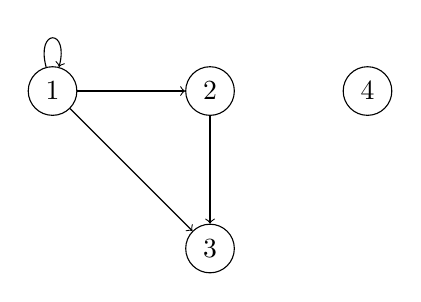
\begin{tikzpicture}[->,node distance=2cm]
  \node[draw,circle] (A) {$1$};
  \node[draw,circle] (B) [right of=A] {$2$};
  \node[draw,circle] (C) [below of=B] {$3$};
  \node[draw,circle] (D) [right of=B] {$4$};
  \draw (A) to [loop above]  (A);
  \draw (A) to  (B);
  \draw (A) to  (C);
  \draw (B) to  (C);
  \end{tikzpicture}
\intertext{Iki beda karo graf $\tuple{V', E}$ kanthi $V' =
  \{1, 2, 3\}$, kang katon kaya mangkene:}
& 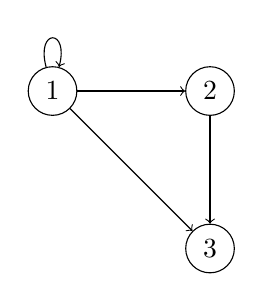
\begin{tikzpicture}[->,node distance=2cm]
  \node[draw,circle] (A) {$1$};
  \node[draw,circle] (B) [right of=A] {$2$};
  \node[draw,circle] (C) [below of=B] {$3$};
  \draw (A) to [loop above]  (A);
  \draw (A) to  (B);
  \draw (A) to  (C);
  \draw (B) to  (C);
  \end{tikzpicture}
\end{align*}
\end{ex}

\begin{prob}
  Anggepen relasi kurang saka utawa padha karo~$\le$
  ing himpunan $\{1,2, 3, 4\}$ minangka graf,
  banjur gambarna diagram kang cocog.
\end{prob}

\endgroup
% END OLP-0017
\endgroup


\begingroup
\makeatletter\def\ol@sectioncs{section}\makeatother

% BEGIN OLP-0018 content/sets-functions-relations/relations/trees.tex
\begingroup
\olfileid{sfr}{rel}{tre}
\olsection{Wit}

Jinis tatanan parsial tartamtu kang nduweni peran wigati
ing kabeh perangan logika yaiku \emph{wit}.
Wit winates katon ing perangan dhasar logika:
tuladhane, !!{formula}s bisa dingerteni lumantar
panguraiane dadi wit sintaksis, dene !!{derivation}s
ing akeh sistem !!{derivation} uga awujud wit winates.
%
Wit tanpa wates wis katon ing bukti teorema-teorema
kelengkapan kanggo logika proposisional lan logika
tataran kapisan, lan digunakake ing saindenging logika matematis.

Konsep wit ing teori himpunan raket gayutane karo
gagasan wit ing teori graf.
Iki gambar sawijining wit (winates):

\begin{center}
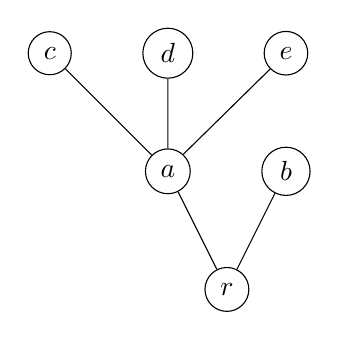
\begin{tikzpicture}[nodes={draw, circle}, -]
\node{$r$} [grow'=up]
    child { node {$a$}
        child { node {$c$} }
        child { node {$d$} }
        child { node {$e$} }
    }
    child { node {$b$} };
\end{tikzpicture}
\end{center}

Simpul paling ngisor~$r$ iku oyod.
Saben simpul saliyane $r$ duwe persis siji simpul induk
langsung ing sangisore. Kita bisa nganggep relasi
antarane simpul~$x$ lan simpul~$y$---yen
$y$ bisa digayuh saka~$x$ kanthi ngetutake rusuk
munggah---minangka pratelan yen $x$ iku \emph{leluhur} saka~$y$.

Relasi leluhur ing wit iku tatanan parsial ketat.
Iki dadi dhasar definisi miturut teori himpunan.
Kanggo nyatakake, kita mbutuhake rong konsep.
\emph{Anggota paling cilik} ing himpunan~$A$
kang ditata parsial dening~$\le$ yaiku
!!a{element} $x \in A$ kanthi sipat yen
kanggo kabeh $y \in A$ kita duwe~$x \le y$.
Himpunan \emph{katata kanthi becik} dening~$\le$
yen saben subhimpunane kang ora kosong duwe
anggota paling cilik.

\begin{defn}[Wit]
\emph{Wit} yaiku pasangan $T = \tuple{A, \le}$
kanthi syarat yen $A$ iku himpunan lan $\le$
iku tatanan parsial ing~$A$ kanthi siji-sijine
anggota paling cilik $r \in A$
(diarani \emph{oyod}), lan kanggo kabeh $x \in A$,
himpunan $\Setabs{y}{y \le x}$
katata kanthi becik dening~$\le$.
\end{defn}

\begin{defn}[Panerus]
Umpamakna $T = \tuple{A, \le}$ iku wit.
Yen $x,y \in A$, $x < y$, lan ora ana
$z \in A$ kanthi $x < z < y$,
mula kita nyebut $y$ minangka \emph{panerus} saka~$x$.
\end{defn}

Panerus-panerus saka $x \in A$ uga diarani \emph{anake}.
Yen $y$ iku panerus saka~$x$, mula kita nyebut $x$
minangka \emph{pandhisik} utawa \emph{induk} saka~$y$.

\begin{prop}
Yen $\tuple{A,\le}$ iku wit, mula saben $x \in A$
saliyane oyod duwe paling akeh siji pandhisik.
\end{prop}

\begin{proof}
  Umpamakna $y_1 < x$, $y_2 < x$, lan $y_1 \neq y_2$.
  Mula $\{y_1,y_2\} \subseteq \Setabs{z}{z<x}$.
  Amarga $\Setabs{z}{z<x}$ katata kanthi becik
  dening~$\le$, subhimpunane $\{y_1, y_2\}$
  duwe anggota paling cilik, kang mesthi
  $y_1$ utawa~$y_2$.
  Mula $y_1 \le y_2$ utawa $y_2 \le y_1$.
  Kita nganggep $y_1 \neq y_2$, mula sejatine
  $y_1 < y_2$ utawa $y_2 < y_1$.
  Amarga kita nganggep $y_1 < x$ lan $y_2 < x$,
  kita uga duwe $y_1 < y_2< x$ utawa
  $y_2 < y_1 < x$.
  Mula $y_1$ lan $y_2$ ora bisa loro-lorone
  dadi pandhisik saka~$x$.
\end{proof}

\begin{defn}
Wit $T = \tuple{A, \le}$ diarani \emph{tanpa wates}
yen $A$ iku himpunan tanpa wates, lan
\emph{winates} yen ora mangkono.
Yen $T$ nduweni sipat saben $x \in A$
mung duwe panerus kang cacahe winates,
mula kita nyebut $T$ \emph{nyabang winates}.
\end{defn}

\begin{defn}[Pang]
Kanggo wit $T = \tuple{A, \le}$, \emph{pang} saka~$T$
yaiku rantai maksimal ing~$T$, yaiku himpunan
$B \subseteq A$ kanthi sipat yen kanggo saben
$x, y \in B$, $x \le y$ utawa $y \le x$,
lan kanggo saben $z \in X \setminus B$
ana $u \in B$ kanthi $z \le u$ lan $u \le z$
loro-lorone ora lumaku.
%
Kita nganggo $[T]$ kanggo nglambangake
himpunan kabeh pang saka $T$.
\end{defn}

\begin{ex}
Tuladha klasik wit kang nyabang winates yaiku
\emph{wit biner tanpa wates} saka urutan winates
kang unsur-unsure $0$ utawa~$1$, kadhangkala
dilambangake $\{0,1\}^*$ utawa~$\Bin^*$,
ditata nganggo relasi ekstensi $\sqsubseteq$
(tuladhane, $101 \sqsubseteq 101101$).
Amarga saben rerangken biner tansah bisa
ditambahi $0$ utawa $1$ ing pungkasane,
wit iki ngemot anggota kang cacahe tanpa wates:
saben anggota~$s$ duwe persis rong panerus,
$s0$ lan~$s1$.
Oyode yaiku urutan kosong $\emptyseq$.
\end{ex}

\begin{ex}
Kanthi rada luwih umum, himpunan urutan winates
wilangan natural~$\Nat^*$ kanthi relasi
ekstensi~$\sqsubseteq$ uga wit.
Cetha yen wit iki ora nyabang winates:
saben $s \in \Nat^*$ duwe panerus~$sn$
kang cacahe tanpa wates, siji kanggo saben
$n \in \Nat$.
Saben $A\subseteq \Nat^*$ kang katutup
tumrap~$\sqsubseteq$ iku \emph{subwit}
saka~$\Nat^*$.
(Yaiku, $A$ nduweni sipat yen $s \in A$
lan $s' \sqsubseteq s$, mula uga $s' \in A$.)
Kabeh wit winates bisa diwakili minangka
subwit winates saka~$\Nat^*$.
\end{ex}

\begin{prop}[Lema K\H{o}nig]
Yen $T = \tuple{A,\le}$ iku wit tanpa wates
kang nyabang winates, mula $T$
duwe pang tanpa wates.
\end{prop}

Kasus khusus lema K\H{o}nig kang akeh digunakake
ing teori komputabilitas, dikenal minangka
\emph{lema K\H{o}nig ringkih}, yaiku mangkene:
saben subwit tanpa wates saka $\{0,1\}^*$
duwe pang tanpa wates.

\endgroup
% END OLP-0018
\endgroup


\begingroup
\makeatletter\def\ol@sectioncs{section}\makeatother

% BEGIN OLP-0019 content/sets-functions-relations/relations/operations.tex
\begingroup
\olfileid{sfr}{rel}{ops}
\olsection{Operasi tumrap Relasi}

Asring migunani yen ngowahi utawa nggabungake relasi.
Ing \olref[sfr][rel][ord]{prop:stricttopartial},
kita ngrembug \emph{gabungan} relasi, kang mung
gabungan rong relasi nalika dianggep himpunan pasangan.
Semono uga, ing \olref[sfr][rel][ord]{prop:partialtostrict},
kita ngrembug selisih relatif relasi.
Ing ngisor iki ana sawetara operasi liyane
kang bisa ditindakake tumrap relasi.

\begin{defn}\ollabel{relationoperations}
Umpamakna $R$ lan $S$ iku relasi, lan $A$ iku himpunan apa wae.

\emph{Invers} saka $R$ yaiku
$R^{-1} = \Setabs{\tuple{y, x}}{\tuple{x,y} \in R}$.

\emph{Produk relatif} saka $R$ lan $S$ yaiku
$(R \mid S) =\{\tuple{x, z} : \exists y(Rxy \land Syz)\}$.

\emph{Watesan} saka $R$ ing $A$ yaiku
$\funrestrictionto{R}{A}= R\cap A^2$.

\emph{Aplikasi} saka $R$ marang $A$ yaiku
$\funimage{R}{A} = \{y :( \exists x \in A)Rxy\}$
\end{defn}

\begin{ex}
Umpamakna $S \subseteq \Int^2$ iku relasi panerus
ing~$\Int$, yaiku
$S = \Setabs{\tuple{x, y} \in \Int^2}{x + 1 = y}$,
mula $Sxy$ yen lan mung yen $x + 1 = y$.

$S^{-1}$ iku relasi pandhisik ing $\Int$, yaiku
$\Setabs{\tuple{x,y}\in\Int^2}{x -1 =y}$.

$S\mid S$ yaiku
$ \Setabs{\tuple{x,y}\in\Int^2}{x + 2 =y}$

$\funrestrictionto{S}{\Nat}$ iku relasi panerus ing~$\Nat$.

$\funimage{S}{\{1,2,3\}}$ yaiku $\{2, 3, 4\}$.
\end{ex}

\begin{defn}[Tutupan transitif]Umpamakna $R \subseteq A^2$ iku relasi biner.

\emph{Tutupan transitif} saka~$R$ yaiku
$R^+ = \bigcup_{0 < n \in\Nat} R^n$,
kanthi definisi rekursif $R^1 = R$ lan
$R^{n+1} = R^n\mid R$.

\emph{Tutupan refleksif transitif} saka $R$ yaiku
$R^* = R^+ \cup\Id{A}$.
\end{defn}

\begin{ex}
Jupuk relasi panerus $S \subseteq \Int^2$.
$S^2xy$ yen lan mung yen $x + 2 =y$,
$S^3xy$ yen lan mung yen $x + 3 = y$,
lan sapanunggalane.
Mula $S^+xy$ yen lan mung yen $x + n = y$
kanggo sawijining $n \geq 1$.
Kanthi tembung liya, $S^+xy$ yen lan mung yen
$x < y$, lan $S^*xy$ yen lan mung yen $x \le y$.
\end{ex}

\begin{prob}
Tuduhna yen tutupan transitif saka $R$ pancen transitif.
\end{prob}

\endgroup
% END OLP-0019
\endgroup


\OLEndChapterHook

\endgroup
% END OLP-0011
\endgroup


\begingroup
\makeatletter\def\ol@sectioncs{section}\makeatother

% BEGIN OLP-0020 content/sets-functions-relations/functions/functions.tex
\begingroup
\olchapter{sfr}{fun}{Fungsi}

\begingroup
\makeatletter\def\ol@sectioncs{section}\makeatother

% BEGIN OLP-0021 content/sets-functions-relations/functions/function-basics.tex
\begingroup
\olfileid{sfr}{fun}{bas}
\olsection{Dhasar}

\begin{explain}
\emph{Fungsi} yaiku pemetaan kang ngirim saben !!{element}
saka sawijining himpunan menyang !!{element} tartamtu
ing himpunan (liyane) kang wis ditemtokake.
Tuladhane, operasi nambah~$1$ nemtokake fungsi:
saben wilangan~$n$ dipetakake menyang siji-sijine
wilangan~$n+1$.

Kanthi luwih umum, fungsi bisa nampa pasangan,
tupel telu, lan sapanunggalane minangka masukan
lan menehi sawijining asil. Akeh fungsi wis kita
kenal saka aritmetika dhasar. Tuladhane, panambahan
lan ping-pingan iku fungsi. Fungsi kasebut nampa
rong wilangan lan menehi wilangan katelu.

Ing teges matematis lan abstrak iki, fungsi iku
\emph{kothak ireng}: kang wigati mung asil apa
kang dipasangake karo masukan apa, dudu
metodhe kanggo ngetung asile.
\end{explain}

\begin{defn}[Fungsi]
\emph{Fungsi} $f \colon A \to B$ yaiku pemetaan
saben !!{element} saka~$A$ menyang
salah siji !!{element} saka~$B$.

Kita nyebut $A$ minangka \emph{domain} saka~$f$
lan $B$ minangka \emph{kodomain} saka~$f$.
!!{element}s saka~$A$ diarani masukan utawa
\emph{argumen} saka~$f$, lan !!{element}
saka~$B$ kang dipasangake karo argumen~$x$
dening~$f$ diarani \emph{nilai~$f$}
kanggo argumen~$x$, ditulis~$f(x)$.

\emph{Jangkauan} $\ran{f}$ saka~$f$ yaiku
subhimpunan kodomain kang ngemot nilai-nilai~$f$
kanggo sawijining argumen;
$\ran{f} =\Setabs{f(x)}{x \in A}$.
\end{defn}

Diagram ing \olref{fig:function} bisa mbiyantu
ngerteni fungsi. Elips ing sisih kiwa makili
\emph{domain} fungsi; elips ing sisih tengen
makili \emph{kodomain} fungsi; lan panah
ngarah saka \emph{argumen} ing domain
menyang \emph{nilai} kang cocog ing kodomain.

\begin{figure}
  \olasset{assets/diagrams/function.tikz}
  \caption{Fungsi yaiku pemetaan saben !!{element}
    saka siji himpunan menyang !!a{element}
    saka himpunan liyane. Panah ngarah
    saka argumen ing domain menyang nilai
    kang cocog ing kodomain.}
  \ollabel{fig:function}
\end{figure}

\begin{ex}
Ping-pingan nampa pasangan wilangan natural
minangka masukan lan metakake menyang wilangan
natural minangka asil, mula saka
$\Nat \times \Nat$ (domain) menyang $\Nat$ (kodomain).
Pranyata jangkauane uga $\Nat$,
amarga saben $n \in \Nat$ iku $n \times 1$.
\end{ex}

\begin{ex}
Ping-pingan iku fungsi amarga masangake saben
masukan---saben pasangan wilangan natural---
karo siji asil: $\times \colon \Nat^2 \to\Nat$.
Dene metakake wilangan natural~$n$
menyang wilangan real~$x$ kanthi sipat yen
$x^2 = n$ dudu fungsi, amarga saben
wilangan wutuh positif~$n$ duwe rong
oyod kuadrat: $\sqrt{n}$ lan~$-\sqrt{n}$.
Pemetaan iki bisa digawe fungsi kanthi
mulihake oyod kuadrat utama kang ora negatif:
$\sqrt{\phantom{X}} \colon\Nat \to \Real$.
Cathetan koreksi sumber OLFUN-002: tembung Inggris "positive"
ora trep ing nol, amarga domain wilangan natural kalebu nol.
\end{ex}

\begin{ex}
Relasi kang masangake saben siswa ing sawijining
kelas karo biji pungkasane iku fungsi---
ora ana siswa kang bisa oleh rong biji pungkasan
kang beda ing kelas kang padha.
Relasi kang masangake saben siswa ing sawijining
kelas karo wong tuwane dudu fungsi:
siswa bisa ora duwe wong tuwa, duwe loro,
utawa luwih saka loro.
\end{ex}

\begin{explain}
Kita bisa nemtokake fungsi kanthi nyatakake
kanthi tliti apa nilai fungsi kanggo saben
argumen kang bisa ana. Cara-carane bisa
kanthi menehi rumus, njlentrehake metodhe
kanggo ngetung nilai, utawa ndhaptar
nilai kanggo saben argumen.
Kanthi cara apa wae fungsi ditemtokake,
kita kudu mesthekake yen kanggo saben
argumen kita nemtokake siji, lan mung siji, nilai.
\end{explain}


\begin{ex}
Umpamakna $f \colon \Nat \to \Nat$
ditetepake kanthi rumus $f(x) = x+1$.
Definisi iki netepake $f$ minangka fungsi
kang nampa wilangan natural lan menehi
wilangan natural minangka asil.
Definisi iki nerangake yen kanggo wilangan
natural~$x$, $f$ menehi paneruse~$x+1$.
Ing kasus iki, kodomain $\Nat$ dudu
jangkauan~$f$, amarga wilangan natural~$0$
dudu panerus saka wilangan natural apa wae.
Jangkauan~$f$ yaiku himpunan kabeh
wilangan wutuh positif, $\Int^{+}$.
\end{ex}

\begin{ex}\ollabel{examplefunext}
Umpamakna $g \colon \Nat \to \Nat$
ditetepake kanthi rumus $g(x) = x+2-1$.
Iki nerangake yen $g$ iku fungsi kang
nampa wilangan natural lan menehi
wilangan natural minangka asil.
Kanggo wilangan natural~$x$, $g$ bakal
menehi pandhisik saka panerus saka
paneruse~$x$, yaiku $x+1$.
Cathetan koreksi sumber OLFUN-003: sumber Inggris ngganti jeneng
masukan ing tengah ukara; terjemahan iki nggunakake siji jeneng kanthi ajeg.
\end{ex}

\begin{explain}
Kita lagi wae ngrembug rong fungsi,
$f$ lan $g$, kanthi \emph{definisi}
kang beda. Nanging kalorone iku
\emph{fungsi kang padha}.
Amarga kanggo saben wilangan natural~$n$,
kita duwe $f(n) = n+1 = n+2-1 =g(n)$.
Kanthi tembung liya: definisi kanggo $f$
lan~$g$ netepake pemetaan kang padha
nganggo persamaan kang beda.
Mula kanthi ora langsung kita nggunakake
prinsip ekstensionalitas kanggo fungsi,
\[
  \text{yen }\forall x\, f(x) = g(x)\text{, mula }f = g
\]
kanthi syarat yen $f$ lan~$g$ duwe domain lan
kodomain kang padha.
\end{explain}

\begin{ex}
Kita uga bisa nemtokake fungsi miturut
kasus-kasus. Tuladhane, kita bisa
nemtokake $h \colon \Nat \to \Nat$ kanthi
\[
h(x) =
\begin{cases}
  \frac{x}{2} & \text{yen $x$ genep} \\
  \frac{x+1}{2} & \text{yen $x$ ganjil.}
\end{cases}
\]
Amarga saben wilangan natural iku genep
utawa ganjil, asil fungsi iki tansah
wilangan natural.
Elinga yen fungsi ditemtokake miturut kasus,
saben masukan kang bisa ana kudu
kalebu ing persis siji kasus.
Kadhangkala iki mbutuhake bukti yen
kasus-kasus kasebut nyakup kabeh
lan ora ana kang tumpang tindih.
\end{ex}

\endgroup
% END OLP-0021
\endgroup


\begingroup
\makeatletter\def\ol@sectioncs{section}\makeatother

% BEGIN OLP-0022 content/sets-functions-relations/functions/function-kinds.tex
\begingroup
\olfileid{sfr}{fun}{kin}
\olsection{Jinis-jinis Fungsi}

\begin{explain}
Bakal migunani yen kita ngenalake panggolongan
kanggo sawetara jinis fungsi kang paling
kerep kita temoni.

Kanggo miwiti, kita bisa ngrembug fungsi
kang nduweni sipat yen saben anggota
kodomain iku nilai saka fungsi kasebut.
Fungsi kaya iki diarani !!{surjective},
lan bisa digambarake kaya ing \olref{fig:surjective}.

\begin{figure}
  \olasset{assets/diagrams/surjective.tikz}
  \caption{Fungsi !!^a{surjective} nduweni
    saben !!{element} kodomain minangka nilai.}
  \ollabel{fig:surjective}
\end{figure}
\end{explain}

\begin{defn}[Fungsi !!^{surjective}]
Fungsi $f \colon A \rightarrow B$ iku
\emph{!!{surjective}} yen lan mung yen
$B$ uga jangkauan~$f$, yaiku kanggo
saben $y \in B$ ana paling ora siji
$x \in A$ kanthi~$f(x) = y$,
utawa kanthi lambang:
\[
  (\forall y \in B)(\exists x \in A)f(x) = y.
\]
Kita nyebut fungsi kaya iki
!!a{surjection} saka $A$ menyang $B$.
\end{defn}

\begin{explain}
Yen arep nuduhake yen $f$ iku
!!a{surjection}, kita kudu nuduhake
yen saben objek ing kodomain $f$
iku nilai $f(x)$ kanggo sawijining
masukan $x$.

Gatekna yen saben fungsi \emph{nuwuhake}
!!a{surjection}.
Amarga, kanggo fungsi $f \colon A \to B$,
tetepna $f' \colon A \to \ran{f}$
kanthi $f'(x) = f(x)$.
Amarga $\ran{f}$ \emph{ditetepake}
minangka $\Setabs{f(x) \in B}{x \in A}$,
fungsi $f'$ iki mesthi
!!a{surjection}
\end{explain}

\begin{explain}
Saben fungsi metakake saben masukan
kang bisa ana menyang siji-sijine asil.
Nanging uga ana fungsi kang ora
nate metakake masukan beda
menyang asil kang padha.
Fungsi kaya iki diarani !!{injective},
lan bisa digambarake kaya ing \olref{fig:injective}.
\begin{figure}
  \olasset{assets/diagrams/injective.tikz}
  \caption{Fungsi !!^a{injective} ora nate
    metakake rong argumen kang beda
    menyang nilai kang padha.}
  \ollabel{fig:injective}
\end{figure}
\end{explain}

\begin{defn}[Fungsi !!^{injective}]
Fungsi $f \colon A \rightarrow B$ iku
\emph{!!{injective}} yen lan mung yen
kanggo saben $y \in B$ ana paling akeh
siji $x \in A$ kanthi~$f(x) = y$.
Kita nyebut fungsi kaya iki
!!a{injection} saka $A$ menyang~$B$.
\end{defn}

\begin{explain}
Yen arep nuduhake yen $f$ iku
!!a{injection}, kita kudu nuduhake
yen kanggo saben !!{element}s $x$ lan $y$
saka domain $f$, yen $f(x)=f(y)$,
mula $x=y$.
\end{explain}

\begin{ex}
Fungsi konstan $f\colon \Nat \to \Nat$
kang ditemtokake kanthi $f(x) = 1$
iku ora !!{injective} lan ora !!{surjective}.

Fungsi identitas $f\colon \Nat \to \Nat$
kang ditemtokake kanthi $f(x) = x$
iku !!{injective} lan !!{surjective}.

Fungsi panerus $f \colon \Nat \to \Nat$
kang ditemtokake kanthi $f(x) = x+1$
iku !!{injective} nanging ora !!{surjective}.

Fungsi $f \colon \Nat \to \Nat$
kang ditemtokake kanthi:
\[
  f(x) =
  \begin{cases}
    \frac{x}{2} & \text{yen $x$ genep} \\
    \frac{x+1}{2} & \text{yen $x$ ganjil.}
  \end{cases}
\]
iku !!{surjective}, nanging ora !!{injective}.
\end{ex}

\begin{explain}
Asring kita arep ngrembug fungsi
kang !!{injective} lan !!{surjective}
bebarengan. Fungsi kaya iki diarani
!!{bijective}. Wujude kaya fungsi
ing \olref{fig:bijective}.
!!^{bijection}s kadhangkala uga diarani
\emph{korespondensi siji-menyang-siji},
amarga masangake anggota kodomain
karo anggota domain kanthi siji-menyang-siji.
\begin{figure}
  \olasset{assets/diagrams/bijective.tikz}
  \caption{Fungsi !!^a{bijective} masangake
    anggota kodomain karo anggota
    domain kanthi siji-menyang-siji.}
  \ollabel{fig:bijective}
\end{figure}
\end{explain}

\begin{defn}[!!^{bijection}]
Fungsi $f \colon A \to B$ iku
\emph{!!{bijective}} yen lan mung yen
!!{surjective} lan !!{injective}.
Kita nyebut fungsi kaya iki
!!a{bijection} saka $A$ menyang~$B$
(utawa antarane $A$ lan~$B$).
\end{defn}

\endgroup
% END OLP-0022
\endgroup


\begingroup
\makeatletter\def\ol@sectioncs{section}\makeatother

% BEGIN OLP-0023 content/sets-functions-relations/functions/functions-relations.tex
\begingroup
\olfileid{sfr}{fun}{rel}

\olsection{Fungsi minangka Relasi}

\begin{explain}
Fungsi kang metakake !!{element}s saka~$A$ menyang !!{element}s saka~$B$
cetha nemtokake relasi antarane $A$ lan~$B$, yaiku relasi
kang dumadi antarane $x$ lan $y$ yen lan mung yen $f(x) = y$. Malah,
yen kita kepengin nyuda cacah jinis bahan dhasar matematika, upamane,
kita bisa \emph{nganggep padha} fungsi~$f$ lan relasi iki,
yaiku himpunan pasangan. Iki banjur nuwuhake pitakon:
relasi endi wae kang nemtokake fungsi kanthi cara iki?
\end{explain}

\begin{defn}[Graf fungsi] Upamakna $f\colon A \to B$ sawijining fungsi.
\emph{Graf} saka~$f$ yaiku relasi $R_f \subseteq A \times B$
kang ditetepake kanthi
\[
R_f = \Setabs{\tuple{x,y}}{f(x) = y}.
\]
\end{defn}

\begin{explain}
Adhedhasar ekstensionalitas, graf sawijining fungsi ditemtokake kanthi tunggal.
Kajaba iku, ekstensionalitas tumrap himpunan langsung nuduhake yen
prinsip ekstensionalitas fungsi kang sadurunge dianggep lumaku iku trep:
yen $f$ lan~$g$ duwe domain lan kodomain kang padha,
fungsi loro iku padha yen loro-lorone menehi
nilai kang padha kanggo saben argumen.

Semono uga, yen sawijining relasi iku "fungsional", relasi iku graf sawijining fungsi.
\end{explain}

\begin{prop}\ollabel{prop:graph-function}
Upamakna $R \subseteq A \times B$ nduweni sipat:
\begin{enumerate}
\item Yen $Rxy$ lan $Rxz$, mula $y = z$; lan
\item kanggo saben $x \in A$ ana $y \in B$ kanthi $\tuple{x,
y} \in R$.
\end{enumerate}
Banjur $R$ iku graf fungsi $f\colon A \to B$ kang ditetepake kanthi
$f(x) = y$ yen lan mung yen $Rxy$.
\end{prop}

\begin{proof}
Upamakna ana $y$ kanthi $Rxy$. Yen ana $z \neq
y$ liyane kanthi $Rxz$, sarat tumrap~$R$ bakal dilanggar. Mula, yen
ana $y$ kanthi $Rxy$, $y$ iki siji-sijine, mula $f$
ditetepake kanthi becik. Cetha yen $R_f = R$.
\end{proof}

\begin{explain}
Saben fungsi $f\colon A \to B$ duwe graf, yaiku relasi kang kaemot ing $A
\times B$ lan ditetepake dening $f(x) = y$. Cathetan koreksi sumber
OLFUN-004: iki relasi antarane A lan B, dudu relasi ing himpunan
produk A lan B miturut definisi relasi biner ing buku iki. Kosok baline, saben relasi~$R
\subseteq A \times B$ kang nduweni sipat ing
\olref{prop:graph-function} iku graf sawijining fungsi~$f \colon A \to
B$. Amarga sesambungan kang raket antarane fungsi lan grafe iki,
kita bisa nganggep sawijining fungsi minangka grafe. Kanthi tembung
liya, fungsi bisa dianggep padha karo relasi tartamtu, yaiku
himpunan tupel tartamtu. \oliflabeldef{sfr:rel:ref:sec}{Nanging, gatekna
yen maksud "nganggep padha" iki kaya ing
\olref[sfr][rel][ref]{sec}: iki dudu pratelan ngenani metafisika
fungsi, nanging pangamatan yen \emph{nganggep}
fungsi minangka himpunan tartamtu iku migunani. Salah siji sebabe
yaiku saiki k}{K}ita bisa nindakake operasi ing
fungsi kang padha karo operasi ing relasi (delengen
\olref[sfr][rel][ops]{sec}). Mligine:
\end{explain}

\begin{defn}\ollabel{defn:funimage}
Upamakna $f \colon A \to B$ sawijining fungsi kanthi $C\subseteq A$.

\emph{Watesan} saka~$f$ ing~$C$ yaiku
fungsi~$\funrestrictionto{f}{C}\colon C \to B$ kang ditetepake kanthi
$(\funrestrictionto{f}{C})(x) = f(x)$ kanggo kabeh $x \in C$. Kanthi tembung
liya, $\funrestrictionto{f}{C} = \Setabs{\tuple{x, y} \in R_f}{x \in
C}$.

\emph{Aplikasi} saka~$f$ tumrap~$C$ yaiku $\funimage{f}{C} =
\Setabs{f(x)}{x \in C}$. Iki uga diarani \emph{citra} saka~$C$
dening~$f$.
\end{defn}

\begin{explain}
Saka definisi iki bisa didudut yen $\ran{f} =
\funimage{f}{\dom{f}}$, kanggo saben fungsi~$f$.
\oliflabeldef{sfr:rel:ops:sec}{Rong pangerten iki analog karo
definisi ing \olref[sfr][rel][ops]{sec} lan anggone kita
nganggep fungsi padha karo relasi, nanging ora persis padha:
watesan fungsi ing kene mung nyaring koordinat masukan, dene
watesan relasi ing kana nyaring loro koordinat. Iki koreksi
andharan sumber OLFUN-005. Rong operasi liyane,
yaiku invers lan produk relatif, mbutuhake katrangan luwih jangkep.
Katrangan iku bakal diwenehake ing \olref[inv]{sec} lan
\olref[cmp]{sec}.}{}
\end{explain}

\endgroup
% END OLP-0023
\endgroup


\begingroup
\makeatletter\def\ol@sectioncs{section}\makeatother

% BEGIN OLP-0024 content/sets-functions-relations/functions/inverses.tex
\begingroup
\olfileid{sfr}{fun}{inv}
\olsection{Invers Fungsi}

\begin{explain}
Kita nganggep fungsi minangka pemetaan. Mula, pitakon kang lumrah
ngenani fungsi yaiku apa pemetaan iku bisa "diwalik". Upamane,
fungsi panerus $f(x) = x + 1$ bisa diwalik,
ing pangerten yen fungsi $g(y) = y - 1$ ngasilake maneh input
fungsi~$f$ saka asile.

Nanging kita kudu ngati-ati. Sanajan definisi~$g$ nemtokake
fungsi $\Int \to \Int$, definisi iku ora nemtokake \emph{fungsi} $\Nat
\to \Nat$, amarga $g(0) \notin \Nat$. Dadi, sanajan ing kasus prasaja,
durung mesthi cetha apa sawijining fungsi bisa diwalik; iki bisa
gumantung marang domain lan kodomaine.

Pangerten invers fungsi ndadekake gagasan iki luwih tliti.
\end{explain}

\begin{defn}
Fungsi $g \colon B \to A$ iku \emph{invers} saka fungsi $f
\colon A \to B$ yen $f(g(y)) = y$ lan $g(f(x)) = x$ kanggo kabeh $x \in A$
lan $y \in B$.
\end{defn}

Yen $f$ duwe invers~$g$, kita kerep nulis $f^{-1}$ kanggo ngganti~$g$.

\begin{explain}
Saiki kita bakal nemtokake kapan fungsi duwe invers. Calon kang trep
kanggo invers saka $f\colon A \to B$ yaiku $g\colon B \to A$ kang
"ditetepake kanthi"
\[
g(y) = \text{$x$ "tunggal" kang nyukupi $f(x) = y$.}
\]
Nanging tandha petik ing "ditetepake kanthi" lan "tunggal" nuduhake
yen iki durung dadi definisi. Paling ora, cara iki ora mesthi lumaku
ing kabeh kasus. Supaya definisi iki nemtokake
fungsi, kudu ana siji lan mung siji~$x$ kang nyukupi $f(x) =
y$; asil saka~$g$ kudu ditemtokake kanthi tunggal. Kajaba iku, asil
kudu ditemtokake kanggo saben $y \in B$. Yen ana $x_1$ lan $x_2 \in
A$ kanthi $x_1 \neq x_2$ nanging $f(x_1) = f(x_2)$, mula $g(y)$ ora bakal
ditemtokake kanthi tunggal kanggo $y = f(x_1) = f(x_2)$. Lan yen ora ana~$x$
babar pisan kang nyukupi $f(x) = y$, mula $g(y)$ ora ditemtokake babar pisan.
Kanthi tembung liya, supaya $g$ bisa ditetepake, $f$~kudu !!{injective} lan
!!{surjective}.

Ayo dirembug sethithik mbaka sethithik. Pitakon mau dipara dadi loro:
yen diwenehi fungsi~$f\colon A \to B$, kapan ana fungsi $g\colon B \to A$
kanthi $g(f(x)) = x$? Fungsi $g$ kang kaya mangkono ngasilake maneh
input fungsi~$f$,
lan diarani \emph{invers kiwa} saka~$f$. Kapindho, kapan ana
fungsi $h\colon B \to A$ kanthi $f(h(y)) = y$? Fungsi $h$ kang kaya mangkono
diarani \emph{invers tengen} saka~$f$; $f$ ngasilake maneh input
fungsi~$h$.
\end{explain}

\begin{prop}
Yen A ora kosong lan $f\colon A \to B$ iku !!{injective}, mula ana \emph{invers
kiwa}~$g\colon B \to A$ saka~$f$ kanthi $g(f(x)) = x$ kanggo kabeh $x
\in A$.
Cathetan koreksi sumber OLFUN-001: sumber Inggris ora nyebut sarat
domain ora kosong kang digunakake ing bukti. Sarat umum kang pas yaiku
A ora kosong utawa B kosong; injeksi kosong menyang himpunan ora
kosong ora duwe invers kiwa.
\end{prop}

\begin{proof}
Upamakna A ora kosong lan $f\colon A \to B$ iku !!{injective}.
Gatekna sawijining $y \in B$.
Yen $y \in \ran{f}$, ana $x \in A$ kanthi $f(x) = y$. Amarga
$f$ iku !!{injective}, mung ana siji~$x \in A$ kang kaya mangkono. Banjur kita bisa
netepake $g(y) = x$, yaiku $g(y)$ iku $x \in A$ "tunggal" kang nyukupi $f(x)
= y$. Yen $y \notin \ran{f}$, kita bisa metakake menyang sembarang~$a \in A$.
Dadi, kita bisa milih $a \in A$ lan netepake $g\colon B \to A$ kanthi:
\[
g(y) = \begin{cases}
    x & \text{yen $f(x) = y$}\\
    a & \text{yen $y \notin \ran{f}$.}
\end{cases}
\]
Fungsi iki ditetepake kanggo kabeh $y \in B$, amarga kanggo saben $y \in \ran{f}$
ana persis siji $x \in A$ kang nyukupi $f(x) = y$. Miturut definisi, yen
$y = f(x)$, mula $g(y) = x$, yaiku $g(f(x)) = x$.
\end{proof}

\begin{prob}
Tuduhna yen $f\colon A \to B$ duwe invers kiwa~$g$, mula $f$~iku
!!{injective}.
\end{prob}

\begin{prop}
    Yen $f\colon A \to B$ iku !!{surjective}, mula ana
    \emph{invers tengen}~$h\colon B \to A$ saka~$f$ kanthi $f(h(y)) =
    y$ kanggo kabeh~$y \in B$.
\end{prop}

\begin{proof}
Upamakna $f\colon A \to B$ iku !!{surjective}. Gatekna sawijining $y \in
B$. Amarga $f$~iku !!{surjective}, ana $x_y \in A$ kanthi $f(x_y)
= y$. Banjur kita bisa netepake $h(y) = x_y$, yaiku kanggo saben $y \in B$
kita milih $x \in A$ kanthi $f(x) = y$; amarga $f$~iku !!{surjective},
mesthi ana paling ora siji kang bisa dipilih.\footnote{Amarga $f$ iku
!!{surjective}, kanggo saben~$y \in B$ himpunan $\Setabs{x}{f(x) = y}$
ora kosong. Definisi~$h$ mbutuhake kita milih siji $x$
saka saben himpunan iki. Yen iki mesthi bisa ditindakake, sejatine ora
cetha; kamungkinan kanggo nggawe pilihan-pilihan iki dianggep minangka aksioma.
Kanthi tembung liya, proposisi iki nggunakake kang diarani Aksioma
Pilihan, prakara kang bakal \oliflabeldef{sth:choice::chap}{dirembug maneh ing \olref[sth][choice][]{chap}}{diliwati tanpa rembug jero}.
Nanging ing akeh kasus tartamtu, upamane nalika $A = \Nat$ utawa winates, utawa nalika $f$ iku !!{bijective},
Aksioma Pilihan ora dibutuhake. (Ing kasus mligi nalika $f$ iku !!{bijective}, kanggo saben $y \in B$ himpunan
$\Setabs{x}{f(x) = y}$ duwe persis siji !!{element}, mula ora perlu milih.)}
Miturut definisi, yen $x = h(y)$,
mula $f(x) = y$, yaiku kanggo saben $y \in B$, $f(h(y)) = y$.
\end{proof}

\begin{prob}
Tuduhna yen $f\colon A \to B$ duwe invers tengen~$h$, mula $f$~iku
!!{surjective}.
\end{prob}

\begin{explain}
  Kanthi nggabungake gagasan ing bukti sadurunge, saiki kita oleh asil yen saben
  !!{bijection} duwe invers, yaiku ana sawijining fungsi
  kang dadi invers kiwa lan uga invers tengen saka~$f$.
\end{explain}

\begin{prop}\ollabel{prop:bijection-inverse}
Yen $f\colon A \to B$ iku !!{bijective}, ana
fungsi~$f^{-1}\colon B \to A$ kanthi sipat yen kanggo kabeh $x \in A$,
$f^{-1}(f(x)) = x$ lan kanggo kabeh $y \in B$, $f(f^{-1}(y)) = y$.
\end{prop}

\begin{proof}
Minangka latihan.
\end{proof}

\begin{prob}
Buktekna \olref[sfr][fun][inv]{prop:bijection-inverse}. Kanggo iku, kudu
netepake~$f^{-1}$, nuduhake yen iku fungsi, lan nuduhake yen iku
invers saka~$f$, yaiku $f^{-1}(f(x)) = x$ lan $f(f^{-1}(y)) = y$ kanggo
kabeh $x \in A$ lan $y \in B$.
\end{prob}

\begin{explain}
Ana cara kang rada luwih umum kanggo nemokake invers. Ing
\olref[kin]{sec} wis kita deleng yen saben fungsi $f$ nuwuhake !!a{surjection} $f'
\colon A \to \ran{f}$ kanthi netepake $f'(x) = f(x)$ kanggo kabeh $x \in A$.
Cetha yen $f$~iku !!{injective}, mula $f'$~iku !!{bijective}, saengga
duwe invers tunggal miturut \olref{prop:bijection-inverse}. Kanthi
panganggone notasi kang rada longgar, kadhangkala invers saka $f'$
mung diarani "invers saka~$f$".
\end{explain}

\begin{prop}\ollabel{prop:left-right}%
  Tuduhna yen $f\colon A \to B$ duwe invers kiwa~$g$ lan invers
  tengen~$h$, mula $h = g$.
\end{prop}

\begin{proof}
  Minangka latihan.
\end{proof}

\begin{prob}
  Buktekna \olref[sfr][fun][inv]{prop:left-right}.
\end{prob}

\begin{prop}\ollabel{prop:inverse-unique}
Saben fungsi~$f$ duwe paling akeh siji invers.
\end{prop}

\begin{proof}
  Upamakna $g$ lan $h$ loro-lorone invers saka~$f$. Mula, mligine,
  $g$~iku invers kiwa saka~$f$ lan $h$~iku invers tengen. Miturut
  \olref{prop:left-right}, $g = h$.
\end{proof}

\endgroup
% END OLP-0024
\endgroup


\begingroup
\makeatletter\def\ol@sectioncs{section}\makeatother

% BEGIN OLP-0025 content/sets-functions-relations/functions/composition.tex
\begingroup
\olfileid{sfr}{fun}{cmp}
\olsection{Komposisi Fungsi}

\begin{explain}
\oliflabeldef{sfr:fun:inv:sec}{Ing \olref[inv]{sec} wis kita deleng yen
invers~$f^{-1}$ saka !!a{bijection}~$f$ iku uga fungsi. Operasi
liyane ing fungsi yaiku komposisi: k}{K}ita bisa netepake fungsi
anyar kanthi nyusun rong fungsi, $f$ lan~$g$, yaiku kanthi ngetrapake
$f$ dhisik banjur~$g$. Mesthi wae, iki mung bisa ditindakake yen
jangkauan lan domaine trep, yaiku jangkauan saka~$f$ kudu subhimpunan
saka domain~$g$. \oliflabeldef{sfr:rel:ops:sec}{Operasi ing
fungsi iki salaras karo operasi produk relatif ing
relasi saka \olref[rel][ops]{sec}.}{}

Diagram bisa mbantu njlentrehake gagasan komposisi. Ing
\olref{fig:composition}, kita nggambarake rong fungsi $f \colon A \to B$
lan $g \colon B \to C$ sarta komposisine~$(\comp{f}{g})$. Fungsi
$(\comp{f}{g}) \colon A \to C$ masangake saben !!{element} saka~$A$
karo !!a{element} saka~$C$. Kanggo nemtokake !!{element} saka~$C$
kang dadi pasangane !!a{element} saka $A$, carane mangkene: yen diwenehi masukan $x \in
A$, fungsi $f$ ditrapake dhisik tumrap~$x$, kang ngasilake $f(x)
= y \in B$, banjur fungsi $g$ ditrapake tumrap~$y$, kang ngasilake
$g(f(x)) = g(y) = z \in C$.
\begin{figure}
  \olasset[2\olphotowidth]{assets/diagrams/composition.tikz}
  \caption{Komposisi $g \circ f$ saka rong fungsi $f$ lan~$g$.}
  \ollabel{fig:composition}
\end{figure}
\end{explain}

\begin{defn}[Komposisi]
Upamakna $f\colon A \to B$ lan $g\colon B \to C$ iku fungsi.
\emph{Komposisi} saka $f$ karo~$g$ yaiku $\comp{f}{g} \colon A \to C$,
kanthi $(\comp{f}{g})(x) = g(f(x))$.
\end{defn}

\begin{ex}
Gatekna fungsi $f(x) = x + 1$ lan $g(x) = 2x$. Amarga
$(\comp{f}{g})(x) = g(f(x))$, kanggo saben masukan~$x$ kita kudu njupuk
paneruse dhisik, banjur asil mau dipingake loro. Dadi, komposisine
ditetepake kanthi $(\comp{f}{g})(x) = 2(x+1)$.
\end{ex}

\begin{prob}
Tuduhna yen $f \colon A \to B$ lan $g \colon B \to C$ loro-lorone
!!{injective}, mula $\comp{f}{g}\colon A \to C$ iku !!{injective}.
\end{prob}

\begin{prob}
Tuduhna yen $f \colon A \to B$ lan $g \colon B \to C$ loro-lorone
!!{surjective}, mula $\comp{f}{g}\colon A \to C$ iku !!{surjective}.
\end{prob}

\begin{prob}
Upamakna $f \colon A \to B$ lan $g \colon B \to C$. Tuduhna yen graf
saka $\comp{f}{g}$ yaiku $R_f \mid R_g$.
\end{prob}

\endgroup
% END OLP-0025
\endgroup


%\olimport{isomorphic-functions}

\begingroup
\makeatletter\def\ol@sectioncs{section}\makeatother

% BEGIN OLP-0026 content/sets-functions-relations/functions/partial-functions.tex
\begingroup
\olfileid{sfr}{fun}{par}

\olsection{Fungsi Parsial}

\begin{explain}
Kadhangkala migunani yen definisi fungsi dilonggari, saengga
ora kudu ditetepake asile kanggo kabeh
masukan kang bisa diwenehake. Pemetaan kaya mangkono diarani \emph{fungsi parsial}.
\end{explain}

\begin{defn}
\emph{Fungsi parsial} $f \colon A \pto B$ yaiku pemetaan kang
masangake saben !!{element} saka~$A$ karo paling akeh siji !!{element} saka~$B$.
Yen $f$ menehi sawijining anggota saka~$B$ minangka asil tumrap $x \in A$, kita nyebut $f(x)$
\emph{ditetepake}, lan yen ora, \emph{ora ditetepake}. Yen $f(x)$ ditetepake,
kita nulis $f(x) \fdefined$; yen ora, $f(x) \fundefined$.
\emph{Domain} fungsi parsial~$f$ yaiku subhimpunan saka~$A$ kang
ing kono fungsi iku ditetepake, yaiku $\dom{f} = \Setabs{x \in A}{f(x) \fdefined}$.
\end{defn}

\begin{ex}
Saben fungsi $f\colon A \to B$ uga fungsi parsial. Fungsi parsial
kang ditetepake kanggo saben masukan ing~$A$, yaiku kang nganti saiki
mung diarani fungsi, uga diarani fungsi \emph{total}.
\end{ex}

\begin{ex}
Fungsi parsial $f \colon \Real \pto \Real$ kang diwenehake dening $f(x) = 1/x$
ora ditetepake kanggo $x = 0$, lan ditetepake kanggo saben masukan
real saliyane nol.
\end{ex}

\begin{prob}
Yen diwenehi $f\colon A \pto B$, tetepna fungsi parsial $g\colon B \pto
A$ kanthi: kanggo saben $y \in B$, yen ana siji-sijine $x \in A$ kanthi
$f(x) = y$, mula $g(y) = x$; yen ora, $g(y) \fundefined$. Tuduhna yen
$f$ injektif, mula $g(f(x)) = x$ kanggo kabeh $x \in \dom{f}$, lan
$f(g(y)) = y$ kanggo kabeh $y \in \ran{f}$.
\end{prob}

\begin{defn}[Graf fungsi parsial]
Upamakna $f\colon A \pto B$ sawijining fungsi parsial. \emph{Graf} saka~$f$
yaiku relasi $R_f \subseteq A \times B$ kang ditetepake kanthi
\[
R_f = \Setabs{\tuple{x,y}}{f(x) = y}.
\]
\end{defn}

\begin{prop}
Upamakna $R \subseteq A \times B$ duwe sipat iki: yen $Rxy$
lan $Rxy'$ lumaku bebarengan, mula $y = y'$. Banjur $R$ iku graf fungsi parsial
$f\colon A \pto B$ kang ditetepake kanthi: yen ana $y$ kanthi
$Rxy$, mula $f(x) = y$; yen ora, $f(x) \fundefined$. Yen $R$ uga
\emph{serial}, yaiku kanggo saben $x \in A$ ana $y \in B$ kanthi
$Rxy$, mula $f$ iku total.
\end{prop}

\begin{proof}
Upamakna ana $y$ kanthi $Rxy$. Yen ana $y'
\neq y$ liyane kanthi $Rxy'$, sarat tumrap $R$ bakal
dilanggar. Mula, yen ana $y$ kanthi $Rxy$, $y$ iku
siji-sijine, mula $f$ ditetepake kanthi becik. Cetha yen $R_f = R$ lan $f$
total yen~$R$ serial.
\end{proof}

\endgroup
% END OLP-0026
\endgroup



% BEGIN OLP-0717 content/sets-functions-relations/functions/isomorphic-functions.tex
\begingroup
\olfileid{sfr}{fun}{iso}
\olsection{Isomorfisme}

\begin{explain}
\emph{Isomorfisme} minangka bijeksi kang njaga struktur himpunan kang
disambungake. Struktur kasebut ditemtokake dening sesambungan kang
lumaku antarane !!{element}s ing himpunan. Gatekna loro himpunan
$X=\{1,2,3\}$ lan $Y=\{4,5,6\}$. Kalorone nduweni struktur
saka relasi penerus, luwih cilik tinimbang, lan luwih gedhe tinimbang.
Isomorfisme antarane loro himpunan kasebut minangka !!a{bijection}
kang njaga struktur kasebut. Dadi fungsi !!a{bijective}
$f \colon X \to Y$ minangka isomorfisme yen $i<j$ yen lan mung yen
$f(i)<f(j)$, $i>j$ yen lan mung yen $f(i)>f(j)$, lan $j$
minangka penerus saka $i$ yen lan mung yen $f(j)$ minangka penerus
saka $f(i)$.
\end{explain}

\begin{defn}[Isomorfisme]
Upamane $U$ minangka pasangan $\langle X, R\rangle$ lan $V$
minangka pasangan $\langle Y, S\rangle$, kanthi $X$ lan $Y$
minangka himpunan, sarta $R$ lan $S$ minangka relasi ing $X$ lan
$Y$ kanthi urut. !!{bijection} $f$ saka $X$ menyang $Y$ minangka
\emph{isomorfisme} saka $U$ menyang $V$ yen lan mung yen njaga
struktur relasional, yaiku kanggo saben $x_{1}$ lan $x_{2}$ ing $X$,
$\tuple{x_1,x_2} \in R$ yen lan mung yen
$\tuple{f(x_1),f(x_2)} \in S$.
\end{defn}

\begin{ex}
Gatekna loro himpunan $X=\{1,2,3\}$ lan $Y=\{4,5,6\}$,
sarta relasi luwih cilik tinimbang lan luwih gedhe tinimbang.
Fungsi $f\colon X \to Y$ kanthi $f(x) = 7-x$ minangka
isomorfisme antarane $\tuple{X,<}$ lan $\tuple{Y,>}$.
\end{ex}

\endgroup
% END OLP-0717

\OLEndChapterHook

\endgroup
% END OLP-0020
\endgroup


\begingroup
\makeatletter\def\ol@sectioncs{section}\makeatother

% BEGIN OLP-0027 content/sets-functions-relations/size-of-sets/size-of-sets-complete.tex
\begingroup
% BEGIN OLP-0722 (alternative driver)
\begin{editorial}
\textbf{Pangendhali alternatif: Ukuran Himpunan}
\end{editorial}
\begin{editorial}
Bab iki ngrembug enumerasi, katetungan lan ora katetungan.
Sawetara perangan nduweni loro versi: versi kang luwih dhasar lan
versi kang luwih lanjut kanggo andharan teori himpunan kang luwih rinci.
Berkas iki mung ngemot versi kang luwih dhasar.
Versi kang luwih lanjut kalebu ing \verb|size-of-sets-complete|.
\end{editorial}
% END OLP-0722
\olchapter{sfr}{siz}{Gedhene Himpunan}

\begin{editorial}
Bab iki ngrembug enumerasi, himpunan kang bisa dietung, lan kang ora bisa dietung.
Sawetara perangan duwe rong versi: versi kang luwih dhasar,
kang nganggep enumerasi minangka dhaptar utawa surjeksi saka $\PosInt$;
lan versi kang luwih abstrak, kang netepake enumerasi minangka bijeksi karo $\Nat$.
\end{editorial}

\begingroup
\makeatletter\def\ol@sectioncs{section}\makeatother

% BEGIN OLP-0028 content/sets-functions-relations/size-of-sets/introduction.tex
\begingroup
\olfileid{sfr}{siz}{int}

\olsection{Pambuka}

Nalika Georg Cantor ngrembakakake teori himpunan ing taun 1870-an,
salah siji ancasane yaiku ndadekake gagasan kumpulan tanpa wates
bisa ditampa; wong ing Abad Tengahan bakal nyebut iki tanpa wates kang nyata.
Perangan wigati saka upaya iki yaiku andharane ngenani \emph{gedhene}
himpunan kang beda-beda. Yen $a$, $b$, lan $c$ kabeh beda,
mula miturut pangerten lumrah, himpunan $\{a, b, c\}$ \emph{luwih gedhe}
tinimbang $\{a, b\}$. Nanging kepiye himpunan tanpa wates?
Apa kabeh padha gedhene? Pranyata ora.

Gagasan wigati kang kapisan ing kene yaiku enumerasi.
Kita bisa ndhaptar saben himpunan winates kanthi ndhaptar kabeh !!{element}s.
Kanggo sawetara himpunan tanpa wates, kabeh !!{element}s uga bisa
didhaptar yen dhaptare dhewe oleh tanpa wates.
Himpunan kaya mangkono diarani !!{enumerable}.
Asil Cantor kang nggumunake, kang bakal kita mangerteni kanthi jangkep
ing pungkasan bab iki, yaiku ana himpunan tanpa wates kang ora !!{enumerable}.

\endgroup
% END OLP-0028
\endgroup


\begingroup
\makeatletter\def\ol@sectioncs{section}\makeatother

% BEGIN OLP-0029 content/sets-functions-relations/size-of-sets/enumerability.tex
\begingroup
\olfileid{sfr}{siz}{enm}

\olsection{Enumerasi lan Himpunan kang \usetoken{S}{enumerable}}

\begin{editorial}
  Perangan iki ngrembug enumerasi himpunan, kang ditetepake minangka
  surjeksi saka $\PosInt$. Andharane diwenehake alon-alon kanggo pamaca
  kang durung akeh sinau matematika. Versi alternatif kang luwih ringkes
  ana ing \olref[enm-alt]{sec}, kang netepake enumerasi
  kanthi cara beda: minangka bijeksi karo $\Nat$ utawa perangan wiwitane.
\end{editorial}

\begin{explain}
Kita wis menehi tuladha himpunan kanthi ndhaptar !!{element}s.
Saiki ayo dirembug kanthi luwih umum kepriye lan kapan kita bisa
ndhaptar !!{element}s sawijining himpunan, sanajan himpunan iku tanpa wates.
\end{explain}

\begin{defn}[Enumerasi, kanthi informal]
Kanthi informal, \emph{enumerasi} sawijining himpunan~$A$ yaiku dhaptar
(kang bisa tanpa wates) !!{element}s saka~$A$ kanthi sipat saben !!{element} saka $A$
katon ing dhaptar ing sawijining posisi winates. Yen $A$ duwe
enumerasi, mula $A$ diarani \emph{!!{enumerable}}.
\end{defn}

\begin{explain}
Sawetara bab ngenani enumerasi:
\begin{enumerate}
\item Kita mung nganggep sawijining dhaptar minangka enumerasi yen
  dhaptar iku duwe wiwitan lan saben !!{element} saliyane kang kapisan
  duwe siji !!{element} kang langsung ndhisiki. Kanthi tembung liya,
  mung ana anggota kanthi cacah winates ing antarane !!{element} kapisan
  lan saben !!{element} liyane. Mligine, iki ateges saben
  !!{element} enumerasi duwe posisi winates: !!{element} kapisan
  ing posisi~$1$, kapindho ing posisi~$2$, lan sateruse.
\item Himpunan~$A$ kang padha bisa duwe enumerasi beda
  miturut urutan muncule !!{element}s: $4$, $1$,
  $25$, $16$,~$9$ padha-padha ngenumerasi himpunan limang
  wilangan kuadrat kapisan kaya $1$, $4$, $9$, $16$,~$25$.
\item Enumerasi kang mbaleni anggota tetep enumerasi: $1$, $1$, $2$,
  $2$, $3$, $3$,~\dots{} ngenumerasi himpunan kang padha karo $1$, $2$,
  $3$,~\dots{}.
\item Urutan lan pangulangan \emph{pancen} wigati nalika kita nemtokake
  sawijining enumerasi: wilangan wutuh positif bisa dienumerasi wiwit
  $1$, $2$, $3$, $1$, \dots{}, nanging polane luwih gampang katon
  yen dienumerasi kanthi cara lumrah $1$, $2$, $3$, $4$,~\dots
\item Enumerasi kudu duwe wiwitan: \dots, $3$, $2$, $1$ dudu
  enumerasi wilangan wutuh positif amarga ora duwe !!{element}
  kapisan. Kanggo mangerteni iki saka definisi informal,
  takona: "wilangan 76 katon ing posisi pira ing dhaptar?"
\item Iki dudu enumerasi wilangan wutuh positif:
  $1$, $3$, $5$, \dots, $2$, $4$, $6$, \dots\@ Masalahe yaiku
  wilangan genep ana ing posisi $\infty + 1$, $\infty + 2$, $\infty +
  3$, dudu ing posisi winates.
\item Himpunan kosong bisa didhaptar: enumerasine yaiku dhaptar kosong!{}
\end{enumerate}
\end{explain}

\begin{prop}
  Yen $A$ duwe enumerasi, mula duwe enumerasi tanpa
  pangulangan.
\end{prop}

\begin{proof}
  Upamakna $A$ duwe enumerasi $x_1$, $x_2$, \dots{} kang saben
  $x_i$ iku !!{element} saka~$A$. Pangulangan bisa dibuwang saka
  enumerasi kanthi mbuwang !!{element}s kang dibaleni. Upamane,
  enumerasi mau bisa diowahi dadi dhaptar anyar: $x_i$ didhaptar yen
  iku !!a{element} saka~$A$ kang durung ana ing antarane $x_1$, \dots,
  $x_{i-1}$, lan $x_i$ dibuwang saka dhaptar yen wis ana ing antarane
  $x_1$, \dots,~$x_{i-1}$.
\end{proof}

Argumen pungkasan nuduhake yen kanggo mangerteni
enumerasi lan himpunan kang !!{enumerable} kanthi becik sarta mbuktekake sipate,
kita mbutuhake definisi kang luwih tliti. Definisi ing ngisor iki nyukupi kabutuhan iku.

\begin{defn}[Enumerasi, kanthi formal]
\emph{Enumerasi} sawijining himpunan $A \neq \emptyset$ yaiku sembarang
fungsi !!{surjective} $f \colon \PosInt \to A$.
\end{defn}

\begin{explain}
Ayo kita priksa yen definisi formal lan definisi informal kang nggunakake
dhaptar kang bisa tanpa wates iku ekuivalen. Kapisan, saben fungsi
!!{surjective} saka $\PosInt$ menyang himpunan~$A$ ngenumerasi~$A$.
Fungsi iku nemtokake enumerasi miturut definisi informal ing ndhuwur:
dhaptar $f(1)$, $f(2)$, $f(3)$, \dots. Amarga $f$ iku !!{surjective},
saben !!{element} saka~$A$ mesthi dadi nilai~$f(n)$ kanggo
sawijining~$n \in \PosInt$. Mula, saben !!{element} saka $A$ katon
ing posisi winates ing dhaptar. Amarga fungsi iku bisa wae ora
!!{injective}, dhaptare bisa ngemot pangulangan, nanging iki ditampa,
kaya kang wis diterangake ing ndhuwur.

Kosok baline, yen diwenehi dhaptar kang ngenumerasi kabeh !!{element}s
saka~$A$, kita bisa netepake fungsi !!a{surjective} $f\colon \PosInt \to A$
kanthi netepake $f(n)$ minangka !!{element} kaping $n$ ing dhaptar,
utawa !!{element} pungkasan yen !!{element} kaping $n$ ora ana.
Siji-sijine kasus nalika cara iki ora ngasilake fungsi !!a{surjective}
yaiku nalika $A$ kosong, mula dhaptare uga kosong. Dadi, saben dhaptar
kang ora kosong nemtokake fungsi !!a{surjective} $f\colon \PosInt \to A$.
\end{explain}

\begin{defn}
  \ollabel{defn:enumerable}
  Himpunan~$A$ iku !!{enumerable} yen lan mung yen kosong utawa duwe enumerasi.
\end{defn}

\begin{ex}
Fungsi kang ngenumerasi wilangan wutuh positif ($\PosInt$) yaiku
fungsi identitas kang diwenehake dening $f(n) = n$. Fungsi kang ngenumerasi
wilangan natural $\Nat$ yaiku fungsi $g(n) = n - 1$.
\end{ex}

\begin{ex}
Fungsi $f\colon \PosInt \to \PosInt$ lan $g \colon \PosInt \to
\PosInt$ kang diwenehake dening
\begin{align*}
f(n) & = 2n \text{ lan}\\
g(n) & = 2n - 1
\end{align*}
ngenumerasi wilangan wutuh positif genep lan wilangan wutuh positif ganjil,
miturut urutane. Nanging loro-lorone dudu enumerasi
$\PosInt$, amarga loro-lorone ora !!{surjective}.
\end{ex}

\begin{prob}
Tetepna enumerasi wilangan kuadrat positif $1$, $4$, $9$, $16$, \dots
\end{prob}

\begin{ex}
Fungsi $f(n) = (-1)^{n} \lceil \frac{(n-1)}{2}\rceil$ (kanthi
$\lceil x \rceil$ nuduhake fungsi \emph{pambunderan munggah}, kang mbunderake
$x$ munggah menyang wilangan wutuh paling cedhak) ngenumerasi himpunan
wilangan wutuh~$\Int$. Gatekna kepriye $f$ ngasilake nilai-nilai $\Int$
kanthi "mlumpat" bolak-balik antarane wilangan wutuh positif lan negatif:
\[
\begin{array}{c c c c c c c c}
f(1) & f(2) & f(3) & f(4) & f(5) & f(6) & f(7) & \dots \\ \\
- \lceil \tfrac{0}{2} \rceil & \lceil \tfrac{1}{2}\rceil & - \lceil \tfrac{2}{2} \rceil & \lceil \tfrac{3}{2} \rceil & - \lceil \tfrac{4}{2} \rceil  & \lceil \tfrac{5}{2}
\rceil & - \lceil \tfrac{6}{2} \rceil & \dots \\ \\
0 & 1 & -1 & 2 & -2 & 3 & -3 & \dots
\end{array}
\]
Nilai minus telu iki ditambahake amarga sumber Inggris ora sengaja
ngilangake saka larik nilai, kamangka kolom lan rumuse menehi nilai iku
(OLSIZ-001).
Kita uga bisa nganggep $f$ ditetepake miturut kasus kaya mangkene:
\[
f(n) = \begin{cases}
  0 & \text{yen $n = 1$}\\
  n/2 & \text{yen $n$ genep}\\
  -(n-1)/2 & \text{yen $n$ ganjil lan $>1$}
  \end{cases}
\]
\end{ex}

\begin{prob}
  Tuduhna yen $A$ lan $B$ iku !!{enumerable}, mula $A \cup B$ uga mangkono.
  Kanggo iku, upamakna ana fungsi !!{surjective} $f\colon \PosInt \to
  A$ lan $g\colon \PosInt \to B$, banjur tetepna fungsi !!a{surjective}
  $h\colon \PosInt \to A \cup B$ lan buktekna yen fungsi iku
  !!{surjective}. Uga gatekna kasus nalika $A$ utawa~$B = \emptyset$.
\end{prob}

\begin{prob}
  Tuduhna yen $B \subseteq A$ lan $A$ iku !!{enumerable}, mula~$B$ uga mangkono.
  Kanggo iku, upamakna ana fungsi !!a{surjective} $f\colon \PosInt \to
  A$. Tetepna fungsi !!a{surjective} $g\colon \PosInt \to B$ lan buktekna
  yen fungsi iku !!{surjective}. Apa kang kedadeyan yen $B = \emptyset$?
\end{prob}

\begin{prob}
  Kanthi induksi tumrap $n$, tuduhna yen $A_1$, $A_2$, \dots, $A_n$ kabeh
  !!{enumerable}, mula $A_1 \cup \dots \cup A_n$ uga mangkono. Kita oleh nggunakake
  asil yen rong himpunan $A$ lan~$B$ iku !!{enumerable}, mula~$A \cup
  B$ uga mangkono.
\end{prob}

Sanajan nalika ndhaptar !!{element}s himpunan katon luwih lumrah
miwiti saka !!{element} kaping $1$, ahli matematika seneng
nggunakake wilangan natural~$\Nat$ kanggo ngetung.
Dheweke nyebut !!{element}s dhaptar kaping $0$, kaping $1$, kaping $2$, lan sateruse.
Kanthi mangkono, kita bisa netepake enumerasi minangka
fungsi !!a{surjective} saka $\Nat$ menyang~$A$.
Mesthi wae, definisi loro iku ekuivalen.

\begin{prop}\ollabel{prop:enum-shift}
  Ana !!a{surjection} $f\colon \PosInt \to A$ yen lan mung yen ana
  !!a{surjection} $g\colon \Nat \to A$.
\end{prop}

\begin{proof}
  Yen diwenehi !!a{surjection} $f\colon \PosInt \to A$, kita bisa netepake $g(n) =
  f(n+1)$ kanggo kabeh $n \in \Nat$. Gampang dideleng yen $g\colon \Nat
  \to A$ iku !!{surjective}. Kosok baline, yen diwenehi !!a{surjection} $g\colon
  \Nat \to A$, tetepna $f(n) = g(n-1)$.
\end{proof}

Saka iki kita oleh asil:

\begin{cor}\ollabel{cor:enum-nat}
Himpunan $A$ iku !!{enumerable} yen lan mung yen kosong utawa ana
fungsi !!a{surjective} $f\colon \Nat \to A$.
\end{cor}

Ing ndhuwur kita wis ngrembug yen dhaptar !!{element}s himpunan~$A$ bisa
diowahi dadi dhaptar tanpa pangulangan. Iki uga lumaku tumrap
enumerasi, nanging rada luwih angel dirumusake lan dibuktekake kanthi tliti.
Saben fungsi $f\colon \PosInt \to A$ kudu ditetepake kanggo kabeh $n \in
\PosInt$. Yen cacah !!{element}s ing~$A$ mung winates, cetha yen ora bisa
ana fungsi kang ditetepake ing !!{element}s saka~$\PosInt$ kang cacahe tanpa wates,
nggayuh kabeh !!{element}s saka~$A$ minangka nilai, nanging ora nate
nggayuh nilai kang padha kaping pindho. Ing kasus iku, yaiku
nalika dhaptar tanpa pangulangan winates, kita kudu milih domain
liyane kanggo~$f$, kang cacah !!{element}s mung winates.
Tanpa pangulangan ateges $f$ kudu !!{injective}. Amarga uga
!!{surjective}, kita nggoleki !!a{bijection} antarane sawijining
himpunan winates $\{1, \dots, n\}$ utawa $\PosInt$ lan~$A$.

\begin{prop}\ollabel{prop:enum-bij}
Yen $f\colon \PosInt \to A$ iku !!{surjective}, yaiku enumerasi
saka~$A$, ana !!a{bijection} $g\colon Z \to A$ kanthi $Z$
iku~$\PosInt$ utawa $\{1, \dots, n\}$ kanggo sawijining~$n \in \PosInt$.
\end{prop}

\begin{proof}
  Kita netepake fungsi $g$ kanthi rekursif: tetepna $g(1) = f(1)$. Yen $g(i)$
  wis ditetepake, tetepna $g(i+1)$ minangka nilai kapisan saka $f(1)$,
  $f(2)$, \dots{} kang durung ana ing antarane $g(1)$, \dots, $g(i)$, yen ana.
  Yen $A$ mung duwe $n$ !!{element}s, mula $g(1)$, \dots, $g(n)$ kabeh
  ditetepake, saengga kita wis netepake fungsi $g\colon \{1, \dots, n\}
  \to A$. Yen cacah !!{element}s ing $A$ tanpa wates, mula kanggo saben $i$
  mesthi ana !!a{element} saka~$A$ ing enumerasi $f(1)$, $f(2)$,
  \dots, kang durung ana ing antarane $g(1)$, \dots, $g(i)$. Ing kasus
  iki kita wis netepake fungsi $g\colon \PosInt \to A$.

  Fungsi $g$ iku !!{surjective}, amarga saben anggota saka~$A$ ana
  ing antarane $f(1)$, $f(2)$, \dots{} (amarga $f$ iku !!{surjective}) lan
  pungkasane bakal dadi nilai~$g(i)$ kanggo sawijining~$i$. Fungsi iki uga
  !!{injective}, amarga yen ana $j < i$ kanthi $g(j) = g(i)$,
  mula $g(i)$ wis ana ing antarane $g(1)$, \dots, $g(i-1)$, kang
  nalisir cara kita netepake~$g$.
\end{proof}

\begin{cor}\ollabel{cor:enum-nat-bij}
Himpunan $A$ iku !!{enumerable} yen lan mung yen kosong utawa ana !!a{bijection}
$f\colon N \to A$ kanthi $N = \Nat$ utawa $N = \{0, \dots, n\}$ kanggo
sawijining $n \in \Nat$.
\end{cor}

\begin{proof}
$A$ iku !!{enumerable} yen lan mung yen $A$ kosong utawa ana fungsi !!a{surjective}
$f\colon \PosInt \to A$. Miturut \olref{prop:enum-bij}, sarat pungkasan iku
lumaku yen lan mung yen ana fungsi !!a{bijective}~$f\colon Z \to A$ kanthi $Z =
\PosInt$ utawa $Z = \{1, \dots, n\}$ kanggo sawijining $n \in \PosInt$. Kanthi
argumen kang padha karo bukti \olref{prop:enum-shift}, sarat iku sabanjure
lumaku yen lan mung yen ana !!a{bijection} $g\colon N \to A$ kanthi
$N = \Nat$ utawa $N = \{0, \dots, n-1\}$.
\end{proof}

\begin{prob}
  Miturut \olref[sfr][siz][enm]{defn:enumerable}, himpunan $A$
  bisa didhaptar yen lan mung yen $A = \emptyset$ utawa ana fungsi !!a{surjective} $f\colon
  \PosInt \to A$. Istilah "himpunan kang !!{enumerable}", yaiku
  "himpunan kang bisa didhaptar", uga bisa ditetepake kanthi tliti mangkene:
  himpunan bisa didhaptar yen lan mung yen ana fungsi !!a{injective}
  $g\colon A \to \PosInt$. Tuduhna yen definisi loro iku
  ekuivalen, yaiku ana fungsi !!a{injective}
  $g\colon A \to \PosInt$ yen lan mung yen $A = \emptyset$ utawa ana
  fungsi !!a{surjective} $f\colon \PosInt \to A$.
\end{prob}

\endgroup
% END OLP-0029
\endgroup


\begingroup
\makeatletter\def\ol@sectioncs{section}\makeatother

% BEGIN OLP-0030 content/sets-functions-relations/size-of-sets/zig-zag.tex
\begingroup
\olfileid{sfr}{siz}{zigzag}

\olsection{Metodhe Zig-Zag Cantor}

\begin{explain}
Kita wis ngrembug sawetara enumerasi kang "gampang". Saiki kita bakal
ngrembug kang rada luwih angel. Gatekna himpunan pasangan wilangan
natural\oliflabeldef{sfr:set:pai:sec}{, kang wis ditetepake ing
\olref[set][pai]{sec} kanthi:}{ kang ditetepake kanthi:}
\[
\Nat \times \Nat = \Setabs{\tuple{n,m}}{n,m \in \Nat}
\]
Pasangan urut iki bisa ditata dadi \emph{larikan rong dimensi}, kaya mangkene:
\[
\begin{array}{ c | c | c | c | c | c}
& \mathbf 0 & \mathbf 1 & \mathbf 2 & \mathbf 3 & \dots \\
\hline
\mathbf 0 & \tuple{0,0} & \tuple{0,1} & \tuple{0,2} & \tuple{0,3} & \dots \\
\hline
\mathbf 1 & \tuple{1,0} & \tuple{1,1} & \tuple{1,2} & \tuple{1,3} & \dots \\
\hline
\mathbf 2 & \tuple{2,0} & \tuple{2,1} & \tuple{2,2} & \tuple{2,3} & \dots \\
\hline
\mathbf 3 & \tuple{3,0} & \tuple{3,1} & \tuple{3,2} & \tuple{3,3} & \dots \\
\hline
\vdots & \vdots & \vdots & \vdots & \vdots & \ddots\\
\end{array}
\]
Cetha yen saben pasangan urut ing $\Nat \times \Nat$ katon
persis sapisan ing larikan iki. Mligine, $\tuple{n,m}$ katon ing
baris kaping $n$ lan kolom kaping $m$. Nanging kepriye carane nata
anggota larikan iki dadi dhaptar "siji dimensi"? Pola ing larikan ngisor iki
nuduhake salah siji cara, sanajan mesthi ana akeh cara liyane:
\[
\begin{array}{ c | c | c | c | c | c | c}
& \mathbf 0 & \mathbf 1 & \mathbf 2 & \mathbf 3 & \mathbf 4 &\dots \\
\hline
\mathbf 0 & 0  & 1& 3 & 6& 10 &\ldots \\
\hline
\mathbf 1 &2 & 4& 7 & 11 & \dots &\ldots \\
\hline
\mathbf 2 & 5 & 8 & 12 & \ldots & \dots&\ldots \\
\hline
\mathbf 3 & 9 & 13 & \ldots & \ldots & \dots & \ldots \\
\hline
\mathbf 4 & 14 & \ldots & \ldots & \ldots & \dots & \ldots \\
\hline
\vdots & \vdots & \vdots & \vdots & \vdots&\ldots & \ddots\\
\end{array}
\]\noindent
Pola iki diarani \emph{metodhe zig-zag Cantor}. Pola iki menehi
enumerasi tumrap $\Nat \times \Nat$ kanthi urutan:
\[
\tuple{0,0}, \tuple{0,1}, \tuple{1,0}, \tuple{0,2}, \tuple{1,1},
\tuple{2,0}, \tuple{0,3}, \tuple{1,2}, \tuple{2,1}, \tuple{3,0}, \dots
\]
Iki mbuktekake asil ing ngisor:
\end{explain}

\begin{prop}\ollabel{natsquaredenumerable}
$\Nat \times \Nat$ iku !!{enumerable}.
\end{prop}

\begin{proof}
Tetepna $f \colon \Nat \to \Nat\times\Nat$ kanthi cara metakake saben $k \in \Nat$
menyang tupel $\tuple{n,m} \in \Nat \times \Nat$ kanthi $k$ minangka nilai
ing baris kaping $n$ lan kolom kaping $m$ ing larikan zig-zag Cantor.
\end{proof}

\begin{explain}
Cara iki uga bisa digeneralisasi kanthi becik. Upamane, cara iki bisa
digunakake kanggo menehi enumerasi tumrap himpunan tupel telu wilangan natural, yaiku:
\[
\Nat \times \Nat \times \Nat = \Setabs{\tuple{n,m,k}}{n,m,k \in \Nat}
\]
Kita nganggep $\Nat \times \Nat \times \Nat$ minangka produk
Kartesius saka $\Nat \times \Nat$ karo $\Nat$, yaiku
\[
\Nat^3 = (\Nat \times \Nat) \times \Nat =
\Setabs{\tuple{\tuple{n,m},k}}{n, m, k
  \in \Nat }
\]
mula kita bisa menehi enumerasi tumrap $\Nat^3$ nganggo larikan kanthi menehi label
enumerasi $\Nat$ ing siji sumbu, lan enumerasi
$\Nat^2$ ing sumbu liyane:
\[
\begin{array}{ c | c | c | c | c | c}
& \mathbf 0 & \mathbf 1 & \mathbf 2 & \mathbf 3 & \dots \\
\hline
\mathbf{\tuple{0,0}} & \tuple{0,0,0} & \tuple{0,0,1} & \tuple{0,0,2} & \tuple{0,0,3} & \dots \\
\hline
\mathbf{\tuple{0,1}} & \tuple{0,1,0} & \tuple{0,1,1} & \tuple{0,1,2} & \tuple{0,1,3} & \dots \\
\hline
\mathbf{\tuple{1,0}} & \tuple{1,0,0} & \tuple{1,0,1} & \tuple{1,0,2} & \tuple{1,0,3} & \dots \\
\hline
\mathbf{\tuple{0,2}} & \tuple{0,2,0} & \tuple{0,2,1} & \tuple{0,2,2} & \tuple{0,2,3} & \dots\\
\hline
\vdots & \vdots & \vdots & \vdots & \vdots & \ddots \\
\end{array}
\]
Mula, kanthi nggunakake cara kaya metodhe zig-zag Cantor, kita uga bisa
ngolehake enumerasi~$\Nat^3$. Kita bisa nerusake cara iki kanggo
ngolehake enumerasi $\Nat^n$ tumrap saben wilangan natural $n$. Dadi:
\end{explain}

\begin{prop}
$\Nat^n$ iku !!{enumerable}, kanggo saben $n \in \Nat$.
\end{prop}

\begin{prob}\label{sfr:siz:zigzag:prob:posint-n}
Tuduhna yen $(\PosInt)^n$ iku !!{enumerable}, kanggo saben $n \in \Nat$.
\end{prob}

\begin{prob}\label{sfr:siz:zigzag:prob:posint-star}
  Tuduhna yen $(\PosInt)^*$ iku !!{enumerable}. Kita oleh nggunakake \cref{sfr:siz:zigzag:prob:posint-n}.
\end{prob}

\endgroup
% END OLP-0030
\endgroup


\begingroup
\makeatletter\def\ol@sectioncs{section}\makeatother

% BEGIN OLP-0031 content/sets-functions-relations/size-of-sets/pairing.tex
\begingroup
\olfileid{sfr}{siz}{pai}
\olsection{Fungsi Pasangan lan Kode}

\begin{explain}
Metodhe zig-zag Cantor ndadekake enumerabilitas $\Nat^n$ katon cetha.
Nanging saiki gatekna larikan kang nggambarake $\Nat^2$. Kanthi ngetutake
garis zig-zag lan ngetung posisine, kita bisa mriksa
yen $\tuple{1,2}$ digandhengake karo wilangan~$7$. Nanging bakal
luwih becik yen iki bisa dietung kanthi luwih langsung. Tegese, bakal
migunani yen ana \emph{invers} enumerasi zig-zag,
$g\colon \Nat^2 \to \Nat$, kang nyukupi
\[
g(\tuple{0,0}) = 0, \;
g(\tuple{0,1}) = 1, \;
g(\tuple{1,0}) = 2, \; \dots,
g(\tuple{1,2}) = 7, \; \dots
\]
Iki bakal ngidini kita ngetung kanthi pas ing ngendi $\tuple{n, m}$ katon
ing enumerasi.

Sejatine, $g$ bisa langsung ditetepake kanthi rong pangamatan. Kapisan:
yen baris kaping $n$ lan kolom kaping $m$ ngemot nilai~$v$, mula
baris kaping $(n+1)$ lan kolom kaping $(m-1)$ ngemot nilai $v + 1$.
Kapindho: baris kapisan enumerasi ngemot wilangan segitiga,
wiwit $0$, $1$, $3$, $6$, lan sateruse. Wilangan segitiga kaping $k$
yaiku gunggung wilangan natural kang $\leq k$, kang bisa dietung kanthi
$k(k+1)/2$. Kanthi nggabungake rong pangamatan iki, gatekna
fungsi:
\[
  g(n,m) = \frac{(n+m+1)(n+m)}{2} + n
\]
Kita kerep mung nulis $g(n, m)$ tinimbang $g(\tuple{n, m})$ supaya
luwih gampang diwaca. Rumus iki njaluk kita nemtokake wilangan segitiga
kaping $(n+m)^\text{}$ dhisik, banjur nambah $n$.
Rumus iki ngisi larikan persis kaya kang dikarepake. Mligine,
pasangan $\tuple{1, 2}$ dipetakake menyang $\frac{4 \times 3}{2} +
1 = 7$.
Wates ora-luwih-saka iki dibenerake supaya cocog karo urutan lan rumuse;
sumber Inggris nggunakake wates ketat (JV-D010).

Fungsi $g$ iki \emph{invers} enumerasi sawijining himpunan pasangan.
Fungsi kaya mangkono diarani \emph{fungsi pasangan}.
\end{explain}

\begin{defn}[Fungsi pasangan]
  Fungsi $f\colon A \times B \to \Nat$ iku \emph{fungsi pasangan}
  aritmetis yen $f$ injektif. Kita uga nyebut $f$
  \emph{ngodeake} $A \times B$, lan $f(x,y)$ iku
  \emph{kode} kanggo $\tuple{x,y}$.
\end{defn}

\begin{explain}
Fungsi pasangan bisa digunakake kanggo ngodeake, upamane, pasangan wilangan
natural. Kanthi tembung liya, saben \emph{pasangan} anggota bisa diwakili
nganggo \emph{siji} wilangan. Kanthi invers fungsi pasangan,
kita bisa \emph{ngudhari kode} wilangan iku, yaiku nemtokake
pasangan kang diwakili.
\end{explain}

\begin{prob}
Wenehana enumerasi himpunan kabeh wilangan rasional kang ora negatif.
\end{prob}

\begin{prob}
Tuduhna yen $\Rat$ iku !!{enumerable}. Elinga yen saben wilangan rasional
bisa ditulis minangka pecahan $z/m$ kanthi $z \in \Int$, $m \in \Nat^+$.
\end{prob}

\begin{prob}
Tetepna enumerasi $\Bin^*$.
\end{prob}

\begin{prob}
Elinga saka kuliah pambuka logika yen saben tabel kabeneran
ngandharake fungsi kabeneran. Kanthi tembung liya, fungsi kabeneran
yaiku kabeh fungsi saka $\Bin^k \to \Bin$ kanggo sawijining~$k$.
Buktekna yen himpunan kabeh fungsi kabeneran bisa didhaptar.
\end{prob}

\begin{prob}
Tuduhna yen himpunan kabeh subhimpunan winates saka sembarang
himpunan tanpa wates kang !!{enumerable} iku !!{enumerable}.
\end{prob}

\begin{prob}
Subhimpunan $\Nat$ diarani \emph{kowinates} yen lan mung yen dadi
komplemen ing $\Nat$ saka sawijining subhimpunan winates ing kono; yaiku $A \subseteq \Nat$
kowinates yen lan mung yen $\Nat\setminus A$ winates. Upamakna $I$ himpunan kang
!!{element}sne persis kabeh subhimpunan winates lan kowinates saka $\Nat$.
Tuduhna yen $I$ iku !!{enumerable}. Ukara iki njlentrehake sesambungan
subhimpunan kang ilang saka sumber Inggris (OLSIZ-002).
\end{prob}

\begin{prob}
Kanthi nganggep Asas Pilihan kanggo kulawarga kang indeksine bisa didhaptar,
tuduhna yen gabungan kang !!{enumerable} saka himpunan-himpunan kang !!{enumerable}
iku !!{enumerable}. Tegese, yen $A_1$, $A_2$, \dots{} iku himpunan,
lan saben $A_i$ iku !!{enumerable}, mula gabungan $\bigcup_{i=1}^\infty
A_i$ saka kabeh himpunan mau uga !!{enumerable}. [Cathetan: iki angel!]
Pangangkep iki dibutuhake kanggo kulawarga sembarang; pratelan umum iki
ora dadi teorema ZF tanpa wangun pilihan kasebut (JV-D013).
\end{prob}

\begin{prob}
Upamakna $f \colon A \times B \to \Nat$ sembarang fungsi pasangan.
Tuduhna yen kanthi ngetrapake invers saka $f$ marang saben nilai ing enumerasi
citrane, kita oleh enumerasi $A \times B$; yen prodhuk iki kosong, gunakna
kasus himpunan kosong. Pangowahan iki dibutuhake amarga invers fungsi pasangan
kang mung injektif ditetepake ing citrane, dudu kudu ing kabeh wilangan natural
(JV-D012).
\end{prob}

\begin{prob}
Temtokna fungsi kang ngodeake $\Nat^3$.
\end{prob}

\endgroup
% END OLP-0031
\endgroup


\begingroup
\makeatletter\def\ol@sectioncs{section}\makeatother

% BEGIN OLP-0032 content/sets-functions-relations/size-of-sets/pairing-alt.tex
\begingroup
\olfileid{sfr}{siz}{pai-alt}

\olsection{Fungsi Pasangan Alternatif}

\begin{explain}
Ana enumerasi $\Nat^2$ liyane kang inverse luwih gampang ditemokake.
Iki salah sijine. Tinimbang nggambarake enumerasi ing larikan,
wiwitana saka dhaptar wilangan wutuh positif kang digandhengake karo
papan-papan kang wiwitane kosong. Bayangna papan-papan iki diisi
pasangan $\tuple{n,m}$ kanthi runtut kaya mangkene.
Wiwit saka pasangan kang anggota kapisane~$0$, yaiku pasangan
$\tuple{0,m}$, lebokna pasangan kapisan, yaiku $\tuple{0,0}$, ing papan
kosong kapisan, banjur langkahana siji papan kosong, lebokna pasangan kapindho,
yaiku $\tuple{0,1}$, ing papan kosong sabanjure, langkahana siji maneh,
lan sateruse. Wiwitan enumerasi kang durung jangkep saiki katon mangkene:
\[\small
\begin{array}{@{}c c c c c c c c c c c@{}}
\mathbf 1 & \mathbf 2 & \mathbf 3 & \mathbf 4 & \mathbf 5 & \mathbf 6 & \mathbf 7 & \mathbf 8 & \mathbf 9 & \mathbf{10} & \dots \\ \\
\tuple{0,0} &  & \tuple{0,1} &  & \tuple{0,2} &  & \tuple{0,3} & & \tuple{0,4} &  & \dots \\
\end{array}
\]
Indeks pasangan kapindho iki dibenerake manut larikan ing ndhuwur; sumber
Inggris nggunakake indeks pasangan katelu (JV-D014).
Baleni cara iki nganggo pasangan $\tuple{1,m}$ ing papan kang isih
kosong, kanthi nglangkahi siji papan kosong saben arep ngisi:
\[\small
\begin{array}{@{}c c c c c c c c c c c@{}}
\mathbf 1 & \mathbf 2 & \mathbf 3 & \mathbf 4 & \mathbf 5 & \mathbf 6 & \mathbf 7 & \mathbf 8 & \mathbf 9 & \mathbf{10} & \dots \\ \\
\tuple{0,0} & \tuple{1,0} & \tuple{0,1} &  & \tuple{0,2} & \tuple{1,1} &
\tuple{0,3} & & \tuple{0,4} &  \tuple{1,2} & \dots \\
\end{array}
\]
Lebokna pasangan $\tuple{2,m}$, $\tuple{3,m}$, lan sateruse kanthi cara kang padha.
Kulawarga kapindho ing ukara iki dibenerake manut larikan sabanjure amarga
sumber Inggris mbaleni kulawarga kapisan (OLSIZ-003).
Mula wiwitan enumerasi kang wis jangkep kaya mangkene:
\[\small
\begin{array}{@{}cc c c c c c c c c c@{}}
\mathbf 1 & \mathbf 2 & \mathbf 3 & \mathbf 4 & \mathbf 5 & \mathbf 6 & \mathbf 7 & \mathbf 8 & \mathbf 9 & \mathbf{10} & \dots \\ \\
\tuple{0,0} & \tuple{1,0} & \tuple{0,1} & \tuple{2,0}  & \tuple{0,2} &
\tuple{1,1} & \tuple{0,3} & \tuple{3,0}  & \tuple{0,4} &  \tuple{1,2} & \dots \\
\end{array}
\]
Yen kothak ing larikan ndhuwur diwenehi nomer miturut enumerasi iki,
ora bakal katon garis zig-zag kang rapi, nanging susunan:
\[
\begin{array}{ c | c | c | c | c | c | c | c }
& \mathbf 0 & \mathbf 1 & \mathbf 2 & \mathbf 3 & \mathbf 4 & \mathbf 5 & \dots \\
\hline
\mathbf 0 & 1 & 3 & 5 & 7 & 9 & 11 & \dots \\
\hline
\mathbf 1 & 2 & 6 & 10 & 14 & 18 & \dots & \dots \\
\hline
\mathbf 2 & 4 & 12 & 20 & 28 & \dots & \dots & \dots \\
\hline
\mathbf 3 & 8 & 24 & 40 & \dots & \dots & \dots & \dots \\
\hline
\mathbf 4 & 16 & 48 & \dots & \dots & \dots & \dots & \dots \\
\hline
\mathbf 5 & 32 & \dots & \dots & \dots & \dots & \dots & \dots \\
\hline
\vdots & \vdots & \vdots & \vdots & \vdots & \vdots & \vdots & \ddots\\
\end{array}
\]
Katon yen pasangan ing baris~$0$ ana ing posisi ganjil
ing enumerasi, yaiku pasangan $\tuple{0,m}$ ana ing posisi $2m+1$.
Pasangan ing baris kapindho, $\tuple{1,m}$, ana ing posisi kang nomere
kaping pindho wilangan ganjil, yaiku $2 \cdot (2m+1)$.
Pasangan ing baris katelu, $\tuple{2,m}$, ana ing posisi kang nomere
kaping papat wilangan ganjil, $4 \cdot (2m+1)$, lan sateruse.
Faktor saka $(2m+1)$ kanggo saben baris, $1$, $2$, $4$, $8$, \dots,
iku persis rambang-rambang saka~$2$:
$1= 2^0$, $2 = 2^1$, $4 = 2^2$, $8 = 2^3$, \dots\@ Malah,
eksponen kang cocog tansah anggota kapisan pasangan kang dirembug.
Mula kanggo pasangan $\tuple{n,m}$ faktore yaiku $2^n$.
Saka iki kita oleh rumus umum $2^n \cdot (2m+1)$. Nanging iki
pemetaan pasangan menyang wilangan wutuh \emph{positif}, yaiku $\tuple{0,0}$
duwe posisi~$1$. Yen arep miwiti ing posisi~$0$, asile kudu dikurangi~$1$.
Mula kita oleh:
\end{explain}

\begin{ex}
Fungsi $h\colon \Nat^2 \to \Nat$ kang diwenehake dening
\[
h(n,m) = 2^n (2m+1) - 1
\]
iku fungsi pasangan kanggo himpunan pasangan wilangan natural~$\Nat^2$.
\end{ex}

\begin{explain}
Mula, ing enumerasi $\Nat^2$ kang kapindho, pasangan
$\tuple{0,0}$ duwe kode $h(0,0) = 2^0(2\cdot 0+1) - 1 = 0$;
$\tuple{1,2}$ duwe kode $2^{1} \cdot (2 \cdot 2 + 1) - 1 = 2
\cdot 5 - 1 = 9$; $\tuple{2,6}$ duwe kode $2^{2} \cdot (2
\cdot 6 + 1) - 1 = 51$.
\end{explain}

Kadhangkala wis cukup yen pasangan wilangan natural~$\Nat^2$ dikodeake
tanpa mbutuhake pangodean surjektif. Invers pangodean kaya mangkono
mung fungsi parsial.

\begin{ex}
Fungsi $j\colon \Nat^2 \to \Nat^+$ kang diwenehake dening
\[
j(n,m) = 2^n3^m
\]
iku fungsi !!a{injective} $\Nat^2 \to \Nat$.
\end{ex}

\endgroup
% END OLP-0032
\endgroup


\begingroup
\makeatletter\def\ol@sectioncs{section}\makeatother

% BEGIN OLP-0033 content/sets-functions-relations/size-of-sets/non-enumerability.tex
\begingroup
\olfileid{sfr}{siz}{nen}

\olsection{Himpunan kang \printtoken{S}{nonenumerable}}

\begin{editorial}
  Bagean iki mbuktekake yen $\Bin^\omega$ lan
  $\Pow{\PosInt}$ ora bisa didhaptar, nganggo definisi ing \olref[enm]{sec}.
  Bagean iki dirancang supaya rada luwih dhasar lan luwih rinci
  tinimbang versi ing \olref[enm-alt]{sec}
\end{editorial}

Sawetara himpunan, kayata himpunan $\PosInt$ saka wilangan wutuh positif,
iku tanpa wates. Nganti saiki kita wis weruh tuladha himpunan tanpa wates
kang kabeh !!{enumerable}. Nanging, ana uga himpunan tanpa wates
kang ora duwe sipat iki. Himpunan kaya mangkono diarani \emph{!!{nonenumerable}}.

Kapisan, anane himpunan kang !!{nonenumerable} bisa uga wis nggumunake.
Kanggo saben himpunan~$A$ kang ora kosong lan !!{enumerable}, ana
fungsi !!a{surjective} $f \colon \PosInt \to A$. Yen sawijining himpunan
!!{nonenumerable}, ora ana fungsi kaya mangkono. Tegese, ora ana fungsi
kang metakake !!{element}s saka~$\PosInt$ kang cacahe tanpa wates menyang~$A$
lan bisa nyakup kabeh~$A$. Dadi ana !!{element}s saka~$A$ kang
"luwih akeh" tinimbang wilangan wutuh positif kang cacahe tanpa wates.
Watesan ora-kosong iki perlu amarga himpunan kosong uga bisa didhaptar,
nanging ora ana fungsi saka wilangan wutuh positif menyang himpunan kosong
(JV-D015).

Kepriye carane mbuktekake yen sawijining himpunan !!{nonenumerable}?
Kudu dituduhake yen ora bisa ana fungsi surjektif kaya mangkono.
Iki padha karo nuduhake yen anggota~$A$ ora bisa dienumerasi ing dhaptar
tanpa wates kang lumaku menyang siji arah. Cara kang paling becik yaiku
nuduhake yen saben dhaptar !!{element}s saka~$A$ mesthi ora ngemot paling
ora siji anggota, utawa ora ana fungsi $f\colon \PosInt \to A$ kang
!!{surjective}. Iki bisa ditindakake nganggo \emph{metodhe diagonal} Cantor.
Saka dhaptar !!{element}s saka~$A$, upamane $x_1$, $x_2$, \dots,
kita mbangun anggota~$A$ liyane kang, amarga cara anggone dibangun,
ora mungkin ana ing dhaptar mau.

Tuladha kapisan yaiku himpunan~$\Bin^\omega$ saka kabeh rerangken
tanpa wates kang ora ana sela lan dumadi saka $0$ lan $1$.

\begin{thm}
\ollabel{thm:nonenum-bin-omega}
$\Bin^\omega$~iku !!{nonenumerable}.
\end{thm}

\begin{proof}
Kanggo mbuktekake kanthi kontradiksi, upamakna $\Bin^\omega$ iku
!!{enumerable}, yaiku ana dhaptar $s_{1}$, $s_{2}$,
$s_{3}$, $s_{4}$, \dots{} saka kabeh !!{element}s ing~$\Bin^\omega$.
Saben $s_i$ dhewe iku rerangken tanpa wates saka $0$ lan~$1$.
Anggota kaping $j$ saka rerangken kaping $i$ ing dhaptar iki kita sebut
$s_i(j)$. Dadi rerangken kaping $i$, yaiku~$s_i$, iku
\[
s_i(1), s_i(2), s_i(3), \dots
\]

Dhaptar iki, bebarengan karo anggota saben rerangken $s_i$,
bisa ditata dadi larikan:
\[
\begin{array}{c|c|c|c|c|c}
& 1 & 2 & 3 & 4 & \dots \\\hline
1 & \mathbf{s_{1}(1)} & s_{1}(2) & s_{1}(3) & s_1(4) & \dots \\\hline
2 & s_{2}(1)& \mathbf{s_{2}(2)} & s_2(3) & s_2(4) & \dots \\\hline
3 & s_{3}(1)& s_{3}(2) & \mathbf{s_3(3)} & s_3(4) & \dots \\\hline
4 & s_{4}(1)& s_{4}(2) & s_4(3) & \mathbf{s_4(4)} & \dots \\\hline
\vdots & \vdots & \vdots & \vdots & \vdots & \mathbf{\ddots}
\end{array}
\]
Label ing sisih kiwa nuduhake nomer rerangken ing dhaptar
$s_1$, $s_2$, \dots; nomer ing sisih ndhuwur menehi label marang
!!{element}s saben rerangken. Upamane, $s_{1}(1)$ iku jeneng
kanggo wilangan, yaiku $0$ utawa~$1$, kang dadi !!{element} kapisan
ing rerangken $s_{1}$, lan sateruse.

Saiki kita mbangun rerangken tanpa wates $\overline{s}$ saka $0$ lan
$1$ kang ora mungkin ana ing dhaptar iki. Definisi
$\overline{s}$ bakal gumantung marang dhaptar $s_1$, $s_2$, \dots.
Saben dhaptar tanpa wates saka rerangken tanpa wates $0$ lan $1$
ngasilake rerangken tanpa wates~$\overline{s}$ kang mesthi ora katon
ing dhaptar mau.

Kanggo netepake $\overline{s}$, kita nemtokake kabeh !!{element}sne,
yaiku nemtokake $\overline{s}(n)$ kanggo kabeh $n \in \PosInt$.
Carane yaiku maca diagonal larikan ndhuwur saka ndhuwur mudhun
(mula diarani "metodhe diagonal"), banjur ngganti saben $1$
dadi $0$ lan saben $0$ dadi~$1$. Kanthi luwih abstrak,
$\overline{s}(n)$ ditetepake dadi $0$ utawa $1$ miturut apa
!!{element} kaping $n$ ing diagonal, yaiku $s_n(n)$, iku $1$ utawa $0$.
\[
\overline{s}(n) =
\begin{cases}
1 & \text{yen $s_{n}(n) = 0$}\\
0 & \text{yen $s_{n}(n) = 1$}.
\end{cases}
\]
Yen luwih seneng rumus tinimbang definisi kanthi kasus,
kita uga bisa netepake $\overline{s}(n) = 1 - s_n(n)$.

Cetha yen $\overline{s}$ iku rerangken tanpa wates saka $0$ lan
$1$, amarga rerangken iki mung mbalikke saben $0$ lan $1$
kang katon ing diagonal larikan. Dadi $\overline{s}$
iku !!a{element} saka~$\Bin^\omega$. Nanging rerangken iki ora bisa
ana ing dhaptar $s_1$, $s_2$, \dots{} Yagene?

Rerangken iki ora bisa padha karo rerangken kapisan $s_1$,
amarga beda karo $s_1$ ing !!{element} kapisan. Apa wae $s_1(1)$,
kita netepake $\overline{s}(1)$ dadi walikane. Rerangken iki uga
ora bisa padha karo rerangken kapindho, amarga $\overline{s}$ beda karo
$s_2$ ing anggota kapindho: yen $s_2(2)$ iku $0$,
$\overline{s}(2)$ iku $1$, lan kosok baline. Mangkono sateruse.

Kanthi luwih pas: yen $\overline{s}$ ana ing dhaptar, mesthi ana
$k$ saengga $\overline{s} = s_{k}$. Rong rerangken padha
yen lan mung yen padha ing saben posisi, yaiku kanggo saben~$n$,
$\overline{s}(n) = s_{k}(n)$. Mligine, kanthi njupuk $n = k$,
kudu kelakon $\overline{s}(k) = s_{k}(k)$. $s_k(k)$ iku
$0$ utawa~$1$. Yen iku $0$, mula $\overline{s}(k)$ kudu~$1$,
miturut cara kita netepake $\overline{s}$. Nanging yen $s_k(k) = 1$,
maneh miturut cara kita netepake $\overline{s}$, $\overline{s}(k) = 0$.
Ing loro-lorone kasus, $\overline{s}(k) \neq s_{k}(k)$.

Kita miwiti kanthi nganggep ana dhaptar !!{element}s saka
$\Bin^\omega$, yaiku $s_1$, $s_2$, \dots{} Saka dhaptar iki kita
mbangun rerangken~$\overline{s}$ kang kabukten ora bisa ana ing dhaptar.
Nanging rerangken iki mesthi dumadi saka $0$ lan $1$ yen kabeh $s_i$
iku rerangken saka $0$ lan $1$, yaiku $\overline{s} \in
\Bin^\omega$. Iki mligine nuduhake yen ora bisa ana dhaptar
\emph{kabeh} !!{element}s saka~$\Bin^\omega$, amarga saka saben
dhaptar kaya mangkono kita bisa mbangun rerangken~$\overline{s}$
kang mesthi ora ana ing dhaptar. Mula anggepan yen ana dhaptar
kabeh rerangken ing~$\Bin^\omega$ nuwuhake kontradiksi.
\end{proof}

\begin{explain}
Cara pambuktian iki diarani "diagonalisasi" amarga nggunakake diagonal
larikan kanggo netepake~$\overline{s}$. Diagonalisasi ora kudu
nggunakake larikan: kanthi gagasan kang padha, kita bisa nuduhake
yen himpunan ora !!{enumerable} sanajan ora ana larikan
lan ora ana diagonal kang nyata.
\end{explain}

\begin{thm}
\ollabel{thm:nonenum-pownat}
$\Pow{\PosInt}$ ora !!{enumerable}.
\end{thm}

\begin{proof}
Kita nggunakake cara kang padha, yaiku nuduhake yen kanggo saben dhaptar
subhimpunan saka~$\PosInt$, ana subhimpunan $\PosInt$ kang ora bisa ana
ing dhaptar. Upamakna ana dhaptar subhimpunan saka~$\PosInt$:
\[
Z_{1}, Z_{2}, Z_{3}, \dots
\]
Saiki kita netepake himpunan $\overline{Z}$ saengga kanggo saben $n \in \PosInt$,
$n \in \overline{Z}$ yen lan mung yen $n \notin Z_{n}$:
\[
\overline{Z} = \Setabs{n \in \PosInt}{n \notin Z_n}
\]
Cetha yen $\overline{Z}$ iku himpunan wilangan wutuh positif, amarga
saben~$Z_n$ dianggep mangkono, mula $\overline{Z} \in
\Pow{\PosInt}$. Nanging $\overline{Z}$ ora bisa ana ing dhaptar.
Kanggo nuduhake iki, kita bakal mbuktekake yen kanggo saben $k \in \PosInt$,
$\overline{Z} \neq Z_k$.

Mula upamakna $k \in \PosInt$ sembarang. Kita wis netepake $\overline{Z}$
saengga kanggo saben $n \in \PosInt$, $n \in \overline{Z}$ yen lan mung yen
$n \notin Z_n$. Mligine, kanthi njupuk $n=k$, $k \in \overline{Z}$
yen lan mung yen $k \notin Z_k$. Nanging iki nuduhake
yen $\overline{Z} \neq Z_k$, amarga $k$ iku !!a{element} saka siji
himpunan nanging dudu anggota himpunan liyane. Dadi $\overline{Z}$ lan $Z_k$
duwe !!{element}s kang beda. Amarga $k$ sembarang, $\overline{Z}$
ora ana ing dhaptar $Z_1$, $Z_2$, \dots
\end{proof}

\begin{explain}
Bukti sadurunge ora nyebut diagonal, nanging kita bisa nganggep
ana diagonal yen nggambarake kaya mangkene: bayangna himpunan
$Z_1$, $Z_2$, \dots, ditulis ing larikan, kanthi saben
!!{element}~$j \in Z_i$ ditulis ing kolom kaping~$j$. Upamakna
papat himpunan kapisan ing dhaptar yaiku $\{1,2,3,\dots\}$, $\{2, 4, 6, \dots\}$,
$\{1,2,5\}$, lan $\{3,4,5,\dots\}$. Dadi wiwitan larikan:
\[
\begin{array}{r@{}rrrrrrr}
  Z_1 = \{ & \mathbf{1}, & 2, & 3, & 4, & 5, & 6, & \dots\}\\
  Z_2 = \{ &  & \mathbf{2}, &  & 4, &  & 6, & \dots\}\\
  Z_3 = \{ & 1, & 2, &  &  & 5\phantom{,} &  & \}\\
  Z_4 = \{ &  &  & 3, & \mathbf{4}, & 5, & 6, & \dots\}\\
  \vdots & & & & & \ddots
\end{array}
\]
Banjur $\overline{Z}$ iku himpunan kang diolehake kanthi ngetutake diagonal
mudhun, ora nglebokake wilangan kang katon ing diagonal, lan nglebokake
$j$ yen ana sela ing baris lan kolom kaping $j$.
Ing tuladha ndhuwur, kita ora nglebokake $1$ lan $2$, nglebokake~$3$,
ora nglebokake~$4$, lan sateruse.
\end{explain}

\begin{prob}
Tuduhna yen $\Pow{\Nat}$ iku !!{nonenumerable} nganggo argumen diagonal.
\end{prob}

\begin{prob}\label{sfr:siz:nen:prob:f-posint}
Tuduhna yen himpunan fungsi $f \colon \PosInt \to \PosInt$ iku
!!{nonenumerable} nganggo argumen diagonal kang eksplisit. Tegese,
tuduhna yen $f_1$, $f_2$, \dots, iku dhaptar fungsi lan saben $f_i\colon
\PosInt \to \PosInt$, mula ana $\overline{f}\colon \PosInt \to
\PosInt$ kang ora ana ing dhaptar iki.
\end{prob}

\endgroup
% END OLP-0033
\endgroup


\begingroup
\makeatletter\def\ol@sectioncs{section}\makeatother

% BEGIN OLP-0034 content/sets-functions-relations/size-of-sets/reduction.tex
\begingroup
\olfileid{sfr}{siz}{red}

\olsection{Reduksi}

\begin{editorial}
  Bagean iki mbuktekake sipat ora bisa didhaptar kanthi reduksi,
  cocog karo asil ing \olref[nen]{sec}. Versi alternatif kang rada luwih
  ringkes, cocog karo asil ing \olref[nen-alt]{sec}, diwenehake ing
  \olref[red-alt]{sec}.
\end{editorial}

Kita wis nuduhake yen $\Pow{\PosInt}$ iku !!{nonenumerable} nganggo
argumen diagonalisasi. Sadurunge, kita wis duwe bukti yen $\Bin^\omega$,
himpunan kabeh rerangken tanpa wates saka $0$ lan $1$, iku !!{nonenumerable}.
Ana cara liya kanggo mbuktekake yen $\Pow{\PosInt}$ iku !!{nonenumerable}:
tuduhna yen \emph{yen $\Pow{\PosInt}$ iku !!{enumerable}, mula $\Bin^\omega$
  uga !!{enumerable}}. Amarga kita ngerti yen $\Bin^\omega$ ora
!!{enumerable}, $\Pow{\PosInt}$ uga ora bisa mangkono. Iki diarani
\emph{ngreduksi} sawijining masalah menyang masalah liyane. Ing kene,
masalah menehi enumerasi tumrap $\Bin^\omega$ kita reduksi menyang masalah menehi enumerasi tumrap
$\Pow{\PosInt}$. Solusi kanggo masalah kang pungkasan, yaiku enumerasi
$\Pow{\PosInt}$, bakal ngasilake solusi kanggo masalah kapisan, yaiku
enumerasi $\Bin^\omega$.

Kepriye carane ngreduksi masalah menehi enumerasi tumrap himpunan~$B$ menyang
masalah menehi enumerasi tumrap himpunan~$A$? Kita menehi cara kanggo ngowahi enumerasi
saka~$A$ dadi enumerasi saka~$B$. Cara kang paling gampang yaiku netepake
fungsi !!a{surjective} $f\colon A \to B$. Yen $x_1$, $x_2$,
\dots{} ngenumerasi~$A$, mula $f(x_1)$, $f(x_2)$, \dots{}
ngenumerasi~$B$. Ing kasus iki, kita nggoleki fungsi surjektif
$f\colon \Pow{\PosInt} \to \Bin^\omega$.

\begin{prob}
Tuduhna yen ana fungsi !!{injective} $g\colon B \to A$, lan
$B$~iku !!{nonenumerable}, mula~$A$ uga mangkono. Tuduhna carane
nggunakake~$g$ kanggo ngowahi enumerasi saka~$A$ dadi enumerasi saka~$B$.
\end{prob}

\begin{proof}[Bukti {\olref[nen]{thm:nonenum-pownat}} kanthi reduksi]
Upamakna $\Pow{\PosInt}$ iku !!{enumerable}, mula ana
enumerasi $Z_{1}$, $Z_{2}$, $Z_{3}$, \dots

Tetepna fungsi $f \colon \Pow{\PosInt} \to \Bin^\omega$ kanthi netepake
$f(Z)$ dadi rerangken $s$ saengga $s(n) = 1$ yen lan mung yen $n \in Z$,
lan $s(n) = 0$ yen ora mangkono. Jeneng metuane diseragamake amarga
indeks k ing sumber Inggris ora kaiket (OLSIZ-004). Iki cetha netepake sawijining fungsi,
amarga yen $Z \subseteq \PosInt$, saben $n \in \PosInt$ mesthi
!!a{element} saka $Z$ utawa dudu anggotane. Upamane, himpunan $2\PosInt = \{2,
4, 6, \dots\}$ saka wilangan genep positif dipetakake menyang rerangken
$010101\dots$, himpunan kosong dipetakake menyang $0000\dots$, lan
himpunan $\PosInt$ dhewe menyang $1111\dots$.

Fungsi iki uga !!{surjective}: saben rerangken saka $0$ lan $1$ cocog
karo sawijining himpunan wilangan wutuh positif, yaiku himpunan kang
anggotane wilangan kang nuduhake posisi ing rerangken kang isine~$1$.
Kanthi luwih pas, upamakna $s \in \Bin^\omega$. Tetepna $Z
\subseteq \PosInt$ kanthi:
\[
Z = \Setabs{n \in \PosInt}{s(n) = 1}
\]
Dadi $f(Z) = s$, kaya kang bisa dipriksa saka definisi~$f$.

Saiki gatekna dhaptar
\[
f(Z_1), f(Z_2), f(Z_3), \dots
\]
Amarga $f$ iku !!{surjective}, saben anggota $\Bin^\omega$ mesthi
katon minangka nilai~$f$ kanggo sawijining argumen, mula mesthi
katon ing dhaptar. Dadi dhaptar iki ngenumerasi kabeh~$\Bin^\omega$.

Mula yen $\Pow{\PosInt}$ iku !!{enumerable}, $\Bin^\omega$ mesthi
!!{enumerable}. Nanging $\Bin^\omega$ iku !!{nonenumerable}
(\olref[nen]{thm:nonenum-bin-omega}). Dadi $\Pow{\PosInt}$ iku
!!{nonenumerable}.
\end{proof}

\begin{explain}
Arah reduksi gampang mbingungake.
Upamane, fungsi !!a{surjective} $g \colon \Bin^\omega \to B$
\emph{ora} mbuktekake yen $B$ iku !!{nonenumerable}. (Gatekna $g
\colon \Bin^\omega \to \Bin$ kang ditetepake dening $g(s) = s(1)$,
yaiku fungsi kang metakake rerangken $0$ lan $1$ menyang !!{element} kapisane.
Fungsi iki !!{surjective}, amarga ana rerangken kang diwiwiti $0$ lan
ana kang diwiwiti $1$. Nanging $\Bin$ winates.) Gatekna uga yen fungsi~$f$
kudu !!{surjective}; yen ora, argumen iki ora lumaku:
$f(x_1)$, $f(x_2)$, \dots{} ora mesthi ngemot
kabeh !!{element}s saka~$B$. Upamane,
\[
h(n) = \underbrace{00\dots0}_{\text{$n$ wilangan $0$}}111\dots
\]
netepake fungsi $h\colon \PosInt \to
\Bin^\omega$, nanging $\PosInt$ iku !!{enumerable}. Buntut siji tanpa
wates ndadekake saben nilai kalebu kodomain; sumber Inggris mung
nampilake string nol winates (OLSIZ-005).
\end{explain}

\begin{prob}
Tuduhna yen himpunan kabeh \emph{himpunan saka} pasangan wilangan wutuh positif
iku !!{nonenumerable} nganggo argumen reduksi.
\end{prob}

\begin{prob}\label{sfr:siz:red:prob:nat-nat}
  Tuduhna yen himpunan~$X$ saka kabeh fungsi $f\colon \Nat \to \Nat$
  iku !!{nonenumerable} nganggo argumen reduksi. (Pituduh: wenehana fungsi
  surjektif saka $X$ menyang~$\Bin^\omega$.)
\end{prob}

\begin{prob}
Tuduhna yen $\Nat^\omega$, himpunan rerangken tanpa wates saka
wilangan natural, iku !!{nonenumerable} nganggo argumen reduksi.
\end{prob}

\begin{prob}
Upamakna $P$ himpunan fungsi saka himpunan wilangan wutuh positif
menyang himpunan $\{0\}$, lan $Q$ himpunan fungsi \emph{parsial}
saka himpunan wilangan wutuh positif menyang himpunan $\{0\}$.
Tuduhna yen $P$~iku !!{enumerable} lan $Q$~ora. (Pituduh: reduksinen
  masalah menehi enumerasi tumrap $\Bin^\omega$ menyang menehi enumerasi tumrap~$Q$.)
\end{prob}

\begin{prob}
Upamakna $S$ himpunan kabeh fungsi !!{surjective} saka himpunan
wilangan wutuh positif menyang himpunan \{0,1\}, yaiku $S$ ngemot kabeh
!!{surjective}~$f\colon \PosInt \to \Bin$. Tuduhna yen $S$ iku
!!{nonenumerable}.
\end{prob}

\begin{prob}
Tuduhna yen himpunan~$\Real$ saka kabeh wilangan real iku !!{nonenumerable}.
\end{prob}

\endgroup
% END OLP-0034
\endgroup


\begingroup
\makeatletter\def\ol@sectioncs{section}\makeatother

% BEGIN OLP-0035 content/sets-functions-relations/size-of-sets/equinumerous-sets.tex
\begingroup
\olfileid{sfr}{siz}{equ}

\olsection{Padha Cacahe}

Kita duwe gagasan intuisi babagan "gedhene" himpunan, kang lumaku kanthi
becik kanggo himpunan winates. Nanging kepriye yen himpunane tanpa wates?
Yen arep nemokake cara formal kanggo mbandhingake gedhene rong himpunan
kang gedhene \emph{sembarang}, prayoga miwiti kanthi netepake kapan
rong himpunan padha gedhene. Frege ngandharake:
\begin{quote}
  Yen sawijining pelayan arep mesthekake yen cacah peso kang ditata ing meja
  persis padha karo cacah piring, dheweke ora perlu ngetung loro-lorone.
  Cukup nyelehake siji peso ing sisih tengen saben piring, saengga saben
  peso ing meja ana ing sisih tengen sawijining piring. Kanthi mangkono,
  piring lan peso digandhengake siji karo sijine kanthi tunggal,
  lan kanthi sesambungan papan kang padha. \citep[\S70]{Frege1884}
\end{quote}
Gagasan ing pethikan iki bisa diandharake nganggo definisi formal:

\begin{defn}\ollabel{comparisondef}
  $A$ \emph{padha cacahe} karo $B$, ditulis $\cardeq{A}{B}$,
  yen lan mung yen ana !!a{bijection} $f \colon A \to B$.
\end{defn}

\begin{prop}\ollabel{equinumerosityisequi}
Padha cacahe iku relasi ekuivalensi.
\end{prop}

\begin{proof}
Kita kudu nuduhake yen relasi padha cacahe iku refleksif, simetris,
lan transitif. Upamakna $A, B$, lan $C$ himpunan.

\emph{Refleksif.} Pemetaan identitas $\Id{A} \colon A \to A$, kanthi
$\Id{A} (x) = x$ kanggo kabeh $x \in A$, iku !!a{bijection}.
Dadi $\cardeq{A}{A}$.

\emph{Simetris.} Upamakna $\cardeq{A}{B}$, yaiku ana
!!a{bijection} $f\colon A \to B$. Amarga $f$ iku !!{bijective},
invers $f^{-1}$ ana lan uga !!{bijective}. Mula,
$f^{-1}\colon B \to A$ iku !!a{bijection}, dadi $\cardeq{B}{A}$.

\emph{Transitif.} Upamakna $\cardeq{A}{B}$ lan $\cardeq{B}{C}$,
yaiku ana !!{bijection}s $f\colon A \to B$ lan $g\colon B \to
C$. Mula komposisi $\comp{f}{g}\colon A \to C$ iku !!{bijective},
saengga $\cardeq{A}{C}$.
\end{proof}

\begin{prop}
Yen $\cardeq{A}{B}$, mula $A$ iku !!{enumerable}
yen lan mung yen $B$ uga mangkono.
\end{prop}

\begin{editorial}
Bukti ing ngisor nggunakake \olref[enm]{defn:enumerable} yen
\olref[enm]{sec} kalebu ing wacan, lan \olref[enm-alt]{defn:enumerable}
yen ora.
\end{editorial}

\begin{proof}
Upamakna $\cardeq{A}{B}$, mula ana !!{bijection} $f \colon A
\to B$, lan upamakna $A$ iku !!{enumerable}.
\oliflabeldef{sfr:siz:enm:defn:enumerable}{
  Dadi $A = \emptyset$ utawa ana fungsi !!a{surjective}
  $g\colon \PosInt \to A$. Yen $A = \emptyset$, mula $B = \emptyset$
  uga, amarga saupama ana !!a{element}~$y \in B$, ora ana $x \in A$
  kanthi $f(x) = y$. Jeneng fungsi ing ukara iki dibenerake dadi f
  amarga sumber Inggris nyebut g kanthi kliru (OLSIZ-006). Nanging yen $g\colon \PosInt \to A$
  iku !!{surjective}, mula $\comp{g}{f} \colon \PosInt \to B$
  iku !!{surjective}. Kanggo mriksa iki, upamakna $y \in B$. Amarga $f$
  iku !!{surjective}, ana $x \in A$ saengga $f(x) = y$. Amarga
  $g$ iku !!{surjective}, ana $n \in \PosInt$ saengga $g(n) =
  x$. Mula,
\[
(\comp{g}{f})(n) = f(g(n)) = f(x) = y
\]
dadi $\comp{g}{f}$ iku !!{surjective}. Kita oleh yen $\comp{g}{f}$
iku enumerasi saka~$B$, mula $B$~iku !!{enumerable}.}
{
  Dadi $A  = \emptyset$ utawa ana !!a{bijection}~$g$ kang
  jangkauane $A$ lan domaine $\Nat$ utawa rerangken wiwitan
  wilangan natural. Yen $A = \emptyset$, mula $B =
  \emptyset$ uga, amarga saupama ana~$y \in B$, ora ana $x \in A$
  saengga $f(x) = y$. Jeneng fungsi ing ukara iki uga dibenerake
  dadi f amarga sumber Inggris nyebut g kanthi kliru (OLSIZ-006). Mula upamakna ana
  !!{bijection}~$g$ mau. Dadi $\comp{g}{f}$ iku !!a{bijection} kanthi
  jangkauan~$B$ lan domain kang padha karo domaine~$g$, yaiku $\Nat$ utawa
  perangan wiwitane, saengga $B$ iku !!{enumerable}.}

Yen $B$ iku !!{enumerable}, kita bisa nuduhake yen $A$ iku !!{enumerable}
kanthi mbaleni argumen nganggo !!{bijection} $f^{-1}\colon B \to A$
kanggo ngganti~$f$.
\end{proof}

\begin{prob}
Tuduhna yen $\cardeq{A}{C}$ lan $\cardeq{B}{D}$, sarta $A \cap B =
C \cap D = \emptyset$, mula $\cardeq{A \cup B}{C \cup D}$.
\end{prob}

\begin{prob}
Tuduhna yen $A$ tanpa wates lan !!{enumerable}, mula
$\cardeq{A}{\Nat}$.
\end{prob}

\endgroup
% END OLP-0035
\endgroup


\begingroup
\makeatletter\def\ol@sectioncs{section}\makeatother

% BEGIN OLP-0036 content/sets-functions-relations/size-of-sets/comparing-size.tex
\begingroup
\olfileid{sfr}{siz}{car}

\olsection{Himpunan kang Beda Gedhene, lan Teorema Cantor}

\begin{explain}
Kita wis menehi andharan kang pas babagan gagasan yen rong himpunan
padha gedhene. Kita uga bisa menehi andharan kang pas babagan gagasan
yen sawijining himpunan luwih cilik tinimbang liyane. Definisi
"luwih cilik tinimbang (utawa padha cacahe)" mbutuhake,
dudu !!a{bijection} antarane himpunan, nanging !!a{injection}
saka himpunan kapisan menyang kapindho. Yen fungsi kaya mangkono ana,
gedhene himpunan kapisan kurang saka utawa padha karo gedhene himpunan
kapindho. Kanthi intuisi, !!a{injection} saka sawijining himpunan menyang
liyane njamin yen cacah !!{element}s ing jangkauan fungsi ora kurang
tinimbang cacahe ing domain, amarga ora ana rong !!{element}s saka domain
kang dipetakake menyang !!{element} jangkauan kang padha.
\end{explain}

\begin{defn}
$A$ \emph{ora luwih gedhe tinimbang}~$B$, ditulis $\cardle{A}{B}$,
yen lan mung yen ana !!a{injection} $f \colon A \to B$.
\end{defn}

Cetha yen relasi iki refleksif lan transitif, nanging ora simetris
(iki dadi gladhen). Kita uga bisa ngenalake gagasan kang
ngandharake yen sawijining himpunan luwih cilik kanthi teges ketat
tinimbang liyane.

\begin{defn}
$A$ \emph{luwih cilik tinimbang}~$B$, ditulis $\cardless{A}{B}$,
yen lan mung yen ana !!a{injection}~$f\colon A \to B$ nanging ora ana
!!{bijection}~$g\colon A \to B$, yaiku $\cardle{A}{B}$ lan $\cardneq{A}{B}$.
\end{defn}

Cetha yen relasi iki irrefleksif lan transitif.
(Iki dadi gladhen.) Nganggo notasi iki, kita bisa ngandharake
yen himpunan $A$ iku !!{enumerable} yen lan mung yen $\cardle{A}{\Nat}$.
Kanthi nganggep Asas Pilihan, kita uga bisa ngandharake yen
$A$ iku !!{nonenumerable} yen lan mung yen $\cardless{\Nat}{A}$.
Tanpa pangangkep kasebut, ekuivalensi kapindho iki ora lumaku kanggo
saben himpunan ing ZF (JV-D020).
Mula kita bisa ngandharake maneh
\oliflabeldef{sfr:siz:nen-alt:thm:nonenum-pownat}{%
\olref[sfr][siz][nen-alt]{thm:nonenum-pownat}
minangka pangamatan yen
$\cardless{\Nat}{\Pow{\Nat}}$}{%
\olref[sfr][siz][nen]{thm:nonenum-pownat}
minangka pangamatan yen $\cardless{\PosInt}{\Pow{\PosInt}}$}.
Sejatine, \citet{Cantor1892} mbuktekake yen asil pungkasan iki
\emph{lumaku kanthi umum}:

\begin{thm}[Cantor]\ollabel{thm:cantor}
$\cardless{A}{\Pow{A}}$, kanggo saben himpunan $A$.
\end{thm}

\begin{proof}
Pemetaan $f(x) = \{x\}$ iku !!a{injection} $f \colon A \to \Pow{A}$,
amarga yen $x \neq y$, mula $\{x\} \neq \{y\}$ miturut ekstensionalitas,
saengga $f(x) \neq f(y)$. Dadi $\cardle{A}{\Pow{A}}$.

\begin{editorial}
Kita menehi bukti kang rinci yen \olref[nen]{sec} ana ing wacan;
yen ora, diwenehake bukti kang luwih ringkes, cocog karo \olref[nen-alt]{sec}.
\end{editorial}

\oliflabeldef{sfr:siz:nen:sec}{%
  Saiki kita bakal nuduhake yen ora bisa ana fungsi !!a{surjective}~$g\colon A \to
  \Pow{A}$, luwih-luwih kang !!a{bijective}, mula
  $\cardneq{A}{\Pow{A}}$. Upamakna $g\colon A \to \Pow{A}$.
  Amarga $g$ total, saben $x \in A$ dipetakake menyang subhimpunan $g(x)
  \subseteq A$. Kita bisa nuduhake yen $g$ ora bisa surjektif.
  Carane yaiku netepake subhimpunan~$\overline{A} \subseteq A$
  kang, miturut definisine, ora bisa ana ing jangkauan~$g$. Tetepna
  \[
  \overline{A} = \Setabs{x \in A}{x \notin g(x)}.
  \]
  Amarga $g(x)$ ditetepake kanggo kabeh $x \in A$, cetha yen $\overline{A}$
  iku subhimpunan~$A$ kang ditetepake kanthi becik. Nanging himpunan iki
  ora bisa ana ing jangkauan~$g$. Upamakna $x \in A$ sembarang;
  kita bakal nuduhake yen $\overline{A} \neq g(x)$.
  Yen $x \in g(x)$, mula ora nyukupi $x \notin g(x)$, dadi
  miturut definisi~$\overline{A}$, kita duwe $x \notin
  \overline{A}$. Yen $x \in \overline{A}$, kudu nyukupi
  sipat kang netepake~$\overline{A}$, yaiku $x \in A$ lan $x \notin
  g(x)$. Miturut definisi iki lan amarga $x$ sembarang, kanggo saben $x \in
  A$, $x \in g(x)$ yen lan mung yen $x \notin \overline{A}$,
  mula $g(x) \neq \overline{A}$. Domain kuantifikasi dibenerake dadi A
  amarga sumber Inggris keliru mbatesi marang himpunan diagonal (OLSIZ-007).
  Kanthi tembung liya, $\overline{A}$
  ora bisa ana ing jangkauan~$g$, kang mbantah anggepan yen~$g$
  surjektif.}{Isih kudu dituduhake yen $\cardneq{A}{\Pow{A}}$.
  Kanggo bukti kanthi kontradiksi, upamakna $\cardeq{A}{\Pow{A}}$,
  yaiku ana !!{bijection} $g \colon A \to \Pow{A}$. Saiki gatekna:
  \[
    D = \Setabs{x \in A}{x \notin g(x)}
  \]
  Gatekna yen $D \subseteq A$, mula $D \in \Pow{A}$. Amarga $g$
  iku !!a{bijection}, ana $y \in A$ saengga $g(y) = D$.
  Nanging saiki kita duwe:
  \[
    y \in g(y) \text{ yen lan mung yen } y \in D \text{ yen lan mung yen } y \notin g(y).
  \]
  Iki kontradiksi; mula $\cardneq{A}{\Pow{A}}$.}{}
\end{proof}

\begin{explain}
\oliflabeldef{sfr:siz:nen:thm:nonenum-pownat}{Mbandhingake bukti
  \olref{thm:cantor} karo bukti \olref[nen]{thm:nonenum-pownat}
  bisa menehi pangerten. Ing kana kita nuduhake yen kanggo saben dhaptar
  $Z_1$, $Z_2$, \dots, saka subhimpunan~$\PosInt$, kita bisa mbangun
  himpunan wilangan~$\overline{Z}$ kang mesthi ora ana ing dhaptar.
  Himpunan iku mesthi ora ana ing dhaptar amarga kanggo saben $n \in
  \PosInt$, $n \in Z_n$ yen lan mung yen $n \notin \overline{Z}$.
  Kanthi mangkono, mesthi ana wilangan kang dadi !!a{element} saka siji
  ing antarane $Z_n$ lan $\overline{Z}$ nanging dudu anggota liyane.
  Ing kene kita nggunakake gagasan kang padha, nanging indeks~$n$
  saiki dadi !!{element}s saka~$A$, dudu saka~$\PosInt$.
  Himpunan $\overline{A}$ ditetepake supaya beda karo~$g(x)$
  kanggo saben $x \in A$, amarga $x \in g(x)$ yen lan mung yen
  $x \notin \overline{A}$. Maneh, mesthi ana !!a{element} saka~$A$
  kang dadi !!a{element} saka siji ing antarane $g(x)$ lan $\overline{A}$
  nanging dudu anggota liyane. Kaya $\overline{Z}$ kang ora bisa ana
  ing dhaptar $Z_1$, $Z_2$, \dots, $\overline{A}$ uga ora bisa
  ana ing jangkauan~$g$.}{}

\oliflabeldef{sfr:siz:nen-alt:thm:nonenum-pownat}{Mbandhingake bukti
  \olref{thm:cantor} karo bukti \olref[nen-alt]{thm:nonenum-pownat}
  bisa menehi pangerten. Ing kana kita nuduhake yen kanggo saben dhaptar
  $N_0$, $N_1$, $N_2$, \dots, saka subhimpunan~$\Nat$, kita bisa mbangun
  himpunan wilangan~$D$ kang mesthi ora ana ing dhaptar.
  Himpunan iku mesthi ora ana ing dhaptar amarga $n \in N_n$
  yen lan mung yen $n \notin D$, kanggo saben $n \in \Nat$.
  Ing kene kita nggunakake gagasan kang padha, nanging indeks~$n$
  saiki dadi !!{element}s saka~$A$, dudu saka~$\Nat$.
  Himpunan $D$ ditetepake supaya beda karo~$g(x)$ kanggo saben $x
  \in A$, amarga $x \in g(x)$ yen lan mung yen $x \notin D$.}{}

Bukti iki uga migunani yen dibandhingake karo bukti Paradoks Russell,
\olref[sfr][set][rus]{thm:russells-paradox}. Pancen, Teorema Cantor
dadi inspirasi kanggo paradokse Russell.
\end{explain}

\begin{prob}
  Tuduhna yen ora bisa ana !!a{injection} $g\colon \Pow{A} \to
  A$, kanggo saben himpunan~$A$. Pituduh: upamakna $g\colon \Pow{A} \to A$
  iku !!{injective}. Gatekna $D = \Setabs{g(B)}{B \subseteq A \text{ lan
  } g(B) \notin B}$. Upamakna $x = g(D)$. Gunakna kasunyatan
  yen $g$ iku !!{injective} kanggo ngolehake kontradiksi.
\end{prob}

\endgroup
% END OLP-0036
\endgroup


\begingroup
\makeatletter\def\ol@sectioncs{section}\makeatother

% BEGIN OLP-0037 content/sets-functions-relations/size-of-sets/schroder-bernstein.tex
\begingroup
\olfileid{sfr}{siz}{sb}

\olsection{Gagasan Gedhene Himpunan, lan Schr\"oder-Bernstein}

\begin{explain}
Ana gagasan intuisi mangkene: yen $A$ ora luwih gedhe tinimbang $B$ lan $B$
ora luwih gedhe tinimbang $A$, mula $A$ lan $B$ padha cacahe.
Satemene, yen gagasan iki \emph{kleru}, kita bakal angel mbenerake
anggepan yen definisi padha cacahe ana gandhengane karo mbandhingake
"gedhene" himpunan!{} Nanging untunge gagasan intuisi iki bener.
Iki dibuktekake dening Teorema Schr\"oder-Bernstein.
\end{explain}

\begin{thm}[Schr\"oder-Bernstein]
	\ollabel{thm:schroder-bernstein}
	Yen $\cardle{A}{B}$ lan $\cardle{B}{A}$,
	mula $\cardeq{A}{B}$.
\end{thm}

\begin{explain}
Kanthi tembung liya, yen ana !!a{injection} saka $A$ menyang~$B$, lan
!!a{injection} saka $B$ menyang~$A$, mula ana !!a{bijection} saka $A$
menyang~$B$.

Nanging asil iki pancen rada \emph{angel} dibuktekake.
Sanajan Cantor kang ngandharake asil iki, wong liya kang
mbuktekake.\footnote{Babagan sejarahe luwih lanjut, delengen upamane
\citet[kaca~165--6]{Potter2004}.}
  \oliflabeldef{sfr:cardinals:card-sb:sec}{Kita mung bakal bisa
\emph{mbuktekake} Schr\"oder-Bernstein ing
\olref[sfr][cardinals][card-sb]{sec}.}{}%
Saiki kita bisa (lan kudu) nampa asil iki dhisik tanpa bukti.

Untunge, Schr\"oder-Bernstein iku \emph{bener}, lan mbenerake anggepan
yen relasi kang wis ditetepake, yaiku $\cardeq{A}{B}$ lan $\cardle{A}{B}$,
ana gandhengane karo "gedhene". Kajaba iku, Schr\"oder-Bernstein
banget \emph{migunani}. Kadhangkala angel nemokake !!a{bijection}
antarane rong himpunan kang padha cacahe. Teorema Schr\"oder-Bernstein
ngidini kita mecah pambandhingan dadi rong arah, saengga mung perlu
nemokake !!a{injection} saka himpunan kapisan menyang kapindho,
lan kosok baline.
\end{explain}

\endgroup
% END OLP-0037
\endgroup


\begin{editorial}
Perangan \olref[sfr][siz][enm-alt]{sec},
\olref[sfr][siz][nen-alt]{sec}, lan \olref[sfr][siz][red-alt]{sec} ing ngisor iki
iku versi alternatif saka \olref[sfr][siz][enm]{sec},
\olref[sfr][siz][nen]{sec}, lan \olref[sfr][siz][red]{sec} kang ditulis Tim
Button kanggo buku Open Set Theory. Versi iki rada luwih
maju lan nggunakake definisi enumerabilitas kang beda, kang luwih
cocog ing teori himpunan: bijeksi karo $\Nat$ utawa
perangan wiwitane, tinimbang bisa didhaptar utawa dadi jangkauan
fungsi surjektif saka $\PosInt$.
\end{editorial}

\begingroup
\makeatletter\def\ol@sectioncs{section}\makeatother

% BEGIN OLP-0038 content/sets-functions-relations/size-of-sets/enumerability-alt.tex
\begingroup
\olfileid{sfr}{siz}{enm-alt}

\olsection{Enumerasi lan Himpunan kang \usetoken{S}{enumerable}}

\begin{editorial}
  Bagean iki netepake enumerasi minangka bijeksi karo (perangan wiwitan)
  $\Nat$, kaya kang ditindakake ing teori himpunan. Mula definisine
  rada beda karo ing \olref[enm]{sec}, lan mbaleni kabeh
  tuladha ing kana. Bagean iki uga rada luwih ringkes tinimbang
  bagean mau.
\end{editorial}

Himpunan winates bisa ditemtokake mung kanthi menehi enumerasi tumrap
!!{element}sne. Iki kang ditindakake nalika netepake himpunan kaya mangkene:
\[
  A = \{a_1, a_2, \ldots, a_n\}.
\]
Yen !!{element}s $a_1$, \dots, $a_n$ kabeh beda,
iki menehi !!a{bijection} antarane $A$ lan $n$ wilangan natural
kapisan, yaiku $0$, \dots, $n-1$. Kosok baline, amarga saben
himpunan winates mung duwe !!{element}s kang cacahe winates,
saben himpunan winates bisa digawe korespondensi kaya mangkono.
Kanthi tembung liya, yen $A$ winates, ana
!!a{bijection} antarane $A$ lan $\{0, \dots, n-1\}$,
kanthi $n$ minangka cacah !!{element}s saka~$A$.

Yen kita ngidini jinis himpunan tanpa wates tartamtu, kita uga
ngidini sawetara himpunan tanpa wates diwenehi enumerasi.
Iki bisa ditegesi kanthi pas: himpunan tanpa wates diwenehi enumerasi
dening !!a{bijection} antarane himpunan iku lan kabeh~$\Nat$.

\begin{defn}[Enumerasi, miturut teori himpunan]
\emph{Enumerasi} himpunan $A$ iku !!a{bijection} kang jangkauane
$A$ lan domaine himpunan wiwitan wilangan natural $\{0,
1, \ldots, n\}$ {utawa} kabeh himpunan wilangan natural~$\Nat$.
\end{defn}

\begin{explain}
Panganggone tembung \emph{enumerasi} iki duwe dhasar intuisi.
Pratelan yen kita wis menehi enumerasi tumrap himpunan $A$ ateges
ana !!a{bijection} $f$ kang ngidini kita ngetung anggota
himpunan $A$ siji-siji. Anggota kaping $0$ yaiku $f(0)$,
anggota kapisan $f(1)$, \ldots anggota kaping $n$ yaiku $f(n)$\ldots.
\footnote{Pancen, kita ngetung wiwit $0$. Mesthi wae kita uga
bisa miwiti saka~$1$. Ora bakal ana bedane kang wigati.
Kita mung kudu ngganti~$\Nat$ nganggo~$\PosInt$.}
Dhasar gagasan iki bisa luwih cetha kanthi tambahan:
\end{explain}

\begin{defn}
  \ollabel{defn:enumerable}
  Himpunan~$A$ iku !!{enumerable} yen lan mung yen $A = \emptyset$
  utawa ana enumerasi tumrap~$A$. Kita nyebut $A$ iku !!{nonenumerable}
  yen lan mung yen $A$ ora !!{enumerable}.
\end{defn}

\begin{explain}
Dadi himpunan iku !!{enumerable} yen lan mung yen kosong utawa kita
bisa nggunakake enumerasi kanggo ngetung !!{element}sne siji-siji.
\end{explain}

\begin{ex}
Fungsi kang menehi enumerasi tumrap wilangan natural yaiku fungsi identitas
$\Id{\Nat} \colon \Nat \to \Nat$ kang diwenehake dening $\Id{\Nat}(n) = n$.
Fungsi kang menehi enumerasi tumrap wilangan natural \emph{positif}, yaiku $\Nat^+ =
\Nat \setminus \{0\}$, yaiku fungsi $g(n) = n + 1$,
utawa fungsi panerus.
\end{ex}

\begin{prob}
Tuduhna yen himpunan $A$ iku !!{enumerable} yen lan mung yen $A = \emptyset$
utawa ana !!a{surjection} $f\colon \Nat \to A$. Tuduhna yen $A$
iku !!{enumerable} yen lan mung yen ana !!a{injection} $g\colon A \to \Nat$.
\end{prob}

\begin{ex}
Fungsi $f\colon \Nat \to \Nat$ lan $g \colon \Nat \to \Nat$
kang diwenehake dening
\begin{align*}
  f(n) & = 2n \text{ lan}\\
  g(n) & = 2n+1
\end{align*}
menehi enumerasi tumrap wilangan natural genep lan wilangan natural
ganjil, miturut urutane.
Nanging loro-lorone ora !!{surjective}, mula loro-lorone dudu
enumerasi tumrap $\Nat$.
\end{ex}

\begin{prob}
Tetepna enumerasi wilangan kuadrat $1$, $4$, $9$, $16$, \dots
\end{prob}

\begin{ex}
Upamakna $\lceil x \rceil$ iku \emph{fungsi pambunderan munggah},
kang mbunderake $x$ munggah menyang wilangan wutuh kang paling cedhak.
Mula fungsi $f \colon \Nat \to \Int$ kang diwenehake dening:
\[
  f(n) = (-1)^{n} \left\lceil\tfrac{n}{2}\right\rceil
\]
menehi enumerasi tumrap himpunan wilangan
wutuh~$\Int$ kaya mangkene:
\[
\begin{array}{c c c c c c c c}
f(0) & f(1) & f(2) & f(3) & f(4) & f(5) & f(6) & \dots \\ \\
\big\lceil \tfrac{0}{2} \big\rceil & -\big\lceil \tfrac{1}{2}\big\rceil &  \big\lceil \tfrac{2}{2} \big\rceil & -\big\lceil \tfrac{3}{2} \big\rceil & \big\lceil \tfrac{4}{2} \big\rceil  & -\big\lceil \tfrac{5}{2}\big\rceil & \big\lceil \tfrac{6}{2} \big\rceil & \dots \\ \\
0 & -1 & 1 & -2 & 2 & -3 & 3& \dots
\end{array}
\]
Gatekna carane $f$ ngasilake nilai ing $\Int$ kanthi ``mlumpat''
genti-genten antarane wilangan wutuh positif lan negatif.
Kita uga bisa nganggep $f$ ditetepake kanthi kasus kaya mangkene:
\[
f(n) = \begin{cases}
  \frac{n}{2} & \text{yen $n$ genep}\\
  -\frac{n+1}{2} & \text{yen $n$ ganjil}
  \end{cases}
\]
\end{ex}

\begin{prob}
Tuduhna yen $A$ lan $B$ iku !!{enumerable}, mula $A \cup B$ uga mangkono.
\end{prob}

\begin{prob}
Tuduhna kanthi induksi tumrap $n$ yen $A_1$, $A_2$, \dots, $A_n$ kabeh
!!{enumerable}, mula $A_1 \cup \dots \cup A_n$ uga mangkono.
\end{prob}

\endgroup
% END OLP-0038
\endgroup

\begingroup
\makeatletter\def\ol@sectioncs{section}\makeatother

% BEGIN OLP-0039 content/sets-functions-relations/size-of-sets/non-enumerability-alt.tex
\begingroup
\olfileid{sfr}{siz}{nen-alt}

\olsection{Himpunan kang \printtoken{S}{nonenumerable}}

\begin{editorial}
  Bagean iki mbuktekake yen $\Bin^\omega$ lan
  $\Pow{\Nat}$ ora bisa didhaptar, nganggo definisi ing \olref[enm-alt]{sec},
  yaiku mbutuhake bijeksi karo~$\Nat$, dudu surjeksi saka
  $\PosInt$.
\end{editorial}

\begin{explain}
Himpunan wilangan natural $\Nat$ iku tanpa wates.
Himpunan iki uga cetha !!{enumerable}. Nanging kasunyatan kang
nggumunake yaiku anane himpunan kang \emph{!!{nonenumerable}},
yaiku himpunan kang ora !!{enumerable}
(delengen \olref[sfr][siz][enm-alt]{defn:enumerable}).

Iki bisa uga nggumunake. Pratelan yen $A$ iku
!!{nonenumerable} ateges \emph{ora ana} !!{bijection} $f
\colon \Nat \to A$, yaiku ora ana fungsi kang metakake
!!{element}s saka~$\Nat$ kang cacahe tanpa wates menyang~$A$
lan nyakup kabeh~$A$. Dadi yen $A$ iku !!{nonenumerable},
!!{element}s saka~$A$ ``luwih akeh'' tinimbang wilangan natural.

Kanggo mbuktekake yen himpunan iku !!{nonenumerable}, kudu dituduhake
yen ora bisa ana !!{bijection} kang cocog. Cara kang paling becik
yaiku nuduhake yen saben upaya ndhaptar !!{element}s saka~$A$
mesthi ninggalake paling ora siji !!{element}. Iki nuduhake yen
ora ana fungsi $f\colon \Nat \to A$ kang !!{surjective}.
Cara umum kanggo mbuktekake iki yaiku nganggo \emph{metodhe diagonal} Cantor.
Saka dhaptar !!{element}s saka $A$, upamane $x_1$, $x_2$, \dots,
kita mbangun !!{element} saka~$A$ liyane kang, amarga cara anggone
dibangun, ora mungkin ana ing dhaptar mau.

Nanging kabeh iki luwih gampang dimangerteni nganggo tuladha.
Tuladha kapisan yaiku himpunan~$\Bin^\omega$ saka kabeh rerangken
tanpa wates saka $0$ lan $1$. (Lambang ``$\Bin$'' nuduhake biner,
lan bisa dianggep minangka himpunan rong anggota
$\{0,1\}$.)\oliflabeldef{sfr:card-arithmetic:card-opps:sec}{\footnote{Kanthi
luwih pas, kita kudu netepake yen $\Bin^\omega$ iku himpunan kabeh
rerangken-$\omega$ saka $0$ lan $1$, yaiku himpunan
$\funfromto{\omega}{\{0,1\}}$. Nanging tegese iki mung bakal
cetha ing \olref[sfr][card-arithmetic][card-opps]{sec}.}{} Nanging
andharan kang rada longgar iki saiki kudune ora
nuwuhake bingung.}
\end{explain}

\begin{thm}
\ollabel{thm:nonenum-bin-omega}
$\Bin^\omega$~iku !!{nonenumerable}.
\end{thm}

\begin{proof}
Gatekna sembarang enumerasi subhimpunan saka $\Bin^\omega$.
Dadi ana dhaptar $s_{0}$, $s_{1}$, $s_{2}$, \dots{}
kanthi saben $s_n$ minangka rerangken tanpa wates saka $0$ lan~$1$.
Upamakna $s_n(m)$ iku digit kaping $m$ saka rerangken kaping $n$
ing dhaptar iki. Urutan indeks iki dibenerake manut larikan sabanjure
amarga sumber Inggris mbalikke indeks (OLSIZ-008). Saiki dhaptar iki bisa dianggep minangka larikan,
kanthi $s_n(m)$ ing baris kaping $n$ lan kolom kaping $m$:
\[
\begin{array}{c|c|c|c|c|c}
& 0 & 1 & 2 & 3 & \dots \\\hline
0 & \mathbf{s_{0}(0)} & s_{0}(1) & s_{0}(2) & s_0(3) & \dots \\\hline
1 & s_{1}(0)& \mathbf{s_{1}(1)} & s_1(2) & s_1(3) & \dots \\\hline
2 & s_{2}(0)& s_{2}(1) & \mathbf{s_2(2)} & s_2(3) & \dots \\\hline
3 & s_{3}(0)& s_{3}(1) & s_3(2) & \mathbf{s_3(3)} & \dots \\\hline
\vdots & \vdots & \vdots & \vdots & \vdots & \mathbf{\ddots}
\end{array}
\]
Saiki kita bakal mbangun rerangken tanpa wates $d$ saka $0$ lan $1$
kang ora ana ing dhaptar iki. Iki ditindakake kanthi nemtokake saben
anggotane, yaiku nemtokake $d(n)$ kanggo kabeh $n \in \Nat$.
Kanthi intuisi, kita maca diagonal larikan ndhuwur saka ndhuwur mudhun
(mula diarani ``metodhe diagonal''), banjur ngganti saben $1$ dadi $0$
lan saben $0$ dadi~$1$. Pandhuan bit iki dibenerake dadi rong pambalikan
komplementer manut rumus kasus amarga sumber Inggris mbaleni arah kapisan
(OLSIZ-009). Kanthi luwih abstrak, $d(n)$ ditetepake dadi
$0$ utawa $1$ miturut nilai !!{element} kaping $n$ ing diagonal,
yaiku $s_n(n)$, kang bisa $1$ utawa $0$, kaya mangkene:
\[
d(n) =
\begin{cases}
1 & \text{yen $s_{n}(n) = 0$}\\
0 & \text{yen $s_{n}(n) = 1$}
\end{cases}
\]
Cetha yen $d \in \Bin^\omega$, amarga iki rerangken tanpa wates
saka $0$ lan $1$. Nanging $d$ dibangun saengga $d(n) \neq s_n(n)$
kanggo saben $n \in \Nat$. Tegese, $d$ beda karo $s_n$
ing anggota kaping $n$. Mula $d \neq s_n$ kanggo saben $n\in \Nat$.
Dadi $d$ ora bisa ana ing dhaptar
$s_0$, $s_1$, $s_2$,
\dots

Kita wis nuduhake yen sembarang enumerasi sawijining subhimpunan
saka $\Bin^\omega$ mesthi ora ngemot sawijining !!{element} saka $\Bin^\omega$.
Dadi ora ana enumerasi himpunan $\Bin^\omega$, yaiku $\Bin^\omega$
iku !!{nonenumerable}.
\end{proof}

\begin{explain}
Cara pambuktian iki diarani ``diagonalisasi'' amarga nggunakake diagonal
larikan kanggo netepake~$d$. Nanging diagonalisasi ora kudu
nggunakake larikan. Kita bisa nuduhake yen sawijining himpunan
iku !!{nonenumerable} nganggo gagasan kang padha, sanajan ora ana larikan
utawa diagonal kang nyata. Asil ing ngisor nuduhake carane.
\end{explain}

\begin{thm}
\ollabel{thm:nonenum-pownat}
$\Pow{\Nat}$ ora !!{enumerable}.
\end{thm}

\begin{proof}
Kita nggunakake cara kang padha, yaiku nuduhake yen saben dhaptar
subhimpunan saka~$\Nat$ mesthi ora ngemot sawijining subhimpunan saka $\Nat$.
Upamakna ana dhaptar $N_0, N_1, N_2, \ldots$ saka subhimpunan $\Nat$.
Kita netepake himpunan $D$ kanthi: $n \in D$ yen lan mung yen $n \notin N_{n}$:
\[
D = \Setabs{n \in \Nat}{n \notin N_n}
\]
Cetha yen $D\subseteq \Nat$. Nanging $D$ ora bisa ana ing dhaptar.
Miturut cara pambangune, $n \in D$ yen lan mung yen $n\notin N_n$,
saengga $D \neq N_n$ kanggo saben $n \in \Nat$.
\end{proof}

\begin{explain}
Bukti sadurunge ora nyebut diagonal. Nanging kita bisa nganggep
ana diagonal yen nggambarake kaya mangkene: bayangna himpunan
$N_0$, $N_1$, \dots, ditulis ing larikan. Kita nulis $N_n$ ing
baris kaping $n$ kanthi nulis $m$ ing kolom kaping $m$
yen lan mung yen $m \in N_n$. Upamane, papat himpunan kapisan
ing dhaptar yaiku $\{0,1,2,\dots\}$, $\{1, 3, 5, \dots\}$, $\{0,1,4\}$,
lan $\{2,3,4,\dots\}$; mula larikan kasebut diwiwiti kaya mangkene:
\[
\begin{array}{r@{}rrrrrrr}
  N_0 = \{ & \mathbf{0}, & 1, & 2, & & & & \dots\}\\
  N_1 = \{ &  & \mathbf{1}, &  & 3, &  & 5, & \dots\}\\
  N_2 = \{ & 0, & 1, &  &  & 4\phantom{,} &  & \}\\
  N_3 = \{ &  &  & 2, & \mathbf{3}, & 4, & & \dots\}\\
  &\vdots & & & & & & \ddots\phantom{\}}
  \end{array}
\]
Dadi $D$ iku himpunan kang diolehake kanthi ngetutake diagonal mudhun,
kanthi netepake $n \in D$ yen lan mung yen $n$ \emph{ora} ana ing diagonal.
Ing tuladha ndhuwur, kita ora nglebokake $0$ lan $1$, nglebokake~$2$,
ora nglebokake~$3$, lan sateruse.
\end{explain}

\begin{prob}
Tuduhna yen himpunan kabeh fungsi $f \colon \Nat \to \Nat$
iku !!{nonenumerable} nganggo argumen diagonal kang eksplisit. Tegese,
tuduhna yen $f_1$, $f_2$, \dots, iku dhaptar fungsi lan saben $f_i\colon
\Nat \to \Nat$, mula ana $g \colon \Nat \to
\Nat$ kang ora ana ing dhaptar iki.
\end{prob}

\endgroup
% END OLP-0039
\endgroup

\begingroup
\makeatletter\def\ol@sectioncs{section}\makeatother

% BEGIN OLP-0040 content/sets-functions-relations/size-of-sets/reduction-alt.tex
\begingroup
\olfileid{sfr}{siz}{red-alt}

\olsection{Reduksi}

\begin{editorial}
  Bagean iki mbuktekake sipat ora bisa didhaptar kanthi reduksi,
  cocog karo asil ing \olref[nen-alt]{sec}. Versi alternatif
  kang rada luwih rinci, cocog karo asil ing \olref[nen]{sec},
  diwenehake ing \olref[red]{sec}.
\end{editorial}

Kita wis mbuktekake yen $\Bin^\omega$ iku !!{nonenumerable} nganggo
argumen diagonalisasi. Argumen diagonalisasi kang padha digunakake
kanggo nuduhake yen $\Pow{\Nat}$ iku !!{nonenumerable}.
Nanging ana cara liya kanggo mbuktekake yen $\Pow{\Nat}$ iku !!{nonenumerable}:
tuduhna yen \emph{yen $\Pow{\Nat}$ iku !!{enumerable}, mula $\Bin^\omega$
uga !!{enumerable}}. Amarga kita ngerti yen $\Bin^\omega$
iku !!{nonenumerable}, mula $\Pow{\Nat}$ uga mangkono.

Iki diarani \emph{ngreduksi} sawijining masalah menyang masalah liyane.
Ing kene, masalah menehi enumerasi tumrap $\Bin^\omega$ kita reduksi menyang
masalah menehi enumerasi tumrap $\Pow{\Nat}$. Solusi kanggo masalah kang
pungkasan, yaiku enumerasi tumrap $\Pow{\Nat}$, bakal ngasilake solusi
kanggo masalah kapisan, yaiku enumerasi tumrap $\Bin^\omega$.

Kanggo ngreduksi masalah menehi enumerasi tumrap himpunan~$B$ menyang masalah
menehi enumerasi tumrap himpunan~$A$, kita menehi cara ngowahi enumerasi
tumrap~$A$ dadi enumerasi tumrap~$B$. Cara kang paling gampang yaiku netepake
!!a{surjection} $f\colon A \to B$. Yen $x_1$, $x_2$, \dots{}
dadi enumerasi tumrap~$A$, mula $f(x_1)$, $f(x_2)$, \dots{} dadi enumerasi
tumrap~$B$.
Ing kasus iki, kita nggoleki !!a{surjection} $f\colon \Pow{\Nat}
\to \Bin^\omega$.

\begin{prob}
Tuduhna yen ana fungsi !!{injective} $g\colon B \to A$, lan
$B$~iku !!{nonenumerable}, mula~$A$ uga mangkono. Tuduhna carane
nggunakake~$g$ kanggo ngowahi enumerasi tumrap~$A$ dadi enumerasi tumrap~$B$.
\end{prob}

\begin{proof}[Bukti {\olref[nen-alt]{thm:nonenum-pownat}} kanthi reduksi]
Kanggo reduksi, upamakna $\Pow{\Nat}$ iku !!{enumerable}, mula
ana enumerasi tumrap himpunan kasebut: $N_{1}$, $N_{2}$, $N_{3}$, \dots

Tetepna fungsi $f \colon \Pow{\Nat} \to \Bin^\omega$ kanthi netepake
$f(N)$ dadi rerangken $s$ saengga $s(n) = 1$ yen lan mung yen $n \in N$,
lan $s(n) = 0$ yen ora mangkono. Jeneng asile diseragamake amarga
indeks k ing sumber Inggris ora kaiket (OLSIZ-010).

Iki cetha netepake sawijining fungsi, amarga yen $N \subseteq \Nat$,
saben $n \in \Nat$ mesthi !!a{element} saka $N$ utawa dudu anggotane.
Upamane, himpunan $2\Nat = \Setabs{2n}{n \in \Nat} = \{0,2, 4, 6,
\dots\}$ saka wilangan natural genep dipetakake menyang rerangken $1010101\dots$;
$\emptyset$ dipetakake menyang $0000\dots$; $\Nat$ dipetakake menyang
$1111\dots$.

Fungsi iki uga !!{surjective}: saben rerangken saka $0$ lan $1$ cocog
karo sawijining himpunan wilangan natural, yaiku himpunan kang
anggotane wilangan natural kang nuduhake posisi rerangken kang isine~$1$.
Kanthi luwih pas, yen $s \in \Bin^\omega$, tetepna $N
\subseteq \Nat$ kanthi:
\[
N = \Setabs{n \in \Nat}{s(n) = 1}
\]
Dadi $f(N) = s$, kaya kang bisa dipriksa saka definisi~$f$.

Saiki gatekna dhaptar
\[
f(N_1), f(N_2), f(N_3), \dots
\]
Amarga $f$ iku !!{surjective}, saben anggota $\Bin^\omega$ mesthi
katon minangka nilai~$f$ kanggo sawijining argumen, mula mesthi
katon ing dhaptar. Dadi dhaptar iki minangka enumerasi tumrap
kabeh~$\Bin^\omega$.

Mula yen $\Pow{\Nat}$ iku !!{enumerable}, $\Bin^\omega$ mesthi
!!{enumerable}. Nanging $\Bin^\omega$ iku !!{nonenumerable}
(\olref[nen-alt]{thm:nonenum-bin-omega}). Dadi $\Pow{\Nat}$ iku
!!{nonenumerable}.
\end{proof}

%\begin{explain}
%Arah reduksi gampang mbingungake.
%Upamane, fungsi !!a{surjective} $g \colon \Bin^\omega \to X$
%\emph{ora} mbuktekake yen $X$ iku !!{nonenumerable}. (Gatekna $g
%\colon \Bin^\omega \to \Bin$ kang ditetepake dening $g(s) = s(1)$,
%yaiku fungsi kang metakake rerangken $0$ lan $1$ menyang !!{element} kapisane.
%Fungsi iki surjektif, amarga ana rerangken kang diwiwiti $0$ lan
%ana kang diwiwiti $1$. Nanging $\Bin$ winates.) Gatekna uga yen fungsi $f$
%kudu surjektif; yen ora, argumen iki ora lumaku:
%$f(x_1)$, $f(x_2)$, \dots{} ora mesthi ngemot
%kabeh !!{element}s saka~$Y$. Upamane, $h\colon \Nat \to
%\Bin^\omega$ kang ditetepake dening
%\[
%h(n) = \underbrace{000\dots0}_{\text{$n$ wilangan $0$}}
%\]
%iku fungsi, nanging $\Nat$ iku !!{enumerable}.
%\end{explain}

\begin{prob}\label{sfr:siz:red:prob:nat-nat-alt}
  Tuduhna yen himpunan~$X$ saka kabeh fungsi $f\colon \Nat \to \Nat$
  iku !!{nonenumerable} nganggo argumen reduksi. (Pituduh: wenehana fungsi
  surjektif saka $X$ menyang~$\Bin^\omega$.)
\end{prob}

\begin{prob}
Tuduhna yen himpunan kabeh \emph{himpunan saka} pasangan wilangan natural,
yaiku $\Pow{\Nat \times \Nat}$, iku !!{nonenumerable} nganggo argumen
reduksi.
\end{prob}

\begin{prob}
Tuduhna yen $\Nat^\omega$, himpunan rerangken tanpa wates saka wilangan
natural, iku !!{nonenumerable} nganggo argumen reduksi.
\end{prob}

%\begin{prob}
%Upamakna $P$ himpunan fungsi saka $\Nat$ menyang himpunan $\{0\}$, lan $Q$ himpunan fungsi \emph{parsial}
%saka himpunan wilangan wutuh positif menyang himpunan $\{0\}$. Tuduhna
%yen $P$~iku !!{enumerable} lan $Q$~ora. (Pituduh: reduksinen masalah
%menehi enumerasi tumrap $\Bin^\omega$ menyang menehi enumerasi tumrap~$Q$.)
%\end{prob}

\begin{prob}
Upamakna $S$ himpunan kabeh !!{surjection}s saka $\Nat$ menyang himpunan
$\{0,1\}$, yaiku $S$ dumadi saka kabeh !!{surjection}s~$f \colon \Nat
\to \Bin$. Tuduhna yen $S$ iku !!{nonenumerable}.
\end{prob}

\begin{prob}
Tuduhna yen himpunan~$\Real$ saka kabeh wilangan real iku !!{nonenumerable}.
\end{prob}

\endgroup
% END OLP-0040
\endgroup


\OLEndChapterHook

\olchapter{sfr}{ind}{Definisi Induktif lan Bukti}

% BEGIN OLP-0718 content/sets-functions-relations/inductive-defs-proofs/introduction.tex
\begingroup
\olfileid{sfr}{ind}{int}

\olsection{Pambuka}

\begin{explain}
Induksi minangka teknik bukti kang kerep digunakake ing matematika lan
logika. Mbokmenawa sampeyan wis ngerti saka matematika, nalika
nggunakake induksi marang wilangan asli. Pranyata akeh jinis
himpunan objek matematika lan logika kang bisa ditangani nganggo induksi.

Umume, induksi ngidini kita mbuktekake pratelan universal, yaiku
nuduhake yen saben objek saka sawijining jinis nduweni sipat tartamtu.
Mligine, induksi asring migunani nalika cara bukti ``introduksi universal''
kakehan kerumitane. Induksi mung lumaku kanggo objek matematika kang
dibangun kanthi cara khusus: yen saben unsur ing himpunan minangka unsur
dhasar utawa dibangun saka unsur dhasar, mula kita bisa nggunakake
induksi marang himpunan kasebut. Kanthi luwih tliti:
\end{explain}

\begin{defn}
Himpunan $S$ \emph{katutup} tumrap fungsi $f$ yen lan mung yen
saben $x \in S$ ndadekake $f(x) \in S$.
Kanggo fungsi kanthi $n \ge 1$ masukan, katutup ateges
$f(x_1,\ldots,x_n) \in S$ saben $x_1,\ldots,x_n \in S$.
\end{defn}

\begin{explain}
Contone, wilangan asli ($\mathbb{N}$) katutup tumrap fungsi penerus
$f(x) = x+1$. Yen $x$ minangka wilangan asli, semono uga $x+1$.
Nanging wilangan asli ora katutup tumrap fungsi sadurunge
$f(x) = x-1$, amarga $0$ minangka wilangan asli, dene $-1$ dudu.
\end{explain}

\begin{defn}
Sipat $P$ diarani \emph{dijaga tumrap} fungsi $f(x)$ yen kanggo
saben objek $a$ ing domain $f$, $P(a)$ ndadekake $P(f(a))$
(yen $a$ nduweni sipat $P$, mula $f(a)$ uga nduweni sipat kasebut).
Kanggo fungsi kanthi $n \ge 1$ masukan, dijaga ateges
$P(a_1),\ldots,P(a_n)$ ndadekake $P(f(a_1,\ldots,a_n))$.
\end{defn}

\begin{explain}
Sipat ``minangka wilangan genep'' dijaga tumrap fungsi $f(x) = x+2$,
amarga yen $x$ genep, mula $x+2$ uga genep. Sipat minangka wilangan
genep ora dijaga tumrap fungsi penerus, amarga yen $x$ genep,
$x+1$ ganjil.

Induksi lumaku kanggo wilangan asli amarga saben wilangan asli bisa
digayuh saka 0 kanthi ngetrapake fungsi penerus kaping winates.
Iki minangka ciri saben himpunan kang bisa ditangani nganggo induksi.
\end{explain}

\begin{defn}[Induksi marang $\Nat$]
Yen 0 nduweni sipat $P$, lan yen $P$ dijaga tumrap fungsi penerus,
mula saben wilangan asli nduweni sipat $P$.
\end{defn}

\begin{ex} Gunggung wilangan bulat saka 1 nganti $n$ yaiku $\frac{n(n+1)}{2}$. \\

\textbf{Kasus dhasar.} Gunggung kosong nalika n padha karo 0 yaiku
$0=\frac{0\cdot 1}{2}$.\\

\textbf{Langkah induktif.} Upamane sipat kasebut lumaku kanggo $k$.
Kita bakal nuduhake yen lumaku kanggo $k+1$. Tegese, upamane $P(k)$
lumaku, yaiku,
\[ 0 + 1 + \ldots + k = \frac{k(k+1)}{2} \]
Kita bakal nuduhake yen $P(k+1)$ lumaku, yaiku
\[ 0 + 1 + \ldots + k + (k+1) = \frac{(k+1)(k+2)}{2} \]
kanthi nggunakake anggepan $P(k)$.

\begin{align*}
0 + 1 + \ldots + k &= \frac{k(k+1)}{2} \tag{Anggepan} \\
0 + 1 + \ldots + k + (k+1) &= \frac{k(k+1)}{2} + (k+1)
\tag{Tambah $k+1$ ing loro sisih} \\
&= \frac{k(k+1) + 2(k+1)}{2} \\
&= \frac{k^2 + k + 2k +2}{2} \\
&=\frac{(k+1)(k+2)}{2}
\end{align*}
Dadi langkah induktif kasil, lan kita wis mbuktekake pratelan kasebut.
\end{ex}

\begin{explain}
Kanggo !!{formula}s, unsur dhasare yaiku !!{formula}s atomik.
!!{formula}s kang luwih rumit diolehake kanthi nggabungake
!!{formula}s kang luwih prasaja nganggo operator. Saben operator
bisa dianggep cocog karo fungsi kanthi cacah !!{formula}s kang
jumbuh karo aritase, kang ngasilake !!{formula} anyar kanthi
ngetrapake operator kasebut. Contone, fungsi kang nggabungake
loro !!{formula}s $!A$ lan $!B$ dadi konjungsi bisa ditulis
minangka $\mathcal E _\land (!A, !B) = !A \land !B$.
Kita bisa ngarani fungsi kasebut \emph{fungsi pambangun formula}.
Himpunan !!{formula}s katutup tumrap fungsi kasebut:
saben $!A$ lan $!B$ minangka !!{formula}s, mula $\lnot !A$,
$!A \land !B$, lan sapanunggalane uga minangka formula.
\end{explain}

\begin{defn}[Induksi marang !!{formula}s]
Yen saben !!{formula} atomik nduweni sipat $P$ lan $P$ dijaga
tumrap fungsi pambangun !!{formula}, mula saben !!{formula}
nduweni sipat $P$.
\end{defn}

\begin{explain}
Definisi iki menehi ``cara'' kanggo bukti induktif marang
!!{formula}s. Yen kita dijaluk nuduhake yen saben !!{formula}
nduweni sipat $P$, tindakna langkah ing ngisor iki:\\

\textbf{Kasus dhasar.} Upamane $!A$ minangka !!{formula} atomik.
[\ldots] Mula $!A$ nduweni sipat $P$.

\textbf{Langkah induktif.} Upamane $!A$ lan $!B$ minangka
!!{formula}s kang kalorone nduweni sipat $P$.

Kasus $\lnot$: [\ldots] Mula $\lnot !A$ nduweni sipat $P$.

Kasus $\land$: [\ldots] Mula $!A \land !B$ nduweni sipat $P$.

Kasus $\lor$: [\ldots] Mula $!A \lor !B$ nduweni sipat $P$.

Kasus $\lif$: [\ldots] Mula $!A \lif !B$ nduweni sipat $P$.

Kasus $\liff$: [\ldots] Mula $!A \liff !B$ nduweni sipat $P$.

Kasus $\lforall[]$: [\ldots] Mula $\lforall[x] !A$ nduweni sipat $P$.

Kasus $\lexists[]$: [\ldots] Mula $\lexists[x] !A$ nduweni sipat $P$. \\

Mula saben !!{formula} nduweni sipat $P$.
\end{explain}

\endgroup
% END OLP-0718

\OLEndChapterHook

\endgroup
% END OLP-0027
\endgroup


\begingroup
\makeatletter\def\ol@sectioncs{section}\makeatother

% BEGIN OLP-0041 content/sets-functions-relations/arithmetization/arithmetization.tex
\begingroup
\olchapter{sfr}{arith}{Aritmetisasi}

\begin{editorial}
Bahan ing bab iki ngandharake pambangunan maneka sistem wilangan
ing teori himpunan naif. Bahan iki dijupuk saka buku Open Set Theory
anggitane Tim Button.
\end{editorial}

\begingroup
\makeatletter\def\ol@sectioncs{section}\makeatother

% BEGIN OLP-0042 content/sets-functions-relations/arithmetization/integers.tex
\begingroup
\olfileid{sfr}{arith}{int}
\olsection{Saka $\Nat$ menyang $\Int$}

Ana rong pangamatan dhasar:
	\begin{enumerate}
		\item Saben wilangan wutuh bisa ditulis kanthi wujud $n - m$, kanthi $n, m \in\Nat$.
		\item Informasi kang dikodeake ing ekspresi $n - m$ uga bisa dikodeake kanthi pasangan urut $\tuple{n, m}$.
	\end{enumerate}
Kita wis ngerti yen pasangan urut wilangan natural iku !!{element}s saka $\Nat^2$. Kita uga nganggep yen kita wis mangerteni $\Nat$. Mula ana usul naif adhedhasar rong pangamatan mau: \emph{kita anggep wilangan wutuh minangka pasangan urut wilangan natural}.

Sejatine usul iki naif banget. Mesthi wae kita kepengin $0- 2 = 4 - 6$. Nanging cetha yen $\tuple{0, 2 }\neq \tuple{4, 6}$. Dadi kita ora bisa mung nyebut $\Nat^2$ minangka himpunan wilangan wutuh.

Kanthi nggeneralisasi masalah sadurunge, kang dikarepake yaiku:
	$$a - b = c - d \text{ yen lan mung yen }a + d = c + b$$
(Cetha yen iki carane wilangan wutuh \emph{kudune} tumindak: cukup tambahna $b$ lan $d$ ing loro sisih.) Cara gampang kanggo njamin tumindak iki yaiku netepake relasi ekuivalensi antarane pasangan urut, yaiku $\Intequiv$, kaya mangkene:
$$\tuple{ a, b } \Intequiv \tuple{c, d}\text{ yen lan mung yen }a + d = c + b$$
Saiki kita kudu nuduhake yen iki relasi ekuivalensi.
\begin{prop} $\Intequiv$ iku relasi ekuivalensi.
\end{prop}
	\begin{proof}
	Kita kudu nuduhake yen $\Intequiv$ iku refleksif, simetris, lan transitif.

	\emph{Refleksif:} Cetha yen $\tuple{a, b} \Intequiv \tuple{a, b}$, amarga $a + b = b + a$.

	\emph{Simetris:} Upamakna $\tuple{a, b} \Intequiv \tuple{c, d}$, mula $a + d = c + b$. Banjur $c + b = a + d$, saengga $\tuple{c, d} \Intequiv \tuple{a, b}$.

	\emph{Transitif:} Upamakna $\tuple{a, b} \Intequiv \tuple{c, d}\Intequiv \tuple{m, n}$. Mula $a + d = c + b$ lan $c + n = m + d$. Dadi $a + d + c + n = c + b + m + d$, mula $a + n = m + b$. Dadi $\tuple{a, b } \Intequiv \tuple{m, n}$.
\end{proof}

Saiki relasi ekuivalensi iki bisa digunakake kanggo mbentuk kelas-kelas ekuivalensi:

\begin{defn}
		Wilangan wutuh yaiku kelas-kelas ekuivalensi saka pasangan urut wilangan natural miturut $\Intequiv$; yaiku $\Int = \equivclass{\Nat^2}{\Intequiv}$.
\end{defn}

Definisi stipulatif iki bisa nuwuhake akeh reaksi \emph{filosofis} kang beda. Nanging sadurunge ngrembug reaksi kasebut, prayoga yen kita nerusake dhisik sawetara prakara teknis.

Sawise netepake apa iku wilangan wutuh, kita kudu netepake fungsi lan relasi dhasar ing wilangan kasebut. Tulis $\equivrep{m, n}{\Intequiv}$ kanggo kelas ekuivalensi miturut $\Intequiv$ kang ngemot $\tuple{m, n}$ minangka !!a{element}.\footnote{Cathetan: yen nggunakake notasi kang dikenalake ing \olref[sfr][rel][eqv]{def:equivalenceclass}, kita bakal nulis $\equivrep{\tuple{m,n}}{\Intequiv}$ kanggo perkara kang padha. Nanging notasi iku rada luwih angel diwaca.} Tegese:
	$$\equivrep{m, n}{\Intequiv} = \Setabs{\tuple{a, b} \in \Nat^2}{\tuple{a, b}\Intequiv \tuple{m, n}}$$
Saiki kita menehi sawetara definisi:
	\begin{align*}
		\equivrep{a, b}{\Intequiv} + \equivrep{c, d}{\Intequiv} &= \equivrep{a + c, b + d}{\Intequiv}\\
		\equivrep{a, b}{\Intequiv} \times \equivrep{c, d}{\Intequiv} &= \equivrep{a c + b  d, a  d + b c}{\Intequiv}\\
		\equivrep{a, b}{\Intequiv} \leq \equivrep{c, d}{\Intequiv} &\text{ yen lan mung yen }a + d \leq b + c
	\end{align*}
(Kaya kang lumrah, ``$ab$'' digunakake kanggo ngganti ``$(a \times b)$'', supaya aksioma luwih gampang diwaca.) Saiki kita kudu mesthekake yen definisi kasebut tumindak kaya kang \emph{kudune}. Njlentrehake tegese iki lan mriksa kabeh kanthi rinci rada ngrepotake; rinciane dipindhah menyang \olref[check]{sec}. Nanging asil ringkese: kabeh lumaku kanthi becik!

Isih ana siji prakara pungkasan. Kita wis mbangun wilangan wutuh nganggo
wilangan natural. Nanging iki ateges wilangan natural \emph{dudu
wilangan wutuh kasebut dhewe}. Kita bakal mbahas teges filosofise
ing \olref[ref]{sec}. Nanging saka sisih teknis, kita mbutuhake cara
kanggo nganggep wilangan natural \emph{minangka} wilangan wutuh.
Gagasane gampang: kanggo saben $n \in \Nat$, kita netepake
$n_\Int = \equivrep{n, 0}{\Intequiv}$. Kita kudu mesthekake yen
definisi iki tumindak kanthi becik, yaiku kanggo saben $m, n
\in \Nat$
\begin{align*}
	(m + n)_\Int &= m_\Int + n_\Int\\
	(m \times n)_\Int &= m_\Int \times n_\Int\\
	m \leq n &\liff m_\Int \leq n_\Int
\end{align*}
Nanging kabeh iki cukup gampang. Upamane, kanggo nuduhake yen
sarat kapindho lumaku, kita bisa nggunakake tumindake wilangan natural
lan mikir kaya mangkene:
%\begin{proof}
%	Nganggo tumindake wilangan natural, cetha:
	\begin{align*}
%		(m + n)_\Int  = \equivrep{m + n, 0}{\Intequiv} = \equivrep{m + n, 0 + 0}{\Intequiv} = \equivrep{m, 0}{\Intequiv} + \equivrep{n, 0}{\Intequiv} = m_\Int + n_\Int\\
		(m \times n)_\Int  &= \equivrep{m \times n, 0}{\Intequiv} \\
		&= \equivrep{m \times n + 0 \times 0, m \times 0 + 0 \times n}{\Intequiv} \\
		&= \equivrep{m, 0}{\Intequiv} \times \equivrep{n, 0}{\Intequiv} \\
		&= m_\Int \times n_\Int
	\end{align*}
%\end{proof}
Kita pasrahake minangka gladhen kanggo mesthekake yen rong sarat liyane lumaku.
\begin{prob}
	Tuduhna yen $(m + n)_\Int = m_\Int + n_\Int$ lan $m \leq n \liff m_\Int \leq n_\Int$, kanggo saben $m, n \in \Nat$.
\end{prob}

\endgroup
% END OLP-0042
\endgroup

\begingroup
\makeatletter\def\ol@sectioncs{section}\makeatother

% BEGIN OLP-0043 content/sets-functions-relations/arithmetization/rationals.tex
\begingroup
\olfileid{sfr}{arith}{rat}
\olsection{Saka $\Int$ menyang $\Rat$}

Kita lagi wae weruh carane mbangun wilangan wutuh saka wilangan
natural kanthi nggunakake sawatara teori himpunan naif. Saiki kita
bakal weruh carane mbangun wilangan rasional saka wilangan wutuh
kanthi cara kang meh padha. Ana rong pangamatan wiwitan:
\begin{enumerate}
	\item Saben wilangan rasional bisa ditulis kanthi wujud $\nicefrac{i}{j}$,
	kanthi $i$ lan $j$ loro-lorone wilangan wutuh nanging $j$ ora nol.
	\item Informasi kang dikodeake ing ekspresi $\nicefrac{i}{j}$
	uga bisa dikodeake kanthi pasangan urut $\tuple{ i, j}$.
\end{enumerate}
Cara kang cetha yaiku nganggep wilangan rasional \emph{minangka}
pasangan urut saka $\Int \times (\Int \setminus \{0_\Int\})$.
Nanging kaya sadurunge, cara iki rada naif, amarga kita kepengin
$\nicefrac{3}{2} = \nicefrac{6}{4}$, kamangka $\tuple{ 3, 2}\neq \tuple{ 6,
4}$. Luwih umum, kita kepengin sarat iki:
\[
	\nicefrac{a}{b} = \nicefrac{c}{d} \text{ yen lan mung yen } a \times d = b \times c
\]
Kanggo nggayuh iki, kita netepake {relasi ekuivalensi} ing $\Int \times
(\Int \setminus \{0_\Int\})$ kaya mangkene:
\[
	\tuple{ a, b }\Ratequiv \tuple{ c, d} \text{ yen lan mung yen }a \times d = b \times c
\]
Kita kudu mriksa yen iki relasi ekuivalensi. Iki meh padha banget karo
kasus $\Intequiv$, mula kita pasrahake minangka gladhen.
\begin{prob}
Tuduhna yen $\Ratequiv$ iku relasi ekuivalensi.
\end{prob}
Nanging relasi iki ngidini kita menehi definisi iki:
\begin{defn}
Wilangan rasional yaiku kelas-kelas ekuivalensi miturut $\Ratequiv$ saka
pasangan wilangan wutuh (kang unsur kapindhone ora nol). Tegese, $\Rat =
\equivclass{(\Int \times (\Int\setminus \{0_\Int\}))}{\Ratequiv}$.
\end{defn}

Kaya tumrap wilangan wutuh, kita uga kepengin netepake sawetara operasi
dhasar. Yen $\equivrep{i,j}{\Ratequiv}$ iku kelas ekuivalensi miturut
$\Ratequiv$ kang ngemot $\tuple{i, j}$ minangka !!a{element}, kita netepake:
\begin{align*}
	\equivrep{a, b}{\Ratequiv} + \equivrep{c, d}{\Ratequiv} &= \equivrep{ad + bc,  bd}{\Ratequiv}\\
	\equivrep{a, b}{\Ratequiv} \times \equivrep{c, d}{\Ratequiv} &= \equivrep{a  c, b d}{\Ratequiv}.
\intertext{Kanggo netepake $r \leq s$ ing wilangan rasional iki, kita nggunakake
kasunyatan yen $r \le s$ yen lan mung yen $s - r$ ora negatif, yaiku $s - r$
bisa ditulis minangka $\nicefrac{i}{j}$ kanthi $i$ ora negatif lan $j$~positif:}
	\equivrep{a, b}{\Ratequiv} \leq \equivrep{c, d}{\Ratequiv} &\text{ yen lan mung yen }
	\equivrep{c, d}{\Ratequiv} - \equivrep{a, b}{\Ratequiv} =
	\equivrep{i_\Int, j_\Int}{\Ratequiv}
\end{align*}
kanggo sawatara $i \in \Nat$ lan $0 \neq j \in \Nat$.
Cathetan koreksi sumber OLP-0043: ing ukara sadurunge, sumber Inggris
sapisan mbalikke urutan suku ing bedane; terjemahan iki manut urutan
kang bener ing rumus (JV-D024).

Banjur kita kudu mriksa yen definisi kasebut tumindak kaya kang
\emph{kudune}; lan rinciane dirembug ing \olref[check]{sec}. Nanging
pancen mangkono!{} Pungkasan, kita kepengin cara kanggo nganggep wilangan
wutuh \emph{minangka} wilangan rasional; mula kanggo saben $i \in \Int$,
kita netepake $i_\Rat = \equivrep{i, 1_\Int}{\Ratequiv}$. Maneh, kita
mriksa yen kabeh iki tumindak kanthi bener ing \olref[check]{sec}.

\begin{prob}
Tuduhna yen $(i + j)_\Rat = i_\Rat+ j_\Rat$ lan $(i \times j)_\Rat =
i_\Rat \times j_\Rat$ lan $i \leq j \liff i_\Rat \leq j_\Rat$, kanggo saben
$i, j \in \Int$.
\end{prob}

\endgroup
% END OLP-0043
\endgroup

\begingroup
\makeatletter\def\ol@sectioncs{section}\makeatother

% BEGIN OLP-0044 content/sets-functions-relations/arithmetization/reals.tex
\begingroup
\olfileid{sfr}{arith}{real}
\olsection{Garis Wilangan Real}

Langkah sabanjure yaiku nuduhake carane mbangun wilangan real saka
wilangan rasional. Sadurunge iku, kita kudu mangerteni apa kang
\emph{mbedakake} wilangan real.

Sipat-sipate wilangan real meh padha karo sipat-sipate wilangan rasional.
(Yen dirembug kanthi teknis, kalorone iku tuladha \emph{lapangan katata}; kanggo definisine,
delengen \olref[check]{orderedfield}.) Yen gladhen-gladhen ing
\olref[sfr][siz][]{chap} wis digarap, kita bakal ngerti yen wilangan real
temenan luwih akeh tinimbang wilangan rasional, yaiku
$\cardless{\Rat}{\Real}$. Cantor kang sepisanan mbuktekake iki. Nanging
wis dimangerteni watara rong setengah milenium yen ana wilangan irasional,
yaiku wilangan real kang dudu rasional. Pancen:
%\footnote{Saiki: ``$\sqrt{2}$'' nuduhake oyod positif lan negatif kanthi padha; nanging ing sawetara kaca sabanjure, aku bakal nglalekake iki lan mung nggatekake oyod positif.}
\begin{thm}\ollabel{root2irrational}
$\sqrt{2}$ iku dudu wilangan rasional, yaiku $\sqrt{2} \notin \Rat$
\end{thm}

\begin{proof}
Kanggo bukti kanthi kontradiksi, upamakna yen $\sqrt{2}$ iku rasional.
Dadi $\sqrt{2} = \nicefrac{m}{n}$ kanggo sawatara wilangan natural $m$
lan $n$. Kita bisa milih $m$ lan $n$ saengga pecahane ora bisa
disederhanakake maneh. Kanthi nata maneh, $m^{2} = 2n^{2}$. Saka kene,
kita bisa ngrampungake bukti kanthi rong cara:

\emph{Kapisan, kanthi geometris} (manut Tennenbaum).\footnote{Bukti iki
kacarita dening \cite{Conway2006}.} Gatekna kothak-kothak iki:
\begin{center}
	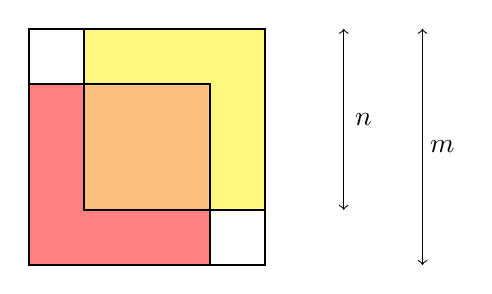
\begin{tikzpicture}
		\draw[thick] (0,0) rectangle (3,3);
		\draw[thick, fill=red!50] (0,0) rectangle (2.3,2.3);
		\draw[thick, fill=yellow!50] (0.7,0.7) rectangle (3, 3);
		\draw[thick, fill=orange!50] (0.7,0.7) rectangle (2.3, 2.3);
		\draw[<->] (4, 0.7)--(4, 3);
		\node at (4.25, 1.85) (n) {$n$};
		\draw[<->] (5, 0)--(5, 3);
		\node at (5.25, 1.5) (m) {$m$};
	\end{tikzpicture}
\end{center}
Amarga $m^2 = 2n^2$, wilayah tumpang tindhih saka rong kothak kang
dawa sisine $n$ nduweni jembar padha karo wilayah kang ora katutupan
dening kothak loro mau; yaiku jembar kothak oranye padha karo gunggung
jembar rong kothak kang ora diwernani. Dadi yen kothak oranye dawa
sisine $p$, lan saben kothak kang ora diwernani dawa sisine $q$, mula
$p^2 = 2q^2$. Nanging saiki $\sqrt{2} = \nicefrac{p}{q}$, kanthi $p < m$
lan $q < n$ sarta $p, q \in \Nat$. Iki kontradiksi karo kasunyatan yen
$m$ lan $n$ dipilih sacilik-cilike.

\emph{Kapindho, kanthi formal.} Amarga $m^{2} = 2n^{2}$, mula $m$ iku
genep. (Gampang dituduhake yen $x$ ganjil, mula $x^2$ ganjil.) Dadi
$m = 2r$, kanggo sawatara $r \in \Nat$. Kanthi nata maneh, $2r^2 = n^2$,
		%                \begin{align*}
		%                    (2q)^{2} &= 2n^{2}\\
		%                    4q^{2} &= 2n^{2}\\
		%                    2q^{2} &= n^{2}
		%                \end{align*}
mula $n$ uga genep. Dadi $m$ lan $n$ kalorone genep, mula pecahan
$\nicefrac{m}{n}$ \emph{bisa} disederhanakake maneh. Kontradiksi!
\end{proof}

Minangka cathetan sambilan, bukti nganggo diagram iki ngidini kita
bisa nyawang maneh bahan saka \olref[his][set][mythology]{sec}.
Tennenbaum (1927--2006) iku matematikawan modern tenan; nanging endahe
bukti iku ora bisa diselaki, tliti babar pisan, lan nggunakake intuisi geometris!

Kepriye wae, wilangan real iku ``luwih jembar'' tinimbang wilangan
rasional. Ing sawenehing teges, ana ``longkangan'' ing wilangan rasional,
lan wilangan real ngisi longkangan mau. Weierstrass mangerteni yen iki
nggambarake sawijining sipat kang mbedakake wilangan real saka wilangan
rasional, yaiku Sipat Kajangkepan: \emph{Saben himpunan wilangan real kang
ora kosong lan duwe wates ndhuwur mesthi duwe wates ndhuwur paling cilik.}

Gampang dingerteni yen wilangan rasional ora nduweni Sipat Kajangkepan.
Minangka tuladha, gatekna himpunan wilangan rasional kang luwih cilik
tinimbang $\sqrt{2}$, yaiku:
\[
	\Setabs{p \in \Rat}{p^2 < 2 \text{ utawa }p < 0}
\]
Himpunan iki duwe wates ndhuwur ing wilangan rasional; contone, kabeh
!!{element}s luwih cilik tinimbang $3$. Nanging apa wates ndhuwur paling
cilike? Kita kepengin mangsuli ``$\sqrt{2}$''; nanging kita lagi wae weruh
yen $\sqrt{2}$ \emph{dudu} wilangan rasional. Lan ora ana wilangan rasional
\emph{paling cilik} kang luwih gedhe tinimbang $\sqrt{2}$. Dadi himpunan iki duwe
wates ndhuwur nanging ora duwe wates ndhuwur paling cilik. Mula wilangan
rasional ora nduweni Sipat Kajangkepan. Cathetan koreksi sumber OLP-0044:
tandha kurang-saka kang kesasar sawise token unsur ing sumber ora digawa
menyang terjemahan (JV-D025).

Kosok baline, kontinuum ``samesthine'' nduweni Sipat Kajangkepan. Kita ora mung
kepengin $\sqrt{2}$ dadi wilangan real; kita kepengin ngisi kabeh
``longkangan'' ing garis rasional. Pancen, kita kepengin kontinuum iku
dhewe ora duwe ``longkangan''. Ya iki kang bakal kita oleh saka Kajangkepan.

\endgroup
% END OLP-0044
\endgroup

\begingroup
\makeatletter\def\ol@sectioncs{section}\makeatother

% BEGIN OLP-0045 content/sets-functions-relations/arithmetization/cuts.tex
\begingroup
\olfileid{sfr}{arith}{cuts}
\olsection{Saka $\Rat$ menyang $\Real$}

Intine, Sipat Kajangkepan nuduhake yen saben titik $\alpha$ ing garis
real mbage garis iku dadi rong paro kanthi sampurna: paro kang duwe
$\alpha$ minangka wates ndhuwur paling cilik, lan paro kang duwe
$\alpha$ minangka wates ngisor paling gedhe. Kanggo \emph{mbangun}
wilangan real saka wilangan rasional, Dedekind ngusulake supaya kita
nganggep wilangan real minangka \emph{potongan} kang misahake wilangan
rasional. Tegese, kita ngenali $\sqrt{2}$ karo \emph{potongan} kang
misahake wilangan rasional $< \sqrt{2}$ saka wilangan rasional
$> \sqrt{2}$.

Saiki kita jlentrehake kanthi luwih tliti. Yen wilangan rasional dipotong
dadi rong paro, pamisahan kang digawe bisa dikenali kanthi unik mung saka
\emph{paro ngisor}. Mula, kita menehi definisi iki:

\begin{defn}[Potongan]
\emph{Potongan} $\alpha$ yaiku sembarang perangan wiwitan sejati kang ora
kosong saka wilangan rasional lan ora duwe anggota paling gedhe. Tegese,
$\alpha$ iku potongan yen lan mung yen:
\begin{enumerate}
	\item \emph{ora kosong, sejati}: $\emptyset \neq \alpha \subsetneq \Rat$
	\item \emph{wiwitan}: kanggo kabeh $p,q \in \Rat$: yen $p < q \in \alpha$ mula $p \in \alpha$
	\item \emph{tanpa maksimum}: kanggo saben $p \in \alpha$ ana $q \in \alpha$ saengga $p < q$
\end{enumerate}
Banjur $\Real$ iku himpunan kabeh potongan.
\end{defn}

Dadi saiki kita bisa kandha yen $\sqrt{2} = \Setabs{p \in \Rat}{p^2 < 2\text{
utawa }p < 0}$. Mesthi wae, kita kudu mriksa yen iki pancen
\emph{potongan}, nanging rinciane dirembug ing \olref[check]{sec}.

Kaya sadurunge, sawise netepake sawetara obyek, sabanjure kita kudu
netepake fungsi lan relasi dhasar ing obyek-obyek mau. Kita miwiti saka
kang gampang:
\begin{align*}
	\alpha \leq \beta \text{ yen lan mung yen }\alpha \subseteq \beta
\end{align*}
Definisi tatanan iki ngidini kita \emph{ngandharake} asil pokok,
yaiku himpunan potongan nduweni Sipat Kajangkepan. Yen ditulis kanthi
jangkep, pratelane mangkene. Yen $S$ iku himpunan potongan kang ora kosong
lan duwe wates ndhuwur, mula $S$ duwe wates ndhuwur paling cilik. Kanthi
luwih rinci: ana potongan $\lambda$ kang dadi wates ndhuwur kanggo $S$,
yaiku\ $(\forall \alpha \in S)\alpha \subseteq \lambda$, lan $\lambda$ iku
potongan paling cilik kang kaya mangkono, yaiku\ $(\forall \beta \in
\Real)((\forall \alpha \in S)\alpha \subseteq \beta \lif \lambda \subseteq
\beta)$. Saiki iki buktine:

\begin{thm}\ollabel{realcompleteness}
Himpunan potongan nduweni Sipat Kajangkepan.
\end{thm}

\begin{proof}
Upamakna $S$ iku sembarang himpunan potongan kang ora kosong lan duwe
wates ndhuwur. Netepna $\lambda = \bigcup S$.
%\Setabs{p \in \Rat}{(\exists \alpha \in S)p \in \alpha}$$
Kita luwih dhisik ngaku yen $\lambda$ iku potongan:
\begin{enumerate}
\item Amarga $S$ ora kosong, paling ora ana siji potongan ing $S$, mula
$\emptyset \neq \lambda$. Amarga $S$ iku himpunan potongan, $\lambda
\subseteq \Rat$. Amarga $S$ duwe wates ndhuwur, ana $p \in \Rat$ kang
ora dadi anggota potongan $\alpha \in S$ endi wae. Dadi $p\notin \lambda$, mula
$\lambda \subsetneq \Rat$. Cathetan koreksi sumber OLP-0045: anane
potongan ing himpunan kasebut dumadi amarga himpunane ora kosong, dudu
amarga duwe wates ndhuwur kaya kang kasebut ing sumber Inggris (JV-D027).
\item Upamakna $p < q \in \lambda$. Dadi ana $\alpha \in S$ saengga
$q \in \alpha$. Amarga $\alpha$ iku potongan, $p \in \alpha$. Dadi
$p \in \lambda$.
\item Upamakna $p \in \lambda$. Dadi ana $\alpha \in S$ saengga
$p \in \alpha$. Amarga $\alpha$ iku potongan, ana $q \in \alpha$
saengga $p < q$. Dadi $q \in \lambda$.
\end{enumerate}
Iki mbuktekake pratelan mau. Kajaba iku, cetha yen $(\forall \alpha \in
S)\alpha \subseteq \bigcup S = \lambda$, yaiku\ $\lambda$ dadi wates
ndhuwur kanggo $S$. Saiki upamakna $\beta \in \mathbb{R}$ uga dadi wates
ndhuwur, yaiku\ $(\forall \alpha \in S)\alpha \subseteq \beta$. Kanggo
sembarang $p \in \Rat$, yen $p \in \lambda$, mula ana $\alpha \in S$
saengga $p \in \alpha$, mula $p \in \beta$. Mula,
$\lambda \subseteq \beta$. Dadi $\lambda$ iku wates ndhuwur
\emph{paling cilik} kanggo $S$.
\end{proof}

Dadi kita duwe akeh obyek kang nyukupi Sipat Kajangkepan. Salah siji
cara kanggo ngandharake iki yaiku: ora ana ``longkangan'' ing
potongan-potongan kita. (Dadi, nggawe ``potongan'' sabanjure saka wilangan
real, dudu saka wilangan rasional, ora bakal ngasilake obyek anyar kang
narik kawigaten.)

Sabanjure, kita kudu netepake sawetara operasi ing wilangan real. Kita
miwiti kanthi nyisipake wilangan rasional menyang wilangan real kanthi
netepake $p_\Real = \Setabs{q \in \Rat}{q < p}$ kanggo saben $p \in \Rat$.
Banjur kita netepake:
\begin{align*}
	\alpha + \beta &= \Setabs{p + q}{p \in \alpha \land q \in \beta}\\
%	\alpha - \beta &\defis \Setabs{p - q}{p \in \alpha \land q \in \Rat \setminus \beta}\\
	\alpha \times \beta &=
	\Setabs{p \times q}{0 \leq p \in \alpha \land 0 \leq q \in \beta} \cup 0^\mathbb{R} & \text{yen }\alpha, \beta \geq 0_\Real
%	\alpha \div \beta &\defis
%\Setabs{\nicefrac{p}{q}}{p \in \alpha \land q \in \Rat \setminus \beta}  & \text{yen }\alpha \geq 0_\Real, \beta > 0_\Real
\end{align*}
Kanggo nangani kasus ping-pingan liyane, luwih dhisik netepna: %yen $0_\Real \times \alpha = 0_\Real = \alpha \times 0_\Real$, lan tambahna:
\begin{align*}
	-\alpha &= \Setabs{p - q}{p < 0 \land q \notin \alpha}
\end{align*}
banjur netepna:
\begin{align*}
	\alpha \times \beta &\defis
	\begin{cases}
		\mathord{-}\alpha \times \mathord{-}\beta &\text{yen }\alpha < 0_\Real\text{ lan }\beta < 0_\Real\\
		\mathord{-}(\mathord{-}\alpha \times \beta) &\text{yen }\alpha < 0_\Real \text{ lan }\beta > 0_\Real\\
		\mathord{-}(\alpha \times \mathord{-}\beta) &\text{yen }\alpha > 0_\Real \text{ lan }\beta < 0_\Real
	\end{cases}
\end{align*}
Banjur kita kudu mriksa yen saben definisi kasebut tansah ngasilake potongan.
Pungkasan, kita kudu nuduhake kanthi cara kang gampang (nanging dawa) yen
potongan-potongan kang ditetepake kasebut tumindak persis kaya kang kudune.
Nanging kabeh rincian kasebut dirembug ing \olref[check]{sec}.

\endgroup
% END OLP-0045
\endgroup

\begingroup
\makeatletter\def\ol@sectioncs{section}\makeatother

% BEGIN OLP-0046 content/sets-functions-relations/arithmetization/reflections.tex
\begingroup
\olfileid{sfr}{arith}{ref}
\olsection{Sawetara Pamawas Filosofis}

Wis cukup perkara teknise. Nanging apa kang wis digayuh?

Meh ora bisa dibantah yen pambangunan mau menehi matematika murni kang
{endah}. Kajaba iku, ana sawetara asil konseptual kang jero. Pangerten yen
Sipat Kajangkepan ngandharake prabédan pokok antarane wilangan real lan
wilangan rasional iku wawasan kang jero. Kajaba iku, pambangunan wilangan
real kanthi cetha minangka potongan Dedekind menehi dhasar kang kukuh
kanggo analisis. Kita ngerti yen gagasan \emph{lapangan katata kang
jangkep} iku koheren, amarga potongan-potongan mau mbentuk lapangan kaya iku.

Sanadyan mangkono, kita kudu ngandharake sawetara cathetan kritis tumrap
asil kasebut.

Kapisan, durung cetha yen mikirake wilangan real nganggo potongan iku
\emph{luwih} tliti tinimbang mikirake wilangan real nganggo ekspansi
desimal kang lumrah (lan bisa tanpa wates). ``Pambangunan'' wilangan real
kang kapindho iki rada mirip karo pambangunan wilangan real nganggo
rerangken Cauchy; nanging sejatine cara iku wis dimangerteni para
matematikawan wiwit awal abad kaping 17 (delengen \olref[cauchy]{sec}).
Tambahing katliten kang nyata dumadi nalika dimangerteni yen wilangan
real nduweni Sipat Kajangkepan; kabisan mbangun wilangan real minangka
himpunan tartamtu mbokmenawa ora pati narik kawigaten yen ngadeg dhewe.

Luwih ora cetha maneh yen aritmetisasi wilangan wutuh utawa wilangan
rasional, kang luwih gampang, nambah katliten ing babagan kasebut.
Ing kene ana pangamatan prasaja kang prayoga. Sawise \emph{mbangun}
wilangan wutuh minangka kelas ekuivalensi pasangan urut wilangan natural,
banjur mbangun wilangan rasional minangka kelas ekuivalensi pasangan urut
wilangan wutuh, lan banjur mbangun wilangan real minangka himpunan wilangan
rasional, kita langsung \emph{nglalekake} pambangunan kasebut. Mligine,
ora ana wong kang kepengin \emph{nggunakake} pambangunan iki sajrone bukti
matematis (kejaba, mesthi wae, bukti yen pambangunane tumindak kaya kang
kudune). Luwih gampang ngomong langsung bab wilangan real tinimbang bab
sawijining himpunan saka himpunan saka himpunan saka himpunan saka himpunan
saka himpunan saka himpunan wilangan natural.
%(Amarga wilangan real dibangun minangka himpunan wilangan rasional; lan wilangan rasional dibangun minangka kelas ekuivalensi pasangan urut wilangan wutuh, yaiku himpunan saka himpunan saka himpunan wilangan wutuh; lan sateruse.)
%2/3 = [2,3]
%	yaiku {<2,3>, ... }
%	{ {{2},{2,3}}, ... }
%
%wilangan real iku
%	himpunan wilangan rasional
%
%wilangan rasional iku
%	himpunan saka himpunan saka himpunan wilangan wutuh
%
%wilangan wutuh iku
%	himpunan saka himpunan saka himpunan wilangan natural

Sing paling patut dimangu yaiku manawa definisi kasebut ngandhani kita apa
\emph{sejatine} wilangan wutuh, rasional, utawa real, \emph{yen dirembug
saka sisi metafisika}. Tegese, kita patut mangu yen wilangan real, umpamane,
\emph{iku} himpunan tartamtu (saka himpunan saka himpunan\ldots). Pepalang
utama tumrap panemu iki yaiku pambangunane bisa ditindakake kanthi maneka
cara. Tumrap wilangan real, ana sawetara pambangunan kang beda-beda lan pancen
narik kawigaten (delengen \olref[cauchy]{sec}). Nanging iki cara kang prasaja
banget kanggo ngolehake pambangunan beda: kaya ing
\olref[sfr][rel][ref]{sec}, kita bisa netepake pasangan urut kanthi cara
rada beda; yen gagasan pasangan urut alternatif iki digunakake,
pambangunan kita tetep bisa lumaku persis padha becike, nanging pungkasane
ngasilake obyek kang beda. Mula ana akeh pambangunan teori-himpunan kang
saingan kanggo wilangan wutuh, rasional, lan real. Saiki bakal sawenang-wenang
(lan gawe isin) yen kita ngaku yen wilangan wutuh, umpamane, yaiku
\emph{himpunan-himpunan iki}, dudu \emph{himpunan-himpunan kuwi}. (Kaya ing
\olref[sfr][rel][ref]{sec}, iki tuladha argumen kang digawe misuwur dening
\citealt{Benacerraf1965}.)

Ana perkara liyane kang prayoga dirembug: ana bab kang cukup \emph{aneh}
ing pambangunan kita. Kita miwiti saka wilangan natural. Banjur kita mbangun
wilangan wutuh, lan mbangun ``$0$ saka wilangan wutuh'', yaiku
$ \equivrep{0,0}{\Intequiv}$. Nanging $0 \neq
\equivrep{0,0}{\Intequiv}$. Pancen, miturut pambangunan kita,
\emph{ora ana} wilangan natural kang dadi wilangan wutuh. Nanging iki katon
ora lumrah banget. Pancen, ing \olref[sfr][set][imp]{sec}, kita ngaku tanpa
akeh argumen yen $\Nat \subseteq \Rat$. Yen pambangunan kasebut ngandhani
kita persis \emph{apa} wilangan-wilangan iku, pratelan iki mesthi kleru.

Yen saiki kita mundur sedhela, tekan ngendi asile? Kanthi makarya ing teori
himpunan naif lan nganggep wilangan natural wis cumawis, kita bisa
\emph{nganggep} wilangan wutuh, rasional, lan real minangka himpunan-himpunan
tartamtu. Ing teges iki, kita bisa \emph{nyisipake} teori bab obyek-obyek iki
ing sawijining teori himpunan. Nanging wigati filosofis saka panyisipan iki
ora prasaja.

Mesthi wae, iki kabeh durung dadi panutuping rembug!{} Intine mung mangkene.
Nuduhake yen aritmetisasi wilangan real \emph{pancen} wigati banget saka
sisi filsafat mbutuhake argumen \emph{filosofis} tambahan.

%Kajaba iku: sajrone bab iki, kita nganggep wilangan natural mung wis
%\emph{diwenehake} marang kita. Nanging apa kang bisa ditindakake
%nganggo wilangan kasebut? Iku bahan kanggo bab sabanjure.

\endgroup
% END OLP-0046
\endgroup

\begingroup
\makeatletter\def\ol@sectioncs{section}\makeatother

% BEGIN OLP-0047 content/sets-functions-relations/arithmetization/checking-details.tex
\begingroup
\olfileid{sfr}{arith}{check}
\olsection{Ring lan Lapangan Katata}

Sajrone bab iki, kita ngaku yen definisi-definisi tartamtu tumindak
``kaya kang kudune''. Ing lampiran teknis iki, kita bakal njlentrehake
apa kang dimaksud lan menehi gambaran bukti yen definisi-definisi iku
pancen tumindak ``kanthi bener''.

Ing \olref[int]{sec}, kita netepake panambahan lan ping-pingan ing $\Int$.
Kita kepengin nuduhake yen operasi kang wis ditetepake iki menehi struktur
kang ``dikarepake'' marang $\Int$. Mligine, struktur kasebut yaiku ring
komutatif.

\begin{defn}
	\emph{Ring komutatif} yaiku himpunan $S$ kang dilengkapi anggota mligi
	$0$ lan $1$ sarta operasi $+$ lan $\times$, kang nyukupi wolung rumus iki:
	\begin{align*}
		\emph{Asosiativitas}&&a + (b+ c) & = (a + b) + c \\
		&& (a \times b) \times c & = a \times (b\times c)\\
		\emph{Komutativitas}&&a + b &= b+ a  \\
		&&  a \times b&= b\times a\\
		\emph{Identitas}&&a + 0 &= a \\
		&& a \times 1 &= a\\
		\emph{Invers Aditif}&&(\exists b\in S)0&=a + b\\
		\emph{Distributivitas}&&a \times (b+ c ) &= (a \times b) + (a \times c)
	\end{align*}
	Kanthi implisit, kabeh variabel ing rumus iki kaiket dening kuantor
	universal kang diwatesi ing $S$. Gatekna uga yen unsur $0$ lan~$1$ ing
	kene ora kudu dadi wilangan natural kang jenenge padha.
\end{defn}

Dadi, kanggo mriksa yen wilangan wutuh mbentuk ring komutatif, kita mung
perlu mriksa yen wolung sarat iki kacukupan. Ora ana sarat kang {angel}
kanggo dibuktekake, nanging pamriksane rada ngrepotake. Minangka tuladha,
iki cara mbuktekake \emph{Asosiativitas} kanggo panambahan:

\begin{proof}
Tetepna $i, j, k \in \Int$. Dadi ana $a_1, b_1, a_2, b_2, a_3, b_3 \in
\Nat$ saengga $i = \equivrep{a_1, b_1}{}$ lan $j =
\equivrep{a_2,b_2}{}$ lan $k = \equivrep{a_3, b_3}{}$. (Supaya gampang
diwaca, kita nulis ``$\equivrep{x, y}{}$'' minangka ganti
``$\equivrep{x, y}{\Intequiv}$''; iki bakal ditindakake ing saindhenging
perangan iki.) Saiki:
\begin{align*}
	i + (j + k) &= \equivrep{a_1, b_1}{}+(\equivrep{a_2, b_2}{} + \equivrep{a_3, b_3}{}) \\
	&= \equivrep{a_1,  b_1}{} + \equivrep{a_2+a_3, b_2+b_3}{}\\
	&= \equivrep{a_1 + (a_2 + a_3), b_1 + (b_2 + b_3)}{}\\
	&= \equivrep{(a_1 + a_2) + a_3, (b_1 + b_2) + b_3}{}\\
	&= \equivrep{a_1 + a_2, b_1 + b_2}{} + \equivrep{a_3, b_3}{}\\
	&= (\equivrep{a_1, b_1}{} + \equivrep{a_2, b_2}{}) + \equivrep{a_3, b_3}{}\\
	&= (i+j) + k
\end{align*}
kanthi nggunakake tumindake panambahan ing $\Nat$ kanthi bebas.
\end{proof}

Kanthi cara kang padha, iki bukti \emph{Invers Aditif}:

\begin{proof}
Tetepna $i \in \Int$, mula $i = \equivrep{a,b}{}$ kanggo sawatara $a,b \in
\Nat$. Netepna $j = \equivrep{b,a}{} \in \Int$. Kanthi nggunakake tumindake
wilangan natural, $(a+b) + 0 = 0 + (a+b)$, mula $\tuple{a+b, b+a}
\sim_\Int \tuple{0,0}$ miturut definisi, lan mulane
$\equivrep{a+b, b+a}{} = \equivrep{0, 0}{} = 0_\Int$. Dadi saiki $i + j =
\equivrep{a,b}{}+\equivrep{b,a}{}=\equivrep{a+b, b+a}{}= \equivrep{0,
0}{} = 0_\Int$.
\end{proof}

Lan iki bukti \emph{Distributivitas}:

\begin{proof}
Kaya ing ndhuwur, tetepna $i = \equivrep{a_1, b_1}{}$ lan $j =
\equivrep{a_2,b_2}{}$ lan $k = \equivrep{a_3, b_3}{}$. Saiki:
\begin{align*}
	i \times (j + k)
	&= \equivrep{a_1, b_1}{} \times (\equivrep{a_2,b_2}{} + \equivrep{a_3, b_3}{})\\
	&= \equivrep{a_1, b_1}{} \times \equivrep{a_2 + a_3,b_2+b_3}{}\\
	&= \equivrep{a_1  (a_2 + a_3) + b_1  (b_2+b_3), a_1  (b_2 + b_3) + b_1 (a_2 + a_3)}{}\\
	&= \equivrep{a_1 a_2 + a_1a_3 + b_1 b_2+b_1b_3, a_1 b_2 + a_1b_3 + a_2b_1 + a_3b_1}{}\\
%		&= \equivrep{a_1 a_2 + b_1b_2 + a_1a_3 + b_1 b_2+b_1b_3, a_1 b_2 + a_1b_3 + a_2b_1 + a_3b_1}{}\\
	&= \equivrep{a_1a_2 + b_1b_2, a_1b_2 + a_2b_1}{} + \equivrep{a_1a_3 + b_1b_3, a_1b_3 + a_3b_1}{}\\
	&= (\equivrep{a_1, b_1}{} \times \equivrep{a_2,b_2}{}) + (\equivrep{a_1, b_1}{} \times  \equivrep{a_3, b_3}{})\\
	&= (i \times j) + (i \times k)
\end{align*}
\end{proof}

Kita pasrahake limang sarat liyane minangka gladhen. Sawise iku rampung,
kita wis nuduhake yen $\Int$ mbentuk ring komutatif, yaiku panambahan lan
ping-pingan kang ditetepake tumindak kaya kang kudune.

\begin{prob}
Buktekna yen $\Int$ iku ring komutatif.
\end{prob}

Nanging tugas kita durung rampung. Saliyane netepake panambahan lan
ping-pingan ing $\Int$, kita uga netepake relasi tatanan $\leq$, lan kudu
mriksa yen relasi iki tumindak kaya kang kudune. Kanthi luwih rinci, kita
kudu nuduhake yen $\Int$ mbentuk ring \emph{katata}.\footnote{Elinga saka
	\olref[sfr][rel][ord]{def:linearorder} yen tatanan total iku relasi kang
	refleksif, transitif, antisimetris, lan koneks. Ing konteks relasi tatanan,
	koneksitas kadhangkala diarani \emph{trikotomi}, amarga kanggo saben $a$
	lan $b$ kita duwe $a \leq b \lor a = b \lor a \geq b$.}

\begin{defn}
\emph{Ring katata} yaiku ring komutatif kang uga dilengkapi relasi
tatanan total $\leq$, saengga:
\begin{align*}
	a \leq b &\lif a + c \leq b + c\\
	(a \leq b \land 0 \leq c) &\lif a \times c \leq b \times c
\end{align*}
\end{defn}

\begin{prob}
Buktekna yen $\Int$ iku ring katata.
\end{prob}

Kaya sadurunge, nuduhake yen $\Int$ kang dibangun iki dadi ring katata
iku ngrepotake nanging lumrah. Pamriksane dipasrahake marang pamaca.

Iki ngrampungake prakara wilangan wutuh. Nanging saiki kita kudu nuduhake
prakara kang meh padha tumrap wilangan rasional. Mligine, kita kudu nuduhake
yen wilangan rasional mbentuk \emph{lapangan katata} miturut definisi
$+$, $\times$, lan $\leq$ kang wis diwenehake:
\begin{defn}\ollabel{orderedfield}
\emph{Lapangan katata} yaiku ring katata kang uga nyukupi:
\begin{align*}
	\emph{Invers Multiplikatif}& & (\forall a \in S \setminus \{0\})(\exists b \in S) a\times b& = 1
\end{align*}
\end{defn}

Sawise nuduhake yen $\Int$ mbentuk ring katata, nuduhake yen $\Rat$
mbentuk lapangan katata iku gampang nanging ngrepotake.

\begin{prob}
Buktekna yen $\Rat$ iku lapangan katata.
\end{prob}

Sawise ngrampungake wilangan wutuh lan rasional, mung wilangan real kang
isih kudu dirampungake. Mligine, kita kudu nuduhake yen $\Real$ mbentuk
lapangan katata kang \emph{jangkep}, yaiku lapangan katata kanthi Sipat
Kajangkepan. \olref[cuts]{realcompleteness} wis mbuktekake yen $\Real$
nduweni Sipat Kajangkepan. Nanging kita isih kudu nindakake pamriksa kang
ngrepotake kanggo nuduhake yen $\Real$ iku lapangan katata. Cathetan
koreksi sumber OLP-0047: ukara Inggris ngilangi tembung sawise adjektiva
``tedious''; terjemahan iki mulihake gagasan pamriksa kang dibutuhake
(JV-D029).

Sadurunge langsung nindakake gladhen \emph{kasebut} kang ngrepotake, kita
kudu mriksa sawetara prakara kang luwih ``langsung''. Umpamane, kita butuh
jaminan yen $\alpha + \beta$ kang ditetepake iki pancen dadi
\emph{potongan} kanggo sembarang potongan $\alpha$ lan $\beta$. Iki buktine:

\begin{proof}
Amarga $\alpha$ lan $\beta$ kalorone potongan, $\alpha + \beta = \Setabs{p
+ q}{p \in \alpha \land q \in \beta}$ iku subhimpunan sejati kang ora
kosong saka $\Rat$. Saiki upamakna $x < p + q$ kanggo sawatara $p \in
\alpha$ lan $q \in \beta$. Banjur $x - p < q$, mula $x - p \in \beta$,
lan $x = p + (x - p) \in \alpha + \beta$. Dadi $\alpha + \beta$ iku
perangan wiwitan saka $\Rat$. Pungkasan, kanggo sembarang $p + q \in \alpha
+ \beta$, amarga $\alpha$ lan $\beta$ kalorone potongan, ana $p_1 \in
\alpha$ lan $q_1 \in \beta$ saengga $p < p_1$ lan $q < q_1$; mula $p + q
< p_1 + q_1 \in \alpha + \beta$; dadi $\alpha + \beta$ ora duwe anggota paling gedhe.
\end{proof}

Kanthi upaya kang padha, kita bisa mriksa yen $\alpha - \beta$,
$\alpha \times \beta$, lan $\alpha \div \beta$ iku potongan (kanggo kasus
pungkasan, kejaba nalika $\beta$ iku potongan nol). Nanging iki uga mung
dipasrahake marang pamaca. Cathetan sumber OLP-0047: rumus pangurangan lan
pambagian kang dirujuk ing kene mung ana minangka komentar kang dipateni
ing perangan potongan; gladhen iki nganggep definisi kang dimaksud mau
(JV-D030).

\begin{prob}
Buktekna yen $\Real$ iku lapangan katata.
\end{prob}

Nanging isih ana prakara cilik kang kudu dirapekake. Ing
\olref[cuts]{sec}, kita ngusulake yen $\sqrt{2} =
\Setabs{p \in \Rat}{p < 0 \text{ utawa }p^2 < 2}$. Nanging kita pancen
kudu nuduhake yen himpunan iki \emph{potongan}. Iki buktine:

\begin{proof}
Cetha yen iki perangan wiwitan sejati kang ora kosong saka wilangan rasional;
dadi cukup nuduhake yen ora duwe anggota paling gedhe. Mligine, cukup nuduhake yen
nalika $p$ iku wilangan rasional positif kanthi $p^2 < 2$ lan $q =
\frac{2p+2}{p+2}$, kita duwe $p < q$ lan $q^2 < 2$. Kanggo ndeleng yen
$p < q$, gatekna:
\begin{align*}
	p^2 &< 2\\
	p^2 + 2p &< 2 + 2p\\
	p(p + 2) &< 2 + 2p\\
	p &< \tfrac{2+2p}{p+2} = q
\end{align*}
Kanggo ndeleng yen $q^2 < 2$, gatekna:
\begin{align*}
	p^2 &< 2\\
	2p^2 + 4p + 2 &< p^2 + 4p+ 4\\
	4p^2 + 8p + 4 &< 2(p^2 + 4p + 4)\\
	(2p+2)^2 & <2(p+2)^2\\
	\tfrac{(2p+2)^2}{(p+2)^2} &< 2\\
	q^2 &< 2
\end{align*}
\end{proof}

\endgroup
% END OLP-0047
\endgroup

\begingroup
\makeatletter\def\ol@sectioncs{section}\makeatother

% BEGIN OLP-0048 content/sets-functions-relations/arithmetization/cauchy.tex
\begingroup
\olfileid{sfr}{arith}{cauchy}

\olsection{Lampiran: Wilangan Real minangka Rerangken Cauchy}

Ing \olref[cuts]{sec}, kita mbangun wilangan real minangka potongan
Dedekind. Ing perangan iki, kita njlentrehake pambangunan alternatif.
Pambangunan iki adhedhasar definisi Cauchy tumrap apa kang saiki diarani
rerangken Cauchy; nanging panganggone definisi iki kanggo \emph{mbangun}
wilangan real asale saka panulis abad kaping 19 liyane, mligine Weierstrass,
Heine, M\'{e}ray, lan Cantor. (Kanggo sejarah kang becik, delengen
\citeauthor{OConnorRobertson:RN} \citeyear{OConnorRobertson:RN}.)

Sadurunge tekan abad kaping 19, prayoga yen kita nggatekake Simon Stevin
(1548--1620). Ringkese, Stevin mangerteni yen saben wilangan real bisa
dipikirake liwat ekspansi desimale. Mula malah wilangan irasional kaya
$\sqrt{2}$ duwe ekspansi desimal kang becik, kang diwiwiti:
\[
	1.41421356237\ldots
\]
Gampang banget nggambarake ekspansi desimal ing teori himpunan: cukup
anggepen minangka fungsi $d \colon \Nat \to \Nat$, kanthi $d(n)$ dadi
panggonan desimal kaping $n$ kang digatekake. Banjur perlu owah-owahan
sethithik kanggo nangani bagean wilangan real sadurunge tandha desimal
(ing kene mung $1$). Uga perlu owah-owahan liyane, yaiku relasi
ekuivalensi, kanggo njamin yen, umpamane, $0.999\ldots = 1$. Nanging
ora angel menehi pambangunan wilangan real kang tliti babar pisan
kanthi cara Stevin ing teori himpunan.

Stevin dudu punjering rembugan kita. (Kanggo katrangan luwih akeh bab
Stevin, delengen \citealt{KatzKatz2012}.) Nanging ana gagasan kang raket.
Tinimbang langsung nganggep ekspansi desimal $\sqrt{2}$, kita bisa
nggatekake \emph{rerangken} panyedhakan rasional marang $\sqrt{2}$ kang
saya tliti, nganggo ekspansi kang saya tliti:
\[
1, 1.4, 1.414, 1.4142, 1.41421,\ldots
\]
Gagasan yen wilangan real bisa dipikirake liwat ``panyedhakan kang saya
becik'' dadi dhasar kanggo rerangken wawasan liyane (padha karo pangamatan
kang digunakake nalika mbangun $\Rat$ saka $\Int$, utawa $\Int$ saka
$\Nat$). Wawasan dhasare yaiku:
\begin{enumerate}
	\item Saben wilangan real bisa ditulis minangka ekspansi desimal
	(kang bisa tanpa wates).
	\item Informasi kang dikodeake ekspansi desimal (kang bisa tanpa wates)
	uga bisa dikodeake kanthi rerangken wilangan rasional.
	\item Rerangken wilangan rasional bisa dipikirake minangka fungsi saka
	$\Nat$ menyang $\Rat$; cukup netepna $f(n)$ minangka wilangan rasional
	kaping $n$ ing rerangken kasebut.
\end{enumerate}
Mesthi wae, ora \emph{sembarang} fungsi saka $\Nat$ menyang $\Rat$ menehi
wilangan real. Umpamane, gatekna fungsi iki:
\[
	f(n) =\begin{cases}
			1 & \text{yen }n\text{ ganjil}\\
			0 &\text{yen }n\text{ genep}
		\end{cases}
\]
Inti masalahe yaiku rerangken $0,1,0,1,0,1,0,\ldots$ katon ora
``nyedhaki'' wilangan real apa wae. Dadi, supaya rerangken kang digatekake
pancen nyedhaki sawenehing wilangan real, kita mung kudu nggatekake
rerangken kang duwe \emph{limit}.

Kita wis nemoni gagasan limit ing \olref[his][set][limits]{sec}. Nanging
kita ora bisa nggunakake definisi kang \emph{persis padha} karo definisi
ing kono. Ekspresi ``$(\forall \epsilon>0)$'' ing kono kanthi meneng-meneng
nggunakake kuantifikasi ing wilangan real; lan kita nggatekake limit fungsi
ing wilangan real. Dadi nggunakake definisi kasebut ateges wis nganggep
wilangan real cumawis, kamangka wilangan iku persis kang arep
\emph{dibangun}. Untunge, kita bisa nggunakake gagasan limit kang raket.
\begin{defn}\ollabel{def:CauchySequence}
  Fungsi $f: \Nat \to \Rat$ diarani \emph{rerangken Cauchy} yen lan mung
  yen kanggo saben $\epsilon \in \Rat$ kang positif, kita duwe $(\exists
  \ell \in \Nat)(\forall m, n > \ell)|f(m) - f(n)| < \epsilon$.
\end{defn}

Gagasan umum limit isih padha: yen kita kepengin tingkat katliten tartamtu
(kang diukur nganggo~$\epsilon$), ana ``wilayah'' kang kudu dideleng, yaiku
sembarang masukan luwih gedhe tinimbang~$\ell$. Gampang dingerteni yen
rerangken $1$, $1.4$, $1.414$, $1.4142$, $1.41421$\ldots{} duwe limit: yen
kita kepengin nyedhaki $\sqrt{2}$ kanthi kasalahan kurang saka
$\nicefrac{1}{10^{n}}$, cukup delengen sembarang entri sawise entri kaping
$n$.

Gagasan kang katon cetha yaiku nyebut wilangan real \emph{iku} sembarang
rerangken Cauchy. Nanging kaya ing pambangunan $\Int$ lan $\Rat$, iki
naif banget: saben wilangan real bisa dituduhake dening akeh rerangken
Cauchy kang beda-beda. Cara prasaja kanggo ndeleng iki kaya
mangkene. Yen diwenehi rerangken Cauchy~$f$, netepna $g$ minangka fungsi
kang persis padha karo~$f$, kejaba $g(0)\neq f(0)$. Amarga rerangken loro
iku padha ing kabeh indeks sawise indeks kapisan, pungkasane kita
kepengin kandha yen rerangken mau duwe limit kang padha miturut teges ing
\olref{def:CauchySequence}, mula kudu dianggep ``netepake'' wilangan real
kang padha. Dadi, rerangken Cauchy loro iki kudu dianggep wilangan real
kang padha. Cathetan koreksi sumber OLP-0048: patang frasa Inggris
ngandhut tembung ganda utawa tembung panyambung kang ilang, yaiku ``can be
equally be encoded'', ``a simple way to see this as follows'', ``define we
a notion'', lan ``hone on in''. Terjemahan iki mung nindakake pambeneran
gramatikal kang paling sithik tanpa ngowahi pratelan matematise (JV-D031).

Mula kita maneh kudu netepake relasi ekuivalensi ing rerangken Cauchy lan
ngenali wilangan real karo kelas-kelas ekuivalensi. Kaping pisan, kita
mbutuhake gagasan fungsi kang nyedhaki $0$ ing limit. Kanggo sembarang
fungsi $h : \Nat \to \Rat$, kandhanana yen \emph{$h$ nyedhaki $0$} yen lan
mung yen kanggo saben $\epsilon \in \Rat$ kang positif kita duwe $(\exists
\ell \in \Nat)(\forall n > \ell)|h(n)| < \epsilon$.\footnote{Bandhingna
iki karo definisi $\lim_{x \mathord{\rightarrow}\infty}f(x) = 0$ ing
\olref[his][set][limits]{sec}.} Sabanjure, yen $f$ lan $g$ iku fungsi
$\Nat \to \Rat$, netepna $(f-g)(n) = f(n) - g(n)$. Saiki netepna:
\[
	f \Realequiv g \text{ yen lan mung yen $(f-g)$ nyedhaki $0$}.
\]
Kita kudu mriksa yen $\Realequiv$ iku relasi ekuivalensi; lan pancen iya.
Banjur, yen dikarepake, kita bisa netepake wilangan real minangka
kelas-kelas ekuivalensi miturut $\Realequiv$ saka kabeh rerangken Cauchy
saka $\Nat \to \Rat$. Cathetan koreksi sumber OLP-0048: ukara Inggris
sadurunge definisi salah nyebut ``equivalence relations''; obyek kang
nggambarake wilangan real yaiku kelas ekuivalensi (JV-D032).

\begin{prob}
Netepna $f(n) = 0$ kanggo saben $n$. Netepna $g(n) = \frac{1}{(n+1)^2}$.
Tuduhna yen kalorone rerangken Cauchy, lan yen limit fungsi kalorone
yaiku $0$, saengga uga $f \sim_\Real g$.
\end{prob}

Sawise iku, kaya lumrahe kita nulis $\equivrep{f}{\Realequiv}$ kanggo
kelas ekuivalensi kang duwe $f$ minangka !!a{element}. Nanging supaya
gampang diwaca, sabanjure kita ngilangi subskrip lan mung nulis
$\equivrep{f}{}$. Kita uga netepake yen kanggo saben $q \in \Rat$, kita
duwe $q_{\Real} = \equivrep{c_{q}}{}$, kanthi $c_{q}$ minangka fungsi
konstan $c_q(n) = q$ kanggo kabeh $n \in \Nat$. Banjur kita netepake
relasi lan operasi dhasar ing wilangan real, umpamane:
\begin{align*}
	\equivrep{f}{} + \equivrep{g}{} &= 	\equivrep{(f + g)}{} \\
	\equivrep{f}{} \times 	\equivrep{g}{} &= \equivrep{(f \times g)}{}
\end{align*}
kanthi $(f + g)(n) = f(n) + g(n)$ lan $(f \times g)(n) = f(n) \times
g(n)$. Mesthi wae, kita uga kudu mriksa yen $(f + g)$, $(f-g)$, lan
$(f\times g)$ iku rerangken Cauchy nalika $f$ lan $g$ rerangken Cauchy;
lan pancen iya, dene buktine dipasrahake marang pamaca.

Pungkasan, kita netepake gagasan tatanan. Kandhanana yen
$\equivrep{f}{}$ iku \emph{positif} yen lan mung yen
$\equivrep{f}{}\neq 0_\Real$ lan $(\exists \ell \in \Nat)(\forall n >
\ell)0 < f(n)$. Banjur kandhanana yen $\equivrep{f}{} < \equivrep{g}{}$
yen lan mung yen $\equivrep{(g - f)}{}$ positif. Kita kudu mriksa yen iki
ditetepake kanthi becik, yaiku ora gumantung marang pilihan fungsi
``wakil'' saka kelas ekuivalensi. Cathetan koreksi sumber OLP-0048:
syarat positif ing sumber nulis nol rasional, nanging kelas kasebut
wilangan real; terjemahan nggunakake nol real kaya ukara sabanjure
(JV-D033).
%\begin{align*}
%	\equivrep{f}{} \leq \equivrep{g}{} \text{ yen lan mung yen }&\equivrep{f}{} = \equivrep{g}{} \text{ utawa }\\
%	&(\exists \ell \in \Nat)(\forall n \in \Nat)(\ell < n \lif f(n) \leq g(n))
%\end{align*}
Sawise pamriksa iki, cukup gampang nuduhake yen definisi kasebut menehi
sipat aljabar kang bener, yaiku:
\begin{thm}\ollabel{thm:cauchyorderedfield}
Rerangken-rerangken Cauchy mbentuk lapangan katata. Ing pratelan iki,
kang mbentuk lapangan yaiku kelas-kelas ekuivalensine; rerangken dhewe
digunakake minangka wakil (JV-D034).
\end{thm}

\begin{proof}
Gladhen.
\end{proof}

\begin{prob}
Buktekna yen rerangken-rerangken Cauchy mbentuk lapangan katata, kanthi
teges kelas ekuivalensi kaya kang diterangake ing ndhuwur.
\end{prob}

Luwih angel mbuktekake yen wilangan real kang dibangun kanthi cara iki
nduweni Sipat Kajangkepan, mula kita bakal menehi buktine.

\begin{thm}
Saben himpunan rerangken Cauchy kang ora kosong lan duwe wates ndhuwur
mesthi duwe wates ndhuwur paling cilik. Tatanan lan wates ing pratelan
iki ditrapake liwat kelas ekuivalensi rerangken kasebut (JV-D034).
\end{thm}

\begin{proof}[Gambaran bukti] Upamakna $S$ iku sembarang himpunan rerangken
Cauchy kang ora kosong lan duwe wates ndhuwur. Dadi ana $p \in \Rat$
saengga $p_{\Real}$ dadi wates ndhuwur kanggo $S$. Jupuken $r \in S$;
banjur ana $q \in \Rat$ saengga $q_{\Real} < r$. Dadi yen wates ndhuwur
paling cilik kanggo $S$ ana, wates iku dumunung ing antarane $q_\Real$ lan
$p_\Real$, kalebu loro-lorone. Cathetan sumber OLP-0048: langkah iki
nggunakake sipat Archimedean kang durung dibuktekake ing perangan iki:
saben kelas real ana ing ngisor sawenehing salinan rasional lan ing
ndhuwur sawenehing salinan rasional (JV-D035).

Kita bakal saya nyedhaki wates ndhuwur paling cilik bebarengan saka ngisor
lan ndhuwur. Mligine, kita netepake rong fungsi $f, g \colon
\Nat \to \Rat$, kanthi ancas $f$ nyedhaki wates kasebut saka ndhuwur lan
$g$ nyedhaki wates kasebut\ saka ngisor. Kita miwiti kanthi netepake:
\begin{align*}
	f(0) &= p \\
	g(0) &= q
\end{align*}
Banjur, kanthi $a_n = \frac{f(n) + g(n)}{2}$, netepna:\footnote{Iki
definisi rekursif. Nanging kita \emph{durung} menehi alesan kanggo
nganggep definisi rekursif bisa digunakake.}
\begin{align*}
	f(n+1) &=
	\begin{cases}
		a_n &\text{yen }(\forall h \in S)\equivrep{h}{} \leq (a_n)_\Real\\
		f(n)&\text{yen ora}
	\end{cases}\\
	g(n+1) &=
	\begin{cases}
		a_n &\text{yen }(\exists h \in S)\equivrep{h}{} \geq (a_n)_\Real\\
		g(n) &\text{yen ora}
	\end{cases}
\end{align*}
$f$ lan $g$ kalorone rerangken Cauchy. (Iki bisa dipriksa kanthi cukup
gampang, nanging dipasrahake minangka gladhen.) Gatekna yen fungsi $(f-g)$
nyedhaki $0$, amarga bedane $f$ lan $g$ dadi separo ing saben langkah.
Mula $\equivrep{f}{} = \equivrep{g}{}$.

Kaping pisan kita nuduhake yen $\equivrep{f}{}$ iku wates ndhuwur kanggo
$S$, yaiku\ $(\forall h \in S)\equivrep{h}{} \leq \equivrep{f}{}$.
(Kita bakal nggunakake \olref{thm:cauchyorderedfield} nalika dibutuhake.)
Jupuken $h \in S$ lan upamakna, kanggo bukti kanthi kontradiksi, yen
$\equivrep{f}{} < \equivrep{h}{}$, mula $0_\Real <
\equivrep{(h-f)}{}$. Amarga $f$ iku rerangken Cauchy kang mudhun kanthi
monoton, ana $n \in \Nat$ saengga $\equivrep{(c_{f(n)} - f)}{} <
\equivrep{(h-f)}{}$. Dadi:
\[
	(f(n))_\Real = \equivrep{c_{f(n)}}{} < \equivrep{f}{} + \equivrep{(h-f)}{} = \equivrep{h}{},
\]
Iki kontradiksi karo kasunyatan yen miturut pambangunan,
$\equivrep{h}{} \leq (f(n))_\Real$.

Sabanjure kita nuduhake yen $\equivrep{f}{} = \equivrep{g}{}$ iku wates
ndhuwur \emph{paling cilik} kanggo $S$. Dadi jupuken sembarang rerangken
Cauchy $j$ lan upamakna $\equivrep{j}{} < \equivrep{g}{}$. Kanthi nalar
kaya ing ndhuwur lan nggunakake kasunyatan yen $g$ \emph{munggah} kanthi
monoton, ana $n \in \Nat$ saengga $\equivrep{j}{} < (g(n))_\Real$.
Nanging miturut pambangunan ana $h \in S$ saengga $(g(n))_\Real \leq
\equivrep{h}{}$, mula $\equivrep{j}{} < \equivrep{h}{}$ lan mulane
$\equivrep{j}{}$ dudu wates ndhuwur kanggo $S$.
\end{proof}

\endgroup
% END OLP-0048
\endgroup


\OLEndChapterHook

\endgroup
% END OLP-0041
\endgroup


\begingroup
\makeatletter\def\ol@sectioncs{section}\makeatother

% BEGIN OLP-0049 content/sets-functions-relations/infinite/infinite.tex
\begingroup
\olchapter{sfr}{infinite}{Himpunan Tanpa Wates}

\begin{editorial}
Bab ngenani himpunan tanpa wates iki dijupuk saka \emph{Open Set
Theory} anggitane Tim Button.
\end{editorial}

\begingroup
\makeatletter\def\ol@sectioncs{section}\makeatother

% BEGIN OLP-0050 content/sets-functions-relations/infinite/hilberts-hotel.tex
\begingroup
\olfileid{sfr}{infinite}{hilbert}
\olsection{Hotel Hilbert}

Himpunan wilangan natural mesthi katon tanpa wates. Mula, yen kita ora
arep \emph{langsung nganggep} wilangan natural wis ana, langkah
kapisan kudu njlentrehake himpunan tanpa wates nganggo istilah kang ora
mbutuhake panyebutan wilangan natural iku dhewe. Iki salah siji cara
kang becik, kang diandharake Hilbert ing kuliah taun 1924. Dheweke
njaluk kita mbayangake
\begin{quote}
[\ldots] hotel kang kamare winates cacahe. Saben kamar kudu dienggoni
pas siji tamu. Yen para tamu banjur ijol kamar kanthi sawenehing cara,
[nanging] saben kamar tetep ora dienggoni luwih saka siji wong, ora
ana kamar kang dadi kosong, lan kanthi cara iki sing duwe hotel ora
bisa nyawisake panggonan anyar kanggo tamu kang mentas teka [\ldots
\textparagraph \ldots]

Saiki kita netepake yen hotel mau duwe kamar tanpa wates cacahe kang
diwenehi nomer $1$, $2$, $3$, $4$, $5$, \dots, lan saben kamar
dienggoni pas siji tamu. Sanalika ana tamu anyar teka, sing duwe hotel
mung perlu mindhah saben tamu lawas menyang kamar kanthi nomer siji
luwih gedhe, lan kamar~$1$ bakal kosong kanggo tamu kang mentas teka.
	\begin{center}
		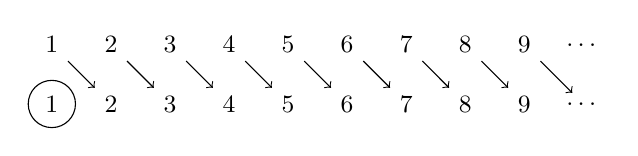
\begin{tikzpicture}[scale = .75]
		\foreach \x in {1, 2, 3, 4, 5, 6, 7, 8, 9}
		{
			\node (\x a) at (\x, 1) {\small{\x}};
			\node (\x b) at (\x, 2) {\small{\x}};
		}
		\node (dotsa) at (10, 1) {\small{\ldots}};
		\node (dotsb) at (10, 2) {\small{\ldots}};
		\draw[->] (1b)--(2a);
		\draw[->] (2b)--(3a);
		\draw[->] (3b)--(4a);
		\draw[->] (4b)--(5a);
		\draw[->] (5b)--(6a);
		\draw[->] (6b)--(7a);
		\draw[->] (7b)--(8a);
		\draw[->] (8b)--(9a);
		\draw[->] (9b)--(dotsa);
		\draw (1,1) circle (.4);
		\end{tikzpicture}
	\end{center}
	(diterbitake ing \citealt[730]{EwaldSieg2013}; terjemahan kita)
\end{quote}
Bab kang wigati yaiku Hotel Hilbert duwe kamar tanpa wates cacahe; lan
andharane bisa kita gunakake kanggo nemtokake apa tegese pratelan iku.
Pancen, iki uga cara Dedekind (mesthi wae diandharake ing kene nganggo
anakronisme kang gedhe banget; definisi Dedekind asale saka
\citeyear{Dedekind1888}):

\begin{defn}\ollabel{defn:DedekindInfinite}
Himpunan $A$ iku \emph{tanpa wates miturut Dedekind} yen lan mung yen
ana !!a{injection} saka~$A$ menyang subhimpunan sejati saka~$A$. Yaiku,
ana $o \in A$ lan !!a{injection} $f \colon A \to A$ saengga
$o \notin \ran{f}$.
\end{defn}

\endgroup
% END OLP-0050
\endgroup

\begingroup
\makeatletter\def\ol@sectioncs{section}\makeatother

% BEGIN OLP-0051 content/sets-functions-relations/infinite/dedekind-algebra.tex
\begingroup
\olfileid{sfr}{infinite}{dedekind}
\olsection{Aljabar Dedekind}

Kita ora mung kepengin wilangan natural iku tanpa wates; kita uga
kepengin wilangan mau nduweni sipat-sipat (aljabaris) tartamtu: kudu
tumindak kanthi becik ing panggunggungan, ping-pingan, lan sapiturute.

Gagasan Dedekind yaiku nganggep \emph{fungsi panerus} minangka
dhasar, banjur menehi ciri marang wilangan liwat sipat-sipat iki:
\begin{enumerate}
	\item Ana wilangan, $0$, kang dudu panerus saka wilangan apa wae
	\\yaiku, $0 \notin \ran{s}$
	\\yaiku, $\forall x\ s(x) \neq 0$
	\item Wilangan-wilangan kang beda nduweni panerus kang beda
	\\yaiku, $s$ iku !!a{injection}
	\\yaiku, $\forall x \forall y (s(x) = s(y) \lif x = y)$
	\item\ollabel{repeatedapplication} Saben wilangan dipikolehi saka
	$0$ kanthi ngetrapake fungsi panerus bola-bali.
\end{enumerate}
Rong sarat kapisan gampang ditangani nganggo logika tataran kapisan
(delengen ing ndhuwur). Nanging \olref{repeatedapplication} ora bisa
ditangani mung nganggo logika tataran kapisan. Langkah wigati Dedekind
yaiku ngrumusake maneh sarat \olref{repeatedapplication} kanthi teori
himpunan kaya mangkene:
\begin{enumerate}
	\item[3$'$.] Wilangan natural iku himpunan paling cilik kang
	\emph{katutup marang fungsi panerus}: yaiku, yen $s$ ditrapake
	marang sembarang !!{element} saka himpunan iku, kita oleh
	!!{element} liyane saka himpunan iku.
\end{enumerate}
Nanging iki kudu diandharake alon-alon.

\begin{defn}\ollabel{Closure}
	Kanggo saben fungsi $f$, himpunan $X$ iku $f$-\emph{katutup}
	{yen lan mung yen} $(\forall x \in X)f(x) \in X$. Saiki, kanggo
	saben $o$, netepna:
	$$\closureofunder{f}{o} = \bigcap\Setabs{X}{o \in X\text{ lan }X
	\text{ iku $f$-katutup}}$$
\end{defn}

Dadi $\closureofunder{f}{o}$ iku irisan kabeh himpunan $f$-katutup
kang duwe $o$ minangka !!a{element}. Miturut intuisi,
$\closureofunder{f}{o}$ iku himpunan $f$-katutup \emph{paling cilik}
kang duwe $o$ minangka !!a{element}. Asil sabanjure njlentrehake
gagasan intuisi kasebut kanthi tliti:
\begin{lem}\ollabel{closureproperties}
	Kanggo saben himpunan A, saben fungsi $f$ saka A menyang A, lan saben
	$o \in A$:
	\begin{enumerate}
		\item\ollabel{closurehaselem} $o \in \closureofunder{f}{o}$; lan
		\item\ollabel{closureclosed} $\closureofunder{f}{o}$ iku $f$-katutup; lan
		\item\ollabel{closuresmallest} yen $X$ iku $f$-katutup lan $o \in
		X$, mula $\closureofunder{f}{o} \subseteq X$
	\end{enumerate}
	Cathetan koreksi sumber OLP-0051: sumber ora nemtokake A lan ora
	nyebutake yen f kudu dadi fungsi saka A menyang A, sanadyan watesan
	iki dibutuhake dening bukti ing ngisor iki (JV-D063).
\end{lem}

\begin{proof}
Gatekna yen paling ora ana siji himpunan $f$-katutup kang duwe $o$
minangka !!a{element}, yaiku $\ran{f}\cup \{o\}$. Mula
$\closureofunder{f}{o}$, yaiku irisan saka \emph{kabeh} himpunan kaya
mangkono, ana. Saiki kita kudu mriksa
\olref{closurehaselem}--\olref{closuresmallest}.

Tumrap \olref{closurehaselem}: $o \in \closureofunder{f}{o}$ amarga
iki irisan saka himpunan-himpunan kang kabeh duwe $o$ minangka
!!a{element}.

Tumrap \olref{closureclosed}: upamakna $x \in \closureofunder{f}{o}$.
Dadi yen $o \in X$ lan $X$ iku $f$-katutup, mula $x \in X$, lan saiki
$f(x) \in X$ amarga $X$ iku $f$-katutup. Mula
$f(x) \in \closureofunder{f}{o}$.

Tumrap \olref{closuresmallest}: kanthi umum, yen $X \in C$ mula
$\bigcap C \subseteq X$.
\end{proof}

Kanthi iki, kita bisa kandha:

\begin{defn}
\emph{Aljabar Dedekind} yaiku himpunan $A$ bebarengan karo fungsi $f
\colon A \to A$ lan sawatara $o \in A$ saengga:
	\begin{enumerate}
		\item \ollabel{ded:proper} $o \notin \ran{f}$
		\item \ollabel{ded:injection} $f$ iku !!a{injection}
		\item \ollabel{ded:closure} $A = \closureofunder{f}{o}$
	\end{enumerate}
\end{defn}

Amarga $A = \closureofunder{f}{o}$, asil sadurunge ngandhani yen $A$
iku himpunan $f$-katutup paling cilik kang duwe $o$ minangka
!!a{element}. Cetha yen aljabar Dedekind iku tanpa wates miturut
Dedekind; gatekna klausa \olref{ded:proper} lan
\olref{ded:injection} ing definisi. Nanging kasunyatan kang luwih narik
kawigaten yaiku saben himpunan kang tanpa wates miturut Dedekind bisa
didadekake aljabar Dedekind.

\begin{thm}\ollabel{thm:DedekindInfiniteAlgebra}
Yen ana himpunan kang tanpa wates miturut Dedekind, mula ana aljabar
Dedekind.
\end{thm}

\begin{proof}
Jupuken $D$ kang tanpa wates miturut Dedekind. Dadi ana injeksi $g \colon D \to
D$ lan unsur $o  \in D \setminus \ran{g}$. Saiki jupuken $A =
\closureofunder{g}{o}$; miturut \olref{closureproperties}, $A$ ana lan
$o \in A$. Jupuken $f = \funrestrictionto{g}{A}$. Kita bakal nuduhake
yen $A, f, o$ mbentuk aljabar Dedekind.

Tumrap \olref{ded:proper}: $o \notin \ran{g}$ lan $\ran{f}
\subseteq \ran{g}$, mula $o\notin \ran{f}$.

Tumrap \olref{ded:injection}: $g$ iku injeksi ing $D$; mula $f
\subseteq g$ uga mesthi injeksi.

Tumrap \olref{ded:closure}: miturut \olref{closureproperties}, $A$
iku $g$-katutup; luwih-luwih, $A$ iku $f$-katutup. Mula
$\closureofunder{f}{o} \subseteq A$ miturut \olref{closureproperties}.
Amarga $\closureofunder{f}{o}$ uga $f$-katutup lan $f =
\funrestrictionto{g}{A}$, mula $\closureofunder{f}{o}$ iku
$g$-katutup. Dadi $A \subseteq \closureofunder{f}{o}$ miturut
\olref{closureproperties}.
\end{proof}

\endgroup
% END OLP-0051
\endgroup

\begingroup
\makeatletter\def\ol@sectioncs{section}\makeatother

% BEGIN OLP-0052 content/sets-functions-relations/infinite/dedekind-induction.tex
\begingroup
\olfileid{sfr}{infinite}{induction}
\olsection[Induksi Aritmetis]{Aljabar Dedekind lan Induksi Aritmetis}

Kang wigati saiki, aljabar Dedekind---malah, \emph{saben} aljabar
Dedekind---bisa dadi sulih kanggo wilangan natural. Iki amarga dudutan
langsung iki:

\begin{thm}[Induksi aritmetis]\ollabel{thm:dedinfiniteinduction}
Upamakna $N, s, o$ mbentuk aljabar Dedekind. Banjur kanggo saben
himpunan $X$:
	\begin{center}
		yen $o \in X$ lan $(\forall {n} \in N \cap X){s}({n}) \in X$, {mula} $N \subseteq X$.
	\end{center}
\end{thm}

\begin{proof}
Miturut definisi aljabar Dedekind, $N = \closureofunder{s}{o}$.
Saiki yen ${o} \in X$ lan $(\forall {n} \in N)(n \in X \lif
{s}({n}) \in X)$, mula $N = \closureofunder{s}{o} \subseteq X$.
\end{proof}

Amarga induksi iku ciri mligi wilangan natural, intine kaya mangkene. Saka
saben himpunan kang tanpa wates miturut Dedekind, kita bisa mbentuk
aljabar Dedekind lan nggunakake aljabar iku minangka sulih kanggo
wilangan natural.

Pancen, \olref{thm:dedinfiniteinduction} ngrumusake induksi nganggo
istilah \emph{teori himpunan}. Nanging asas iki gampang dirumusake nganggo
istilah kang mbokmenawa luwih kulina:

\begin{cor}\ollabel{natinductionschema}
Upamakna $N, s, o$ mbentuk aljabar Dedekind. Banjur kanggo saben formula
$\phi(x)$, kang bisa duwe paramèter:
\begin{center}
	yen $\phi(o)$ lan $(\forall {n} \in N)(\phi(n)\lif
	\phi({s}({n})))$, {mula} $(\forall n \in N)\phi(n)$
\end{center}
\end{cor}

\begin{proof}
Jupuken $X = \Setabs{n \in N}{\phi(n)}$, banjur gunakna
\olref{thm:dedinfiniteinduction}
\end{proof}

Ing asil iki, kita nyebut formula kang ``duwe paramèter''. Tegese,
kanthi kasar, kanggo saben obyek $c_1, \ldots, c_k$, kita bisa nggarap
$\phi(x, c_1, \ldots, c_k)$. Kanthi luwih pas, asil kasebut bisa
diandharake tanpa nyebut ``paramèter'' kaya mangkene. Kanggo saben
formula $\phi(x, v_1, \ldots, v_k)$, kang kabeh variabel bebas ing
formula kasebut wis dituduhake, kita duwe:
	\begin{align*}
			\forall v_1 \ldots \forall v_k((&\phi(o, v_1,\ldots, v_k) \land {}\\
			&	(\forall x \in N)(\phi(x,v_1, \ldots, v_k) \lif \phi(s(x), v_1,\ldots, v_k))) \lif {}\\
			&\hspace{3em} (\forall x \in N)\phi(x, v_1,\ldots, v_k))
	\end{align*}
Cetha yen ukara ``duwe paramèter'' ndadekake bab iki luwih gampang
diwaca. (Ing \olref[sth][][]{part}, piranti iki bakal kerep banget
digunakake.)

Bali menyang aljabar Dedekind: saka saben aljabar Dedekind, kita uga
bisa nemtokake fungsi aritmetis lumrah kanggo panambahan,
ping-pingan, lan eksponensiasi. Nanging iki ora prasaja lan mbutuhake
teknik \emph{definisi rekursif}. Teknik iku bakal ditepungake lan
diwenehi dhasar mengko, ing konteks kang luwih umum. (Pamaca kang
seneng bisa bali menyang iki sawise \olref[sth][ord-arithmetic][]{chap},
utawa maca cara liyane, kayata \citealt[kaca~95--8]{Potter2004}.) Nanging,
yen $N, s, o$ mbentuk aljabar Dedekind, pungkasane kita bakal bisa
netepake:
\begin{align*}
	{a} + {o} &= {a} & & & {a} \times {o} &= {o} & & & {a}^{o} &= s(o)\\
{a} + {s}({b}) &= {s}({a}+{b}) &&& {a} \times {s}({b}) &= ({a}\times {b}) + {a}  & & & {a}^{{s}({b})} &= {a}^{b} \times {a}
\end{align*}
lan nuduhake yen fungsi-fungsi iki tumindak kaya kang dikarepake.

\endgroup
% END OLP-0052
\endgroup

\begingroup
\makeatletter\def\ol@sectioncs{section}\makeatother

% BEGIN OLP-0053 content/sets-functions-relations/infinite/dedekinds-proof.tex
\begingroup
\olfileid{sfr}{infinite}{dedekindsproof}

\olsection[``Bukti'' Dedekind]{``Bukti'' Dedekind Bab Anane
Himpunan Tanpa Wates}

Ing bab iki, kita wis menehi andharan wilangan natural kanthi teori
himpunan, yaiku nganggo aljabar Dedekind. Ing
\olref[arith][ref]{sec}, kita wis ngrembug teges filosofis saka
aritmetisasi analisis (lan bab liyane). Saiki kita kudu ngrembug
wigatine asil kang wis digayuh ing kene.

Ing saindhenging \olref[sfr][arith][]{chap}, kita nganggep wilangan
natural wis ana, banjur digunakake kanggo mbangun wilangan wutuh,
rasional, lan real kanthi eksplisit. Ing bab iki, kita ora menehi
pambangunan wilangan natural kanthi eksplisit. Kita mung nuduhake yen,
\emph{saka sembarang himpunan kang tanpa wates miturut Dedekind}, kita
bisa nemtokake himpunan kang tumindake persis kaya kang dikarepake
saka~$\Nat$.

Mula cetha yen kita ora bisa ngakoni wis mangsuli pitakon metafisika,
kayata \emph{obyek apa kang dadi wilangan natural}. Nanging iki malah
becik. Ing \olref[sfr][arith][ref]{sec}, kita negesake yen ora bener
nganggep definisi $\Real$ minangka himpunan potongan Dedekind minangka
\emph{panemon}, dudu minangka definisi stipulatif kang migunani.
Pangamatan kang wigati
yaiku potongan Dedekind menehi tuladha sipat matematis utama wilangan
real. Mangkono uga ing kene: pangamatan kang wigati yaiku \emph{saben}
aljabar Dedekind menehi tuladha sipat matematis utama wilangan natural.
(Pancen, Dedekind negesake bab iki kanthi mbuktekake yen kabeh aljabar
Dedekind iku \emph{isomorfis} (\citeyear[Teorema
132--3]{Dedekind1888}). Mula ora nggumunake yen akeh ``strukturalis''
saiki nyebut Dedekind minangka pelopor.)

Kajaba iku, kita wis nuduhake carane nyisipake teori wilangan natural
menyang teori himpunan prasaja kang naif. Teori iki dhewe isih rada
informal, nanging (katone) ora nganggep wilangan natural wis ana. Mula,
bisa uga kita lagi maju kanggo mujudake ancas Dedekind dhewe kang
ambisius, kang dijlentrehake kaya mangkene:
\begin{quote}
	Ing ngelmu, ora ana bab kang bisa dibuktekake kang kena dipracaya
	tanpa bukti. Senajan panjaluk iki katon lumrah, aku ora bisa nganggep
	yen panjaluk iki wis kawujud, malah ing cara-cara paling anyar kanggo
	nata dhasar ngelmu kang paling prasaja; yaiku perangan logika kang
	nangani teori wilangan. Nalika aku nyebut aritmetika (aljabar,
	analisis) mung minangka perangan logika, karepku yaiku konsep wilangan
	iku babar pisan ora gumantung marang gagasan utawa intuisi ngenani
	ruang lan wektu---malah, aku nganggep konsep iku minangka asil
	langsung saka hukum-hukum pamikiran murni.
	\citep[pambuka]{Dedekind1888}
\end{quote}
Gagasan Dedekind kang wani yaiku mangkene. Kita lagi wae nuduhake
carane mbangun wilangan natural mung nganggo teori himpunan (naif).
Ing \olref[sfr][arith][]{chap}, kita weruh carane mbangun wilangan real
saka wilangan natural lan sawatara teori himpunan. Mula, bisa uga
``aritmetika (aljabar, analisis)'' pungkasane ``mung dadi perangan
logika'' (miturut teges tembung ``logika'' kang dijembarakake Dedekind).

Mangkono gagasane. Nanging entenen sedhela. Pambangunan aljabar
Dedekind (sulih kita kanggo wilangan natural) gumantung marang anane
himpunan kang tanpa wates miturut Dedekind. (Delengen maneh
\olref[sfr][infinite][dedekind]{thm:DedekindInfiniteAlgebra}.) Yen
anane himpunan kuwi ora bisa ditetepake liwat ``logika'' utawa
``hukum-hukum pamikiran murni'', upaya iki mandheg.

Dadi, \emph{apa anane himpunan kang tanpa wates miturut Dedekind bisa
ditetepake nganggo ``hukum-hukum pamikiran murni''}? Iki upayane
Dedekind:
\begin{quote}
  Wewengkon pikiranku dhewe, yaiku totalitas $S$ saka kabeh bab kang
  bisa dadi obyek pikiranku, iku tanpa wates. Amarga yen $s$ nuduhake
  sawijine unsur saka~$S$, mula pikiran $s'$ yen~$s$ bisa dadi obyek
  pikiranku, iku dhewe uga unsur saka~$S$. Yen iki kita anggep minangka
  citra $\phi(s)$ saka unsur~$s$, mula \dots~$S$ iku tanpa wates
  [miturut Dedekind], kaya kang kudu dibuktekake.
	\citep[\S66]{Dedekind1888}
\end{quote}
Iki bab kang nggumunake banget amarga tinemu ing tengahing buku kang
bagean gedhene dumadi saka bukti matematis kang tliti banget. Ana rong
cathetan kang perlu diandharake.

Kapisan: ``bukti'' iki meh ora nduweni watak kang saiki bakal kita
arani ``matematis''. Bukti iki ngomongake obyek psikologis (pikiran),
lan malah pikiran kang mung \emph{bisa} ana.

Kapindho: paling ora manut cara kita ngandharake aljabar Dedekind,
``bukti'' iki duwe kekurangan teknis kang cetha. Yen argumen Dedekind
kasil, argumen iku mung netepake yen ana bab tanpa wates cacahe
(mligine, pikiran tanpa wates cacahe). Nanging Dedekind uga kudu menehi
alesan supaya~$S$ bisa dianggep minangka siji \emph{himpunan}, kang
duwe !!{element}s tanpa wates cacahe, dudu mung nganggep~$S$ minangka
\emph{sawetara bab} (jamak).

Kasunyatan yen Dedekind ora weruh kekurangan iki bisa menehi panyana yen
panganggone tembung ``totalitas'' ora persis cocog karo panganggone
tembung ``himpunan'' \emph{kita}.\footnote{Pancen, ana alesan liyane
kanggo nganggep mangkono; delengen \citet[kaca~23]{Potter2004}.} Nanging
iki ora nggumunake banget. Upaya kang ditindakake sajrone rong bab
pungkasan---``pambangunan'' wilangan natural, banjur saka iku
``pambangunan'' wilangan wutuh, real, lan rasional---kabeh ditindakake
kanthi naif. Kita langsung nganggep himpunan iki utawa himpunan iku ana
nalika dibutuhake, tanpa netepake akeh asas umum bab persise himpunan
apa kang ana lan kapan anane. Nanging kita ngerti yen \emph{sawetara}
asas umum dibutuhake, amarga yen ora, kita bakal tiba ing Paradoks
Russell.

Saiki wayahe kita ninggalake cara naif mau.

\endgroup
% END OLP-0053
\endgroup

\begingroup
\makeatletter\def\ol@sectioncs{section}\makeatother

% BEGIN OLP-0054 content/sets-functions-relations/infinite/card-sb.tex
\begingroup
\olfileid{sfr}{infinite}{card-sb}

\olsection{Lampiran: Mbuktekake Schr\"oder--Bernstein}

Sadurunge ninggalake teori himpunan naif, ana siji bukti naif
(nanging canggih!) pungkasan kang kudu digatekake. Iki bukti Teorema
Schr\"oder--Bernstein (\olref[sfr][siz][sb]{thm:schroder-bernstein}):
yen $\cardle{A}{B}$ lan $\cardle{B}{A}$ mula $\cardeq{A}{B}$; yaiku,
yen ana !!{injection}s $f \colon A \to B$ lan $g \colon B \to A$, mula
ana !!a{bijection} $h \colon A \to B$.

Ing bab iki, kita manut gagasan Dedekind ngenani \emph{tutupan}.
Dedekind pancen menehi bukti Schr\"oder--Bernstein kang endah kanthi
gagasan iki, lan bukti iku bakal diandharake ing kene. Bukti iki
ngetutake \citet[kaca~157--8]{Potter2004} kanthi raket; ing kono pamaca
bisa nemokake andharan kang rada beda nanging pokoke padha. Nelusuri
Google sethithik uga bakal ngyakinake pamaca yen iki teorema---rada kaya
kasunyatan yen $\sqrt{2}$ iku irasional---kang nduweni \emph{akeh}
bukti menarik lan beda.

Kanthi notasi kang padha karo
\olref[sfr][infinite][dedekind]{Closure}, netepna
\[
\Closureofunder{f}{B} = \bigcap \Setabs{X}{B \subseteq X
\text{ lan $X$ iku $f$-katutup}}
\]
kanggo saben himpunan $B$ lan fungsi~$f$. Kanthi definisi iki,
$\Closureofunder{f}{B}$ iku himpunan $f$-katutup paling cilik kang
ngemot~$B$, ing teges iki:

\begin{lem}\ollabel{Closureprops}
	Kanggo saben fungsi $f$, lan saben $B$:
	\begin{enumerate}
		\item\ollabel{Closurehaselem} $B \subseteq \Closureofunder{f}{B}$; lan
		\item\ollabel{Closureclosed} $\Closureofunder{f}{B}$ iku $f$-katutup; lan
		\item\ollabel{Closuresmallest} yen $X$ iku $f$-katutup lan $B
		\subseteq X$, mula $\Closureofunder{f}{B} \subseteq X$.
	\end{enumerate}
\end{lem}
Cathetan koreksi sumber OLP-0054: definisi lan lema iki mbutuhake f
dadi swafungsi ing sawijining himpunan lan B dadi subhimpunane.
Panganggone ing bukti ngisor nyukupi watesan kasebut amarga A dadi
subhimpunan C, mula bijeksi f saka C menyang A uga bisa dianggep
swafungsi ing C (JV-D064).

\begin{proof}
Persis kaya ing \olref[sfr][infinite][dedekind]{closureproperties}.
\end{proof}

Kita mbutuhake siji kasunyatan pungkasan kanggo mbuktekake
Schr\"oder--Bernstein:

\begin{prop}\ollabel{sbhelper}
Yen $A \subseteq B \subseteq C$ lan $A \approx C$, mula $\cardeq{\cardeq{A}{B}}{C}$.
\end{prop}

\begin{proof}
Yen diwenehi !!a{bijection} $f \colon C \to A$, jupuken $F =
\Closureofunder{f}{C \setminus B}$ lan netepna fungsi $g$ kanthi
domain $C$ kaya mangkene:
\[
	g(x) =
	\begin{cases}
			f(x) &\text{yen $x \in F$}\\
			x & \text{yen ora}
	\end{cases}
\]
Kita bakal nuduhake yen $g$ iku !!a{bijection} saka $C \to B$. Saka
kene bakal ndherek yen $\comp{f^{-1}}{g} \colon A \to B$ iku
!!a{bijection}, lan bukti rampung.

Kapisan, kita negesake yen $x \in F$ nanging $y\notin F$, mula $g(x) \neq
g(y)$. Kanggo bukti kanthi kontradiksi, upamakna ora mangkono, saengga
$y = g(y) = g(x) = f(x)$. Amarga $x \in F$ lan $F$ iku $f$-katutup
miturut \olref{Closureprops}, kita duwe $y = f(x) \in F$, sawijining
kontradiksi.

Saiki upamakna $g(x) = g(y)$. Miturut andharan ing ndhuwur, $x \in F$
yen lan mung yen $y \in F$. Yen $x, y \in F$, mula $f(x) = g (x) =
g(y) = f(y)$, dadi $x = y$ amarga $f$ iku !!a{bijection}. Yen $x, y
\notin F$, mula $x = g(x) = g(y) = y$. Dadi $g$ iku !!a{injection}.

Isih kudu dituduhake yen $\ran{g} = B$. Dadi, jupuken $x \in B
\subseteq C$. Yen $x \notin F$, mula $g(x) = x$. Yen $x \in F$,
mula $x = f(y)$ kanggo sawatara $y \in F$, amarga yen ora,
$F \setminus \{x\}$ bakal dadi $f$-katutup lan ngemot $C\setminus B$,
kang mokal miturut \olref{Closureprops}; saiki $g(y) = f(y) = x$.
\end{proof}

Pungkasane, iki bukti asil utama. Elinga yen kanggo fungsi $h$ lan
himpunan $D$, kita netepake $\funimage{h}{D} = \Setabs{h(x)}{x
\in D}$.

\begin{proof}[Bukti Schr\"oder--Bernstein] Jupuken $f \colon A \to B$
lan $g \colon B \to A$ minangka !!{injection}s. Amarga
$\funimage{f}{A} \subseteq B$, kita duwe
$\funimage{g}{\funimage{f}{A}} \subseteq g[B] \subseteq A$. Uga,
$\comp{f}{g} \colon A \to \funimage{g}{\funimage{f}{A}}$ iku
!!{injection} amarga $g$ lan $f$ kalorone injeksi; lan pancen
$\comp{f}{g}$ iku !!a{bijection}, mung saka cara kita nemtokake
kodomaine. Dadi $\cardeq{\funimage{g}{\funimage{f}{A}}}{A}$, lan mula
miturut \olref{sbhelper} ana !!a{bijection} $h \colon A \to
\funimage{g}{B}$. Kajaba iku, $g^{-1}$ iku !!a{bijection}
$\funimage{g}{B} \to B$. Dadi $\comp{h}{g^{-1}} \colon A \to B$ iku
!!a{bijection}.
\end{proof}

\endgroup
% END OLP-0054
\endgroup


\endgroup
% END OLP-0049
\endgroup


\OLEndPartHook

\endgroup
% END OLP-0003
\endgroup


\begingroup
\makeatletter\def\ol@sectioncs{section}\makeatother

% BEGIN OLP-0055 content/propositional-logic/propositional-logic.tex
\begingroup
\olpart{pl}{Logika Proposisional}

\begin{editorial}
  Bagean iki ngemot materi ngenani logika proposisional klasik. Bab
  kapisan rada dhasar lan mung ndhaptar definisi lan asil;
  akeh bukti ora ditindakake, nanging dipasrahake dadi gladhen.
  Materi ngenani sistem bukti lan teorema kelengkapan dijupuk saka
  bagean logika tataran kapisan, kanthi tag ``FOL'' dipateni.
  Mula kabeh kang gegayutan karo predikat, term, lan kuantor ora
  dilebokake, lan pirembugan ngenani !!{structure}s~$\Struct{M}$ diganti
  dadi pirembugan ngenani !!{valuation}s~$\pAssign{v}$.

  Ana rancangan kanggo ngrembakakake bagean iki kanthi rerincen kang
  luwih akeh, lan nambah topik sarta asil liyane, kayata kelengkapan
  fungsional tumrap kabeneran.
\end{editorial}

\begingroup
\makeatletter\def\ol@sectioncs{section}\makeatother

% BEGIN OLP-0056 content/propositional-logic/syntax-and-semantics/syntax-and-semantics.tex
\begingroup
\olchapter{pl}{syn}{Sintaksis lan Semantik}

\begin{editorial}
  Iki ringkesan kang cekak banget lan mung ngemot definisi. Bab iki
  prayoga ditambahi supaya dadi pambuka kang gampang ditutake tumrap
  pambuktèn kanthi induksi ing formula, kanthi tuladha kang luwih akeh.
\end{editorial}

\begingroup
\makeatletter\def\ol@sectioncs{section}\makeatother

% BEGIN OLP-0057 content/propositional-logic/syntax-and-semantics/introduction.tex
\begingroup
\olfileid{pl}{syn}{int}

\olsection{Pambuka}

Logika proposisional ngrembug !!{formula}s kang kawangun saka
!!{propositional variable}s kanthi konektif proposisional
$\lnot$, $\land$, $\lor$, $\lif$, lan $\liff$. Miturut pangerten
lumrah, !!a{propositional variable}~$p$ makili ukara utawa proposisi
kang bener utawa salah. Yen nilai kabeneran saben
!!{propositional variable} ing !!a{formula} wis ditemtokake, nilai
kabeneran saben !!{formula}s kang kawangun saka variabel-variabel iku
nganggo konektif proposisional uga ditemtokake. Kita kandha yen
logika proposisional iku \emph{fungsional tumrap kabeneran}, amarga
semantike ditemtokake dening fungsi-fungsi nilai kabeneran. Mligine,
ing logika proposisional kita ora nggatekake katemtuan liyane ngenani
bener utawa salahe sawijining bab, upamane apa bab iku mesthi bener
lan ora mung bener kanthi kontingen, apa dingerteni yen bab iku bener,
utawa apa bab iku bener saiki, biyen, utawa mbesuk. Kita mung
nggatekake rong nilai kabeneran, yaiku bener
($\True$) lan salah ($\False$), mula ora ngrembug kamungkinan yen
sawijining pratelan ora bener lan ora salah, utawa mung setengah bener.
Kita uga mung nggatekake konektif kang ndadekake nilai kabeneran
!!a{formula} kang dibangun saka konektif kasebut ditemtokake kanthi
jangkep mung dening nilai kabeneran perangan-perangane (lan dudu,
umpamane, dening maknane). Mligine, isih dadi pasulayan apa nilai kabeneran
kondisional ing basa Inggris iku fungsional tumrap kabeneran ing
teges iki. Kondisional material~$\lif$ iku fungsional tumrap kabeneran;
logika liyane ngrembug kondisional kang ora mangkono.

Kanggo ngembangake teori lan metateori logika proposisional kang
fungsional tumrap kabeneran, kita kudu nemtokake luwih dhisik
sintaksis lan semantik ekspresi-ekspresine. Kita bakal njlentrehake salah siji
cara mbangun !!{formula}s saka !!{propositional variable}s nganggo
konektif. Ana uga definisi alternatif. Sistem liyane bisa
milih simbol kang beda, milih himpunan konektif primitif kang beda,
lan nggunakake tandha kurung kanthi cara kang beda (utawa malah ora
nggunakake babar pisan, kaya ing notasi kang diarani notasi Polandia).
Nanging, ing kabeh cara kasebut, aturan pambentukan nemtokake himpunan
!!{formula}s kanthi \emph{induktif}. Yen ditindakake kanthi trep, saben
ekspresi ing pokoke mung bisa kawangun kanthi siji cara miturut aturan
pambentukan. Definisi induktif kang ngasilake ekspresi kang
\emph{mung bisa diwaca kanthi siji cara} ndadekake kita
bisa menehi makna marang ekspresi kasebut kanthi metodhe kang padha---
yaiku definisi induktif.

Menehi makna marang ekspresi iku wewengkone semantik. Konsep utama ing
semantik logika proposisional yaiku panyukupan dening !!a{valuation}.
!!^a{valuation}~$\pAssign{v}$ masangake nilai kabeneran $\True$,
$\False$ marang !!{propositional variable}s. Saben !!{valuation}
nemtokake nilai kabeneran $\pValue{v}(!A)$ kanggo saben
!!{formula}~$!A$. Kanggo !!^a{formula} lan !!a{valuation}~$\pAssign{v}$,
kita kandha yen valuasi kasebut nyukupi formula kasebut yen lan mung yen
$\pValue{v}(!A) = \True$---iki ditulis
$\pSat{v}{!A}$. Relasi iki uga bisa ditemtokake kanthi induksi ing
struktur~$!A$: fungsi kabeneran saka konektif logis digunakake kanggo
nemtokake, umpamane, panyukupan $!A \land !B$ adhedhasar apa $!A$
lan~$!B$ dicukupi utawa ora.

Adhedhasar relasi panyukupan $\pSat{v}{!A}$ kanggo ukara, kita banjur
bisa nemtokake gagasan semantis dhasar yaiku tautologi, akibat
semantis, lan bisa dicukupi. !!^a{formula} iku tautologi,
$\Entails !A$, yen saben !!{valuation} nyukupi formula kasebut, yaiku
$\pValue{v}(!A) = \True$ kanggo saben~$\pAssign{v}$. Formula iku dadi
akibat semantis saka sawijining himpunan !!{formula}s,
$\Gamma \Entails !A$, yen saben !!{valuation} kang nyukupi kabeh
!!{formula}s ing~$\Gamma$ uga nyukupi~$!A$. Lan sawijining himpunan
!!{formula}s bisa dicukupi yen ana !!{valuation} kang bebarengan
nyukupi kabeh !!{formula}s ing himpunan iku. Amarga !!{formula}s
ditemtokake kanthi induktif, lan panyukupan sabanjure uga ditemtokake
kanthi induksi ing struktur !!{formula}s, kita bisa nggunakake induksi
kanggo mbuktekake sipat-sipat semantik kita lan nggayutake gagasan-gagasan
semantis kang wis ditemtokake.

\endgroup
% END OLP-0057
\endgroup


\begingroup
\makeatletter\def\ol@sectioncs{section}\makeatother

% BEGIN OLP-0058 content/propositional-logic/syntax-and-semantics/formulas.tex
\begingroup
\olfileid{pl}{syn}{fml}

\olsection{\usetoken{P}{formula} Proposisional}

!!^{formula}s logika proposisional kawangun saka
\emph{!!{propositional
    variable}s}\iftag{prvFalse}{\iftag{prvTrue}{,}{ lan} konstanta
  proposisional~$\lfalse$ kanggo kasalahan}{}\iftag{prvTrue}{\iftag{prvFalse}{
    lan}{} konstanta proposisional~$\ltrue$ kanggo kabeneran}{} nganggo
  \emph{konektif logis}.

\begin{enumerate}
\item Himpunan~$\PVar$ kang !!^a{denumerable} lan dumadi saka
  !!{propositional variable}s $\Obj p_0$,
  $\Obj p_1$, \dots
\tagitem{prvFalse}{Konstanta proposisional kanggo !!{falsity}~$\lfalse$.}{}
\tagitem{prvTrue}{Konstanta proposisional kanggo !!{truth}~$\ltrue$.}{}
\item Konektif logis:
  \startycommalist
  \iftag{prvNot}{\ycomma $\lnot$ (negasi)}{}%
  \iftag{prvAnd}{\ycomma $\land$ (konjungsi)}{}%
  \iftag{prvOr}{\ycomma $\lor$ (disjungsi)}{}%
  \iftag{prvIf}{\ycomma $\lif$ (!!{conditional})}{}%
  \iftag{prvIff}{\ycomma $\liff$ (!!{biconditional})}{}%
\item Tandha wacan: (, ), lan koma.
\end{enumerate}

Basa logika proposisional iki dilambangake kanthi $\Lang L_0$.

\iftag{defNot,defOr,defAnd,defIf,defIff,defTrue,defFalse,defEx,defAll}{%
Saliyane konektif primitif kang ditepungake ing ndhuwur, kita uga
nggunakake simbol-simbol kang \emph{ditetepake} iki:
\startycommalist
  \iftag{defNot}{\ycomma $\lnot$ (negasi)}{}%
  \iftag{defAnd}{\ycomma $\land$ (konjungsi)}{}%
  \iftag{defOr}{\ycomma $\lor$ (disjungsi)}{}%
  \iftag{defIf}{\ycomma $\lif$ (!!{conditional})}{}%
  \iftag{defIff}{\ycomma $\liff$ (!!{biconditional})}{}%
  \iftag{defFalse}{\ycomma $\lfalse$ (!!{falsity})}{}%
  \iftag{defTrue}{\ycomma $\ltrue$ (!!{truth})}}{}.

\begin{tagblock}{defNot,defOr,defAnd,defIf,defIff,defTrue,defFalse,defEx,defAll}
\begin{explain}
Simbol kang ditetepake dudu perangan resmi saka basa, nanging
ditepungake minangka cekakan ora resmi: simbol kasebut ndadekake kita bisa
nyekakake formula kang bakal dadi dawa banget yen mung nggunakake
simbol primitif. Iki cetha migunani. Nanging, paedahe kang luwih gedhe
yaiku bukti dadi luwih cekak. Yen sawijining simbol iku primitif, simbol
kasebut kudu ditangani kanthi kapisah ing bukti. Mula, saya
akeh simbol primitif, saya dawa bukti kita.
\end{explain}
\end{tagblock}

% Alternate symbols

\begin{intro}
Mbokmenawa pamaca wis kulina karo istilah lan simbol kang beda saka
kang digunakake ing ndhuwur. Buku teks logika (lan guru) lumrahe
nggunakake $\sim$, $\neg$, lan~!\ kanggo ``negasi'', sarta $\wedge$,
$\cdot$, lan $\&$ kanggo ``konjungsi''. Simbol kang umum digunakake
kanggo ``kondisional'' utawa ``implikasi'' yaiku $\rightarrow$,
$\Rightarrow$, lan $\supset$.
\iftag{prvIff,defIff}{Simbol kanggo ``bikondisional'', ``bi-implikasi'',
  utawa ``ekuivalensi (material)'' yaiku $\leftrightarrow$,
  $\Leftrightarrow$, lan $\equiv$.}{}
\iftag{prvFalse,defFalse}{Ing pustaka logika basa Inggris, simbol
  $\lfalse$ duwe maneka jeneng: ``falsity'' (kasalahan), ``falsum''
  (istilah Latin), ``absurdity'' (absurditas), utawa ``bottom'' (ngisor).}{}
\iftag{prvTrue,defTrue}{Ing pustaka logika basa Inggris, simbol
  $\ltrue$ duwe maneka jeneng: ``truth'' (kabeneran), ``verum'' (istilah
  Latin), utawa ``top'' (ndhuwur).}{}
\end{intro}

\begin{defn}[Formula]
\ollabel{defn:formulas}
Himpunan~$\Frm[L_0]$ saka \emph{!!{formula}s} logika proposisional
ditemtokake kanthi induktif kaya mangkene:
\begin{enumerate}
\tagitem{prvFalse}{$\lfalse$ iku !!{formula} atomik.}{}

\tagitem{prvTrue}{$\ltrue$ iku !!{formula} atomik.}{}

\item Saben !!{propositional variable}~$\Obj p_i$ iku !!{formula}
  atomik.

\tagitem{prvNot}{Yen $!A$ iku !!a{formula}, mula $\lnot !A$ iku
  !!a{formula}.}{}

\tagitem{prvAnd}{Yen $!A$ lan $!B$ iku !!{formula}s, mula $(!A \land
  !B)$ iku !!a{formula}.}{}

\tagitem{prvOr}{Yen $!A$ lan $!B$ iku !!{formula}s, mula $(!A \lor !B)$
  iku !!a{formula}.}{}

\tagitem{prvIf}{Yen $!A$ lan $!B$ iku !!{formula}s, mula $(!A \lif !B)$
  iku !!a{formula}.}{}

\tagitem{prvIff}{Yen $!A$ lan $!B$ iku !!{formula}s, mula $(!A \liff !B)$
  iku !!a{formula}.}{}

\tagitem{limitClause}{Ora ana ekspresi liyane kang kalebu !!a{formula}.}{}
\end{enumerate}
\end{defn}

\begin{explain}
Definisi !!{formula}s iki minangka \emph{definisi induktif}.
Sacara pokok, kita mbangun himpunan !!{formula}s lumantar tahap-tahap
kang cacahe tanpa wates. Ing tahap wiwitan, kita netepake yen kabeh
formula atomik iku formula; iki cocog karo sawetara kasus kapisan ing definisi,
yaiku kasus kanggo
\iftag{prvTrue}{$\ltrue$, }{}%
\iftag{prvFalse}{$\lfalse$, }{}%
$\Obj p_i$. Mula, ``!!{formula} atomik'' ateges saben !!{formula}
kanthi wujud iki.

Kasus liyane ing definisi menehi aturan kanggo mbangun !!{formula}s
anyar saka !!{formula}s kang wis kawangun. Ing tahap kapindho, kita
bisa nggunakake aturan kasebut kanggo mbangun !!{formula}s saka
!!{formula}s atomik. Ing tahap katelu, kita mbangun formula anyar saka
formula atomik lan formula kang kawangun ing tahap kapindho, banjur
sateruse. !!{formula} yaiku ekspresi apa wae kang pungkasane kawangun ing
sawijining tahap kaya mangkono, lan ora ana liyane.
\end{explain}

Nalika nulis formula $(!B \ast !C)$ kang kawangun saka $!B$, $!C$
nganggo konektif rong-papan~$\ast$, kita kerep ngilangake pasangan
tandha kurung paling njaba lan mung nulis~$!B \ast !C$.

\begin{tagblock}{defNot,defOr,defAnd,defIf,defIff,defTrue,defFalse,defEx,defAll}
\begin{defn}
Formula kang kawangun nganggo operator kang ditetepake kudu dimangerteni
kaya mangkene:

\begin{tagenumerate}{defTrue,defFalse,defNot,defOr,defAnd,defIf,defIff,defEx,defAll}

\tagitem{defTrue}{$\ltrue$ nyekakake
  \iftag{prvFalse}{$\lnot\lfalse$}{$(!A \lor \lnot !A)$ kanggo sawijining
    !!{formula} atomik~$!A$ kang tetep}.}{}

\tagitem{defFalse}{$\lfalse$ nyekakake
  \iftag{prvTrue}{$\lnot\ltrue$}{$(!A \land \lnot !A)$ kanggo sawijining
    !!{formula} atomik~$!A$ kang tetep}.}{}

\tagitem{defNot}{$\lnot !A$ nyekakake $!A \lif \lfalse$.}{}

\tagitem{defOr}{$!A \lor !B$ nyekakake
  \iftag{prvAnd}{$\lnot(\lnot !A \land \lnot !B)$}{$\lnot !A \lif
    !B$}.}{}

\tagitem{defAnd}{$!A \land !B$ nyekakake
  \iftag{prvOr}{$\lnot(\lnot !A \lor \lnot !B)$}{$\lnot (!A \lif
    \lnot !B)$}.}{}

\tagitem{defIf}{$!A \lif !B$ nyekakake
  \iftag{prvOr}{$(\lnot !A \lor !B)$}{$\lnot (!A \land \lnot !B)$}.
  Cathetan koreksi sumber OLPL-001: cabang kapisan ing sumber Inggris
  ora duwe tandha kurung buka; pasangan kurunge dibalekake.}{}

\tagitem{defIff}{$!A \liff !B$ nyekakake $(!A \lif !B) \land (!B
  \lif !A)$.}{}
\end{tagenumerate}
\end{defn}
\end{tagblock}

\begin{defn}[Identitas sintaktis]
Simbol $\ident$ mratelakake identitas sintaktis antarane rerangken
simbol, yaiku $!A \ident !B$ yen lan mung yen $!A$ lan $!B$ iku
rerangken simbol kang dawane padha lan ngemot simbol kang padha ing
saben papan.
\end{defn}

Simbol $\ident$ bisa diapit dening rerangken kang kawangun kanthi
nyambungake rerangken utawa simbol siji sawise sijine. Tuladhane,
$!A \ident (!B \lor !C)$ ateges: rerangken simbol~$!A$ padha karo
rerangken kang kawangun kanthi nyambungake, miturut urutan iki, tandha
kurung buka, rerangken $!B$, simbol $\lor$, rerangken~$!C$, lan tandha
kurung tutup. Yen mangkono, kita ngerti yen simbol kapisan $!A$ iku
tandha kurung buka, $!A$ ngemot $!B$ minangka subrerangken (wiwit saka
simbol kapindho), sawise subrerangken kasebut ana $\lor$, lan sateruse.

\endgroup
% END OLP-0058
\endgroup


\begingroup
\makeatletter\def\ol@sectioncs{section}\makeatother

% BEGIN OLP-0059 content/propositional-logic/syntax-and-semantics/preliminaries.tex
\begingroup
\olfileid{pl}{syn}{pre}

\olsection{Prasyarat}

\begin{thm}[\emph{Asas induksi ing !!{formula}s}]
  \ollabel{thm:induction}  
  Yen sawijining sipat~$P$ lumaku tumrap kabeh !!{formula}s atomik lan
  nyukupi sarat-sarat iki
  \begin{enumerate}
    \tagitem{prvNot}{sipat iku lumaku tumrap $\lnot !A$ yen sipat iku
      lumaku tumrap~$!A$;}{}
    \tagitem{prvAnd}{sipat iku lumaku tumrap $(!A \land !B)$
      yen sipat iku lumaku tumrap $!A$ lan~$!B$;}{}
    \tagitem{prvOr}{sipat iku lumaku tumrap $(!A \lor !B)$
      yen sipat iku lumaku tumrap $!A$ lan~$!B$;}{}
    \tagitem{prvIf}{sipat iku lumaku tumrap $(!A \lif !B)$
      yen sipat iku lumaku tumrap $!A$ lan~$!B$;}{}
    \tagitem{prvIff}{sipat iku lumaku tumrap $(!A \liff !B)$
      yen sipat iku lumaku tumrap $!A$ lan~$!B$;}{}
  \end{enumerate}
  mula $P$ lumaku tumrap kabeh !!{formula}s.
\end{thm}

\begin{proof}
  Tetepna $S$ minangka himpunan kabeh !!{formula}s kang nduweni sipat~$P$. Cetha yen
  $S \subseteq \Frm[L_0]$. $S$~nyukupi kabeh syarat ing
  \olref[fml]{defn:formulas}: himpunan iku ngemot kabeh !!{formula}s atomik lan
  katutup marang !!{operator}s. $\Frm[L_0]$ iku kelas paling cilik kang
  kaya mangkono, mula $\Frm[L_0] \subseteq S$. Dadi $\Frm[L_0] = S$, lan
  saben formula nduweni sipat~$P$.
\end{proof}

\begin{prop}\ollabel{prop:balanced}
   Saben !!{formula} ing~$\Frm[L_0]$ iku \emph{imbang}, yaiku nduweni
   tandha kurung kiwa lan tengen kang padha cacahe.
\end{prop}

\begin{prob}
Buktekna \olref[pl][syn][pre]{prop:balanced}
\end{prob}

\begin{prop} \ollabel{prop:noinit}
Ora ana perangan wiwitan sejati saka !!a{formula} kang uga dadi
!!a{formula}.
\end{prop}

\begin{prob}
  Buktekna \olref[pl][syn][pre]{prop:noinit}
\end{prob}

\begin{prop}[Mung Bisa Diwaca kanthi Siji Cara]
Saben !!{formula}~$!A$ ing $ \Frm[L_0]$ mung bisa diuraikake kanthi
siji cara dadi salah siji wujud ing ngisor iki
\begin{enumerate}
\tagitem{prvFalse}{$\lfalse$.}{}

\tagitem{prvTrue}{$\ltrue$.}{}

\item $\Obj p_n$ kanggo sawatara $\Obj p_n \in  \PVar$.
  
\tagitem{prvNot}{$\lnot !B$ kanggo sawatara !!{formula}~$!B$.}{}

\tagitem{prvAnd}{$(!B \land !C)$ kanggo sawatara !!{formula}s $!B$ lan~$!C$.}{}

\tagitem{prvOr}{$(!B \lor !C)$ kanggo sawatara !!{formula}s $!B$ lan~$!C$.}{}

\tagitem{prvIf}{$(!B \lif !C)$ kanggo sawatara !!{formula}s $!B$ lan~$!C$.}{}

\tagitem{prvIff}{$(!B \liff !C)$ kanggo sawatara !!{formula}s $!B$ lan~$!C$.}{}
\end{enumerate}
Kajaba iku, cara nguraikake iki \emph{mung siji}.
\end{prop}

\begin{proof}
Kanthi induksi ing $!A$. Tuladhane, upamakna $!A$ bisa diuraikake kanthi
rong cara kang beda, yaiku dadi $(!B \lif !C)$ lan $(!B' \lif !C')$.
Banjur $!B$ lan $!B'$ kudu padha (yen ora, salah sijine bakal dadi
perangan wiwitan sejati saka sijine); mula yen rong uraian kanggo $!A$
iku beda, mesthi $!C$ lan $!C'$ dadi rong uraian kang beda tumrap
rerangken simbol kang padha. Iki mokal miturut hipotesis induktif.
\end{proof}


\begin{defn}[Substitusi Seragam]
Yen $!A$ lan $!B$ iku !!{formula}s, lan $\Obj p_i$ iku !!{propositional
variable}, mula $\Subst{!A}{!B}{\Obj p_i}$ nglambangake asil ngganti
saben muncule $\Obj p_i$ nganggo sawijining muncule $!B$ sajrone $!A$;
semono uga, substitusi bebarengan kanggo $\Obj p_1$, \dots,~$\Obj p_n$ nganggo
!!{formula}s $!B_1$, \dots,~$!B_n$ dilambangake kanthi
$\SSubst{!A}{\subst{!B_1}{\Obj p_1},\dots,\subst{!B_n}{\Obj p_n}}$.
\end{defn}

\begin{prob} Kanggo saben limang !!{formula}s ing ngisor iki, temtokna apa
 !!{formula} kasebut bisa ditulis minangka substitusi \( \Subst{!A}{!B}{\Obj p_i} \)
 kanthi \( !A \) yaiku (i) \( \Obj p_0 \); (ii) \( ( \lnot \Obj p_0 \land \Obj
 p_1) \); lan (iii) \( ( ( \lnot \Obj p_0 \lif \Obj p_1 ) \land \Obj
 p_2 ) \). Ing saben kasus, temtokna substitusi kang cocog.
  \begin{enumerate}
    \item \( \Obj p_1 \) 
    \item \( ( \lnot \Obj p_0 \land \Obj p_0 ) \)
    \item \( ( ( \Obj p_0 \lor \Obj p_1 ) \land \Obj p_2 )  \)
    \item \( \lnot ( ( \Obj p_0 \lif \Obj p_1 ) \land \Obj p_2 ) \)
    \item \( (( \lnot ( \Obj p_0 \lif \Obj p_1 ) \lif ( \Obj p_0 \lor \Obj p_1 )) \land \lnot ( \Obj p_0 \land \Obj p_1 )) \)
  \end{enumerate}
\end{prob}

\begin{prob}
Kanthi induksi, wenehana definisi matematis kang tliti kanggo
$\Subst{!A}{!B}{p}$.
\end{prob}

\endgroup
% END OLP-0059
\endgroup


\begingroup
\makeatletter\def\ol@sectioncs{section}\makeatother

% BEGIN OLP-0060 content/propositional-logic/syntax-and-semantics/formation-sequences.tex
\begingroup
\olfileid{pl}{syn}{fseq}

\olsection{Urutan Pambentukan}

Nemtokake !!{formula}s nganggo definisi induktif, lan teknik kanggo
mbuktekake sipat !!{formula}s kanthi induksi kang nglengkapi cara mau,
iku pendekatan kang endah lan efisien. Nanging, uga bisa migunani yen
kita nggatekake pendekatan liyane saka ngisor menyang ndhuwur, langkah
mbaka langkah, kanggo mbangun !!{formula}s. Ing kene pendekatan iki kita
lakoni kanthi gagasan \emph{urutan pambentukan}.

\begin{defn}[Urutan pambentukan kanggo formula]
\ollabel{defn:fseq-frm}
Urutan winates $\tuple{!A_0,\dotsc,!A_n}$ saka rerangken simbol ing
basa~$\Lang L_0$ diarani \emph{urutan pambentukan} kanggo $!A$ yen
$!A \ident !A_n$ lan kanggo kabeh $i \leq n$, $!A_i$ iku formula
atomik utawa ana $j,k < i$ kanthi salah siji kahanan ing ngisor iki
lumaku:
\begin{enumerate}
    \tagitem{prvNot}{$!A_i \ident \lnot !A_j$.}{}%
    \tagitem{prvAnd}{$!A_i \ident (!A_j \land !A_k)$.}{}%
    \tagitem{prvOr}{$!A_i \ident (!A_j \lor !A_k)$.}{}%
    \tagitem{prvIf}{$!A_i \ident (!A_j \lif !A_k)$.}{}%
    \tagitem{prvIff}{$!A_i \ident (!A_j \liff !A_k)$.}{}%
\end{enumerate}
\end{defn}

\begin{ex}
\[
\tuple{
    \Obj p_0,
    \Obj p_1,
    (\Obj p_1 \land \Obj p_0),
    \lnot (\Obj p_1 \land \Obj p_0)
}
\]
iku urutan pambentukan kanggo
$\lnot (\Obj p_1 \land \Obj p_0)$, semono uga
\[
\tuple{
    \Obj p_0,
    \Obj p_1,
    \Obj p_0,
    (\Obj p_1 \land \Obj p_0),
    (\Obj p_0 \lif \Obj p_1),
    \lnot (\Obj p_1 \land \Obj p_0)
}.
\]
%
Kaya kang katon saka tuladha kapindho, urutan pambentukan bisa ngemot
``sampah'': formula kang ora dibutuhake utawa ora nyumbang tumrap
pambentukan.
\end{ex}

\begin{prop}
\ollabel{prop:formed}
Saben !!{formula}~$!A$ ing~$\Frm[L_0]$ nduweni urutan pambentukan.
\end{prop}

\begin{proof}
Upamakna $!A$ iku atomik. Banjur urutan~$\tuple{!A}$ iku urutan
pambentukan kanggo~$!A$.
%
Saiki upamakna $!B$ lan~$!C$ nduweni urutan pambentukan
$\tuple{!B_0,\dotsc,!B_n}$ lan $\tuple{!C_0,\dotsc,!C_m}$
miturut urutane.
%
\begin{enumerate}
  \tagitem{prvNot}{Yen $!A \ident \lnot !B$,
      mula $\tuple{!B_0,\dotsc,!B_n,\lnot !B_n}$
      iku urutan pambentukan kanggo~$!A$.}{}
  \tagitem{prvAnd}{Yen $!A \ident (!B \land !C)$,
      mula $\tuple{!B_0,\dotsc,!B_n,!C_0,\dotsc,!C_m,(!B_n \land !C_m)}$
      iku urutan pambentukan kanggo~$!A$.}{}
  \tagitem{prvOr}{Yen $!A \ident (!B \lor !C)$,
      mula $\tuple{!B_0,\dotsc,!B_n,!C_0,\dotsc,!C_m,(!B_n \lor !C_m)}$
      iku urutan pambentukan kanggo~$!A$.}{}
  \tagitem{prvIf}{Yen $!A \ident (!B \lif !C)$,
      mula $\tuple{!B_0,\dotsc,!B_n,!C_0,\dotsc,!C_m,(!B_n \lif !C_m)}$
      iku urutan pambentukan kanggo~$!A$.}{}
  \tagitem{prvIff}{Yen $!A \ident (!B \liff !C)$,
      mula $\tuple{!B_0,\dotsc,!B_n,!C_0,\dotsc,!C_m,(!B_n \liff !C_m)}$
      iku urutan pambentukan kanggo~$!A$.}{}
\end{enumerate}
Miturut asas induksi ing !!{formula}s, saben !!{formula} nduweni urutan
pambentukan.
\end{proof}

Kita uga bisa mbuktekake walikane. Iki wigati amarga nuduhake yen rong
cara nemtokake formula iku ekuivalen: kalorone menehi asil kang padha.
Iki uga ateges kita bisa mbuktekake teorema ngenani formula kanthi
induksi lumrah miturut dawane urutan pambentukan.

\begin{lem}
\ollabel{lem:fseq-init}
Upamakna $\tuple{!A_0,\dotsc,!A_n}$ iku urutan pambentukan kanggo~$!A_n$,
lan $k \leq n$. Banjur $\tuple{!A_0,\dotsc,!A_k}$ iku urutan
pambentukan kanggo~$!A_k$.
\end{lem}

\begin{proof}
Gladhen.
\end{proof}

\begin{thm}
\ollabel{thm:fseq-frm-equiv}
$\Frm[L_0]$ iku himpunan kabeh rerangken simbol ing basa~$\Lang L_0$
kang nduweni urutan pambentukan.
\end{thm}

\begin{proof}
Tetepna $F$ minangka himpunan kabeh rerangken simbol ing basa~$\Lang L_0$
kang nduweni urutan pambentukan. Ing \olref[pl][syn][fseq]{prop:formed} kita
wis weruh yen $\Frm[L_0] \subseteq F$, mula saiki kita mbuktekake
walikane.

Upamakna $!A$ nduweni urutan pambentukan $\tuple{!A_0,\dotsc,!A_n}$.
Kita mbuktekake yen $!A \in \Frm[L_0]$ kanthi induksi kuwat ing~$n$.
Hipotesis induksi kita yaiku saben rerangken simbol kang nduweni urutan
pambentukan kang dawane $m < n$ kalebu ing~$\Frm[L_0]$. Miturut definisi
urutan pambentukan, $!A_n$ iku atomik utawa mesthi ana $j,k < n$ kanthi
salah siji kahanan ing ngisor iki lumaku:
\begin{enumerate}
    \tagitem{prvNot}{$!A_n \ident \lnot !A_j$.}{}%
    \tagitem{prvAnd}{$!A_n \ident (!A_j \land !A_k)$.}{}%
    \tagitem{prvOr}{$!A_n \ident (!A_j \lor !A_k)$.}{}%
    \tagitem{prvIf}{$!A_n \ident (!A_j \lif !A_k)$.}{}%
    \tagitem{prvIff}{$!A_n \ident (!A_j \liff !A_k)$.}{}%
\end{enumerate}
Saiki kita nalar miturut kasus. Yen $!A_n$ atomik, mula
$!A_n \in \Frm[L_0]$. Dene upamakna $!A \equiv
(!A_j \land !A_k)$. Miturut \olref[pl][syn][fseq]{lem:fseq-init},
$\tuple{!A_0,\dotsc,!A_j}$ lan $\tuple{!A_0,\dotsc,!A_k}$ iku
urutan pambentukan kanggo $!A_j$ lan~$!A_k$ miturut urutane. Amarga
kalorone iku suburutan wiwitan sejati saka urutan pambentukan
kanggo~$!A$, dawane kalorone kurang saka~$n$. Mula miturut hipotesis
induksi, $!A_j$ lan~$!A_k$ kalebu ing~$\Frm[L_0]$, dadi miturut
definisi !!a{formula}, $(!A_j \land !A_k)$ uga kalebu. Kasus liyane
bisa dibuktekake kanthi cara nalar kang padha.
\end{proof}

\endgroup
% END OLP-0060
\endgroup


\begingroup
\makeatletter\def\ol@sectioncs{section}\makeatother

% BEGIN OLP-0061 content/propositional-logic/syntax-and-semantics/valuations-sat.tex
\begingroup
\olfileid{pl}{syn}{val}

\olsection{\usetoken{P}{valuation} lan Relasi Nyukupi}

\begin{defn}[!!^{valuation}s]
Tetepna $\{\True, \False\}$ minangka himpunan rong nilai kabeneran, ``bener'' lan
``salah''. \emph{!!{valuation}} kanggo $\Lang{L_0}$ yaiku
fungsi~$\pAssign{v}$ kang menehi nilai $\True$ utawa $\False$ marang
!!{propositional variable}s ing basa kasebut, yaiku $\pAssign{v} \colon
\PVar \to \{\True, \False \}$.
\end{defn}

\begin{defn}
  Yen diwenehi !!a{valuation}~$\pAssign{v}$, temtokna fungsi evaluasi
  $\pValue{v} \colon \Frm[L_0] \to \{\True, \False \}$ kanthi induksi:
  \begin{align*}
    \iftag{prvFalse}{\pValue{v}(\lfalse) & = \False; \\}{}
    \iftag{prvTrue}{\pValue{v}(\ltrue) & = \True; \\}{}
    \pValue{v}(\Obj p_n) & = \pAssign{v}(\Obj p_n); \\
    \iftag{prvNot}{\pValue{v}(\lnot !A) & = \begin{cases}
        \True & \text{yen } \pValue{v}(!A) = \False;\\
        \False & \text{yen ora.}
      \end{cases} \\ }{}
    \iftag{prvAnd}{\pValue{v}(!A \land !B) & = \begin{cases}
        \True &
        \text{yen $\pValue{v}(!A) = \True$ lan $\pValue{v}(!B) = \True$;}\\
        \False &
        \text{yen $\pValue{v}(!A) = \False$ utawa $\pValue{v}(!B) = \False$}.
      \end{cases}\\}{}
    \iftag{prvOr}{\pValue{v}(!A \lor !B) & = \begin{cases}
        \True &
        \text{yen $\pValue{v}(!A) = \True$ utawa $\pValue{v}(!B) = \True$;}\\
        \False &
        \text{yen $\pValue{v}(!A) = \False$ lan $\pValue{v}(!B) = \False$}.
      \end{cases}\\}{}
    \iftag{prvIf}{\pValue{v}(!A \lif !B) & = \begin{cases}
        \True &
        \text{yen $\pValue{v}(!A) = \False$ utawa $\pValue{v}(!B) = \True$;}\\
        \False &
        \text{yen $\pValue{v}(!A) = \True$ lan $\pValue{v}(!B) = \False$}.
      \end{cases}\\}{}
    \iftag{prvIff}{\pValue{v}(!A \liff !B) & = \begin{cases}
        \True &
        \text{yen $\pValue{v}(!A) = \pValue{v}(!B)$;}\\
        \False &
        \text{yen $\pValue{v}(!A) \neq \pValue{v}(!B)$}.
      \end{cases}}{}
\end{align*}
\end{defn}

\begin{explain}
Klausa-klausa kasebut cocog karo tabel kabeneran iki:
\begin{center}
\iftag{prvNot}{
  \begin{tabular}{|c||c|} \hline
    $!A$ & $ \lnot !A$ \\
    \hline \hline
    $\True$ & $\False$ \\
    $\False$ & $\True$ \\
    \hline
  \end{tabular}
}{}
\iftag{prvAnd}{
  \begin{tabular}{|cc||c|} \hline
    $!A$ & $!B$ & $!A \land !B$ \\
    \hline \hline
    $\True$ & $\True$ & $\True$ \\
    $\True$ & $\False$ & $\False$ \\
    $\False$ & $\True$ & $\False$ \\
    $\False$ & $\False$ & $\False$ \\
    \hline
  \end{tabular}
}{}
\iftag{prvOr}{
  \begin{tabular}{|cc||c|} \hline
    $!A$ & $!B$ & $!A \lor !B$ \\
    \hline \hline
    $\True$ & $\True$ & $\True$ \\
    $\True$ & $\False$ & $\True$ \\
    $\False$ & $\True$ & $\True$ \\
    $\False$ & $\False$ & $\False$ \\
    \hline
  \end{tabular}
}{}%
\iftag{notprvNot,notprvAnd,notprvOr,notprvIf}{}{\\[1em]}
\iftag{prvIf}{
  \begin{tabular}{|cc||c|} \hline
    $!A$ & $!B$ & $!A \lif !B$ \\
    \hline \hline
    $\True$ & $\True$ & $\True$ \\
    $\True$ & $\False$ & $\False$ \\
    $\False$ & $\True$ & $\True$ \\
    $\False$ & $\False$ & $\True$ \\
    \hline
  \end{tabular}
}{}
\iftag{prvIff}{
  \begin{tabular}{|cc||c|} \hline
    $!A$ & $!B$ & $!A \liff !B$ \\
    \hline \hline
    $\True$ & $\True$ & $\True$ \\
    $\True$ & $\False$ & $\False$ \\
    $\False$ & $\True$ & $\False$ \\
    $\False$ & $\False$ & $\True$ \\
    \hline
  \end{tabular}
}{}
\end{center}
\end{explain}

\begin{prob}
Upamakna ing $\Lang{L_0}$ ditambahake konektif ternèr
$\diamondsuit$ kanthi evaluasi kaya mangkene:
\begin{gather*}
  \pValue{v}(\diamondsuit( !A , !B , !C ) ) = \begin{cases}
    \pValue{v}( !B ) &
    \text{yen $\pValue{v}(!A) = \True$;}\\
    \pValue{v}( !C ) &
    \text{yen $\pValue{v}(!A) = \False $}.
  \end{cases}
\end{gather*}
Tulisen tabel kabeneran kanggo konektif iki.
\end{prob}

\begin{thm}[Penentuan Lokal]
\ollabel{thm:LocalDetermination} Upamakna $\pAssign{v_1}$ lan
$\pAssign{v_2}$ iku !!{valuation}s kang menehi nilai padha marang
!!{propositional
variable}s kang muncul ing $!A$, yaiku
$\pAssign{v_1}(\Obj p_n) = \pAssign{v_2}(\Obj p_n)$ yen $\Obj p_n$
muncul ing !!{formula}~$!A$. Banjur $\pValue{v_1}$ lan
$\pValue{v_2}$ uga menehi nilai padha marang~$!A$, yaiku
$\pValue{v_1}(!A) = \pValue{v_2}(!A)$.
\end{thm}

\begin{proof}
Kanthi induksi ing $!A$.
\end{proof}

\begin{defn}[Relasi Nyukupi]
\ollabel{defn:satisfaction} Kita bisa nemtokake kanthi induksi
  \emph{relasi antarane !!a{formula}~$!A$ lan
  !!a{valuation}~$\pAssign{v}$ nalika valuasi kasebut nyukupi formula
  kasebut}, $\pSat{v}{!A}$, kaya mangkene.
  (Kita nulis $\pSat/{v}{!A}$ kanggo negesi ``ora $\pSat{v}{!A}$.'' )
\begin{enumerate}
\tagitem{prvFalse}{%
  \indcase{!A}{\lfalse}{$\pSat/{v}{\indfrm}$.}}{}

\tagitem{prvTrue}{%
  \indcase{!A}{\ltrue}{$\pSat{v}{\indfrm}$.}}{}

\item \indcase{!A}{\Obj p_i}{$\pSat{v}{\indfrm}$
  yen lan mung yen $\pAssign{v}(\Obj p_i) = \True$.}

\tagitem{prvNot}{%
  \indcase{!A}{\lnot !B}{$\pSat{v}{\indfrm}$ yen lan mung yen
    $\pSat/{v}{!B}$.}}{}

\tagitem{prvAnd}{%
  \indcase{!A}{(!B \land !C)}{$\pSat{v}{\indfrm}$ yen lan mung yen
    $\pSat{v}{!B}$ lan $\pSat{v}{!C}$.}}{}

\tagitem{prvOr}{%
  \indcase{!A}{(!B \lor !C)}{$\pSat{v}{\indfrm}$ yen lan mung yen
    $\pSat{v}{!B}$ utawa $\pSat{v}{!C}$ (utawa kalorone).}}{}

\tagitem{prvIf}{%
  \indcase{!A}{(!B \lif !C)}{$\pSat{v}{\indfrm}$ yen lan mung yen
    $\pSat/{v}{!B}$ utawa $\pSat{v}{!C}$ (utawa kalorone).}}{}

\tagitem{prvIff}{%
  \indcase{!A}{(!B \liff !C)}{$\pSat{v}{\indfrm}$ yen lan mung yen
    $\pSat{v}{!B}$ lan $\pSat{v}{!C}$ kalorone, utawa $\pSat{v}{!B}$
    lan $\pSat{v}{!C}$ kalorone ora lumaku.}}{}
\end{enumerate}
Yen $\Gamma$ iku himpunan !!{formula}s, $\pSat{v}{\Gamma}$ yen lan mung
yen $\pSat{v}{!A}$ kanggo saben~$!A \in \Gamma$.
\end{defn}

\begin{prop}\ollabel{prop:sat-value}
  $\pSat{v}{!A}$ yen lan mung yen $\pValue{v}(!A) = \True$.
\end{prop}

\begin{proof}
  Kanthi induksi ing~$!A$.
\end{proof}

\begin{prob}
  Buktekna \olref[pl][syn][val]{prop:sat-value}
\end{prob}

\endgroup
% END OLP-0061
\endgroup


\begingroup
\makeatletter\def\ol@sectioncs{section}\makeatother

% BEGIN OLP-0062 content/propositional-logic/syntax-and-semantics/semantic-notions.tex
\begingroup
\olfileid{pl}{syn}{sem}

\olsection{Gagasan Semantis}

Kita nemtokake gagasan-gagasan semantis iki:

\begin{defn} 
\begin{enumerate}
\item !!^a{formula}~$!A$ \emph{bisa dicukupi dening valuasi} yen ana
  $\pAssign{v}$ kanthi $\pSat{v}{!A}$; formula iku
  \emph{ora bisa dicukupi dening valuasi} yen ora ana $\pAssign{v}$
  kanthi $\pSat{v}{!A}$;
\item !!^a{formula}~$!A$ iku \emph{tautologi} yen $\pSat{v}{!A}$ kanggo
  kabeh !!{valuation}s~$\pAssign{v}$;
\item !!^a{formula}~$!A$ iku \emph{kontingen} yen bisa dicukupi nanging
  dudu tautologi;
\item Yen $\Gamma$ iku himpunan !!{formula}s, $\Gamma \Entails !A$
  (``saka $\Gamma$, $!A$ minangka akibat semantis'') yen lan mung yen
  $\pSat{v}{!A}$ kanggo saben !!{valuation}~$\pAssign{v}$ kanthi
  $\pSat{v}{\Gamma}$.
\item Yen $\Gamma$ iku himpunan !!{formula}s, $\Gamma$
  \emph{bisa dicukupi dening valuasi} yen ana
  !!a{valuation}~$\pAssign{v}$ kanthi $\pSat{v}{\Gamma}$, lan yen ora
  ana valuasi mangkono, $\Gamma$ \emph{ora bisa dicukupi dening valuasi}.
\end{enumerate} 
\end{defn}

\begin{prob} 
 Kanggo saben formula saka papat !!{formula}s ing ngisor iki, temtokna
 apa formula iku (a)~bisa dicukupi dening valuasi, (b)~tautologi, lan
 (c)~kontingen.
\begin{enumerate}
  \item \( ( \Obj p_0 \lif ( \lnot \Obj p_1 \lif \lnot \Obj p_0 ) ) \).
  \item \( ( ( \Obj p_0 \land \lnot \Obj p_1 ) \lif ( \lnot \Obj p_0 \land \Obj p_2 )) \liff ( ( \Obj p_2 \lif \Obj p_0 ) \lif ( \Obj p_0 \lif \Obj p_1 )) \).
  \item \( ( \Obj p_0 \liff \Obj p_1 ) \lif ( \Obj p_2 \liff \lnot \Obj p_1 ) \).
  \item \( (( \Obj p_0 \liff ( \lnot \Obj p_1 \land \Obj p_2 )) \lor ( \Obj p_2 \lif ( \Obj p_0 \liff \Obj p_1 ))) \).
\end{enumerate}
\end{prob}

\begin{prop}
\ollabel{prop:semanticalfacts} 
\begin{enumerate} 
\item $!A$ iku tautologi yen lan mung yen
  $\emptyset \Entails !A$; 
\item Yen $\Gamma \Entails !A$ lan $\Gamma \Entails !A \lif !B$, mula
  $\Gamma \Entails !B$;
\item Yen $\Gamma$ bisa dicukupi dening valuasi, saben subhimpunan winates saka
  $\Gamma$ uga bisa dicukupi dening valuasi; 
\item \ollabel{def:monotonicity} Monotonisitas: yen $\Gamma \subseteq \Delta$
  lan $\Gamma \Entails !A$, mula uga $\Delta \Entails !A$;
\item \ollabel{def:Cut} Transitivitas: yen $\Gamma \Entails !A$ lan
  $\Delta \cup \{ !A\} \Entails !B$, mula $\Gamma \cup \Delta \Entails
  !B$.
\end{enumerate}
\end{prop}

\begin{proof}
Gladhen.
\end{proof}

\begin{prob}
Buktekna \olref[pl][syn][sem]{prop:semanticalfacts}
\end{prob}

\begin{prop}\ollabel{prop:entails-unsat}
  $\Gamma \Entails !A$ yen lan mung yen $\Gamma \cup \{\lnot !A\}$
  ora bisa dicukupi dening valuasi.
\end{prop}

\begin{proof}
Gladhen.
\end{proof}

\begin{prob}
Buktekna \olref[pl][syn][sem]{prop:entails-unsat}
\end{prob}

\begin{thm}[Teorema Deduksi Semantis]
  \ollabel{thm:sem-deduction} $\Gamma \Entails !A \lif !B$ yen lan mung
  yen $\Gamma \cup \{!A\} \Entails !B$.
\end{thm}

\begin{proof}
Gladhen.
\end{proof}

\begin{prob}
Buktekna \olref[pl][syn][sem]{thm:sem-deduction}
\end{prob}

\endgroup
% END OLP-0062
\endgroup



% BEGIN OLP-0715 content/propositional-logic/syntax-and-semantics/soundness.tex
\begingroup
\olfileid{pl}{prp}{snd}

\olsection{Kasahihan Logika Proposisional}

\begin{thm}[Kasahihan]
\ollabel{thm:soundness}
Yen $\Gamma\Proves!A$, mula $\Gamma \Entails !A$.
\end{thm}

\begin{proof}
Kanthi induksi marang carane teorema dibangun. Yen $!A$ minangka aksioma,
mula $\Entails !A$, mula mesthi $\Gamma \Entails!A$.
Semono uga, yen $!A \in \Gamma$, mula $\Gamma \Entails!A$.
Kanggo langkah induktif, upamane $!A$ diolehake kanthi \emph{modus ponens}
saka $!C$ lan $!C\lif!A$; uga anggepen minangka hipotesis induktif
yen teorema iki lumaku kanggo $!C\lif !A$ lan $!C$.
Butir katelu ing \olref[sem]{prop:semanticalfacts} menehi asil kang dikarepake.
\end{proof}

\begin{cor}
Yen $\Gamma$ bisa disembadani, mula $\Gamma$ konsisten.
Dadi, logika proposisional konsisten.
\end{cor}

\endgroup
% END OLP-0715


% BEGIN OLP-0714 content/propositional-logic/syntax-and-semantics/completeness.tex
\begingroup
\olfileid{pl}{prp}{com}

\olsection{Kajangkepan Logika Proposisional}

\begin{defn}
\ollabel{def:MaxCon}
Himpunan $\Gamma$ saka !!{formula}s diarani \emph{konsisten maksimal}
yen konsisten lan yen $\Delta$ minangka himpunan konsisten kanthi
$\Gamma \subseteq \Delta$, mula $\Gamma = \Delta$.
\end{defn}

\begin{lem}[Lema Kabeneran]
  \ollabel{lem:truth}
Upamane $\Gamma$ konsisten maksimal; mula:
\begin{enumerate}
\item \ollabel{lem:truth-1} $!A \in \Gamma$ yen lan mung yen
  $\lnot !A \notin \Gamma$;
\item \ollabel{lem:truth-2} $\Gamma \Proves !A$ yen lan mung yen $!A \in \Gamma$;
\item \ollabel{lem:truth-3} $!A \lif !B \in \Gamma$ yen lan mung yen
  $!A \notin \Gamma$ utawa $!B \in \Gamma$.
\end{enumerate}
\end{lem}

\begin{proof}
\begin{enumerate}
\item Upamane $!A \in \Gamma$. Yen uga $\lnot !A \in \Gamma$,
  mula $\Gamma$ ora konsisten; lan yen $!A$ lan $\lnot!A$
  kalorone ora ana ing $\Gamma$, mula miturut \olref[axd]{prop:phi},
  salah siji saka $\Gamma\cup\{!A\}$ lan $\Gamma \cup \{\lnot !A\}$
  konsisten. Iki ateges $\Gamma$ ora maksimal.
  Arah kosok baline dibuktekake kanthi cara kang padha.
\item Yen $!A \in \Gamma$, mesthi $\Gamma \Proves !A$.
  Kosok baline, upamane $\Gamma \Proves !A$. Yen $!A \notin \Gamma$,
  mula miturut \olref{lem:truth-1}, $\lnot !A \in \Gamma$.
  Dadi $\Gamma \Proves !A$ lan $\Gamma \Proves \lnot !A$, sawijining kontradiksi.
\item Latihan.
\end{enumerate}
\end{proof}

Arah saka kiwa menyang tengen ing \olref{lem:truth}\olref{lem:truth-2}
nuduhake yen $\Gamma$ \emph{katutup tumrap deduksi}, yaiku yen
$\Gamma \Proves !A$, mula $!A \in \Gamma$ kanggo kabeh~$!A$.

\begin{prob}
  Jangkepana bukti \olref{lem:truth}.
\end{prob}

\begin{thm}[Kajangkepan]
\ollabel{thm:completeness}
Yen $\Gamma$ konsisten, mula $\Gamma$ bisa disembadani.
\end{thm}

\begin{proof}
Upamane $!A_0$, $!A_1$,~\dots minangka dhaptar kang nyakup kabeh
!!{formula}s ing basa kasebut. Kita nemtokake kanthi rekursif sawijining
urutan himpunan !!{formula}s $\Gamma_0$, $\Gamma_1$,~\dots kang saya
gedhe, kanthi netepake:
\begin{align*}
\Gamma_0 & = \Gamma\\
\Gamma_{n+1} & =
\begin{cases}
  \Gamma_n \cup \{!A_n\} & \text{yen $\Gamma_n \cup \{!A_n\}$
    konsisten;}\\
  \Gamma_n \cup \{\lnot !A_n\} & \text{yen ora}.
\end{cases}
\end{align*}
Banjur tetepna:
\[
\Gamma^* = \bigcup_{0\le n}\Gamma_n.
\]
Bukti diterusake kanthi netepake kasunyatan ing ngisor iki kanthi urut:
\begin{enumerate}
\item Kanggo saben $n$, himpunan $\Gamma_n$ konsisten
  (kanthi induksi marang $n$, nggunakake \olref[axd]{prop:phi});
\item $\Gamma^*$ konsisten;
\item $\Gamma^*$ maksimal.
\end{enumerate}
Banjur tetepna valuasi $v$ kanthi menehi $v(p_i) = \True$ yen lan
mung yen $p_i \in \Gamma^*$. Kanthi induksi marang $!A$, dituduhake
yen kaanggotaan ing $\Gamma^*$ cocog karo kabeneran miturut $v$
uga kanggo !!{sentence}s kang luwih rumit:
$\overline{v}(!A) = \True$ yen lan mung yen $!A \in \Gamma^*$.
Mligine, $v$ nyembadani $\Gamma^*$. Amarga $\Gamma \subseteq \Gamma^*$,
$\Gamma$ uga bisa disembadani, kaya kang dikarepake.
\end{proof}

\begin{cor}
Yen $\Gamma \Entails !A$, mula $\Gamma \Proves !A$.
\end{cor}

\begin{proof}
Yen $\Gamma\Proves/ !A$, mula $\Gamma \cup \{\lnot !A\}$ konsisten,
miturut \olref[axd]{prop:prov-incons}. Dadi, miturut teorema kajangkepan,
$\Gamma \cup \{\lnot !A\}$ bisa disembadani, lan $\Gamma \Entails/ !A$.
\end{proof}

\begin{prop}[Teorema Kekompakan]
\ollabel{prop:compactness}
$\Gamma$ bisa disembadani yen lan mung yen saben subhimpunan
\emph{winates} $\Gamma_0$ saka $\Gamma$ bisa disembadani.
\end{prop}

\begin{proof}
$\Gamma$ ora bisa disembadani yen lan mung yen ora konsisten,
yen lan mung yen ana subhimpunan winates $\Gamma_0$ saka $\Gamma$
kang ora konsisten, yen lan mung yen ana subhimpunan winates
$\Gamma_0$ saka $\Gamma$ kang ora bisa disembadani.
\end{proof}

\begin{cor}
$\Gamma \Entails !A$ yen lan mung yen ana subhimpunan winates
$\Gamma_0$ saka $\Gamma$ kanthi $\Gamma_0 \Entails !A$.
\end{cor}

\endgroup
% END OLP-0714

\OLEndChapterHook

\endgroup
% END OLP-0056
\endgroup


\begin{editorial}
Cathetan sumber ing ndhuwur njlentrehake pangendhali proposisional
asli. Ing wacan kumulatif iki, bab sistem bukti kang digunakake
bebarengan kapacak sapisan ing perangan logika tataran kapisan, kanthi
materi kuantor tetep ana. Sumber modular tetep nyimpen pilihan
ngasilake versi proposisional kanthi tag \texttt{FOL} dipateni.
\end{editorial}


\OLEndPartHook

\endgroup
% END OLP-0055
\endgroup


\begingroup
\makeatletter\def\ol@sectioncs{section}\makeatother

% BEGIN OLP-0138 content/first-order-logic/first-order-logic.tex
\begingroup
\olpart{fol}{Logika Sepisanan}

\begin{editorial}
  Perangan iki ngrembug metateori logika sepisanan nganti teorema
  kelengkapan. Saiki perangan iki ora gumantung marang pangrembug
  kapisah ngenani logika proposisional; kabeh dibuktekake. Berkas
  sumber bakal ngilangi materi ngenani kuantor (lan ngganti
  “!!{structure}” dadi “!!{valuation}”, $\Struct{M}$ dadi
  $\pAssign{v}$, lan sapanunggalane) yen tag “FOL” luput. Malah,
  akeh-akehe materi ing perangan logika proposisional mung arupa
  materi logika sepisanan kanthi tag “FOL” dipateni.

  Yen perangan logika proposisional dilebokake, iki njalari akeh
  pangulangan. Nanging, wis dirancang supaya ing tembe perangan iki
  bisa nggatekake materi logika proposisional (lan ngilangi materi
  kang wis dirembug, uga nyepetake bukti kanthi rujukan menyang
  panggonan kang cocog ing perangan proposisional).
\end{editorial}

\begingroup
\makeatletter\def\ol@sectioncs{section}\makeatother

% BEGIN OLP-0139 content/first-order-logic/introduction/introduction.tex
\begingroup
\olchapter{fol}{int}{Pambuka Logika Sepisanan}

\begingroup
\makeatletter\def\ol@sectioncs{section}\makeatother

% BEGIN OLP-0140 content/first-order-logic/introduction/first-order-logic.tex
\begingroup
\olfileid{fol}{int}{fol}

\olsection{Logika Sepisanan}

Sampeyan mbokmenawa wis wanuh karo logika sepisanan saka pambuka
pisanan marang logika formal.\footnote{Sejatine, kita kurang luwih
nganggep yen sampeyan pancen wis wanuh!{} Yen durung, sampeyan bisa
nyemak maneh buku ajar kang luwih dhasar, kayata \emph{forall x}
\citep{Magnus2021}.} Sampeyan bisa uga mangerteni logika iki kanthi
jeneng ``logika kuantifikasional'' utawa ``logika predikat.'' Kaping
pisan, logika sepisanan iku basa formal. Tegese, logika iki nduweni
tetembungan tartamtu, lan ekspresine awujud rerangken simbol saka
tetembungan kasebut. Nanging, ora saben rerangken simbol diparengake.
Ana maneka jinis ekspresi kang diparengake: term, !!{formula}s, lan
!!{sentence}s. Kawigaten kita utamane tumuju marang !!{sentence}s ing
logika sepisanan: ukara-ukara kasebut menehi padanan formal kanggo
ukara basa Inggris, lan kita bisa ngajokake pitakon-pitakon kang
lumrahe narik kawigatene ahli logika. Tuladhane:
\begin{itemize}
    \item Apa $!B$ ndherek saka~$!A$ kanthi logis?
    \item Apa $!A$ bener kanthi logis, salah kanthi logis, utawa
kontingen?
    \item Apa $!A$ lan $!B$ ekuivalen?
\end{itemize}

Pitakon-pitakon iki utamane babagan ``makna'' !!{sentence}s ing logika
sepisanan. Tuladhane, ahli filsafat bakal nganalisis pitakon apa $!B$
ndherek kanthi logis saka~$!A$ kanthi takon: apa ana kasus nalika $!A$
bener nanging~$!B$ salah ($!B$ ora ndherek saka~$!A$), utawa apa saben
kasus kang ndadekake $!A$ bener uga ndadekake~$!B$ bener ($!B$ ndherek
saka~$!A$)? Nanging, kita durung diwenehi katrangan apa kang diarani
``kasus''---iku tugase \emph{semantik}. Semantik logika sepisanan
menehi model matematis kang trep kanggo gagasan intuisi ahli filsafat
ngenani ``kasus,'' lan uga---iki wigati---ngenani apa tegese
!!a{sentence}~$!A$ \emph{bener ing} sawijining kasus. Model matematis
kang trep iki, kang bakal kita wangun, diarani !!a{structure}. Relasi
kang njlentrehake ``bener ing'' kanthi trep diarani relasi
\emph{nyukupi}. Mula, kang bakal kita temtokake yaiku ``$!A$
dicukupi ing~$\Struct{M}$'' (ing simbol: $\Sat{M}{!A}$) kanggo
!!{sentence}s~$!A$ lan !!{structure}s~$\Struct{M}$. Sawise iki rampung,
kita uga bisa menehi definisi kang trep kanggo istilah-istilah semantis
liyane, kayata ``ndherek saka'' utawa ``bener kanthi logis.''
Definisi-definisi kasebut bakal ndadekake kita bisa netepake, kanthi
presisi matematis maneh, apa, upamane,
$\lforall[x][(!A(x) \lif !B(x))],
\lexists[x][!A(x)] \Entails \lexists[x][!B(x)]$. Cathetan koreksi
sumber OLPL-056: sumber Inggris ora nutup argumen kuantor universal
sawise B(x), lan kurung kasebut kliru dumunung sawise kesimpulan,
mula cakupan formula premis rusak; kurung panutup dibalekake adhedhasar
rong pangulangan kang bener ing ngisor iki.
Jawabane mesthi ``ya.'' Yen sampeyan wis sinau nyimbolake ukara basa
Inggris ing logika sepisanan, sampeyan bakal ngenali iki minangka,
upamane, simbolisasi saka pratelan ``Kabeh semut iku serangga, ana
semut, mula ana serangga.'' Iki cetha minangka argumen kang valid,
mula model matematis kita kanggo ``ndherek saka'' ing basa formal kudu
menehi jawaban kang padha.

Topik liyane kang mbokmenawa isih sampeyan eling saka pambuka pisanan
marang logika formal yaiku anane \emph{!!{derivation}s}. Yen sampeyan
wis tau melu kuliah logika formal dhasar, pamulang mesthine wis menehi
latihan nggoleki !!{derivation}s kasebut, bisa uga malah !!a{derivation}
kang nuduhake yen akibat ing ndhuwur lumaku. Ana maneka cara kanggo
menehi !!{derivation}s: sampeyan bisa uga wis nggunakake cara kang
diarani ``deduksi natural'' utawa ``wit kabeneran,'' nanging isih ana
akeh cara liyane. Tujuane sistem !!{derivation} yaiku nyedhiyakake
piranti kanggo mangsuli pitakon-pitakone ahli logika ing ndhuwur:
upamane, !!{derivation} deduksi natural kang nduweni
$\lforall[x][(!A(x) \lif !B(x))]$ lan $\lexists[x][!A(x)]$ minangka
premis sarta $\lexists[x][!B(x)]$ minangka kesimpulan (larik pungkasan)
\emph{mesthekake} yen $\lexists[x][!B(x)]$ ndherek kanthi logis saka
$\lforall[x][(!A(x) \lif !B(x))]$ lan $\lexists[x][!A(x)]$. Cathetan
koreksi sumber OLPL-057: formula premis pisanan ing ukara Inggris iki
kelangan kurung panutup lan kurung kasebut kliru dipindhah menyang
formula kesimpulan; rong formula iki dibalekake menyang cakupane dhewe.

Nanging, apa sebabe? Yen mung dideleng saklumrahe, sistem
!!{derivation} kaya ora ana gandhengane karo semantik: menehi
!!{derivation} formal mung mbutuhake panyusunan simbol kanthi cara-cara
tartamtu kang manut aturan; sistem kasebut ora nyebut ``kasus'' utawa
``bener ing'' babar pisan. Gandhengane sistem !!{derivation} karo
semantik kudu ditetepake liwat panliten metalogis. Kang dibutuhake yaiku
bukti matematis, upamane, yen !!{derivation} formal kanggo
$\lexists[x][!B(x)]$ saka premis $\lforall[x][(!A(x) \lif !B(x))]$ lan
$\lexists[x][!A(x)]$ bisa digawe yen, lan mung yen,
$\lforall[x][(!A(x) \lif !B(x))]$ lan $\lexists[x][!A(x)]$ bebarengan
nduweni akibat~$\lexists[x][!B(x)]$. Cathetan koreksi sumber OLPL-058:
pratelan Inggris pungkasan ngulang pola kurung kang padha, yaiku kurung
panutup universal ilang lan dumunung keluwih sawise kesimpulan; saben
kurung dibalekake menyang formula kang trep. Nanging, sadurunge iki
bisa ditindakake, akeh pakaryan tliti kudu dirampungake supaya definisi
sintaksis lan semantik bener.

\endgroup
% END OLP-0140
\endgroup


\begingroup
\makeatletter\def\ol@sectioncs{section}\makeatother

% BEGIN OLP-0141 content/first-order-logic/introduction/syntax.tex
\begingroup
\olfileid{fol}{int}{syn}

\olsection{Sintaksis}

Sepisan, kita kudu njlentrehake kanthi trep rerangken simbol endi kang
dianggep !!{sentence}s ing logika sepisanan. Bab iki bakal ditindakake
mengko; sauntara iki kita bakal maju nganggo tuladha. Perangan pambangun
dhasar---tetembungane---ing logika sepisanan kabagi dadi rong perangan.
Perangan kapisan yaiku simbol-simbol kang digunakake kanggo ngandharake
bab tartamtu utawa nuduhake sawijining bab kanthi mligi. Kita nuduhake
sawijining bab nganggo !!{constant}s, lan ngandharake bab ngenani apa
kang dituduhake mau nganggo !!{predicate}s. Tuladhane, kita bisa
nggunakake $\Obj a$ minangka !!a{constant} kanggo nuduhake siji bab,
banjur ngandharake sawijining bab ngenani bab kasebut nganggo
!!{sentence}~$\Atom{\Obj P}{\Obj a}$. Yen sampeyan wis duwe makna kanggo
``$\Obj a$'' lan ``$\Obj P$'' ing pikiran, sampeyan bisa maca
$\Atom{\Obj P}{\Obj a}$ minangka ukara basa Inggris (lan mbokmenawa
pancen wis nindakake mangkono nalika sepisanan sinau logika formal).
Sawise nduweni !!{sentence}s logika sepisanan kang prasaja kaya
mangkono, kita bisa mbangun ukara kang luwih majemuk nganggo perangan
kapindho saka tetembungan kasebut, yaiku simbol logis (konektif lan
kuantor). Dadi, tuladhane, kita bisa mbentuk ekspresi kaya
$(\Atom{\Obj P}{\Obj a} \land \Atom{\Obj Q}{\Obj b})$
utawa~$\lexists[\Obj x][\Atom{\Obj P}{\Obj x}]$.

Supaya bisa menehi definisi semantik lan aturan sistem !!{derivation}
kang trep lan dibutuhake kanggo panliten metalogis kang tliti, sepisan
kita kudu menehi definisi kang trep ngenani apa kang dianggep
!!a{sentence} ing logika sepisanan. Gagasan dhasare cukup gampang
dimangerteni: ana sawetara !!{sentence}s prasaja kang bisa kita bentuk
mung saka !!{predicate}s lan !!{constant}s, kayata~$\Atom{\Obj P}{\Obj
a}$. Sabanjure, saka ukara-ukara kasebut kita mbentuk ukara-ukara kang
luwih majemuk nganggo konektif lan kuantor. Nanging, aturan kang
pas endi sing marengake kita mbentuk !!{sentence}s kang luwih majemuk?
Aturan kasebut kudu ditemtokake; yen ora, kita durung nemtokake
``!!{sentence} ing logika sepisanan'' kanthi cukup trep. Ana sawetara
prekara. Prekara kapisan yaiku nemtokake rerangken simbol kang trep
supaya dianggep !!{sentence}s. Prekara kapindho yaiku nindakake iki
kanthi cara kang ndadekake kita bisa menehi bukti matematis ngenani
\emph{kabeh} !!{sentence}s. Pungkasane, kita uga kudu menehi definisi
kang trep kanggo sawetara operasi dhasar tumrap !!{sentence}s, kayata
``ganti saben $\Obj x$ ing~$!A$ nganggo~$\Obj b$.'' Masalahe, kuantor
lan !!{variable}s kang ana ing logika sepisanan ndadekake cara
nindakake iki ora mesthi cetha. Tuladhane, apa $\lexists[\Obj
x][\Atom{\Obj P}{\Obj a}]$ kudu dianggep !!a{sentence}? Kepriye karo
$\lexists[\Obj x][\lexists[\Obj x][\Atom{\Obj P}{\Obj x}]]$? Apa asil
saka ``ganti $\Obj x$ nganggo~$\Obj b$ ing $(\Atom{\Obj
P}{\Obj x} \land \lexists[\Obj x][\Atom{\Obj P}{\Obj x}])$''?

\endgroup
% END OLP-0141
\endgroup


\begingroup
\makeatletter\def\ol@sectioncs{section}\makeatother

% BEGIN OLP-0142 content/first-order-logic/introduction/formulas.tex
\begingroup
\olfileid{fol}{int}{fml}

\section{\usetoken{P}{formula}}

Iki cara kang bakal kita gunakake kanggo nemtokake kanthi trep
!!{sentence}s ing logika sepisanan lan ngrampungi prekara kang tuwuh
saka panganggone !!{variable}s. Sepisan kita netepake sawijining
himpunan ekspresi kang \emph{beda}: !!{formula}s. Sawise iku rampung,
kita bisa nimbang kalungguhane !!{variable}s ing formula-formula
kasebut---lan adhedhasar sawetara gagasan liyane, yaiku !!{variable}s
kang ``bebas'' lan kang ``kaiket,'' kita bisa nemtokake apa iku
!!a{sentence} (yaiku !!a{formula} tanpa !!{variable}s bebas). Iki
ditindakake ora mung amarga ndadekake definisi ``!!{sentence}'' luwih
gampang ditata, nanging uga amarga bakal wigati banget tumrap cara kita
nemtokake gagasan semantis ngenani relasi nyukupi.

Ayo kita netepake ``!!{formula}'' kanggo basa logika sepisanan kang
prasaja, kang mung ngemot siji !!{predicate}~$\Obj P$ lan siji
!!{constant}~$\Obj a$, sarta mung simbol logis $\lnot$, $\land$,
lan~$\lexists$. Definisi kita kang jangkep bakal luwih umum:
kita bakal marengake !!{predicate}s lan !!{constant}s kang cacahe tanpa
wates. Malah, kita uga bakal nimbang !!{function}s kang bisa digabungake
karo !!{constant}s lan !!{variable}s kanggo mbentuk ``term.'' Sauntara
iki, $\Obj a$ lan variabel-variabel mau bakal dadi siji-sijine term
kita. Nanging, kita pancen mbutuhake !!{variable}s kang cacahe tanpa
wates. Kanthi resmi kita bakal nggunakake simbol $\Obj v_0$, $\Obj
v_1$, \dots, minangka variabel.

\begin{defn}
Himpunan \emph{!!{formula}s}~$\Frm$ ditegesi kaya mangkene:
\begin{enumerate}
\item\ollabel{fmls-atom} $\Atom{\Obj P}{\Obj a}$ lan $\Atom{\Obj
  P}{\Obj v_i}$ yaiku !!{formula}s ($i \in \Nat$).

\tagitem{prvNot}{\ollabel{fmls-not}Yen $!A$ iku !!a{formula}, mula $\lnot !A$
  yaiku !!{formula}.}{}

\tagitem{prvAnd}{Yen $!A$ lan $!B$ iku !!{formula}s, mula $(!A \land
  !B)$ iku !!a{formula}.}{}

\tagitem{prvEx}{\ollabel{fmls-ex}Yen $!A$ iku !!a{formula} lan $x$ iku !!a{variable},
  mula $\lexists[x][!A]$ iku !!a{formula}.}{}

\tagitem{limitClause}{\ollabel{fmls-limit}Ora ana liyane kang dadi !!a{formula}.}{}
\end{enumerate}
\end{defn}

\olref{fmls-atom} ngandhani kita yen $\Atom{\Obj P}{\Obj a}$ lan
$\Atom{\Obj P}{\Obj v_i}$ iku !!{formula}s, kanggo saben $i \in
\Nat$. Iki diarani !!{formula}s \emph{atom}. Formula-formula iki
menehi titik wiwitan. Klausa-klausa liyane menehi cara kanggo mbentuk
!!{formula}s anyar saka formula kang wis kita bentuk. Dadi, tuladhane,
miturut \olref{fmls-not}, kita oleh asil yen $\lnot \Atom{\Obj P}{\Obj
v_2}$ iku !!a{formula}, amarga $\Atom{\Obj P}{\Obj v_2}$ wis dadi
!!a{formula} miturut \olref{fmls-atom}. Banjur, miturut
\olref{fmls-ex}, kita oleh asil yen $\lexists[\Obj v_2][\lnot
\Atom{\Obj P}{\Obj v_2}]$ iku !!{formula} liyane, lan sabanjure.
\olref{fmls-limit} ngandhani kita yen \emph{mung} rerangken kang bisa
kita bentuk nganggo cara iki kang dianggep !!{formula}s. Mligine,
$\lexists[\Obj v_0][\Atom{\Obj P}{\Obj a}]$ lan $\lexists[\Obj
  v_0][\lexists[\Obj v_0][\Atom{\Obj P}{\Obj a}]]$ \emph{pancen}
dianggep !!{formula}s, dene $(\lnot \Atom{\Obj P}{\Obj a})$ ora,
amarga kurung njaba kasebut keluwih.

Cara nemtokake !!{formula}s kaya iki diarani \emph{definisi
induktif}, lan ndadekake kita bisa mbuktekake prekara ngenani
!!{formula}s nganggo salah sawijining ragam bukti kanthi induksi kang
diarani \emph{induksi struktural}. Bab iki dirembug kanthi umum ing
\olref[mth][ind][idf]{sec} lan \olref[mth][ind][sti]{sec}, kang kudu
sampeyan sinau maneh sadurunge nyinaoni bukti-bukti sabanjure. Gagasan
dhasare yaiku yen sampeyan arep menehi bukti yen sawijining prekara
bener tumrap kabeh !!{formula}s, sepisan sampeyan nuduhake yen prekara
iku bener tumrap !!{formula}s atom, banjur nuduhake yen \emph{yen}
prekara iku bener tumrap sembarang !!{formula}~$!A$ (lan~$!B$), prekara
iku \emph{uga} bener tumrap $\lnot !A$, $(!A \land !B)$, lan
$\lexists[x][!A]$. Tuladhane, iki mbuktekake yen prekara kasebut bener
tumrap $\lexists[\Obj v_2][\lnot \Atom{\Obj P}{\Obj v_2}]$: saka
perangan kapisan sampeyan ngerti yen prekara iku bener tumrap
!!{formula} atom~$\Atom{\Obj P}{\Obj v_2}$. Banjur, saka perangan
kapindho sampeyan oleh asil yen prekara iku bener tumrap $\lnot
\Atom{\Obj P}{\Obj v_2}$, lan banjur oleh maneh yen prekara iku bener
tumrap $\lexists[\Obj v_2][\lnot \Atom{\Obj P}{\Obj v_2}]$ dhewe.
Amarga kabeh !!{formula}s diasilake kanthi induktif saka !!{formula}s
atom, cara iki lumaku tumrap formula endi wae.

\endgroup
% END OLP-0142
\endgroup


\begingroup
\makeatletter\def\ol@sectioncs{section}\makeatother

% BEGIN OLP-0143 content/first-order-logic/introduction/satisfaction.tex
\begingroup
\olfileid{fol}{int}{sat}

\olsection{Relasi Nyukupi}

Sawise ngerti apa iku !!{formula}s, kita wis bisa mlumpat menyang
semantik logika sepisanan: ing kene, definisi dhasare yaiku definisi
!!a{structure}. Kanggo basa prasaja kita, !!a{structure}~$\Struct M$
mung nduweni telung komponèn: himpunan ora kosong $\Domain{M}$ kang
diarani \emph{!!{domain}}, apa kang dituduhake $\Obj a$ ing~$\Struct
M$, lan marang apa $\Obj P$ bener ing~$\Struct M$. Obyek kang
dituduhake dening~$\Obj a$ dilambangake~$\Assign{\Obj a}{M}$, dene
himpunan obyek kang ndadekake $\Obj P$ bener dilambangake~$\Assign{\Obj
P}{M}$. !!^a{structure}~$\Struct{M}$ mung dumadi saka telung prekara
iki: $\Domain{M}$, $\Assign{\Obj a}{M} \in \Domain{M}$ lan
$\Assign{\Obj P}{M} \subseteq \Domain{M}$. Kasus umum bakal luwih
rumit, amarga bakal ana akeh !!{predicate}s lan !!{constant}s,
!!{predicate}s bisa nduweni luwih saka siji papan, lan uga bakal ana
!!{function}s. Cathetan koreksi sumber OLPL-059: sumber Inggris kliru
mbaleni konstanta minangka simbol kang bisa nduweni luwih saka siji
papan; definisi umum struktur menehi aritas marang predikat, dene saben
konstanta nuduhake siji unsur domain, mula predikat dibalekake ing
klausa iki.

Iki wis cukup kanggo menehi definisi relasi nyukupi tumrap !!{formula}s
kang ora ngemot !!{variable}s. Gagasane yaiku menehi definisi induktif
kang nggambarake cara kita nemtokake !!{formula}s. Kita nemtokake kapan
formula atom dicukupi ing~$\Struct{M}$, banjur nemtokake, tuladhane,
kapan $\lnot !A$ dicukupi ing~$\Struct{M}$ adhedhasar apa $!A$
dicukupi utawa ora ing~$\Struct{M}$. Tuladhane, kita bisa menehi
definisi:
\begin{enumerate}
  \item $\Atom{\Obj P}{\Obj a}$ dicukupi ing~$\Struct{M}$ yen lan mung yen
  $\Assign{\Obj a}{M} \in \Assign{\Obj P}{M}$.
  \item $\lnot !A$ dicukupi ing~$\Struct{M}$ yen lan mung yen $!A$ ora
  dicukupi ing~$\Struct{M}$.
  \item $(!A \land !B)$ dicukupi ing~$\Struct{M}$ yen lan mung yen $!A$
  dicukupi ing~$\Struct{M}$, lan $!B$ uga dicukupi ing~$\Struct{M}$.
\end{enumerate}
Upamakna $\Domain{M} = \{0, 1, 2\}$, $\Assign{\Obj a}{M} = 1$,
lan $\Assign{\Obj P}{M} = \{1, 2\}$. Definisi iki bakal ngandhani kita
yen $\Atom{\Obj P}{\Obj a}$ dicukupi ing~$\Struct{M}$ (amarga
$\Assign{\Obj a}{M} =  1 \in \{1,2\} = \Assign{\Obj P}{M}$). Definisi
iki banjur ngandhani kita yen $\lnot \Atom{\Obj P}{\Obj a}$ ora
dicukupi ing~$\Struct{M}$, mula $\lnot\lnot \Atom{\Obj P}{\Obj a}$
dicukupi lan $(\lnot \Atom{\Obj P}{\Obj a} \land \Atom{\Obj P}{\Obj
a})$ ora dicukupi, lan sabanjure.

Masalahe muncul nalika kita arep menehi definisi kanggo kuantor: kita
arep kandha kurang luwih, ``$\lexists[\Obj v_0][\Atom{\Obj P}{\Obj
v_0}]$ dicukupi yen lan mung yen $\Atom{\Obj P}{\Obj v_0}$ dicukupi.''
Nanging, !!{structure}~$\Struct{M}$ ora ngandhani kita apa kang kudu
ditindakake marang !!{variable}s. Kang saktemene arep kita kandhakake
yaiku yen $\Atom{\Obj P}{\Obj v_0}$ dicukupi \emph{kanggo sawenehing
nilai~$\Obj v_0$}. Supaya iki trep, kita mbutuhake cara kanggo menehi
!!{element}s saka~$\Domain{M}$ ora mung marang $\Obj a$, nanging uga
marang~$\Obj v_0$. Mula, kita ngenalake \emph{pangaji} !!{variable}.
Pangaji !!^a{variable} mung sawijining fungsi~$s$ kang menehi
!!{variable}s nilai awujud !!{element}s saka~$\Domain{M}$ (ing tuladha kita,
marang salah siji saka $0$, $1$, utawa~$2$). Cathetan koreksi sumber
OLPL-060: domain tuladha kasebut ngemot nol, siji lan loro, lan tuladha
sabanjure uga nggunakake telung nilai iku; dhaptar sumber kang diwiwiti
siji lan rampung telu dibalekake dadi anggota domain kang bener. Amarga
kita ora ngerti sadurunge !!{variable}s endi kang bisa muncul ing
!!a{formula}, kita ora bisa matesi !!{variable}s endi kang diwenehi
nilai dening~$s$. Cara prasajane yaiku mbutuhake supaya $s$ menehi nilai
marang \emph{kabeh} !!{variable}s~$\Obj v_0$, $\Obj v_1$, \dots\@ Kita
mung bakal nggunakake variabel kang dibutuhake.

Tinimbang nemtokake relasi nyukupi tumrap !!{formula}s mung relatif
marang !!a{structure}, kita bakal nemtokake relasi kasebut relatif
marang !!a{structure}~$\Struct{M}$ \emph{lan} pangaji
!!a{variable}~$s$, banjur kanggo cekake nulis $\Sat{M}{!A}[s]$.
Definisi kita saiki bakal ngemot klausa tambahan kanggo ngurusi
!!{formula}s atom kang ngemot !!{variable}s:
\begin{enumerate}
  \item $\Sat{M}{\Atom{\Obj P}{\Obj a}}[s]$ yen lan mung yen
  $\Assign{\Obj a}{M} \in \Assign{\Obj P}{M}$.
  \item $\Sat{M}{\Atom{\Obj P}{\Obj v_i}}[s]$ yen lan mung yen
  $s(\Obj v_i) \in \Assign{\Obj P}{M}$.
  \item $\Sat{M}{\lnot !A}[s]$ yen lan mung yen ora $\Sat{M}{!A}[s]$.
  \item $\Sat{M}{(!A \land !B)}[s]$ yen lan mung yen $\Sat{M}{!A}[s]$ lan $\Sat{M}{!B}[s]$.
\end{enumerate}
Iki ngrampungake siji masalah: saiki kita bisa kandha kapan $\Struct{M}$
nyukupi $\Atom{\Obj P}{\Obj v_0}$ kanggo nilai~$s(\Obj v_0)$. Supaya
definisi kanggo $\lexists[\Obj v_0][\Atom{\Obj P}{\Obj v_0}]$ bener,
kita kudu nindakake siji prekara maneh: kita pengin
$\Sat{M}{\lexists[\Obj v_0][\Atom{\Obj P}{\Obj v_0}]}[s]$ yen lan
mung yen $\Sat{M}{\Atom{\Obj P}{\Obj v_0}}[s']$ kanggo \emph{sawenehing}
cara $s'$ menehi nilai marang~$\Obj v_0$. Nanging, nilai kang diwenehake
marang~$\Obj v_0$ ora kudu padha karo nilai kang dituduhake dening
$s(\Obj v_0)$. Kita bakal ngenalake notasi kanggo iki: yen $m \in
\Domain{M}$, mula $\Subst{s}{m}{\Obj v_0}$ yaiku pangaji kang padha
karo~$s$ (kanggo kabeh !!{variable}s saliyane~$\Obj v_0$), kajaba
marang~$\Obj v_0$ pangaji iku menehi~$m$. Saiki definisine bisa dadi:
\begin{enumerate}\setcounter{enumi}{4}
  \item $\Sat{M}{\lexists[\Obj v_i][!A]}[s]$ yen lan mung yen
  $\Sat{M}{!A}[\Subst{s}{m}{\Obj v_i}]$ kanggo sawenehing~$m \in \Domain{M}$.
\end{enumerate}
Apa iki lumaku? Upamakna kita netepake $s(\Obj v_i) = 0$ kanggo
kabeh~$i \in \Nat$. $\Sat{M}{\lexists[\Obj v_0][\Atom{\Obj P}{\Obj
v_0}]}[s]$ yen lan mung yen ana $m \in \Domain{M}$ kanthi
$\Sat{M}{\Atom{\Obj P}{\Obj v_0}}[\Subst{s}{m}{\Obj v_0}]$. Lan
nilai kaya mangkono ana: kita bisa milih $m = 1$ utawa $m = 2$.
Gatekna yen iki bener sanajan nilai~$s(\Obj v_0)$ kang diwenehake
marang~$\Obj v_0$ dening $s$ dhewe---ing kasus iki, $0$---ora bisa
ndadekake formula atom kasebut dicukupi. Kita nduweni $\Sat{M}{\Atom{\Obj P}{\Obj
v_0}}[\Subst{s}{1}{\Obj v_0}]$, nanging ora nduweni
$\Sat{M}{\Atom{\Obj P}{\Obj v_0}}[s]$.

Yen iki katon mbingungake lan ruwet, ya pancen mangkono. Nanging,
keruwetan tambahan iki dibutuhake kanggo menehi definisi relasi
nyukupi kang trep lan induktif tumrap kabeh !!{formula}s, lan kita
mbutuhake definisi kaya mangkene kanggo nemtokake gagasan-gagasan
semantis kanthi trep. Ana cara liyane kanggo nindakake iki, nanging
kabeh padha (ora) endah.

\endgroup
% END OLP-0143
\endgroup


\begingroup
\makeatletter\def\ol@sectioncs{section}\makeatother

% BEGIN OLP-0144 content/first-order-logic/introduction/sentences.tex
\begingroup
\olfileid{fol}{int}{snt}

\olsection{\usetoken{P}{sentence}}

Saiki kita wis nduweni (rancangan) definisi relasi nyukupi (``bener
ing'') kanggo !!{structure}s lan !!{formula}s. Nanging, definisi iki
mbutuhake perangan tambahan---yaiku pangaji !!a{variable}---dene kang
kita karepake yaiku definisi !!{sentence}s. Kepriye carane nyingkirake
pangaji, lan apa iku !!{sentence}s?

Sampeyan mbokmenawa isih kelingan rembugan ing pambuka pisanan marang
logika formal ngenani relasi antarane !!{variable}s lan kuantor. Kuantor
mesthi diterusake dening !!a{variable}, banjur ing perangan
!!{sentence} kang dikenani kuantor kasebut (``cakupane''), kita
mangerteni yen !!{variable} kasebut ``kaiket'' dening kuantor mau. Ing
!!{formula}s, saben !!{variable} ora kudu nduweni kuantor kang cocog,
lan !!{variable}s tanpa kuantor kang cocog iku ``bebas'' utawa ``ora
kaiket.'' Kita bakal nganggep !!{sentence}s minangka kabeh !!{formula}s
kang ora nduweni !!{variable}s bebas.

Maneh, gagasan intuisi ngenani kapan muncule !!a{variable} ing
!!a{formula}~$!A$ iku kaiket, kuantor endi kang ngiket, lan kapan
muncule bebas, ora angel dimangerteni. Sampeyan bisa uga wis sinau cara
kanggo mriksa iki, mbokmenawa kanthi ngetung kurung. Kita kudu tetep
nyuwun definisi kang trep---lan amarga wis nemtokake !!{formula}s kanthi
induksi, kita uga bisa menehi definisi kanthi induksi tumrap saben
muncule !!a{variable}~$x$ kang bebas lan kaiket ing
!!a{formula}~$!A$. Tuladhane, kanggo basa prasaja kita, definisine bisa
kaya mangkene:
\begin{enumerate}
  \item Yen $!A$ iku atom, saben muncule $x$ ing formula kasebut bebas
  (yaiku, muncule $x$ ing~$\Atom{\Obj P}{x}$ iku bebas).
  \item Yen $!A$ awujud $\lnot !B$, banjur sawijining muncule~$x$
  ing~$\lnot !B$ bebas yen lan mung yen muncule~$x$ kang cocog bebas
  ing~$!B$ (yaiku, saben muncule variabel bebas ing~$
  !B$ persis padha karo muncule kang cocog ing~$\lnot !B$).
  \item Yen $!A$ awujud $(!B \land !C)$, banjur sawijining muncule~$x$
  ing~$(!B \land !C)$ bebas yen lan mung yen muncule~$x$ kang cocog
  bebas ing~$!B$ utawa ing~$!C$.
  \item Yen $!A$ awujud $\lexists[x][!B]$, banjur ora ana muncule
  $x$ ing~$!A$ kang bebas; yen formula kasebut awujud $\lexists[y][!B]$ kanthi
  $y$ minangka !!{variable} kang beda saka~$x$, banjur sawijining
  muncule~$x$ ing $\lexists[y][!B]$ bebas yen lan mung yen muncule~$x$
  kang cocog bebas ing~$!B$.
\end{enumerate}

Sawise nduweni definisi kang trep tumrap muncule variabel bebas lan
kaiket, kita mung perlu kandha: !!a{sentence} yaiku sembarang
!!{formula} tanpa muncule !!{variable}s bebas.

\endgroup
% END OLP-0144
\endgroup


\begingroup
\makeatletter\def\ol@sectioncs{section}\makeatother

% BEGIN OLP-0145 content/first-order-logic/introduction/semantic-notions.tex
\begingroup
\olfileid{fol}{int}{sem}

\olsection{Gagasan Semantis}

Ing ndhuwur wis kasebut yen nalika nimbang apa $\Sat{M}{!A}[s]$
lumaku, kita (supaya gampang) marengake $s$ menehi nilai marang kabeh
!!{variable}s, nanging mung nilai kang diwenehake marang !!{variable}s
ing~$!A$ kang digunakake. Malah, mung nilai kanggo variabel
\emph{bebas} ing~$!A$ kang nduweni pengaruh. Mesthi wae, amarga kita
ngati-ati, kasunyatan iki bakal kita buktekake. Amarga !!{sentence}s
ora nduweni variabel bebas, $s$ ora nduweni pengaruh babar pisan
marang dicukupi utawa orane ukara kasebut ing !!a{structure}. Mula,
nalika $!A$ iku !!a{sentence}, kita bisa netepake $\Sat{M}{!A}$ kanthi
teges ``$\Sat{M}{!A}[s]$ kanggo saben~$s$,'' kang nyatane bener yen lan
mung yen $\Sat{M}{!A}[s]$ kanggo paling ora siji~$s$. Kita kudu
ngenalake pangaji !!{variable} supaya bisa menehi definisi relasi
nyukupi kang lumaku kanggo !!{formula}s, nanging kanggo !!{sentence}s,
relasi nyukupi ora gumantung marang pangaji !!{variable}.

Sawise nduweni definisi ``$\Sat{M}{!A}$,'' kita ngerti tegesing
``kasus'' lan ``bener ing'' tumrap !!{sentence}s ing logika sepisanan.
Adhedhasar definisi $\Sat{M}{!A}$ kanggo !!{sentence}s, kita banjur bisa
nemtokake gagasan semantis dhasar yaiku validitas, akibat semantis, lan
kabisane dicukupi. Sawijining ukara iku valid, $\Entails !A$, yen saben
!!{structure} nyukupi ukara kasebut. Ukara iku dadi akibat saka
sawijining himpunan !!{sentence}s, $\Gamma \Entails !A$, yen saben
!!{structure} kang nyukupi kabeh !!{sentence}s ing~$\Gamma$ uga
nyukupi~$!A$. Lan sawijining himpunan !!{sentence}s bisa dicukupi yen
ana !!{structure} kang nyukupi kabeh !!{sentence}s ing himpunan
kasebut bebarengan.

Amarga !!{formula}s ditemtokake kanthi induktif, lan relasi nyukupi
sabanjure ditemtokake kanthi induksi ing struktur !!{formula}s, kita
bisa nggunakake induksi kanggo mbuktekake sipat-sipat semantik kita
lan nggandhengake gagasan-gagasan semantis kang wis ditemtokake. Kita
bakal nglumpukake lan mbuktekake sawetara sipat kasebut, saperangan
amarga saben sipat kasebut narik kawigaten dhewe, nanging utamane
amarga akeh kang bakal migunani nalika kita nerusake panliten ngenani
relasi antarane semantik lan sistem !!{derivation}. Kanggo nindakake
iki, kita uga kudu nemtokake (kanthi trep, yaiku kanthi induksi)
sawetara gagasan lan operasi sintaksis kang durung kasebut.

\endgroup
% END OLP-0145
\endgroup


\begingroup
\makeatletter\def\ol@sectioncs{section}\makeatother

% BEGIN OLP-0146 content/first-order-logic/introduction/substitution.tex
\begingroup
\olfileid{fol}{int}{sub}

\olsection{Substitusi}

Kita bakal ngrembug sawijining tuladha kanggo nggambarake kepriye kabeh
prekara iki gegandhengan, lan kepriye pangrembakan sintaksis lan
semantik nyawisake landhesan kanggo panliten kita kang luwih maju
mengko. Sistem !!{derivation} kita kudune marengake kita !!{derive}
$\Atom{\Obj P}{\Obj a}$ saka $\lforall[\Obj
v_0][\Atom{\Obj P}{\Obj v_0}]$. Cathetan koreksi sumber OLPL-061:
sumber Inggris nutup argumen pilihan kuantor sadurunge argumen
formula atom rampung, mula formula kasebut ora nduweni argumen
predikat ing cakupan kuantor; braket dibalekake supaya variabel kasebut
dadi argumen predikat. Mbokmenawa kita malah
pengin nyatakake iki minangka aturan inferensi. Nanging, kanggo
nindakake mangkono, kita kudu bisa nyatakake iki kanthi wujud paling
umum: ora mung kanggo $\Obj P$, $\Obj a$, lan $\Obj v_0$, nanging
kanggo sembarang !!{formula}~$!A$, term~$t$, lan !!{variable}~$x$.
(Elinga yen !!{constant}s iku term, nanging kita uga bakal nimbang term
kang luwih rumit kang dibangun saka !!{constant}s lan !!{function}s.)
Dadi kita pengin bisa kandha kurang luwih, ``saben sampeyan wis
!!{derive} $\lforall[x][!A(x)]$, sampeyan kabenerake nyimpulake~$!A(t)$
---asil mbusak $\lforall[x]$ lan ngganti~$x$ nganggo~$t$.'' Nanging apa
teges persise ``ngganti $x$ nganggo~$t$''? Apa relasi antarane $!A(x)$
lan~$!A(t)$? Apa iki mesthi bisa?

Supaya iki trep, kita nemtokake operasi \emph{substitution}.
Substitusi iku nyatane ruwet, amarga kita ora bisa mung ngganti
kabeh~$x$ ing~$!A$ nganggo~$t$, lan ora saben~$t$ bisa disubstitusikake
kanggo sembarang~$x$. Kita bakal ngrampungi iki, maneh, nganggo definisi
induktif. Nanging yen wis rampung, nemtokake aturan inferensi minangka
``simpulake $!A(t)$ saka $\lforall[x][!A(x)]$'' dadi definisi kang
trep. Kajaba iku, kita bakal bisa mbuktekake yen iki aturan inferensi
kang apik, ing pangertene yen $\lforall[x][!A(x)]$ ngakibatake~$!A(t)$.
Nanging kanggo mbuktekake iki, kita maneh kudu mbuktekake sawijining
prekara kang sakpisanan bisa njalari sampeyan takon, ``yagene kita
nindakake iki?'' Kasunyatan yen $\lforall[x][!A(x)]$ ngakibatake~$!A(t)$
gumantung marang kasunyatan manawa dicukupi utawa orane
$\Sat{M}{!A(t)}$ mung gumantung marang nilai term~$t$ miturut pangaji kang lagi digunakake. Yaiku, yen $m$
iku !!{element} saka~$\Domain{M}$ kang dadi nilai~$t$ miturut pangaji mau, banjur
$\Sat{M}{!A(t)}[s]$ yen lan mung yen
$\Sat{M}{!A(x)}[\Subst{s}{m}{x}]$. Iki lumaku sanajan $t$ ngemot
!!{variable}s, nanging kita kudu ngati-ati bab carane persis nyatakake
asil kasebut. Cathetan cakupan sumber OLPL-745: yen term ngemot variabel bebas, nilaine gumantung marang pangaji lan substitusi kudu bebas kanggo variabel kang diganti.

\endgroup
% END OLP-0146
\endgroup


\begingroup
\makeatletter\def\ol@sectioncs{section}\makeatother

% BEGIN OLP-0147 content/first-order-logic/introduction/models-theories.tex
\begingroup
\olfileid{fol}{int}{mod}

\olsection{Model lan Teori}

Sawise sintaksis lan semantik logika sepisanan ditemtokake, kita bisa
miwiti nliti sipat-sipat !!{structure}s lan gagasan semantis. Kita uga
bisa nemtokake sistem !!{derivation}, banjur nliti sistem kasebut.
Tumrap sawijining himpunan !!{sentence}s, kita bisa takon: !!{structure}s
endi kang ndadekake kabeh !!{sentence}s ing himpunan kasebut bener?
Yen diwenehi himpunan !!{sentence}s~$\Gamma$, !!a{structure}~$\Struct{M}$
kang nyukupi ukara-ukara kasebut diarani \emph{model saka~$\Gamma$}.
Kita bisa miwiti saka~$\Gamma$ lan nyoba nemokake model-modele---kaya
apa rupane? Sepira gedhe utawa cilike? Nanging kita uga bisa miwiti
saka siji !!{structure} utawa sawenehing !!{structure}s banjur takon:
!!{sentence}s endi kang bener ing struktur-struktur kasebut? Apa ana
!!{sentence}s kang \emph{menehi ciri} marang !!{structure}s iki kanthi
pangerten yen ukara-ukara kasebut bener ing struktur-struktur iki, lan
mung ing struktur-struktur iki? Cathetan koreksi sumber OLPL-062:
sumber Inggris nyelehake tembung ``mung'' marang pronomina kanggo
ukara, kang kanthi harfiah malah mbatesi ukara kang bener; konteks teori
model lan metode aksiomatis mbutuhake ukara kasebut bener persis ing
struktur saka kelas kang diwenehi ciri. Pitakon-pitakon kaya mangkono
kalebu wewengkon \emph{teori model}. Pitakon kasebut uga dadi dhasar
kanggo \emph{metode aksiomatis}: njlentrehake sawijining kumpulan
!!{structure}s nganggo himpunan !!{sentence}s, yaiku aksioma-aksioma
sawijining teori. Iki bisa ditindakake amarga pangamatan yen persis
!!{sentence}s kang dadi akibat saka aksioma-aksioma ing logika
sepisanan iku bener ing kabeh model aksioma kasebut.

Minangka tuladha kang prasaja banget, timbangana pratatanan. Sawijining
pratatanan yaiku relasi~$R$ ing sawenehing himpunan~$A$ kang ora kosong lan refleksif
lan transitif. Cathetan koreksi sumber OLPL-746: himpunan dhasar kudu ora kosong amarga domain struktur logika sepisanan ora kosong. Himpunan~$A$ kanthi relasi rong panggonan $R \subseteq A
\times A$ ing himpunan kasebut persis kaya kang dibutuhake kanggo
menehi !!a{structure} tumrap basa logika sepisanan kang mung nduweni
siji simbol relasi rong panggonan~$\Obj P$: kita netepake
$\Domain{M} = A$ lan $\Assign{\Obj P}{M} = R$. Amarga $R$ iku
pratatanan, relasi kasebut refleksif lan transitif, lan kita bisa
nemokake himpunan~$\Gamma$ saka !!{sentence}s logika sepisanan kang
nyatakake iki:
\begin{align*}
  & \lforall[\Obj v_0][\Atom{\Obj P}{\Obj v_0,\Obj v_0}]\\
  & \lforall[\Obj v_0][\lforall[\Obj v_1][\lforall[\Obj v_2][((\Atom{\Obj P}{\Obj v_0,\Obj v_1} \land \Atom{\Obj P}{\Obj v_1,\Obj v_2}) \lif \Atom{\Obj P}{\Obj v_0,\Obj v_2})]]]
\end{align*}
!!{sentence}s kasebut mung simbolisasi saka ``kanggo sembarang~$x$,
$Rxx$'' ($R$ refleksif) lan ``saben $Rxy$ lan $Ryz$, uga $Rxz$''
($R$ transitif). Kita bisa ndeleng yen !!a{structure}~$\Struct{M}$ iku
model saka loro !!{sentence}s~$\Gamma$ iki yen lan mung yen $R$
(yaiku, $\Assign{\Obj P}{M}$) dadi pratatanan ing~$A$ (yaiku,
$\Domain{M}$). Kanthi tembung liya, model-model saka~$\Gamma$ persis
pratatanan ing himpunan ora kosong. Saben sipat saka kabeh pratatanan ing himpunan ora kosong kang bisa diandharake ing
basa logika sepisanan kang mung nggunakake~$\Obj P$ minangka
!!{predicate} (kayata refleksivitas lan transitivitas ing ndhuwur),
dadi akibat saka loro !!{sentence}s ing~$\Gamma$, lan kosok balene.
Dadi, apa wae kang bisa kita buktekake ngenani model-model saka~$\Gamma$
wis kita buktekake ngenani kabeh pratatanan ing himpunan ora kosong.

Tumrap saben teori lan kelas model tartamtu (kayata $\Gamma$ lan kabeh
pratatanan), bakal ana pitakon-pitakon kang narik kawigaten ngenani apa
kang bisa diandharake ing basa logika sepisanan kang gegandhengan, lan
apa kang ora bisa diandharake. Ana sawetara sipat !!{structure}s kang
narik kawigaten tumrap kabeh basa lan kelas model, yaiku sipat kang
magepokan karo gedhene !!{domain}. Tuladhane, kita mesthi bisa
ngandharake yen !!{domain} ngemot persis $n$~!!{element}s, kanggo
sembarang~$n \in \PosInt$. Kita uga bisa ngandharake, kanthi
nggunakake himpunan tanpa wates saka !!{sentence}s, yen !!{domain}
tanpa wates. Nanging, kita ora bisa ngandharake yen domain iku winates,
utawa yen domain iku !!{nonenumerable}. Asil-asiling wates logika
sepisanan iki minangka akibat saka teorema kekompakan lan
L\"owenheim--Skolem.

\endgroup
% END OLP-0147
\endgroup


\begingroup
\makeatletter\def\ol@sectioncs{section}\makeatother

% BEGIN OLP-0148 content/first-order-logic/introduction/soundness-completeness.tex
\begingroup
\olfileid{fol}{int}{scp}

\olsection{Kasahihan lan Kelengkapan}

Kita uga bakal ngenalake sistem !!{derivation} kanggo logika sepisanan. Ana
akeh sistem !!{derivation} kang wis dikembangake para ahli logika, nanging
kabeh nemtokake relasi !!{derivability} kang padha ing antarane
!!{sentence}s. Kita kandha yen $\Gamma$ \emph{!!{derive}s}~$!A$,
$\Gamma \Proves !A$, yen ana !!a{derivation} saka jinis tartamtu kang
ditemtokake kanthi persis. !!^{derivation}s mesthi arupa tatanan simbol
kang winates---mbokmenawa dhaftar !!{sentence}s, utawa sawijining
struktur kang luwih rumit. Tujuane sistem !!{derivation} yaiku nyawisake
piranti kanggo nemtokake apa !!a{sentence} dadi akibat saka sawijining
himpunan~$\Gamma$. Supaya bisa nggayuh tujuan iki, kudu lumaku yen
$\Gamma \Entails !A$ yen lan mung yen $\Gamma \Proves !A$.

Yen $\Gamma \Proves !A$ nanging ora $\Gamma \Entails !A$, sistem
!!{derivation} kita bakal kuwat banget lan mbuktekake kakehan. Sipat yen
$\Gamma \Proves !A$ menehi $\Gamma \Entails !A$ diarani
\emph{kasahihan}, lan iki syarat paling sithik kanggo saben sistem
!!{derivation} kang becik. Kosok baline, yen $\Gamma \Entails !A$
nanging ora $\Gamma \Proves !A$, sistem !!{derivation} kita ringkih
banget lan ora mbuktekake cukup akeh. Sipat yen $\Gamma \Entails !A$
menehi $\Gamma \Proves !A$ diarani \emph{kelengkapan}. Kasahihan
lumrahe rada gampang dibuktekake (kanthi induksi tumrap struktur
!!{derivation}s, kang ditemtokake kanthi induktif). Kelengkapan luwih
angel dibuktekake.

Kasahihan lan kelengkapan nduweni sawetara akibat wigati. Yen sawijining
himpunan !!{sentence}s~$\Gamma$ !!{derive}s kontradiksi (kayata
$!A \land \lnot !A$), himpunan kasebut diarani \emph{ora konsisten}.
$\Gamma$ kang ora konsisten ora bisa nduweni model apa wae; himpunan
kasebut ora bisa dicukupi. Saka kelengkapan, kosok baline ndherek: saben
$\Gamma$ kang ora kalebu ora konsisten---utawa, kaya kang bakal kita
kandhakake, \emph{konsisten}---nduweni model. Malah, iki padha karo
kelengkapan, lan wujud kelengkapan iki kang bakal kita buktekake. Iki
asil kang jero lan mbokmenawa nggumunake: kasunyatan yen sampeyan ora
bisa mbuktekake $!A \land \lnot !A$ saka $\Gamma$ wis njamin anane
!!a{structure} kang pas kaya katrangane~$\Gamma$. Dadi, kelengkapan
menehi wangsulan marang pitakon: himpunan !!{sentence}s endi kang nduweni
model? Wangsulane: persis kabeh himpunan kang konsisten.

Teorema kasahihan lan kelengkapan nduweni loro akibat wigati: teorema
kekompakan lan teorema L\"owenheim--Skolem. Iki asil-asiling wigati ing
teori model, lan bisa digunakake kanggo netepake akeh asil kang narik
kawigaten. Kita wis nyebut loro ing antarane: logika sepisanan ora bisa
ngandharake yen !!{domain} saka !!a{structure} iku winates utawa yen
struktur kasebut !!{nonenumerable}.

Ing sejarah, kabeh iki---carane nemtokake sintaksis lan semantik logika
sepisanan, carane nemtokake sistem !!{derivation} kang becik, carane
mbuktekake kasahihan lan kelengkapane, lan carane mangerteni kanthi
cetha apa kang bisa lan ora bisa diandharake ing basa logika
sepisanan---mbutuhake wektu suwe nganti ditemokake lan dirumusake kanthi
bener. Saiki kita wis ngerti carane nindakake, nanging ngliwati kabeh
rinciane isih bisa mbingungake lan marahi bosen. Nanging rincian kasebut
uga wigati, amarga metode kang dikembangake ing kene kanggo basa formal
logika sepisanan ditrapake ing endi-endi sajrone logika, ilmu komputer,
lan linguistik. Mula, nggarap rincian kasebut bakal migunani kanggo
jangka dawa.

\endgroup
% END OLP-0148
\endgroup


\OLEndChapterHook

\endgroup
% END OLP-0139
\endgroup


\begingroup
\makeatletter\def\ol@sectioncs{section}\makeatother

% BEGIN OLP-0149 content/first-order-logic/syntax-and-semantics/syntax.tex
\begingroup
\olchapter{fol}{syn}{Sintaksis Logika Sepisanan}
% BEGIN OLP-0646 (alternative driver)
\begin{editorial}
\textbf{Pangendhali gabungan: Sintaksis lan Semantik}
\end{editorial}

% END OLP-0646
\begin{editorial}
Pangendhali gabungan sumber nggunakake bab siji; ing wacan iki materi kasebut kapacak sapisan ing bab sintaksis lan bab semantik.
\end{editorial}

% BEGIN OLP-0645 content/first-order-logic/syntax-and-semantics/introduction.tex
\begingroup
\olfileid{fol}{syn}{int}

\olsection{Pambuka}

Kanggo ngembangaké téori lan métatéori logika tataran kapisan,
kita kudu luwih dhisik netepaké sintaksis lan semantik
ekspresiné. Ekspresi logika tataran kapisan awujud suku lan
!!{formula}s. Suku dibangun saka !!{variable}s, !!{constant}s,
lan !!{function}s. Sabanjuré, !!^{formula}s dibangun saka
!!{predicate}s bebarengan karo suku (iki mbentuk !!{formula}s
paling prasaja, yaiku kang ``atomik''). Saka !!{formula}s atomik,
kita bisa mbangun wangun kang luwih rumit nganggo konektif
logika lan kuantor. Aturan pambentukan bisa ditetepaké kanthi
akèh cara; ing kéné kita mung mènèhi salah siji cara.
Sistem liya bisa milih lambang kang béda, milih konektif
primitif kang béda, lan nganggo kurung kanthi cara kang béda
(utawa ora nganggo kurung babar pisan, kaya notasi Polandia).
Nanging kabèh cara mau padha-padha netepaké himpunan suku lan
!!{formula}s sacara \emph{induktif}. Yèn aturan iki dirumusaké
kanthi trep, saben ekspresi dhasaré mung bisa kabangun kanthi
siji cara. Definisi induktif kang ngasilaké ekspresi kang
\emph{bisa diwaca kanthi unik} uga ngidini kita mènèhi teges
marang ekspresi mau kanthi cara kang padha: definisi induktif.

Nemtokaké teges ekspresi iku pakaryané semantik. Konsep
utama semantik yaiku relasi nyukupi ing !!a{structure}.
!!^a{structure} mènèhi teges marang unsur-unsur dhasar basa:
!!a{domain} iku himpunan obyek kang ora kosong. Kuantor
ditafsiraké ngliwati domain iki, !!{constant}s diwènèhi
unsur ing domain, !!{function}s diwènèhi fungsi saka
pangkat Kartesius domainé kang cocog karo aritasé menyang
!!{domain}, lan !!{predicate}s diwènèhi relasi ing
!!{domain}. !!{domain} bebarengan karo penetapan marang
kosakata dhasar mbentuk !!a{structure}. !!^{variable}s bisa
katon ing !!{formula}s; kanggo mènèhi semantik, kita uga
kudu netepaké !!{element}s saka !!{domain} kanggo variabel mau.
Iki diarani pangaji variabel. Pungkasané, relasi nyukupi
nyawijèkaké kabèh mau. !!^a{formula} bisa dicukupi ing
!!a{structure}~$\Struct{M}$ relatif marang pangaji variabel~$s$,
lan ditulis $\Sat{M}{!A}[s]$. Relasi iki uga ditetepaké
kanthi induksi tumrap wangun~$!A$. Tabel bebener kanggo
konektif logika, umpamané, netepaké kapan $!A \land !B$
dicukupi adhedhasar dicukupi (utawa ora) $!A$ lan ~$!B$.
Pangaji variabel banjur ora nduwèni pangaruh yèn
!!{formula}~$!A$ iku !!a{sentence}, yaiku ora nduwèni
variabel bebas. Mula kita bisa nyebut !!{sentence}s kang
dicukupi (utawa ora) ing !!{structure}s tanpa nyebut
pangaji variabel.

Adhedhasar relasi nyukupi $\Sat{M}{!A}$ kanggo ukara,
kita bisa netepaké konsep semantik dhasar: validitas,
akibat semantis, lan bisa dicukupi. Ukara diarani valid,
$\Entails !A$, yèn saben struktur nyukupiné. Ukara iku
dadi konsekuènsi saka himpunan !!{sentence}s,
$\Gamma \Entails !A$, yèn saben !!{structure} kang
nyukupi kabèh !!{sentence}s ing~$\Gamma$ uga nyukupi~$!A$.
Himpunan ukara bisa dicukupi yèn ana !!{structure} kang
nyukupi kabèh !!{sentence}s ing kono bebarengan. Amarga
!!{formula}s ditetepaké sacara induktif, lan relasi nyukupi
uga ditetepaké kanthi induksi tumrap wangun !!{formula}s,
kita bisa migunakaké induksi kanggo mbuktèkaké sipat-sipat
semantik lan sesambungan antarkonsep semantik kasebut.

\endgroup
% END OLP-0645


\begingroup
\makeatletter\def\ol@sectioncs{section}\makeatother

% BEGIN OLP-0150 content/first-order-logic/syntax-and-semantics/intro-syntax.tex
\begingroup
\olfileid{fol}{syn}{itx}

\olsection{Pambuka}

Supaya bisa ngrembakakake teori lan metateori logika sepisanan, kita
luwih dhisik kudu nemtokake sintaksis lan semantik ungkapan-ungkapane.
Ungkapan logika sepisanan iku term lan !!{formula}s. Term kawangun saka
!!{variable}s, !!{constant}s, lan !!{function}s. Sabanjure,
!!^{formula}s kawangun saka !!{predicate}s bebarengan karo term
(iki mbentuk !!{formula}s ``atomik'' kang paling prasaja), banjur saka
!!{formula}s atomik kita bisa mbentuk formula kang luwih rumit kanthi
nggunakake konektif logis lan kuantor. Ana akeh cara kanggo netepake
aturan pambentukan; ing kene kita mung menehi salah siji cara kang
bisa dipilih. Sistem liyane bakal milih simbol kang beda, milih
himpunan konektif kang beda minangka konektif primitif, lan nggunakake
tandha kurung kanthi cara kang beda (utawa malah ora nggunakake babar
pisan, kaya ing notasi kang diarani notasi Polandia). Cathetan koreksi
sumber OLPL-063: sumber Inggris nggunakake ``will chose'', yaiku wujud
kala kapungkur sawise ``will''; terjemahan iki mulihake wujud ``will
choose'' kang dikarepake. Nanging, kabeh ancangan nduweni bab kang
padha: aturan pambentukan nemtokake himpunan term lan !!{formula}s
kanthi \emph{induktif}. Yen ditindakake kanthi trep, saben ungkapan
sejatine mung bisa kawangun kanthi siji cara miturut aturan pambentukan.
Definisi induktif kang ngasilake ungkapan kang \emph{mung bisa diwaca
kanthi siji cara} tegese kita bisa menehi makna marang ungkapan kasebut
kanthi nggunakake metode kang padha---definisi induktif.

\endgroup
% END OLP-0150
\endgroup


\begingroup
\makeatletter\def\ol@sectioncs{section}\makeatother

% BEGIN OLP-0151 content/first-order-logic/syntax-and-semantics/first-order-languages.tex
\begingroup
\olfileid{fol}{syn}{fol}

\olsection{Basa Logika Tataran Kapisan}


Ungkapan logika tataran kapisan kawangun saka kosakata dhasar kang ngemot
\emph{!!{variable}s}, \emph{!!{constant}s}, \emph{!!{predicate}s}, lan
kadhangkala \emph{!!{function}s}. Saka simbol-simbol kasebut, bebarengan
karo konektif logis, kuantor, lan tandha wacan kayata kurung lan koma,
kawangun \emph{term} lan \emph{!!{formula}s}.

\begin{explain}
Sacara ora resmi, !!{predicate}s iku jeneng kanggo sipat lan relasi,
!!{constant}s iku jeneng kanggo objek siji-siji, lan !!{function}s iku
jeneng kanggo pemetaan. Kajaba !!{identity}~$\eq$, kabeh iki kalebu
\emph{simbol nonlogis} lan bebarengan mbentuk sawijining basa. Saben
basa logika tataran kapisan~$\Lang L$ ditemtokake dening simbol-simbol
nonlogise. Ing kasus kang paling umum, $\Lang L$ ngemot tanpa wates
simbol saka saben jinis.
\end{explain}

Ing kasus umum, kita nggunakake simbol-simbol iki ing logika tataran
kapisan:

\begin{enumerate}
\item Simbol logis
\begin{enumerate}
\item Konektif logis:
  \startycommalist
  \iftag{prvNot}{\ycomma $\lnot$ (negasi)}{}%
  \iftag{prvAnd}{\ycomma $\land$ (konjungsi)}{}%
  \iftag{prvOr}{\ycomma $\lor$ (disjungsi)}{}%
  \iftag{prvIf}{\ycomma $\lif$ (!!{conditional})}{}%
  \iftag{prvIff}{\ycomma $\liff$ (!!{biconditional})}{}%
  \iftag{prvAll}{\ycomma $\lforall$ (kuantor universal)}{}%
  \iftag{prvEx}{\ycomma $\lexists$ (kuantor eksistensial)}{}.
\tagitem{prvFalse}{Konstanta proposisional kanggo !!{falsity}~$\lfalse$.}{}
\tagitem{prvTrue}{Konstanta proposisional kanggo !!{truth}~$\ltrue$.}{}
\item !!{identity} rong panggonan~$\eq$.
\item Himpunan kang !!{denumerable}s saka !!{variable}s: $\Obj v_0$, $\Obj v_1$, $\Obj
  v_2$, \dots
\end{enumerate}
\item Simbol nonlogis kang mbentuk \emph{basa standar} logika tataran
  kapisan
\begin{enumerate}
\item Himpunan kang !!{denumerable}s saka !!{predicate}s $n$-panggonan
  kanggo saben $n>0$: $\Obj
  A^n_0$, $\Obj A^n_1$, $\Obj A^n_2$, \dots
\item Himpunan kang !!{denumerable}s saka !!{constant}s: $\Obj c_0$, $\Obj c_1$, $\Obj
  c_2$, \dots.
\item Himpunan kang !!{denumerable}s saka !!{function}s $n$-panggonan
  kanggo saben $n>0$:
  $\Obj f^n_0$, $\Obj f^n_1$, $\Obj f^n_2$, \dots
\end{enumerate}
\item Tandha wacan: (, ), lan koma.
\end{enumerate}

Umume definisi lan asil kita bakal dirumusake kanggo basa standar
logika tataran kapisan kang jangkep. Nanging, miturut panganggone, kita uga
bisa matesi basa kasebut supaya mung ngemot sawetara !!{predicate}s,
!!{constant}s, lan !!{function}s.

\begin{ex}
Basa aritmetika~$\Lang L_A$ ngemot siji !!{predicate} rong panggonan~$<$,
siji !!{constant}~$\Obj 0$, siji !!{function} siji panggonan~$\prime$,
lan loro !!{function}s rong panggonan~$+$ lan~$\times$.
\end{ex}

\begin{ex}
Basa teori himpunan~$\Lang L_Z$ mung ngemot siji !!{predicate} rong
panggonan~$\in$.
\end{ex}

\begin{ex}
Basa tatanan~$\Lang L_\le$ mung ngemot siji !!{predicate} rong
panggonan~$\le$.
\end{ex}

Maneh, iki mung konvensi: sacara resmi, kabeh iku mung jeneng liya.
Tuladhane, $<$, $\in$, lan $\le$ minangka jeneng liya kanggo $\Obj A^2_0$,
$\Obj 0$ kanggo $\Obj c_0$, $\prime$ kanggo $\Obj f^1_0$, $+$ kanggo
$\Obj f^2_0$, lan $\times$ kanggo $\Obj f^2_1$.

\iftag{defNot,defOr,defAnd,defIf,defIff,defTrue,defFalse,defEx,defAll}{%
Saliyane konektif primitif lan
\iftag{notprvEx,notprvAll}{kuantor}{kuantor-kuantor} kang ditepungake
ing ndhuwur, kita uga nggunakake simbol-simbol \emph{kang ditetepake}
iki:
\startycommalist
  \iftag{defNot}{\ycomma $\lnot$ (negasi)}{}%
  \iftag{defAnd}{\ycomma $\land$ (konjungsi)}{}%
  \iftag{defOr}{\ycomma $\lor$ (disjungsi)}{}%
  \iftag{defIf}{\ycomma $\lif$ (!!{conditional})}{}%
  \iftag{defIff}{\ycomma $\liff$ (!!{biconditional})}{}%
  \iftag{defAll}{\ycomma $\lforall$ (kuantor universal)}{}%
  \iftag{defEx}{\ycomma $\lexists$ (kuantor eksistensial)}{}%
  \iftag{defFalse}{\ycomma !!{falsity}~$\lfalse$}{}%
  \iftag{defTrue}{\ycomma !!{truth}~$\ltrue$}}{}.

\begin{tagblock}{defNot,defOr,defAnd,defIf,defIff,defTrue,defFalse,defEx,defAll}
\begin{explain}
Simbol kang ditetepake dudu perangan resmi saka basa, nanging
ditepungake minangka cekakan ora resmi: kanthi simbol kasebut, kita
bisa nyekakake formula kang bakal dawa banget yen mung nggunakake
simbol primitif. Iki cetha migunani. Nanging paedah kang luwih gedhe
yaiku bukti dadi luwih cekak. Yen sawijining simbol iku primitif,
simbol kasebut kudu ditangani dhewe ing bukti. Mula, saya akeh simbol
primitif, saya dawa bukti kita.
\end{explain}
\end{tagblock}

% Alternate symbols

\begin{intro}
Mbokmenawa sampeyan wis kulina karo istilah lan simbol kang beda saka
kang digunakake ing ndhuwur. Buku teks logika (lan guru) lumrahe
nggunakake $\sim$, $\neg$, utawa~!\ kanggo ``negasi'', lan $\wedge$,
$\cdot$, utawa $\&$ kanggo ``konjungsi''. Simbol kang umum digunakake
kanggo ``kondisional'' utawa ``implikasi'' yaiku $\rightarrow$,
$\Rightarrow$, lan $\supset$.
\iftag{prvIff,defIff}{Simbol kanggo ``bikondisional'', ``bi-implikasi'',
  utawa ``ekuivalensi (material)'' yaiku $\leftrightarrow$,
  $\Leftrightarrow$, lan $\equiv$.}{}
\iftag{prvFalse,defFalse}{Ing pustaka logika basa Inggris, simbol
  $\lfalse$ duwe maneka jeneng: ``falsity'' (nilai bebener luput), ``falsum''
  (istilah Latin), ``absurdity'' (absurditas), utawa ``bottom'' (ngisor).}{}
\iftag{prvTrue,defTrue}{Ing pustaka logika basa Inggris, simbol
  $\ltrue$ duwe maneka jeneng: ``truth'' (nilai bebener bener), ``verum'' (istilah
  Latin), utawa ``top'' (ndhuwur).}{}

Miturut konvensi, aksara cilik saka wiwitan abjad Latin (umpamane
$a$, $b$, $c$) digunakake kanggo !!{constant}s (kadhangkala diarani
jeneng), lan aksara cilik saka pungkasane (umpamane $x$, $y$, $z$)
kanggo !!{variable}s. Kuantor digandhengake karo !!{variable}s,
umpamane $x$; variasi notasi kanggo kuantor universal kalebu $\forall x$,
$(\forall x)$, $(x)$, $\Pi x$, $\bigwedge_x$, dene kanggo kuantor
eksistensial kalebu $\exists x$, $(\exists
x)$, $(Ex)$, $\Sigma x$, $\bigvee_x$.
\end{intro}

\begin{explain}
Kita bisa nganggep kabeh operator proposisional lan loro kuantor
minangka simbol primitif saka basa. Utawa kita bisa milih simbol
primitif kang luwih sithik lan nganggep !!{operator}s liyane minangka
simbol kang ditetepake. Himpunan operator Boolean kang ``jangkep
miturut fungsi bebener'' kalebu $\{ \lnot, \lor \}$, $\{ \lnot,
\land \}$, lan $\{ \lnot,
\lif\}$---saben himpunan iki bisa digandhengake karo salah siji
kuantor kanggo mbentuk basa logika tataran kapisan kang jangkep daya
andharane.

Mbokmenawa sampeyan uga wis ngerti loro !!{operator}s liyane: garis
Sheffer~$|$ (dijenengi miturut Henry Sheffer), lan panah
Peirce~$\downarrow$, kang uga diarani belati Quine. Yen diwenehi
teges kang lumrah, yaiku ``nand'' lan ``nor'' (miturut urutane),
operator-operator iki saben-saben jangkep miturut fungsi bebener.
\end{explain}

\endgroup
% END OLP-0151
\endgroup


\begingroup
\makeatletter\def\ol@sectioncs{section}\makeatother

% BEGIN OLP-0152 content/first-order-logic/syntax-and-semantics/terms-formulas.tex
\begingroup
\olfileid{fol}{syn}{frm}

\olsection{Term lan \printtoken{P}{formula}}

Sawise sawijining basa logika tataran kapisan~$\Lang L$ diwenehi, kita bisa
nemtokake ungkapan kang kawangun saka kosakata dhasar~$\Lang L$.
Ungkapan kasebut mligine kalebu \emph{term} lan \emph{!!{formula}s}.

\begin{defn}[Term]
\ollabel{defn:terms}
Himpunan \emph{term}~$\Trm[L]$ saka~$\Lang L$
ditemtokake kanthi induktif kaya mangkene:
\begin{enumerate}
\item Saben !!{variable} iku term.
\item Saben !!{constant} saka~$\Lang L$ iku term.
\item Yen $f$ iku !!{function} $n$-panggonan lan $t_1$, \dots, $t_n$
  iku term, mula $\Atom{f}{t_1, \ldots, t_n}$ iku term.
\tagitem{limitClause}{
  Ora ana liyane kang kalebu term.}{}
\end{enumerate}
Term kang ora ngemot !!{variable}s diarani \emph{term katutup}.
\end{defn}

\begin{explain}
!!{constant}s katon minangka golongan simbol dhewe ing spesifikasi
basa lan term kita, nanging bisa uga dilebokake minangka !!{function}s
nol panggonan. Yen mangkono, kita ora mbutuhake klausa kapindho ing
definisi term. Kita mung kudu mangerteni $\Atom{f}{t_1, \ldots, t_n}$
minangka $f$ dhewe yen $n =
0$.
\end{explain}

\begin{defn}[Formula]
\ollabel{defn:formulas}
Himpunan \emph{!!{formula}s}~$\Frm[L]$ saka basa~$\Lang L$
ditemtokake kanthi induktif kaya mangkene:
\begin{enumerate}
\tagitem{prvFalse}{$\lfalse$ iku !!{formula} atomik.}{}

\tagitem{prvTrue}{$\ltrue$ iku !!{formula} atomik.}{}

\item Yen $R$ iku !!{predicate} $n$-panggonan saka~$\Lang L$ lan $t_1$, \dots,
  $t_n$ iku term saka~$\Lang L$, mula $\Atom{R}{t_1,\ldots, t_n}$ iku
  !!{formula} atomik.

\item Yen $t_1$ lan $t_2$ iku term saka~$\Lang L$, mula $\Atom{\eq}{t_1, t_2}$
  iku !!{formula} atomik.

\tagitem{prvNot}{Yen $!A$ iku !!a{formula}, mula $\lnot !A$ iku
  !!a{formula}.}{}

\tagitem{prvAnd}{Yen $!A$ lan $!B$ iku !!{formula}s, mula $(!A \land
  !B)$ iku !!a{formula}.}{}

\tagitem{prvOr}{Yen $!A$ lan $!B$ iku !!{formula}s, mula $(!A \lor !B)$
  iku !!a{formula}.}{}

\tagitem{prvIf}{Yen $!A$ lan $!B$ iku !!{formula}s, mula $(!A \lif !B)$
  iku !!a{formula}.}{}

\tagitem{prvIff}{Yen $!A$ lan $!B$ iku !!{formula}s, mula $(!A \liff !B)$
  iku !!a{formula}.}{}

\tagitem{prvAll}{Yen $!A$ iku !!a{formula} lan $x$ iku !!a{variable},
  mula $\lforall[x][!A]$ iku !!a{formula}.}{}

\tagitem{prvEx}{Yen $!A$ iku !!a{formula} lan $x$ iku !!a{variable},
  mula $\lexists[x][!A]$ iku !!a{formula}.}{}

\tagitem{limitClause}{Ora ana liyane kang kalebu !!a{formula}.}{}
\end{enumerate}
\end{defn}

\begin{explain}
Definisi himpunan term lan himpunan !!{formula}s iku
\emph{definisi induktif}. Ing dhasare, kita mbangun himpunan
!!{formula}s lumantar tahap-tahap kang cacahe tanpa wates. Ing tahap
wiwitan, kita netepake yen kabeh formula atomik iku formula; iki
cocog karo sawetara kasus wiwitan ing definisi, yaiku kasus kanggo
\iftag{prvTrue}{$\ltrue$, }{}%
\iftag{prvFalse}{$\lfalse$, }{}%
$\Atom{R}{t_1,\dots,t_n}$ lan $\Atom{\eq}{t_1,t_2}$. Dadi, ``!!{formula}
atomik'' ateges saben !!{formula} kang awujud mangkono.

Kasus liyane ing definisi menehi aturan kanggo mbangun !!{formula}s
anyar saka !!{formula}s kang wis kawangun. Ing tahap kapindho, kita
bisa nggunakake aturan kasebut kanggo mbangun !!{formula}s saka
!!{formula}s atomik. Ing tahap katelu, kita mbangun formula anyar
saka formula atomik lan formula kang kawangun ing tahap kapindho, banjur
sateruse. !!{formula} yaiku apa wae kang pungkasane kawangun ing
sawijining tahap kaya mangkono, lan ora ana liyane.
\end{explain}

Miturut konvensi, kita nulis $\eq$ ing antarane argumene lan
ngilangake kurunge: $\eq[t_1][t_2]$ iku cekakan kanggo
$\Atom{\eq}{t_1,t_2}$. Kajaba iku, $\lnot \Atom{\eq}{t_1,t_2}$
disingkat dadi $\eq/[t_1][t_2]$. Nalika nulis formula $(!B \ast !C)$
kang kawangun saka $!B$, $!C$ nganggo konektif rong panggonan~$\ast$,
kita kerep ngilangake pasangan kurung paling njaba lan mung nulis
$!B \ast !C$.

\begin{intro}
Sawetara buku teks logika mbutuhake supaya !!{variable}~$x$ kudu
muncul ing~$!A$ supaya
\iftag{prvEx}{$\lexists[x][!A]$ }{}%
\iftag{notprvEx,notprvAll}{}{lan }%
\iftag{prvAll}{$\lforall[x][!A]$ }{}%
dianggep minangka
\iftag{notprvEx,notprvAll}{!!a{formula}}{!!{formula}s}.
Yen syarat iki ora ditrapake, ora ana akibat ala, lan prekara dadi
luwih gampang.
\end{intro}

\begin{tagblock}{defNot,defOr,defAnd,defIf,defIff,defTrue,defFalse,defEx,defAll}
\begin{defn}
Formula kang kawangun nganggo operator kang ditetepake kudu dimangerteni
kaya mangkene:

\begin{tagenumerate}{defTrue,defFalse,defNot,defOr,defAnd,defIf,defIff,defEx,defAll}

\tagitem{defTrue}{$\ltrue$ nyekakake
  \iftag{prvFalse}{$\lnot\lfalse$}{$(!A \lor \lnot !A)$ kanggo sawijining
    !!{formula} atomik~$!A$ kang tetep}.}{}

\tagitem{defFalse}{$\lfalse$ nyekakake
  \iftag{prvTrue}{$\lnot\ltrue$}{$(!A \land \lnot !A)$ kanggo sawijining
    !!{formula} atomik~$!A$ kang tetep}.}{}

\tagitem{defNot}{$\lnot !A$ nyekakake $!A \lif \lfalse$.}{}

\tagitem{defOr}{$!A \lor !B$ nyekakake
  \iftag{prvAnd}{$\lnot(\lnot !A \land \lnot !B)$}{$\lnot !A \lif
    !B$}.}{}

\tagitem{defAnd}{$!A \land !B$ nyekakake
  \iftag{prvOr}{$\lnot(\lnot !A \lor \lnot !B)$}{$\lnot (!A \lif
    \lnot !B)$}.}{}

\tagitem{defIf}{$!A \lif !B$ nyekakake
  \iftag{prvOr}{$(\lnot !A \lor !B)$}{$\lnot (!A \land \lnot !B)$}.
  Cathetan koreksi sumber OLPL-064: cabang kapisan ing sumber Inggris
  ora duwe tandha kurung buka; pasangan kurunge dibalekake.}{}

\tagitem{defIff}{$!A \liff !B$ nyekakake $(!A \lif !B) \land (!B
  \lif !A)$.}{}

\tagitem{defAll}{$\lforall[x][!A]$ nyekakake $\lnot\lexists[x][\lnot !A]$.}{}

\tagitem{defEx}{$\lexists[x][!A]$ nyekakake $\lnot\lforall[x][\lnot !A]$.}{}
\end{tagenumerate}
\end{defn}
\end{tagblock}

Yen kita makarya ing basa kanggo panganggone tartamtu, kita kerep
nulis !!{predicate}s lan !!{function}s rong panggonan ing antarane
term-term argumene, umpamane $t_1 < t_2$ lan $(t_1 + t_2)$ ing basa
aritmetika sarta $t_1 \in t_2$ ing basa teori himpunan. Fungsi
panerus ing basa aritmetika malah miturut konvensi ditulis \emph{sawise}
argumene:~$t'$. Nanging, sacara resmi, iki mung cekakan konvensional
kanggo $\Atom{\Obj A^2_0}{t_1, t_2}$,
$\Obj f^2_0(t_1, t_2)$, $\Atom{\Obj A^2_0}{t_1, t_2}$ lan $\Obj f^1_0(t)$,
miturut urutane. Cathetan koreksi sumber OLPL-065: simbol fungsi
siji panggonan kang pungkasan ing sumber Inggris ora diwenehi
tipografi basa-objek kaya simbol fungsi liyane ing dhaptar iki;
tipografi kasebut dibalekake.

\begin{defn}[Identitas sintaktis]
Simbol $\ident$ mratelakake identitas sintaktis antarane rerangken
simbol, yaiku $!A \ident !B$ yen lan mung yen $!A$ lan $!B$ iku
rerangken simbol kang dawane padha lan ngemot simbol kang padha ing
saben papan.
\end{defn}

Simbol $\ident$ bisa diapit dening rerangken kang kawangun kanthi
nyambungake rerangken utawa simbol siji sawise sijine. Tuladhane,
$!A \ident (!B \lor !C)$ ateges: rerangken simbol~$!A$ padha karo
rerangken kang kawangun kanthi nyambungake, miturut urutan iki,
tandha kurung buka, rerangken $!B$, simbol $\lor$, rerangken~$!C$,
lan tandha kurung tutup. Yen mangkono, kita ngerti yen simbol kapisan
$!A$ iku tandha kurung buka, $!A$ ngemot $!B$ minangka subrerangken
(wiwit saka simbol kapindho), sawise subrerangken kasebut ana $\lor$,
lan sateruse.

Amarga term lan !!{formula}s kawangun saka unsur dhasar liwat definisi
induktif, kita bisa nggunakake prinsip-prinsip induksi iki kanggo
mbuktekake sipat-sipate.

\begin{lem}[\emph{Prinsip induksi tumrap term}]
    \ollabel{lem:trmind}
    Upamana $\Lang L$ iku basa logika tataran kapisan.
    Yen sawijining sipat~$P$ nyukupi syarat iki:
    %
    \begin{enumerate}
        \item sipat iku lumaku kanggo saben !!{variable}~$v$,
        %
        \item sipat iku lumaku kanggo saben !!{constant}~$a$ saka~$\Lang L$, lan
        %
        \item sipat iku lumaku kanggo $f(t_1,\dotsc,t_n)$ yen sipat iku
        lumaku kanggo $t_1$,~\dots, $t_n$ lan $f$~iku !!{function}
            $n$-panggonan saka~$\Lang L$
    \end{enumerate}
    (kanthi anggepan $t_1$,~\dots, $t_n$ iku term saka~$\Lang{L}$),
    mula $P$ lumaku kanggo saben term ing~$\Trm[L]$.
\end{lem}

\begin{prob}
    Wenehana bukti kanggo \olref[fol][syn][frm]{lem:trmind}.
\end{prob}

\begin{lem}[\emph{Prinsip induksi tumrap !!{formula}s}]
    \ollabel{thm:frmind}
    Upamana $\Lang L$ iku basa logika tataran kapisan.
    Yen sawijining sipat~$P$ lumaku kanggo kabeh !!{formula}s atomik
    lan nyukupi syarat iki:
    %
    \begin{enumerate}
        \tagitem{prvNot}{sipat iku lumaku kanggo $\lnot !A$ yen
            lumaku kanggo~$!A$;}{}
        \tagitem{prvAnd}{sipat iku lumaku kanggo $(!A \land !B)$
            yen lumaku kanggo $!A$ lan~$!B$;}{}
        \tagitem{prvOr}{sipat iku lumaku kanggo $(!A \lor !B)$
            yen lumaku kanggo $!A$ lan~$!B$;}{}
        \tagitem{prvIf}{sipat iku lumaku kanggo $(!A \lif !B)$
            yen lumaku kanggo $!A$ lan~$!B$;}{}
        \tagitem{prvIff}{sipat iku lumaku kanggo $(!A \liff !B)$
            yen lumaku kanggo $!A$ lan~$!B$;}{}
        \tagitem{prvEx}{sipat iku lumaku kanggo $\lexists[x][!A]$
            yen lumaku kanggo~$!A$;}{}
        \tagitem{prvAll}{sipat iku lumaku kanggo $\lforall[x][!A]$
            yen lumaku kanggo~$!A$;}{}
  \end{enumerate}
  (kanthi anggepan $!A$ lan $!B$ iku !!{formula}s saka~$\Lang{L}$),
  mula $P$ lumaku kanggo kabeh formula ing~$\Frm[L]$.
\end{lem}

\endgroup
% END OLP-0152
\endgroup


\begingroup
\makeatletter\def\ol@sectioncs{section}\makeatother

% BEGIN OLP-0153 content/first-order-logic/syntax-and-semantics/unique-readability.tex
\begingroup
\olfileid{fol}{syn}{unq}

\olsection{Mung Bisa Diwaca Kanthi Siji Cara}

\begin{explain}
Carane kita nemtokake !!{formula}s njamin yen saben !!{formula} mung
bisa \emph{diwaca kanthi siji cara}, yaiku miturut aturan pambentukan
!!{formula}s, saktemene mung ana siji cara kanggo mbangun lan
nafsirake formula kasebut. Yen ora mangkono, bakal ana !!{formula}s
kang ambigu, yaiku !!{formula}s kang bisa diwaca utawa ditafsirake
luwih saka siji cara---lan cetha yen kita kepengin nyingkiri perkara
iku. Nanging, kang luwih wigati, tanpa sipat iki umume definisi lan
bukti kang bakal kita wenehake ora bakal lumaku.

Mbokmenawa cara paling cetha kanggo nerangake iki yaiku ndeleng apa
kang bakal kelakon yen kita menehi aturan pambentukan !!{formula}s
kang ora njamin yen formula mung bisa diwaca kanthi siji cara.
Umpamane, kita bisa wae lali nyertakake kurung ing aturan pambentukan
kanggo konektif, kayata ngidini aturan iki:
\begin{quote}
Yen $!A$ lan $!B$ iku !!{formula}s, mula $!A \lif !B$ uga formula.
\end{quote}
Miwiti saka formula atomik $!D$, aturan iki ngidini kita mbangun
$!D \lif !D$. Saka iki bebarengan karo $!D$, kita bakal oleh $!D \lif !D
\lif !D$. Nanging, ana rong cara kanggo nindakake iki:
\begin{enumerate}
\item Kita nganggep $!D$ minangka $!A$ lan $!D \lif !D$ minangka $!B$.
\item Kita nganggep $!A$ minangka $!D \lif !D$ lan $!B$ yaiku~$!D$.
\end{enumerate}
Mula, ana rong cara kanggo maca !!{formula}~$!D \lif !D \lif !D$.
Formula iku awujud $!B \lif !C$ kanthi $!B$ yaiku $!D$ lan $!C$
yaiku $!D \lif !D$, nanging \emph{uga} awujud $!B \lif !C$ kanthi
$!B$ yaiku $!D \lif !D$ lan $!C$ yaiku~$!D$.

Yen iki kelakon, definisi kita ora mesthi lumaku. Umpamane, nalika
kita nemtokake !!{main operator} sawijining formula, kita kandha:
ing formula kang awujud $!B \lif !C$, !!{main operator} yaiku
muncule~$\lif$ kang dituduhake. Nanging yen kita bisa nyocogake
formula $!D \lif !D \lif !D$ karo $!B \lif !C$ kanthi rong cara mau,
ing kasus kapisan muncule $\lif$ kang kapisan dadi !!{main operator},
dene ing kasus kapindho muncule kang kapindho. Nanging kita
ngersakake supaya !!{main operator} dadi \emph{fungsi} saka
!!{formula}, yaiku saben !!{formula} kudu duwe pas siji muncule
!!{main
  operator}.
\end{explain}

\begin{lem}
Cacahing kurung buka lan kurung tutup ing !!a{formula}~$!A$ iku padha.
\end{lem}

\begin{proof}
Kita mbuktekake iki kanthi induksi miturut cara $!A$ kawangun. Iki
mbutuhake rong bab: (a) Kaping pisanan, kita kudu mbuktekake yen kabeh
formula atomik nduweni sipat kang dikarepake (dhasar induksi).
(b) Banjur, kita kudu mbuktekake yen nalika kita mbangun formula anyar
saka formula kang wis ana, formula anyar nduweni sipat kasebut yen
formula lawas uga nduweni.

Upamana $l(!A)$ iku cacahing kurung buka, lan $r(!A)$ cacahing
kurung tutup ing~$!A$; mangkono uga $l(t)$ lan $r(t)$ kanggo cacahing
kurung buka lan kurung tutup ing sawijining term~$t$.

\begin{prob}
    Buktèkna yen kanggo saben term~$t$, $l(t) = r(t)$.
\end{prob}

\begin{enumerate}
\tagitem{prvFalse}{\indcase{!A}{\lfalse}{$\indfrm$ nduweni $0$ kurung
    buka lan $0$ kurung tutup.}}{}

\tagitem{prvTrue}{\indcase{!A}{\ltrue}{$\indfrm$ nduweni $0$ kurung
    buka lan $0$ kurung tutup.}}{}

\item \indcase{!A}{\Atom{R}{t_1,\dots,t_n}}{$l(\indfrm) = 1 + l(t_1) +
  \dots + l(t_n) = 1 + r(t_1) + \dots + r(t_n) = r(\indfrm)$. Ing kene
  kita nggunakake kasunyatan, kang ditinggal minangka latihan, yen
  $l(t) = r(t)$ kanggo saben term~$t$.}

\item \indcase{!A}{\eq[t_1][t_2]}{$l(\indfrm) = l(t_1) + l(t_2) =
  r(t_1) + r(t_2) = r(\indfrm)$.}

\tagitem{prvNot}{\indcase{!A}{\lnot !B}{Miturut hipotesis induksi,
    $l(!B) = r(!B)$. Mula $l(\indfrm) = l(!B) = r(!B) =
    r(\indfrm)$.}}{}

\item \indcase{!A}{(!B \ast !C)}{Miturut hipotesis induksi, $l(!B) =
  r(!B)$ lan $l(!C) = r(!C)$. Mula $l(\indfrm) = 1 + l(!B) + l(!C) =
  1 + r(!B) + r(!C) = r(\indfrm)$.}

\tagitem{prvAll}{\indcase{!A}{\lforall[x][!B]}{Miturut hipotesis
    induksi, $l(!B) = r(!B)$. Mula, $l(\indfrm) = l(!B) = r(!B) =
    r(\indfrm)$.}}{}

% Print case for \lexists if prvEx and not prvAll
\tagitem{prvAll,notprvEx}{}{\indcase{!A}{\lexists[x][!B]}{Miturut hipotesis
    induksi, $l(!B) = r(!B)$. Mula, $l(\indfrm) = l(!B) = r(!B) =
    r(\indfrm)$.}}

% Just say similarly if prvEx and prvAll
\tagitem{notprvAll,notprvEx}{}{\indcase{!A}{\lexists[x][!B]}{Semono uga.}}
\end{enumerate}
\end{proof}

\begin{defn}[Awalan sejati]
Sawijining rerangken simbol $!B$ iku \emph{awalan sejati} saka
rerangken simbol~$!A$ yen nyambungake $!B$ karo rerangken simbol
kang ora kosong ngasilake~$!A$.
\end{defn}

\begin{lem}\ollabel{lem:no-prefix}
Yen $!A$ iku !!a{formula}, lan $!B$ iku awalan sejati saka $!A$,
mula $!B$ dudu !!a{formula}.
\end{lem}

\begin{proof}
Latihan.
\end{proof}

\begin{prob}
Buktèkna \olref[fol][syn][unq]{lem:no-prefix}.
\end{prob}

\begin{prop}
\ollabel{prop:unique-atomic}
Yen $!A$ iku !!{formula} atomik, mula formula kasebut nyukupi siji, lan mung
siji, saka syarat-syarat ing ngisor iki.
\begin{enumerate}
\tagitem{prvFalse}{$!A \ident \lfalse$.}{}
\tagitem{prvTrue}{$!A \ident \ltrue$.}{}
\item $!A \ident \Atom{R}{t_1,\dots,t_n}$ kanthi $R$ iku
  !!{predicate} $n$-panggonan, $t_1$, \dots, $t_n$ iku term, lan
  saben $R$, $t_1$, \dots, $t_n$ ditemtokake kanthi siji cara.
\item $!A \ident \eq[t_1][t_2]$ kanthi $t_1$ lan $t_2$ iku term
  kang ditemtokake kanthi siji cara.
\end{enumerate}
\end{prop}

\begin{proof}
Latihan.
\end{proof}

\begin{prob}
Buktèkna \olref[fol][syn][unq]{prop:unique-atomic} (Pituduh:
Rumusna lan buktèkna versi \olref[fol][syn][unq]{lem:no-prefix}
kanggo term.)
\end{prob}

\begin{prop}[Mung Bisa Diwaca Kanthi Siji Cara]
Saben !!{formula} nyukupi siji, lan mung siji, saka syarat-syarat
ing ngisor iki.
\begin{enumerate}
\item $!A$ iku atomik.

\tagitem{prvNot}{$!A$ awujud $\lnot !B$.}{}

\tagitem{prvAnd}{$!A$ awujud $(!B \land !C)$.}{}

\tagitem{prvOr}{$!A$ awujud $(!B \lor !C)$.}{}

\tagitem{prvIf}{$!A$ awujud $(!B \lif !C)$.}{}

\tagitem{prvIff}{$!A$ awujud $(!B \liff !C)$.}{}

\tagitem{prvAll}{$!A$ awujud $\lforall[x][!B]$.}{}

\tagitem{prvEx}{$!A$ awujud $\lexists[x][!B]$.}{}
\end{enumerate}
Kajaba iku, ing saben kasus $!B$, utawa $!B$ lan $!C$, ditemtokake
kanthi siji cara. Iki ateges, umpamane, ora ana pasangan beda $!B$,
$!C$ lan $!B'$, $!C'$ saengga $!A$ awujud loro-lorone
\iftag{prvIf}{$(!B \lif !C)$ lan $(!B' \lif !C')$.}{
    \iftag{prvOr}{$(!B \lor !C)$ lan $(!B' \lor !C')$.}{
      \iftag{prvAnd}{$(!B \land !C)$ lan $(!B' \land !C')$.}{}}}
\end{prop}

\begin{proof}
Aturan pambentukan mbutuhake yen !!a{formula} ora atomik, formula iku
kudu diwiwiti tandha kurung buka~(, \iftag{prvNot}{$\lnot$,}{}
utawa kuantor. Kosok baline, saben !!{formula} kang diwiwiti salah
siji saka simbol-simbol iki mesthi atomik: variabel, simbol identitas
ing notasi prefiks, !!a{predicate}, !!a{function}, !!a{constant}\iftag{prvFalse}{, $\lfalse$}{}\iftag{prvTrue}{, $\ltrue$}{}.
Cathetan pamriksan sumber SOL6-F002-OLP0153: formula identitas ing
notasi infiks bisa diwiwiti variabel; loro kasus identitas kasebut
ora kasebut ing dhaptar simbol wiwitan sumber Inggris.

Dadi, kita mung perlu nuduhake yen $!A$ awujud $(!B \ast
!C)$ lan uga awujud $(!B' \mathbin{\ast'} !C')$, mula $!B \ident
!B'$, $!C \ident !C'$, lan $\ast = {\ast'}$.

Upamana $!A \ident (!B \ast !C)$ lan $!A \ident (!B'
\mathbin{\ast'} !C')$. Mula bisa uga $!B \ident !B'$ utawa ora.
Yen padha, cetha yen $\ast = {\ast'}$ lan $!C \ident !C'$,
amarga loro-lorone banjur dadi subrerangken saka $!A$ kang diwiwiti
ing papan kang padha lan dawane padha. Kasus liyane yaiku
$!B \not\ident !B'$. Amarga $!B$ lan $!B'$ loro-lorone subrerangken
saka $!A$ kang diwiwiti ing papan kang padha, salah siji mesthi
dadi awalan sejati saka sijine. Nanging iki ora mungkin miturut
\olref{lem:no-prefix}.
\end{proof}

\endgroup
% END OLP-0153
\endgroup


\begingroup
\makeatletter\def\ol@sectioncs{section}\makeatother

% BEGIN OLP-0154 content/first-order-logic/syntax-and-semantics/main-operator.tex
\begingroup
\olfileid{fol}{syn}{mai}

\olsection{\printtoken{S}{main operator} sawijining Formula}

\begin{explain}
Kerep migunani kanggo ngrembug operator pungkasan kang digunakake
nalika mbangun !!a{formula}~$!A$. Operator iki diarani \emph{operator
  utama} saka~$!A$. Sacara intuitif, iki operator kang paling njaba
ing $!A$. Umpamane, operator utama saka $\lnot !A$ yaiku $\lnot$,
operator utama saka $(!A \lor !B)$ yaiku $\lor$, lan sateruse.
\end{explain}


\begin{defn}[!!^{main operator}]
\ollabel{def:main-op}
\emph{!!{main operator}} saka !!a{formula}~$!A$
ditetepake kaya mangkene:
\begin{enumerate}
\item \indcase*{!A}{!A}{$\indfrm$ ora nduweni !!{main operator}.}

\tagitem{prvNot}{\indcase{!A}{\lnot !B}{!!{main operator} saka $\indfrm$
  yaiku~$\lnot$.}}{}

\tagitem{prvAnd}{\indcase{!A}{(!B \land !C)}{!!{main operator} saka
  $\indfrm$ yaiku~$\land$.}}{}

\tagitem{prvOr}{\indcase{!A}{(!B \lor !C)}{!!{main operator} saka
  $\indfrm$ yaiku~$\lor$.}}{}

\tagitem{prvIf}{\indcase{!A}{(!B \lif !C)}{!!{main operator} saka
  $\indfrm$ yaiku~$\lif$.}}{}

\tagitem{prvIff}{\indcase{!A}{(!B \liff !C)}{!!{main operator} saka
  $\indfrm$ yaiku~$\liff$.}}{}

\tagitem{prvAll}{\indcase{!A}{\lforall[x][!B]}{!!{main operator}
  saka $\indfrm$ yaiku~$\lforall$.}}{}

\tagitem{prvEx}{\indcase{!A}{\lexists[x][!B]}{!!{main operator} saka
  $\indfrm$ yaiku~$\lexists$.}}{}
\end{enumerate}
\end{defn}

Ing saben kasus, kang kita maksud yaiku \emph{muncule} tartamtu
saka !!{main operator} kang dituduhake ing formula. Umpamane, amarga
formula $((!D \lif !E) \lif (!E \lif !D))$ awujud $(!B \lif !C)$
kanthi $!B$ yaiku $(!D \lif !E)$ lan $!C$ yaiku $(!E \lif !D)$,
muncule $\lif$ kang kapindho iku !!{main operator}.

\begin{explain}
Iki \emph{definisi rekursif} sawijining fungsi kang nggayutake kabeh
!!{formula}s nonatomik karo muncule !!{main operator}. Amarga
!!{formula}s ditetepake kanthi induktif, saben
!!{formula}~$!A$ nyukupi salah siji kasus ing \olref{def:main-op}.
Iki njamin yen kanggo saben !!{formula} nonatomik~$!A$ ana !!a{main
  operator}. Amarga saben !!{formula} mung nyukupi siji saka
syarat-syarat iki, lan amarga !!{formula}s kang luwih cilik kang
digunakake kanggo mbangun $!A$ ditemtokake kanthi siji cara ing
saben kasus, muncule !!{main
  operator} saka~$!A$ iku tunggal, mula kita wis netepake sawijining
fungsi.
\end{explain}

Kita menehi jeneng marang !!{formula}s miturut \olref{tab:main-op}
gumantung marang simbol kang dadi !!{main operator}.
\iftag{defNot,defOr,defAnd,defIf,defIff,defTrue,defFalse,defEx,defAll}
{ Nanging, elinga yen operator kang ditetepake ora resmi muncul ing
!!{formula}s. Operator kasebut mung cekakan, mula sacara resmi ora
bisa dadi operator utama sawijining formula. Mula, ing bukti ngenani
kabeh !!{formula}s, operator kasebut ora perlu ditangani dhewe.}

\begin{table}[!h]
\centering
\begin{tabular}{c | c | c}
!!^{main operator} & Jinis !!{formula} & Tuladha\\
\hline
ora ana & atomik (!!{formula}) &
\iftag{prvFalse}{$\lfalse$,}{}
\iftag{prvTrue}{$\ltrue$,}{}
$\Atom{R}{t_1, \dots, t_n}$,
$\eq[t_1][t_2]$\\
$\lnot$ & negasi & $\lnot !A$ \\
$\land$ & konjungsi & $(!A \land !B)$ \\
$\lor$ & disjungsi & $(!A \lor !B)$ \\
$\lif$ & !!{conditional} & $(!A \lif !B)$ \\
$\liff$ & !!{biconditional} & $(!A \liff !B)$ \\
$\lforall[][]$ & universal (!!{formula})& $\lforall[x][!A]$ \\
$\lexists[][]$ & eksistensial (!!{formula})& $\lexists[x][!A]$
\end{tabular}
\caption{Operator utama lan jeneng !!{formula}s. Cathetan koreksi sumber
OLPL-066: ing telung larik konjungsi, disjungsi, lan implikasi, kurung
tutup dipindhah mlebu wates rumus supaya pasangan kurunge pepak.}
\ollabel{tab:main-op}
\end{table}

\endgroup
% END OLP-0154
\endgroup


\begingroup
\makeatletter\def\ol@sectioncs{section}\makeatother

% BEGIN OLP-0155 content/first-order-logic/syntax-and-semantics/subformulas.tex
\begingroup
\olfileid{fol}{syn}{sbf}

\olsection{\printtoken{P}{subformula}}

\begin{explain}
Kerep migunani kanggo ngrembug !!{formula}s kang nyusun sawijining
!!{formula}. Iki diarani \emph{!!{subformula}s} saka formula kasebut.
Saben !!{formula} dianggep !!a{subformula} saka awake dhewe;
subformula saka $!A$ kang dudu $!A$ dhewe diarani
\emph{!!{subformula} sejati}.
\end{explain}

\begin{defn}[!!^{subformula} Langsung]
Yen $!A$ iku !!a{formula}, \emph{!!{subformula}s langsung}
saka $!A$ ditetepake kanthi induktif kaya mangkene:
\begin{enumerate}
\item !!{formula}s atomik ora nduweni !!{subformula}s langsung.

\tagitem{prvNot}{\indcase{!A}{\lnot !B}{Siji-sijine
    !!{subformula} langsung saka $\indfrm$ yaiku~$!B$.}}{}

\item \indcase{!A}{(!B \ast !C)}{!!{subformula}s langsung saka
  $\indfrm$ yaiku $!B$ lan $!C$ ($\ast$ iku salah siji saka konektif
  rong panggonan).}

\tagitem{prvAll}{\indcase{!A}{\lforall[x][!B]}{Siji-sijine
    !!{subformula} langsung saka $\indfrm$ yaiku~$!B$.}}{}

\tagitem{prvEx}{\indcase{!A}{\lexists[x][!B]}{Siji-sijine
    !!{subformula} langsung saka $\indfrm$ yaiku~$!B$.}}{}
\end{enumerate}
\end{defn}

\begin{defn}[!!^{subformula} Sejati]
Yen $!A$ iku !!a{formula}, \emph{!!{subformula}s sejati}
saka $!A$ ditetepake kanthi rekursif kaya mangkene:
\begin{enumerate}
\item !!{formula}s atomik ora nduweni !!{subformula}s sejati.

\tagitem{prvNot}{\indcase{!A}{\lnot !B}{!!{subformula}s sejati saka
    $\indfrm$ yaiku~$!B$ bebarengan karo kabeh !!{subformula}s sejati
    saka~$!B$.}}{}

\item \indcase{!A}{(!B \ast !C)}{!!{subformula}s sejati saka
  $\indfrm$ yaiku $!B$, $!C$, bebarengan karo kabeh !!{subformula}s
  sejati saka $!B$ lan saka~$!C$.}

\tagitem{prvAll}{\indcase{!A}{\lforall[x][!B]}{!!{subformula}s
    sejati saka $\indfrm$ yaiku~$!B$ bebarengan karo kabeh
    !!{subformula}s sejati saka~$!B$.}}{}

\tagitem{prvEx}{\indcase{!A}{\lexists[x][!B]}{!!{subformula}s
    sejati saka $\indfrm$ yaiku~$!B$ bebarengan karo kabeh
    !!{subformula}s sejati saka~$!B$.}}{}
\end{enumerate}
\end{defn}

\begin{defn}[!!^{subformula}]
!!{subformula}s saka $!A$ yaiku $!A$ dhewe bebarengan karo kabeh
!!{subformula}s sejatine.
\end{defn}

\begin{explain}
Gatekna prabédan alus ing carane kita nemtokake !!{subformula}s
langsung lan !!{subformula}s sejati. Ing kasus kapisan, kita
langsung nemtokake !!{subformula}s langsung saka sawijining
formula~$!A$ kanggo saben wujud $!A$ kang mungkin. Iki definisi
eksplisit miturut kasus, lan kasus-kasuse niru definisi induktif
himpunan !!{formula}s. Ing kasus kapindho, kita uga niru cara
himpunan kabeh !!{formula}s ditetepake, nanging ing saben kasus kita
uga nyakup !!{subformula}s sejati saka !!{formula}s kang luwih cilik,
yaiku $!B$, $!C$, saliyane !!{formula}s kasebut dhewe. Iki ndadekake
definisi kasebut \emph{rekursif}. Umume, definisi sawijining fungsi
ing himpunan kang ditetepake kanthi induktif (ing kene, !!{formula}s)
iku rekursif yen kasus-kasus ing definisi fungsi mau nggunakake
fungsi kasebut dhewe. Nanging supaya definisine sah, kita kudu
mesthekake yen nilai fungsi kang digunakake mung kanggo argumen
kang teka luwih dhisik tinimbang argumen kang lagi ditetepake---ing
kene, nalika nemtokake "!!{subformula} sejati" kanggo $(!B \ast !C)$,
kita mung nggunakake !!{subformula}s sejati saka !!{formula}s
kang luwih dhisik, yaiku $!B$ lan $!C$.
\end{explain}

\begin{prop}
\ollabel{prop:subfrm-trans}
Upamana $!B$ iku subformula saka $!A$ lan $!C$ iku subformula saka $!B$.
Mula $!C$ iku subformula saka $!A$. Kanthi tembung liya, relasi
subformula iku transitif.
\end{prop}

\begin{prob}
Buktèkna \olref[fol][syn][sbf]{prop:subfrm-trans}.
\end{prob}

\begin{prop}
\ollabel{prop:count-subfrms}
Upamana $!A$ iku formula kanthi $n$ konektif lan kuantor.
Mula $!A$ nduweni paling akeh $2n+1$ subformula.
\end{prop}

\begin{prob}
Buktèkna \olref[fol][syn][sbf]{prop:count-subfrms}.
\end{prob}

\endgroup
% END OLP-0155
\endgroup


\begingroup
\makeatletter\def\ol@sectioncs{section}\makeatother

% BEGIN OLP-0156 content/first-order-logic/syntax-and-semantics/formation-sequences.tex
\begingroup
\olfileid{fol}{syn}{fseq}

\olsection{Urutan Pambentukan}

Nemtokake !!{formula}s liwat definisi induktif, lan teknik pelengkap
kanggo mbuktekake sipat-sipat !!{formula}s liwat induksi, iku cara kang
endah lan efisien. Nanging, bisa uga migunani kanggo ndeleng
pambentukan !!{formula}s saka unsur paling dhasar, saka tahap siji menyang tahap sabanjure.
Ing kene kita nindakake iki nganggo konsep \emph{urutan pambentukan}.
%
Kanggo nuduhake carane term lan !!{formula}s bisa dikenalake kanthi
cara iki tanpa nyandhak definisi induktife, dhisik kita ngenalake
konsep rerangken simbol sembarang kang dijupuk saka sawijining
basa~$\Lang L$.

\begin{defn}[Rerangken simbol]
\ollabel{defn:string}
Upamana $\Lang L$ iku basa logika tataran kapisan. Sawijining
\emph{rerangken~$\Lang L$} yaiku urutan winates simbol-simbol
saka~$\Lang L$. Yen basa~$\Lang L$ wis cetha saka konteks, kita
kerep nyebut rerangken~$\Lang L$ mung minangka \emph{rerangken}.
\end{defn}

\begin{ex}
Kanggo saben basa logika tataran kapisan $\Lang L$, kabeh
!!{formula}s ing~$\Lang L$ iku rerangken~$\Lang L$, nanging kosok baline
ora mesthi bener. Umpamane, \[)(\Obj v_0\lif\lexists\] iku
rerangken~$\Lang L$ nanging dudu !!{formula} ing~$\Lang L$.
\end{ex}

\begin{defn}[Urutan pambentukan kanggo term]
\ollabel{defn:fseq-trm}
Urutan winates rerangken~$\Lang L$, yaiku $\tuple{t_0,\dotsc,t_n}$,
iku \emph{urutan pambentukan} kanggo term $t$ yen $t \ident t_n$
lan kanggo saben $i \leq n$, $t_i$ iku !!a{variable} utawa
!!a{constant}, utawa $\Lang L$ ngemot $k$-panggonan !!{function}~$f$
lan ana $m_1,\dotsc,m_k < i$ saengga
$t_i \ident f(t_{m_1},\dotsc,t_{m_k})$. Yen perlu mbedakake,
kita nyebut urutan pambentukan kanggo term minangka
\emph{urutan pambentukan term}. Cathetan koreksi sumber OLPL-067:
indeks argumen ing sumber diwiwiti saka nol nganti aritase,
kang marakake cacah argumene luwih siji tinimbang aritase;
ing kene indeks diwiwiti saka siji.
\end{defn}

\begin{ex}
Urutan
\[
    \tuple{\Obj c_0, \Obj v_0, \Atom{\Obj f^2_0}{\Obj c_0, \Obj v_0}, \Atom{\Obj f^1_0}{\Atom{\Obj f^2_0}{\Obj c_0, \Obj v_0}}}
\]
iku urutan pambentukan kanggo term $\Atom{\Obj f^1_0}{\Atom{\Obj
f^2_0}{\Obj c_0, \Obj v_0}}$, semono uga
\[
    \tuple{\Obj v_0, \Obj c_0, \Atom{\Obj f^2_0}{\Obj c_0, \Obj v_0}, \Atom{\Obj f^1_0}{\Atom{\Obj f^2_0}{\Obj c_0, \Obj v_0}}}.
\]
\end{ex}

\begin{defn}[Urutan pambentukan kanggo formula]
\ollabel{defn:fseq-frm}
Urutan winates rerangken~$\Lang L$, yaiku
$\tuple{!A_0,\dotsc,!A_n}$, iku \emph{urutan pambentukan}
kanggo~$!A$ yen $!A \ident !A_n$ lan kanggo saben $i \leq n$,
$!A_i$ iku !!{formula} atomik utawa ana $j,k < i$ lan
!!a{variable}~$x$ saengga salah siji saka syarat iki lumaku:
\begin{enumerate}
    \tagitem{prvNot}{$!A_i \ident \lnot !A_j$.}{}%
    \tagitem{prvAnd}{$!A_i \ident (!A_j \land !A_k)$.}{}%
    \tagitem{prvOr}{$!A_i \ident (!A_j \lor !A_k)$.}{}%
    \tagitem{prvIf}{$!A_i \ident (!A_j \lif !A_k)$.}{}%
    \tagitem{prvIff}{$!A_i \ident (!A_j \liff !A_k)$.}{}%
    \tagitem{prvAll}{$!A_i \ident \lforall[x][!A_j]$.}{}%
    \tagitem{prvEx}{$!A_i \ident \lexists[x][!A_j]$.}{}%
\end{enumerate}
Yen perlu mbedakake, kita nyebut urutan pambentukan kanggo
formula minangka \emph{urutan pambentukan formula}.
\end{defn}

\begin{ex}
\[
\tuple{
    \Atom{\Obj A^1_0}{\Obj v_0},
    \Atom{\Obj A^1_1}{\Obj c_1},
    (\Atom{\Obj A^1_1}{\Obj c_1} \land \Atom{\Obj A^1_0}{\Obj v_0}),
    \lexists[\Obj v_0][(\Atom{\Obj A^1_1}{\Obj c_1} \land \Atom{\Obj A^1_0}{\Obj v_0})]
}
\]
iku urutan pambentukan kanggo
$\lexists[\Obj v_0][(\Atom{\Obj A^1_1}{\Obj
c_1} \land \Atom{\Obj A^1_0}{\Obj v_0})]$, semono uga
\begin{multline*}
\tuple{
    \Atom{\Obj A^1_0}{\Obj v_0},
    \Atom{\Obj A^1_1}{\Obj c_1},
    (\Atom{\Obj A^1_1}{\Obj c_1} \land \Atom{\Obj A^1_0}{\Obj v_0}),
    \Atom{\Obj A^1_1}{\Obj c_1},\\
    \lforall[\Obj v_1][\Atom{\Obj A^1_0}{\Obj v_0}],
    \lexists[\Obj v_0][(\Atom{\Obj A^1_1}{\Obj c_1} \land \Atom{\Obj A^1_0}{\Obj v_0})]
}.
\end{multline*}
%
Kaya kang katon ing tuladha kapindho, urutan pambentukan bisa
ngemot unsur kang ora perlu: !!{formula}s kang diulang utawa ora
menehi sumbangan kanggo pambentukan.
\end{ex}

\begin{prop}\ollabel{prop:formed}
Saben !!{formula}~$!A$ ing~$\Frm[L]$ nduweni urutan pambentukan.
\end{prop}

\begin{proof}
Upamana $!A$ atomik. Mula urutan $\tuple{!A}$ iku
urutan pambentukan kanggo~$!A$.
%
Saiki upamana $!B$ lan~$!C$ nduweni urutan pambentukan
$\tuple{!B_0,\dotsc,!B_n}$ lan $\tuple{!C_0,\dotsc,!C_m}$
miturut urutane.
%
\begin{enumerate}
  \tagitem{prvNot}{Yen $!A \ident \lnot !B$,
      mula $\tuple{!B_0,\dotsc,!B_n,\lnot !B_n}$
      iku urutan pambentukan kanggo~$!A$.}{}
  \tagitem{prvAnd}{Yen $!A \ident (!B \land !C)$,
      mula $\tuple{!B_0,\dotsc,!B_n,!C_0,\dotsc,!C_m,(!B_n \land !C_m)}$
      iku urutan pambentukan kanggo~$!A$.}{}
  \tagitem{prvOr}{Yen $!A \ident (!B \lor !C)$,
      mula $\tuple{!B_0,\dotsc,!B_n,!C_0,\dotsc,!C_m,(!B_n \lor !C_m)}$
      iku urutan pambentukan kanggo~$!A$.}{}
  \tagitem{prvIf}{Yen $!A \ident (!B \lif !C)$,
      mula $\tuple{!B_0,\dotsc,!B_n,!C_0,\dotsc,!C_m,(!B_n \lif !C_m)}$
      iku urutan pambentukan kanggo~$!A$.}{}
  \tagitem{prvIff}{Yen $!A \ident (!B \liff !C)$,
      mula $\tuple{!B_0,\dotsc,!B_n,!C_0,\dotsc,!C_m,(!B_n \liff !C_m)}$
      iku urutan pambentukan kanggo~$!A$.}{}
  \tagitem{prvAll}{Yen $!A \ident \lforall[x][!B]$,
      mula $\tuple{!B_0,\dotsc,!B_n,\lforall[x][!B_n]}$
      iku urutan pambentukan kanggo~$!A$.}{}
  \tagitem{prvEx}{Yen $!A \ident \lexists[x][!B]$,
      mula $\tuple{!B_0,\dotsc,!B_n,\lexists[x][!B_n]}$
      iku urutan pambentukan kanggo~$!A$.}{}
\end{enumerate}
Miturut prinsip induksi tumrap !!{formula}s,
saben !!{formula} nduweni urutan pambentukan.
\end{proof}

Kita uga bisa mbuktekake kosok baline. Iki wigati amarga nuduhake
yen rong cara kita kanggo nemtokake formula iku ekuivalen: asil
loro-lorone padha. Iki uga ateges kita bisa mbuktekake teorema
ngenani formula nganggo induksi biasa marang dawa urutan pambentukan.

\begin{lem}
\ollabel{lem:fseq-init}
Upamana $\tuple{!A_0,\dotsc,!A_n}$ iku urutan pambentukan
kanggo~$!A_n$, lan $k \leq n$. Mula $\tuple{!A_0,\dotsc,!A_k}$
iku urutan pambentukan kanggo~$!A_k$.
\end{lem}

\begin{proof}
Latihan.
\end{proof}

\begin{prob}
Buktèkna \olref[fol][syn][fseq]{lem:fseq-init}.
\end{prob}

\begin{thm}
\ollabel{thm:fseq-frm-equiv}
$\Frm[L]$ iku himpunan kabeh rerangken~$\Lang L$ kang awujud~$!A$
saengga ana urutan pambentukan formula kanggo~$!A$.
\end{thm}

\begin{proof}
Upamana $F$ iku himpunan kabeh rerangken simbol ing basa~$\Lang L$
kang nduweni urutan pambentukan. Kita wis ndeleng ing
\olref[fol][syn][fseq]{prop:formed} yen $\Frm[L] \subseteq F$,
mula saiki kita mbuktekake kosok baline.

Upamana $!A$ nduweni urutan pambentukan
$\tuple{!A_0,\dotsc,!A_n}$. Kita mbuktekake yen
$!A \in \Frm[L]$ kanthi induksi kuwat marang~$n$.
Hipotesis induksi kita yaiku saben rerangken simbol kang nduweni
urutan pambentukan kanthi indeks pungkasan $m < n$ ana ing
$\Frm[L]$. Miturut definisi urutan pambentukan,
$!A \ident !A_n$ lan rerangken pungkasan kasebut atomik,
utawa ana $j,k < n$
saengga salah siji saka kasus ing ngisor iki lumaku:
\begin{enumerate}
    \tagitem{prvNot}{$!A \ident \lnot !A_j$.}{}%
    \tagitem{prvAnd}{$!A \ident (!A_j \land !A_k)$.}{}%
    \tagitem{prvOr}{$!A \ident (!A_j \lor !A_k)$.}{}%
    \tagitem{prvIf}{$!A \ident (!A_j \lif !A_k)$.}{}%
    \tagitem{prvIff}{$!A \ident (!A_j \liff !A_k)$.}{}%
    \tagitem{prvAll}{$!A \ident \lforall[x][!A_j]$.}{}%
    \tagitem{prvEx}{$!A \ident \lexists[x][!A_j]$.}{}%
\end{enumerate}
Saiki kita nalar miturut kasus. Yen $!A$ atomik, mula
$!A_n \in \Frm[L]$. Yen ora, upamana
$!A \ident (!A_j \land !A_k)$. Miturut
\olref[fol][syn][fseq]{lem:fseq-init},
$\tuple{!A_0,\dotsc,!A_j}$ lan $\tuple{!A_0,\dotsc,!A_k}$
iku urutan pambentukan kanggo $!A_j$ lan~$!A_k$ miturut urutane.
Amarga loro-lorone minangka bagean wiwitan sejati saka urutan
pambentukan kanggo~$!A$, indeks pungkasané luwih cilik tinimbang~$n$.
Mula miturut hipotesis induksi, $!A_j$ lan~$!A_k$ ana ing~$\Frm[L]$,
lan miturut definisi !!a{formula}, mangkono uga
$(!A_j \land !A_k)$. Kasus liyane lumaku kanthi nalar kang padha.
Cathetan koreksi sumber OLPL-068: ing langkah induksi iki,
ukuran kang dibandhingake yaiku indeks pungkasan urutan,
dudu cacah unsuré; sumber nyampurake loro ukuran kasebut.
Cathetan koreksi sumber OLPL-069: ing rong papan, sumber nganggo
subskrip basa kang beda saka basa ing teorema; ing kene subskrip
diselarasake karo basa ing teorema.
Cathetan koreksi sumber OLPL-070: tandha ekuivalensi ing sumber
diganti tandha identitas sintaktis supaya langkah iki nyatakake
identitas rerangken kaya dhaptar kasus sadurunge.
\end{proof}

Urutan pambentukan kanggo term nduweni sipat kang padha karo urutan
pambentukan kanggo !!{formula}s.

\begin{prop}
\ollabel{prop:fseq-trm-equiv}
$\Trm[L]$ iku himpunan kabeh rerangken~$\Lang L$ awujud $t$
saengga ana urutan pambentukan term kanggo~$t$.
\end{prop}

\begin{proof}
Latihan.
\end{proof}

\begin{prob}
Buktèkna \olref[fol][syn][fseq]{prop:fseq-trm-equiv}.
Pituduh: gunakna cara kang padha karo kang digunakake ing bukti
\olref[fol][syn][fseq]{thm:fseq-frm-equiv}.
\end{prob}

Ana rong jinis unsur kang ora perlu ing urutan pambentukan:
unsur kang diulang lan unsur kang ora magepokan karo pambentukan
formula utawa term. Loro-lorone bisa disingkirake kanthi ndeleng
urutan pambentukan minimal. Cathetan koreksi sumber OLPL-747: frasa sumber ``formation or term'' mesthine ``formula or term'', selaras karo rong definisi urutan pambentukan sadurunge.

\begin{defn}[Urutan pambentukan minimal]
\ollabel{defn:minimal-fseq}
Urutan pambentukan $\tuple{!A_0, \ldots, !A_n}$ kanggo
formula~$!A$ iku \emph{urutan pambentukan minimal} kanggo~$!A$
yen kanggo saben urutan pambentukan liyane~$s$ kanggo~$!A$,
dawa~$s$ luwih gedhe utawa padha karo~$n+1$.

Semono uga, urutan pambentukan $\tuple{t_0, \ldots, t_n}$
kanggo term~$t$ iku \emph{urutan pambentukan minimal}
kanggo~$t$ yen kanggo saben urutan pambentukan liyane~$s$ kanggo~$t$,
dawa~$s$ luwih gedhe utawa padha karo~$n+1$.
\end{defn}

Elinga yen sawijining formula utawa term bisa duwe luwih saka
siji urutan pambentukan minimal, nanging kabeh urutan kasebut
ngemot rerangken kang persis padha.

\begin{prop}
\ollabel{prop:subformula-equivs}
Syarat-syarat iki ekuivalen:
\begin{enumerate}
    \item $!B$ iku sub-!!{formula} saka~$!A$.
    \item $!B$ muncul ing saben urutan pambentukan kanggo~$!A$.
    \item $!B$ muncul ing sawijining urutan pambentukan minimal
      kanggo~$!A$.
\end{enumerate}
\end{prop}

\begin{proof}
Latihan.
\end{proof}

\begin{prob}
Buktèkna \olref[fol][syn][fseq]{prop:subformula-equivs}.
\end{prob}

\begin{history}
Urutan pambentukan dikenalake dening Raymond Smullyan ing
buku teks \emph{First-Order Logic} \citep{Smullyan1968}.
Sipat-sipat tambahan urutan pambentukan ditemtokake dening
\citet{Zuckerman1973}.
\end{history}

\endgroup
% END OLP-0156
\endgroup


\begingroup
\makeatletter\def\ol@sectioncs{section}\makeatother

% BEGIN OLP-0157 content/first-order-logic/syntax-and-semantics/free-vars-sentences.tex
\begingroup
\olfileid{fol}{syn}{fvs}

\olsection{\printtoken{P}{variable} Bebas lan \printtoken{P}{sentence}}

\begin{defn}[Muncule bebas sawijining !!a{variable}]
\ollabel{defn:free-occ}
Muncule \emph{bebas} sawijining !!a{variable} ing !!a{formula}
ditetepake kanthi induktif kaya mangkene:
\begin{enumerate}
\item \indcase*{!A}{$!A$ atomik}{kabeh muncule !!{variable} ing
  $\indfrm$ iku bebas.}

\tagitem{prvNot}{\indcase{!A}{\lnot !B}{muncule !!{variable}
  kang bebas ing $\indfrm$ persis padha karo kang ana ing $!B$.}}{}

\item \indcase{!A}{(!B \ast !C)}{muncule
  !!{variable} kang bebas ing $\indfrm$ yaiku kang ana ing $!B$
  bebarengan karo kang ana ing~$!C$.}

\tagitem{prvAll}{\indcase{!A}{\lforall[x][!B]}{muncule !!{variable}
  kang bebas ing $\indfrm$ yaiku kabeh kang ana ing~$!B$ kajaba
  muncule~$x$.}}{}

\tagitem{prvEx}{\indcase{!A}{\lexists[x][!B]}{muncule !!{variable}
  kang bebas ing $\indfrm$ yaiku kabeh kang ana ing~$!B$ kajaba
  muncule~$x$.}}{}
\end{enumerate}
\end{defn}

\begin{defn}[Variabel kaiket]
Sawijining muncule !!a{variable} ing formula~$!A$ iku
\emph{kaiket} yen ora bebas.
\end{defn}

\begin{prob}
Wenehana definisi induktif kanggo muncule variabel kang kaiket
manut pola \olref[fol][syn][fvs]{defn:free-occ}.
\end{prob}

\begin{defn}[Cakupan]
\iftag{prvAll}{Yen $\lforall[x][!B]$ iku muncule sawijining subformula
  ing formula~$!A$, mula muncule~$!B$ kang cocog ing~$!A$
  diarani \emph{cakupan} saka muncule~$\lforall[x]$ kang cocog.
  \iftag{prvEx}{Semono uga kanggo $\lexists[x]$.}{}}{Yen
  $\lexists[x][!B]$ iku muncule sawijining subformula ing
  formula~$!A$, mula muncule~$!B$ kang cocog ing~$!A$
  diarani \emph{cakupan} saka muncule~$\lexists[x]$ kang cocog.}

Yen $!B$ iku cakupan sawijining muncule kuantor
\iftag{prvAll}{$\lforall[x]$\iftag{prvEx}{ utawa
    $\lexists[x]$}{}}{$\lexists[x]$} ing~$!A$, mula muncule bebas
$x$ ing~$!B$ dadi kaiket ing \iftag{prvAll}{$\lforall[x][!B]$\iftag{prvEx}{ lan
$\lexists[x][!B]$}{}}{$\lexists[x][!B]$}. Kita kandha yen
muncule kasebut \emph{diiket dening}
muncule kuantor kang kasebut mau.
\end{defn}

\begin{ex}
Gatekna formula iki:
\[
\lexists[\Obj v_0][\underbrace{\Atom{\Obj A^2_0}{\Obj v_0,\Obj v_1}}_{!B}] 
\]
$!B$ nuduhake cakupan $\lexists[\Obj v_0]$.
Kuantor kasebut ngiket muncule $\Obj v_0$ ing $!B$, nanging
ora ngiket muncule $\Obj v_1$. Dadi, $\Obj v_1$ iku
variabel bebas ing kasus iki.


Saiki kita bisa ndeleng carane iki lumaku ing !!{formula}~$!A$
kang luwih rumit:
\[
\lforall[\Obj v_0][\underbrace{(\Atom{\Obj A^1_0}{\Obj v_0} \lif
    \Atom{\Obj A^2_0}{\Obj v_0, \Obj v_1})}_{!B}] \lif \lexists[\Obj
  v_1][\underbrace{(\Atom{\Obj A^2_1}{\Obj v_0, \Obj v_1} \lor \lforall[\Obj v_0][\overbrace{\lnot \Atom{\Obj A^1_1}{\Obj v_0}}^{!D}])}_{!C}]
\]
$!B$ iku cakupan saka $\lforall[\Obj v_0]$ kang kapisan, $!C$
iku cakupan saka $\lexists[\Obj v_1]$, lan $!D$ iku cakupan saka
$\lforall[\Obj v_0]$ kang kapindho. $\lforall[\Obj v_0]$ kang kapisan
ngiket muncule $\Obj v_0$ ing~$!B$, $\lexists[\Obj v_1]$ ngiket
muncule $\Obj v_1$ ing $!C$, lan $\lforall[\Obj v_0]$ kang kapindho
ngiket muncule $\Obj v_0$ ing~$!D$. Muncule $\Obj v_1$
kang kapisan lan muncule $\Obj v_0$ kang kaping papat iku bebas
ing~$!A$. Muncule $\Obj v_0$ kang pungkasan iku bebas ing $!D$,
nanging kaiket ing $!C$ lan~$!A$.
\end{ex}

\begin{defn}[Ukara]
!!^a{formula}~$!A$ iku \article{sentence} \emph{!!{sentence}} yen lan
mung yen ora ngemot muncule bebas saka !!{variable}s.
\end{defn}

% tambahna tuladha!

\endgroup
% END OLP-0157
\endgroup


\begingroup
\makeatletter\def\ol@sectioncs{section}\makeatother

% BEGIN OLP-0158 content/first-order-logic/syntax-and-semantics/substitution.tex
\begingroup
\olfileid{fol}{syn}{sub}

\olsection{Substitusi}

\begin{defn}[Substitusi ing term]
Kita nemtokake $\Subst{s}{t}{x}$, yaiku asil saka \emph{nyubstitusikake}
$t$ kanggo saben muncule~$x$ ing $s$, kanthi rekursif:
\begin{enumerate}
\item \indcase{s}{c}{$\Subst{\indfrm}{t}{x}$ mung $s$.}

\item \indcase{s}{y}{$\Subst{\indfrm}{t}{x}$ uga mung~$s$,
  yen $y$ iku variabel lan $y \not\ident x$.}

\item \indcase{s}{x}{$\Subst{\indfrm}{t}{x}$ yaiku~$t$.}

\item\indcase{s}{\Atom{f}{t_1, \dots, t_n}}{$\Subst{\indfrmp}{t}{x}$
  yaiku $\Atom{f}{\Subst{t_1}{t}{x}, \dots, \Subst{t_n}{t}{x}}$.}
\end{enumerate}
\end{defn}

\begin{defn}
Term~$t$ iku \emph{!!{free for}} $x$ ing $!A$ yen ora ana muncule
bebas~$x$ ing $!A$ kang dumunung ing cakupan kuantor kang ngiket
sawijining variabel ing~$t$.
\end{defn}

\begin{ex} ~
\begin{enumerate}
\item $\Obj v_8$ iku bebas kanggo $\Obj v_1$ ing $\lexists[\Obj
  v_3]\Atom{\Obj A^2_4}{\Obj v_3,\Obj v_1}$

\item $\Obj f^2_1(\Obj v_1, \Obj v_2)$ \emph{ora} bebas kanggo $\Obj
  v_0$ ing $\lforall[\Obj v_2]\Atom{\Obj A^2_4}{\Obj v_0,\Obj v_2}$
\end{enumerate}
\end{ex}

\begin{defn}[Substitusi ing !!a{formula}]
Yen $!A$ iku !!a{formula}, $x$~iku !!a{variable}, lan $t$~iku term
kang !!{free for}~$x$ ing~$!A$, mula $\Subst{!A}{t}{x}$ yaiku asil saka
nyubstitusikake $t$ kanggo kabeh muncule bebas~$x$ ing~$!A$.
\begin{enumerate}
\tagitem{prvFalse}{\indcase{!A}{\lfalse}{$\Subst{\indfrm}{t}{x}$
    yaiku $\lfalse$.}}{}

\tagitem{prvTrue}{\indcase{!A}{\ltrue}{$\Subst{\indfrm}{t}{x}$
    yaiku $\ltrue$.}}{}

\item \indcase{!A}{\Atom{P}{t_1,\dots,
    t_n}}{$\Subst{\indfrm}{t}{x}$ yaiku $\Atom{P}{\Subst{t_1}{t}{x},
    \dots, \Subst{t_n}{t}{x}}$.}

\item \indcase{!A}{\eq[t_1][t_2]}{$\Subst{\indfrmp}{t}{x}$ yaiku
  $\Subst{t_1}{t}{x} = \Subst{t_2}{t}{x}$.}

\tagitem{prvNot}{\indcase{!A}{\lnot !B}{$\Subst{\indfrmp}{t}{x}$
    yaiku $\lnot \Subst{!B}{t}{x}$.}}{}

\tagitem{prvAnd}{\indcase{!A}{(!B \land
    !C)}{$\Subst{\indfrmp}{t}{x}$ yaiku $(\Subst{!B}{t}{x} \land
    \Subst{!C}{t}{x})$.}}{}

\tagitem{prvOr}{\indcase{!A}{(!B \lor
    !C)}{$\Subst{\indfrmp}{t}{x}$ yaiku $(\Subst{!B}{t}{x} \lor
    \Subst{!C}{t}{x})$.}}{}

\tagitem{prvIf}{\indcase{!A}{(!B \lif
    !C)}{$\Subst{\indfrmp}{t}{x}$ yaiku $(\Subst{!B}{t}{x} \lif
    \Subst{!C}{t}{x})$.}}{}

\tagitem{prvIff}{\indcase{!A}{(!B \liff
    !C)}{$\Subst{\indfrmp}{t}{x}$ yaiku $(\Subst{!B}{t}{x} \liff
    \Subst{!C}{t}{x})$.}}{}

\tagitem{prvAll}{
\indcase{!A}{\lforall[y][!B]}{$\Subst{\indfrmp}{t}{x}$
    yaiku $\lforall[y][\Subst{!B}{t}{x}]$, yen $y$ iku variabel
    saliyane $x$; yen ora, $\Subst{\indfrmp}{t}{x}$
    mung $\indfrm$.}}{}

\tagitem{prvEx}{
\indcase{!A}{\lexists[y][!B]}{$\Subst{\indfrmp}{t}{x}$
    yaiku $\lexists[y][\Subst{!B}{t}{x}]$, yen $y$ iku variabel
    saliyane $x$; yen ora, $\Subst{\indfrmp}{t}{x}$
    mung $\indfrm$.}}{}
\end{enumerate}
\end{defn}

\begin{explain}
Gatekna yen substitusi bisa tanpa pangaribawa: yen $x$ ora muncul ing
$!A$ babar pisan, mula $\Subst{!A}{t}{x}$ mung~$!A$.

Syarat manawa $t$ kudu !!{free for}~$x$ ing~$!A$ perlu kanggo
nyingkirake kasus kaya ing ngisor iki. Yen $!A \ident \lexists[y][x < y]$
lan $t \ident y$, mula $\Subst{!A}{t}{x}$ bakal dadi $\lexists[y][y <
  y]$. Ing kasus iki, variabel bebas $y$ ditangkep dening
kuantor $\lexists[y]$ nalika substitusi, lan iki ora dikarepake.
Contone, kita pengin yen $\lforall[x][!B]$ bener, banjur
$\Subst{!B}{t}{x}$ uga bener. Nanging gatekna
$\lforall[x][\lexists[y][x < y]]$ (ing kene $!B$ yaiku $\lexists[y][x <
  y]$). Iki ukara kang bener, upamane, tumrap wilangan asli:
kanggo saben wilangan~$x$ ana wilangan~$y$ kang luwih gedhe tinimbang
wilangan kasebut. Yen $y$ diidini dadi panggantos kanggo~$x$, kita bakal entuk
$\Subst{!B}{y}{x} \ident \lexists[y][y < y]$, kang luput. Kita
nyegah iki kanthi syarat supaya ora ana variabel bebas ing~$t$ kang
bakal dadi kaiket dening kuantor ing~$!A$.
\end{explain}

Kita kerep nggunakake pranatan ing ngisor iki supaya notasi ora
ruwet: yen $!A$ iku !!a{formula} kang bisa ngemot !!{variable}~$x$
kanthi bebas, kita uga nulis~$!A(x)$ kanggo nuduhake iki. Yen wis
cetha $!A$ lan~$x$ kang dimaksud, lan $t$ iku term (dianggep bebas
kanggo $x$ ing $!A(x)$), mula kita nulis $!A(t)$ minangka cekakan
kanggo $\Subst{!A}{t}{x}$. Dadi, upamane, kita bisa ngarani
$!A(t)$ sawijining instansi saka~$\lforall[x][!A(x)]$.
Tegese, yen $!A$~iku sembarang !!{formula}, $x$~!!a{variable},
lan $t$~term kang bebas kanggo~$x$ ing~$!A$, mula
$\Subst{!A}{t}{x}$ iku instansi saka~$\lforall[x][!A]$.

\endgroup
% END OLP-0158
\endgroup


\OLEndChapterHook

\endgroup
% END OLP-0149
\endgroup


\begingroup
\makeatletter\def\ol@sectioncs{section}\makeatother

% BEGIN OLP-0159 content/first-order-logic/syntax-and-semantics/semantics.tex
\begingroup
\olchapter{fol}{sem}{Semantik Logika Tataran Kapisan}

\begingroup
\makeatletter\def\ol@sectioncs{section}\makeatother

% BEGIN OLP-0160 content/first-order-logic/syntax-and-semantics/intro-semantics.tex
\begingroup
\olfileid{fol}{syn}{its}

\olsection{Pambuka}

Menehi teges marang ungkapan iku wewengkone semantik. Gagasan pokok
ing semantik yaiku nyukupi ing !!a{structure}. !!^a{structure} menehi
teges marang unsur-unsur dhasar basa: !!a{domain} iku himpunan obyek
kang ora kosong. Kuantor ditafsirake kanthi variabele njupuk nilai saka domain iki,
!!{constant}s diwenehi elemen ing domain, !!{function}s diwenehi
fungsi kang njupuk tupel unsur saka !!{domain} miturut aritase lan ngasilake unsur ing domain iku, lan !!{predicate}s diwenehi
relasi ing !!{domain}. !!{domain} bebarengan karo pangaji marang
kosakata dhasar mbentuk !!a{structure}. !!^{variable}s bisa muncul
ing !!{formula}s, lan supaya bisa menehi semantik, kita uga kudu
menehi !!{element}s saka !!{domain} marang variabel kasebut---iki
diarani pangaji variabel. Pungkasan, relasi nyukupi nyawijikake
kabeh iki. !!^a{formula} bisa dicukupi ing !!a{structure}~$\Struct{M}$
relatif marang pangaji !!a{variable}~$s$, kang ditulis
$\Sat{M}{!A}[s]$. Relasi iki uga ditetepake kanthi induksi marang
struktur~$!A$, nggunakake tabel bebener kanggo konektif logis
supaya bisa nemtokake, upamane, kapan $(!A \land !B)$ dicukupi
adhedhasar dicukupi utawa orane $!A$ lan ~$!B$. Banjur kabukten
yen pangaji !!{variable} ora nduweni pangaribawa nalika
!!{formula}~$!A$ iku !!a{sentence}, yaiku ora nduweni variabel bebas,
mula kita bisa kandha yen !!{sentence}s mung dicukupi (utawa ora)
ing !!{structure}s. Cathetan koreksi sumber OLPL-748: fungsi n-panggonan njupuk tupel n unsur domain lan ngasilake siji unsur domain, kaya definisi formal ing bagean sabanjure; frasa sumber ``from the domain to itself'' mung trep nalika n=1.

Adhedhasar relasi nyukupi $\Sat{M}{!A}$ kanggo !!{sentence}s, kita
banjur bisa nemtokake gagasan semantis dhasar: validitas, akibat
semantis, lan bisa dicukupi. !!^a{sentence} iku valid, $\Entails !A$,
yen saben !!{structure} nyukupi ukara kasebut. Ukara iku dadi akibat
saka sawijining himpunan !!{sentence}s, $\Gamma \Entails !A$,
yen saben !!{structure} kang nyukupi kabeh !!{sentence}s ing~$\Gamma$
uga nyukupi~$!A$. Lan sawijining himpunan !!{sentence}s bisa
dicukupi yen ana sawenehing !!{structure} kang nyukupi kabeh
!!{sentence}s ing himpunan iku bebarengan. Amarga !!{formula}s
ditetepake kanthi induktif, lan relasi nyukupi sabanjure uga
ditetepake kanthi induksi marang struktur !!{formula}s, kita
bisa nggunakake induksi kanggo mbuktekake sipat-sipat semantik
kita lan ngubungake gagasan-gagasan semantis kang wis ditetepake.

\endgroup
% END OLP-0160
\endgroup


\begingroup
\makeatletter\def\ol@sectioncs{section}\makeatother

% BEGIN OLP-0161 content/first-order-logic/syntax-and-semantics/structures.tex
\begingroup
\olfileid{fol}{syn}{str}

\olsection{\printtoken{P}{structure} kanggo Basa Logika Tataran Kapisan}

\begin{explain}
Basa logika tataran kapisan, yen mung basa iku dhewe, \emph{durung diwenehi
interpretasi:} !!{constant}s, !!{function}s, lan !!{predicate}s durung
nduweni teges tartamtu. Teges diwenehake kanthi nemtokake
\article{structure} \emph{!!{structure}}. Struktur iki nemtokake
\emph{domain}, yaiku obyek-obyek kang dituduhake dening !!{constant}s,
dadi papan tumindake !!{function}s, lan dadi wilayah kang dilewati
dening kuantor. Kajaba iku, struktur nemtokake !!{constant}s endi
kang nuduhake obyek endi, carane !!a{function} masangake obyek
marang obyek, lan obyek endi kang dicakup dening !!{predicate}s.
!!^{structure}s dadi dhasar kanggo gagasan \emph{semantis} ing logika,
umpamane gagasan akibat, validitas, lan bisa dicukupi. Ing pustaka,
struktur uga diarani ``struktur,'' ``interpretasi,'' utawa ``model.''
\end{explain}

\begin{defn}[!!^{structure}s]
\Article{structure} \emph{!!{structure}}~$\Struct M$ kanggo basa
$\Lang{L}$ saka logika tataran kapisan dumadi saka unsur-unsur iki:
\begin{enumerate}
\item \emph{Domain:} himpunan kang ora kosong, $\Domain M$
\item \emph{Interpretasi !!{constant}s:} kanggo saben !!{constant}~$c$
  ing $\Lang{L}$, !!a{element} $\Assign{c}{M} \in \Domain M$
\item \emph{Interpretasi !!{predicate}s:} kanggo saben $n$-panggonan
  !!{predicate}~$R$ ing $\Lang{L}$ (saliyane $\eq$), relasi
  $n$-panggonan $\Assign{R}{M} \subseteq \Domain{M}^n$
\item \emph{Interpretasi !!{function}s:} kanggo saben $n$-panggonan
  !!{function}~$f$ ing $\Lang{L}$, fungsi $n$-panggonan
  $\Assign{f}{M} \colon \Domain{M}^n \to \Domain{M}$
\end{enumerate}
\end{defn}

\begin{ex}
!!^a{structure}~$\Struct M$ kanggo basa aritmetika dumadi saka
sawijining himpunan, sawijining elemen ing $\Domain M$,
$\Assign{\Obj 0}{M}$, minangka interpretasi saka !!{constant}~$\Obj 0$,
fungsi siji panggonan $\Assign{\Obj \prime}{M} \colon \Domain{M} \to
\Domain M$, rong fungsi rong panggonan $\Assign{\Obj +}{M}$ lan
$\Assign{\Obj \times}{M}$, kang kalorone $\Domain M^2 \to \Domain M$,
lan relasi rong panggonan $\Assign{\Obj <}{M} \subseteq \Domain{M}^2$.

Tuladha kang cetha saka struktur kaya mangkono yaiku:
\begin{enumerate}
\item $\Domain N = \Nat$
\item $\Assign{\Obj 0}{N} = 0$
\item $\Assign{\Obj \prime}{N}(n) = n + 1$ kanggo saben $n \in \Nat$
\item $\Assign{\Obj +}{N}(n, m) = n + m$ kanggo saben $n, m \in \Nat$
\item $\Assign{\Obj \times}{N}(n, m) = n\cdot m$ kanggo saben $n, m \in \Nat$
\item $\Assign{\Obj <}{N} = \Setabs{\tuple{n, m}}{n \in \Nat, m \in
  \Nat, n < m}$
\end{enumerate}
Struktur~$\Struct N$ kanggo $\Lang L_A$ kang ditetepake mangkono
diarani \emph{model standar aritmetika}, amarga struktur iki menehi
interpretasi marang konstanta nonlogis ing~$\Lang L_A$ persis kaya
kang lumrahe dikarepake.

Nanging, isih ana akeh !!{structure}s liyane kang bisa digawe
kanggo~$\Lang L_A$. Upamane, kita bisa njupuk himpunan~$\Int$
saka wilangan bulat minangka domain, dudu~$\Nat$, banjur nemtokake
interpretasi $\Obj 0$, $\Obj \prime$, $\Obj +$, $\Obj \times$, lan
$\Obj <$ kanthi cocog. Kita uga bisa nemtokake struktur kanggo~$\Lang L_A$
kang babar pisan ora ana gegayutane karo wilangan.
\end{ex}

\begin{ex}
Sawijining struktur~$\Struct M$ kanggo basa~$\Lang L_Z$ saka teori
himpunan mung mbutuhake sawijining himpunan lan siji relasi rong
panggonan. Dadi, sacara teknis, upamane, himpunan wong bebarengan
karo relasi ``$x$ luwih tuwa tinimbang $y$'' bisa digunakake minangka
!!a{structure} kanggo $\Lang L_Z$, semono uga $\Nat$ bebarengan
karo $n \ge m$ kanggo $n, m \in \Nat$.

Salah siji !!{structure} kang mligi narik kawigaten kanggo $\Lang L_Z$,
kanthi !!{element}s ing domaine pancen awujud himpunan lan interpretasi
$\Obj \in$ pancen relasi ``$x$ iku !!a{element} saka~$y$'', yaiku
!!{structure}~$\Struct{{HF}}$ saka \emph{himpunan winates turun-temurun}:
\begin{enumerate}
\item $\Domain{{{HF}}} = \emptyset \cup \Pow{\emptyset} \cup
  \Pow{\Pow{\emptyset}} \cup \Pow{\Pow{\Pow{\emptyset}}} \cup \dots$;
\item $\Assign{\Obj \in}{{{HF}}} = \Setabs{\tuple{x, y}}{x, y \in
  \Domain{{{HF}}}, x \in y}$.
\end{enumerate}
\end{ex}

\begin{digress}
Syarat-syarat kang kita tetepake kanggo nemtokake apa kang dianggep
!!a{structure} nduweni pangaribawa marang logika kita. Upamane,
pilihan supaya domain ora kosong njamin, miturut definisi lumrah
relasi nyukupi (utawa bebener) kanggo ukara mawa kuantor, yen
$\lexists[x][(!A(x) \lor \lnot !A(x))]$ iku valid---yaiku bebener
logis. Lan syarat manawa kabeh !!{constant}s kudu nuduhake obyek
ing domain njamin yen generalisasi eksistensial iku pola inferensi
kang ngemu jaminan semantis: $!A(a)$, mula
$\lexists[x][!A(x)]$. Yen kita ngidini jeneng nuduhake obyek
ing njaba domain, utawa ora nuduhake obyek babar pisan, kita bakal
nyedhaki \emph{logika bebas}, kang mbutuhake premis tambahan kanggo
generalisasi eksistensial: $!A(a)$ lan
$\lexists[x][\eq[x][a]]$, mula $\lexists[x][!A(x)]$.
\end{digress}

\endgroup
% END OLP-0161
\endgroup


\begingroup
\makeatletter\def\ol@sectioncs{section}\makeatother

% BEGIN OLP-0162 content/first-order-logic/syntax-and-semantics/covered-structures.tex
\begingroup
\olfileid{fol}{syn}{cov}

\olsection{\printtoken{P}{structure} kang Katutup dening Term kanggo Basa Logika Tataran Kapisan}

\begin{explain}
Elinga yen sawijining term iku \emph{katutup} yen ora ngemot
!!{variable}s.
\end{explain}

\begin{defn}[!!^{value} saka term katutup]
Yen $t$ iku term katutup saka basa~$\Lang L$ lan $\Struct M$
iku !!{structure} kanggo~$\Lang L$, \emph{!!{value}}~$\Value{t}{M}$
ditetepake kaya mangkene:
\begin{enumerate}
\item Yen $t$ mung !!{constant}~$c$, mula $\Value{c}{M} = \Assign{c}{M}$.
\item Yen $t$ awujud $\Atom{f}{t_1, \ldots, t_n}$, mula
  \[
  \Value{t}{M} = \Assign{f}{M}(\Value{t_1}{M}, \ldots,
  \Value{t_n}{M}).
  \]
\end{enumerate}
\end{defn}

\begin{defn}[!!{structure} kang katutup dening term]
Sawijining !!{structure} iku \emph{katutup dening term} yen saben elemen domaine
iku !!{value} saka sawenehing term katutup.
\end{defn}

\begin{ex}
Upamakna ~$\Lang L$ iku basa kang ngemot !!{constant}s $\Obj{zero}$,
$\Obj{one}$, $\Obj{two}$, \dots, !!{predicate}~$<$ rong panggonan,
lan !!{function}s $+$ lan $\times$ kang rong panggonan. Mula
!!a{structure}~$\Struct M$ kanggo~$\Lang L$ nduweni domain
$\Domain M = \{0, 1, 2, \ldots \}$ lan pangaji
$\Assign{\Obj{zero}}{M} = 0$, $\Assign{\Obj{one}}{M} = 1$,
$\Assign{\Obj{two}}{M} = 2$, lan sabanjure. Kanggo simbol relasi
$<$ rong panggonan, himpunan $\Assign{<}{M}$ iku himpunan kabeh
pasangan $\tuple{c_1, c_2} \in \Domain{M}^2$ kanthi $c_1$
luwih cilik tinimbang~$c_2$: upamane, $\tuple{1, 3} \in
\Assign{<}{M}$ nanging $\tuple{2, 2} \notin \Assign{<}{M}$.
Kanggo !!{function} $+$ rong panggonan, tetepna $\Assign{+}{M}$
kanthi cara lumrah---upamane, $\Assign{+}{M}(2,3)$ ngasilake~$5$,
lan padha uga kanggo !!{function}~$\times$ rong panggonan.
Mula, !!{value} saka $\Obj{four}$ mung~$4$, lan !!{value}
saka $\times(\Obj{two},
+(\Obj{three},\Obj{zero}))$ (utawa ing notasi infiks,
$\Obj{two} \times (\Obj{three} + \Obj{zero})$) yaiku
kaya ing ngisor iki. Cathetan koreksi sumber OLPL-071: tampilan
Inggris nulis tandha padha karo ing pungkasan larik kapisan lan
maneh ing wiwitan larik kapindho; tandha kapisan dicopot supaya
saben langkah mung nduweni siji tandha padha karo.
\begin{multline*}
\Value{\times(\Obj{two}, +(\Obj{three},\Obj{zero}))}{M} \\
\begin{aligned}
& =\Assign{\times}{M}(\Value{\Obj{two}}{M}, \Value{+(\Obj{three}, \Obj{zero})}{M})\\
& = \Assign{\times}{M}(\Value{\Obj{two}}{M}, \Assign{+}{M}(\Value{\Obj{three}}{M},
\Value{\Obj{zero}}{M})) \\
& = \Assign{\times}{M}(\Assign{\Obj{two}}{M}, \Assign{+}{M}(\Assign{\Obj{three}}{M},
\Assign{\Obj{zero}}{M})) \\
& = \Assign{\times}{M}(2, \Assign{+}{M}(3, 0)) \\
& = \Assign{\times}{M}(2, 3) \\
& = 6
\end{aligned}
\end{multline*}
\end{ex}

\begin{prob}
Apa $\Struct N$, model standar aritmetika, katutup dening term? Jlentrehna.
\end{prob}

\endgroup
% END OLP-0162
\endgroup


\begingroup
\makeatletter\def\ol@sectioncs{section}\makeatother

% BEGIN OLP-0163 content/first-order-logic/syntax-and-semantics/satisfaction.tex
\begingroup
\olfileid{fol}{syn}{sat}

\olsection{Relasi Nyukupi \article{formula} \printtoken{S}{formula}
  ing \article{structure} \printtoken{S}{structure}}

\begin{explain}
Gagasan dhasar kang ngubungake ungkapan kayata term lan
!!{formula}s ing siji pihak karo !!{structure}s ing pihak liyane
yaiku \emph{!!{value}} saka term lan \emph{relasi nyukupi}
!!a{formula}. Sacara ora resmi, !!{value} saka term iku !!{element}
saka !!a{structure}---yen term iku mung konstanta, !!{value}-ne
yaiku obyek kang diwenehake marang konstanta dening !!{structure};
yen term kawangun nganggo !!{function}s, !!{value}-ne dietung saka
!!{value}s konstanta lan fungsi kang diwenehake marang simbol fungsi
ing term kasebut. !!^a{formula} \emph{dicukupi} ing !!a{structure}
yen interpretasi kang diwenehake marang predikat ndadekake
!!{formula} iku bener ing domain !!{structure} kasebut. Gagasan
relasi nyukupi iki ditemtokake kanthi induktif: spesifikasi
!!{structure} langsung nemtokake kapan !!{formula}s atom dicukupi,
dene kapan !!{formula} kompleks dicukupi kita tetepake miturut
konektif utawa kuantor utama lan dicukupi utawa orane
!!{subformula}s kang langsung.

Kasus kuantor ing kene rada ruwet, amarga !!{subformula} kang
langsung saka !!{formula} mawa kuantor bisa nduweni !!{variable} bebas,
lan !!{structure}s ora nemtokake !!{value}s saka !!{variable}s.
Kanggo ngrampungi kangelan iki, kita uga ngenalake \emph{pangaji
variabel} lan nemtokake relasi nyukupi
dudu mung relatif marang !!a{structure}, nanging marang
!!a{structure} bebarengan karo pangaji !!a{variable}.
Cathetan koreksi sumber SOL6-F003: matriks kuantor bisa uga ora nduweni variabel bebas nalika kuantifikasine vakum; mula klaim sumber kang tanpa watesan kuwi dijlentrehake minangka kemungkinan.
\end{explain}

\begin{defn}[Pangaji Variabel]
\emph{Pangaji variabel}~$s$ kanggo !!a{structure}~$\Struct{M}$
iku fungsi kang masangake saben !!{variable} karo
!!a{element} saka~$\Domain M$, yaiku
$s\colon \Var \to \Domain M$.
\end{defn}

\begin{explain}
!!^a{structure} menehi !!a{value} marang saben !!{constant},
lan pangaji variabel menehi nilai marang saben variabel.
Nanging, kita uga pengin nggunakake term kang kawangun saka
simbol-simbol kasebut kanggo menehi jeneng marang !!{element}s
saka !!{domain}. Mulane, kita nemtokake !!{value} saka term
kanthi induktif. Kanggo !!{constant}s lan variabel, nilai kasebut
persis kaya kang ditemtokake dening !!{structure} utawa pangaji
variabel; kanggo term kang luwih rumit, nilaine dietung kanthi
rekursif nggunakake fungsi kang diwenehake dening !!{structure}
marang !!{function}s.
\end{explain}

\begin{defn}[!!^{value} saka Term]
Yen $t$ iku term saka basa~$\Lang L$, $\Struct M$ iku
!!{structure} kanggo~$\Lang L$, lan $s$ iku pangaji !!a{variable}
kanggo~$\Struct M$, \emph{!!{value}}~$\Value{t}{M}[s]$
ditetepake kaya mangkene:
\begin{enumerate}
\item \indcase{t}{c}{$\Value{\indfrm}{M}[s] = \Assign{\indcomplex}{M}$.}
\item \indcase{t}{x}{$\Value{\indfrm}{M}[s] = s(\indcomplex)$.}
\item \indcase{t}{\Atom{f}{t_1, \ldots, t_n}}{
\[
\Value{\indfrm}{M}[s] = \Assign{f}{M}(\Value{t_1}{M}[s], \ldots,
\Value{t_n}{M}[s]).
\]}
\end{enumerate}
\end{defn}

\begin{defn}[Varian-$x$]
Yen $s$ iku pangaji !!a{variable} kanggo !!a{structure}~$\Struct M$,
mula sembarang pangaji !!{variable}~$s'$ kanggo~$\Struct M$
kang beda saka~$s$ paling akeh mung ing nilai kang diwenehake
marang~$x$ diarani \emph{varian-$x$} saka~$s$. Yen $s'$ iku
varian-$x$ saka~$s$, kita nulis $\varAssign{s'}{s}{x}$.
\end{defn}

\begin{explain}
Gatekna yen varian-$x$ saka pangaji~$s$ ora \emph{kudu}
menehi nilai kang beda marang~$x$. Nyatane, saben pangaji
iku varian-$x$ saka awake dhewe.
\end{explain}

\begin{defn}
  Yen $s$ iku pangaji !!a{variable} kanggo !!a{structure}~$\Struct M$
  lan $m \in \Domain{M}$, mula pangaji~$\Subst{s}{m}{x}$
  yaiku pangaji variabel kang ditetepake dening
  \[\Subst{s}{m}{x}(y) = \begin{cases}
    m & \text{yen } y \ident x\\
    s(y) & \text{yen ora}.
  \end{cases}\]
\end{defn}

Kanthi tembung liya, $\Subst{s}{m}{x}$ iku varian-$x$
tartamtu saka~$s$ kang menehi !!{element} domain~$m$ marang~$x$,
lan menehi nilai marang !!{variable}s saliyane~$x$
padha karo kang diwenehake~$s$.

\begin{defn}[Relasi Nyukupi]
\ollabel{defn:satisfaction}
Relasi nyukupi tumrap !!a{formula}~$!A$ ing !!a{structure}~$\Struct M$
relatif marang pangaji !!a{variable}~$s$, kang ditulis
$\Sat{M}{!A}[s]$, ditetepake kanthi rekursif kaya mangkene.
(Kita nulis $\Sat/{M}{!A}[s]$ kanggo teges "ora $\Sat{M}{!A}[s]$".)
\begin{enumerate}
\tagitem{prvFalse}{%
  \indcase{!A}{\lfalse}{$\Sat/{M}{\indfrm}[s]$.}}{}

\tagitem{prvTrue}{%
  \indcase{!A}{\ltrue}{$\Sat{M}{\indfrm}[s]$.}}{}

\item \indcase{!A}{\Atom{R}{t_1, \dots, t_n}}{$\Sat{M}{\indfrm}[s]$
  yen lan mung yen $\langle \Value{t_1}{M}[s], \dots, \Value{t_n}{M}[s] \rangle \in
  \Assign{R}{M}$.}

\item \indcase{!A}{\eq[t_1][t_2]}{$\Sat{M}{\indfrm}[s]$ yen lan mung yen
  $\Value{t_1}{M}[s] = \Value{t_2}{M}[s]$.}

\tagitem{prvNot}{%
  \indcase{!A}{\lnot !B}{$\Sat{M}{\indfrm}[s]$ yen lan mung yen
    $\Sat/{M}{!B}[s]$.}}{}

\tagitem{prvAnd}{%
  \indcase{!A}{(!B \land !C)}{$\Sat{M}{\indfrm}[s]$ yen lan mung yen
    $\Sat{M}{!B}[s]$ lan $\Sat{M}{!C}[s]$.}}{}

\tagitem{prvOr}{%
  \indcase{!A}{(!B \lor !C)}{$\Sat{M}{\indfrm}[s]$ yen lan mung yen
    $\Sat{M}{!B}[s]$ utawa $\Sat{M}{!C}[s]$ (utawa kalorone).}}{}

\tagitem{prvIf}{%
  \indcase{!A}{(!B \lif !C)}{$\Sat{M}{\indfrm}[s]$ yen lan mung yen
    $\Sat/{M}{!B}[s]$ utawa $\Sat{M}{!C}[s]$ (utawa kalorone).}}{}

\tagitem{prvIff}{%
  \indcase{!A}{(!B \liff !C)}{$\Sat{M}{\indfrm}[s]$ yen lan mung yen
    $\Sat{M}{!B}[s]$ lan $\Sat{M}{!C}[s]$ kalorone,
    utawa $\Sat{M}{!B}[s]$ lan $\Sat{M}{!C}[s]$ kalorone ora kelakon.}}{}

\tagitem{prvAll}{%
  \indcase{!A}{\lforall[x][!B]}{$\Sat{M}{\indfrm}[s]$ yen lan mung yen
    kanggo saben !!{element}~$m \in \Domain M$,
    $\Sat{M}{!B}[\Subst{s}{m}{x}]$.}}{}

\tagitem{prvEx}{%
  \indcase{!A}{\lexists[x][!B]}{$\Sat{M}{\indfrm}[s]$ yen lan mung yen
    kanggo paling ora siji !!{element}~$m \in \Domain M$,
    $\Sat{M}{!B}[\Subst{s}{m}{x}]$.}}{}
\end{enumerate}
\end{defn}

\begin{explain}
Pangaji variabel wigati ing
\iftag{notprvEx,notprvAll}{klausa pungkasan}{rong klausa pungkasan}.
\iftag{prvAll}{ Kita ora bisa nemtokake kapan
$\lforall[x][!B(x)]$ dicukupi kanthi kandha "kanggo kabeh
$m \in \Domain{M}$, $\Sat{M}{!B(m)}$".}{}\iftag{prvEx}{
Kita ora bisa nemtokake kapan $\lexists[x][!B(x)]$ dicukupi kanthi
kandha "kanggo paling ora siji $m \in \Domain{M}$,
$\Sat{M}{!B(m)}$".}{} Sebabe, yen $m \in \Domain M$,
unsur kasebut dudu simbol basa, mula $!B(m)$~dudu !!a{formula}
(yaiku, $\Subst{!B}{m}{x}$ ora ditetepake). Kita uga ora bisa
nganggep yen kita nduweni !!{constant}s utawa term kang bisa menehi
jeneng marang saben !!{element} saka~$\Struct{M}$, amarga definisi
!!{structure}s ora mbutuhake kuwi. Ing basa standar, himpunan
!!{constant}s iku !!{denumerable}, mula yen $\Domain{M}$
ora !!{enumerable}, cacah !!{constant}s malah ora cukup kanggo
menehi jeneng marang saben obyek.

Kita ngrampungi masalah iki kanthi ngenalake pangaji !!{variable},
kang ngidini kita ngubungake variabel langsung karo !!{element}s
domain. Dadi, tinimbang kandha, upamane,
\iftag{prvEx}{$\lexists[x][!B(x)]$}{$\lforall[x][!B(x)]$}
dicukupi ing~$\Struct M$ yen lan mung yen
\iftag{prvEx}{kanggo paling ora siji $m \in \Domain{M}$,
$\Sat{M}{!B(m)}$}{kanggo kabeh $m \in \Domain{M}$,
$\Sat{M}{!B(m)}$}, kita kandha yen formula kasebut dicukupi
ing~$\Struct M$ \emph{relatif marang}~$s$ yen lan mung yen
$!B(x)$ dicukupi relatif marang~$\Subst{s}{m}{x}$
\iftag{prvEx}{kanggo paling ora siji}{kanggo saben}
$m \in \Domain M$. Cathetan koreksi sumber OLPL-073:
cabang prvEx ing ukara bandhingan sumber mung nyebut
anane unsur domain nanging ora nyebut syarat relasi nyukupi
tumrap matriks; syarat kasebut dibalekake supaya sejajar
karo cabang universal lan ukara sadurunge.
\end{explain}

\begin{ex}
Upamakna $\Lang{L} = \{a, b, f, R\}$ kanthi $a$ lan $b$
minangka !!{constant}s, $f$~!!{function} rong panggonan,
lan $R$~!!{predicate} rong panggonan. Gatekna
!!{structure}~$\Struct{M}$ kang ditetepake dening:
\begin{enumerate}
\item $\Domain M = \{1, 2, 3, 4\}$
\item $\Assign{a}{M} = 1$
\item $\Assign{b}{M} = 2$
\item $\Assign{f}{M}(x, y) = x+y$ yen $x+y \le 3$ lan $= 3$
  yen ora.
\item $\Assign{R}{M} = \{\tuple{1, 1}, \tuple{1, 2}, \tuple{2, 3}, \tuple{2, 4}\}$
\end{enumerate}
Fungsi $s(x) = 1$ kang menehi $1 \in \Domain{M}$
marang saben !!{variable} iku pangaji variabel kanggo~$\Struct{M}$.

Banjur
\begin{align*}
\Value{f(a,b)}{M}[s] & = \Assign{f}{M}(\Value{a}{M}[s], \Value{b}{M}[s]).
\intertext{Amarga $a$ lan $b$ iku !!{constant}s, $\Value{a}{M}[s]
  = \Assign{a}{M} = 1$ lan $\Value{b}{M}[s] = \Assign{b}{M} = 2$. Mula}
\Value{f(a,b)}{M}[s] & = \Assign{f}{M}(1, 2) = 1+2 = 3.
\intertext{Kanggo ngetung nilai $f(f(a,b),a)$, kita kudu nimbang}
\Value{f(f(a,b),a)}{M}[s] & = \Assign{f}{M}(\Value{f(a, b)}{M}[s],
\Value{a}{M}[s]) = \Assign{f}{M}(3, 1) = 3,
\intertext{amarga $3+1 > 3$. Amarga $s(x) = 1$ lan $\Value{x}{M}[s] =
  s(x)$, kita uga nduweni}
\Value{f(f(a,b),x)}{M}[s] & = \Assign{f}{M}(\Value{f(a, b)}{M}[s],
\Value{x}{M}[s]) = \Assign{f}{M}(3, 1) = 3,
\end{align*}

!!{formula} atom~$R(t_1, t_2)$ dicukupi yen pasangan nilai
argumene, yaiku $\tuple{\Value{t_1}{M}[s],
  \Value{t_2}{M}[s]}$, dadi !!a{element} saka~$\Assign{R}{M}$.
Dadi, upamane, kita nduweni $\Sat{M}{R(b,f(a,b))}[s]$
amarga $\tuple{\Value{b}{M},
  \Value{f(a,b)}{M}} = \tuple{2, 3} \in \Assign{R}{M}$,
nanging $\Sat/{M}{R(x, f(a,b))}[s]$ amarga
$\tuple{1, 3} \notin \Assign{R}{M}$.
Cathetan koreksi sumber OLPL-072: interpretasi predikat
iku ditemtokake dening struktur, dudu pangaji variabel;
indeks pangaji kang
kelebihan ing pungkasan rumus sumber dicopot.

Kanggo nemtokake apa formula nonatomik~$!A$ dicukupi,
gunakna klausa ing definisi induktif kang cocog karo
konektif utama. Upamane, konektif utama ing
$R(a, a) \lif (R(b, x) \lor R(x, b))$ yaiku~$\lif$, lan
\begin{align*}
  & \Sat{M}{R(a, a) \lif (R(b, x) \lor R(x, b))}[s]
  \text{ yen lan mung yen }\\
  & \qquad
  \Sat/{M}{R(a,a)}[s] \text{ utawa } \Sat{M}{R(b, x) \lor R(x, b)}[s]
  \intertext{Amarga $\Sat{M}{R(a,a)}[s]$ (awit $\tuple{1,1} \in
    \Assign{R}{M}$), kita durung bisa nemtokake wangsulane lan kudu
    mriksa dhisik apa $\Sat{M}{R(b, x) \lor R(x, b)}[s]$:}
  & \Sat{M}{R(b, x) \lor R(x, b)}[s] \text{ yen lan mung yen }\\
  & \qquad \Sat{M}{R(b,x)}[s] \text{ utawa } \Sat{M}{R(x, b)}[s]
  \intertext{Iki pancen bener, amarga $\Sat{M}{R(x, b)}[s]$
    (awit $\tuple{1,2} \in \Assign{R}{M}$).}
\end{align*}

Elinga yen varian-$x$ saka~$s$ iku pangaji variabel kang
beda saka $s$ paling akeh mung ing nilai kang diwenehake
marang~$x$. Kanggo saben !!{element} ing~$\Domain{M}$,
ana varian-$x$ saka~$s$:
\begin{align*}
  s_1 & = \Subst{s}{1}{x}, &
  s_2 & = \Subst{s}{2}{x},\\
  s_3 & = \Subst{s}{3}{x}, &
  s_4 & = \Subst{s}{4}{x}.
\end{align*}
Dadi, upamane, $s_2(x) = 2$ lan $s_2(y) = s(y) = 1$
kanggo kabeh variabel~$y$ saliyane~$x$. Iki kabeh
varian-$x$ saka~$s$ kanggo struktur~$\Struct{M}$,
amarga $\Domain{M} = \{1, 2, 3, 4\}$. Gatekna,
utamane, yen $s_1 = s$ ($s$~mesthi dadi varian-$x$
saka awake dhewe).

\iftag{prvEx}{Kanggo nemtokake apa !!{formula} mawa kuantor
  eksistensial~$\lexists[x][!A(x)]$ dicukupi, kita kudu nemtokake
  apa $\Sat{M}{!A(x)}[\Subst{s}{m}{x}]$ kanggo paling ora siji
  $m \in \Domain M$. Dadi,
  \[
  \Sat{M}{\lexists[x][(R(b,x) \lor R(x,b))]}[s],
  \]
  amarga $\Sat{M}{R(b,x) \lor R(x, b)}[\Subst{s}{1}{x}]$
  ($\Subst{s}{3}{x}$ uga bisa dadi paseksi). Nanging,
  \[
  \Sat/{M}{\lexists[x][(R(b,x) \land R(x,b))]}[s]
  \]
  amarga kanggo sembarang $m \in \Domain{M}$ kang kita pilih,
  $\Sat/{M}{R(b,x) \land R(x,b)}[\Subst{s}{m}{x}]$.}{}

\iftag{prvAll}{Kanggo nemtokake apa !!{formula} mawa kuantor
  universal~$\lforall[x][!A(x)]$ dicukupi, kita kudu nemtokake
  apa $\Sat{M}{!A(x)}[\Subst{s}{m}{x}]$ kanggo kabeh
  $m \in \Domain M$. Dadi,
  \[
  \Sat{M}{\lforall[x][(R(x,a) \lif R(a,x))]}[s],
  \]
  amarga $\Sat{M}{R(x,a) \lif R(a,x)}[\Subst{s}{m}{x}]$
  kanggo kabeh $m \in \Domain M$. Kanggo $m = 1$,
  kita nduweni $\Sat{M}{R(a,x)}[\Subst{s}{1}{x}]$,
  mula konsekuene bener; kanggo $m = 2$, $3$, lan~$4$,
  kita nduweni $\Sat/{M}{R(x,a)}[\Subst{s}{m}{x}]$,
  mula antesedene luput. Nanging,
  \[
  \Sat/{M}{\lforall[x][(R(a,x) \lif R(x,a))]}[s]
  \]
  amarga $\Sat/{M}{R(a,x) \lif R(x,a)}[\Subst{s}{2}{x}]$
  (awit $\Sat{M}{R(a, x)}[\Subst{s}{2}{x}]$ lan
  $\Sat/{M}{R(x, a)}[\Subst{s}{2}{x}]$).}{}

\iftag{defEx}{Kanggo nemtokake apa !!{formula} mawa kuantor
  eksistensial~$\lexists[x][!A(x)]$ dicukupi, kita kudu nemtokake
  apa $\Sat{M}{\lnot \lforall[x][\lnot !A(x)]}[s]$.
  Upamane, kita nduweni
  \[
  \Sat{M}{\lexists[x][(R(b,x) \lor R(x,b))]}[s].
  \]
  Kaping pisan, $\Sat{M}{R(b,x) \lor R(x, b)}[\Subst{s}{1}{x}]$
  ($\Subst{s}{3}{x}$ uga bisa dadi paseksi). Mula,
  $\Sat/{M}{\lnot(R(b,x) \lor R(x,b))}[\Subst{s}{1}{x}]$,
  mula $\Sat/{M}{\lforall[x][\lnot(R(b,x) \lor R(x,b))]}[s]$,
  lan mula $\Sat{M}{\lnot\lforall[x][\lnot(R(b,x) \lor
  R(x,b))]}[s]$. Cathetan koreksi sumber OLPL-077:
  kurung bukak kang keluwihan ing rong rumus kuantor
  dicopot supaya matriks negasine imbang. Ing sisih liya,
  \[
  \Sat/{M}{\lexists[x][(R(b,x) \land R(x,b))]}[s].
  \]
  Cathetan koreksi sumber OLPL-074: koma kang kleru mlebu
  ing argumen formula ing tampilan sumber wis dicopot.
  Iki amarga $\Sat{M}{\lforall[x][\lnot(R(b,x) \land
  R(x,b))]}[s]$, awit ora ana $m \in \Domain M$ kang
  ndadekake $\Sat{M}{R(b,x) \land R(x,b)}[\Subst{s}{m}{x}]$.
  Kaya kang bisa dikira saka tuladha iki,
  $\Sat{M}{\lexists[x][!A(x)]}[s]$ yen lan mung yen
  $\Sat{M}{!A(x)}[\Subst{s}{m}{x}]$ kanggo paling ora
  siji $m \in \Domain M$.}{}

\iftag{defAll}{Kanggo nemtokake apa !!{formula} mawa kuantor
  universal~$\lforall[x][!A(x)]$ dicukupi, kita kudu nemtokake
  apa $\Sat{M}{\lnot\lexists[x][\lnot !A(x)]}[s]$.
  Upamane,
  \[
  \Sat{M}{\lforall[x][(R(x,a) \lif R(a,x))]}[s],
  \]
  Kaping pisan, $\Sat{M}{R(x,a) \lif R(a,x)}[\Subst{s}{m}{x}]$
  kanggo kabeh $m \in \Domain M$
  ($\Sat{M}{R(a,x)}[\Subst{s}{1}{x}]$ lan
  $\Sat/{M}{R(x,a)}[\Subst{s}{m}{x}]$ kanggo $m = 2$,
  $3$, utawa~$4$). Cathetan koreksi sumber OLPL-078:
  predikat ing alesan kanggo telung nilai pungkasan
  kudu duwe variabel ing argumen kapisan.
  Mula ora ana $m \in \Domain M$
  kang ndadekake $\Sat{M}{\lnot(R(x,a) \lif R(a,x))}[\Subst{s}{m}{x}]$,
  mula $\Sat/{M}{\lexists[x][\lnot(R(x,a) \lif R(a,x))]}[s]$.
  Dadi $\Sat{M}{\lnot\lexists[x][\lnot(R(x,a) \lif R(a,x))]}[s]$.
  Ing sisih liya,
  \[
  \Sat/{M}{\lforall[x][(R(a,x) \lif R(x,a))]}[s],
  \]
  amarga $\Sat/{M}{R(a,x) \lif R(x,a)}[\Subst{s}{2}{x}]$,
  mula $\Sat{M}{\lexists[x][\lnot(R(a,x) \lif R(x,a))]}[s]$.
  Kaya kang bisa dikira saka tuladha iki,
  $\Sat{M}{\lforall[x][!A(x)]}[s]$ yen lan mung yen
  $\Sat{M}{!A(x)}[\Subst{s}{m}{x}]$ kanggo saben
  $m \in \Domain M$.}{}

Kanggo kasus kang luwih rumit, gatekna
\[
\lforall[x][(R(a,x) \lif \lexists[y][R(x,y)])].
\]
Amarga $\Sat/{M}{R(a,x)}[\Subst{s}{3}{x}]$ lan
$\Sat/{M}{R(a,x)}[\Subst{s}{4}{x}]$, kasus kang kudu
nggatekake konsekuen kondisional mung $m = 1$
lan $m = 2$. Cathetan koreksi sumber OLPL-075:
sumber ngilangake huruf variabel ing nilai kapindho;
indeks pangaji kang padha dibalekake. Apa
$\Sat{M}{\lexists[y][R(x,y)]}[\Subst{s}{1}{x}]$
dicukupi? Iki bener yen ana paling ora siji $n \in \Domain M$
kang ndadekake $\Sat{M}{R(x,y)}[\Subst{\Subst{s}{1}{x}}{n}{y}]$.
Nyatane, yen kita njupuk $n = 1$, kita nduweni
$\Subst{\Subst{s}{1}{x}}{n}{y} = \Subst{s}{1}{y} =
s$. Amarga $s(x) = 1$, $s(y) = 1$, lan
$\tuple{1,1} \in \Assign{R}{M}$, wangsulane ya.

Kanggo nemtokake apa
$\Sat{M}{\lexists[y][R(x,y)]}[\Subst{s}{2}{x}]$,
kita kudu mriksa pangaji !!{variable}
$\Subst{\Subst{s}{2}{x}}{n}{y}$. Ing kene, kanggo $n = 1$,
pangaji iki yaiku~$s_2 = \Subst{s}{2}{x}$,
kang ora nyukupi $R(x,y)$ ($s_2(x) = 2$, $s_2(y) = 1$,
lan $\tuple{2,1}\notin \Assign{R}{M}$).
Nanging, gatekna $\Subst{\Subst{s}{2}{x}}{3}{y} =
\Subst{s_2}{3}{y}$.
$\Sat{M}{R(x,y)}[\Subst{s_2}{3}{y}]$ amarga
$\tuple{2,3} \in \Assign{R}{M}$, mula
$\Sat{M}{\lexists[y][R(x,y)]}[s_2]$.

Dadi, kanggo kabeh $m \in \Domain M$, salah siji
$\Sat/{M}{R(a,x)}[\Subst{s}{m}{x}]$ (yen $m = 3$, $4$)
utawa $\Sat{M}{\lexists[y][R(x,y)]}[\Subst{s}{m}{x}]$
(yen $m = 1$, $2$), mula
\[
\Sat{M}{\lforall[x][(R(a,x) \lif \lexists[y][R(x,y)])]}[s].
\]
Cathetan koreksi sumber OLPL-076: kuantifikasi panutup
sumber nggunakake huruf kanggo pangaji variabel njero,
dene saben kasus ing ukara iki miturut pangaji variabel njaba;
huruf kang cocog dibalekake. Ing sisih liya,
\[
\Sat/{M}{\lexists[x][(R(a,x) \land \lforall[y][R(x,y)])]}[s].
\]
Kita nduweni $\Sat{M}{R(a,x)}[\Subst{s}{m}{x}]$
mung kanggo $m = 1$ lan $m = 2$. Nanging kanggo
rong nilai~$m$ iku, ana maneh $n \in \Domain M$,
yaiku $n = 4$ nalika $m = 1$ lan $n = 1$ nalika $m = 2$, kang ndadekake
$\Sat/{M}{R(x,y)}[\Subst{\Subst{s}{m}{x}}{n}{y}]$,
mula $\Sat/{M}{\lforall[y][R(x,y)]}[\Subst{s}{m}{x}]$
kanggo $m = 1$ lan $m = 2$. Dadi ora ana
$m \in \Domain M$ kang ndadekake
$\Sat{M}{R(a,x) \land \lforall[y][R(x,y)]}[\Subst{s}{m}{x}]$.
Cathetan koreksi sumber SOL6-F004: nilai paseksi variabel njero kudu gumantung marang nilai variabel njaba; pasangan loro-papat klebu interpretasi predikat, dene siji-papat lan loro-siji ora.
\end{ex}

\iftag{defEx}{%
\begin{prop}\ollabel{prop:sat-ex}
$\Sat{M}{\lexists[x][!B(x)]}[s]$ yen lan mung yen ana varian-$x$ $s'$ saka $s$
    kang ndadekake $\Sat{M}{!B(x)}[s']$.
\end{prop}

\begin{proof}
  Gladhen.
\end{proof}
}{}

\tagprob{defEx}
\begin{prob}
  Buktèkna \olref[fol][syn][sat]{prop:sat-ex}
\end{prob}
\tagendprob

\iftag{defAll}{%
\begin{prop}\ollabel{prop:sat-all}
$\Sat{M}{\lforall[x][!B(x)]}[s]$ yen lan mung yen kanggo saben varian-$x$~$s'$ saka $s$,
  $\Sat{M}{!B(x)}[s']$
\end{prop}

\begin{proof}
  Gladhen.
\end{proof}
}{}

\tagprob{defAll}
\begin{prob}
  Buktèkna \olref[fol][syn][sat]{prop:sat-all}
\end{prob}
\tagendprob

\begin{prob}
Upamakna $\Lang L = \{c, f, A\}$ kanthi siji !!{constant}, siji
!!{function} siji panggonan, lan siji !!{predicate} rong panggonan,
lan !!{structure}~$\Struct{M}$ ditemtokake dening
\begin{enumerate}
\item $\Domain M = \{1, 2, 3\}$
\item $\Assign{c}{M} = 3$
\item $\Assign{f}{M}(1) = 2, \Assign{f}{M}(2) = 3, \Assign{f}{M}(3) = 2$
\item $\Assign{A}{M} = \{\tuple{1, 2}, \tuple{2, 3}, \tuple{3, 3}\}$
\end{enumerate}
(a) Upamakna $s(v) = 1$ kanggo kabeh !!{variable}s~$v$.
Temtokna apa
\[
\Sat{M}{\lexists[x][(A(f(z), c) \lif \lforall[y][(A(y, x) \lor A(f(y),
      x))])]}[s]
\]
Jlentrehna alesane.

(b) Wenehana struktur lan pangaji !!{variable} liyane kang
!!{formula} iki ora dicukupi.
\end{prob}

\endgroup
% END OLP-0163
\endgroup


\begingroup
\makeatletter\def\ol@sectioncs{section}\makeatother

% BEGIN OLP-0164 content/first-order-logic/syntax-and-semantics/assignments.tex
\begingroup
\olfileid{fol}{syn}{ass}

\olsection{Pangaji Variabel}

\begin{explain}
Pangaji !!{variable}~$s$ menehi nilai marang \emph{saben}
variabel---lan cacah variabel iku tanpa wates. Mesthi wae,
syarat iki ora perlu. Kita njaluk supaya pangaji !!{variable}
menehi nilai marang kabeh !!{variable}s mung amarga cara iki
nggampangake prakara. Nilai term~$t$, lan apa !!a{formula}~$!A$
dicukupi ing !!a{structure} relatif marang~$s$, mung gumantung
marang nilai kang diwenehake~$s$ marang !!{variable}s ing~$t$
lan !!{variable}s bebas ing~$!A$. Iki isi saka rong proposisi
sabanjure. Supaya teges "gumantung marang" cetha, kita nuduhake
yen rong pangaji variabel kang padha ing kabeh variabel
ing~$t$ menehi nilai kang padha, lan yen rong pangaji variabel
padha ing kabeh variabel bebas saka~$!A$, mula $!A$
dicukupi relatif marang pangaji kapisan yen lan mung yen
dicukupi relatif marang pangaji kapindho.
\end{explain}

\begin{prop}\ollabel{prop:valindep}
Yen !!{variable}s ing term~$t$ kalebu $x_1$, \dots,~$x_n$, lan
$s_1(x_i) = s_2(x_i)$ kanggo $i = 1$, \dots,~$n$, mula $\Value{t}{M}[s_1]
= \Value{t}{M}[s_2]$.
\end{prop}

\begin{proof}
Kanthi induksi miturut keruwetan~$t$. Kanggo kasus dhasar, $t$ bisa
dadi !!a{constant} utawa salah siji variabel~$x_1$, \dots,~$x_n$.
Yen $t = c$, mula $\Value{t}{M}[s_1] = \Assign{c}{M} =
\Value{t}{M}[s_2]$. Yen $t = x_i$, $s_1(x_i) = s_2(x_i)$ miturut
hipotesis proposisi, mula $\Value{t}{M}[s_1] = s_1(x_i) =
s_2(x_i) = \Value{t}{M}[s_2]$.

Kanggo langkah induksi, upamakna $t = \Atom{f}{t_1, \dots, t_k}$
lan pratelan iki bener kanggo $t_1$, \dots, $t_k$. Mula
\begin{align*}
  \Value{t}{M}[s_1] & = \Value{\Atom{f}{t_1, \dots, t_k}}{M}[s_1] \\
  & = \Assign{f}{M}(\Value{t_1}{M}[s_1], \dots, \Value{t_k}{M}[s_1]).
\intertext{Kanggo $j = 1$, \dots,~$k$, !!{variable}s ing~$t_j$
    kalebu $x_1$, \dots,~$x_n$. Miturut hipotesis induksi,
    $\Value{t_j}{M}[s_1] = \Value{t_j}{M}[s_2]$. Dadi,}
\Value{t}{M}[s_1] & = \Value{\Atom{f}{t_1, \dots, t_k}}{M}[s_1] \\
  & = \Assign{f}{M}(\Value{t_1}{M}[s_1], \dots, \Value{t_k}{M}[s_1]) \\
  & = \Assign{f}{M}(\Value{t_1}{M}[s_2], \dots, \Value{t_k}{M}[s_2]) \\
  & = \Value{\Atom{f}{t_1, \dots, t_k}}{M}[s_2] = \Value{t}{M}[s_2].
\end{align*}
\end{proof}

\begin{prop}\ollabel{prop:satindep}
Yen !!{variable}s bebas ing $!A$ kalebu $x_1$, \dots,~$x_n$, lan
$s_1(x_i) = s_2(x_i)$ kanggo $i = 1$, \dots,~$n$, mula $\Sat{M}{!A}[s_1]$
yen lan mung yen $\Sat{M}{!A}[s_2]$.
\end{prop}

\begin{proof}
Kita nggunakake induksi miturut keruwetan $!A$. Ing kasus dhasar,
nalika $!A$ atom, $!A$ bisa awujud:
\iftag{prvTrue}{$\ltrue$,}{}
\iftag{prvFalse}{$\lfalse$,}{}
$\Atom{R}{t_1, \dots, t_k}$ kanggo predikat $k$-panggonan $R$
lan term $t_1$, \dots,~$t_k$, utawa $\eq[t_1][t_2]$ kanggo term
$t_1$ lan~$t_2$. Ing rong kasus pungkasan, kita mung nuduhake
arah maju saka !!{biconditional}, amarga bukti arah walike simetris.

\begin{enumerate}
\tagitem{prvTrue}{%
  \indcase{!A}{\ltrue}{loro-lorone $\Sat{M}{\indfrm}[s_1]$ lan
    $\Sat{M}{\indfrm}[s_2]$.}}{}

\tagitem{prvFalse}{%
  \indcase{!A}{\lfalse}{loro-lorone $\Sat/{M}{!A}[s_1]$ lan
    $\Sat/{M}{!A}[s_2]$.}}{}

\item
  \indcase{!A}{\Atom{R}{t_1, \ldots, t_k}}{upamakna
    $\Sat{M}{\indfrm}[s_1]$. Mula
    \[
    \langle \Value{t_1}{M}[s_1], \ldots, \Value{t_k}{M}[s_1] \rangle
    \in \Assign{R}{M}.
    \]
    Kanggo $i = 1$, \dots,~$k$, $\Value{t_i}{M}[s_1] =
    \Value{t_i}{M}[s_2]$ miturut \olref{prop:valindep}. Mula uga
    $\langle \Value{t_1}{M}[s_2], \ldots, \Value{t_k}{M}[s_2] \rangle
    \in \Assign{R}{M}$, saengga $\Sat{M}{\indfrm}[s_2]$.
    Cathetan koreksi sumber OLPL-079: entri kapisan ing
    tupel panutup sumber migunakake indeks umum, dudu indeks
    kapisan; indeks wiwitan kang cocog dibalekake.}
\item
  \indcase{!A}{\eq[t_1][t_2]}{upamakna $\Sat{M}{\indfrm}[s_1]$.
    Mula $\Value{t_1}{M}[s_1] = \Value{t_2}{M}[s_1]$. Dadi,
    \begin{align*}
      \Value{t_1}{M}[s_2] & = \Value{t_1}{M}[s_1]
      & \text{(miturut \olref{prop:valindep})} \\
      & = \Value{t_2}{M}[s_1]
      & \text{(amarga $\Sat{M}{\eq[t_1][t_2]}[s_1]$)}\\
      &= \Value{t_2}{M}[s_2]
      & \text{(miturut \olref{prop:valindep}),}
    \end{align*}
    mula $\Sat{M}{\eq[t_1][t_2]}[s_2]$.}
\end{enumerate}

Saiki upamakna $\Sat{M}{!B}[s_1]$ yen lan mung yen
$\Sat{M}{!B}[s_2]$ kanggo kabeh !!{formula}s~$!B$
kang kurang rumit tinimbang~$!A$. Langkah induksi dipérang
miturut operator utama~$!A$. Ing saben kasus, kita mung
nuduhake arah maju saka !!{biconditional}; bukti arah
walike simetris. Ing kabeh kasus kajaba kuantor, kita
ngetrapake hipotesis induksi marang sub-!!{formula}s~$!B$
saka~$!A$. Variabel bebas ing~$!B$ kalebu variabel bebas
ing~$!A$. Mula, yen $s_1$ lan $s_2$ padha ing variabel bebas
ing~$!A$, loro pangaji iku uga padha ing variabel bebas
ing~$!B$, saengga hipotesis induksi bisa ditrapake marang~$!B$.

\begin{enumerate}
\tagitem{defNot}{}{%
  \iftag{probNot}{%
    \indcase!{!A}{\lnot !B}{}}{%
    \indcase{!A}{\lnot !B}{yen $\Sat{M}{\indfrm}[s_1]$, mula
      $\Sat/{M}{!B}[s_1]$, dadi miturut hipotesis induksi,
      $\Sat/{M}{!B}[s_2]$, saengga $\Sat{M}{\indfrm}[s_2]$.}}}

\tagitem{defAnd}{}{%
  \iftag{probAnd}{%
    \indcase!{!A}{!B \land !C}{}}{%
    \indcase{!A}{!B \land !C}{yen $\Sat{M}{\indfrm}[s_1]$, mula
      $\Sat{M}{!B}[s_1]$ lan $\Sat{M}{!C}[s_1]$, mula miturut
      hipotesis induksi, $\Sat{M}{!B}[s_2]$ lan
      $\Sat{M}{!C}[s_2]$. Dadi $\Sat{M}{\indfrm}[s_2]$.}}}

\tagitem{defOr}{}{%
  \iftag{probOr}{%
    \indcase!{!A}{!B \lor !C}{}}{%
    \indcase{!A}{!B \lor !C}{yen $\Sat{M}{\indfrm}[s_1]$, mula
      $\Sat{M}{!B}[s_1]$ utawa $\Sat{M}{!C}[s_1]$. Miturut
      hipotesis induksi, $\Sat{M}{!B}[s_2]$ utawa
      $\Sat{M}{!C}[s_2]$, saengga $\Sat{M}{\indfrm}[s_2]$.}}}

\tagitem{defIf}{}{%
  \iftag{probIf}{%
    \indcase!{!A}{!B \lif !C}{}}{%
    \indcase{!A}{!B \lif !C}{yen $\Sat{M}{\indfrm}[s_1]$, mula
    $\Sat/{M}{!B}[s_1]$ utawa $\Sat{M}{!C}[s_1]$. Miturut
    hipotesis induksi, $\Sat/{M}{!B}[s_2]$ utawa
    $\Sat{M}{!C}[s_2]$, saengga $\Sat{M}{\indfrm}[s_2]$.}}}

\tagitem{defIff}{}{%
  \iftag{probIff}{%
    \indcase!{!A}{!B \liff !C}{}}{%
    \indcase{!A}{!B \liff !C}{yen $\Sat{M}{\indfrm}[s_1]$, mula
      salah siji $\Sat{M}{!B}[s_1]$ lan $\Sat{M}{!C}[s_1]$,
      utawa $\Sat/{M}{!B}[s_1]$ lan $\Sat/{M}{!C}[s_1]$.
      Miturut hipotesis induksi, salah siji
      $\Sat{M}{!B}[s_2]$ lan $\Sat{M}{!C}[s_2]$ utawa
      $\Sat/{M}{!B}[s_2]$ lan $\Sat/{M}{!C}[s_2]$.
      Ing salah siji kasus kasebut, $\Sat{M}{\indfrm}[s_2]$.}}}

\tagitem{defEx}{}{%
  \iftag{probEx}{%
    \indcase!{!A}{\lexists[x][!B]}{}}{%
    \indcase{!A}{\lexists[x][!B]}{yen $\Sat{M}{\indfrm}[s_1]$,
      ana $m \in \Domain{M}$ kang ndadekake
      $\Sat{M}{!B}[\Subst{s_1}{m}{x}]$.
      Upamakna $s_1' = \Subst{s_1}{m}{x}$ lan $s_2' =
      \Subst{s_2}{m}{x}$. Variabel bebas ing~$!B$ kalebu $x_1$,
      \dots, $x_n$, lan $x$. $s_1'(x_i) = s_2'(x_i)$, amarga
      $s_1'$ lan $s_2'$ iku varian-$x$ saka $s_1$ lan~$s_2$
      miturut urutane, lan miturut hipotesis
      $s_1(x_i) = s_2(x_i)$. $s_1'(x) = s_2'(x) = m$
      miturut cara kita netepake $s_1'$ lan~$s_2'$.
      Mula hipotesis induksi bisa ditrapake marang $!B$ lan
      $s_1'$, $s_2'$, saengga $\Sat{M}{!B}[s_2']$.
      Dadi, amarga $s_2' = \Subst{s_2}{m}{x}$,
      ana $m \in \Domain{M}$ kang ndadekake
      $\Sat{M}{!B}[\Subst{s_2}{m}{x}]$, saengga
      $\Sat{M}{\indfrm}[s_2]$.}}}

\tagitem{defAll}{}{%
  \iftag{probAll}{%
    \indcase!{!A}{\lforall[x][!B]}{}}{%
    \indcase{!A}{\lforall[x][!B]}{yen $\Sat{M}{\indfrm}[s_1]$,
      mula kanggo saben $m \in \Domain{M}$,
      $\Sat{M}{!B}[\Subst{s_1}{m}{x}]$. Kita arep nuduhake yen
      uga kanggo saben $m \in \Domain{M}$,
      $\Sat{M}{!B}[\Subst{s_2}{m}{x}]$. Dadi pilih
      $m \in \Domain{M}$ sembarang, lan gatekna
      $s_1' = \Subst{s_1}{m}{x}$ lan $s_2' =
      \Subst{s_2}{m}{x}$. Cathetan koreksi sumber OLPL-080:
      rong pangaji turunan ing sumber nganggo pangaji dhasar
      kang ora ditetepake; saben turunan saiki nganggo pangaji
      dhasare dhewe. Kita nduweni $\Sat{M}{!B}[s_1']$.
      Variabel bebas ing~$!B$ kalebu $x_1$, \dots, $x_n$, lan $x$.
      $s_1'(x_i) = s_2'(x_i)$, amarga $s_1'$ lan $s_2'$ iku
      varian-$x$ saka $s_1$ lan~$s_2$ miturut urutane, lan miturut
      hipotesis $s_1(x_i) = s_2(x_i)$. $s_1'(x) = s_2'(x) = m$
      miturut cara kita netepake $s_1'$ lan~$s_2'$. Mula hipotesis
      induksi bisa ditrapake marang~$!B$ lan~$s_1'$, $s_2'$,
      lan kita nduweni $\Sat{M}{!B}[s_2']$. Iki bener
      kanggo saben $m \in \Domain{M}$, yaiku
      $\Sat{M}{!B}[\Subst{s_2}{m}{x}]$ kanggo kabeh~$m \in
      \Domain{M}$, saengga $\Sat{M}{\indfrm}[s_2]$.}}}
\end{enumerate}
Kanthi induksi, kita oleh $\Sat{M}{!A}[s_1]$ yen lan mung yen
$\Sat{M}{!A}[s_2]$ kapan wae !!{variable}s bebas ing $!A$
kalebu $x_1$, \dots, $x_n$ lan $s_1(x_i)=s_2(x_i)$
kanggo $i = 1$, \dots,~$n$.
\end{proof}

\begin{probtag}{probNot,probOr,probAnd,probIf,probIff,probEx,probAll}
Rampungna bukti \olref[fol][syn][ass]{prop:satindep}.
\end{probtag}

\begin{explain}
!!^{sentence}s ora nduweni variabel bebas, mula sembarang
rong pangaji variabel menehi nilai kang padha marang kabeh
variabel bebas (kang cacahé nol) saka saben ukara. Dadi
proposisi kang mentas dibuktekake ngandharake yen apa
!!a{sentence} dicukupi ing struktur relatif marang pangaji
variabel pancen ora gumantung marang pangaji kasebut.
Kita bakal nyathet kasunyatan iki. Iki dadi dhasar
definisi sabanjure bab relasi nyukupi !!a{sentence} ing
!!a{structure} tanpa nyebut pangaji variabel.
\end{explain}

\begin{cor}
\ollabel{cor:sat-sentence}
Yen $!A$ iku !!a{sentence} lan $s$ pangaji variabel, mula
$\Sat{M}{!A}[s]$ yen lan mung yen $\Sat{M}{!A}[s']$
kanggo saben pangaji variabel~$s'$.
\end{cor}

\begin{proof}
  Upamakna $s'$ sembarang pangaji variabel. Amarga $!A$ iku
  !!a{sentence}, ukara iku ora nduweni variabel bebas,
  mula saben pangaji variabel~$s'$ kanthi otomatis menehi
  nilai kang padha marang kabeh variabel bebas ing~$!A$
  kaya kang diwenehake~$s$. Dadi syarat
  \olref{prop:satindep} kacukupan, lan kita oleh
  $\Sat{M}{!A}[s]$ yen lan mung yen $\Sat{M}{!A}[s']$.
\end{proof}

\begin{defn}
\ollabel{defn:satisfaction}
Yen $!A$ iku !!a{sentence}, kita kandha yen
!!a{structure}~$\Struct M$ \emph{nyukupi}~$!A$,
$\Sat{M}{!A}$, yen lan mung yen $\Sat{M}{!A}[s]$
kanggo kabeh pangaji variabel~$s$.
\end{defn}

Yen $\Sat{M}{!A}$, kita uga kandha kanthi prasaja yen
\emph{$!A$ bener ing~$\Struct{M}$.} Gagasan relasi nyukupi
lumrahé bisa dijembarake saka !!{sentence}s siji-siji
marang himpunan !!{sentence}s.

\begin{defn}
\ollabel{defn:sat}
Yen $\Gamma$ iku himpunan !!{sentence}s, kita
kandha yen !!a{structure}~$\Struct M$ \emph{nyukupi}~$\Gamma$,
$\Sat{M}{\Gamma}$, yen lan mung yen $\Sat{M}{!A}$
kanggo kabeh $!A \in \Gamma$. Cathetan koreksi sumber OLPL-749: sumber mbaleni lambang himpunan ing frasa pambuka; sebutan kapindho dibusak tanpa ngowahi definisi.
\end{defn}

\begin{prop}\ollabel{prop:sentence-sat-true}
  Upamakna $\Struct{M}$ iku !!a{structure}, $!A$ iku
  !!a{sentence}, lan $s$ pangaji variabel.
  $\Sat{M}{!A}$ yen lan mung yen $\Sat{M}{!A}[s]$.
\end{prop}

\begin{proof}
Gladhen.
\end{proof}

\begin{prob}
Buktèkna \olref[fol][syn][ass]{prop:sentence-sat-true}
\end{prob}

\begin{prop}\ollabel{prop:sat-quant}
  Upamakna $!A(x)$ mung ngemot $x$ minangka variabel bebas,
  lan $\Struct M$ iku !!a{structure}. Mula:
  \begin{tagenumerate}{prvEx,prvAll}
    \tagitem{prvEx}{$\Sat{M}{\lexists[x][!A(x)]}$ yen lan mung yen
      $\Sat{M}{!A(x)}[s]$ kanggo paling ora siji pangaji variabel~$s$.}{}
    \tagitem{prvAll}{$\Sat{M}{\lforall[x][!A(x)]}$ yen lan mung yen
      $\Sat{M}{!A(x)}[s]$ kanggo kabeh pangaji variabel~$s$.}{}
\end{tagenumerate}
\end{prop}

\begin{proof}
Gladhen.
\end{proof}

\begin{prob}
Buktèkna \olref[fol][syn][ass]{prop:sat-quant}.
\end{prob}

\begin{prob}
\DeclareRobustCommand{\VDash}{\mathrel{||}\joinrel\Relbar}
Upamakna $\Lang L$ iku basa tanpa !!{function}s. Yen basa iki durung nduweni cukup simbol konstanta kang ora katon ing formula, gunakna perluasan basa kanthi konstanta anyar cacah tanpa wates. Cathetan koreksi sumber SOL6-F005: klausa kuantor lan panggantos ing latihan iki mbutuhake konstanta anyar, dene basa tanpa fungsi ora mesthi nduweni konstanta kang cukup. Kanggo
!!{structure}~$\Struct M$, $c$ !!a{constant}, lan
$a \in \Domain M$, tetapna $\Struct M[a/c]$ minangka
!!{structure} kang padha karo~$\Struct M$ kajaba
$\Assign{c}{M[a/c]} = a$. Tetepna $\Struct M \VDash !A$
kanggo !!{sentence}s~$!A$ kaya mangkene:
\begin{enumerate}
\tagitem{prvFalse}{%
  \indcase{!A}{\lfalse}{ora $\Struct{M} \VDash \indfrm$.}}{}

\tagitem{prvTrue}{%
  \indcase{!A}{\ltrue}{$\Struct{M} \VDash \indfrm$.}}{}

\item \indcase{!A}{\Atom{R}{d_1, \dots, d_n}}{$\Struct M \VDash \indfrm$
  yen lan mung yen $\langle \Assign{d_1}{M}, \dots, \Assign{d_n}{M} \rangle \in
  \Assign{R}{M}$.}

\item \indcase{!A}{\eq[d_1][d_2]}{$\Struct M \VDash \indfrm$ yen lan mung yen
  $\Assign{d_1}{M} = \Assign{d_2}{M}$.}

\tagitem{prvNot}{%
  \indcase{!A}{\lnot !B}{$\Struct{M} \VDash \indfrm$ yen lan mung yen
    ora $\Struct{M} \VDash {!B}$.}}{}

\tagitem{prvAnd}{%
  \indcase{!A}{(!B \land !C)}{$\Struct{M} \VDash
    \indfrm$ yen lan mung yen $\Struct{M} \VDash!B$
    lan $\Struct{M} \VDash !C$.}}{}

\tagitem{prvOr}{%
  \indcase{!A}{(!B \lor !C)}{$\Struct{M} \VDash \indfrm$ yen lan mung yen
    $\Struct{M} \VDash !B$ utawa $\Struct{M} \VDash !C$
    (utawa kalorone).}}{}

\tagitem{prvIf}{%
  \indcase{!A}{(!B \lif !C)}{$\Struct{M} \VDash \indfrm$ yen lan mung yen
    ora $\Struct {M} \VDash !B$ utawa $\Struct M \VDash !C$
    (utawa kalorone).}}{}

\tagitem{prvIff}{%
  \indcase{!A}{(!B \liff !C)}{$\Struct{M} \VDash {\indfrm}$ yen lan mung yen
    salah siji $\Struct{M} \VDash {!B}$ lan
    $\Struct{M} \VDash {!C}$ kalorone, utawa
    $\Struct{M} \VDash {!B}$ lan $\Struct{M} \VDash {!C}$
    kalorone ora bener.}}{}

\tagitem{prvAll}{%
  \indcase{!A}{\lforall[x][!B]}{$\Struct{M} \VDash {\indfrm}$
    yen lan mung yen kanggo kabeh $a \in \Domain{M}$,
    $\Struct{M[a/c]} \VDash \Subst{!B}{c}{x}$,
    yen $c$ ora katon ing~$!B$.}}{}

\tagitem{prvEx}{%
  \indcase{!A}{\lexists[x][!B]}{$\Struct{M} \VDash
  {\indfrm}$ yen lan mung yen ana $a \in \Domain M$ kang
  ndadekake $\Struct{M[a/c]} \VDash \Subst{!B}{c}{x}$,
  yen $c$ ora katon ing~$!B$.}}{}
\end{enumerate}
Upamakna $x_1$, \dots, $x_n$ iku kabeh !!{variable}s bebas
ing~$!A$, $c_1$, \dots, $c_n$ simbol konstanta kang ora ana
ing~$!A$, $a_1$, \dots, $a_n \in \Domain M$, lan
$s(x_i) = a_i$.

Tuduhna yen $\Sat{M}{!A}[s]$ yen lan mung yen
$\Struct M[a_1/c_1,\dots,a_n/c_n]
\VDash \Subst{\Subst{!A}{c_1}{x_1}\dots}{c_n}{x_n}$.

(Masalah iki nuduhake yen semantik logika tataran kapisan bisa
ditetepake tanpa nggunakake pangaji variabel.)
\end{prob}

\begin{prob}
Upamakna $f$ iku simbol fungsi kang ora ana
ing~$!A(x,y)$. Tuduhna yen ana !!a{structure}~$\Struct{M}$
kang ndadekake
$\Sat{M}{\lforall[x][\lexists[y][!A(x,y)]]}$
yen lan mung yen ana~$\Struct M'$ kang ndadekake
$\Sat{M'}{\lforall[x][!A(x,f(x))]}$.

(Masalah iki kasus mligi saka kang diarani Teorema Skolem;
$\lforall[x][!A(x,f(x))]$ diarani \emph{wangun normal Skolem}
saka $\lforall[x][\lexists[y][!A(x,y)]]$.)
\end{prob}

\endgroup
% END OLP-0164
\endgroup


\begingroup
\makeatletter\def\ol@sectioncs{section}\makeatother

% BEGIN OLP-0165 content/first-order-logic/syntax-and-semantics/extensionality.tex
\begingroup
\olfileid{fol}{syn}{ext}

\olsection{Ekstensionalitas}

\begin{explain}
Ekstensionalitas, kang kadhang diarani relevansi, sacara
ora resmi bisa diandharake mangkene: siji-sijine faktor
kang mengaruhi apa !!{formula}~$!A$ dicukupi ing
!!a{structure}~$\Struct M$ relatif marang pangaji
!!a{variable}~$s$ yaiku !!{domain} dhewe lan
nilai kang diwenehake~$\Struct M$ lan~$s$ marang
unsur-unsur basa kang pancen katon ing~$!A$.
Cathetan koreksi sumber SOL6-F006: padha cacah unsur domain wae ora cukup yen interpretasi predikat tetep; proposisi ing ngisor mbutuhake domain kang padha, dudu mung padha gedhene.

Salah siji akibat langsung saka ekstensionalitas yaiku:
yen rong !!{structure}s~$\Struct M$ lan~$\Struct M'$
padha ing kabeh unsur basa kang katon ing ukara~$!A$
lan nduweni domain kang padha,~$\Struct M$ lan~$\Struct M'$
uga mesthi padha bab apa $!A$ iku bener.
\end{explain}

\begin{prop}[Ekstensionalitas]
  \ollabel{prop:extensionality}
  Upamakna $!A$ iku !!a{formula}, $\Struct M_1$ lan
  $\Struct M_2$ iku !!{structure}s kanthi
  $\Domain{M_1} = \Domain{M_2}$, lan $s$ iku
  pangaji variabel ing $\Domain{M_1} = \Domain{M_2}$.
  Yen $\Assign{c}{M_1} = \Assign{c}{M_2}$,
  $\Assign{R}{M_1}=\Assign{R}{M_2}$, lan
  $\Assign{f}{M_1} = \Assign{f}{M_2}$ kanggo saben
  !!{constant}~$c$, simbol relasi~$R$, lan
  !!{function} $f$ kang katon ing~$!A$, mula
  $\Sat{M_1}{!A}[s]$ yen lan mung yen $\Sat{M_2}{!A}[s]$.
\end{prop}

\begin{proof}
  Kaping pisan, buktèkna (kanthi induksi miturut~$t$)
  yen kanggo saben term kang kawangun saka simbol-simbol
  kang katon ing formula kasebut,
  $\Value{t}{M_1}[s] = \Value{t}{M_2}[s]$.
  Cathetan koreksi sumber OLPL-081: klaim pitulungan
  sumber nyebut kabeh term tanpa matesi simbol-simbole;
  wates simbol kang relevan dibalekake miturut hipotesis
  proposisi. Banjur buktèkna proposisi kanthi induksi
  miturut~$!A$, nggunakake klaim kang mentas dibuktekake
  kanggo kasus dhasar induksi (nalika $!A$ atom).
\end{proof}

\begin{prob}
Tindakake bukti \olref[fol][syn][ext]{prop:extensionality}
kanthi rinci.
\end{prob}

\begin{cor}[Ekstensionalitas kanggo !!^{sentence}s]
  \ollabel{cor:extensionality-sent}
  Upamakna $!A$ iku !!a{sentence} lan $\Struct{M_1}$,
  $\Struct{M_2}$ kaya ing \olref{prop:extensionality}.
  Mula $\Sat{M_1}{!A}$ yen lan mung yen $\Sat{M_2}{!A}$.
\end{cor}

\begin{proof}
Iki miturut \olref{prop:extensionality} lan
\olref[ass]{cor:sat-sentence}.
\end{proof}

Salajengipun, nilai term lan apa !!a{structure}
nyukupi !!a{formula} mung gumantung marang
nilai subterm-subterm kasebut.

\begin{prop}\ollabel{prop:ext-terms}
Upamakna $\Struct M$ iku !!a{structure}, $t$ lan
$t'$ term, lan $s$ pangaji variabel. Mula
$\Value{\Subst{t}{t'}{x}}{M}[s] =
\Value{t}{M}[\Subst{s}{\Value{t'}{M}[s]}{x}]$.
\end{prop}

\begin{proof}
Kanthi induksi miturut~$t$.
\begin{enumerate}
\item Yen $t$ konstanta, upamane $t\ident c$, mula
  $\Subst{t}{t'}{x} = c$, lan $\Value{c}{M}[s] =
  \Assign{c}{M} =
  \Value{c}{M}[\Subst{s}{\Value{t'}{M}[s]}{x}]$.

\item Yen $t$ variabel saliyane~$x$, upamane
  $t \ident y$, mula $\Subst{t}{t'}{x} = y$, lan
  $\Value{y}{M}[s] =
  \Value{y}{M}[\Subst{s}{\Value{t'}{M}[s]}{x}]$
  amarga $\varAssign{s}{\Subst{s}{\Value{t'}{M}[s]}{x}}{x}$.

\item Yen $t \ident x$, mula $\Subst{t}{t'}{x} = t'$.
  Nanging
  $\Value{x}{M}[\Subst{s}{\Value{t'}{M}[s]}{x}] =
  \Value{t'}{M}[s]$ miturut definisi
  $\Subst{s}{\Value{t'}{M}[s]}{x}$.

\item Yen $t \ident \Atom{f}{t_1,\dots,t_n}$,
mula kita nduweni:
\begin{multline*}
  \Value{\Subst{t}{t'}{x}}{M}[s] \\
  \begin{aligned}[b]
& = \Value{\Atom{f}{\Subst{t_1}{t'}{x}, \dots, \Subst{t_n}{t'}{x}}}{M}[s]\\
& \qquad    \text{ miturut definisi $\Subst{t}{t'}{x}$}\\
& = \Assign{f}{M}(\Value{\Subst{t_1}{t'}{x}}{M}[s], \dots,
    \Value{\Subst{t_n}{t'}{x}}{M}[s])\\
    & \qquad  \text{ miturut definisi $\Value{\Atom{f}{\dots}}{M}[s]$}\\
& = \Assign{f}{M}(\Value{t_1}{M}[\Subst{s}{\Value{t'}{M}[s]}{x}], \dots,
   \Value{t_n}{M}[\Subst{s}{\Value{t'}{M}[s]}{x}])\\
& \qquad    \text{ miturut hipotesis induksi}\\
& = \Value{t}{M}[\Subst{s}{\Value{t'}{M}[s]}{x}]
    \text{ miturut definisi $\Value{\Atom{f}{\dots}}{M}[\Subst{s}{\Value{t'}{M}[s]}{x}]$}
  \end{aligned}
\end{multline*}
Cathetan koreksi sumber OLPL-082: tandha padha-karo
ing pungkasan baris kapisan tampilan sumber dicopot
amarga baris sabanjure wis miwiti pepadhan.
\end{enumerate}
\end{proof}

\begin{prop}\ollabel{prop:ext-formulas}
Upamakna $\Struct M$ iku !!a{structure},
$!A$ iku !!a{formula}, $t'$~term kang bebas kanggo variabel kang diganti ing formula kasebut, lan $s$~pangaji
variabel. Mula $\Sat{M}{\Subst{!A}{t'}{x}}[s]$
yen lan mung yen
$\Sat{M}{!A}[\Subst{s}{\Value{t'}{M}[s]}{x}]$. Cathetan koreksi sumber OLPL-750: substitusi formula mung ditetepake yen term panggantos bebas kanggo variabel kang diganti; prasyarat iki ora kasebut ing proposisi sumber.
\end{prop}

\begin{proof}
Gladhen.
\end{proof}

\begin{prob}
Buktèkna \olref[fol][syn][ext]{prop:ext-formulas}
\end{prob}

\begin{explain}
  Maksud saka
  \cref{fol:syn:ext:prop:ext-terms,fol:syn:ext:prop:ext-formulas}
  yaiku mangkene. Upamakna kita nduweni term $t$ utawa
  !!a{formula}~$!A$ lan sawijining term~$t'$, lan arep
  ngerti nilai saka $\Subst{t}{t'}{x}$ utawa apa
  $\Subst{!A}{t'}{x}$ dicukupi ing
  !!a{structure}~$\Struct M$ relatif marang pangaji
  !!a{variable}~$s$. Kita bisa luwih dhisik nindakake
  substitusi, banjur nimbang nilai utawa relasi nyukupi
  relatif marang $\Struct{M}$ lan~$s$; utawa luwih dhisik
  nemtokake nilai~$m = \Value{t'}{M}[s]$ saka $t'$ ing
  $\Struct{M}$ relatif marang~$s$, ngganti pangaji
  !!{variable} dadi~$\Subst{s}{m}{x}$, banjur nimbang
  nilai~$t$ ing $\Struct{M}$ lan~$\Subst{s}{m}{x}$,
  utawa apa $\Sat{M}{!A}[\Subst{s}{m}{x}]$.
  \Cref{fol:syn:ext:prop:ext-terms,fol:syn:ext:prop:ext-formulas}
  njamin yen wangsulane padha, cara endi wae kang dipilih. Kanggo formula, term panggantos kudu bebas kanggo variabel kang diganti.
\end{explain}

\endgroup
% END OLP-0165
\endgroup


\begingroup
\makeatletter\def\ol@sectioncs{section}\makeatother

% BEGIN OLP-0166 content/first-order-logic/syntax-and-semantics/semantic-notions.tex
\begingroup
\olfileid{fol}{syn}{sem}
\olsection{Gagasan Semantis}

\begin{explain}
Sawise nduweni definisi !!{structure}s kanggo basa logika tataran
kapisan, kita bisa nemtokake sawetara sipat semantis dhasar
sarta relasi antarane ukara-ukara. Kang paling prasaja yaiku
gagasan \emph{validitas} ukara. Ukara valid yen dicukupi
ing saben !!{structure}. Ukara valid tetep dicukupi apa wae
carane simbol nonlogis ing ukara kasebut diinterpretasi.
Mula ukara valid uga diarani \emph{bebener logis}---ukara iku
bener, yaiku dicukupi, ing sembarang !!{structure}, saengga
bebener kasebut mung gumantung marang simbol logis kang
katon ing ukara lan !!{structure} sintaksise, dudu marang
simbol nonlogis utawa interpretasine.
\end{explain}

\begin{defn}[Validitas]
Ukara $!A$ iku \emph{valid}, $\Entails !A$, yen lan mung yen
$\Sat{M}{!A}$ kanggo saben !!{structure}~$\Struct M$.
\end{defn}

\begin{defn}[Akibat Semantis]
Himpunan ukara~$\Gamma$ \emph{ngakibatake} ukara~$!A$,
$\Gamma \Entails !A$, yen lan mung yen kanggo saben
!!{structure}~$\Struct M$ kang ndadekake $\Sat{M}{\Gamma}$,
uga $\Sat{M}{!A}$.
\end{defn}


\begin{defn}[Bisa Dicukupi]
Himpunan ukara~$\Gamma$ \emph{bisa dicukupi} yen
$\Sat{M}{\Gamma}$ kanggo sawenehing !!{structure}~$\Struct M$.
Yen $\Gamma$ ora bisa dicukupi, himpunan iku diarani
\emph{ora bisa dicukupi}.
\end{defn}

\begin{prop}
Ukara $!A$ valid yen lan mung yen $\Gamma \Entails !A$
kanggo saben himpunan ukara~$\Gamma$.
\end{prop}

\begin{proof}
Kanggo arah maju, upamakna $!A$ valid, lan
$\Gamma$ himpunan ukara. Upamakna $\Struct M$ iku
!!a{structure} kang ndadekake $\Sat{M}{\Gamma}$.
Amarga $!A$ valid, $\Sat{M}{!A}$, mula
$\Gamma \Entails !A$.

Kanggo kontrapositif arah walik, upamakna $!A$ ora valid,
mula ana !!a{structure}~$\Struct M$ kang ndadekake
$\Sat/{M}{!A}$. Nalika $\Gamma = \{ \ltrue \}$,
amarga $\ltrue$ valid, $\Sat{M}{\Gamma}$.
Dadi ana !!a{structure}~$\Struct M$ kang ndadekake
$\Sat{M}{\Gamma}$ nanging $\Sat/{M}{!A}$,
mula $\Gamma$ ora ngakibatake $!A$.
\end{proof}

\begin{prop}
\ollabel{prop:entails-unsat}
$\Gamma \Entails !A$ yen lan mung yen
$\Gamma \cup \{\lnot !A\}$ ora bisa dicukupi.
\end{prop}

\begin{proof}
Kanggo arah maju, upamakna $\Gamma \Entails !A$ lan,
minangka kosok balen kang arep diselaki, ana
!!a{structure}~$\Struct M$ kang ndadekake
$\Sat{M}{\Gamma
  \cup \{ \lnot !A \}}$. Amarga $\Sat{M}{\Gamma}$
lan $\Gamma \Entails !A$, $\Sat{M}{!A}$.
Kajaba iku, amarga $\Sat{M}{\Gamma\cup \{ \lnot !A \}}$,
$\Sat{M}{\lnot !A}$, mula kita nduweni
$\Sat{M}{!A}$ lan $\Sat/{M}{!A}$ bebarengan:
iki kontradiksi. Dadi ora ana !!{structure}~$\Struct M$
kaya mangkono, mula $\Gamma \cup \{ \lnot !A \}$
ora bisa dicukupi.

Kanggo arah walik, upamakna
$\Gamma \cup \{ \lnot !A \}$ ora bisa dicukupi.
Mula kanggo saben !!{structure}~$\Struct M$,
salah siji $\Sat/{M}{\Gamma}$ utawa $\Sat{M}{!A}$.
Dadi kanggo saben !!{structure} $\Struct M$ kang
ndadekake $\Sat{M}{\Gamma}$, uga $\Sat{M}{!A}$,
mula $\Gamma \Entails !A$.
\end{proof}

\begin{prob}
Ing butir kaping telu, formula mung bisa nduweni variabel bebas kang dikuantifikasi, supaya loro sisih relasi akibat semantis iku ukara. Cathetan cakupan SOL6-F007: definisi akibat semantis ing bagean iki mung tumrap ukara; variabel bebas liyane ora kalebu ing latihan generalisasi iki.
\begin{enumerate}
\item Tuduhna yen $\Gamma \Entails \bot$ yen lan mung yen
  $\Gamma$ ora bisa dicukupi.
\item Tuduhna yen $\Gamma \cup \{!A\} \Entails \bot$
  yen lan mung yen $\Gamma \Entails \lnot !A$.
\item Upamakna $c$ ora katon ing $!A$ utawa $\Gamma$.
  Tuduhna yen $\Gamma \Entails \lforall[x][!A]$
  yen lan mung yen $\Gamma \Entails
  \Subst{!A}{c}{x}$.
\end{enumerate}
\end{prob}

\begin{prop}
Yen $\Gamma \subseteq \Gamma'$ lan $\Gamma \Entails !A$,
mula $\Gamma' \Entails !A$.
\end{prop}

\begin{proof}
Upamakna $\Gamma \subseteq \Gamma'$ lan
$\Gamma \Entails !A$. Upamakna $\Struct M$ iku
struktur kang ndadekake $\Sat{M}{\Gamma'}$;
mula $\Sat{M}{\Gamma}$, lan amarga
$\Gamma \Entails !A$, kita oleh $\Sat{M}{!A}$.
Dadi kapan wae $\Sat{M}{\Gamma'}$, uga
$\Sat{M}{!A}$, mula $\Gamma' \Entails !A$.
\end{proof}


\begin{thm}[Teorema Deduksi Semantis]
\ollabel{thm:sem-deduction}
$\Gamma \cup \{!A\} \Entails !B$ yen lan mung yen
$\Gamma \Entails !A \lif !B$.
\end{thm}

\begin{proof}
Kanggo arah maju, upamakna
$\Gamma \cup \{ !A \} \Entails !B$ lan
$\Struct M$ iku !!a{structure} kang ndadekake
$\Sat{M}{\Gamma}$. Yen $\Sat{M}{!A}$,
mula $\Sat{M}{\Gamma \cup \{ !A \} }$;
amarga $\Gamma \cup \{ !A \}$ ngakibatake $!B$,
kita oleh $\Sat{M}{!B}$. Dadi
$\Sat{M}{!A \lif !B}$, mula
$\Gamma \Entails !A \lif !B$.

Kanggo arah walik, upamakna
$\Gamma \Entails !A \lif !B$ lan
$\Struct M$ iku !!a{structure} kang ndadekake
$\Sat{M}{\Gamma \cup \{ !A
  \}}$. Mula $\Sat{M}{\Gamma}$, saengga
$\Sat{M}{!A \lif !B}$, lan amarga
$\Sat{M}{!A}$, uga $\Sat{M}{!B}$.
Dadi kapan wae $\Sat{M}{\Gamma \cup \{
  !A \} }$, uga $\Sat{M}{!B}$,
mula $\Gamma \cup \{ !A \} \Entails !B$.
\end{proof}

\begin{prop}\ollabel{prop:quant-terms}
  Upamakna $\Struct{M}$ iku !!a{structure},
  lan $!A(x)$ iku !!a{formula} kanthi siji
  variabel bebas~$x$, sarta $t$~term katutup. Mula:
  \begin{tagenumerate}{prvEx,prvAll}
    \tagitem{prvEx}{$!A(t) \Entails \lexists[x][!A(x)]$}{}
    \tagitem{prvAll}{$\lforall[x][!A(x)] \Entails !A(t)$}{}
  \end{tagenumerate}
\end{prop}

\begin{proof}
  \begin{tagenumerate}{prvEx,prvAll}
    \tagitem{prvEx}{%
      \iftag{probEx}{Gladhen.}{Upamakna $\Sat{M}{!A(t)}$.
        Upamakna $s$ iku pangaji variabel kanthi
        $s(x) = \Value{t}{M}$. Mula
        $\Sat{M}{!A(t)}[s]$ amarga $!A(t)$ iku
        !!a{sentence}. Miturut
        \olref[ext]{prop:ext-formulas},
        $\Sat{M}{!A(x)}[s]$. Miturut
        \olref[ass]{prop:sat-quant},
        $\Sat{M}{\lexists[x][!A(x)]}$.}}{}
    \tagitem{prvAll}{%
      \iftag{probAll}{Gladhen.}{Upamakna
        $\Sat{M}{\lforall[x][!A(x)]}$. Upamakna
        $s$ iku pangaji variabel kanthi
        $s(x) = \Value{t}{M}$. Miturut
        \olref[ass]{prop:sat-quant},
        $\Sat{M}{!A(x)}[s]$. Miturut
        \olref[ext]{prop:ext-formulas},
        $\Sat{M}{!A(t)}[s]$. Miturut
        \olref[ass]{prop:sentence-sat-true},
        $\Sat{M}{!A(t)}$ amarga $!A(t)$ iku
        !!a{sentence}.}}{}
  \end{tagenumerate}
\end{proof}

\begin{probtag}{probEx,probAll}
  Rampungna bukti \olref[fol][syn][sem]{prop:quant-terms}.
\end{probtag}

\endgroup
% END OLP-0166
\endgroup


\OLEndChapterHook

\endgroup
% END OLP-0159
\endgroup


\begingroup
\makeatletter\def\ol@sectioncs{section}\makeatother

% BEGIN OLP-0167 content/first-order-logic/models-theories/models-theories.tex
\begingroup
\olchapter{fol}{mat}{Teori-Teori lan Model-Modelé}

\begingroup
\makeatletter\def\ol@sectioncs{section}\makeatother

% BEGIN OLP-0168 content/first-order-logic/models-theories/introduction.tex
\begingroup
\olfileid{fol}{mat}{int}
\olsection{Pambuka}

\begin{explain}
Pangembangan metode aksiomatis iku salah siji prestasi
wigati ing sajarah ilmu, lan wigatine mligi ing sajarah
matematika. Ngembangake sawenehing bidang kanthi cara
aksiomatis mbutuhake panjlentrehan akeh pitakon: Apa
kang dadi pokok kajian bidang kasebut? Apa konsep-konsep
kang paling dhasar? Kepriye sesambungane? Apa kabeh
konsep ing bidang kasebut bisa ditemtokake lumantar
konsep-konsep dhasar iki? Apa hukum kang dituruti,
lan kang kudu dituruti, dening konsep-konsep kasebut?

Metode aksiomatis lan logika cocog siji lan sijine.
Logika formal nyedhiyakake piranti kanggo ngrumusake
teori aksiomatis, kanggo mbuktekake teorema saka aksioma
teori kanthi cara kang ditemtokake kanthi cetha,
lan kanggo nliti sipat-sipat kabeh sistem kang nyukupi
aksioma kasebut kanthi sistematis.
\end{explain}

\begin{defn}
Himpunan !!{sentence}s~$\Gamma$ diarani \emph{katutup}
yen lan mung yen, kapan wae $\Gamma \Entails !A$,
mula $!A \in \Gamma$. \emph{Panutupan} saka himpunan
!!{sentence}s~$\Gamma$ yaiku
$\Setabs{!A}{\Gamma \Entails !A}$.

Kita kandha yen~$\Gamma$ \emph{diaksiomatisasi dening}
himpunan ukara~$\Delta$ yen $\Gamma$ iku panutupan
saka~$\Delta$.
\end{defn}

\begin{explain}
Kita bisa nganggep teori aksiomatis minangka himpunan
ukara kang diaksiomatisasi dening himpunan aksiomane~$\Delta$.
Kanthi tembung liya, yen kita nduweni basa logika tataran kapisan
kang ngemot simbol nonlogis kanggo konsep-konsep dhasar
ing ilmu kang arep dikembangake kanthi aksiomatis,
bebarengan karo himpunan !!{sentence}s kang ngandharake
hukum-hukum dhasar ilmu kasebut, teori iku bisa kita
wakili kanthi kabeh !!{sentence}s ing basa kasebut
kang dadi akibat saka aksioma. Cakupane wiwit saka
tuladha prasaja kanthi mung siji konsep dhasar lan
aksioma kang prasaja, kayata teori urutan parsial,
nganti teori rumit kayata mekanika Newton.

Kasunyatan logis kang ndadekake cara formal marang
metode aksiomatis iki wigati banget yaiku ing ngisor iki.
Upamakna $\Gamma$ iku sistem aksioma kanggo sawenehing
teori, yaiku himpunan ukara.
\begin{enumerate}
\item Kita bisa nyatakake kanthi cetha kapan sistem
  aksioma nyakup kelas !!{structure}s kang dikarepake.
  Tegese, yen kita nggatekake kelas !!{structure}s tartamtu,
  sistem aksioma~$\Gamma$ kasil nyakup kelas kasebut
  yen lan mung yen !!{structure}s ing kelas iku persis
  struktur~$\Struct M$ kang ndadekake
  $\Sat{M}{\Gamma}$.
\item Kita bisa gagal ing bab iki amarga ana $\Struct M$
  kang ndadekake $\Sat{M}{\Gamma}$, nanging
  $\Struct M$ dudu salah siji !!{structure}s kang
  dikarepake. Iki bisa ndadekake kita nambah aksioma
  kang ora bener ing~$\Struct M$.
\item Yen kita paling ora kasil njaga supaya $\Gamma$
  bener ing kabeh !!{structure}s kang dikarepake,
  mula ukara~$!A$ bener ing kabeh !!{structure}s
  kang dikarepake kapan wae $\Gamma \Entails !A$.
  Dadi kita bisa nggunakake piranti logis
  (kayata metode !!{derivation}) kanggo nuduhake
  yen ukara bener ing kabeh !!{structure}s
  kang dikarepake mung kanthi nuduhake yen ukara
  kasebut dadi akibat saka aksioma.
\item Kadhang kita ora miwiti saka !!{structure}s
  kang wis dibayangake, nanging saka aksioma dhewe:
  kita miwiti saka sawetara konsep dhasar kang
  dikarepake nyukupi hukum tartamtu kang kita
  rumusake ing sistem aksioma. Salah siji bab
  kang arep langsung kita priksa yaiku apa
  aksioma-aksioma kasebut ora padha kontradiksi:
  yen kontradiksi, ora ana konsep kang bisa
  manut hukum kasebut, lan teori kang kita
  susun ora koheren. Kita bisa mriksa yen
  prakara iki ora kedadeyan kanthi nemokake
  model saka~$\Gamma$. Yen teori kita nduweni
  model, kita bisa nggunakake metode logis
  kanggo nliti model-model kasebut, lan uga
  kanggo mbangun model.
\item Kamardikan aksioma uga pitakon wigati.
  Bisa wae salah siji aksioma nyatane dadi
  akibat saka aksioma-aksioma liyane,
  mula aksioma iku keluwihan. Kita bisa
  mbuktekake yen aksioma $!A$ ing $\Gamma$
  keluwihan kanthi mbuktekake $\Gamma \setminus
  \{!A\} \Entails !A$. Kita uga bisa
  mbuktekake yen aksioma iku ora keluwihan
  kanthi nuduhake yen $(\Gamma \setminus \{!A\})
  \cup \{\lnot !A\}$ bisa dicukupi. Upamane,
  kanthi cara iki postulat paralel kabukten
  mardika saka aksioma geometri liyane.
\item Pitakon wigati liyane yaiku apa konsep
  bisa ditemtokake ing sawijining teori:
  pilihan basa nemtokake apa kang kalebu
  model-model teori. Nanging ora saben
  aspek teori kudu diwakili dhewe-dhewe
  ing modele. Upamane, saben relasi urutan
  $\le$ nemtokake relasi urutan ketat~$<$;
  yen salah siji wis ana, liyane bisa kita
  temtokake. Dadi model teori kang ngemot
  urutan kaya mangkono ora kudu \emph{uga}
  ngemot relasi urutan ketat kang cocog.
  Kapan, sacara umum, siji relasi bisa
  ditemtokake lumantar relasi liyane?
  Kapan siji relasi ora bisa ditemtokake
  lumantar relasi liyane (lan mula kudu
  ditambahake dadi konsep dhasar ing basa)?
\end{enumerate}
\end{explain}

\endgroup
% END OLP-0168
\endgroup


\begingroup
\makeatletter\def\ol@sectioncs{section}\makeatother

% BEGIN OLP-0169 content/first-order-logic/models-theories/expressing-props-of-structures.tex
\begingroup
\olfileid{fol}{mat}{exs}

\olsection{Nyatakake Sipat-Sipat \printtoken{P}{structure}}

\begin{explain}
Kerep migunani lan wigati kanggo nyatakake syarat tumrap
fungsi lan relasi, utawa luwih umum, yen fungsi lan relasi
ing sawijining struktur nyukupi syarat-syarat kasebut.
Upamane, kanggo sawijining basa kita kepengin
bisa mbedakake !!{structure}s kang nggambarake
teges kang kita karepake kanggo !!{predicate}s
saka struktur kang ora mangkono. Mesthi kita bebas nemtokake
!!{structure}s endi kang kita karepake, upamane,
kita bisa nemtokake yen interpretasi !!{predicate}~$\le$
kudu dadi relasi urutan, utawa yen kita mung nggatekake
interpretasi~$\Lang L$ kang ranahé dumadi saka himpunan
lan $\Obj \in$ diinterpretasi minangka relasi
"minangka !!a{element} saka". Nanging apa kita bisa
nindakake iki nganggo !!{sentence}s ing basa kasebut?
Kanthi tembung liya, syarat apa marang
!!a{structure}~$\Struct M$ kang bisa kita nyatakake
nganggo !!a{sentence} (utawa bisa uga himpunan
!!{sentence}s) ing basa~$\Struct M$? Ana sawetara
syarat kang ora bisa kita nyatakake. Upamane,
ora ana ukara ing~$\Lang L_A$ kang bisa dicukupi lan mung bener
ing sawijining !!{structure}~$\Struct M$ yen
$\Domain M = \Nat$. Cathetan koreksi sumber OLPL-751: watesan iki tumrap ukara kang bisa dicukupi, amarga ukara tanpa model marakake "mung yen" bener sacara vakum; salinan isomorfis bisa nduweni ranah liya. Kita ora bisa nyatakake
"ranahé mung ngemot wilangan asli". Nanging,
ana "sipat struktural" saka !!{structure}s
kang mbokmenawa bisa kita nyatakake. Sipat apa
saka !!{structure}s kang bisa kita nyatakake
nganggo !!{sentence}s? Utawa, kanthi cara liyane,
klumpukan !!{structure}s endi kang bisa kita
jlentrehake minangka struktur-struktur kang
ndadekake !!a{sentence} (utawa himpunan
!!{sentence}s) bener?
\end{explain}

\begin{defn}[Model saka himpunan]
Upamakna $\Gamma$ iku himpunan !!{sentence}s ing
basa~$\Lang L$. Kita kandha yen !!a{structure}~$\Struct M$
\emph{iku model saka}~$\Gamma$ yen $\Sat{M}{!A}$
kanggo saben $!A \in \Gamma$.
\end{defn}

\begin{ex}
Ukara $\lforall[x][x \le x]$ bener ing~$\Struct M$
yen lan mung yen $\Assign{\le}{M}$ iku relasi refleksif.
Ukara
$\lforall[x][\lforall[y][((x \le y \land y \le x) \lif x = y)]]$
bener ing~$\Struct M$ yen lan mung yen $\Assign{\le}{M}$
iku antisimetris. Ukara
$\lforall[x][\lforall[y][\lforall[z][((x \le y \land y \le z)
      \lif x \le z)]]]$ bener ing~$\Struct M$ yen lan
mung yen $\Assign{\le}{M}$ iku transitif. Mula, model-model saka
\begin{align*}
\{\quad &\lforall[x][x \le x], \\
   & \lforall[x][\lforall[y][((x \le y \land y \le
    x) \lif x = y)]], \\
   &\lforall[x][\lforall[y][\lforall[z][((x \le y
      \land y \le z) \lif x \le z)]]] \quad \}
\end{align*}
iku persis struktur-struktur kang~$\Assign{\le}{M}$ refleksif,
antisimetris, lan transitif, yaiku urutan parsial. Mula,
kita bisa nggunakake ukara-ukara iku minangka aksioma
kanggo \emph{teori logika tataran kapisan babagan urutan parsial}.
\end{ex}

\endgroup
% END OLP-0169
\endgroup


\begingroup
\makeatletter\def\ol@sectioncs{section}\makeatother

% BEGIN OLP-0170 content/first-order-logic/models-theories/theories.tex
\begingroup
\olfileid{fol}{mat}{the}

\olsection{Tuladha Teori Logika Tataran Kapisan}

\begin{ex}
Teori urutan linear ketat ing basa~$\Lang L_<$ diaksiomatisasi
dening himpunan
\begin{align*}
\{\quad & \lforall[x][\lnot x < x], \\
& \lforall[x][\lforall[y][((x < y \lor y <
    x) \lor x = y)]], \\
& \lforall[x][\lforall[y][\lforall[z][((x < y
      \land y < z) \lif x < z)]]] \quad \}
\end{align*}
Iki nyakup kanthi pas !!{structure}s kang dikarepake:
saben urutan linear ketat ing himpunan kang ora kosong iku model saka sistem aksioma iki,
lan kosok balene, yen $R$ iku urutan linear ketat ing himpunan $X$ kang ora kosong,
mula struktur $\Struct M$ kanthi $\Domain M = X$ lan
$\Assign{<}{M} = R$ iku model saka teori iki. Cathetan koreksi sumber OLPL-752: relasi R ing arah kosok balen kudu urutan linear ketat supaya aksioma irrefleksif kasukupan. Cathetan cakupan SOL6-F008: himpunan dhasar uga kudu ora kosong amarga definisi struktur ora ngidini domain kosong.
\end{ex}

\begin{ex}
Teori grup ing basa kanthi $\Obj 1$ (!!{constant}) lan $\cdot$
(!!{function} loro panggonan) diaksiomatisasi dening
\begin{align*}
& \lforall[x][\eq[(x \cdot \Obj 1)][x]]\\
& \lforall[x][\lforall[y][\lforall[z][\eq[(x \cdot (y \cdot z))][((x
          \cdot y) \cdot z)]]]]\\
& \lforall[x][\lexists[y][\eq[(x \cdot y)][\Obj 1]]]
\end{align*}
\end{ex}

\begin{ex}
Teori aritmetika Peano diaksiomatisasi dening
ukara-ukara ing ngisor iki ing basa aritmetika~$\Lang L_A$.
\begin{align*}
& \lforall[x][\lforall[y][(\eq[x'][y'] \lif \eq[x][y])]]\\
& \lforall[x][\eq/[\Obj 0][x']]\\
& \lforall[x][\eq[(x + \Obj 0)][x]]\\
& \lforall[x][\lforall[y][\eq[(x + y')][(x + y)']]]\\
& \lforall[x][\eq[(x \times \Obj 0)][\Obj 0]]\\
& \lforall[x][\lforall[y][\eq[(x \times y')][((x \times y) + x)]]]\\
& \lforall[x][\lforall[y][(x < y \liff \lexists[z][\eq[(z' + x)][y])]]]\\
\intertext{ditambah kabeh ukara kang awujud}
& (!A(\Obj 0) \land \lforall[x][(!A(x) \lif !A(x'))]) \lif \lforall[x][!A(x)]
\end{align*}
Amarga ukara kanthi wujud kang pungkasan iku tanpa wates akehe,
sistem aksioma iki tanpa wates. Wujud kang pungkasan kasebut
\emph{skema induksi}. (Satemene, skema induksi rada luwih
rumit tinimbang kang wis kita andharake ing kene.)

Aksioma kang dumunung sadurunge skema induksi iku
\emph{definisi eksplisit} saka~$<$.
Cathetan koreksi sumber OLPL-083: ukara sumber nyebut
"aksioma pungkasan" sanajan skema induksi wis ditampilake
sawisé aksioma kang netepake relasi iki.
\end{ex}

\begin{ex}
Teori himpunan murni nduweni peran wigati ing dhasar
(lan ing filsafat) matematika. Himpunan diarani murni
yen kabeh !!{element}s uga himpunan murni. Mula,
himpunan kosong kalebu murni, nanging himpunan kang
nduweni sawenehing barang minangka !!a{element}
kang dudu himpunan ora murni. Dadi, himpunan murni
yaiku himpunan kang kawangun mung saka himpunan kosong
lan tanpa "urelemen", yaiku objek kang dudu himpunan.

Ukara-ukara ing ngisor iki bisa dianggep sistem aksioma
kanggo teori himpunan murni:
\begin{align*}
& \lexists[x][\lnot \lexists[y][y \in x]]\\
& \lforall[x][\lforall[y][(\lforall[z](z \in x \liff z \in y) \lif 
\eq[x][y])]]\\
& \lforall[x][\lforall[y][\lexists[z][\lforall[u][(u \in z \liff
(\eq[u][x] \lor \eq[u][y]))]]]]\\
& \lforall[x][\lexists[y][\lforall[z][(z \in y \liff \lexists[u][(z \in
        u \land u \in x)])]]]\\
\intertext{ditambah kabeh ukara kang awujud} &
\lexists[x][\lforall[y][(y \in x \liff !A(y))]]
\end{align*}
Aksioma kapisan nyatakake yen ana himpunan tanpa
!!{element}s (yaiku, $\emptyset$ ana); aksioma kapindho
nyatakake yen himpunan iku ekstensional; aksioma katelu
nyatakake yen kanggo sembarang himpunan $X$ lan $Y$,
himpunan $\{X, Y\}$ ana; aksioma kapapat nyatakake
yen kanggo sembarang himpunan $X$, himpunan $\cup X$ ana,
ing ngendi $\cup X$ iku gabungan kabeh anggota $X$.

!!{sentence}s kang kasebut pungkasan iku sacara bebarengan
diarani \emph{skema komprehensi naif}. Ing pokoke,
skema iki nyatakake yen kanggo saben $!A(x)$, himpunan
$\Setabs{x}{!A(x)}$ ana---mula nalika sepisanan dideleng,
iki katon minangka aksioma kang bener, migunani, lan
mbokmenawa malah perlu. Diarani "naif" amarga, kaya
kang bakal kita deleng, skema iki ndadekake teori
ora bisa dicukupi: yen $!A(y)$ dijupuk minangka
$\lnot y \in y$, kita oleh !!{sentence}
\[
\lexists[x][\lforall[y][(y \in x \liff \lnot y \in y)]]
\]
lan !!{sentence} iki ora dicukupi dening !!{structure} apa wae.
\end{ex}

\begin{ex}
Ing bidang \emph{mereologi}, relasi \emph{dadi perangan saka}
iku relasi dhasar. Kaya dene teori himpunan, ana teori
perangan kang ngaksiomatisasi maneka pamahaman
(kang kadhang padha nentang) ngenani relasi iki.

Basa mereologi ngemot siji simbol predikat loro panggonan,
yaiku~$\Obj P$, lan $\Atom{\Obj P}{x, y}$ "tegese" $x$
iku perangan saka~$y$. Nalika interpretasi iki kang kita
karepake, !!a{structure} kanggo basa iki diarani
\emph{struktur perangan}. Mesthi ora saben struktur
kanggo siji predikat loro panggonan pancen pantes
diarani mangkono. Supaya bisa nyakup makna
"dadi perangan saka", $\Assign{\Obj P}{M}$ kudu
nyukupi sawenehing syarat, kang bisa kita tetepake
minangka aksioma kanggo teori perangan. Upamane,
relasi perangan iku urutan parsial tumrap objek:
saben objek iku perangan (sanajan perangan
\emph{ora sejati}) saka awake dhewe; ora ana rong
objek kang beda kang saben-saben dadi perangan
saka liyane; perangan saka perangan sawijining
objek uga perangan saka objek kasebut. Gatekna
yen ing pangertèn iki "dadi perangan saka" mirip
kanthi "dadi subhimpunan saka", nanging ora mirip
kanthi "dadi anggota saka" kang ora refleksif
lan ora transitif.
\begin{align*}
& \lforall[x][\Atom{\Obj P}{x,x}] \\
& \lforall[x][\lforall[y][((\Part{x}{y} \land \Part{y}{x})
      \lif \eq[x][y])]] \\
& \lforall[x][\lforall[y][\lforall[z][((\Part{x}{y} \land
        \Part{y}{z}) \lif \Part{x}{z})]]]\\
\intertext{Kajaba iku, saben rong objek nduweni jumlah mereologis (objek kang
  nduweni loro-lorone minangka perangan, lan paling cilik ing bab iki).}  &
\lforall[x][\lforall[y][\lexists[z][\lforall[u][(\Part{z}{u} \liff
        (\Part{x}{u} \land \Part{y}{u}))]]]]
\end{align*}
Iki mung sawetara prinsip dhasar ngenani relasi
perangan kang digatekake dening para metafisikawan.
Nanging prinsip liyane enggal dadi angel dirumusake
utawa ditulis yen durung ngenalake sawetara relasi
kang ditemtokake luwih dhisik. Upamane, akeh
metafisikawan kang nggatekake mereologi uga
nganggep prinsip iki sah: kapan wae objek~$x$
nduweni perangan sejati~$y$, objek iku uga nduweni
perangan~$z$ kang ora nduweni perangan bareng
karo~$y$, lan gabungan $y$ lan $z$ iku~$x$.
\end{ex}

\endgroup
% END OLP-0170
\endgroup


\begingroup
\makeatletter\def\ol@sectioncs{section}\makeatother

% BEGIN OLP-0171 content/first-order-logic/models-theories/expressing-relations.tex
\begingroup
\olfileid{fol}{mat}{exr}

\olsection{Nyatakake Relasi ing \article{structure}
  \printtoken{S}{structure}}

\begin{explain}
Salah siji piguna pokok !!{formula}s yaiku nyatakake sipat
lan relasi ing !!a{structure}~$\Struct M$ lumantar konsep-konsep
dhasar ing basa~$\Lang L$ saka~$\Struct M$. Tegese mangkene:
!!{domain} saka $\Struct M$ iku himpunan objek.
!!{constant}s, !!{function}s, lan !!{predicate}s
diinterpretasi ing~$\Struct M$ minangka objek-objek
ing~$\Domain M$, fungsi-fungsi ing~$\Domain M$,
lan relasi-relasi ing~$\Domain M$. Upamane, yen
$\Obj A^2_0$ ana ing $\Lang L$, mula $\Struct M$
menehi interpretasi relasi~$R = \Assign{{\Obj
  A^2_0}}{M}$ marang simbol kasebut. Banjur formula
$\Atom{\Obj A^2_0}{\Obj v_1, \Obj v_2}$
\emph{nyatakake} relasi iku dhewe, kanthi teges:
yen pangaji variabel~$s$ masangake $\Obj v_1$
karo $a \in \Domain{M}$ lan $\Obj v_2$
karo $b \in \Domain M$, mula
\[
Rab \text{\quad yen lan mung yen\quad} \Sat{M}{\Atom{\Obj A^2_0}{\Obj v_1, \Obj v_2}}[s].
\]
Gatekna yen ing kene kita kudu nglebokake pangaji
variabel: kita ora bisa mung kandha
"$Rab$ yen lan mung yen $\Sat{M}{\Atom{\Obj A^2_0}{a, b}}$"
amarga $a$ lan $b$ dudu simbol-simbol basa kita:
loro-lorone iku !!{element}s saka~$\Domain{M}$.

Amarga kita ora mung nduweni !!{formula}s atomik,
nanging uga bisa nggabungake nganggo konektif
logis lan kuantor, !!{formula}s kang luwih rumit
bisa nemtokake relasi liyane kang ora langsung
kalebu ing~$\Struct M$. Kita kepengin ngerti
carane nindakake iku, lan mligi, relasi endi
kang bisa kita temtokake ing !!a{structure}.
\end{explain}

\begin{defn}
Upamakna $!A(\Obj v_1,\dots, \Obj v_n)$ iku
!!a{formula} saka $\Lang L$ kang mung $\Obj v_1$,
\dots, $\Obj v_n$ bisa katon bebas, lan
$\Struct M$ iku !!a{structure} kanggo~$\Lang L$.
$!A(\Obj v_1,\dots, \Obj v_n)$
\emph{nyatakake relasi}~$R \subseteq \Domain M^n$
yen lan mung yen
\[
Ra_1\dots a_n \text{\quad yen lan mung yen\quad} \Sat{M}{\Atom{!A}{\Obj
    v_1,\dots, \Obj v_n}}[s]
\]
kanggo sembarang pangaji variabel~$s$ kang
$s(\Obj v_i) = a_i$ ($i = 1, \dots, n$).
\end{defn}

\begin{ex}
Ing model standar aritmetika~$\Struct N$, !!{formula} $\Obj
v_1 < \Obj v_2 \lor \eq[\Obj v_1][\Obj v_2]$
nyatakake relasi $\le$ ing~$\Nat$.
!!{formula} $\eq[\Obj v_2][\Obj v_1']$
nyatakake relasi penerus, yaiku relasi $R \subseteq
\Nat^2$ kang $Rnm$ bener yen $m$ iku penerus saka~$n$.
Formula $\eq[\Obj v_1][\Obj v_2']$
nyatakake relasi pendahulu. !!{formula}s
$\lexists[\Obj v_3][(\eq/[\Obj v_3][\Obj 0] \land
  \eq[\Obj v_2][(\Obj v_1 + \Obj v_3)])]$ lan
$\lexists[\Obj
  v_3][\eq[(\Obj v_1 + {\Obj v_3}')][v_2]]$
loro-lorone nyatakake relasi $\Obj <$.
Iki ateges simbol predikat~$<$ sejatine
keluwihan ing basa aritmetika; relasi iku
bisa ditemtokake.
\end{ex}

\begin{explain}
Gagasan iki ora mung narik kawigaten kanggo
!!{structure}s tartamtu, nanging uga lumaku
umume nalika kita nggunakake basa kanggo
njlentrehake model utawa model-model kang
dikarepake, yaiku nalika kita ngrembug teori.
Teori-teori iki kerep mung ngemot sawetara
!!{predicate}s minangka simbol dhasar, nanging
ing ranah kang dijlentrehake kerep ana akeh
relasi liyane kang perane wigati. Yen relasi-relasi
liyane iku bisa dinyatakake kanthi sistematis
lumantar relasi kang dadi interpretasi
!!{predicate}s dhasar ing basa kasebut,
kita kandha yen relasi-relasi iku bisa
\emph{ditemtokake} ing basa kasebut.
\end{explain}

\begin{prob}
Temokna !!{formula}s ing $\Lang L_A$ kang
nemtokake relasi-relasi ing ngisor iki:
\begin{enumerate}
\item $n$ dumunung ing antarane $i$ lan $j$;
\item $n$ mbagi $m$ tanpa turahan (yaiku, $m$
  iku kelipatan saka $n$);
\item $n$ iku wilangan prima (yaiku, luwih gedhe tinimbang siji lan ora ana
  wilangan saliyane $1$ lan $n$ kang mbagi~$n$
  tanpa turahan). Cathetan koreksi sumber SOL6-F009: syarat luwih gedhe tinimbang siji ditambah amarga parenthesis sumber uga dituruti dening wilangan siji.
\end{enumerate}
\end{prob}

\begin{prob}
Upamakna formula $!A(\Obj v_1, \Obj v_2)$
nyatakake relasi $R
\subseteq \Domain M^2$ ing
!!a{structure}~$\Struct M$. Temokna formula-formula
kang nyatakake relasi-relasi ing ngisor iki:
\begin{enumerate}
\item invers $R^{-1}$ saka $R$;
\item produk relatif $R \mid R$;
\end{enumerate}
Apa bisa nemokake cara kanggo nyatakake $R^+$,
tutupan transitif saka~$R$?
\end{prob}

\begin{prob}
Upamakna $\Lang{L}$ iku basa kang mung ngemot
simbol predikat loro panggonan $<$ (tanpa
!!{constant}s, !!{function}s, utawa !!{predicate}s
liyane---kajaba mesthi~$\eq$). Upamakna
$\Struct{N}$ iku struktur kang
$\Domain{N} = \Nat$, lan
$\Assign{<}{N} = \Setabs{\tuple{n,m}}{n <
  m}$. Buktekna ing ngisor iki:
\begin{enumerate}
\item $\{ 0 \}$ bisa ditemtokake ing $\Struct{N}$;
\item $\{ 1 \}$ bisa ditemtokake ing $\Struct{N}$;
\item $\{ 2 \}$ bisa ditemtokake ing $\Struct{N}$;
\item kanggo saben $n \in \Nat$, himpunan
  $\{ n \}$ bisa ditemtokake ing $\Struct{N}$;
\item saben subhimpunan winates saka $\Domain{N}$
  bisa ditemtokake ing $\Struct{N}$;
\item saben subhimpunan kofinit saka $\Domain{N}$
  bisa ditemtokake ing $\Struct{N}$
  (ing ngendi $X \subseteq \Nat$ iku kofinit
  yen lan mung yen $\Nat \setminus X$ winates).
\end{enumerate}
\end{prob}

\endgroup
% END OLP-0171
\endgroup


\begingroup
\makeatletter\def\ol@sectioncs{section}\makeatother

% BEGIN OLP-0172 content/first-order-logic/models-theories/set-theory.tex
\begingroup
\olfileid{fol}{mat}{set}

\olsection{Teori Himpunan}

Meh kabeh matematika bisa dikembangake ing teori himpunan.
Ngembangake matematika ing teori iki nyakup sawetara prakara.
Kapisan, dibutuhake himpunan aksioma kanggo relasi~$\in$.
Wis dikembangake maneka sistem aksioma, kang kadhang
nduweni sipat-sipat~$\in$ kang padha nentang.
Sistem aksioma kang dikenal minangka $\Log{ZFC}$,
teori himpunan Zermelo--Fraenkel kanthi aksioma pilihan,
ngadeg dhewe: sistem iki kang paling akeh digunakake
lan ditliti, amarga aksioma-aksiomane kabukten cukup
kanggo mbuktekake meh kabeh bab kang dikarepake
para matematikawan bisa dibuktekake. Nanging sadurunge
iku bisa ditetepake, luwih dhisik kudu dijlentrehake
kepriye kita bisa \emph{nyatakake} kabeh bab kang
kepengin dinyatakake dening para matematikawan.
Kaping pisan, basa iki ora ngemot !!{constant}s
utawa !!{function}s, mula sepisanan katon ora cetha
kepriye kita bisa ngrembug himpunan tartamtu
(kayata $\emptyset$ utawa $\Nat$), operasi tumrap
himpunan (kayata $X \cup Y$ lan $\Pow{X}$),
apa maneh konstruksi liyane kang nyakup barang
liya saliyane himpunan, kayata relasi lan fungsi.

Kanggo miwiti, "dadi anggota saka" dudu siji-sijine
relasi kang kita gatekake: "dadi subhimpunan saka"
katon meh padha wigatine. Nanging kita bisa
\emph{nemtokake} "dadi subhimpunan saka" lumantar
"dadi anggota saka". Kanggo nindakake iki,
kita kudu nemokake !!a{formula}~$!A(x, y)$
ing basa teori himpunan kang dicukupi dening
pasangan himpunan~$\tuple{X, Y}$ yen lan mung
yen $X \subseteq Y$. Dene $X$ iku subhimpunan
saka $Y$ yen lan mung yen kabeh !!{element}s
saka~$X$ uga !!{element}s saka~$Y$. Mula,
kita bisa nemtokake $\subseteq$ kanthi formula
\[
\lforall[z][(z \in x \lif z \in y)]
\]
Saiki, kapan wae kita arep nggunakake relasi~$\subseteq$
ing sawijining formula, kita bisa nggantine
nganggo formula kasebut (kanthi $x$ lan $y$ diganti
kaya perlune, lan variabel kaiket~$z$ diwenehi
jeneng anyar yen perlu). Upamane, ekstensionalitas
himpunan ateges yen sembarang himpunan~$x$ lan $y$
padha-padha ngemot sijine, mula $x$ lan $y$ iku
himpunan kang padha. Iki bisa dinyatakake kanthi
$\lforall[x][\lforall[y][((x \subseteq y \land y
    \subseteq x) \lif x = y)]]$, utawa, yen
$\subseteq$ diganti nganggo definisi ing ndhuwur,
kanthi
\[
\lforall[x][\lforall[y][((\lforall[z][(z \in x \lif z \in y)] \land
    \lforall[z][(z \in y \lif z \in x)]) \lif x = y)]].
\]
Iki pancen salah siji aksioma $\Log{ZFC}$, yaiku
"aksioma ekstensionalitas".

Ora ana !!{constant} kanggo $\emptyset$, nanging
kita bisa nyatakake "$x$ kosong" kanthi
$\lnot \lexists[y][y \in x]$. Banjur
"$\emptyset$ ana" dadi !!{sentence}~
$\lexists[x][\lnot \lexists[y][y \in
    x]]$. Iki aksioma liyane saka~$\Log{ZFC}$.
(Gatekna yen aksioma ekstensionalitas ngakibatake
yen mung ana siji himpunan kosong.) Kapan wae
kita arep ngrembug $\emptyset$ ing basa teori
himpunan, kita bakal nulis minangka "ana
himpunan kang kosong lan \dots" Upamane,
kanggo nyatakake yen $\emptyset$ iku
subhimpunan saka saben himpunan, kita bisa nulis
\[
\lexists[x][(\lnot\lexists[y][y \in x] \land \lforall[z][x \subseteq
    z])]
\]
ing ngendi, mesthi, $x \subseteq z$ kudu diganti
karo definisine.

Kanggo ngrembug operasi ing himpunan, kayata
$X \cup Y$ lan $\Pow{X}$, kita kudu nggunakake
cara kang padha. Ora ana simbol fungsi ing basa
teori himpunan, nanging kita bisa nyatakake relasi
fungsional $X \cup Y = Z$ lan $\Pow{X} = Y$ kanthi
\begin{align*}
& \lforall[u][((u \in x \lor u \in y) \liff u \in z)]\\
& \lforall[u][(u \subseteq x \liff u \in y )]
\end{align*}
amarga !!{element}s saka $X \cup Y$ persis
himpunan-himpunan kang dadi !!{element}s saka~$X$
utawa !!{element}s saka~$Y$, lan
!!{element}s saka $\Pow{X}$ persis subhimpunan
saka~$X$. Nanging iki ora marakake kita bisa
nggunakake $x \cup y$ utawa $\Pow{x}$ kaya-kaya
iku term: kita mung bisa nggunakake sakabehing
!!{formula}s kang nemtokake relasi
$X \cup Y = Z$ lan $\Pow{X} = Y$. Nyatane,
kita durung ngerti apa relasi-relasi iku tau
dicukupi, yaiku kita durung ngerti apa gabungan
lan himpunan pangkat tansah ana. Upamane,
!!{sentence} $\lforall[x][\lexists[y][\Pow{x} = y]]$
iku aksioma liyane saka~$\Log{ZFC}$
(aksioma himpunan pangkat).
Cathetan notasi: rumus kang nganggo tandha himpunan
pangkat ing kene mung cekakan metabahasa; ing formula
basa murni, relasi kasebut kudu dibentangake miturut
definisi ing ndhuwur.

Saiki kepriye anggone ngrembug pasangan urut
utawa fungsi? Ing kene kita kudu njlentrehake
kepriye pasangan urut lan fungsi bisa dianggep
minangka jinis himpunan tartamtu. Salah siji cara
nemtokake pasangan urut $\tuple{x, y}$ yaiku
minangka himpunan $\{\{x\}, \{x, y\}\}$.
Nanging kaya sadurunge, kita ora bisa ngenalake
!!a{function} kang menehi jeneng marang
himpunan iki; kita mung bisa nemtokake relasi
$\tuple{x, y} = z$, yaiku,
$\{\{x\}, \{x, y\}\} = z$:
\[
\lforall[u][(u \in z \liff (\lforall[v][(v \in u \liff v = x)] \lor
  \lforall[v][(v \in u \liff (v = x \lor v = y))]))]
\]
Iki nyatakake yen !!{element}s~$u$ saka~$z$
persis himpunan-himpunan kang mung nduweni $x$
minangka !!{element}, utawa mung nduweni $x$
lan~$y$ minangka !!{element}s (kanthi tembung liya,
himpunan kang padha karo $\{x\}$ utawa
padha karo $\{x, y\}$). Sawisé iku, kita bisa
nyatakake bab liyane, upamane, yen $X \times Y = Z$:
\[
\lforall[z][(z \in Z \liff \lexists[x][\lexists[y][(x \in
        X \land y \in Y \land \tuple{x, y} = z)]])]
\]

Fungsi $f \colon X \to Y$ bisa dianggep minangka
relasi $f(x) = y$, yaiku, minangka himpunan pasangan~
$\Setabs{\tuple{x,y}}{f(x) = y}$. Banjur kita bisa
kandha yen himpunan~$f$ iku fungsi saka $X$ menyang
$Y$ yen (a) iku relasi
$\subseteq X \times Y$, (b) total, yaiku
kanggo saben $x \in X$ ana $y \in Y$ saéngga
$\tuple{x, y} \in f$, lan (c) fungsional,
yaiku kapan wae $\tuple{x, y}, \tuple{x, y'} \in f$,
$y = y'$ (amarga nilai fungsi kudu tunggal).
Dadi " $f$ iku fungsi saka $X$ menyang $Y$ "
bisa ditulis minangka:
\begin{align*}
 \lforall[u][(u \in f \lif {}] & \lexists[x][\lexists[y][(x \in X \land y \in
      Y \land \tuple{x, y} = u)]]) \land {}\\
 \lforall[x][(x \in X \lif {}] &
      (\lexists[y][(y \in Y \land \mathrm{maps}(f, x, y))] \land {}\\
& (\lforall[y][\lforall[y'][((\mathrm{maps}(f, x, y) \land
    \mathrm{maps}(f, x, y')) \lif y = y')]]))
\end{align*}
ing ngendi $\mathrm{maps}(f, x, y)$ nyepetake
$\lexists[v][(v \in f \land
  \tuple{x, y} = v)]$ (!!{formula} iki
nyatakake "$f(x) = y$").

Saiki uga ora angel nyatakake yen
$f\colon X \to Y$ iku !!{injective}, upamane:
\begin{multline*}
 f \colon X \to Y \land \lforall[x][\lforall[x'][((x \in X \land x' \in
     X \land {}]] \\
 \lexists[y][(\mathrm{maps}(f, x, y) \land \mathrm{maps}(f,
        x', y))]) \lif x = x')
\end{multline*}
Fungsi~$f\colon X \to Y$ iku !!{injective}
yen lan mung yen, kapan wae $f$ masangake
$x, x' \in X$ karo siji~$y$, mula $x = x'$.
Yen formula iki dicekak minangka
$\mathrm{inj}(f, X, Y)$, kita wis bisa
nyatakake ing basa teori himpunan bab kang
ora prasaja kaya Teorema Cantor:
ora ana fungsi !!{injective} saka $\Pow{X}$
menyang $X$:
\[
\lforall[X][\lforall[Y][(\Pow{X} = Y \lif
    \lnot\lexists[f][\mathrm{inj}(f, Y, X)])]]
\]

Ana kang bisa ngira yen teori himpunan mbutuhake
aksioma liyane kang njamin anane himpunan kanggo
saben sipat kang nemtokake. Yen $!A(x)$ iku formula
teori himpunan kang variabel~$x$ katon bebas,
kita bisa nggatekake !!{sentence}
\[
\lexists[y][\lforall[x][(x \in y \liff !A(x))]].
\]
!!{sentence} iki nyatakake yen ana himpunan~$y$
kang !!{element}s-e persis kabeh $x$ kang
nyukupi~$!A(x)$. Skema iki diarani
"prinsip komprehensi". Katon migunani banget;
nanging sayange ora konsisten. Jupuken
$!A(x) \ident \lnot x \in x$, mula prinsip
komprehensi nyatakake
\[
\lexists[y][\lforall[x][(x \in y \liff x \notin x)]],
\]
yaiku nyatakake anane himpunan kabeh himpunan
kang dudu !!{element}s saka awake dhewe.
Himpunan kaya mangkono ora bisa ana---
iki Paradoks Russell. Nyatane, $\Log{ZFC}$
ngemot versi prinsip iki kang diwatesi---
ora njalari kontradiksi Russell iki---yaiku prinsip pemisahan:
\[
\lforall[z][\lexists[y][\lforall[x][(x \in y \liff (x \in z \land
      !A(x)))]]].
\]
Cathetan koreksi sumber SOL6-F010: kurung panutup matriks pepadhan kang ilang ing rumus pemisahan dibalekake. Cathetan cakupan SOL6-F011: klaim konsistensi sumber ora dibuktekake ing paragraf iki; pemisahan mung njupuk subset saka himpunan kang wis ana, mula instansi Russell iki ora njamin anane himpunan universal kang mbantah awake dhewe.

\begin{prob}
Tuduhna yen prinsip komprehensi ora konsisten
kanthi menehi !!a{derivation} kang nuduhake
\[
\lexists[y][\lforall[x][(x \in y \liff x \notin x)]] \Proves \lfalse.
\]
Mbokmenawa migunani yen luwih dhisik nuduhake
$(A \lif \lnot A) \land (\lnot A \lif A)
\Proves \lfalse$.
\end{prob}

\endgroup
% END OLP-0172
\endgroup


\begingroup
\makeatletter\def\ol@sectioncs{section}\makeatother

% BEGIN OLP-0173 content/first-order-logic/models-theories/size-of-structures.tex
\begingroup
\olfileid{fol}{mat}{siz}

\olsection{Nyatakake Ukuran \printtoken{P}{structure}}

\begin{explain}
Ana sawenehing sipat struktur kang bisa kita nyatakake
sanajan tanpa nggunakake simbol-simbol nonlogis sawijining
basa. Upamane, ana !!{sentence}s kang bener ing
!!a{structure} yen lan mung yen !!{domain} saka
!!{structure} kasebut ngemot paling ora, paling akeh,
utawa persis sawenehing cacah~$n$ !!{element}s.
\end{explain}

\begin{prop}
!!{sentence}
\begin{multline*}
  !A_{\ge n} \ident \lexists[x_1][\lexists[x_2][\dots\lexists[x_n][{}]]]\\
  \begin{aligned}
  (\eq/[x_1][x_2] \land {}
  \eq/[x_1][x_3] \land \eq/[x_1][x_4] \land \dots \land \eq/[x_1][x_n] \land {}\\
\eq/[x_2][x_3] \land \eq/[x_2][x_4] \land \dots \land {} \eq/[x_2][x_n] \land {} \\
\vdots\\
\eq/[x_{n-1}][x_n])
\end{aligned}
\end{multline*}
bener ing !!a{structure}~$\Struct M$ yen lan
mung yen $\Domain M$ ngemot paling ora
$n$ !!{element}s. Mula,
$\Sat{M}{\lnot !A_{\ge n+1}}$ yen lan mung
yen $\Domain M$ ngemot paling akeh~$n$
!!{element}s.

\end{prop}

\begin{prop}
!!{sentence}
\begin{multline*}
!A_{= n} \ident \lexists[x_1][\lexists[x_2][\dots\lexists[x_n][{}]]] \\
\begin{aligned}
  (\eq/[x_1][x_2] \land {}
  \eq/[x_1][x_3] \land \eq/[x_1][x_4] \land \dots \land \eq/[x_1][x_n] \land {}\\
\eq/[x_2][x_3] \land \eq/[x_2][x_4] \land \dots \land {} \eq/[x_2][x_n] \land {} \\
\vdots\\
\eq/[x_{n-1}][x_n] \land {} \\
\lforall[y][(\eq[y][x_1] \lor \dots \lor \eq[y][x_n]]))
\end{aligned}
\end{multline*}
bener ing !!a{structure}~$\Struct M$ yen lan
mung yen $\Domain M$ ngemot persis
$n$ !!{element}s.
Cathetan notasi: rong tampilan iki pola skematis
kanggo cacah unsur umum; kasus cilik kang ora
nduweni pasangan variabel beda perlu diwaca
kanthi konjungsi kosong kang trep, dudu
kanthi nganggep indeks ing pola mau tetep ana. Nalika cacah siji, konjungsi pasangan beda iku bener kanthi vakum nanging syarat kabeh unsur padha karo paseksi tunggal tetep perlu. Nalika cacah nol, disjungsi kosong iku luput lan domain kosong ora diidini ing definisi struktur iki.
\end{prop}

\begin{prop}
!!{structure} iku tanpa wates yen lan mung
yen dadi model saka
\[
\{!A_{\ge 1}, !A_{\ge 2}, !A_{\ge 3}, \dots \}.
\]
\end{prop}

Ora ana siji ukara kang mung ngemot simbol logis
kang bener ing~$\Struct M$ yen lan mung yen
$\Domain M$ tanpa wates. Nanging, kita bisa
menehi !!{sentence}s kanthi !!{predicate}s
nonlogis kang mung nduweni model tanpa wates
(sanajan ora saben !!{structure} tanpa wates
dadi modele). Sipat dadi struktur winates, lan
sipat dadi struktur !!{nonenumerable}, malah
ora bisa dinyatakake nganggo himpunan
!!{sentence}s tanpa wates. Kasunyatan-kasunyatan
iki dadi akibat saka teorema kompaktitas lan
L\"owenheim--Skolem.

\endgroup
% END OLP-0173
\endgroup


\OLEndChapterHook

\endgroup
% END OLP-0167
\endgroup


\begingroup
\makeatletter\def\ol@sectioncs{section}\makeatother

% BEGIN OLP-0063 content/first-order-logic/proof-systems/proof-systems.tex
\begingroup
\iftag{FOL}
      {\olchapter{fol}{prf}{Sistem \usetoken{S}{derivation}}}
      {\olchapter{pl}{prf}{Sistem \usetoken{S}{derivation}}}

\begin{editorial}
Bab iki nglumpukake materi umum ngenani sistem !!{derivation}. Buku
teks kang nggunakake sistem tartamtu bisa nglebokake perangan pambuka
lan perangan ringkesan kang cocog ing wiwitan bab kang nepungake sistem
kasebut.
\end{editorial}

\begingroup
\makeatletter\def\ol@sectioncs{section}\makeatother

% BEGIN OLP-0064 content/first-order-logic/proof-systems/introduction.tex
\begingroup
\iftag{FOL}
      {\olfileid{fol}{prf}{int}}
      {\olfileid{pl}{prf}{int}}

\olsection{Pambuka}

Logika lumrahe duwe semantik lan sistem !!a{derivation}. Semantik
ngrembug konsep kayata kabeneran, bisa dicukupi, validitas, lan akibat
semantis. Tujuwane sistem !!{derivation} yaiku menehi metodhe kang
murni sintaktis kanggo netepake akibat semantis lan validitas. Sistem
kasebut murni sintaktis ing teges yen !!{derivation} ing sistem kaya
mangkono iku obyek sintaktis winates, lumrahe urutan (utawa susunan
winates liyane) saka !!{sentence}s utawa !!{formula}s. Sistem
!!{derivation} kang becik nduweni sipat yen saben urutan utawa susunan
!!{sentence}s utawa !!{formula}s kang diwenehake bisa dipriksa kanthi
mekanis apa ``bener''.

Sistem !!{derivation} kang paling prasaja (lan paling dhisik saka sisi
sejarah) kanggo logika tataran kapisan iku \emph{aksiomatik}. Urutan
!!{formula}s dianggep minangka !!a{derivation} ing sistem kaya mangkono
yen saben !!{formula} ing jerone kalebu sawijining himpunan ``aksioma''
kang tetep, utawa ndherek saka !!{formula}s sadurunge ing urutan
nganggo salah siji saka sawetara ``aturan inferensi'' kang tetep---lan
bisa dipriksa kanthi mekanis apa !!a{formula} iku aksioma lan apa
formula kasebut kanthi bener ndherek !!{formula}s liyane nganggo salah siji
aturan inferensi. Sistem !!{derivation} aksiomatik gampang dijlentrehake---
lan uga gampang ditangani saka sisi metateori---nanging !!{derivation}s
ing jerone angel diwaca lan dimangerteni, uga angel digawe.

Sistem !!{derivation} liyane wis dikembangake supaya luwih gampang
mbangun !!{derivation}s utawa luwih gampang mangerteni !!{derivation}s
sawise rampung. Tuladhane yaiku deduksi natural, wit kabeneran kang uga
diarani bukti tableau, lan kalkulus sekuen. Sawetara sistem
!!{derivation} dirancang mligi kanthi nggatekake mekanisasi; upamane,
metodhe resolusi gampang ditindakake ing piranti alus (nanging
!!{derivation}s-e pokoke mokal dimangerteni). Umume sistem
!!{derivation} liyane iki nggambarake !!{derivation}s minangka wit
!!{formula}s lan dudu urutan. Kanthi mangkono, luwih gampang katon
perangan !!a{derivation} endi gumantung marang perangan liyane kang endi.

Mula, kanggo sawijining logika, kayata logika tataran kapisan, sistem
!!{derivation} kang beda-beda bakal menehi jlentrehan kang beda ngenani
apa tegese !!a{sentence} dadi \emph{teorema} lan apa tegese
!!a{sentence} bisa !!{derivable} saka sawetara ukara liyane. Apa wae
carane (liwat !!{derivation}s aksiomatik, deduksi natural,
!!{derivation}s sekuen, wit kabeneran, utawa refutasi resolusi), kita
ngarepake relasi kasebut cocog karo gagasan semantis validitas lan
akibat semantis. Kita nulis $\Proves !A$ kanggo ``$!A$~iku teorema''
lan ``$\Gamma \Proves !A$'' kanggo ``$!A$~bisa !!{derivable}
saka~$\Gamma$.'' Kepriye wae $\Proves$~ditemtokake, kita ngarepake
simbol iku cocog karo $\Entails$, yaiku:
\begin{enumerate}
\item $\Proves !A$ yen lan mung yen $\Entails !A$
\item $\Gamma \Proves !A$ yen lan mung yen $\Gamma \Entails !A$
\end{enumerate}
Arah ``mung yen'' ing ndhuwur diarani \emph{soundness}, yaiku jaminan
semantis. !!^a{derivation} sistem nduweni jaminan semantis yen
!!{derivability} njamin akibat semantis (utawa validitas). Saben sistem
!!{derivation} kang patut kudu nduweni jaminan iki; sistem
!!{derivation} tanpa jaminan iki ora migunani babar pisan.
Awit kabeh tujuwane !!a{derivation} yaiku menehi jaminan sintaktis
tumrap validitas utawa akibat semantis. Kita bakal mbuktekake soundness
kanggo sistem !!{derivation} kang disajekake.

Arah walikan, yaiku ``yen'', uga wigati: arah iki diarani
\emph{kelengkapan}. Sistem !!{derivation} kang jangkep cukup kuwat
kanggo nuduhake yen $!A$~iku teorema saben $!A$~valid, lan yen
$\Gamma \Proves !A$ saben $\Gamma \Entails !A$. Kelengkapan luwih angel
ditetepake, lan sawetara logika ora duwe sistem !!{derivation} kang
jangkep. Logika tataran kapisan duwe. Kurt G\"odel dadi wong kapisan
kang mbuktekake kelengkapan kanggo !!a{derivation} sistem logika
tataran kapisan ing disertasine taun 1929.

Konsep liyane kang gegayutan karo sistem !!{derivation} yaiku
\emph{konsistensi}. Himpunan !!{sentence}s diarani ora konsisten yen
apa wae bisa !!{derive}d saka himpunan iku, lan diarani konsisten yen
ora mangkono. Sipat ora konsisten iku padanan sintaktis saka sipat ora
bisa dicukupi dening valuasi: kaya himpunan kang ora bisa dicukupi,
himpunan !!{sentence}s
kang ora konsisten ora dadi teori kang becik, amarga cacat kanthi
dhasar. Himpunan !!{sentence}s kang konsisten durung mesthi bener utawa
migunani, nanging saora-orane wis ngliwati ambang paling cilik kanggo
piguna logis. Kanggo sistem !!{derivation} kang beda, definisi mligi
ngenani konsistensi himpunan !!{sentence}s bisa beda, nanging kaya
$\Proves$, kita ngarepake konsistensi cocog karo padanan semantise,
yaiku sipat bisa dicukupi dening valuasi. Kita ngarepake tansah lumaku
yen $\Gamma$ konsisten yen lan mung yen bisa dicukupi dening valuasi.
Ing kene, arah ``mung yen'' padha karo kelengkapan (konsistensi njamin
sipat bisa dicukupi), lan arah ``yen'' padha karo soundness utawa
jaminan semantis (sipat bisa dicukupi njamin konsistensi). Nyatane,
kanggo logika klasik tataran kapisan, rong versi soundness lan
kelengkapan iki padha ekuivalen.

\endgroup
% END OLP-0064
\endgroup


\begingroup
\makeatletter\def\ol@sectioncs{section}\makeatother

% BEGIN OLP-0065 content/first-order-logic/proof-systems/sequent-calculus.tex
\begingroup
\iftag{FOL}
      {\olfileid{fol}{prf}{seq}}
      {\olfileid{pl}{prf}{seq}}

\olsection{Kalkulus Sekuen}

Nalika akeh sistem !!{derivation} nggarap susunan !!{sentence}s,
kalkulus sekuen nggarap \emph{sekuen}. Sekuen yaiku ekspresi kanthi
wujud
\[
!A_1, \dots, !A_m \Sequent !B_1, \dots, !B_m,
\]
yaiku pasangan urutan !!{sentence}s kang dipisahake dening simbol
sekuen~$\Sequent$. Saben urutan bisa kosong. !!^a{derivation} ing
kalkulus sekuen iku wit sekuen; sekuen paling ndhuwur nduweni wujud
khusus (diarani ``sekuen wiwitan'' utawa ``aksioma''), lan saben sekuen
liyane ndherek sekuen kang persis ana ing ndhuwure nganggo salah siji
aturan inferensi. Aturan inferensi bisa ngowahi !!{sentence}s ing
sekuen (nambah, mbusak, utawa nata maneh ing sisih kiwa utawa tengen),
utawa ngenalake !!{formula} kompleks ing kesimpulan aturan. Tuladhane,
aturan $\LeftR{\land}$ ngidini inferensi saka $!A,
\Gamma \Sequent \Delta$ menyang $!A \land !B, \Gamma \Sequent \Delta$, lan
$\RightR{\lif}$ ngidini inferensi saka $!A, \Gamma \Sequent
\Delta, !B$ menyang $\Gamma \Sequent \Delta, !A \lif !B$, kanggo saben
$\Gamma$, $\Delta$, $!A$, lan~$!B$. (Mligine, $\Gamma$ lan~$\Delta$
bisa kosong.)

Relasi $\Proves$ adhedhasar kalkulus sekuen ditemtokake kaya mangkene:
$\Gamma \Proves !A$ yen lan mung yen ana sawijining urutan $\Gamma_0$
saengga saben $!A$ ing $\Gamma_0$ kalebu ing~$\Gamma$ lan ana
!!{derivation} kang oyode ngemot sekuen~$\Gamma_0 \Sequent !A$.
$!A$ iku teorema ing kalkulus sekuen yen sekuen~$\Sequent !A$ duwe
!!a{derivation}. Tuladhane, iki !!a{derivation} kang nuduhake yen
$\Proves (!A \land !B) \lif !A$:
\begin{prooftree}
  \Axiom$!A \fCenter !A$
  \RightLabel{\LeftR{\land}}
  \UnaryInf$!A \land !B \fCenter !A$
  \RightLabel{\RightR{\lif}}
  \UnaryInf$\fCenter (!A \land !B) \lif !A$
\end{prooftree}

Himpunan $\Gamma$ ora konsisten ing kalkulus sekuen yen ana
!!a{derivation} saka $\Gamma_0 \Sequent$ (saben $!A \in \Gamma_0$
kalebu ing~$\Gamma$ lan sisih tengen sekuen kosong). Kanthi nggunakake
aturan \RightR{\Weakening}, saben !!{sentence} bisa !!{derive}d saka
himpunan kang ora konsisten.

Kalkulus sekuen diciptakake ing taun 1930-an dening Gerhard Gentzen.
Amarga rancangane sistematis lan simetris, kalkulus iki dadi formalisme
kang migunani banget kanggo ngembangake teori !!{derivation}s. Golek
!!{derivation}s ing kalkulus sekuen cukup gampang, nanging
!!{derivation}s iki kerep angel diwaca lan gegayutane karo bukti
kadhangkala ora gampang katon. Nanging, kalkulus iki kabukten dadi
pendekatan kang elegan banget kanggo sistem !!{derivation}, lan akeh
logika duwe sistem kalkulus sekuen.

\endgroup
% END OLP-0065
\endgroup


\begingroup
\makeatletter\def\ol@sectioncs{section}\makeatother

% BEGIN OLP-0066 content/first-order-logic/proof-systems/natural-deduction.tex
\begingroup
\iftag{FOL}
      {\olfileid{fol}{prf}{ntd}}
      {\olfileid{pl}{prf}{ntd}}

\olsection{Deduksi Natural}

Deduksi natural iku sistem !!a{derivation} kang dirancang kanggo
nyerupani penalaran nyata (mligine jinis penalaran tertata kang
digunakake matematikawan). Penalaran nyata lumaku nganggo sawetara
pola ``natural''. Tuladhane, bukti miturut kasus ngidini kita netepake
kesimpulan adhedhasar premis disjungtif, yaiku kanthi netepake yen
kesimpulan ndherek saka saben disjung. Bukti ora langsung ngidini kita
netepake kesimpulan kanthi nuduhake yen negasine nuwuhake kontradiksi.
Bukti kondisional netepake pratelan kondisional ``yen \dots mula
\dots'' kanthi nuduhake yen konsekuen ndherek anteseden. Deduksi
natural iku formalisasi sawetara inferensi natural iki. Saben konektif
logis lan kuantor duwe rong aturan, yaiku aturan introduksi lan
eliminasi, lan saben aturan cocog karo sawijining pola inferensi
natural. Tuladhane, $\Intro{\lif}$ cocog karo bukti kondisional, lan
$\Elim{\lor}$ karo bukti miturut kasus. Salah siji aturan kang mligi
prasaja yaiku $\Elim{\land}$, kang ngidini inferensi saka $!A \land !B$
menyang~$!A$ (utawa $!B$).

Salah siji ciri kang mbedakake deduksi natural saka sistem
!!{derivation} liyane yaiku panganggone asumsi. !!^a{derivation} ing
deduksi natural iku wit !!{formula}s. Ana siji !!{formula} ing oyod wit
!!{formula}s, lan ``godhong'' wit iku !!{formula}s kang dadi dhasar
derivasi kesimpulan. Ing deduksi natural, sawetara !!{formula}s godhong
duwe peran ing njero !!{derivation}, nanging wis ``entek digunakake''
nalika !!{derivation} tekan kesimpulan. Iki cocog karo laku ing
penalaran nyata, yaiku ngenalake hipotesis kang mung lumaku sedhela.
Tuladhane, ing bukti miturut kasus, kita nganggep saben disjung bener;
ing bukti kondisional, kita nganggep anteseden bener; ing bukti ora
langsung, kita nganggep negasi saka kesimpulan bener. Cara ngenalake
asumsi hipotetis banjur nyingkirake asumsi iku kanggo netepake tahap
antara dadi ciri khas deduksi natural. Formula ing godhong
!!{derivation} deduksi natural diarani asumsi, lan sawetara aturan
inferensi bisa ``!!{discharge}'' asumsi kasebut. Tuladhane, yen kita
duwe !!a{derivation} saka~$!B$ adhedhasar sawetara asumsi kang
ngemot~$!A$, aturan $\Intro{\lif}$ ngidini kita nyimpulake~$!A \lif !B$
lan mbubarake saben asumsi kanthi wujud~$!A$. (Kanggo nyathet asumsi
endi kang dibubarake ing inferensi endi, kita menehi angka minangka
label kanggo inferensi lan asumsi kang dibubarake.) Asumsi kang isih
!!{undischarged} ing pungkasan !!{derivation} bebarengan cukup kanggo
njamin kabeneran kesimpulan, mula !!a{derivation} netepake yen
kesimpulane iku akibat semantis saka asumsi !!{undischarged} kasebut.

Relasi $\Gamma \Proves !A$ adhedhasar deduksi natural lumaku yen lan
mung yen ana !!a{derivation} kang nduweni $!A$~minangka !!{sentence}
pungkasan ing wit, lan saben godhong kang !!{undischarged} kalebu
ing~$\Gamma$. $!A$~iku teorema ing deduksi natural yen lan mung yen ana
!!a{derivation} kang nduweni $!A$~minangka !!{sentence} pungkasan lan
kabeh asumsi wis !!{discharged}. Tuladhane, iki !!a{derivation} kang
nuduhake yen $\Proves (!A \land !B) \lif !A$:
\begin{prooftree}
  \AxiomC{$\Discharge{!A \land !B}{1}$}
  \RightLabel{\Elim{\land}}
  \UnaryInfC{$!A$}
  \DischargeRule{\Intro{\lif}}{1}
  \UnaryInfC{$(!A \land !B) \lif !A$}
\end{prooftree}
Label~$1$ nuduhake yen asumsi $!A \land !B$ wis !!{discharged} ing
inferensi \Intro{\lif}.
  
Himpunan~$\Gamma$ ora konsisten yen lan mung yen
$\Gamma \Proves \lfalse$ ing deduksi natural. Aturan \FalseInt{}
ndadekake saben !!{sentence} bisa !!{derive}d saka himpunan kang ora
konsisten.

Sistem deduksi natural dikembangake dening Gerhard Gentzen lan
Stanis\l{}aw Ja\'skowski ing taun 1930-an, banjur dikembangake maneh
dening Dag Prawitz lan Frederic Fitch. Amarga inferensine nyerupani
metodhe bukti natural, sistem iki disenengi para filsuf. Versi kang
dikembangake Fitch kerep digunakake ing buku teks logika pambuka. Ing
filsafat logika, aturan deduksi natural kadhangkala dianggep menehi
makna operator logis (``semantik adhedhasar teori bukti'').

\endgroup
% END OLP-0066
\endgroup


\begingroup
\makeatletter\def\ol@sectioncs{section}\makeatother

% BEGIN OLP-0067 content/first-order-logic/proof-systems/tableaux.tex
\begingroup
\iftag{FOL}
      {\olfileid{fol}{prf}{tab}}
      {\olfileid{pl}{prf}{tab}}

\olsection{\usetoken{P}{tableau}}

Nalika akeh sistem !!{derivation} nggarap susunan !!{sentence}s,
!!{tableau}s nggarap !!{signed formula}s. !!^a{signed formula} yaiku
pasangan kang dumadi saka tandha nilai kabeneran ($\True$ utawa
$\False$) lan !!a{sentence}
\[
\sFmla{\True}{!A} \text{ utawa } \sFmla{\False}{!A}.
\]
!!^a{tableau} dumadi saka !!{signed formula}s kang disusun dadi wit
kang nyabang mudhun. Tableau diwiwiti nganggo sawetara
\emph{asumsi}, banjur diterusake dening !!{signed formula}s kang
diasilake saka salah siji !!{signed formula}s ing ndhuwure kanthi
ngetrapake salah siji aturan inferensi. Saben aturan ngidini kita
nambahake siji utawa luwih !!{signed formula}s ing pucuk sawijining
cabang, utawa rong !!{signed formula}s jejer---ing kasus iki, cabang
pecah dadi loro, lan rong !!{signed
  formula}s kang ditambahake dadi pucuk rong cabang kasebut.

Aturan kang ditrapake marang !!{signed formula} kompleks ngasilake
tambahan !!{signed formula}s kang dadi sub-!!{formula}s langsung.
Aturan-aturan kasebut dipasangake, siji aturan kanggo saben tandha.
Tuladhane, aturan $\TRule{\True}{\land}$ ditrapake marang
$\sFmla{\True}{!A \land !B}$ lan ngidini loro !!{signed formula}s,
$\sFmla{\True}{!A}$ lan~$\sFmla{\True}{!B}$, ditambahake ing pucuk
saben cabang kang ngemot $\sFmla{\True}{!A \land !B}$, dene aturan
$\TRule{\False}{\land}$ ngidini sawijining cabang dipecah kanthi
nambahake $\sFmla{\False}{!A}$ lan $\sFmla{\False}{!B}$ kanthi jejer.
Cathetan koreksi sumber OLPL-002: jeneng aturan ing sumber Inggris
ngemot formula wutuh; jeneng iki dibalekake dadi aturan konjungsi
mawa tandha salah.
!!^a{tableau} katutup yen saben cabange ngemot pasangan
!!{signed formula}s kang cocog, yaiku $\sFmla{\True}{!A}$ lan
$\sFmla{\False}{!A}$.

Relasi $\Proves$ adhedhasar !!{tableau}s ditemtokake kaya mangkene:
$\Gamma \Proves !A$ yen lan mung yen ana himpunan winates
$\Gamma_0 = \{!B_1, \dots, !B_n\} \subseteq \Gamma$ saengga ana
!!{tableau} katutup kanggo asumsi
\[
\{\sFmla{\False}{!A}, \sFmla{\True}{!B_1}, \dots, \sFmla{\True}{!B_n}\} 
\]
Tuladhane, iki !!{tableau} katutup kang nuduhake yen $\Proves
(!A \land !B) \lif !A$:
\begin{oltableau}
  [\sFmla{\False}{(\formula{A} \land \formula{B}) \lif \formula{A}}, just = \TAss
    [\sFmla{\True}{\formula{A} \land \formula{B}}, just = {\TRule{\False}{\lif}[1]}
      [\sFmla{\False}{\formula{A}}, just = {\TRule{\False}{\lif}[1]}
        [\sFmla{\True}{\formula{A}}, just = {\TRule{\True}{\land}[2]}
          [\sFmla{\True}{\formula{B}}, just = {\TRule{\True}{\land}[2]}, close]
        ]
      ]
    ]
  ]
\end{oltableau}
Cathetan koreksi sumber OLPL-003: rong label ekspansi konjungsi ing
sumber Inggris nyebut implikasi mawa tandha bener; label kasebut
dibalekake dadi konjungsi mawa tandha bener, cocog karo formula ing
larik induke.

Himpunan $\Gamma$ ora konsisten ing kalkulus !!{tableau} yen ana
!!{tableau} katutup kanggo asumsi
\[
\{\sFmla{\True}{!B_1}, \dots, \sFmla{\True}{!B_n}\} 
\]
kanggo sawijining $!B_i \in \Gamma$.

!!^{tableau}s diciptakake ing taun 1950-an kanthi mandhiri dening Evert
Beth lan Jaakko Hintikka, banjur disederhanakake lan dipopulerake dening
Raymond Smullyan. Tableau gampang banget digunakake, amarga mbangun
!!a{tableau} iku prosedur kang sistematis banget. Amarga sipate kang
sistematis, !!{tableau}s uga gampang ditindakake nganggo komputer.
Nanging, !!a{tableau} kerep angel diwaca lan gegayutane karo bukti
kadhangkala ora gampang katon. Pendekatan iki uga cukup umum, lan akeh
logika duwe sistem !!{tableau}. !!^{tableau}s uga mbiyantu kita nemokake
!!{structure}s kang nyukupi (himpunan) !!{sentence}s kang diwenehake:
yen himpunan iku bisa dicukupi dening sawijining struktur,
himpunan iku ora bakal duwe
!!{tableau} katutup, yaiku saben !!{tableau} bakal duwe cabang kang
bukak. !!{structure} kang nyukupi bisa ``diwaca'' saka cabang bukak,
angger saben aturan kang bisa ditrapake wis ditrapake ing cabang kasebut.
Uga ana gegayutan kang raket banget karo kalkulus sekuen: ing dhasare,
!!{tableau} katutup iku !!{derivation} kalkulus sekuen kang dipadhetake
lan ditulis kuwalik saka ndhuwur menyang ngisor.

\endgroup
% END OLP-0067
\endgroup


\begingroup
\makeatletter\def\ol@sectioncs{section}\makeatother

% BEGIN OLP-0068 content/first-order-logic/proof-systems/axiomatic-deduction.tex
\begingroup
\iftag{FOL}
      {\olfileid{fol}{prf}{axd}}
      {\olfileid{pl}{prf}{axd}}

\olsection{\usetoken{P}{derivation} Aksiomatik}

!!{derivation}s aksiomatik iku sistem !!{derivation} logis kang paling
tuwa lan paling prasaja. !!{derivation}s ing sistem iki mung arupa
urutan !!{sentence}s. Urutan !!{sentence}s dianggep minangka
!!{derivation} kang bener yen saben !!{sentence}~$!A$ ing jerone
nyukupi salah siji syarat iki:
\begin{enumerate}
\item $!A$ iku aksioma, utawa
\item $!A$ iku !!a{element} saka himpunan~$\Gamma$ saka !!{sentence}s
  kang diwenehake, utawa
\item $!A$ nduweni dhasar saka aturan inferensi.
\end{enumerate}
Supaya dadi aksioma, $!A$ kudu duwe wujud salah siji saka sawetara
skema !!{sentence} kang tetep. Ana akeh himpunan skema aksioma kang
menehi sistem !!{derivation} kang nyukupi (ngemu jaminan semantis lan
jangkep) kanggo
logika tataran kapisan. Sawetara ditata miturut konektif kang diatur,
upamane skema
\[
!A \lif (!B \lif !A) \qquad !B \lif (!B \lor !C) \qquad (!B \land !C) \lif !B
\]
iku aksioma kang umum kanggo ngatur $\lif$, $\lor$, lan~$\land$.
Sawetara sistem aksioma ngupaya cacah aksioma kang paling sithik.
Gumantung marang konektif kang dianggep primitif, kita malah bisa
nemokake sistem aksioma kang mung dumadi saka siji aksioma.

Aturan inferensi iku pratelan kondisional kang menehi syarat cukup
supaya !!a{sentence} ing !!a{derivation} bisa nduweni dhasar. Modus ponens
iku salah siji aturan kaya mangkono kang umum banget: aturan iki kandha
yen $!A$ lan $!A \lif !B$ wis nduweni dhasar, mula $!B$ uga nduweni
dhasar. Iki
ateges larik ing !!a{derivation} kang ngemot !!{sentence}~$!B$
nduweni dhasar, angger $!A$ lan $!A \lif !B$ kalorone (kanggo sawijining
!!{sentence}~$!A$) wis ana ing !!{derivation} sadurunge~$!B$.

Relasi $\Proves$ adhedhasar !!{derivation}s aksiomatik ditemtokake kaya
mangkene: $\Gamma \Proves !A$ yen lan mung yen ana !!a{derivation}
kang nduweni !!{sentence}~$!A$ minangka formula pungkasan (lan
$\Gamma$ dianggep minangka himpunan !!{sentence}s ing !!{derivation}
iku kang dhasare syarat~(2) ing ndhuwur). $!A$ iku teorema yen~$!A$
duwe !!a{derivation} nalika~$\Gamma$ kosong, yaiku saben !!{sentence}
ing !!{derivation} nduweni dhasar miturut (1) utawa~(3). Tuladhane, iki
!!a{derivation} kang nuduhake yen $\Proves
!A  \lif (!B \lif (!B \lor !A))$:
\begin{derivation}
  1. & $!B \lif (!B \lor !A)$ \\
  2. & $(!B \lif (!B \lor !A)) \lif (!A  \lif (!B \lif (!B \lor !A)))$\\
  3. & $!A  \lif (!B \lif (!B \lor !A))$
\end{derivation}
!!{sentence} ing larik~1 nduweni wujud aksioma $!A \lif (!A
\lor !B)$ (kanthi peran $!A$ lan $!B$ diijolake). Ukara ing larik~2
nduweni wujud aksioma $!A \lif (!B \lif !A)$. Mula, rong larik kasebut
padha nduweni dhasar. Larik~3 nduweni dhasar saka modus ponens: yen dicekakake
minangka $!D$, larik~2 duwe wujud $!C \lif !D$, kanthi $!C$ yaiku
$!B \lif (!B \lor !A)$, yaiku larik~1.

Himpunan $\Gamma$ ora konsisten yen $\Gamma \Proves \lfalse$. Sistem
aksioma kang jangkep uga bakal mbuktekake yen $\lfalse \lif !A$ kanggo
saben~$!A$, mula yen $\Gamma$ ora konsisten, $\Gamma \Proves !A$
kanggo saben~$!A$.

Sistem !!{derivation}s aksiomatik kanggo logika sepisanan diwenehake
dening Gottlob Frege ing \emph{Begriffsschrift} taun 1879, kang amarga
iku kerep dianggep minangka karya kapisan logika modern. Sistem iki
dadi sampurna ing \emph{Principia Mathematica} anggitane Alfred North
Whitehead lan Bertrand Russell lan liwat pakaryane David Hilbert lan
para muride ing taun 1920-an. Mula sistem kasebut kerep diarani
``sistem Frege'' utawa ``sistem Hilbert''. Sistem iki luwes banget
amarga nemokake sistem aksiomatik kanggo sawijining logika kerep
gampang. Amarga !!{derivation}s duwe struktur kang prasaja banget lan
mung siji utawa rong aturan inferensi, mbuktekake bab-bab
\emph{ngenani} derivasi kasebut uga cukup gampang. Nanging, sistem iki
angel banget digunakake ing praktik, yaiku angel nemokake lan nulis
bukti.

\endgroup
% END OLP-0068
\endgroup


\OLEndChapterHook

\endgroup
% END OLP-0063
\endgroup


\JvTestTags{prfSC}\ifJvTag
%
  \begingroup
\makeatletter\def\ol@sectioncs{section}\makeatother

% BEGIN OLP-0069 content/first-order-logic/sequent-calculus/sequent-calculus.tex
\begingroup
\iftag{FOL}
      {\olchapter{fol}{seq}{Kalkulus Sekuen}}
      {\olchapter{pl}{seq}{Kalkulus Sekuen}}

\begin{editorial}
  Bab iki nyuguhake kalkulus sekuen baku LK anggitane Gentzen kanggo
  logika klasik tataran kapisan. Bab iki bisa ditambahi luwih akeh
  tuladha lan gladhen. Kanggo nglebokake utawa ora nglebokake materi kang
  gegayutan karo kalkulus sekuen minangka sistem bukti, gunakna tag
  “prfLK”.
\end{editorial}

\begingroup
\makeatletter\def\ol@sectioncs{section}\makeatother

% BEGIN OLP-0070 content/first-order-logic/sequent-calculus/rules-and-proofs.tex
\begingroup
\iftag{FOL}
      {\olfileid{fol}{seq}{rul}}
      {\olfileid{pl}{seq}{rul}}

\olsection{Aturan lan \usetoken{P}{derivation}}

Kanggo andharan sabanjure, anggepen $\Gamma, \Delta, \Pi, \Lambda$
makili urutan winates saka !!{sentence}s.

\begin{defn}[Sekuen]
\emph{Sekuen} yaiku ekspresi kanthi wujud
\[
\Gamma \Sequent \Delta
\]
dene $\Gamma$ lan $\Delta$ iku urutan winates (bisa uga kosong)
saka !!{sentence}s ing basa $\Lang L$. $\Gamma$ diarani
\emph{anteseden}, dene $\Delta$ diarani \emph{sukseden}.
\end{defn}

\begin{explain}
Gagasan intuitif kang ndhasari sekuen yaiku: yen kabeh !!{sentence}s ing
anteseden bener, saora-orane salah siji saka !!{sentence}s ing sukseden
bener. Yaiku, yen $\Gamma = \tuple{!A_1, \dots, !A_m}$ lan
$\Delta = \tuple{!B_1, \dots, !B_n}$, mula $\Gamma \Sequent \Delta$
bener yen lan mung yen
\[
(!A_1 \land \cdots \land !A_m) \lif (!B_1 \lor \cdots \lor
!B_n)
\]
bener. Ana rong kasus mligi: nalika $\Gamma$ kosong lan nalika
$\Delta$~kosong. Nalika $\Gamma$ kosong, yaiku $m = 0$, $\quad
\Sequent \Delta$ bener yen lan mung yen $!B_1 \lor \dots \lor !B_n$
bener. Nalika $\Delta$ kosong, yaiku $n = 0$, $\Gamma \Sequent \quad$
bener yen lan mung yen $\lnot(!A_1 \land \dots \land !A_m)$ bener.
Kita ngarani sekuen valid yen lan mung yen !!{sentence} kang cocog
iku valid.
\end{explain}

Yen $\Gamma$ iku urutan !!{sentence}s, kita nulis $\Gamma, !A$ kanggo
asil nambahake $!A$ ing pucuk tengen~$\Gamma$ (lan $!A, \Gamma$
kanggo asil nambahake $!A$ ing pucuk kiwa~$\Gamma$). Yen $\Delta$ uga
urutan !!{sentence}s, mula $\Gamma, \Delta$ iku asil nyambungake rong
urutan kasebut.

\begin{defn}[Sekuen Wiwitan]
\emph{Sekuen wiwitan} yaiku sekuen
\iftag{prvFalse,prvTrue}{kanthi salah siji wujud iki:
  \begin{enumerate}
    \item $!A \Sequent !A$
    \tagitem{prvTrue}{$\quad \Sequent \ltrue$}{}
    \tagitem{prvFalse}{$\lfalse \Sequent \quad$}{}
  \end{enumerate}}
{kanthi wujud $!A \Sequent !A$} kanggo saben !!{sentence} $!A$ ing basa kasebut.
\end{defn}

!!^{derivation}s ing kalkulus sekuen iku wit-wit sekuen tartamtu.
Sekuen-sekuen paling dhuwur yaiku sekuen wiwitan, lan yen sawijining
sekuen mapan ing sangisore siji utawa rong sekuen liyane, sekuen iku
kudu diasilake kanthi bener saka sekuen-sekuen mau miturut aturan
inferensi. Aturan kanggo
$\Log{LK}$ dipérang dadi rong jinis utama: aturan \emph{logis} lan
aturan \emph{struktural}. Aturan logis dijenengi miturut !!{main
  operator} saka !!{sentence} kang ngemot $!A$ lan/utawa $!B$ ing
sekuen ngisor. Saben aturan duwe rong versi, siji kanggo ngasilake
sekuen kanthi !!{sentence} kang ngemot !!{operator} ing sisih kiwa,
lan siji maneh kanthi !!{sentence} kasebut ing sisih tengen.

\endgroup
% END OLP-0070
\endgroup


\begingroup
\makeatletter\def\ol@sectioncs{section}\makeatother

% BEGIN OLP-0071 content/first-order-logic/sequent-calculus/propositional-rules.tex
\begingroup
\iftag{FOL}
      {\olfileid{fol}{seq}{prl}}
      {\olfileid{pl}{seq}{prl}}

\olsection{Aturan Proposisional}

\subsection{Aturan kanggo $\lnot$}

\begin{defish}
\Axiom$ \Gamma \fCenter \Delta, !A $
\RightLabel{\LeftR{\lnot}}
\UnaryInf$ \lnot !A, \Gamma \fCenter \Delta$
\DisplayProof
\hfill
\Axiom$!A, \Gamma \fCenter \Delta$
\RightLabel{\RightR{\lnot}}
\UnaryInf$ \Gamma \fCenter \Delta, \lnot !A $
\DisplayProof
\end{defish}

\subsection{Aturan kanggo $\land$}

\begin{defish}\noindent
\begin{tabular}{l}
\Axiom$ !A, \Gamma \fCenter \Delta$
\RightLabel{\LeftR{\land}}
\UnaryInf$ !A \land !B, \Gamma \fCenter \Delta$
\DisplayProof
\\[3ex]
\Axiom$!B, \Gamma \fCenter \Delta$
\RightLabel{\LeftR{\land}}
\UnaryInf$!A \land !B, \Gamma \fCenter \Delta$
\DisplayProof
\end{tabular}
\hfill
\Axiom$\Gamma \fCenter \Delta, !A$
\Axiom$ \Gamma \fCenter \Delta, !B$
\RightLabel{\RightR{\land}}
\BinaryInf$ \Gamma \fCenter \Delta, !A \land !B $
\DisplayProof
\end{defish}

\subsection{Aturan kanggo $\lor$}

\begin{defish}
\Axiom$!A, \Gamma \fCenter \Delta$
\Axiom$!B, \Gamma \fCenter \Delta$
\RightLabel{\LeftR{\lor}}
\BinaryInf$!A \lor !B, \Gamma \fCenter \Delta$
\DisplayProof
\hfill
\begin{tabular}{r}
\Axiom$\Gamma \fCenter \Delta, !A$
\RightLabel{\RightR{\lor}}
\UnaryInf$ \Gamma \fCenter \Delta, !A \lor !B$
\DisplayProof
\\[3ex]
\Axiom$ \Gamma \fCenter \Delta, !B$
\RightLabel{\RightR{\lor}}
\UnaryInf$ \Gamma \fCenter \Delta, !A \lor !B$
\DisplayProof
\end{tabular}
\end{defish}

\subsection{Aturan kanggo $\lif$}

\begin{defish}
\Axiom$ \Gamma \fCenter \Delta, !A$
\Axiom$ !B, \Pi \fCenter \Lambda$
\RightLabel{\LeftR{\lif}}
\BinaryInf$ !A \lif !B, \Gamma, \Pi \fCenter \Delta, \Lambda$
\DisplayProof
\hfill
\Axiom$ !A, \Gamma \fCenter \Delta, !B$
\RightLabel{\RightR{\lif}}
\UnaryInf$ \Gamma \fCenter \Delta, !A \lif !B $
\DisplayProof
\end{defish}

\endgroup
% END OLP-0071
\endgroup


\JvTestTags{FOL}\ifJvTag
%
  \begingroup
\makeatletter\def\ol@sectioncs{section}\makeatother

% BEGIN OLP-0072 content/first-order-logic/sequent-calculus/quantifier-rules.tex
\begingroup
\olfileid{fol}{seq}{qrl}

\olsection{Aturan Kuantor}

\subsection{Aturan kanggo $\lforall$}

\begin{defish}
\Axiom$ !A(t), \Gamma \fCenter \Delta$
\RightLabel{\LeftR{\lforall}}
\UnaryInf$ \lforall[x][!A(x)],\Gamma \fCenter \Delta$
\DisplayProof
\hfill
\Axiom$ \Gamma \fCenter \Delta, !A(a) $
\RightLabel{\RightR{\lforall}}
\UnaryInf$ \Gamma \fCenter \Delta, \lforall[x][!A(x)]$
\DisplayProof
\end{defish}

Ing \LeftR{\lforall}, $t$ iku term katutup (yaiku term tanpa
variabel). Ing \RightR{\lforall}, $a$~iku !!a{constant} kang ora kena
muncul ing perangan endi wae saka sekuen ngisor ing aturan
\RightR{\lforall}. $a$ diarani \emph{eigenvariabel} ing inferensi
\RightR{\forall}.\footnote{Kita nggunakake istilah “eigenvariabel”
sanajan $a$ ing aturan ndhuwur iku !!a{constant}. Iki amarga alesan
historis.}

\subsection{Aturan kanggo $\lexists$}

\begin{defish}
\Axiom$ !A(a), \Gamma \fCenter \Delta $
\RightLabel{\LeftR{\lexists}}
\UnaryInf$ \lexists[x][!A(x)], \Gamma \fCenter \Delta$
\DisplayProof
\hfill
\Axiom$ \Gamma \fCenter \Delta, !A(t) $
\RightLabel{\RightR{\lexists}}
\UnaryInf$ \Gamma \fCenter \Delta, \lexists[x][!A(x)]$
\DisplayProof
\end{defish}

Maneh, $t$~iku term katutup, lan $a$~iku !!a{constant} kang ora
muncul ing sekuen ngisor ing aturan \LeftR{\lexists}. $a$ diarani
\emph{eigenvariabel} ing inferensi \LeftR{\lexists}.

Syarat manawa eigenvariabel ora muncul ing sekuen ngisor ing
inferensi \RightR{\lforall} utawa \LeftR{\lexists} diarani
\emph{syarat eigenvariabel}.

\begin{explain}
Elinga konvensi yen nalika $!A$ iku !!a{formula} kanthi
!!{variable}~$x$ bebas, kita nuduhake iki kanthi nulis~$!A(x)$. Ing
konteks kang padha, $!A(t)$ iku cekakan saka~$\Subst{!A}{t}{x}$. Mula
kita uga bisa nulis aturan \RightR{\lexists} kaya mangkene:
\begin{prooftree}
  \Axiom$\Gamma \fCenter \Delta, \Subst{!A}{t}{x}$
  \RightLabel{\RightR{\lexists}}
  \UnaryInf$\Gamma \fCenter \Delta, \lexists[x][!A]$
\end{prooftree}
Gatekna yen $t$ bisa wae wis muncul ing~$!A$, upamane $!A$~bisa
awujud~$\Atom{\Obj P}{t,x}$. Dadi, ngasilake $\Gamma \Sequent \Delta,
\lexists[x][\Atom{\Obj P}{t,x}]$ saka~$\Gamma \Sequent \Delta,
\Atom{\Obj P}{t,t}$ iku panrapan \RightR{\lexists} kang bener---kita
bisa “ngganti” siji utawa luwih, lan ora kudu kabeh, muncule~$t$
ing premis nganggo !!{variable}~$x$ kang kaiket. Nanging, syarat
eigenvariabel ing \RightR{\lforall} lan~\LeftR{\lexists} nuntut supaya
!!{constant}~$a$ ora muncul ing~$!A$. Mula, kita ora bisa kanthi bener
ngasilake $\Gamma \Sequent \Delta,
\lforall[x][\Atom{\Obj P}{a,x}]$ saka $\Gamma \Sequent \Delta,
\Atom{\Obj P}{a,a}$ nganggo~$\RightR{\lforall}$.
\end{explain}

\begin{explain}
Ing \RightR{\lexists} lan \LeftR{\lforall} ora ana watesan tumrap
term~$t$. Kosok baline, ing aturan \LeftR{\lexists} lan
\RightR{\lforall}, syarat eigenvariabel nuntut supaya
!!{constant}~$a$ ora muncul ing perangan endi wae ing njabane~$!A(a)$
saka sekuen ndhuwur. Syarat iki perlu kanggo mesthekake yen sistem mung
!!{derive}s sekuen kang valid. Tanpa syarat iki, inferensi ing ngisor
iki bakal diidini:
\begin{prooftree}
  \Axiom$!A(a) \fCenter !A(a)$
  \RightLabel{*\LeftR{\lexists}}
  \UnaryInf$\lexists[x][!A(x)] \fCenter !A(a)$
  \RightLabel{\RightR{\lforall}}
  \UnaryInf$\lexists[x][!A(x)] \fCenter \lforall[x][!A(x)]$
  \DisplayProof\bottomAlignProof
  \qquad
  \Axiom$!A(a) \fCenter !A(a)$
  \RightLabel{*\RightR{\lforall}}
  \UnaryInf$!A(a) \fCenter \lforall[x][!A(x)]$
  \RightLabel{\LeftR{\lexists}}
  \UnaryInf$\lexists[x][!A(x)] \fCenter \lforall[x][!A(x)]$
\end{prooftree}
Nanging, $\lexists[x][!A(x)] \Sequent \lforall[x][!A(x)]$ ora valid.
\end{explain}

\endgroup
% END OLP-0072
\endgroup


\else

\fi


\begingroup
\makeatletter\def\ol@sectioncs{section}\makeatother

% BEGIN OLP-0073 content/first-order-logic/sequent-calculus/structural-rules.tex
\begingroup
\iftag{FOL}
      {\olfileid{fol}{seq}{srl}}
      {\olfileid{pl}{seq}{srl}}

\olsection{Aturan Struktural}

Kita uga mbutuhake sawetara aturan kang ngidini kita nata maneh
!!{sentence}s ing sisih kiwa lan tengen sekuen. Amarga aturan logis
nuntut supaya !!{sentence}s ing premis kang dadi sasaran aturan kasebut mapan
ing pucuk kiwa utawa pucuk tengen, kita mbutuhake aturan “pertukaran”
kang ngidini kita mindhah !!{sentence}s menyang panggonan kang pas.
Kadhangkala uga wigati supaya bisa nggabungake rong !!{sentence}s kang
padha dadi siji, lan nambahake !!a{sentence} ing salah siji sisih.

\subsection{Pelemahan}

\begin{defish}
\Axiom$ \Gamma \fCenter \Delta $
\RightLabel{\LeftR{\Weakening}}
\UnaryInf$ !A, \Gamma \fCenter \Delta$
\DisplayProof
\hfill
\Axiom$ \Gamma \fCenter \Delta$
\RightLabel{\RightR{\Weakening}}
\UnaryInf$ \Gamma \fCenter \Delta, !A$
\DisplayProof
\end{defish}

\subsection{Kontraksi}

\begin{defish}
\Axiom$ !A, !A, \Gamma \fCenter \Delta $
\RightLabel{\LeftR{\Contraction}}
\UnaryInf$ !A, \Gamma \fCenter \Delta$
\DisplayProof
\hfill
\Axiom$ \Gamma \fCenter \Delta, !A, !A$
\RightLabel{\RightR{\Contraction}}
\UnaryInf$ \Gamma \fCenter \Delta, !A$
\DisplayProof
\end{defish}

\subsection{Pertukaran}

\begin{defish}
\Axiom$ \Gamma, !A, !B, \Pi \fCenter \Delta $
\RightLabel{\LeftR{\Exchange}}
\UnaryInf$ \Gamma, !B, !A, \Pi \fCenter \Delta$
\DisplayProof
\hfill
\Axiom$ \Gamma \fCenter \Delta, !A, !B, \Lambda$
\RightLabel{\RightR{\Exchange}}
\UnaryInf$ \Gamma \fCenter \Delta, !B, !A, \Lambda$
\DisplayProof
\end{defish}

Rerangken inferensi pelemahan, kontraksi, lan pertukaran kerep
dituduhake nganggo garis inferensi rangkep.

Aturan sabanjure, kang diarani “cut” (pangilangan formula tengah),
sejatine ora dibutuhake kanthi mutlak, nanging nggampangake banget
kanggo nggunakake maneh lan nggabungake !!{derivation}s.
\begin{defish}
\[
\Axiom$ \Gamma \fCenter \Delta, !A$
\Axiom$ !A, \Pi \fCenter \Lambda $
\RightLabel{\Cut}
\BinaryInf$ \Gamma, \Pi \fCenter \Delta, \Lambda$
\DisplayProof
\]
\end{defish}

\endgroup
% END OLP-0073
\endgroup


\begingroup
\makeatletter\def\ol@sectioncs{section}\makeatother

% BEGIN OLP-0074 content/first-order-logic/sequent-calculus/derivations.tex
\begingroup
\iftag{FOL}
      {\olfileid{fol}{seq}{der}}
      {\olfileid{pl}{seq}{der}}

\olsection{\usetoken{P}{derivation}}

\begin{explain}
Kita wis nerangake wujude sekuen wiwitan lan wis menehi aturan
inferensi. !!^{derivation}s ing kalkulus sekuen dibangkitake kanthi
induktif saka rong perkara iku: saben !!{derivation} iku sekuen
wiwitan dhewe, utawa dumadi saka siji utawa rong !!{derivation}s kang
diterusake dening sawijining inferensi.
\end{explain}

\begin{defn}[$\Log{LK}$ !!{derivation}]
\emph{$\Log{LK}$-!!{derivation}} saka sekuen~$S$ yaiku wit winates
saka sekuen kang nyukupi syarat-syarat iki:
\begin{enumerate}
\item Sekuen-sekuen paling dhuwur ing wit iku sekuen wiwitan.
\item Sekuen paling ngisor ing wit iku~$S$.
\item Saben sekuen ing wit kejaba $S$ iku premis saka panrapan aturan
  inferensi kang bener, lan kesimpulane mapan langsung ing sangisore
  sekuen kasebut ing wit.
\end{enumerate}
Banjur kita ngarani $S$ \emph{sekuen-pungkasan} saka !!{derivation}
lan kandha yen $S$ \emph{bisa !!{derivable} ing $\Log{LK}$} (utawa
$\Log{LK}$-!!{derivable}).
\end{defn}

\begin{ex}
Saben sekuen wiwitan, upamane $!C \Sequent !C$, iku
!!a{derivation}. Kita bisa ngasilake !!{derivation} anyar saka iki
kanthi ngetrapake, umpamane, aturan $\LeftR{\Weakening}$,
\begin{prooftree}
\Axiom$ \Gamma \fCenter \Delta $
\RightLabel{\LeftR{\Weakening}}
\UnaryInf$ !A, \Gamma \fCenter \Delta$
\end{prooftree}
Nanging, aturan kasebut dimaksudake supaya bisa digunakake kanthi umum:
$!A$ ing aturan bisa diganti nganggo sembarang !!{sentence}, upamane
uga nganggo~$!D$. Yen premis cocog karo sekuen wiwitan $!C \Sequent
!C$, iki ateges $\Gamma$ lan $\Delta$ kalorone mung~$!C$, mula
kesimpulane dadi $!D, !C \Sequent !C$. Dadi, iki !!a{derivation}:
\begin{prooftree}
\Axiom$ !C \fCenter !C $
\RightLabel{\LeftR{\Weakening}}
\UnaryInf$ !D, !C \fCenter !C$
\end{prooftree}
Saiki kita bisa ngetrapake aturan liyane, upamane
$\LeftR{\Exchange}$, kang ngidini kita ngijolake rong !!{sentence}s ing
sisih kiwa. Dadi, iki uga !!{derivation} kang bener:
\begin{prooftree}
\Axiom$ !C \fCenter !C $
\RightLabel{\LeftR{\Weakening}}
\UnaryInf$ !D, !C \fCenter !C$
\RightLabel{\LeftR{\Exchange}}
\UnaryInf$ !C, !D \fCenter !C$
\end{prooftree}
Ing panrapan aturan iki, kang diwenehake kanthi wujud
\begin{prooftree}
\Axiom$ \Gamma, !A, !B, \Pi \fCenter \Delta $
\RightLabel{\LeftR{\Exchange}}
\UnaryInf$ \Gamma, !B, !A, \Pi \fCenter \Delta,$
\end{prooftree}
$\Gamma$ lan $\Pi$ kalorone kosong, $\Delta$ yaiku $!C$, lan peran
$!A$ lan $!B$ dilakoni dening $!D$ lan~$!C$, kanthi urut. Kanthi cara
kang meh padha, kita uga bisa weruh yen
\begin{prooftree}
\Axiom$ !D \fCenter !D $
\RightLabel{\LeftR{\Weakening}}
\UnaryInf$ !C, !D \fCenter !D$
\end{prooftree}
iku !!a{derivation}. Saiki kita bisa njupuk rong !!{derivation}s iki
lan nggabungake nganggo $\RightR{\land}$. Aturan kasebut yaiku
\begin{prooftree}
\Axiom$\Gamma \fCenter \Delta, !A$
\Axiom$ \Gamma \fCenter \Delta, !B$
\RightLabel{\RightR{\land}}
\BinaryInf$ \Gamma \fCenter \Delta, !A \land !B $
\end{prooftree}
Ing kasus iki, premis loro mau kudu cocog karo sekuen-pungkasan saka
rong !!{derivation}s kang arep digabungake. Iki ateges $\Gamma$ yaiku
$!C, !D$, $\Delta$ kosong, $!A$ yaiku $!C$, lan $!B$ yaiku $!D$. Mula,
yen inferensine bener, kesimpulane yaiku $!C, !D \Sequent !C \land
!D$.
\begin{prooftree}
\Axiom$ !C \fCenter !C $
\RightLabel{\LeftR{\Weakening}}
\UnaryInf$ !D, !C \fCenter !C$
\RightLabel{\LeftR{\Exchange}}
\UnaryInf$ !C, !D \fCenter !C$
\Axiom$ !D \fCenter !D $
\RightLabel{\LeftR{\Weakening}}
\UnaryInf$ !C, !D \fCenter !D$
\RightLabel{\RightR{\land}}
\BinaryInf$ !C, !D \fCenter !C \land !D $
\end{prooftree}
Mesthi wae, kita uga bisa ngijolake premis loro mau, mula $!A$ dadi
$!D$ lan $!B$ dadi~$!C$.
\begin{prooftree}
\Axiom$ !D \fCenter !D $
\RightLabel{\LeftR{\Weakening}}
\UnaryInf$ !C, !D \fCenter !D$
\Axiom$ !C \fCenter !C $
\RightLabel{\LeftR{\Weakening}}
\UnaryInf$ !D, !C \fCenter !C$
\RightLabel{\LeftR{\Exchange}}
\UnaryInf$ !C, !D \fCenter !C$
\RightLabel{\RightR{\land}}
\BinaryInf$ !C, !D \fCenter !D \land !C $
\end{prooftree}
\end{ex}

\endgroup
% END OLP-0074
\endgroup


\begingroup
\makeatletter\def\ol@sectioncs{section}\makeatother

% BEGIN OLP-0075 content/first-order-logic/sequent-calculus/proving-things.tex
\begingroup
\iftag{FOL}
      {\olfileid{fol}{seq}{pro}}
      {\olfileid{pl}{seq}{pro}}

\olsection{Tuladha \usetoken{P}{derivation}}

\begin{ex}
Wenehana $\Log{LK}$-!!{derivation} kanggo sekuen $!A \land !B \Sequent !A$.

Kita miwiti kanthi nulis sekuen-pungkasan kang dikarepake ing sisih
paling ngisor !!{derivation}.
\begin{prooftree}
\AxiomC{}
\UnaryInf$!A\land !B \fCenter !A$
\end{prooftree}
Sabanjure, kita kudu nemtokake jinis inferensi kang bisa nduweni
sekuen ngisor kanthi wujud iki. Iki bisa wae aturan struktural, nanging
becike kita miwiti kanthi nggoleki aturan logis. Konektif logis
siji-sijine kang muncul ing sekuen ngisor yaiku $\land$, mula kita
nggoleki aturan $\land$, lan amarga simbol $\land$ muncul ing
anteseden, kita nggatekake aturan \LeftR{\land}.
\begin{prooftree}
\AxiomC{}
\RightLabel{\LeftR{\land}}
\UnaryInf$!A\land !B \fCenter !A$
\end{prooftree}
Ana rong pilihan kanggo sekuen ndhuwur ing inferensi
\LeftR{\land}: sekuen ndhuwur iku bisa $!A \Sequent !A$, utawa $!B
\Sequent !A$. Temenan, $!A \Sequent !A$ iku sekuen wiwitan (iki
apik), dene $!B \Sequent !A$ ora mesthi bisa diderivasi. Kita ngisi
sekuen ndhuwur:
\begin{prooftree}
\Axiom$!A \fCenter !A$
\RightLabel{\LeftR{\land}}
\UnaryInf$!A\land !B \fCenter !A$
\end{prooftree}
Saiki kita duwe $\Log{LK}$-!!{derivation} kang bener kanggo sekuen $!A
\land !B \Sequent !A$.
\end{ex}

\begin{ex}
Wenehana $\Log{LK}$-!!{derivation} kanggo sekuen $\lnot !A \lor !B
\Sequent !A \lif !B$.

Miwitia kanthi nulis sekuen-pungkasan kang dikarepake ing sisih paling
ngisor !!{derivation}.
\begin{prooftree}
\AxiomC{}
\UnaryInf$\lnot !A \lor !B \fCenter !A \lif !B$
\end{prooftree}
Kanggo nemokake aturan logis kang bisa ngasilake sekuen-pungkasan iki,
kita ndeleng konektif logis ing jerone: $\lnot$, $\lor$, lan $\lif$.
Saiki kita mung nggatekake $\lor$ lan $\lif$ amarga kalorone iku
!!{main operator}s saka !!{sentence}s ing sekuen-pungkasan, dene
$\lnot$ ana ing jangkauan konektif liyane, mula bakal ditangani
mengko. Dadi, pilihan aturan logis kanggo inferensi pungkasan yaiku
aturan \LeftR{\lor} lan aturan \RightR{\lif}. Sejatine kita bisa milih
salah siji, nanging ayo milih aturan \RightR{\lif} (saora-orane amarga
aturan iki ngidini kita nundha mecah dadi rong cabang). Miturut wujud
inferensi \RightR{\lif} kang bisa ngasilake sekuen ngisor iki,
wujude kudu kaya mangkene:
\begin{prooftree}
\AxiomC{}
\UnaryInf$ !A, \lnot !A \lor !B \fCenter !B $
\RightLabel{\RightR{\lif}} \UnaryInf$ \lnot !A \lor !B \fCenter !A \lif !B $
\end{prooftree}

Yen $\lnot !A \lor !B$ dipindhah menyang pucuk kiwa anteseden, kita
bisa ngetrapake aturan \LeftR{\lor}. Miturut skemane, inferensi iki
kudu pecah dadi rong sekuen ndhuwur kaya mangkene:
\begin{prooftree}
\AxiomC{}
\UnaryInf$\lnot !A, !A \fCenter !B$
\AxiomC{}
\UnaryInf$!B, !A \fCenter !B$
\RightLabel{\LeftR{\lor}}
\BinaryInf$ \lnot !A \lor !B, !A \fCenter !B $
\RightLabel{\RightR{\Exchange}}
\UnaryInf$ !A, \lnot !A \lor !B \fCenter !B $
\RightLabel{\RightR{\lif}}
\UnaryInf$ \lnot !A \lor !B \fCenter !A \lif !B $
\end{prooftree}
Elinga yen kita ngupaya nglacak munggah nganti tekan sekuen wiwitan;
kayane kita wis cedhak!{} Cabang tengen mung kurang siji pelemahan lan
siji pertukaran saka sekuen wiwitan, banjur cabang iku rampung:
\begin{prooftree}
\AxiomC{}
\UnaryInf$\lnot !A, !A \fCenter !B$
\Axiom$!B \fCenter !B$
\RightLabel{\LeftR{\Weakening}}
\UnaryInf$!A, !B \fCenter !B$
\RightLabel{\LeftR{\Exchange}}
\UnaryInf$!B, !A \fCenter !B$
\RightLabel{\LeftR{\lor}}
\BinaryInf$\lnot !A \lor !B, !A \fCenter !B $
\RightLabel{\RightR{\Exchange}}
\UnaryInf$ !A, \lnot !A \lor !B \fCenter !B $
\RightLabel{\RightR{\lif}}
\UnaryInf$ \lnot !A \lor !B \fCenter !A \lif !B $
\end{prooftree}

Saiki delengen cabang kiwa. Konektif logis siji-sijine ing sembarang
!!{sentence} yaiku simbol $\lnot$ ing !!{sentence}s anteseden, mula
kita nggatekake salah siji panrapan aturan \LeftR{\lnot}.
\begin{prooftree}
\AxiomC{}
\UnaryInf$ !A \fCenter !B, !A$
\RightLabel{\LeftR{\lnot}}
\UnaryInf$\lnot !A, !A \fCenter !B$
\Axiom$!B \fCenter !B$
\RightLabel{\LeftR{\Weakening}}
\UnaryInf$!A, !B \fCenter !B$
\RightLabel{\LeftR{\Exchange}}
\UnaryInf$!B, !A \fCenter !B$
\RightLabel{\LeftR{\lor}}
\BinaryInf$\lnot !A \lor !B, !A \fCenter !B $
\RightLabel{\RightR{\Exchange}}
\UnaryInf$ !A, \lnot !A \lor !B \fCenter !B $
\RightLabel{\RightR{\lif}}
\UnaryInf$ \lnot !A \lor !B \fCenter !A \lif !B $
\end{prooftree}
Kaya nalika ngrampungake cabang tengen, kita mung kurang siji
pelemahan lan siji pertukaran kanggo ngrampungake cabang kiwa iki.
\begin{prooftree}
\Axiom$!A \fCenter !A$
\RightLabel{\RightR{\Weakening}}
\UnaryInf$ !A \fCenter !A, !B$
\RightLabel{\RightR{\Exchange}}
\UnaryInf$ !A \fCenter !B, !A$
\RightLabel{\LeftR{\lnot}}
\UnaryInf$\lnot !A, !A \fCenter !B$
\Axiom$!B \fCenter !B$
\RightLabel{\LeftR{\Weakening}}
\UnaryInf$!A, !B \fCenter !B$
\RightLabel{\LeftR{\Exchange}}
\UnaryInf$!B, !A \fCenter !B$
\RightLabel{\LeftR{\lor}}
\BinaryInf$\lnot !A \lor !B, !A \fCenter !B $
\RightLabel{\RightR{\Exchange}}
\UnaryInf$ !A, \lnot !A \lor !B \fCenter !B $
\RightLabel{\RightR{\lif}}
\UnaryInf$ \lnot !A \lor !B \fCenter !A \lif !B $
\end{prooftree}
\end{ex}

\begin{ex}
Wenehana $\Log{LK}$-!!{derivation} kanggo sekuen $\lnot !A \lor \lnot !B
\Sequent \lnot (!A \land !B)$

Kanthi teknik ing ndhuwur, kita miwiti kanthi nulis sekuen-pungkasan
kang dikarepake ing sisih paling ngisor.
\begin{prooftree}
\AxiomC{}
\UnaryInf$ \lnot !A \lor \lnot !B \fCenter \lnot (!A \land !B) $
\end{prooftree}
Konektif utama saka !!{sentence}s ing sekuen-pungkasan yaiku simbol
$\lor$ lan simbol $\lnot$. Ing kene aturan \LeftR{\lor} utawa aturan
\RightR{\lnot} bisa ditrapake, nanging kita miwiti nganggo aturan
\RightR{\lnot} amarga sauntara ora perlu mecah dadi rong cabang:
\begin{prooftree}
\AxiomC{}
\UnaryInf$!A \land !B, \lnot !A \lor \lnot !B \fCenter $
\RightLabel{\RightR{\lnot}}
\UnaryInf$\lnot !A \lor \lnot !B \fCenter \lnot (!A \land !B)$
\end{prooftree}
Saiki kita bisa milih aturan \LeftR{\land} utawa \LeftR{\lor}. Ayo
deleng apa kang kelakon yen aturan \LeftR{\land} ditrapake: kita bisa
miwiti saka sekuen $!A, \lnot !A \lor \lnot !B \Sequent \quad$ utawa
sekuen $!B, \lnot !A \lor \lnot !B \Sequent \quad$. Amarga
!!{derivation} iku simetris tumrap $!A$ lan $!B$, ayo milih kang
kapisan. Cathetan koreksi sumber OLPL-004: negasi ing disjung kapindho
ilang saka rong formula ing prosa Inggris; negasi kasebut dibalekake
supaya cocog karo sekuen-pungkasan lan wit kang langsung nututi.
\begin{prooftree}
\AxiomC{}
\UnaryInf$!A, \lnot !A \lor \lnot !B \fCenter $
\RightLabel{\LeftR{\land}}
\UnaryInf$!A \land !B, \lnot !A \lor \lnot !B \fCenter $
\RightLabel{\RightR{\lnot}}
\UnaryInf$\lnot !A \lor \lnot !B \fCenter \lnot (!A \land !B)$
\end{prooftree}
Nalika terus ngisi !!{derivation}, kita weruh yen ana masalah:
\begin{prooftree}
\Axiom$!A \fCenter !A$
\RightLabel{\LeftR{\lnot}}
\UnaryInf$ \lnot !A, !A \fCenter$
\AxiomC{}
\RightLabel{?}
\UnaryInf$!A \fCenter !B$
\RightLabel{\LeftR{\lnot}}
\UnaryInf$ \lnot !B, !A \fCenter$
\RightLabel{\LeftR{\lor}}
\BinaryInf$\lnot !A \lor \lnot !B, !A \fCenter $
\RightLabel{\LeftR{\Exchange}}
\UnaryInf$!A, \lnot !A \lor \lnot !B \fCenter $
\RightLabel{\LeftR{\land}}
\UnaryInf$!A \land !B, \lnot !A \lor \lnot !B \fCenter $
\RightLabel{\RightR{\lnot}}
\UnaryInf$\lnot !A \lor \lnot !B \fCenter \lnot (!A \land !B)$
\end{prooftree}
Pucuk cabang tengen ora bisa dikurangi maneh lan ora bisa digawa
menyang sekuen wiwitan nganggo inferensi struktural, mula iki dudu
dalan kang bener. Dadi, panrapan aturan \LeftR{\land} ing ndhuwur
temenan kleru. Yen kita bali menyang langkah sadurunge lan ngetrapake
aturan \LeftR{\lor}, asile
\begin{prooftree}
\AxiomC{}
\UnaryInf$\lnot !A, !A \land !B \fCenter $

\AxiomC{}
\UnaryInf$\lnot !B, !A \land !B \fCenter $

\RightLabel{\LeftR{\lor}}
\BinaryInf$\lnot !A \lor \lnot !B, !A \land !B \fCenter $
\RightLabel{\LeftR{\Exchange}}
\UnaryInf$!A \land !B, \lnot !A \lor \lnot !B \fCenter $
\RightLabel{\RightR{\lnot}}
\UnaryInf$\lnot !A \lor \lnot !B \fCenter \lnot (!A \land !B)$
\end{prooftree}
Kanthi ngrampungake saben cabang kaya sadurunge, kita entuk
\begin{prooftree}
\Axiom$ !A \fCenter!A$
\RightLabel{\LeftR{\land}}
\UnaryInf$!A \land !B \fCenter !A$
\RightLabel{\LeftR{\lnot}}
\UnaryInf$\lnot !A, !A \land !B \fCenter $

\Axiom$ !B \fCenter !B$
\RightLabel{\LeftR{\land}}
\UnaryInf$!A \land !B \fCenter !B$
\RightLabel{\LeftR{\lnot}}
\UnaryInf$\lnot !B, !A \land !B \fCenter $

\RightLabel{\LeftR{\lor}}
\BinaryInf$\lnot !A \lor \lnot !B, !A \land !B \fCenter $
\RightLabel{\LeftR{\Exchange}}
\UnaryInf$!A \land !B, \lnot !A \lor \lnot !B \fCenter $
\RightLabel{\RightR{\lnot}}
\UnaryInf$\lnot !A \lor \lnot !B \fCenter \lnot (!A \land !B)$
\end{prooftree}
(Ing langkah iki, aturan $\land$ bisa ditrapake luwih ngisor tinimbang
aturan $\lnot$ lan kita tetep ngasilake !!{derivation} kang bener).
\end{ex}

\begin{ex}
Nganti saiki kita durung nggunakake aturan kontraksi, nanging aturan
iki kadhangkala dibutuhake. Tuladha iki nuduhake kasus kang mbutuhake
aturan kasebut.
Upamana kita arep mbuktekake $\quad \Sequent !A \lor \lnot !A$.
Ngetrapake $\RightR{\lor}$ kanthi mbalikke bakal menehi salah siji saka
rong !!{derivation}s iki:
\begin{prooftree}
\AxiomC{}
\UnaryInf$ \fCenter !A$
\RightLabel{\RightR{\lor}}
\UnaryInf$ \fCenter !A \lor \lnot !A$
\DisplayProof\qquad\bottomAlignProof
\AxiomC{}
\UnaryInf$!A \fCenter $
\RightLabel{\RightR{\lnot}}
\UnaryInf$ \fCenter \lnot !A$
\RightLabel{\RightR{\lor}}
\UnaryInf$ \fCenter !A \lor \lnot !A$
\end{prooftree}
Mesthi wae, ora ana saka loro mau kang pungkasane awujud sekuen
wiwitan. Kuncine yaiku mangerteni yen aturan kontraksi ngidini kita
nggabungake rong salinan saka !!a{sentence} dadi siji---lan nalika
nggoleki bukti, yaiku lumaku
saka ngisor menyang ndhuwur, kita bisa nyimpen salinan $!A \lor \lnot
!A$ ing premis, upamane,
\begin{prooftree}
\AxiomC{}
\UnaryInf$ \fCenter !A \lor \lnot !A, !A$
\RightLabel{\RightR{\lor}}
\UnaryInf$ \fCenter !A \lor \lnot !A, !A \lor \lnot !A$
\RightLabel{\RightR{\Contraction}}
\UnaryInf$ \fCenter !A \lor \lnot !A$
\end{prooftree}
Saiki kita bisa ngetrapake $\RightR{\lor}$ kaping pindho lan uga
entuk~$\lnot !A$, kang ngasilake !!{derivation} jangkep.
\begin{prooftree}
\Axiom$!A \fCenter !A$
\RightLabel{\RightR{\lnot}}
\UnaryInf$\fCenter !A, \lnot !A$
\RightLabel{\RightR{\lor}}
\UnaryInf$\fCenter !A, !A \lor \lnot !A$
\RightLabel{\RightR{\Exchange}}
\UnaryInf$ \fCenter !A \lor \lnot !A, !A$
\RightLabel{\RightR{\lor}}
\UnaryInf$ \fCenter !A \lor \lnot !A, !A \lor \lnot !A$
\RightLabel{\RightR{\Contraction}}
\UnaryInf$ \fCenter !A \lor \lnot !A$
\end{prooftree}
\end{ex}

\begin{prob}
Wenehana !!{derivation}s kanggo sekuen-sekuen iki:
\begin{enumerate}
\item $!A \land (!B \land !C) \Sequent (!A \land !B) \land !C$.
\item $!A \lor (!B \lor !C) \Sequent (!A \lor !B) \lor !C$.
\item $!A \lif (!B \lif !C) \Sequent !B \lif (!A \lif !C)$.
\item $!A \Sequent \lnot\lnot !A$.
\end{enumerate}
\end{prob}

\begin{prob}
Wenehana !!{derivation}s kanggo sekuen-sekuen iki:
\begin{enumerate}
\item $(!A \lor !B) \lif !C \Sequent !A \lif !C$.
\item $(!A \lif !C) \land (!B \lif !C) \Sequent (!A \lor !B) \lif !C$.
\item $\Sequent \lnot(!A \land \lnot !A)$.
\item $!B \lif !A \Sequent \lnot !A \lif \lnot !B$.
\item $\Sequent (!A \lif \lnot !A) \lif \lnot !A$.
\item $\Sequent \lnot(!A \lif !B) \lif \lnot !B$.
\item $!A \lif !C \Sequent \lnot (!A \land \lnot !C)$.
\item $!A \land \lnot !C \Sequent \lnot (!A \lif !C)$.
\item $!A \lor !B, \lnot !B \Sequent !A$.
\item $\lnot !A \lor \lnot !B \Sequent \lnot(!A \land !B)$.
\item $\Sequent (\lnot !A \land \lnot !B) \lif\lnot(!A \lor !B)$.
\item $\Sequent \lnot(!A \lor !B) \lif (\lnot !A \land \lnot !B)$.
\end{enumerate}
\end{prob}

\begin{prob}
Wenehana !!{derivation}s kanggo sekuen-sekuen iki:
\begin{enumerate}
\item $\lnot(!A \lif !B) \Sequent !A$.
\item $\lnot(!A \land !B) \Sequent \lnot !A \lor \lnot !B$.
\item $!A \lif !B \Sequent \lnot !A \lor !B$.
\item $\Sequent \lnot \lnot !A \lif !A$.
\item $!A \lif !B, \lnot !A \lif !B \Sequent !B$.
\item $(!A \land !B) \lif !C \Sequent (!A \lif !C) \lor (!B \lif !C)$.
\item $(!A \lif !B) \lif !A \Sequent !A$.
\item $\Sequent (!A \lif !B) \lor (!B \lif !C)$.
\end{enumerate}
(Kabeh iki mbutuhake aturan~$\RightR{\Contraction}$.)
\end{prob}

\endgroup
% END OLP-0075
\endgroup


\JvTestTags{FOL}\ifJvTag
%
  \begingroup
\makeatletter\def\ol@sectioncs{section}\makeatother

% BEGIN OLP-0076 content/first-order-logic/sequent-calculus/proving-things-quant.tex
\begingroup
\olfileid{fol}{seq}{prq}

\olsection{\usetoken{P}{derivation} kanthi Kuantor}

\begin{ex}
Wenehana $\Log{LK}$-!!{derivation} kanggo sekuen $\lexists[x][\lnot !A(x)]
\Sequent \lnot \lforall[x][!A(x)]$.

Nalika nggarap kuantor, kita kudu ngati-ati supaya ora nerak syarat
eigenvariabel, lan kadhangkala iki mbutuhake kita nyoba-nyoba urutan
panrapan inferensi tartamtu. Lumrahe luwih gampang yen aturan kang
kaiket syarat eigenvariabel ditangani luwih dhisik (aturan iku bakal
mapan luwih ngisor ing bukti kang wis rampung). Becike kita uga nyawang
sawetara langkah ing ngarep lan ngira-ira wujude sekuen wiwitan. Ing
kasus iki, wujude kudu kaya $!A(a) \Sequent !A(a)$. Iki ateges nalika
“mbalikke” aturan kuantor, kita kudu milih term kang padha---kang bakal
dijenengi $a$---kanggo aturan $\lforall$ lan $\lexists$. Yen kita
milih term kang beda kanggo saben aturan, pungkasane kita bakal entuk
wujud kaya $!A(a) \Sequent !A(b)$, kang mesthi ora bisa diderivasi.

Kaya lumrahe, kita miwiti kanthi nulis
\begin{prooftree}
\AxiomC{}
\UnaryInf$\lexists[x][\lnot !A(x)] \fCenter \lnot \lforall[x][!A(x)]$
\end{prooftree}
Kita bisa ngetrapake aturan \LeftR{\exists} utawa aturan
\RightR{\lnot}. Amarga aturan \LeftR{\exists} kaiket syarat
eigenvariabel, becike aturan iki ditangani luwih dhisik, mula kita
bakal ngetrapake aturan iki.
\begin{prooftree}
\AxiomC{}
\UnaryInf$ \lnot !A(a) \fCenter \lnot \lforall[x][!A(x)]$
\RightLabel{\LeftR{\lexists}}
\UnaryInf$ \lexists[x][\lnot !A(x)] \fCenter \lnot \lforall[x][!A(x)]$
\end{prooftree}
Kanthi ngetrapake aturan \LeftR{\lnot} lan \RightR{\lnot} kanthi
mbalikke, kita entuk
\begin{prooftree}
\AxiomC{}
\UnaryInf$\lforall[x][!A(x)] \fCenter !A(a)$
\RightLabel{\LeftR{\lnot}}
\UnaryInf$\lnot !A(a), \lforall[x][!A(x)] \fCenter $
\RightLabel{\LeftR{\Exchange}}
\UnaryInf$\lforall[x][!A(x)], \lnot !A(a) \fCenter $
\RightLabel{\RightR{\lnot}}
\UnaryInf$ \lnot !A(a) \fCenter \lnot \lforall[x] !A(x)$
\RightLabel{\LeftR{\lexists}}
\UnaryInf$ \lexists[x] \lnot !A(x) \fCenter \lnot \lforall[x] !A(x)$
\end{prooftree}
Ing tahap iki, pilihan siji-sijine yaiku ngetrapake aturan
\LeftR{\forall}. Amarga aturan iki ora kaiket watesan eigenvariabel,
kita aman. Elinga, kita ngupaya ngasilake sekuen wiwitan (kanthi wujud
$!A(a) \Sequent !A(a)$), mula nalika aturan ditrapake, kita kudu milih
$a$ minangka argumen kanggo $!A$.
\begin{prooftree}
\Axiom$!A(a) \fCenter !A(a)$
\RightLabel{\LeftR{\lforall}}
\UnaryInf$\lforall[x][!A(x)] \fCenter !A(a)$
\RightLabel{\LeftR{\lnot}}
\UnaryInf$\lnot !A(a), \lforall[x][!A(x)] \fCenter $
\RightLabel{\LeftR{\Exchange}}
\UnaryInf$\lforall[x][!A(x)], \lnot !A(a) \fCenter $
\RightLabel{\RightR{\lnot}}
\UnaryInf$ \lnot !A(a) \fCenter \lnot \lforall[x][!A(x)]$
\RightLabel{\LeftR{\lexists}}
\UnaryInf$ \lexists[x][ \lnot !A(x)] \fCenter \lnot \lforall[x][!A(x)]$
\end{prooftree}
Ing tahap iki, mligine nalika nggarap kuantor, kita kudu mriksa maneh
manawa syarat eigenvariabel ora diterak. Amarga aturan siji-sijine
kang ditrapake lan kaiket syarat eigenvariabel yaiku
\LeftR{\exists}, lan eigenvariabel~$a$ ora muncul ing sekuen ngisore
(sekuen-pungkasan), mula iki !!{derivation} kang bener.
\end{ex}

\begin{prob}
Wenehana !!{derivation}s kanggo sekuen-sekuen iki:
\begin{enumerate}
\item $\Sequent (\lforall[x][!A(x)] \land \lforall[y][!B(y)]) \lif
\lforall[z][(!A(z) \land !B(z))]$.
\item $\Sequent (\lexists[x][!A(x)] \lor \lexists[y][!B(y)]) \lif
\lexists[z][(!A(z) \lor !B(z))]$.
\item $\lforall[x][(!A(x) \lif !B)] \Sequent \lexists[y][!A(y)] \lif !B$.
\item $\lforall[x][\lnot !A(x)] \Sequent \lnot\lexists[x][!A(x)]$.
\item $\Sequent \lnot\lexists[x][!A(x)] \lif \lforall[x][\lnot !A(x)]$.
\item $\Sequent \lnot\lexists[x][\lforall[y][((!A(x,y) \lif \lnot
!A(y,y)) \land (\lnot !A(y,y) \lif !A(x,y)))]]$.
\end{enumerate}
\end{prob}

\begin{prob}
Wenehana !!{derivation}s kanggo sekuen-sekuen iki:
\begin{enumerate}
\item $\Sequent \lnot\lforall[x][!A(x)] \lif \lexists[x][\lnot!A(x)]$.
\item $(\lforall[x][!A(x)] \lif !B) \Sequent \lexists[y][(!A(y) \lif !B)]$.
\item $\Sequent \lexists[x][(!A(x) \lif \lforall[y][!A(y)])]$.
\end{enumerate}
(Kabeh iki mbutuhake aturan~$\RightR{\Contraction}$.)
\end{prob}

\endgroup
% END OLP-0076
\endgroup


\else

\fi


\begingroup
\makeatletter\def\ol@sectioncs{section}\makeatother

% BEGIN OLP-0077 content/first-order-logic/sequent-calculus/proof-theoretic-notions.tex
\begingroup
\begin{editorial}
  Bagean iki nglumpukake definisi relasi provabilitas lan konsistensi
  kanggo kalkulus sekuen. Cathetan koreksi sumber OLPL-005: editorial
  Inggris nyebut deduksi natural, nanging identitas berkas, notasi,
  lan kabeh derivasi ing bagean iki mratelakake kalkulus sekuen.
\end{editorial}

\iftag{FOL}
      {\olfileid{fol}{seq}{ptn}}
      {\olfileid{pl}{seq}{ptn}}

\olsection{Gagasan Teoretis-Bukti}

\begin{explain}
Kaya nalika nemtokake sawetara gagasan semantis wigati (validitas,
akibat, lan bisa dicukupi), saiki kita nemtokake \emph{gagasan
teoretis-bukti} kang cocog. Gagasan iki ora ditemtokake kanthi
nggunakake panyukupan !!{sentence}s ing !!{structure}s, nanging kanthi
nggunakake !!{derivability} utawa !!{nonderivability} sekuen-sekuen
tartamtu. Panemuan wigati yaiku manawa gagasan-gagasan kasebut cocog
siji lan sijine. Kacocogan iki dadi isi
\emph{teorema kasahihan} lan \emph{teorema kelengkapan}.
\end{explain}

\begin{defn}[Teorema]
!!^a{sentence}~$!A$ iku \emph{teorema} yen ana !!a{derivation}
ing~$\Log{LK}$ saka sekuen $\quad \Sequent !A$. Kita nulis $\Proves
!A$ yen $!A$ iku teorema, lan $\Proves/ !A$ yen dudu teorema.
\end{defn}

\begin{defn}[!!^{derivability}]
!!^a{sentence}~$!A$ \emph{bisa !!{derivable} saka} himpunan
!!{sentence}s~$\Gamma$, ditulis $\Gamma \Proves !A$, yen lan mung yen
ana himpunan bagean winates~$\Gamma_0 \subseteq \Gamma$ lan urutan
$\Gamma_0'$ saka !!{sentence}s ing~$\Gamma_0$ saengga $\Log{LK}$
!!{derive}s $\Gamma_0' \Sequent !A$. Yen $!A$ ora bisa !!{derivable}
saka $\Gamma$, kita nulis $\Gamma \Proves/ !A$.
\end{defn}

Amarga aturan kontraksi, pelemahan, lan pertukaran, urutan lan cacah
!!{sentence}s ing~$\Gamma_0'$ ora wigati: yen sekuen $\Gamma_0'
\Sequent !A$ bisa !!{derivable}, mula semono uga $\Gamma_0'' \Sequent
!A$ kanggo saben $\Gamma_0''$ kang ngemot
!!{sentence}s kang padha karo~$\Gamma_0'$. Tuladhane, yen $\Gamma_0 =
\{!B, !C\}$, mula $\Gamma_0' = \tuple{!B, !B, !C}$ lan
$\Gamma_0'' = \tuple{!C, !C, !B}$ kalorone iku urutan kang mung ngemot
!!{sentence}s ing~$\Gamma_0$. Yen sekuen kang ngemot salah sijine bisa
!!{derivable}, sekuen kang ngemot sijine uga bisa, upamane:
\begin{prooftree}
  \AxiomC{}
  \Deduce$!B, !B, !C \fCenter !A$
  \RightLabel{\LeftR{\Contraction}}
  \UnaryInf$!B, !C \fCenter !A$
  \RightLabel{\LeftR{\Exchange}}
  \UnaryInf$!C, !B \fCenter !A$
  \RightLabel{\LeftR{\Weakening}}
  \UnaryInf$!C, !C, !B \fCenter !A$
\end{prooftree}
Wiwit saiki, yen $\Gamma_0$ iku himpunan winates saka !!{sentence}s,
kita bakal ngarani $\Gamma_0 \Sequent !A$ sembarang sekuen kang
antesedene arupa urutan !!{sentence}s ing~$\Gamma_0$, lan kita nganggep
kontraksi, pertukaran, lan pelemahan wis kalebu yen perlu.

\begin{defn}[Konsistensi]
Himpunan ukara~$\Gamma$ iku \emph{ora konsisten} yen lan mung yen ana
himpunan bagean winates~$\Gamma_0 \subseteq \Gamma$ saengga
$\Log{LK}$ !!{derive}s $\Gamma_0 \Sequent \quad$. Yen $\Gamma$ dudu
himpunan kang ora konsisten, yaiku yen kanggo saben $\Gamma_0 \subseteq
\Gamma$ kang winates, $\Log{LK}$ ora !!{derive} $\Gamma_0 \Sequent
\quad$, kita ngarani himpunan iku \emph{konsisten}.
\end{defn}

\begin{prop}[Refleksivitas]
\ollabel{prop:reflexivity}
Yen $!A \in \Gamma$, mula $\Gamma \Proves !A$.
\end{prop}

\begin{proof}
Sekuen wiwitan $!A \Sequent !A$ bisa !!{derivable}, lan $\{!A\}
\subseteq \Gamma$.
\end{proof}
  
\begin{prop}[Monotonisitas]
\ollabel{prop:monotonicity}
Yen $\Gamma \subseteq \Delta$ lan $\Gamma \Proves !A$, mula $\Delta
\Proves !A$.
\end{prop}

\begin{proof}
Upamana $\Gamma \Proves !A$, yaiku ana $\Gamma_0 \subseteq \Gamma$
kang winates saengga $\Gamma_0 \Sequent !A$ bisa !!{derivable}.
Amarga $\Gamma \subseteq \Delta$, $\Gamma_0$ uga dadi himpunan bagean
winates saka~$\Delta$. Dadi, !!{derivation} saka $\Gamma_0 \Sequent
!A$ uga nuduhake $\Delta \Proves !A$.
\end{proof}

\begin{prop}[Transitivitas]
\ollabel{prop:transitivity}
Yen $\Gamma \Proves !A$ lan $\{!A\} \cup \Delta \Proves
!B$, mula $\Gamma \cup \Delta \Proves !B$.
\end{prop}

\begin{proof}
Yen $\Gamma \Proves !A$, ana $\Gamma_0 \subseteq \Gamma$ kang winates
lan !!a{derivation}~$\pi_0$ saka $\Gamma_0 \Sequent !A$. Yen
$\{!A\} \cup \Delta \Proves !B$, mula kanggo sawijining himpunan
bagean winates $\Delta_0 \subseteq \Delta$, ana
!!a{derivation}~$\pi_1$ saka $!A, \Delta_0 \Sequent !B$. Gatekna
!!{derivation} iki:
\begin{prooftree}
  \AxiomC{}
  \RightLabel{$\pi_0$}
  \Deduce$\Gamma_0 \fCenter !A$
  \AxiomC{}
  \RightLabel{$\pi_1$}
  \Deduce$!A, \Delta_0 \fCenter !B$
  \RightLabel{\Cut}
  \BinaryInf$\Gamma_0, \Delta_0 \fCenter !B$
\end{prooftree}
Amarga $\Gamma_0 \cup \Delta_0 \subseteq \Gamma \cup \Delta$, iki
nuduhake $\Gamma \cup \Delta \Proves !B$.
\end{proof}

Gatekna yen iki mligi ateges: yen $\Gamma \Proves !A$ lan $!A
\Proves !B$, mula $\Gamma \Proves !B$. Uga ndherek yen $!A_1,
\dots, !A_n \Proves !B$ lan $\Gamma \Proves !A_i$ kanggo saben~$i$,
mula $\Gamma \Proves !B$.

\begin{prop}
\ollabel{prop:incons}
$\Gamma$ ora konsisten yen lan mung yen $\Gamma \Proves {!A}$ kanggo
saben ukara~$!A$.
\end{prop}

\begin{proof}
Gladhen.
\end{proof}

\begin{prob}
Buktekna \olref[fol][seq][ptn]{prop:incons}
\end{prob}

\begin{prop}[Kekompakan]
  \ollabel{prop:proves-compact}
  \begin{enumerate}
  \item Yen $\Gamma \Proves !A$, mula ana himpunan bagean winates
    $\Gamma_0 \subseteq \Gamma$ saengga $\Gamma_0 \Proves !A$.
  \item Yen saben himpunan bagean winates saka~$\Gamma$ konsisten,
    mula $\Gamma$ konsisten.
  \end{enumerate}
\end{prop}

\begin{proof}
  \begin{enumerate}
    \item Yen $\Gamma \Proves !A$, mula ana himpunan bagean winates
      $\Gamma_0 \subseteq \Gamma$ saengga sekuen $\Gamma_0
      \Sequent !A$ nduweni !!a{derivation}. Akibate, $\Gamma_0
      \Proves !A$.
    \item Yen $\Gamma$ ora konsisten, ana himpunan bagean
      winates~$\Gamma_0 \subseteq \Gamma$ saengga $\Log{LK}$
      !!{derive}s $\Gamma_0 \Sequent \quad$. Nanging banjur $\Gamma_0$
      iku himpunan bagean winates saka~$\Gamma$ kang ora konsisten.
  \end{enumerate}
\end{proof}

\endgroup
% END OLP-0077
\endgroup


\begingroup
\makeatletter\def\ol@sectioncs{section}\makeatother

% BEGIN OLP-0078 content/first-order-logic/sequent-calculus/provability-consistency.tex
\begingroup
\iftag{FOL}
      {\olfileid{fol}{seq}{prv}}
      {\olfileid{pl}{seq}{prv}}

\olsection{\usetoken{S}{derivability} lan Konsistensi}

Saiki kita bakal netepake sawetara sipat relasi !!{derivability}.
Sipat kasebut narik kawigaten dhewe-dhewe, nanging saben sipat bakal
duwe peran ing bukti teorema kelengkapan.

\begin{prop}\ollabel{prop:provability-contr}
  Yen $\Gamma \Proves !A$ lan $\Gamma \cup \{!A\}$ ora konsisten,
  mula $\Gamma$ ora konsisten.
\end{prop}

\begin{proof}
Ana $\Gamma_0$ lan $\Gamma_1 \subseteq \Gamma$ kang winates saengga
$\Log{LK}$ !!{derive}s $\Gamma_0 \Sequent !A$ lan $!A, \Gamma_1
\Sequent \quad$. Upamana $\Log{LK}$-!!{derivation} saka $\Gamma_0
\Sequent !A$ yaiku~$\pi_0$, lan $\Log{LK}$-!!{derivation} saka
$\Gamma_1, !A \Sequent \quad$ yaiku~$\pi_1$. Banjur kita bisa !!{derive}
\begin{prooftree}
\AxiomC{}
\RightLabel{$\pi_0$}
\Deduce$ \Gamma_0 \fCenter !A $
\AxiomC{}
\RightLabel{$\pi_1$}
\Deduce$!A, \Gamma_1 \fCenter $
\RightLabel{\Cut}
\BinaryInf$ \Gamma_0,\Gamma_1 \fCenter $
\end{prooftree}

Amarga $\Gamma_0 \subseteq \Gamma$ lan $\Gamma_1 \subseteq \Gamma$,
$\Gamma_0 \cup \Gamma_1 \subseteq \Gamma$, mula $\Gamma$~ora
konsisten.
\end{proof}

\begin{prop}
\ollabel{prop:prov-incons}
$\Gamma \Proves !A$ yen lan mung yen $\Gamma \cup \{\lnot !A\}$ ora
konsisten.
\end{prop}

\begin{proof}
Sepisan, upamana $\Gamma \Proves !A$, yaiku ana
!!a{derivation}~$\pi_0$ saka $\Gamma \Sequent !A$. Kanthi nambahake
aturan $\LeftR{\lnot}$, kita entuk !!a{derivation} saka~$\lnot !A,
\Gamma \Sequent \quad$, yaiku $\Gamma \cup \{\lnot !A\}$ ora
konsisten.

Yen $\Gamma \cup \{\lnot !A\}$ ora konsisten, ana
!!a{derivation}~$\pi_1$ saka $\lnot !A, \Gamma \Sequent \quad$.
Iki !!a{derivation} saka $\Gamma \Sequent !A$:
\begin{prooftree}
  \Axiom$!A \fCenter !A$
  \RightLabel{\RightR{\lnot}}
  \UnaryInf$\fCenter !A, \lnot !A$
  \AxiomC{}
  \RightLabel{$\pi_1$}
  \Deduce$\lnot !A, \Gamma \fCenter$
  \RightLabel{\Cut}
  \BinaryInf$\Gamma \fCenter !A$
\end{prooftree}
\end{proof}

\begin{prob}
Buktekna yen $\Gamma \Proves \lnot !A$ yen lan mung yen $\Gamma \cup
\{!A\}$ ora konsisten.
\end{prob}

\begin{prop}\ollabel{prop:explicit-inc}
  Yen $\Gamma \Proves !A$ lan $\lnot !A \in \Gamma$, mula $\Gamma$
  ora konsisten.
\end{prop}

\begin{proof}
  Upamana $\Gamma \Proves !A$ lan $\lnot !A \in \Gamma$. Banjur ana
  !!a{derivation}~$\pi$ saka sekuen $\Gamma_0 \Sequent !A$. Sekuen
  $\lnot !A, \Gamma_0 \Sequent \quad$ uga bisa !!{derivable}:
  \begin{prooftree}
    \AxiomC{}
    \RightLabel{$\pi$}
    \Deduce$\Gamma_0 \fCenter !A$
    \Axiom$!A \fCenter !A$
    \RightLabel{\LeftR{\lnot}}
    \UnaryInf$\lnot !A, !A \fCenter$
    \RightLabel{\LeftR{\Exchange}}
    \UnaryInf$!A, \lnot !A \fCenter$
    \RightLabel{\Cut}
    \BinaryInf$\Gamma_0, \lnot !A \fCenter$
  \end{prooftree}
  Amarga $\lnot !A \in \Gamma$ lan $\Gamma_0 \subseteq \Gamma$, iki
  nuduhake yen $\Gamma$ ora konsisten.
\end{proof}

\begin{prop}\ollabel{prop:provability-exhaustive}
  Yen $\Gamma \cup \{!A\}$ lan $\Gamma \cup \{\lnot !A\}$ kalorone
  ora konsisten, mula $\Gamma$ ora konsisten.
\end{prop}

\begin{proof}
Ana himpunan winates $\Gamma_0 \subseteq \Gamma$ lan $\Gamma_1
\subseteq \Gamma$, sarta $\Log{LK}$-!!{derivation}s $\pi_0$ lan
$\pi_1$ saka $!A, \Gamma_0 \Sequent \quad$ lan $\lnot !A, \Gamma_1
\Sequent \quad$, kanthi urut. Banjur kita bisa !!{derive}
\begin{prooftree}
\AxiomC{}
\RightLabel{$\pi_0$}
\Deduce$ !A, \Gamma_0 \fCenter $
\RightLabel{\RightR{\lnot}}
\UnaryInf$ \Gamma_0 \fCenter \lnot !A$
\AxiomC{}
\RightLabel{$\pi_1$}
\Deduce$\lnot !A, \Gamma_1 \fCenter  $
\RightLabel{\Cut}
\BinaryInf$ \Gamma_0, \Gamma_1 \fCenter $
\end{prooftree}
Amarga $\Gamma_0 \subseteq \Gamma$ lan $\Gamma_1 \subseteq \Gamma$,
$\Gamma_0 \cup \Gamma_1 \subseteq \Gamma$. Mula $\Gamma$ ora
konsisten.
\end{proof}

\endgroup
% END OLP-0078
\endgroup


\begingroup
\makeatletter\def\ol@sectioncs{section}\makeatother

% BEGIN OLP-0079 content/first-order-logic/sequent-calculus/provability-propositional.tex
\begingroup
\iftag{FOL}
      {\olfileid{fol}{seq}{ppr}}
      {\olfileid{pl}{seq}{ppr}}

\olsection{\usetoken{S}{derivability} lan Konektif Proposisional}

\begin{explain}
  Kita netepake yen relasi !!{derivability}~$\Proves$ saka kalkulus
  sekuen cukup kuwat kanggo netepake sawetara kasunyatan dhasar kang
  nglibatake konektif proposisional, kayata $!A \land !B \Proves !A$ lan
  $!A, !A \lif !B \Proves !B$ (modus ponens). Kasunyatan kasebut
  dibutuhake ing bukti teorema kelengkapan.
\end{explain}

\begin{prop}\ollabel{prop:provability-land}
  \begin{enumerate}
  \item \ollabel{prop:provability-land-left} $!A \land !B \Proves !A$
    lan $!A \land !B \Proves !B$ kalorone lumaku.
  \item \ollabel{prop:provability-land-right} $!A, !B \Proves !A \land
    !B$.
  \end{enumerate}
\end{prop}

\begin{proof}
  \begin{enumerate}
  \item Sekuen $!A \land !B \Sequent !A$ lan $!A \land !B \Sequent
    !B$ kalorone bisa !!{derivable}:
    \begin{prooftree}
      \Axiom$!A \fCenter !A$
      \RightLabel{\LeftR{\land}}
      \UnaryInf$!A \land !B \fCenter !A$
      \DisplayProof\qquad\bottomAlignProof
      \Axiom$!B \fCenter !B$
      \RightLabel{\LeftR{\land}}
      \UnaryInf$!A \land !B \fCenter !B$
    \end{prooftree}
    \item Iki !!a{derivation} saka sekuen $!A, !B \Sequent !A \land !B$:
    \begin{prooftree}
      \Axiom$!A \fCenter !A$
      \Axiom$!B \fCenter !B$
      \RightLabel{\RightR{\land}}
      \BinaryInf$!A, !B \fCenter !A \land !B$
    \end{prooftree}
  \end{enumerate}
\end{proof}

\begin{prop}\ollabel{prop:provability-lor}
  \begin{enumerate}
  \item $!A \lor !B, \lnot !A, \lnot !B$ ora konsisten.
  \item $!A \Proves !A \lor !B$ lan $!B \Proves !A \lor !B$
    kalorone lumaku.
  \end{enumerate}
\end{prop}

\begin{proof}
  \begin{enumerate}
  \item Kita menehi !!a{derivation} saka sekuen $!A \lor !B, \lnot !A,
    \lnot !B \Sequent$:
    \begin{prooftree}
      \Axiom$!A \fCenter !A$
      \RightLabel{\LeftR{\lnot}}
      \UnaryInf$\lnot !A, !A \fCenter$
      \doubleLine
      \UnaryInf$!A, \lnot !A, \lnot !B \fCenter$
      \Axiom$!B \fCenter !B$
      \RightLabel{\LeftR{\lnot}}
      \UnaryInf$\lnot !B, !B \fCenter$
      \doubleLine
      \UnaryInf$!B, \lnot !A, \lnot !B \fCenter$
      \RightLabel{\LeftR{\lor}}
      \BinaryInf$ !A \lor !B, \lnot !A, \lnot !B \fCenter $
    \end{prooftree}
    (Elinga yen garis inferensi rangkep nuduhake sawetara inferensi
    pelemahan, kontraksi, lan pertukaran.)
  \item Sekuen $!A \Sequent !A \lor !B$ lan $!B \Sequent !A
    \lor !B$ kalorone duwe !!{derivation}s:
    \begin{prooftree}
      \Axiom$!A \fCenter !A$
      \RightLabel{\RightR{\lor}}
      \UnaryInf$!A \fCenter !A \lor !B$
      \DisplayProof\qquad\bottomAlignProof
      \Axiom$!B \fCenter !B$
      \RightLabel{\RightR{\lor}}
      \UnaryInf$!B \fCenter !A \lor !B$
    \end{prooftree}
  \end{enumerate}
\end{proof}

\begin{prop}\ollabel{prop:provability-lif}
  \begin{enumerate}
  \item \ollabel{prop:provability-lif-left} $!A, !A \lif !B \Proves !B$.
  \item \ollabel{prop:provability-lif-right}
    $\lnot !A \Proves !A \lif !B$ lan $!B \Proves !A \lif !B$
    kalorone lumaku.
  \end{enumerate}
\end{prop}

\begin{proof}
  \begin{enumerate}
    \item Sekuen $!A \lif !B, !A \Sequent !B$ bisa !!{derivable}:
      \begin{prooftree}
        \Axiom$!A \fCenter !A$
        \Axiom$!B \fCenter !B$
        \RightLabel{\LeftR{\lif}}
        \BinaryInf$!A \lif !B, !A  \fCenter !B$
      \end{prooftree}
    \item Sekuen $\lnot !A \Sequent !A \lif !B$ lan $!B
      \Sequent !A \lif !B$ kalorone bisa !!{derivable}:
      \begin{prooftree}
        \Axiom$!A \fCenter !A$
        \RightLabel{\LeftR{\lnot}}
        \UnaryInf$\lnot !A, !A \fCenter$
        \RightLabel{\LeftR{\Exchange}}
        \UnaryInf$!A, \lnot !A \fCenter$
        \RightLabel{\RightR{\Weakening}}
        \UnaryInf$!A, \lnot !A \fCenter !B$
        \RightLabel{\RightR{\lif}}
        \UnaryInf$\lnot !A \fCenter !A \lif !B$
        \DisplayProof\qquad\bottomAlignProof
        \Axiom$!B \fCenter !B$
        \RightLabel{\LeftR{\Weakening}}
        \UnaryInf$!A, !B \fCenter !B$
        \RightLabel{\RightR{\lif}}
        \UnaryInf$!B \fCenter !A \lif !B$
      \end{prooftree}
  \end{enumerate}
\end{proof}

\endgroup
% END OLP-0079
\endgroup


\JvTestTags{FOL}\ifJvTag
%
  \begingroup
\makeatletter\def\ol@sectioncs{section}\makeatother

% BEGIN OLP-0080 content/first-order-logic/sequent-calculus/provability-quantifiers.tex
\begingroup
\olfileid{fol}{seq}{qpr}
\olsection{\usetoken{S}{derivability} lan Kuantor}

\begin{explain}
  Teorema kelengkapan uga mbutuhake supaya aturan kalkulus sekuen
  ngasilake kasunyatan ngenani~$\Proves$ kang ditetepake ing bagean
  iki.
\end{explain}

\begin{thm}
\ollabel{thm:strong-generalization} Yen $c$ iku konstanta kang ora
muncul ing $\Gamma$ utawa $!A(x)$ lan $\Gamma \Proves !A(c)$, mula
$\Gamma \Proves \lforall[x][!A(x)]$.
\end{thm}

\begin{proof}
Upamana $\pi_0$ iku $\Log{LK}$-!!{derivation} saka $\Gamma_0 \Sequent !A(c)$
kanggo sawijining $\Gamma_0 \subseteq \Gamma$ kang winates. Kanthi
nambahake inferensi $\RightR{\lforall}$, kita entuk !!a{derivation}
saka $\Gamma_0 \Sequent \lforall[x][!A(x)]$, amarga $c$ ora muncul ing
$\Gamma$ utawa $!A(x)$, mula syarat eigenvariabel wis dicukupi.
\end{proof}

\begin{prop}
\ollabel{prop:provability-quantifiers}
\begin{tagenumerate}{prvEx,prvAll}
\tagitem{prvEx}{$!A(t) \Proves \lexists[x][!A(x)]$.}{}
\tagitem{prvAll}{$\lforall[x][!A(x)] \Proves !A(t)$.}{}
\end{tagenumerate}
\end{prop}

\begin{proof}
\begin{tagenumerate}{prvEx,prvAll}
\tagitem{prvEx}{Sekuen $!A(t) \Sequent \lexists[x][!A(x)]$ bisa
  !!{derivable}:
  \begin{prooftree}
    \Axiom$!A(t) \fCenter !A(t)$
    \RightLabel{\RightR{\lexists}}
    \UnaryInf$!A(t) \fCenter \lexists[x][!A(x)]$
    \end{prooftree}}{}
\tagitem{prvAll}{Sekuen $\lforall[x][!A(x)] \Sequent !A(t)$ bisa
  !!{derivable}:
  \begin{prooftree}
    \Axiom$!A(t) \fCenter !A(t)$
    \RightLabel{\LeftR{\lforall}}
    \UnaryInf$\lforall[x][!A(x)] \fCenter !A(t)$
    \end{prooftree}}{}
\end{tagenumerate}
\end{proof}

\endgroup
% END OLP-0080
\endgroup


\else

\fi


\begingroup
\makeatletter\def\ol@sectioncs{section}\makeatother

% BEGIN OLP-0081 content/first-order-logic/sequent-calculus/soundness.tex
\begingroup
\iftag{FOL}
      {\olfileid{fol}{seq}{sou}}
      {\olfileid{pl}{seq}{sou}}

\olsection{Kasahihan}

\begin{explain}
Sistem !!^a{derivation}, kayata kalkulus sekuen, iku \emph{sah}
yen ora bisa !!{derive} prakara kang ora bener-bener lumaku. Mula
kasahihan iku jinis sipat kaslametan kang dijamin kanggo sistem
!!{derivation}. Gumantung marang sipat teoretis-bukti kang dirembug,
kita arep ngerti, contone, yen
\begin{enumerate}
\item saben $!A$ kang !!{derivable} iku \iftag{FOL}{valid}{tautologi};
\item yen !!a{sentence} bisa !!{derivable} saka sawetara liyane, ukara
  kasebut uga dadi akibat saka ukara-ukara mau;
\item yen sawijining himpunan !!{sentence}s ora konsisten, himpunan iku
  ora bisa dicukupi.
\end{enumerate}
Iki sipat-sipat wigati saka sistem !!a{derivation}. Yen ana salah siji
kang ora lumaku, sistem !!{derivation} iku cacat---sistem kasebut bakal
!!{derive} kakakehan. Mula, netepake kasahihan sawijining sistem
!!{derivation} iku wigati banget.

Amarga kabeh sipat teoretis-bukti iki ditemtokake liwat
!!{derivability} ing kalkulus sekuen tumrap sekuen-sekuen tartamtu,
mbuktekake (1)--(3) ing ndhuwur mbutuhake bukti ngenani sipat semantis
saka sekuen kang !!{derivable}. Kaping pisan kita bakal netepake apa
tegese sekuen kang \emph{valid}, banjur nuduhake yen saben sekuen kang
!!{derivable} iku valid. Sawise iku, (1)--(3) dadi korolari saka asil
iki.
\end{explain}

\begin{defn}
\iftag{FOL}{!!^a{structure}~$\Struct
  M$}{!!^a{valuation}~$\pAssign{v}$} \emph{nyukupi} sekuen
$\Gamma \Sequent \Delta$ yen lan mung yen
$\iftag{FOL}{\Sat/{M}}{\pSat/{v}}{!A}$ kanggo sawetara $!A \in \Gamma$
utawa $\iftag{FOL}{\Sat{M}}{\pSat{v}}{!A}$ kanggo sawetara $!A \in
\Delta$.

Sekuen iku \emph{valid} yen lan mung yen saben
\iftag{FOL}{!!{structure}~$\Struct M$}{!!{valuation}~$\pAssign{v}$}
nyukupi sekuen kasebut.
\end{defn}

\begin{thm}[Kasahihan]
\ollabel{thm:sequent-soundness} Yen $\Log{LK}$ !!{derive}s $\Theta
\Sequent \Xi$, mula $\Theta \Sequent \Xi$ iku valid.
\end{thm}

\begin{proof}
Upamana $\pi$ iku !!a{derivation} saka $\Theta \Sequent \Xi$. Kita
mbuktekake teorema iki kanthi induksi marang cacah inferensi~$n$ ing~$\pi$.

Yen cacah inferensine~$0$, mula $\pi$ mung dumadi saka sekuen
wiwitan. Saben sekuen wiwitan $!A \Sequent !A$ mesthi valid, amarga
kanggo saben \iftag{FOL}{$\Struct M$}{$\pAssign{v}$}, salah siji
$\iftag{FOL}{\Sat/{M}}{\pSat/{v}}{!A}$ utawa
$\iftag{FOL}{\Sat{M}}{\pSat{v}}{!A}$.

Yen cacah inferensine luwih saka~0, kita mbedakake kasus miturut jinis
inferensi kang paling ngisor. Miturut hipotesis induksi, kita bisa
nganggep premis-premis inferensi kasebut valid, amarga cacah inferensi
ing !!{derivation} saben premis luwih cilik tinimbang~$n$.

Kaping pisan, kita nimbang inferensi-inferensi kang mung duwe siji
premis.
\begin{enumerate}
\item Inferensi pungkasan iku pelemahan. Banjur $\Theta \Sequent \Xi$
  iku $!A, \Gamma \Sequent \Delta$ (yen inferensi pungkasan
  \LeftR{\Weakening}) utawa $\Gamma \Sequent \Delta, !A$ (yen
  inferensi pungkasan \RightR{\Weakening}), lan !!{derivation} kasebut
  mungkasi nganggo salah siji
  \begin{prooftree}
    \AxiomC{}
    \Deduce$\Gamma \fCenter \Delta$
    \RightLabel{\LeftR{\Weakening}}
    \UnaryInf$!A, \Gamma \fCenter \Delta$
    \DisplayProof\qquad\bottomAlignProof
    \AxiomC{}
    \Deduce$\Gamma \fCenter \Delta$
    \RightLabel{\RightR{\Weakening}}
    \UnaryInf$\Gamma \fCenter \Delta, !A$
  \end{prooftree}
  Miturut hipotesis induksi, $\Gamma \Sequent \Delta$ iku valid, yaiku
  kanggo saben
  \iftag{FOL}{!!{structure}~$\Struct{M}$}{!!{valuation}~$\pAssign{v}$},
  salah siji ana $!C \in \Gamma$ saengga
  $\iftag{FOL}{\Sat/{M}}{\pSat/{v}}{!C}$ utawa ana $!C \in \Delta$
  saengga $\iftag{FOL}{\Sat{M}}{\pSat{v}}{!C}$.
  
  Yen $\iftag{FOL}{\Sat/{M}}{\pSat/{v}}{!C}$ kanggo sawetara $!C \in
  \Gamma$, mula $!C \in \Theta$ uga amarga $\Theta = !A, \Gamma$, dadi
  $\iftag{FOL}{\Sat/{M}}{\pSat/{v}}{!C}$ kanggo sawetara $!C \in
  \Theta$. Semono uga, yen
  $\iftag{FOL}{\Sat{M}}{\pSat{v}}{!C}$ kanggo sawetara $!C \in
  \Delta$, amarga $!C \in \Xi$, mula
  $\iftag{FOL}{\Sat{M}}{\pSat{v}}{!C}$ kanggo sawetara $!C \in \Xi$.
  Akibate, $\Theta \Sequent \Xi$ iku valid.
\item Inferensi pungkasan iku \LeftR{\lnot}: Banjur premis inferensi
  pungkasan iku $\Gamma \Sequent \Delta, !A$ lan kesimpulane
  $\lnot !A, \Gamma \Sequent \Delta$, yaiku !!{derivation} kasebut
  mungkasi nganggo
  \begin{prooftree}
    \AxiomC{}
    \Deduce$\Gamma \fCenter \Delta, !A$
    \RightLabel{\LeftR{\lnot}}
    \UnaryInf$\lnot !A, \Gamma \fCenter \Delta$
  \end{prooftree}
  lan $\Theta = \lnot !A, \Gamma$, dene $\Xi = \Delta$.

  Hipotesis induksi ngandhani yen $\Gamma \Sequent \Delta, !A$ iku
  valid, yaiku kanggo saben \iftag{FOL}{$\Struct{M}$}{$\pAssign{v}$},
  salah siji (a) kanggo sawetara $!C \in \Gamma$,
  $\iftag{FOL}{\Sat/{M}}{\pSat/{v}}{!C}$, utawa (b) kanggo sawetara
  $!C \in \Delta$, $\iftag{FOL}{\Sat{M}}{\pSat{v}}{!C}$, utawa (c)
  $\iftag{FOL}{\Sat{M}}{\pSat{v}}{!A}$. Kita arep nuduhake yen $\Theta
  \Sequent \Xi$ uga valid. Upamana \iftag{FOL}{$\Struct{M}$ iku
    !!a{structure}}{$\pAssign{v}$ iku !!a{valuation}}. Yen (a)
  lumaku, mula ana $!C \in \Gamma$ saengga
  $\iftag{FOL}{\Sat/{M}}{\pSat/{v}}{!C}$, nanging $!C \in \Theta$ uga.
  Yen (b) lumaku, ana $!C \in \Delta$ saengga
  $\iftag{FOL}{\Sat{M}}{\pSat{v}}{!C}$, nanging $!C \in \Xi$ uga.
  Pungkasan, yen $\iftag{FOL}{\Sat{M}}{\pSat{v}}{!A}$, mula
  $\iftag{FOL}{\Sat/{M}}{\pSat/{v}}{\lnot !A}$. Amarga $\lnot !A \in
  \Theta$, ana $!C \in \Theta$ saengga
  $\iftag{FOL}{\Sat/{M}}{\pSat/{v}}{!C}$. Akibate, $\Theta \Sequent
  \Xi$ iku valid.
\item Inferensi pungkasan iku \RightR{\lnot}: Gladhen.
\item Inferensi pungkasan iku \LeftR{\land}: Ana rong varian: $!A
  \land !B$ bisa diinferensi ing sisih kiwa saka $!A$ utawa saka $!B$
  ing sisih kiwa premis. Ing kasus kapisan, $\pi$ mungkasi nganggo
  \begin{prooftree}
    \AxiomC{}
    \Deduce$!A, \Gamma \fCenter \Delta$
    \RightLabel{\LeftR{\land}}
    \UnaryInf$!A \land !B, \Gamma \fCenter \Delta$
  \end{prooftree}
  lan $\Theta = !A \land !B, \Gamma$, dene $\Xi = \Delta$. Nimbang
  \iftag{FOL}{!!a{structure}~$\Struct
    M$}{!!a{valuation}~$\pAssign{v}$}. Amarga miturut hipotesis
  induksi, $!A, \Gamma \Sequent \Delta$ iku valid, mula (a)
  $\iftag{FOL}{\Sat/{M}}{\pSat/{v}}{!A}$, (b)
  $\iftag{FOL}{\Sat/{M}}{\pSat/{v}}{!C}$ kanggo sawetara $!C \in
  \Gamma$, utawa (c)~$\iftag{FOL}{\Sat{M}}{\pSat{v}}{!C}$ kanggo
  sawetara $!C \in \Delta$. Ing kasus (a),
  $\iftag{FOL}{\Sat/{M}}{\pSat/{v}}{!A \land !B}$, mula ana $!C \in
  \Theta$ (yaiku $!A \land !B$) saengga
  $\iftag{FOL}{\Sat/{M}}{\pSat/{v}}{!C}$. Ing kasus (b), ana $!C \in
  \Gamma$ saengga $\iftag{FOL}{\Sat/{M}}{\pSat/{v}}{!C}$, lan $!C \in
  \Theta$ uga. Ing kasus (c), ana $!C \in \Delta$ saengga
  $\iftag{FOL}{\Sat{M}}{\pSat{v}}{!C}$, lan $!C \in \Xi$ uga amarga
  $\Xi = \Delta$. Dadi ing saben kasus,
  \iftag{FOL}{$\Struct M$}{$\pAssign{v}$} nyukupi $!A \land !B,
  \Gamma \Sequent \Delta$. Amarga
  \iftag{FOL}{$\Struct{M}$}{$\pAssign{v}$} dipilih sawenang-wenang,
  $!A \land !B, \Gamma \Sequent \Delta$ iku valid. Cathetan koreksi
  sumber OLPL-006: ukara Inggris nyebut sekuen premis dhewe minangka
  kesimpulan pungkasan, nanging struktur lan kabeh langkah ing paragraf
  iki netepake kesimpulan konjungsi kang dibalekake ing kene. Kasus nalika
  $!A \land !B$ diinferensi saka $!B$ ditangani kanthi cara padha,
  kanthi ngganti $!A$ dadi $!B$.
\item Inferensi pungkasan iku \RightR{\lor}: Ana rong varian: $!A
  \lor !B$ bisa diinferensi ing sisih tengen saka $!A$ utawa saka $!B$
  ing sisih tengen premis. Ing kasus kapisan, $\pi$ mungkasi nganggo
  \begin{prooftree}
    \AxiomC{}
    \Deduce$\Gamma \fCenter \Delta, !A$
    \RightLabel{\RightR{\lor}}
    \UnaryInf$\Gamma \fCenter \Delta, !A \lor !B$
  \end{prooftree}
  Saiki $\Theta = \Gamma$ lan $\Xi = \Delta, !A \lor !B$. Nimbang
  \iftag{FOL}{!!a{structure}~$\Struct{M}$}{!!a{valuation}~$\pAssign{v}$}.
  Amarga $\Gamma \Sequent \Delta, !A$ iku valid, mula (a)
  $\iftag{FOL}{\Sat{M}}{\pSat{v}}{!A}$, (b)
  $\iftag{FOL}{\Sat/{M}}{\pSat/{v}}{!C}$ kanggo sawetara $!C \in
  \Gamma$, utawa (c)~$\iftag{FOL}{\Sat{M}}{\pSat{v}}{!C}$ kanggo
  sawetara $!C \in \Delta$. Ing kasus (a),
  $\iftag{FOL}{\Sat{M}}{\pSat{v}}{!A \lor !B}$. Ing kasus (b), ana
  $!C \in \Gamma$ saengga
  $\iftag{FOL}{\Sat/{M}}{\pSat/{v}}{!C}$. Ing kasus (c), ana $!C \in
  \Delta$ saengga $\iftag{FOL}{\Sat{M}}{\pSat{v}}{!C}$. Dadi ing saben
  kasus, \iftag{FOL}{$\Struct{M}$}{$\pAssign{v}$} nyukupi $\Gamma
  \Sequent \Delta, !A \lor !B$, yaiku $\Theta \Sequent \Xi$. Amarga
  \iftag{FOL}{$\Struct{M}$}{$\pAssign{v}$} dipilih sawenang-wenang,
  $\Theta \Sequent \Xi$ iku valid. Kasus nalika $!A \lor !B$
  diinferensi saka $!B$ ditangani kanthi cara padha, kanthi ngganti
  $!A$ dadi $!B$.
\item Inferensi pungkasan iku \RightR{\lif}: Banjur $\pi$ mungkasi
  nganggo
  \begin{prooftree}
    \AxiomC{}
    \Deduce$!A, \Gamma \fCenter \Delta, !B$
    \RightLabel{\RightR{\lif}}
    \UnaryInf$\Gamma \fCenter \Delta, !A \lif !B$
  \end{prooftree}
  Maneh, hipotesis induksi nyebut yen premis iku valid; kita arep
  nuduhake yen kesimpulane uga valid. Upamana
  \iftag{FOL}{$\Struct{M}$}{$\pAssign{v}$} dipilih sawenang-wenang.
  Amarga $!A, \Gamma \Sequent \Delta, !B$ iku valid, paling ora salah
  siji kasus iki lumaku: (a)
  $\iftag{FOL}{\Sat/{M}}{\pSat/{v}}{!A}$, (b)
  $\iftag{FOL}{\Sat{M}}{\pSat{v}}{!B}$, (c)
  $\iftag{FOL}{\Sat/{M}}{\pSat/{v}}{!C}$ kanggo sawetara~$~!C \in
  \Gamma$, utawa (d) $\iftag{FOL}{\Sat{M}}{\pSat{v}}{!C}$ kanggo
  sawetara $!C \in \Delta$. Ing kasus (a) lan (b),
  $\iftag{FOL}{\Sat{M}}{\pSat{v}}{!A \lif !B}$, mula ana $!C \in
  \Delta, !A \lif !B$ saengga
  $\iftag{FOL}{\Sat{M}}{\pSat{v}}{!C}$. Ing kasus (c), kanggo sawetara
  $!C \in \Gamma$, $\iftag{FOL}{\Sat/{M}}{\pSat/{v}}{!C}$. Ing kasus
  (d), kanggo sawetara $!C \in \Delta$,
  $\iftag{FOL}{\Sat{M}}{\pSat{v}}{!C}$. Ing saben kasus,
  \iftag{FOL}{$\Struct{M}$}{$\pAssign{v}$} nyukupi $\Gamma \Sequent
  \Delta, !A \lif !B$. Amarga
  \iftag{FOL}{$\Struct{M}$}{$\pAssign{v}$} dipilih sawenang-wenang,
  $\Gamma \Sequent \Delta, !A \lif !B$ iku valid. \iftag{FOL}{%
\item Inferensi pungkasan iku \LeftR{\lforall}: Banjur ana
  !!a{formula}~$!A(x)$ lan term tertutup~$t$ saengga $\pi$ mungkasi
  nganggo
  \begin{prooftree}
    \AxiomC{}
    \Deduce$!A(t), \Gamma \fCenter \Delta$
    \RightLabel{\LeftR{\lforall}}
    \UnaryInf$\lforall[x][!A(x)], \Gamma \fCenter \Delta$
  \end{prooftree}
  Kita arep nuduhake yen kesimpulan $\lforall[x][!A(x)], \Gamma
  \Sequent \Delta$ iku valid. Nimbang !!a{structure}~$\Struct M$.
  Amarga premis $!A(t), \Gamma \Sequent \Delta$ iku valid, mula (a)
  $\Sat/{M}{!A(t)}$, (b) $\Sat/{M}{!C}$ kanggo sawetara $!C \in
  \Gamma$, utawa (c)~$\Sat{M}{!C}$ kanggo sawetara $!C \in \Delta$.
  Ing kasus (a), miturut
  \olref[syn][sem]{prop:quant-terms}, yen
  $\Sat{M}{\lforall[x][!A(x)]}$, mula $\Sat{M}{!A(t)}$. Amarga
  $\Sat/{M}{!A(t)}$, mula $\Sat/{M}{\lforall[x][!A(x)]}$. Ing kasus
  (b) lan (c), $\Struct{M}$ uga nyukupi $\lforall[x][!A(x)], \Gamma
  \Sequent \Delta$. Amarga $\Struct M$ dipilih sawenang-wenang,
  $\lforall[x][!A(x)], \Gamma \Sequent \Delta$ iku valid.
\item Inferensi pungkasan iku \RightR{\lexists}: Gladhen.
\item Inferensi pungkasan iku \RightR{\lforall}: Banjur ana
  !!a{formula}~$!A(x)$ lan !!a{constant}~$a$ saengga $\pi$ mungkasi
  nganggo
  \begin{prooftree}
    \AxiomC{}
    \Deduce$\Gamma \fCenter \Delta, !A(a)$
    \RightLabel{\RightR{\lforall}}
    \UnaryInf$\Gamma \fCenter \Delta, \lforall[x][!A(x)]$
  \end{prooftree}
  ing ngendi syarat eigenvariabel dicukupi, yaiku $a$ ora muncul ing
  $!A(x)$, $\Gamma$, utawa $\Delta$. Miturut hipotesis induksi,
  premis inferensi pungkasan iku valid. Kita kudu nuduhake yen
  kesimpulane uga valid, yaiku kanggo saben
  !!{structure}~$\Struct M$, (a)
  $\Sat{M}{\lforall[x][!A(x)]}$, (b) $\Sat/{M}{!C}$ kanggo sawetara
  $!C \in \Gamma$, utawa (c)~$\Sat{M}{!C}$ kanggo sawetara $!C \in
  \Delta$.

  Upamana $\Struct{M}$ sawijining !!{structure} kang dipilih
  sawenang-wenang. Yen (b) utawa (c) lumaku, bukti kita rampung, mula
  upamana loro-lorone ora lumaku: kanggo kabeh $!C \in \Gamma$,
  $\Sat{M}{!C}$, lan kanggo kabeh $!C \in \Delta$,
  $\Sat/{M}{!C}$. Kita kudu nuduhake yen (a) lumaku, yaiku
  $\Sat{M}{\lforall[x][!A(x)]}$. Miturut
  \olref[syn][ass]{prop:sat-quant}, cukup kanggo nuduhake yen
  $\Sat{M}{!A(x)}[s]$ kanggo kabeh penetapan variabel~$s$. Mula upamana
  $s$ iku penetapan variabel kang dipilih sawenang-wenang. Nimbang
  struktur~$\Struct{M'}$ kang padha karo~$\Struct{M}$ kajaba
  $\Assign{a}{M'} = s(x)$. Miturut
  \olref[syn][ext]{cor:extensionality-sent}, kanggo saben $!C \in
  \Gamma$, $\Sat{M'}{!C}$ amarga $a$ ora muncul ing~$\Gamma$, lan
  kanggo saben $!C \in \Delta$, $\Sat/{M'}{!C}$. Nanging premis
  kasebut valid, mula $\Sat{M'}{!A(a)}$. Miturut
  \olref[syn][ass]{prop:sentence-sat-true},
  $\Sat{M'}{!A(a)}[s]$, amarga $!A(a)$ iku ukara. Saiki
  $\varAssign{s}{s}{x}$ lan $s(x) = \Value{a}{M'}[s]$, amarga kita
  wis netepake $\Struct{M'}$ kanthi cara iki. Mula
  \olref[syn][ext]{prop:ext-formulas} bisa ditrapake, lan kita entuk
  $\Sat{M'}{!A(x)}[s]$. Amarga $a$ ora muncul ing~$!A(x)$, miturut
  \olref[syn][ext]{prop:extensionality}, $\Sat{M}{!A(x)}[s]$. Amarga
  $s$ dipilih sawenang-wenang, kita wis ngrampungake bukti yen
  $\Sat{M}{!A(x)}[s]$ kanggo kabeh penetapan variabel.
\item Inferensi pungkasan iku \LeftR{\lexists}: Gladhen.
}{}
\end{enumerate}
Saiki kita nimbang inferensi-inferensi kang bisa duwe rong premis.
\begin{enumerate}
\item Inferensi pungkasan iku potong: banjur $\pi$ mungkasi nganggo
  \begin{prooftree}
    \AxiomC{}
    \Deduce$\Gamma \fCenter \Delta, !A$
    \AxiomC{}
    \Deduce$!A, \Pi \fCenter \Lambda$
    \RightLabel{\Cut}
    \BinaryInf$\Gamma, \Pi \fCenter \Delta, \Lambda$
  \end{prooftree}
  Upamana \iftag{FOL}{$\Struct{M}$ iku !!a{structure}}{$\pAssign{v}$ iku
    !!a{valuation}}. Miturut hipotesis induksi, premis loro mau valid,
  mula \iftag{FOL}{$\Struct{M}$}{$\pAssign{v}$} nyukupi premis loro
  mau. Kita mbedakake rong kasus: (a)
  $\iftag{FOL}{\Sat/{M}}{\pSat/{v}}{!A}$ lan (b)
  $\iftag{FOL}{\Sat{M}}{\pSat{v}}{!A}$. Ing kasus (a), supaya
  \iftag{FOL}{$\Struct{M}$}{$\pAssign{v}$} nyukupi premis kiwa, kudu
  nyukupi $\Gamma \Sequent \Delta$. Nanging banjur uga nyukupi
  kesimpulane. Ing kasus (b), supaya
  \iftag{FOL}{$\Struct{M}$}{$\pAssign{v}$} nyukupi premis tengen, kudu
  nyukupi $\Pi \Sequent \Lambda$. Cathetan koreksi sumber OLPL-007:
  formula Inggris nggunakake prabédan himpunan ing kene, nanging
  premis tengen ing wit lan argumentasi validitas mbutuhake sekuen iki.
  Maneh, \iftag{FOL}{$\Struct{M}$}{$\pAssign{v}$} nyukupi kesimpulane.
\item Inferensi pungkasan iku \RightR{\land}. Banjur $\pi$ mungkasi
  nganggo
  \begin{prooftree}
    \AxiomC{}
    \Deduce$\Gamma \fCenter \Delta, !A$
    \AxiomC{}
    \Deduce$\Gamma \fCenter \Delta, !B$
    \RightLabel{\RightR{\land}}
    \BinaryInf$\Gamma \fCenter \Delta, !A \land !B$
  \end{prooftree}
  Nimbang \iftag{FOL}{!!a{structure}~$\Struct
    M$}{!!a{valuation}~$\pAssign{v}$}. Yen
  \iftag{FOL}{$\Struct{M}$}{$\pAssign{v}$} nyukupi $\Gamma \Sequent
  \Delta$, bukti kita rampung. Mula upamana ora nyukupi sekuen
  kasebut. Amarga $\Gamma \fCenter \Delta, !A$ valid miturut
  hipotesis induksi, $\iftag{FOL}{\Sat{M}}{\pSat{v}}{!A}$. Semono uga,
  amarga $\Gamma \Sequent \Delta, !B$ iku valid,
  $\iftag{FOL}{\Sat{M}}{\pSat{v}}{!B}$. Nanging banjur
  $\iftag{FOL}{\Sat{M}}{\pSat{v}}{!A \land !B}$.
\item Inferensi pungkasan iku \LeftR{\lor}: Gladhen.
\item Inferensi pungkasan iku \LeftR{\lif}. Banjur $\pi$ mungkasi
  nganggo
  \begin{prooftree}
    \AxiomC{}
    \Deduce$\Gamma \fCenter \Delta, !A$
    \AxiomC{}
    \Deduce$!B, \Pi \fCenter \Lambda$
    \RightLabel{\LeftR{\lif}}
    \BinaryInf$!A \lif !B, \Gamma, \Pi \fCenter \Delta, \Lambda$
  \end{prooftree}
  Maneh, nimbang
  \iftag{FOL}{!!a{structure}~$\Struct{M}$}{!!a{valuation}~$\pAssign{v}$}
  lan upamana \iftag{FOL}{$\Struct{M}$}{$\pAssign{v}$} ora nyukupi
  $\Gamma, \Pi \Sequent \Delta, \Lambda$. Kita kudu nuduhake yen
  $\iftag{FOL}{\Sat/{M}}{\pSat/{v}}{!A \lif !B}$. Yen
  \iftag{FOL}{$\Struct{M}$}{$\pAssign{v}$} ora nyukupi $\Gamma, \Pi
  \Sequent \Delta, \Lambda$, struktur utawa valuasi kasebut ora
  nyukupi $\Gamma \Sequent \Delta$ lan uga ora nyukupi $\Pi \Sequent
  \Lambda$.
  Amarga $\Gamma \Sequent \Delta, !A$ iku valid, kita duwe
  $\iftag{FOL}{\Sat{M}}{\pSat{v}}{!A}$. Amarga $!B, \Pi \Sequent
  \Lambda$ iku valid, kita duwe
  $\iftag{FOL}{\Sat/{M}}{\pSat/{v}}{!B}$. Nanging banjur
  $\iftag{FOL}{\Sat/{M}}{\pSat/{v}}{!A \lif !B}$, yaiku apa kang arep
  kita tuduhake.
\end{enumerate}
\end{proof}

\tagprob{FOL}
\begin{prob}
Jangkepana bukti \olref[fol][seq][sou]{thm:sequent-soundness}.
\end{prob}
\tagendprob

\tagprob{notFOL}
\begin{prob}
Jangkepana bukti \olref[pl][seq][sou]{thm:sequent-soundness}.
\end{prob}
\tagendprob

\begin{cor}
\ollabel{cor:weak-soundness}
Yen $\Proves !A$, mula $!A$ iku \iftag{FOL}{valid}{tautologi}.
\end{cor}

\begin{cor}
\ollabel{cor:entailment-soundness}
Yen $\Gamma \Proves !A$, mula $\Gamma \Entails !A$.
\end{cor}

\begin{proof}
Yen $\Gamma \Proves !A$, mula kanggo sawetara himpunan bagean winates
$\Gamma_0 \subseteq \Gamma$, ana !!a{derivation} saka $\Gamma_0
\Sequent !A$. Miturut \olref{thm:sequent-soundness}, saben
\iftag{FOL}{!!{structure}~$\Struct{M}$}{!!{valuation}~$\pAssign{v}$}
nggawe sawetara $!B \in \Gamma_0$ salah utawa nggawe $!A$ bener. Mula,
yen $\iftag{FOL}{\Sat{M}}{\pSat{v}}{\Gamma}$, banjur uga
$\iftag{FOL}{\Sat{M}}{\pSat{v}}{!A}$.
\end{proof}

\begin{cor}
\ollabel{cor:consistency-soundness}
Yen $\Gamma$ bisa dicukupi, mula himpunan iku konsisten.
\end{cor}

\begin{proof}
Kita mbuktekake kontraposisine. Upamana $\Gamma$ ora konsisten. Banjur
ana $\Gamma_0 \subseteq \Gamma$ kang winates lan !!a{derivation} saka
$\Gamma_0 \Sequent \quad$. Miturut
\olref{thm:sequent-soundness}, $\Gamma_0 \Sequent \quad$ iku valid.
Tegese, kanggo saben
\iftag{FOL}{!!{structure}~$\Struct{M}$}{!!{valuation}~$\pAssign{v}$},
ana $!C \in \Gamma_0$ saengga
$\iftag{FOL}{\Sat/{M}}{\pSat/{v}}{!C}$, lan amarga $\Gamma_0
\subseteq \Gamma$, $!C$ iku uga ana ing~$\Gamma$. Mula, ora ana
\iftag{FOL}{$\Struct{M}$}{$\pAssign{v}$} kang nyukupi~$\Gamma$, dadi
$\Gamma$ ora bisa dicukupi.
\end{proof}

\endgroup
% END OLP-0081
\endgroup


\JvTestTags{FOL}\ifJvTag
%
  \begingroup
\makeatletter\def\ol@sectioncs{section}\makeatother

% BEGIN OLP-0082 content/first-order-logic/sequent-calculus/identity.tex
\begingroup
\olfileid{fol}{seq}{ide}

\olsection{\usetoken{P}{derivation} mawa \usetoken{S}{identity}}

!!^{derivation}s mawa !!{identity} mbutuhake sekuen wiwitan lan aturan
inferensi tambahan.

\begin{defn}[Sekuen wiwitan kanggo $\eq$]
Yen $t$ iku term tertutup, mula ${} \Sequent \eq[t][t]$ iku sekuen
wiwitan.
\end{defn}

Aturan kanggo $\eq$ yaiku ($t_1$ lan $t_2$ iku term-term tertutup):

\begin{defish}
\Axiom$ \eq[t_1][t_2], \Gamma \fCenter \Delta, !A(t_1) $
\RightLabel{$\eq$}
\UnaryInf$\eq[t_1][t_2], \Gamma \fCenter \Delta, !A(t_2)$
\DisplayProof
\hfill
\Axiom$\eq[t_1][t_2], \Gamma \fCenter \Delta, !A(t_2) $
\RightLabel{$\eq$}
\UnaryInf$\eq[t_1][t_2], \Gamma  \fCenter \Delta, !A(t_1)$
\DisplayProof
\end{defish}

\begin{ex}
Yen $s$ lan $t$ iku term-term tertutup, mula $\eq[s][t], !A(s)
\Proves !A(t)$:
\begin{prooftree}
\Axiom$ !A(s) \fCenter !A(s)$
\RightLabel{\LeftR{\Weakening}}
\UnaryInf$\eq[s][t], !A(s)  \fCenter !A(s)$
\RightLabel{$\eq$}
\UnaryInf$\eq[s][t], !A(s)  \fCenter !A(t)$
\end{prooftree}
Iki bisa wae wis dikenal minangka prinsip substitutabilitas barang
kang identik, utawa Hukum Leibniz.

$\Log{LK}$ mbuktekake yen $\eq$ iku simetris lan transitif:
\begin{prooftree}
\Axiom$ \fCenter \eq[t_1][t_1] $
\RightLabel{\LeftR{\Weakening}}
\UnaryInf$ \eq[t_1][t_2] \fCenter \eq[t_1][t_1] $
\RightLabel{$\eq$}
\UnaryInf$ \eq[t_1][t_2] \fCenter \eq[t_2][t_1]$
\DisplayProof\qquad\bottomAlignProof
\Axiom$ \eq[t_1][t_2] \fCenter \eq[t_1][t_2] $
\RightLabel{\LeftR{\Weakening}}
\UnaryInf$\eq[t_2][t_3], \eq[t_1][t_2]  \fCenter \eq[t_1][t_2] $
\RightLabel{$\eq$}
\UnaryInf$\eq[t_2][t_3], \eq[t_1][t_2]  \fCenter \eq[t_1][t_3]$
\RightLabel{\LeftR{\Exchange}}
\UnaryInf$\eq[t_1][t_2], \eq[t_2][t_3]  \fCenter \eq[t_1][t_3]$
\end{prooftree}
Ing !!{derivation} sisih kiwa, kita njupuk !!{formula}~$\eq[x][t_1]$
minangka $!A(x)$. Ing sisih tengen, kita njupuk $!A(x)$ minangka
$\eq[t_1][x]$.
\end{ex}

\begin{prob}
Wenehana !!{derivation}s kanggo sekuen-sekuen iki:
\begin{enumerate}
\item $\Sequent \lforall[x][\lforall[y][((x = y \land !A(x)) \lif !A(y))]]$
\item $\lexists[x][!A(x)] \land \lforall[y][\lforall[z][((!A(y) \land
    !A(z)) \lif y = z)]] \Sequent 
\lexists[x][(!A(x) \land \lforall[y][(!A(y) \lif y = x)])]$
\end{enumerate}
\end{prob}

\endgroup
% END OLP-0082
\endgroup

  \begingroup
\makeatletter\def\ol@sectioncs{section}\makeatother

% BEGIN OLP-0083 content/first-order-logic/sequent-calculus/soundness-identity.tex
\begingroup
\olfileid{fol}{seq}{sid}

\olsection{Kasahihan mawa \usetoken{S}{identity}}

\begin{prop}
$\Log{LK}$ mawa sekuen wiwitan lan aturan kanggo identitas iku sah.
\end{prop}

\begin{proof}
Sekuen wiwitan kang awujud ${} \Sequent \eq[t][t]$ iku valid, amarga
kanggo saben !!{structure}~$\Struct M$, $\Sat{M}{\eq[t][t]}$. (Cathet
yen kita nganggep term $t$ iku tertutup, yaiku ora ngemot variabel,
mula penetapan variabel ora relevan).

Upamana inferensi pungkasan ing !!a{derivation} iku $=$. Banjur premis
yaiku $\eq[t_1][t_2], \Gamma \Sequent \Delta, !A(t_1)$ lan
kesimpulane yaiku $\eq[t_1][t_2], \Gamma \Sequent \Delta, !A(t_2)$.
Nimbang !!a{structure}~$\Struct M$. Kita kudu nuduhake yen kesimpulane
valid, yaiku yen $\Sat{M}{\eq[t_1][t_2]}$ lan $\Sat{M}{\Gamma}$, mula
salah siji $\Sat{M}{!C}$ kanggo sawetara $!C \in \Delta$ utawa
$\Sat{M}{!A(t_2)}$.

Miturut hipotesis induksi, premis kasebut valid. Iki ateges yen
$\Sat{M}{\eq[t_1][t_2]}$ lan $\Sat{M}{\Gamma}$, salah siji (a) kanggo
sawetara $!C \in \Delta$, $\Sat{M}{!C}$ utawa (b)
$\Sat{M}{!A(t_1)}$. Ing kasus (a) bukti kita rampung. Nimbang kasus
(b). Upamana $s$ iku penetapan variabel kanthi $s(x) =
\Value{t_1}{M}$. Miturut
\olref[syn][ass]{prop:sentence-sat-true},
$\Sat{M}{!A(t_1)}[s]$. Amarga $\varAssign{s}{s}{x}$, miturut
\olref[syn][ext]{prop:ext-formulas}, $\Sat{M}{!A(x)}[s]$. Amarga
$\Sat{M}{\eq[t_1][t_2]}$, kita duwe $\Value{t_1}{M} =
\Value{t_2}{M}$, mula $s(x) = \Value{t_2}{M}$. Kanthi ngetrapake
\olref[syn][ext]{prop:ext-formulas} maneh, kita uga duwe
$\Sat{M}{!A(t_2)}[s]$. Miturut
\olref[syn][ass]{prop:sentence-sat-true},
$\Sat{M}{!A(t_2)}$.
\end{proof}

\endgroup
% END OLP-0083
\endgroup


\else

\fi


\OLEndChapterHook

\endgroup
% END OLP-0069
\endgroup


\else

\fi


\JvTestTags{prfND}\ifJvTag
%
  \begingroup
\makeatletter\def\ol@sectioncs{section}\makeatother

% BEGIN OLP-0084 content/first-order-logic/natural-deduction/natural-deduction.tex
\begingroup
\iftag{FOL}
      {\olchapter{fol}{ntd}{Deduksi Natural}}
      {\olchapter{pl}{ntd}{Deduksi Natural}}

\begin{editorial}
Bab iki nyuguhake sistem deduksi natural kanthi gaya
Gentzen/Prawitz.

Kanggo nglebokake utawa ora nglebokake materi kang gegayutan karo deduksi
natural minangka sistem bukti, gunakna tag ``prfND''.
\end{editorial}

\begingroup
\makeatletter\def\ol@sectioncs{section}\makeatother

% BEGIN OLP-0085 content/first-order-logic/natural-deduction/rules-and-proofs.tex
\begingroup
\iftag{FOL}
      {\olfileid{fol}{ntd}{rul}}
      {\olfileid{pl}{ntd}{rul}}

\olsection{Aturan lan \usetoken{P}{derivation}}

\begin{explain}
Sistem deduksi natural dirancang kanggo nyerupani penalaran informal
kang digunakake ing bukti matématika (mula rada ``natural'').
Bukti deduksi natural diwiwiti nganggo asumsi. Banjur aturan inferensi
ditrapake. Asumsi ``!!{discharged}'' dening aturan inferensi
\Intro{\lnot}, \Intro{\lif}, \iftag{FOL}{\Elim{\lor} lan
  \Elim{\lexists}}{lan \Elim{\lor}}, lan label asumsi kang
!!{discharged} diselehake ing sandhing inferensi supaya cetha.
\end{explain}

\begin{defn}[Asumsi]
\emph{Asumsi} yaiku sembarang !!{sentence}
ing posisi paling dhuwur ing sembarang cabang.
\end{defn}

!!^{derivation}s ing deduksi natural iku wit-wit !!{sentence}s
tartamtu: !!{sentence}s kang paling dhuwur iku asumsi, lan yen
!!a{sentence} mapan ing sangisore siji, loro, utawa telung ukara
liyane, ukara iku kudu ndherek kanthi bener miturut aturan
inferensi. Cathetan koreksi sumber OLPL-008: teks Inggris nyebut simpul
ing ndhuwur minangka sekuen, nanging definisi iki kanthi cetha
netepake kabeh simpul minangka ukara. !!{sentence}s ing sisih ndhuwur
inferensi diarani \emph{premis}, dene !!{sentence} ing sangisore
diarani \emph{kesimpulan} inferensi. Aturan-aturan iku awujud pasangan:
saben !!{operator} duwe aturan introduksi lan aturan eliminasi.
Aturan kasebut ngenalake !!a{operator} ing kesimpulan utawa ngilangi
!!a{operator} saka premis aturan. Sawetara aturan ngidini asumsi jinis
tartamtu \emph{!!{discharged}}. Kanggo nuduhake
asumsi endi kang !!{discharged} dening inferensi endi, kita uga menehi
label marang asumsi lan inferensi. Iki dituduhake kanthi nulis asumsi
minangka ``$\Discharge{!A}{n}$.''

% Only include this sentence is on of \land, lor, lif or lnot is defined.

\iftag{notprvNot,notprvAnd,notprvOr,notprvIf}{}%
	{Wis lumrah nimbang aturan kanggo kabeh !!{operator}s, yaiku $\land$, $\lor$, $\lif$, $\lnot$, lan $\lfalse$, sanajan sawetara operator kasebut ditetepake.}

\endgroup
% END OLP-0085
\endgroup


\begingroup
\makeatletter\def\ol@sectioncs{section}\makeatother

% BEGIN OLP-0086 content/first-order-logic/natural-deduction/propositional-rules.tex
\begingroup
\iftag{FOL}
      {\olfileid{fol}{ntd}{prl}}
      {\olfileid{pl}{ntd}{prl}}

\olsection{Aturan Proposisional}


\subsection{Aturan kanggo $\land$}

\begin{defish}
\AxiomC{$!A$}
\AxiomC{$!B$}
\RightLabel{\Intro{\land}}
\BinaryInfC{$!A \land !B$}
\DisplayProof
\hfill
\begin{tabular}{r}
\AxiomC{$!A \land !B$}
\RightLabel{\Elim{\land}}
\UnaryInfC{$!A$}
\DisplayProof
\\[3ex]
\AxiomC{$!A \land !B$}
\RightLabel{\Elim{\land}}
\UnaryInfC{$!B$}
\DisplayProof
\end{tabular}
\end{defish}

\subsection{Aturan kanggo $\lor$}

\begin{defish}
\begin{tabular}{r}
\AxiomC{$!A$}
\RightLabel{\Intro{\lor}}
\UnaryInfC{$!A \lor !B$}
\DisplayProof
\\[3ex]
\AxiomC{$!B$}
\RightLabel{\Intro{\lor}}
\UnaryInfC{$!A \lor !B$}
\DisplayProof
\end{tabular}
\hfill
\AxiomC{$!A \lor !B$}
\AxiomC{$\Discharge{!A}{n}$}
\DeduceC{$!C$}
\AxiomC{$\Discharge{!B}{n}$}
\DeduceC{$!C$}
\DischargeRule{\Elim{\lor}}{n}
\TrinaryInfC{$!C$}
\DisplayProof
\end{defish}

\subsection{Aturan kanggo $\lif$}

\begin{defish}
\AxiomC{$\Discharge{!A}{n}$}
\DeduceC{$!B$}
\DischargeRule{\Intro{\lif}}{n}
\UnaryInfC{$!A \lif !B$}
\DisplayProof
\hfill
\AxiomC{$!A \lif !B$}
\AxiomC{$!A$}
\RightLabel{\Elim{\lif}}
\BinaryInfC{$!B$}
\DisplayProof
\end{defish}

\subsection{Aturan kanggo $\lnot$}

\begin{defish}
\AxiomC{$\Discharge{!A}{n}$}
\noLine
\DeduceC{$\lfalse$}
\DischargeRule{\Intro{\lnot}}{n}
\UnaryInfC{$\lnot !A$}
\DisplayProof
\hfill
\AxiomC{$\lnot !A$}
\AxiomC{$!A$}
\RightLabel{\Elim{\lnot}}
\BinaryInfC{$\lfalse$}
\DisplayProof
\end{defish}

\subsection{Aturan kanggo $\lfalse$}

\begin{defish}
\AxiomC{$\lfalse$}
\RightLabel{\FalseInt}
\UnaryInfC{$!A$}
\DisplayProof
\hfill
\AxiomC{$\Discharge{\lnot !A}{n}$}
\DeduceC{$\lfalse$}
\DischargeRule{\FalseCl}{n}
\UnaryInfC{$!A$}
\DisplayProof
\end{defish}

Gatekna yen $\Intro{\lnot}$ lan $\FalseCl$ meh padha: bedane yaiku
$\Intro{\lnot}$ ngasilake !!{sentence} kang dinegasi~$\lnot !A$,
dene $\FalseCl$ ngasilake !!{sentence} positif~$!A$.

Yen sawijining aturan nuduhake manawa asumsi kena dibubarake, kita
nganggep iki minangka idin, dudu kuwajiban. Tuladhane, ing aturan
$\Intro{\lif}$, kita kena mbubarake asumsi kanthi wujud~$!A$ cacah
pira wae ing !!{derivation} kang ngasilake premis~$!B$, kalebu nol.

\endgroup
% END OLP-0086
\endgroup


\JvTestTags{FOL}\ifJvTag
%
  \begingroup
\makeatletter\def\ol@sectioncs{section}\makeatother

% BEGIN OLP-0087 content/first-order-logic/natural-deduction/quantifier-rules.tex
\begingroup
\olfileid{fol}{ntd}{qrl}

\olsection{Aturan Kuantor}

\subsection{Aturan kanggo $\lforall$}

\begin{defish}
\AxiomC{$!A(a)$}
\RightLabel{\Intro{\lforall}}
\UnaryInfC{$\lforall[x][\Atom{!A}{x}]$}
\DisplayProof
\hfill
\AxiomC{$\lforall[x][\Atom{!A}{x}]$}
\RightLabel{\Elim{\lforall}}
\UnaryInfC{$!A(t)$}
\DisplayProof
\end{defish}

Ing aturan kanggo~$\lforall$, $t$ iku term katutup (term kang ora
ngemot variabel), lan $a$~iku !!a{constant} kang ora muncul ing
kesimpulan~$\lforall[x][!A(x)]$, utawa ing sembarang asumsi kang
!!{undischarged} ing !!{derivation} kang pungkasane premis~$!A(a)$.
Kita ngarani $a$ \emph{eigenvariabel} saka inferensi
\Intro{\lforall}.\footnote{Kita nggunakake istilah ``eigenvariabel''
senajan $a$ ing aturan ndhuwur iku konstanta. Iki amarga alesan
sajarah.}

\subsection{Aturan kanggo $\lexists$}

\begin{defish}
\AxiomC{$\Atom{!A}{t}$}
\RightLabel{\Intro{\lexists}}
\UnaryInfC{$\lexists[x][\Atom{!A}{x}]$}
\DisplayProof
\hfill
\AxiomC{$\lexists[x][\Atom{!A}{x}]$}
\AxiomC{[$\Atom{!A}{a}$]$^n$}
\DeduceC{$!C$}
\DischargeRule{\Elim{\lexists}}{n}
\BinaryInfC{$!C$}
\DisplayProof
\end{defish}

Maneh, $t$ iku term katutup, lan $a$ iku !!a{constant} kang ora
muncul ing premis $\lexists[x][!A(x)]$, ing kesimpulan~$!C$, utawa ing
sembarang asumsi kang !!{undischarged} ing !!{derivation}s kang
pungkasane premis loro mau (kajaba asumsi $!A(a)$). Kita
ngarani $a$ \emph{eigenvariabel} saka inferensi \Elim{\lexists}.

Syarat yen eigenvariabel ora muncul ing kesimpulan utawa asumsi kang
!!{undischarged} ing !!{derivation}s premis kanggo inferensi
\Intro{\lforall}, lan ora muncul ing premis eksistensial, kesimpulan,
utawa asumsi kaya mangkono kanggo inferensi \Elim{\lexists}, diarani
\emph{syarat eigenvariabel}. Cathetan koreksi sumber OLPL-009:
ringkesan Inggris nyebut kabeh premis, sanajan premis universal lan
asumsi kang dibubarake mesthi ngemot eigenvariabel; rumusan ing kene
ngetutake syarat rinci kang diwenehake langsung ing ndhuwur.

\begin{explain}
Elinga konvensi iki: yen $!A$ iku !!a{formula} kanthi !!{variable}~$x$
bebas, kita nuduhake bab iki kanthi nulis~$!A(x)$. Ing konteks kang padha,
$!A(t)$ banjur minangka cekakan saka~$\Subst{!A}{t}{x}$. Dadi, kita
uga bisa nulis aturan $\Intro\lexists$ minangka:
\begin{prooftree}
\AxiomC{$\Subst{!A}{t}{x}$}
\RightLabel{\Intro{\lexists}}
\UnaryInfC{$\lexists[x][!A]$}
\end{prooftree}
Gatekna yen $t$ bisa wae wis muncul ing~$!A$; tuladhane, $!A$~bisa
awujud~$\Atom{\Obj P}{t,x}$. Mula, nginferensi
$\lexists[x][\Atom{\Obj P}{t,x}]$ saka~$\Atom{\Obj P}{t,t}$ iku
panrapan $\Intro\lexists$ kang bener---kita kena ``ngganti'' siji
utawa luwih, lan ora kudu kabeh, kedadeyane~$t$ ing premis nganggo
!!{variable}~$x$ kang kaiket. Nanging, syarat eigenvariabel ing
$\Intro\lforall$ lan~$\Elim\lexists$ mbutuhake supaya !!{constant}~$a$
ora muncul ing~$!A$. Mula, kita ora bisa kanthi bener nginferensi
$\lforall[x][\Atom{\Obj P}{a,x}]$ saka $\Atom{\Obj P}{a,a}$
nganggo~$\Intro\lforall$.
\end{explain}

\begin{explain}
Ing \Intro{\lexists} lan \Elim{\lforall} ora ana watesan tambahan,
lan term katutup~$t$ bisa dipilih sawenang-wenang, mula kita ora
perlu nguwatirake syarat liyane. Nanging, ing aturan
\Elim{\lexists} lan \Intro{\lforall}, syarat eigenvariabel mbutuhake
supaya !!{constant}~$a$ ora muncul ing panggonan kang dilarang ing
kesimpulan, premis eksistensial, utawa asumsi kang !!{undischarged},
miturut aturan kang cocog. Syarat iki perlu kanggo njamin yen sistem
iku sah, yaiku sistem mung !!{derive}s !!{sentence}s saka asumsi kang
!!{undischarged} nalika ukara kasebut pancen ndherek saka asumsi mau.
Tanpa syarat iki, inferensi iki bakal diidinake:
\begin{prooftree}
  \AxiomC{$\lexists[x][!A(x)]$}
  \AxiomC{$\Discharge{!A(a)}{1}$}
  \RightLabel{*\Intro{\lforall}}
  \UnaryInfC{$\lforall[x][!A(x)]$}
  \RightLabel{\Elim{\lexists}}
  \BinaryInfC{$\lforall[x][!A(x)]$}
\end{prooftree}
Nanging, $\lexists[x][!A(x)] \Entails/ \lforall[x][!A(x)]$.

Amarga aturan eliminasi kanggo kuantor mung ngidini substitusi term
katutup kanggo !!{variable}s, saben !!{formula} kang bisa diderivasi
saka sawijining himpunan !!{sentence}s mesthi uga !!a{sentence}.
\end{explain}

\endgroup
% END OLP-0087
\endgroup


\else

\fi


\begingroup
\makeatletter\def\ol@sectioncs{section}\makeatother

% BEGIN OLP-0088 content/first-order-logic/natural-deduction/derivations.tex
\begingroup
\iftag{FOL}
      {\olfileid{fol}{ntd}{der}}
      {\olfileid{pl}{ntd}{der}}

\olsection{\usetoken{P}{derivation}}

\begin{explain}
Kita wis nerangake apa kang diarani asumsi, lan wis menehi aturan
inferensi. !!^{derivation}s ing deduksi natural dibangkitake kanthi
induktif saka asumsi lan aturan kasebut: saben !!{derivation} iku
asumsi dhewe, utawa dumadi saka siji, loro, utawa telung
!!{derivation}s kang diterusake dening inferensi kang bener.
\end{explain}

\begin{defn}[!!^{derivation}]
\Article{derivation} \emph{!!{derivation}} saka !!a{sentence}~$!A$
adhedhasar asumsi~$\Gamma$ yaiku wit winates saka !!{sentence}s kang
nyukupi syarat-syarat iki:
\begin{enumerate}
\item !!{sentence}s paling dhuwur ing wit kalebu ing $\Gamma$ utawa
  !!{discharged} dening sawijining inferensi ing wit.
\item !!{sentence} paling ngisor ing wit yaiku~$!A$.
\item Saben !!{sentence} ing wit kajaba ukara~$!A$ ing sisih ngisor
  iku premis saka panrapan aturan inferensi kang bener, lan
  kesimpulan aturan iku mapan langsung ing sangisore !!{sentence}
  kasebut ing wit.
\end{enumerate}
Banjur kita ngarani $!A$ \emph{kesimpulan} saka !!{derivation}
kasebut lan $\Gamma$ minangka asumsi kang !!{undischarged}.

Yen ana !!a{derivation} saka $!A$ adhedhasar~$\Gamma$, kita kandha yen
$!A$ \emph{!!{derivable}} saka~$\Gamma$, utawa kanthi simbol:
$\Gamma \Proves !A$. Yen ana !!a{derivation} saka~$!A$ kang saben
asumsine wis !!{discharged}, kita nulis~$\Proves !A$.
\end{defn}

\begin{ex}
Saben asumsi dhewe iku !!a{derivation}. Dadi, tuladhane, $!A$ dhewe
iku !!a{derivation}, lan $!B$ dhewe uga. Kita bisa ngasilake
!!{derivation} anyar saka loro iku kanthi ngetrapake, umpamane, aturan
$\Intro{\land}$,
\begin{prooftree}
\AxiomC{$!A$}
\AxiomC{$!B$}
\RightLabel{\Intro{\land}}
\BinaryInfC{$!A \land !B$}
\end{prooftree}
Aturan kasebut dimaksudake supaya bisa digunakake kanthi umum: $!A$
lan~$!B$ ing aturan iku bisa
diganti nganggo sembarang !!{sentence}s, tuladhane $!C$ lan~$!D$.
Banjur kesimpulane dadi $!C \land !D$, mula
\begin{prooftree}
\AxiomC{$!C$}
\AxiomC{$!D$}
\RightLabel{\Intro{\land}}
\BinaryInfC{$!C \land !D$}
\end{prooftree}
iku !!{derivation} kang bener. Mesthi wae, kita uga bisa ngijolake
asumsine, saengga $!D$ dadi~$!A$ lan $!C$ dadi~$!B$. Dadi,
\begin{prooftree}
\AxiomC{$!D$}
\AxiomC{$!C$}
\RightLabel{\Intro{\land}}
\BinaryInfC{$!D \land !C$}
\end{prooftree}
uga !!{derivation} kang bener.

Saiki kita bisa ngetrapake aturan liyane, umpamane $\Intro{\lif}$,
kang ngidini kita nyimpulake kondisional lan ngidini kita
!!{discharge} sembarang asumsi kang padha karo anteseden kondisional
kasebut. Mula, loro
!!{derivation}s iki padha-padha bener:
\begin{prooftree}
\AxiomC{$\Discharge{!C}{1}$}
\AxiomC{$!D$}
\RightLabel{\Intro{\land}}
\BinaryInfC{$!C \land !D$}
\DischargeRule{\Intro{\lif}}{1}
\UnaryInfC{$!C \lif (!C \land !D)$}
\DisplayProof\bottomAlignProof
\AxiomC{$!C$}
\AxiomC{$\Discharge{!D}{1}$}
\RightLabel{\Intro{\land}}
\BinaryInfC{$!C \land !D$}
\DischargeRule{\Intro{\lif}}{1}
\UnaryInfC{$!D \lif (!C \land !D)$}
\end{prooftree}
Loro iku, kanthi urut, nuduhake yen $!D \Proves !C \lif (!C \land !D)$
lan $!C \Proves !D \lif (!C \land !D)$.

Elinga yen mbubarake asumsi iku idin, dudu kuwajiban: kita ora kudu
mbubarake asumsine. Mligine, kita bisa ngetrapake aturan sanajan
asumsi kasebut ora ana ing !!{derivation}. Tuladha iki sah, sanajan
ora ana asumsi~$!A$ kang arep !!{discharged}:
\begin{prooftree}
  \AxiomC{$!B$}
  \DischargeRule{\Intro{\lif}}{1}
  \UnaryInfC{$!A \lif !B$}
\end{prooftree}
\end{ex}

\endgroup
% END OLP-0088
\endgroup


\begingroup
\makeatletter\def\ol@sectioncs{section}\makeatother

% BEGIN OLP-0089 content/first-order-logic/natural-deduction/proving-things.tex
\begingroup
\iftag{FOL}
      {\olfileid{fol}{ntd}{pro}}
      {\olfileid{pl}{ntd}{pro}}

\olsection{Tuladha \usetoken{P}{derivation}}

\begin{ex}
Ayo menehi !!a{derivation} saka !!{sentence} $(!A \land !B) \lif !A$.

Kita miwiti kanthi nulis kesimpulan kang dikarepake ing sisih ngisor
!!{derivation}.
\begin{prooftree}
\AxiomC{}
\UnaryInfC{$(!A\land !B) \lif !A$}
\end{prooftree}

Sabanjure, kita kudu nemtokake jinis inferensi apa kang bisa ngasilake
!!a{sentence} kanthi wujud iki. !!{main operator} saka kesimpulan iku
$\lif$, mula kita bakal nyoba nggayuh kesimpulan nganggo aturan
\Intro{\lif}. Becik yen asumsi kang digunakake lan label aturan
inferensi ditulis sairing lumakune pambuktèn, supaya ing pungkasan
bukti gampang dipriksa apa kabeh asumsi wis !!{discharged}.
\begin{prooftree}
\AxiomC{$\Discharge{!A \land !B}{1}$}
\DeduceC{$!A$}
\DischargeRule{\Intro{\lif}}{1}
\UnaryInfC{$(!A\land !B) \lif !A$}
\end{prooftree}

Saiki kita kudu ngisi langkah-langkah saka asumsi $!A \land !B$
menyang $!A$. Amarga mung ana siji konektif kang kudu ditangani, yaiku
$\land$, kita kudu nggunakake aturan eliminasi $\land$. Kanthi mangkono
kita entuk bukti iki:
\begin{prooftree}
\AxiomC{$\Discharge{!A \land !B}{1}$}
\RightLabel{\Elim{\land}}
\UnaryInfC{$!A$}
\DischargeRule{\Intro{\lif}}{1}
\UnaryInfC{$(!A\land !B) \lif !A$}
\end{prooftree}
Saiki kita duwe !!{derivation} kang bener saka $(!A \land
!B) \lif !A$.
\end{ex}

\begin{ex}
Saiki ayo menehi !!a{derivation} saka $(\lnot !A \lor !B)
\lif (!A \lif !B)$.

Kita miwiti kanthi nulis kesimpulan kang dikarepake ing sisih ngisor
!!{derivation}.
\begin{prooftree}
\AxiomC{}
\UnaryInfC{$(\lnot !A \lor !B) \lif (!A \lif !B)$}
\end{prooftree}
Kanggo nemokake aturan logis kang bisa menehi kesimpulan iki, kita
ndeleng konektif logis ing kesimpulan: $\lnot$, $\lor$, lan $\lif$.
Saiki kita mung nggatekake kedadeyan kapisan saka $\lif$, amarga iku
!!{main operator} saka !!{sentence} pungkasan, dene $\lnot$, $\lor$,
lan kedadeyan kapindho saka $\lif$ ana ing jangkauan konektif liyane,
mula bakal ditangani mengko. Dadi, kita miwiti nganggo aturan
\Intro{\lif}. Panrapan kang bener kudu awujud mangkene:
\begin{prooftree}
\AxiomC{$\Discharge{\lnot !A \lor !B}{1}$}
\DeduceC{$!A \lif !B$}
\DischargeRule{\Intro{\lif}}{1}
\UnaryInfC{$(\lnot !A \lor !B) \lif (!A \lif !B)$}
\end{prooftree}
Iki menehi rong pilihan kanggo nerusake. Kita bisa terus makarya saka
ngisor menyang ndhuwur lan nggolèki panrapan aturan \Intro{\lif}
liyane, utawa makarya saka ndhuwur menyang ngisor lan ngetrapake
aturan \Elim{\lor}. Ayo ngetrapake pilihan kapindho. Kita bakal
nggunakake asumsi $\lnot !A \lor !B$ minangka premis paling kiwa saka
\Elim{\lor}. Kanggo panrapan \Elim{\lor} kang bener, premis loro
liyane kudu padha karo kesimpulan $!A \lif !B$, nanging saben premis
bisa diderivasi siji-siji saka asumsi liyane, yaiku salah siji saka
rong disjung ing $\lnot !A \lor !B$. Mula !!{derivation} kita bakal
awujud mangkene:
\begin{prooftree}
\AxiomC{$\Discharge{\lnot !A \lor !B}{1}$}
\AxiomC{$\Discharge{\lnot !A}{2}$}
\DeduceC{$!A \lif !B$}
\AxiomC{$\Discharge{!B}{2}$}
\DeduceC{$!A \lif !B$}
\DischargeRule{\Elim{\lor}}{2}
\TrinaryInfC{$!A \lif !B$}
\DischargeRule{\Intro{\lif}}{1}
\UnaryInfC{$(\lnot !A \lor !B) \lif (!A \lif !B)$}
\end{prooftree}

Ing saben cabang saka rong cabang ing sisih tengen, kita arep !!{derive} $!A
\lif !B$, kang paling becik ditindakake nganggo \Intro{\lif}.
\begin{prooftree}
\AxiomC{$\Discharge{\lnot !A \lor !B}{1}$}
\AxiomC{$\Discharge{\lnot !A}{2}, \Discharge{!A}{3}$}
\DeduceC{$!B$}
\DischargeRule{\Intro{\lif}}{3}
\UnaryInfC{$!A \lif !B$}
\AxiomC{$\Discharge{!B}{2}, \Discharge{!A}{4}$}
\DeduceC{$!B$}
\DischargeRule{\Intro{\lif}}{4}
\UnaryInfC{$!A \lif !B$}
\DischargeRule{\Elim{\lor}}{2}
\TrinaryInfC{$!A \lif !B$}
\DischargeRule{\Intro{\lif}}{1}
\UnaryInfC{$(\lnot !A \lor !B) \lif (!A \lif !B)$}
\end{prooftree}

Kanggo rong bagean !!{derivation} kang isih kosong, kita mbutuhake
!!{derivation}s saka $!B$ adhedhasar $\lnot !A$ lan $!A$ ing cabang
tengah, lan adhedhasar $!A$ lan $!B$ ing cabang tengen. Cathetan
koreksi sumber OLPL-011: teks Inggris nyebut cabang kapindho iki
minangka cabang kiwa, nanging wit lan paragraf sabanjure kanthi cetha
ndunungake ing sisih tengen. Ayo luwih dhisik njupuk cabang tengah.
$\lnot !A$ lan $!A$ iku rong premis saka \Elim{\lnot}:
\begin{prooftree}
\AxiomC{$\Discharge{\lnot !A}{2}$}
\AxiomC{$\Discharge{!A}{3}$}
\RightLabel{\Elim{\lnot}}
\BinaryInfC{$\lfalse$}
\DeduceC{$!B$}
\end{prooftree}
Kanthi nggunakake \FalseInt, kita bisa ngasilake $!B$ minangka
kesimpulan lan ngrampungake cabang iki.
\begin{prooftree}
\AxiomC{$\Discharge{\lnot !A \lor !B}{1}$}
\AxiomC{$\Discharge{\lnot !A}{2}$}
\AxiomC{$\Discharge{!A}{3}$}
\RightLabel{\Elim{\lnot}}
\BinaryInfC{$\lfalse$}
\RightLabel{\FalseInt}
\UnaryInfC{$!B$}
\DischargeRule{\Intro{\lif}}{3}
\UnaryInfC{$!A \lif !B$}
\AxiomC{$\Discharge{!B}{2}, \Discharge{!A}{4}$}
\DeduceC{$!B$}
\DischargeRule{\Intro{\lif}}{4}
\UnaryInfC{$!A \lif !B$}
\DischargeRule{\Elim{\lor}}{2}
\TrinaryInfC{$!A \lif !B$}
\DischargeRule{\Intro{\lif}}{1}
\UnaryInfC{$(\lnot !A \lor !B) \lif (!A \lif !B)$}
\end{prooftree}
Cathetan koreksi sumber OLPL-010: label ing wit Inggris ngarani
langkah saka negasi lan ukara menyang kontradiksi minangka introduksi
falsum, nanging wit parsial sadurunge lan aturan kang ditetepake
ngenali langkah iki minangka eliminasi negasi.

Saiki ayo ndeleng cabang paling tengen. Ing kene kudu dielingi yen
definisi !!{derivation} \emph{ngidini asumsi dibubarake}, nanging
\emph{ora meksa} asumsi kasebut dibubarake. Kanthi tembung liya, yen
$!B$ bisa diderivasi saka salah siji asumsi $!A$ lan $!B$ tanpa
nggunakake liyane, iku ora dadi masalah. Lan kanggo !!{derive} $!B$
saka~$!B$ iku gampang: $!B$ dhewe iku !!a{derivation} kaya
mangkono, tanpa mbutuhake inferensi. Dadi, kita cukup mbusak
asumsi~$!A$.
\begin{prooftree}
\AxiomC{$\Discharge{\lnot !A \lor !B}{1}$}
\AxiomC{$\Discharge{\lnot !A}{2}$}
\AxiomC{$\Discharge{!A}{3}$}
\RightLabel{\Elim{\lnot}}
\BinaryInfC{$\lfalse$}
\RightLabel{\FalseInt}
\UnaryInfC{$!B$}
\DischargeRule{\Intro{\lif}}{3}
\UnaryInfC{$!A \lif !B$}
\AxiomC{$\Discharge{!B}{2}$}
\RightLabel{\Intro{\lif}}
\UnaryInfC{$!A \lif !B$}
\DischargeRule{\Elim{\lor}}{2}
\TrinaryInfC{$!A \lif !B$}
\DischargeRule{\Intro{\lif}}{1}
\UnaryInfC{$(\lnot !A \lor !B) \lif (!A \lif !B)$}
\end{prooftree}
Gatekna yen ing !!{derivation} kang wis rampung, inferensi
\Intro{\lif} paling tengen sejatine ora mbubarake asumsi apa wae.
\end{ex}

\begin{ex}
Nganti saiki kita durung mbutuhake aturan \FalseCl{}. Aturan iki
mligi amarga ngidini kita mbubarake asumsi kang dudu
sub-!!{formula} saka kesimpulan aturan kasebut. Aturan iki raket
sesambungane karo aturan \FalseInt{}. Malah, aturan \FalseInt{} iku
kasus mligi saka aturan \FalseCl{}---ana logika kang diarani
``logika intuisionistik'' kang mung ngidini \FalseInt{}. Aturan
\FalseCl{} iku upaya pungkasan nalika ora ana cara liyane kang bisa
ditindakake. Tuladhane, upamana kita arep !!{derive} $!A \lor \lnot
!A$. Strategi lumrahe yaiku nyoba !!{derive} $!A \lor \lnot !A$
nganggo $\Intro{\lor}$. Nanging iki mbutuhake supaya kita !!{derive}
$!A$ utawa $\lnot !A$ tanpa asumsi, lan prakara iki ora bisa
ditindakake. \FalseCl{} bisa nulungi!
\begin{prooftree}
  \AxiomC{$\Discharge{\lnot(!A \lor \lnot !A)}{1}$}
  \DeduceC{$\lfalse$}
  \DischargeRule{\FalseCl}{1}
  \UnaryInfC{$!A \lor \lnot !A$}
\end{prooftree}
Saiki kita nggolèki !!a{derivation} saka $\lfalse$ adhedhasar
$\lnot(!A \lor \lnot !A)$. Amarga $\lfalse$ iku kesimpulan saka
$\Elim{\lnot}$, kita bisa nyoba aturan kasebut:
\begin{prooftree}
  \AxiomC{$\Discharge{\lnot(!A \lor \lnot !A)}{1}$}
  \DeduceC{$\lnot !A$}
  \AxiomC{$\Discharge{\lnot(!A \lor \lnot !A)}{1}$}
  \DeduceC{$!A$}
  \RightLabel{\Elim{\lnot}}
  \BinaryInfC{$\lfalse$}
  \DischargeRule{\FalseCl}{1}
  \UnaryInfC{$!A \lor \lnot !A$}
\end{prooftree}
Strategi kanggo nemokake !!a{derivation} saka~$\lnot !A$ mbutuhake
panrapan~$\Intro{\lnot}$:
\begin{prooftree}
  \AxiomC{$\Discharge{\lnot(!A \lor \lnot !A)}{1}, \Discharge{!A}{2}$}
  \DeduceC{$\lfalse$}
  \DischargeRule{\Intro{\lnot}}{2}
  \UnaryInfC{$\lnot !A$}
  \AxiomC{$\Discharge{\lnot(!A \lor \lnot !A)}{1}$}
  \DeduceC{$!A$}
  \RightLabel{\Elim{\lnot}}
  \BinaryInfC{$\lfalse$}
  \DischargeRule{\FalseCl}{1}
  \UnaryInfC{$!A \lor \lnot !A$}
\end{prooftree}
Ing kene, kita bisa ngasilake $\lfalse$ kanthi gampang kanthi
ngetrapake $\Elim{\lnot}$ marang asumsi $\lnot(!A \lor \lnot !A)$ lan
$!A \lor \lnot !A$, kang ndherek saka asumsi anyar $!A$
liwat~$\Intro{\lor}$:
\begin{prooftree}
  \AxiomC{$\Discharge{\lnot(!A \lor \lnot !A)}{1}$}
  \AxiomC{$\Discharge{!A}{2}$}
  \RightLabel{\Intro{\lor}}
  \UnaryInfC{$!A \lor \lnot !A$}
  \RightLabel{\Elim{\lnot}}
  \BinaryInfC{$\lfalse$}
  \DischargeRule{\Intro{\lnot}}{2}
  \UnaryInfC{$\lnot !A$}
  \AxiomC{$\Discharge{\lnot(!A \lor \lnot !A)}{1}$}
  \DeduceC{$!A$}
  \RightLabel{\Elim{\lnot}}
  \BinaryInfC{$\lfalse$}
  \DischargeRule{\FalseCl}{1}
  \UnaryInfC{$!A \lor \lnot !A$}
\end{prooftree}
Ing sisih tengen kita nggunakake strategi kang padha, kajaba $!A$
diasilake liwat~\FalseCl:
\begin{prooftree}
  \AxiomC{$\Discharge{\lnot(!A \lor \lnot !A)}{1}$}
  \AxiomC{$\Discharge{!A}{2}$}
  \RightLabel{\Intro{\lor}}
  \UnaryInfC{$!A \lor \lnot !A$}
  \RightLabel{\Elim{\lnot}}
  \BinaryInfC{$\lfalse$}
  \DischargeRule{\Intro{\lnot}}{2}
  \UnaryInfC{$\lnot !A$}
  \AxiomC{$\Discharge{\lnot(!A \lor \lnot !A)}{1}$}
  \AxiomC{$\Discharge{\lnot !A}{3}$}
  \RightLabel{\Intro{\lor}}
  \UnaryInfC{$!A \lor \lnot !A$}
  \RightLabel{\Elim{\lnot}}
  \BinaryInfC{$\lfalse$}
  \DischargeRule{\FalseCl}{3}
  \UnaryInfC{$!A$}
  \RightLabel{\Elim{\lnot}}
  \BinaryInfC{$\lfalse$}
  \DischargeRule{\FalseCl}{1}
  \UnaryInfC{$!A \lor \lnot !A$}
\end{prooftree}
\end{ex}

\begin{prob}
Wènèhana !!{derivation}s kang nuduhake prakara-prakara iki:
\begin{enumerate}
\item $!A \land (!B \land !C) \Proves (!A \land !B) \land !C$.
\item $!A \lor (!B \lor !C) \Proves (!A \lor !B) \lor !C$.
\item $!A \lif (!B \lif !C) \Proves !B \lif (!A \lif !C)$.
\item $!A \Proves \lnot\lnot !A$.
\end{enumerate}
\end{prob}

\begin{prob}
Wènèhana !!{derivation}s kang nuduhake prakara-prakara iki:
\begin{enumerate}
\item $(!A \lor !B) \lif !C \Proves !A \lif !C$.
\item $(!A \lif !C) \land (!B \lif !C) \Proves (!A \lor !B) \lif !C$.
\item $\Proves \lnot(!A \land \lnot !A)$.
\item $!B \lif !A \Proves \lnot !A \lif \lnot !B$.
\item $\Proves (!A \lif \lnot !A) \lif \lnot !A$.
\item $\Proves \lnot(!A \lif !B) \lif \lnot !B$.
\item $!A \lif !C \Proves \lnot (!A \land \lnot !C)$.
\item $!A \land \lnot !C \Proves \lnot (!A \lif !C)$.
\item $!A \lor !B, \lnot !B \Proves !A$.
\item $\lnot !A \lor \lnot !B \Proves \lnot(!A \land !B)$.
\item $\Proves (\lnot !A \land \lnot !B) \lif\lnot(!A \lor !B)$.
\item $\Proves \lnot(!A \lor !B) \lif (\lnot !A \land \lnot !B)$.
\end{enumerate}
\end{prob}

\begin{prob}
Wènèhana !!{derivation}s kang nuduhake prakara-prakara iki:
\begin{enumerate}
\item $\lnot(!A \lif !B) \Proves !A$.
\item $\lnot(!A \land !B) \Proves \lnot !A \lor \lnot !B$.
\item $!A \lif !B \Proves \lnot !A \lor !B$.
\item $\Proves \lnot \lnot !A \lif !A$.
\item $!A \lif !B, \lnot !A \lif !B \Proves !B$.
\item $(!A \land !B) \lif !C \Proves (!A \lif !C) \lor (!B \lif !C)$.
\item $(!A \lif !B) \lif !A \Proves !A$.
\item $\Proves (!A \lif !B) \lor (!B \lif !C)$.
\end{enumerate}
(Kabeh iki mbutuhake aturan~$\FalseCl$.)
\end{prob}

\endgroup
% END OLP-0089
\endgroup


\JvTestTags{FOL}\ifJvTag
%
  \begingroup
\makeatletter\def\ol@sectioncs{section}\makeatother

% BEGIN OLP-0090 content/first-order-logic/natural-deduction/proving-things-quant.tex
\begingroup
\olfileid{fol}{ntd}{prq}

\olsection{\usetoken{P}{derivation} kanthi Kuantor}

\begin{ex}
Nalika nangani kuantor, kita kudu mesthekake supaya ora nerak syarat
eigenvariabel, lan kadhangkala iki mbutuhake kita ngowahi urutan
panrapan inferensi tartamtu. Umume, luwih gampang yen kita nyoba
nangani luwih dhisik aturan kang kaiket dening syarat eigenvariabel
(aturan-aturan iki bakal ana ing sisih ngisor bukti kang wis rampung).

Ayo ndeleng carane menehi !!a{derivation} saka !!{formula}
$\lexists[x][\lnot !A(x)] \lif \lnot \lforall[x][!A(x)]$.
Kaya lumrahe, kita miwiti kanthi nulis
\begin{prooftree}
\AxiomC{}
\UnaryInfC{$\lexists[x][\lnot !A(x)]\lif \lnot \lforall[x][!A(x)]$}
\end{prooftree}
Kita miwiti kanthi nulis apa kang dibutuhake supaya langkah pungkasan
nduweni dhasar miturut aturan \Intro{\lif}.
\begin{prooftree}
\AxiomC{$\Discharge{\lexists[x][\lnot !A(x)]}{1}$}
\DeduceC{$\lnot \lforall[x][!A(x)]$}
\DischargeRule{\Intro{\lif}}{1}
\UnaryInfC{$\lexists[x][\lnot !A(x)]\lif \lnot \lforall[x][!A(x)]$}
\end{prooftree}
Amarga ora ana aturan cetha kang bisa ditrapake marang $\lnot
\lforall[x][!A(x)]$, kita bakal nata !!{derivation} supaya bisa
nggunakake aturan \Elim{\lexists}. Ing kene kita kudu nggatekake
syarat eigenvariabel lan milih konstanta kang ora muncul ing
$\lexists[x][\lnot !A(x)]$ utawa ing asumsi apa wae kang dadi
gantungane. Cathetan koreksi sumber OLPL-012: formula Inggris ing
ukara iki ngilangake negasi kang ana ing asumsi eksistensial lan saben
wit ing tuladha; wujud kang dibalekake nduweni himpunan konstanta kang
padha, mula syarat kesegaran ora owah. (Nanging, amarga ora ana
!!{constant}s kang muncul, pilihan apa wae bisa digunakake.)
\begin{prooftree}
\AxiomC{$\Discharge{\lexists[x][\lnot !A(x)]}{1}$}
\AxiomC{$\Discharge{\lnot !A(a)}{2}$}
\DeduceC{$\lnot \lforall[x][!A(x)]$}
\DischargeRule{\Elim{\lexists}}{2}
\BinaryInfC{$\lnot \lforall[x][!A(x)]$}
\DischargeRule{\Intro{\lif}}{1}
\UnaryInfC{$\lexists[x][\lnot !A(x)] \lif \lnot \lforall[x][!A(x)]$}
\end{prooftree}
Supaya $\lnot \lforall[x][!A(x)]$ bisa diderivasi, kita bakal nyoba
nggunakake aturan \Intro{\lnot}: iki mbutuhake supaya kontradiksi bisa
diderivasi, bisa uga kanthi nggunakake $\lforall[x][!A(x)]$ minangka
asumsi tambahan. Mesthi wae, kontradiksi iki bisa nyakup asumsi
$\lnot !A(a)$ kang bakal dibubarake dening inferensi
\Elim{\lexists}. Kita bisa nata bukti kaya mangkene:
\begin{prooftree}
\AxiomC{$\Discharge{\lexists[x][\lnot !A(x)]}{1}$}
\AxiomC{$\Discharge{\lnot !A(a)}{2}, \Discharge{\lforall[x][!A(x)]}{3}$}
\DeduceC{$\lfalse$}
\DischargeRule{\Intro{\lnot}}{3}
\UnaryInfC{$\lnot \lforall[x][!A(x)]$}
\DischargeRule{\Elim{\lexists}}{2}
\BinaryInfC{$\lnot \lforall[x][!A(x)]$}
\DischargeRule{\Intro{\lif}}{1}
\UnaryInfC{$\lexists[x][\lnot !A(x)]\lif \lnot \lforall[x][!A(x)]$}
\end{prooftree}
Katone kita wis meh ngasilake kontradiksi. Aturan kang paling gampang
ditrapake yaiku \Elim{\lforall}, kang ora nduweni syarat
eigenvariabel. Amarga kita bisa nggunakake sembarang term kanggo
ngganti $x$ kang dikuantifikasi universal, paling trep yen kita terus
nggunakake~$a$ supaya bisa nggayuh kontradiksi.
\begin{prooftree}
\AxiomC{$\Discharge{\lexists[x][\lnot !A(x)]}{1}$}
\AxiomC{$\Discharge{\lnot !A(a)}{2}$}
\AxiomC{$\Discharge{\lforall[x][!A(x)]}{3}$}
\RightLabel{\Elim{\lforall}}
\UnaryInfC{$!A(a)$}
\RightLabel{\Elim{\lnot}}
\BinaryInfC{$\lfalse$}
\DischargeRule{\Intro{\lnot}}{3}
\UnaryInfC{$\lnot \lforall[x][!A(x)]$}
\DischargeRule{\Elim{\lexists}}{2}
\BinaryInfC{$\lnot \lforall[x][!A(x)]$}
\DischargeRule{\Intro{\lif}}{1}
\UnaryInfC{$\lexists[x][\lnot !A(x)]\lif \lnot \lforall[x][!A(x)]$}
\end{prooftree}

Ing tahap iki, mligine nalika nangani kuantor, kita kudu mriksa maneh
manawa syarat eigenvariabel ora dilanggar. Amarga siji-sijine aturan
kang kita trapake lan kena syarat eigenvariabel yaiku
\Elim{\exists}, lan eigenvariabel~$a$ ora muncul ing asumsi apa wae
kang dadi gantungane, iki !!{derivation} kang bener.
\end{ex}

\begin{ex}
Kadhangkala !!a{formula} bisa diderivasi saka !!{formula}s liyane.
Ing kasus iki bisa ana asumsi kang durung dibubarake. Mula kita kudu
nyathet asumsi-asumsi kasebut uga ancas pungkasan.

Ayo ndeleng carane menehi !!a{derivation} saka !!{formula}
$\lexists[x][!C(x,b)]$ adhedhasar asumsi $\lexists[x][(!A(x)
\land !B(x))]$ lan $\lforall[x][(!B(x) \lif !C(x,b))]$.
Kaya lumrahe, kita nulis kesimpulan ing sisih ngisor.
\begin{prooftree}
\AxiomC{}
\UnaryInfC{$\lexists[x][!C(x,b)]$}
\end{prooftree}

Kita duwe rong premis kang bisa digunakake. Kanggo nggunakake premis
kapisan, yaiku nyoba nemokake !!a{derivation} saka
$\lexists[x][!C(x, b)]$ adhedhasar $\lexists[x][(!A(x)
  \land !B(x))]$, kita bakal nggunakake aturan \Elim{\lexists}.
Amarga aturan kasebut nduweni syarat eigenvariabel, kita bakal
ngetrapake aturan iku luwih dhisik. Asile mangkene:
\begin{prooftree}
\AxiomC{$\lexists[x][(!A(x) \land !B(x))]$}
\AxiomC{$\Discharge{!A(a) \land !B(a)}{1}$}
\DeduceC{$\lexists[x][!C(x,b)]$}
\DischargeRule{\Elim{\lexists}}{1}
\BinaryInfC{$\lexists[x][!C(x,b)]$}
\end{prooftree}
Rong asumsi kang kita gunakake padha-padha ngemot~$!B$. Ing tahap iki
bisa migunani yen \Elim{\land} ditrapake kanggo misahake~$!B(a)$.
\begin{prooftree}
\AxiomC{$\lexists[x][(!A(x) \land !B(x)])$}
\AxiomC{$\Discharge{!A(a)
\land !B(a)}{1}$}
\RightLabel{\Elim{\land}}
\UnaryInfC{$!B(a)$}
\DeduceC{$\lexists[x][!C(x,b)]$}
\DischargeRule{\Elim{\lexists}}{1}
\BinaryInfC{$\lexists[x][!C(x,b)]$}
\end{prooftree}

Asumsi kapindho kang bisa digunakake yaiku~$\lforall[x][(!B(x) \lif
  !C(x,b))]$. Amarga ora ana syarat eigenvariabel, kita bisa
ngganti $x$ nganggo !!{constant}~$a$ liwat \Elim{\lforall} kanggo
ngasilake $!B(a) \lif !C(a, b)$. Saiki kita duwe $!B(a) \lif !C(a,b)$
lan $!B(a)$. Langkah sabanjure yaiku panrapan langsung saka aturan
\Elim{\lif}.
\begin{prooftree}
\AxiomC{$\lexists[x][(!A(x) \land !B(x))]$}
\AxiomC{$\lforall[x][(!B(x) \lif !C(x,b))]$}
\RightLabel{\Elim{\lforall}}
\UnaryInfC{$!B(a) \lif !C(a,b)$}
\AxiomC{$\Discharge{!A(a)
\land !B(a)}{1}$}
\RightLabel{\Elim{\land}}
\UnaryInfC{$!B(a)$}
\RightLabel{\Elim{\lif}}
\BinaryInfC{$!C(a,b)$}
\DeduceC{$\lexists[x][!C(x,b)]$}
\DischargeRule{\Elim{\lexists}}{1}
\insertBetweenHyps{\hspace{-5em}}
\BinaryInfC{$\lexists[x][!C(x,b)]$}
\end{prooftree}
Wis cedhak banget!{} Siji panrapan \Intro{\lexists} maneh lan kita
wis nggayuh ancas.
\begin{prooftree}
\AxiomC{$\lexists[x][(!A(x) \land !B(x))]$}
\AxiomC{$\lforall[x][(!B(x) \lif !C(x,b))]$}
\RightLabel{\Elim{\lforall}}
\UnaryInfC{$!B(a) \lif !C(a,b)$}
\AxiomC{$\Discharge{!A(a)
\land !B(a)}{1}$}
\RightLabel{\Elim{\land}}
\UnaryInfC{$!B(a)$}
\RightLabel{\Elim{\lif}}
\BinaryInfC{$!C(a,b)$}
\RightLabel{\Intro{\lexists}}
\UnaryInfC{$\lexists[x][!C(x,b)]$}
\DischargeRule{\Elim{\lexists}}{1}
\insertBetweenHyps{\hspace{-5em}}
\BinaryInfC{$\lexists[x][!C(x,b)]$}
\end{prooftree}
Amarga ing saben langkah kita wis mesthekake manawa syarat
eigenvariabel ora dilanggar, kita bisa yakin yen iki !!{derivation}
kang bener.
\end{ex}

\begin{ex}
Wènèhana !!a{derivation} saka !!{formula}
$\lnot\lforall[x][!A(x)]$ adhedhasar asumsi $\lforall[x][!A(x)]
\lif \lexists[y][!B(y)]$ lan $\lnot\lexists[y][!B(y)]$.
Kaya lumrahe, kita nulis !!{formula} sasaran ing sisih ngisor.
\begin{prooftree}
\AxiomC{}
\UnaryInfC{$\lnot\lforall[x][!A(x)]$}
\end{prooftree}
Larik pungkasan !!{derivation} iku negasi, mula ayo nyoba nggunakake
\Intro{\lnot}. Iki mbutuhake kita nemokake cara kanggo !!{derive}
kontradiksi.
\begin{prooftree}
\AxiomC{$\Discharge{\lforall[x][!A(x)]}{1}$}
\DeduceC{$\lfalse$}
\DischargeRule{\Intro{\lnot}}{1}
\UnaryInfC{$\lnot\lforall[x][!A(x)]$}
\end{prooftree}
Nganti kene kabeh lumaku becik. Kita bisa nggunakake \Elim{\lforall},
nanging durung cetha apa aturan iku bakal mbantu nggayuh ancas.
Mula, ayo nggunakake salah siji asumsi kita.
$\lforall[x][!A(x)] \lif \lexists[y][!B(y)]$ bebarengan karo
$\lforall[x][!A(x)]$ ngidini kita nggunakake aturan \Elim{\lif}.
\begin{prooftree}
\AxiomC{$\lforall[x][!A(x)] \lif \lexists[y][!B(y)]$}
\AxiomC{$\Discharge{\lforall[x][!A(x)]}{1}$}
\RightLabel{\Elim{\lif}}
\BinaryInfC{$\lexists[y][!B(y)]$}
\DeduceC{$\lfalse$}
\DischargeRule{\Intro{\lnot}}{1}
\UnaryInfC{$\lnot\lforall[x][!A(x)]$}
\end{prooftree}
Saiki isih ana siji asumsi pungkasan kang bisa digunakake, lan
katone asumsi iki bakal mbantu kita nggayuh kontradiksi liwat
\Elim{\lnot}.
\begin{prooftree}
\AxiomC{$\lnot\lexists[y][!B(y)]$}
\AxiomC{$\lforall[x][!A(x)] \lif \lexists[y][!B(y)]$}
\AxiomC{$\Discharge{\lforall[x][!A(x)]}{1}$}
\RightLabel{\Elim{\lif}}
\BinaryInfC{$\lexists[y][!B(y)]$}
\RightLabel{\Elim{\lnot}}
\BinaryInfC{$\lfalse$}
\DischargeRule{\Intro{\lnot}}{1}
\UnaryInfC{$\lnot\lforall[x][!A(x)]$}
\end{prooftree}
\end{ex}

\begin{prob}
Wènèhana !!{derivation}s kang nuduhake prakara-prakara iki:
\begin{enumerate}
\item $\Proves (\lforall[x][!A(x)] \land \lforall[y][!B(y)]) \lif
\lforall[z][(!A(z) \land !B(z))]$.
\item $\Proves (\lexists[x][!A(x)] \lor \lexists[y][!B(y)]) \lif
\lexists[z][(!A(z) \lor !B(z))]$.
\item $\lforall[x][(!A(x) \lif !B)] \Proves \lexists[y][!A(y)] \lif !B$.
\item $\lforall[x][\lnot !A(x)] \Proves \lnot\lexists[x][!A(x)]$.
\item $\Proves \lnot\lexists[x][!A(x)] \lif \lforall[x][\lnot !A(x)]$.
\item $\Proves \lnot\lexists[x][\lforall[y][((!A(x,y) \lif \lnot
!A(y,y)) \land (\lnot !A(y,y) \lif !A(x,y)))]]$.
\end{enumerate}
\end{prob}

\begin{prob}
Wènèhana !!{derivation}s kang nuduhake prakara-prakara iki:
\begin{enumerate}
\item $\Proves \lnot\lforall[x][!A(x)] \lif \lexists[x][\lnot!A(x)]$.
\item $(\lforall[x][!A(x)] \lif !B) \Proves \lexists[y][(!A(y) \lif !B)]$.
\item $\Proves \lexists[x][(!A(x) \lif \lforall[y][!A(y)])]$.
\end{enumerate}
(Kabeh iki mbutuhake aturan~$\FalseCl$.)
\end{prob}

\endgroup
% END OLP-0090
\endgroup


\else

\fi


\begingroup
\makeatletter\def\ol@sectioncs{section}\makeatother

% BEGIN OLP-0091 content/first-order-logic/natural-deduction/proof-theoretic-notions.tex
\begingroup
\iftag{FOL}
      {\olfileid{fol}{ntd}{ptn}}
      {\olfileid{pl}{ntd}{ptn}}

\olsection{Gagasan Teoretis-Bukti}

\begin{editorial}
Bagean iki nglumpukake definisi relasi provabilitas lan konsistensi
kanggo deduksi natural.
\end{editorial}

\begin{explain}
Kaya nalika kita nemtokake sawetara gagasan semantis wigati
(validitas, akibat, lan bisa dicukupi), saiki kita nemtokake
\emph{gagasan teoretis-bukti} kang cocog. Gagasan iki ora ditemtokake
kanthi nggunakake panyukupan !!{sentence}s ing !!{structure}s, nanging
kanthi nggunakake !!{derivability} utawa !!{nonderivability}
!!{sentence}s tartamtu saka ukara-ukara liyane. Panemuan wigati yaiku
manawa gagasan-gagasan kasebut cocog siji lan sijine. Kacocogan iki
dadi isi \emph{teorema kasahihan} lan \emph{teorema kelengkapan}.
\end{explain}


\begin{defn}[Teorema]
!!{sentence}~$!A$ iku \emph{teorema} yen ana !!a{derivation}
saka~$!A$ ing deduksi natural kang kabeh asumsine wis
!!{discharged}. Kita nulis $\Proves !A$ yen $!A$ iku teorema, lan
$\Proves/ !A$ yen dudu teorema.
\end{defn}

\begin{defn}[!!^{derivability}]
!!^a{sentence} $!A$ \emph{bisa !!{derivable} saka} himpunan
!!{sentence}s~$\Gamma$, ditulis $\Gamma \Proves !A$, yen ana
!!{derivation} kang kesimpulane~$!A$ lan saben asumsine wis
!!{discharged} utawa kalebu ing~$\Gamma$. Yen $!A$ ora bisa
!!{derivable} saka $\Gamma$, kita nulis $\Gamma \Proves/ !A$.
\end{defn}

\begin{defn}[Konsistensi]
Himpunan !!{sentence}s~$\Gamma$ iku \emph{ora konsisten} yen lan mung
yen $\Gamma \Proves \lfalse$. Yen $\Gamma$ dudu himpunan kang ora
konsisten, yaiku yen $\Gamma \Proves/ \lfalse$, kita ngarani himpunan
iku \emph{konsisten}.
\end{defn}

\begin{prop}[Refleksivitas]
\ollabel{prop:reflexivity}
Yen $!A \in \Gamma$, mula $\Gamma \Proves !A$.
\end{prop}

\begin{proof}
Asumsi $!A$ dhewe iku !!a{derivation} saka~$!A$ kang saben asumsi
!!{undischarged}, yaiku $!A$, kalebu ing~$\Gamma$.
\end{proof}


\begin{prop}[Monotonisitas]
\ollabel{prop:monotonicity}
Yen $\Gamma \subseteq \Delta$ lan $\Gamma \Proves !A$, mula $\Delta
\Proves !A$.
\end{prop}

\begin{proof}
Saben !!{derivation} saka $!A$ adhedhasar $\Gamma$ uga minangka
!!a{derivation} saka $!A$ adhedhasar~$\Delta$.
\end{proof}

\begin{prop}[Transitivitas]
\ollabel{prop:transitivity}
Yen $\Gamma \Proves !A$ lan $\{!A\} \cup \Delta \Proves
!B$, mula $\Gamma \cup \Delta \Proves !B$.
\end{prop}

\begin{proof}
Yen $\Gamma \Proves !A$, ana !!a{derivation}~$\delta_0$ saka~$!A$
kanthi kabeh asumsi !!{undischarged} kalebu ing~$\Gamma$. Yen
$\{!A\} \cup \Delta \Proves !B$, mula ana
!!a{derivation}~$\delta_1$ saka~$!B$ kanthi kabeh asumsi
!!{undischarged} kalebu ing~$\{!A\} \cup \Delta$. Saiki gatekna:
\begin{prooftree}
  \AxiomC{$\Delta, \Discharge{!A}{1}$}
  \RightLabel{$\delta_1$}
  \DeduceC{$!B$}
  \DischargeRule{\Intro{\lif}}{1}
  \UnaryInfC{$!A \lif !B$}
  \AxiomC{$\Gamma$}
  \RightLabel{$\delta_0$}
  \DeduceC{$!A$}
  \RightLabel{\Elim{\lif}}
  \BinaryInfC{$!B$}
\end{prooftree}
Saiki kabeh asumsi !!{undischarged} kalebu ing $\Gamma \cup \Delta$,
mula iki nuduhake $\Gamma \cup \Delta \Proves !B$.
\end{proof}

Yen $\Gamma = \{!A_1, !A_2, \ldots, !A_k\}$ iku himpunan winates,
kita bisa nggunakake notasi ringkes $!A_1,!A_2,\ldots,!A_k \Proves
!B$ kanggo $\Gamma \Proves !B$; mligine, $!A \Proves !B$ ateges
$\{!A\} \Proves !B$.

Gatekna yen $\Gamma \Proves !A$ lan $!A \Proves !B$, mula $\Gamma
\Proves !B$. Uga ndherek yen $!A_1, \dots, !A_n \Proves !B$ lan
$\Gamma \Proves !A_i$ kanggo saben~$i$, mula $\Gamma \Proves !B$.

\begin{prop}
\ollabel{prop:incons}
Pratelan-pratelan iki ekuivalen.
    \begin{enumerate}
      \item \( \Gamma \) ora konsisten.
      \item \( \Gamma \Proves {!A} \) kanggo saben !!{sentence}~\( {!A} \).
      \item \( \Gamma \Proves {!A} \) lan \( \Gamma \Proves \lnot {!A} \) kanggo sawijining !!{sentence}~\( {!A} \).
    \end{enumerate}
\end{prop}

\begin{proof}
Gladhen.
\end{proof}

\tagprob{FOL}
\begin{prob}
Buktekna \olref[fol][ntd][ptn]{prop:incons}
\end{prob}
\tagendprob

\tagprob{notFOL}
\begin{prob}
Buktekna \olref[pl][ntd][ptn]{prop:incons}
\end{prob}
\tagendprob

\begin{prop}[Kekompakan]
  \ollabel{prop:proves-compact}
  \begin{enumerate}
  \item Yen $\Gamma \Proves !A$, mula ana subhimpunan winates
    $\Gamma_0 \subseteq \Gamma$ saengga $\Gamma_0 \Proves !A$.
  \item Yen saben subhimpunan winates saka~$\Gamma$ konsisten,
    mula $\Gamma$ konsisten.
  \end{enumerate}
\end{prop}

\begin{proof}
  \begin{enumerate}
    \item Yen $\Gamma \Proves !A$, mula ana
      !!a{derivation}~$\delta$ saka~$!A$ adhedhasar~$\Gamma$. Tetepna
      $\Gamma_0$ minangka himpunan asumsi !!{undischarged} ing~$\delta$.
      Amarga saben !!{derivation} iku winates, $\Gamma_0$ mung bisa
      ngemot cacah winates !!{sentence}s. Dadi, $\delta$ iku
      !!a{derivation} saka~$!A$ adhedhasar sawijining $\Gamma_0
      \subseteq \Gamma$ kang winates.
    \item Iki kontrapositif saka (1) kanggo kasus khusus $!A \ident
      \lfalse$.
  \end{enumerate}
\end{proof}

\endgroup
% END OLP-0091
\endgroup


\begingroup
\makeatletter\def\ol@sectioncs{section}\makeatother

% BEGIN OLP-0092 content/first-order-logic/natural-deduction/provability-consistency.tex
\begingroup
\iftag{FOL}
      {\olfileid{fol}{ntd}{prv}}
      {\olfileid{pl}{ntd}{prv}}

\olsection{\usetoken{S}{derivability} lan Konsistensi}

Saiki kita bakal netepake sawetara sipat relasi !!{derivability}.
Sipat kasebut narik kawigaten dhewe-dhewe, nanging saben sipat bakal
nduweni peran ing bukti teorema kelengkapan.

\begin{prop}\ollabel{prop:provability-contr}
  Yen $\Gamma \Proves !A$ lan $\Gamma \cup \{!A\}$ ora konsisten,
  mula $\Gamma$ ora konsisten.
\end{prop}

\begin{proof}
Tetepna !!{derivation} saka~$!A$ adhedhasar~$\Gamma$ minangka~$\delta_1$,
lan !!{derivation} saka~$\lfalse$ adhedhasar $\Gamma \cup \{!A\}$
minangka~$\delta_2$. Banjur kita bisa !!{derive}:
\begin{prooftree}
\AxiomC{$\Gamma, \Discharge{!A}{1}$}
\RightLabel{$\delta_2$}
\DeduceC{$\lfalse$}
\DischargeRule{\Intro{\lnot}}{1}
\UnaryInfC{$\lnot !A$}
\AxiomC{$\Gamma$}
\RightLabel{$\delta_1$}
\DeduceC{$!A$}
\RightLabel{\Elim{\lnot}}
\BinaryInfC{$\lfalse$}
\end{prooftree}
Ing !!{derivation} anyar iki, asumsi~$!A$ wis !!{discharged}, mula iki
!!a{derivation} adhedhasar~$\Gamma$.
\end{proof}

\begin{prop}
\ollabel{prop:prov-incons}
$\Gamma \Proves !A$ yen lan mung yen $\Gamma \cup \{\lnot !A\}$ ora
konsisten.
\end{prop}

\begin{proof}
Sepisan, upamana $\Gamma \Proves !A$, yaiku ana
!!a{derivation}~$\delta_0$ saka~$!A$ adhedhasar asumsi-asumsi
!!{undischarged} ing~$\Gamma$. Kita entuk !!a{derivation} saka $\lfalse$
adhedhasar $\Gamma \cup \{\lnot !A\}$ kaya mangkene:
\begin{prooftree}
  \AxiomC{$\lnot !A$}
  \AxiomC{$\Gamma$}
  \RightLabel{$\delta_0$}
  \DeduceC{$!A$}
  \RightLabel{\Elim{\lnot}}
  \BinaryInfC{$\lfalse$}
\end{prooftree}

Saiki upamana $\Gamma \cup \{\lnot !A\}$ ora konsisten, lan tetepna
$\delta_1$ minangka !!{derivation} kang cocog saka~$\lfalse$ adhedhasar
asumsi !!{undischarged} ing~$\Gamma \cup \{\lnot !A\}$. Kita entuk
!!a{derivation} saka~$!A$ adhedhasar $\Gamma$ wae kanthi
nggunakake~$\FalseCl$:
\begin{prooftree}
  \AxiomC{$\Gamma, \Discharge{\lnot !A}{1}$}
  \RightLabel{$\delta_1$}
  \DeduceC{$\lfalse$}
  \RightLabel{\FalseCl}
  \DischargeRule{\FalseCl}{1}
  \UnaryInfC{$!A$}
\end{prooftree}
\end{proof}

\begin{prob}
Buktekna yen $\Gamma \Proves \lnot !A$ yen lan mung yen $\Gamma \cup
\{!A\}$ ora konsisten.
\end{prob}

\begin{prop}\ollabel{prop:explicit-inc}
  Yen $\Gamma \Proves !A$ lan $\lnot !A \in \Gamma$, mula $\Gamma$
  ora konsisten.
\end{prop}

\begin{proof}
  Upamana $\Gamma \Proves !A$ lan $\lnot !A \in \Gamma$. Banjur ana
  !!a{derivation}~$\delta$ saka~$!A$ adhedhasar~$\Gamma$. Gatekna
  aplikasi prasaja aturan $\Elim{\lnot}$ iki:
  \begin{prooftree}
    \AxiomC{$\lnot !A$}
    \AxiomC{$\Gamma$}
    \RightLabel{$\delta$}
    \DeduceC{$!A$}
    \RightLabel{\Elim{\lnot}}
    \BinaryInfC{$\lfalse$}
  \end{prooftree}
  Amarga $\lnot !A \in \Gamma$, kabeh asumsi !!{undischarged} kalebu
  ing~$\Gamma$, mula iki nuduhake yen $\Gamma \Proves \lfalse$.
\end{proof}

\begin{prop}\ollabel{prop:provability-exhaustive}
  Yen $\Gamma \cup \{!A\}$ lan $\Gamma \cup \{\lnot !A\}$ kalorone
  ora konsisten, mula $\Gamma$ ora konsisten.
\end{prop}

\begin{proof}
Ana !!{derivation}s $\delta_1$ lan $\delta_2$ saka~$\lfalse$ adhedhasar
  $\Gamma \cup \{ !A \}$ lan saka $\lfalse$ adhedhasar $\Gamma \cup
  \{ \lnot !A \}$, miturut urutane. Banjur kita bisa !!{derive}
\begin{prooftree}
\AxiomC{$\Gamma, \Discharge{\lnot !A}{2}$}
\RightLabel{$\delta_2$}
\DeduceC{$\lfalse$}
\DischargeRule{\Intro{\lnot}}{2}
\UnaryInfC{$\lnot \lnot !A$}
\AxiomC{$\Gamma, \Discharge{!A}{1}$}
\RightLabel{$\delta_1$}
\DeduceC{$\lfalse$}
\DischargeRule{\Intro{\lnot}}{1}
\UnaryInfC{$\lnot !A$}
\RightLabel{\Elim{\lnot}}
\BinaryInfC{$\lfalse$}
\end{prooftree}
Amarga asumsi $!A$ lan $\lnot !A$ wis !!{discharged}, iki
!!a{derivation} saka~$\lfalse$ adhedhasar~$\Gamma$ wae. Mula $\Gamma$
ora konsisten.
\end{proof}

\endgroup
% END OLP-0092
\endgroup


\begingroup
\makeatletter\def\ol@sectioncs{section}\makeatother

% BEGIN OLP-0093 content/first-order-logic/natural-deduction/provability-propositional.tex
\begingroup
\iftag{FOL}
      {\olfileid{fol}{ntd}{ppr}}
      {\olfileid{pl}{ntd}{ppr}}

\olsection{\usetoken{S}{derivability} lan Konektif Proposisional}

\begin{explain}
  Kita netepake yen relasi !!{derivability}~$\Proves$ saka deduksi
  natural cukup kuwat kanggo netepake sawetara kasunyatan dhasar kang
  nglibatake konektif proposisional, kayata $!A \land !B \Proves !A$ lan
  $!A, !A \lif !B \Proves !B$ (modus ponens). Kasunyatan kasebut
  dibutuhake ing bukti teorema kelengkapan.
\end{explain}

\begin{prop}\ollabel{prop:provability-land}
  \begin{enumerate}
  \item \ollabel{prop:provability-land-left} $!A \land !B \Proves !A$
    lan $!A \land !B \Proves !B$ kalorone lumaku.
  \item \ollabel{prop:provability-land-right} $!A, !B \Proves !A \land !B$.
  \end{enumerate}
\end{prop}

\begin{proof}
  \begin{enumerate}
  \item Kita bisa !!{derive} kalorone:
    \begin{prooftree}
      \AxiomC{$!A \land !B$}
      \RightLabel{\Elim{\land}}
      \UnaryInfC{$!A$}
      \DisplayProof\qquad\bottomAlignProof
      \AxiomC{$!A \land !B$}
      \RightLabel{\Elim{\land}}
      \UnaryInfC{$!B$}
    \end{prooftree}
  \item Kita bisa !!{derive}:
    \begin{prooftree}
      \AxiomC{$!A$}
      \AxiomC{$!B$}
      \RightLabel{\Intro{\land}}
      \BinaryInfC{$!A \land !B$}
    \end{prooftree}
  \end{enumerate}
\end{proof}


\begin{prop}\ollabel{prop:provability-lor}
  \begin{enumerate}
  \item $!A \lor !B, \lnot !A, \lnot !B$ ora konsisten.
  \item $!A \Proves !A \lor !B$ lan $!B \Proves !A \lor !B$
    kalorone lumaku.
  \end{enumerate}
\end{prop}

\begin{proof}
  \begin{enumerate}
  \item Gatekna !!{derivation} iki:
    \begin{prooftree}
      \AxiomC{$!A \lor !B$}
      \AxiomC{$\lnot !A$}
      \AxiomC{$\Discharge{!A}{1}$}
      \RightLabel{\Elim{\lnot}}
      \BinaryInfC{$\lfalse$}
      \AxiomC{$\lnot !B$}
      \AxiomC{$\Discharge{!B}{1}$}
      \RightLabel{\Elim{\lnot}}
      \BinaryInfC{$\lfalse$}
      \DischargeRule{\Elim{\lor}}{1}
      \TrinaryInfC{$\lfalse$}
    \end{prooftree}
    Iki !!a{derivation} saka~$\lfalse$ adhedhasar asumsi-asumsi
    !!{undischarged}, yaiku $!A \lor !B$, $\lnot !A$, lan $\lnot !B$.
  \item Kita bisa !!{derive} kalorone:
    \begin{prooftree}
      \AxiomC{$!A$}
      \RightLabel{\Intro{\lor}}
      \UnaryInfC{$!A \lor !B$}
      \DisplayProof\qquad\bottomAlignProof
      \AxiomC{$!B$}
      \RightLabel{\Intro{\lor}}
      \UnaryInfC{$!A \lor !B$}
    \end{prooftree}
  \end{enumerate}
\end{proof}

\begin{prop}\ollabel{prop:provability-lif}
  \begin{enumerate}
  \item \ollabel{prop:provability-lif-left} $!A, !A \lif !B \Proves !B$.
  \item \ollabel{prop:provability-lif-right}
    $\lnot !A \Proves !A \lif !B$ lan $!B \Proves !A \lif !B$
    kalorone lumaku.
  \end{enumerate}
\end{prop}

\begin{proof}
  \begin{enumerate}
  \item Kita bisa !!{derive}:
    \begin{prooftree}
      \AxiomC{$!A \lif !B$}
      \AxiomC{$!A$}
      \RightLabel{\Elim{\lif}}
      \BinaryInfC{$!B$}
    \end{prooftree}

  \item Loro !!{derivation}s iki nuduhake pratelan kasebut:
    \begin{prooftree}
      \AxiomC{$\lnot !A$}
      \AxiomC{$\Discharge{!A}{1}$}
      \RightLabel{\Elim{\lnot}}
      \BinaryInfC{$\lfalse$}
      \RightLabel{\FalseInt}
      \UnaryInfC{$!B$}
      \DischargeRule{\Intro{\lif}}{1}
      \UnaryInfC{$!A \lif !B$}
      \DisplayProof\qquad\bottomAlignProof
      \AxiomC{$!B$}
      \RightLabel{\Intro{\lif}}
      \UnaryInfC{$!A \lif !B$}
    \end{prooftree}
    Gatekna yen $\Intro{\lif}$ bisa, nanging ora kudu,
    !!{discharge} asumsi~$!A$.
  \end{enumerate}
\end{proof}

\endgroup
% END OLP-0093
\endgroup


\JvTestTags{FOL}\ifJvTag
%
  \begingroup
\makeatletter\def\ol@sectioncs{section}\makeatother

% BEGIN OLP-0094 content/first-order-logic/natural-deduction/provability-quantifiers.tex
\begingroup
\olfileid{fol}{ntd}{qpr}

\olsection{\usetoken{S}{derivability} lan Kuantor}

\begin{explain}
  Teorema kelengkapan uga mbutuhake supaya aturan deduksi natural
  ngasilake kasunyatan ngenani~$\Proves$ kang ditetepake ing bagean
  iki.
\end{explain}

\begin{thm}
\ollabel{thm:strong-generalization} Yen $c$ iku konstanta kang ora
muncul ing $\Gamma$ utawa $!A(x)$ lan $\Gamma \Proves !A(c)$, mula
$\Gamma \Proves \lforall[x][!A(x)]$.
\end{thm}

\begin{proof}
Tetepna $\delta$ minangka !!a{derivation} saka $!A(c)$ adhedhasar $\Gamma$.
Kanthi nambahake inferensi \Intro{\lforall}, kita entuk
!!a{derivation} saka $\lforall[x][!A(x)]$. Amarga $c$ ora muncul ing
$\Gamma$ utawa $!A(x)$, syarat eigenvariabel wis dicukupi.
\end{proof}

\begin{prop}
\ollabel{prop:provability-quantifiers}
\begin{tagenumerate}{prvEx,prvAll}
\tagitem{prvEx}{$!A(t) \Proves \lexists[x][!A(x)]$.}{}

\tagitem{prvAll}{$\lforall[x][!A(x)] \Proves !A(t)$.}{}
\end{tagenumerate}
\end{prop}

\begin{proof}
\begin{tagenumerate}{prvEx,prvAll}
\tagitem{prvEx}{Iki !!a{derivation} saka~$\lexists[x][!A(x)]$
  adhedhasar~$!A(t)$:
\begin{prooftree}
\AxiomC{$!A(t)$}
\RightLabel{\Intro{\lexists}}
\UnaryInfC{$\lexists[x][!A(x)]$}
\end{prooftree}}{}

\tagitem{prvAll}{Iki !!a{derivation} saka~$!A(t)$
  adhedhasar~$\lforall[x][!A(x)]$:
\begin{prooftree}
\AxiomC{$\lforall[x][!A(x)]$}
\RightLabel{\Elim{\lforall}}
\UnaryInfC{$!A(t)$}
\end{prooftree}}{}
\end{tagenumerate}
\end{proof}

\endgroup
% END OLP-0094
\endgroup


\else

\fi


\begingroup
\makeatletter\def\ol@sectioncs{section}\makeatother

% BEGIN OLP-0095 content/first-order-logic/natural-deduction/soundness.tex
\begingroup
\iftag{FOL}
      {\olfileid{fol}{ntd}{sou}}
      {\olfileid{pl}{ntd}{sou}}

\olsection{Kasahihan}

\begin{explain}
Sistem !!^a{derivation}, kayata deduksi natural, iku \emph{sah} yen
ora bisa !!{derive} bab kang sejatine ora ndherek. Mula kasahihan iku
sawijining sipat kaslametan kang dijamin kanggo sistem
!!{derivation}. Gumantung marang sipat teoretis-bukti kang dirembug,
kita kepengin ngerti, upamane, yen
\begin{enumerate}
\item saben !!{derivable} !!{sentence} iku
  \iftag{FOL}{valid}{tautologi};
\item yen !!a{sentence} bisa !!{derivable} saka ukara-ukara liyane,
  ukara iku uga dadi akibate;
\item yen sawijining himpunan !!{sentence}s ora konsisten, himpunan
  iku ora bisa dicukupi.
\end{enumerate}
Iki sipat-sipat wigati saka sistem !!a{derivation}. Yen salah sijine
ora lumaku, sistem !!{derivation} kasebut cacad---sistem iku bakal
!!{derive} kakehan. Mula, netepake kasahihan sistem !!{derivation}
iku wigati banget.
\end{explain}

\begin{thm}[Kasahihan]
\ollabel{thm:soundness}
Yen $!A$ bisa !!{derivable} saka asumsi-asumsi !!{undischarged} $\Gamma$,
mula $\Gamma \Entails !A$.
\end{thm}

\begin{proof}
Tetepna $\delta$ minangka !!a{derivation} saka $!A$. Kita lumaku kanthi
induksi ing cacah inferensi ing~$\delta$.

Kanggo basis induksi, kita nuduhake pratelan iki nalika cacah
inferensi yaiku~$0$. Ing kasus iki, $\delta$ mung dumadi saka siji
!!{sentence}~$!A$, yaiku sawijining asumsi. Asumsi kasebut
!!{undischarged}, amarga asumsi mung bisa !!{discharged} dening
inferensi, nanging ora ana inferensi. Dadi, saben
\iftag{FOL}{!!{structure}~$\Struct{M}$}{!!{valuation}~$\pAssign{v}$}
kang nyukupi kabeh asumsi !!{undischarged} ing bukti kasebut uga
nyukupi~$!A$.

Saiki kanggo langkah induktif. Upamana $\delta$ ngemot~$n$ inferensi.
Premis siji utawa luwih saka inferensi paling ngisor iku !!{derive}d
nganggo sub-!!{derivation}s kang saben-sabene ngemot inferensi kurang
saka~$n$. Kita nganggep hipotesis induksi: premis-premis saka
inferensi paling ngisor ndherek saka asumsi-asumsi !!{undischarged} ing
sub-!!{derivation}s kang mungkasi ing premis kasebut. Kita kudu
nuduhake yen kesimpulan~$!A$ ndherek saka asumsi-asumsi !!{undischarged} ing
kabeh bukti.

Kita mbedakake kasus adhedhasar jinis inferensi paling ngisor. Sepisan,
kita nimbang inferensi-inferensi kang mung duwe siji premis.

\begin{enumerate}
\item Upamana inferensi pungkasan iku \Intro{\lnot}:
  !!{derivation} kasebut awujud
  \begin{prooftree}
    \AxiomC{$\Gamma, \Discharge{!A}{n}$}
    \RightLabel{$\delta_1$}
    \DeduceC{$\lfalse$}
    \DischargeRule{\Intro{\lnot}}{n}
    \UnaryInfC{$\lnot !A$}
  \end{prooftree}
  Miturut hipotesis induksi, $\lfalse$ ndherek saka asumsi-asumsi
  !!{undischarged} $\Gamma \cup \{!A\}$ ing~$\delta_1$. Nimbang
  \iftag{FOL}{!!a{structure}~$\Struct{M}$}{!!a{valuation}~$\pAssign{v}$}.
  Kita kudu nuduhake yen, yen
  $\iftag{FOL}{\Sat{M}}{\pSat{v}}{\Gamma}$, mula
  $\iftag{FOL}{\Sat{M}}{\pSat{v}}{\lnot !A}$. Kanggo reductio,
  upamana $\iftag{FOL}{\Sat{M}}{\pSat{v}}{\Gamma}$, nanging
  $\iftag{FOL}{\Sat/{M}}{\pSat/{v}}{\lnot !A}$, yaiku
  $\iftag{FOL}{\Sat{M}}{\pSat{v}}{!A}$. Iki bakal ateges yen
  $\iftag{FOL}{\Sat{M}}{\pSat{v}}{\Gamma \cup \{!A\}}$. Iki
  mbantah hipotesis induksi kita. Dadi,
  $\iftag{FOL}{\Sat{M}}{\pSat{v}}{\lnot !A}$.

\item Inferensi pungkasan iku \Elim{\land}: Ana rong varian: $!A$
  utawa $!B$ bisa diturunake saka premis $!A \land !B$. Nimbang kasus
  kapisan. !!{derivation}~$\delta$ katon kaya mangkene:
  \begin{prooftree}
    \AxiomC{$\Gamma$}
    \RightLabel{$\delta_1$}
    \DeduceC{$!A \land !B$}
    \RightLabel{\Elim{\land}}
    \UnaryInfC{$!A$}
  \end{prooftree}
  Miturut hipotesis induksi, $!A \land !B$ ndherek saka asumsi-asumsi
  !!{undischarged}~$\Gamma$ ing~$\delta_1$. Nimbang
  !!a{structure}~\iftag{FOL}{$\Struct{M}$}{$\pAssign{v}$}. Kita kudu
  nuduhake yen, yen $\iftag{FOL}{\Sat{M}}{\pSat{v}}{\Gamma}$, mula
  $\iftag{FOL}{\Sat{M}}{\pSat{v}}{!A}$. Upamana
  $\iftag{FOL}{\Sat{M}}{\pSat{v}}{\Gamma}$. Miturut hipotesis induksi
  kita ($\Gamma \Entails !A \land !B$), kita ngerti yen
  $\iftag{FOL}{\Sat{M}}{\pSat{v}}{!A \land !B}$. Miturut definisi,
  $\iftag{FOL}{\Sat{M}}{\pSat{v}}{!A \land !B}$ yen lan mung yen
  $\iftag{FOL}{\Sat{M}}{\pSat{v}}{!A}$ lan
  $\iftag{FOL}{\Sat{M}}{\pSat{v}}{!B}$. (Kasus nalika $!B$
  diturunake saka $!A \land !B$ ditangani kanthi cara kang padha.)

\item Inferensi pungkasan iku \Intro{\lor}: Ana rong varian: $!A
  \lor !B$ bisa diturunake saka premis~$!A$ utawa premis~$!B$.
  Nimbang kasus kapisan. !!{derivation} kasebut awujud
  \begin{prooftree}
    \AxiomC{$\Gamma$}
    \RightLabel{$\delta_1$}
    \DeduceC{$!A$}
    \RightLabel{\Intro{\lor}}
    \UnaryInfC{$!A \lor !B$}
  \end{prooftree}
  Miturut hipotesis induksi, $!A$ ndherek saka asumsi-asumsi
  !!{undischarged}~$\Gamma$ ing~$\delta_1$. Nimbang
  \iftag{FOL}{!!a{structure}~$\Struct{M}$}{!!a{valuation}~$\pAssign{v}$}.
  Kita kudu nuduhake yen, yen
  $\iftag{FOL}{\Sat{M}}{\pSat{v}}{\Gamma}$, mula
  $\iftag{FOL}{\Sat{M}}{\pSat{v}}{!A \lor !B}$. Upamana
  $\iftag{FOL}{\Sat{M}}{\pSat{v}}{\Gamma}$; banjur
  $\iftag{FOL}{\Sat{M}}{\pSat{v}}{!A}$ amarga $\Gamma \Entails !A$
  (hipotesis induksi). Mula uga mesthi
  $\iftag{FOL}{\Sat{M}}{\pSat{v}}{!A \lor !B}$. (Kasus nalika $!A
  \lor !B$ diturunake saka~$!B$ ditangani kanthi cara kang padha.)

\item Inferensi pungkasan iku \Intro{\lif}: $!A \lif !B$
  diturunake saka subbukti kang nduweni asumsi~$!A$ lan kesimpulan~$!B$,
  yaiku
  \begin{prooftree}
    \AxiomC{$\Gamma, \Discharge{!A}{n}$}
    \RightLabel{$\delta_1$}
    \DeduceC{$!B$}
    \DischargeRule{\Intro{\lif}}{n}
    \UnaryInfC{$!A \lif !B$}
  \end{prooftree}
  Miturut hipotesis induksi, $!B$ ndherek saka asumsi-asumsi
  !!{undischarged} ing~$\delta_1$, yaiku $\Gamma \cup \{!A\}
  \Entails !B$. Nimbang
  \iftag{FOL}{!!a{structure}~$\Struct{M}$}{!!a{valuation}~$\pAssign{v}$}.
  Asumsi-asumsi !!{undischarged} ing~$\delta$ mung $\Gamma$, amarga $!A$ wis
  dibubarake ing inferensi pungkasan. Dadi kita kudu nuduhake yen
  $\Gamma \Entails !A \lif !B$. Kanggo reductio, upamana kanggo
  sawijining
  \iftag{FOL}{!!{structure}~$\Struct{M}$}{!!{valuation}~$\pAssign{v}$},
  $\iftag{FOL}{\Sat{M}}{\pSat{v}}{\Gamma}$ nanging
  $\iftag{FOL}{\Sat/{M}}{\pSat/{v}}{!A \lif !B}$. Dadi,
  $\iftag{FOL}{\Sat{M}}{\pSat{v}}{!A}$ lan
  $\iftag{FOL}{\Sat/{M}}{\pSat/{v}}{!B}$. Nanging miturut hipotesis,
  $!B$ iku akibat saka $\Gamma \cup \{!A\}$, yaiku
  $\iftag{FOL}{\Sat{M}}{\pSat{v}}{!B}$, kang dadi kontradiksi. Mula,
  $\Gamma \Entails !A \lif !B$.

\item Inferensi pungkasan iku \FalseInt: Ing kene, $\delta$
  mungkasi nganggo
  \begin{prooftree}
    \AxiomC{$\Gamma$}
    \RightLabel{$\delta_1$}
    \DeduceC{$\lfalse$}
    \RightLabel{\FalseInt}
    \UnaryInfC{$!A$}
  \end{prooftree}
  Miturut hipotesis induksi, $\Gamma \Entails \lfalse$. Kita kudu
  nuduhake yen $\Gamma \Entails !A$. Upamana ora; banjur kanggo
  sawijining~$\iftag{FOL}{\Struct{M}}{\pAssign{v}}$ kita duwe
    $\iftag{FOL}{\Sat{M}}{\pSat{v}}{\Gamma}$ lan
    $\iftag{FOL}{\Sat/{M}}{\pSat/{v}}{!A}$. Nanging kita tansah duwe
    $\iftag{FOL}{\Sat/{M}}{\pSat/{v}}{\lfalse}$, mula iki bakal ateges
    yen $\Gamma \Entails/ \lfalse$, kang mbantah hipotesis induksi.

\item Inferensi pungkasan iku \FalseCl: Gladhen.

\iftag{FOL}{
\item Inferensi pungkasan iku \Intro{\lforall}: Banjur $\delta$
  awujud
  \begin{prooftree}
    \AxiomC{$\Gamma$}
    \RightLabel{$\delta_1$}
    \DeduceC{$!A(a)$}
    \RightLabel{\Intro{\lforall}}
    \UnaryInfC{$\lforall[x][!A(x)]$}
  \end{prooftree}
  Miturut hipotesis induksi, premis $!A(a)$ iku akibat saka asumsi-asumsi
  !!{undischarged} $\Gamma$. Nimbang sawijining struktur,
  $\Struct{M}$, kang $\Sat{M}{\Gamma}$. Kita kudu nuduhake yen
  $\Sat{M}{\lforall[x][!A(x)]}$. Amarga $\lforall[x][!A(x)]$ iku
  !!a{sentence}, iki ateges kita kudu nuduhake yen kanggo saben
  penetapan variabel~$s$, $\Sat{M}{!A(x)}[s]$
  (\olref[syn][ass]{prop:sat-quant}). Amarga $\Gamma$ mung dumadi saka
  ukara, $\Sat{M}{!B}[s]$ kanggo kabeh $!B \in \Gamma$ miturut
  \olref[syn][sat]{defn:satisfaction}. Tetepna $\Struct{M'}$ minangka
  struktur kang padha karo
  $\Struct{M}$ kajaba $\Assign{a}{M'} = s(x)$. Amarga $a$ ora muncul
  ing~$\Gamma$, $\Sat{M'}{\Gamma}$ miturut
  \olref[syn][ext]{cor:extensionality-sent}. Amarga $\Gamma \Entails
  !A(a)$, $\Sat{M'}{!A(a)}$. Amarga $!A(a)$ iku !!a{sentence},
  $\Sat{M'}{!A(a)}[s]$ miturut
  \olref[syn][ass]{prop:sentence-sat-true}. $\Sat{M'}{!A(x)}[s]$ yen
  lan mung yen $\Sat{M'}{!A(a)}$ miturut
  \olref[syn][ext]{prop:ext-formulas} (elinga yen $!A(a)$ mung
  $\Subst{!A(x)}{a}{x}$). Dadi, $\Sat{M'}{!A(x)}[s]$. Amarga $a$ ora
  muncul ing~$!A(x)$, miturut
  \olref[syn][ext]{prop:extensionality}, $\Sat{M}{!A(x)}[s]$. Nanging
  $s$ iku penetapan variabel sawenang-wenang, mula
  $\Sat{M}{\lforall[x][!A(x)]}$.

\item Inferensi pungkasan iku \Intro{\lexists}: Gladhen.

\item Inferensi pungkasan iku \Elim{\forall}: Gladhen.
}{}
\end{enumerate}

Saiki kita nimbang inferensi-inferensi kang bisa duwe sawetara premis:
\Elim{\lor}, \Intro{\land},
\iftag{FOL}{\Elim{\lif}, lan \Elim{\lexists}}{lan \Elim{\lif}}.
\begin{enumerate}

\item Inferensi pungkasan iku \Intro{\land}. $!A \land !B$
  diturunake saka premis $!A$ lan $!B$, lan $\delta$ awujud
  \begin{prooftree}
    \AxiomC{$\Gamma_1$}
    \RightLabel{$\delta_1$}
    \DeduceC{$!A$}
    \AxiomC{$\Gamma_2$}
    \RightLabel{$\delta_2$}
    \DeduceC{$!B$}
    \RightLabel{\Intro{\land}}
    \BinaryInfC{$!A \land !B$}
  \end{prooftree}
  Miturut hipotesis induksi, $!A$ ndherek saka asumsi-asumsi
  !!{undischarged}~$\Gamma_1$ ing~$\delta_1$, lan $!B$ ndherek saka
  asumsi-asumsi !!{undischarged}~$\Gamma_2$ ing~$\delta_2$. Asumsi-asumsi
  !!{undischarged} ing~$\delta$ yaiku $\Gamma_1 \cup \Gamma_2$, mula
  kita kudu nuduhake yen $\Gamma_1 \cup \Gamma_2 \Entails !A \land
  !B$. Nimbang
  \iftag{FOL}{!!a{structure}~$\Struct{M}$}{!!a{valuation}~$\pAssign{v}$}
  kanthi $\iftag{FOL}{\Sat{M}}{\pSat{v}}{\Gamma_1 \cup \Gamma_2}$.
  Amarga $\iftag{FOL}{\Sat{M}}{\pSat{v}}{\Gamma_1}$, mesthi
  $\iftag{FOL}{\Sat{M}}{\pSat{v}}{!A}$ awit $\Gamma_1 \Entails !A$,
  lan amarga $\iftag{FOL}{\Sat{M}}{\pSat{v}}{\Gamma_2}$,
  $\iftag{FOL}{\Sat{M}}{\pSat{v}}{!B}$ awit $\Gamma_2 \Entails !B$.
  Kalorone bebarengan menehi
  $\iftag{FOL}{\Sat{M}}{\pSat{v}}{!A \land !B}$.

\item Inferensi pungkasan iku \Elim{\lor}: Gladhen.

\item Inferensi pungkasan iku \Elim{\lif}. $!B$ diturunake saka
  premis $!A \lif !B$ lan~$!A$. !!{derivation}~$\delta$ katon kaya
  mangkene:
  \begin{prooftree}
    \AxiomC{$\Gamma_1$}
    \RightLabel{$\delta_1$}
    \DeduceC{$!A \lif !B$}
    \AxiomC{$\Gamma_2$}
    \RightLabel{$\delta_2$}
    \DeduceC{$!A$}
    \RightLabel{\Elim{\lif}}
    \BinaryInfC{$!B$}
  \end{prooftree}
  Miturut hipotesis induksi, $!A \lif !B$ ndherek saka asumsi-asumsi
  !!{undischarged}~$\Gamma_1$ ing~$\delta_1$, lan $!A$ ndherek saka
  asumsi-asumsi !!{undischarged}~$\Gamma_2$ ing~$\delta_2$. Nimbang
  \iftag{FOL}{!!a{structure}~$\Struct{M}$}{!!a{valuation}~$\pAssign{v}$}.
  Kita kudu nuduhake yen, yen
  $\iftag{FOL}{\Sat{M}}{\pSat{v}}{\Gamma_1 \cup \Gamma_2}$, mula
  $\iftag{FOL}{\Sat{M}}{\pSat{v}}{!B}$. Upamana
  $\iftag{FOL}{\Sat{M}}{\pSat{v}}{\Gamma_1 \cup \Gamma_2}$. Amarga
  $\Gamma_1 \Entails !A \lif !B$,
  $\iftag{FOL}{\Sat{M}}{\pSat{v}}{!A \lif !B}$. Amarga $\Gamma_2
  \Entails !A$, kita duwe $\iftag{FOL}{\Sat{M}}{\pSat{v}}{!A}$.
  Iki ateges $\iftag{FOL}{\Sat{M}}{\pSat{v}}{!B}$ (amarga yen
  $\iftag{FOL}{\Sat/{M}}{\pSat/{v}}{!B}$, awit
  $\iftag{FOL}{\Sat{M}}{\pSat{v}}{!A}$, kita bakal duwe
  $\iftag{FOL}{\Sat/{M}}{\pSat/{v}}{!A \lif !B}$, kang mbantah
  $\iftag{FOL}{\Sat{M}}{\pSat{v}}{!A \lif !B}$).

\item Inferensi pungkasan iku \Elim{\lnot}: Gladhen.

\tagitem{FOL}{Inferensi pungkasan iku \Elim{\lexists}: Gladhen.}{}
\end{enumerate}
\end{proof}

\tagprob{FOL}
\begin{prob}
Jangkepana bukti \olref[fol][ntd][sou]{thm:soundness}.
\end{prob}
\tagendprob

\tagprob{notFOL}
\begin{prob}
Jangkepana bukti \olref[pl][ntd][sou]{thm:soundness}.
\end{prob}
\tagendprob

\begin{cor}
\ollabel{cor:weak-soundness}
Yen $\Proves !A$, mula $!A$ iku \iftag{FOL}{valid}{tautologi}.
\end{cor}

\begin{cor}
\ollabel{cor:consistency-soundness}
Yen $\Gamma$ bisa dicukupi, mula himpunan iku konsisten.
\end{cor}

\begin{proof}
Kita mbuktekake kontraposisine. Upamana $\Gamma$ ora konsisten.
Banjur $\Gamma \Proves \lfalse$, yaiku ana !!a{derivation} saka
$\lfalse$ adhedhasar asumsi-asumsi !!{undischarged} ing~$\Gamma$. Miturut
\olref{thm:soundness}, saben
\iftag{FOL}{!!{structure}~$\Struct{M}$}{!!{valuation}~$\pAssign{v}$}
kang nyukupi $\Gamma$ mesthi nyukupi $\lfalse$. Amarga
$\iftag{FOL}{\Sat/{M}}{\pSat/{v}}{\lfalse}$ kanggo saben
\iftag{FOL}{!!{structure}~$\Struct{M}$}{!!{valuation}~$\pAssign{v}$},
ora ana \iftag{FOL}{$\Struct{M}$}{$\pAssign{v}$} kang bisa nyukupi
$\Gamma$, yaiku $\Gamma$ ora bisa dicukupi.
\end{proof}

\endgroup
% END OLP-0095
\endgroup


\JvTestTags{FOL}\ifJvTag
%
  \begingroup
\makeatletter\def\ol@sectioncs{section}\makeatother

% BEGIN OLP-0096 content/first-order-logic/natural-deduction/identity.tex
\begingroup
\olfileid{fol}{ntd}{ide}

\olsection{\usetoken{P}{derivation} mawa \usetoken{S}{identity}}

!!^{derivation}s mawa !!{identity} mbutuhake aturan inferensi tambahan.

\begin{defish}
\AxiomC{}
\RightLabel{\Intro{\eq}}
\UnaryInfC{$\eq[t][t]$}
\DisplayProof
\hfill
\begin{tabular}{r}
\AxiomC{$\eq[t_1][t_2]$}
\AxiomC{$!A(t_1)$}
\RightLabel{\Elim{\eq}}
\BinaryInfC{$!A(t_2)$}
\DisplayProof
\\[3ex]
\AxiomC{$\eq[t_1][t_2]$}
\AxiomC{$!A(t_2)$}
\RightLabel{\Elim{\eq}}
\BinaryInfC{$!A(t_1)$}
\DisplayProof
\end{tabular}
\end{defish}

Ing aturan-aturan ing ndhuwur, $t$, $t_1$, lan $t_2$ iku term-term
katutup. Aturan \Intro{\eq} ngidini kita !!{derive} sembarang
pratelan identitas awujud $\eq[t][t]$ langsung, tanpa asumsi.

\begin{ex}
Yen $s$ lan $t$ iku term-term katutup, mula $!A(s), \eq[s][t]
\Proves !A(t)$:
\begin{prooftree}
\AxiomC{$\eq[s][t]$}
\AxiomC{$!A(s)$}
\RightLabel{$\Elim{\eq}$}
\BinaryInfC{$!A(t)$}
\end{prooftree}
Iki bisa wae wis dikenal minangka ``prinsip substitutabilitas
samubarang kang identik,'' utawa Hukum Leibniz.
\end{ex}

\begin{prob}
Buktekna yen $=$ iku simetris lan transitif, yaiku wenehana
!!{derivation}s kanggo $\lforall[x][\lforall[y][(\eq[x][y] \lif
    \eq[y][x])]]$ lan $\lforall[x][\lforall[y][\lforall[z]((\eq[x][y]
    \land \eq[y][z]) \lif \eq[x][z])]]$
\end{prob}

\begin{ex}
Kita !!{derive} !!{sentence}
\begin{align*}
& \lforall[x][\lforall[y][((!A(x) \land !A(y)) \lif \eq[x][y])]]
\intertext{saka !!{sentence}}
& \lexists[x][\lforall[y][(!A(y) \lif \eq[y][x])]]
\end{align*}
Kita ngembangake !!{derivation} iki saka mburi:
\begin{prooftree}
\AxiomC{$\lexists[x][\lforall[y][(!A(y) \lif \eq[y][x])]]
\quad \Discharge{!A(a) \land !A(b)}{1}$}
\DeduceC{$\eq[a][b]$}
\DischargeRule{\Intro{\lif}}{1}
\UnaryInfC{$((!A(a) \land !A(b)) \lif \eq[a][b])$}
\RightLabel{\Intro{\lforall}}
\UnaryInfC{$\lforall[y][((!A(a) \land !A(y)) \lif \eq[a][y])]$}
\RightLabel{\Intro{\lforall}}
\UnaryInfC{$\lforall[x][\lforall[y][((!A(x) \land !A(y)) \lif \eq[x][y])]]$}
\end{prooftree}
Saiki kita kudu nggunakake asumsi utama: amarga iku !!{formula}
eksistensial, kita nggunakake \Elim{\lexists} kanggo !!{derive}
kesimpulan penengah $\eq[a][b]$.
\begin{prooftree}
\AxiomC{$\lexists[x][\lforall[y][(!A(y) \lif \eq[y][x])]]$}
\AxiomC{$\Discharge{\lforall[y][(!A(y) \lif \eq[y][c]])}{2}$}
\noLine
\UnaryInfC{$\Discharge{!A(a) \land !A(b)}{1}$}
\DeduceC{$\eq[a][b]$}
\DischargeRule{\Elim{\lexists}}{2}
\BinaryInfC{$\eq[a][b]$}
\DischargeRule{\Intro{\lif}}{1}
\UnaryInfC{$((!A(a) \land !A(b)) \lif \eq[a][b])$}
\RightLabel{\Intro{\lforall}}
\UnaryInfC{$\lforall[y][((!A(a) \land !A(y)) \lif \eq[a][y])]$}
\RightLabel{\Intro{\lforall}}
\UnaryInfC{$\lforall[x][\lforall[y][((!A(x) \land !A(y)) \lif \eq[x][y])]]$}
\end{prooftree}
Sub-!!{derivation} ing sisih tengen ndhuwur dirampungake kanthi
nggunakake asumsi-asumsine kanggo nuduhake $\eq[a][c]$ lan
$\eq[b][c]$. Iki mbutuhake loro !!{derivation}s kang kapisah.
!!{derivation} kanggo $\eq[a][c]$ yaiku:
\begin{prooftree}
\AxiomC{$\Discharge{\lforall[y][(!A(y) \lif \eq[y][c]])}{2}$}
\RightLabel{\Elim{\lforall}}
\UnaryInfC{$!A(a) \lif \eq[a][c]$}
\AxiomC{$\Discharge{!A(a) \land !A(b)}{1}$}
\RightLabel{\Elim{\land}}
\UnaryInfC{$!A(a)$}
\RightLabel{\Elim{\lif}}
\BinaryInfC{$\eq[a][c]$}
\end{prooftree}
Saka $\eq[a][c]$ lan $\eq[b][c]$, kita !!{derive} $\eq[a][b]$
kanthi \Elim{\eq}.
\end{ex}

\begin{prob}
Wenehana !!{derivation}s kanggo !!{formula}s iki:
\begin{enumerate}
\item $\lforall[x][\lforall[y][((\eq[x][y] \land !A(x)) \lif !A(y))]]$
\item $\lexists[x][!A(x)] \land \lforall[y][\lforall[z][((!A(y) \land
    !A(z)) \lif \eq[y][z])]] \lif \lexists[x][(!A(x) \land
  \lforall[y][(!A(y) \lif \eq[y][x])])]$
\end{enumerate}
\end{prob}

\endgroup
% END OLP-0096
\endgroup

  \begingroup
\makeatletter\def\ol@sectioncs{section}\makeatother

% BEGIN OLP-0097 content/first-order-logic/natural-deduction/soundness-identity.tex
\begingroup
\olfileid{fol}{ntd}{sid}

\olsection{Kasahihan mawa \usetoken{S}{identity}}

\begin{prop}
Deduksi natural mawa aturan kanggo $\eq$ iku sah.
\end{prop}

\begin{proof}
Saben !!{formula} awujud $\eq[t][t]$ iku valid, amarga kanggo saben
!!{structure}~$\Struct M$, $\Sat{M}{\eq[t][t]}$. (Cathet yen kita
nganggep term $t$ iku katutup, yaiku ora ngemot variabel, mula
penetapan variabel ora relevan).

Upamana inferensi pungkasan ing !!a{derivation} iku \Elim{\eq},
yaiku !!{derivation} kasebut awujud:
\begin{prooftree}
  \AxiomC{$\Gamma_1$}
  \RightLabel{$\delta_1$}
  \DeduceC{$\eq[t_1][t_2]$}
  \AxiomC{$\Gamma_2$}
  \RightLabel{$\delta_2$}
  \DeduceC{$!A(t_1)$}
  \RightLabel{\Elim{\eq}}
  \BinaryInfC{$!A(t_2)$}
\end{prooftree}
Premis $\eq[t_1][t_2]$ lan $!A(t_1)$ miturut urutane !!{derive}d
saka asumsi-asumsi !!{undischarged}~$\Gamma_1$ lan $\Gamma_2$. Kita arep
nuduhake yen $!A(t_2)$ ndherek saka $\Gamma_1 \cup \Gamma_2$. Nimbang
!!a{structure}~$\Struct{M}$ kanthi $\Sat{M}{\Gamma_1 \cup
  \Gamma_2}$. Miturut hipotesis induksi, $\Sat{M}{!A(t_1)}$ lan
$\Sat{M}{\eq[t_1][t_2]}$. Mula, $\Value{t_1}{M} = \Value{t_2}{M}$.
Tetepna $s$ minangka sembarang penetapan variabel, lan $m = \Value{t_1}{M} =
\Value{t_2}{M}$. Miturut
\olref[fol][syn][ext]{prop:ext-formulas}, $\Sat{M}{!A(t_1)}[s]$ yen
lan mung yen $\Sat{M}{!A(x)}[\Subst{s}{m}{x}]$ yen lan mung yen
$\Sat{M}{!A(t_2)}[s]$. Amarga $\Sat{M}{!A(t_1)}$, kita duwe
$\Sat{M}{!A(t_2)}$.
\end{proof}

\endgroup
% END OLP-0097
\endgroup


\else

\fi


\OLEndChapterHook

\endgroup
% END OLP-0084
\endgroup


\else

\fi


\JvTestTags{prfTab}\ifJvTag
%
  \begingroup
\makeatletter\def\ol@sectioncs{section}\makeatother

% BEGIN OLP-0098 content/first-order-logic/tableaux/tableaux.tex
\begingroup
\iftag{FOL}
      {\olchapter{fol}{tab}{Tableau}}
      {\olchapter{pl}{tab}{Tableau}}

\begin{editorial}
Bab iki nyuguhake sistem tableau analitik mawa tandha.
  
Kanggo nglebokake utawa ora nglebokake materi kang magepokan karo
tableau minangka sistem bukti, gunakna tag ``prfTab''. Cathetan
koreksi sumber OLPL-013: teks Inggris nyebut deduksi natural, nanging
jeneng bab, isi, lan tag prfTab kabeh nemtokake tableau.
\end{editorial}

\begingroup
\makeatletter\def\ol@sectioncs{section}\makeatother

% BEGIN OLP-0099 content/first-order-logic/tableaux/rules-and-proofs.tex
\begingroup
\iftag{FOL}
      {\olfileid{fol}{tab}{rul}}
      {\olfileid{pl}{tab}{rul}}

\olsection{Aturan lan \usetoken{P}{tableau}}

!!^a{tableau} yaiku pamriksa sistematis tumrap kabeh cara kang bisa
ndadekake !!a{sentence} bener utawa salah ing !!a{structure}. Unsur
pambangun tableau yaiku !!{signed formula}s: !!{sentence}s bebarengan
karo ``tandha'' nilai kabeneran, yaiku salah siji saka $\True$
utawa~$\False$. !!{formula}s iki disusun dadi wit (kang tuwuh
mudhun).

\begin{defn}
  \emph{!!{signed formula}} yaiku pasangan kang dumadi saka nilai
  kabeneran lan !!a{sentence}, yaiku salah siji saka:
  \[
  \sFmla{\True}{!A} \text{ utawa } \sFmla{\False}{!A}.
  \]
\end{defn}

Miturut intuisi, $\sFmla{\True}{!A}$ bisa diwaca minangka ``$!A$
bisa wae bener'' lan $\sFmla{\False}{!A}$ minangka ``$!A$ bisa wae
salah'' (ing sawijining !!{structure}).

Saben !!{signed formula} ing wit iku \emph{asumsi}
(asumsi-asumsi kasebut didhaptar ing pucuk wit), utawa diasilake saka
!!a{signed formula} ing ndhuwure kanthi salah siji saka sawetara aturan inferensi.
Ana rong aturan kanggo saben !!{main operator} kang bisa diduweni
!!{formula} sadurunge, siji kanggo tandha~$\True$ lan siji kanggo
tandha~$\False$. Sawetara aturan ngidini wit nyabang, dene liyane mung
nambahake !!{signed formula}s menyang sawijining cabang. Sawijining
aturan bisa (lan kerep kudu) ditrapake dudu marang !!{signed formula}
kang langsung ana sadurunge, nanging marang sembarang
!!{signed formula} ing cabang saka oyod nganti panggonan aturan iku ditrapake.

Sawijining cabang \emph{katutup} yen ngemot $\sFmla{\True}{!A}$ lan
$\sFmla{\False}{!A}$ bebarengan. !!{tableau} katutup yen saben
cabange katutup. Miturut interpretasi intuisi mau, saben cabang
nggambarake kamungkinan yen kabeh formula ing cabang iku kelakon
bebarengan, nanging
$\sFmla{\True}{!A}$ lan $\sFmla{\False}{!A}$ ora bisa kelakon
bebarengan. Kanthi tembung liya, yen cabang katutup, kamungkinan kang
digambarake wis disingkirake. Mligine, iki ateges !!{tableau} katutup
nyingkirake kabeh kamungkinan kanggo bebarengan ndadekake saben asumsi
awujud $\sFmla{\True}{!A}$ bener lan saben asumsi awujud
$\sFmla{\False}{!A}$ salah.

!!{tableau} katutup \emph{kanggo $!A$} yaiku !!{tableau} katutup
kanthi oyod~$\sFmla{\False}{!A}$. Yen ana !!{tableau} katutup kaya
mangkono, kabeh kamungkinan yen~$!A$ salah wis disingkirake; yaiku, $!A$
kudu bener ing saben !!{structure}.

\endgroup
% END OLP-0099
\endgroup


\begingroup
\makeatletter\def\ol@sectioncs{section}\makeatother

% BEGIN OLP-0100 content/first-order-logic/tableaux/propositional-rules.tex
\begingroup
\iftag{FOL}
      {\olfileid{fol}{tab}{prl}}
      {\olfileid{pl}{tab}{prl}}

\olsection{Aturan Proposisional}

\subsection{Aturan kanggo $\lnot$}

\begin{defish}
\AxiomC{\sFmla{\True}{\lnot !A}}
\RightLabel{\TRule{\True}{\lnot}}
\UnaryInfC{\sFmla{\False}{!A}}
\DisplayProof
\hfill
\AxiomC{\sFmla{\False}{\lnot !A}}
\RightLabel{\TRule{\False}{\lnot}}
\UnaryInfC{\sFmla{\True}{!A}}
\DisplayProof
\end{defish}

\subsection{Aturan kanggo $\land$}

\begin{defish}\noindent
\AxiomC{\sFmla{\True}{!A \land !B}}
\RightLabel{\TRule{\True}{\land}}
\UnaryInfC{\sFmla{\True}{!A}}
\noLine
\UnaryInfC{\sFmla{\True}{!B}}
\DisplayProof
\hfill
\AxiomC{\sFmla{\False}{!A \land !B}}
\RightLabel{\TRule{\False}{\land}}
\UnaryInfC{$\sFmla{\False}{!A} \quad \mid \quad \sFmla{\False}{!B}$}
\DisplayProof
\end{defish}

\subsection{Aturan kanggo $\lor$}

\begin{defish}
\AxiomC{\sFmla{\True}{!A \lor !B}}
\RightLabel{\TRule{\True}{\lor}}
\UnaryInfC{$\sFmla{\True}{!A} \quad \mid \quad \sFmla{\True}{!B}$}
\DisplayProof
\hfill
\AxiomC{\sFmla{\False}{!A \lor !B}}
\RightLabel{\TRule{\False}{\lor}}
\UnaryInfC{\sFmla{\False}{!A}}
\noLine
\UnaryInfC{\sFmla{\False}{!B}}
\DisplayProof
\end{defish}

\subsection{Aturan kanggo $\lif$}

\begin{defish}
\AxiomC{\sFmla{\True}{!A \lif !B}}
\RightLabel{\TRule{\True}{\lif}}
\UnaryInfC{$\sFmla{\False}{!A} \quad \mid \quad \sFmla{\True}{!B}$}
\DisplayProof
\hfill
\AxiomC{\sFmla{\False}{!A \lif !B}}
\RightLabel{\TRule{\False}{\lif}}
\UnaryInfC{\sFmla{\True}{!A}}
\noLine
\UnaryInfC{\sFmla{\False}{!B}}
\DisplayProof
\end{defish}

\subsection{Aturan Cut}

\begin{defish}
\AxiomC{}
\RightLabel{\Cut}
\UnaryInfC{$\sFmla{\True}{!A} \quad \mid \quad \sFmla{\False}{!A}$}
\DisplayProof
\end{defish}

Aturan \Cut{} ora ditrapake ``marang'' !!{signed formula} sadurunge;
nanging, aturan iki ngidini saben cabang ing !!a{tableau} dipecah dadi
loro, kanthi siji cabang ngemot $\sFmla{\True}{!A}$ lan cabang liyane
ngemot~$\sFmla{\False}{!A}$. Aturan iki ora perlu---saben himpunan
!!{signed formula}s kang nduweni !!{tableau} katutup uga nduweni
tableau katutup tanpa nggunakake \Cut---nanging aturan iki ngidini kita
nggabungake !!{tableau}s kanthi gampang.

\endgroup
% END OLP-0100
\endgroup


\JvTestTags{FOL}\ifJvTag
%
  \begingroup
\makeatletter\def\ol@sectioncs{section}\makeatother

% BEGIN OLP-0101 content/first-order-logic/tableaux/quantifier-rules.tex
\begingroup
\olfileid{fol}{tab}{qrl}

\olsection{Aturan Kuantor}

\subsection{Aturan kanggo $\lforall$}

\begin{defish}
\AxiomC{\sFmla{\True}{\lforall[x][!A(x)]}}
\RightLabel{\TRule{\True}{\forall}}
\UnaryInfC{\sFmla{\True}{!A(t)}}
\DisplayProof
\hfill
\AxiomC{\sFmla{\False}{\lforall[x][!A(x)]}}
\RightLabel{\TRule{\False}{\lforall}}
\UnaryInfC{\sFmla{\False}{!A(a)}}
\DisplayProof
\end{defish}

Ing \TRule{\True}{\lforall}, $t$ yaiku term katutup (yaiku, kang
ora ngemot variabel). Ing \TRule{\False}{\lforall}, $a$~yaiku
!!a{constant} kang ora kena muncul ing endi wae ing cabang ing
sadhuwure aturan \TRule{\False}{\lforall}. Kita ngarani $a$
\emph{eigenvariabel} saka inferensi \TRule{\False}{\forall}.
\footnote{Kita nggunakake istilah ``eigenvariabel'' sanajan $a$ ing
aturan ndhuwur iku !!a{constant}. Iki amarga alesan sajarah.}

\subsection{Aturan kanggo $\lexists$}

\begin{defish}
\AxiomC{\sFmla{\True}{\lexists[x][!A(x)]}}
\RightLabel{\TRule{\True}{\lexists}}
\UnaryInfC{\sFmla{\True}{!A(a)}}
\DisplayProof
\hfill
\AxiomC{\sFmla{\False}{\lexists[x][!A(x)]}}
\RightLabel{\TRule{\False}{\lexists}}
\UnaryInfC{\sFmla{\False}{!A(t)}}
\DisplayProof
\end{defish}

Maneh, $t$~yaiku term katutup, lan $a$~yaiku !!a{constant} kang ora
muncul ing cabang ing sadhuwure aturan~\TRule{\True}{\lexists}. Kita
ngarani $a$ \emph{eigenvariabel} saka inferensi
\TRule{\True}{\lexists}.

Syarat manawa eigenvariabel ora muncul ing cabang ing sadhuwure
inferensi \TRule{\False}{\lforall} utawa \TRule{\True}{\lexists}
diarani \emph{syarat eigenvariabel}.

\begin{explain}
Elinga konvensi manawa nalika $!A$ iku !!a{formula} kanthi
!!{variable}~$x$ bebas, kita nuduhake prakara iki kanthi nulis~$!A(x)$.
Ing konteks kang padha, $!A(t)$ banjur dadi cekakan kanggo
~$\Subst{!A}{t}{x}$. Dadi, aturan \TRule{\False}{\lexists} uga bisa
ditulis kaya mangkene:
\begin{prooftree}
  \AxiomC{\sFmla{\False}{\lexists[x][!A]}}
  \RightLabel{\TRule{\False}{\lexists}}
  \UnaryInfC{\sFmla{\False}{\Subst{!A}{t}{x}}}
\end{prooftree}
Gatekna yen $t$ bisa uga wis muncul ing~$!A$, tuladhane $!A$ bisa
awujud~$\Atom{\Obj P}{t,x}$. Mula, nyimpulake
$\sFmla{\False}{\Atom{\Obj P}{t,t}}$ saka
~$ \sFmla{\False}{\lexists[x][\Atom{\Obj P}{t,x}]}$ iku panrapan
aturan~\TRule{\False}{\lexists} kang bener. Nanging, syarat
eigenvariabel ing \TRule{\False}{\lforall} lan
~\TRule{\True}{\lexists} nuntut supaya !!{constant}~$a$ ora muncul
ing~$!A$. Dadi, kita ora bisa nyimpulake kanthi bener
$\sFmla{\False}{\Atom{\Obj P}{a,a}}$ saka
$\sFmla{\False}{\lforall[x][\Atom{\Obj P}{a,x}]}$ nganggo
~$\TRule{\False}{\lforall}$.
\end{explain}

\begin{explain}
Ing \TRule{\True}{\lforall} lan \TRule{\False}{\lexists}, ora ana
watesan eigenvariabel tumrap pilihan term katutup~$t$. Ing sisih
liyane, ing aturan \TRule{\True}{\lexists} lan
\TRule{\False}{\lforall}, syarat eigenvariabel nuntut supaya
!!{constant}~$a$ ora muncul ing endi wae ing cabang ing sadhuwure
inferensi kang gegayutan. Cathetan koreksi sumber OLPL-014: teks
Inggris ngarani t tanpa watesan, sanajan definisi aturan ing ndhuwur
mbatesi t dadi term katutup; kang ora ana yaiku watesan
eigenvariabel. Syarat iki perlu kanggo mesthekake yen sistem iku sah.
Tanpa syarat iki, ing ngisor iki bakal dadi !!{tableau} katutup
kanggo $\lexists[x][\formula{A}(x)] \lif
\lforall[x][\formula{A}(x)]$:
\begin{center}
\begin{tableau}{}
  [\sFmla{\False}{\lexists[x][\formula{A}(x)] \lif \lforall[x][\formula{A}(x)]}, just=\TAss
    [\sFmla{\True}{\lexists[x][\formula{A}(x)]},
      just={\TRule{\False}{\lif}[1]}
      [\sFmla{\False}{\lforall[x][\formula{A}(x)]},
        just={\TRule{\False}{\lif}[1]}
        [\sFmla{\True}{\formula{A}(a)},
          just={\TRule{\True}{\lexists}[2]}
          [\sFmla{\False}{\formula{A}(a)},
            just={\TRule{\False}{\lforall}[3]}, close]
        ]
      ]
    ]
  ]
\end{tableau}
\end{center}
Nanging, $\lexists[x][\formula{A}(x)] \lif
\lforall[x][\formula{A}(x)]$ iku ora valid.
\end{explain}

\endgroup
% END OLP-0101
\endgroup


\else

\fi


\begingroup
\makeatletter\def\ol@sectioncs{section}\makeatother

% BEGIN OLP-0102 content/first-order-logic/tableaux/derivations.tex
\begingroup
\iftag{FOL}
      {\olfileid{fol}{tab}{der}}
      {\olfileid{pl}{tab}{der}}

\olsection{\usetoken{P}{tableau}}

\begin{explain}
Kita wis nerangake apa sing diarani asumsi lan wis menehi aturan inferensi.
!!^{tableau}s diasilake kanthi induktif saka unsur-unsur iki: saben
!!{tableau} iku cabang tunggal kang dumadi saka siji
utawa luwih asumsi, utawa diasilake saka !!a{tableau} kanthi
ngetrapake salah siji aturan inferensi ing sawijining cabang.
\end{explain}

\begin{defn}[!!^{tableau}]
!!^a{tableau} kanggo asumsi $\sFmla{S_1}{!A_1}$, \dots,
$\sFmla{S_n}{!A_n}$ (kanthi saben $S_i$ iku salah siji saka $\True$
utawa~$\False$) yaiku wit winates saka !!{signed formula}s kang
nyukupi syarat-syarat iki:
\begin{enumerate}
\item $n$ !!{signed formula}s paling dhuwur ing wit yaiku
  $\sFmla{S_i}{!A_i}$, siji ana ing sangisore liyane.
\item Saben !!{signed formula} ing wit kang dudu salah siji saka
  asumsi diasilake saka panrapan aturan inferensi kang bener marang
  !!a{signed formula} ing cabang ing sadhuwure.
\end{enumerate}
Sawijining cabang saka !!a{tableau} iku \emph{katutup} yen lan mung
yen ngemot $\sFmla{\True}{!A}$ lan~$\sFmla{\False}{!A}$ bebarengan,
lan \emph{bukak} yen ora mangkono. !!^a{tableau} kang saben cabange
katutup diarani \emph{!!{tableau} katutup} (kanggo himpunan
asumsine). Yen !!a{tableau} ora katutup, yaiku yen ngemot saora-orane
siji cabang bukak, tableau kasebut \emph{bukak}.
\end{defn}

\begin{ex}
  Saben himpunan asumsi dhewe wis dadi !!a{tableau}, nanging umume
  ora katutup. (Temenan, tableau kasebut katutup mung yen asumsi wis
  ngemot pasangan !!{signed formula}s $\sFmla{\True}{!A}$
  lan~$\sFmla{\False}{!A}$.)

  Saka !!a{tableau} (bukak utawa katutup), kita bisa ngasilake tableau
  anyar kang luwih gedhe kanthi ngetrapake salah siji aturan inferensi
  marang !!a{signed formula}~$!A$ ing jerone. Aturan kasebut bakal
  nambahake siji utawa luwih !!{signed formula}s ing pucuk saben
  cabang kang ngemot kedadeyan~$!A$ kang dikenani aturan.

  Tuladhane, gatekna asumsi $\sFmla{\True}{!A \land \lnot !A}$. Ing
  ngisor iki !!{tableau} (bukak) kang mung dumadi saka asumsi iku:
  \begin{center}
    \begin{tableau}{}
      [\sFmla{\True}{\formula{A} \land \lnot \formula{A}}, just=\TAss]
    \end{tableau}{}
  \end{center}
  Kita ngasilake !!{tableau} anyar kanthi ngetrapake aturan
  $\TRule{\True}{\land}$ marang asumsi. Aturan iku ngidini kita
  nambahake rong larik anyar ing !!{tableau},
  $\sFmla{\True}{!A}$ lan $\sFmla{\True}{\lnot !A}$:
  \begin{center}
    \begin{tableau}{}
      [\sFmla{\True}{\formula{A} \land \lnot \formula{A}}, just=\TAss
        [\sFmla{\True}{\formula{A}}, just={\TRule{\True}{\land}[1]},
          [\sFmla{\True}{\lnot \formula{A}}, just={\TRule{\True}{\land}[1]}
          ]
        ]
      ]
    \end{tableau}{}
  \end{center}
  Nalika nulis !!{tableau}s, kita nyathet aturan kang wis ditrapake
  ing sisih tengen (tuladhane, $\TRule{\True}{\land} 1$ ateges
  !!{signed formula} ing larik iku diasilake saka panrapan aturan
  $\TRule{\True}{\land}$ marang !!{signed formula} ing larik~$1$).
  !!{tableau} anyar iki saiki ngemot !!{signed formula}s tambahan,
  nanging mung siji ($\sFmla{\True}{\lnot !A}$) kang isih bisa
  dikenani aturan (ing kasus iki, aturan $\TRule{\True}{\lnot}$).
  Panrapan iku ngasilake !!{tableau} katutup iki:
  \begin{center}
    \begin{tableau}{}
      [\sFmla{\True}{\formula{A} \land \lnot \formula{A}}, just=\TAss
        [\sFmla{\True}{\formula{A}}, just={\TRule{\True}{\land}[1]}
          [\sFmla{\True}{\lnot \formula{A}}, just={\TRule{\True}{\land}[1]}
            [\sFmla{\False}{\formula{A}}, just={\TRule{\True}{\lnot}[3]}, close]
          ]
        ]
      ]
    \end{tableau}{}
  \end{center}
\end{ex}

\endgroup
% END OLP-0102
\endgroup


\begingroup
\makeatletter\def\ol@sectioncs{section}\makeatother

% BEGIN OLP-0103 content/first-order-logic/tableaux/proving-things.tex
\begingroup
\iftag{FOL}
      {\olfileid{fol}{tab}{pro}}
      {\olfileid{pl}{tab}{pro}}

\olsection{Tuladha \usetoken{P}{tableau}}

\begin{ex}
Ayo nggoleki !!{tableau} katutup kanggo !!{sentence} $(!A \land !B) \lif !A$.

Kita miwiti kanthi nulis asumsi kang cocog ing pucuk
!!{tableau}.
\begin{oltableau}
  [\sFmla{\False}{(\formula{A} \land \formula{B}) \lif \formula{A}},
    just = \TAss]
\end{oltableau}

Mung ana siji asumsi, mula mung ana siji !!{signed formula} kang bisa
dikenani aturan. (Kanggo saben !!{signed formula}, mesthi ana paling
akeh siji aturan kang bisa ditrapake: yaiku aturan kanggo tandha lan
!!{main operator} saka !!{sentence} kang cocog.) Ing kasus iki, kita
kudu ngetrapake $\TRule{\False}{\lif}$.
\begin{oltableau}
  [\sFmla{\False}{(\formula{A} \land \formula{B}) \lif \formula{A}},
    checked, just = \TAss
    [\sFmla{\True}{\formula{A} \land \formula{B}},
      just={\TRule{\False}{\lif}[1]}
      [\sFmla{\False}{\formula{A}}, just={\TRule{\False}{\lif}[1]}]
    ]
  ]
\end{oltableau}
Kanggo nglacak !!{signed formula}s kang wis dikenani aturan kang
cocog, kita nulis tandha centhang ing jejere ukara. Nanging,
\emph{mung} tulisen tandha centhang yen aturan wis ditrapake ing kabeh
cabang bukak. Sawise aturan kang cocog wis ditrapake marang
!!a{signed formula} ing saben cabang bukak, kita ora perlu bali lan ngetrapake
aturan iku maneh. Ing kasus iki, mung ana siji cabang, mula aturan
mung kudu ditrapake sapisan. (Tandha centhang mung piranti kanggo
nggampangake pambangunan tableau lan dudu bagean resmi saka sintaksis
tableau.)

Ana siji !!{signed formula} anyar kang bisa dikenani aturan, yaiku
$\sFmla{\True}{!A \land !B}$ ing larik~$2$. Panrapan aturan
$\TRule{\True}{\land}$ ngasilake:
\begin{oltableau}
  [\sFmla{\False}{(\formula{A} \land \formula{B}) \lif \formula{A}},
    checked, just = \TAss
    [\sFmla{\True}{\formula{A} \land \formula{B}},
      just={\TRule{\False}{\lif}[1]}, checked
      [\sFmla{\False}{\formula{A}}, just={\TRule{\False}{\lif}[1]}
        [\sFmla{\True}{\formula{A}}, just={\TRule{\True}{\land}[2]}
          [\sFmla{\True}{\formula{B}}, just={\TRule{\True}{\land}[2]}, close
          ]
        ]
      ]
    ]
  ]
\end{oltableau}
Amarga cabang saiki ngemot $\sFmla{\True}{!A}$ (ing larik~$4$) lan
$\sFmla{\False}{!A}$ (ing larik~$3$), cabang iku katutup. Amarga iki
cabang siji-sijine, !!{tableau} iku katutup. Kita wis nemokake
!!{tableau} katutup kanggo~$(!A \land !B) \lif !A$.
\end{ex}

\begin{ex}
Saiki ayo nggoleki !!{tableau} katutup kanggo $(\lnot !A \lor !B) \lif (!A
\lif !B)$.

Kita miwiti nganggo asumsi kang cocog:
\begin{oltableau}
  [\sFmla{\False}{(\lnot \formula{A} \lor \formula{B}) \lif
      (\formula{A} \lif \formula{B})}, just=\TAss]
\end{oltableau}
Siji !!{signed formula} ing !!{tableau} iki nduweni !!{main operator}~$\lif$
lan tandha~$\False$, mula kita ngetrapake aturan $\TRule{\False}{\lif}$
kanggo ngasilake:
\begin{oltableau}
  [\sFmla{\False}{(\lnot \formula{A} \lor \formula{B})
      \lif (\formula{A} \lif \formula{B})}, just=\TAss, checked
    [\sFmla{\True}{\lnot \formula{A} \lor \formula{B}},
      just={\TRule{\False}{\lif}[1]}
      [\sFmla{\False}{(\formula{A} \lif \formula{B})},
        just={\TRule{\False}{\lif}[1]}
      ]
    ]
  ]
\end{oltableau}
Saiki kita bisa milih ngetrapake~$\TRule{\True}{\lor}$ marang
larik~$2$ utawa $\TRule{\False}{\lif}$ marang larik~$3$. Urutan kang
dipilih sejatine ora wigati, angger aturan kang cocog kanggo saben
!!{signed formula} ditrapake ing saben cabang. Ayo milih kang kapisan.
Aturan $\TRule{\True}{\lor}$ ngidini !!{tableau} nyabang, lan rong
kesimpulan aturan dadi !!{signed formula}s anyar kang ditambahake ing
rong cabang anyar. Asile yaiku:
\begin{oltableau}
  [\sFmla{\False}{(\lnot \formula{A} \lor \formula{B}) \lif
      (\formula{A} \lif \formula{B})}, just=\TAss, checked
    [\sFmla{\True}{\lnot \formula{A} \lor \formula{B}},
      just={\TRule{\False}{\lif}[1]}, checked
      [\sFmla{\False}{(\formula{A} \lif \formula{B})},
        just={\TRule{\False}{\lif}[1]}
        [\sFmla{\True}{\lnot \formula{A}}, just={\TRule{\True}{\lor}[2]}]
        [\sFmla{\True}{\formula{B}}, just={\TRule{\True}{\lor}[2]}]
      ]
    ]
  ]
\end{oltableau}
Kita durung ngetrapake aturan $\TRule{\False}{\lif}$ marang larik~$3$;
saiki ayo ditindakake. Kanggo ngirit wektu, aturan iku ditrapake
marang loro-lorone cabang. Elinga yen kita mung nulis tandha centhang ing jejere
!!a{signed formula} yen aturan kang cocog wis ditrapake ing saben
cabang bukak. Mula luwih becik ngetrapake aturan ing pungkasan saben
cabang kang ngemot !!{signed formula} kang dikenani aturan. Kanthi
mangkono, kita ora kudu bali menyang !!{signed formula} iku ing sisih
ngisor saka maneka cabang.
\begin{oltableau}
  [\sFmla{\False}{(\lnot \formula{A} \lor \formula{B}) \lif
      (\formula{A} \lif \formula{B})}, just=\TAss, checked
    [\sFmla{\True}{\lnot \formula{A} \lor \formula{B}},
      just={\TRule{\False}{\lif}[1]}, checked
      [\sFmla{\False}{(\formula{A} \lif \formula{B})},
        just={\TRule{\False}{\lif}[1]}, checked
        [\sFmla{\True}{\lnot \formula{A}}, just={\TRule{\True}{\lor}[2]}
          [\sFmla{\True}{\formula{A}}, just={\TRule{\False}{\lif}[3]}
            [\sFmla{\False}{\formula{B}}, just={\TRule{\False}{\lif}[3]}]
          ]
        ]
        [\sFmla{\True}{\formula{B}}, just={\TRule{\True}{\lor}[2]}
          [\sFmla{\True}{\formula{A}}, just={\TRule{\False}{\lif}[3]}
            [\sFmla{\False}{\formula{B}}, just={\TRule{\False}{\lif}[3]}, close]
          ]
        ]
      ]
    ]
  ]
\end{oltableau}
Cabang tengen saiki katutup. Ing cabang kiwa, aturan
$\TRule{\True}{\lnot}$ isih bisa ditrapake marang larik~$4$. Iki
ngasilake~$\sFmla{\False}{!A}$ lan nutup cabang kiwa:
\begin{oltableau}
  [\sFmla{\False}{(\lnot \formula{A} \lor \formula{B}) \lif
      (\formula{A} \lif \formula{B})}, just=\TAss, checked
    [\sFmla{\True}{\lnot \formula{A} \lor \formula{B}},
      just={\TRule{\False}{\lif}[1]}, checked
      [\sFmla{\False}{(\formula{A} \lif \formula{B})},
        just={\TRule{\False}{\lif}[1]}, checked
        [\sFmla{\True}{\lnot \formula{A}}, just={\TRule{\True}{\lor}[2]}
          [\sFmla{\True}{\formula{A}}, just={\TRule{\False}{\lif}[3]}
            [\sFmla{\False}{\formula{B}}, just={\TRule{\False}{\lif}[3]}
              [\sFmla{\False}{\formula{A}},
                just={\TRule{\True}{\lnot}[4]}, close]
            ]
          ]
        ]
        [\sFmla{\True}{\formula{B}}, just={\TRule{\True}{\lor}[2]}
          [\sFmla{\True}{\formula{A}}, just={\TRule{\False}{\lif}[3]}
            [\sFmla{\False}{\formula{B}},
              just={\TRule{\False}{\lif}[3]}, close]
          ]
        ]
      ]
    ]
  ]
\end{oltableau}
\end{ex}

\begin{ex}
Kita bisa menehi !!{tableau}s kanggo sembarang cacah !!{signed formula}s
minangka asumsi. Kerep uga perlu ngetrapake luwih saka siji aturan
kang ngidini panyabangan; lan umume !!a{tableau} bisa nduweni sembarang
cacah cabang. Tuladhane, gatekna !!a{tableau} kanggo
$\{\sFmla{\True}{!A \lor (!B \land !C)}, \sFmla{\False}{(!A \lor !B) \land (!A
  \lor !C)}\}$. Kita miwiti kanthi ngetrapake $\TRule{\True}{\lor}$
marang asumsi kapisan:
\begin{oltableau}
  [\sFmla{\True}{\formula{A} \lor (\formula{B} \land \formula{C})},
    just=\TAss, checked
    [\sFmla{\False}{(\formula{A} \lor \formula{B}) \land
        (\formula{A} \lor \formula{C})}, just=\TAss
      [\sFmla{\True}{\formula{A}}, just={\TRule{\True}{\lor}[1]}]
      [\sFmla{\True}{\formula{B} \land \formula{C}},
        just={\TRule{\True}{\lor}[1]}]
    ]
  ]
\end{oltableau}
Saiki kita bisa ngetrapake aturan $\TRule{\False}{\land}$ marang
larik~$2$. Iki ditindakake bebarengan ing rong cabang, mula kita bisa
menehi tandha centhang marang larik~$2$:
\begin{oltableau}
  [\sFmla{\True}{\formula{A} \lor (\formula{B} \land \formula{C})},
    just=\TAss, checked
    [\sFmla{\False}{(\formula{A} \lor \formula{B}) \land
        (\formula{A} \lor \formula{C})}, just=\TAss, checked
      [\sFmla{\True}{\formula{A}}, just={\TRule{\True}{\lor}[1]}
        [\sFmla{\False}{\formula{A} \lor \formula{B}},
          just={\TRule{\False}{\land}[2]}]
        [\sFmla{\False}{\formula{A} \lor \formula{C}},
          just={\TRule{\False}{\land}[2]}]
      ]
      [\sFmla{\True}{\formula{B} \land \formula{C}},
        just={\TRule{\True}{\lor}[1]}
        [\sFmla{\False}{\formula{A} \lor \formula{B}},
          just={\TRule{\False}{\land}[2]}]
        [\sFmla{\False}{\formula{A} \lor \formula{C}},
          just={\TRule{\False}{\land}[2]}]
      ]
    ]
  ]
\end{oltableau}
Saiki kita bisa ngetrapake $\TRule{\False}{\lor}$ marang kabeh cabang
kang ngemot $!A \lor !B$:
\begin{oltableau}
  [\sFmla{\True}{\formula{A} \lor (\formula{B} \land \formula{C})},
    just=\TAss, checked
    [\sFmla{\False}{(\formula{A} \lor \formula{B}) \land
        (\formula{A} \lor \formula{C})}, just=\TAss, checked
      [\sFmla{\True}{\formula{A}}, just={\TRule{\True}{\lor}[1]}
        [\sFmla{\False}{\formula{A} \lor \formula{B}},
          just={\TRule{\False}{\land}[2]}, checked
          [\sFmla{\False}{\formula{A}}, just={\TRule{\False}{\lor}[4]}
            [\sFmla{\False}{\formula{B}},
              just={\TRule{\False}{\lor}[4]}, close]
          ]
        ]
        [\sFmla{\False}{\formula{A} \lor \formula{C}},
          just={\TRule{\False}{\land}[2]}]
      ]
      [\sFmla{\True}{\formula{B} \land \formula{C}},
        just={\TRule{\True}{\lor}[1]}
        [\sFmla{\False}{\formula{A} \lor \formula{B}},
          just={\TRule{\False}{\land}[2]}, checked
          [\sFmla{\False}{\formula{A}}, just={\TRule{\False}{\lor}[4]}
            [\sFmla{\False}{\formula{B}},
              just={\TRule{\False}{\lor}[4]}]
          ]
        ]
        [\sFmla{\False}{\formula{A} \lor \formula{C}},
          just={\TRule{\False}{\land}[2]}]
      ]
    ]
  ]
\end{oltableau}
Cabang paling kiwa saiki katutup. Saiki ayo ngetrapake
$\TRule{\False}{\lor}$ marang $!A \lor !C$:
\begin{oltableau}
  [\sFmla{\True}{\formula{A} \lor (\formula{B} \land \formula{C})},
    just=\TAss, checked
    [\sFmla{\False}{(\formula{A} \lor \formula{B}) \land
        (\formula{A} \lor \formula{C})}, just=\TAss, checked
      [\sFmla{\True}{\formula{A}}, just={\TRule{\True}{\lor}[1]}
        [\sFmla{\False}{\formula{A} \lor \formula{B}},
          just={\TRule{\False}{\land}[2]}, checked
          [\sFmla{\False}{\formula{A}},
            just={\TRule{\False}{\lor}[4]}
            [\sFmla{\False}{\formula{B}},
              just={\TRule{\False}{\lor}[4]}, close]
          ]
        ]
        [\sFmla{\False}{\formula{A} \lor \formula{C}},
          just={\TRule{\False}{\land}[2]}, checked
          [\sFmla{\False}{\formula{A}},
            just={\TRule{\False}{\lor}[4]}, move by=2
            [\sFmla{\False}{\formula{C}},
              just={\TRule{\False}{\lor}[4]}, close]
          ]
        ]
      ]
      [\sFmla{\True}{\formula{B} \land \formula{C}},
        just={\TRule{\True}{\lor}[1]}
        [\sFmla{\False}{\formula{A} \lor \formula{B}},
          just={\TRule{\False}{\land}[2]}, checked
          [\sFmla{\False}{\formula{A}},
            just={\TRule{\False}{\lor}[4]}
            [\sFmla{\False}{\formula{B}},
              just={\TRule{\False}{\lor}[4]}
            ]
          ]
        ]
        [\sFmla{\False}{\formula{A} \lor \formula{C}},
          just={\TRule{\False}{\land}[2]}, checked
          [\sFmla{\False}{\formula{A}},
            just={\TRule{\False}{\lor}[4]}, move by=2
            [\sFmla{\False}{\formula{C}},
              just={\TRule{\False}{\lor}[4]}]
          ]
        ]
      ]
    ]
  ]
\end{oltableau}
Gatekna yen asil panrapan $\TRule{\False}{\lor}$ kang kapindho
dipindhah menyang ngisor supaya luwih cetha. Ing kasus iki pamindhahan
iku sejatine ora bakal perlu, amarga alesan kang dicathet bakal padha.

Isih ana rong cabang bukak, lan $\sFmla{\True}{!B \land !C}$ ing
larik~$3$ durung diwenehi tandha centhang. Kita ngetrapake
$\TRule{\True}{\land}$ marang formula iku kanggo ngasilake
!!{tableau} katutup:
\begin{oltableau}
  [\sFmla{\True}{\formula{A} \lor (\formula{B} \land \formula{C})},
    just=\TAss, checked
    [\sFmla{\False}{(\formula{A} \lor \formula{B}) \land
        (\formula{A} \lor \formula{C})}, just=\TAss, checked
      [\sFmla{\True}{\formula{A}}, just={\TRule{\True}{\lor}[1]}
        [\sFmla{\False}{\formula{A} \lor \formula{B}},
          just={\TRule{\False}{\land}[2]}, checked
          [\sFmla{\False}{\formula{A}},
            just={\TRule{\False}{\lor}[4]}
            [\sFmla{\False}{\formula{B}},
              just={\TRule{\False}{\lor}[4]}, close]
          ]
        ]
        [\sFmla{\False}{\formula{A} \lor \formula{C}},
          just={\TRule{\False}{\land}[2]}, checked
          [\sFmla{\False}{\formula{A}},
            just={\TRule{\False}{\lor}[4]}
            [\sFmla{\False}{\formula{C}},
              just={\TRule{\False}{\lor}[4]}, close]
          ]
        ]
      ]
      [\sFmla{\True}{\formula{B} \land \formula{C}},
        just={\TRule{\True}{\lor}[1]}, checked
        [\sFmla{\False}{\formula{A} \lor \formula{B}},
          just={\TRule{\False}{\land}[2]}, checked
          [\sFmla{\False}{\formula{A}},
            just={\TRule{\False}{\lor}[4]}
            [\sFmla{\False}{\formula{B}},
              just={\TRule{\False}{\lor}[4]}
              [\sFmla{\True}{\formula{B}},
                just={\TRule{\True}{\land}[3]}
                [\sFmla{\True}{\formula{C}},
                  just={\TRule{\True}{\land}[3]},close
                ]
              ]
            ]
          ]
        ]
        [\sFmla{\False}{\formula{A} \lor \formula{C}},
          just={\TRule{\False}{\land}[2]}, checked
          [\sFmla{\False}{\formula{A}},
            just={\TRule{\False}{\lor}[4]}
            [\sFmla{\False}{\formula{C}},
              just={\TRule{\False}{\lor}[4]}
              [\sFmla{\True}{\formula{B}},
                just={\TRule{\True}{\land}[3]}
                [\sFmla{\True}{\formula{C}},
                  just={\TRule{\True}{\land}[3]},close
                ]
              ]
            ]
          ]
        ]
      ]
    ]
  ]
\end{oltableau}

Kanggo mbandhingake, ing ngisor iki !!{tableau} katutup kanggo
himpunan asumsi kang padha, nanging aturan ditrapake kanthi urutan
kang beda:
\begin{oltableau}
  [\sFmla{\True}{\formula{A} \lor (\formula{B} \land \formula{C})},
    just=\TAss, checked
    [\sFmla{\False}{(\formula{A} \lor \formula{B}) \land
        (\formula{A} \lor \formula{C})}, just=\TAss, checked
      [\sFmla{\False}{\formula{A} \lor \formula{B}},
        just={\TRule{\False}{\land}[2]}, checked
        [\sFmla{\False}{\formula{A}},
          just={\TRule{\False}{\lor}[3]}
          [\sFmla{\False}{\formula{B}},
            just={\TRule{\False}{\lor}[3]}
            [\sFmla{\True}{\formula{A}},
              just={\TRule{\True}{\lor}[1]},close
            ]
            [\sFmla{\True}{\formula{B} \land \formula{C}},
              just={\TRule{\True}{\lor}[1]}, checked
              [\sFmla{\True}{\formula{B}},
                just={\TRule{\True}{\land}[6]}
                [\sFmla{\True}{\formula{C}},
                  just={\TRule{\True}{\land}[6]},close
                ]
              ]
            ]
          ]
        ]
      ]
      [\sFmla{\False}{\formula{A} \lor \formula{C}},
        just={\TRule{\False}{\land}[2]}, checked
        [\sFmla{\False}{\formula{A}},
          just={\TRule{\False}{\lor}[3]}
          [\sFmla{\False}{\formula{C}},
            just={\TRule{\False}{\lor}[3]}
            [\sFmla{\True}{\formula{A}},
              just={\TRule{\True}{\lor}[1]},close
            ]
            [\sFmla{\True}{\formula{B} \land \formula{C}},
              just={\TRule{\True}{\lor}[1]}, checked
              [\sFmla{\True}{\formula{B}},
                just={\TRule{\True}{\land}[6]}
                [\sFmla{\True}{\formula{C}},
                  just={\TRule{\True}{\land}[6]},close
                ]
              ]
            ]
          ]
        ]
      ]
    ]
  ]
\end{oltableau}
\end{ex}

\begin{prob}
Wenehana !!{tableau}s katutup kanggo perkara-perkara iki:
\begin{enumerate}
\item $\sFmla{\True}{!A \land (!B \land !C)}, \sFmla{\False}{(!A \land !B) \land !C}$.
\item $\sFmla{\True}{!A \lor (!B \lor !C)}, \sFmla{\False}{(!A \lor !B) \lor !C}$.
\item $\sFmla{\True}{!A \lif (!B \lif !C)}, \sFmla{\False}{!B \lif (!A \lif !C)}$.
\item $\sFmla{\True}{!A}, \sFmla{\False}{\lnot\lnot !A}$.
\end{enumerate}
\end{prob}

\begin{prob}
Wenehana !!{tableau}s katutup kanggo perkara-perkara iki. Cathetan
koreksi sumber OLPL-015: butir kaping sanga ngemot rong ukara mawa
tandha bener, nanging sumber Inggris nyelehake koma lan ukara kapindho
ing argumen siji; argumen kasebut dipisah supaya cocog karo definisi
formula mawa tandha lan ancas panutupan.
\begin{enumerate}
\item $\sFmla{\True}{(!A \lor !B) \lif !C}, \sFmla{\False}{!A \lif !C}$.
\item $\sFmla{\True}{(!A \lif !C) \land (!B \lif !C)}, \sFmla{\False}{(!A \lor !B) \lif !C}$.
\item $\sFmla{\False}{\lnot(!A \land \lnot !A)}$.
\item $\sFmla{\True}{!B \lif !A}, \sFmla{\False}{\lnot !A \lif \lnot !B}$.
\item $\sFmla{\False}{(!A \lif \lnot !A) \lif \lnot !A}$.
\item $\sFmla{\False}{\lnot(!A \lif !B) \lif \lnot !B}$.
\item $\sFmla{\True}{!A \lif !C}, \sFmla{\False}{\lnot (!A \land \lnot !C)}$.
\item $\sFmla{\True}{!A \land \lnot !C}, \sFmla{\False}{\lnot (!A \lif !C)}$.
\item $\sFmla{\True}{!A \lor !B}, \sFmla{\True}{\lnot !B}, \sFmla{\False}{!A}$.
\item $\sFmla{\True}{\lnot !A \lor \lnot !B}, \sFmla{\False}{\lnot(!A \land !B)}$.
\item $\sFmla{\False}{(\lnot !A \land \lnot !B) \lif\lnot(!A \lor !B)}$.
\item $\sFmla{\False}{\lnot(!A \lor !B) \lif (\lnot !A \land \lnot !B)}$.
\end{enumerate}
\end{prob}

\begin{prob}
Wenehana !!{tableau}s katutup kanggo perkara-perkara iki:
\begin{enumerate}
\item $\sFmla{\True}{\lnot(!A \lif !B)}, \sFmla{\False}{!A}$.
\item $\sFmla{\True}{\lnot(!A \land !B)}, \sFmla{\False}{\lnot !A \lor \lnot !B}$.
\item $\sFmla{\True}{!A \lif !B}, \sFmla{\False}{\lnot !A \lor !B}$.
\item $\sFmla{\False}{\lnot \lnot !A \lif !A}$.
\item $\sFmla{\True}{!A \lif !B}, \sFmla{\True}{\lnot !A \lif !B}, \sFmla{\False}{!B}$.
\item $\sFmla{\True}{(!A \land !B) \lif !C}, \sFmla{\False}{(!A \lif !C) \lor (!B \lif !C)}$.
\item $\sFmla{\True}{(!A \lif !B) \lif !A}, \sFmla{\False}{!A}$.
\item $\sFmla{\False}{(!A \lif !B) \lor (!B \lif !C)}$.
\end{enumerate}
\end{prob}

\endgroup
% END OLP-0103
\endgroup


\JvTestTags{FOL}\ifJvTag
%
  \begingroup
\makeatletter\def\ol@sectioncs{section}\makeatother

% BEGIN OLP-0104 content/first-order-logic/tableaux/proving-things-quant.tex
\begingroup
\olfileid{fol}{tab}{prq}

\olsection{\usetoken{P}{tableau} kanthi Kuantor}

\begin{ex}
Nalika nangani kuantor, kita kudu mesthekake supaya ora nerak syarat
eigenvariabel, lan kadhangkala iki mbutuhake kita nyoba-nyoba urutan
panrapan inferensi tartamtu. Umume, luwih gampang yen aturan kang tundhuk
marang syarat eigenvariabel ditangani luwih dhisik (aturan iku bakal ana ing
sisih luwih dhuwur ing !!{tableau} kang wis rampung).

Ayo ndeleng carane menehi !!a{tableau} kanggo !!{sentence}
$\lexists[x][\lnot !A(x)] \lif \lnot \lforall[x][!A(x)]$.
Kaya lumrahe, kita miwiti kanthi nyathet asumsi,
\begin{oltableau}
[\sFmla{\False}{\lexists[x][\lnot \formula{A}(x)]\lif \lnot
    \lforall[x][\formula{A}(x)]}, just=\TAss]
\end{oltableau}
Amarga !!{main operator} iku $\lif$, kita ngetrapake
$\TRule{\False}{\lif}$:
\begin{oltableau}
[\sFmla{\False}{\lexists[x][\lnot \formula{A}(x)]\lif \lnot
    \lforall[x][\formula{A}(x)]}, just=\TAss, checked
  [\sFmla{\True}{\lexists[x][\lnot \formula{A}(x)]},
    just={\TRule{\False}{\lif}[1]}
    [\sFmla{\False}{\lnot\lforall[x][\formula{A}(x)]},
      just={\TRule{\False}{\lif}[1]}]
  ]
]
\end{oltableau}
Larik sabanjure kang kudu ditangani yaiku~$2$. Kita nggunakake
$\TRule{\True}{\lexists}$. Iki mbutuhake !!{constant} anyar; amarga
durung ana !!{constant}s kang muncul, kita bisa milih sembarang
konstanta, upamane~$a$.
\begin{oltableau}
[\sFmla{\False}{\lexists[x][\lnot \formula{A}(x)]\lif \lnot
    \lforall[x][\formula{A}(x)]}, just=\TAss, checked
  [\sFmla{\True}{\lexists[x][\lnot \formula{A}(x)]},
    just={\TRule{\False}{\lif}[1]}, checked
    [\sFmla{\False}{\lnot\lforall[x][\formula{A}(x)]},
      just={\TRule{\False}{\lif}[1]}
      [\sFmla{\True}{\lnot\formula{A}(a)}, just={\TRule{\True}{\lexists}[2]}]
    ]
  ]
]
\end{oltableau}
Saiki kita ngetrapake $\TRule{\False}{\lnot}$ marang larik~$3$:
\begin{oltableau}
[\sFmla{\False}{\lexists[x][\lnot \formula{A}(x)]\lif \lnot
    \lforall[x][\formula{A}(x)]}, just=\TAss, checked
  [\sFmla{\True}{\lexists[x][\lnot \formula{A}(x)]},
    just={\TRule{\False}{\lif}[1]}, checked
    [\sFmla{\False}{\lnot\lforall[x][\formula{A}(x)]},
      just={\TRule{\False}{\lif}[1]}, checked
      [\sFmla{\True}{\lnot\formula{A}(a)}, just={\TRule{\True}{\lexists}[2]}
        [\sFmla{\True}{\lforall[x][\formula{A}(x)]},
          just = {\TRule{\False}{\lnot}[3]}
        ]
      ]
    ]
  ]
]
\end{oltableau}
Kita ngasilake !!{tableau} katutup kanthi ngetrapake
$\TRule{\True}{\lnot}$ marang larik~$4$, banjur
$\TRule{\True}{\lforall}$ marang larik~$5$.
\begin{oltableau}
[\sFmla{\False}{\lexists[x][\lnot \formula{A}(x)]\lif \lnot
    \lforall[x][\formula{A}(x)]}, just=\TAss, checked
  [\sFmla{\True}{\lexists[x][\lnot \formula{A}(x)]},
    just={\TRule{\False}{\lif}[1]}, checked
    [\sFmla{\False}{\lnot\lforall[x][\formula{A}(x)]},
      just={\TRule{\False}{\lif}[1]}, checked
      [\sFmla{\True}{\lnot\formula{A}(a)}, just={\TRule{\True}{\lexists}[2]}
        [\sFmla{\True}{\lforall[x][\formula{A}(x)]},
          just = {\TRule{\False}{\lnot}[3]}
          [\sFmla{\False}{\formula{A}(a)}, just={\TRule{\True}{\lnot}[4]}
            [\sFmla{\True}{\formula{A}(a)},
              just={\TRule{\True}{\lforall}[5]}, close
            ]
          ]
        ]
      ]
    ]
  ]
]
\end{oltableau}
\end{ex}

\begin{ex}
Ayo ndeleng carane menehi !!a{tableau} kanggo himpunan
\[
\sFmla{\False}{\lexists[x][!C(x,b)]},
\sFmla{\True}{\lexists[x][(!A(x) \land !B(x))]},
\sFmla{\True}{\lforall[x][(!B(x) \lif !C(x,b))]}.
\]
Kaya lumrahe, kita miwiti nganggo asumsi:
\begin{oltableau}
  [\sFmla{\False}{\lexists[x][\formula{C}(x,b)]}, just=\TAss
    [\sFmla{\True}{\lexists[x][(\formula{A}(x) \land \formula{B}(x))]},
      just=\TAss
      [\sFmla{\True}{\lforall[x][(\formula{B}(x) \lif \formula{C}(x,b))]},
        just=\TAss]
    ]
  ]
\end{oltableau}
Kita kudu tansah ngetrapake aturan kang duwe syarat eigenvariabel luwih
dhisik; ing kasus iki yaiku $\TRule{\True}{\lexists}$ marang
larik~$2$. Amarga asumsi ngemot !!{constant}~$b$, kita kudu nggunakake
konstanta liyane; ayo milih~$a$ maneh.
\begin{oltableau}
  [\sFmla{\False}{\lexists[x][\formula{C}(x,b)]}, just=\TAss
    [\sFmla{\True}{\lexists[x][(\formula{A}(x) \land \formula{B}(x))]},
      just=\TAss, checked
      [\sFmla{\True}{\lforall[x][(\formula{B}(x) \lif \formula{C}(x,b))]},
        just=\TAss
        [\sFmla{\True}{\formula{A}(a) \land \formula{B}(a)},
          just={\TRule{\True}{\lexists}[2]}]
      ]
    ]
  ]
\end{oltableau}
Yen saiki kita ngetrapake $\TRule{\False}{\lexists}$ marang larik~$1$
utawa $\TRule{\True}{\lforall}$ marang larik~$3$, kita kudu nemtokake
term~$t$ kang bakal disubstitusikake kanggo~$x$. Amarga aturan-aturan
iki ora duwe syarat eigenvariabel, kita bisa milih sembarang term. Ing
sawetara kasus, aturan kasebut malah kudu ditrapake ping pirang-pirang
nganggo $t$ kang beda. Nanging minangka pathokan umum, luwih migunani
milih salah siji term kang wis muncul ing !!{tableau}---ing kasus iki,
$a$ lan~$b$---lan ing kasus iki kita bisa ngira yen kamungkinane
nggunakake $a$ kanggo ngasilake cabang katutup luwih gedhe.
\begin{oltableau}
  [\sFmla{\False}{\lexists[x][\formula{C}(x,b)]}, just=\TAss
    [\sFmla{\True}{\lexists[x][(\formula{A}(x) \land \formula{B}(x))]},
      just=\TAss, checked
      [\sFmla{\True}{\lforall[x][(\formula{B}(x) \lif \formula{C}(x,b))]}, just=\TAss
        [\sFmla{\True}{\formula{A}(a) \land \formula{B}(a)}, just={\TRule{\True}{\lexists}[2]}
          [\sFmla{\False}{\formula{C}(a,b)}, just={\TRule{\False}{\lexists}[1]}
            [\sFmla{\True}{\formula{B}(a) \lif \formula{C}(a,b)},
              just={\TRule{\True}{\lforall}[3]}
            ]
          ]
        ]
      ]
    ]
  ]
\end{oltableau}
Kita ora menehi tandha centhang marang !!{signed formula}s ing larik
$1$ lan $3$, amarga bisa uga kudu digunakake maneh. Saiki terapna
$\TRule{\True}{\land}$ marang larik~$4$:
\begin{oltableau}
  [\sFmla{\False}{\lexists[x][\formula{C}(x,b)]}, just=\TAss
    [\sFmla{\True}{\lexists[x][(\formula{A}(x) \land \formula{B}(x))]},
      just=\TAss, checked
      [\sFmla{\True}{\lforall[x][(\formula{B}(x) \lif \formula{C}(x,b))]}, just=\TAss
        [\sFmla{\True}{\formula{A}(a) \land \formula{B}(a)},
          just={\TRule{\True}{\lexists}[2]}, checked
          [\sFmla{\False}{\formula{C}(a,b)}, just={\TRule{\False}{\lexists}[1]}
            [\sFmla{\True}{\formula{B}(a) \lif \formula{C}(a,b)},
              just={\TRule{\True}{\lforall}[3]}
              [\sFmla{\True}{\formula{A}(a)}, just={\TRule{\True}{\land}[4]}
                [\sFmla{\True}{\formula{B}(a)}, just={\TRule{\True}{\land}[4]}
                ]
              ]
            ]
          ]
        ]
      ]
    ]
  ]
\end{oltableau}
Yen saiki kita ngetrapake $\TRule{\True}{\lif}$ marang larik~$6$,
!!{tableau} iku katutup:
\begin{oltableau}
  [\sFmla{\False}{\lexists[x][\formula{C}(x,b)]}, just=\TAss
    [\sFmla{\True}{\lexists[x][(\formula{A}(x) \land \formula{B}(x))]},
      just=\TAss, checked
      [\sFmla{\True}{\lforall[x][(\formula{B}(x) \lif \formula{C}(x,b))]},
        just=\TAss
        [\sFmla{\True}{\formula{A}(a) \land \formula{B}(a)},
          just={\TRule{\True}{\lexists}[2]}, checked
          [\sFmla{\False}{\formula{C}(a,b)},
            just={\TRule{\False}{\lexists}[1]}
            [\sFmla{\True}{\formula{B}(a) \lif \formula{C}(a,b)},
              just={\TRule{\True}{\lforall}[3]}, checked
              [\sFmla{\True}{\formula{A}(a)},
                just={\TRule{\True}{\land}[4]}
                [\sFmla{\True}{\formula{B}(a)},
                  just={\TRule{\True}{\land}[4]}
                  [\sFmla{\False}{\formula{B}(a)},
                    just={\TRule{\True}{\lif}[6]},close
                  ]
                  [\sFmla{\True}{\formula{C}(a,b)},
                    just={\TRule{\True}{\lif}[6]},close
                  ]
                ]
              ]
            ]
          ]
        ]
      ]
    ]
  ]
\end{oltableau}


\end{ex}

\begin{ex}
Kita mbangun !!a{tableau} kanggo himpunan
\[
\sFmla{\True}{\lforall[x][!A(x)]}, \sFmla{\True}{\lforall[x][!A(x)] 
  \lif \lexists[y][!B(y)]}, \sFmla{\True}{\lnot\lexists[y][!B(y)]}.
\]
Kaya lumrahe, kita nulis asumsi:
\begin{oltableau}
  [\sFmla{\True}{\lforall[x][\formula{A}(x)]}, just=\TAss
    [\sFmla{\True}{\lforall[x][\formula{A}(x)] \lif
        \lexists[y][\formula{B}(y)]}, just=\TAss
      [\sFmla{\True}{\lnot\lexists[y][\formula{B}(y)]}, just=\TAss
      ]
    ]
  ]
\end{oltableau}
Kita miwiti kanthi ngetrapake aturan $\TRule{\True}{\lnot}$ marang
larik~$3$. Konsekuensi saka pathokan ``tansah terapna aturan kang
duwe syarat eigenvariabel luwih dhisik'' yaiku ``tundhaa panrapan
aturan kuantor tanpa syarat eigenvariabel nganti dibutuhake.'' Uga
tundhaa aturan kang ngasilake panyabangan.
\begin{oltableau}
  [\sFmla{\True}{\lforall[x][\formula{A}(x)]}, just=\TAss
    [\sFmla{\True}{\lforall[x][\formula{A}(x)] \lif
        \lexists[y][\formula{B}(y)]}, just=\TAss
      [\sFmla{\True}{\lnot\lexists[y][\formula{B}(y)]}, just=\TAss, checked
        [\sFmla{\False}{\lexists[y][\formula{B}(y)]}, just={\TRule{\True}{\lnot}[3]}]
      ]
    ]
  ]
\end{oltableau}
Larik anyar~$4$ mbutuhake $\TRule{\False}{\lexists}$, yaiku aturan
kuantor tanpa syarat eigenvariabel. Mula aturan iki ditundha lan kita
milih nggunakake $\TRule{\True}{\lif}$ marang larik~$2$.
\begin{oltableau}
  [\sFmla{\True}{\lforall[x][\formula{A}(x)]}, just=\TAss
    [\sFmla{\True}{\lforall[x][\formula{A}(x)] \lif
        \lexists[y][\formula{B}(y)]}, just=\TAss, checked
      [\sFmla{\True}{\lnot\lexists[y][\formula{B}(y)]}, just=\TAss, checked
        [\sFmla{\False}{\lexists[y][\formula{B}(y)]},
          just={\TRule{\True}{\lnot}[3]},
          [\sFmla{\False}{\lforall[x][\formula{A}(x)]}, just={\TRule{\True}{\lif}[2]}]
          [\sFmla{\True}{\lexists[y][\formula{B}(y)]}, just={\TRule{\True}{\lif}[2]}]
        ]
      ]
    ]
  ]
\end{oltableau}
Rong !!{signed formula}s anyar mbutuhake aturan kang duwe syarat
eigenvariabel, mula aturan-aturan iku kudu ditrapake sabanjure:
\begin{oltableau}
  [\sFmla{\True}{\lforall[x][\formula{A}(x)]}, just=\TAss
    [\sFmla{\True}{\lforall[x][\formula{A}(x)] \lif
        \lexists[y][\formula{B}(y)]}, just=\TAss, checked
      [\sFmla{\True}{\lnot\lexists[y][\formula{B}(y)]}, just=\TAss, checked
        [\sFmla{\False}{\lexists[y][\formula{B}(y)]},
          just={\TRule{\True}{\lnot}[3]}
          [\sFmla{\False}{\lforall[x][\formula{A}(x)]}, just={\TRule{\True}{\lif}[2]},checked
            [\sFmla{\False}{\formula{A}(b)}, just={\TRule{\False}{\lforall}[5]}]
          ]
          [\sFmla{\True}{\lexists[y][\formula{B}(y)]}, just={\TRule{\True}{\lif}[2]},checked
            [\sFmla{\True}{\formula{B}(c)}, just={\TRule{\True}{\lexists}[5]}]
          ]
        ]
      ]
    ]
  ]
\end{oltableau}
Kanggo nutup cabang-cabang kasebut, kita kudu nggunakake
!!{signed formula}s ing larik $1$ lan~$4$. Cathetan koreksi sumber
OLPL-041: larik telu wis diambakake dadi larik papat, lan aturan
eksistensial mawa tandha salah ing tableau ditrapake marang larik
papat; mula rujukan kapindho dibalekake dadi larik papat. Aturan kang cocog
(\TRule{\True}{\lforall} lan \TRule{\False}{\lexists}) ora duwe
syarat eigenvariabel, mula kita bebas milih term kang trep. Ing kasus
iki, terme yaiku $b$ lan~$c$, miturut urutane.
\begin{oltableau}
  [\sFmla{\True}{\lforall[x][\formula{A}(x)]}, just=\TAss
    [\sFmla{\True}{\lforall[x][\formula{A}(x)] \lif
        \lexists[y][\formula{B}(y)]}, just=\TAss, checked
      [\sFmla{\True}{\lnot\lexists[y][\formula{B}(y)]}, just=\TAss, checked
        [\sFmla{\False}{\lexists[y][\formula{B}(y)]},
          just={\TRule{\True}{\lnot}[3]}
          [\sFmla{\False}{\lforall[x][\formula{A}(x)]},
            just={\TRule{\True}{\lif}[2]},checked
            [\sFmla{\False}{\formula{A}(b)},
              just={\TRule{\False}{\lforall}[5]}
              [\sFmla{\True}{\formula{A}(b)},
                just={\TRule{\True}{\lforall}[1]},close
              ]
            ]
          ]
          [\sFmla{\True}{\lexists[y][\formula{B}(y)]},
            just={\TRule{\True}{\lif}[2]},checked
            [\sFmla{\True}{\formula{B}(c)},
              just={\TRule{\True}{\lexists}[5]}
              [\sFmla{\False}{\formula{B}(c)},
                just={\TRule{\False}{\lexists}[4]},close
              ]
            ]
          ]
        ]
      ]
    ]
  ]
\end{oltableau}
\end{ex}

\begin{prob}
Wenehana !!{tableau}s katutup kanggo perkara-perkara iki:
\begin{enumerate}
\item $\sFmla{\False}{(\lforall[x][!A(x)] \land \lforall[y][!B(y)])
\lif \lforall[z][(!A(z) \land !B(z))]}$.
\item $\sFmla{\False}{(\lexists[x][!A(x)] \lor \lexists[y][!B(y)])
\lif \lexists[z][(!A(z) \lor !B(z))]}$.
\item $\sFmla{\True}{\lforall[x][(!A(x) \lif !B)]},
\sFmla{\False}{\lexists[y][!A(y)] \lif !B}$.
\item $\sFmla{\True}{\lforall[x][\lnot !A(x)]},
\sFmla{\False}{\lnot\lexists[x][!A(x)]}$.
\item $\sFmla{\False}{\lnot\lexists[x][!A(x)] \lif \lforall[x][\lnot
!A(x)]}$.
\item $\sFmla{\False}{\lnot\lexists[x][\lforall[y][((!A(x,y) \lif
\lnot !A(y,y)) \land (\lnot !A(y,y) \lif !A(x,y)))]]}$.
\end{enumerate}
\end{prob}

\begin{prob}
Wenehana !!{tableau}s katutup kanggo perkara-perkara iki:
\begin{enumerate}
\item $\sFmla{\False}{\lnot\lforall[x][!A(x)] \lif \lexists[x][\lnot!A(x)]}$.
\item $\sFmla{\True}{(\lforall[x][!A(x)] \lif !B)}, \sFmla{\False}{\lexists[y][(!A(y) \lif !B)]}$.
\item $\sFmla{\False}{\lexists[x][(!A(x) \lif \lforall[y][!A(y)])]}$.
\end{enumerate}
\end{prob}

\endgroup
% END OLP-0104
\endgroup


\else

\fi


\begingroup
\makeatletter\def\ol@sectioncs{section}\makeatother

% BEGIN OLP-0105 content/first-order-logic/tableaux/proof-theoretic-notions.tex
\begingroup
\iftag{FOL}
      {\olfileid{fol}{tab}{ptn}}
      {\olfileid{pl}{tab}{ptn}}
      
\olsection{Gagasan Teoretis-Bukti}

\begin{editorial}
Bagean iki nglumpukake definisi relasi provabilitas lan konsistensi
kanggo tableau.
\end{editorial}

\begin{explain}
Kaya nalika kita nemtokake sawetara gagasan semantis wigati
(validitas, akibat, lan bisa dicukupi), saiki kita nemtokake
\emph{gagasan teoretis-bukti} kang cocog. Gagasan iki ora ditemtokake
kanthi nggunakake panyukupan !!{sentence}s ing !!{structure}s, nanging
kanthi nggunakake anane !!{tableau} katutup tartamtu. Panemuan wigati
yaiku manawa gagasan-gagasan kasebut cocog siji lan sijine. Kacocogan
iki dadi isi \emph{teorema kasahihan} lan
\emph{teorema kelengkapan}.
\end{explain}


\begin{defn}[Teorema]
!!{sentence}~$!A$ iku \emph{teorema} yen ana !!{tableau} katutup
kanggo~$\sFmla{\False}{!A}$. Kita nulis $\Proves !A$ yen $!A$
iku teorema, lan $\Proves/ !A$ yen dudu teorema.
\end{defn}

\begin{defn}[!!^{derivability}]
!!^a{sentence} $!A$ \emph{bisa !!{derivable} saka} himpunan
!!{sentence}s~$\Gamma$, ditulis $\Gamma \Proves !A$, yen lan mung yen
ana himpunan winates $\{!B_1, \dots, !B_n\} \subseteq \Gamma$
lan !!{tableau} katutup kanggo himpunan
\[
\{
  \sFmla{\False}{!A},
  \sFmla{\True}{!B_1}, \dots,
  \sFmla{\True}{!B_n}
  \}.
\]
Yen $!A$ ora bisa !!{derivable} saka $\Gamma$, kita nulis $\Gamma
\Proves/ !A$.
\end{defn}

\begin{defn}[Konsistensi]
Himpunan !!{sentence}s~$\Gamma$ iku \emph{ora konsisten} yen lan mung
yen ana himpunan winates $\{!B_1, \dots, !B_n\} \subseteq \Gamma$
lan !!{tableau} katutup kanggo himpunan
\[
\{
  \sFmla{\True}{!B_1}, \dots,
  \sFmla{\True}{!B_n}  
  \}.
\]
Yen $\Gamma$ dudu himpunan kang ora konsisten, kita ngarani himpunan iku
\emph{konsisten}.
\end{defn}

\begin{prop}[Refleksivitas]
\ollabel{prop:reflexivity}
Yen $!A \in \Gamma$, mula $\Gamma \Proves !A$.
\end{prop}

\begin{proof}
Yen $!A \in \Gamma$, $\{!A\}$ iku subhimpunan winates saka~$\Gamma$,
lan !!{tableau}
\begin{oltableau}
  [\sFmla{\False}{\formula{A}}, just = \TAss
    [\sFmla{\True}{\formula{A}}, just = \TAss,close]
  ]
\end{oltableau}
iku katutup.
\end{proof}
  

\begin{prop}[Monotonisitas]
\ollabel{prop:monotonicity}
Yen $\Gamma \subseteq \Delta$ lan $\Gamma \Proves !A$, mula $\Delta
\Proves !A$.
\end{prop}

\begin{proof}
Saben subhimpunan winates saka~$\Gamma$ uga dadi subhimpunan winates
saka~$\Delta$.
\end{proof}

\begin{prop}[Transitivitas]
\ollabel{prop:transitivity}
Yen $\Gamma \Proves !A$ lan $\{!A\} \cup
\Delta \Proves !B$, mula $\Gamma \cup \Delta \Proves !B$.
\end{prop}

\begin{proof}
Yen $\{!A\} \cup \Delta \Proves !B$, mula ana subhimpunan winates
$\Delta_0 = \{!C_1, \dots, !C_n\} \subseteq \Delta$ saengga
\begin{align*}
\{\sFmla{\False}{!B}, & \sFmla{\True}{!A}, \sFmla{\True}{!C_1},
\dots, \sFmla{\True}{!C_n}\}
\intertext{nduweni !!{tableau} katutup. Yen $\Gamma \Proves !A$,
  mula ana $!D_1$, \dots, $!D_m \in \Gamma$ saengga}
\{\sFmla{\False}{!A}, & \sFmla{\True}{!D_1},
\dots, \sFmla{\True}{!D_m}\}
\end{align*}
nduweni !!{tableau} katutup. Cathetan koreksi sumber OLPL-016: sumber
Inggris menehi tandha subhimpunan marang dhaptar ukara tanpa kurung
kurawal; definisi sadurunge mbutuhake saben ukara kasebut kalebu ing
himpunan premis, kaya kang ditulis ing kene.

Saiki gatekna !!{tableau} kanthi asumsi
\[
\sFmla{\False}{!B},
\sFmla{\True}{!C_1}, \dots, \sFmla{\True}{!C_n},
\sFmla{\True}{!D_1}, \dots, \sFmla{\True}{!D_m}.
\]
Terapna aturan \Cut{} marang~$!A$. Iki ngasilake rong cabang: siji
ngemot $\sFmla{\True}{!A}$, lan sijine ngemot
$\sFmla{\False}{!A}$. Mula, ing cabang kapisan, kabeh
\[
\{\sFmla{\False}{!B}, \sFmla{\True}{!A},
\sFmla{\True}{!C_1}, \dots, \sFmla{\True}{!C_n}\}
\]
wis cumawis. Amarga ana !!{tableau} katutup kanggo asumsi-asumsi iki,
kita bisa nyambungake tableau iku menyang cabang kasebut; saben cabang
kang ngliwati $\sFmla{\True}{!A}$ bakal katutup. Ing cabang liyane,
kabeh
\[
\{\sFmla{\False}{!A}, \sFmla{\True}{!D_1}, \dots,
\sFmla{\True}{!D_m}\}
\]
wis cumawis, mula kita uga bisa njangkepi sisih liyane kanggo entuk
!!{tableau} katutup. Iki nuduhake $\Gamma \cup \Delta \Proves !B$.
\end{proof}

Gatekna yen iki mligine ateges: yen $\Gamma \Proves !A$ lan $!A
\Proves !B$, mula $\Gamma \Proves !B$. Uga ndherek yen $!A_1,
\dots, !A_n \Proves !B$ lan $\Gamma \Proves !A_i$ kanggo saben~$i$,
mula $\Gamma \Proves !B$.

\begin{prop}
\ollabel{prop:incons}
$\Gamma$ ora konsisten yen lan mung yen $\Gamma \Proves !A$ kanggo
saben !!{sentence}~$!A$.
\end{prop}

\begin{proof}
Gladhen.
\end{proof}

\tagprob{FOL}
\begin{prob}
Buktekna \olref[fol][tab][ptn]{prop:incons}
\end{prob}
\tagendprob

\tagprob{notFOL}
\begin{prob}
Buktekna \olref[pl][tab][ptn]{prop:incons}
\end{prob}
\tagendprob

\begin{prop}[Kekompakan]
  \ollabel{prop:proves-compact}
  \begin{enumerate}
  \item Yen $\Gamma \Proves !A$, mula ana subhimpunan winates
    $\Gamma_0 \subseteq \Gamma$ saengga $\Gamma_0 \Proves !A$.
  \item Yen saben subhimpunan winates saka~$\Gamma$ konsisten,
    mula $\Gamma$ konsisten.
  \end{enumerate}
\end{prop}

\begin{proof}
  \begin{enumerate}
    \item Yen $\Gamma \Proves !A$, mula ana subhimpunan winates
      $\Gamma_0 = \{!B_1, \dots, !B_n\}$ lan !!{tableau} katutup
      kanggo
      \[
      \{\sFmla{\False}{!A}, \sFmla{\True}{!B_1}, \dots, \sFmla{\True}{!B_n}\}
      \]
      !!{tableau} iki uga nuduhake $\Gamma_0 \Proves !A$.
    \item Yen $\Gamma$ ora konsisten, mula kanggo sawijining
      subhimpunan winates $\Gamma_0 = \{!B_1, \dots, !B_n\}$ ana
      !!{tableau} katutup kanggo
      \[
      \{\sFmla{\True}{!B_1}, \dots, \sFmla{\True}{!B_n}\}
      \]
      !!{tableau} katutup iki nuduhake yen $\Gamma_0$ ora konsisten.
  \end{enumerate}
\end{proof}

\endgroup
% END OLP-0105
\endgroup


\begingroup
\makeatletter\def\ol@sectioncs{section}\makeatother

% BEGIN OLP-0106 content/first-order-logic/tableaux/provability-consistency.tex
\begingroup
\iftag{FOL}
      {\olfileid{fol}{tab}{prv}}
      {\olfileid{pl}{tab}{prv}}

\olsection{\usetoken{S}{derivability} lan Konsistensi}

Saiki kita bakal netepake sawetara sipat relasi !!{derivability}.
Sipat kasebut narik kawigaten dhewe-dhewe, nanging saben sipat bakal
duwe peran ing bukti teorema kelengkapan.

\begin{prop}\ollabel{prop:provability-contr}
  Yen $\Gamma \Proves !A$ lan $\Gamma \cup \{!A\}$ ora konsisten,
  mula $\Gamma$ ora konsisten.
\end{prop}

\begin{proof}
Ana $\Gamma_0 = \{!B_1, \dots, !B_n\}$ lan $\Gamma_1
  =\{!C_1, \dots, !C_m\} \subseteq \Gamma$ kang winates saengga
  \begin{align*}
    \{\sFmla{\False}{!A}, &
    \sFmla{\True}{!B_1}, \dots, \sFmla{\True}{!B_n}\} \\
    \{\sFmla{\True}{!A}, &
    \sFmla{\True}{!C_1}, \dots, \sFmla{\True}{!C_m}\}
  \end{align*}
  nduweni !!{tableau}s katutup. Kanthi nggunakake aturan \Cut{}
  marang $!A$, kita bisa nggabungake loro tableau kasebut dadi siji
  !!{tableau} katutup kang nuduhake yen $\Gamma_0 \cup \Gamma_1$ ora
  konsisten. Amarga $\Gamma_0 \subseteq \Gamma$ lan $\Gamma_1
  \subseteq \Gamma$, kita duwe $\Gamma_0 \cup \Gamma_1 \subseteq
  \Gamma$, mula $\Gamma$ ora konsisten. Cathetan koreksi sumber
  OLPL-017: sumber Inggris menehi indeks pungkasan kang padha karo
  dhaptar kapisan marang dhaptar kapindho, nanging kabeh panganggone
  sabanjure menehi indeks pungkasan dhewe; indeks kapindho iku kang
  dibalekake ing kene.
\end{proof}

\begin{prop}
\ollabel{prop:prov-incons}
$\Gamma \Proves !A$ yen lan mung yen $\Gamma \cup \{\lnot !A\}$ ora
konsisten.
\end{prop}

\begin{proof}
Sepisan, upamana $\Gamma \Proves !A$, yaiku ana
!!{tableau} katutup kanggo
\[
\{\sFmla{\False}{!A},
\sFmla{\True}{!B_1}, \dots, \sFmla{\True}{!B_n}\}
\]
Kanthi nggunakake aturan $\TRule{\True}{\lnot}$, tableau iki bisa
diowahi dadi !!{tableau} katutup kanggo
\[
\{\sFmla{\True}{\lnot !A},
\sFmla{\True}{!B_1}, \dots, \sFmla{\True}{!B_n}\}.
\]

Kosok baline, yen ana !!{tableau} katutup kanggo himpunan kang
pungkasan mau, kita bisa ngowahi tableau iku dadi !!{tableau} katutup kanggo
himpunan kapisan kanthi mbusak saben formula kang diasilake saka
\TRule{\True}{\lnot} kang ditrapake marang asumsi kapisan
$\sFmla{\True}{\lnot !A}$, uga mbusak asumsi kasebut, banjur nambahake
asumsi $\sFmla{\False}{!A}$. Sebab, yen sadurunge sawijining cabang
katutup amarga ngemot kesimpulan \TRule{\True}{\lnot} kang ditrapake
marang $\sFmla{\True}{\lnot !A}$, yaiku $\sFmla{\False}{!A}$, cabang
kang cocog ing !!{tableau} anyar uga katutup. Yen sawijining cabang
ing tableau lawas katutup amarga ngemot asumsi
$\sFmla{\True}{\lnot !A}$ uga $\sFmla{\False}{\lnot !A}$, kita bisa
ngowahi dadi cabang katutup kanthi ngetrapake
$\TRule{\False}{\lnot}$ marang $\sFmla{\False}{\lnot !A}$ kanggo
entuk $\sFmla{\True}{!A}$. Iki nutup cabang amarga kita nambahake
$\sFmla{\False}{!A}$ minangka asumsi.
\end{proof}

\begin{prob}
Buktekna yen $\Gamma \Proves \lnot !A$ yen lan mung yen $\Gamma \cup
\{!A\}$ ora konsisten.
\end{prob}

\begin{prop}\ollabel{prop:explicit-inc}
  Yen $\Gamma \Proves !A$ lan $\lnot !A \in \Gamma$, mula $\Gamma$
  ora konsisten.
\end{prop}

\begin{proof}
  Upamana $\Gamma \Proves !A$ lan $\lnot !A \in \Gamma$. Mula ana
  $!B_1$, \dots, $!B_n \in \Gamma$ saengga
  \[
  \{\sFmla{\False}{!A}, \sFmla{\True}{!B_1}, \dots, \sFmla{\True}{!B_n}\}
  \]
  nduweni tableau katutup. Gantinen asumsi
  \sFmla{\False}{!A} nganggo \sFmla{\True}{\lnot !A}, banjur
  lebokna kesimpulan saka \TRule{\True}{\lnot} kang ditrapake marang
  \sFmla{\True}{\lnot !A} sawise asumsi-asumsi. Saben !!{sentence}
  ing !!{tableau} kang kabenerake kanthi nuduhake larik~$1$ ing
  !!{tableau} lawas saiki kabenerake kanthi nuduhake larik~$n+2$.
  Dadi, yen !!{tableau} lawas katutup, tableau anyar uga katutup.
  Tableau anyar nuduhake yen $\Gamma$ ora konsisten, amarga kabeh
  asumsine kalebu ing~$\Gamma$. Cathetan koreksi sumber OLPL-018:
  sumber Inggris nyebut formula kesimpulan minangka premis kang
  dikenani aturan negasi mawa tandha bener, sanadyan asumsi pangganti
  lan aturan kasebut mbutuhake formula negasi mawa tandha bener minangka
  premis; kesimpulan iku mapan sawise
  kabeh asumsi, saengga aplikasi lan nomer larik kang dibalekake ing
  kene ditemtokake kanthi tunggal.
\end{proof}

\begin{prop}\ollabel{prop:provability-exhaustive}
  Yen $\Gamma \cup \{!A\}$ lan $\Gamma \cup \{\lnot !A\}$ kalorone
  ora konsisten, mula $\Gamma$ ora konsisten.
\end{prop}

\begin{proof}
  Yen ana $!B_1$, \dots, $!B_n \in \Gamma$ lan $!C_1$, \dots,
  $!C_m \in \Gamma$ saengga
  \begin{align*}
    \{\sFmla{\True}{!A}, &
    \sFmla{\True}{!B_1}, \dots, \sFmla{\True}{!B_n}\} \text{ lan}\\
    \{\sFmla{\True}{\lnot !A}, &
    \sFmla{\True}{!C_1}, \dots, \sFmla{\True}{!C_m}\}
  \end{align*}
  kalorone nduweni !!{tableau}s katutup, kita bisa mbangun siji
  !!{tableau} gabungan kang nuduhake yen $\Gamma$ ora konsisten.
  Gunakna $\sFmla{\True}{!B_1}$, \dots,
  $\sFmla{\True}{!B_n}$ bebarengan karo $\sFmla{\True}{!C_1}$,
  \dots, $\sFmla{\True}{!C_m}$ minangka asumsi, banjur terapna aturan
  \Cut{}. Iki ngasilake rong cabang: siji diwiwiti nganggo
  $\sFmla{\True}{!A}$ lan sijine nganggo $\sFmla{\False}{!A}$.
  
  Ing sisih kiwa, tambahana bagean saka !!{tableau} kapisan kang ana
  ing sangisore asumsi-asumsine. Ing kene, saben aplikasi aturan tetep
  bener, amarga kabeh asumsi !!{tableau} kapisan, kalebu
  $\sFmla{\True}{!A}$, wis cumawis. Mula, saben cabang ing sangisore
  $\sFmla{\True}{!A}$ katutup. Cathetan koreksi sumber OLPL-042:
  sumber Inggris mbaleni tembung penunjuk sisih kiwa; ing kene mung siji
  tembung dipertahanake, cocog karo cabang mawa tandha bener kang
  diasilake aturan Cut.
  
  Ing sisih tengen, tambahana bagean saka !!{tableau} kapindho kang
  ana ing sangisore asumsine, kanthi mbusak asil saka saben aplikasi
  $\TRule{\True}{\lnot}$ marang $\sFmla{\True}{\lnot !A}$.
  Kesimpulan $\TRule{\True}{\lnot}$ kang ditrapake marang
  $\sFmla{\True}{\lnot !A}$ yaiku $\sFmla{\False}{!A}$, kang tetep
  cumawis amarga dadi kesimpulan aturan \Cut{} ing sisih tengen
  !!{tableau} gabungan.

  Yen sawijining cabang ing tableau kapindho katutup amarga ngemot
  asumsi $\sFmla{\True}{\lnot !A}$ (kang wis ora muncul minangka
  asumsi ing !!{tableau} gabungan) uga $\sFmla{\False}{\lnot !A}$,
  kita bisa ngetrapake $\TRule{\False}{\lnot}$ marang
  $\sFmla{\False}{\lnot !A}$ kanggo entuk $\sFmla{\True}{!A}$. Saiki
  cabang kang cocog ing !!{tableau} gabungan uga katutup, amarga ngemot
  kesimpulan sisih tengen saka aturan \Cut{}, yaiku
  $\sFmla{\False}{!A}$. Yen sawijining cabang ing !!{tableau}
  kapindho katutup amarga alesan liyane, cabang kang cocog ing
  !!{tableau} gabungan uga katutup, amarga saben !!{signed formula}s
  saliyane $\sFmla{\True}{\lnot !A}$ kang muncul ing cabang
  !!{tableau} lawas kapindho uga muncul ing cabang kang cocog ing
  !!{tableau} gabungan. Cathetan koreksi sumber OLPL-043: sawise verba
  bantu, sumber Inggris nggunakake wangun kriya kang ora gramatikal;
  wangun dhasare dibalekake tanpa ngowahi aturan, premis, utawa asile.
  \end{proof}

\endgroup
% END OLP-0106
\endgroup


\begingroup
\makeatletter\def\ol@sectioncs{section}\makeatother

% BEGIN OLP-0107 content/first-order-logic/tableaux/provability-propositional.tex
\begingroup
\iftag{FOL}
      {\olfileid{fol}{tab}{ppr}}
      {\olfileid{pl}{tab}{ppr}}

\olsection{\usetoken{S}{derivability} lan Konektif Proposisional}

\begin{explain}
  Kita netepake yen relasi !!{derivability}~$\Proves$ kanggo tableau
  cukup kuwat kanggo mbuktekake sawetara kasunyatan dhasar kang nglibatake
  konektif proposisional, kayata $!A \land !B \Proves !A$ lan $!A, !A
  \lif !B \Proves !B$ (modus ponens). Kasunyatan kasebut dibutuhake
  ing bukti teorema kelengkapan.
\end{explain}

\begin{prop}\ollabel{prop:provability-land}
  \begin{enumerate}
  \item \ollabel{prop:provability-land-left} $!A \land !B \Proves
    !A$ lan $!A \land !B \Proves !B$ kalorone lumaku.
  \item \ollabel{prop:provability-land-right} $!A, !B \Proves !A \land
    !B$.
  \end{enumerate}
\end{prop}

\begin{proof}
  \begin{enumerate}
  \item Himpunan $\{\sFmla{\False}{!A}, \sFmla{\True}{!A \land !B}\}$
    lan $\{\sFmla{\False}{!B}, \sFmla{\True}{!A \land !B}\}$
    kalorone nduweni !!{tableau}s katutup:
    \begin{oltableau}{}
      [\sFmla{\False}{\formula{A}}, just=\TAss
        [\sFmla{\True}{\formula{A} \land \formula{B}}, just=\TAss
          [\sFmla{\True}{\formula{A}},just={\TRule{\True}{\land}[2]}
            [\sFmla{\True}{\formula{B}},just={\TRule{\True}{\land}[2]}, close
            ]
          ]
        ]
      ]
    \end{oltableau}
    \begin{oltableau}{}
      [\sFmla{\False}{\formula{B}}, just=\TAss
        [\sFmla{\True}{\formula{A} \land \formula{B}}, just=\TAss
          [\sFmla{\True}{\formula{A}},just={\TRule{\True}{\land}[2]}
            [\sFmla{\True}{\formula{B}},just={\TRule{\True}{\land}[2]}, close
            ]
          ]
        ]
      ]
    \end{oltableau}
    Cathetan koreksi sumber OLPL-019: patang simpul asil konjungsi ing
    sumber Inggris nyelehake formula ing argumen tandha lan ora menehi
    argumen formula kapindho. Rong tableau ing kene mulihake wangun
    loro-argumen kang digunakake dening definisi lan kabeh simpul
    tableau liyane.
    \item Iki !!{tableau} katutup kanggo $\{\sFmla{\True}{!A},
      \sFmla{\True}{!B}, \sFmla{\False}{!A \land !B}\}$:
      \begin{oltableau}
        [\sFmla{\False}{\formula{A} \land \formula{B}}, just = \TAss
          [\sFmla{\True}{\formula{A}}, just = \TAss
            [\sFmla{\True}{\formula{B}}, just=\TAss
              [\sFmla{\False}{\formula{A}}, just = {\TRule{\False}{\land}[1]}, close]
              [\sFmla{\False}{\formula{B}}, just = {\TRule{\False}{\land}[1]}, close]
            ]
          ]
        ]
      \end{oltableau}     
  \end{enumerate}
\end{proof}

\begin{prop}\ollabel{prop:provability-lor}
  \begin{enumerate}
  \item $\{!A \lor !B, \lnot !A, \lnot !B\}$ ora konsisten.
  \item $!A \Proves !A \lor !B$ lan $!B \Proves !A \lor !B$
    kalorone lumaku.
  \end{enumerate}
\end{prop}

\begin{proof}
  \begin{enumerate}
  \item Kita menehi !!{tableau} katutup kanggo
    $\{\sFmla{\True}{!A \lor !B}, \sFmla{\True}{\lnot !A},
    \sFmla{\True}{\lnot !B}\}$:
    \begin{oltableau}
      [\sFmla{\True}{\formula{A} \lor \formula{B}}, just = \TAss
        [\sFmla{\True}{\lnot \formula{A}}, just = \TAss
          [\sFmla{\True}{\lnot \formula{B}}, just = \TAss
            [\sFmla{\False}{\formula{A}}, just = {\TRule{\True}{\lnot}[2]}
              [\sFmla{\False}{\formula{B}}, just = {\TRule{\True}{\lnot}[3]}
                [\sFmla{\True}{\formula{A}}, just = {\TRule{\True}{\lor}[1]}, close]
                [\sFmla{\True}{\formula{B}}, just = {\TRule{\True}{\lor}[1]}, close]
              ]
            ]
          ]
        ]
      ]
    \end{oltableau}
  \item Himpunan $\{\sFmla{\False}{!A \lor !B}, \sFmla{\True}{!A}\}$
    lan $\{\sFmla{\False}{!A \lor !B}, \sFmla{\True}{!B}\}$
    kalorone nduweni !!{tableau}s katutup:
    \begin{oltableau}{}
      [\sFmla{\False}{\formula{A} \lor \formula{B}}, just=\TAss
        [\sFmla{\True}{\formula{A}}, just=\TAss
          [\sFmla{\False}{\formula{A}},just={\TRule{\False}{\lor}[1]}
            [\sFmla{\False}{\formula{B}},just={\TRule{\False}{\lor}[1]}, close
            ]
          ]
        ]
      ]
    \end{oltableau}
    \begin{oltableau}{}
      [\sFmla{\False}{\formula{A} \lor \formula{B}}, just=\TAss
        [\sFmla{\True}{\formula{B}}, just=\TAss
          [\sFmla{\False}{\formula{A}},just={\TRule{\False}{\lor}[1]}
            [\sFmla{\False}{\formula{B}},just={\TRule{\False}{\lor}[1]}, close
            ]
          ]
        ]
      ]
    \end{oltableau}
    Cathetan koreksi sumber OLPL-019 uga ditrapake ing kene: patang
    simpul asil disjungsi kang salah wujud dipulihake dadi formula
    mawa tandha kang duwe rong argumen.
  \end{enumerate}
\end{proof}

\begin{prop}\ollabel{prop:provability-lif}
  \begin{enumerate}
  \item \ollabel{prop:provability-lif-left} $!A, !A \lif !B \Proves !B$.
  \item \ollabel{prop:provability-lif-right}
    $\lnot !A \Proves !A \lif !B$ lan $!B \Proves !A \lif !B$
    kalorone lumaku.
  \end{enumerate}
\end{prop}

\begin{proof}
  \begin{enumerate}
    \item $\{\sFmla{\False}{!B}, \sFmla{\True}{!A \lif !B},
      \sFmla{\True}{!A}\}$ nduweni !!{tableau} katutup:
      \begin{oltableau}
        [\sFmla{\False}{\formula{B}}, just=\TAss
          [\sFmla{\True}{\formula{A} \lif \formula{B}}, just=\TAss
            [\sFmla{\True}{\formula{A}}, just=\TAss
              [\sFmla{\False}{\formula{A}}, just = {\TRule{\True}{\lif}[2]}, close]
              [\sFmla{\True}{\formula{B}}, just = {\TRule{\True}{\lif}[2]}, close]
            ]
          ]
        ]
      \end{oltableau}
    \item Himpunan $\{\sFmla{\False}{!A \lif !B},
      \sFmla{\True}{\lnot !A}\}$ lan $\{\sFmla{\False}{!A \lif !B},
      \sFmla{\True}{!B}\}$ kalorone nduweni !!{tableau}s katutup:
      \begin{oltableau}
        [\sFmla{\False}{\formula{A} \lif \formula{B}}, just = \TAss
          [\sFmla{\True}{\lnot \formula{A}}, just = \TAss
            [\sFmla{\True}{\formula{A}}, just = {\TRule{\False}{\lif}[1]}
              [\sFmla{\False}{\formula{B}}, just = {\TRule{\False}{\lif}[1]}
                [\sFmla{\False}{\formula{A}}, just = {\TRule{\True}{\lnot}[2]}, close]
              ]
            ]
          ]
        ]
      \end{oltableau}
      \begin{oltableau}
        [\sFmla{\False}{\formula{A} \lif \formula{B}}, just = \TAss
          [\sFmla{\True}{\formula{B}}, just = \TAss
            [\sFmla{\True}{\formula{A}}, just = {\TRule{\False}{\lif}[1]}
              [\sFmla{\False}{\formula{B}}, just = {\TRule{\False}{\lif}[1]},close
              ]
            ]
          ]
        ]
      \end{oltableau}
  \end{enumerate}
\end{proof}

\endgroup
% END OLP-0107
\endgroup


\JvTestTags{FOL}\ifJvTag
%
  \begingroup
\makeatletter\def\ol@sectioncs{section}\makeatother

% BEGIN OLP-0108 content/first-order-logic/tableaux/provability-quantifiers.tex
\begingroup
\olfileid{fol}{tab}{qpr}
\olsection{\usetoken{S}{derivability} lan Kuantor}

\begin{explain}
  Teorema kelengkapan uga mbutuhake supaya aturan tableau ngasilake
  kasunyatan ngenani~$\Proves$ kang dibuktekake ing bagean iki.
\end{explain}

\begin{thm}
\ollabel{thm:strong-generalization} Yen $c$ iku konstanta kang ora
muncul ing $\Gamma$ utawa~$!A(x)$ lan $\Gamma \Proves !A(c)$, mula
$\Gamma \Proves \lforall[x][!A(x)]$.
\end{thm}

\begin{proof}
Upamana $\Gamma \Proves !A(c)$, yaiku ana $!B_1$, \dots, $!B_n
\in \Gamma$ lan !!{tableau} katutup kanggo
\begin{align*}
\{ \sFmla{\False}{!A(c)}, &
\sFmla{\True}{!B_1}, \dots, \sFmla{\True}{!B_n} \}.
\intertext{Kita kudu nuduhake yen uga ana !!{tableau} katutup kanggo}
\{ \sFmla{\False}{\lforall[x][!A(x)]}, &
\sFmla{\True}{!B_1}, \dots, \sFmla{\True}{!B_n} \}.
\end{align*}
Jupuken !!{tableau} katutup mau lan gantinen asumsi kapisan nganggo
$\sFmla{\False}{\lforall[x][!A(x)]}$, banjur lebokna
$\sFmla{\False}{!A(c)}$ sawise asumsi-asumsi.
\begin{center}
\begin{tableau}{not line numbering}
  [\sFmla{\False}{\formula{A}(c)}
    [\sFmla{\True}{\formula{B}_1}
      [\vdots
      [\sFmla{\True}{\formula{B}_n}, 
        [][][]]]]]
\end{tableau}\qquad
\begin{tableau}{not line numbering}
  [\sFmla{\False}{\lforall[x][\formula{A}(x)]}
    [\sFmla{\True}{\formula{B}_1}
      [\vdots
        [\sFmla{\True}{\formula{B}_n},
          [\sFmla{\False}{\formula{A}(c)}
        [][][]]]]]]
\end{tableau}
\end{center}
Tableau kasebut tetep katutup, amarga kabeh !!{sentence}s kang
sadurunge cumawis minangka asumsi isih cumawis ing pucuk
!!{tableau}. Larik kang dilebokake iku asil saka aplikasi
$\TRule{\False}{\lforall}$ kang bener, amarga !!{constant}~$c$ ora muncul ing
$!B_1$, \dots, $!B_n$ utawa $\lforall[x][!A(x)]$, yaiku ora muncul
ing ndhuwur larik kang dilebokake ing !!{tableau} anyar.
\end{proof}

\begin{prop}
\ollabel{prop:provability-quantifiers}
\begin{tagenumerate}{prvEx,prvAll}
\tagitem{prvEx}{$!A(t) \Proves \lexists[x][!A(x)]$.}{}
\tagitem{prvAll}{$\lforall[x][!A(x)] \Proves !A(t)$.}{}
\end{tagenumerate}
\end{prop}

\begin{proof}
\begin{tagenumerate}{prvEx,prvAll}
\tagitem{prvEx}{Iki !!{tableau} katutup kanggo
  $\sFmla{\False}{\lexists[x][!A(x)]}, \sFmla{\True}{!A(t)}$:
  \begin{oltableau}
    [\sFmla{\False}{\lexists[x][\formula{A}(x)]}, just = \TAss
      [\sFmla{\True}{\formula{A}(t)}, just = \TAss
        [\sFmla{\False}{\formula{A}(t)}, just = {\TRule{\False}{\lexists}[1]}, close]]]
    \end{oltableau}}{}
\tagitem{prvAll}{Iki !!{tableau} katutup kanggo
  $\sFmla{\False}{\formula{A}(t)}, \sFmla{\True}{\lforall[x][!A(x)]}, $:
  \begin{oltableau}
    [\sFmla{\False}{\formula{A}(t)}, just = \TAss
      [\sFmla{\True}{\lforall[x][\formula{A}(x)]}, just = \TAss
        [\sFmla{\True}{\formula{A}(t)}, just = {\TRule{\True}{\lforall}[2]}, close]]]
    \end{oltableau}}{}
\end{tagenumerate}
\end{proof}

\endgroup
% END OLP-0108
\endgroup


\else

\fi


\begingroup
\makeatletter\def\ol@sectioncs{section}\makeatother

% BEGIN OLP-0109 content/first-order-logic/tableaux/soundness.tex
\begingroup
\iftag{FOL}
      {\olfileid{fol}{tab}{sou}}
      {\olfileid{pl}{tab}{sou}}
      
\olsection{Kasahihan}

\begin{explain}
Sistem !!^a{derivation}, kayata tableau, iku \emph{sah} yen ora bisa
!!{derive} bab kang sejatine ora lumaku. Mula kasahihan iku sawijining
sipat kaslametan kang dijamin kanggo sistem !!{derivation}. Gumantung marang
sipat teoretis-bukti kang dirembug, kita kepengin ngerti, upamane, yen
\begin{enumerate}
\item saben !!{derivable}~$!A$ iku \iftag{FOL}{valid}{tautologi};
\item yen !!a{sentence} iku !!{derivable} saka ukara-ukara liyane,
  ukara iku uga dadi akibat saka ukara-ukara kasebut;
\item yen sawijining himpunan !!{sentence}s ora konsisten, himpunan
  iku ora bisa dicukupi.
\end{enumerate}
Iki sipat-sipat wigati saka sistem !!a{derivation}. Yen salah sijine
ora lumaku, sistem !!{derivation} kasebut cacad---sistem iku bakal
!!{derive} kakehan. Mula, netepake kasahihan sistem !!a{derivation}
iku wigati banget.

Amarga kabeh sipat teoretis-bukti iki ditemtokake liwat !!{tableau}s
katutup kanthi sawijining wujud, mbuktekake (1)--(3) ing ndhuwur
mbutuhake bukti ngenani sipat semantis !!{tableau}s katutup. Kaping
pisan kita bakal netepake apa tegese !!a{signed
  formula} dicukupi ing sawijining struktur, banjur nuduhake manawa yen
!!{tableau} katutup,
ora ana struktur kang nyukupi kabeh asumsine. Sawise iku, (1)--(3)
dadi korolari saka asil iki.
\end{explain}

\begin{defn}
\iftag{FOL}{!!^a{structure}}{!!^a{valuation}}~$\iftag{FOL}{\Struct{M}}{\pAssign{v}}$
\emph{nyukupi} !!a{signed formula} $\sFmla{\True}{!A}$ yen lan mung
yen $\iftag{FOL}{\Sat{M}}{\pSat{v}}{!A}$, lan nyukupi
$\sFmla{\False}{!A}$ yen lan mung yen
$\iftag{FOL}{\Sat/{M}}{\pSat/{v}}{!A}$. $\iftag{FOL}{\Struct{M}}{\pAssign{v}}$
nyukupi himpunan !!{signed formula}s~$\Gamma$ yen lan mung yen nyukupi
saben $\sFmla{S}{!A} \in \Gamma$. $\Gamma$~iku \emph{bisa dicukupi}
yen ana \iftag{FOL}{!!a{structure}}{!!a{valuation}} kang nyukupi
himpunan iku, lan \emph{ora bisa dicukupi} yen ora ana.
\end{defn}

\begin{thm}[Kasahihan]
  \ollabel{thm:tableau-soundness}
  Yen $\Gamma$ nduweni !!{tableau} katutup, $\Gamma$ ora bisa dicukupi.
\end{thm}

\begin{proof}
Sebuten sawijining cabang saka !!a{tableau} bisa dicukupi yen
lan mung yen himpunan !!{signed formula}s ing cabang iku bisa dicukupi,
lan sebuten !!a{tableau} bisa dicukupi yen ngemot paling ora
siji cabang kang bisa dicukupi.

Kita nuduhake pratelan iki: ngambakake !!{tableau} kang bisa dicukupi
nganggo salah siji aturan inferensi mesthi ngasilake !!{tableau} kang
bisa dicukupi. Iki bakal mbuktekake teorema: saben !!{tableau} katutup
diasilake kanthi ngetrapake aturan inferensi marang !!{tableau} kang
mung dumadi saka asumsi-asumsi saka~$\Gamma$. Dadi, yen $\Gamma$ bisa
dicukupi, saben !!{tableau} kanggo himpunan iku uga bisa dicukupi.
Nanging !!{tableau} katutup cetha ora bisa dicukupi: saben cabang
ngemot $\sFmla{\True}{!A}$ uga $\sFmla{\False}{!A}$, lan ora ana
struktur kang bisa nyukupi lan ora nyukupi~$!A$ bebarengan.

Upamana kita duwe !!{tableau} kang bisa dicukupi, yaiku !!a{tableau}
kanthi paling ora siji cabang kang bisa dicukupi. Ngetrapake aturan
inferensi bisa nambahake !!{signed formula}s ing sawijining cabang
utawa mecah cabang dadi loro. Yen !!{tableau} nduweni cabang kang bisa
dicukupi lan cabang iku ora diambakake dening aplikasi aturan kang
dirembug, cabang kasebut tetep bisa dicukupi ing !!{tableau} kang wis
  diambakake; mula tableau kang wis diambakake bisa dicukupi. Dadi,
kita mung kudu nimbang kasus nalika aturan ditrapake marang cabang
kang bisa dicukupi.

Tetepna $\Gamma$ minangka himpunan !!{signed formula}s ing cabang kasebut,
lan tetepna $\sFmla{S}{!A} \in \Gamma$ minangka !!{signed formula} kang
dikenani aturan. Yen aturan kasebut ora mecah cabang, kita kudu
nuduhake yen cabang kang wis diambakake, yaiku $\Gamma$ bebarengan
karo kesimpulan aturan, isih bisa dicukupi. Yen aturan mecah cabang,
kita kudu nuduhake yen paling ora salah siji saka rong cabang asil
bisa dicukupi.
  
Kaping pisan, kita nimbang inferensi-inferensi kang ora mecah cabang.
\begin{enumerate}
\item Cabang diambakake kanthi ngetrapake $\TRule{\True}{\lnot}$
  marang $\sFmla{\True}{\lnot !B} \in \Gamma$. Banjur cabang kang wis
  diambakake ngemot !!{signed formula}s $\Gamma \cup
  \{\sFmla{\False}{!B}\}$. Upamana
  $\iftag{FOL}{\Sat{M}}{\pSat{v}}{\Gamma}$. Mligine,
  $\iftag{FOL}{\Sat{M}}{\pSat{v}}{\lnot !B}$. Mula,
  $\iftag{FOL}{\Sat/{M}}{\pSat/{v}}{!B}$, yaiku
  $\iftag{FOL}{\Struct{M}}{\pAssign{v}}$ nyukupi
  $\sFmla{\False}{!B}$.
\item Cabang diambakake kanthi ngetrapake $\TRule{\False}{\lnot}$
  marang $\sFmla{\False}{\lnot !B} \in \Gamma$: Gladhen.
\item Cabang diambakake kanthi ngetrapake $\TRule{\True}{\land}$
  marang $\sFmla{\True}{!B \land !C} \in \Gamma$, kang ngasilake
  rong !!{signed formula}s anyar ing cabang: $\sFmla{\True}{!B}$ lan
  $\sFmla{\True}{!C}$. Upamana
  $\iftag{FOL}{\Sat{M}}{\pSat{v}}{\Gamma}$, mligine
  $\iftag{FOL}{\Sat{M}}{\pSat{v}}{!B \land !C}$. Banjur
  $\iftag{FOL}{\Sat{M}}{\pSat{v}}{!B}$ lan
  $\iftag{FOL}{\Sat{M}}{\pSat{v}}{!C}$. Iki ateges
  $\iftag{FOL}{\Struct{M}}{\pAssign{v}}$ nyukupi
  $\sFmla{\True}{!B}$ lan $\sFmla{\True}{!C}$ kalorone.
\item Cabang diambakake kanthi ngetrapake $\TRule{\False}{\lor}$
  marang $\sFmla{\False}{!B \lor !C} \in \Gamma$: Gladhen.
\item Cabang diambakake kanthi ngetrapake $\TRule{\False}{\lif}$
  marang $\sFmla{\False}{!B \lif !C} \in \Gamma$: Iki ngasilake
  rong !!{signed formula}s anyar ing cabang: $\sFmla{\True}{!B}$ lan
  $\sFmla{\False}{!C}$. Upamana
  $\iftag{FOL}{\Sat{M}}{\pSat{v}}{\Gamma}$, mligine
  $\iftag{FOL}{\Sat/{M}}{\pSat/{v}}{!B \lif !C}$. Banjur
  $\iftag{FOL}{\Sat{M}}{\pSat{v}}{!B}$ lan
  $\iftag{FOL}{\Sat/{M}}{\pSat/{v}}{!C}$. Iki ateges
  $\iftag{FOL}{\Struct{M}}{\pAssign{v}}$ nyukupi
  $\sFmla{\True}{!B}$ lan $\sFmla{\False}{!C}$ kalorone.

\iftag{FOL}{%
\item Cabang diambakake kanthi ngetrapake $\TRule{\True}{\lforall}$
  marang $\sFmla{\True}{\lforall[x][!A(x)]} \in \Gamma$: Iki
  ngasilake !!{signed formula} anyar~$\sFmla{\True}{!A(t)}$ ing
  cabang. Upamana $\Sat{M}{\Gamma}$, mligine
  $\Sat{M}{\lforall[x][!A(x)]}$. Miturut
  \olref[syn][sem]{prop:quant-terms}, $\Sat{M}{!A(t)}$. Mula,
  $\Struct{M}$ nyukupi $\sFmla{\True}{!A(t)}$. Cathetan koreksi sumber
  OLPL-020: premis aturan Inggris nggunakake huruf formula kang beda
  saka asil lan kabeh argumentasi; wangun aturan umum netepake huruf
  formula kang dibalekake ing kene.

\item Cabang diambakake kanthi ngetrapake $\TRule{\False}{\lforall}$
  marang $\sFmla{\False}{\lforall[x][!A(x)]} \in \Gamma$: Iki
  ngasilake !!{signed formula} anyar~$\sFmla{\False}{!A(a)}$, ing
  ngendi $a$ iku !!a{constant} kang ora muncul ing~$\Gamma$. Amarga
  $\Gamma$ bisa dicukupi, ana $\Struct{M}$ saengga
  $\Sat{M}{\Gamma}$, mligine
  $\Sat/{M}{\lforall[x][!A(x)]}$. Kita kudu nuduhake yen $\Gamma \cup
  \{\sFmla{\False}{!A(a)}\}$ bisa dicukupi. Kanggo nindakake iki,
  kita nemtokake $\Struct{M'}$ kang trep kaya mangkene. Cathetan
  koreksi sumber OLPL-020 uga ditrapake ing kene: papat sebutan huruf
  formula liyane ing premis lan pratelan semantis dibalekake supaya
  cocog karo asil aturan lan kabeh langkah sabanjure.

  Miturut \olref[syn][ass]{prop:sat-quant},
  $\Sat/{M}{\lforall[x][!A(x)]}$ yen lan mung yen kanggo sawijining
  $s$, $\Sat/{M}{!A(x)}[s]$. Saiki tetepna $\Struct{M'}$ minangka
  struktur kang padha karo $\Struct{M}$, kajaba $\Assign{a}{M'} = s(x)$. Miturut
  \olref[syn][ext]{cor:extensionality-sent}, kanggo saben
  $\sFmla{\True}{!C} \in \Gamma$, $\Sat{M'}{!C}$, lan kanggo saben
  $\sFmla{\False}{!C} \in \Gamma$, $\Sat/{M'}{!C}$, amarga $a$ ora
  muncul ing~$\Gamma$.

  Miturut \olref[syn][ext]{prop:extensionality},
  $\Sat/{M'}{!A(x)}[s]$. Miturut
  \olref[syn][ext]{prop:ext-formulas}, $\Sat/{M'}{!A(a)}[s]$. Amarga
  $!A(a)$ iku !!a{sentence}, miturut
  \olref[syn][ass]{prop:sentence-sat-true}, $\Sat/{M'}{!A(a)}$, yaiku
  $\Struct{M'}$ nyukupi $\sFmla{\False}{!A(a)}$.
\item Cabang diambakake kanthi ngetrapake $\TRule{\True}{\lexists}$
  marang $\sFmla{\True}{\lexists[x][!B(x)]} \in \Gamma$: Gladhen.
\item Cabang diambakake kanthi ngetrapake $\TRule{\False}{\lexists}$
  marang $\sFmla{\False}{\lexists[x][!B(x)]} \in \Gamma$: Gladhen.}{}
\end{enumerate}
Saiki kita nimbang inferensi-inferensi kang mecah cabang.
\begin{enumerate}
\item Cabang diambakake kanthi ngetrapake $\TRule{\False}{\land}$
  marang $\sFmla{\False}{!B \land !C} \in \Gamma$, kang ngasilake
  rong cabang: cabang kiwa nerusake liwat $\sFmla{\False}{!B}$, lan
  cabang tengen liwat $\sFmla{\False}{!C}$. Upamana
  $\iftag{FOL}{\Sat{M}}{\pSat{v}}{\Gamma}$, mligine
  $\iftag{FOL}{\Sat/{M}}{\pSat/{v}}{!B \land !C}$. Banjur
  $\iftag{FOL}{\Sat/{M}}{\pSat/{v}}{!B}$ utawa
  $\iftag{FOL}{\Sat/{M}}{\pSat/{v}}{!C}$. Ing kasus kapisan,
  $\iftag{FOL}{\Struct{M}}{\pAssign{v}}$ nyukupi
  $\sFmla{\False}{!B}$, yaiku $\iftag{FOL}{\Struct{M}}{\pAssign{v}}$
  nyukupi formula-formula ing cabang kiwa. Ing kasus kapindho,
  $\iftag{FOL}{\Struct{M}}{\pAssign{v}}$ nyukupi
  $\sFmla{\False}{!C}$, yaiku $\iftag{FOL}{\Struct{M}}{\pAssign{v}}$
  nyukupi formula-formula ing cabang tengen.
\item Cabang diambakake kanthi ngetrapake $\TRule{\True}{\lor}$
  marang $\sFmla{\True}{!B \lor !C} \in \Gamma$: Gladhen.
\item Cabang diambakake kanthi ngetrapake $\TRule{\True}{\lif}$
  marang $\sFmla{\True}{!B \lif !C} \in \Gamma$: Gladhen.
\item Cabang diambakake nganggo \Cut: Iki ngasilake rong cabang,
  siji ngemot $\sFmla{\True}{!B}$ lan sijine ngemot
  $\sFmla{\False}{!B}$. Amarga
  $\iftag{FOL}{\Sat{M}}{\pSat{v}}{\Gamma}$ lan salah siji
  $\iftag{FOL}{\Sat{M}}{\pSat{v}}{!B}$ utawa
  $\iftag{FOL}{\Sat/{M}}{\pSat/{v}}{!B}$,
  $\iftag{FOL}{\Struct{M}}{\pAssign{v}}$ nyukupi cabang kiwa utawa
  cabang tengen.
\end{enumerate}
\end{proof}

\tagprob{FOL}
\begin{prob}
Jangkepana bukti \olref[fol][tab][sou]{thm:tableau-soundness}.
\end{prob}
\tagendprob

\tagprob{notFOL}
\begin{prob}
Jangkepana bukti \olref[pl][tab][sou]{thm:tableau-soundness}.
\end{prob}
\tagendprob

\begin{cor}
\ollabel{cor:weak-soundness}
Yen $\Proves !A$, mula $!A$ iku \iftag{FOL}{valid}{tautologi}.
\end{cor}

\begin{cor}
\ollabel{cor:entailment-soundness}
Yen $\Gamma \Proves !A$, mula $\Gamma \Entails !A$.
\end{cor}

\begin{proof}
  Yen $\Gamma \Proves !A$, mula kanggo sawetara $!B_1$, \dots,
  $!B_n \in \Gamma$, himpunan $\{\sFmla{\False}{!A},
  \sFmla{\True}{!B_1}, \dots, \sFmla{\True}{!B_n}\}$ nduweni
  !!{tableau} katutup. Miturut
  \olref{thm:tableau-soundness}, saben
  \iftag{FOL}{!!{structure}}{!!{valuation}}~$\iftag{FOL}{\Struct{M}}{\pAssign{v}}$
  nggawe sawetara $!B_i$ salah utawa nggawe $!A$ bener. Mula, yen
  $\iftag{FOL}{\Sat{M}}{\pSat{v}}{\Gamma}$, banjur uga
  $\iftag{FOL}{\Sat{M}}{\pSat{v}}{!A}$.
\end{proof}

\begin{cor}
\ollabel{cor:consistency-soundness}
Yen $\Gamma$ bisa dicukupi, mula himpunan iku konsisten.
\end{cor}

\begin{proof}
Kita mbuktekake kontraposisine. Upamana $\Gamma$ ora konsisten. Banjur
ana $!B_1$, \dots, $!B_n \in \Gamma$ lan !!{tableau} katutup kanggo
$\{\sFmla{\True}{!B_1}, \dots, \sFmla{\True}{!B_n}\}$. Miturut
\olref{thm:tableau-soundness}, ora ana
$\iftag{FOL}{\Struct{M}}{\pAssign{v}}$ saengga
$\iftag{FOL}{\Sat{M}}{\pSat{v}}{!B_i}$ kanggo kabeh $i=1$, \dots,~$n$.
Mula $\Gamma$ ora bisa dicukupi.
\end{proof}

\endgroup
% END OLP-0109
\endgroup


\JvTestTags{FOL}\ifJvTag
%
  \begingroup
\makeatletter\def\ol@sectioncs{section}\makeatother

% BEGIN OLP-0110 content/first-order-logic/tableaux/identity.tex
\begingroup
\olfileid{fol}{tab}{ide}

\olsection{\usetoken{P}{tableau} mawa \usetoken{S}{identity}}

!!^{tableau}s mawa !!{identity} mbutuhake aturan inferensi tambahan.
Aturan kanggo $\eq$ yaiku ($t$, $t_1$, lan $t_2$ iku term-term
katutup):

\begin{defish}
\AxiomC{}
\RightLabel{$\eq$}
\UnaryInfC{\sFmla{\True}{\eq[t][t]}}
\DisplayProof
\hfill
\AxiomC{\sFmla{\True}{\eq[t_1][t_2]}}
\noLine
\UnaryInfC{\sFmla{\True}{!A(t_1)}}
\RightLabel{$\TRule{\True}{\eq}$}
\UnaryInfC{\sFmla{\True}{!A(t_2)}}
\DisplayProof
\hfill
\AxiomC{\sFmla{\True}{\eq[t_1][t_2]}}
\noLine
\UnaryInfC{\sFmla{\False}{!A(t_1)}}
\RightLabel{$\TRule{\False}{\eq}$}
\UnaryInfC{\sFmla{\False}{!A(t_2)}}
\DisplayProof
\end{defish}
Gatekna yen, beda karo kabeh aturan liyane, $\TRule{\True}{\eq}$ lan
$\TRule{\False}{\eq}$ mbutuhake supaya \emph{rong} !!{formula}s wis
muncul ing cabang, yaiku $\sFmla{\True}{\eq[t_1][t_2]}$ lan
$\sFmla{S}{!A(t_1)}$ kalorone.

\begin{ex}
Yen $s$ lan $t$ iku term-term katutup, mula $\eq[s][t], !A(s)
\Proves !A(t)$:
\begin{oltableau}
  [\sFmla{\False}{\formula{A}(t)}, just = \TAss
    [\sFmla{\True}{\eq[s][t]}, just = \TAss
      [\sFmla{\True}{\formula{A}(s)}, just = \TAss
        [\sFmla{\True}{\formula{A}(t)}, just={\TRule{\True}{\eq}[2, 3]}, close]
      ]
    ]
  ]
\end{oltableau}
Iki bisa wae wis dikenal minangka prinsip substitutabilitas barang
kang identik, utawa Hukum Leibniz.

!!^{tableau}s mbuktekake yen $\eq$ iku simetris, yaiku
$\eq[s_1][s_2] \Proves \eq[s_2][s_1]$:
\begin{oltableau}
  [\sFmla{\False}{\eq[s_2][s_1]}, just = \TAss
    [\sFmla{\True}{\eq[s_1][s_2]}, just = \TAss
      [\sFmla{\True}{\eq[s_1][s_1]}, just = {$\eq$}
        [\sFmla{\True}{\eq[s_2][s_1]}, just = {\TRule{\True}{\eq}[2, 3]}, close]
      ]
    ]
  ]
\end{oltableau}
Ing kene, larik~$2$ iku !!{formula} prasyarat kapisan
$\sFmla{\True}{\eq[s_1][s_2]}$ saka $\TRule{\True}{\eq}$.
Larik~$3$ iku prasyarat kapindho, awujud
$\sFmla{\True}{!A(s_1)}$---anggepen $!A(x)$ minangka
$\eq[x][s_1]$; mula $!A(s_1)$ yaiku $\eq[s_1][s_1]$ lan $!A(s_2)$
yaiku $\eq[s_2][s_1]$. Cathetan koreksi sumber OLPL-021: sumber
Inggris pisanan menehi argumen kapindho marang formula prasyarat ing
larik katelu, nanging substitusi kang langsung diterangake sawise iku
lan arah aturan netepake argumen kapisan, kaya kang dibalekake ing
kene.

Tableau uga mbuktekake yen $\eq$ iku transitif, yaiku
$\eq[s_1][s_2], \eq[s_2][s_3] \Proves \eq[s_1][s_3]$:
\begin{oltableau}
  [\sFmla{\False}{\eq[s_1][s_3]}, just = \TAss
    [\sFmla{\True}{\eq[s_1][s_2]}, just = \TAss
      [\sFmla{\True}{\eq[s_2][s_3]}, just = \TAss
        [\sFmla{\True}{\eq[s_1][s_3]}, just = {\TRule{\True}{\eq}[3, 2]}, close]
      ]
    ]
  ]
\end{oltableau}
Ing !!{tableau} iki, !!{formula} prasyarat kapisan saka
$\TRule{\True}{\eq}$ yaiku larik~$3$,
$\sFmla{\True}{\eq[s_2][s_3]}$ ($s_2$ makili~$t_1$, lan
$s_3$ makili~$t_2$). Prasyarat kapindho, kang awujud
$\sFmla{\True}{!A(s_2)}$, yaiku larik~$2$. Ing kene, anggepen
$!A(x)$ minangka $\eq[s_1][x]$; iki nggawe $!A(s_2)$ dadi
$\eq[s_1][s_2]$ (yaiku larik~$2$) lan $!A(s_3)$ dadi
!!{formula}~$\eq[s_1][s_3]$ ing kesimpulan. Cathetan koreksi sumber
OLPL-022: sumber Inggris malih menehi pasangan metavariabel aturan
kanggo larik kapindho, sanadyan penetapan kang wis kasebut bakal
menehi larik katelu; formula larik kapindho kang dibalekake ing kene
ditemtokake dening tableau lan pilihan formula substitusine.
\end{ex}

\begin{prob}
Wenehana !!{tableau}s katutup kanggo perkara-perkara iki:
\begin{enumerate}
\item $\sFmla{\False}{\lforall[x][\lforall[y][((x = y \land !A(x))
      \lif !A(y))]]}$
\item $\sFmla{\False}{\lexists[x][(!A(x) \land
    \lforall[y][(!A(y) \lif y = x)])]}$,\\
  $\sFmla{\True}{\lexists[x][!A(x)] \land
    \lforall[y][\lforall[z][((!A(y) \land !A(z)) \lif y = z)]]}$
\end{enumerate}
\end{prob}

\endgroup
% END OLP-0110
\endgroup

  \begingroup
\makeatletter\def\ol@sectioncs{section}\makeatother

% BEGIN OLP-0111 content/first-order-logic/tableaux/soundness-identity.tex
\begingroup
\olfileid{fol}{tab}{sid}

\olsection{Kasahihan mawa \usetoken{S}{identity}}

\begin{prop}
!!^{tableau}s mawa aturan kanggo identitas iku sah: ora ana
!!{tableau} katutup kang bisa dicukupi.
\end{prop}

\begin{proof}
Kaya sadurunge, kita mung kudu nuduhake manawa yen !!a{tableau} nduweni
cabang kang bisa dicukupi, cabang asil aplikasi salah siji aturan
kanggo~$\eq$ uga bisa dicukupi. Tetepna $\Gamma$ minangka himpunan
!!{formula}s mawa tandha ing cabang kasebut, lan tetepna $\Struct{M}$ minangka
!!a{structure} kang nyukupi~$\Gamma$.

Upamana cabang diambakake nganggo~$\eq$, yaiku kanthi nambahake
!!{formula} mawa tandha~$\sFmla{\True}{\eq[t][t]}$. Mesthi wae,
$\Sat{M}{\eq[t][t]}$, mula $\Struct{M}$ uga nyukupi $\Gamma \cup
\{\sFmla{\True}{\eq[t][t]}\}$.

Yen cabang diambakake nganggo $\TRule{\True}{\eq}$, kita nambahake
!!{formula} mawa tandha~$\sFmla{\True}{!A(t_2)}$, nanging $\Gamma$ ngemot
$\sFmla{\True}{\eq[t_1][t_2]}$ lan $\sFmla{\True}{!A(t_1)}$
kalorone. Mula kita duwe $\Sat{M}{\eq[t_1][t_2]}$ lan
$\Sat{M}{!A(t_1)}$. Tetepna $s$ minangka penetapan variabel kanthi
$s(x) = \Value{t_1}{M}$. Miturut
\olref[syn][ass]{prop:sentence-sat-true}, $\Sat{M}{!A(t_1)}[s]$.
Amarga $\varAssign{s}{s}{x}$, miturut
\olref[syn][ext]{prop:ext-formulas}, $\Sat{M}{!A(x)}[s]$. Amarga
$\Sat{M}{\eq[t_1][t_2]}$, kita duwe
$\Value{t_1}{M} = \Value{t_2}{M}$, mula $s(x) = \Value{t_2}{M}$.
Kanthi ngetrapake \olref[syn][ext]{prop:ext-formulas} maneh, kita uga
duwe $\Sat{M}{!A(t_2)}[s]$. Miturut
\olref[syn][ass]{prop:sentence-sat-true}, $\Sat{M}{!A(t_2)}$. Kasus
$\TRule{\False}{\eq}$ ditangani kanthi cara kang padha. Cathetan
koreksi sumber OLPL-023: kasus aturan identitas mawa tandha bener
ing sumber nggunakake tandha skematis kanggo formula asil, nanging jeneng aturan,
loro premis lan kabeh argumentasi netepake tandha bener kang
dibalekake ing kene; kasus tandha salah dirembug dhewe sawise iku.
\end{proof}

\endgroup
% END OLP-0111
\endgroup


\else

\fi


\OLEndChapterHook

\endgroup
% END OLP-0098
\endgroup


\else

\fi


\JvTestTags{prfAX}\ifJvTag
%
  \begingroup
\makeatletter\def\ol@sectioncs{section}\makeatother

% BEGIN OLP-0112 content/first-order-logic/axiomatic-deduction/axiomatic-deduction.tex
\begingroup
\iftag{FOL}
      {\olchapter{fol}{axd}{\usetoken{P}{derivation} Aksiomatik}}
      {\olchapter{pl}{axd}{\usetoken{P}{derivation} Aksiomatik}}

\begin{editorial}
  Durung ana upaya kanggo mesthekake yen materi ing bab iki netepi
  maneka tag kang nuduhake konektif lan kuantor endi kang primitif
  utawa ditetepake: kabeh dianggep primitif, kajaba $\liff$ kang
  dianggep ditetepake. Yen tag FOL aktif, kita ngasilake versi mawa
  kuantor; yen ora, versi tanpa kuantor.
\end{editorial}

\begingroup
\makeatletter\def\ol@sectioncs{section}\makeatother

% BEGIN OLP-0113 content/first-order-logic/axiomatic-deduction/rules-and-proofs.tex
\begingroup
\iftag{FOL}
      {\olfileid{fol}{axd}{rul}}
      {\olfileid{pl}{axd}{rul}}

\olsection{Aturan lan \usetoken{P}{derivation}}

\begin{explain}
  !!{derivation}s aksiomatik mbokmenawa minangka sistem !!{derivation}
  kang paling prasaja kanggo logika. !!^a{derivation} mung sawijining
  rerangken !!{formula}s. Supaya dianggep !!a{derivation}, saben
  !!{formula} ing rerangken kasebut kudu dadi conto sawijining
  aksioma, utawa kudu ndherek saka siji utawa luwih !!{formula}s kang
  ndhisiki ing rerangken miturut sawijining aturan inferensi.
  !!^a{derivation} !!{derive}s !!{formula} kang pungkasan.
\end{explain}

\begin{defn}[!!^{derivability}]
Yen $\Gamma$ iku himpunan !!{formula}s saka $\Lang L$, mula
\emph{!!{derivation}} saka~$\Gamma$ yaiku rerangken winates
$!A_1$, \dots,~$!A_n$ saka !!{formula}s, ing ngendi kanggo saben
$i \le n$ salah siji saka perkara iki lumaku:
\begin{enumerate}
\item $!A_i \in \Gamma$; utawa
\item $!A_i$ iku aksioma; utawa
\item $!A_i$ ndherek saka sawijining $!A_j$ (lan $!A_k$) kanthi
  $j < i$ (lan $k < i$) miturut aturan inferensi.
\end{enumerate}
\end{defn}

Apa kang dianggep minangka !!{derivation} kang bener gumantung marang
aturan inferensi kang diidini (lan mesthi wae aksioma kang dipilih).
Aturan inferensi iku pratelan kondisional kang nyatakake manawa ing
kahanan tartamtu, sawijining langkah~$!A_i$ ing !!a{derivation} iku
langkah inferensi kang bener. Cathetan koreksi sumber OLPL-024: sumber
Inggris ora menehi tandha metavariabel formula ing langkah kang lagi
dirembug, sanadyan definisi sadurunge lan kabeh sebutan sabanjure
nggunakake tandha kasebut; tandha kasebut dibalekake ing kene.

\begin{defn}[Aturan inferensi]
\emph{Aturan inferensi} menehi syarat cukup kanggo apa kang dianggep
langkah inferensi kang bener ing !!a{derivation} saka~$\Gamma$.
\end{defn}

Upamane, amarga saben rerangken siji-unsur $!A$ kanthi $!A \in \Gamma$
kanthi langsung dianggep !!a{derivation}, pratelan iki bisa dadi aturan
inferensi kang prasaja banget:
\begin{quote}
  Yen $!A \in \Gamma$, mula $!A$ mesthi dadi langkah inferensi kang
  bener ing saben !!{derivation} saka~$\Gamma$.
\end{quote}
Semono uga, yen $!A$ iku salah siji aksioma, $!A$ dhewe dadi
!!a{derivation}, mula pratelan iki uga dadi aturan inferensi:
\begin{quote}
  Yen $!A$ iku aksioma, mula $!A$ dadi langkah inferensi kang bener.
\end{quote}
Bab iki dadi luwih narik kawigaten yen aturan inferensi nggunakake
!!{formula}s kang muncul sadurunge langkah kang ditimbang. Aturan iki
diarani \emph{modus ponens:}
\begin{quote}
  Yen $!B \lif !A$ lan $!B$ muncul luwih dhuwur ing !!{derivation},
  mula~$!A$ dadi langkah inferensi kang bener.
\end{quote}
Yen iki siji-sijine aturan inferensi, mula definisi !!{derivation} ing
ndhuwur padha karo iki: $!A_1$, \dots,~$!A_n$ iku !!a{derivation}
yen lan mung yen kanggo saben $i \le n$ salah siji saka perkara iki
lumaku:
\begin{enumerate}
\item $!A_i \in \Gamma$; utawa
\item $!A_i$ iku aksioma; utawa
\item kanggo sawijining $j < i$, $!A_j$ yaiku $!B \lif !A_i$, lan
  kanggo sawijining $k < i$, $!A_k$ yaiku~$!B$.
\end{enumerate}
Klausa pungkasan nyatakake yen $!A_i$ ndherek saka~$!A_j$ ($!B \lif
!A_i$) lan $!A_k$ ($!B$) miturut modus ponens. Yen kita bisa mlaku
saka $1$ nganti~$n$, lan saben wektu kita nemokake !!a{formula}~$!A_i$
yaiku anggota~$\Gamma$, sawijining aksioma, utawa langkah inferensi
kang bener miturut aturan inferensi, mula kabeh rerangken dianggep
!!{derivation} kang bener.

\begin{defn}[!!^{derivability}]
!!{formula}~$!A$ iku \emph{!!{derivable}} saka $\Gamma$, ditulis
$\Gamma \Proves !A$, yen ana !!a{derivation} saka $\Gamma$ kang
formula pungkasane $!A$.
\end{defn}

\begin{defn}[Teorema]
!!^a{formula}~$!A$ iku \emph{teorema} yen $!A$ dadi formula pungkasan
ing !!a{derivation} saka himpunan kosong. Kita nulis $\Proves !A$
yen $!A$ iku teorema, lan $\Proves/ !A$ yen dudu teorema.
\end{defn}

\endgroup
% END OLP-0113
\endgroup


\begingroup
\makeatletter\def\ol@sectioncs{section}\makeatother

% BEGIN OLP-0114 content/first-order-logic/axiomatic-deduction/axioms-rules-propositional.tex
\begingroup
\iftag{FOL}
      {\olfileid{fol}{axd}{prp}}
      {\olfileid{pl}{axd}{prp}}

\olsection{Aksioma lan Aturan kanggo Konektif Proposisional}

\begin{defn}[Aksioma]
Himpunan $\PAx$, yaiku himpunan \emph{aksioma} kanggo konektif
proposisional, ngemot kabeh !!{formula}s kanthi wujud-wujud iki:
\begin{align}
  & (!A \land !B) \lif !A \ollabel{ax:land1}\\
  & (!A \land !B) \lif !B \ollabel{ax:land2}\\
  & !A \lif (!B \lif (!A \land !B)) \ollabel{ax:land3}\\
  & !A \lif (!A \lor !B) \ollabel{ax:lor1}\\
  & !A \lif (!B \lor !A) \ollabel{ax:lor2}\\
  & (!A \lif !C) \lif ((!B \lif !C) \lif ((!A \lor !B) \lif !C)) \ollabel{ax:lor3}\\
  & !A \lif (!B \lif !A) \ollabel{ax:lif1}\\
  & (!A \lif (!B \lif !C)) \lif ((!A \lif !B) \lif (!A \lif !C)) \ollabel{ax:lif2}\\
  & (!A \lif !B) \lif ((!A \lif \lnot !B) \lif \lnot !A) \ollabel{ax:lnot1}\\
  & \lnot !A \lif (!A \lif !B) \ollabel{ax:lnot2}\\
  & \ltrue \ollabel{ax:ltrue}\\
  & \lfalse \lif !A \ollabel{ax:lfalse1}\\
  & (!A \lif \lfalse) \lif \lnot !A \ollabel{ax:lfalse2}\\
  & \lnot\lnot !A \lif !A \ollabel{ax:dne}
\end{align}
\end{defn}

\begin{defn}[Modus ponens]
  Yen $!B$ lan $!B \lif !A$ wis muncul ing !!a{derivation}, mula
  $!A$ dadi langkah inferensi kang bener.
\end{defn}

Kita bakal nyingkat aturan modus ponens dadi ``\MP.''

\endgroup
% END OLP-0114
\endgroup


\JvTestTags{FOL}\ifJvTag
%
  \begingroup
\makeatletter\def\ol@sectioncs{section}\makeatother

% BEGIN OLP-0115 content/first-order-logic/axiomatic-deduction/axioms-rules-quantifiers.tex
\begingroup
\olfileid{fol}{axd}{qua}

\olsection{Aksioma lan Aturan kanggo Kuantor}

\begin{defn}[Aksioma kanggo kuantor]
\emph{Aksioma} kang ngatur kuantor yaiku kabeh conto saka wujud iki:
\begin{align}
\ollabel{ax:q1} & \lforall[x][!B] \lif !B(t), \\
\ollabel{ax:q2} & !B(t) \lif \lexists[x][!B].
\end{align}
kanggo saben term katutup~$t$.
\end{defn}

\begin{defn}[Aturan kanggo kuantor]
\item Yen $!B \lif !A(a)$ wis muncul ing !!{derivation} lan $a$ ora
  muncul ing~$\Gamma$ utawa~$!B$, mula $!B \lif
  \lforall[x][!A(x)]$ dadi langkah inferensi kang bener.
\item Yen $!A(a) \lif !B$ wis muncul ing !!{derivation} lan $a$ ora
  muncul ing~$\Gamma$ utawa~$!B$, mula $\lexists[x][!A(x)] \lif
  !B$ dadi langkah inferensi kang bener.
\end{defn}

Kita bakal nyingkat saben aturan kasebut dadi ``\QR.''

\endgroup
% END OLP-0115
\endgroup


\else

\fi


\begingroup
\makeatletter\def\ol@sectioncs{section}\makeatother

% BEGIN OLP-0116 content/first-order-logic/axiomatic-deduction/proving-things.tex
\begingroup
\iftag{FOL}
      {\olfileid{fol}{axd}{pro}}
      {\olfileid{pl}{axd}{pro}}

\olsection{Conto \usetoken{P}{derivation}}


\begin{ex}
Upamana kita arep mbuktekake $(\lnot !D \lor !E) \lif (!D \lif
!E)$. Cetha yen iki dudu conto saka aksioma apa wae, mula kita kudu
nggunakake aturan \MP{} kanggo !!{derive} formula iku. Siji-sijine
aturan kita yaiku~MP; yen diwenehi $!A$ lan $!A \lif !B$, aturan iki
menehi dhasar kanggo~$!B$. Salah siji strategi yaiku nggunakake
\olref[prp]{ax:lor3} kanthi $!A$ minangka $\lnot !D$, $!B$ minangka
$!E$, lan $!C$ minangka $!D \lif !E$, yaiku conto
\[
(\lnot !D \lif (!D \lif !E)) \lif ((!E \lif (!D \lif !E)) \lif ((\lnot
!D \lor !E) \lif (!D \lif !E))).
\]
Apa alesane? Rong aplikasi MP ngasilake bagean pungkasan, yaiku formula
kang kita karepake. Lan kita gampang weruh yen $\lnot !D \lif (!D \lif
!E)$ iku conto saka \olref[prp]{ax:lnot2}, dene $!E \lif (!D \lif !E)$
iku conto saka \olref[prp]{ax:lif1}. Dadi, !!{derivation} kita yaiku:
\begin{derivation}
  1. &  $\lnot !D \lif (!D \lif !E)$ & \olref[prp]{ax:lnot2} \\
  2. & $(\lnot !D \lif (!D \lif !E)) \lif {}$\\
  &\qquad $((!E \lif (!D \lif !E)) \lif ((\lnot !D \lor !E) \lif (!D \lif !E)))$ & \olref[prp]{ax:lor3}\\
  3. & $(!E \lif (!D \lif !E)) \lif ((\lnot !D \lor !E) \lif (!D \lif !E))$ & 1, 2, \MP\\
  4. & $!E \lif (!D \lif !E)$ & \olref[prp]{ax:lif1}\\
  5. & $(\lnot !D \lor !E) \lif (!D \lif !E)$ & 3, 4, \MP
\end{derivation}
\end{ex}

\begin{ex}\ollabel{ex:identity}
Kita nyoba nggoleki !!a{derivation} saka $!D \lif !D$. Formula iku
dudu conto aksioma, mula kita kudu nggunakake \MP{} kanggo
!!{derive} formula kasebut. \olref[prp]{ax:lif1} iku aksioma kanthi
wujud~$!A \lif !B$ kang bisa dikenani~\MP. Mesthi wae, supaya migunani,
$!B$ kang bakal diwenehi dhasar dening \MP{} minangka langkah kang
bener ing kasus iki kudu padha karo~$!D \lif !D$, amarga iki kang arep
kita !!{derive}.
Iki ateges $!A$ uga kudu padha karo $!D$; mula kita bisa nimbang conto
\olref[prp]{ax:lif1} iki:
\[
!D \lif (!D \lif !D)
\]
Kanggo ngetrapake \MP, kita uga kudu nuduhake manawa premis kapindho
kang cocog, yaiku~$!A$, nduweni dhasar. Nanging ing kasus kita, premis
iku bakal dadi~$!D$,
lan kita ora bakal bisa !!{derive}~$!D$ dhewe. Mula kita mbutuhake
strategi liyane.

Aksioma liyane kang mung ngemot~$\lif$ yaiku
\olref[prp]{ax:lif2}, yaiku
\[
(!A \lif (!B \lif !C)) \lif ((!A \lif !B) \lif (!A \lif !C))
\]
Kita bisa nggayuh kondisional kang ana ing sisih paling pungkasan kanthi
ngetrapake \MP{} kaping pindho. Iki maneh ateges kita kepengin conto
saka \olref[prp]{ax:lif2} kang $!A \lif !C$-ne yaiku $!D \lif !D$,
!!{formula} kang dadi ancas kita. Mula, $!A$ lan $!C$ mesthi padha
karo~$!D$. Kepiye carane milih~$!B$ supaya $!A \lif (!B \lif !C)$
lan $!A \lif !B$, yaiku ing kasus kita $!D \lif (!B \lif !D)$ lan
$!D \lif !B$, uga !!{derivable}? Formula kapisan wis dadi conto
saka \olref[prp]{ax:lif1}, apa wae kang dipilih dadi $!B$. Lan
$!D \lif !B$ bakal dadi conto liyane saka \olref[prp]{ax:lif1} yen
$!B$ yaiku $(!D \lif !D)$. Dadi, !!{derivation} kita yaiku:
\begin{derivation}
  1. & $!D \lif ((!D \lif !D) \lif !D)$ & \olref[prp]{ax:lif1}\\
  2. & $(!D \lif ((!D \lif !D) \lif !D)) \lif {}$\\
  & \qquad $((!D \lif (!D \lif !D)) \lif (!D \lif !D))$ & \olref[prp]{ax:lif2}\\
  3. & $(!D \lif (!D \lif !D)) \lif (!D \lif !D)$ & 1, 2, \MP\\
  4. & $!D \lif (!D \lif !D)$ & \olref[prp]{ax:lif1}\\
  5. & $!D \lif !D$ & 3, 4, \MP
\end{derivation}
\end{ex}

\begin{ex}\ollabel{ex:chain}
Kadhangkala kita arep nuduhake anane !!a{derivation} kang ngasilake
sawijining !!{formula} kanthi premis !!{formula}s liyane~$\Gamma$.
Upamane, kita bakal nuduhake
yen kita bisa !!{derive} $!A \lif !C$ saka $\Gamma = \{!A \lif !B,
!B \lif !C\}$.
\begin{derivation}
  1. & $!A \lif !B$ & \Hyp\\
  2. & $!B \lif !C$ & \Hyp\\
  3. & $(!B \lif !C) \lif (!A \lif (!B \lif !C))$ & \olref[prp]{ax:lif1} \\
  4. & $!A \lif (!B \lif !C)$ & 2, 3, \MP\\
  5. & $(!A \lif (!B \lif !C)) \lif {}$\\
  & \qquad $((!A \lif !B) \lif (!A \lif !C))$ & \olref[prp]{ax:lif2}\\
  6. & $((!A \lif !B) \lif (!A \lif !C))$ & 4, 5, \MP\\
  7. & $!A \lif !C$ & 1, 6, \MP
\end{derivation}
Larik-larik kanthi label ``\Hyp'' (kanggo ``hipotesis'') nuduhake yen
!!{formula} ing larik kasebut iku !!a{element} saka~$\Gamma$.
\end{ex}

\begin{prop}
  \ollabel{prop:chain} Yen $\Gamma \Proves !A \lif !B$ lan $\Gamma
  \Proves !B \lif !C$, mula $\Gamma \Proves !A \lif !C$
\end{prop}

\begin{proof}
  Upamana $\Gamma \Proves !A \lif !B$ lan $\Gamma \Proves !B \lif
  !C$. Mula ana !!a{derivation} kang ngasilake $!A \lif !B$
  saka~$\Gamma$, lan uga ana !!a{derivation} kang ngasilake~$!B \lif
  !C$ saka~$\Gamma$.
  Gabungna dadi siji !!{derivation} kanthi nggandhengake loro rerangken
  kasebut. Saiki tambahana larik 3--7 saka !!{derivation} ing conto
  sadurunge. Iki !!a{derivation} kang ngasilake $!A \lif !C$---yaiku
  larik pungkasan ing !!{derivation} anyar---saka~$\Gamma$. Gatekna yen
  dhasar inferensial larik 4 lan~7 tetep sah yen rujukan marang nomer
  larik~1 diganti nganggo rujukan marang larik pungkasan ing
  !!{derivation} kang ngasilake~$!A \lif !B$, lan rujukan marang nomer larik~2
  diganti nganggo rujukan marang larik pungkasan ing !!{derivation}
  kang ngasilake~$!B \lif !C$.
\end{proof}

\begin{prob} 
Nuduhna yen pratelan-pratelan iki lumaku kanthi nyuguhake !!{derivation}s
saka aksioma:
\begin{enumerate} 
\item $(!A \land !B) \lif (!B \land !A)$
\item $((!A \land !B) \lif !C) \lif (!A \lif (!B \lif !C))$
\item $\lnot(!A \lor !B) \lif \lnot !A$
\end{enumerate} 
\end{prob}

\endgroup
% END OLP-0116
\endgroup


\JvTestTags{FOL}\ifJvTag
%
  \begingroup
\makeatletter\def\ol@sectioncs{section}\makeatother

% BEGIN OLP-0117 content/first-order-logic/axiomatic-deduction/proving-things-quant.tex
\begingroup
\olfileid{fol}{axd}{prq}

\olsection{\usetoken{P}{derivation} mawa Kuantor}

\begin{ex}
Kita bakal nyuguhake !!a{derivation} saka $(\lforall[x][!A(x)] \land
\lforall[y][!B(y)]) \lif \lforall[x][(!A(x) \land !B(x))]$.

Kaping pisan, gatekna yen
\begin{align*}
  (\lforall[x][!A(x)] \land \lforall[y][!B(y)]) & \lif \lforall[x][!A(x)]\\
  \intertext{iku conto saka \olref[prp]{ax:land1}, lan}
  \lforall[x][!A(x)] & \lif !A(a) \\
  \intertext{conto saka \olref[qua]{ax:q1}. Mula, miturut \olref[pro]{prop:chain}, kita ngerti yen}
  (\lforall[x][!A(x)] \land \lforall[y][!B(y)]) & \lif !A(a) \\
  \intertext{iku !!{derivable}. Semono uga, amarga}
  (\lforall[x][!A(x)] \land \lforall[y][!B(y)]) & \lif \lforall[y][!B(y)] \qquad\text{lan}\\
    \lforall[y][!B(y)] & \lif !B(a)\\
    \intertext{iku conto saka \olref[prp]{ax:land2} lan \olref[qua]{ax:q1}, miturut urutane,}
    (\lforall[x][!A(x)] \land \lforall[y][!B(y)]) & \lif !B(a)\\
    \intertext{bisa diderivasi miturut \olref[pro]{prop:chain}. Kanthi nggunakake conto kang trep saka \olref[prp]{ax:land3} lan rong aplikasi~\MP, kita weruh yen}
    (\lforall[x][!A(x)] \land \lforall[y][!B(y)]) & \lif (!A(a) \land !B(a))\\
    \intertext{bisa diderivasi. Saiki kita bisa ngetrapake \QR{} kanggo entuk}
(\lforall[x][!A(x)] \land \lforall[y][!B(y)]) & \lif \lforall[x][(!A(x) \land !B(x))].
\end{align*}
\end{ex}

\endgroup
% END OLP-0117
\endgroup


\else

\fi


\begingroup
\makeatletter\def\ol@sectioncs{section}\makeatother

% BEGIN OLP-0118 content/first-order-logic/axiomatic-deduction/proof-theoretic-notions.tex
\begingroup
\iftag{FOL}
      {\olfileid{fol}{axd}{ptn}}
      {\olfileid{pl}{axd}{ptn}}

\olsection{Gagasan Teoretis-Bukti}

\begin{explain}
Kaya nalika kita nemtokake sawetara gagasan semantis wigati
(\iftag{FOL}{validitas}{tautologi}, akibat, lan bisa dicukupi), saiki
kita nemtokake \emph{gagasan teoretis-bukti} kang cocog. Gagasan iki
ora ditemtokake kanthi nggunakake panyukupan !!{sentence}s ing
!!{structure}s, nanging kanthi nggunakake !!{derivability} utawa
!!{nonderivability} formula-formula tartamtu. Panemuan wigati yaiku
manawa gagasan kasebut cocog siji lan sijine. Kecocogan kasebut dadi isi
\emph{teorema kasahihan} lan \emph{teorema kelengkapan}.
\end{explain}

\begin{defn}[!!^{derivability}]
!!^a{formula}~$!A$ iku \emph{!!{derivable}} saka $\Gamma$, ditulis
$\Gamma \Proves !A$, yen ana !!a{derivation} saka~$\Gamma$ kang
formula pungkasane~$!A$.
\end{defn}

\begin{defn}[Teorema]
!!^a{formula}~$!A$ iku \emph{teorema} yen $!A$ dadi formula pungkasan
ing !!a{derivation} saka himpunan kosong. Kita nulis $\Proves !A$ yen $!A$
iku teorema, lan $\Proves/ !A$ yen dudu teorema.
\end{defn}

\begin{defn}[Konsistensi]
Himpunan !!{formula}s $\Gamma$ iku \emph{konsisten} yen lan mung yen
$\Gamma\Proves/ \lfalse$; yen ora, himpunan iku \emph{ora konsisten}.
\end{defn}

\begin{prop}[Refleksivitas]
\ollabel{prop:reflexivity}
Yen $!A \in \Gamma$, mula $\Gamma \Proves !A$.
\end{prop}

\begin{proof}
  !!{formula}~$!A$ dhewe yaiku !!a{derivation} kang formula pungkasane
  $!A$ lan kang dijupuk saka~$\Gamma$.
\end{proof}

\begin{prop}[Monotonisitas]
\ollabel{prop:monotonicity}
Yen $\Gamma \subseteq \Delta$ lan $\Gamma \Proves !A$, mula $\Delta
\Proves !A$.
\end{prop}

\begin{proof}
Saben !!{derivation} kang formula pungkasane $!A$ saka $\Gamma$ bisa
diowahi dadi !!a{derivation} kang formula pungkasane $!A$ saka~$\Delta$.
Iki dibuktekake kanthi induksi miturut dawane derivasi. Langkah aksioma
lan modus ponens tetep bener, lan saben premis saka Gamma uga premis
saka Delta. Ing kasus aturan kuantor, yen eigenvariabel aturan kasebut
katon ing himpunan premis anyar, ganti kanthi seragam eigenvariabel iku
ing derivasi premis kang luwih cekak nganggo simbol konstanta pambantu
kang seger; banjur trapna hipotesis induksi lan aturan kuantor.
Konvensi simbol seger ing kene ngidini basa ditambahi sauntara nganggo
cacah winates simbol konstanta pambantu. Simbol iku dipilih supaya ora
katon ing himpunan premis anyar, formula pungkasan, utawa perangan aturan
liyane, lan ora ngowahi premis utawa kesimpulan ing basa wiwitan.
Cathetan koreksi sumber MGR-JV-0118-FRESHNESS-20260920: sumber Inggris
nganggep rerangken lawas tetep bener sawise himpunan premis digedhekake,
nanging syarat aturan kuantor bisa gagal yen eigenvariabel katon ing
premis tambahan. Induksi lan konvensi simbol seger ing ndhuwur ndandani
celah kasebut.
\end{proof}

\begin{prop}[Transitivitas]
\ollabel{prop:transitivity}
Yen $\Gamma \Proves !A$ lan $\{!A\} \cup \Delta \Proves
!B$, mula $\Gamma \cup \Delta \Proves !B$.
\end{prop}

\begin{proof}
  Upamana $\{!A\} \cup \Delta \Proves !B$. Banjur ana
  !!a{derivation} $!B_1$, \dots, $!B_l = !B$ saka~$\{!A\} \cup
  \Delta$. Sawetara langkah ing !!{derivation} kasebut nduweni dhasar
  saka aturan kang ngrujuk marang larik sadurunge~$!B_i = !A$. Miturut
  hipotesis, ana !!a{derivation} kang formula pungkasane~$!A$
  saka~$\Gamma$, yaiku
  !!a{derivation}~$!A_1$, \dots, $!A_k = !A$ kang saben $!A_i$ iku
  aksioma, !!a{element} saka~$\Gamma$, utawa nduweni dhasar saka aturan
  inferensi. Miturut Monotonisitas kang wis dibuktekake ing ndhuwur,
  pilih wujud derivasi pisanan kang bener saka konteks gabungan. Ing
  derivasi kapindho, ganti kanthi seragam saben eigenvariabel aturan
  kuantor kang katon ing Gamma nganggo simbol pambantu seger. Syarat
  aturan kasebut wis mesthekake simbol lawas ora katon ing A utawa
  Delta; sawise diganti, simbol anyar ora katon ing Gamma utawa Delta.
  Konvensi simbol seger ing bukti Monotonisitas mesthekake panggantos
  iki bisa ditindakake. Saiki gatekna rerangken
  \[
  !A_1, \dots, !A_k = !A, !B_1, \dots, !B_l = !B.
  \]
  Iki !!{derivation} kang bener kanthi formula pungkasane~$!B$ saka
  $\Gamma \cup \Delta$: saben langkah saka derivasi kapindho njaga
  dhasare lan syarat aturan kuantore, dene saben $!B_i = !A$ saiki
  nduweni dhasar inferensial kang padha karo~$!A_k = !A$.
  Cathetan koreksi sumber MGR-JV-0118-FRESHNESS-20260920 uga lumaku ing
  kene: panggabungan langsung bisa ngrusak syarat aturan kuantor;
  panyegaran sadurunge panggabungan njaga kabeh syarat kasebut.
  Cathetan koreksi
  sumber OLPL-025: sumber Inggris ora menehi tandha metavariabel
  formula ing sebutan kapindho lan nyebut dhasar inferensial kasebut
  minangka aturan, sanadyan ukara sadurunge mbedakake aksioma, unsur
  premis, lan aturan. Wujud formula lan dhasar umum kasebut dibalekake
  ing kene.
\end{proof}

Gatekna yen iki mligine ateges: yen $\Gamma \Proves !A$ lan $!A
\Proves !B$, mula $\Gamma \Proves !B$. Uga ndherek yen $!A_1,
\dots, !A_n \Proves !B$ lan $\Gamma \Proves !A_i$ kanggo saben~$i$,
mula $\Gamma \Proves !B$.

\begin{prop}
\ollabel{prop:incons}
$\Gamma$ ora konsisten yen lan mung yen $\Gamma \Proves !A$ kanggo
saben~$!A$.
\end{prop}

\begin{proof}
Gladhen.
\end{proof}

\tagprob{FOL}
\begin{prob}
Buktekna \olref[fol][axd][ptn]{prop:incons}.
\end{prob}
\tagendprob

\tagprob{notFOL}
\begin{prob}
Buktekna \olref[pl][axd][ptn]{prop:incons}.
\end{prob}
\tagendprob

\begin{prop}[Kekompakan]
  \ollabel{prop:proves-compact}
  \begin{enumerate}
  \item Yen $\Gamma \Proves !A$, mula ana subhimpunan winates
    $\Gamma_0 \subseteq \Gamma$ saengga $\Gamma_0 \Proves !A$.
  \item Yen saben subhimpunan winates saka~$\Gamma$ iku konsisten,
    mula $\Gamma$ konsisten.
  \end{enumerate}
\end{prop}

\begin{proof}
  \begin{enumerate}
    \item Yen $\Gamma \Proves !A$, mula ana rerangken winates
      !!{formula}s $!A_1$, \dots,~$!A_n$ saengga $!A \ident !A_n$
      lan saben $!A_i$ iku aksioma logis, !!a{element} saka~$\Gamma$,
      utawa ndherek saka !!{formula}s sadurunge miturut salah siji
      aturan inferensi kang diidini. Tetepna $\Gamma_0$ minangka
      himpunan kabeh $!A_i$ kang kalebu ing~$\Gamma$. Banjur
      !!{derivation} kasebut uga dadi !!a{derivation} saka~$\Gamma_0$,
      mula $\Gamma_0
      \Proves !A$. Cathetan koreksi sumber OLPL-026: bukti Inggris
      mung nyebut modus ponens ing alternatif pungkasan, sanadyan nalika
      tag FOL aktif bab iki uga ngidini aturan kuantor; sebutan umum
      marang aturan inferensi kang diidini njaga bukti kanggo loro tag.
    \item Iki kontraposisi saka~(1) kanggo kasus mligi $!A
      \ident \lfalse$.
\end{enumerate}
\end{proof}

\endgroup
% END OLP-0118
\endgroup


\begingroup
\makeatletter\def\ol@sectioncs{section}\makeatother

% BEGIN OLP-0119 content/first-order-logic/axiomatic-deduction/deduction-theorem.tex
\begingroup
\iftag{FOL}
      {\olfileid{fol}{axd}{ded}}
      {\olfileid{pl}{axd}{ded}}

\olsection{Teorema Deduksi}

Kaya kang wis dideleng, nyuguhake !!{derivation}s ing sistem aksiomatik
iku rumit, lan !!{derivation}s kasebut bisa uga angel ditemokake.
Tinimbang nulis dhaptar !!{formula}s kang dawa kanthi rinci, lumrahe luwih
gampang mbuktekake yen !!{derivation}s kasebut ana kanthi nggunakake
sawetara asil prasaja. Kita wis netepake telung asil kaya mangkono:
\olref[ptn]{prop:reflexivity} nyebutake yen kita tansah bisa negesake
$\Gamma \Proves !A$ nalika ngerti yen $!A \in \Gamma$.
\olref[ptn]{prop:monotonicity} nyebutake yen, yen $\Gamma \Proves !A$,
mula uga $\Gamma \cup \{!B\} \Proves !A$. Lan
\olref[ptn]{prop:transitivity} menehi akibat yen, yen $\Gamma \Proves
!A$ lan $!A \Proves !B$, mula $\Gamma \Proves !B$. Ana asil
prasaja liyane, yaiku versi “meta” saka modus ponens:

\begin{prop}
  \ollabel{prop:mp} Yen $\Gamma \Proves !A$ lan $\Gamma \Proves !A
  \lif !B$, mula $\Gamma \Proves !B$.
\end{prop}

\begin{proof}
  Kita duwe $\{!A, !A \lif !B\} \Proves !B$:
  \begin{derivation}
    1. & $!A$ & Hip.\\
    2. & $!A \lif !B$ & Hip.\\
    3. & $!B$ & 1, 2, MP
  \end{derivation}
  Miturut \olref[ptn]{prop:transitivity}, $\Gamma \Proves !B$.
\end{proof}

Asil paling wigati kang bakal digunakake ing konteks iki yaiku
teorema deduksi:

\begin{thm}[Teorema Deduksi]
\ollabel{thm:deduction-thm} $\Gamma \cup \{!A\} \Proves !B$ yen lan
mung yen $\Gamma \Proves !A \lif !B$.
\end{thm}

\begin{proof}
Arah “yen” langsung lumaku. Yen $\Gamma \Proves !A \lif !B$, mula
uga $\Gamma \cup \{!A\} \Proves !A \lif !B$ miturut
\olref[ptn]{prop:monotonicity}. Uga, $\Gamma \cup \{!A\} \Proves !A$
miturut \olref[ptn]{prop:reflexivity}. Mula, miturut
\olref{prop:mp}, $\Gamma \cup \{!A\} \Proves !B$.

Kanggo arah “mung yen”, kita lumaku kanthi induksi miturut dawane
!!{derivation} kang formula pungkasane $!B$ saka $\Gamma \cup \{!A\}$.

Kanggo kasus dhasar induksi, kita mbuktekake pratelan kasebut kanggo
saben !!{derivation} kang dawane~$1$. !!^a{derivation} kang formula
pungkasane~$!B$ saka $\Gamma \cup \{!A\}$ lan dawane~$1$ mung dumadi
saka $!B$ dhewe; lan yen iku bener, $!B \in \Gamma \cup \{!A\}$ utawa
iku aksioma.
Cathetan koreksi sumber OLPL-027: sumber Inggris misahake B saka
tandha kaanggotaan, dene pamisahan kasus sabanjure mbutuhake
pratelan kaanggotaan kang pepak iki. Yen $!B \in \Gamma$ utawa iku
aksioma, mula $\Gamma \Proves !B$. Kita uga duwe $\Gamma
\Proves !B \lif (!A \lif !B)$ miturut \olref[prp]{ax:lif1}, lan
\olref{prop:mp} menehi $\Gamma \Proves !A \lif !B$. Yen $!B \in \{
!A\}$, mula $\Gamma \Proves !A \lif !B$, amarga !!{sentence}
pungkasan~$!A \lif !B$ padha karo $!A \lif !A$, lan kita wis
!!{derive} iki ing \olref[pro]{ex:identity}.

Kanggo langkah induktif, upamana !!a{derivation} kang formula pungkasane
$!B$ saka $\Gamma \cup \{!A\}$ lan langkah pungkasan~$!B$ kasebut
nduweni dhasar modus ponens. (Yen langkah iki minangka hipotesis utawa aksioma, mula
$!B \in \Gamma$, $!B \ident !A$, utawa $!B$ minangka aksioma, lan
pamikiran kang padha karo kasus dhasar induksi lumaku.) Cathetan sumber OLPL-736: ukara sumber iki mung nyakup hipotesis, aksioma, lan modus ponens. Nalika tag FOL aktif, aturan kuantor uga diidini; kasus kasebut dirembug ing perangan sabanjure, Teorema Deduksi mawa Kuantor. Banjur sawetara
langkah sadurunge ing !!{derivation} kasebut yaiku $!C \lif !B$ lan
$!C$, kanggo sawijining !!{formula}~$!C$, yaiku $\Gamma \cup \{!A\}
\Proves !C \lif !B$ lan $\Gamma \cup \{!A\} \Proves !C$, lan
!!{derivation}s kasebut luwih cekak, mula hipotesis induksi lumaku
kanggo kalorone. Dadi, kita nduweni:
\begin{align*}
  & \Gamma \Proves !A \lif (!C \lif !B); \\
  & \Gamma \Proves !A \lif !C.
\end{align*}
Nanging uga
\[
\Gamma \Proves (!A \lif (!C \lif !B)) \lif
((!A\lif !C)  \lif (!A \lif !B)),
\]
miturut \olref[prp]{ax:lif2}, lan rong aplikasi
\olref{prop:mp} menehi $\Gamma \Proves !A \lif !B$, kaya kang
dikarepake.
\end{proof}

Gatekna carane \olref[prp]{ax:lif1} lan \olref[prp]{ax:lif2} dipilih
mligi supaya Teorema Deduksi lumaku.

Ing ngisor iki sawetara kasunyatan migunani ngenani
!!{derivability}, kang ditinggalake minangka gladhen.

\begin{prop}
  \ollabel{prop:derivfacts}
\begin{enumerate}
\item $\Proves (!A \lif !B) \lif ((!B \lif !C)
  \lif (!A \lif !C))$; \ollabel{derivfacts:a}
  Cathetan koreksi sumber OLPL-028: siji kurung panutup kang ilang ing
  sumber Inggris dibalekake supaya formula iki imbang.
\item Yen $\Gamma \cup \{ \lnot !A\}
  \Proves \lnot !B$, mula $\Gamma \cup \{ !B\} \Proves
  !A$ (Kontraposisi); \ollabel{derivfacts:b}
\item  $\{ !A, \lnot!A\} \Proves
    !B$ (Ex Falso Quodlibet, Eksplosi); \ollabel{derivfacts:c}
\item  $\{ \lnot\lnot!A\} \Proves
  !A$ (Eliminasi Negasi Rangkep);\ollabel{derivfacts:d}
\item Yen $\Gamma \Proves \lnot\lnot!A$, mula $\Gamma \Proves
  !A$;\ollabel{derivfacts:e}
\end{enumerate}
\end{prop}

\tagprob{FOL}
\begin{prob}
  Buktekna \olref[fol][axd][ded]{prop:derivfacts}
\end{prob}
\tagendprob

\tagprob{notFOL}
\begin{prob}
  Buktekna \olref[pl][axd][ded]{prop:derivfacts}
\end{prob}
\tagendprob

\endgroup
% END OLP-0119
\endgroup


\JvTestTags{FOL}\ifJvTag
%
  \begingroup
\makeatletter\def\ol@sectioncs{section}\makeatother

% BEGIN OLP-0120 content/first-order-logic/axiomatic-deduction/deduction-theorem-quantifiers.tex
\begingroup
\olfileid{fol}{axd}{ddq}

\olsection{Teorema Deduksi mawa Kuantor}

\begin{thm}[Teorema Deduksi]
\ollabel{thm:deduction-thm-q} Yen $\Gamma \cup \{!A\} \Proves !B$,
mula $\Gamma \Proves !A \lif !B$.
\end{thm}

\begin{proof}
Kita lumaku maneh kanthi induksi miturut dawane !!{derivation} kang
formula pungkasane $!B$ saka $\Gamma \cup \{!A\}$.

Bukti kanggo kasus dhasar induksi padha karo bukti ing
\olref[ded]{thm:deduction-thm}.

Kanggo langkah induktif, upamana maneh yen !!{derivation} kang formula
pungkasane $!B$ saka $\Gamma \cup \{!A\}$ nduweni langkah
pungkasan~$!B$ kang dhasare aturan inferensi. Yen aturan inferensi
kang dadi dhasar iku modus ponens, kita lumaku kaya ing bukti
\olref[ded]{thm:deduction-thm}. Yen aturan kasebut \QR, kita
ngerti yen $!B \ident !C \lif \lforall[x][!D(x)]$ lan !!a{formula}
awujud $!C \lif !D(a)$ muncul luwih dhisik ing !!{derivation}, kanthi
$a$ ora muncul ing~$!C$, $!A$, utawa $\Gamma$. Dadi, kita duwe
\begin{align*}
  \Gamma \cup \{!A\} & \Proves !C \lif !D(a),\\
  \intertext{lan hipotesis induksi lumaku, mula kita duwe}
    \Gamma & \Proves !A \lif (!C \lif !D(a)).\\
  \intertext{Miturut}
  & \Proves (!A \lif (!C \lif !D(a))) \lif ((!A \land !C) \lif !D(a))\\
  \intertext{lan modus ponens, kita entuk}
  \Gamma & \Proves (!A \land !C) \lif !D(a).\\
  \intertext{Amarga syarat eigenvariabel isih dicukupi, kita bisa nambahake langkah marang !!{derivation} iki kanthi dhasar \QR, lan entuk}
    \Gamma & \Proves (!A \land !C) \lif \lforall[x][!D(x)].\\
    \intertext{Kita uga duwe}
    & \Proves ((!A \land !C) \lif \lforall[x][!D(x)]) \lif (!A \lif (!C \lif \lforall[x][!D(x)])),\\
    \intertext{mula miturut modus ponens,}
    \Gamma & \Proves !A \lif (!C \lif \lforall[x][!D(x)]),
\end{align*}
yaiku $\Gamma \Proves !A \lif !B$. Cathetan koreksi sumber OLPL-029
lan OLPL-030: siji kurung panutup kang ilang ing formula implikasi
sadurunge dibalekake supaya formula kasebut imbang; kesimpulan pungkasan
uga dibalekake dadi implikasi saka A menyang B, kaya asil ing baris
sadurunge.

Kasus nalika $!B$ nduweni dhasar aturan \QR, nanging awujud
$\lexists[x][!D(x)] \lif !C$, ditinggalake minangka gladhen.
\end{proof}

\begin{prob}
  Rampungna bukti \olref[fol][axd][ddq]{thm:deduction-thm-q}.
\end{prob}

\endgroup
% END OLP-0120
\endgroup


\else

\fi


\begingroup
\makeatletter\def\ol@sectioncs{section}\makeatother

% BEGIN OLP-0121 content/first-order-logic/axiomatic-deduction/provability-consistency.tex
\begingroup
\iftag{FOL}
      {\olfileid{fol}{axd}{prv}}
      {\olfileid{pl}{axd}{prv}}

\olsection{\usetoken{S}{derivability} lan Konsistensi}

Saiki kita bakal netepake sawetara sipat relasi !!{derivability}.
Sipat kasebut narik kawigaten dhewe-dhewe, nanging saben sipat bakal
duwe peran ing bukti teorema kelengkapan.

\begin{prop}\ollabel{prop:provability-contr}
  Yen $\Gamma \Proves !A$ lan $\Gamma \cup \{!A\}$ ora konsisten,
  mula $\Gamma$ ora konsisten.
\end{prop}

\begin{proof}
  Yen $\Gamma \cup \{!A\}$ ora konsisten, mula $\Gamma \cup \{!A\}
  \Proves \lfalse$. Miturut \olref[ptn]{prop:reflexivity}, $\Gamma
  \Proves !B$ kanggo saben $!B \in \Gamma$. Amarga miturut hipotesis
  kita uga duwe $\Gamma \Proves !A$, mula $\Gamma \Proves !B$ kanggo
  saben $!B \in \Gamma \cup \{!A\}$. Miturut
  \olref[ptn]{prop:transitivity}, $\Gamma \Proves \lfalse$, yaiku
  $\Gamma$ ora konsisten.
\end{proof}

\begin{prop}
\ollabel{prop:prov-incons}
$\Gamma \Proves !A$ yen lan mung yen $\Gamma \cup \{\lnot !A\}$ ora
konsisten.
\end{prop}

\begin{proof}
Kaping pisan, upamana $\Gamma \Proves !A$. Banjur $\Gamma \cup \{\lnot
!A\} \Proves !A$ miturut \olref[ptn]{prop:monotonicity}. $\Gamma \cup
\{\lnot !A\} \Proves \lnot !A$ miturut
\olref[ptn]{prop:reflexivity}. Kita uga duwe $\Proves \lnot !A \lif
(!A \lif \lfalse)$ miturut \olref[prp]{ax:lnot2}. Mula, nganggo rong
aplikasi \olref[ded]{prop:mp}, kita duwe $\Gamma \cup \{\lnot !A\}
\Proves \lfalse$.

Saiki upamana $\Gamma \cup \{\lnot !A\}$ ora konsisten, yaiku $\Gamma
\cup \{\lnot !A\} \Proves \lfalse$. Miturut Teorema Deduksi, $\Gamma
\Proves \lnot !A \lif \lfalse$. $\Gamma \Proves (\lnot !A \lif
\lfalse) \lif \lnot\lnot !A$ miturut \olref[prp]{ax:lfalse2}, mula
$\Gamma \Proves \lnot\lnot !A$ miturut \olref[ded]{prop:mp}. Amarga
$\Gamma \Proves \lnot\lnot !A \lif !A$ (\olref[prp]{ax:dne}), kita
entuk $\Gamma \Proves !A$ kanthi nggunakake
\olref[ded]{prop:mp} maneh.
\end{proof}

\begin{prob}
Buktekna yen $\Gamma \Proves \lnot !A$ yen lan mung yen $\Gamma \cup
\{!A\}$ ora konsisten.
\end{prob}

\begin{prop}\ollabel{prop:explicit-inc}
  Yen $\Gamma \Proves !A$ lan $\lnot !A \in \Gamma$, mula $\Gamma$
  ora konsisten.
\end{prop}

\begin{proof}
  Miturut refleksivitas, negasi A bisa diderivasi saka Gamma.
  Uga, $\Gamma \Proves \lnot !A \lif (!A \lif \lfalse)$ miturut
  \olref[prp]{ax:lnot2}. Mula $\Gamma \Proves \lfalse$ kanthi rong
  aplikasi \olref[ded]{prop:mp}. Cathetan koreksi sumber OLPL-031:
  langkah refleksivitas kang diwajibake dening premis kaanggotaan
  ditulis cetha sadurunge rong aplikasi modus ponens.
\end{proof}


\begin{prop}\ollabel{prop:provability-exhaustive}
  Yen $\Gamma \cup \{!A\}$ lan $\Gamma \cup \{\lnot !A\}$ kalorone
  ora konsisten, mula $\Gamma$ ora konsisten.
\end{prop}

\begin{proof}
Gladhen.
\end{proof}

\tagprob{FOL}
\begin{prob}
  Buktekna \olref[fol][axd][prv]{prop:provability-exhaustive}
\end{prob}
\tagendprob

\tagprob{notFOL}
\begin{prob}
  Buktekna \olref[pl][axd][prv]{prop:provability-exhaustive}
\end{prob}
\tagendprob

\endgroup
% END OLP-0121
\endgroup


\begingroup
\makeatletter\def\ol@sectioncs{section}\makeatother

% BEGIN OLP-0122 content/first-order-logic/axiomatic-deduction/provability-propositional.tex
\begingroup
\iftag{FOL}
      {\olfileid{fol}{axd}{ppr}}
      {\olfileid{pl}{axd}{ppr}}

\olsection{\usetoken{S}{derivability} lan Konektif Proposisional}

\begin{explain}
  Kita netepake yen relasi !!{derivability}~$\Proves$ saka deduksi
  aksiomatik cukup kuwat kanggo netepake sawetara kasunyatan dhasar
  kang ngemot konektif proposisional, kayata $!A \land !B \Proves !A$
  lan $!A, !A \lif !B \Proves !B$ (modus ponens). Kasunyatan kasebut
  dibutuhake ing bukti teorema kelengkapan.
\end{explain}

\begin{prop}\ollabel{prop:provability-land}
  \begin{enumerate}
  \item \ollabel{prop:provability-land-left} $!A \land !B \Proves !A$
    lan $!A \land !B \Proves !B$ kalorone lumaku.
  \item \ollabel{prop:provability-land-right} $!A, !B \Proves !A \land !B$.
  \end{enumerate}
\end{prop}

\begin{proof}
  \begin{enumerate}
    \item Saka \olref[prp]{ax:land1} lan \olref[prp]{ax:land2}
      nganggo modus ponens. Cathetan koreksi sumber OLPL-032: rujukan
      kapindho dibalekake marang aksioma proyeksi tengen, kang menehi
      kesimpulan B.
  \item Saka \olref[prp]{ax:land3} nganggo rong aplikasi modus ponens.
  \end{enumerate}
\end{proof}


\begin{prop}\ollabel{prop:provability-lor}
  \begin{enumerate}
  \item $!A \lor !B, \lnot !A, \lnot !B$ ora konsisten.
  \item $!A \Proves !A \lor !B$ lan $!B \Proves !A \lor !B$
    kalorone lumaku.
  \end{enumerate}
\end{prop}

\begin{proof}
  \begin{enumerate}
  \item Saka \olref[prp]{ax:lnot2}, kita entuk $\Proves \lnot !A
    \lif (!A \lif \lfalse)$ lan $\Proves \lnot !B \lif (!B \lif
    \lfalse)$. Cathetan koreksi sumber OLPL-033: wujud-wujud kasebut
    minangka conto aksioma negasi kapindho, dudu aksioma
    kontraposisi. Mula, miturut Teorema Deduksi, kita duwe $\{\lnot
    !A\} \Proves !A \lif \lfalse$ lan $\{\lnot !B\} \Proves !B \lif
    \lfalse$. Saka \olref[prp]{ax:lor3}, kita entuk $\{\lnot !A,
    \lnot !B\} \Proves (!A \lor !B) \lif \lfalse$. Miturut teorema
    Deduksi, $\{!A \lor !B, \lnot !A, \lnot !B\} \Proves \lfalse$.
  \item Saka \olref[prp]{ax:lor1} lan \olref[prp]{ax:lor2} nganggo
    modus ponens.
  \end{enumerate}
\end{proof}

\begin{prop}\ollabel{prop:provability-lif}
  \begin{enumerate}
  \item \ollabel{prop:provability-lif-left} $!A, !A \lif !B \Proves !B$.
  \item \ollabel{prop:provability-lif-right}
    $\lnot !A \Proves !A \lif !B$ lan $!B \Proves !A \lif !B$
    kalorone lumaku.
  \end{enumerate}
\end{prop}

\begin{proof}
  \begin{enumerate}
  \item Kita bisa !!{derive}:
    \begin{derivation}
      1. & $!A$ & \Hyp\\
      2. & $!A \lif !B$ & \Hyp\\
      3. & $!B$ & 1, 2, \MP
    \end{derivation}
    
  \item Miturut \olref[prp]{ax:lnot2} lan \olref[prp]{ax:lif1} sarta
    Teorema Deduksi, miturut urutane.
  \end{enumerate}
\end{proof}

\endgroup
% END OLP-0122
\endgroup


\JvTestTags{FOL}\ifJvTag
%
  \begingroup
\makeatletter\def\ol@sectioncs{section}\makeatother

% BEGIN OLP-0123 content/first-order-logic/axiomatic-deduction/provability-quantifiers.tex
\begingroup
\olfileid{fol}{axd}{qpr}

\olsection{\usetoken{S}{derivability} lan Kuantor}

\begin{explain}
  Teorema kelengkapan uga mbutuhake supaya deduksi aksiomatik
  ngasilake kasunyatan ngenani~$\Proves$ kang ditetepake ing bagean
  iki.
\end{explain}

\begin{thm}
\ollabel{thm:strong-generalization} Yen $c$ iku !!a{constant} kang ora
muncul ing $\Gamma$ utawa $!A(x)$ lan $\Gamma \Proves !A(c)$, mula
$\Gamma \Proves \lforall[x][!A(x)]$.
\end{thm}

\begin{proof}
Miturut Teorema Deduksi, $\Gamma \Proves \ltrue \lif !A(c)$. Amarga
$c$ ora muncul ing $\Gamma$ utawa~$\ltrue$, kita entuk $\Gamma
\Proves \ltrue \lif \lforall[x][!A(x)]$. Amarga aksioma kabeneran
bisa diderivasi saka saben himpunan premis, modus ponens meta banjur
menehi $\Gamma \Proves
\lforall[x][!A(x)]$. Cathetan koreksi sumber OLPL-034 lan OLPL-035:
lambang konstanta kabeneran diselarasake karo notasi basa-objek
ing saubenge, lan langkah pungkasan dibenerake nganggo aksioma
kabeneran sarta modus ponens meta, dudu nganggo Teorema Deduksi maneh.
\end{proof}

\begin{prop}
\ollabel{prop:provability-quantifiers}
Kanggo saben term katutup, perkara-perkara iki lumaku. Cathetan
koreksi sumber OLPL-036: watesan iki diwarisake saka skema aksioma
kuantor kang digunakake ing bukti.
\begin{tagenumerate}{prvEx,prvAll}
\tagitem{prvEx}{$!A(t) \Proves \lexists[x][!A(x)]$.}{}

\tagitem{prvAll}{$\lforall[x][!A(x)] \Proves !A(t)$.}{}
\end{tagenumerate}
\end{prop}

\begin{proof}
\begin{tagenumerate}{prvEx,prvAll}
\tagitem{prvEx}{Miturut \olref[qua]{ax:q2} lan Teorema Deduksi.}{}
\tagitem{prvAll}{Miturut \olref[qua]{ax:q1} lan Teorema Deduksi.}{}
\end{tagenumerate}
\end{proof}

\endgroup
% END OLP-0123
\endgroup


\else

\fi


\begingroup
\makeatletter\def\ol@sectioncs{section}\makeatother

% BEGIN OLP-0124 content/first-order-logic/axiomatic-deduction/soundness.tex
\begingroup
\iftag{FOL}
      {\olfileid{fol}{axd}{sou}}
      {\olfileid{pl}{axd}{sou}}
      
\olsection{Kasahihan}

\begin{explain}
Sistem !!^a{derivation}, kayata deduksi aksiomatik, iku \emph{sah} yen
ora bisa !!{derive} bab kang sejatine ora lumaku. Mula kasahihan iku
sawijining sipat kaslametan kang dijamin kanggo sistem
!!{derivation}. Gumantung marang sipat ing teori bukti kang dirembug,
kita kepengin ngerti, upamane, yen
\begin{enumerate}
\item saben $!A$ kang !!{derivable} iku valid;
\item yen $!A$ iku !!{derivable} saka sawetara formula liyane~$\Gamma$,
  formula iku uga dadi akibate;
\item yen sawijining himpunan !!{formula}s~$\Gamma$ ora konsisten,
  himpunan iku ora bisa dicukupi.
\end{enumerate}
Iki sipat-sipat wigati saka sistem !!a{derivation}. Yen salah sijine
ora lumaku, sistem !!{derivation} kasebut cacad---sistem iku bakal
!!{derive} kakehan. Mula, netepake kasahihan sistem
!!a{derivation} iku wigati banget.
\end{explain}

\begin{prop}
  Yen $!A$ minangka aksioma, mula
  \iftag{FOL}
    {$\Sat{M}{!A}[s]$ kanggo saben !!{structure}~$\Struct{M}$ lan penetapan~$s$.}
    {$\pSat{v}{!A}$ kanggo saben !!{valuation}~$\pAssign{v}$.}
\end{prop}

\begin{proof}
\iftag{FOL}{Kita kudu mriksa yen kabeh aksioma iku valid. Tuladhane,
  iki kasus kanggo \olref[qua]{ax:q1}: upamana $t$ iku !!{free for}
  $x$ ing $!A$, lan upamana
  $\Sat{M}{\lforall[x][!A]}[s]$. Banjur miturut definisi panyukupan,
  kanggo saben $\varAssign{s'}{s}{x}$, uga $\Sat{M}{!A}[s']$, lan
  mligine iki lumaku nalika $s'(x) = \Value{t}{M}[s]$. Miturut
  \olref[syn][ext]{prop:ext-formulas},
  $\Sat{M}{\Subst{!A}{t}{x}}[s]$. Iki nuduhake yen
  $\Sat{M}{(\lforall[x][!A] \lif \Subst{!A}{t}{x})}[s]$.}{Gawea tabel
  kabeneran kanggo saben aksioma supaya bisa dipriksa yen kabeh iku
  tautologi.}
\end{proof}

\begin{thm}[Kasahihan]
\ollabel{thm:soundness}
Kanggo himpunan premis lan kesimpulan kang kabeh awujud ukara, yen
$\Gamma \Proves !A$, mula $\Gamma \Entails !A$. Cathetan koreksi
sumber OLPL-037: watesan ukara iki digawe cetha amarga semantik
tataran kapisan lan kasus aturan kuantor ing bukti nggunakake watesan
kasebut.
\end{thm}

\begin{proof}
Kanthi induksi miturut cacah aplikasi aturan inferensi ing
!!{derivation} kang formula pungkasane $!A$ saka $\Gamma$. Cathetan koreksi sumber
OLPL-038: ukuran induksi iki cocog karo basis lan langkah induktif ing
sumber. Yen ora ana langkah kang dhasare aturan inferensi, mula
kabeh !!{formula}s ing !!{derivation} kasebut minangka conto aksioma
utawa ana ing~$\Gamma$. Miturut proposisi sadurunge, kabeh aksioma iku
\iftag{FOL}{valid}{tautologi}, mula yen $!A$ iku aksioma, banjur
$\Gamma \Entails !A$. Yen $!A \in \Gamma$, mula kanthi langsung
$\Gamma \Entails !A$.

Yen langkah pungkasan !!{derivation} kang formula pungkasane~$!A$
nduweni dhasar modus ponens, mula ana !!{formula}s $!B$ lan $!B \lif !A$ ing
!!{derivation}, lan hipotesis induksi lumaku kanggo perangan
!!{derivation} kang mungkasi ing !!{formula}s kasebut (amarga
perangan kasebut ngemot paling ora siji langkah kang dhasare aturan
inferensi luwih sithik). Dadi, miturut hipotesis induksi, $\Gamma
\Entails !B$ lan $\Gamma \Entails !B \lif !A$. Banjur $\Gamma
\Entails !A$ amarga saben struktur utawa valuasi kang nyukupi Gamma uga
nyukupi rong formula kasebut; iki uga ndherek saka Teorema Deduksi Semantis lan
transitivitas akibat, yaiku
\iftag{FOL}
      {\olref[syn][sem]{thm:sem-deduction}}
      {\olref[pl][syn][sem]{thm:sem-deduction}}.

\iftag{FOL}{Saiki upamana langkah pungkasan nduweni dhasar
\QR. Banjur langkah kasebut awujud $!C \lif
\lforall[x][!B(x)]$, lan ana langkah sadurunge $!C \lif !B(c)$ kanthi
$c$ ora muncul ing $\Gamma$, $!C$, utawa $\lforall[x][!B(x)]$. Miturut
hipotesis induksi, $\Gamma \Entails !C \lif !B(c)$. Miturut
\olref[syn][sem]{thm:sem-deduction}, $\Gamma \cup \{!C\} \Entails
!B(c)$. Cathetan koreksi sumber OLPL-039: tandha metavariabel formula
ing rong formula kuantor kasebut dibalekake supaya cocog karo kabeh
panggonan sabanjure ing bukti iki.

Gatekna sawijining struktur~$\Struct{M}$ kanthi
$\Sat{M}{\Gamma \cup \{!C\}}$. Kita kudu nuduhake yen
$\Sat{M}{\lforall[x][!B(x)]}$. Amarga
$\lforall[x][!B(x)]$ iku !!a{sentence}, iki ateges kita kudu nuduhake
yen kanggo saben penetapan variabel~$s$, $\Sat{M}{!B(x)}[s]$
(\olref[syn][ass]{prop:sat-quant}). Amarga $\Gamma \cup \{!C\}$ mung
dumadi saka ukara, $\Sat{M}{!D}[s]$ kanggo kabeh $!D \in \Gamma$
miturut \olref[syn][sat]{defn:satisfaction}. Tetepna $\Struct{M'}$ padha
karo $\Struct{M}$ kajaba $\Assign{c}{M'} = s(x)$. Amarga $c$ ora
muncul ing~$\Gamma$ utawa~$!C$, $\Sat{M'}{\Gamma \cup \{!C\}}$
miturut \olref[syn][ext]{cor:extensionality-sent}. Amarga $\Gamma
\cup \{!C\} \Entails !B(c)$, $\Sat{M'}{!B(c)}$. Amarga $!B(c)$ iku
!!a{sentence}, $\Sat{M'}{!B(c)}[s]$ miturut
\olref[syn][ass]{prop:sentence-sat-true}. $\Sat{M'}{!B(x)}[s]$ yen lan
mung yen $\Sat{M'}{!B(c)}[s]$ miturut
\olref[syn][ext]{prop:ext-formulas} (elinga yen $!B(c)$ mung
$\Subst{!B(x)}{c}{x}$). Dadi, $\Sat{M'}{!B(x)}[s]$. Amarga $c$ ora
muncul ing~$!B(x)$, miturut
\olref[syn][ext]{prop:extensionality}, $\Sat{M}{!B(x)}[s]$. Nanging
$s$ iku penetapan variabel sawenang-wenang, mula
$\Sat{M}{\lforall[x][!B(x)]}$. Dadi, $\Gamma \cup \{!C\} \Entails
\lforall[x][!B(x)]$. Miturut \olref[syn][sem]{thm:sem-deduction},
$\Gamma \Entails !C \lif \lforall[x][!B(x)]$. Cathetan koreksi sumber
OLPL-039 uga lumaku kanggo argumen formula ing pratelan panyukupan kang
wis dibalekake ing paragraf iki.

Kasus nalika $!A$ nduweni dhasar \QR{} nanging awujud
$\lexists[x][!B(x)] \lif !C$ ditinggalake minangka gladhen.}{}
\end{proof}

\tagprob{FOL}
\begin{prob}
  Rampungna bukti \olref[fol][axd][sou]{thm:soundness}.
\end{prob}
\tagendprob

\begin{cor}
\ollabel{cor:weak-soundness}
Yen $\Proves !A$, mula $!A$ iku \iftag{FOL}{valid}{tautologi}.
\end{cor}

\begin{cor}
\ollabel{cor:consistency-soundness}
Yen $\Gamma$ bisa dicukupi, mula himpunan kasebut konsisten.
\end{cor}

\begin{proof}
Kita mbuktekake kontraposisine. Upamana $\Gamma$ ora konsisten. Banjur
$\Gamma \Proves \lfalse$, yaiku ana !!a{derivation} kang formula
pungkasane $\lfalse$ saka~$\Gamma$. Miturut \olref{thm:soundness}, saben
\iftag{FOL}{!!{structure}~$\Struct{M}$}{!!{valuation}~$\pAssign{v}$}
kang nyukupi $\Gamma$ mesthi nyukupi~$\lfalse$. Amarga
\iftag{FOL}{$\Sat/{M}{\lfalse}$ kanggo saben
  !!{structure}~$\Struct{M}$}{$\pSat/{v}{\lfalse}$ kanggo saben
  !!{valuation}~$\pAssign{v}$}, ora ana
\iftag{FOL}{$\Struct{M}$}{$\pAssign{v}$} kang bisa nyukupi $\Gamma$,
yaiku $\Gamma$ ora bisa dicukupi.
\end{proof}

\endgroup
% END OLP-0124
\endgroup


\JvTestTags{FOL}\ifJvTag

  \begingroup
\makeatletter\def\ol@sectioncs{section}\makeatother

% BEGIN OLP-0125 content/first-order-logic/axiomatic-deduction/identity.tex
\begingroup
\olfileid{fol}{axd}{ide}

\olsection{\usetoken{P}{derivation} mawa \usetoken{S}{identity}}

Kanggo nampung $\eq$ ing !!{derivation}s, kita mung perlu nambah
skema-skema aksioma anyar. Definisi !!{derivation} lan $\Proves$ tetep
padha; kita mung uga ngidini aksioma-aksioma anyar kasebut.

\begin{defn}[Aksioma kanggo !!{identity}]
\begin{align}
\ollabel{ax:id1} & \eq[t][t], \\
\ollabel{ax:id2} & \eq[t_1][t_2] \lif (!B(t_1) \lif
  !B(t_2)),
\end{align}
kanggo saben term katutup $t$, $t_1$, $t_2$.
\end{defn}

\begin{prop}\ollabel{prop:sound}
  Aksioma \olref{ax:id1} lan \olref{ax:id2} iku valid.
\end{prop}

\begin{proof}
  Gladhen.
\end{proof}

\begin{prob}
Buktekna \olref[fol][axd][ide]{prop:sound}.
\end{prob}

\begin{prop}\ollabel{prop:iden1}
 $\Gamma \Proves \eq[t][t]$, kanggo saben term katutup $t$ lan
 himpunan~$\Gamma$.
 Cathetan koreksi sumber OLPL-040: watesan term katutup diwarisake
 saka skema aksioma identitas kapisan.
\end{prop}

\begin{prop}\ollabel{prop:iden2}
  Kanggo term-term katutup, yen $\Gamma \Proves !A(t_1)$ lan $\Gamma
  \Proves \eq[t_1][t_2]$, mula $\Gamma \Proves !A(t_2)$. Cathetan
  koreksi sumber OLPL-040: watesan iki dibutuhake amarga bukti
  nggunakake skema aksioma identitas kapindho.
\end{prop}

\begin{proof}
!!{formula}
\[
(\eq[t_1][t_2] \lif (!A(t_1) \lif !A(t_2)))
\]
iku conto saka~\olref{ax:id2}. Kesimpulan kasebut ndherek saka rong
aplikasi~\MP.
\end{proof}

\endgroup
% END OLP-0125
\endgroup


\else

\fi



% BEGIN OLP-0643 content/first-order-logic/axiomatic-deduction/provability.tex
\begingroup
\begin{editorial}
Perangan iki versi alternatif saka sipat derivabilitas ing sumber.
Identitas rujukan edhisi iki nganggo \texttt{prv-alt}, supaya
rujukane ora campur karo perangan derivabilitas lan konsistensi.
Identitas ing berkas modular asli tetep \texttt{prv}.
\end{editorial}
\iftag{FOL}
      {\olfileid{fol}{axd}{prv-alt}}
      {\olfileid{pl}{axd}{prv-alt}}

\olsection{Sipat-sipat \usetoken{S}{derivability}}

\begin{prop}[Monotonisitas] Yèn $\Gamma \subseteq \Delta$ lan $\Gamma \Proves !A$,
mula uga $\Delta \Proves !A$. \end{prop}

\begin{proof} Saben $\Gamma_0 \subseteq \Gamma$ kang winates uga
himpunan pérangan winates saka~$\Delta$, mula !!a{derivation}
kanggo $\Gamma_0 \Proves !A$ uga nuduhaké $\Delta \Proves !A$.
\end{proof}

\begin{prop}\ollabel{prop:provability} $\Gamma \Proves !A$ yèn lan
namung yèn $\Gamma\cup \{\lnot!A \}$ ora konsisten. \end{prop}

\begin{prop} \begin{enumerate}
\item \ollabel{prop:provability-contr} Yèn $\Gamma \Proves !A$ lan $\Gamma
\cup \{ !A\} \Proves \lfalse$, mula $\Gamma$ ora konsisten.

\item \ollabel{prop:provability-lnot} Yèn $\Gamma \cup \{!A\}
\Proves \lfalse$, mula $\Gamma \Proves \lnot !A$.

\item \ollabel{prop:provability-exhaustive} Yèn $\Gamma \cup \{!A\}
\Proves \lfalse$ lan $\Gamma \cup \{\lnot !A\} \Proves
\lfalse$, mula $\Gamma \Proves \lfalse$.

\tagitem{prvOr}{\ollabel{prop:provability-lor-left} Yèn $\Gamma \cup \{!A\}
\Proves \lfalse$ lan $\Gamma \cup \{!B\} \Proves
\lfalse$, mula $\Gamma \cup \{!A \lor !B\} \Proves \lfalse$.}{}

\tagitem{prvOr}{\ollabel{prop:provability-lor-right} Yèn $\Gamma
\Proves !A$ utawa $\Gamma \Proves !B$, mula $\Gamma
\Proves !A \lor !B$.}{}

\tagitem{prvAnd}{\ollabel{prop:provability-land-left} Yèn $\Gamma
\Proves !A \land !B$, mula $\Gamma \Proves !A$ lan
$\Gamma \Proves !B$.}{}

\tagitem{prvAnd}{\ollabel{prop:provability-land-right} Yèn $\Gamma
\Proves !A$ lan $\Gamma \Proves !B$, mula $\Gamma
\Proves !A \land !B$.}{}

\tagitem{prvIf}{\ollabel{prop:provability-mp} Yèn $\Gamma \Proves
!A$ lan $\Gamma \Proves !A \lif !B$, mula $\Gamma
\Proves !B$.}{}

\tagitem{prvIf}{\ollabel{prop:provability-lif} Yèn $\Gamma \Proves
\lnot !A$ utawa $\Gamma \Proves !B$, mula $\Gamma \Proves
!A \lif !B$.}{} \end{enumerate} \end{prop}

\begin{proof} 
\begin{enumerate}
\item Anggepen $\Gamma_0 \cup \{!A\} \Proves \lfalse$.

\begin{derivation} 
1. & $\Gamma_0 \cup \{!A\} \Proves \lfalse$ & asumsi \\
2. & $\Gamma_1 \Proves !A$ & asumsi\\ 
3. & $\Gamma_0 \cup \Gamma_1 \Proves \lfalse$ & cut \\ 
\end{derivation}

Amarga $\Gamma_0 \subseteq \Gamma$ lan $\Gamma_1 \subseteq \Gamma$,
$\Gamma_0 \cup \Gamma_1 \subseteq \Gamma$, mula $\Gamma \Proves \lfalse$.

\item Anggepen $\Gamma_0 \cup\{!A\} \Proves \lfalse$.

\begin{derivation} 
1. & $\Gamma_0 \cup\{!A\} \Proves \lfalse$ & asumsi \\ 
2. & $\Gamma_0 \Proves !A \lif \lfalse$ & Téoréma Deduksi\\
3. & $\Gamma_0 \Proves (!A \lif \lfalse) \lif \lnot !A$ & Ax0\\ 
4. & $\Gamma_0 \Proves \lnot !A$ & MP 2, 3 \\ 
\end{derivation}

\item Anggepen $\Gamma_0 \cup \{ !A \} \Proves \lfalse$ lan
$\Gamma_1 \cup \{\lnot !A \} \Proves \lfalse$.

\begin{derivation} 
1. & $\Gamma_0 \cup\{!A\} \Proves \lfalse$ & asumsi \\
2. & $\Gamma_0 \Proves !A \lif \lfalse$ & Téoréma Deduksi \\ 
3. & $\Gamma_1 \cup \{\lnot !A \} \Proves \lfalse$ & asumsi\\ 
4. & $\Gamma_0 \Proves (!A \lif \lfalse) \lif \lnot !A$ & Ax0\\ 
5. & $\Gamma_0 \Proves \lnot !A$ & MP 2, 4\\ 
6. & $\Gamma_0 \cup \Gamma_1 \Proves \lfalse$ & Cut 3, 5 \\
\end{derivation}

Amarga $\Gamma_0 \subseteq \Gamma$ lan $\Gamma_1 \subseteq \Gamma$,
$\Gamma_0 \cup \Gamma_1 \subseteq \Gamma$. Mula $\Gamma \Proves \lfalse$.

% prop:provability-lor-left 
\tagitem{defOr}{}{
\iftag{probOr}{Gladhen.}{Gladhen.}}

% prop:provability-lor-right 
\tagitem{defOr}{}{ \iftag{probOr}{Gladhen.}{
Anggepen $\Gamma_0 \Proves !A$.

\begin{derivation} 
1. & $\Gamma_0 \Proves !A$ & asumsi \\ 
2. & $\Gamma_0 \Proves !A \lif (!A \lor !B)$ & Ax0\\ 
3. & $\Gamma_0 \Proves !A \lor !B$ & MP 1, 2 \\
\end{derivation}

Mula $\Gamma \Proves !A \lor !B$. Bukti kanggo kahanan
$\Gamma \Proves !B$ padha carané.}}

% prop:provability-land-left 
\tagitem{defAnd}{}{ \iftag{probAnd}{Gladhen}{
Anggepen $\Gamma_0 \Proves !A \land !B$

\begin{derivation} 
1. & $\Gamma_0 \Proves !A \land !B$ & asumsi \\ 
2. & $\Gamma_0 \Proves (!A\land !B) \lif !A $ & Ax0\\ 
3. & $\Gamma_0 \Proves !A$ & MP 1, 2 \\ 
\end{derivation}

Mula $\Gamma \Proves !A$. !!{derivation} kang padha carané
uga nuduhaké yèn $\Gamma \Proves !B$.}}

% prop:provability-land-right
\tagitem{defAnd}{}{\iftag{probAnd}{Gladhen.}{Gladhen.}}

% prop:provability-mp 
\tagitem{defIf}{}{ \iftag{probIf}{Gladhen.}{
Anggepen $\Gamma_0 \Proves !A$ lan $\Gamma_1 \Proves !A \lif !B $.

\begin{derivation} 
1. & $\Gamma_0 \Proves !A$ & asumsi \\ 
2. & $\Gamma_1 \Proves !A \lif !B $ & asumsi\\ 
3. & $\Gamma_0 \cup \Gamma_1 \Proves !B$ & MP 1, 2\\
\end{derivation}

Amarga $\Gamma_0 \cup \Gamma_1 \subseteq \Gamma$, iki ateges $\Gamma
\Proves !B$.}}

% prop:provability-lif 
\tagitem{defIf}{}{\iftag{probIf}{Gladhen.}{Dhisik,
anggepen $\Gamma \Proves \lnot !A$.
    
\begin{derivation} 
1. & $\Gamma_0 \Proves \lnot !A$ & asumsi \\ 
2. & $\Gamma_0 \Proves \lnot !A \lif (!A \lif !B) $ & Ax0\\ 
3. & $\Gamma_0 \Proves !A \lif !B$ & MP 1,
2\\ \end{derivation}

Bukti kanggo $\Gamma \Proves !B$ padha carané:

\begin{derivation} 
1. & $\Gamma_0 \Proves !B$ & asumsi \\ 
2. & $\Gamma_0 \Proves !B \lif (!A \lif !B) $ & Ax0\\ 
3. & $\Gamma_0 \Proves !A \lif !B$ & MP 1, 2\\
\end{derivation}}}

\end{enumerate} 
\end{proof}

\begin{probtag}{probOr,probAnd,probIf} Rampungna bukti kanggo
\olref[fol][axd][prv]{prop:provability}. 
\end{probtag}

\begin{thm}[Generalisasi] \ollabel{thm:Generalization} Yèn $\Gamma \Proves
!A$ lan $x$ ora bebas ing !!{formula} endi waé sajroning $\Gamma$,
mula $\Gamma \Proves \lforall[x][!A]$.
\end{thm}

\begin{proof} Kanthi induksi tumrap $\mathsf{Thm}_\Gamma$: yèn $!A$
iku aksioma, $\lforall[x][!A]$ uga aksioma. Yèn $!A\in \Gamma$,
$x$ ora bebas ing $!A$, mula $!A \lif \lforall[x][!A]$
iku aksioma (\textbf{Ax3}), lan kanthi MP kita olèh $\Gamma
\Proves \lforall[x][!A]$. Saiki anggepen $!A$ diturunké kanthi MP
amarga $\Gamma \Proves !B$ lan $\Gamma \Proves !B \lif !A$.
Miturut hipotesis induksi, $\Gamma \Proves \lforall[x][!B]$
lan $\Gamma \Proves \lforall[x][( !B \lif !A)]$.
Nanging miturut \textbf{Ax2} uga \[ \Gamma \Proves
\lforall[x][( !B \lif !A)] \lif (\lforall[x][ !B] \lif \lforall[x][!A]), \]
mula rong panganggoné MP ngasilaké $\Gamma \Proves
\lforall[x][!A]$ kaya kang dikarepaké. \end{proof}

\begin{thm}\ollabel{thm:WeakGen} (\emph{Generalisasi Lemah tumrap Konstanta})
Yèn $\Gamma \Proves !A$ lan $c$ iku !!a{constant} kang ora
katon ing $\Gamma$, mula ana variabel $x$ kang ora katon
ing $!A$ saéngga $\Gamma
\Proves \lforall[x][\Subst{!A}{x}{c}]$, lan buktiné ora nganggo $c$.
\end{thm}

\begin{proof} Anggep $!A_1,\ldots,!A_n$ minangka bukti $!A$ saka
$\Gamma$, saéngga $!A=!A_n$. Pilih variabel $x$ kang ora katon
ing $!A_1,\ldots,!A_n$, banjur delengen runtutan anyar:
$\Subst{!A_1}{x}{c},\ldots,\Subst{!A_n}{x}{c}.$ Runtutan iki
minangka bukti $\Subst{!A}{x}{c}$ saka $\Gamma$. Kanggo saben
$i=1,\ldots,n$: \begin{itemize} \item yèn $!A_i$ iku aksioma,
$\Subst{!A_i}{x}{c}$ uga aksioma; \item yèn $!A_i \in \Gamma$,
amarga $c$ ora katon ing $\Gamma$, kita olèh
$\Subst{!A_i}{x}{c} = !A_i \in \Gamma$; \item yèn $!A_i$
diturunké saka $!A_j$ lan $!A_j \lif !A_i$, mula
$\Subst{!A_i}{x}{c}$ diturunké kanthi MP saka
$\Subst{!A_j}{x}{c}$ lan $\Subst{(!A_j \lif !A_i)}{x}{c}
= \Subst{!A_j}{x}{c} \lif \Subst{!A_i}{x}{c}$.
\end{itemize} Cetha yèn !!{constant} $c$ ora katon manèh
ing runtutan anyar iki. Saiki anggep $\Gamma'$ ngemot !!{formula}s
saka $\Gamma$ kang katon ing !!{derivation}
$\Subst{!A}{x}{c}$; mula $x$ ora bebas ing !!{formula} endi waé
sajroning $\Gamma'$ lan $\Gamma' \Proves \Subst{!A}{x}{c}$.
Miturut generalisasi (\olref{thm:Generalization}), $\Gamma'
\Proves \lforall[x][\Subst{!A}{x}{c}]$, lan miturut
monotonisitas $\Gamma \Proves
\lforall[x][\Subst{!A}{x}{c}]$, kaya kang dikarepaké.
\end{proof}

\begin{explain}
Tujuan kita yaiku ngganti syarat ing \olref{thm:WeakGen} yèn $x$
ora katon babar pisan ing $!A$ nganggo syarat kang luwih lemah:
$x$ ora bebas ing $!A$ lan !!{free for} $c$ ing $!A$.
Iki bisa ditindakake kanthi ngganti !!{variable} kaiket;
mula iki kang bakal dibuktèkaké luwih dhisik.
\end{explain}

\begin{lem}
\ollabel{lem:free-for} 
Yèn $x$ bebas kanggo $c$ ing $!A$ lan $y$ ora bebas ing $!A$,
mula $x$ iku !!{free for} $y$ ing $\Subst{!A}{y}{c}$.
\end{lem}

\begin{proof} Yèn $x$ ora !!{free for} $y$ ing
$\Subst{!A}{y}{c}$, mula ana kemunculan bebas saka $y$ ing
$\Subst{!A}{y}{c}$ kang mapan ing cakupan kuantor
$\lforall[x]$. Nanging, miturut hipotesis, $y$ ora bebas
ing $!A$, mula saben kemunculan kaya mangkono asalé saka
substitusi $\Subst{}{y}{c}$. Dadi ana kemunculan $c$
ing cakupan $\lforall[x]$, saéngga $x$ ora
!!{free for} $c$ ing $!A$.
\end{proof}

\begin{lem}[Panggantèn Variabel Kaiket]
\ollabel{lem:ChangeBdVar} 
Yèn $x$ lan $y$ ora bebas ing $!A$ lan kaloroné
!!{free for} $c$ ing $!A$, mula
$\Proves \lforall[x][\Subst{!A}{x}{c}] \equiv
\lforall[y][\Subst{!A}{y}{c}]$ (lan buktiné ora nganggo $c$).
\end{lem}

\begin{proof} 
Miturut hipotesis, $y$ iku !!{free for} $c$ ing $!A$ lan $x$
ora bebas ing $!A$. Mula, miturut \olref{lem:free-for}, $y$
iku !!{free for} $x$ ing $\Subst{!A}{x}{c}$. Saka kéné,
$\lforall[x][\Subst{!A}{x}{c} \lif \Subst{!A}{x}{c} \Subst{}{y}{x}]$
iku aksioma (\textbf{Ax1}). Amarga $x$ ora bebas ing $!A$,
kita olèh $\Subst{!A}{x}{c} \Subst{}{y}{x} = \Subst{!A}{y}{c}$,
mula
\[
\Proves \lforall[x][\Subst{!A}{x}{c}] \lif \Subst{!A}{y}{c}, 
\] 
lan miturut Téoréma Deduksi,
$\lforall[x][\Subst{!A}{x}{c}] \Proves \Subst{!A}{y}{c}$.
Amarga $y$ ora bebas ing $!A$, dhèwèké uga ora bebas ing
$\lforall[x][\Subst{!A}{x}{c}]$, mula miturut Generalisasi,
$\lforall[x][\Subst{!A}{x}{c}] \Proves \lforall[y][\Subst{!A}{y}{c}]$.
Téoréma Deduksi sapisan manèh mènèhi $\Proves
\lforall[x][\Subst{!A}{x}{c}] \lif \lforall[y][\Subst{!A}{y}{c}]$.
Bukti kanggo $\Proves \lforall[y][\Subst{!A}{y}{c}] \lif \lforall[x]
[\Subst{!A}{x}{c}]$ simètris, mula dudutané manut aturan Taut.
\end{proof}

\begin{thm}[Generalisasi Kuwat tumrap Konstanta]
\ollabel{thm:StrongGen} 
Yèn $\Gamma \Proves !A$, !!{constant} $c$ ora katon ing
$\Gamma$, lan $x$ ora bebas ing $!A$ nanging !!{free for}
$c$ ing $!A$, mula $\Gamma \Proves
\lforall[x][\Subst{!A}{x}{c}]$.
\end{thm}

\begin{proof} 
Amarga $\Gamma \Proves !A$ lan $c$ ora katon ing $\Gamma$,
miturut Generalisasi Lemah ana !!a{variable} $y$ kang ora
katon ing $!A$ saéngga
$\Gamma \Proves \lforall[y][\Subst{!A}{y}{c}]$.
Amarga $y$ ora katon babar pisan ing $!A$, dhèwèké ora bebas
ing $!A$ lan uga !!{free for} $c$ ing $!A$.
Miturut hipotesis, $x$ uga ora bebas ing $!A$ lan !!{free for}
$c$ ing $!A$. Mula syarat kanggo ngganti !!{variable} kaiket
wis kacukupan, saéngga
$\Proves \lforall[x][\Subst{!A}{x}{c}] \equiv
\lforall[y][\Subst{!A}{y}{c}]$, lan akibaté $\Gamma \Proves
\lforall[x][\Subst{!A}{x}{c}]$.
\end{proof}

\begin{thm} 
\ollabel{thm:provability-quantifiers}
\begin{tagenumerate}{prvEx,prvAll} 
\tagitem{prvEx}{Yèn $\Gamma \Proves !A(t)$, mula $\Gamma \Proves
  \lexists[x][!A(x)]$.}{} 
\tagitem{prvAll}{Yèn $\Gamma \Proves \lforall[x][!A(x)]$, mula $\Gamma
  \Proves !A(t)$.}{}
\end{tagenumerate} 
\end{thm}

\begin{proof} 
\begin{tagenumerate}{prvEx,prvAll} 
%%Need axioms for exists
\tagitem{prvEx}{Gladhen.}{}
\tagitem{prvAll} {Anggepen $\Gamma_0 \Proves \lforall[x][!A(x)]$.

\begin{derivation} 
1. & $\Gamma_0 \Proves \lforall[x][!A(x)]$ & asumsi \\
2. & $\Gamma_0 \Proves \lforall[x][!A(x)] \lif \Subst{!A}{t}{x}$ & Ax1 \\ 
3. & $\Gamma_0 \Proves \Subst{!A}{t}{x}$ & MP 1, 2 \\ 
\end{derivation}}{}

\end{tagenumerate} 
\end{proof}

\endgroup
% END OLP-0643

\OLEndChapterHook

\endgroup
% END OLP-0112
\endgroup


\else

\fi


\begingroup
\makeatletter\def\ol@sectioncs{section}\makeatother

% BEGIN OLP-0126 content/first-order-logic/completeness/completeness.tex
\begingroup
\iftag{FOL}
      {\olchapter{fol}{com}{Teorema Kelengkapan}}
      {\olchapter{pl}{com}{Teorema Kelengkapan}}

\begingroup
\makeatletter\def\ol@sectioncs{section}\makeatother

% BEGIN OLP-0127 content/first-order-logic/completeness/introduction.tex
\begingroup
\iftag{FOL}
      {\olfileid{fol}{com}{int}}
      {\olfileid{pl}{com}{int}}

\olsection{Pambuka}

Teorema kelengkapan iku salah siji asil kang paling dhasar ngenani
logika. Ana rong formulasi, lan kita bakal mbuktekake yen kalorone
ekuivalen. Ing formulasi kapisan, teorema iki nyatakake prakara dhasar
ngenani sesambungan antarane akibat semantis lan sistem
!!{derivation} kita: yen !!a{sentence}~$!A$ dadi akibat saka sawatara
!!{sentence}s~$\Gamma$, uga ana !!a{derivation} kang netepake
$\Gamma \Proves !A$. Mula, sistem !!{derivation} iku sakuwat-kuwate
tanpa mbuktekake prakara kang sejatine ora dadi akibat.

Ing formulasi kapindho, teorema iki bisa dirumusake minangka asil
anane model: saben himpunan !!{sentence}s kang konsisten bisa
dicukupi. Konsistensi iku gagasan ing teori bukti: tegese sistem
!!{derivation} kita ora bisa ngasilake !!{derivation}s tartamtu.
Nanging, apa mung amarga ora ana !!{derivation}s jinis tartamtu
saka~$\Gamma$ banjur mesthi ana
\iftag{FOL}{!!a{structure}~$\Struct{M}$}{!!{valuation}{~$\pAssign{v}$}}
kanthi $\iftag{FOL}{\Sat{M}}{\pSat{v}}{\Gamma}$? Cathetan koreksi sumber OLPL-739: syarat nyukupi himpunan premis ditrapake marang cabang struktur lan valuasi; ing sumber, kurung kurawal nempatake syarat iki mung ing cabang valuasi. Sadurunge
teorema kelengkapan pisanan dibuktekake---malah sadurunge ana sistem
!!{derivation} kang saiki digunakake---matematikawan Jerman gedhe,
David Hilbert, duwe panemu yen konsistensi teori matematika njamin
anane objek kang dirembug teori mau. Ing layang marang Gottlob Frege,
dheweke nyatakake mangkene:
\begin{quote}
  Yen aksioma-aksioma apa wae kang diwenehake, bebarengan karo kabeh
  akibate, ora padha sulaya, aksioma-aksioma iku bener lan samubarang
  kang ditegesi dening aksioma kasebut ana. Kanggo aku, iki paugeran
  kabeneran lan anane.
\end{quote}
Frege mbantah kanthi tegas. Formulasi kapindho teorema kelengkapan
nuduhake yen Hilbert bener paling ora miturut teges iki: yen
aksioma-aksioma konsisten, mula ana \emph{sawijining}
\iftag{FOL}{!!{structure}}{!!{valuation}} kang ndadekake kabeh
aksioma mau bener.

Ana sebab liyane kang ndadekake teorema kelengkapan---utawa, luwih
trep, buktine---wigati. Teorema iki duwe sawetara akibat wigati, lan
sawetara bakal kita rembug dhewe. Contone, amarga saben !!{derivation}
kang nuduhake $\Gamma \Proves !A$ iku winates lan mula mung bisa
nggunakake !!{sentence}s kanthi cacah winates saka~$\Gamma$, saka
teorema kelengkapan nderek manawa yen $!A$ dadi akibat saka~$\Gamma$,
ukara iku wis dadi akibat saka sawijining subhimpunan winates
saka~$\Gamma$. Iki diarani \emph{kekompakan}. Kanthi ekuivalen, yen
saben subhimpunan winates saka~$\Gamma$ konsisten, mula $\Gamma$
dhewe mesthi konsisten.

Sanadyan teorema kekompakan nderek saka teorema kelengkapan kanthi
dalan ora langsung lumantar !!{derivation}s, \emph{bukti} teorema
kelengkapan uga bisa digunakake kanggo mbuktekake kekompakan kanthi
langsung. Cathetan koreksi sumber OLPL-044: sumber Inggris ngulang
artikel the ing frasa the proof of; terjemahan iki mulihake frasa
tunggal kang dikarepake. Bukti kasebut njupuk himpunan !!{sentence}s
kanthi sipat tartamtu---konsistensi---lan mbangun !!a{structure} saka
himpunan iki kang nduweni sipat tartamtu (ing perkara iki, struktur
kasebut nyukupi himpunan mau). Konstruksi kang meh padha bisa
digunakake kanggo mbuktekake kekompakan kanthi langsung, kanthi miwiti
saka himpunan !!{sentence}s kang saben subhimpunan winatese bisa
dicukupi tinimbang saka himpunan kang konsisten.
\iftag{FOL}{Konstruksi kasebut uga ngasilake akibat liyane, umpamane
  saben himpunan !!{sentence}s kang bisa dicukupi duwe model winates
  utawa !!{denumerable}s. (Asil iki diarani teorema
  L\"owenheim--Skolem.) Umume, konstruksi !!{structure}s saka
  himpunan !!{sentence}s asring digunakake ing logika, lan sok-sok uga
  ing filsafat.}{}

\endgroup
% END OLP-0127
\endgroup


\begingroup
\makeatletter\def\ol@sectioncs{section}\makeatother

% BEGIN OLP-0128 content/first-order-logic/completeness/outline.tex
\begingroup
\iftag{FOL}
      {\olfileid{fol}{com}{out}}
      {\olfileid{pl}{com}{out}}

\olsection{Garis Gedhe Bukti}

Bukti teorema kelengkapan rada rumit, lan nalika pisanan diwaca kita
gampang kesasar. Mula, ayo kita gawe garis gedhe buktine. Langkah
kapisan yaiku ngowahi sudut pandang supaya dalan tumuju bukti katon.
Nalika kelengkapan dirumusake minangka pratelan yen saben $\Gamma
\Entails !A$ mesthi menehi $\Gamma \Proves !A$, bisa uga angel
nemokake gagasan kanggo miwiti: kanggo nuduhake $\Gamma \Proves !A$,
kita kudu nemokake !!a{derivation}, dene hipotesis $\Gamma \Entails
!A$ katon ora maringi pitulungan kanggo nemokake iku. Ing sawetara
sistem bukti, !!a{derivation} bisa dibangun langsung, nanging kita
bakal nganggo ancangan kang rada beda. Owahing sudut pandang kang
dibutuhake yaiku iki: kelengkapan uga bisa dirumusake mangkene: yen
$\Gamma$ konsisten, mula himpunan iku bisa dicukupi. Mbokmenawa informasi
ing~$\Gamma$ bebarengan karo hipotesis konsistensine bisa digunakake
kanggo mbangun \iftag{FOL}{!!a{structure}}{!!a{valuation}} kang
nyukupi saben \iftag{FOL}{!!{sentence}}{!!{formula}} ing~$\Gamma$.
Kita wis ngerti jinis \iftag{FOL}{!!{structure}}{!!{valuation}} kang
digoleki: sing cocog persis karo katerangane~$\Gamma$!{}

Yen $\Gamma$ mung ngemot \iftag{FOL}{!!{sentence}s
  atomik}{!!{propositional variable}s}, modele gampang dibangun.
\iftag{FOL}{Upamana kabeh !!{sentence}s atomik mau awujud
  $\Atom{P}{a_1,\dots,a_n}$, kanthi $a_i$ minangka !!{constant}s.}{}
Kita mung perlu nemtokake
\iftag{FOL}{%
  !!a{domain}~$\Domain{M}$ lan pamasangan kanggo~$P$ saengga
  $\Sat{M}{\Atom{P}{a_1,\ldots,a_n}}$. Iki ora angel: tetepna
  $\Domain{M} = \Nat$, $\Assign{\Obj c_i}{M} = i$, lan kanggo saben
  $\Atom{P}{a_1,\ldots,a_n} \in \Gamma$, lebokna tuple $\tuple{k_1,
    \dots, k_n}$ menyang $\Assign{P}{M}$, kanthi $k_i$ minangka indeks
  simbol konstanta~$a_i$ (yaiku, $a_i \ident \Obj c_{k_i}$).}{%
  !!a{valuation}~$\pAssign{v}$ saengga $\pSat{v}{p}$ kanggo saben
  $p \in \Gamma$. Tetepna wae $\pAssign{v}(p) = \True$ yen lan mung
  yen $p \in \Gamma$.}

Saiki upamana $\Gamma$ ngemot !!{formula}~$\lnot !B$, kanthi $!B$
atomik. Bisa wae kita kuwatir yen konstruksi
$\iftag{FOL}{\Struct{M}}{\pAssign{v}}$ ngalangi $\lnot !B$ dadi
bener. Nanging ing kene konsistensi~$\Gamma$ nduweni peran: yen
$\lnot !B \in \Gamma$, mula $!B \notin \Gamma$; yen ora, $\Gamma$
ora konsisten. Yen $!B \notin \Gamma$, miturut konstruksi
$\iftag{FOL}{\Struct{M}}{\pAssign{v}}$ kita,
$\iftag{FOL}{\Sat/{M}}{\pSat/{v}}{!B}$, mula
$\iftag{FOL}{\Sat{M}}{\pSat{v}}{\lnot !B}$. Nganti kene ora ana
masalah.

Kepiye yen $\Gamma$ ngemot formula majemuk kang dudu atomik? Upamane,
himpunan iku ngemot $!A \land !B$. Supaya formula iku bener, kita kudu
tumindak kaya-kaya $!A$ lan $!B$ kalorone ana ing~$\Gamma$. Yen
$!A \lor !B \in \Gamma$, kita kudu ndadekake paling ora salah siji
ing antarane kalorone bener, yaiku tumindak kaya-kaya salah sijine ana
ing~$\Gamma$.

Iki nuwuhake gagasan mangkene: kita nambah !!{formula}s liyane
menyang~$\Gamma$ supaya (a)~himpunan asile tetep konsisten,
(b)~kanggo saben !!{sentence}~$!A$ ing basa kasebut, $!A$ utawa
$\lnot !A$ ana ing himpunan asil kasebut, lan (c)~yen $!A \land !B$
ana ing himpunan, $!A$ lan $!B$ kalorone uga ana; yen $!A \lor !B$
ana ing himpunan, paling ora salah siji saka $!A$ utawa $!B$ uga ana;
lan sateruse. Proses iki diterusake, bisa uga tanpa entek. Sebuten
himpunan kabeh !!{formula}s kang ditambahake mau~$\Gamma^*$. Banjur
konstruksi ing ndhuwur menehi
\iftag{FOL}{!!a{structure}~$\Struct{M}$}{!!a{valuation}~$\pAssign{v}$}
kang kanthi induksi bisa dibuktekake nyukupi kabeh ukara
ing~$\Gamma^*$, lan mula uga kabeh ukara ing~$\Gamma$ amarga
$\Gamma \subseteq \Gamma^*$. Cathetan koreksi sumber OLPL-045: sumber
Inggris nganggo wujud tunggal sentence nalika ngrujuk kabeh ukara ing
himpunan mau; wujud jamak kang dikarepake dibalekake ing kene. Pranyata
jaminan (a) lan~(b) wis cukup. Himpunan ukara kang nyukupi (b) diarani
\emph{jangkep}. Dadi, tugas kita yaiku ngambakake himpunan
konsisten~$\Gamma$ dadi himpunan~$\Gamma^*$ kang konsisten lan
jangkep. Cathetan koreksi sumber OLPL-737: syarat (b) nyakup kabeh ukara, manut definisi himpunan jangkep ing perangan sabanjure; watesan mung marang ukara atomik ing sumber ora cukup kanggo sipat kajangkepan kang diklaim.

\iftag{FOL}{%
Ana siji alangan ing rancangan iki: yen $\lexists[x][!A(x)] \in
\Gamma$, kita pengin bisa milih !!{constant}~$c$ lan nambah $!A(c)$
ing proses kasebut. Nanging kepiye kita ngerti manawa iki tansah bisa
dilakoni? Mbokmenawa basa kita mung duwe sawetara !!{constant}s, lan
kanggo saben konstanta mau $\lnot !A(c) \in \Gamma$. Kita ora bisa
uga nambah $!A(c)$, amarga iku bakal ndadekake himpunan ora konsisten,
lan kita ora bakal ngerti apa $\Struct{M}$ kudu ndadekake $!A(c)$
utawa $\lnot !A(c)$ bener. Kajaba iku, bisa wae $\Gamma$ mung ngemot
ukara ing basa kang ora duwe simbol konstanta babar pisan (umpamane
basa teori himpunan).

Cara ngrampungake masalah iki yaiku nambah tanpa winates akeh konstanta ing
wiwitan, bebarengan karo ukara-ukara kang nyambungake konstanta mau
marang kuantor kanthi cara kang trep. (Mesthi wae, kita kudu
mbuktekake yen iki ora bisa nuwuhake inkonsistensi.)

Konstruksi wiwitan kita lumaku kanthi becik yen ukara atomik mung
ngemot !!{constant}s. Nanging basa bisa uga ngemot !!{function}s.
Ing perkara iki, bisa angel nemokake fungsi ing~$\Nat$ kang trep
kanggo dipasangake marang !!{function}s kasebut. Mula ana cara liya:
tinimbang nganggo $i$ kanggo napsirake $\Obj c_i$, gunakna himpunan
!!{constant}s dhewe minangka domain. Banjur $\Struct M$ bisa
masangake saben !!{constant} marang awake dhewe:
$\Assign{\Obj c_i}{M} = \Obj c_i$. Malah, yagene ora diterusake
sakabehe: tetepna $\Domain{M}$ minangka kabeh \emph{term katutup} ing basa
kasebut!{} Cathetan koreksi sumber OLPL-738: domain nggunakake term katutup, cocog karo definisi model term ing perangan konstruksi model; watesan iki uga njaga supaya fungsi ing domain ngasilake term katutup. Kanthi mangkono, ana pamasangan fungsi kang cetha marang
!!{function}s: fungsi kasebut njupuk term minangka argumen lan
ngasilake term minangka nilai. Kita masangake marang
!!{function}~$\Obj f^n_i$ fungsi kang, yen diwenehi $n$ term
$t_1$, \dots,~$t_n$ minangka input, ngasilake term
$\Obj f^n_i(t_1, \dots, t_n)$ minangka nilai.

Perangan pungkasan yaiku carane nangani~$\eq$.
!!{predicate}~$\eq$ duwe interpretasi tetep:
$\Sat{M}{\eq[t][t']}$ yen lan mung yen $\Value{t}{M} =
\Value{t'}{M}$. Yen konstruksi digawe supaya !!{value} term~$t$
yaiku $t$ dhewe, !!{structure} iki ora bakal ndadekake
\emph{samubarang} ukara awujud $\eq[t][t']$ bener kajaba $t$ lan
$t'$ iku term kang padha persis. Iki dadi masalah, amarga meh saben
teori kang wigati ing basa kanthi !!{function}s duwe teorema awujud
$\eq[t][t']$ nalika $t$ lan $t'$ dudu term kang padha (umpamane ing
teori aritmetika: $\eq[(\Obj 0+ \Obj 0)][\Obj 0]$). Kanggo
ngrampungake masalah iki, domain~$\Struct M$ diowahi: tinimbang
nganggo term minangka objek ing~$\Domain{M}$, kita nganggo
himpunan-himpunan term, lan saben himpunan ngemot kabeh term kang
diwajibake padha dening ukara-ukara ing~$\Gamma$. Umpamane, yen
$\Gamma$ iku teori aritmetika, salah siji himpunan iki bakal ngemot
$\Obj 0$, $(\Obj 0 + \Obj 0)$, $(\Obj 0 \times \Obj 0)$, lan
sateruse. Himpunan iki bakal dipasangake marang $\Obj 0$, lan
pranyata uga dadi nilai kabeh term ing njero, kalebu
$(\Obj 0 + \Obj 0)$. Mula, ukara
$\eq[(\Obj 0+ \Obj 0)][\Obj 0]$ bakal bener ing
!!{structure} kang wis direvisi iki.}{}

Dadi, iki rancangan buktine. Kaping pisan, kita nliti sipat-sipat
himpunan konsisten kang !!{complete}; mligine, kita mbuktekake yen
himpunan konsisten kang !!a{complete} ngemot $!A \land !B$ yen lan mung
yen ngemot $!A$ lan~$!B$ kalorone, lan ngemot $!A \lor !B$ yen lan
mung yen ngemot paling ora salah sijine, lan sateruse
(\olref[ccs]{prop:ccs}).\iftag{FOL}{ Banjur kita nemtokake lan nliti
  himpunan ukara kang jenuh. Himpunan jenuh ngemot implikasi kang
  nyambungake saben !!{sentence} kang nganggo kuantor marang conto-conto
  ukara kasebut (\olref[hen]{defn:henkin-exp}). Kita mbuktekake yen
  saben himpunan konsisten~$\Gamma$ tansah bisa diambakake dadi
  himpunan jenuh~$\Gamma'$ (\olref[hen]{lem:henkin}). Yen sawijining
  himpunan iku konsisten, jenuh, lan !!{complete}, himpunan kasebut
  uga nduweni sipat yen ngemot
  \iftag{prvEx}{$\lexists[x][!A(x)]$ yen lan mung yen ngemot $!A(t)$
    kanggo sawijine term katutup~$t$}{}\iftag{defEx,defAll}{}{ lan
  }\iftag{prvAll}{$\lforall[x][!A(x)]$ yen lan mung yen ngemot $!A(t)$
    kanggo kabeh term katutup~$t$}{}
  (\olref[hen]{prop:saturated-instances}).}{}
Banjur kita njupuk himpunan\iftag{FOL}{ jenuh}{} kang
konsisten~$\iftag{FOL}{\Gamma'}{\Gamma}$ lan mbuktekake yen himpunan
iku bisa diambakake dadi himpunan kang
\iftag{FOL}{jenuh, konsisten, lan}{konsisten lan} !!{complete}~$\Gamma^*$
(\olref[lin]{lem:lindenbaum}). Himpunan~$\Gamma^*$ iki digunakake
kanggo nemtokake \iftag{FOL}{model term~$\Struct
  M(\Gamma^*)$}{!!{valuation}~$\pAssign v(\Gamma^*)$}.
\iftag{FOL}{Model term nduweni himpunan term katutup minangka domain,
  lan interpretasi !!{predicate}s ditemtokake dening !!{sentence}s
  atomik}{Valuasi ditemtokake dening !!{propositional
    variable}s}
ing~$\Gamma^*$ (\olref[mod]{defn:termmodel}). Kita nggunakake
sipat-sipat himpunan konsisten kang\iftag{FOL}{ jenuh,}{}
jangkep kanggo mbuktekake yen
$\iftag{FOL}{\Sat{M(\Gamma^*)}}{\pSat{v(\Gamma^*)}}{!A}$ yen lan mung
yen $!A \in \Gamma^*$ (\olref[mod]{lem:truth}), lan mligine,
$\iftag{FOL}{\Sat{M(\Gamma^*)}}{\pSat{v(\Gamma^*)}}{\Gamma}$.
\iftag{FOL}{Pungkasan, kita bakal nliti carane nemtokake model term
  yen $\Gamma$ uga ngemot~$\eq$
  (\olref[ide]{defn:term-model-factor}) lan mbuktekake yen model iku
  nyukupi~$\Gamma^*$ (\olref[ide]{lem:truth}).}{}

\endgroup
% END OLP-0128
\endgroup


\begingroup
\makeatletter\def\ol@sectioncs{section}\makeatother

% BEGIN OLP-0129 content/first-order-logic/completeness/complete-consistent-sets.tex
\begingroup
\iftag{FOL}
      {\olfileid{fol}{com}{ccs}}
      {\olfileid{pl}{com}{ccs}}
      
\olsection{Himpunan \usetoken{P}{sentence} kang Jangkep lan Konsisten}

\begin{defn}[Himpunan jangkep]
\ollabel{def:complete-set} Himpunan~$\Gamma$ saka !!{sentence}s iku
\emph{!!{complete}} yen lan mung yen kanggo sembarang !!{sentence}~$!A$,
$!A \in \Gamma$ utawa $\lnot !A \in \Gamma$.
\end{defn}

\begin{explain}
Himpunan ukara kang !!{complete} ora ninggal pitakon kang durung kajawab.
Kanggo sembarang !!{sentence}~$!A$, $\Gamma$ ``ngandharake'' apa $!A$
bener utawa luput. Wigatine himpunan !!{complete} ora mung tumrap bukti
teorema kelengkapan. Umpamane, teori kang !!{complete} lan bisa
diaksiomatisasi mesthi bisa diputusake.
\end{explain}

\begin{explain}
Himpunan konsisten kang !!{complete} wigati ing bukti kelengkapan amarga
kita bisa njamin yen saben himpunan konsisten saka
!!{sentence}s~$\Gamma$ kamot ing himpunan konsisten kang !!a{complete}
$\Gamma^*$. Himpunan konsisten kang !!a{complete} ngemot, kanggo saben
!!{sentence}~$!A$, $!A$ utawa negasine $\lnot !A$, nanging ora
kalorone. Iki mligine bener kanggo \iftag{FOL}{!!{sentence}s
atomik}{variabel proposisional}, mula saka himpunan
konsisten kang !!a{complete}\iftag{FOL}{ ing basa kang wis digedhekake kanthi trep nganggo
!!{constant}s}{}, kita bisa mbangun
\iftag{FOL}{!!a{structure}}{!!a{valuation}} kang
\iftag{FOL}{interpretasi !!{predicate}s}{nilai bebener kang dipasangake
marang variabel proposisional} ditemtokake miturut
\iftag{FOL}{!!{sentence}s atomik}{!!{propositional variable}s} endi kang
ana ing~$\Gamma^*$. Banjur bisa dibuktekake yen
\iftag{FOL}{!!{structure}}{!!{valuation}} iki ndadekake kabeh
!!{sentence}s ing~$\Gamma^*$ (lan mula uga kabeh kang ana
ing~$\Gamma$) bener. Bukti kasunyatan pungkasan iki mbutuhake yen
$\lnot !A \in \Gamma^*$ yen lan mung yen $!A \notin \Gamma^*$,
$(!A \lor !B) \in \Gamma^*$ yen lan mung yen $!A \in \Gamma^*$ utawa
$!B \in \Gamma^*$, lan sateruse.
\end{explain}

Ing sabanjure, kita bakal kerep nggunakake tanpa nyebutake
sipat refleksivitas, monotonisitas, lan transitivitas saka $\Proves$
(delengen
\iftag{FOL}{%
  \tagrefs{prfSC/{fol:seq:ptn:sec},prfND/{fol:ntd:ptn:sec},prfAX/{fol:axd:ptn:sec},prfTab/{fol:tab:ptn:sec}}}{%
  \tagrefs{prfSC/{pl:seq:ptn:sec},prfND/{pl:ntd:ptn:sec},prfAX/{pl:axd:ptn:sec},prfTab/{pl:tab:ptn:sec}}}).

\begin{prop}
\ollabel{prop:ccs}
Upamana $\Gamma$ iku !!{complete} lan konsisten. Banjur:
\begin{enumerate}
\item \ollabel{prop:ccs-prov-in} Yen $\Gamma \Proves !A$, mula $!A \in
  \Gamma$.

\tagitem{prvAnd}{\ollabel{prop:ccs-and} $!A \land !B \in \Gamma$
  yen lan mung yen $!A \in \Gamma$ lan $!B \in \Gamma$ kalorone.}{}

\tagitem{prvOr}{\ollabel{prop:ccs-or} $!A \lor !B \in \Gamma$ yen lan
  mung yen $!A \in \Gamma$ utawa $!B \in \Gamma$.}{}

\tagitem{prvIf}{\ollabel{prop:ccs-if} $!A \lif !B \in \Gamma$ yen lan
  mung yen $!A \notin \Gamma$ utawa $!B \in \Gamma$.}{}
\end{enumerate}
\end{prop}

\begin{proof}
Kanggo kabeh bagean ing ngisor iki, upamana $\Gamma$ iku !!{complete}
lan konsisten.
\begin{enumerate}
\item Yen $\Gamma \Proves !A$, mula $!A \in \Gamma$.

Upamana $\Gamma \Proves !A$. Kanggo nggayuh cengkah, upamana $!A
\notin \Gamma$. Amarga $\Gamma$ iku !!{complete}, $\lnot !A \in \Gamma$.
Miturut
\iftag{FOL}{%
  \tagrefs{prfSC/{fol:seq:prv:prop:explicit-inc},
    prfND/{fol:ntd:prv:prop:explicit-inc},
    prfAX/{fol:axd:prv:prop:explicit-inc},
    prfTab/{fol:tab:prv:prop:explicit-inc}}}{%
  \tagrefs{prfSC/{pl:seq:prv:prop:explicit-inc},
    prfND/{pl:ntd:prv:prop:explicit-inc},
    prfAX/{pl:axd:prv:prop:explicit-inc},
    prfTab/{pl:tab:prv:prop:explicit-inc}}},
$\Gamma$ ora konsisten. Iki cengkah karo hipotesis yen $\Gamma$
konsisten. Mula, ora mungkin $!A \notin \Gamma$, dadi $!A \in
\Gamma$.

\tagitem{defAnd}{}{%
\iftag{probAnd}{Gladhen.}{%
$!A \land !B \in \Gamma$ yen lan mung yen $!A \in \Gamma$ lan
$!B \in \Gamma$ kalorone:

Kanggo arah maju, upamana $!A \land !B \in \Gamma$. Banjur miturut
\iftag{FOL}{%
  \tagrefs{prfSC/{fol:seq:ppr:prop:provability-land},
    prfND/{fol:ntd:ppr:prop:provability-land},
    prfAX/{fol:axd:ppr:prop:provability-land},
    prfTab/{fol:tab:ppr:prop:provability-land}}}{%
  \tagrefs{prfSC/{pl:seq:ppr:prop:provability-land},
    prfND/{pl:ntd:ppr:prop:provability-land},
    prfAX/{pl:axd:ppr:prop:provability-land},
    prfTab/{pl:tab:ppr:prop:provability-land}}}, butir~(1),
$\Gamma \Proves !A$ lan $\Gamma \Proves !B$. Miturut
\olref{prop:ccs-prov-in}, $!A \in \Gamma$ lan $!B \in \Gamma$,
kaya kang dibutuhake.

Kanggo arah kosok baline, upamana $!A \in \Gamma$ lan $!B \in
\Gamma$. Miturut
\iftag{FOL}{%
  \tagrefs{prfSC/{fol:seq:ppr:prop:provability-land},
    prfND/{fol:ntd:ppr:prop:provability-land},
    prfAX/{fol:axd:ppr:prop:provability-land},
    prfTab/{fol:tab:ppr:prop:provability-land}}}{%
  \tagrefs{prfSC/{pl:seq:ppr:prop:provability-land},
    prfND/{pl:ntd:ppr:prop:provability-land},
    prfAX/{pl:axd:ppr:prop:provability-land},
    prfTab/{pl:tab:ppr:prop:provability-land}}}, butir~(2),
$\Gamma \Proves !A \land !B$. Miturut \olref{prop:ccs-prov-in},
$!A \land !B \in \Gamma$.}}

\tagitem{defOr}{}{%
\iftag{probOr}{Gladhen.}{%
Kaping pisan, kita nuduhake yen $!A \lor !B \in \Gamma$, mula
$!A \in \Gamma$ utawa $!B \in \Gamma$. Upamana $!A \lor !B \in
\Gamma$, nanging $!A \notin \Gamma$ lan $!B \notin \Gamma$. Amarga
$\Gamma$ iku !!{complete}, $\lnot !A \in \Gamma$ lan $\lnot !B \in
\Gamma$. Miturut
\iftag{FOL}{%
  \tagrefs{prfSC/{fol:seq:ppr:prop:provability-lor},
    prfND/{fol:ntd:ppr:prop:provability-lor},
    prfAX/{fol:axd:ppr:prop:provability-lor},
    prfTab/{fol:tab:ppr:prop:provability-lor}}}{%
  \tagrefs{prfSC/{pl:seq:ppr:prop:provability-lor},
    prfND/{pl:ntd:ppr:prop:provability-lor},
    prfAX/{pl:axd:ppr:prop:provability-lor},
    prfTab/{pl:tab:ppr:prop:provability-lor}}},
butir (1), $\Gamma$ ora konsisten, kang dadi cengkah. Mula,
$!A \in \Gamma$ utawa $!B \in \Gamma$.

Kanggo arah kosok baline, upamana $!A \in \Gamma$ utawa $!B \in
\Gamma$. Miturut
\iftag{FOL}{%
  \tagrefs{prfSC/{fol:seq:ppr:prop:provability-lor},
    prfND/{fol:ntd:ppr:prop:provability-lor},
    prfAX/{fol:axd:ppr:prop:provability-lor},
    prfTab/{fol:tab:ppr:prop:provability-lor}}}{%
  \tagrefs{prfSC/{pl:seq:ppr:prop:provability-lor},
    prfND/{pl:ntd:ppr:prop:provability-lor},
    prfAX/{pl:axd:ppr:prop:provability-lor},
    prfTab/{pl:tab:ppr:prop:provability-lor}}}, butir (2),
$\Gamma \Proves !A \lor !B$. Miturut \olref{prop:ccs-prov-in},
$!A \lor !B \in \Gamma$, kaya kang dibutuhake.}}

\tagitem{defIf}{}{%
\iftag{probIf}{Gladhen.}{%
Kanggo arah maju, upamana $!A \lif !B \in \Gamma$, lan kanggo nggayuh
cengkah upamana $!A \in \Gamma$ lan $!B \notin \Gamma$. Miturut
hipotesis-hipotesis iki, $!A \lif !B \in \Gamma$ lan $!A \in
\Gamma$. Miturut
\iftag{FOL}{%
  \tagrefs{prfSC/{fol:seq:ppr:prop:provability-lif},
    prfND/{fol:ntd:ppr:prop:provability-lif},
    prfAX/{fol:axd:ppr:prop:provability-lif},
    prfTab/{fol:tab:ppr:prop:provability-lif}}}{%
  \tagrefs{prfSC/{pl:seq:ppr:prop:provability-lif},
    prfND/{pl:ntd:ppr:prop:provability-lif},
    prfAX/{pl:axd:ppr:prop:provability-lif},
    prfTab/{pl:tab:ppr:prop:provability-lif}}}, butir (1),
$\Gamma \Proves !B$. Nanging banjur, miturut
\olref{prop:ccs-prov-in}, $!B \in \Gamma$, kang cengkah karo hipotesis
yen $!B \notin \Gamma$.

Kanggo arah kosok baline, dhisik gatekna perkara $!A \notin \Gamma$.
Amarga $\Gamma$ iku !!{complete}, $\lnot !A \in \Gamma$. Miturut
\iftag{FOL}{%
  \tagrefs{prfSC/{fol:seq:ppr:prop:provability-lif},
    prfND/{fol:ntd:ppr:prop:provability-lif},
    prfAX/{fol:axd:ppr:prop:provability-lif},
    prfTab/{fol:tab:ppr:prop:provability-lif}}}{%
  \tagrefs{prfSC/{pl:seq:ppr:prop:provability-lif},
    prfND/{pl:ntd:ppr:prop:provability-lif},
    prfAX/{pl:axd:ppr:prop:provability-lif},
    prfTab/{pl:tab:ppr:prop:provability-lif}}}, butir (2),
$\Gamma \Proves !A \lif !B$. Miturut \olref{prop:ccs-prov-in} maneh,
kita entuk $!A \lif !B \in \Gamma$, kaya kang dibutuhake.

Saiki gatekna perkara $!B \in \Gamma$. Miturut
\iftag{FOL}{%
  \tagrefs{prfSC/{fol:seq:ppr:prop:provability-lif},
    prfND/{fol:ntd:ppr:prop:provability-lif},
    prfTab/{fol:tab:ppr:prop:provability-lif},
    prfAX/{fol:axd:ppr:prop:provability-lif}}}{%
  \tagrefs{prfSC/{pl:seq:ppr:prop:provability-lif},
    prfND/{pl:ntd:ppr:prop:provability-lif},
    prfTab/{pl:tab:ppr:prop:provability-lif},
    prfAX/{pl:axd:ppr:prop:provability-lif}}},
butir (2) maneh, $\Gamma \Proves !A \lif !B$. Miturut
\olref{prop:ccs-prov-in}, $!A \lif !B \in \Gamma$.}}
\end{enumerate}
\end{proof}

\tagprob{FOL}
\begin{prob}
Rampungna bukti \olref[fol][com][ccs]{prop:ccs}.
\end{prob}
\tagendprob

\tagprob{notFOL}
\begin{prob}
Rampungna bukti \olref[pl][com][ccs]{prop:ccs}.
\end{prob}
\tagendprob

\endgroup
% END OLP-0129
\endgroup


\JvTestTags{FOL}\ifJvTag
%
  \begingroup
\makeatletter\def\ol@sectioncs{section}\makeatother

% BEGIN OLP-0130 content/first-order-logic/completeness/henkin-expansions.tex
\begingroup
\olfileid{fol}{com}{hen}

\olsection{Ekspansi Henkin}

\begin{explain}
Salah siji tantangan nalika mbuktekake teorema kelengkapan yaiku model
kang dibangun saka himpunan konsisten jangkep~$\Gamma$ kudu ndadekake
kabeh !!{formula}s kang dikuantifikasi ing~$\Gamma$ bener. Kanggo
njamin iki, kita nggunakake siasat saka Leon Henkin. Intine, siasat
iki nggedhekake basa nganggo tanpa winates akeh !!{constant}s lan
nambah, kanggo saben !!{formula} kanthi siji !!{variable} bebas
$!A(x)$, formula awujud
\iftag{prvEx}
      {$\lexists[x][!A(x)] \lif !A(c)$}
      {$\lnot\lforall[x][!A(x)] \lif \lnot !A(c)$},
kanthi $c$ minangka salah siji !!{constant}s anyar. Nalika kita
mbangun !!{structure} kang nyukupi~$\Gamma$, iki bakal njamin yen saben
\iftag{prvEx}
{ukara eksistensial kang bener nduweni saksi}
{ukara universal kang luput nduweni conto panolak}
ing antarane konstanta anyar kasebut.
\end{explain}

\begin{prop}
\ollabel{prop:lang-exp}
Yen $\Gamma$ konsisten ing $\Lang L$ lan $\Lang L'$ dipikolehi saka
$\Lang L$ kanthi nambah himpunan kang !!a{denumerable} saka !!{constant}s anyar
$\Obj d_0$, $\Obj d_1$, \dots, mula $\Gamma$ konsisten ing~$\Lang L'$.
\end{prop}

\begin{defn}[Himpunan jenuh]
Himpunan $\Gamma$ saka !!{formula}s ing basa $\Lang {L}$ diarani
\emph{jenuh} yen lan mung yen kanggo saben !!{formula}~$!A(x) \in
\Frm[L]$ kanthi siji !!{variable} bebas~$x$, ana !!a{constant}~$c \in
\Lang{L}$ saengga
\iftag{prvEx}
      {$\lexists[x][!A(x)] \lif !A(c) \in \Gamma$}
      {$\lnot\lforall[x][!A(x)] \lif \lnot !A(c) \in \Gamma$}.
\end{defn}

Definisi ing ngisor iki bakal digunakake ing bukti teorema sabanjure.

\begin{defn}
\ollabel{defn:henkin-exp}
Upamana $\Lang L'$ kaya ing \olref{prop:lang-exp}. Tetepna enumerasi
$!A_0(x_0)$, $!A_1(x_1)$, \dots saka kabeh !!{formula}s~$!A_i(x_i)$
ing~$\Lang L'$ kang ngemot siji variabel ($x_i$) kanthi bebas. Kita
nemtokake !!{sentence}s~$!D_n$ kanthi induksi marang~$n$.

Upamana $c_0$ minangka !!{constant} kapisan ing antarane $\Obj d_i$
kang ditambahake marang~$\Lang{L}$ lan ora muncul ing~$!A_0(x_0)$.
Kanthi nganggep $!D_0$, \dots,~$!D_{n-1}$ wis ditemtokake, upamana
$c_n$ minangka sing kapisan ing antarane !!{constant}s anyar~$\Obj
d_i$ kang ora muncul ing $!D_0$, \dots,~$!D_{n-1}$ lan uga ora muncul
ing~$!A_n(x_n)$.

Saiki upamana $!D_{n}$ minangka !!{formula} \iftag{prvEx}
{$\lexists[x_{n}][!A_{n}(x_{n})] \lif
  !A_{n}(c_{n})$}{$\lnot\lforall[x_{n}][!A_{n}(x_{n})] \lif \lnot
  !A_{n}(c_{n})$}.
\end{defn}

\begin{lem}
\ollabel{lem:henkin}
Saben himpunan konsisten~$\Gamma$ bisa diambakake dadi himpunan
konsisten jenuh~$\Gamma'$.
\end{lem}

\begin{proof}
Saka himpunan ukara konsisten~$\Gamma$ ing basa~$\Lang{L}$,
gedhekna basane kanthi nambah himpunan kang !!a{denumerable} saka
!!{constant}s anyar kanggo mbentuk~$\Lang{L'}$. Miturut
\olref{prop:lang-exp}, $\Gamma$ isih konsisten ing basa kang luwih
sugih iki. Sabanjure, upamana $!D_i$ kaya ing
\olref{defn:henkin-exp}. Tetepna
\begin{align*}
\Gamma_0 & = \Gamma \\
\Gamma_{n+1} & = \Gamma_n \cup \{!D_n \}
\end{align*}
yaiku, $\Gamma_{n+1} = \Gamma \cup \{ !D_0, \dots, !D_n \}$, lan
tetepna $\Gamma' = \bigcup_{n} \Gamma_n$. Cetha yen $\Gamma'$ jenuh.

Yen $\Gamma'$ ora konsisten, kanggo sawijine $n$, $\Gamma_n$ mesthi
ora konsisten (Gladhen: terangna sebabe). Mula, kanggo nuduhake yen
$\Gamma'$ konsisten, cukup dituduhake kanthi induksi marang~$n$ yen
saben himpunan~$\Gamma_n$ konsisten.

Basis induksine mung pratelan yen $\Gamma_0 = \Gamma$ konsisten, kang
minangka hipotesis teorema. Kanggo langkah induksi, upamana
$\Gamma_{n}$ konsisten nanging $\Gamma_{n+1} = \Gamma_n \cup
\{!D_n\}$ ora konsisten. Elinga yen $!D_n$~yaiku
\iftag{prvEx}
{$\lexists[x_{n}][!A_{n}(x_n)] \lif !A_{n}(c_{n})$}
{$\lnot\lforall[x_{n}][!A_{n}(x_n)] \lif \lnot !A_{n}(c_{n})$},
kanthi $!A_n(x_n)$ minangka !!a{formula} saka $\Lang{L'}$ kang mung
nduweni variabel~$x_n$ kanthi bebas. Miturut cara kita milih~$c_n$
(delengen \olref{defn:henkin-exp}), $c_n$ ora muncul ing~$!A_n(x_n)$
utawa ing~$\Gamma_n$.

Yen $\Gamma_n \cup \{!D_n\}$ ora konsisten, mula $\Gamma_n
\Proves \lnot !D_n$, lan mulane rong pratelan ing ngisor iki bener:
\iftag{prvEx}{
\[
\Gamma_n \Proves \lexists[x_n][!A_n(x_n)]
\qquad
\Gamma_n \Proves \lnot !A_n(c_n)
\]}{
\[
\Gamma_n \Proves \lnot\lforall[x_n][!A_n(x_n)]
\qquad
\Gamma_n \Proves !A_n(c_n)
\]}
Amarga $c_n$ ora muncul ing
$\Gamma_n$ utawa ing~$!A_n(x_n)$,
\tagrefs{prfAX/{fol:axd:qpr:thm:strong-generalization},prfSC/{fol:seq:qpr:thm:strong-generalization},prfND/{fol:ntd:qpr:thm:strong-generalization},prfTab/{fol:tab:qpr:thm:strong-generalization}} bisa ditrapake.
Saka \iftag{prvEx}
{$\Gamma_n \Proves \lnot !A_n(c_n)$}
{$\Gamma_n \Proves !A_n(c_n)$},
kita entuk
\iftag{prvEx}
{$\Gamma_n \Proves \lforall[x_n][\lnot !A_n(x_n)]$}
{$\Gamma_n \Proves \lforall[x_n][!A_n(x_n)]$}.
Mula kita nduweni kalorone
\iftag{prvEx}
{$\Gamma_n \Proves \lexists[x_n][!A_n(x_n)]$ lan
$\Gamma_n \Proves \lforall[x_n][\lnot !A_n(x_n)]$}
{$\Gamma_n \Proves \lnot\lforall[x_n][!A_n(x_n)]$ lan
$\Gamma_n \Proves \lforall[x_n][!A_n(x_n)]$},
dadi $\Gamma_n$ dhewe ora konsisten.
\iftag{prvEx}
{(Cathetan:
\iftag{prvAll}
{$\lforall[x_n][\lnot !A_n(x_n)] \Proves
  \lnot\lexists[x_n][!A_n(x_n)]$}
{$\lforall[x_n][\lnot !A_n]$ ditetepake minangka
  $\lnot\lexists[x_n][\lnot\lnot !A_n(x_n)]$ lan
  $\lnot\lexists[x_n][\lnot\lnot !A_n(x_n)] \Proves
  \lnot\lexists[x_n][!A_n(x_n)]$}.)}{}
Iki cengkah: $\Gamma_n$ dikira konsisten. Mula $\Gamma_n \cup \{
!D_n\}$ konsisten.
\end{proof}

\begin{explain}
Saiki bakal dituduhake yen himpunan konsisten kang \emph{jangkep} lan
jenuh nduweni sipat yen \iftag{prvAll}{himpunan iku ngemot
  !!{sentence} kang dikuantifikasi universal yen lan mung yen ngemot
  kabeh conto ukarane}{}\iftag{defAll,defEx}{}{ lan
  }\iftag{prvEx}{himpunan iku ngemot !!{sentence} kang dikuantifikasi
  eksistensial yen lan mung yen ngemot paling ora siji conto ukarane}{}.
Iki bakal digunakake kanggo nuduhake yen !!{structure} kang bakal
diasilake saka himpunan kang jangkep, konsisten, lan jenuh ndadekake
kabeh ukara kang dikuantifikasi ing himpunan kasebut bener. Cathetan koreksi sumber OLPL-740: cabang andharan eksistensial nggunakake tag prvEx, cocog karo proposisi lan bukti jejer; sumber salah nulis prvAll ing cabang iki.
\end{explain}

\begin{prop}\ollabel{prop:saturated-instances}
Upamana $\Gamma$ iku jangkep, konsisten, lan jenuh.
\begin{tagenumerate}{prvEx,prvAll}
\tagitem{prvEx}{$\lexists[x][!A(x)] \in \Gamma$ yen lan mung yen
  $!A(t) \in \Gamma$ kanggo paling ora siji term katutup~$t$.}{}
\tagitem{prvAll}{$\lforall[x][!A(x)] \in \Gamma$ yen lan mung yen
  $!A(t) \in \Gamma$ kanggo kabeh term katutup~$t$.}{}
\end{tagenumerate}
\end{prop}

\begin{proof}
  \begin{tagenumerate}{prvEx,prvAll}
  \tagitem{prvEx}{%
    \iftag{probEx}{Gladhen.}{Kaping pisan, upamana
      $\lexists[x][!A(x)] \in \Gamma$. Amarga $\Gamma$ jenuh,
      $(\lexists[x][!A(x)] \lif !A(c)) \in \Gamma$ kanggo sawijine
      !!{constant}~$c$. Miturut
      \tagrefs{prfAX/{fol:axd:ppr:prop:provability-lif},prfSC/{fol:seq:ppr:prop:provability-lif},prfND/{fol:ntd:ppr:prop:provability-lif},prfTab/{fol:tab:ppr:prop:provability-lif}}, butir~(1),
      lan \olref[ccs]{prop:ccs}\olref[ccs]{prop:ccs-prov-in}, $!A(c)
      \in \Gamma$.

    Kanggo arah liyane, sipat jenuh ora dibutuhake: upamana
    $!A(t) \in \Gamma$. Banjur $\Gamma \Proves
    \lexists[x][!A(x)]$ miturut
      \tagrefs{prfAX/{fol:axd:qpr:prop:provability-quantifiers},prfSC/{fol:seq:qpr:prop:provability-quantifiers},prfND/{fol:ntd:qpr:prop:provability-quantifiers},prfTab/{fol:tab:qpr:prop:provability-quantifiers}}, butir~(1). Miturut
    \olref[ccs]{prop:ccs}\olref[ccs]{prop:ccs-prov-in},
    $\lexists[x][!A(x)] \in \Gamma$.}}{}
  \tagitem{prvAll}{%
    \iftag{probAll}{Gladhen.}{Upamana $!A(t) \in \Gamma$ kanggo
      kabeh term katutup~$t$. Kanggo nggayuh cengkah, upamana
      $\lforall[x][!A(x)] \notin \Gamma$. Amarga $\Gamma$ jangkep,
      $\lnot\lforall[x][!A(x)] \in \Gamma$. Amarga jenuh,
      \iftag{prvEx}{$(\lexists[x][\lnot !A(x)] \lif \lnot !A(c)) \in
        \Gamma$}{$(\lnot\lforall[x][!A(x)] \lif \lnot !A(c)) \in
        \Gamma$} kanggo sawijine !!{constant}~$c$. Miturut hipotesis,
      amarga $c$ minangka term katutup, $!A(c) \in \Gamma$. Nanging
      iki bakal ndadekake $\Gamma$ ora konsisten. (Gladhen: wenehana
      !!{derivation} kang nuduhake yen
      \[
      \lnot \lforall[x][!A(x)],
      \iftag{prvEx}{\lexists[x][\lnot !A(x)] \lif \lnot
        !A(c)}{\lnot\lforall[x][!A(x)] \lif \lnot
        !A(c)}, !A(c)
      \]
      ora konsisten.)

      Kanggo arah kosok baline, kita ora mbutuhake sipat jenuh: upamana
      $\lforall[x][!A(x)] \in \Gamma$. Banjur $\Gamma \Proves !A(t)$
      miturut
      \tagrefs{prfAX/{fol:axd:qpr:prop:provability-quantifiers},prfSC/{fol:seq:qpr:prop:provability-quantifiers},prfND/{fol:ntd:qpr:prop:provability-quantifiers},prfTab/{fol:tab:qpr:prop:provability-quantifiers}},
      butir~(2). Kita entuk $!A(t) \in \Gamma$ miturut
      \olref[ccs]{prop:ccs}.}}{}
  \end{tagenumerate}
\end{proof}

\endgroup
% END OLP-0130
\endgroup


\else

\fi


\begingroup
\makeatletter\def\ol@sectioncs{section}\makeatother

% BEGIN OLP-0131 content/first-order-logic/completeness/lindenbaums-lemma.tex
\begingroup
\iftag{FOL}
      {\olfileid{fol}{com}{lin}}
      {\olfileid{pl}{com}{lin}}

\olsection{Lemma Lindenbaum}

\begin{explain}
Saiki kita mbuktekake lemma kang nuduhake yen sembarang himpunan
konsisten saka !!{sentence}s kamot ing sawijine himpunan ukara kang
ora mung konsisten, nanging uga !!{complete}. Bukti kasebut lumaku
kanthi nambah siji !!{sentence} saben langkah lan njamin ing saben
langkah yen himpunane tetep konsisten. Iki ditindakake supaya kanggo
saben $!A$, $!A$ utawa $\lnot !A$ ditambahake ing sawijine tahap.
Gabungan kabeh tahap ing konstruksi kasebut banjur ngemot $!A$ utawa
negasine~$\lnot !A$, lan mula jangkep. Gabungan iku uga konsisten
amarga ing saben tahap kita mesthekake supaya ora ngenalake
inkonsistensi.
\end{explain}

\begin{lem}[Lemma Lindenbaum]
\ollabel{lem:lindenbaum} Saben himpunan konsisten~$\Gamma$ ing
basa~$\Lang{L}$ bisa diambakake dadi himpunan kang !!a{complete} lan
konsisten~$\Gamma^*$.
\end{lem}

\begin{proof}
Upamana $\Gamma$ konsisten. Upamana $!A_0$, $!A_1$, \dots{} minangka
enumerasi kabeh !!{sentence}s saka~$\Lang L$. Tetepna $\Gamma_0 =
\Gamma$, lan
\[
\Gamma_{n+1} =
\begin{cases}
\Gamma_n \cup \{ !A_n \} & \textrm{yen $\Gamma_n \cup \{!A_n\}$
  konsisten;} \\
\Gamma_n \cup \{ \lnot !A_n \} & \textrm{yen ora.}
\end{cases}
\]
Tetepna $\Gamma^* = \bigcup_{n \geq 0} \Gamma_n$.

Saben $\Gamma_n$ konsisten: $\Gamma_0$ konsisten miturut definisi.
Yen $\Gamma_{n+1} = \Gamma_n \cup \{!A_n\}$, iki amarga himpunan
pungkasan kasebut konsisten. Yen ora, $\Gamma_{n+1} = \Gamma_n \cup
\{\lnot !A_n\}$. Kita kudu mbuktekake yen $\Gamma_n \cup \{\lnot
!A_n\}$ konsisten. Upamana ora konsisten. Banjur \emph{kalorone}
$\Gamma_n \cup \{!A_n\}$ lan $\Gamma_n \cup \{\lnot !A_n\}$ ora
konsisten. Iki ateges $\Gamma_n$ mesthi ora konsisten miturut
\iftag{FOL}{%
  \tagrefs{prfAX/{fol:axd:prv:prop:provability-exhaustive},
    prfSC/{fol:seq:prv:prop:provability-exhaustive},
    prfND/{fol:ntd:prv:prop:provability-exhaustive},
    prfTab/{fol:tab:prv:prop:provability-exhaustive}}}{%
  \tagrefs{prfAX/{pl:axd:prv:prop:provability-exhaustive},
    prfSC/{pl:seq:prv:prop:provability-exhaustive},
    prfND/{pl:ntd:prv:prop:provability-exhaustive},
    prfTab/{pl:tab:prv:prop:provability-exhaustive}}},
kang cengkah karo hipotesis induksi.

Kanggo saben~$n$ lan saben $i < n$, $\Gamma_i \subseteq \Gamma_n$.
Iki bisa didudut kanthi induksi prasaja marang~$n$. Kanggo $n=0$,
ora ana $i < 0$, mula pratelan kasebut bener kanthi langsung. Kanggo
langkah induksi, upamana pratelan kasebut bener kanggo~$n$. Kita
nuduhake yen $i < n+1$ mula $\Gamma_i \subseteq \Gamma_{n+1}$. Miturut
konstruksi, kita duwe $\Gamma_{n+1} = \Gamma_n \cup \{!A_n\}$ utawa
$= \Gamma_n \cup \{\lnot !A_n\}$. Dadi $\Gamma_n \subseteq
\Gamma_{n+1}$. Yen $i < n+1$, mula $\Gamma_i \subseteq \Gamma_n$
miturut hipotesis induksi (yen $i < n$) utawa kasunyatan langsung yen
$\Gamma_n \subseteq \Gamma_n$ (yen $i = n$). Kita entuk $\Gamma_i
\subseteq \Gamma_{n+1}$ miturut transitivitas saka~$\subseteq$.

Saka iki bisa didudut yen $\Gamma^*$ konsisten. Katrangane mangkene:
upamana $\Gamma' \subseteq \Gamma^*$ winates. Cathetan koreksi sumber
OLPL-046: yen subhimpunan winates iki kosong, konsistensine langsung;
pilihan indeks paling gedhe ing ukara sabanjure mung kanggo perkara
kang ora kosong. Saben $!B \in \Gamma'$ uga ana ing~$\Gamma_i$ kanggo
sawijine~$i$. Upamana $n$ minangka sing paling gedhe ing antarane
indeks-indeks kasebut. Amarga $\Gamma_i \subseteq \Gamma_n$ yen $i
\le n$, saben $!B \in \Gamma'$ uga $\in \Gamma_n$, yaiku, $\Gamma'
\subseteq \Gamma_n$, lan $\Gamma_n$~konsisten. Dadi, saben subhimpunan
winates $\Gamma' \subseteq \Gamma^*$ konsisten. Miturut
\iftag{FOL}{%
  \tagrefs{prfAX/{fol:axd:ptn:prop:proves-compact},
    prfSC/{fol:seq:ptn:prop:proves-compact},
    prfND/{fol:ntd:ptn:prop:proves-compact},
    prfTab/{fol:tab:ptn:prop:proves-compact}}}{%
  \tagrefs{prfAX/{pl:axd:ptn:prop:proves-compact},
    prfSC/{pl:seq:ptn:prop:proves-compact},
    prfND/{pl:ntd:ptn:prop:proves-compact},
    prfTab/{pl:tab:ptn:prop:proves-compact}}}, $\Gamma^*$ iku
  konsisten.

Saben !!{sentence} saka $\Frm[L]$ muncul ing daftar kang digunakake
kanggo nemtokake~$\Gamma^*$. Yen $!A_n \notin \Gamma^*$, iku amarga
$\Gamma_n \cup \{!A_n\}$ ora konsisten. Nanging banjur $\lnot !A_n
\in \Gamma^*$, dadi $\Gamma^*$ iku !!{complete}.
\end{proof}

\endgroup
% END OLP-0131
\endgroup


\begingroup
\makeatletter\def\ol@sectioncs{section}\makeatother

% BEGIN OLP-0132 content/first-order-logic/completeness/construction-of-model.tex
\begingroup
\iftag{FOL}
      {\olfileid{fol}{com}{mod}}
      {\olfileid{pl}{com}{mod}}

\olsection{Konstruksi Model}

\begin{explain}
\iftag{FOL}{Saiki kita durung nggatekake $\eq$, yaiku kita mung arep
  nuduhake yen himpunan konsisten~$\Gamma$ saka !!{sentence}s kang ora
  ngemot~$\eq$ bisa dicukupi. Kaping pisan, kita ngambakake~$\Gamma$
  dadi himpunan~$\Gamma^*$ kang konsisten, !!{complete}, lan jenuh.
  Ing perkara iki, definisi model~$\Struct{M(\Gamma^*)}$ prasaja: kita
  nggunakake himpunan term katutup saka~$\Lang{L'}$ minangka domain.
  Saben !!{constant} dipasangake marang awake dhewe, lan kanthi luwih
  umum kita mesthekake yen kanggo saben term katutup~$t$,
  $\Value{t}{M(\Gamma^*)} = t$. !!{predicate}s dipasangake marang
  ekstensi saengga !!{sentence} atomik bener ing
  $\Struct{M(\Gamma^*)}$ yen lan mung yen ana ing~$\Gamma^*$. Iki
  mesthi ndadekake kabeh !!{sentence}s atomik ing~$\Gamma^*$ bener ing
  $\Struct{M(\Gamma^*)}$. Ukara liyane bener yen $\Gamma^*$ wiwitan
  iku konsisten, jangkep, lan jenuh.}{Saiki kita wis bisa nemtokake
  !!a{valuation} kang ndadekake kabeh $!A \in \Gamma$ bener. Kanggo
  nindakake iki, kita dhisik ngetrapake Lemma Lindenbaum: kita entuk
  $\Gamma^* \supseteq \Gamma$ kang jangkep lan konsisten. Upamana
  !!{propositional variable}s ing~$\Gamma^*$ nemtokake~$\pAssign
  v(\Gamma^*)$.}
\end{explain}

\iftag{FOL}{%
\begin{defn}[Model term]
\ollabel{defn:termmodel}
Upamana $\Gamma^*$ minangka himpunan konsisten lan jenuh kang !!a{complete}
saka !!{sentence}s ing basa~$\Lang L$. \emph{Model term}~$\Struct
M(\Gamma^*)$ saka $\Gamma^*$ yaiku !!{structure} kang ditemtokake
kaya ing ngisor iki:
\begin{enumerate}
\item !!{domain}~$\Domain{M(\Gamma^*)}$ yaiku himpunan kabeh term
  katutup saka~$\Lang L$.
\item Interpretasi !!a{constant} $c$ yaiku $c$ dhewe:
  $\Assign{c}{M(\Gamma^*)} = c$.
\item !!{function}~$f$ dipasangake marang fungsi kang, nalika diwenehi
  term-term katutup $t_1$, \dots, $t_n$ minangka argumen, nduweni term
  katutup $f(t_1, \dots, t_n)$ minangka nilai:
\[
\Assign{f}{M(\Gamma^*)}(t_1, \dots, t_n) = f(t_1,\dots, t_n)
\]
\item Yen $R$ minangka !!{predicate} kanthi $n$ panggonan, mula
  \[
  \tuple{t_1, \dots,
  t_n} \in \Assign{R}{M(\Gamma^*)} \text{ yen lan mung yen } \Atom{R}{t_1, \dots,
    t_n} \in \Gamma^*.
  \]
\end{enumerate}
\end{defn}
}{%
\begin{defn}
\ollabel{defn:termmodel}
Upamana $\Gamma^*$ minangka himpunan konsisten jangkep saka
!!{formula}s. Banjur kita netepake
\[
\pAssign v(\Gamma^*)(p) = \begin{cases}
  \True & \text{yen $p \in \Gamma^*$}\\
  \False & \text{yen $p \notin \Gamma^*$}
  \end{cases}
\]
\end{defn}
}

\iftag{FOL}{%
Saiki kita bakal mriksa yen pancen $\Value{t}{M(\Gamma^*)} = t$.

\begin{lem}
\ollabel{lem:val-in-termmodel} Upamana $\Struct M(\Gamma^*)$ minangka
model term ing \olref{defn:termmodel}, banjur kanggo saben term katutup
$\Value{t}{M(\Gamma^*)} = t$. Cathetan koreksi sumber OLPL-047: bukti
lan domain model mbutuhake watesan term katutup iki.
\end{lem}
\begin{proof}
 Buktine kanthi induksi marang $t$, kanthi perkara basis nalika $t$
 minangka !!a{constant} langsung ndherek saka definisi model term.
 Kanggo langkah induksi, upamana $t_1, \ldots, t_n$ minangka term-term
 katutup saengga $\Value{t_i}{M(\Gamma^*)} = t_i$ lan $f$ minangka
 !!{function} kanthi $n$ argumen. Banjur
\begin{align*}
\Value{f(t_1,\ldots,t_n)}{M(\Gamma^*)} &= \Assign{f}{M(\Gamma^*)}(\Value{t_1}
 {M(\Gamma^*)},
\ldots, \Value{t_n}{M(\Gamma^*)}) \\
&= \Assign{f}{M(\Gamma^*)}(t_1, \dots, t_n) \\
&= f(t_1,\dots, t_n),
\end{align*}
lan mula kanthi induksi iki bener kanggo saben term katutup~$t$.
\end{proof}
}

\iftag{FOL}{%
\begin{explain}
  \iftag{prvEx}{!!^a{structure}~$\Struct{M}$ bisa ndadekake
    !!{sentence}~$\lexists[x][!A(x)]$ kang dikuantifikasi eksistensial
    bener tanpa ana conto~$!A(t)$ kang uga didadekake bener dening
    struktur kasebut.}{}
  \iftag{prvAll}{!!^a{structure}~$\Struct{M}$ bisa ndadekake kabeh
    conto~$!A(t)$ saka !!{sentence}~$\lforall[x][!A(x)]$ kang
    dikuantifikasi universal bener tanpa ndadekake
    $\lforall[x][!A(x)]$ bener.}{} Iki amarga ing umum ora saben
  !!{element} saka~$\Domain{M}$ minangka nilai term katutup
  ($\Struct{M}$ bisa uga ora katutup dening term). Iki alesan relasi
  nyukupi ditemtokake lumantar pamasangan variabel. Nanging kanggo
  model term~$\Struct{M(\Gamma^*)}$ kita, iki ora perlu amarga model
  kasebut katutup dening term. Iki isi asil sabanjure.
\end{explain}

\begin{prop}
\ollabel{prop:quant-termmodel}
Upamana $\Struct M(\Gamma^*)$ minangka model term ing
\olref{defn:termmodel}.
\begin{tagenumerate}{prvEx,prvAll}
\tagitem{prvEx}{$\Sat{M(\Gamma^*)}{\lexists[x][!A(x)]}$ yen lan mung
  yen $\Sat{M(\Gamma^*)}{!A(t)}$ kanggo paling ora siji term
  katutup~$t$.}{}
\tagitem{prvAll}{$\Sat{M(\Gamma^*)}{\lforall[x][!A(x)]}$ yen lan mung
  yen $\Sat{M(\Gamma^*)}{!A(t)}$ kanggo kabeh term katutup~$t$.}{}
\end{tagenumerate}
\end{prop}

\begin{proof}
\begin{tagenumerate}{prvEx,prvAll}
\tagitem{prvEx}{%
  \iftag{probEx}{Gladhen.}{Miturut \olref[syn][ass]{prop:sat-quant},
    $\Sat{M(\Gamma^*)}{\lexists[x][!A(x)]}$ yen lan mung yen kanggo
    paling ora siji pamasangan variabel~$s$,
    $\Sat{M(\Gamma^*)}{!A(x)}[s]$. Amarga
    $\Domain{M(\Gamma^*)}$ kasusun saka term-term katutup
    ing~$\Lang{L}$, iki bener yen lan mung yen ana paling ora siji
    term katutup~$t$ saengga $s(x) = t$ lan
    $\Sat{M(\Gamma^*)}{!A(x)}[s]$. Miturut
    \olref[fol][syn][ext]{prop:ext-formulas},
    $\Sat{M(\Gamma^*)}{!A(x)}[s]$ yen lan mung yen
    $\Sat{M(\Gamma^*)}{!A(t)}[s]$, kanthi $s(x) = t$. Miturut
    \olref[fol][syn][ass]{prop:sentence-sat-true},
    $\Sat{M(\Gamma^*)}{!A(t)}[s]$ yen lan mung yen
    $\Sat{M(\Gamma^*)}{!A(t)}$, amarga $!A(t)$ iku ukara.}}{}
\tagitem{prvAll}{%
  \iftag{probAll}{Gladhen.}{Miturut \olref[syn][ass]{prop:sat-quant},
    $\Sat{M(\Gamma^*)}{\lforall[x][!A(x)]}$ yen lan mung yen kanggo
    saben pamasangan variabel $s$, $\Sat{M(\Gamma^*)}{!A(x)}[s]$.
    Elinga yen $\Domain{M(\Gamma^*)}$ kasusun saka term-term katutup
    ing~$\Lang{L}$, mula kanggo saben term katutup~$t$, $s(x) = t$
    minangka pamasangan variabel kaya mangkono, lan kanggo sembarang
    pamasangan variabel, $s(x)$ minangka sawijine term katutup~$t$.
    Miturut \olref[fol][syn][ext]{prop:ext-formulas},
    $\Sat{M(\Gamma^*)}{!A(x)}[s]$ yen lan mung yen
    $\Sat{M(\Gamma^*)}{!A(t)}[s]$, kanthi $s(x) = t$. Miturut
    \olref[fol][syn][ass]{prop:sentence-sat-true},
    $\Sat{M(\Gamma^*)}{!A(t)}[s]$ yen lan mung yen
    $\Sat{M(\Gamma^*)}{!A(t)}$, amarga $!A(t)$ iku ukara.}}{}
\end{tagenumerate}
\end{proof}
}{}

\tagprob[FOL]{probEx,probAll}
\begin{prob}
Rampungna bukti \olref[fol][com][mod]{prop:quant-termmodel}.
\end{prob}
\tagendprob

\begin{lem}[Lemma Bebener]
\ollabel{lem:truth} \iftag{FOL}{Upamana $!A$ minangka ukara kang ora ngemot~$\eq$. Banjur}{}
$\iftag{FOL}{\Sat{M(\Gamma^*)}}{\pSat{v(\Gamma^*)}}{!A}$ yen lan mung
yen $!A \in \Gamma^*$. Cathetan cakupan sumber OLPL-741: ing cabang FOL, lemma iki tumrap ukara, cocog karo himpunan ukara ing definisi model term lan conto term katutup ing bukti; formula mawa variabel bebas ora kalebu ing cakupan pratelan iki.
\end{lem}

\begin{proof}
Kita mbuktekake rong arah bebarengan kanthi induksi marang $!A$.
\begin{enumerate}
\tagitem{prvFalse}{\indcase{!A}{\lfalse}
  {$\iftag{FOL}{\Sat/{M(\Gamma^*)}{\lfalse}}{\pSat/{v(\Gamma^*)}{\lfalse}}$
    miturut definisi relasi nyukupi. Ing sisih liyane, $\lfalse \notin
    \Gamma^*$ amarga $\Gamma^*$ konsisten.}}{}

\tagitem{prvTrue}{\indcase{!A}{\ltrue}
  {$\iftag{FOL}{\Sat{M(\Gamma^*)}}{\pSat{v(\Gamma^*)}}{\ltrue}$
    miturut definisi relasi nyukupi. Ing sisih liyane, $\ltrue \in
    \Gamma^*$ amarga $\Gamma^*$ konsisten lan !!{complete}, lan
    $\Gamma^* \Proves \ltrue$.}}{}

\tagitem{FOL}{\indcase{!A}{R(t_1, \dots, t_n)}
  {$\Sat{M(\Gamma^*)}{\Atom{R}{t_1, \dots, t_n}}$ yen lan mung yen
    $\tuple{t_1, \dots, t_n} \in \Assign{R}{M(\Gamma^*)}$ (miturut
    definisi relasi nyukupi), yen lan mung yen $R(t_1, \dots, t_n)
    \in \Gamma^*$ (miturut konstruksi $\Struct
    M(\Gamma^*)$).}}{\indcase{!A}{p}{$\pSat{v(\Gamma^*)}{p}$ yen lan
    mung yen $\pAssign v(\Gamma^*)(p) = \True$ (miturut definisi relasi
    nyukupi), yen lan mung yen $p \in \Gamma^*$ (miturut konstruksi
    $\pAssign v(\Gamma^*)$).}}

\tagitem{prvNot}{%
  \indcase{!A}{\lnot !B}
    {$\iftag{FOL}{\Sat{M(\Gamma^*)}}{\pSat{v(\Gamma^*)}}{\indfrm}$ yen
    lan mung yen
    $\iftag{FOL}{\Sat/{M(\Gamma^*)}{!B}}{\pSat/{v(\Gamma^*)}{!B}}$
    (miturut definisi relasi nyukupi). Miturut hipotesis induksi,
    $\iftag{FOL}{\Sat/{M(\Gamma^*)}{!B}}{\pSat/{v(\Gamma^*)}{!B}}$ yen
    lan mung yen $!B \notin \Gamma^*$. Amarga $\Gamma^*$ konsisten
    lan !!{complete}, $!B \notin \Gamma^*$ yen lan mung yen
    $\lnot !B \in \Gamma^*$.}}{}

\tagitem{prvAnd}{%
\iftag{probAnd}{%
  \indcase!{!A}{!B \land !C}{}}{%
  \indcase{!A}{!B \land
    !C}{$\iftag{FOL}{\Sat{M(\Gamma^*)}}{\pSat{v(\Gamma^*)}}{\indfrm}$
    yen lan mung yen
    $\iftag{FOL}{\Sat{M(\Gamma^*)}}{\pSat{v(\Gamma^*)}}{!B}$ lan
    $\iftag{FOL}{\Sat{M(\Gamma^*)}}{\pSat{v(\Gamma^*)}}{!C}$ kalorone
    bener (miturut definisi relasi nyukupi), yen lan mung yen
    $!B \in \Gamma^*$ lan $!C \in \Gamma^*$ kalorone (miturut
    hipotesis induksi). Miturut
    \olref[ccs]{prop:ccs}\olref[ccs]{prop:ccs-and}, iki bener yen lan
    mung yen $(!B \land !C) \in \Gamma^*$.}}}{}

\tagitem{prvOr}{%
\iftag{probOr}{%
  \indcase!{!A}{!B \lor !C}{}}{%
  \indcase{!A}{!B \lor !C}
    {$\iftag{FOL}{\Sat{M(\Gamma^*)}}{\pSat{v(\Gamma^*)}}{\indfrm}$ yen
    lan mung yen
    $\iftag{FOL}{\Sat{M(\Gamma^*)}}{\pSat{v(\Gamma^*)}}{!B}$ utawa
    $\iftag{FOL}{\Sat{M(\Gamma^*)}}{\pSat{v(\Gamma^*)}}{!C}$ (miturut
    definisi relasi nyukupi), yen lan mung yen $!B \in \Gamma^*$ utawa
    $!C \in \Gamma^*$ (miturut hipotesis induksi). Iki bener yen lan
    mung yen $(!B \lor !C) \in \Gamma^*$ (miturut
    \olref[ccs]{prop:ccs}\olref[ccs]{prop:ccs-or}).}}}{}

\tagitem{prvIf}{%
\iftag{probIf}{%
  \indcase!{!A}{!B \lif !C}{}}{%
  \indcase{!A}{!B \lif !C}
    {$\iftag{FOL}{\Sat{M(\Gamma^*)}}{\pSat{v(\Gamma^*)}}{\indfrm}$ yen
    lan mung yen
    $\iftag{FOL}{\Sat/{M(\Gamma^*)}}{\pSat/{v(\Gamma^*)}}{!B}$ utawa
    $\iftag{FOL}{\Sat{M (\Gamma^*)}}{\pSat{v(\Gamma^*)}}{!C}$ (miturut
    definisi relasi nyukupi), yen lan mung yen $!B \notin \Gamma^*$
    utawa $!C \in \Gamma^*$ (miturut hipotesis induksi). Iki bener yen
    lan mung yen $(!B \lif !C) \in \Gamma^*$ (miturut
    \olref[ccs]{prop:ccs}\olref[ccs]{prop:ccs-if}).}}}{}

\iftag{FOL}{%
\tagitem{prvAll}{%
  \iftag{probAll}{%
    \indcase!{!A}{\lforall[x][!B(x)]}{}}{%
    \indcase{!A}{\lforall[x][!B(x)]}{$\Sat{M(\Gamma^*)}{\indfrm}$ yen
      lan mung yen $\Sat{M(\Gamma^*)}{!B(t)}$ kanggo kabeh term
      katutup~$t$ (\olref{prop:quant-termmodel}). Miturut hipotesis
      induksi, iki bener yen lan mung yen $!B(t) \in \Gamma^*$ kanggo
      kabeh term katutup~$t$; miturut
      \olref[hen]{prop:saturated-instances}, iki sabanjure bener yen lan
      mung yen $\lforall[x][!B(x)] \in \Gamma^*$. Cathetan koreksi
      sumber OLPL-048: rong kuantifikasi term iki diwatesi marang term
      katutup, kaya pratelan kang dirujuk. OLPL-049: formula pungkasan
      nggunakake subformula B, dudu formula induksi njaba.}}}{}

\tagitem{prvEx}{%
  \iftag{probEx}{%
    \indcase!{!A}{\lexists[x][!B(x)]}{}}{%
    \indcase{!A}{\lexists[x][!B(x)]}{$\Sat{M(\Gamma^*)}{\indfrm}$ yen
      lan mung yen $\Sat{M(\Gamma^*)}{!B(t)}$ kanggo paling ora siji
      term katutup~$t$ (\olref{prop:quant-termmodel}). Miturut hipotesis
      induksi, iki bener yen lan mung yen $!B(t) \in \Gamma^*$ kanggo
      paling ora siji term katutup~$t$. Miturut
      \olref[hen]{prop:saturated-instances}, iki sabanjure bener yen lan
      mung yen $\lexists[x][!B(x)] \in \Gamma^*$. Cathetan koreksi
      sumber OLPL-048: loro-lorone nggunakake term katutup.}}}{}
}{}
\end{enumerate}
\end{proof}


\tagprob[FOL]{probOr,probAnd,probIf,probEx,probAll}

\begin{prob}
Rampungna bukti \olref[fol][com][mod]{lem:truth}.
\end{prob}

\tagendprob

\tagprob[notFOL]{probOr,probAnd,probIf}

\begin{prob}
Rampungna bukti \olref[pl][com][mod]{lem:truth}.
\end{prob}

\tagendprob

\endgroup
% END OLP-0132
\endgroup


\JvTestTags{FOL}\ifJvTag
%
  \begingroup
\makeatletter\def\ol@sectioncs{section}\makeatother

% BEGIN OLP-0133 content/first-order-logic/completeness/identity.tex
\begingroup
\olfileid{fol}{com}{ide}
\olsection{Identitas}

\begin{explain}
Konstruksi model term ing bagean sadurunge cukup kanggo netepake
kelengkapan logika orde kapisan tumrap himpunan~$\Gamma$ kang ora
ngemot~$\eq$. Model term kasebut nyukupi saben $!A \in \Gamma^*$ kang
ora ngemot~$\eq$ (lan mula kabeh $!A \in \Gamma$). Nanging konstruksi
iki ora lumaku yen $\eq$ ana. Sebabe, $\Gamma^*$ banjur bisa ngemot
!!a{sentence}~$\eq[t][t']$, nanging ing model term, nilai saben term
yaiku term kasebut dhewe. Mula, yen $t$ lan $t'$ iku term kang beda,
nilai kalorone ing model term---yaiku $t$ lan $t'$---uga beda, saengga
$\eq[t][t']$ luput. Nanging iki bisa didandani nganggo konstruksi kang
dikenal minangka ``pemfaktoran.''
\end{explain}

\begin{defn}
  Upamana $\Gamma^*$ minangka himpunan ukara kang konsisten lan
  !!{complete} ing~$\Lang L$. Kita nemtokake relasi $\approx$ ing
  himpunan term katutup saka~$\Lang L$ kanthi
  \[
  t \approx t' \text{\quad yen lan mung yen \quad} \eq[t][t'] \in \Gamma^*
  \]
\end{defn}

\begin{prop}
\ollabel{prop:approx-equiv}
Relasi $\approx$ nduweni sipat-sipat ing ngisor iki:
\begin{enumerate}
\item $\approx$ iku refleksif.
\item $\approx$ iku simetris.
\item $\approx$ iku transitif.
\item Yen $t \approx t'$, $f$ minangka !!a{function}, lan $t_1$,
  \dots, $t_{i-1}$, $t_{i+1}$, \dots, $t_n$ minangka term katutup,
  mula
\[
\Atom{f}{t_1,\dots, t_{i-1}, t, t_{i+1}, \dots, t_n} \approx
\Atom{f}{t_1,\dots, t_{i-1}, t', t_{i+1}, \dots, t_n}.
\]
\item Yen $t \approx t'$, $R$ minangka !!a{predicate}, lan $t_1$,
  \dots, $t_{i-1}$, $t_{i+1}$, \dots, $t_n$ minangka term katutup,
  mula
\begin{multline*}
\Atom{R}{t_1,\dots, t_{i-1}, t, t_{i+1}, \dots, t_n} \in \Gamma^* \text{ yen lan mung yen } \\
\Atom{R}{t_1,\dots, t_{i-1}, t', t_{i+1}, \dots, t_n} \in \Gamma^*.
\end{multline*}
\end{enumerate}
\end{prop}

\begin{proof}
Amarga $\Gamma^*$ konsisten lan !!{complete}, $\eq[t][t'] \in
\Gamma^*$ yen lan mung yen $\Gamma^* \Proves \eq[t][t']$. Mula cukup
nuduhake pratelan-pratelan ing ngisor iki:
\begin{enumerate}
\item $\Gamma^* \Proves \eq[t][t]$ kanggo kabeh term katutup~$t$.
\item Yen $\Gamma^* \Proves \eq[t][t']$, mula $\Gamma^* \Proves
  \eq[t'][t]$.
\item Yen $\Gamma^* \Proves \eq[t][t']$ lan $\Gamma^* \Proves
  \eq[t'][t'']$, mula $\Gamma^* \Proves \eq[t][t'']$.
\item Yen $\Gamma^* \Proves \eq[t][t']$, mula
\[
\Gamma^* \Proves
\eq[\Atom{f}{t_1,\dots,t_{i-1},t,t_{i+1},\dots,t_n}][\Atom{f}{t_1,\dots,t_{i-1},t',t_{i+1},\dots,t_n}]
\]
kanggo saben !!{function} $n$-panggonan~$f$ lan term katutup
$t_1$, \dots, $t_{i-1}$, $t_{i+1}$, \dots,~$t_n$. Cathetan koreksi
sumber OLPL-050: koma rangkep sawise term kanthi indeks i tambah siji ing
rumus sumber dibusak.
\item Yen $\Gamma^* \Proves \eq[t][t']$ lan
$\Gamma^* \Proves
\Atom{R}{t_1,\dots,t_{i-1},t,t_{i+1},\dots,t_n}$, mula
$\Gamma^* \Proves \Atom{R}{t_1,\dots,t_{i-1},t',t_{i+1},\dots,t_n}$
kanggo saben !!{predicate} $n$-panggonan~$R$ lan term katutup
$t_1$, \dots, $t_{i-1}$, $t_{i+1}$, \dots,~$t_n$.
\end{enumerate}
\end{proof}

\begin{prob}
Rampungna bukti~\olref[fol][com][ide]{prop:approx-equiv}.
\end{prob}

\begin{defn}
Upamana $\Gamma^*$ minangka himpunan konsisten lan !!{complete} ing
basa~$\Lang L$, $t$ minangka term katutup, lan $\approx$ kaya ing
definisi sadurunge. Cathetan koreksi sumber OLPL-742: subskrip nol ing notasi himpunan term ing perangan iki nuduhake kabeh term katutup; sumber nganggo notasi kabeh term, sanadyan relasi lan domain model mung tumrap term katutup. Banjur:
\[
\equivrep{t}{\approx} = \Setabs{t'}{t'\in {\Trm[L]}_0, t \approx t'}
\]
lan $\equivclass{{\Trm[L]}_0}{\approx} = \Setabs{\equivrep{t}{\approx}}{t \in {\Trm[L]}_0}$.
\end{defn}

\begin{defn}
\ollabel{defn:term-model-factor}
Upamana $\Struct M = \Struct M(\Gamma^*)$ minangka model term
kanggo~$\Gamma^*$ saka \olref[mod]{defn:termmodel}. Banjur
$\Struct{\equivclass{M}{\approx}}$ yaiku !!{structure} ing ngisor iki:
\begin{enumerate}
\item $\Domain{\equivclass{M}{\approx}} = \equivclass{{\Trm[L]}_0}{\approx}$.
\item $\Assign{c}{\equivclass{M}{\approx}} = \equivrep{c}{\approx}$
\item $\Assign{f}{\equivclass{M}{\approx}}(\equivrep{t_1}{\approx}, \dots,
  \equivrep{t_n}{\approx}) = \equivrep{\Atom{f}{t_1,\dots, t_n}}{\approx}$
\item $\tuple{\equivrep{t_1}{\approx}, \dots, \equivrep{t_n}{\approx}} \in
  \Assign{R}{\equivclass{M}{\approx}}$ yen lan mung yen
  $\Sat{M}{\Atom{R}{t_1,\dots, t_n}}$, yaiku yen lan mung yen
  $\Atom{R}{t_1,\dots, t_n} \in \Gamma^*$.
\end{enumerate}
\end{defn}

\begin{explain}
Elinga yen kita wis nemtokake $\Assign{f}{\equivclass{M}{\approx}}$
lan $\Assign{R}{\equivclass{M}{\approx}}$ kanggo unsur-unsur saka
$\equivclass{{\Trm[L]}_0}{\approx}$ kanthi ngrujuk unsur kasebut minangka
$\equivrep{t}{\approx}$, yaiku lumantar
\emph{wakil}~$t \in \equivrep{t}{\approx}$. Kita kudu mesthekake yen
definisi iki ora gumantung marang pilihan wakil kasebut, yaiku yen
pilihan liyane~$t'$ nemtokake kelas ekuivalensi kang padha
($\equivrep{t}{\approx} = \equivrep{t'}{\approx}$), definisine menehi
asil kang padha. Umpamane, yen $R$ minangka !!{predicate} kanthi siji
panggonan, klausa pungkasan ing definisi nyatakake yen
$\equivrep{t}{\approx} \in \Assign{R}{\equivclass{M}{\approx}}$ yen lan
mung yen $\Sat{M}{\Atom{R}{t}}$. Yen kanggo term liyane~$t'$ kanthi
$t \approx t'$ nanging $\Sat/{M}{\Atom{R}{t'}}$, definisi kasebut
bakal mbutuhake $\equivrep{t'}{\approx} \notin
\Assign{R}{\equivclass{M}{\approx}}$. Cathetan koreksi sumber OLPL-052:
makro Sat kanthi garis miring wis nyatakake yen predikat luput; conto
kasebut mung mbutuhake wakil kapindho mawa tandha prima, dudu wakil
kapisan. Yen $t \approx t'$, mula
$\equivrep{t}{\approx} = \equivrep{t'}{\approx}$, nanging ora mungkin
$\equivrep{t}{\approx} \in \Assign{R}{\equivclass{M}{\approx}}$ lan
$\equivrep{t}{\approx} \notin
\Assign{R}{\equivclass{M}{\approx}}$ kalorone. Nanging
\olref{prop:approx-equiv} njamin yen iki ora bisa kedadeyan.
\end{explain}

\begin{prop}
$\Struct{\equivclass{M}{\approx}}$ ditemtokake kanthi becik, yaiku yen
$t_1$, \dots, $t_n$, $t_1'$, \dots, $t_n'$ minangka term katutup, lan
$t_i \approx t_i'$, mula
\begin{enumerate}
\item $\equivrep{\Atom{f}{t_1,\dots, t_n}}{\approx} =
    \equivrep{\Atom{f}{t_1',\dots, t_n'}}{\approx}$, yaiku
  \[
  \Atom{f}{t_1,\dots, t_n} \approx \Atom{f}{t_1',\dots, t_n'}
  \]
  lan
\item $\Sat{M}{\Atom{R}{t_1,\dots, t_n}}$ yen lan mung yen
  $\Sat{M}{\Atom{R}{t_1',\dots, t_n'}}$, yaiku
  \[
    \Atom{R}{t_1,\dots, t_n} \in \Gamma^* \text{ yen lan mung yen }
    \Atom{R}{t_1',\dots, t_n'} \in \Gamma^*.
  \]
\end{enumerate}
\end{prop}

\begin{proof}
Iki ndherek saka \olref{prop:approx-equiv} kanthi induksi marang~$n$.
\end{proof}

Kaya ing perkara model term, sadurunge mbuktekake lemma bebener kita
mbutuhake lemma ing ngisor iki.

\begin{lem}
\ollabel{lem:val-in-termmodel-factored} Upamana $\Struct M = \Struct M
 (\Gamma^*)$, banjur kanggo saben term katutup
$\Value{t}{\equivclass{M}{\approx}} = \equivrep{t}
 {\approx}$. Cathetan koreksi sumber OLPL-051: domain lan bukti kang
dirujuk mbutuhake watesan term katutup.
\end{lem}
\begin{proof}
Buktine padha karo bukti \olref[mod]{lem:val-in-termmodel}.
\end{proof}

\begin{prob}
Rampungna bukti~\olref[fol][com][ide]{lem:val-in-termmodel-factored}.
\end{prob}

\begin{lem}
\ollabel{lem:truth}
$\Sat{\equivclass{M}{\approx}}{!A}$ yen lan mung yen $!A \in
\Gamma^*$ kanggo kabeh ukara~$!A$.
\end{lem}

\begin{proof}
Kanthi induksi marang~$!A$, kaya ing bukti \olref[mod]{lem:truth}.
Siji-sijine perkara kang mbutuhake kawigaten tambahan yaiku nalika
$!A \ident \eq[t][t']$.
\begin{align*}
\Sat{\equivclass{M}{\approx}}{\eq[t][t']} & \text{ yen lan mung yen } \equivrep{t}{\approx} = \equivrep{t'}{\approx}
\text{ (miturut definisi $\Struct{\equivclass{M}{\approx}}$)}\\
& \text{ yen lan mung yen } t \approx t' \text{ (miturut definisi $\equivrep{t}{\approx}$)}\\
& \text{ yen lan mung yen } \eq[t][t'] \in \Gamma^* \text{ (miturut definisi $\approx$).}
\end{align*}
\end{proof}

\begin{digress}
Elinga yen sanajan $\Struct{M(\Gamma^*)}$ mesthi !!{enumerable} lan
tanpa wates, $\Struct{\equivclass{M}{\approx}}$ bisa winates, amarga
bisa wae mung ana winates akeh kelas $\equivrep{t}{\approx}$. Iki
pancen samesthine, amarga $\Gamma$ bisa ngemot !!{sentence}s kang
mbutuhake saben !!{structure} panggonane ukara kasebut bener dadi
winates. Umpamane, $\lforall[x][\lforall[y][x = y]]$ minangka
!!{sentence} konsisten, nanging mung dicukupi ing !!{structure}s kanthi
!!a{domain} kang ngemot persis siji !!{element}.
\end{digress}

\endgroup
% END OLP-0133
\endgroup


\else

\fi


\begingroup
\makeatletter\def\ol@sectioncs{section}\makeatother

% BEGIN OLP-0134 content/first-order-logic/completeness/completeness-thm.tex
\begingroup
\iftag{FOL}
      {\olfileid{fol}{com}{cth}}
      {\olfileid{pl}{com}{cth}}

\olsection{Teorema Kelengkapan}

\begin{explain}
Kanthi nggabungake asil-asil iki, kita oleh teorema kelengkapan.
\end{explain}

\begin{thm}[Teorema Kelengkapan]
\ollabel{thm:completeness}
Upamana $\Gamma$ minangka himpunan !!{sentence}s. Yen $\Gamma$
konsisten, himpunan kasebut bisa dicukupi.
\end{thm}

\begin{proof}
Upamana $\Gamma$ konsisten.\iftag{FOL}{ Miturut
  \olref[hen]{lem:henkin}, ana himpunan konsisten kang jenuh
  $\Gamma' \supseteq \Gamma$.}{} Miturut \olref[lin]{lem:lindenbaum},
ana $\Gamma^* \supseteq \iftag{FOL}{\Gamma'}{\Gamma}$ kang konsisten
lan !!{complete}.
\iftag{FOL}{
  Amarga $\Gamma' \subseteq \Gamma^*$, kanggo saben
  !!{formula}~$!A(x)$, $\Gamma^*$ ngemot !!a{sentence} kanthi wujud
  \iftag{prvEx}
        {$\lexists[x][!A(x)] \lif !A(c)$}
        {$\lnot\lforall[x][!A(x)] \lif \lnot !A(c)$}
  lan mula $\Gamma^*$ jenuh. Yen $\Gamma$ ora ngemot~$\eq$, miturut}{Miturut}
\olref[mod]{lem:truth},
$\iftag{FOL}{\Sat{M(\Gamma^*)}}{\pSat{v(\Gamma^*)}}{!A}$ yen lan mung
yen $!A \in \Gamma^*$. Saka kene mligine nderek yen kanggo kabeh
$!A \in \Gamma$, $\iftag{FOL}{\Sat{M(\Gamma^*)}}{\pSat{v(\Gamma^*)}}{!A}$,
mula $\Gamma$ bisa dicukupi.\iftag{FOL}{
  Yen $\Gamma$ ngemot~$\eq$, miturut \olref[ide]{lem:truth}, kanggo
  kabeh !!{sentence}s~$!A$, $\Sat{\equivclass{M}{\approx}}{!A}$ yen lan
  mung yen $!A \in \Gamma^*$. Mligine,
  $\Sat{\equivclass{M}{\approx}}{!A}$ kanggo kabeh $!A \in \Gamma$,
  mula $\Gamma$ bisa dicukupi.}{}
\end{proof}

\begin{cor}[Teorema Kelengkapan, Versi Kapindho]
\ollabel{cor:completeness}
Kanggo kabeh $\Gamma$ lan !!{sentence}s~$!A$: yen $\Gamma \Entails !A$
mula $\Gamma \Proves !A$.
\end{cor}

\begin{proof}
Elinga yen $\Gamma$ ing \olref{cor:completeness} lan
\olref{thm:completeness} tansah dicakup dening kuantor universal. Supaya ora kliru,
pratelan \olref{thm:completeness} kita tulis maneh nganggo variabel
liyane: kanggo saben himpunan !!{sentence}s~$\Delta$, yen $\Delta$
konsisten, himpunan kasebut bisa dicukupi. Miturut kontraposisi, yen
$\Delta$ ora bisa dicukupi, mula $\Delta$ ora konsisten. Iki bakal
digunakake kanggo mbuktekake korolari kasebut.

Upamana $\Gamma \Entails !A$. Banjur $\Gamma \cup \{\lnot !A\}$ ora
bisa dicukupi miturut \olref[syn][sem]{prop:entails-unsat}. Kanthi
njupuk $\Gamma \cup \{\lnot !A\}$ minangka $\Delta$, versi sadurunge
saka \olref{thm:completeness} menehi yen $\Gamma \cup \{\lnot !A\}$
ora konsisten. Miturut
\iftag{FOL}{%
  \tagrefs{prfAX/{fol:axd:prv:prop:prov-incons},
    prfSC/{fol:seq:prv:prop:prov-incons},
    prfND/{fol:ntd:prv:prop:prov-incons},
    prfTab/{fol:tab:prv:prop:prov-incons}}}{%
  \tagrefs{prfAX/{pl:axd:prv:prop:prov-incons},
    prfSC/{pl:seq:prv:prop:prov-incons},
    prfND/{pl:ntd:prv:prop:prov-incons},
    prfTab/{pl:tab:prv:prop:prov-incons}}},
$\Gamma \Proves !A$.
\end{proof}

\tagprob{FOL}
\begin{prob}
Gunakna \olref[fol][com][cth]{cor:completeness} kanggo mbuktekake
\olref[fol][com][cth]{thm:completeness}, lan kanthi mangkono tuduhna
yen rong formulasi teorema kelengkapan kasebut ekuivalen.
\end{prob}
\tagendprob

\tagprob{notFOL}
\begin{prob}
Gunakna \olref[pl][com][cth]{cor:completeness} kanggo mbuktekake
\olref[pl][com][cth]{thm:completeness}, lan kanthi mangkono tuduhna
yen rong formulasi teorema kelengkapan kasebut ekuivalen.
\end{prob}
\tagendprob

\tagprob{FOL}
\begin{prob}
Supaya sawijining sistem !!a{derivation} jangkep, aturan-aturane kudu cukup kuwat
kanggo mbuktekake yen saben himpunan kang ora bisa dicukupi iku ora
konsisten. Aturan !!{derivation} endi wae kang dibutuhake kanggo
mbuktekake kelengkapan? Apa ana aturan kasebut kang ora digunakake ing
bukti iki? Kanggo mangsuli pitakon-pitakon iki, gawenen dhaptar utawa
diagram kang nuduhake aturan !!{derivation} endi wae kang digunakake ing
asil-asil kang tumuju marang bukti
\olref[fol][com][cth]{thm:completeness}. Catheten uga saben panganggone
aturan kang ora kasebut kanthi cetha ing bukti-bukti kasebut.
\end{prob}
\tagendprob

\tagprob{notFOL}
\begin{prob}
Supaya sawijining sistem !!a{derivation} jangkep, aturan-aturane kudu cukup kuwat
kanggo mbuktekake yen saben himpunan kang ora bisa dicukupi iku ora
konsisten. Aturan !!{derivation} endi wae kang dibutuhake kanggo
mbuktekake kelengkapan? Apa ana aturan kasebut kang ora digunakake ing
bukti iki? Kanggo mangsuli pitakon-pitakon iki, gawenen dhaptar utawa
diagram kang nuduhake aturan !!{derivation} endi wae kang digunakake ing
asil-asil kang tumuju marang bukti
\olref[pl][com][cth]{thm:completeness}. Catheten uga saben panganggone
aturan kang ora kasebut kanthi cetha ing bukti-bukti kasebut.
\end{prob}
\tagendprob

\endgroup
% END OLP-0134
\endgroup


\begingroup
\makeatletter\def\ol@sectioncs{section}\makeatother

% BEGIN OLP-0135 content/first-order-logic/completeness/compactness.tex
\begingroup
\iftag{FOL}
      {\olfileid{fol}{com}{com}}
      {\olfileid{pl}{com}{com}}

\olsection{Teorema Kekompakan}

Salah sawijining akibat wigati saka teorema kelengkapan yaiku teorema
kekompakan. Teorema kekompakan nyatakake yen saben subhimpunan
\emph{winates} saka sawijining himpunan !!{sentence}s bisa dicukupi,
mula kabeh himpunan kasebut bisa dicukupi---sanajan himpunan kasebut
dhewe tanpa wates. Bab iki ora cetha babar pisan. Ing pandeleng
kapisan paling ora, katon ora ana apa-apa kang nyegah anane himpunan
!!{sentence}s tanpa wates kang kontradiktif, nanging kontradiksi mau,
upamane, mung tuwuh saka cacahe kang tanpa wates. Teorema kekompakan
nyatakake yen kahanan kaya mangkono bisa disingkirake: ora ana
himpunan !!{sentence}s tanpa wates kang ora bisa dicukupi nanging
saben subhimpunan winatese bisa dicukupi. Kaya teorema kelengkapan,
teorema iki duwe versi kang gegayutan karo akibat semantis: yen
sawijining himpunan !!{sentence}s tanpa wates ngakibatake sawijining
pratelan, sawijining subhimpunan winates wae wis ngakibatake pratelan
kasebut.

\begin{defn}
  Himpunan $\Gamma$ saka !!{formula}s diarani \emph{bisa dicukupi
  kanthi winates} yen lan mung yen saben $\Gamma_0 \subseteq \Gamma$
  kang winates bisa dicukupi.
\end{defn}

\begin{thm}[Teorema Kekompakan]
\ollabel{thm:compactness}
Pratelan-pratelan sabanjure bener kanggo saben himpunan ukara
$\Gamma$ lan ukara~$!A$. Cathetan koreksi sumber OLPL-053:
sumber Inggris kanthi kliru nyebut loro-lorone minangka ukara; ing
kene Gamma dibalekake minangka himpunan ukara, kaya kang dibutuhake
dening rong pratelan sabanjure.
\begin{enumerate}
  \item $\Gamma \Entails !A$ yen lan mung yen ana $\Gamma_0
    \subseteq \Gamma$ kang winates nganti $\Gamma_0 \Entails !A$.
  \item $\Gamma$ bisa dicukupi yen lan mung yen bisa dicukupi kanthi
    winates.
\end{enumerate}
\end{thm}

\begin{proof}
Kita mbuktekake (2). Yen $\Gamma$ bisa dicukupi, mula ana
\iftag{FOL}{!!a{structure}~$\Struct{M}$}{!!a{valuation}~$\pAssign{v}$}
nganti $\iftag{FOL}{\Sat{M}}{\pSat{v}}{!A}$ kanggo kabeh $!A \in
\Gamma$. Mesthi wae, $\iftag{FOL}{\Struct{M}}{\pAssign{v}}$ iki uga
nyukupi saben subhimpunan winates saka~$\Gamma$, mula $\Gamma$ bisa
dicukupi kanthi winates.

Saiki upamana $\Gamma$ bisa dicukupi kanthi winates. Mula saben
subhimpunan winates~$\Gamma_0 \subseteq \Gamma$ bisa dicukupi. Miturut
kesahihan
(\iftag{FOL}{%
  \tagrefs{prfAX/{fol:axd:sou:cor:consistency-soundness},
    prfSC/{fol:seq:sou:cor:consistency-soundness},
    prfND/{fol:ntd:sou:cor:consistency-soundness},
    prfTab/{fol:tab:sou:cor:consistency-soundness}}}{%
  \tagrefs{prfAX/{pl:axd:sou:cor:consistency-soundness},
    prfSC/{pl:seq:sou:cor:consistency-soundness},
    prfND/{pl:ntd:sou:cor:consistency-soundness},
    prfTab/{pl:tab:sou:cor:consistency-soundness}}}),
saben subhimpunan winates konsisten. Banjur $\Gamma$ dhewe kudu
konsisten miturut
\iftag{FOL}{%
  \tagrefs{prfAX/{fol:axd:ptn:prop:proves-compact},
    prfSC/{fol:seq:ptn:prop:proves-compact},
    prfND/{fol:ntd:ptn:prop:proves-compact},
    prfTab/{fol:tab:ptn:prop:proves-compact}}}{%
  \tagrefs{prfAX/{pl:axd:ptn:prop:proves-compact},
    prfSC/{pl:seq:ptn:prop:proves-compact},
    prfND/{pl:ntd:ptn:prop:proves-compact},
    prfTab/{pl:tab:ptn:prop:proves-compact}}}.
Miturut kelengkapan (\olref[cth]{thm:completeness}), amarga
$\Gamma$~konsisten, himpunan kasebut bisa dicukupi.
\end{proof}

\tagprob{FOL}
\begin{prob}
Buktekna (1) saka \olref[fol][com][com]{thm:compactness}.
\end{prob}
\tagendprob

\tagprob{notFOL}
\begin{prob}
Buktekna (1) saka \olref[pl][com][com]{thm:compactness}.
\end{prob}
\tagendprob

\iftag{FOL}{%
\begin{ex}
Ing saben model~$\Struct{M}$ saka sawijining teori~$\Gamma$, saben
term katutup~$t$ mesthi nuduhake !!a{element} saka~$\Domain{M}$. Apa kita bisa
njamin yen saben !!{element} saka~$\Domain{M}$ uga dituduhake dening
sawijining term katutup? Kanthi tembung liya, apa ana teori~$\Gamma$ kang
kabeh domaine dicakup dening term katutup? Teorema kekompakan nuduhake yen jawabane ora yen
$\Gamma$ nduweni model tanpa wates. Katrangane mangkene: Upamana
$\Struct{M}$ minangka model tanpa wates saka~$\Gamma$, lan upamana
$c$ minangka !!a{constant} kang ora ana ing basa~$\Gamma$. Upamana
$\Delta$ minangka himpunan kabeh ukara $\eq/[c][t]$ kanggo saben term katutup
$t$ ing basa~$\Lang{L}$ saka~$\Gamma$, yaiku (cathetan koreksi sumber OLPL-743: subskrip nol ing rumus sabanjure nuduhake term katutup supaya unsur Delta tetep ukara),
  \[
  \Delta = \Setabs{\eq/[c][t]}{t \in {\Trm[L]}_0}.
  \]
Sawijining subhimpunan winates saka $\Gamma \cup \Delta$ bisa ditulis
minangka $\Gamma' \cup \Delta'$, kanthi $\Gamma' \subseteq \Gamma$ lan
$\Delta' \subseteq \Delta$. Amarga $\Delta'$ winates, himpunan iki
mung bisa ngemot term kang cacahe winates. Jupuken $a \in \Domain{M}$
minangka !!a{element} saka $\Domain{M}$ kang ora dituduhake dening
siji wae saka term-term kasebut, lan upamana $\Struct{M'}$ minangka
!!{structure} kang padha karo $\Struct{M}$, nanging uga
$\Assign{c}{M'} = a$. Amarga $a \neq \Value{t}{M}$ kanggo kabeh~$t$
kang muncul ing~$\Delta'$, $\Sat{M'}{\Delta'}$. Amarga
$\Sat{M}{\Gamma}$, $\Gamma' \subseteq \Gamma$, lan $c$ ora muncul
ing~$\Gamma$, kita uga duwe $\Sat{M'}{\Gamma'}$. Dadi,
$\Sat{M'}{\Gamma' \cup \Delta'}$ kanggo saben subhimpunan winates
$\Gamma' \cup \Delta'$ saka $\Gamma \cup \Delta$. Mula saben
subhimpunan winates saka $\Gamma \cup \Delta$ bisa dicukupi. Miturut
kekompakan, $\Gamma \cup \Delta$ dhewe bisa dicukupi. Dadi,
$\Sat{M}{\Gamma \cup \Delta}$ kanggo sawijine model M. Saben
$\Struct{M}$ kaya mangkono
minangka model saka~$\Gamma$, nanging domaine ora dicakup dening term katutup
saka basa asline, amarga $\Value{c}{M} \neq \Value{t}{M}$ kanggo kabeh
term katutup~$t$ saka~$\Lang{L}$.
\end{ex}

\begin{ex}
Gatekna !!a{language} $\Lang{L}$ kang ngemot !!{predicate}~$<$,
!!{constant}s $\Obj{0}$, $\Obj{1}$, lan !!{function}s $+$, $\times$,
lan $-$. Upamana $\Gamma$ minangka himpunan kabeh !!{sentence}s ing
!!{language} iki kang bener ing !!{structure}~$\Struct{Q}$ kanthi
domain~$\Rat$ lan tafsiran kang lumrah. $\Gamma$~yaiku himpunan kabeh
!!{sentence}s saka~$\Lang{L}$ kang bener ngenani wilangan rasional.
Mesthi wae, ing~$\Rat$ (lan malah ing~$\Real$), ora ana wilangan~$r$
kang luwih gedhe tinimbang~$0$ nanging luwih cilik tinimbang $1/k$
kanggo kabeh $k \in \PosInt$. Yen ana, wilangan kaya mangkono bakal
dadi \emph{infinitesimal:} ora nol, nanging cilik tanpa wates.
Teorema kekompakan bisa digunakake kanggo nuduhake yen ana model
saka~$\Gamma$ kang ngemot infinitesimal. Ing basa kita ora ana
!!a{function} kanggo operasi mbagi (mbagi nganggo nol ora katetepake,
lan !!{function}s kudu ditafsirake dening fungsi total). Nanging, kita
isih bisa nyatakake yen $r < 1/k$, amarga iki bener yen lan mung yen
$r \cdot k < 1$. Saiki upamana $c$ minangka !!{constant} anyar lan
upamana $\Delta$ yaiku
\[
\{\Obj{0} < c\}
\cup \Setabs{ c \times \num k < \Obj{1} }{k \in \PosInt}
\]
(ing kene $\num{k} = (\Obj{1} + (\Obj{1} + \dots + (\Obj{1} +
\Obj{1})\dots))$ kanthi $k$~$\Obj{1}$). Kanggo saben subhimpunan
winates~$\Delta_0$ saka~$\Delta$, ana~$K$ positif nganti kabeh !!{sentence}s
$c \times \num{k} < \Obj{1}$ ing~$\Delta_0$ nduweni $k < K$. Yen
kita nggedhekake $\Struct{Q}$ dadi~$\Struct{Q'}$ kanthi
$\Assign{c}{Q'} = 1/K$, kita duwe
$\Sat{Q'}{\Gamma_0 \cup \Delta_0}$ kanggo saben $\Gamma_0 \subseteq
\Gamma$ kang winates, mula $\Gamma \cup \Delta$ bisa dicukupi kanthi
winates (Gladhen: buktekna iki kanthi rinci). Miturut kekompakan,
$\Gamma \cup \Delta$ bisa dicukupi. Saben model~$\Struct{S}$ saka
$\Gamma \cup \Delta$ ngemot infinitesimal, yaiku~$\Assign{c}{S}$.
\end{ex}
}{}

\tagprob{FOL}
\begin{prob}
Ing model standar aritmetika~$\Struct{N}$, ora ana !!{element}~$k \in
\Domain{N}$ kang nyukupi saben formula~$\num{n} < x$ (ing kene
$\num{n}$ yaiku $\Obj{0}^{\prime\dots\prime}$ kanthi $n$~$\prime$).
Gunakna teorema kekompakan kanggo nuduhake yen himpunan
!!{sentence}s ing basa aritmetika kang bener ing model standar
aritmetika $\Struct{N}$ uga bener ing !!a{structure}~$\Struct{N'}$
kang ngemot !!a{element} kang \emph{pancen} nyukupi saben formula
$\num{n} < x$.
\end{prob}
\tagendprob

\iftag{FOL}{
\begin{ex}
Kita ngerti yen logika sepisanan kanthi !!{identity} bisa nyatakake
yen ukuran !!{domain} kudu nduweni ukuran minimal tartamtu: Ukara
$!A_{\ge n}$ (kang nyatakake “ana paling ora $n$ objek kang beda”)
mung bener ing struktur kang $\Domain{M}$ ngemot paling ora~$n$ objek.
Dadi yen kita njupuk
  \[
  \Delta = \Setabs{!A_{\ge n}}{n \ge 1}
  \]
mula saben model saka $\Delta$ kudu tanpa wates. Mula, kita bisa
njamin yen sawijining teori mung nduweni model tanpa wates kanthi
nambahake~$\Delta$ marang teori kasebut: model saka $\Gamma \cup
\Delta$ yaiku kabeh lan mung model tanpa wates saka~$\Gamma$.

Dadi logika sepisanan bisa nyatakake sifat tanpa wates. Nanging,
teorema kekompakan nuduhake yen logika sepisanan ora bisa nyatakake
sifat winates. Upamana ana sawijine himpunan ukara $\Lambda$ kang bisa
dicukupi ing kabeh lan mung !!{structure}s winates. Banjur $\Delta
\cup \Lambda$ bisa dicukupi kanthi winates. Apa sebabe? Upamana
$\Delta' \cup \Lambda' \subseteq \Delta \cup \Lambda$ winates kanthi
$\Delta' \subseteq \Delta$ lan $\Lambda' \subseteq \Lambda$. Cathetan
koreksi sumber OLPL-054: yen subhimpunan Delta-prime kasebut kosong,
jupuken n minangka siji; yen ora kosong, gunakna angka paling gedhe
kaya ing ukara sabanjure. Ing perkara kang ora kosong, upamana $n$
minangka wilangan paling gedhe nganti $!A_{\ge n} \in \Delta'$; ing
perkara kosong, n wis dipilih minangka siji. Amarga $\Lambda$ bisa
dicukupi ing kabeh struktur winates, himpunan kasebut nduweni
model~$\Struct{M}$
kanthi !!{element}s kang cacahe winates nanging $\ge n$. Nanging banjur
$\Sat{M}{\Delta' \cup \Lambda'}$. Miturut kekompakan, $\Delta \cup
\Lambda$ nduweni model tanpa wates, kang mbantah panganggep yen
$\Lambda$ mung bisa dicukupi ing !!{structure}s winates.
\end{ex}
}{}

\endgroup
% END OLP-0135
\endgroup


\begingroup
\makeatletter\def\ol@sectioncs{section}\makeatother

% BEGIN OLP-0136 content/first-order-logic/completeness/compactness-direct.tex
\begingroup
\iftag{FOL}
      {\olfileid{fol}{com}{cpd}}
      {\olfileid{pl}{com}{cpd}}

\olsection{Bukti Langsung Teorema Kekompakan}

Kita bisa mbuktekake Teorema Kekompakan kanthi langsung, tanpa
nggunakake Teorema Kelengkapan, kanthi gagasan kang padha karo bukti
teorema kelengkapan. Ing bukti Teorema Kelengkapan, kita miwiti saka
himpunan~$\Gamma$ kang konsisten saka !!{sentence}s, nggedhekake dadi
himpunan kang konsisten\iftag{FOL}{, jenuh,}{} lan !!{complete}, yaiku
himpunan~$\Gamma^*$ saka !!{sentence}s, banjur nuduhake yen ing
\iftag{FOL}{model term~$\Struct{M(\Gamma^*)}$}{!!{valuation}~
  $\pAssign{v(\Gamma^*)}$}
kang dibangun saka $\Gamma^*$, kabeh !!{sentence}s saka~$\Gamma$ iku
bener, mula $\Gamma$ bisa dicukupi.

Kita bisa nggunakake metodhe kang padha kanggo nuduhake yen himpunan
ukara kang bisa dicukupi kanthi winates uga bisa dicukupi. Kita mung
kudu mbuktekake versi asil-asil kang cocog lan tumuju marang lemma
bebener, kanthi ngganti “konsisten” dadi “bisa dicukupi kanthi
winates.”

\begin{prop}
\ollabel{prop:fsat-ccs}
Upamana $\Gamma$ iku !!{complete} lan bisa dicukupi kanthi winates.
Banjur:
\begin{enumerate}
\tagitem{prvAnd}{$(!A \land !B) \in \Gamma$
  yen lan mung yen $!A \in \Gamma$ lan $!B \in \Gamma$ loro-lorone.}{}

\tagitem{prvOr}{$(!A \lor !B) \in \Gamma$ yen lan mung yen
  $!A \in \Gamma$ utawa $!B \in \Gamma$.}{}

\tagitem{prvIf}{$(!A \lif !B) \in \Gamma$ yen lan mung yen
  $!A \notin \Gamma$ utawa $!B \in \Gamma$.}{}
\end{enumerate}
\end{prop}

\tagprob{FOL}
\begin{prob}
Buktekna \olref[fol][com][cpd]{prop:fsat-ccs}. Aja nggunakake $\Proves$.
\end{prob}
\tagendprob

\tagprob{notFOL}
\begin{prob}
Buktekna \olref[pl][com][cpd]{prop:fsat-ccs}. Aja nggunakake $\Proves$.
\end{prob}
\tagendprob

\iftag{FOL}{%
\begin{lem}
\ollabel{lem:fsat-henkin} Saben himpunan~$\Gamma$ kang bisa dicukupi
kanthi winates bisa digedhekake dadi himpunan jenuh~$\Gamma'$ kang
bisa dicukupi kanthi winates.
\end{lem}
}{}

\tagprob{FOL}
\begin{prob}
Buktekna \olref[fol][com][cpd]{lem:fsat-henkin}. (Pituduh: Langkah
wigatine yaiku nuduhake yen $\Gamma_n$ bisa dicukupi kanthi winates,
mula $\Gamma_n \cup \{!D_n\}$ uga bisa dicukupi kanthi winates, tanpa
nggunakake !!{derivation}s utawa konsistensi.)
\end{prob}
\tagendprob

\iftag{FOL}{
\begin{prop}\ollabel{prop:fsat-instances}
Upamana $\Gamma$ jangkep, bisa dicukupi kanthi winates, lan jenuh.
\begin{tagenumerate}{prvEx,prvAll}
\tagitem{prvEx}{$\lexists[x][!A(x)] \in \Gamma$ yen lan mung yen
  $!A(t) \in \Gamma$ kanggo paling ora siji term katutup~$t$.}{}
\tagitem{prvAll}{$\lforall[x][!A(x)] \in \Gamma$ yen lan mung yen
  $!A(t) \in \Gamma$ kanggo kabeh term katutup~$t$.}{}
\end{tagenumerate}
\end{prop}
}{}

\tagprob{FOL}
\begin{prob}
Buktekna \olref[fol][com][cpd]{prop:fsat-instances}.
\end{prob}
\tagendprob

\begin{lem}
\ollabel{lem:fsat-lindenbaum} Saben himpunan~$\Gamma$ kang bisa
dicukupi kanthi winates bisa digedhekake dadi himpunan~$\Gamma^*$
kang !!a{complete} lan bisa dicukupi kanthi winates.
\end{lem}

\tagprob{FOL}
\begin{prob}
Buktekna \olref[fol][com][cpd]{lem:fsat-lindenbaum}. (Pituduh: langkah
wigatine yaiku nuduhake yen $\Gamma_n$ bisa dicukupi kanthi winates,
mula $\Gamma_n \cup \{!A_n\}$ utawa $\Gamma_n \cup \{\lnot !A_n\}$
bisa dicukupi kanthi winates.)
\end{prob}
\tagendprob

\tagprob{notFOL}
\begin{prob}
Buktekna \olref[pl][com][cpd]{lem:fsat-lindenbaum}. (Pituduh: langkah
wigatine yaiku nuduhake yen $\Gamma_n$ bisa dicukupi kanthi winates,
mula $\Gamma_n \cup \{!A_n\}$ utawa $\Gamma_n \cup \{\lnot !A_n\}$
bisa dicukupi kanthi winates.)
\end{prob}
\tagendprob

\begin{thm}[Kekompakan]
\ollabel{thm:compactness-direct} $\Gamma$ bisa dicukupi yen lan mung
yen bisa dicukupi kanthi winates.
\end{thm}

\begin{proof}
Yen $\Gamma$ bisa dicukupi, mula ana
\iftag{FOL}{!!a{structure}~$\Struct{M}$}{!!a{valuation}~$\pAssign{v}$}
nganti $\iftag{FOL}{\Sat{M}}{\pSat{v}}{!A}$ kanggo kabeh $!A \in
\Gamma$. Mesthi wae, \iftag{FOL}{$\Struct{M}$}{$\pAssign{v}$} iki uga
nyukupi saben subhimpunan winates saka~$\Gamma$, mula $\Gamma$ bisa
dicukupi kanthi winates.

Saiki upamana $\Gamma$ bisa dicukupi kanthi winates.\iftag{FOL}{
Miturut \olref{lem:fsat-henkin}, ana himpunan $\Gamma' \supseteq
\Gamma$ kang bisa dicukupi kanthi winates lan jenuh.}{} Miturut
\olref{lem:fsat-lindenbaum}, $\iftag{FOL}{\Gamma'}{\Gamma}$ bisa
digedhekake dadi himpunan~$\Gamma^*$ kang !!a{complete} lan bisa
dicukupi kanthi winates\iftag{FOL}{, lan $\Gamma^*$ isih jenuh}{}.
Bangunen \iftag{FOL}{model term~$\Struct{M(\Gamma^*)}$}{!!{valuation}~
$\pAssign{v(\Gamma^*)}$} kaya ing
\olref[mod]{defn:termmodel}.\iftag{FOL}{ Catheten yen
\olref[mod]{prop:quant-termmodel} ora gumantung marang kasunyatan yen
$\Gamma^*$ konsisten (utawa !!{complete} utawa jenuh), nanging mung
marang kasunyatan yen $\Struct{M(\Gamma^*)}$ katutup.}{}
Bukti Lemma Bebener (\olref[mod]{lem:truth}) tetep lumaku yen kita
ngganti rujukan menyang \olref[ccs]{prop:ccs}\iftag{FOL}{ lan
\olref[hen]{prop:saturated-instances} nganggo rujukan menyang
\olref{prop:fsat-ccs} lan \olref{prop:fsat-instances}}{ nganggo
pratelan babagan himpunan jangkep kang bisa dicukupi kanthi winates
ing ndhuwur}. Cathetan koreksi sumber OLPL-055: cabang logika
proposisional ing sumber mungkasi ukara sawise rujukan lawas; teks
iki mulihake pangganti prop:fsat-ccs kang dibutuhake cabang kasebut.
\end{proof}

\tagprob{FOL}
\begin{prob}
Tulisen bukti jangkep Lemma Bebener
(\olref[fol][com][mod]{lem:truth}) ing versi kang dibutuhake kanggo
bukti \olref[fol][com][cpd]{thm:compactness-direct}.
\end{prob}
\tagendprob

\tagprob{notFOL}
\begin{prob}
Tulisen bukti jangkep Lemma Bebener
(\olref[pl][com][mod]{lem:truth}) ing versi kang dibutuhake kanggo
bukti \olref[pl][com][cpd]{thm:compactness-direct}.
\end{prob}
\tagendprob

\endgroup
% END OLP-0136
\endgroup


\JvTestTags{FOL}\ifJvTag
%
  \begingroup
\makeatletter\def\ol@sectioncs{section}\makeatother

% BEGIN OLP-0137 content/first-order-logic/completeness/downward-ls.tex
\begingroup
\olfileid{fol}{com}{dls}
\olsection{Teorema L\"owenheim--Skolem}

Teorema L\"owenheim--Skolem nyatakake yen sawijining teori nduweni
model tanpa wates, mula teori kasebut uga nduweni model kang ukurane ora
ngluwihi himpunan kang !!{denumerable}. Akibat langsung saka kasunyatan iki yaiku logika
sepisanan ora bisa nyatakake yen ukuran !!a{structure} iku
!!{nonenumerable}: saben !!{sentence} utawa himpunan !!{sentence}s
kang bisa dicukupi ing kabeh !!{nonenumerable} !!{structure}s uga bisa
dicukupi ing sawijine struktur !!{enumerable}.

\begin{thm}
\ollabel{thm:downward-ls} Yen $\Gamma$ konsisten, himpunan kasebut
nduweni model !!a{enumerable}, yaiku, bisa dicukupi ing
!!a{structure} kang domaine winates utawa !!{denumerable}.
\end{thm}

\begin{proof}
Yen $\Gamma$ konsisten, !!{structure}~$\Struct M$ kang diasilake
dening bukti teorema kelengkapan nduweni domain $\Domain{M}$ kang ora
luwih gedhe tinimbang himpunan term saka basa~$\Lang L$. Mula
$\Struct M$ ukurane ora ngluwihi himpunan kang !!{denumerable}.
\end{proof}

\begin{thm}
\ollabel{noidentity-ls} Yen $\Gamma$ minangka himpunan
!!{sentence}s konsisten ing basa logika sepisanan tanpa identitas,
himpunan kasebut nduweni model kang !!a{denumerable}, yaiku, bisa dicukupi
ing !!a{structure} kang domaine tanpa wates lan !!{enumerable}.
\end{thm}

\begin{proof}
Yen $\Gamma$ konsisten lan ora ngemot ukara kang ngandhut identitas,
!!{structure}~$\Struct M$ kang diasilake dening bukti teorema
kelengkapan nduweni domain $\Domain{M}$ kang padha persis karo
himpunan term katutup saka basa~$\Lang L'$. Mula $\Struct{M}$ iku
!!{denumerable}, amarga ${\Trm[L']}_0$ uga mangkono. Cathetan koreksi sumber OLPL-744: subskrip nol nuduhake term katutup kang dadi domain model iki; notasi sumber tanpa watesan uga ngemot variabel.
\end{proof}

\begin{ex}[Paradoks Skolem]
Teori himpunan Zermelo--Fraenkel~$\Log{ZFC}$ minangka kerangka kang
kuwat banget lan meh kabeh pratelan matematika bisa dinyatakake ing
jerone, kalebu kasunyatan ngenani ukuran himpunan. Contone,
$\Log{ZFC}$ bisa mbuktekake yen himpunan wilangan real~$\Real$ iku
!!{nonenumerable}, bisa mbuktekake Teorema Cantor yen himpunan pangkat
saben himpunan luwih gedhe tinimbang himpunan kasebut dhewe, lan
sapanunggalane. Yen $\Log{ZFC}$ konsisten, kabeh modele tanpa wates,
lan luwih saka iku, kabeh model kasebut ngemot !!{element}s kang
miturut teori iku !!{nonenumerable}, kayata elemen kang nggawe bener
teorema saka~$\Log{ZFC}$ yen himpunan pangkat wilangan asli ana.
Miturut Teorema L\"owenheim--Skolem, $\Log{ZFC}$ uga nduweni model
!!{enumerable}---model kang ngemot himpunan “!!{nonenumerable}”
nanging modele dhewe !!{enumerable}.
\end{ex}

\endgroup
% END OLP-0137
\endgroup


\else

\fi



% BEGIN OLP-0644 content/first-order-logic/completeness/maximally-consistent-sets.tex
\begingroup
\olfileid{fol}{com}{mcs}
\olsection{Himpunan \usetoken{P}{sentence} kang Konsisten Maksimal}

\begin{defn}[Himpunan konsisten maksimal]
\ollabel{mcs}
Himpunan~$\Gamma$ saka !!{sentence}s iku
\emph{konsisten maksimal} yèn lan mung yèn
\begin{enumerate}
\item $\Gamma$ konsisten, lan
\item yèn $\Gamma \subsetneq \Gamma'$, mula $\Gamma'$ ora konsisten.
\end{enumerate}
\end{defn}

\begin{explain}
Definisi liya kang padha tegesé yaiku: himpunan $\Gamma$
saka ukara iku \emph{konsisten maksimal} yèn lan mung yèn
\begin{enumerate}
\item $\Gamma$ konsisten, lan
\item yèn $\Gamma \cup \{ !A \}$ konsisten, mula $!A \in \Gamma$.
\end{enumerate}
Kanthi tembung liya, ora bisa nambah !!{sentence}s kang
durung ana ing~$\Gamma$ marang himpunan konsisten maksimal~$\Gamma$
tanpa njalari himpunan kang luwih gedhé dadi ora konsisten.
\end{explain}

\begin{explain}
Himpunan konsisten maksimal wigati ing bukti kelengkapan,
amarga saben himpunan konsisten saka !!{sentence}s~$\Gamma$
bisa dilebokaké ing sawijining himpunan konsisten maksimal~$\Gamma^*$.
Kajaba iku, kanggo saben !!{sentence}~$!A$, himpunan konsisten
maksimal ngemot $!A$ utawa negasiné $\lnot !A$.
Iki uga bener kanggo !!{sentence}s atomik. Mula, saka himpunan
konsisten maksimal ing basa kang wis ditambahi !!{constant}s
kanthi cocog, kita bisa mbangun !!a{structure} kang interpretasi
!!{predicate}s-é ditemtokaké déning !!{sentence}s atomik endi
kang ana ing~$\Gamma^*$. Banjur bisa dituduhaké yèn !!{structure}
iki ndadèkaké kabèh !!{sentence}s ing~$\Gamma^*$
(lan mula uga ing $\Gamma$) bener. Bukti bab iki mbutuhaké
$\lnot !A \in \Gamma^*$ yèn lan mung yèn $!A \notin \Gamma^*$,
$(!A \lor !B) \in \Gamma^*$ yèn lan mung yèn $!A
\in \Gamma^*$ utawa $!B \in \Gamma^*$, lan sapituruté.
\end{explain}

\begin{prop}
\ollabel{prop:mcs}
Anggepen $\Gamma$ konsisten maksimal. Mula:
\begin{enumerate}
\item \ollabel{prop:mcs-prov-in} Yèn $\Gamma \Proves !A$, mula $!A \in
  \Gamma$.

\item \ollabel{prop:mcs-either-or} Kanggo saben $!A$, $!A \in
  \Gamma$ utawa $\lnot !A \in \Gamma$.

\tagitem{prvAnd}{\ollabel{prop:mcs-and} $(!A \land !B) \in \Gamma$
  yèn lan mung yèn $!A \in \Gamma$ lan $!B \in \Gamma$.}{}

\tagitem{prvOr}{\ollabel{prop:mcs-or} $(!A \lor !B) \in \Gamma$ yèn lan
  mung yèn $!A \in \Gamma$ utawa $!B \in \Gamma$.}{}

\tagitem{prvIf}{\ollabel{prop:mcs-if} $(!A \lif !B) \in \Gamma$ yèn lan
  mung yèn $!A \notin \Gamma$ utawa $!B \in \Gamma$.}{}
\end{enumerate}
\end{prop}

\begin{proof}
Kanggo sakabèhé ing ngisor iki, anggepen $\Gamma$
konsisten maksimal.
\begin{enumerate}
\item Yèn $\Gamma \Proves !A$, mula $!A \in \Gamma$.

Anggepen $\Gamma \Proves !A$. Kanggo mbantah, anggepen $!A
\notin \Gamma$. Amarga $\Gamma$ konsisten maksimal, $\Gamma
\cup \{!A\}$ ora konsisten, mula $\Gamma \cup \{!A\} \Proves
\lfalse$. Miturut
\tagrefs{prfSC/{fol:seq:prv:prop:provability-contr},prfND/{fol:ntd:prv:prop:provability-contr}},
$\Gamma$ ora konsisten. Iki mbantah anggepan yèn
$\Gamma$ konsisten. Mula, ora mungkin $!A \notin
\Gamma$, dadi $!A \in \Gamma$.

\item Kanggo saben $!A$, $!A \in \Gamma$ utawa $\lnot !A \in \Gamma$.

Kanggo mbantah, anggepen ana~$!A$ kang nyukupi $!A \notin \Gamma$
lan $\lnot !A \notin \Gamma$. Amarga $\Gamma$ konsisten maksimal,
$\Gamma \cup \{!A\}$ lan $\Gamma \cup \{\lnot !A\}$ padha-padha
ora konsisten, mula $\Gamma \cup \{!A\} \Proves \lfalse$ lan $\Gamma \cup
\{\lnot !A\} \Proves \lfalse$. Miturut
\tagrefs{prfSC/{fol:seq:prv:prop:provability-exhaustive},prfND/{fol:ntd:prv:prop:provability-exhaustive}},
$\Gamma$ ora konsisten, sawijining kontradiksi. Mula ora ana
!!a{sentence}~$!A$ kaya mangkono, lan kanggo saben $!A$,
$!A \in \Gamma$ utawa $\lnot !A \in \Gamma$.

\tagitem{defAnd}{}{%
\iftag{probAnd}{Gladhen.}{%
$(!A \land !B) \in \Gamma$ yèn lan mung yèn
$!A \in \Gamma$ lan $!B \in \Gamma$:

Kanggo arah maju, anggepen $(!A \land !B) \in \Gamma$.
Mula $\Gamma \Proves !A \land !B$. Miturut
\tagrefs{prfSC/{fol:seq:prv:prop:provability-land-left},prfND/{fol:ntd:prv:prop:provability-land-left}},
$\Gamma \Proves !A$ lan $\Gamma \Proves !B$. Miturut
\olref{prop:mcs-prov-in}, $!A \in \Gamma$ lan $!B \in \Gamma$,
kaya kang dikarepaké.

Kanggo arah walikan, anggepen $!A \in \Gamma$ lan $!B \in
\Gamma$. Mula $\Gamma \Proves !A$ lan $\Gamma \Proves !B$. Miturut
\tagrefs{prfSC/{fol:seq:prv:prop:provability-land-right},prfND/{fol:ntd:prv:prop:provability-land-right}},
$\Gamma \Proves !A \land !B$. Miturut \olref{prop:mcs-prov-in},
$(!A \land !B) \in \Gamma$.}}

\tagitem{defOr}{}{%
\iftag{probOr}{Gladhen.}{%
$(!A \lor !B) \in \Gamma$ yèn lan mung yèn
$!A \in \Gamma$ utawa $!B \in \Gamma$.

Kanggo kontrapositif arah maju, anggepen $!A
\notin \Gamma$ lan $!B \notin \Gamma$. Kita arep nuduhaké
$(!A \lor !B) \notin \Gamma$. Amarga $\Gamma$ konsisten maksimal,
$\Gamma \cup \{!A\} \Proves \lfalse$ lan $\Gamma \cup \{!B\} \Proves \lfalse$.
Miturut
\tagrefs{prfSC/{fol:seq:prv:prop:provability-lor-left},prfND/{fol:ntd:prv:prop:provability-lor-left}},
$\Gamma \cup \{(!A \lor !B)\}$ ora konsisten. Mula $(!A \lor !B)
\notin \Gamma$, kaya kang dikarepaké.

Kanggo arah walikan, anggepen $!A \in \Gamma$ utawa $!B \in
\Gamma$. Mula $\Gamma \Proves !A$ utawa $\Gamma \Proves !B$. Miturut
\tagrefs{prfSC/{fol:seq:prv:prop:provability-lor-right},prfND/{fol:ntd:prv:prop:provability-lor-right}},
$\Gamma \Proves !A \lor !B$. Miturut \olref{prop:mcs-prov-in},
$(!A \lor !B) \in \Gamma$, kaya kang dikarepaké.}}

\tagitem{defIf}{}{%
\iftag{probIf}{Gladhen.}{%
$(!A \lif !B) \in \Gamma$ yèn lan mung yèn
$!A \notin \Gamma$ utawa $!B \in \Gamma$:

Kanggo arah maju, anggepen $(!A \lif !B) \in \Gamma$,
lan kanggo mbantah anggepen $!A \in \Gamma$ sarta
$!B \notin \Gamma$. Saka anggepan iki,
$\Gamma \Proves !A \lif !B$ lan $\Gamma \Proves !A$. Miturut
\tagrefs{prfSC/{fol:seq:prv:prop:provability-mp},prfND/{fol:ntd:prv:prop:provability-mp}},
$\Gamma \Proves !B$. Nanging miturut \olref{prop:mcs-prov-in},
$!B \in \Gamma$, mbantah anggepan yèn $!B \notin \Gamma$.

Kanggo arah walikan, dhisik delengen kahanan $!A \notin
\Gamma$. Miturut \olref{prop:mcs-either-or},
$\lnot !A \in \Gamma$, mula $\Gamma \Proves \lnot !A$. Miturut
\tagrefs{prfSC/{fol:seq:prv:prop:provability-lif},prfND/{fol:ntd:prv:prop:provability-lif}},
$\Gamma \Proves !A \lif !B$. Miturut \olref{prop:mcs-prov-in}
sapisan manèh, kita olèh $(!A \lif !B) \in \Gamma$,
kaya kang dikarepaké.

Saiki delengen kahanan $!B \in \Gamma$. Mula $\Gamma \Proves !B$,
lan miturut
\tagrefs{prfSC/{fol:seq:prv:prop:provability-lif},prfND/{fol:ntd:prv:prop:provability-lif}},
$\Gamma \Proves !A \lif !B$. Miturut \olref{prop:mcs-prov-in},
$(!A \lif !B) \in \Gamma$.}}
\end{enumerate}
\end{proof}

\begin{prob}
Rampungna bukti kanggo \olref[fol][com][mcs]{prop:mcs}.
\end{prob}

\endgroup
% END OLP-0644

\OLEndChapterHook

\endgroup
% END OLP-0126
\endgroup


\begingroup
\makeatletter\def\ol@sectioncs{section}\makeatother

% BEGIN OLP-0174 content/first-order-logic/beyond/beyond.tex
\begingroup
\olchapter{fol}{byd}{Ngluwihi Logika Tataran Kapisan}

\begin{editorial}
  Bab iki, kang diadaptasi saka cathetan logika Jeremy Avigad,
  menehi gambaran kang ringkes banget ngenani sistem-sistem logika
  liyane. Bab iki dimaksudake kanggo menehi saran topik-topik
  sinau luwih lanjut ing kuliah kang ora nyakup topik-topik
  kasebut. Muga-muga saben topik kang kasebut ing kene
  mbesuk bakal dirembug dhewe ing tingkat pérangan
  ing Open Logic Project.
\end{editorial}

\begingroup
\makeatletter\def\ol@sectioncs{section}\makeatother

% BEGIN OLP-0175 content/first-order-logic/beyond/introduction.tex
\begingroup
\olfileid{fol}{byd}{int}

\olsection{Ringkesan}

Logika tataran kapisan dudu siji-sijine sistem logika
kang narik kawigaten: ana akeh pangembangan
lan variasi saka logika tataran kapisan. Sawijining
logika lumrahe ngemot panetepan formal sawijining
basa, lan biasane, sanajan ora mesthi,
sistem deduktif, uga biasane, sanajan ora mesthi,
semantik kang dikarepake. Nanging panganggone
tembung iki sacara teknis nuwuhake pitakon
kang cetha: apa gegayutane sistem-sistem logika
kang dudu logika tataran kapisan karo tembung "logika"
ing pangertèn intuisi utawa filsafat? Kabeh
sistem kang bakal dijlentrehake ing ngisor iki
dirancang kanggo nggambarake sawenehing wujud
panalaran; apa kita bisa nerangake apa kang
ndadekake sistem-sistem iku logis?

Ora ana jawaban kang gampang. Tembung "logika"
digunakake kanthi maneka cara lan ing maneka
konteks, lan gagasan iki, kaya dene gagasan
"bebener", wis dianalisis saka akeh sudut
pandang filsafat. Upamane, tujuan panalaran
logis bisa dianggep minangka nemtokake
pratelan endi kang mesthi bener, bener
secara a priori, bener tanpa gumantung
marang interpretasi term nonlogis, bener
amarga wangune, utawa bener amarga
konvensi basa; saben pamahaman iki
mbutuhake panjlentrehan kang akeh. Sanajan
sing digatekake mung jinis logika kang
digunakake ing matematika, isih durung
akeh kasapukan ngenani cakupane. Upamane,
ing \textit{Principia Mathematica}, Russell
lan Whitehead nyoba ngembangake matematika
adhedhasar logika, ngetutake tradhisi
{\em logisis} kang diwiwiti Frege. Sistem
logikane iku sawijine wujud logika tipe
luwih dhuwur kang mirip karo kang bakal
dijlentrehake ing ngisor iki. Pungkasane,
padha kudu ngenalake aksioma kang miturut
akeh ukuran ora katon murni logis
(mligine aksioma infinitas lan aksioma
reduksibilitas), nanging wong isih bisa
nganggep sawenehing wujud panalaran
orde luwih dhuwur minangka logis.
Kosok balene, Quine, kang ontologine
ora ngakoni "proposisi" minangka objek
kang sah kanggo dirembug, duwe panemu
yen logika orde kapindho lan orde
luwih dhuwur sejatiné wujud teori
himpunan kang nyamar dadi logika;
kanthi tembung liya, sistem kang
ngemot kuantifikasi tumrap predikat
dudu logika murni.

Saiki, luwih becik prakara filsafat kaya
mangkono disisihake dhisik kanggo wektu
liyane, lan sistem-sistem ing ngisor iki
dianggep minangka idealisasi formal
saka maneka jinis panalaran, logis
utawa ora.

\endgroup
% END OLP-0175
\endgroup


\begingroup
\makeatletter\def\ol@sectioncs{section}\makeatother

% BEGIN OLP-0176 content/first-order-logic/beyond/many-sorted-logic.tex
\begingroup
\olfileid{fol}{byd}{msl}

\olsection{Logika Akeh Jinis}

Ing logika tataran kapisan, variabel lan kuantor
nglimputi mung siji !!{domain}. Nanging asring
migunani yen ana maneka !!{domain}s
(kang padha pisah): upamane, kita bisa mbutuhake
!!a{domain} wilangan, !!a{domain} objek geometri,
!!a{domain} fungsi saka wilangan menyang
wilangan, !!a{domain} grup abelian, lan liya-liyane.

Logika akeh jinis nyedhiyakake kerangka kaya
mangkono. Kita miwiti saka dhaptar "jinis";
"jinis" sawijining objek nuduhake
"!!{domain}" kang kudune dienggoni objek iku.
Sabanjure ana !!{variable}s lan kuantor
kanggo saben jinis, lan (lumrahe) siji
!!{identity} kanggo saben jinis. Fungsi
lan relasi uga diwatesi miturut "jinis"
objek kang bisa dadi argumene. Saliyane iku,
aturan logika tataran kapisan lumrahe tetep
digunakake, kanthi aturan kuantor kang
diulang kanggo saben jinis.

Upamane, kanggo nliti hubungan internasional
kita bisa milih basa kanthi rong jinis objek,
warga Prancis lan warga Jerman. Kita bisa
nduweni relasi unari "ngombe anggur" kanggo
objek jinis kapisan; relasi unari liyane
"mangan wurst" kanggo objek jinis kapindho;
lan relasi binari "mbentuk pasangan bojo
lintas negara" kanthi rong argumen, kang
argumen kapisane saka jinis kapisan lan
argumen kapindhone saka jinis kapindho.
Yen kita nggunakake variabel $a$, $b$, $c$
kanggo warga Prancis lan $x$, $y$, $z$
kanggo warga Jerman, mula
\[
\lforall[a][\lforall x][(\Atom{\Obj{MarriedTo}}{a,x} \lif
(\Atom{\Obj{DrinksWine}}{a} \lor \lnot \Atom{\Obj{EatsWurst}}{x})]]
\]
nyatakake yen sembarang warga Prancis nikah
karo warga Jerman, mula warga Prancis iku
ngombe anggur utawa warga Jerman iku ora
mangan wurst.

Logika akeh jinis bisa dilebokake ing logika tataran
kapisan kanthi cara kang lumrah: kabeh
objek saka !!{domain}s kang akeh jinis iku
digabung dadi siji !!{domain} logika tataran kapisan,
!!{predicate}s unari digunakake kanggo
nyathet jinis-jinis kasebut, lan kuantor
diwatesi miturut jinis. Upamane, basa
logika tataran kapisan kang cocog karo tuladha
ing ndhuwur bakal nduweni !!{predicate}s
unari "$\Obj{German}$" lan "$\Obj{French}$",
ing sajabane relasi liyane kang wis kasebut,
kanthi syarat jinis ing relasi kasebut dicopot.
Kuantor kang diwatesi jinis
$\lforall[x][!A]$, ing ngendi $x$ iku
!!a{variable} saka jinis Jerman, diterjemahake dadi
\[
\lforall[x][(\Atom{\Obj{German}}{x} \lif !A)].
\]
Kita kudu nambah aksioma kang njamin
yen jinis-jinis iku padha pisah---upamane,
$\lforall[x][\lnot (\Atom{\Obj{German}}{x} \land
  \Atom{\Obj{French}}{x})]$---uga aksioma
kang njamin yen "ngombe anggur" mung bener
kanggo objek kang nyukupi predikat
$\Atom{\Obj{French}}{x}$, lan liya-liyane.
Kanthi tata cara lan aksioma kasebut,
ora angel nuduhake yen !!{sentence}s
logika akeh jinis bisa diterjemahake
dadi !!{sentence}s logika tataran kapisan,
lan !!{derivation}s logika akeh jinis
bisa diterjemahake dadi !!{derivation}s
logika tataran kapisan. Kajaba iku,
!!{structure}s logika akeh jinis uga
"diterjemahake" dadi !!{structure}s
logika tataran kapisan kang cocog lan
kosok balene, mula kita uga nduweni
teorema kelengkapan kanggo logika
akeh jinis. Cathetan cakupan SOL6-F012: kanggo ngasilake struktur akeh jinis kang domaine ora kosong, aksioma uga kudu njamin saben jinis ora kosong, kabeh obyek ana ing sawijining jinis, lan interpretasi fungsi njupuk lan ngasilake obyek saka jinis kang wis ditemtokake. Yen konstruksi nganggo domain gabungan tanpa obyek tambahan, cakupan kabeh obyek iki wis dituruti.

\endgroup
% END OLP-0176
\endgroup


\begingroup
\makeatletter\def\ol@sectioncs{section}\makeatother

% BEGIN OLP-0177 content/first-order-logic/beyond/second-order-logic.tex
\begingroup
\olfileid{fol}{byd}{sol}

\olsection{Logika Orde Kapindho}

Basa logika orde kapindho ngidini kuantifikasi
ora mung tumrap !!a{domain} individu, nanging
uga tumrap relasi ing !!{domain} kasebut.
Saka basa logika tataran kapisan $\Lang{L}$, kanggo
saben $k$ ditambahake !!{variable}s $R$ kang
nglimputi relasi $k$-ary, lan kuantifikasi
tumrap variabel-variabel iku diidinake.
Yen $R$ iku !!a{variable} kanggo relasi
$k$-ary, lan $t_1$, \dots,~$t_k$ iku
term biasa (orde kapisan), mula
$\Atom{R}{t_1,\dots,t_k}$ iku !!{formula}
atomik. Saliyane iku, himpunan !!{formula}s
ditemtokake kaya ing logika tataran kapisan,
kanthi klausa tambahan kanggo kuantifikasi
orde kapindho. Gatekna yen !!{identity}
mung ana kanggo term orde kapisan: yen
$R$ lan $S$ iku !!{variable}s relasi
kanthi aritas padha~$k$, kita bisa
nemtokake $\eq[R][S]$ minangka cekakan
kanggo
\[
\lforall[x_1 \dots][\lforall[x_k][(\Atom{R}{x_1, \dots, x_k} \liff
  \Atom{S}{x_1, \dots, x_k})]].
\]

Aturan logika orde kapindho mung nggedhekake
aturan kuantor supaya nyakup variabel
orde kapindho kang anyar. Nanging ing kene
kita kudu rada ngati-ati njlentrehake
sesambungane variabel-variabel iki karo
!!{predicate}s saka~$\Lang{L}$, lan
luwih umum karo !!{formula}s saka~$\Lang{L}$.
Paling ora, variabel relasi dianggep term,
mula ana inferensi kanthi wujud
\[
!A(R) \Proves \lexists[R][!A(R)]
\]
Nanging yen $\Lang{L}$ iku basa aritmetika
kanthi simbol relasi tetep~$<$, kita uga
bakal nganggep inferensi ing ngisor iki sah:
\[
x < y \Proves \lexists[R][\Atom{R}{x,y}]
\]
utawa kanggo !!{formula}~$!A$ tartamtu,
\[
!A(x_1, \dots, x_k) \Proves \lexists[R][\Atom{R}{x_1,\dots,x_k}]
\]
Luwih umum, kita bisa ngidini inferensi
kanthi wujud
\[
\Subst{!A}{\lambd[\vec x][!B(\vec x)]}{R} \Proves
\lexists[R][!A]
\]
ing ngendi $\Subst{!A}{\lambd[\vec x][!B(\vec x)]}{R}$
nuduhake asil ngganti saben !!{formula}
atomik kang variabel relasine katon bebas, kanthi wujud
$\Obj{R}{t_1,\dots,t_k}$ ing~$!A$
nganggo $!B(t_1, \dots, t_k)$. Cathetan cakupan SOL6-F013: panggantos iki mung kanggo occurrence bebas variabel relasi; variabel kaiket kudu diwenehi jeneng anyar yen perlu supaya variabel bebas formula panggantos ora kaiket kanthi ora sengaja.
Aturan kang pungkasan iki setara karo
anane {\em skema komprehensi}, yaiku
aksioma kanthi wujud
\[
\lexists[R][\lforall[x_1, \dots, x_k][(!A(x_1, \dots, x_k) \liff
\Atom{R}{x_1, \dots, x_k})]],
\]
siji kanggo saben !!{formula}~$!A$
ing basa orde kapindho, kanthi
$R$ ora dadi variabel bebas.
(Gladhen: tuduhna yen $R$ diidinake
katon bebas ing~$!A$, skema iki ora konsisten!)

Nalika ahli logika nyebut "aksioma logika
orde kapindho", lumrahe kang dimaksud
yaiku pangembangan paling cilik saka
logika tataran kapisan kanthi aturan kuantor
orde kapindho lan skema komprehensi.
Nanging subsistem aksioma lan aturan iki
kang luwih ringkih uga asring narik
kawigaten kanggo ditliti. Upamane,
ing wujud paling umume, skema aksioma
komprehensi iku \emph{impredikatif}:
skema iki ngidini kita nyatakake anane
relasi $\Atom{R}{x_1, \dots, x_k}$
kang "ditemtokake" dening !!a{formula}
kanthi kuantor orde kapindho; dene
kuantor-kuantor iki nglimputi himpunan
kabeh relasi kaya mangkono---himpunan
kang uga ngemot $R$ dhewe!{}
Ing wiwitan abad kaping rong puluh,
salah siji tanggapan kang umum marang
paradoks Russell yaiku nganggep
definisi kaya mangkono minangka
sumber masalah, banjur nyingkiri
definisi iku nalika ngembangake
dhasar matematika. Yen kuantor
orde kapindho ora diidinake ing
!!{formula}~$!A$, kita oleh
wujud komprehensi {\em predikatif},
kang rada luwih ringkih.

Saka sudut pandang semantik,
!!{structure} orde kapindho bisa
dianggep dumadi saka !!{structure}
orde kapisan kanggo basa kasebut,
lan himpunan relasi ing !!{domain}
kang dadi cakupan kuantor orde
kapindho (luwih tepat, kanggo
saben $k$ ana himpunan relasi
kanthi aritas~$k$). Mesthi,
yen komprehensi dilebokake ing
sistem !!{derivation}, banjur
diperlokake syarat tambahan:
ana cukup relasi ing "perangan
orde kapindho" kanggo nyukupi
aksioma komprehensi---yen ora,
sistem !!{derivation} iku ora sah!{}
Salah siji cara gampang kanggo
njamin anane cukup relasi yaiku
njupuk perangan orde kapindho
kang ngemot \emph{kabeh} relasi
ing perangan orde kapisan.
!!a{structure} kaya mangkono
diarani \emph{pepak}, lan ing
sawijining pangertèn pancen
iku "!!{structure} kang dikarepake"
kanggo basa kasebut. Yen kita
mbatesi perhatian mung marang
!!{structure}s pepak, kita
oleh kang diarani semantik
orde kapindho \emph{pepak}.
Ing kahanan iki, nemtokake
!!{structure} mung mbutuhake
nemtokake perangan orde kapisan,
amarga isi perangan orde kapindho
wis ditemtokake kanthi implisit.

Dadi, nalika ngrembug logika
orde kapindho ana sawetara
teges kang bisa beda. Kanggo
sistem !!{derivation}, kang
dimaksud bisa salah siji saka
\begin{enumerate}
\item Sistem !!{derivation}
  orde kapindho "minimal",
  bebarengan karo sawetara
  aksioma komprehensi.
\item Sistem !!{derivation}
  orde kapindho "standar",
  kanthi komprehensi pepak.
\end{enumerate}
Kanggo semantike, kang
digatekake bisa salah siji saka
\begin{enumerate}
\item Semantik "ringkih",
  ing ngendi !!a{structure}
  dumadi saka perangan orde
  kapisan lan perangan orde
  kapindho kang cukup gedhe
  kanggo nyukupi aksioma
  komprehensi.
\item Semantik orde kapindho
  "standar", kang mung
  nggatekake !!{structure}s pepak.
\end{enumerate}
Yen ahli logika ora nyebutake
sistem !!{derivation} utawa
semantik kang dimaksud,
lumrahe nuduhake butir kapindho
ing saben dhaptar. Kauntungan
nggunakake semantik iki yaiku,
kaya kang bakal kita deleng,
kita bisa njlentrehake akeh
struktur matematika lumrah
kanthi kategoris; bebarengan
iku, sistem !!{derivation}
cukup kuwat lan sah kanggo
semantik iki. Kakurangane,
sistem !!{derivation}
\emph{ora} jangkep kanggo
semantik kasebut; nyatane,
\emph{ora ana} sistem
!!{derivation} kang bisa
ditemtokake kanthi efektif
kang jangkep kanggo semantik
orde kapindho pepak. Dene
kanggo semantik kang luwih
ringkih, kaya kang bakal
kita deleng, sistem
!!{derivation} iku
\emph{jangkep}; iki ateges
yen sawijining ukara ora
bisa dibuktekake, banjur
ana \emph{sawijining}
!!{structure}, ora mesthi
sing pepak, kang ndadekake
ukara iku ora bener.

Basa logika orde kapindho
sugih banget. Relasi unari
bisa kita samakake karo
subhimpunan saka !!{domain},
mula kita uga bisa
nguantifikasi himpunan-himpunan
kasebut; upamane, induksi
kanggo wilangan asli bisa
dinyatakake kanthi siji aksioma
\[
\lforall[R][((\Atom{R}{\Obj{0}} \land \lforall[x][(\Atom{R}{x} \lif
    \Atom{R}{x'})]) \lif \lforall[x][\Atom{R}{x}])].
\]
Yen basa aritmetika nduweni
simbol $\Obj 0, \Obj \prime, +,
\times$ lan $<$, kita bisa
nambah aksioma ing ngisor iki
kanggo njlentrehake tumindake:
\begin{enumerate}
\item $\lforall[x][\lnot x' = \Obj 0]$
\item $\lforall[x][\lforall[y][(x' = y' \lif x = y)]]$
  Cathetan koreksi sumber OLPL-084: simbol s ora kalebu
  ing dhaptar simbol basa; aksioma injektivitas penerus
  nggunakake notasi tandha petik kang wis ditemtokake.
\item $\lforall[x][(x + \Obj 0) = x]$
\item $\lforall[x][\lforall[y][(x + y') = (x + y)']]$
\item $\lforall[x][(x \times \Obj 0) = \Obj 0]$
\item $\lforall[x][\lforall[y][(x \times y') = ((x \times y) + x)]]$
\item $\lforall[x][\lforall[y][(x < y \liff \lexists[z][y = (x + z')])]]$
\end{enumerate}
Ora angel nuduhake yen aksioma
iki, bebarengan karo aksioma
induksi ing ndhuwur, menehi
gambaran kategoris marang
!!{structure}~$\Struct{N}$,
model standar aritmetika,
yen kita nggunakake semantik
orde kapindho pepak.
Kanggo sembarang
!!{structure}~$\Struct{M}$
kang nyukupi aksioma iki,
temtokna fungsi~$f$
saka $\Nat$ menyang
!!{domain} saka $\Struct{M}$
kanthi rekursi biasa ing $\Nat$,
saéngga $f(0) = \Assign{\Obj 0}{M}$
lan $f(x+1) = \Assign{\prime}{M}(f(x))$.
Kanthi induksi biasa
ing~$\Nat$ lan amarga aksioma
(1) lan~(2) bener ing~$\Struct M$,
kita weruh yen $f$ iku
!!{injective}. Kanggo nuduhake
yen $f$ iku !!{surjective},
upamakna~$P$ iku himpunan
unsur-unsur ing~$\Domain{M}$
kang kalebu ing jangkauan~$f$.
Amarga $\Struct M$ pepak,
$P$ kalebu ing !!{domain}
orde kapindho. Saka pambangunan~$f$,
kita ngerti yen $\Assign{\Obj
  0}{M}$ kalebu ing~$P$,
lan $P$~katutup tumrap
$\Assign{\prime}{M}$.
Amarga aksioma induksi bener
ing $\Struct M$ (mligine
kanggo~$P$), mula $P$~padha
karo sakabehing !!{domain}
orde kapisan saka~$\Struct M$.
Iki nuduhake yen $f$
iku !!a{bijection}.
Nuduhake yen $f$ iku
homomorfisme ora luwih angel,
kanthi nggunakake induksi
biasa ing $\Nat$ bola-bali.

Ing istilah teori himpunan,
fungsi mung jinis relasi
tartamtu; upamane, fungsi
unari~$f$ bisa disamake
karo relasi binari~$R$
kang nyukupi
$\lforall[x][\lexists![y][R(x,y)]]$.
Mula, kita uga bisa
nguantifikasi fungsi.
Kanthi semantik pepak,
kita bisa nemtokake kelas
!!{structure}s tanpa wates
minangka kelas
!!{structure}s $\Struct M$
kang nduweni fungsi injektif
saka !!{domain} saka $\Struct M$
menyang subhimpunan sejati
saka ranah iku dhewe:
\[
\lexists[f][(\lforall[x][\lforall[y][(\eq[f(x)][f(y)] \lif \eq[x][y])]]
  \land \lexists[y][\lforall[x][\eq/[f(x)][y]]])].
\]
Negasi ukara iki banjur
nemtokake kelas
!!{structure}s winates.

Kajaba iku, kita bisa
nemtokake kelas urutan rapi
kanthi nambah rumus ing
ngisor iki marang definisi
urutan linear:
\[
\lforall[P][(\lexists[x][\Atom{P}{x}] \lif \lexists[x][(\Atom{P}{x}
    \land \lforall[y][(y < x \lif \lnot \Atom{P}{y})])])].
\]
Rumus iki nyatakake yen
saben himpunan ora kosong
nduweni unsur paling cilik,
kanthi nganggep "himpunan"
padha karo "relasi unari".
Tuladha liyane, kita bisa
nyatakake sipat keterhubungan
graf kanthi kandha yen ora
ana pamisahan titik kang
ora sepele dadi perangan-
perangan kang ora kaubung:
\[
\lnot \lexists[A][(\lexists[x][A(x)] \land \lexists[y][\lnot A(y)]
  \land \lforall[w][\lforall[z][((\Atom{A}{w} \land \lnot \Atom{A}{z})
      \lif \lnot \Atom{R}{w,z})]])].
\]
Minangka gladhen liyane,
kita bisa nyoba nemtokake
kelas !!{structure}s winates
kang !!{domain}-e nduweni
cacah genep. Sing luwih
narik kawigaten, kita bisa
menehi gambaran kategoris
marang wilangan real minangka
lapangan urut kang jangkep
lan ngemot wilangan rasional.

Dadi, logika orde kapindho
luwih kuwat banget anggone
nyatakake tinimbang logika tataran
kapisan. Iku kabar becik;
saiki kabar alane. Kita wis
nyebutake yen ora ana sistem
!!{derivation} efektif
kang jangkep kanggo semantik
orde kapindho pepak. Kanthi
kauntungan lan kakurangane,
akeh sipat logika tataran kapisan
ora ana ing kene, kalebu
kompaktitas lan teorema
L\"owenheim--Skolem.

Kosok balene, yen kita gelem
ninggalake semantik orde
kapindho pepak lan nggunakake
semantik kang luwih ringkih,
sistem !!{derivation}
orde kapindho minimal jangkep
kanggo semantik iki. Kanthi
tembung liya, yen $\Proves$
diwaca "bisa dibuktekake
ing sistem minimal" lan
$\Entails$ diwaca
"ngakibatake sacara logis
ing semantik ringkih",
kita bisa nuduhake yen
kapan wae $\Gamma \Entails !A$,
mula $\Gamma \Proves !A$.
Yen kita arep nambah aksioma
komprehensi tartamtu ing
sistem !!{derivation},
kita kudu mbatesi semantik
marang struktur orde
kapindho kang nyukupi
aksioma kasebut: upamane,
yen $\Delta$ iku himpunan
aksioma komprehensi
(bisa uga kabeh), mula yen
$\Gamma
\cup \Delta \Entails !A$,
banjur $\Gamma \cup \Delta \Proves !A$.
Mligine, yen $!A$ ora
bisa dibuktekake nganggo
aksioma komprehensi kang
kita gatekake, banjur
ana model saka $\lnot !A$
kang tetep nyukupi
aksioma komprehensi kasebut.

Cara paling gampang kanggo
ndeleng yen teorema
kelengkapan bener kanggo
semantik kang luwih ringkih
yaiku nganggep logika orde
kapindho minangka logika
akeh jinis, kaya mangkene.
Siji jinis diinterpretasi
minangka !!{domain}
"orde kapisan" kang lumrah,
lan kanggo saben $k$
ana !!a{domain} "relasi
kanthi aritas $k$".
Kita njupuk basa kang
nduweni simbol relasi
bawaan "$\Atom{\Obj{true}_k}{R,x_1,\dots,x_k}$"
kang dimaksud kanggo
nyatakake yen $R$ bener
kanggo $x_1$, \dots,~$x_k$,
ing ngendi $R$ iku
variabel jinis "relasi
$k$-ary" lan $x_1$,
\dots,~$x_k$ iku objek
jinis orde kapisan.

Kanthi panyamaan iki,
semantik orde kapindho
ringkih sejatine padha
karo semantik lumrah
kanggo logika akeh jinis;
lan kita wis ngerteni
yen logika akeh jinis
bisa dilebokake ing
logika tataran kapisan. Dadi,
kanthi nggatekake
terjemahan bolak-balik,
pangertèn ringkih
logika orde kapindho
sejatine wujud logika tataran
kapisan kang nyamar,
ing ngendi !!{domain}
ngemot "objek" lan
"relasi" kang manut
aksioma kang cocog. Cathetan cakupan SOL6-F014: domain relasi ing semantik lemah dumadi saka relasi nyata, mula rong obyek jinis relasi kang duwe ekstensi padha kudu diidentifikasi. Ing encoding akeh jinis, iki diwenehake kanthi aksioma ekstensionalitas kanggo jinis relasi utawa kanthi njupuk quotient marang ekstensi kang padha.

\endgroup
% END OLP-0177
\endgroup


\begingroup
\makeatletter\def\ol@sectioncs{section}\makeatother

% BEGIN OLP-0178 content/first-order-logic/beyond/higher-order-logic.tex
\begingroup
\olfileid{fol}{byd}{hol}

\olsection{Logika Orde Luwih Dhuwur}

Saka logika orde kapisan menyang logika orde kapindho,
kita bisa ngrembug himpunan objek ing !!{domain}
orde kapisan kanthi basa formal. Apa sebabé kudu
mandheg ing kono? Upamane, logika orde katelu
ngidini kita ngrembug himpunan saka himpunan objek,
utawa malah himpunan kang ngemot objek lan himpunan
objek bebarengan. Logika orde kapapat banjur
ngidini kita ngrembug himpunan objek kang kaya
mangkono. Gagasan iki bisa diterusake nganti
sembarang tingkat.

Ing praktik, !!{formula} logika orde luwih dhuwur
asring katulis nganggo fungsi tinimbang relasi.
(Yen panyamaan alamiahe digatekake, bedane iki
ora wigati.) Yen ana sawetara "jinis" dhasar
$A$, $B$, $C$,~\dots (saiki kita arani "tipe"),
kita bisa nggawe tipe anyar kanthi aturan
\begin{quote}
Yen $\sigma$ lan $\tau$ iku tipe winates, mula
$\sigma \to \tau$ uga tipe winates.
\end{quote}
Tipe bisa dianggep "label" sintaktis kang
nggolongake objek kang dikarepake ing !!{domain};
$\sigma \to \tau$ njlentrehake objek awujud
fungsi kang nggawa objek tipe~$\sigma$ menyang
objek tipe~$\tau$. Upamane, kita bisa nduweni
tipe~$\Omega$ kanggo nilai bebener, "bener" lan
"luput", sarta tipe~$\Nat$ kanggo wilangan asli.
Ing kene, objek tipe $\Nat \to \Omega$ bisa
dianggep relasi unari utawa subhimpunan
saka~$\Nat$; objek tipe $\Nat \to \Nat$ iku
fungsi saka wilangan asli menyang wilangan asli;
lan objek tipe $(\Nat \to \Nat) \to \Nat$
iku "fungsional", yaiku fungsi kanthi tipe
luwih dhuwur kang nggawa fungsi menyang wilangan.

Kaya ing logika orde kapindho, logika orde luwih
dhuwur bisa dianggep sawijining logika akeh
jinis, kanthi siji jinis kanggo saben tipe
objek kang arep ditliti. Nanging lumrahe
luwih cetha yen sintaks logika tipe luwih
dhuwur ditemtokake saka dhasare. Upamane,
himpunan tipe winates bisa ditemtokake
kanthi induksi kaya mangkene. Ing kene winates nuduhake pambentukan tipe kanthi langkah sintaktis winates, dudu cacah obyek ing domaine; tipe wilangan asli tetep nduweni obyek tanpa wates:
\begin{enumerate}
\item $\Nat$ iku tipe winates.
\item Yen $\sigma$ lan $\tau$ iku tipe winates,
  mula $\sigma \to \tau$ uga tipe winates.
\item Yen $\sigma$ lan $\tau$ iku tipe winates,
  mula $\sigma \times \tau$ uga tipe winates.
\end{enumerate}
Miturut pangertèn lumrah, $\Nat$ nuduhake
tipe wilangan asli, $\sigma \to \tau$ nuduhake
tipe fungsi saka $\sigma$ menyang $\tau$,
lan $\sigma \times \tau$ nuduhake tipe pasangan
objek, siji saka $\sigma$ lan siji saka $\tau$.
Sabanjure, himpunan term bisa ditemtokake
kanthi induksi kaya mangkene:
\begin{enumerate}
\item Kanggo saben tipe $\sigma$, ana variabel
  $x$, $y$, $z$, \dots kanthi tipe $\sigma$
\item $\Obj 0$ iku term tipe $\Nat$
\item $\Obj S$ (penerus) iku term tipe
  $\Nat \to \Nat$
\item Yen $s$ iku term tipe $\sigma$, lan
  $t$ iku term tipe $\Nat \to (\sigma \to \sigma)$,
  mula $\Obj{R}_{st}$ iku term tipe
  $\Nat \to \sigma$
\item Yen $s$ iku term tipe $\tau \to \sigma$
  lan $t$ iku term tipe~$\tau$, mula $s(t)$
  iku term tipe $\sigma$
\item Yen $s$ iku term tipe~$\sigma$ lan $x$
  iku variabel tipe~$\tau$, mula
  $\lambd[x][s]$ iku term tipe
  $\tau \to \sigma$.
\item Yen $s$ iku term tipe~$\sigma$ lan $t$
  iku term tipe~$\tau$, mula $\tuple{s, t}$
  iku term tipe $\sigma \times \tau$.
\item Yen $s$ iku term tipe~$\sigma \times \tau$,
  mula $p_1(s)$ iku term tipe~$\sigma$ lan
  $p_2(s)$ iku term tipe~$\tau$.
\end{enumerate}
Miturut pangertèn lumrah, $\Obj{R}_{st}$
nuduhake fungsi kang ditemtokake kanthi
rekursi dening
\begin{align*}
\Obj{R}_{st}(0) & = s \\
\Obj{R}_{st}(x+1) & = t(x)(R_{st}(x)),
\end{align*}
Cathetan koreksi sumber SOL6-F015: term langkah rekursi duwe tipe fungsi kang dicurry, mula aplikasi ditulis kanthi siji argumen banjur argumen sabanjure, manut aturan pembentukan term kang wis diwenehi.
$\tuple{s, t}$ nuduhake pasangan kang
komponen kapisane~$s$ lan komponen kapindhone~$t$,
dene $p_1(s)$ lan~$p_2(s)$ nuduhake unsur
kapisan lan kapindho ("proyeksi") saka~$s$.
Pungkasane, $\lambd[x][s]$ nuduhake
fungsi~$f$ kang ditemtokake dening
\[
f(x) = s
\]
kanggo saben~$x$ kanthi tipe~$\tau$;
mula butir (6) menehi salah siji wujud
komprehensi, saéngga kita bisa nemtokake
fungsi nganggo term.
Cathetan koreksi sumber OLPL-085: ing butir (6)
variabel x nduweni tipe tau, dudu sigma kaya
kang katulis ing prosa sumber sakwise rumus iki.
!!^{formula}s dibangun saka pratelan !!{identity}
$\eq[s][t]$ antarane term kanthi tipe padha,
panyambung proposisional lumrah, lan
kuantifikasi tumrap tipe luwih dhuwur.
Aksioma sistem banjur bisa dijupuk minangka
persamaan dhasar kang ngatur term-term ing
ndhuwur, bebarengan karo aturan logika
lumrah kanggo kuantor lan !!{identity}.

Yen sistem tipe winates ditambahi tipe~$\Omega$
kanggo nilai bebener, kita uga kudu nambah
aksioma kang ngatur panganggone. Malah yen
kita cukup trampil, !!{formula}s kang rumit
bisa dibusak kabeh lan diganti term tipe~$\Omega$!{}
Sistem bukti banjur bisa diowahi
manut kahanan iku. Asile yaiku, ing pokoke,
\emph{teori tipe prasaja} kang diajokake
Alonzo Church ing dasawarsa 1930-an.

Kaya ing logika orde kapindho, semantik
tipe luwih dhuwur nduweni sawetara versi
kang bisa dipilih. Ing versi pepak,
variabel tipe $\sigma \to \tau$ nglimputi
himpunan \emph{kabeh} fungsi saka objek
tipe~$\sigma$ menyang objek tipe~$\tau$.
Kaya kang bisa dikira, semantik iki
kuwat banget nganti ora ana sistem
!!{derivation} efektif kang jangkep
kanggo semantik kasebut. Nanging kita
bisa nggatekake semantik kang luwih ringkih,
ing ngendi !!a{structure} dumadi saka
himpunan unsur $T_\tau$ kanggo saben tipe
$\tau$, bebarengan karo operasi kang
cocog kanggo aplikasi, proyeksi, lan
sapanunggalane. Yen rinciane ditata
kanthi bener, teorema kelengkapan
bisa dioleh kanggo jinis sistem
!!{derivation} kang diterangake ing ndhuwur.

Logika tipe luwih dhuwur narik kawigaten
amarga nyedhiyakake kerangka kang bisa
ngemot akeh matematika kanthi cara lumrah:
wiwit saka~$\Nat$, kita bisa nemtokake
wilangan real, fungsi kontinu, lan liyane.
Logika iki uga narik kawigaten mligine
ing logika intuisionistik, amarga tipe-tipe
kasebut nduweni tafsiran "konstruktif"
kang cetha. Malah versi konstruktif
semantik tipe luwih dhuwur bisa
dikembangake adhedhasar logika intuisionistik,
dudu logika klasik; versi iki njlentrehake
tafsiran konstruktif kasebut kanthi
cetha lan ing akeh bab luwih narik
kawigaten tinimbang pasangan klasiké.

\endgroup
% END OLP-0178
\endgroup


\begingroup
\makeatletter\def\ol@sectioncs{section}\makeatother

% BEGIN OLP-0179 content/first-order-logic/beyond/intuitionistic-logic.tex
\begingroup
\olfileid{fol}{byd}{il}

\olsection{Logika Intuisionistik}

Beda karo logika orde kapindho lan orde luwih dhuwur,
logika orde kapisan intuisionistik iku wujud
logika klasik kang diwatesi, kanthi tujuan
nggambarake cara nalar kang luwih "konstruktif".
Tuladha-tuladha ing ngisor iki bisa njlentrehake
sawetara panyebab kang ndhasari gagasan kasebut.

Upamakna ing sawijining dina ana wong kandha
marang sampeyan yen dheweke wis nemtokake
wilangan asli~$x$ kang nduweni sipat iki:
yen $x$ prima, hipotesis Riemann bener;
yen $x$ komposit, hipotesis Riemann luput.
Iki kabar apik!{} Apa hipotesis Riemann
bener utawa ora isih dadi salah siji
pitakonan gedhe kang durung kaudhari
ing matematika. Wong iku kaya-kaya wis
ngowahi masalah mau dadi pitakonan
petungan: apa wilangan tartamtu iku
prima utawa dudu.

Pira nilai ajaib saka $x$ iku?
Miturut katrangane, $x$ iku wilangan
asli kang padha karo $7$ yen
hipotesis Riemann bener, lan
padha karo $9$ yen ora bener.

Sampeyan nesu lan njaluk dhuwit
sampeyan dibalekake. Saka sudut
pandang klasik, katrangan ing
ndhuwur pancen nemtokake siji-sijine
nilai~$x$; nanging kang sejatine
sampeyan karepake yaiku nilai~$x$
kang diwenehake kanthi \emph{gamblang}.

Minangka tuladha liyane kang mbokmenawa
ora banget digawe-gawe, gatekna pitakonan
iki. Kita ngerti yen wilangan irasional
bisa dipangkatake nganggo pangkat rasional
lan ngasilake wilangan rasional.
Upamane, $\sqrt{2}^2 = 2$.
Kang durung cetha yaiku apa wilangan
irasional bisa dipangkatake nganggo
pangkat \emph{irasional} lan ngasilake
wilangan rasional. Teorema ing ngisor
iki mangsuli ya:

\begin{thm}
Ana wilangan irasional $a$ lan $b$
saéngga $a^b$ rasional.
\end{thm}

\begin{proof}
Gatekna $\sqrt{2}^{\sqrt{2}}$.
Yen iki rasional, prakara rampung:
kita bisa njupuk $a = b = \sqrt{2}$.
Yen ora, wilangan iki irasional.
Mula kita duwe
\[
(\sqrt{2}^{\sqrt{2}})^{\sqrt{2}} = \sqrt{2}^{\sqrt{2} \cdot
  \sqrt{2}} = \sqrt{2}^2 = 2,
\]
kang mesthi rasional. Dadi, ing kahanan
iki, jupuken $a$ minangka
$\sqrt{2}^{\sqrt{2}}$, lan
$b$ minangka~$\sqrt 2$.
\end{proof}

Apa iki dadi bukti kang sah?
Umume ahli matematika rumangsa
yen mangkono. Nanging ana bab
kang isih kurang marem: kita
wis mbuktekake anane pasangan
wilangan real kanthi sipat
tartamtu, tanpa bisa nyebutake
\emph{pasangan endi} kang dimaksud.
Asil kang padha bisa dibuktekake
kanthi cara kang menehi pasangan
$a$, $b$ \emph{ing bukti iku dhewe}:
jupuken $a = \sqrt{3}$ lan
$b = \log_3 4$. Banjur
\[
a^b = \sqrt{3}^{\log_3 4} = 3^{1/2 \cdot \log_3 4} = (3^{\log_3
  4})^{1/2} = 4^{1/2}= 2,
\]
amarga $3^{\log_3 x} = x$. Cathetan koreksi sumber OLPL-753: b uga kudu dibuktekake irasional. Yen logaritma basis telu saka papat padha pecahan p per q kanggo wilangan bulat positif p lan q, mula telu pangkat p padha papat pangkat q, kang mokal amarga faktor primane beda.

Logika intuisionistik dirancang
kanggo nggambarake cara nalar
kang ora ngidini langkah kaya
ing bukti kapisan. Kanggo
mbuktekake anane $x$ kang
nyukupi~$!A(x)$, kita kudu
menehi~$x$ tartamtu lan bukti
yen nilai iku nyukupi $!A$,
kaya ing bukti kapindho.
Kanggo mbuktekake yen $!A$
utawa $!B$ bener, kita kudu
bisa mbuktekake salah sijine.

Sacara formal, logika orde kapisan
intuisionistik dioleh kanthi
matesi sistem !!a{derivation}
kanggo logika orde kapisan
kanthi cara tartamtu.
Semono uga, ana versi
intuisionistik kanggo logika
orde kapindho utawa orde
luwih dhuwur. Saka sudut
pandang matematika, sistem
kasebut mung sistem deduktif
formal, nanging, kaya kang
wis kacathet, tujuane
nggambarake cara nalar
matematika tartamtu.
Cara nalar iki bisa dianggep
minangka cara kang dibenerake
dening pandangan filsafat
matematika tartamtu (kayata
intuisionisme Brouwer);
uga bisa dianggep minangka
cara nalar matematika kang
luwih "konkret" lan marem
(kaya konstruktivisme Bishop).
Wong uga bisa padha beda
panemu apa gambaran formal
iku cocog karo alesan informal.
Nanging apa wae pandangan
filsafat kang dianut,
logika intuisionistik bisa
ditliti minangka logika
kang diwenehake sacara
formal; lan amarga warna-warna
alesan, akeh ahli logika
matematika kang seneng
nliti logika iki.

Ana tafsiran konstruktif
informal kanggo panyambung
intuisionistik, kang lumrahe
diarani tafsiran BHK
(saka jeneng Brouwer,
Heyting, lan Kolmogorov).
Tafsiran iku kaya mangkene:
bukti $!A \land !B$
dumadi saka bukti $!A$
kang dipasangake karo
bukti $!B$; bukti
$!A \lor !B$ dumadi
saka bukti $!A$ utawa
bukti $!B$, bebarengan
karo katrangan gamblang
endi kang kelakon;
bukti $!A \lif !B$
iku prosedur kang ngowahi
bukti $!A$ dadi bukti~$!B$;
bukti $\lforall[x][!A(x)]$
iku prosedur kang ngasilake
bukti $!A(x)$ kanggo
saben nilai~$x$; lan bukti
$\lexists[x][!A(x)]$
dumadi saka nilai~$x$
bebarengan karo bukti
yen nilai iku nyukupi~$!A$.
Tafsiran iki uga bisa
diandharake kanthi istilah
komputasi kang diarani
"isomorfisme Curry--Howard"
utawa "paradigma
!!{formula}s-minangka-tipe":
!!a{formula} dianggep
nemtokake jinis tipe data,
dene bukti dadi objek
komputasi saka tipe data
kasebut kang nuduhake
yen !!{formula} kang
cocog iku bener.

Logika intuisionistik asring
dianggep logika klasik
"tanpa" hukum tengah
kang disingkirake.
Teorema ing ngisor iki
njlentrehake teges
pernyataan kasebut.
\begin{thm}
Sacara intuisionistik,
skema aksioma ing ngisor
iki padha kuwat:
\begin{enumerate}
\item $(\lnot !A \lif \lfalse) \lif !A$.
\item $!A \lor \lnot !A$
\item $\lnot \lnot !A \lif !A$
\end{enumerate}
\end{thm}
Nuduhake yen instansi saka
salah siji skema bisa dioleh
saka salah siji skema liyane
dadi gladhen kang becik
ing logika intuisionistik.

Sistem deduktif kapisan
kanggo logika proposisional
intuisionistik, kang diajokake
kanggo formalisasi intuisionisme
Brouwer, digawe kanthi mandiri
dening Kolmogorov, Glivenko,
lan Heyting. Formalisasi
kapisan logika orde kapisan
intuisionistik (lan saperangan
matematika intuisionistik)
asal saka Heyting. Sanadyan
sawetara skema sah ing logika
klasik nanging ora sah sacara
intuisionistik, akeh skema
liyane kang tetep sah.

\emph{Terjemahan negasi pindho}
njlentrehake sesambungan
wigati antarane logika klasik
lan intuisionistik.
Terjemahan iki ditemtokake
kanthi induksi kaya mangkene
(anggepen $!A^N$ minangka
terjemahan "intuisionistik"
saka !!{formula} klasik~$!A$):
\begin{align*}
!A^N & \ident \lnot\lnot !A \quad \text{kanggo !!{formula}s atomik $!A$} \\
(!A \land !B)^N & \ident (!A^N \land !B^N) \\
(!A \lor !B)^N & \ident  \lnot\lnot (!A^N \lor !B^N) \\
(!A \lif !B)^N & \ident (!A^N \lif !B^N) \\
(\lforall[x][!A])^N & \ident \lforall[x][!A^N] \\
(\lexists[x][!A])^N & \ident \lnot\lnot\lexists[x][!A^N]
\end{align*}
Kolmogorov lan Glivenko
duwe versi terjemahan iki
kanggo logika proposisional;
kanggo logika predikat,
terjemahan iki ditemokake
kanthi mandiri dening
G\"odel lan Gentzen.
Kita duwe

\begin{thm}
\begin{enumerate}
\item $!A \liff !A^N$ bisa dibuktekake sacara klasik
\item Yen $!A$ bisa dibuktekake sacara klasik,
  mula $!A^N$ bisa dibuktekake sacara intuisionistik.
\end{enumerate}
\end{thm}

Saiki kita bisa mbayangake
pacelathon iki. Ahli matematika
klasik: "Aku wis mbuktekake
$!A$!" Ahli matematika
intuisionistik: "Buktimu
ora sah. Kang sejatine
wis kokbuktèkaké yaiku
$!A^N$." Ahli matematika
klasik: "Ya ora apa-apa!"
Miturut ahli matematika
klasik, ahli intuisionistik
mung mbedakake bab kang
sepele amarga loro-lorone
padha ekuivalen. Nanging
ahli intuisionistik
tetep negesake yen ana
bedane.

Gatekna yen terjemahan
ing ndhuwur mung ngenani
logika murni; terjemahan
iki ora njawab pitakonan
aksioma \emph{nonlogis}
endi kang trep kanggo
matematika klasik lan
intuisionistik, utawa
apa sesambungane aksioma
iku. Nanging teorema
ing ndhuwur bisa
dijembarake sethithik
lan menehi katrangan
kang migunani:

\begin{thm}
Yen $\Gamma$ mbuktekake $!A$ sacara klasik,
$\Gamma^N$ mbuktekake $!A^N$
sacara intuisionistik.
\end{thm}

Kanthi tembung liya,
yen $!A$ bisa dibuktekake
saka sawetara hipotesis
sacara klasik, mula
$!A^N$ bisa dibuktekake
saka terjemahan negasi
pindho hipotesis kasebut.

Kanggo nuduhake yen sawijining
ukara utawa !!{formula}
proposisional sah sacara
intuisionistik, cukup
wenehana bukti. Nanging
kepiye carane nuduhake
yen ora sah? Kanggo
kaperluan iku, kita butuh
semantik kang sah, lan
yen bisa uga jangkep.
Semantik saka Kripke
cocog kanggo kaperluan iki.

Kita bisa nglakoni kaya
ing logika klasik:
nemtokake semantik, banjur
mbuktekake kasahan lan
kelengkapan. Nanging ana
bedane kang prayoga
digatekake. Ing logika
klasik, semantike ing
sawijining pangertèn
"cetha kanthi dhewe",
wis kinandhut ing teges
panyambung-panyambunge.
Semantik Kripke bisa
diwenehi alesan intuisi,
nanging ora krasa kaya
mesthi kudu mangkono.
Kajaba iku, gagasan
!!{structure} klasik
iku lumrah ing matematika.
Mula !!a{structure}
bisa dianggep piranti
kanggo nliti logika
orde kapisan klasik,
utawa logika orde
kapisan klasik dianggep
piranti kanggo nliti
!!{structure}s matematika.
Kosok balene,
!!{structure}s Kripke
mung bisa dianggep
pambangunan logis;
ora katon nduweni
kawigaten matematika
mandiri.

!!{structure} Kripke
~$\mModel M = \tuple{W, R, V}$
kanggo basa proposisional
dumadi saka himpunan~$W$,
urutan parsial~$R$
ing~$W$ kang nduweni
!!{element} paling cilik,
lan pangaji "monoton"
variabel proposisional
marang !!{element}s
saka~$W$. Intuisine,
!!{element}s saka $W$
nggambarake "donya"
utawa "kahanan
kawruh"; unsur
$v \geq u$ nggambarake
"kahanan mbesuk kang
mungkin" saka~$u$;
dene variabel
proposisional kang
dipasangake marang~$u$
iku proposisi kang
diweruhi bener
ing kahanan~$u$.
Relasi pemaksaan
$\mSat{M}{!A}[w]$
banjur njembarake
sesambungan iki
marang sembarang
!!{formula}s ing
basa kasebut;
$\mSat{M}{!A}[w]$
diwaca "$!A$ bener
ing kahanan~$w$."
Sesambungan iki
ditemtokake kanthi
induksi kaya mangkene. Monoton tegese variabel proposisional kang wis dipasangake marang sawijining kahanan tetep dipasangake marang kabeh kahanan sabanjure; kawruh atomik ora ilang nalika kahanan maju:
\begin{enumerate}
\item $\mSat{M}{\Obj p_i}[w]$ yen lan mung yen
  $\Obj p_i$ kalebu variabel proposisional
  kang dipasangake marang~$w$.
\item $\mSat/{M}{\lfalse}[w]$.
\item $\mSat{M}{(!A \land !B)}[w]$ yen lan mung yen
  $\mSat{M}{!A}[w]$ lan $\mSat{M}{!B}[w]$.
\item $\mSat{M}{(!A \lor !B)}[w]$ yen lan mung yen
  $\mSat{M}{!A}[w]$ utawa $\mSat{M}{!B}[w]$.
\item $\mSat{M}{(!A \lif !B)}[w]$ yen lan mung yen,
  saben $w' \geq w$ lan
  $\mSat{M}{!A}[w']$ njalari
  $\mSat{M}{!B}[w']$.
\end{enumerate}
Minangka gladhen, coba
tuduhna yen $\lnot (p \land q) \lif
(\lnot p \lor \lnot q)$
ora sah sacara intuisionistik
kanthi nggawe
!!{structure} Kripke
kang dadi tuladha
kosok baline.

\endgroup
% END OLP-0179
\endgroup


\begingroup
\makeatletter\def\ol@sectioncs{section}\makeatother

% BEGIN OLP-0180 content/first-order-logic/beyond/modal-logics.tex
\begingroup
\olfileid{fol}{byd}{mod}

\olsection{Logika Modal}

Gatekna tuladha ukara kondisional iki:
\begin{quote}
  Yen Jeremy dhewekan ing kamar iku,
  mula dheweke mabuk lan wuda lan
  njogèd ing kursi-kursi.
\end{quote}
Iki tuladha pratelan kondisional kang
mbokmenawa bener sacara material,
nanging isih bisa nyasarake.
Ukara kasebut kaya-kaya nuduhake
sesambungan kang luwih kuwat
antarane prasyarat lan akibat
tinimbang mung kahanan yen
prasyarate luput utawa akibate
bener. Tegese, susunan ukara
iku nuduhake yen pratelan
kasebut ora mung bener ing
donya iki (ing ngendi bisa
bener kanthi sepele amarga
Jeremy ora dhewekan ing kamar),
nanging akibate \emph{mesthine}
bener \emph{yen} prasyarate
bener. Kanthi tembung liya,
pratelan iku bisa ditegesi
bener ora mung ing donya iki,
nanging ing saben donya kang
"mungkin"; utawa pratelan
iku \emph{mesthi} bener,
dudu mung bener ing donya
tartamtu iki.

Logika modal dirancang kanggo
njlentrehake keniscayan kaya
mangkono. Logika proposisional
modal dioleh saka logika
proposisional lumrah kanthi
nambah operator kothak:
yen $!A$ iku !!a{formula},
mula $\Box !A$ uga
formula. Miturut
teges kang dikarepake,
$\Box !A$ nyatakake
yen $!A$ \emph{mesthi}
bener, utawa bener ing
saben donya kang mungkin.
$\Diamond !A$ lumrahe
dianggep cekakan kanggo
$\lnot \Box \lnot !A$,
lan bisa diwaca minangka
pratelan yen $!A$
\emph{bisa uga} bener.
Mesthi wae, modalitas
uga bisa ditambahake
marang logika predikat.

!!{structure}s Kripke bisa
dienggo kanggo menehi
semantik logika modal;
malah Kripke wiwitane
ngrancang semantik iki
kanthi logika modal
ing pikirane. Tinimbang
mbatesi mung urutan
parsial, sacara luwih
umum ana himpunan
"donya-donya kang mungkin",
$P$, lan relasi binari
"aksesibilitas"
$\Atom{R}{x,y}$
antarane donya.
Miturut pangertèn
lumrah, $\Atom{R}{p,q}$
nyatakake yen donya~$q$
cocog karo~$p$;
yaiku, yen kita "ana"
ing donya~$p$, kita
kudu nganggep mungkin
yen donya iku bisa
kaya~$q$.

Logika modal sok diarani
logika "intensional",
minangka kosok baline
logika "ekstensional".
Semantik kang dimaksud
kanggo logika ekstensional,
kaya logika klasik,
mung ngacu marang siji
donya, yaiku donya
"aktual"; dene semantik
logika intensional
gumantung marang ontologi
kang luwih rumit.
Kejaba kanggo nyusun
!!{structure} keniscayan,
modalitas uga bisa
kanggo nyusun
!!{structure} wangun
basa liyane, kanthi
nafsirake maneh
$\Box$ lan $\Diamond$
manut panganggone.
Upamane:
\begin{enumerate}
\item Ing logika keterbuktian,
  $\Box !A$ diwaca
  "$!A$ bisa dibuktekake"
  lan $\Diamond !A$ diwaca
  "$!A$ konsisten."
\item Ing logika epistemik,
  $\Box !A$ bisa diwaca
  "Aku ngerti $!A$"
  utawa "Aku percaya $!A$."
\item Ing logika temporal,
  $\Box !A$ bisa diwaca
  "$!A$ tansah bener"
  lan $\Diamond !A$ diwaca
  "$!A$ kadhang bener."
\end{enumerate}

Kita kepengin nambah aturan
lan aksioma kang ngurusi
modalitas. Upamane, sistem
$\Log{S4}$ dumadi saka
aksioma lan aturan lumrah
logika proposisional,
bebarengan karo aksioma
ing ngisor iki:
\begin{align*}
& \Box (!A \lif !B) \lif (\Box !A \lif \Box !B)\\
& \Box !A \lif !A \\
& \Box !A \lif \Box \Box !A
\intertext{sarta aturan, "saka teorema $!A$ kang dibuktekake tanpa asumsi mbukak, simpulake $\Box !A$."
  $\Log{S5}$ nambah aksioma ing ngisor iki:}
& \Diamond !A \lif \Box \Diamond !A
\end{align*}
Cathetan cakupan SOL6-F016: aturan necessitation iki mung ditrapake marang teorema tanpa asumsi mbukak, ora marang pratelan kang mung dadi premis. Yen saka premis sembarang diidinake, formula bener ing donya saiki bakal dipaksa bener ing kabeh donya kang bisa diakses, kang ora sah.
Wujud liya saka aksioma
iki bisa cocog kanggo
panganggone kang beda-beda;
upamane, S5 lumrahe
dianggep nggambarake
keniscayan logis.
Kang migunani, kita
lumrahe bisa nemokake
semantik kang ndadekake
sistem !!{derivation}
iku sah lan jangkep
kanthi mbatesi relasi
aksesibilitas ing
!!{structure}s Kripke
kanthi cara lumrah.
Upamane, $\Log{S4}$
cocog karo kelas
!!{structure}s Kripke
kang relasi aksesibilitase
refleksif lan transitif.
$\Log{S5}$ cocog
karo kelas
!!{structure}s Kripke
kang relasi aksesibilitase
{\em universal}, yaiku
saben donya bisa diakses
saka saben donya liyane;
mula $\Box !A$ bener
yen lan mung yen $!A$
bener ing saben donya.

\endgroup
% END OLP-0180
\endgroup


\begingroup
\makeatletter\def\ol@sectioncs{section}\makeatother

% BEGIN OLP-0181 content/first-order-logic/beyond/other-logics.tex
\begingroup
\olfileid{fol}{byd}{oth}

\olsection{Logika Liyane}

Kaya kang wis bisa sampeyan kira,
ngrancang logika anyar ora angel.
Sampeyan dhewe uga bisa nggawe
sintaks, nyusun sistem deduktif,
lan ngrancang semantik kang cocog.
Yen sampeyan kepengin sistem
!!{derivation} iku jangkep kanggo
semantike, mbokmenawa sampeyan
kudu rada pinter golek cara.
Sampeyan uga kudu ngupaya
supaya wong akeh yakin yen
logika sampeyan pancen narik
kawigaten. Nanging minangka
ganjarane, sampeyan bisa
ngentekake akeh wektu kanthi
seneng-seneng nliti sipat
matematis lan komputasional
logika kasebut.

Ing dasawarsa-dasawarsa pungkasan,
logika formal saya akeh lan
warna-warna. Logika samar
dirancang kanggo nggambarake
nalar ngenani sipat kang ora
temenan cetha. Logika
probabilistik dirancang
kanggo nggambarake nalar
ngenani bab kang durung mesthi.
Logika default lan logika
nonmonoton dirancang kanggo
nggambarake nalar kang
kesimpulane bisa dibatalake,
yaiku inferensi kang "lumrah"
nanging bisa digugurake maneh
nalika ana katrangan anyar.
Ana logika epistemik kanggo
nggambarake nalar ngenani
kawruh; logika kausal
kanggo nalar ngenani
sesambungan sebab-akibat;
lan malah logika "deontik"
kanggo nalar ngenani
kewajiban moral lan etika.
Gumantung saka apa sebab
utama sistem-sistem iki
dikenalake---filsafat,
matematika, utawa
komputasi---sampeyan bisa
nemokake panliten ngenani
logika kasebut ing
logika matematika,
logika filsafat,
kacerdhasan gawean,
ilmu kognitif,
utawa papan liyane.

Dhaptar iki isih bisa
diterusake, lan kamungkinane
kaya ora ana enteke.
Mbokmenawa kita ora bakal
kasil nggayuh impen Leibniz
ngowahi kabeh nalar manungsa
dadi petungan---nanging
iku ora bisa ngalang-alangi
kita kanggo nyoba.

\endgroup
% END OLP-0181
\endgroup


\OLEndChapterHook

\endgroup
% END OLP-0174
\endgroup


\OLEndPartHook

% BEGIN OLP-0685 content/proof-theory/proof-theory.tex
\begingroup
\olpart{pt}{Teori Bukti}

\begin{editorial}
  Materi teori bukti durung pepak lan isih ékspèrimèntal,
  sarta durung kalebu ing pambangunan PDF utama.
\end{editorial}

\begingroup
\makeatletter\def\ol@sectioncs{section}\makeatother

% BEGIN OLP-0712 content/proof-theory/sequent-calculus/sequent-calculus.tex
\begingroup
\olchapter{pt}{seq}{Kalkulus Sekuen}

\begingroup
\makeatletter\def\ol@sectioncs{section}\makeatother

% BEGIN OLP-0700 content/proof-theory/sequent-calculus/introduction.tex
\begingroup
\olfileid{pt}{seq}{int}

\olsection{Pambuka}

Kalkulus sekuen minangka sistem !!{proof} sing dikenalake dening
Gerhard Gentzen ing taun 1930-an. Ancas utamane dudu dadi cara
praktis kanggo !!{proving} samubarang. Gentzen nggunakake sistem
iki supaya bisa mbuktekake asil tartamtu ngenani struktur sing
bisa diduweni !!{proof}s lan sipat-sipate. Pitakon kaya mangkono
yaiku pitakon sing ditliti ing teori bukti.

Kalkulus sekuen tumindak marang \emph{sekuen}, manut jenenge,
dudu marang !!{formula}s. Sekuen minangka pasangan urutan utawa
multiset !!{formula}s. Sistem asli Gentzen (\Log{LK} lan \Log{LJ})
nggunakake urutan; saiki ahli teori bukti luwih milih multiset.
Multiset padha karo himpunan, nanging multiset bisa ngemot
!!{element} luwih saka sapisan. Nanging kaya ing himpunan,
urutan !!{element}s ora wigati. Dadi ekspresi $\{!A, !A, !B\}$
lan $\{!A, !B, !A\}$ nggambarake multiset sing padha, nanging
multiset kasebut beda saka $\{!A, !B\}$ lan $\{!A, !A, !B, !B\}$,
amarga loro sing pungkasan ngemot cacah $!A$ lan $!B$ sing beda
saka multiset kapisan.

Lumrahe, multiset !!{formula}s ing teori bukti ditulis nganggo
aksara Yunani gedhe. Dadi nalika kita nulis $\Gamma$, $\Delta$,
$\Pi$, $\Lambda$, utawa $\Theta$, iki dimaksudake minangka
multiset !!{formula}s ing logika sing lagi digunakake. Uga
lumrahe, ahli teori bukti ora nulis $\tuple{\Gamma, \Delta}$,
nanging misahake rong komponen nganggo tandha sekuen;
kita nggunakake~$\Sequent$.

\begin{defn}[Sekuen]
\emph{Sekuen} minangka ekspresi awujud
\[
\Gamma \Sequent \Delta
\]
kanthi $\Gamma$ lan $\Delta$ minangka multiset !!{formula}s winates
sing bisa uga kosong. $\Gamma$ diarani \emph{anteseden}, dene
$\Delta$ diarani \emph{sukseden}.
\end{defn}

Upamane $!G$~minangka konjungsi !!{formula}s ing~$\Gamma$
(konjungsi kosong dianggep~$\ltrue$), lan $!D$~minangka
disjungsi !!{formula}s ing~$\Delta$ (disjungsi kosong
dianggep~$\lfalse$). Mula sekuen $\Gamma \Sequent \Delta$ bener
(ing struktur~$\Struct{M}$) yen lan mung yen $!G \lif !D$ bener.
Ing logika klasik, iki padha karo nyatakake yen ana siji
!!{formula}s ing~$\Gamma$ sing salah, utawa ana siji
!!{formula}s ing~$\Delta$ sing bener.

Yen $\Gamma$ minangka multiset !!{formula}s, kita nulis
$\Gamma, !A$ (utawa $!A, \Gamma$) kanggo asil nambahake
$!A$ ing~$\Gamma$. Yen $\Delta$ uga multiset !!{formula}s,
maka $\Gamma, \Delta$ minangka gabungan multiset saka rong
multiset kasebut---yen $\Gamma$ ngemot $!A$ kanthi
\emph{multiplikitas}~n (yaiku ngemot $n$ salinan~$!A$), lan
$\Delta$ ngemot kanthi multiplikitas~$m$, mula
$\Gamma, \Delta$ ngemot $!A$ kanthi multiplikitas~$n+m$.
Yen multiset ing salah siji sisih sekuen kosong, lumrahe
kita mung ninggalake papan kosong. Upamane, $\Sequent !A$
yaiku sekuen kanthi anteseden kosong lan sukseden sing
ngemot $!A$ kanthi multiplikitas~$1$.

!!^a{proof} ing kalkulus sekuen minangka wit sekuen: sekuen
paling ndhuwur (utawa sekuen awal) minangka aksioma ing
sistem sing digunakake; yen sekuen ana ing sangisore siji
utawa rong sekuen liyane, sekuen kasebut kudu dijupuk kanthi
bener saka aturan inferensi sistem. Dhisik kita bakal
ngrembug rong sistem sekuen kanggo logika klasik,
$\Log{G1c}$ lan~$\Log{G3c}$. Aksioma lan aturane ana ing
\cref{pt:seq:int:tab:G1c,pt:seq:int:tab:G3c}.
\oliflabeldef{fol:seq::chap}{ (Sistem asli Gentzen \Log{LK}
diterangake ing \olref[fol][seq][]{chap}.)}{}


% BEGIN OLP-0704 content/proof-theory/sequent-calculus/rules-G1c.tex
\begingroup
\begin{table}
\begin{tabular}{@{}c@{}c@{}}
\multicolumn{2}{@{}c@{}}{Aksioma}\\[2ex]
$!A \Sequent !A$ & $\lfalse \Sequent \quad$
\\[2ex]
\multicolumn{2}{@{}c@{}}{Aturan Struktural}\\[2ex]
\Axiom$ \Gamma \fCenter \Delta $
\RightLabel{\LeftR{\Weakening}}
\UnaryInf$ !A, \Gamma \fCenter \Delta$
\DisplayProof
&
\Axiom$ \Gamma \fCenter \Delta$
\RightLabel{\RightR{\Weakening}}
\UnaryInf$ \Gamma \fCenter \Delta, !A$
\DisplayProof
\\[4ex]
\Axiom$ !A, !A, \Gamma \fCenter \Delta $
\RightLabel{\LeftR{\Contraction}}
\UnaryInf$ !A, \Gamma \fCenter \Delta$
\DisplayProof
&
\Axiom$ \Gamma \fCenter \Delta, !A, !A$
\RightLabel{\RightR{\Contraction}}
\UnaryInf$ \Gamma \fCenter \Delta, !A$
\DisplayProof
\\[4ex]
\multicolumn{2}{@{}c@{}}{Aturan Logis}\\[2ex]
\Axiom$ \Gamma \fCenter \Delta, !A $
\RightLabel{\LeftR{\lnot}}
\UnaryInf$ \lnot !A, \Gamma \fCenter \Delta$
\DisplayProof
&
\Axiom$!A, \Gamma \fCenter \Delta$
\RightLabel{\RightR{\lnot}}
\UnaryInf$ \Gamma \fCenter \Delta, \lnot !A $
\DisplayProof
\\[4ex]\begin{tabular}[t]{@{}l@{}}
\Axiom$ !A, \Gamma \fCenter \Delta$
\RightLabel{\LeftR{\land}}
\UnaryInf$ !A \land !B, \Gamma \fCenter \Delta$
\DisplayProof
\\[3ex]
\Axiom$!B, \Gamma \fCenter \Delta$
\RightLabel{\LeftR{\land}}
\UnaryInf$!A \land !B, \Gamma \fCenter \Delta$
\DisplayProof\\[3ex]
\end{tabular}
&
\Axiom$\Gamma \fCenter \Delta, !A$
\Axiom$ \Gamma \fCenter \Delta, !B$
\RightLabel{\RightR{\land}}
\BinaryInf$ \Gamma \fCenter \Delta, !A \land !B $
\DisplayProof
\\[4ex]\Axiom$!A, \Gamma \fCenter \Delta$
\Axiom$!B, \Gamma \fCenter \Delta$
\RightLabel{\LeftR{\lor}}
\BinaryInf$!A \lor !B, \Gamma \fCenter \Delta$
\DisplayProof
&
\begin{tabular}[t]{@{}r@{}}
\Axiom$\Gamma \fCenter \Delta, !A$
\RightLabel{\RightR{\lor}}
\UnaryInf$ \Gamma \fCenter \Delta, !A \lor !B$
\DisplayProof
\\[3ex]
\Axiom$ \Gamma \fCenter \Delta, !B$
\RightLabel{\RightR{\lor}}
\UnaryInf$ \Gamma \fCenter \Delta, !A \lor !B$
\DisplayProof\\[3ex]
\end{tabular}
\\[4ex]
\Axiom$ \Gamma \fCenter \Delta, !A$
\Axiom$ !B, \Gamma \fCenter \Delta$
\RightLabel{\LeftR{\lif}}
\BinaryInf$ !A \lif !B, \Gamma \fCenter \Delta$
\DisplayProof
&
\Axiom$ !A, \Gamma \fCenter \Delta, !B$
\RightLabel{\RightR{\lif}}
\UnaryInf$ \Gamma \fCenter \Delta, !A \lif !B $
\DisplayProof
\\[4ex]
\Axiom$ !A(t), \Gamma \fCenter \Delta$
\RightLabel{\LeftR{\lforall}}
\UnaryInf$ \lforall[x][!A(x)],\Gamma \fCenter \Delta$
\DisplayProof
&
\Axiom$ \Gamma \fCenter \Delta, !A(a) $
\RightLabel{\RightR{\lforall}}
\UnaryInf$ \Gamma \fCenter \Delta, \lforall[x][!A(x)]$
\DisplayProof
\\[4ex]
\Axiom$ !A(a), \Gamma \fCenter \Delta $
\RightLabel{\LeftR{\lexists}}
\UnaryInf$ \lexists[x][!A(x)], \Gamma \fCenter \Delta$
\DisplayProof
&
\Axiom$ \Gamma \fCenter \Delta, !A(t) $
\RightLabel{\RightR{\lexists}}
\UnaryInf$ \Gamma \fCenter \Delta, \lexists[x][!A(x)]$
\DisplayProof
\end{tabular}
\caption{Aturan \Log{G1c}. Ing $\RightR{\forall}$ lan
$\LeftR{\exists}$, !!{constant}~$a$ ora kena ana ing sekuen
kesimpulan. $\Gamma$~lan $\Delta$ minangka multiset !!{formula}s.}
\ollabel{tab:G1c}
\end{table}

\endgroup
% END OLP-0704


% BEGIN OLP-0707 content/proof-theory/sequent-calculus/rules-G3c.tex
\begingroup
\begin{table}
\begin{tabular}{@{}c@{}c@{}}
\multicolumn{2}{@{}c@{}}{Aksioma}\\[2ex]
$!C, \Gamma \Sequent \Delta, !C$ & $\lfalse, \Gamma \Sequent \Delta$
\\[2ex]
\multicolumn{2}{@{}c@{}}{Aturan Logis}\\[2ex]
\Axiom$ \Gamma \fCenter \Delta, !A $
\RightLabel{\LeftR{\lnot}}
\UnaryInf$ \lnot !A, \Gamma \fCenter \Delta$
\DisplayProof
&
\Axiom$!A, \Gamma \fCenter \Delta$
\RightLabel{\RightR{\lnot}}
\UnaryInf$ \Gamma \fCenter \Delta, \lnot !A $
\DisplayProof
\\[4ex]
\Axiom$ !A, !B, \Gamma \fCenter \Delta$
\RightLabel{\LeftR{\land}}
\UnaryInf$ !A \land !B, \Gamma \fCenter \Delta$
\DisplayProof
&
\Axiom$\Gamma \fCenter \Delta, !A$
\Axiom$ \Gamma \fCenter \Delta, !B$
\RightLabel{\RightR{\land}}
\BinaryInf$ \Gamma \fCenter \Delta, !A \land !B $
\DisplayProof
\\[4ex]\Axiom$!A, \Gamma \fCenter \Delta$
\Axiom$!B, \Gamma \fCenter \Delta$
\RightLabel{\LeftR{\lor}}
\BinaryInf$!A \lor !B, \Gamma \fCenter \Delta$
\DisplayProof
&
\Axiom$\Gamma \fCenter \Delta, !A, !B$
\RightLabel{\RightR{\lor}}
\UnaryInf$ \Gamma \fCenter \Delta, !A \lor !B$
\DisplayProof
\\[4ex]
\Axiom$ \Gamma \fCenter \Delta, !A$
\Axiom$ !B, \Gamma \fCenter \Delta$
\RightLabel{\LeftR{\lif}}
\BinaryInf$ !A \lif !B, \Gamma \fCenter \Delta$
\DisplayProof
&
\Axiom$ !A, \Gamma \fCenter \Delta, !B$
\RightLabel{\RightR{\lif}}
\UnaryInf$ \Gamma \fCenter \Delta, !A \lif !B $
\DisplayProof
\\[4ex]
\Axiom$ !A(t), \lforall[x][!A(x)], \Gamma \fCenter \Delta$
\RightLabel{\LeftR{\lforall}}
\UnaryInf$ \lforall[x][!A(x)],\Gamma \fCenter \Delta$
\DisplayProof
&
\Axiom$ \Gamma \fCenter \Delta, !A(a) $
\RightLabel{\RightR{\lforall}}
\UnaryInf$ \Gamma \fCenter \Delta, \lforall[x][!A(x)]$
\DisplayProof
\\[4ex]
\Axiom$ !A(a), \Gamma \fCenter \Delta $
\RightLabel{\LeftR{\lexists}}
\UnaryInf$ \lexists[x][!A(x)], \Gamma \fCenter \Delta$
\DisplayProof
&
\Axiom$ \Gamma \fCenter \Delta, \lexists[x][!A(x)], !A(t) $
\RightLabel{\RightR{\lexists}}
\UnaryInf$ \Gamma \fCenter \Delta, \lexists[x][!A(x)]$
\DisplayProof
\end{tabular}
\caption{Aturan \Log{G3c}. Ing $\RightR{\forall}$ lan
$\LeftR{\exists}$, !!{constant}~$a$ ora kena ana ing sekuen
kesimpulan. $\Gamma$~lan $\Delta$ minangka multiset !!{formula}s.
Ing aksioma, !!{formula}~$!C$ kudu atomik.}
\ollabel{tab:G3c}
\end{table}

\endgroup
% END OLP-0707


Ana prabedan alus antarane sistem iki, lan prabedan kasebut
njalari sipat teori buktine beda. \Log{G1c} duwe aksioma
$!A \Sequent !A$ tanpa !!{formula}s liyane. \Log{G3c} duwe
aksioma awujud $!C, \Gamma \Sequent \Delta, !C$, kanthi
!!{formula}s ``sisih'' sembarang ing $\Gamma$ lan~$\Delta$,
nanging !!{formula}~$!C$ sing ana ing loro sisih kudu
\emph{atomik}. \Log{G1c} duwe rong versi saben aturan
$\LeftR{\land}$ lan $\RightR{\lor}$, dene \Log{G3c} mung
duwe siji versi saben aturan. \Log{G1c} uga duwe ``aturan
struktural'' tambahan, yaiku ``kontraksi''
(\LeftR{\Contraction}, \RightR{\Contraction}) lan
``pelemahan'' (\LeftR{\Weakening}, \RightR{\Weakening}).

Sistem \Log{G1c} lan \Log{G3c} sahih lan jangkep tumrap
logika klasik. Kanthi tembung liya, saben sekuen sing
!!{provable} ing sistem iki bener ing saben !!{structure},
lan saben sekuen sing bener ing saben !!{structure} duwe
!!a{proof}. Dadi pitakon \emph{apa} sekuen duwe !!a{proof}
uga bisa diwales nganggo cara logika liyane, upamane cara
teori model. Amarga loro sistem !!{prove} persis sekuen
sing bener ing saben !!{structure}, mligine loro sistem
mbuktekake sekuen sing padha.

Nanging teori bukti ora mung ngrembug \emph{apa} samubarang
bisa dibuktekake, nanging uga \emph{kepiye} carane.
Ahli teori bukti ngrembug pitakon kaya ``Apa aturan
tartamtu mesthi bisa disingkiri?,'' ``Apa aturan iki
bisa ditambahake ing sistem tanpa ndadekake sekuen
anyar bisa dibuktekake?,'' utawa ``Apa !!{proof}s ing
siji sistem bisa diowahi dadi !!{proof}s ing sistem
liyane?'' Yen wangsulane ``iya,'' buktine asring
nggunakake induksi tumrap kerumitan !!{proof}s,
utawa, kanthi ekuivalen, induksi tumrap struktur
!!{proof}s. Asile ora mung bukti tumrap pratelan
kasebut (upamane, yen \Log{G1c} mbuktekake sekuen,
maka \Log{G3c} mbuktekake sekuen sing padha), nanging
uga prosedur (upamane, ngowahi !!{proof}s ing~\Log{G1c}
dadi !!{proof}s ing~\Log{G3c}).

Asil utama ing teori bukti yaiku \emph{teorema eliminasi
potongan}. Teorema iki nuduhake yen kita bisa nambahake
aturan potongan
\[
\Axiom$\Gamma \fCenter \Delta, !A$
\Axiom$!A, \Pi \fCenter \Lambda$
\RightLabel{\Cut}
\BinaryInf$\Gamma, \Pi \fCenter \Delta, \Lambda$
\DisplayProof
\]
ing sistem sekuen tanpa ngowahi sekuen endi sing
!!{provable}. Kajaba iku, buktine menehi cara ngowahi
saben !!{proof} sing nggunakake aturan \Log{G1c}
(utawa \Log{G3c}) bebarengan karo \Cut{} dadi bukti
sing mung nggunakake aturan \Log{G1c} (utawa \Log{G3c}).
Kanthi tembung liya, prosedur iki ``ngilangi'' aturan
\Cut{} saka !!{proof}s sing nggunakake aturan kasebut;
mula teorema iki diwenehi jeneng mangkono.

\subsection*{Tabel aturan tambahan saka sumber}

% BEGIN OLP-0705 content/proof-theory/sequent-calculus/rules-G1i.tex
\begingroup
\begin{table}
\begin{tabular}{@{}c@{}c@{}}
\multicolumn{2}{@{}c@{}}{Aksioma}\\[2ex]
$!A \Sequent !A$ & $\lfalse \Sequent \quad$
\\[2ex]
\multicolumn{2}{@{}c@{}}{Aturan Struktural}\\[2ex]
\Axiom$ \Gamma \fCenter \Delta $
\RightLabel{\LeftR{\Weakening}}
\UnaryInf$ !A, \Gamma \fCenter \Delta$
\DisplayProof
&
\Axiom$ \Gamma \fCenter $
\RightLabel{\RightR{\Weakening}}
\UnaryInf$ \Gamma \fCenter !A$
\DisplayProof
\\[4ex]
\Axiom$ !A, !A, \Gamma \fCenter \Delta $
\RightLabel{\LeftR{\Contraction}}
\UnaryInf$ !A, \Gamma \fCenter \Delta$
\DisplayProof
&
\\[4ex]
\multicolumn{2}{@{}c@{}}{Aturan Logis}\\[2ex]
\Axiom$ \Gamma \fCenter !A $
\RightLabel{\LeftR{\lnot}}
\UnaryInf$ \lnot !A, \Gamma \fCenter $
\DisplayProof
&
\Axiom$!A, \Gamma \fCenter $
\RightLabel{\RightR{\lnot}}
\UnaryInf$ \Gamma \fCenter \lnot !A $
\DisplayProof
\\[4ex]\begin{tabular}[t]{@{}l@{}}
\Axiom$ !A, \Gamma \fCenter \Delta$
\RightLabel{\LeftR{\land}}
\UnaryInf$ !A \land !B, \Gamma \fCenter \Delta$
\DisplayProof
\\[3ex]
\Axiom$!B, \Gamma \fCenter \Delta$
\RightLabel{\LeftR{\land}}
\UnaryInf$!A \land !B, \Gamma \fCenter \Delta$
\DisplayProof\\[3ex]
\end{tabular}
&
\Axiom$\Gamma \fCenter !A$
\Axiom$ \Gamma \fCenter !B$
\RightLabel{\RightR{\land}}
\BinaryInf$ \Gamma \fCenter !A \land !B $
\DisplayProof
\\[4ex]\Axiom$!A, \Gamma \fCenter \Delta$
\Axiom$!B, \Gamma \fCenter \Delta$
\RightLabel{\LeftR{\lor}}
\BinaryInf$!A \lor !B, \Gamma \fCenter \Delta$
\DisplayProof
&
\begin{tabular}[t]{@{}r@{}}
\Axiom$\Gamma \fCenter !A$
\RightLabel{\RightR{\lor}}
\UnaryInf$ \Gamma \fCenter !A \lor !B$
\DisplayProof
\\[3ex]
\Axiom$ \Gamma \fCenter !B$
\RightLabel{\RightR{\lor}}
\UnaryInf$ \Gamma \fCenter !A \lor !B$
\DisplayProof\\[3ex]
\end{tabular}
\\[4ex]
\Axiom$ \Gamma \fCenter !A$
\Axiom$ !B, \Gamma \fCenter \Delta$
\RightLabel{\LeftR{\lif}}
\BinaryInf$ !A \lif !B, \Gamma \fCenter \Delta$
\DisplayProof
&
\Axiom$ !A, \Gamma \fCenter !B$
\RightLabel{\RightR{\lif}}
\UnaryInf$ \Gamma \fCenter !A \lif !B $
\DisplayProof
\\[4ex]
\Axiom$ !A(t), \Gamma \fCenter \Delta$
\RightLabel{\LeftR{\lforall}}
\UnaryInf$ \lforall[x][!A(x)],\Gamma \fCenter \Delta$
\DisplayProof
&
\Axiom$ \Gamma \fCenter !A(a) $
\RightLabel{\RightR{\lforall}}
\UnaryInf$ \Gamma \fCenter \lforall[x][!A(x)]$
\DisplayProof
\\[4ex]
\Axiom$ !A(a), \Gamma \fCenter \Delta $
\RightLabel{\LeftR{\lexists}}
\UnaryInf$ \lexists[x][!A(x)], \Gamma \fCenter \Delta$
\DisplayProof
&
\Axiom$ \Gamma \fCenter !A(t) $
\RightLabel{\RightR{\lexists}}
\UnaryInf$ \Gamma \fCenter \lexists[x][!A(x)]$
\DisplayProof
\end{tabular}
\caption{Aturan \Log{G1i} kanggo logika intuisionistik.
Ing $\RightR{\forall}$ lan $\LeftR{\exists}$,
!!{constant}~$a$ ora kena ana ing sekuen kesimpulan.
$\Gamma$ minangka multiset !!{formula}s, lan
$\Delta$ bisa kosong utawa ngemot siji !!{formula}.
Ora ana aturan \RightR{\Contraction}.
\Log{G1m} yaiku \Log{G1i} tanpa~\RightR{\Weakening}
lan tanpa aksioma $\lfalse \Sequent \quad$.}
\ollabel{tab:G1i}
\end{table}

\endgroup
% END OLP-0705


% BEGIN OLP-0708 content/proof-theory/sequent-calculus/rules-G3i.tex
\begingroup
\begin{table}
\begin{tabular}{@{}c@{}c@{}}
\multicolumn{2}{@{}c@{}}{Aksioma}\\[2ex]
$!C, \Gamma \Sequent !C$ & $\lfalse, \Gamma \Sequent \Delta$
\\[2ex]
\multicolumn{2}{@{}c@{}}{Aturan Logis}\\[2ex]
\Axiom$\lnot !A, \Gamma \fCenter !A $
\RightLabel{\LeftR{\lnot}}
\UnaryInf$\lnot !A, \Gamma \fCenter \Delta$
\DisplayProof
&
\Axiom$!A, \Gamma \fCenter$
\RightLabel{\RightR{\lnot}}
\UnaryInf$ \Gamma \fCenter \lnot !A $
\DisplayProof
\\[4ex]
\Axiom$ !A, !B, \Gamma \fCenter \Delta$
\RightLabel{\LeftR{\land}}
\UnaryInf$ !A \land !B, \Gamma \fCenter \Delta$
\DisplayProof
&
\Axiom$\Gamma \fCenter !A$
\Axiom$ \Gamma \fCenter !B$
\RightLabel{\RightR{\land}}
\BinaryInf$ \Gamma \fCenter !A \land !B $
\DisplayProof
\\[4ex]\Axiom$!A, \Gamma \fCenter \Delta$
\Axiom$!B, \Gamma \fCenter \Delta$
\RightLabel{\LeftR{\lor}}
\BinaryInf$!A \lor !B, \Gamma \fCenter \Delta$
\DisplayProof
&
\begin{tabular}[t]{@{}r@{}}
\Axiom$\Gamma \fCenter !A$
\RightLabel{\RightR{\lor}}
\UnaryInf$ \Gamma \fCenter !A \lor !B$
\DisplayProof
\\[3ex]
\Axiom$\Gamma \fCenter !B$
\RightLabel{\RightR{\lor}}
\UnaryInf$ \Gamma \fCenter !A \lor !B$
\DisplayProof
\end{tabular}
\\[4ex]
\Axiom$!A \lif !B, \Gamma \fCenter !A$
\Axiom$!B, \Gamma \fCenter \Delta$
\RightLabel{\LeftR{\lif}}
\BinaryInf$!A \lif !B, \Gamma \fCenter \Delta$
\DisplayProof
&
\Axiom$!A, \Gamma \fCenter !B$
\RightLabel{\RightR{\lif}}
\UnaryInf$ \Gamma \fCenter !A \lif !B $
\DisplayProof
\\[4ex]
\Axiom$ !A(t), \lforall[x][!A(x)], \Gamma \fCenter \Delta$
\RightLabel{\LeftR{\lforall}}
\UnaryInf$ \lforall[x][!A(x)],\Gamma \fCenter \Delta$
\DisplayProof
&
\Axiom$ \Gamma \fCenter !A(a) $
\RightLabel{\RightR{\lforall}}
\UnaryInf$ \Gamma \fCenter \lforall[x][!A(x)]$
\DisplayProof
\\[4ex]
\Axiom$ !A(a), \Gamma \fCenter \Delta $
\RightLabel{\LeftR{\lexists}}
\UnaryInf$ \lexists[x][!A(x)], \Gamma \fCenter \Delta$
\DisplayProof
&
\Axiom$ \Gamma \fCenter !A(t) $
\RightLabel{\RightR{\lexists}}
\UnaryInf$ \Gamma \fCenter \lexists[x][!A(x)]$
\DisplayProof
\end{tabular}
\caption{Aturan \Log{G3i} kanggo logika intuisionistik.
Ing $\RightR{\forall}$ lan $\LeftR{\exists}$,
!!{constant}~$a$ ora kena ana ing sekuen kesimpulan.
$\Gamma$ minangka multiset !!{formula}s, lan
$\Delta$ bisa kosong utawa ngemot siji !!{formula}.
Ing aksioma, !!{formula}~$!C$ kudu atomik.
\Log{G3m} yaiku \Log{G3i} tanpa aksioma $\lfalse, \Gamma \Sequent
\Delta$.}
\ollabel{tab:G3i}
\end{table}

\endgroup
% END OLP-0708


% BEGIN OLP-0709 content/proof-theory/sequent-calculus/rules-LK.tex
\begingroup
\begin{table}
\begin{tabular}{@{}c@{}c@{}}
\multicolumn{2}{@{}c@{}}{Aksioma}\\[2ex]
$!A \Sequent !A$ & $\lfalse \Sequent \quad$
\\[2ex]
\multicolumn{2}{@{}c@{}}{Aturan Struktural}\\[2ex]
\Axiom$ \Gamma \fCenter \Delta $
\RightLabel{\LeftR{\Weakening}}
\UnaryInf$ !A, \Gamma \fCenter \Delta$
\DisplayProof
&
\Axiom$ \Gamma \fCenter \Delta$
\RightLabel{\RightR{\Weakening}}
\UnaryInf$ \Gamma \fCenter \Delta, !A$
\DisplayProof
\\[4ex]
\Axiom$ !A, !A, \Gamma \fCenter \Delta $
\RightLabel{\LeftR{\Contraction}}
\UnaryInf$ !A, \Gamma \fCenter \Delta$
\DisplayProof
&
\Axiom$ \Gamma \fCenter \Delta, !A, !A$
\RightLabel{\RightR{\Contraction}}
\UnaryInf$ \Gamma \fCenter \Delta, !A$
\DisplayProof
\\[4ex]
\Axiom$ \Gamma, !A, !B, \Pi \fCenter \Delta $
\RightLabel{\LeftR{\Exchange}}
\UnaryInf$\Gamma, !B, !A, \Pi \fCenter \Delta$
\DisplayProof
&
\Axiom$ \Gamma \fCenter \Delta, !A, !B, \Lambda$
\RightLabel{\RightR{\Exchange}}
\UnaryInf$ \Gamma \fCenter \Delta, !B, !A, \Lambda$
\DisplayProof
\\[4ex]
\multicolumn{2}{@{}c@{}}{Aturan Logis}\\[2ex]
\Axiom$ \Gamma \fCenter \Delta, !A $
\RightLabel{\LeftR{\lnot}}
\UnaryInf$ \lnot !A, \Gamma \fCenter \Delta$
\DisplayProof
&
\Axiom$!A, \Gamma \fCenter \Delta$
\RightLabel{\RightR{\lnot}}
\UnaryInf$ \Gamma \fCenter \Delta, \lnot !A $
\DisplayProof
\\[4ex]\begin{tabular}[t]{@{}l@{}}
\Axiom$ !A, \Gamma \fCenter \Delta$
\RightLabel{\LeftR{\land}}
\UnaryInf$ !A \land !B, \Gamma \fCenter \Delta$
\DisplayProof
\\[3ex]
\Axiom$!B, \Gamma \fCenter \Delta$
\RightLabel{\LeftR{\land}}
\UnaryInf$!A \land !B, \Gamma \fCenter \Delta$
\DisplayProof\\[3ex]
\end{tabular}
&
\Axiom$\Gamma \fCenter \Delta, !A$
\Axiom$ \Gamma \fCenter \Delta, !B$
\RightLabel{\RightR{\land}}
\BinaryInf$ \Gamma \fCenter \Delta, !A \land !B $
\DisplayProof
\\[4ex]\Axiom$!A, \Gamma \fCenter \Delta$
\Axiom$!B, \Gamma \fCenter \Delta$
\RightLabel{\LeftR{\lor}}
\BinaryInf$!A \lor !B, \Gamma \fCenter \Delta$
\DisplayProof
&
\begin{tabular}[t]{@{}r@{}}
\Axiom$\Gamma \fCenter \Delta, !A$
\RightLabel{\RightR{\lor}}
\UnaryInf$ \Gamma \fCenter \Delta, !A \lor !B$
\DisplayProof
\\[3ex]
\Axiom$ \Gamma \fCenter \Delta, !B$
\RightLabel{\RightR{\lor}}
\UnaryInf$ \Gamma \fCenter \Delta, !A \lor !B$
\DisplayProof\\[3ex]
\end{tabular}
\\[4ex]
\Axiom$ \Gamma \fCenter \Delta, !A$
\Axiom$ !B, \Gamma \fCenter \Delta$
\RightLabel{\LeftR{\lif}}
\BinaryInf$ !A \lif !B, \Gamma \fCenter \Delta$
\DisplayProof
&
\Axiom$ !A, \Gamma \fCenter \Delta, !B$
\RightLabel{\RightR{\lif}}
\UnaryInf$ \Gamma \fCenter \Delta, !A \lif !B $
\DisplayProof
\\[4ex]
\Axiom$ !A(t), \Gamma \fCenter \Delta$
\RightLabel{\LeftR{\lforall}}
\UnaryInf$ \lforall[x][!A(x)],\Gamma \fCenter \Delta$
\DisplayProof
&
\Axiom$ \Gamma \fCenter \Delta, !A(a) $
\RightLabel{\RightR{\lforall}}
\UnaryInf$ \Gamma \fCenter \Delta, \lforall[x][!A(x)]$
\DisplayProof
\\[4ex]
\Axiom$ !A(a), \Gamma \fCenter \Delta $
\RightLabel{\LeftR{\lexists}}
\UnaryInf$ \lexists[x][!A(x)], \Gamma \fCenter \Delta$
\DisplayProof
&
\Axiom$ \Gamma \fCenter \Delta, !A(t) $
\RightLabel{\RightR{\lexists}}
\UnaryInf$ \Gamma \fCenter \Delta, \lexists[x][!A(x)]$
\DisplayProof
\end{tabular}
\caption{Aturan \Log{LK}. Ing $\RightR{\forall}$ lan
$\LeftR{\exists}$, !!{constant}~$a$ ora kena ana ing sekuen
kesimpulan. $\Gamma$, $\Delta$, $\Pi$, lan~$\Lambda$ minangka
urutan !!{formula}s.}
\ollabel{tab:LK}
\end{table}

\endgroup
% END OLP-0709


% BEGIN OLP-0710 content/proof-theory/sequent-calculus/rules-mG3i.tex
\begingroup
\begin{table}
\begin{tabular}{@{}c@{}c@{}}
\multicolumn{2}{@{}c@{}}{Aksioma}\\[2ex]
$!C, \Gamma \Sequent \Delta, !C$ & $\lfalse, \Gamma \Sequent \Delta$
\\[2ex]
\multicolumn{2}{@{}c@{}}{Aturan Logis}\\[2ex]
\Axiom$\lnot !A, \Gamma \fCenter \Delta, !A $
\RightLabel{\LeftR{\lnot}}
\UnaryInf$\lnot !A, \Gamma \fCenter \Delta$
\DisplayProof
&
\Axiom$!A, \Gamma \fCenter$
\RightLabel{\RightR{\lnot}}
\UnaryInf$ \Gamma \fCenter \Delta, \lnot !A $
\DisplayProof
\\[4ex]
\Axiom$ !A, !B, \Gamma \fCenter \Delta$
\RightLabel{\LeftR{\land}}
\UnaryInf$ !A \land !B, \Gamma \fCenter \Delta$
\DisplayProof
&
\Axiom$\Gamma \fCenter \Delta, !A$
\Axiom$ \Gamma \fCenter \Delta, !B$
\RightLabel{\RightR{\land}}
\BinaryInf$ \Gamma \fCenter \Delta, !A \land !B $
\DisplayProof
\\[4ex]\Axiom$!A, \Gamma \fCenter \Delta$
\Axiom$!B, \Gamma \fCenter \Delta$
\RightLabel{\LeftR{\lor}}
\BinaryInf$!A \lor !B, \Gamma \fCenter \Delta$
\DisplayProof
&
\Axiom$\Gamma \fCenter \Delta, !A, !B$
\RightLabel{\RightR{\lor}}
\UnaryInf$ \Gamma \fCenter \Delta, !A \lor !B$
\DisplayProof
\\[4ex]
\Axiom$!A \lif !B, \Gamma \fCenter \Delta, !A$
\Axiom$ !B, \Gamma \fCenter \Delta$
\RightLabel{\LeftR{\lif}}
\BinaryInf$!A \lif !B, \Gamma \fCenter \Delta$
\DisplayProof
&
\Axiom$ !A, \Gamma \fCenter !B$
\RightLabel{\RightR{\lif}}
\UnaryInf$ \Gamma \fCenter \Delta, !A \lif !B $
\DisplayProof
\\[4ex]
\Axiom$ !A(t), \lforall[x][!A(x)], \Gamma \fCenter \Delta$
\RightLabel{\LeftR{\lforall}}
\UnaryInf$ \lforall[x][!A(x)],\Gamma \fCenter \Delta$
\DisplayProof
&
\Axiom$ \Gamma \fCenter !A(a) $
\RightLabel{\RightR{\lforall}}
\UnaryInf$ \Gamma \fCenter \lforall[x][!A(x)]$
\DisplayProof
\\[4ex]
\Axiom$ !A(a), \Gamma \fCenter \Delta $
\RightLabel{\LeftR{\lexists}}
\UnaryInf$ \lexists[x][!A(x)], \Gamma \fCenter \Delta$
\DisplayProof
&
\Axiom$ \Gamma \fCenter \Delta, \lexists[x][!A(x)], !A(t) $
\RightLabel{\RightR{\lexists}}
\UnaryInf$ \Gamma \fCenter \Delta, \lexists[x][!A(x)]$
\DisplayProof
\end{tabular}
\caption{Aturan \Log{mG3i} kanthi akeh kesimpulan kanggo logika
intuisionistik. Ing $\RightR{\forall}$ lan $\LeftR{\exists}$,
!!{constant}~$a$ ora kena ana ing sekuen kesimpulan.
$\Gamma$~lan $\Delta$ minangka multiset !!{formula}s.
Ing aksioma, !!{formula}~$!C$ kudu atomik. \Log{mG3m} yaiku
\Log{mG3i} tanpa aksioma $\lfalse,
\Gamma \Sequent \Delta$.}
\ollabel{tab:mG3i}
\end{table}

\endgroup
% END OLP-0710

\endgroup
% END OLP-0700
\endgroup

\begingroup
\makeatletter\def\ol@sectioncs{section}\makeatother

% BEGIN OLP-0711 content/proof-theory/sequent-calculus/rules-proofs.tex
\begingroup
\olfileid{pt}{seq}{rp}

\olsection{Aturan lan \usetoken{P}{proof}}

Kita miwiti kanthi menehi sawetara definisi lan netepake tetembungan.

Contone, gatekna loro aturan ing \Log{G3c} kang ngidini !!{proving}
sekuen kang ngemot $!A \land !B$ saka sekuen kang ngemot $!A$
lan~$!B$:
\[
\Axiom$ !A, !B, \Gamma \fCenter \Delta$
\RightLabel{\LeftR{\land}}
\UnaryInf$ !A \land !B, \Gamma \fCenter \Delta$
\DisplayProof
\qquad
\Axiom$\Gamma \fCenter \Delta, !A$
\Axiom$ \Gamma \fCenter \Delta, !B$
\RightLabel{\RightR{\land}}
\BinaryInf$ \Gamma \fCenter \Delta, !A \land !B $
\DisplayProof
\]
Sekuen ing ndhuwur garis diarani \emph{premis}, lan sekuen ing
ngisor garis diarani \emph{kesimpulan}. !!{formula}s ing
$\Gamma$ lan $\Delta$ ing saben aturan diarani \emph{konteks} utawa
\emph{!!{formula}s sisih}. !!{formula} ing kesimpulan kang
dudu bagean saka konteks diarani !!{formula} \emph{utama},
lan !!{formula}s ing premis kang dudu bagean saka konteks diarani
!!{formula}s \emph{aktif} (utawa \emph{pambiyantu}).

Aturan kuantor rada luwih rumit. Contone, aturan ing
\Log{G1c} kanggo $\lforall$ yaiku:
\[\Axiom$ !A(t), \Gamma \fCenter \Delta$
\RightLabel{\LeftR{\lforall}}
\UnaryInf$ \lforall[x][!A(x)],\Gamma \fCenter \Delta$
\DisplayProof
\qquad
\Axiom$ \Gamma \fCenter \Delta, !A(a) $
\RightLabel{\RightR{\lforall}}
\UnaryInf$ \Gamma \fCenter \Delta, \lforall[x][!A(x)]$
\DisplayProof
\]
Ing aturan \LeftR{\lforall}, !!{formula} aktif yaiku~$!A(t)$,
kanthi $t$~minangka term katutup, yaiku term tanpa variabel.
Inferensi kaya mangkono bener---tegese cocog karo aturan skematis
\LeftR{\lforall}---yen ana !!{formula}~$!A$,
variabel~$x$, lan term katutup~$t$ kang ndadekake
!!{formula} utama ing kesimpulan minangka $\lforall[x][!A]$ lan
!!{formula} aktif ing premis minangka~$\Subst{!A}{t}{x}$.
Aturan \RightR{\lforall} lumaku kanthi cara kang padha, nanging
!!{formula} aktif ing premis ora nggunakake sembarang term~$t$;
formula kasebut kudu awujud~$\Subst{!A}{a}{x}$,
kanthi $a$ minangka !!a{constant}. Konstanta iki
diarani \emph{eigenvariabel} saka inferensi \RightR{\lforall}.
Inferensi kasebut mung bener yen sekuen ing ngisor ora ngemot~$a$,
yaiku yen $a$ ora ana ing $\Gamma$, $\Delta$, utawa~$!A$.
Iki diarani \emph{syarat eigenvariabel}.

Sistem sekuen kayata \Log{G1c} lan \Log{G3c} dumadi saka kumpulan
aturan kang ditemtokake kanthi skematis kaya mangkono, bebarengan karo
sawetara sekuen kang dianggep aksioma lan uga ditemtokake kanthi skematis.
!!^{proof}s ing sistem kasebut minangka wit sekuen winates kang
dibangun kanthi induktif saka aksioma nganggo aturan inferensi.
Saben godhong minangka aksioma, lan saben sekuen liyane asale saka
sekuen kang ana langsung ing ndhuwure kanthi salah siji aturan inferensi
ing sistem kasebut.

\begin{defn}\ollabel{defn:proof}
\emph{!!^{proof}s} ing sistem sekuen minangka wit sekuen winates
kang dibangun kanthi induktif kaya mangkene:
\begin{enumerate}
  \item\ollabel{defn:prf:axiom} Saben aksioma minangka !!a{proof}.
  \item\ollabel{defn:prf:one-prem} Yen $\pi_1$ minangka !!a{proof}
  kang dipungkasi dening sekuen~$S_1$, lan $S$ minangka sekuen
  kang asale saka~$S_1$ nganggo aturan~$R$ kanthi siji premis, mula
  \[
  \AxiomC{}
  \RightLabel{$\pi_1$}
  \DeduceC{$S_1$}
  \RightLabel{$R$}
  \UnaryInfC{$S$}
  \DisplayProof
  \]
  minangka !!a{proof}.
  \item\ollabel{defn:prf:two-prem} Yen $\pi_1$ lan $\pi_2$ minangka
  !!{proof}s kang dipungkasi dening sekuen~$S_1$ lan~$S_2$, lan
  $S$ minangka sekuen kang asale saka~$S_1$ lan $S_2$ nganggo
  aturan~$R$ kanthi loro premis, mula
  \[
  \AxiomC{}
  \RightLabel{$\pi_1$}
  \DeduceC{$S_1$}
  \AxiomC{}
  \RightLabel{$\pi_2$}
  \DeduceC{$S_2$}
  \RightLabel{$R$}
  \BinaryInfC{$S$}
  \DisplayProof
  \]
  minangka !!a{proof}.
\end{enumerate}
\end{defn}

\Olref{defn:proof} nemtokake !!{proof}s minangka wit sekuen.
Kita nganggep wit kasebut tuwuh ``munggah.'' Simpul paling ndhuwur
(godhong) ing wit iki minangka aksioma lan diarani \emph{sekuen wiwitan}.
Sekuen paling ngisor diarani \emph{sekuen pungkasan}. Yen $\pi$
minangka !!a{proof} kanthi sekuen pungkasan~$S$, kita uga nulis
$\pi \Proves S$. Yen ana !!a{proof} kanggo sekuen~$S$, kita nulis
$\Proves S$. Sistem kang ngemot bukti kasebut bisa dituduhake ing
sisih kiwa tandha $\Proves$, contone,
$\Log{G1c} \Proves !A, !B \Sequent !A \land !B$.
Saben sekuen ing !!a{proof}, kajaba sekuen wiwitan, minangka
\emph{kesimpulan} saka inferensi nganggo sawijining aturan~$R$.
Siji utawa loro sekuen kang ana langsung ing ndhuwur sawijining sekuen
ing !!a{proof} (yaiku simpul wong tuwane) diarani \emph{premis}
saka inferensi kasebut.

!!{proof}s kang digunakake ing pambangunan induktif sawijining
!!a{proof} diarani \emph{!!{proof}s bagean} saka bukti kasebut.
!!{proof}s bagean kang dipungkasi ing premis sawijining inferensi
diarani \emph{!!{proof}s bagean langsung} saka inferensi kasebut.

Asring perlu ngukur kerumitan !!{proof}s nganggo wilangan asli.
Kita bisa mung ngetung cacah sekuen ing !!a{proof}, nanging ukuran
kang luwih migunani asring yaiku !!{height} saka !!a{proof}:
yaiku cacah langkah inferensi paling gedhe ing sawijining jalur
saka sekuen pungkasan menyang sekuen wiwitan. Kita uga bisa menehi
definisi induktif.

\begin{defn}
\emph{!!{height}}~$\pheight{\pi}$ saka !!a{proof}~$\pi$
ditemtokake kanthi induktif kaya mangkene.
\begin{enumerate}
  \item Yen $\pi$ mung dumadi saka siji aksioma, $\pheight{\pi} = 0$.
  \item Yen $\pi$ dipungkasi dening inferensi kanthi siji premis lan
  !!{proof} bagean langsung~$\pi_1$, mula
  $\pheight{\pi} = \pheight{\pi_1} + 1$.
  \item Yen $\pi$ dipungkasi dening inferensi kanthi loro premis lan
  !!{proof}s bagean langsung~$\pi_1$ lan~$\pi_2$, mula
  $\pheight{\pi} = \max(\pheight{\pi_1}, \pheight{\pi_2}) + 1$.
\end{enumerate}
Yen sekuen~$S$ nduweni !!a{proof} kanthi dhuwur $\le n$,
kita nulis $\Proves[n] S$.
\end{defn}

\begin{ex}
Ing \Log{G3c}, saben sekuen awujud $!C, \Gamma \Sequent \Delta, !C$
minangka aksioma, kanthi $!C$ kudu atomik. Upamane $!D$ lan $!E$
minangka ukara atomik. Mula $!D, !E \Sequent !D$ lan
$!D, !E \Sequent !E$ minangka instans saka aksioma
$!C, \Gamma \Sequent \Delta, !C$. Contone, yen kita milih
$!C \ident !E$, $\Gamma = \{!D\}$ lan $\Delta = \emptyset$ ing
$!C, \Gamma \Sequent \Delta, !C$, kita oleh sekuen
$!D, !E \Sequent !E$ kanthi pas. (Elinga yen kita nggunakake
multi\emph{set}, mula $!D, !E \Sequent !E$ lan
$!E, !D \Sequent !E$ minangka sekuen kang padha.)

Amarga $!D, !E \Sequent !D$ minangka instans saka aksioma
ing~\Log{G3c}, sekuen kasebut dhewe dianggep !!a{proof}
ing~\Log{G3c}. Semono uga $!D, !E \Sequent !E$, miturut
\olref{defn:proof}\olref{defn:prf:axiom}. Ayo diarani
$\pi_1$ lan~$\pi_2$. Miturut \olref{defn:prf:two-prem}, kita bisa
njupuk loro !!{proof}s kasebut lan mbangun bukti anyar ($\pi_3$)
nganggo aturan~$\RightR{\land}$ kanthi loro premis:
\[
\Axiom$!D, !E \fCenter !D$
\Axiom$!D, !E \fCenter !E$
\RightLabel{\RightR{\land}}
\BinaryInf$!D, !E  \fCenter !D \land !E $
\DisplayProof
\]
Saka $\pi_3$, sabanjure kita oleh !!{proof}~$\pi_4$
\[
\Axiom$!D, !E \fCenter !D$
\Axiom$!D, !E \fCenter !E$
\RightLabel{\RightR{\land}}
\insertBetweenHyps{\hspace{5ex}}
\BinaryInf$!D, !E  \fCenter !D \land !E $
\LeftSubproofLabel{$\pi_3$}
\RightLabel{\LeftR{\land}}
\UnaryInf$!D \land !E  \fCenter !D \land !E$
\RightSubproofLabel{$\pi_4$}
\DisplayProof
\]
nganggo aturan~$\LeftR{\land}$ kanthi siji premis (nggunakake
\olref{defn:proof}\olref{defn:prf:one-prem}).
!!{proof} bagean langsung saka inferensi pungkasan ing~$\pi_4$
yaiku~$\pi_3$. !!{proof}s bagean langsung saka inferensi
$\RightR{\land}$ yaiku $\pi_1$ lan~$\pi_2$.
!!{proof}s bagean saka $\pi_4$ yaiku kabeh $\pi_1$, $\pi_2$,
$\pi_3$, lan $\pi_4$ dhewe. Kita nduweni $\pheight{\pi_1} =
\pheight{\pi_2} = 0$, $\pheight{\pi_3} = 1$ lan $\pheight{\pi_4} = 2$.
Kita wis nuduhake yen $\Log{G3c} \Proves[4] !D \land !E  \fCenter !D
\land !E$ kanggo sembarang $!D$ lan~$!E$ atomik.
\end{ex}

\endgroup
% END OLP-0711
\endgroup

\begingroup
\makeatletter\def\ol@sectioncs{section}\makeatother

% BEGIN OLP-0702 content/proof-theory/sequent-calculus/proof-examples.tex
\begingroup
\olfileid{pt}{seq}{ex}

\olsection{Tuladha Bukti}

Kanggo menehi !!{proof}s sekuen, lumrahe luwih gampang makarya
munggah saka sekuen pungkasan: pilih !!a{formula} ing sekuen kasebut
minangka !!{formula} aktif, tulis premis aturan sing cocog ing ndhuwure,
banjur baleni nganti tekan aksioma. Upamane kita arep mbuktekake sekuen
\[(!C \land !D) \lif !E \Sequent !C \lif (!D \lif !E)\]
Gatekna $!C \lif (!D \lif !E)$: formula iki awujud $!A \lif !B$
lan ana ing sisih tengen sekuen. Nyocogake kabeh sekuen karo aturan
$\RightR{\lif}$ saka \Log{G1c},
\[\Axiom$ !A, \Gamma \fCenter \Delta, !B$
\RightLabel{\RightR{\lif}}
\UnaryInf$ \Gamma \fCenter \Delta, !A \lif !B $
\DisplayProof\]
menehi pilihan $\Gamma = \{(!C \land !D) \lif !E\}$,
$\Delta = \emptyset$, $!A \ident !C$, lan $!B \ident !D \lif !E$.
Dadi inferensi pungkasan bukti bisa awujud
\[\Axiom$ !C, (!C \land !D) \lif !E \fCenter !D \lif !E$
\RightLabel{\RightR{\lif}}
\UnaryInf$(!C \land !D) \lif !E \fCenter !C \lif (!D \lif !E)$
\DisplayProof\]
Yen gagasan iki dibaleni, kanthi $!D \lif !E$ minangka formula aktif,
kita oleh
\[\Axiom$ !D, !C, (!C \land !D) \lif !E \fCenter !E$
\RightLabel{\RightR{\lif}}
\UnaryInf$!C, (!C \land !D) \lif !E \fCenter !D \lif !E$
\RightLabel{\RightR{\lif}}
\UnaryInf$(!C \land !D) \lif !E \fCenter !C \lif (!D \lif !E)$
\DisplayProof\]
Saiki kita kudu nggatekake $(!C \land !D) \lif !E$ lan nggunakake
aturan $\LeftR{\lif}$ saka \Log{G1c},
\[\Axiom$ \Gamma \fCenter \Delta, !A$
\Axiom$ !B, \Gamma \fCenter \Delta$
\RightLabel{\LeftR{\lif}}
\BinaryInf$ !A \lif !B, \Gamma \fCenter \Delta$
\DisplayProof\]
Iki menehi
\[\Axiom$!D, !C \fCenter !E, !C \land !D$
\Axiom$!D, !C, !E \fCenter !E$
\RightLabel{\LeftR{\lif}}
\BinaryInf$ !D, !C, (!C \land !D) \lif !E \fCenter !E$
\RightLabel{\RightR{\lif}}
\UnaryInf$!C, (!C \land !D) \lif !E \fCenter !D \lif !E$
\RightLabel{\RightR{\lif}}
\UnaryInf$(!C \land !D) \lif !E \fCenter !C \lif (!D \lif !E)$
\DisplayProof\]
Kanthi !!{formula} $!C \land !D$ ing sekuen paling ndhuwur kiwa
minangka formula utama lan aturan $\RightR{\land}$, kita oleh
\[
\Axiom$!D, !C \fCenter !E, !C$
\Axiom$!D, !C \fCenter !E, !D$
\RightLabel{\RightR{\land}}
\BinaryInf$!D, !C \fCenter !E, !C \land !D$
\Axiom$!D, !C, !E \fCenter !E$
\RightLabel{\LeftR{\lif}}
\BinaryInf$ !D, !C, (!C \land !D) \lif !E \fCenter !E$
\RightLabel{\RightR{\lif}}
\UnaryInf$!C, (!C \land !D) \lif !E \fCenter !D \lif !E$
\RightLabel{\RightR{\lif}}
\UnaryInf$(!C \land !D) \lif !E \fCenter !C \lif (!D \lif !E)$
\DisplayProof
\]
Nganti kene kabeh bener. Gatekna yen kabeh langkah iki uga bisa
ditindakake ing \Log{G3c}, amarga aturan sing wis digunakake padha
ing \Log{G1c} lan~\Log{G3c}. Kita wis oleh pecahan !!a{proof}
sing saben sekuen paling ndhuwure ngemot !!{formula} sing padha
ing kiwa lan tengen. Nanging apa sekuen iki minangka aksioma
gumantung marang sisteme.

Ing \Log{G1c}, kita kudu menehi !!{proof}s kanggo sekuen paling
ndhuwur saka aksioma awujud $!A \Sequent !A$. Iki gampang ditindakake
nganggo aturan pelemahan. Upamane, sekuen paling ndhuwur kiwa
$!D, !C \Sequent !E, !C$ bisa !!{prove} kaya iki:
\[
\Axiom$!C \fCenter !C$
\RightLabel{\LeftR{\Weakening}}
\UnaryInf$!D, !C \fCenter !C$
\RightLabel{\RightR{\Weakening}}
\UnaryInf$!D, !C \fCenter !E, !C$
\DisplayProof
\]
Sakabehe, kita duwe !!a{proof} ing \Log{G1c} kanthi wujud iki:
\[
\Axiom$!C \fCenter !C$
\RightLabel{\LeftR{\Weakening}}
\UnaryInf$!D, !C \fCenter !C$
\RightLabel{\RightR{\Weakening}}
\UnaryInf$!D, !C \fCenter !E, !C$
\Axiom$!D \fCenter !D$
\RightLabel{\LeftR{\Weakening}}
\UnaryInf$!D, !C \fCenter !D$
\RightLabel{\RightR{\Weakening}}
\UnaryInf$!D, !C \fCenter !E, !D$
\RightLabel{\RightR{\land}}
\BinaryInf$!D, !C \fCenter !E, !C \land !D$
\Axiom$!E \fCenter !E$
\RightLabel{\LeftR{\Weakening}}
\UnaryInf$!C, !E \fCenter !E$
\RightLabel{\LeftR{\Weakening}}
\UnaryInf$!D, !C, !E \fCenter !E$
\RightLabel{\LeftR{\lif}}
\BinaryInf$ !D, !C, (!C \land !D) \lif !E \fCenter !E$
\RightLabel{\RightR{\lif}}
\UnaryInf$!C, (!C \land !D) \lif !E \fCenter !D \lif !E$
\RightLabel{\RightR{\lif}}
\UnaryInf$(!C \land !D) \lif !E \fCenter !C \lif (!D \lif !E)$
\DisplayProof
\]
Struktur bukti iki, mligine dhuwure, ora gumantung marang
!!{formula}s $!C$, $!D$, lan~$!E$ sing digunakake. Tandha-tandha
iki ing !!{proof} ndhuwur bisa diganti nganggo !!{formula}s apa wae,
lan asile tetep !!{proof} ing~\Log{G1c}. Bukti ing \Log{G1c}
iki \emph{skematis}.

Ing \Log{G3c}, aksioma identitas minangka sekuen awujud
$!A, \Gamma \Sequent \Delta, !A$ kanthi $!A$ kudu atomik.
Dadi sanajan $!D, !C \Sequent !E, !C$ katon kaya aksioma
\Log{G3c} ($\Gamma = \{!D\}$; $\Delta = \{!E\}$), formula
sing padha ing loro sisih iki njamin sekuen kasebut
\emph{pancen} aksioma yen $!C$ atomik. Pecahan bukti kita
mesthi dadi bukti jangkep ing \Log{G3c} yen $!C$, $!D$,
lan $!E$ minangka !!{formula}s atomik.

Sanajan kita durung, kanthi teges sing ketat, nuduhake yen
\[\Log{G3c} \Proves (!C \land !D) \lif !E \fCenter !C \lif (!D \lif
!E),\]
ing praktik iki kabeh sing perlu (lan bisa) kita tindakake.
Sebabe, saben sekuen awujud $!A, \Gamma \Sequent \Delta, !A$
bisa dibuktekake ing \Log{G3c}, sanajan $!A$ ora atomik.
Iki bisa dituduhake kanthi induksi tumrap jerone~$\depth{!A}$
saka~$!A$.

\begin{defn}\ollabel{defn:depth}
\emph{Jero}~$\depth{!A}$ saka !!a{formula} didhefinisikake kaya iki:
\begin{enumerate}
  \item Yen $!A$ atomik, $\depth{!A} = 0$.
  \item Yen $!A \ident \lnot !B$, $!A \ident \lforall[x][!B]$, utawa
  $!A \ident \lexists[x][!B]$, mula $\depth{!A} = \depth{!B} + 1$.
  \item Yen $!A \ident (!B \land !C)$, $(!B \lor !C)$, utawa
  $(!B \lif !C)$, mula $\depth{!A} = \max(\depth{!B},\depth{!C}) + 1$.
\end{enumerate}
\end{defn}

Ora angel mbuktekake yen $\depth{A(x)} = \depth{A(t)}$ kanggo
saben terma~$t$. Kasunyatan wigati tumrap kita yaiku ing saben
aturan logis, jerone !!{formula} utama luwih gedhe tinimbang
jerone komponen sejati, kalebu instans kuantor; formula utama
sing tetep ana ora kalebu !!{formula}s aktif sing dipecah iki.
Upamane, kita duwe:
\begin{align*}
\depth{P(x)} = \depth{P(a)} & = 0,\\
\depth{\lforall[x][P(x)]} & = 1,\\
\depth{(\lforall[x][P(x)] \lif P(a))} & = \max(1,0) + 1 = 2.
\end{align*}
Iki bisa digunakake kanggo mbuktekake asil kanthi induksi
tumrap~$\depth{!A}$, kayata asil iki.

\begin{prop}\ollabel{prop:G1c-axioms}
Kanggo saben~$!A$, ana !!a{proof} ing $\Log{G1c}$ kanggo
$!A \Sequent !A$ sing kabeh aksiomane atomik.
\end{prop}

\begin{proof}
  Kanthi induksi tumrap~$\depth{!A}$. Yen $\depth{!A} = 0$,
  $!A$ atomik lan $!A \Sequent !A$ wis dadi !!{proof}
  ing~\Log{G1c} kanthi wujud sing dibutuhake.
  Yen $\depth{!A} > 0$, $!A$ kawangun saka !!{formula}s
  sing luwih cethek, upamane $!A \ident \lnot !B$,
  $!A \ident (!B \land !C)$, utawa $!A \ident \lforall[x][!B(x)]$.
  Hipotesis induksi yaiku kanggo kabeh $!D$ kanthi
  $\depth{!D} < \depth{!A}$,
  $\Log{G1c} \Proves !D \Sequent !D$ saka aksioma atomik.

Yen $!A \ident \lnot !B$, mula $\depth{!B} < \depth{!A}$,
lan miturut hipotesis induksi ana !!a{proof}~$\pi_1$
ing \Log{G1c} saka aksioma atomik kanggo $!B \Sequent !B$.
Iki bisa kita tambahi dadi !!a{proof} kanggo
$\lnot !B \Sequent \lnot !B$ kaya iki:
\[
  \AxiomC{}
  \RightLabel{$\pi_1$}
  \Deduce$!B \fCenter !B$
  \RightLabel{\LeftR{\lnot}}
  \UnaryInf$\lnot !B, !B \fCenter $
  \RightLabel{\RightR{\lnot}}
  \UnaryInf$\lnot !B \fCenter \lnot !B$
  \DisplayProof
\]

Yen $!A \ident (!B \land !C)$, mula $\depth{!B} < \depth{!A}$
lan $\depth{!C} < \depth{!A}$. Miturut hipotesis induksi,
ana !!{proof}s~$\pi_1$ lan~$\pi_2$ ing \Log{G1c} saka aksioma
atomik kanggo $!B \Sequent !B$ lan $!C \Sequent !C$.
Iki bisa ditambahi dadi !!a{proof} kanggo
$!B \land !C \Sequent !B \land !C$ kaya iki:
\[
  \AxiomC{}
  \RightLabel{$\pi_1$}
  \Deduce$!B, \fCenter !B$
  \RightLabel{\LeftR{\Weakening}}
  \UnaryInf$!B, !C, \fCenter !B$
  \RightLabel{\LeftR{\land}}
  \UnaryInf$!B \land !C, !C\fCenter !B$
  \RightLabel{\LeftR{\land}}
  \UnaryInf$!B \land !C, !B \land !C \fCenter !B$
  \AxiomC{}
  \RightLabel{$\pi_2$}
  \Deduce$!C, \fCenter !C$
  \RightLabel{\LeftR{\Weakening}}
  \UnaryInf$!B, !C, \fCenter !C$
  \RightLabel{\LeftR{\land}}
  \UnaryInf$!B \land !C, !C \fCenter !C$
  \RightLabel{\LeftR{\land}}
  \UnaryInf$!B \land !C, !B \land !C \fCenter !C$
  \RightLabel{\RightR{\land}}
  \BinaryInf$!B \land !C, !B \land !C \fCenter !B \land !C$
  \RightLabel{\LeftR{\Contraction}}
  \UnaryInf$!B \land !C \fCenter !B \land !C$
  \DisplayProof
  \]

Saiki upamane $!A \ident \lforall[x][!B(x)]$.
Pilih !!a{constant}~$c$ sing ora ana ing $\lforall[x][!B(x)]$.
Mula $\depth{!B(c)} = \depth{!B(x)} < \depth{!A}$,
lan miturut hipotesis induksi ana !!a{proof}~$\pi_1$
ing \Log{G1c} saka aksioma atomik kanggo
$!B(c) \Sequent !B(c)$. Iki bisa ditambahi dadi
!!a{proof} kanggo $\lforall[x][!B(x)] \Sequent \lforall[x][!B(x)]$
kaya iki:
\[
  \AxiomC{}
  \RightLabel{$\pi_1$}
  \Deduce$!B(c) \fCenter !B(c)$
  \RightLabel{\LeftR{\lforall}}
  \UnaryInf$\lforall[x][!B(x)] \fCenter !B(c)$
  \RightLabel{\RightR{\lforall}}
  \UnaryInf$\lforall[x][!B(x)] \fCenter \lforall[x][!B(x)]$
  \DisplayProof
\]

Kasus sing isih kari ditinggal minangka latihan.
\end{proof}

\begin{prob}
  Jangkepana bukti \olref{prop:G1c-axioms} kanthi nindakake
  kasus nalika $!A \ident (!B \lor !C)$, $!A \ident (!B \lif !C)$,
  lan $!A \ident \lexists[x][!B(x)]$.
\end{prob}

Kanggo ancas kita, kita uga bisa nggunakake !!{proof}
\[
\AxiomC{}
\RightLabel{$\pi_1$}
\Deduce$!B \fCenter !B$
\RightLabel{\RightR{\lnot}}
\UnaryInf$\fCenter !B, \lnot !B$
\RightLabel{\LeftR{\lnot}}
\UnaryInf$\lnot !B \fCenter \lnot !B$
\DisplayProof
\]
ing kasus nalika $!A \ident \lnot !B$. Nanging ana sistem
sekuen sing ora ngidini cara iki. Kalkulus sekuen intuisionistik
\Log{G1i} padha karo \Log{G1c}, nanging saben sekuen diwatesi
supaya ngemot paling akeh siji !!{formula} ing sisih tengen.
Yen $\Delta = \emptyset$, !!{proof} kapisan uga dadi
!!a{proof} ing~\Log{G1i}, nanging kapindho ora, amarga
ana sekuen sing ngemot $!B$ lan~$\lnot !B$ ing tengen.

Gatekna yen sanajan ing \Log{G1c}, kita ora bisa
nggunakake urutan aturan walikan ing kasus nalika
$!A \ident \lforall[x][!B(x)]$. Iki \emph{dudu} !!a{proof}
\[
  \AxiomC{}
  \RightLabel{$\pi_1$}
  \Deduce$!B(c) \fCenter !B(c)$
  \RightLabel{\RightR{\lforall}}
  \UnaryInf$!B(c) \fCenter \lforall[x][!B(x)]$
  \RightLabel{\LeftR{\lforall}}
  \UnaryInf$\lforall[x][!B(x)] \fCenter \lforall[x][!B(x)]$
  \DisplayProof
\]
amarga syarat eigenvariabel kanggo~$\RightR{\lforall}$ dilanggar.

\begin{prop}\ollabel{prop:G3c-axioms}
Saben sekuen awujud $!A, \Gamma \Sequent \Delta, !A$
(kanthi $!A$ \emph{ora} kudu atomik) bisa dibuktekake
ing~\Log{G3c}.
\end{prop}

\begin{proof}
Buktine padha banget karo bukti \olref{prop:G1c-axioms},
nanging kita kudu ngati-ati tumrap hipotesis induksi.
Kasus nalika $n = \depth{!A} = 0$ gampang maneh.
Yen $n=0$, $!A$ atomik, lan
$!A, \Gamma \Sequent \Delta, !A$ minangka aksioma~\Log{G3c}.

Saiki upamane $n>0$. Kita misahake kasus maneh.
Hipotesis induksi yaiku kanggo kabeh $!D$ kanthi
$\depth{!D} < n$, lan kabeh $\Pi$ lan $\Lambda$,
$\Log{G3c} \Proves !D, \Pi \Sequent \Lambda, !D$.
Iki kasus kanggo $!A \ident (!B \land !C)$.
Kita nggunakake hipotesis induksi kaping pindho:
sapisan kanggo $!D = !B$, $\Pi = !C, \Gamma$, lan
$\Lambda = \Delta$, kanggo oleh !!a{proof}~$\pi_1$
kanggo $!B, !C, \Gamma \Sequent \Delta, !B$;
lan sapisan kanggo $!D = !C$, $\Pi = !B, \Gamma$,
lan $\Lambda = \Delta$, kanggo oleh !!a{proof}~$\pi_2$
kanggo $!B, !C, \Gamma \Sequent \Delta, !C$.
Iki !!{proof} kanggo~$!B \land !C, \Gamma \Sequent \Delta, !B \land !C$:
\[
\AxiomC{}
\RightLabel{$\pi_1$}
\Deduce$!B, !C, \Gamma \fCenter \Delta, !B$
\RightLabel{\LeftR{\land}}
\UnaryInf$!B \land !C, \Gamma \fCenter \Delta, !B$
\AxiomC{}
\RightLabel{$\pi_2$}
\Deduce$!B, !C, \Gamma \fCenter \Delta, !C$
\RightLabel{\LeftR{\land}}
\UnaryInf$!B \land !C, \Gamma \fCenter \Delta, !C$
\RightLabel{\RightR{\land}}
\BinaryInf$!B \land !C, \Gamma \fCenter \Delta, !B \land !C$
\DisplayProof
\]

Kanggo $!A \ident \lforall[x][!B(x)]$, pilih
!!a{constant} sing ora ana ing~$\lforall[x][!B(x)]$,
$\Gamma$, utawa~$\Delta$. Trapna hipotesis induksi
kanggo $!D = !B(c)$, $\Pi = \lforall[x][!B(x)], \Gamma$,
lan $\Lambda = \Delta$. Iki menehi !!a{proof}~$\pi_1$
kanggo $!B(c), \lforall[x][!B(x)], \Gamma \Sequent \Delta, !B(c)$,
lan saka bukti iki kita oleh:
\[
\AxiomC{}
\RightLabel{$\pi_1$}
\Deduce$!B(c), \lforall[x][!B(x)], \Gamma \fCenter \Delta, !B(c)$
\RightLabel{\LeftR{\lforall}}
\UnaryInf$\lforall[x][!B(x)], \Gamma \fCenter \Delta, !B(c)$
\RightLabel{\RightR{\lforall}}
\UnaryInf$\lforall[x][!B(x)], \Gamma \fCenter \Delta, \lforall[x][!B(x)]$
\DisplayProof
\]
Syarat eigenvariabel kanggo $\RightR{\lforall}$
wis dicukupi kanthi pilihan~$c$ mau.
\end{proof}

\begin{prob}
  Terusna bukti \olref{prop:G3c-axioms} kanthi nindakake
  kasus nalika $!A \ident (!B \lif !C)$ lan
  $!A \ident \lexists[x][!B(x)]$.
\end{prob}

\endgroup
% END OLP-0702
\endgroup

\begingroup
\makeatletter\def\ol@sectioncs{section}\makeatother

% BEGIN OLP-0699 content/proof-theory/sequent-calculus/interpretation-rules.tex
\begingroup
\olfileid{pt}{seq}{irl}

\olsection{Interpretasi Aturan}

Elinga interpretasi sekuen: sekuen $\Gamma \Sequent \Delta$ bener
ing !!a{structure}~$\Struct{M}$ yen paling ora ana siji $!A \in \Gamma$
sing salah utawa paling ora ana siji~$!A \in \Delta$ sing bener.
Aturan logis~\Log{G3c} bisa diwaca minangka rumusan syarat kabeneran
kanggo !!{formula}s utamane. Gatekna \RightR{\lif}. !!{formula}
utamane yaiku $!A \lif !B$. Formula iki bener yen $!A$ salah
utawa~$!B$ bener. Mula sekuen $\ \Sequent !A \lif !B$ bener yen
lan mung yen $!A \Sequent !B$ bener. Yen !!{formula}s konteks
$\Gamma$, $\Delta$ ditambahake ing anteseden lan sukseden sekuen
iki, kita oleh persis kesimpulan lan premis aturan \RightR{\lif}.
Kahanane padha kanggo~\LeftR{\lif}. $!A \lif !B$ salah yen
$!A$~bener lan $!B$~salah. Dadi $!A \lif !B \Sequent \ $ bener
yen lan mung yen $\ \Sequent !A$ lan $!B \Sequent \ $ loro-lorone
bener. Kesimpulan \LeftR{\lif} ekuivalen karo konjungsi
premis-premise. Pola iki njamin aturan~\Log{G3c} sahih: yen kabeh
premis bener, kesimpulane bener. Pola iki uga njamin kelengkapan.

Satemene, syarat kabeneran saben panyambung fungsional-kabeneran
bisa diterangake kanthi cara iki minangka kumpulan sekuen.
Iki amarga saben fungsi kabeneran ing logika klasik bisa diterangake
kanthi !!a{formula} awujud normal konjungtif: konjungsi disjungsi
saka !!{formula}s atomik lan negasi formula atomik. Upamane
$!A \oplus !B$ bener yen lan mung yen persis siji saka $!A$ lan
$!B$ bener, yaiku ``utawa eksklusif.'' Mula $!A \oplus !B$ bener
yen lan mung yen $(!A \lor !B) \land (\lnot !A \lor \lnot !B)$
bener, lan salah yen $(\lnot !A \lor !B) \land (!A \lor \lnot !B)$
bener. Dadi kita bisa ngenalake aturan kalkulus sekuen kanggo
$\oplus$ kaya iki:
\begin{align*}
&
\Axiom$\Gamma \fCenter \Delta, !A, !B$
\Axiom$!A, !B, \Gamma \fCenter \Delta$
\RightLabel{\RightR{\oplus}}
\BinaryInf$\Gamma \fCenter \Delta, !A \oplus !B$
\DisplayProof
\\
& \Axiom$!A, \Gamma \fCenter \Delta, !B$
\Axiom$!B, \Gamma \fCenter \Delta, !A$
\RightLabel{\LeftR{\oplus}}
\BinaryInf$!A \oplus !B, \Gamma \fCenter \Delta$
\DisplayProof
\end{align*}
Aturan iki uga sahih lan jangkep. Kesimpulane bener yen lan mung yen
kabeh premise bener.

\begin{prob}
Upamane $!A \downarrow !B$ bener yen lan mung yen $!A$ lan~$!B$
loro-lorone ora bener (``NOR''). Kepiye aturan \Log{G3c} kanggo
panyambung iki? (Golekana rong sekuen sing bener bebarengan yen lan
mung yen $!A \downarrow !B$ bener. Iki menehi aturan
\RightR{\downarrow}. Banjur golekana siji sekuen sing bener yen
lan mung yen $!A \downarrow !B$ salah. Iki menehi aturan
\LeftR{\downarrow}.)
\end{prob}

Ing \Log{G3c}, saben panyambung lan kuantor duwe persis rong aturan:
aturan kiwa lan aturan tengen. Nanging ing \Log{G1c}, ana rong aturan
\LeftR{\land} lan rong aturan \RightR{\lor}. Sebabe yaiku sistem
asli Gentzen~\Log{LK}, sing dadi tuladha kanggo \Log{G1c}, duwe
varian~\Log{LJ} kanggo logika nonklasik sing wigati, yaiku logika
intuisionistik. Supaya sistem sahih lan jangkep tumrap logika
intuisionistik, sukseden saben sekuen ing~\Log{LJ} diwatesi supaya
ngemot paling akeh siji !!{formula}. Mula aturan \RightR{\lor}
saka~\Log{G3c} ora bisa digunakake, amarga premise ngemot $!A$ lan~$!B$
ing sukseden. Dadi Gentzen nggunakake sapasang aturan \RightR{\lor}
kanggo \Log{LJ}, lan pasangan sing padha kanggo~\Log{LK}.
Semono uga, versi intuisionistik~\Log{G1i} yaiku~\Log{G1c} kanthi
kabeh sukseden diwatesi supaya ngemot paling akeh siji !!{formula}.
(\Log{G3c} uga duwe versi intuisionistik, nanging sawetara aturane
beda saka aturan sing cocog ing~\Log{G3c}. Upamane, versi iku uga
nggunakake sapasang aturan \RightR{\lor}.)

Gampang dimangerteni yen aturan struktural~\Log{G1c} sahih.
Upamane, yen $\Gamma \Sequent \Delta$ ngemot !!{formula} sing salah
ing sisih kiwa utawa !!{formula} sing bener ing sisih tengen, mula
$\Gamma \Sequent \Delta, !A$ uga ngemot formula sing padha; apa
$!A$ bener utawa salah ora mengaruhi iki. Dadi yen premis
aturan~\RightR{\Weakening} bener, kesimpulane uga bener. Gatekna
yen arah walikane ora bener: kesimpulan bisa bener amarga $!A$
bener, lan ing kahanan iki premise ora mesthi bener.

Ngapa aturan struktural dibutuhake? Kanggo formula skematis atomik saka predikat
sing beda-beda, kontraksi (\RightR{\Contraction}, \LeftR{\Contraction})
dibutuhake, upamane, kanggo !!{prove} $\ \Sequent !A \lor \lnot !A$.
Yen diwiwiti saka $!A \Sequent !A$, dhisik kita oleh $\Sequent !A,
\lnot !A$ kanthi~\RightR{\lnot}. Banjur rong versi \RightR{\lor}
bisa digunakake runtut: sapisan kanggo oleh $!A \lor \lnot !A$ saka
$\lnot !A$, lan sapisan kanggo oleh $!A \lor \lnot !A$ saka~$!A$.
Asile yaiku $\ \Sequent !A \lor \lnot !A, !A \lor \lnot !A$.
Dadi supaya oleh $\Sequent !A \lor \lnot !A$ ing~\Log{G1c}, kita
kudu bisa ``ngontraksi'' rong kedadeyan !!{formula} sing padha
ing !!a{proof}:
\[
\Axiom$!A \fCenter !A$
\RightLabel{\RightR{\lnot}}
\UnaryInf$\fCenter !A, \lnot !A$
\RightLabel{\RightR{\lor}}
\UnaryInf$\fCenter !A, !A \lor \lnot !A$
\RightLabel{\RightR{\lor}}
\UnaryInf$\fCenter !A \lor \lnot !A, !A \lor \lnot !A$
\RightLabel{\RightR{\Contraction}}
\UnaryInf$\fCenter !A \lor \lnot !A$
\DisplayProof
\]
Pancen ana sekuen valid sing ora bisa !!{prove} ing~\Log{G1c} tanpa
pelemahan utawa kontraksi. Upamane, !!a{proof} kanggo sekuen
$!A \Sequent !B \lif !A$ ing~\Log{G1c} kudu dipungkasi nganggo
\RightR{\lif}, amarga mung $!B \lif !A$ sing bisa dadi formula utama,
lan aturan iki mbutuhake $!B, !A \Sequent !A$ minangka premis.
Premis iki mbutuhake \LeftR{\Weakening} supaya bisa dijupuk saka
aksioma $!A \Sequent !A$:
\[
\Axiom$!A \fCenter !A$
\RightLabel{\LeftR{\Weakening}}
\UnaryInf$!B, !A \fCenter !A$
\RightLabel{\RightR{\lif}}
\UnaryInf$!A \fCenter !B \lif !A$
\DisplayProof
\]

Ing \Log{G3c}, aturan kontraksi lan pelemahan ora dibutuhake
babar pisan. Pelemahan wis kalebu ing aksioma. Kontraksi umume
bisa disingkiri kanthi nggabungake rong salinan konteks $\Gamma$,
$\Delta$ ing aturan rong premis dadi siji. \Log{G1c} lan \Log{G3c}
loro-lorone duwe aturan sing ``nuduhake konteks sing padha'' iki.
Ing aturan siji premis, kontraksi mung dibutuhake kanggo
\RightR{\lor}, \LeftR{\land}, \RightR{\lexists}, lan~\LeftR{\lforall}.
Versi aturan iki ing~\Log{G3c} ndadekake kontraksi ora perlu kabeh.
Ana sistem \Log{G2c} (delengen \olref{tab:G2c}) sing aturan rong
premise duwe konteks mandhiri. Ing \Log{G2c}, kontraksi luwih wigati
tinimbang ing~\Log{G1c}.


% BEGIN OLP-0706 content/proof-theory/sequent-calculus/rules-G2c.tex
\begingroup
\begin{table}
\begin{tabular}{@{}c@{\hskip-5ex}c@{}}
\multicolumn{2}{@{}c@{}}{Aksioma}\\[2ex]
$!A \Sequent !A$ & $\lfalse \Sequent \quad$
\\[2ex]
\multicolumn{2}{@{}c@{}}{Aturan Struktural}\\[2ex]
\Axiom$ \Gamma \fCenter \Delta $
\RightLabel{\LeftR{\Weakening}}
\UnaryInf$ !A, \Gamma \fCenter \Delta$
\DisplayProof
&
\Axiom$ \Gamma \fCenter \Delta$
\RightLabel{\RightR{\Weakening}}
\UnaryInf$ \Gamma \fCenter \Delta, !A$
\DisplayProof
\\[4ex]
\Axiom$ !A, !A, \Gamma \fCenter \Delta $
\RightLabel{\LeftR{\Contraction}}
\UnaryInf$ !A, \Gamma \fCenter \Delta$
\DisplayProof
&
\Axiom$ \Gamma \fCenter \Delta, !A, !A$
\RightLabel{\RightR{\Contraction}}
\UnaryInf$ \Gamma \fCenter \Delta, !A$
\DisplayProof
\\[4ex]
\multicolumn{2}{@{}c@{}}{Aturan Logis}\\[2ex]
\Axiom$ \Gamma \fCenter \Delta, !A $
\RightLabel{\LeftR{\lnot}}
\UnaryInf$ \lnot !A, \Gamma \fCenter \Delta$
\DisplayProof
&
\Axiom$!A, \Gamma \fCenter \Delta$
\RightLabel{\RightR{\lnot}}
\UnaryInf$ \Gamma \fCenter \Delta, \lnot !A $
\DisplayProof
\\[4ex]\begin{tabular}[t]{@{}l@{}}
\Axiom$ !A, \Gamma \fCenter \Delta$
\RightLabel{\LeftR{\land}}
\UnaryInf$ !A \land !B, \Gamma \fCenter \Delta$
\DisplayProof
\\[3ex]
\Axiom$!B, \Gamma \fCenter \Delta$
\RightLabel{\LeftR{\land}}
\UnaryInf$!A \land !B, \Gamma \fCenter \Delta$
\DisplayProof\\[3ex]
\end{tabular}
&
\Axiom$\Gamma_1 \fCenter \Delta_1, !A$
\Axiom$ \Gamma_2 \fCenter \Delta_2, !B$
\RightLabel{\RightR{\land}}
\BinaryInf$ \Gamma_1, \Gamma_2 \fCenter \Delta_1, \Delta_2, !A \land !B $
\DisplayProof
\\[4ex]\Axiom$!A, \Gamma_1 \fCenter \Delta_1$
\Axiom$!B, \Gamma_2 \fCenter \Delta_2$
\RightLabel{\LeftR{\lor}}
\BinaryInf$!A \lor !B, \Gamma_1, \Gamma_2 \fCenter \Delta_1, \Delta_2$
\DisplayProof
&
\begin{tabular}[t]{@{}r@{}}
\Axiom$\Gamma \fCenter \Delta, !A$
\RightLabel{\RightR{\lor}}
\UnaryInf$ \Gamma \fCenter \Delta, !A \lor !B$
\DisplayProof
\\[3ex]
\Axiom$ \Gamma \fCenter \Delta, !B$
\RightLabel{\RightR{\lor}}
\UnaryInf$ \Gamma \fCenter \Delta, !A \lor !B$
\DisplayProof\\[3ex]
\end{tabular}
\\[4ex]
\Axiom$ \Gamma_1 \fCenter \Delta_1, !A$
\Axiom$ !B, \Gamma_2 \fCenter \Delta_2$
\RightLabel{\LeftR{\lif}}
\BinaryInf$ !A \lif !B, \Gamma_1, \Gamma_2 \fCenter \Delta_1, \Delta_2$
\DisplayProof
&
\Axiom$ !A, \Gamma \fCenter \Delta, !B$
\RightLabel{\RightR{\lif}}
\UnaryInf$ \Gamma \fCenter \Delta, !A \lif !B $
\DisplayProof
\\[4ex]
\Axiom$ !A(t), \Gamma \fCenter \Delta$
\RightLabel{\LeftR{\lforall}}
\UnaryInf$ \lforall[x][!A(x)],\Gamma \fCenter \Delta$
\DisplayProof
&
\Axiom$ \Gamma \fCenter \Delta, !A(a) $
\RightLabel{\RightR{\lforall}}
\UnaryInf$ \Gamma \fCenter \Delta, \lforall[x][!A(x)]$
\DisplayProof
\\[4ex]
\Axiom$ !A(a), \Gamma \fCenter \Delta $
\RightLabel{\LeftR{\lexists}}
\UnaryInf$ \lexists[x][!A(x)], \Gamma \fCenter \Delta$
\DisplayProof
&
\Axiom$ \Gamma \fCenter \Delta, !A(t) $
\RightLabel{\RightR{\lexists}}
\UnaryInf$ \Gamma \fCenter \Delta, \lexists[x][!A(x)]$
\DisplayProof
\end{tabular}
\caption{Aturan \Log{G2c}. Ing $\RightR{\forall}$ lan
$\LeftR{\exists}$, !!{constant}~$a$ ora kena ana ing sekuen
kesimpulan. $\Gamma$~lan $\Delta$ minangka multiset !!{formula}s.}
\ollabel{tab:G2c}
\end{table}

\endgroup
% END OLP-0706


\endgroup
% END OLP-0699
\endgroup

\begingroup
\makeatletter\def\ol@sectioncs{section}\makeatother

% BEGIN OLP-0703 content/proof-theory/sequent-calculus/quantifiers.tex
\begingroup
\olfileid{pt}{seq}{qua}

\olsection{Bukti Reguler lan Substitusi}

Aturan kuantor ndadekake ana kerumitan amarga ``syarat
eigenvariabel'' kanggo aturan \LeftR{\lexists} lan~\RightR{\lforall}.
Umume kerumitan iki bisa ditangani kanthi njamin
!!{constant}~$a$ ing inferensi kasebut ora digunakake maneh.
Kita ngenalake dhefinisi iki.

\begin{defn}
!!^a{proof}~$\pi$ ing \Log{G1c} utawa \Log{G3c} diarani
\emph{reguler} yen
\begin{enumerate}
  \item ora ana eigenvariabel~$a$ sing digunakake minangka
  eigenvariabel luwih saka siji inferensi
  \LeftR{\lexists} utawa~\RightR{\lforall}, lan
  \item yen $a$ minangka eigenvariabel inferensi
  \LeftR{\lexists} utawa~\RightR{\lforall}, variabel iki
  mung ana ing ndhuwur inferensi kasebut ing~$\pi$.
\end{enumerate}
\end{defn}

\begin{lem}\ollabel{lem:subst-regular}
Yen $\pi$ reguler, dipungkasi ing $\Gamma \Sequent \Delta$,
$c$ minangka !!a{constant} sing ora digunakake minangka
eigenvariabel ing~$\pi$, lan $t$~minangka terma katutup sing ora
ngemot eigenvariabel saka~$\pi$, mula $\Subst{\pi}{t}{c}$
sing dijupuk saka~$\pi$ kanthi ngganti saben kedadeyan~$c$
nganggo~$t$ tanpa panangkepan variabel minangka !!{proof} reguler.
Sadurunge substitusi, pilih variabel kaiket sing seger
tumrap terma pangganti. Sekuen pungkasan
$\Subst{\pi}{t}{c}$ yaiku $\Subst{\Gamma}{t}{c} \Sequent
\Subst{\Delta}{t}{c}$, kanthi $\Subst{\Gamma}{t}{c} =
\Setabs{!A(t)}{!A(c) \in \Gamma}$. Notasi pangumpul iki
diwaca minangka multiset: saben kedadeyan asal menehi
siji kedadeyan sawise substitusi.
\end{lem}

\begin{proof}
  Kanthi induksi tumrap $\pheight{\pi}$.
  Yen $\pheight{\pi} = 0$, bukti mung kasusun saka aksioma.
  Mula $\Subst{\pi}{t}{c}$ uga aksioma, amarga saben
  !!{formula}~$!A(c)$ ing aksioma kasebut dadi $!A(t)$.

Yen $\pheight{\pi} > 0$, kita misahake kasus
  miturut inferensi pungkasan ing~$\pi$. Kasus aturan
  struktural (ing \Log{G1c}) lan aturan logis kanggo
  panyambung proposisional gampang lan ditinggal
  minangka latihan. Kita ngrembug kasus nalika
  $\pi$ dipungkasi nganggo inferensi kuantor.
  \begin{enumerate}
    \item Yen inferensi pungkasan yaiku $\RightR{\lforall}$,
    $\pi$ duwe wujud
    \[
    \AxiomC{}
    \RightLabel{$\pi'$}
    \Deduce$\Gamma(c) \fCenter \Delta'(c), !A(a,c)$
    \RightLabel{\RightR{\lforall}}
    \UnaryInf$\Gamma(c) \fCenter \Delta'(c), \lforall[x][!A(x,c)]$
    \DisplayProof
    \]
    Miturut hipotesis induksi, $\Subst{\pi'}{t}{c}$ minangka
    !!{proof} reguler kanggo $\Gamma(t) \fCenter \Delta'(t), !A(a,t)$.
    Amarga $a$ minangka eigenvariabel saka~$\pi$,
    $a$~ora ana ing~$t$. Mula inferensi pungkasan
    ing $\Subst{\pi}{t}{c}$,
    \[
    \AxiomC{}
    \RightLabel{$\Subst{\pi'}{t}{c}$}
    \Deduce$\Gamma(t) \fCenter \Delta'(t), !A(a,t)$
    \RightLabel{\RightR{\lforall}}
    \UnaryInf$\Gamma(t) \fCenter \Delta'(t), \lforall[x][!A(x,t)]$
    \DisplayProof
    \]
    bener: kesimpulane ora ngemot~$a$.
    \item Yen inferensi pungkasan yaiku $\LeftR{\lforall}$
    ing \Log{G3c}, $\pi$ duwe wujud
    \[
    \AxiomC{}
    \RightLabel{$\pi'$}
    \Deduce$!A(s(c),c), \lforall[x][!A(x,c)], \Gamma(c) \fCenter \Delta'(c)$
    \RightLabel{\LeftR{\lforall}}
    \UnaryInf$\lforall[x][!A(x,c)], \Gamma(c) \fCenter \Delta'(c)$
    \DisplayProof
    \]
    Miturut hipotesis induksi, $\Subst{\pi'}{t}{c}$ minangka
    !!{proof} reguler kanggo $!A(s(t),t), \lforall[x][!A(x,t)],
    \Gamma(t) \fCenter \Delta'(t)$. Inferensi pungkasan
    ing $\Subst{\pi}{t}{c}$,
    \[
    \AxiomC{}
    \RightLabel{$\Subst{\pi'}{t}{c}$}
    \Deduce$!A(s(t),t), \lforall[x][!A(x,t)], \Gamma(t) \fCenter \Delta'(t)$
    \RightLabel{\LeftR{\lforall}}
    \UnaryInf$\lforall[x][!A(x,t)], \Gamma(t) \fCenter \Delta'(t)$
    \DisplayProof
    \]
    bener. Kasus \LeftR{\lforall} ing~\Log{G1c} padha,
    nanging rada luwih prasaja.
    \item Inferensi pungkasan yaiku \RightR{\lexists}
    utawa \LeftR{\lexists}: minangka latihan.
  \end{enumerate}
  Ing saben kasus, kita nambahake sekuen ing pungkasan
  !!{proof} reguler (utawa rong !!{proof}s reguler
  kanggo aturan rong premis). Sekuen anyar beda saka
  sekuen pungkasan $\pi$ mung amarga $c$ wis diganti
  nganggo terma~$t$. Kajaba iku, eigenvariabel saka
  $\pi$ tetep: amarga $t$ ora ngemot eigenvariabel
  saka~$\pi$, eigenvariabel $\Subst{\pi}{t}{c}$
  padha karo sadurunge. Sekuen pungkasan anyar ora
  ngemot eigenvariabel $\Subst{\pi}{t}{c}$.
  Mula $\Subst{\pi}{t}{c}$ reguler.
\end{proof}

\begin{prop}
Yen $\pi$ minangka !!a{proof} ing \Log{G1c} utawa
\Log{G3c}, mula ana !!{proof} reguler~$\pi'$
kanthi struktur sing padha (mligine !!{height}
sing padha), sing beda saka $\pi$ mung amarga
eigenvariabele diganti.
\end{prop}

\begin{proof}
Mung kanggo ancas bukti iki, inferensi eigenvariabel
ing~$\pi$ diarani \emph{resik} yen eigenvariabele
ora dadi eigenvariabel inferensi liyane lan ora
ana ing panggonan liyane ing~$\pi$ kajaba ing
sub-!!{proof} langsung saka inferensi kasebut;
yen ora, inferensi diarani \emph{reged}.
Upamane $n$ minangka cacah inferensi eigenvariabel
reged ing~$\pi$. Kita nuduhake kanthi induksi
kuwat tumrap~$n$ yen $\pi$~bisa diowahi dadi
!!{proof} reguler~$\pi'$ sing dibutuhake.
Yen $n=0$, kabeh inferensi eigenvariabel ing~$\pi$
resik, mula $\pi$ reguler lan ora ana sing perlu
dibuktekake. Yen ora, pilih inferensi eigenvariabel
reged sing paling ndhuwur, upamane \RightR{\lforall}.
Sub-!!{proof}~$\pi_1$ saka~$\pi$ sing dipungkasi
nganggo inferensi iki duwe wujud
\[
    \AxiomC{}
    \RightLabel{$\pi_2$}
    \Deduce$\Gamma \fCenter \Delta, !A(c)$
    \RightLabel{\RightR{\lforall}}
    \UnaryInf$\Gamma \fCenter \Delta, \lforall[x][!A(x)]$
    \DisplayProof
    \]
Gatekna yen amarga $c$ minangka eigenvariabel,
konstanta iki ora ana ing~$\Gamma$, $\Delta$,
utawa $\lforall[x][!A(x)]$. Bukti $\pi_2$ reguler,
amarga kabeh inferensi eigenvariabele resik lan
ora ana sing nggunakake konstanta sing dipilih
minangka eigenvariabel. Pilih $a$ minangka
!!a{constant} sing ora ana ing~$\pi$.
Miturut \olref{lem:subst-regular},
$\Subst{\pi_2}{a}{c}$ minangka bukti reguler
kanggo $\Gamma \fCenter \Delta, !A(a)$,
lan kita bisa ngetrapake~$\RightR{\lforall}$.
Yen $\pi_1$ ing~$\pi$ diganti nganggo bukti
$\pi_1'$,
\[
    \AxiomC{}
    \RightLabel{$\Subst{\pi_2}{a}{c}$}
    \Deduce$\Gamma \fCenter \Delta, !A(a)$
    \RightLabel{\RightR{\lforall}}
    \UnaryInf$\Gamma \fCenter \Delta, \lforall[x][!A(x)]$
    \DisplayProof
    \]
kita wis ngganti inferensi eigenvariabel reged
dadi inferensi resik, lan prabedane mung
panggantian eigenvariabel $c$ nganggo~$a$.
Bukti asile duwe inferensi eigenvariabel reged
sing cacahe kurang saka $n$, lan asil sing
dibutuhake ditampa saka hipotesis induksi.
\end{proof}

Kita ora bakal nyebut proposisi sing lagi
dibuktekake iki kanthi eksplisit, nanging bakal
nganggep kabeh !!{proof}s sing dirembug reguler---
yen durung reguler, eigenvariabele mesthi bisa
diganti supaya dadi reguler.

\endgroup
% END OLP-0703
\endgroup

\begingroup
\makeatletter\def\ol@sectioncs{section}\makeatother

% BEGIN OLP-0698 content/proof-theory/sequent-calculus/admissible-derivable.tex
\begingroup
\olfileid{pt}{seq}{adm}

\olsection{Aturan Admisibel lan Aturan sing Bisa Diturunake}

Akeh asil teori bukti ngenani---utawa nggunakake---asil bab apa
kabeh sing bisa !!{prove} nganggo aturan tartamtu uga bisa
!!{prove} tanpa aturan kasebut. Teorema eliminasi potongan minangka
conto sing paling kondhang. Teorema iki nuduhake yen saben sekuen sing
bisa !!{prove} nganggo aturan sistem sekuen kanthi~\Cut{} uga bisa
!!{prove} tanpa~\Cut. Amarga sipat iki wigati banget, sipat kasebut
diwenehi jeneng.

\begin{defn}
Aturan~$R$ diarani \emph{admisibel} ing sistem sekuen yen saben sekuen
sing bisa dibuktekake ing sistem kasebut kanthi tambahan aturan~$R$
uga bisa dibuktekake tanpa~$R$.
\end{defn}

\begin{ex}\ollabel{ex:land-deriv}
Aturan $\LeftR{\land}$ duwe wujud beda ing \Log{G1c} lan
\Log{G3c}. Ing \Log{G1c} ana rong versi aturan iki: siji kanthi
konjung kiwa $!A$ saka !!{formula} utama~$!A \land !B$ ing
premis, lan sijine kanthi konjung tengen~$!B$:
\[
\Axiom$ !A, \Gamma \fCenter \Delta$
\RightLabel{$\LeftR{\land}_1$}
\UnaryInf$ !A \land !B, \Gamma \fCenter \Delta$
\DisplayProof
\qquad
\Axiom$!B, \Gamma \fCenter \Delta$
\RightLabel{$\LeftR{\land}_2$}
\UnaryInf$!A \land !B, \Gamma \fCenter \Delta$
\DisplayProof
\]
Dene \Log{G3c} mung duwe siji aturan:
\[
\Axiom$ !A, !B, \Gamma \fCenter \Delta$
\RightLabel{$\LeftR{\land}_3$}
\UnaryInf$ !A \land !B, \Gamma \fCenter \Delta$
\DisplayProof
\]
Saiki kita bisa takon, ``Apa aturan saka \Log{G3c}, yaiku
$\LeftR{\land}_3$, admisibel ing \Log{G1c}?'' Wangsulane iya: saben inferensi nganggo
$\LeftR{\land}_3$ bisa disimulasi langsung mung nganggo aturan~\Log{G1c}.
Saliyane $\LeftR{\land}_1$ lan $\LeftR{\land}_2$, kita uga mbutuhake
aturan struktural~$\LeftR{\Contraction}$:
\[
\Axiom$!A, !B, \Gamma \fCenter \Delta$
\RightLabel{$\LeftR{\land}_1$}
\UnaryInf$!A \land !B, !B, \Gamma \fCenter \Delta$
\RightLabel{$\LeftR{\land}_2$}
\UnaryInf$!A \land !B, !A \land !B, \Gamma \fCenter \Delta$
\RightLabel{\LeftR{\Contraction}}
\UnaryInf$!A \land !B, \Gamma \fCenter \Delta$
\DisplayProof
\]
\end{ex}

Nyimulasi inferensi saka siji aturan nganggo aturan liyane minangka siji
cara nuduhake yen aturan kasebut admisibel. Nanging ana cara liyane,
lan sawetara aturan admisibel ora bisa disimulasi kaya mangkono.
Aturan sing bisa disimulasi diarani aturan sing \emph{bisa diturunake}.

\begin{defn}
Aturan~$R$,
\[
\AxiomC{$S_1$}
\AxiomC{$\dots$}
\AxiomC{$S_n$}
\RightLabel{$R$}
\TrinaryInfC{$S$}
\DisplayProof
\]
diarani \emph{bisa diturunake} ing sistem yen ana !!{proof} skematis
kanggo sekuen~$S$ nganggo aturan lan aksioma sistem kasebut bebarengan
karo sekuen awal tambahan sing wujude~$S_1$, \dots,~$S_n$.
\end{defn}

!!{proof} ing \olref{ex:land-deriv} nuduhake yen
$\LeftR{\land}_3$ minangka aturan sing bisa diturunake ing~\Log{G1c},
amarga !!{proof} kasebut minangka !!{proof} skematis kanggo kesimpulan
$\LeftR{\land}_3$ saka premis-premis $\LeftR{\land}_3$ minangka sekuen
awal, mung nganggo aturan \Log{G1c}. (Ora ana aksioma \Log{G1c} sing
digunakake.)

\begin{prop}\ollabel{prop:lor-G3-adm}
Aturan $\LeftR{\land}$ lan $\RightR{\lor}$ saka~\Log{G3c} bisa
diturunake ing~\Log{G1c}.
\end{prop}

\begin{proof}
  Bukti kanggo $\LeftR{\land}$ ana ing \olref{ex:land-deriv}.
  Bukti kanggo $\RightR{\lor}$ ditinggal minangka latihan.
\end{proof}

\begin{prob}
Tuduhake yen aturan $\RightR{\lor}$ saka \Log{G3c} bisa diturunake
ing~\Log{G1c}.
\end{prob}

\begin{prob}
Upamane $\liff$ minangka !!{operator} sing didhefinisikake:
$!A \liff !B$ minangka cekakan kanggo $(!A \lif !B) \land (!B \lif !A)$.
Tuduhake yen aturan
\begin{enumerate}
\item \Axiom$\Gamma, !A, !B \fCenter \Delta$
\Axiom$\Gamma \fCenter \Delta, !A, !B$
\RightLabel{\LeftR{\liff}}
\BinaryInf$!A \liff !B, \Gamma \fCenter \Delta$
\DisplayProof
\item
\Axiom$!A, \Gamma \fCenter \Delta, !B$
\Axiom$!B, \Gamma \fCenter \Delta, !A$
\RightLabel{\RightR{\liff}}
\BinaryInf$\Gamma \fCenter \Delta, !A \liff !B$
\DisplayProof
\end{enumerate}
bisa diturunake ing (a)~\Log{G1c} lan (b)~\Log{G3c}.
\end{prob}

\begin{ex}\ollabel{ex:weak-adm}
Aturan $\RightR{\Weakening}$ saka \Log{G1c},
\[
\Axiom$ \Gamma \fCenter \Delta$
\RightLabel{\RightR{\Weakening}}
\UnaryInf$ \Gamma \fCenter \Delta, !A$
\DisplayProof
\]
admisibel ing~\Log{G3c}. Gagasan buktine prasaja: upamane ana
!!a{proof}~$\pi$ kanggo premis $\Gamma \Sequent \Delta$ ing~\Log{G3c}.
Dhisik, ganti jeneng eigenparameter ing saben subwit bukti sing
gegayutan supaya seger tumrap formula sing bakal ditambahake; cara iki
njaga sekuen pungkasan lan dhuwure bukti. Tambahake !!{formula}~$!A$
ing sukseden saben sekuen ing~$\pi$. Aksioma tetep dadi aksioma;
inferensi sing bener tetep bener. !!{formula} pungkasan saka !!{proof}
anyar yaiku $\Gamma \Sequent \Delta, !A$.

Nanging aturan $\RightR{\Weakening}$ ora bisa diturunake ing~\Log{G3c}.
Upamane aturan iki bisa diturunake, yaiku upamane bisa ditemokake
!!a{proof} kanggo $\Gamma \Sequent \Delta, !A$ mung nganggo aksioma lan
aturan~\Log{G3c}, bisa uga kanthi sekuen awal tambahan~$\Gamma \Sequent
\Delta$. Yen !!{proof} iki murni skematis, kaya sing disaratake supaya
$\RightR{\Weakening}$ bisa diturunake, kita bisa ngowahi dadi !!a{proof}
kanggo~$\Sequent !A$ kanthi mbusak $\Gamma$ lan~$\Delta$. Iki ngowahi
sekuen awal tambahan~$\Gamma \Sequent \Delta$ dadi sekuen kosong~$\quad
\Sequent \quad$. Amarga sekuen kosong ora ngemot !!{formula}s babar
pisan, dene saben aturan~\Log{G3c} mbutuhake paling ora siji !!{formula}
aktif ing premis-premise, sekuen kosong ora bisa dadi premis inferensi
apa wae ing !!{proof} skematis iki. Mula !!{proof} kasebut mung bisa
skematis yen ora nggunakake sekuen tambahan $\Gamma \Sequent \Delta$
minangka sekuen awal. Kanthi tembung liya, iki bakal dadi derivasi
skematis kanggo $\Gamma \Sequent \Delta, !A$ mung nganggo aksioma lan
aturan~\Log{G3c}, lan kita bakal wis nuduhake yen saben sekuen awujud
iki duwe !!a{proof} ing~\Log{G3c}. Nanging iki mokal, amarga \Log{G3c}
sahih lan mung bisa !!{prove} sekuen sing bener ing saben !!{structure}.
Yen $\Gamma = \Delta = \emptyset$ lan $!A \ident \lfalse$, \Log{G3c}
kudu bisa !!{prove}, upamane, sekuen $\quad \Sequent \lfalse$, kamangka
sekuen iki ora bisa dibuktekake ing sistem kasebut.
\end{ex}

Saiki kita menehi bukti induktif yen pelemahan minangka aturan
admisibel ing~\Log{G3c}. Malah ana asil sing rada luwih kuwat, kaya
sing dituduhake argumentasi intuisi mau: kanthi nambahake $!A$ ing
sisih tengen saben sekuen ing~$\pi$, kita ora ngowahi struktur
!!{proof}; mligine, dhuwure ora mundhak. Amarga iki wigati, kita
menehi dhefinisi dhewe.

\begin{defn}
Aturan~$R$,
\[
\AxiomC{$S_1$}
\AxiomC{$\dots$}
\AxiomC{$S_n$}
\RightLabel{$R$}
\TrinaryInfC{$S$}
\DisplayProof
\]
diarani \emph{admisibel kanthi njaga !!{height}} (utawa
\emph{admisibel-!!{hp}}) ing sistem yen, saben $\Proves[h_i] S_i$
kanggo $i = 1$, \dots,~$n$, uga $\Proves_m S$ kanthi
$m = \max(h_1, \dots, h_n)$.
\end{defn}

Gathekna yen supaya aturan admisibel kanthi njaga !!{height}, cukup
yen saben premis~$S_i$ duwe !!{proof}s~$\pi_i$ kanthi
!!{height}~$h_i = \pheight{\pi_i}$, ana !!a{proof}~$\pi$ kanggo
kesimpulan kanthi !!{height}~$\pheight{\pi}$ sing ora ngluwihi nilai
paling gedhe saka~$h_i$. Mligine, yen mung ana siji premis~$S_1$,
cukup yen $\pheight{\pi} \le \pheight{\pi_1}$. Kanggo
$\RightR{\Weakening}$ lan $\LeftR{\Weakening}$, malah
$\pheight{\pi} = \pheight{\pi_1}$, nanging pepadhan iki ora wajib.

\begin{prop}\ollabel{prop:weak-G3c-adm}
Aturan $\RightR{\Weakening}$ lan $\LeftR{\Weakening}$ saka \Log{G1c}
admisibel kanthi njaga !!{height} ing~\Log{G3c}.
\end{prop}

\begin{proof}
  Kita kudu nuduhake yen $\Log{G3c} \Proves \Gamma \Sequent \Delta$
  kanthi !!{proof}~$\pi$ sing duwe !!{height}~$\pheight{\pi} = n$,
  mula ana \Log{G3c}-!!{proof} $\pi'$ kanggo $\Gamma \Sequent \Delta,
  !A$ kanthi $\pheight{\pi'} = n$. Dhisik, pilih eigenparameter sing
  seger tumrap formula tambahan kanthi ngganti jeneng ing subwit
  kaya sing wis dijlentrehake. Kita mbuktekake kanthi induksi
  tumrap~$n$. Yen $n=0$, $\pi$ mung aksioma $\Gamma \Sequent \Delta$
  (yaiku ana formula atomik $!C$ ing $\Gamma$ lan~$\Delta$, utawa ana
  falsitas ing anteseden), lan $\Gamma \Sequent \Delta, !A$ uga
  aksioma. Yen $n = \pheight{\pi} >0$, !!{proof}~$\pi$ duwe inferensi
  pungkasan. Kita misahake kasus miturut aturan sing digunakake.
  Kita mung menehi siji conto: upamane inferensi pungkasan nggunakake
  $\RightR{\land}$. Mula $\Delta = \Delta', !B \land !C$, lan
  sub-!!{proof}s langsung $\pi_1$ lan~$\pi_2$ saka inferensi pungkasan
  duwe sekuen pungkasan $\Gamma \Sequent \Delta', !B$ lan
  $\Gamma \Sequent \Delta', !C$, manut urutane. Kanthi tembung liya,
  $\pi$ duwe wujud iki:
  \[
  \AxiomC{}
  \RightLabel{$\pi_1$}
  \Deduce$\Gamma \fCenter \Delta', !B$
  \AxiomC{}
  \RightLabel{$\pi_2$}
  \Deduce$\Gamma \fCenter \Delta', !C$
  \RightLabel{\RightR{\land}}
  \BinaryInf$\Gamma \fCenter \Delta', !B \land !C$
  \DisplayProof
  \]
  Kita uga duwe $n = \max(\pheight{\pi_1}, \pheight{\pi_2}) + 1$.
  Dadi $\pheight{\pi_1} < n$ lan $\pheight{\pi_2} < n$, lan
  hipotesis induksi bisa ditrapake: ana !!{proof}s $\pi_1'$ lan~$\pi_2'$
  kanggo $\Gamma \Sequent \Delta', !B, !A$ lan $\Gamma \Sequent
  \Delta', !C, !A$. Kanthi aturan $\RightR{\land}$, kita oleh
  !!a{proof}~$\pi'$ kanggo $\Gamma \Sequent \Delta', !B \land !C, !A$:
  \[
  \AxiomC{}
  \RightLabel{$\pi_1'$}
  \Deduce$\Gamma \fCenter \Delta', !B, !A$
  \AxiomC{}
  \RightLabel{$\pi_2'$}
  \Deduce$\Gamma \fCenter \Delta', !C, !A$
  \RightLabel{\RightR{\land}}
  \BinaryInf$\Gamma \fCenter \Delta', !B \land !C, !A$
  \DisplayProof
  \]
  Kita duwe $\pheight{\pi'} = \max(\pheight{\pi_1'}, \pheight{\pi_2'})
  + 1 = \max(\pheight{\pi_1}, \pheight{\pi_2}) + 1 = \pheight{\pi}$.
\end{proof}

\olref{prop:weak-G3c-adm} migunani banget. Kita ngenalake notasi
kanggo ngetrapake asil iki bola-bali: yen $\pi$ minangka !!a{proof}
kanggo~$\Gamma \Sequent \Delta$, mula $\pi[\Pi \Sequent \Lambda]$
minangka asil ngetrapake admisibilitas pelemahan kiwa kanggo kabeh
!!{formula}s ing~$\Pi$ lan admisibilitas pelemahan tengen kanggo kabeh
!!{formula}s ing~$\Lambda$. Iki minangka !!a{proof} kanggo
$\Gamma, \Pi \Sequent \Delta, \Lambda$.

\endgroup
% END OLP-0698
\endgroup

\begingroup
\makeatletter\def\ol@sectioncs{section}\makeatother

% BEGIN OLP-0701 content/proof-theory/sequent-calculus/invertibility.tex
\begingroup
\olfileid{pt}{seq}{inv}

\olsection{Kuwalikan Aturan}

\begin{defn}
Aturan~$R$,
\[
\AxiomC{$S_1$}
\AxiomC{$\dots$}
\AxiomC{$S_n$}
\RightLabel{$R$}
\TrinaryInfC{$S$}
\DisplayProof
\]
diarani \emph{bisa diwalik} ing sistem yen saben $\Proves S$,
uga $\Proves S_i$ kanggo $i = 1$, \dots,~$n$.
Aturan iki \emph{bisa diwalik kanthi njaga !!{height}}
(utawa \emph{bisa diwalik-!!{hp}}) ing sistem yen saben
$\Proves_h S$, uga $\Proves[h] S_i$ kanggo $i = 1$, \dots,~$n$.
\end{defn}

\begin{lem}\ollabel{lem:G3c-invert}
Aturan~\Log{G3c} kanggo $\lnot$, $\land$, $\lor$, lan $\lif$
bisa diwalik kanthi njaga !!{height}, yaiku:
\begin{enumerate}
  \item \RightR{\lnot}: Yen $\Log{G3c} \Proves[n] \Gamma \Sequent
  \Delta, \lnot !A$, mula $\Log{G3c} \Proves[n] !A, \Gamma \Sequent
  \Delta$.
  \item \LeftR{\lnot}: Yen $\Log{G3c} \Proves[n] \Gamma, \lnot !A
  \Sequent \Delta$, mula $\Log{G3c} \Proves[n] \Gamma \Sequent \Delta,
  !A$.
  \item \RightR{\land}: Yen $\Log{G3c} \Proves[n] \Gamma \Sequent
  \Delta, !A \land !B$, mula $\Log{G3c} \Proves[n] \Gamma \Sequent
  \Delta, !A$ lan $\Log{G3c} \Proves[n] \Gamma \Sequent
  \Delta, !B$.
  \item \LeftR{\land}: Yen $\Log{G3c} \Proves[n] \Gamma, !A \land !B
  \Sequent \Delta$, mula $\Log{G3c} \Proves[n] !A, !B, \Gamma \Sequent
  \Delta$.
  \item \RightR{\lor}: Yen $\Log{G3c} \Proves[n] \Gamma \Sequent
  \Delta, !A \lor !B$, mula $\Log{G3c} \Proves[n] \Gamma \Sequent
  \Delta, !A, !B$.
  \item \LeftR{\lor}: Yen $\Log{G3c} \Proves[n] !A \lor !B, \Gamma \Sequent
  \Delta$, mula $\Log{G3c} \Proves[n] !A, \Gamma \Sequent
  \Delta$ lan $\Log{G3c} \Proves[n] !B, \Gamma \Sequent
  \Delta$.
  \item \RightR{\lif}: Yen $\Log{G3c} \Proves[n] \Gamma \Sequent
  \Delta, !A \lif !B$, mula $\Log{G3c} \Proves[n] !A, \Gamma \Sequent
  \Delta, !B$.
  \item \LeftR{\lif}: Yen $\Log{G3c} \Proves[n] !A \lif !B, \Gamma
  \Sequent \Delta$, mula $\Log{G3c} \Proves[n] \Gamma \Sequent \Delta,
  !A$ lan $\Log{G3c} \Proves[n] !B, \Gamma \Sequent \Delta$.
\end{enumerate}
\end{lem}

\begin{proof}
Kita kudu nuduhake yen kanggo saben aturan proposisional~$R$
saka~\Log{G3c}, yen ana !!a{proof}~$\pi$ kanggo kesimpulan~$S$
saka~$R$, mula uga ana !!{proof}s~$\pi_i$ kanggo premis $S_i$
saka~$R$, kanthi $\pheight{\pi_i} \le \pheight{\pi}$.
Gatekna aturan \LeftR{\land}: upamane ana !!a{proof}~$\pi$
kanthi sekuen pungkasan awujud $!A \land !B, \Gamma \Sequent \Delta$.
Kita kudu nuduhake yen ana !!a{proof} $\pi'$ kanggo
$!A, !B, \Gamma \Sequent \Delta$ kanthi
$\pheight{\pi'} \le \pheight{\pi}$. Iki ditindakake kanthi
induksi tumrap $n = \pheight{\pi}$.

Yen $n = 0$, $\pi$ mung kasusun saka aksioma
$!A \land !B, \Gamma \Sequent \Delta$. Ing \Log{G3c},
aksioma identitas awujud $!C, \Gamma \Sequent \Delta, !C$
kanthi $!C$ atomik. Kanthi tembung liya, $!C$ ora bisa
dadi $!A \land !B$. Yen $!A \land !B, \Gamma \Sequent \Delta$
minangka aksioma, mula ana formula atomik $!C$ sing dadi
!!a{element} ing $\Gamma$ lan~$\Delta$, utawa ana falsitas
ing konteks anteseden. Mula $!A, !B, \Gamma \Sequent \Delta$
uga aksioma, lan kita wis nemokake !!{proof}~$\pi'$ sing
uga duwe !!{height}~$0$.

Yen $n>0$, bukti dipungkasi nganggo inferensi. Kita kudu
mbuktekake pratelan kanggo~$n$, nanging bisa nganggep pratelan
iki bener kanggo saben !!{proof} sing dhuwure~$<n$, sanajan
kontekse beda. Kanthi tembung liya, kanggo saben $k<n$ lan
saben $\Pi$ lan $\Lambda$, yen $!A \land !B, \Pi \Sequent \Lambda$
duwe !!a{proof} kanthi !!{height}~$k$, mula ana !!a{proof}
kanthi !!{height}~$\le k$ kanggo $!A, !B, \Pi \Sequent \Lambda$.

Ana rong kasus: $!A \land !B$ ing sisih kiwa dadi formula
utama, utawa ora. Yen dadi formula utama, inferensi pungkasan
yaiku \LeftR{\land}, lan sub-!!{proof} langsung~$\pi_1$
dipungkasi ing $!A, !B, \Gamma \Sequent \Delta$. Ing kasus iki
asile langsung ditampa amarga $\pheight{\pi_1} < \pheight{\pi}$.

Yen $!A \land !B$ dudu formula utama, mula ana !!{formula}
liyane sing dadi formula utama, lan $!A \land !B$ kalebu konteks
inferensi pungkasan. Hipotesis induksi bisa ditrapake marang
sub-!!{proof}s langsung saka aturan pungkasan~$R$, lan menehi
!!a{proof}~$\pi_1'$ utawa rong !!{proof}s~$\pi_1'$ lan~$\pi_2'$
kanthi !!{height} sing ora ngluwihi dhuwur sub-!!{proof}s
langsung saka~$\pi$. Sekuen pungkasan $\pi_1'$ lan $\pi_2'$
ngemot $!A, !B$ ing konteks kiwa minangka gantine $!A \land !B$.
Trapna aturan~$R$ kanggo oleh bukti~$\pi'$. Upamane,
$\pi$ dipungkasi nganggo~\LeftR{\lif}:
\[
\AxiomC{}
\RightLabel{$\pi_1$}
\Deduce$!A \land !B, \Gamma' \fCenter \Delta, !C$
\AxiomC{}
\RightLabel{$\pi_2$}
\Deduce$!A \land !B, \Gamma', !D \fCenter \Delta$
\RightLabel{\LeftR{\lif}}
\BinaryInf$!A \land !B, \Gamma', !C \lif !D \fCenter \Delta$
\DisplayProof
\]
Ing kene $!C \lif !D$ ing kiwa dadi formula utama, lan
konteks kiwa yaiku $!A \land !B, \Gamma'$ (yaiku
$\Gamma = \Gamma', !C \lif !D$). Hipotesis induksi menehi
!!{proof}s $\pi_1'$ lan $\pi_2'$ kanggo
$!A, !B, \Gamma' \Sequent \Delta, !C$ lan
$!A, !B, \Gamma', !D \Sequent \Delta$, manut urutane.
Rong sekuen iki bisa maneh dadi premis aturan \LeftR{\lif}
kanggo oleh~$\pi'$:
\[
\AxiomC{}
\RightLabel{$\pi_1'$}
\Deduce$!A, !B, \Gamma' \fCenter \Delta, !C$
\AxiomC{}
\RightLabel{$\pi_2'$}
\Deduce$!A, !B, \Gamma', !D \fCenter \Delta$
\RightLabel{\LeftR{\lif}}
\BinaryInf$!A, !B, \Gamma', !C \lif !D \fCenter \Delta$
\DisplayProof
\]
Kita duwe
\begin{align*}
\pheight{\pi} & = \max(\pheight{\pi_1}, \pheight{\pi_2}) + 1\\
\pheight{\pi'} & = \max(\pheight{\pi_1'}, \pheight{\pi_2'}) + 1
\intertext{miturut dhefinisi, lan}
\pheight{\pi_1'} & \le \pheight{\pi_1}\\
\pheight{\pi_2'} & \le \pheight{\pi_2}
\intertext{miturut hipotesis induksi. Dadi,}
\pheight{\pi'} & \le \pheight{\pi}.
\end{align*}
\end{proof}

\begin{prob}
Wenehana bukti \olref{lem:G3c-invert} kanggo \RightR{\lif}.
\end{prob}

\begin{lem}\ollabel{lem:invert-quant}
Aturan \RightR{\lforall} lan \LeftR{\lexists} bisa diwalik
kanthi njaga !!{height} ing pangerten iki:
\begin{enumerate}
  \item Yen $\Log{G3c} \Proves[n] \Gamma \Sequent \Delta,
  \lforall[x][!A(x)]$, mula $\Log{G3c} \Proves[n] \Gamma \Sequent
  \Delta, !A(c)$, lan
  \item yen $\Log{G3c} \Proves[n] \lexists[x][!A(x)], \Gamma \Sequent
  \Delta$, mula $\Log{G3c} \Proves[n] !A(c), \Gamma \Sequent \Delta$,
\end{enumerate}
kanggo saben $c$ sing ora ana ing $\Gamma$, $\Delta$, lan
$\lforall[x][!A(x)]$ utawa $\lexists[x][!A(x)]$, manut urutane.
\end{lem}

\begin{proof}
  Kita nuduhake (1) lan ninggalake (2) minangka latihan.
  Kasus dasar aksioma identitas lan falsitas sing padha uga
  ditrapake. Dhisik, ganti jeneng eigenparameter ing subwit
  buktine supaya seger tumrap konstanta sing dipilih.
  Argumentasine padha karo bukti \olref{lem:G3c-invert}.
  Ing langkah induksi, ana rong kasus maneh. Kasus nalika
  $\lforall[x][!A(x)]$ dadi formula utama bisa dirampungake
  langsung: premis inferensi $\RightR{\lforall}$ pungkasan
  wis awujud sing dibutuhake, yaiku $\Gamma \Sequent \Delta, !A(a)$,
  lan sub-!!{proof} langsung~$\pi_1$ sing dipungkasi ing
  premis kasebut duwe $\pheight{\pi_1} < \pheight{\pi}$.
  Kajaba iku, syarat eigenvariabel njamin $a$ ora ana ing
  $\Gamma$, $\Delta$, utawa $\lforall[x][!A(x)]$.
  Amarga kita bisa nganggep $\pi_1$ reguler,
  $\Subst{\pi_1}{c}{a}$ minangka !!a{proof} kanthi
  !!{height} sing padha kanggo $\Gamma \Sequent \Delta, !A(c)$,
  miturut \olref[qua]{lem:subst-regular}.

  Ing kasus kapindho, $\lforall[x][!A(x)]$ dudu formula utama
  ing inferensi pungkasan; formula liyane sing dadi formula
  utama. Kita menehi siji kasus minangka conto maneh.
  Upamane inferensi pungkasan yaiku~\RightR{\land}.
  Ana !!{formula} ing $\Delta$ awujud~$!B \land !C$ sing
  dadi formula utama. !!{proof}~$\pi$ dipungkasi nganggo
  \[
\AxiomC{}
\RightLabel{$\pi_1$}
\Deduce$\Gamma \fCenter \Delta', \lforall[x][!A(x)], !B$
\AxiomC{}
\RightLabel{$\pi_2$}
\Deduce$\Gamma \fCenter \Delta', \lforall[x][!A(x)], !C$
\RightLabel{\RightR{\land}}
\BinaryInf$\Gamma \fCenter \Delta', \lforall[x][!A(x)], !B \land !C$
\DisplayProof
\]
kanthi $\Delta = \Delta', !B \land !C$. Pilih $c$ minangka
!!a{constant} sing nyukupi kabeh syarat kesegaran ing ndhuwur;
mligine, konstanta iki ora ana ing $\Delta$. Dadi cetha yen
uga ora ana ing $\Delta', !B$ utawa ing $\Delta', !C$.
Mula hipotesis induksi bisa ditrapake marang $\pi_1$ lan~$\pi_2$;
kita duwe !!{proof}s~$\pi_1'$ lan $\pi_2'$ kanthi
$\pheight{\pi_1'} \le \pheight{\pi_1}$ lan
$\pheight{\pi_2'} \le \pheight{\pi_2}$. !!{proof}~$\pi'$
sing dibutuhake kanggo $\Gamma \Sequent \Delta, !A(c)$ yaiku:
\[
\AxiomC{}
\RightLabel{$\pi_1'$}
\Deduce$\Gamma \fCenter \Delta', !A(c), !B$
\AxiomC{}
\RightLabel{$\pi_2'$}
\Deduce$\Gamma \fCenter \Delta', !A(c), !C$
\RightLabel{\RightR{\land}}
\BinaryInf$\Gamma \fCenter \Delta', !A(c), !B \land !C$
\DisplayProof
\]
kanthi $\pheight{\pi'} = \max(\pheight{\pi_1'}, \pheight{\pi_2'})+1 \le \pheight{\pi}$.
\end{proof}

\Olref{lem:G3c-invert} duwe peran wigati ing bukti teorema
eliminasi potongan. Nanging lemma iki uga bisa digunakake
kanggo nuduhake asil iki:

\begin{prop}\ollabel{prop:G3c-cont-adm}
Aturan kontraksi \LeftR{\Contraction} lan \RightR{\Contraction}
saka~\Log{G1c} admisibel kanthi njaga !!{height} ing~\Log{G3c}.
\end{prop}

\begin{proof}
Kita menehi argumentasi kanggo \RightR{\Contraction} lan
\LeftR{\Contraction} bebarengan. Upamane $\pi$ minangka
!!a{proof} kanggo $\Gamma \Sequent \Delta, !A, !A$ utawa
$!A, !A, \Gamma \Sequent \Delta$ ing~\Log{G3c}.
Kita kudu nuduhake yen uga ana \Log{G3c}-!!{proof}~$\pi'$
kanggo $\Gamma \Sequent \Delta, !A$ utawa
$!A, \Gamma \Sequent \Delta$, manut urutane, kanthi
$\pheight{\pi'} \le \pheight{\pi}$. Kita nindakake iki
kanthi induksi tumrap $n = \pheight{\pi}$.

Yen $n=0$, $\pi$ mung aksioma. Nanging yen
$\Gamma \Sequent \Delta, !A, !A$ minangka aksioma~\Log{G3c},
mula $\Gamma \Sequent \Delta, !A$ uga aksioma: ing kasus
identitas, ana formula atomik~$!C$ sing dadi !!a{element} ing $\Gamma$ lan~$\Delta$,
utawa $!A$ atomik lan dadi !!a{element} ing~$\Gamma$.
Panalaran sing padha ditrapake yen sekuen pungkasan yaiku
$!A, !A, \Gamma \Sequent \Delta$. Falsitas ing anteseden
uga tetep ana sawise kontraksi, kalebu nalika falsitas
minangka formula sing dikontraksi ing kiwa.

Yen $n>0$, $\pi$ dipungkasi nganggo aturan~$R$.
Yen $!A$ dudu formula utama ing inferensi pungkasan,
kita bisa oleh !!a{proof}~$\pi'$ kaya ing bukti
\olref{lem:G3c-invert}, kanthi ngetrapake hipotesis
induksi marang sub-!!{proof}s langsung saka~$\pi$
lan ngetrapake aturan~$R$ sing padha marang
!!{proof}(s) asile. Hipotesis induksi nyatakake yen
ana !!a{proof} kanthi !!{height}~$k<n$ kanggo
$\Pi \Sequent \Lambda, !D, !D$ utawa
$!D, !D, \Pi \Sequent \Lambda$, mula ana
!!a{proof} kanthi !!{height}~$\le k$ kanggo
$\Pi \Sequent \Lambda, !D$ utawa
$!D, \Pi \Sequent \Lambda$, manut urutane.
(Gatekna yen hipotesis induksi bisa ditrapake
sanajan konteks utawa !!{formula} sing dikontraksi
beda saka $\Gamma$, $\Delta$, utawa~$!A$!)

Upamane $R$ yaiku $\RightR{\land}$ lan $\pi$~dipungkasi nganggo
\[
\AxiomC{}
\RightLabel{$\pi_1$}
\Deduce$\Gamma \fCenter \Delta', !B, !A, !A$
\AxiomC{}
\RightLabel{$\pi_2$}
\Deduce$\Gamma \fCenter \Delta', !C, !A, !A$
\RightLabel{\RightR{\land}}
\BinaryInf$\Gamma \fCenter \Delta', !B \land !C, !A, !A$
\DisplayProof
\]
kanthi $\Delta = \Delta', !B \land !C$. Hipotesis induksi
menehi !!{proof}s $\pi_1'$ lan $\pi_2'$ kanggo
$\Gamma \fCenter \Delta', !B, !A$ lan
$\Gamma \fCenter \Delta', !C, !A$, manut urutane, kanthi
$\pheight{\pi_1'} \le \pheight{\pi_1}$ lan
$\pheight{\pi_2'} \le \pheight{\pi_2}$.
!!{proof}~$\pi'$ yaiku:
\[
\AxiomC{}
\RightLabel{$\pi_1'$}
\Deduce$\Gamma \fCenter \Delta', !B, !A$
\AxiomC{}
\RightLabel{$\pi_2'$}
\Deduce$\Gamma \fCenter \Delta', !C, !A$
\RightLabel{\RightR{\land}}
\BinaryInf$\Gamma \fCenter \Delta', !B \land !C, !A$
\DisplayProof
\]

Yen $!A$ dadi formula utama ing inferensi pungkasan,
kita ngetrapake lemma kuwalikan (\olref{lem:G3c-invert})
marang sub-!!{proof}s langsung saka~$\pi$, banjur
hipotesis induksi, lan banjur aturan~$R$ maneh.
Upamane $\pi$ mbuktekake $\Gamma \Sequent \Delta, !A, !A$,
$!A \ident (!B \land !C)$, lan formula iki dadi
formula utama ing inferensi pungkasan. Mula
$\pi$ duwe wujud iki:
\[
\AxiomC{}
\RightLabel{$\pi_1$}
\Deduce$\Gamma \fCenter \Delta, !B \land !C, !B$
\AxiomC{}
\RightLabel{$\pi_2$}
\Deduce$\Gamma \fCenter \Delta, !B \land !C, !C$
\RightLabel{\RightR{\land}}
\BinaryInf$\Gamma \fCenter \Delta, !B \land !C, !B \land !C$
\DisplayProof
\]
Trapna \olref{lem:G3c-invert} marang $\pi_1$ kanggo
oleh !!a{proof}~$\pi_1'$ kanggo
$\Gamma \Sequent \Delta, !B, !B$. (Iki uga menehi
!!a{proof} kanggo $\Gamma \Sequent \Delta, !C, !B$,
nanging bukti iki ora kita butuhake.) Semono uga,
kanthi ngetrapake \olref{lem:G3c-invert} marang~$\pi_2$,
kita oleh !!a{proof}~$\pi_2'$ kanggo
$\Gamma \Sequent \Delta, !C, !C$.
Amarga kuwalikan \RightR{\land} njaga !!{height},
$\pheight{\pi_1'} \le \pheight{\pi_1} < \pheight{\pi}$ lan
$\pheight{\pi_2'} \le \pheight{\pi_2} < \pheight{\pi}$.
Mula hipotesis induksi bisa ditrapake marang
$\pi_1'$ lan $\pi_2'$: ana !!{proof}s~$\pi_1''$
lan $\pi_2''$ kanggo $\Gamma \Sequent \Delta, !B$
lan $\Gamma \Sequent \Delta, !C$, manut urutane,
kanthi $\pheight{\pi_1''} \le \pheight{\pi_1'} \le \pheight{\pi_1}$
lan $\pheight{\pi_2''} \le \pheight{\pi_2'} \le \pheight{\pi_2}$.
!!{proof}~$\pi'$ banjur yaiku:
\[
\AxiomC{}
\RightLabel{$\pi_1''$}
\Deduce$\Gamma \fCenter \Delta, !B$
\AxiomC{}
\RightLabel{$\pi_2''$}
\Deduce$\Gamma \fCenter \Delta, !C$
\RightLabel{\RightR{\land}}
\BinaryInf$\Gamma \fCenter \Delta, !B \land !C$
\DisplayProof
\]
kanthi $\pheight{\pi'} \le \pheight{\pi}$.

Kita kudu luwih ngati-ati tumrap aturan kuantor
ing kasus nalika !!{formula} dadi formula utama.

Upamane $!A \ident \lforall[x][!B(x)]$ dadi formula
utama ing tengen. Mula $\pi$ dipungkasi nganggo
\[
\AxiomC{}
\RightLabel{$\pi_1$}
\Deduce$\Gamma \fCenter \Delta, \lforall[x][!B(x)], !B(a)$
\RightLabel{\RightR{\lforall}}
\UnaryInf$\Gamma \fCenter \Delta, \lforall[x][!B(x)], \lforall[x][!B(x)]$
\DisplayProof
\]
Miturut \olref{lem:invert-quant}, ana !!a{proof}~$\pi_1'$
kanthi !!{height} $\le \pheight{\pi_1}$ kanggo
$\Gamma \fCenter \Delta, !B(c), !B(a)$, kanggo
saben~$c$ sing ora ana ing $\Gamma \fCenter \Delta,
\lforall[x][!B(x)], !B(a)$. Kita bisa nganggep
$\pi_1'$ reguler; mula miturut
\olref[qua]{lem:subst-regular}, !!{proof}
$\Subst{\pi_1'}{a}{c}$ minangka !!a{proof} kanggo
$\Gamma \fCenter \Delta, !B(a), !B(a)$, uga kanthi
!!{height} $\le \pheight{\pi_1}$. Saiki hipotesis
induksi bisa ditrapake lan menehi !!a{proof}~$\pi_1''$
kanggo $\Gamma \fCenter \Delta, !B(a)$.
Trapna aturan \RightR{\lforall} kanggo oleh~$\pi'$:
\[
\AxiomC{}
\RightLabel{$\pi_1''$}
\Deduce$\Gamma \fCenter \Delta, !B(a)$
\RightLabel{\RightR{\lforall}}
\UnaryInf$\Gamma \fCenter \Delta, \lforall[x][!B(x)]$
\DisplayProof
\]
kanthi $\pheight{\pi'} \le \pheight{\pi}$.

Saiki upamane $!A \ident \lexists[x][!B(x)]$ lan
dadi formula utama ing tengen. Mula $\pi$ duwe wujud iki:
\[
\AxiomC{}
\RightLabel{$\pi_1$}
\Deduce$\Gamma \fCenter \Delta, \lexists[x][!B(x)], \lexists[x][!B(x)], !B(t)$
\RightLabel{\RightR{\lexists}}
\UnaryInf$\Gamma \fCenter \Delta, \lexists[x][!B(x)], \lexists[x][!B(x)]$
\DisplayProof
\]
Hipotesis induksi bisa ditrapake marang~$\pi_1$,
lan ana !!a{proof}s~$\pi_1'$ kanggo
$\Gamma \Sequent \Delta, \lexists[x][!B(x)], !B(t)$.
(Gatekna yen ing kene ora perlu lemma kuwalikan!)
!!{proof}~$\pi'$ banjur yaiku:
\[
\AxiomC{}
\RightLabel{$\pi_1'$}
\Deduce$\Gamma \fCenter \Delta,  \lexists[x][!B(x)], !B(t)$
\RightLabel{\RightR{\lexists}}
\UnaryInf$\Gamma \fCenter \Delta, \lexists[x][!B(x)]$
\DisplayProof
\]
kanthi $\pheight{\pi'} \le \pheight{\pi}$.
\end{proof}

\begin{prob}
Wenehana sketsa bukti \olref{prop:G3c-cont-adm} kanggo
\LeftR{\Contraction}. Terangna kasus nalika
$!A \ident (!B \land !C)$ lan $!A \ident (!B \lif !C)$.
\end{prob}

\begin{prob}
Wenehana sketsa bukti \olref{prop:G3c-cont-adm} kanggo
\LeftR{\Contraction} ing kasus kuantor sing isih kari,
yaiku nalika $!A \ident \lforall[x][!B(x)]$ lan
$!A \ident \lexists[x][!B(x)]$.
\end{prob}

\endgroup
% END OLP-0701
\endgroup

\begingroup
\makeatletter\def\ol@sectioncs{section}\makeatother

% BEGIN OLP-0713 content/proof-theory/sequent-calculus/translations.tex
\begingroup
\olfileid{pt}{seq}{tr}

\olsection{Ngowahi bukti antarane \Log{G1c} lan \Log{G3c}}

Kita wis nyebutake yen \Log{G1c} lan \Log{G3c} kalorone sahih lan
jangkep kanggo logika klasik, yaiku saben kalkulus bisa mbuktekake kabeh
lan mung sekuen kang bener ing saben !!{structure}. Mligine, kalorone
mbuktekake sekuen kang padha. Saiki kita bisa mbuktekake kasunyatan iki
kanthi cara teori bukti, tanpa liwat teorema kasahihan lan kajangkepan.
Bukti kaya mangkono menehi \emph{pangowahan} saka !!{proof}s ing
\Log{G1c} dadi !!{proof}s ing \Log{G3c}, lan uga kosok baline.

\begin{prop}
Yen $\Log{G1c} \Proves S$, mula $\Log{G3c} \Proves S$.
\end{prop}

\begin{proof}
  Kita nuduhake yen $\pi$ minangka !!a{proof} ing \Log{G1c}, mula ana
  !!a{proof}~$\pi'$ kanggo~$S$ ing \Log{G3c}.
  Kita nindakake iki kanthi induksi marang $n = \pheight{\pi}$.

Yen $n = 0$, mula $\pi$ minangka aksioma. Aksioma
$\lfalse \Sequent \quad$ uga minangka aksioma ing~\Log{G3c}
(pilih konteks $\Gamma, \Delta$ kosong). Ing \Log{G3c}, aksioma
$!A \Sequent !A$ ora diidini kanggo sembarang~$!A$;
formula kasebut kudu atomik. Nanging ing \olref[ex]{prop:G3c-axioms}
kita wis mbuktekake yen kabeh sekuen kaya mangkono !!{provable}
ing~\Log{G3c}.

Yen $n>0$, $\pi$ dipungkasi nganggo aturan~$R$.
Hipotesis induktif njamin ana !!{proof}s kanggo premis aturan kasebut
ing~\Log{G3c}, yaiku !!{proof}s bagean langsung nduweni pangowahan
ing~\Log{G3c}. Yen aturan~$R$ uga minangka aturan ing \Log{G3c},
kita ngetrapake aturan kasebut marang !!{proof}s premis kang wis diowahi.
Kanggo aturan kang dudu aturan ing~\Log{G3c}, kita wis nuduhake
yen aturan kasebut paling ora admisibel. Mula, yen aturan~$R$
yaiku $\LeftR{\land}$ utawa $\RightR{\lor}$,
gunakna \olref[adm]{prop:lor-G3-adm}. Yen minangka aturan pelemahan,
gunakna \olref[adm]{prop:weak-G3c-adm}. Yen minangka aturan kontraksi,
gunakna \olref[inv]{prop:G3c-cont-adm}.
Kanggo \LeftR{\lforall} lan \RightR{\lexists} ing \Log{G1c},
gunakna \LeftR{\Weakening} utawa \RightR{\Weakening} kang admisibel
dhisik kanggo nambah formula utama kanthi kuantor kang kudu tetep ana,
banjur trapna aturan \Log{G3c} kang cocog.
\end{proof}

\begin{prop}
Yen $\Log{G3c} \Proves S$, mula $\Log{G1c} \Proves S$.
\end{prop}

\begin{proof}
Kita maneh nggunakake induksi marang !!{height} saka !!a{proof}~$\pi$
kanggo $S$. Saben aksioma \Log{G3c} bisa !!{prove} ing~\Log{G1c}
saka sawijining aksioma kanthi ngetrapake aturan \LeftR{\Weakening}
lan \RightR{\Weakening} kaping pirang-pirang:
\[
  \Axiom$!C \fCenter !C$
  \RightLabel{\LeftR{\Weakening}}
  \Deduce$!C, \Gamma \fCenter !C$
  \RightLabel{\RightR{\Weakening}}
  \Deduce$!C, \Gamma \fCenter \Delta, !C$
  \DisplayProof
\qquad
  \Axiom$\lfalse \fCenter$
  \RightLabel{\LeftR{\Weakening}}
  \Deduce$\lfalse, \Gamma \fCenter$
  \RightLabel{\RightR{\Weakening}}
  \Deduce$\lfalse, \Gamma \fCenter \Delta$
  \DisplayProof
  \]
Yen $\pi$ dipungkasi nganggo aturan~$R$, hipotesis induktif menehi
!!{proof}s ing \Log{G1c} kanggo premis kasebut, lan kita bisa ngetrapake
aturan~$R$ kang padha marang !!{proof}s kasebut.
Pangecualiane yaiku aturan \LeftR{\land}, \RightR{\lor},
\LeftR{\lforall}, lan \RightR{\lexists}, kang beda antarane
\Log{G1c} lan~\Log{G3c}. Varian \Log{G3c} bisa diturunake
ing \Log{G1c} kaya mangkene:
\[
  \Axiom$!A, !B, \Gamma \fCenter \Delta$
  \RightLabel{\LeftR{\land}}
  \UnaryInf$!A \land !B, !B, \Gamma \fCenter \Delta$
  \RightLabel{\LeftR{\land}}
  \UnaryInf$!A \land !B, !A \land !B, \Gamma \fCenter \Delta$
  \RightLabel{\LeftR{\Contraction}}
  \UnaryInf$!A \land !B, \Gamma \fCenter \Delta$
    \DisplayProof
\qquad
  \Axiom$\Gamma \fCenter \Delta, !A, !B$
  \RightLabel{\RightR{\lor}}
  \UnaryInf$\Gamma \fCenter \Delta, !A \lor !B, !B$
  \RightLabel{\RightR{\lor}}
  \UnaryInf$\Gamma \fCenter \Delta, !A \lor !B, !A \lor !B$
  \RightLabel{\RightR{\Contraction}}
  \UnaryInf$\Gamma \fCenter \Delta, !A \lor !B$
    \DisplayProof
  \]
Formula utama kang tetep ana ing \LeftR{\lforall} lan \RightR{\lexists}
ditangani ing \Log{G1c} kanthi aturan kang cocog banjur kontraksi:
\[
  \Axiom$!A(t), \lforall[x][!A(x)], \Gamma \fCenter \Delta$
  \RightLabel{\LeftR{\lforall}}
  \UnaryInf$\lforall[x][!A(x)], \lforall[x][!A(x)], \Gamma \fCenter \Delta$
  \RightLabel{\LeftR{\Contraction}}
  \UnaryInf$\lforall[x][!A(x)], \Gamma \fCenter \Delta$
  \DisplayProof
  \qquad
  \Axiom$\Gamma \fCenter \Delta, \lexists[x][!A(x)], !A(t)$
  \RightLabel{\RightR{\lexists}}
  \UnaryInf$\Gamma \fCenter \Delta, \lexists[x][!A(x)], \lexists[x][!A(x)]$
  \RightLabel{\RightR{\Contraction}}
  \UnaryInf$\Gamma \fCenter \Delta, \lexists[x][!A(x)]$
  \DisplayProof
  \]
\end{proof}

\endgroup
% END OLP-0713
\endgroup


\OLEndChapterHook

\endgroup
% END OLP-0712
\endgroup

\begingroup
\makeatletter\def\ol@sectioncs{section}\makeatother

% BEGIN OLP-0657 content/proof-theory/cut-elimination/cut-elimination.tex
\begingroup
\olchapter{pt}{cut}{Eliminasi Cut}

\begingroup
\makeatletter\def\ol@sectioncs{section}\makeatother

% BEGIN OLP-0659 content/proof-theory/cut-elimination/introduction.tex
\begingroup
\olfileid{pt}{cut}{int}

\olsection{Pambuka}

Aturan \Cut{} yaiku
\[
\Axiom$\Gamma \fCenter \Delta, !A$
\Axiom$!A, \Pi \fCenter \Lambda$
\RightLabel{\Cut}
\BinaryInf$\Gamma, \Pi \fCenter \Delta, \Lambda$
\DisplayProof
\]
(!!{formula}~$!A$ diarani \emph{formula cut}.)

\Cut{} kalebu ing kalkulus sekèn Gentzen kang asli,~\Log{LK}.
\emph{Hauptsatz} (``teorema utama'') Gentzen mratélakaké yèn
saben sekèn kang !!{provable} ing~\Log{LK} uga
!!{provable} tanpa nganggo aturan \Cut{}; tegesé,
\Cut{} bisa ``diilangi'' saka bukti~\Log{LK}.
Sistem kita, \Log{G1c} lan \Log{G3c}, ora ngemot
\Cut, nanging pitakonan kang padha bisa diajokaké:
apa \Cut{} bisa diilangi saka !!{proof}s kang nganggo
\Cut{} bebarengan karo aturan liyané saka
\Log{G1c} (utawa saka \Log{G3c})?
Miturut istilah kang wis ditetepaké, pitakonan iki
padha karo: apa \Cut{} aturan admisibel ing
\Log{G1c} (utawa \Log{G3c})?

Teorema eliminasi cut mbokmenawa asil teori bukti kang
paling wigati lan misuwur. Sepisan, teorema iki nuduhaké
yèn \Log{G1c} lan \Log{G3c} ora mbutuhaké aturan kang
sakawit katon mesthi perlu. Nalika mbakuaké bukti nyata,
kita perlu cara kanggo migunakaké lema. Matématikawan
biasané mbuktèkaké asil, banjur migunakaké asil mau
kanggo mbuktèkaké asil liyané. Upamané, bukti asil $L$
(lema) dibakuaké minangka !!{proof} sekèn
$\Sequent L$. Banjur bukti asil kapindho~$R$ kang
nganggo~$L$ dibakuaké minangka !!{proof} sekèn
$L \Sequent R$. Kepriyé kita ngerti ana bukti kanggo~$R$,
yaiku !!a{proof} sekèn $\Sequent R$ waé?
Kita kudu bisa nggabungaké rong !!{proof}s iku,
lan aturan \Cut{} maringi cara kanggo nindakaké.

Kita wis nyebut yèn \Log{G1c} lan \Log{G3c} iku komplet,
mula bisa mbuktèkaké saben sekèn kang mesthiné bisa
dibuktèkaké, yaiku kabèh sekèn valid. Iki bisa
dibuktèkaké kanthi langsung. Nanging ing jaman Gentzen,
mung sistem derivasi aksiomatik kang dimangertèni komplet.
Kanggo nuduhaké yèn \Log{LK} komplet, Gentzen maringi
terjemahan !!{derivation}s saka sistem aksiomatik dadi
\Log{LK}-!!{proof}s. Terjemahan iki gumantung banget
marang \Cut{}. Eliminasi cut ora mung wigati kanggo
logika klasik: akèh logika liya nduwèni kalkulus sekèn.
Kanggo sawatara logika, bukti langsung kakompletan
kalkulus sekèné angel utawa ora mungkin, mula mung
terjemahan saka sistem liya (nganggo \Cut) kang bisa
nuduhaké kakompletan. Ing kahanan mangkono, bukti
eliminasi cut kanthi cara teori bukti dibutuhaké
kanggo nuduhaké yèn \Cut{} ora perlu lan sistem tanpa
\Cut{} iku komplet.

Eliminasi cut uga wigati amarga bisa digunakaké kanggo
ngolèhké asil liya kang menarik dhéwé. Rong tuladha kang
bakal kita rembug yaiku lema interpolasi Craig lan
teorema Herbrand.

Gagasan kanggo mbuktèkaké eliminasi cut lumrahé nuduhaké
carané !!a{proof} kang nganggo \Cut{} bisa diowahi dadi
bukti tanpa cut. Owah-owahan iki biasané ``lokal'':
kita njupuk pérangan saka !!a{proof} (lumrahé
sub-!!{proof} kang pungkasané nganggo inferènsi \Cut{})
lan nggantèni nganggo sub-!!{proof} liya kanggo sekèn
kang padha nanging inferènsi \Cut{}-é wis diilangi
utawa diganti inferènsi liya. Argumèn mangkono maringi
algoritma langkah demi langkah kanggo ngowahi !!{proof}s
nganggo \Cut{} dadi bukti tanpa cut. Nalika prosedur
eliminasi cut digunakaké, iki maringi informasi luwih akèh.
Tuladhané, bukti teori modèl kanggo lema interpolasi
bisa nuduhaké yèn ``yèn $!A \lif !B$'' valid, banjur
ana interpolan (kanggo saiki ora perlu dijlentrehaké
apa interpolan iku). Argumèn teori bukti kang nganggo
eliminasi cut maringi algoritma kang nampa !!a{proof}
kanggo $!A \lif !B$ lan ngasilaké interpolan.
Béda karo argumèn teori modèl, argumèn teori bukti
iki \emph{konstruktif}.

Ana rong cara lumrah kanggo mbuktèkaké teorema eliminasi
cut. Cara kapisan (wiwit Gentzen) nuduhaké yèn cut paling
dhuwur ing bukti bisa dibusak, banjur dibusak siji-siji
nganti entèk. Cara kapindho (wiwitané saka Sch\"utte lan Tait)
nggatekaké cut kang paling rumit ing !!a{proof}, banjur
mbusak cut maksimal siji-siji, yaiku ora ana cut liya
kang !!{formula} cuté luwih jero. Saben cara nduwèni
kaluwihan lan kakurangan. Ing sawatara sistem, cara siji
bisa lumaku nanging cara liyané angel utawa malah ora
mungkin. Mula kita njlentrehaké kaloro cara.
Kita bakal mbuktèkaké eliminasi cut kanggo~\Log{G3c}.
Satemah kang bakal kita tuduhaké bisa diilangi dudu
\Cut{} langsung, nanging \emph{cut kanthi kontèks padha}~\CutCS:
\[
\Axiom$\Gamma \fCenter \Delta, !A$
\Axiom$!A, \Gamma \fCenter \Delta$
\RightLabel{\CutCS}
\BinaryInf$\Gamma \fCenter \Delta$
\DisplayProof
\]
Yèn kalkulus sekèn ngidini pelemahan lan kontraksi
(minangka aturan nyata kaya ing \Log{G1c}, utawa
minangka aturan admisibel kaya ing \Log{G3c}),
\Cut{} bisa nyimulasi \CutCS, lan kosok balènané.
Kita milih \CutCS{} tinimbang \Cut amarga strategi
eliminasi cut kapisan luwih gampang dijlentrehaké kanggo
\CutCS, déné strategi kapindho mung lumaku kanggo~\CutCS.

\endgroup
% END OLP-0659
\endgroup

\begingroup
\makeatletter\def\ol@sectioncs{section}\makeatother

% BEGIN OLP-0656 content/proof-theory/cut-elimination/ce-topmost.tex
\begingroup
\olfileid{pt}{cut}{top}

\olsection{Ngilangi Cut kang Paling Dhuwur}

\begin{defn}
Gatekna !!a{proof}~$\pi$ kang pungkasané nganggo aturan \CutCS{},
\[
\AxiomC{}
\RightLabel{$\pi_1$}
\Deduce$\Gamma \fCenter \Delta, !A$
\AxiomC{}
\RightLabel{$\pi_2$}
\Deduce$!A, \Gamma \fCenter \Delta$
\RightLabel{\CutCS}
\BinaryInf$\Gamma \fCenter \Delta$
\DisplayProof
\]
lan ora ngemot inferènsi \CutCS{} liyané. \emph{Dhuwuré cut}
saka~$\pi$ yaiku $\cheight{\pi} = \pheight{\pi_1} + \pheight{\pi_2}$.
\emph{Pangkat cut} saka~$\pi$ yaiku $\cutrank{\pi} = \depth{!A}$.
\end{defn}

\begin{lem}\ollabel{lem:cut-adm-G3c}
Aturan \CutCS{} admisibel ing~\Log{G3c}. Tegesé, yèn $\pi$
iku !!a{proof} kang pungkasané nganggo siji~\CutCS{} lan saliyané
mung nganggo aturan~$\Log{G3c}$, ana !!a{proof}~$\pi'$ ing
\Log{G3c} kanggo sekèn pungkasan kang padha.
\end{lem}

\begin{proof}
Buktiné nganggo induksi rangkep tumrap !!{height} lan pangkat cut.
!!{proof}~$\pi$ pungkasané kaya mangkéné:
\[
\AxiomC{}
\RightLabel{$\pi_1$}
\Deduce$\Gamma \fCenter \Delta, !A$
\AxiomC{}
\RightLabel{$\pi_2$}
\Deduce$!A, \Gamma \fCenter \Delta$
\RightLabel{\CutCS}
\BinaryInf$\Gamma \fCenter \Delta$
\DisplayProof
\]

Dhasar induksi: $\cheight{\pi} = 0$ lan $\cutrank{\pi} = 0$.
Amarga $\cheight{\pi} = \pheight{\pi_1} + \pheight{\pi_2} = 0$,
$\Gamma \Sequent \Delta, !A$ lan $!A, \Gamma \Sequent \Delta$
kaloroné aksioma. Ana rong kahanan: (a)~$!A$ dudu formula utama
ing salah siji aksioma, utawa (b)~$!A$ formula utama ing kaloroné.
Ing saben kahanan, kita bakal nuduhaké ing ngisor yèn
$\Gamma \Sequent \Delta$ mesthi aksioma (tanpa migunakaké
hipotesis induksi).

Saiki kita bedakaké sawatara kahanan manut $\pi_1$ lan
$\pi_2$ iku aksioma utawa pungkasané nganggo inferènsi, lan
manut $!A$~iku formula utama ing inferènsi mau utawa ora.
Kahanan A lan~B nyakup dhasar induksi. Ing langkah induksi,
kita anggep $\cheight{\pi} > 0$ utawa $\cutrank{\pi} > 0$
(utawa kaloroné). Kita bisa migunakaké hipotesis induksi:
\CutCS{} pungkasan bisa diilangi saka saben !!{proof} kang
pungkasané nganggo siji~\CutCS{} lan pangkat cuté
$= \cutrank{\pi}$ kanthi !!{height} cut $< \cheight{\pi}$,
utawa pangkat cuté~$< \cutrank{\pi}$. Kahanan
$\cheight{\pi} = 0$ (kaloro premis aksioma) katangani
dening kahanan~A lan~B. Kahanan $\cheight{\pi} > 0$
katangani dening kahanan C--D.

\paragraph{Kahanan A:}
Ana $!B$ ing $\Gamma$ lan uga ing~$\Delta$.
Mula $\Gamma \Sequent \Delta$ iku aksioma (yèn $!B$~atomik),
utawa nduwèni !!a{proof}~$\pi'$ ing \Log{G3c} tanpa
\CutCS{} miturut \olref[seq][ex]{prop:G3c-axioms}.
Iki nyakup kahanan~(a) ing dhasar induksi: yèn $!A$ dudu
formula utama ing $\Gamma \Sequent \Delta, !A$ utawa ing
$!A, \Gamma \Sequent \Delta$, lan kaloroné aksioma, mesthi
ana $!B$~atomik liyané ing $\Gamma$ lan~$\Delta$.
Iki uga nyakup langkah induksi yèn salah siji premis
iku aksioma kang $!A$ dudu formula utamané (sanadyan
premis liyané minangka konklusi sawijining aturan).

\paragraph{Kahanan B:} Kaloro premis iku aksioma, lan $!A$
formula utama, mula atomik. Gatekna premis kiwa,
$\Gamma \Sequent \Delta, !A$. Amarga $!A$ formula utama,
formula iku kudu ana ing $\Gamma$ (yèn ora,
$\Gamma \Sequent \Delta, !A$ dudu aksioma). Semono uga,
$!A$ kudu ana ing $\Delta$ (yèn ora,
$!A, \Gamma \Sequent \Delta$ dudu aksioma).
Dadi $!A$ atomik lan ana ing $\Gamma$ uga $\Delta$;
tegesé, $\Gamma \Sequent \Delta$ iku aksioma. Iki
nyakup kahanan~(b) ing dhasar induksi.

\begin{center}
Kahanan A lan B versi alternatif
\end{center}

\paragraph{Kahanan A:} Salah siji premis cut iku aksioma
kanthi wujud $!C, \Gamma' \Sequent \Delta', !C$ lan $!C$~atomik.
Yèn $!C$ dudu !!{formula} cut~$!A$, banjur $!C$ mesthi
ana ing $\Gamma$ lan~$\Delta$. Mula $\Gamma \Sequent \Delta$
iku aksioma lan bisa dijupuk minangka~$\pi'$.
Yèn $!C \ident !A$ iku !!{formula} cut, banjur
(yèn premis kiwa aksioma) $!A \in \Gamma$ lan
$\Gamma = \Gamma', !A$, utawa (yèn premis tengen aksioma)
$!A \in \Delta$ lan $\Delta = \Delta', !A$.
Ing kahanan kapisan, $\pi_2$ iku !!a{proof} kanggo
$!A, !A, \Gamma' \Sequent \Delta$ lan miturut admisibilitas
\LeftR{\Contraction} (\olref[seq][inv]{prop:G3c-cont-adm})
ana !!a{proof} kanggo $\Gamma \Sequent \Delta$.
Ing kahanan kapindho, $\pi_1$ iku !!a{proof} kanggo
$\Gamma \Sequent \Delta', !A, !A$ lan miturut admisibilitas
\RightR{\Contraction} kita ngolèhké !!a{proof} kanggo
$\Gamma \Sequent \Delta$.

\paragraph{Kahanan B:} Salah siji premis iku aksioma kanthi
wujud~$\lfalse, \Gamma' \Sequent \Delta'$. Yèn premis kiwa
aksioma mangkono, banjur $\lfalse \in \Gamma$ lan
$\Gamma \Sequent \Delta$ uga aksioma. Yèn premis tengen
aksioma mangkono, banjur $\lfalse \in \Gamma$
(mula $\Gamma \Sequent \Delta$ uga aksioma), utawa
$!A \ident \lfalse$. Ing kahanan kapindho iki, $\pi_1$
iku !!a{proof} kanggo
$\Gamma \Sequent \Delta, \lfalse$. Bukti iku bisa diowahi
dadi !!a{proof} kanggo~$\Gamma \Sequent \Delta$ kanthi
mbusak siji salinan~$\lfalse$ saka suksèden saben sekèn
ing~$\pi_1$. (Latihan: priksanen kanthi induksi tumrap
$\pheight{\pi_1}$.)

Saiki anggepen kahanan~A utawa~B ora lumaku. Ing kahanan
liyané, $\cheight{\pi} > 0$, yaiku paling ora salah siji
premis minangka konklusi sawijining inferènsi.

\paragraph{Kahanan C lan D: Ngowahi urutan cut.}
Kabèh kahanan ing~C lan~D nduwèni pola kang padha.
Kita miwiti saka !!a{proof} kang pungkasané nganggo~\CutCS{},
kanthi salah siji premis diolehké saka aturan~$R$ kang
!!{formula} cut~$!A$ dudu formula utamané (nanging
!!{formula} liya~$!D$). Ing !!{proof} iki,
\CutCS{} ana sawisé aturan~$R$, kanthi skéma mangkéné:
\[
\AxiomC{}
\RightLabel{$\pi_1$}
\Deduce$\Gamma \fCenter \Delta', !D, !A$
\AxiomC{}
\RightLabel{$\pi_3$}
\Deduce$!A, \Gamma, \Pi \fCenter \Delta', \Lambda$
\RightLabel{$R$}
\UnaryInf$!A, \Gamma \fCenter \Delta', !D$
\RightSubproofLabel{$\pi_2$}
\RightLabel{\CutCS}
\BinaryInf$\Gamma \fCenter \Delta', !D$
\DisplayProof
\]
Iki mung nyakup kahanan nalika $R$~aturan tengen kang nduwèni
siji premis, $A$~dudu !!{formula} utama saka~$R$, lan
!!{formula}~$!D$ kang \emph{dadi} formula utama ana ing
suksèden premis tengen~\CutCS. Yèn $!D$~ana ing antesèden
(yaiku $R$ aturan kiwa) utawa ing premis kiwa~\CutCS,
wujudé mesthi béda. !!{formula}s ing $\Pi$ lan~$\Lambda$
makili !!{formula}s aktif saka aturan~$R$.

Kita balik urutan iki lan gatekna !!a{proof}
ing ngendi $R$ ana sawisé~\CutCS{}:
\[
\AxiomC{}
\RightLabel{$\pi_1'$}
\Deduce$\Gamma, \Pi \fCenter \Delta', !D, \Lambda, !A$
\AxiomC{}
\RightLabel{$\pi_3'$}
\Deduce$!A, \Gamma, \Pi \fCenter \Delta', !D, \Lambda$
\RightLabel{\CutCS}
\BinaryInf$\Gamma, \Pi \fCenter \Delta', !D, \Lambda$
\RightLabel{$R$}
\UnaryInf$\Gamma \fCenter \Delta', !D, !D$
\DisplayProof
\]
Kita migunakaké pelemahan kang njaga !!{height} kanggo ngolèhké
$\pi_1'$ lan $\pi_3'$ saka $\pi_1$ lan $\pi_3$ miturut urutané.

Amarga urutan \CutCS{} lan~$R$ dibalik, iki diarani
``ngowahi urutan cut munggah ngliwati~$R$.'' Tumindak iki
nyuda dhuwuré !!{proof} kang pungkasané ana ing premis
tengen~\CutCS, mula uga nyuda !!{height} cut. Tegesé,
sub-!!{proof}s kang pungkasané ana ing \CutCS{} anyar bisa
dianggep !!{height}-é ora ngluwihi $\pi_1$ lan $\pi_3$,
mula !!{height} cut suda (siji inferènsi ing sisih tengen
wis kabusak). Saiki hipotesis induksi bisa ditrapaké,
mula inferènsi \CutCS{} bisa diilangi. Pungkasané,
salinan ekstra saka~$!D$ dibusak nganggo admisibilitas
$\RightR{\Contraction}$.

\paragraph{Kahanan C:}
Paling ora salah siji saka $\pi_1$ lan $\pi_2$ pungkasané
nganggo aturan siji premis~$R$ kang $!A$~dudu formula utama.
Gunggungé ana 18 kahanan, manut $!A$~dudu formula utama
ing premis kiwa utawa tengen~\CutCS, sarta manut endi
saka sangang aturan siji premis
(\LeftR{\lnot}, \RightR{\lnot}, \RightR{\lor}, \LeftR{\land},
\RightR{\lif}, lan papat aturan kuantor) kang dadi~$R$.
Kita mung ngrembug rong tuladha: $!A$~dudu formula utama
ing inferènsi pungkasan~$\pi_2$ kang nganggo~$\RightR{\lif}$
utawa~\LeftR{\lexists}. Kahanan liyané padha polané
lan dipasrahaké dadi latihan.

Anggepen $\pi$ pungkasané kaya mangkéné:
\[
\AxiomC{}
\RightLabel{$\pi_1$}
\Deduce$\Gamma \fCenter \Delta', !B \lif !C, !A$
\AxiomC{}
\RightLabel{$\pi_3$}
\Deduce$!A, !B, \Gamma \fCenter \Delta', !C$
\RightLabel{$\RightR{\lif}$}
\UnaryInf$!A, \Gamma \fCenter \Delta', !B \lif !C$
\RightSubproofLabel{$\pi_2$}
\RightLabel{\CutCS}
\BinaryInf$\Gamma \fCenter \Delta', !B \lif !C$
\DisplayProof
\]
ing ngendi $\Delta = \Delta', !B \lif !C$. Kita ngetrapaké
pelemahan kang njaga !!{height}
(\olref[seq][adm]{prop:weak-G3c-adm}) marang $\pi_1$
kanggo ngolèhké !!a{proof} $\pi_1'$ kanggo
$!B, \Gamma \fCenter \Delta', !B \lif !C, !C, !A$
(kanthi nambah $!B$ ing kiwa lan $!C$ ing tengen).
Semono uga, kita ngetrapaké
\olref[seq][adm]{prop:weak-G3c-adm} marang~$\pi_3$
kanggo ngolèhké !!a{proof}~$\pi_3'$ kanggo
$!A, !B, \Gamma \fCenter \Delta', !B \lif !C, !C$
(kanthi nambah $!B \lif !C$ ing tengen).
Hipotesis induksi ditrapaké marang
\[
\AxiomC{}
\RightLabel{$\pi_1'$}
\Deduce$!B, \Gamma \fCenter \Delta', !B \lif !C, !C, !A$
\AxiomC{}
\RightLabel{$\pi_3'$}
\Deduce$!A, !B, \Gamma \fCenter \Delta', !B \lif !C, !C$
\RightLabel{\CutCS}
\BinaryInf$!B, \Gamma \fCenter \Delta', !B \lif !C, !C$
\DisplayProof
\]
kanthi !!{formula} cut~$!A$: !!{proof} iki nduwèni
pangkat cut kang padha nanging !!{height} cut luwih cilik
tinimbang~$\pi$. Mula kita ngolèhké !!a{proof}~$\pi_4$
ing \Log{G3c} tanpa \CutCS{} kanggo
$!B, \Gamma \fCenter \Delta', !B \lif !C, !C$.
Trapna $\RightR{\lif}$ kanggo ngolèhké !!a{proof} kanggo
$\Gamma \fCenter \Delta', !B \lif !C, !B \lif !C$:
\[
\AxiomC{}
\RightLabel{$\pi_4$}
\Deduce$!B, \Gamma \fCenter \Delta', !B \lif !C, !C$
\RightLabel{$\RightR{\lif}$}
\UnaryInf$\Gamma \fCenter \Delta', !B \lif !C, !B \lif !C$
\DisplayProof
\]
Kanggo ngolèhké !!a{proof}~$\pi'$ kanggo
$\Gamma \Sequent \Delta$, yaiku
$\Gamma \fCenter \Delta', !B \lif !C$, trapna
\olref[seq][inv]{prop:G3c-cont-adm} (admisibilitas kontraksi).

Saiki anggepen $\pi$ pungkasané kaya mangkéné:
\[
\AxiomC{}
\RightLabel{$\pi_1$}
\Deduce$\lexists[x][!B(x)], \Gamma' \fCenter \Delta, !A$
\AxiomC{}
\RightLabel{$\pi_3$}
\Deduce$!A, !B(c), \Gamma' \fCenter \Delta$
\RightLabel{$\LeftR{\lexists}$}
\UnaryInf$!A, \lexists[x][!B(x)], \Gamma' \fCenter \Delta$
\RightSubproofLabel{$\pi_2$}
\RightLabel{\CutCS}
\BinaryInf$\Gamma' \fCenter \Delta$
\DisplayProof
\]
Hipotesis induksi kita trapaké manèh marang
\[
\AxiomC{}
\RightLabel{$\pi_1[!B(c) \Sequent {}]$}
\Deduce$\lexists[x][!B(x)], !B(c), \Gamma' \fCenter \Delta, !A$
\AxiomC{}
\LeftLabel{$\pi_3[\lexists[x][!B(x)] \Sequent {}]$}
\Deduce$!A, \lexists[x][!B(x)], !B(c), \Gamma' \fCenter \Delta$
\RightLabel{\CutCS}
\BinaryInf$\lexists[x][!B(x)], !B(c), \Gamma' \fCenter \Delta$
\RightLabel{\LeftR{\lexists}}
\UnaryInf$\lexists[x][!B(x)], \lexists[x][!B(x)], \Gamma' \fCenter \Delta$
\DisplayProof
\]
Gatekna yèn syarat variabel eigen kacukupan: syarat
variabel eigen kanggo~\LeftR{\lexists} ing~$\pi_2$
njamin $c$ ora ana ing $\lexists[x][!B(x)]$, $\Gamma'$,
utawa~$\Delta$. Pungkasané, trapna
\olref[seq][inv]{prop:G3c-cont-adm}.


\paragraph{Kahanan D:}
Paling ora salah siji saka $\pi_1$ lan $\pi_2$ pungkasané
nganggo aturan rong premis~$R$ kang $!A$ dudu formula utama.
Ana 6 kahanan. Kita ngrembug kahanan nalika $!A$ dudu
formula utama ing inferènsi pungkasan~$\pi_2$ kang nganggo
$\RightR{\land}$; kahanan liyané padha polané.

Anggepen $\pi$ pungkasané kaya mangkéné:
\[
\AxiomC{}
\RightLabel{$\pi_1$}
\Deduce$\Gamma \fCenter \Delta', !B \land !C, !A$
\AxiomC{}
\RightLabel{$\pi_3$}
\Deduce$!A, \Gamma \fCenter \Delta', !B$
\AxiomC{}
\RightLabel{$\pi_4$}
\Deduce$!A, \Gamma \fCenter \Delta', !C$
\RightLabel{$\RightR{\land}$}
\BinaryInf$!A, \Gamma \fCenter \Delta', !B \land !C$
\RightSubproofLabel{$\pi_2$}
\RightLabel{\CutCS}
\BinaryInf$\Gamma \fCenter \Delta$
\DisplayProof
\]
Hipotesis induksi ditrapaké marang !!{proof}s
\[
\AxiomC{}
\RightLabel{$\pi_1'$}
\Deduce$\Gamma \fCenter \Delta', !B \land !C, !B, !A$
\AxiomC{}
\RightLabel{$\pi_3'$}
\Deduce$!A, \Gamma \fCenter \Delta', !B \land !C, !B$
\RightLabel{\CutCS}
\BinaryInf$\Gamma \fCenter \Delta', !B \land !C, !B$
\DisplayProof
\]
and
\[
\AxiomC{}
\RightLabel{$\pi_1''$}
\Deduce$\Gamma \fCenter \Delta', !B \land !C, !C, !A$
\AxiomC{}
\RightLabel{$\pi_4'$}
\Deduce$!A, \Gamma \fCenter \Delta', !B \land !C, !C$
\RightLabel{\CutCS}
\BinaryInf$\Gamma \fCenter \Delta', !B \land !C, !C$
\DisplayProof
\]
Ing kéné, !!{proof}s \Log{G3c} $\pi_1'$ lan $\pi_1''$
diolehké kanthi pelemahan kang njaga !!{height}
(\olref[seq][adm]{prop:weak-G3c-adm}) saka~$\pi_1$,
siji kanthi nambah $!B$ ing tengen, siji manèh kanthi
nambah $!C$. !!{proof}s $\pi_3'$ lan~$\pi_4'$
uga diolehké saka $\pi_3$ lan~$\pi_4$ kanthi
pelemahan kang njaga !!{height} saka $\pi_3$ lan~$\pi_4$
miturut urutané, yaiku nambah
$!B \land !C$ ing tengen.

Hipotesis induksi maringi !!{proof}s~$\pi_5$ lan~$\pi_6$
ing \Log{G3c} kanggo
$\Gamma \fCenter \Delta', !B \land !C, !B$ lan
$\Gamma \fCenter \Delta', !B \land !C, !C$.
Kaloroné digandhèng dadi !!a{proof} kanggo
$\Gamma \Sequent \Delta', !B \land !C, !B \land !C$
nganggo aturan~$\RightR{\land}$:
\[
\AxiomC{}
\RightLabel{$\pi_5$}
\Deduce$\Gamma \fCenter \Delta', !B \land !C, !B$
\AxiomC{}
\RightLabel{$\pi_6$}
\Deduce$\Gamma \fCenter \Delta', !B \land !C, !C$
\RightLabel{\RightR{\land}}
\BinaryInf$\Gamma \fCenter \Delta', !B \land !C, !B \land !C$
\DisplayProof
\]
Kanggo ngolèhké !!a{proof} kanggo
$\Gamma \Sequent \Delta$, yaiku
$\Gamma \fCenter \Delta', !B \land !C$, trapna
\olref[seq][inv]{prop:G3c-cont-adm} (admisibilitas kontraksi).

\paragraph{Kahanan E: Nyuda cut.}
Kahanan pungkasan iki nalika $\pi_1$ lan $\pi_2$ kaloroné
pungkasané nganggo inferènsi kang $!A$ dadi formula utama.
Ana enem kahanan, siji kanggo saben !!{main operator}
kang bisa ana ing~$!A$.

Ing saben kahanan, \CutCS{} kanthi !!{formula} cut~$!A$
diowahi dadi siji utawa luwih cut tumrap sub-!!{formula}s
saka~$!A$, yaiku !!{formula}s aktif saka inferènsi-inferènsi
kang~$!A$ dadi !!{formula} utamané. Mula kahanan iki
biasané diarani ``reduksi'' utawa ``konversi'' inferènsi cut.

\begin{enumerate}
\item Yèn $!A \ident \lnot !B$, banjur $\pi$ pungkasané kaya mangkéné:
\[
\AxiomC{}
\RightLabel{$\pi_1'$}
\Deduce$!B, \Gamma \fCenter \Delta$
\RightLabel{\RightR{\lnot}}
\UnaryInf$\Gamma \fCenter \Delta, \lnot !B$
\LeftSubproofLabel{$\pi_1$}
\AxiomC{}
\RightLabel{$\pi_2'$}
\Deduce$\Gamma \fCenter \Delta, !B$
\RightLabel{\LeftR{\lnot}}
\UnaryInf$\lnot !B, \Gamma \fCenter \Delta$
\RightSubproofLabel{$\pi_2$}
\RightLabel{\CutCS}
\BinaryInf$\Gamma \fCenter \Delta$
\DisplayProof
\]
Miturut hipotesis induksi, \CutCS{} bisa diilangi saka
\[
\AxiomC{}
\RightLabel{$\pi_2'$}
\Deduce$\Gamma \fCenter \Delta, !B$
\AxiomC{}
\RightLabel{$\pi_1'$}
\Deduce$!B, \Gamma \fCenter \Delta$
\RightLabel{\CutCS}
\BinaryInf$\Gamma \fCenter \Delta$
\DisplayProof
\]

\item
Yèn $!A \ident (!B \lor !C)$, banjur $\pi$ pungkasané kaya mangkéné:
\[
\AxiomC{}
\RightLabel{$\pi_1'$}
\Deduce$\Gamma \fCenter \Delta, !B, !C$
\RightLabel{\RightR{\lor}}
\UnaryInf$\Gamma \fCenter \Delta, !B \lor !C$
\LeftSubproofLabel{$\pi_1$}
\AxiomC{}
\RightLabel{$\pi_2'$}
\Deduce$!B, \Gamma \fCenter \Delta$
\AxiomC{}
\RightLabel{$\pi_2''$}
\Deduce$!C, \Gamma \fCenter \Delta$
\RightLabel{\LeftR{\lor}}
\BinaryInf$!B \lor !C, \Gamma \fCenter \Delta$
\RightSubproofLabel{$\pi_2$}
\RightLabel{\CutCS}
\BinaryInf$\Gamma \fCenter \Delta$
\DisplayProof
\]
Gatekna !!{proof} kang pungkasané nganggo \CutCS{},
\[
\AxiomC{}
\RightLabel{$\pi_1'$}
\Deduce$\Gamma \fCenter \Delta, !B, !C$
\AxiomC{}
\RightLabel{$\pi_2'''$}
\Deduce$!C, \Gamma \fCenter \Delta, !B$
\RightLabel{\CutCS}
\BinaryInf$\Gamma \fCenter \Delta, !B$
\DisplayProof
\]
ing ngendi $\pi_2'''$ diolehké saka $\pi_2''$ kanthi
pelemahan kang njaga !!{height}. Pangkat cuté
$< \cutr{\pi}$ amarga $\depth{!C} < \depth{!B \lor !C}$,
mula hipotesis induksi maringi !!a{proof} ing \Log{G3c},
yaiku $\pi_1''$, kanggo $\Gamma \fCenter \Delta, !B$.
!!{proof} kang pungkasané nganggo \CutCS{},
\[
\AxiomC{}
\RightLabel{$\pi_1''$}
\Deduce$\Gamma \fCenter \Delta, !B$
\AxiomC{}
\RightLabel{$\pi_2'$}
\Deduce$!B, \Gamma \fCenter \Delta$
\RightLabel{\CutCS}
\BinaryInf$\Gamma \fCenter \Delta$
\DisplayProof
\]
nduwèni pangkat cut $= \depth{!B} < \depth{!B \lor !C}$,
mula hipotesis induksi bisa ditrapaké manèh lan ngasilaké
!!a{proof} $\pi'$ kanggo $\Gamma \fCenter \Delta$.

\item $!A \ident (!B \land !C)$. Latihan.

\item Yèn $!A \ident (!B \lif !C)$, banjur $\pi$ pungkasané kaya mangkéné:
\[
\AxiomC{}
\RightLabel{$\pi_1'$}
\Deduce$!B, \Gamma \fCenter \Delta, !C$
\RightLabel{\RightR{\lif}}
\UnaryInf$\Gamma \fCenter \Delta, !B \lif !C$
\LeftSubproofLabel{$\pi_1$}
\AxiomC{}
\RightLabel{$\pi_2'$}
\Deduce$\Gamma \fCenter \Delta, !B$
\AxiomC{}
\RightLabel{$\pi_2''$}
\Deduce$!C, \Gamma \fCenter \Delta$
\RightLabel{\LeftR{\lif}}
\BinaryInf$!B \lif !C, \Gamma \fCenter \Delta$
\RightSubproofLabel{$\pi_2$}
\RightLabel{\CutCS}
\BinaryInf$\Gamma \fCenter \Delta$
\DisplayProof
\]
!!{proof} kang pungkasané nganggo \CutCS{},
\[
\AxiomC{}
\RightLabel{$\pi_1'$}
\Deduce$!B, \Gamma \fCenter \Delta, !C$
\AxiomC{}
\RightLabel{$\pi_2''$}
\Deduce$!C, \Gamma \fCenter \Delta$
\RightLabel{\CutCS}
\BinaryInf$!B, \Gamma \fCenter \Delta$
\DisplayProof
\]
nduwèni pangkat cut luwih cilik tinimbang~$\pi$.
Hipotesis induksi maringi !!a{proof}~$\pi_1''$ kanggo
$!B, \Gamma \fCenter \Delta$. Saiki gatekna !!{proof}
kang pungkasané nganggo \CutCS{},
\[
\AxiomC{}
\RightLabel{$\pi_2'$}
\Deduce$\Gamma \fCenter \Delta, !B$
\AxiomC{}
\RightLabel{$\pi_1''$}
\Deduce$!B, \Gamma \fCenter \Delta$
\RightLabel{\CutCS}
\BinaryInf$\Gamma \fCenter \Delta$
\DisplayProof
\]
Pangkat cuté uga luwih cilik tinimbang pangkat cut~$\pi$,
mula hipotesis induksi maringi \Log{G3c}-!!{proof}~$\pi'$
kanggo $\Gamma \fCenter \Delta$.
\item Yèn $!A \ident \lforall[x][!B(x)]$, banjur $\pi$
pungkasané kaya mangkéné:
\[
\AxiomC{}
\RightLabel{$\pi_1'$}
\Deduce$\Gamma \fCenter \Delta, !B(c)$
\RightLabel{\RightR{\lforall}}
\UnaryInf$\Gamma \fCenter \Delta, \lforall[x][!B(x)]$
\LeftSubproofLabel{$\pi_1$}
\AxiomC{}
\RightLabel{$\pi_2'$}
\Deduce$!B(t), \lforall[x][!B(x)], \Gamma \fCenter \Delta$
\RightLabel{\LeftR{\lforall}}
\UnaryInf$\lforall[x][!B(x)], \Gamma \fCenter \Delta$
\RightSubproofLabel{$\pi_2$}
\RightLabel{\CutCS}
\BinaryInf$\Gamma \fCenter \Delta$
\DisplayProof
\]
Miturut hipotesis induksi, \CutCS{} bisa diilangi saka
\[
\AxiomC{}
\RightLabel{$\pi_1''$}
\Deduce$!B(t), \Gamma \fCenter \Delta, \lforall[x][!B(x)]$
\AxiomC{}
\RightLabel{$\pi_2'$}
\Deduce$!B(t), \lforall[x][!B(x)], \Gamma \fCenter \Delta$
\RightLabel{\CutCS}
\BinaryInf$!B(t), \Gamma \fCenter \Delta$
\DisplayProof
\]
ing ngendi $\pi_1''$ diolehké saka $\pi_1$ (dudu~$\pi_1'$!)
kanthi pelemahan kang njaga !!{height}. (!!{proof} iki
nduwèni pangkat cut kang padha nanging !!{height} cut
luwih cilik.) Mula kita ngolèhké !!a{proof}~$\pi_2''$
kanggo $!B(t), \Gamma \fCenter \Delta$.

!!{proof}~$\pi_1'$ nduwèni sekèn pungkasan
$\Gamma \Sequent \Delta, !B(c)$, ing ngendi $c$~variabel
eigen saka inferènsi~$\RightR{\lforall}$. Mula $c$~ora ana
ing~$!B(x)$, $\Gamma$, utawa~$\Delta$. Kita anggep
!!{proof}~$\pi$ reguler, mula $c$~mung dadi variabel eigen
ing inferènsi~$\RightR{\lforall}$ kang nyusul iki lan
mung ana ing sadhuwuré, yaiku mung ana ing~$\pi_1'$,
lan dudu variabel eigen sawijining inferènsi ing~$\pi_1'$.
Amarga $c$ ora ana ing~$\pi_2$, variabel iku ora bisa ana ing~$t$.
Miturut \olref[seq][qua]{lem:subst-regular},
!!{proof}~$\Subst{\pi_1'}{t}{c}$ iku !!a{proof} kanggo
$\Gamma \Sequent \Delta, !B(t)$. Saiki hipotesis induksi
ditrapaké marang !!{proof}
\[
\AxiomC{}
\RightLabel{$\Subst{\pi_1'}{t}{c}$}
\Deduce$\Gamma \fCenter \Delta, !B(t)$
\AxiomC{}
\RightLabel{$\pi_2''$}
\Deduce$!B(t), \Gamma \fCenter \Delta$
\RightLabel{\CutCS}
\BinaryInf$\Gamma \fCenter \Delta$
\DisplayProof
\]
(Hipotesis induksi bisa ditrapaké amarga !!{formula} cuté
yaiku~$!B(t)$, mula !!{proof} iku nduwèni pangkat cut
luwih cilik tinimbang~$\pi$.)
\item Kahanan $!A \ident \lexists[x][!B(x)]$ dipasrahaké
dadi latihan.
\end{enumerate}
\end{proof}

\begin{prob}
Priksanen subkahanan saka kahanan~D ing bukti
\olref{lem:cut-adm-G3c} nalika $!A$ dudu formula utama
ing inferènsi pungkasan~$\pi_1$ kang nganggo~$\LeftR{\lif}$.
(Cathetan: pérangan saka latihan iki yaiku njlentrehaké
apa kang kudu dibuktèkaké, yaiku wujudé $\pi$ ing kahanan iki.)
\end{prob}

\begin{prob}
Priksanen subkahanan saka kahanan~D ing bukti
\olref{lem:cut-adm-G3c} nalika $!A$ dudu formula utama
ing inferènsi pungkasan~$\pi_1$ kang nganggo
~$\LeftR{\lforall}$.
\end{prob}

\begin{prob}
Priksanen subkahanan saka kahanan~E ing bukti
\olref{lem:cut-adm-G3c} nalika $!A$ dadi formula utama
ing inferènsi pungkasan $\pi_1$ lan $\pi_2$,
lan $!A \ident (!B \land !C)$.
\end{prob}

\begin{prob}
Priksanen subkahanan saka kahanan~E ing bukti
\olref{lem:cut-adm-G3c} nalika $!A$ dadi formula utama
ing inferènsi pungkasan $\pi_1$ lan $\pi_2$,
lan $!A \ident \lexists[x][!B(x)]$.
\end{prob}

Gatekna yèn ing kahanan~E, !!{height} cut saka
!!{proof} kang pungkasané nganggo \CutCS{} lan kena
hipotesis induksi bisa luwih gedhé tinimbang !!{height}
cut saka bukti asal. Tuladhané, ing kahanan
$!A \ident (!B \lif !C)$, $\pi$ kita owahi dadi
!!a{proof} kang ngemot rong inferènsi \CutCS{},
\[
\AxiomC{}
\RightLabel{$\pi_2'$}
\Deduce$\Gamma \fCenter \Delta, !B$
\AxiomC{}
\RightLabel{$\pi_1'$}
\Deduce$!B, \Gamma \fCenter \Delta, !C$
\AxiomC{}
\RightLabel{$\pi_2''$}
\Deduce$!C, \Gamma \fCenter \Delta$
\RightLabel{\CutCS}
\BinaryInf$!B, \Gamma \fCenter \Delta$
\RightSubproofLabel{$\pi_1''$}
\RightLabel{\CutCS}
\BinaryInf$\Gamma \fCenter \Delta$
\DisplayProof
\]
\CutCS{} sisih ndhuwur ing antarané $\pi_1'$ lan $\pi_2''$
nduwèni pangkat cut lan !!{height} cut kang luwih cilik
tinimbang~$\pi$. Nanging !!{proof}~$\pi_1''$---asil saka
ngetrapaké hipotesis induksi---saiki ora mesthi nduwèni
!!{height} cut luwih cilik tinimbang~$\pi$. Amarga
!!{formula} cut saka \CutCS{} sisih ngisor yaiku $!B$,
\emph{pangkat} cuté tetep luwih cilik tinimbang pangkat
cut~$\pi$.

\olref{lem:cut-adm-G3c} nuduhaké yèn siji inferènsi
\CutCS{} kang paling dhuwur bisa diilangi saka !!a{proof}.
Kita bisa nuduhaké yèn pirang-pirang inferènsi \CutCS{}
ing !!a{proof} bisa diilangi kanthi ngetrapaké lema iku
kanthi urut marang sub-!!{proof}s paling dhuwur kang
pungkasané nganggo~\CutCS.

\begin{thm}\ollabel{thm:cut-elim-G3c-topmost} Saben !!{proof} $\pi$
ing $\Log{G3c} + \CutCS$ bisa diowahi dadi !!a{proof} ing~\Log{G3c}.
\end{thm}

\begin{proof}
  Buktiné nganggo induksi tumrap cacah~$n$ inferènsi
  \CutCS{} ing~$\pi$. Yèn $n=0$, ora ana kang perlu
  ditindakaké: $\pi$ wis dadi !!a{proof} ing~\Log{G3c}.
  Yèn ora, gatekna sub-!!{proof}~$\pi'$ kang pungkasané
  nganggo inferènsi \CutCS{} paling dhuwur. Ing kono
  mung ana siji aturan \CutCS{} minangka inferènsi
  pungkasan. Trapna \olref{lem:cut-adm-G3c} kanggo
  ngowahi dadi bukti tanpa \CutCS{}~$\pi''$, banjur
  gantenana sub-!!{proof}~$\pi'$ nganggo~$\pi''$.
  Asilé !!a{proof} kang ngemot $n-1$ inferènsi \CutCS{},
  mula hipotesis induksi bisa ditrapaké.
\end{proof}

\subsection*{Fragmen diagram tambahan saka sumber}
\begin{editorial}
Fragmen iki disimpen ing berkas \texttt{intuitionistic.tex}, nanging
diagram kang kapacak nggunakake kalkulus \Log{G3c} lan konteks
suksedhen jamak. Jeneng berkas ora ateges diagram kasebut minangka
bukti kanggo kalkulus intuisionistik. Fragmen draf iki dipacak
bebarengan karo pirembugan eliminasi cut, tanpa nambah pratelan
teorema anyar.
\end{editorial}

% BEGIN OLP-0660 content/proof-theory/cut-elimination/intuitionistic.tex
\begingroup
Yèn $!A \ident (!B \lif !C)$, banjur $\pi$
pungkasané kaya mangkéné:
\[
\AxiomC{}
\RightLabel{$\pi_1'$}
\Deduce$!B, \Gamma \fCenter \Delta, !C$
\RightLabel{\RightR{\lif}}
\UnaryInf$\Gamma \fCenter \Delta, !B \lif !C$
\LeftSubproofLabel{$\pi_1$}
\AxiomC{}
\RightLabel{$\pi_2'$}
\Deduce$!B \lif !C, \Pi \fCenter \Lambda, !B$
\AxiomC{}
\RightLabel{$\pi_2''$}
\Deduce$!C, \Pi \fCenter \Lambda$
\RightLabel{\LeftR{\lif}}
\BinaryInf$!B \lif !C, \Pi \fCenter \Lambda$
\RightSubproofLabel{$\pi_2$}
\RightLabel{\Cut}
\BinaryInf$\Gamma, \Pi \fCenter \Delta, \Lambda$
\DisplayProof
\]
!!{proof} kang pungkasané nganggo \Cut{},
\[
\AxiomC{}
\RightLabel{$\pi_1'$}
\Deduce$!B, \Gamma \fCenter \Delta, !C$
\RightLabel{\RightR{\lif}}
\UnaryInf$\Gamma \fCenter \Delta, !B \lif !C$
\LeftSubproofLabel{$\pi_1$}
\AxiomC{}
\RightLabel{$\pi_2'$}
\Deduce$!B \lif !C, \Pi \fCenter \Lambda, !B$
\RightLabel{\Cut}
\BinaryInf$\Gamma, \Pi \fCenter \Delta, \Lambda, !B$
\DisplayProof
\]
nduwèni !!{height} cut luwih cilik tinimbang~$\pi$.
Hipotesis induksi maringi !!a{proof}~$\pi_1''$ kanggo
$\Gamma, \Pi \fCenter \Delta, \Lambda, !B$.
!!{proof} kang pungkasané nganggo \Cut{},
\[
\AxiomC{}
\RightLabel{$\pi_1'$}
\Deduce$!B, \Gamma \fCenter \Delta, !C$
\AxiomC{}
\RightLabel{$\pi_2''$}
\Deduce$!C, \Pi \fCenter \Lambda$
\RightLabel{\Cut}
\BinaryInf$!B, \Gamma, \Pi \fCenter \Delta, \Lambda$
\DisplayProof
\]
Pangkat cut lan !!{height} cuté luwih cilik tinimbang
pangkat cut lan !!{height} saka~$\pi$, mula hipotesis
induksi maringi \Log{G3c}-!!{proof}~$\pi_2'''$ kanggo
$!B, \Gamma, \Pi \fCenter \Delta, \Lambda$.
Saiki trapna hipotesis induksi marang !!{proof}
kang pungkasané nganggo \Cut{},
\[
\AxiomC{}
\RightLabel{$\pi_1''$}
\Deduce$\Gamma, \Pi \fCenter \Delta, \Lambda, !B$
\AxiomC{}
\RightLabel{$\pi_2'''$}
\Deduce$!B, \Gamma, \Pi \fCenter \Delta, \Lambda$
\RightLabel{\Cut}
\BinaryInf$\Gamma, \Gamma, \Pi, \Pi \fCenter \Delta, \Delta, \Lambda, \Lambda$
\DisplayProof
\]
(pangkat cuté $< \cutr{\pi}$) kanggo ngolèhké
!!a{proof} kanggo $\Gamma, \Gamma, \Pi, \Pi \fCenter
\Delta, \Delta, \Lambda, \Lambda$. Kita ngolèhké
!!{proof} $\pi'$ kanggo
$\Gamma, \Pi \fCenter \Delta, \Lambda$
kanthi ngetrapaké \olref[seq][inv]{prop:G3c-cont-adm}.

\endgroup
% END OLP-0660

\endgroup
% END OLP-0656
\endgroup

\begingroup
\makeatletter\def\ol@sectioncs{section}\makeatother

% BEGIN OLP-0655 content/proof-theory/cut-elimination/ce-largest.tex
\begingroup
\olfileid{pt}{cut}{inv}

\olsection{Ngilangi Cut kang Pangkaté Paling Gedhé}

Bukti \olref[seq][inv]{lem:G3c-invert} nuduhaké yèn yèn
\Log{G3c} !!{prove}s dudutan aturan logis
(saliyané \RightR{\lexists} lan \LeftR{\lforall}),
saben premis aturan mau uga bisa !!{prove}s tanpa nambah
!!{height} buktiné. Kita bisa nuduhaké pratelan kang luwih
kuwat: iki uga bener kanggo $\Log{G3c} + \CutCS$.

Kaya sadurungé, \emph{pangkat cut} saka inferènsi
\CutCS{} kita tetepaké minangka ambane !!{formula}
kang di-cut.

\begin{lem}\ollabel{lem:inv-G3c-cut}
Yèn $\Log{G3c} + \CutCS$ !!{prove}s dudutan aturan logis
~$R$ saliyané \RightR{\lexists} utawa \LeftR{\lforall}
nganggo !!a{proof}~$\pi$, saben premisé uga bisa
!!{prove}s nganggo !!{proof}~$\pi'$
(utawa !!{proof}s~$\pi'$, $\pi''$ yèn aturané
nduwèni rong premis). Kajaba iku,
(a)~$\pheight{\pi'}\le\pheight{\pi}$
(lan $\pheight{\pi''}\le\pheight{\pi}$), sarta
(b)~cacah inferènsi \CutCS{} lan pangkaté ing
~$\pi'$ (lan $\pi''$) padha karo kang ana ing~$\pi$.
\end{lem}

\begin{proof}
Delengen bukti
\cref{pt:seq:inv:lem:G3c-invert,pt:seq:inv:lem:invert-quant}.
Bukti mau nganggo induksi tumrap~$\pheight{\pi}$.
Ing kahanan dhasar, sawijining aksioma diganti aksioma liya;
mula syarat (a) lan~(b) langsung kacukupan.
Yèn aturan pungkasané~$\pi$ yaiku~$R$,
sub-!!{proof}s langsungé yaiku !!{proof}s~$\pi_i$
kang dikarepaké, lan (a) sarta~(b) uga kacukupan.
Ing kahanan liya, hipotesis induksi ditrapaké marang
sub-!!{proof}s langsung saka~$\pi$, yaiku kang nuju
premis-premis inferènsi pungkasan~$R$; banjur aturan
$R$ kang padha ditrapaké marang asilé.
Syarat (a) lan~(b) bener kanggo sub-!!{proof}s langsung
saka bukti anyar, mula uga bener kanggo sakabèhé bukti.
Isih kudu dipriksa kahanan nalika inferènsi pungkasané
yaiku~\CutCS. Kaya mau, cukup siji tuladha: anggepen
$\pi$ iku !!a{proof} kanggo dudutan
$!B \land !C, \Gamma \Sequent \Delta$ saka
\LeftR{\land}, lan pungkasané nganggo~\CutCS:
\[
\AxiomC{}
\RightLabel{$\pi_1$}
\Deduce$!B \land !C, \Gamma \fCenter \Delta, !A$
\AxiomC{}
\RightLabel{$\pi_2$}
\Deduce$!A, !B \land !C, \Gamma \fCenter \Delta$
\RightLabel{\CutCS}
\BinaryInf$!B \land !C, \Gamma \fCenter \Delta$
\DisplayProof
\]
Hipotesis induksi ditrapaké marang $\pi_1$ lan~$\pi_2$
(kang uga !!{proof}s kanggo tuladha dudutan
$\LeftR{\land}$), lan ngasilaké !!{proof}s
$\pi_1'$ lan~$\pi_2'$ kanggo
$!B, !C, \Gamma \fCenter \Delta, !A$ lan
$!A, !B, !C, \Gamma \fCenter \Delta$ miturut
urutané. Kaloroné digandhèng nganggo \CutCS{}
kanggo ngolèhké~$\pi'$:
\[
\AxiomC{}
\RightLabel{$\pi_1'$}
\Deduce$!B, !C, \Gamma \fCenter \Delta, !A$
\AxiomC{}
\RightLabel{$\pi_2'$}
\Deduce$!A, !B, !C, \Gamma \fCenter \Delta$
\RightLabel{\CutCS}
\BinaryInf$!B, !C, \Gamma \fCenter \Delta$
\DisplayProof
\]
Cetha yèn (a) lan~(b) kacukupan.
\end{proof}

Élinga yèn iki ora bakal lumaku yèn kita nganggo
\Cut{} tinimbang \CutCS, amarga dudutan !!{proof}
pungkasan bakal nduwèni rong salinan
$!B, !C, \Gamma$ ing antesèden lan rong salinan
$\Delta$ ing suksèden. Kita kudu migunakaké
admisibilitas kontraksi, nanging bukti
\olref[seq][inv]{prop:G3c-cont-adm} migunakaké lema
inversibilitas. Iki bakal dadi argumèn mbunder.

Lema \cref{pt:cut:inv:lem:inv-G3c-cut} bisa digunakaké
kanggo bukti alternatif eliminasi cut. Ing bukti iki,
kita ora ngilangi inferènsi \CutCS{} paling dhuwur
siji-siji, nanging ngilangi inferènsi \CutCS{}
kang pangkaté maksimal. Wiwitané ana !!a{proof}~$\pi$
ing $\Log{G3c} + \CutCS$; sawijining cut ing endi waé
dibusak (bisa uga diganti cut kang pangkaté luwih cilik),
lan iki diulang nganti ora ana cut. Syaraté mung siji:
ing sadhuwuré cut kang digarap, ora ana cut kang
pangkaté padha utawa luwih gedhé.

\begin{lem}\ollabel{lem:max-cut-red-G3c} Yèn $\pi$
iku !!a{proof} ing $\Log{G3c}+\CutCS$ kang pungkasané
nganggo inferènsi \CutCS{} pangkat~$n$, lan saliyané
mung nganggo aturan~$\Log{G3c}$ sarta inferènsi
\CutCS{} pangkat $<n$, mula ana bukti~$\pi'$
kanggo sekèn pungkasan kang padha ing
$\Log{G3c} + \CutCS$, kanthi saben inferènsi
\CutCS{} pangkaté~$<n$.
\end{lem}

\begin{proof}
!!{proof}~$\pi$ pungkasané kaya mangkéné:
\[
\AxiomC{}
\RightLabel{$\pi_1$}
\Deduce$\Gamma \fCenter \Delta, !A$
\AxiomC{}
\RightLabel{$\pi_2$}
\Deduce$!A, \Gamma \fCenter \Delta$
\RightLabel{\CutCS}
\BinaryInf$\Gamma \fCenter \Delta$
\DisplayProof
\]
Kita bedakaké kahanané manut wujudé~$!A$.

Anggepen $!A$ atomik. Miturut syarat yèn kabèh inferènsi
\CutCS{} ing~$\pi_1$ lan $\pi_2$ kudu pangkaté $<
\depth{!A} = 0$, ora ana inferènsi \CutCS{} ing~$\pi_1$
utawa~$\pi_2$. Kita nuduhaké yèn
$\Gamma \Sequent \Delta$ nduwèni bukti tanpa cut
kanthi induksi tumrap $\pheight{\pi_2}$.
Yèn $\pheight{\pi_2} = 0$, banjur $!A,
\Gamma \Sequent \Delta$ iku aksioma. Yèn $!A$ dudu
formula utama, ana $!C$ atomik kang dadi !!a{element} ing~$\Gamma$
lan $\Delta$, mula $\Gamma \Sequent \Delta$ dhéwé
iku aksioma. Yèn $!A$ formula utama, banjur
$\Delta = \Delta', !A$. Ing kahanan iki, $\pi_1$ pungkasané
$\Gamma \Sequent \Delta', !A, !A$. Kita ngolèhké
bukti tanpa cut kanggo $\Gamma \Sequent \Delta', !A$
kanthi ngetrapaké \olref[seq][inv]{prop:G3c-cont-adm}
(admisibilitas kontraksi). Yèn $\pheight{\pi_2} > 0$,
bukti iki pungkasané nganggo aturan~$R$. Jupuken salah siji
premis aturan mau: wujudé $!A, \Gamma',
\Pi \Sequent \Delta', \Lambda$, ing ngendi $\Pi$ lan $\Lambda$
iku !!{formula}s aktif saka~$R$. Kanthi ngetrapaké
\olref[seq][adm]{prop:weak-G3c-adm}
marang~$\pi_1$ lan $\pi_2$, kita ngolèhké !!{proof}s
kanggo $\Gamma, \Gamma',
\Pi \Sequent \Delta, \Delta', \Lambda, !A$ lan $!A, \Gamma, \Gamma',
\Pi \Sequent \Delta, \Delta', \Lambda$; hipotesis induksi
ditrapaké marang kaloroné. Mula kita ngolèhké
!!a{proof} kanggo $\Gamma, \Gamma', \Pi
\Sequent \Delta, \Delta', \Lambda$ kanggo saben premis~$R$.
Ngetrapaké $R$ ngasilaké $\Gamma, \Gamma \Sequent \Delta, \Delta$,
lan \olref[seq][inv]{prop:G3c-cont-adm} maringi bukti tanpa cut
kanggo $\Gamma \Sequent \Delta$.

Yèn $!A$ ora atomik, kita bedakaké kahanané manut !!{main
operator} saka~$!A$. Ing saben kahanan, kita ngetrapaké
\olref{lem:inv-G3c-cut} kanggo ngolèhké !!{proof}s
premis-premis aturan kiwa lan tengen kanthi $!A$ minangka
formula utama. Banjur kita nerusaké kaya ing kahanan~E
saka bukti \olref[top]{lem:cut-adm-G3c}.
\begin{enumerate}
  \item $!A \ident \lnot !B$. !!{proof}s $\pi_1$ lan $\pi_2$
  pungkasané ana ing $\Gamma \Sequent \Delta, \lnot !B$ lan
  $\lnot !B, \Gamma \Sequent \Delta$. Miturut
  \olref{lem:inv-G3c-cut}, ana !!{proof}s $\pi_1'$
  lan $\pi_2'$ kanggo $!B, \Gamma \Sequent
  \Delta$ lan $\Gamma \Sequent \Delta, !B$.
  !!{proof}~$\pi'$ iki:
  \[
  \AxiomC{}
  \RightLabel{$\pi_2'$}
  \Deduce$\Gamma \fCenter \Delta, !B$
  \AxiomC{}
  \RightLabel{$\pi_1'$}
  \Deduce$!B, \Gamma \fCenter \Delta$
  \RightLabel{\CutCS}
  \BinaryInf$\Gamma \fCenter \Delta$
  \DisplayProof
  \]
  \item $!A \ident (!B \lor !C)$. !!{proof}s $\pi_1$ lan $\pi_2$
  pungkasané ana ing $\Gamma \Sequent \Delta, !B \lor !C$ lan
  $!B \lor !C, \Gamma \Sequent \Delta$. Miturut
  \olref{lem:inv-G3c-cut} (inversi kanggo
  \RightR{\lor} kang ditrapaké marang~$\pi_1$), ana
  !!a{proof} $\pi_1'$ kanggo
  $\Gamma \Sequent \Delta, !B, !C$. Miturut
  \olref{lem:inv-G3c-cut} (inversi kanggo \LeftR{\lor}
  kang ditrapaké marang~$\pi_2$), ana !!a{proof}
  $\pi_2'$ kanggo $!B, \Gamma \Sequent \Delta$ lan
  !!a{proof} $\pi_2''$ kanggo
  $!C, \Gamma \Sequent \Delta$. Kanthi ngetrapaké
  \olref[seq][adm]{prop:weak-G3c-adm} marang $\pi_2''$,
  kita uga ngolèhké !!a{proof}~$\pi_2'''$ kanggo
  $!C, \Gamma \Sequent \Delta, !B$. !!{proof}~$\pi'$ iki:
  \[
  \AxiomC{}
  \RightLabel{$\pi_1'$}
  \Deduce$\Gamma \fCenter \Delta, !B, !C$
  \AxiomC{}
  \RightLabel{$\pi_2'''$}
  \Deduce$!C, \Gamma \fCenter \Delta, !B$
  \RightLabel{\CutCS}
  \BinaryInf$\Gamma \fCenter \Delta, !B$
  \AxiomC{}
  \RightLabel{$\pi_2'$}
  \Deduce$!B, \Gamma \fCenter \Delta$
  \RightLabel{\CutCS}
  \BinaryInf$\Gamma \fCenter \Delta$
  \DisplayProof
  \]
  \item $!A \ident (!B \land !C)$. Latihan.
  \item $!A \ident (!B \lif !C)$. !!{proof}s $\pi_1$ lan $\pi_2$
  pungkasané ana ing $\Gamma \Sequent \Delta, !B \lif !C$ lan
  $!B \lif !C, \Gamma \Sequent \Delta$. Miturut
  \olref{lem:inv-G3c-cut} (inversi kanggo
  \RightR{\lif} kang ditrapaké marang~$\pi_1$), ana
  !!a{proof} $\pi_1'$ kanggo
  $!B, \Gamma \Sequent \Delta, !C$. Miturut
  \olref{lem:inv-G3c-cut} (inversi kanggo
  \LeftR{\lif} kang ditrapaké marang~$\pi_2$), ana
  !!a{proof} $\pi_2'$ kanggo $\Gamma \Sequent \Delta, !B$
  lan !!a{proof} $\pi_2''$ kanggo
  $!C, \Gamma \Sequent \Delta$. Kanthi ngetrapaké
  \olref[seq][adm]{prop:weak-G3c-adm} marang $\pi_2''$,
  kita uga ngolèhké !!a{proof}~$\pi_2'''$ kanggo
  $!C, !B, \Gamma \Sequent \Delta$. !!{proof}~$\pi'$ iki:
  \[
  \AxiomC{}
  \RightLabel{$\pi_2'$}
  \Deduce$\Gamma \fCenter \Delta, !B$
  \AxiomC{}
  \RightLabel{$\pi_1'$}
  \Deduce$!B, \Gamma \fCenter \Delta, !C$
  \AxiomC{}
  \RightLabel{$\pi_2'''$}
  \Deduce$!C, !B, \Gamma \fCenter \Delta$
  \RightLabel{\CutCS}
  \BinaryInf$!B, \Gamma \fCenter \Delta$
  \RightLabel{\CutCS}
  \BinaryInf$\Gamma \fCenter \Delta$
  \DisplayProof
  \]
  \item $!A \ident \lforall[x][!B(x)]$. !!{proof}s $\pi_1$ lan
  $\pi_2$ pungkasané ana ing
  $\Gamma \Sequent \Delta, \lforall[x][!B(x)]$ lan
  $\lforall[x][!B(x)], \Gamma \Sequent \Delta$. Miturut
  \olref{lem:inv-G3c-cut}, ana !!a{proof}~$\pi_1'$ kanggo
  $\Gamma \Sequent \Delta, !B(c)$.

  Saiki gatekna !!{proof}~$\pi_2$. Bukti iki pungkasané ana ing
  $\lforall[x][!B(x)], \Gamma \Sequent \Delta$. Saka sekèn
  pungkasan ing~$\pi_2$, lumakua munggah lan tandhanana
  saben kedadéan $\lforall[x][!B(x)]$ ing sisih kiwa sekèn kang
  ``nuju'' menyang kedadéan $\lforall[x][!B(x)]$ ing sekèn
  pungkasan~$\pi_2$, yaiku:
  (a)~Tandhanana $\lforall[x][!B(x)]$ ing sekèn pungkasan~$\pi_2$.
  (b)~Yèn $\lforall[x][!B(x)]$ ana ing kontèks konklusi aturan
  lan wis ditandhani, tandhanana kedadéan kang cocog ing
  premis utawa premis-premis aturan mau.
  (c)~Yèn $\lforall[x][!B(x)]$ iku formula utama ing konklusi
  aturan \LeftR{\lforall} lan wis ditandhani, tandhanana
  kedadéan aktif kang cocog saka $\lforall[x][!B(x)]$ lan $!B(t)$
  ing premisé.

  Saiki gatekna kabèh kedadéan $\lforall[x][!B(x)]$ kang
  ditandhani. Ora ana kang aktif ing aturan saliyané
  \LeftR{\lforall} (mung !!{formula}s aktif saka
  \LeftR{\lforall} kang kena tandha). Busaken kabèh
  kedadéan $\lforall[x][!B(x)]$ kang ditandhani saka $\pi_2$.
  Yèn asilé tetep !!{proof} kang bener, kedadéan
  $\lforall[x][!B(x)]$ kang ditandhani mau ora tau aktif;
  kabèh asalé langsung saka aksioma. !!{proof} iki pungkasané
  ana ing~$\Gamma \Sequent \Delta$ lan bisa ngganti $\pi$.
  Mangkono siji cut pangkat maksimal wis kabusak.

  Yèn ora, asilé dudu bukti kang bener amarga kita wis
  mbusak !!{formula}s $\lforall[x][!B(x)]$ kang aktif ing
  sawatara inferènsi \LeftR{\lforall}. Inferènsi-inferènsi
  mau dadi ``inferènsi'' kanthi wujud
  \[
  \AxiomC{}
  \RightLabel{$\pi_t$}
  \Deduce$!B(t), \Pi \fCenter \Lambda$
  \RightLabel{\LeftR{\lforall}}
  \UnaryInf$\Pi \fCenter \Lambda$
  \DisplayProof
  \]
  Saben ``inferènsi'' mangkono kang paling dhuwur diganti karo
  \[
  \AxiomC{}
  \RightLabel{$\Subst{\pi_1'}{t}{c}[\Pi \Sequent \Lambda]$}
  \Deduce$\Gamma, \Pi \fCenter \Delta, \Lambda, !B(t)$
  \AxiomC{}
  \RightLabel{$\pi_t[\Gamma \Sequent \Delta]$}
  \Deduce$!B(t), \Gamma, \Pi \fCenter \Delta, \Lambda$
  \RightLabel{\CutCS}
  \BinaryInf$\Gamma, \Pi \fCenter \Delta, \Lambda$
  \DisplayProof
  \]
  banjur tambahna $\Gamma$ ing sisih kiwa lan $\Delta$ ing sisih
  tengen saben sekèn ing sangisoré. Balènana nganti kabèh
  ``inferènsi'' \LeftR{\lforall} kang premisé ngandhut
  $!B(t)$ bertandha diganti inferènsi \CutCS{} tumrap
  sawijining~$!B(t)$. Sekèn pungkasan saka !!{proof} asilé
  (kang saiki dadi !!{proof} kang bener) wujudé
  $\Gamma, \dots, \Gamma \Sequent \Delta, \dots, \Delta$.
  Trapna admisibilitas kontraksi supaya dadi !!a{proof} kanggo
  $\Gamma \Sequent \Delta$, banjur gantenana $\pi$ nganggo bukti
  iku. Siji cut tumrap $\lforall[x][!B(x)]$ wis diganti
  (mbokmenawa akèh) cut tumrap $!B(t)$, nanging pangkaté
  kabèh luwih cilik. Cut kang wis ana ing $\pi_1$ utawa
  $\pi_2$ tetep ana, nanging pangkaté uga kabèh luwih cilik.
\end{enumerate}
\end{proof}

\begin{prob}
Priksanen kahanan $!A \ident (!B \land !C)$ ing bukti
\olref{lem:max-cut-red-G3c}. Tegesé, tuduhna yèn ana
!!a{proof}~$\pi$ kang pungkasané kaya mangkéné:
\[
\AxiomC{}
\RightLabel{$\pi_1$}
\Deduce$\Gamma \fCenter \Delta, !B \land !C$
\AxiomC{}
\RightLabel{$\pi_2$}
\Deduce$!B \land !C, \Gamma \fCenter \Delta$
\RightLabel{\CutCS}
\BinaryInf$\Gamma \fCenter \Delta$
\DisplayProof
\]
lan $\pi_1$ sarta $\pi_2$ mung ngemot cut kang pangkaté
$<\depth{!B \land !C}$, banjur ana !!a{proof}~$\pi'$ kanggo
$\Gamma \Sequent \Delta$ kang mung ngemot cut kang pangkaté
$<\depth{!B \land !C}$.
\end{prob}

% \begin{prob}
% Verify the case where $!A \ident \lexists[x][!B(x)]$ in the proof of
% \olref{lem:inv-G3c-cut}.
% \end{prob}


\olref{lem:max-cut-red-G3c} nuduhaké yèn inferènsi \CutCS{}
kang pangkaté paling gedhé ing !!a{proof} bisa diganti
inferènsi-inferènsi \CutCS{} kang pangkaté luwih cilik.
Lema iki bisa digunakaké manèh kanggo nuduhaké yèn
pirang-pirang inferènsi \CutCS{} ing !!a{proof} bisa
diilangi kanthi ngetrapaké lema mau kanthi urut marang
sub-!!{proof}s paling dhuwur kang pungkasané ana ing
\CutCS{} pangkat maksimal.

\begin{thm}\ollabel{thm:cut-elim-G3c-largest}
Saben !!{proof} $\pi$ ing $\Log{G3c} + \CutCS$
bisa diowahi dadi bukti ing~\Log{G3c}.
\end{thm}

\begin{proof}
  Sepisan, kita buktèkaké yèn kabèh cut kang pangkaté maksimal
  ing~$\pi$ bisa diilangi. Upama $d$ iku pangkat maksimal cut
  kang ana ing~$\pi$, lan $n$ cacah cut pangkat~$d$.
  Buktiné nganggo induksi tumrap~$n$. Yèn $n=0$, ora ana
  kang perlu dibuktèkaké. Yèn $n>0$, pilihen cut pangkat~$d$
  kang paling dhuwur, lan upama $\pi_1$ sub-!!{proof} kang
  pungkasané ana ing cut iku. Miturut
  \olref{lem:max-cut-red-G3c}, ana !!a{proof}~$\pi_1'$
  kanggo sekèn pungkasan kang padha kanthi kabèh cut
  pangkat $<d$. Gantenana $\pi_1$ nganggo $\pi_1'$ ing~$\pi$.
  Asilé !!a{proof} kang ngemot $n-1$ cut pangkat~$d$,
  mula hipotesis induksi bisa ditrapaké.

  Saiki asilé ndhèrèk saka induksi tumrap~$d$. Yèn $d=0$,
  kabèh cut atomik, lan miturut asil sadurungé kabèh bisa
  diilangi. Yèn $d>0$, asil sadurungé maringi bukti kang
  kabèh cut pangkat $d$ wis diganti cut pangkat~$<d$.
  Amarga $d$ iku pangkat maksimal cut ing~$\pi$, saiki
  kita nduwèni bukti kang pangkat maksimal cuté $<d$,
  mula hipotesis induksi bisa ditrapaké.
\end{proof}

\endgroup
% END OLP-0655
\endgroup

\begingroup
\makeatletter\def\ol@sectioncs{section}\makeatother

% BEGIN OLP-0661 content/proof-theory/cut-elimination/midsequent.tex
\begingroup
\olfileid{pt}{cut}{mid}

\olsection{Teorema Sekèn Tengah lan Teorema Herbrand}

Salah siji akibat wigati saka teorema eliminasi cut yaiku
teorema sekèn tengah. Teorema iki mratélakaké yèn ana
!!a{proof}~$\pi$ kanggo~$\Gamma \Sequent \Delta$
kanthi saben !!{formula} preneks, banjur ana
!!a{proof}~$\pi'$ kang ngemot sekèn
$S \ident \Pi \Sequent \Lambda$ (diarani
\emph{sekèn tengah}) saéngga kabèh inferènsi ing
sadhuwuré $S$ ing~$\pi'$ iku proposisional lan kabèh
inferènsi ing sangisoré~$S$ iku inferènsi kuantor.
(!!^a{formula}~$!A$ diarani \emph{preneks} (utawa
nganggo \emph{wujud preneks}) yèn wujudé
\[\mathsf{Q}_1x_1\dots\mathsf{Q}_nx_n\,!B(x_1,\dots,x_n)\]
ing ngendi saben $\mathsf{Q}_i$ iku $\lforall$ utawa~$\lexists$.)
Akibat wigati saka teorema sekèn tengah yaiku teorema
Herbrand. Wujud umumé rada angèl diterangaké, nanging
kanthi garis gedhé: kanggo saben !!{provable}
!!{sentence}~$!A$ ing logika orde kapisan, ana tautologi
proposisional~$!A'$ kang bisa digunakaké kanggo
!!{prove}~$!A$. Iki versi kanggo !!{sentence}s kanthi
wujud~$\lexists[x][!B(x)]$ nalika $!B$ tanpa kuantor:

\begin{thm}[Teorema Herbrand]
Anggepen $!B(x)$ tanpa kuantor lan
$\Proves \lexists[x][!B(x)]$. Banjur ana suku-suku~$t_1$,
\dots, $t_n$ saéngga
$\Proves !B(t_1) \lor \dots \lor !B(t_n)$.
\end{thm}

!!{formula}~$!B(t_1) \lor \dots \lor !B(t_n)$ diarani
\emph{disjungsi Herbrand} saka~$\lexists[x][!B(x)]$.
Amarga $!B$ tanpa kuantor, disjungsi iki uga tanpa
kuantor. Mula yèn disjungsi mau !!{provable}, iku
!!{provable} nganggo bukti tanpa cut, lan akibaté
nganggo !!a{proof} kang mung ngemot inferènsi
proposisional. Dadi, disjungsi iku tautologi.

Pérangan kang angèl saka Teorema Herbrand yaiku nuduhaké
yèn saben !!{provable} !!{formula}~$\lexists[x][!B(x)]$
nduwèni disjungsi Herbrand. Arah kosok balènané gampang:
yèn $\lexists[x][!B(x)]$ nduwèni disjungsi Herbrand,
formula iku bisa dibuktèkaké. Pancèn, disjungsi Herbrand
ngakibataké $\lexists[x][!B(x)]$. Tuladhané, iki
!!a{proof} ing~$\Log{G3c}$ kanggo $n=2$:
\[
\Axiom$!B(t_1) \fCenter \lexists[x][!B(x)], !B(t_1), !B(t_2)$
\Axiom$!B(t_2) \fCenter \lexists[x][!B(x)], !B(t_1), !B(t_2)$
\RightLabel{\LeftR{\lor}}
\BinaryInf$!B(t_1) \lor !B(t_2) \fCenter \lexists[x][!B(x)], !B(t_1), !B(t_2)$
\RightLabel{\RightR{\lexists}}
\UnaryInf$!B(t_1) \lor !B(t_2) \fCenter \lexists[x][!B(x)], !B(t_2)$
\RightLabel{\RightR{\lexists}}
\UnaryInf$!B(t_1) \lor !B(t_2) \fCenter \lexists[x][!B(x)]$
\DisplayProof
\]

Kanggo njupuk disjungsi Herbrand saka
!!a{proof}~$\pi$ kanggo~$\Sequent \lexists[x][!B(x)]$,
gatekna kahanan nalika kabèh inferènsi $\RightR{\lexists}$
ing !!{proof}~$\pi$ tanpa cut ana ing pérangan pungkasan:
\[
\AxiomC{}
\RightLabel{$\pi_1$}
\Deduce$ \fCenter \lexists[x][!B(x)], !B(t_1), \dots, !B(t_n)$
\RightLabel{\RightR{\lexists}}
\UnaryInf$ \fCenter \lexists[x][!B(x)], !B(t_2), \dots, !B(t_n)$
\RightLabel{$(n-1) \times \RightR{\lexists}$}
\Deduce$ \fCenter \lexists[x][!B(x)]$
\DisplayProof
\]
Yèn iki kabèh inferènsi $\RightR{\lexists}$ ing~$\pi$
kang ngaktifaké $\lexists[x][!B(x)]$, banjur ora ana
inferènsi kuantor liya ing~$\pi_1$. Sebab, $!B(x)$
ora ngemot kuantor liya lan sekèn pungkasan ora ngemot
!!{formula}s ing sisih kiwa. Tegesé,
$ \fCenter \lexists[x][!B(x)], !B(t_1), \dots, !B(t_n)$
iku sekèn tengah saka~$\pi$. Kajaba iku, amarga ora
ana inferènsi kuantor ing sadhuwuré sekèn tengah,
saben sekèn ing sadhuwuré ngemot
$\lexists[x][!B(x)]$ minangka formula kang ora aktif
lan ora utama. Mula formula mau bisa dibusak saka
!!{proof}~$\pi_1$, lan kita ngolèhké !!a{proof}
kanggo~$\fCenter !B(t_1), \dots, !B(t_n)$.
Kanthi $n-1$ panrapan $\RightR{\lor}$, kita banjur
ngolèhké !!a{proof} kanggo disjungsi Herbrand
~$\Sequent !B(t_1) \lor \dots \lor !B(t_n)$.

Masalahé, sanadyan !!{proof} tanpa cut kanggo
$\Sequent \lexists[x][!B(x)]$, kita ora bisa nganggep
kabèh inferènsi \RightR{\lexists} ana ing siji runtutan
ing pungkasan. Bisa ana inferènsi ing antarané inferènsi
\RightR{\lexists} mau kang sawetara $!B(t_i)$ dadi
formula utama. Mula teorema sekèn tengah dibutuhaké.

\begin{thm}[Teorema Sekèn Tengah]\ollabel{thm:midsequent}
Yèn ana \Log{G3c}-!!{proof}~$\pi$ kanggo
$\Gamma \Sequent \Delta$ kanthi kabèh !!{formula}s ing
$\Gamma$ lan $\Delta$ preneks, banjur ana
!!a{proof}~$\pi'$ kang ngemot sekèn
$\Pi \Sequent \Lambda$ saéngga kabèh inferènsi
ing sangisoré iku inferènsi kuantor lan kabèh
inferènsi ing sadhuwuré iku inferènsi proposisional.
\end{thm}

\begin{proof}
  Titepna \emph{urutan} inferènsi kuantor ing~$\pi$
  minangka cacah inferènsi proposisional ing sangisoré,
  lan urutan~$o(\pi)$ saka $\pi$ minangka jumlah
  urutan kabèh inferènsi kuantor ing kono.
  Yèn $o(\pi) = 0$, ora ana inferènsi kuantor kang
  nduwèni inferènsi proposisional ing sangisoré,
  mula asilé wis kacukupan. Amarga saben inferènsi
  kuantor nduwèni siji premis, yèn ana inferènsi
  kuantor, ana siji kang paling dhuwur lan premisé
  dadi sekèn tengah. Yèn ora ana inferènsi kuantor,
  sekèn pungkasané dhéwé dadi sekèn tengah.

  Yèn $o(\pi) > 0$, pilihen inferènsi kuantor paling
  ngisor kang urutané $>0$. Amarga urutané $>0$,
  mesthi ana inferènsi proposisional ing sangisoré.
  Amarga inferènsi kuantor iki paling ngisor,
  konklusiné ora bisa dadi premis inferènsi kuantor:
  yèn iya, inferènsi kuantor kapindho kang luwih
  ngisor iku uga nduwèni inferènsi proposisional ing
  sangisoré. Kita bedakaké (akèh!) kahanan manut
  inferènsi kuantor lan inferènsi proposisional ing
  sangisoré. Amarga sekèn pungkasan mung ngemot
  formula preneks, formula utama inferènsi kuantor
  ora bisa aktif ing inferènsi proposisional sabanjuré.
  Yèn aktif, formula utama inferènsi proposisional iku
  bakal nduwèni kuantor ing sangisoré konektif
  proposisional. Miturut sipat sub-!!{formula},
  iki kudu dadi sub-!!{formula} saka !!a{formula}
  ing sekèn pungkasan. Mula !!{formula} utama
  inferènsi kuantor dadi !!a{element} kontèks inferènsi
  proposisional kang luwih ngisor.

  Iki rong tuladha:

Sepisan, anggepen inferènsi $\RightR{\lforall}$ ana ing
premis tengen saka $\LeftR{\lif}$. Banjur
sub-!!{proof} kang cocog ing~$\pi$ pungkasané ana ing
sub-!!{proof}~$\pi_1$.
\[
\AxiomC{}
\RightLabel{$\pi_2$}
\Deduce$\Gamma' \fCenter \Delta', \lforall[x][!A(x)], !B$
\AxiomC{}
\RightLabel{$\pi_3$}
\Deduce$!C, \Gamma' \fCenter \Delta', !A(c)$
\RightLabel{\RightR{\lforall}}
\UnaryInf$!C, \Gamma' \fCenter \Delta', \lforall[x][!A(x)]$
\RightLabel{\LeftR{\lif}}
\BinaryInf$!B \lif !C, \Gamma' \fCenter \Delta', \lforall[x][!A(x)]$
\DisplayProof
\]
Kita bisa nganggep $\pi$ reguler, mula variabel
eigen~$c$ ora ana ing sanjabané~$\pi_3$;
mliginé, ora ana ing $!B \lif !C$ utawa ing~$\pi_2$.
Saiki gatekna bukti~$\pi_1'$:
\[
\AxiomC{}
\RightLabel{$\pi_2'$}
\Deduce$\Gamma' \fCenter \Delta', \lforall[x][!A(x)], !A(c), !B$
\AxiomC{}
\RightLabel{$\pi_3$}
\Deduce$!C, \Gamma' \fCenter \Delta', \lforall[x][!A(x)], !A(c)$
\RightLabel{\LeftR{\lif}}
\BinaryInf$!B \lif !C, \Gamma' \fCenter \Delta', \lforall[x][!A(x)], !A(c)$
\RightLabel{\RightR{\lforall}}
\UnaryInf$!B \lif !C, \Gamma' \fCenter \Delta', \lforall[x][!A(x)], \lforall[x][!A(x)]$
\DisplayProof
\]
Ing kéné $\pi_2'$ diolehké saka~$\pi_2$ kanthi
pelemahan nambah~$!A(c)$ ing tengen. (Iki ora nambah
inferènsi apa waé, mliginé ora nambah inferènsi kuantor
kang bisa ngowahi urutan. Iki uga ora nerak syarat
variabel eigen ing~$\pi_2$, amarga ora ana konstanta
ing~$!A(c)$ kang dadi variabel eigen ing~$\pi_2$.)
Syarat variabel eigen kanggo \RightR{\lforall} tetep
kacukupan, amarga $c$ ora ana ing~$!B \lif !C$.

Kita migunakaké admisibilitas kontraksi kanggo
ngolèhké !!a{proof}~$\pi_1''$ kanggo
$!B \lif !C, \Gamma' \fCenter \Delta', \lforall[x][!A(x)]$.
Bukti admisibilitas $\RightR{\Contraction}$ kanggo
$\lforall[x][!A(x)]$ lan bukti inversibilitas
$\RightR{\lforall}$ kang digunakaké ing kono ora
ngowahi urutan inferènsi apa waé: paling-paling
mung mbusak inferènsi. Mula cacah inferènsi kuantor
ing~$\pi_1''$ ora luwih akèh tinimbang ing~$\pi_1$,
lan saben inferènsi kuantor ing~$\pi_1''$ nduwèni
cacah inferènsi proposisional ing sangisoré kang padha
karo inferènsi kang cocog ing~$\pi_1$---kajaba
\RightR{\lforall} pungkasan: ana
\LeftR{\lif} ing sangisoré ing~$\pi$, déné ing~$\pi_1''$
wis dipindhah ing sadhuwuré. Gantenana $\pi_1$ ing
$\pi$ nganggo $\pi_1''$. Urutan !!{proof} asilé
luwih cilik, amarga paling ora urutan inferènsi
$\RightR{\lforall}$ wis suda (paling ora)~$1$.
Saiki trapna hipotesis induksi.

Kahanan nalika inferènsi kuantor iku
\RightR{\lexists} malah luwih gampang, amarga kontraksi
ora dibutuhaké lan syarat variabel eigen ora perlu
digatèkké. Tuladhané, anggepen $\RightR{\lexists}$
disusul $\RightR{\land}$ (saiki minangka premis kiwa).
Sub-!!{proof} kang cocog yaiku $\pi_1$:
\[
\AxiomC{}
\RightLabel{$\pi_2$}
\Deduce$\Gamma' \fCenter \Delta', \lexists[x][!A(x)], !A(t), !B$
\RightLabel{\RightR{\lexists}}
\UnaryInf$\Gamma' \fCenter \Delta', \lexists[x][!A(x)], !B$
\AxiomC{}
\RightLabel{$\pi_3$}
\Deduce$\Gamma' \fCenter \Delta', \lexists[x][!A(x)], !C$
\RightLabel{\RightR{\land}}
\BinaryInf$\Gamma' \fCenter \Delta', \lexists[x][!A(x)], !B \land !C$
\DisplayProof
\]
Gantenana $\pi_1$ ing~$\pi$ nganggo $\pi_1'$:
\[
\AxiomC{}
\RightLabel{$\pi_2$}
\Deduce$\Gamma' \fCenter \Delta', \lexists[x][!A(x)], !A(t), !B$
\AxiomC{}
\RightLabel{$\pi_3'$}
\Deduce$\Gamma' \fCenter \Delta', \lexists[x][!A(x)], !A(t), !C$
\RightLabel{\RightR{\land}}
\BinaryInf$\Gamma' \fCenter \Delta', \lexists[x][!A(x)], !A(t), !B \land !C$
\RightLabel{\RightR{\lexists}}
\UnaryInf$\Gamma' \fCenter \Delta', \lexists[x][!A(x)], !B \land !C$
\DisplayProof
\]
Ing kéné $\pi_3'$ diolehké saka $\pi_3$ kanthi
pelemahan nambah~$!A(t)$ ing tengen. Pelemahan iki
mung nambah $!A(t)$ ing sisih tengen saben sekèn
ing~$\pi_3$, mula ora ngowahi urutan inferènsi kuantor.
Urutan inferènsi kuantor ing~$\pi'$ padha karo
ing~$\pi$, kajaba urutan inferènsi \RightR{\lexists}
kang diowahi urutané ngliwati~\RightR{\land}
suda~$1$. Hipotesis induksi bisa ditrapaké.
\end{proof}

\begin{prob}
Jlentrehna kahanan ing bukti \olref{thm:midsequent}
nalika \LeftR{\lexists} ana ing premis~\RightR{\lif},
lan nalika \LeftR{\lforall} ana ing premis kiwa~\LeftR{\lor}.
\end{prob}

\begin{proof}[Bukti Teorema Herbrand]
Anggepen $\pi$ pungkasané ana ing
$\Sequent \lexists[x][!A(x)]$. Miturut
\olref{thm:midsequent}, $\pi$ bisa diowahi dadi
!!a{proof}~$\pi'$ kang nduwèni sekèn tengah~$S$,
kang kudu wujudé \[\Sequent
\lexists[x][!A(x)], !A(t_1), \dots, !A(t_n).\]
Amarga kabèh inferènsi ing sadhuwuré $S$ proposisional,
$\lexists[x][!A(x)]$ ora bisa dadi formula utama
inferènsi ing sadhuwuré~$S$. Amarga ora atomik,
formula iki uga ora bisa dadi formula utama ing aksioma.
Amarga $\lexists[x][!A(x)]$ ora bisa dadi subformula
sejati saka $!A(t_1)$ (élinga $!A(x)$ tanpa kuantor),
formula iki uga ora bisa aktif ing sadhuwuré~$S$.
Mula mbusak $\lexists[x][!A(x)]$ saka
sub-!!{proof} kang pungkasané ana ing~$S$
ngasilaké !!{proof} kang bener kanggo
$\Sequent !A(t_1), \dots, !A(t_n)$; saka kéné,
kita ngolèhké !!a{proof} kanggo
$\Sequent !A(t_1) \lor \dots \lor !A(t_n)$
kanthi $n-1$ inferènsi $\RightR{\lor}$.
\end{proof}

% \begin{prob}
% Find a Herbrand disjunction of $\lexists[x][\lforall[y][(!A(x) \lif
% !A(y))]]$ by finding a cut-free !!{proof} of $\Sequent
% \lexists[x][\lforall[y][(!A(x) \lif !A(y))]]$ and applying the
% transformation in \olref{thm:midsequent} to find a midsequent (if
% necessary).
% \end{prob}

\endgroup
% END OLP-0661
\endgroup

\begingroup
\makeatletter\def\ol@sectioncs{section}\makeatother

% BEGIN OLP-0658 content/proof-theory/cut-elimination/interpolation.tex
\begingroup
\olfileid{pt}{cut}{itp}

\olsection{Lema Maehara lan Teorema Interpolasi Craig}

Teorema interpolasi saka William Craig mratélakaké yèn
$!A \Entails !B$, banjur ana !!a{sentence}~$!C$
(\emph{interpolan}) kang marakaké $!A \Entails !C$ lan
$!C \Entails !B$. Kang wigati, interpolan~$!C$ bisa
dipilih saéngga kabèh !!{constant}s lan !!{predicate}s
ing~$!C$ uga ana ing~$!A$ lan~$!B$.
(Kita nganggep ora ana !!{function}s.) Tanpa watesan iki,
$!A$~lan $!B$ bisa kanthi gampang dadi interpolan.

Teorema interpolasi bener kanggo logika orde kapisan klasik
lan tau diarani ``sipat wigati pungkasan saka logika orde
kapisan'' kang ditemokaké. Teorema iki duwé panggunaan
wigati ing teori modèl lan panalaran otomatis.
Motivasi lan panggunaan wiwitané ana ing filsafat ilmu,
amarga bisa dipigunakaké kanggo nyinaoni istilah primitif
kang bisa utawa ora bisa dadi dhasar aksiomatisasi sawijining
teori. Teorema iki uga ndadèkaké teorema definabilitas Beth,
kang mratélakaké yèn sawijining teori bisa nemtokaké konsèp
kanthi implisit, teori iku uga bisa nemtokaké kanthi eksplisit.

Kaya akèh asil ing logika matématis, teorema interpolasi
bisa dibuktèkaké nganggo cara teori modèl utawa teori bukti.
Kaluwihan cara teori bukti yaiku ora mung nuduhaké anané
interpolan, nanging uga maringi algoritma kanggo ngétung
interpolan saka !!a{proof} yèn $!A \Entails !B$,
tuladhané !!a{proof} ing~\Log{G3c} kanggo
$!A \Sequent !B$.

Upama $\Lang L(!A)$ himpunan !!{constant}s lan
!!{predicate}s ing~$!A$, sarta
$\Lang L(\Gamma) = \bigcup \Setabs{\Lang L(!A)}{!A \in
\Gamma}$. Ing sakabèhé pérangan iki, kita nganggep
!!{formula}s kang ora ngemot !!{function}s.

\begin{thm}[Teorema Interpolasi Craig]\ollabel{thm:interpolation}
Upama !!{language} saka~$!A$ yaiku $\Lang L(!A)$ lan
basa saka $!B$ yaiku $\Lang L(!B)$.
Yèn $\Log{G3c} \Proves !A \Sequent !B$, banjur ana
!!a{formula}~$!C$ ing !!{language}~$\Lang L(!C) \subseteq \Lang
L(!A) \cap \Lang L(!B)$ saéngga
$\Log{G3c} \Proves !A \Sequent !C$ lan
$\Log{G3c} \Proves !C \Sequent !B$.
\end{thm}

Kita mbuktèkaké generalisasi teorema interpolasi supaya bisa
migunakaké struktur !!{proof}s ing~\Log{G3c}. Anggepen
antesèden lan suksèden saben sekèn dipérang dadi rong
pérangan. Kita nulis
$\maeh{\Gamma_1}{\Gamma_2} \Sequent
\maeh{\Delta_1}{\Delta_2}$ kanggo nandhakaké yèn
$\Gamma_1$ lan $\Delta_1$ ana ing pérangan kapisan,
dene $\Gamma_2$ lan $\Delta_2$ ana ing pérangan kapindho.
Teorema interpolasi banjur langsung ndhèrèk saka lema iki.

\begin{lem}[Lema Maehara]\ollabel{lem:maehara}
Yèn $\Log{G3c}
\Proves \maeh{\Gamma_1}{\Gamma_2} \Sequent \maeh{\Delta_1}{\Delta_2}$,
banjur ana !!a{formula}~$!C$ ing !!{language}~$\Lang L(!C)
\subseteq \Lang L(\Gamma_1,
\Delta_1) \cap \Lang L(\Gamma_2, \Delta_2)$ saéngga
$\Log{G3c} \Proves \Gamma_1 \Sequent \Delta_1, !C$ lan
$\Log{G3c} \Proves !C, \Gamma_2 \Sequent \Delta_2$.
\end{lem}

\begin{proof}
  Anggepen $\pi \Proves \maeh{\Gamma_1}{\Gamma_2} \Sequent
  \maeh{\Delta_1}{\Delta_2}$. Pratelan iki kita buktèkaké
  kanthi induksi tumrap $n=\pheight{\pi}$.

  Yèn $n=0$, banjur $\maeh{\Gamma_1}{\Gamma_2} \Sequent
  \maeh{\Delta_1}{\Delta_2}$ iku aksioma, lan ana
  !!{formula}~$!A$ atomik ing $\Gamma_1, \Gamma_2$
  uga ing $\Delta_1, \Delta_2$. Ana patang kahanan,
  manut $!A$~ana ing pérangan kapisan utawa kapindho
  ing sisih kiwa, lan ing pérangan kapisan utawa kapindho
  ing sisih tengen.
  \begin{enumerate}
    \item $!A \in \Gamma_1$ lan $!A \in \Delta_1$.
    Kita nggoleki~$!C$ saéngga
    $\Gamma_1 \Sequent \Delta_1, !C$ lan
    $!C, \Gamma_2 \Sequent \Delta_2$ kaloroné !!{provable}.
    Sekèn kapisan wis aksioma tanpa gumantung pilihan~$!C$,
    amarga $!A$ ana ing kiwa lan tengen. Supaya
    $!C, \Gamma_2 \Sequent \Delta_2$ mesthi !!{provable},
    pilihané yaiku $!C \ident \lfalse$.
    \item $!A \in \Gamma_1$ lan $!A \in \Delta_2$.
    Banjur $\Gamma_1 \Sequent \Delta_1, !A$ lan
    $!A, \Gamma_2 \Sequent \Delta_2$ kaloroné aksioma,
    mula kita bisa milih $!C \ident !A$.
    \item $!A \in \Gamma_2$ lan $!A \in \Delta_1$.
    Banjur $!A, \Gamma_1 \Sequent \Delta_1$ lan
    $\Gamma_2 \Sequent \Delta_2, !A$ dadi aksioma,
    nanging~$!A$ ana ing sisih kang kliru. Mula $!A$
    dudu interpolané. Nanging nganggo $\RightR{\lnot}$
    lan $\LeftR{\lnot}$ kita bisa !!{prove}
    $\Gamma_1 \Sequent \Delta_1, \lnot!A$ lan
    $\lnot !A, \Gamma_2 \Sequent \Delta_2$.
    \item $!A \in \Gamma_2$ lan $!A \in \Delta_2$.
    Latihan.
  \end{enumerate}
  Kahanan nalika $\maeh{\Gamma_1}{\Gamma_2} \Sequent
  \maeh{\Delta_1}{\Delta_2}$ dadi aksioma amarga
  $\lfalse \in \Gamma_1$ utawa $\lfalse \in \Gamma_2$
dipasrahaké dadi latihan.

  Yèn $n>0$, $\pi$ pungkasané nganggo inferènsi logis.
  Kahanané dibedakaké manut aturan kang dienggo lan
  pérangan endi kang ngemot formula utama. Ing saben
  kahanan, kita bisa migunakaké hipotesis induksi yèn
  lema iki bener kanggo kabèh !!{proof}s~$\pi_1$ kanthi
  $\pheight{\pi_1} < n$, senadyan sekèn pungkasan~$\pi_1$
dipérang dadi rong pérangan kanthi cara apa waé.
  Gatekna sawatara kahanan tartamtu.
  \begin{enumerate}
    \item $\pi$ pungkasané nganggo $\RightR{\lnot}$ kanthi
    formula utama~$\lnot !A$. Ana rong kahanan: manut
    $\lnot !A$ ana ing pérangan kapisan utawa kapindho,
    $\pi$ pungkasané nganggo salah siji saka
    \[
    \AxiomC{}
    \RightLabel{$\pi_1$}
    \Deduce$\maeh{!A, \Gamma_1}{\Gamma_2} \fCenter
      \maeh{\Delta_1}{\Delta_2}$
    \RightLabel{\RightR{\lnot}}
    \UnaryInf$\maeh{\Gamma_1}{\Gamma_2} \fCenter
      \maeh{\Delta_1, \lnot !A}{\Delta_2}$
    \DisplayProof
    \]
    utawa
    \[
    \AxiomC{}
    \RightLabel{$\pi_1$}
    \Deduce$\maeh{\Gamma_1}{!A, \Gamma_2} \fCenter
      \maeh{\Delta_1}{\Delta_2}$
    \RightLabel{\RightR{\lnot}}
    \UnaryInf$\maeh{\Gamma_1}{\Gamma_2} \fCenter
      \maeh{\Delta_1}{\Delta_2, \lnot !A}$
    \DisplayProof
    \]
    Gatekna yèn nalika !!{formula} utama~$\lnot !A$
    ana ing pérangan kapisan, !!{formula} aktif~$!A$
    uga dilebokaké ing pérangan kapisan premis. Iki
    pilihan kang bisa kita gawé. Hipotesis induksi uga
    bisa ditrapaké yèn formula aktif mau dilebokaké
    ing pérangan liyané, nanging banjur kita ora bisa
    nemokaké interpolan (latihan: cobanen).

    Gatekna dhisik kahanan kapisan nalika $\lnot !A$~ana
    ing pérangan kapisan. Miturut hipotesis induksi,
    ana interpolan kanggo sekèn pungkasan~$\pi_1$,
    yaiku !!a{formula}~$!C_1$ saéngga kaloroné
    \begin{align*}
    !A, \Gamma_1 & \Sequent \Delta_1, !C_1 &&\text{lan} &
    !C_1, \Gamma_2 & \Sequent \Delta_2
    \intertext{bisa dibuktèkaké. Kang dibutuhaké yaiku !!a{formula}~$!C$ saéngga
    rong sekèn iki !!{provable}:}
    \Gamma_1 & \Sequent \Delta_1, \lnot !A, !C &&\text{lan} &
    !C, \Gamma_2 & \Sequent \Delta_2
    \end{align*}
    Cetha yèn kita bisa njupuk $!C \ident !C_1$:
    hipotesis induksi wis njamin sekèn tengen !!{provable},
    lan sekèn kiwa ndhèrèk saka sekèn ing hipotesis induksi
    kanthi~$\RightR{\lnot}$. Hipotesis induksi uga maringi
    $\Lang L(!C_1) \subseteq \Lang L(!A, \Gamma_1,
    \Delta_1) \cap \Lang L(\Gamma_2, \Delta_2)$.
    Amarga $\Lang L(\lnot !A) = \Lang L(!A)$ lan
    $\Lang L(!C) = \Lang L(!C_1)$, kita ngolèhké
    $\Lang L(!C_1) \subseteq \Lang L(\Gamma_1, \Delta_1, \lnot !A) \cap \Lang
    L(\Gamma_2, \Delta_2)$.

    Ing kahanan kapindho, $\lnot !A$~ana ing pérangan
    kapindho. !!{formula} aktif ing premis uga kita
    lebokaké ing pérangan kapindho, banjur hipotesis
    induksi ditrapaké marang
    \begin{align*}
    \Gamma_1 & \Sequent \Delta_1, !C_1 &&\text{lan} &
    !C_1, !A, \Gamma_2 & \Sequent \Delta_2
    \intertext{kang bisa dibuktèkaké. Yèn aturan \RightR{\lnot} ditrapaké marang sekèn kapindho, kita ngolèhké !!{proof}s kanggo}
    \Gamma_1 & \Sequent \Delta_1, !C_1 &&\text{lan} &
    !C_1, \Gamma_2 & \Sequent \Delta_2, \lnot !A
    \end{align*}
    Iki pancèn sekèn-sekèn kang kudu !!{provable} supaya
    $!C_1$ dadi interpolan; kita njupuk manèh
    $!C \ident !C_1$. Kaya sadurungé,
    $\Lang L(!C_1) \subseteq \Lang L(\Gamma_1, \Delta_1) \cap \Lang L(\Gamma_2,
    \Delta_2, \lnot !A)$.
    \item $\pi$ pungkasané nganggo $\RightR{\lif}$ kanthi
    !!{formula} utama~$!A \lif !B$. Ana manèh rong kahanan,
    manut $!A \lif !B$ ana ing pérangan kapisan utawa
    kapindho. !!{proof}~$\pi$ pungkasané nganggo salah siji saka
    \[
    \AxiomC{}
    \RightLabel{$\pi_1$}
    \Deduce$\maeh{!A, \Gamma_1}{\Gamma_2} \fCenter
      \maeh{\Delta_1, !B}{\Delta_2}$
    \RightLabel{\RightR{\lif}}
    \UnaryInf$\maeh{\Gamma_1}{\Gamma_2} \fCenter
      \maeh{\Delta_1, !A \lif !B}{\Delta_2}$
    \DisplayProof
    \]
    utawa
    \[
    \AxiomC{}
    \RightLabel{$\pi_1$}
    \Deduce$\maeh{\Gamma_1}{!A, \Gamma_2} \fCenter
      \maeh{\Delta_1}{\Delta_2, !B}$
    \RightLabel{\RightR{\lif}}
    \UnaryInf$\maeh{\Gamma_1}{\Gamma_2} \fCenter
      \maeh{\Delta_1}{\Delta_2, !A \lif !B}$
    \DisplayProof
    \]
    Manèh, !!{formula}s aktif dilebokaké ing pérangan
    premis kang padha karo pérangan !!{formula} utama
    ing konklusi. Ing kahanan kapisan, hipotesis induksi
    maringi !!{proof}s kanggo
    \begin{align*}
    !A, \Gamma_1 & \Sequent \Delta_1, !B, !C_1 &&\text{lan} & !C_1, \Gamma_2 & \Sequent \Delta_2
    \intertext{Sekèn kiwa dadi premis kang cocog kanggo \RightR{\lif}. Mula sekèn-sekèn iki !!{provable}:}
    \Gamma_1 & \Sequent \Delta_1, !A \lif !B, !C_1 &&\text{lan} & !C_1, \Gamma_2 & \Sequent \Delta_2
    \end{align*}
    Tegesé, $!C_1$ uga interpolan kanggo sekèn pungkasan
    saka~$\pi$, mula kita bisa njupuk $!C \ident !C_1$ manèh.
    
    Kahanan kapindho ditangani kanthi cara kang padha.
    \item $\pi$ pungkasané nganggo $\LeftR{\lif}$ kanthi
    !!{formula} utama~$!A \lif !B$. Yèn $!A \lif !B$
    ana ing pérangan kapisan, !!{proof}~$\pi$ pungkasané kaya mangkéné:
    \[
    \AxiomC{}
    \RightLabel{$\pi_1$}
    \Deduce$\maeh{\Gamma_1}{\Gamma_2} \fCenter
      \maeh{\Delta_1, !A}{\Delta_2}$
    \AxiomC{}
    \RightLabel{$\pi_2$}
    \Deduce$\maeh{!B, \Gamma_1}{\Gamma_2} \fCenter
      \maeh{\Delta_1}{\Delta_2}$
    \BinaryInf$\maeh{!A \lif !B, \Gamma_1}{\Gamma_2} \fCenter
      \maeh{\Delta_1}{\Delta_2}$
    \DisplayProof
    \]
    Hipotesis induksi saiki maringi patang sekèn
    kang !!{provable}: loro kanggo interpolan $!C_1$
    saka premis kiwa lan loro kanggo interpolan $!C_2$
    saka premis kapindho:
    \begin{align*}
    \Gamma_1 & \Sequent \Delta_1, !A, !C_1 &&\text{(1)} &
    !C_1, \Gamma_2 & \Sequent \Delta_2 && \text{(2)}\\
    !B, \Gamma_1 & \Sequent \Delta_1, !C_2 &&\text{(3)} &
    !C_2, \Gamma_2 & \Sequent \Delta_2 && \text{(4)}
    \end{align*}
    Sekèn (1) lan (3) bisa dadi premis~\LeftR{\lif}
    yèn nganggo pelemahan kanggo nambah $!C_2$ ing sisih
    tengen~(1) lan $!C_1$ ing sisih tengen~(3):
    \[
    \AxiomC{}
    \Deduce$\Gamma_1 \fCenter \Delta_1, !A, !C_1, !C_2$
    \AxiomC{}
    \Deduce$!B, \Gamma_1 \fCenter \Delta_1, !C_1, !C_2$
    \RightLabel{\LeftR{\lif}}
    \BinaryInf$!A \lif !B, \Gamma_1 \fCenter \Delta_1, !C_1, !C_2$
    \DisplayProof
    \]
    Kanthi ngetrapaké $\RightR{\lor}$ kita ngolèhké sekèn
    \[
    !A \lif !B, \Gamma_1 \fCenter \Delta_1, !C_1 \lor !C_2
    \]
    Iki nuduhaké yèn $!C_1 \lor !C_2$ bisa dadi interpolan
    ing kahanan iki. Pancèn, kita bisa !!{prove} sekèn
    liyané kang dibutuhaké saka sekèn (2) lan~(4):
    \[
    \AxiomC{}
    \Deduce$!C_1, \Gamma_2 \fCenter \Delta_2$
    \AxiomC{}
    \Deduce$!C_2, \Gamma_2 \fCenter \Delta_2$
    \RightLabel{\LeftR{\lor}}
    \BinaryInf$!C_1 \lor !C_2, \Gamma_2 \fCenter \Delta_2$
    \DisplayProof
    \]
    Isih perlu dipriksa yèn $!C_1 \lor !C_2$ ana ing
    basa kang trep. Hipotesis induksi maringi
    \begin{align*}
    \Lang L(!C_1) & \subseteq
    \Lang L(\Gamma_1, \Delta_1, !A) \cap \Lang L(\Gamma_2, \Delta_2) &\text{lan}\\
    \Lang L(!C_2) & \subseteq
    \Lang L(!B, \Gamma_1, \Delta_1) \cap \Lang L(\Gamma_2, \Delta_2)
    \intertext{Amarga}
    \Lang L(!A) & \subseteq \Lang L(!A \lif !B) &\text{lan}\\
    \Lang L(!B) & \subseteq \Lang L(!A \lif !B)
    \intertext{kita ngolèhké kaloroné}
    \Lang L(!C_1) & \subseteq
    \Lang L(\Gamma_1, \Delta_1, !A \lif !B) \cap \Lang L(\Gamma_2, \Delta_2) &\text{lan}\\
    \Lang L(!C_2) & \subseteq
    \Lang L(\Gamma_1, \Delta_1, !A \lif !B) \cap \Lang L(\Gamma_2, \Delta_2)
    \intertext{mula, $\Lang L (!C_1 \lor !C_2) = {}$}
    \Lang L(!C_1) \cup \Lang L(!C_2) & \subseteq
    \Lang L(\Gamma_1, \Delta_1, !A \lif !B) \cap \Lang L(\Gamma_2, \Delta_2),
    \end{align*}
    kaya kang dibutuhaké.

    Yèn $!A \lif !B$ ana ing pérangan kapindho,
    kahanané béda nanging ditangani kanthi cara kang
    padha. Hipotesis induksi maringi manèh patang sekèn
    kang !!{provable}:
    \begin{align*}
    \Gamma_1 & \Sequent \Delta_1, !C_1 &&\text{(1)} &
    !C_1, \Gamma_2 & \Sequent \Delta_2, !A && \text{(2)}\\
    \Gamma_1 & \Sequent \Delta_1, !C_2 &&\text{(3)} &
    !C_2, !B, \Gamma_2 & \Sequent \Delta_2 && \text{(4)}
    \end{align*}
    Saiki sekèn (2) lan (4)---kanthi sawatara !!{formula}s
    kang ditambahaké liwat pelemahan---dadi premis~\LeftR{\lif}:
    \[
    \AxiomC{}
    \Deduce$!C_1, !C_2, \Gamma_2 \fCenter \Delta_2, !A$
    \AxiomC{}
    \Deduce$!B, !C_1, !C_2, \Gamma_2 \fCenter \Delta_2$
    \RightLabel{\LeftR{\lif}}
    \BinaryInf$!A \lif !B, !C_1, !C_2, \Gamma_2 \fCenter \Delta_2$
    \DisplayProof
    \]
    Kita perlu ngowahi iki dadi sekèn kang nduwèni siji
    !!{formula} saka $!C_1$ lan $!C_2$, nanging saiki
    ana ing antesèden (amarga iki pérangan kapindho).
    Trapna $\LeftR{\land}$; interpolané bisa dijupuk
    $!C \ident (!C_1 \land !C_2)$. Sekèn (1) lan (3)
    kang isih ana bisa digunakaké kanggo !!{prove}
    sekèn kang cocog kanggo pérangan liyané:
    \[
    \AxiomC{}
    \Deduce$\Gamma_1 \fCenter \Delta_1, !C_1$
    \AxiomC{}
    \Deduce$\Gamma_1 \fCenter \Delta_1, !C_2$
    \RightLabel{\RightR{\land}}
    \BinaryInf$\Gamma_1 \fCenter \Delta_1, !C_1 \land !C_2$
    \DisplayProof
    \]
    Kaya sadurungé, kita nduwèni
    $\Lang L(!C_1 \land !C_2) \subseteq \Lang
    L(\Gamma_1, \Delta_1) \cap \Lang L(\Gamma_2, \Delta_2, !A \lif
    !B)$.

    \item $\pi$ pungkasané nganggo $\RightR{\lforall}$ kanthi
    !!{formula} utama~$\lforall[x][!A(x)]$:
    \[
    \AxiomC{}
    \RightLabel{$\pi_1$}
    \Deduce$\maeh{\Gamma_1}{\Gamma_2} \fCenter
    \maeh{\Delta_1, !A(c)}{\Delta_2}$
    \RightLabel{\RightR{\lforall}}
    \UnaryInf$\maeh{\Gamma_1}{\Gamma_2} \fCenter
      \maeh{\Delta_1, \lforall[x][!A(x)]}{\Delta_2}$
    \DisplayProof
    \]
    utawa
    \[
    \AxiomC{}
    \RightLabel{$\pi_1$}
    \Deduce$\maeh{\Gamma_1}{\Gamma_2} \fCenter
      \maeh{\Delta_1}{\Delta_2, !A(c)}$
    \RightLabel{\RightR{\lforall}}
    \UnaryInf$\maeh{\Gamma_1}{\Gamma_2} \fCenter
      \maeh{\Delta_1}{\Delta_2, \lforall[x][!A(x)]}$
    \DisplayProof
    \]
    Ing kahanan kapisan, hipotesis induksi maringi !!{proof}s
    kanggo $\Gamma_1 \Sequent \Delta_1, !A(c), !C_1$ lan
    $!C_1, \Gamma_2 \Sequent \Delta_2$.
    Kita bisa ngetrapaké $\RightR{\lforall}$ marang kang
    kapisan kanggo ngolèhké
    $\Gamma_1 \Sequent \Delta_1, \lforall[x][!A(x)], !C_1$.
    (Syarat variabel eigen kacukupan, amarga wis kacukupan
    ing aturan \RightR{\lforall} ing pungkasan~$\pi$.)
    Mula $!C_1$ dadi interpolan yèn
    $\Lang L(!C_1) \subseteq \Lang L(\Gamma_1, \Delta_1, \lforall[x][!A(x)])
    \cap \Lang L(\Gamma_2, \Delta_2)$ kacukupan.
    Miturut hipotesis induksi, kita nduwèni
    $\Lang L(!C_1) \subseteq \Lang L(\Gamma_1,
    \Delta_1, !A(c)) \cap \Lang L(\Gamma_2, \Delta_2)$.
    Dadi kudu dipriksa babagan~$c$: apa $c$ bisa ana ing~$!C_1$?
    Ora bisa. Yèn $c$ ana ing $!C_1$, banjur
    $c \in \Lang L(\Gamma_1, \Delta_1,
    !A(c))$ (iki bener) lan uga
    $c \in \Lang L(\Gamma_2, \Delta_2)$.
    Nanging iki ndadèkaké $c$ ana ing konklusi inferènsi
    $\RightR{\lforall}$ ing~$\pi$, nerak syarat variabel eigen.
    
    Kahanan kapindho padha polané.

    \item $\pi$ pungkasané nganggo $\RightR{\lexists}$
    kanthi !!{formula} utama~$\lexists[x][!A(x)]$.
    Ana rong kahanan manèh. Kita ngrembug nalika
    $\lexists[x][!A(x)]$ ana ing pérangan kapisan,
    dene kahanan kapindho dipasrahaké dadi latihan.

    Ing kahanan kapisan, $\pi$ pungkasané kaya mangkéné:
    \[
    \AxiomC{}
    \RightLabel{$\pi_1$}
    \Deduce$\maeh{\Gamma_1}{\Gamma_2} \fCenter
      \maeh{\Delta_1, \lexists[x][!A(x)], !A(t)}{\Delta_2}$
    \RightLabel{\RightR{\lexists}}
    \UnaryInf$\maeh{\Gamma_1}{\Gamma_2} \fCenter
      \maeh{\Delta_1, \lexists[x][!A(x)]}{\Delta_2}$
    \DisplayProof
    \]
    Hipotesis induksi maringi !!{proof}s kanggo
    $\Gamma_1 \Sequent \Delta_1, \lexists[x][!A(x)], !A(t), !C_1$
    lan $!C_1, \Gamma_2 \Sequent \Delta_2$.
    Kita bisa ngetrapaké $\RightR{\lexists}$ marang kang
    kapisan kanggo ngolèhké
    $\Gamma_1 \Sequent \Delta_1, \lexists[x][!A(x)], !C_1$.
    Mula $!C_1$ dadi interpolan yèn
    $\Lang L(!C_1) \subseteq \Lang L(\Gamma_1, \Delta_1,
    \lexists[x][!A(x)]) \cap \Lang L(\Gamma_2, \Delta_2)$
    kacukupan. Ing kéné hipotesis induksi mung maringi
    $\Lang L(!C_1) \subseteq
    \Lang L(\Gamma_1, \Delta_1, \lexists[x][!A(x)], !A(t))
    \cap \Lang L(\Gamma_2, \Delta_2)$. Élinga yèn kita
    nganggep ora ana !!{function}s. Mula suku~$t$ mung
    bisa !!a{constant}, yaiku $t \ident b$.
    Yèn $b \notin \Lang L(!C_1)$ utawa
    $b \in \Lang L(\Gamma_1, \Delta_1, \lexists[x][!A(x)]) \cap
    \Lang L(\Gamma_2, \Delta_2)$, $!C_1$ bisa langsung
    dijupuk dadi interpolan. Nanging kepriyé yèn
    $b \in \Lang L(!C_1)$ lan
    $b \notin \Lang L(\Gamma_1, \Delta_1,
    \lexists[x][!A(x)]) \cap \Lang L(\Gamma_2, \Delta_2)$?
    Sepisan, kanthi ngganti saben kedadéan~$b$ ing~$!C_1$
    nganggo !!a{variable}~$y$, kita bisa nulis
    $!C_1 \ident \Subst{!C_1'}{b}{y}$ kanthi $!C_1'$~ora
    ngemot~$b$. Sabanjuré, $b \notin
    \Lang L(\Gamma_1, \Delta_1, \lexists[x][!A(x)])$ utawa
    $b \notin \Lang L(\Gamma_2, \Delta_2)$.
    Kita bisa njupuk $!C \ident \lforall[y][!C_1'(y)]$
    utawa $!C \ident \lexists[y][!C_1'(y)]$ miturut urutané.
    Ing kahanan kapisan, kita nduwèni:
    \[
    \AxiomC{}
    \Deduce$\Gamma_1 \fCenter
      \Delta_1, \lexists[x][!A(x)], !A(b), !C_1'(b)$
    \RightLabel{\RightR{\lexists}}
    \UnaryInf$\Gamma_1 \fCenter \Delta_1, \lexists[x][!A(x)], !C_1'(b)$
    \RightLabel{\RightR{\lforall}}
    \UnaryInf$\Gamma_1 \fCenter
      \Delta_1, \lexists[x][!A(x)], \lforall[y][!C_1'(y)]$
    \DisplayProof
    \]
    lan
    \[
    \AxiomC{}
    \Deduce$!C_1'(b), \lforall[y][!C_1'(y)], \Gamma_2 \fCenter \Delta_2$
    \RightLabel{\LeftR{\lforall}}
    \UnaryInf$\lforall[y][!C_1'(y)], \Gamma_2 \fCenter \Delta_2$
    \DisplayProof
    \]
    !!{proof}s kanggo sekèn paling dhuwur asalé saka
    hipotesis induksi (ing kang kapindho, kita ngetrapaké
    admisibilitas pelemahan kanthi nambah
    $\lforall[y][!C_1'(y)]$ ing antesèden). Syarat
    variabel eigen kanggo \RightR{\lforall} ing
    !!{proof} kapisan kacukupan amarga
    $b \notin \Lang L(\Gamma_1, \Delta_1,
    \lexists[x][!A(x)])$, lan $!C_1'$~wis ditegesaké
    supaya ora ngemot~$b$.
    
    Ing kahanan kapindho, kita nduwèni (saka hipotesis
    induksi lan admisibilitas pelemahan kanthi nambah
    ~$\lexists[y][!C_1'(y)]$):
    \[
    \AxiomC{}
    \Deduce$\Gamma_1 \fCenter
      \Delta_1, \lexists[x][!A(x)], !A(b), \lexists[y][!C_1'(y)], !C_1'(b)$
    \RightLabel{\RightR{\lexists}}
    \UnaryInf$\Gamma_1 \fCenter
      \Delta_1, \lexists[x][!A(x)], \lexists[y][!C_1'(y)], !C_1'(b)$
    \RightLabel{\RightR{\lexists}}
    \UnaryInf$\Gamma_1 \fCenter
      \Delta_1, \lexists[x][!A(x)], \lexists[y][!C_1'(y)]$
    \DisplayProof
    \]
    lan
    \[
    \AxiomC{}
    \Deduce$!C_1'(b), \Gamma_2 \fCenter \Delta_2$
    \RightLabel{\LeftR{\lexists}}
    \UnaryInf$\lexists[y][!C_1'(y)], \Gamma_2 \fCenter \Delta_2$
    \DisplayProof
    \]
    Syarat variabel eigen kanggo \LeftR{\lexists} ing
    !!{proof} kapindho kacukupan amarga
    $b \notin \Lang L(\Gamma_2, \Delta_2)$, lan $!C_1'$
    wis ditegesaké supaya ora ngemot~$b$.
  \end{enumerate}
  Kahanan liyané padha polané; dipasrahaké dadi latihan.
\end{proof}

\begin{prob}
Anggepen ana konektif $\lnand$ kanthi aturan
\[
\Axiom$\Gamma \fCenter \Delta, !A$
\Axiom$\Gamma \fCenter \Delta, !B$
\RightLabel{\LeftR{\lnand}}
\BinaryInf$!A \lnand !B, \Gamma \fCenter \Delta$
\DisplayProof
\quad
\Axiom$!A, !B, \Gamma \fCenter \Delta$
\RightLabel{\RightR{\lnand}}
\UnaryInf$\Gamma \fCenter \Delta, !A \lnand !B$
\DisplayProof
\]
Tuduhna yèn Lema Maehara tetep bener kanthi ngrampungaké
kahanan-kahanan ing bukti \olref{lem:maehara} nalika
$\pi$ pungkasané nganggo salah siji aturan iki.
\end{prob}

Sawisé Lema Maehara kabuktèkaké, kita bisa migunakaké
kanggo mbuktèkaké Teorema Interpolasi Craig.

\begin{proof}[Bukti \olref{thm:interpolation}]
  Anggepen $!A \Sequent !B$ iku !!{provable}.
  Trapna \olref{lem:maehara} marang
  $\maeh{!A}{\ } \Sequent \maeh{\ }{!B}$ kanggo
  ngolèhké interpolan~$!C$. Kita nduwèni
  $\Proves !A \Sequent !C$ lan $\Proves !C \Sequent !B$.
\end{proof}

Anggepen $\Gamma$ iku teori (himpunan !!{sentence}s) ing
!!a{language}~$\Lang L$ kang ngemot predikat $n$-panggonan~$R$.
Kita kandha yèn $\Gamma$ \emph{nemtokaké kanthi implisit}~$R$
yèn lan mung yèn
\begin{align*}
\Gamma, \Gamma'
& \Entails \lforall[x_1][\dots\lforall[x_n][(R(x_1,\dots,x_n) \liff
R'(x_1, \dots, x_n))]],
\intertext{ing ngendi $\Gamma'$ asalé saka $\Gamma$ kanthi saben
kedadéan~$R$ diganti~$R' \notin \Lang L$. $\Gamma$
\emph{nemtokaké kanthi eksplisit}~$R$ yèn lan mung yèn ana~$!A(x_1, \dots, x_n)$
kang ora ngemot~$R$ saéngga}
\Gamma &\Entails
\lforall[x_1][\dots\lforall[x_n][(R(x_1,\dots,x_n) \liff !A(x_1,
\dots, x_n))]].
\end{align*}
Cetha yèn $\Gamma$ nemtokaké $R$ kanthi eksplisit,
mula uga nemtokaké kanthi implisit~$R$.
Waliké ora langsung cetha, nanging tetep bener:

\begin{lem}[Teorema Definabilitas Beth]
  Yèn $\Gamma$ nemtokaké~$R$ kanthi implisit,
  teori iku uga nemtokaké kanthi eksplisit.
\end{lem}

\begin{proof}
  Anggepen $\Gamma$ nemtokaké~$R$ kanthi implisit.
  Upama $R'$ lan $\Gamma'$ kaya ing ndhuwur, sarta
  $\Lang L' = \Lang L(\Gamma') = \Lang L \setminus \{R\}
  \cup \{R'\}$. Miturut hipotesis, kita nduwèni
  \begin{align*}
    \Gamma, \Gamma' & 
    \Sequent \lforall[x_1][\dots\lforall[x_n][(R(x_1,\dots,x_n) 
    \liff R'(x_1, \dots, x_n))]]
  \intertext{Upama $c_1$, \dots,~$c_n$ iku !!{constant}s kang ora ana ing~$\Gamma$. Miturut lema inversibilitas, kita nduwèni}
    \Gamma, \Gamma', R(c_1,\dots,c_n) & \Sequent  R'(c_1, \dots, c_n)
  \intertext{Trapna Lema Maehara marang}
    \maeh{\Gamma, R(c_1,\dots,c_n)}{\Gamma'} & \Sequent
      \maeh{\ }{R'(c_1, \dots, c_n)}
  \intertext{kanggo nemokaké~$!A \ident !A(x_1, \dots, x_n)$ saéngga}
    \Gamma, R(c_1,\dots,c_n) & \Sequent !A(c_1, \dots, c_n) \\
    !A(c_1, \dots, c_n), \Gamma' & \Sequent R'(c_1, \dots, c_n)
  \intertext{nduwèni !!{proof}s. Amarga $\Lang L(!A) \subseteq \Lang L_1 \cap
  \Lang L_2$, $!A$~ora ngemot~$R$, kang mung ana ing pérangan kapisan.
  Gantenana $R'$ nganggo~$R$ ing saindhenging !!{proof} sekèn kapindho
  kanggo ngolèhké !!a{proof} kanggo}
    !A(c_1, \dots, c_n), \Gamma & \Sequent R(c_1, \dots, c_n)
  \end{align*}
  Trapna \RightR{\lif} lan \RightR{\lforall} kanggo ngolèhké
  !!a{proof} kanggo
  \[
    \Gamma \Sequent \lforall[x_1][\dots\lforall[x_n][(R(x_1,\dots,x_n) \liff !A(x_1, \dots, x_n))]].
  \]
  Iki nuduhaké yèn $!A(x_1, \dots, x_n)$ nemtokaké
  $R$ kanthi eksplisit ing~$\Gamma$.
\end{proof}

Asil katelu kang équivalèn karo interpolasi (lan kaya
interpolasi, bisa dibuktèkaké nganggo Lema Maehara)
yaiku teorema iki: Yèn rong teori konsistèn~$\Gamma_1$
lan $\Gamma_2$ ngemot teori komplet $\Gamma$ ing basa
$\Lang L(\Gamma) \subseteq \Lang L(\Gamma_1)
\cap \Lang L(\Gamma_2)$, banjur
$\Gamma_1 \cup \Gamma_2$ konsistèn.

Élinga yèn teori komplet iku teori kang kanggo saben
!!{sentence}~$!A$ ing basané, $\Gamma \Proves !A$ utawa
$\Gamma \Proves \lnot !A$. Amarga $\Gamma_1$ lan~$\Gamma_2$
iku ekstènsi konsistèn saka~$\Gamma$, mula $\Gamma$
uga konsistèn. Dadi, yèn $!A$ iku !!a{sentence} ing basa
$\Lang L(\Gamma_1) \cap \Lang L(\Gamma_2)$, ora mungkin
$\Gamma_1 \Entails !A$ lan
$\Gamma_2 \Entails \lnot !A$ bebarengan.
Anggepen ana~$!A$ mangkono. Yèn
$\Gamma_1 \Entails !A$, banjur $\Gamma \Entails !A$:
yèn ora, amarga $\Gamma$ komplet,
$\Gamma \Entails \lnot !A$, lan amarga
$\Gamma \subseteq \Gamma_1$, kita ngolèhké
$\Gamma_1 \Entails \lnot !A$, kang ndadèkaké
$\Gamma_1$ ora konsistèn. Dadi $\Gamma \Entails !A$,
lan amarga $\Gamma \subseteq \Gamma_2$,
$\Gamma_2 \Entails !A$. Mula $\Gamma \Entails/
\lnot !A$; yèn ora, $\Gamma_2$ ora konsistèn.

Ora anané !!a{sentence}~$!A$ ing
!!{language} sesarengan~$\Lang L(\Gamma_1) \cap \Lang L(\Gamma_2)$
kanthi $\Gamma_1 \Entails !A$ lan
$\Gamma_2 \Entails \lnot !A$ wis cukup kanggo bukti,
kang ing kéné kita wènèhaké kanthi cara teori bukti
nganggo Lema Maehara.

\begin{thm}[Teorema Konsistènsi Gabungan Robinson]
Anggepen $\Gamma_1$ lan $\Gamma_2$ iku teori konsistèn,
lan ora ana~$!A$ ing !!{language}
$\Lang L(\Gamma_1) \cap \Lang L(\Gamma_2)$ kang marakaké
$\Gamma_1 \Entails !A$ lan
$\Gamma_2 \Entails \lnot !A$ bebarengan. Banjur
$\Gamma_1 \cup \Gamma_2$ konsistèn.
\end{thm}

\begin{proof}
  Kosok balènana, anggepen $\Gamma_1 \cup \Gamma_2$
  ora konsistèn. Banjur sekèn
  $\Gamma_1, \Gamma_2 \Sequent \ $ nduwèni !!a{proof}.
  Trapna Lema Maehara marang
  $\maeh{\Gamma_1}{\Gamma_2} \Sequent \maeh{\ }{\ }$
  kanggo ngolèhké !!a{sentence}~$!A$ ing
  !!{language}~$\Lang L(\Gamma_1) \cap \Lang L(\Gamma_2)$
  saéngga $\Proves \Gamma_1 \Sequent !A$ lan
  $\Proves !A, \Gamma_2 \Sequent \quad$. Saka sekèn
  kapindho iki kita ngolèhké
  $\Proves \Gamma_2 \Sequent \lnot !A$.
  Nanging kita wis nganggep ora ana !!{sentence} mangkono.
\end{proof}

Ing ndhuwur kita meneng-menengan nganggep teori
$\Gamma$, $\Gamma_1$, lan $\Gamma_2$ winates.
Miturut kakompakan, asilé uga bener kanggo teori
tanpa wates.

\endgroup
% END OLP-0658
\endgroup


\OLEndChapterHook

\endgroup
% END OLP-0657
\endgroup

\begingroup
\makeatletter\def\ol@sectioncs{section}\makeatother

% BEGIN OLP-0664 content/proof-theory/natural-deduction/natural-deduction.tex
\begingroup
\olchapter{pt}{nat}{Deduksi Alami}

\begingroup
\makeatletter\def\ol@sectioncs{section}\makeatother

% BEGIN OLP-0663 content/proof-theory/natural-deduction/introduction.tex
\begingroup
\olfileid{pt}{nat}{int}

\olsection{Pambuka}

Deduksi alami iku kulawarga sistem !!{proof} kang saben
konektif logis utawa kuantor nduwèni pasangan inferènsi:
siji ``nglebokaké'' operator mau (aturan
!!a{introduction}) lan siji ``ngilangaké'' operator
mau (aturan !!a{elimination}). Tuladhané,
\Intro{\lif} nduwèni !!{formula}s kanthi wujud
~$!A \lif !B$ minangka konklusi, déné \Elim{\lif}
nduwèni !!{formula}s kanthi wujud~$!A \lif !B$
minangka premis.

Rong versi deduksi alami kang sepisanan dikenalaké ing
taun 1930-an dening Gerhard Gentzen lan Stanisław Jaśkowski.
Sistem Gentzen kang paling akèh dirembug ahli teori bukti,
dene saka Jaśkowski lair sistem kang paling akèh dienggo
mulang. Ing kaloro sistem, bukti bisa diwiwiti saka
\emph{asumsi}---!!{formula}s kang ora perlu
!!{prove}d, nanging bisa dienggo kanggo !!{proving}
!!{formula}s liya. Sakabèhé !!{proof} bisa gumantung
marang asumsi mau, lan amarga asumsi durung kabuktèkaké,
!!{proof} iku ora langsung netepaké konklusiné
(\emph{!!{formula} pungkasan}), nanging mung nuduhaké
yèn konklusiné ndhèrèk saka asumsi.

Sawetara aturan inferènsi nduwèni konklusi kang ora
gumantung manèh marang sawetara asumsi: aturan mau
``mbusak'' asumsi. Tuladhané, aturan \Intro{\lif}
njupuk !!a{proof} kanggo konklusi~$!B$ saka
asumsi~$!A$, banjur ngasilaké $!A \lif !B$ minangka
konklusi. !!{proof} kang pungkasané ana ing
$!A \lif !B$ ora gumantung manèh marang~$!A$;
asumsi $!A$ wis dibusak. Ing sistem Gentzen,
!!{proof}s wujudé wit !!{formula}s, asumsi ana minangka
!!{formula}s paling dhuwur, lan aturan kaya~\Intro{\lif}
nduwèni label kang nuduhaké asumsi endi kang dibusak.
Ing sistem Jaśkowski, pérangan !!{proof} kang gumantung
marang asumsi dipisah kanthi cara tartamtu, upamané
digeser mlebu ing mburi garis vertikal utawa dilebokaké
ing kothak, kanthi asumsi~$!A$ kang dibusak lan
konsekuèn $!B$ saka implikasi minangka larik kapisan
lan pungkasan ing kothak, déné konklusi~$!A \lif !B$
saka \Intro{\lif} ana ing njaban kothak.

Sistem iki diarani ``alami'' amarga aturan inferènsiné
niru carané kita (utawa paling ora matématikawan)
mikiran kanthi alami. Kanggo netepaké asil hipotètis
(implikasi), kita nganggep antesèdené bener lan
migunakaké kanggo mbuktèkaké konsekuèné.
Iki~\Intro{\lif}. Yèn kita ngerti implikasi
$!A \lif !B$ lan antesèdené~$!A$, kita nyimpulaké~$!B$.
Iki~\Elim{\lif}. Kita migunakaké bukti miturut kahanan
kanggo nuduhaké yèn saka disjungsi~$!A \lor !B$
ndhèrèk sawijining konklusi. Iki~\Elim{\lor}.
Kanggo mbuktèkaké pratelan umum~$\lforall[x][!A(x)]$,
kita mbuktèkaké $!A(c)$ kanggo~$c$ kang arbitrèr.
Iki~\Intro{\lforall}. Lan saterusé.

Tuladhané, iki !!{proof} prasaja kanggo
~$!A \lif (!A \lor !B)$ ing deduksi alami gaya Gentzen:
\[
\AxiomC{$\Discharge{!A}{x}$}
\RightLabel{\Intro{\lor}}
\UnaryInfC{$!A \lor !B$}
\DischargeRule{\Intro{\lif}}{x}
\UnaryInfC{$!A \lif (!A \lor !B)$}
\DisplayProof
\]
Bukti iki diwiwiti saka asumsi~$!A$, nganggo
\Intro{\lor} kanggo nyimpulaké~$!A \lor !B$,
banjur \Intro{\lif} kanggo nyimpulaké
~$!A \lif (!A \lor !B)$. Inferènsi \Intro{\lif}
mbusak asumsi~$!A$; iki ditandhani label~$x$.

Ahli teori bukti luwih seneng sistem asli Gentzen kang
nganggo wit !!{formula}s, nanging ana varian liya kang
uga wigati. !!^a{proof} kanggo~$!A$ saka
asumsi~$\Gamma$ nuduhaké yèn $!A$ ndhèrèk saka~$\Gamma$,
yaiku $\Gamma \Entails !A$. Aturan inferènsi deduksi
alami bisa diwaca minangka pratelan babagan akibat
mangkono; tuladhané, \Intro{\lif} mratélakaké yèn
$\Gamma + !A \Entails !B$, banjur
$\Gamma \Entails !A \lif !B$. Dadi wajar yèn aturan
dirumusaké langsung kanggo nggarap asumsi lan
konklusi kang ndhèrèk saka asumsi mau ing premis
lan konklusi aturan inferènsi, yaiku nggarap sekèn
$\Gamma \Sequent !A$. Bukti prasaja ing ndhuwur
dadi kaya mangkéné ing sistem iku:
\[
\Axiom$x:!A \fCenter !A$
\RightLabel{\Intro{\lor}}
\UnaryInf$x:!A \fCenter !A \lor !B$
\DischargeRule{\Intro{\lif}}{x}
\UnaryInf$\fCenter !A \lif (!A \lor !B)$
\DisplayProof
\]
Kaya kang katon, aturané padha: aturan nggarap
!!{formula} ing sisih tengen~$\Sequent$, déné
!!{formula}s ing sisih kiwa mung nyathet asumsi
kang dienggo ing saben langkah.

Pasangan aturan !!{introduction}/!!{elimination}
waé durung cukup kanggo logika klasik. Kita perlu
nambah rong aturan kang gegayutan karo~$\lfalse$.
Kapisan yaiku ``aturan absurditas intuisionistik''~\FalseInt,
utawa ``èksplosi'', kang ngidini nyimpulaké apa waé
saka $\lfalse$. Kapindho yaiku prinsip klasik bukti
ora langsung~\FalseCl{} (utawa ``aturan absurditas
klasik''), kang mratélakaké yèn kita bisa
!!{prove}~$\lfalse$ saka~$\lnot !A$, kita wis
!!{prove}~$!A$. Yèn~\FalseCl dibusak, kita ngolèhké
sistem kang cocog kanggo logika intuisionistik.
Yèn kaloroné dibusak, kita ngolèhké kang diarani
``logika minimal''.

Kita bakal ngrembug deduksi alami gaya Gentzen kanggo
logika klasik lan intuisionistik. Iki sistem \Log{N1c}
lan \Log{N1i}. Sistem \Log{N2c} lan \Log{N2i} iku
versi kang cocog nanging nggarap sekèn
$\Gamma \Sequent !A$ tinimbang !!{formula}s siji-siji~$!A$.

\endgroup
% END OLP-0663
\endgroup

\begingroup
\makeatletter\def\ol@sectioncs{section}\makeatother

% BEGIN OLP-0668 content/proof-theory/natural-deduction/rules-proofs.tex
\begingroup
\olfileid{pt}{nat}{rp}

\olsection{Aturan lan \usetoken{P}{proof}}

Kita miwiti kanthi menehi sawetara dhéfinisi lan netepaké sawetara istilah.

Coba delengen rong aturan ing \Log{N1c} lan~\Log{N1i} kang nyebut $!A
\lif !B$.
\[
\bottomAlignProof
\AxiomC{$\Discharge{!A}{x}$}
\shortDeduce
\DeduceC{$!B$}
\DischargeRule{\Intro{\lif}}{x}
\UnaryInfC{$!A \lif !B$}
\DisplayProof
\qquad
\bottomAlignProof
\AxiomC{$!A \lif !B$}
\AxiomC{$!A$}
\RightLabel{\Elim{\lif}}
\BinaryInfC{$!B$}
\DisplayProof
\]
Aturan \Elim{\lif} cukup prasaja. !!{formula}s ing ndhuwur garis
iku \emph{premis}. !!{formula} ing sisih kiwa iku
!!{formula} \emph{utama}~$!A \lif !B$. Kabèh aturan !!{elimination}
nduwèni siji premis kaya mangkono, tansah ing sisih paling kiwa.
Premis iku diarani premis \emph{mayor} saka inferènsi. Yèn ana
premis liya, kaya ing kéné, premis iku diarani premis \emph{minor}.
Premis aturan !!{introduction} uga diarani premis mayor.
!!{formula} ing sangisoré garis iku \emph{konklusi}.

Aturan \Intro{\lif} mung nduwèni siji premis, lan ing kéné konklusiné
yaiku formula utama~$!A \lif !B$. Kabèh aturan !!{introduction}
kaya mangkono: konklusiné dadi formula utama, lan operator pokoké
yaiku operator kang ``dilebokaké.''

Notasi $\Discharge{!A}{x}$ nduwèni teges kaya mangkéné. Ing
!!a{proof}, inferènsi \Intro{\lif} ditrapaké marang !!a{formula}~$!B$
minangka premis. Sub-!!{proof} kang pungkasané~$!B$ nduwèni sawetara
!!{formula}s wiwitan. Iki diarani \emph{asumsi}. !!^a{proof}
kanggo~$!B$ saka siji utawa luwih asumsi kang wujudé~$!A$ iku
!!a{proof} yèn $!A$ ndhèrèkaké~$!B$. Nalika aturan \Intro{\lif}
ditrapaké, kita nyimpulaké~$!A \lif !B$, lan konklusi iku ora gumantung
manèh marang asumsi~$!A$. Kanggo nandhani iki, asumsi kang wujudé~$!A$
ing !!{proof} kang ngemot inferènsi~\Intro{\lif} mau \emph{dibusak}
utawa \emph{ditutup}. Aturané nemtokaké asumsi endi kang bisa dibusak.
Ing \Intro{\lif} kanthi konklusi $!A \lif !B$, asumsi iku
wujudé~$!A$, yaiku padha karo antesèdené implikasi. Kadhang kala
perlu dituduhaké asumsi endi kang dibusak déning aturan endi;
kanggo kuwi dienggo label pambusakan~$x$. Sing wigati, aturan kang
mbusak asumsi ora \emph{kudu} mbusak \emph{kabèh} asumsi kang wujudé
cocog, malah ora kudu mbusak asumsi siji-sijia. Tuladhané, iki bener
sanajan \Intro{\lif} kapisan ora mbusak asumsi apa-apa:
\[
\AxiomC{$\Discharge{!A}{y}$}
\DischargeRule{\Intro{\lif}}{x}
\UnaryInfC{$!B \lif !A$}
\DischargeRule{\Intro{\lif}}{y}
\UnaryInfC{$!A \lif (!B \lif !A)$}
\DisplayProof
\]
Yèn sawijining aturan ora mbusak asumsi apa-apa, label pambusakané
ora ditulis (kaya ing kéné).

Ing !!{proof} iki
\[
\AxiomC{$\Discharge{!A}{x}$}
\AxiomC{$\Discharge{!A}{y}$}
\RightLabel{\Intro{\land}}
\BinaryInfC{$!A \land !A$}
\RightLabel{\Elim{\land}}
\UnaryInfC{$!A$}
\DischargeRule{\Intro{\lif}}{x}
\UnaryInfC{$!A \lif !A$}
\DischargeRule{\Intro{\lif}}{y}
\UnaryInfC{$!A \lif (!A \lif !A)$}
\DisplayProof
\]
inferènsi \Intro{\lif} kapisan mbusak asumsi sisih kiwa
$!A^x$, déné kang kapindho mbusak asumsi sisih tengen~$!A^y$.
Tegesé, kabèh asumsi mawa label~$x$ dibusak déning \Intro{\lif}
mawa label~$x$, lan kabèh asumsi mawa label~$y$ déning aturan
mawa label~$y$. Supaya iki lumaku, kabèh asumsi kang labelé padha
uga kudu dadi !!{formula} kang padha.

Aturan kuantor rada luwih ruwet. Tuladhané, aturan ing
\Log{N1i} kanggo $\lexists$ yaiku:
\[
\bottomAlignProof
\AxiomC{$!A(t)$}
\RightLabel{\Intro{\lexists}}
\UnaryInfC{$\lexists[x][!A(x)]$}
\DisplayProof
\qquad
\bottomAlignProof
\AxiomC{$\lexists[x][!A(x)]$} 
\AxiomC{$\Discharge{!A(c)}{x}$}
\shortDeduce
\DeduceC{$!B$}
\DischargeRule{\Elim{\lexists}}{x}
\BinaryInfC{$!B$} \DisplayProof 
\bottomAlignProof
\] Ing aturan
\Intro{\lexists}, premisé~$!A(t)$ kanthi $t$ minangka suku katutup,
yaiku suku tanpa variabel. Inferènsi kaya mangkono bener---tegesé,
cocog karo skéma aturan \Intro{\lexists}---yèn ana !!{formula}~$!A$,
variabel~$x$, lan suku katutup~$t$ nganti konklusiné
$\lexists[x][!A]$ lan premisé~$\Subst{!A}{t}{x}$.
Aturan \Elim{\lexists} ngidini kita mbusak asumsi kang wujudé~$!A(c)$:
ing saben inferènsi ana !!{constant}~$c$, lan asumsi kang wujudé
$\Subst{!A}{c}{x}$ bisa dibusak. Kabèh asumsi kang dibusak déning
siji inferènsi kudu nganggo~$c$ kang padha. Konstanta iki diarani
\emph{variabel eigen} saka inferènsi \Elim{\lexists}. Inferènsi iku
mung bener yèn $c$~ora katon ing asumsi kabuka liyané kajaba
$!A(c)$ kang dibusak, ora katon ing~$!B$, lan ora katon ing~$!A$.
Iki diarani \emph{syarat variabel eigen}.

!!^{proof}s ing \Log{N1c} lan~\Log{N1i} iku wit winates saka
formula kang kawangun sacara induktif saka aksioma nganggo
aturan inferènsi. Saben pucuk wit iku asumsi, kang bisa mawa label
pambusakan; saben !!{formula} liyané ndhèrèk saka !!{formula}s
ing sadhuwuré langsung lumantar salah siji aturan inferènsi ing
sistem mau. Yèn sawijining kemunculan !!{formula} minangka asumsi
ing wit sadhuwuré inferènsi durung dibusak déning inferènsi ing
antarané, asumsi iku diarani \emph{kabuka} (ing inferènsi mau).

\begin{defn}\ollabel{defn:proof}
\emph{!!^{proof}s} ing \Log{N1c} lan~\Log{N1i} iku wit winates saka
!!{formula}s kang ditetepaké sacara induktif kaya mangkéné:
\begin{enumerate}
  \item\ollabel{defn:prf:assumption} Saben !!{formula}
  kang mawa label pambusakan kayata $x$ utawa $y$, dhéwé wis dadi
  !!a{proof}. Ing !!a{proof} kang mung isi siji !!{formula},
  !!{formula} iku dianggep asumsi kabuka.
  \item\ollabel{defn:prf:one-prem} Yèn $R$ aturan kang nduwèni siji,
  loro, utawa telung premis $!A_1$, $!A_2$, $!A_3$, kanthi
  konklusi~$!A$, lan $\delta_1$, $\delta_2$, $\delta_3$ iku
  !!{proof}s kang pungkasané $!A_1$, $!A_2$, $!A_3$,
  miturut urutané, banjur
  \[
  \AxiomC{}
  \RightLabel{$\delta_1$}
  \DeduceC{$!A_1$}
  \RightLabel{$R$}
  \UnaryInfC{$!A$}
  \DisplayProof
\qquad
  \AxiomC{}
  \RightLabel{$\delta_1$}
  \DeduceC{$!A_1$}
  \AxiomC{}
  \RightLabel{$\delta_2$}
  \DeduceC{$!A_2$}
  \RightLabel{$R$}
  \BinaryInfC{$!A$}
  \DisplayProof
\qquad
  \AxiomC{}
  \RightLabel{$\delta_1$}
  \DeduceC{$!A_1$}
  \AxiomC{}
  \RightLabel{$\delta_2$}
  \DeduceC{$!A_2$}
  \AxiomC{}
  \RightLabel{$\delta_3$}
  \DeduceC{$!A_3$}
  \RightLabel{$R$}
  \TrinaryInfC{$!A$}
  \DisplayProof
  \]
  saben-sabené dadi !!a{proof}, angger label asumsi ing !!{proof}s mau
  cocog (ora ana rong !!{formula}s kang béda mawa label pambusakan
  kang padha) lan inferènsiné ngetrapaké~$R$ kanthi bener.
  \item Kemunculan !!{formula} paling dhuwur ing !!{proof} anyar
  dianggep \emph{asumsi kabuka} saka !!{proof} iku yèn uga dadi
  asumsi kabuka saka $\delta_1$, $\delta_2$, utawa~$\delta_3$,
  kajaba kemunculan kang dibusak déning aturan mau. Yèn aturané
  mawa label~$x$ (utawa $x\, y$), kanggo \Intro{\lif}
  lan~\Intro{\lnot} kang dibusak yaiku kabèh asumsi kabuka
  ing~$\delta_1$ mawa label~$x$; kanggo \Elim{\lexists} yaiku
  kabèh asumsi kabuka mawa label~$x$ ing~$\delta_2$; kanggo
  \Elim{\lor} yaiku kabèh asumsi kabuka mawa label~$x$
  ing~$\delta_2$ lan kabèh asumsi kabuka mawa label~$y$
  ing~$\delta_3$.
\end{enumerate}
\end{defn}

!!{proof}s kang dienggo ing pambangunan induktif sawijining
!!a{proof} diarani \emph{sub-!!{proof}s}-é. Sub-!!{proof}s kang
pungkasané ana ing premis-premis sawijining inferènsi diarani
\emph{sub-!!{proof}s langsung} saka inferènsi mau. Aturan
\Log{N1c} lan \Log{N1i} katon ing \olref{tab:N1}.


% BEGIN OLP-0666 content/proof-theory/natural-deduction/rules-N1.tex
\begingroup
\begin{table}
\begin{center}
\begin{tabular}[t]{@{}cc@{}}
\bottomAlignProof
\AxiomC{$\Discharge{!A}{x}$}
\shortDeduce
\DeduceC{$!B$}
\DischargeRule{\Intro{\lif}}{x}
\UnaryInfC{$!A \lif !B$}
\DisplayProof
&
\bottomAlignProof
\AxiomC{$!A \lif !B$}
\AxiomC{$!A$}
\RightLabel{\Elim{\lif}}
\BinaryInfC{$!B$}
\DisplayProof
\\[4ex]
\bottomAlignProof
\AxiomC{$!A$}
\AxiomC{$!B$}
\RightLabel{\Intro{\land}}
\BinaryInfC{$!A \land !B$}
\DisplayProof
&
\begin{tabular}[b]{@{}l@{}}
\AxiomC{$!A \land !B$}
\RightLabel{\Elim{\land}[1]}
\UnaryInfC{$!A$}
\DisplayProof
\\[3ex]
\bottomAlignProof
\AxiomC{$!A \land !B$}
\RightLabel{\Elim{\land}[2]}
\UnaryInfC{$!B$}
\DisplayProof
\end{tabular}
\\[4ex]
\begin{tabular}{@{}l@{}}
\AxiomC{$!A$}
\RightLabel{\Intro{\lor}[1]}
\UnaryInfC{$!A \lor !B$}
\DisplayProof
\\[3ex]
\AxiomC{$!B$}
\RightLabel{\Intro{\lor}[2]}
\UnaryInfC{$!A \lor !B$}
\DisplayProof
\end{tabular}
&
\AxiomC{$!A \lor !B$}
\AxiomC{$\Discharge{!A}{x}$}
\shortDeduce
\DeduceC{$!C$}
\AxiomC{$\Discharge{!B}{y}$}
\shortDeduce
\DeduceC{$!C$}
\DischargeRule{\Elim{\lor}}{x\,y}
\TrinaryInfC{$!C$}
\DisplayProof
\bottomAlignProof
\\[6ex]
\bottomAlignProof
\AxiomC{$\Discharge{!A}{x}$}
\shortDeduce
\DeduceC{$\lfalse$}
\DischargeRule{\Intro{\lnot}}{x}
\UnaryInfC{$\lnot !A$}
\DisplayProof
&
\bottomAlignProof
\AxiomC{$\lnot !A$}
\AxiomC{$!A$}
\RightLabel{\Elim{\lnot}}
\BinaryInfC{$\lfalse$}
\DisplayProof
\\[4ex]
\bottomAlignProof
\AxiomC{$!A(a)$}
\RightLabel{\Intro{\lforall}}
\UnaryInfC{$\lforall[x][!A(x)]$}
\DisplayProof
&
\bottomAlignProof
\AxiomC{$\lforall[x][!A(x)]$}
\RightLabel{\Elim{\lforall}}
\UnaryInfC{$!A(t)$}
\DisplayProof
\\[4ex]
\bottomAlignProof
\AxiomC{$!A(t)$}
\RightLabel{\Intro{\lexists}}
\UnaryInfC{$\lexists[x][!A(x)]$}
\DisplayProof
&
\bottomAlignProof
\AxiomC{$\lexists[x][!A(x)]$}
\AxiomC{$\Discharge{!A(a)}{x}$}
\shortDeduce
\DeduceC{$!C$}
\DischargeRule{\Elim{\lexists}}{x}
\BinaryInfC{$!C$}
\DisplayProof
\\[4ex]
\bottomAlignProof
\AxiomC{$\lfalse$}
\RightLabel{\FalseInt}
\UnaryInfC{$!A$}
\DisplayProof
&
\bottomAlignProof
\AxiomC{$\Discharge{\lnot!A}{x}$}
\shortDeduce
\DeduceC{$\lfalse$}
\DischargeRule{\FalseCl}{x}
\UnaryInfC{$!A$}
\DisplayProof
\end{tabular}
\end{center}
\caption{Aturan ing \Log{N1i} lan \Log{N1c}. Ing $\Intro{\lforall}$,
!!{constant}~$a$ ora kena katon ing konklusi utawa asumsi
kabuka. Ing $\Elim{\lexists}$, $a$~ora kena katon ing premis-premis
utawa asumsi kabuka. \Log{N1i} ora ngemot \FalseCl.}
\ollabel{tab:N1}
\end{table}

\endgroup
% END OLP-0666


\begin{defn}
\emph{!!{height}}~$\pheight{\delta}$ saka !!a{proof}~$\delta$
ditetepaké sacara induktif kaya mangkéné.
\begin{enumerate}
  \item Yèn $\delta$ mung isi asumsi, $\pheight{\delta} = 0$.
  \item Yèn $\delta$ pungkasané inferènsi kanthi siji premis lan
  sub-!!{proof} langsung~$\delta_1$, banjur $\pheight{\delta} = \pheight{\delta_1} + 1$.
  \item Yèn $\delta$ pungkasané inferènsi kanthi rong premis lan
  sub-!!{proof}s langsung~$\delta_1$ lan~$\delta_2$, banjur $\pheight{\delta} =
  \max(\pheight{\delta_1}, \pheight{\delta_2}) + 1$.
  \item Yèn $\delta$ pungkasané \Elim{\lor} kanthi
  sub-!!{proof}s langsung~$\delta_1$, $\delta_2$, lan~$\delta_3$, banjur $\pheight{\delta} =
  \max(\pheight{\delta_1}, \pheight{\delta_2}, \pheight{\delta_3}) + 1$.
\end{enumerate}
Yèn sekuen~$S$ nduwèni !!a{proof} kang dhuwuré $\le n$,
kita nulis $\Proves[n] S$.
\end{defn}

\begin{ex}
Ing \Log{N1i}, saben !!{formula} bisa dadi !!a{proof} saka awaké dhéwé
minangka asumsi kabuka. Mula
\[
!A \land !B^x
\]
iku !!a{proof}~$\delta_1$. Dhuwuré~$0$.
Saka $\delta_1$ kita bisa ngasilaké rong !!{proof}s~$\delta_2$
lan~$\delta_3$ kanthi ngetrapaké salah siji saka rong versi~\Elim{\land}
\[
\AxiomC{$!A \land !B^x$}
\RightLabel{\Elim{\land}[2]}
\UnaryInfC{$!B$}
\DisplayProof
\qquad
\AxiomC{$!A \land !B^x$}
\RightLabel{\Elim{\land}[1]}
\UnaryInfC{$!A$}
\DisplayProof
\]
Sub-!!{proof}s langsung saka inferènsi pungkasan ing~$\delta_2$
lan~$\delta_3$ iku padha, yaiku $!A \land !B$.
Kaloro !!{proof}s mau nduwèni kemunculan $!A\land !B$
minangka asumsi kabuka. Kita olèh
$\pheight{\delta_2} = \pheight{\delta_3} = 1$.

Aturan \Intro{\land} mbutuhaké rong premis kang wujudé $!B$ lan $!A$
kanggo mbeneraké konklusi kang wujudé~$!B \land !A$. Mula, ing
ngisor iki !!a{proof}~$\delta_4$:
\[
\AxiomC{$!A \land !B^x$}
\RightLabel{\Elim{\land}[2]}
\UnaryInfC{$!B$}
\LeftSubproofLabel{$\delta_2$}
\AxiomC{$!A \land !B^x$}
\RightLabel{\Elim{\land}[1]}
\UnaryInfC{$!A$}
\RightSubproofLabel{$\delta_3$}
\RightLabel{\Intro{\land}}
\BinaryInfC{$!B \land !A$}
\DisplayProof
\]
Dhuwuré $\pheight{\delta_4} = \max(\pheight{\delta_2},
\pheight{\delta_3})+1 = \max(1,1) + 1 = 2$. Ana rong kemunculan
$!A \land !B$ minangka asumsi, lan kaloroné kabuka.

Pungkasan, kita bisa ngetrapaké \Intro{\lif} kanggo ngasilaké $\delta_5$:
\[
\AxiomC{$\Discharge{!A \land !B}{x}$}
\RightLabel{\Elim{\land}[2]}
\UnaryInfC{$!B$}
\LeftSubproofLabel{$\delta_2$}
\AxiomC{$\Discharge{!A \land !B}{x}$}
\RightLabel{\Elim{\land}[1]}
\UnaryInfC{$!A$}
\RightSubproofLabel{$\delta_3$}
\RightLabel{\Intro{\land}}
\BinaryInfC{$!B \land !A$}
\DischargeRule{\Intro{\lif}}{x}
\UnaryInfC{$(!A \land !B) \lif (!B \land !A)$}
\DisplayProof
\]
Dhuwuré $\pheight{\delta_4} + 1 = 3$. Inferènsi \Intro{\lif}
mbusak kabèh kemunculan asumsi kang wujudé $!A \land !B$
mawa label~$x$, yaiku kaloro asumsi kang sadurungé kabuka
ing subbukti langsung. Amarga iku mung siji-sijiné jinis
asumsi ing $\delta_5$, saiki ora ana asumsi kabuka, mula iki
!!a{proof} \emph{kanggo} !!{formula} pungkasané
$(!A \land !B) \lif (!B \land !A)$.
\end{ex}

\endgroup
% END OLP-0668
\endgroup

\begingroup
\makeatletter\def\ol@sectioncs{section}\makeatother

% BEGIN OLP-0669 content/proof-theory/natural-deduction/sequents.tex
\begingroup
\olfileid{pt}{nat}{seq}

\olsection{Deduksi Alami nganggo Sekuèn: \Log{N2c} lan~\Log{N2i}}

!!^a{proof}~$\delta$ ing \Log{N1c} utawa \Log{N1i} nuduhaké yèn
!!{formula} pungkasané~$!A$ ndhèrèk saka asumsi kabukané. Yèn
$\Gamma$ iku himpunan !!{formula}s~$!B$ kang $!B^x$ katon minangka
asumsi kabuka ing~$\delta$, kita bisa nulis iki minangka
$\delta \Proves \Gamma \Sequent !A$. Iki mènèhi gagasan yèn
sistem deduksi alami uga bisa dirumusaké kanggo sekuèn. Ing sistem
kaya mangkono, saben sekuèn nggawa katrangan bab asumsi kabuka endi
kang dadi dhasaré !!{formula} ing sisih tengen, yaiku asumsi kang
kabuka ing sub-!!{proof} kang pungkasané sekuèn mau. Iki deduksi
alami nganggo sekuèn, utawa deduksi alami ``gaya sekuèn,'' lan
sistem asilé diarani \Log{N2c} lan~\Log{N2i}.

Supaya korespondènsi antarané \Log{N1} lan \Log{N2} luwih cedhak,
kita gawe himpunan~$\Gamma$ ing sisih kiwa isi !!{formula}s
mawa label~$x:!B$. Amarga aturan ing \Log{N1} mung nggarap
!!{formula}s ing premis, yaiku !!{formula}s pungkasan saka
sub-!!{proof}s langsung, aturan \Log{N2} mung nggarap
konsekuèn sekuèn. Mula formula mawa label ing sisih kiwa
sekuèn bisa diarani kontèks.

Ing panggonané asumsi, bukti ing \Log{N2} nduwèni
aksioma minangka sekuèn paling dhuwur kanthi wujud
\[x:!A \Sequent !A.\]
Aturané cocog persis karo aturan \Log{N1} lan katulis ing
\olref{tab:N2}.


% BEGIN OLP-0667 content/proof-theory/natural-deduction/rules-N2.tex
\begingroup
\begin{table}
\begin{tabular}{@{}c@{}c@{}}
\Axiom$x: !A, \Gamma \fCenter !B$
\RightLabel{\Intro{\lif}}
\UnaryInf$\Gamma \fCenter !A \lif !B $
\DisplayProof
&
\Axiom$\Gamma_1 \fCenter !A \lif !B$
\Axiom$\Gamma_2 \fCenter !A$
\RightLabel{\Elim{\lif}}
\BinaryInf$\Gamma_1, \Gamma_2 \fCenter !B$
\DisplayProof
\\[4ex]
\Axiom$\Gamma_1 \fCenter !A$
\Axiom$\Gamma_2 \fCenter !B$
\RightLabel{\Intro{\land}}
\BinaryInf$\Gamma_1, \Gamma_2 \fCenter !A \land !B $
\DisplayProof
&
\begin{tabular}[b]{@{}l@{}}
\Axiom$\Gamma \fCenter !A \land !B$
\RightLabel{\Elim{\land}[1]}
\UnaryInf$\Gamma \fCenter !A$
\DisplayProof
\\[3ex]
\Axiom$\Gamma \fCenter !A \land !B$
\RightLabel{\Elim{\land}[2]}
\UnaryInf$\Gamma \fCenter !B$
\DisplayProof\\[3ex]
\end{tabular}
\\[4ex]
\Axiom$\Gamma \fCenter !A$
\RightLabel{\Intro{\lor}[1]}
\UnaryInf$\Gamma \fCenter !A \lor !B$
\DisplayProof
&
\Axiom$ \Gamma \fCenter !B$
\RightLabel{\Intro{\lor}[2]}
\UnaryInf$\Gamma \fCenter !A \lor !B$
\DisplayProof\\[3ex]
\multicolumn{2}{c}{
\begin{tabular}[b]{@{}l@{}}
\Axiom$\Gamma_1 \fCenter !A \lor !B$
\Axiom$x:!A, \Gamma_2 \fCenter !C$
\Axiom$y:!B, \Gamma_3 \fCenter !C$
\RightLabel{\Elim{\lor}}
\TrinaryInf$\Gamma_1, \Gamma_2, \Gamma_3 \fCenter !C$
\DisplayProof
\end{tabular}
}
\\[4ex]
\Axiom$x:!A, \Gamma \fCenter \lfalse$
\RightLabel{\Intro{\lnot}}
\UnaryInf$ \Gamma \fCenter \lnot !A $
\DisplayProof
&
\Axiom$\Gamma_1 \fCenter \lnot !A $
\Axiom$\Gamma_2 \fCenter !A $
\RightLabel{\Elim{\lnot}}
\BinaryInf$\Gamma_1, \Gamma_2 \fCenter \lfalse$
\DisplayProof
\\[4ex]
\Axiom$\Gamma \fCenter !A(a) $
\RightLabel{\Intro{\lforall}}
\UnaryInf$\Gamma \fCenter \lforall[x][!A(x)]$
\DisplayProof
&
\Axiom$\Gamma \fCenter \lforall[x][!A(x)]$
\RightLabel{\Elim{\lforall}}
\UnaryInf$\Gamma \fCenter !A(t)$
\DisplayProof
\\[4ex]
\Axiom$\Gamma \fCenter !A(t) $
\RightLabel{\Intro{\lexists}}
\UnaryInf$\Gamma \fCenter \lexists[x][!A(x)]$
\DisplayProof
&
\Axiom$\Gamma_1 \fCenter  \lexists[x][!A(x)]$
\Axiom$x: !A(a), \Gamma_2 \fCenter !C$
\RightLabel{\Elim{\lexists}}
\BinaryInf$\Gamma_1, \Gamma_2 \fCenter !C$
\DisplayProof
\\[4ex]
\Axiom$\Gamma \fCenter \lfalse$
\RightLabel{\FalseInt}
\UnaryInf$\Gamma \fCenter !A$
\DisplayProof
&
\Axiom$x: \lnot !A, \Gamma \fCenter \lfalse$
\RightLabel{\FalseCl}
\UnaryInf$\Gamma \fCenter !A$
\DisplayProof
\end{tabular}
\caption{Aturan ing \Log{N2c} lan \Log{N2i}. Ing $\Intro{\forall}$ lan
$\Elim{\exists}$, !!{constant}~$a$ ora kena katon ing
sekuen konklusi. $\Gamma_i$~iku himpunan !!{formula}s mawa label~$x :
!A$. Aturan \Intro{\lforall} lan \Elim{\lexists} kudu nyukupi
syarat variabel eigen: $a$ ora kena katon ing sekuen konklusi.
\Log{N2i} ora ngemot \FalseCl.}
\ollabel{tab:N2}
\end{table}

\endgroup
% END OLP-0667


Amarga kita kudu ngidinaké (kaya ing \Log{N1c} lan \Log{N1i})
yèn aturan \Intro{\lif}, \Intro{\lnot}, \Elim{\lor}, lan \Elim{\lexists}
bisa mbusak asumsi nanging ora kudu nglakoni, panrapan aturan kang
cocog ing \Log{N2c} lan~\Log{N2i} uga dianggep bener sanajan
!!{formula}s kontèks kang cocog, $!A$, $!B$, lan $!A(a)$,
ora ana ing kontèks premis kang gegayutan.

\begin{prop}
Yèn $\delta$ iku !!a{proof} ing~\Log{N1c} utawa \Log{N1i}
kanggo~$!A$, banjur ana !!a{proof}~$\delta'$ kanggo
$\Gamma \Sequent !A$ ing~\Log{N2c} (\Log{N2i}), kanthi $\Gamma$
minangka himpunan kabèh~$x:!B$ saéngga $!B^x$ iku asumsi kabuka
saka~$\delta$.
\end{prop}

\begin{proof}
  Kanthi induksi marang $n=\pheight{\delta}$. Yèn $n=0$,
  $\delta$ mung isi siji asumsi kabuka~$!A^x$. Mula
  $\Gamma = \{x:!A\}$ lan $\Gamma \Sequent !A$ iku aksioma
  ing \Log{N2c} utawa~\Log{N2i}.

  Yèn $n>0$, kita mbedakaké kasus miturut inferènsi pungkasan
  ing~$\delta$. Kita mung ngrembug siji kasus; sisané dadi
  gladhen.

  Upamana inferènsi pungkasané $\Intro{\lif}$. Banjur $\delta$
  pungkasané kaya mangkéné:
  \[
  \AxiomC{$\Discharge{!B}{x}$}
  \RightLabel{$\delta_1$}
  \DeduceC{$!C$}
  \DischargeRule{\Intro{\lif}}{x}
  \UnaryInfC{$!B \lif !C$}
  \DisplayProof
  \]
  Miturut hipotesis induksi ana !!a{proof}~$\delta_1'$ ing~\Log{N2c}
  (\Log{N2i}) kanggo $\Gamma' \Sequent !C$, kanthi $\Gamma'$
  minangka asumsi mawa label kang kabuka ing~$\delta_1$.
  Yèn $!B^x$ iku asumsi kabuka saka $\delta_1$, asumsi iku dibusak
  ing inferènsi \Intro{\lif}, mula asumsi kabuka saka~$\delta$
  yaiku $\Gamma = \Gamma' \setminus \{x:!B\}$. Tegesé,
  $\delta_1'$ iku !!a{proof} kanggo~$x:!B, \Gamma \Sequent !C$,
  lan $\delta'$ bisa dipilih dadi
  \[
  \AxiomC{}
  \RightLabel{$\delta_1'$}
  \Deduce$x:!B, \Gamma \fCenter !C$
  \RightLabel{\Intro{\lif}}
  \UnaryInf$\Gamma \fCenter !B \lif !C$
  \DisplayProof
  \]
  Yèn $!B^x$ dudu asumsi kabuka saka~$\delta_1$, banjur
  \Intro{\lif} ora mbusak asumsi, lan asumsi kabuka saka $\delta$
  lan $\delta_1$ padha. Amarga formula kontèks $x:!B$ ora kudu
  ana ing premis \Intro{\lif} ing~\Log{N2c} lan~\Log{N2i},
  $\delta'$ bisa dipilih dadi
  \[
  \AxiomC{}
  \RightLabel{$\delta_1'$}
  \Deduce$\Gamma \fCenter !C$
  \RightLabel{\Intro{\lif}}
  \UnaryInf$\Gamma \fCenter !B \lif !C$
  \DisplayProof
  \]

  Kasus nalika $\delta$ pungkasané aturan liya ditangani kanthi
  cara kang padha.
\end{proof}

\begin{prop}
Yèn $\delta$ iku !!a{proof} ing \Log{N2c} utawa \Log{N2i}
kanggo $\Gamma \Sequent !A$, banjur ana !!a{proof}~$\delta'$
ing \Log{N1c} (\Log{N1i}) kanthi !!{formula} pungkasan~$!A$
lan asumsi kabuka $!B^x$ kanggo saben $x:!B \in \Gamma$.
\end{prop}

\begin{proof}
  Kita nganggo induksi manèh marang !!{height}~$n$ saka~$\delta$.
  Yèn $n=0$, $\delta$ iku aksioma, $x:!A \Sequent !A$.
  !!{proof}~$\delta'$ yaiku asumsi~$!A^x$.

  Yèn $n>0$, kita mbedakaké kasus miturut inferènsi pungkasan
  ing~$\delta$. Tuladhané, yèn inferènsi iku~$\Intro{\lif}$,
  $\delta$~pungkasané kaya mangkéné:
  \[
  \bottomAlignProof
  \AxiomC{}
  \RightLabel{$\delta_1$}
  \Deduce$x:!B, \Gamma \fCenter !C$
  \RightLabel{\Intro{\lif}}
  \UnaryInf$\Gamma \fCenter !B \lif !C$
  \DisplayProof
  \quad\text{ utawa }\quad
  \bottomAlignProof
  \AxiomC{}
  \RightLabel{$\delta_1$}
  \Deduce$\Gamma \fCenter !C$
  \RightLabel{\Intro{\lif}}
  \UnaryInf$\Gamma \fCenter !B \lif !C$
  \DisplayProof
  \]
  Miturut hipotesis induksi, ana !!a{proof} ing~\Log{N1c}
  (\Log{N1i}) kanggo~$!C$. Ing kasus kapisan, $!B^x$ iku
  asumsi kabuka ing subbukti ndhuwur~$\delta'$;
  ing kasus kapindho ora. !!{proof}~$\delta'$ bisa dipilih dadi
  \[
  \bottomAlignProof
  \AxiomC{$\Discharge{!B}{x}$}
  \RightLabel{$\delta_1$}
  \DeduceC{$!C$}
  \DischargeRule{\Intro{\lif}}{x}
  \UnaryInfC{$!B \lif !C$}
  \DisplayProof
  \quad\text{ utawa }\quad
  \bottomAlignProof
  \AxiomC{}
  \RightLabel{$\delta_1$}
  \DeduceC{$!C$}
  \RightLabel{\Intro{\lif}}
  \UnaryInfC{$!B \lif !C$}
  \DisplayProof
  \]
  miturut urutané.
\end{proof}

\endgroup
% END OLP-0669
\endgroup

\begingroup
\makeatletter\def\ol@sectioncs{section}\makeatother

% BEGIN OLP-0665 content/proof-theory/natural-deduction/quantifiers.tex
\begingroup
\olfileid{pt}{nat}{qua}

\olsection{\usetoken{P}{proof} Reguler lan Substitusi}

Aturan kuantor njalari sawatara keruwetan amarga
``syarat variabel eigen'' kang lumaku kanggo aturan
\Elim{\lexists} lan~\Intro{\lforall}.
Akèh-akèhé keruwetan iki bisa diatasi kanthi njamin
yèn !!{constant}~$c$ ing inferènsi mau ora tau dienggo
manèh. Kita tetepaké definisi iki.

\begin{defn}
!!{proof}~$\delta$ ing deduksi alami diarani
\emph{reguler} yèn
\begin{enumerate}
  \item ora ana variabel eigen~$a$ kang dienggo ing
  luwih saka siji inferènsi \Elim{\lexists}
  utawa~\Intro{\lforall}, lan
  \item yèn $a$ variabel eigen ing inferènsi
  \Elim{\lexists} utawa~\Intro{\lforall},
  variabel iku mung ana ing sub-!!{proof} langsung
  kang nuju premis cilik, utawa premis tunggal,
  miturut urutané.
\end{enumerate}
\end{defn}

\begin{lem}\ollabel{lem:subst-regular}
Yèn $\delta$ reguler lan pungkasané ana ing~$!C$,
$c$ iku !!a{constant} kang ora dadi variabel eigen
ing~$\delta$, sarta $t$~suku kang ora ngemot variabel
eigen saka~$\delta$, banjur
$\Subst{\delta}{t}{c}$, kang diolehké saka~$\delta$
kanthi ngganti saben kedadéan~$c$ nganggo~$t$,
iku !!{proof} reguler. !!{formula} pungkasan saka
$\Subst{\delta}{t}{c}$ yaiku $\Subst{!C}{t}{c}$.
Yèn $!A^x$ asumsi kabuka ing~$\delta$, banjur
$\Subst{!A}{t}{c}^x$ asumsi kabuka ing
~$\Subst{\delta}{t}{c}$.
\end{lem}

\begin{proof}
  Buktiné nganggo induksi tumrap $\pheight{\delta}$.
  Yèn $\pheight{\delta} = 0$, isiné mung asumsi~$!A^x$.
  Banjur $\Subst{\delta}{t}{c}$ padha karo
  ~$\Subst{!A}{t}{c}^x$.

  Yèn $\pheight{\delta} > 0$, kita bedakaké manut
  inferènsi pungkasan ing~$\delta$. Kahanan aturan
  konektif proposisional gampang lan dipasrahaké
  dadi latihan. Kita ngrembug nalika $\delta$
  pungkasané nganggo inferènsi kuantor.
  \begin{enumerate}
    \item Yèn inferènsi pungkasan yaiku $\Intro{\lforall}$,
    $\delta$ wujudé
    \[
    \AxiomC{}
    \RightLabel{$\delta'$}
    \DeduceC{$!A(a,c)$}
    \RightLabel{\Intro{\lforall}}
    \UnaryInfC{$\lforall[x][!A(x,c)]$}
    \DisplayProof
    \]
    Miturut hipotesis induksi, $\Subst{\delta'}{t}{c}$
    iku !!{proof} reguler kanggo $!A(a,t)$.
    Amarga $a$ variabel eigen ing~$\delta$,
    $a$~ora ana ing~$t$. Mula inferènsi pungkasan ing
    $\Subst{\delta}{t}{c}$,
    \[
    \AxiomC{}
    \RightLabel{$\Subst{\delta'}{t}{c}$}
    \DeduceC{$!A(a,t)$}
    \RightLabel{\Intro{\lforall}}
    \UnaryInfC{$\lforall[x][!A(x,t)]$}
    \DisplayProof
    \]
    iku bener: amarga $t$ ora ngemot~$a$, konklusi
    lan kabèh asumsi kabuka uga ora ngemot~$a$.
    \item Yèn inferènsi pungkasan yaiku
    $\Elim{\lforall}$, $\delta$ wujudé
    \[
    \AxiomC{}
    \RightLabel{$\delta'$}
    \DeduceC{$\lforall[x][!A(x,c)]$}
    \RightLabel{\Elim{\lforall}}
    \UnaryInfC{$!A(s(c),c)$}
    \DisplayProof
    \]
    Miturut hipotesis induksi,
    $\Subst{\delta'}{t}{c}$ iku !!{proof} reguler kanggo
    $\lforall[x][!A(x,t)]$. (Suku~$s(c)$ ing konklusi
    bisa ngemot~$c$, nanging ora kudu.)
    Inferènsi pungkasan ing $\Subst{\delta}{t}{c}$,
    \[
    \AxiomC{}
    \RightLabel{$\Subst{\delta'}{t}{c}$}
    \DeduceC{$\lforall[x][!A(x,t)]$}
    \RightLabel{\Elim{\lforall}}
    \UnaryInfC{$!A(s(t),t)$}
    \DisplayProof
    \]
    iku bener, lan
    $!A(s(t),t) \ident \Subst{!A(s(c),c)}{t}{c}$.
    Kahanan \Intro{\lexists} padha polané.
  \item Yèn inferènsi pungkasan yaiku
    $\Elim{\lexists}$, $\delta$ wujudé
    \[
    \AxiomC{}
    \RightLabel{$\delta_1'$}
    \DeduceC{$\lexists[x][!A(x,c)]$}
    \AxiomC{$\Discharge{!A(a,c)}{x}$}
    \RightLabel{$\delta_2'$}
    \DeduceC{$!C$}
    \DischargeRule{\Elim{\lexists}}{x}
    \BinaryInfC{$!C$}
    \DisplayProof
    \]
    Miturut hipotesis induksi, $\Subst{\delta_1'}{t}{c}$
    lan $\Subst{\delta_2'}{t}{c}$ iku !!{proof}s reguler
    kanggo $\lexists[x][!A(x,t)]$ lan
    $\Subst{!C}{t}{c}$ saka asumsi kabuka~$!A(a,t)$.
    Amarga $a$ variabel eigen ing~$\delta$,
    $a$~ora ana ing~$t$. Mula inferènsi pungkasan ing
    $\Subst{\delta}{t}{c}$,
    \[
    \AxiomC{}
    \RightLabel{$\Subst{\delta_1'}{t}{c}$}
    \DeduceC{$\lexists[x][!A(x,t)]$}
    \AxiomC{$\Discharge{!A(a,t)}{x}$}
    \RightLabel{$\Subst{\delta_2'}{t}{c}$}
    \DeduceC{$\Subst{!C}{t}{c}$}
    \DischargeRule{\Elim{\lexists}}{x}
    \BinaryInfC{$\Subst{!C}{t}{c}$}
    \DisplayProof
    \]
    iku bener: $\Subst{!A(x,t)}{a}{x} \ident
    \Subst{!A(a,c)}{t}{c}$, lan konklusi
    ~$\Subst{!C}{t}{c}$ sarta kabèh asumsi kabuka
    ora ngemot~$a$.
  \end{enumerate}
\end{proof}

\begin{prop}\ollabel{prop:regular}
Yèn $\delta$ iku !!a{proof} ing \Log{N1c} utawa
\Log{N1i}, banjur ana !!{proof} reguler~$\delta'$
kanthi struktur kang padha (mliginé !!{height} kang
padha), kang béda saka $\delta$ mung amarga ngganti
variabel eigen.
\end{prop}

\begin{proof}
Kanggo bukti iki waé, sebut inferènsi variabel eigen
ing~$\delta$ \emph{resik} yèn variabel eigené ora dadi
variabel eigen inferènsi liya lan ora ana ing pérangan
liya saka~$\delta$ saliyané sub-!!{proof} langsung
saka inferènsi iku; yèn ora, sebut \emph{reged}.
Upama $n$ cacah inferènsi variabel eigen reged
ing~$\delta$. Kita tuduhaké kanthi induksi tumrap~$n$
yèn $\delta$~bisa diowahi dadi !!{proof} reguler~$\delta'$
kang dikarepaké. Yèn $n=0$, kabèh inferènsi variabel
eigen ing~$\delta$ resik, mula $\delta$ wis reguler
lan ora ana kang perlu dibuktèkaké. Yèn ora, pilihen
inferènsi variabel eigen reged kang paling dhuwur,
upamané \Intro{\lforall}. Sub-!!{proof}~$\delta_1$
ing~$\delta$ kang pungkasané ana ing inferènsi iku
wujudé
    \[
    \AxiomC{}
    \RightLabel{$\delta_2$}
    \DeduceC{$!A(c)$}
    \RightLabel{\Intro{\lforall}}
    \UnaryInfC{$\lforall[x][!A(x)]$}
    \DisplayProof
    \]
Amarga $c$ variabel eigen, ora ana ing
~$\lforall[x][!A(x)]$ utawa asumsi kabuka.
Bukti $\delta_2$ reguler, amarga saben inferènsi
variabel eigen ing kono resik. Upama $a$ iku
!!a{constant} kang ora ana ing~$\delta$.
Miturut \olref{lem:subst-regular},
$\Subst{\delta_2}{a}{c}$ iku bukti reguler kanggo
$!A(a)$. Miturut syarat variabel eigen, ora ana
asumsi kabuka ing~$\delta_2$ kang ngemot~$c$,
mula ora ana asumsi kabuka ing
~$\Subst{\delta_2}{a}{c}$ kang ngemot~$a$.
Dadi kita bisa ngetrapaké~$\Intro{\lforall}$.
Yèn $\delta_1$ ing~$\delta$ diganti bukti $\delta_1'$,
    \[
    \AxiomC{}
    \RightLabel{$\Subst{\delta_2}{a}{c}$}
    \DeduceC{$!A(a)$}
    \RightLabel{\Intro{\lforall}}
    \UnaryInfC{$\lforall[x][!A(x)]$}
    \DisplayProof
    \]
kita wis ngganti inferènsi variabel eigen reged dadi
resik, lan bédané mung variabel eigen $c$ diganti
nganggo~$a$. Bukti asilé nduwèni paling akèh $n-1$
inferènsi variabel eigen reged, mula asilé ndhèrèk saka
hipotesis induksi.
\end{proof}

\begin{prob}
Jlentrehna kahanan ing bukti \olref{prop:regular}
nalika inferènsi variabel eigen reged kang paling
dhuwur yaiku~\Elim{\lexists}.
\end{prob}

Kita ora bakal kanthi eksplisit ngrujuk proposisi kang
lagi dibuktèkaké, nanging bakal nganggep kabèh
!!{proof}s kang dirembug reguler---yèn durung,
variabel eigen mesthi bisa diganti supaya reguler.

\Olref{lem:subst-regular} lan \olref{prop:regular}
uga bener kanggo \Log{N2c} lan~\Log{N2i}.
Buktiné dipasrahaké dadi latihan.

\endgroup
% END OLP-0665
\endgroup

\begingroup
\makeatletter\def\ol@sectioncs{section}\makeatother

% BEGIN OLP-0662 content/proof-theory/natural-deduction/grafting.tex
\begingroup
\olfileid{pt}{nat}{gra}

\olsection{Nyambung \usetoken{P}{proof}}

!!^{proof}s ing \Log{N1c} lan~\Log{N1i} iku !!{proof}s
kanggo !!{formula}s~$!A$ saka asumsi~$!B$.
Anggepen $!B$ dhéwé nduwèni !!a{proof}.
Kepriyé nggabungaké !!{proof} kanggo~$!B$ karo
!!{proof} kanggo $!A$ saka~$!B$, supaya ngolèhké
!!a{proof} kanggo~$!A$ tanpa nganggo asumsi~$!B$?

Salah siji cara yaiku mbusak asumsi~$!B$ saka
!!{proof} kanggo~$!A$ kanthi ngetrapaké~\Intro{\lif}.
Banjur !!{proof} kang diasilaké kanggo~$!B \lif !A$
bisa digandhèng karo !!{proof} kanggo~$!B$ saéngga dadi
\[
\AxiomC{$\Discharge{!B}{x}$}
\DeduceC{$!A$}
\DischargeRule{\Intro{\lif}}{x}
\UnaryInfC{$!B \lif !A$}
\AxiomC{}
\DeduceC{$!B$}
\RightLabel{\Elim{\lif}}
\BinaryInfC{$!A$}
\DisplayProof
\]
Cara iki gampang, nanging rada ora éndah: kena apa
nglebokaké $\lif$ mung kanggo langsung ngilangaké?
Liku-liku liwat $!B \lif !A$ iki kuduné bisa diendhani.
(Pancen, teorema normalisasi mratélakaké yèn
liku-liku mangkono mesthi bisa diendhani.)

Ing \Log{N1c} lan~\Log{N1i}, liku-liku iki gampang
diendhani: saben asumsi~$!B^x$ cukup diganti
sakabèhé !!{proof} kanggo~$!B$.
``Nyambung'' !!{proof}s ing papan asumsi bukti liya
iki migunani, mula kita tetepaké dadi definisi.

\begin{defn}
Yèn $\delta_1$ iku \Log{N1c}-!!{proof} (utawa
\Log{N1i}-!!{proof}) kanggo~$!A$ saka asumsi
kabuka~$!B^x$, lan $\delta_2$ iku \Log{N1c}-!!{proof}
(\Log{N1i}-!!{proof}) kanggo~$!B$, banjur
$\Subst{\delta_1}{\delta_2}{!B^x}$ yaiku asil saka
ngganti saben kedadéan~$!B^x$ kang durung dibusak
ing~$\delta_1$ nganggo~$\delta_2$.
\end{defn}

Yèn $\delta_1$ lan $\delta_2$ ora nduwèni
!!{formula}s asumsi béda kanthi label kang padha,
lan ora ana asumsi kabuka ing~$\delta_2$ kang ngemot
variabel eigen saka~$\delta_1$, banjur
$\Subst{\delta_1}{\delta_2}{!B^x}$ iku !!{proof}
kang bener, kanthi asumsi kabuka saka $\delta_1$
lan saka~$\delta_2$. Nalika nyambung !!{proof}s,
syarat iki lumrahé kacukupan. Syarat kapisan kacukupan
yèn $\delta_1$ lan $\delta_2$ subbukti saka !!{proof}
kang luwih gedhé. Yèn syarat kapindho durung kacukupan,
variabel eigen ing~$\delta_1$ bisa diganti jenengé
supaya syarat mau kacukupan.

Definisi kang cocog uga lumaku kanggo \Log{N2c} lan~\Log{N2i}.

\begin{defn}
Yèn $\delta_1$ iku \Log{N2c}-!!{proof} (utawa
\Log{N2i}-!!{proof}) kanggo~$x:!B, \Gamma_1 \Sequent !A$,
lan $\delta_2$ iku \Log{N2c}-!!{proof}
(\Log{N2i}-!!{proof}) kanggo~$\Gamma_2 \Sequent !B$,
banjur $\Subst{\delta_1}{\delta_2}{x:!B}$ iku asil
saka ngganti saben aksioma $x:!B \Sequent !B$
ing~$\delta_1$ nganggo~$\delta_2$, lan nambah
$\Gamma_2$ ing kontèks saben sekèn ing sangisoré
aksioma mau.
\end{defn}

\begin{prop}
Yèn $\delta_1 \Proves x:!B, \Gamma_1 \Sequent !A$
lan $\delta_2 \Proves \Gamma_2 \Sequent !B$,
banjur $\Subst{\delta_1}{\delta_2}{x:!B}
\Proves \Gamma_1, \Gamma_2 \Sequent !A$,
anggèr ora ana variabel eigen saka~$\delta_1$
ing~$\Gamma_2$.
\end{prop}


\begin{proof}
  Kanthi induksi tumrap $\pheight{\delta_1}$.
\end{proof}

\endgroup
% END OLP-0662
\endgroup

\begingroup
\makeatletter\def\ol@sectioncs{section}\makeatother

% BEGIN OLP-0670 content/proof-theory/natural-deduction/translation-G2i.tex
\begingroup
\olfileid{pt}{nat}{tgi}

\olsection{Nerjemahaké saka \Log{G2i} menyang \Log{N2i}}

Antesèden sekuèn ing \Log{G2i} iku multihimpunan~$\Gamma$
saka !!{formula}s, déné antesèden sekuèn ing \Log{N2i} iku
himpunan~$\Gamma'$ saka formula mawa label, kanthi saben label
katon mung sapisan. Himpunan~$\Gamma'$ saka !!{formula}s mawa label
diarani \emph{cocog karo} multihimpunan~$\Gamma$ yèn, kanggo
saben !!{formula}~$!A$, cacah !!{element}s ing~$\Gamma'$ kang wujudé
$x : !A$ ora ngungkuli multiplisitas~$!A$ (yaiku cacah salinan~$!A$)
ing~$\Gamma$.

\begin{prop}\ollabel{prop:G2i-to-N2i}
Yèn $\Log{G2i} + \Cut \Proves \Gamma \Sequent \Delta$,
banjur $\Log{N2i} \Proves \Gamma' \Sequent !C$,
kanthi $!C \ident \lfalse$ yèn $\Delta$ kosong, déné yèn
$\Delta = \{!A\}$, konklusiné formula tunggal mau, lan
$\Gamma'$ cocog karo~$\Gamma$.
\end{prop}

\begin{proof}
  Kita tuduhaké yèn $\pi$ iku !!a{proof} kanggo
  $\Gamma \Sequent \Delta$ ing \Log{G2i} ditambah aturan~\Cut,
  banjur ana~$\Gamma'$ kang cocog karo~$\Gamma$ lan
  !!a{proof}~$\delta$ kanggo~$\Gamma' \Sequent !C$ ing~\Log{N2i}.
  Iki dibuktèkaké kanthi induksi marang $n = \pheight{\pi}$.

  Yèn $n = 0$, banjur $\pi$ iku aksioma. Yèn iku aksioma
  $\lfalse \Sequent \quad$, $\delta$ iku aksioma
  $x:\lfalse \Sequent \lfalse$, yaiku
  $\Gamma' = \{x:\lfalse\}$ lan $!C \ident \lfalse$.
  Yèn $\pi$ aksioma kang wujudé $!A \Sequent !A$,
  banjur $\delta$ iku $x: !A \Sequent !A$.
  
  Yèn $n>0$, $\pi$ pungkasané aturan~$R$. Hipotesis induksi
  njamin anané !!{proof}s sekuèn kang cocog karo premis-premis
  aturan mau ing~\Log{N2i}. Kita bisa nganggep kabèh label
  pambusakan ing bukti-bukti mau béda-béda, lan label $x$
  mung katon ing sadhuwuré inferènsi kang mbusak label iku,
  yèn pancèn dibusak (kanthi ngowahi label yèn perlu).
  Banjur kita tuduhaké carané nggandhèngaké !!{proof}s mau
  kanggo ngasilaké bukti $\Gamma' \Sequent !C$ kang trep.
  Kasus-kasusé dibédakaké miturut~$R$.

  \begin{enumerate}
    \item Yèn $R$ iku \RightR{\Weakening}, $\pi$ pungkasané
    \[
    \AxiomC{}
    \RightLabel{$\pi_1$}
    \Deduce$\Gamma \fCenter$
    \RightLabel{\RightR{\Weakening}}
    \UnaryInf$\Gamma \fCenter !A$
    \DisplayProof
    \]
    Hipotesis induksi kang ditrapaké marang $\pi_1$ ngasilaké
    !!a{proof} kanggo~$\Gamma' \Sequent \lfalse$.
    Kita ngetrapaké $\FalseInt$ kanggo ngasilaké
    !!a{proof} kanggo $\Gamma' \Sequent !A$.
    \item Yèn $R$ iku \LeftR{\Weakening}, $\pi$ pungkasané
    \[
    \AxiomC{}
    \RightLabel{$\pi_1$}
    \Deduce$\Gamma \fCenter \Delta$
    \RightLabel{\LeftR{\Weakening}}
    \UnaryInf$!A, \Gamma \fCenter \Delta$
    \DisplayProof
    \]
    Hipotesis induksi kanggo $\pi_1$ ngasilaké !!a{proof}
    kanggo~$\Gamma' \Sequent !C$; iki dipilih dadi $\delta$.
    Élinga yèn $\Gamma'$ cocog karo $\Gamma$, uga cocog karo
    $!A, \Gamma$, amarga cacah $x : !A$ ing $\Gamma'$ ora ngungkuli
    cacah salinan~$!A$ ing $\Gamma$, mula uga ora ngungkuli
    cacah salinan $!A$ ing $\Gamma \cup \{!A\}$.
    \item Yèn $R$ iku \LeftR{\Contraction}, $\pi$ pungkasané
    \[
    \AxiomC{}
    \RightLabel{$\pi_1$}
    \Deduce$!A, !A, \Gamma \fCenter \Delta$
    \RightLabel{\LeftR{\Contraction}}
    \UnaryInf$!A, \Gamma \fCenter \Delta$
    \DisplayProof
    \]
    Hipotesis induksi kanggo $\pi_1$ ngasilaké !!a{proof}~$\delta_1$
    kanggo~$\Pi, \Gamma' \Sequent !C$, kanthi $\Pi \subseteq \{x : !A,
    y:!A\}$. Yèn $\Pi = \{x : !A, y:!A\}$, ganti kabèh
    !!{formula}s mawa label $y:!A$ ing~$\delta_1$ dadi $x:!A$.
    Amarga $x$~katon ing kontèks sekuèn pungkasan saka~$\delta_1$,
    kita bisa nganggep ora ana inferènsi ing~$\delta_1$ kang
    mbusak !!a{formula} kang wujudé~$x:!B$; tegesé, ora ana
    $x:!B$ ing sisih kiwa sekuèn ing~$\delta_1$ kang aktif.
    Mula asilé isih !!a{proof} ing~\Log{N2i}.
    \item Yèn $R$ iku $\RightR{\lif}$, $\pi$ pungkasané
    \[
    \AxiomC{}
    \RightLabel{$\pi_1$}
    \Deduce$!A, \Gamma \fCenter !B$
    \RightLabel{\RightR{\lif}}
    \UnaryInf$\Gamma \fCenter !A \lif !B$
    \DisplayProof
    \]
    Miturut hipotesis induksi, ana !!a{proof}~$\delta_1$ kanggo $x:
    !A, \Gamma' \Sequent !B$ utawa $\Gamma' \Sequent !B$,
    kanthi $\Gamma'$ cocog karo~$\Gamma$. Bukti~$\delta_1$
    bisa ditambahi kanggo ngasilaké~$\delta$ kanthi panrapan
    \Intro{\lif}.
    \item Yèn $R$ iku \LeftR{\lif}, $\pi$ pungkasané
    \[
    \AxiomC{}
    \RightLabel{$\pi_1$}
    \Deduce$\Gamma_1 \fCenter !A$
    \AxiomC{}
    \RightLabel{$\pi_2$}
    \Deduce$!B, \Gamma_2 \fCenter \Delta$
    \RightLabel{\LeftR{\lif}}
    \BinaryInf$!A \lif !B, \Gamma_1, \Gamma_2 \fCenter \Delta$
    \DisplayProof
    \]
    Hipotesis induksi ngasilaké !!{proof}s $\delta_1$ kanggo
    $\Gamma_1' \Sequent !A$ lan $\delta_2$ kanggo
    $x: !B, \Gamma_2' \Sequent !C$ utawa kanggo
    $\Gamma_2' \Sequent !C$. Yèn $\delta_2$ wujudé kang kapindho,
    $\delta_2$ bisa dadi~$\delta$. Yèn ora, kita bisa ngowahi
    label formula lan label pambusakan ing~$\delta_1$ supaya
    ora ana label kang katon ing $\delta_1$ lan~$\delta_2$
    bebarengan. Banjur $\Gamma_1' \cup \Gamma_2'$ cocog karo
    $\Gamma_1 \cup \Gamma_2$. Amarga $x:!B$ katon ing sekuèn
    pungkasan saka~$\delta_2$, $x:!B$ ora bisa aktif ing inferènsi
    mawa label pambusakan~$x$ ing~$\delta_2$. Ganti saben aksioma
    $x:!B \Sequent !B$ ing~$\delta_2$ nganggo !!{proof}~$\delta_3$
    \[
    \Axiom$x: !A \lif !B \fCenter !A \lif !B$
    \AxiomC{}
    \RightLabel{$\delta_1$}
    \Deduce$\Gamma_1' \fCenter !A$
    \RightLabel{\Elim{\lif}}
    \BinaryInf$x: !A \lif !B \fCenter !B$
    \DisplayProof
    \]
    sarta saben kemunculan $x:!B$ ing~$\delta_2$ nganggo
    $x:!A \lif !B$. Asilé $\Subst{\delta_2}{\delta_3}{x:!B}$
    iku !!a{proof} kanggo
    $x:!A \lif !B, \Gamma_1', \Gamma_2' \Sequent !C$.
    \item Yèn $R$ iku \RightR{\land}, $\pi$ pungkasané
    \[
    \AxiomC{}
    \RightLabel{$\pi_1$}
    \Deduce$\Gamma_1 \fCenter !A$
    \AxiomC{}
    \RightLabel{$\pi_2$}
    \Deduce$\Gamma_2 \fCenter !B$
    \RightLabel{\RightR{\land}}
    \BinaryInf$\Gamma_1, \Gamma_2 \fCenter !A \land !B$
    \DisplayProof
    \]
    Hipotesis induksi ngasilaké bukti $\delta_1$ kanggo
    $\Gamma_1' \Sequent !A$ lan $\delta_2$ kanggo
    $\Gamma_2' \Sequent !B$. Kanthi ngowahi label formula
    lan label pambusakan ing~$\delta_2$, kita bisa njamin ora ana
    label kang katon ing $\delta_1$ lan $\delta_2$ bebarengan.
    Banjur $\Gamma_1' \cup \Gamma_2'$ cocog karo
    $\Gamma_1 \cup \Gamma_2$. Kita olèh !!a{proof}~$\delta$
    kanthi ngetrapaké $\Intro{\land}$ marang sekuèn pungkasan
    saka $\delta_1$ lan~$\delta_2$.
    \item Yèn $R$ iku $\LeftR{\land}$, $\pi$ pungkasané,
    tuladhané,
    \[
    \AxiomC{}
    \RightLabel{$\pi_1$}
    \Deduce$!A, \Gamma \fCenter \Delta$
    \RightLabel{\LeftR{\land}}
    \UnaryInf$!A \land !B, \Gamma \fCenter \Delta$
    \DisplayProof
    \]
    Miturut hipotesis induksi ana !!a{proof}~$\delta_1$ kanggo
    $x: !A, \Gamma' \Sequent !C$ utawa $\Gamma' \Sequent !C$,
    kanthi $\Gamma'$ cocog karo~$\Gamma$. Ing kasus kapindho,
    bukti~$\delta_1$ bisa langsung dadi~$\delta$. Ing kasus kapisan,
    amarga $x:!A$ katon ing sekuèn pungkasan, $x:!A$ ora aktif
    ing inferènsi mawa label pambusakan~$x$ ing~$\delta_1$.
    Ganti saben aksioma $x:!A \Sequent !A$ nganggo
    !!{proof}~$\delta_2$
    \[
    \Axiom$x: !A \land !B \fCenter !A \land !B$
    \RightLabel{\Elim{\land}}
    \UnaryInf$x: !A \land !B \fCenter !A$
    \DisplayProof
    \]
    lan ganti saben kemunculan $x:!A$ dadi $x:!A \land !B$,
    yaiku mbentuk $\Subst{\delta_1}{\delta_2}{x:!A}$.
    Iki !!a{proof} kanggo $x:!A \land !B, \Gamma' \Sequent !C$.
    \item Yèn $R$ iku \Cut, $\pi$ pungkasané
    \[
    \AxiomC{}
    \RightLabel{$\pi_1$}
    \Deduce$\Gamma_1 \fCenter !A$
    \AxiomC{}
    \RightLabel{$\pi_2$}
    \Deduce$!A, \Gamma_2 \fCenter \Delta$
    \RightLabel{\Cut}
    \BinaryInf$\Gamma_1, \Gamma_2 \fCenter \Delta$
    \DisplayProof
    \]
    Hipotesis induksi ngasilaké bukti $\delta_1$ kanggo
    $\Gamma_1' \Sequent !A$ lan $\delta_2$ kanggo
    $x:!A, \Gamma_2' \Sequent !C$ utawa kanggo
    $\Gamma_2' \Sequent !C$. Ing kasus kapindho,
    pilih $\delta$ dadi~$\delta_2$. Yèn ora, ganti saben aksioma
    $x:!A \Sequent !A$ ing $\delta_2$ nganggo $\delta_1$
    supaya ngolèhké~$\delta$ minangka !!{proof}~$\Subst{\delta_2}{\delta_1}{x:!A}$
    kanggo $\Gamma_1', \Gamma_2' \Sequent !C$.
  \end{enumerate}
\end{proof}

\endgroup
% END OLP-0670
\endgroup

\begingroup
\makeatletter\def\ol@sectioncs{section}\makeatother

% BEGIN OLP-0671 content/proof-theory/natural-deduction/translation-N2i.tex
\begingroup
\olfileid{pt}{nat}{tni}

\olsection{Nerjemahaké saka \Log{N2} menyang \Log{G2}}

\begin{prop}\ollabel{prop:N2-to-G2} Yèn $\Log{N2c}\ (\Log{N2i}) \Proves
\Gamma \Sequent !A$, banjur $\Log{G2c}\ (\Log{G2i}) + \Cut \Proves \Gamma'
\Sequent \Delta$, kanthi $\Gamma'$ minangka multihimpunan !!{formula}s
asil saka $\Gamma$ sawisé labelé dibusak, lan $\Delta = \{!A\}$
yèn $!A$ dudu~$\lfalse$, déné $\Delta = \emptyset$ yèn iya.
\end{prop}

\begin{proof}
Buktiné nganggo induksi manèh marang dhuwuré
!!{proof}~$\delta$ kanggo $\Gamma \Sequent !A$.
Yèn $\delta$ iku aksioma $x:!A \Sequent !A$,
$\pi$ iku aksioma kang cocog $!A \Sequent !A$
utawa $\lfalse \Sequent \ $ yèn $!A \ident \lfalse$.

Yèn $\delta$ pungkasané aturan inferènsi, kasusé dibédakaké:
\begin{enumerate}
  \item Yèn $R$ iku \Intro{\lif} kanthi formula utama $!B \lif !C$
  lan $x:!B$ ana ing kontèks premis nanging ora ana ing
  konklusi, banjur $\delta$ pungkasané
  \[
  \AxiomC{}
  \RightLabel{$\delta_1$}
  \Deduce$x:!B, \Gamma \fCenter !C$
  \RightLabel{\Intro{\lif}}
  \UnaryInf$\Gamma \fCenter !B \lif !C$
  \DisplayProof
  \]
  Hipotesis induksi ngasilaké !!a{proof}~$\pi_1$ kanggo
  $!B, \Gamma' \Sequent !C$ (utawa kanggo $!B, \Gamma'
  \Sequent \ $ yèn $!C \ident \lfalse$). Saka kéné kita
  ngolèhké $\pi$ kanthi ngetrapaké~\RightR{\lif}
  (sawisé ngetrapaké \RightR{\Weakening} yèn
  $!C \ident \lfalse$).
  \item Yèn $R$ iku \Intro{\lif}, nanging $x:!B$ ora ana ing
  kontèks premis, banjur $\delta$ pungkasané
  \[
  \AxiomC{}
  \RightLabel{$\delta_1$}
  \Deduce$\Gamma \fCenter !C$
  \RightLabel{\Intro{\lif}}
  \UnaryInf$\Gamma \fCenter !B \lif !C$
  \DisplayProof
  \]
  Hipotesis induksi ngasilaké !!a{proof}~$\pi_1$ kanggo
  $\Gamma' \Sequent !C$ yèn konklusiné dudu falsitas;
  yèn falsitas, suksèdené kosong lan kita ngetrapaké
  \RightR{\Weakening} dhisik. Banjur kita ngolèhké $\pi$
  kanthi ngetrapaké \LeftR{\Weakening} kanggo~$!B$,
  terus~\RightR{\lif}.
  \item Yèn $R$ iku \Elim{\lif}, $\delta$ pungkasané
  \[
  \AxiomC{}
  \RightLabel{$\delta_1$}
  \Deduce$\Gamma_1 \fCenter !B \lif !A$
  \AxiomC{}
  \RightLabel{$\delta_2$}
  \Deduce$\Gamma_2 \fCenter !B$
  \RightLabel{\Elim{\lif}}
  \BinaryInf$\Gamma_1, \Gamma_2 \fCenter !A$
  \DisplayProof
  \]
  kanthi $\Gamma = \Gamma_1 \cup \Gamma_2$. Hipotesis induksi
  ngasilaké !!{proof}s $\pi_1$ kanggo
  $\Gamma_1' \Sequent !B \lif !A$ lan
  $\pi_2$ kanggo $\Gamma_2' \Sequent !B$ yèn $!B$ dudu~$\lfalse$.
  Yèn $!B \ident \lfalse$, hipotesis induksi ngasilaké
  $\Gamma_2' \Sequent \ $; kita netepaké $\pi_2$
  minangka bukti kanggo $\Gamma_2' \Sequent !B$
  sawisé \RightR{\Weakening}.
  Kita olèh !!{proof}~$\pi$ kaya mangkéné:
  \[
  \AxiomC{}
  \RightLabel{$\pi_1$}
  \Deduce$\Gamma_1' \fCenter !B \lif !A$
  \AxiomC{}
  \RightLabel{$\pi_2$}
  \Deduce$\Gamma_2' \fCenter !B$
  \Axiom$!A \fCenter !A$
  \RightLabel{\LeftR{\lif}}
  \BinaryInf$!B \lif !A, \Gamma_2' \fCenter !A$
  \RightLabel{\Cut}
  \BinaryInf$\Gamma_1', \Gamma_2' \fCenter !A$
  \DisplayProof
  \]
  Multihimpunan $\Gamma_1' \cup \Gamma_2'$ bisa béda karo
  $\Gamma' = (\Gamma_1 \cup \Gamma_2)'$: tuladhané, yèn
  $\Gamma_1$ lan $\Gamma_2$ padha-padha ngemot $x:!C$,
  banjur $\Gamma_1' \cup \Gamma_2'$ ngemot rong salinan $!C$,
  nanging $(\Gamma_1 \cup \Gamma_2)'$ mung ngemot siji salinan.
  Iki bisa dibeneraké kanthi nambah inferènsi
  \LeftR{\Contraction} kang trep.

  Yèn $!A \ident \lfalse$, $\pi_2$ kang wis ditemtokaké
  ing ndhuwur mbuktèkaké $\Gamma_2' \Sequent !B$.
  Konstruksi ing ndhuwur mènèhi !!{proof}~$\pi$ kanthi
  falsitas~$!A$ ing sisih tengen. Kanthi \Cut marang aksioma
  falsitas ing sisih kiwa kang suksèdené kosong, kita ngolèhké
  suksèden kosong kang dibutuhaké.
\item Yèn $R$ iku \FalseCl, $\delta$ pungkasané
  \[
  \AxiomC{}
  \RightLabel{$\delta_1$}
  \Deduce$x: \lnot !A, \Gamma \fCenter \lfalse$
  \RightLabel{\FalseCl}
  \UnaryInf$\Gamma \fCenter !A$
  \DisplayProof
  \]
  Miturut hipotesis induksi, ana !!a{proof} $\pi_1$ kanggo
  $\lnot !A, \Gamma' \Sequent \ $. Kita pilih !!{proof}~$\pi$
  kaya mangkéné:
  \[
  \Axiom$!A \fCenter !A$
  \RightLabel{\RightR{\lnot}}
  \UnaryInf$\fCenter !A, \lnot !A$
  \AxiomC{}
  \RightLabel{$\pi_1$}
  \Deduce$\lnot !A, \Gamma' \fCenter $
  \RightLabel{\Cut}
  \BinaryInf$\Gamma' \fCenter !A$
  \DisplayProof
  \]
  Yèn $!A \ident \lfalse$, konstruksi iki ngasilaké
  $\Gamma' \Sequent \lfalse$; \Cut manèh nganggo aksioma
  $\lfalse \Sequent \ $ ngasilaké $\Gamma' \Sequent \ $.
\end{enumerate}
Élinga yèn mung terjemahan \FalseCl{} kang ngasilaké
!!a{proof}~$\pi$ kanthi luwih saka siji !!{formula} ing sisih
tengen. Tegesé, terjemahan !!{proof} ing~\Log{N2i}
iku !!{proof} ing~\Log{G2i}.
\end{proof}

\endgroup
% END OLP-0671
\endgroup


\OLEndChapterHook

\endgroup
% END OLP-0664
\endgroup

\begingroup
\makeatletter\def\ol@sectioncs{section}\makeatother

% BEGIN OLP-0674 content/proof-theory/normalization/normalization.tex
\begingroup
\olchapter{pt}{nor}{Normalisasi}

\begingroup
\makeatletter\def\ol@sectioncs{section}\makeatother

% BEGIN OLP-0672 content/proof-theory/normalization/introduction.tex
\begingroup
\olfileid{pt}{nor}{int}

\olsection{Pambuka}

Yèn sampeyan wis !!{prove} implikasi~$!A \lif !B$, bisa waé
sampeyan migunakaké ing !!a{proof} kanggo~$!B$ kanthi
\Elim{\lif}. Mesthiné iki uga mbutuhaké !!a{proof}~$\delta_1$
kanggo~$!A$. !!{proof} sampeyan kanggo~$!A \lif !B$
lumrahé pungkasané \Intro{\lif}, kang ngowahi
!!a{proof}~$\delta_2$ kanggo~$!B$ saka asumsi kang isih
mbukak~$!A$ dadi bukti kanggo~$!A \lif !B$. Yèn mangkono,
!!{proof} pungkasané wujudé
\[
\AxiomC{$\Discharge{!A}{x}$}
\RightLabel{$\delta_2$}
\DeduceC{$!B$}
\DischargeRule{\Intro{\lif}}{x}
\UnaryInfC{$!A \lif !B$}
\AxiomC{}
\RightLabel{$\delta_1$}
\DeduceC{$!A$}
\RightLabel{\Elim{\lif}}
\BinaryInfC{$!B$}
\DisplayProof
\]
Senajan siasat sampeyan irit amarga migunakaké manèh apa kang wis
ana (!!a{proof} kanggo~$!A \lif !B$), !!{proof}é dhéwé ora irit.
Kaya ana liku-liku nalika $!A \lif !B$ dilebokaké mung kanggo
langsung diilangaké. Kuduné ana cara kang luwih langsung kanggo
!!{prove}~$!B$.

Pancen, cara kuwi mesthi ana. ``Liku-liku'' kaya ing ndhuwur---aturan
!!a{introduction} kang langsung disusul aturan
!!a{elimination}---mesthi bisa diilangi saka !!{proof}s deduksi alami.
Iki diarani \emph{normalisasi}, lan asilé yaiku !!{proof}
\emph{normal} (utawa !!a{proof} \emph{ing wujud normal}).

Mbuktèkaké asil iki, kaya teorema penghilangan cut ing kalkulus
sekuen, rada ruwet lan mbutuhaké pamriksan akèh kasus. Kanggo
\Log{N1c} klasik, buktiné luwih angel tinimbang kanggo
\Log{N1i} intuisionistik. Kaya déné penghilangan cut nuduhaké yèn
aturan \Cut{} ing kalkulus sekuen ora ndadèkaké luwih akèh perkara
bisa !!{prove}, normalisasi nuduhaké yèn liku-liku ora ndadèkaké
luwih akèh perkara bisa dibuktèkaké tinimbang nalika liku-liku mau
diendhani. Ana pepadhan liyané: !!{proof} normal bisa luwih dawa
tinimbang !!{proof} paling cekak kang mawa liku-liku kanggo asil
kang padha, kaya déné !!{proof}s ing kalkulus sekuen bisa luwih
cekak kanthi cut tinimbang !!{proof} tanpa cut kang paling cekak.
Ing deduksi alami intuisionistik, sipat sub-!!{formula}, yaiku yèn
sampeyan tansah bisa !!{prove} sawijining asil nganggo mung
sub-!!{formula}s saka asumsi kang isih mbukak utawa saka asilé ing
!!{proof} sampeyan, ndhèrèk saka normalisasi, kaya déné sipat iku
ndhèrèk saka penghilangan cut kanggo kalkulus sekuen.

\endgroup
% END OLP-0672
\endgroup

\begingroup
\makeatletter\def\ol@sectioncs{section}\makeatother

% BEGIN OLP-0677 content/proof-theory/normalization/segments.tex
\begingroup
\olfileid{pt}{nor}{seg}

\olsection{Segmen lan Cut}

Aturan !!^a{introduction} kang disusul aturan !!a{elimination}
iku liku-liku ing !!a{proof}; normalisasi !!a{proof} tegesé
ngilangi liku-liku kuwi. Nanging, \Elim{\lor} lan
\Elim{\lexists} ndadèkaké definisi ``liku-liku kang arep
diilangi'' rada ruwet. Masalahé mangkéné. Amarga aturan iki,
ing liku-liku ora mesthi aturan !!{elimination} \emph{langsung}
nyusul aturan !!{introduction}. Ing antarané bisa ana
\Elim{\lor} utawa \Elim{\lexists}, upamané,
\[
\AxiomC{}
\DeduceC{$\lexists[x][!C(x)]$}
\AxiomC{$\Discharge{!A}{x}$}
\DeduceC{$!B$}
\DischargeRule{\Intro{\lif}}{x}
\UnaryInfC{$!A \lif !B$}
\DischargeRule{\Elim{\lexists}}{y}
\BinaryInfC{$!A \lif !B$}
\AxiomC{}
\DeduceC{$!A$}
\RightLabel{\Elim{\lif}}
\BinaryInfC{$!B$}
\DisplayProof
\]
Malah, cacah pira waé aturan \Elim{\lor} utawa
\Elim{\lexists} bisa misahaké \Intro{\lif} saka \Elim{\lif},
upamané,
\[
\AxiomC{}
\DeduceC{$\lexists[x][!C(x)]$}
\AxiomC{}
\DeduceC{$!D \lor !E$}
\AxiomC{$\Discharge{!A}{x}$}
\DeduceC{$!B$}
\DischargeRule{\Intro{\lif}}{x}
\UnaryInfC{$!A \lif !B$}
\AxiomC{$\Discharge{!A}{x}$}
\DeduceC{$!B$}
\DischargeRule{\Intro{\lif}}{x}
\UnaryInfC{$!A \lif !B$}
\RightLabel{\Elim{\lor}}
\TrinaryInfC{$!A \lif !B$}
\DischargeRule{\Elim{\lexists}}{y}
\BinaryInfC{$!A \lif !B$}
\AxiomC{}
\DeduceC{$!A$}
\RightLabel{\Elim{\lif}}
\BinaryInfC{$!B$}
\DisplayProof
\]
Tuladha iki nuduhaké yèn siji \Elim{\lif} bisa kalebu ing
pirang-pirang liku-liku, amarga inferènsi mau nyusul luwih saka
siji~\Intro{\lif}. Kanggo nyakup kabèh kemungkinan iki, kita
netepaké liku-liku nganggo urutan tartamtu saka kedadéan
!!{formula} ing bukti~\Log{N1i} kang diarani
\emph{segmen}. Ing tuladha iki, urutan mau ngemot kedadéan
~$!A \lif !B$, nalika premis tambahan saka $\Elim{\lor}$ utawa
$\Elim{\lexists}$ nyusul konklusiné. Ana rong segmen kaya iki,
saben-saben ngemot telung kedadéan~$!A \lif !B$.
Definisi resminé mangkéné.

\begin{defn}
\emph{Segmen} ing \Log{N1i} !!{proof}~$\delta$ iku urutan
kedadéan $!A_1$, \dots, $!A_n$ saka !!{formula}~$!A$ kang padha
ing $\delta$, kanthi syarat
\begin{enumerate}
  \item $!A_1$ dudu konklusi saka \Elim{\lor} utawa \Elim{\lexists};
  \item $!A_n$ dudu premis tambahan saka \Elim{\lor} utawa
  \Elim{\lexists};
  \item Kanggo $i = 1$, \dots,~$n-1$, $!A_i$ iku premis tambahan
  saka \Elim{\lor} utawa \Elim{\lexists}, lan $!A_{i+1}$
  iku konklusi inferènsi mau.
\end{enumerate}
\emph{Dawa} segmen mau yaiku~$n$.
\end{defn}

Ora saben segmen dadi sasaran kanggo diilangi (yaiku liku-liku).
Segmen kang dadi sasaran diarani \emph{cut}.

\begin{defn}
\emph{Cut} iku segmen kang $!A_n$ dadi premis utama inferènsi
!!a{elimination}, lan salah siji saka loro kahanan iki kelakon:
$n=1$ lan $!A_1 = !A_n$ dadi konklusi inferènsi
!!a{introduction} utawa~\FalseInt; utawa~$n>1$.
\end{defn}

Elinga yèn segmen cut ora kudu diwiwiti saka konklusi aturan
!!a{introduction}. Cukup yèn pungkasané dadi premis utama
aturan !!a{elimination}. Nanging, supaya segmen dawa~$1$
kacathet minangka cut, segmen mau kudu dadi konklusi aturan
!!{introduction} utawa~\FalseInt.

\begin{defn}
\emph{Pangkat} cut yaiku~$\depth{!A}$. \emph{Pangkat
cut}~$\cutrank{\delta}$ saka !!a{proof}~$\delta$ iku pangkat
paling gedhé ing antarané cut-cut ing~$\delta$. Cut diarani
\emph{maksimal} ing~$\delta$ yèn pangkaté
padha karo~$\cutrank{\delta}$, yaiku pangkat maksimal.
\emph{Dawa cut}~$\delta$ iku gunggung dawa kabèh cut maksimalé.
\end{defn}

\endgroup
% END OLP-0677
\endgroup

\begingroup
\makeatletter\def\ol@sectioncs{section}\makeatother

% BEGIN OLP-0675 content/proof-theory/normalization/permutations.tex
\begingroup
\olfileid{pt}{nor}{per}

\olsection{Konversi Permutasi}

Cut ing \Log{N1i} iku segmen kang pungkasané ana ing premis utama
aturan !!a{elimination}. Salah siji kasus ing bukti normalisasi
yaiku nyuda dawa cut maksimal, lan kanthi mangkono uga nyuda dawa
cut sakabèhé !!{proof}. Cut kang dawané $>1$ bisa pungkasané
warna-warna, gumantung apa kedadéan !!{formula}~$!A$ kang pungkasan
ing cut mau dadi konklusi saka (\Elim{\lor} utawa
\Elim{\lexists}), lan gumantung marang inferènsi
!!{elimination} kang migunakaké minangka premis utama.

Tuladhané, yèn inferènsi kang melu yaiku \Elim{\lor} lan
\Elim{\land}, $!A \ident !B \land !C$, lan ana
sub-!!{proof}~$\delta_1$ kang pungkasané mangkéné:
\[
\AxiomC{}
\RightLabel{$\delta_2$}
\DeduceC{$!D \lor !E$}
\AxiomC{$\Discharge{!D}{x}$}
\RightLabel{$\delta_3$}
\DeduceC{$!B \land !C$}
\AxiomC{$\Discharge{!E}{y}$}
\RightLabel{$\delta_4$}
\DeduceC{$!B \land !C$}
\DischargeRule{\Elim{\lor}}{x\,y}
\TrinaryInfC{$!B \land !C$}
\RightLabel{\Elim{\land}[1]}
\UnaryInfC{$!B$}
\DisplayProof
\]
Kedadéan !!{formula}~$!A_n$ kang pungkasan ing cut iku
konklusi saka~\Elim{\lor}, yaiku $!B \land !C$ kang ana ing ngisor.
Kedadéan !!{formula}~$!A_{n-1}$ kang sadurungé pungkasan
iku salah siji premis tambahan saka~\Elim{\lor}.

Kanggo nyuda dawa cut iki, urutan inferènsi \Elim{\lor} lan
\Elim{\land} bisa diijolaké (``dipermutasi''). Dadi,
subbukti~$\delta_1$ ing~$\delta$ diganti mangkéné:
\[
\AxiomC{}
\RightLabel{$\delta_2$}
\DeduceC{$!D \lor !E$}
\AxiomC{$\Discharge{!D}{x}$}
\RightLabel{$\delta_3$}
\DeduceC{$!B \land !C$}
\RightLabel{\Elim{\land}[1]}
\UnaryInfC{$!B$}
\AxiomC{$\Discharge{!E}{y}$}
\RightLabel{$\delta_4$}
\DeduceC{$!B \land !C$}
\RightLabel{\Elim{\land}[1]}
\UnaryInfC{$!B$}
\DischargeRule{\Elim{\lor}}{x\,y}
\TrinaryInfC{$!B$}
\DisplayProof
\]
Cut kang mauné pungkasan ing premis \Elim{\land} ing sangisoré
\Elim{\lor} saiki pungkasan ing premis salah siji inferènsi
\Elim{\land} ing sandhuwuré premis tambahan \Elim{\lor};
tegesé, dawa saben cut mau suda~$1$.

Kajaba iku, saben cut kang kabèh ana ing $\delta_2$, $\delta_3$,
utawa $\delta_4$, utawa kabèh ana ing sanjabané~$\delta_1$
ing~$\delta$, ora owah: cut mau isih nglibataké !!{formula}s kang
padha lan ngliwati inferènsi kang padha, mula pangkat lan dawané
padha karo cut kang cocog ing~$\delta$. Mula pangkat cut !!{proof}
anyar ora mundhak, déné dawa cut !!{proof} anyar luwih cilik
tinimbang dawa cut !!{proof} lawas.

\begin{prob}
Sawisé konversi permutasi, dawa paling ora siji cut suda~$1$.
Yèn \Elim{\land} dipermutasi ngliwati~\Elim{\lor}, satemené
ana rong segmen cut kang dawané suda, mula ing kasus iki dawa cut
!!{proof} suda paling ora~$2$. Apa dawa cut !!a{proof} bisa
suda luwih saka~$2$ kanthi siji permutasi kaya mangkéné?
Apa \emph{pangkat} cut bisa suda?
\end{prob}

Proses mindhah aturan !!a{elimination} menyang sandhuwuré aturan
\Elim{\lor} utawa \Elim{\lexists} diarani
\emph{konversi permutasi}. Pola kanggo sawetara pasangan aturan
kacetha ing~\olref{tab:permutation-conversions}. (Pasangan liyané
dadi latihan.) 

% \begin{table}
% \begin{multline*}
% \shoveleft{\AxiomC{$!D \lor !E$}
% \AxiomC{$\Discharge{!D}{x}$}
% \shortDeduce
% \DeduceC{$!B \land !C$}
% \AxiomC{$\Discharge{!E}{y}$}
% \shortDeduce
% \DeduceC{$!B \land !C$}
% \DischargeRule{\Elim{\lor}}{x\,y}
% \TrinaryInfC{$!B \land !C$}
% \RightLabel{\Elim{\land}[1]}
% \UnaryInfC{$!B$}
% \DisplayProof}\\
% \shoveright{\longrightarrow\ 
% \AxiomC{$!D \lor !E$}
% \AxiomC{$\Discharge{!D}{x}$}
% \shortDeduce
% \DeduceC{$!B \land !C$}
% \RightLabel{\Elim{\land}[1]}
% \UnaryInfC{$!B$}
% \AxiomC{$\Discharge{!E}{y}$}
% \shortDeduce
% \DeduceC{$!B \land !C$}
% \RightLabel{\Elim{\land}[1]}
% \UnaryInfC{$!B$}
% \DischargeRule{\Elim{\lor}}{x\,y}
% \TrinaryInfC{$!B$}
% \DisplayProof}
% \\
% \shoveleft{\AxiomC{$!D \lor !E$}
% \AxiomC{$\Discharge{!D}{x}$}
% \shortDeduce
% \DeduceC{$!B \lif !C$}
% \AxiomC{$\Discharge{!E}{y}$}
% \shortDeduce
% \DeduceC{$!B \lif !C$}
% \DischargeRule{\Elim{\lor}}{x\,y}
% \TrinaryInfC{$!B \lif !C$}
% \AxiomC{$!B$}
% \RightLabel{\Elim{\lif}}
% \BinaryInfC{$!C$}
% \DisplayProof}\\
% \shoveright{\longrightarrow\ 
% \AxiomC{$!D \lor !E$}
% \AxiomC{$\Discharge{!D}{x}$}
% \shortDeduce
% \DeduceC{$!B \lif !C$}
% \AxiomC{$!B$}
% \RightLabel{\Elim{\lif}}
% \BinaryInfC{$!C$}
% \AxiomC{$\Discharge{!E}{y}$}
% \shortDeduce
% \DeduceC{$!B \lif !C$}
% \AxiomC{$!B$}
% \RightLabel{\Elim{\lif}}
% \BinaryInfC{$!C$}
% \DischargeRule{\Elim{\lor}}{x\,y}
% \TrinaryInfC{$!C$}
% \DisplayProof}
% \\
% \shoveleft{\AxiomC{$!D \lor !E$}
% \AxiomC{$\Discharge{!D}{x}$}
% \shortDeduce
% \DeduceC{$!B \lif !C$}
% \AxiomC{$\Discharge{!E}{y}$}
% \shortDeduce
% \DeduceC{$!B \lif !C$}
% \DischargeRule{\Elim{\lor}}{x\,y}
% \TrinaryInfC{$!B \lif !C$}
% \AxiomC{$!B$}
% \RightLabel{\Elim{\lif}}
% \BinaryInfC{$!C$}
% \DisplayProof}\\
% \shoveright{\longrightarrow\ 
% \AxiomC{$!D \lor !E$}
% \AxiomC{$\Discharge{!D}{x}$}
% \shortDeduce
% \DeduceC{$!B \lif !C$}
% \AxiomC{$!B$}
% \RightLabel{\Elim{\lif}}
% \BinaryInfC{$!C$}
% \AxiomC{$\Discharge{!E}{y}$}
% \shortDeduce
% \DeduceC{$!B \lif !C$}
% \AxiomC{$!B$}
% \RightLabel{\Elim{\lif}}
% \BinaryInfC{$!C$}
% \DischargeRule{\Elim{\lor}}{x\,y}
% \TrinaryInfC{$!C$}
% \DisplayProof}
% \\
% \shoveleft{\AxiomC{$!D \lor !E$}
% \AxiomC{$\Discharge{!D}{x}$}
% \shortDeduce
% \DeduceC{$\lforall[x][!B(x)]$}
% \AxiomC{$\Discharge{!E}{y}$}
% \shortDeduce
% \DeduceC{$\lforall[x][!B(x)]$}
% \DischargeRule{\Elim{\lor}}{x\,y}
% \TrinaryInfC{$\lforall[x][!B(x)]$}
% \RightLabel{\Elim{\lforall}}
% \UnaryInfC{$!B(t)$}
% \DisplayProof}\\
% \shoveright{\longrightarrow\ 
% \AxiomC{$!D \lor !E$}
% \AxiomC{$\Discharge{!D}{x}$}
% \shortDeduce
% \DeduceC{$\lforall[x][!B(x)]$}
% \RightLabel{\Elim{\lforall}}
% \UnaryInfC{$!B(t)$}
% \AxiomC{$\Discharge{!E}{y}$}
% \shortDeduce
% \DeduceC{$\lforall[x][!B(x)]$}
% \RightLabel{\Elim{\lforall}}
% \UnaryInfC{$!B(t)$}
% \DischargeRule{\Elim{\lor}}{x\,y}
% \TrinaryInfC{$!B(t)$}
% \DisplayProof}
% \end{multline*}
% \caption{Some permutation conversions for \Log{N1i}.}
% \ollabel{tab:permutation-conversions}
% \end{table}

{\small
\begin{longtable}{@{}l@{}}
\AxiomC{$!D \lor !E$}
\AxiomC{$\Discharge{!D}{x}$}
\shortDeduce
\DeduceC{$!B \land !C$}
\AxiomC{$\Discharge{!E}{y}$}
\shortDeduce
\DeduceC{$!B \land !C$}
\DischargeRule{\Elim{\lor}}{x\,y}
\TrinaryInfC{$!B \land !C$}
\RightLabel{\Elim{\land}[1]}
\UnaryInfC{$!B$}
\DisplayProof
$\longrightarrow$\\[6ex]
\quad\AxiomC{$!D \lor !E$}
\AxiomC{$\Discharge{!D}{x}$}
\shortDeduce
\DeduceC{$!B \land !C$}
\RightLabel{\Elim{\land}[1]}
\UnaryInfC{$!B$}
\AxiomC{$\Discharge{!E}{y}$}
\shortDeduce
\DeduceC{$!B \land !C$}
\RightLabel{\Elim{\land}[1]}
\UnaryInfC{$!B$}
\DischargeRule{\Elim{\lor}}{x\,y}
\TrinaryInfC{$!B$}
\DisplayProof
\\[10ex]
\AxiomC{$!D \lor !E$}
\AxiomC{$\Discharge{!D}{x}$}
\shortDeduce
\DeduceC{$!B \lif !C$}
\AxiomC{$\Discharge{!E}{y}$}
\shortDeduce
\DeduceC{$!B \lif !C$}
\DischargeRule{\Elim{\lor}}{x\,y}
\TrinaryInfC{$!B \lif !C$}
\AxiomC{$!B$}
\RightLabel{\Elim{\lif}}
\BinaryInfC{$!C$}
\DisplayProof
$\longrightarrow$\\[6ex]
\AxiomC{$!D \lor !E$}
\AxiomC{$\Discharge{!D}{x}$}
\shortDeduce
\DeduceC{$!B \lif !C$}
\AxiomC{$!B$}
\RightLabel{\Elim{\lif}}
\BinaryInfC{$!C$}
\AxiomC{$\Discharge{!E}{y}$}
\shortDeduce
\DeduceC{$!B \lif !C$}
\AxiomC{$!B$}
\RightLabel{\Elim{\lif}}
\BinaryInfC{$!C$}
\DischargeRule{\Elim{\lor}}{x\,y}
\TrinaryInfC{$!C$}
\DisplayProof
\\[10ex]
\AxiomC{$!D \lor !E$}
\AxiomC{$\Discharge{!D}{x}$}
\shortDeduce
\DeduceC{$!B \lif !C$}
\AxiomC{$\Discharge{!E}{y}$}
\shortDeduce
\DeduceC{$!B \lif !C$}
\DischargeRule{\Elim{\lor}}{x\,y}
\TrinaryInfC{$!B \lif !C$}
\AxiomC{$!B$}
\RightLabel{\Elim{\lif}}
\BinaryInfC{$!C$}
\DisplayProof
$\longrightarrow$\\[6ex]
\AxiomC{$!D \lor !E$}
\AxiomC{$\Discharge{!D}{x}$}
\shortDeduce
\DeduceC{$!B \lif !C$}
\AxiomC{$!B$}
\RightLabel{\Elim{\lif}}
\BinaryInfC{$!C$}
\AxiomC{$\Discharge{!E}{y}$}
\shortDeduce
\DeduceC{$!B \lif !C$}
\AxiomC{$!B$}
\RightLabel{\Elim{\lif}}
\BinaryInfC{$!C$}
\DischargeRule{\Elim{\lor}}{x\,y}
\TrinaryInfC{$!C$}
\DisplayProof
\\[10ex]
\AxiomC{$!D \lor !E$}
\AxiomC{$\Discharge{!D}{x}$}
\shortDeduce
\DeduceC{$\lforall[x][!B(x)]$}
\AxiomC{$\Discharge{!E}{y}$}
\shortDeduce
\DeduceC{$\lforall[x][!B(x)]$}
\DischargeRule{\Elim{\lor}}{x\,y}
\TrinaryInfC{$\lforall[x][!B(x)]$}
\RightLabel{\Elim{\lforall}}
\UnaryInfC{$!B(t)$}
\DisplayProof
\quad$\longrightarrow$\\[8ex]
\quad\AxiomC{$!D \lor !E$}
\AxiomC{$\Discharge{!D}{x}$}
\shortDeduce
\DeduceC{$\lforall[x][!B(x)]$}
\RightLabel{\Elim{\lforall}}
\UnaryInfC{$!B(t)$}
\AxiomC{$\Discharge{!E}{y}$}
\shortDeduce
\DeduceC{$\lforall[x][!B(x)]$}
\RightLabel{\Elim{\lforall}}
\UnaryInfC{$!B(t)$}
\DischargeRule{\Elim{\lor}}{x\,y}
\TrinaryInfC{$!B(t)$}
\DisplayProof
\\
\caption{Sawetara konversi permutasi kanggo \Log{N1i}.}
\ollabel{tab:permutation-conversions}
\end{longtable}
}

\begin{prob}
Wènèhana konversi permutasi kanggo \Elim{\lor} kang disusul
\Elim{\lor} utawa \Elim{\lnot}.
\end{prob}

\begin{prob}
Wènèhana konversi permutasi kanggo \Elim{\lexists} kang disusul
\Elim{\lexists}. Terangna kena apa syarat variabel eigen ora
dilanggar ing kasus kang pungkasan.
\end{prob}

Kita kudu mastèkaké yèn ngetrapaké konversi permutasi ora
nglanggar syarat variabel eigen. Coba delengen
\[
\AxiomC{}
\RightLabel{$\delta_2$}
\DeduceC{$!D \lor !E$}
\AxiomC{$\Discharge{!D}{x}$}
\RightLabel{$\delta_3$}
\DeduceC{$\lexists[x][!B(x)]$}
\AxiomC{$\Discharge{!E}{y}$}
\RightLabel{$\delta_4$}
\DeduceC{$\lexists[x][!B(x)]$}
\DischargeRule{\Elim{\lor}}{x\,y}
\TrinaryInfC{$\lexists[x][!B(x)]$}
\AxiomC{$\Discharge{!B(c)}{z}$}
\RightLabel{$\delta_5$}
\DeduceC{$!C$}
\DischargeRule{\Elim{\lexists}}{z}
\BinaryInfC{$!C$}
\DisplayProof
\]
Yèn iki diganti dadi
\[
\AxiomC{}
\RightLabel{$\delta_2$}
\DeduceC{$!D \lor !E$}
\AxiomC{$\Discharge{!D}{x}$}
\RightLabel{$\delta_3$}
\DeduceC{$\lexists[x][!B(x)]$}
\AxiomC{$\Discharge{!B(c)}{z}$}
\RightLabel{$\delta_5$}
\DeduceC{$!C$}
\DischargeRule{\Elim{\lexists}}{z}
\BinaryInfC{$!C$}
\AxiomC{$\Discharge{!E}{y}$}
\RightLabel{$\delta_4$}
\DeduceC{$\lexists[x][!B(x)]$}
\AxiomC{$\Discharge{!B(c)}{z}$}
\RightLabel{$\delta_5$}
\DeduceC{$!C$}
\DischargeRule{\Elim{\lexists}}{z}
\BinaryInfC{$!C$}
\DischargeRule{\Elim{\lor}}{x\,y}
\TrinaryInfC{$!C$}
\DisplayProof
\]
Kita bisa kuwatir yèn variabel eigen~$c$ ana, umpamané, ing~$!D$.
Pancen, asumsi $!D$ dibusak ing sandhuwuré
$\Elim{\lexists}$ kang asli, mula ing !!{proof} asli formula mau ora ana
ing asumsi kang isih mbukak ing sandhuwuré premis utama
inferènsi~\Elim{\lexists}; ing kono syarat variabel eigen
kawujud. Nanging ing !!{proof} anyar, $!D$~durung dibusak nganti
sawisé inferènsi-inferènsi~\Elim{\lexists}, mula syarat variabel
eigen mesthiné dilanggar. Nanging, élinga yèn !!{proof}s kita
dianggep reguler: saben variabel eigen dadi variabel eigen mung
kanggo siji inferènsi lan mung ana ing sandhuwuré premis tambahan
\Elim{\lexists} ing !!{proof}. Mligi, $c$~ora bisa ana ing
$\delta_3$ utawa~$\delta_4$.

Tuladha iki nuduhaké bab liya: !!{proof} anyar nduwèni rong
salinan~$\delta_5$. Tegesé, yèn $\delta_5$ ngemot cut maksimal,
dawa cut \emph{ora} kasil disuda! Mula kita kudu ngati-ati supaya
konversi permutasi mung ditrapaké nalika kita ngerti yèn ora ana
cut maksimal ing $\delta_5$. Iki kita jamin kanthi tansah milih
cut maksimal kang \emph{paling dhuwur}, yaiku cut maksimal kang
sub-!!{proof}é (ing kasus iki,~$\delta_1$) ora ngemot cut maksimal
kang pungkasané ana ing sandhuwuré inferènsi pungkasan ing
sub-!!{proof} mau. Kanthi mangkono, ora mungkin ana cut maksimal
liya ing~$\delta_5$ (utawa ing $\delta_2$, $\delta_3$,
utawa~$\delta_4$).

\endgroup
% END OLP-0675
\endgroup

\begingroup
\makeatletter\def\ol@sectioncs{section}\makeatother

% BEGIN OLP-0676 content/proof-theory/normalization/reductions.tex
\begingroup
\olfileid{pt}{nor}{red}

\olsection{Konversi Reduksi}

Yèn cut ing !!a{proof} \Log{N1i} dawané~$1$, cut mau segmen
kang mung ngemot siji kedadéan !!{formula}; !!{formula} iku
sekaligus konklusi inferènsi !!a{introduction} lan premis utama
inferènsi !!a{elimination}. Ing bukti normalisasi, cut kaya iki
``direduksi'' kanthi ngganti sub-!!{proof} kang pungkasané pasangan
!!{introduction}/!!{elimination} mau nganggo !!{proof} anyar
kang ora ngemot pasangan inferènsi iku. Panggantian iki bisa
ngasilaké cut anyar. Nanging, cut anyar mau nduwèni pangkat
luwih cilik tinimbang cut kang direduksi. Mula, !!{proof} anyar
nduwèni dawa cut luwih cilik (amarga cut maksimal dawa~$1$
wis dibusak), utawa pangkat cut !!{proof} suda (yèn cut maksimal
kang dimaksud iku siji-sijiné cut maksimal).

Tuladhané, yèn inferènsi kang melu yaiku \Intro{\lif} lan
\Elim{\lif}, $!A \ident !B \lif !C$, lan ana
sub-!!{proof}~$\delta_1$ kang pungkasané mangkéné:
\[
\AxiomC{$\Discharge{!B}{x}$}
\RightLabel{$\delta_2$}
\DeduceC{$!C$}
\DischargeRule{\Intro{\lif}}{x}
\UnaryInfC{$!B \lif !C$}
\AxiomC{}
\RightLabel{$\delta_3$}
\DeduceC{$!B$}
\RightLabel{\Elim{\lif}}
\BinaryInfC{$!C$}
\DisplayProof
\]
Kanggo mbusak cut iki, subbukti~$\delta_1$ ing~$\delta$
diganti mangkéné:
\[
\AxiomC{}
\RightLabel{$\delta_3$}
\DeduceC{$!B$}
\RightLabel{$\Subst{\delta_2}{\delta_3}{!B^x}$}
\DeduceC{$!C$}
\DisplayProof
\]
Kanthi $\Subst{\delta_2}{\delta_3}{!B^x}$ kita maksudaké !!{proof}
asil saka~$\delta_2$ nalika saben asumsi~$!B$ kang
mawa label~$x$ diganti kabèh !!{proof}~$\delta_3$. !!{proof} iki
ora nduwèni manèh asumsi mbukak awujud~$!B$ mawa label~$x$.
Ora ana asumsi liya mawa label~$x$, amarga kaya lumrahé kita
nganggep ora ana rong !!{formula}s kang dadi asumsi mawa label padha.
Mula, !!{proof} anyar nduwèni asumsi mbukak kang padha karo~$\delta_1$;
saben inferènsi ing~$\delta_2$ kang mbusak asumsi isih mbusak
asumsi kang padha ing~$\Subst{\delta_2}{\delta_3}{!B^x}$;
lan saben inferènsi ing~$\delta_3$ kang mbusak asumsi bisa
ngasilaké sawetara salinan kang mbusak asumsi cocog
ing~$\Subst{\delta_2}{\delta_3}{!B^x}$.

Saben cut kang kabèh ana ing $\delta_2$ utawa $\delta_3$,
utawa kabèh ana ing sanjabané~$\delta_1$ ing~$\delta$, ora owah:
cut mau isih nglibataké !!{formula}s kang padha lan ngliwati
inferènsi kang padha, mula pangkat lan dawané padha karo cut
kang cocog ing~$\delta$. Kita wis mbusak cut maksimal dawa~$1$,
mula dawa cut utawa pangkat cut suda (yèn dawa cut~$\delta$
mauné~$1$ lan iki siji-sijiné cut maksimal).

Nanging, ana rong prakara kang bisa kelakon:
\begin{enumerate}
  \item Kanthi ngganti kabèh asumsi $!B^x$ nganggo $\delta_3$,
  kita uga ndadèkaké kabèh cut ing~$\delta_3$ dadi luwih akèh.
  Yèn sawatara iku cut maksimal, dawa cut !!{proof} anyar bisa
  luwih gedhé tinimbang dawa cut !!{proof} lawas. Iki kudu
  dicegah. Mula konversi reduksi mung kita trapaké marang cut
  maksimal kang \emph{paling tengen}, yaiku cut kang ora nduwèni
  cut maksimal liya ing cabang~$\delta$ ing sisih tengené.
  Yèn ana cut ing~$\delta_3$, cut iku ana ing sisih tengené
  cut kang lagi direduksi, mula cut kang dipilih dudu kang paling
  tengen. Kanthi tansah milih cut paling tengen, kita njamin
  yèn dawa cut !!{proof} suda, utawa malah pangkat cuté suda.
  \item Yèn asumsi $!B^x$ ing $\delta_2$ dadi premis utama
  inferènsi !!a{elimination}, lan inferènsi pungkasan~$\delta_3$
  iku \Elim{\lor}, \Elim{\lexists}, utawa inferènsi
  !!a{introduction}, nèmpèlaké~$\delta_3$ menyang $\delta_2$
  ing asumsi mau ngasilaké cut anyar. Kang mauné mung asumsi
  ing~$\delta_2$ saiki dadi cut dawa~$1$ (konklusi inferènsi
  !!a{introduction} lan premis utama inferènsi
  !!a{elimination}), utawa dadi kedadéan !!{formula} pungkasan
  saka segmen cut (premis utama inferènsi !!a{elimination}
  lan konklusi saka~\Elim{\lor} utawa \Elim{\lexists}).
  Yèn $!B^x$ mauné premis tambahan \Elim{\lor} utawa
  \Elim{\lexists}, formula iku wis dadi kedadéan !!{formula}
  kapisan saka sawijining segmen, lan bisa uga segmen cut.
  Ing !!{proof} anyar, segmen iku bisa luwih dawa. Nanging,
  !!{formula} kang mbentuk cut anyar utawa segmen cut kang wis
  ana iku~$!B$, lan $\depth{!B} < \depth{!B \lif !C}$.
  Mula, sanajan cut bisa nambah utawa dawané mundhak,
  ora ana cut anyar mau kang maksimal. Dadi pangkat cut suda,
  utawa, yèn isih ana cut kanthi pangkat padha, dawa cut suda.
\end{enumerate}

Proses nyuda cut dawa~$1$ diarani \emph{konversi reduksi}
(utawa \emph{konversi liku-liku}). Pola kanggo sawetara pasangan
aturan kacetha ing~\olref{tab:reduction-conversions}.
(Pasangan liyané dadi latihan.) 

\begin{table}
\begin{multline*}
\bottomAlignProof
\AxiomC{$\Discharge{!B}{x}$}
\RightLabel{$\delta_2$}
\shortDeduce
\DeduceC{$!C$}
\DischargeRule{\Intro{\lif}}{x}
\UnaryInfC{$!B \lif !C$}
\AxiomC{}
\RightLabel{$\delta_3$}
\shortDeduce
\DeduceC{$!B$}
\RightLabel{\Elim{\lif}}
\BinaryInfC{$!C$}
\DisplayProof
\quad \longrightarrow\quad
\shoveright{\bottomAlignProof
\AxiomC{}
\RightLabel{$\delta_3$}
\shortDeduce
\DeduceC{$!B$}
\RightLabel{$\Subst{\delta_2}{\delta_3}{!B^x}$}
\shortDeduce
\DeduceC{$!C$}
\DisplayProof}
\\[4ex]
\shoveleft{\bottomAlignProof
\AxiomC{}
\RightLabel{$\delta_2$}
\shortDeduce
\DeduceC{$!B$}
\AxiomC{}
\RightLabel{$\delta_3$}
\shortDeduce
\DeduceC{$!C$}
\RightLabel{\Intro{\land}}
\BinaryInfC{$!B \land !C$}
\RightLabel{\Elim{\land}[1]}
\UnaryInfC{$!B$}
\DisplayProof
\quad \longrightarrow\quad
\bottomAlignProof
\AxiomC{}
\RightLabel{$\delta_2$}
\shortDeduce
\DeduceC{$!B$}
\DisplayProof}\qquad
\shoveright{\bottomAlignProof
\AxiomC{}
\RightLabel{$\delta_2$}
\shortDeduce
\DeduceC{$!B$}
\AxiomC{}
\RightLabel{$\delta_3$}
\shortDeduce
\DeduceC{$!C$}
\RightLabel{\Intro{\land}}
\BinaryInfC{$!B \land !C$}
\RightLabel{\Elim{\land}[2]}
\UnaryInfC{$!C$}
\DisplayProof
\quad \longrightarrow\quad
\bottomAlignProof
\AxiomC{}
\RightLabel{$\delta_3$}
\shortDeduce
\DeduceC{$!C$}
\DisplayProof}
\\[4ex]
\bottomAlignProof
\AxiomC{}
\RightLabel{$\delta_2$}
\shortDeduce
\DeduceC{$!B$}
\RightLabel{\Intro{\lor}[1]}
\UnaryInfC{$!B \lor !C$}
\AxiomC{$\Discharge{!B}{x}$}
\RightLabel{$\delta_3$}
\shortDeduce
\DeduceC{$!D$}
\AxiomC{$\Discharge{!C}{y}$}
\RightLabel{$\delta_4$}
\shortDeduce
\DeduceC{$!D$}
\DischargeRule{\Elim{\lor}}{x\,y}
\TrinaryInfC{$!D$}
\DisplayProof
\quad \longrightarrow\quad
\shoveright{\bottomAlignProof
\AxiomC{}
\RightLabel{$\delta_2$}
\shortDeduce
\DeduceC{$!B$}
\RightLabel{$\Subst{\delta_3}{\delta_2}{!B^x}$}
\shortDeduce
\DeduceC{$!D$}
\DisplayProof}
\\[2ex]
\shoveleft{\bottomAlignProof
\AxiomC{}
\RightLabel{$\delta_2$}
\shortDeduce
\DeduceC{$!B(c)$}
\RightLabel{\Intro{\lforall}}
\UnaryInfC{$\lforall[x][!B(x)]$}
\RightLabel{\Elim{\lforall}}
\UnaryInfC{$!B(t)$}
\DisplayProof
\quad \longrightarrow\quad
\bottomAlignProof
\AxiomC{}
\RightLabel{$\Subst{\delta_2}{t}{c}$}
\shortDeduce
\DeduceC{$!B(t)$}
\DisplayProof}
\\[4ex]
\shoveright{\bottomAlignProof
\AxiomC{}
\RightLabel{$\delta_2$}
\shortDeduce
\DeduceC{$!B(t)$}
\RightLabel{\Intro{\lexists}}
\UnaryInfC{$\lexists[x][!B(x)]$}
\AxiomC{$\Discharge{!B(c)}{x}$}
\RightLabel{$\delta_3$}
\shortDeduce
\DeduceC{$!D$}
\DischargeRule{\Elim{\lexists}}{x}
\BinaryInfC{$!D$}
\DisplayProof
\quad \longrightarrow\quad
\bottomAlignProof
\AxiomC{}
\RightLabel{$\delta_2$}
\shortDeduce
\DeduceC{$!B(t)$}
\RightLabel{$\Subst{\Subst{\delta_3}{t}{c}}{\delta_2}{!B(t)^x}$}
\shortDeduce
\DeduceC{$!D$}
\DisplayProof}
\end{multline*}
\caption{Sawetara konversi reduksi kanggo \Log{N1i}.}
\ollabel{tab:reduction-conversions}
\end{table}

\begin{prob}
Wènèhana konversi reduksi kanggo \Intro{\lnot} kang disusul
\Elim{\lnot}.
\end{prob}

Isih ana siji kasus kang kudu dipriksa. Definisi cut uga
nyakup cut kang dawané~$1$ lan $!A$ dadi konklusi
saka~\FalseInt{} uga premis utama inferènsi
!!a{elimination}. Kasus iki ditangani kanthi cara padha
kaya nalika $!A$ dadi konklusi aturan !!a{introduction}.
Tuladhané, gantenana
\[
\bottomAlignProof
\AxiomC{}
\RightLabel{$\delta_2$}
\DeduceC{$\lfalse$}
\UnaryInfC{$!B \lif !C$}
\AxiomC{}
\RightLabel{$\delta_3$}
\DeduceC{$!B$}
\RightLabel{\Elim{\lif}}
\BinaryInfC{$!C$}
\DisplayProof
\quad\text{dadi}\quad
\bottomAlignProof
\AxiomC{}
\RightLabel{$\delta_2$}
\DeduceC{$\lfalse$}
\UnaryInfC{$!C$}
\DisplayProof
\]
Kita kudu luwih ngati-ati yèn $!A \ident (!B \lor
!C)$ utawa $!A \ident \lexists[x][!B(x)]$.
Tuladhané, yèn kita ngganti
\[
\bottomAlignProof
\AxiomC{}
\RightLabel{$\delta_2$}
\DeduceC{$\lfalse$}
\RightLabel{\FalseInt}
\UnaryInfC{$!B \lor !C$}
\AxiomC{$\Discharge{!B}{x}$}
\RightLabel{$\delta_3$}
\DeduceC{$!D$}
\AxiomC{$\Discharge{!C}{y}$}
\RightLabel{$\delta_4$}
\DeduceC{$!D$}
\DischargeRule{\Elim{\lor}}{x\,y}
\TrinaryInfC{$!D$}
\DisplayProof
\quad\text{dadi}\quad
\bottomAlignProof
\AxiomC{}
\RightLabel{$\delta_2$}
\DeduceC{$\lfalse$}
\RightLabel{\FalseInt}
\UnaryInfC{$!D$}
\DisplayProof
\]
kita bisa waé ngasilaké cut anyar kang !!{formula} cuté~$!D$,
lan ora ana jaminan yèn $\depth{!D} < \depth{!B \lor !C}$!{}
Mula kita kudu nindakaké cara kang padha karo reduksi
\Intro{\lor}/\Elim{\lor}, yaiku ngganti nganggo
\[
\bottomAlignProof
\AxiomC{}
\RightLabel{$\delta_2$}
\DeduceC{$\lfalse$}
\RightLabel{\FalseInt}
\UnaryInfC{$!B$}
\RightLabel{$\delta_3$}
\DeduceC{$!D$}
\DisplayProof
\quad\text{utawa}\quad
\bottomAlignProof
\AxiomC{}
\RightLabel{$\delta_2$}
\DeduceC{$\lfalse$}
\RightLabel{\FalseInt}
\UnaryInfC{$!C$}
\RightLabel{$\delta_4$}
\DeduceC{$!D$}
\DisplayProof
\]

\endgroup
% END OLP-0676
\endgroup

\begingroup
\makeatletter\def\ol@sectioncs{section}\makeatother

% BEGIN OLP-0673 content/proof-theory/normalization/normalization-thm.tex
\begingroup
\olfileid{pt}{nor}{thm}

\olsection{Teorema Normalisasi}

!!^a{proof} ana ing wujud \emph{normal} yèn ora nduwèni segmen cut.
Cetha yèn iki kelakon yèn lan mung yèn ora ana konversi permutasi
utawa konversi reduksi kang bisa ditrapaké marang bukti mau. Kanggo
\emph{normalisasi} !!a{proof} tegesé ngowahi bukti mau dadi bukti
normal kanthi ngetrapaké konversi permutasi lan reduksi nganti ora
ana cut kang kari. Pratelan yèn iki tansah bisa ditindakaké diarani
\emph{teorema normalisasi}.

\begin{thm}\ollabel{thm:normalization} Saben \Log{N1i}-!!{proof}
$\delta$ bisa dinormalisasi, yaiku bisa diowahi dadi
!!a{proof}~$\delta'$ tanpa cut.
\end{thm}

\begin{proof}
  Buktiné nganggo induksi marang pangkat cut lan dawa cut
  saka~$\delta$. Hipotesis induksi nyatakaké yèn saben !!{proof}
  kang pangkat cuté luwih cilik, utawa kang pangkat cuté padha
  nanging dawa cuté luwih cilik, bisa dinormalisasi.

  Yèn dawa cuté~$0$, ora ana cut lan $\delta$ wis normal.
  Mula anggepen pangkat cut lan dawa cut saka~$\delta$
  padha-padha~$> 0$. Pilih segmen cut maksimal kang paling
  dhuwur lan paling tengen. Yèn dawa segmen cut mau $>1$,
  trapna konversi permutasi. Yèn dawa segmen mau~$1$,
  trapna konversi reduksi kang cocog. Iki ngasilaké !!{proof}
  anyar kang pangkat cuté padha nanging dawa cuté luwih cilik,
  utawa pangkat cuté luwih cilik; mula hipotesis induksi bisa
  ditrapaké.
\end{proof}

Siasat ing bukti ndhuwur (tansah ngrampungaké cut maksimal kang
paling dhuwur lan paling tengen) menehi urutan tartamtu kanggo
ngetrapaké konversi marang !!a{proof} supaya ngasilaké !!{proof}
normal. Nanging, nggumunaké yèn urutané pancèn ora dadi prakara.
Ngetrapaké konversi permutasi lan reduksi miturut urutan apa waé
pungkasané ngasilaké bukti normal.

Definisi segmen lan cut gampang dirumusaké kanggo \Log{N2i}, lan
konversi permutasi lan reduksi kanggo \Log{N1i} langsung bisa
diterjemahaké menyang \Log{N2i}. Mula teorema normalisasi uga
lumaku kanggo \Log{N2i}.

\begin{thm}\ollabel{thm:normalization-N2i} Saben \Log{N2i}-!!{proof}
$\delta$ bisa dinormalisasi, yaiku bisa diowahi dadi
!!a{proof}~$\delta'$ tanpa cut.
\end{thm}

\endgroup
% END OLP-0673
\endgroup

\begingroup
\makeatletter\def\ol@sectioncs{section}\makeatother

% BEGIN OLP-0678 content/proof-theory/normalization/translations.tex
\begingroup
\olfileid{pt}{nor}{tr}

\olsection{Nerjemahaké Antarane \Log{N2i}-\usetoken{P}{proof} Normal lan \Log{G2i}}

!!^{proof}s ing \Log{N2i} bisa diterjemahaké dadi !!{proof}s ing
\Log{G2i}, lan kosok baliné. Wiwitané, panerjemahan !!{proof}s
\Log{G2i} kang tanpa cut ngasilaké \Log{N2i}-!!{proof}s normal.

Kanggo nyatakaké asil iki, kita perlu istilah kang nggampangaké
sesambungan antarané antésèden sekuèn ing~\Log{N2i} lan
ing~\Log{G2i}: himpunan~$\Gamma'$ kang isiné !!{formula}s mawa
label \emph{cocog karo} multihimpunan~$\Gamma$ kang isiné
!!{formula}s tanpa label yèn, kanggo saben !!{formula}~$!A$,
cacahé !!{element}s ing~$\Gamma'$ kang awujud $x : !A$ ora
ngluwihi multiplisitas~$!A$ ing~$\Gamma$.

\begin{cor}
Yèn ana bukti \Log{G2i} tanpa cut tumrap
$\Gamma \Sequent \Delta$, ana bukti \Log{N2i} normal~$\delta$
tumrap $\Gamma' \Sequent !C$. Ing kéné $!C$ iku rumus ing
$\Delta$ yèn ora kosong, lan $!C \ident \lfalse$ yèn
$\Delta$ kosong. Himpunan~$\Gamma'$ kang
label cocog karo multihimpunan~$\Gamma$: kanggo saben
!!{formula}~$!A$, cacahé !!{element}s ing~$\Gamma'$ kang awujud
$x : !A$ ora ngluwihi multiplisitas~$!A$ (cacahé salinan~$!A$)
ing~$\Gamma$.
\end{cor}

\begin{proof}
Iki katon saka bukti \olref[nat][tgi]{prop:G2i-to-N2i}:
aturan !!{introduction} ditambahaké ing pungkasan !!{proof}s,
déning aturan !!{elimination} mung ing pérangan ndhuwur
!!{proof}s. Mula, ora ana aturan !!{introduction} kang
diselehaké ing sadhuwuré aturan !!a{elimination}.
\end{proof}

Nanging, panerjemahan aturan~\Cut{} ing
\olref[nat][tgi]{prop:G2i-to-N2i} bisa ngasilaké cut ing
\Log{N2i}-!!{proof}~$\delta$. Yèn !!{proof} \Log{G2i} pungkasané
nganggo~\Cut{}, kanthi sub-!!{proof}s langsung $\pi_1$ lan $\pi_2$
tumrap $\Gamma_1 \Sequent !A$ lan $!A, \Gamma_2 \Sequent \Delta_2$,
~$\delta_1$, yaiku panerjemahan~$\pi_1$, ditempelaké ing aksioma
$x:!A \Sequent !A$ kang ana ing~$\delta_2$, yaiku panerjemahan~$\pi_2$.
Yèn $\delta_1$ pungkasané nganggo aturan !!a{introduction} kang
!!{formula} utamané~$!A$, lan aksioma $x:!A \Sequent !A$ ing~$\delta_2$
dadi premis utama aturan !!a{elimination}, asilé ngandhut cut
ing~$\delta$.

!!{proof}s ing \Log{N2i} uga bisa diterjemahaké dadi !!{proof}s
ing~\Log{G2i}. Ing bukti \olref[nat][tni]{prop:N2-to-G2},
panerjemahan \Elim{\land}, \Elim{\lif}, \Elim{\lnot}, lan
\Elim{\lforall} ngasilaké inferènsi~\Cut{} ing !!{proof}
\Log{G2i}. Nanging, yèn \Log{N2i}-!!{proof} asalé normal,
inferènsi cut iki bisa diindhari.

Dhaptar kedadéan sekuèn $S_1$, \dots,~$S_n$ ing
\Log{N2i}-!!{proof}~$\delta$ diarani \emph{cabang} yèn $S_1$
minangka aksioma lan, saben $S_i$ dadi premis utama sawijiné
inferènsi, $S_{i+1}$ minangka konklusiné. Tegesé, cabang
nglacak sekuèn saka aksioma mudhun ing~$\delta$, nanging mandheg
ing premis tambahan aturan !!{elimination}. \emph{Cabang utama}
ing~$\delta$ yaiku cabang kang $S_n$ dadi sekuèn pungkasan.
Saben !!{proof}~$\delta$ nduwèni paling ora siji cabang utama,
amarga saben aturan nduwèni paling ora siji premis utama
(mung \Intro{\land} kang nduwèni loro).


\begin{prop}\ollabel{prop:normal-N2i-to-G2i} Yèn $\delta$
minangka $\Log{N2c}$- utawa $\Log{N2i}$-!!{proof} normal tumrap
$\Gamma \Sequent !A$, ana $\Log{G2c}$-!!{proof} (utawa
$\Log{G2i}$-!!{proof})~$\pi$ tanpa cut tumrap
$\Gamma' \Sequent \Delta$. Ing kéné $\Gamma'$ iku multihimpunan
!!{formula}s kang diasilaké saka~$\Gamma$ kanthi mbusak label;
$\Delta = \{!A\}$ yèn $!A$ dudu~$\lfalse$, lan
$\Delta = \emptyset$ yèn mangkono.
\end{prop}

\begin{proof}
Saiki induksi ditindakaké miturut cacahé inferènsi ing
!!{proof}~$\delta$ tumrap $\Gamma \Sequent !A$. Yèn ora ana
inferènsi ing~$\delta$, bukti iku aksioma
$x:!A \Sequent !A$; $\pi$ yaiku aksioma kang cocog,
$!A \Sequent !A$, utawa $\lfalse \Sequent \ $ yèn
$!A \ident \lfalse$.

Yèn $\delta$ pungkasané nganggo aturan inferènsi, kita mbedakaké kasus:
\begin{enumerate}
  \item Yèn $R$ aturan !!a{introduction} utawa~\FalseInt,
  panerjemahané padha karo ing bukti
  \olref[nat][tni]{prop:N2-to-G2}, lan ora mbutuhaké~\Cut.

  Yèn aturan pungkasan~$R$ ing~$\delta$ iku aturan
  !!a{elimination}, gatèkna prakara-prakara iki:
  \begin{enumerate}
    \item Cabang utama~$\delta$ ora ngliwati aturan
    !!{introduction}; yèn ngliwati, ana aturan
    !!a{introduction} utawa~\FalseInt{} kang disusul aturan
    !!a{elimination} ing cabang utama, mula $\delta$ ora normal.
    \item Amarga ora ana aturan !!{introduction} ing cabang-cabang
    utama~$\delta$, cabang utamané mung siji. (Mung
    \Intro{\land} kang nduwèni loro premis utama; mula cabang
    utama kang luwih saka siji mesthi ngliwati premis-premis
    aturan \Intro{\land}.)
    \item Yèn cabang utama ngemot premis utama \Elim{\lor}
    utawa \Elim{\lexists}, aturan kaya mangkono mung siji lan
    dadi aturan pungkasan, yaiku~$R$. (Yèn ora, cabang utama
    ngemot aturan \Elim{\lor} utawa \Elim{\lexists} kang
    konklusiné dadi premis utama aturan !!a{elimination};
    bukti iku ora normal amarga konversi permutasi bisa
    ditindakaké.)
  \item Ora ana aturan !!{elimination} saliyané \Elim{\lor}
  lan \Elim{\lexists} kang mbusak asumsi, yaiku ngowahi
  kontèks kiwa sekuèn. \Elim{\lor} lan \Elim{\lexists}
  mung mbusak asumsi ing
  sadhuwuré premis tambahan, mula mung ngowahi kontèks kiwa
  premis tambahané. Tegesé, yèn sekuèn $S_i$ ing cabang
  utama~$\delta$ nduwèni kontèks~$\Gamma_1$, konklusi~$S_{i+1}$
  saka inferènsi kang premis utamané~$S_i$ nduwèni kontèks
  $\Gamma_1' \supseteq \Gamma_1$.
  \item Mula, yèn $x: !C \Sequent !C$ minangka sekuèn
  paling dhuwur~$S_1$ ing cabang utama, $x:!C \in \Gamma$.
  \end{enumerate}
  Saiki kasus-kasus dibédakaké manut wujudé~$!C$. Amarga saben
  $S_i$ ing cabang utama dadi premis utama aturan
  !!a{elimination}, iki uga lumaku tumrap $x:!C \Sequent !C$.

  \item $!C \ident !D \land !E$. Mula $\delta$ awujud
  \[
  \Axiom$x:!D \land !E \fCenter !D \land !E$
  \RightLabel{\Elim{\land}[1]}
  \UnaryInf$x:!D \land !E \fCenter !D$
  \Deduce$x:!D \land !E, \Gamma_1 \fCenter !A$
  \DisplayProof
  \]
  Cabang utama kang ngemot $x:!D \land !E \Sequent !D$ ora
  ngliwati premis utama \Intro{\lif} utawa \Intro{\lnot},
  utawa premis tambahan \Elim{\lor} utawa \Elim{\lexists}.
  Mula !!{formula}s kontèks $x:!D \land !E$ ora owah
  sadawané cabang utama. Iki nerangaké sebabé kontèks
  sekuèn pungkasan kudu ngemot~$x:!D \land !E$. Salajengé,
  !!{proof}~$\delta$ bisa diowahi dadi !!{proof}~$\delta_1$:
  sub-!!{proof} kang pungkasané nganggo \Elim{\land}
  diganti $x:!D \Sequent !D$, lan $x:!D \land !E$ ing
  kontèks saben sekuèn sadawané cabang utama diganti
  $x:!D$. Dadi, kita ngowahi
  \[
  \bottomAlignProof
  \Axiom$x:!D \land !E \fCenter !D \land !E$
  \RightLabel{\Elim{\land}[1]}
  \UnaryInf$x:!D \land !E \fCenter !D$
  \Deduce$x:!D \land !E, \Gamma_1 \fCenter !A$
  \DisplayProof
  \quad\text{ dadi }\quad
  \bottomAlignProof
  \Axiom$x:!D \fCenter !D$
  \Deduce$x:!D, \Gamma_1 \fCenter !A$
  \DisplayProof
  \]
  Hipotèsis induksi lumaku tumrap~$\delta_1$, amarga
  cacahé inferènsi ing~$\delta$ padha karo cacahé
  inferènsi ing~$\delta_1$ ditambah~$1$.

  Miturut hipotèsis induksi, ana \Log{G2i}-!!{proof}~$\pi_1$
  tumrap $!D, \Gamma_1' \Sequent \Delta$. Kita olèh
  !!{proof}~$\pi$ kanthi ngetrapaké \LeftR{\land}:
  \[
  \AxiomC{}
  \RightLabel{$\pi_1$}
  \Deduce$!D, \Gamma_1' \fCenter !A$
  \RightLabel{\LeftR{\land}}
  \UnaryInf$!D \land !E, \Gamma_1' \fCenter !A$
  \DisplayProof
  \]
  Yèn $!A \ident \lfalse$, suksedèné tetep kosong,
  tanpa \RightR{\Weakening}; tuladhané,
  \[
  \AxiomC{}
  \RightLabel{$\pi_1$}
  \Deduce$!D, \Gamma_1' \fCenter $
  \RightLabel{\LeftR{\land}}
  \UnaryInf$!D \land !E, \Gamma_1' \fCenter $
  \DisplayProof
  \]
  \item Yèn $!C \ident !D \lor !E$, iku
  mesthi dadi premis utama \Elim{\lor}, lan inferènsi iki
  mesthi inferènsi pungkasan~$R$ ing cabang utama.
  Tegesé, $\delta$ awujud:
  \[
  \Axiom$x:!D \lor !E \fCenter !D \lor !E$
  \AxiomC{}
  \RightLabel{$\delta_1$}
  \Deduce$y:!D, \Gamma_1 \fCenter!A$
  \AxiomC{}
  \RightLabel{$\delta_2$}
  \Deduce$z:!E, \Gamma_2 \fCenter !A$
  \RightLabel{\Elim{\lor}}
  \TrinaryInf$x:!D \lor !E, \Gamma_1, \Gamma_2 \fCenter !A$
  \DisplayProof
  \]
  Hipotèsis induksi lumaku tumrap !!{proof}s $\delta_1$ lan
  $\delta_2$; kita olèh \Log{G2i}-!!{proof}s $\pi_1$ lan $\pi_2$
  tumrap $!D, \Gamma_1' \Sequent \Delta$ lan
  $!E, \Gamma_2' \Sequent \Delta$. Kanthi ngetrapaké
  $\LeftR{\lor}$, kita olèh~$\pi$:
  \[
  \AxiomC{}
  \RightLabel{$\pi_1$}
  \Deduce$!D, \Gamma_1' \fCenter !A$
  \AxiomC{}
  \RightLabel{$\pi_2$}
  \Deduce$!E, \Gamma_2' \fCenter !A$
  \RightLabel{\LeftR{\lor}}
  \BinaryInf$!D \lor !E, \Gamma_1', \Gamma_2' \fCenter !A$
  \DisplayProof
  \]
  Yèn $\Elim{\lor}$ ora mbusak $y: !D$ utawa $z: !E$
  (yaiku yèn salah sijiné ora ana ing kontèks premis
  tambahan), \LeftR{\Weakening} ditambahaké miturut
  kabutuhan. Yèn $!A \ident \lfalse$, suksedèné tetep
  kosong, tanpa \RightR{\Weakening}. Tuladhané,
  \[
  \AxiomC{}
  \RightLabel{$\pi_1$}
  \Deduce$\Gamma_1' \fCenter $
  \RightLabel{\LeftR{\Weakening}}
  \UnaryInf$!D, \Gamma_1' \fCenter $
  \AxiomC{}
  \RightLabel{$\pi_2$}
  \Deduce$\Gamma_2' \fCenter $
  \RightLabel{\LeftR{\Weakening}}
  \UnaryInf$!E, \Gamma_2' \fCenter $
  \RightLabel{\LeftR{\lor}}
  \BinaryInf$!D \lor !E, \Gamma_1', \Gamma_2' \fCenter $
  \DisplayProof
  \]
  
  \item $!C \ident !D \lif !E$. Mula $\delta$ awujud
  \[
  \Axiom$x:!D \lif !E \fCenter !D \lif !E$
  \AxiomC{}
  \RightLabel{$\delta_1$}
  \Deduce$\Gamma_1 \fCenter!D$
  \RightLabel{\Elim{\lif}}
  \BinaryInf$x:!D \lif !E, \Gamma_1 \fCenter !E$
  \RightLabel{$\delta_2$}
  \Deduce$x:!D \lif !E, \Gamma_1, \Gamma_2 \fCenter !A$
  \DisplayProof
  \]
  Cabang utama kang ngemot $x:!D \lif !E,
  \Gamma_1 \Sequent !E$ ora ngliwati premis utama
  \Intro{\lif} utawa \Intro{\lnot}, utawa premis tambahan
  \Elim{\lor} utawa \Elim{\lexists}. Mula !!{formula}s
  kontèks ing $x:!D \lif !E, \Gamma_1$ ora owah
  sadawané cabang utama. Iki nerangaké sebabé kontèks
  sekuèn pungkasan kudu ngemot~$x:!D \lif !E, \Gamma_1$.
  Salajengé, fragmèn !!{proof}~$\delta_2$ bisa diowahi
  dadi !!{proof}~$\delta_2'$ kang bener: sub-!!{proof}
  kang pungkasané nganggo \Elim{\lif} diganti
  $x:!E \Sequent !E$, lan $x:!D \lif !E, \Gamma_1$
  ing kontèks saben sekuèn sadawané cabang utama diganti
  $x:!E$. Dadi, kita ngowahi
  \[
  \bottomAlignProof
  \Axiom$x:!D \lif !E, \Gamma_1 \fCenter !E$
  \RightLabel{$\delta_2$}
  \Deduce$x:!D \lif !E, \Gamma_1, \Gamma_2 \fCenter !A$
  \DisplayProof
  \quad\text{ dadi }\quad
  \bottomAlignProof
  \Axiom$x:!E \fCenter !E$
  \RightLabel{$\delta_2'$}
  \Deduce$x:!E, \Gamma_2 \fCenter !A$
  \DisplayProof
  \]
  Hipotèsis induksi lumaku tumrap $\delta_1$ lan $\delta_2'$,
  amarga cacahé inferènsi ing~$\delta$ iku gunggungé
  cacah inferènsi ing~$\delta_1$ lan~$\delta_2$, ditambah~$1$
  kanggo inferènsi \Elim{\lif} ing wiwitan cabang utama.
  (Yèn inferènsi iku uga inferènsi pungkasan~$R$ ing~$\delta$,
  $\delta_1$ ngemot $0$ inferènsi.)

  Miturut hipotèsis induksi, ana \Log{G2i}-!!{proof}s $\pi_1$
  tumrap $\Gamma_1' \Sequent \Delta_D$ lan~$\pi_2$
  tumrap $!E, \Gamma_2' \Sequent \Delta_A$. Ing kéné
  $\Delta_D$ kosong yèn $!D \ident \lfalse$ lan awujud
  $\{!D\}$ yèn ora; $\Delta_A$ ditemtokaké kanthi cara
  kang padha saka~$!A$. Kita olèh !!{proof}~$\pi$
  kanthi ngetrapaké \LeftR{\lif}:
  \[
  \AxiomC{}
  \RightLabel{$\pi_1$}
  \Deduce$\Gamma_1' \fCenter !D$
  \AxiomC{}
  \RightLabel{$\pi_2$}
  \Deduce$!E, \Gamma_2' \fCenter !A$
  \RightLabel{\LeftR{\lif}}
  \BinaryInf$!D \lif !E, \Gamma_1', \Gamma_2' \fCenter !A$
  \DisplayProof
  \]
  Yèn $!D \ident \lfalse$, kita nambah
  \RightR{\Weakening} mung ing premis kapisan supaya
  aturan implikasi kiwa bisa ditrapaké. Yèn $!A \ident \lfalse$,
  suksedèn ing premis kapindho lan konklusi tetep kosong;
  ora perlu pelemahan tengen ing konklusi. Tuladhané,
  \[
  \AxiomC{}
  \RightLabel{$\pi_1$}
  \Deduce$\Gamma_1' \fCenter $
  \RightLabel{\RightR{\Weakening}}
  \UnaryInf$\Gamma_1' \fCenter !D$
  \AxiomC{}
  \RightLabel{$\pi_2$}
  \Deduce$!E, \Gamma_2' \fCenter $
  \RightLabel{\LeftR{\lif}}
  \BinaryInf$!D \lif !E, \Gamma_1', \Gamma_2' \fCenter $
  \DisplayProof
  \]

\end{enumerate}
Kasus-kasus liyané ditangani kanthi cara kang padha lan
dipasrahaké dadi latihan.
\end{proof}

\begin{cor}
Saben !!{formula} kang katon ing bukti \Log{N1i} utawa
\Log{N2i} normal iku sub-!!{formula} saka
!!{formula} pungkasan utawa saka asumsi-asumsi kang isih
mbukak ing sekuèn pungkasan.
\end{cor}

\begin{proof}
  Miturut \olref{prop:normal-N2i-to-G2i}, saben
  \Log{N2i}-!!{proof} normal bisa diterjemahaké dadi
  \Log{G2i}-!!{proof}. Saka pamriksan bukti katon yèn
  saben !!{formula} ing \Log{N2i}-!!{proof} uga katon
  ing \Log{G2i}-!!{proof}. \Log{G2i}, kang ora nganggo
  aturan \Cut{}, nduwèni sipat sub-!!{formula}.
\end{proof}

\endgroup
% END OLP-0678
\endgroup


\OLEndChapterHook

\endgroup
% END OLP-0674
\endgroup

\begingroup
\makeatletter\def\ol@sectioncs{section}\makeatother

% BEGIN OLP-0690 content/proof-theory/propositions-as-types/propositions-as-types.tex
\begingroup
\olchapter{int}{pty}{Proposisi minangka Tipe}

\begin{editorial}
  Iki dhraf bab ngenani korespondhensi Curry--Howard sing
  \emph{eksperimental banget}. Dhraf iki isih mbutuhake panjelasan
  lan motivasi liyane, lan bisa uga ana kaluputan lan bagean sing
  kurang. Bukti normalisasi kudu ditliti lan dijangkepi. Ora ana
  conto kanggo tipe prodhuk. Konversi permutasi lan panyederhanaan
  durung dibahas. Bab iki bakal luwih cetha yen uga ana materi ngenani
  kalkulus lambda (mawa tipe), sing ing kene dianggep wis dimangerteni.
  Gunakna kanthi ngati-ati banget.
\end{editorial}

\begingroup
\makeatletter\def\ol@sectioncs{section}\makeatother

% BEGIN OLP-0686 content/proof-theory/propositions-as-types/introduction.tex
\begingroup
\olfileid{int}{pty}{int}

\olsection{Pambuka}

Kalkulus lambda iku modhèl komputasi kang prasaja.
Kalkulus iki ngolah tèrma kang dibangun saka variabel.
Yèn $N$ lan $M$ iku tèrma, $(NM)$ uga tèrma
(``$N$ ditrapaké marang~$M$''). Yèn $N$ iku tèrma,
$\lambd[x][N]$ uga tèrma. Yèn $N$ ngemot variabel~$x$,
kedadéan~$x$ kang cocog ing $\lambd[x][N]$ kaiket
déning operator $\lambd[x]$, mula ora bébas manèh.
Tèrma awujud $(\lambd[x][N]M)$ diarani ngalami
kontraksi~$\beta$ dadi $\Subst{N}{M}{x}$
(asil ngganti saben kedadéan bébas $x$ ing~$N$
nganggo $M$, kanthi ngganti jeneng variabel kaiket
luwih dhisik yèn perlu supaya variabel bébas ora
kaiket). Tèrma $N$ ngalami konversi~$\beta$
dadi~$N'$ yèn $N'$ diasilaké saka $N$ kanthi
kontraksi~$\beta$ ing sub-tèrma; kita nulis
$N \redone N'$. Komputasi ing kalkulus~$\lambd$
iku rerangkéyan $N \redone N_1 \redone N_2 \redone \dots$.
Yèn rerangkéyan iki pungkasané ing tèrma $N_k$
kang ora nduwèni sub-tèrma kang bisa ngalami
kontraksi~$\beta$, tèrma mau diarani \emph{normal}
utawa wujud normal saka~$N$. Komputasi ing
kalkulus~$\lambd$ bisa dianggep rerangkéyan kaya
mangkono. Komputasi mandheg yèn ngasilaké wujud
normal, lan wujud normal iku asil komputasiné.
Modhèl prasaja iki jebul lengkap miturut Turing:
saben fungsi rékursif parsial bisa dikomputasi
nganggo tèrma ing kalkulus~$\lambd$.

Haskell Curry lan William Howard kanthi mandhiri
nemokaké pepadhan kang raket antarané deduksi alamiah
lan kalkulus~$\lambd$. Miturut intuisi, tèrma
$\lambd[x][N]$ iku fungsi: $x$ argumèné, lan $N$
nuduhaké cara ngétung bijiné yèn diwènèhi~$x$.
Tèrma $(\lambd[x][N]M)$ banjur ngetrapaké fungsi
$\lambd[x][N]$ marang argumèn~$M$; kontraksi~$\beta$
nuduhaké cara évaluasi: ganti $x$ ing $N$ nganggo~$M$
(banjur terus évaluasi tèrma asilé). Saiki anggep
iki fungsi kanthi domain lan jangkauan tetep.
Yèn domain $\lambd[x][N]$ iku $A$ lan jangkauané~$B$,
variabel~$x$ mung nampa argumèn saka~$A$, lan $N$
ngasilaké biji saka~$B$. Mula $(\lambd[x][N]M)$ mung
nduwèni teges yèn $\lambd[x][N]$ fungsi $A \to B$
lan $M \in A$. Kanthi nambah katerangan iki ing
kalkulus~$\lambd$, kita olèh kalkulus \emph{mawa tipe}
$\lambd$. Ing kalkulus~$\lambd$ mawa tipe,
ora saben èksprèsi $(\lambd[x][N]M)$ diidinaké,
nanging mung yèn ``tipe'' saka $\lambd[x][N]$
lan $M$ cocog: $\lambd[x][N]$ nduwèni tipe
$A \lif B$, lan $M$ nduwèni tipe~$A$.
Tipe $\lambd[x][N]$ iku $A \to B$ mung yèn
tipe $x$ iku $A$ lan tipe $N$ iku~$B$.
Umumé, ora saben èksprèsi $(M_1M_2)$ diidinaké.
Mung tèrma $(M_1M_2)$ kang $M_1$ nduwèni tipe
$A \to B$ lan $M_2$ nduwèni tipe~$A$ kang
diidinaké; ing kéné $(M_1M_2)$ nduwèni tipe~$B$.

Aturan tipe iki cetha cocog karo !!{derivation}s
ing deduksi alamiah: tipe diwakili !!{formula}s,
lan !!{derivation}s cocog karo tèrma~$\lambd$.
Tuladhané, !!a{derivation} tumrap $!A \lif !B$
cocog karo tèrma $\lambd[\typeof{x}{!A}][N]$,
kang nduwèni tipe fungsi $!A \lif !B$.
Aturan inferènsi deduksi alamiah cocog karo aturan
tipe ing kalkulus lambda mawa tipe, kayata:
\begin{prooftree}
  \AxiomC{$\Discharge{!A}{x}$}
  \DeduceC{$!B$}
  \DischargeRule{\Intro\lif}{x}
  \UnaryInfC{$!A \lif !B$}
  \DisplayProof\bottomAlignProof
  \quad\text{cocog karo}\quad
  \Axiom$x: !A \fCenter N: !B$
  \UnaryInf$ \fCenter \lambd[\typeof{x}{!A}][N] : !A \lif !B$
\end{prooftree}
Aturan ing sisih tengen ateges yèn $x$ nduwèni
tipe~$!A$ lan $N$ nduwèni tipe~$!B$,
mula $\lambd[\typeof{x}{!A}][N]$ nduwèni
tipe~$!A \lif !B$.

Aturan $\Elim\lif$ cocog karo aturan tipe kanggo
tèrma aplikasi, yaiku:
\[
  \AxiomC{$!A \lif !B$}
  \AxiomC{$!A$}
  \RightLabel{\Elim\lif}
  \BinaryInfC{$!B$}
  \DisplayProof
  \quad\text{cocog karo}\quad
  \Axiom$\fCenter M_1: !A \lif !B$
  \Axiom$\fCenter M_2: !A$
  \BinaryInf$ \fCenter (M_1M_2) : !B$
  \DisplayProof
\]
Yèn aturan \Intro\lif{} langsung disusul aturan
\Elim\lif{}, !!{derivation} bisa diprasajakaké:
\begin{gather*}
  \AxiomC{$\Discharge{!A}{x}$}
  \DeduceC{$!B$}
  \DischargeRule{\Intro\lif}{x}
  \UnaryInfC{$!A \lif !B$}
  \AxiomC{}
  \DeduceC{$!A$}
  \RightLabel{\Elim\lif}
  \BinaryInfC{$!B$}
  \DisplayProof
  \quad\redone\quad
  \AxiomC{}
  \DeduceC{$!A$}
  \DeduceC{$!B$}
  \DisplayProof
\end{gather*}
kang cocog karo kontraksi~$\beta$ ing tèrma lambda:
\[
(\lambd[\typeof{x}{!A}][N]M) \quad\redone\quad
\Subst{N}{M}{x}.
\]

Pepadhan kang padha uga lumaku antarané aturan
$\land$ lan tipe ``prodhuk'', sarta antarané
aturan $\lor$ lan tipe ``gunggung''.

Sesambungan antarané tèrma ing kalkulus lambda
mawa tipe prasaja lan !!{derivation}s deduksi
alamiah iki diarani sesambungan ``Curry--Howard'',
``bukti minangka program'', utawa ``proposisi
minangka tipe''. Saliyané !!{formula}s (proposisi)
kang cocog karo tipe lan bukti kang cocog karo
tèrma, sesambungan-sesambungan iki bisa diringkes
mangkéné:
\begin{center}
  \begin{tabular}{c c c}
    logika & program \\
    \hline
    proposisi/!!{formula} & tipe \\
    bukti & tèrma \\
    asumsi & variabel \\
    asumsi kang dibusak & variabel kaiket \\
    asumsi kang isih mbukak & variabel bébas \\
    $!A \lif !B$ & tipe fungsi \\
    $!A \land !B$ & tipe prodhuk \\
    $!A \lor !B$ & tipe gunggung \\
    $\lfalse$ & tipe kosong \\
    \hline
  \end{tabular}
\end{center}

Sesambungan Curry--Howard dadi salah siji dhasar
asistèn bukti otomatis lan pamriksa tipe program,
amarga mriksa bukti kang nyeksèni proposisi
(kaya ing ndhuwur) padha karo mriksa apa program
(tèrma) nduwèni tipe kang diumumaké.

\endgroup
% END OLP-0686
\endgroup

%\olimport{sequent-natural-deduction}
\begingroup
\makeatletter\def\ol@sectioncs{section}\makeatother

% BEGIN OLP-0688 content/proof-theory/propositions-as-types/proof-terms.tex
\begingroup
\olfileid{int}{pty}{ter}

\olsection{Terma Bukti}

Kita menehi label variabel (contone, $!A^x$) marang asumsi ing \Log{N1i}
minangka label pelepasan. Ing \Log{N2i}, saben sekuen $\Gamma \Sequent !A$
nduweni dhaftar pasangan variabel--!!{formula} ing konteks~$\Gamma$ ing
sisih kiwa. Mula, ing \Log{N2i}, saben sekuen ing !!a{proof} ora mung
ngandhut informasi ngenani apa sing !!{proof} kasebut wis !!{prove}
nganti titik kasebut (yaiku $!A$), nanging uga asumsi endi sing isih
mbukak ing saben titik (yaiku $\Gamma$). Kepiye yen kita uga nyakup
informasi \emph{kepiye} $!A$ !!{prove} ing saben sekuen? Kanggo iki,
kita bisa netepake sistem \emph{mawa label terma} \Log{tN2i}, kanthi
sekuen awujud $\Gamma \Sequent N : !A$. $\Gamma$~lan $!A$ padha karo
sadurunge: himpunan pasangan awujud $x: !B$ lan !!{formula} sing wis
dituduhake dening sub-!!{proof} sing dipungkasi ing sekuen kasebut
minangka akibat saka asumsi ing~$\Gamma$. $N$~bakal dadi sawijining
terma sing ngode !!{proof} sing dipungkasi ing sekuen kasebut.

\looseness=1
Terma sing kita pasang ing saben sekuen digawe saka variabel $x$, $y$,
\dots, kanthi simbol fungsi sing ngode inferensi sing wis ditindakake.
Kita mbutuhake simbol fungsi dhewe kanggo saben aturan inferensi.
Simbol fungsi sing cocog karo aturan !!{introduction} diarani
``konstruktor'', lan sing cocog karo aturan !!{elimination} diarani
``destruktor''. Saben simbol fungsi nampa argumen sing cacahe padha
karo cacah premis aturan kasebut. Contone, simbol fungsi kanggo
\Intro{\land} lan \Elim{\land}[1] bisa awujud $c^\land$ (rong panggonan)
lan $d^\land_1$ (siji panggonan). Ing \Log{tN2i}, aturan iki dadi
\[
\Axiom$\Gamma_1 \fCenter N: !A$
\Axiom$\Gamma_2 \fCenter M: !B$
\RightLabel{\Intro{\land}}
\BinaryInf$\Gamma_1, \Gamma_2 \fCenter c^\land(N, M) : !A \land !B $
\DisplayProof
\quad
\Axiom$\Gamma \fCenter N: !A \land !B$
\RightLabel{\Elim{\land}[1]}
\UnaryInf$\Gamma \fCenter d^\land_1(N) : !A$
\DisplayProof
\]
Yen sawijining aturan inferensi ngeculake asumsi, yaiku nduweni premis
sing nyebut !!{formula} mawa label~$x:!A$ sing ora ana ing konteks
konklusine, kita uga kudu menehi tandha iki ing terma bukti. Simbol
fungsi sing digandhengake karo aturan kaya mangkono \emph{ngiket}
variabel sing cocog. Contone, aturan \Intro{\lif} ngowahi premis
$x:!A, \Gamma \Sequent !B$ dadi $\Gamma \Sequent !A \lif !B$.
Konstruktor $c^{\lif}$ nampa siji argumen, nanging uga kudu menehi
tandha yen variabel $x$ dadi kaiket. Iki carane terma bukti nyatakake
yen asumsi mawa label~$x$ wis diuculake. Contone, yen terma bukti
kanggo premis iku~$N$, kita bisa nulis terma bukti kanggo konklusi
minangka $c^{\lif}([x]N)$, lan aturane minangka
\[
\Axiom$x:!A, \Gamma \fCenter N: !B$
\RightLabel{\Intro{\lif}}
\UnaryInf$\Gamma \fCenter c^{\lif}([x]N) : !A \lif !B$
\DisplayProof
\]

Supaya bisa ngrakit maneh !!a{proof} kanthi jangkep, kita mbutuhake
informasi tambahan. Yen !!{formula}s premis sawijining aturan ora
nemtokake !!{formula} konklusine kanthi jangkep, kita kudu nambahake
informasi kasebut ing terma. Iki dumadi ing \Intro{\lif}, mula kita
bakal nulis $c^{\lif}([x:!A]N)$. Iki uga dumadi ing \Intro{\lor}
lan~\FalseInt, mula kita nggunakake simbol fungsi sing ngandhut
informasi kasebut, contone,
\[
\Axiom$\Gamma \fCenter N:!A$
\RightLabel{\Intro{\lor}[1]}
\UnaryInf$\Gamma \fCenter c^{\lor{!B}}_1(N):!A \lor !B$
\DisplayProof
\quad
\Axiom$\Gamma \fCenter N:\lfalse$
\RightLabel{\FalseInt}
\UnaryInf$\Gamma \fCenter d^\lfalse_{!A}(N):!A$
\DisplayProof
\]

Kanthi gagasan iki kita bisa ngrakit sistem dedhuksi alami kanthi gaya
sekuen, kanthi saben sekuen awujud $\Gamma \Sequent N : !A$, lan
$N$~minangka \emph{terma bukti}.

Ana sesambungan raket antarane terma bukti kasebut lan terma ing
\emph{kalkulus lambda mawa tipe}. Kanggo njaga sesambungan iki, kita
bakal nggunakake simbol sing digunakake ing literatur kalkulus lambda,
dudu simbol konstruktor lan destruktor umum ing ndhuwur. Contone,
tinimbang $c^{\lif}([x:!A]N)$ kita nulis $\lambd[\typeof{x}{!A}][N]$;
tinimbang $d^{\lif}(N,M)$ kita nulis $(NM)$;
$\pair{N}{M}$ ngganti $c^\land(N,M)$, lan $\proj{i}{N}$ ngganti
$d^\land_i(N)$.

\begin{defn}
  Terma bukti diasilake kanthi induktif miturut aturan ing ngisor iki:
  \begin{enumerate}
  \item Saben variabel $x$ iku terma bukti (Aksioma).
  \item Yen $x$ iku variabel, $!A$ iku !!a{formula}, lan $N$ iku terma
    bukti, $\lambd[\typeof{x}{!A}][N]$ uga terma bukti~(\Intro\lif).
  \item Yen $N$ lan $M$ iku terma bukti, $(NM)$ uga terma
    bukti~(\Elim\lif).
  \item Yen $N$ lan $M$ iku terma bukti, $\pair{N}{M}$ iku terma
    bukti~(\Intro\land).
  \item Yen $N$ iku terma bukti, $\proj{i}{N}$ uga terma bukti,
    kanthi $i$ minangka $1$ utawa~$2$~(\Elim\land[i]).
  \item Yen $N$ iku terma bukti, lan $!A$ iku formula,
    $\inj[!A]{i}{N}$ iku terma bukti, kanthi $i$ minangka $1$
    utawa~$2$~(\Intro\lor[i]).
  \item Yen $M$, $N_1$, $N_2$ iku terma bukti, lan $x_1$, $x_2$ iku
    variabel, $\dcase{M}{x_1}{N_1}{x_2}{N_2}$ iku terma
    bukti~(\Elim\lor).
  \item Yen $N$ iku terma bukti lan $!A$ iku !!a{formula},
    $\abort{!A}{N}$ iku terma bukti~(\FalseInt).
  \end{enumerate}
\end{defn}

Ora saben terma bukti iku terma bukti saka !!a{proof}. Contone,
terma $\pair{N}{M}$ ngode bukti sing dipungkasi kanthi inferensi
\Intro{\land}, mula !!{formula} pungkasane iku konjungsi~$!A \land !B$.
Iki ora bisa dadi premis utama aturan \Elim{\lif}, mula
$(\pair{N}{M}P)$ ora bisa dadi terma bukti saka bukti sing bener.
Mung terma bukti sing manut aturan \Log{tN2ip} sing dadi terma bukti
\emph{bener}. Aturan kasebut diwenehake ing \olref{tab:tN2ip}.


% BEGIN OLP-0692 content/proof-theory/propositions-as-types/rules-tN2.tex
\begingroup
\begin{table}
\begin{tabular}{@{}c@{}c@{}}
\multicolumn{2}{l}{\textbf{Aksioma:}}\\
\multicolumn{2}{c}{$x:!A \Sequent x:!A$}\\[3ex]
\multicolumn{2}{l}{\textbf{Aturan Inferensi:}}\\[3ex]
\multicolumn{2}{c}{\Axiom$x: !A, \Gamma \fCenter N:!B$
\RightLabel{\Intro{\lif}}
\UnaryInf$\Gamma \fCenter \lambd[\typeof{x}{!A}][N] : !A \lif !B $
\DisplayProof}
\\[4ex]
\multicolumn{2}{c}{\Axiom$\Gamma_1 \fCenter N:!A \lif !B$
\Axiom$\Gamma_2 \fCenter M:!A$
\RightLabel{\Elim{\lif}}
\BinaryInf$\Gamma_1, \Gamma_2 \fCenter (NM) : !B$
\DisplayProof}
\\[4ex]
\multicolumn{2}{c}{\Axiom$\Gamma_1 \fCenter N_1 : !A$
\Axiom$\Gamma_2 \fCenter N_2 : !B$
\RightLabel{\Intro{\land}}
\BinaryInf$\Gamma_1, \Gamma_2 \fCenter \pair{N_1}{N_2} : !A \land !B $
\DisplayProof}
\\[4ex]
\Axiom$\Gamma \fCenter N: !A \land !B$
\RightLabel{\Elim{\land}[1]}
\UnaryInf$\Gamma \fCenter \proj{1}{N} : !A$
\DisplayProof
&
\Axiom$\Gamma \fCenter N:!A \land !B$
\RightLabel{\Elim{\land}[2]}
\UnaryInf$\Gamma \fCenter \proj{2}{N} : !B$
\DisplayProof\\[3ex]
\\[4ex]
\Axiom$\Gamma \fCenter N: !A$
\RightLabel{\Intro{\lor}[1]}
\UnaryInf$\Gamma \fCenter \inj[!B]{1}{N} : !A \lor !B$
\DisplayProof
&
\Axiom$ \Gamma \fCenter N : !B$
\RightLabel{\Intro{\lor}[2]}
\UnaryInf$\Gamma \fCenter \inj[!A]{2}{N} : !A \lor !B$
\DisplayProof\\[3ex]
\multicolumn{2}{c}{
\begin{tabular}[b]{@{}l@{}}
\Axiom$\Gamma_1 \fCenter M : !A \lor !B$
\Axiom$x:!A, \Gamma_2 \fCenter N_1 : !C$
\Axiom$y:!B, \Gamma_3 \fCenter N_2: !C$
\RightLabel{\Elim{\lor}}
\TrinaryInf$\Gamma_1, \Gamma_2, \Gamma_3 \fCenter
\dcase{M}{x}{N_1}{y}{N_2} : !C$
\DisplayProof
\end{tabular}
}
\\[4ex]
\multicolumn{2}{c}{\Axiom$\Gamma \fCenter N: \lfalse$
\RightLabel{\FalseInt}
\UnaryInf$\Gamma \fCenter \abort{!A}{N} : !A$
\DisplayProof}
\end{tabular}
\caption{Aturan sistem dedhuksi alami intuisionistik proposisional
mawa label terma \Log{tN2ip}.}
\ollabel{tab:tN2ip}
\end{table}

\endgroup
% END OLP-0692


\endgroup
% END OLP-0688
\endgroup

\begingroup
\makeatletter\def\ol@sectioncs{section}\makeatother

% BEGIN OLP-0689 content/proof-theory/propositions-as-types/proofs-to-terms.tex
\begingroup
\olfileid{int}{pty}{pt}

\olsection{Ngowahi \usetoken{P}{derivation} dadi Terma Bukti}

Proses ngowahi !!{proof}s dedhuksi alami dadi terma bukti, yaiku
nerjemahake !!{proof}s ing~\Log{N2i} dadi !!{proof}s ing~\Log{tN2i},
prasaja banget. Kita mung nulis terma bukti ing sisih kiwa saben
!!{formula} ing sisih tengen sekuen ing !!{derivation}, supaya
ngasilake sekuen awujud $\Gamma \Sequent M : !A$. Kita banjur
ngarani $M$ \emph{nyekseni}~$!A$ ing konteks~$\Gamma$. Terma bukti
sing kudu ditulis ditemtokake sakabehe dening aturan \Log{tN2i}.

\begin{prop}
Saben !!{proof}~$\delta$ saka $\Gamma \Sequent !A$ ing \Log{N2i}
cocog karo !!a{proof}~$\delta'$ saka $\Gamma \Sequent N : !A$ ing
\Log{tN2i}. Terma bukti $N$ ditemtokake kanthi tunggal dening~$\delta$.
\end{prop}

\begin{proof}
Kita nggunakake induksi marang dhuwure~$\delta$. Yen $\delta$ iku
aksioma $x:!A \Sequent !A$, $\delta'$ iku aksioma~$x:!A \Sequent
x:!A$. Yen $\delta$ dipungkasi kanthi aturan inferensi, hipotesis
induksi menehi terma bukti kanggo saben premis, lan !!{proof}s
\Log{tN2i} saka sekuen sing ngandhut terma bukti kasebut lan cocog
karo saben premis. Kita ngetrapake aturan \Log{tN2i} sing cocog;
terma buktine ditemtokake dening aturan inferensi \Log{tN2i} kasebut.
\end{proof}

\begin{ex}
  Gatekna !!{proof} prasaja banget ing \Log{N1i} saka $(!A \land !B)
  \lif (!B \land !A)$:
  \[
  \AxiomC{$\Discharge{!A\land !B}{x}$}
  \RightLabel{\Elim\land[2]}
  \UnaryInfC{$!B$}
  \AxiomC{$\Discharge{!A\land !B}{x}$}
  \RightLabel{\Elim\land[1]}
  \UnaryInfC{$!A$}
  \RightLabel{\Intro\land}
  \BinaryInfC{$!B \land !A$}
  \DischargeRule{\Intro\lif}{x}
  \UnaryInfC{$(!A \land !B) \lif (!B \land !A)$}
  \DisplayProof
  \]
  Ing \Log{N2i}, wujude kaya mangkene:
  \[
  \Axiom$x : !A\land !B \fCenter !A\land !B$
  \RightLabel{\Elim\land[2]}
  \UnaryInf$x : !A\land !B \fCenter !B$
  \Axiom$x : !A\land !B \fCenter !A\land !B$
  \RightLabel{\Elim\land[1]}
  \UnaryInf$x : !A\land !B \fCenter !A$
  \RightLabel{\Intro\land}
  \BinaryInf$x : !A\land !B \fCenter !B \land !A$
  \RightLabel{\Intro\lif}
  \UnaryInf$\fCenter (!A \land !B) \lif (!B \land !A)$
  \DisplayProof
  \]
  Kita masang terma bukti saka ndhuwur menyang ngisor. Terma bukti
  kanggo aksioma padha karo variabel ing konteks, yaiku~$x$.
  Terma bukti sing digandhengake karo $\Elim\land[i]$ banjur
  ditemtokake minangka $\proj{2}{x}$ lan~$\proj{1}{x}$.
  Nalika ngetrapake \Intro{\land}, kita nggabungake rong terma
  bukti kasebut: $\pair{\proj{2}{x}}{\proj{1}{x}}$.
  Pungkasan, aturan \Intro{\lif} ngetrapake abstraksi $\lambd$,
  ngiket~$x$ lan nyathet yen $x$ menehi label asumsi~$!A \land
  !B$: $\lambd[\typeof{x}{!A \land
  !B}][\pair{\proj{2}{x}}{\proj{1}{x}}]$.
  Mula !!{proof} ing \Log{tN2i} iku:
  \[
  \Axiom$x : !A\land !B \fCenter x: !A\land !B$
  \RightLabel{\Elim\land[2]}
  \UnaryInf$x : !A\land !B \fCenter \proj{2}{x} : !B$
  \Axiom$x : !A\land !B \fCenter x: !A\land !B$
  \RightLabel{\Elim\land[1]}
  \UnaryInf$x : !A\land !B \fCenter \proj{1}{x} : !A$
  \RightLabel{\Intro\land}
  \BinaryInf$x : !A\land !B \fCenter \pair{\proj{2}{x}}{\proj{1}{x}} : 
    !B \land !A$
  \RightLabel{\Intro\lif}
  \UnaryInf$\fCenter \lambd[\typeof{x}{!A \land
  !B}][\pair{\proj{2}{x}}{\proj{1}{x}}] : (!A \land !B) \lif (!B \land !A)$
  \DisplayProof
  \]
\end{ex}

\endgroup
% END OLP-0689
\endgroup

\begingroup
\makeatletter\def\ol@sectioncs{section}\makeatother

% BEGIN OLP-0695 content/proof-theory/propositions-as-types/terms-to-proofs.tex
\begingroup
\olfileid{int}{pty}{tp}

\olsection{Ngrakit Maneh \usetoken{P}{derivation} saka Terma Bukti}

Saiki kita nimbang arah kosokbaline: ngowahi terma bukti~$N$ dadi
!!a{proof} maneh ing \Log{N2i}. Umume, iki mung bisa ditindakake
relatif marang konteks sing ngandhut pasangan $x : !A$ kanggo saben
variabel~$x$ sing kedadeyan bebas ing terma bukti kasebut. Nanging,
kita wiwiti saka conto tanpa variabel bebas, yaiku terma
\[
\lambd[\typeof{x}{!A \land
  !B}][\pair{\proj{2}{x}}{\proj{1}{x}}]
\]
Terma iki awujud $\lambd[\typeof{x}{!A \land !B}][N_1]$. Amarga
siji-sijine aturan \Log{tN2i} sing ngasilake terma kaya mangkono
iku~\Intro{\lif}, kita ngerti yen !!{proof} sing dikode dening~$N$
kudu dipungkasi kanthi~\Intro{\lif}, yaiku dipungkasi kaya mangkene
  \[
  \Axiom$x : !A\land !B \fCenter \pair{\proj{2}{x}}{\proj{1}{x}} : 
    !C$
  \RightLabel{\Intro\lif}
  \UnaryInf$\fCenter \lambd[\typeof{x}{!A \land
  !B}][\pair{\proj{2}{x}}{\proj{1}{x}}] : (!A \land !B) \lif !C$
  \DisplayProof
  \]
Kita durung ngerti $!C$, nanging kita ngerti yen antesedhene iku
$!A \land !B$, lan konteks premise kudu ngandhut $x:!A \land !B$.

Saiki terma bukti sing digandhengake karo premis wis ditemtokake:
$\pair{\proj{2}{x}}{\proj{1}{x}}$. !!{proof} sing \emph{dikode dening
terma iki} kudu dipungkasi kanthi \Intro{\land}. Kita isih durung
ngerti $!C$, nanging amarga iku konklusi saka~\Intro{\land}, kita
gerti yen kudu awujud konjungsi, yaiku $!C \ident (!C_1 \land !C_2)$.
Kita nerusake pangrakitan maneh:
  \[
  \Axiom$x : !A\land !B \fCenter \proj{2}{x} : !C_1$
  \Axiom$x : !A\land !B \fCenter \proj{1}{x} : !C_2$
  \RightLabel{\Intro\land}
  \BinaryInf$x : !A\land !B \fCenter \pair{\proj{2}{x}}{\proj{1}{x}} : 
    !C_1 \land !C_2$
  \RightLabel{\Intro\lif}
  \UnaryInf$\fCenter \lambd[\typeof{x}{!A \land
  !B}][\pair{\proj{2}{x}}{\proj{1}{x}}] : (!A \land !B) \lif (!C_1 \land !C_2)$
  \DisplayProof
  \]
Terma bukti $\pi_2(x)$ nuduhake yen sekuen paling ndhuwur ing kiwa
dipikolehi kanthi \Elim{\land}[2], yaiku premise awujud
$!D \land !C_1$. Ing tengen, kita bisa nemtokake yen inferensi sing
ngasilake $!C_2$ kudu \Elim{\land}[1], lan premise awujud
$!C_2 \land !E$.
  \[
  \Axiom$x : !A\land !B \fCenter x: !D\land !C_1$
  \RightLabel{\Elim\land[2]}
  \UnaryInf$x : !A\land !B \fCenter \proj{2}{x} : !C_1$
  \Axiom$x : !A\land !B \fCenter x: !C_2\land !E$
  \RightLabel{\Elim\land[1]}
  \UnaryInf$x : !A\land !B \fCenter \proj{1}{x} : !C_2$
  \RightLabel{\Intro\land}
  \BinaryInf$x : !A\land !B \fCenter \pair{\proj{2}{x}}{\proj{1}{x}} : 
    !C_1 \land !C_2$
  \RightLabel{\Intro\lif}
  \UnaryInf$\fCenter \lambd[\typeof{x}{!A \land
  !B}][\pair{\proj{2}{x}}{\proj{1}{x}}] : (!A \land !B) \lif (!C_1 \land !C_2)$
  \DisplayProof
  \]
Amarga terma bukti saka sekuen paling ndhuwur saiki awujud variabel,
kita ngerti yen sekuen kasebut kudu aksioma. Iki nemtokake $!C_1$,
$!C_2$, $!D$, lan $!E$: $!D \ident !A$ lan $!C_1 \ident !B$, amarga
yen ora, sekuen kiwa dudu aksioma; lan $!C_2 \ident !A$ lan
$!E \ident !B$, amarga yen ora, sekuen tengen dudu aksioma. Kita wis
ngrakit maneh bukti kanthi jangkep:
  \[
  \Axiom$x : !A\land !B \fCenter x: !A\land !B$
  \RightLabel{\Elim\land[2]}
  \UnaryInf$x : !A\land !B \fCenter \proj{2}{x} : !B$
  \Axiom$x : !A\land !B \fCenter x: !A\land !B$
  \RightLabel{\Elim\land[1]}
  \UnaryInf$x : !A\land !B \fCenter \proj{1}{x} : !A$
  \RightLabel{\Intro\land}
  \BinaryInf$x : !A\land !B \fCenter \pair{\proj{2}{x}}{\proj{1}{x}} : 
    !B \land !A$
  \RightLabel{\Intro\lif}
  \UnaryInf$\fCenter \lambd[\typeof{x}{!A \land
  !B}][\pair{\proj{2}{x}}{\proj{1}{x}}] : (!A \land !B) \lif (!B \land !A)$
  \DisplayProof
  \]

\endgroup
% END OLP-0695
\endgroup

\begingroup
\makeatletter\def\ol@sectioncs{section}\makeatother

% BEGIN OLP-0697 content/proof-theory/propositions-as-types/types.tex
\begingroup
\olfileid{int}{pty}{typ}

\olsection{Tipe}

Terma bukti kaya $(MN)$ dhewe ora nemtokake kanthi tunggal bukti sing
dikode. Iki amarga variabel bebas, yaiku terma bukti saka aksioma,
ora nemtokake !!{formula}s ing aksioma sing cocog. Nanging, yen kita
nemtokake formula kasebut ing konteks~$\Gamma$ lan terma iku tipene
bener, bukti panetepan tipe sing cocog \emph{mesthi} ditemtokake
kanthi tunggal.

\begin{defn}
\emph{Konteks} kanggo terma bukti~$N$ iku himpunan $\Gamma$ sing
masang paling akeh siji formula marang saben variabel, kanthi kanggo
saben variabel bebas saka~$N$, $\Gamma$ ngandhut persis siji pasangan
$x : !A$.
\end{defn}

Gatekna yen dhefinisi ora mbutuhake $\Gamma$ ngandhut $x:!A$
\emph{mung} kanggo variabel bebas saka~$N$. Contone,
$\Gamma = \{x:!A, y:!B, z:!C\}$ iku konteks kanggo $\pair{x}{y}$.

\begin{defn}\ollabel{defn:type}
  Upamane $\Gamma$ iku konteks kanggo~$N$. \emph{Tipe} saka~$N$
  (relatif marang~$\Gamma$) ditetepake kanthi induktif kaya mangkene.
  Jeneng variabel kaiket diganti dhisik supaya anyar tumrap konteks:
  \begin{enumerate}
  \item Tipe $x$ iku $!A$ yen lan mung yen $x:!A \in \Gamma$.
  \item Yen $N$ nduweni tipe~$!B$ relatif marang $x:!A, \Gamma$, tipe $\lambd[\typeof{x}{!A}][N]$ iku $!A \lif !B$.
  \item Yen $N$ nduweni tipe $!A \lif !B$ lan $M$ nduweni tipe~$!A$,
    $(NM)$ nduweni tipe~$!B$
  \item Yen $N$ nduweni tipe $!A$ lan $M$ nduweni tipe~$!B$,
    $\pair{N}{M}$ nduweni tipe $!A \land !B$.
  \item Yen $N$ nduweni tipe~$!A_1 \land !A_2$, $\proj{i}{N}$ nduweni tipe~$!A_i$.
  \item Yen $N$ nduweni tipe $!A$,
    $\inj[!B]{i}{N}$ nduweni tipe $!A \lor !B$ yen $i=1$ lan tipe
    $!B \lor !A$ yen $i=2$.
  \item Yen $M$ nduweni tipe $!A \lor !B$, lan $N_1$ nduweni tipe
    $!C$ relatif marang $x_1:!A, \Gamma$ lan $N_2$ nduweni tipe~$!C$
    relatif marang $x_2:!B, \Gamma$, $\dcase{M}{x_1}{N_1}{x_2}{N_2}$
    nduweni tipe~$!C$.
  \item Yen $N$ nduweni tipe~$\lfalse$,
    $\abort{!A}{N}$ nduweni tipe~$!A$.
  \end{enumerate}
\end{defn}

\begin{prop}
Saben terma bukti~$N$ nduweni paling akeh siji tipe relatif marang
konteks~$\Gamma$ kanggo~$N$. Saben terma sing tipene bener nduweni
persis siji tipe.
\end{prop}

\begin{proof}
  Kanthi induksi marang~$N$.
\end{proof}

Kita nulis $\Gamma \Sequent N : !A$ yen tipe $N$ relatif marang
$\Gamma$ iku~$!A$. Klausa ing \olref{defn:type} mesthine wis katon
lumrah: klausa kasebut persis aturan \Log{tN2i} kanthi siji bedane
cilik, yaiku konteks~$\Gamma$ padha ing sakabehe. Kita bisa ngrumusake
dhefinisi kasebut minangka kalkulus \Log{tN3i} kanthi aturan ing
\olref{tab:tN3ip}.


% BEGIN OLP-0693 content/proof-theory/propositions-as-types/rules-tN3.tex
\begingroup
\begin{table}
\begin{tabular}{@{}c@{}c@{}}
\multicolumn{2}{l}{\textbf{Aksioma:}}\\
\multicolumn{2}{c}{$\Gamma \Sequent x:!A$ yen $x:!A \in \Gamma$}\\[3ex]
\multicolumn{2}{l}{\textbf{Aturan Inferensi:}}\\[3ex]
\multicolumn{2}{c}{\Axiom$x: !A, \Gamma \fCenter N:!B$
\RightLabel{\Intro{\lif}}
\UnaryInf$\Gamma \fCenter \lambd[\typeof{x}{!A}][N] : !A \lif !B $
\DisplayProof}
\\[4ex]
\multicolumn{2}{c}{\Axiom$\Gamma \fCenter N:!A \lif !B$
\Axiom$\Gamma \fCenter M:!A$
\RightLabel{\Elim{\lif}}
\BinaryInf$\Gamma \fCenter (NM) : !B$
\DisplayProof}
\\[4ex]
\multicolumn{2}{c}{\Axiom$\Gamma \fCenter N_1 : !A$
\Axiom$\Gamma \fCenter N_2 : !B$
\RightLabel{\Intro{\land}}
\BinaryInf$\Gamma \fCenter \pair{N_1}{N_2} : !A \land !B $
\DisplayProof}
\\[4ex]
\Axiom$\Gamma \fCenter N: !A \land !B$
\RightLabel{\Elim{\land}[1]}
\UnaryInf$\Gamma \fCenter \proj{1}{N} : !A$
\DisplayProof
&
\Axiom$\Gamma \fCenter N:!A \land !B$
\RightLabel{\Elim{\land}[2]}
\UnaryInf$\Gamma \fCenter \proj{2}{N} : !B$
\DisplayProof\\[3ex]
\\[4ex]
\Axiom$\Gamma \fCenter N: !A$
\RightLabel{\Intro{\lor}[1]}
\UnaryInf$\Gamma \fCenter \inj[!B]{1}{N} : !A \lor !B$
\DisplayProof
&
\Axiom$ \Gamma \fCenter N : !A$
\RightLabel{\Intro{\lor}[2]}
\UnaryInf$\Gamma \fCenter \inj[!B]{2}{N} : !B \lor !A$
\DisplayProof\\[3ex]
\multicolumn{2}{c}{
\begin{tabular}[b]{@{}l@{}}
\Axiom$\Gamma \fCenter M : !A \lor !B$
\Axiom$x:!A, \Gamma \fCenter N_1 : !C$
\Axiom$y:!B, \Gamma \fCenter N_2: !C$
\RightLabel{\Elim{\lor}}
\TrinaryInf$\Gamma \fCenter
\dcase{M}{x}{N_1}{y}{N_2} : !C$
\DisplayProof
\end{tabular}
}
\\[4ex]
\multicolumn{2}{c}{\Axiom$\Gamma \fCenter N: \lfalse$
\RightLabel{\FalseInt}
\UnaryInf$\Gamma \fCenter \abort{!A}{N} : !A$
\DisplayProof}
\end{tabular}
\caption{Aturan sistem dedhuksi alami intuisionistik proposisional
mawa label terma \Log{tN3ip} sing dadi sistem panetepan tipe.}
\ollabel{tab:tN3ip}
\end{table}

\endgroup
% END OLP-0693


Terma bukti iku terma ing sawijining versi kalkulus $\lambd$, yaiku
\emph{kalkulus $\lambd$ mawa tipe kanthi prodhuk, gunggung, lan tipe kosong}.
Kalkulus $\lambd$ klasik mung nduweni terma sing digawe saka variabel,
\emph{abstraksi $\lambd$}~$\lambd[x][N]$ lan aplikasi $(MN)$,
lan ora nduweni anotasi~$!A$ ing abstraksi $\lambd$ mawa tipe
$\lambd[\typeof{x}{!A}][N]$. Kalkulus $\lambd$ iku modhel komputasi
sing lengkap Turing (yaiku saben fungsi komputabel parsial bisa
diwakili dening terma ing kalkulus kasebut). Versi kalkulus $\lambd$
sing diwenehake dening terma bukti lan aturan tipe iku modhel
komputasi sing diwatesi, nanging gagasan dhasare padha. Wates kasebut
ditetepake dening panetepan tipe: mung terma \emph{sing tipene bener},
yaiku terma bukti mawa tipe (relatif marang konteks~$\Gamma$), sing
dadi terma sah. Contone, $\lambd[x][(xx)]$ iku terma sah ing kalkulus
$\lambd$ klasik tanpa tipe, nanging $\lambd[\typeof{x}{!A}][(xx)]$
ora bisa nduweni tipe sing bener kanggo $!A$ endi wae. Iki amarga
aturan tipe mbutuhake, supaya $(xx)$ nduweni tipe, $x$ kapisan kudu
mawa tipe $!A \lif !B$ lan $x$ kapindho mawa tipe~$!A$, lan iki
ora mungkin amarga $!A$ iku sub-!!{formula} sejati saka~$!A \lif !B$.

Kanthi intuisi, kita bisa nganggep tipe minangka jinis barang sing
dijenengi dening terma mawa tipe kasebut. Mula terma mawa tipe
$!A \land !B$ nemtokake pasangan kanthi komponen kapisan mawa
tipe~$!A$ lan komponen kapindho mawa tipe~$!B$, yaiku !!a{element}
saka prodhuk~$!A \times !B$. Terma mawa tipe $!A \lif !B$ iku
fungsi saka barang mawa tipe $!A$ menyang barang mawa tipe~$!B$.
Terma mawa tipe $!A \lor !B$ iku barang mawa tipe $!A$ utawa barang
mawa tipe~$!B$, bebarengan karo informasi endi sing dipilih.
Iki kaya gabungan pisah saka rong himpunan $!A$ lan $!B$ sing
ditetepake minangka $\{\tuple{i,x} : i = 1 \text{ utawa } 2,
x \in !A \text{ yen } i = 1, x \in !B \text{ yen } i=2\}$.
Tipe $\lfalse$ iku himpunan kosong, yaiku yen sawijining terma mawa
tipe kasebut, terma iku ora bisa menehi jeneng barang apa wae.
Amarga dedhuksi alami (kalebu \Log{tN3i}) konsisten, ora ana
!!{proof} saka~$\lfalse$ kajaba ana asumsi mbukak, mula ora ana
terma bukti katutup (terma tanpa variabel bebas) mawa tipe~$\lfalse$.

Operator kalkulus $\lambd$ mawa tipe ngasilake terma sing, kanthi
intuisi, menehi jeneng barang saka jinis sing bener, yen terma sing
diwenehi operator kasebut menehi jeneng barang tartamtu. Contone,
``yen $N_1 : !A$ lan $N_2 : !B$, mula $\pair{N_1}{N_2} : !A \land !B$''
nyatakake yen nalika $N_1$ menehi jeneng barang mawa tipe~$!A$ lan
$N_2$ menehi jeneng barang mawa tipe~$!B$, $\pair{N_1}{N_2}$ menehi
jeneng barang mawa tipe $!A \land !B$.

\endgroup
% END OLP-0697
\endgroup

\begingroup
\makeatletter\def\ol@sectioncs{section}\makeatother

% BEGIN OLP-0691 content/proof-theory/propositions-as-types/reduction.tex
\begingroup
\olfileid{int}{pty}{red}

\olsection{Reduksi}

Ing !!{derivation}s dedhuksi alami, aturan !!a{introduction} sing
ditututi aturan !!a{elimination} iku dalan mubeng sing bisa ``direduksi''.
Contone, $\Intro{\land}$ sing ditututi $\Elim{\land}$ ``padha mbatalake'',
amarga konklusi $\Elim{\land}$ tansah salah siji konjung saka konjungsi
sing diasilake \Intro{\land}, lan premis $\Intro{\land}$ iku loro konjung
kasebut. Mula yen mbutuhake !!a{derivation} saka salah siji konjung,
kita bisa langsung nggunakake !!{derivation} kasebut tanpa ngenalake
konjungsi banjur ngeliminasi. Kita nduweni
\begin{gather*}
  \bottomAlignProof
  \AxiomC{}
  \RightLabel{$\delta_1$}
  \DeduceC{$!A_1$}
  \AxiomC{}
  \RightLabel{$\delta_2$}
  \DeduceC{$!A_2$}
  \RightLabel{$\Intro{\land}$}
  \BinaryInfC{$!A_1 \land !A_2$}
  \RightLabel{$\Elim{\land}_i$}
  \UnaryInfC{$!A_i$}
  \DisplayProof\bottomAlignProof
  \quad
  \redone
  \quad
  \AxiomC{}
  \RightLabel{$\delta_i$}
  \DeduceC{$!A_i$}
  \DisplayProof
\end{gather*}

Panyederhanaan iki uga menehi gagasan relasi reduksi sing padha tumrap
terma bukti sing cocog. Yen $N_1$ iku terma bukti kanggo~$\delta_1$ lan
$N_2$ kanggo~$\delta_2$, kita bisa ngarani yen terma bukti saka bukti
ing kiwa direduksi (kanthi siji langkah) dadi terma bukti saka bukti
ing tengen:
\[
  \proj{i}{\pair{N_1}{N_2}} \redone N_i
\]
Ing kalkulus lambda mawa tipe, iki aturan \emph{reduksi beta} kanggo
tipe prodhuk.

Ing dedhuksi alami, pasangan inferensi kaya \Intro{\land} sing
ditututi \Elim{\land}, yaiku pasangan sing bisa direduksi, diarani
\emph{cut}. Ing kalkulus lambda mawa tipe, terma ing kiwa $\redone$
diarani \emph{redex}, lan terma ing tengen diarani \emph{asil kontraksi}.
Ing kalkulus lambda tanpa tipe, mung $(\lambd[x][N])Q$ sing dianggep
redex. Ing kalkulus lambda mawa tipe, sintakse ditambahi terma sing
nggunakake $\pair{N}{M}$, $\proj{i}{N}$, $\inj[!A]{i}{N}$,
$\dcase{N}{x_1}{M_1}{x_2}{M_2}$, lan $\abort{!A}{N}$, kanthi
redex sing cocog.

Kanthi cara sing padha, kita nduweni reduksi kanggo disjungsi:
\begin{gather*}
  \bottomAlignProof
  \AxiomC{}
  \RightLabel{$\delta$}
  \DeduceC{$!A_i$}
  \RightLabel{$\Intro{\lor}$}
  \UnaryInfC{$!A_1 \lor !A_2$}
  \AxiomC{$\Discharge{!A_1}{x_1}$}
  \RightLabel{$\delta_1$}
  \DeduceC{$!C$}
  \AxiomC{$\Discharge{!A_2}{x_2}$}
  \RightLabel{$\delta_2$}
  \DeduceC{$!C$}
  \DischargeRule{$\Elim{\lor}$}{x_1,x_2}
  \TrinaryInfC{$!C$}
  \DisplayProof\bottomAlignProof
  \quad
  \redone
  \quad
  \AxiomC{}
  \RightLabel{$\delta$}
  \DeduceC{$!A_i$}
  \RightLabel{$\delta_i$}
  \DeduceC{$!C$}
  \DisplayProof
\end{gather*}
Iki cocog karo reduksi tumrap terma bukti:
\begin{gather*}
  \dcase{\inj[!A_{3-i}]{i}{M}}{x_1}{N_1}{x_2}{N_2} \redone \Subst{N_i}{M}{x_i}
\end{gather*}
kanthi $M$ minangka terma bukti saka~$\delta$, lan $N_i$ minangka
terma bukti saka~$\delta_i$. Iki aturan reduksi beta kanggo tipe gunggung.
Ing kene, $\Subst{N_i}{M}{x_i}$ tegese ngganti kabeh kedadeyan bebas
variabel~$x_i$ ing $N_i$ nganggo~$M$, kanthi ngganti jeneng variabel
kaiket dhisik yen perlu supaya variabel bebas ora kacekel.

Reduksi tipe fungsi cocog karo ngilangi dalan mubeng saka
$\Intro\lif$ sing ditututi $\Elim\lif$.
\begin{gather*}
  \bottomAlignProof
  \AxiomC{$\Discharge{!A}{x}$}
  \RightLabel{$\delta$}
  \DeduceC{$!B$}
  \DischargeRule{$\Intro{\lif}$}{x}
  \UnaryInfC{$!A \lif !B$}
  \AxiomC{}
  \RightLabel{$\delta'$}
  \DeduceC{$!A$}
  \RightLabel{$\Elim{\lif}$}
  \BinaryInfC{$!B$}
  \DisplayProof\bottomAlignProof
  \quad
  \redone
  \quad
  \AxiomC{}
  \RightLabel{$\delta'$}
  \DeduceC{$!A$}
  \RightLabel{$\delta$}
  \DeduceC{$!B$}
  \DisplayProof
\end{gather*}
Kanggo terma bukti, iki padha karo reduksi beta lumrah:
\begin{gather*}
  (\lambd[\typeof{x}{!A}][N]M)
  \redone \Subst{N}{M}{x}
\end{gather*}

Kajaba konversi reduksi tumrap !!{proof}s, kita bisa nimbang konversi
permutasi. Konversi iki ditrapake marang (sub)!!{proof}s sing dipungkasi
kanthi \Elim{\lor} banjur ditututi aturan !!{elimination} liyane,
contone:
\begin{multline*}
  \bottomAlignProof
  \AxiomC{}
  \RightLabel{$\delta$}
  \DeduceC{$!A_i$}
  \RightLabel{$\Intro{\lor}$}
  \UnaryInfC{$!A_1 \lor !A_2$}
  \AxiomC{$\Discharge{!A_1}{x_1}$}
  \RightLabel{$\delta_1$}
  \DeduceC{$!C_1 \land !C_2$}
  \AxiomC{$\Discharge{!A_2}{x_2}$}
  \RightLabel{$\delta_2$}
  \DeduceC{$!C_1 \land !C_2$}
  \DischargeRule{$\Elim{\lor}$}{x_1,x_2}
  \TrinaryInfC{$!C_1 \land !C_2$}
  \RightLabel{\Elim{\land}[i]}
  \UnaryInfC{$!C_i$}
  \DisplayProof\bottomAlignProof
  \quad
  \redone
  \\
  \AxiomC{}
  \RightLabel{$\delta$}
  \DeduceC{$!A_i$}
  \RightLabel{$\Intro{\lor}$}
  \UnaryInfC{$!A_1 \lor !A_2$}
  \AxiomC{$\Discharge{!A_1}{x_1}$}
  \RightLabel{$\delta_1$}
  \DeduceC{$!C_1 \land !C_2$}
  \RightLabel{\Elim{\land}[i]}
  \UnaryInfC{$!C_i$}
  \AxiomC{$\Discharge{!A_2}{x_2}$}
  \RightLabel{$\delta_2$}
  \DeduceC{$!C_1 \land !C_2$}
  \RightLabel{\Elim{\land}[i]}
  \UnaryInfC{$!C_i$}
  \DischargeRule{$\Elim{\lor}$}{x_1,x_2}
  \TrinaryInfC{$!C_i$}
  \DisplayProof
\end{multline*}
Yen terma bukti saka $\delta$, $\delta_1$, lan $\delta_2$ yaiku $M$,
$N_1$, lan $N_2$, aturan reduksi sing cocog kanggo terma bukti, yaiku
terma $\lambd$, awujud:
\[
  \proj{i}{\dcase{M}{x_1}{N_1}{x_2}{N_2}} \redone 
\dcase{M}{x_1}{\proj{i}{N_1}}{x_2}{\proj{i}{N_2}}
\]

Kita bisa ngilangi dalan mubeng ora mung ing pungkasan !!{proof}s,
nanging uga ing sajrone !!{proof}s, kanthi ngetrapake konversi reduksi
marang sub-!!{proof} sing dipungkasi dalan mubeng. Semono uga, reduksi
$\beta$ ditrapake marang subterma saka terma $\lambd$. Yen $N$ iku
subterma saka $M$ lan $N \redone N'$, kita bisa ngganti subterma $N$
ing~$M$ nganggo $N'$ kanggo ngasilake $M'$. Ing kasus iki kita uga
nulis $M \redone M'$. Yen ana urutan $M = M_1 \redone M_2 \redone
\dots \redone M_k = M'$ (kalebu $k=1$, yaiku $M = M'$), kita nulis
$M \red M'$.

!!{proof} sing ora ngidini konversi ditrapake marang sub-!!{proof}
endi wae diarani \emph{normal}. Semono uga, terma $\lambd$ sing ora
ngidini konversi ditrapake (marang subterma endi wae) diarani
\emph{normal}. Terma $\lambd$ normal uga diarani \emph{wujud normal}.

\endgroup
% END OLP-0691
\endgroup

\begingroup
\makeatletter\def\ol@sectioncs{section}\makeatother

% BEGIN OLP-0696 content/proof-theory/propositions-as-types/type-preservation.tex
\begingroup
\olfileid{int}{pty}{tpr}

\olsection{Panglestaren Tipe}

Konversi reduksi lan permutasi sing wis dibahas uga bisa ditetepake
langsung kanggo sistem \Log{tN2i} lan \Log{tN3i}. Sistem \Log{tN3i}
netepake tipe terma $\lambd$~$N$ relatif marang konteks~$\Gamma$
minangka !!{formula}~$!A$ kanthi $\Gamma \Sequent N : !A$ nduweni
!!a{proof} ing \Log{tN3i}. Amarga aturan reduksi terma $\lambd$
nggambarake konversi reduksi lan permutasi !!{proof}s kanthi pas,
ana akibat wigati: tipe terma $\lambd$ relatif marang konteks~$\Gamma$
tetep padha sawise konversi reduksi utawa permutasi. Sipat iki diarani
\emph{panglestaren tipe}.

\begin{prop}
Yen $N$ nduweni tipe~$!A$ relatif marang $\Gamma$ lan $N \redone N'$,
$N'$ nduweni tipe~$!A$ relatif marang~$\Gamma$.
\end{prop}

\begin{proof}
  Kanthi induksi marang~$N$ lan dhuwure !!{proof}s~$\delta$ saka $\Gamma
  \Sequent N : !A$, kita bisa netepake pratelan iki: yen $M$ iku
  subterma saka~$N$, $\delta$ ngandhut sub-!!{proof}~$\delta_1$
  sing dipungkasi ing $\Gamma' \Sequent M : !B$. Yen $M$ iku redex,
  sawijining konversi bisa ditrapake marang~$\delta_1$. Kanthi
  ngetrapake reduksi marang $\delta_1$, kita ngasilake
  !!a{proof}~$\delta_1'$ saka $\Gamma' \Sequent M' : !B$.
  Kanthi mriksa konversi \Log{tN3i}, $M'$ iku asil kontraksi saka~$M$.
  Ngganti $\delta_1$ ing~$\delta$ nganggo $\delta_1'$ ngasilake
  !!a{proof}~$\delta'$ saka $\Gamma \Sequent N' : !A$, kanthi $N'$
  diasilake saka~$N$ kanthi ngganti subterma~$M$ nganggo~$M'$.

  Contone, gatekna konversi reduksi kanggo~\Intro{\land} sing
  ditututi \Elim{\land}:
  \[
  \bottomAlignProof
  \AxiomC{}
  \Deduce$\Gamma \fCenter N_1 : !B_1$
  \AxiomC{}
  \Deduce$\Gamma \fCenter N_2 : !B_2$
  \RightLabel{\Intro{\land}}
  \BinaryInf$\Gamma \fCenter \pair{N_1}{N_2} : !B_1 \land !B_2$
  \RightLabel{\Elim{\land}[i]}
  \UnaryInf$\Gamma \fCenter \proj{i}{\pair{N_1}{N_2}} : !B_i$
  \DisplayProof
  \quad\redone\quad
  \bottomAlignProof
  \AxiomC{}
  \Deduce$\Gamma \fCenter N_i : !B_i$
  \DisplayProof
  \]
  Kita ndeleng yen terma bukti saka !!{proof} ing tengen, yaiku
  $\delta_1'$, iku $N_i$. Iki persis asil ngetrapake konversi
  $\beta$ marang terma bukti $\proj{i}{\pair{N_1}{N_2}}$ saka
  !!{proof} ing kiwa~($\delta_1$).

  Utawa gatekna \Intro{\lif} sing ditututi inferensi \Elim{\lif},
  lan konversi reduksi sing ditrapake marang pasangan iku:
  \begin{multline*}
  \bottomAlignProof
  \AxiomC{$\delta_2$}
  \Deduce$x: !B_1, \Gamma \fCenter N : !B_2$
  \RightLabel{\Intro{\lif}}
  \UnaryInf$\Gamma \fCenter \lambd[\typeof{x}{!B_1}][N] : !B_1 \lif !B_2$
  \AxiomC{}
  \RightLabel{$\delta_3$}
  \Deduce$\Gamma \fCenter M : !B_1$
  \RightLabel{\Elim{\lif}}
  \BinaryInf$\Gamma \fCenter (\lambd[\typeof{x}{!B_1}][N] M) : !B_2$
  \DisplayProof
  \quad\redone\\
  \bottomAlignProof
  \AxiomC{}
  \RightLabel{$\delta_3$}
  \Deduce$\Gamma \fCenter M : !B_1$
  \RightLabel{$\Subst{\delta_2}{\delta_3}{x:!B_1}$}
  \Deduce$\Gamma \fCenter \Subst{N}{M}{x} : !B_2$
  \DisplayProof
  \end{multline*}
  Terma bukti saka !!{proof} ing tengen maneh persis asil reduksi
  $\beta$ marang terma bukti saka !!{proof} ing kiwa. Ganti jeneng
  variabel kaiket dhisik supaya variabel sing diuculake anyar tumrap
  konteks njaba, lan pangiket njero anyar tumrap terma pangganti.
  Induksi marang dhuwure~$\delta_2$ nuduhake yen saben aksioma
  $\Gamma' \Sequent x:!B_1$ ing~$\delta_2$ diganti nganggo
  !!{proof}~$\delta_3$ saka $\Gamma \Sequent M:!B_1$, sing diwenehi
  pelemahan supaya cocog karo konteks lokal sing isih ana sawise
  variabel sing diuculake dibusak. Aksioma variabel liyane tetep,
  lan saben aturan introduksi utawa eliminasi njaga tipe asile;
  syarat variabel anyar nyegah pangcekelan ing abstraksi lan cabang
  kasus. Iki ngasilake !!a{proof} $\Subst{\delta_2}{\delta_3}{x:!B_1}$
  saka $\Gamma \Sequent \Subst{N}{M}{x} : !B_2$.
\end{proof}

Korespondhensi raket antarane !!{proof}s lan terma $\lambd$ nduweni
akibat liyane. Yen $N$ iku terma $\lambd$ mawa tipe $!A$ relatif
marang konteks~$\Gamma$ lan ngandhut redex~$M$ (yaiku durung awujud
normal), bukti \Log{tN3i}~$\delta$ sing cocog saka $\Gamma \Sequent N : !A$
ngandhut sub-!!{proof} (sing dipungkasi ing $\Gamma' \Sequent M: !B$)
sing bisa diwenehi konversi. Yen $N \redone N'$ kanthi ngganti $M$
nganggo asil kontraksine, asil sing cocog saka ngetrapake reduksi
marang~$\delta$ iku !!a{proof} saka $\Gamma \Sequent N' : !A$.
Mula saben terma $\lambd$ sing tipene bener lan durung awujud normal
direduksi dadi terma liyane kanthi konversi reduksi utawa permutasi.
Sipat iki diarani \emph{kemajuan}.

Kemajuan lan panglestaren tipe njamin yen reduksi terma $\lambd$
ora tau ``mandheg tanpa langkah'': yen sawijining terma tipene bener
lan durung awujud normal, terma iku direduksi dadi terma liyane sing
tipene bener (lan nduweni tipe sing padha).

\endgroup
% END OLP-0696
\endgroup

\begingroup
\makeatletter\def\ol@sectioncs{section}\makeatother

% BEGIN OLP-0687 content/proof-theory/propositions-as-types/normalization.tex
\begingroup
\olfileid{int}{pty}{nor}

\olsection{Normalisasi}

Ing bagean iki kita mbuktekake yen, kanthi sawijining urutan reduksi,
saben dedhuksi bisa direduksi dadi dedhuksi normal, sing diarani
\emph{sipat normalisasi}. Kita bakal nggunakake korespondhensi
proposisi minangka tipe: kita nuduhake yen saben terma bukti sing tipene bener bisa
direduksi dadi wujud normal; banjur normalisasi tumrap
!!{derivation}s dedhuksi alami bisa dipikolehi.

Sepisanan kita netepake sawetara fungsi kanggo ngukur kerumitan terma.
\emph{Dawa}~$\len{!A}$ sawijining !!a{formula}s ditetepake kanthi
\begin{align*}
  \len{p} &= 0\\
  \len{\lfalse} &= 0\\
  \len{!A \land !B} &= \len{!A} + \len{!B} + 1\\
  \len{!A \lor !B} &= \len{!A} + \len{!B} + 1 \\
  \len{!A \lif !B} &= \len{!A} + \len{!B} + 1.
\end{align*}
Kerumitan redex~$M$ diukur kanthi \emph{rangking
  cut}~$\cutrank{M}$:
\begin{align*}
  \cutrank{(\lambd[\typeof{x}{!A}][\typeof{N}{!B}])Q} &=
  \len{!A} + \len{!B} + 1 \\
  \cutrank{\ande{i}{\andi{\typeof{M}{!A}}{\typeof{N}{!B}}}} &=
  \len{!A} + \len{!B} + 1 \\
  \cutrank{\ore{\ori{i}{!A_{i}}{\typeof{M}{!A_i}}}
    {\typeof{x_1}{!A_1}}{\typeof{N_1}{!C}}
    {\typeof{x_2}{!A_2}}{\typeof{N_2}{!C}}} &=
  \len{!A_1} + \len{!A_2} + 1
\end{align*}
Kerumitan terma bukti diukur kanthi redex sing paling ruwet ing terma
kasebut, lan regane $0$ yen terma iku normal:
\[
  \maxrank{M} = \max (\{0\} \cup \{\cutrank{N} | N \text{ iku subterma saka } M \text{
    lan minangka redex}\})
\]

\begin{lem}\ollabel{lem:subst}
  Yen $\Subst{M}{\typeof{N}{!A}}{\typeof{x}{!A}}$ iku redex lan $M
  \not\ident x$, salah siji kasus ing ngisor iki dumadi:
  \begin{enumerate}
  \item $M$ dhewe iku redex, utawa
  \item $M$ awujud $\ande{i}{x}$, lan $N$ awujud
    $\andi{P_1}{P_2}$
  \item $M$ awujud $\ore{x}{x_1}{P_1}{x_2}{P_2}$, lan $N$
    awujud $\ori{i}{}{Q}$
  \item $M$ awujud $x Q$, lan $N$ awujud
    $\lambd[x][P]$
  \end{enumerate}
  Ing kasus kapisan, $\cutrank{\Subst{M}{N}{x}} = \cutrank{M}$; ing
  kasus liyane, $\cutrank{\Subst{M}{N}{x}} = \len{!A}$.
\end{lem}
\begin{proof}
  Bukti kanthi induksi marang~$M$.
  \begin{enumerate}
  \item Yen $M$ mung variabel $y$ lan $y \not\ident x$,
    $\Subst{y}{N}{x}$ iku $y$, mula dudu redex.
  \item Yen $M$ awujud $\andi{N_1}{N_2}$, utawa $\lambd[x][N]$, utawa
    $\ori{i}{!A}{N}$, $\Subst{M}{\typeof{N}{!A}}{\typeof{x}{!A}}$ uga
    nduweni wujud kasebut, mula dudu redex.
  \item Yen $M$ awujud $\ande{i}{P}$, kita nimbang rong kasus.
    \begin{enumerate}
      \item Yen $P$ awujud $\andi{P_1}{P_2}$, $M \ident
        \ande{i}{\andi{P_1}{P_2}}$ iku redex, lan cetha yen
        \[
        \Subst{M}{N}{x} \ident
        \ande{i}{\andi{\Subst{P_1}{N}{x}}{\Subst{P_2}{N}{x}}}
        \]
        uga redex. Rangking cut kalorone padha.
      \item Yen $P$ mung variabel, variabel iku kudu $x$ supaya asil
        substitusi dadi redex, lan $N$ kudu awujud
        $\andi{P_1}{P_2}$. Saiki gatekna
        \[
        \Subst{M}{N}{x} \ident \Subst{\ande{i}{x}}{\andi{P_1}{P_2}}{x},
        \]
        sing padha karo $\ande{i}{\andi{P_1}{P_2}}$. Rangking cute padha karo
        dawa tipe variabel sing diganti, yaiku $\len{!A}$.
    \end{enumerate}
  \end{enumerate}
  Kasus $\ore{N}{x_1}{N_1}{x_2}{N_2}$ lan $P Q$ padha carane.
\end{proof}

\begin{lem}
  Yen $M$ dikontraksi dadi $M'$, lan $\cutrank{M} > \cutrank{N}$ kanggo
  saben subterma redex sejati $N$ saka $M$, mula $\cutrank{M} >
  \maxrank{M'}$.
\end{lem}

\begin{proof}
  Bukti kanthi pamisahan kasus.
  \begin{enumerate}
  \item Yen $M$ awujud $\ande{i}{\andi{M_1}{M_2}}$, $M'$ iku
    $M_i$; amarga saben subterma saka $M_i$ uga subterma sejati
    saka $M$, pratelan kasebut bener.
  \item Yen $M$ awujud
    $(\lambd[\typeof{x}{!A}][N])\typeof{Q}{!A}$, $M'$ iku
    $\Subst{N}{\typeof{Q}{!A}}{\typeof{x}{!A}}$. Gatekna redex ing
    $M'$. Bisa uga ana redex sing cocog ing $N$ kanthi rangking cut
    sing padha, sing luwih cilik tinimbang $\cutrank{M}$ miturut asumsi,
    utawa redex iku disalin saka argumen $Q$ lan rangking cute luwih cilik
    miturut asumsi sing padha, utawa rangking cute padha karo $\len{!A}$,
    sing miturut dhefinisi luwih cilik tinimbang
    $\cutrank{(\lambd[x^{!A}][N])Q}$.
  \item Yen $M$ awujud
    \[
    \ore{\ori{i}{}{\typeof{N}{!A_i}}}
        {\typeof{x_1}{!A_1}}{\typeof{N_1}{!C}}
        {\typeof{x_2}{!A_2}}{\typeof{N_2}{!C}},
    \]
    mula $M' \ident \Subst{N_i}{N}{\typeof{x_i}{!A_i}}$. Gatekna
    redex ing~$M'$. Bisa uga ana redex sing cocog ing $N_i$ kanthi
    rangking cut sing padha, sing luwih cilik tinimbang $\cutrank{M}$ miturut
    asumsi; utawa redex iku disalin saka terma injeksi $N$ lan rangking cute
    luwih cilik miturut asumsi sing padha; utawa rangking cute padha karo
    $\len{!A_i}$, sing miturut dhefinisi luwih cilik tinimbang
    $\cutrank{\ore{\ori{i}{}{\typeof{N}{!A_i}}}
      {\typeof{x_1}{!A_1}}{\typeof{N_1}{!C}}
      {\typeof{x_2}{!A_2}}{\typeof{N_2}{!C}}}$.
  \end{enumerate}
\end{proof}

\begin{thm}
  Saben terma bukti sing tipene bener direduksi dadi wujud normal; saben !!{derivation}s
  direduksi dadi !!{derivation}s normal.
\end{thm}

\begin{proof}
  Pratelan kapindho minangka akibat saka pratelan kapisan. Kita mbuktekake
  pratelan kapisan kanthi induksi lengkap marang $m=\maxrank{M}$,
  kanthi $M$ minangka terma bukti sing tipene bener.
  \begin{enumerate}

  \item Yen $m=0$, $M$ wis normal.
  \item
    Yen ora, kita nggunakake induksi marang~$n$, yaiku cacah redex
    ing $M$ sing rangking cute padha karo~$m$.
    \begin{enumerate}
    \item Yen $n=1$, pilih redex $N$ kanthi $m = \cutrank{N} >
      \cutrank{P}$ kanggo saben subterma sejati $P$ sing uga redex.
      Redex kaya mangkono mesthi ana, amarga saben terma mung nduweni
      subterma sing cacahe winates.

      Upamane $N'$ nuduhake asil kontraksi $N$. Miturut lema,
      $\maxrank{N'} < \maxrank{N}$, mula kita bisa ndeleng yen $n$,
      yaiku cacah redex kanthi $\cutrank=m$, suda. Mula $m$ suda
      (paling ora $1$), lan kita bisa nggunakake hipotesis induksi
      kanggo~$m$.
    \item Kanggo langkah induksi, upamane $n>1$. Prosese padha,
      nanging $n$ mung suda dadi cacah positif, mula $m$ ora owah.
      Kita banjur nggunakake hipotesis induksi kanggo~$n$.
    \end{enumerate}
\end{enumerate}
\footnote{Cathetan editor (OLPL-655): Argumen sumber iki mung matesi redex
ing subterma sing dikontraksi. Argumen iki durung ngendhaleni redex anyar
sing kawiyak ing konteks saubenge, mligine nalika eliminasi disjungsi
nduweni tipe asil sembarang. Rangking sing ditetepake uga durung menehi
ukuran tumrap konversi permutasi. Mula argumen sing dicithak iki isih
durung jangkep kanggo kalkulus sakabehe; cathetan iki ora menehi bukti
sing isih kurang kasebut.}
\end{proof}

Kasunyatan yen terma $\lambd$ mawa tipe bisa dinormalisasi tegese saben
terma kasebut \emph{nduweni wujud normal}. Yen kita nganggep reduksi
$\beta$ tumrap terma $\lambd$ menyang wujud normale minangka nindakake
komputasi, lan wujud normal minangka nilai komputasi kasebut, iki tegese
saben komputasi ing kalkulus $\lambd$ mawa tipe pungkasane mandheg lan
ngasilake nilai. Kajaba iku, panglestaren tipe njamin yen nilai kasebut
nduweni tipe sing bener. Contone, yen $N$ nduweni tipe $!A \lif !B$
(yaiku fungsi sing dikarepake bisa nampa argumen mawa tipe~$!A$ lan
ngasilake nilai mawa tipe~$!B$), lan kita ngetrapake fungsi iku marang
terma~$M$ mawa tipe~$!A$ (input), $(NM)$ direduksi dadi terma $N'$
(output), lan output iku mesthi mawa tipe~$!B$.

Sejatine, terma ing kalkulus $\lambd$ mawa tipe ora mung direduksi dadi
wujud normal kanthi siji cara ngetrapake reduksi $\beta$ marang
subterma, nanging \emph{saben} cara ngetrapake reduksi $\beta$ marang
subterma pungkasane mandheg ing wujud normal. Sipat iki diarani
\emph{normalisasi kuwat}. Tegese, ora mung ana cara kanggo njamin yen
komputasi pungkasane mandheg lan ngasilake nilai, nanging \emph{saben}
cara nindakake komputasi pungkasane ngasilake nilai.

Kepiye kita ngerti yen cara-cara nindakake komputasi sing beda ngasilake
nilai sing \emph{padha}? Nganti saiki kita mung ngerti (saka panglestaren
tipe) yen kabeh nilai sing diasilake nduweni tipe sing padha. Kalkulus
$\lambd$ mawa tipe nduweni sipat wigati liyane: kalkulus iki
\emph{konfluen}, utawa \emph{Church-Rosser}. Yen $N \red N_1$ lan $N \red
N_2$, ana terma~$N'$ kanthi $N_1 \red N'$ lan $N_2 \red N'$. Elinga
yen $N \red N'$ tegese $N'$ diasilake saka nol utawa luwih langkah
reduksi $\redone$. Yen $N_1$ awujud normal, siji-sijine terma $N'$
kanthi $N_1 \red N'$ iku $N_1$ dhewe (kanthi nol langkah reduksi
$\redone$). Mula yen $N_1$ lan $N_2$ kalorone awujud normal, kita
nduweni $N_1 = N' = N_2$. Kanthi tembung liya, amarga $\red$
nduweni normalisasi kuwat, saben cara ngreduksi terma pungkasane
ngasilake wujud normal. Amarga $\red$ nduweni sipat Church-Rosser,
saben rong wujud normal padha. Mula komputasi ing kalkulus $\lambd$
mawa tipe tansah mandheg, lan nilai (wujud normal) sing diasilake
padha, sanajan cara komputasine beda.

Mbuktekake yen sawijining relasi konfluen lumrahe angel. Nanging,
kita bisa netepake syarat sing luwih ringkih ing ngisor iki:

\begin{prop}[Sipat Church-Rosser Ringkih]
Yen $N \redone N_1$ lan $N \redone N_2$, ana terma $N'$ kanthi
$N_1 \red N'$ lan $N_2 \red N'$.
\end{prop}

\begin{proof}
  Rong terma $N_1$ lan $N_2$ diasilake saka $N$ kanthi ngganti redex
  $M_1$ utawa $M_2$ nganggo asil kontraksine. Redex $M_1$ lan $M_2$
  iku subterma saka $N$, mula ora bisa tumpang tindih mung saweneh.
  Tegese, salah siji iku subterma saka sijine, utawa kalorone dumunung
  ing papan beda sing ora tumpang tindih ing $N$. Gatekna kasus kapindho:
  $N$ awujud $N(M_1,M_2)$. Ngganti $M_1$ nganggo asil kontraksine $M_1'$
  ngasilake $N_1$, yaiku $N(M_1',M_2)$, lan ngganti $M_2$ nganggo
  asil kontraksine $M_2'$ ngasilake $N_2$, yaiku $N(M_1,M_2')$.
  Kalorone direduksi dadi $N(M_1',M_2')$. Kanggo kasus liyane,
  upamane $M_2$ iku subterma saka~$M_1$ (kasus kosokbaline simetris),
  lan bedakna kasus miturut jinis redex $M_1$. Contone, yen $M_1 \ident
  \proj{1}{\pair{O_1}{O_2}}$, terma iki direduksi dadi $O_1$. Yen $M_2$
  iku subterma saka $O_1$, ngowahi $M_2$ ngasilake $O_1'$. Mula
  ngowahi $M_1$ dhisik, banjur $M_2$, ngasilake $O_1'$. Nanging,
  ngowahi $M_2$ dhisik ngasilake $\proj{1}{\pair{O_1'}{O_2}}$, lan
  iki uga direduksi dadi~$O_1'$. Yen redex njero dumunung ing komponen
  sing dibuwang, loro urutan kasebut tetep ngasilake komponen kapisan.
  \footnote{Cathetan editor (OLPL-657): Iki minangka sketsa kasus kontraksi
  utama. Kasus njero liyane lan sesambungane karo konversi permutasi
  durung dibuktekake ing kene.}
\end{proof}

\begin{lem}[Lema Newman]
Yen $\red$ nduweni normalisasi kuwat lan sipat Church-Rosser ringkih,
relasi iki konfluen.
\end{lem}

\begin{proof}
  Amarga $\red$ nduweni normalisasi kuwat, saben urutan reduksi
  ngasilake wujud normal. Wujud normal tunggal yen lan mung yen $\red$
  konfluen. Mula upamane sawijining terma $N$ nduweni rong wujud normal
  sing beda, yaiku $N'$ lan $N''$, minangka asil saka urutan reduksi
  \begin{align*}
  N & = N_0' \redone N_1' \redone N_2' \redone \dots \redone N_k' = N' \text{ lan}\\
  N & = N_0'' \redone N_1'' \redone N_2'' \redone \dots \redone N_l'' = N''
  \end{align*}
  (Urutan reduksi kudu nduweni dawa $>0$, amarga yen ora, $N$ wis
  awujud normal.)

  Yen $N_1' = N_1''$, terma iki nduweni rong wujud normal sing beda
  ($N'$ lan $N''$). Yen $N_1' \neq N_1''$, miturut sipat Church-Rosser
  ringkih ana asil reduksi bebarengan. Kanthi normalisasi kuwat, asil
  kasebut nduweni wujud normal $N'''$, mula $N_1' \red N'''$ lan
  $N_1'' \red N'''$. Amarga $N' \neq N''$, salah siji saka
  $N''' \neq N'$ utawa $N''' \neq N''$ bener. Mula salah siji saka
  $N_1'$ utawa $N_1''$ nduweni rong wujud normal sing beda. Kita wis
  nuduhake yen nalika $N$ nduweni rong wujud normal sing beda, ana
  $N_1$ kanthi $N \redone N_1$ lan $N_1$ nduweni rong wujud normal
  sing beda. Kita bisa nerusake lan ngasilake $N \redone N_1
  \redone N_2 \redone \dots$, nanging iki mokal amarga $\redone$
  nduweni normalisasi kuwat.
\end{proof}

\endgroup
% END OLP-0687
\endgroup



% BEGIN OLP-0694 content/proof-theory/propositions-as-types/sequent-natural-deduction.tex
\begingroup
\olfileid{int}{pty}{snd}

\olsection{Dedhuksi Alami Sekuen}

Kita nulis $\Gamma \Sequent !A$ yen ana !!{derivation} dedhuksi alami
kanthi $\Gamma$ minangka asumsi !!{undischarged} lan $!A$ minangka
konklusi; utawa $\Sequent !A$ yen $\Gamma$ kosong.

Kita nulis $\Gamma, !A_1, \dots, !A_n$ kanggo $\Gamma \cup \{!A_1,
\dots, !A_n\}$, lan $\Gamma, \Delta$ kanggo $\Gamma \cup \Delta$.

Gatekna yen kita nduweni $\Gamma \Sequent !A \land !B$, tegese ana
!!a{derivation} kanthi $\Gamma$ minangka asumsi !!{undischarged} lan
$!A \land !B$ minangka !!{formula} pungkasan. Kanthi ngetrapake
$\Elim{\land}$ ing ngisor, kita bisa ngasilake !!a{derivation} kanthi
asumsi !!{undischarged} sing padha lan $!A$ minangka konklusi.
Kanthi tembung liya, yen $\Gamma \Sequent !A \land !B$, mula
$\Gamma \Sequent !A$.
\begin{prooftree}
  \Axiom$\Gamma \fCenter !A \land !B$
  \RightLabel{$\Elim{\land}$}
  \UnaryInf$\Gamma \fCenter !A$
  \DisplayProof\qquad\bottomAlignProof
  \Axiom$\Gamma \fCenter !A \land !B$
  \RightLabel{$\Elim{\land}$}
  \UnaryInf$\Gamma \fCenter !B$
\end{prooftree}
Label $\Elim{\land}$ nuduhake sesambungane karo aturan kanthi jeneng
sing padha ing dedhuksi alami.

Semono uga, upamane kita nduweni $\Gamma, !A \Sequent !B$, tegese ana
!!a{derivation} kanthi asumsi !!{undischarged} $\Gamma, !A$ lan
!!{formula} pungkasan~$!B$. Yen ngetrapake aturan $\Intro{\lif}$, kita
nduweni !!a{derivation} kanthi $\Gamma$ minangka asumsi !!{undischarged}
lan $!A \lif !B$ minangka !!{formula} pungkasan, yaiku
$\Gamma \Sequent !A \lif !B$. Gatekna yen iki nggawe !!{discharge}
asumsi luwih cetha.
\begin{prooftree}
  \Axiom $\Gamma, !A \fCenter !B$
  \RightLabel{$\Intro{\lif}$}
  \UnaryInf $\Gamma \fCenter !A \lif !B$
\end{prooftree}

Kita bisa narik konklusi saka aturan liyane kanthi cara sing padha,
sing diandharake kaya mangkene:
\begin{gather*}
  \Axiom $\Gamma \fCenter !A$
  \Axiom $\Delta \fCenter !B$
  \RightLabel{$\Intro{\land}$}
  \BinaryInf $\Gamma,\Delta \fCenter !A \land !B$
  \DisplayProof\\
  \Axiom $\Gamma \fCenter !A \land !B$
  \RightLabel{$\Elim{\land}_1$}
  \UnaryInf $\Gamma \fCenter !A$
  \DisplayProof
  \qquad
  \Axiom $\Gamma \fCenter !A \land !B$
  \RightLabel{$\Elim{\land}_2$}
  \UnaryInf $\Gamma \fCenter !B$
  \DisplayProof
  \\
  \Axiom $\Gamma \fCenter !A$
  \RightLabel{$\Intro{\lor}_1$}
  \UnaryInf $\Gamma \fCenter !A \lor !B$
  \DisplayProof\qquad
  \Axiom $\Gamma \fCenter !B$
  \RightLabel{$\Intro{\lor}_2$}
  \UnaryInf $\Gamma \fCenter !A \lor !B$
  \DisplayProof\\
  \Axiom $\Gamma \fCenter !A \lor !B$
  \Axiom $\Delta, !A \fCenter !C$
  \Axiom $\Delta', !B \fCenter !C$
  \RightLabel{$\Elim{\lor}$}
  \TrinaryInf $\Gamma, \Delta, \Delta' \fCenter !C$
  \DisplayProof
  \\
  \Axiom $\Gamma, !A \fCenter !B$
  \RightLabel{$\Intro{\lif}$}
  \UnaryInf $\Gamma \fCenter !A \lif !B$
  \DisplayProof
  \qquad
  \Axiom $\Delta \fCenter !A \lif !B$
  \Axiom $\Gamma \fCenter !A$
  \RightLabel{$\Elim{\lif}$}
  \BinaryInf $\Gamma, \Delta \fCenter !B$
  \DisplayProof
  \\
  \Axiom $\Gamma \fCenter \lfalse$
  \RightLabel{$\FalseInt$}
  \UnaryInf $\Gamma \fCenter !A$
  \DisplayProof
\end{gather*}

Asumsi dhewe iku !!a{derivation} saka $!A$ adhedhasar~$!A$, yaiku
kita tansah nduweni $!A \Sequent !A$.

\begin{prooftree}
  \AxiomC{$ $}
  \UnaryInfC{$!A \fCenter !A$}
\end{prooftree}

Aturan iki bebarengan bisa dianggep kalkulus ngenani !!{derivation}s
dedhuksi alami sing ana. Aturan iki uga bisa dianggep varian notasi
dedhuksi alami, kanthi saben langkah nyathet ora mung !!{formula}
sing !!{derive}, nanging uga asumsi !!{undischarged} sing dadi
dhasar !!{derive} kasebut.

\begin{prooftree}
  \Axiom$!A \fCenter !A$
  \UnaryInf $!A \fCenter !A \lor (!A \lif \lfalse)$
  \Axiom $!B \fCenter !B$
  \BinaryInf$!A, !B \fCenter \lfalse$
  \UnaryInf$!B \fCenter !A \lif \lfalse$
  \UnaryInf$!B \fCenter !A \lor (!A \lif \lfalse)$
  \Axiom$!B \fCenter !B$
  \BinaryInf$!B \fCenter \lfalse$
  \UnaryInf$\fCenter !B \lif \lfalse$
\end{prooftree}
kanthi $!B$ minangka cekakan saka $(!A \lor (!A \lif \lfalse))\lif \lfalse$.

\endgroup
% END OLP-0694

\OLEndChapterHook

\endgroup
% END OLP-0690
\endgroup



% BEGIN OLP-0681 content/proof-theory/proof-search/proof-search.tex
\begingroup
\olchapter{pt}{ps}{Panelusuran Bukti}

\begingroup
\makeatletter\def\ol@sectioncs{section}\makeatother

% BEGIN OLP-0680 content/proof-theory/proof-search/introduction.tex
\begingroup
\olfileid{pt}{ps}{int}

\olsection{Pambuka}

Aksioma lan aturan inferènsi ing sistem !!{proof} kayata
\Log{G3c} utawa \Log{N1i} nemtokaké wit sekuèn utawa
!!{formula}s kang dianggep !!{proof}s bener. Yèn wis
diwènèhi wit sekuèn utawa !!{formula}s kaya mangkono
(bokmanawa kanthi katerangan tambahan ngenani aturan kang
ditrapaké ing saben langkah, utawa label kanggo asumsi
lan aturan inferènsi kang mbusak asumsi iku), définisi
aksioma lan aturan ngidini kita mriksa apa wit iku
!!{proof} kang bener. Nanging, \emph{nemokaké}
!!a{proof} tumrap sekuèn tartamtu, utawa tumrap
!!{formula} tartamtu saka asumsi kang diwènèhaké,
iku masalah liya kang lumrahé luwih angel. Masalah
iki diarani \emph{panelusuran bukti}.

Ana tata cara kang prasaja banget kanggo panelusuran bukti.
!!{formula}s bisa dianggep rerangkéyan lambang saka
alfabèt winates. Sekuèn lan wit sekuèn utawa !!{formula}s
uga bisa dianggep rerangkéyan !!{formula}s (bokmanawa
nganggo kurung mligi kanggo nandhani percabangan wit).
Aksioma lan aturan ngidini kita mriksa kanthi mekanis
apa rerangkéyan lambang minangka !!{proof} kang bener.
Mula kita bisa ngasilaké kanthi mekanis \emph{kabèh
!!{proof}s kang mungkin lan bener}: ngasilaké kabèh
rerangkéyan lambang saka alfabèt kang dipigunakaké
kanggo makili !!{proof}s, banjur mriksa saben
rerangkéyan calon apa makili !!{proof} kang bener.
Tata cara prasaja iki ngasilaké kabèh !!{proof}s bener
nganti nemokaké siji kang dadi !!{proof} tumrap sekuèn
kang diwènèhaké (utawa tumrap !!{formula} kang asumsi
mbukaké kalebu ing asumsi kang diwènèhaké).

Cara kang luwih becik yaiku cara lumrah nalika nggoleki
!!a{proof} kanthi tangan: miwiti saka sekuèn pungkasan,
milih !!a{formula}, banjur ngetrapaké aturan inferènsi
``mundur'' kanggo ngasilaké premis siji utawa sawetara.
Yèn premis-premis iku nduwèni !!{proof}s, premis mau
bisa digabung karo inferènsi pungkasan dadi
!!a{proof} tumrap sekuèn kang diwènèhaké. Cara kang
padha, senajan luwih ruwet, bisa dienggo nggoleki
!!a{proof} ing sistem deduksi alamiah.

Nanging cara iki ora mesthi kasil: yèn milih aturan kang
ora trep utawa urutan !!{formula}s kang ora trep, kita
bisa tekan dalan buntu. Carané uga durung ditemtokaké
kanthi pepak: ing saben tataran bisa ana luwih saka siji
!!{formula} kang bisa dipilih, utawa luwih saka siji
aturan kang bisa ditrapaké mundur. \emph{Algoritma
panelusuran bukti} yaiku tata cara kang wis ditemtokaké
kanthi pepak lan bakal nemokaké !!a{proof} yèn pancèn
ana (yaiku ora bakal klèru amarga pilihan langkah).

Sawetara sistem !!{proof} luwih gampang digarap nganggo
algoritma panelusuran bukti tinimbang sistem liyané.
Ing sistem sekuèn, !!{main operator} saka
!!a{formula}, lan panggonané ing sisih kiwa utawa
tengen, nemtokaké aturan kang kudu ditrapaké mundur.
Tuladhané, yèn arep nemokaké !!a{proof} tumrap
$\Gamma \Sequent \Delta, !A \land !B$ kanthi
$!A \land !B$ ing sisih tengen, kita ngetrapaké
\RightR{\land} mundur lan ngasilaké loro premis kang
cocog: $\Gamma \Sequent \Delta, !A$ lan
$\Gamma \Sequent \Delta, !B$. Nanging, ing sistem
\Log{G1c}, anané kontraksi gawé prakara iki luwih
angel amarga pilihané luwih akèh: bisa uga ngetrapaké
\RightR{\Contraction} mundur kanggo ngasilaké premis
$\Gamma \Sequent \Delta, !A \land !B, !A \land !B$.
Sabanjuré bisa ngasilaké premis
$\Gamma \Sequent \Delta, !A \land !B, !A \land !B, !A \land !B$,
lan saterusé. Ing \Log{G2c} luwih angel manèh.
Ngetrapaké \RightR{\land} mundur uga mbutuhaké tebakan
$\Gamma_1$, $\Gamma_2$ saéngga
$\Gamma = \Gamma_1 \cup \Gamma_2$, lan
$\Delta_1$, $\Delta_2$ saéngga
$\Delta = \Delta_1 \cup \Delta_2$; banjur nyoba premis
$\Gamma_1 \Sequent \Delta_1, !A$ lan
$\Gamma_2 \Sequent \Delta_2, !B$. Tebakan kang salah
bisa nuwuhaké dalan buntu mengko, mula kudu bali menyang
wiwitan lan milih $\Gamma_1$, $\Gamma_2$,
$\Delta_1$, $\Delta_2$ kang béda. Yèn !!{formula}
iku $!A \lor !B$, kita kudu milih salah siji saka
loro kemungkinan \RightR{\lor}, kang ngasilaké
salah siji premis $\Gamma \Sequent \Delta, !A$ utawa
$\Gamma \Sequent \Delta, !B$. Pilihan kang salah
uga bakal meksa kita bali menyang langkah sadurungé.

Sistem \Log{G3c} ora nduwèni masalah iki. Sistem iku
ora nduwèni aturan struktural, lan aturan inferènsi
ditetepaké déning !!{main operator} lan sisih
panggonané !!{formula}. Mula \Log{G3c} luwih cocog
kanggo panelusuran bukti tinimbang \Log{G1c} utawa
\Log{G2c}. Panelusuran kang kasil bakal ngasilaké
!!a{proof} ing \Log{G3c}; !!{proof} iku banjur bisa
diterjemahaké dadi bukti ing \Log{G1c} utawa
\Log{G2c} (utawa malah \Log{N1c}). Mula, algoritma
panelusuran bukti kanggo \Log{G3c}, bebarengan karo
algoritma panerjemah \Log{G3c}-!!{proof}s dadi
!!{proof}s ing sistem liya, uga ngrampungaké
panelusuran bukti kanggo sistem-sistem mau.

Kepiyé carané ngerti yèn algoritma panelusuran bukti
ora bakal gagal nalika bukti pancèn ana? Kita kudu
nuduhaké yèn nalika algoritma ora nemokaké
!!a{proof}, ora ana !!{proof} kang bisa ana.
Algoritma kang ora becik bisa gagal nemokaké bukti
senajan buktiné ana. Tata cara prasaja mau ora nduwèni
masalah iki, amarga mriksa kabèh !!{proof}s kang mungkin.
Nanging algoritma panelusuran bukti diarepaké luwih
éfisièn lan mung ngentèkaké gawé sakperluné.

Gagasan pokok kanggo nuduhaké kasilé algoritma
panelusuran bukti yaiku: yèn algoritma gagal, saka
carané gagal kita bisa nuduhaké yèn sekuèn mau ora
mungkin nduwèni !!a{proof}. Carané yaiku mbuktèkaké
yèn sekuèn iku ora valid. Ing logika orde kapisan
klasik, sekuèn $\Gamma \Sequent \Delta$ valid yèn
saben !!{structure} ndadèkaké paling ora siji
!!{formula} ing $\Gamma$ salah utawa paling ora
siji !!{formula} ing~$\Delta$ bener. \Log{G3c}
\emph{sahih}, yaiku mung !!{prove}s sekuèn kang valid.
Iki dibuktèkaké kanthi induksi miturut !!{proof}s:
aksioma cetha valid, lan yèn premis aturan valid,
konklusiné uga valid. Kanggo nuduhaké yèn algoritma
panelusuran bukti mesthi kasil nalika bukti ana,
kita nuduhaké yèn panelusuran !!a{proof} tumrap
$\Gamma \Sequent \Delta$ gagal, kita bisa netepaké
!!a{structure} kang ndadèkaké kabèh !!{formula}s
ing $\Gamma$ bener lan kabèh !!{formula}s ing~$\Delta$
salah. Iki uga netepaké yèn \Log{G3c}
\emph{lengkap}: yèn $\Gamma \Sequent \Delta$ valid,
ana \Log{G3c}-!!{proof} tumrap sekuèn iku.
Amarga saben panelusuran gagal nuduhaké yèn
$\Gamma \Sequent \Delta$ ora valid, saben panelusuran
tumrap sekuèn valid mesthi kasil.

\endgroup
% END OLP-0680
\endgroup

\begingroup
\makeatletter\def\ol@sectioncs{section}\makeatother

% BEGIN OLP-0683 content/proof-theory/proof-search/search-algorithm.tex
\begingroup
\olfileid{pt}{ps}{sal}

\olsection{Algoritma Panelusuran kanggo \Log{G3c}}

Kita njlentrehaké algoritma panelusuran kanggo
\Log{G3c}. Algoritma iki dudu siji-sijiné kang mungkin,
lan uga dudu kang paling éfisièn. Nanging algoritma iki
bener: yèn sekuèn $\Gamma \Sequent \Delta$ nduwèni
!!a{proof}, pungkasane algoritma mandheg lan nemokaké
!!a{proof}. Algoritma iki uga bisa dipercaya: yèn
mandheg tanpa nemokaké !!a{proof}, utawa ora tau
mandheg, $\Gamma \Sequent \Delta$ pancèn ora valid
saka wiwitan.

Sipat wigati kang kudu diduwèni algoritma iki yaiku
jaminan yèn saben !!{formula} ing
$\Gamma \Sequent \Delta$, utawa ing sekuèn kang
diasilaké sajroning panelusuran, bakal ``direduksi'':
dianggep rumus utama ing aturan inferènsi kang
ditrapaké mundur, lan iki kelakon sakehing kaping kang
dibutuhaké. Sipat iki diarani \emph{kaadilan}.

Algoritma lumaku tataran demi tataran. Asil saben
tataran iku wit sekuèn; asil tataran sabanjuré
diasilaké kanthi ngreduksi !!a{formula} ing saben
sekuèn paling dhuwur kang durung dadi aksioma.

Ing tataran~$0$, kita miwiti saka
$\Gamma \Sequent \Delta$. Kanggo njamin kaadilan,
kita mènèhi indeks angka marang !!{formula}s ing
$\Gamma$ lan $\Delta$, kanthi !!{formula}s kang béda
nampa angka kang béda. Tuladhané, kita bisa
ngétung !!{formula}s saka kiwa menyang tengen.
Angka mau ditulis minangka superskrip. Yèn kita
nggoleki !!a{proof} tumrap $!A, !B \Sequent !C$,
asil tataran~$0$ yaiku
$!A^1, !B^2 \Sequent !C^3$. Angka~$n$ paling gedhé
kang katon minangka superskrip ing sekuèn mawa indeks
iki diarani \emph{indeks maksimal} ($3$ ing tuladha iki).

Yèn sekuèn ngemot kuantor, kita uga kudu ngerti tèrma
kang digunakaké nalika ngreduksi
$\lexists[x][!A(x)]$ ing sisih tengen utawa
$\lforall[x][!A(x)]$ ing sisih kiwa. Kita mung perlu
tèrma kang dibangun saka !!{constant}s $\Obj c_0$,
$\Obj c_1$, $\Obj c_2$, \dots, nganggo lambang fungsi
kang katon ing~$\Gamma$ lan $\Delta$. Kita nganggep
himpunan kabèh tèrma iki wis dienumerasi kanthi urutan
tetep, mula bisa nyebut, tuladhané, ``!!{constant}
kapisan kang ora katon ing $\Gamma \Sequent \Delta$.''
Saben sekuèn mawa indeks ing wit asil algoritma
nduwèni himpunan !!{constant}s kang gegandhèngan.
Himpunan !!{constant}s kanggo sekuèn ing tataran~$0$
iku kabèh !!{constant}s kang katon ing sekuèn iku
(yèn ana), utawa $\{\Obj c_0\}$ yèn ora ana
!!{constant}s.

Anggep ing tataran~$n$ algoritma wis ngasilaké wit
sekuèn mawa indeks lan himpunan !!{constant}s kang
gegandhèngan. Ing tataran~$n+1$, tumrap saben
sekuèn paling dhuwur kita tindakaké langkah iki.

Yèn ana !!a{formula}~$!A$ kang katon ing sisih kiwa
lan tengen sekuèn, utawa sisih kiwa ngemot~$\lfalse$,
kita ora nindakaké apa-apa: sekuèn kaya mangkono
nduwèni !!{proof}s ing~\Log{G3c}, mula sekuèn paling
dhuwur iki ora perlu diolah manèh.

Yèn ora ana !!{formula} nonatomik ing sekuèn,
algoritma mandheg tanpa asil. Ora ana bukti tumrap
$\Gamma \Sequent \Delta$.

Yèn ora mangkono, pilih !!{formula} nonatomik~$!A$
kang indeksé paling cilik, yaiku~$i$. Dadi, sekuèn
paling dhuwur iku awujud $!A^i, \Pi \Sequent \Lambda$
utawa $\Pi \Sequent \Lambda, !A^i$. Anggep $k$
indeks maksimal sekuèn iku, lan $C$ himpunan
!!{constant}s kang gegandhèngan karo sekuèn mau.

Kita ``ngreduksi'' $!A^i$, yaiku ngasilaké sekuèn
paling dhuwur anyar miturut aturan inferènsi kang
ditetepaké déning !!{main operator} saka~$!A$ lan
miturut panggonané $!A^i$ ing sisih kiwa utawa tengen.

\begin{enumerate}
  \item $!A \ident !B \land !C$ lan katon ing sisih
  kiwa: tambahana siji sekuèn paling dhuwur anyar ing
  sadhuwuré $(!B \land !C)^i, \Pi \Sequent \Lambda$:
  \[
  \Axiom$!B^{k+1}, !C^{k+2}, \Pi \fCenter \Lambda$
  \RightLabel{\LeftR{\land}}
  \UnaryInf$(!B \land !C)^i, \Pi \fCenter \Lambda$
  \DisplayProof
  \]
  Himpunan !!{constant}s kang gegandhèngan karo
  sekuèn anyar iku~$C$.
  \item $!A \ident !B \land !C$ lan katon ing sisih
  tengen: tambahana loro sekuèn paling dhuwur anyar ing
  sadhuwuré $\Pi \Sequent \Lambda, (!B \land !C)^i$:
  \[
  \Axiom$\Pi \fCenter \Lambda, !B^{k+1}$
  \Axiom$\Pi \fCenter \Lambda, !C^{k+1}$
  \RightLabel{\RightR{\land}}
  \BinaryInf$\Pi \fCenter \Lambda, (!B \land !C)^i$
  \DisplayProof
  \]
  Himpunan !!{constant}s kang gegandhèngan karo
  sekuèn anyar iku~$C$.

  \item Kasus $!A \ident \lnot !B$,
  $!A \ident !B \lor !C$, lan
  $!A \ident !B \lif !C$ padha carané lan
  dipasrahaké dadi latihan.

  \item $!A \ident \lexists[x][!B(x)]$ lan katon ing
  sisih kiwa: tambahana siji sekuèn paling dhuwur anyar
  ing sadhuwuré
  $\lexists[x][!B(x)]^i, \Pi \Sequent \Lambda$:
  \[
  \Axiom$!B(c)^{k+1}, \Pi \fCenter \Lambda$
  \RightLabel{\LeftR{\lexists}}
  \UnaryInf$\lexists[x][!B(x)]^i, \Pi \fCenter \Lambda$
  \DisplayProof
  \]
  Ing kéné $c$ iku !!{constant} kapisan kang ora ana
  ing~$C$. Himpunan !!{constant}s kanggo sekuèn anyar
  iku $C \cup \{c\}$.
  \item $!A \ident \lexists[x][!B(x)]$ lan katon ing
  sisih tengen: tambahana siji sekuèn paling dhuwur
  anyar ing sadhuwuré
  $\Pi \Sequent \Lambda, \lexists[x][!B(x)]^i$:
  \[
  \Axiom$\Pi \fCenter \Lambda, \lexists[x][!B(x)]^{k+1}, !B(t)^{k+2}$
  \RightLabel{\RightR{\lexists}}
  \UnaryInf$\Pi \fCenter \Lambda, \lexists[x][!B(x)]^i$
  \DisplayProof
  \]
  Ing kéné $t$ tèrma kapisan kang mung ngemot
  !!{constant}s ing~$C$ lan durung digunakaké kanggo
  reduksi tengen $\lexists[x][!B(x)]$ ing sangisoré
  sekuèn iki (utawa $\Obj c_0$ yèn kabèh tèrma kaya
  mangkono wis digunakaké). Himpunan !!{constant}s
  kanggo sekuèn anyar iku~$C$.
  \item Kasus $!A \ident \lforall[x][!B(x)]$
  padha carané lan dipasrahaké dadi latihan.
\end{enumerate}

Yèn ing tataran~$n+1$ ora ana sekuèn anyar kang
ditambahaké ing sadhuwuré sekuèn paling dhuwur
endi waé, algoritma mandheg kanthi kasil. Ing kéné
kita wis nemokaké !!a{proof} tumrap
$\Gamma \Sequent \Delta$ saka wit ing tataran~$n+1$
kanthi mbusak kabèh indeks. Kabèh sekuèn paling
dhuwur awujud $!A, \Pi \Sequent \Lambda, !A$ utawa
$\lfalse, \Pi \Sequent \Lambda$. Kabèh inferènsi
iku inferènsi \Log{G3c} kang bener. Tumrap
inferènsi proposisional iki cetha. Gatèkna yèn ing
saben langkah, himpunan~$C$ saka !!{constant}s kang
gegandhèngan karo sekuèn ngemot kabèh !!{constant}s
kang katon ing sekuèn. Mula, ing reduksi kang nganggo
\LeftR{\lexists} lan \RightR{\lforall}, syarat
eigenvariabel kapenuhi: eigenvariabel~$c$ minangka
!!a{constant} kang ora ana ing himpunan~$C$ kanggo
konklusi, mula $c$ uga ora katon ing konklusi.
Kita olèh:

\begin{prop}
Algoritma panelusuran bukti kanggo \Log{G3c} bener:
yèn mandheg kanthi kasil, sekuèn wiwitan
$\Gamma \Sequent \Delta$ nduwèni !!a{proof}.
\end{prop}

\endgroup
% END OLP-0683
\endgroup

\begingroup
\makeatletter\def\ol@sectioncs{section}\makeatother

% BEGIN OLP-0679 content/proof-theory/proof-search/completeness.tex
\begingroup
\olfileid{pt}{ps}{cpl}

\olsection{Kelengkapan}

Saiki kita nuduhaké yèn algoritma panelusuran bukti bisa
dipercaya: yèn algoritma mandheg tanpa asil utawa ora tau
mandheg, ora ana !!{proof} tumrap sekuèn wiwitan
$\Gamma \Sequent \Delta$. Kanggo kuwi, kita netepaké
!!a{structure}~$\Struct M$ saéngga kanggo saben $!A \in \Gamma$,
$\Sat{M}{!A}$, lan kanggo saben~$!A \in \Delta$,
$\Sat/{M}{!A}$. Tegesé, kabèh !!{formula}s ing~$\Gamma$
bener lan kabèh !!{formula}s ing~$\Delta$ salah
ing~$\Struct M$; mula $\Gamma \Sequent \Delta$ ora valid.
Amarga \Log{G3c} sahih, $\Gamma \Sequent \Delta$ ora nduwèni
!!{proof}.

Kita netepaké $\Struct{M}$ saka pasangan $\Theta, \Xi$
kang isiné !!{formula}s lan himpunan~$C$ kang isiné
!!{constant}s. $\Theta, \Xi$, lan~$C$ dijupuk saka
\emph{cabang gagal} ing panelusuran bukti kang gagal
(mandheg tanpa asil utawa ora tau mandheg). Cabang gagal
iku rerangkéyan sekuèn $\Pi_n \Sequent \Lambda_n$ lan
himpunan !!{constant}s~$C_n$, kanthi
$\Pi_0 \Sequent \Lambda_0$ minangka sekuèn pungkasan
$\Gamma \Sequent \Delta$, lan
$\Pi_{n+1} \Sequent \Lambda_{n+1}$ minangka premis saka
$\Pi_n \Sequent \Lambda_n$ kang diasilaké ing tataran~$n+1$
nanging ora ditemokaké !!a{proof} déning algoritma.
Kanggo saben~$n$ kang nduwèni tataran salajengé, premis
kaya mangkono mesthi ana; yèn ora, algoritma wis
nemokaké !!a{proof}. Kita anggep $C_n$ minangka himpunan
!!{constant}s kang gegandhèngan karo~$\Pi_n
\Sequent \Lambda_n$.

Yèn algoritma mandheg tanpa asil ing sekuèn paling dhuwur
kang mung ngemot !!{formula}s atomik, cabang kang pungkasané
ing sekuèn iku dadi cabang gagal. Yèn algoritma ora tau
mandheg, algoritma terus ngasilaké wit-witan kang saya
gedhé. Wit-witan iku bisa dianggep minangka tahap-tahap
pambangunan wit tanpa wates (wit kang kawangun sawisé
algoritma lumaku tanpa wates). Wit iki nduwèni cabang
winates ing saben simpul: saben simpul mung nduwèni siji
utawa loro anak, yaiku sekuèn kang langsung ana ing
sadhuwuré. Miturut Léma K\H{o}nig, saben wit tanpa wates
kang cabang saben simpulé winates mesthi nduwèni cabang
tanpa wates. Cabang iki dadi cabang gagal yèn algoritma
panelusuran lumaku salawasé.

Yèn rerangkéyan $\Pi_n \Sequent \Lambda_n$ lan $C_n$
iku cabang gagal, tetepaké $\Theta = \bigcup_n \Pi_n$
lan $\Xi = \bigcup_n \Lambda_n$ (kanthi mbusak indeks lan
kedadéan ganda !!{formula}s), sarta $C = \bigcup_n C_n$.

Saiki kita bisa netepaké~$\Struct{M}$.
\begin{enumerate}
\item Domain $\Domain{M}$ yaiku himpunan tèrma kang bisa
dibangun saka~$C$ lan !!{function}s ing~$\Gamma \Sequent \Delta$
(yèn ana), nanging tanpa !!{variable}s.
\item Yèn $c \in \Domain{M}$, $\Assign{c}{M} = c$.
\item Yèn $f$ iku !!{function} aritas~$m$ ing
$\Gamma \Sequent \Delta$, lan $t_1$, \dots,
$t_m \in \Domain{M}$, mula
$\Assign{f}{M}(t_1, \dots, t_m) = f(t_1, \dots, t_m)$.
\item Yèn $R$ iku !!{predicate} aritas~$m$ ing
$\Gamma \Sequent \Delta$, mula
$\Assign{R}{M} = \Setabs{\tuple{t_1, \dots, t_m} \in
\Domain{M}^m}{R(t_1, \dots, t_m) \in \Theta}$.
\end{enumerate}
$\Struct{M}$ iku \emph{modhèl tèrma} amarga domainé
himpunan tèrma, lan !!{constant}s sarta !!{function}s
ditafsiraké saéngga $\Value{t}{M} = t$. !!{formula}s
atomik ing~$\Theta$ digunakaké kanggo netepaké
$\Assign{R}{M}$ saéngga $\Sat{M}{R(t_1, \dots, t_n)}$
yèn lan mung yèn $R(t_1, \dots, t_n) \in \Theta$.

\begin{lem}\ollabel{lem:truth}
Kanggo saben $!A \in \Theta \cup \Xi$:
\begin{enumerate}
  \item Yèn $!A \in \Theta$, mula $\Sat{M}{!A}$.
  \item Yèn $!A \in \Xi$, mula $\Sat/{M}{!A}$.
\end{enumerate}
\end{lem}

\begin{proof}
  Kanthi induksi miturut $\depth{!A}$.

Sepisan, anggep $!A$ atomik, yaiku $!A \ident \lfalse$
utawa $!A \ident R(t_1, \dots, t_m)$.

Amarga $\Pi_n \Sequent \Lambda_n$ ana ing cabang gagal,
ora ana $\Pi_n$ kang ngemot $\lfalse$ (yèn ana,
$\Pi_n \Sequent \Lambda_n$ dadi aksioma).
$\Sat{M}{R(t_1, \dots, t_m)}$
yèn lan mung yèn $R(t_1, \dots, t_m) \in \Theta$
miturut définisi~$\Struct{M}$.
Saka loro prakara iki, yèn $!A \in \Theta$,
mula $\Sat{M}{!A}$.

Yèn $!A$ atomik lan $!A \in \Pi_n$, mula
$!A \in \Pi_{n+1}$; yèn $!A \in \Lambda_n$, mula
$!A \in \Lambda_{n+1}$. (Iki manut cara algoritma
panelusuran bukti ngasilaké sekuèn panerus.) Mula,
yèn $!A \in \Theta \cap \Xi$, ana~$n$ saéngga
$!A \in \Pi_n \cap \Lambda_n$. Iki ndadèkaké
$\Pi_n \Sequent \Lambda_n$ aksioma, padahal cabang gagal
ora bisa ngemot aksioma. Dadi,
$!A \notin \Theta \cap \Xi$ kanggo~$!A$ atomik
miturut konstruksi. Akibaté,
yèn $!A \in \Xi$, mula $!A \notin \Theta$.
Mula, yèn $!A \in \Xi$, iki ateges $\Sat/{M}{!A}$
miturut définisi~$\Struct{M}$.

Kanggo langkah induksi, anggep (1) lan (2) lumaku tumrap
kabèh !!{formula}s kang !!{depth} luwih cilik tinimbang~$!A$.
Kita mbuktèkaké (1) lan (2) tumrap $!A$ kanthi mbedakaké
kasus-kasusé.

Gatèkna dhisik: yèn $!A^i$ katon ing
$\Pi_n \Sequent \Lambda_n$, $!A^i$ uga katon ing
$\Pi_{n+1} \Sequent \Lambda_{n+1}$ kajaba yèn $i$
indeks paling cilik ing antarané rumus nonatomik ing
$\Pi_n \Sequent \Lambda_n$. Amarga indeks paling cilik
ing antarané rumus nonatomik ing sekuèn paling dhuwur
kang ditambahaké ing saben tataran saya mundhak, pungkasane
kita tekan $\Pi_n \Sequent \Lambda_n$ kang ngemot $!A^i$
lan $i$ dadi indeks rumus nonatomik paling cilik.
Ing tataran~$n+1$,
algoritma ngreduksi~$!A^i$. Tegesé, yèn $!A \in \Theta$,
ana $n$ saéngga $\Pi_n = \Pi_n', !A^i$ lan $i$
indeks rumus nonatomik paling cilik. Semono uga,
yèn $!A \in \Xi$,
ana $n$ saéngga $\Lambda_n = \Lambda_n', !A^i$
lan $i$ indeks rumus nonatomik paling cilik.

\begin{enumerate}
  \item $!A \in \Theta$ lan $!A \ident !B \land !C$.
  Mula kanggo sawijiné $n$,
  $\Pi_n = \Pi_n', (!B \land !C)^i$.
  $\Pi_{n+1} \Sequent \Lambda_{n+1}$ iku premis
  kang cocog saka~\LeftR{\land}, yaiku
  $\Pi_{n+1} = \Pi_n', !B^{k+1}, !C^{k+2}$.
  Akibaté, $!B, !C \in \Theta$. Miturut hipotèsis
  induksi, $\Sat{M}{!B}$ lan $\Sat{M}{!C}$.
  Saka définisi $\Sat{M}{}$, kita olèh
  $\Sat{M}{!B \land !C}$.

  \item $!A \in \Xi$ lan $!A \ident !B \land !C$.
  Mula kanggo sawijiné $n$,
  $\Lambda_n = \Lambda_n', !B \land !C$.
  $\Pi_{n+1} \Sequent \Lambda_{n+1}$ iku salah siji
  saka rong premis~\RightR{\land} kang konklusiné
  $\Pi_n \Sequent \Lambda'_n, !B \land !C$, yaiku
  $\Lambda_{n+1} = \Lambda_n', !B^{k+1}$ utawa
  $\Lambda_{n+1} = \Lambda_n', !C^{k+1}$.
  Akibaté, $!B \in \Xi$ utawa $!C \in \Xi$.
  Miturut hipotèsis induksi, $\Sat/{M}{!B}$ utawa
  $\Sat/{M}{!C}$. Saka définisi $\Sat{M}{}$,
  kita olèh $\Sat/{M}{!B \land !C}$.
  
  \item Kasus $!A \ident \lnot !B$,
  $!A \ident !B \lor !C$, lan
  $!A \ident !B \lif !C$ padha carané lan
  dipasrahaké dadi latihan.

  \item $!A \in \Theta$ lan
  $!A \ident \lexists[x][!B(x)]$. Mula kanggo sawijiné
  $n$, $\Pi_n = \Pi_n', \lexists[x][!B(x)]^i$.
  $\Pi_{n+1} \Sequent \Lambda_{n+1}$ iku premis
  kang cocog saka~\LeftR{\lexists}, yaiku
  $\Pi_{n+1} = \Pi_n', !B(c)^{k+1}$ kanggo sawijiné~$c$.
  Akibaté, $!B(c) \in \Theta$ lan~$c \in C$.
  Miturut hipotèsis induksi, $\Sat{M}{!B(c)}$.
  Saka définisi $\Sat{M}{}$, kita olèh
  $\Sat{M}{\lexists[x][!B(x)]}$.

  \item $!A \in \Xi$ lan
  $!A \ident \lexists[x][!B(x)]$. Mula kanggo sawijiné
  $n$, $\Lambda_n = \Lambda_n', \lexists[x][!B(x)]^i$.
  Saben $\lexists[x][!B(x)]$ direduksi,
  $\lexists[x][!B(x)]$ tetep ana ing sisih tengen sekuèn
  premis kanthi indeks anyar. Mula, yèn formula iku ana
  ing sisih tengen cabang gagal,
  $\lexists[x][!B(x)]$ direduksi tanpa wates ing sisih
  tengen. Saben tèrma $t \in \Domain{M}$ pungkasane dadi
  ``tèrma kapisan kang mung ngemot konstanta ing~$C_n$
  lan durung digunakaké ing reduksi tengen
  $\lexists[x][!B(x)]$'' ing cabang gagal. Mula,
  kanggo saben $t \in \Domain{M}$,
  $!B(t) \in \Lambda_n$ kanggo sawijiné~$n$,
  lan akibaté $!B(t) \in \Xi$.
  Miturut hipotèsis induksi, $\Sat/{M}{!B(t)}$
  kanggo saben $t \in \Domain{M}$. Saka définisi
  $\Sat{M}{}$, kita olèh
  $\Sat/{M}{\lexists[x][!B(x)]}$.

  \item Kasus $!A \ident \lforall[x][!B(x)]$
  padha carané lan dipasrahaké dadi latihan.
\end{enumerate}
\end{proof}

\begin{cor}\ollabel{cor:complete} Algoritma panelusuran bukti
kanggo \Log{G3c} lengkap: yèn mandheg tanpa asil utawa
ora tau mandheg, sekuèn wiwitan
$\Gamma \Sequent \Delta$ ora valid, mula ora nduwèni
!!{proof}.
\end{cor}

\begin{proof}
  Yèn algoritma mandheg tanpa asil utawa ora tau mandheg,
  ana cabang gagal kang bisa dadi dhasar netepaké
  $\Struct{M}$. Miturut \olref{lem:truth}, kanggo
  saben $!A \in \Gamma$, $\Sat{M}{!A}$, lan kanggo
  saben $!A \in \Delta$, $\Sat/{M}{!A}$.
  (Elinga yèn $\Pi_0 = \Gamma$ lan $\Lambda_0 =
  \Delta$, mula $\Gamma \subseteq \Theta$ lan
  $\Delta \subseteq \Xi$.) Dadi
  $\Gamma \Sequent \Delta$ ora valid. Amarga
  \Log{G3c} sahih, $\Gamma \Sequent \Delta$
  ora nduwèni !!{proof}.
\end{proof}

\begin{cor}
\Log{G3c} lengkap: yèn $\Gamma \Sequent \Delta$ valid,
$\Log{G3c} \Proves \Gamma \Sequent \Delta$.
\end{cor}

\begin{proof}
  Kita mbuktèkaké kontraposisiné. Anggep
  $\Log{G3c} \Proves/ \Gamma \Sequent \Delta$.
  Mula algoritma panelusuran bukti mesthi mandheg tanpa
  asil utawa ora tau mandheg, amarga ora ana !!{proof}
  kang bisa ditemokaké. Miturut \olref{cor:complete},
  $\Gamma \Sequent \Delta$ ora valid.
\end{proof}

\endgroup
% END OLP-0679
\endgroup

\begingroup
\makeatletter\def\ol@sectioncs{section}\makeatother

% BEGIN OLP-0684 content/proof-theory/proof-search/tableaux.tex
\begingroup
\olfileid{pt}{ps}{tab}

\olsection{Tableau}

Sistem tableau yaiku sistem !!{proof} kang raket
sesambungané karo kalkulus sekuèn lan mligi cocog
kanggo panelusuran bukti, kanthi tangan utawa piranti
lunak. Ing tableau, !!a{proof} awujud wit !!{formula}s,
dudu wit sekuèn. Nanging, béda karo deduksi alamiah,
aturan tableau ngibarataké aturan kalkulus sekuèn.
!!{proof} tableau sejatiné panelusuran modhèl kang
cetha katon. Mula tableau sok diarani tableau
\emph{semantis} utawa \emph{wit kabeneran}.

Tableau \emph{mawa tandha} iku wit !!{formula}s mawa
tandha, kang bisa awujud $\sFmla{\True}{!A}$ utawa
$\sFmla{\False}{!A}$. Wit tuwuh mudhun. Ing wiwitané
ana !!{formula}s kang nemtokaké apa kang arep
!!{prove}. Tuladhané, kanggo !!{prove} sekuèn
$!A, !B \Sequent !C, !D$, tableau diwiwiti saka
$\sFmla{\True}{!A}, \sFmla{\True}{!B},
\sFmla{\False}{!C}, \sFmla{\False}{!D}$.
!!^a{structure} kang ndadèkaké $!A$ lan $!B$
bener, déning $!C$ lan $!D$ salah, yaiku
!!a{structure} kang nuduhaké yèn
$!A, !B \Sequent !C, !D$ ora valid.

Simpul godhong (paling ngisor) ing tableau bisa
ditambahi nganggo aturan pamranjangan cabang, kang
nambah simpul ing cabang kang padha utawa nambah loro
simpul sadulur ing sangisoré, saéngga cabang pecah
dadi loro cabang anyar. Aturan bisa ditrapaké marang
saben !!{formula} mawa tandha ing sadhuwuré simpul
iku ing cabang kang padha. Aturan pamranjangan cabang
kanggo sistem tableau klasik \Log{Tc} kapacak ing
\olref{tab:Tc}.


% BEGIN OLP-0682 content/proof-theory/proof-search/rules-Tc.tex
\begingroup
\begin{table}
\begin{center}
\begin{tabular}{@{}cc@{}}
\AxiomC{\sFmla{\True}{\lnot !A}}
\RightLabel{\TRule{\True}{\lnot}}
\UnaryInfC{\sFmla{\False}{!A}}
\DisplayProof
&
\AxiomC{\sFmla{\False}{\lnot !A}}
\RightLabel{\TRule{\False}{\lnot}}
\UnaryInfC{\sFmla{\True}{!A}}
\DisplayProof
\\[6ex]
\AxiomC{\sFmla{\True}{!A \land !B}}
\RightLabel{\TRule{\True}{\land}}
\UnaryInfC{\sFmla{\True}{!A}}
\noLine
\UnaryInfC{\sFmla{\True}{!B}}
\DisplayProof
&
\AxiomC{\sFmla{\False}{!A \land !B}}
\RightLabel{\TRule{\False}{\land}}
\UnaryInfC{$\sFmla{\False}{!A} \quad \mid \quad \sFmla{\False}{!B}$}
\DisplayProof
\\[6ex]
\AxiomC{\sFmla{\True}{!A \lor !B}}
\RightLabel{\TRule{\True}{\lor}}
\UnaryInfC{$\sFmla{\True}{!A} \quad \mid \quad \sFmla{\True}{!B}$}
\DisplayProof
&
\AxiomC{\sFmla{\False}{!A \lor !B}}
\RightLabel{\TRule{\False}{\lor}}
\UnaryInfC{\sFmla{\False}{!A}}
\noLine
\UnaryInfC{\sFmla{\False}{!B}}
\DisplayProof
\\[6ex]
\AxiomC{\sFmla{\True}{!A \lif !B}}
\RightLabel{\TRule{\True}{\lif}}
\UnaryInfC{$\sFmla{\False}{!A} \quad \mid \quad \sFmla{\True}{!B}$}
\DisplayProof
&
\AxiomC{\sFmla{\False}{!A \lif !B}}
\RightLabel{\TRule{\False}{\lif}}
\UnaryInfC{\sFmla{\True}{!A}}
\noLine
\UnaryInfC{\sFmla{\False}{!B}}
\DisplayProof
\\[6ex]
\AxiomC{\sFmla{\True}{\lforall[x][!A(x)]}}
\RightLabel{\TRule{\True}{\forall}}
\UnaryInfC{\sFmla{\True}{!A(t)}}
\DisplayProof
&
\AxiomC{\sFmla{\False}{\lforall[x][!A(x)]}}
\RightLabel{\TRule{\False}{\lforall}}
\UnaryInfC{\sFmla{\False}{!A(a)}}
\DisplayProof
\\[6ex]
\AxiomC{\sFmla{\True}{\lexists[x][!A(x)]}}
\RightLabel{\TRule{\True}{\lexists}}
\UnaryInfC{\sFmla{\True}{!A(a)}}
\DisplayProof
&
\AxiomC{\sFmla{\False}{\lexists[x][!A(x)]}}
\RightLabel{\TRule{\False}{\lexists}}
\UnaryInfC{\sFmla{\False}{!A(t)}}
\DisplayProof
\end{tabular}
\end{center}
\caption{Aturan \Log{Tc}. Ing $\TRule{\False}{\lforall}$ lan
$\TRule{\True}{\lexists}$, !!{constant}~$a$ ora kena
wis katon ing cabang sadhuwuré; tegesé, kudu anyar
kanggo cabang iku.}
\ollabel{tab:Tc}
\end{table}

\endgroup
% END OLP-0682


Kaya kang katon, aturan-aturan mau padha karo aturan
\Log{G3c} kang diwalik arahé. Tandha $\True$
lan $\False$ nuduhaké yèn !!a{formula} dadi
rumus utama ing sisih kiwa utawa tengen
sekuèn, kanthi urutan mau.

Cabang tableau diarani \emph{ketutup} yèn ngemot
$\sFmla{\True}{!A}$ lan $\sFmla{\False}{!A}$
bebarengan, utawa yèn ngemot $\sFmla{\True}{\lfalse}$.
Yèn saben cabang ketutup, tableau
sakabèhé diarani ketutup. Tuladhané, iki tableau
ketutup kanggo $!A \lor (!B \land !C) \Sequent
(!A \lor !B) \land (!A \lor !C)$, kang diwiwiti
saka $\sFmla{\True}{!A \lor (!B \land !C)}$
lan $\sFmla{\False}{(!A \lor !B) \land (!A \lor !C)}$:
\begin{oltableau}
  [\sFmla{\True}{\formula{A} \lor (\formula{B} \land \formula{C})},
    just=\TAss, checked
    [\sFmla{\False}{(\formula{A} \lor \formula{B}) \land
        (\formula{A} \lor \formula{C})}, just=\TAss, checked
      [\sFmla{\True}{\formula{A}}, just={\TRule{\True}{\lor}[1]}
        [\sFmla{\False}{\formula{A} \lor \formula{B}},
          just={\TRule{\False}{\land}[2]}, checked
          [\sFmla{\False}{\formula{A}},
            just={\TRule{\False}{\lor}[4]}
            [\sFmla{\False}{\formula{B}},
              just={\TRule{\False}{\lor}[4]}, close]
          ]
        ]
        [\sFmla{\False}{\formula{A} \lor \formula{C}},
          just={\TRule{\False}{\land}[2]}, checked
          [\sFmla{\False}{\formula{A}},
            just={\TRule{\False}{\lor}[4]}
            [\sFmla{\False}{\formula{C}},
              just={\TRule{\False}{\lor}[4]}, close]
          ]
        ]
      ]
      [\sFmla{\True}{\formula{B} \land \formula{C}},
        just={\TRule{\True}{\lor}[1]}, checked
        [\sFmla{\False}{\formula{A} \lor \formula{B}},
          just={\TRule{\False}{\land}[2]}, checked
          [\sFmla{\True}{\formula{B}},
            just={\TRule{\True}{\land}[3]}, move by=2
            [\sFmla{\True}{\formula{C}},
              just={\TRule{\True}{\land}[3]}
              [\sFmla{\False}{\formula{A}},
                just={\TRule{\False}{\lor}[4]}
                [\sFmla{\False}{\formula{B}},
                  just={\TRule{\False}{\lor}[4]},close
                ]
              ]
            ]
          ]
        ]
        [\sFmla{\False}{\formula{A} \lor \formula{C}},
          just={\TRule{\False}{\land}[2]}, checked
          [\sFmla{\True}{\formula{B}},
            just={\TRule{\True}{\land}[3]}, move by=2
              [\sFmla{\True}{\formula{C}},
                just={\TRule{\True}{\land}[3]}
                [\sFmla{\False}{\formula{A}},
                  just={\TRule{\False}{\lor}[4]}
                  [\sFmla{\False}{\formula{C}},
                  just={\TRule{\False}{\lor}[4]},close
                ]
              ]
            ]
          ]
        ]
      ]
    ]
  ]
\end{oltableau}

Tandha cèntang nuduhaké yèn aturan kang cocog wis
ditrapaké marang !!a{formula} ing kabèh cabang
sangisoré. Lambang $\otimes$ nuduhaké cabang ketutup.
Nomer larik ing sawisé aturan nuduhaké !!{formula}s
mawa tandha kang ditrapi aturan iku (yaiku
!!{formula} ing cabang kang padha lan ing larik
kang dituduhaké).

Panelusuran bukti gampang ing tableau. Kita ngasilaké
tableau tataran demi tataran. Ing tataran~$0$,
tulis !!{formula}s wiwitan ing pérangan paling dhuwur.
Ing tataran~$n+1$, tumrap saben simpul godhong,
golekana rumus mawa tandha kang durung dicèntang
lan paling dhuwur. Trapna aturan pamranjangan cabang
marang rumus iku. Sawisé aturan ditrapaké ing saben
cabang kang ngemot rumus mawa tandha mau, cèntang
rumus iku. (Tuladha ing ndhuwur diasilaké nganggo
algoritma iki.)

!!{formula}s mawa tandha kang awujud
$\sFmla{\True}{\lforall}$ lan
$\sFmla{\False}{\lexists}$ ora tau dicèntang, mula
kudu ditangani kanthi cara mligi. Yèn ana, kita
kudu njamin yèn aturan $\TRule{\True}{\forall}$
lan $\TRule{\False}{\lexists}$ pungkasane ditrapaké
kanggo kabèh tèrma kang cocog. Iki bisa dijamin,
tuladhané, kanthi ngetrapaké aturan mau ing saben
tataran marang kabèh rumus kaya mangkono ing saben
cabang (sawisé ngurusi !!{formula} mawa tandha
paling dhuwur kang dudu wujud iki). Tèrma~$t$
kang dienggo yaiku tèrma kapisan~$t$ kang bisa
dibangun saka !!{constant}s kang wis katon ing
cabang (utawa $\Obj c_0$ yèn ora ana !!{constant})
lan !!{function}s kang katon ing !!{formula}s
wiwitan, lan kang !!{formula} mawa tandha cocog,
$\sFmla{\True}{!B(t)}$ utawa~$\sFmla{\False}{!B(t)}$,
durung katon ing cabang. Yèn ora ana tèrma anyar
kang cocog, aturan iki ora nambah simpul ing tataran
iku; aturan dicoba manèh nalika ana tèrma anyar.

Yèn panelusuran iki ora ngasilaké tableau ketutup,
ana cabang kabuka winates kang kabèh !!{formula}s
nonatomik kang bisa dicèntang wis dicèntang lan
kabèh instansi tèrma kang cocog kanggo rumus
kuantor kang ora dicèntang wis ana ing cabang,
utawa panelusuran ngasilaké
wit tanpa wates kanthi cabang winates ing saben
simpul, kang mesthi nduwèni cabang tanpa wates.
Kaya ing \olref[cpl]{sec}, kita bisa netepaké
!!a{structure}~$\Struct{M}$ saéngga yèn
$\sFmla{\True}{!A}$ katon ing cabang, mula
$\Sat{M}{!A}$, lan yèn $\sFmla{\False}{!A}$
katon, mula $\Sat/{M}{!A}$. (Jupuk $\Theta =
\Setabs{!A}{\sFmla{\True}{!A} \text{ ing cabang}}$
lan $\Xi =
\Setabs{!A}{\sFmla{\False}{!A} \text{ ing cabang}}$.)

Tableau kang diasilaké déning cara panelusuran iki
gampang diterjemahaké dadi bukti \Log{G3c} kanthi
mènèhi label sekuèn marang saben simpul. Yèn
rumus-rumus wiwitan cocog karo sekuèn
$\Gamma \Sequent \Delta$, wènèhana label
$\Gamma \Sequent \Delta$ marang saben rumus wiwitan.
Yèn cabang dipanjangaké kanthi ngetrapaké aturan
pamranjangan cabang marang !!{formula} mawa tandha
$\sFmla{\True}{!A}$, simpul godhongé diwènèhi label
$!A, \Pi \Sequent \Lambda$; yèn aturan ditrapaké
marang !!{formula} mawa tandha $\sFmla{\False}{!A}$,
simpul godhongé diwènèhi label
$\Pi \Sequent \Lambda, !A$. Ing papan kang tableau
ngetrapaké aturan \TRule{\True}{\star}, trapna
aturan \LeftR{\star} marang sekuèn (kanthi $!A$
minangka rumus utama); ing papan kang ngetrapaké
aturan \TRule{\False}{\star}, trapna aturan
\RightR{\star}. Premis aturan iku sekuèn-sekuèn
kang dadi label simpul cocog kang ditambahaké ing
tableau. Nalika tableau ketutup amarga ngemot
$\sFmla{\True}{!A}$ lan $\sFmla{\False}{!A}$,
label simpul godhong pungkasan awujud sekuèn
$!A, \Pi \Sequent \Lambda, !A$. Sawetara simpul
urut-urutan ing tableau bisa diwènèhi sekuèn kang
padha; busak duplikaté. Tuladhané, tableau ing
ndhuwur diterjemahaké dadi !!{proof} iki:
\[\small
\Axiom$!A \fCenter !A, !B$
\RightLabel{\RightR{\lor}}
\UnaryInf$!A \fCenter !A \lor !B$
\Axiom$!A \fCenter !A, !C$
\RightLabel{\RightR{\lor}}
\UnaryInf$!A \fCenter !A \lor !C$
\RightLabel{\RightR{\land}}
\BinaryInf$!A \fCenter (!A \lor !B) \land (!A \lor !C)$
\Axiom$!B, !C \fCenter !A, !B$
\RightLabel{\RightR{\lor}}
\UnaryInf$!B, !C \fCenter !A \lor !B$
\RightLabel{\LeftR{\land}}
\UnaryInf$!B \land !C \fCenter !A \lor !B$
\Axiom$!B, !C \fCenter !A, !C$
\RightLabel{\RightR{\lor}}
\UnaryInf$!B, !C \fCenter !A \lor !C$
\RightLabel{\LeftR{\land}}
\UnaryInf$!B \land !C \fCenter !A \lor !C$
\RightLabel{\RightR{\land}}
\BinaryInf$!B \land !C \fCenter (!A \lor !B) \land
(!A \lor !C)$
\RightLabel{\LeftR{\lor}}
\BinaryInf$!A \lor (!B \land !C) \fCenter (!A \lor !B) \land
(!A \lor !C)$
\DisplayProof
\]

\endgroup
% END OLP-0684
\endgroup


\OLEndChapterHook

\endgroup
% END OLP-0681

\OLEndPartHook

\endgroup
% END OLP-0685

\endgroup
% END OLP-0138
\endgroup


\begingroup
\makeatletter\def\ol@sectioncs{section}\makeatother

% BEGIN OLP-0182 content/model-theory/model-theory.tex
\begingroup
\olpart{mod}{Teori Model}

\begin{editorial}
  Bahan ngenani teori model iki durung rampung lan isih
  eksperimental. Saiki isine mung adaptasi saka cathetan
  Aldo Antonelli bab teori model, tanpa topik-topik kang
  wis dirembug ing bagean logika tataran kapisan (teori,
  kelengkapan, lan kompaktitas). Supaya migunani
  minangka buku ajar, bagean iki isih mbutuhake
  pambuka, alesan, lan panjelasan kang luwih akeh,
  uga gladhen. Andy Arana ngrancang nggarap
  bagean iki mligine (\gitissue{65}).
\end{editorial}

\begingroup
\makeatletter\def\ol@sectioncs{section}\makeatother

% BEGIN OLP-0183 content/model-theory/basics/basics.tex
\begingroup
\olchapter{mod}{bas}{Dhasar-Dhasar Teori Model}

\begingroup
\makeatletter\def\ol@sectioncs{section}\makeatother

% BEGIN OLP-0184 content/model-theory/basics/reducts-and-expansions.tex
\begingroup
\olfileid{mod}{bas}{red}
\section{Redukt lan Ekspansi}

Asring migunani utawa perlu kanggo
mbandhingake basa-basa kang nduweni
simbol padha, uga !!{structure}s
kanggo basa-basa iku. Kahanan
kang paling lumrah yaiku nalika
kabeh simbol ing !!a{language}~$\Lang{L}$
uga kalebu ing !!a{language}~$\Lang{L'}$,
yaiku $\Lang{L} \subseteq
\Lang{L'}$. Sawijining
$\Lang{L}$-!!{structure}~$\Struct{M}$
banjur tansah bisa ditambahi dadi
$\Lang{L'}$-!!{structure}
kanthi menehi interpretasi
marang simbol-simbol tambahan
lan njaga interpretasi simbol
kang padha supaya tetep.
Kosok baline, saka
$\Lang{L'}$-struktur~$\Struct{M'}$
kita bisa oleh
$\Lang{L}$-struktur
kanthi mung "nglalekake"
interpretasi simbol kang
ora ana ing~$\Lang{L}$.

\begin{defn}
\ollabel{defn:reduct}
Upamakna $\Lang L \subseteq \Lang L'$,
$\Struct M$ iku
$\Lang L$-!!{structure} lan
$\Struct M'$ iku
$\Lang L'$-!!{structure}.
$\Struct M$ diarani \emph{redukt}
saka $\Struct M'$ menyang $\Lang L$,
lan $\Struct M'$ diarani
\emph{ekspansi} saka $\Struct M$
menyang $\Lang L'$ yen lan mung yen
\begin{enumerate}
\item $\Domain{M} = \Domain{M'}$
\item Kanggo saben !!{constant}~$c \in \Lang L$,
  $\Assign{c}{M} =
  \Assign{c}{M'}$.
\item Kanggo saben !!{function}~$f \in \Lang L$,
  $\Assign{f}{M} =
  \Assign{f}{M'}$.
\item Kanggo saben !!{predicate}~$P \in \Lang L$,
  $\Assign{P}{M} =
  \Assign{P}{M'}$.
\end{enumerate}
\end{defn}

\begin{prop}
\ollabel{prop:reduct}
Yen sawijining
$\Lang{L}$-!!{structure}~$\Struct{M}$
iku redukt saka
$\Lang{L'}$-!!{structure}~$\Struct{M'}$,
mula kanggo saben
$\Lang{L}$-!!{sentence}s~$!A$,
\[
\Sat{M}{!A} \text{ yen lan mung yen } \Sat{M'}{!A}.
\]
\end{prop}

\begin{proof}
  Gladhen.
\end{proof}

\begin{prob}
Buktèkna \olref[mod][bas][red]{prop:reduct}.
\end{prob}

\begin{defn}
Yen kita duwe
$\Lang{L}$-struktur $\Struct{M}$,
lan $\Lang{L'} =
\Lang{L} \cup \{P\}$ iku
ekspansi saka $\Lang{L}$
kanthi nambah siji
!!{predicate} kanthi $n$
panggonan, yaiku~$P$,
dene $R \subseteq \Domain{M}^n$
iku relasi kanthi $n$
panggonan, kita nulis
$\Expan{M}{R}$ kanggo
ekspansi~$\Struct{M'}$
saka~$\Struct{M}$
kanthi $\Assign{P}{M'} = R$.
\end{defn}

\endgroup
% END OLP-0184
\endgroup


\begingroup
\makeatletter\def\ol@sectioncs{section}\makeatother

% BEGIN OLP-0185 content/model-theory/basics/substructures.tex
\begingroup
\olfileid{mod}{bas}{sub}
\olsection{Sub\printtoken{p}{structure}}

!!{domain} saka !!a{structure}~$\Struct{M}$
bisa dadi subhimpunan saka ranah
$\Struct{M'}$ liyane. Nanging
$\Struct{M}$ prayogane mung dianggep
"perangan" saka $\Struct{M'}$
yen ora mung $\Domain{M}
\subseteq \Domain{M'}$, nanging
$\Struct{M}$ lan $\Struct{M'}$
uga "sarujuk" ngenani carane
menehi interpretasi marang
simbol-simbol basa, paling
ora ing perangan
kang padha, yaiku~$\Domain{M}$.

\begin{defn}
\ollabel{defn:substructure}
Yen !!{structure}s $\Struct M$
lan $\Struct M'$ nganggo
basa~$\Lang L$ kang padha,
kita ngarani $\Struct M$
\emph{sub!!{structure}}
saka $\Struct M'$, lan
$\Struct M'$ \emph{ekstensi}
saka $\Struct M$, ditulis
$\Struct M \substruct \Struct M'$,
yen lan mung yen
\begin{enumerate}
\item $\Domain{M} \subseteq \Domain{M'}$,
\item Kanggo saben konstanta $c \in \Lang L$,
  $\Assign{c}{M} =
    \Assign{c}{M'}$;
\item Kanggo saben !!{function} kanthi $n$ panggonan,
  $f \in \Lang L$,
  $\Assign{f}{M}(a_1, \dots, a_n) = \Assign{f}{M'}(a_1, \dots, a_n)$
  kanggo kabeh $a_1$, \dots, $a_n \in \Domain{M}$.
\item Kanggo saben !!{predicate} kanthi $n$ panggonan,
  $R \in \Lang L$, $\langle
  a_1, \dots, a_n\rangle \in \Assign{R}{M}$
  yen lan mung yen $\langle a_1, \dots,
  a_n\rangle \in \Assign{R}{M'}$
  kanggo kabeh $a_1$, \dots, $a_n \in
  \Domain{M}$.
\end{enumerate}
\end{defn}

\begin{rem}
\ollabel{rem:substructure}
Yen basa ora nduweni konstanta
utawa !!{function}s, saben
himpunan ora kosong $N
\subseteq \Domain{M}$
nemtokake sub!!{structure}~$\Struct{N}$
saka $\Struct M$ kanthi
!!{domain}~$\Domain{N} = N$,
yen kita nemtokake $\Assign{R}{N} =
\Assign{R}{M} \cap N^n$.
Cathetan koreksi sumber OLPL-086:
struktur ing buku iki mbutuhake
ranah ora kosong, mula pilihan
himpunan kosong ora menehi
substruktur.
\end{rem}

% Apa ana kang perlu dibuktekake babagan iki? Tuladha?

\endgroup
% END OLP-0185
\endgroup


\begingroup
\makeatletter\def\ol@sectioncs{section}\makeatother

% BEGIN OLP-0186 content/model-theory/basics/overspill.tex
\begingroup
\olfileid{mod}{bas}{ove}
\olsection{Overspill}

\begin{thm}
\ollabel{overspill} Yen himpunan ukara $\Gamma$
nduweni model winates kang ukurane bisa
ngluwihi sembarang wates, mula himpunan
iku nduweni model tanpa wates.
\end{thm}

\begin{proof}
Jembarake basa kanggo $\Gamma$ kanthi
nambah konstanta anyar kang cacahé
kaetung, yaiku $c_0$, $c_1$, \dots
lan gatekna himpunan $\Gamma \cup \{c_i \neq c_j :
i \neq j\}$. Pratelan yen $\Gamma$
nduweni model winates kang ukurane
bisa ngluwihi sembarang wates
ateges kanggo saben $m >0$
ana $n\ge m$ saéngga $\Gamma$
nduweni model kang kardinalitase~$n$.
Iki nuduhake yen saben subhimpunan
winates saka $\Gamma \cup \{c_i \neq
c_j : i \neq j\}$ bisa dipenuhi.
Miturut kompaktitas, $\Gamma
\cup \{c_i \neq c_j : i \neq j\}$
nduweni model $\Struct M$
kang ranahe mesthi tanpa wates,
amarga model iku nyukupi
kabeh pertidaksamaan $c_i \neq c_j$.
\end{proof}

\begin{prop}
\ollabel{inf-not-fo}
Ora ana ukara $!A$ ing sembarang
basa tataran kapisan kang bener ing
!!a{structure}~$\Struct M$
yen lan mung yen ranah
$\Domain{M}$ saka
!!{structure} iku tanpa wates.
\end{prop}

\begin{proof}
Yen ana ukara $!A$ kaya mangkono,
negasine $\lnot !A$ mesthi bener
ing kabeh !!{structure}s winates
lan mung ing struktur-struktur
iku. Mula negasi kasebut
nduweni model winates kang
ukurane bisa ngluwihi
sembarang wates, nanging
ora nduweni model tanpa
wates. Iki mbantah
\olref{overspill}.
\end{proof}

\endgroup
% END OLP-0186
\endgroup


\begingroup
\makeatletter\def\ol@sectioncs{section}\makeatother

% BEGIN OLP-0187 content/model-theory/basics/isomorphism.tex
\begingroup
\olfileid{mod}{bas}{iso}
\olsection{Struktur-Struktur Isomorfis}

!!{structure}s tataran kapisan bisa padha
ing salah siji saka rong cara.
Cara kapisan yaiku padha ndadekake
!!{sentence}s kang padha dadi bener.
!!{structure}s kaya mangkono
diarani \emph{ekuivalen elementer}.
Nanging loro struktur bisa beda
banget lan isih ndadekake
!!{sentence}s kang padha
dadi bener---upamane, sing siji
bisa !!{enumerable}, dene
sijine ora. Iki amarga akeh
sipat !!a{structure} kang
ora bisa dinyatakake ing
basa tataran kapisan, bisa
amarga basane kurang sugih,
utawa amarga watesan
dhasar logika tataran kapisan,
kayata teorema
L\"owenheim--Skolem.
Mula ana cara kapindho
kang luwih ketat kanggo
ngarani rong !!{structure}s
padha: loro-lorone
sajatiné padha, mung
objek-objek kang nyusune
beda, dudu sipat
strukturalé. Pangertèn
iki bisa diprecisake
kanthi \emph{isomorfisme}.

\begin{defn}
\ollabel{defn:elem-equiv}
Yen ana loro !!{structure}s
$\Struct{M}$ lan $\Struct M'$
kanggo !!{language}~$\Lang{L}$
kang padha, $\Struct{M}$
diarani \emph{ekuivalen elementer
  karo} $\Struct M'$,
ditulis $\Struct{M} \equiv \Struct M'$,
yen lan mung yen kanggo
saben !!{sentence}~$!A$
saka~$\Lang{L}$,
$\Sat{M}{!A}$ yen lan
mung yen $\Sat{M'}{!A}$.
\end{defn}

\begin{defn}
\ollabel{defn:isomorphism}
Yen ana loro !!{structure}s
$\Struct{M}$ lan
$\Struct M'$ kanggo
!!{language}~$\Lang L$
kang padha, $\Struct{M}$
diarani \emph{isomorfis
karo}~$\Struct M'$,
ditulis $\Struct{M}
\simeq \Struct M'$,
yen lan mung yen ana
fungsi $h \colon
\Domain{M} \to \Domain{M'}$
kanthi sipat-sipat iki:
\begin{enumerate}
\item $h$ iku !!{injective}:
  yen $h(x) = h(y)$
  mula $x = y$;
\item $h$ iku !!{surjective}:
  kanggo saben $y \in \Domain{M'}$
  ana $x \in \Domain{M}$
  saéngga $h(x) = y$;
\item \ollabel{defn:iso-const}kanggo saben
  !!{constant} $c$:
  $h(\Assign{c}{M}) = \Assign{c}{M'}$;
\item \ollabel{defn:iso-pred}kanggo saben
  $n$-panggonan !!{predicate}~$P$:
  \[
  \tuple{a_1, \dots, a_n}\in \Assign{P}{M} \quad\text{yen lan mung yen}\quad
  \tuple{h(a_1), \dots, h(a_n)} \in \Assign{P}{M'};
  \]
\item \ollabel{defn:iso-func}kanggo saben
  $n$-panggonan !!{function} $f$:
  \[
  h(\Assign{f}{M}(a_1, \dots, a_n)) =
  \Assign{f}{M'}(h(a_1), \dots, h(a_n)).
  \]
\end{enumerate}
\end{defn}

\begin{thm}
\ollabel{thm:isom}
Yen $\Struct{M} \iso \Struct M'$
mula $\Struct{M} \elemequiv
\Struct{M'}$.
\end{thm}

\begin{proof}
Upamakna $h$ iku isomorfisme
saka $\Struct{M}$ menyang
$\Struct M'$. Kanggo
sembarang pangaji~$s$,
$h \circ s$ iku komposisi
$h$ lan $s$, yaiku
pangaji ing
$\Struct{M'}$ kang nyukupi
$(h \circ s)(x) = h(s(x))$.
Kanthi induksi tumrap
$t$ lan $!A$, kita
bisa mbuktekake pratelan
kang luwih kuwat iki:
\begin{enumerate}
  \item[a.] $h(\Value{t}{M}[s]) = \Value{t}{M'}[h\circ s]$.
  \item[b.] $\Sat{M}{!A}[s]$ yen lan mung yen
    $\Sat{M'}{!A}[h \circ s]$.
\end{enumerate}
Pratelan kapisan dibuktekake
kanthi induksi tumrap
kerumitan~$t$.
\begin{enumerate}
\item Yen $t \ident c$, mula
  $\Value{c}{M}[s] = \Assign{c}{M}$
  lan $\Value{c}{M'}[h \circ s] =
  \Assign{c}{M'}$. Dadi,
  $h(\Value{t}{M}[s]) =
  h(\Assign{c}{M}) = \Assign{c}{M'}$
  (miturut \olref{defn:iso-const}
  saka \olref{defn:isomorphism})
  $= \Value{t}{M'}[h \circ s]$.
\item Yen $t \ident x$, mula
  $\Value{x}{M}[s] = s(x)$
  lan $\Value{x}{M'}[h \circ s] =
  h(s(x))$. Dadi,
  $h(\Value{x}{M}[s]) =
  h(s(x)) = \Value{x}{M'}[h \circ s]$.
\item Yen $t \ident f(t_1, \dots, t_n)$,
  mula
  \begin{align*}
    \Value{t}{M}[s] & = \Assign{f}{M}(\Value{t_1}{M}[s], \dots, \Value{t_n}{M}[s]) \quad\text{lan}\\
  \Value{t}{M'}[h \circ s] & = \Assign{f}{M'}(\Value{t_1}{M'}[h \circ
    s], \dots, \Value{t_n}{M'}[h \circ s]).
  \end{align*}
  Cathetan koreksi sumber OLPL-087: nilai term ing
  struktur kapindho nggunakake interpretasi fungsi
  ing struktur kapindho, dudu ing struktur kapisan.
  Hipotesis induksine yaiku kanggo saben $i$,
  $h(\Value{t_i}{M}[s])
  = \Value{t_i}{M'}[h\circ s]$.
  Dadi,
  \begin{align}
    h(\Value{t}{M}[s])
    & = h(\Assign{f}{M}(\Value{t_1}{M}[s], \dots, \Value{t_n}{M}[s])) \notag\\
    & = \Assign{f}{M'}(h(\Value{t_1}{M}[s]), \dots,
    h(\Value{t_n}{M}[s])) \ollabel{iso-1}\\
    & = \Assign{f}{M'}(\Value{t_1}{M'}[h \circ s], \dots,
    \Value{t_n}{M'}[h \circ s]) \ollabel{iso-2}\\
    & = \Value{t}{M'}[h\circ s] \notag
  \end{align}
  Cathetan koreksi sumber OLPL-088: baris kapisan
  rantai persamaan ing ndhuwur nutup uga kurung
  njaba kanggo aplikasi fungsi isomorfisme.
  Ing kene, \olref{iso-1}
  ndherek saka \olref{defn:iso-func}
  ing \olref{defn:isomorphism},
  lan \olref{iso-2} saka
  hipotesis induksi.
\end{enumerate}
Bagean (b) ditinggal minangka gladhen.

Yen $!A$ iku ukara,
pangaji~$s$ lan
$h \circ s$ ora mengaruhi
kasunyatane, mula
$\Sat{M}{!A}$ yen lan
mung yen $\Sat{M'}{!A}$.
\end{proof}

\begin{prob}
Rampungna bukti bagean (b)
saka \olref[mod][bas][iso]{thm:isom}
kanthi rinci. Tuduhna
ing ngendi saben siji
saka limang sipat
isomorfisme ing
\olref[mod][bas][iso]{defn:isomorphism}
digunakake.
\end{prob}

\begin{defn}
\emph{Automorfisme} saka
struktur $\Struct{M}$
iku isomorfisme saka
$\Struct{M}$ menyang
awake dhewe.
\end{defn}

\begin{prob}
Tuduhna yen kanggo
sembarang struktur
$\Struct{M}$, yen $X$
iku subhimpunan saka
$\Struct{M}$ kang
bisa ditetepake tanpa parameter,
lan $h$ iku automorfisme
saka $\Struct{M}$,
mula $X
= \Setabs{h(x)}{x \in X}$
(yaiku, $X$ tetep
miturut $h$). Cathetan cakupan SOL6-F017: ing gladhen iki, bisa ditetepake tegese ditetepake dening formula tanpa parameter. Yen parameter diidinake, pratelan iki mung sah kanggo automorfisme kang njaga kabeh parameter kasebut. Upamane, ing struktur rong unsur kang mung nduweni kesamaan, himpunan singleton bisa ditetepake nganggo anggotane minangka parameter, nanging automorfisme kang ngijolake loro unsur ora njaga singleton iku.
\end{prob}

\endgroup
% END OLP-0187
\endgroup


\begingroup
\makeatletter\def\ol@sectioncs{section}\makeatother

% BEGIN OLP-0188 content/model-theory/basics/theory-of-m.tex
\begingroup
\olfileid{mod}{bas}{thm}

\section{Teori Sawijining \printtoken{S}{structure}}

Saben !!{structure}~$\Struct{M}$ ndadekake sawenehing
!!{sentence}s bener lan sawenehing liyane luput.
Himpunan kabeh !!{sentence}s kang digawe bener
dening struktur iku diarani \emph{teori}-ne.
Himpunan iku pancen sawijining teori, amarga
apa wae kang dadi akibat semantise mesthi
bener ing kabeh modele, kalebu~$\Struct{M}$.

\begin{defn}
  Yen diwenehi !!a{structure}~$\Struct M$,
  \emph{teori} saka $\Struct{M}$ yaiku
  himpunan $\Theory{M}$ kang isi !!{sentence}s
  kang bener ing $\Struct{M}$, yaiku
  $\Theory{M} = \Setabs{!A}{\Sat{M}{!A}}$.
\end{defn}

Kita uga nggunakake tembung teori
kanthi ora resmi kanggo nyebut himpunan
!!{sentence}s kang duwe interpretasi
kang dikarepake, apa wis katutup
miturut deduksi utawa durung.

\begin{prop}
Kanggo sembarang $\Struct{M}$,
$\Theory{M}$ iku komplet.
\end{prop}

\begin{proof}
Kanggo saben !!{sentence}~$!A$,
mesthi $\Sat{M}{!A}$ utawa
$\Sat{M}{\lnot !A}$,
dadi mesthi $!A \in \Theory{M}$
utawa $\lnot !A \in \Theory{M}$.
\end{proof}

\begin{prop}\ollabel{prop:equiv}
  Yen $\Struct{N} \models !A$
  kanggo saben $!A \in \Theory{M}$,
  mula $\Struct{M} \elemequiv \Struct{N}$.
\end{prop}

\begin{proof}
Amarga $\Sat{N}{!A}$ kanggo kabeh
$!A \in \Theory{M}$, mula
$\Theory{M} \subseteq
\Theory{N}$. Yen $\Sat{N}{!A}$,
mula $\Sat/{N}{\lnot !A}$,
saéngga $\lnot !A
\notin \Theory{M}$. Amarga
$\Theory{M}$ komplet, mula
$!A \in \Theory{M}$. Dadi,
$\Theory{N} \subseteq \Theory{M}$,
lan kita nduweni
$\Struct{M} \elemequiv \Struct{N}$.
\end{proof}

\begin{rem}\ollabel{remark:R}
  Gatekna $\Struct{R} = \langle\Real, <\rangle$,
  yaiku !!{structure} kang ranahé
  himpunan $\Real$ saka wilangan real,
  ing !!{language} kang mung ngemot
  !!{predicate} kanthi rong panggonan
  kang diinterpretasi minangka relasi
  $<$ ing wilangan real. Cetha yen
  $\Struct{R}$ iku !!{nonenumerable};
  nanging amarga $\Theory{R}$
  mesthi konsisten, miturut teorema
  L\"owenheim--Skolem teori iku
  duwe model kang !!a{enumerable},
  upamane $\Struct{S}$, lan
  miturut \olref{prop:equiv},
  $\Struct{R}
  \equiv \Struct{S}$. Sabanjure,
  amarga $\Struct{R}$ lan $\Struct{S}$
  ora isomorfis, iki nuduhake yen
  kosok baline
  \olref[iso]{thm:isom}
  ora mesthi bener.
\end{rem}

\endgroup
% END OLP-0188
\endgroup


\begingroup
\makeatletter\def\ol@sectioncs{section}\makeatother

% BEGIN OLP-0189 content/model-theory/basics/partial-iso.tex
\begingroup
\olfileid{mod}{bas}{pis}
\section{Isomorfisme Parsial}

\begin{defn}
  Yen diwenehi rong !!{structure}s $\Struct{M}$
  lan $\Struct{N}$ kanggo basa kang padha, \emph{isomorfisme parsial}
  saka $\Struct{M}$ menyang $\Struct{N}$
  iku fungsi parsial winates $p$
  kang nampa argumen saka $\Domain M$
  lan ngasilake nilai ing $\Domain N$,
  lan nyukupi syarat-syarat isomorfisme
  saka \olref[iso]{defn:isomorphism}
  ing ranahé:
  \begin{enumerate}
  \item $p$ iku !!{injective};
  \item kanggo saben !!{constant}~$c$:
    yen $p(\Assign{c}{M})$ katetepake,
    mula $p(\Assign{c}{M}) = \Assign{c}{N}$;
  \item kanggo saben $n$-panggonan
    !!{predicate} $P$: yen $a_1$, \dots, $a_n$
    ana ing ranah $p$, mula
    $\langle a_1, \dots, a_n\rangle \in
    \Assign P M$ yen lan mung yen
    $\langle p(a_1), \dots, p(a_n) \rangle
    \in \Assign P N$;
  \item kanggo saben $n$-panggonan
    !!{function} $f$: yen $a_1$, \dots, $a_n$
    ana ing ranah $p$, mula
    $p(\Assign f M (a_1, \dots,a_n))
    = \Assign f N (p(a_1), \dots, p(a_n))$.
  \end{enumerate}
  $p$ winates tegesé $\dom{p}$ winates. Cathetan cakupan: miturut klausa fungsi ing definisi iki, ranah p kudu katutup tumrap fungsi kang diterapake marang tuple saka ranahe. Iki syarat kang luwih mbatesi kanggo fungsi kang duwe orbit tanpa wates; definisi alternatif kang nggunakake isomorfisme antarane substruktur kang dibangkitake ora diganti kanthi meneng ing edhisi iki.
\end{defn}

Gatekna yen fungsi kosong~$\emptyset$
mesthi dadi isomorfisme parsial
antarane sembarang rong !!{structure}s.

\begin{defn}\ollabel{defn:partialisom}
  Rong !!{structure}s $\Struct{M}$
  lan $\Struct{N}$ diarani
  \emph{isomorfis parsial}, ditulis
  $\Struct{M} \iso[p]
  \Struct{N}$, yen lan mung yen
  ana himpunan ora kosong $I$
  kang isiné isomorfisme parsial
  antarane $\Struct{M}$ lan $\Struct{N}$
  lan nyukupi sipat \emph{maju-mundur}:
  \begin{enumerate}
  \item (\emph{Maju}) Kanggo saben $p \in I$
    lan $a \in \Domain M$,
    ana $q \in I$ saéngga
    $p \subseteq q$ lan $a$
    ana ing ranah $q$;
  \item (\emph{Mundur}) Kanggo saben $p \in I$
    lan $b \in \Domain N$,
    ana $q \in I$ saéngga
    $p \subseteq q$ lan $b$
    ana ing jajaran asil $q$.
  \end{enumerate}
\end{defn}

\begin{thm}\ollabel{thm:p-isom1}
  Yen $\Struct{M} \iso[p] \Struct{N}$
  lan $\Struct{M}$ sarta
  $\Struct{N}$ padha !!{enumerable},
  mula $\Struct{M} \iso
  \Struct{N}$.
\end{thm}

\begin{proof}
  Amarga $\Struct{M}$ lan
  $\Struct{N}$ padha !!{enumerable},
  jupuken $\Domain{M} =
  \{a_0, a_1, \ldots \}$
  lan $\Domain{N} = \{b_0, b_1, \ldots \}$.
  Wiwit saka sembarang $p_0 \in I$,
  kita netepake urutan isomorfisme parsial
  kang saya amba $p_0 \subseteq p_1
  \subseteq p_2 \subseteq \cdots$
  kaya mangkene:
  \begin{enumerate}
  \item yen $n+1$ ganjil, upamane $n = 2r$,
    kanthi sipat Maju goleka
    $p_{n+1} \in I$ saéngga
    $p_n \subseteq p_{n+1}$
    lan $a_r$ ana ing ranah $p_{n+1}$;
  \item yen $n+1$ genep, upamane
    $n+1 =2r$, kanthi sipat Mundur
    goleka $p_{n+1} \in I$ saéngga
    $p_n \subseteq p_{n+1}$
    lan $b_{r-1}$ ana ing jajaran
    asil $p_{n+1}$.
  \end{enumerate}
  Cathetan koreksi sumber OLPL-089:
  nalika langkah genep kapisan,
  unsur kapisan saka jajaran asil
  kudu dilebokake; indeks ing
  sumber diwiwiti saka unsur kapindho.
Yen saiki ditetepake:
\[
p = \bigcup_{n\ge 0} p_n,
\]
mula $p$ iku isomorfisme
antarane $\Struct{M}$
lan $\Struct{N}$.
\end{proof}

\begin{prob}
  Tuduhna kanthi rinci yen $p$
  kang ditetepake ing
  \olref[mod][bas][pis]{thm:p-isom1}
  pancen isomorfisme.
\end{prob}

\begin{thm}\ollabel{thm:p-isom2}
  Upamakna $\Struct{M}$ lan
  $\Struct{N}$ iku !!{structure}s
  kanggo !!{language} relasional
  murni (!!a{language} kang mung
  ngemot !!{predicate}s,
  tanpa !!{function}s utawa konstanta).
  Yen $\Struct{M} \iso[p] \Struct{N}$,
  mula uga $\Struct{M} \elemequiv
  \Struct{N}$.
\end{thm}

\begin{proof}
  Kanthi induksi tumrap !!{formula}s,
  kita nuduhake yen $a_1$, \dots, $a_n$
  lan $b_1$, \dots, $b_n$
  nduweni isomorfisme parsial $p \in I$
  kang ngirim saben $a_i$ menyang $b_i$,
  lan $s_1(x_i) =a_i$ sarta
  $s_2(x_i) =b_i$ (kanggo $i =1$,
  \dots,~$n$), lan kabeh variabel bebas saka formula kang dibandhingake ana ing dhaptar kasebut, mula
  $\Sat{M}{!A}[s_1]$ yen lan
  mung yen $\Sat{N}{!A}[s_2]$.
  Cathetan cakupan SOL6-F018: p kudu anggota kulawarga maju-mundur kang ana ing hipotesis teorema. Isomorfisme parsial sembarang mung njaga data atomik ing ranahe; kanggo langkah kuantor, p kudu bisa dijembarake ing kulawarga kasebut. Upamane, rong unsur kang padha ora nyukupi predikat bisa dicocogake dening siji p, senajan mung salah siji struktur nduweni unsur liyane kang nyukupi predikat kasebut. Formula eksistensial mula ora mesthi padha kanggo p sembarang.
  Kasus $n=0$ menehi
  $\Struct{M} \elemequiv \Struct{N}$.
\end{proof}

\begin{rem}
Yen ana !!{function}s, asil sadurunge
isih bener, nanging kita kudu
nggatekake isomorfisme kang diasilake
dening ekstensi $p$ saka kulawarga maju-mundur antarane
sub!!{structure} saka $\Struct{M}$
kang dibangkitake dening $a_1$, \dots, $a_n$
lan sub!!{structure} saka
$\Struct{N}$ kang dibangkitake
dening $b_1$, \dots, $b_n$.
\end{rem}

Asil sadurunge bisa dipérang
dadi sawetara tataran kanthi
ngubungake cacah kuantor
kang nyarang ing !!a{formula}
karo cacah ekstensi
isomorfisme parsial kang dibutuhake.

\begin{defn}
  Kanggo sembarang !!{formula}~$!A$,
  \emph{tingkat kuantor} saka $!A$,
  ditulis $\QuantRank{!A} \in \Nat$,
  ditetepake sacara rekursif minangka
  cacah paling gedhé kuantor kang
  nyarang ing $!A$. Rong
  !!{structure}s $\Struct{M}$
  lan $\Struct{N}$ diarani
  \emph{ekuivalen-$n$}, ditulis
  $\Struct{M} \elemequiv[n] \Struct{N}$,
  yen padha kanggo kabeh ukara
  kanthi tingkat kuantor
  kurang saka utawa padha karo~$n$.
\end{defn}

\begin{prop}\ollabel{prop:qr-finite}
  Upamakna $\Lang{L}$ iku
  !!{language} winates tanpa
  simbol fungsi, yaiku
  !!{language} kang ngemot
  !!{predicate}s lan !!{constant}s
  winates cacahé, lan tanpa
  !!{function}s. Mula kanggo
  saben $n \in \Nat$ mung ana
  winates cacahé !!{sentence}s
  tataran kapisan ing !!{language}
  $\Lang{L}$ kang tingkat
  kuantoré ora luwih saka $n$,
  nganti ekuivalensi logis.
  Cathetan koreksi sumber OLPL-090:
  ing proposisi iki konstanta diidinake,
  dadi teges basane luwih jembar
  tinimbang teges relasional murni
  ing teorema sadurunge.
\end{prop}

\begin{proof}
  Kanthi induksi tumrap $n$.
\end{proof}

\begin{defn}
  Yen diwenehi !!a{structure}~$\Struct{M}$,
  upamakna $\Domain M^{<\omega}$
  iku himpunan kabeh urutan winates
  saka $\Domain{M}$. Kita nggunakake
  $\mathbf{a}, \mathbf{b},
  \mathbf{c}, \ldots$
  kanggo nglambangake urutan winates
  saka unsur-unsur. Yen
  $\mathbf{a} \in \Domain{M}^{<\omega}$
  lan $a \in \Domain{M}$,
  mula $\mathbf{a}a$ nglambangake
  \emph{gabungan urutan}
  $\mathbf{a}$ karo $a$.
\end{defn}

\begin{defn}
  Yen diwenehi !!{structure}s
  $\Struct{M}$ lan $\Struct{N}$,
  kita netepake relasi
  $I_n \subseteq \Domain M^{<\omega}
  \times \Domain N^{<\omega}$
  antarane urutan-urutan kang padha
  dawane, kanthi rekursi tumrap $n$
  kaya mangkene:
   \begin{enumerate}
   \item $I_0(\mathbf{a},\mathbf{b})$
     yen lan mung yen $\mathbf{a}$
     lan $\mathbf{b}$ nyukupi
     !!{formula}s atomik kang padha
     ing $\Struct{M}$ lan
     $\Struct{N}$; yaiku, yen
     $s_1(x_i) = a_i$ lan
     $s_2(x_i) = b_i$
     sarta $!A$ iku atomik
     kanthi kabeh !!{variable}s
     ana ing antarane
     $x_1$, \dots,~$x_k$,
     mula $\Sat{M}{!A}[s_1]$
     yen lan mung yen~
     $\Sat{N}{!A}[s_2]$.
     Cathetan koreksi sumber OLPL-091:
     k ing indeks pungkasan iku
     dawa urutan, dudu tingkat rekursi.
   \item $I_{n+1} (\mathbf{a},\mathbf{b})$
     yen lan mung yen kanggo
     saben $a\in \Domain M$
     ana $b\in \Domain N$
     saéngga $I_n
     (\mathbf{a}a,\mathbf{b}b)$,
     lan uga kosok baline.
   \end{enumerate}
\end{defn}

\begin{defn}
  Tulis $\Struct{M} \approx_n
  \Struct{N}$ yen
  $I_n(\emptyseq,\emptyseq)$
  bener kanggo $\Struct{M}$
  lan $\Struct{N}$
  (ing kene $\emptyseq$
  iku urutan kosong).
\end{defn}

\begin{thm}\ollabel{thm:b-n-f}
  Upamakna $\Lang{L}$
  !!{language} relasional murni.
  Mula $I_n
  (\mathbf{a},\mathbf{b})$
  njalari yen kanggo saben $!A$
  kanthi $\QuantRank{!A} \le n$ lan saben variabel bebasé ana ing urutan kang dicocogake,
  $\Sat{M}{!A}[\mathbf{a}]$
  yen lan mung yen
  $\Sat{N}{!A}[\mathbf{b}]$
  (ing kene maneh $\mathbf{a}$
  nyukupi $!A$ yen sembarang
  $s$ kanthi
  $s(x_i) = a_i$
  kang nyukupi $!A$).
  Sabanjure, yen $\Lang{L}$
  winates, pratelan kosok
  baline uga bener. Cathetan koreksi sumber OLPL-754: pratelan iki mung kanggo formula kang variabel bebasé ana ing urutan kasebut; variabel bebas ing njabane ora dikontrol dening relasi kasebut.
\end{thm}

\begin{proof}
  Bukti yen $I_n(\mathbf{a},\mathbf{b})$
  njalari $\mathbf{a}$
  lan $\mathbf{b}$ nyukupi
  !!{formula}s kang padha
  kanthi tingkat kuantor
  ora luwih saka $n$
  lumaku kanthi induksi
  kang prasaja tumrap $!A$.
  Kanggo kosok baline,
  kita nggunakake induksi
  tumrap $n$ lan
  \olref{prop:qr-finite},
  kang njamin yen kanggo
  saben $n$ mung ana
  winates cacahé !!{formula}s
  kang ora ekuivalen
  kanthi tingkat kuantor kasebut, kanggo dhaptar variabel bebas kang tetep lan winates. Cathetan cakupan SOL6-F019: watesan iki perlu; kabeh formula kang variabel bebase ora diwatesi ora nduweni winates kelas ekuivalensi, malah ing tingkat nol. Proposisi ngenani ukara bisa ditrapake ing kene kanthi ngganti saben variabel bebas ing dhaptar tetep nganggo konstanta anyar; basane tetep winates lan tanpa fungsi.

  Kanggo $n=0$, hipotesis yen
  $\mathbf{a}$ lan $\mathbf{b}$
  nyukupi !!{formula}s
  tanpa kuantor kang padha
  njalari padha nyukupi
  formula atomik kang padha;
  mula $I_0(\mathbf{a},\mathbf{b})$.

  Kanggo kasus $n+1$,
  upamakna $\mathbf{a}$
  lan $\mathbf{b}$ nyukupi
  !!{formula}s kang padha
  kanthi tingkat kuantor
  ora luwih saka $n+1$.
  Kanggo nuduhake
  $I_{n+1}(\mathbf{a},\mathbf{b})$,
  cukup nuduhake yen kanggo
  saben $a \in \Domain M$
  ana $b \in \Domain N$
  saéngga $I_n(\mathbf{a}a,\mathbf{b}b)$.
  Miturut hipotesis induksi,
  iki padha karo nuduhake
  yen kanggo saben
  $a \in \Domain M$
  ana $b \in \Domain N$
  saéngga $\mathbf{a}a$
  lan $\mathbf{b}b$
  nyukupi !!{formula}s
  kang padha kanthi
  tingkat kuantor
  ora luwih saka $n$.

  Yen diwenehi $a \in \Domain M$,
  upamakna $!T^a_n$
  iku himpunan !!{formula}s
  $!B(x,\mathbf{y})$
  kanthi tingkat ora luwih saka $n$
  kang disukupi dening
  $\mathbf{a}a$ ing $\Struct{M}$.
  $!T^a_n$ mung nduweni
  winates kelas ekuivalensi logis;
  kita bisa milih wakil
  winates cacahé saka
  himpunan iki lan nganggep
  konjungsine minangka siji
  !!{formula} tataran kapisan.
  Cathetan koreksi sumber OLPL-092:
  himpunan formula sintaktis kasebut
  ora winates; kang winates
  yaiku kelas-kelas ekuivalensine.
  Mula $\mathbf{a}$ nyukupi
  $\lexists[x][!T^a_n(x,\mathbf{y})]$,
  kang tingkat kuantoré
  ora luwih saka $n+1$.
  Miturut hipotesis,
  $\mathbf{b}$ nyukupi
  !!{formula} kang padha
  ing $\Struct{N}$, mula
  ana $b \in \Domain N$
  saéngga $\mathbf{b}b$
  nyukupi $!T^a_n$;
  mliginé, $\mathbf{b}b$
  nyukupi !!{formula}s
  kang padha kanthi
  tingkat kuantor
  ora luwih saka $n$
  karo $\mathbf{a}a$.
  Kanthi cara padha,
  kanggo saben
  $b \in \Domain N$
  ana $a\in \Domain M$
  saéngga $\mathbf{a}a$
  lan $\mathbf{b}b$
  nyukupi !!{formula}s
  kang padha kanthi
  tingkat kuantor
  ora luwih saka $n$;
  mangkono bukti rampung.
\end{proof}

\begin{cor}\ollabel{cor:b-n-f}
  Yen $\Struct{M}$
  lan $\Struct{N}$
  iku !!{structure}s relasional
  murni ing !!{language} winates,
  mula $\Struct{M} \approx_n\Struct{N}$
  yen lan mung yen
  $\Struct{M} \elemequiv[n] \Struct{N}$.
  Mliginé $\Struct{M} \elemequiv
  \Struct{N}$ yen lan mung yen
  kanggo saben $n$,
  $\Struct{M} \approx_n \Struct{N}$.
\end{cor}

\endgroup
% END OLP-0189
\endgroup


\begingroup
\makeatletter\def\ol@sectioncs{section}\makeatother

% BEGIN OLP-0190 content/model-theory/basics/dlo.tex
\begingroup
\olfileid{mod}{bas}{dlo}
\section{Urutan Linear Rapet Tanpa Titik Ujung}

\begin{defn}
  \emph{Urutan linear rapet tanpa titik ujung}
  iku !!a{structure} $\Struct{M}$
  kanggo !!{language} kang mung ngemot
  siji !!{predicate}~$<$ kanthi
  rong panggonan lan nyukupi
  ukara-ukara iki:
  \begin{enumerate}
  \item $\lforall[x][\lnot x < x]$;
  \item $\lforall[x][\lforall[y][\lforall[z][(x < y \lif (y < z \lif x
    <z ))]]]$;
  \item $\lforall[x][\lforall[y][(x< y \lor \eq[x][y] \lor y < x)]]$;
  \item $\lforall[x][\lexists[y][x < y]]$;
  \item $\lforall[x][\lexists[y][y < x]]$;
  \item $\lforall[x][\lforall[y][(x < y \lif \lexists[z][(x < z \land
        z < y))]]]$.
 \end{enumerate}
\end{defn}

\begin{thm}\ollabel{thm:cantorQ}
  Sembarang rong urutan linear rapet
  tanpa titik ujung kang !!{enumerable}
  padha isomorfis.
\end{thm}

\begin{proof}
  Upamakna $\Struct{M_1}$ lan
  $\Struct{M_2}$ iku urutan linear rapet
  tanpa titik ujung kang !!{enumerable},
  kanthi ${<_1} = \Assign{<}{M_1}$
  lan ${<_2} =
  \Assign{<}{M_2}$, lan upamakna
  $\PIso{I}$ iku himpunan kabeh
  isomorfisme parsial antarane loro
  struktur iku. $\PIso{I}$ ora kosong
  amarga paling ora $\emptyset \in \PIso{I}$.
  Kita nuduhake yen $\PIso{I}$
  nyukupi sipat Maju-Mundur.
  Mula $\Struct{M_1} \iso[p] \Struct{M_2}$,
  lan teorema ndherek saka
  \olref[pis]{thm:p-isom1}.

  Kanggo nuduhake yen $\PIso{I}$
  nyukupi sipat Maju, jupuken
  $p \in \PIso{I}$.
  Yen fungsi parsial iki kosong,
  saben unsur sumber kang dikarepake
  bisa dipasang karo sembarang unsur
  ranah struktur kapindho.
  Kanggo kasus kang ora kosong, upamakna
  $p(a_i) = b_i$ kanggo
  $i = 1$, \dots,~$n$.
  Tanpa ngilangake umumé,
  upamakna $a_1 <_1 a_2 <_1 \cdots <_1
  a_n$. Yen diwenehi
  $a \in \Domain{M_1}$,
  goleka $b \in \Domain{M_2}$
  kaya mangkene:
  Yen unsur kang arep ditambah
  wis ana ing ranah fungsi,
  gunakna pasangane kang wis ana.
  Ing kasus liyane, gunakna
  salah siji saka telung
  pilihan iki:
  \begin{enumerate}
  \item yen $a <_1 a_1$, jupuken
    $b \in \Domain{M_2}$ saéngga
    $b <_2 b_1$;
  \item yen $a_n <_1 a$, jupuken
    $b \in \Domain{M_2}$ saéngga
    $b_n <_2 b$;
 \item yen $a_i <_1 a <_1 a_{i+1}$
   kanggo sawenehing $i$,
   jupuken $b \in \Domain{M_2}$
   saéngga $b_i <_2 b <_2 b_{i+1}$.
  \end{enumerate}
  Cathetan koreksi sumber OLPL-093:
  bukti Maju uga kudu nangani
  fungsi parsial kosong lan
  unsur kang wis ana ing ranahé;
  telung kasus ketaksamaan
  mung nyakup unsur anyar
  nalika ranahé ora kosong.
  Unsur $b$ kanthi sipat
  kang dikarepake mesthi
  bisa ditemokake amarga
  $\Struct{M_2}$ iku urutan
  linear rapet tanpa titik ujung.
  Tetepna $q = p \cup
  \{ \langle a, b \rangle \}$
  saéngga $q \in \PIso{I}$
  dadi ekstensi $p$
  kang dikarepake.
  Iki mbuktekake sipat Maju.
  Sipat Mundur dibuktekake
  kanthi cara padha.
  Mula $\Struct{M_1} \iso[p]
  \Struct{M_2}$; miturut
  \olref[pis]{thm:p-isom1},
  $\Struct{M_1} \iso
  \Struct{M_2}$.
\end{proof}

\begin{prob}
  Rampungna bukti
  \olref[mod][bas][dlo]{thm:cantorQ}
  kanthi mriksa yen
  $\PIso{I}$ nyukupi
  sipat Mundur.
\end{prob}

\begin{rem}
  Upamakna $\Struct{S}$ sembarang
  urutan linear rapet
  tanpa titik ujung kang
  !!{enumerable}.
  Mula (miturut
  \olref{thm:cantorQ})
  $\Struct{S} \iso
  \Struct{Q}$, kanthi
  $\Struct{Q} = (\Rat, <)$
  iku urutan linear rapet
  tanpa titik ujung kang
  !!{enumerable} lan
  ranahé himpunan $\Rat$
  saka wilangan rasional.
  Saiki gatekna maneh
  !!{structure}~$\Struct{R} =
  (\Real, <)$ saka
  \olref[thm]{remark:R}.
  Kita wis weruh yen ana
  !!a{enumerable}
  !!{structure}~$\Struct{S}$
  saéngga $\Struct{R}
  \elemequiv \Struct{S}$.
  Nanging $\Struct{S}$
  iku urutan linear rapet
  tanpa titik ujung kang
  !!a{enumerable}, mula
  isomorfis (lan mulané
  ekuivalen elementer)
  karo !!{structure}~$\Struct{Q}$.
  Amarga ekuivalensi elementer
  transitif, $\Struct{R}
  \elemequiv \Struct{Q}$.
  (Iki uga bisa dibuktekake
  langsung kanthi nuduhake
  $\Struct{R} \iso[p]
  \Struct{Q}$ nganggo
  argumen Maju-Mundur
  kang padha.)
\end{rem}

\endgroup
% END OLP-0190
\endgroup


%\olimport{nonstandard-arithmetic}


% BEGIN OLP-0653 content/model-theory/basics/nonstandard-arithmetic.tex
\begingroup
\olfileid{mod}{bas}{nsa}
\section{Modèl Aritmetika Nonstandar}

\begin{defn}
Anggep $\Lang{L_N}$ minangka !!{language} aritmetika,
kang ngemot !!{constant} $\Obj{0}$, !!{predicate} rong panggonan
$<$, !!{function} siji panggonan $\prime$, lan
!!{function}s rong panggonan $+$ lan $\times$.
\begin{enumerate}
\item \emph{Modèl standar} aritmetika yaiku !!{structure}
  $\Struct{N}$ kanggo $\Lang{L_N}$ kanthi
  $\Nat = \{ 0, 1, 2, \dots\}$, kang napsiraké
  $\Obj{0}$ dadi $0$, $<$ dadi relasi kurang saka
  ing~$\Nat$, lan $\prime$, $+$, lan $\times$
  dadi fungsi penerus, panjumlahan, lan perkalian
  ing $\Nat$ miturut urutané.
\item \emph{Aritmetika bener} yaiku téori $\Theory{N}$.
\end{enumerate}
\end{defn}

Nalika makarya ing $\Lang{L_N}$, saben suku awujud
$\Obj{0}^{\prime\dots\prime}$, kanthi $n$ panganggoné
fungsi penerus marang $\Obj{0}$, dicekak dadi~$\num{n}$.

\begin{defn}
!!{structure}~$\Struct{M}$ kanggo $\Lang{L_N}$ diarani
\emph{standar} yèn lan mung yèn $\Struct{N} \iso \Struct{M}$.
\end{defn}

\begin{thm}\ollabel{thm:non-std}
Ana modèl nonstandar kang !!{enumerable} kanggo aritmetika bener.
\end{thm}

\begin{proof}
Ambakna $\Lang{L_N}$ kanthi nambah !!{constant} anyar~$c$,
banjur delengen téori
\[
\Theory{N} \cup \Setabs{\num{n} < c}{n \in \Nat}.
\]
Téori iki bisa dicukupi kanthi winates, mula miturut
kompaknes nduwèni modèl $\Struct{M}$.
Miturut téoréma L\"owenheim--Skolem mudhun, modèl iki bisa
dipilih kang !!{enumerable}. Anggep $\Domain{M}$ domainé
$\Struct{M}$. Ing $\Struct{M}$, lambang nonlogis saka
$\Lang{L_N}$ ditafsiraké dadi
$\mathbf{z} = \Assign{\Obj{0}}{M} \in \Domain{M}$,
${\prec} = \Assign{<}{M} \subseteq \Domain{M}^2$,
$* = \Assign{\prime}{M} \colon \Domain{M} \to \Domain{M}$,
lan $\oplus = \Assign{+}{M}, \otimes =
\Assign{\times}{M} \colon \Domain{M}^2 \to \Domain{M}$.
Kanggo saben $x \in \Domain{M}$, tulis $x^*$ kanggo
unsur $\Domain{M}$ kang diasilaké saka $x$ kanthi
ngetrapaké~$*$.

Saiki, yèn $h$ isomorfisme antarané $\Struct{N}$ lan
$\Struct{M}$, mesthi ana $n \in \Nat$ saéngga
$h(n) = \Assign{c}{M}$. Anggep $s$ sawijining pangaji
ing $\Struct{N}$ kang nyukupi $s(x) = n$. Mula
$\Sat{N}{\eq[\num{n}][x]}[s]$; miturut bukti
\olref[iso]{thm:isom}, uga
$\Sat{M}{\eq[\num{n}][x]}[h \circ s]$, saéngga
$\Assign{c}{M} = \mathbf{z}^{*\cdots *}$
(kanthi $*$ diulang $n$ kaping). Nanging iki ora mungkin,
amarga miturut anggepan $\Sat{M}{\num{n} < c}$
lan $\prec$ iku irrefleksif. Mula $\Struct{M}$ nonstandar.
\end{proof}

\begin{prob}
Relasi $R$ ing himpunan $X$ diarani \emph{berasas apik} yèn lan
namung yèn ora ana ranté mudhun tanpa wates ing~$R$,
yaiku ora ana $x_0$, $x_1$, $x_2$,~\dots ing $X$ saéngga
$\dots x_2Rx_1Rx_0$. Kanthi anggepan téori himpunan
Zermelo--Fraenkel~$ZF$ konsisten, tuduhna yèn ana
modèl $ZF$ kang saka njabané ora berasas apik,
yaiku modèl $\mathfrak{M}$ kang nduwèni
$\dots x_2 \in x_1 \in x_0$.
\end{prob}

Amarga modèl nonstandar $\Struct{M}$ saka \olref{thm:non-std}
ekuivalen sacara elementer karo modèl standar,
sawetara sipat $\Struct{M}$ bisa diturunké.
Pérangan sabanjuré ngrembug sipat-sipat iki kanggo
ngolèhaké gambaran kang cetha bab modèl nonstandar
$\Theory{N}$ kang !!{enumerable}.

\begin{enumerate}
\item Ora ana unsur $\Domain{M}$ kang $\prec$-kurang saka
  awaké dhéwé: ukara $\lforall[x][\lnot x < x]$ bener
  ing $\Struct{N}$ lan mula uga ing $\Struct{M}$.
\item Kanthi alesan kang padha, $\prec$ dadi
  \emph{urutan linier} ing $\Domain{M}$,
  yaiku relasi total, irrefleksif, lan transitif
  ing $\Domain{M}$.
\item Unsur $\mathbf{z}$ iku unsur paling cilik
  miturut $\prec$ ing $\Domain{M}$.
\item Saben unsur $\Domain{M}$ luwih cilik miturut
  $\prec$ tinimbang penerus-$*$-é, lan $x^*$ iku
  unsur paling cilik miturut $\prec$ ing $\Domain{M}$ kang luwih gedhé
  tinimbang $x$.
\item $\Struct{M}$ ngemot pérangan wiwitan miturut
  $\prec$ kang isomorfik karo $\Nat$:
  $\mathbf{z}, \mathbf{z}^*, \mathbf{z}^{**}, \dots$.
  Iki diarani \emph{pérangan standar} saka $\Domain{M}$.
  Saben unsur liyane ing $\Domain{M}$ diarani
  \emph{nonstandar}. Mesthi ana unsur nonstandar ing
  $\Domain{M}$, amarga yèn ora, fungsi $h$ saka
  bukti \olref{thm:non-std} bakal dadi isomorfisme.
  Kita migunakaké $n, m, \dots$ minangka !!{variable}s
  kang ngliwati pérangan standar $\Struct{M}$ iki.
\item Saben unsur nonstandar luwih gedhé tinimbang
  unsur standar endi waé; amarga kanggo saben $n \in \Nat$,
  \[
  \Sat{N}{\lforall[z][(\lnot(\eq[z][\Obj{0}] \lor
  \dots \lor \eq[z][\num{n}]) \lif \num{n} < z)]},
  \]
  mula yèn $z \in \Domain{M}$ béda saka kabèh unsur
  standar, unsur iki mesthi \emph{luwih gedhé} tinimbang
  kabèh unsur standar mau.
\item Saben unsur $\Domain{M}$ saliyané $\mathbf{z}$
  iku penerus-$*$ saka siji unsur unik ing $\Domain{M}$,
  kang dilambangaké $^*x$. Yèn $x = y^*$, mula
  $x$ lan $y$ padha-padha standar yèn salah sijiné
  standar (lan padha-padha nonstandar yèn salah sijiné
  nonstandar).
\item Tetepna relasi ekuivalènsi $\approx$ ing
  $\Domain{M}$: $x \approx y$ yèn lan mung yèn
  ana $n$ \emph{standar} saéngga
  $x \oplus n = y$ utawa $y \oplus n =x$.
  Tegesé, $x \approx y$ yèn lan mung yèn
  jarak antarané $x$ lan $y$ winates.
  Yèn $n$ lan $m$ standar, mula $n \approx m$.
  \emph{Blok} saka $x$ yaiku kelas ekuivalènsiné
  $[x] = \Setabs{y}{x \approx y}$.
\item Anggepen $x \prec y$ lan $x \not\approx y$.
  Amarga $\Sat{N}{\lforall[x][\lforall[y][(x < y \lif (x' < y \lor x' =
      y))]]}$, mula $x^* \prec y$ utawa $x^* = y$.
  Pilihan kapindho ora mungkin amarga ndadèkaké
  $x \approx y$, mula $x^* \prec y$.
  Kanthi alesan kang padha, yèn $x \prec y$ lan
  $x \not\approx y$, mula $x \prec {^*y}$.
  Dadi yèn $x \prec y$ lan $x \not\approx y$,
  saben $w \approx x$ luwih cilik miturut $\prec$
  tinimbang saben $v \approx y$. Mula saben blok
  nonstandar $[x]$ mbentuk ranté tanpa wates ing
  loro arahé:
  \[
  \cdots \prec  {^{**}x} \prec {^*}x \prec x \prec x^* \prec x^{**}
  \prec \cdots
  \]
  Ranté iki diarani ranté-$Z$ amarga jinis urutané
  padha karo wilangan bulat.
\item Urutan $\prec$ bisa ditrapaké marang
  blok-blok kang béda: yèn $x \prec y$ lan
  kaloroné ana ing blok kang béda, mula blok $x$ luwih cilik
  tinimbang blok $y$. Blok diarani
  \emph{nonstandar} yèn ngemot unsur nonstandar.
  Blok standar iku blok paling cilik.
\item Ora ana blok nonstandar paling cilik: yèn $y$
  nonstandar, ana $x \prec y$ kanthi $x$ uga nonstandar
  lan $x \not\approx y$. Buktiné: ing modèl standar
  $\Struct{N}$, saben wilangan bisa dipérang loro,
  bisa uga kanthi sisa siji, yaiku
  $\Sat{N}{\lforall[y][\lforall[x][(y = x + x \lor y = x + x +
        \Obj{0}')]]}$. By elementary equivalence, for every $y \in
  \Domain{M}$ ana $x \in \Domain{M}$ saéngga
  $x \oplus x = y$ utawa
  $x \oplus x \oplus \mathbf{z}^*= y$.
  Yèn $x$ standar, $y$ uga standar; mula $x$
  nonstandar. Kajaba iku, $x$ lan $y$ mapan ing blok
  kang béda, yaiku $x \not\approx y$.
  Kanggo mangertèni iki, anggepen kaloroné ing
  blok kang padha, yaiku $x \oplus n = y$
  kanggo sawatara $n$ standar.
  Yèn $y = x \oplus x$, mula $x \oplus n = x
  \oplus x$, saéngga $x = n$ miturut hukum
  pambatalan kanggo panjumlahan
  (kang bener ing $\Struct{N}$ lan mula uga ing
  $\Struct{M}$). Iki ndadèkaké $x$ standar.
  Kahanan $y = x \oplus x \oplus \mathbf{z}^*$
  padha carané.
\item Kanthi alesan kang padha, ora ana blok paling gedhé.
\item Urutan blok-blok iku rapet: yèn $[x]$ luwih
  cilik tinimbang $[y]$ (kanthi $x \not\approx y$),
  ana blok $[z]$ kang béda saka kaloroné lan mapan
  ing antarané. Anggepen $x \prec y$.
  Kaya mau, $x \oplus y$ bisa dipérang loro
  (bisa uga kanthi sisa), mula ana $u
  \in \Domain{M}$ saéngga
  $x \oplus y = u \oplus u$ utawa
  $x \oplus y = u \oplus u \oplus \mathbf{z}^*$.
  Unsur $u$ iku rata-rata saka $x$ lan $y$, mula
  mapan ing antarané. Anggepen $x \oplus y =
  u \oplus u$ (kahanan sijiné padha carané):
  yèn $u \approx x$, kanggo sawatara $n$ standar,
  \[
  x \oplus y = x \oplus n \oplus x \oplus n,
  \]
  mula $y = x \oplus n \oplus n$ lan kita bakal
  olèh $x \approx y$, kang mbantah anggepan.
  Dadi $u \not\approx x$. Argumèn kang padha
  ngasilaké $u \not\approx y$.
\end{enumerate}
Mula blok-blok nonstandar urutané kaya wilangan rasional:
mbentuk urutan linier kang !!a{enumerable}, rapet,
lan tanpa pucuk. Akibaté, kanggo saben rong modèl
nonstandar !!{enumerable} $\Struct{M}_1$ lan
$\Struct{M_2}$ saka aritmetika bener,
redukté menyang basa kang mung ngemot $<$ lan $=$
padha isomorfik. Isomorfisme $h$ bisa dibangun mangkéné:
pérangan standar $\Struct{M_1}$ lan $\Struct{M_2}$
padha isomorfik karo modèl standar $\Struct{N}$,
mula uga karo siji lan sijiné. Blok-blok kang mbentuk
pérangan nonstandar uga urutané kaya wilangan rasional,
mula miturut \olref[dlo]{thm:cantorQ} padha isomorfik.
Isomorfisme blok iki bisa ditambahi dadi isomorfisme
\emph{ing sajroning} saben blok kanthi nyocogaké
unsur sembarang ing saben pasangan blok, banjur
nyocogaké penerus saka $x$ ing $\Struct{M_1}$
karo penerus saka gambaré $x$ ing $\Struct{M_2}$.
Nanging iki \emph{ora} ateges $\mathfrak{M}_1$
lan $\mathfrak{M}_2$ isomorfik ing basa aritmetika
jangkep (isomorfisme tansah gumantung marang tandha
basa), amarga panjumlahan lan perkalian ing
$\Domain{M_1}$ lan $\Domain{M_2}$ bisa ditetepaké
kanthi cara kang ora isomorfik. (Iki uga manut téoréma
misuwur saka Vaught: cacah modèl terhitung saka
téori jangkep ora bisa persis~2.)

\begin{prob}
Tuduhna yèn ing modèl aritmetika nonstandar ora ana
blok paling gedhé.
\end{prob}

\begin{prob} 
Anggep $\Lang{L}$ sawijining !!{language} tataran kapisan
kang mung ngemot $<$ minangka !!{predicate}
(saliyané $\eq$), lan anggep $\Struct{N} = (\Nat, <)$.
Kabèh himpunan pérangan winates utawa kang komplemèné
winates ing $\Struct{N}$ bisa ditetepaké.
Tuduhna yèn \emph{mung} himpunan mau kang bisa ditetepaké
ing $\Struct{N}$.
 
(Pituduh: Dhisik, anggep $\Obj{prc}(x,y)$ minangka
cekakan formula $\Lang{L}$ kang ateges ``$x$ iku
pendahulu langsung saka $y$:''
\[
x<y \land \lnot \lexists[z][(x<z \land z < y)].
\]
Saiki, saben himpunan pérangan $\Struct{N}$ kang bisa
ditetepaké cocog karo formula $!A(x)$ ing $\Lang{L}$.
Kanggo saben $!A$ kaya mangkono, delengen ukara $!D$:
\[
\lexists[x][\lforall[y][\lforall[z][((x<y \land x<z \land \Obj{prc}(y,z)
  \land !A(y)) \lif !A(z))]]].
\]
Tuduhna yèn $\Sat{N}{!D}$ yèn lan mung yèn
himpunan pérangan $\Struct{N}$ kang ditetepaké déning
$!A$ iku winates utawa komplemèné winates.

Saiki, anggep $\Struct{M}$ modèl nonstandar kang
ekuivalen sacara elementer karo $\Struct{N}$.
Yèn $a \in \Domain{M}$ nonstandar, pilih
$b, c \in \Domain{M}$ kang luwih gedhé tinimbang $a$,
lan anggep $b$ pendahulu langsung saka~$c$.
Mula ana automorfisme $h$ saka $\Domain{M}$
saéngga $h(b)=c$ (kenapa?).
Dadi, yèn $b$ nyukupi $!A$, $c$ uga mangkono
(kenapa?). Akibaté, $!D$ bener ing
$\Struct{M}$ lan mula uga ing $\Struct{N}$.
Iki nuduhaké yèn himpunan pérangan $\Struct{N}$
kang ditetepaké déning $!A$ iku winates utawa
komplemèné winates.
\end{prob}

\endgroup
% END OLP-0653

\OLEndChapterHook

\endgroup
% END OLP-0183
\endgroup


\begingroup
\makeatletter\def\ol@sectioncs{section}\makeatother

% BEGIN OLP-0191 content/model-theory/models-of-arithmetic/models-of-arithmetic.tex
\begingroup
\olchapter{mod}{mar}{Model-Model Aritmetika}

\begingroup
\makeatletter\def\ol@sectioncs{section}\makeatother

% BEGIN OLP-0192 content/model-theory/models-of-arithmetic/introduction.tex
\begingroup
\olfileid{mod}{mar}{int}
\section{Pambuka}

\emph{Model standar} aritmetika
iku !!{structure}~$\Struct{N}$
kanthi $\Domain{N} = \Nat$,
ing ngendi $\Obj{0}$,
$\prime$, $+$, $\times$,
lan $<$ diinterpretasi
kaya kang lumrah.
Tegesé, $\Obj{0}$ iku $0$,
$\prime$ iku fungsi penerus,
$+$ diinterpretasi minangka
panjumlahan lan $\times$
minangka ping-pingan
wilangan ing~$\Nat$.
Luwih cetha,
\begin{align*}
  \Assign{\Obj{0}}{N} & = 0\\
  \Assign{\prime}{N}(n) & = n + 1\\
  \Assign{+}{N}(n, m) & = n + m\\
  \Assign{\times}{N}(n, m) & = nm
\end{align*}
Mesthi ana struktur-struktur
kanggo $\Lang{L_A}$ kang
ranahé dudu~$\Nat$.
Upamane, kita bisa njupuk
$\Struct{M}$ kanthi ranah
$\Domain{M} = \{a\}^*$
(urutan winates saka siji
simbol~$a$, yaiku
$\emptyset$, $a$, $aa$,
$aaa$, \dots), lan
interpretasi iki:
\begin{align*}
  \Assign{\Obj{0}}{M} & = \emptyset\\
  \Assign{\prime}{M}(s) & = s \concat a\\
  \Assign{+}{M}(a^n, a^m) & = a^{n + m}\\
  \Assign{\times}{M}(a^n, a^m) & = a^{nm}
\end{align*}
Cathetan koreksi sumber OLPL-094:
rong operasi pungkasan nampa
urutan saka ranah struktur,
dene eksponen nyatakake
dawane urutan; sumber nulis
inpute minangka angka.
Cathetan cakupan SOL6-F021: relasi luwih cilik ing model standar yaiku urutan wilangan asli kang lumrah. Ing model urutan simbol iki, relasi luwih cilik ateges urutan kapisan luwih cekak tinimbang urutan kapindho. Interpretasi relasi iki uga perlu supaya kabeh simbol basa aritmetika dijaga dening isomorfisme dawa urutan.
Rong struktur iki sajatiné
padha: bedane mung
!!{element}s saka
!!{domain}s-e, dudu
carane !!{element}s
saka !!{domain}s iku
sesambungan siji lan
sijiné lumantar
fungsi interpretasi.
Kita ngarani rong
!!{structure}s iki
\emph{isomorfis}.

Akibat gampang saka teorema
kompaktitas yaiku yen sembarang
teori kang bener ing~$\Struct{N}$
uga duwe model kang ora isomorfis
karo~$\Struct{N}$.
Struktur kaya mangkono
diarani \emph{nonstandar}.
Kang narik kawigaten,
!!{element}s saka model standar
(yaiku $\Struct{N}$, lan uga
kabeh !!{structure}s kang
isomorfis karo iku)
kabeh dadi nilai term angka
standar~$\num{n}$, yaiku
\[
\Domain{N} = \Setabs{\Value{\num{n}}{N}}{n \in \Nat}
\]
Nanging kanggo model kang nyukupi aritmetika Robinson Q, ora kaya mangkono
ing model nonstandar:
yen $\Struct{M}$ nonstandar,
mula ana paling ora siji
$x \in \Domain{M}$ saéngga
$x \neq \Value{\num{n}}{M}$
kanggo saben~$n$. Cathetan cakupan SOL6-F020: syarat nyukupi Q perlu kanggo kesimpulan iki. Struktur kang kabeh unsurne dadi nilai numeral durung mesthi standar yen operasi utawa relasine sembarang. Upamane, struktur singleton kang kabeh fungsi menehi siji unsur iku nyukupi teori kosong kang uga bener ing model standar, nanging ora isomorfis karo model standar. Proposisi ngenani model Q lan ranah numeral ing perangan sabanjure menehi converse kang dibutuhake.

Unsur-unsur nonstandar iki
narik kawigaten: bisa dianggep
minangka wilangan asli
tanpa wates. Nanging
anane uga nerangake,
ing sawijine teges,
gejala ora-komplet.
Gatekna contone pratelan
konsistensi aritmetika Peano,
$\OCon[\Th{PA}]$, yaiku
$\lnot
\lexists[x][\OPrf[\Th{PA}](x, \gn{\lfalse})]$.
Amarga $\Th{PA}$ ora
mbuktekake $\OCon[\Th{PA}]$
utawa $\lnot \OCon[\Th{PA}]$,
saben siji saka loro iku
bisa ditambahake marang
$\Th{PA}$ tanpa
ngrusak konsistensi.
Amarga $\Th{PA}$
konsisten,
$\Sat{N}{\OCon[\Th{PA}]}$,
lan mula
$\Sat/{N}{\lnot
  \OCon[\Th{PA}]}$.
Dadi $\Struct{N}$
\emph{dudu} model saka
$\Th{PA}
\cup \{\lnot \OCon[\Th{PA}]\}$,
lan kabeh modele
kudu nonstandar.
Model saka
$\Th{PA} \cup
\{\lnot \OCon[\Th{PA}]\}$
kudu ngemot sawenehing
!!{element} kang dadi
saksi supaya
$\lexists[x][\OPrf[\Th{PA}](x, \gn{\lfalse})]$
bener, yaiku nomer
G\"odel saka !!a{derivation}
kontradiksi saka~$\Th{PA}$.
Cathetan koreksi sumber OLPL-095:
predikat bukti ing ukara
eksistensial iki kudu
ngemot argumen saksi kang
wis diiket kuantor.
!!a{element} kaya mangkono
ora bisa standar---amarga
$\Th{PA} \Proves \lnot
\OPrf[\Th{PA}](\num{n}, \gn{\lfalse})$
kanggo saben~$n$.

\endgroup
% END OLP-0192
\endgroup


\begingroup
\makeatletter\def\ol@sectioncs{section}\makeatother

% BEGIN OLP-0193 content/model-theory/models-of-arithmetic/standard-models.tex
\begingroup
\olfileid{mod}{mar}{stm}
\olsection{Model-Model Standar Aritmetika}

Basa aritmetika~$\Lang{L_A}$
mesthi dimaksudake kanggo
ngrembug wilangan, mliginé
wilangan asli. Mula model
standar~$\Struct{N}$ iku
istimewa: iki model kang
arep dirembug. Nanging
ing logika, kang kerep
dadi kawigaten kita yaiku
sipat struktural, lan
sembarang rong !!{structure}s
kang isomorfis nduweni
sipat-sipat iku padha.
Mula kita bisa luwih luwes
lan nganggep sembarang
!!{structure} kang isomorfis
karo~$\Struct{N}$
minangka standar.

\begin{defn}
!!{structure} kanggo
$\Lang{L_A}$ iku
\emph{standar} yen isomorfis
karo~$\Struct{N}$.
\end{defn}

\begin{prop}
\ollabel{prop:standard-domain}
Yen !!a{structure}~$\Struct{M}$
standar, ranahé iku
himpunan nilai term angka
standar, yaiku
\[
\Domain{M} = \Setabs{\Value{\num{n}}{M}}{n \in \Nat}
\]
\end{prop}

\begin{proof}
Cetha yen saben
$\Value{\num{n}}{M} \in \Domain{M}$.
Kita mung kudu nuduhake
yen saben $x \in \Domain{M}$
padha karo $\Value{\num{n}}{M}$
kanggo sawenehing~$n$.
Amarga $\Struct{M}$ standar,
struktur iku isomorfis
karo~$\Struct{N}$.
Upamakna $g\colon
\Nat \to \Domain{M}$
iku isomorfisme.
Mula $g(n) =
g(\Value{\num{n}}{N}) =
\Value{\num{n}}{M}$.
Nanging kanggo saben
$x \in \Domain{M}$,
ana~$n
\in \Nat$ saéngga
$g(n) = x$,
amarga $g$ !!{surjective}.
\end{proof}

\begin{explain}
Yen struktur~$\Struct{M}$
kanggo $\Lang{L_A}$ standar,
kabeh unsur ing
!!{domain}-é bisa dijenengi
nganggo term angka standar
$\num{0}$, $\num{1}$,
$\num{2}$, \dots,
yaiku term $\Obj{0}$,
$\Obj{0}'$, $\Obj{0}''$,
lan sateruse. Mesthi
iki ora ateges
!!{element}s saka
$\Domain{M}$ \emph{pancen}
wilangan, nanging mung
ateges kita bisa
nunjuk unsur-unsur mau
kanthi cara padha
kaya nuduhake wilangan
ing~$\Domain{N}$.
\end{explain}

\begin{prob}
Tuduhna yen kosok baline
\olref[mod][mar][stm]{prop:standard-domain}
ora bener, yaiku wenehana
tuladha !!a{structure}~$\Struct{M}$
kanthi $\Domain{M} =
\Setabs{\Value{\num{n}}{M}}{n \in \Nat}$
kang ora isomorfis
karo~$\Struct{N}$.
\end{prob}

\begin{prop}
\ollabel{prop:thq-standard}
Yen $\Sat{M}{\Th{Q}}$,
lan $\Domain{M} =
\Setabs{\Value{\num{n}}{M}}{n
  \in \Nat}$,
mula $\Struct{M}$ standar.
\end{prop}

\begin{proof}
Kita kudu nuduhake yen
$\Struct{M}$ isomorfis
karo~$\Struct{N}$.
Gatekna fungsi
$g\colon \Nat \to \Domain{M}$
kang ditetepake dening
$g(n) = \Value{\num{n}}{M}$.
Miturut hipotesis,
$g$ !!{surjective}.
Fungsi iku uga
!!{injective}:
$\Th{Q} \Proves
\eq/[\num{n}][\num{m}]$
manawa $n \neq m$.
Mula, amarga
$\Sat{M}{\Th{Q}}$,
$\Sat{M}{\eq/[\num{n}][\num{m}]}$
manawa $n \neq
m$. Dadi, yen
$n \neq m$,
mula $\Value{\num{n}}{M}
\neq \Value{\num{m}}{M}$,
yaiku $g(n) \neq g(m)$.

Kita uga kudu mriksa yen
$g$ iku isomorfisme.
\begin{enumerate}
\item Kita nduweni
  $g(\Assign{\Obj{0}}{N}) = g(0)$
  amarga
  $\Assign{\Obj{0}}{N} = 0$.
  Miturut definisi~$g$,
  $g(0) = \Value{\num{0}}{M}$.
  Nanging $\num{0}$
  iku mung $\Obj{0}$,
  lan nilai term kang
  arupa !!a{constant}
  ditemtokake dening apa
  kang diwenehake
  !!{structure} marang
  !!{constant} iku,
  yaiku
  $\Value{\Obj{0}}{M} =
  \Assign{\Obj{0}}{M}$.
  Mula kita nduweni
  $g(\Assign{\Obj{0}}{N}) =
  \Assign{\Obj{0}}{M}$
  kaya kang dibutuhake.
\item $g(\Assign{\prime}{N}(n)) =
  g(n+1)$, amarga
  $\prime$ ing
  $\Struct{N}$ iku
  fungsi penerus ing~$\Nat$.
  Banjur $g(n+1) =
  \Value{\num{n+1}}{M}$
  miturut definisi~$g$.
  Nanging $\num{n+1}$
  iku term kang padha karo
  $\num{n}'$, mula
  $\Value{\num{n+1}}{M} =
  \Value{\num{n}'}{M}$.
  Miturut definisi
  fungsi nilai, iki
  $= \Assign{\prime}{M}(
  \Value{\num{n}}{M})$.
  Amarga
  $\Value{\num{n}}{M} = g(n)$,
  kita entuk
  $g(\Assign{\prime}{N}(n)) =
  \Assign{\prime}{M}(g(n))$.
\item $g(\Assign{+}{N}(n,m)) =
  g(n+m)$, amarga
  $+$ ing $\Struct{N}$
  iku fungsi panjumlahan
  ing~$\Nat$.
  Banjur $g(n+m) =
  \Value{\num{n+m}}{M}$
  miturut definisi~$g$.
  Nanging
  $\Th{Q} \Proves
  \num{n+m} =
  (\num{n} + \num{m})$,
  mula $\Value{\num{n+m}}{M} =
  \Value{\num{n}+\num{m}}{M}$.
  Miturut definisi
  fungsi nilai, iki
  $=
  \Assign{+}{M}(
  \Value{\num{n}}{M},
  \Value{\num{m}}{M})$.
  Amarga
  $\Value{\num{n}}{M} = g(n)$
  lan $\Value{\num{m}}{M} = g(m)$,
  kita entuk
  $g(\Assign{+}{N}(n, m)) =
  \Assign{+}{M}(g(n), g(m))$.
\item $g(\Assign{\times}{N}(n, m)) =
  \Assign{\times}{M}(g(n), g(m))$:
  Gladhen.
\item $\tuple{n,m} \in
  \Assign{<}{N}$ yen lan mung yen
  $n < m$. Yen $n < m$,
  mula $\Th{Q} \Proves
  \num{n} < \num{m}$,
  lan uga $\Sat{M}{\num{n} <
  \num{m}}$.
  Mula $\tuple{
  \Value{\num{n}}{M},
  \Value{\num{m}}{M}} \in
  \Assign{<}{M}$,
  yaiku $\tuple{g(n), g(m)}
  \in \Assign{<}{M}$.
  Yen $n
  \not< m$,
  mula $\Th{Q} \Proves
  \lnot \num{n} < \num{m}$,
  lan akibate
  $\Sat/{M}{\num{n} < \num{m}}$.
  Mula, kaya ing ndhuwur,
  $\tuple{g(n), g(m)} \notin
  \Assign{<}{M}$.
  Dadi kita entuk:
  $\tuple{n,m} \in
  \Assign{<}{N}$ yen lan mung yen
  $\tuple{g(n), g(m)} \in
  \Assign{<}{M}$.
\end{enumerate}
\end{proof}

\begin{explain}
Fungsi~$g$ iku cara
paling cetha kanggo
netepake pemetaan saka
$\Nat$ menyang ranah
sembarang !!{structure}~$\Struct{M}$
liyane kanggo
$\Lang{L_A}$, amarga
saben $\Struct{M}$
kaya mangkono ngemot
!!{element}s kang dijenengi
dening $\num{0}$,
$\num{1}$, $\num{2}$,
lan sateruse.
Mula ora nggumunake yen
$\Struct{M}$ ndadekake
paling ora sawenehing
pratelan dhasar ngenani
$\num{n}$ bener
kanthi cara padha
kaya~$\Struct{N}$,
lan $g$ uga bijektif,
mula $g$ dadi isomorfisme.
Nyatane, yen
$\Domain{M}$ ora ngemot
!!{element}s liyane
ngluwihi kang dijenengi
dening $\num{n}$,
iku siji-sijine.
\end{explain}

\begin{prop}
\ollabel{prop:thq-unique-iso}
Yen $\Struct{M}$ standar,
mula $g$ saka bukti
\olref{prop:thq-standard}
iku siji-sijine isomorfisme
saka $\Struct{N}$
menyang~$\Struct{M}$.
\end{prop}

\begin{proof}
Upamakna $h\colon
\Nat \to \Domain{M}$
iku isomorfisme
antarane $\Struct{N}$
lan~$\Struct{M}$.
Kita nuduhake $g = h$
kanthi induksi tumrap~$n$.
Yen $n = 0$, mula
$g(0) = \Assign{\Obj{0}}{M}$
miturut definisi~$g$.
Nanging amarga $h$
isomorfisme,
$h(0) =
h(\Assign{\Obj{0}}{N}) =
\Assign{\Obj{0}}{M}$,
mula $g(0) = h(0)$.

Saiki gatekna kasus
$n+1$. Kita nduweni
\begin{align*}
  g(n+1) & = \Value{\num{n+1}}{M} \text{ miturut definisi~$g$}\\
  & = \Value{\num{n}'}{M} \text{ amarga $\num{n+1}\ident \num{n}'$}\\
  & = \Assign{\prime}{M}(\Value{\num{n}}{M})
    \text{ miturut definisi $\Value{t'}{M}$}\\
  & = \Assign{\prime}{M}(g(n))  \text{ miturut definisi~$g$}\\
  & = \Assign{\prime}{M}(h(n)) \text{ miturut hipotesis induksi}\\
  & = h(\Assign{\prime}{N}(n)) \text{ amarga $h$ iku isomorfisme}\\
  & = h(n+1)
\end{align*}
\end{proof}

\begin{explain}
Kanggo sembarang himpunan~$M$
kang !!{denumerable},
ana !!a{bijection}
antarane $\Nat$ lan
$M$, mula saben himpunan~$M$
kaya mangkono bisa dadi
!!{domain} model
standar~$\Struct{M}$.
Nyatane, sawisé milih
objek $z \in M$
lan fungsi $s$
kang cocog minangka
$\Assign{\Obj{0}}{M}$
lan $\Assign{\prime}{M}$,
interpretasi $+$,
$\times$, lan $<$
wis katetepake.
Mung fungsi~$s\colon
M \to M \setminus \{z\}$
kang !!{injective}
lan !!{surjective}
kang bisa dadi
$\Assign{\prime}{M}$
ing model standar.
Jajaran asil $s$
ora bisa ngemot~$z$,
amarga yen ngemot,
$\lforall[x][
\eq/[\Obj 0][x']]$
bakal luput.
!!{sentence} iku
bener ing~$\Struct{N}$,
mula $\Struct{M}$
uga kudu ndadekake
ukara iku bener.
Fungsi~$s$ kudu
!!{injective},
amarga fungsi penerus
$\Assign{\prime}{N}$
ing~$\Struct{N}$
uga mangkono, lan
sipat !!{injective}
saka $\Assign{\prime}{N}$
bisa dinyatakake
dening !!a{sentence}
kang bener ing~$\Struct{N}$.
Fungsi iku kudu
!!{surjective}
amarga yen ora,
ana sawenehing
$x \in M \setminus \{z\}$
kang ora ana ing
jajaran asil saka~$s$;
kanthi mangkono
!!{sentence}
$\lforall[x][(
\eq[x][\Obj 0] \lor
\lexists[y][\eq[y'][x]])]$
bakal luput ing~$\Struct{M}$,
dene ukara iku bener
ing~$\Struct{N}$.
Cathetan koreksi sumber OLPL-096:
surjektivitas gegayutan
karo jajaran asil fungsi,
dudu ranah inpute. Cathetan cakupan SOL6-F022: syarat injektif lan surjektif menyang kabeh unsur kajaba z iku perlu, nanging durung cukup kanggo model standar. Kabeh unsur uga kudu bisa digayuh saka z kanthi fungsi penerus kang diterapake winates bola-bali. Tanpa syarat iki, salinan wilangan asli bisa digabung karo salinan wilangan bulat kang kapisah; penerus tetep injektif lan saben unsur kajaba nol nduweni pendahulu, nanging komponen wilangan bulat ora dijenengi dening numeral standar. Pilihan fungsi kang cocog ing andharan iki kudu njaga syarat orbit saka z kasebut.
\end{explain}

\endgroup
% END OLP-0193
\endgroup


\begingroup
\makeatletter\def\ol@sectioncs{section}\makeatother

% BEGIN OLP-0194 content/model-theory/models-of-arithmetic/non-standard-models.tex
\begingroup
\olfileid{mod}{mar}{nst}
\section{Model Nonstandar}

\begin{explain}
Kita nyebut !!a{structure}
kanggo $\Lang{L_A}$ standar
yen isomorfis
karo~$\Struct{N}$.
Yen !!a{structure}
ora isomorfis
karo~$\Struct{N}$,
struktur iku diarani
nonstandar.
\end{explain}

\begin{defn}
!!{structure}~$\Struct{M}$
kanggo $\Lang{L_A}$
iku \emph{nonstandar}
yen ora isomorfis
karo~$\Struct{N}$.
!!{element}s
$x \in \Domain{M}$
kang padha karo
$\Value{\num{n}}{M}$
kanggo sawenehing
$n \in \Nat$
diarani \emph{wilangan standar}
(saka $\Struct{M}$),
dene kang ora mangkono
diarani \emph{wilangan nonstandar}.
\end{defn}

\begin{explain}
Miturut
\olref[stm]{prop:standard-domain},
saben !!{structure} standar
kanggo~$\Lang{L_A}$
mung ngemot !!{element}s
standar. Mula, yen
!!{structure} ngemot
!!{element} nonstandar,
!!{structure} iku mesthi
nonstandar.
Kosok baline ora mesthi:
struktur nonstandar bisa
mung ngemot unsur standar,
kaya kang dituduhake
dening gladhen ing bagean
sadurunge.
Cathetan koreksi sumber OLPL-097:
sumber mratelakake kosok baline
kang ora bener tanpa
hipotesis tambahan.
\end{explain}

\begin{prop}
Yen !!a{structure}~$\Struct{M}$
kanggo $\Lang{L_A}$
ngemot wilangan nonstandar,
$\Struct{M}$ iku nonstandar.
\end{prop}

\begin{proof}
Upamakna ora mangkono,
yaiku $\Struct{M}$
standar nanging ngemot
wilangan nonstandar~$x$.
Jupuken isomorfisme
$g\colon \Nat \to \Domain{M}$.
Kanthi gampang bisa
dideleng (lumantar induksi
tumrap~$n$) yen
$g(\Value{\num{n}}{N}) =
\Value{\num{n}}{M}$.
Kanthi tembung liya,
$g$ nggawa wilangan
standar saka~$\Struct{N}$
menyang wilangan standar
saka~$\Struct{M}$.
Yen $\Struct{M}$
ngemot wilangan nonstandar,
$g$ ora bisa
!!{surjective},
kosok balen karo hipotesis.
\end{proof}

\begin{prob}
Elinga yen $\Th{Q}$
ngemot aksioma-aksioma
\begin{align*}
& \lforall[x][\lforall[y][(\eq[x'][y'] \lif \eq[x][y])]] \tag{$!Q_1$}\\
& \lforall[x][\eq/[\Obj 0][x']] \tag{$!Q_2$}\\
& \lforall[x][(\eq[x][\Obj 0] \lor \lexists[y][\eq[x][y']])] \tag{$!Q_3$}
\end{align*}
Wenehana !!{structure}s~$\Struct{M_1}$,
$\Struct{M_2}$, $\Struct{M_3}$
saéngga
\begin{enumerate}
\item $\Sat{M_1}{!Q_1}$, $\Sat{M_1}{!Q_2}$, $\Sat/{M_1}{!Q_3}$;
\item $\Sat{M_2}{!Q_1}$, $\Sat/{M_2}{!Q_2}$, $\Sat{M_2}{!Q_3}$; lan
\item $\Sat/{M_3}{!Q_1}$, $\Sat{M_3}{!Q_2}$, $\Sat{M_3}{!Q_3}$;
\end{enumerate}
Cetha yen kanggo saben
struktur iku, sampeyan mung
kudu nemtokake
$\Assign{\Obj{0}}{M_i}$
lan $\Assign{\prime}{M_i}$.
\end{prob}

\begin{explain}
Cukup gampang nemtokake
!!{structure}s nonstandar
kanggo $\Lang{L_A}$.
Upamane, jupuken
struktur kanthi
!!{domain}~$\Int$
lan tafsirna kabeh
simbol nonlogis
kaya lumrahe.
Amarga wilangan negatif
dudu nilai $\num{n}$
kanggo sembarang~$n$,
struktur iki nonstandar.
Mesthi struktur iki
ora dadi \emph{model}
aritmetika ing teges
ndadekake ukara-ukara
kang padha bener
kaya~$\Struct{N}$.
Upamane,
$\lforall[x][\eq/[x'][\Obj{0}]]$
iku luput. Nanging
anane model aritmetika
nonstandar bisa dibuktekake
kanthi gampang
nganggo teorema kompaktitas.
\end{explain}

\begin{prop}
Upamakna
$\Th{TA} = \Setabs{!A}{\Sat{N}{!A}}$
iku teori~$\Struct{N}$.
$\Th{TA}$ nduweni
model nonstandar
kang !!a{enumerable}.
\end{prop}

\begin{proof}
Jembarake $\Lang{L_A}$
nganggo !!{constant} anyar~$c$
lan gatekna himpunan
!!{sentence}s
\[
\Gamma = \Th{TA} \cup \{\eq/[c][\num{0}], \eq/[c][\num{1}],
\eq/[c][\num{2}], \dots\}
\]
Sembarang model~$\Struct{M^c}$
saka~$\Gamma$ bakal ngemot
!!a{element}~$x =
\Assign{c}{M^c}$
kang nonstandar, amarga
$x \neq \Value{\num{n}}{M}$
kanggo saben
$n \in \Nat$.
Kajaba iku, cetha yen
$\Sat{M^c}{\Th{TA}}$,
amarga $\Th{TA} \subseteq \Gamma$.
Yen $\Struct{M^c}$
diowahi dadi !!a{structure}~$\Struct{M}$
kanggo $\Lang{L_A}$
kanthi mung nglalekake~$c$,
ranahé isih ngemot
$x$ nonstandar iku,
lan uga
$\Sat{M}{\Th{TA}}$.
Bab pungkasan iki
dijamin amarga $c$
ora ana ing~$\Th{TA}$.
Mula cukup nuduhake
yen $\Gamma$ nduweni model.
Cathetan koreksi sumber OLPL-098:
interpretasi konstanta anyar
kudu dijupuk saka struktur
kang isih ngemot konstanta iku.

Kita nggunakake
teorema kompaktitas kanggo
nuduhake yen~$\Gamma$
nduweni model.
Yen saben subhimpunan
winates saka~$\Gamma$
bisa dipenuhi,
mula $\Gamma$ uga
bisa dipenuhi.
Gatekna sembarang
subhimpunan winates
$\Gamma_0 \subseteq \Gamma$.
$\Gamma_0$ ngemot
sawenehing !!{sentence}s
saka~$\Th{TA}$
lan sawenehing kang
awujud~$\eq/[c][\num{n}]$,
nanging cacahe mung winates.
Yen ana syarat wujud iku,
upamakna $k$ iku
indeks paling gedhe
saéngga
$\eq/[c][\num{k}] \in \Gamma_0$;
yen ora ana, pilih
indeks nol minangka gantine.
Tetepna $\Struct{N_k}$
kanthi njembarake~$\Struct{N}$
supaya ngemot tafsir
$\Assign{c}{N_k} = k+1$.
$\Sat{N_k}{\Gamma_0}$:
yen $!A \in \Th{TA}$,
mula $\Sat{N_k}{!A}$
amarga $\Struct{N_k}$
padha karo~$\Struct{N}$
ing kabeh bab kajaba~$c$,
lan $c$ ora ana
ing~$!A$.
Lan
$\Sat{N_k}{\eq/[c][\num{n}]}$,
amarga $n \le k$,
lan
$\Value{c}{N_k} = k+1$.
Mula saben subhimpunan
winates saka~$\Gamma$
bisa dipenuhi.
Cathetan koreksi sumber OLPL-099:
yen subhimpunan winates
ora ngemot syarat pengecualian,
indeks paling gedhe
ora ana lan kudu dipilih
kanthi kapisah.
Amarga basa kang ditambahi
konstanta iki bisa didhaptar
lan modelé tanpa wates,
teorema Löwenheim--Skolem mudhun
menehi model kang bisa didhaptar.
Redukté marang basa asal
isih dadi model nonstandar
kang bisa didhaptar.
Cathetan koreksi sumber OLPL-100:
langkah iki nggenepi
pratelan bisa didhaptar
ing proposisi.
\end{proof}

\endgroup
% END OLP-0194
\endgroup


\begingroup
\makeatletter\def\ol@sectioncs{section}\makeatother

% BEGIN OLP-0195 content/model-theory/models-of-arithmetic/models-of-q.tex
\begingroup
\olfileid{mod}{mar}{mdq}
\section{Model-Model saka $\Th{Q}$}

\begin{explain}
Kita wis ngerti yen ana
!!{structure}s nonstandar kang
ndadekake !!{sentence}s kang padha
bener kaya ing~$\Struct{N}$,
yaiku model saka~$\Th{TA}$.
Amarga $\Sat{N}{\Th{Q}}$,
saben model saka~$\Th{TA}$
uga model saka~$\Th{Q}$.
$\Th{Q}$ luwih ringkih
tinimbang~$\Th{TA}$;
upamane
$\Th{Q} \Proves/ \lforall[x][\lforall[y][\eq[(x +
      y)][(y+x)]]]$.
Teori kang luwih ringkih
luwih gampang dipenuhi:
modelé luwih akèh.
Upamane, $\Th{Q}$
nduweni model kang ndadekake
$\lforall[x][\lforall[y][\eq[(x + y)][(y+x)]]]$
luput, nanging model mau
ora bisa uga dadi model
saka~$\Th{TA}$, utawa
$\Th{PA}$.
Model-model saka $\Th{Q}$
uga cukup prasaja:
kita bisa netepake
kanthi cetha.
\end{explain}

\begin{ex}
\ollabel{ex:model-K-of-Q}
Gatekna !!{structure}~$\Struct{K}$
kanthi unsur anyar a kang dudu wilangan asli lan ranah
$\Domain{K} = \Nat
\cup \{a\}$ lan interpretasi
\begin{align*}
  \Assign{\Obj{0}}{K} & = 0\\
  \Assign{\prime}{K}(x) & =
  \begin{cases}
    x+1 & \text{yen $x\in \Nat$}\\
    a & \text{yen $x = a$}
  \end{cases}\\
  \Assign{+}{K}(x, y) & =
  \begin{cases}
    x+y & \text{yen $x$, $y \in\Nat$}\\
    a & \text{yen ora mangkono}
  \end{cases}\\
  \Assign{\times}{K}(x, y) & =
  \begin{cases}
    xy & \text{yen $x$, $y \in\Nat$}\\
    0 & \text{yen $x = 0$ utawa $y = 0$}\\
    a & \text{yen ora mangkono}\\
  \end{cases}\\
  \Assign{<}{K} & =
  \Setabs{\tuple{x,y}}{x, y \in \Nat \text{ lan } x<y} \cup
  \Setabs{\tuple{x,a}}{x \in \Domain{K}}
\end{align*}
Kanggo nuduhake yen
$\Sat{K}{\Th{Q}}$,
kita kudu mriksa yen
kabeh aksioma~$\Th{Q}$
bener ing~$\Struct{K}$.
Supaya luwih gampang,
tulisen $x^\nssucc$
kanggo $\Assign{\prime}{K}(x)$
(penerus $x$
ing~$\Struct{K}$),
$x \nsplus y$
kanggo $\Assign{+}{K}(x, y)$
(jumlah $x$ lan $y$
ing~$\Struct{K}$),
$x \nstimes y$
kanggo $\Assign{\times}{K}(x, y)$
(asil pingan $x$ lan~$y$
ing~$\Struct{K}$),
lan $x \nsless y$
kanggo $\tuple{x,y} \in
\Assign{<}{K}$.
Kanthi cekakan iki,
operasi ing~$\Struct{K}$
bisa disajekake luwih gamblang. Cathetan cakupan SOL6-F023: ing tabel kang larik lan kolom nol kapisah, huruf n lan m mung nglambangake wilangan asli positif. Kanthi iki, entri pingan unsur nonstandar karo nol tetep nol kaya ing definisi operasi:
\[
\begin{array}{c|c}
  x & x^\nssucc \\
  \hline
  n & n+1 \\
  a & a
\end{array}
\qquad
\begin{array}{c|ccc}
  x \nsplus y & 0 & m & a \\
  \hline
  0 & 0 & m & a \\
  n & n & n+m & a \\
  a & a & a & a \\
\end{array}
\qquad
\begin{array}{c|ccc}
  x \nstimes y & 0 & m & a \\
  \hline
  0 & 0 & 0 & 0 \\
  n & 0 & nm & a \\
  a & 0 & a & a \\
\end{array}
\]
Kita nduweni
$n \nsless m$ yen lan mung yen
$n<m$ kanggo $n$,
$m \in \Nat$,
lan $x \nsless a$
kanggo saben~$x \in \Domain{K}$.

$\Sat{K}{\lforall[x][\lforall[y][(\eq[x'][y'] \lif \eq[x][y])]]}$
amarga $\nssucc$ iku
!!{injective}.
$\Sat{K}{\lforall[x][\eq/[\Obj
0][x']]}$ amarga
$0$ dudu penerus
miturut~$\nssucc$
ing~$\Struct{K}$.
$\Sat{K}{\lforall[x][(\eq[x][\Obj 0] \lor \lexists[y][\eq[x][y']])]}$
amarga kanggo saben
$n>0$, $n = (n-1)^\nssucc$,
lan $a = a^\nssucc$.

$\Sat{K}{\lforall[x][\eq[(x + \Obj 0)][x]]}$
amarga
$n \nsplus 0 = n+0
= n$, lan
$a\nsplus 0 = a$
miturut definisi~$\nsplus$.
$\Sat{K}{\lforall[x][\lforall[y][\eq[(x + y')][(x + y)']]]}$
rada luwih ruwet.
Yen $n$, $m$
loro-lorone standar,
kita nduweni:
\begin{align*}
(n \nsplus m^\nssucc) & = (n+(m+1)) = (n+m)+1 = (n \nsplus m)^\nssucc
\intertext{amarga $\nsplus$ lan $^\nssucc$ sarujuk karo $+$ lan $\prime$ tumrap
  wilangan standar. Saiki upamakna $x \in \Domain{K}$. Banjur}
(x \nsplus a^\nssucc) & = (x \nsplus a) = a = a^\nssucc = (x \nsplus a)^\nssucc
\intertext{Kasus nalika $y \in \Domain{K}$ nanging $x =
  a$ uga bisa dirinci miturut apa $y =
  n$ standar utawa $y = a$:}
(a \nsplus n^\nssucc) & = (a \nsplus (n+1)) = a = a^\nssucc = (a \nsplus n)^\nssucc\\
(a \nsplus a^\nssucc) & = (a \nsplus a) = a = a^\nssucc = (a \nsplus a)^\nssucc
\end{align*}
Cathetan koreksi sumber OLPL-101:
ranah struktur iki mung
ngemot wilangan asli lan a;
kasus pungkasan migunakaké a,
dudu b.
Iki mesthi luwih rinci
tinimbang kang dibutuhake.
Upamane, amarga
$a \nsplus z = a$
kanggo sembarang $z$,
kita langsung bisa nyimpulake
$a \nsplus a^\nssucc = a$.
Aksioma liyane bisa
dipriksa kanthi cara padha.

Mula $\Struct{K}$
iku model saka~$\Th{Q}$.
Operasi panjumlahan~$\nsplus$
uga komutatif.
Nanging ana ukara liya
kang bener ing~$\Struct{N}$
nanging luput
ing~$\Struct{K}$,
lan kosok baline.
Upamane,
$a \nsless a$,
mula $\Sat{K}{\lexists[x][x < x]}$
lan
$\Sat/{K}{\lforall[x][\lnot x<x]}$.
Iki nuduhake yen
$\Th{Q} \Proves/
\lforall[x][\lnot x < x]$.
\end{ex}

\begin{prob}
Buktekna yen $\Struct{K}$
saka
\olref[mod][mar][mdq]{ex:model-K-of-Q}
nyukupi aksioma liyane
saka~$\Th{Q}$,
\begin{align*}
  & \lforall[x][\eq[(x \times \Obj 0)][\Obj 0]] \tag{$!Q_6$}\\
  & \lforall[x][\lforall[y][\eq[(x \times y')][((x \times y) + x)]]] \tag{$!Q_7$}\\
  & \lforall[x][\lforall[y][(x < y \liff \lexists[z][\eq[(z' + x)][y]])]] \tag{$!Q_8$}
\end{align*}
Temokna !!a{sentence}
kang mung ngemot~$\prime$,
bener ing~$\Struct{N}$
nanging luput
ing~$\Struct{K}$.
\end{prob}

\begin{ex}
\ollabel{ex:model-L-of-Q}
Gatekna !!{structure}~$\Struct{L}$
kanthi rong unsur anyar a lan b kang beda lan dudu wilangan asli, lan ranah
$\Domain{L} = \Nat \cup \{a, b\}$
lan interpretasi
$\Assign{\prime}{L} = \nssucc$,
$\Assign{+}{L} = \nsplus$
kang diwenehake dening
\[
\begin{array}{c|c}
  x & x^\nssucc \\
  \hline
  n & n+1 \\
  a & a\\
  b & b
\end{array}
\qquad
\begin{array}{c|ccc}
  x \nsplus y & m & a & b\\
  \hline
  n & n+m & b & a\\
  a & a & b & a\\
  b & b & b & a
\end{array}
\]
Amarga $\nssucc$
!!{injective},
$0$ ora ana ing
jajaran asile,
lan saben
$x \in \Domain{L}$
saliyane~$0$ ana,
aksioma $!Q_1$--$!Q_3$
bener ing~$\Struct{L}$.
Kanggo saben $x$,
$x \nsplus 0 = x$,
mula $!Q_4$ uga bener.
Kanggo $!Q_5$,
gatekna
$x \nsplus y^\nssucc$
lan $(x \nsplus
y)^\nssucc$.
Kalorone padha yen
$x$ lan $y$
loro-lorone standar,
amarga $\nssucc$
lan $\nsplus$
sarujuk karo $\prime$
lan $+$.
Yen $x$ nonstandar
lan $y$ standar,
kita nduweni
$x \nsplus y^\nssucc = x =
x^\nssucc = (x \nsplus y)^\nssucc$.
Yen $x$ lan $y$
loro-lorone nonstandar,
ana patang kasus:
\begin{align*}
&  a \nsplus a^\nssucc  = b = b^\nssucc = (a \nsplus a)^\nssucc\\
&  b \nsplus b^\nssucc  = a = a^\nssucc = (b \nsplus b)^\nssucc\\
&  b \nsplus a^\nssucc  = b = b^\nssucc = (b \nsplus a)^\nssucc\\
&  a \nsplus b^\nssucc  = a = a^\nssucc = (a \nsplus b)^\nssucc\\
\intertext{Yen $x$ standar nanging $y$ nonstandar, kita nduweni}
&  n \nsplus a^\nssucc  = n \nsplus a = b = b^\nssucc = (n \nsplus a)^\nssucc\\
&  n \nsplus b^\nssucc  = n \nsplus b = a = a^\nssucc = (n \nsplus b)^\nssucc
\end{align*}
Cathetan koreksi sumber OLPL-102:
ing kasus katelu,
suku ing sisih tengen
kudu ngemot a kaya
suku ing sisih kiwa,
dudu y kang ora ditemtokake.
Mula
$\Sat{L}{!Q_5}$.
Nanging
$a \nsplus 0 \neq 0 \nsplus a$,
mula
$\Sat/{L}{\lforall[x][\lforall[y][\eq[(x+y)][(y+x)]]]}$.
\end{ex}

\begin{prob}
Jembarake $\Struct{L}$
saka
\olref[mod][mar][mdq]{ex:model-L-of-Q}
kanthi $\nstimes$
lan $\nsless$
kanggo nafsirake~$\times$
lan $<$.
Tuduhna yen strukturmu
nyukupi aksioma liyane
saka~$\Th{Q}$,
\begin{align*}
& \lforall[x][\eq[(x \times \Obj 0)][\Obj 0]] \tag{$!Q_6$}\\ &
  \lforall[x][\lforall[y][\eq[(x \times y')][((x \times y) + x)]]]
  \tag{$!Q_7$}\\ & \lforall[x][\lforall[y][(x < y \liff \lexists[z][\eq[(z'+x)][y]])]] \tag{$!Q_8$}
\end{align*}
\end{prob}

\begin{prob}
Ing $\Struct{L}$
saka
\olref[mod][mar][mdq]{ex:model-L-of-Q},
$a^\nssucc
= a$ lan
$b^\nssucc = b$.
Apa ana model saka~$\Th{Q}$
kanthi
$a^\nssucc = b$
lan $b^\nssucc = a$?
\end{prob}

\begin{explain}
Kita wis mbangun kanthi
cetha model-model
saka~$\Th{Q}$
kang !!{element}s
nonstandaré ana
“ngluwihi” unsur standar.
Nyatane, aksioma-aksioma
mbutuhake paling ora
nganti semono.
!!{element}~$x$
nonstandar ora bisa
${} \nsless 0$,
amarga
$\Th{Q} \Proves
\lforall[x][\lnot x<0]$
(delengen
\olref[inc][req][min]{lem:less-zero}).
Kajaba iku,
kanggo saben $n$,
$\Th{Q} \Proves \lforall[x][(x < \num{n}' \lif
(\eq[x][\num{0}] \lor \eq[x][\num{1}] \lor \dots \lor
\eq[x][\num{n}]))]$
(\olref[inc][req][min]{lem:less-nsucc}),
mula ora mungkin
$a \nsless n$
kanggo sembarang~$n>0$.
\end{explain}

\endgroup
% END OLP-0195
\endgroup


\begingroup
\makeatletter\def\ol@sectioncs{section}\makeatother

% BEGIN OLP-0196 content/model-theory/models-of-arithmetic/models-of-pa.tex
\begingroup
\olfileid{mod}{mar}{mpa}
\section{Model-Model saka $\Th{PA}$}

\begin{explain}
Saben model nonstandar saka~$\Th{TA}$
uga model saka~$\Th{PA}$.
Kita ngerti yen model nonstandar
saka~$\Th{TA}$, lan mula
saka~$\Th{PA}$, pancen ana.
Kita uga ngerti yen model-model iki
ngemot “wilangan” nonstandar,
yaiku !!{element}s ing ranahé
kang “ngluwihi” kabeh
“wilangan” standar.
Nanging kepriyé tata susunane?
Pira cacahe?
Kita wis weruh yen model
teori kang luwih ringkih~$\Th{Q}$
bisa ngemot mung siji
wilangan nonstandar.
Nanging !!{structure}s
prasaja kaya mangkono
dudu model saka $\Th{PA}$
utawa $\Th{TA}$.

Kunci kanggo mangerteni
struktur model-model saka $\Th{PA}$
utawa $\Th{TA}$
yaiku ndeleng fakta apa kang
!!{derivable} ing teori-teori iki.
Upamane, $\Th{PA}$
wis mbuktekake
$\lforall[x][\eq/[x][x']]$
lan
$\lforall[x][\lforall[y][\eq[(x+y)][(y+x)]]]$.
Mula struktur prasaja
kang ndadekake !!{sentence}s
iki luput ora bisa dadi
model saka~$\Th{PA}$.

Upamakna~$\Struct{M}$
model saka~$\Th{PA}$.
Yen $\Th{PA} \Proves
!A$, mula $\Sat{M}{!A}$.
Kita gunakake maneh
$\nszero$ kanggo
$\Assign{\Obj{0}}{M}$,
$\nssucc$ kanggo
$\Assign{\prime}{M}$,
$\nsplus$ kanggo
$\Assign{+}{M}$,
$\nstimes$ kanggo
$\Assign{\times}{M}$,
lan $\nsless$ kanggo
$\Assign{<}{M}$.
Saben !!{sentence}~$!A$
banjur mratelakake
sawijining syarat ngenani
$\nszero$, $\nssucc$,
$\nsplus$, $\nstimes$,
lan $\nsless$.
Yen $\Sat{M}{!A}$,
syarat iku kudu kapenuhi.
Upamane, yen
$\Sat{M}{!Q_1}$,
yaiku
$\Sat{M}{\lforall[x][\lforall[y][(\eq[x'][y'] \lif \eq[x][y])]]}$,
mula $\nssucc$ kudu
!!{injective}.
\end{explain}

\begin{prop}
Ing $\Struct{M}$,
$\nsless$ iku urutan linear ketat,
yaiku nyukupi:
\begin{enumerate}
\item Ora ana $x \nsless x$
kanggo sembarang~$x \in \Domain{M}$.
\item Yen $x \nsless y$
lan $y \nsless z$,
mula $x \nsless z$.
\item Kanggo saben $x \neq y$,
$x \nsless y$ utawa $y \nsless x$.
\end{enumerate}
\end{prop}

\begin{proof}
$\Th{PA}$ mbuktekake:
\begin{enumerate}
\item $\lforall[x][\lnot x < x]$
\item $\lforall[x][\lforall[y][\lforall[z][((x < y \land y < z) \lif x < z)]]]$
\item $\lforall[x][\lforall[y][((x < y \lor y < x) \lor \eq[x][y])]]$
\end{enumerate}
Cathetan koreksi sumber OLPL-103:
kurung panutup kang keluwihan
ing rumus katelu dicopot;
isi trikotominé tetep padha.
\end{proof}

\begin{prop}
\ollabel{prop:M-discrete}
$\nszero$ iku
!!{element} paling cilik
ing~$\Domain{M}$
miturut urutan $\nsless$.
Kanggo saben $x$,
$x \nsless x^\nssucc$,
lan $x^\nssucc$
iku !!{element} paling cilik
miturut $\nsless$
kang luwih gedhe
tinimbang unsur mau.
Kanggo saben $x$
kang dudu nol,
ana siji-sijine $y$
saéngga $y^\nssucc = x$.
(Kita nyebut $y$
“pradésesor” saka~$x$
ing~$\Struct{M}$,
lan nulis~$^\nssucc x$.)
Cathetan koreksi sumber OLPL-104:
nol ora nduweni pradésesor;
pratelan iki mung kanggo
unsur kang dudu nol.
\end{prop}

\begin{proof}
Gladhen.
\end{proof}

\begin{prob}
Temokna !!{sentence}s
ing~$\Lang{L_A}$
kang !!{derivable}
ing~$\Th{PA}$
(lan mula bener
ing~$\Struct{N}$)
kanggo njamin sipat-sipat
$\nszero$, $\nssucc$,
lan $\nsless$
ing
\olref[mod][mar][mpa]{prop:M-discrete}.
\end{prob}

\begin{prop}
Kabeh !!{element}s standar
saka~$\Struct{M}$
luwih cilik
miturut~$\nsless$
tinimbang kabeh
!!{element}s nonstandar.
\end{prop}

\begin{proof}
Kita gunakake $n$
minangka cekakan kanggo
$\Value{\num{n}}{M}$,
yaiku !!{element}
standar saka~$\Struct{M}$.
$\Th{Q}$ wis mbuktekake
yen kanggo saben~$n
\in \Nat$,
$\lforall[x][(x < \num{n}' \lif (\eq[x][\num{0}] \lor
  \eq[x][\num{1}] \lor \dots \lor \eq[x][\num{n}]))]$.
Ora ana !!{element}s
kang $\nsless \nszero$.
Mula yen $n$ standar
lan $x$ nonstandar,
ora mungkin $x \nsless n$.
Miturut definisi,
unsur nonstandar iku
ora padha karo
$\Value{\num{n}}{M}$
kanggo sembarang~$n
\in \Nat$;
mula $x \neq n$ uga.
Amarga $\nsless$
urutan linear,
kudu $n \nsless x$.
\end{proof}

\begin{prop}
Saben !!{element} nonstandar~$x$
saka~$\Domain{M}$
kalebu ing subhimpunan
\[
\dots ^{\nssucc\nssucc\nssucc}x \nsless ^{\nssucc\nssucc}x \nsless
^{\nssucc}x \nsless x \nsless x^{\nssucc} \nsless x^{\nssucc\nssucc}
\nsless x^{\nssucc\nssucc\nssucc} \nsless \dots
\]
Subhimpunan iki
diarani \emph{blok saka~$x$}
lan ditulis $[x]$.
Blok iki ora nduweni
!!{element} paling cilik
utawa paling gedhe.
Blok iku uga bisa
ditegesi minangka
himpunan kabeh
$y \in \Domain{M}$
saéngga, kanggo
sawenehing $n$ standar,
$x \nsplus n = y$
utawa $y \nsplus n = x$.
\end{prop}

\begin{proof}
Cetha yen himpunan~$[x]$
kaya mangkono tansah ana,
amarga saben !!{element}~$y$
ing~$\Domain{M}$
kang ana ing blok nonstandar iki
nduweni penerus tunggal
$y^\nssucc$
lan pradésesor tunggal
$^\nssucc y$.
Kanggo !!{element}s
jejer $y$, $y^\nssucc$,
kita nduweni
$y \nsless y^\nssucc$,
lan $y^\nssucc$
iku !!{element} paling cilik
miturut $\nsless$
ing~$\Domain{M}$
saéngga $y$
iku $\nsless$-luwih cilik
tinimbang unsur iku.
Amarga tansah
$^\nssucc y \nsless y$
lan $y \nsless y^\nssucc$,
$[x]$ ora nduweni
!!{element} paling cilik
utawa paling gedhe.
Yen $y \in [x]$,
mula $x \in [y]$,
amarga salah siji
$y^{\nssucc\dots\nssucc} = x$
utawa
$x^{\nssucc\dots\nssucc} = y$.
Yen
$y^{\nssucc\dots\nssucc} = x$
(kanthi $n$ penerus
$\nssucc$),
mula $y \nsplus n = x$
lan kosok baline,
amarga
$\Th{PA} \Proves \lforall[x][\eq[x^{\prime\dots\prime}][(x +
    \num{n})]]$
(yen $n$ iku
cacahé~$\prime$).
Cathetan koreksi sumber OLPL-104:
pradésesor tunggal ing kéné
digunakake mung kanggo
unsur blok nonstandar,
dudu kanggo nol.
\end{proof}

\begin{prop}
Yen $[x] \neq [y]$
lan $x \nsless y$,
mula kanggo saben
$u \in [x]$
lan saben $v \in [y]$,
$u \nsless v$.
\end{prop}

\begin{proof}
Gatekna yen
$\Th{PA} \Proves \lforall[x][\lforall[y][(x < y \lif (x' < y
    \lor x' = y))]]$.
Mula yen $u \nsless v$,
kita uga nduweni
$u \nsplus
n^\nssucc \nsless v$
kanggo sembarang~$n$ standar
yen $[u] \neq [v]$.

Saben $u \in [x]$
iku $\nsless y$:
$x \nsless y$
miturut hipotesis.
Yen $u \nsless x$,
mula $u \nsless y$
amarga transitivitas.
Yen $x \nsless u$
nanging $u \in [x]$,
kita nduweni
$u = x\nsplus n^\nssucc$
kanggo sawenehing~$n$,
mula $u \nsless y$
miturut fakta kang
bubar dibuktekake.
  
Saiki upamakna
$v \in [y]$
iku $\nsless y$,
yaiku
$v \nsplus
m^\nssucc = y$
kanggo sawenehing~$m$
standar. Iki nyegah
$v \nsless x$;
yen ora,
$y = v \nsplus m^\nssucc
\nsless x$.
Cetha uga yen $x \neq
v$; yen padha,
$x \nsplus m^\nssucc =
v \nsplus m^\nssucc = y$
lan bakal
$[x] = [y]$.
Mula $x \nsless v$.
Nanging banjur uga
$x \nsplus
n^\nssucc \nsless v$
kanggo sembarang~$n$ standar.
Mula yen $x \nsless u$
lan $u \in
[x]$, kita entuk
$u \nsless v$.
Yen $u \nsless x$,
mula $u \nsless v$
amarga transitivitas.

Pungkasan, yen
$y \nsless v$,
mula $u \nsless v$
amarga, kaya kang wis
dituduhake,
$u \nsless y$
lan $y \nsless v$.
\end{proof}

\begin{cor}
Yen $[x] \neq [y]$,
mula $[x] \cap [y] =
\emptyset$.
\end{cor}

\begin{proof}
Upamakna $z \in [x]$
lan $x \nsless y$.
Mula $z \nsless u$
kanggo saben $u \in [y]$.
Yen $z \in [y]$,
bakal $z \nsless z$.
Semono uga yen
$y \nsless x$.
\end{proof}

\begin{explain}
Iki ateges blok-blok mau
bisa diurutake kanthi
ngajeni $\nsless$. Kanggo blok kang beda,
$[x] \nsless [y]$
yen lan mung yen
$x \nsless y$,
utawa, padha tegese,
yen $u \nsless v$
kanggo sembarang
$u \in [x]$
lan $v \in [y]$.
Cathetan cakupan SOL6-F024: definisi urutan ketat iki mung kanggo blok kang beda. Unsur lan peneruse bisa beda lan diurutake, nanging isih ana ing blok kang padha; mula ora ateges blok iku luwih cilik tinimbang awake dhewe. Blok standar yaiku himpunan kabeh nilai numeral standar.
Cetha yen blok standar
$[0]$ iku paling cilik.
Blok iki ora ketemu
blok nonstandar,
lan sembarang rong blok
nonstandar uga ora ketemu.
Mligine, kita ora bisa
“tekan” blok liyane
kanthi ngetutake penerus
utawa pradésesor bola-bali.
\end{explain}

\begin{prop}
Yen $x$ lan $y$
nonstandar, mula
$x \nsless x \nsplus y$
lan $x
\nsplus y \notin [x]$.
\end{prop}

\begin{proof}
Yen $y$ nonstandar,
mula $y \neq \nszero$.
$\Th{PA} \Proves
\lforall[x][(y \neq \Obj{0} \lif x < (x+y))]$.
Saiki upamakna $x
\nsplus y \in [x]$.
Amarga
$x \nsless x \nsplus y$,
bakal ana
$x \nsplus
n^\nssucc = x \nsplus y$.
Nanging $\Th{PA} \Proves
\lforall[x][\lforall[y][\lforall[z][(\eq[(x+y)][(x+z)] \lif y = z)]]]$
(hukum panyoretan
kanggo panjumlahan).
Iki ateges
$y = n^\nssucc$
kanggo sawenehing~$n$
standar, nalisir
hipotesis yen $y$
nonstandar.
\end{proof}

\begin{prop}
Ora ana blok nonstandar
paling cilik.
\end{prop}

\begin{proof}
$\Th{PA} \Proves \lforall[x][\lexists[y][(\eq[(y+y)][x] \lor
      \eq[(y+y)'][x])]]$,
yaiku saben $x$
bisa dibagi~$2$
(bokmanawa kari sisa~$1$).
Yen $x$ nonstandar,
mula $y$ uga nonstandar.
Miturut proposisi sadurunge,
$y \nsless y \nsplus y$
lan $y \nsplus y
\notin [y]$.
Banjur uga
$y \nsless (y \nsplus y)^\nssucc$
lan $(y
\nsplus y)^\nssucc \notin [y]$.
Nanging
$x = y \nsplus y$
utawa
$x = (y
\nsplus y)^\nssucc$,
mula $y \nsless x$
lan $y \notin [x]$.
\end{proof}

\begin{prop}
Ing model nonstandar,
ora ana blok paling gedhe.
Cathetan koreksi sumber OLPL-105:
syarat nonstandar dibutuhake;
model standar mung nduweni
blok standar.
\end{prop}

\begin{proof}
Gladhen.
\end{proof}

\begin{prob}
Tuduhna yen ing model
nonstandar saka~$\Th{PA}$
ora ana blok paling gedhe.
\end{prob}

\begin{prop}
\ollabel{prop:blocks-dense}
Urutan blok-blok iku rapet.
Yaiku, yen
$x \nsless y$
lan $[x] \neq [y]$,
ana blok $[z]$
kang beda saka kalorone
lan dumunung ing antarane.
\end{prop}

\begin{proof}
Upamakna $x \nsless y$; kaya hipotesis proposisi, blok x lan y uga beda. Syarat iki perlu supaya jarake luwih gedhe tinimbang sembarang cacah langkah penerus standar.
Kaya sadurunge,
$x \nsplus y$
bisa dibagi loro
(bokmanawa kari sisa):
ana $z \in \Domain{M}$
saéngga salah siji
$x \nsplus y = z \nsplus z$
utawa
$x \nsplus y = (z \nsplus
z)^\nssucc$.
Unsur $z$ iku
“rata-rata” saka $x$
lan~$y$,
lan $x \nsless z$
uga $z \nsless y$.
Cathetan koreksi sumber OLPL-106:
simbol operasi ing persamaan
rata-rata diselaraské
karo panjumlahan model
kang wis ditetepake;
rincian bedane blok dadi
gladhen sabanjure.
\end{proof}

\begin{prob}
Tulisen bukti rinci kanggo
\olref[mod][mar][mpa]{prop:blocks-dense}.
!!{sentence} apa kang kudu
!!{derive} dening
$\Th{PA}$
kanggo njamin anane~$z$?
Yagéné
$x \nsless z$
lan $z \nsless y$,
lan yagéné
$[x] \neq [z]$
lan $[z]
\neq [y]$?
\end{prob}

\begin{explain}
Yen modelé bisa didhaptar,
blok-blok nonstandar
diurutake kaya wilangan rasional:
padha mbentuk
urutan linear rapet
tanpa titik ujung kang
!!a{denumerable}.
Bisa dituduhake yen
sembarang rong urutan kang
!!{denumerable}
kaya mangkono isomorfis.
Cathetan koreksi sumber OLPL-107:
katrangan bisa didhaptar
iki mung lumaku kanggo
model kang bisa didhaptar;
model sembarang bisa
luwih gedhe.
Mula kanggo sembarang
rong model nonstandar
!!{enumerable}
$\Struct{M}_1$
lan $\Struct{M_2}$
saka aritmetika sejati,
reduk loro-lorone
menyang basa kang
mung ngemot $<$
lan $=$ iku isomorfis.
Isomorfisme $h$
bisa ditetepake mangkene:
bagean standar saka
$\Struct{M_1}$ lan
$\Struct{M_2}$
isomorfis karo model
standar $\Struct{N}$,
mula isomorfis
siji karo sijiné.
Blok-blok bagean nonstandar
uga diurutake kaya
wilangan rasional,
mula isomorfis.
Isomorfisme antarblok
bisa dijembarake dadi
isomorfisme
\emph{ing njero}
saben blok kanthi
nyocogake unsur kang
dipilih ing saben blok,
banjur nggawa bayangan
penerus $x$
ing $\Struct{M_1}$
menyang penerus bayangan
$x$ ing $\Struct{M_2}$.
Elinga, saka kéné
\emph{ora} bisa disimpulake
yen $\mathfrak{M}_1$
lan $\mathfrak{M}_2$
isomorfis ing basa
aritmetika kang jangkep
(amarga isomorfisme
tansah gumantung marang
!!a{language}),
sebab panjumlahan
lan pingan ing
$\Domain{M_1}$
lan $\Domain{M_2}$
bisa ditetepake kanthi
cara-cara kang ora isomorfis.
(Iki uga ndherek
saka teorema kondhang
dening Vaught yen
cacah model bisa didhaptar
saka teori jangkep
ora bisa padha karo~2.)
\end{explain}

\endgroup
% END OLP-0196
\endgroup


\begingroup
\makeatletter\def\ol@sectioncs{section}\makeatother

% BEGIN OLP-0197 content/model-theory/models-of-arithmetic/computable-models.tex
\begingroup
\olfileid{mod}{mar}{cmp}
\section{Model Aritmetika Komputabel}

\begin{explain}
Model standar~$\Struct{N}$
nduweni rong sipat kang becik.
Ranahe yaiku wilangan asli~$\Nat$,
tegese unsur-unsuré pancen
prekara kang arep dirembug
nganggo basa aritmetika,
lan term angka standar~$\num{n}$
pancen nunjuk~$n$.
Sipat becik liyane:
interpretasi kabeh simbol
nonlogis saka~$\Lang{L_A}$
iku \emph{komputabel}.
Fungsi penerus, panjumlahan,
lan pingan kang dadi
$\Assign{\prime}{N}$,
$\Assign{+}{N}$,
lan $\Assign{\times}{N}$
iku fungsi wilangan
kang komputabel.
(Upamane bisa diitung
dening mesin Turing,
utawa ditegesi nganggo
rekursi primitif.)
Relasi kurang-saka
ing~$\Struct{N}$,
yaiku $\Assign{<}{N}$,
uga bisa diputusake.

Model nonstandar saka
teori aritmetika kayata
$\Th{Q}$ lan
$\Th{PA}$ kudu
ngemot unsur nonstandar.
Mula ranahe lumrahe
ngemot !!{element}s
saliyane~$\Nat$.
Nanging saben
!!{structure} kang
bisa didhaptar lan ranahe tanpa wates
bisa dibangun ing
sembarang himpunan kang
!!{denumerable},
kalebu~$\Nat$. Cathetan cakupan SOL6-F025: struktur winates ora bisa diangkut kanthi isomorfisme menyang ranah kaetung tanpa wates. Model Q lan PA ing andharan iki nduweni ranah tanpa wates, mula syarat kasebut katindakake.
Mula uga ana model
nonstandar kanthi
ranah~$\Nat$.
Ing model~$\Struct{M}$
kaya mangkono,
mesthi paling ora
sawenehing wilangan
ora nindakake peran
kang lumrah,
amarga sawenehing~$k$
kudu beda saka
$\Value{\num{n}}{M}$
kanggo saben~$n \in \Nat$.
\end{explain}

\begin{defn}
!!^a{structure}~$\Struct{M}$
kanggo $\Lang{L_A}$
iku \emph{komputabel}
yen lan mung yen
$\Domain{M} = \Nat$
lan $\Assign{\prime}{M}$,
$\Assign{+}{M}$,
$\Assign{\times}{M}$
iku fungsi komputabel,
dene $\Assign{<}{M}$
iku relasi kang
bisa diputusake.
\end{defn}

\begin{ex}\ollabel{ex:comp-model-q}
Elinga struktur
$\Struct{K}$
saka
\olref[mdq]{ex:model-K-of-Q}.
Ranahe yaiku
$\Domain{K} = \Nat
\cup \{a\}$
lan interpretasine
\begin{align*}
  \Assign{\Obj{0}}{K} & = 0\\
  \Assign{\prime}{K}(x) & =
  \begin{cases}
    x+1 & \text{yen $x\in \Nat$}\\
    a & \text{yen $x = a$}
  \end{cases}\\
  \Assign{+}{K}(x, y) & =
  \begin{cases}
    x+y & \text{yen $x$, $y \in\Nat$}\\
    a & \text{yen ora mangkono}
  \end{cases}\\
  \Assign{\times}{K}(x, y) & =
  \begin{cases}
    xy & \text{yen $x$, $y \in\Nat$}\\
    0 & \text{yen $x=0$ utawa $y=0$}\\
    a & \text{yen ora mangkono}\\
  \end{cases}\\
  \Assign{<}{K} & =
  \Setabs{\tuple{x,y}}{x, y \in \Nat \text{ lan } x<y} \cup
  \Setabs{\tuple{x,a}}{x \in \Domain{K}}
\end{align*}
Cathetan koreksi sumber OLPL-108:
peubah kang diiket ing
himpunan pasangan kapindho
yaiku x, padha karo
komponen kapisan pasangane.
Nanging $\Domain{K}$
iku !!{denumerable}
lan mula ekwinumerik
karo~$\Nat$.
Upamane,
$g\colon \Nat \to \Domain{K}$
kanthi $g(0) =
a$ lan $g(n) = n-1$
kanggo $n>0$
iku !!a{bijection}.
Cathetan koreksi sumber OLPL-109:
rumus n-1 nggawa
wilangan positif menyang
kabeh wilangan asli,
dene rumus n+1 ing sumber
ngilangake rong nilai awal.
Kita bisa nggunakake
pemetaan iki kanggo
ngasilake isomorfisme
antarane model anyar~$\Struct{K'}$
saka~$\Th{Q}$
lan $\Struct{K}$.
Ing $\Struct{K'}$,
kita kudu menehi fungsi
lan relasi kang beda
marang simbol-simbol
saka~$\Lang{L_A}$,
amarga !!{element}s
beda saka~$\Nat$
nglakoni peran
wilangan standar
lan nonstandar.

Mligine, $0$
saiki nglakoni
peran~$a$,
dudu wilangan standar
paling cilik.
Wilangan standar
paling cilik saiki~$1$.
Mula kita tetepna
$\Assign{\Obj{0}}{K'} = 1$.
Fungsi penerus
uga saiki beda:
yen diwenehi
wilangan standar,
yaiku $n > 0$,
asile isih
$n+1$.
Nanging $0$
saiki nglakoni
peran~$a$,
kang dadi penerus
kanggo awake dhewe.
Mula
$\Assign{\prime}{K'}(0) = 0$.
Kanggo panjumlahan
lan pingan,
kita uga nduweni
\begin{align*}
\Assign{+}{K'}(x, y) & =
  \begin{cases}
    x+y-1 & \text{yen $x$, $y >0$}\\
    0 & \text{yen ora mangkono}
  \end{cases}\\
  \Assign{\times}{K'}(x, y) & =
  \begin{cases}
    1 & \text{yen $x = 1$ utawa $y = 1$}\\
    xy - x - y + 2 & \text{yen $x$, $y > 1$}\\
    0 & \text{yen ora mangkono}\\
  \end{cases}
\end{align*}
Lan
$\tuple{x, y} \in \Assign{<}{K'}$
yen lan mung yen
$x < y$
lan $x > 0$
lan $y > 0$,
utawa yen
$y = 0$.

Kabeh fungsi iki
komputabel minangka
fungsi wilangan asli,
lan $\Assign{<}{K'}$
iku relasi kang
bisa diputusake
ing~$\Nat$.
Nanging fungsi-fungsi iki
beda saka fungsi
penerus, panjumlahan,
lan pingan lumrah
ing~$\Nat$,
lan $\Assign{<}{K'}$
uga beda saka
relasi~$<$
ing~$\Nat$.
\end{ex}

\begin{prob}
Wenehana !!a{structure}~$\Struct{L'}$
kanthi $\Domain{L'} = \Nat$
kang isomorfis
karo~$\Struct{L}$
saka
\olref[mod][mar][mdq]{ex:model-L-of-Q}.
\end{prob}

\begin{explain}
\Olref{ex:comp-model-q}
nuduhake yen $\Th{Q}$
nduweni model nonstandar
komputabel kanthi
ranah~$\Nat$.
Nanging asil ing ngisor
iki nuduhake yen
kahanan mangkono
ora dumadi kanggo
model saka~$\Th{PA}$
(lan mula uga
model saka~$\Th{TA}$).
\end{explain}

\begin{thm}[Teorema Tennenbaum]
$\Struct{N}$
iku siji-sijine model
komputabel saka~$\Th{PA}$
nganti isomorfisme.
Cathetan koreksi sumber OLPL-110:
kaunikan iki miturut
isomorfisme; salinan
komputabel kang mung
beda jeneng unsur
uga bisa ana.
\end{thm}

\endgroup
% END OLP-0197
\endgroup


\OLEndChapterHook

\endgroup
% END OLP-0191
\endgroup


\begingroup
\makeatletter\def\ol@sectioncs{section}\makeatother

% BEGIN OLP-0198 content/model-theory/interpolation/interpolation.tex
\begingroup
\olchapter{mod}{int}{Teorema Interpolasi}

\begingroup
\makeatletter\def\ol@sectioncs{section}\makeatother

% BEGIN OLP-0199 content/model-theory/interpolation/introduction.tex
\begingroup
\olfileid{mod}{int}{int}

\olsection{Pambuka}

Teorema interpolasi iku asil mangkene. Cathetan cakupan SOL6-F026: A lan B ing andharan iki ukara, dudu formula kang isih nduweni variabel bebas. Yen formula mbukak diidinake, interpolane uga bisa mbutuhake variabel bebas, mula ora mesthi awujud ukara. Upamane
$\Entails !A \lif !B$. Banjur ana !!a{sentence} $!C$ kang
$\Entails !A \lif !C$ lan $\Entails !C \lif !B$. Kajaba iku, saben
!!{constant}, !!{function}, lan !!{predicate} (saliyane $\eq$) ing
$!C$ uga ana ing $!A$ lan~$!B$. !!{sentence} $!C$ iki diarani
\emph{interpolan} kanggo $!A$ lan~$!B$.

Teorema interpolasi narik kawigaten kanthi dhewe, nanging
wigati utamane amarga bisa digunakake kanggo mbuktekake asil
ngenani bisa ditegesine sawijining simbol sajrone teori, lan
syarat-syarat supaya gabungan rong teori kang saben-saben
konsisten uga konsisten. Asil kapisan dikenal minangka
teorema Beth ngenani bisa ditegesine simbol; asil kapindho,
teorema konsistensi bebarengan Robinson.

\endgroup
% END OLP-0199
\endgroup


\begingroup
\makeatletter\def\ol@sectioncs{section}\makeatother

% BEGIN OLP-0200 content/model-theory/interpolation/separation.tex
\begingroup
\olfileid{mod}{int}{sep}

\olsection{Pamisahan \printtoken{P}{sentence}}

Sadurunge nerusake bukti teorema interpolasi,
kita perlu nyiapake sawetara landhesan. Interpolan
kanggo $!A$ lan $!B$ yaiku !!a{sentence}~$!C$ kang
$!A \Entails !C$ lan $!C \Entails !B$.
Miturut kontraposisi, pratelan kang pungkasan
bener yen lan mung yen $\lnot !B \Entails \lnot
!C$. !!^a{sentence}~$!C$ kanthi sipat iki diarani
\emph{misahake} $!A$ lan $\lnot !B$.
Mula nggoleki interpolan kanggo $!A$ lan $!B$
padha karo nggoleki !!a{sentence} kang misahake
$!A$ lan $\lnot !B$. Kaya lumrahe, migunani
yen nimbang generalisasi: ukara kang misahake
rong \emph{himpunan} !!{sentence}s.

\begin{defn}
Ukara $!C$ \emph{misahake} himpunan ukara $\Gamma$
lan $\Delta$ yen lan mung yen $\Gamma \Entails !C$
lan $\Delta \Entails \lnot !C$. Yen ora ana
!!{sentence} kaya mangkono, $\Gamma$ lan $\Delta$
\emph{ora bisa dipisahake}. Yen pamisahan diwatesi ing basa tartamtu, ukara pamisah kudu ana ing basa kasebut. Basa iki bakal kasebut kanthi cetha ing lemma lan bukti sabanjure.
\end{defn}

Relasi inklusi antarané kelas-kelas
model saka $\Gamma$, $\Delta$ lan $!C$
digambarake ing ngisor iki:
\begin{figure}[h]
  \centering
  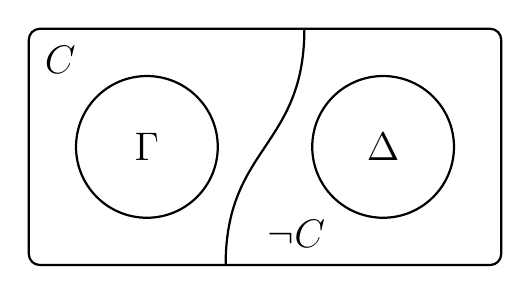
\begin{tikzpicture}[node distance=2cm, auto, thick]
    \draw [rounded corners] (0,0) -- (6,0) -- (6,3) -- (0,3) --  cycle;
    \draw (1.5,1.5) circle (0.9cm);
    \draw (4.5,1.5) circle (0.9cm);
    \path node at (1.5,1.5) {\Large $\Gamma$}; 
    \path node at (4.5,1.5) {\Large $\Delta$}; 
    \path node at (0.4,2.6) {\Large $\formula{C}$};
    \path node at (3.4,0.4) {\Large $\lnot \formula{C}$};
    \draw (2.5,0) .. controls (2.5,1.5) and (3.5,1.5) .. (3.5,3);
  \end{tikzpicture}
  \caption{$!C$ misahake $\Gamma$ lan $\Delta$}
  \ollabel{fig:sep}
\end{figure}


\begin{lem}\ollabel{lem:sep1}
Upamane $\Lang{L}_0$ iku basa kang ngemot saben
!!{constant}, !!{function} lan !!{predicate}
(saliyane $\doteq$) kang katon ing \emph{loro-lorone}
$\Gamma$ lan $\Delta$, lan $\Lang{L}'_0$ kawangun
kanthi nambah tanpa wates akeh !!{constant}s anyar
$\Obj c_n$ kanggo $n \ge 0$. Ing kene anyar tegese ora ana ing Gamma utawa Delta, ora mung ora ana ing basa irisan. Banjur yen
$\Gamma$ lan $\Delta$ ora bisa dipisahake ing
$\Lang{L}_0$, loro-lorone uga ora bisa dipisahake
ing $\Lang{L}'_0$.
\end{lem}

\begin{proof}
Kita nganggo bukti ora langsung: upamane kanggo
kontradiksi $\Gamma$ lan $\Delta$ bisa dipisahake
ing $\Lang{L}'_0$. Banjur $\Gamma \Entails
\Subst{!C}{c}{x}$ lan $\Delta \Entails \lnot
\Subst{!C}{c}{x}$ kanggo sawijining $!C \in
\Lang{L}_0$ (ing kene $c$ iku !!{constant} anyar---
yen ukara pamisah kang digawé saka $!C$
ngemot luwih saka siji
!!{constant} anyar kaya mangkono, carane padha).
Cathetan cakupan SOL6-F027: sadurunge konstanta anyar diganti variabel x kanggo nggawe formula asal, jeneng variabel kaiket ing ukara pamisah diganti yen perlu supaya ora ana kang diarani x. Kanthi iki, penggantian konstanta dening x ora dicekel dening kuantor, lan mung x kang dadi variabel bebas.
Cathetan koreksi sumber OLPL-112:
sing bisa ngemot konstanta anyar iku
ukara pamisah ing basa kang digedhekake,
dudu formula asal ing basa lawas.
Miturut kompaktitas, ana subhimpunan \emph{winates}
$\Gamma_0$ saka $\Gamma$ lan $\Delta_0$ saka
$\Delta$ kang njalari $\Gamma_0 \Entails
\Subst{!C}{c}{x}$ lan $\Delta_0 \Entails
\lnot \Subst{!C}{c}{x}$. Sebut $!G$ konjungsi
kabeh !!{formula}s ing $\Gamma_0$ lan $!H$
konjungsi kabeh !!{formula}s ing $\Delta_0$. Konjungsi saka himpunan kosong dianggep bener.
Banjur
\begin{align*}
  !G & \Entails \Subst{!C}{c}{x}, & !H  \Entails \lnot \Subst{!C}{c}{x}.
\end{align*}
Saka kang kapisan, kanthi Generalisasi, kita oleh
$!G \Entails \lforall[x][!C]$; saka kang kapindho,
kanthi kontraposisi, $\Subst{!C}{c}{x} \Entails
\lnot !H$, mula uga $\lforall[x][!C]
\Entails \lnot !H$. Cathetan koreksi sumber
OLPL-111: simbol delta ing sumber ora ditegesi;
ing langkah iki sing dimaksud yaiku konjungsi
kang diwenehi jeneng H. Kanthi kontraposisi maneh,
iki menehi $!H \Entails \lnot \lforall[x][!C]$.
Miturut monotonisitas,
\begin{align*}
  \Gamma &\Entails \lforall[x][!C], & 
  \Delta & \Entails \lnot \lforall[x][!C],
\end{align*}
mula $\lforall[x][!C]$ misahake $\Gamma$
lan $\Delta$ ing $\Lang{L}_0$.
\end{proof}

\begin{lem}\ollabel{lem:sep2}
Upamane $\Gamma \cup \{ \lexists[x][!S] \}$
lan $\Delta$ ora bisa dipisahake, lan $c$
iku !!{constant} anyar kang ora katon ing
$\Gamma$, $\Delta$, utawa $!S$. Banjur
$\Gamma \cup \{ \lexists[x][!S],
\Subst{!S}{c}{x} \}$ lan $\Delta$ uga
ora bisa dipisahake.
\end{lem}

\begin{proof}
Upamane kanggo kontradiksi $!C$ misahake
$\Gamma \cup \{ \lexists[x][!S],
\Subst{!S}{c}{x}\}$ lan $\Delta$, dene
$\Gamma \cup \{\lexists[x][!S] \}$ lan
$\Delta$ ora bisa dipisahake.
Cathetan koreksi sumber OLPL-113:
argumen eksistensial ing sumber nate
ditulis nganggo kurung kurawal;
ing kene nganggo wangun opsional
kang padha karo panganggone liyane.
Kita bedakake rong kasus:
\begin{enumerate}
\item $c$ ora katon ing $!C$: ing kasus iki,
  $\Gamma \cup \{\lexists[x][!S], \lnot!C \}$
  bisa dipenuhi (yen ora, $!C$ misahake
  $\Gamma \cup \{\lexists[x][!S] \}$ lan
  $\Delta$). Kahanan iki tetep bisa dipenuhi
  yen $\Subst{!S}{c}{x}$ ditambahake, mula
  $!C$ sejatine ora misahake
  $\Gamma \cup \{ \lexists[x][!S],
  \Subst{!S}{c}{x} \}$ lan $\Delta$.
\item $c$ katon ing ukara pamisah $!C$;
  saiki gunakake $!C$ kanggo formula asal
  kang, sawise substitusi, menehi ukara
  $\Subst{!C}{c}{x}$. Cathetan koreksi sumber
  OLPL-114: sumber nggunakake lambang C
  kanggo ukara pamisah lan formula sadurunge
  substitusi; rong panganggone dibedakake
  kanthi cetha ing kene. Kaya ing SOL6-F027, variabel kaiket ing ukara pamisah diganti jenenge luwih dhisik yen perlu, supaya penggantian c dening x ora nyebabake capture. Banjur kita duwe
  \[
  \Gamma \cup \{ \lexists[x][!S], \Subst{!S}{c}{x}\} \Entails \Subst{!C}{c}{x},
  \]
  mula $\Gamma, \lexists[x][!S] \Entails
  \lforall[x][(!S \lif !C)]$ miturut Teorema
  Deduksi lan Generalisasi, lan pungkasane
  $\Gamma \cup \{ \lexists[x][!S] \}
  \Entails \lexists[x][!C]$. Dene
  $\Delta \Entails \lnot \Subst{!C}{c}{x}$
  lan mula miturut Generalisasi
  $\Delta \Entails \lnot \lexists[x][!C]$.
  Mula $\Gamma \cup \{\lexists[x][!S] \}$
  lan $\Delta$ bisa dipisahake,
  sawijining kontradiksi.
\end{enumerate}
\end{proof}

\endgroup
% END OLP-0200
\endgroup


\begingroup
\makeatletter\def\ol@sectioncs{section}\makeatother

% BEGIN OLP-0201 content/model-theory/interpolation/interpolation-proof.tex
\begingroup
\olfileid{mod}{int}{prf}

\olsection{Teorema Interpolasi Craig}

\begin{thm}[Teorema Interpolasi Craig]
\ollabel{thm:interpol}
Ing andharan iki A lan B ukara, miturut cathetan cakupan SOL6-F026.
Yen $\Entails !A \lif !B$, ana !!a{sentence} $!C$ kang
$\Entails !A \lif !C$ lan $\Entails !C \lif !B$, lan saben
!!{constant}, !!{function}, lan !!{predicate} (saliyane $\eq$) ing
$!C$ uga katon ing $!A$ lan~$!B$. !!{sentence} $!C$ iki diarani
\emph{interpolan} kanggo $!A$ lan~$!B$.
\end{thm}

\begin{proof}
Upamane $\Lang{L}_1$ iku basa saka $!A$ lan $\Lang{L}_2$ iku
basa saka $!B$. Tetepna $\Lang{L}_0 = \Lang{L}_1 \cap \Lang{L}_2$.
Kanggo saben $i \in \{0, 1, 2 \}$, wangun $\Lang{L}'_i$ dipikolehi
saka $\Lang{L}_i$ kanthi nambah tanpa wates akehe !!{constant}s anyar
$\Obj c_0, \Obj c_1, \Obj c_2, \dots$.

Yen $!A$ ora duwe model, $\lexists[x][\eq/[x][x]]$ iku
interpolan. Yen $\lnot !B$ ora duwe model (mula $!B$ valid),
$\lexists[x][\eq[x][x]]$ iku interpolan. Mula kita uga bisa
nganggep $!A$ lan $\lnot !B$ loro-lorone duwe model.

Kanggo mbuktekake kontraposisi Teorema Interpolasi,
upamane ora ana interpolan kanggo $!A$ lan $!B$.
Tegese, upamane $\{!A\}$ lan $\{\lnot !B\}$ ora bisa dipisahake
ing $\Lang{L}_0$.

Tujuan kita yaiku nggedhekake pasangan $(\{ !A \}, \{\lnot!B\})$
dadi pasangan kang ora bisa dipisahake lan maksimal
$(\Gamma^*, \Delta^*)$. Upamane $!A_0$,
$!A_1$, $!A_2$, \dots ndhaptar !!{sentence}s saka $\Lang{L}'_1$,
lan $!B_0$, $!B_1$, $!B_2$, \dots ndhaptar !!{sentence}s
saka~$\Lang{L}'_2$. Cathetan koreksi sumber OLPL-115:
dhaptar kudu nyakup basa kang wis ditambahi konstanta anyar,
amarga maksimalitas ing ngisor iki ditegesake ing basa iku.
Kita tegesi rong barisan mundhak saka himpunan
!!{sentence}s $(\Gamma_n, \Delta_n)$ kanggo $n \ge 0$ kaya iki.
Tetepna $\Gamma_0 = \{ !A\}$ lan $\Delta_0 = \{\lnot !B \}$.
Yen $(\Gamma_n, \Delta_n)$ wis ditegesi, tegese
$\Gamma_{n+1}$ lan $\Delta_{n+1}$ mangkene. Saben himpunan ing tahap anyar nggawa kabeh ukara saka tahap sadurunge; yen calon ukara ditolak, sisih iku tetep. Konstanta kanggo saksi dijupuk saka dhaptar konstanta anyar umum kang ditambahake marang rong basa, supaya durung ana ing himpunan winates ing tahap iku:
\begin{enumerate}
\item Yen $\Gamma_n \cup \{!A_n \}$ lan $\Delta_n$ ora bisa dipisahake
  ing $\Lang{L}'_0$, lebokake $!A_n$ menyang $\Gamma_{n+1}$.
  Kajaba iku, yen $!A_n$ iku !!{formula} eksistensial
  $\lexists[x][!S]$, pilih !!{constant} anyar $c$ kang ora katon
  ing $\Gamma_n$, $\Delta_n$, $!A_n$ utawa $!B_n$, lan lebokake
  $\Subst{!S}{c}{x}$ menyang $\Gamma_{n+1}$.
\item Yen $\Gamma_{n+1}$ lan $\Delta_n \cup \{!B_n \}$ ora bisa
  dipisahake ing $\Lang{L}'_0$, lebokake $!B_n$ menyang
  $\Delta_{n+1}$. Kajaba iku, yen $!B_n$ iku !!{formula}
  eksistensial $\lexists[x][!S]$, pilih !!{constant} anyar $c$
  kang ora katon ing $\Gamma_{n+1}$, $\Delta_n$, $!A_n$
  utawa $!B_n$, lan lebokake $\Subst{!S}{c}{x}$ menyang
  $\Delta_{n+1}$.
\end{enumerate}
Pungkasane, tegesi:
\begin{align*}
  \Gamma^* & = \bigcup_{n\ge 0} \Gamma_n, &
  \Delta^* & = \bigcup_{n\ge 0} \Delta_n.
\end{align*}
Kanthi induksi bebarengan marang $n$, saiki kita bisa mbuktekake:
\begin{enumerate}
\item\ollabel{part-a} $\Gamma_n$ lan $\Delta_n$ ora bisa dipisahake
  ing $\Lang{L}'_0$;
\item\ollabel{part-b} $\Gamma_{n+1}$ lan $\Delta_n$ ora bisa
  dipisahake ing $\Lang{L}'_0$.
\end{enumerate}
Dhasar kanggo \olref{part-a} diwenehake dening
\olref[sep]{lem:sep1}. Kanggo \olref{part-b}, kita kudu
mbedakake telung kasus:
\begin{enumerate}
\item Yen $\Gamma_0 \cup \{!A_0 \}$ lan $\Delta_0$ bisa dipisahake,
  mula $\Gamma_1 = \Gamma_0$ lan \olref{part-b} padha karo
  \olref{part-a};
\item Yen $\Gamma_1 = \Gamma_0 \cup\{ !A_0\}$, mula $\Gamma_1$
  lan $\Delta_0$ ora bisa dipisahake miturut konstruksi.
\item Isih ana kasus nalika $!A_0$ eksistensial, saengga
  $\Gamma_1 = \Gamma_0 \cup \{ \lexists[x][!S], \Subst{!S}{c}{x}
  \}$. Miturut konstruksi, $\Gamma_0 \cup \{ \lexists[x][!S]\}$
  lan $\Delta_0$ ora bisa dipisahake; mula miturut
  \olref[sep]{lem:sep2}, $\Gamma_0 \cup \{ \lexists[x][!S],
  \Subst{!S}{c}{x} \}$ lan $\Delta_0$ uga ora bisa dipisahake.
\end{enumerate}
Iki ngrampungake dhasar induksi kanggo \olref{part-a} lan
\olref{part-b} ing ndhuwur. Saiki menyang langkah induksi.
Kanggo \olref{part-a}, yen $\Delta_{n+1} = \Delta_n \cup
\{ !B_n \}$, mula $\Gamma_{n+1}$ lan $\Delta_{n+1}$ ora bisa
dipisahake miturut konstruksi (sanajan $!B_n$ eksistensial,
miturut \olref[sep]{lem:sep2}); yen $\Delta_{n+1} = \Delta_n$
(amarga $\Gamma_{n+1}$ lan $\Delta_n \cup \{!B_n\}$ bisa
dipisahake), kita gunakake hipotesis induksi \olref{part-b}.
Kanggo langkah induksi \olref{part-b}, yen
$\Gamma_{n+2} = \Gamma_{n+1} \cup \{!A_{n+1} \}$, mula
$\Gamma_{n+2}$ lan $\Delta_{n+1}$ ora bisa dipisahake
miturut konstruksi (sanajan $!A_{n+1}$ eksistensial,
miturut \olref[sep]{lem:sep2}); yen
$\Gamma_{n+2} = \Gamma_{n+1}$, kita gunakake kasus induksi
kanggo \olref{part-a} kang lagi dibuktekake. Iki ngrampungake
induksi kanggo \olref{part-a} lan \olref{part-b}.

Mula $\Gamma^*$ lan $\Delta^*$ ora bisa dipisahake; yen bisa,
miturut kompaktitas ana indeks $n \ge 0$ lan ukara pamisah kang misahake
$\Gamma_n$ lan $\Delta_n$, nalisir \olref{part-a}.
Mligine, $\Gamma^*$ lan $\Delta^*$ konsisten:
yen sing kapisan utawa kapindho ora konsisten,
loro-lorone bisa dipisahake dening
$\lexists[x][\eq/[x][x]]$ utawa
$\lforall[x][\eq[x][x]]$, manut kasusé.

Saiki kita tuduhake yen $\Gamma^*$ konsisten maksimal ing
$\Lang{L}'_1$, lan semono uga $\Delta^*$ ing $\Lang{L}'_2$.
Kanggo sing kapisan, upamane $!A_n \notin \Gamma^*$ lan
$\lnot !A_n \notin \Gamma^*$ kanggo sawenehing $n \ge 0$.
Yen $!A_n \notin \Gamma^*$, mula $\Gamma_n \cup \{!A_n \}$
bisa dipisahake saka $\Delta_n$, dadi ana $!C \in
\Lang{L}'_0$ saengga loro pratelan iki bener:
\begin{align*}
  \Gamma^* & \Entails !A_n \lif !C, &
  \Delta^* & \Entails \lnot !C.
\end{align*}
Semono uga, yen $\lnot !A_n \notin \Gamma^*$, ana $!C' \in
\Lang{L}'_0$ saengga loro pratelan iki bener:
\begin{align*}
  \Gamma^* & \Entails \lnot !A_n \lif !C', &
  \Delta^* & \Entails \lnot !C'.
\end{align*}
Miturut logika proposisional, $\Gamma^* \Entails !C \lor !C'$
lan $\Delta^* \Entails \lnot (!C \lor !C')$, mula $!C \lor
!C'$ misahake $\Gamma^*$ lan $\Delta^*$. Argumen kang padha
nuduhake yen $\Delta^*$ maksimal.

Pungkasan, kita tuduhake yen $\Gamma^* \cap \Delta^*$
konsisten maksimal ing $\Lang{L}'_0$. Cetha yen konsisten,
amarga minangka irisan rong himpunan konsisten.
Kanggo nuduhake maksimalitas, pilih $!S \in \Lang{L}'_0$.
Saiki, $\Gamma^*$ maksimal ing $\Lang{L'_1}
\supseteq \Lang{L'_0}$, lan semono uga $\Delta^*$
maksimal ing $\Lang{L'_2} \supseteq \Lang{L'_0}$.
Mula $!S \in \Gamma^*$ utawa $\lnot !S \in \Gamma^*$,
lan $!S \in \Delta^*$ utawa $\lnot !S \in \Delta^*$.
Yen $!S \in \Gamma^*$ lan $\lnot !S \in \Delta^*$,
$!S$ bakal misahake $\Gamma^*$ lan $\Delta^*$;
yen $\lnot !S \in \Gamma^*$ lan $!S \in \Delta^*$,
$\Gamma^*$ lan $\Delta^*$ bakal dipisahake
dening $\lnot !S$.
Mula $!S \in \Gamma^* \cap \Delta^*$ utawa
$\lnot !S \in \Gamma^* \cap \Delta^*$,
lan $\Gamma^* \cap \Delta^*$ maksimal.

Cathetan pangganep bukti SOL6-F028: maksimalitas wae durung njamin model kang kabeh unsure dijenengi konstanta. Konstruksi iki uga menehi saksi kanggo saben ukara eksistensial kang ana ing himpunan lintang. Yen ukara kasebut ditolak nalika giliran enumerasine, separator ing tahap iku bakal tetep misahake himpunan pungkasan, nalisir inseparability. Mula ukara kasebut ditampa lan diwenehi saksi. Kanggo saben term tertutup t, ukara eksistensial x padha karo t nduweni saksi saka konstanta anyar umum, dadi saben unsur model term bisa dijenengi konstanta saka reservoir kang padha ing rong basa.
Amarga $\Gamma^*$ konsisten maksimal lan nduweni sipat saksi iki, himpunan iki nduweni
model $\Struct{M}'_1$ kang !!{domain} $\Domain{M'_1}$
dumadi saka, lan mung saka, unsur-unsur $\Assign{c}{M'_1}$
kang dadi interpretasi !!{constant}s---kaya ing bukti
teorema kelengkapan
(\olref[fol][com][cth]{thm:completeness}).
Semono uga, $\Delta^*$ nduweni model $\Struct{M}'_2$
kang !!{domain} $\Domain{M'_2}$ diwenehi dening
interpretasi $\Assign{c}{M'_2}$ saka !!{constant}s.

Wangun $\Struct{M_1}$ saka $\Struct{M'_1}$ kanthi
ngilangi interpretasi !!{constant}s, !!{function}s,
lan !!{predicate}s ing $\Lang{L'_1} \setminus
\Lang{L'_0}$; tumrap $\Struct{M_2}$ uga mangkono.
Pemetaan $h \colon M_1 \to M_2$ kang ditegesi dening
$h(\Assign{c}{M'_1}) = \Assign{c}{M'_2}$ iku
isomorfisme ing $\Lang{L}'_0$, amarga
$\Gamma^* \cap \Delta^*$ konsisten maksimal ing
$\Lang{L}'_0$, kaya kang wis dituduhake.
Sebabé, saben $\Lang{L}'_0$-!!{sentence}
kalebu ing $\Gamma^*$ lan $\Delta^*$ loro-lorone,
utawa ora kalebu ing loro-lorone. Mula
$\Assign{c}{M'_1} \in \Assign{P}{M'_1}$ yen lan
mung yen $\Atom{P}{c} \in \Gamma^*$, yen lan mung yen
$\Atom{P}{c} \in \Delta^*$, yen lan mung yen
$\Assign{c}{M'_2} \in \Assign{P}{M'_2}$.
Syarat isomorfisme liyane bisa dibuktekake kanthi cara padha. Ing kene c tansah dijupuk saka konstanta anyar umum. Ukara kesamaan antarane rong konstanta umum padha ing rong himpunan lintang; mula pemetaan iki ora gumantung marang pilihan jeneng lan injektif. Saben unsur model kapindho uga duwe jeneng umum, mula pemetaan iki surjektif.

Saiki tegesi model $\Struct{M}$ kanggo !!{language}
$\Lang{L}'_1 \cup \Lang{L}'_2$ kaya mangkene:
Cathetan koreksi sumber OLPL-117:
basa gabungan iki kudu ngemot konstanta anyar,
supaya pratelan pungkasan ngenani
gabungan rong himpunan lintang bisa ditegesi.
\begin{enumerate}
\item !!{domain} $\Domain{M}$ yaiku $\Domain{M_2}$,
  tegese himpunan kabeh unsur $\Assign{c}{M'_2}$;
\item Yen !!a{predicate}~$P$ ana ing $\Lang{L_2} \setminus
  \Lang{L_1}$, mula $\Assign{P}{M} = \Assign{P}{M'_2}$;
\item Yen predikat $P$ ana ing $\Lang{L}_1\setminus \Lang{L}_2$,
  mula $\Assign{P}{M} = h(\Assign{P}{M'_1})$.
  Cathetan koreksi sumber OLPL-116:
  predikat iki mung ana ing basa kapisan, dadi relasine
  dijupuk saka model kapisan banjur ditranspor nganggo h.
  Tegese, $\tuple{\Assign{c_1}{M'_2}, \dots,
  \Assign{c_n}{M'_2}} \in \Assign{P}{M}$ yen lan mung yen
  $\tuple{\Assign{c_1}{M'_1}, \dots,
  \Assign{c_n}{M'_1}} \in \Assign{P}{M'_1}$.
\item Yen !!a{predicate} $P$ ana ing $\Lang{L}_0$,
  mula $\Assign{P}{M} = \Assign{P}{M'_2} =
  h(\Assign{P}{M'_1})$.
\item !!^{function}s saka $\Lang{L}_1 \cup \Lang{L}_2$,
  kalebu !!{constant}s, ditangani kanthi cara padha. Konstanta anyar umum diwenehi interpretasi saka model kapindho, kang padha karo transport interpretasi model kapisan liwat h.
\end{enumerate}

Pungkasan, induksi marang !!{formula}s nuduhake yen
$\Struct{M}$ cocog karo $\Struct{M'_1}$ kanggo kabeh
!!{formula}s saka $\Lang{L'_1}$ liwat isomorfisme h,
lan cocog karo $\Struct{M'_2}$ kanggo kabeh
!!{formula}s saka $\Lang{L'_2}$.
Cathetan koreksi sumber OLPL-118:
amarga ranah model kapisan lan model gabungan beda,
kecocokan tumrap pangaji variabel kudu liwat h.
Mligine, $\Struct{M} \Entails \Gamma^* \cup \Delta^*$,
mula $\Struct{M} \Entails !A$ lan
$\Struct{M} \Entails \lnot!B$, saengga
$\not\Entails !A \lif !B$. Iki ngrampungake bukti
Teorema Interpolasi Craig.
\end{proof}

\endgroup
% END OLP-0201
\endgroup


\begingroup
\makeatletter\def\ol@sectioncs{section}\makeatother

% BEGIN OLP-0202 content/model-theory/interpolation/definability.tex
\begingroup
\olfileid{mod}{int}{def}

\olsection{Teorema Definabilitas}

Salah siji panganggone teorema interpolasi kang wigati yaiku
teorema definabilitas Beth. Kanggo netepake relasi
$n$-papan~$R$, kita bisa menehi !!a{formula}~$!C$
kanthi !!{variable}s bebas kang mung saka $n$ posisi relasi lan ora ngemot~$R$. Sawetara posisi kasebut bisa ora katon minangka variabel bebas, kayata kanggo relasi kosong utawa universal.
Iki dadi definisi \emph{eksplisit} kanggo~$R$ adhedhasar~$!C$.
Kita uga bisa kandha yen sawijining teori~$\Sigma(P)$
ing !!{language} kang ngemot !!{predicate}
$n$-papan~$P$ netepake~$P$ kanthi eksplisit yen teori iku
ngemot (utawa paling ora nduweni akibat) definisi
eksplisit kang diformalkan, yaiku
\[
\Sigma(P) \Entails \lforall[x_1][\dots
  \lforall[x_n][(\Atom{P}{x_1,\dots, x_n} \liff !C(x_1, \dots,
    x_n))]].
\]
Nanging definisi eksplisit mung siji cara kanggo
netepake relasi kanthi tuntas. Sawijining teori
uga bisa nemtokake interpretasi~$P$ kanthi tuntas
lumantar interpretasi bagean !!{language} liyane
ing saben model. Teorema definabilitas nyatakake:
saben teori kang nemtokake interpretasi~$P$
kanthi cara iki---yaiku \emph{netepake~$P$ kanthi implisit}---
uga netepake kanthi eksplisit.

\begin{defn}
Upamane $\Lang{L}$ iku !!a{language} kang ora ngemot
!!{predicate}~$P$. Himpunan $\Sigma(P)$ saka
!!{sentence}s ing $\Lang{L} \cup \{P\}$
\emph{netepake~$P$ kanthi eksplisit} yen lan mung yen
ana !!a{formula}~$!C(x_1, \dots, x_n)$ ing $\Lang{L}$
saengga
\[
\Sigma(P) \Entails \lforall[x_1][\dots
  \lforall[x_n][(\Atom{P}{x_1,\dots, x_n} \liff !C(x_1, \dots,
    x_n))]].
\]
\end{defn}

\begin{defn}
Upamane $\Lang{L}$ iku !!a{language} kang ora ngemot
!!{predicate}s~$P$ lan~$P'$. Himpunan $\Sigma(P)$
saka !!{sentence}s ing $\Lang{L} \cup \{P\}$
\emph{netepake $P$ kanthi implisit} yen lan mung yen
\[
\Sigma(P) \cup \Sigma(P') \Entails \lforall[x_1][\dots
  \lforall[x_n][(\Atom{P}{x_1,\dots, x_n} \liff \Atom{P'}{x_1,\dots,
      x_n})]],
\]
ing ngendi $\Sigma(P')$ dipikolehi saka panggantos
seragam $P$ dadi $P'$ ing $\Sigma(P)$.
\end{defn}

Tegese, kanggo saben model $\Struct{M}$ lan $R, R' \subseteq
\Domain{M}^n$, yen $\Expan{M}{R} \Entails \Sigma(P)$ lan
$\Expan{M}{R'} \Entails \Sigma(P')$, mula $R=R'$.
Ing kene $\Expan{M}{R}$ iku !!{structure}~$\Struct{M'}$
kanggo ekspansi saka $\Lang{L}$ menyang
$\Lang{L} \cup \{P\}$ kang nduweni
$\Assign{P}{M'} = R$; semono uga kanggo
$\Expan{M}{R'}$ kanthi lambang predikat kang wis diganti.

\begin{thm}[Teorema Definabilitas Beth]
Himpunan $\Sigma(P)$ saka !!{sentence}s ing $\Lang{L}
  \cup\{P\}$ netepake $P$ kanthi implisit yen lan mung yen
  $\Sigma(P)$ netepake $P$ kanthi eksplisit.
Cathetan koreksi sumber OLPL-120:
teorema iki nganggo himpunan ukara kaya rong
definisi sadurunge, dudu himpunan formula bebas.
\end{thm}

\begin{proof}
Yen $\Sigma(P)$ netepake $P$ kanthi eksplisit, mula
loro pratelan iki bener:
\begin{align*}
  \Sigma(P) & \Entails & \lforall[x_1][\dots \lforall[x_n]
    [(\Atom{P}{x_1,\dots, x_n} \liff !C(x_1,\dots,x_n))]]\\
  \Sigma(P') & \Entails & \lforall[x_1][\dots \lforall[x_n]
    [(\Atom{P'}{x_1,\dots, x_n} \liff !C(x_1,\dots,x_n))]]
\end{align*}
lan kesimpulane banjur langsung tumut.
Kanggo arah kosok baline, upamane $\Sigma(P)$
netepake $P$ kanthi implisit. Dhisik kita tambah
!!{constant}s $c_1$, \dots,~$c_n$ menyang $\Lang{L}$. Konstanta iki kabeh anyar lan beda-beda, ora ana ing basa asli utawa teori.
Banjur
\[
\Sigma(P) \cup \Sigma(P') \Entails
\Atom{P}{c_1, \dots, c_n} \to  \Atom{P'}{c_1, \dots, c_n}.
\]
Miturut kompaktitas, ana himpunan winates
$\Delta_0 \subseteq \Sigma(P)$ lan
$\Delta_1 \subseteq \Sigma(P')$ saengga
\[
\Delta_0 \cup \Delta_1 \Entails
\Atom{P}{c_1, \dots, c_n} \to \Atom{P'}{c_1, \dots, c_n}.
\]
Sebut $!D(P)$ konjungsi kabeh !!{sentence}s $!A(P)$
kang $!A(P) \in \Delta_0$ utawa $!A(P') \in \Delta_1$;
sebut $!D(P')$ konjungsi kabeh !!{sentence}s $!A(P')$
kang $!A(P) \in \Delta_0$ utawa $!A(P') \in \Delta_1$.
Banjur $!D(P) \land !D(P') \Entails
\Atom{P}{c_1, \dots, c_n} \to \Atom{P'}{c_1,\dots,c_n}$.
Cathetan koreksi sumber OLPL-119:
predikat ing sisih tengen ditulis nganggo wangun atomik
kang padha karo premis lan rumus sabanjure.
Kita bisa nata maneh supaya !!{predicate} kang arep dipisahake, yaiku P lan P-prime, katon ing sisih dhewe-dhewe saka $\Entails$. Predikat saka basa dhasar isih bisa ana ing rong sisih:
\[
!D(P) \land \Atom{P}{c_1, \dots, c_n} \Entails
!D(P') \to \Atom{P'}{c_1, \dots, c_n}.
\]
Miturut Teorema Interpolasi Craig, ana !!a{sentence}
$!C(c_1,\dots, c_n)$ kang ora ngemot $P$ utawa $P'$
saengga:
\begin{align*}
  !D(P) \land \Atom{P}{c_1, \dots, c_n} & \Entails !C(c_1,\dots, c_n); \\
  !C(c_1,\dots, c_n) & \Entails !D(P') \to \Atom{P'}{c_1, \dots, c_n}.
\end{align*}
Saka akibat kang kapisan, kita oleh $!D(P) \Entails
\Atom{P}{c_1,\dots, c_n} \lif !C(c_1,\dots, c_n)$.
Saka akibat kang kapindho, amarga model
$\Lang{L} \cup \{P\}$ yaiku $\Expan{M}{R}
\Entails !A(P)$ yen lan mung yen model
$\Lang{L} \cup \{P'\}$ kang cocog,
$\Expan{M}{R} \models !A(P')$, kita oleh
$!C(c_1,\dots, c_n) \Entails !D(P) \lif
\Atom{P}{c_1,\dots, c_n}$, mula:
\[
!D(P) \Entails !C(c_1,\dots,c_n) \to \Atom{P}{c_1,\dots, c_n}.
\]
Yen loro asil iki digandhengake,
$!D(P) \Entails \Atom{P}{c_1,\dots, c_n}
\liff !C(c_1, \dots, c_n)$; miturut monotonisitas
lan generalisasi, kita uga oleh. Sadurunge konstanta anyar diganti variabel kanggo generalisasi, variabel kaiket ing interpolan diganti jenenge yen perlu supaya ora nyekel variabel anyar kasebut. Formula definisi kang diasilake mung nduweni variabel bebas saka posisi relasi kang kasebut:
\[
\Sigma(P) \Entails
\lforall[x_1][\dots\lforall[x_n][(\Atom{P}{x_1,\dots, x_n} \liff
    !C(x_1,\dots, x_n))]].
\]
\end{proof}

\endgroup
% END OLP-0202
\endgroup


\OLEndChapterHook

\endgroup
% END OLP-0198
\endgroup


\begingroup
\makeatletter\def\ol@sectioncs{section}\makeatother

% BEGIN OLP-0203 content/model-theory/lindstrom/lindstrom.tex
\begingroup
\olchapter{mod}{lin}{Teorema Lindstr\"om}

\begingroup
\makeatletter\def\ol@sectioncs{section}\makeatother

% BEGIN OLP-0204 content/model-theory/lindstrom/introduction.tex
\begingroup
\olfileid{mod}{lin}{int}
\section{Pambuka}

Ing bab iki kita arep mbuktekake karakterisasi Lindstr\"om
tumrap logika tataran kapisan: kanthi sawatara syarat tambahan,
iki logika maksimal kang Teorema Kompaktitas lan Teorema
L\"owenheim--Skolem Mudhun tetep lumaku
(\olref[fol][com][com]{thm:compactness} lan
\olref[fol][com][dls]{thm:downward-ls}). Kaping pisan, kita
perlu menehi karakterisasi kang luwih umum tumrap kelas
logika kang dadi cakupan teorema iki. Kita bakal mbatesi
panliten iki marang basa \emph{relasional}, yaiku basa kang
mung ngemot !!{predicate}s lan konstanta individu, tanpa
!!{function}s.

\endgroup
% END OLP-0204
\endgroup


\begingroup
\makeatletter\def\ol@sectioncs{section}\makeatother

% BEGIN OLP-0205 content/model-theory/lindstrom/abstract-logics.tex
\begingroup
\olfileid{mod}{lin}{alg}
\olsection{Logika Abstrak}

\begin{defn}
Sawijining \emph{logika abstrak} yaiku pasangan $\tuple{L, \models_L}$,
kanthi $L$ iku fungsi kang masangake marang saben !!{language}~$\Lang{L}$
sawijining himpunan $L(\Lang{L})$ saka !!{sentence}s, lan $\models_L$
iku relasi antarane !!{structure}s kanggo !!{language}~$\Lang{L}$
lan !!{element}s saka $L(\Lang{L})$. Mligine, $\tuple{F, \models}$
iku logika tataran kapisan lumrah, yaiku $F$ fungsi kang masangake marang
!!{language}~$\Lang{L}$ himpunan !!{sentence}s tataran kapisan kang
kawangun saka simbol predikat lan konstanta ing $\Lang{L}$, lan $\models$ iku relasi
nyukupi ing logika tataran kapisan. Cathetan koreksi sumber SOL6-F029: konstanta wae ora cukup kanggo mbangun kabeh ukara; predikat saka basa kasebut uga digunakake.
\end{defn}

Gatekna yen kita isih nggunakake pangerten !!{structure} kang padha
kanggo !!{language} tartamtu kaya ing logika tataran kapisan, nanging kita
ora nganggep yen !!{sentence}s kawangun saka simbol-simbol dhasar ing
$\Lang{L}$ kanthi cara lumrah, utawa yen relasi $\models_L$
ditetepake kanthi rekursif kaya ing logika tataran kapisan. Mula, umpamane,
definisi kang sipate umum iki uga nyakup !!{sentence}s ing
$\tuple{L,\models_L}$ kang ngemot konjungsi utawa disjungsi tanpa wates
dawane, kuantor saliyane $\lexists$ lan $\lforall$ (umpamane,
“ana tanpa wates akehe~$x$ saengga \dots”), utawa mbokmenawa
runtutan kuantor tanpa wates dawane. Kanggo negesake yen
“!!{sentence}s” ing $L(\Lang{L})$ ora kudu awujud !!{sentence}s
lumrah ing logika tataran kapisan, ing bab iki kita nggunakake
!!{variable}s $!E$, $!F$,~\dots kanggo nglambangake ukara-ukara iku,
lan nyisihake $!A$, $!B$,~\dots kanggo !!{formula}s lumrah ing
logika tataran kapisan.

\begin{defn}
Upamana $\Mod(L){!E}$ nglambangake kelas
$\Setabs{\Struct{M}}{\Struct{M} \models_L !E}$. Yen !!{language}
kudu dicethakake, kita nulis $\Mod[L](L){!E}$. Rong !!{structure}s
$\Struct{M}$ lan $\Struct{N}$ kanggo $\Lang{L}$ iku
\emph{ekuivalen elementer ing} $\tuple{L, \models_L}$, ditulis
$\Struct{M} \elemequiv[L] \Struct{N}$, yen !!{sentence}s kang
padha saka $L(\Lang{L})$ bener ing kalorone.
\end{defn}

\begin{defn}
Sawijining logika abstrak $\tuple{L,\models_L}$ kanggo
!!{language} $\Lang{L}$ diarani \emph{normal} yen nyukupi
sipat-sipat ing ngisor iki:
\begin{enumerate}
\item (\emph{Monotonisitas-$L$}) Kanggo !!{language}s $\Lang{L}$
  lan $\Lang{L'}$, yen $\Lang{L} \subseteq \Lang{L'}$, mula
  $L(\Lang{L}) \subseteq L(\Lang{L'})$.
\item (\emph{Sipat Ekspansi}) Kanggo saben $!E \in L(\Lang{L})$
  ana subhimpunan \emph{winates} $\Lang{L'}$ saka $\Lang{L}$
  saengga relasi $\Struct{M} \models_L !E$ mung gumantung marang
  redukt $\Struct{M}$ menyang $\Lang{L'}$; yaiku, yen
  $\Struct{M}$ lan $\Struct{N}$ nduweni redukt kang padha menyang
  $\Lang{L'}$, mula $\Struct{M} \models_L !E$ yen lan mung yen
  $\Struct{N} \models_L !E$.
\item (\emph{Sipat Isomorfisme}) Yen $\Struct{M} \models_L !E$
  lan $\Struct{M} \simeq \Struct{N}$, mula $\Struct{N} \models_L
  !E$ uga.
\item (\emph{Sipat Pangowahan Jeneng}) Relasi $\models_L$ tetep
  lumaku nalika simbol-simbol diganti jenenge: yen !!{language}
  $\Lang{L}'$ dipikolehi saka $\Lang{L}$ kanthi ngganti saben
  simbol $P$ nganggo simbol $P'$ kang aritase padha lan saben
  konstanta $c$ nganggo konstanta $c'$ kang beda, mula kanggo
  saben !!{structure}~$\Struct{M}$ lan !!{sentence}~$!E$,
  $\Struct{M} \models_L !E$ yen lan mung yen
  $\Struct{M}' \models_L !E'$, kanthi $\Struct{M}'$ iku
  !!{structure} kanggo $\Lang{L}'$ kang cocog karo
  $\Lang{L}$ lan $!E' \in L(\Lang{L}')$.
\item (\emph{Sipat Boolean}) Logika abstrak $\tuple{L,
  \models_L}$ katutup tumrap konektif Boolean ing teges iki:
  kanggo saben $!E \in L(\Lang{L})$ ana $!F \in
  L(\Lang{L})$ saengga $\Struct{M} \models_L !F$ yen lan mung
  yen $\Struct{M} \not\models_L !E$, lan kanggo saben $!E$
  lan $!F$ ana $!G$ saengga $\Mod(L){!G} = \Mod(L){!E}
  \cap \Mod(L){!F}$. Semono uga kanggo !!{formula}s atomik
  lan konektif liyane.
\item (\emph{Sipat Kuantor}) Kanggo saben konstanta $c$ ing
  $\Lang{L}$ lan $!E \in L(\Lang{L})$, ana $!F \in
  L(\Lang{L'})$ saengga
  \[
  \Mod[L'](L){!F} = \Setabs{\Struct{M}}{\Expan{M}{a} \in
  \Mod[L](L){!E} \text{ kanggo sawatara } a \in \Domain{M}},
  \]
  kanthi $\Lang{L'} = \Lang{L} \setminus \{c\}$ lan
  $\Expan{M}{a}$ iku ekspansi $\Struct{M}$ menyang $\Lang{L}$
  kang masangake $a$ marang~$c$. Cathetan koreksi sumber OLPL-755: ukara asil pambusakan konstanta kudu ana ing basa kang wis tanpa konstanta iku; pratelan mung kalebu himpunan ukara basa asal durung cukup.
\item (\emph{Sipat Relativisasi}) Yen diwenehi !!a{sentence}
  $!E \in L(\Lang{L})$ lan simbol-simbol $R$, $c_1$, \dots,
  $c_n$ kang ora ana ing $\Lang{L}$, ana !!a{sentence}
  $!F \in L(\Lang{L} \cup \{R,c_1,\ldots,c_n\})$
  kang diarani \emph{relativisasi} $!E$ marang
  $\Atom{R}{x, c_1, \dots c_n}$, saengga kanggo saben
  !!{structure}~$\Struct{M}$:
  \[
  \Expan{M}{X, b_1, \ldots, b_n} \models_L !F \text{ yen lan
    mung yen } \Struct{N} \models_L !E,
  \]
  kanthi $\Struct{N}$ iku substruktur saka $\Struct{M}$ kanthi
  !!{domain} $\Domain{N} = \Setabs{a\in \Domain{M}}{(a,
  b_1, \dots, b_n) \in X}$ (waca
  \olref[bas][sub]{rem:substructure}), lan
  $\Expan{M}{X, b_1, \ldots, b_n}$ iku ekspansi $\Struct{M}$
  kang napsirake $R$, $c_1$, \dots, $c_n$ kanthi $X$, $b_1,$
  \dots, $b_n$, miturut urutane (kanthi $X \subseteq M^{n+1}$). Cathetan koreksi sumber OLPL-756: tafsir predikat anyar dijupuk saka ekspansi, dudu struktur asal kang durung nduweni predikat iku. Himpunan unsur kang dipilih kudu ora kosong lan mbentuk substruktur basa asal; yen ana konstanta, tafsire kudu kalebu ing himpunan iki.
\end{enumerate}
\end{defn}

\begin{defn}
Yen diwenehi rong logika abstrak $\tuple{L_1, \models_{L_1}}$
lan $\tuple{L_2, \models_{L_2}}$, kita kandha yen logika kapindho
\emph{paling ora sakuwate kang kapisan anggone nyatakake},
ditulis $\tuple{L_1, \models_{L_1}} \leq
\tuple{L_2, \models_{L_2}}$, yen kanggo saben !!{language}
$\Lang{L}$ lan !!{sentence} $!E \in L_1(\Lang{L})$ ana
!!a{sentence} $!F \in L_2(\Lang{L})$ saengga
$\Mod[L](L_1){!E} = \Mod[L](L_2){!F}$. Logika
$\tuple{L_1, \models_{L_1}}$ lan
$\tuple{L_2, \models_{L_2}}$ iku \emph{ekuivalen} yen
$\tuple{L_1, \models_{L_1}} \leq \tuple{L_2,
  \models_{L_2}}$ lan $\tuple{L_2, \models_{L_2}} \leq
\tuple{L_1, \models_{L_1}}$.
\end{defn}

\begin{rem}
  Logika tataran kapisan, yaiku logika abstrak $\tuple{F, \models}$,
  iku normal. Satemene, sipat-sipat ing ndhuwur umume langsung
  lumaku kanggo logika tataran kapisan. Kita mung ngelingake yen
  sipat ekspansi mujudake ekstensionalitas, lan relativisasi
  !!a{sentence} $!E$ marang $\Atom{R}{x, c_1, \dots, c_n}$
  dipikolehi kanthi ngganti saben !!{subformula}
  $\lforall[x][!F]$ dadi
  $\lforall[x][(\Atom{R}{x, c_1, \dots, c_n} \lif \ !F)]$. Cathetan pangganep SOL6-F030: aturan kang mung nyebut kuantor universal iki ditrapake sawise kuantor eksistensial ditulis nganggo negasi lan kuantor universal. Yen kuantor eksistensial ditinggal minangka primitif, kuantor kasebut uga kudu diwatesi marang ranah pilihan. Variabel kaiket diganti jenenge yen perlu supaya parameter anyar ora dicekel.
  Kajaba iku, yen $\tuple{L, \models_L}$ normal, mula
  $\tuple{F, \models} \leq \tuple{L, \models_{L}}$,
  kaya kang bisa dibuktekake kanthi induksi miturut
  !!{formula}s tataran kapisan. Mula, tanpa ngilangake kalumrahan,
  kita bisa nganggep yen saben !!{sentence} tataran kapisan
  bisa diwakili dening ukara kang ekuivalen ing saben logika normal; iki dudu pratelan yen sintaksis ukara asli mesti dadi anggota harfiah. Cathetan watesan: sipat ekspansi kang dicithak mung njamin gumantung semantik marang basa winates. Supaya bukti Lindstrom sabanjure bisa ngurangi basa, isih dibutuhake syarat representasi ukara ing basa winates, kaya kang kasebut ing OLPL-757.
\end{rem}

\endgroup
% END OLP-0205
\endgroup


\begingroup
\makeatletter\def\ol@sectioncs{section}\makeatother

% BEGIN OLP-0206 content/model-theory/lindstrom/ls-property.tex
\begingroup
\olfileid{mod}{lin}{lsp}

\olsection{Sipat Kompaktitas lan L\"owenheim--Skolem}

Saiki kita menehi generalisasi kang cetha saka kompaktitas lan
L\"owenheim--Skolem kanggo logika abstrak.

\begin{defn}
Sawijining logika abstrak $\tuple{L, \models_L}$ nduweni
\emph{Sipat Kompaktitas} yen saben himpunan $\Gamma$ saka
!!{sentence}s ing $L(\Lang{L})$ bisa dicukupi nalika saben
$\Gamma_0 \subseteq \Gamma$ kang winates bisa dicukupi.
\end{defn}

\begin{defn}
$\tuple{L, \models_L}$ nduweni \emph{Sipat L\"owenheim--Skolem
  Mudhun} yen saben $\Gamma$ kang bisa dicukupi nduweni model
kang !!a{enumerable}.
\end{defn}


Pangerten isomorfisme parsial saka
\olref[bas][pis]{defn:partialisom} sipate murni “aljabar” (yaiku,
diwenehake tanpa ngrujuk marang !!{sentence}s saka basa, nanging
marang simbol predikat lan konstanta kang diwenehake dening
!!{language}~$\Lang{L}$ saka !!{structure}s), mula pangerten iku
uga lumaku kanggo logika abstrak. Ing logika tataran kapisan, saka
\olref[bas][pis]{thm:p-isom2} kita ngerti yen rong !!{structure}s
kang isomorfis parsial iku ekuivalen elementer. Bukti kasebut ora
bisa langsung ditrapake marang logika abstrak, amarga induksi
miturut !!{formula}s bisa uga ora kasedhiya kanggo sembarang
$!E \in L(\Lang{L})$; nanging teorema kasebut isih bener yen
Sipat L\"owenheim--Skolem lumaku.

\begin{thm}
\ollabel{thm:abstract-p-isom}
Upamana $\tuple{L, \models_L}$ iku logika normal kang nduweni
Sipat L\"owenheim--Skolem. Banjur sembarang rong !!{structure}s
kang isomorfis parsial iku ekuivalen elementer ing
$\tuple{L, \models_L}$.
\end{thm}

\begin{proof}
Upamana $\Struct{M} \simeq_p \Struct{N}$, nanging kanggo sawijining
$!E$ uga $\Struct{M} \models_L !E$ dene $\Struct{N}
\not\models_L !E$. Miturut Sipat Isomorfisme kita bisa nganggep
yen $\Domain{M}$ lan $\Domain{N}$ padha pisah, lan miturut Sipat
Ekspansi kita bisa nganggep yen $!E \in L(\Lang{L})$ kanggo
!!{language}~$\Lang{L}$ kang winates. Cathetan koreksi sumber OLPL-757: Sipat Ekspansi mung njamin yen kabeneran ukara gumantung marang redukt basa winates; iki durung njamin ukara asli iku dadi ukara ing basa kang luwih cilik. Upamana $\mathcal{I}$
himpunan isomorfisme parsial antarane $\Struct{M}$ lan
$\Struct{N}$; tanpa nyuda umume pratelan, kita uga nganggep yen
$p \in \mathcal{I}$ lan $q \subseteq p$ mula $q \in \mathcal{I}$, kanthi syarat q tetep ngemot lan njaga tafsir kabeh konstanta basa asal. Cathetan cakupan SOL6-F032: yen ana konstanta, ora saben restriksi sembarang isih dadi isomorfisme parsial miturut definisi kang digunakake; ranah restriksi kudu tetep ngemot tafsir konstanta kasebut.

$\Domain{M}^{<\omega}$ iku himpunan runtutan winates saka
!!{element}s ing~$\Domain{M}$. Upamana $S$ relasi telung panggonan
ing $\Domain{M}^{<\omega}$ kang nglambangake panyambungan runtutan,
yaiku, yen $\mathbf{a}, \mathbf{b}, \mathbf{c} \in
\Domain{M}^{<\omega}$, mula $S(\mathbf{a}, \mathbf{b},
\mathbf{c})$ lumaku yen lan mung yen $\mathbf{c}$ iku
sambungane $\mathbf{a}$ lan $\mathbf{b}$; lan upamana $T$
relasi telung panggonan saengga $T(\mathbf{a}, b, \mathbf{c})$
lumaku kanggo $b \in M$ lan $\mathbf{a}, \mathbf{c} \in
\Domain{M}^{<\omega}$ yen lan mung yen $\mathbf{a} =
a_1, \dots a_n$ lan $\mathbf{c} = a_1, \dots a_n, b$.
Jupuken !!{predicate}s anyar $P$ lan $Q$ kang telung panggonan,
lan wangunen !!{structure} $\Struct{M}^*$ kang ranahé
$\Domain{M} \cup \Domain{M}^{<\omega}$, ngemot
$\Struct{M}$ minangka substruktur, lan napsirake $P$ lan
$Q$ kanthi relasi panyambungan $S$ lan $T$ (mula
$\Struct{M}^*$ ana ing !!{language} $\Lang{L} \cup \{ P, Q\}$). Unsur asli lan kode runtutan dijupuk saka salinan kang ditandhani supaya rong jinis iki ora campur. Pratelan substruktur ing kene tegese substruktur saka redukt menyang basa asal.

Tetepna $\Domain{N}^{<\omega}$, $S'$, $T'$, $P'$, $Q'$
lan $\Struct{N}^*$ kanthi cara kang padha. Amarga miturut
hipotesis $\Struct{M} \simeq_p \Struct{N}$, ana relasi $I$
antarane $\Domain{M}^{<\omega}$ lan $\Domain{N}^{<\omega}$
saengga $I(\mathbf{a}, \mathbf{b})$ lumaku yen lan mung yen
$\mathbf{a}$ lan $\mathbf{b}$ isomorfis lan nyukupi syarat
maju-mundur saka \olref[bas][pis]{defn:partialisom}. Tegese, pemetaan kang diasilake dening pasangan tupel kasebut kalebu ing kulawarga isomorfisme parsial kang wis dipilih; syarat maju-mundur iku sipat kulawarga, dudu pasangan tupel siji wae. Saiki,
upamakna $\Struct{M}$ minangka !!{structure} kang !!{domain}-e
iku gabungan !!{domain}s saka $\Struct{M}^*$ lan
$\Struct{N}^*$, ngemot $\Struct{M}^*$ lan $\Struct{N}^*$
minangka sub!!{structure}s, ing !!{language} kanthi tambahan
!!{predicate} binèr~$R$ kang ditafsirake dening relasi~$I$,
lan !!{predicate}s kang nglambangake !!{domain}s
$\Domain{M}^*$ lan~$\Domain{N}*$. Cathetan koreksi sumber OLPL-758: yen basa asal ngemot konstanta, rong substruktur kanthi ranah pisah ora bisa sakaligus dadi substruktur saka siji struktur ing basa kang nganggo jeneng konstanta padha. Konstruksi gabungan iki mbutuhake rong salinan simbol basa kang dipisah jenenge.

\begin{figure}[h]
  \centering
  \begin{tikzpicture}[node distance=2cm, auto, thick, >=stealth']
    \draw [rounded corners] (0,0) -- (8,0) -- (8,4) -- (0,4) --  cycle;
    \draw (2,2) circle (0.5cm);
    \draw (2,2) circle (1.25cm);
    \draw (6,2) circle (0.5cm);
    \draw (6,2) circle (1.25cm);
    \path node at (0.75,3.5) {\large $\Struct{M}$};
    \path node at (2,2) {\large $\Struct{M}$};
    \path node at (6,2) {\large $\Struct{N}$};
    \path node at (3.5,1) {\large $\Struct{M}^*$};
    \path node at (7.5,1) {\large $\Struct{N}^*$};
    \node (Idom) at (2.8,2) {};
    \node (Irng) at (5.2,2) {};
    \draw[<->, bend left] (Idom) to node {\large $I$} (Irng) ;
  \end{tikzpicture}
  \caption{Iki !!{structure}~$\Struct{M}$ kanthi isomorfisme parsial
    ing njerone.}
\end{figure}

Pangamatan kang wigati yaiku ing !!{language} saka
!!{structure}~$\Struct{M}$ ana !!{sentence} \emph{logika abstrak}
$!D_1$ kang bener ing $\Struct{M}$ lan nyatakake yen
$\Struct{M} \models_L !E$ lan $\Struct{N} \not\models_L !E$
(iki mbutuhake Sipat Relativisasi). Cathetan koreksi sumber OLPL-759: relativisasi mung njamin ukara ing logika abstrak, dudu tataran kapisan; ukara kapindho tetep tataran kapisan. Model gabungan kaetung ing ngisor iki uga kudu dibedakake saka substruktur kapisan kang nggunakake jeneng padha. Uga ana !!{sentence}
\emph{tataran kapisan} $!D_2$ kang bener ing $\Struct{M}$ lan
nyatakake yen $\Struct{M} \simeq_p \Struct{N}$ lumantar
isomorfisme parsial~$I$. Miturut Sipat L\"owenheim--Skolem,
$!D_1$ lan $!D_2$ bebarengan bener ing model~$\Struct{M}_0$
kang !!a{enumerable} lan ngemot substruktur $\Struct{M}_0$
lan $\Struct{N}_0$ kang isomorfis parsial, saengga
$\Struct{M}_0 \models_L !E$ lan $\Struct{N}_0
\not\models_L !E$. Nanging !!{structure}s kang !!{enumerable}
lan isomorfis parsial sejatine isomorfis miturut
\olref[bas][pis]{thm:p-isom1}, kang cengkah karo Sipat
Isomorfisme kanggo logika abstrak normal. Cathetan watesan bukti: sumber durung menehi kabeh aksioma kode kanggo D2, lan OLPL-757 lan OLPL-758 isih mbutuhake representasi basa winates lan rong salinan basa kang cocog. Iki sketsa bukti kanthi watesan kang kasebut, dudu bukti jangkep saka kabeh rincian kang dicithak.
\end{proof}

\endgroup
% END OLP-0206
\endgroup


\begingroup
\makeatletter\def\ol@sectioncs{section}\makeatother

% BEGIN OLP-0207 content/model-theory/lindstrom/lindstrom-proof.tex
\begingroup
\olfileid{mod}{lin}{prf}

\olsection{Teorema Lindstr\"om}

\begin{lem}
\ollabel{lem:lindstrom}
Upamana $!E \in L(\Lang{L})$, kanthi $\Lang{L}$ winates, lan
upamana uga ana $n \in \Nat$ saengga kanggo sembarang rong
!!{structure}s $\Struct{M}$ lan~$\Struct{N}$, yen $\Struct{M} \equiv_n
\Struct{N}$ lan $\Struct{M} \models_L !E$, mula $\Struct{N}
\models_L !E$. Banjur $!E$ ekuivalen karo !!{sentence}
tataran kapisan, yaiku ana $!D$ tataran kapisan saengga
$\Mod(L){!E} = \Mod(L){!D}$.
\end{lem}

\begin{proof}
Upamana $n$ saengga sembarang rong !!{structure}s kang ekuivalen-$n$,
$\Struct{M}$ lan $\Struct{N}$, sarujuk marang biji bebener~$!E$.
Elinga \olref[bas][pis]{prop:qr-finite}: nganti ekuivalensi logis,
mung ana cacah winates !!{sentence}s tataran kapisan ing
!!{language} winates kang pangkat kuantoré ora ngluwihi~$n$.
Saiki, kanggo
saben !!{structure}~$\Struct{M}$ kang tetep, upamana
$!D_{\Struct{M}}$ minangka konjungsi siji wakil saka saben kelas ekuivalensi logis !!{sentence}s
tataran kapisan~$!E$ kang bener ing~$\Struct{M}$ lan
$\QuantRank{!E} \le n$ (konjungsi wakil iki winates). Cathetan koreksi sumber SOL6-F031: ukara mentah kang pangkat kuantore diwatesi isih bisa tanpa wates akehe; kang winates yaiku kelas ekuivalensi logise. Lambang E ing konjungsi iki mung panggonan kanggo ukara tataran kapisan, beda saka ukara logika abstrak E kang lagi dibuktekake. Konjungsi kosong dianggep bener, saengga
$\Struct{N} \models !D_{\Struct{M}}$ yen lan mung yen
$\Struct{N} \equiv_n \Struct{M}$. Banjur tetepna
$!D = \textstyle\bigvee
\Setabs{!D_{\Struct{M}}}{\Struct{M} \models_L !E}$; disjungsi iki
uga dijupuk saka siji wakil saben kelas ekuivalensi logis, mula winates. Disjungsi kosong dianggep luput.

Saka kene, kasimpulan $\Mod(L){!E} = \Mod(L){!D}$ tumut.
Pancen, yen $\Struct{N} \models_L !D$, mula kanggo sawijining
$\Struct{M} \models_L !E$ kita nduweni
$\Struct{N} \models !D_{\Struct{M}}$, mula uga
$\Struct{N} \models_L !E$ (miturut hipotesis lema).
Kosokbaline, yen $\Struct{N} \models_L !E$, mula
$!D_\Struct{N}$ dadi salah siji suku disjungsi ing $!D$,
lan amarga $\Struct{N} \models !D_\Struct{N}$, uga
$\Struct{N} \models_L !D$.
\end{proof}

\begin{thm}[Teorema Lindstr\"om]
  \ollabel{thm:lindstrom} Upamana $\tuple{L, \models_L}$ iku normal lan nduweni
  Sipat Kompaktitas lan Sipat L\"owenheim--Skolem. Banjur
  $\tuple{L, \models_L} \le \tuple{F, \models}$ (mula
  $\tuple{L, \models_L}$ ekuivalen karo logika tataran kapisan). Cathetan koreksi sumber OLPL-760: normalitas dibutuhake dening lema lan bukti teorema iki, uga supaya logika tataran kapisan paling ora kalebu nganti ekuivalensi.
\end{thm}

\begin{proof}
Miturut \olref{lem:lindstrom}, cukup dibuktekake yen kanggo sembarang
$!E \in L(\Lang{L})$, kanthi $\Lang{L}$ winates, ana $n \in \Nat$
saengga kanggo sembarang rong !!{structure}s $\Struct{M}$
lan~$\Struct{N}$: yen $\Struct{M} \equiv_n \Struct{N}$, mula
$\Struct{M}$ lan $\Struct{N}$ sarujuk marang~$!E$. Amarga iku,
$!E$ banjur ekuivalen karo !!{sentence} tataran kapisan, lan saka
kene $\tuple{L, \models_L} \le \tuple{F, \models}$ tumut.
Amarga kita makarya ing !!{language} relasional murni kang winates,
miturut \olref[bas][pis]{thm:b-n-f}, pratelan
$\Struct{M} \equiv_n \Struct{N}$ bisa diganti nganggo pratelan
aljabar kang cocog, yaiku $I_n(\emptyset,\emptyset)$.

Kanggo $!E$ kang diwenehake, upamana, kanggo nggoleki cengkah,
yen kanggo saben $n$ ana !!{structure}s $\Struct{M}_n$ lan
$\Struct{N}_n$ saengga $I_n(\emptyset, \emptyset)$,
nanging (umpamane) $\Struct{M}_n \models_L !E$ dene
$\Struct{N}_n \not\models_L !E$. Miturut Sipat Isomorfisme
kita bisa nganggep yen kabeh $\Struct{M}_n$ napsirake konstanta
basa kasebut nganggo objek kang padha; saliyane iku, amarga
ing basa kasebut mung ana cacah winates !!{sentence}s atomik,
kita uga bisa nganggep yen kabeh mau nyukupi !!{sentence}s
atomik kang padha (yen ora, kita bisa njupuk subsekuens saka
$\Struct{M}$). Upamana $\Struct{M}$ minangka gabungan kabeh
$\Struct{M}_n$, yaiku !!{structure} minimal tunggal kang
nduweni saben $\Struct{M}_n$ minangka substruktur. Cathetan koreksi sumber OLPL-761: pasangan struktur kanggo indeks beda ora kanthi otomatis kompatibel minangka substruktur siji; perlu konstruksi kode mawa salinan kang dipisah lan tafsir simbol kang cocog. Pratelan gabungan harfiah iki durung kabuktekake dening hipotesis. Kaya ing
bukti \olref[lsp]{thm:abstract-p-isom}, upamana
$\Struct{M}^*$ minangka perluasan saka $\Struct{M}$ kanthi
!!{domain} $\Domain{M} \cup
\Domain{M}^{<\omega}$, ing !!{language} kang diperluas
kanthi predikat panyambungan $P$ lan~$Q$.

Kanthi cara kang padha, tetepna $\Struct{N}_n$, $\Struct{N}$
lan $\Struct{N}^*$. Saiki upamana $\Struct{M}$ minangka
!!{structure} kang !!{domain}-e ngemot !!{domain}s saka
$\Struct{M}^*$ lan $\Struct{N}^*$ uga wilangan asli~$\Nat$
kalebu urutan alamiahe~$\le$, ing !!{language} kanthi predikat
tambahan kang nglambangake !!{domain}s
$\Domain{M}$, $\Domain{N}$, $\Domain{M}^{<\omega}$ lan
$\Domain{N}^{<\omega}$ uga predikat kang nyandi ranah saka
$\Struct{M}_n$ lan $\Struct{N}_n$ ing pangerten iki:
\begin{align*}
  \Domain{M_n} & = \Setabs{a \in \Domain{M}}{R(a, n)}; &
  \Domain{N_n} & = \Setabs{a \in \Domain{N}}{S(a,n)}; \\
  \Domain{M}^{<\omega}_n & = \Setabs{a \in \Domain{M}^{<\omega}}{R(a,n)}; &
  \Domain{N}^{<\omega}_n & = \Setabs{a \in \Domain{N}^{<\omega}}{S(a,n)}.
\end{align*}
!!{structure}~$\Struct{M}$ iki uga nduweni relasi telung panggonan
$J$ saengga $J(n, \mathbf{a}, \mathbf{b})$ lumaku yen lan mung
yen $I_n(\mathbf{a}, \mathbf{b})$.

Saiki ana !!a{sentence}~$!D$ ing !!{language}~$\Lang{L}$ kang
ditambahi $R$, $S$, $J$, lan sapiturute, kang nyatakake yen
$\le$ iku urutan linear diskret kang nduweni unsur kapisan
nanging ora nduweni unsur pungkasan, lan yen
$\Struct{M}_n \models !E$, $\Struct{N}_n \not\models !E$,
lan kanggo saben $n$ ing urutan kasebut,
$J(n, \mathbf{a}, \mathbf{b})$ lumaku yen lan mung yen
$I_n(\mathbf{a}, \mathbf{b})$.

Nganggo Sipat Kompaktitas, kita bisa nemokake model
$\Struct{M}^*$ saka $!D$ kang urutane ngemot unsur
nonstandar~$n^*$. Cathetan koreksi sumber OLPL-762: kanggo entuk unsur iki kanthi Kompaktitas, tambah konstanta anyar kang diwajibake ngluwihi saben indeks standar saka unsur kapisan; saben subhimpunan winates syarat iki bisa diwujudake. Mula, mligine, $\Struct{M^*}$ ngemot
sub!!{structure}s $\Struct{M_{n^*}}$ lan
$\Struct{N_{n^*}}$ saengga $\Struct{M_{n^*}}
\models_L !E$ lan $\Struct{N_{n^*}} \not\models_L !E$.
Nanging saiki kita bisa nemtokake himpunan $\mathcal{I}$
saka pasangan tupel-$k$ saka $\Domain{M_{n^*}}$ lan
$\Domain{N_{n^*}}$ kanthi netepake
$\tuple{\mathbf{a}, \mathbf{b}} \in \mathcal{I}$ yen lan mung
yen $J(n^*-k, \mathbf{a}, \mathbf{b})$, ing ngendi $k$
iku dawané $\mathbf{a}$ lan $\mathbf{b}$. Amarga $n^*$
nonstandar, kanggo saben $k$ standar kita nduweni
$n^* - k >0$, lan himpunan $\mathcal{I}$ iki dadi seksi
yen $\Struct{M_{n^*}} \simeq_p
\Struct{N_{n^*}}$. Nanging miturut
\olref[lsp]{thm:abstract-p-isom}, $\Struct{M_{n^*}}$
iku ekuivalen-$L$ karo $\Struct{N_{n^*}}$, lan iki cengkah. Cathetan watesan sumber SOL6-F033: kode J kang dicithak nggunakake indeks siji kanggo milih pasangan struktur lan kanggo ambane syarat maju-mundur. Nalika indeks kasebut diganti saka n-star dadi n-star minus k, pasangan struktur uga bisa ganti. Mula formula iki durung mbuktekake yen pasangan tupel ing kulawarga I tetep asal saka rong struktur kanthi indeks n-star kang padha. Konstruksi kode kang jangkep kudu misahake indeks pasangan struktur saka indeks ambane, kayata nganggo J kanthi rong indeks sadurunge rong kode tupel. Bebarengan karo OLPL-757 lan OLPL-761, iki watesan sketsa bukti sumber kang durung diklaim rampung.
\end{proof}

\endgroup
% END OLP-0207
\endgroup


\OLEndChapterHook

\endgroup
% END OLP-0203
\endgroup


\OLEndPartHook

\endgroup
% END OLP-0182
\endgroup


\begingroup
\makeatletter\def\ol@sectioncs{section}\makeatother

% BEGIN OLP-0208 content/computability/computability.tex
\begingroup
\olpart{cmp}{Komputabilitas}

\begin{editorial}
  Bagéan iki adhedhasar cathetan Jeremy Avigad ngenani teori
  komputabilitas. Saiki mung bab fungsi rekursif kang ngemot latihan,
  lan sakabèhé isih prayoga ditambahi motivasi, tuladha, rincian,
  lan latihan.
\end{editorial}

\begingroup
\makeatletter\def\ol@sectioncs{section}\makeatother

% BEGIN OLP-0209 content/computability/recursive-functions/recursive-functions.tex
\begingroup
\olchapter{cmp}{rec}{Fungsi Rekursif}

\begin{editorial}
  Iki cathetan Jeremy Avigad ngenani fungsi rekursif, kang wis
  direvisi lan ditambahi dening Richard Zach. Bab iki pancen
  ngemot sawetara latihan, lan bisa dilebokake kanthi mandiri
  kanggo menehi dhasar tumrap rembugan ngenani aritmetisasi
  sintaksis.
\end{editorial}



\begingroup
\makeatletter\def\ol@sectioncs{section}\makeatother

% BEGIN OLP-0210 content/computability/recursive-functions/introduction.tex
\begingroup
\olfileid{cmp}{rec}{int}
\olsection{Pambuka}

Kanggo ngembangake teori matematis ngenani komputabilitas, luwih dhisik
kudu ngembangake \emph{model} komputabilitas. Saiki kita nganggep
komputabilitas minangka jinis kagiyatan kang ditindakake komputer,
lan komputer makarya nganggo lambang. Nanging nalika teori
komputabilitas wiwit dikembangake, tuladha paradigmatik komputasi
yaiku komputasi \emph{numerik}. Para matematikawan wiwit biyen
kasengsem marang fungsi teori wilangan, yaiku fungsi
$f\colon \Nat^n \to
\Nat$ kang bisa diitung. Mula lumrah yen ing wiwitan teori
komputabilitas, fungsi kaya mangkono kang ditliti. Tuladha kang
paling lumrah saka fungsi numerik komputabel, kayata panjumlahan,
perkalian, lan pemangkatan (wilangan asli), nduweni sipat kang
narik kawigaten: fungsi kasebut bisa ditegesi kanthi
\emph{rekursif}. Mula lumrah yen kita nyoba menehi definisi umum
\emph{fungsi komputabel} adhedhasar definisi rekursif. Saka
maneka cara kanggo netepake fungsi teori wilangan kanthi rekursif,
ana siji pola definisi kang mligi prasaja lan dadi pokok ing kene:
kang diarani \emph{rekursi primitif}.

Kajaba fungsi komputabel, kita uga bisa kasengsem marang himpunan
lan relasi komputabel. Himpunan iku komputabel yen kita bisa ngitung
jawaban apa sawijining wilangan kang diwenehake kalebu
!!a{element} ing himpunan iku apa ora, lan relasi iku komputabel
yen lan mung yen kita bisa ngitung apa tupel
$\tuple{n_1, \dots, n_k}$ kalebu !!a{element} ing relasi iku
apa ora. Kanthi nimbang \emph{fungsi karakteristik} saka
himpunan utawa relasi, rembugan ngenani himpunan lan relasi
komputabel bisa dilebokake ing rembugan ngenani fungsi komputabel.
Mula kita uga bisa netepake relasi rekursif primitif, kayata
relasi “$n$ mbagi $m$ tanpa sisa” iku relasi rekursif primitif.

Fungsi rekursif primitif---yaiku fungsi kang bisa ditegesi mung
nganggo rekursi primitif saka fungsi wiwitan lan komposisi---nanging dudu siji-sijine fungsi teori
wilangan kang komputabel. Akeh generalisasi rekursi primitif
kang wis dianggep, nanging cara tambahan kang paling kuat lan
paling wiyar ditampa kanggo ngitung fungsi yaiku panggolekan
tanpa wates. Iki nuwuhake definisi \emph{fungsi rekursif
  parsial}, lan definisi kang gegandhengan yaiku \emph{fungsi
  rekursif umum}. Fungsi rekursif umum iku komputabel lan total,
lan definisi kasebut nemtokake kanthi tepat fungsi rekursif
parsial kang pranyata total. Fungsi rekursif bisa nyimulasi
model komputasi klasik liyane kang kasebut ing kene (mesin Turing, kalkulus lambda,
lan sapiturute) lan mula dadi salah siji saka maneka model
komputasi kang ditampa. Cathetan panyunting SOL6-F034: rekursi primitif ing ringkesan iki kalebu fungsi wiwitan lan komposisi; simulasi model liyane diwatesi marang model komputasi klasik kang padha dayane, dudu sembarang model kanthi operasi kang luwih kuwat.

\endgroup
% END OLP-0210
\endgroup


\begingroup
\makeatletter\def\ol@sectioncs{section}\makeatother

% BEGIN OLP-0211 content/computability/recursive-functions/primitive-recursion.tex
\begingroup
\olfileid{cmp}{rec}{pre}
\olsection{Rekursi Primitif}

Ciri wilangan asli yaiku saben wilangan asli bisa digayuh saka~$0$
kanthi ngetrapake operasi penerus~$+1$ kaping winates---saben
wilangan asli iku~$0$ utawa peneruse \dots{} peneruse~$0$.
Salah siji cara nemtokake fungsi~$h\colon\Nat \to \Nat$
kang migunakake kasunyatan iki kaya mangkene: (a)~tetepna
biji $h$ kanggo argumen~$0$, lan (b)~tetepna, yen biji
$h(x)$ wis dingerteni, carane ngitung biji $h(x+1)$.
Amarga (a)
langsung menehi biji $h(0)$, mula $h$~ditetepake kanggo~$0$.
Saiki, nganggo pituduh saka (b) kanggo $x=0$, kita bisa ngitung
$h(1) = h(0+1)$ saka~$h(0)$. Nganggo pituduh kang padha kanggo
$x=1$, kita ngitung $h(2) = h(1+1)$ saka~$h(1)$, lan sateruse.
% OLPL-121: Sumber mbalikke arah langkah pungkasan; aturan (b) lan
% tuladha ing ndhuwur nemtokake h(x+1) saka h(x), dudu kosokbaline.
Kanggo saben wilangan asli~$x$, pungkasane kita tekan langkah
kang netepake $h(x+1)$ saka $h(x)$, mula $h(x)$ ditetepake
kanggo kabeh $x \in \Nat$. Cathetan koreksi sumber OLPL-121: ukara sumber mbalikke arah langkah pungkasan; aturan rekursi kang dituduhake nemtokake nilai sabanjure saka nilai sadurunge.

Umpamane, upamana kita nemtokake $h\colon \Nat \to \Nat$
nganggo rong persamaan iki:
\begin{align*}
h(0) & =  1\\
h(x+1) & =  2 \cdot h(x)
\end{align*}
Yen kita wis ngerti carane ngalikake, persamaan iki menehi
katrangan kang dibutuhake kanggo (a) lan~(b) ing ndhuwur.
Kanthi bola-bali ngetrapake persamaan kapindho, kita entuk
\begin{align*}
  h(1) & = 2\cdot h(0) = 2,\\
  h(2) & = 2\cdot h(1) = 2\cdot 2,\\
  h(3) & = 2 \cdot h(2) = 2\cdot 2 \cdot 2,\\
  & \vdots
\end{align*}
Kita weruh yen fungsi~$h$ kang wis ditemtokake yaiku $h(x) = 2^x$.

Ciri khas wilangan asli njamin yen mung ana siji fungsi~$h$
kang nyukupi rong syarat iki. Sepasang persamaan kaya mangkene
diarani \emph{definisi kanthi rekursi primitif} kanggo
fungsi~$h$. Iki diarani “rekursif,” yaiku kita netepake~$h$
kanthi definisi kang, mligine ing persamaan kapindho,
ngemot $h$ dhewe ing sisih tengen. Iki diarani “primitif”
amarga kanggo netepake $h(x+1)$ kita mung nggunakake
biji~$h(x)$, yaiku biji sakdurunge kang langsung.
Iki cara paling prasaja kanggo netepake fungsi ing~$\Nat$
kanthi rekursif.

Kita bisa netepake fungsi kang luwih dhasar maneh, kayata
panjumlahan lan perkalian, kanthi rekursi primitif. Nanging
ing kene fungsi kang dirembug nduweni $2$ panggonan.
Kita netepake salah siji panggonan argumen, lan nggunakake
liyane kanggo rekursi. Umpamane, kanggo netepake
$\Add(x, y)$, kita bisa netepake~$x$ lan nemtokake biji
dhisik kanggo $y=0$, banjur kanggo $y+1$ adhedhasar~$y$.
Amarga $x$ tetep, argumen kasebut bakal katon ing sisih kiwa lan tengen
persamaan definisine.
\begin{align*}
\Add(x,0) & =  x\\
\Add(x,y+1) & =  \Add(x,y)+1
\end{align*}
Persamaan iki nemtokake biji $\Add$ kanggo kabeh $x$
\emph{lan}~$y$. Kanggo nemokake $\Add(2,3)$, umpamane,
kita ngetrapake persamaan definisi kanggo $x = 2$,
nganggo persamaan kapisan kanggo nemokake
$\Add(2,0) = 2$, banjur nganggo persamaan kapindho
kanthi mbaka siji nemokake $\Add(2,1) = 2 + 1 = 3$,
$\Add(2, 2) = 3 + 1 = 4$, $\Add(2,
3) = 4 + 1 = 5$.

Ing definisi $\Add$ kita nggunakake $+$ ing sisih tengen
persamaan kapindho, nanging mung kanggo nambah~$1$.
Tegese, kita nggunakake fungsi penerus $\Succ(z) = z+1$
lan ngetrapake marang biji sadurunge $\Add(x,y)$
kanggo netepake $\Add(x,y+1)$. Mula kita bisa nganggep
definisi rekursif iku diwenehi liwat siji fungsi kang
ditrapake marang biji sadurunge. Nanging ora apa-apa---lan
kadhangkala perlu---ngidini fungsi kasebut gumantung ora
mung marang biji sadurunge, nanging uga marang $x$ lan~$y$.
Coba delengen:
\begin{align*}
  \Mult(x,0) & =  0 \\
  \Mult(x,y+1) & =  \Add(\Mult(x,y),x)
\end{align*}
Iki definisi rekursif primitif fungsi $\Mult$ kanthi
ngetrapake fungsi $\Add$ marang biji sadurunge
$\Mult(x,y)$ lan argumen kapisan~$x$. Iki uga nemtokake
fungsi~$\Mult(x,y)$ kanggo saben argumen $x$ lan~$y$.
Umpamane, $\Mult(2,3)$ ditemtokake kanthi mbaka siji
ngitung $\Mult(2,0)$, $\Mult(2,1)$, $\Mult(2,2)$,
lan~$\Mult(2,3)$:
\begin{align*}
  \Mult(2,0) & = 0\\
  \Mult(2,1) & = \Mult(2,0+1) =
  \Add(\Mult(2,0), 2) = \Add(0, 2) = 2\\
  \Mult(2,2) & = \Mult(2,1+1) =
  \Add(\Mult(2,1), 2) = \Add(2, 2) = 4\\
  \Mult(2,3) & = \Mult(2,2+1) =
  \Add(\Mult(2,2), 2) = \Add(4, 2) = 6
\end{align*}

Mula pola umume kaya mangkene: kanggo menehi definisi rekursif
primitif fungsi~$h(x_0, \dots, x_{k-1}, y)$, kita nyedhiyakake
rong persamaan. Persamaan kapisan netepake biji
$h(x_0, \dots, x_{k-1}, 0)$ tanpa ngrujuk marang~$h$.
Persamaan kapindho netepake biji $h(x_0,
\dots, x_{k-1}, y+1)$ adhedhasar $h(x_0, \dots, x_{k-1}, y)$,
argumen liyane $x_0$, \dots,~$x_{k-1}$, lan~$y$.
Mung biji sadurunge saka~$h$ kang langsung bisa digunakake
ing persamaan kapindho. Yen operasi ing sisih tengen rong
persamaan kasebut dianggep minangka fungsi $f$ lan~$g$,
mula pola umum kanggo netepake fungsi anyar~$h$ kanthi
rekursi primitif kaya mangkene:
\begin{align*}
  h(x_0, \dots, x_{k-1}, 0) & = f(x_0, \dots, x_{k-1})\\
  h(x_0, \dots, x_{k-1}, y+1) & =
  g(x_0, \dots, x_{k-1}, y, h(x_0, \dots, x_{k-1}, y))
\end{align*}
Ing kasus $\Add$, kita nduweni $k=1$ lan $f(x_0) = x_0$
(fungsi identitas), lan $g(x_0, y, z) = z + 1$
(fungsi $3$ panggonan kang ngasilake penerus saka argumen
katelu):
\begin{align*}
  \Add(x_0, 0) & = f(x_0) = x_0\\
  \Add(x_0, y+1) & = g(x_0, y, \Add(x_0, y)) =
  \Succ(\Add(x_0, y))
\end{align*}
Ing kasus $\Mult$, kita nduweni $f(x_0) = 0$
(fungsi konstan kang tansah ngasilake~$0$) lan
$g(x_0, y, z) = \Add(z,x_0)$ (fungsi $3$ panggonan
kang ngasilake jumlah argumen pungkasan lan kapisan):
\begin{align*}
  \Mult(x_0,0) & =  f(x_0) = 0 \\
  \Mult(x_0,y+1) & =  g(x_0, y, \Mult(x_0,y)) =
  \Add(\Mult(x_0,y), x_0)
\end{align*}

\endgroup
% END OLP-0211
\endgroup


\begingroup
\makeatletter\def\ol@sectioncs{section}\makeatother

% BEGIN OLP-0212 content/computability/recursive-functions/composition.tex
\begingroup
\olfileid{cmp}{rec}{com}
\olsection{Komposisi}

Yen $f$ lan $g$ iku rong fungsi siji panggonan ing wilangan asli,
kita bisa nyusun komposisine: $h(x) = f(g(x))$. Fungsi anyar~$h(x)$
banjur ditegesi kanthi \emph{komposisi} saka fungsi $f$ lan~$g$.
Kita arep nggeneralisasi iki menyang fungsi kang nduweni argumen
luwih saka siji.

Mangkene salah siji carane: upamana $f$ iku fungsi $k$ panggonan,
lan $g_0$, \dots, $g_{k-1}$ iku $k$ fungsi kang kabeh nduweni
$n$ panggonan. Banjur kita bisa netepake fungsi anyar
kanthi $n$ panggonan, yaiku $h$, kaya mangkene:
\[
h(x_0, \dots, x_{n-1}) =
f(g_0(x_0, \dots, x_{n-1}), \dots, g_{k-1}(x_0, \dots, x_{n-1}))
\]
Yen $f$ lan kabeh $g_i$ komputabel, $h$ uga komputabel:
Kanggo ngitung $h(x_0,
\dots, x_{n-1})$, dhisik itungen biji $y_i = g_i(x_0, \dots,
x_{n-1})$ kanggo saben $i = 0$, \dots,~$k-1$. Banjur
lebokna biji kasebut menyang $f$ kanggo ngitung
% OLPL-122: Sumber nganggo indeks pungkasan k-1 kanggo input h;
% saka definisine, h duwe n input lan indeks pungkasan n-1.
$h(x_0, \dots, x_{n-1}) = f(y_0, \dots, y_{k-1})$. Cathetan koreksi sumber OLPL-122: input h nduweni n panggonan, dene input f nduweni k panggonan; sumber salah nggunakake k minus siji kanggo indeks pungkasan input h.

Iki bisa katon kaya gambaran kang banget mbatesi babagan
carane kita ngitung fungsi anyar nganggo fungsi kang wis ana.
Salah sijine, kadhangkala kita ora nggunakake kabeh argumen
sawijining fungsi, kayata nalika kita netepake
$g(x, y, z) = \Succ(z)$ kanggo definisi rekursif primitif
saka~$\Add$. Upamana kita bisa nggunakake fungsi-fungsi iki:
\[
\Proj{n}{i}(x_0, \dots, x_{n-1}) = x_i
\]
Fungsi~$\Proj{k}{i}$ diarani fungsi \emph{proyeksi}:
$\Proj{n}{i}$ iku fungsi $n$ panggonan. Cathetan panyunting: ing kabeh fungsi proyeksi iki, n positif lan i saka nol nganti n minus siji. Banjur $g$
bisa ditegesi kanthi
\[
g(x, y, z) = \Succ(\Proj{3}{2}(x, y, z)).
\]
Ing kene peran $f$ dimainake dening fungsi $1$ panggonan
$\Succ$, mula $k=1$. Lan kita nduweni fungsi $3$ panggonan
$\Proj{3}{2}$ kang dadi $g_0$. Asile yaiku fungsi $3$
panggonan kang ngasilake penerus argumen katelu.

Fungsi proyeksi uga ngidini kita netepake fungsi anyar
kanthi ngowahi urutan utawa nyamakake argumen. Umpamane,
fungsi $h(x)
= \Add(x, x)$ bisa ditegesi kanthi
\[
h(x_0) = \Add(\Proj{1}{0}(x_0),\Proj{1}{0}(x_0)).
\]
Ing kene $k=2$, $n=1$, peran $f(y_0,y_1)$ dimainake
dening $\Add$, lan peran $g_0(x_0)$ lan $g_1(x_0)$
kalorone dimainake dening~$\Proj{1}{0}(x_0)$,
yaiku fungsi proyeksi siji panggonan (uga diarani
fungsi identitas).

Yen $f(y_0, y_1)$ iku fungsi kang wis kita duweni,
kita bisa netepake fungsi $h(x_0, x_1) = f(x_1, x_0)$
kanthi
\[
h(x_0, x_1) = f(\Proj{2}{1}(x_0, x_1),\Proj{2}{0}(x_0, x_1)).
\]
Ing kene $k=2$, $n = 2$, lan peran $g_0$ lan $g_1$
dimainake dening $\Proj{2}{1}$ lan~$\Proj{2}{0}$
kanthi urutan kuwi.

Kita uga bisa kuwatir yen $g_0$, \dots,~$g_{k-1}$
kabeh kudu nduweni aritas~$n$. (Elinga yen \emph{aritas}
fungsi iku cacah argumene; fungsi $n$ panggonan nduweni
aritas~$n$.) Nanging tambahan fungsi proyeksi menehi
keluwesan kang dibutuhake. Umpamane, upamana $f$ lan~$g$
iku fungsi $3$ panggonan lan $h$~iku fungsi $2$ panggonan
kang ditegesi kanthi
\[
h(x,y) = f(x,g(x,x,y),y).
\]
Definisi~$h$ bisa ditulis maneh nganggo fungsi proyeksi,
yaiku
\[
h(x,y) = f(\Proj{2}{0}(x,y), g(\Proj{2}{0}(x,y), \Proj{2}{0}(x,y),
\Proj{2}{1}(x,y)), \Proj{2}{1}(x,y)).
\]
Banjur $h$ iku komposisi $f$ karo $\Proj{2}{0}$, $l$,
lan $\Proj{2}{1}$, ing ngendi
\[
l(x,y) = g(\Proj{2}{0}(x,y),\Proj{2}{0}(x,y),\Proj{2}{1}(x,y)),
\]
yaiku $l$ iku komposisi $g$ karo $\Proj{2}{0}$,
$\Proj{2}{0}$, lan~$\Proj{2}{1}$.

\endgroup
% END OLP-0212
\endgroup


\begingroup
\makeatletter\def\ol@sectioncs{section}\makeatother

% BEGIN OLP-0213 content/computability/recursive-functions/pr-functions.tex
\begingroup
\olfileid{cmp}{rec}{prf}
\olsection{Fungsi Rekursif Primitif}

Ayo kita cathet maneh carane netepake fungsi anyar saka fungsi
kang wis ana nganggo rekursi primitif lan komposisi.

\begin{defn}
  \ollabel{defn:primitive-recursion} Upamana $f$ iku fungsi
  $k$ panggonan ($k\ge 1$) lan $g$ iku fungsi $(k+2)$ panggonan.
  Fungsi kang ditegesi kanthi \emph{rekursi primitif saka $f$ lan $g$}
  iku fungsi $(k+1)$ panggonan~$h$ kang ditemtokake dening
  persamaan iki:
  \begin{align*}
    h(x_0,\dots,x_{k-1},0) & =  f(x_0,\dots,x_{k-1}) \\
    h(x_0,\dots,x_{k-1},y+1) & = g(x_0,\dots,x_{k-1}, y, h(x_0,\dots,x_{k-1}, y))
  \end{align*}
\end{defn}

\begin{defn}
  \ollabel{defn:composition} Upamana $f$ iku fungsi $k$ panggonan,
  lan $g_0$, \dots, $g_{k-1}$ iku $k$ fungsi kang kabeh nduweni
  $n$ panggonan. Fungsi kang ditegesi kanthi \emph{komposisi saka $f$
    lan $g_0$, \dots,~$g_{k-1}$} iku fungsi $n$ panggonan~$h$
  kang ditemtokake dening
  \[
  h(x_0, \dots, x_{n-1}) =
  f(g_0(x_0, \dots, x_{n-1}), \dots, g_{k-1}(x_0, \dots, x_{n-1})).
  \]
\end{defn}

Saliyane $\Succ$ lan fungsi proyeksi
\[
\Proj{n}{i}(x_0,\dots,x_{n-1}) = x_i,
\]
kanggo saben wilangan asli $n$ lan $i < n$, kita uga bakal nglebokake
fungsi~$\Zero(x) = 0$ ing golongan fungsi rekursif primitif.

\begin{defn}
  Himpunan fungsi rekursif primitif iku himpunan fungsi
  saka $\Nat^n$ menyang $\Nat$, kang ditegesi kanthi induktif
  liwat syarat-syarat iki:
  \begin{enumerate}
  \item $\Zero$ iku rekursif primitif.
  \item $\Succ$ iku rekursif primitif.
  \item Saben fungsi proyeksi $\Proj{n}{i}$ iku rekursif primitif.
  \item Yen $f$ iku fungsi rekursif primitif $k$ panggonan lan $g_0$,
    \dots,~$g_{k-1}$ iku fungsi rekursif primitif $n$ panggonan,
    komposisi $f$ karo $g_0$, \dots,~$g_{k-1}$ uga rekursif
    primitif.
  \item Yen $f$ iku fungsi rekursif primitif $k$ panggonan lan $g$ iku
    fungsi rekursif primitif $k+2$ panggonan, fungsi kang ditegesi
    kanthi rekursi primitif saka $f$ lan $g$ uga rekursif
    primitif.
\end{enumerate}
\end{defn}

\begin{explain}
Kanthi luwih ringkes, himpunan fungsi rekursif primitif iku
himpunan paling cilik kang ngemot $\Zero$, $\Succ$, lan fungsi
proyeksi~$\Proj{n}{j}$, lan kang katutup tumrap komposisi lan
rekursi primitif.

Cara liyane kanggo nggambarake himpunan fungsi rekursif primitif
yaiku netepake miturut “tahap.” Upamana $S_0$ minangka himpunan
fungsi wiwitan: $\Zero$, $\Succ$, lan fungsi proyeksi. Iki
fungsi rekursif primitif tahap~$0$. Sawise tahap $S_i$ ditemtokake,
upamana $S_{i+1}$ minangka himpunan kabeh fungsi kang dipikolehi
kanthi ngetrapake siji langkah komposisi utawa rekursi primitif
marang fungsi-fungsi kang wis ana ing~$S_i$. Banjur
\[
S = \bigcup_{i \in \Nat} S_i
\]
iku himpunan kabeh fungsi rekursif primitif. Cathetan panyunting: saben fungsi ing tahap lawas uga tetep ana ing tahap sabanjure, amarga bisa dikomposisi karo proyeksi identitas kang cocog. Fungsi proyeksi dhewe tetep ana ing saben tahap kanthi komposisi proyeksi, lan fungsi nol lan penerus uga tetep ana kanthi komposisi karo identitas. Mula gabungan tahap iki pancen ngemot saben konstruksi winates saka fungsi wiwitan.
\end{explain}

Ayo dibuktekake yen $\Add$ iku fungsi rekursif primitif.

\begin{prop}
  Fungsi panjumlahan $\Add(x,y) = x+y$ iku rekursif primitif.
\end{prop}

\begin{proof}
Kita wis nduweni definisi rekursif primitif kanggo $\Add$ nganggo
rong fungsi $f$ lan~$g$ kang cocog karo pola ing
\olref{defn:primitive-recursion}:
\begin{align*}
  \Add(x_0, 0) & = f(x_0) = x_0\\
  \Add(x_0, y+1) & = g(x_0, y, \Add(x_0, y)) =
  \Succ(\Add(x_0, y))
\end{align*}
Dadi $\Add$ iku rekursif primitif yen $f$ lan $g$ uga
rekursif primitif. $f(x_0) = x_0 = \Proj{1}{0}(x_0)$, lan fungsi
proyeksi kalebu rekursif primitif, mula $f$ iku rekursif primitif.
Fungsi $g$ iku fungsi telung panggonan $g(x_0, y, z)$ kang
ditegesi kanthi
\[
g(x_0, y, z) = \Succ(z).
\]
Iki durung mbuktekake yen $g$ iku rekursif primitif, amarga $g$
lan $\Succ$ dudu fungsi kang persis padha: $\Succ$ iku fungsi
siji panggonan, dene $g$ kudu telung panggonan. Nanging kita
bisa netepake $g$ kanthi cara kang cocog karo aturan komposisi,
yaiku
\[
g(x_0, y, z) = \Succ(\Proj{3}{2}(x_0, y, z))
\]
Amarga $\Succ$ lan $\Proj{3}{2}$ kalebu fungsi rekursif
primitif, $g$ uga mangkono, awit bisa ditegesi kanthi komposisi
saka fungsi rekursif primitif.
\end{proof}

\begin{prop}
  \ollabel{prop:mult-pr}
  Fungsi perkalian $\Mult(x,y) = x \cdot y$ iku rekursif primitif.
\end{prop}

\begin{proof}
  Latihan.
\end{proof}

\begin{prob}
  Buktikna \olref[cmp][rec][prf]{prop:mult-pr} kanthi nuduhake yen
  definisi rekursif primitif kanggo $\Mult$ bisa diwujudake miturut
  pola kang diwajibake dening \olref[cmp][rec][prf]{defn:primitive-recursion}
  lan nuduhake yen fungsi $f$ lan~$g$ kang cocog iku rekursif
  primitif.
\end{prob}

\begin{ex}
Mangkene tuladha pisanan kita kanggo definisi rekursif primitif:
\begin{align*}
h(0) & =  1 \\
h(y+1) & =  2 \cdot h(y).
\end{align*}
Fungsi iki ora bisa mlebu pola kang diwajibake dening
\olref{defn:primitive-recursion}, amarga $k=0$. Definisi iki uga
nganggo konstanta $1$ lan $2$. Kanggo ngatasi masalah kapisan,
ayo kita tambahake argumen semu lan netepake fungsi~$h'$:
\begin{align*}
h'(x_0, 0) & =  f(x_0) = 1 \\
h'(x_0, y+1) & =  g(x_0, y, h'(x_0, y)) = 2 \cdot h'(x_0, y).
\end{align*}
Fungsi $f(x_0) = 1$ bisa ditegesi saka $\Succ$ lan $\Zero$
kanthi komposisi: $f(x_0) = \Succ(\Zero(x_0))$. Fungsi $g$ bisa
ditegesi kanthi komposisi saka $g'(z) = 2 \cdot z$ lan fungsi
proyeksi:
\begin{align*}
g(x_0, y, z) & = g'(\Proj{3}{2}(x_0, y, z))
\intertext{lan $g'$ banjur bisa ditegesi kanthi komposisi kaya mangkene}
g'(z) & = \Mult(g''(z), \Proj{1}{0}(z))
\intertext{lan}
g''(z) & = \Succ(f(z)),
\end{align*}
ing ngendi $f$ kaya ing ndhuwur: $f(z) = \Succ(\Zero(z))$.
Saiki, sawisé nduweni~$h'$, kita bisa nganggo komposisi maneh
kanggo netepake $h(y) =
h'(\Proj{1}{0}(y),\Proj{1}{0}(y))$. Iki nuduhake yen $h$ bisa
ditegesi saka fungsi dhasar liwat rerangken komposisi lan
rekursi primitif, mula $h$~iku rekursif primitif.
\end{ex}

\endgroup
% END OLP-0213
\endgroup


\begingroup
\makeatletter\def\ol@sectioncs{section}\makeatother

% BEGIN OLP-0214 content/computability/recursive-functions/notation-pr-functions.tex
\begingroup
\olfileid{cmp}{rec}{not}
\olsection{Notasi Rekursi Primitif}

Salah siji paedahe gambaran induktif kang cetha ngenani fungsi
rekursif primitif yaiku kita bisa nggambarake fungsi kasebut
kanthi sistematis. Umpamane, kita bisa menehi “notasi” kanggo
saben fungsi kasebut kaya mangkene. Gunakna lambang $\Zero$,
$\Succ$, lan $\Proj{n}{i}$ kanggo fungsi nol, penerus, lan
proyeksi. Saiki upamana $h$ ditegesi kanthi komposisi saka
fungsi $k$ panggonan~$f$ lan fungsi $n$ panggonan $g_0$,
\dots,~$g_{k-1}$, lan kita wis menehi notasi $F$, $G_0$,
\dots,~$G_{k-1}$ marang fungsi-fungsi kasebut. Banjur,
nganggo lambang anyar $\fn{Comp}_{k,n}$, kita bisa nulis
fungsi $h$ minangka $\fn{Comp}_{k,n}[F,G_0,\dots,G_{k-1}]$.

Kanggo fungsi kang ditegesi kanthi rekursi primitif,
kita bisa nganggo notasi kang padha. Upamana fungsi
$(k+1)$ panggonan~$h$ ditegesi kanthi rekursi primitif
saka fungsi $k$ panggonan~$f$ lan fungsi $(k+2)$ panggonan~$g$,
lan notasi kanggo $f$ lan~$g$ yaiku $F$ lan~$G$
kanthi urutan kuwi. Banjur notasi kanggo~$h$ yaiku
$\fn{Rec}_k[F,G]$.

Elinga yen fungsi panjumlahan ditegesi kanthi rekursi primitif
kaya mangkene:
\begin{align*}
  \Add(x_0, 0) & = \Proj{1}{0}(x_0) = x_0\\
  \Add(x_0, y+1) & = \Succ(\Proj{3}{2}(x_0, y, \Add(x_0, y))) = \Add(x_0, y) +1
\end{align*}
Ing kene peran~$f$ dimainake dening $\Proj{1}{0}$, lan peran~$g$
dimainake dening $\Succ(\Proj{3}{2}(x_0, y, z))$, kang diwenehi
notasi $\fn{Comp}_{1,3}[\Succ,\Proj{3}{2}]$ amarga fungsi iki
asile komposisi saka fungsi $1$ panggonan~$\Succ$
lan fungsi $3$ panggonan~$\Proj{3}{2}$. Kanthi tatanan iki,
kita bisa nulis fungsi panjumlahan minangka
\[
\fn{Rec}_1[\Proj{1}{0},\fn{Comp}_{1,3}[\Succ,\Proj{3}{2}]].
\]
Notasi kasebut kadhangkala migunani, umpamane nalika
ngenumerasi fungsi rekursif primitif.

\begin{prob}
  Wenehana notasi rekursif primitif kang lengkap kanggo~$\Mult$.
\end{prob}

\endgroup
% END OLP-0214
\endgroup


\begingroup
\makeatletter\def\ol@sectioncs{section}\makeatother

% BEGIN OLP-0215 content/computability/recursive-functions/pr-functions-computable.tex
\begingroup
\olfileid{cmp}{rec}{cmp}
\olsection{Fungsi Rekursif Primitif Iku Komputabel}

Upamana fungsi $h$ ditegesi kanthi rekursi primitif
\begin{eqnarray*}
h(\vec x, 0)     & = & f(\vec x) \\
h(\vec x, y + 1) & = & g(\vec x, y, h(\vec x, y))
\end{eqnarray*}
lan upamana fungsi $f$ lan $g$ iku komputabel. (Kita nganggo
$\vec x$ minangka cekakan kanggo $x_0$, \dots, $x_{k-1}$.)
Banjur $h(\vec x, 0)$ temtu bisa diitung, amarga mung padha
karo $f(\vec x)$ kang dianggep komputabel. Sabanjure
$h(\vec x, 1)$ uga bisa diitung, amarga $1 = 0 + 1$ lan mula
$h(\vec x, 1)$ mung
\begin{align*}
 h(\vec x, 1) & = g(\vec x, 0, h(\vec x, 0)) =  g(\vec x, 0, f(\vec x)).
\intertext{Kita bisa nerusake cara iki lan ngitung}
h(\vec x, 2) & = g(\vec x, 1, h(\vec x, 1)) = g(\vec x, 1, g(\vec x, 0, f(\vec x)))\\
h(\vec x, 3) & = g(\vec x, 2, h(\vec x, 2)) = g(\vec x, 2, g(\vec x, 1, g(\vec x, 0, f(\vec x))))\\
h(\vec x, 4) & = g(\vec x, 3, h(\vec x, 3)) = g(\vec x, 3, g(\vec x, 2, g(\vec x, 1, g(\vec x, 0, f(\vec x)))))\\
& \vdots
\end{align*}
Dadi, kanggo ngitung $h(\vec x, y)$ kanthi umum, itungen
mbaka siji $h(\vec x, 0)$, $h(\vec x, 1)$, \dots, nganti
tekan $h(\vec x, y)$.

Mula, definisi rekursif primitif ngasilake fungsi anyar kang
komputabel yen fungsi $f$ lan $g$ komputabel. Komposisi fungsi
uga ngasilake fungsi komputabel yen fungsi $f$ lan $g_i$
komputabel.

Amarga fungsi dhasar $\Zero$, $\Succ$, lan $\Proj{n}{i}$
komputabel, lan komposisi lan rekursi primitif ngasilake
fungsi komputabel saka fungsi-fungsi kang komputabel,
tegese saben fungsi rekursif primitif iku komputabel.

\endgroup
% END OLP-0215
\endgroup


\begingroup
\makeatletter\def\ol@sectioncs{section}\makeatother

% BEGIN OLP-0216 content/computability/recursive-functions/examples.tex
\begingroup
\olfileid{cmp}{rec}{exa}
\olsection{Tuladha Fungsi Rekursif Primitif}

Kita wis nduweni sawetara tuladha fungsi rekursif primitif:
fungsi panjumlahan lan perkalian~$\Add$ lan $\Mult$. Fungsi
identitas $\fn{id}(x) = x$ iku rekursif primitif, amarga
mung~$\Proj{1}{0}$. Fungsi konstan $\fn{const}_n(x) = n$
uga rekursif primitif, amarga bisa ditegesi saka $\Zero$
lan $\Succ$ kanthi komposisi kang ditrapake bola-bali.
Iki migunani nalika kita arep nganggo konstanta ing definisi
rekursif primitif. Umpamane, yen kita arep netepake fungsi
$f(x) = 2 \cdot x$, kita bisa ngasilake kanthi komposisi
saka $\fn{const}_2(x)$ lan perkalian minangka $f(x) =
\Mult(\fn{const}_2(x), \Proj{1}{0}(x))$. Wiwit saiki kita
bakal nggunakake cara iki. Cathetan koreksi sumber SOL6-F035: kanggo tuladha kaping loro x iki, fungsi konstan kang digunakake yaiku const2; sumber nulis constn ing andharan, nanging rumuse wis nggunakake const2.

\begin{prop}
  Fungsi pemangkatan $\fn{exp}(x, y) = x^y$ iku rekursif primitif.
\end{prop}

\begin{proof}
  Kita bisa netepake $\fn{exp}$ kanthi rekursi primitif kaya mangkene. Ing fungsi iki, nalika pangkat nol asile tansah siji, kalebu nalika basis nol:
  \begin{align*}
    \fn{exp}(x, 0) & = 1\\
    \fn{exp}(x, y+1) & = \Mult(x, \fn{exp}(x,y)).
    \intertext{Miturut syarat kang tliti, iki durung dadi definisi
      rekursif saka fungsi rekursif primitif. Nanging kanthi
      wangun kang cocog karo aturan, kita nduweni:}
    \fn{exp}(x, 0) & = f(x)\\
    \fn{exp}(x, y+1) & = g(x, y, \fn{exp}(x,y)).
    \intertext{ing ngendi}
    f(x) & = \Succ(\Zero(x)) = 1\\
    g(x, y, z) & = \Mult(\Proj{3}{0}(x, y, z), \Proj{3}{2}(x, y, z)) = x \cdot z
  \end{align*}
  mula $f$ lan $g$ ditegesi saka fungsi rekursif primitif
  kanthi komposisi.
\end{proof}

\begin{prop}
  Fungsi pradésesor $\fn{pred}(y)$ kang ditegesi kanthi
  \[
  \fn{pred}(y) = \begin{cases}
    0 & \text{yen $y=0$}\\
    y-1 & \text{yen ora}
  \end{cases}
  \]
  iku rekursif primitif.
\end{prop}

\begin{proof}
 Gatekna yen
 \begin{align*}
   \fn{pred}(0) & = 0 \text{ lan}\\
   \fn{pred}(y+1) & = y.
 \end{align*}
 Iki meh dadi definisi rekursif primitif. Nanging, miturut
 syarat kang tliti, iki durung cocog karo pola definisi
 kanthi rekursi primitif, amarga pola kasebut mbutuhake
 paling ora siji argumen tambahan~$x$. Uga katon aneh
 amarga $\fn{pred}(y)$ saktemene ora digunakake ing
 definisi $\fn{pred}(y+1)$. Nanging kita bisa netepake dhisik
 $\fn{pred}'(x, y)$ kanthi
 \begin{align*}
   \fn{pred}'(x, 0) & = \Zero(x) = 0,\\
   \fn{pred}'(x, y+1) & = \Proj{3}{1}(x, y, \fn{pred'}(x, y)) = y.
 \end{align*}
lan banjur netepake $\fn{pred}$ saka fungsi kasebut kanthi
komposisi, umpamane minangka
$\fn{pred}(x) = \fn{pred}'(\Zero(x), \Proj{1}{0}(x))$.
\end{proof}

\begin{prop}
  Fungsi faktorial $\fn{fac}(x) = \fact{x} = 1 \cdot 2 \cdot 3
  \cdot \dots \cdot x$ iku rekursif primitif.
\end{prop}

\begin{proof}
  Definisi rekursif primitif kang paling cetha yaiku
  \begin{align*}
    \fn{fac}(0) &= 1\\
    \fn{fac}(y+1) & = \fn{fac}(y) \cdot (y+1).
    \intertext{Miturut aturan, kita kudu luwih dhisik
      netepake fungsi rong panggonan $h$}
    h(x, 0) & = \fn{const}_1(x)\\
    h(x, y+1) & = g(x, y, h(x, y))
    \intertext{ing ngendi $g(x, y, z) = \Mult(\Proj{3}{2}(x, y, z),
      \Succ(\Proj{3}{1}(x, y, z)))$ banjur netepake}
    \fn{fac}(y) & = h(\Proj{1}{0}(y), \Proj{1}{0}(y)) = h(y,y).
  \end{align*}
  Wiwit saiki kita bakal luwih luwes lan ora mesthi menehi
  definisi kang manut aturan kanthi komposisi lan rekursi
  primitif.
\end{proof}

\begin{prop}
  Pangurangan kang diwatesi ing nol, $x \tsub y$, kang ditegesi kanthi
  \[
  x \tsub y = \begin{cases}
    0 & \text{yen $x < y$}\\
    x-y & \text{yen ora}
  \end{cases}
  \]
  iku rekursif primitif.
\end{prop}

\begin{proof}
  Kita nduweni:
  \begin{align*}
    x \tsub 0 & = x\\
    x \tsub (y+1) & = \fn{pred}(x \tsub y)
  \end{align*}
\end{proof}

\begin{prop}
  Jarak antarane $x$ lan $y$, $\left|x-y\right|$, iku rekursif primitif.
\end{prop}

\begin{proof}
  Kita nduweni $\left| x-y \right| = (x \tsub y) + (y \tsub x)$,
  mula jarak bisa ditegesi kanthi komposisi saka $+$ lan $\tsub$,
  kang kalorone rekursif primitif.
\end{proof}

\begin{prop}
  Biji maksimum saka $x$ lan $y$, $\fn{max}(x,y)$, iku rekursif primitif.
\end{prop}

\begin{proof}
  Kita bisa netepake $\fn{max}(x,y)$ kanthi komposisi saka $+$ lan $\tsub$:
  \[
  \fn{max}(x,y) \defis x + (y \tsub x).
  \]
  Yen $x$ iku maksimum, yaiku $x \ge y$, mula $y \tsub x = 0$,
  dadi $x + (y \tsub x) = x + 0 = x$. Yen $y$ iku maksimum,
  mula $y \tsub x = y - x$, lan dadi
  $x + (y \tsub x) = x + (y - x) = y$.
\end{proof}

\begin{prop}
  \ollabel{prop:min-pr}
  Biji minimum saka $x$ lan $y$, $\fn{min}(x,y)$, iku rekursif primitif.
\end{prop}

\begin{proof}
  Latihan.
\end{proof}

\begin{prob}
  Buktikna \olref[cmp][rec][exa]{prop:min-pr}.
\end{prob}

\begin{prob}
Tuduhna yen \[
f(x, y) =
2^{(2^{\iddots^{2^{x}}})}\raisebox{1ex}{\bigg\rbrace}
\raisebox{1ex}{\text {$y$ angka $2$}}\] iku rekursif primitif. Kanggo y nol, menara iki ora ngemot angka loro lan nilaine x; iki nilai wiwitan rekursi. Kanggo saben langkah sabanjure, nilai sadurunge dadi pangkat saka loro.
\end{prob}

\begin{prob}
Tuduhna yen pambagian wilangan wutuh $d(x, y) = \lfloor x/y \rfloor$
(yaiku pambagian kang ora nggatekake bagean sawise tandha desimal)
iku rekursif primitif. Yen $y = 0$, kita netepake
$d(x, y) = 0$. Wenehana definisi eksplisit kanggo~$d$
nganggo rekursi primitif lan komposisi.
\end{prob}

\begin{prop}
Himpunan fungsi rekursif primitif katutup tumrap
rong operasi iki:
\begin{enumerate}
\item Jumlah winates: yen $f(\vec x, z)$ iku rekursif primitif,
mula fungsi
\[
g(\vec x, y) \defis \sum_{z = 0}^y f(\vec x, z).
\]
uga rekursif primitif.
\item Asil kali winates: yen $f(\vec x, z)$ iku rekursif
primitif, mula fungsi
\[
h(\vec x, y) \defis \prod_{z = 0}^y f(\vec x, z).
\]
uga rekursif primitif.
\end{enumerate}
\end{prop}

\begin{proof}
Umpamane, jumlah winates ditegesi kanthi rekursif liwat
persamaan iki:
\begin{align*}
  g(\vec x, 0) & = f(\vec x, 0)\\
  g(\vec x, y+1) & = g(\vec x, y) + f(\vec x, y+1).
\end{align*}
\end{proof}

\endgroup
% END OLP-0216
\endgroup


\begingroup
\makeatletter\def\ol@sectioncs{section}\makeatother

% BEGIN OLP-0217 content/computability/recursive-functions/pr-relations.tex
\begingroup
\olfileid{cmp}{rec}{prr}
\olsection{Relasi Rekursif Primitif}


\begin{defn}
Relasi $R(\vec x)$ diarani rekursif primitif yen fungsi
karakteristike,
\[
\Char{R}(\vec x) = \left\{
  \begin{array}{ll}
  1 & \mbox{yen $R(\vec x)$} \\
  0 & \mbox{yen ora}
  \end{array}
\right.
\]
iku rekursif primitif.
\end{defn}

Kanthi tembung liya, nalika kita nyebut relasi rekursif
primitif $R(\vec x)$, kang dimaksud yaiku relasi kanthi
wujud $\Char{R}(\vec
x) = 1$, ing ngendi $\Char{R}$ iku fungsi rekursif primitif
kang ngasilake 1 utawa 0 kanggo sembarang input. Umpamane,
relasi $\fn{IsZero}(x)$, kang bener yen lan mung yen $x = 0$,
cocog karo fungsi $\Char{\fn{IsZero}}$ kang ditegesi
kanthi rekursi primitif:
\begin{align*}
\Char{\fn{IsZero}}(0) & = 1,\\
\Char{\fn{IsZero}}(x+1) & = 0.
\end{align*}

Cetha yen kita bisa nyusun komposisi relasi karo fungsi
rekursif primitif liyane. Mula ing ngisor iki uga rekursif
primitif:
\begin{enumerate}
\item Relasi kesamaan, $x = y$, kang ditegesi kanthi
  $\fn{IsZero}(\left|x -
  y\right|)$
% OLPL-123: Sumber nyebut "less-than" nanging lambang lan definisi
% IsZero nganggo pangurangan kang diwatesi ing nol netepake x <= y,
% yaiku kurang saka utawa padha karo.
\item Relasi kurang saka utawa padha karo, $x \leq y$, kang
  ditegesi kanthi $\fn{IsZero}(x
  \tsub y)$. Cathetan koreksi sumber OLPL-123: jeneng less-than ing sumber ora cocog karo lambang lan rumuse; relasi iki uga bener nalika rong input padha.
\end{enumerate}


\begin{prop}
  Himpunan relasi rekursif primitif katutup tumrap operasi
  Boolean, yaiku yen $P(\vec x)$ lan $Q(\vec x)$ rekursif
  primitif, mula relasi iki uga:
  \begin{enumerate}
  \item $\lnot P(\vec x)$
  \item $P(\vec x) \land Q(\vec x)$
  \item $P(\vec x) \lor Q(\vec x)$
  \item $P(\vec x) \lif Q(\vec x)$
  \end{enumerate}
\end{prop}

\begin{proof}
  Upamana $P(\vec x)$ lan $Q(\vec x)$ rekursif primitif,
  yaiku fungsi karakteristike $\Char{P}$ lan $\Char{Q}$
  rekursif primitif. Kita kudu nuduhake yen fungsi
  karakteristik saka $\lnot P(\vec x)$ lan sakbanjure
  uga rekursif primitif.
  \[
  \Char{\lnot P}(\vec x) = \begin{cases}
    0 & \text{yen $\Char{P}(\vec x) = 1$}\\
    1 & \text{yen ora}
  \end{cases}
  \]
  Kita bisa netepake $\Char{\lnot P}(\vec x)$ minangka
  $1 \tsub \Char{P}(\vec x)$.
  \[
  \Char{P \land Q}(\vec x) = \begin{cases}
    1 & \text{yen $\Char{P}(\vec x) = \Char{Q}(\vec x) = 1$}\\
    0 & \text{yen ora}
  \end{cases}
  \]
  Kita bisa netepake $\Char{P \land Q}(\vec x)$ minangka
  $\Char{P}(\vec x) \cdot
  \Char{Q}(\vec x)$ utawa minangka $\fn{min}(\Char{P}(\vec x), \Char{Q}(\vec
  x))$. Kanthi cara kang padha,
  \begin{align*}
    \Char{P \lor Q}(\vec x) & = \fn{max}(\Char{P}(\vec x), \Char{Q}(\vec x)) \text{ lan}\\
    \Char{P \lif Q}(\vec x) & = \fn{max}(1 \tsub
  \Char{P}(\vec x), \Char{Q}(\vec x)).
  \end{align*}
\end{proof}

\begin{prop}
  Himpunan relasi rekursif primitif katutup tumrap
  kuantifikasi mawa wates, yaiku yen $R(\vec x, z)$
  relasi rekursif primitif, mula relasi iki uga:
  \begin{align*}
    & \bforall{z < y}{R(\vec x, z)} \text{ lan}\\
    & \bexists{z < y}{R(\vec x, z)}.
  \end{align*}
  $\bforall{z < y}{R(\vec x, z)}$ bener kanggo $\vec x$
  lan $y$ yen lan mung yen $R(\vec x, z)$ bener kanggo
  saben~$z$ kang kurang saka~$y$; semono uga kanggo
  $\bexists{z < y}{R(\vec x, z)}$.
\end{prop}

\begin{proof}
  Miturut konvensi, $\bforall{z < 0}{R(\vec x, z)}$
  dianggep bener (amarga ora ana $z$ kang kurang
  saka~$0$) lan $\bexists{z < 0}{R(\vec x, z)}$
  dianggep luput. Kuantor universal mawa wates tumindak
  kaya asil kali winates utawa minimum kang diulang,
  yaiku yen $P(\vec x, y) \defiff \bforall{z <
  y}{R(\vec x, z)}$, mula $\Char{P}(\vec x, y)$
  bisa ditegesi kanthi
  \begin{align*}
    \Char{P}(\vec x, 0) & = 1\\
    \Char{P}(\vec x, y+1) & =
    \fn{min}(\Char{P}(\vec x, y), \Char{R}(\vec x, y)).
  \end{align*}
  Kuantifikasi eksistensial mawa wates uga bisa ditegesi
  nganggo $\fn{max}$. Utawa, bisa ditegesi saka
  kuantifikasi universal mawa wates, nganggo ekuivalensi
  $\bexists{z < y}{R(\vec x, z)}
  \liff \lnot \bforall{z < y}{\lnot R(\vec x, z)}$.
  Gatekna yen, umpamane, kuantor mawa wates kanthi
  wujud $\bexists{x \leq y}{\dots
  x\dots}$ ekuivalen karo
  $\bexists{x < y+1}{\dots x \dots}$.
\end{proof}

\begin{prob}
  Tuduhna yen relasi telung panggonan $x \equiv y \mod n$
  (kongruensi modulo~$n$) iku rekursif primitif. Modulus biasane positif; yen modulus nol uga kalebu minangka input, kongruensi modulo nol ing gladhen iki ditegesi minangka kesamaan rong input.
\end{prob}

Fungsi rekursif primitif liyane kang migunani yaiku
fungsi kondisional, $\fn{cond}(x,y,z)$, kang ditegesi kanthi
\begin{align*}
  \fn{cond}(x,y,z) & = \begin{cases}
  y & \text{yen $x = 0$} \\
  z & \text{yen ora}.
\end{cases}
\intertext{Fungsi iki ditegesi kanthi rekursif liwat}
\fn{cond}(0,y,z) & = y,\\
\fn{cond}(x+1,y,z) & = z.
\end{align*}
Iki bisa digunakake kanggo mbenerake definisi fungsi
rekursif primitif miturut kasus saka relasi rekursif primitif:

\begin{prop}
Yen $g_0(\vec x)$, \dots,~$g_m(\vec x)$ iku fungsi rekursif
primitif, lan $R_0(\vec
x)$, \dots, $R_{m-1}(\vec x)$ iku relasi rekursif primitif,
mula fungsi $f$ kang ditegesi kanthi
\[
f(\vec x) = \begin{cases}
    g_0(\vec x) & \text{yen $R_0(\vec{x})$} \\
    g_1(\vec x) & \text{yen $R_1(\vec{x})$ lan dudu $R_0(\vec{x})$} \\
    \vdots & \\
    g_{m-1}(\vec x) & \text{yen $R_{m-1}(\vec{x})$ lan ora ana
      syarat sadurunge kang bener}
    \\
    g_m(\vec x) & \mbox{yen ora}
\end{cases}
\]
uga rekursif primitif.
\end{prop}

\begin{proof}
  Yen $m = 1$, iki mung fungsi kang ditegesi kanthi
  \[
  f(\vec x) = \fn{cond}(\Char{\lnot R_0}(\vec x),g_0(\vec x),g_1(\vec
  x)).
  \]
  Kanggo $m$ luwih gedhe tinimbang $1$, kita cukup
  nyusun komposisi definisi kanthi wujud iki.
\end{proof}

\endgroup
% END OLP-0217
\endgroup


\begingroup
\makeatletter\def\ol@sectioncs{section}\makeatother

% BEGIN OLP-0218 content/computability/recursive-functions/bounded-minimization.tex
\begingroup
\olfileid{cmp}{rec}{bmi}
\olsection{Minimisasi Mawa Wates}

\begin{explain}
Kadhangkala migunani yen kita netepake fungsi minangka wilangan
paling cilik kang nyukupi sipat utawa relasi~$P$. Yen $P$
bisa diputusake, kita bisa ngitung fungsi iki kanthi nyoba
kabeh wilangan kang mungkin, $0$, $1$, $2$, \dots, nganti
nemokake wilangan paling cilik kang nyukupi~$P$. Cathetan cakupan SOL6-F036: panggolekan tanpa wates iki rampung yen ana saksi; yen ora ana, tes kang bisa diputusake ora dhewe njamin panggolekan rampung.
Panggolekan tanpa wates kaya mangkene nggawa kita metu
saka golongan fungsi rekursif primitif. Nanging yen kita
mung nggoleki wilangan paling cilik kang \emph{kurang saka
wates kang diwenehake kanthi mandiri}, asil kasebut tetep
rekursif primitif yen relasi kang dipriksa uga rekursif primitif. Yen relasine mung bisa diputusake, wates winates njamin panggolekan rampung, nanging durung njamin asil rekursif primitif. Kanthi tembung liya, lan luwih umum,
upamana kita nduweni relasi rekursif primitif~$R(x,z)$.
Gatekna fungsi kang nggandhengake $x$ lan~$y$ karo
wilangan $z < y$ paling cilik kang nyukupi $R(x, z)$.
Fungsi iki uga bisa diitung kanthi mriksa apa $R(x, 0)$,
$R(x, 1)$, \dots, $R(x, y-1)$ bener. Nanging ngapa
fungsi iki rekursif primitif?
\end{explain}

\begin{prop}
Yen $R(\vec x, z)$ rekursif primitif, fungsi
$m_R(\vec{x}, y)$ kang ngasilake~$z$ paling cilik
kang kurang saka~$y$ lan nyukupi $R(\vec x, z)$,
yen ana, utawa ngasilake $y$ yen ora ana, uga rekursif
primitif. Kita bakal nulis fungsi~$m_R$ minangka
\[
\bmin{z < y}{R(\vec{x}, z)},
\]
\end{prop}

\begin{proof}
Ora ana~$z < 0$ kang nyukupi $R(\vec{x}, z)$ amarga
pancen ora ana $z < 0$. Mula $m_R(\vec x, 0) = 0$.

Yen watese awujud $y + 1$, ana telung kasus:
\begin{enumerate}
\item Ana $z < y$ kang nyukupi $R(\vec{x}, z)$;
mula $m_R(\vec{x}, y+1) = m_R(\vec{x}, y)$.
\item Ora ana~$z<y$ mangkono, nanging $R(\vec{x}, y)$
bener; mula $m_R(\vec{x}, y+1) = y$.
% OLPL-124: Sumber nggunakake vektor z kanggo input m_R ing kasus
% katelu; proposisi, rong kasus sadurunge lan rekurensi nganggo vektor x.
\item Ora ana $z < y+1$ kang nyukupi $R(\vec{x}, z)$;
mula $m_R(\vec{x}, y+1) = y+1$.
\end{enumerate}
Mula kita bisa netepake $m_R(\vec x, y)$ kanthi rekursi
primitif kaya mangkene:
\begin{align*}
m_R(\vec{x}, 0) & = 0\\
m_R(\vec{x}, y+1) & =
\begin{cases}
m_R(\vec{x}, y) & \text{yen $m_R(\vec x, y) \neq y$}\\
y & \text{yen $m_R(\vec x, y) = y$ lan $R(\vec{x}, y)$}\\
y+1 & \text{yen ora.}
\end{cases}
\end{align*}
Cathetan koreksi sumber OLPL-124: parameter ing kasus katelu yaiku vektor x, dudu vektor z. Cathetan koreksi sumber SOL6-F037: ukara pambuka rumus iki netepake fungsi kanggo kabeh wates, dudu mung nilai wiwitan ing nol.
Gatekna yen ana $z<y$ kang nyukupi $R(\vec x, z)$
yen lan mung yen $m_R(\vec x,
y) \neq y$.
\end{proof}

\begin{prob}
Upamana $R(\vec x, z)$ rekursif primitif. Netepna fungsi
$m'_R(\vec{x}, y)$ kang ngasilake~$z$ paling cilik kang
kurang saka~$y$ lan nyukupi $R(\vec{x}, z)$ yen ana,
utawa ngasilake $0$ yen ora ana, kanthi rekursi
primitif saka~$\Char{R}$.
\end{prob}

\endgroup
% END OLP-0218
\endgroup


\begingroup
\makeatletter\def\ol@sectioncs{section}\makeatother

% BEGIN OLP-0219 content/computability/recursive-functions/primes.tex
\begingroup
\olfileid{cmp}{rec}{pri}
\olsection{Wilangan Prima}

Kuantifikasi mawa wates lan minimisasi mawa wates menehi
cukup akeh piranti kanggo nuduhake yen fungsi lan relasi
ing wilangan asli iku rekursif primitif. Umpamane, gatekna
relasi “$x$ mbagi $y$,” kang ditulis $x \mid y$. Relasi
$x \mid y$ bener yen $y$ dipara~$x$ tanpa
turah, yaiku yen $y$ iku asil ping-pingan
sawenehing wilangan wutuh karo~$x$. (Yen relasi
iki ora bener, mula kanggo wilangan pambagi kang positif,
turah nalika $y$ dipara $x$
iku $> 0$; kita nulis $x \nmid y$.)
% OLPL-125: Sumber mbalikke urutan kang dibagi lan pembagi ing
% katerangan turah; turah sing trep yaiku saka y dipara x.
Kanthi tembung liya, $x \mid y$ yen lan mung yen ana~$z$
kanthi $x \cdot z = y$. Kita bisa milih saksi~$z$
kang $\leq y$ yen saksi ana. Dadi $x \mid y$
yen lan mung yen ana $z \le y$ kanthi $x \cdot z = y$.
% OLPL-126: Pratelan sumber "saben saksi z <= y" salah yen
% x=y=0; saksi z=0 tetep ana lan nyukupi wates.
Kita bisa netepake relasi $x \mid y$ kanthi kuantifikasi
eksistensial mawa wates saka $=$ lan perkalian:
\[
x \mid y \defiff \bexists{z \leq y}{(x \cdot z) = y}.
\]
Mula kita wis nuduhake yen $x \mid y$ rekursif primitif. Cathetan koreksi sumber OLPL-125: turah kasebut saka y dipara x, dudu kosok baline. Cathetan koreksi sumber OLPL-126: kang dibutuhake mung ana saksi kang nyukupi wates; kanggo input loro-lorone nol, saksi nol cukup.

Wilangan asli~$x$ diarani \emph{prima} yen dudu $0$
utawa $1$ lan mung bisa dibagi dening $1$ lan
awake dhewe. Kanthi tembung liya, kanggo wilangan
prima, yen $y \mid x$, mesthi $y = 1$ utawa~$y=x$.
Sawise mriksa yen input paling ora loro, kanggo mriksa apa $x$~prima, kita mung perlu mriksa
$y \mid x$ kanggo kabeh $y \le x$, amarga yen
$y > x$, mesthi~$y \nmid x$. Dadi relasi
$\fn{Prime}(x)$, kang bener yen lan mung yen $x$
prima, bisa ditegesi kanthi
\[
\fn{Prime}(x) \defiff x \geq 2 \land \bforall{y \leq x}{(y \mid x \lif y
  = 1 \lor y = x)}
\]
lan mula rekursif primitif.

Wilangan prima yaiku $2$, $3$, $5$, $7$, $11$,
lan sateruse. Gatekna fungsi $p(x)$ kang ngasilake
prima kaping $x$ ing rerangken kasebut, yaiku
$p(0) = 2$, $p(1) = 3$, $p(2) = 5$, lan sateruse.
(Kanggo nggampangake, kita kerep nulis $p(x)$
minangka $p_x$, kanthi $p_0=2$, $p_1=3$, lan sateruse.)

Yen kita nduweni fungsi
$\fn{nextPrime(x)}$, kang ngasilake wilangan prima
pisanan kang luwih gedhe tinimbang~$x$, $p$~bisa
gampang ditegesi nganggo rekursi primitif:
\begin{align*}
  p(0) & = 2\\
  p(x+1) & = \fn{nextPrime}(p(x))
\end{align*}
Amarga $\fn{nextPrime}(x)$ iku $y$ paling cilik
kang nyukupi $y > x$ lan $y$~prima, fungsi iki
bisa gampang diitung kanthi panggolekan tanpa wates.
Nanging fungsi iki uga bisa ditegesi kanthi minimisasi
mawa wates, amarga asil saka Euclid: mesthi ana
wilangan prima ing antarane $x$ lan $\fact{x}+1$.
\[
  \fn{nextPrime(x)} =
  \bmin{y \leq \fact{x}+1}{(y > x \land \fn{Prime}(y))}.
\]
Iki nuduhake yen $\fn{nextPrime}(x)$ lan mula $p(x)$
(ora mung komputabel nanging) rekursif primitif.

(Yen kepengin ngerti, iki bukti ringkes kanggo
teorema Euclid. Kanggo wilangan asli luwih gedhe
tinimbang siji, upamana $p_n$ prima paling gedhe
kang $\le x$, lan gatekna asil kali $p =
p_0\cdot p_1 \cdot \dots \cdot p_n$ saka kabeh
prima~$\le x$. Yen wilangan asline nol utawa siji,
prima loro langsung menehi kesimpulan kang padha. Cathetan koreksi sumber OLPL-127: prima paling gedhe kang ora ngluwihi input mung ana yen input paling ora loro.
% OLPL-127: Bukti nganggo "prima paling gedhe <= x" mung ana
% yen x paling ora loro; kasus nol lan siji dipriksa langsung.
$p+1$ iku prima utawa ana prima ing antarane
$x$ lan~$p+1$. Ngapa? Upamana $p+1$ dudu prima.
Banjur ana prima $q \mid p+1$ kang $q < p+1$.
Ora ana prima $\le x$ kang mbagi $p+1$. (Miturut
definisi~$p$, saben prima $p_i \le x$ mbagi~$p$,
yaiku kanthi turah~$0$. Mula saben prima $p_i \le x$
mbagi $p+1$ kanthi turah~$1$, dadi $p_i \nmid p+1$.)
Mula $q$ iku prima $> x$ lan $< p+1$. Lan
$p \le \fact{x}$, dadi ana prima $> x$ lan
$\le \fact{x}+1$.)

\begin{prob}
Netepna pambagian wilangan wutuh $d(x, y)$ nganggo
minimisasi mawa wates.
\end{prob}

\endgroup
% END OLP-0219
\endgroup


\begingroup
\makeatletter\def\ol@sectioncs{section}\makeatother

% BEGIN OLP-0220 content/computability/recursive-functions/sequences.tex
\begingroup
\olfileid{cmp}{rec}{seq}
\olsection{Rerangken}

Himpunan fungsi rekursif primitif iku pancen kukuh.
Nanging kita bisa nindakake luwih akeh maneh sawisé
duwé cara kang nyukupi kanggo ngolah \emph{rerangken}.
Kita bakal nggandhengake rerangken winates saka wilangan
asli karo wilangan asli kanthi cara iki: rerangken
$\langle a_0, a_1, a_2, \dots, a_k \rangle$ cocog karo
wilangan
\[
p_0^{a_0+1} \cdot p_1^{a_1+1} \cdot p_2^{a_2+1} \cdot \dots \cdot
p_k^{a_k+1}.
\]
Kita nambah siji ing saben pangkat supaya, upamane,
rerangken $\langle 2, 7, 3\rangle$ lan
$\langle 2, 7, 3, 0, 0 \rangle$ nduwé kode numerik
kang béda. Kita bisa nggunakake $0$ utawa~$1$ kanggo
ngode rerangken kosong; supaya cetha, $\emptyseq$
nglambangake~$0$. Cathetan panyunting: kode kanonik kanggo rerangken kosong dipilih nol; siji mung wakil alternatif saka rerangken kosong. Rerangken ora kosong nganggo faktor prima kang runtut wiwit prima loro, kabeh pangkate positif. Ora kabeh wilangan asli dadi kode sah; rumus operasi ing ngisor iki menehi fungsi total, nanging makna minangka operasi rerangken ditrapake marang kode sah.

Pangodean rerangken iki bisa lumaku amarga Teorema
Dhasar Aritmetika: saben wilangan asli $n \ge 2$ bisa
ditulis kanthi siji cara waé ing wangun
\[
n = p_0^{a_0} \cdot p_1^{a_1} \cdot \dots \cdot p_k^{a_k}
\]
kanthi $a_k \ge 1$. Iki njamin yen pemetaan
$\tuple{}(a_0, \dots, a_k) = \tuple{a_0, \dots, a_k}$
iku injektif: rerangken kang béda dipetakake menyang
wilangan kang béda; saben wilangan cocog karo paling
akeh siji rerangken.

Saiki kita bakal nuduhake yen operasi nemtokake dawa
rerangken, nemtokake unsur kaping~$i$, nambahi unsur
ing pucuk rerangken, lan nyambungake rong rerangken,
kabeh rekursif primitif.

\begin{prop}
  Fungsi $\len{s}$, kang ngasilake dawa rerangken
  $s$, iku rekursif primitif.
\end{prop}

\begin{proof}
  Upamana $R(i, s)$ iku relasi kang ditegesi kanthi
  \[
  R(i, s) \text{ yen lan mung yen }
  p_i \mid s \land p_{i+1} \nmid s.
  \]
  $R$ cetha rekursif primitif. Yen $s$ dadi kode
  rerangken kang ora kosong, yaiku
  \[
  s = p_0^{a_0+1} \cdot \dots \cdot p_{k}^{a_{k}+1},
  \]
  $R(i,s)$ bener yen $p_i$ iku prima paling gedhe
  kang nyukupi $p_i \mid s$, yaiku $i = k$.
  Dadi dawa $s$ iku $i+1$ yen lan mung yen
  $p_i$ prima paling gedhe kang mbagi~$s$,
  mula kita bisa netepake
  \[
  \len{s} =
  \begin{cases}
    0 & \text{yen $s = 0$ utawa $s = 1$} \\
    1 + \bmin{i < s}{R(i, s)} & \text{yen ora}
  \end{cases}
  \]
  Ing kéné kita bisa nggunakake minimisasi mawa wates,
  amarga mung ana siji $i$ kang nyukupi $R(i,s)$
  nalika $s$ kode rerangken, lan yen $i$ ana,
  nilaine luwih cilik tinimbang~$s$.
\end{proof}

\begin{prop}
  Fungsi $\fn{append}(s,a)$, kang ngasilake rerangken
  sawisé $a$ ditambahake ing pucuk rerangken $s$,
  iku rekursif primitif.
\end{prop}

\begin{proof}
  $\fn{append}$ bisa ditegesi kanthi:
  \[
  \fn{append}(s,a) =
  \begin{cases}
    2^{a+1} & \text{yen $s = 0$ utawa $s = 1$} \\
    s \cdot p_{\len{s}}^{a+1} & \text{yen ora.}
  \end{cases}
  \]
\end{proof}

\begin{prop}
  Fungsi $\fn{element}(s,i)$, kang ngasilake unsur
  kaping~$i$ saka $s$ (unsur wiwitan diarani
  unsur kaping~$0$), utawa $0$ yen $i$ luwih
  gedhe tinimbang utawa padha karo dawa $s$,
  iku rekursif primitif.
\end{prop}

\begin{proof}
Gatekna yen $a$ iku unsur kaping~$i$ saka~$s$
yen lan mung yen $p_i^{a+1}$ iku pangkat~$p_i$
paling gedhe kang mbagi~$s$, yaiku
$p_i^{a+1} \mid s$ nanging
$p_i^{a+2} \nmid s$. Dadi:
  \[
  \fn{element}(s,i) =
  \begin{cases}
    0 & \mbox{yen $i \geq \len{s}$} \\
    \bmin{a < s}{(p_i^{a+2} \nmid s)} & \text{yen ora.}
  \end{cases}
  \]
\end{proof}

Tinimbang nggunakake jeneng resmi fungsi-fungsi
kang wis ditegesi mau, kita ngenalake notasi kang
luwih ringkes. Kita bakal nulis $(s)_i$ kanggo
$\fn{element}(s,i)$, lan
$\tuple{s_0, \dots, s_k}$ kanggo ngringkes
\[
\fn{append}(\fn{append}(\dots \fn{append}(\emptyseq,s_0)
\dots),s_k).
\]
Gatekna yen dawa $s$ yaiku~$k$, unsur-unsur $s$ yaiku
$(s)_0$, \dots,~$(s)_{k-1}$.

\begin{prop}
Fungsi $\fn{concat}(s,t)$, kang nyambungake rong
rerangken, iku rekursif primitif.
\end{prop}

\begin{proof}
  Kita ngupaya fungsi $\fn{concat}$ kang nyukupi
  \[
    \fn{concat}(\tuple{a_0, \dots, a_k}, \tuple{b_0, \dots, b_l}) =
    \tuple{a_0, \dots, a_k, b_0, \dots, b_l}.
  \]
  Kita nggunakake fungsi pambantu
  $\fn{hconcat}(s,t,n)$ kang nyambungake $n$
  unsur wiwitan saka $t$ menyang~$s$.
  Fungsi iki bisa ditegesi kanthi rekursi
  primitif kaya mangkene:
  \begin{align*}
    \fn{hconcat}(s,t,0) & = \begin{cases}0 & \text{yen } s=1\\s & \text{yen ora}\end{cases}\\
    \fn{hconcat}(s,t,n+1) & = \fn{append}(\fn{hconcat}(s,t,n),(t)_n)
    \intertext{Banjur kita bisa netepake $\fn{concat}$ kanthi}
    \fn{concat}(s,t) & = \fn{hconcat}(s,t,\len{t}).
  \end{align*}
Cathetan koreksi sumber SOL6-F038: nilai wiwitan nganggo kode kosong kanonik. Tanpa normalisasi iki, rekursi kanggo input s siji lan t nol menehi siji, dene minimisasi ing ngisor menehi nol. Rong kode iku nggambarake rerangken kosong kang padha, nanging fungsi numerik kang diarani padha kudu menehi nilai kang padha.
\end{proof}

Kita bakal nulis $s \concat t$ kanggo
$\fn{concat}(s,t)$.

Migunani yen kita bisa menehi wates kanggo kode
numerik rerangken adhedhasar dawane lan unsur
paling gedhene. Upamana $s$ rerangken kang
dawane~$k$, lan saben unsuré kurang saka utawa
padha karo sawenehing wilangan~$x$. Dadi $s$
nduwé paling akeh $k$ faktor prima, saben faktor
ora ngluwihi~$p_{k-1}$, lan pangkate ora
ngluwihi $x+1$ ing faktorisasi prima~$s$.
Kanthi tembung liya, kanggo dawa positif, yen
kita netepake
\[
\fn{sequenceBound}(x,k) = p_{k-1}^{k \cdot (x+1)},
\]
kode numerik rerangken~$s$ kang kasebut mau
ora ngluwihi~$\fn{sequenceBound}(x,k)$.
Yen dawane nol, kita netepake nilai wates iki
dadi siji supaya uga nyakup kode nol kanggo
rerangken kosong. Cathetan koreksi sumber OLPL-128: rumus nganggo prima kanthi indeks k minus siji mung ditrapake kanggo dawa positif.
% OLPL-128: p_{k-1} ora ditegesi kanggo k=0;
% nilai wates siji nutupi kode kosong nol.

Wates rerangken iki menehi cara kanggo netepake
fungsi-fungsi anyar kanthi panggolekan mawa wates.
Umpamane, kita bisa netepake $\fn{concat}$
kanthi panggolekan mawa wates. Kita mung perlu
nulis \emph{spesifikasi} rekursif primitif kanggo
obyek kang digoleki (kode numerik rerangken
gandhengan), lan wates panggolekane. Iki kang
nyukupi:
\begin{align*}
  \fn{concat}(s,t) = {} & \bmin{v \leq \fn{sequenceBound}(s+t,\len{s} +
    \len{t})}{} \\
  & \quad(\len{v} = \len{s} + \len{t} \land {}\\
    & \qquad \bforall{i < \len{s}}{((v)_i = (s)_i)} \land {} \\
      & \qquad \bforall{j < \len{t}}{((v)_{\len{s}+j} = (t)_j)})
\end{align*}
% OLPL-129: Varian endpoint kalebu aman kanggo wates umum; bound
% s+t kang dipasang ing sumber wis ketat kanggo input kode sah ora kosong.
% OLPL-130: Rong kuantor kudu sejajar supaya unsur t tetep dipriksa
% nalika s kosong.
Cathetan koreksi sumber OLPL-130: rong kuantor iku sejajar; yen kuantor kapindho dilebokake ing kuantor kang kapisan, unsur t ora dipriksa nalika s kosong. Cathetan panyunting OLPL-129: varian wates kang kalebu endpoint iki aman. Nanging kanggo input kode sah lan dawa asil positif, wates ketat kanthi parameter s tambah t ing sumber uga cukup, amarga parameter kasebut luwih gedhe tinimbang saben unsur; mula ora ana counterexample marang wates khusus kasebut kang diklaim.

\begin{prob}
Tuduhna yen ana fungsi rekursif primitif~$\fn{sconcat}(s)$
kang nyukupi
\[
\fn{sconcat}(\tuple{s_0, \dots, s_k}) = s_0 \concat \dots \concat s_k.
\]
\end{prob}

\begin{prob}
Tuduhna yen ana fungsi rekursif primitif~$\fn{tail}(s)$
kang nyukupi
\begin{align*}
  \fn{tail}(\emptyseq) & = 0 \text{ lan}\\
  \fn{tail}(\tuple{s_0, \dots, s_{k}}) & = \tuple{s_1, \dots, s_{k}}.
\end{align*}
\end{prob}

\begin{prop}
  \ollabel{prop:subseq}
  Fungsi $\fn{subseq}(s, i, n)$ kang ngasilake
  rerangken bagean saka $s$ kang dawane~$n$ wiwit
  unsur kaping~$i$, iku rekursif primitif. Cathetan cakupan panyunting: kanggo interval kang ana ing rerangken asli, iki subrerangken biasa. Supaya fungsi total lan dawane tetep n nalika interval ngluwihi pucuk, unsur kang ora ana diisi nol miturut konvensi fungsi element.
\end{prop}

\begin{proof}
  Latihan.
\end{proof}

\begin{prob}
  Buktikna \olref[cmp][rec][seq]{prop:subseq}.
\end{prob}

\endgroup
% END OLP-0220
\endgroup


\begingroup
\makeatletter\def\ol@sectioncs{section}\makeatother

% BEGIN OLP-0221 content/computability/recursive-functions/trees.tex
\begingroup
\olfileid{cmp}{rec}{tre}
\olsection{Wit}

Kadhang migunani yen wit diwakili minangka wilangan asli. Cathetan cakupan panyunting: wit ing perangan iki wit kanthi oyod kang winates.
Kaya mangkene,
kaya rerangken kang bisa diwakili nganggo wilangan, dene
sipat lan operasi ing rerangken mau diwakili dening relasi
lan fungsi rekursif primitif ing kode-kodene. Kita bakal
nggunakake rerangken lan kode-kodene kanggo nindakake iki.
Wit bisa awujud siji simpul (kang bisa nduwé label),
utawa siji simpul (kang bisa nduwé label) kang
disambungake karo sawetara subwit. Simpul mau diarani
\emph{oyod} wit, lan subwit kang langsung kasambung
diarani \emph{subwit langsung}.

Kita ngode wit kanthi rekursif minangka rerangken
$\tuple{k, d_1, \dots, d_k}$, kanthi $k$ cacah subwit
langsung lan $d_1$, \dots,~$d_k$ kode subwit
langsung kasebut. Yen simpul-simpule mawa label,
label kasebut bisa dilebokake sawisé subwit langsung.
Dadi wit kang mung ngemot siji simpul mawa label~$l$
dikode nganggo $\tuple{0,l}$, dene wit kang ngemot
oyod (mawa label~$l_1$) kang kasambung karo rong
simpul tunggal (mawa label $l_2$, $l_3$)
dikode nganggo $\tuple{2,
  \tuple{0, l_2}, \tuple{0, l_3}, l_1}$.

\begin{prop}
  \ollabel{prop:subtreeseq}
  Fungsi $\fn{SubtreeSeq}(t)$, kang ngasilake kode
  rerangken kanthi unsur-unsur awujud kode kabeh
  subwit saka wit kang kode~$t$, iku rekursif primitif.
\end{prop}

\begin{proof}
  Pisanan, gatekna yen $\fn{ISubtrees}(t) =
  \fn{subseq}(t, 1, (t)_0)$ iku rekursif primitif
  lan ngasilake kode subwit langsung saka wit~$t$.
  Saiki kita bisa netepake fungsi pambantu
  $\fn{hSubtreeSeq}(t,n)$ kang ngitung rerangken
  kabeh subwit kang jarake saka oyod paling akeh
  $n$ rusuk, kanthi kemungkinan ana ulangan.
  Rerangken subwit saka~$t$ kang jarake $0$
  rusuk saka oyod---yaiku diwiwiti ing oyod
  wit~$t$---mung ngemot~$t$.
  Kanggo nggayuh tataran nganti~$n+1$ saka $t$, kita
  nyambungake rerangken kang wis ngemot subwit
  nganti tataran $n$ karo rerangken kabeh subwit
  langsung saka subwit nganti tataran $n$.
  Cathetan koreksi sumber OLPL-131: rekursi kang dicithak nglumpukake subwit nganti tataran n, dudu mung subwit persis ing tataran n.
  % OLPL-131: Rekurensi n+1 nambah subwit marang kabeh asil nganti n;
  % asil iki kumulatif, dudu mung subwit persis tataran n.
  Kanggo ndhaptar kabeh subwit langsung iki, gatekna
  yen $f(x)$ iku fungsi rekursif primitif kang
  ngasilake kode rerangken, mula $g_f(s, k) = f((s)_0) \concat
  \dots \concat f((s)_k)$ uga rekursif primitif:
    \begin{align*}
      g(s, 0) & = f((s)_0)\\
      g(s, k+1) & = g(s, k) \concat f((s)_{k+1})
    \end{align*}
    Umpamane, yen $s$ rerangken wit, mula
    $h(s) = g_{\fn{ISubtrees}}(s, \len{s})$
    ngasilake rerangken subwit langsung saka
    unsur-unsur~$s$. Suku tambahan kang indeksé
    padha karo dawane rerangken mung ngasilake
    rerangken kosong: unsur ing njaban dawa
    diwenehi nilai nol, lan subwit langsung saka
    kode kosong uga kosong.
    Cathetan panyunting OLPL-132: suku tambahan ing kode iki ora nambah subwit amarga ISubtrees saka kode nol menehi rerangken kosong. Iki dudu sipat kanggo sembarang fungsi f.
    % OLPL-132: g(s,k) ngemot indeks 0 nganti k;
    % nalika k=dawa s, suku tambahan f(0) iku kosong.
    Kita bisa nggunakake fungsi iki kanggo netepake
    $\fn{hSubtreeSeq}$ kanthi
    \begin{align*}
      \fn{hSubtreeSeq}(t, 0) & = \tuple{t} \\
      \fn{hSubtreeSeq}(t, n+1) & = \fn{hSubtreeSeq}(t, n) \concat
      h(\fn{hSubtreeSeq}(t, n)).
    \end{align*}
    Tataran paling gedhe saka subwit ing wit kang
    dikode nganggo~$t$, yaiku jarak paling gedhe
    antarane oyod lan simpul godhong, diwatesi
    dening kode~$t$. Cathetan panyunting: saben kode subwit langsung katon minangka unsur rerangken ing kode induke, mula faktor prima kanthi pangkat kode subwit ditambah siji luwih gedhe tinimbang kode subwit kasebut. Kode mudhun kanthi ketat saben liwat siji rusuk, mula dawa lintasan oyod menyang godhong diwatesi dening kode oyod.
    Mula rerangken kode kabeh
    subwit saka wit kang dikode nganggo~$t$
    diwenehake dening $\fn{hSubtreeSeq}(t, t)$.
\end{proof}

\begin{prob}
  Definisi $\fn{hSubtreeSeq}$ ing bukti
  \olref[cmp][rec][tre]{prop:subtreeseq} lumrahe
  ngemot ulangan. Wenehana definisi liya kang
  njamin yen kode saben subwit mung katon sepisan
  ing dhaptar asile.
\end{prob}

\endgroup
% END OLP-0221
\endgroup


\begingroup
\makeatletter\def\ol@sectioncs{section}\makeatother

% BEGIN OLP-0222 content/computability/recursive-functions/other-recursions.tex
\begingroup
\olfileid{cmp}{rec}{ore}
\olsection{Wangun Rekursi Liyane}

Kanthi nggunakake pasangan lan rerangken, kita bisa
mbenerake wangun rekursi primitif kang luwih ora lumrah
(lan migunani). Umpamane, kerep migunani yen rong
fungsi ditegesi bebarengan, kaya ing definisi iki:
\begin{align*}
h_0(\vec x, 0) & = f_0(\vec x) \\
h_1(\vec x, 0) & = f_1(\vec x) \\
h_0(\vec x, y+1) & = g_0(\vec x, y, h_0(\vec x, y), h_1(\vec x, y)) \\
h_1(\vec x, y+1) & = g_1(\vec x, y, h_0(\vec x, y), h_1(\vec x, y))
\end{align*}
Iki tuladha \emph{rekursi bebarengan}. Cara liya
kang migunani kanggo netepake fungsi yaiku menehi
nilai $h(\vec x, y+1)$ adhedhasar \emph{kabeh}
nilai $h(\vec x, 0)$, \dots,~$h(\vec x, y)$,
kaya ing definisi iki:
\begin{align*}
h(\vec x, 0) & = f(\vec x) \\
h(\vec x, y+1) & = g(\vec x, y, \tuple{h(\vec x, 0), \dots, h(\vec x, y)}).
\end{align*}
Pola iki nyatakake gagasan mau kanthi luwih ringkes:
\[
h(\vec x, y) = g(\vec x, y, \tuple{h(\vec x, 0), \dots, h(\vec x, y-1)})
\]
kanthi pangerten yen argumen pungkasan kanggo $g$
iku rerangken kosong nalika $y$ iku $0$.
Ing kaloro wangun kasebut, gagasane yaiku nalika
ngitung ``langkah penerus,'' fungsi $h$ bisa
nggunakake kabeh rerangken nilai kang wis
diitung sadurunge. Iki diarani \emph{rekursi
adhedhasar kabeh nilai sadurunge}. Minangka
tuladha tartamtu, cara iki bisa mbenerake
definisi jinis iki:
\begin{align*}
h(\vec x, y) & = \begin{cases}
  g(\vec x, y, h(\vec x, k(\vec x, y))) & \text{yen $k(\vec x, y) < y$} \\
  f(\vec x) & \text{yen ora}
\end{cases}
\end{align*}
Kanthi tembung liya, nilai $h$ ing $y$ bisa
diitung adhedhasar nilai $h$ ing \emph{sembarang}
nilai sadurunge kang diwenehake dening~$k$.


\begin{prob}
  Netepna fungsi turah $r(x,y)$ kanthi rekursi
  adhedhasar kabeh nilai sadurunge. (Yen $x$, $y$
  wilangan asli lan $y > 0$, $r(x,y)$ iku wilangan
  kang luwih cilik tinimbang~$y$ kanthi syarat
  $x = z\times y + r(x,y)$ kanggo sawenehing~$z$.
  Supaya cetha, yen $y=0$, $r(x,0) = 0$.)
\end{prob}

Pikirna carane ngasilake fungsi-fungsi iki kanthi
rekursi primitif lumrah. Wangun pungkasan saka
rekursi primitif luwih luwes amarga
\emph{parameter} (nilai ing pinggir) bisa
diowahi saklumakune proses:
\begin{align*}
h(\vec x, 0) & = f(\vec x) \\
h(\vec x, y+1) & = g(\vec x, y, h(k(\vec x), y))
\end{align*}
Wangun iki uga bisa ditiru nganggo rekursi
primitif lumrah. (Nindakake iki ora gampang.
Minangka pituduh, coba urai itungane kanthi
tangan.) Cathetan panyunting: kabeh fungsi tambahan ing pratelan rekursi primitif iki dianggep total lan rekursif primitif. Ing wangun owah-owahan parameter, k ngasilake rerangken parameter kanthi aritas kang padha.

\endgroup
% END OLP-0222
\endgroup


\begingroup
\makeatletter\def\ol@sectioncs{section}\makeatother

% BEGIN OLP-0223 content/computability/recursive-functions/non-pr-functions.tex
\begingroup
\olfileid{cmp}{rec}{npr}
\olsection{Fungsi kang Dudu Rekursif Primitif}

Fungsi rekursif primitif ora nyakup kabeh fungsi
kang sacara intuitif komputabel. Sacara intuitif,
kita bisa nggawe dhaptar kabeh fungsi rekursif
primitif unèr, yaiku $f_0$, $f_1$, $f_2$,~\dots,
kanthi cara kang ndadekake kita bisa ngitung nilai
$f_x$ kanggo input $y$ kanthi efektif. Kanthi
tembung liya, fungsi $g(x,y)$ kang ditegesi dening
\[
g(x,y) = f_x(y)
\]
iku komputabel. Nanging fungsi iki uga komputabel:
\begin{eqnarray*}
h(x) & = & g(x,x) + 1 \\
& = & f_x(x) +1.
\end{eqnarray*}
Kanggo saben fungsi rekursif primitif $f_i$,
nilai $h$ lan $f_i$ béda ing $i$. Dadi $h$
komputabel nanging dudu rekursif primitif;
pratelan kang padha uga bener kanggo $g$.
Iki wangun ``efektif'' saka argumen
diagonalisasi Cantor.

Kita uga bisa menehi tuladha kang luwih cetha
saka fungsi komputabel kang dudu rekursif
primitif. Umpamane, notasi $g^n(x)$ nglambangake
$g(g(\dots g(x)))$, kanthi $n$ panyusunan
$g$ kabeh; banjur tegese rerangken fungsi
$g_0,g_1,\dots$ kanthi
\begin{eqnarray*}
g_0(x) & = & x+1 \\
g_{n + 1}(x) & = & g_n^x(x)
\end{eqnarray*}
Kita bisa mriksa yen saben fungsi $g_n$
rekursif primitif. Saben fungsi sabanjure
tuwuh luwih cepet tinimbang kang sakdurunge;
$g_1(x)$ padha karo $2x$, $g_2(x)$ padha
karo $2^x \cdot x$, lan $g_3(x)$ tuwuhe
kurang luwih kaya tumpukan eksponen saka
$x$ angka $2$. Fungsi Ackermann--P\'eter
pancen meh padha karo fungsi $G(x) = g_x(x)$,
lan bisa dibuktekake yen fungsi iki tuwuh
luwih cepet tinimbang fungsi rekursif
primitif endi wae. Cathetan panyunting: iterasi kaping nol yaiku identitas; tuwuh luwih cepet ing kene diwaca minangka dominasi kanggo input kang cukup gedhe, dudu kanggo saben input. Gambaran iki ora dadi bukti dominasi kang pepak.

Saiki kita bali menyang prakara enumerasi
fungsi rekursif primitif. Elinga yen kita wis
menehi notasi simbolis kanggo saben fungsi
rekursif primitif; mula cukup kanggo
ngenumerasi notasi-notasi kasebut. Kita bisa
menehi wilangan asli $\#(F)$ marang saben
notasi $F$ kanthi rekursif kaya mangkene:
\begin{eqnarray*}
\#(0) & = & \langle 0 \rangle \\
\#(S) & = & \langle 1 \rangle \\
\#(\Proj{n}{i}) & = & \langle 2, n, i \rangle \\
\#(\fn{Comp}_{k,l}[H,G_0,\dots,G_{k-1}]) & = & \langle
3,k,l,\#(H),\#(G_0),\dots,\#(G_{k-1}) \rangle \\
\#(\fn{Rec}_l[G,H]) & = & \langle 4, l, \#(G), \#(H) \rangle
\end{eqnarray*}
Ing kéné kita nggunakake kasunyatan yen saben
rerangken wilangan bisa dianggep minangka
wilangan asli, nganggo kode saka bagean sadurunge.
Asile, saben kode notasi oleh sawiji wilangan asli.
Mesthi wae, sawenehing rerangken (lan mula
sawenehing wilangan) ora cocog karo notasi;
nanging kita bisa netepake $f_i$ dadi fungsi
rekursif primitif unèr kang notasiné dikode
dening $i$, yen $i$ ngode notasi kaya mangkono;
yen ora, fungsi kasebut dadi fungsi konstan $0$.
Kanthi mangkono, kita nduwé cara eksplisit
kanggo ngenumerasi fungsi rekursif primitif
unèr.

(Pancen, sawenehing fungsi, kaya fungsi
konstan nol, bakal katon luwih saka sepisan
ing dhaptar. Iki ora mung akibat saka cara
pangodean, nanging uga amarga fungsi konstan
nol nduwé luwih saka siji notasi. Mengko kita
bakal weruh yen ora ana kanonisasi komputabel kang menehi wakil unik kanggo sembarang notasi manut kesamaan fungsi; upamane,
ora ana fungsi komputabel kang bisa mutusake
apa sawiji notasi nglambangake fungsi
konstan nol utawa ora.) Cathetan koreksi sumber SOL6-F039: iki ora ateges kabeh enumerasi komputabel kudu duwe ulangan. Shih-Chao Liu, ing An Enumeration of the Primitive Recursive Functions Without Repetition (1960, kaca 400–402), mbuktekake anane enumerasi komputabel tanpa ulangan kanggo fungsi rekursif primitif unèr. Kang ora bisa diitung yaiku nemokake wakil unik mau saka sembarang notasi fungsi.

Saiki fungsi $g(x,y)$ bisa kita anggep
ditetepake dening $f_x(y)$, kanthi $f_x$
nuduhake enumerasi kang lagi wae diandharake.
Kepiye kita ngerti yen $g(x,y)$ komputabel?
Sacara intuitif iki cetha: kanggo ngitung
$g(x,y)$, luwih dhisik ``bongkar'' $x$
lan priksa apa iku notasi kanggo fungsi
unèr. Yen iya, itung nilai fungsi kasebut
kanggo input~$y$. Cathetan panyunting: yen kode ora nglambangake notasi unèr kang sah, asil evaluator nol, manut definisi enumerasi sadurunge.

\begin{tagblock}{TMs}
\begin{digress}
Mbokmenawa sampeyan wis yakin yen (kanthi
upaya tartamtu!) kita bisa nulis program
(umpamane ing Java utawa C++) kang nindakake
iki; lan saiki kita bisa nggunakake tesis
Church--Turing, kang nyatakake yen apa wae
kang sacara intuitif komputabel bisa diitung
dening mesin Turing.

Mesthi wae, cara kang luwih langsung kanggo
nuduhake yen $g(x,y)$ komputabel yaiku
ngandharake kanthi eksplisit mesin Turing
kang ngitung fungsi kasebut. Kanthi mangkono,
kita ora perlu nggunakake tesis Church--Turing
utawa intuisi. Sedhela maneh kita bakal
nduwé piranti kang cukup kanggo nuduhake
yen $g(x,y)$ komputabel kanthi nggunakake
model komputasi kang bisa \emph{ditiru}
ing mesin Turing, yaiku fungsi rekursif.
\end{digress}
\end{tagblock}

\endgroup
% END OLP-0223
\endgroup


\begingroup
\makeatletter\def\ol@sectioncs{section}\makeatother

% BEGIN OLP-0224 content/computability/recursive-functions/partial-functions.tex
\begingroup
\olfileid{cmp}{rec}{par}
\olsection{Fungsi Rekursif Parsial}


Kanggo menehi dhasar marang definisi fungsi rekursif,
gatekna yen bukti kita bab anane fungsi komputabel
kang dudu rekursif primitif sejatine mbuktekake luwih
akeh maneh. Argumene prasaja: kang kita gunakake
mung kasunyatan yen fungsi $f_0,f_1,\dots$ bisa
dienumerasi kanthi cara kang ndadekake, minangka
fungsi saka $x$ lan $y$, $f_x(y)$ komputabel.
Dadi argumen kasebut lumaku kanggo \emph{golongan
fungsi apa wae kang bisa dienumerasi kanthi cara
kaya mangkono}. Iki ndadekake kita nemoni masalah:
kita kepengin njlentrehake fungsi komputabel kanthi
eksplisit. Cathetan koreksi sumber OLPL-763: ora ana dhaptar
pepak fungsi total komputabel kang evaluator gabungane komputabel.

Carane metu saka masalah iki yaiku nglebokake
fungsi \emph{parsial}. Kita bakal weruh yen fungsi
komputabel parsial \emph{bisa} dienumerasi.
\iftag{TMs}{ Pancen, kita wis meh ngerti iki, amarga
  mesin Turing bisa dienumerasi kanthi sistematis.}{}
Kita bakal bali maneh marang argumen diagonal
lan nliti ngapa argumen kasebut ora bisa lumaku
nalika fungsi parsial uga dilebokake.

Saiki pitakonane: apa kang kudu ditambahake
marang fungsi rekursif primitif supaya kita
entuk kabeh fungsi rekursif parsial? Kita
kudu nindakake rong perkara:
\begin{enumerate}
\item Owahana definisi fungsi rekursif primitif
  supaya uga ngidini fungsi parsial.
\item \emph{Tambahna} sawenehing bab marang definisi
  supaya kalebu fungsi parsial anyar.
\end{enumerate}

Perkara kapisan gampang. Kaya sadurunge,
kita miwiti saka fungsi nol, penerus, lan
proyeksi, banjur nutup golongan iki marang
komposisi lan rekursi primitif. Bedane mung
definisi komposisi lan rekursi primitif kudu
diowahi supaya ngidini sawenehing term ing
definisi ora nduwé nilai. Yen $f$ lan $g$
fungsi parsial, kita nulis $f(x) \fdefined$
kanggo nyatakake yen $f$ ditegesi ing $x$,
yaiku $x$ kalebu domain $f$; lan
$f(x) \fundefined$ kanggo nyatakake kosok
baline, yaiku $f$ ora ditegesi ing~$x$.
Kita nggunakake $f(x) \simeq g(x)$ kanggo
nyatakake yen $f(x)$ lan $g(x)$ kalorone
ora ditegesi, utawa kalorone ditegesi lan
padha. Notasi iki uga digunakake kanggo
term kang luwih rumit. Kita netepake
konvensi yen $h$ lan $g_0$, \dots,~$g_k$
kabeh fungsi parsial, mula
\[
h(g_0(\vec x),\dots,g_k(\vec x))
\]
ditegesi yen lan mung yen saben $g_i$ ditegesi
ing $\vec x$, lan $h$ ditegesi ing
$g_0(\vec x)$, \dots,~$g_k(\vec x)$.
Kanthi pangerten iki, definisi komposisi
lan rekursi primitif kanggo fungsi parsial
padha kaya sadurunge, kajaba tandha
``$=$'' kudu diganti nganggo ``$\simeq$''.

Bab kang ditambahake marang definisi fungsi
rekursif primitif kanggo entuk fungsi parsial
yaiku \emph{operator panggolekan tanpa wates}.
Yen $f(x,\vec z)$ iku fungsi parsial sembarang
ing wilangan asli, tegese $\mu x \; f(x,\vec z)$
minangka
\begin{quote}
  $x$ paling cilik kang ndadekake
  $f(0,\vec z), f(1,\vec z), \dots, f(x,\vec
  z)$ kabeh ditegesi, lan $f(x,\vec z) = 0$,
  yen $x$ kaya mangkono ana
\end{quote}
kanthi pangerten yen $\mu x \; f(x,\vec z)$
ora ditegesi yen ora ana. Iki netepake
$\mu x \; f(x,\vec z)$ kanthi unik.

\begin{explain}
Gatekna yen definisi iki ora nyebut
\iftag{TMs}{ mesin Turing utawa}{} algoritma
utawa model komputasi tartamtu. Nanging
kaya komposisi lan rekursi primitif, ana
gagasan operasional bab komputasi ing
panggolekan tanpa wates. Kanggo fungsi
parsial kang komputabel, argumen kang
ora nduwé nilai cocog karo input kang
komputasine ora mandheg. Tata cara
ngitung $\mu x \; f(x,\vec z)$ yaiku:
itung $f(0,\vec z), f(1,\vec z),
f(2,\vec z)$ nganti ana nilai nol
kang diasilake. Nanging yen salah siji
komputasi ing antarane ora mandheg,
komputasi $\mu x \; f(x,\vec z)$
uga ora mandheg.
\end{explain}

Yen $R(x,\vec z)$ iku relasi sembarang,
$\mu x \; R(x,\vec z)$ ditegesi minangka
$\mu x \; (1 \tsub \Char{R}(x,\vec z))$.
Kanthi tembung liya, $\mu x \;
R(x,\vec z)$ ngasilake nilai $x$ paling
cilik kang nyukupi $R(x,\vec z)$.
Dadi yen $f(x,\vec z)$ fungsi total,
$\mu x \; f(x,\vec z)$ padha karo
$\mu x \; (f(x,\vec z) = 0)$.
Nanging gatekna yen definisi wiwitan
luwih umum, amarga ngidini $f(x,\vec z)$
ora ditegesi ing saben papan (dene
fungsi karakteristik saka relasi
mesthi total).

\begin{defn}
Himpunan \emph{fungsi rekursif parsial}
yaiku himpunan paling cilik saka fungsi
parsial ing wilangan asli menyang
wilangan asli (kanthi aritas warna-warna)
kang ngemot fungsi nol, penerus, lan
proyeksi, lan katutup tumrap komposisi,
rekursi primitif, lan panggolekan tanpa wates.
\end{defn}

Mesthi wae, sawenehing fungsi rekursif parsial
uga total, yaiku ditegesi kanggo saben argumen.

\begin{defn}
\ollabel{defn:recursive-fn}
Himpunan \emph{fungsi rekursif} yaiku
himpunan fungsi rekursif parsial kang total.
\end{defn}

Fungsi rekursif kadhang diarani
``rekursif total'' kanggo nandheske yen
fungsi iki ditegesi ing saben papan.

\endgroup
% END OLP-0224
\endgroup


\begingroup
\makeatletter\def\ol@sectioncs{section}\makeatother

% BEGIN OLP-0225 content/computability/recursive-functions/normal-form.tex
\begingroup
\olfileid{cmp}{rec}{nft}
\olsection{Teorema Wangun Normal}

\begin{thm}[Teorema Wangun Normal Kleene]
\ollabel{thm:kleene-nf}
Ana relasi rekursif primitif $T(e, x, s)$ lan
fungsi rekursif primitif $U(s)$, kanthi sipat iki:
yen $f$ fungsi rekursif parsial sembarang,
mula kanggo sawenehing~$e$,
\[
f(x) \simeq U(\umin{s}{T(e, x, s)})
\]
kanggo saben $x$. Cathetan lingkup sumber OLPL-764: kanggo fungsi mawa luwih saka siji argumen, input ing rumus iki diwaca minangka kode rerangken input; tanpa pangodean kuwi pratelan iki mung kasus unèr.
\end{thm}

\begin{explain}
Bukti teorema wangun normal iki rumit,
nanging gagasan dhasare prasaja. Saben
fungsi rekursif parsial nduwé \emph{indeks}~$e$,
yaiku, sacara intuitif, wilangan kang ngode
program utawa definisine. Yen $f(x)
\fdefined$, komputasi iku bisa dicathet
kanthi sistematis lan dikode nganggo
sawenehing wilangan~$s$; kasunyatan yen $s$
ngode komputasi~$f$ kanggo input~$x$
bisa dipriksa kanthi cara rekursif primitif
mung nganggo $x$ lan definisi~$e$.
Mula relasi~$T$, kang nyatakake ``fungsi
mawa indeks~$e$ nduwé komputasi kanggo
input~$x$, lan $s$ ngode komputasi iki,''
iku rekursif primitif. Yen cathetan
komputasi~$s$ wis pepak, asile
saka~$s$ yaiku nilai~$f(x)$, lan
nilai iki uga bisa diolehake saka~$s$
kanthi cara rekursif primitif.

Teorema wangun normal nuduhake yen
kanggo netepake fungsi rekursif parsial
sembarang cukup mung siji panggolekan
tanpa wates. Sejatine kita bisa nlusuri
kabeh wilangan nganti nemokake wilangan
kang ngode komputasi fungsi mawa indeks~$e$
kanggo input~$x$. Kita bisa nggunakake
wilangan~$e$ minangka ``jeneng'' fungsi
rekursif parsial, lan nulis $\cfind{e}$
kanggo fungsi~$f$ kang ditegesi dening
persamaan ing teorema mau. Gatekna yen
fungsi rekursif parsial sembarang bisa
nduwé luwih saka siji indeks---malah
saben fungsi rekursif parsial nduwé
indeks tanpa wates cacahé. Cathetan panyunting: pratelan pungkasan iki nggunakake pangindeksan program baku kang ngidini nambah instruksi tanpa ngowahi fungsi kang diitung, mula menehi kode program anyar. Sipat iki ora mung akibat saka pratelan anane T lan U ing teorema.
\end{explain}

\endgroup
% END OLP-0225
\endgroup


\begingroup
\makeatletter\def\ol@sectioncs{section}\makeatother

% BEGIN OLP-0226 content/computability/recursive-functions/halting-problem.tex
\begingroup
\olfileid{cmp}{rec}{hlt}
\olsection{Masalah Mandheg}

\emph{Masalah mandheg} umume yaiku masalah nemtokake,
yen diwenehi katrangan~$e$ (umpamane, program) ngenani fungsi
komputabel lan wilangan~$n$, apa komputasi fungsi kasebut
ing input~$n$ mandheg, yaiku ngasilake sawenehing asil.
Alan Turing mbuktekake yen masalah iki dhewe ora bisa
dirampungake dening fungsi komputabel, yaiku fungsi
\[
h(e, n) =
\begin{cases}
1 & \text{yen komputasi $e$ mandheg ing input $n$}\\
0 & \text{yen ora,}
\end{cases}
\]
ora komputabel.

Ing konteks fungsi rekursif parsial, peran
katrangan program bisa dilakoni dening indeks~$e$
kang diwenehake ing teorema wangun normal Kleene.
Yen $f$ fungsi rekursif parsial, saben $e$~kang
nyukupi persamaan ing teorema wangun normal iku
indeks saka~$f$. Yen diwenehi wilangan~$e$,
teorema wangun normal nyatakake yen
\[
\cfind{e}(x) \simeq U(\mu s \; T(e, x, s))
\]
iku rekursif parsial, lan kanggo saben fungsi
rekursif parsial $f\colon \Nat
\to \Nat$, ana $e \in \Nat$ kang ndadekake
$\cfind{e}(x) \simeq f(x)$ kanggo saben~$x \in \Nat$.
Malah, kanggo saben fungsi~$f$ kaya mangkono,
indeks~$e$ iku ora mung siji, nanging tanpa wates cacahé. Cathetan panyunting: pratelan cacah iki kanggo pangindeksan program baku kang ngidini instruksi tambahan tanpa ngowahi fungsi, kaya ing cathetan teorema wangun normal.
\emph{Fungsi mandheg}~$h$ ditegesi minangka
\[
h(e, x) =
\begin{cases}
1 & \text{yen $\cfind{e}(x) \fdefined$}\\
0 & \text{yen ora.}
\end{cases}
\]
Gatekna yen $h(e, x) = 0$ yen $\cfind{e}(x) \fundefined$.
Cathetan koreksi sumber OLPL-765: miturut definisi universal ing kene,
saben angka~$e$ iku indeks fungsi rekursif parsial, mula kasus indeks ora sah ora kedadeyan.

\begin{thm}
\ollabel{thm:halting-problem}
Fungsi mandheg~$h$ dudu fungsi rekursif parsial.
\end{thm}

\begin{proof}
Yen $h$ rekursif parsial, kita bisa netepake
\[
d(y) =
\begin{cases}
1 & \text{yen $h(y, y) = 0$}\\
\umin{x}{x \neq x} & \text{yen ora.}
\end{cases}
\]
Amarga ora ana wilangan $x$ kang nyukupi $x \neq x$,
mula $\umin{x}{x \neq x}$ ora ana, saengga
$d(y) \fundefined$ yen lan mung yen $h(y,y) \neq 0$.
Saka definisi iki kita entuk
\begin{enumerate}
\item $d(y) \fdefined$ yen lan mung yen
  $\cfind{y}(y) \fundefined$.
\item $d(y) \fundefined$ yen lan mung yen
  $\cfind{y}(y) \fdefined$.
\end{enumerate}
Yen $h$ rekursif parsial, $d$ uga rekursif parsial.
Mula, miturut teorema wangun normal Kleene,
fungsi iki nduwé indeks~$e_d$. Gatekna nilai
$h(e_d, e_d)$. Ana rong kemungkinan, $0$
lan~$1$.
\begin{enumerate}
\item Yen $h(e_d, e_d) = 1$, mula
  $\cfind{e_d}(e_d) \fdefined$. Nanging
  $\cfind{e_d} \simeq d$, lan $d(e_d)$
  ditegesi yen lan mung yen $h(e_d, e_d) = 0$.
  Dadi $h(e_d, e_d) \neq 1$.
\item Yen $h(e_d, e_d) = 0$, mula
  $\cfind{e_d}(e_d) \fundefined$. Nanging maneh,
  $\cfind{e_d} \simeq d$, lan $d(e_d)$ ora
  ditegesi yen lan mung yen
  $\cfind{e_d}(e_d) \fdefined$.
\end{enumerate}
Cathetan koreksi sumber OLPL-765: cabang indeks ora sah uga dicopot saka bukti iki, manut definisi universal sadurunge. Asile, rong kemungkinan kanggo indeks sah $e_d$ kalorone menehi kontradiksi. Nanging yen $h$
rekursif parsial, $d$ uga rekursif parsial,
mula panetepan $e_d$ minangka indekse iku sah.
Mula kita kudu nyimpulake yen $h$ ora bisa
dadi fungsi rekursif parsial.
\end{proof}

\endgroup
% END OLP-0226
\endgroup


\begingroup
\makeatletter\def\ol@sectioncs{section}\makeatother

% BEGIN OLP-0227 content/computability/recursive-functions/general-recursive-functions.tex
\begingroup
\olfileid{cmp}{rec}{gen}
\olsection{Fungsi Rekursif Umum}

Ana cara liya kanggo ngasilake himpunan fungsi total.
Fungsi total $f(x,\vec z)$ diarani \emph{reguler}
yen kanggo saben rerangken wilangan asli $\vec z$,
ana $x$ kang ndadekake $f(x,\vec z) = 0$.
Kanthi tembung liya, fungsi reguler yaiku persis
fungsi kang bisa dikenani panggolekan tanpa wates
lan asile tetep fungsi total. Tanpa ngowahi
himpunan fungsi total kang diasilake, kita bisa
matesi panggolekan tanpa wates mung kanggo
fungsi reguler:

\begin{defn}
\ollabel{defn:general-recursive}
Himpunan \emph{fungsi rekursif umum} yaiku
himpunan paling cilik saka fungsi ing wilangan asli
menyang wilangan asli (kanthi aritas warna-warna)
kang ngemot fungsi nol, penerus, lan proyeksi,
lan katutup tumrap komposisi, rekursi primitif,
lan panggolekan tanpa wates kang ditrapake
marang fungsi \emph{reguler}.
\end{defn}

Cetha yen saben fungsi rekursif umum iku total.
Bedane \olref{defn:general-recursive} lan
\olref[par]{defn:recursive-fn} yaiku ing definisi
kang pungkasan, fungsi rekursif parsial oleh
digunakake ing langkah-langkah antarane; siji-sijine
syarat yaiku fungsi kang diasilake ing pungkasan
kudu total. Mula tembung ``umum'', tinggalan
sajarah, iku sebutan kang kurang trep; yen
katon saka definisine,
\olref{defn:general-recursive} malah \emph{kurang}
umum tinimbang \olref[par]{defn:recursive-fn}.
Nanging untunge, bedane iki mung katon wae;
sanajan definisine beda, himpunan fungsi
rekursif umum lan himpunan fungsi rekursif
iku padha persis.

\endgroup
% END OLP-0227
\endgroup


\OLEndChapterHook

\endgroup
% END OLP-0209
\endgroup


\begingroup
\makeatletter\def\ol@sectioncs{section}\makeatother

% BEGIN OLP-0228 content/computability/computability-theory/computability-theory.tex
\begingroup
\olchapter{cmp}{thy}{Teori Komputabilitas}

\begin{editorial}
  Bahan ing bab iki perlu ditliti maneh lan ditambahi.
  Mligine, durung ana gladhen.
\end{editorial}

\begingroup
\makeatletter\def\ol@sectioncs{section}\makeatother

% BEGIN OLP-0229 content/computability/computability-theory/introduction.tex
\begingroup
\olfileid{cmp}{thy}{int}
\olsection{Pambuka}

Cabang logika kang diarani \emph{teori komputabilitas}
nyinaoni perkara komputabilitas, utawa komputabilitas
relatif, saka fungsi lan himpunan. Pangaribawane
Kleene katon saka kasunyatan yen bidang iki biyen
diarani \emph{teori rekursi}, lan saiki jeneng loro-lorone
lumrah digunakake.

Fungsi~$f\colon \Nat \pto \Nat$ kita arani
\emph{komputabel parsial} yen bisa diitung ing
sawenehing model komputasi. Cathetan panyunting: ing bab iki model kang dimaksud yaiku model komputasi klasik efektif standar, kaya mesin Turing lan fungsi rekursif parsial, kang ngitung golongan fungsi padha. Yen $f$ total, kita
cukup nyebut $f$~\emph{komputabel}. Relasi~$R$
kang fungsi karakteristike~$\Char{R}$ komputabel
uga diarani komputabel. Yen $f$ lan~$g$ fungsi
parsial, kita nulis $f(x) \fdefined$ kanggo
nyatakake yen $f$ ditegesi ing~$x$, yaiku
$x$~kalebu domain~$f$; lan $f(x) \fundefined$
kanggo nyatakake kosok baline, yaiku $f$
ora ditegesi ing~$x$. Kita nggunakake
$f(x) \simeq g(x)$ kanggo nyatakake yen
$f(x)$ lan $g(x)$ kalorone ora ditegesi,
utawa kalorone ditegesi lan padha.

Teori komputabilitas bisa ditliti tanpa kudu
ngrujuk marang model komputasi tartamtu.
Kanggo iki, dibuktekake yen ana fungsi
komputabel parsial universal~$\fn{Un}(k, x)$.
Iki ndadekake fungsi komputabel parsial bisa
dienumerasi. Kita nggunakake notasi~$\cfind{k}$
kanggo fungsi komputabel parsial unèr kang
kaparingi urutan kaping~$k$, kang ditegesi
dening $\cfind{k}(x) \simeq \fn{Un}(k, x)$.
(Kleene nggunakake $\{ k \}$ kanggo tujuan
iki, nanging notasi kasebut saiki luwih
arang digunakake.) Kanthi rada luwih umum,
kita bisa ngenumerasi kanthi seragam fungsi
komputabel parsial kanthi aritas sembarang,
lan nggunakake $\cfind{k}[n]$ kanggo fungsi
rekursif parsial kaping~$k$ kanthi aritas~$n$.

Yen $f(\vec x, y)$ fungsi total utawa parsial,
mula $\umin{y}{f
(\vec x, y)}$ iku fungsi saka~$\vec x$ kang
ngasilake~$y$ paling cilik kang ndadekake
$f(\vec x, y) = 0$, kanthi syarat kabeh
$f(\vec x, 0)$, \dots, $f(\vec x, y-1)$
ditegesi; yen ora ana $y$ kaya mangkono,
$\umin{y}{f (\vec x, y)}$ ora ditegesi.
Yen $R(\vec x, y)$ relasi, $\umin{y}{R(\vec x, y)}$
ditegesi minangka~$y$ paling cilik kang
ndadekake $R(\vec x, y)$ bener; kanthi
tembung liya, $y$ paling cilik kang
ndadekake $1 \tsub \Char{R}(\vec x, y) = 0$.

Kanggo nuduhake yen fungsi iku komputabel,
ana rong cara kang bisa ditempuh:
\begin{enumerate}
\item Kanthi tliti: jlentrehna mesin Turing
  utawa fungsi rekursif parsial kanthi eksplisit,
  banjur tuduhna yen piranti iku ngitung fungsi
  kang dimaksud;
\item Kanthi informal: jlentrehna algoritma kang
  ngitung fungsi iku, banjur gunakna tesis Church.
\end{enumerate}
Ora ana wates kang cetha antarane rong cara iki;
jlentrehan algoritma kang rinci kudune menehi
katrangan cukup supaya lumayan cetha carane,
saora-orane sacara prinsip, ngrancang mesin
Turing utawa rerangken definisi rekursif parsial
kang trep. Definisi kang tliti kanthi lengkap
biasane ora akeh menehi pangerten, mula kita bakal
ngupaya nemokake imbangan antarane rong cara
iki; cekake, kita bakal ngupaya bukti kang
intuitif nanging tetep tliti,
kang nuduhake yen definisi kang presisi bisa disusun.

\endgroup
% END OLP-0229
\endgroup


\begingroup
\makeatletter\def\ol@sectioncs{section}\makeatother

% BEGIN OLP-0230 content/computability/computability-theory/coding-computations.tex
\begingroup
\olfileid{cmp}{thy}{cod}
\olsection{Ngode Komputasi}

Ing saben model komputasi, perkara-perkara iki bisa ditindakake. Cathetan cakupan panyunting: iki kanggo model klasik efektif standar kang dibahas ing kene. Kanggo pratelan rekursif primitif ing ngisor, dipilih pangodean program lan cathetan kang ndadekake pamriksan saben langkah lan pamacaan asil rekursif primitif. Pangodean kang mung komputabel ora otomatis menehi sipat rekursif primitif.
Perkara-perkara kasebut yaiku:
\begin{enumerate}
\item Njlentrehake \emph{definisi} fungsi komputabel
  kanthi cara sistematis. Umpamane, spesifikasi mesin
  Turing, definisi rekursif, utawa program ing basa
  pamrograman bisa dianggep menehi definisi kasebut.
\item Njlentrehake cathetan lengkap komputasi fungsi
  kang diwenehake dening definisi tartamtu kanggo
  input tartamtu. Umpamane, komputasi mesin Turing
  bisa dijlentrehake minangka rerangken konfigurasi
  (kahanan mesin lan isi pita) ing saben langkah komputasi.
\item Mriksa apa cathetan kang dianggep cathetan
  komputasi iku pancen cathetan carane fungsi komputabel
  kanthi definisi tartamtu diitung kanggo input tartamtu
  (kang ndadekake fungsi iku ditegesi, yaiku komputasine
  mandheg).
\item Njupuk nilai fungsi kanggo input tartamtu saka
  jlentrehan cathetan komputasi kang lengkap iku.
  Umpamane, isi pita ing langkah paling pungkasan
  saka komputasi mesin Turing kang mandheg iku nilaine.
\end{enumerate}

Kanthi ngode, saben jlentrehan fungsi komputabel bisa
diwenehi \emph{indeks} numerik kanthi cara kang
ndadekake instruksine bisa dipulihake saka indeks
iku sacara komputabel. Uga, cathetan lengkap sawijining
komputasi bisa dikode nganggo siji wilangan. Relasi
aritmetis kang diasilake, ``$s$~ngode cathetan komputasi
fungsi mawa indeks~$e$ kanggo input~$x$'', lan fungsi
``asil rerangken komputasi mawa kode~$s$'' banjur
komputabel; malah, kalorone rekursif primitif.

Kasunyatan dhasar iki migunani banget lan ngidini
kita mbuktekake sawetara asil kang nggumunake lan
wigati bab komputabilitas tanpa gumantung marang
model komputasi kang dipilih.

\endgroup
% END OLP-0230
\endgroup


\begingroup
\makeatletter\def\ol@sectioncs{section}\makeatother

% BEGIN OLP-0231 content/computability/computability-theory/normal-form.tex
\begingroup
\olfileid{cmp}{thy}{nfm}
\olsection{Teorema Wangun Normal}

Upamane kita bisa njlentrehake definisi fungsi
komputabel lan mriksa apa jlentrehan kang dianggep
cathetan lengkap komputasi fungsi iku ing sawenehing
input pancen bener. Mula, tanpa gumantung marang
model komputasi, kita mesthine bisa nemtokake nilai
fungsi komputabel~$f$ ing input~$x$ kanthi cara iki:
\begin{enumerate}
  \item Telusurana kabeh jlentrehan cathetan
  komputasi kang bisa ana.
  \item Priksanen apa cathetan tartamtu iku cathetan
  komputasi~$f(x)$.
  \item Yen wis ketemu cathetan kang bener, jupuk
  nilai~$f(x)$ saka cathetan iku.
\end{enumerate}
Kasunyatan yen cara iki pancen bener iku isi
teorema wangun normal Kleene.

\begin{thm}[Teorema Wangun Normal Kleene]
\ollabel{thm:normal-form}
Ana relasi rekursif primitif~$T(e, x, s)$ lan
fungsi rekursif primitif~$U(s)$, kanthi sipat iki:
yen $f$ fungsi komputabel parsial sembarang,
mula kanggo sawenehing~$e$,
\[
f(x) \simeq U(\umin{s}{T(e, x, s)})
\]
kanggo saben~$x$. Cathetan panyunting: tampilan iki kanggo fungsi unèr; fungsi mawa luwih saka siji argumen diwaca nganggo kode tuple input, kanthi pangodean kang cocog.
\end{thm}

\begin{proof}[Sketsa Bukti]
Kanggo model komputasi sembarang, jlentrehan
fungsi komputabel~$f$ bisa ditegesi kanthi tliti
lan dikode nganggo wilangan asli~$e$. Pangerten
bab ``rerangken komputasi'' kang nyathet proses
ngitung fungsi mawa indeks~$e$ ing input~$x$
uga bisa ditegesi kanthi tliti. Rerangken
komputasi kaya mangkono uga bisa dikode
minangka wilangan~$s$. Iki bisa ditindakake
kanthi cara kang ndadekake
\begin{enumerate}
  \item relasi $T(e, x, s)$, kang lumaku yen lan
  mung yen wilangan~$s$ ngode rerangken komputasi
  fungsi mawa indeks~$e$ ing input~$x$, lan
  \item fungsi $U(s)$ kang masangake rerangken
  komputasi mawa kode~$s$ karo asil pungkasan
  saka komputasi iku
\end{enumerate}
kalorone komputabel. Malah, relasi~$T$ lan
fungsi~$U$ iku rekursif primitif.
\end{proof}

\begin{explain}
Kanggo menehi bukti tliti tumrap Teorema Wangun
Normal, kita kudu netepake model komputasi,
nggarap pangodean jlentrehan fungsi komputabel
lan rerangken komputasi kanthi rinci, banjur
mriksa yen relasi~$T$ lan fungsi~$U$ iku
rekursif primitif. Kanggo akèh panganggone,
cukup yen $T$ lan~$U$ komputabel lan $U$~total.

Mbokmenawa bukti teorema wangun normal paling
gampang dielingi minangka ukara ringkes:
$\umin{s}{T(e, x, s)}$ nggoleki rerangken
komputasi fungsi mawa indeks~$e$ ing input~$x$,
lan $U$ ngasilake asil rerangken komputasi iku
yen rerangken kaya mangkono bisa ditemokake.
\end{explain}

Yen model komputasine yaiku fungsi rekursif
parsial (kang wiwitane digunakake Kleene),
teorema iki nuduhake yen mung siji panganggone
panggolekan tanpa wates, yaiku mung siji operator
$\umin{y}{f(\vec x, y)}$, kang dibutuhake
kanggo netepake fungsi sembarang. Ing pangerten
iki, saben fungsi rekursif parsial nduwé
wangun normal.

$T$ lan $U$ bisa digunakake kanggo netepake
enumerasi $\cfind{0}$, $\cfind{1}$,
$\cfind{2}$, \dots. Wiwit saiki, kita nganggep
wis netepake pilihan $T$ lan~$U$ kang trep,
lan njupuk persamaan
\[
\cfind{e}(x) \simeq U(\umin{s}{T(e,x,s)})
\]
minangka \emph{definisi} $\cfind{e}$.

Iki kasunyatan migunani liyane:

\begin{thm}
Saben fungsi komputabel parsial nduwé
indeks tanpa wates cacahé. Cathetan panyunting: ing kene digunakake pangindeksan program baku kang menehi kode beda kanggo instruksi beda lan ngidini instruksi tambahan tanpa ngowahi fungsi. Anane evaluator universal wae durung njamin sipat cacah indeks iki.
\end{thm}

Maneh, iki cetha sacara intuitif. Yen diwenehi
sawijining (jlentrehan) fungsi komputabel,
kita bisa nggawe jlentrehan liya kang ngitung
fungsi kang padha (pasangan input-asil padha),
nanging, umpamane, luwih dhisik nindakake
perkara kang ora mengaruhi komputasi (umpamane,
mriksa apa $0 = 0$, utawa ngetung nganti $5$,
lan sapiturute). Indeks jlentrehan kang diowahi
iku mesthi beda karo indeks asline. Kalorone
indeks saka fungsi kang padha, mung carane
ngitung rada beda.

\endgroup
% END OLP-0231
\endgroup


\begingroup
\makeatletter\def\ol@sectioncs{section}\makeatother

% BEGIN OLP-0232 content/computability/computability-theory/s-m-n.tex
\begingroup
\olfileid{cmp}{thy}{smn}
\olsection{Teorema $s$-$m$-$n$}

\begin{explain}
Teorema sabanjure diarani ``teorema $s$-$m$-$n$'',
kanthi alesan kang sedhela maneh bakal cetha.
Perkara kang angel yaiku mangerteni persis
apa kang diandharake teorema iki; yen
andharane wis dingerteni, teorema iki
bakal katon cukup cetha.
\end{explain}

\begin{thm}
\ollabel{thm:s-m-n}
  Kanggo saben pasangan wilangan asli $n$ lan~$m$,
  ana fungsi rekursif primitif~$s^m_n$ kang
  ndadekake, kanggo saben rerangken
  $e$, $a_0$, \dots, $a_{m-1}$, $y_0$, \dots,
  $y_{n-1}$, kita nduwé
  \[
  \cfind{s^m_n(e, a_0, \dots, a_{m-1})}[n](y_0, \dots, y_{n-1}) \simeq
  \cfind{e}[m+n](a_0, \dots, a_{m-1}, y_0, \dots, y_{n-1}).
\]
Cathetan panyunting: pangindeksan ing teorema iki yaiku pangindeksan program baku kang ngidini konstruksi kode rekursif primitif, ora sembarang enumerasi universal. Yen aritas nol diidinake, tuple input utawa parameter kang cocog kosong; yen ora, pratelan diwaca kanggo aritas kang positif.
\end{thm}

\begin{explain}
Migunani yen $s^m_n$ dianggep tumindak marang
\emph{program}. Tegese, $s^m_n$ nampa program~$e$
kanggo fungsi aritas $(m+n)$, uga input tetep
$a_0$, \dots, $a_{m-1}$; banjur ngasilake program
% OLPL-133: Sumber beku nulis x ing rong rujukan indeks program ing paragraf iki; teorema lan ukara sadurunge nggunakake e.
$s^m_n(e, a_0, \dots, a_{m-1})$ kanggo fungsi
aritas $n$ saka argumen kang isih kari. Cathetan koreksi sumber OLPL-133: rong rujukan program x kang ora ditegesi ing paragraf Inggris dibenerake dadi e, manut teorema lan input program kang disebut ing ukara sadurunge.
\iftag{TMs}{Yen $e$ dianggep minangka jlentrehan
mesin Turing, mula $s^m_n(e, a_0, \dots, a_{m-1})$
iku mesin Turing kang, yen nampa input $y_0$,
\dots,~$y_{n-1}$, nambahake $a_0$, \dots,~$a_{m-1}$
ing wiwitan rerangken input, banjur nglakokake~$e$.
Saben $s^m_n$ dadi fungsi rekursif primitif
kanggo nemokake kode mesin Turing kang cocog.}{}
\end{explain}

\endgroup
% END OLP-0232
\endgroup


\begingroup
\makeatletter\def\ol@sectioncs{section}\makeatother

% BEGIN OLP-0233 content/computability/computability-theory/universal-part-function.tex
\begingroup
\olfileid{cmp}{thy}{uni}
\olsection{Fungsi Komputabel Parsial Universal}

\begin{thm}
\ollabel{thm:univ-comp}
Ana fungsi komputabel parsial universal~$\fn{Un}(e,x)$.
Kanthi tembung liya, ana fungsi $\fn{Un}(e,x)$
kang nduwé sipat iki:
\begin{enumerate}
\item $\fn{Un}(e,x)$ komputabel parsial.
\item Yen $f(x)$ fungsi komputabel parsial sembarang,
  ana wilangan asli $e$ kang ndadekake
  $f(x) \simeq \fn{Un}(e,x)$ kanggo saben~$x$.
\end{enumerate}
\end{thm}

\begin{proof}
Tetepna $\fn{Un}(e,x) \simeq U(\umin{s}{T(e,x,s)})$,
kanthi $U$ lan $T$ kaya ing teorema wangun normal
Kleene (\olref[nfm]{thm:normal-form}).
\end{proof}

\begin{explain}
Iki mung cara kang presisi kanggo nyatakake
yen kita nduwé enumerasi efektif fungsi
komputabel parsial. Gagasane, yen kita nulis
$f_e$ kanggo fungsi kang ditegesi dening
$f_e(x) = \fn{Un}(e,x)$, mula rerangken
$f_0$, $f_1$, $f_2$, \dots ngemot kabeh
fungsi komputabel parsial, kanthi sipat yen
$f_e(x)$ bisa diitung kanthi seragam ing
$e$ lan~$x$. Supaya prasaja, kita nggunakake
fungsi binèr kang universal kanggo fungsi
unèr, nanging kanthi ngode rerangken wilangan,
iki gampang digeneralisasi kanggo argumen
luwih akèh. Umpamane, gatekna yen
$f(x,y,z)$ fungsi rekursif parsial aritas~$3$,
mula fungsi $g(x) \simeq f((x)_0, (x)_1, (x)_2)$
% OLPL-134: Sumber beku nyebut g rekursif tanpa kualifikasi, nanging f parsial bisa nggawe g uga parsial.
iku fungsi rekursif parsial unèr. Cathetan koreksi sumber OLPL-134: fungsi g ora mesthi total amarga fungsi f mung rekursif parsial; contone, yen f ora ditegesi ing input endi wae, g uga ora ditegesi ing endi wae.
\end{explain}

\endgroup
% END OLP-0233
\endgroup


\begingroup
\makeatletter\def\ol@sectioncs{section}\makeatother

% BEGIN OLP-0234 content/computability/computability-theory/no-universal-function.tex
\begingroup
\olfileid{cmp}{thy}{nou}
\olsection{Ora Ana Fungsi Komputabel Universal}

% OLPL-135: Sumber beku nyebut fungsi parsial sadurunge total kanggo fungsi parsial, nanging teorema sadurunge lan panjelasan ing ngisor iki nyebut universal lan ora total.
Sanajan ana fungsi komputabel parsial kang
universal kanggo fungsi komputabel parsial,
ora ana fungsi komputabel total kang universal
kanggo fungsi komputabel total. Cathetan koreksi sumber OLPL-135: tembung total ing katrangan fungsi parsial sadurunge diganti universal, manut teorema lan panjelasan sumber.

\begin{thm}
\ollabel{thm:no-univ}
Ora ana fungsi komputabel universal. Kanthi
tembung liya, fungsi $\fn{Un}'(k, x)$ sembarang
kang nduwé sipat iki: yen $f(x)$ fungsi komputabel
total, ana wilangan asli~$k$ kang ndadekake
$f(x) = \fn{Un}'(k,x)$ kanggo saben~$x$,
fungsi kasebut ora komputabel.
\end{thm}

\begin{proof}
Buktine yaiku argumen diagonal kang prasaja:
yen $\fn{Un}'(k,x)$ total lan komputabel,
mula
\[
d(x) = \fn{Un}'(x, x) + 1
\]
uga total lan komputabel. Nanging miturut
definisi, $d(k)$ ora padha karo
$\fn{Un}'(k,k)$. Mula, kanggo saben $k$,
nilai $d(x)$ lan~$\fn{Un}'(k, x)$ beda
ing saora-orane siji~$x$, yaiku $x = k$.
\end{proof}

\begin{explain}
\olref[uni]{thm:univ-comp} ing ndhuwur nuduhake
yen argumen diagonal iki bisa diendhani,
nanging mung kanthi ngidini fungsi universal
iku parsial. Tegese, $\fn{Un}$ universal
kanggo fungsi komputabel total, nanging
fungsi kasebut dhewe ora total. Argumen
diagonal ora lumaku ing kasus parsial.
\end{explain}

\begin{prob}
  Kanggo mangerteni ngapa argumen diagonal
  ing bukti \olref{thm:no-univ} ora lumaku
  ing kasus parsial, gatekna fungsi
  $f(x) \simeq \fn{Un}(x,x)+1$. Apa fungsi
  iki komputabel parsial? Yen mangkono,
  fungsi iki nduwé indeks~$e$, yaiku
  $f(x) \simeq \fn{Un}(e,x)$. Apa kang
  bisa kokandharake bab~$f(e)$?
\end{prob}

\endgroup
% END OLP-0234
\endgroup


\begingroup
\makeatletter\def\ol@sectioncs{section}\makeatother

% BEGIN OLP-0235 content/computability/computability-theory/halting-problem.tex
\begingroup
\olfileid{cmp}{thy}{hlt}
\olsection{Masalah Mandheg}

Miturut konstruksine, fungsi komputabel parsial
universal~$\fn{Un}(e,x)$ ditegesi yen lan mung yen
komputasi fungsi mawa kode~$e$ ngasilake nilai
kanggo input~$x$. Lumrah yen kita takon apa
kahanan iki bisa diputusake. Kasunyatane, ora bisa.
Kanggo model komputasi mesin Turing, iki ateges
ora bisa diputusake sacara komputasional apa mesin
Turing tartamtu mandheg ing input tartamtu.
Mula teorema ing ngisor iki dikenal minangka
``ora bisane masalah mandheg diputusake''.
Kita bakal menehi rong bukti. Bukti kapisan
nerusake rembugan sadurunge, dene bukti
kapindho luwih langsung.

\begin{thm}
\ollabel{thm:halting-problem}
Tetepna
\[
h(e, x)  =
\begin{cases}
1 & \text{yen\/ $\fn{Un}(e, x)$ ditegesi} \\
0 & \text{yen ora.}
\end{cases}
\]
Mula $h$ ora komputabel.
\end{thm}

\begin{proof}
Upamane $h$ komputabel. Kita bakal nuduhake
yen iki ndadekake kita bisa netepake fungsi
komputabel universal. Tetepna
\[
\fn{Un'}(e,x) =
\begin{cases}
\fn{Un}(e,x) & \text{yen $h(e,x) = 1$} \\
0 & \text{yen ora.}
\end{cases}
\]
Nanging saiki $\fn{Un'}(e, x)$ fungsi total,
lan komputabel yen~$h$ komputabel. Umpamane,
kita bisa netepake $g$ nganggo rekursi primitif,
minangka
\begin{align*}
g(0, e, x) & \simeq 0 \\
g(y+1, e, x) & \simeq \fn{Un}(e,x);
\end{align*}
banjur
\[
\fn{Un'}(e,x) \simeq g(h(e,x),e,x).
\]
Amarga $\fn{Un'}(e,x)$ padha karo $\fn{Un}(e,x)$
ing saben papan kang ndadekake fungsi kapindho
iku ditegesi, $\fn{Un'}$ universal kanggo
fungsi komputabel parsial kang jebul total.
Nanging iki nalisir \olref[nou]{thm:no-univ}.
\end{proof}

\begin{proof}
Upamane $h(e,x)$ komputabel. Tetepna fungsi $g$
minangka
\[
g(x) =
\begin{cases}
  0                & \text{yen $h(x,x) = 0$} \\
  \fundefined & \text{yen ora.}
\end{cases}
\]
Fungsi $g$ komputabel parsial. Umpamane,
fungsi iki bisa ditegesi minangka
$\umin{y}{h(x,x) = 0}$. Mula, kanggo sawenehing~$e$,
$g(x) \simeq \fn{Un}(e, x)$ kanggo saben~$x$.
Apa $g$ ditegesi ing $e$? Yen iya, miturut
definisi~$g$, $h(e,e) = 0$ ($h$~mung bisa
duwé nilai~$0$ yen ditegesi). Miturut
definisi~$h$, iki ateges $\fn{Un}(e, e)$
ora ditegesi. Amarga kita nganggep
$g(x) \simeq \fn{Un}(e, x)$ kanggo saben~$x$,
mula $g(e)$ ora ditegesi, sawijining
kontradiksi. Kosok baline, yen $g(e)$ ora
ditegesi, mula $h(e,e) \neq 0$, saengga
$h(e,e) = 1$. Saka kene $\fn{Un}(e, e)$
ditegesi. Nanging amarga
$g(x) \simeq \fn{Un}(e, x)$, $g(e)$ uga
bakal ditegesi. Iki uga kontradiksi.
\end{proof}

\begin{tagblock}{TMs}
\begin{explain}
Argumen iki bisa dijlentrehake nganggo
mesin Turing. Upamane ana mesin Turing~$H$
kang nampa jlentrehan mesin Turing~$E$
lan input~$x$, banjur mutusake apa $E$
mandheg ing input~$x$. Kita banjur bisa
nggawe mesin Turing liya~$G$ kang nampa
siji input~$x$, nglakokake $H$ kanggo
mutusake apa mesin $M_x$ mawa indeks~$x$
mandheg ing input~$x$, banjur nindakake
kosok baline. Tegese, yen $H$ nglaporake
yen $M_x$ mandheg ing input~$x$, $G$
mlebu gelung tanpa wates; dene yen $H$
nglaporake yen $M_x$ ora mandheg ing
input~$x$, $G$ langsung mandheg. Apa
$G$ mandheg yen diwenehi indekse dhewe
minangka input? Argumen ing ndhuwur
nuduhake yen mesin iki mandheg yen lan
mung yen ora mandheg---kontradiksi.
Mula panganggep yen mesin Turing~$H$
kaya mangkono ana kudu salah.
\end{explain}
\end{tagblock}

\endgroup
% END OLP-0235
\endgroup


\begingroup
\makeatletter\def\ol@sectioncs{section}\makeatother

% BEGIN OLP-0236 content/computability/computability-theory/russells-paradox.tex
\begingroup
\olfileid{cmp}{thy}{rus}
\olsection{Bandhingan karo Paradoks Russell}

Migunani yen argumen-argumen ing bagean iki
dibandhingake karo paradoks Russell, kalebu
padha lan bedane:
\begin{enumerate}
\item Paradoks Russell: tetepna $S = \Setabs{x}{x \notin x}$.
  % OLPL-136: Sumber beku nulis X ora kalebu S; substitusi S ing pambentukan S mbutuhake S ora kalebu S.
  Mula $S \in S$ yen lan mung yen $S \notin S$,
  sawijining kontradiksi. Cathetan koreksi sumber OLPL-136: X kang ora ditegesi ing rumus Inggris dibenerake dadi S, manut substitusi S ing pambentukan himpunan kasebut.

  \emph{Dudutan:} Himpunan~$S$ kaya mangkono ora ana.
  Panganggep yen ana ``himpunan kabeh himpunan''
  nalisir aksioma liyane ing teori himpunan.

\item Owah-owahan paradoks Russell: tetepna $F$ minangka
  ``fungsi'' saka himpunan kabeh fungsi menyang
  $\{ 0, 1 \}$, kang ditegesi minangka
  \[
  F(f) =
  \begin{cases}
    1 & \text{yen $f$ kalebu domain $f$, lan $f(f) = 0$} \\
    0 & \text{yen ora}
  \end{cases}
  \]
  Argumen kang padha nuduhake yen $F(F) = 0$
  yen lan mung yen $F(F) = 1$, sawijining kontradiksi.

  \emph{Dudutan:} $F$ dudu fungsi. ``Himpunan kabeh
  fungsi'' kegedhen kanggo dadi domain sawijining fungsi.

\item Argumen diagonalisasi: tetepna $f_0$, $f_1$, \dots
  minangka enumerasi fungsi komputabel parsial,
  lan tetepna $G \colon \Nat \to
  \{ 0, 1 \}$ ditegesi minangka
  \[
  G(x) =
  \begin{cases}
    1 & \text{yen $f_x(x)\downarrow = 0$} \\
    0 & \text{yen ora}
  \end{cases}
  \]
  Yen $G$ komputabel, mula iku fungsi $f_k$
  kanggo sawenehing $k$. Nanging banjur $G(k) = 1$
  yen lan mung yen $G(k) = 0$, sawijining kontradiksi.

  \emph{Dudutan:} $G$ ora komputabel. Gatekna yen miturut
  aksioma teori himpunan, $G$ tetep sawijining fungsi;
  ing kene ora ana paradoks, mung ana panjlentreh.
\end{enumerate}

Rembugan bab fungsi parsial, fungsi komputabel,
fungsi komputabel parsial, lan sapanunggalane
bisa mbingungake. Himpunan kabeh fungsi parsial
saka $\Nat$ menyang $\Nat$ minangka kumpulan
obyek kang gedhe. Sawetara fungsi kasebut total,
sawetara komputabel, sawetara total lan komputabel,
lan sawetara dudu loro-lorone. Elinga yen nalika
kita nyebut ``fungsi'' tanpa katrangan liyane,
kang dimaksud lumrahe fungsi total. Mula ana:
\begin{enumerate}
\item fungsi komputabel
\item fungsi komputabel parsial kang ora total
\item fungsi kang ora komputabel
\item fungsi parsial kang ora total lan ora komputabel
\end{enumerate}
Kanggo mbedakake iki kabeh, bisa migunani
yen kokgambar kothak gedhe kang nggambarake
kabeh fungsi parsial saka $\Nat$ menyang $\Nat$,
banjur tandhana rong wilayah kang tumpang tindih,
yaiku wilayah fungsi total lan wilayah fungsi
komputabel parsial. Coba terangna conto sawijining
obyek ing saben wilayah kang kawangun ing gambar iku.

\endgroup
% END OLP-0236
\endgroup


\begingroup
\makeatletter\def\ol@sectioncs{section}\makeatother

% BEGIN OLP-0237 content/computability/computability-theory/computable-sets.tex
\begingroup
\olfileid{cmp}{thy}{cps}
\olsection{Himpunan Komputabel}

Pangerten komputabilitas bisa kita jembarake
saka fungsi komputabel menyang himpunan komputabel:

\begin{defn}
  Tetepna $S$ minangka himpunan wilangan asli.
  Mula $S$ \emph{komputabel} yen lan mung yen
  fungsi karakteristike~$\Char{S}$ komputabel.
  Kanthi tembung liya, $S$~komputabel yen lan
  mung yen fungsi
\[
\Char{S}(x) =
\begin{cases}
1 & \text{yen $x \in S$} \\
0 & \text{yen ora}
\end{cases}
\]
komputabel. Semono uga, relasi
$R(x_0, \dots, x_{k-1})$ komputabel yen lan
mung yen fungsi karakteristike komputabel.

Himpunan lan relasi komputabel uga diarani
\emph{bisa diputusake}.
\end{defn}

\begin{explain}
Gatekna yen saiki ana sawetara pangerten
komputabilitas: kanggo fungsi parsial, fungsi,
lan himpunan. Aja nganti bingung!{} \iftag{TMs}{Mesin
  Turing kang ngitung fungsi parsial ngasilake
  output fungsi iku kanggo nilai input nalika
  fungsi kasebut ditegesi; mesin Turing kang
  ngitung sawijining himpunan ngasilake $1$
  utawa~$0$ sawisé mutusake apa nilai input
  kalebu himpunan iku.}{}
\end{explain}

\endgroup
% END OLP-0237
\endgroup


\begingroup
\makeatletter\def\ol@sectioncs{section}\makeatother

% BEGIN OLP-0238 content/computability/computability-theory/ce-sets.tex
\begingroup
\olfileid{cmp}{thy}{ces}
\olsection{Himpunan kang Bisa Dienumerasi sacara Komputabel}

\begin{defn}
Sawijining himpunan \emph{bisa dienumerasi sacara
  komputabel} yen kosong utawa dadi citra
sawijining fungsi komputabel.
\end{defn}

\begin{history}
Himpunan kang bisa dienumerasi sacara komputabel
uga diarani \emph{bisa dienumerasi sacara
  rekursif}. Iki istilah wiwitane, lan saiki
loro-lorone lumrah digunakake, uga cekakan
``c.e.'' lan ``r.e.''
\end{history}

\begin{explain}
Coba pikirna teges definisi iki lan ngapa
istilahe cocog. Gagasane, yen $S$ minangka
citra fungsi komputabel~$f$, mula
\[
S = \{ f(0), f(1), f(2), \dots \},
\]
saengga $f$ bisa dianggep ``ngenumerasi''
unsur-unsur~$S$. Gatekna yen miturut definisi,
$f$~ora kudu fungsi kang tansah mundhak,
yaiku enumerasine ora kudu miturut urutan
mundhak. Malah $f$ uga ora kudu injektif,
yaiku ulangan ing enumerasi $f(0)$,
$f(1)$, $f(2)$, \dots{} saka~$S$ diidini.
Umpamane, fungsi konstan $f(x) = 0$
ngenumerasi himpunan $\{ 0
\}$.
\end{explain}

Saben himpunan komputabel bisa dienumerasi
sacara komputabel. Kanggo ndeleng iki,
upamane $S$~komputabel. Yen $S$ kosong,
mula miturut definisi himpunan iku bisa
dienumerasi sacara komputabel. Yen ora,
tetepna $a$ minangka unsur sembarang saka
$S$. Tetepna $f$ minangka
\[
f(x) =
\begin{cases}
x & \text{yen $\Char{S}(x) = 1$} \\
a & \text{yen ora.}
\end{cases}
\]
Mula $f$ fungsi komputabel, lan $S$
minangka citra~$f$.

\endgroup
% END OLP-0238
\endgroup


\begingroup
\makeatletter\def\ol@sectioncs{section}\makeatother

% BEGIN OLP-0239 content/computability/computability-theory/equiv-ce-defs.tex
\begingroup
\olfileid{cmp}{thy}{eqc}

\olsection[Definisi Himpunan C. E.]{Definisi kang Setara kanggo
  Himpunan kang Bisa Dienumerasi sacara Komputabel}


Ing ngisor iki ana sawetara pratelan penting
kang setara bab teges bisa dienumerasi sacara
komputabel.

\begin{thm}
\ollabel{thm:ce-equiv}
Tetepna $S$ minangka himpunan wilangan asli.
Mula pratelan-pratelan iki setara:
\begin{enumerate}
\item\ollabel{case:ce} $S$ bisa dienumerasi sacara komputabel.
\item\ollabel{case:ran-pc} $S$ minangka citra fungsi komputabel \emph{parsial}.
\item\ollabel{case:ran-prim} $S$ kosong utawa minangka citra fungsi rekursif primitif.
\item\ollabel{case:ce-domain} $S$ minangka \emph{domain} fungsi komputabel parsial.
\end{enumerate}
\end{thm}

\begin{explain}
Telung klausa kapisan nyebut yen saben himpunan
ora kosong kang bisa dienumerasi sacara
komputabel bisa dienumerasi kanthi padha dening fungsi
komputabel, fungsi komputabel parsial, utawa
fungsi rekursif primitif. Klausa kapapat
nyebut yen $S$ bisa dienumerasi sacara
komputabel, mula kanggo sawenehing indeks~$e$,
\[
S = \Setabs{x}{\cfind{e}(x) \fdefined}.
\]
Kanthi tembung liya, $S$ yaiku himpunan
input kang ndadekake komputasi $\cfind{e}$
mandheg. Mula himpunan kang bisa dienumerasi
sacara komputabel kadhang diarani
\emph{semi-bisa diputusake}: yen wilangan kalebu
himpunan, pungkasane kita entuk wangsulan
``iya'', nanging yen ora kalebu, kita ora
bakal entuk wangsulan ``ora''!{}
\end{explain}

\begin{proof}
Amarga saben fungsi rekursif primitif iku
komputabel lan saben fungsi komputabel uga
komputabel parsial, \olref{case:ran-prim}
ngakibatake \olref{case:ce}, dene
\olref{case:ce} ngakibatake~\olref{case:ran-pc}.
(Gatekna yen $S$ kosong, $S$~minangka citra
fungsi komputabel parsial kang ora ditegesi
ing endi wae.) Yen kita nuduhake yen
\olref{case:ran-pc} ngakibatake
\olref{case:ran-prim}, telung klausa
kapisan wis kabukten setara.

Mula upamane $S$ minangka citra fungsi
komputabel parsial $\cfind{e}$. Yen $S$
kosong, rampung. Yen ora, tetepna $a$
minangka unsur sembarang saka~$S$.
Miturut teorema wangun normal Kleene,
kita bisa nulis
\[
\cfind{e}(x) = U(\umin{s}{T(e, x, s)}).
\]
Mligine, $\cfind{e}(x) \fdefined$ lan
$= y$ yen lan mung yen ana $s$ kang
ndadekake $T(e, x, s)$ lan $U(s) = y$.
Tetepna $f(z)$ minangka
\[
f(z) = \begin{cases}
  U((z)_1) & \text{yen $T(e, (z)_0, (z)_1)$} \\
  a        & \text{yen ora.}
\end{cases}
\]
Mula $f$ rekursif primitif, amarga $T$ lan $U$
uga mangkono. \iftag{TMs}{Ing basa mesin Turing,
  yen $z$ ngode pasangan $\tuple{(z)_0, (z)_1}$
  kang $(z)_1$ minangka komputasi mesin~$M_e$
  kang mandheg kanggo input $(z)_0$, mula $f$
  ngasilake output komputasi iku; yen ora,
  ngasilake~$a$.}

Kita kudu nuduhake yen $S$ minangka citra~$f$,
yaiku kanggo saben wilangan asli~$y$,
$y \in S$ yen lan mung yen kalebu
citra~$f$. Ing arah maju, upamane $y \in S$.
Mula $y$ kalebu citra $\cfind{e}$, saengga
kanggo sawenehing $x$ lan~$s$, $T(e,x,s)$
lumaku lan $U(s) = y$. Nanging mula
$y = f(\tuple{x,s})$. Kosok baline,
upamane $y$ kalebu citra~$f$. Mula $y = a$,
utawa kanggo sawenehing~$z$,
$T(e,(z)_0,(z)_1)$ lan $U((z)_1) = y$.
% OLPL-137: Sumber beku nganggo x kang ora kaiket ing kasus iki; input sing dipilih pasangan kode yaiku (z)_0.
Cathetan koreksi sumber OLPL-137: input saka pasangan z yaiku komponen kapisan, dudu x kang ora kaiket ing ukara sumber.
Amarga ing kasus kapindho $\cfind{e}((z)_0) \fdefined =
y$, ing loro-lorone kasus $y$ kalebu~$S$.

(Notasi $\cfind{e}(x) \fdefined = y$ ateges
``$\cfind{e}(x)$ ditegesi lan padha karo
$y$.'' Kita uga bisa nggunakake $\cfind{e}(x) =
y$, nanging panah tambahan kadhang migunani
kanggo ngelingake yen fungsi sing dirembug
iku parsial.)

Kanggo ngrampungake bukti \olref{thm:ce-equiv},
cukup nuduhake yen \olref{case:ce} lan
\olref{case:ce-domain} setara. Kaping pisan,
kita nuduhake yen \olref{case:ce}
ngakibatake~\olref{case:ce-domain}.
% OLPL-138: Bukti sumber ngliwati kasus S kosong; domain fungsi parsial kang ora nate ditegesi nyukupi kasus iki.
Cathetan koreksi sumber OLPL-138: kanggo himpunan kosong, domain fungsi komputabel
parsial kang ora nate ditegesi wis nyukupi.
Ing kasus liyane, upamane $S$ minangka citra
fungsi komputabel~$f$, yaiku
\[
S = \Setabs{y}{\text{kanggo sawenehing $x$, } f(x) = y}.
\]
Tetepna
\[
g(y) = \umin{x}{(f(x) = y)}.
\]
Mula $g$ fungsi komputabel parsial, lan
$g(y)$ ditegesi yen lan mung yen kanggo
sawenehing~$x$, $f(x) = y$. Kanthi tembung
liya, domain $g$~yaiku citra~$f$.
\iftag{TMs}{Ing basa mesin Turing: yen ana
mesin Turing~$F$ kang ngenumerasi unsur-unsur
saka~$S$, tetepna $G$ minangka mesin Turing
kang semi-mutusake $S$ kanthi nggoleki ing
antarane output~$F$ apa unsur tartamtu kalebu
himpunan; mesin iki mandheg yen unsur kasebut
ketemu, lan terus nggoleki tanpa wates yen
ora ketemu.}{}

Pungkasane, kanggo nuduhake yen
\olref{case:ce-domain} ngakibatake~\olref{case:ce},
upamane $S$~minangka domain fungsi komputabel
parsial~$\cfind{e}$, yaiku
\[
S = \Setabs{x}{\cfind{e}(x) \fdefined}.
\]
Yen $S$ kosong, rampung; yen ora,
tetepna $a$ minangka unsur sembarang
saka~$S$. Tetepna $f$ minangka
\[
f(z) = \begin{cases}
(z)_0 & \text{yen $T(e,(z)_0,(z)_1)$} \\
a & \text{yen ora.}
\end{cases}
\]
Mula, kaya ing ndhuwur, wilangan $x$
kalebu citra~$f$ yen lan mung yen
$\cfind{e}(x) \fdefined$, yaiku yen lan
mung yen $x \in S$. \iftag{TMs}{Ing basa mesin
Turing: yen ana mesin $M_e$ kang semi-mutusake
$S$, unsur-unsur $S$ bisa dienumerasi kanthi
nglakokake kabeh komputasi mesin Turing
kang bisa ana, banjur ngasilake input
kang cocog karo komputasi kang mandheg.}{}
\end{proof}

Klausa~\olref{case:ce-domain} ing
\olref{thm:ce-equiv} menehi cara kang trep
kanggo ngenumerasi himpunan kang bisa
dienumerasi sacara komputabel: kanggo
saben~$e$, tetepna $W_e$ minangka domain
$\cfind{e}$, yaiku
\[
W_e = \Setabs{x}{\cfind{e}(x) \fdefined}.
\] 
Mula yen $A$ minangka himpunan sembarang
kang bisa dienumerasi sacara komputabel,
$A = W_e$ kanggo sawenehing~$e$.

Ing ngisor iki ana ciri liyane kanggo himpunan
kang bisa dienumerasi sacara komputabel.

\begin{thm}
\ollabel{thm:exists-char}
Himpunan $S$ bisa dienumerasi sacara komputabel
yen lan mung yen ana relasi komputabel
$R(x,y)$ kang ndadekake
\[
S = \Setabs{ x }{ \lexists[y][R(x,y)] }.
\]
\end{thm}

\begin{proof}
Ing arah maju, upamane $S$ bisa dienumerasi
sacara komputabel. Mula kanggo sawenehing
$e$, $S = W_e$. Kanggo nilai~$e$ iki,
kita bisa nulis $S$ minangka
\[
S = \Setabs{ x }{ \lexists[y][T(e, x, y)] }.
\]
Ing arah kosok baline, upamane
$S = \Setabs{ x }{
  \lexists[y][R(x, y)] }$. Tetepna $f$~minangka
\[
f(x) \simeq \umin{y}{R(x, y)}.
\]
Mula $f$ komputabel parsial, lan $S$
minangka domain~$f$.
\end{proof}

\endgroup
% END OLP-0239
\endgroup


\begingroup
\makeatletter\def\ol@sectioncs{section}\makeatother

% BEGIN OLP-0240 content/computability/computability-theory/non-comp-set.tex
\begingroup
\olfileid{cmp}{thy}{ncp}
\olsection{Ana Himpunan kang Ora Komputabel}


Ing ndhuwur wis kita deleng yen saben himpunan
komputabel bisa dienumerasi sacara komputabel.
Apa kosok baline uga bener? Ing ngisor iki
dituduhake yen sacara umum ora bener.

\begin{thm}\ollabel{thm:K-0}
Tetepna $K_0$ minangka himpunan
$\Setabs{\tuple{e, x}}{\cfind{e}(x) \fdefined}$.
Mula $K_0$ bisa dienumerasi sacara komputabel
nanging ora komputabel.
\end{thm}

\begin{proof}
Kanggo ndeleng yen $K_0$ bisa dienumerasi
sacara komputabel, gatekna yen himpunan iku
domain fungsi~$f$ kang ditegesi minangka
\[
f(z) = \umin{y}{(\len{z} = 2 \land z=\tuple{(z)_0,(z)_1} \land T((z)_0, (z)_1, y))}.
\]
Sebab, yen $\cfind{e}(x)$ ditegesi,
$f(\tuple{e, x})$ nemokake rerangken
komputasi kang mandheg; yen
$\cfind{e}(x)$ ora ditegesi, semono uga
$f(\tuple{e, x})$; lan yen $z$ malah ora
ngode pasangan, $f(z)$ uga ora ditegesi. Cathetan koreksi sumber SOL6-F041: tes dawa loro wae ora cukup kanggo njamin kode pasangan sah. Yen kode pasangan dikalikan prima pitu, tanpa faktor lima, dawa saka rumus gap prima isih loro lan komponen kapisan lan kapindho ora owah. Tes tambahan z padha karo kode tuple saka rong komponen kasebut nyegah kode ora sah kalebu domain.

Kasunyatan yen $K_0$ ora komputabel yaiku
ora bisane masalah mandheg diputusake,
\olref[hlt]{thm:halting-problem}.
\end{proof}

Himpunan $K_0$ yaiku himpunan pasangan
$\tuple{e,x}$ kang ndadekake
$\cfind{e}(x) \fdefined$, yaiku
$\tuple{e,x} \in K_0$ yen lan mung yen
$\cfind{e}$ ditegesi (mandheg) ing
input~$x$. Mula himpunan iki uga diarani
``himpunan mandheg''. Himpunan
$K = \Setabs{e}{\cfind{e}(e) \fdefined}$
yaiku ``himpunan mandheg ing indekse dhewe''.
Himpunan iki kerep digunakake minangka
conto baku himpunan kang ora bisa diputusake.

\begin{thm}\ollabel{thm:K}
Himpunan mandheg ing indekse dhewe
$K = \Setabs{e}{\cfind{e}(e) \fdefined}$
iku !!{c.e.} nanging ora bisa diputusake.
\end{thm}

\begin{proof}
  Upamane $K$ bisa diputusake, yaiku fungsi
  karakteristike $\Char{K}$ komputabel. Tetepna
  \[d(e) = \begin{cases}
  1 & \text{yen\/ $\Char{K}(e) = 0$}\\
  \fundefined & \text{yen ora.}
  \end{cases}
  \] 
  Tetepna $k$ minangka indeks~$d$, yaiku
  $d \simeq \cfind{k}$. Mula $d(k)
  \simeq \cfind{k}(k)$. Iki nalisir
  kasunyatan yen $d(k) \fdefined$ yen lan
  mung yen $\cfind{k}(k) \fundefined$,
  kang manut saka definisi~$d$.

  $K$ minangka domain $f(x) = \umin{y}{T(x,x,y)}$
  mula uga !!{c.e.}
\end{proof}

\endgroup
% END OLP-0240
\endgroup


\begingroup
\makeatletter\def\ol@sectioncs{section}\makeatother

% BEGIN OLP-0241 content/computability/computability-theory/ce-closed-cup-cap.tex
\begingroup
\olfileid{cmp}{thy}{clo}

\olsection[Gabungan lan Irisan Himpunan C.E.]{Himpunan kang Bisa Dienumerasi
  sacara Komputabel Katutup tumrap Gabungan lan Irisan}

Teorema ing ngisor iki menehi sawetara sipat
katutupan kanggo himpunan kang bisa dienumerasi
sacara komputabel.

\begin{thm}
Upamane $A$ lan $B$ bisa dienumerasi sacara
komputabel. Mula $A \cap B$ lan $A \cup B$
uga bisa dienumerasi sacara komputabel.
\end{thm}

\begin{proof}
\olref[eqc]{thm:ce-equiv} ngidini kita
nggunakake maneka ciri himpunan kang bisa
dienumerasi sacara komputabel. Kanggo
nggambarake iki, kita bakal menehi sawetara
bukti kang beda. Cathetan koreksi sumber OLPL-767: rong bukti kapisan nganggo enumerator total, mula mbutuhake loro himpunan ora kosong; yen salah sijine kosong, gabungan lan irisan bisa ditangani langsung.

Kanggo bukti kapisan, upamane $A$ dienumerasi
dening fungsi komputabel~$f$, lan $B$
dienumerasi dening fungsi komputabel~$g$.
Tetepna
\begin{align*}
h(x) & = \umin{y}{(f(y) = x \lor g(y) = x)} \text{ lan}\\
j(x) & = \umin{y}{(f((y)_0) = x \land g((y)_1) = x)}.
\end{align*}
Mula $A \cup B$ minangka domain $h$,
lan $A \cap B$ minangka domain~$j$.

\begin{explain}
Mangkene teges komputasionale: yen diwenehi
prosedur kang ngenumerasi $A$ lan $B$,
kita bisa semi-mutusake apa unsur $x$
kalebu $A \cup B$ kanthi nggoleki $x$
ing salah siji enumerasi; lan kita bisa
semi-mutusake apa unsur $x$ kalebu
$A \cap B$ kanthi nggoleki $x$ ing
loro enumerasi bebarengan.
\end{explain}

Kanggo bukti kapindho, upamane maneh $A$
dienumerasi dening~$f$ lan $B$ dening~$g$.
Tetepna
\[
k(x) = \begin{cases}
f(x/2) & \text{yen $x$ genap} \\
g((x-1)/2) & \text{yen $x$ ganjil.}
\end{cases}
\]
Mula $k$ ngenumerasi $A \cup B$;
gagasane, $k$ mung nggenteni enumerasi
saka $f$ lan~$g$ kanthi selang-seling.
Ngenumerasi $A \cap B$ luwih angel.
Yen $A \cap B$ kosong, himpunan iki
cetha bisa dienumerasi sacara komputabel.
Yen ora, tetepna $c$ minangka unsur
sembarang saka $A \cap B$, banjur
tetepna $l$ minangka
\[
l(x) = \begin{cases}
f((x)_0) & \text{yen $f((x)_0) = g((x)_1)$} \\
c & \text{yen ora.}
\end{cases}
\]
Miturut komputasi, $l$ mriksa pasangan
unsur ing enumerasi $f$ lan $g$,
banjur ngasilake saben nilai kang
padha sing ditemokake; yen ora padha, fungsi
iki mung ngasilake $c$ maneh.

Cathetan panyunting: fungsi parsial m lan n ing bukti iki dipilih komputabel parsial, manut karakterisasi domain c.e. sadurunge.
Kanggo bukti pungkasan, upamane $A$
minangka \emph{domain} fungsi parsial
$m(x)$ lan $B$ minangka domain fungsi
parsial $n(x)$. Mula $A \cap B$
minangka domain fungsi parsial $m(x) +
n(x)$.

\begin{explain}
Miturut komputasi, yen $A$ minangka
himpunan nilai kang ndadekake $m$ mandheg
lan $B$ minangka himpunan nilai kang
ndadekake $n$ mandheg, mula $A \cap B$
minangka himpunan nilai kang ndadekake
loro prosedur iku padha mandheg.
\end{explain}

Nuduhake $A \cup B$ minangka himpunan
nilai kang ndadekake komputasi mandheg
luwih angel, amarga $m$ lan $n$ kudu
disimulasi bebarengan. Tetepna $d$
minangka indeks kanggo $m$ lan $e$
minangka indeks kanggo $n$; kanthi
tembung liya, $m = \cfind{d}$ lan
$n = \cfind{e}$. Mula $A \cup B$
minangka domain fungsi
\[
p(x) = \umin{y}{(T(d,x,y) \lor T(e,x,y))}.
\]
\begin{explain}
Miturut komputasi, ing input $x$,
$p$ nggoleki komputasi kang mandheg
kanggo $m$ utawa kanggo $n$,
banjur mandheg yen nemokake salah siji.
\end{explain}
\end{proof}

\endgroup
% END OLP-0241
\endgroup


\begingroup
\makeatletter\def\ol@sectioncs{section}\makeatother

% BEGIN OLP-0242 content/computability/computability-theory/complement-ce.tex
\begingroup
\olfileid{cmp}{thy}{cmp}
\olsection{Himpunan kang Bisa Dienumerasi sacara Komputabel Ora Katutup tumrap Komplemen}

Upamane $A$ bisa dienumerasi sacara komputabel.
Apa komplemen~$A$,
$\Complement{A} = \Nat \setminus A$,
uga mesthi bisa dienumerasi sacara komputabel?
Teorema lan akibat ing ngisor iki nuduhake
yen wangsulane ``ora''.

\begin{thm}
\ollabel{thm:ce-comp}
Tetepna $A$ minangka himpunan sembarang
saka wilangan asli. Mula $A$ komputabel yen
lan mung yen $A$ lan $\Complement{A}$
loro-lorone bisa dienumerasi sacara komputabel.
\end{thm}

\begin{proof}
Arah maju gampang: yen $A$ komputabel,
mula $\Complement{A}$ uga komputabel
($\Char{A} = 1 \tsub
\Char{\Complement{A}}$), saengga loro-lorone
bisa dienumerasi sacara komputabel. Cathetan panyunting OLPL-766: persamaan kang dicithak ngasilake karakteristik A saka karakteristik komplemen; kanggo arah bukti iki, tukarna perane, saengga karakteristik komplemen diitung minangka siji dikurangi karakteristik A.

Ing arah kosok baline, upamane $A$ lan
$\Complement{A}$ loro-lorone bisa
dienumerasi sacara komputabel. Tetepna
$A$ minangka domain~$\cfind{d}$, lan
$\Complement{A}$ minangka domain~$\cfind{e}$.
Tetepna $h$ minangka
\[
h(x) = \umin{s}{(T(d,x,s) \lor T(e,x,s))}.
\]
Kanthi tembung liya, ing input~$x$,
$h$~nggoleki komputasi kang mandheg saka
$\cfind{d}$ utawa $\cfind{e}$. Yen
$x \in A$, panggolekan iki kasil ing
kasus kapisan; yen $x \in
\Complement{A}$, kasil ing kasus kapindho.
Mula $h$~fungsi komputabel total. Cathetan koreksi sumber OLPL-139: tes anggota A nggunakake indeks d, dudu indeks e kang ngenali komplemene.
% OLPL-139: Sumber beku nulis e ing tes anggota A, padahal d ngindeks A lan e ngindeks komplemene.
Nanging saiki kanggo saben~$x$, $x \in A$
yen lan mung yen $T(d, x, h(x))$,
yaiku yen $\cfind{d}$ kang ditegesi.
Amarga $T(d, x, h(x))$ relasi komputabel,
$A$~komputabel.
\end{proof}

\begin{explain}
Ing basa komputasi kang ora formal,
iki luwih gampang dimangerteni. Cathetan koreksi sumber OLPL-140: indeks ing andharan iki d kanggo A lan e kanggo komplemene, dudu e lan f kaya ing sumber. Kanggo
mutusake $A$, ing input $x$ goleka
% OLPL-140: Sumber beku nyebut e lan f, banjur ngarani e anggota A; indeks sing bener yaiku d kanggo A lan e kanggo komplemene.
komputasi kang mandheg saka $\cfind{d}$
lan $\cfind{e}$. Salah sijine mesthi
mandheg; yen iku $\cfind{d}$, mula
$x$ kalebu~$A$, yen ora, $x$ kalebu
$\Complement{A}$.
\end{explain}

\begin{cor}
\ollabel{cor:comp-k}
$\Complement{K_0}$ ora bisa dienumerasi
sacara komputabel.
\end{cor}

\begin{proof}
Kita ngerti yen $K_0$ bisa dienumerasi
sacara komputabel, nanging ora komputabel.
Yen $\Complement{K_0}$ bisa dienumerasi
sacara komputabel, mula $K_0$ mesthi
komputabel miturut \olref{thm:ce-comp},
nalisir \olref[ncp]{thm:K-0}.
\end{proof}

\endgroup
% END OLP-0242
\endgroup


\begingroup
\makeatletter\def\ol@sectioncs{section}\makeatother

% BEGIN OLP-0243 content/computability/computability-theory/reducibility.tex
\begingroup
\olfileid{cmp}{thy}{red}
\olsection{Reduksibilitas}

\begin{explain}
Saiki kita ngerti yen ana saora-orane siji
himpunan, $K_0$, kang bisa dienumerasi
sacara komputabel nanging ora komputabel.
Mesthine ana himpunan liyane. Cara reduksibilitas
menehi sarana kang kuwat kanggo nuduhake
yen himpunan liyane nduwé sipat kaya mangkono,
tanpa kudu tansah bali menyang prinsip dhasar.

Umume, ``reduksi'' himpunan $A$ menyang
himpunan~$B$ yaiku cara ngowahi wangsulan
apa !!{element}s kalebu~$B$ dadi wangsulan
apa !!{element}s kalebu~$A$. Kita bakal
nggatekake jinis kang diarani ``reduksibilitas
akeh marang siji'', nanging isih ana
akeh jinis reduksibilitas liyane kanthi
sipat kang beda-beda. Pangerten reduksibilitas
uga wigati ing kajian kompleksitas
komputasional, kang kudu nggatekake
efisiensi. Umpamane, sawijining himpunan
diarani ``NP-komplet'' yen kalebu NP lan
saben masalah NP bisa direduksi menyang
himpunan iku, nganggo jinis reduksi
kang padha karo kang bakal dijlentrehake
ing ngisor iki, nanging kanthi syarat
tambahan yen reduksine bisa diitung
ing wektu polinomial.

Kita sejatine wis nggunakake pangerten
reduksi kanthi ora langsung. Tetepna
himpunan~$K$ minangka
\[
K = \Setabs{x}{\cfind{x}(x) \fdefined},
\]
yaiku $K = \Setabs{x}{x \in W_x}$.
Bukti yen masalah mandheg ora bisa
diputusake (\olref[hlt]{thm:halting-problem})
kanthi paling langsung nuduhake yen
$K$ ora komputabel. Elinga yen $K_0$
minangka himpunan
\[
K_0 = \Setabs{\tuple{e, x}}{\cfind{e}(x) \fdefined },
\]
% OLPL-141: Sumber beku mbalikke urutan pasangan ing katrangan W_e; definisi K_0 ing ndhuwur lan teges x kalebu W_e mbutuhake (e,x).
yaiku $K_0 = \Setabs{\tuple{e,x}}{x \in W_e}$. Cathetan koreksi sumber OLPL-141: urutan pasangan ing andharan $W_e$ dibenerake dadi e,x, manut definisi $K_0$ lan domain fungsi mawa indeks e.
Gampang ngembangake bukti yen~$K$
ora komputabel dadi bukti yen~$K_0$
ora komputabel: yen $K_0$ komputabel,
kita bisa mutusake apa !!a{element}~$x$
kalebu $K$ mung kanthi takon apa
pasangan $\tuple{x, x}$ kalebu $K_0$.
Fungsi~$f$ kang ngirim $x$ menyang
$\tuple{x, x}$ minangka conto
\emph{reduksi} saka $K$ menyang $K_0$.
\end{explain}

\begin{defn}
Tetepna $A$ lan $B$ minangka himpunan
wilangan asli. Fungsi komputabel
~$f\colon \Nat \to \Nat$ diarani
\emph{reduksi akeh marang siji} saka $A$
menyang~$B$ yen lan mung yen, kanggo
saben wilangan asli~$x$,
\[
x \in A \quad \text{yen lan mung yen} \quad f(x) \in B.
\]
Yen ana reduksi $f$ kaya mangkono,
kita nyebut $A$ \emph{bisa direduksi akeh
marang siji} menyang~$B$, ditulis
$A \leq_m B$. Yen $A$ bisa direduksi
akeh marang siji menyang $B$ lan
kosok baline, $A$ lan $B$ diarani
\emph{setara miturut reduksi akeh marang siji},
ditulis $A \equiv_m B$.
\end{defn}

Yen fungsi $f$ ing definisi ndhuwur
jebul injektif, $A$~diarani
\emph{bisa direduksi siji marang siji}
menyang~$B$. Umume reduksi kang
bakal diterangake ing ngisor iki
nyukupi syarat kang luwih kuwat iku,
nanging kita ora bakal nggunakake
kasunyatan kasebut.

\begin{digress}
Pancen bener, nanging ora cetha,
yen reduksibilitas siji marang siji
iku syarat kang tenan luwih kuwat
tinimbang reduksibilitas akeh marang siji.
Kanthi tembung liya, ana himpunan
tanpa wates $A$ lan~$B$ kang ndadekake
$A$ bisa direduksi akeh marang siji
menyang~$B$, nanging ora bisa direduksi
siji marang siji menyang~$B$.
\end{digress}

\endgroup
% END OLP-0243
\endgroup


\begingroup
\makeatletter\def\ol@sectioncs{section}\makeatother

% BEGIN OLP-0244 content/computability/computability-theory/prop-reduce.tex
\begingroup
\olfileid{cmp}{thy}{ppr}
\olsection{Sipat Reduksibilitas}

Kita nulis $A \leq_m B$ yen $A$ bisa
direduksi menyang~$B$. Notasi iki
nggambarake yen nalika $A \leq_m B$,
$A$ ``ora luwih angel tinimbang''~$B$,
lan $B$ ``padha angel utawa luwih angel
tinimbang''~$A$; uga yen $\le_m$,
kaya $\le$ lumrah kanggo wilangan,
ngurutake himpunan (utawa masalah
kaputusan) miturut kompleksitase.
Rong proposisi ing ngisor iki
nyengkuyung gagasan iki. Proposisi
kapisan nyebut yen $\le_m$ transitif.

\begin{prop}
\ollabel{prop:trans-red}
Yen $A \leq_m B$ lan $B \leq_m C$,
mula $A \leq_m C$.
\end{prop}

\begin{proof}
Komposisi reduksi saka $A$ menyang~$B$
lan reduksi saka $B$ menyang $C$
ngasilake reduksi saka $A$ menyang~$C$.
\end{proof}

\begin{prob}
Buktekna \olref{prop:trans-red} kanthi
nuduhake yen $f$ lan~$g$ saben-saben
reduksi akeh marang siji saka $A$
menyang~$B$ lan saka $B$ menyang~$C$,
mula $\comp{f}{g}$ minangka reduksi
akeh marang siji saka $A$ menyang~$C$.
\end{prob}

\begin{prop}
\ollabel{prop:reduce}
Tetepna $A$ lan $B$ minangka himpunan
sembarang, lan upamane $A \leq_m B$.
\begin{enumerate}
\item Yen $B$ bisa dienumerasi sacara komputabel,
  semono uga~$A$.
\item Yen $B$ komputabel, semono uga~$A$.
\end{enumerate}
\end{prop}

\begin{proof}
Tetepna $f$ minangka reduksi akeh
marang siji saka $A$ menyang~$B$.
Cathetan panyunting: g dipilih komputabel parsial kanthi domain B, manut karakterisasi c.e. sadurunge.
Kanggo pratelan kapisan, cukup priksa
yen $B$ minangka domain fungsi parsial~$g$,
mula $A$ minangka domain~$\comp{f}{g}$:
\begin{align*}
x \in A & \text{ yen lan mung yen } f(x) \in B \\
& \text{ yen lan mung yen }  g(f(x)) \fdefined.
\end{align*}

Kanggo pratelan kapindho, elinga yen
$B$~komputabel, mula $B$ lan
~$\Complement{B}$ bisa dienumerasi
sacara komputabel
(\olref[cmp]{thm:ce-comp}). Gampang
dipriksa yen $f$~uga reduksi akeh
marang siji saka $\Complement{A}$
menyang $\Complement{B}$, saengga
miturut bagean kapisan bukti iki,
$A$ lan~$\Complement{A}$ loro-lorone
!!{computably
enumerable}. Mula $A$
uga komputabel miturut
\olref[cmp]{thm:ce-comp}. (Cara liyane,
priksanen yen $\Char{A} =
\comp{f}{\Char{B}}$; mula yen
$\Char{B}$ komputabel, semono uga
~$\Char{A}$.)
\end{proof}

\begin{prob}
Upamane $f$ minangka reduksi akeh
marang siji saka $A$ menyang~$B$.
Tuduhna yen $f$ uga reduksi akeh
marang siji saka $\Complement{A}$
menyang $\Complement{B}$.
\end{prob}

\begin{prob}
% OLPL-142: Sumber beku nulis f saka A menyang B, nanging reduksi akeh marang siji miturut definisi nduwé domain kabeh wilangan asli.
Tuduhna yen $f\colon \Nat \to \Nat$
minangka reduksi akeh marang siji saka A menyang B,
mula $\Char{A}
= \comp{f}{\Char{B}}$. Cathetan koreksi sumber OLPL-142: reduksi ditemtokake ing kabeh wilangan asli, dudu mung input ing A.
\end{prob}

\begin{digress}
Pangerten reduksibilitas kang luwih
umum, diarani \emph{reduksibilitas
Turing}, migunani ing konteks liyane,
mligine kanggo mbuktekake asil
ora bisa diputusake. Gatekna yen
miturut \olref[cmp]{cor:comp-k},
komplemen~$K_0$ ora bisa direduksi
menyang~$K_0$, amarga komplemen iku
ora bisa dienumerasi sacara komputabel.
Nanging miturut intuisi, yen kowe
ngerti wangsulan pitakon-pitakon bab
$K_0$, kowe uga ngerti wangsulan
pitakon-pitakon bab komplemene.
Himpunan $A$ diarani bisa direduksi
miturut Turing menyang~$B$ yen
wangsulan pitakon bab~$A$ bisa
ditetepake nganggo prosedur komputabel
kang bisa takon bab~$B$. Iki luwih
longgar tinimbang reduksibilitas akeh
marang siji, kang (1)~mung ngidini
siji pitakon bab $B$, lan (2)~wangsulan
``iya'' kudu dadi wangsulan ``iya''
kanggo pitakon bab $A$, semono uga
kanggo ``ora''. Isih bener yen
$A$~bisa direduksi miturut Turing
menyang~$B$ lan $B$~komputabel,
mula $A$~uga komputabel (sanajan,
kaya wis kita deleng, pratelan
kang padha ora bener kanggo
enumerabilitas komputabel).

Coba pikirna maneka pangerten
reduksibilitas kang wis dirembug,
lan mangertiya bedane. Nanging ing
bab iki kita mung bakal ngrembug
reduksibilitas akeh marang siji.
Kajaba iku, loro jinis reduksibilitas
ing paragraf sadurunge nduwé padanan
ing kompleksitas komputasional, kanthi
syarat tambahan yen mesin Turing
lumaku ing wektu polinomial: versi
kompleksitas reduksibilitas akeh marang
siji diarani \emph{reduksibilitas Karp},
dene versi kompleksitas reduksibilitas
Turing diarani \emph{reduksibilitas Cook}.
\end{digress}

\endgroup
% END OLP-0244
\endgroup


\begingroup
\makeatletter\def\ol@sectioncs{section}\makeatother

% BEGIN OLP-0245 content/computability/computability-theory/complete-ce-sets.tex
\begingroup
\olfileid{cmp}{thy}{cce}
\olsection{Himpunan kang Bisa Dienumerasi sacara Komputabel kang Komplet}

\begin{defn}
Himpunan $A$ diarani \emph{himpunan !!{computably enumerable}
kang komplet} (miturut reduksibilitas akeh marang siji) yen
\begin{enumerate}
\item $A$ bisa dienumerasi sacara komputabel, lan
\item kanggo saben himpunan liyane $B$ kang bisa dienumerasi
  sacara komputabel, $B \leq_m A$.
\end{enumerate}
\end{defn}

Kanthi tembung liya, himpunan kang bisa dienumerasi
sacara komputabel lan komplet iku paling ``angel''
ing antarane himpunan kaya mangkono. Himpunan
iki ngidini kita mangsuli pitakon bab \emph{sembarang}
himpunan kang bisa dienumerasi sacara komputabel.

\begin{thm}
$K$, $K_0$, lan $K_1$ kabeh himpunan kang bisa
dienumerasi sacara komputabel lan komplet.
\end{thm}

\begin{proof}
Kanggo ndeleng yen $K_0$ komplet, tetepna $B$
minangka himpunan sembarang kang bisa dienumerasi
sacara komputabel. Mula ana indeks $e$ kang ndadekake
\[
B = W_e = \Setabs{x}{\cfind{e}(x) \fdefined}.
\]
Tetepna $f$ minangka fungsi $f(x) = \tuple{e, x}$.
Mula kanggo saben wilangan asli $x$, $x \in B$
yen lan mung yen $f(x) \in K_0$.
Kanthi tembung liya, $f$ ngreduksi $B$ menyang~$K_0$.

Kanggo ndeleng yen $K_1$ komplet, gatekna yen
ing bukti \olref[k1]{prop:k1} kita wis ngreduksi
$K_0$ menyang himpunan iku. Mula miturut
\olref[ppr]{prop:trans-red}, saben himpunan kang
bisa dienumerasi sacara komputabel uga bisa
direduksi menyang~$K_1$.

% OLPL-143: Sumber beku menehi arah K menyang K_0, nanging kanggo mbuktekake K komplet kudu K_0 menyang K.
Cathetan koreksi sumber OLPL-143: arah kang dibutuhake yaiku $K_0$ menyang K, dudu kosok baline kaya ukara sumber.
$K_0$ uga bisa direduksi menyang $K$.
Cathetan panyunting: saka kode program lan input, teorema s-m-n
ngidini kita ngitung indeks program anyar
kang ora nggatekake inpute dhewe lan
niru program asal ing input asal. Program
anyar mandheg ing indekse dhewe yen lan
mung yen komputasi asal mandheg. Mula
reduksi kang dibutuhake ana, lan
transitivitas ngrampungake bukti. Kanggo input numerik kang dudu kode pasangan sah, asil reduksi dipilih indeks program kang ora nate mandheg; mula input kasebut ora kalebu himpunan target K. Iki ngganepi reduksi kanggo kabeh wilangan asli.
\end{proof}

\begin{prob}
Wenehana reduksi saka $K$ menyang $K_0$.
\end{prob}

\begin{digress}
Pranyata kabeh conto himpunan kang bisa
dienumerasi sacara komputabel kang wis
kita deleng nganti saiki padha komputabel
utawa komplet. Iki kudune katon aneh!{}
Apa ana conto himpunan kang bisa dienumerasi
sacara komputabel nanging ora komputabel
lan uga ora komplet? Wangsulane ana,
nanging kasunyatan iki lagi dibuktekake
ing tengahan taun 1950-an dening Friedberg
lan Muchnik kanthi mandhiri.
\end{digress}

\endgroup
% END OLP-0245
\endgroup


\begingroup
\makeatletter\def\ol@sectioncs{section}\makeatother

% BEGIN OLP-0246 content/computability/computability-theory/k-1.tex
\begingroup
\olfileid{cmp}{thy}{k1}
\olsection{Tuladha Reduksibilitas}

Ayo kita gatekake sawijining panganggone \olref[ppr]{prop:reduce}.

\begin{prop}
\ollabel{prop:k1}
Tetepna
\[
K_1 = \Setabs{e}{\cfind{e}(0) \fdefined}.
\]
Mula $K_1$ bisa dienumerasi sacara komputabel nanging ora komputabel.
\end{prop}

\begin{proof}
Amarga $K_1 = \Setabs{e}{\lexists[s][T(e,0,s)]}$, $K_1$ bisa
dienumerasi sacara komputabel miturut \olref[eqc]{thm:exists-char}.

Kanggo nuduhake yen $K_1$ ora komputabel, ayo nuduhake yen $K_0$
bisa direduksi menyang himpunan iku.

\begin{explain}
Iki rada angel, amarga nganggo $K_1$ kita mung bisa
takon bab komputasi kang diwiwiti nganggo input tartamtu,
$0$. Upamane kowe nduwé kanca pinter kang bisa mangsuli
pitakon kaya mangkono (kanca kaya iki diarani ``orakel'').
Banjur upamane ana wong marani kowe lan takon apa
$\tuple{e,
  x}$ kalebu $K_0$, yaiku apa mesin $e$ mandheg nalika
nampa input $x$. Salah siji cara yaiku gawe mesin liyane,
$e_x$, kang kanggo input \emph{sembarang} ora nggatekake
input iku lan malah nglakokake~$e$ nganggo input $x$.
Mula cetha yen pitakon apa mesin $e$ mandheg nganggo
input $x$ ekuivalen karo pitakon apa mesin $e_x$
mandheg nganggo input $0$ (utawa input liyane apa wae).
Dadi, kowe takon marang kancamu apa mesin anyar iki,
$e_x$, mandheg nganggo input $0$; wangsulane kancamu
kanggo pitakon kang diowahi iku menehi wangsulan
kanggo pitakon asline. Iki ngasilake reduksi $K_0$
menyang~$K_1$ kang dikarepake.
\end{explain}

Kanthi nggunakake fungsi parsial komputabel universal,
tetepna $f$ minangka fungsi telung argumen kang
ditetepake dening
\[
f(x,y,z) \simeq \cfind{x}(y).
\]
Gatekna yen $f$ babar pisan ora nggatekake input katelune.
Pilihen indeks $e$ saengga $f = \cfind{e}[3]$; mula kita nduwé
\[
\cfind{e}[3](x,y,z) \simeq \cfind{x}(y).
\]
Miturut teorema $s$-$m$-$n$, ana fungsi $s(e,x,y)$ saengga,
kanggo saben $z$,
\begin{align*}
\cfind{s(e,x,y)}(z) & \simeq \cfind{e}[3](x,y,z) \\
& \simeq \cfind{x}(y).
\end{align*}

\begin{explain}
Miturut andharan informal ing ndhuwur, $s(e,x,y)$
minangka indeks kanggo mesin kang, kanggo input $z$
sembarang, ora nggatekake input iku lan ngitung
$\cfind{x}(y)$.
\end{explain}

Mligine, kita nduwé
\[
\cfind{s(e,x,y)}(0) \fdefined \quad \text{yen lan mung yen} \quad
\cfind{x}(y) \fdefined.
\]
Kanthi tembung liya, $\tuple{x, y} \in K_0$ yen lan mung yen $s(e,x,y) \in
K_1$. Cathetan koreksi sumber SOL6-F042: supaya reduksi sah kanggo kabeh wilangan asli, pilih b minangka indeks fungsi kang ora ditegesi ing papan endi wae. Kode w kang ora padha karo kode tuple saka rong komponene dipetakake menyang b; b ora kalebu $K_1$. Mula fungsi $g$ kang ditetepake dening
\[
g(w) = \begin{cases}s(e,(w)_0,(w)_1) & \text{yen }w=\tuple{(w)_0,(w)_1}\\b & \text{yen ora}\end{cases}
\]
minangka reduksi $K_0$ menyang~$K_1$.
\end{proof}

\endgroup
% END OLP-0246
\endgroup


\begingroup
\makeatletter\def\ol@sectioncs{section}\makeatother

% BEGIN OLP-0247 content/computability/computability-theory/total.tex
\begingroup
\olfileid{cmp}{thy}{tot}
\olsection{Totalitas Ora Bisa Diputusake}

Ayo kita gatekake conto liyane panganggone teorema $s$-$m$-$n$
kanggo nuduhake yen sawijining perkara ora komputabel. Tetepna
$\fn{Tot}$ minangka himpunan indeks fungsi komputabel total, yaiku
\[
\fn{Tot} = \Setabs{x}{\text{kanggo saben $y$, $\cfind{x}(y)\fdefined$}}.
\]

\begin{prop}
\ollabel{prop:total}
$\fn{Tot}$ ora komputabel.
\end{prop}

\begin{proof}
Kanggo ndeleng yen $\fn{Tot}$ ora komputabel, cukup tuduhna yen $K$
bisa direduksi menyang himpunan iku. Tetepna $h(x,y)$ kang ditetepake dening
\[
h(x,y) \simeq
\begin{cases}
0 & \text{yen $x \in K$} \\
\fundefined & \text{yen ora}
\end{cases}
\]
Gatekna yen $h(x,y)$ babar pisan ora gumantung marang $y$.
Ora angel ndeleng yen $h$~komputabel parsial: kanggo
input $x, y$, kita ngitung~$h$ kanthi luwih dhisik
niru fungsi~$\cfind{x}$ nganggo input~$x$; yen komputasi
iki mandheg, $h(x,y)$ ngasilake $0$ lan mandheg. Mula
$h(x,y)$ padha karo $\Zero(\umin{s}{T(x,x,s)})$, ing ngendi
$\Zero$ minangka fungsi konstan nol.

Kanthi nggunakake teorema $s$-$m$-$n$, ana fungsi
rekursif primitif~$k(x)$ saengga kanggo saben $x$ lan~$y$,
\[
\cfind{k(x)}(y) =
\begin{cases}
0 & \text{yen $x \in K$} \\
\fundefined & \text{yen ora}
\end{cases}
\]
Mula $\cfind{k(x)}$ total yen $x \in K$, lan ora
ditegesi ing input endi wae yen ora. Dadi,
$k$ minangka reduksi $K$ menyang~$\fn{Tot}$.
\end{proof}

\begin{digress}
Pranyata $\fn{Tot}$ malah ora bisa dienumerasi sacara
komputabel---kompleksitase luwih dhuwur ing
``hierarki aritmetika.'' Nanging kita ora bakal
ngrembug pangukuhan iki ing kene.
\end{digress}

\endgroup
% END OLP-0247
\endgroup


\begingroup
\makeatletter\def\ol@sectioncs{section}\makeatother

% BEGIN OLP-0248 content/computability/computability-theory/rice-theorem.tex
\begingroup
\olfileid{cmp}{thy}{rce}
\olsection{Teorema Rice}

Yen dipikirake, kowe bakal weruh yen sipat-sipat mligi
$\fn{Tot}$ ora melu nemtokake bukti \olref[tot]{prop:total}.
Kita ngrancang $h(x,y)$ supaya tumindake padha karo
fungsi konstan $j(y) = 0$ persis nalika $x$ kalebu $K$;
nanging ing kahanan iku kita uga bisa ngrancang supaya
tumindake padha karo fungsi komputabel parsial liyane
sembarang. Pangamatan iki ngidini kita nyebut teorema
kang luwih umum: kurang luwih, ora ana sipat ora trivial
saka fungsi komputabel kang bisa diputusake.

Elinga yen $\cfind{0}$, $\cfind{1}$, $\cfind{2}$,~\dots
minangka enumerasi baku fungsi-fungsi komputabel parsial.

\begin{thm}[Teorema Rice]
  Tetepna $C$ minangka himpunan sembarang fungsi
  komputabel parsial, lan tetepna $A =
  \Setabs{n}{\cfind{n} \in C}$. Yen $A$ komputabel,
  mula $C$ kosong utawa $C$ minangka himpunan kabeh
  fungsi komputabel parsial.
\end{thm}

{\em Himpunan indeks} yaiku himpunan $A$ kang nduwé sipat
mangkene: yen $n$ lan $m$ indeks kang ``ngitung'' fungsi
kang padha, mula $n$ lan $m$ loro-lorone kalebu $A$,
utawa loro-lorone ora kalebu. Gampang dideleng yen
himpunan~$A$ ing teorema iki nduwé sipat mau. Kosok
baline, yen $A$~himpunan indeks lan $C$~himpunan fungsi
kang diitung dening indeks-indeks iku, mula
$A = \Setabs{n}{\cfind{n} \in C}$.

\begin{explain}
Kanthi istilah iki, teorema Rice padha tegese karo
pratelan yen ora ana himpunan indeks ora trivial kang
bisa diputusake. Kanggo mangerteni isi teorema iki,
migunani yen kita mbedakake \emph{program}
(umpamane, ing basa pamrograman kang koksenengi)
saka fungsi kang diitung dening program iku.
Mesthi ana pitakon bab program (indeks), yaiku
obyek sintaktis, kang bisa diwangsuli sacara komputabel:
apa program iki nduwé luwih saka 150 simbol?
Apa dawane luwih saka 22 larik? Apa ana pratelan
``while'' ing jerone? Apa rerangken aksara ``hello world''
tau dadi argumen kanggo pratelan ``print'' ing teks program?
Teorema Rice nyebut yen ora ana pitakon ora trivial
bab \emph{tumindake} program kang bisa diwangsuli
sacara komputabel. Cathetan panyunting: tumindak ing teorema iki sipat fungsi parsial kang diitung, kalebu domain lan asil, dudu wektu mlaku utawa jejak komputasi kang ora ditemtokake dening fungsi kasebut. Iki kalebu pitakon kaya mangkene:
apa program mandheg nalika nampa input $0$?
Apa program tau mandheg? Apa program tau
ngasilake wilangan genap?
\end{explain}

\begin{proof}[Bukti teorema Rice]
Upamane $C$ ora kosong lan uga dudu himpunan kabeh
fungsi komputabel parsial, lan tetepna $A$ minangka
himpunan indeks fungsi ing~$C$. Kita bakal nuduhake
yen $A$ komputabel, kita bisa ngrampungake masalah
mandheg; mula $A$~ora komputabel.

Tanpa ngurangi umumé argumen, kita bisa nganggep
yen fungsi $f$ kang ora ditegesi ing input endi wae
ora kalebu $C$ (yen kosok baline, ijolna $C$ lan
komplemene ing argumen ing ngisor iki). Tetepna $g$
minangka fungsi sembarang ing~$C$. Gagasane yaiku
yen kita bisa mutusake~$A$, kita bisa mbedakake
indeks kang ngitung~$f$ saka indeks kang ngitung~$g$;
banjur kemampuan iku bisa digunakake kanggo
ngrampungake masalah mandheg.

Carane mangkene. Kanthi nggunakake fungsi-fungsi
komputabel parsial universal, kita bisa netepake fungsi
\[
h(x,y) \simeq
\begin{cases}
\text{ora ditegesi} & \text{yen $\cfind{x}(x) \fundefined$} \\
g(y) & \text{yen ora.}
\end{cases}
\]
Kanggo ngitung $h$, luwih dhisik kita nyoba ngitung
$\cfind{x}(x)$; yen komputasi iku mandheg, kita
nerusake ngitung~$g(y)$; lan yen komputasi
{\em iku} uga mandheg, kita mbalekake asile.
Luwih formal, kita bisa nulis
\[
h(x,y) \simeq \Proj{2}{0}(g(y),\fn{Un}(x,x)).
\]
ing ngendi $\Proj{2}{0}(z_0, z_1) = z_0$ minangka
fungsi proyeksi $2$ argumen kang mbalekake argumen
kapangka-$0$, lan fungsi iki komputabel.

Mula $h$ minangka komposisi fungsi-fungsi komputabel
parsial, lan sisih tengen ditegesi lan padha
karo~$g(y)$ yen lan mung yen $\fn{Un}(x,x)$ lan $g(y)$
loro-lorone ditegesi.

Gatekna yen kanggo~$x$ kang tetep, yen
$\cfind{x}(x)$ ora ditegesi, mula $h(x,y)$
ora ditegesi kanggo saben~$y$; lan yen
$\cfind{x}(x)$ ditegesi, mula $h(x,y) \simeq g(y)$.
Dadi, kanggo saben nilai~$x$ kang tetep,
$h(x,y)$ tumindake padha karo $f$ utawa padha
karo $g$, lan mutusake apa $\cfind{x}(x)$
ditegesi padha karo mutusake endi saka loro
kahanan iku kang kelakon. Iki uga padha karo
mutusake apa fungsi $h_x(y) \simeq h(x,y)$ kalebu~$C$,
lan yen $A$ komputabel, kita bisa nindakake iku.

Luwih formal, amarga $h$~komputabel parsial,
fungsi iku padha karo $\cfind{e}$ kanggo sawijining
indeks~$e$. Cathetan koreksi sumber OLPL-768: amarga fungsi iki nduweni rong argumen, indeks kasebut kudu diwaca kanggo varian aritas loro utawa liwat kode pasangan. Miturut teorema $s$-$m$-$n$, ana
fungsi rekursif primitif~$s$ saengga kanggo saben~$x$,
$\cfind{s(e,x)}(y) = h_x(y)$. Saiki kita nduwé yen
kanggo saben $x$, yen $\cfind{x}(x) \fdefined$,
mula $\cfind{s(e,x)}$ fungsi kang padha karo~$g$,
lan mula $s(e,x)$ kalebu $A$. Kosok baline,
yen $\cfind{x}(x) \uparrow$, mula
$\cfind{s(e,x)}$ fungsi kang padha karo~$f$,
lan mula $s(e,x)$ ora kalebu~$A$. Kanthi tembung
liya, kanggo saben~$x$, $x
\in K$ yen lan mung yen $s(e,x) \in A$.
Yen $A$ komputabel, $K$~uga komputabel,
kang nuwuhake kontradiksi. Dadi $A$ ora komputabel.
\end{proof}

Teorema Rice migunani banget. Korolari langsung
ing ngisor iki nuduhake sawetara tuladha panganggone.
\begin{cor}
Himpunan-himpunan ing ngisor iki ora bisa diputusake.
\begin{enumerate}
\item $\Setabs{x}{\text{$17$ kalebu citra $\cfind{x}$}}$
\item $\Setabs{x}{\text{$\cfind{x}$ konstan}}$
\item $\Setabs{x}{\text{$\cfind{x}$ total}}$
\item $\Setabs{x}{\text{saben $y < y'$, $\cfind{x}(y) \fdefined$, lan
    yen $\cfind{x}(y') \fdefined$, mula $\cfind{x}(y) < \cfind{x}(y')$}}$
\end{enumerate}
\end{cor}

\begin{proof}
  Kabeh iku himpunan indeks kang ora trivial.
\end{proof}

\endgroup
% END OLP-0248
\endgroup


\begingroup
\makeatletter\def\ol@sectioncs{section}\makeatother

% BEGIN OLP-0249 content/computability/computability-theory/fixed-point-thm.tex
\begingroup
\olfileid{cmp}{thy}{fix}
\olsection{Teorema Titik Tetep}

Ayo kita gatekake maneh masalah mandheg. Minangka notasi
sawetara wektu, ayo nulis $\gn{\cfind{x}(y)}$ kanggo
$\tuple{x, y}$; anggepen iki minangka ``jeneng'' kanggo
nilai $\cfind{x}(y)$. Kanthi notasi iki, kita bisa
ngandharake maneh salah siji bukti yen masalah
mandheg ora bisa diputusake. Cathetan panyunting: jeneng sementara iki kode pasangan program lan input, dudu nilai kang wis diitung; kode kasebut tetep ana sanajan komputasine ora mandheg.

Pitakon: apa ana fungsi komputabel $h$ kang nduwé
sipat ing ngisor iki? Kanggo saben $x$ lan $y$,
\[
h(\gn{\cfind{x}(y)}) =
\begin{cases}
1 & \text{yen $\cfind{x}(y) \fdefined$} \\
0 & \text{yen ora.}
\end{cases}
\]

Wangsulan: Ora; yen ana, fungsi parsial
\[
g(x) \simeq
\begin{cases}
0 & \text{yen $h(\gn{\cfind{x}(x)}) = 0$} \\
\text{ora ditegesi} & \text{yen ora}
\end{cases}
\]
bakal komputabel, mula nduwé sawijining indeks~$e$.
Nanging banjur kita nduwé
\[
\cfind{e}(e) \simeq
\begin{cases}
0 & \text{yen $h(\gn{\cfind{e}(e)}) = 0$} \\
\text{ora ditegesi} & \text{yen ora,}
\end{cases}
\]
lan ing kahanan iki $\cfind{e}(e)$ ditegesi yen
lan mung yen ora ditegesi, yaiku kontradiksi.

Saiki gatekna persamaan kang ngemot $\cfind{e}$.
Ing kono ana sawijining wujud rujukan marang awake
dhewe: kita wis ngatur supaya nilai $\cfind{e}(e)$
gumantung marang $\gn{\cfind{e}(e)}$ kanthi cara
tartamtu. Teorema titik tetep nyebut yen kita
{\em bisa} nindakake iki sacara umum---ora mung
kanggo mbuktekake kontradiksi.

\olref{lem:fixed-equiv} menehi rong cara ekuivalen
kanggo nyebut teorema titik tetep. Miturut logika,
kalorone ekuivalen amarga kalorone bener; nanging
kang tenan kita maksud yaiku saben pratelan
bisa diturunake kanthi langsung saka liyane,
saengga bisa dadi rong rumusan alternatif
saka teorema kang padha.

\begin{lem}
\ollabel{lem:fixed-equiv}
Pratelan-pratelan ing ngisor iki ekuivalen:
\begin{enumerate}
\item Kanggo saben fungsi komputabel parsial $g(x,y)$,
  ana indeks~$e$ saengga kanggo saben~$y$,
\[
\cfind{e}(y) \simeq g(e,y).
\]
\item Kanggo saben fungsi komputabel~$f(x)$,
  ana indeks~$e$ saengga kanggo saben~$y$,
\[
\cfind{e}(y) \simeq \cfind{f(e)}(y).
\]
\end{enumerate}
\end{lem}

\begin{proof}
$(1) \Rightarrow (2)$: Yen diwenehi $f$, tetepna
$g$ kanthi $g(x,y) \simeq \fn{Un}(f(x),y)$.
Gunakna (1) kanggo ngasilake indeks~$e$
saengga kanggo saben~$y$,
\begin{align*}
\cfind{e}(y) & = \fn{Un}(f(e),y) \\
& = \cfind{f(e)}(y).
\end{align*}

$(2) \Rightarrow (1)$: Yen diwenehi $g$,
gunakna teorema $s$-$m$-$n$ kanggo ngasilake
$f$ saengga kanggo saben $x$ lan~$y$,
$\cfind{f(x)}(y) \simeq g(x,y)$. Gunakna (2)
kanggo ngasilake indeks~$e$ saengga
\begin{align*}
\cfind{e}(y) & = \cfind{f(e)}(y) \\
& = g(e,y).
\end{align*}
Iki ngrampungake bukti.
\end{proof}

\begin{explain}
Sadurunge nuduhake yen pratelan (1) bener
(lan mulane (2) uga bener), pikirna sepira
anehe pratelan iku. Anggepen $e$ minangka
program komputer; pratelan (1) nyebut yen
kanggo fungsi komputabel parsial $g(x,y)$
sembarang, kowe bisa nemokake program
komputer $e$ kang ngitung $g_e(y) \simeq g(e,y)$.
Kanthi tembung liya, kowe bisa nemokake
program komputer kang ngitung fungsi
kang ngrujuk marang program iku dhewe.
\end{explain}

\begin{thm}
Rong pratelan ing \olref{lem:fixed-equiv}
iku bener. Mligine, kanggo saben fungsi
komputabel parsial $g(x,y)$, ana indeks~$e$
saengga kanggo saben~$y$,
\[
\cfind{e}(y) \simeq g(e,y).
\]
\end{thm}

\begin{proof}
Bahan-bahan bukti iki wis kasirat ing rembugan
bab masalah mandheg ing ndhuwur. Tetepna
$\fn{diag}(x)$ minangka fungsi komputabel kang,
kanggo saben $x$, mbalekake indeks kanggo fungsi
$f_x(y) \simeq \cfind{x}(x,y)$, yaiku
\[
\cfind{\fn{diag}(x)}(y) \simeq \cfind{x}(x,y).
\]
Anggepen $\fn{diag}$ minangka fungsi kang ngowahi
program kanggo fungsi rong argumen dadi program
kanggo fungsi siji argumen, kanthi netepake
program asal minangka argumen kapisane. Cathetan koreksi sumber OLPL-769: program kang diarani ing kene nduweni rong argumen; notasi indeks tanpa tandha aritas kudu diwaca minangka varian aritas loro, sadurunge argumen kapisan ditetepake.
Fungsi $\fn{diag}$ bisa ditetepake sacara formal
mangkene: luwih dhisik tetepna $s$ kanthi
\[
s(x,y) \simeq \fn{Un}^2(x,x,y),
\]
ing ngendi $\fn{Un}^2$ minangka fungsi telung
argumen kang universal kanggo fungsi komputabel
parsial rong argumen. Banjur miturut teorema
$s$-$m$-$n$, kita bisa nemokake fungsi rekursif
primitif $\fn{diag}$ kang nyukupi
\[
\cfind{\fn{diag}(x)}(y) \simeq s(x,y).
\]

Saiki tetepna fungsi $l$ kanthi
\[
l(x,y) \simeq g(\fn{diag}(x),y).
\]
lan tetepna $\gn{l}$ minangka indeks kanggo $l$.
Pungkasane, tetepna $e = \fn{diag}(\gn{l})$.
Mula kanggo saben $y$, kita nduwé
\begin{align*}
\cfind{e}(y) & \simeq \cfind{\fn{diag}(\gn{l})}(y) \\
& \simeq \cfind{\gn{l}}(\gn{l}, y) \\
& \simeq l(\gn{l}, y) \\
& \simeq g(\fn{diag}(\gn{l}),y) \\
& \simeq g(e, y),
\end{align*}
kaya kang dikarepake.
\end{proof}

\begin{explain}
Apa kang kedadeyan? Upamane kowe diwenehi
tugas nulis program komputer kang nyithak
program iku dhewe. Upamane uga kowe
nganggo basa pamrograman kang nduwé
pustaka fungsi rerangken aksara kang
sugih lan aneh. Mligine, upamane basa
pamrogramanmu nduwé fungsi $\fn{diag}$
kang makarya mangkene: yen diwenehi
rerangken aksara~$s$, $\fn{diag}$ nemokake
saben simbol `x' ing~$s$, banjur ngganteni
simbol iku nganggo versi nganggo tandha
petik saka rerangken aksara asal. Tuladhane,
yen diwenehi rerangken aksara
\begin{quote}
\begin{verbatim}
hello x world
\end{verbatim}
\end{quote}
minangka input, fungsi iku mbalekake
\begin{quote}
\begin{verbatim}
hello 'hello x world' world
\end{verbatim}
\end{quote}
minangka output. Ing kahanan iku,
gampang nulis program kang dikarepake;
kowe bisa mriksa yen
\begin{quote}
\begin{verbatim}
print(diag('print(diag(x))'))
\end{verbatim}
\end{quote}
nindakake iku. Kanggo basa pamrograman
kang luwih umum kaya C++ lan Java,
gagasan kang padha (kanthi cara
ngetrapake kang luwih ruwet) isih bisa.

Saiki kita mung kari sawetara langkah
menyang bukti teorema titik tetep.
Upamane sawijining varian fungsi print
$\fn{print}(x,y)$ nampa rerangken aksara $x$
lan argumen angka liyane $y$, banjur
nyithak rerangken aksara $x$ bola-bali,
cacah $y$ kaping. Mula ``program''
\begin{quote}
\begin{verbatim}
getinput(y);
print(diag('getinput(y); print(diag(x), y)'), y)
\end{verbatim}
\end{quote}
nyithak program iku dhewe $y$ kaping
nalika nampa input $y$. Yen rangka
$\fn{getinput}$---$\fn{print}$---$\fn{diag}$
diganti karo fungsi sembarang $g(x,y)$,
kita ngasilake
\begin{quote}
\begin{verbatim}
g(diag('g(diag(x), y)'), y)
\end{verbatim}
\end{quote}
yaiku program kang, nalika nampa input $y$,
nglakokake $g$ marang program iku dhewe
lan $y$. Yen ``menehi tandha petik''
dianggep minangka ``nganggo indeks kanggo'',
kita ngasilake bukti ing ndhuwur.

Saiki ora apa-apa.\ yen kowe nganggep
bukti iki minangka siasat formal utawa
sihir. Nanging kowe kudune bisa
nyusun maneh rincian argumen ing ndhuwur.
Nalika kita mbuktekake teorema-teorema
ketaklengkapan (lan ``teorema titik tetep''
kang gegayutan), kita bakal ngrembug
cara liyane kanggo mangerteni sebabe
cara iki bisa lumaku.
\end{explain}

\begin{tagblock}{lambda}
\begin{digress}
Gagasan kang padha bisa digunakake kanggo
ngasilake kombinator ``titik tetep''.
Upamane kowe nduwé term lambda $g$,
lan kepengin term liyane $k$ kang
nduwé sipat yen $k$ ekuivalen-$\beta$
karo $gk$. Tetepna term-term
\[
\fn{diag}(x) = xx
\]
lan
\[
l(x) = g(\fn{diag}(x))
\]
miturut konvensi notasi kita; kanthi
tembung liya, $l$ iku term
$\lambd[x][g(xx)]$. Tetepna $k$
minangka term $ll$. Mula kita nduwé
\begin{align*}
k & = (\lambd[x][g(xx)])(\lambd[x][g(xx)]) \\
& \red  g((\lambd[x][g(xx)])(\lambd[x][g(xx)])) \\
& = gk.
\end{align*}
Yen kita njupuk
\[
Y = \lambd[g][((\lambd[x][g(xx)])(\lambd[x][g(xx)]))]
\]
mula $Yg$ lan $g(Yg)$ padha-padha bisa
direduksi menyang sawijining term kang padha;
dadi $Yg \equiv_\beta
g(Yg)$. Iki diarani ``kombinator Curry''.
Yen minangka gantine kita njupuk
\[
Y = (\lambd[xg][g(xxg)])(\lambd[xg][g(xxg)])
\]
mula sejatine $Yg$ bisa direduksi menyang
$g(Yg)$, pratelan kang luwih kuwat.
Versi $Y$ kang kapindho iki diarani
``kombinator Turing''.
\end{digress}
\end{tagblock}

\endgroup
% END OLP-0249
\endgroup


\begingroup
\makeatletter\def\ol@sectioncs{section}\makeatother

% BEGIN OLP-0250 content/computability/computability-theory/application-fixed-point.tex
\begingroup
\olfileid{cmp}{thy}{apf}
\olsection{Ngetrapake Teorema Titik Tetep}

Teorema titik tetep sejatine ngidini kita netepake
fungsi komputabel parsial adhedhasar indekse.
Tuladhane, kita bisa nemokake indeks $e$
saengga kanggo saben $y$,
\[
\cfind{e}(y) = e + y.
\]
Minangka tuladha liyane, bukti teorema titik tetep
bisa digunakake kanggo ngrancang program ing Java
utawa C++ kang nyithak program iku dhewe.

Elinga yen kanggo saben $e$, $W_e$ kita tetepake
minangka domain $\cfind{e}$, mula rerangken $W_0$,
$W_1$, $W_2$,~\dots ngenumerasi himpunan kang
bisa dienumerasi sacara komputabel. Sawetara
himpunan iki komputabel. Kita bisa takon apa ana
algoritma kang nampa nilai $x$ minangka input,
lan yen $W_x$ komputabel, mbalekake indeks
fungsi karakteristike. Wangsulane ``ora,''
algoritma kaya mangkono ora ana:

\begin{thm}
Ora ana fungsi komputabel parsial $f$ kang
nduwé sipat mangkene: saben $W_e$ komputabel,
$f(e)$ ditegesi lan $\cfind{f(e)}$ minangka
fungsi karakteristike.
\end{thm}

\begin{proof}
% OLPL-144: Sumber bukti nyebut f komputabel sanajan teorema nglimputi f komputabel parsial; nalika f(e) ora ditegesi, syarat teorema langsung gagal lan phi_{f(e)} mung diwaca kanthi kondisional.
Cathetan koreksi sumber OLPL-144: bukti kudu nyakup f komputabel parsial kaya ing teorema, ora mung f total; kasus f ora ngasilake indeks uga gagal nyukupi syarat.
Tetepna $f$ minangka fungsi komputabel parsial
sembarang; kita bakal mbangun $e$ saengga $W_e$
komputabel, nanging yen nilai f ing e ana,
$\cfind{f(e)}$ dudu fungsi karakteristike.
Kanthi nggunakake teorema titik tetep, kita
bisa nemokake indeks $e$ saengga
\[
\cfind{e}(y) \simeq
\begin{cases}
0 & \text{yen $y=0$ lan $\cfind{f(e)}(0) \fdefined = 0$} \\
\text{ora ditegesi} & \text{yen ora.}
\end{cases}
\]
Yaiku, $e$ diasilake kanthi ngetrapake
teorema titik tetep marang fungsi kang
ditetepake dening
\[
g(x,y) \simeq
\begin{cases}
0 & \text{yen $y=0$ lan $\cfind{f(x)}(0) \fdefined = 0$} \\
\text{ora ditegesi} & \text{yen ora.}
\end{cases}
\]
Sacara informal, kita bisa ndeleng yen $g$
komputabel parsial kanthi cara mangkene:
nalika nampa input $x$ lan $y$, algoritma
luwih dhisik mriksa apa $y$ padha
karo~$0$. Yen iya, algoritma ngitung
$f(x)$, banjur nganggo mesin universal
kanggo ngitung $\cfind{f(x)}(0)$.
Yen komputasi pungkasan iki mandheg
lan mbalekake~$0$, algoritma mbalekake~$0$;
yen ora, algoritma ora mandheg.

Nanging saiki gatekna yen $\cfind{f(e)}(0)$
ditegesi lan padha karo $0$, mula
$\cfind{e}(y)$ ditegesi persis nalika $y$
padha karo $0$, dadi $W_e =
\{ 0 \}$. Yen $\cfind{f(e)}(0)$ ora
ditegesi, kalebu yen nilai f ing e ora ana,
utawa ditegesi nanging ora padha karo
$0$, mula $W_e = \emptyset$. Ing loro
kahanan iki, yen nilai f ing e ora ana,
syarat teorema langsung gagal; yen ana,
$\cfind{f(e)}$ dudu fungsi karakteristik
saka~$W_e$, amarga menehi wangsulan
kang salah nalika nampa input $0$, utawa ora menehi wangsulan sanajan fungsi karakteristik kudu total.
\end{proof}

\endgroup
% END OLP-0250
\endgroup


\begingroup
\makeatletter\def\ol@sectioncs{section}\makeatother

% BEGIN OLP-0251 content/computability/computability-theory/def-functions-self-reference.tex
\begingroup
\olfileid{cmp}{thy}{slf}
\olsection{Netepake Fungsi Nganggo Rujukan Marang Awake Dhewe}

Lumrahe migunani yen kita bisa netepake fungsi
adhedhasar fungsi iku dhewe. Tuladhane, yen diwenehi
fungsi komputabel $k$, $l$, lan~$m$, lema titik tetep
nyebut yen ana fungsi komputabel parsial~$f$
kang nyukupi persamaan ing ngisor iki kanggo saben~$y$:
\[
f(y) \simeq
\begin{cases}
k(y) & \text{yen $l(y) = 0$} \\
f(m(y)) & \text{yen ora.}
\end{cases}
\]
Luwih mligi, $f$~diasilake kanthi netepake
\[
g(x,y) \simeq
\begin{cases}
k(y) & \text{yen $l(y) = 0$} \\
\cfind{x}(m(y)) & \text{yen ora}
\end{cases}
\]
banjur nganggo lema titik tetep kanggo
nemokake indeks~$e$ saengga
$\cfind{e}(y) = g(e,y)$.

Minangka tuladha nyata, fungsi
``pambagi bebarengan paling gedhe''
$\fn{gcd}(u,v)$ bisa ditetepake kanthi
\[
\fn{gcd}(u,v) \simeq
\begin{cases}
v & \text{yen $u = 0$} \\
\fn{gcd}(\fn{mod}(v, u), u) & \text{yen ora}
\end{cases}
\]
ing ngendi $\fn{mod}(v, u)$ nuduhake turahan
nalika $v$ dipara dening~$u$. Lema titik
tetep nuduhake yen $\fn{gcd}$ komputabel parsial.
(Sejatine, iki bisa dilebokake ing pola ing
ndhuwur, kanthi $y$ minangka kode pasangan
$\tuple{u, v}$.) Induksi marang~$u$
banjur nuduhake yen sejatine $\fn{gcd}$ total. Cathetan panyunting: ing pasangan input nol,nol, definisi iki menehi asil nol; iki konvensi kanggo pasangan iku.

Mesthi wae, kita bisa nggawe definisi kang
ngrujuk marang awake dhewe kang luwih
rumit tinimbang tuladha-tuladha mau.
Umume basa pamrograman ngidini definisi
fungsi adhedhasar fungsi iku dhewe,
kanthi sawijine cara. Gatekna yen iki
rada kurang nggumunake tinimbang bisa
netepake fungsi adhedhasar sawijining
\emph{indeks} algoritma kang ngitung fungsi
iku, kaya kang diidinake dening teorema
titik tetep kanthi wujud paling umume.

\endgroup
% END OLP-0251
\endgroup


\OLEndChapterHook

\endgroup
% END OLP-0228
\endgroup


\OLEndPartHook

\endgroup
% END OLP-0208
\endgroup


\begingroup
\makeatletter\def\ol@sectioncs{section}\makeatother

% BEGIN OLP-0252 content/turing-machines/turing-machines.tex
\begingroup
\olpart{tur}{Mesin Turing}

\begingroup
\makeatletter\def\ol@sectioncs{section}\makeatother

% BEGIN OLP-0253 content/turing-machines/machines-computations/machines-computations.tex
\begingroup
\olchapter{tur}{mac}{Komputasi Mesin Turing}

\begingroup
\makeatletter\def\ol@sectioncs{section}\makeatother

% BEGIN OLP-0254 content/turing-machines/machines-computations/introduction.tex
\begingroup
\olfileid{tur}{mac}{int}
\olsection{Pambuka}

Apa tegese fungsi, upamane saka $\Nat$ menyang $\Nat$,
iku \emph{komputabel}? Salah siji wangsulan kang paling
awal lan paling kawentar yaiku fungsi komputabel yen bisa
diitung dening mesin Turing. Pangerten iki diandharake
dening Alan Turing ing taun 1936. Mesin Turing minangka
tuladha \emph{model komputasi}---cara kang cetha sacara
matematis kanggo netepake gagasan ``prosedur komputasi''.
Tegese gagasan iki kanthi persis isih dadi rembugan,
nanging akeh kang sarujuk yen mesin Turing minangka
salah siji cara kanggo nemtokake prosedur komputasi.
Sanajan istilah ``mesin Turing'' bisa nuwuhake gambaran
mesin fisik kanthi bagean-bagean kang obah, sejatine
mesin Turing mung konstruksi matematis, mula dadi
idealisasi prosedur komputasi. Tuladhane, kita ora
matesi wektu utawa memori kang dibutuhake mesin Turing:
mesin Turing bisa ngitung sawijining perkara sanajan
komputasine mbutuhake papan panyimpenan utawa langkah
kang luwih akeh tinimbang cacah atom ing alam semesta.

\begin{explain}
Mbokmenawa luwih becik mesin Turing dianggep
minangka program kanggo sawijining mekanisme
khayalan kang mligi. Mekanisme iki dumadi saka
\emph{pita} lan \emph{sirah maca-nulis}. Ing versi
mesin Turing kang kita gunakake, pita iku tanpa
wates ing siji arah (menyang tengen), lan kabagi
dadi \emph{kothak-kothak}; saben kothak bisa ngemot
simbol saka \emph{alfabet} winates. Alfabet kaya
mangkono bisa ngemot simbol beda-beda kanthi cacah
sembarang, nanging kita biasane cukup nganggo telu:
$\TMendtape$, $\TMblank$, lan $\TMstroke$. Nalika
mekanisme diwiwiti, pita kosong (yaiku, saben
kothak ngemot simbol $\TMblank$) kajaba kothak
paling kiwa, kang ngemot $\TMendtape$, lan
sawetara kothak winates kang ngemot \emph{input}.
Ing saben wektu, mekanisme ana ing salah siji
saka \emph{kahanan} kang cacahe winates. Ing wiwitan,
sirah maca kothak input kapisan ing sisih tengen panandha pucuk pita lan mekanisme ana
ing \emph{kahanan wiwitan} kang wis ditemtokake. Cathetan koreksi sumber SOL6-F049: posisi wiwitan ing pambuka dicocogake karo definisi formal ing bagean Konfigurasi lan Komputasi lan kabeh conto sabanjure; sirah ing kothak nomer siji, dudu ing panandha nomer nol.
Ing saben langkah lumakune mekanisme, isi kothak
kang lagi diwaca, kahanan mekanisme, lan program
mesin Turing nemtokake apa kang kedadeyan sabanjure.
Program mesin Turing diwenehake dening fungsi
parsial kang nampa kahanan~$q$ lan simbol~$\sigma$
minangka input lan ngasilake tripel~$\tuple{q', \sigma',
  D}$. Nalika mekanisme ana ing kahanan $q$ lan
maca simbol $\sigma$, mekanisme ngganti simbol
ing kothak saiki dadi $\sigma'$, sirah obah
menyang kiwa, menyang tengen, utawa tetep ing
panggonane manut apa $D$ iku $\TMleft$,
$\TMright$, utawa $\TMstay$, banjur mekanisme
mlebu kahanan~$q'$.

Tuladhane, gatekna kahanan ing \olref{fig:tm}.
\begin{figure}
  \olasset{\olpath/assets/diagrams/turing-machine.tikz}
  \caption{Mesin Turing kang nglakokake programe.}
  \ollabel{fig:tm}
\end{figure}
Bagean pita mesin Turing kang katon ngemot
simbol pucuk pita $\TMendtape$ ing kothak paling
kiwa, banjur telung simbol $1$, siji $0$,
lan patang simbol $1$ maneh. Sirah lagi maca
kothak katelu saka kiwa, kang ngemot
simbol~$1$, lan ana ing kahanan~$q_1$---kita
ngarani ``mesin lagi maca $1$ ing
kahanan~$q_1$.'' Yen program mesin Turing
kanggo input $\tuple{q_1, 1}$ mbalekake
tripel $\tuple{q_2,
0, \TMstay}$, mesin banjur ngganti~$1$ ing
kothak katelu dadi~$0$, ora ngowahi panggonan
sirah maca-nulis, lan ngalih menyang kahanan~$q_2$.
Yen banjur program mbalekake $\tuple{q_3, 0, \TMright}$
kanggo input $\tuple{q_2, 0}$, mesin banjur
nimpa~$0$ nganggo~$0$ maneh (mula isi pita ing
sangisore sirah maca-nulis ora owah), obah
siji kothak menyang tengen, lan mlebu
kahanan~$q_3$. Mangkono sateruse.

Kita ngarani mesin \emph{mandheg} nalika
nemoni kahanan, $q_n$, lan simbol, $\sigma$
kang ora nduwé instruksi kanggo
$\tuple{q_n, \sigma}$, yaiku fungsi transisi
ora ditegesi kanggo input $\tuple{q_n,\sigma}$.
Kanthi tembung liya, mesin ora nduwé instruksi
kang bisa ditindakake lan banjur mandheg
makarya. Kadhang kala mandheg iku diwakili
dening kahanan mandheg mligi~$h$. Iki bakal
dituduhake luwih rinci ing bagean sabanjure.
\end{explain}

\begin{digress}
Kaistimewan tulisan Turing, ``On computable numbers,''
yaiku ora mung menehi definisi formal, nanging
uga argumen yen definisi iku nggambarake
pangerten komputabilitas miturut intuisi.
Saka definisine, kudune cetha yen fungsi kang
bisa diitung mesin Turing uga komputabel miturut
pangerten intuisi. Turing menehi telung jinis
argumen kanggo arah kosok baline, yaiku yen
saben fungsi kang lumrahe kita anggep komputabel
uga bisa diitung dening mesin kaya mangkono.
Telung argumen iku (miturut tembunge Turing):
\begin{enumerate}
\item Ngrujuk langsung marang intuisi.
\item Bukti yen rong definisi iku ekuivalen
  (yen definisi anyar luwih gampang ditampa
  miturut intuisi).
\item Menehi tuladha kelas-kelas gedhe
  saka wilangan kang komputabel.
\end{enumerate}
Tujuan kita yaiku nyoba netepake pangerten
komputabilitas ``miturut prinsip'', yaiku
tanpa nggatekake watesan wektu lan papan
kang nyata. Mesthi wae, sawise definisi
komputabilitas kang paling amba ditemtokake,
kita bisa nerusake ngrembug komputasi kanthi
sumber daya winates; iki dadi inti saka
bidang ``kompleksitas komputasional''.
\end{digress}

\begin{history}
Cathetan koreksi sumber SOL6-F043: atribusi Colossus lan pratelan bab program ing memori dibenerake manut cathetan museum lan universitas; teges komputer eksperimen, program eksternal lan program kang disimpen ing memori dibedakake.
Alan Turing ngripta mesin Turing ing taun 1936. Nalika semana kawigatene yaiku bisa-orane logika tataran kapisan diputusake. Tulisane wigati kanggo dhasar rancangan komputer. Dheweke nggatekake wilangan real komputabel, yaiku wilangan real kang pangembangane ing sistem desimal bisa diitung, lan nyebut yen gagasane bisa dicocogake kanggo fungsi komputabel ing wilangan asli.
Iki limang taun sadurunge Konrad Zuse ngrampungake komputer Z3 kang programé bisa dikendhaleni ing 1941; pitung taun sadurunge Tommy Flowers lan tim General Post Office ing Dollis Hill ngrancang lan mbangun Colossus ing 1943, kang wiwit makarya ing Bletchley Park ing awal 1944; sangang taun sadurunge ENIAC makarya ing 1945; rolas taun sadurunge Manchester Small-Scale Experimental Machine, utawa Baby, nglakokake program kang disimpen elektronis ing memori ing 1948; lan telulas taun sadurunge BINAC diuji ing 1949.
Baby minangka mesin eksperimen lan komputer digital elektronis kapisan kang nglakokake program ing memori. Mesin sadurunge bisa nganggo pita program eksternal utawa sambungan kang diowahi, mula ora kabeh kudu disambung ulang kanggo saben tugas. Katrangan ruang tamu wong tuwane Zuse ing cathetan CHM ngenani Z1 ing 1936--1938, lan ora digunakake minangka katrangan papan pambangunan Z3 ing edhisi iki.
Rujukan koreksi: \href{https://www.tnmoc.org/colossus}{The National Museum of Computing}, \href{https://www.manchester.ac.uk/about/news/university-celebrates-babys-65th-birthday/}{University of Manchester}, lan \href{https://www.computerhistory.org/revolution/birth-of-the-computer/4/84/336}{Computer History Museum}.
\end{history}

\endgroup
% END OLP-0254
\endgroup


\begingroup
\makeatletter\def\ol@sectioncs{section}\makeatother

% BEGIN OLP-0255 content/turing-machines/machines-computations/representing-tms.tex
\begingroup
\olfileid{tur}{mac}{rep}
\olsection{Nggambarake Mesin Turing}

\begin{explain}
Mesin Turing bisa digambarake sacara visual nganggo
\emph{diagram kahanan}. Diagram iki dumadi saka
kothak kahanan kang disambung nganggo panah. Mesthi wae,
saben kothak kahanan nggambarake kahanan mesin.
Saben panah nggambarake instruksi kang bisa ditindakake
saka kahanan iku, kanthi rincian instruksi ditulis ing
ndhuwur utawa ngisor panah kang cocog. Gatekna mesin
ing ngisor iki, kang mung nduwé rong kahanan internal,
$q_0$ lan $q_1$, lan siji instruksi:
\[
\begin{tikzpicture}[->,>=stealth',shorten >=1pt,auto,node distance=2.8cm,
                    semithick]
  \tikzstyle{every state}=[fill=none,draw=black,text=black]

  \node[initial,state]   (A)              {$q_0$};
  \node[state]   (B) [right of=A] {$q_1$};

  \path (A) edge  node {\TMtrans{\TMblank}{\TMstroke}{\TMright}} (B);
\end{tikzpicture}
\]
Elinga yen mesin Turing nduwé sirah maca-nulis lan
pita kang wis ditulisi input. Instruksi iku bisa
diwaca minangka \emph{yen maca~$\TMblank$ ing
kahanan $q_0$, tulisen~$\TMstroke$, obaha menyang
tengen, lan alihana menyang kahanan $q_1$}.
Iki ekuivalen karo fungsi transisi kang ngirim
$\tuple{q_0, \TMblank}$ menyang $\tuple{q_1, \TMstroke,
\TMright}$.
\end{explain}

\begin{ex}
\emph{Mesin Genep}: Mesin Turing ing ngisor iki
mandheg yen lan mung yen cacah $\TMstroke$ ing
pita genep (kanthi anggepan kabeh $\TMstroke$
ana sadurunge $\TMblank$ kapisan ing pita). Cathetan panyunting: conto iki miwiti sirah ing kothak input kapisan ing sisih tengen panandha, manut definisi formal konfigurasi wiwitan. SOL6-F049 uga mbenerake posisi wiwitan ing pambuka supaya konvensine padha. Kanggo input kosong sirah maca blank kapisan ing kahanan nol.
\[
\begin{tikzpicture}[->,>=stealth',shorten >=1pt,auto,node distance=2.8cm,
                    semithick]
  \tikzstyle{every state}=[fill=none,draw=black,text=black]

  \node[initial,state]         (A)              {$q_0$};
  \node[state]         (B) [right of=A] {$q_1$};

  \path (A) edge [bend left] node {\TMtrans{\TMstroke}{\TMstroke}{\TMright}} (B)
        (B) edge [loop above] node {\TMtrans{\TMblank}{\TMblank}{\TMright}} (B)
            edge [bend left] node {\TMtrans{\TMstroke}{\TMstroke}{\TMright}} (A);
\end{tikzpicture}
\]

Diagram kahanan iku cocog karo fungsi transisi
ing ngisor iki:
\begin{align*}
\delta(q_0, \TMstroke) & = \tuple{q_1, \TMstroke, \TMright},\\
\delta(q_1, \TMstroke) & = \tuple{q_0, \TMstroke, \TMright},\\
\delta(q_1, \TMblank)  & = \tuple{q_1, \TMblank, \TMright}
\end{align*}
\end{ex}

\begin{explain}
Mesin ing ndhuwur mung mandheg yen inpute
cacah guratan kang genep. Yen ora,
mesin iku (miturut teori) terus lumaku
tanpa wates. Kanggo mesin lan input
sembarang, kita bisa nelusuri
\emph{konfigurasi} mesin kanggo nemtokake
asile yen mesin mandheg. Cathetan koreksi sumber OLPL-770: panelusuran menehi output yen mesin mandheg, nanging ora mesthi nemtokake output utawa mandhege mesin kanggo input sembarang. Kita bakal menehi definisi formal
konfigurasi ing bagean sabanjure. Saiki,
konfigurasi bisa dianggep sacara intuisi
minangka rerangken diagram kang nuduhake
kahanan mesin ing saben wektu nalika lumaku.
Konfigurasi nuduhake isi pita, kahanan mesin,
lan panggonan sirah maca-nulis.

Ayo kita telusuri konfigurasi mesin genep
yen diwiwiti nganggo input patang
$\TMstroke$. Ing kahanan iki, kita ngarepake
mesin bakal mandheg. Banjur kita bakal
nglakokake mesin nganggo input telung
$\TMstroke$, kang bakal njalari mesin
lumaku tanpa entek.

Mesin diwiwiti ing kahanan~$q_0$ lan maca
$\TMstroke$ paling kiwa. Kita bisa
nggambarake kahanan wiwitan mesin kaya mangkene:
\[
\TMendtape \TMstroke_0 \TMstroke \TMstroke \TMstroke \TMblank \ldots
\]
% OLPL-145: Sumber beku nyebut "state one" ing katrangan konfigurasi wiwitan, nanging rumus lan diagram nuduhake q_0.
Konfigurasi ing ndhuwur gampang dimangerteni.
Cathetan koreksi sumber OLPL-145: kahanan wiwitan nol, dudu siji kaya ing ukara sumber. Kaya kang katon, mesin diwiwiti ing kahanan
nol lan maca~$\TMstroke$ paling kiwa.
Iki digambarake dening subskrip jeneng
kahanan ing $\TMstroke$ kapisan.
Instruksi kang ditrapake ing kene yaiku
$\delta(q_0, \TMstroke) = \tuple{q_1, \TMstroke, \TMright}$,
mula mesin obah menyang tengen ing pita lan
ngalih menyang kahanan~$q_1$.
\[
\TMendtape \TMstroke \TMstroke_1 \TMstroke \TMstroke \TMblank \ldots
\]
Amarga mesin saiki ana ing kahanan~$q_1$
lan maca~$\TMstroke$, kita kudu
``ngetutake'' instruksi $\delta(q_1, \TMstroke) = \tuple{q_0,
  \TMstroke, \TMright}$. Iki ngasilake konfigurasi
\[
\TMendtape \TMstroke \TMstroke \TMstroke_0 \TMstroke \TMblank \ldots
\]
Nalika mesin nerusake, aturan-aturan ditrapake
maneh kanthi urutan kang padha, ngasilake
rong konfigurasi ing ngisor iki:
\[
\TMendtape \TMstroke \TMstroke \TMstroke \TMstroke_1 \TMblank \ldots
\]
\[
\TMendtape \TMstroke \TMstroke \TMstroke \TMstroke \TMblank_0 \ldots
\]
Mesin saiki ana ing kahanan~$q_0$ lan maca
$\TMblank$. Adhedhasar diagram transisi,
gampang dideleng yen ora ana instruksi
kang bisa ditindakake, mula mesin mandheg.
Iki tegese input ditampa.

Saiki upamane mesin diwiwiti nganggo input
telung $\TMstroke$. Sawetara konfigurasi
wiwitan padha karo sadurunge, amarga
instruksi kang padha ditindakake, mung
input ing pita kang rada beda:
\[
\TMendtape \TMstroke_0 \TMstroke \TMstroke \TMblank \ldots
\]
\[
\TMendtape \TMstroke \TMstroke_1 \TMstroke \TMblank \ldots
\]
\[
\TMendtape \TMstroke \TMstroke \TMstroke_0 \TMblank \ldots
\]
\[
\TMendtape \TMstroke \TMstroke \TMstroke \TMblank_1 \ldots
\]
Saiki mesin wis ngliwati kabeh $\TMstroke$
lan maca~$\TMblank$ ing kahanan~$q_1$.
Kaya kang katon ing diagram, ana instruksi
$\delta(q_1, \TMblank) =\tuple{q_1,
\TMblank, \TMright}$. Amarga pita diisi
$\TMblank$ tanpa wates menyang tengen,
mesin bakal terus nglakokake instruksi iki
\emph{salawase}, tetep ana ing kahanan~$q_1$
lan obah saya adoh menyang tengen. Mesin
ora bakal mandheg lan ora nampa input iku.
\end{explain}

\begin{explain}
Perlu digatekake yen ora kabeh mesin bakal
mandheg. Yen mandheg tegese mesin ora
nduwé instruksi maneh kang bisa ditindakake,
kita bisa nggawe mesin kang ora bakal
mandheg kanthi mesthekake ana panah metu
kanggo saben simbol ing saben kahanan.
Mesin genep bisa diowahi supaya lumaku
tanpa wates kanthi nambah instruksi
kanggo maca $\TMblank$ ing~$q_0$.
\end{explain}

\begin{ex}
\[
\begin{tikzpicture}[->,>=stealth',shorten >=1pt,auto,node distance=2.8cm,
                    semithick]
  \tikzstyle{every state}=[fill=none,draw=black,text=black]

  \node[initial,state] (A)              {$q_0$};
  \node[state]         (B) [right of=A] {$q_1$};

  \path
  (A) edge [bend left] node {\TMtrans{\TMstroke}{\TMstroke}{\TMright}} (B)
      edge [loop above] node {\TMtrans{\TMblank}{\TMblank}{\TMright}} (A)
  (B) edge [loop above] node {\TMtrans{\TMblank}{\TMblank}{\TMright}} (B)
      edge [bend left] node {\TMtrans{\TMstroke}{\TMstroke}{\TMright}} (A);
\end{tikzpicture}
\]
\end{ex}

\begin{explain}
Tabel mesin minangka cara liyane kanggo
nggambarake mesin Turing. Tabel mesin
nuduhake alfabet pita ing sumbu~$x$
lan himpunan kahanan mesin ing sumbu~$y$.
Ing tabel, ing pepanggihan saben kahanan
lan simbol, ditulis bagean instruksi liyane
---kahanan anyar, simbol anyar, lan arah
obah. Tabel mesin nggampangake nemtokake
ing kahanan lan simbol apa mesin bakal
mandheg. Saben papan kosong ing tabel
minangka titik kang bisa njalari mesin
mandheg. Beda karo diagram kahanan lan
dhaptar instruksi, kang titik-titik
mandhege mesin ora mesthi langsung cetha,
titik-titik mandheg ing tabel mesin bisa
cepet ditemokake saka papan-papan kosong.
\end{explain}

\begin{ex}
Tabel mesin kanggo mesin genep yaiku:
\[
\centering
\begin{tabular}{lllll}
\cline{2-4}
\multicolumn{1}{l|}{}      & \multicolumn{1}{c|}{$\TMblank$}                
& \multicolumn{1}{c|}{$\TMstroke$}     & \multicolumn{1}{c|}{$\TMendtape$}   &  \\ \cline{1-4}
\multicolumn{1}{|l|}{$q_0$} & \multicolumn{1}{l|}{}                          
& \multicolumn{1}{l|}{\TMtrans{\TMstroke}{q_1}{\TMright}} & 
\multicolumn{1}{l|}{\phantom{\TMtrans{\TMstroke}{q_1}{\TMright}}} &  \\ \cline{1-4}
\multicolumn{1}{|l|}{$q_1$} & \multicolumn{1}{l|}{\TMtrans{\TMblank}{q_1}{\TMright}} 
& \multicolumn{1}{l|}{\TMtrans{\TMstroke}{q_0}{\TMright}} & 
\multicolumn{1}{l|}{\phantom{\TMtrans{\TMstroke}{q_1}{\TMright}}} &  \\ \cline{1-4}
\end{tabular}
\]
Kaya kang katon, mesin mandheg nalika
maca~$\TMblank$ ing kahanan~$q_0$.
\end{ex}

\begin{explain}
Nganti saiki kita mung nggatekake mesin kang
maca lan nampa input. Nanging mesin Turing
bisa maca lan nulis. Salah siji tuladhane
(sanajan ana akeh banget) yaiku
\emph{mesin pangganda}. Mesin pangganda
kang diwiwiti nganggo blok~$n$
$\TMstroke$ ing pita ngasilake blok~$2n$
$\TMstroke$.
\end{explain}

\begin{ex}
  \ollabel{ex:doubler} Sadurunge mbangun
  mesin pangganda, kita kudu nemtokake
  \emph{strategi} kanggo ngrampungake masalah.
  Amarga mesin (miturut rumusan kita) ora
  bisa ngelingi cacah $\TMstroke$ kang wis
  diwaca, kita butuh cara kanggo ngetutake
  kabeh $\TMstroke$ ing pita. Salah siji
  carane yaiku misahake output saka input
  nganggo~$\TMblank$. Mesin banjur bisa
  mbusak $\TMstroke$ kapisan saka input,
  ngliwati input sisane, ninggalake
  $\TMblank$, banjur nulis rong $\TMstroke$
  anyar. Sabanjure mesin bali lan nemokake
  $\TMstroke$ kapindho ing input, banjur
  nggandakake guratan iku uga. Kanggo saben
  siji $\TMstroke$ ing input, mesin nulis
  rong $\TMstroke$ ing output. Kanthi
  mbusak input nalika mesin lumaku, kita
  bisa mesthekake ora ana $\TMstroke$
  kang kliwatan utawa digandakake kaping
  pindho. Nalika kabeh input wis kabusak,
  ing pita kari $2n$ $\TMstroke$.
  Diagram kahanan mesin Turing kang diasilake
  digambarake ing \olref{fig:doubler}.
  \begin{figure}
\[
\begin{tikzpicture}[->,>=stealth',shorten >=1pt,auto,node distance=2.8cm,
                    semithick]
  \tikzstyle{every state}=[fill=none,draw=black,text=black]

  \node[initial,state] (1)              {$q_0$};
  \node[state]         (2) [right of=1] {$q_1$};
  \node[state]         (3) [right of=2] {$q_2$};
  \node[state]         (4) [below of=3] {$q_3$};
  \node[state]         (5) [left of=4]  {$q_4$};
  \node[state]         (6) [left of=5]  {$q_5$};

  \path (1) edge node {\TMtrans{\TMstroke}{\TMblank}{\TMright}} (2)
    (2) edge [loop above] node {\TMtrans{\TMstroke}{\TMstroke}{\TMright}} (2)
      edge node {\TMtrans{\TMblank}{\TMblank}{\TMright}} (3)
    (3) edge [loop above] node {\TMtrans{\TMstroke}{\TMstroke}{\TMright}} (3)
        edge node {\TMtrans{\TMblank}{\TMstroke}{\TMright}} (4)
    (4) edge [loop below] node {\TMtrans{\TMblank}{\TMstroke}{\TMleft}} (4)
        edge node {\TMtrans{\TMstroke}{\TMstroke}{\TMleft}} (5)
    (5) edge [loop below]  node {\TMtrans{\TMstroke}{\TMstroke}{\TMleft}} (5)
        edge              node {\TMtrans{\TMblank}{\TMblank}{\TMleft}} (6)
    (6) edge [loop below] node {\TMtrans{\TMstroke}{\TMstroke}{\TMleft}} (6)
        edge              node {\TMtrans{\TMblank}{\TMblank}{\TMright}} (1);
\end{tikzpicture}
\]
\caption{Mesin pangganda}
\ollabel{fig:doubler}
\end{figure}
\end{ex}

\begin{prob}
Pilihen input sembarang lan telusurana konfigurasi
mesin pangganda ing \olref[tur][mac][rep]{ex:doubler}.
\end{prob}

\begin{prob}
Rancangna mesin Turing kanthi alfabet
$\{\TMendtape,\TMblank, A, B\}$ kang nampa,
yaiku mandheg nalika nampa, rerangken aksara
$A$ lan $B$ sembarang kanthi cacah $A$
padha karo cacah $B$ \emph{lan} kabeh $A$
ana sadurunge kabeh $B$; lan kang nolak,
yaiku ora mandheg nalika nampa, rerangken
aksara kang cacah $A$ ora padha karo cacah~$B$
utawa ora kabeh $A$ ana sadurunge kabeh~$B$.
(Tuladhane, mesin kudu nampa $AABB$ lan
$AAABBB$, nanging nolak $AAB$ lan $AABBAABB$.)
\end{prob}

\begin{prob}
Rancangna mesin Turing kanthi alfabet
$\{\TMendtape,\TMblank, A, B\}$ kang nampa
rerangken aksara $\alpha$ sembarang saka $A$
lan $B$ minangka input lan nggandakake
rerangken iku supaya ngasilake $\alpha\alpha$.
(Tuladhane, input $ABBA$ kudu ngasilake
output $ABBAABBA$.)
\end{prob}

\begin{prob}
\emph{Miturut urutan alfabet?:} Rancangna
mesin Turing kanthi alfabet
$\{\TMendtape,\TMblank, A, B\}$ kang nalika
diwenehi input rerangken winates saka $A$
lan $B$ mriksa apa kabeh $A$ ana ing
sisih kiwa kabeh $B$. Mesin kudu ninggalake
rerangken input ing pita, lan mandheg yen
rerangkene ``miturut urutan alfabet'',
utawa lumaku ing daur tanpa wates yen ora.
\end{prob}

\begin{prob}
\emph{Pangurut alfabet:} Rancangna mesin
Turing kanthi alfabet
$\{\TMendtape,\TMblank, A, B\}$ kang nampa
rerangken winates saka $A$ lan $B$ minangka
input banjur nata maneh supaya kabeh $A$
ana ing sisih kiwa kabeh~$B$. (Tuladhane,
rerangken $BABAA$ kudu dadi rerangken $AAABB$,
lan rerangken $ABBABB$ kudu dadi rerangken
$AABBBB$.)
\end{prob}

\endgroup
% END OLP-0255
\endgroup


\begingroup
\makeatletter\def\ol@sectioncs{section}\makeatother

% BEGIN OLP-0256 content/turing-machines/machines-computations/turing-machines.tex
\begingroup
\olfileid{tur}{mac}{tur}
\olsection{Mesin Turing}

\begin{explain}
Definisi formal mesin Turing katon abstrak,
nanging sejatine prasaja: definisi iki
mung nyawijikake kabeh informasi kang
dibutuhake kanggo nemtokake cara makaryane
mesin Turing dadi siji struktur matematis.
Informasi iku kalebu (1) kahanan apa wae
kang bisa dialami mesin, (2) simbol apa
wae kang diidinake ana ing pita, (3)
ing kahanan apa mesin kudu diwiwiti,
lan (4) apa wae instruksi mesin.
\end{explain}

\begin{defn}[Mesin Turing]
\emph{Mesin Turing} $M$ yaiku tupel
$\langle Q, \Sigma, q_0,
\delta\rangle$ kang dumadi saka
\begin{enumerate}
\item himpunan \emph{kahanan}~$Q$ kang winates,
\item \emph{alfabet} $\Sigma$ winates kang ngemot
  $\TMendtape$ lan $\TMblank$,
\item \emph{kahanan wiwitan}~$q_0 \in Q$,
\item \emph{himpunan instruksi}~$\delta\colon Q \times \Sigma
  \pto Q \times \Sigma \times \{\TMleft, \TMright, \TMstay\}$ kang winates.
\end{enumerate}
Fungsi parsial~$\delta$ uga diarani
\emph{fungsi transisi} saka~$M$.
\end{defn}

\begin{explain}
Kita nganggep pita tanpa wates mung
ing siji arah. Mula migunani yen simbol
mligi~$\TMendtape$ ditetepake minangka
panandha pucuk kiwa pita. Iki nggampangake
program mesin Turing mangerteni nalika
program mau ``meh'' metu saka pita.
Kita bisa nganggep simbol iki ora tau
ditimpa, yaiku $\delta(q,\TMendtape) = \tuple{q', \TMendtape, x}$
yen $\delta(q,\TMendtape)$ ditegesi.
Sawetara buku ajar nganggo anggepan iki;
kita ora. Nalika mbangun mesin Turing,
kowe mung perlu ngati-ati supaya mesin
ora nate nimpa~$\TMendtape$. Kajaba iku,
ana kahanan nalika idin kanggo nimpa
simbol iki menehi keluwesan kang migunani.
\end{explain}

\begin{ex}
\emph{Mesin Genep:} Sacara formal,
mesin genep iku rangkap papat
$\tuple{Q, \Sigma, q_0, \delta}$ kanthi
\begin{align*}
Q & = \{ q_0, q_1 \} \\
\Sigma & = \{ \TMendtape, \TMblank, \TMstroke \}, \\
\delta(q_0, \TMstroke) & = \tuple{q_1, \TMstroke, \TMright},\\
\delta(q_1, \TMstroke) & = \tuple{q_0, \TMstroke, \TMright},\\
\delta(q_1, \TMblank)  & = \tuple{q_1, \TMblank, \TMright}.
\end{align*}
\end{ex}

\endgroup
% END OLP-0256
\endgroup


\begingroup
\makeatletter\def\ol@sectioncs{section}\makeatother

% BEGIN OLP-0257 content/turing-machines/machines-computations/configuration.tex
\begingroup
\olfileid{cmp}{tur}{con}
\olsection{Konfigurasi lan Komputasi}

\begin{explain}
Elinga nalika kita nelusuri konfigurasi mesin genep
ing bagean sadurunge. Mekanisme khayalan kang dumadi
saka pita, sirah maca-nulis, lan program mesin Turing
sejatine mung cara intuisi kanggo nggambarake
komputasi mesin Turing. Sacara formal, kita bisa
netepake komputasi mesin Turing kanthi input tartamtu
minangka rerangken \emph{konfigurasi}---lan konfigurasi
iku dhewe dumadi saka rerangken simbol (kang cocog
karo isi pita ing sawijining wektu komputasi),
wilangan kang nuduhake panggonan sirah maca-nulis,
lan sawijining kahanan. Kanthi iki, kita bisa
netepake apa kang diitung mesin Turing~$M$
nalika diwenehi input tartamtu.
\end{explain}

\begin{defn}[Konfigurasi]
\emph{Konfigurasi} mesin Turing $M = \tuple{Q, \Sigma, q_0,
\delta}$ yaiku tripel $\tuple{C, m, q}$ kanthi
\begin{enumerate}
\item $C \in \Sigma^*$ rerangken winates simbol saka $\Sigma$,
\item $m \in \Nat$ wilangan $< \len{C}$, lan
\item $q \in Q$
\end{enumerate}
Miturut intuisi, rerangken~$C$ yaiku isi pita
(simbol kabeh kothak saka kothak paling kiwa
nganti kothak pungkasan kang ora kosong utawa
wis tau ditekani), $m$~yaiku nomer kothak
kang lagi diwaca sirah maca-nulis (diwiwiti
saka $0$ minangka nomer kothak paling kiwa),
lan $q$ kahanan mesin saiki.
\end{defn}

\begin{explain}
Input kang bisa diwenehake marang mesin Turing
yaiku rerangken simbol, lumrahe rerangken kang
ngode sawijining wilangan kanthi cara tartamtu.
Konfigurasi wiwitan mesin Turing yaiku konfigurasi
nalika kita miwiti mesin Turing kanggo ngolah
input iku: pita ngemot panandha pucuk pita
kang langsung disusul input ing kothak-kothak
sisih tengene, sirah maca-nulis lagi maca
kothak paling kiwa saka input (yaiku kothak
ing sisih tengen panandha pucuk kiwa), lan
mekanisme ana ing kahanan wiwitan~$q_0$
kang wis ditemtokake.
\end{explain}

\begin{defn}[Konfigurasi wiwitan]
\emph{Konfigurasi wiwitan} $M$ kanggo input
$I \in \Sigma^*$ yaiku
\[
\begin{cases}
\tuple{\TMendtape \frown I, 1, q_0} & \text{yen input ora kosong},\\
\tuple{\TMendtape \frown \TMblank, 1, q_0} & \text{yen input kosong}.
\end{cases}
\]
Cathetan koreksi sumber OLPL-771 lan SOL6-F044: rumus saiki mbagi input kosong lan ora kosong. Ing kasus kosong, kothak blank kapisan ing sisih tengen panandha dilebokake ing rerangken konfigurasi supaya posisi sirah kang nomere siji sah. \end{defn}

\begin{explain}
% OLPL-146: Sumber beku nyebut input ing sisih kiwa panandha pucuk kiwa, nanging konfigurasi wiwitan lan andharan sadurunge nuduhake input ing sisih tengene.
Cathetan koreksi sumber OLPL-146: input ing sisih tengen panandha, dudu sisih kiwa kaya ukara sumber. Simbol~$\frown$ nuduhake \emph{pangandhengan
rerangken}---rerangken input diwiwiti langsung
ing sisih tengen panandha pucuk kiwa.
\end{explain}

\begin{defn}
Kita nyebut yen konfigurasi $\tuple{C, m, q}$
\emph{ngasilake konfigurasi $\tuple{C', m', q'}$
ing siji langkah} (miturut~$M$), yen lan mung yen
\begin{enumerate}
\item simbol kapangka-$m$ ing $C$ yaiku $\sigma$,
\item himpunan instruksi $M$ nemtokake $\delta(q, \sigma) =
  \tuple{q', \sigma', D}$,
\item simbol kapangka-$m$ ing $C'$ yaiku $\sigma'$, lan
\item
\begin{enumerate}
\item $D = L$ lan $m' = m - 1$ yen $m>0$, yen ora $m'=0$, utawa
\item $D = R$ lan $m' = m + 1$, utawa
\item $D = N$ lan $m' = m$,
\end{enumerate}
\item yen $m' = \len{C}$, mula $\len{C'} = \len{C} + 1$ lan simbol
  kapangka-$m'$ ing $C'$ yaiku~$\TMblank$. Yen ora, $\len{C'}=\len{C}$.
\item kanggo saben $i$ saengga $i < \len{C}$ lan $i \neq m$, $C'(i) = C(i)$,
\end{enumerate}
\end{defn}

\begin{defn}\ollabel{defn:run-output}
\emph{Lumakune $M$ kanthi input~$I$}
yaiku rerangken maksimal konfigurasi $C_i$ saka $M$,
kanthi $C_0$ konfigurasi wiwitan $M$
kanggo input~$I$, lan saben $C_i$ kang duwe konfigurasi sabanjure
ngasilake $C_{i+1}$ ing siji langkah. Cathetan panyunting SOL6-F047: rerangken iki bisa winates utawa tanpa wates. Yen winates, konfigurasi pungkasan ora duwe instruksi kang ditegesi; ora perlu penerus sawise mandheg.

Kita nyebut $M$ \emph{mandheg nalika nampa input $I$
sawise $k$ langkah} yen $C_k =
\tuple{C, m, q}$, simbol kapangka-$m$
ing~$C$ yaiku~$\sigma$, lan $\delta(q,
\sigma)$ ora ditegesi. Ing kahanan iku, yen panandha pucuk kiwa isih ana,
\emph{output}~$M$ kanggo input~$I$ yaiku~$O$,
ing ngendi $O$ rerangken simbol kang ora dipungkasi
dening~$\TMblank$ lan $C = \TMendtape \concat O \concat \TMblank^j$
kanggo sawijining~$j \in \Nat$. ($\TMblank^j$
yaiku rerangken $j$ simbol $\TMblank$.)
Cathetan cakupan SOL6-F048: definisi output iki mung menehi asil nalika panandha pucuk kiwa isih ana ing kothak nomer nol. Output bisa kosong; yen ora kosong, simbol pungkasan ora blank. Yen panandha kiwa wis kabusak, output ora ditegesi miturut konvensi iki, senajan mesin mandheg. \end{defn}

\begin{explain}
Miturut definisi iki, output~$O$ saka~$M$
mesthi dipungkasi simbol saliyane~$\TMblank$,
utawa, yen ing wektu~$k$ kabeh pita diisi
simbol~$\TMblank$ (kajaba simbol~$\TMendtape$
paling kiwa), $O$~minangka rerangken kosong.
\end{explain}

\endgroup
% END OLP-0257
\endgroup


\begingroup
\makeatletter\def\ol@sectioncs{section}\makeatother

% BEGIN OLP-0258 content/turing-machines/machines-computations/unary-numbers.tex
\begingroup
\olfileid{tur}{mac}{una}
\olsection{Representasi Wilangan kanthi Siji Simbol}

\begin{explain}
Mesin Turing makarya nganggo rerangken simbol kang ditulis
ing pitane. Gumantung marang alfabet kang digunakake mesin
Turing, rerangken simbol iki bisa nggambarake maneka input
lan output. Kang mesthi wigati yaiku mesin Turing kang
ngitung fungsi \emph{aritmetika}, yaiku fungsi ing wilangan
asli. Cara prasaja kanggo nggambarake wilangan wutuh positif
yaiku ngode nganggo rerangken siji jinis simbol~$\TMstroke$.
Yen $n \in \Nat$, tetepna $\TMstroke^n$ minangka rerangken
kosong yen $n = 0$, lan yen ora, minangka rerangken kang
dumadi saka persis $n$ simbol $\TMstroke$.
\end{explain}

\begin{defn}[Komputasi]
Mesin Turing~$M$ \emph{ngitung} fungsi
$f\colon \Nat^k \to \Nat$ yen lan mung yen
$M$~mandheg nalika nampa input
\[
\TMstroke^{n_1} \TMblank \TMstroke^{n_2} \TMblank \dots \TMblank \TMstroke^{n_k}
\]
kanthi output $\TMstroke^{f(n_1, \dots, n_k)}$.
\end{defn}

\begin{prob}
  Wenehana definisi kapan mesin Turing~$M$
  ngitung fungsi $f\colon \Nat^k \to \Nat^m$.
\end{prob}

\begin{ex}\ollabel{ex:adder}
\emph{Panambahan:}
Ayo kita gawe mesin kang ngitung fungsi $f(n,m) = n + m$.
Iki mbutuhake mesin kang diwiwiti nganggo rong blok
$\TMstroke$ dawa $n$ lan~$m$ ing pita, banjur mandheg
kanthi siji blok kang dumadi saka
$n+m$~$\TMstroke$. Rong blok input~$\TMstroke$
dipisahake dening~$\TMblank$, mula salah siji
carane yaiku nulis guratan ing kothak kang ngemot
$\TMblank$ lan mbusak~$\TMstroke$ pungkasan.
\begin{figure}\[
\begin{tikzpicture}[->,>=stealth',shorten >=1pt,auto,node distance=2.8cm,
                    semithick]
  \tikzstyle{every state}=[fill=none,draw=black,text=black]

  \node[initial,state]         (A)              {$q_0$};
  \node[state]         (B) [right of=A] {$q_1$};
  \node[state]         (C) [right of=B] {$q_2$};

  \path (A) edge node {\TMtrans{\TMblank}{\TMstroke}{\TMstay}} (B)
           edge [loop above] node {\TMtrans{\TMstroke}{\TMstroke}{\TMright}} (A)
        (B) edge [loop above] node {\TMtrans{\TMstroke}{\TMstroke}{\TMright}} (B)
            edge node {\TMtrans{\TMblank}{\TMblank}{\TMleft}} (C)
        (C) edge [loop above] node {\TMtrans{\TMstroke}{\TMblank}{\TMstay}} (C);
\end{tikzpicture}
\]\caption{Mesin kang ngitung $f(x,y) = x+y$}
\ollabel{fig:adder}
\end{figure}
\end{ex}

\begin{prob}
Telusurana konfigurasi mesin ing
\olref[tur][mac][una]{ex:adder} kanggo input~$\tuple{3,2}$.
Apa kang kedadeyan yen mesin ngitung $0+0$?
\end{prob}

\begin{explain}
Ing \olref[rep]{ex:doubler}, kita menehi tuladha
mesin Turing kang nampa rerangken~$\TMstroke$
minangka input lan mandheg kanthi rerangken
$\TMstroke$ kang cacahe tikel loro ing pita
---mesin pangganda. Nanging amarga outpute
ngemot $\TMblank$ ing sisih kiwa blok
$\TMstroke$ kang wis digandakake, mesin iku
sejatine ora ngitung fungsi $f(x) = 2x$,
senajan mbokmenawa kowe nganggep mangkono.
Kita bakal njlentrehake rong cara kanggo
mbenerake iki.
\end{explain}

\begin{ex}
Mesin ing \olref{fig:doubler-disc} ngitung fungsi
$f(x) = 2x$. Beda karo tumindake mbusak input
lan nulis rong $\TMstroke$ ing sisih tengen
adoh kanggo saben $\TMstroke$ ing input
kaya mesin saka \olref[rep]{ex:doubler},
mesin iki nambah siji~$\TMstroke$ ing sisih
tengen kanggo saben~$\TMstroke$ ing input.
Mesin kudu ngerti papan pungkasane input,
mula ditinggalake~$\TMblank$ ing antarane
input lan guratan tambahan, kang ing pungkasan
diisi~$\TMstroke$. Kita uga kudu
``ngelingi'' papan saiki ing input,
mula sawatara wektu siji~$\TMstroke$ ing
blok input diganti dadi~$\TMblank$.
  \begin{figure}
\[
\begin{tikzpicture}[->,>=stealth',shorten >=1pt,auto,node distance=2.8cm,
                    semithick]
  \tikzstyle{every state}=[fill=none,draw=black,text=black]

  \node[initial,state] (0)              {$q_0$};
  \node[state]         (1) [above of=0] {$q_1$};
  \node[state]         (2) [above of=1] {$q_2$};
  \node[state]         (3) [right of=2] {$q_3$};
  \node[state]         (4) [below of=3] {$q_4$};
  \node[state]         (5) [below of=4] {$q_5$};
  \node[state]         (6) [above right of=4] {$q_6$};
  \node[state]         (7) [below of=6] {$q_7$};
  \node[state]         (8) [below of=7] {$q_8$};

  \path (0) edge node {\TMtrans{\TMstroke}{\TMblank}{\TMright}} (1)
%    (0) edge node {\TMtrans{\TMblank}{\TMblank}{\TMstay}} (h)
    (1) edge [loop left] node {\TMtrans{\TMstroke}{\TMstroke}{\TMright}} (1)
      edge node {\TMtrans{\TMblank}{\TMblank}{\TMright}} (2)
    (2) edge [loop above] node {\TMtrans{\TMstroke}{\TMstroke}{\TMright}} (2)
        edge node {\TMtrans{\TMblank}{\TMstroke}{\TMleft}} (3)
    (3) edge [loop above] node {\TMtrans{\TMstroke}{\TMstroke}{\TMleft}} (3)
        edge node[left] {\TMtrans{\TMblank}{\TMblank}{\TMleft}} (4)
    (4) edge        node[left] {\TMtrans{\TMstroke}{\TMstroke}{\TMleft}} (5)
    (5) edge [loop below] node {\TMtrans{\TMstroke}{\TMstroke}{\TMleft}} (5)
        edge              node {\TMtrans{\TMblank}{\TMstroke}{\TMright}} (0)
    (4) edge      node[sloped] {\TMtrans{\TMblank}{\TMstroke}{\TMright}} (6)
    (6) edge              node {\TMtrans{\TMblank}{\TMstroke}{\TMright}} (7)
    (7) edge [loop right] node {\TMtrans{\TMstroke}{\TMstroke}{\TMright}} (7)
        edge              node {\TMtrans{\TMblank}{\TMblank}{\TMleft}} (8)
    (8) edge [loop right] node {\TMtrans{\TMstroke}{\TMblank}{\TMstay}} (8);
    \end{tikzpicture}
\]
\caption{Mesin kang ngitung $f(x) = 2x$}
\ollabel{fig:doubler-disc}
\end{figure}
\end{ex}

\begin{ex}\ollabel{ex:mover}
Cara kapindho kanggo ngitung $f(x) = 2x$
yaiku tetep nganggo mesin pangganda asal,
nanging nambah kahanan lan instruksi ing
pungkasan kang mindhah blok guratan kang
wis digandakake menyang sisih kiwa paling adoh
ing pita. Mesin ing \olref{fig:mover}
nindakake bagean pungkasan iki: yen diwiwiti
ing pita kang dumadi saka blok~$\TMblank$
banjur blok~$\TMstroke$ (kanthi sirah ana
ing papan sembarang ing blok~$\TMblank$),
mesin mbusak $\TMstroke$ siji-siji lan
nulis maneh ing wiwitan pita. Supaya bisa
ngerti kapan wis rampung, mesin luwih
dhisik nandhani pungkasane blok $\TMstroke$
nganggo simbol~$\TMendtape$, kang banjur
dibusak ing pungkasan. Kita miwiti nomer
kahanan saka~$q_6$, supaya bisa ditambahake
marang mesin pangganda. Kang dibutuhake
mung instruksi tambahan $\delta(q_0,
\TMblank) = \tuple{q_6,\TMblank,\TMstay}$,
yaiku panah saka~$q_0$ menyang~$q_6$
kanthi tandha~$\TMtrans{\TMblank}{\TMblank}{\TMstay}$.
(Ana sawijining masalah cilik: mesin kang
diasilake ora lumaku kanggo input~$x=0$.
Iki kita tinggalake dadi latihan.)
\begin{figure}
  \[
  \begin{tikzpicture}[->,>=stealth',shorten >=1pt,auto,node distance=2.8cm,
                      semithick]
    \tikzstyle{every state}=[fill=none,draw=black,text=black]
    \node[initial,state] (6)              {$q_6$};
    \node[state]         (7) [right of=6] {$q_7$};
    \node[state]         (8) [right of=7] {$q_8$};
    \node[state]         (9) [below of=8] {$q_9$};
    \node[state]         (10) [left of=9] {$q_{10}$};
    \node[state]         (11) [left of=10]  {$q_{11}$};
    \node[state]         (12) [below of=11]  {$q_{12}$};
    \node[state]         (13) [right of=12] {$q_{13}$};
    \node[state]         (14) [right of=13] {$q_{14}$};
    \path
    (6)  edge node {\TMtrans{\TMblank}{\TMblank}{\TMright}} (7)
    (7)  edge [loop above] node {\TMtrans{\TMblank}{\TMblank}{\TMright}} (7)
         edge node {\TMtrans{\TMstroke}{\TMstroke}{\TMright}} (8)
    (8)  edge [loop above] node {\TMtrans{\TMstroke}{\TMstroke}{\TMright}} (8)
         edge node {\TMtrans{\TMblank}{\TMendtape}{\TMleft}} (9)
    (9)  edge [loop right] node {\TMtrans{\TMstroke}{\TMstroke}{\TMleft}} (9)
         edge node {\TMtrans{\TMblank}{\TMblank}{\TMright}} (10)
    (10) edge node[above] {\TMtrans{\TMstroke}{\TMblank}{\TMleft}} (11)
    (11) edge [loop above] node {\TMtrans{\TMblank}{\TMblank}{\TMleft}} (11)
         edge node[left] {\begin{tabular}{@{}l@{}}
          \TMtrans{\TMendtape}{\TMendtape}{\TMright}\\
          \TMtrans{\TMstroke}{\TMstroke}{\TMright}
         \end{tabular}} (12)
    (12) edge node[] {\TMtrans{\TMblank}{\TMstroke}{\TMright}} (13)
    (13) edge [loop below] node {\TMtrans{\TMblank}{\TMblank}{\TMright}} (13)
         edge node[sloped] {\TMtrans{\TMstroke}{\TMblank}{\TMleft}} (11)
    (13) edge node {\TMtrans{\TMendtape}{\TMblank}{\TMstay}} (14);
  \end{tikzpicture}
  \]
  \caption{Mindhah blok $\TMstroke$ menyang kiwa}
  \ollabel{fig:mover}
\end{figure}
\end{ex}

\begin{prob}
Ing \olref[tur][mac][una]{ex:mover}, kita njlentrehake
mesin kang nyawijikake mesin pangganda saka
\olref[tur][mac][rep]{ex:doubler} lan mesin
pamindhah saka \olref[tur][mac][una]{fig:mover}.
Apa kang kedadeyan yen mesin gabungan iki
diwiwiti nganggo input~$x=0$, yaiku pita kosong?
Kepriye carane mbenerake mesin supaya ing kahanan
iki mesin mandheg kanthi output~$2x=0$?
(Kowe kudune bisa nindakake iki kanthi nambah
siji kahanan lan siji transisi.) Cathetan koreksi sumber SOL6-F046: rujukan pangganda gabungan dibenerake marang pangganda asal ing bagean Nggambarake Mesin Turing, kaya konstruksi ing conto pamindhah.
\end{prob}

\begin{prob}
\emph{Pangurangan:} Rancangna mesin Turing kang
yen diwenehi input rong rerangken guratan ora kosong
kanthi dawa $n$ lan~$m$, ing ngendi $n >
m$, ngitung fungsi $f(n,m) = n - m$.
\end{prob}

\begin{prob}
\emph{Pepadhan:} Rancangna mesin Turing kanggo
ngitung fungsi ing ngisor iki:
\[
\fn{equality}(n,m) = 
\begin{cases}
  \text{1} & \text{yen~$n = m$} \\
  \text{0} & \text{yen~$n \neq m$}
\end{cases}
\]
ing ngendi~$n$ lan~$m \in \PosInt$.
\end{prob}

\begin{prob}
Rancangna mesin Turing kanggo ngitung fungsi
$\min(x,y)$ nalika $x$ lan $y$ wilangan wutuh
positif kang digambarake ing pita minangka
rerangken $\TMstroke$ kang dipisahake dening
$\TMblank$. Kowe oleh nganggo simbol tambahan
ing alfabet mesin.

Fungsi $\min$ milih nilai paling cilik saka
argumene, mula $\min(3,5)=3$, $\min(20,16)=16$,
lan $\min(4,4)=4$, lan sateruse.
\end{prob}

\begin{defn}
  Mesin Turing~$M$ ngitung fungsi parsial $f\colon \Nat^k
  \pto \Nat$ yen lan mung yen
  \begin{enumerate}
    \item $M$ mandheg nalika nampa input $\TMstroke^{n_1}\concat\TMblank\concat
    \dots \concat\TMblank\concat\TMstroke^{n_k}$ kanthi output $\TMstroke^{m}$ yen $f(n_1, \dots, n_k) = m$.
    \item $M$ ora mandheg babar pisan, utawa mandheg kanthi
    output kang dudu siji blok~$\TMstroke$, yen
    $f(n_1, \dots, n_k)$ ora ditegesi.
  \end{enumerate}
Cathetan panyunting: mandheg tanpa output kang ditegesi miturut konvensi panandha kiwa uga kalebu ora menehi output sah.
\end{defn}

\endgroup
% END OLP-0258
\endgroup


\begingroup
\makeatletter\def\ol@sectioncs{section}\makeatother

% BEGIN OLP-0259 content/turing-machines/machines-computations/halting-states.tex
\begingroup
\olfileid{tur}{mac}{hal}
\olsection{Kahanan Mandheg}

\begin{explain}
Sanajan kita wis netepake mesin mung mandheg
nalika ora ana instruksi kang bisa ditindakake,
gambaran umum mesin Turing nduwé
\emph{kahanan mandheg}~$h$ mligi,
saengga $h \in Q$.

Gagasan kahanan mandheg iku prasaja: nalika mesin
wis ngrampungake pakaryane (wis siyap mutusake input iku ditampa,
utawa wis rampung nulis output), mesin mlebu
kahanan~$h$ lan mandheg. Sawetara mesin nduwé
rong kahanan mandheg, siji kanggo nampa input
lan siji kanggo nolak input.
\end{explain}

\begin{ex}\emph{Kahanan Mandheg}.
Kanggo njlentrehake gagasan iki, ayo diwiwiti
saka owah-owahan ing mesin genep. Tinimbang
mesin mandheg ing kahanan~$q_0$ nalika input
genep, kita bisa nambah instruksi kanggo
ngirim mesin menyang kahanan mandheg.
\[
\begin{tikzpicture}[->,>=stealth',shorten >=1pt,auto,node distance=2.8cm,
                    semithick]
  \tikzstyle{every state}=[fill=none,draw=black,text=black]

  \node[initial, state]         (A)                     {$q_0$};
  \node[state]         (B) [right of=A] {$q_1$};
  \node[state]         (C) [below of=A] {$h$};

  \path (A) edge [bend left] node {\TMtrans{\TMstroke}{\TMstroke}{R}} (B)
  	    edge node {\TMtrans{\TMblank}{\TMblank}{N}} (C)
        (B) edge [loop above] node {\TMtrans{\TMblank}{\TMblank}{R}} (B)
            edge [bend left] node {\TMtrans{\TMstroke}{\TMstroke}{R}} (A);
\end{tikzpicture}
\]

Ayo tuladha iki dikembangake maneh. Nalika mesin
nemtokake yen input ganjil, mesin ora tau mandheg.
Kita bisa ngowahi mesin kanthi nambah
\emph{kahanan nolak}, yaiku ngganti instruksi
kang bola-bali mau karo instruksi kanggo
mlebu kahanan nolak~$r$.
\[
\begin{tikzpicture}[->,>=stealth',shorten >=1pt,auto,node distance=2.8cm,
                    semithick]
  \tikzstyle{every state}=[fill=none,draw=black,text=black]

  \node[initial,state]         (A)                     {$q_0$};
  \node[state]         (B) [right of=A] {$q_1$};
  \node[state]         (C) [below of=A] {$h$};
  \node[state]         (D) [below of=B] {$r$};

  \path (A) edge [bend left] node {\TMtrans{\TMstroke}{\TMstroke}{R}} (B)
  	    edge node {\TMtrans{\TMblank}{\TMblank}{N}} (C)
        (B) edge node {\TMtrans{\TMblank}{\TMblank}{N}} (D)
            edge [bend left] node {\TMtrans{\TMstroke}{\TMstroke}{R}} (A);
\end{tikzpicture}
\]
\end{ex}

\begin{explain}
Nambah kahanan mandheg mligi bisa migunani
ing kahanan kaya iki, amarga kanthi mangkono
cetha kapan mesin nampa utawa nolak input
tartamtu. Nanging perlu digatekake yen
nambah kahanan mandheg mligi ora nambah
daya komputasi. Semono uga, pangerten
mandheg kang ora nganggo kahanan mligi nduwé paedahe
dhewe. Definisi mandheg kang wis digunakake
nganti saiki ing bab iki ndadekake bukti
\emph{Masalah Mandheg} gampang dimangerteni
lan dituduhake. Mula kita tetep nganggo
definisi asal.
\end{explain}

\endgroup
% END OLP-0259
\endgroup


\begingroup
\makeatletter\def\ol@sectioncs{section}\makeatother

% BEGIN OLP-0260 content/turing-machines/machines-computations/disciplined-machines.tex
\begingroup
\olfileid{tur}{mac}{dis}
\olsection{Mesin Kang Tertib}

\begin{explain}
Ing bagean \olref[hal]{sec}, kita wis nliti mesin Turing kang nduwé
siji kahanan mandheg mligi~$h$---mesin kaya mangkono mesthi
mandheg ing kahanan~$h$, yen pancen mandheg. Kanthi cara iki,
mesin kang nduwé siji kahanan mandheg luwih ``tertib''
tinimbang mesin Turing umume kang diidinake. Ana watesan
liyane kang bisa kita tetepake marang tumindake mesin Turing.
Contone, kita uga durung nglarang mesin Turing mbusak
panandha pucuk pita ing kothak~$0$, utawa nyoba mindhah
sirah maca-nulis menyang kiwa saka kothak~$0$. (Miturut
definisi kita, ing kahanan iki sirah tetep ana ing kothak~$0$;
miturut definisi liyane, mesin mandheg.) Kadhangkala uga
perlu bisa nganggep yen mesin Turing, yen pancen mandheg,
mandheg nalika sirah maca-nulis ana ing kothak~$1$.
\end{explain}

\begin{defn}\ollabel{defn:disciplined}
Mesin Turing~$M$ diarani \emph{tertib} yen lan mung yen
\begin{enumerate}
    \item nduwé siji kahanan mandheg mligi~$h$,
    \item yen mandheg, sirah maca-nulis lagi maca kothak~$1$,
    \item ora tau mbusak simbol $\TMendtape$ ing kothak~$0$, lan
    \item ora tau nyoba mindhah sirah maca-nulis menyang kiwa saka kothak~$0$.
\end{enumerate}
\end{defn}

\begin{explain}
Kita wis ngrembug yen saben mesin Turing bisa diowahi dadi
mesin kang tumindake padha nanging nduwé kahanan mandheg
mligi. Carane mung nambah kahanan anyar~$h$, banjur nambah
instruksi $\delta(q, \sigma) = \tuple{h, \sigma, N}$ kanggo
saben pasangan $\tuple{q,\sigma}$ kang $\delta$ asale
ora ditegesi. Instruksi anyar iki mung kanggo kahanan asli; kahanan mandheg anyar ora diwenehi instruksi metu. Pancen saben mesin Turing~$M$ bisa diowahi
dadi mesin Turing tertib~$M'$ kang mandheg kanggo input
kang padha lan njaga output kang ditegesi, senajan
buktine rada dawa lan njlimet. Contone, yen mesin Turing
mandheg nalika sirah ora ana ing kothak~$1$, kita bisa
nambah sawetara instruksi supaya sirah obah menyang kiwa
nganti nemokake panandha pucuk pita, banjur obah siji
kothak menyang tengen, banjur mandheg. Kita masrahake
marang kowe kanggo mikirake carane netepi syarat liyane. Cathetan cakupan SOL6-F052: cara mulih menyang kiwa iki nganggep panandha pucuk asli isih ana lan dibedakake saka panandha ing njero input. Kanggo mesin umum kang bisa nimpa panandha, luwih dhisik gunakna simulasi kang njaga lan ngenali wates kiwa asli; mlaku kiwa wae durung cukup.
\end{explain}

\begin{ex}
    Ing \olref{fig:adder-disc}, mesin panambah saka
    \olref[una]{ex:adder} kita owahi dadi mesin tertib.
    \begin{figure}\[
\begin{tikzpicture}[->,>=stealth',shorten >=1pt,auto,node distance=2.8cm,
                    semithick]
  \tikzstyle{every state}=[fill=none,draw=black,text=black]

  \node[initial,state]         (A)              {$q_0$};
  \node[state]         (B) [right of=A] {$q_1$};
  \node[state]         (C) [below right of=B] {$q_2$};
  \node[state]         (D) [below left of=C] {$q_3$};
  \node[state]         (H) [left of=D] {$h$};

  \path (A) edge node {\TMtrans{\TMblank}{\TMstroke}{\TMstay}} (B)
           edge [loop below] node {\TMtrans{\TMstroke}{\TMstroke}{\TMright}} (A)
        (B) edge [loop below] node {\TMtrans{\TMstroke}{\TMstroke}{\TMright}} (B)
            edge node {\TMtrans{\TMblank}{\TMblank}{\TMleft}} (C)
        (C) edge node {\TMtrans{\TMstroke}{\TMblank}{\TMleft}} (D)
        (D) edge [loop above] node {\TMtrans{\TMstroke}{\TMstroke}{\TMleft}} (D)
        edge node {\TMtrans{\TMendtape}{\TMendtape}{\TMright}} (H);
\end{tikzpicture}
\]\caption{Mesin panambah kang tertib}
\ollabel{fig:adder-disc}
\end{figure}
\end{ex}

\begin{prop}\ollabel{prop:disciplined} Kanggo saben mesin Turing~$M$,
ana mesin Turing tertib~$M'$ kang mandheg kanthi output~$O$
yen $M$~mandheg kanthi output~$O$, lan ora mandheg yen
$M$~ora mandheg. Mligine, saben fungsi $f\colon\Nat^n \to \Nat$
kang bisa diitung dening mesin Turing uga bisa diitung
dening mesin Turing tertib.
\end{prop}

\begin{prob}\label{tur:mac:dis:prob:disc-succ}
Wenehana mesin tertib kang ngitung $f(x) = x+1$.
\end{prob}


\begin{prob}\label{tur:mac:dis:prob:copier}
Golekana mesin tertib kang, yen diwiwiti nganggo input $\TMstroke^n$,
ngasilake output $\TMstroke^n \concat \TMblank \concat \TMstroke^n$.
\end{prob}

\endgroup
% END OLP-0260
\endgroup


\begingroup
\makeatletter\def\ol@sectioncs{section}\makeatother

% BEGIN OLP-0261 content/turing-machines/machines-computations/combining-machines.tex
\begingroup
\olfileid{tur}{mac}{cmb}
\olsection{Nggabungake Mesin Turing}

\begin{explain}
Tuladha mesin Turing kang wis kita deleng nganti saiki
lumayan prasaja. Nanging satemene, saben masalah kang
bisa dirampungake nganggo basa pamrograman modern uga
bisa dirampungake nganggo mesin Turing. Kanggo mbangun
mesin Turing kang luwih rumit, kita perlu mesthekake
yen mesin-mesin iku bisa digabung. Kanthi mangkono,
kita bisa mbangun mesin kanggo ngrampungake masalah
luwih rumit kanthi mecah prosedure dadi bagean-bagean
luwih prasaja. Yen kita bisa nemokake cara lumrah
kanggo mecah masalah rumit dadi bagean-bageane,
kita bisa ngrampungake masalah iku ing sawetara
tahap: gawe sawetara mesin Turing prasaja banjur
nggabungake dadi siji mesin kang bisa ngrampungake
masalah mau. Bab iki mligine wigati nalika kita
ngadhepi Masalah Mandheg ing bagean sabanjure.

Kepriye carane nggabungake mesin Turing
$M = \tuple{Q, \Sigma, q_0, \delta}$ lan~$M' =
\tuple{Q', \Sigma', q_0', \delta'}$? Konfigurasi pita
sawise $M$~mandheg saiki kita gunakake minangka
konfigurasi input kanggo lumakune mesin~$M'$.
Kanggo ngasilake siji mesin Turing $M \frown M'$
kang nindakake iki, tindakna langkah-langkah iki:
\begin{enumerate}
    \item Wenehana nomer (utawa jeneng) anyar marang kabeh
    kahanan~$Q'$ saka~$M'$, supaya $M$ lan~$M'$
    ora nduwé kahanan kang padha ($Q \cap Q' = \emptyset$).
    \item Himpunan kahanan $M \frown M'$ yaiku $Q \cup Q'$.
    \item Alfabet pitane yaiku $\Sigma \cup \Sigma'$.
    \item Kahanan wiwitane yaiku~$q_0$.
    % OLPL-149: Ing sumber beku, syarat cabang pisanan uga nyakup transisi kang ora ditegesi; syarat iki diwatesi supaya ora tabrakan karo cabang katelu.
    Cathetan koreksi sumber OLPL-149: cabang kapisan mung kanggo transisi kang ditegesi. Cathetan cakupan SOL6-F055: yen alfabet mesin loro beda, luwih dhisik tambahna instruksi loop kanggo simbol asing ing saben kahanan kang dudu kahanan mandheg, tanpa ngowahi simbol utawa posisi sirah. Kahanan mandheg ora diwenehi instruksi. Fungsi transisi kang digunakake ing rumus iki wis diekstensi menyang alfabet gabungan kasebut.
    \item Fungsi transisine yaiku fungsi $\delta''$ iki:
    \[\delta''(q,\sigma) =
    \begin{cases}
      \delta(q,\sigma) & \text{yen $q \in Q$ lan transisine ditegesi}\\
      \delta'(q,\sigma) & \text{yen $q \in Q'$}\\
      \tuple{q_0', \sigma, \TMstay} & \text{yen $q \in Q$ lan
      $\delta(q,\sigma)$ ora ditegesi}
    \end{cases}\]
\end{enumerate}
Mesin kang diasilake nggunakake instruksi saka~$M$
nalika ana ing kahanan $q \in Q$, lan instruksi
saka~$M'$ nalika ana ing kahanan~$q \in Q'$.
Nalika ana ing kahanan $q \in Q$ lan lagi maca
simbol~$\sigma$ kang ora nduwé transisi ing~$M$
(yaiku nalika $M$ mesthine mandheg), mesin mau
mlebu kahanan wiwitan~$M'$ (tanpa ngowahi isi
pita utawa panggonan sirah maca-nulis).

Elinga, yen mesin~$M$ ora tertib, kita ora ngerti
ing endi sirah maca-nulis nalika $M$~mandheg.
Mula, ing konfigurasi nalika $M$ mandheg, sirah
durung mesthi maca kothak~$1$. Iki kudu digatekake
nalika nggabungake mesin.
\end{explain}

\begin{ex}
\emph{Nggabungake Mesin:} Kita bakal ngrancang mesin kang,
yen diwiwiti nganggo input rong blok~$\TMstroke$ kang
dawane $n$ lan~$m$, mandheg kanthi siji blok
$2(m+n)$~$\TMstroke$ ing pita. Kanggo mbangun mesin
iki, kita bisa nggabungake rong mesin kang wis kita
kenal: mesin panambah lan mesin pangganda. Ayo diwiwiti
kanthi nggambar diagram kahanan mesin panambah.
\[
\begin{tikzpicture}[->,>=stealth',shorten >=1pt,auto,node distance=2.8cm,
                    semithick]
  \tikzstyle{every state}=[fill=none,draw=black,text=black]

  \node[initial,state] (A)              {$q_0$};
  \node[state]         (B) [right of=A] {$q_1$};
  \node[state]         (C) [right of=B] {$q_2$};

  \path (A) edge node {\TMtrans{\TMblank}{\TMstroke}{\TMstay}} (B)
            edge [loop above] node {\TMtrans{\TMstroke}{\TMstroke}{\TMright}} (A)
        (B) edge [loop above] node {\TMtrans{\TMstroke}{\TMstroke}{\TMright}} (B)
            edge node {\TMtrans{\TMblank}{\TMblank}{\TMleft}} (C)
        (C) edge [loop above] node {\TMtrans{\TMstroke}{\TMblank}{\TMstay}} (C);
\end{tikzpicture}
\]
Tinimbang mandheg ing kahanan~$q_2$, kita kepengin
mesin nerusake pakaryane kanggo nggandakake output.
Elinga, mesin pangganda mbusak guratan kapisan ing
input lan nulis rong guratan ing output kang kapisah.
Ayo nambah instruksi supaya sirah maca-nulis mesthi
maca guratan kapisan saka output mesin panambah.
\[
\begin{tikzpicture}[->,>=stealth',shorten >=1pt,auto,node distance=2.8cm,
                    semithick]
  \tikzstyle{every state}=[fill=none,draw=black,text=black]

  \node[initial,state] (A)              {$q_0$};
  \node[state]         (B) [right of=A] {$q_1$};
  \node[state]         (C) [right of=B] {$q_2$};
  \node[state]         (D) [below left of=C] {$q_3$};
  \node[state]         (E) [below left of=D] {$q_4$};

  \path (A) edge node {\TMtrans{\TMblank}{\TMstroke}{\TMstay}} (B)
            edge [loop above] node {\TMtrans{\TMstroke}{\TMstroke}{\TMright}} (A)
        (B) edge [loop above] node {\TMtrans{\TMstroke}{\TMstroke}{\TMright}} (B)
            edge node {\TMtrans{\TMblank}{\TMblank}{\TMleft}} (C)
        (C) edge node {\TMtrans{\TMstroke}{\TMblank}{\TMleft}} (D)
        (D) edge [loop left] node {\TMtrans{\TMstroke}{\TMstroke}{\TMleft}} (D)
            edge node[left, xshift=-2mm] {\TMtrans{\TMendtape}{\TMendtape}{\TMright}} (E);
\end{tikzpicture}
\]
Saiki gampang kanggo nggandakake input---kita mung
perlu nyambungake mesin pangganda marang kahanan~$q_4$.
Kanggo iki, kahanan-kahanan mesin pangganda kudu diwenehi
jeneng anyar supaya diwiwiti saka~$q_4$, dudu saka~$q_0$
---kanthi mangkono ora ana rong kahanan wiwitan.
Diagram pungkasan kudune kaya ing \olref{fig:combined}.
\begin{figure}
\[
\begin{tikzpicture}[->,>=stealth',shorten >=1pt,auto,node distance=2.8cm,
                    semithick]
  \tikzstyle{every state}=[fill=none,draw=black,text=black]
  \node[initial,state] (A)              {$q_0$};
  \node[state]         (B) [right of=A] {$q_1$};
  \node[state]         (C) [right of=B] {$q_2$};
  \node[state]         (D) [below left of=C] {$q_3$};
  \node[state]         (E) [below left of=D] {$q_4$};
  \node[state]         (2) [right of=E] {$q_5$};
  \node[state]         (3) [right of=2] {$q_6$};
  \node[state]         (4) [below of=3] {$q_7$};
  \node[state]         (5) [left of=4]  {$q_8$};
  \node[state]         (6) [left of=5]  {$q_9$};

  \path (A) edge node {\TMtrans{\TMblank}{\TMstroke}{\TMstay}} (B)
            edge [loop above] node {\TMtrans{\TMstroke}{\TMstroke}{\TMright}} (A)
        (B) edge [loop above] node {\TMtrans{\TMstroke}{\TMstroke}{\TMright}} (B)
            edge node {\TMtrans{\TMblank}{\TMblank}{\TMleft}} (C)
        (C) edge node {\TMtrans{\TMstroke}{\TMblank}{\TMleft}} (D)
        (D) edge [loop left] node {\TMtrans{\TMstroke}{\TMstroke}{\TMleft}} (D)
            edge node[left, xshift=-2mm] {\TMtrans{\TMendtape}{\TMendtape}{\TMright}} (E)
    (E) edge node {\TMtrans{\TMstroke}{\TMblank}{\TMright}} (2)
    (2) edge [loop above] node {\TMtrans{\TMstroke}{\TMstroke}{\TMright}} (2)
      edge node {\TMtrans{\TMblank}{\TMblank}{\TMright}} (3)
    (3) edge [loop above] node {\TMtrans{\TMstroke}{\TMstroke}{\TMright}} (3)
        edge node {\TMtrans{\TMblank}{\TMstroke}{\TMright}} (4)
    (4) edge [loop below] node {\TMtrans{\TMblank}{\TMstroke}{\TMleft}} (4)
        edge node {\TMtrans{\TMstroke}{\TMstroke}{\TMleft}} (5)
    (5) edge [loop below]  node {\TMtrans{\TMstroke}{\TMstroke}{\TMleft}} (5)
        edge              node {\TMtrans{\TMblank}{\TMblank}{\TMleft}} (6)
    (6) edge [loop below] node {\TMtrans{\TMstroke}{\TMstroke}{\TMleft}} (6)
        edge              node {\TMtrans{\TMblank}{\TMblank}{\TMright}} (E);
\end{tikzpicture}
\]
\caption{Nggabungake mesin panambah lan pangganda}
\ollabel{fig:combined}
\end{figure}
\end{ex}

\begin{prop}
    Yen $M$ lan $M'$ padha-padha tertib lan ngitung fungsi $f\colon
    \Nat^k \to \Nat$ lan $f'\colon \Nat \to \Nat$, miturut urutane,
    mula $M \frown M'$ uga tertib lan ngitung~$\comp{f}{f'}$.
\end{prop}

\begin{proof}
    Amarga $M$ tertib, nalika mandheg kanthi
    output~$f(n_1,\dots,n_k) = m$, sirah maca-nulis
    lagi maca kothak~$1$. Yen banjur mlebu kahanan
    wiwitan~$M'$, mesin bakal mandheg kanthi output
    $f'(m)$ lan sirah maca-nulis bali maca kothak~$1$.
    Syarat liyane saka \olref[dis]{defn:disciplined}
    uga katepung.
\end{proof}

\begin{prob}
    Wenehana mesin Turing tertib kang ngitung $f(x) = x+2$
    kanthi njupuk mesin~$M$ saka
    \cref{tur:mac:dis:prob:disc-succ} lan mbangun $M \frown M$.
\end{prob}

\endgroup
% END OLP-0261
\endgroup


\begingroup
\makeatletter\def\ol@sectioncs{section}\makeatother

% BEGIN OLP-0262 content/turing-machines/machines-computations/variants.tex
\begingroup
\olfileid{tur}{mac}{var}
\olsection{Varian Mesin Turing}

Sejatine ana akeh cara kanggo netepake mesin Turing,
lan definisi kita mung salah sijine. Ing sawetara bab,
definisi kita luwih luwes tinimbang definisi liyane.
Kita ngidinake alfabet winates apa wae, dene definisi
kang luwih winates bisa uga mung ngidinake rong simbol
pita, $\TMstroke$ lan~$\TMblank$. Kita ngidinake mesin
nulis simbol ing pita lan obah bebarengan, dene
definisi liyane mung ngidinake nulis utawa obah.
Kita ngidinake nulis tanpa mindhah sirah maca-nulis,
dene definisi liyane ora nganggo ``instruksi''
$\TMstay$. Ing bab liyane, definisi kita luwih
winates. Kita nganggep pita tanpa wates mung ing siji
arah, dene definisi liyane ngidinake pita tanpa wates
ing sisih kiwa lan tengen. Malah bisa uga diidinake
pita kapisah kanthi cacah winates pira wae, utawa kothak-kothak
kang mbentuk kisi tanpa wates. Kita nggambarake
himpunan instruksi mesin Turing nganggo fungsi transisi;
definisi liyane nganggo relasi transisi, saengga mesin
bisa nduwé luwih saka siji instruksi kang bisa ditindakake
ing sawijining kahanan.

Panglonggaran definisi kang pungkasan iki narik kawigaten.
Ing definisi kita, nalika mesin ana ing kahanan~$q$
lan maca simbol~$\sigma$, $\delta(q, \sigma)$
nemtokake simbol anyar, kahanan anyar, lan panggonan
anyar sirah maca-nulis. Nanging yen himpunan instruksi
diidinake dadi relasi antarane pasangan kahanan-simbol
saiki $\tuple{q, \sigma}$ lan tripel kahanan-simbol-arah
anyar $\tuple{q', \sigma', D}$, tumindake mesin Turing
bisa uga ora ditemtokake kanthi tunggal---relasi
instruksi bisa ngemot $\tuple{q, \sigma, q', \sigma', D}$
lan $\tuple{q, \sigma, q'', \sigma'', D'}$ bebarengan.
Ing kahanan iki kita nduwé mesin Turing
\emph{nondeterministik}. Mesin kaya mangkono nduwé
peran wigati ing teori kompleksitas komputasi.

Uga ana pranatan kang beda-beda bab kapan mesin Turing
mandheg: miturut kita, mesin mandheg yen fungsi transisine
ora ditegesi; definisi liyane mbutuhake mesin mlebu
kahanan mandheg mligi. Ing \olref[hal]{sec} kita wis
njlentrehake apa sebabe syarat kahanan mandheg mligi
ora ngowahi apa kang bisa diitung mesin Turing.
Amarga pita mesin Turing kita tanpa wates mung ing siji
arah, ana kahanan nalika mesin ora bisa nindakake
instruksi kanthi lumrah: nalika maca kothak paling kiwa
nanging didhawuhi obah menyang kiwa. Miturut definisi
kita, sirah mung tetep ing panggonane tinimbang
``tiba saka pita'', nanging kita uga bisa netepake
yen mesin mandheg nalika iku kedadeyan. Definisi iki
uga padha daya komputasine: tumindake mesin Turing kang
mandheg nalika nyoba obah kiwa saka kothak~$0$ bisa
kita tiru kanthi mbusak saben transisi
$\delta(q,\TMendtape) =
\tuple{q',\sigma,\TMleft}$---mula tinimbang nyoba
obah kiwa nalika maca~$\TMendtape$, mesin mandheg.\footnote{Cara iki
ora \emph{sakabehe} lumaku, amarga kita ora dilarang
nulis lan maca $\TMendtape$ ing kothak saliyane
kothak~$0$ (delengen \olref[una]{ex:mover}). Iki bisa
diatasi kanthi nambah simbol~$\TMendtape'$ kapindho
kanggo digunakake ing kahanan kaya mangkono. Cathetan cakupan SOL6-F053: cara pambusakan instruksi iki uga nganggep panandha pucuk asli ing kothak nol tetep lestari. Yen panandha iku bisa ditimpa, dhisik tiru mesin kanthi pangodean kang ngenali wates kiwa asli kanthi mligi.}

Uga ana cara liya kanggo nggambarake wilangan
(lan kanthi mangkono fungsi input-output kang diitung
mesin Turing): kita nganggo representasi kanthi siji
simbol, nanging representasi biner uga bisa digunakake.
Cara biner iki mbutuhake rong simbol saliyane
$\TMblank$ lan~$\TMendtape$.

Ana kasunyatan kang narik kawigaten: varian-varian iki
ora ngowahi himpunan fungsi kang bisa diitung dening
mesin Turing. \emph{Yen sawijining fungsi bisa diitung
dening mesin Turing miturut siji definisi, fungsi iku
uga bisa diitung miturut kabeh definisi mau.} Cathetan cakupan SOL6-F054: kanggo fungsi nondeterministik, kabeh cabang kang nampa lan menehi output kanggo input padha kudu menehi nilai padha, lan yen nilai ditegesi kudu ana cabang kang nampa lan mandheg. Cabang liyane bisa nolak utawa ora mandheg. Penelusuran adil miturut dawa langkah bisa nemokake cabang panriman; relasi kang menehi maneka output kanggo input padha ora otomatis fungsi.

Kita ora bakal mbahas bukti rinci bab iki. Iki siji
tuladhane: pita kang tanpa wates ing rong arah utawa
pita luwih saka siji ora nambah daya komputasi.
Alasane, kanthi garis gedhe, mesin Turing kang nduwé
siji pita tanpa wates ing siji arah bisa niru pita
luwih saka siji utawa pita tanpa wates ing rong arah.
Contone, kanthi nambah kahanan lan instruksi, kita
bisa ``nerjemahake'' program mesin kang nduwé pirang-pirang
pita utawa pita tanpa wates ing rong arah dadi program
mesin kang mung nduwé siji pita tanpa wates ing siji
arah. Mesin kang diasilake bisa nggunakake kothak
genep kanggo kothak-kothak pita~$1$ (utawa kothak-kothak
``positif'' saka pita tanpa wates rong arah), lan
kothak ganjil kanggo kothak-kothak pita~$2$ (utawa
kothak-kothak ``negatif'').

\endgroup
% END OLP-0262
\endgroup


\begingroup
\makeatletter\def\ol@sectioncs{section}\makeatother

% BEGIN OLP-0263 content/turing-machines/machines-computations/church-turing-thesis.tex
\begingroup
\olfileid{tur}{mac}{ctt}
\olsection{Tézis Church--Turing}

Mesin Turing dimaksudake dadi pangganti kang tegesé
cetha kanggo konsep prosedur efektif. Miturut Turing,
sapa wae kang mangerteni konsep prosedur efektif lan
konsep mesin Turing bakal nduwé pangira intuitif yen
apa wae kang bisa ditindakake nganggo prosedur efektif
uga bisa ditindakake dening mesin Turing. Pratelan iki
didhukung dening kasunyatan yen kabeh pangganti
liya kang wis diusulake kanggo menehi teges kang cetha
marang konsep prosedur efektif pranyata padha kanthi
ekstensional karo konsep mesin Turing---yaiku bisa
ngitung persis himpunan fungsi kang padha. Pratelan
iki diarani \emph{tézis Church--Turing}.

\begin{defn}[Tézis Church--Turing]
\emph{Tézis Church--Turing} nyatakake yen apa wae
kang bisa diitung nganggo prosedur efektif uga bisa
diitung dening mesin Turing.
\end{defn}

Tézis Church--Turing digunakake kanthi rong cara.
Cara kapisan dadi dalih kanggo ora gelem repot.
Upamane kita nduwé gambaran prosedur efektif
kanggo ngitung sawijining bab, kayata nganggo
``pseudokode.'' Kita bisa nganggo tézis
Church--Turing kanggo mbenerake pratelan yen ana
mesin Turing kang ngitung fungsi kang padha, senajan
kita durung tenan mbangun mesin iku.

Cara liyane nggunakake tézis Church--Turing luwih
narik kawigaten saka sudut filsafat. Bisa dibuktekake
yen ana fungsi kang ora bisa diitung dening mesin
Turing. Saka kene, kanthi nggunakake tézis
Church--Turing, kita bisa nyimpulake yen fungsi iku
ora bisa diitung kanthi efektif nganggo prosedur
apa wae. Awit yen prosedur kaya mangkono ana,
miturut tézis Church--Turing mesthine uga ana mesin
Turing kanggo fungsi iku. Mula yen kita bisa mbuktekake
yen ora ana mesin Turing kang ngitung fungsi iku,
prosedur efektif uga ora ana. Mligine, tézis
Church--Turing digunakake kanggo nyatakake yen
masalah kang diarani Masalah Mandheg ora mung ora
bisa dirampungake dening mesin Turing, nanging uga
ora bisa dirampungake kanthi efektif babar pisan.

\endgroup
% END OLP-0263
\endgroup


\OLEndChapterHook

\endgroup
% END OLP-0253
\endgroup


\begingroup
\makeatletter\def\ol@sectioncs{section}\makeatother

% BEGIN OLP-0264 content/turing-machines/undecidability/undecidability.tex
\begingroup
\olchapter{tur}{und}{Ora Bisa Diputusake}

\begingroup
\makeatletter\def\ol@sectioncs{section}\makeatother

% BEGIN OLP-0265 content/turing-machines/undecidability/introduction.tex
\begingroup
\olfileid{tur}{und}{int} 
\olsection{Pambuka}

Mbokmenawa katon cetha yen ora saben fungsi, malah
ora saben fungsi aritmetika, bisa diitung. Cacahe
fungsi kakehan lan tumindake ana kang rumit banget.
Contone, fungsi kang ditegesi saka luruhe partikel
radioaktif utawa saka tumindak liya kang kacau utawa
acak. Upamane kita wiwit ngitung interval-interval
siji detik saka sawijining wektu, banjur netepake
fungsi $f(n)$ minangka cacahe partikel ing jagad raya
kang luruh sajrone interval siji detik kapangka-$n$
sawise wektu wiwitan iku. Fungsi iki katon kaya
tuladha fungsi kang ora bakal bisa kita itung.

Nanging ora bisa mbayangake carane ngitung fungsi
kaya mangkono iku beda karo tenan mbuktekake yen
fungsi iku ora bisa diitung. Malah fungsi kang katon
rumit tanpa pangarep-arep bisa uga, kanthi teges
abstrak, bisa diitung. Contone, upamane umur jagad
raya winates---ing sawijining dina kang isih adoh
banget, jagad raya bakal ngempet dadi siji titik,
kaya kang diramalake sawetara teori kosmologi.
Yen mangkono, mung ana cacahe detik kang winates
(senajan gedhé banget) saka wektu wiwitan mau nalika
$f(n)$ ditegesi. Saben fungsi kang mung ditegesi
kanggo input winates cacahe bisa diitung: outpute
bisa didaftar ing siji tabel gedhé, utawa dikode
ing siji diagram transisi kahanan mesin Turing
kang gedhé banget.

Kita kerep mligi nggatekake fungsi kang nilaine
menehi wangsulan kanggo pitakon ya/ora. Contone,
pitakon ``apa $n$ wilangan prima?'' digandhengake
karo fungsi
\[
\fn{isprime}(n) = \begin{cases}
  1 & \text{yen $n$ prima}\\
  0 & \text{yen ora.}
  \end{cases}
\]
Kita nyebut pitakon ya/ora \emph{bisa diputusake
kanthi efektif} yen fungsi kang gegayutan lan
nduwé nilai $1/0$ bisa diitung kanthi efektif.

Kanggo mbuktekake sacara matematis yen ana fungsi
kang ora bisa diitung kanthi efektif, utawa masalah
kang ora bisa diputusake kanthi efektif, kita kudu
netepake model komputasi tartamtu banjur nuduhake
yen ana fungsi kang ora bisa diitung utawa masalah
kang ora bisa diputusake dening model iku. Contone,
kita bisa nuduhake yen ora saben fungsi bisa diitung
dening mesin Turing lan ora saben masalah bisa
diputusake dening mesin Turing. Banjur kita bisa
nggunakake tézis Church--Turing kanggo nyimpulake
yen ora mung mesin Turing kang ora cukup kuwat
kanggo ngitung saben fungsi, nanging prosedur
efektif apa wae uga ora bisa.

Kunci kanggo mbuktekake asil negatif kaya mangkono
yaiku kasunyatan yen mesin Turing dhewe bisa diwenehi
nomer. Cara kang paling gampang yaiku ngenumerasi
mesin-mesin iku, upamane kanthi netepake cara tartamtu
kanggo nulis mesin Turing lan programe, banjur
ndhaftar kabeh kanthi runtut. Sawise ngerti yen
iki bisa ditindakake, anane fungsi kang ora bisa
diitung dening mesin Turing dadi akibat saka
petungan kardinalitas kang prasaja: himpunan fungsi
saka $\Nat$ menyang~$\Nat$ (malah saka $\Nat$ menyang
$\{0, 1\}$ wae) iku !!{nonenumerable}, nanging
amarga kabeh mesin Turing bisa dienumerasi, himpunan
fungsi kang bisa diitung dening mesin Turing mung
!!{denumerable}.

Kita uga bisa netepake fungsi lan masalah
\emph{tartamtu} kang bisa dibuktekake ora bisa
diitung lan ora bisa diputusake, miturut urutane.
Salah siji masalah iku diarani \emph{Masalah Mandheg.}
Mesin Turing bisa diterangake kanthi winates
kanthi ndhaptar instruksine. Andharan mesin
Turing kaya mangkono, yaiku program mesin Turing,
mesthi bisa digunakake minangka input kanggo
mesin Turing liyane. Mula kita bisa nliti mesin
Turing kang mutusake pitakon bab mesin Turing liyane.
Salah siji pitakon kang narik kawigaten yaiku:
``Apa mesin Turing kang diwenehake bakal mandheg
ing sawijining wektu yen diwiwiti nganggo input~$n$?''
Apik yen ana mesin Turing kang bisa mutusake pitakon
iki: bayangna minangka mesin pangawas mutu kang
mesthekake yen mesin Turing ora kejebak ing daur
tanpa wates lan sapiturute. Kasunyatan kang narik
kawigaten, kang dibuktekake Turing, yaiku mesin kaya
mangkono ora mungkin ana. Ora ana siji mesin Turing
kang, yen diwiwiti nganggo input kang ngemot andharan
mesin Turing $M$ lan sawijining wilangan~$n$, mesthi
mandheg kanthi output $1$ utawa $0$ miturut apa
$M$ bakal mandheg yen diwiwiti nganggo input $n$
utawa ora.

Yen wis nduwé tuladha masalah tartamtu kang ora bisa
diputusake, kita bisa nggunakake kanggo nuduhake
yen masalah liyane uga ora bisa diputusake. Contone,
salah siji masalah kang misuwur yaiku pitakon,
``Apa !!{formula} tataran kapisan~$!A$ sah?''
Ora ana mesin Turing kang, yen diwenehi input
!!{formula} tataran kapisan~$!A$, mesthi mandheg
kanthi output $1$ utawa $0$ manut apa $!A$
sah utawa ora. Miturut sejarahe, pitakon golek
prosedur kanggo ngrampungake masalah iki kanthi
efektif mung diarani masalah putusan;
mula kita nyebut masalah putusan iku ora bisa
dirampungake. Turing lan Church mbuktekake asil
iki kanthi mandhiri ing wektu kang meh padha,
mula asil iki uga diarani Teorema Church--Turing.

\endgroup
% END OLP-0265
\endgroup


\begingroup
\makeatletter\def\ol@sectioncs{section}\makeatother

% BEGIN OLP-0266 content/turing-machines/undecidability/enumerating-tms.tex
\begingroup
\olfileid{tur}{und}{enu}
\olsection{Ngenumerasi Mesin Turing}

\begin{explain}
Kita bisa nuduhake yen himpunan wakil mesin Turing standar nganti panggantos jeneng iku
!!{enumerable}. Cathetan koreksi sumber OLPL-772: iki mung bener kanggo wakil mesin standar nganti panggantos jeneng kahanan lan simbol; mesin mentah kanthi label obyek sembarang bisa ora enumerable. Iki ndherek saka kasunyatan yen saben
mesin Turing bisa diterangake kanthi winates. Himpunan
kahanan lan kosakata pita iku himpunan winates. Fungsi
transisi iku fungsi parsial saka $Q \times \Sigma$
menyang $Q \times \Sigma \times \{\TMleft, \TMright, \TMstay\}$,
mula uga bisa diterangake kanthi ndhaptar nilaine
kanggo pasangan argumen winates cacahe kang dadi
daerah tegesé.

Nganti kene pratelan iku bener, nanging ana prabédan
kang alus. Definisi mesin Turing ora matesi apa wae
kang bisa dadi !!{element}s ing himpunan kahanan
lan alfabet pita. Mula, contone, kanggo saben
wilangan real, sacara teknis ana mesin Turing
kang nggunakake wilangan iku minangka kahanan.
Nanging \emph{tumindake} mesin Turing ora gumantung
marang obyèk apa kang dadi kahanan lan simbol.
Gatekna rong mesin Turing ing \olref{fig:variants}.
\begin{figure}
\begin{center}
\begin{tikzpicture}[->,>=stealth',shorten >=1pt,auto,node distance=2.8cm,
                    semithick]
  \tikzstyle{every state}=[fill=none,draw=black,text=black]

  \node[initial,state]         (A)              {$q_0$};
  \node[state]         (B) [right of=A] {$q_1$};

  \path (A) edge [bend left] node {\TMtrans{\TMstroke}{\TMstroke}{\TMright}} (B)
        (B) edge [loop above] node {\TMtrans{\TMblank}{\TMblank}{\TMright}} (B)
            edge [bend left] node {\TMtrans{\TMstroke}{\TMstroke}{\TMright}} (A);
\end{tikzpicture}\\
\begin{tikzpicture}[->,>=stealth',shorten >=1pt,auto,node distance=2.8cm,
  semithick]
\tikzstyle{every state}=[fill=none,draw=black,text=black]

\node[initial,state]         (A)              {$s$};
\node[state]         (B) [right of=A] {$h$};

\path (A) edge [bend left] node {\TMtrans{A}{A}{\TMright}} (B)
(B) edge [loop above] node {\TMtrans{\TMblank}{\TMblank}{\TMright}} (B)
edge [bend left] node {\TMtrans{A}{A}{\TMright}} (A);
\end{tikzpicture}
\end{center}
\caption{Varian mesin \emph{Genep}}
\ollabel{fig:variants}
\end{figure}
Rong diagram iki nggambarake rong mesin: $M$ kanthi
alfabet pita $\Sigma = \{\TMendtape,\TMblank,\TMstroke\}$
lan himpunan kahanan $\{q_0,q_1\}$, sarta $M'$ kanthi
alfabet $\Sigma' = \{\TMendtape,\TMblank,A\}$ lan
kahanan $\{s,h\}$. Nanging instruksi liyane padha:
$M$ mandheg nalika maca rerangken $n$~$\TMstroke$
yen lan mung yen $n$ genep, lan $M'$ mandheg nalika
maca rerangken $n$~$A$ yen lan mung yen $n$ genep.
Kita mung ngganti jeneng $\TMstroke$ dadi~$A$,
$q_0$ dadi~$s$, lan $q_1$ dadi~$h$. Tuladha iki
bisa digeneralisasi: kita bisa nganggep rong mesin
Turing padha yen siji bisa diasilake saka sijine
kanthi ngganti jeneng simbol lan kahanan kaya iki.
Malah simbol lan kahanan mesin Turing bisa wae
kita anggep minangka wilangan wutuh positif:
tinimbang $\sigma_0$ gunakna~$1$, tinimbang
$\sigma_1$ gunakna~$2$, lan sateruse;
$\TMendtape$ dadi~$1$, $\TMblank$ dadi~$2$,
lan sateruse. Kanthi cara iki, mesin \emph{Genep}
dadi mesin kang digambarake ing
\olref{fig:standard-even}.
\begin{figure}
\[\begin{tikzpicture}[->,>=stealth',shorten >=1pt,auto,node distance=2.8cm,
  semithick]
\tikzstyle{every state}=[fill=none,draw=black,text=black]

\node[initial,state]         (A)              {$1$};
\node[state]         (B) [right of=A] {$2$};

\path (A) edge [bend left] node {\TMtrans{3}{3}{\TMright}} (B)
(B) edge [loop above] node {\TMtrans{2}{2}{\TMright}} (B)
edge [bend left] node {\TMtrans{3}{3}{\TMright}} (A);
\end{tikzpicture}
\]
\caption{Mesin \emph{Genep} standar}
\ollabel{fig:standard-even}
\end{figure}
Mesin Turing kang kahanan lan simbole awujud
wilangan wutuh positif bisa kita arani mesin
\emph{standar}, lan wiwit saiki kita mung bakal
nggatekake mesin standar.\footnote{Istilah
``mesin standar'' iku dudu istilah baku.}

Kita kepengin nuduhake yen himpunan wakil mesin Turing iku
!!{enumerable}; kanthi tetimbangan ing ndhuwur, cukup
nuduhake yen himpunan mesin Turing standar iku
!!{enumerable}. Upamane ana mesin Turing standar
$M = \tuple{Q, \Sigma, q_0, \delta}$. Kepriye carane
njlentrehake mesin iku nganggo rerangken winates
wilangan wutuh positif? Dhisik kita dhaptar cacahe
kahanan, kahanan-kahanane, cacahe simbol, simbol-simbole,
lan kahanan wiwitan. (Elinga, kabeh iki wilangan
wutuh positif amarga $M$ mesin standar.) Banjur
kepriye karo~$\delta$? Himpunan argumen kang mungkin,
yaiku pasangan $\tuple{q,\sigma}$, winates amarga
$Q$ lan~$\Sigma$ winates. Mula katrangan ngenani
$\delta$ mung dhaptar winates kabeh tupel-$5$
$\tuple{q, \sigma, q', \sigma', d}$ kang
$\delta(q,\sigma) = \tuple{q', \sigma', D}$, lan
$d$ wilangan kang ngode arah~$D$ (upamane,
$1$ kanggo~$\TMleft$, $2$ kanggo~$\TMright$,
lan $3$ kanggo~$\TMstay$).

Kanthi cara iki, saben mesin Turing standar bisa
diterangake nganggo dhaptar winates wilangan
wutuh positif, yaiku minangka rerangken $s_M \in
(\PosInt)^*$. Contone, mesin \emph{Genep} standar
dikode nganggo rerangken iki:
\[
2, \underbrace{1, 2}_Q, 3, \overbrace{1, 2, 3}^\Sigma, 1, \underbrace{1, 3, 2, 3, 2}_{\delta(1,3) = \tuple{2,3,R}}, 
\overbrace{2, 2, 2, 2, 2}^{\delta(2,2) = \tuple{2,2,R}},
\underbrace{2, 3, 1, 3, 2}_{\delta(2,3) = \tuple{1,3,R}}.
\]
\end{explain}

\begin{thm}
Ana fungsi saka $\Nat$ menyang~$\Nat$ kang
ora bisa diitung dening mesin Turing.
\end{thm}

\begin{proof}
Kita ngerti yen himpunan rerangken winates wilangan
wutuh positif~$(\PosInt)^*$ iku !!{enumerable}
(\cref{sfr:siz:zigzag:prob:posint-star}). Mula
himpunan andharan mesin Turing standar, minangka
subhimpunan saka~$(\PosInt)^*$, uga bisa
dienumerasi. Saben fungsi saka $\Nat$ menyang~$\Nat$
kang bisa diitung dening mesin Turing diitung
dening sawijining mesin Turing (malah akeh mesin).
Kanthi ngganti jeneng kahanan lan simbol dadi
wilangan wutuh positif (mligine $\TMendtape$
dadi~$1$, $\TMblank$ dadi~$2$, lan $\TMstroke$
dadi~$3$), kita weruh yen saben fungsi kang
bisa diitung dening mesin Turing uga bisa
diitung dening mesin Turing standar. Tegese,
himpunan kabeh fungsi saka $\Nat$ menyang~$\Nat$
kang bisa diitung dening mesin Turing uga bisa
dienumerasi. Cathetan panyunting: enumerable ing bukti iki teges kardinalitas, ora pratelan ana prosedur efektif kanggo nyaring kabeh mesin kang ngitung fungsi total.

Nanging, himpunan kabeh fungsi saka $\Nat$
menyang~$\Nat$ ora !!{enumerable}
(\cref{sfr:siz:red:prob:nat-nat}). Yen kabeh
fungsi bisa diitung dening mesin Turing,
kita mesthi bisa ngenumerasi himpunan kabeh
fungsi kanthi ndhaptar kabeh andharan mesin
Turing kang ngitung fungsi-fungsi iku. Mula
ana fungsi kang ora bisa diitung dening
mesin Turing.
\end{proof}

\begin{prob}
  Apa kowe bisa nemokake cara njlentrehake mesin
  Turing tanpa kudu ndhaptar kahanan lan simbol
  alfabet kanthi eksplisit? Kowe oleh netepake
  pangertenmu dhewe bab mesin ``standar'', nanging
  % OLPL-150: Sumber beku nyebut mesin Turing diitung dening mesin standar; maksud soal yaiku tumindake bisa ditiru sawise panggantos representasi.
  Cathetan koreksi sumber OLPL-150: maksude yaiku niru tumindak mesin, dudu ngitung mesin minangka asil fungsi. Terangna apa sebabe tumindake saben mesin Turing
  bisa ditiru dening mesin ``standar'' miturut
  pangerten anyar iku.
\end{prob}

\endgroup
% END OLP-0266
\endgroup


\begingroup
\makeatletter\def\ol@sectioncs{section}\makeatother

% BEGIN OLP-0267 content/turing-machines/undecidability/universal-tm.tex
\begingroup
\olfileid{tur}{und}{uni}
\olsection{Mesin Turing Universal}

Ing \olref[enu]{sec} kita wis ngrembug carane
saben mesin Turing bisa diterangake nganggo rerangken
winates wilangan wutuh. Runtutan iku ngode kahanan,
alfabet, kahanan wiwitan, lan instruksi mesin Turing.
Kita uga wis nuduhake yen himpunan kabeh andharan
iki !!{enumerable}. Amarga himpunan andharan mau
!!{denumerable}, ana fungsi !!a{surjective}
saka~$\Nat$ menyang himpunan andharan iku. Fungsi
!!a{surjective} kaya mangkono bisa diasilake,
umpamane, nganggo cara zig-zag Cantor. Kanthi iki,
kita bisa ngenumerasi kabeh (andharan) mesin Turing.
Yen salah siji enumerasi iku wis ditetepake,
kita bisa nyebut mesin Turing kapangka-$1$,
kapangka-$2$, \dots, kapangka-$e$. Wilangan
iki diarani \emph{indeks}. Cathetan panyunting: indeks nol uga sah; enumerasi kanggo domain wilangan asli iki diwiwiti saka nol.

\begin{defn}
Yen $M$~yaiku mesin Turing kapangka-$e$
(ing enumerasi kang wis ditetepake), kita nyebut
$e$~minangka \emph{indeks} saka~$M$. Kita nulis
$M_e$ kanggo mesin Turing kapangka-$e$.
\end{defn}

Siji mesin bisa nduwé luwih saka siji indeks.
Contone, rong andharan saka~$M$ bisa béda
ing urutan dhaptar instruksine, lan andharan
kang béda iku nduwé indeks kang béda.

Sing wigati, enumerasi andharan mesin Turing bisa
ditetepake saengga andharan~$M$ bisa diitung
kanthi efektif saka indekse, lan sawijining indeks
mesin~$M$ bisa diitung kanthi efektif saka
andharane. Miturut tézis Church--Turing, banjur
ana mesin Turing kang bisa nemokake andharan
mesin Turing kanthi indeks~$e$ lan nulis andharan
iku ing pitane minangka output. Andharan iku
awujud rerangken blok-blok~$\TMstroke$ (kang
nggambarake wilangan wutuh positif ing rerangken
andharan~$M_e$).

Saka kene, lumrah yen kita takon: fungsi apa
saka indeks mesin Turing kang uga bisa diitung
dening mesin Turing? Sipat apa saka indeks mesin
Turing kang bisa diputusake dening mesin Turing?
Tuladhane, fungsi kang nggandhengake indeks~$e$
karo cacahe kahanan mesin Turing kanthi indeks~$e$
bisa diitung dening mesin Turing. Mesin kaya
mangkono, yen diwiwiti ing pita kang ngemot
siji blok $e$~$\TMstroke$, dhisik mbukak kode
$e$ dadi andharane. Saiki andharan iku awujud
rerangken blok-blok~$\TMstroke$ ing pita. Amarga
!!{element} kapisan ing rerangken iki yaiku
cacahe kahanan, mesin mung perlu mbusak kabeh
kejaba blok $\TMstroke$ kapisan, banjur mandheg.

Asil kang narik kawigaten yaiku ing ngisor iki:

\begin{thm}\ollabel{thm:universal-tm} Ana \emph{mesin Turing
  universal}~$U$ kang, yen diwiwiti nganggo input $\tuple{e,n}$ 
  \begin{enumerate}
    \item mandheg yen lan mung yen $M_e$ mandheg nganggo input~$n$, lan
    \item yen $M_e$ mandheg kanthi output $m$, $U$ uga mangkono.
  \end{enumerate}
  Mula $U$ ngitung fungsi $f\colon \Nat \times \Nat \pto \Nat$
  kang $f(e,n) = m$ yen $M_e$, nalika diwiwiti
  nganggo input~$n$, mandheg kanthi output~$m$,
  lan ora ditegesi yen ora mangkono.
\end{thm}

\begin{proof}
  Ing kene kita ora menehi kabeh instruksi kanggo mbangun~$U$ kanthi nyata. Nanging kita bisa
  njlentrehake garis gedhé carane makarya, banjur
  nggunakake tézis Church--Turing. Nalika diwiwiti,
  pita~$U$ ngemot blok $e$~$\TMstroke$ banjur blok
  $n$~$\TMstroke$. Dhisik mesin ``mbukak kode''
  indeks~$e$ ing sisih tengen input~$n$. Iki
  ngasilake dhaptar wilangan (yaiku blok-blok
  $\TMstroke$ kang dipisahake dening~$\TMblank$)
  kang njlentrehake instruksi mesin~$M_e$. Banjur
  $U$ nulis nomer kahanan wiwitan~$M_e$ lan
  wilangan~$1$ ing pita sisih tengen andharan~$M_e$.
  (Iki uga digambarake kanthi siji simbol bola-bali,
  minangka blok-blok $\TMstroke$.) Sabanjure,
  mesin nyalin input (blok $n$~$\TMstroke$) menyang
  sisih tengen---nanging saben $\TMstroke$ diganti
  blok telung $\TMstroke$ (elinga, nomer simbol
  $\TMstroke$ yaiku~$3$, $1$ yaiku nomer~$\TMendtape$,
  lan $2$ yaiku nomer~$\TMblank$). Ing pucuk kiwa
  rerangken blok-blok iki (kang dipisahake dening
  simbol $\TMblank$ ing pita~$U$), mesin nulis
  siji~$\TMstroke$, yaiku kode kanggo~$\TMendtape$. Cathetan panyunting: saben cathetan diwatesi panandha mligi supaya komponen kosong ora kecampur. Kothak virtual dinomeri wiwit nol; blank kapisan kanggo input kosong lan blank ing saben kothak anyar diwakili kode loro.

  Saiki pita~$U$ ngemot: indeks~$e$, wilangan~$n$,
  nomer kode kahanan wiwitan (yaiku ``kahanan saiki''),
  nomer panggonan wiwitan sirah maca-nulis~$1$
  (yaiku ``panggonan sirah saiki''), lan isi
  wiwitan ``pita'' (rerangken blok-blok~$\TMstroke$
  kang nggambarake nomer kode simbol-simbol~$M_e$
  ---yaiku ``simbol-simbol''---lan dipisahake
  dening~$\TMblank$).

  Banjur mesin iku niru apa kang bakal ditindakake
  $M_e$ yen diwiwiti nganggo input~$n$, kanthi
  langkah-langkah iki:
  \begin{enumerate}
    \item Temokake wilangan~$k$ kanggo ``panggonan
    sirah saiki'' (ing wiwitan yaiku~$1$),
    \item Pindhaha menyang blok kapangka-$k$ ing
    ``pita'' kanggo ndeleng ``simbol'' ing kono,
    \item\ollabel{find-inst}%
    Temokake instruksi kang cocog karo ``kahanan''
    lan ``simbol'' saiki,
    \item Bali menyang blok kapangka-$k$ ing ``pita''
    lan ganti ``simbol'' ing kono nganggo nomer
    kode simbol kang bakal ditulis~$M_e$,
    \item Pindhaha sirah menyang papan kang nyathet
    ``kahanan'' saiki lan ganti nomer ing kono
    nganggo nomer kahanan anyar,
    % OLPL-151: Langkah ngurangi penghitung posisi durung njlentrehake aturan tetep ing kothak 0 yen instruksi mindhah kiwa.
    \item Pindhaha menyang papan kang nyathet
    ``panggonan ing pita'' lan busak
    siji~$\TMstroke$ utawa tambah siji~$\TMstroke$
    (yen instruksine obah kiwa utawa tengen,
    miturut urutane). Cathetan koreksi sumber OLPL-151 lan SOL6-F056: guratan penghitung mung dibusak yen nilaine positif; yen posisi nol lan instruksi obah kiwa, tetep nol. Yen ora obah, penghitung tetep. Yen posisi anyar ngluwihi bagean pita virtual kang wis kacathet, tambahna kode blank.
    \item Baleni.\footnote{Ing kene kita ngliwati
    sawetara kangelan kang alus. Contone, $U$~bisa
    mbutuhake papan tambahan nalika nambah penghitung
    ``panggonan sirah saiki''---ing kahanan iki,
    kabeh isi ``pita'' kudu dipindhah menyang tengen.}
  \end{enumerate}
  Yen $M_e$ kang diwiwiti nganggo input~$n$
  ora tau mandheg, $U$ uga ora tau mandheg,
  mula outpute ora ditegesi.

  Yen ing langkah~\olref{find-inst} katemu yen
  andharan~$M_e$ ora ngemot instruksi kanggo
  pasangan ``kahanan''/``simbol'' saiki,
  $M_e$ bakal mandheg. Cathetan koreksi sumber OLPL-152 lan SOL6-F057: luwih dhisik priksa yen kothak virtual nomer nol isih ngemot kode panandha. Panandha iku dibuwang saka isi kang bakal diowahi dadi output, banjur kabeh kode blank ing pucuk tengen dibuwang. Isi kosong menehi nol; isi liyane sah mung yen saben simbol guratan. Yen iki kedadeyan lan isi sah,
  $U$ mbusak cathetan pakaryan ing sisih kiwa
  ``pita,'' kanthi tetep njaga panandha fisik ing kothak nomer nol. Kanggo saben blok telung~$\TMstroke$
  (kang nggambarake siji~$\TMstroke$ ing pita~$M_e$),
  mesin nulis siji $\TMstroke$ ing pucuk kiwa
  pitane dhewe lan mbusak ``pita'' sithik-sithik.
  Yen wis rampung, pita~$U$ ngemot siji blok
  $\TMstroke$ kang dawane~$m$.
  
  % OLPL-152: Rekonstruksi output ing sumber durung netepake carane ngliwati kode panandha pucuk kiwa lan kothak kosong ing pita simulasi sadurunge ngetrapake uji blok telu.
  Yen $U$ nemoni bab saliyane blok telung~$\TMstroke$
  ing isi ``pita'' sawise panandha lan blank pungkasan dibuwang, utawa panandha virtual nomer nol wis ilang, mesin mbusak kabeh cathetan pakaryan, nulis simbol mligi kang dudu guratan ing kothak siji, banjur mandheg. Amarga
  ing kahanan iki pita~$U$ ora ngemot siji blok
  $\TMstroke$, outpute dudu wilangan asli,
  yaiku $f(e,n)$ ora ditegesi ing kahanan iki.
\end{proof}

\endgroup
% END OLP-0267
\endgroup


\begingroup
\makeatletter\def\ol@sectioncs{section}\makeatother

% BEGIN OLP-0268 content/turing-machines/undecidability/halting-problem.tex
\begingroup
\olfileid{tur}{und}{hal}
\olsection{Masalah Mandheg}

\begin{explain}
Upamane kita wis netepake sawijining enumerasi
andharan mesin Turing. Mula saben mesin Turing
nduwé \emph{indeks}: panggonane ing enumerasi
andharan mesin Turing $M_1$, $M_2$, $M_3$, \dots{}.

Kita ngerti yen mesthi ana fungsi kang ora bisa
diitung dening mesin Turing: himpunan andharan
wakil mesin Turing standar---lan kanthi mangkono kelas tumindak mesin
Turing nganti panggantos jeneng---iku !!{enumerable}, nanging himpunan
kabeh fungsi saka $\Nat$ menyang $\Nat$ ora.
Nanging kita uga bisa nemokake tuladha fungsi
tartamtu kang ora bisa diitung. Salah sijine
yaiku fungsi mandheg.
\end{explain}

\begin{defn}[Fungsi mandheg]
 \emph{Fungsi mandheg}~$h$ ditegesi minangka
\[
h(e,n) =
\begin{cases}
  \text{0} & \text{yen mesin~$M_e$ ora mandheg kanggo input $n$} \\
  \text{1} & \text{yen mesin~$M_e$ mandheg kanggo input $n$}
\end{cases}
\]
\end{defn}

\begin{defn}[Masalah mandheg]
\emph{Masalah Mandheg} yaiku masalah nemtokake
(kanggo sembarang $e$, $n$) apa mesin Turing~$M_e$
mandheg kanggo input kang dumadi saka~$n$ guratan.
\end{defn}

\begin{explain}
Kita bakal nuduhake yen~$h$ ora bisa diitung
dening mesin Turing kanthi nuduhake yen fungsi
kang gegayutan, yaiku~$s$, ora bisa diitung
dening mesin Turing. Bukti iki gumantung marang
kasunyatan yen apa wae kang bisa diitung dening
mesin Turing uga bisa diitung dening mesin Turing
tertib (\olref[mac][dis]{sec}), lan yen rong mesin
Turing bisa disambung dadi siji mesin
(\olref[mac][cmb]{sec}).
\end{explain}

\begin{defn} Fungsi~$s$ ditegesi minangka
\[
s(e) =
\begin{cases}
  \text{0} & \text{yen mesin~$M_e$ ora mandheg kanggo input $e$} \\
  \text{1} & \text{yen mesin~$M_e$ mandheg kanggo input $e$}
\end{cases}
\]
\end{defn}

\begin{lem}
Fungsi~$s$ ora bisa diitung dening mesin Turing.
\end{lem}

\begin{proof}
\looseness=1
Kanggo nggayuh kontradiksi, upamane fungsi~$s$
bisa diitung dening mesin Turing. Yen mangkono
ana mesin Turing~$S$ kang ngitung~$s$.
% OLPL-153: Sumber nyamake mandheg ing kothak kapisan karo definisi mesin tertib; teorema sadurunge marengake milih mesin tertib, kang banjur nduwe sipat kothak kapisan.
Cathetan koreksi sumber OLPL-153: milih mesin tertib luwih dhisik; mandheg ing kothak input kapisan mung salah siji saka papat syarate. Tanpa nyuda umume, kita bisa milih mesin
iki kang tertib. Mula nalika $S$ mandheg,
sirah maca kothak input kapisan ing tengen panandha. Mesin iki bisa
``disambung'' karo mesin liyane~$J$ kang
mandheg yen diwiwiti nganggo input~$0$
(yaiku yen maca $\TMblank$ ing kahanan
wiwitan nalika sirah ana ing kothak sisih
tengen simbol pucuk pita), lan yen ora,
terus mlaku menyang tengen tanpa mandheg.
$S \concat J$, mesin kang diasilake kanthi
nyambung $S$ karo~$J$, iku mesin Turing;
mula mesin iki $M_e$ kanggo sawijining~$e$
(yaiku ana ing enumerasi). Miwitiana $M_e$
nganggo input~$e$~$\TMstroke$. Ana rong
prakara kang bisa kelakon: $M_e$ mandheg utawa ora mandheg.
\begin{enumerate}
\item Upamane $M_e$ mandheg kanggo input
  $e$~$\TMstroke$. Mula $s(e) = 1$.
  Dadi $S$, nalika diwiwiti nganggo~$e$,
  mandheg kanthi output siji $\TMstroke$
  ing pita. Banjur $J$ diwiwiti nalika ana
  $\TMstroke$ ing pita. Ing kahanan iki
  $J$ ora mandheg. Nanging $M_e$ iku mesin
  $S \concat J$, mula tumindake kudu padha
  karo $S$ kang diterusake dening $J$
  (yaiku ing kahanan iki terus mlaku
  menyang tengen tanpa mandheg). Mula
  $M_e$ ora mungkin mandheg kanggo input
  $e$~$\TMstroke$.

\item Saiki upamane $M_e$ ora mandheg
  kanggo input $e$~$\TMstroke$.
  Mula $s(e) = 0$, lan $S$, nalika
  diwiwiti nganggo input~$e$, mandheg
  kanthi pita kosong. $J$,~yen diwiwiti
  nganggo pita kosong, langsung mandheg.
  Maneh, $M_e$ nindakake apa kang
  ditindakake $S$ banjur~$J$, mula
  $M_e$ mesthi mandheg kanggo input
  $e$~$\TMstroke$.
\end{enumerate}
Ing saben kasus kita tekan kontradiksi karo
panganggep kita. Mula mesin Turing~$S$
ora mungkin ana: $s$~ora bisa diitung
dening mesin Turing.
\end{proof}

\begin{thm}[Masalah Mandheg Ora Bisa Dirampungake]
\ollabel{thm:halting-problem} Masalah mandheg ora bisa
dirampungake, yaiku fungsi~$h$ ora bisa diitung
dening mesin Turing.
\end{thm}

\begin{proof}
Upamane $h$ bisa diitung dening mesin Turing,
umpamane dening mesin Turing~$H$. Kita bisa
nggunakake $H$ kanggo mbangun mesin Turing
kang ngitung~$s$: dhisik, gawe salinan input
(dipisahake dening simbol~$\TMblank$). Banjur
balia menyang wiwitan lan lumakna~$H$.
Kita mesthi bisa gawe mesin kang nindakake
langkah kapisan (delengen
\cref{tur:mac:dis:prob:copier}), lan yen $H$
ana, kita bisa ``nyambung'' mesin iku
karo mesin panyalin mau kanggo ngasilake
mesin anyar kang nemtokake apa $M_e$
mandheg kanggo input~$e$, yaiku ngitung~$s$.
Nanging kita wis nuduhake yen mesin kaya
mangkono ora mungkin ana. Mula $h$~uga
ora bisa diitung dening mesin Turing.
\end{proof}

\begin{prob}
Masalah Mandheg Telu (3-Halt) yaiku masalah
menehi prosedur putusan kanggo nemtokake apa
mesin Turing kang dipilih sembarang mandheg
nalika diwenehi input telung~$\TMstroke$
ing pita kang liyane kosong. Buktekna
yen masalah 3-Halt ora bisa dirampungake.
\end{prob}

\begin{prob}
Tuduhna yen masalah mandheg bisa dirampungake
kanggo pasangan mesin Turing lan input $M_e$
lan~$n$ kang $e \neq n$, mula masalah iku
uga bisa dirampungake kanggo kasus kang
$e = n$.
\end{prob}

\begin{prob}
Kita wis mbuktekake yen masalah mandheg
ora bisa dirampungake yen inpute wilangan~$e$
kang nemtokake mesin Turing~$M_e$ liwat
enumerasi kabeh mesin Turing. Kepriye yen
andharan mesin Turing saka
\olref[tur][und][enu]{sec} oleh langsung
digunakake minangka input? Apa ana mesin
Turing kang mutusake masalah mandheg nanging
nampa andharan mesin Turing minangka input,
dudu indeks? Jlentrehna apa sebabe bisa
utawa ora.
\end{prob}

\begin{prob} Tuduhna yen fungsi \emph{parsial}~$s'$ kang ditegesi minangka
  \[
  s'(e) =
  \begin{cases}
    \text{1} & \text{yen mesin~$M_e$ mandheg kanggo input $e$}\\
    \text{ora ditegesi} & \text{yen mesin~$M_e$ ora mandheg kanggo input $e$}
  \end{cases}
  \]
  \emph{bisa} diitung dening mesin Turing.
\end{prob}

\endgroup
% END OLP-0268
\endgroup


\begingroup
\makeatletter\def\ol@sectioncs{section}\makeatother

% BEGIN OLP-0269 content/turing-machines/undecidability/decision-problem.tex
\begingroup
\olfileid{tur}{und}{dec}
\olsection{Masalah Putusan}

Kita nyebut logika tataran kapisan \emph{bisa diputusake}
yen lan mung yen ana cara efektif kanggo nemtokake
apa sawijining !!{sentence} kang diwenehake sah
utawa ora. Pranyata cara kaya mangkono ora ana:
masalah nemtokake kasahihan ukara tataran kapisan
ora bisa dirampungake.

Kanggo netepake asil negatif kang wigati iki,
kita mbuktekake yen masalah putusan ora bisa
dirampungake dening mesin Turing. Tegese,
ora ana mesin Turing kang, saben diwiwiti
ing pita kang ngemot !!{sentence} tataran kapisan,
mesthi mandheg lan ngasilake $1$ utawa~$0$
miturut apa !!{sentence} iku sah utawa ora.
Miturut tézis Church--Turing, saben fungsi
kang bisa diitung uga bisa diitung dening
mesin Turing. Mula yen ``fungsi kasahihan''
iki bisa diitung kanthi efektif, fungsi iku
uga bisa diitung dening mesin Turing.
Yen ora bisa diitung dening mesin Turing,
fungsi iku uga ora bisa diitung kanthi efektif.

Strategi kita kanggo mbuktekake yen masalah
putusan ora bisa dirampungake yaiku ngreduksi
masalah mandheg menyang masalah iku. Tegese:
kita wis mbuktekake yen fungsi~$h(e,w)$,
kang menehi output~$1$ yen mesin Turing
kang diterangake dening~$e$ mandheg kanggo
input~$w$ lan output~$0$ yen ora, ora
bisa diitung dening mesin Turing. Kita
bakal nuduhake yen ana mesin Turing kang
mutusake kasahihan ukara tataran kapisan,
mula uga ana mesin Turing kang ngitung~$h$.
Amarga $h$ ora bisa diitung dening mesin
Turing, mesin Turing kang mutusake kasahihan
uga ora mungkin ana.

Langkah kapisan ing strategi iki yaiku nuduhake
yen kanggo saben input~$w$ lan mesin Turing~$M$,
kita bisa kanthi efektif njlentrehake
!!a{sentence} $!T(M, w)$ kang nggambarake
himpunan instruksi~$M$ lan input~$w$,
lan !!a{sentence}~$!E(M, w)$ kang nyatakake
``$M$ pungkasane mandheg'' saengga:
\begin{quote}
  $\Entails !T(M, w) \lif !E(M,w)$ yen lan mung yen $M$ mandheg kanggo input~$w$.
\end{quote}
Bagean utama bukti kita yaiku njlentrehake
ukara loro iki, $!T(M, w)$ lan~$!E(M, w)$,
banjur mbuktekake yen $!T(M, w) \lif !E(M, w)$
sah yen lan mung yen $M$~mandheg kanggo input~$w$.

\endgroup
% END OLP-0269
\endgroup


\begingroup
\makeatletter\def\ol@sectioncs{section}\makeatother

% BEGIN OLP-0270 content/turing-machines/undecidability/representing-tms.tex
\begingroup
\olfileid{tur}{und}{rep}
\olsection{Nggambarake Mesin Turing}

\begin{explain}
Kanggo nggambarake mesin Turing lan tumindake nganggo
!!a{sentence} saka logika tataran kapisan, kita kudu
netepake basa kang cocog. Basa iki dumadi saka rong
bagean: !!{predicate}s kanggo njlentrehake konfigurasi
mesin, lan ekspresi kanggo menehi nomer marang
langkah-langkah lumakune mesin (``wayah'') lan
panggonan ing pita.

Kita ngenalake rong jinis !!{predicate}s kang
padha-padha nduwé rong papan: kanggo saben
kahanan~$q$, !!a{predicate}~$\Obj Q_q$,
lan kanggo saben simbol pita~$\sigma$,
!!a{predicate}~$\Obj S_\sigma$. Kang kapisan
ngidini kita njlentrehake kahanan~$M$ lan
panggonan sirah maca-nulis, dene kang kapindho
ngidini kita njlentrehake isi pita.

Kanggo nyatakake panggonan sirah maca-nulis
lan cacahe langkah kang wis ditindakake,
kita mbutuhake cara kanggo nyatakake wilangan.
Kanggo iki kita nganggo !!a{constant}~$\Obj 0$
lan fungsi $1$-papan~$\prime$, yaiku fungsi
penerus. Miturut pranatan, fungsi iki ditulis
\emph{sawise} argumene (tanpa tandha kurung).

Kanggo saben wilangan $n$ ana suku baku~$\num{n}$,
yaiku \emph{numeral} kanggo~$n$, kang
nggambarake wilangan iku ing~$\Lang L_M$.
$\num{0}$ yaiku $\Obj 0$, $\num{1}$
yaiku $\Obj 0'$, $\num{2}$ yaiku $\Obj 0''$,
lan sateruse. Sacara luwih formal:
\begin{align*}
\num{0} & = \Obj 0 \\
\num{n+1} &= \num{n}'
\end{align*}
Suku $\num{0}$, yaiku $\Obj 0$, nyebut
panggonan paling kiwa ing pita lan wektu
sadurunge langkah lumaku kapisan (konfigurasi
wiwitan). Suku $\num{1}$, yaiku $\Obj 0'$,
nyebut kothak ing sisih tengen kothak paling
kiwa lan wektu sawisé langkah kapisan,
lan sateruse.

Kita uga ngenalake !!a{predicate}~$<$ kanggo
nyatakake urutan panggonan ing pita (kanthi
teges ``ing sisih kiwa'') lan urutan langkah
lumaku (kanthi teges ``sadurunge'').

Sawisé basane ditetepake, kita dhaptar
``aksioma'' saka $!T(M, w)$, yaiku
!!{sentence}s kang bebarengan njlentrehake
tumindake~$M$ nalika diwenehi input~$w$.
Ana !!{sentence}s kang netepake syarat
kanggo $\Obj 0$, $\prime$, lan $<$,
!!{sentence}s kang njlentrehake konfigurasi
input, lan !!{sentence}s kang njlentrehake
konfigurasi $M$ sawisé nindakake instruksi
tartamtu.
\end{explain}

\begin{defn}
  \ollabel{defn:tm-descr}
Kanggo mesin Turing $M = \tuple{Q, \Sigma, q_0, \delta}$,
basa~$\Lang L_M$ dumadi saka:
\begin{enumerate}
\item !!{predicate} rong papan $\Obj Q_q(x, y)$
  kanggo saben kahanan~$q \in Q$. Miturut intuisi,
  $\Obj Q_q(\num{m}, \num{n})$ nyatakake
  ``sawisé $n$ langkah, $M$ ana ing kahanan~$q$
  lan lagi maca kothak kapangka-$m$.''
\item !!{predicate} rong papan $\Obj S_\sigma(x, y)$
  kanggo saben simbol~$\sigma\in \Sigma$.
  Miturut intuisi, $\Obj S_\sigma(\num{m},
  \num{n})$ nyatakake ``sawisé $n$ langkah,
  kothak kapangka-$m$ ngemot simbol~$\sigma$.''
\item !!{constant} $\Obj 0$
\item !!{function} siji papan $\prime$
\item !!{predicate} rong papan $<$
\end{enumerate}
\end{defn}

!!{sentence}s kang njlentrehake lumakune mesin Turing~$M$
kanthi input $w = \sigma_{i_1}\dots\sigma_{i_k}$
yaiku ing ngisor iki:
\begin{enumerate}
\item Aksioma kang njlentrehake wilangan lan~$<$:
\begin{enumerate}
\item !!^a{sentence} kang nyatakake yen saben wilangan
luwih cilik tinimbang peneruse:
\[
\lforall[x][x < x']
\]
\item !!^a{sentence} kang mesthekake yen $<$ transitif:
\[
\lforall[x][\lforall[y][\lforall[z][
      ((x < y \land y < z) \lif x < z)]]]
\]
\end{enumerate}
\item Aksioma kang njlentrehake konfigurasi input:
\begin{enumerate}
\item Sawisé $0$~langkah---sadurunge mesin miwiti
  pakaryane---$M$ ana ing kahanan wiwitan~$q_0$
  lan lagi maca kothak~$1$:
\[
\Obj Q_{q_0}(\num{1}, \num{0})
\]
% Cathetan sumber input kosong dipindhah menyang prosa item supaya katon ing pamaca.
\item Cathetan koreksi sumber OLPL-155: yen input kosong, dhaptar simbol input ing konjungsi iki kudu diwaca minangka konjungsi kosong, lan kothak ing tengen panandha tetep blank. Kothak-kothak $k+1$ kapisan ngemot simbol
  $\TMendtape$, $\sigma_{i_1}$, \dots, $\sigma_{i_k}$:
\[
\Obj S_\TMendtape(\num{0}, \num{0}) \land
\Obj S_{\sigma_{i_1}}(\num{1}, \num{0}) \land
\dots \land
\Obj S_{\sigma_{i_k}}(\num{k}, \num{0})
\]
\item Ing kothak liyane, pita kosong:
\[
\lforall[x][(\num{k} < x \lif \Obj S_\TMblank(x, \num{0}))]
\]
\end{enumerate}
\item Aksioma kang njlentrehake transisi saka
  sawijining konfigurasi menyang konfigurasi sabanjure:

Cathetan koreksi sumber OLPL-154: klausa kanggo A iki isih rumus mbukak amarga variabel x lan y bebas; sawisé diinstansiasi nganggo numeral, bareng dadi ukara.
Kanggo bagean sabanjure, $!A(x, y)$ yaiku
konjungsi kabeh rumus kanthi wujud
\[
\lforall[z][
  (((z < x \lor x < z) \land \Obj S_\sigma(z, y))
  \lif \Obj S_\sigma(z, y'))]
\]
ing ngendi $\sigma \in \Sigma$.
Kita nganggo $!A(\num{m},\num{n})$ kanggo
nyatakake ``kajaba ing kothak~$m$, isi pita
sawisé $n+1$ langkah padha karo isi pita
sawisé $n$ langkah.''
\begin{enumerate}
\item \ollabel{rep-right} Kanggo saben instruksi $\delta(q_i, \sigma) =
  \tuple{q_j, \sigma', \TMright}$, !!{sentence} iki:
\begin{align*}
& \lforall[x][\lforall[y][(
   (\Obj Q_{q_i}(x, y) \land \Obj S_{\sigma}(x, y)) \lif {}]] \\
&\qquad   (\Obj Q_{q_j}(x', y') \land \Obj S_{\sigma'}(x, y') \land
!A(x, y)))
\end{align*}
Iki nyatakake yen sawisé~$y$ langkah, mesin ana
ing kahanan~$q_i$ lan lagi maca kothak~$x$
kang ngemot simbol~$\sigma$, mula sawisé
$y+1$ langkah mesin maca kothak~$x+1$,
ana ing kahanan~$q_j$, kothak~$x$ saiki
ngemot~$\sigma'$, lan saben kothak saliyane~$x$
ngemot simbol kang padha kaya sawisé~$y$ langkah.

\item \ollabel{rep-left} Kanggo saben instruksi $\delta(q_i, \sigma) =
  \tuple{q_j, \sigma', \TMleft}$, !!{sentence} iki:
\begin{align*}
& \lforall[x][\lforall[y][
    ((\Obj Q_{q_i}(x', y) \land \Obj S_{\sigma}(x', y)) \lif {}]]\\
& \qquad   (\Obj Q_{q_j}(x, y') \land \Obj S_{\sigma'}(x', y') \land
!A(x', y))) \land {}\\
& \lforall[y][((\Obj Q_{q_i}(\num{0}, y) \land \Obj S_{\sigma}(\num{0},
    y)) \lif {}]\\
& \qquad (\Obj Q_{q_j}(\num{0}, y') \land \Obj S_{\sigma'}(\num{0},
  y') \land !A(\num{0}, y)))
\end{align*}
Cathetan koreksi sumber OLPL-773 lan SOL6-F058: nalika obah kiwa saka kothak penerus menyang kothak sadurunge, kang ditulisi yaiku kothak penerus; rumus saiki dibenerake supaya klausa A ngecualekake kothak asal kang ditulisi, dudu kothak tujuan. Gatekna sedhela carane iki lumaku: saiki kita
ora miwiti nganggo ``yen maca kothak~$x$ \dots'',
nanging nganggo ``yen maca kothak $x+1$ \dots''.
Obah menyang kiwa ateges ing langkah sabanjure
mesin maca kothak~$x$. Nanging kothak kang
ditulisi yaiku~$x+1$. Kita nindakake iki
amarga ora nduwé operasi pangurangan utawa
fungsi kang menehi wilangan sadurunge.

Elinga yen wilangan kang wujude $x+1$ yaiku
$1$, $2$, \dots; mula iki durung nyakup
kahanan nalika mesin maca kothak~$0$ lan
kudu obah menyang kiwa (kang mesthi ora
bisa---mesin mung tetep ing panggonane).
Kasus mligi iki dicakup dening konjungsi
kapindho: yen sawisé $y$ langkah mesin
maca kothak~$0$ ing kahanan $q_i$ lan
kothak~$0$ ngemot simbol~$\sigma$,
mula sawisé $y+1$ langkah mesin isih
maca kothak~$0$, saiki ana ing kahanan~$q_j$,
simbol ing kothak~$0$ yaiku $\sigma'$,
lan kothak-kothak saliyane kothak~$0$
ngemot simbol kang padha kaya sawisé
$y$~langkah.
\item \ollabel{rep-stay} Kanggo saben instruksi $\delta(q_i, \sigma) =
  \tuple{q_j, \sigma', \TMstay}$, !!{sentence} iki:
\begin{align*}
& \lforall[x][\lforall[y][(
   (\Obj Q_{q_i}(x, y) \land \Obj S_{\sigma}(x, y)) \lif {}]] \\
&\qquad   (\Obj Q_{q_j}(x, y') \land \Obj S_{\sigma'}(x, y') \land
!A(x, y)))
\end{align*}
\end{enumerate}
\end{enumerate}
Tetepna $!T(M, w)$ minangka konjungsi kabeh
!!{sentence}s ing ndhuwur kanggo mesin Turing~$M$
lan input~$w$.

Kanggo nyatakake yen~$M$ pungkasane mandheg,
kita kudu nemokake !!{sentence} kang nyatakake
``sawisé sawetara langkah, fungsi transisi
ora ditegesi.'' Tetepna $X$~minangka himpunan
kabeh pasangan $\tuple{q, \sigma}$ kang
$\delta(q, \sigma)$ ora ditegesi.
Banjur $!E(M, w)$ yaiku !!{sentence}
\[
\lexists[x][\lexists[y][(\bigvee_{\tuple{q, \sigma} \in
      X}(\Obj Q_q(x, y) \land \Obj S_\sigma(x, y)))]]
\]

Yen kita nganggo mesin Turing kang nduwé
kahanan mandheg mligi~$h$, iki malah luwih
gampang: !!{sentence}~$!E(M, w)$
\[
\lexists[x][\lexists[y][\Obj Q_h(x, y)]]
\]
nyatakake yen mesin pungkasane mandheg.

\begin{prop}
\ollabel{prop:mlessk}
Yen $m < k$, mula $!T(M, w) \Entails \num{m} < \num{k}$
\end{prop}

\begin{proof}
Gladhen.
\end{proof}

\begin{prob}
Buktekna \olref[tur][und][rep]{prop:mlessk}.
(Pituduh: gunakna induksi marang $k-m$).
\end{prob}

\endgroup
% END OLP-0270
\endgroup


\begingroup
\makeatletter\def\ol@sectioncs{section}\makeatother

% BEGIN OLP-0271 content/turing-machines/undecidability/verification.tex
\begingroup
\olfileid{tur}{und}{ver} 
\olsection{Mriksa Representasi}

\begin{explain}
Kanggo mriksa yen representasi kita bisa digunakake,
kita kudu mbuktekake rong bab. Kapisan, kita kudu
nuduhake yen $M$ mandheg nganggo input~$w$, mula
$!T(M, w) \lif !E(M, w)$ sah. Banjur kita kudu
nuduhake kosok baline: yen $!T(M, w) \lif !E(M, w)$
sah, mula $M$ pancen pungkasane mandheg nalika
dilakokake nganggo input~$w$.

Strategi kanggo mbuktekake rong bab iki béda banget.
Kanggo asil kapisan, kita kudu nuduhake yen
!!a{sentence} logika tataran kapisan (yaiku
$!T(M, w) \lif !E(M, w)$) sah. Cara paling
gampang yaiku menehi !!a{derivation}. Nanging
bukti kita kudu lumaku kanggo kabeh $M$ lan $w$,
mula dudu mung siji !!{sentence} kang mbutuhake
!!a{derivation}, nanging tanpa wates cacahe.
Mula kang bisa kita tindakake yaiku mbuktekake
kanthi induksi yen, apa wae wujud $M$ lan~$w$
lan pira wae langkah kang dibutuhake $M$
kanggo mandheg nganggo input~$w$, mesthi ana
!!a{derivation} saka $!T(M, w) \lif !E(M, w)$.

Mesthi wae, induksi kita bakal adhedhasar cacahe
langkah kang ditindakake $M$ sadurunge tekan
konfigurasi mandheg. Ing bukti induktif iki,
kita bakal netepake yen kanggo saben langkah~$n$
nalika $M$ lumaku nganggo input~$w$,
$!T(M, w) \Entails !C(M, w, n)$, ing ngendi
$!C(M, w, n)$ njlentrehake konfigurasi $M$
sawisé lumaku nganggo input~$w$ nganti~$n$
langkah. Yen $M$ mandheg nganggo input~$w$
sawisé, upamane, $n$ langkah, $!C(M, w, n)$
bakal njlentrehake konfigurasi mandheg.
Kita uga bakal nuduhake yen $!C(M, w, n)
\Entails !E(M, w)$ saben $!C(M, w, n)$
njlentrehake konfigurasi mandheg. Mula yen
$M$ mandheg nganggo input~$w$, ana sawijining~$n$
saengga $M$ ana ing konfigurasi mandheg sawisé
$n$~langkah. Dadi $!T(M, w) \Entails !C(M, w, n)$,
ing ngendi $!C(M, w, n)$ njlentrehake konfigurasi
mandheg; lan amarga ing kahanan iki
$!C(M, w, n) \Entails !E(M, w)$, kita entuk
$!T(M, w) \Entails !E(M, w)$, yaiku
$\Entails !T(M, w) \lif !E(M, w)$.
Cathetan koreksi sumber OLPL-156: ing inferensi sabanjure lambang T dibenerake nganggo tandha formula, kaya premis sadurunge.

Strategi kanggo kosok baline béda banget.
Ing kene kita nganggep yen
$\Entails !T(M, w) \lif !E(M, w)$
lan kudu mbuktekake yen $M$ mandheg
nganggo input~$w$. Saka hipotesis iki
kita entuk $!T(M, w) \Entails !E(M, w)$,
yaiku $!E(M, w)$ bener ing saben
!!{structure} kang ndadekake $!T(M, w)$
bener. Mula kita bakal njlentrehake
!!a{structure}~$\Struct{M}$ kang ndadekake
$!T(M, w)$ bener: domaine yaiku $\Nat$,
dene interpretasi kabeh $\Obj Q_q$ lan
$\Obj S_\sigma$ diwenehake dening
konfigurasi~$M$ sajrone lumaku nganggo
input~$w$. Contone,
$\Sat{M}{\Obj Q_q(\num{m}, \num{n})}$
yen lan mung yen $M$, sawisé lumaku
nganggo input~$w$ nganti $n$ langkah,
ana ing kahanan~$q$ lan lagi maca
kothak~$m$.
Cathetan koreksi sumber OLPL-157: lambang mesin ing tuladha sabanjure dibenerake saka T dadi M kang lagi dirembug. Amarga miturut hipotesis
$!T(M, w) \Entails !E(M, w)$,
lan amarga $\Sat{M}{!T(M, w)}$
miturut konstruksi, mula $\Sat{M}{!E(M, w)}$.
Nanging $\Sat{M}{!E(M, w)}$
yen lan mung yen ana $n \in \Domain{M} = \Nat$
saengga $M$, nalika lumaku nganggo
input~$w$, ana ing konfigurasi mandheg
sawisé~$n$ langkah.
\end{explain}

\begin{defn} 
Tetepna $!C(M, w, n)$ minangka !!{sentence}
\[ 
\Obj Q_q(\num{m}, \num{n}) \land \Obj S_{\sigma_0}(\num{0}, \num{n})
\land \dots \land \Obj S_{\sigma_k}(\num{k}, \num{n}) \land
\lforall[x][(\num{k} < x \lif \Obj S_\TMblank(x, \num{n}))]
\] 
ing ngendi $q$ yaiku kahanan $M$ ing wektu~$n$,
$M$ maca kothak~$m$ ing wektu~$n$, kothak~$i$
ngemot simbol~$\sigma_i$ ing wektu~$n$ kanggo
$0 \le i \le k$, lan $k$ yaiku kothak paling
tengen kang dicakup input awal, kalebu blank pungkasan, ing wektu~$0$,
utawa kothak paling tengen kang wis ditekani
sirah maca-nulis sawisé $n$ langkah, endi
wae kang luwih gedhé. Cathetan koreksi sumber SOL6-F060: kothak input kapisan uga dianggep wis ditekani ing wektu nol, mula wates prefix paling sethithik siji. Wates prefix ora disuda mung amarga input dipungkasi blank.
\end{defn}

\begin{lem}\ollabel{lem:halt-config-implies-halt}
Yen $M$ kang lumaku nganggo input~$w$
ana ing konfigurasi mandheg sawisé $n$
langkah, mula $!C(M, w, n) \Entails !E(M, w)$.
\end{lem}

\begin{proof}
Upamane $M$ mandheg kanggo input~$w$
sawisé $n$ langkah. Ana kahanan~$q$,
kothak~$m$, lan simbol~$\sigma$ saengga:
\begin{enumerate} 
\item Sawisé $n$ langkah, $M$ ana ing
  kahanan~$q$ lan maca kothak~$m$
  kang ngemot~$\sigma$.
\item Fungsi transisi $\delta(q, \sigma)$
  ora ditegesi.
\end{enumerate}
$!C(M, w, n)$ njlentrehake konfigurasi iki
lan ngemot klausa $\Obj Q_{q}(\num{m}, \num{n})$
lan $\Obj S_{\sigma}(\num{m}, \num{n})$.
Rong klausa iki bebarengan nyebabake
$!E(M, w)$:
\[
\lexists[x][\lexists[y][(\bigvee_{\tuple{q, \sigma} \in
      X}(\Obj Q_q(x, y) \land \Obj S_\sigma(x, y)))]]
\]
amarga $\Obj Q_q(\num{m}, \num{n}) \land \Obj S_\sigma(\num{m},
\num{n}) \Entails \bigvee_{\tuple{q, \sigma} \in X} (\Obj Q_q(\num{m},
\num{n}) \land \Obj S_{\sigma}(\num{m}, \num{n}))$,
amarga $\tuple{q,\sigma} \in X$.
Cathetan koreksi sumber OLPL-158: pasangan kahanan-simbol kang dipilih kudu tetep pasangan tanpa transisi kang padha; predikat simbol ing inferensi pungkasan uga kudu padha wujude karo predikat sadurunge. Rumus saiki dibenerake supaya pasangan lan predikate padha.
\end{proof}

\begin{explain}
Mula yen $M$ mandheg kanggo input $w$,
ana sawijining~$n$ saengga $!C(M, w, n)
\Entails !E(M,w)$. Saiki kita bakal
nuduhake yen kanggo saben wektu~$n$,
$!T(M, w) \Entails !C(M, w, n)$.
\end{explain}

\begin{lem}
\ollabel{lem:config}
Kanggo saben $n$, yen $M$ durung
mandheg sadurunge $n$ langkah, mula
$!T(M, w) \Entails !C(M, w, n)$.
\end{lem}

\begin{proof}
Landhesan induksi: Yen $n = 0$, konjungsi-konjungsi
ing $!C(M, w, 0)$ uga ana ing $!T(M, w)$,
mula bisa didudut saka iku. Cathetan koreksi sumber SOL6-F060: kanggo input kosong, blank ing kothak siji didudut saka aksioma penerus lan klausa pita kosong. Klausa tail sawise kothak siji didudut nganggo transitivitas. Dadi ing kasus iki dudu kabeh klausa literal konjungsi T. Cathetan SOL6-F062: lemma lan induksi nyakup konfigurasi mandheg kapisan, kanthi syarat durung mandheg sadurunge wektu kang dirembug.

Hipotesis induksi: Yen $M$ durung mandheg
sadurunge langkah kapangka-$n$, mula
$!T(M,w) \Entails !C(M, w, n)$.
Kita kudu nuduhake yen (kajaba yen
$!C(M, w, n)$ njlentrehake konfigurasi
mandheg), $!T(M, w) \Entails
!C(M, w, n+1)$.

Cathetan koreksi sumber OLPL-159: langkah induksi iki uga kudu nyakup pindhahan saka konfigurasi wektu nol menyang wektu siji; syarat n luwih gedhe tinimbang nol ing sumber ngliwati kasus iku.
Upamane $n \ge 0$ lan sawisé $n$ langkah,
$M$ kang diwiwiti nganggo $w$ ana ing
kahanan~$q$ lan maca kothak~$m$.
Amarga $M$ ora mandheg sawisé~$n$
langkah, mesthi ana instruksi kanthi
salah siji saka telung wujud ing ngisor
iki ing program~$M$:

\begin{enumerate} 
\item \ollabel{right} $\delta(q, \sigma) = \tuple{q', \sigma', \TMright}$

\item \ollabel{left} $\delta(q, \sigma) = \tuple{q', \sigma', \TMleft}$

\item \ollabel{stay} $\delta(q, \sigma) = \tuple{q', \sigma', \TMstay}$
\end{enumerate}

Kita bakal nliti telung kasus iki siji-siji.

\begin{enumerate} 
\item Upamane ana instruksi kanthi wujud~\olref{right}.
  Miturut \olref[rep]{defn:tm-descr}\olref[rep]{rep-right}, iki ateges
\begin{align*} 
& \lforall[x][\lforall[y][((\Obj Q_{q}(x,
  y) \land \Obj S_\sigma(x, y)) \lif {}]]\\
& \qquad (\Obj Q_{q'}(x',
  y') \land \Obj S_{\sigma'}(x, y') \land !A(x, y)))  
\intertext{iku konjungsi saka $!T(M,w)$. Saka iki
  kita entuk !!{sentence} ing ngisor iki
  (instansiasi universal, $\num{m}$ kanggo~$x$
  lan $\num{n}$ kanggo~$y$):}
& (\Obj Q_{q}(\num{m}, \num{n}) \land \Obj S_{\sigma}(\num{m},
\num{n})) \lif {}\\
& \qquad (\Obj Q_{q'}(\num{m}', \num{n}') \land
\Obj S_{\sigma'}(\num{m}, \num{n}') \land !A(\num{m}, \num{n})).
\intertext{Miturut hipotesis induksi,
  $!T(M, w) \Entails !C(M, w, n)$, yaiku}
& \Obj Q_q(\num{m}, \num{n}) \land \Obj S_{\sigma_0}(\num{0}, \num{n})
\land \dots \land \Obj S_{\sigma_k}(\num{k}, \num{n}) \land \\
& \qquad\lforall[x][(\num{k} < x \lif \Obj S_\TMblank(x, \num{n}))]\\
\intertext{Amarga sawisé $n$ langkah,
  kothak pita~$m$ ngemot~$\sigma$, konjungsi
  kang cocog yaiku~$\Obj S_\sigma(\num{m}, \num{n})$,
  mula saka iki kita entuk:}
& \Obj Q_{q}(\num{m}, \num{n}) \land \Obj S_{\sigma}(\num{m},
   \num{n})
\intertext{Saiki kita entuk}
& \Obj Q_{q'}(\num{m}', \num{n}') \land \Obj S_{\sigma'}(\num{m},
  \num{n}') \land {}\\
& \qquad \bigwedge_{\substack{0\le i\le k\\ i\neq m}}\Obj S_{\sigma_i}(\num{i},\num{n}') \land {}\\
& \qquad \lforall[x][(\num{k} < x \lif \Obj S_\TMblank(x, \num{n}'))]
\end{align*}
alesane kaya mangkene: Larik kapisan langsung
ndherek saka konsekuen implikasi sadurunge,
kanthi modus ponens. Saben konjungsi ing larik
tengah---kang ora kalebu $\Obj S_{\sigma_m}(\num{m},\num{n}')$
---ndherek saka konjungsi kang cocog ing
$!C(M, w, n)$ bebarengan karo $!A(\num{m},\num{n})$.
Cathetan koreksi sumber OLPL-160: larik konjungsi saiki mung ngrekam kothak saliyane kothak kang ditulisi; simbol anyar ing kothak asal diwenehake dening instruksi. SOL6-F059 ngetrapake koreksi iki ing rumus kanggo gerak tengen lan kiwa.

Yen $m < k$, $!T(M,w) \Proves \num{m} < \num {k}$
(\olref[rep]{prop:mlessk}), lan saka transitivitas~$<$,
kita entuk $\lforall[x][(\num{k} < x \lif \num{m} < x)]$.
Yen $m = k$, banjur
$\lforall[x][(\num{k} < x \lif \num{m} < x)]$
ndherek saka logika wae. Larik pungkasan banjur
ndherek saka konjungsi kang cocog ing $!C(M, w, n)$,
$\lforall[x][(\num{k} < x \lif \num{m} < x)]$,
lan $!A(\num{m},\num{n})$. Yen $m<k$,
iki wis dadi $!C(M, w, n+1)$.

Saiki upamane $m=k$. Ing kahanan iki, sawisé
$n+1$ langkah, sirah maca-nulis uga wis
ndatangi kothak~$k+1$, kang saiki dadi
kothak paling tengen kang tau ditekani.
Mula $!C(M, w, n+1)$ nduwé konjungsi anyar,
$\Obj S_\TMblank(\num{k}',\num{n}')$,
lan konjungsi pungkasan yaiku
$\lforall[x][(\num{k}' < x \lif \Obj S_\TMblank(x, \num{n}'))]$.
Kita kudu mriksa yen rong !!{sentence}s
iki uga bisa didudut.

Kita wis nduwé $\lforall[x][(\num{k} < x \lif \Obj S_\TMblank(x,
  \num{n}'))]$. Mligine, iki menehi
$\num{k} < \num{k}' \lif \Obj S_\TMblank(\num{k}', \num{n}')$.
Saka aksioma $\lforall[x][x < x']$,
kita entuk $\num{k} < \num{k}'$.
Kanthi modus ponens, kita entuk
$\Obj S_\TMblank(\num{k}',\num{n}')$.

Semono uga, amarga $!T(M,w) \Proves \num{k} < \num{k}'$,
aksioma transitivitas~$<$ menehi
$\lforall[x][(\num{k}' < x \lif \Obj
  S_\TMblank(x, \num{n}'))]$.
(Buktine iki kita tinggalake dadi latihan.)

\item Upamane ana instruksi kanthi wujud~\olref{left}.
  Miturut \olref[rep]{defn:tm-descr}\olref[rep]{rep-left},
\begin{align*} 
& \lforall[x][\lforall[y][((\Obj Q_{q}(x', y) \land \Obj
    S_{\sigma}(x', y)) \lif {}]]\\
& \qquad (\Obj Q_{q'}(x, y') \land \Obj
  S_{\sigma'}(x', y') \land !A(x', y))) \land {}\\
& \lforall[y][((\Obj Q_q(\num{0}, y) \land \Obj S_{\sigma}(\num{0},
    y)) \lif {}]\\
& \qquad (\Obj Q_{q'}(\num{0}, y') \land \Obj S_{\sigma'}(\num{0}, y')
  \land !A(\num{0}, y)))
\intertext{iku konjungsi saka $!T(M,w)$.
  Yen $m>0$, tetepna $l = m - 1$
  (yaiku $m = l+1$). Konjungsi kapisan
  saka !!{sentence} ing ndhuwur
  menehi akibat iki:}
& (\Obj Q_{q}(\num{l}', \num{n}) \land \Obj S_{\sigma}(\num{l}', \num{n}))
\lif {} \\
& \qquad (\Obj Q_{q'}(\num{l}, \num{n}') \land \Obj S_{\sigma'}(\num{l}',
\num{n}') \land !A(\num{l}', \num{n}))
\intertext{Yen ora mangkono, tetepna
  $l = m = 0$ lan gatekna !!{sentence}
  ing ngisor iki kang ndherek saka
  konjungsi kapindho:}
& ((\Obj Q_q(\num{0}, \num{n}) \land \Obj S_{\sigma}(\num{0}, \num{n})) \lif {}\\
& \qquad   (\Obj Q_{q'}(\num{0}, \num{n}') \land \Obj S_{\sigma'}(\num{0}, \num{n}') \land
!A(\num{0}, \num{n}))) 
\intertext{Saben ukara iki nyebabake}
&  \Obj Q_{q'}(\num{l}, \num{n}') \land \Obj S_{\sigma'}(\num{m},
  \num{n}') \land {}\\
& \qquad \bigwedge_{\substack{0\le i\le k\\ i\neq m}}\Obj S_{\sigma_i}(\num{i},\num{n}') \land {}\\
& \qquad  \lforall[x][(\num{k} < x
  \lif \Obj S_\TMblank(x, \num{n}'))]
\end{align*}
minangka sadurunge. Cathetan OLPL-773 lan SOL6-F058: klausa pangreksan lan instansiasine saiki ngecualekake kothak asal kang ditulisi, lan jeneng kahanan ing cabang nol dicocogake. (Gatekna yen ing kasus
kapisan $\num{l}' \ident \num{l+1} \ident \num{m}$,
dene ing kasus kapindho $\num{l} \ident \num{0}$.)
Nanging iki persis $!C(M, w, n+1)$.

\item Kasus \olref{stay} ditinggal dadi latihan.
\end{enumerate}
Kita wis nuduhake yen kanggo sembarang~$n$ kang dicakup lumakune mesin, kalebu konfigurasi mandheg kapisan,
$!T(M, w) \Entails !C(M, w, n)$.
\end{proof}

\begin{prob}
Rampungna kasus~\olref[tur][und][ver]{stay}
ing bukti \olref[tur][und][ver]{lem:config}.
\end{prob}

\begin{prob}
Cathetan koreksi sumber SOL6-F061: premis A nggunakake numeral kanggo posisi lan wektu, kaya basa obyek ing definisi sadurunge. Wenehana !!a{derivation} kanggo
$\Obj S_{\sigma_i}(\num{i}, \num{n}')$
saka $\Obj S_{\sigma_i}(\num{i}, \num{n})$
lan $!A(\num{m}, \num{n})$ (kanthi nganggep $i \neq m$,
yaiku $i < m$ utawa $m < i$).
\end{prob}

\begin{prob}
Wenehana !!a{derivation} kanggo
$\lforall[x][(\num{k}' < x \lif \Obj
  S_\TMblank(x, \num{n}'))]$ saka
$\lforall[x][(\num{k} < x \lif \Obj
  S_\TMblank(x, \num{n}'))]$,
$\lforall[x][x < x']$, lan
$\lforall[x][\lforall[y][\lforall[z][ ((x < y \land y < z) \lif x <
      z)]]]$.
\end{prob}


\begin{lem}
\ollabel{lem:valid-if-halt}
Yen $M$ mandheg nganggo input~$w$,
mula $!T(M, w) \lif !E(M, w)$ sah.
\end{lem}

\begin{proof}
Miturut \olref{lem:config}, kanggo saben
wektu~$n$ kang dicakup lumakune mesin, kalebu konfigurasi mandheg, andharan~$!C(M, w, n)$
ngenani konfigurasi $M$ ing wektu~$n$
bisa didudut saka~$!T(M, w)$.
Upamane $M$ mandheg sawisé $k$ langkah.
Ing wektu iku mesin maca kothak~$m$
kanggo sawijining~$m \in \Nat$.
Mula $!C(M, w, k)$ njlentrehake
konfigurasi mandheg saka~$M$, yaiku
ngemot konjungsi $\Obj Q_q(\num{m}, \num{k})$
lan $\Obj S_\sigma(\num{m}, \num{k})$
kanthi $\delta(q,\sigma)$ ora ditegesi.
Mula, miturut \olref{lem:halt-config-implies-halt},
$!C(M, w, k) \Entails !E(M, w)$.
Nanging amarga $!T(M, w) \Entails !C(M, w, k)$,
kita entuk $!T(M, w) \Entails !E(M, w)$,
mula $!T(M, w) \lif !E(M, w)$ sah.
\end{proof}


\begin{explain} 
Kanggo ngrampungake pamriksan pratelan kita,
kita uga kudu netepake arah kosok baline:
yen $!T(M, w) \lif !E(M, w)$ sah,
mula $M$ pancen mandheg nalika diwiwiti
nganggo input~$w$.
\end{explain}

\begin{lem}
\ollabel{lem:halt-if-valid}
Yen $\Entails !T(M, w) \lif !E(M, w)$,
mula $M$ mandheg nganggo input~$w$.
\end{lem}

\begin{proof}
Gatekna $\Lang L_M$-!!{structure}~$\Struct M$
kanthi domain~$\Nat$ kang nginterpretasi
$\Obj 0$ minangka~$0$, $\prime$~minangka
fungsi penerus, $<$~minangka relasi luwih
cilik, lan predikat $\Obj Q_q$
lan~$\Obj S_\sigma$ kaya mangkene:
\begin{align*}
  \Assign{\Obj Q_q}{M} & =
\Setabs{\tuple{m, n}}{\begin{array}{ll}\text{diwiwiti nganggo~$w$, sawisé~$n$ langkah,}\\ \text{$M$ ana ing kahanan $q$
  lan maca kothak~$m$}\end{array}} \\
\Assign{\Obj S_\sigma}{M} & = \Setabs{\tuple{m, n}}{\begin{array}{ll}
\text{diwiwiti nganggo~$w$, sawisé $n$ langkah,}\\ \text{kothak~$m$ saka $M$ ngemot
  simbol~$\sigma$}\end{array}}
\end{align*}
Kanthi tembung liya, kita mbangun
!!{structure}~$\Struct{M}$ supaya
njlentrehake tumindake $M$ kang
diwiwiti nganggo input~$w$ kanthi
saben langkah. Cathetan panyunting: yen mesin wis mandheg, gunakna konfigurasi pungkasan kang padha kanggo interpretasi wektu sabanjure; ora ana instruksi kang cocog, mula klausa transisi ora njaluk owah anyar. Kanthi klausa kang wis dibenerake,
$\Sat{M}{!T(M, w)}$. Cathetan OLPL-773 lan SOL6-F058: klausa obah kiwa saiki njaga kothak saliyane asal kang ditulisi, mula model run nyata nyukupi klausa iki. Yen
$\Entails !T(M, w) \lif !E(M, w)$,
mula uga $\Sat{M}{!E(M, w)}$, yaiku
\[
\Sat{M}{\lexists[x][\lexists[y][(\bigvee_{\tuple{q, \sigma} \in
      X}(\Obj Q_q(x, y) \land \Obj S_\sigma(x, y)))]]}.
\]
Amarga $\Domain{M} = \Nat$, mesthi ana
$m$, $n \in \Nat$ saengga
$\Sat{M}{\Obj Q_q(\num{m}, \num{n}) \land \Obj S_\sigma(\num{m},
\num{n})}$ kanggo sawijining~$q$
lan~$\sigma$ kang $\delta(q, \sigma)$
ora ditegesi. Miturut definisi~$\Struct M$,
iki ateges $M$ kang diwiwiti nganggo
input~$w$ sawisé~$n$ langkah ana ing
kahanan~$q$ lan maca simbol~$\sigma$,
dene fungsi transisine ora ditegesi,
yaiku $M$~wis mandheg.
\end{proof}

\endgroup
% END OLP-0271
\endgroup


\begingroup
\makeatletter\def\ol@sectioncs{section}\makeatother

% BEGIN OLP-0272 content/turing-machines/undecidability/unsolvability-decision-problem.tex
\begingroup
\olfileid{tur}{und}{uns} 
\olsection{Masalah Putusan Ora Bisa Dirampungake}

\begin{thm}
\ollabel{thm:decision-prob}
Masalah putusan ora bisa dirampungake: Ora ana mesin Turing~$D$
kang, nalika diwiwiti ing pita kang ngemot
!!a{sentence}~$!B$ saka logika tataran kapisan minangka input,
$D$~pungkasane mandheg lan ngasilake~$1$ yen lan mung yen
$!B$ sah, dene ngasilake $0$ yen ora.
\end{thm}

\begin{proof}
Upamane masalah putusan bisa dirampungake, yaiku ana
mesin Turing~$D$. Banjur kita bisa ngrampungake masalah
mandheg kaya mangkene. Kita mbangun mesin Turing~$E$ kang,
yen diwenehi input angka~$e$ saka mesin Turing~$M_e$
lan input~$w$, ngitung !!{sentence}~$!T(M_e, w) \lif !E(M_e, w)$
kang cocog, banjur mandheg karo sirah kang maca kothak
input kapisan ing tengen panandha pucuk pita. Cathetan koreksi sumber SOL6-F063: mesin E bali menyang kothak siji supaya posisi wiwitan D cocog karo konvensi input. Mula mesin $E \concat D$, yen diwenehi
input $e$ lan $w$, mula-mula ngitung~$!T(M_e, w) \lif
!E(M_e, w)$, banjur nglakokake mesin masalah putusan~$D$
nganggo asil iku minangka input. $D$ mandheg kanthi output~$1$
yen lan mung yen $!T(M_e, w) \lif !E(M_e, w)$ sah,
dene ngasilake~$0$ yen ora. Miturut
\olref[ver]{lem:halt-if-valid} lan
\olref[ver]{lem:valid-if-halt}, $!T(M_e, w) \lif !E(M_e, w)$
sah yen lan mung yen $M_e$ mandheg nganggo input~$w$. Cathetan OLPL-773 lan SOL6-F058: klausa obah kiwa lan bukti representasi sadurunge saiki dibenerake supaya pangreksan ngecualekake kothak asal kang ditulisi.
Dadi, $E\concat D$, yen diwenehi input $e$ lan $w$,
mandheg kanthi output~$1$ yen lan mung yen $M_e$
mandheg nganggo input~$w$, dene mandheg kanthi
output~$0$ yen ora. Kanthi tembung liya,
$E \concat D$ bakal ngrampungake masalah mandheg.
Nanging miturut \olref[hal]{thm:halting-problem},
kita ngerti yen mesin Turing kaya mangkono ora mungkin ana.
\end{proof}

\begin{cor}\ollabel{cor:undecidable-sat}%
Ora bisa diputusake apa sembarang !!{sentence}
saka logika tataran kapisan bisa dicukupi.
\end{cor}

\begin{proof}
  Upamane apa sawijining ukara bisa dicukupi iku bisa diputusake
  dening mesin Turing~$S$. Cathetan koreksi sumber SOL6-F065: pilih S kang tertib kaya ing bagean ngenani mesin tertib; output biner ana ing kothak siji lan sirah bali menyang kono. Banjur kita bisa ngrampungake
  masalah putusan kaya mangkene: Yen diwenehi
  !!a{sentence}~$!B$ minangka input, geser $!B$
  sakothak menyang tengen. Bali menyang kothak~$1$
  banjur tulis simbol~$\lnot$.

  Saiki lakokna mesin Turing~$S$. Mesin iki pungkasane mandheg
  kanthi output $1$ (yen $\lnot !B$ bisa dicukupi) utawa~$0$
  (yen $\lnot !B$ ora bisa dicukupi) ing pita. Yen ana
  $\TMstroke$ ing kothak~$1$, busak tandha iku;
  yen ora, yaiku kothak~$1$ wiwitane kosong, tulis $\TMstroke$;
  ing loro kasus banjur mandheg.

  Mesin Turing iki mesthi mandheg, lan outpute~$1$ yen lan
  mung yen $\lnot !B$ ora bisa dicukupi, dene $0$~yen ora.
  Amarga $!B$ sah yen lan mung yen $\lnot !B$~ora bisa
  dicukupi, mesin iki ngasilake~$1$ yen lan mung yen
  $!B$ sah, dene $0$~yen ora. Tegese, mesin iki bakal
  ngrampungake masalah putusan.
\end{proof}

\begin{explain}
Dadi ora ana mesin Turing kang tansah menehi wangsulan
``ya'' utawa ``ora'' kang bener kanggo pitakon
``Apa $!B$ iku !!{sentence} logika tataran kapisan kang sah?''
Nanging \emph{ana} mesin Turing kang tansah menehi
wangsulan ``ya'' kang bener---mung wae mesin iku ora
mandheg yen wangsulane ``ora''. Iki ndherek saka
teorema kasahihan lan kajangkepan logika tataran kapisan,
uga saka kasunyatan yen !!{derivation}s bisa
dienumerasi kanthi efektif.
\end{explain}

\begin{thm}
  \ollabel{thm:valid-ce}%
  Kasahihan !!{sentence}s logika tataran kapisan semi-bisa
  diputusake: Ana mesin Turing~$E$ kang, nalika diwiwiti
  ing pita kang ngemot !!a{sentence}~$!B$ saka logika
  tataran kapisan minangka input, $E$~pungkasane mandheg lan
  ngasilake~$1$ yen lan mung yen $!B$ sah, nanging ora
  mandheg yen ora.
\end{thm}

\begin{proof}
  Kabeh !!{derivation}s logika tataran kapisan kang mungkin
  bisa diasilake siji mbaka siji dening algoritma efektif.
  Mesin~$E$ nindakake iki, lan nalika nemokake
  !!a{derivation} kang nuduhake yen $\Proves
  !B$, mesin iku mandheg kanthi output~$1$.
  Miturut teorema kasahihan, yen $E$ mandheg kanthi
  output~$1$, sebabe~$\Entails !B$. Miturut teorema
  kajangkepan, yen $\Entails !B$, ana !!a{derivation}
  kang nuduhake yen~$\Proves !B$. Amarga $E$
  ngasilake kabeh !!{derivation}s kang mungkin
  kanthi sistematis, pungkasane mesin iku bakal
  nemokake kang nuduhake~$\Proves !B$,
  banjur mandheg kanthi output~$1$.
\end{proof}

\endgroup
% END OLP-0272
\endgroup


\begingroup
\makeatletter\def\ol@sectioncs{section}\makeatother

% BEGIN OLP-0273 content/turing-machines/undecidability/trakhtenbrot.tex
\begingroup
\olfileid{tur}{und}{tra}
\olsection{Teorema Trakhtenbrot}

\begin{explain}
  Ing \olref[rep]{sec} kita netepake !!{sentence}s
  $!T(M,w)$ lan~$!E(M,w)$ kanggo mesin Turing~$M$
  lan rerangken input~$w$. Banjur ing
  \olref[ver]{lem:valid-if-halt} lan
  \olref[ver]{lem:halt-if-valid} kita nuduhake yen
  $!T(M,w) \lif !E(M,w)$ sah yen lan mung yen $M$,
  nalika diwiwiti nganggo input~$w$, pungkasane mandheg. Cathetan OLPL-773 lan SOL6-F058: klausa pangreksan lan bukti representasi sadurunge saiki dibenerake supaya kothak asal kang ditulisi ora dikekang nganggo simbol lawas.
  Amarga Masalah Mandheg ora bisa diputusake, iki
  ateges kasahihan lan panyukupan !!{sentence}s
  logika tataran kapisan ora bisa diputusake
  (\cref{tur:und:uns:thm:decision-prob,tur:und:uns:cor:undecidable-sat}).

  Nanging kasahihan lan panyukupan ukara ditegesi
  tumrap sembarang !!{structure}s, kang winates utawa
  tanpa wates. Bisa uga kok kira luwih gampang
  mutusake apa !!a{sentence} bisa dicukupi ing
  !!{structure} winates (utawa sah ing kabeh
  !!{structure}s winates). Bukti yen masalah putusan
  ora bisa dirampungake bisa kita adaptasi kanggo
  nuduhake yen prakara iki uga ora luwih gampang.

  Kapisan, yen bali menyang bukti
  \olref[ver]{lem:halt-if-valid}, bakal katon yen ing kana
  kita mbangun model~$\Struct M$ saka~$!T(M,w)$ kang
  njlentrehake persis tumindake mesin~$M$ nalika
  diwiwiti nganggo input~$w$. Domaine model iku
  yaiku~$\Nat$, dadi tanpa wates. Nanging yen $M$
  pancen mandheg nganggo input~$w$, kita bisa
  mbangun model winates~$\Struct M'$ kanthi cara
  kang padha. Upamane $M$ kang diwiwiti nganggo
  input~$w$ mandheg sawisé~$k$ langkah. Dadekna
  domain~$\Domain{M'}$ minangka himpunan
  $\{0, \dots, n\}$, ing ngendi $n$ iku nilai
  kang luwih gedhé tinimbang~$k$ kang ditambah siji lan dawa~$w$,
  banjur tetepna
  \[
    \Assign{\prime}{M'}(x) = 
    \begin{cases}
      x + 1 &\text{yen $x < n$}\\
      n &\text{yen ora,}
    \end{cases}
  \]
  sarta $\tuple{x,y} \in \Assign{<}{M'}$ yen lan
  mung yen $x < y$ utawa $x = y = n$. Kanggo
  bagean liyane, $\Struct{M'}$ ditegesi kaya~$\Struct{M}$.
  Miturut definisi~$\Struct{M'}$, kaya ing bukti
  \olref[ver]{lem:halt-if-valid}, $\Sat{M'}{!T(M,w)}$. Cathetan OLPL-161 lan SOL6-F058: pilih pucuk domain ngluwihi kabeh wektu transisi, kothak kang ditekani lan input. Klausa pangreksan saiki bener; konfigurasi mandheg pungkasan digunakake maneh kanggo wektu sabanjure.
  Lan amarga kita nganggep $M$ mandheg nganggo
  input~$w$, $\Sat{M'}{!E(M,w)}$. Dadi,
  $\Struct{M'}$ iku model winates saka
  $!T(M,w) \land !E(M,w)$ (gatekna yen $\lif$
  wis diganti dadi~$\land$).
  
  Iki wis separo dalan menyang bukti: kita wis
  nuduhake yen $M$ mandheg nganggo input~$w$,
  mula $!T(M,w) \land !E(M,w)$ nduwé model winates.
  Sayange, kosok baline ora bener: ana mesin Turing
  kang ora mandheg kanggo input~$w$ tartamtu,
  nanging $!T(M,w) \land !E(M,w)$ tetep nduwé
  model winates. Tuladhane, gatekna mesin~$M$
  kang mung nduwé kahanan $q_0$ lan instruksi
  $\delta(q_0,\TMblank) = \tuple{q_0,\TMblank,\TMstay}$.
  Yen diwiwiti nganggo input kosong~$w = \emptyseq$,
  mesin iki ora bakal mandheg: mesin iki lumaku
  ing daur tanpa wates, nanging ora ngowahi pita
  utawa mindhah sirah. Kabeh konfigurasine padha
  (kahanan, posisi sirah, lan isi pita padha).
  Kita bisa netepake !!{structure} winates~$\Struct{M''}$
  kang nyukupi $!T(M,\emptyseq) \land !E(M,\emptyseq)$
  (gladhen). Nanging, kita bisa ngowahi~$!T(M,w)$
  kanthi cara kang trep supaya !!{structure}s
  kaya mangkono ora mungkin.

  \begin{prob}
    Tetepna $M$ minangka mesin Turing kang mung nduwé
    kahanan $q_0$ lan instruksi tunggal
    $\delta(q_0,\TMblank) = \tuple{q_0,\TMblank,\TMstay}$.
    Cathetan koreksi sumber OLPL-162: kahanan tujuan saiki dibenerake dadi q-nol kang siji-sijine, lan assignment penerus ing siji dibenerake supaya kabeh kanggo struktur M-prime-prime.
    Tetepna $\Domain{M''} = \{0, 1, 2\}$,
    $\Assign{\prime}{M''}(0) =
    \Assign{\prime}{M''}(1) = 1$ lan
    $\Assign{\prime}{M''}(2) = 2$, lan
    $\Assign{<}{M''} = \{\tuple{0,1}, \tuple{1,1}, \tuple{2,2}\}$.
    Tetepna $\Assign{\Obj Q_{q_0}}{M''}$,
    $\Assign{\Obj S_{\TMblank}}{M''}$, lan
    $\Assign{\Obj S_{\TMendtape}}{M''}$ saengga
    $!T(M,\emptyseq)$ lan $!E(M,\emptyseq)$
    dadi bener, banjur terangna alesane. Pituduh:
    Gatekna yen $\delta(q_0, \TMendtape)$ ora ditegesi.
    Priksa supaya
    \begin{align*}
    & \Obj Q_{q_0}(\num{1}, \num{n}) \land \Obj S_{\TMendtape}(\num{0}, \num{n})
      \land 
      \lforall[x][(\num{0} < x \lif \Obj S_\TMblank(x, \num{n}))] \text{\quad kanggo kabeh $n \in \Nat$}\\
    & \lexists[y][(\Obj Q_{q_0}(\num{0}, y) \land \Obj S_{\TMendtape}(\num{0}, y))]
    \end{align*}
    loro-lorone bener ing~$\Struct{M''}$.
  \end{prob}
\end{explain}

Gatekna !!{sentence}s kang njlentrehake tumindake
mesin Turing~$M$ nganggo input
$w = \sigma_{i_1}\dots\sigma_{i_k}$:
\begin{enumerate}
\item Aksioma kang njlentrehake angka lan~$<$
  (kaya ing definisi~$!T(M,w)$ ing \olref[rep]{sec}).
\item Aksioma kang njlentrehake konfigurasi input:
  kaya ing definisi~$!T(M,w)$.
\item Aksioma kang njlentrehake transisi saka
  sawijining konfigurasi menyang konfigurasi sabanjure:

Kanggo ing ngisor iki, tetepna $!A(x, y)$ kaya
sadurunge, lan tetepna
\[
  !B(y) \ident \lforall[x][(x < y \lif \eq/[x][y])].
\]
\begin{enumerate}
\item \ollabel{rep-right} Kanggo saben instruksi
  $\delta(q_i, \sigma) = \tuple{q_j, \sigma', \TMright}$,
  !!{sentence} iki:
\begin{align*}
& \lforall[x][\lforall[y][(
   (\Obj Q_{q_i}(x, y) \land \Obj S_{\sigma}(x, y)) \lif {}]] \\
&\qquad   (\Obj Q_{q_j}(x', y') \land \Obj S_{\sigma'}(x, y') \land
!A(x, y) \land !B(y')))
\end{align*}
\item \ollabel{rep-left} Kanggo saben instruksi
  $\delta(q_i, \sigma) = \tuple{q_j, \sigma', \TMleft}$,
  !!{sentence} iki
\begin{align*}
& \lforall[x][\lforall[y][
    ((\Obj Q_{q_i}(x', y) \land \Obj S_{\sigma}(x', y)) \lif {}]]\\
& \qquad   (\Obj Q_{q_j}(x, y') \land \Obj S_{\sigma'}(x', y') \land
!A(x', y) \land !B(y'))) \land {}\\
& \lforall[y][((\Obj Q_{q_i}(\num{0}, y) \land \Obj S_{\sigma}(\num{0},
    y)) \lif {}]\\
& \qquad (\Obj Q_{q_j}(\num{0}, y') \land \Obj S_{\sigma'}(\num{0},
  y') \land !A(\num{0}, y) \land !B(y')))
\end{align*}
Cathetan koreksi sumber OLPL-163 lan SOL6-F058: cabang obah kiwa saka kothak saliyane nol saiki nganggo pangreksan kanggo kothak asal kang ditulisi lan syarat B kanggo wektu sabanjure, kaya transisi liyane.
\item \ollabel{rep-stay} Kanggo saben instruksi
  $\delta(q_i, \sigma) = \tuple{q_j, \sigma', \TMstay}$,
  !!{sentence} iki:
\begin{align*}
& \lforall[x][\lforall[y][(
   (\Obj Q_{q_i}(x, y) \land \Obj S_{\sigma}(x, y)) \lif {}]] \\
&\qquad (\Obj Q_{q_j}(x, y') \land \Obj S_{\sigma'}(x, y') \land
!A(x, y) \land !B(y')))
\end{align*}
\end{enumerate}
Kaya kang katon, !!{sentence}s kang njlentrehake
transisine~$M$ padha karo !!{sentence} kang cocog
ing~$!T(M,w)$, kajaba kita nambahake $!B(y')$
ing pungkasan. $!B(y')$~njamin yen angka $y'$
tumrap konfigurasi ``sabanjure'' béda saka kabeh
angka sadurunge $\Obj 0$, $\Obj 0'$, \dots.
% \item Sentences that express consistency conditions:
% \begin{enumerate}
%   \item\ollabel{rep-con-symb}%
%   !!^a{sentence} that says that no square can have more than one
%   symbol on it at any given time:
%   \[\lforall[x][\lforall[y][(\Obj S_{\sigma}(x, y) \lif \lnot \Obj
%   S_{\sigma'}(x, y))]],\]
%   for every pair $\sigma \neq \sigma'$ of tape symbols of~$T$.
%   \item\ollabel{rep-con-state}%
%   !!^a{sentence} that says that $M$ cannot be in more than one state
%   at any given time:
%   \[\lforall[x][\lforall[y][(\Obj Q_{q}(x, y) \lif
%   \lforall[z][\lnot \Obj
%   Q_{q'}(z, y))]],\]
%   for every pair $q \neq q'$ of states of~$T$.
%   \item\ollabel{rep-con-tape}%
%   !!^a{sentence} that says that $M$ cannot be on more than one tape
%   square at any given time:
%   \[\lforall[x][\lforall[y][(\Obj Q_{q}(x, y) \lif
%   \lforall[z][\eq/[z][y]\lif \lnot \Obj
%   Q_{q'}(z, y))]],\]
%   for every pair $q$, $q'$ of states of~$T$.
% \end{enumerate}
\end{enumerate}
Tetepna $!T'(M, w)$ minangka konjungsi kabeh
!!{sentence}s ing ndhuwur kanggo mesin Turing~$M$
lan input~$w$.

\begin{lem}\ollabel{lem:halts-sat}
  Yen $M$ kang diwiwiti nganggo input~$w$ mandheg,
  mula $!T'(M,w) \land !E(M,w)$ nduwé model winates.
\end{lem}

\begin{proof}
  Tetepna $\Struct{M'}$ kaya ing bukti
  \olref[ver]{lem:halt-if-valid}, kajaba
  \begin{align*}
    \Domain{M'} & = \{0, \dots, n\},\\
    \Assign{\prime}{M'}(x) & = 
    \begin{cases}
      x + 1 &\text{yen $x < n$}\\
      n &\text{yen ora,}
    \end{cases} \\
    \tuple{x,y} \in \Assign{<}{M'} &\text{yen lan mung yen $x < y$ utawa $x = y = n$,}
  \end{align*}
  ing ngendi $n = \max(k+2,\len{w}+1)$ lan $k$~iku
  angka paling cilik saengga $M$ kang diwiwiti
  nganggo input~$w$ wis mandheg sawisé~$k$
  langkah. Pamriksan yen
  % Cathetan wates model winates diwenehake ing prosa sawise pratelan model.
  $\Sat{M'}{!T'(M,w) \land !E(M,w)}$
  kita tinggalake dadi gladhen. Cathetan koreksi sumber OLPL-161: wates saiki luwih gedhe tinimbang wektu mandheg, kabeh posisi kang ditekani lan dawa input. Kanthi posisi sirah wiwit siji, kothak kang ditekani paling tengen ora ngluwihi k kang ditambah siji. Transisi nganti mandheg ora tekan pucuk domain kang duwe daur. Cathetan OLPL-164: tandha formula E saiki dicocogake.
\end{proof}

\begin{prob}
  Rampungna bukti \olref[tur][und][tra]{lem:halts-sat}
  kanthi mbuktekake yen
  % Cathetan konsistensi simbol lema diwenehake sawise rumus gladhen.
  $\Sat{M'}{!T'(M,w) \land !E(M,w)}$. Cathetan koreksi sumber OLPL-164: formula ing gladhen saiki T-prime lan E kanthi tandha formula, padha karo lemma kang dibuktekake.
\end{prob}

\begin{lem}\ollabel{lem:sat-halts}
  Yen $!T'(M,w) \land !E(M,w)$ nduwé model winates,
  mula $M$ kang diwiwiti nganggo input~$w$ mandheg.
\end{lem}

\begin{proof}
  Kita nuduhake kontraposisine. Upamane $M$ kang
  diwiwiti nganggo~$w$ ora mandheg. Yen
  $!T'(M,w) \land !E(M,w)$ ora nduwé model babar pisan,
  bukti wis rampung. Mula upamane $\Struct{M}$
  % Cathetan asumsi model kanggo bukti kontraposisi diwenehake ing prosa.
  model saka~$!T'(M,w) \land !E(M, w)$. Cathetan koreksi sumber OLPL-165: asumsi model saiki T-prime lan E, mula syarat B bisa didudut saka saben transisi.
  Kita kudu nuduhake yen model iki ora mungkin winates.
  
  Kita bisa mbuktekake, kaya ing
  \olref[ver]{lem:config}, yen~$M$ kang diwiwiti
  nganggo input~$w$ durung mandheg sawisé~$n$
  langkah kanthi n positif, mula $!T'(M,w) \Entails !C(M, w, n)
  \land !B(\num{n})$. Amarga $M$ kang diwiwiti
  nganggo input~$w$ ora mandheg, mula
  $!T'(M,w) \Entails !C(M, w, n) \land
  !B(\num{n})$ kanggo kabeh~$n \in \Nat$ kang positif. Cathetan koreksi sumber SOL6-F064: ora ana aksioma B ing wektu nol. B ing siji saka transisi kapisan, banjur induksi menehi B ing saben wektu positif; iki cukup kanggo bukti domaine tanpa wates.
  Gatekna yen miturut \olref[rep]{prop:mlessk},
  $!T'(M,w) \Entails \num{k} < \num{n}$
  kanggo kabeh~$k < n$. Kajaba iku,
  $!B(\num{n}) \Entails \num{k} < \num{n} \lif
  \eq/[\num{k}][\num{n}]$. Dadi,
  $\Sat{M}{\eq/[\num{k}][\num{n}]}$ kanggo
  kabeh~$k < n$. Tegese, tanpa wates akeh
  suku~$\num{k}$ mau kudu nduwé nilai kang
  béda-béda ing~$\Struct{M}$. Nanging iki
  mbutuhake $\Domain{M}$ tanpa wates, mula
  $\Struct{M}$ ora bisa dadi model winates
  saka~$!T'(M,w) \land !E(M, w)$.
\end{proof}

\begin{prob}
  Rampungna bukti \olref[tur][und][tra]{lem:sat-halts}
  kanthi mbuktekake yen~$M$ kang diwiwiti
  nganggo input~$w$ durung mandheg sawisé~$n$
  langkah kanthi n positif, mula $!T'(M,w) \Entails !B(\num{n})$.
\end{prob}

\begin{thm}[Teorema Trakhtenbrot]
  \ollabel{thm:trakhtenbrodt}
  Ora bisa diputusake apa sembarang !!{sentence}
  logika tataran kapisan nduwé model winates
  (yaiku bisa dicukupi sacara winates).
\end{thm}

\begin{proof}
  Upamane ana mesin Turing~$F$ kang bisa mutusake
  masalah panyukupan sacara winates. Banjur yen
  diwenehi sembarang mesin Turing~$M$ lan
  input~$w$, kita bisa ngitung
  ukara~$!T'(M,w) \land !E(M,w)$, banjur
  nggunakake~$F$ kanggo mutusake apa ukara iku
  nduwé model winates. Miturut
  \cref{tur:und:tra:lem:halts-sat,tur:und:tra:lem:sat-halts},
  ukara iku nduwé model winates yen lan mung yen
  $M$ kang diwiwiti nganggo input~$w$ mandheg. Cathetan OLPL-161/163/773: pangreksan kothak asal, syarat B ing kabeh transisi lan wates model winates saiki dibenerake kaya kang dijlentrehake ing ndhuwur.
  Mula kita bisa nggunakake $F$ kanggo ngrampungake
  masalah mandheg, kang wis dimangerteni ora bisa
  dirampungake.
\end{proof}

\begin{cor}\ollabel{cor:fproof-incomp}%
  Ora mungkin ana sistem !!{derivation} efektif kang ngemu
  jaminan semantis lan jangkep tumrap kasahihan
  \emph{winates}, yaiku
  sistem !!a{derivation} kang nduwé $\Proves !B$
  yen lan mung yen $\Sat{M}{!B}$ kanggo saben
  !!{structure} winates~$\Struct{M}$. Cathetan koreksi sumber SOL6-F066: efektif ateges bukti winates bisa dipriksa lan dienumerasi kanthi algoritma, kang dibutuhake ing reduksi sabanjure.
\end{cor}

\begin{proof}
  Gladhen.
\end{proof}

\begin{prob}
  Buktekna \olref[tur][und][tra]{cor:fproof-incomp}.
  Gatekna yen $!B$ dicukupi ing saben
  !!{structure} winates yen lan mung yen
  $\lnot !B$ ora bisa dicukupi sacara winates.
  Terangna sebabé panyukupan sacara winates
  iku semi-bisa diputusake miturut teges ing
  \olref[tur][und][uns]{thm:valid-ce}. Gunakna
  iki kanggo nuduhake yen seandhane ana
  sistem !!a{derivation} efektif tumrap kasahihan winates,
  panyukupan sacara winates bakal bisa diputusake.
\end{prob}

\endgroup
% END OLP-0273
\endgroup


\OLEndChapterHook

\endgroup
% END OLP-0264
\endgroup


\OLEndPartHook

\endgroup
% END OLP-0252
\endgroup


\begingroup
\makeatletter\def\ol@sectioncs{section}\makeatother

% BEGIN OLP-0274 content/incompleteness/incompleteness.tex
\begingroup
\olpart{inc}{Ora Jangkep}

\begin{editorial}
 Bagean iki ngrembug teorema-teorema ngenani ora jangkepe
 sistem formal. Isine gumantung marang materi ing bagean
 logika tataran kapisan (mligine sistem bukti) lan materi
 ngenani fungsi rekursif (ing bagean komputabilitas).
 Bagean iki adhedhasar cathetane Jeremy Avigad kang
 direvisi dening Richard Zach.
\end{editorial}

\begingroup
\makeatletter\def\ol@sectioncs{section}\makeatother

% BEGIN OLP-0275 content/incompleteness/introduction/introduction.tex
\begingroup
\olchapter{inc}{int}{Pambuka ngenani Ora Jangkep}

\begingroup
\makeatletter\def\ol@sectioncs{section}\makeatother

% BEGIN OLP-0276 content/incompleteness/introduction/historical-background.tex
\begingroup
\olfileid{inc}{int}{bgr}

\olsection{Latar Sejarah}

Ing bagean iki, kita bakal ngrembug kanthi ringkes
perkembangan sejarah kang mbantu manggonake
teorema-teorema ngenani ora jangkep ing konteks.
Mligine, kita bakal menehi gegambaran garis gedhé
banget ngenani sejarah logika matematika, banjur
ngandharake sawatara bab ngenani sejarah
landhesan matematika.

\begin{digress}
  Frasa ``logika matematika'' nduwé teges loro.
  Tembung ``matematika'' bisa ditegesi njlentrehake
  bab kang disinaoni, kaya ing ``logikane matematika'',
  yaiku prinsip-prinsip nalar matematika; utawa
  njlentrehake carane nyinaoni, kaya ing
  ``matematikane logika'', yaiku pangkajian matematis
  marang prinsip-prinsip nalar. Andharan ing ngisor
  iki nyakup logika matematika ing rong teges mau,
  asring bebarengan.
\end{digress}

Pangkajian logika wiwit, satemene, saka Aristoteles,
kang urip kira-kira taun 384--322 \textsc{sm}.
Karyane \emph{Categories}, \emph{Prior
  analytics}, lan \emph{Posterior analytics} ngemot
pangkajian sistematis marang prinsip-prinsip nalar
ilmiah, kalebu pangkajian silogisme kang jero lan
sistematis.

Logikane Aristoteles dadi kang utama ing filsafat
skolastik nganti Abad Pertengahan; malah ing abad
kaping wolulas, Kant isih nganggep logika Aristoteles
wis sampurna lan ora perlu direvisi. Nanging teori
silogisme winates banget, saengga mung bisa
nggambarake pérangan kang paling lumahing saka
nalar matematika. Sakabad sadurunge, Leibniz,
kanca sezamane Newton, mbayangake ``kalkulus''
kang jangkep kanggo nalar logis, lan wis miwiti
langkah-langkah prasaja kanggo ngrancang kalkulus
kaya mangkono, kang pokoke njlentrehake salah
sijining wujud logika proposisional.

Abad kaping sangalas dadi titik owah wigati kanggo
logika. Ing 1854 George Boole nulis \emph{The Laws of
  Thought}, kang ngemot pangkajian aljabar logika
proposisional kanthi jero, ora adoh saka panyajian
modern. Ing 1879 Gottlob Frege nerbitake
\emph{Begriffsschrift} (tulisan konsep), kang
ngembangake logika proposisional nganggo kuantor
lan relasi, mula uga nyakup logika tataran kapisan.
Sejatine, sistem logikane Frege uga nyakup logika
tataran luwih dhuwur lan liya-liyane. Ing \emph{Basic Laws
  of Arithmetic}, Frege kepengin nuduhake yen
kabeh aritmetika bisa didudut ing Begriffsschrift
saka asumsi logis murni. Sayange, asumsi-asumsi
iki jebul ora konsisten, kaya kang dituduhake
Russell ing 1902. Nanging yen aksioma kang ora
konsisten mau disisihake, Frege meh bisa diarani
nemokake logika modern kanthi upayane dhewe,
sawijining prestasi kang nggumunake. Logika
kuantifikasi uga dikembangake sacara mandiri
dening para pamikir kang cenderung aljabar sawisé
Boole, kalebu Peirce lan Schr\"oder.

Saiki ayo ngalih menyang perkembangan landhesan
matematika. Mesthi wae, amarga logika nduwé peran
wigati ing matematika, perkembangan iki akeh
sesambungane karo kang mau diandharake. Tuladhane,
Frege ngembangake logikane kanthi ancas cetha
kanggo nuduhake yen kabeh matematika bisa
adhedhasar kerangka logikane wae. Mligine, dheweke
kepengin nuduhake yen matematika dumadi saka
kabeneran a priori kang \emph{analitis}, dudu
kabeneran a priori kang \emph{sintetis} kaya
panemune Kant.

Akeh wong nganggep matematika sajatine wiwit
ing bangsa Yunani. \emph{Elements} anggitane
Euklides, ditulis kira-kira taun 300 SM, wis dadi
conto matematika Yunani kang mateng, kanthi
tekanan marang katelitian lan kecermatan.
Definisi lan bukti ing \emph{Elements} anggitane
Euklides isih lestari meh tanpa owah ing buku
geometri sekolah menengah saiki (nalika geometri
isih diwulangake ing sekolah menengah). Pola
nalar matematika iki dianggep tuladha kanggo
argumentasi kang tliti, ora mung ing matematika
nanging uga ing cabang-cabang filsafat. (Spinoza
malah nyajekake argumentasi moral lan agama
nganggo gaya Euklides, kang katon aneh!)

Kalkulus ditemokake dening Newton lan Leibniz ing
abad kaping pitulas. (Padu ngenani sapa kang luwih
dhisik lumaku nganti pirang-pirang abad, nanging
akeh sarjana saiki nganggep loro perkembangan iku
umume mandiri.) Kalkulus nglibatake nalar ngenani,
umpamane, jumlah tanpa wates saka besaran
infinitesimal; ciri-ciri iki nyurung
kritik saka Uskup Berkeley, kang negesake yen
kapercayan marang Gusti Allah ora kurang rasional
tinimbang matematika ing jamane. Cara-cara
kalkulus digunakake kanthi amba ing abad kaping
wolulas, umpamane dening Leonhard Euler, kang
nggunakake petungan jumlah tanpa wates lan
ngasilake asil kang nggumunake.

Ing abad kaping sangalas, para matematikawan
nyoba mangsuli kritik Berkeley kanthi menehi
landhesan kang luwih kukuh marang kalkulus.
Upayane Cauchy, Weierstrass, Bolzano, lan liya-liyane
ngasilake definisi saiki kanggo limit, kontinuitas,
diferensiasi, lan integrasi nganggo ``epsilon lan
delta'', yaiku tanpa nyebut besaran infinitesimal.
Ing pungkasan abad iku, para matematikawan nyoba
luwih adoh maneh: njlentrehake kabeh pérangan
kalkulus, kalebu wilangan real, adhedhasar wilangan
natural. (Kronecker: ``Gusti Allah nitahake wilangan
wutuh; liyane kabeh gaweyane manungsa.'') Ing 1872,
Dedekind nulis ``Kontinuitas lan wilangan irasional'',
kang nuduhake cara ``mbangun'' wilangan real minangka
himpunan wilangan rasional (kang, kaya wis kok ngerti,
bisa dipandang minangka pasangan wilangan natural).
Ing 1888 dheweke nulis ``Was sind und was sollen die
Zahlen'' (kira-kira, ``Apa iku wilangan natural, lan
kepriye kudune?'') kanggo njlentrehake wilangan
natural kanthi istilah kang murni ``logis''. Ing 1887
Kronecker nulis ``\"Uber den Zahlbegriff''
(``Ngenani konsep wilangan''), kang ngrembug cara
nggambarake kabeh objek matematika nganggo
wilangan wutuh; ing 1889 Giuseppe Peano menehi
aksioma formal lan simbolis kanggo wilangan natural.

Pungkasan abad kaping sangalas uga nggawa
wani anyar nalika ngadhepi tanpa wates.
Sadurunge iku, objek lan struktur tanpa wates
(kayata himpunan wilangan natural) ditangani kanthi
ati-ati; ``tanpa wates akehe'' dimangerteni
minangka ``sakarepmu akehe'', lan ``nyedhaki
limit'' dimangerteni minangka ``cedhak sakarepmu''.
Nanging Georg Cantor nuduhake yen tanpa wates
bisa ditampa miturut teges harfiahe. Pakaryane
Cantor, Dedekind, lan liya-liyane mbantu
ngenalake cara mangerteni matematika liwat teori
himpunan kang saiki ditampa kanthi amba.

Iki nggawa kita menyang perkembangan logika lan
landhesan matematika ing abad kaping rong puluh.
Ing 1902 Russell nemokake paradoks ing sistem
logikane Frege. Ing 1904 Zermelo mbuktekake
prinsip urutan rapi Cantor nganggo kang diarani
``aksioma pilihan''; sah-orane aksioma iki
nuwuhake debat kang akeh. Antarane 1910 lan 1913,
telung jilid \emph{Principia Mathematica} anggitane
Russell lan Whitehead terbit, nerusake program
Frege kanggo nglandhesake matematika ing logika.
Sayange, Russell lan Whitehead kudu nggunakake
rong prinsip kang angel dibenerake minangka
prinsip logis murni: aksioma tanpa wates lan
aksioma ``reduksibilitas''. Ing dasawarsa 1900-an,
Poincar\'e ngritik panggunaan ``definisi
impredikatif'' ing matematika, lan ing dasawarsa
1910-an Brouwer wiwit ngusulake supaya kabeh
matematika diwangun maneh ing landhesan
``intuisionistis'' kang ora nggunakake hukum
ora anane pilihan katelu ($!A \lor \lnot !A$).

Pancen jaman kang aneh!{} Program kanggo nyuda
kabeh matematika dadi logika saiki diarani
``logisisme'', lan umume dianggep gagal amarga
kangelan-kangelan kang kasebut ing ndhuwur.
Program kanggo ngembangake matematika adhedhasar
konstruksi mental intuisionistis diarani
``intuisionisme'', lan dianggep menehi watesan
kang banget ketat kanggo matematika saben dina.
Ing watara wiwitan abad iku, David Hilbert,
salah sawijining matematikawan kang paling
duwe pengaruh ing sejarah, dadi panyengkuyung
kuwat cara-cara abstrak anyar saka Cantor lan
Dedekind: ``ora ana wong kang bisa ngusir kita
saka swarga kang digawe Cantor kanggo kita''.
Ing wektu kang padha, dheweke uga nggatekake
kritik landhesan marang cara-cara anyar iki
(kang anehé, saiki diarani ``klasik'').
Dheweke ngusulake cara kanggo nggayuh rong
ancas bebarengan:
\begin{enumerate}
\item Gambarake cara klasik nganggo aksioma lan
  aturan formal; gambarake pitakon matematika
  minangka !!{formula}s ing sistem aksiomatik.
\item Gunakna cara kang aman lan ``finitèr''
  kanggo mbuktekake yen sistem deduktif formal
  iki konsisten.
\end{enumerate}

Pakaryane Hilbert maju adoh kanggo nggayuh ancas
kapisan. Ing 1899, dheweke wis nindakake iki
kanggo geometri ing bukune kang misuwur,
\emph{Foundations of geometry}. Ing taun-taun
sabanjure, dheweke bebarengan karo para murid
lan kanca kerjane ngupaya nindakake bab kang padha
ing cabang matematika liyane. Hilbert dhewe
menehi sistem aksioma kanggo aritmetika lan analisis.
Zermelo menehi aksiomatisasi teori himpunan, kang
banjur dikembangake dening Fraenkel, Skolem,
von Neumann, lan liya-liyane. Ing tengah
dasawarsa 1920-an, ana rong pendekatan kang
ngaku minangka aksiomatisasi kanggo ``kabeh''
matematika: \emph{Principia mathematica}
anggitane Russell lan Whitehead, lan kang banjur
dikenal minangka teori himpunan Zermelo--Fraenkel.

Ing 1921, Hilbert miwiti proyek riset kanggo
mbuktekake yen sistem-sistem iki konsisten.
Dheweke dibantu para muride, mligine Bernays,
Ackermann, lan mengko Gentzen. Gagasan pokok
kanggo nggayuh ancas iki yaiku ngowahi pitakon
apa inkonsistensi ing matematika bisa didudut
liwat !!{derivation} dadi masalah kombinatorial
ngenani urutan simbol kang mungkin. Yaiku,
urutan ukara kang mungkin lan nyukupi kritéria
minangka !!{derivation} kang bener tumrap,
umpamane, $!A \land \lnot !A$ saka aksioma
sistem aksiomatik kanggo aritmetika, analisis,
utawa teori himpunan. Bukti yen urutan simbol
kaya mangkono ora mungkin ana---amarga bukti iku
dhewe bukti matematis---dikarepake bisa diformalkan ing
sistem aksiomatik kasebut. Kanthi tembung liya,
ana sawijining ukara $\OCon$ kang nyatakake,
umpamane, aritmetika konsisten. Kajaba iku,
ukara iki mesthine bisa dibuktekake ing sistem
kang dirembug, mligine yen buktine mung mbutuhake
cara kang winates banget, utawa ``finitèr''.

Ancas kapindho, yaiku supaya sistem aksioma kang
dikembangake bisa mutusake saben pitakon matematika,
bisa ditegesi kanthi cetha nganggo rong cara.
Cara kapisan mangkene: Kanggo saben ukara~$!A$
ing basa sawijining sistem aksioma matematika,
$!A$ utawa $\lnot !A$ bisa dibuktekake saka
aksioma-aksiomane. Yen iki bener, ora bakal ana
ukara kang ora bisa dibuktekake lan uga ora bisa
dibantah adhedhasar aksioma, ora ana pitakon
kang ora bisa diputusake dening aksioma. Sistem
aksioma kang nduwé sifat iki diarani \emph{jangkep}.
Mesthi wae, kanggo ukara tartamtu bisa uga angel
nemtokake endi saka rong alternatif iku kang bener.
Nanging miturut prinsip, kudune ana cara kanggo
nindakake iku. Malah kanggo sistem aksioma lan
!!{derivation} kang dirembug Hilbert, kajangkepan
bakal nyebabake anane cara kaya mangkono---sanajan
Hilbert ora ngerti bab iki. Cara kapindho kanggo
negesi pitakon iku yaiku syarat kang luwih kuwat:
kudu ana cara mekanis utawa komputasional kang
bisa nemtokake, kanggo ukara~$!A$ tartamtu,
apa ukara iku bisa didudut saka aksioma utawa ora.

Ing 1931, G\"odel mbuktekake rong ``teorema ngenani
ora jangkep'', kang nuduhake yen program iki ora
bisa kasil.
Cathetan koreksi sumber OLPL-166 lan SOL6-F068: ringkesan ing ngisor iki dibenerake supaya nyebut syarat teori kang konsisten, efektif diaksiomatisasi lan cukup kuwat. Ukara konsistensi ora kanthi otomatis dijamin ora bisa dibantah dening teorema kapindho.
Sistem aksioma kanggo matematika kang konsisten, efektif
diaksiomatisasi lan cukup kuwat ora jangkep. Miturut
syarat teorema kapindho kang dijlentrehake mengko,
ukara kang nyatakake konsistensine dhewe ora bisa
dibuktekake saka aksioma sistem iku.

Iki dadi pukulan abot marang program asli Hilbert.
Nanging, kaya kang asring kelakon ing matematika,
iki uga mbukak dalan riset anyar kang narik kawigaten.
Yen ora ana siji sistem formal matematika kang
nyakup kabeh, kita bisa ngembangake sistem kang
luwih winates cakupane lan nliti apa kang bisa
dibuktekake ing kono. Kita uga bisa ngembangake
cara bukti kang ora ketat watesane kanggo
netepake konsistensi sistem-sistem mau, lan
nggoleki cara kanggo ngukur sepira angele
mbuktekake konsistensine. Amarga G\"odel nuduhake
yen sistem formal kang konsisten, efektif diaksiomatisasi
lan cukup kuwat nduwé pitakon
kang ora bisa diputusake, kita bisa nggoleki
pitakon kang ``narik kawigaten'' lan ora bisa
diputusake dening sawijining sistem formal,
banjur nemtokake sepira kuate sistem formal
kang dibutuhake kanggo mutusake pitakon iku.
Nganti saiki, para ahli logika terus nliti
pitakon-pitakon iki ing disiplin matematika
anyar, yaiku teori bukti.

\endgroup
% END OLP-0276
\endgroup


\begingroup
\makeatletter\def\ol@sectioncs{section}\makeatother

% BEGIN OLP-0277 content/incompleteness/introduction/definitions.tex
\begingroup
\olfileid{inc}{int}{def}

\olsection{Definisi}

Kanggo nindakake proyek Hilbert kang arep
ngformalake matematika lan nuduhake yen
formalisasi iku konsisten lan jangkep,
langkah kapisan yaiku milih basa, kerangka
logis, lan sistem aksioma. Kanggo ancas kita,
upamane matematika bisa diformalkan ing basa
tataran kapisan. Tegese, ana himpunan !!{constant}s,
!!{function}s, lan !!{predicate}s kang, bebarengan
karo panggandheng lan kuantor logika tataran kapisan,
ngidini kita nyatakake pratelan matematika.
Akeh wong sarujuk yen basa kaya mangkono ana:
basa teori himpunan, kang mung nduwé $\in$
minangka simbol nonlogis. Sepisanan, pratelan
yen basa kang prasaja iku bisa nyatakake akèh
banget bab mesthi katon ora lumrah; perlu
pakaryan kang akèh kanggo netepake yen meh
kabeh matematika bisa dinyatakake nganggo
kosakata kang winates iki. Supaya prasaja,
saiki kita watesi rembugan marang aritmetika,
yaiku pérangan matematika kang ngurusi
wilangan natural~$\Nat$. Basa kang lumrah kanggo
nyatakake fakta aritmetika yaiku~$\Lang L_A$.
$\Lang L_A$ ngemot siji !!{predicate} rong papan~$<$,
siji !!{constant}~$\Obj 0$, siji !!{function}
siji papan~$\prime$, lan loro !!{function}s
rong papan~$+$ lan~$\times$.

\begin{defn}
Himpunan !!{sentence}s~$\Gamma$ diarani
\emph{teori} yen katutup tumrap akibat semantis,
yaiku yen $\Gamma = \Setabs{!A}{\Gamma \Entails
!A}$.
\end{defn}

Ana rong cara gampang kanggo netepake teori.
Cara kapisan yaiku minangka himpunan !!{sentence}s
kang bener ing sawijining !!{structure}. Tuladhane,
gatekna !!{structure} kanggo $\Lang L_A$ kang
!!{domain}e yaiku~$\Nat$ lan kabeh simbol
nonlogis diinterpretasi kaya kang lumrah.

\begin{defn}\ollabel{def:standard-model}
\emph{Model baku aritmetika} yaiku
!!{structure}~$\Struct N$ kang ditegesi kaya mangkene:
\begin{enumerate}
\item $\Domain N = \Nat$
\item $\Assign{\Obj 0}{N} = 0$
\item $\Assign{\Obj \prime}{N}(n) = n + 1$ kanggo kabeh $n \in \Nat$
\item $\Assign{\Obj +}{N}(n, m) = n + m$ kanggo kabeh $n, m \in \Nat$
\item $\Assign{\Obj \times}{N}(n, m) = n\cdot m$ kanggo kabeh $n, m \in \Nat$
\item $\Assign{\Obj <}{N} = \Setabs{\tuple{n, m}}{n \in \Nat, m \in
  \Nat, n < m}$
\end{enumerate}
\end{defn}

Gatekna bédane `$\times$' lan `$\cdot$':
$\times$ iku simbol ing basa aritmetika.
Mesthi wae, simbol iku dipilih supaya
ngelingake kita marang perkalian, nanging
$\times$ dudu operasi perkalian; iku simbol
fungsi rong papan (sacara resmi, $\Obj f^2_1$).
Déné $\cdot$~\emph{pancen} fungsi perkalian lumrah.
Yen ana tulisan kaya $n \cdot m$, tegesé asil
perkalian wilangan $n$ lan~$m$; yen ana tulisan
kaya $x \times y$, kang dirembug yaiku suku
ing basa aritmetika. Ing model baku, simbol
fungsi~$\times$ diinterpretasi minangka fungsi
$\cdot$ ing wilangan natural. Kanggo panjumlahan,
kita nggunakake $+$ minangka simbol fungsi
ing basa aritmetika lan uga minangka fungsi
panjumlahan ing wilangan natural. Ing kene konteks
kang nemtokake tegesé.

\begin{defn}
Teori \emph{aritmetika bener} yaiku himpunan
!!{sentence}s kang dicukupi ing model baku
aritmetika, yaiku
\[
\Th{TA} = \Setabs{!A}{\Sat{N}{!A}}.
\]
\end{defn}

$\Th{TA}$ iku teori, amarga yen
$\Th{TA} \Entails !A$, $!A$ dicukupi ing
saben !!{structure} kang nyukupi~$\Th{TA}$.
Amarga $\Sat{N}{\Th{TA}}$, mula
$\Sat{N}{!A}$, dadi $!A \in \Th{TA}$.

Cara liyane kanggo netepake teori~$\Gamma$
yaiku minangka himpunan !!{sentence}s kang
dadi akibat semantis saka himpunan ukara~$\Gamma_0$.
Ing kahanan iki, $\Gamma$ iku ``panutupan''
$\Gamma_0$ tumrap akibat semantis. Netepake
teori kanthi cara iki mung migunani yen
$\Gamma_0$ ditemtokake kanthi cetha, umpamane
!!{element}s saka~$\Gamma_0$ didhaptar.
Kanggo definisi efektif kang digunakake ing buku iki,
kita milih $\Gamma_0$ kang bisa diputusake,
yaiku kudu ana tes komputabel kanggo mutusake
apa !!a{sentence} kalebu unsur~$\Gamma_0$
utawa ora. !!{sentence}s ing~$\Gamma_0$
diarani \emph{aksioma} tumrap~$\Gamma$,
dene $\Gamma$ diarani \emph{diaksiomatisasi}
dening~$\Gamma_0$. Cathetan koreksi sumber OLPL-774: himpunan aksioma kang diwenehake bisa uga mung nduweni enumerasi komputabel tanpa tes kaanggotaan kang bisa diputusake; syarat bisa diputusake ing definisi sabanjure saiki dijlentrehake minangka pilihan definisi kanggo istilah bisa diwenehi aksioma efektif ing buku iki, dudu syarat umum supaya himpunan aksioma bisa ditetepake.

\begin{defn}
Teori~$\Gamma$ \emph{diaksiomatisasi}
dening~$\Gamma_0$ yen lan mung yen
\[
\Gamma = \Setabs{!A}{\Gamma_0 \Entails !A}
\]
\end{defn}

\begin{defn}
Teori $\Th{Q}$ kang diaksiomatisasi dening
ukara-ukara ing ngisor iki dikenal minangka
``$\Th{Q}$ Robinson'' lan dadi teori
aritmetika kang prasaja banget.
\begin{align*}
& \lforall[x][\lforall[y][(\eq[x'][y'] \lif \eq[x][y])]] \tag{$!Q_1$}\\
& \lforall[x][\eq/[\Obj 0][x']] \tag{$!Q_2$}\\
& \lforall[x][(\eq[x][\Obj 0] \lor \lexists[y][\eq[x][y']])] \tag{$!Q_3$}\\
& \lforall[x][\eq[(x + \Obj 0)][x]] \tag{$!Q_4$}\\
& \lforall[x][\lforall[y][\eq[(x + y')][(x + y)']]] \tag{$!Q_5$}\\
& \lforall[x][\eq[(x \times \Obj 0)][\Obj 0]] \tag{$!Q_6$}\\
& \lforall[x][\lforall[y][\eq[(x \times y')][((x \times y) + x)]]] \tag{$!Q_7$}\\
& \lforall[x][\lforall[y][(x < y \liff \lexists[z][\eq[(z' + x)][y]])]] \tag{$!Q_8$}
\end{align*}
Himpunan !!{sentence}s $\{!Q_1, \dots, !Q_8\}$
iku aksioma $\Th{Q}$, mula $\Th{Q}$ ngemot
kabeh !!{sentence}s kang dadi akibat semantise:
\[
\Th{Q} = \Setabs{!A}{\{!Q_1, \dots, !Q_8\} \Entails !A}.
\]
\end{defn}

\begin{defn}
Upamane $!A(x)$ iku !!a{formula} ing $\Lang L_A$
kanthi variabel bebas~$x$ lan $y_1$, \dots, $y_n$.
Mula saben !!{sentence} kanthi wujud
\[
\lforall[y_1][\dots\lforall[y_n][((!A(\Obj 0) \land \lforall[x][(!A(x)
\lif !A(x'))]) \lif \lforall[x][!A(x)])]]
\]
iku instansiasi saka \emph{skema induksi}.

\emph{Aritmetika Peano}~$\Th{PA}$ yaiku teori
kang diaksiomatisasi dening aksioma $\Th{Q}$
bebarengan karo kabeh instansiasi skema induksi.
\end{defn}

\begin{explain}
Saben instansiasi skema induksi bener
ing~$\Struct{N}$. Iki paling gampang dideleng
yen !!{formula}~$!A$ mung nduwé siji
!!{variable} bebas~$x$. Banjur $!A(x)$
netepake subhimpunan~$X_{!A}$ saka~$\Nat$
ing~$\Struct{N}$. $X_{!A}$ iku himpunan
kabeh~$n \in \Nat$ saengga
$\Sat{N}{!A(x)}[s]$ nalika $s(x) = n$.
Instansiasi skema induksi kang cocog yaiku
\[
((!A(\Obj 0) \land \lforall[x][(!A(x) \lif !A(x'))]) \lif 
  \lforall[x][!A(x)]).
\]
Yen antesedene bener ing~$\Struct{N}$,
mula $0 \in X_{!A}$ lan, saben
$n \in X_{!A}$, uga $n+1$ kalebu.
Amarga $0 \in X_{!A}$, kita entuk
$1 \in X_{!A}$. Saka $1 \in X_{!A}$
kita entuk $2 \in X_{!A}$, lan sateruse.
Dadi kanggo saben $n \in \Nat$,
$n \in X_{!A}$. Iki ateges
$\lforall[x][!A(x)]$ dicukupi ing~$\Struct{N}$.
\end{explain}

$\Th{Q}$ lan $\Th{PA}$ loro-lorone teori
kang diaksiomatisasi. Pitakon gedhene,
sepira kuwat teori-teori iku? Umpamane,
apa $\Th{PA}$ bisa mbuktekake kabeh
kabeneran ngenani~$\Nat$ kang bisa
dinyatakake ing~$\Lang L_A$? Luwih
cetha maneh, apa aksioma $\Th{PA}$
bisa mutusake kabeh pitakon kang bisa
dirumusake ing~$\Lang L_A$?

Pitakon iki uga bisa diucapake mangkene:
Apa $\Th{PA} = \Th{TA}$? Mesthi wae
$\Th{TA}$ bisa mbuktekake (yaiku ngemot)
kabeh kabeneran ngenani~$\Nat$, lan bisa
mutusake kabeh pitakon kang bisa dirumusake
ing~$\Lang L_A$. Sebabe, yen $!A$ iku
!!a{sentence} ing $\Lang L_A$, mesthi
$\Sat{N}{!A}$ utawa $\Sat{N}{\lnot !A}$,
mula $\Th{TA} \Entails !A$ utawa
$\Th{TA} \Entails \lnot !A$. Teori
kaya mangkono diarani \emph{!!{complete}}.

\begin{defn}
Teori $\Gamma$ diarani \emph{!!{complete}}
yen lan mung yen kanggo saben
!!{sentence}~$!A$ ing basane,
$\Gamma \Entails !A$ utawa
$\Gamma \Entails \lnot !A$.
\end{defn}

\begin{explain}
Miturut Teorema Kajangkepan,
$\Gamma \Entails !A$ yen lan mung yen
$\Gamma \Proves !A$. Dadi $\Gamma$
jangkep yen lan mung yen kanggo saben
!!{sentence}~$!A$ ing basane,
$\Gamma \Proves !A$ utawa
$\Gamma \Proves \lnot !A$.
\end{explain}

Pitakon liyane yaiku: Apa ana prosedur komputasional
kanggo mriksa apa !!a{sentence} kalebu~$\Th{TA}$,
$\Th{PA}$, utawa malah mung~$\Th{Q}$?
Iki bisa digawe luwih cetha kanthi netepake
kapan sawijining himpunan (umpamane himpunan
!!{sentence}s) iku !!{decidable}.

\begin{defn}
Himpunan $X$ diarani \emph{!!{decidable}}
yen lan mung yen ana prosedur komputasional
kang, kanggo input~$x$, ngasilake~$1$
yen $x \in X$ lan $0$ yen ora.
\end{defn}

Dadi pitakone: Apa $\Th{TA}$
($\Th{PA}$, $\Th{Q}$) iku !!{decidable}?

Wangsulan kanggo kabeh pitakon iki yaiku: ora.
Ora siji wae saka teori-teori iki kang bisa
diputusake. Nanging kedadeyan iki ora mung
kanggo teori-teori iki. Sejatine, \emph{sembarang}
teori kang nyukupi syarat tartamtu kena asil
kang padha. Salah sawijining syarat iku,
kang dicukupi dening $\Th{Q}$ lan $\Th{PA}$,
yaiku teori kasebut diaksiomatisasi dening
himpunan aksioma kang !!a{decidable}.

\begin{defn}
Teori diarani \emph{!!{axiomatizable}}
yen diaksiomatisasi dening himpunan
aksioma kang !!a{decidable}.
\end{defn}

\begin{ex}
Saben teori kang diaksiomatisasi dening himpunan
winates !!{sentence}s iku !!{axiomatizable},
amarga saben himpunan winates iku !!{decidable}.
Mula, tuladhane, $\Th{Q}$ iku !!{axiomatizable}.

Teori kang diaksiomatisasi nganggo skema kaya~$\Th{PA}$
uga !!{axiomatizable}. Kanggo mriksa apa $!B$
kalebu aksioma~$\Th{PA}$, yaiku ngitung
fungsi $\Char{X}$ kang nduwé
$\Char{X}(!B) = 1$ yen $!B$ aksioma~$\Th{PA}$
lan $= 0$ yen ora, kita bisa nindakake iki:
Kapisan, priksa apa $!B$ salah siji aksioma~$\Th{Q}$.
Yen iya, wangsulane ``ya'' lan nilaine
$\Char{X}(!B) = 1$. Yen ora, priksa apa iku
instansiasi skema induksi. Iki bisa ditindakake
kanthi sistematis; ing kene cara kang paling
gampang dideleng kaya mangkene: Saben instansiasi
skema induksi diwiwiti sawetara kuantor universal,
banjur sub-!!{formula} kang wujude implikasi.
Konsekuen implikasi iku
$\lforall[x][!A(x, y_1, \dots, y_n)]$, ing ngendi
$x$ lan $y_1$, \dots, $y_n$ iku kabeh variabel
bebas saka~$!A$, dene kuantor-kuantor wiwitan
ing~$!B$ ngiket variabel~$y_1$, \dots,~$y_n$.
Sawisé ngangkat~$!A$ iki lan mriksa yen variabel
bebase cocog karo variabel kang diiket kuantor
universal ing ngarep lan~$\lforall[x]$,
kita mriksa apa anteseden implikasi iku cocog karo
\[
!A(\Obj 0, y_1, \dots, y_n) \land \lforall[x][(!A(x, y_1, \dots, y_n)
\lif !A(x', y_1, \dots, y_n))]
\]
Yen cocog, $!B$ iku instansiasi skema induksi;
yen ora cocog, $!B$ dudu instansiasi iku.
\end{ex}

Kanggo mangsuli pitakon iki---lan pitakon
kang luwih umum ngenani teori endi kang jangkep
utawa bisa diputusake---definisi ing ngisor iki
uga migunani. Elinga yen himpunan $X$ iku
!!{enumerable} yen lan mung yen kosong utawa
ana fungsi~$f \colon \Nat \to X$ kang
!!a{surjective}. Fungsi kaya mangkono diarani
enumerasi saka~$X$.

\begin{defn}
Himpunan $X$ diarani \emph{!!{computably enumerable}}
(disingkat !!{c.e.}) yen lan mung yen kosong
utawa nduwé enumerasi komputabel.
\end{defn}

Saliyane !!{axiomatizability}, syarat liyane
kanggo teori kang kena teorema-teorema ora
jangkep yaiku cukup kuwat kanggo mbuktekake
fakta dhasar ngenani fungsi komputabel lan
relasi !!{decidable}. Kang diarani ``fakta
dhasar'' yaiku !!{sentence}s kang nyatakake
nilai fungsi komputabel kanggo saben argumene.
Kang diarani ``cukup kuwat'' yaiku teori kasebut
ngemot ukara-ukara iki minangka teoremane.
Tuladhane, gatekna fungsi komputabel kang lumrah:
panjumlahan. Nilai $+$ kanggo argumen $2$
lan $3$ yaiku~$5$, yaiku $2+3 = 5$.
Ukara ing basa aritmetika kang nyatakake yen
nilai $+$ kanggo argumen $2$ lan $3$ iku~$5$
yaiku: $(\num{2} + \num{3}) = \num{5}$.
Lan, umpamane, $\Th{Q}$ mbuktekake ukara iki.
Luwih umum, kanggo saben fungsi komputabel
$f(x_1, x_2)$, kita kepengin ana
!!a{formula}~$!A_f(x_1, x_2, y)$ ing~$\Lang{L_A}$
saengga $\Th{Q} \Proves !A_f(\num{n_1},
\num{n_2}, \num{m})$ yen $f(n_1, n_2) = m$.
Kanthi mangkono, $\Th{Q}$ mbuktekake yen
nilai~$f$ kanggo argumen $n_1$, $n_2$
iku~$m$. Malah kita mbutuhake luwih saka iku:
teori iku uga kudu mbuktekake yen ora ana
wilangan liya kang dadi nilai~$f$ kanggo
argumen $n_1$,~$n_2$. Bab kang padha uga
kanggo relasi !!{decidable}. Iki bakal
ditegesi kanthi cetha ing rong definisi
ing ngisor iki.

\begin{defn}
!!{formula}~$!A(x_1, \dots, x_k, y)$
\emph{!!{represents}} fungsi
$f\colon \Nat^k \to \Nat$ ing~$\Gamma$
yen lan mung yen saben $f(n_1, \dots, n_k) = m$,
mangka
\begin{enumerate}
\item $\Gamma \Proves !A(\num{n_1}, \dots, \num{n_k}, \num{m})$, lan
\item $\Gamma \Proves \lforall[y](!A(\num{n_1}, \dots, \num{n_k},
y) \lif y = \num{m})$.
\end{enumerate}
\end{defn}

\begin{defn}
% Cathetan parameter teori kanggo representasi relasi dipasang sawise dhaptar.
!!{formula}~$!A(x_1, \dots, x_k)$
\emph{!!{represents}} relasi
$R \subseteq \Nat^k$ ing~$\Gamma$ yen lan mung yen,
\begin{enumerate}
\item saben $R(n_1, \dots, n_k)$ bener,
  $\Gamma \Proves !A(\num{n_1},
\dots, \num{n_k})$, lan
\item saben $R(n_1, \dots, n_k)$ ora bener,
  $\Gamma \Proves \lnot
!A(\num{n_1}, \dots, \num{n_k})$.
\end{enumerate} Cathetan koreksi sumber OLPL-167: Gamma saiki ditepungake minangka parameter teori ing pambuka, cocog karo loro klausa bukti.
\end{defn}

Teori diarani ``cukup kuwat'' supaya
teorema-teorema ora jangkep bisa ditrapake
yen teori iku !!{represents} kabeh fungsi
komputabel lan kabeh relasi !!{decidable}.
$\Th{Q}$~lan perluasane nyukupi syarat iki,
nanging kita isih perlu wektu kanggo netepake
iku---iki fakta kang ora prasaja ngenani apa
kang bisa dibuktekake dening $\Th{Q}$,
lan angel dituduhake amarga $\Th{Q}$ mung
nduwé sithik aksioma minangka landhesan
mbuktekake kabeh fakta kasebut. Nanging
$\Th{Q}$ iku teori kang ringkih banget.
Mula sanadyan angel mbuktekake yen
$\Th{Q}$ nggambarake kabeh fungsi komputabel,
akeh teori kang narik kawigaten luwih
kuwat tinimbang~$\Th{Q}$, yaiku bisa
mbuktekake luwih akeh tinimbang $\Th{Q}$.
Yen $\Th{Q}$ mbuktekake sawijining bab,
teori kang luwih kuwat uga bisa; amarga
$\Th{Q}$ nggambarake kabeh fungsi komputabel,
saben teori kang luwih kuwat uga bisa.
Iki ateges akeh teori kang narik kawigaten
nyukupi syarat teorema-teorema ora jangkep.
Dadi upaya kita kang angel iki bakal ana
asilé, amarga nuduhake yen teorema-teorema
ora jangkep ditrapake marang akèh teori.
Mesthi wae, saben teori kang arep
ngformalake ``kabeh matematika'' kudu
mbuktekake kabeh kang dibuktekake
dening $\Th{Q}$, amarga paling ora teori
iku kudu bisa nyakup asil komputasi dhasar.
Mula calon teori kanggo ``kabeh matematika'' kang
konsisten, efektif diaksiomatisasi lan cukup kuwat
kena teorema-teorema ora jangkep.

\endgroup
% END OLP-0277
\endgroup


\begingroup
\makeatletter\def\ol@sectioncs{section}\makeatother

% BEGIN OLP-0278 content/incompleteness/introduction/overview.tex
\begingroup
\olfileid{inc}{int}{ovr}

\olsection{Gegambaran Umum Asil Ora Jangkep}

Hilbert ngarepake yen matematika bisa diformalkan
ing teori kang !!{axiomatizable}, kang bisa
dibuktekake !!{complete} lan !!{decidable}.
Kajaba iku, dheweke arep mbuktekake konsistensi
teori iki nganggo cara kang ringkih banget,
yaiku cara ``finitèr'', kanggo mbela matematika
klasik saka tantangan intuisionisme. Teorema-teorema
G\"odel ngenani ora jangkep nuduhake yen
ancas-ancas iku ora bisa digayuh.

Teorema pisanan G\"odel ngenani ora jangkep
nuduhake yen salah sawijining versi
\emph{Principia Mathematica} anggitane Russell
lan Whitehead ora !!{complete}. Nanging buktine
sejatine umum banget lan bisa ditrapake marang
maneka warna teori. Iki ateges ora mung
\emph{Principia Mathematica} kang gagal nyakup
matematika kanthi pepak; \emph{ora ana} teori
kang konsisten, efektif diaksiomatisasi lan cukup
kuwat kanggo aritmetika kang bisa nindakake iku.
Perlu wektu kanggo nemtokake ciri-ciri teori
kang cukup supaya teorema-teorema ora jangkep
bisa ditrapake, lan kanggo nggeneralisasi bukti
G\"odel supaya mung gumantung marang ciri-ciri
iku. Saiki kita bisa nyatakake versi kang umum
banget saka teorema pisanan ngenani ora jangkep
kanggo teori ing basa aritmetika $\Lang L_A$.

\begin{thm}
Yen $\Gamma$ iku teori kang konsisten lan
!!{axiomatizable} ing~$\Lang L_A$ kang
!!{represents} kabeh fungsi komputabel lan
relasi !!{decidable}, mula $\Gamma$
ora !!{complete}.
\end{thm}

Ngandharake yen $\Gamma$ ora !!{complete} ateges
ana paling ora siji !!{sentence}~$!A$ saengga
$\Gamma \Proves/ !A$ lan $\Gamma \Proves/ \lnot
!A$. !!a{sentence} kaya mangkono diarani
\emph{mandiri} (saka~$\Gamma$).
Sejatine, ora angel banget mbuktekake yen ukara
mandiri mesthi ana. Nanging kakuwatan buktine
G\"odel yaiku menehi \emph{conto tartamtu}
saka !!{sentence} kang digawe kanthi cara efektif.
Konstruksi kang narik kawigaten iku ngasilake
!!a{sentence}~$!G_\Gamma$, kang diarani
\emph{ukara G\"odel} kanggo~$\Gamma$.
Ukara iki ora bisa dibuktekake amarga ing
$\Gamma$, $!G_\Gamma$ ekuivalen karo pratelan
yen $!G_\Gamma$ ora bisa dibuktekake ing~$\Gamma$. Cathetan koreksi sumber OLPL-775: konsistensi wae njamin ukara Gödel kang nyebut ora kabuktene dhewe ora bisa dibuktekake, nanging durung njamin negasine uga ora bisa dibuktekake. Kanggo kamandiran ukara wangun iki perlu syarat luwih kuwat, kayata konsistensi omega ing bukti asli; konstruksi Rosser bisa menehi ukara mandiri kanthi konsistensi wae. Prosa saiki ora maneh ngaku ukara Gödel biasa mesthi mandiri kanthi konsistensi wae.
Konstruksi iki ditindakake kanthi
\emph{konstruktif}: yen diwenehi aksiomatisasi
saka~$\Gamma$ lan katrangan sistem
!!{derivation}, bukti iku menehi cara nyata
kanggo nulis~$!G_\Gamma$.

Konstruksi ing buktine G\"odel mbutuhake cara
kanggo nyatakake ing $\Lang L_A$ sifat-sifat
lan operasi marang suku lan !!{formula}s saka
$\Lang L_A$ dhewe. Iki kalebu sifat kaya
``$!A$ iku !!a{sentence},'' ``$\delta$ iku
!!a{derivation} saka~$!A$,'' lan operasi kaya
$\Subst{!A}{t}{x}$. Cara iki kudu (a) nyatakake
sifat lan relasi kasebut liwat ``pangodean''
simbol lan urutane (yaiku wujud suku,
!!{formula}s, !!{derivation}s, lan liya-liyane)
minangka wilangan natural (kang bisa dirembug
dening $\Lang L_A$). Cara iku uga kudu (b)
nindakake pangodean kanthi cara saengga
$\Gamma$ bisa mbuktekake fakta kang cocog.
Mula kita kudu nuduhake yen sifat-sifat kasebut
dikodeake dening sifat wilangan natural kang
!!{decidable}, lan operasine cocog karo fungsi
komputabel ing wilangan natural. Iki diarani
``aritmetisasi sintaks''.

Nanging sadurunge nliti cara ngaritmetisasi
sintaks, kita bakal ngrembug syarat yen~$\Gamma$
``cukup kuwat'', yaiku !!{represents} kabeh
fungsi komputabel lan relasi !!{decidable}.
Iki mbutuhake definisi kang cetha tumrap
``komputabel''. Ana sawetara cara kanggo
netepake, umpamane liwat model mesin Turing
utawa minangka fungsi kang bisa diitung dening
program ing basa pamrograman umum. Nanging
amarga ancas kita yaiku supaya teori ing
basa~$\Lang L_A$ !!{represents}s fungsi
lan relasi kasebut, luwih becik milih
definisi komputabilitas kang prasaja kanggo
fungsi numeris wae. Iki gagasan
\emph{fungsi rekursif}. Mula kita bakal
ngrembug fungsi rekursif dhisik. Banjur kita
bakal nuduhake yen $\Th{Q}$ wis
!!{represents} kabeh fungsi lan relasi
rekursif. Iki ngidini kita ngetrapake
teorema ora jangkep marang teori tartamtu
kaya $\Th{Q}$ lan $\Th{PA}$, amarga kita
wis netepake yen teori-teori iki ``cukup kuwat''.

Asil pungkasan aritmetisasi sintaks yaiku
!!a{formula} $\OProv[\Gamma](x)$ kang,
liwat pangodean !!{formula}s minangka wilangan,
nyatakake kabuktenan saka aksioma~$\Gamma$.
Mligine, yen $!A$ dikodeake dening wilangan~$n$
lan $\Gamma \Proves !A$, mula
$\Gamma \Proves \Prov[\Gamma](\num{n})$.
``Predikat kabuktenan'' kanggo $\Gamma$ iki
uga ngidini kita nyatakake, ing teges tartamtu,
konsistensine $\Gamma$ minangka
!!a{sentence} ing~$\Lang L_A$:
tetepna ``ukara konsistensi'' kanggo~$\Gamma$
minangka !!{sentence}
$\lnot \Prov[\Gamma](\num{n})$, ing ngendi
$n$ dijupuk minangka kode sawijining
kontradiksi, umpamane~$\lfalse$. Teorema
kapindho ngenani ora jangkep nyatakake yen
teori-teori kang konsisten lan !!{axiomatizable}
kanthi syarat kabuktenan kang trep uga ora bisa
mbuktekake ukara konsistensine
dhewe. Syarat supaya teorema iki bisa
ditrapake rada luwih ketat tinimbang mung
teori kasebut nggambarake kabeh fungsi
komputabel lan relasi !!{decidable}, nanging
kita bakal nuduhake yen $\Th{PA}$ nyukupi.

\endgroup
% END OLP-0278
\endgroup


\begingroup
\makeatletter\def\ol@sectioncs{section}\makeatother

% BEGIN OLP-0279 content/incompleteness/introduction/undecidability.tex
\begingroup
\olfileid{inc}{int}{dec}

\olsection{Ora Bisa Diputusake lan Ora Jangkep}

Buktine G\"odel kanggo teorema-teorema ora
jangkep mbutuhake aritmetisasi sintaks. Nanging
tanpa iku uga kita bisa entuk sawetara asil
kang migunani, mung kanthi nganggep yen sawijining
teori !!{represents} kabeh relasi !!{decidable}.
Buktine nggunakake argumen diagonal kang padha
karo bukti yen masalah mandheg ora bisa diputusake.

\begin{thm}
Yen $\Gamma$ teori konsisten kang !!{represents}
saben relasi !!{decidable}, mula $\Gamma$
ora !!{decidable}.
\end{thm}

\begin{proof}
Upamane $\Gamma$ iku !!{decidable}.
Kita bakal nuduhake yen $\Gamma$
!!{represents} saben relasi !!{decidable},
teori iku mesthi ora konsisten.

Sifat-sifat !!^{decidable} (relasi siji papan)
digambarake dening !!{formula}s kanthi siji
variabel bebas. Tetepna $!A_0(x)$, $!A_1(x)$,
\dots, minangka enumerasi komputabel kabeh
!!{formula}s kaya mangkono. Saiki gatekna
himpunan $D \subseteq \Nat$ ing ngisor iki:
\[
D = \Setabs{n}{\Gamma \Proves \lnot !A_n(\num{n})}
\]
Himpunan $D$ iku !!{decidable}, amarga kita
bisa mriksa apa $n \in D$ kanthi ngitung
$!A_n(x)$ dhisik, banjur saka iku
$\lnot !A_n(\num{n})$. Mesthi wae,
ngganti nganggo suku $\num{n}$ saben
panggonan $x$ kang bebas ing $!A_n(x)$,
banjur menehi $!A_n(\num{n})$ awalan $\lnot$
bisa ditindakake kanthi mekanis. Miturut
asumsi, $\Gamma$ iku !!{decidable}, mula
kita bisa mriksa apa
$\lnot !A_n(\num{n}) \in \Gamma$.
Yen iya, $n \in D$; yen ora,
$n \notin D$. Mula $D$ uga !!{decidable}.
Cathetan koreksi sumber OLPL-168: formula ing langkah prefiks negasi lan tes kaanggotaan D saiki nganggo indeks n, cocog karo formula kang diitung sadurunge.

Amarga $\Gamma$ !!{represents} kabeh sifat
!!{decidable}, teori iku !!{represents}~$D$.
Lan kabeh !!{formula}s kang !!{represents}s $D$
ing~$\Gamma$ ana ing antarane $!A_0(x)$,
$!A_1(x)$, \dots. Mula tetepna $d$ minangka
wilangan saengga $!A_d(x)$ !!{represents} $D$
ing~$\Gamma$. Yen $d \notin D$, mula amarga
$!A_d(x)$ !!{represents}~$D$,
$\Gamma \Proves \lnot !A_d(\num{d})$.
Nanging iki ateges $d$ nyukupi syarat
definisi~$D$, dadi $d \in D$. Iki
mbantah $d \notin D$. Mula, kanthi
bukti ora langsung, $d \in D$.

Amarga $d \in D$, miturut definisi~$D$,
$\Gamma \Proves \lnot !A_d(\num{d})$.
Ing sisih liyane, amarga $!A_d(x)$
!!{represents}~$D$ ing $\Gamma$,
$\Gamma \Proves !A_d(\num{d})$.
Mula $\Gamma$ ora konsisten.
\end{proof}

\begin{explain}
Teorema sadurunge nuduhake yen ora ana teori
konsisten kang !!{represents} kabeh relasi
!!{decidable} kang uga !!{decidable}.
Kita bakal nuduhake yen $\Th{Q}$ pancen
!!{represents}s kabeh relasi !!{decidable}.
Iki ateges saben teori kang ngemot $\Th{Q}$,
kayata $\Th{PA}$ lan $\Th{TA}$, uga makili relasi kasebut.
Saben perluasan kang konsisten mula ora !!{decidable}.
(Teori-teori kang dijenengi ing kene bener ing model baku,
mula teori-teori kasebut konsisten.) Cathetan koreksi sumber SOL6-F075:
syarat konsistensi perlu kanggo kesimpulan ora bisa diputusake. Perluasan
kang ora konsisten ngemot kabeh ukara lan gampang diputusake;
ora saben perluasan nduwe model baku.

Asil iki uga bisa digunakake kanggo entuk
versi ringkih saka teorema ora jangkep kapisan.
Saben teori kang !!{axiomatizable} lan
!!{complete} iku !!{decidable}. Mula teori
konsisten kang !!{axiomatizable} lan
!!{represents}s kabeh sifat !!{decidable}
ora bisa !!{complete}.
\end{explain}

\begin{thm}
Yen $\Gamma$ !!{axiomatizable} lan
!!{complete}, teori iku !!{decidable}.
\end{thm}

\begin{proof}
Saben teori kang ora konsisten iku !!{decidable},
amarga teori kaya mangkono ngemot kabeh
!!{sentence}s. Dadi wangsulan kanggo pitakon
``apa $!A \in \Gamma$'' tansah ``ya'',
mula bisa diputusake.

Mula upamane $\Gamma$ konsisten, lan uga
!!{axiomatizable} sarta !!{complete}.
Amarga $\Gamma$ !!{axiomatizable}, teori iku
!!{computably enumerable}. Sebabe, kita bisa
ngenumerasi kabeh !!{derivation}s kang bener
saka aksioma~$\Gamma$ nganggo fungsi komputabel.
Saka !!{derivation} kang bener, kita bisa ngitung
!!{sentence} kang !!{derive}s dening derivasi iku.
Mula ana fungsi komputabel kang ngenumerasi
kabeh teorema~$\Gamma$. Sawijining !!{sentence}, yaiku $!A$ kang lagi dipriksa,
iku teorema saka~$\Gamma$ yen lan mung yen
$\lnot !A$ dudu teorema, amarga $\Gamma$
konsisten lan !!{complete}. Mula kita bisa
mutusake apa $!A \in \Gamma$ kaya mangkene.
Enumerasikna kabeh teorema saka $\Gamma$.
Nalika $!A$ katon ing dhaptar iki, kita ngerti
yen $\Gamma \Proves !A$. Nalika
$\lnot !A$ katon ing dhaptar iki, kita ngerti
yen $\Gamma \Proves/ !A$. Amarga $\Gamma$
!!{complete}, salah siji kedadeyan iki mesthi
pungkasane dumadi, mula prosedur iku pungkasane
menehi wangsulan.
\end{proof}

\begin{cor}
\ollabel{cor:incompleteness}
Yen $\Gamma$ konsisten, !!{axiomatizable},
lan !!{represents} saben sifat !!{decidable},
teori iku ora !!{complete}.
\end{cor}

\begin{proof}
Yen $\Gamma$ !!{complete}, miturut teorema
sadurunge teori iku bakal !!{decidable}
(amarga !!{axiomatizable} lan konsisten).
Nanging amarga $\Gamma$ !!{represents}
saben sifat !!{decidable}, miturut teorema
kapisan teori iku ora !!{decidable}.
\end{proof}

\begin{prob}
Tuduhna yen $\Th{TA} = \Setabs{!A}{\Sat{N}{!A}}$
ora !!{axiomatizable}. Kowé bisa nganggep
yen $\Th{TA}$ nggambarake kabeh sifat
kang bisa diputusake.
\end{prob}

Sawisé kita netepake yen, umpamane, $\Th{Q}$
!!{represents} kabeh sifat !!{decidable},
akibat teorema iku nuduhake yen $\Th{Q}$
mesthi ora jangkep. Nanging buktine ora
menehi conto !!{sentence} mandiri; bukti iku
mung nuduhake yen !!a{sentence} kaya
mangkono mesthi ana. Kanggo nemokake conto,
kita kudu ngaritmetisasi sintaks lan ngetutake
gagasan bukti asli G\"odel. Mesthi wae, kita
uga isih kudu mbuktekake pratelan kapisan:
$\Th{Q}$ pancen !!{represents}s kabeh sifat
!!{decidable}.

Perlu digatekake yen ora saben teori kang
\emph{narik kawigaten} iku ora jangkep utawa
ora bisa diputusake. Ana akeh teori kang
cukup kuwat kanggo njlentrehake fakta
matematika kang narik kawigaten nanging
ora nyukupi syarat asil G\"odel. Tuladhane,
$\Th{Pres} = \Setabs{!A \in \Lang{L_{A^+}}}{\Sat{N}{!A}}$,
yaiku himpunan !!{sentence}s ing basa
aritmetika tanpa~$\times$ kang bener ing
model baku, jangkep lan uga bisa diputusake.
Teori iki diarani aritmetika Presburger,
lan mbuktekake kabeh kabeneran ngenani
wilangan natural kang bisa dirumusake mung
nganggo $\Obj{0}$, $\prime$, lan~$+$.

\endgroup
% END OLP-0279
\endgroup


\OLEndChapterHook

\endgroup
% END OLP-0275
\endgroup


\begingroup
\makeatletter\def\ol@sectioncs{section}\makeatother

% BEGIN OLP-0280 content/incompleteness/arithmetization-syntax/arithmetization-syntax.tex
\begingroup
\olchapter{inc}{art}{Aritmetisasi Sintaks}

\begin{editorial}
  Gatekna yen aritmetisasi kanggo tableau mawa tandha
  durung kasedhiya.
\end{editorial}

\begingroup
\makeatletter\def\ol@sectioncs{section}\makeatother

% BEGIN OLP-0281 content/incompleteness/arithmetization-syntax/introduction.tex
\begingroup
\olfileid{inc}{art}{int}
\olsection{Pambuka}

Kanggo ngubungake komputabilitas lan logika,
kita mbutuhake cara kanggo ngrembug objek logika
(simbol, suku, !!{formula}s, !!{derivation}s),
operasi marang objek-objek iku, sarta sifat
lan relasine kanthi cara kang bisa diolah
sacara komputasional. Iki bisa ditindakake
langsung kanthi nggatekake fungsi lan relasi
komputabel ing simbol, urutan simbol, lan
objek liyane kang diwangun saka simbol.
Amarga kabeh objek sintaks logis winates
lan diwangun saka himpunan simbol kang
!!a{enumerable}, cara iki bisa digunakake
kanggo sawetara model komputasi. Nanging
model komputasi liyane---kayata fungsi
rekursif---winates mung ing wilangan,
relasi, lan fungsine. Kajaba iku, pungkasane
kita uga kepengin ngolah sintaks ing njero
teori tartamtu, mligine teori kang dirumusake
ing basa aritmetika. Ing kahanan iki, kita
kudu \emph{ngaritmetisasi} sintaks: nggambarake
objek sintaks, operasi marang objek kasebut,
lan relasine minangka wilangan, fungsi
aritmetika, lan relasi aritmetika,
miturut urutane. Gagasan kang wiwit saka
Leibniz iki yaiku menehi angka marang
objek sintaks.

Menehi wilangan minangka ``kode'' kanggo
simbol iku cukup gampang. Sawetara simbol
rada njlimet, amarga, umpamane, ana tanpa
wates akeh !!{variable}s, lan malah tanpa
wates akeh !!{function}s kanggo saben
aritas~$n$. Nanging mesthi bisa menehi
wilangan marang simbol kanthi sistematis,
saengga, umpamane, $\Obj v_2$ lan
$\Obj v_3$ nduwé kode kang béda. Urutan
simbol (kayata suku lan !!{formula}s)
luwih njlimet maneh. Nanging yen urutan
wilangan bisa diolah nganggo aritmetika
wae (umpamane nganggo pangodean urutan
liwat pangkat wilangan prima), pangodean
simbol siji-siji bisa diperluas dadi
pangodean urutan simbol, banjur dadi
pangodean urutan utawa susunan liyane
saka !!{formula}s, kayata !!{derivation}s.
Pangodean kang diperluas iki diarani
``panomeran G\"odel''. Saben suku,
!!{formula}, lan !!{derivation} diwenehi
wilangan G\"odel.

Kanthi ngodeake urutan simbol minangka
urutan kode-kodene, lan milih sistem
pangodean urutan kang bisa diolah nganggo
fungsi komputabel, kita banjur bisa ngolah
wilangan G\"odel nganggo fungsi komputabel.
Ing praktik, kabeh fungsi kang dibutuhake
bakal rekursif primitif. Tuladhane,
ngitung dawa urutan lan ngitung unsur
kapangka-$i$ saka sawijining urutan adhedhasar
kode urutane iku rekursif primitif.
Yen wilangan kang ngodeake urutan iku,
umpamane, wilangan G\"odel saka
!!a{formula}~$!A$, langsung katon yen
dawa !!a{formula} lan (kode saka) simbol
kapangka-$i$ ing !!a{formula} uga bisa
diitung saka wilangan G\"odel~$!A$.
Luwih angel sethithik mbuktekake yen,
umpamane, sifat minangka wilangan G\"odel
saka suku kang kabentuk kanthi bener utawa
saka !!{derivation} kang bener iku rekursif
primitif. Nanging iki bisa ditindakake,
amarga urutan kang dirembug (suku,
!!{formula}s, !!{derivation}s)
ditegesi kanthi induktif.

Minangka tuladha, gatekna operasi substitusi.
Yen $!A$ iku formula, $x$ variabel, lan
$t$ suku, mula $\Subst{!A}{t}{x}$ iku
asil ngganti saben panggonan bebas~$x$
ing~$!A$ nganggo~$t$. Saiki upamane kita
wis menehi wilangan G\"odel marang $!A$,
$x$, $t$---umpamane $k$, $l$, lan $m$
miturut urutane. Skema kang padha menehi
wilangan G\"odel marang
$\Subst{!A}{t}{x}$, umpamane~$n$.
Peta saka $k$, $l$, lan $m$ menyang
$n$ iki iku analog aritmetika saka operasi
substitusi. Nalika operasi substitusi
ngirim $!A$, $x$, $t$ menyang
$\Subst{!A}{t}{x}$, fungsi substitusi
kang diaritmetisasi ngirim wilangan G\"odel
$k$, $l$, $m$ menyang wilangan G\"odel~$n$.
Kita bakal ndeleng yen fungsi iki rekursif
primitif.

Aritmetisasi sintaks ora mung narik kawigaten
minangka gagasan abstrak. Ing wiwitan, iki
pancen sawijining panemu kang ora prasaja:
basa kaya basa aritmetika, kang ora nduwé
piranti kanggo ``ngrembug'' basa, jebul
bisa ngformalake sifat-sifat rumit saka
ekspresi. Saka kene, tinggal takon apa
kang bisa \emph{dibuktekake} dening teori
ing basa iki, kayata aritmetika Peano,
ngenani basane dhewe (kalebu, umpamane,
apa !!{sentence}s bisa dibuktekake utawa
bener). Iki nggawa kita menyang teorema
watesan kang misuwur saka G\"odel
(ngenani ora bisa dibuktekake) lan Tarski
(ngenani kabeneran kang ora bisa ditegesi).
Nanging cara ngaritmetisasi sintaks uga
wigati kanggo mbuktekake sawetara asil
penting ing teori komputabilitas, umpamane
ngenani kakuwatan komputasional teori
utawa sesambungan antarane model-model
komputabilitas kang béda. Aritmetisasi
sintaks dadi tuladha kanggo ngaritmetisasi
objek lan sifat liyane. Tuladhane,
konfigurasi lan komputasi (umpamane
saka mesin Turing) uga bisa diaritmetisasi.
Iki ndadekake komputasi ing sawijining
model (umpamane mesin Turing) bisa
disimulasi ing model liyane (umpamane
fungsi rekursif).

\endgroup
% END OLP-0281
\endgroup


\begingroup
\makeatletter\def\ol@sectioncs{section}\makeatother

% BEGIN OLP-0282 content/incompleteness/arithmetization-syntax/coding-symbols.tex
\begingroup
\olfileid{inc}{art}{cod}
\olsection{Pangodean Simbol}

Basa dhasar~$\Lang L$ logika tataran kapisan
nggunakake simbol-simbol
\[
\lfalse \quad \lnot \quad \lor \quad \land \quad \lif \quad \lforall
\quad \lexists \quad \eq \quad ( \quad ) \quad ,
\]
bebarengan karo himpunan !!{enumerable}
variabel lan !!{constant}s, sarta himpunan
!!{enumerable} !!{function}s lan
!!{predicate}s kanthi aritas sembarang.
Kita bisa menehi \emph{kode} marang saben
simbol iki saengga saben simbol nduwé siji
wilangan khas minangka kodene, lan ora ana
rong simbol béda kang diwenehi wilangan
kang padha. Iki mungkin amarga himpunan
kabeh simbol iku !!{enumerable}, mula ana
!!a{bijection} antarane himpunan iku lan
himpunan wilangan natural. Nanging kita uga
kepengin bisa nemokake maneh simbol kasebut
(bebarengan karo sawatara katrangan, umpamane
aritas !!a{function}) saka kodene kanthi
cara komputabel. Mesthi ana akeh cara kanggo
nindakake iku. Ing ngisor iki salah siji cara
kang nggunakake fungsi rekursif primitif.
(Elinga yen $\tuple{n_0, \dots, n_k}$ iku
wilangan kang ngodeake urutan wilangan
$n_0$, \dots, $n_k$.)

\begin{defn}
Yen $s$ iku simbol saka~$\Lang L$,
tetepna \emph{kode simbol}~$\scode s$
kaya mangkene:
\begin{enumerate}
\item Yen $s$ kalebu simbol logis,
  $\scode s$ diwenehi dening tabel iki:
\[
\begin{array}{cccccccccc}
  \lfalse & \lnot & \lor & \land & \lif & \lforall \\
\tuple{0, 0} & \tuple{0, 1} & \tuple{0, 2} & \tuple{0, 3} &
\tuple{0, 4} & \tuple{0, 5} \\
\lexists & \eq & ( & ) & ,\\
\tuple{0, 6} & \tuple{0, 7} &
\tuple{0, 8} & \tuple{0, 9} & \tuple{0, 10}
\end{array}
\]
\item Yen $s$ iku variabel kapangka-$i$
  $\Obj v_i$, mula $\scode s = \tuple{1, i}$.
\item Yen $s$ iku !!{constant} kapangka-$i$
  $\Obj c_i$, mula $\scode s = \tuple{2, i}$.
\item Yen $s$ iku !!{function} kapangka-$i$
  kanthi aritas~$n$ $\Obj f_i^n$, mula
  $\scode s = \tuple{3, n, i}$.
\item Yen $s$ iku !!{predicate} kapangka-$i$
  kanthi aritas~$n$ $\Obj P_i^n$, mula
  $\scode s = \tuple{4, n, i}$.
\end{enumerate}
\end{defn}

\begin{prop}
Relasi-relasi ing ngisor iki rekursif primitif:
\begin{enumerate}
\item $\fn{Fn}(x, n)$ yen lan mung yen $x$
  iku kode $\Obj f^n_i$ kanggo sawijining~$i$,
  yaiku $x$ iku kode !!{function} aritas~$n$.
\item $\fn{Pred}(x, n)$ yen lan mung yen $x$
  iku kode $\Obj P^n_i$ kanggo sawijining~$i$
  utawa $x$ iku kode $\eq$ lan $n = 2$,
  yaiku $x$ iku kode !!{predicate} aritas~$n$.
\end{enumerate}
\end{prop}

\begin{defn}
Yen $s_0, \dots, s_{n-1}$ iku urutan simbol,
\emph{wilangan G\"odel} saka urutan iku yaiku
$\tuple{\scode{s_0}, \dots, \scode{s_{n-1}}}$.
\end{defn}

\begin{explain}
Gatekna yen \emph{kode} lan \emph{wilangan G\"odel}
iku rong bab kang béda. Tuladhane,
variabel~$\Obj v_5$ nduwé kode~$\scode{\Obj
  v_5} = \tuple{1, 5} = 2^2\cdot 3^6$.
Nanging variabel~$\Obj v_5$ yen dianggep
minangka suku uga dadi urutan simbol
(dawane~$1$). \emph{Wilangan G\"odel}~$\Gn{\Obj v_5}$
saka \emph{suku}~$\Obj v_5$ yaiku
$\tuple{\scode{\Obj v_5}} = 2^{\scode{\Obj
    v_5} + 1} = 2^{2^2\cdot 3^6 + 1}$.
\end{explain}

\begin{ex}
Elinga yen $k_0$, \dots, $k_{n-1}$ iku
urutan wilangan. Kode urutan
$\tuple{k_0, \dots, k_{n-1}}$ ing
pangodean pangkat wilangan prima yaiku
\[
2^{k_0+1}\cdot3^{k_1+1}\cdot \dots \cdot p_{n-1}^{k_{n-1}+1},
\]
ing ngendi $p_i$ iku wilangan prima kapangka-$i$
(diwiwiti saka $p_0 = 2$). Mula, umpamane,
formula $\eq[\Obj v_0][\Obj 0]$, utawa
kanthi luwih cetha, ${\eq}(\Obj v_0,\Obj c_0)$,
nduwé wilangan G\"odel
\[
\tuple{\scode{\eq},\scode{(},\scode{\Obj v_0},\scode{,}, \scode{\Obj
    c_0},\scode{)}}.
\]
Ing kene, $\scode{\eq}$ yaiku
$\tuple{0,7} = 2^{0+1}\cdot 3^{7+1}$,
$\scode{\Obj v_0}$ yaiku
$\tuple{1,0} = 2^{1+1}\cdot3^{0+1}$,
lan sateruse. Mula $\Gn{=(\Obj v_0,\Obj c_0)}$ yaiku
\begin{multline*}
2^{\scode{=} + 1}\cdot 3^{\scode{(}+1}\cdot 5^{\scode{\Obj v_0}+1}
\cdot 7^{\scode{,} + 1} \cdot 11^{\scode{\Obj c_0}+1} \cdot
13^{\scode{)}+1} = \\
2^{2^1\cdot 3^8 + 1}\cdot 3^{2^1\cdot 3^9+1}\cdot 5^{2^2\cdot 3^1+1}
\cdot 7^{2^1\cdot 3^{11} + 1} \cdot 11^{2^3\cdot3^1+1} \cdot
13^{2^1\cdot3^{10}+1} = \\
2^{13\,123}\cdot 3^{39\,367}\cdot 5^{13}\cdot 7^{354\,295}\cdot11^{25}\cdot13^{118\,099}.
\end{multline*}
\end{ex}

\endgroup
% END OLP-0282
\endgroup


\begingroup
\makeatletter\def\ol@sectioncs{section}\makeatother

% BEGIN OLP-0283 content/incompleteness/arithmetization-syntax/coding-terms.tex
\begingroup
\olfileid{inc}{art}{trm}
\olsection{Pangodean Suku}

\begin{explain}
Suku iku salah sawijining jinis urutan simbol:
diwangun kanthi induktif saka konstanta lan
variabel miturut aturan pambentukan suku.
Amarga urutan simbol bisa dikodeake minangka
wilangan---nganggo skema pangodean simbol
lan cara ngodeake urutan wilangan---menehi
wilangan G\"odel marang suku ora angel.
Tantangane yaiku nuduhake yen sifat
``sawijining wilangan dadi wilangan G\"odel
saka suku kang kabentuk kanthi bener''
iku komputabel, malah rekursif primitif.
\end{explain}

!!^{variable}s lan !!{constant}s iku suku
kang paling prasaja, lan gampang mriksa apa
$x$ iku wilangan G\"odel saka suku kaya mangkono:
$\fn{Var}(x)$ bener yen $x$ iku $\Gn{\Obj v_i}$
kanggo sawijining~$i$. Tegese, $x$~ngodeake
urutan dawa~$1$ lan unsur tunggale $(x)_0$
iku kode saka !!{variable}~$\Obj v_i$;
yaiku $x$ iku $\tuple{\tuple{1, i}}$
kanggo sawijining~$i$. Semono uga,
$\fn{Const}(x)$ bener yen $x$ iku
$\Gn{\Obj c_i}$ kanggo sawijining~$i$.
Rong relasi iki rekursif primitif,
amarga yen $i$ kaya mangkono ana,
mesthi $< x$:
\begin{align*}
  \fn{Var}(x) & \defiff \bexists{i<x}{x = \tuple{\tuple{1, i}}}\\
  \fn{Const}(x) & \defiff \bexists{i<x}{x = \tuple{\tuple{2, i}}}
\end{align*}

\begin{prop}
\ollabel{prop:term-primrec}
Relasi $\fn{Term}(x)$ lan $\fn{ClTerm}(x)$,
kang bener yen lan mung yen $x$ iku wilangan
G\"odel saka suku utawa suku katutup,
miturut urutane, iku rekursif primitif.
\end{prop}

\begin{proof}
Urutan simbol~$s$ iku suku yen lan mung yen
ana urutan suku~$s_0$, \dots,
$s_{k-1} = s$ kang nyathet carane suku~$s$
diwangun saka !!{constant}s lan !!{variable}s
miturut aturan pambentukan suku. Supaya urutan
kang diduga dadi urutan pambentukan iki
manut aturan, kanggo saben $i < k$ kudu
salah siji saka kahanan iki bener:
\begin{enumerate}
\item $s_i$ iku !!a{variable}~$\Obj v_j$, utawa
\item $s_i$ iku !!a{constant}~$\Obj c_j$, utawa
\item $s_i$ diwangun saka $n$ suku $t_1$,
  \dots, $t_n$ kang wis ana sadurunge
  papan~$i$ nganggo !!{function} $n$ papan
  $\Obj f^n_j$.
\end{enumerate}
Kanggo nuduhake yen relasi kang cocog ing
wilangan G\"odel iku rekursif primitif,
kita kudu nyatakake syarat iki kanthi
rekursif primitif, yaiku nganggo fungsi
lan relasi rekursif primitif uga
kuantifikasi kang winates.

Upamane $y$ iku wilangan kang ngodeake
urutan $s_0$, \dots, $s_{k-1}$,
yaiku $y = \tuple{\Gn{s_0}, \dots, \Gn{s_{k-1}}}$.
Wilangan iku ngodeake urutan pambentukan
kanggo suku kang wilangan G\"odele~$x$
yen lan mung yen kanggo kabeh $i < k$:
\begin{enumerate}
\item $\fn{Var}((y)_i)$, utawa
\item $\fn{Const}((y)_i)$, utawa
\item ana $j$, $n$ lan wilangan~$z = \tuple{z_1, \dots, z_n}$
  saengga saben $z_l$ padha karo sawijining
  $(y)_{i'}$ kanggo $i' < i$, lan
\[
(y)_i = \Gn{\Obj f^n_j(} \concat \fn{flatten}(z) \concat \Gn{)},
\]
\end{enumerate} Cathetan koreksi sumber OLPL-776: klausa katelu saiki ngenalake indeks j kanggo simbol fungsi minangka salah sawijining saksi eksistensial.
lan uga $(y)_{k-1} = x$. (Fungsi
$\fn{flatten}(z)$ ngowahi urutan
$\tuple{\Gn{t_1}, \dots, \Gn{t_n}}$ dadi
$\Gn{t_1, \dots, t_n}$ lan rekursif primitif.)

Indeks $j$, $n$, lan wilangan G\"odel $z_l$ saka suku $t_l$
ing (3) kabeh luwih cilik tinimbang~$y$. Kode~$z$ saka
urutan~$\tuple{z_1, \dots, z_n}$ diwatesi dening
$p_y^{y(y+1)}$. Kita bisa ngganti $k$ ing ndhuwur nganggo
$\len{y}$. Mula pratelan ``$y$ iku kode urutan pambentukan suku
kanthi wilangan G\"odel~$x$'' bisa dites kanthi rekursif primitif.
Cathetan panjelasan SOL6-F072: tes uga mriksa kode urutan sah kang ora kosong.
Wates kode argumentasi aman saka dawa lan saben komponene kang kurang y.

Saiki kita mung perlu mesthekake yen ana
wates rekursif primitif kanggo~$y$.
Yen $x$ iku wilangan G\"odel saka sawijining
suku, mesthi ana urutan pambentukan kanthi
paling akeh $\len{x}$ suku (amarga saben
suku ing urutan pambentukan~$s$ kudu
wiwit ing sawijining papan ing~$s$,
lan ora ana rong subsuku kang wiwit ing
papan kang padha). Wilangan G\"odel saben
subsuku saka~$s$ mesthi $\le x$.
Mula tansah ana urutan pambentukan
kanthi kode $\le p_{k-1}^{k(x+1)}$,
ing ngendi $k=\len{x}$.

Kanggo $\fn{ClTerm}$, cukup tinggalake
klausa kanggo !!{variable}s.
\end{proof}

\begin{prob}
Tuduhna yen fungsi $\fn{flatten}(z)$,
kang ngowahi urutan
$\tuple{\Gn{t_1}, \dots, \Gn{t_n}}$
dadi $\Gn{t_1, \dots, t_n}$,
iku rekursif primitif.
\end{prob}

\begin{prop}\ollabel{prop:num-primrec}
  Fungsi $\fn{num}(n) = \Gn{\num{n}}$
  iku rekursif primitif.
\end{prop}

\begin{proof}
  Kita netepake $\fn{num}(n)$
  kanthi rekursi primitif:
  \begin{align*}
    \fn{num}(0) & = \Gn{\Obj 0}\\
    \fn{num}(n+1) & = \Gn{\prime(} \concat \fn{num}(n) \concat \Gn{)}.
  \end{align*}
\end{proof}

\endgroup
% END OLP-0283
\endgroup


\begingroup
\makeatletter\def\ol@sectioncs{section}\makeatother

% BEGIN OLP-0284 content/incompleteness/arithmetization-syntax/coding-formulas.tex
\begingroup
\olfileid{inc}{art}{frm}
\olsection{Pangodean \printtoken{P}{formula}}

Sawisé kita netepake relasi $\fn{Term}(x)$
kanthi rekursif primitif, relasi iki bisa
digunakake kanggo netepake relasi kang
cocog kanggo !!{formula}s, yaiku
$\fn{Frm}(x)$, kanthi rekursif primitif.

\begin{prop}
Relasi $\fn{Atom}(x)$, kang bener yen lan
mung yen $x$ iku wilangan G\"odel saka
!!{formula} atomik, iku rekursif primitif.
\end{prop}

\begin{proof}
Wilangan $x$ iku wilangan G\"odel saka
!!{formula} atomik yen lan mung yen
salah siji saka kahanan iki bener:
\begin{enumerate}
\item Ana $n < x$, $j < x$, lan $z \le p_x^{x(x+1)}$
  kang dadi kode urutan kanthi $\len{z}=n$, saengga kanggo saben $i < n$,
  $\fn{Term}((z)_i)$ lan $x = $
\[
\Gn{\Obj P^n_j(} \concat \fn{flatten}(z) \concat \Gn{)}.
\]
\item Ana $z_1, z_2 < x$ saengga
  $\fn{Term}(z_1)$, $\fn{Term}(z_2)$,
  lan $x = $
\[
\Gn{{\eq}(} \concat z_1 \concat \Gn{,} \concat z_2 \concat{\Gn{)}}.
\]
  \tagitem{prvFalse}{$x = \Gn{\lfalse}$.}{}
  \tagitem{prvTrue}{$x = \Gn{\ltrue}$.}{}
\end{enumerate} Cathetan koreksi sumber OLPL-778 lan SOL6-F073: kode argumentasi saiki dites minangka urutan sah kanthi pas n suku. Wates kode urutan digedhekake amarga kode urutan kode suku bisa luwih gedhe tinimbang kode formula, senajan saben kode suku luwih cilik tinimbang kode formula.
\end{proof}

\begin{prop}
\ollabel{prop:frm-primrec}
Relasi $\fn{Frm}(x)$, kang bener yen lan
mung yen $x$ iku wilangan G\"odel saka
!!a{formula}, iku rekursif primitif.
\end{prop}

\begin{proof}
Urutan simbol~$s$ iku !!a{formula} yen lan
mung yen ana urutan pambentukan~$s_0$,
\dots, $s_{k-1} = s$ saka !!{formula}
kang nyathet carane~$s$ diwangun saka
!!{formula}s atomik miturut aturan
pambentukan. Kode saben $s_i$ ora ngluwihi kode~$x$ saka~$s$.
Urutan $\tuple{\Gn{s_0}, \dots, \Gn{s_{k-1}}}$ duwe kode ora ngluwihi
$p_{k-1}^{k(x+1)}$, ing ngendi $k=\len{x}$, kanthi milih urutan pambentukan
kang dawane ora ngluwihi wates iku. Tes rerangken simbol sah kang ora kosong
ditindakake dhewe. Cathetan koreksi sumber OLPL-169 lan SOL6-F074:
wates urutan saiki dibenerake; kanggo formula atomik tunggal, kode urutane
luwih gedhe tinimbang kode formula, mula syarat kurang x ora digunakake.
\end{proof}

\begin{prob}
Wenehana bukti rinci kanggo
\olref[inc][art][frm]{prop:frm-primrec}
kanthi ngetutake pola bukti kapisan saka
\olref[inc][art][trm]{prop:term-primrec}.
\end{prob}

\begin{prop}
\ollabel{prop:freeocc-primrec}
Relasi $\fn{FreeOcc}(x, z, i)$, kang bener
yen lan mung yen simbol kapangka-$i$
ing formula kanthi wilangan G\"odel~$x$
iku panggonan bebas saka variabel kanthi
wilangan G\"odel~$z$, iku rekursif primitif.
\end{prop}

\begin{proof}
Gladhen.
\end{proof}

\begin{prob}
Buktekna \olref[inc][art][frm]{prop:freeocc-primrec}.
Kowé bisa nggunakake fakta yen saben
rerangken bagean saka !!a{formula} kang uga
!!a{formula} iku sub-!!{formula} saka
formula mau.
\end{prob}

\begin{prop}
Sifat $\fn{Sent}(x)$, kang bener yen lan
mung yen $x$~iku wilangan G\"odel saka
!!a{sentence}, iku rekursif primitif.
\end{prop}

\begin{proof}
!!{sentence} iku !!a{formula} tanpa
panggonan bebas !!{variable}s.
Mula $\fn{Sent}(x)$ bener yen lan mung yen
\begin{multline*}
\fn{Frm}(x) \land {}\\
\bforall{i<\len{x}}{\bforall{z<x}{}}\\
(\bexists{j<z}{z=\Gn{\Obj v_j}} \lif \lnot\fn{FreeOcc}(x,z,i)).
\end{multline*} Cathetan koreksi sumber OLPL-777 lan SOL6-F074: syarat Frm(x) saiki dadi konjungsi ing rumus, mula kode dudu formula ora lolos mung amarga ora ana panggonan bebas kang katetepake.
\end{proof}

\endgroup
% END OLP-0284
\endgroup


\begingroup
\makeatletter\def\ol@sectioncs{section}\makeatother

% BEGIN OLP-0285 content/incompleteness/arithmetization-syntax/substitution.tex
\begingroup
\olfileid{inc}{art}{sub}
\olsection{Substitusi}

Elinga yen substitusi iku operasi ngganti kabeh panggonan bebas
saka !!a{variable}~$u$ ing !!a{formula}~$!A$ nganggo suku~$t$,
ditulis $\Subst{!A}{t}{u}$. Operasi iki, nalika ditindakake marang
wilangan G\"odel saka !!{variable}s, !!{formula}s, lan suku,
iku rekursif primitif.

\begin{prop}\ollabel{prop:subst-primrec}
Ana fungsi rekursif primitif $\fn{Subst}(x, y, z)$ kang nduweni
sifat yen
\[
\fn{Subst}(\Gn{!A}, \Gn{t}, \Gn{u}) = \Gn{\Subst{!A}{t}{u}}.
\]
\end{prop}

\begin{proof}
Kita banjur bisa netepake fungsi $\fn{hSubst}$ kanthi rekursi
primitif kaya mangkene:
\begin{multline*}
\begin{aligned}
\fn{hSubst}(x, y, z, 0) & = \emptyseq \\
\fn{hSubst}(x, y, z, i+1) & =
\end{aligned}\\
\begin{cases}
\fn{hSubst}(x, y, z, i) \concat y & \text{yen $\fn{FreeOcc}(x, z, i)$} \\
\fn{append}(\fn{hSubst}(x, y, z, i), (x)_{i}) & \text{yen ora.}
\end{cases}
\end{multline*} Ing rumus iki, kasus kapisan ditrapake yen variabel ing posisi iku muncul bebas; kasus kapindho ditrapake yen ora.
Saiki $\fn{Subst}(x, y, z)$ bisa ditemtokake minangka
$\fn{hSubst}(x, y, z, \len{x})$.
\end{proof}

\begin{prop}
\ollabel{prop:free-for}
Relasi $\fn{FreeFor}(x, y, z)$, kang bener yen lan mung yen suku
kanthi wilangan G\"odel~$y$ iku !!{free for} variabel kanthi
wilangan G\"odel~$z$ ing formula kanthi wilangan G\"odel~$x$,
iku rekursif primitif.
\end{prop}

\begin{proof} Gladhen. \end{proof}

\begin{prob}
Buktekna \olref[inc][art][sub]{prop:free-for}
\end{prob}

\endgroup
% END OLP-0285
\endgroup


\JvTestTags{prfSC}\ifJvTag
%
  \begingroup
\makeatletter\def\ol@sectioncs{section}\makeatother

% BEGIN OLP-0286 content/incompleteness/arithmetization-syntax/proofs-in-lk.tex
\begingroup
\olfileid{inc}{art}{plk}
\olsection{\usetoken{P}{derivation} ing $\Log{LK}$}

\begin{explain}
Supaya bisa ngaritmetisasi !!{derivation}s, kita kudu makili
!!{derivation}s minangka wilangan. Amarga !!{derivation}s iku wit
saka sekuen lan saben inferensi uga nduweni label, cara kang paling
cetha yaiku representasi rekursif: kita makili !!{derivation}
minangka tupla kang komponene yaiku sekuen pungkasan, label,
lan representasi sub-!!{derivation}s kang tumuju marang premis
inferensi pungkasan.
\end{explain}

\begin{defn}
Yen $\Gamma$ iku urutan winates saka !!{sentence}s, $\Gamma =
\tuple{!A_1, \dots, !A_n}$, mula $\Gn{\Gamma} = \tuple{\Gn{!A_1},
  \dots, \Gn{!A_n}}$.

Yen $\Gamma \Sequent \Delta$ iku sekuen, wilangan G\"odel saka
$\Gamma \Sequent \Delta$ yaiku
\[
\Gn{\Gamma \Sequent \Delta} = \tuple{\Gn{\Gamma}, \Gn{\Delta}}
\]

Yen $\pi$ iku !!a{derivation} ing $\Log{LK}$, $\Gn{\pi}$
ditemtokake kaya mangkene:
\begin{enumerate}
\item Yen $\pi$ mung dumadi saka sekuen wiwitan
  $\Gamma \Sequent \Delta$, $\Gn{\pi}$ yaiku
  \[
    \tuple{0, \Gn{\Gamma \Sequent \Delta}}.
  \]
\item Yen $\pi$ dipungkasi inferensi kanthi siji utawa loro premis,
  nduweni $\Gamma \Sequent \Delta$ minangka konklusi, lan $\pi_1$
  lan $\pi_2$ iku subbukti langsung kang pungkasane premis inferensi
  pungkasan, $\Gn{\pi}$ yaiku
  \begin{align*}
    & \tuple{1, \Gn{\pi_1}, \Gn{\Gamma \Sequent \Delta}, k} \text{ utawa}\\ 
    & \tuple{2, \Gn{\pi_1}, \Gn{\pi_2}, \Gn{\Gamma \Sequent \Delta}, k}, 
  \end{align*}
  miturut urutane, lan $k$ ditemtokake dening tabel iki miturut
  aturan kang digunakake ing inferensi pungkasan:

  \begin{tabular}{lccccccc}
    \text{Aturan:} & \LeftR{\Weakening} & \RightR{\Weakening} &
    \LeftR{\Contraction} & \RightR{\Contraction} &
    \LeftR{\Exchange} & \RightR{\Exchange} \\
    $k$: & 1 & 2 & 3 & 4 & 5 & 6 \\[2ex]
    \text{Aturan:} & \LeftR{\lnot} & \RightR{\lnot} &
    \LeftR{\land} & \RightR{\land} & 
    \LeftR{\lor} & \RightR{\lor} \\
    $k$: & 7 & 8 & 9 & 10 & 11 & 12 \\[2ex]
    \text{Aturan:} & \LeftR{\lif} & \RightR{\lif} &
    \LeftR{\lforall} & \RightR{\lforall} &
    \LeftR{\lexists} & \RightR{\lexists} \\
    $k$: & 13 & 14 & 15 & 16 & 17 & 18 \\[2ex]
    \text{Aturan:} & \Cut & = \\
    $k$: & 19 & 20
  \end{tabular}
\end{enumerate}
\end{defn}

\begin{ex}
  Gatekna !!{derivation} kang prasaja iki
  \begin{prooftree}
    \Axiom$!A \fCenter !A$
    \RightLabel{\LeftR{\land}}
    \UnaryInf$!A \land !B \fCenter !A$
    \RightLabel{\RightR{\lif}}
    \UnaryInf$\fCenter (!A \land !B) \lif !A$
  \end{prooftree}
  Wilangan G\"odel saka sekuen wiwitan yaiku $p_0 = \tuple{0,
    \Gn{!A \Sequent !A}}$. Wilangan G\"odel saka !!{derivation}
    kang pungkasane konklusi~$\LeftR{\land}$ yaiku $p_1 =
    \tuple{1, p_0, \Gn{!A \land !B \Sequent !A}, 9}$ ($1$ amarga
    $\LeftR{\land}$ nduweni siji premis, banjur wilangan G\"odel
    saka konklusi~$!A \land !B \Sequent !A$, lan $9$ iku wilangan
    kang ngodeake $\LeftR{\land}$). Mula wilangan G\"odel saka
    sakabehe !!{derivation} yaiku
    $\tuple{1, p_1, \Gn{\Sequent (!A \land !B) \lif !A}, 14}$, yaiku
  \[
  \tuple{1, \tuple{1, \tuple{0, \Gn{!A \Sequent !A}}, \Gn{!A \land !B \Sequent !A}, 9},
    \Gn{\Sequent (!A \land !B) \lif !A}, 14}.
  \]
Cathetan koreksi sumber OLPL-170: ing conto kode sekuen wiwitan, rong tandha kurung tutup ing rumus sumber keluwihan; rumus Jawa kang kacithak ing kene wis nyocogake pasangan kurunge.
\end{ex}

\begin{explain}
Sawise nemtokake representasi !!{derivation}s, kita uga kudu
nuduhake yen !!{derivation}s iki bisa diolah kanthi rekursif
primitif, lan sifat sarta relasi pokoke bisa dinyatakake kanthi
cara kang padha. Sawetara operasi prasaja: upamane, yen diwenehi
wilangan G\"odel~$p$ saka !!a{derivation},
$\fn{EndSequent}(p) = (p)_{(p)_0+1}$ menehi wilangan G\"odel
saka sekuen pungkasane, lan $\fn{LastRule}(p) = (p)_{(p)_0+2}$
menehi kode aturan pungkasane. Sifat $\fn{Sequent}(s)$ kang
ditetepake dening
\begin{multline*}
  \fn{Seq}(s) \land \len{s} = 2 \land
  \fn{Seq}((s)_0) \land \fn{Seq}((s)_1) \land {}\\
  \bforall{i<\len{(s)_0} + \len{(s)_1}}{\fn{Sent}(((s)_0 \concat (s)_1)_i)}
\end{multline*}
bener kanggo $s$ yen lan mung yen $s$ iku wilangan G\"odel saka
sekuen kang dumadi saka !!{sentence}s. Sawetara sifat liyane luwih
angel. Kita bakal menehi sketsa carane. Tujuane yaiku nuduhake
yen relasi ``$\pi$ iku !!a{derivation} saka~$!A$ adhedhasar~$\Gamma$''
iku relasi rekursif primitif saka wilangan G\"odel $\pi$ lan~$!A$.
Cathetan koreksi sumber OLPL-171: sumber nganggo jeneng EndSeq sapisan, nanging rumus-rumus sabanjure nganggo EndSequent kanggo fungsi kang padha; jeneng ing prosa Jawa wis diseragamake.
Cathetan panjelasan SOL6-F077: Seq mriksa kode urutan sah. Kode kosong yaiku nol utawa siji; kode liyane kudu duwe faktor prima kanthi pangkat positif saka prima kapisan nganti prima pungkasan tanpa bolong. Iki bisa dites kanthi faktor prima lan divisibilitas bounded, mula rekursif primitif.
\end{explain}

\begin{prop}\ollabel{prop:followsby}
  Sifat $\fn{Correct}(p)$, kang bener yen lan mung yen inferensi
  pungkasan ing !!{derivation}~$\pi$ kanthi wilangan G\"odel~$p$
  iku bener, yaiku rekursif primitif.
\end{prop}

\begin{proof}
  $\Gamma \Sequent \Delta$ iku sekuen wiwitan yen ana
  !!a{sentence}~$!A$ saengga $\Gamma \Sequent \Delta$ padha karo
  $!A \Sequent !A$, utawa ana suku~$t$ saengga $\Gamma \Sequent
  \Delta$ padha karo $\emptyset \Sequent \eq[t][t]$.
  Ing babagan wilangan G\"odel, $\fn{InitSeq}(s)$ bener yen lan mung yen
  \begin{align*}
  \bexists{x < s}{} (\fn{Sent}(x) & \land
  s = \tuple{\tuple{x},\tuple{x}})
  \lor {}\\
  \bexists{t<s}{} (\fn{Term}(t) & \land
  s = \tuple{0, \tuple{\Gn{{\eq}(} \concat t \concat \Gn{,} \concat t \concat \Gn{)}}}).
  \end{align*}

  Kita uga kudu nuduhake yen kanggo saben aturan inferensi~$R$,
  relasi $\fn{FollowsBy}_R(p)$ iku rekursif primitif.
  $\fn{FollowsBy}_R(p)$ bener yen lan mung yen $p$ iku wilangan
  G\"odel saka !!{derivation}~$\pi$, lan sekuen pungkasane~$\pi$
  diduweni kanthi ngetrapake~$R$ kanthi bener marang
  sub-!!{derivation}s langsung saka~$\pi$.

  Kasus kang prasaja yaiku aturan \RightR{\land}. Yen $\pi$
  dipungkasi inferensi $\RightR{\land}$ kang bener, wujude kaya iki:
  \begin{prooftree}
    \AxiomC{}
    \RightLabel{$\pi_1$}
    \Deduce$\Gamma \fCenter \Delta, !A$
    
    \AxiomC{}
    \RightLabel{$\pi_2$}
    \Deduce$\Gamma \fCenter \Delta, !B$

    \RightLabel{\RightR\land}
    \BinaryInf$\Gamma \fCenter \Delta, !A \land !B$
  \end{prooftree}
  Mula inferensi pungkasan ing !!{derivation} $\pi$ iku
  pangetrapan $\RightR{\land}$ kang bener yen lan mung yen ana
  urutan !!{sentence}s $\Gamma$ lan $\Delta$, uga loro
  !!{sentence}s $!A$ lan~$!B$, saengga sekuen pungkasane $\pi_1$
  yaiku $\Gamma \Sequent \Delta, !A$, sekuen pungkasane $\pi_2$
  yaiku $\Gamma \Sequent \Delta, !B$, lan sekuen pungkasane $\pi$
  yaiku $\Gamma \Sequent \Delta, !A \land !B$. Iki mung perlu
  diowahi dadi wilangan G\"odel. Yen $s = \Gn{\Gamma \Sequent \Delta}$,
  mula $(s)_0 = \Gn{\Gamma}$ lan $(s)_1 = \Gn{\Delta}$.
  Mula $\fn{FollowsBy}_{\RightR{\land}}(p)$ bener yen lan mung yen
\begin{align*}
& \bexists{g < p}{\bexists{d < p}{\bexists{a < p}{\bexists{b < p}{\quad}}}} \\
& \qquad \fn{EndSequent}(p) = 
  \tuple{g, d \concat 
    \tuple{\Gn{(} \concat a \concat \Gn{\land} \concat b \concat \Gn{)}}} \land {} \\
& \qquad \fn{EndSequent}((p)_1) = \tuple{g, d \concat \tuple{a}} \land {}\\
& \qquad \fn{EndSequent}((p)_2) = \tuple{g, d \concat \tuple{b}} \land {}\\
& \qquad \fn{Seq}(g) \land \fn{Seq}(d) \land \fn{Sent}(a) \land \fn{Sent}(b) \land {}\\
& \qquad (p)_0 = 2 \land \fn{LastRule}(p) = 10.
\end{align*}
Baris-baris kasebut, miturut urutane, nyatakake ``ana
urutan~($\Gamma$) kanthi wilangan G\"odel~$g$, ana
urutan~($\Delta$) kanthi wilangan G\"odel~$d$, !!a{formula}~($!A$)
kanthi wilangan G\"odel~$a$, lan !!a{formula}~($!B$) kanthi
wilangan G\"odel~$b$,'' saengga ``sekuen pungkasane $\pi$ yaiku
$\Gamma \Sequent \Delta, !A \land !B$,'' ``sekuen pungkasane $\pi_1$
yaiku $\Gamma \Sequent \Delta, !A$,'' ``sekuen pungkasane $\pi_2$
yaiku $\Gamma \Sequent \Delta, !B$,'' lan ``$\pi$ nduweni loro
subderivasi langsung lan aturan inferensi pungkasane yaiku
$\RightR\land$ (kanthi nomer~$10$).''

Inferensi pungkasan ing~$\pi$ iku pangetrapan $\RightR\lexists$
kang bener yen lan mung yen ana urutan $\Gamma$ lan $\Delta$,
!!a{formula}~$!A$, variabel~$x$, lan suku~$t$, saengga sekuen
pungkasane $\pi$ yaiku $\Gamma \Sequent \Delta, \lexists[x][!A]$
lan sekuen pungkasane $\pi_1$ yaiku $\Gamma \Sequent \Delta,
\Subst{!A}{t}{x}$. Dadi, ing babagan wilangan G\"odel,
$\fn{FollowsBy}_{\RightR\lexists}(p)$ bener yen lan mung yen
\begin{align*}
  & \bexists{g<p}{\bexists{d<p}{\bexists{a<p}{\bexists{x<p}{\bexists{t<p}{\quad}}}}}\\
  & \qquad \fn{EndSequent}(p) = 
  \tuple{
    g,
    d \concat \tuple{\Gn{\lexists} \concat x \concat a}
  } \land {}\\
  & \qquad \fn{EndSequent}((p)_1) = 
  \tuple{
    g,
    d \concat \tuple{\fn{Subst}(a, t, x)}
  } \land {}\\
  & \qquad \fn{Seq}(g) \land \fn{Seq}(d) \land \fn{Frm}(a) \land {}\\
  & \qquad \fn{Var}(x) \land \fn{Term}(t) \land \fn{FreeFor}(a,t,x) \land {}\\
  & \qquad (p)_0 = 1 \land \fn{LastRule}(p) = 18.
\end{align*}
Sabanjure kita netepake $\fn{Correct}(p)$ minangka
\begin{multline*}
  \fn{Seq}(p) \land {}\\
  [((p)_0=0 \land \len{p}=2) \lor ((p)_0=1 \land \len{p}=4)
  \lor ((p)_0=2 \land \len{p}=5)] \land {}\\
  \fn{Sequent}(\fn{EndSequent}(p)) \land {}\\ 
  [(\fn{LastRule}(p) = 1 \land 
  \fn{FollowsBy}_{\LeftR\Weakening}(p)) \lor \dots \lor {}\\
  (\fn{LastRule}(p) = 20 \land \fn{FollowsBy}_{\eq}(p)) \lor {}\\
  (p)_0 = 0 \land \fn{InitSeq}(\fn{EndSequent}(p))]
\end{multline*}
Cathetan koreksi sumber OLPL-172: rumus Correct kudu ngrujuk InitSeq kang wis ditetepake sadurunge, dudu InitialSeq kang durung dikenalake; rumus Jawa wis nganggo jeneng kang konsisten.
Tes sekuen mesthekake yen sekuen pungkasane~$p$ pancen
sekuen kang dumadi saka !!{sentence}s. Baris pungkasan nyakup
kasus nalika $p$ mung sekuen wiwitan.
Cathetan koreksi sumber OLPL-173: panjelasan ing sumber nyebut d, nanging argumen fungsi Correct ing kene yaiku p; prosa Jawa wis nganggo p.
Cathetan koreksi sumber SOL6-F076 lan SOL6-F077: eksistensial tengen mbutuhake jinis kode kang bener lan syarat bebas kanggo, supaya substitusi ora njiret variabel. Tes wujud tupla ing Correct mriksa dawa pas miturut cacah anak, supaya kode salah wujud utawa komponen tambahan ora lolos.
\end{proof}

\begin{prob}
  Tetepna sifat-sifat iki kaya ing
  \olref[inc][art][plk]{prop:followsby}:
  \begin{enumerate}
  \item $\fn{FollowsBy}_{\Cut}(p)$,
  \item $\fn{FollowsBy}_{\LeftR\lif}(p)$,
  \item $\fn{FollowsBy}_{\eq}(p)$,
  \item $\fn{FollowsBy}_{\RightR{\lforall}}(p)$.
  \end{enumerate}
  Kanggo sifat pungkasan, kowé uga kudu nuduhake yen kanthi
  rekursif primitif bisa dipriksa apa inferensi pungkasan saka
  !!{derivation} kanthi wilangan G\"odel~$p$ nyukupi syarat
  eigenvariabel, yaiku eigenvariabel~$a$ saka $\RightR{\lforall}$
  ora ana ing sekuen pungkasan.
  \end{prob}
  

\begin{prop}
  \ollabel{prop:deriv}
  Relasi $\fn{Deriv}(p)$, kang bener yen $p$ iku wilangan G\"odel
  saka !!{derivation}~$\pi$ kang bener, iku rekursif primitif.
\end{prop}

\begin{proof}
  !!^a{derivation}~$\pi$ iku bener yen saben inferensine
  ngetrapake aturan kanthi bener, yaiku yen saben
  sub-!!{derivation}s-e dipungkasi inferensi kang bener.
  Mula $\fn{Deriv}(p)$ bener yen lan mung yen
  \[
  \bforall{i<\len{\fn{SubtreeSeq}(p)}}{\fn{Correct}((\fn{SubtreeSeq}(p))_i)}.
  \]
Cathetan koreksi sumber OLPL-174: ing bukti iki argumen Deriv kudune p, lan rumus Correct ing sumber kurang siji kurung tutup; rumus Jawa wis nyocogake loro-lorone.
\end{proof}


\begin{prop}
Upamane $\Gamma$ iku himpunan rekursif primitif saka
!!{sentence}s. Relasi $\Prf[\Gamma](x, y)$ kang nyatakake
``$x$ iku kode saka !!a{derivation}~$\pi$ kanggo
$\Gamma_0 \Sequent !A$ kanthi sawijining $\Gamma_0 \subseteq \Gamma$
kang winates, lan $y$ iku wilangan G\"odel saka~$!A$''
iku rekursif primitif.
\end{prop}

\begin{proof}
Upamane ``$y \in \Gamma$'' diwenehake dening predikat
rekursif primitif~$R_\Gamma(y)$. Kita kudu nuduhake yen
$\Prf[\Gamma](x, y)$, kang bener yen lan mung yen $y$ iku
wilangan G\"odel saka ukara~$!A$ lan $x$~iku kode saka
$\Log{LK}$-!!{derivation} kanthi sekuen pungkasan
$\Gamma_0 \Sequent !A$, iku rekursif primitif.

Miturut proposisi sadurunge, sifat $\fn{Deriv}(x)$, kang bener
yen lan mung yen $x$ iku kode saka !!{derivation}~$\pi$ kang
bener ing $\Log{LK}$, iku rekursif primitif. Yen $x$ iku kode
kaya mangkono, $\fn{EndSequent}(x)$ iku kode sekuen pungkasane~$\pi$,
mula $(\fn{EndSequent}(x))_0$ iku kode sisih kiwa sekuen
pungkasan lan $(\fn{EndSequent}(x))_1$ kode sisih tengene.
Mula ``sisih tengen sekuen pungkasane~$\pi$ yaiku~$!A$'' bisa
dinyatakake minangka
$\len{(\fn{EndSequent}(x))_1} = 1 \land ((\fn{EndSequent}(x))_1)_0 =
y$. Sisih kiwa sekuen pungkasane $\pi$ mesthi winates;
kita mung kudu nyatakake yen saben ukara ing kono dadi anggota
ing~$\Gamma$. Mula $\Prf[\Gamma](x, y)$ bisa ditetepake dening
\begin{align*}
\Prf[\Gamma](x, y) \defiff {}&
\fn{Deriv}(x) \land {} \\
& \bforall{i <
  \len{(\fn{EndSequent}(x))_0}}{R_\Gamma(((\fn{EndSequent}(x))_0)_i)} \land {}\\
& \len{(\fn{EndSequent}(x))_1} = 1 \land ((\fn{EndSequent}(x))_1)_0 = y.
\end{align*}
Cathetan koreksi sumber OLPL-175: ing katerangan sadurunge rumus, kode ukara ing sisih tengen kudune y, dudu x kang dadi kode derivasi; prosa Jawa wis nganggo y.
\end{proof}

\endgroup
% END OLP-0286
\endgroup


\else

\fi


\JvTestTags{prfND}\ifJvTag
%
  \begingroup
\makeatletter\def\ol@sectioncs{section}\makeatother

% BEGIN OLP-0287 content/incompleteness/arithmetization-syntax/proofs-in-nd.tex
\begingroup
\olfileid{inc}{art}{pnd}
\olsection{\usetoken{P}{derivation} ing Deduksi Natural}

\begin{explain}
Supaya bisa ngaritmetisasi !!{derivation}s, kita kudu makili
!!{derivation}s minangka wilangan. Amarga !!{derivation}s iku wit
saka !!{formula}s kang saben inferensine nggawa siji utawa loro
label, cara kang paling cetha yaiku representasi rekursif: kita
makili !!{derivation} minangka tupla kang komponene yaiku cacah
sub-!!{derivation}s langsung kang tumuju marang premis inferensi
pungkasan, representasi sub-!!{derivation}s mau, !!{formula}
pungkasan, label pambebasan saka inferensi pungkasan, lan wilangan
kang nuduhake jinis inferensi pungkasan.
\end{explain}

\begin{defn}
  Yen $\delta$ iku !!a{derivation} ing deduksi natural, $\Gn{\delta}$
  ditemtokake kanthi induktif kaya mangkene:
  \begin{enumerate}
  \item 
    Yen $\delta$ mung dumadi saka asumsi~$!A$, $\Gn{\delta}$
    yaiku $\tuple{0, \Gn{!A}, n}$. Wilangan~$n$ yaiku~$0$
    yen asumsi iku !!{undischarged}, lan dadi label wilangane
    yen ora mangkono.
  \item 
    Yen $\delta$ dipungkasi inferensi kanthi nol, siji, loro,
    utawa telu premis, $\Gn{\delta}$ yaiku
    \begin{align*}
      & \tuple{0, \Gn{!A}, n, k}, \\
      & \tuple{1, \Gn{\delta_1}, \Gn{!A}, n, k}, \\
      & \tuple{2, \Gn{\delta_1}, \Gn{\delta_2}, \Gn{!A}, n, k}, \text{ utawa}\\
      & \tuple{3, \Gn{\delta_1}, \Gn{\delta_2}, \Gn{\delta_3}, \Gn{!A}, n,
        k},
    \end{align*}
    miturut urutane. Ing kene $\delta_1$, $\delta_2$, $\delta_3$
    iku sub-!!{derivation}s kang pungkasane premis inferensi
    pungkasan ing $\delta$; $!A$ iku konklusi inferensi pungkasan
    ing~$\delta$; $n$ iku label pambebasan inferensi pungkasan
    ($0$ yen inferensi iku ora mbebasake asumsi); lan $k$~diwenehi
    dening tabel iki miturut aturan kang digunakake ing inferensi
    pungkasan.
  
    \begin{tabular}{lccccccc}
      \text{Aturan:} & \Intro{\land} & \Elim{\land} & \Intro{\lor} & \Elim{\lor} \\
      $k$: & 1 & 2 & 3 & 4  \\[1.5ex]
      \text{Aturan:} &  \Intro{\lif} & \Elim{\lif} & \Intro{\lnot} & \Elim{\lnot} \\
      $k$: & 5 & 6 & 7 & 8 \\[1.5ex]
      \text{Aturan:}  &  \FalseInt & \FalseCl & \Intro{\lforall} & \Elim{\lforall} \\
      $k$: & 9 & 10 & 11 & 12 \\[1.5ex]
      \text{Aturan:} & \Intro{\lexists} & \Elim{\lexists} & \Intro{\eq} & \Elim{\eq} \\
      $k$: & 13 & 14 & 15 & 16 
    \end{tabular}
  \end{enumerate}
\end{defn}

\begin{ex}
  Gatekna !!{derivation} kang prasaja iki
  \begin{prooftree}
    \AxiomC{$\Discharge{!A \land !B}{1}$}
    \RightLabel{\Elim{\land}}
    \UnaryInfC{$!A$}
    \DischargeRule{\Intro{\lif}}{1}
    \UnaryInfC{$(!A \land !B) \lif !A$}
  \end{prooftree}
  Wilangan G\"odel saka asumsi iku $d_0 = \tuple{0,
    \Gn{!A \land !B}, 1}$. Wilangan G\"odel saka !!{derivation}
  kang pungkasane konklusi~$\Elim{\land}$ iku $d_1 = \tuple{1,
     d_0, \Gn{!A}, 0, 2}$ ($1$ amarga $\Elim{\land}$ nduweni siji
  premis, banjur wilangan G\"odel saka konklusi~$!A$, $0$ amarga
  ora ana asumsi kang dibebasake, lan $2$ iku wilangan kang ngodeake
  $\Elim{\land}$). Mula wilangan G\"odel saka sakabehe
  !!{derivation} yaiku
  $\tuple{1, d_1, \Gn{((!A \land !B) \lif
      !A)}, 1, 5}$, yaiku
  \[
  \tuple{1, \tuple{1, \tuple{0, \Gn{(!A \land !B)}, 1}, \Gn{!A}, 0, 2},
    \Gn{((!A \land !B) \lif !A)}, 1, 5}.
  \]
\end{ex}

\begin{explain}
Sawise nemtokake representasi !!{derivation}s, kita uga kudu
nuduhake yen wilangan G\"odel saka !!{derivation}s iki bisa
diolah kanthi rekursif primitif, lan sifat sarta relasi pokoke
bisa dinyatakake. Sawetara operasi prasaja: upamane, yen diwenehi
wilangan G\"odel~$d$ saka !!a{derivation},
$\fn{EndFmla}(d) = (d)_{(d)_0+1}$ menehi wilangan G\"odel saka
!!{formula} pungkasan, $\fn{DischargeLabel}(d) = (d)_{(d)_0 + 2}$
menehi label pambebasan, lan $\fn{LastRule}(d) = (d)_{(d)_0 + 3}$
menehi wilangan kang nuduhake jinis inferensi pungkasan.
Sawetara sifat liyane luwih angel. Kita bakal menehi sketsa carane.
Tujuane yaiku nuduhake yen relasi ``$\delta$ iku !!a{derivation}
saka~$!A$ adhedhasar~$\Gamma$'' iku relasi rekursif primitif
saka wilangan G\"odel $\delta$ lan~$!A$.
\end{explain}

\begin{prop}
  Relasi-relasi iki rekursif primitif:
  \begin{enumerate}
  \item $!A$ ana minangka asumsi ing~$\delta$ kanthi label~$n$.
  \item Kabeh asumsi ing $\delta$ kanthi label~$n$ awujud~$!A$
    (yaiku, kita bisa !!{discharge} asumsi~$!A$ nganggo label~$n$
    ing~$\delta$).
  \end{enumerate}
\end{prop}

\begin{proof}
  Kita kudu nuduhake yen relasi kang cocog ing antarane wilangan
  G\"odel saka !!{formula}s lan wilangan G\"odel saka
  !!{derivation}s iku rekursif primitif.
  \begin{enumerate}
  \item Kita arep nuduhake yen $\fn{Assum}(x, d, n)$ iku rekursif
    primitif. Relasi iki bener yen $x$ iku wilangan G\"odel saka
    asumsi ing !!{derivation} kang wilangan G\"odele~$d$
    kanthi label~$n$. Iki lumaku yen !!{derivation} kanthi wilangan
    G\"odel~$\tuple{0, x, n}$ iku sub-!!{derivation} saka~$d$.
    Gatekna yen cara kita ngodeake !!{derivation}s iku kasus khusus
    saka pangodean wit kang dikenalake ing
    \olref[cmp][rec][tre]{sec}. Mula fungsi rekursif primitif
    $\fn{SubtreeSeq}(d)$ menehi urutan wilangan G\"odel saka kabeh
    sub-!!{derivation}s saka~$d$ (kanthi dawa kang uga rekursif primitif).
    Dadi kita bisa netepake
    \[
    \fn{Assum}(x, d, n) \defiff \bexists{i<\len{\fn{SubtreeSeq}(d)}}{(\fn{SubtreeSeq}(d))_i =
      \tuple{0, x, n}}.
    \]
Cathetan koreksi sumber SOL6-F083: SubtreeSeq ing sumber bisa ngemot pangulangan. Kanggo wit siji anak kang dadi godhong, dawa dhaptar sawise d langkah yaiku d tambah siji, mula klaim kabeh dawane paling akeh d ora bener. Assum saiki nggoleki nganti dawa dhaptar kang nyata, yaiku wates rekursif primitif.
  \item Kita arep nuduhake yen $\fn{Discharge}(x, d, n)$, kang
    bener yen kabeh asumsi kanthi label~$n$ ing !!{derivation}
    kanthi wilangan G\"odel~$d$ iku !!{formula} kanthi wilangan
    G\"odel~$x$. Relasi iki bener yen lan mung yen
    $\bforall{y<d}{(\fn{Assum}(y, d, n) \lif y
      = x)}$.
  \end{enumerate}
\end{proof}

\begin{prop}
  \ollabel{prop:followsby}
  Sifat $\fn{Correct}(d)$, kang bener yen lan mung yen inferensi
  pungkasan ing !!{derivation}~$\delta$ kanthi wilangan G\"odel~$d$
  iku bener, yaiku rekursif primitif.
\end{prop}

\begin{proof}
  Ing kene kita kudu nuduhake yen kanggo saben aturan inferensi~$R$,
  relasi $\fn{FollowsBy}_R(d)$ iku rekursif primitif.
  $\fn{FollowsBy}_R(d)$ bener yen lan mung yen $d$ iku wilangan
  G\"odel saka !!{derivation}~$\delta$, lan !!{formula} pungkasane
  $\delta$ diduweni kanthi ngetrapake~$R$ kanthi bener marang
  sub-!!{derivation}s langsung saka~$\delta$.

  Kasus kang prasaja yaiku aturan \Intro{\land}. Yen $\delta$
  dipungkasi inferensi $\Intro{\land}$ kang bener, wujude kaya iki:
  \begin{prooftree}
    \AxiomC{}
    \RightLabel{$\delta_1$}
    \DeduceC{$!A$}
    
    \AxiomC{}
    \RightLabel{$\delta_2$}
    \DeduceC{$!B$}

    \RightLabel{\Intro\land}
    \BinaryInfC{$!A \land !B$}
  \end{prooftree}
  Mula wilangan G\"odel~$d$ saka~$\delta$ yaiku
  $\tuple{2, d_1, d_2, \Gn{(!A \land !B)}, 0, k}$,
  ing ngendi $\fn{EndFmla}(d_1) = \Gn{!A}$,
  $\fn{EndFmla}(d_2) = \Gn{!B}$, $n=0$, lan $k=1$.
  Dadi $\fn{FollowsBy}_{\Intro\land}(d)$ bisa ditetepake minangka
  \begin{multline*}
    (d)_0 = 2 \land \fn{DischargeLabel}(d) = 0 \land \fn{LastRule}(d) = 1 \land {}\\
    \fn{EndFmla}(d) = {}\\
    \Gn{(} \concat \fn{EndFmla}((d)_1) \concat \Gn{\land}
    \concat \fn{EndFmla}((d)_2) \concat \Gn{)}.
  \end{multline*}

  Tuladha prasaja liyane yaiku aturan $\Intro\eq$. Aturan iki
  ora nduweni premis, mula $(d)_0 = 0$, kaya asumsi. Aturan iki
  uga ora nduweni label pambebasan, yaiku $n=0$. Nanging $!A$
  kudu awujud $\eq[t][t]$ kanggo suku katutup~$t$.
  Ing kene definisi rekursif primitife yaiku
  \begin{multline*}
    (d)_0 = 0 \land \fn{DischargeLabel}(d) = 0 \land {}\\
    \bexists{t<d}{(\fn{ClTerm}(t) \land 
      \fn{EndFmla}(d) = {}\\
      \Gn{{\eq}(} \concat t \concat \Gn{,} \concat t \concat \Gn{)})}.
  \end{multline*}

  Kanggo tuladha kang luwih rumit,
  $\fn{FollowsBy}_{\Intro{\lif}}(d)$ bener yen lan mung yen
  !!{formula} pungkasane~$\delta$ awujud $(!A \lif !B)$,
  !!{formula} pungkasane $\delta_1$ yaiku~$!B$, lan nalika ana
  pambebasan, saben asumsi ing~$\delta$ kanthi label~$n$
  awujud~$!A$. Yen label pambebasan nol, ora ana asumsi kang
  dibebasake. Iki bisa
  dinyatakake kanthi rekursif primitif dening
  \begin{multline*}
    (d)_0 = 1 \land {}\\
    \bexists{a<d}{
      \fn{Frm}(a) \land (\fn{DischargeLabel}(d) = 0 \lor
       \fn{Discharge}(a, (d)_1, \fn{DischargeLabel}(d))) \land {}\\
      \fn{EndFmla}(d) = (\Gn{(} \concat a \concat \Gn{\lif}
      \concat \fn{EndFmla}((d)_1) \concat \Gn{)})}
  \end{multline*}
Cathetan koreksi sumber OLPL-179: label pambebasan nol kudu ngidinake introduksi implikasi tanpa asumsi kang dibebasake; rumus Jawa wis nglebokake kasus iki. Klaim lawas ngenani ikatan a ditarik: nutup argumen TeX ora nutup cakupan kuantor kang kacithak.
  (Anggepen $a$ minangka wilangan G\"odel saka~$!A$).

  Kanggo tuladha liyane, gatekna \Intro{\lexists}. Ing kene
  inferensi pungkasan ing~$\delta$ bener yen lan mung yen ana
  !!a{formula}~$!A$, suku katutup~$t$, lan !!a{variable}~$x$
  saengga $\Subst{!A}{t}{x}$ iku !!{formula} pungkasane
  !!{derivation}~$\delta_1$ lan $\lexists[x][!A]$ iku konklusi
  inferensi pungkasan. Mula
  $\fn{FollowsBy}_{\Intro{\lexists}}(d)$ bener yen lan mung yen
  \begin{multline*}
    (d)_0 = 1 \land \fn{DischargeLabel}(d) = 0 \land {} \\
    \bexists{a < d}{\bexists{x<d}{\bexists{t<d}{
          (\fn{Frm}(a) \land \fn{ClTerm}(t) \land \fn{Var}(x)  \land {}}}}\\
    \fn{Subst}(a,t,x) = \fn{EndFmla}((d)_1) \land
    \fn{EndFmla}(d) = (\Gn{\lexists} \concat x \concat a)).
  \end{multline*}

  Sabanjure kita netepake $\fn{Correct}(d)$ minangka
  \begin{multline*}
    \fn{Seq}(d) \land {}\\
    [((d)_0=0 \land \len{d}=3) \lor
    ((d)_0\le3 \land \len{d}=(d)_0+4)] \land {}\\
    \fn{Sent}(\fn{EndFmla}(d)) \land [\\
    (\fn{LastRule}(d) = 1 \land
    \fn{FollowsBy}_{\Intro\land}(d)) \lor \dots \lor {}\\
    (\fn{LastRule}(d) = 16 \land \fn{FollowsBy}_{\Elim\eq}(d)) \lor {}\\
    \bexists{n<d}{\bexists{x<d}{(d = \tuple{0, x, n})}}].
  \end{multline*}
Cathetan koreksi sumber OLPL-176: syarat Sent kudu nyakup kabeh alternatif ing Correct, kalebu kasus asumsi; kurung siku ing rumus Jawa wis njlentrehake cakupan iku.
  Tes Sent mesthekake yen !!{formula} pungkasane~$d$ iku
  ukara. Baris pungkasan nyakup kasus nalika $d$ mung asumsi.
Cathetan koreksi sumber SOL6-F079: Seq nguji kode urutan sah: kode kosong nol utawa siji, utawa produk pangkat positif prima wiwit kapisan tanpa bolong. Tes iki rekursif primitif. Dawa tupla pas mbedakake asumsi lan aturan kanthi cacah premis nol nganti telu.
\end{proof}

\begin{prob}
  Tetepna sifat-sifat iki kaya ing
  \olref[inc][art][pnd]{prop:followsby}:
  \begin{enumerate}
  \item $\fn{FollowsBy}_{\Elim{\lif}}(d)$,
  \item $\fn{FollowsBy}_{\Elim{\eq}}(d)$,
  \item $\fn{FollowsBy}_{\Elim{\lor}}(d)$,
  \item $\fn{FollowsBy}_{\Intro{\lforall}}(d)$.
  \end{enumerate}
  Kanggo sifat pungkasan, kowé uga kudu nuduhake yen kanthi
  rekursif primitif bisa dipriksa apa inferensi pungkasan saka
  !!{derivation} kanthi wilangan G\"odel~$d$ nyukupi syarat
  eigenvariabel, yaiku eigenvariabel~$a$ saka inferensi
  $\Intro{\lforall}$ ora ana ing !!{formula} pungkasane~$d$
  utawa ing asumsi kabuka saka~$d$. Kanggo iki, kowé bisa
  nggunakake predikat rekursif primitif $\fn{OpenAssum}$ saka
  \olref[inc][art][pnd]{prop:openassum}.
\end{prob}

\begin{prop}
  \ollabel{prop:deriv}
  Relasi $\fn{Deriv}(d)$, kang bener yen $d$ iku wilangan G\"odel
  saka !!{derivation}~$\delta$ kang bener, iku rekursif primitif.
\end{prop}

\begin{proof}
  !!^a{derivation}~$\delta$ iku bener yen saben inferensine
  ngetrapake aturan kanthi bener, yaiku yen saben
  sub-!!{derivation}s-e dipungkasi inferensi kang bener.
  Mula $\fn{Deriv}(d)$ bener yen lan mung yen
  \[
  \bforall{i<\len{\fn{SubtreeSeq}(d)}}{\fn{Correct}((\fn{SubtreeSeq}(d))_i)}
  \]
\end{proof}

\begin{prop}
  \ollabel{prop:openassum} Relasi $\fn{OpenAssum}(z, d)$,
  kang bener yen $z$ iku wilangan G\"odel saka asumsi~$!A$
  kang !!a{undischarged} ing !!{derivation}~$\delta$ kanthi
  wilangan G\"odel~$d$, iku rekursif primitif.
\end{prop}

\begin{proof}
  Sawijining panggonan asumsi iku !!{discharged} yen ana kanthi
  label~$n$ ing sub-!!{derivation} saka~$\delta$ kang dipungkasi
  aturan kanthi label pambebasan~$n$. Mula $!A$ iku asumsi kang
  !!a{undischarged} ing~$\delta$ yen paling ora ana siji
  panggonane kang ora !!{discharged} ing~$\delta$. Kita kudu
  ngati-ati: $\delta$ bisa ngemot panggonan~$!A$ kang
  !!{discharged} lan kang !!{undischarged} bebarengan.

  Gatekna urutan $\delta_0$, \dots, $\delta_k$ kanthi $\delta_0 =
  \delta$, $\delta_k$ iku asumsi $\Discharge{!A}{n}$
  (kanggo sawijining~$n$), lan $\delta_{i+1}$ iku sub-!!{derivation}
  langsung saka~$\delta_i$. Yen ana urutan kaya mangkono kang
  ora ana $\delta_i$ dipungkasi inferensi kanthi label
  pambebasan~$n$ kanggo label positif, utawa yen label mau nol, mula $!A$ iku asumsi kang !!a{undischarged}
  ing~$\delta$.

  Fungsi rekursif primitif $\fn{SubtreeSeq}(d)$ menehi urutan
  wilangan G\"odel saka kabeh sub-!!{derivation}s saka~$\delta$.
  Saben urutan wilangan G\"odel saka sub-!!{derivation}s
  saka~$\delta$ nduweni unsur kang uga ana ing urutan mau.
  Syarat saben unsur iki rekursif primitif: relasi kang ing kene
  dijenengi $\fn{Subseq}(s, s')$ bener yen lan mung yen
  $\bforall{i<\len{s}}{\lexists[j<\len{s'}][(s)_i = (s')_j]}$.
Cathetan koreksi sumber OLPL-180: predikat kang dijenengi Subseq ing rumus iki mung mriksa yen saben unsur urutan kapisan ana ing urutan kapindho; rumus iki ora mriksa urutan posisi kang dibutuhake subsekuen sejati. Bukti jalur sabanjure nganggo syarat anak langsung kanthi kapisah.
  Dadi sub-!!{derivation} langsung uga relasi kaya mangkono:
  $\fn{Subderiv}(d, d')$ bener yen lan mung yen
  $\bexists{j<(d')_0}{d = (d')_{j+1}}$. Mula
  $\fn{OpenAssum}(z, d)$ bisa ditetepake dening
  \begin{multline*}
    \bexists{s\le\fn{SubtreeSeq}(d)}{
      \fn{Seq}(s) \land \len{s}>0 \land {}\\
      \fn{Subseq}(s, \fn{SubtreeSeq}(d))
      \land (s)_0 = d \land {}\\
      \bexists{n<d}{(s)_{\len{s} \tsub 1} = \tuple{0, z, n} \land {}\\
        \bforall{i<(\len{s} \tsub 1)}{
          \fn{Subderiv}((s)_{i+1}, (s)_i) \land
          (n=0 \lor \fn{DischargeLabel}((s)_i) \neq n)}}}.
  \end{multline*}
Cathetan koreksi sumber OLPL-177: anak langsung ing tupla kode derivasi diwiwiti saka indeks siji, amarga indeks nol nyimpen cacah premis; rumus Jawa wis nganggo indeks j tambah siji.
Cathetan panarikan OLPL-178: pratelan lawas yen argumen TeX kang ditutup nyopot cakupan kuantor ora bener. Makro mung nyithak kuantor lan isine; kurung logis sumber wis nyakup kabeh tes jalur. Tata brace nested kang ora ngowahi makna dijaga.
Cathetan koreksi sumber SOL6-F078: label nol ora mbebasake asumsi. Mula jalur label nol ora kena ditolak nalika ngliwati aturan label nol; rumus kang kacithak saiki nampa kasus iki. SOL6-F079 uga mriksa kode jalur sah kang ora kosong.
Cathetan koreksi sumber OLPL-181: wates kanggo kode jalur s kudu ngidinake padha karo kode SubtreeSeq nalika kabeh dhaptar iku dhewe dadi jalur; rumus Jawa wis nganggo wates kang ngidinake kesamaan.
\end{proof}

\begin{prop}
  \ollabel{prop:prf-prim-rec}
  Upamane $\Gamma$ iku himpunan rekursif primitif saka
  !!{sentence}s. Relasi $\Prf[\Gamma](x, y)$ kang nyatakake
  ``$x$ iku kode saka !!a{derivation}~$\delta$ kanggo $!A$
  adhedhasar asumsi kang !!{undischarged} ing~$\Gamma$ lan
  $y$ iku wilangan G\"odel saka~$!A$'' iku rekursif primitif.
\end{prop}

\begin{proof}
  Upamane ``$y \in \Gamma$'' diwenehake dening predikat
  rekursif primitif~$R_\Gamma(y)$. Kita kudu nuduhake yen
  $\Prf[\Gamma](x, y)$, kang bener yen lan mung yen $y$ iku
  wilangan G\"odel saka ukara~$!A$ lan $x$~iku kode saka
  !!{derivation} deduksi natural kanthi !!{formula}
  pungkasan~$!A$ lan kabeh asumsi kang !!{undischarged}
  ana ing~$\Gamma$, iku rekursif primitif.

  Miturut \olref{prop:deriv}, sifat $\fn{Deriv}(x)$, kang bener
  yen lan mung yen $x$ iku wilangan G\"odel saka
  !!{derivation}~$\delta$ kang bener ing deduksi natural,
  iku rekursif primitif. Mula $\Prf[\Gamma](x, y)$ bisa
  ditetepake dening
  \begin{align*}
    \Prf[\Gamma](x, y) \defiff {}
    & \fn{Deriv}(x) \land \fn{EndFmla}(x) = y \land {} \\
    & \bforall{z < x}{(\fn{OpenAssum}(z, x) \lif R_\Gamma(z))}.
  \end{align*}
\end{proof}

\endgroup
% END OLP-0287
\endgroup


\else

\fi


\JvTestTags{prfAX}\ifJvTag

  \begingroup
\makeatletter\def\ol@sectioncs{section}\makeatother

% BEGIN OLP-0288 content/incompleteness/arithmetization-syntax/proofs-in-ax.tex
\begingroup
\olfileid{inc}{art}{pax}
\olsection{\usetoken{P}{derivation} Aksiomatik}

\begin{explain}
Supaya bisa ngaritmetisasi !!{derivation}s aksiomatik, kita kudu
makili !!{derivation}s minangka wilangan. Amarga !!{derivation}s
iki mung urutan !!{formula}s, cara kang cetha yaiku ngodeake
saben !!{derivation} minangka kode saka urutan kode !!{formula}s
ing njerone.
\end{explain}

\begin{defn}
Yen $\delta$ iku !!{derivation} aksiomatik kang dumadi saka
!!{formula}s $!A_1$, \dots,~$!A_n$, $\Gn{\delta}$ yaiku
\[
\tuple{\Gn{!A_1}, \dots, \Gn{!A_n}}.
\]
\end{defn}

\begin{ex}
  Gatekna !!{derivation} kang prasaja iki:
  \begin{derivation}
  1. & $!B \lif (!B \lor !A)$ \\
  2. & $(!B \lif (!B \lor !A)) \lif (!A  \lif (!B \lif (!B \lor !A)))$\\
  3. & $!A  \lif (!B \lif (!B \lor !A))$
  \end{derivation}
  Wilangan G\"odel saka !!{derivation} iki yaiku
  \begin{align*}
  \openTuple\, 
    & \Gn{!B \lif (!B \lor !A)}, \\
    &\Gn{(!B \lif (!B \lor !A)) \lif (!A  \lif (!B \lif (!B \lor !A)))},\\
    & \Gn{!A  \lif (!B \lif (!B \lor !A))} \,\closeTuple.
  \end{align*}
\end{ex}

\begin{explain}
Sawise nemtokake representasi !!{derivation}s, kita uga kudu
nuduhake yen !!{derivation}s iki bisa diolah kanthi rekursif
primitif, lan sifat sarta relasi pokoke bisa dinyatakake kanthi
cara kang padha. Sawetara operasi prasaja: upamane, yen diwenehi
wilangan G\"odel~$d$ saka !!a{derivation},
$(d)_{\len{d}-1}$ menehi wilangan G\"odel saka !!{formula}
pungkasan. Sawetara sifat liyane luwih angel. Kita bakal menehi
sketsa carane. Tujuane yaiku nuduhake yen relasi
``$\delta$ iku !!a{derivation} saka~$!A$ adhedhasar~$\Gamma$''
iku rekursif primitif ing wilangan G\"odel $\delta$ lan~$!A$.
\end{explain}

\begin{prop}
\ollabel{prop:followsby}
Relasi-relasi iki rekursif primitif:
\begin{enumerate}
\item $!A$ iku aksioma.
\item Baris kapangka-$i$ ing $\delta$ dibenerake dening modus ponens.
\item Baris kapangka-$i$ ing $\delta$ dibenerake dening \QR.
\item $\delta$ iku !!{derivation} kang bener.
\end{enumerate}
\end{prop}

\begin{proof}
Kita kudu nuduhake yen relasi kang cocog ing antarane wilangan
G\"odel saka !!{formula}s lan wilangan G\"odel saka
!!{derivation}s iku rekursif primitif.
\begin{enumerate}
\item Kita duwe dhaptar skema aksioma, lan $!A$ iku aksioma yen
  wujude cocog karo salah sijine skema mau. Amarga dhaptar skema
  winates, cukup nuduhake yen kanggo saben skema aksioma,
  kita bisa mriksa kanthi rekursif primitif apa $!A$ nduweni
  wujud kasebut. Upamane, gatekna skema aksioma
  \[
  !B \lif (!C \lif !B).
  \]
  $!A$ iku instans saka skema aksioma iki yen ana !!{formula}s
  $!B$ lan $!C$ saengga kita entuk $!A$ kanthi nyambungake `$($'
  karo $!B$, karo `$\lif$', karo `$($', karo $!C$, karo `$\lif$',
  karo $!B$, lan karo~`$))$'. Sifat kang cocog saka wilangan
  G\"odel $n$ saka~$!A$ bisa dipriksa, amarga panyambungan urutan
  iku rekursif primitif lan wilangan G\"odel saka $!B$ lan $!C$
  kudu luwih cilik tinimbang wilangan G\"odel saka~$!A$.
  Yen relasi iki bener, $!B$ lan $!C$ iku sub-!!{formula}s
  saka~$!A$. Mula kita bisa netepake:
  \begin{multline*}
  \fn{IsAx}_{!B \lif (!C \lif !B)}(n) \defiff
    \bexists{b< n}{\bexists{c < n}{
      \fn{Sent}(b) \land \fn{Sent}(c) \land {}\\
      n = \Gn{(} \concat b \concat \Gn{\lif} \concat \Gn{(}
      \concat c \concat \Gn{\lif} \concat b \concat \Gn{))}}}.
  \end{multline*}
  Yen saben skema aksioma nduweni definisi kaya mangkono,
  disjungsi definisi-definisi mau nemtokake sifat $\fn{IsAx}(n)$,
  yaiku ``$n$~iku wilangan G\"odel saka aksioma.''
\item Baris kapangka-$i$ ing $\delta$ dibenerake dening modus
  ponens yen lan mung yen ana baris $j$ lan $k < i$ kang
  !!{sentence} ing baris~$j$ iku sawijining formula $!A$,
  ukara ing baris~$k$ iku $!A \lif !B$, lan ukara ing
  baris~$i$ iku~$!B$.
  \begin{multline*}
    \fn{MP}(d, i) \defiff \bexists{j < i}{\bexists{k < i}{
      (d)_k = \Gn{(} \concat (d)_j
      \concat \Gn{\lif} \concat (d)_i \concat \Gn{)}}}
  \end{multline*}
Cathetan panarikan OLPL-182 lan OLPL-183: klaim cakupan lawas ditarik. Nutup argumen TeX ora nutup cakupan logis; rumus sumber wis ngiket saksi kang digunakake. Tata brace nested kang padha maknane dijaga.
  Amarga kuantifikasi winates, panyambungan, lan $=$ iku
  rekursif primitif, iki netepake relasi rekursif primitif.
\item Sawijining baris ing $\delta$ dibenerake dening \QR{} yen
  wujude $!B \lif \lforall[x][!A(x)]$, ana baris sadurunge
  kang awujud $!B \lif !A(c)$ kanggo sawijining !!{constant}~$c$,
  lan $c$ ora ana ing~$!B$. Iki lumaku yen lan mung yen
  \begin{enumerate}
  \item ana !!a{sentence}~$!B$ lan
  \item !!a{formula}~$!A(x)$ kang variabel bebas, yen ana, mung~$x$,
    saengga
  \item baris $i$ ngemot $!B \lif \lforall[x][!A(x)]$,
  \item sawijining baris $j < i$ ngemot $!B \lif \Subst{!A}{c}{x}$
    kanggo sawijining konstanta~$c$,
  \item kang ora ana ing~$!B$.
  \end{enumerate}
  Kabeh iki bisa dipriksa kanthi rekursif primitif, amarga wilangan
  G\"odel saka $!B$, $!A(x)$, lan $x$ luwih cilik tinimbang
  wilangan G\"odel saka formula ing baris~$i$, lan wilangan
  kode saka $c$ luwih cilik tinimbang wilangan G\"odel
  saka formula ing baris~$j$:
  \begin{multline*}
    \fn{QR}_1(d, i) \defiff
    \bexists{j<i}{\bexists{b < (d)_i}{\bexists{x < (d)_i}{
      \bexists{a < (d)_i}{\bexists{c < (d)_j}{ {}\\
        \fn{Frm}(a) \land \fn{Var}(x) \land \fn{Const}(c) \land {}\\
        (d)_i = \Gn{(} \concat b \concat \Gn{\lif}
        \concat \Gn{\lforall} \concat x \concat a
        \concat \Gn{)} \land {}\\
        (d)_j = \Gn{(} \concat b \concat \Gn{\lif}
        \concat \fn{Subst}(a,c,x) \concat \Gn{)} \land {}\\
        \fn{Sent}(b) \land \fn{Sent}(\fn{Subst}(a,c,x)) \land {}
        \bforall{k < \len{b}}{(b)_k \neq (c)_0}}}}}}
  \end{multline*}
Cathetan koreksi sumber OLPL-184: saksi baris sadurunge j kudu dikuantifikasi, lan rumus Jawa wis ngenalake j kurang i. Bagean klaim lawas ngenani nutup argumen TeX ditarik.
Cathetan koreksi sumber OLPL-185: wates saka baris j ing tes QR ditrapake marang kode konstanta c, dene c lan x iku kode suku konstanta lan variabel miturut urutane; target wis nyocogake panganggone.
  Ing kene kita nganggep $c$ lan $x$ minangka wilangan G\"odel
  saka konstanta lan variabel kang dianggep suku (dudu kode
  simbule). Kita mriksa yen $x$ iku siji-sijine variabel bebas
  ing~$!A(x)$ kanthi mriksa apa $\Subst{!A(x)}{c}{x}$ iku
  !!a{sentence}, lan mesthekake yen $c$ ora ana ing $!B$
  kanthi mbutuhake saben simbol ing~$!B$ beda karo~$(c)_0$.

  Versi liyane saka \QR{} kita pasrahake dadi gladhen.
\item $d$ iku wilangan G\"odel saka !!{derivation} kang bener
  yen lan mung yen saben barise iku aksioma, utawa dibenerake
  dening modus ponens utawa~\QR. Mula:
  \begin{multline*}
  \fn{Deriv}(d) \defiff \fn{Seq}(d) \land {}\\
  \bforall{i < \len{d}}{(\fn{Sent}((d)_i) \land
    [\fn{IsAx}((d)_i) \lor \fn{MP}(d,i) \lor \fn{QR}(d, i)])}
  \end{multline*}
Cathetan koreksi sumber SOL6-F081: Seq nguji kode urutan sah, yaiku nol utawa siji kanggo kode kosong, utawa produk pangkat positif prima saka kapisan tanpa bolong. Iki rekursif primitif. Saben baris dicek ukara supaya modus ponens ora nampa gabungan kang sintakse salah.
\end{enumerate}
\end{proof}

\begin{prob}
Tetepna relasi-relasi iki kaya ing
\olref[inc][art][pax]{prop:followsby}:
\begin{enumerate}
\item $\fn{IsAx}_{!A \lif (!B \lif (!A \land !B))}(n)$,
\item $\fn{IsAx}_{\lforall[x][!A(x)] \lif !A(t)}(n)$,
\item $\fn{QR}_{2}(d, i)$ (kanggo versi liyane saka \QR).
\end{enumerate}
\end{prob}

\begin{prop}
Upamane $\Gamma$ iku himpunan rekursif primitif saka
!!{sentence}s. Relasi $\Prf[\Gamma](x, y)$ kang nyatakake
``$x$ iku kode saka !!a{derivation}~$\delta$ kanggo kondisional kang disusun nengen kanthi konsekuen $!A$
lan urutan anteseden winates saka~$\Gamma$, kang diturunake tanpa asumsi, lan $y$ iku wilangan G\"odel saka~$!A$''
iku rekursif primitif.
\end{prop}

\begin{proof}
Upamane ``$y \in \Gamma$'' diwenehake dening predikat
rekursif primitif~$R_\Gamma(y)$. Kita kudu nuduhake yen relasi
$\Prf[\Gamma](x, y)$ iku rekursif primitif; relasi
$\Prf[\Gamma](x, y)$ bener yen lan mung yen $y$ iku
wilangan G\"odel saka !!a{sentence}~$!A$ lan $x$~iku
kode saka !!a{derivation} tanpa asumsi kanggo kondisional kang disusun nengen kanthi konsekuen~$!A$ lan urutan anteseden winates saka $\Gamma$.

Miturut proposisi sadurunge, sifat $\fn{Deriv}(x)$, kang bener
yen lan mung yen $x$ iku kode saka !!{derivation}~$\delta$
kang bener, iku rekursif primitif. Nanging definisi mau durung
nggatekake himpunan $\Gamma$ minangka cara tambahan kanggo
mbenerake baris ing !!{derivation}. Tes rekursif primitif kita
apa sawijining baris dibenerake dening \QR{} uga durung
nggatekake syarat yen konstanta~$c$ ora kena ana ing~$\Gamma$.
Definisi bisa didandani supaya langsung nggatekake $\Gamma$,
nanging luwih gampang nggunakake $\fn{Deriv}$ lan teorema
deduksi. $\Gamma \Proves !A$ bener yen lan mung yen ana dhaptar
winates !!{sentence}s $!B_1$, \dots, $!B_n \in \Gamma$
saengga $\{!B_1, \dots, !B_n\} \Proves !A$. Miturut teorema
deduksi, iki lumaku yen $\Proves (!B_1 \lif (!B_2 \lif
\cdots (!B_n \lif !A)\cdots))$. Apa !!a{sentence} kanthi
wilangan G\"odel~$z$ awujud kaya iki bisa dipriksa kanthi
rekursif primitif. Mula, tinimbang nganggep $x$ minangka
wilangan G\"odel saka !!a{derivation} kanggo !!{sentence}
kanthi wilangan G\"odel~$y$ \emph{adhedhasar $\Gamma$},
kita nganggep $x$ minangka wilangan G\"odel saka
!!a{derivation} kanggo kondisional kang disusun nengen kaya ing ndhuwur
adhedhasar~$\emptyset$.

Pisanan, yen kita duwe urutan !!{sentence}s, kanthi rekursif
primitif kita bisa mbentuk kondisional kanthi kabeh ukara mau
minangka anteseden lan !!{sentence} kang diwenehake minangka
konsekuen:
\begin{align*}
  \fn{hCond}(s, y, 0) & = y \\
  \fn{hCond}(s, y, n+1) & = \Gn{(} \concat (s)_{\len{s} \tsub (n+1)} \concat \Gn{\lif}
  \concat \fn{hCond}(s, y, n) \concat \Gn{)}\\
  \fn{Cond}(s, y) & = \fn{hCond}(s, y, \len{s})\\
  \intertext{Mula kita bisa netepake $\Prf[\Gamma](x, y)$ dening}
  \Prf[\Gamma](x, y) & \defiff \fn{Sent}(y) \land \len{x}>0 \land {}\\
  &\bexists{s < \fn{sequenceBound}(x,x)}{(\fn{Seq}(s) \land {}} \\
  &\qquad (x)_{\len{x}-1} = \fn{Cond}(s,y) \land {} \\
  &\qquad\bforall{i<\len{s}}{(s)_i \in \Gamma} \land {} \\
  &\qquad\fn{Deriv}(x)).
\end{align*}
Cathetan koreksi sumber OLPL-186: langkah rekursi hCond ing sumber salah nyebut Cond kanthi telung argumen; rumus Jawa wis nganggo hCond kang cocog karo definisi rekursi.
Wates kanggo~$s$ diduweni kanthi nggatekake yen saben $(s)_i$
iku wilangan G\"odel saka sub-!!{formula} ing baris pungkasan
saka !!{derivation}, yaiku luwih cilik tinimbang
$(x)_{\len{x}-1}$. Cacah anteseden $!B \in \Gamma$, yaiku
dawane~$s$, luwih cilik tinimbang dawa baris pungkasan
ing~$x$.
Cathetan koreksi sumber OLPL-187 lan SOL6-F082: pratelan relasi lan panjelasan input saiki diowahi dadi sertifikat kondisional tanpa asumsi. Teorema deduksi menehi korespondensi anane bukti, dudu identitas kode bukti asli. SOL6-F080 ngolah urutan anteseden saka pungkasan supaya kondisional njaga urutan dhaptar. SOL6-F081 nguji kode urutan anteseden sah, ukara target lan derivasi ora kosong.
\end{proof}

\endgroup
% END OLP-0288
\endgroup


\else

\fi


\OLEndChapterHook

\endgroup
% END OLP-0280
\endgroup


\begingroup
\makeatletter\def\ol@sectioncs{section}\makeatother

% BEGIN OLP-0289 content/incompleteness/representability-in-q/representability-in-q.tex
\begingroup
\olchapter{inc}{req}{Representabilitas ing $\Th{Q}$}

\begingroup
\makeatletter\def\ol@sectioncs{section}\makeatother

% BEGIN OLP-0290 content/incompleteness/representability-in-q/introduction.tex
\begingroup
\olfileid{inc}{req}{int}
\olsection{Pambuka}

Teorema-teorema ora jangkep lumaku kanggo teori kang bisa
nyatakake lan mbuktekake fakta dhasar ngenani fungsi komputabel.
Kita bakal njlentrehake teori kang minimal banget kaya mangkono,
diarani ``$\Th{Q}$'' (utawa kadhangkala ``$Q$ Robinson,''
miturut Raphael Robinson). Kita bakal nerangake teges fungsi
kang \emph{representabel} ing $\Th{Q}$, banjur mbuktekake iki:
\begin{quote}
  Sawijining fungsi representabel ing $\Th{Q}$ yen lan mung yen komputabel.
\end{quote}
Iki menehi model komputabilitas liyane. Kajaba iku, kita bakal
nggunakake kanggo nuduhake yen himpunan
$\Setabs{!A}{\Th{Q} \Proves !A}$ ora bisa diputusake, kanthi
ngreduksi masalah mandheg marang himpunan iki. Ing pungkasan,
kita bakal mbuktekake pratelan kang luwih kuwat tinimbang iki.

Basa $\Th{Q}$ iku basa aritmetika; $\Th{Q}$ dumadi saka
aksioma-aksioma iki (kang digunakake bebarengan karo aksioma
lan aturan liyane saka logika tataran kapisan kanthi !!{identity}):
\begin{align*}
& \lforall[x][\lforall[y][(\eq[x'][y'] \lif \eq[x][y])]] \tag{$!Q_1$}\\
& \lforall[x][\eq/[\Obj 0][x']] \tag{$!Q_2$}\\
& \lforall[x][(\eq[x][\Obj 0] \lor \lexists[y][\eq[x][y']])] \tag{$!Q_3$}\\
& \lforall[x][\eq[(x + \Obj 0)][x]] \tag{$!Q_4$}\\
& \lforall[x][\lforall[y][\eq[(x + y')][(x + y)']]] \tag{$!Q_5$}\\
& \lforall[x][\eq[(x \times \Obj 0)][\Obj 0]] \tag{$!Q_6$}\\
& \lforall[x][\lforall[y][\eq[(x \times y')][((x \times y) + x)]]] \tag{$!Q_7$}\\
& \lforall[x][\lforall[y][(x < y \liff \lexists[z][\eq[(z' + x)][y]])]] \tag{$!Q_8$}
\end{align*}
Kanggo saben wilangan natural $n$, tetepna numeral $\num{n}$ minangka
suku $\Obj{0}^{\prime\prime\ldots\prime}$ kang nduweni $n$
tandha prima kabeh. Mula $\num{0}$ iku !!{constant}~$\Obj{0}$
wae, $\num{1}$ iku $\Obj{0}'$, $\num{2}$ iku $\Obj{0}''$,
lan sapiturute.

Minangka teori aritmetika, $\Th{Q}$ iku \emph{ringkih banget};
umpamane, fakta kang prasaja kaya
$\lforall[x][\eq/[x][x']]$ utawa $\lforall[x][\lforall[y][(x + y) = (y +
    x)]]$ wae ora bisa dibuktekake. Nanging kita bakal weruh yen
$\Th{Q}$ narik kawigaten malah \emph{amarga} ringkihe kuwi.
Sejatine, kekuwatane mung pas cukup supaya teorema ora jangkep
lumaku. Alesan liyane ngapa $\Th{Q}$ narik kawigaten yaiku
himpunan aksiomane \emph{winates}.

Teori kang luwih kuwat tinimbang $\Th{Q}$ (diarani
\emph{aritmetika Peano} $\Th{PA}$) diduweni kanthi nambahake
skema induksi marang~$\Th{Q}$:
\[
(!A(\Obj 0) \land \lforall[x][(!A(x) \lif !A(x'))]) \lif \lforall[x][!A(x)]
\]
ing ngendi $!A(x)$ iku formula sembarang. Yen $!A(x)$ ngemot
!!{variable}s bebas liyane saliyane $x$, kita nambahake
kuantor universal ing ngarep kanggo ngiket kabeh variabel mau
(supaya instans skema induksi kang cocog iku !!a{sentence}).
Upamane, yen $!A(x, y)$ uga ngemot !!{variable}~$y$ kang
bebas, instans kang cocog yaiku
\[
\lforall[y][((!A(\Obj 0) \land \lforall[x][(!A(x) \lif !A(x'))]) \lif
  \lforall[x][!A(x)])]
\]
Kanthi nggunakake instans skema induksi, luwih akeh pratelan
bisa dibuktekake saka aksioma~$\Th{PA}$ tinimbang saka
aksioma $\Th{Q}$. Malah, golek pratelan ``alamiah'' ngenani
wilangan natural kang ora bisa dibuktekake ing aritmetika Peano
mbutuhake gaweyan kang akeh!{}

\begin{defn}
\ollabel{defn:representable-fn}
  Fungsi $f(x_0,\ldots,x_k)$ saka wilangan natural menyang
  wilangan natural diarani {\em representabel ing $\Th{Q}$} yen
  ana formula $!A_f(x_0,\dots,x_k,y)$ saengga saben
  $f(n_0,\dots,n_k) = m$, $\Th{Q}$ mbuktekake
\begin{enumerate}
\item\ollabel{defn:rep:a} $!A_f(\num{n_0}, \dots, \num{n_k}, \num{m})$
\item\ollabel{defn:rep:b} $\lforall[y][(!A_f(\num{n_0}, \dots,
\num{n_k}, y) \lif \num{m} = y)]$.
\end{enumerate}
\end{defn}

Ana cara liyane kanggo nyatakake definisi iki; upamane,
kanthi padha tegese kita bisa mbutuhake supaya $\Th{Q}$
mbuktekake $\lforall[y][(!A_f(\num{n_0}, \dots,
\num{n_k}, y) \liff \eq[y][\num{m}])]$.

\begin{thm}
\ollabel{thm:representable-iff-comp}
Sawijining fungsi representabel ing $\Th{Q}$ yen lan mung yen komputabel.
\end{thm}

Ana rong arah kanggo mbuktekake teorema iki. Arah saka kiwa
menyang tengen cukup gampang sawise sintaks wis diaritmetisasi.
Arah sijine mbutuhake gaweyan luwih akeh. Gagasan dhasare:
kita nggunakake ``rekursif umum'' kanggo menehi teges kang
pas marang ``komputabel'', banjur nuduhake yen saben fungsi
rekursif umum representabel ing~$\Th{Q}$. Elinga yen fungsi
iku rekursif umum yen bisa ditegesi saka $\Zero$, fungsi
penerus~$\Succ$, lan fungsi proyeksi~$\Proj{n}{i}$, kanthi
komposisi, rekursi primitif, lan panggolekan tanpa wates reguler.
Mula salah siji cara nuduhake yen saben fungsi rekursif umum
representabel ing~$\Th{Q}$ yaiku nuduhake yen fungsi dhasar
representabel, lan yen sawetara fungsi representabel, mula
fungsi kang ditegesi saka fungsi mau nganggo komposisi,
rekursi primitif, lan panggolekan tanpa wates reguler uga
representabel. Kanthi tembung liya, kita bisa nuduhake yen
fungsi dhasar representabel lan himpunan fungsi representabel
``katutup tumrap'' komposisi, rekursi primitif, lan panggolekan
tanpa wates reguler. Iki njamin saben fungsi rekursif umum
representabel.

Nyatane, langkah kanggo nuduhake yen fungsi representabel
katutup tumrap rekursi primitif iku angel. Supaya ora perlu
langkah iki, kita luwih dhisik nuduhake yen rekursi primitif
sejatine bisa ditinggalake. Tegese, saben fungsi rekursif umum
bisa ditegesi saka fungsi dhasar mung nganggo komposisi lan
panggolekan tanpa wates reguler. Kanggo iki, kita nuduhake
yen rekursi primitif bisa ditindakake liwat sawijining
panggolekan tanpa wates reguler kang tartamtu. Nanging supaya
iki bisa lumaku, kita kudu nambah sawetara fungsi dhasar:
panjumlahan, perkalian, lan fungsi karakteristik saka relasi
identitas~$\Char{=}$. Banjur kita bisa mbuktekake teorema
kanthi nuduhake yen kabeh fungsi dhasar \emph{iki}
representabel ing~$\Th{Q}$, lan fungsi representabel katutup
tumrap komposisi lan panggolekan tanpa wates reguler.

\endgroup
% END OLP-0290
\endgroup


\begingroup
\makeatletter\def\ol@sectioncs{section}\makeatother

% BEGIN OLP-0291 content/incompleteness/representability-in-q/representable-comp.tex
\begingroup
\olfileid{inc}{req}{rpc}
\olsection{Fungsi Representabel ing $\Th{Q}$ Iku Komputabel}

Kita bakal mbuktekake yen saben fungsi kang representabel ing~$\Th{Q}$
iku komputabel. Luwih dhisik, kita kudu netepake sawijining lema
ngenani fungsi kang representabel ing~$\Th{Q}$.

\begin{lem}\ollabel{lem:rep-q}
  Yen $f(x_0,
  \dots, x_k)$ representabel ing~$\Th{Q}$, ana
  !!a{formula}~$!A_f(x_0, \dots, x_k, y)$ saengga
  \[
  \Th{Q} \Proves !A_f(\num{n_0}, \dots, \num{n_k}, \num{m})
  \quad\text{yen lan mung yen}\quad m = f(n_0, \dots, n_k).
  \]
\end{lem}

\begin{proof}
  Arah ``yen'' iku
\olref[int]{defn:representable-fn}\olref[int]{defn:rep:a}. Arah ``mung
yen'' katon kaya mangkene: Upamana $\Th{Q} \Proves !A_f(\num{n_0},
\dots, \num{n_k}, \num{m})$ nanging $m \neq f(n_0, \dots, n_k)$. Tetepna $l =
f(n_0, \dots, n_k)$. Miturut
\olref[int]{defn:representable-fn}\olref[int]{defn:rep:a}, $\Th{Q}
\Proves !A_f(\num{n_0}, \dots, \num{n_k}, \num{l})$. Miturut
\olref[int]{defn:representable-fn}\olref[int]{defn:rep:b},
$\lforall[y][(!A_f(\num{n_0}, \dots, \num{n_k}, y) \lif \num{l} =
y)]$. Kanthi logika lan asumsi yen $\Th{Q} \Proves
!A_f(\num{n_0}, \dots, \num{n_k}, \num{m})$, kita entuk $\Th{Q}
\Proves \eq[\num{l}][\num{m}]$. Nanging, miturut
\olref[bre]{lem:q-proves-neq}, $\Th{Q} \Proves
\eq/[\num{l}][\num{m}]$. Dadi $\Th{Q}$ ora konsisten. Iki
ora bisa kelakon, amarga model baku nyukupi $\Th{Q}$ (delengen
\olref[int][def]{def:standard-model}), $\Sat{N}{\Th{Q}}$, lan
teori kang bisa dicukupi mesthi konsisten miturut Teorema Kesahihan
(\tagrefs{prfAX/{fol:axd:sou:cor:consistency-soundness},
prfSC/{fol:seq:sou:cor:consistency-soundness},
prfND/{fol:ntd:sou:cor:consistency-soundness},
prfTab/{fol:tab:sou:cor:consistency-soundness}}).
\end{proof}

\begin{lem}
Saben fungsi kang representabel ing $\Th{Q}$ iku komputabel.
\end{lem}

\begin{proof}
Luwih dhisik, ayo deleng gagasan intuitif ngapa pratelan iki bener.
Kanggo ngitung~$f$, kita nindakake iki. Dhaptarna kabeh
!!{derivation}s~$\delta$ kang bisa ana ing basa aritmetika. Iki
bisa ditindakake kanthi mekanis. Kanggo saben derivasi, priksa apa iku
!!a{derivation} saka !!a{formula} kang awujud~$!A_f(\num{n_0}, \dots,
\num{n_k}, \num{m})$ (!!{formula} kang makili $f$ ing~$\Th{Q}$
saka \olref{lem:rep-q}). Yen iya, $m = f(n_0, \dots, n_k)$ miturut
\olref{lem:rep-q}, lan kita wis nemokake bijine~$f$. Panggolekan iki
mandheg amarga $\Th{Q} \Proves !A_f(\num{n_0}, \dots, \num{n_k},
\num{f(n_0, \dots, n_k)})$, mula pungkasane kita nemokake $\delta$ kang
cocog.

Iki durung persis, amarga prosedur kita nggarap
!!{derivation}s lan !!{formula}s, dudu mung wilangan, lan kita
durung nerangake kanthi tepat ngapa ``ndhaptar kabeh !!{derivation}s
kang bisa ana'' bisa ditindakake kanthi mekanis. Nanging, kaya kang wis
kita deleng, suku, !!{formula}s, lan !!{derivation}s bisa dikodeake
nganggo wilangan G\"odel. Kita uga wis ngenalake model komputasi kang
persis, yaiku fungsi rekursif umum. Lan kita wis weruh yen relasi
$\Prf[\Th{Q}](d,y)$, kang lumaku yen lan mung yen $d$ iku wilangan
G\"odel saka !!a{derivation} kanggo !!{formula} kanthi wilangan
G\"odel~$y$ saka aksioma~$\Th{Q}$, iku rekursif (primitif). Fungsi
rekursif primitif liyane kang dibutuhake yaiku $\fn{num}$
(\olref[art][trm]{prop:num-primrec}) lan $\fn{Subst}$
(\olref[art][sub]{prop:subst-primrec}). Saka fungsi lan relasi iki,
$f$ bisa ditegesi liwat panggolekan tanpa wates; mula $f$ rekursif. Cathetan OLPL-187 lan SOL6-F082: kanggo kalkulus aksiomatik, Prf saiki nguji sertifikat kondisional tanpa asumsi kanthi anteseden winates saka Q, miturut pratelan kang wis dibenerake. Anane sertifikat kanggo target padha karo kabukten saka Q, mula panggolekan iki tetep menehi nilai fungsi. Kode sertifikat ora kudu padha kode derivasi asli saka Q.

Luwih dhisik, tegesna
\begin{multline*}
  A(n_0, \dots, n_k, m) = \\
  \fn{Subst}(\fn{Subst}(\dots\fn{Subst}(\Gn{!A_f}, \fn{num}(n_0), \Gn{x_0}),\\ \dots),
  \fn{num}(n_k),  \Gn{x_k}), \fn{num}(m), \Gn{y})
\end{multline*}
Iki katon ruwet, nanging mung fungsi $A(n_0, \dots, n_k,
m) = \Gn{!A_f(\num{n_0}, \dots, \num{n_k}, \num{m})}$.

Saiki, delengen relasi~$R(n_0, \dots, n_k, s)$ kang lumaku yen
$(s)_0$ iku wilangan G\"odel saka !!a{derivation} saka~$\Th{Q}$ kanggo
$!A_f(\num{n_0}, \dots, \num{n_k}, \num{(s)_1})$:
\[
R(n_0, \dots, n_k, s) \quad\text{yen lan mung yen}\quad \Prf[\Th{Q}]((s)_0, A(n_0,
\dots, n_k, (s)_1))
\]
Yen kita bisa nemokake~$s$ saengga $R(n_0, \dots, n_k, s)$ lumaku, kita wis
nemokake pasangan wilangan---$(s)_0$ lan~$(s)_1$---saengga $(s)_0$ iku
wilangan G\"odel saka !!a{derivation} kanggo~$A_f(\num{n_0}, \dots,
\num{n_k}, \num{(s)_1})$. Mula nggoleki~$s$ padha karo nggoleki pasangan
$d$ lan $m$ ing bukti informal mau. Fungsi komputabel kang
``nggoleki'' $s$ kaya mangkono bisa ditegesi liwat panggolekan tanpa
wates reguler. Gatekna yen $R$ reguler: kanggo saben $n_0$, \dots, $n_k$, ana
!!a{derivation}~$\delta$ kanggo $\Th{Q} \Proves !A_f(\num{n_0}, \dots,
\num{n_k}, \num{f(n_0, \dots, n_k)})$, mula $R(n_0, \dots, n_k, s)$
lumaku kanggo $s = \tuple{\Gn{\delta}, f(n_0, \dots, n_k)}$. Dadi, kita bisa
nulis $f$ dadi
\[
f(n_0,\dots,n_{k}) = (\umin{s}{R(n_0, \dots, n_k, s)})_1.
\]
\end{proof}

\endgroup
% END OLP-0291
\endgroup


\begingroup
\makeatletter\def\ol@sectioncs{section}\makeatother

% BEGIN OLP-0292 content/incompleteness/representability-in-q/beta-function.tex
\begingroup
\olfileid{inc}{req}{bet}
\olsection{Lema Fungsi Beta}


Kanggo nuduhake yen kita bisa nindakake rekursi primitif nalika
panjumlahan, perkalian, lan $\Char{=}$ kasedhiya, kita kudu
ngembangake fungsi kang nggarap urutan. (Yen pangkat uga
kasedhiya, tugas iki luwih gampang.) Nalika kita nduweni rekursi
primitif, kita bisa netepake perkara kaya ``prima kaping-$n$,'' lan
milih pangodean kang cukup langsung. Nanging ing kene kita ora
nduweni rekursi primitif---malah kita arep nuduhake yen rekursi
primitif bisa ditindakake nganggo panggolekan tanpa wates---mula kita kudu
nganggo cara kang luwih cerdik.

\begin{lem}
\ollabel{lem:beta}
Ana fungsi $\beta(d,i)$ saengga kanggo saben urutan $a_0$,
\dots,~$a_n$ ana wilangan~$d$ kang ndadekake, kanggo saben $i \le n$,
$\beta(d,i) = a_i$. Kajaba iku, $\beta$ bisa ditegesi saka fungsi
dhasar mung nganggo komposisi lan panggolekan tanpa wates reguler.
\end{lem}

Anggepen $d$ minangka kode urutan $\tuple{a_0, \dots, a_n}$, lan
$\beta(d,i)$ mbalekake unsur kaping-$i$. (Gatekna yen ``pangodean'' iki
\emph{ora} nggunakake pangodean pangkat prima kang wis kita kenal!)
Lema iki winates banget; ora nyatakake yen kita bisa nyambungake
urutan utawa nambah unsur ing pungkasane, utawa malah bisa
\emph{ngitung}~$d$ saka $a_0$, \dots,~$a_n$ nganggo fungsi kang bisa
ditegesi liwat komposisi lan panggolekan tanpa wates reguler. Lema
iki mung nyatakake yen ana fungsi ``dekode'' saengga saben urutan
nduweni ``kode.''

Notasi $\beta$ iki saka G\"odel. Maneh, bab kang angel nalika mbuktekake
lema iki yaiku netepake~$\beta$ kang cocog nganggo sarana kang katone
winates, yaiku mung komposisi lan panggolekan tanpa wates---nanging kita oleh
nggunakake panjumlahan, perkalian, lan~$\Char{=}$. Ana maneka cara
mbuktekake lema iki, nanging salah siji kang paling cetha isih cara
asline G\"odel, kang nggunakake fakta teori wilangan aran Teorema
Sunzi (lumrahe diarani ``Teorema Sisa Cina'').

\begin{defn}
Rong wilangan natural $a$ lan $b$ \emph{relatif prima} yen lan mung yen
faktor bebarengan kang paling gedhe yaiku~$1$; kanthi tembung liya,
ora ana faktor bebarengan liyane.
\end{defn}

\begin{defn}
Wilangan natural $a$ lan $b$ diarani \emph{kongruen modulo~$c$},
$a \equiv b \mod c$, kanthi $c>0$, yen lan mung yen $c \mid (a-b)$, yaiku $a$ lan $b$
nduweni sisa kang padha nalika dipara karo~$c$.
\end{defn}

Iki Teorema Sunzi:
\begin{thm}
Upamana $x_0$, \dots,~$x_n$ positif lan relatif prima saben pasangan. Tetepna
$y_0$, \dots,~$y_n$ minangka wilangan sembarang. Mula ana wilangan $z$ saengga
\begin{align*}
z & \equiv y_0 \mod x_0 \\
z & \equiv y_1 \mod x_1 \\
& \vdots  \\
z & \equiv y_n \mod x_n.
\end{align*}
\end{thm}

Kita bakal nggunakake Teorema Sunzi kaya mangkene: yen $x_0$,
\dots,~$x_n$ luwih gedhe tinimbang $y_0$, \dots,~$y_n$ miturut
urutane, $z$ bisa dadi kode urutan $\tuple{y_0, \dots,y_n}$. Kanggo
nemokake maneh~$y_i$, cukup para $z$ karo~$x_i$ banjur jupuk
sisane. Supaya bisa nggunakake pangodean iki, kita kudu nemokake
biji kang cocog kanggo $x_0$, \dots,~$x_n$.

Sawetara pangamatan bakal mbantu kita. Yen diwenehi
$y_0$, \dots,~$y_n$, tetepna
\begin{align*}
j &= \max(n, y_0 + 1, \dots, y_n + 1), \\
m &= \lcm(1,\dots,j),
\end{align*}
lan tetepna
\begin{align*}
x_0 & = 1 + m \\
x_1 & = 1 + 2 \cdot m \\
x_2 & = 1 + 3 \cdot m \\
& \vdots  \\
x_n & = 1 + (n+1) \cdot m
\end{align*}
Mula rong pratelan iki bener:
\begin{enumerate}
\item\ollabel{rel-prime} $x_0,\dots,x_n$ relatif prima saben pasangan.
\item\ollabel{less} Kanggo saben $i$, $y_i < x_i$.
\end{enumerate}
Kanggo ndeleng yen \olref{rel-prime} bener, jupuk $i\ne k$ lan gatekna yen $p$ wilangan prima
lan $p \mid x_i$ sarta $p \mid x_k$, mula $p \mid 1 + (i+1) m$ lan
$p \mid 1 + (k+1) m$. Nanging banjur $p$ mbagi selisihe,
\[
(1 + (i+1)m) - (1+ (k+1)m) = (i-k) m.
\]
Amarga $p$ mbagi $1 + (i+1)m$, wilangan iku ora bisa uga mbagi $m$
(yen iya, pambagian kang kapisan bakal menehi sisa~$1$). Mula $p$
mbagi $i-k$, amarga $p$ mbagi $(i-k)m$. Nanging $\left|i-k\right|$ paling
gedhe~$n$, lan kita milih $j \geq n$, mula iki njalari
$p \mid m$, kang maneh dadi kontradiksi. Dadi ora ana wilangan prima kang
mbagi loro-lorone $x_i$ lan $x_k$. Klausa~\olref{less} gampang:
kita nduweni $y_i < j \leq m < x_i$.

Saiki ayo mbuktekake lema fungsi $\beta$. Elinga yen kita bisa nggunakake
$0$, fungsi penerus, panjumlahan, perkalian, $\Char{=}$, proyeksi, lan
saben fungsi kang ditegesi saka fungsi mau liwat komposisi lan
panggolekan tanpa wates kang ditrapake marang fungsi reguler. Kita uga bisa
nggunakake relasi yen fungsi karakteristike bisa ditegesi kanthi
cara mangkono. Kaya sadurunge, kita bisa nuduhake yen relasi-relasi
iki katutup tumrap kombinasi Boolean lan kuantifikasi winates;
umpamane:
\begin{align*}
\fn{not}(x) & \defis \Char{=}(x,0)\\
\bmin{x \leq z}{R(x,y)} & \defis \umin{x}{(R(x,y) \lor x = z)}\\
\bexists{x \leq z}{R(x,y)} & \defiff R(\bmin{x \leq z}{R(x,y)}, y)
\end{align*}
Banjur kita bisa nuduhake yen kabeh iki uga bisa ditegesi tanpa
rekursi primitif:
\begin{enumerate}
\item Fungsi pasangan, $J(x,y) = \frac{1}{2}[(x+y)(x+y+1)] + x$;
% maybe explain more what is going on here, a bit confusing.
\item fungsi proyeksi
\begin{align*}
K(z) & = \bmin{x \leq z}{\bexists{y \leq z}{z = J(x,y)}},\\
L(z) & = \bmin{y \leq z}{\bexists{x \leq z}{z = J(x,y)}};
\end{align*}
\item relasi luwih cilik tinimbang $x < y$;
\item relasi bisa dipara $x \mid y$;
% \item $x \tsub y$
% \item $\fn{Prime}(x)$
% \item Assuming $p$ is prime, the relation ``$x$ is a power of $p$'':
% \[
% \bforall{y \leq x}{(y \mid x \lif y = 1 \lor y = x)}.
% \]
\item fungsi $\fn{rem}(x,y)$ kang mbalekake sisa nalika
  $y$ dipara karo~$x$.
\end{enumerate}
Cathetan panjelasan SOL6-F085: nalika divisor nol, rem bisa diwenehi asil nol minangka panjangkepan total; konstruksi beta mung nggunakake divisor positif. Modulus positif ing definisi congruence lan pasangan indeks beda ing bukti relatif prima saiki diterangake kanthi eksplisit.
Saiki tegesna
\begin{align*}
\beta^*(d_0,d_1,i) & = \fn{rem}(1+(i+1) d_1,d_0) \text{ lan}\\
\beta(d,i) & = \beta^*(K(d),L(d),i).
\end{align*}
Rumus kapisan netepake beta lintang, lan rumus kapindho netepake beta. Iki fungsi kang kita karepake. Yen diwenehi $a_0,\dots,a_n$ kaya ing ndhuwur, tetepna
\[
j = \max(n,a_0+1,\dots,a_n+1),
\]
lan tetepna $d_1 = \lcm(1,\dots,j)$. Miturut \olref{rel-prime} ing ndhuwur,
kita ngerti yen $1+d_1$, $1+2 d_1$, \dots, $1+(n+1) d_1$ relatif prima
saben pasangan, lan miturut~\olref{less} kabeh luwih gedhe tinimbang
$a_0,\dots,a_n$ miturut urutane. Miturut Teorema Sunzi ana biji~$d_0$
saengga kanggo saben~$i$,
\[
d_0 \equiv a_i \mod (1+(i+1)d_1)
\]
mula (amarga $d_1$ luwih gedhe tinimbang~$a_i$),
\[
a_i = \fn{rem}(1+(i+1)d_1,d_0).
\]
Tetepna $d = J(d_0,d_1)$. Mula kanggo saben $i \le n$, kita nduweni
\begin{align*}
\beta(d,i) & =  \beta^*(d_0,d_1,i) \\
& =  \fn{rem}(1+(i+1) d_1,d_0) \\
& =  a_i
\end{align*}
kaya kang dibutuhake. Iki ngrampungake bukti lema
fungsi~$\beta$.

\begin{prob}
  Tuduhna yen relasi $x < y$, $x \mid y$, lan
  fungsi~$\fn{rem}(x,y)$ bisa ditegesi tanpa rekursi primitif.
  Kowé oleh nggunakake $0$, fungsi penerus, panjumlahan, perkalian,
  $\Char{=}$, proyeksi, lan panggolekan lan kuantifikasi winates.
\end{prob}

\endgroup
% END OLP-0292
\endgroup


\begingroup
\makeatletter\def\ol@sectioncs{section}\makeatother

% BEGIN OLP-0293 content/incompleteness/representability-in-q/prim-rec.tex
\begingroup
\olfileid{inc}{req}{pri}
\olsection{Niru Rekursi Primitif}

Saiki kita bisa nuduhake yen definisi liwat rekursi primitif bisa
``ditiru'' nganggo panggolekan tanpa wates reguler liwat fungsi beta.
Upamana kita duwe $f(\vec x)$ lan $g(\vec x, y, z)$. Mula fungsi~$h(\vec x,y)$ kang ditegesi saka $f$ lan~$g$ liwat rekursi primitif yaiku
\begin{align*}
h(\vec x, 0) & =  f(\vec x) \\
h(\vec x, y+1) & =  g(\vec x, y, h(\vec x, y)).
\end{align*} Cathetan koreksi sumber OLPL-779: argumen h ing ukara sadurunge saiki vektor x lan y, padha karo persamaan rekursi lan rumus sabanjure.
Kita kudu nuduhake yen $h$ bisa ditegesi saka $f$ lan~$g$ mung nganggo
komposisi lan panggolekan tanpa wates reguler, kanthi nggunakake
fungsi dhasar lan fungsi kang ditegesi saka fungsi mau nganggo
komposisi lan panggolekan tanpa wates reguler (kayata~$\beta$).

\begin{lem}
\ollabel{lem:prim-rec}
Yen $h$ bisa ditegesi saka $f$ lan $g$ nganggo rekursi primitif, iku
bisa ditegesi saka $f$, $g$, lan fungsi $\Zero$, $\Succ$,
$\Proj{n}{i}$, $\Add$, $\Mult$, $\Char{=}$, nganggo komposisi lan
panggolekan tanpa wates reguler.
\end{lem}

\begin{proof}
Luwih dhisik, tegesna fungsi bantu $\hat h(\vec x, y)$ kang mbalekake
wilangan paling cilik~$d$ saengga $d$ ngodeake urutan kang nyukupi
\begin{enumerate}
\item $(d)_0 = f(\vec x)$, lan
\item kanggo saben $i < y$, $(d)_{i+1} = g(\vec x, i, (d)_i)$,
\end{enumerate}
ing kene $(d)_i$ iku cekakan saka $\beta(d,i)$. Kanthi tembung liya, $\hat h$
mbalekake kode kanggo urutan $\tuple{h(\vec x, 0), h(\vec x, 1), \dots, h(\vec
x, y)}$. Kita bisa nulis $\hat h$ dadi
\[
\hat h(\vec x, y) = \umin{d}{(\beta(d,0) = f(\vec x) \land \bforall{i <
  y}{\beta(d,i+1) = g(\vec x, i,\beta(d,i))})}.
\]
Cathetan koreksi sumber OLPL-780: output hat-h iku wilangan kode d kang nggambarake urutan nilai, dudu urutan iku dhewe.
Cathetan koreksi sumber SOL6-F086: kurung fungsi g lan kurung konjungsi kang diminimalisasi saiki ditutup kanthi pas.
Gatekna: ing kene ora perlu rekursi primitif, mung panggolekan tanpa wates. Predikat
kang digoleki iku reguler amarga lema fungsi beta
\olref[bet]{lem:beta}.

Nanging saiki kita nduweni
\[
h(\vec x, y) = \beta(\hat h(\vec x, y), y),
\]
mula $h$ bisa ditegesi saka fungsi dhasar mung nganggo komposisi
lan panggolekan tanpa wates reguler.
\end{proof}

\endgroup
% END OLP-0293
\endgroup


\begingroup
\makeatletter\def\ol@sectioncs{section}\makeatother

% BEGIN OLP-0294 content/incompleteness/representability-in-q/basic-representable.tex
\begingroup
\olfileid{inc}{req}{bre}
\olsection{Fungsi Dhasar Representabel ing~$\Th{Q}$}

Luwih dhisik, kita kudu nuduhake yen kabeh fungsi dhasar representabel
ing~$\Th{Q}$. Pungkasane, kita kudu nuduhake carane masangake saben
fungsi dhasar $k$-argumen $f(x_0,\dots,x_{k-1})$ karo !!a{formula}
$!A_f(x_0,\dots,x_{k-1},y)$ kang makili fungsi iku.

Kita bakal bisa makili nol, penerus, panjumlahan,
perkalian, fungsi karakteristik kanggo kesamaan, lan proyeksi. Ing
saben kasus, formula kang makili fungsi kasebut cukup
langsung; umpamane, nol diwakili dening formula $y = \Obj 0$,
penerus dening !!{formula} $x_0' = y$, lan panjumlahan dening
!!{formula} $(x_0 + x_1) = y$. Gaweyan kang perlu yaiku nuduhake yen
$\Th{Q}$ bisa mbuktekake !!{sentence}s kang cocog; umpamane, nyatakake
yen panjumlahan diwakili dening !!{formula} ing ndhuwur
mbutuhake bukti yen kanggo saben pasangan wilangan natural $m$ lan $n$,
$\Th{Q}$ mbuktekake
\begin{align*}
& \eq[\num n + \num m][\num {n+m}] \text{ lan}\\
& \lforall[y][(\eq[(\num n + \num m)][y] \lif \eq[y][\num{n+m}])].
\end{align*}

\begin{prop}
\ollabel{prop:rep-zero}
Fungsi nol $\Zero(x) = 0$ diwakili ing~$\Th{Q}$ dening
$!A_{\Zero}(x,y) \ident \eq[y][\Obj 0]$.
\end{prop}

\begin{prop}
\ollabel{prop:rep-succ}
Fungsi penerus $\Succ(x) = x+1$ diwakili ing~$\Th{Q}$ dening
$!A_{\Succ}(x,y) \ident \eq[y][x']$.  
\end{prop}

\begin{prop}
\ollabel{prop:rep-proj}
Fungsi proyeksi $\Proj{n}{i}(x_0, \dots, x_{n-1}) = x_i$
diwakili ing~$\Th{Q}$ dening \[!A_{\Proj{n}{i}}(x_0, \dots, x_{n-1}, y) \ident \eq[y][x_i].\]
\end{prop}

\begin{prob}
Buktekna yen $\eq[y][\Obj 0]$, $\eq[y][x']$, lan $\eq[y][x_i]$
makili $\Zero$, $\Succ$, lan $\Proj{n}{i}$ miturut urutane.
\end{prob}

\begin{prop}
\ollabel{prop:rep-id}
Fungsi karakteristik saka~$=$,
\[
\Char{=}(x_0, x_1) =
\begin{cases}
  1 & \text{yen } x_0 =x_1\\
  0 & \text{yen ora}
\end{cases}
\]
diwakili ing~$\Th{Q}$ dening
\[
  !A_{\Char{=}}(x_0, x_1, y) \ident (\eq[x_0][x_1] \land \eq[y][\num{1}]) \lor (\eq/[x_0][x_1] \land
\eq[y][\num{0}]).
\]
\end{prop}

Buktine mbutuhake lema iki.

\begin{lem}
\ollabel{lem:q-proves-neq} Kanggo wilangan natural $n$ lan $m$, yen $n
\neq m$, mula $\Th{Q} \Proves \eq/[\num n][\num m]$.
\end{lem}

\begin{proof}
Gunakna induksi marang $n$ kanggo nuduhake yen kanggo saben $m$, yen
$n \neq m$, mula $Q \Proves \eq/[\num n][\num m]$.

Ing kasus dhasar, $n = 0$. Yen $m$ ora padha karo $0$, mula $m = k +
1$ kanggo sawijining wilangan natural $k$. Kita duwe aksioma kang nyatakake
$\lforall[x][\eq/[0][x']]$. Kanthi aksioma kuantor, yen $x$ diganti
  $\num k$, kita bisa nyimpulake $\eq/[0][\num k']$. Nanging $\num k'$
  iku mung $\num m$.

Ing langkah induksi, kita bisa nganggep pratelan iki bener kanggo $n$,
banjur nimbang $n+1$. Tetepna $m$ minangka wilangan natural sembarang. Ana rong
prakara kang bisa kelakon: $m = 0$ utawa ana $k$ saengga $m = k+1$. Kasus kapisan
ditangani kaya ing ndhuwur. Ing kasus kapindho, upamana $n+1 \neq
k+1$. Mula $n \neq k$. Miturut hipotesis induksi kanggo $n$, kita nduweni
$\Th{Q} \Proves \eq/[\num n][\num k]$. Kita duwe aksioma kang nyatakake
$\lforall[x][\lforall[y][\eq[x'][y'] \lif \eq[x][y]]]$. Kanthi
aksioma kuantor, kita entuk $\eq[\num n'][\num k'] \lif \eq[\num n][\num
  k]$. Kanthi logika proposisional, kita bisa nyimpulake, ing $\Th{Q}$,
$\eq/[\num n][\num k] \lif \eq/[\num n'][\num k']$. Kanthi modus
ponens, kita nyimpulake $\eq/[\num n'][\num k']$, kaya kang dikarepake,
amarga $\num k'$ iku $\num m$.
\end{proof}

\begin{explain}
Gatekna yen lema iki ora nyatakake akeh: pokoke, $\Th{Q}$ bisa
mbuktekake yen numeral kang beda nuduhake objek kang beda. Umpamane,
$\Th{Q}$ mbuktekake $0'' \neq 0'''$. Nanging kanggo nuduhake yen iki
bener kanthi umum perlu ngati-ati. Gatekna uga yen sanajan kita
nggunakake induksi, induksi iki ana \emph{ing njaba} $\Th{Q}$.
\end{explain}

\begin{proof}[Bukti \olref{prop:rep-id}]
Yen $n = m$, mula $\num{n}$ lan $\num{m}$ iku suku kang padha, lan
$\Char{=}(n, m) = 1$. Nanging $\Th{Q} \Proves (\eq[\num{n}][\num{m}] \land
\eq[\num{1}][\num{1}])$, mula teori iku mbuktekake $!A_=(\num{n}, \num{m},
\num{1})$. Yen $n \neq m$, mula $\Char=(n, m) = 0$. Miturut
\olref{lem:q-proves-neq}, $\Th{Q} \Proves \eq/[\num{n}][\num{m}]$ lan
uga $(\eq/[\num{n}][\num{m}] \land \Obj 0 = \Obj 0)$. Dadi $\Th{Q}
\Proves !A_=(\num{n}, \num{m}, \num{0})$.

Kanggo bagean kapindho, ana rong kasus maneh. Yen $n = m$, kita kudu
nuduhake yen $\Th{Q} \Proves \lforall[y][(!A_=(\num{n}, \num{m}, y)
  \lif \eq[y][\num{1}])]$. Kanthi argumentasi informal, upamana $!A_=(\num{n},
\num{m}, y)$, yaiku,
\[
(\eq[\num{n}][\num{n}] \land \eq[y][\num{1}]) \lor
(\eq/[\num{n}][\num{n}] \land \eq[y][\num{0}])
\]
Disjungsi sisih kiwa njalari $\eq[y][\num{1}]$ kanthi logika; sisih
tengen mbantah $\eq[\num{n}][\num{n}]$ kang bisa dibuktekake kanthi
logika.

Kosok baline, upamana $n \neq m$. Mula $!A_=(\num{n},
\num{m}, y)$ iku
\[
(\eq[\num{n}][\num{m}] \land \eq[y][\num{1}]) \lor
(\eq/[\num{n}][\num{m}] \land \eq[y][\num{0}])
\]
Ing kene, disjungsi sisih kiwa mbantah $\eq/[\num{n}][\num{m}]$, kang
bisa dibuktekake ing $\Th{Q}$ miturut \olref{lem:q-proves-neq};
disjungsi sisih tengen njalari $\eq[y][\num{0}]$.
\end{proof}

\begin{prop}
\ollabel{prop:rep-add}
Fungsi panjumlahan $\Add(x_0, x_1) = x_0+x_1$ diwakili
ing~$\Th{Q}$ dening
\[
  !A_{\Add}(x_0, x_1, y) \ident \eq[y][(x_0 + x_1)].
\]
\end{prop}

\begin{lem}
\ollabel{lem:q-proves-add}
$\Th{Q} \Proves \eq[(\num{n} + \num{m})][\num{n+m}]$
\end{lem}

\begin{proof}
Kita mbuktekake iki kanthi induksi marang~$m$. Yen $m = 0$, pratelane
yaiku $\Th{Q} \Proves \eq[(\num{n} + \Obj 0)][\num{n}]$. Iki lumaku
miturut aksioma~$!Q_4$. Saiki upamana pratelan iki bener kanggo $m$;
ayo mbuktekake kanggo $m+1$, yaiku $\Th{Q} \Proves \eq[(\num{n} +
  \num{m+1})][\num{n+m+1}]$. Gatekna yen $\num{m+1}$ iku mung $\num{m}'$,
lan $\num{n+m+1}$ iku mung $\num{n+m}'$. Miturut aksioma $!Q_5$, $\Th{Q}
\Proves \eq[(\num{n} + \num{m}')][(\num{n}+\num{m})']$. Miturut
hipotesis induksi, $\Th{Q} \Proves \eq[(\num{n} + \num{m})][\num{n+m}]$.
Mula $\Th{Q} \Proves \eq[(\num{n} + \num{m}')][\num{n+m}']$.
\end{proof}

\begin{proof}[Bukti \olref{prop:rep-add}]
!!{formula}~$!A_\Add(x_0, x_1, y)$ kang makili $\Add$ yaiku
$\eq[y][(x_0 + x_1)]$. Luwih dhisik, kita nuduhake yen $\Add(n, m) = k$, mula
$\Th{Q} \Proves !A_\Add(\num{n}, \num{m}, \num{k})$, yaiku $\Th{Q}
\Proves \eq[\num{k}][(\num{n} + \num{m})]$. Nanging amarga $k = n + m$,
$\num{k}$ iku mung $\num{n+m}$, lan kita wis nuduhake ing
\olref{lem:q-proves-add} yen $\Th{Q} \Proves \eq[(\num{n} +
  \num{m})][\num{n+m}]$.

Kita uga kudu nuduhake yen $\Add(n, m) = k$, mula
\[
\Th{Q} \Proves \lforall[y][(!A_\Add(\num{n}, \num{m}, y) \lif
  \eq[y][\num{k}])].
\]
Upamana kita nduweni $\eq[(\num{n} + \num{m})][y]$. Amarga
\[
\Th{Q} \Proves \eq[(\num{n}+\num{m})][\num{n+m}],
\]
kita bisa ngganti sisih kiwa karo $\num{n+m}$ lan entuk
$\eq[\num{n+m}][y]$, kanggo~$y$ sembarang.
\end{proof}

\begin{prop}
\ollabel{prop:rep-mult}
Fungsi perkalian $\Mult(x_0, x_1) = x_0 \cdot x_1$ diwakili
ing~$\Th{Q}$ dening
\[
  !A_{\Mult}(x_0, x_1, y) \ident y = (x_0 \times x_1).
\]
\end{prop}

\begin{proof} Gladhen. \end{proof}

\begin{lem}
\ollabel{lem:q-proves-mult}
$\Th{Q} \Proves \eq[(\num{n} \times \num{m})][\num{n \cdot m}]$
\end{lem}

\begin{proof} Gladhen. \end{proof}

\begin{prob}
Buktekna \olref[inc][req][bre]{lem:q-proves-mult}.
\end{prob}

\begin{prob}
Gunakna \olref[inc][req][bre]{lem:q-proves-mult} kanggo mbuktekake
\olref[inc][req][bre]{prop:rep-mult}.
\end{prob}

\begin{explain}
  Elinga yen kita nggunakake $\times$ minangka simbol fungsi ing basa
  aritmetika, lan $\cdot$ kanggo operasi perkalian biasa marang
  wilangan. Dadi $\cdot$ bisa katon ing antarane ekspresi wilangan
  (kayata ing $m \cdot n$), dene $\times$ mung katon ing antarane suku
  basa aritmetika (kayata ing $(\num{m} \times
  \num{n})$). Sing luwih mbingungake, $+$ digunakake kanggo
  !!{function} lan uga operasi panjumlahan. Yen katon ing antarane
  suku---umpamane, ing $(\num{n} + \num{m})$---iku !!{function} kanthi
  $2$ argumen ing basa aritmetika, lan yen katon ing antarane
  wilangan---umpamane, ing $n+m$---iku operasi panjumlahan.
  Iki kalebu kasus $\num{n+m}$: iki numeral baku
  kang cocog karo wilangan~$n+m$.
\end{explain}

\endgroup
% END OLP-0294
\endgroup


\begingroup
\makeatletter\def\ol@sectioncs{section}\makeatother

% BEGIN OLP-0295 content/incompleteness/representability-in-q/composition-representable.tex
\begingroup
\olfileid{inc}{req}{cmp}
\olsection{Komposisi Representabel ing $\Th{Q}$}

Upamana $h$ ditegesi dening
\[
h(x_0,\dots,x_{l-1}) = f(g_0(x_0,\dots,x_{l-1}), \dots,
g_{k-1}(x_0,\dots,x_{l-1})).
\]
ing ngendi kita wis nemokake !!{formula}s $!A_f, !A_{g_0}, \dots,
!A_{g_{k-1}}$ kang makili fungsi $f$, lan $g_0$,
\dots,~$g_{k-1}$ miturut urutane. Kita kudu nemokake !!a{formula}~$!A_h$
kang makili $h$.

Ayo wiwiti saka kasus prasaja, nalika kabeh fungsi nduweni $1$ argumen,
yaiku $h(x) = f(g(x))$. Yen $!A_f(y, z)$ makili~$f$, lan
$!A_g(x, y)$ makili~$g$, kita mbutuhake !!a{formula}~$!A_h(x, z)$
kang makili~$h$. Gatekna yen $h(x) = z$ yen lan mung yen ana~$y$
saengga $z = f(y)$ lan $y = g(x)$. (Yen $h(x) = z$, mula $g(x)$ iku
$y$ kaya mangkono; yen $y$ kaya mangkono ana, mula amarga $y = g(x)$
lan $z = f(y)$, kita nduweni $z = f(g(x))$.) Iki nuduhake yen
$\lexists[y][(!A_g(x, y) \land !A_f(y,
  z))]$ calon kang cocog kanggo~$!A_h(x, z)$. Kita mung kudu mriksa yen
$\Th{Q}$ mbuktekake !!{formula}s kang dibutuhake.

\begin{prop}
\ollabel{prop:rep1}
Yen $h(n) = m$, mula $\Th{Q} \Proves !A_h(\num{n}, \num{m})$.
\end{prop}

\begin{proof}
Upamana $h(n) = m$, yaiku $f(g(n)) = m$. Tetepna $k = g(n)$. Mula
\begin{align*}
  \Th{Q} & \Proves !A_g(\num{n}, \num{k})
  \intertext{amarga $!A_g$ makili~$g$, lan}
  \Th{Q} & \Proves !A_f(\num{k}, \num{m})
  \intertext{amarga $!A_f$ makili~$f$. Dadi,}
  \Th{Q} & \Proves !A_g(\num{n}, \num{k}) \land !A_f(\num{k}, \num{m})
  \intertext{lan mula uga}
  \Th{Q} & \Proves \lexists[y][(!A_g(\num{n}, y) \land !A_f(y, \num{m}))],
\end{align*}
yaiku $\Th{Q} \Proves !A_h(\num{n}, \num{m})$.
\end{proof}

\begin{prop}
\ollabel{prop:rep2}
Yen $h(n) = m$, mula $\Th{Q} \Proves \lforall[z][(!A_h(\num{n}, z) \lif
  z = \num{m})]$.
\end{prop}

\begin{proof}
Upamana $h(n) = m$, yaiku $f(g(n)) = m$. Tetepna $k = g(n)$. Mula
\begin{align*}
  \Th{Q} & \Proves \lforall[y][(!A_g(\num{n}, y) \lif \eq[y][\num{k}])]
  \intertext{amarga $!A_g$ makili~$g$, lan}
  \Th{Q} & \Proves \lforall[z][(!A_f(\num{k}, z) \lif \eq[z][\num{m}])]
  \intertext{amarga $!A_f$ makili~$f$. Kanthi logika
    sithik wae, kita uga bisa nuduhake}
  \Th{Q} & \Proves \lforall[z][(\lexists[y][(!A_g(\num{n}, y) \land
      !A_f(y, z))] \lif \eq[z][\num{m}])].
\end{align*}
yaiku $\Th{Q} \Proves \lforall[y][(!A_h(\num n, y) \lif \eq[y][\num m])]$.
\end{proof}

Gagasan kang padha lumaku kanggo kasus luwih ruwet nalika $f$ lan~$g_i$
nduweni luwih saka~$1$ argumen.

\begin{prop}
\ollabel{prop:rep-composition}
Yen $!A_f(y_0, \dots, y_{k-1}, z)$ makili $f(y_0, \dots, y_{k-1})$
ing~$\Th{Q}$, lan $!A_{g_i}(x_0, \dots, x_{l-1}, y)$ makili
$g_i(x_0, \dots, x_{l-1})$ ing~$\Th{Q}$, mula
\begin{multline*}
  \lexists[y_0\dots][\lexists[y_{k-1}][(!A_{g_0}(x_0,\dots,x_{l-1},y_0) \land
      \dots \land {}]]\\
  !A_{g_{k-1}}(x_0,\dots,x_{l-1},y_{k-1}) \land !A_f(y_0,\dots,y_{k-1},z))
\end{multline*}
makili
\[
h(x_0, \dots, x_{l-1}) = f(g_0(x_0, \dots, x_{l-1}), \dots, g_{k-1}(x_0,
\dots, x_{l-1})).
\]
\end{prop}

\begin{proof}
Gladhen.
\end{proof}

\begin{prob}
Kanthi ngetutake bukti \olref[inc][req][cmp]{prop:rep1} lan
\olref[inc][req][cmp]{prop:rep2} minangka tuntunan, buktekna
\olref[inc][req][cmp]{prop:rep-composition} kanthi rinci. Cathetan koreksi sumber OLPL-781: pranala tuntunan kapisan saiki proposisi nilai fungsi, lan pranala kapindho proposisi ketunggalan output. Pengulangan pranala ing sumber wis dibenerake.
\end{prob}

\endgroup
% END OLP-0295
\endgroup


\begingroup
\makeatletter\def\ol@sectioncs{section}\makeatother

% BEGIN OLP-0296 content/incompleteness/representability-in-q/minimization-representable.tex
\begingroup
\olfileid{inc}{req}{min}
\olsection{Panggolekan Tanpa Wates Reguler Representabel ing $\Th{Q}$}

Ayo nimbang panggolekan tanpa wates. Upamana $g(x, z)$ reguler lan
representabel ing $\Th{Q}$, upamane dening !!{formula}~$!A_g(x, z, y)$.
Tetepna $f$ ditegesi dening $f(z) = \umin{x}{[g(x, z) = 0]}$. Kita
arep nemokake !!a{formula}~$!A_f(z, y)$ kang makili~$f$.
Biji~$f(z)$ iku wilangan~$x$ kang (a) nyukupi $g(x, z) = 0$ lan (b)
paling cilik ing antarane wilangan kang nyukupi iki, yaiku kanggo
saben $w < x$, $g(w, z) \neq 0$. Mula pilihan kang alamiah yaiku:
\[
!A_f(z,y) \ident !A_g(y, z, \Obj 0) \land \lforall[w][(w < y \lif \lnot
  !A_g(w, z, \Obj 0))].
\]
Ing kasus umum, mesthi wae kita kudu ngganti $z$ karo
$z_0$, \dots, $z_k$.

Bukti iki maneh mbutuhake sawetara lema ngenani perkara kang
bisa dibuktekake dening $\Th{Q}$.

\begin{lem}
\ollabel{lem:succ} Kanggo saben !!{constant}~$a$ lan saben wilangan
natural~$n$,
\[
\Th{Q} \Proves \eq[(a' + \num n)][(a + \num n)'].
\]
\end{lem}

\begin{proof}
Buktine, kaya lumrahe, nganggo induksi marang $n$. Ing kasus dhasar,
$n = 0$, kita kudu nuduhake yen $\Th{Q}$ mbuktekake
$\eq[(a' + \Obj 0)][(a + \Obj 0)']$. Nanging kita nduweni:
\begin{align}
  \Th{Q} & \Proves \eq[(a' + \Obj 0)][a'] \quad \text{miturut aksioma $Q_4$}
  \ollabel{step1}\\
  \Th{Q} & \Proves  \eq[(a + \Obj 0)][a] \quad \text{miturut aksioma $Q_4$}
  \ollabel{step2} \\
  \Th{Q} & \Proves \eq[(a + \Obj 0)'][a'] \quad \text{miturut \olref{step2}}
  \ollabel{step3} \\
  \Th{Q} & \Proves \eq[(a' + \Obj 0)][(a + \Obj 0)'] \quad
  \text{miturut \olref{step1} lan \olref{step3}}\notag
\end{align}
Ing langkah induksi, kita bisa nganggep wis nuduhake yen $\Th{Q}
\Proves \eq[(a' + \num n)][(a + \num n)']$. Amarga
$\num{n+1}$ iku $\num{n}'$, kita kudu nuduhake yen $\Th{Q}$
mbuktekake $\eq[(a' + \num{n}')][(a + \num{n}')']$. Kita nduweni:
\begin{align}
  \Th{Q} & \Proves \eq[(a' + \num n')][(a' + \num n)'] \quad
  \text{miturut aksioma $!Q_5$} \ollabel{step5}\\
  \Th{Q} & \Proves \eq[(a' + \num n)'][((a + \num n)')'] \quad
  \text{hipotesis induksi lan kongruensi penerus} \ollabel{step6}\\
  \Th{Q} & \Proves \eq[((a + \num n)')'][(a + \num n')'] \quad
  \text{aksioma $!Q_5$ lan kongruensi penerus} \notag\\
  \Th{Q} & \Proves \eq[(a' + \num n')][(a + \num n')'] \quad
  \text{miturut \olref{step5}, \olref{step6} lan transitivitas.} \notag
\end{align} Cathetan koreksi sumber OLPL-782: chain kang kacithak saiki nggunakake hipotesis induksi kanggo n, kongruensi penerus lan Q5 ing loro suku, banjur transitivitas menehi goal kanggo n tambah siji. Step6 ora maneh njupuk goal minangka hipotesis.
\end{proof}

Perlu dielingake maneh yen iki luwih ringkih tinimbang nyatakake yen
$\Th{Q}$ mbuktekake $\lforall[x][\lforall[y][(x' + y) = (x + y)']]$.
Sanajan !!{sentence} iki bener ing~$\Struct{N}$, $\Th{Q}$ ora
mbuktekake.

\begin{lem}
\ollabel{lem:less-zero}
$\Th{Q} \Proves \lforall[x][\lnot x < \Obj 0]$.
\end{lem}

\begin{proof}
Kita menehi bukti kanthi informal (yaiku mung menehi pituduh
carane mbangun !!{derivation} formal).

Kita kudu mbuktekake $\lnot a < \Obj 0$ kanggo~$a$ sembarang. Miturut
definisi $<$, kita kudu mbuktekake $\lnot
\lexists[y][\eq[(y'+a)][\Obj 0]]$ ing $\Th{Q}$. Kita bakal nganggep
$\lexists[y][\eq[(y'+a)][\Obj 0]]$ lan mbuktekake kontradiksi. Upamana
$\eq[(b'+a)][\Obj 0]$. Kanthi $!Q_3$, kita nduweni
$\eq[a][\Obj 0] \lor \lexists[y][\eq[a][y']]$. Kita bedakake
kasuse.

Kasus 1: $\eq[a][\Obj 0]$ lumaku. Saka $\eq[(b'+a)][\Obj 0]$, kita entuk
$\eq[(b' + \Obj 0)][\Obj 0]$. Miturut aksioma~$!Q_4$ saka $\Th{Q}$,
kita nduweni $\eq[(b' + \Obj 0)][b']$, mula $\eq[b'][\Obj 0]$. Nanging
miturut aksioma~$!Q_2$ kita uga nduweni $\eq/[b'][\Obj 0]$,
kontradiksi.

Kasus 2: Kanggo sawijining $c$, $\eq[a][c']$. Nanging banjur kita
nduweni $\eq[(b' + c')][\Obj 0]$. Miturut aksioma~$!Q_5$, kita nduweni
$\eq[(b' + c)'][\Obj 0]$, kang maneh mbantah aksioma~$Q_2$.
\end{proof}

\begin{lem}
\ollabel{lem:less-nsucc}
Kanggo saben wilangan natural~$n$,
  \[
  \Th{Q} \Proves
  \lforall[x][(x < \num {n+1} \lif (\eq[x][\Obj 0] \lor \dots \lor
    \eq[x][\num n]))].
  \]
\end{lem}

\begin{proof}
Kita nggunakake induksi marang~$n$. Ayo nimbang kasus dhasar, nalika
$n = 0$. Ing kasus iki, kita kudu nuduhake $a < \num 1 \lif
\eq[a][\Obj 0]$ kanggo~$a$ sembarang. Upamana $a < \num 1$. Mula
miturut aksioma kang netepake $<$, kita nduweni
$\lexists[y][\eq[(y'+a)][\Obj 0']]$ (amarga $\num 1 \ident
\Obj 0'$).

Upamana $b$ nduweni sipat iku, yaiku $\eq[(b'+a)][\Obj 0']$. Kita
kudu nuduhake $\eq[a][\Obj 0]$. Miturut aksioma~$!Q_3$, kita nduweni
$\eq[a][\Obj 0]$ utawa ana $c$ saengga $\eq[a][c']$. Ing kasus
kapisan, ora ana maneh kang kudu dituduhake. Mula upamana
$\eq[a][c']$. Banjur kita nduweni $\eq[(b' + c')][\Obj 0']$.
Miturut aksioma~$!Q_5$ saka $\Th{Q}$, kita nduweni
$\eq[(b'+c)'][\Obj 0']$. Miturut aksioma~$!Q_1$, kita nduweni
$\eq[(b' + c)][\Obj 0]$. Nanging miturut aksioma~$!Q_8$ iki ateges
$c < \Obj 0$, kang mbantah \olref{lem:less-zero}.

Saiki langkah induksi. Kita mbuktekake kasus kanggo $n+1$ kanthi
nganggep kasus kanggo~$n$. Upamana $a < \num {n+2}$. Kanthi $!Q_3$
maneh, kita bisa mbedakake rong kasus: $\eq[a][\Obj 0]$ lan ana $b$
saengga $\eq[a][b']$. Ing kasus kapisan, $\eq[a][\Obj 0] \lor \dots
\lor \eq[a][\num{n+1}]$ langsung lumaku. Ing kasus kapindho, kita
nduweni $b' < \num {n+2}$, yaiku $b' < \num{n+1}'$. Miturut aksioma
~$!Q_8$, kanggo sawijining $c$, $\eq[(c'+b')][\num{n+1}']$. Miturut
aksioma $!Q_5$, $\eq[(c'+b)'][\num{n+1}']$. Miturut aksioma~$!Q_1$,
$\eq[(c'+b)][\num{n+1}]$, mula $b < \num{n+1}$ miturut aksioma~$!Q_8$.
Miturut hipotesis induksi, $\eq[b][\Obj 0] \lor \dots \lor
\eq[b][\num{n}]$. Saka kene, kita entuk $\eq[b'][\Obj 0'] \lor
\dots \lor \eq[b'][\num{n}']$ kanthi logika, mula
$\eq[a][\num{1}] \lor \dots \lor \eq[a][\num{n+1}]$ amarga
$\eq[a][b']$. Cathetan panarikan OLPL-783: pratelan lawas salah maca connective. Lema kang kacithak nyatakake implikasi, lan bukti wis nuduhake arah kang dibutuhake. Ora ana kewajiban arah balik saka lemma iki.
\end{proof}

\begin{lem}
  \ollabel{lem:trichotomy} Kanggo saben wilangan natural~$m$,
  \[
  \Th{Q} \Proves
  \lforall[y][((y < \num{m} \lor \num{m} < y) \lor \eq[y][\num{m}])].
  \]
\end{lem}

\begin{proof}
Kanthi induksi marang~$m$. Luwih dhisik, nimbang kasus $m=0$.
$\Th{Q} \Proves
\lforall[y][(\eq[y][\Obj 0] \lor \lexists[z][\eq[y][z']])]$ miturut~$!Q_3$.
Tetepna $a$ sembarang. Mula $\eq[a][\Obj 0]$ utawa ana~$b$ saengga
$\eq[a][b']$. Ing kasus kapisan, kita uga nduweni $(a < \Obj 0 \lor
\Obj 0 < a) \lor \eq[a][\Obj 0]$. Nanging yen $\eq[a][b']$, mula
$\eq[(b' + \Obj 0)][(a + \Obj 0)]$ miturut logika~$\eq$. Miturut
$!Q_4$, $\eq[(a + \Obj 0)][a]$, mula kita nduweni
$\eq[(b' + \Obj 0)][a]$, lan banjur
$\lexists[z][\eq[(z' + \Obj 0)][a]]$. Miturut definisi $<$ ing
$!Q_8$, $\Obj 0 < a$. Yen $\Obj 0 < a$, mula uga
$(\Obj 0 < a \lor a < \Obj 0) \lor \eq[a][\Obj 0]$.

Saiki upamana kita nduweni
\begin{align*}
  \Th{Q} & \Proves \lforall[y][((y < \num{m} \lor \num{m} < y) \lor
    \eq[y][\num{m}])]
  \intertext{lan kita arep nuduhake}
  \Th{Q} & \Proves \lforall[y][((y < \num{m+1} \lor \num{m+1} < y) \lor
    \eq[y][\num{m+1}])]
\end{align*}
Tetepna $a$ sembarang. Miturut $!Q_3$, $\eq[a][\Obj 0]$ utawa kanggo
sawijining~$b$, $\eq[a][b']$. Ing kasus kapisan, kita nduweni
$\eq[\num{m}' + a][\num{m+1}]$ miturut $!Q_4$, mula $a < \num{m+1}$
miturut $!Q_8$.

Saiki nimbang kasus kapindho, $\eq[a][b']$. Miturut hipotesis
induksi, $(b < \num{m} \lor \num{m} < b) \lor
    \eq[b][\num{m}]$.

Disjungsi kapisan $b < \num{m}$ padha tegese (miturut $!Q_8$) karo
$\lexists[z][\eq[(z' + b)][\num{m}]]$. Upamana $c$ nduweni sipat iki.
Yen $\eq[(c' + b)][\num{m}]$, mula uga
$\eq[(c' + b)'][\num{m}']$. Miturut $!Q_5$,
$\eq[(c' + b)'][(c' + b')]$. Mula $\eq[(c' +
b')][\num{m}']$. Kita entuk
$\lexists[u][\eq[(u' + b')][\num{m+1}]]$ kanthi ngenalake kuantor
eksistensial marang~$c$ lan ngelingi yen $\num{m}' \ident
\num{m+1}$. Dadi yen $b < \num{m}$, mula $b' < \num{m+1}$ lan
$a < \num{m+1}$. Cathetan koreksi sumber OLPL-784: Q5 ing baris kang kacithak pancen bener; klaim lawas yen iku mung refleksivitas ditarik. Saksi kuantor eksistensial pungkasan saiki c, kang peneruse ana ing jumlah kasebut.

Saiki upamana $\num{m} < b$, yaiku $\lexists[z][\eq[(z' +
\num{m})][b]]$. Upamana $c$ iku~$z$ kang dimaksud, yaiku
$\eq[(c' + \num{m})][b]$. Kanthi logika,
$\eq[(c' + \num{m})'][b']$. Miturut $!Q_5$,
$\eq[(c' + \num{m}')][b']$. Amarga $\eq[a][b']$ lan
$\num{m}' \ident \num{m+1}$, kita entuk
$\eq[(c' + \num{m+1})][a]$. Miturut $!Q_8$, $\num{m+1} < a$.

Pungkasan, upamana $\eq[b][\num{m}]$. Mula kanthi logika,
$\eq[b'][\num{m}']$, dadi $\eq[a][\num{m+1}]$.

Mula saka saben disjungsi ing kasus kanggo~$m$ lan~$b$, kita bisa
entuk disjungsi kang cocog kanggo~$m+1$ lan~$a$.
\end{proof}
  
\begin{prop}
\ollabel{prop:rep-minimization}
Yen fungsi kang diwakili iku reguler lan $!A_g(x, z, y)$ makili $g(x, z)$ ing~$\Th{Q}$, mula
\[
!A_f(z,y) \ident !A_g(y, z, \Obj 0) \land \lforall[w][(w < y \lif \lnot
  !A_g(w, z, \Obj 0))]
\]
makili $f(z) = \umin{x}{[g(x, z) = 0]}$. Cathetan koreksi sumber OLPL-785: proposisi saiki kanthi eksplisit mbutuhake fungsi kang diwakili reguler. Tanpa jaminan ana nol kanggo saben input, panggolekan paling cilik bisa ora ngasilake biji fungsi.
\end{prop}

\begin{proof}
Luwih dhisik, kita nuduhake yen $f(n) = m$, mula
$\Th{Q} \Proves !A_f(\num n, \num m)$, yaiku,
\begin{align}
  \Th{Q} & \Proves !A_g(\num{m}, \num{n}, \Obj 0) \land \lforall[w][(w <
    \num{m} \lif \lnot !A_g(w, \num{n}, \Obj 0))]. \notag
  \intertext{Amarga $!A_g(x, z, y)$ makili $g(x, z)$ lan
    $g(m, n) = 0$ yen $f(n) = m$, kita nduweni}
\Th{Q} & \Proves !A_g(\num{m}, \num{n}, \Obj 0). \notag
\intertext{Yen $f(n) = m$, mula kanggo saben $k < m$, $g(k, n) \neq 0$.
  Dadi}
\Th{Q} & \Proves \lnot !A_g(\num{k}, \num{n}, \Obj 0). \notag
\intertext{Kita entuk}
\Th{Q} & \Proves \lforall[w][(w < \num{m} \lif \lnot
  !A_g(w, \num{n}, \Obj 0))]. \ollabel{rep-less}
\end{align}
miturut \olref{lem:less-zero} yen $m = 0$ lan miturut
\olref{lem:less-nsucc} yen ora.

Saiki ayo nuduhake yen $f(n) = m$, mula $\Th{Q} \Proves
\lforall[y][(!A_f(\num{n}, y) \lif \eq[y][\num{m}])]$. Kita maneh
nggambarake argumentasi kanthi informal, lan ninggalake formalisasine
kanggo pamaca.

Upamana $!A_f(\num{n}, b)$. Saka iki kita entuk (a)
$!A_g(b, \num{n}, \Obj 0)$ lan (b)
$\lforall[w][(w < b \lif \lnot !A_g(w, \num{n}, \Obj
  0))]$. Miturut \olref{lem:trichotomy},
$(b < \num{m} \lor \num{m} < b) \lor \eq[b][\num{m}]$. Kita bakal
nuduhake yen $b < \num{m}$ lan $\num{m} < b$ loro-lorone njalari
kontradiksi.

Yen $\num{m} < b$, mula $\lnot !A_g(\num{m}, \num{n}, \Obj 0)$
saka~(b). Nanging $m = f(n)$, mula $g(m, n) = 0$, lan
$\Th{Q} \Proves !A_g(\num{m}, \num{n}, \Obj 0)$ amarga $!A_g$
makili~$g$. Dadi ana kontradiksi.

Saiki upamana $b < \num{m}$. Amarga
$\Th{Q} \Proves \lforall[w][(w <
  \num{m} \lif \lnot !A_g(w, \num{n}, \Obj 0))]$ miturut
\olref{rep-less}, kita entuk $\lnot !A_g(b, \num{n}, \Obj 0)$.
Iki maneh mbantah~(a).
\end{proof}

\endgroup
% END OLP-0296
\endgroup


\begingroup
\makeatletter\def\ol@sectioncs{section}\makeatother

% BEGIN OLP-0297 content/incompleteness/representability-in-q/comp-representable.tex
\begingroup
\olfileid{inc}{req}{crq}
\olsection{Fungsi Komputabel Representabel ing $\Th{Q}$}

\begin{thm}
Saben fungsi komputabel representabel ing~$\Th{Q}$.
\end{thm}

\begin{proof}
Supaya cetha, lan nganggo Tesis Church--Turing, ayo netepake yen
sawijining fungsi komputabel yen lan mung yen rekursif umum. Fungsi
rekursif umum yaiku fungsi kang bisa ditegesi saka fungsi
nol~$\Zero$, fungsi penerus~$\Succ$, lan fungsi proyeksi~$\Proj{n}{i}$
nganggo komposisi, rekursi primitif, lan panggolekan tanpa wates
reguler. Miturut \olref[pri]{lem:prim-rec}, saben fungsi~$h$ kang
bisa ditegesi saka $f$ lan~$g$ nganggo rekursi primitif uga bisa ditegesi nganggo komposisi
lan panggolekan tanpa wates reguler saka $f$, $g$, lan $\Zero$,
$\Succ$, $\Proj{n}{i}$, $\Add$, $\Mult$, $\Char{=}$.
Mula sawijining fungsi rekursif umum yen lan mung yen bisa ditegesi
saka $\Zero$, $\Succ$, $\Proj{n}{i}$, $\Add$, $\Mult$, $\Char{=}$ nganggo
komposisi lan panggolekan tanpa wates reguler.

Kajaba iku, kita wis nuduhake yen fungsi dhasar kang dimaksud
representabel ing~$\Th{Q}$
(\cref{inc:req:bre:prop:rep-zero,inc:req:bre:prop:rep-succ,inc:req:bre:prop:rep-proj,inc:req:bre:prop:rep-id,inc:req:bre:prop:rep-add,inc:req:bre:prop:rep-mult}),
lan yen saben fungsi kang ditegesi saka fungsi-fungsi representabel
liwat komposisi utawa panggolekan tanpa wates reguler
(\olref[cmp]{prop:rep-composition},
\olref[min]{prop:rep-minimization}) uga representabel. Mula saben
fungsi rekursif umum representabel ing~$\Th{Q}$.
\end{proof}

\begin{explain}
Kita wis nuduhake yen himpunan fungsi komputabel bisa dicireni
minangka himpunan fungsi kang representabel ing $\Th{Q}$. Sejatine,
bukti iki luwih umum. Saka definisi representabilitas, ora angel
ndeleng yen saben teori kang ngluwihi $\Th{Q}$ (utawa kang bisa
nginterpretasikake $\Th{Q}$) bisa makili fungsi
komputabel. Nanging kosok baline, kanggo teori konsisten kang ngemot utawa
menehi interpretasi efektif marang $\Th{Q}$, lan nganggo sistem !!{derivation}
efektif, saben fungsi representabel iku komputabel. Dadi, kanthi
syarat konsistensi iku, himpunan fungsi komputabel bisa dicireni
minangka himpunan fungsi kang representabel ing aritmetika Peano,
utawa malah teori himpunan Zermelo--Fraenkel. Kaya kang digatekake
G\"odel, iki rada nggumunake. Kita bakal weruh yen kanggo provabilitas,
pitakonan gumantung banget marang teori kang dipilih; kanthi kasar,
saya kuwat aksiomane, saya akeh kang bisa dibuktekake. Nanging kanggo
teori-teori konsisten kang menehi aritmetika kasebut lan bisa
diaksiomatisasi kanthi efektif, fungsi representabel persis fungsi
komputabel. Cathetan koreksi sumber SOL6-F087: konsistensi lan
pambedane numeral perlu kanggo arah kosok baline. Teori ora konsisten
mbuktekake kabeh formula, mula miturut tes representasi formal bisa
makili fungsi sembarang, kalebu kang ora komputabel.
\end{explain}

\endgroup
% END OLP-0297
\endgroup


\begingroup
\makeatletter\def\ol@sectioncs{section}\makeatother

% BEGIN OLP-0298 content/incompleteness/representability-in-q/representing-relations.tex
\begingroup
\olfileid{inc}{req}{rel}

\olsection{Makili Relasi}

Ayo netepake teges \emph{relasi} kang representabel.

\begin{defn}
\ollabel{defn:representing-relations} Relasi $R(x_0,\dots,x_k)$
ing wilangan natural diarani {\em representabel ing $\Th{Q}$} yen ana
formula $!A_R(x_0,\dots,x_k)$ saengga saben $R(n_0,\dots,n_k)$ bener,
$\Th{Q}$ mbuktekake $!A_R(\num{n_0},\dots,\num{n_k})$, lan saben
$R(n_0,\dots,n_k)$ salah, $\Th{Q}$ mbuktekake
$\lnot !A_R(\num{n_0}, \dots, \num{n_k})$.
\end{defn}

\begin{thm}
\ollabel{thm:representing-rels} Sawijining relasi representabel ing
$\Th{Q}$ yen lan mung yen komputabel.
\end{thm}

\begin{proof}
Kanggo arah maju, upamana $R(x_0,\dots,x_k)$ diwakili
dening formula $!A_R(x_0,\dots,x_k)$. Iki algoritma kanggo ngitung
$R$: kanggo input $n_0$, \dots,~$n_k$, goleka bebarengan bukti
$!A_R(\num{n_0}, \dots, \num{n_k})$ lan bukti
$\lnot !A_R(\num{n_0}, \dots, \num{n_k})$. Miturut asumsi, panggolekan
iki mesthi nemokake salah sijine; yen kang kapisan, wenehana wangsulan
``iya,'' lan yen ora, ``ora.''

Kanggo arah liyane, upamana $R(x_0, \dots, x_k)$ komputabel. Miturut
definisi, iki ateges fungsi $\Char{R}(x_0, \dots, x_k)$ komputabel.
Miturut \olref[int]{thm:representable-iff-comp}, $\Char{R}$
diwakili dening sawijining formula, upamane
$!A_{\Char{R}}(x_0, \dots, x_k, y)$. Tetepna $!A_R(x_0, \dots, x_k)$
minangka formula $!A_{\Char{R}}(x_0, \dots, x_k, \num{1})$. Mula
kanggo saben $n_0$, \dots,~$n_k$, yen $R(n_0, \dots, n_k)$ bener,
$\Char{R}(n_0, \dots, n_k) = 1$, lan ing kasus iki $\Th{Q}$
mbuktekake $!A_{\Char{R}}(\num{n_0}, \dots, \num{n_k}, \num{1})$,
mula $\Th{Q}$ mbuktekake $!A_R(\num{n_0}, \dots, \num{n_k})$.
Kosok baline, yen $R(n_0, \dots, n_k)$ salah, mula
$\Char{R}(n_0, \dots, n_k) = 0$. Iki ateges $\Th{Q}$ mbuktekake
\[
\lforall[y][(!A_{\Char{R}}(\num{n_0}, \dots, \num{n_k}, y) \lif y =
  \num{0})].
\]
Amarga $\Th{Q}$ mbuktekake $\eq/[\num{0}][\num{1}]$, $\Th{Q}$
mbuktekake $\lnot !A_{\Char{R}}(\num{n_0}, \dots, \num{n_k}, \num{1})$,
mula uga mbuktekake $\lnot !A_R(\num{n_0}, \dots, \num{n_k})$.
\end{proof}

\begin{prob}
Tuduhna yen $R$ representabel ing~$\Th{Q}$, mula $\Char{R}$ uga
representabel.
\end{prob}

\endgroup
% END OLP-0298
\endgroup


\begingroup
\makeatletter\def\ol@sectioncs{section}\makeatother

% BEGIN OLP-0299 content/incompleteness/representability-in-q/undecidability.tex
\begingroup
\olfileid{inc}{req}{und}
\olsection{Ora Bisa Diputusake}

Teori $\Th{T}$ diarani \emph{ora bisa diputusake} yen ora ana
prosedur komputasi kang, sawisé langkah winates lan tanpa gagal,
menehi wangsulan bener marang pitakonan ``apa $\Th{T}$
mbuktekake~$!A$?'' kanggo saben ukara~$!A$ ing basa~$\Th{T}$.
Dadi $\Th{Q}$ bisa diputusake yen lan mung yen ana prosedur komputasi
kang, yen diwenehi ukara~$!A$ ing basa aritmetika, mutusake apa
$\Th{Q} \Proves !A$ utawa ora. Iki bisa digawe luwih persis kanthi
pitakonan: Apa relasi~$\Prov[\Th{Q}](y)$, kang lumaku kanggo~$y$
yen lan mung yen $y$ iku wilangan G\"odel saka ukara kang bisa
dibuktekake ing~$\Th{Q}$, rekursif? Wangsulane: ora.

\begin{thm}
$\Th{Q}$ ora bisa diputusake, yaiku relasi
\[
\Prov[\Th{Q}](y) \defiff \fn{Sent}(y) \land
\lexists[x][\Prf[\Th{Q}](x, y)]
\]
ora rekursif.
\end{thm}

\begin{proof}
Upamana relasi iku rekursif. Mula kita bisa ngrampungake masalah
mandheg kaya mangkene: Yen diwenehi $e$ lan $n$, kita ngerti yen
$\cfind{e}(n) \fdefined$ yen lan mung yen ana~$s$ saengga $T(e, n, s)$,
ing ngendi $T$ iku predikat Kleene saka
\olref[cmp][rec][nft]{thm:kleene-nf}. Amarga $T$ rekursif primitif,
relasi iku representabel ing~$\Th{Q}$ dening formula $!B_T$, yaiku
$\Th{Q} \Proves !B_T(\num{e}, \num{n}, \num{s})$ yen lan mung yen
$T(e, n, s)$. Yen $\Th{Q} \Proves !B_T(\num{e}, \num{n}, \num{s})$,
mula uga $ \Th{Q} \Proves
\lexists[y][!B_T(\num{e}, \num{n}, y)]$. Yen ora ana $s$ kaya
mangkono, mula $\Th{Q} \Proves \lnot !B_T(\num{e}, \num{n}, \num{s})$
kanggo saben~$s$. Nanging $\Th{Q}$ iku $\omega$-konsisten, yaiku yen
$\Th{Q} \Proves \lnot !A(\num{n})$ kanggo saben~$n \in \Nat$, mula
$\Th{Q} \Proves/ \lexists[y][!A(y)]$. Kita ngerti iki amarga
aksioma-aksioma $\Th{Q}$ bener ing model baku~$\Struct{N}$.
Mula $\Th{Q} \Proves/
\lexists[y][!B_T(\num{e}, \num{n}, y)]$. Kanthi tembung liya,
$\Th{Q} \Proves \lexists[y][!B_T(\num{e}, \num{n}, y)]$ yen lan mung yen
ana $s$ saengga $T(e, n, s)$, yaiku yen lan mung yen
$\cfind{e}(n) \fdefined$. Saka $e$ lan~$n$ kita bisa ngitung
$\Gn{\lexists[y][!B_T(\num{e},
    \num{n}, y)]}$; tetepna $g(e, n)$ minangka fungsi rekursif
primitif kang nindakake iku. Mula
\[
h(e, n) =
\begin{cases}
1 & \text{yen $\Prov[\Th{Q}](g(e, n))$}\\
0 & \text{yen ora}.
\end{cases}
\]
Iki bakal nuduhake yen $h$ rekursif yen $\Prov[\Th{Q}]$ rekursif.
Nanging~$h$ ora rekursif miturut
\olref[cmp][rec][hlt]{thm:halting-problem}, mula
$\Prov[\Th{Q}]$ uga ora bisa rekursif.
\end{proof}

\begin{cor}
Logika orde kapisan ora bisa diputusake.
\end{cor}

\begin{proof}
Yen logika orde kapisan bisa diputusake, provabilitas ing~$\Th{Q}$
uga bisa diputusake, amarga $\Th{Q} \Proves !A$ yen lan mung yen
$\Proves !T \lif !A$, ing ngendi $!T$ iku konjungsi aksioma-aksioma
~$\Th{Q}$.
\end{proof}

\endgroup
% END OLP-0299
\endgroup


\begingroup
\makeatletter\def\ol@sectioncs{section}\makeatother

% BEGIN OLP-0300 content/incompleteness/representability-in-q/sigma1-completeness.tex
\begingroup
\olfileid{inc}{inp}{s1c}
\olsection{Kejangkepan \texorpdfstring{$\Sigma_1$}{Sigma-1}}

Sanajan $\Th{Q}$ lan ekstensi-ekstensine kang konsisten lan bisa
diaksiomatisasi kanthi efektif ora jangkep, kita wis weruh yen $\Th{Q}$ mbuktekake
akeh fakta dhasar ngenani numeral. Nyatane, iki bisa dikembangake
luwih adoh. Kanggo mangerteni cakupan perkara kang bisa dibuktekake
ing~$\Th{Q}$, kita ngenalake !!{formula}s $\Delta_0$, $\Sigma_1$,
lan $\Pi_1$. Kanthi kasar, !!{formula} $\Sigma_1$ awujud
$\lexists[x][!B(x)]$, ing ngendi $!B$ dibangun mung saka pangubung
proposisional lan kuantor winates. Kita bakal nuduhake yen $!A$ iku
!!{sentence} $\Sigma_1$ kang bener ing $\Struct{N}$, mula
$\Th{Q} \Proves !A$ (\olref{thm:sigma1-completeness}).

\begin{defn}
\ollabel{defn:bd-quant}
\emph{!!{formula} eksistensial winates} awujud
$\lexists[x][(x < t \land !A(x))]$ ing ngendi $t$ iku suku kang ora ngemot $x$ kanthi bebas,
kang lumrahe kita tulis $\bexists{x < t}{!A(x)}$.
%
\emph{!!{formula} universal winates} awujud
$\lforall[x][(x < t \lif !A(x))]$ ing ngendi $t$ iku suku kang ora ngemot $x$ kanthi bebas,
kang lumrahe kita tulis $\bforall{x < t}{!A(x)}$.
\end{defn}

\begin{defn}
\ollabel{defn:delta0-sigma1-pi1-frm}
!!{formula} $!B$ iku $\Delta_0$ yen dibangun saka !!{formula}s
atomik mung nganggo pangubung proposisional lan kuantifikasi
winates.
%
!!{formula} $!A$ iku $\Sigma_1$ yen
$!A \ident \lexists[x][!B(x)]$ ing ngendi $!B$ iku $\Delta_0$.
%
!!{formula} $!A$ iku $\Pi_1$ yen
$!A \ident \lforall[x][!B(x)]$ ing ngendi $!B$ iku $\Delta_0$.
\end{defn}

\begin{lem}
\ollabel{lem:q-proves-clterm-id} Upamana $t$ suku katutup saengga
$\Value{t}{N} = n$. Mula $\Th{Q} \Proves \eq[t][\num n]$.
\end{lem}

\begin{proof}
Kita mbuktekake iki kanthi induksi marang keruwetan~$t$. Kanggo kasus
dhasar, $\Value{\Obj 0}{N} = 0$, lan
$\Th{Q} \Proves \eq[\Obj 0][\num 0]$ amarga
$\num 0 \ident \Obj 0$.
%
Kanggo kasus induksi, tetepna $t_1$ lan $t_2$ minangka suku saengga
$\Value{t_1}{N} = n_1$, $\Value{t_2}{N} = n_2$,
$\Th{Q} \Proves \eq[t_1][\num n_1]$, lan
$\Th{Q} \Proves \eq[t_2][\num n_2]$.

Mula $\Value{(t_1')}{N} = n_1 + 1$, lan kita nduweni
$\Th{Q} \Proves \eq[t_1'][{\num n_1}']$ miturut aturan identitas
orde kapisan kang ditrapake marang hipotesis induksi lan !!{formula}
$\eq[\num{n_1}'][\num{n_1}']$,
mula kita nduweni $\Th{Q} \Proves \eq[t_1'][\num{n_1 + 1}]$
miturut definisi numeral.

Kanggo panjumlahan kita nduweni
\[
      \Value{(t_1 + t_2)}{N}
    = \Value{t_1}{N} + \Value{t_2}{N}
    = n_1 + n_2.
\]
Miturut hipotesis induksi lan aturan identitas,
$\Th{Q} \Proves \eq[t_1 + t_2][\num{n_1} + t_2]$, banjur
$\Th{Q} \Proves \eq[t_1 + t_2][\num{n_1} + \num{n_2}]$
kanthi ngetrapake aturan identitas kaping pindho.
Miturut \olref[inc][req][bre]{lem:q-proves-add},
$\Th{Q} \Proves \eq[\num{n_1} + \num{n_2}][\num{n_1 + n_2}]$,
mula $\Th{Q} \Proves \eq[t_1 + t_2][\num{n_1 + n_2}]$.

Argumentasi kang padha uga lumaku kanggo~$\times$, nganggo
\olref[inc][req][bre]{lem:q-proves-mult}.
%
Amarga iki nyakup kabeh suku katutup aritmetika, kita nduweni
$\Th{Q} \Proves \eq[t][\num n]$ kanggo saben suku katutup~$t$
saengga $\Value{t}{N} = n$.
\end{proof}

\begin{prob}
Buktekna kanthi rinci bagean \olref{lem:q-proves-clterm-id}
kang ngenani~$\times$.
\end{prob}

\begin{lem}
\ollabel{lem:atomic-completeness}
Upamana $t_1$ lan $t_2$ suku katutup. Mula
\begin{enumerate}
\item Yen $\Value{t_1}{N} = \Value{t_2}{N}$,
    mula $\Th{Q} \Proves \eq[t_1][t_2]$.
\item Yen $\Value{t_1}{N} \neq \Value{t_2}{N}$,
    mula $\Th{Q} \Proves \eq/[t_1][t_2]$.
\item Yen $\Value{t_1}{N} < \Value{t_2}{N}$,
    mula $\Th{Q} \Proves t_1 < t_2$.
\item Yen $\Value{t_2}{N} \leq \Value{t_1}{N}$,
    mula $\Th{Q} \Proves \lnot(t_1 < t_2)$.
\end{enumerate}
\end{lem}

\begin{proof}
Kanggo suku $t_1$ lan $t_2$, kita tetepna
$n = \Value{t_1}{N}$ lan $m = \Value{t_2}{N}$.

Upamana $!A \ident t_1 = t_2$. Miturut
\olref{lem:q-proves-clterm-id},
$\Th{Q} \Proves \eq[t_1][\num n]$ lan
$\Th{Q} \Proves \eq[t_2][\num m]$. Cathetan koreksi sumber OLPL-786: suku t-loro saiki disandhingake karo numeral m, yaiku bijine t-loro.
Yen $n = m$, mula $\Th{Q} \Proves \eq[\num n][\num m]$ lan
$\Th{Q} \Proves \eq[t_1][t_2]$ miturut transitivitas identitas.
Yen $n \neq m$, mula $\Th{Q} \Proves \eq/[\num n][\num m]$,
lan miturut transitivitas identitas maneh,
$\Th{Q} \Proves \eq/[t_1][t_2]$.

Saiki tetepna $!A \ident t_1 < t_2$. Kanggo loro kasus iki, kita
nggunakake aksioma~$!Q_8$, kang nyatakake
$x < y \liff \lexists[z][\eq[z' + x][y]]$ kanggo saben $x,y$.

Upamana $\Sat{N}{t_1 < t_2}$. Mula ana $k \in \Nat$ saengga
$n + k + 1 = m$. Miturut \olref{lem:q-proves-clterm-id},
$\Th{Q} \Proves \eq[t_1][\num n]$ lan
$\Th{Q} \Proves \eq[t_2][\num m]$, lan miturut bagean kapisan
lema iki, $\Th{Q} \Proves \eq[{\num k}' + \num n][\num m]$.
Miturut transitivitas identitas, mula
$\Th{Q} \Proves \eq[{\num k}' + t_1][t_2]$,
mula $\Th{Q} \Proves \lexists[z][\eq[z' + t_1][t_2]]$.
Miturut arah saka tengen menyang kiwa saka~$!Q_8$,
$\Th{Q} \Proves t_1 < t_2$. Cathetan koreksi sumber OLPL-787: jumlah numeral saiki dievaluasi kanthi urutan penerus k ditambah numeral n. Substitusi kesamaan t-siji lan t-loro banjur menehi saksi Q8 tanpa nganggep komutativitas umum ing Q.

Kosok baline, upamana $\Sat/{N}{t_1 < t_2}$, yaiku $m \leq n$.
%
Kita makarya ing~$\Th{Q}$ lan nganggep $t_1 < t_2$. Miturut arah
saka kiwa menyang tengen saka~$!Q_8$, ana~$z$ saengga
$\eq[z' + t_1][t_2]$. Amarga
$\Th{Q} \Proves \eq[t_1][\num n]$ lan
$\Th{Q} \Proves \eq[t_2][\num m]$, mula
$\eq[z' + \num n][\num m]$.
%
Kanthi induksi ing njaba teori marang~$m$ nganggo~$!Q_5$ lan~$!Q_1$, kita entuk
$\eq[z' + \num{n - m}][\Obj 0]$.
Yen $m = n$, mula $\eq[z'][\Obj 0]$ miturut~$!Q_4$, kang menehi kontradiksi
liwat~$!Q_2$. Yen $m < n$, mula
$\eq[(z' + \num{n - m - 1})'][\Obj 0]$ miturut~$!Q_5$ maneh,
kang menehi kontradiksi liwat~$!Q_2$.
Dadi $\Th{Q} \Proves \lnot(t_1 < t_2)$. Cathetan koreksi sumber OLPL-788: kesamaan lan rujukan aksioma ing bukti saiki dibenerake. Q1 mbatalake penerus, Q4 nangani jumlah karo nol, lan Q2 menehi kontradiksi kanggo penerus kang padha nol.
\end{proof}

\begin{lem}
\ollabel{lem:bounded-quant-equiv}
Upamana $!A$ iku !!a{formula}, $t$ suku katutup, lan
$k=\Value{t}{N}$. Mula
\begin{enumerate}
\item $\Th{Q} \Proves \bforall{x<t}{!A(x)}$ yen lan mung yen $\Th{Q} \Proves
    !A(\num 0) \land \dots \land !A(\num{k-1})$.
\item $\Th{Q} \Proves \bexists{x<t}{!A(x)}$ yen lan mung yen $\Th{Q} \Proves
    !A(\num 0) \lor \dots \lor !A(\num{k-1})$.
\end{enumerate}
\end{lem}

\begin{proof}
    Kita mbuktekake kasus kuantor universal winates.
    Yen $\Value{t}{N} = 0$, mula sisih kiwa saka
    ekivalensi bisa dibuktekake ing~$\Th{Q}$, amarga ora ana
    $x<\num 0$ miturut \olref[inc][req][min]{lem:less-zero}.
    Semono uga, kita bisa nganggep konjungsi kosong mung minangka
    $\ltrue$, kang uga bisa dibuktekake ing~$\Th{Q}$. Cathetan koreksi sumber OLPL-789: tembung disjungsi ing kasus universal sumber saiki diganti konjungsi. Konjungsi kosong iku bener; disjungsi kosong kanggo kasus eksistensial iku salah.
    %
    Mula upamana $\Value{t}{N} = k+1$ kanggo sawijining
    wilangan natural~$k$. Miturut \olref{lem:q-proves-clterm-id}, kita
    bisa nganggep yen lagi nggarap !!a{formula} awujud
    $\bforall{x<\num{k+1}}{!A(x)}$.
    
    Upamana $\Th{Q} \Proves \bforall{x<\num{k+1}}{!A(x)}$,
    lan tetepna $n \leq k$. Amarga
    $\Th{Q} \Proves \num n < \num{k+1}$ miturut
    \olref{lem:atomic-completeness}, kanthi logika kita entuk
    $\Th{Q} \Proves !A(\num n)$. Kanthi ngetrapake fakta iki $k+1$
    kaping kanggo saben $n \leq k$, kita entuk
    $\Th{Q} \Proves !A(\num 0) \land \dots \land !A(\num k)$
    kaya kang dikarepake.
    
    Kanggo arah liyane, upamana $\Th{Q} \Proves
    !A(\num 0) \land \dots \land !A(\num k)$. Nalika makarya ing
    $\Th{Q}$, upamana $x < \num{k+1}$.
    Miturut \olref[inc][req][min]{lem:less-nsucc}, kita nduweni
    $x = \num 0 \lor \dots \lor x = \num k$, mula kanthi logika
    $!A(x)$ lumaku, lan saka iku pratelan universal
    $\bforall{x<\num{k+1}}{!A(x)}$ uga lumaku.
    
    Bukti ekivalensi kanggo !!{formula}s kanthi kuantor
    eksistensial winates padha carane.
\end{proof}

\begin{prob}
Wenehana bukti rinci kanggo kasus eksistensial ing
\olref{lem:bounded-quant-equiv}.
\end{prob}

\begin{lem}
\ollabel{lem:delta0-completeness}
Yen $!A$ iku !!{sentence} $\Delta_0$ kang bener ing
$\Struct{N}$, mula $\Th{Q} \Proves !A$.
\end{lem}

\begin{proof}
Pangubung proposisional liyane luwih dhisik diganti nganggo negasi, konjungsi lan disjungsi, kanthi ekivalensi logis kang bisa dibuktekake. Banjur kita mbuktekake iki kanthi induksi marang keruwetan !!{formula} kang diasilake.
%
Kasus dhasar diwenehi dening \olref{lem:atomic-completeness},
mula kita maju menyang langkah induksi. Supaya prasaja, kita
mbagi kasus negasi dadi sawetara subkasus miturut struktur
!!{formula} kang dinegasi.

\begin{enumerate}
\item Upamana $(!A \land !B)$ bener ing $\Struct{N}$,
mula $!A$ lan $!B$ bener ing~$\Struct{N}$.
Miturut hipotesis induksi, $\Th{Q} \Proves !A$ lan
$\Th{Q} \Proves !B$,
mula $\Th{Q} \Proves (!A \land !B)$ kanthi logika.
%
\item Upamana $\lnot (!A \land !B)$ bener ing $\Struct{N}$,
mula $\lnot !A$ utawa $\lnot !B$ bener ing $\Struct{N}$.
Tanpa ngurangi umum, upamana kang kapisan. Miturut
hipotesis induksi $\Th{Q} \Proves \lnot !A$, mula
$\Th{Q} \Proves \lnot (!A \land !B)$ kanthi logika.
%
\item Upamana $(!A \lor !B)$ bener ing $\Struct{N}$, mula
$!A$ bener ing $\Struct{N}$ utawa $!B$ bener ing
$\Struct{N}$. Tanpa ngurangi umum, upamana kang kapisan.
Miturut hipotesis induksi $\Th{Q} \Proves !A$, mula
$\Th{Q} \Proves (!A \lor !B)$ kanthi logika.
%
\item Upamana $\lnot(!A \lor !B)$ bener ing $\Struct{N}$,
mula $\lnot !A$ lan $\lnot !B$ bener ing $\Struct{N}$.
Mula $\Th{Q} \Proves \lnot !A$ lan
$\Th{Q} \Proves \lnot !B$ miturut hipotesis induksi.
Akibate, $\Th{Q} \Proves \lnot(!A \lor !B)$ kanthi logika.
%
\item Upamana $\bforall{x<t}{!A(x)}$ bener
ing~$\Struct{N}$, ing ngendi $t$ iku suku katutup lan
$k=\Value{t}{N}$. Miturut hipotesis induksi lan logika, yen
$!A(\num n)$ bener ing~$\Struct{N}$ kanggo saben
$n < \Value{t}{N}$, mula $\Th{Q} \Proves
!A(\num 0) \land \dots \land !A(\num{k-1})$.
Miturut \olref{lem:bounded-quant-equiv}, saka kene
$\Th{Q} \Proves \bforall{x<t}{!A(x)}$.
%
\item Kasus kuantor eksistensial winates, nalika
kita duwe !!a{sentence} awujud $\bexists{x < t}{!A(x)}$,
padha karo kasus kuantor universal winates.
%
\item Upamana $\lnot \bforall{x<t}{!A(x)}$ bener
ing~$\Struct{N}$, ing ngendi $t$ iku suku katutup.
!!{sentence} iki ekivalen karo !!{sentence}
$\bexists{x<t}{\lnot !A(x)}$, lan ekivalensine bisa
diturunake ing~$\Th{Q}$, mula kita bisa nggunakake
argumentasi kanggo kuantor eksistensial winates.
%
\item Semono uga, upamana $\lnot \bexists{x<t}!A(x)$
bener ing $\Struct{N}$, ing ngendi $t$ iku suku katutup.
!!{sentence} iki ekivalen ing $\Th{Q}$ karo
$\bforall{x<t}{\lnot!A(x)}$, mula kita bisa nggunakake
argumentasi kanggo kuantor universal winates. Cathetan panarikan OLPL-790: klaim lawas salah maca argumen makro minangka wates logis. Makro kuantor winates nyithak kuantor awujud prefiks; sanajan argumen kapindho mung tandha wiwitan, formula kang diterusake tetep ana ing cangkupan kuantor. Ora ana koreksi logis kang dibutuhake ing baris iki.
%
\item Pungkasan, upamana $\lnot !A$ bener ing $\Struct{N}$.
Kasus kang isih ana mung nalika $!A$ atomik lan nalika
$\lnot !A \ident \lnot\lnot !B$ kanggo sawijining
!!{sentence} $\Delta_0$ $!B$. Yen $!A$ atomik, mula miturut
\olref{lem:atomic-completeness}, $\Th{Q} \Proves \lnot !A$.
Yen $\lnot !A \ident \lnot\lnot !B$, mula kanthi logika
formula iku bisa dibuktekake ekivalen ing~$\Th{Q}$ karo~$!B$,
kang bener ing~$\Struct{N}$ amarga $\lnot !A$ bener
ing~$\Struct{N}$. Mula miturut hipotesis induksi kita nduweni
$\Th{Q} \Proves \lnot !A$.
\end{enumerate}
\end{proof}

\begin{prob}
Wenehana bukti rinci kanggo kasus eksistensial ing
\olref{lem:delta0-completeness}.
\end{prob}

\begin{thm}
\ollabel{thm:sigma1-completeness}
Yen $!A$ iku !!{sentence} $\Sigma_1$ kang bener
ing~$\Struct{N}$, mula $\Th{Q} \Proves !A$.
\end{thm}

\begin{proof}
Yen $\lexists{x}!A(x)$ iku !!{sentence} $\Sigma_1$
kang bener ing~$\Struct{N}$, mula ana wilangan natural~$n$
lan penetapan variabel~$s$ saengga $s(x) = n$ lan
$\Sat{N}{!A(x)}[s]$. Miturut fakta lumrah ngenani
relasi kepuasan, saka kene kita entuk $\Sat{N}{!A(\num n)}$.
Nanging $!A(\num n)$ iku !!{formula} $\Delta_0$, mula
miturut \olref{lem:delta0-completeness} kita nduweni
$\Th{Q} \Proves !A(\num n)$, lan kanthi logika uga
$\Th{Q} \Proves \lexists[x][!A(x)]$.
\end{proof}

\endgroup
% END OLP-0300
\endgroup



% BEGIN OLP-0648 content/incompleteness/representability-in-q/c.tex
\begingroup
\olfileid{inc}{req}{cee}
\olsection{Fungsi-fungsi $C$}

Anggep $C$ minangka himpunan fungsi paling cilik kang ngemot
\begin{enumerate}
\item $0$,
\item fungsi penerus,
\item panjumlahan,
\item perkalian,
\item proyeksi, lan
\item fungsi karakteristik kanggo kesamaan, $\Char{=}$;
\end{enumerate}
lan katutup tumrap
\begin{enumerate}
\item komposisi, lan
\item telusuran tanpa wates kang ditrapaké marang
fungsi reguler.
\end{enumerate}
Élinga yèn watesan pungkasan iki mung ateges operasi
$\mu$ bisa digunakaké yèn asilé total. Bandhingna karo
definisi fungsi \emph{rekursif umum}: ing kéné kita wis
nambahaké panjumlahan, perkalian, lan $\Char{=}$,
nanging ora nyakup rekursi primitif.

Cetha yèn saben fungsi ing $C$ rekursif, amarga panjumlahan,
perkalian, lan $\Char{=}$ uga rekursif. Kita bakal nuduhaké
yèn walikané uga bener; tegesé, kanthi unsur-unsur liya
ing $C$, kita bisa nindakake rekursi primitif.

\endgroup
% END OLP-0648


% BEGIN OLP-0647 content/incompleteness/representability-in-q/c-representable.tex
\begingroup
\olfileid{inc}{req}{cre}
\olsection{Fungsi ing $C$ Bisa Direpresentasikaké ing $\Th{Q}$}

Kita kudu nuduhaké yèn saben fungsi ing $C$ bisa direpresentasikaké
ing $\Th{Q}$. Pungkasané, kita kudu nuduhaké carané kanggo saben
fungsi aritas-$k$ $f(x_0,\dots,x_{k-1})$ ing $C$ milih formula
$!A_f(x_0,\dots,x_{k-1},y)$ kang merepresentasikaké fungsi mau.

\begin{lem}
Kanggo wilangan asli $n$ lan $m$, yèn $n \neq m$, mula
$Q \Proves \num n \neq \num m$.
\end{lem}

\begin{proof}
Gunakna induksi tumrap $n$ kanggo nuduhaké yèn kanggo saben $m$,
yèn $n \neq m$, mula $Q \Proves \eq/[\num n][\num m]$.

Ing kahanan dhasar, $n = 0$. Yèn $m$ ora padha karo $0$,
mula $m = k + 1$ kanggo sawatara wilangan asli $k$.
Kita nduwèni aksioma $\lforall[x][\eq/[0][x']]$.
Kanthi aksioma kuantor, kita ganti $x$ nganggo $\num k$
lan olèh $\eq/[0][\num k']$. Nanging $\num k'$ iku
$\num m$.

Ing langkah induksi, anggepen pratelan iki bener kanggo $n$,
banjur delengen $n+1$. Anggep $m$ wilangan asli sembarang.
Ana rong kemungkinan: $m = 0$ utawa kanggo sawatara $k$
kita nduwèni $m = k+1$. Kahanan kapisan dirampungaké kaya ing ndhuwur.
Ing kahanan kapindho, anggepen $n+1 \neq k+1$.
Mula $n \neq k$. Miturut hipotesis induksi kanggo $n$,
kita olèh $\Th{Q} \Proves \eq/[\num n][\num k]$.
Ana aksioma $\lforall[x][\lforall[y][\eq[x'][y'] \lif \eq[x][y]]]$.
Kanthi aksioma kuantor, kita olèh
$\eq[\num n'][\num k'] \lif \eq[\num n][\num k]$.
Miturut logika proposisional, ing $\Th{Q}$ kita bisa ngasilaké
$\eq/[\num n][\num k] \lif \eq/[\num n'][\num k']$.
Kanthi modus ponens, kita olèh $\eq/[\num n'][\num k']$,
kaya kang dikarepaké, amarga $\num k'$ iku $\num m$.
\end{proof}

Lema iki pratelané ora akèh: intiné, $\Th{Q}$ bisa mbuktèkaké
yèn numeral kang béda nuduhaké obyek kang béda. Umpamané,
$\Th{Q}$ mbuktèkaké $0'' \neq 0'''$. Nanging bukti umumé
butuh pangati-ati. Élinga uga yèn induksi kang kita gunakaké
ana \emph{ing njaba} $\Th{Q}$.

Kita bakal bisa merepresentasikaké nol, penerus,
panjumlahan, perkalian, fungsi karakteristik kanggo
kesamaan, lan proyeksi. Ing saben kahanan, formula kang
merepresentasikaké fungsi iku gampang ditemtokaké;
umpamané, nol direpresentasikaké déning formula
\[
y = 0,
\]
penerus direpresentasikaké déning formula
\[
x_0' = y,
\]
lan panjumlahan direpresentasikaké déning formula
\[
x_0 + x_1 = y.
\]
Pakaryan kang kudu ditindakake yaiku nuduhaké yèn $\Th{Q}$
bisa mbuktèkaké pratelan kang gegayutan. Umpamané, yèn
panjumlahan direpresentasikaké déning formula ing ndhuwur,
kita kudu nuduhaké yèn kanggo saben pasangan wilangan asli
$m$ lan $n$, $\Th{Q}$ mbuktèkaké
\[
\eq[\num n + \num m][\num {n+m}]
\]
lan
\[
\lforall[y][(\eq[(\num n + \num m)][y] \lif \eq[y][\num {n+m}])].
\]

Kepiyé komposisi? Anggepen $h$ ditetepaké déning
\[
h(x_0,\dots,x_{l-1}) = f(g_0(x_0,\dots,x_{l-1}), \dots,
g_{k-1}(x_0,\dots,x_{l-1})).
\]
ing kéné kita wis nemu formula $!A_f, !A_{g_0}, \dots,
!A_{g_{k-1}}$ kang merepresentasikaké fungsi
$f,g_0,\dots,g_{k-1}$ miturut urutané. Banjur kita bisa
netepaké formula $!A_h$ kang merepresentasikaké $h$,
yaiku kanthi netepaké $!A_h(x_0,\dots,x_{l-1},y)$ dadi
\begin{multline*}
  \lexists[z_0\dots][\lexists[z_{k-1}][(!A_{g_0}(x_0,\dots,x_{l-1},z_0) \land
  \dots \land !A_{g_{k-1}}(x_0,\dots,x_{l-1},z_{k-1}) \land\\
  !A_f(z_0,\dots,z_{k-1},y))]].
\end{multline*}

Pungkasané, delengen telusuran tanpa wates. Anggepen
$g(x,\vec z)$ reguler lan bisa direpresentasikaké ing $\Th{Q}$,
umpamané déning formula $!A_g(x,\vec z,y)$.
Anggep $f$ ditetepaké déning $f(\vec z) = \mu x \; g(x,\vec z)$.
Kita arep nemu formula $!A_f(\vec z,y)$ kang merepresentasikaké
$f$. Pilihan kang lumrah yaiku:
\[
!A_f(\vec z,y) \ident !A_g(y,\vec z,0) \land \lforall[w][(w < y
\lif \lnot !A_g(w,\vec z,0))].
\]

Bisa dituduhaké yèn iki bener kanthi sawetara lema tambahan,
umpamané:

\begin{lem}
  Kanggo saben variabel $x$ lan wilangan asli $n$,
  $\Th{Q}$ mbuktèkaké $\eq[(x' + \num n)][(x + \num n)']$.
\end{lem}

Élinga manèh yèn pratelan iki luwih lemah tinimbang
pratelan yèn $\Th{Q}$ mbuktèkaké
$\lforall[x][\lforall[y][(x' + y) = (x +y)']]$
(kang pancèn salah).

\begin{proof}
Buktiné, kaya lumrahé, nganggo induksi tumrap $n$.
Ing kahanan dhasar, $n = 0$, kita kudu nuduhaké yèn
$\Th{Q}$ mbuktèkaké $\eq[(x'+0)][(x+0)']$. Nanging kita olèh:
\begin{eqnarray*}
& & \eq[(x' + 0)][x'] \quad \text{saka aksioma 4} \\
& & \eq[(x + 0)][x] \quad \text{saka aksioma 4} \\
& & \eq[(x+0)'][x'] \quad \text{miturut larik 2} \\
& & \eq[(x' + 0)][(x + 0)'] \quad \text{larik 1 lan 3}
\end{eqnarray*}
Ing langkah induksi, anggepen kita wis nurunké $\eq[(x' +
  \num n)][(x + \num n)']$ ing $\Th{Q}$.
Amarga $\num{n+1}$ iku $\num n'$, kita kudu nuduhaké yèn
$\Th{Q}$ mbuktèkaké $\eq[(x' + \num n')][(x + \num n')']$.
Rerangkening kesamaan ing ngisor iki bisa diturunké ing $\Th{Q}$:
\begin{eqnarray*}
(x' + \num n') & \eq & (x' + \num n)' \quad \text{aksioma 5} \\
& \eq & (x + \num n')' \quad \text{saka hipotesis induksi}
\end{eqnarray*}
\end{proof}

\begin{lem}
\begin{enumerate}
\item $\Th{Q}$ mbuktèkaké $\lnot (x < \num 0)$.
\item Kanggo saben wilangan asli $n$, $\Th{Q}$ mbuktèkaké
\[
x < \num {n+1} \lif (\eq[x][\num 0] \lor \dots \lor \eq[x][\num n]).
\]
\end{enumerate}
\end{lem}

\begin{proof}
Kita rampungaké pérangan 1 lan sawatara saka pérangan 2 kanthi
informal (yaiku mung mènèhi pituduh carané mbangun
!!{derivation} formal).

Kanggo pérangan 1, miturut definisi $<$, kita kudu mbuktèkaké
$\lnot \lexists[y][\eq[(y'+x)][0]]$ ing $\Th{Q}$.
Miturut aksioma lan aturan logika tataran kapisan, iki padha
karo $\lforall[y][\eq/[(y' + x)][0]]$.
Gagasané mangkéné: anggepen $\eq[(y'+x)][0]$.
Yèn $x$ iku 0, kita olèh $\eq[(y' + 0)][0]$.
Nanging miturut aksioma 4 saka $\Th{Q}$, kita olèh
$\eq[(y' + 0)][y']$, lan miturut aksioma 2 kita olèh
$\eq/[y'][0]$, sawijining kontradiksi.
Mula $\lforall[y][\eq/[(y' +x)][0]]$.
Yèn $x$ dudu $0$, miturut aksioma 3 ana $z$ saéngga
$\eq[x][z']$. Banjur kita olèh $\eq[(y' + z')][0]$.
Miturut aksioma~5, kita olèh $\eq[(y' + z)'][0]$,
kang manèh mbantah aksioma~2.

Kanggo pérangan 2, gunakna induksi tumrap $n$.
Delengen kahanan dhasar nalika $n =0$.
Ing kahanan iki kita kudu nuduhaké
$x < \num 1 \lif \eq[x][\num 0]$.
Anggepen $x < \num 1$. Miturut aksioma kang netepaké $<$,
kita olèh $\lexists[y][\eq[(y'+x)][0']]$.
Anggepen $y$ nduwèni sipat iki; mula
$\eq[y'+x][0']$.

Kita kudu nuduhaké $\eq[x][0]$. Miturut aksioma 3,
yèn $x$ dudu 0, mula padha karo $z'$ kanggo sawatara $z$.
Banjur kita olèh $\eq[(y' + z')][0']$.
Miturut aksioma~5 saka $\Th{Q}$, kita olèh
$\eq[(y'+z)'][0']$. Miturut aksioma 1, kita olèh
$\eq[(y' + z)][0]$. Nanging miturut definisi,
iki ateges $z < 0$, kang mbantah pérangan~1.
\end{proof}

\begin{explain}
Kita wis nuduhaké yèn himpunan fungsi kang bisa diitung bisa
ditandhani minangka himpunan fungsi kang bisa direpresentasikaké
ing $\Th{Q}$. Sejatiné, buktiné luwih umum.
Saka definisi representabilitas, gampang dideleng yèn
saben téori kang ngluwihi $\Th{Q}$ (utawa kang bisa
nginterpretasikaké $\Th{Q}$) bisa merepresentasikaké
fungsi-fungsi kang bisa diitung. Kosok baliné, ing saben
sistem !!{derivation} kang konsep buktiné bisa diitung,
saben fungsi kang bisa direpresentasikaké uga bisa diitung.
Mula, umpamané, himpunan fungsi kang bisa diitung bisa
ditandhani minangka himpunan fungsi kang direpresentasikaké
ing aritmetika Peano, utawa malah ing téori himpunan Zermelo
Fraenkel. Kaya kang dicathet G\"odel, iki rada nggumunaké.
Bakal kita deleng yèn pitakonan bab apa kang bisa dibuktèkaké
gumantung banget marang téori kang dipilih; kanthi kasar,
saya kuwat aksiomané, saya akèh kang bisa dibuktèkaké.
Nanging ing akèh téori aksiomatik, fungsi kang bisa
direpresentasikaké persis fungsi kang bisa diitung.
\end{explain}

\endgroup
% END OLP-0647

\OLEndChapterHook

\endgroup
% END OLP-0289
\endgroup


\begingroup
\makeatletter\def\ol@sectioncs{section}\makeatother

% BEGIN OLP-0301 content/incompleteness/theories-computability/theories-computability.tex
\begingroup
\begin{editorial}
  Bab iki gumantung marang materi ing bab teori komputabilitas,
  nanging bisa ditinggal yen materi iku durung dirembug. Saiki
  bab iki mung adaptasi dhasar saka cathetane Jeremy Avigad,
  durung direvisi, lan durung ngemot gladhen.
\end{editorial}

\olchapter{inc}{tcp}{Teori lan Komputabilitas}

\begingroup
\makeatletter\def\ol@sectioncs{section}\makeatother

% BEGIN OLP-0302 content/incompleteness/theories-computability/introduction.tex
\begingroup
\olfileid{inc}{tcp}{int}

\olsection{Pambuka}

\begin{editorial}
Bagean iki perlu ditulis maneh.
\end{editorial}

Kita wis nduweni:
\begin{enumerate}
\item definisi teges fungsi kang representabel ing
  $\Th{Q}$ (\olref[req][int]{defn:representable-fn})
\item definisi teges relasi kang representabel ing
  $\Th{Q}$ (\olref[req][rel]{defn:representing-relations})
\item teorema kang nyatakake yen fungsi representabel ing $\Th{Q}$
  persis fungsi komputabel
  (\olref[req][int]{thm:representable-iff-comp})
\item teorema kang nyatakake yen relasi representabel ing $\Th{Q}$
  persis relasi komputabel
  (\olref[req][rel]{thm:representing-rels})
\end{enumerate}

Sawijining {\em teori} iku himpunan ukara kang katutup tumrap deduksi,
yaiku nduweni sipat: saben $T$ mbuktekake $!A$, mula $!A$ kalebu ing
$T$. Teori bisa dianggep minangka kumpulan ukara bebarengan karo
kabeh perkara kang diakibatake dening ukara mau. Wiwit saiki, kita
nggunakake $\Th{Q}$ kanggo nyebut {\em teori} kang dumadi saka
himpunan ukara kang bisa diturunake saka wolung aksioma ing
\olref[req][int]{sec}. Elinga yen kita bisa ngodeake formula
ing basa $\Th{Q}$ minangka wilangan; yen $!A$ formula kaya mangkono,
tetepna $\Gn{!A}$ minangka wilangan kang ngodeake $!A$.
Kanthi pangodean iki, saiki kita bisa takon apa maneka himpunan
formula komputabel utawa ora.

\endgroup
% END OLP-0302
\endgroup


\begingroup
\makeatletter\def\ol@sectioncs{section}\makeatother

% BEGIN OLP-0303 content/incompleteness/theories-computability/q-is-ce.tex
\begingroup
\olfileid{inc}{tcp}{qce}

\olsection{$\Th{Q}$ iku \printtoken{S}{c.e.}-jangkep}


\begin{thm}
$\Th{Q}$ iku !!{c.e.} nanging ora bisa diputusake. Malah,
  iki himpunan !!{c.e.} kang jangkep.
\end{thm}

\begin{proof}
Ora angel kanggo weruh yen $\Th{Q}$ iku !!{c.e.}, amarga iki himpunan
(kode kanggo) ukara $y$ kang nduweni bukti $x$ tumrap $y$ ing
$\Th{Q}$:
\[
Q = \Setabs{y}{\lexists[x][\Prf[\Th{Q}](x,y)]}.
\]
Nanging kita ngerti yen $\Prf[\Th{Q}](x,y)$ komputabel (malah rekursif
primitif), lan saben himpunan kang bisa ditulis kaya ing ndhuwur iku c.e.

Nyebut iki himpunan c.e.\ kang jangkep padha karo nyebut $K
\leq_m Q$, ing ngendi $K = \Setabs{x}{!A_x(x) \downarrow}$. Mula ayo
dituduhake yen $K$ bisa direduksi menyang $\Th{Q}$. Amarga predikat
Kleene $T(e,x,s)$ rekursif primitif, predikat iki bisa diwakili
ing $\Th{Q}$, upamane dening $!A_T$. Mula kanggo saben $x$, kita nduweni
\begin{align*}
x \in K & \lif \lexists[s][T(x,x,s)] \\
& \lif \lexists[s][(\Th{Q} \Proves !A_T(\num x,\num x, \num s))]
  \\
& \lif \Th{Q} \Proves \lexists[s][!A_T(\num x, \num x, s)].
\end{align*}
Kosok baline, yen $\Th{Q} \Proves \lexists[s][!A_T(\num x, \num x, s)]$,
mula, amarga kabeh aksioma Q bener ing model baku wilangan natural lan aturan bukti njaga bebener, kanggo sawijining wilangan natural $n$, formula $!A_T(\num x,
\num x, \num n)$ mesthi bener. Saiki, yen $T(x,x,n)$ salah,
$\Th{Q}$ bakal mbuktekake $\lnot !A_T(\num x, \num x, \num n)$, amarga
$!A_T$ makili $T$. Nanging banjur $\Th{Q}$ mbuktekake
formula kang salah, lan iki kontradiksi. Mula $T(x,x,n)$ mesthi bener,
kang ateges $!A_x(x) \downarrow$.

Cekake, kanggo saben $x$, $x$ kalebu ing $K$ yen lan mung yen
$\Th{Q}$ mbuktekake $\lexists[s][!A_T(\num x,\num x,s)]$. Dadi fungsi $f$
kang nggawa $x$ menyang (kode kanggo) ukara $\lexists[s][!A_T(\num x,
  \num x, s)]$ iku reduksi saka $K$ menyang $\Th{Q}$. Cathetan koreksi sumber OLPL-791: simpulan lan ukara kang dikodeake saiki nganggo formula representasi A-T, dudu predikat Kleene T ing tataran meta.
\end{proof}

\endgroup
% END OLP-0303
\endgroup


\begingroup
\makeatletter\def\ol@sectioncs{section}\makeatother

% BEGIN OLP-0304 content/incompleteness/theories-computability/oconsis-ext-of-q-undec.tex
\begingroup
\olfileid{inc}{tcp}{oqn}

\olsection{Yen $\omega$-konsisten, ekstensi $\Th{Q}$ ora bisa diputusake}

\begin{explain}
Bukti yen $\Th{Q}$ iku c.e.-jangkep gumantung marang kasunyatan yen saben
ukara kang bisa dibuktekake ing $\Th{Q}$ iku ``bener'' tumrap wilangan natural.
Definisi lan teorema sabanjure ngiyatake teorema iki kanthi nemtokake
persis bagean saka ``bebener'' kang dibutuhake ing bukti ing
ndhuwur. Nanging aja suwe-suwe mandheg ing teorema iki, amarga ora
let suwe maneh kita bakal ngiyatake luwih adoh. Iki kalebu utamane
amarga alasan sejarah: makalah asli G\"odel nggunakake gagasan
kekonsistenan-$\omega$, nanging asile enggal dikuatake kanthi ngganti
kekonsistenan-$\omega$ nganggo kekonsistenan lumrah.
\end{explain}

\begin{defn}
\ollabel{thm:oconsis-q}
Teori $\Th{T}$ iku $\omega$-konsisten yen kahanan iki kelakon: yen
$\lexists[x][!A(x)]$ iku ukara sembarang lan $\Th{T}$ mbuktekake $\lnot
!A(\num 0)$, $\lnot !A(\num 1)$, $\lnot !A(\num 2)$, \dots mula $\Th{T}$
ora mbuktekake $\lexists[x][!A(x)]$.
\end{defn}

\begin{thm}
  Upamana $\Th{T}$ teori $\omega$-konsisten sembarang kang ngemot $\Th{Q}$.
  Mula $\Th{T}$ ora bisa diputusake.
\end{thm}

\begin{proof}
Yen $\Th{T}$ ngemot $\Th{Q}$, mula $\Th{T}$ makili fungsi
lan relasi kang komputabel. Kita mung perlu ngowahi bukti sadurunge.
Kaya ing ndhuwur, yen $x \in K$, mula $\Th{T}$ mbuktekake $\lexists[s][!A_T(\num
  x,\num x, s)]$. Kosok baline, upamana $\Th{T}$ mbuktekake
$\lexists[s][!A_T(\num x, \num x, s)]$. Mula $x$ mesthi kalebu ing $K$:
yen ora, ora ana komputasi mesin $x$ kang mandheg nalika nampa masukan
$x$; amarga $!A_T$ makili relasi $T$ saka Kleene, $\Th{T}$
mbuktekake $\lnot !A_T(\num x, \num x, \num 0)$, $\lnot !A_T(\num x, \num
x, \num 1)$, \dots, saengga $\Th{T}$ dadi ora $\omega$-konsisten.
\end{proof}

\endgroup
% END OLP-0304
\endgroup


\begingroup
\makeatletter\def\ol@sectioncs{section}\makeatother

% BEGIN OLP-0305 content/incompleteness/theories-computability/extensions-of-q-not-decidable.tex
\begingroup
\olfileid{inc}{tcp}{cqn}

\olsection{Ekstensi $\Th{Q}$ kang konsisten ora bisa diputusake}

\begin{explain}
Elinga yen teori iku \emph{konsisten} yen ora mbuktekake $!A$ lan
$\lnot !A$ bebarengan kanggo formula~$!A$ sembarang. Amarga apa wae
bisa diturunake saka kontradiksi, teori kang ora konsisten iku trivial:
saben ukara bisa dibuktekake. Cetha yen teori iku $\omega$-konsisten,
mula teori iku konsisten. Nanging konsisten iku syarat kang luwih
ringkih (yaiku, ana teori kang konsisten nanging ora $\omega$-konsisten).
Kita bisa ngendhori panganggep ing \olref[oqn]{thm:oconsis-q} dadi
kekonsistenan lumrah kanggo ngasilake teorema kang luwih kuwat.
\end{explain}

\begin{lem}
Ora ana ``relasi komputabel universal''. Tegese, ora ana relasi
komputabel biner $R(x,y)$ kang nduweni sipat mangkene:
kapan wae $S(y)$ iku relasi komputabel uner, ana sawijining $k$ saengga
kanggo saben $y$, $S(y)$ bener yen lan mung yen $R(k,y)$ bener.
\end{lem}

\begin{proof}
Upamana $R(x,y)$ iku relasi komputabel universal. Upamana $S(y)$
iku relasi $\lnot R(y,y)$. Amarga $S(y)$ komputabel, kanggo sawijining
$k$, $S(y)$ ekuivalen karo $R(k,y)$. Nanging banjur $S(k)$
ekuivalen karo $R(k,k)$ lan $\lnot R(k,k)$ bebarengan, kang dadi
kontradiksi.
\end{proof}


\begin{thm}
Upamana $\Th{T}$ teori konsisten sembarang kang ngemot $\Th{Q}$. Mula
$\Th{T}$ ora bisa diputusake.
\end{thm}


\begin{proof}
Upamana $\Th{T}$ iku ekstensi $\Th{Q}$ kang konsisten lan bisa
diputusake. Kita bakal nemokake kontradiksi kanthi nggunakake $\Th{T}$
kanggo nemtokake relasi komputabel universal.

Tetepna $R(x,y)$ bener yen lan mung yen
\begin{quote}
$x$ ngodeake formula $!D(u)$ kang variabel bebas mung bisa u, lan $\Th{T}$ mbuktekake $!D(\num y)$.
\end{quote}
Amarga kita nganggep yen $\Th{T}$ bisa diputusake, $R$ iku komputabel.
Saiki ayo dituduhake yen $R$ universal. Yen $S(y)$ relasi komputabel
sembarang, mula relasi iki bisa diwakili ing $\Th{Q}$
(lan mulane $\Th{T}$) dening formula $!D_S(u)$. Mula kanggo saben $n$,
kita nduweni
\begin{eqnarray*}
S(n) & \lif & T \vdash !D_S(\num n) \\
& \lif & R(\Gn{!D_S(u)}, n)
\end{eqnarray*}
lan
\begin{eqnarray*}
\lnot S(n) & \lif & T \vdash \lnot !D_S(\num n) \\
& \lif & T \not\vdash !D_S(\num n) \quad \text{(amarga $\Th{T}$
  konsisten)} \\
& \lif & \lnot R(\Gn{!D_S(u)}, n).
\end{eqnarray*}
Tegese, kanggo saben $y$, $S(y)$ bener yen lan mung yen
$R(\Gn{!D_S(u)}, y)$ bener. Mula $R$ universal, lan kita nemokake
kontradiksi kang digoleki. Cathetan koreksi sumber OLPL-792: input relasi meta S saiki wilangan n; numeral n tetep digunakake kanggo substitusi ing formula basa aritmetika.
\end{proof}

Upamana ``aritmetika bener'' iku teori $\Setabs{!A}{ \Sat{\Nat}{!A}}$,
yaiku himpunan ukara ing basa aritmetika kang bener ing interpretasi
baku.

\begin{cor}
Aritmetika bener ora bisa diputusake.
\end{cor}

%In Section~\olref{undefinability:truth:section} we will state a stronger
%result, due to Tarski.

\endgroup
% END OLP-0305
\endgroup


\begingroup
\makeatletter\def\ol@sectioncs{section}\makeatother

% BEGIN OLP-0306 content/incompleteness/theories-computability/computably-axiomatizable.tex
\begingroup
\olfileid{inc}{tcp}{cax}

\olsection{Teori kang \printtoken{S}{axiomatizable}}

Teori $\Th{T}$ diarani \emph{!!{axiomatizable}} yen nduweni
himpunan aksioma~$A$ kang komputabel. (Nyebut $A$ minangka himpunan
aksioma kanggo $\Th{T}$ tegese $T = \Setabs{!A}{A \Proves !A}$.)
Saben aksiomatisasi wilangan natural kang ``lumrah'' nduweni sipat iki.
Mligi, saben teori kang nduweni himpunan aksioma winates iku
!!{axiomatizable}.

\begin{lem}
Upamana $\Th{T}$ iku !!{axiomatizable}. Mula $\Th{T}$ iku !!{computably
enumerable}.
\end{lem}

\begin{proof}
Upamana $A$ himpunan aksioma kang komputabel kanggo $\Th{T}$. Kanggo
semimutusake anggota $!A \in T$, goleka !!a{derivation} saka aksioma
menyang $!A$. Cathetan klarifikasi sumber OLPL-793: panggolekan iki prosedur semiputusan, yaiku mung mesthi mandheg yen ukara kalebu teori. Andharan saiki kanthi eksplisit mbedakake iki saka putusan total.

Kanthi tembung liya, $!A$ kalebu ing $\Th{T}$ yen lan mung yen ana
dhaftar winates aksioma $!B_1$, \dots, $!B_k$ ing $A$ lan !!a{derivation}
saka $(!B_1 \land \dots \land !B_k) \lif !A$ ing logika tataran kapisan.
Nanging kita wis ngerti yen saben himpunan kanthi definisi awujud
``ana \dots saengga \dots'' iku !!{c.e.}, angger ``\dots'' kang
kapindho komputabel.
\end{proof}

\endgroup
% END OLP-0306
\endgroup


\begingroup
\makeatletter\def\ol@sectioncs{section}\makeatother

% BEGIN OLP-0307 content/incompleteness/theories-computability/complete-decidable.tex
\begingroup
\olfileid{inc}{tcp}{cdc}

\olsection{Teori kang \printtoken{S}{axiomatizable} lan jangkep bisa diputusake}

Teori diarani {\em jangkep} yen kanggo saben ukara $!A$,
$!A$ utawa $\lnot !A$ bisa dibuktekake.

\begin{lem}
Upamana teori $\Th{T}$ jangkep lan !!{axiomatizable}. Mula
$\Th{T}$ bisa diputusake.
\end{lem}

\begin{proof}
Upamana $\Th{T}$ jangkep lan $A$ himpunan aksioma kang komputabel.
Yen $\Th{T}$ ora konsisten, cetha yen iki komputabel. (Algoritmane:
``cukup wangsulana ya.'') Mula kita bisa nganggep yen $\Th{T}$
uga konsisten.

Kanggo mutusake apa ukara $!A$ kalebu ing~$\Th{T}$ utawa ora,
goleka bebarengan !!a{derivation} kanggo~$!A$ saka~$\Th{T}$ lan
!!a{derivation} kanggo~$\lnot !A$. Amarga $\Th{T}$ jangkep, mesthi
nemokake salah sijine; lan amarga $\Th{T}$ konsisten, yen kita
nemokake !!a{derivation} kanggo~$\lnot !A$, ora ana !!{derivation} kanggo~$!A$.

Kanthi tembung liya, kita wis ngerti yen $\Th{T}$ iku !!{c.e.}; mula,
miturut teorema kang wis dibuktekake sadurunge, cukup dituduhake yen
komplemen saka~$\Th{T}$ uga !!{c.e.}. Nanging !!a{sentence}~$!A$ kalebu
ing~$\Th{\bar T}$ yen lan mung yen $\lnot !A$ kalebu ing~$\Th{T}$; mula
$\Th{\bar T} \leq_m \Th{T}$. Kanggo reduksi ing kabeh kode wilangan natural, kode kang dudu ukara dikirim menyang kode ukara logis sah kang wis tetep lan mesthi ana ing teori; kode ukara dikirim menyang kode negasine. Amarga tes kode ukara komputabel, fungsi iki total lan komputabel. Cathetan klarifikasi sumber SOL6-F089: ekivalensi negasi mung kanggo ukara. Kanggo komplemen ing kabeh wilangan natural, kode kang dudu ukara uga kalebu komplemen lan saiki ditangani kanthi eksplisit.
\end{proof}

\endgroup
% END OLP-0307
\endgroup


\begingroup
\makeatletter\def\ol@sectioncs{section}\makeatother

% BEGIN OLP-0308 content/incompleteness/theories-computability/first-incompleteness.tex
\begingroup
\olfileid{inc}{tcp}{inc}

\olsection{$\Th{Q}$ ora nduweni Ekstensi kang Jangkep, Konsisten, lan
  !!^{axiomatizable}}

\begin{thm}
\ollabel{thm:first-incompleteness}
Ora ana ekstensi $\Th{Q}$ kang jangkep, konsisten, lan
!!{axiomatizable}.
\end{thm}

\begin{proof}
Kita wis ngerti yen ora ana ekstensi $\Th{Q}$ kang konsisten lan
bisa diputusake. Nanging yen $\Th{T}$ jangkep lan !!{axiomatized},
mula teori iki bisa diputusake.
\end{proof}

\begin{explain}
Teorema iki ora adoh saka rumusan asli G\"odel taun 1931 ngenani
Teorema Ora Jangkep Kapisan. Saliyane istilah kang luwih modern,
bedane kang pokok mangkene: G\"odel nggunakake
``$\omega$-konsisten'' tinimbang ``konsisten''; lan dheweke durung bisa
nyebut ``!!{axiomatizable}'' kanthi cakupan umum, amarga gagasan formal
ngenani komputabilitas durung ana. (Model formal komputabilitas
dikembangake sajrone dasawarsa sabanjure, kalebu dening G\"odel, lan
utamane supaya bisa nemtokake jinis teori kang kena marang fenomena
G\"odel.)

Teorema iki nyatakake yen ora bisa nduweni kabeh telu bebarengan:
kejangkepan, kekonsistenan, lan !!{axiomatizability}. Nanging yen
salah sijine ditinggalake, loro liyane bisa diduweni: $\Th{Q}$
konsisten lan bisa diaksiomatisasi kanthi komputabel, nanging ora
jangkep; teori kang ora konsisten iku jangkep lan bisa diaksiomatisasi
kanthi komputabel (upamane, dening $\{ \eq/[0][0] \}$), nanging ora
konsisten; lan himpunan ukara aritmetika kang bener iku jangkep lan
konsisten, nanging ora bisa diaksiomatisasi kanthi komputabel.
\end{explain}

\endgroup
% END OLP-0308
\endgroup


\begingroup
\makeatletter\def\ol@sectioncs{section}\makeatother

% BEGIN OLP-0309 content/incompleteness/theories-computability/inseparability.tex
\begingroup
\olfileid{inc}{tcp}{ins}

\olsection{Ukara kang Bisa Dibuktekake lan Dibantah ing $\Th{Q}$ Ora Bisa
  Dipisahake kanthi Komputabel}


Upamana $\Th{\bar Q}$ iku himpunan ukara kang {\em negasine} bisa
dibuktekake ing $\Th{Q}$, yaiku $\Th{\bar Q} = \Setabs{!A}{\Th{Q} \Proves
  \lnot !A}$. Elinga yen himpunan $A$ lan $B$ kang ora irisan diarani
ora bisa dipisahake kanthi komputabel yen ora ana himpunan komputabel
$C$ saengga $A \subseteq C$ lan $B \subseteq \Complement{C}$.

\begin{lem}
$\Th{Q}$ lan $\Th{\bar Q}$ ora bisa dipisahake kanthi komputabel.
\end{lem}

\begin{proof}
Upamana $C$ himpunan komputabel saengga $\Th{Q} \subseteq C$ lan
$\Th{\bar Q} \subseteq \Complement{C}$. Upamana $R(x,y)$ iku relasi
\begin{quote}
$x$ ngodeake formula $!D(u)$ kang variabel bebas mung bisa u lan $!D(\num y)$ kalebu ing $C$.
\end{quote}
Kita bakal nuduhake yen $R(x,y)$ iku relasi komputabel universal, kang
nuwuhake kontradiksi.

Upamana $S(y)$ komputabel, diwakili dening $!D_S(u)$ ing
$\Th{Q}$. Mula
\begin{eqnarray*}
S(n) & \lif & \Th{Q} \Proves !D_S(\num n) \\
& \lif & !D_S(\num n) \in C
\end{eqnarray*}
lan
\begin{eqnarray*}
\lnot S(n) & \lif & \Th{Q} \Proves \lnot !D_S(\num n) \\
& \lif & !D_S(\num n) \in \Th{\bar Q} \\
& \lif & !D_S(\num n) \not\in C
\end{eqnarray*}
Mula $S(y)$ ekuivalen karo $R(\Gn{!D_S(u)},y)$. Cathetan koreksi sumber OLPL-794: argumen meta S saiki wilangan n, lan parameter R saiki kode formula D-S kanthi variabel u. Numeral n ing formula substitusi tetep dijaga.
\end{proof}

\endgroup
% END OLP-0309
\endgroup


\begingroup
\makeatletter\def\ol@sectioncs{section}\makeatother

% BEGIN OLP-0310 content/incompleteness/theories-computability/consis-with-q.tex
\begingroup
\olfileid{inc}{tcp}{con}

\olsection{Teori kang konsisten karo $\Th{Q}$ ora bisa diputusake}

Teorema sabanjure nyatakake yen ora mung $\Th{Q}$ kang ora bisa
diputusake, nanging sejatine saben teori kang ora pasulayan karo
$\Th{Q}$ uga ora bisa diputusake.

\begin{thm}
Upamana $\Th{T}$ teori sembarang ing basa aritmetika kang konsisten
karo $\Th{Q}$ (yaiku, $\Th{T} \cup \Th{Q}$ konsisten). Mula
$\Th{T}$ ora bisa diputusake.
\end{thm}

\begin{proof}
Elinga yen $\Th{Q}$ nduweni himpunan aksioma winates, $!Q_1$, \dots,
$!Q_8$. Kita malah bisa ngganti kabeh iki nganggo siji aksioma,
$!E = !Q_1 \land \dots \land !Q_8$.

Upamana $\Th{T}$ teori kang bisa diputusake lan konsisten karo~$\Th{Q}$.
Tetepna
\[
C = \Setabs{!A}{\Th{T} \Proves !E \lif !A}.
\]
Kita tuduhake yen $C$ bakal dadi pamisah komputabel kanggo $\Th{Q}$ lan
$\Th{\bar Q}$, kang dadi kontradiksi. Sepisan, yen $!A$ kalebu ing
$\Th{Q}$, mula $!A$ bisa dibuktekake saka aksioma $\Th{Q}$; miturut
teorema deduksi, ana !!a{derivation} kanggo $!E \lif !A$ ing logika tataran kapisan.
Mula $!A$ kalebu ing~$C$.

Kosok baline, yen $!A$ kalebu ing $\Th{\bar Q}$, mula ana bukti
kanggo $!E \lif \lnot !A$ ing logika tataran kapisan. Yen $\Th{T}$ uga
mbuktekake $!E \lif !A$, mula $\Th{T}$ mbuktekake $\lnot !E$, lan ing
kahanan iku $\Th{T} \cup \Th{Q}$ ora konsisten. Nanging kita nganggep
yen $\Th{T} \cup \Th{Q}$ konsisten, mula $\Th{T}$ ora mbuktekake
$!E \lif !A$, lan $!A$ ora kalebu ing~$C$.

Kita wis nuduhake: yen $!A$ kalebu ing $\Th{Q}$, mula uga kalebu ing
$C$; lan yen $!A$ kalebu ing $\Th{\bar Q}$, mula kalebu ing
$\Complement{C}$. Dadi $C$ iku pamisah komputabel, kang dadi
kontradiksi kang digoleki.
\end{proof}

Teorema iki kuwat banget. Salah siji akibate yaiku:

\begin{cor}
  Logika tataran kapisan kanggo basa aritmetika (yaiku, himpunan
  $\Setabs{!A}{\text{$!A$ bisa dibuktekake ing logika tataran kapisan}}$)
  ora bisa diputusake.
\end{cor}

\begin{proof}
Logika tataran kapisan iku himpunan akibat saka $\emptyset$,
kang konsisten karo~$\Th{Q}$.
\end{proof}

\endgroup
% END OLP-0310
\endgroup


\begingroup
\makeatletter\def\ol@sectioncs{section}\makeatother

% BEGIN OLP-0311 content/incompleteness/theories-computability/interpretability.tex
\begingroup
\olfileid{inc}{tcp}{itp}

\olsection{Teori kang ing jerone $\Th{Q}$ bisa diinterpretasikake ora bisa diputusake}

Kita bisa ngiyatake asil-asil iki luwih adoh. Kanthi informal,
interpretasi basa $\Lang{L_1}$ ing basa liyane
$\Lang{L_2}$ kalebu nemtokake semesta, simbol relasi, lan
simbol fungsi saka $\Lang{L_1}$ nganggo !!{formula}s ing
$\Lang{L_2}$. Sanajan kita ora bakal ngrembug kanthi rinci, definisi
iki bisa digawe persis. Interpretasi kasebut nggunakake formula kang wis tetep lan ngasilake terjemahan ukara kanthi efektif.

\begin{thm}
  Upamana $\Th{T}$ teori ing basa kang bisa nginterpretasikake basa
  aritmetika, kanthi cara saengga $\Th{T}$ konsisten karo interpretasi
  $\Th{Q}$. Mula $\Th{T}$ ora bisa diputusake. Yen $\Th{T}$
  mbuktekake interpretasi aksioma-aksioma $\Th{Q}$, mula ora ana
  ekstensi konsisten saka $\Th{T}$ kang bisa diputusake.
\end{thm}

Buktine mung owah-owahan cilik saka bukti teorema sadurunge;
sawijining conto tandhing bisa digunakake kanggo misahake $\Th{Q}$ lan
$\Th{\bar Q}$. $\Th{ZFC}$, teori himpunan Zermelo--Fraenkel kanthi
aksioma pilihan, bisa dianggep minangka landhesan aksiomatik kang cukup
kuwat kanggo nindakake akeh matematika lumrah. Ing $\Th{ZFC}$,
wilangan natural bisa ditemtokake, lan liwat interpretasi iki,
aksioma-aksioma $\Th{Q}$ bener. Mula kita nduweni

\begin{cor}
Ora ana ekstensi konsisten saka $\Th{ZFC}$ kang bisa diputusake.
\end{cor}
Cathetan koreksi sumber OLPL-795: simpulan saiki kanthi eksplisit mbutuhake konsistensi. Ekstensi ora konsisten mbuktekake kabeh ukara lan bisa diputusake, mula ora kalebu simpulan iki.

\begin{cor}
Ora ana ekstensi $\Th{ZFC}$ kang jangkep, konsisten, lan
!!{axiomatizable} kanthi komputabel.
\end{cor}

Basa $\Th{ZFC}$ mung nduweni siji relasi biner,
$\in$. (Malah, kesamaan uga ora perlu.) Mula kita nduweni

\begin{cor}
Logika tataran kapisan kanggo saben basa kang nduweni simbol relasi biner
ora bisa diputusake.
\end{cor}

Asil iki uga lumaku kanggo saben basa kang nduweni rong simbol fungsi
uner, amarga simbol-simbol iki bisa digunakake kanggo nyimulasi simbol
relasi biner. Asil-asil mau pas ing watese: jebul logika tataran kapisan kanggo
basa kang mung nduweni simbol relasi \emph{uner} lan paling akeh siji
simbol fungsi \emph{uner} bisa diputusake.

Ana siji cathetan tambahan. Kita ngerti yen himpunan ukara ing
basa $\Obj 0$, $'$, $+$, $\times$, $<$ kang bener ing model baku
ora bisa diputusake. Nyatane, $<$ bisa ditemtokake nganggo simbol-simbol
liyane, banjur $+$ bisa ditemtokake nganggo $\times$ lan $'$. Mula
himpunan ukara kang bener ing basa $\Obj 0$, $'$, $\times$ ora
bisa diputusake. Kosok baline, Presburger wis nuduhake yen himpunan
ukara ing basa $\Obj 0$, $'$, $+$ kang bener ing model baku aritmetika
bisa diputusake. Nanging prosedure ora praktis kanthi komputasional.

\endgroup
% END OLP-0311
\endgroup


\OLEndChapterHook

\endgroup
% END OLP-0301
\endgroup


\begingroup
\makeatletter\def\ol@sectioncs{section}\makeatother

% BEGIN OLP-0312 content/incompleteness/incompleteness-provability/incompleteness-provability.tex
\begingroup
\olchapter{inc}{inp}{Ora Jangkep lan Provabilitas}

\begingroup
\makeatletter\def\ol@sectioncs{section}\makeatother

% BEGIN OLP-0313 content/incompleteness/incompleteness-provability/introduction.tex
\begingroup
\olfileid{inc}{inp}{int}

\olsection{Pambuka}

Miturut Hilbert, sistem aksioma kanggo sawijining struktur matematika,
kayata bilangan asli, durung cukup yen ora bisa nurunake kabeh pratelan
kang bener ngenani struktur mau. Yen digandhengake karo kawigatene
sabanjure marang sistem deduksi formal, iki nuduhake yen dheweke nganggep
kita kudu njamin, upamane, yen sistem formal kang digunakake kanggo
nalar ngenani bilangan asli ora mung konsisten nanging uga
\emph{jangkep}, yaiku saben pratelan ing basane bisa
!!{derivable} utawa negasine bisa. Teorema ora jangkep kapisan saka
G\"odel nuduhake yen sistem aksioma kaya mangkono ora ana: ora ana
sistem formal kanggo aritmetika kang jangkep, konsisten, lan
!!{axiomatizable}. Malah, ora ana teori matematika kang
``cukup kuwat,'' konsisten, lan !!{axiomatizable} kang jangkep.

Tujuan Hilbert kang luwih wigati, dadi punjere programe kanggo
menehi landhesan marang matematika modern (``klasik''), yaiku nemokake bukti
kekonsistenan finitari kanggo sistem formal kang nggambarake panalaran
klasik. Mula, tumrap program Hilbert, teorema ora jangkep kapindho saka
G\"odel dadi pukulan kang luwih abot. Teorema ora jangkep kapindho bisa
diandharake kanthi umum kaya teorema kapisan. Sacara kasar, teorema iki
nyatakake yen ora ana teori aritmetika kang cukup kuwat kang bisa
mbuktekake kekonsistenane dhewe. ``Cukup kuwat'' ing kene kudu
ngemot luwih saka~$\Th{Q}$.

Gagasan kang ndhasari bukti asli teorema ora jangkep saka G\"odel
bisa ditemokake ing paradoks Epimenides. Epimenides, wong Kreta,
nyatakake yen kabeh wong Kreta tukang ngapusi; wujud paradoks kang
luwih langsung yaiku pratelan ``ukara iki salah.'' Pokoke, kanthi
ngganti bebener nganggo !!{derivability}, G\"odel bisa mbangun
!!a{sentence} formal kang, kanthi cara ora langsung, nyatakake yen
ukara iku dhewe ora !!{derivable}. Yen !!{sentence} mau !!{derivable},
teorine bakal ora konsisten. G\"odel nuduhake yen negasi saka
!!{sentence} mau uga ora !!{derivable} saka sistem aksioma kang
dirembug. (Kanggo bagean kapindho iki, G\"odel kudu nganggep yen
teori~$\Th{T}$ nduweni sipat kang diarani ``$\omega$-konsisten.''
Kekonsistenan-$\omega$ sesambungan karo kekonsistenan, nanging sipate
luwih kuwat.\footnote{Tegese, saben teori kang $\omega$-konsisten iku
konsisten, nanging kosok baline ora mesthi.} Sawetara taun sawise
G\"odel, Rosser nuduhake yen nganggep kekonsistenan lumrah saka~$\Th{T}$
wis cukup.)

Tantangan kapisan yaiku mangerteni carane mbangun !!a{sentence} kang
nyebut awake dhewe. Kanggo saben !!{formula}~$!A$ ing basa
saka~$\Th{Q}$, tetepna~$\gn{!A}$ minangka numeral kang cocog
karo~$\Gn{!A}$. Gatekna teges iki: $!A$~iku !!a{formula} ing
basa saka~$\Th{Q}$, $\Gn{!A}$~iku bilangan asli, lan $\gn{!A}$~iku
\emph{suku} ing basa saka~$\Th{Q}$. Dadi saben !!{formula}~$!A$
ing basa saka~$\Th{Q}$ nduweni \emph{jeneng},~$\gn{!A}$, yaiku
suku ing basa saka~$\Th{Q}$; iki menehi rerangka gagasan kang ngidini
!!{formula}s ing basa saka~$\Th{Q}$ ``ngomong'' ngenani
!!{formula}s liyane. Lema sabanjure diarani lema titik tetep.

\begin{lem}
Upamana $\Th{T}$ teori sembarang kang ngembangake~$\Th{Q}$, lan
$!B(x)$ iku !!{formula} sembarang kang mung variabel~$x$ bebas.
Mula ana !!a{sentence}~$!A$ saengga
$\Th{T} \Proves!A \liff !B(\gn{!A})$.
\end{lem}

Lema iki nyatakake yen kanggo saben sipat $!B(x)$, ana
!!a{sentence}~$!A$ kang nyatakake ``$!B(x)$ bener tumrap aku,''
lan $\Th{T}$ ``ngerti'' perkara iki.

Kepiye carane mbangun !!a{sentence} kaya mangkono? Gatekna versi
paradoks Epimenides saka Quine iki:
\begin{quote}
``Ngasilake pratelan salah yen didhisiki petikane'' ngasilake pratelan salah
yen didhisiki petikane.
\end{quote}
Ukara iki ora langsung nyebut awake dhewe. Ukara iki mung nyatakake
perkara ngenani objek sintaksis ing antarane tandha petik, lan kanthi
cara kuwi padha karo ukara-ukara kaya
\begin{enumerate}
\item ``Robert'' iku jeneng kang apik.
\item ``Aku mlayu.'' iku ukara cekak.
\item ``Nduweni telung tembung'' nduweni telung tembung.
\end{enumerate}
Nanging apa kang kelakon yen njupuk frasa ``ngasilake pratelan salah yen
didhisiki petikane,'' banjur frasa mau didhisiki versi kang dipetik
saka frasa iku dhewe? Banjur kita entuk ukara asal mau!{} Cekake,
ukara iki nyatakake yen ukara iku dhewe salah.

\endgroup
% END OLP-0313
\endgroup


\begingroup
\makeatletter\def\ol@sectioncs{section}\makeatother

% BEGIN OLP-0314 content/incompleteness/incompleteness-provability/fixed-point-lemma.tex
\begingroup
\olfileid{inc}{inp}{fix}

\olsection{Lema Titik Tetep}

\begin{explain}
Lema titik tetep nyatakake yen kanggo saben !!{formula}~$!B(x)$, ana
!!a{sentence}~$!A$ saengga $\Th{T} \Proves !A \liff !B(\gn{!A})$,
yen $\Th{T}$ ngembangake~$\Th{Q}$. Ing kasus ukara paradoks tukang
ngapusi, kita kepengin $!A$ ekuivalen (bisa dibuktekake ing~$\Th{T}$)
karo~``$\gn{!A}$ salah,'' yaiku pratelan yen $\Gn{!A}$ iku
bilangan G\"odel saka !!{sentence} kang salah. Kanggo mangerteni
gagasan buktine, migunani yen dibandhingake karo andharan informal
Quine ngenani~$!A$ minangka
``{}`ngasilake pratelan salah yen didhisiki petikane' ngasilake
pratelan salah yen didhisiki petikane.'' Tumindak njupuk ekspresi
banjur mbentuk ukara kanthi ndhisiki ekspresi iku nganggo petikane
dhewe bisa diarani \emph{ndiagonalisasi} ekspresi iku, lan asile
diarani diagonalisasine. Dadi diagonalisasi saka
`ngasilake pratelan salah yen didhisiki petikane' yaiku
``{}`ngasilake pratelan salah yen didhisiki petikane' ngasilake
pratelan salah yen didhisiki petikane.'' Gatekna saiki yen ukara
paradoks tukang ngapusi saka Quine dudu diagonalisasi saka
`ngasilake pratelan salah' nanging saka
`ngasilake pratelan salah yen didhisiki petikane.' Dadi sipat kang
didiagonalisasi kanggo ngasilake ukara paradoks iku dhewe wis
ngemot diagonalisasi!{}

Ing basa aritmetika, kita mbentuk petikan saka !!a{formula} kang
nduweni siji variabel bebas kanthi ngitung bilangan G\"odele banjur
nglebokake numeral standar kanggo bilangan G\"odel mau ing variabel
bebas. Diagonalisasi saka~$!E(x)$ iku $!E(\num{n})$, ing ngendi
$n = \Gn{!E(x)}$. (Wiwit saiki, kita cekak $\num{\Gn{!E(x)}}$ dadi
$\gn{!E(x)}$.) Dadi yen $!B(x)$ iku ``iku salah,'' mula ``ngasilake
pratelan salah yen didhisiki petikane'' dadi ``ngasilake pratelan
salah yen ditrapake marang bilangan G\"odel saka diagonalisasine.''
Yen kita nduweni simbol~$\Obj{diag}$ kanggo fungsi $\fn{diag}(n)$ kang
ngitung bilangan G\"odel saka diagonalisasi !!{formula} kang nduweni
bilangan G\"odel~$n$, kita bisa nulis $!E(x)$ minangka
$!B(\Obj{diag}(x))$. Versi ukara paradoks saka Quine banjur dadi
diagonalisasine, yaiku $!E(\gn{!E(x)})$ utawa
$!B(\Obj{diag}(\gn{!B(\Obj{diag}(x))}))$. Mesthi wae, $!B(x)$ saiki
bisa dadi sipat liyane sembarang, lan konstruksi kang padha tetep
lumaku. Kanggo teorema ora jangkep, kita pilih $!B(x)$ minangka
``$x$~ora !!{derivable} ing~$\Th{T}$.'' Mula $!E(x)$ dadi
``ngasilake !!a{sentence} kang ora !!{derivable} ing~$\Th{T}$
yen ditrapake marang bilangan G\"odel saka diagonalisasine.''

Kanggo ngformalisasi iki ing~$\Th{T}$, kita kudu nemokake cara
ngformalisasi $\fn{diag}$. Fungsi $\fn{diag}(n)$ komputabel, malah
rekursif primitif: yen $n$ iku bilangan G\"odel saka
formula~$!E(x)$, $\fn{diag}(n)$ ngasilake bilangan G\"odel
saka~$!E(\gn{!E(x)})$. (Elinga, $\gn{!E(x)}$ iku numeral standar kanggo
bilangan G\"odel saka~$!E(x)$, yaiku $\num{\Gn{!E(x)}}$). Yen
$\Obj{diag}$ minangka simbol fungsi ing $\Th{T}$ kang merepresentasikake
fungsi $\fn{diag}$, kita bisa netepake $!A$ minangka formula
$!B(\Obj{diag}(\gn{!B(\Obj{diag}(x))}))$. Gatekna yen
\begin{align*}
\fn{diag}(\Gn{!B(\Obj{diag}(x))}) & = 
\Gn{!B(\Obj{diag}(\gn{!B(\Obj{diag}(x))}))} \\
& = \Gn{!A}.
\end{align*}
Yen $\Th{T}$ bisa !!{derive}
\[
\Obj{diag}(\gn{!B(\Obj{diag}(x))}) = \gn{!A},
\]
teori iku bisa !!{derive} $!B(\Obj{diag}(\gn{!B(\Obj{diag}(x))}))
\liff !B(\gn{!A})$. Nanging sisih kiwa, miturut
definisi, iku~$!A$.

Mesthi wae, $\Obj{diag}$ lumrahe dudu simbol fungsi saka
$\Th{T}$, lan mesthi dudu saka~$\Th{Q}$. Nanging, amarga $\fn{diag}$
komputabel, fungsi iki \emph{bisa direpresentasikake} ing~$\Th{Q}$
dening sawijining formula $!D_{\fn{diag}}(x,y)$. Mula tinimbang nulis
$!B(\Obj{diag}(x))$, kita bisa nulis
$\lexists[y][(!D_{\fn{diag}}(x,y) \land !B(y))]$. Saliyane panggantos
iki, rancangan bukti ing ndhuwur tetep lumaku, malah wis lumaku
ing~$\Th{Q}$.
\end{explain}

\begin{lem}
\ollabel{lem:fixed-point} Upamana $!B(x)$ formula sembarang kang mung
nduweni siji variabel bebas~$x$. Mula ana ukara~$!A$ saengga
$\Th{Q} \Proves !A \liff !B(\gn{!A})$.
\end{lem}


\begin{proof}
Kanggo $!B(x)$ kang diwenehake, tetepna $!E(x)$ minangka formula
$\lexists[y][(!D_{\fn{diag}}(x,y) \land !B(y))]$ lan tetepna $!A$
minangka diagonalisasine, yaiku formula $!E(\gn{!E(x)})$.

Amarga $!D_{\fn{diag}}$ merepresentasikake $\fn{diag}$, lan
$\fn{diag}(\Gn{!E(x)}) = \Gn{!A}$, $\Th{Q}$ bisa !!{derive}
\begin{align}
  & !D_{\fn{diag}}(\gn{!E(x)}, \gn{!A}) \ollabel{repdiag1} \\
  & \lforall[y][(!D_{\fn{diag}}(\gn{!E(x)},y) \lif
  \eq[y][\gn{!A}])]. \ollabel{repdiag2}
\end{align}
Saiki kita nuduhake yen $\Th{Q} \Proves !A \liff !B(\gn{!A})$. Kita
ngandharake kanthi informal, mung nggunakake logika lan fakta kang
!!{derivable} ing~$\Th{Q}$.

Sepisan, upamana~$!A$, yaiku $!E(\gn{!E(x)})$. Yen bali menyang
definisi $!E(x)$, kita weruh yen $!E(\gn{!E(x)})$ iku
\[
\lexists[y][(!D_{\fn{diag}}(\gn{!E(x)},y) \land !B(y))].
\]
Gatekna sawijining~$y$ kang kaya mangkono. Amarga
$!D_{\fn{diag}}(\gn{!E(x)},y)$, miturut \olref{repdiag2},
$y = \gn{!A}$. Mula saka $!B(y)$ kita entuk~$!B(\gn{!A})$.

Saiki upamana $!B(\gn{!A})$. Miturut \olref{repdiag1}, kita nduweni
\begin{align*}
& !D_{\fn{diag}}(\gn{!E(x)}, \gn{!A}) \land !B(\gn{!A}).
\intertext{Mula}
& \lexists[y][(!D_{\fn{diag}}(\gn{!E(x)},y) \land !B(y))].
\end{align*}
Nanging iki persis $!E(\gn{!E(x)})$, yaiku~$!A$.
\end{proof}

\begin{digress}
Bandhingna iki karo bukti lema titik tetep ing teori komputabilitas.
Bedane, ing kene kita arep nemtokake sawijining \emph{pratelan}
nganggo pratelan iku dhewe, dene ing kana kita arep nemtokake
sawijining \emph{fungsi} nganggo fungsi iku dhewe; sanajan ana
beda iki, gagasane sejatine padha.
\end{digress}

\begin{prob} 
  !!^a{formula}~$!A(x)$ iku \emph{definisi bebener} yen $\Th{Q}
  \Proves !B \liff !A(\gn{!B})$ kanggo saben !!{sentence}s~$!B$.
  Tuduhna nganggo lema titik tetep yen ora ana !!{formula} kang dadi
  definisi bebener.
\end{prob}

\endgroup
% END OLP-0314
\endgroup


\begingroup
\makeatletter\def\ol@sectioncs{section}\makeatother

% BEGIN OLP-0315 content/incompleteness/incompleteness-provability/first-incompleteness-thm.tex
\begingroup
\olfileid{inc}{inp}{1in}

\olsection{Teorema Ora Jangkep Kapisan}

Saiki kita bisa njlentrehake bukti asli G\"odel kanggo teorema ora
jangkep kapisan. Upamana $\Th{T}$ teori sembarang kang bisa
diaksiomatisasi kanthi komputabel ing basa kang ngembangake basa
aritmetika, saengga $\Th{T}$ ngemot aksioma-aksioma $\Th{Q}$. Iki
tegese, mligine, $\Th{T}$ merepresentasikake fungsi lan relasi kang
komputabel.

Kita wis ngandharake yen kanthi pangodean formula lan bukti minangka
bilangan kang lumrah, relasi $\Prf[\Th{T}](x,y)$ iku komputabel, ing
ngendi $\Prf[\Th{T}](x,y)$ bener yen lan mung yen $x$ iku bilangan
G\"odel saka !!a{derivation} kanggo !!{formula} kang nduweni bilangan
G\"odel~$y$ ing~$\Th{T}$. Malah, G\"odel bisa nuduhake yen kanggo
teori tartamtu kang dipikirake G\"odel, relasi iki rekursif primitif
nganggo dhaptar 45 fungsi lan relasi ing makalahe. Relasi kaping 45,
$x B y$, persis $\Prf[\Th{T}](x,y)$ kanggo pilihan~$\Th{T}$
tartamtu mau. Elinga yen nalika G\"odel nggunakake tembung
``rekursif'' ing makalahe, saiki kita bakal nggunakake istilah
``rekursif primitif.''

Amarga $\Prf[\Th{T}](x,y)$ komputabel, relasi iki bisa
direpresentasikake ing $\Th{T}$. Kita nggunakake
$\OPrf[\Th{T}](x,y)$ kanggo nyebut formula kang merepresentasikake
relasi iki. Tetepna $\OProv[\Th{T}](y)$ minangka formula
$\lexists[x][\OPrf[\Th{T}](x,y)]$. Iki nggambarake relasi kaping 46,
$\fn{Bew}(y)$, ing dhaptare G\"odel. Kaya kang dicathet G\"odel, iki
relasi siji-sijine kang ``ora bisa ditegesake rekursif.'' Mbokmenawa
tegese mangkene: saka definisine durung cetha yen relasi iki
komputabel; lan pangembangan sabanjure pancen nuduhake yen ora.

Upamana $\Th{T}$ teori kang !!{axiomatizable} lan ngemot~$\Th{Q}$.
Mula $\Prf[\Th{T}](x, y)$ bisa diputusake, saengga bisa
direpresentasikake ing~$\Th{Q}$ dening
!!a{formula}~$\OPrf[\Th{T}](x, y)$. Tetepna $\OProv[\Th{T}](y)$
minangka formula kang wis diterangake ing ndhuwur. Miturut lema titik
tetep, ana formula $!G_\Th{T}$ saengga $\Th{Q}$ (lan mula
$\Th{T}$) !!{derive}s
\begin{equation}
\ollabel{eqn:qpf}
!G_\Th{T} \liff \lnot \OProv[\Th{T}](\gn{!G_\Th{T}}).
\end{equation}
Gatekna yen $!G_\Th{T}$ pokoke nyatakake ``$!G_\Th{T}$
ora !!{derivable} ing~$\Th{T}$.'' 

\begin{lem}\ollabel{lem:cons-G-unprov}
Yen $\Th{T}$ iku teori konsisten kang !!{axiomatizable} lan
ngembangake~$\Th{Q}$, mula $\Th{T} \Proves/ !G_\Th{T}$.
\end{lem}

\begin{proof}
Upamana $\Th{T}$ !!{derive}s $!G_\Th{T}$. Mula pancen \emph{ana}
!!a{derivation}, saengga kanggo sawijining bilangan $m$, relasi
$\Prf[\Th{T}](m,\Gn{!G_\Th{T}})$ bener. Nanging banjur $\Th{Q}$
!!{derive}s ukara $\OPrf[\Th{T}](\num m, \gn{!G_\Th{T}})$. Mula
$\Th{Q}$ !!{derive}s
$\lexists[x][\OPrf[\Th{T}](x,\gn{!G_\Th{T}})]$, kang miturut definisi
iku $\OProv[\Th{T}](\gn{!G_\Th{T}})$. Miturut \olref{eqn:qpf},
$\Th{Q}$ !!{derive}s $\lnot !G_\Th{T}$, lan amarga $\Th{T}$
ngembangake $\Th{Q}$, mangkono uga~$\Th{T}$. Kita wis nuduhake yen
$\Th{T}$ !!{derive}s $!G_\Th{T}$, mula teori iki uga !!{derive}s
$\lnot !G_\Th{T}$, saengga teori iki ora konsisten.
\end{proof}

\begin{defn}
\ollabel{thm:oconsis-q}
Teori $\Th{T}$ diarani \emph{$\omega$-konsisten} yen kahanan iki
kelakon: yen $\lexists[x][!A(x)]$ iku ukara sembarang lan $\Th{T}$
!!{derive}s $\lnot !A(\num 0)$, $\lnot !A(\num 1)$,
$\lnot !A(\num 2)$, \dots mula $\Th{T}$ ora mbuktekake
$\lexists[x][!A(x)]$.
\end{defn}

Gatekna yen saben teori kang $\omega$-konsisten uga konsisten. Iki
langsung saka kasunyatan yen $\Th{T}$ ora konsisten, mula
$\Th{T} \Proves !A$ kanggo saben~$!A$. Mligine, yen $\Th{T}$ ora
konsisten, teori iki !!{derive}s $\lnot !A(\num n)$ kanggo saben~$n$
lan uga !!{derive}s~$\lexists[x][!A(x)]$. Dadi, yen $\Th{T}$ ora
konsisten, teori iki ora $\omega$-konsisten. Miturut kontraposisi, yen
$\Th{T}$ $\omega$-konsisten, teori iki mesthi konsisten.

\begin{lem}\ollabel{lem:omega-cons-G-unref}
Yen $\Th{T}$ iku teori $\omega$-konsisten kang !!{axiomatizable}
lan ngembangake~$\Th{Q}$, mula $\Th{T} \Proves/ \lnot !G_\Th{T}$.
\end{lem}

\begin{proof}
Kita nuduhake yen $\Th{T}$ !!{derive}s $\lnot !G_\Th{T}$, mula
teori iku ora $\omega$-konsisten. Upamana $\Th{T}$ !!{derive}s
$\lnot !G_\Th{T}$. Yen $\Th{T}$ ora konsisten, teori iki
ora $\omega$-konsisten, lan bukti rampung. Yen ora, $\Th{T}$
konsisten, mula teori iki ora !!{derive} $!G_\Th{T}$ miturut
\olref{lem:cons-G-unprov}. Amarga ora ana !!{derivation} kanggo
$!G_\Th{T}$ ing $\Th{T}$, $\Th{Q}$ !!{derive}s
\[
\lnot \OPrf[\Th{T}](\num 0, \gn{!G_\Th{T}}), \lnot \OPrf[\Th{T}](\num 1,
\gn{!G_\Th{T}}), \lnot \OPrf[\Th{T}](\num 2, \gn{!G_\Th{T}}), \dots
\]
lan mangkono uga~$\Th{T}$. Kosok baline, miturut \olref{eqn:qpf},
$\lnot !G_\Th{T}$ ekuivalen karo
$\lexists[x][\OPrf[\Th{T}](x,\gn{!G_\Th{T}})]$. Dadi $\Th{T}$
ora $\omega$-konsisten.
\end{proof}

\begin{prob}
  Saben teori kang $\omega$-konsisten iku konsisten. Tuduhna yen
  kosok baline ora mesthi bener, yaiku ana teori kang konsisten
  nanging ora $\omega$-konsisten. Lakonana kanthi nuduhake yen
  $\Th{Q} \cup \{\lnot !G_\Th{Q}\}$ konsisten nanging ora
  $\omega$-konsisten.
\end{prob}

\begin{thm}
\ollabel{thm:first-incompleteness} Upamana $\Th{T}$ teori sembarang
kang $\omega$-konsisten, !!{axiomatizable}, lan
ngembangake~$\Th{Q}$. Mula $\Th{T}$ ora jangkep.
\end{thm}

\begin{proof}
  Yen $\Th{T}$ $\omega$-konsisten, teori iki konsisten, mula
  $\Th{T} \Proves/ !G_\Th{T}$ miturut \olref{lem:cons-G-unprov}.
  Miturut \olref{lem:omega-cons-G-unref},
  $\Th{T} \Proves/ \lnot !G_\Th{T}$. Iki tegese $\Th{T}$ ora
  jangkep, amarga teori iki ora !!{derive}s $!G_\Th{T}$ lan uga ora
  $\lnot !G_\Th{T}$.
\end{proof}

\endgroup
% END OLP-0315
\endgroup


\begingroup
\makeatletter\def\ol@sectioncs{section}\makeatother

% BEGIN OLP-0316 content/incompleteness/incompleteness-provability/rosser-thm.tex
\begingroup
\olfileid{inc}{inp}{ros}

\olsection{Teorema Rosser}

Apa bukti G\"odel bisa diowahi supaya ngasilake asil kang luwih kuwat,
kanthi ngganti ``$\omega$-konsisten'' dadi mung ``konsisten''?
Wangsulane ``bisa,'' nganggo trik kang ditemokake Rosser. Trik
Rosser yaiku nggunakake predikat !!{derivability} kang
``diowahi'' $\ORProv_T(y)$ tinimbang $\OProv[\Th{T}](y)$.

\begin{thm}
\ollabel{thm:rosser}
Upamana $\Th{T}$ teori konsisten sembarang kang !!{axiomatizable}
lan ngembangake $\Th{Q}$. Mula $\Th{T}$ ora jangkep.
\end{thm}

\begin{proof}
Elinga yen $\OProv[\Th{T}](y)$ ditemtokake minangka
$\lexists[x][\OPrf[\Th{T}](x, y)]$, ing ngendi
$\OPrf[\Th{T}](x, y)$ merepresentasikake relasi kang bisa diputusake
lan bener yen lan mung yen $x$ iku bilangan G\"odel saka
!!a{derivation} kanggo !!{sentence} kang nduweni bilangan
G\"odel~$y$. Relasi antarane $x$ lan~$y$ kang bener yen $x$~iku
bilangan G\"odel saka sawijining \emph{bantahan} tumrap ukara kang
nduweni bilangan G\"odel~$y$ uga bisa diputusake. Tetepna
$\fn{not}(x)$ minangka fungsi rekursif primitif mangkene: yen $x$
kode saka formula $!A$, $\fn{not}(x)$ iku kode saka $\lnot !A$.
Mula $\Refut[\Th{T}](x, y)$ bener yen lan mung yen
$\Prf[\Th{T}](x, \fn{not}(y))$. Tetepna
$\ORefut[\Th{T}](x, y)$ kanggo merepresentasikake relasi iki. Mula,
yen $\Th{T} \Proves \lnot !A$ lan $\delta$ iku !!{derivation}
kang cocog, $\Th{Q} \Proves \ORefut[\Th{T}](\gn{\delta}, \gn{!A})$.
Kita nemtokake $\ORProv[\Th{T}](y)$ minangka
\[
\lexists[x][(\OPrf[\Th{T}](x,y) \land \lforall[z][(z < x \lif \lnot
  \ORefut[\Th{T}](z,y))])].
\]
Sacara kasar, $\ORProv[\Th{T}](y)$ nyatakake ``ana bukti kanggo
$y$ ing $\Th{T}$, lan ora ana bantahan kanggo~$y$ kang kodene luwih
cilik tinimbang kode bukti mau.'' Cathetan koreksi sumber OLPL-796: tembung sumber kang ateges bantahan luwih cendhak kudu diwaca minangka kode bantahan kang angkane luwih cilik, amarga rumus resmi mbandhingake angka kode, dudu dawane derivasi.
Yen $\Th{T}$ konsisten, $\ORProv[\Th{T}](y)$ bener tumrap bilangan kang
padha karo $\OProv[\Th{T}](y)$; nanging saka sudut pandang
\emph{provabilitas} ing~$\Th{T}$ (lan saiki kita ngerti yen bebener lan
provabilitas iku beda!) loro-lorone nduweni sipat kang beda. Yen
$\Th{T}$ \emph{ora} konsisten, loro-lorone \emph{ora} bener tumrap
bilangan kang padha!{} ($\ORProv[\Th{T}](y)$ kerep diwaca minangka
``$y$ bisa dibuktekake kanthi cara Rosser.'' Nanging, kaya kang
lagi dirembug, provabilitas Rosser dudu jinis provabilitas khusus---ing
teori kang ora konsisten, ana !!{sentence}s kang bisa dibuktekake
nanging ora bisa dibuktekake kanthi cara Rosser---mula sebutan iki
bisa mbingungake. Supaya ora bingung, bisa wae diwaca minangka
``$y$ iku shmovable.'')

Miturut lema titik tetep, ana formula $!R_\Th{T}$ saengga
\begin{equation}
  \Th{Q} \Proves !R_\Th{T} \liff \lnot \ORProv[\Th{T}](\gn{!R_\Th{T}}).
  \ollabel{RT}
\end{equation}
Beda karo bukti \olref[1in]{thm:first-incompleteness}, ing kene kita
nyatakake yen $\Th{T}$ konsisten, $\Th{T}$ ora !!{derive}
$!R_\Th{T}$, lan $\Th{T}$ uga ora !!{derive} $\lnot !R_\Th{T}$.
(Kanthi tembung liya, kita ora mbutuhake panganggep
$\omega$-konsisten.)

Sepisan, ayo dituduhake yen $\Th{T} \Proves/ !R_{\Th{T}}$.
Upamana teori iki mbuktekake, mula ana !!a{derivation}
kanggo~$!R_{\Th{T}}$ saka~$T$; upamana $n$ bilangan G\"odele. Mula
$\Th{Q} \Proves \OPrf[\Th{T}](\num{n}, \gn{!R_{\Th{T}}})$, amarga
$\OPrf[\Th{T}]$ merepresentasikake $\Prf[\Th{T}]$ ing~$\Th{Q}$.
Kajaba iku, kanggo saben $k < n$, $k$ dudu bilangan G\"odel saka
!!a{derivation} kanggo $\lnot !R_{\Th{T}}$, amarga $\Th{T}$
konsisten. Dadi kanggo saben $k < n$, $\Th{Q} \Proves \lnot
\ORefut[\Th{T}](\num{k}, \gn{!R_{\Th{T}}})$. Miturut
\olref[req][min]{lem:less-nsucc},
$\Th{Q} \Proves \lforall[z][(z < \num{n} \lif \lnot \ORefut[\Th{T}](z,
  \gn{!R_{\Th{T}}}))]$. Mula,
\[
\Th{Q} \Proves \lexists[x][(\OPrf[\Th{T}](x,\gn{!R_{\Th{T}}}) \land \lforall[z][(z
    < x \lif \lnot \ORefut[\Th{T}](z,\gn{!R_{\Th{T}}}))])],
\]
nanging iki persis $\ORProv[\Th{T}](\gn{!R_{\Th{T}}})$. Miturut
\olref{RT}, $\Th{Q} \Proves \lnot !R_{\Th{T}}$. Amarga $\Th{T}$
ngembangake $\Th{Q}$, uga $\Th{T} \Proves \lnot !R_{\Th{T}}$.
Kita wis nganggep yen $\Th{T} \Proves !R_{\Th{T}}$, mula $\Th{T}$
bakal ora konsisten, nalisir panganggep ing teorema.

Saiki ayo dituduhake yen $\Th{T} \Proves/ \lnot !R_{\Th{T}}$.
Upamana maneh teori iki mbuktekake, lan upamana $n$ bilangan G\"odel
saka !!a{derivation} kanggo~$\lnot !R_{\Th{T}}$. Mula
$\Refut[\Th{T}](n, \Gn{!R_{\Th{T}}})$ bener, lan amarga
$\ORefut[\Th{T}]$ merepresentasikake $\Refut[\Th{T}]$ ing
$\Th{Q}$, $\Th{Q} \Proves
\ORefut[\Th{T}](\num{n}, \gn{!R_{\Th{T}}})$. Kita bakal nuduhake
yen $\Th{T}$ banjur ora konsisten amarga teori iki uga
!!{derive}~$!R_{\Th{T}}$. Amarga
\begin{align*}
\Th{Q} & \Proves !R_{\Th{T}} \liff \lnot \ORProv[\Th{T}](\gn{!R_{\Th{T}}}), 
\intertext{lan amarga $\Th{T}$ ngembangake~$\Th{Q}$, cukup dituduhake yen}
\Th{Q} & \Proves \lnot \ORProv[\Th{T}](\gn{!R_{\Th{T}}}).
\end{align*}
!!{sentence} $\lnot
\ORProv[\Th{T}](\gn{!R_{\Th{T}}})$, yaiku,
\begin{align*}
  \lnot & \lexists[x][(\OPrf[\Th{T}](x,\gn{!R_{\Th{T}}}) \land
    \lforall[z][(z < x \lif \lnot \ORefut[\Th{T}](z,\gn{!R_{\Th{T}}}))])],
  \intertext{ekuivalen sacara logis karo}
  & \lforall[x][(\OPrf[\Th{T}](x,\gn{!R_{\Th{T}}}) \lif
    \lexists[z][(z < x \land \ORefut[\Th{T}](z,\gn{!R_{\Th{T}}}))])].
\end{align*}
Kita ngandharake kanthi informal nganggo logika lan fakta-fakta kang
$\Th{Q}$ !!{derive}s. Upamana $x$ sembarang lan
$\OPrf[\Th{T}](x,\gn{!R_{\Th{T}}})$. Kita wis ngerti yen
$\Th{T} \Proves/ !R_{\Th{T}}$, mula kanggo saben $k$,
$\Th{Q} \Proves \lnot \OPrf[\Th{T}](\num{k}, \gn{!R_{\Th{T}}})$.
Mula kanggo saben $k$ kita entuk $\eq/[x][\num{k}]$. Mligine,
(a) kita nduweni $\eq/[x][\num{n}]$. Kita uga nduweni
$\lnot(\eq[x][\num{0}] \lor \eq[x][\num{1}] \lor \dots \lor
\eq[x][\num{n-1}])$ lan mula miturut
\olref[req][min]{lem:less-nsucc}, (b) $\lnot(x < \num{n})$.
Miturut \olref[req][min]{lem:trichotomy}, $\num{n} < x$.
Amarga $\Th{Q} \Proves
\ORefut[\Th{T}](\num{n}, \gn{!R_{\Th{T}}})$, kita nduweni
$\num{n} < x \land
\ORefut[\Th{T}](\num{n}, \gn{!R_{\Th{T}}})$, lan saka iku
$\lexists[z][(z < x \land \ORefut[\Th{T}](z,\gn{!R_{\Th{T}}}))]$.
Amarga $x$ sembarang, kita entuk kaya kang dibutuhake:
\[
\lforall[x][(\OPrf[\Th{T}](x,\gn{!R_{\Th{T}}}) \lif
  \lexists[z][(z < x \land \ORefut[\Th{T}](z,\gn{!R_{\Th{T}}}))])].
\]
\end{proof}

\begin{prob}
Rong himpunan $A$ lan $B$ saka bilangan asli diarani
\emph{ora bisa dipisahake kanthi komputabel} yen ora ana himpunan
!!{decidable}~$X$ saengga $A \subseteq X$ lan
$B \subseteq \Complement{X}$ ($\Complement{X}$ iku komplemen,
$\Nat \setminus X$, saka~$X$). Upamana $\Th{T}$ ekstensi konsisten
kang !!{axiomatizable} saka $\Th{Q}$. Upamana $A$ himpunan bilangan
G\"odel saka !!{sentence}s kang bisa dibuktekake ing~$\Th{T}$ lan
$B$ himpunan bilangan G\"odel saka ukara kang bisa dibantah
ing~$\Th{T}$. Buktekna yen $A$ lan~$B$ ora bisa dipisahake
kanthi komputabel.
\end{prob}

\endgroup
% END OLP-0316
\endgroup


\begingroup
\makeatletter\def\ol@sectioncs{section}\makeatother

% BEGIN OLP-0317 content/incompleteness/incompleteness-provability/godels-paper.tex
\begingroup
\olfileid{inc}{inp}{gop}

\olsection{Bandhingan karo Makalah Asli G\"odel}

Ana gunane nyawisake wektu kanggo maca makalah G\"odel taun 1931.
Pambukane nggambarake gagasan-gagasan kang lagi wae dirembug.
Sanajan mung maca sakeplasan, gampang dingerteni apa kang kelakon ing
saben tahapan: kawiwitan G\"odel njlentrehake sistem formal $P$
(sintaksis, aksioma, aturan bukti); banjur dheweke nemtokake fungsi
lan relasi rekursif primitif; banjur dheweke nuduhake yen $x B y$
rekursif primitif, lan ngandharake yen fungsi lan relasi rekursif
primitif direpresentasikake ing $\Th{P}$. Sabanjure dheweke mbuktekake
teorema ora jangkep kaya ing ndhuwur. Ing Bagean 3, dheweke nuduhake
yen pratelan kang ora bisa dibuktekake bisa dijupuk minangka ukara
ing basa aritmetika. Iki asal-usule lema~$\beta$, kang uga kita
gunakake kanggo ngolah urutan nalika nuduhake yen fungsi rekursif
bisa direpresentasikake ing $\Th{Q}$. G\"odel ora nganti misahake
himpunan aksioma minimal kang cukup, nanging saiki kita ngerti yen
$\Th{Q}$ wis cukup. Pungkasane, ing Bagean 4, dheweke nggambarake
garis gedhe bukti teorema ora jangkep kapindho.

\endgroup
% END OLP-0317
\endgroup


\begingroup
\makeatletter\def\ol@sectioncs{section}\makeatother

% BEGIN OLP-0318 content/incompleteness/incompleteness-provability/provability-conditions.tex
\begingroup
\olfileid{inc}{inp}{prc}

\olsection{Sarat \usetoken{S}{derivability} kanggo $\Th{PA}$}

Aritmetika Peano, utawa $\Th{PA}$, iku teori kang ngembangake
$\Th{Q}$ nganggo aksioma induksi kanggo saben !!{formula}s.
Kanthi tembung liya, ing $\Th{Q}$ ditambahake aksioma awujud
\[
(!A(0) \land \lforall[x][(!A(x) \lif !A(x'))]) \lif \lforall[x][!A(x)]
\]
kanggo saben !!{formula}~$!A$. Gatekna yen iki sejatine sawijining
\emph{skema}, yaiku aksioma kang cacahe tanpa wates (lan jebul
$\Th{PA}$ {\em ora} bisa diaksiomatisasi kanthi winates). Nanging
amarga kita bisa kanthi efektif mutusake apa sawijining rerangkening
simbol iku conto saka aksioma induksi utawa ora, himpunan aksioma
kanggo $\Th{PA}$ komputabel. $\Th{PA}$ iku teori kang luwih kuwat
tinimbang~$\Th{Q}$. Upamane, kanthi induksi lumrah kita gampang
mbuktekake yen panjumlahan lan pingan komutatif. Malah, akeh
pambuktian finitari ing teori bilangan lan kombinatorika bisa
ditindakake ing~$\Th{PA}$.

Amarga $\Th{PA}$ bisa diaksiomatisasi kanthi komputabel, predikat
!!{derivability} $\Prf[\Th{PA}](x,y)$ komputabel lan mula bisa
direpresentasikake ing~$\Th{Q}$ (lan uga ing~$\Th{PA}$). Kaya
sadurunge, $\OPrf[\Th{PA}](x,y)$ kita gunakake kanggo nyebut formula
kang merepresentasikake relasi iki. Tetepna $\OProv[\Th{PA}](y)$
minangka formula $\lexists[x][\Prf[\Th{PA}](x,y)]$, kang sacara
intuitif nyatakake ``$y$ !!{derivable} saka aksioma-aksioma
$\Th{PA}$.'' Cathetan koreksi sumber OLPL-797: OProv iku formula basa aritmetika, mula matriks eksistensiale kudu formula OPrf kang merepresentasikake relasi numerik Prf; ing sumber malah ditulis relasi Prf langsung. Alesan kita mbutuhake luwih saka aksioma $\Th{Q}$
yaiku kita kudu ngerti yen teori kang digunakake cukup kuwat
kanggo !!{derive} sawetara fakta dhasar ngenani predikat
!!{derivability} iki. Nyatane, fakta kang dibutuhake yaiku:
\begin{enumerate}
\item[P1.] Yen $\Th{PA} \Proves !A$, mula $\Th{PA} \Proves
  \OProv[\Th{PA}](\gn{!A})$.
\item[P2.] Kanggo saben !!{formula}s $!A$ lan $!B$,
  \[
  \Th{PA} \Proves \OProv[\Th{PA}](\gn{!A \lif !B}) \lif
  (\OProv[\Th{PA}](\gn{!A}) \lif \OProv[\Th{PA}](\gn{!B})).
  \]
\item[P3.] Kanggo saben !!{formula}~$!A$,
  \[
  \Th{PA} \Proves \OProv[\Th{PA}](\gn{!A})
  \lif \OProv[\Th{PA}](\gn{\OProv[\Th{PA}](\gn{!A})}).
  \]
\end{enumerate}
Kanggo mbuktekake yen telung sipat iki bener, kita kudu njlentrehake
!!{formula} $\OProv[\Th{PA}](y)$ kanthi tliti lan nggunakake aksioma
$\Th{PA}$ kanggo njlentrehake !!{derivation}s formal kang relevan.
Sarat (1) lan~(2) gampang; sarat~(3) kang sejatine mbutuhake
pakaryan. (Coba pikirna pakaryan apa kang dibutuhake \dots)
Rincian kasebut bakal dawa lan ora narik kawigaten, mula ing kene
kita njaluk sampeyan nampa tanpa bukti yen $\Th{PA}$ nduweni telung
sipat ing ndhuwur. Pilihan $\OProv[\Th{PA}](y)$ kang lumrah uga
bakal nyukupi
\begin{enumerate}
\item[P4.] Yen $\Th{PA} \Proves \OProv[\Th{PA}](\gn{!A})$, mula
  $\Th{PA} \Proves !A$.
\end{enumerate}
Nanging fakta iki ora bakal dibutuhake.

\begin{digress}
Minangka cathetan, G\"odel uga rada kesed kaya kita saiki. Ing
pungkasan makalahe taun 1931, dheweke nggambarake garis gedhe bukti
teorema ora jangkep kapindho lan janji bakal njlentrehake rinciane
ing makalah sabanjure. Nanging dheweke ora nate nindakake iku;
amarga saben wong kang mangerteni argumene percaya yen bukti iku
bisa dirampungake, dheweke ora perlu ngisi rinciane.
\end{digress}

\endgroup
% END OLP-0318
\endgroup


\begingroup
\makeatletter\def\ol@sectioncs{section}\makeatother

% BEGIN OLP-0319 content/incompleteness/incompleteness-provability/second-incompleteness-thm.tex
\begingroup
\olfileid{inc}{inp}{2in}

\olsection{Teorema Ora Jangkep Kapindho}

Kepiye carane nyatakake yen $\Th{PA}$ ora mbuktekake
kekonsistenane dhewe? Nyebut $\Th{PA}$ ora konsisten padha karo
nyebut yen $\Th{PA} \Proves \eq[0][1]$. Mula kita bisa netepake
pratelan kekonsistenan $\OCon[\Th{PA}]$ minangka !!{sentence}
$\lnot \OProv[\Th{PA}](\gn{\eq[0][1]})$, lan teorema sabanjure
nyatakake asil kang dikarepake:

\begin{thm}
\ollabel{thm:second-incompleteness} 
Yen $\Th{PA}$ konsisten, mula $\Th{PA}$ ora !!{derive}
$\OCon[\Th{PA}]$.
\end{thm}

Wigati dimangerteni yen teorema iki gumantung marang representasi
tartamtu saka $\OCon[\Th{PA}]$ (yaiku, representasi tartamtu saka
$\OProv[\Th{PA}](y)$). Kang digunakake mung kasunyatan yen
representasi $\OProv[\Th{PA}](y)$ nyukupi telung sarat
!!{derivability}, mula teorema iki bisa digeneralisasi marang
saben teori kang nduweni predikat !!a{derivability} kanthi sipat-sipat
iki.

Migunani maca rancangan argumen G\"odel, amarga teorema iki banjur
dadi panutup kang ngena. Gagasane mangkene. Upamana $!G_\Th{PA}$
ukara G\"odel kang wis dibangun ing bukti
\olref[1in]{thm:first-incompleteness}. Kita wis nuduhake
``Yen $\Th{PA}$ konsisten, mula $\Th{PA}$ ora !!{derive}
$!G_\Th{PA}$.'' Yen iki diformalisasi \emph{ing} $\Th{PA}$, kita
nduweni bukti kanggo
\[
\OCon[\Th{PA}] \lif \lnot \OProv[\Th{PA}](\gn{!G_\Th{PA}}).
\]
Saiki upamana $\Th{PA}$ !!{derive}s $\OCon[\Th{PA}]$. Mula teori iki
!!{derive}s $\lnot \Prov[\Th{PA}](\gn{!G_\Th{PA}})$. Nanging amarga
$!G_\Th{PA}$ iku ukara G\"odel, pratelan iki ekuivalen karo
$!G_\Th{PA}$. Mula $\Th{PA}$ !!{derive}s $!G_\Th{PA}$. Cathetan koreksi sumber OLPL-798: ing langkah sadurunge, sumber nulis negasi Prov tanpa O, padahal argumen ing PA mbutuhake formula internal OProv kaya ing tampilan implikasi lan definisi ukara Gödel.

Nanging kita ngerti: yen $\Th{PA}$ konsisten, teori iki ora
!!{derive} $!G_\Th{PA}$!{} Dadi yen $\Th{PA}$ konsisten, teori iki
ora bisa !!{derive} $\OCon[\Th{PA}]$.

Supaya argumen iki luwih presisi, upamana $!G_\Th{PA}$ iku ukara
G\"odel kanggo~$\Th{PA}$, banjur gunakna sarat !!{derivability}
(P1)--(P3) kanggo nuduhake yen $\Th{PA}$ !!{derive}s
$\OCon[\Th{PA}] \lif !G_\Th{PA}$. Iki bakal nuduhake yen
$\Th{PA}$ ora !!{derive} $\OCon[\Th{PA}]$. Ing ngisor iki rancangan
buktine ing~$\Th{PA}$. (Supaya prasaja, subskrip $\Th{PA}$
diilangake.)
\begin{align}
& !G \liff \lnot \OProv(\gn{!G}) \ollabel{G2-1}\\
& \qquad\text{$!G$ iku ukara G\"odel}\notag \\
& !G \lif \lnot \OProv(\gn{!G}) \ollabel{G2-2}\\
  & \qquad\text{saka \olref{G2-1}} \notag\\
& !G \lif
  (\OProv(\gn{!G}) \lif \lfalse) \ollabel{G2-3}\\
  & \qquad\text{saka \olref{G2-2} miturut logika}\notag\\
& \OProv(\gn{
    !G \lif
    (\OProv(\gn{!G}) \lif \lfalse)
  }) \ollabel{G2-4}\\
  & \qquad\text{saka \olref{G2-3} miturut sarat P1} \notag\\
& \OProv(\gn{!G}) \lif
  \OProv(\gn{
    (\OProv(\gn{!G}) \lif \lfalse)
    }) \ollabel{G2-5}\\
  & \qquad\text{saka \olref{G2-4} miturut sarat P2} \notag\\
& \OProv(\gn{!G}) \lif (\OProv(\gn{\OProv(\gn{!G})}) \lif \OProv(\gn{\lfalse})) \ollabel{G2-6}\\
  & \qquad\text{saka \olref{G2-5} miturut sarat P2 lan logika} \notag\\
& \OProv(\gn{!G}) \lif 
  \OProv(\gn{\OProv(\gn{!G})}) \ollabel{G2-7}\\
   & \qquad\text{miturut P3} \notag\\
& \OProv(\gn{!G}) \lif \OProv(\gn{\lfalse}) \ollabel{G2-8}\\
  & \qquad \text{saka \olref{G2-6} lan \olref{G2-7} miturut logika}\notag\\
& \OCon \lif \lnot \OProv(\gn{!G}) \ollabel{G2-9}\\
  & \qquad\text{kontraposisi saka \olref{G2-8} lan $\OCon \ident \lnot \OProv(\gn{\lfalse})$}\notag \\
& \OCon \lif !G \notag\\
  & \qquad\text{saka \olref{G2-1} lan \olref{G2-9} miturut logika}\notag
\end{align}
Logika kang digunakake ing ndhuwur mung fakta dhasar logika
proposisional; upamane, \olref{G2-3} nggunakake
$\Proves \lnot!A \liff (!A\lif \lfalse)$ lan \olref{G2-8}
nggunakake $!A \lif (!B \lif !C), !A \lif !B \Proves !A \lif !C$.
Panganggone sarat~P2 ing \olref{G2-5} lan \olref{G2-6}
gumantung marang conto saka~P2,
$\OProv(\gn{!A \lif !B}) \lif
(\OProv(\gn{!A}) \lif \OProv(\gn{!B}))$. Ing kang kapisan,
$!A \ident !G$ lan $!B \ident \OProv(\gn{!G}) \lif \lfalse$;
ing kang kapindho, $!A \ident \OProv(\gn{G})$ lan
$!B \ident \lfalse$. Cathetan koreksi sumber OLPL-799: conto kapindho P2 kudu nggunakake numeral kode formula G kang padha karo kabeh baris G2; tandha formula ing njero numeral iku ilang ing teks sumber.

Wujud luwih abstrak saka teorema ora jangkep kapindho yaiku:

\begin{thm}
\ollabel{thm:second-incompleteness-gen} Upamana $\Th{T}$ teori
konsisten sembarang kang !!{axiomatized} lan ngembangake $\Th{Q}$,
lan upamana $\OProv[\Th{T}](y)$ formula sembarang kang nyukupi sarat
!!{derivability} P1--P3 kanggo~$\Th{T}$. Mula $\Th{T}$ ora
!!{derive}~$\OCon[T]$.
\end{thm}

\begin{prob}
Tuduhna yen $\Th{PA}$ !!{derive}s
$!G_{\Th{PA}} \lif \OCon[\Th{PA}]$.
\end{prob}

\begin{digress}
Piwulang saka crita iki yaiku ora ana teori matematika konsisten kang
``lumrah'' kang bisa !!{derive} pratelan kekonsistenane dhewe.
Upamana $\Th{T}$ teori matematika kang ngemot $\Th{Q}$ lan
panalaran ``finitari'' saka Hilbert (apa wae teges sing dimaksud).
Mula sakabehe $\Th{T}$ ora bisa !!{derive} pratelan
kekonsistenan saka $\Th{T}$, luwih-luwih bagean finitarine uga ora
bisa !!{derive} pratelan kekonsistenan saka~$\Th{T}$. Ing teges iki,
ora mungkin ana bukti kekonsistenan finitari kanggo
``sakabehe matematika.''

Ana keluwesan nalika nafsirake istilah ``finitari,'' lan ing makalah
taun 1931 G\"odel ngakoni kemungkinan yen sawijining perkara kang
kita anggep ``finitari'' bisa ana ing njaba jinis matematika
kang arep diformalisasi Hilbert. Nanging G\"odel wis menehi
kelonggaran; saiki angel mbayangake perkara kang lumrah diarani
finitari nanging ora bisa diformalisasi ing, upamane, $\Th{ZFC}$,
teori himpunan Zermelo--Fraenkel kanthi aksioma pilihan.
\end{digress}

\endgroup
% END OLP-0319
\endgroup


\begingroup
\makeatletter\def\ol@sectioncs{section}\makeatother

% BEGIN OLP-0320 content/incompleteness/incompleteness-provability/lob-thm.tex
\begingroup
\olfileid{inc}{inp}{lob}

\olsection{Teorema L\"ob}

Ukara G\"odel kanggo teori~$\Th{T}$ iku titik tetep saka $\lnot
\OProv[\Th{T}](y)$, yaiku !!a{sentence}~$!G$ kang nyukupi
\[
\Th{T} \Proves \lnot \OProv[\Th{T}](\gn{!G}) \liff !G.
\]
Yen teori iki konsisten, ukara kasebut ora !!{derivable}, amarga
yen $\Th{T} \Proves !G$, (a) miturut
sarat !!{derivability}~(1), $\Th{T} \Proves \OProv[\Th{T}](\gn{!G})$,
lan (b) saka $\Th{T} \Proves !G$ bebarengan karo $\Th{T} \Proves
\lnot \OProv[\Th{T}](\gn{!G}) \liff !G$, kita oleh $\Th{T} \Proves
\lnot \OProv[\Th{T}](\gn{!G})$; mula $\Th{T}$ mesthi ora konsisten. Cathetan koreksi sumber OLPL-800: ukara sumber nyebut G ora bisa dibuktekake tanpa syarat, nanging argumentasine mung ngasilake kontradiksi yen T konsisten. Terjemahan iki nyebut syarat konsistensi kanthi cetha.
Saiki lumrah yen kita takon kepriye status titik tetep saka
$\OProv[\Th{T}](y)$, yaiku !!a{sentence}~$!H$ kang nyukupi
\[
\Th{T} \Proves \OProv[\Th{T}](\gn{!H}) \liff !H.
\]
Yen ukara iki !!{derivable}, miturut sarat~(1) kita nduweni
$\Th{T} \Proves \OProv[\Th{T}](\gn{!H})$, nanging dudutan kang padha
uga bisa dipikolehi kanthi ngetrapake modus ponens marang ekuivalensi
ing ndhuwur. Mula kita ora oleh dudutan yen $\Th{T}$ ora konsisten,
saora-orane ora kanthi argumen kang padha kaya kanggo ukara G\"odel.
Mesthi wae, iki uga durung nuduhake yen $\Th{T}$ \emph{pancen}
!!{derive}~$!H$.

Kita bisa ngrembakakake pitakon iki sethithik supaya luwih maju.
Arah saka kiwa menyang tengen ing ekuivalensi titik tetep,
$\OProv[\Th{T}](\gn{!H}) \lif !H$, minangka conto saka skema umum
kang diarani \emph{prinsip refleksi}:
$\OProv[\Th{T}](\gn{!A}) \lif !A$.
Jeneng iki digunakake amarga skema kasebut, ing sawijining teges,
nyatakake yen $\Th{T}$ bisa ``ngrefleksikake'' apa kang bisa
!!{derive}; intine, skema iki nyatakake,
``Yen $\Th{T}$ bisa !!{derive}~$!A$, mula~$!A$ bener,''
kanggo saben~$!A$.
Mesthi wae, iki mung bener kanggo teori kang sahih, lan iki menehi
pituduh yen umume teori ora bakal !!{derive} saben contone.
Dadi, sawijining teori (kang cukup kuwat lan nyukupi sarat
!!{derivability}) bisa !!{derive} conto endi?
Mesthi wae kabeh conto kang $!A$-ne dhewe !!{derivable}.
Asil sabanjure nuduhake yen mung kuwi contone.

\begin{thm}\ollabel{thm:lob}
Upamana $\Th{T}$ teori kang !!a{axiomatizable} lan ngembangake
$\Th{Q}$, sarta upamana $\OProv[\Th{T}](y)$ formula kang nyukupi
sarat P1--P3 saka \olref[2in]{sec}. Yen $\Th{T}$ !!{derive}s
$\OProv[\Th{T}](\gn{!A}) \lif !A$, mula sejatine $\Th{T}$
!!{derive}s $!A$.
\end{thm}

Kanthi tembung liya, yen $\Th{T} \Proves/ !A$, mula $\Th{T} \Proves/
\OProv[\Th{T}](\gn{!A}) \lif !A$. Asil iki dikenal minangka
teorema L\"ob.

\begin{explain}
Gambaran intuitif kanggo bukti teorema L\"ob yaiku sawijining bukti
kang cerdik yen Sinterklas ana. (Yen sampeyan ora seneng marang
dudutan iku, sampeyan bisa nggantine nganggo dudutan liya kang
sampeyan karepake.) Buktine mangkene:
\begin{enumerate}
\item Upamana $X$ iku ukara, ``Yen $X$ bener, mula Sinterklas ana.''
\item Upamana $X$ bener.
\item Mula isi ukara kasebut bener; yaiku, yen $X$
  bener, mula Sinterklas ana.
\item Amarga kita nganggep $X$ bener, kanthi modus ponens saka
  (2) lan~(3) kita bisa ndudut yen Sinterklas ana.
\item Kita wis kasil ndeduksi (4), ``Sinterklas ana,'' saka
  anggepan~(2), ``$X$ bener.'' Miturut bukti kondisional,
  kita wis nuduhake: ``Yen $X$ bener, mula Sinterklas ana.''
\item Nanging iki persis ukara~$X$. Dadi kita wis nuduhake yen
  $X$ bener.
\item Mula, miturut argumen (2)--(4) ing ndhuwur, Sinterklas ana.
\end{enumerate}
Yen gagasan iki diformalisasi kanthi ngganti ``bener'' dadi
``!!{derivable},'' lan ``Sinterklas ana'' dadi~$!A$,
kita oleh bukti teorema L\"ob. Carane yaiku ngetrapake lema
titik tetep marang !!{formula}~$\OProv[\Th{T}](y) \lif !A$.
Titik tetep saka formula kasebut cocog karo ukara~$X$ ing
gambaran sadurunge.
\end{explain}

\begin{proof}[Bukti \olref{thm:lob}]
Upamana $!A$ iku !!a{sentence} saengga $\Th{T}$ !!{derive}s
$\OProv[\Th{T}](\gn{!A}) \lif !A$. Upamana $!B(y)$ iku
!!{formula}~$\OProv[\Th{T}](y) \lif !A$, banjur gunakna lema titik
tetep kanggo nemokake !!a{sentence}~$!D$ saengga $\Th{T}$
!!{derive}s $!D \liff !B(\gn{!D})$. Mula saben pratelan ing
ngisor iki !!{derivable} ing $\Th{T}$:
\begin{align}
  & !D \liff (\OProv[\Th{T}](\gn{!D}) \lif !A) \ollabel{L-1}\\
  & \qquad \text{$!D$ iku titik tetep saka~$!B(y)$}\notag \\
  & !D \lif (\OProv[\Th{T}](\gn{!D}) \lif !A) \ollabel{L-2}\\
  & \qquad\text{saka \olref{L-1}}\notag\\
  & \OProv[\Th{T}](\gn{!D \lif (\OProv[\Th{T}](\gn{!D}) \lif !A)}) \ollabel{L-3}\\
  & \qquad \text{saka \olref{L-2} miturut sarat P1}\notag \\
  & \OProv[\Th{T}](\gn{!D}) \lif \OProv[\Th{T}](\gn{\OProv[\Th{T}](\gn{!D}) \lif !A})
  \ollabel{L-4}\\
  &\qquad \text{saka \olref{L-3} kanthi sarat P2}\notag \\
  & \OProv[\Th{T}](\gn{!D}) \lif (\OProv[\Th{T}](\gn{\OProv[\Th{T}](\gn{!D})}) \lif \OProv[\Th{T}](\gn{!A})) \ollabel{L-5}\\
  &\qquad \text{saka \olref{L-4} kanthi P2 maneh} \notag\\
& \OProv[\Th{T}](\gn{!D}) \lif \OProv[\Th{T}](\gn{\OProv[\Th{T}](\gn{!D})}) \ollabel{L-6}\\
  & \qquad\text{miturut sarat !!{derivability} P3} \notag\\
  & \OProv[\Th{T}](\gn{!D}) \lif \OProv[\Th{T}](\gn{!A}) \ollabel{L-7} \\
  &\qquad\text{saka \olref{L-5} lan \olref{L-6}}\notag\\
  & \OProv[\Th{T}](\gn{!A}) \lif !A \ollabel{L-8}\\
  &\qquad\text{miturut anggepan ing teorema} \notag\\
  & \OProv[\Th{T}](\gn{!D}) \lif !A \ollabel{L-9}\\
  &\qquad\text{saka \olref{L-7} lan \olref{L-8}}\notag\\
  & (\OProv[\Th{T}](\gn{!D}) \lif !A) \lif !D \ollabel{L-10}\\
  & \qquad \text{saka \olref{L-1}}\notag \\
  & !D \ollabel{L-11}\\
  & \qquad\text{saka \olref{L-9} lan \olref{L-10}}\notag \\
  & \OProv[\Th{T}](\gn{!D}) \ollabel{L-12}\\
  & \qquad\text{saka \olref{L-11} miturut sarat~P1}\notag \\
  & !A \qquad\qquad\text{saka \olref{L-8} lan \olref{L-12}}\notag
\end{align} Cathetan koreksi sumber OLPL-801: baris pungkasan A ora mung saka L-8 lan L-12; L-7 uga perlu kanggo ngasilake Prov-A saka Prov-D, banjur L-8 menehi A.
\end{proof}

Kanthi teorema L\"ob, kita oleh bukti cekak kanggo teorema ora jangkep
kapindho (kanggo teori kang nduweni predikat !!a{derivability} kang
nyukupi sarat P1--P3): yen $\Th{T} \Proves
\OProv[\Th{T}](\gn{\lfalse}) \lif \lfalse$, mula
$\Th{T} \Proves \lfalse$. Yen $\Th{T}$ konsisten,
$\Th{T} \Proves/ \lfalse$. Mula,
$\Th{T} \Proves/ \OProv[\Th{T}](\gn{\lfalse}) \lif \lfalse$,
yaiku $\Th{T} \Proves/ \OCon[\Th{T}]$. Teorema iki uga bisa
digunakake kanggo nuduhake yen~$!H$, titik tetep saka
$\OProv[\Th{T}](x)$, iku !!{derivable}. Amarga
\begin{align*}
  \Th{T} & \Proves \OProv[\Th{T}](\gn{!H}) \liff !H\\
  \intertext{mligine}
    \Th{T} & \Proves \OProv[\Th{T}](\gn{!H}) \lif !H
\end{align*}
mula miturut teorema L\"ob, $\Th{T} \Proves !H$.

% Going in the other direction, for homework I
% may ask you to work through a short proof of L\"ob's theorem, using
% the second incompleteness theorem instead of the fixed-point lemma.

\begin{prob}
Upamana $\Th{T}$ iku teori kang diaksiomatisasi kanthi komputabel,
lan $\OProv[\Th{T}]$ iku predikat !!a{derivability} kanggo
$\Th{T}$. Gatekna patang pratelan ing ngisor iki:
\begin{enumerate}
\item Yen $T \Proves !A$, mula $T \Proves \OProv[\Th{T}](\gn{!A})$.
\item $T \Proves !A \lif \OProv[\Th{T}](\gn{!A})$.
\item Yen $T \Proves \OProv[\Th{T}](\gn{!A})$, mula $T \Proves !A$.
\item $T \Proves \OProv[\Th{T}](\gn{!A}) \lif !A$
\end{enumerate}
Ing sarat-sarat apa saben pratelan iki bener?
\end{prob}

\endgroup
% END OLP-0320
\endgroup


\begingroup
\makeatletter\def\ol@sectioncs{section}\makeatother

% BEGIN OLP-0321 content/incompleteness/incompleteness-provability/tarski-thm.tex
\begingroup
\olfileid{inc}{inp}{tar}

\olsection{Ora Bisane Ngedefinisikake Bebeneran}

Pangerten \emph{definabilitas} gumantung marang anane semantik formal
kanggo basa aritmetika. Kita wis njlentrehake sawijining himpunan
formula lan ukara ing basa aritmetika. ``Interpretasi kang
dikarepake'' yaiku maca ukara-ukara kasebut minangka pratelan
babagan wilangan asli, lan pratelan mau bisa bener utawa salah.
Upamana $\Struct{N}$ iku !!{structure} kanthi domain $\Nat$ lan
interpretasi standar kanggo simbol-simbol ing basa aritmetika.
Mula $\Sat{N}{!A}$ tegese ``$!A$ bener ing interpretasi standar.''

\begin{defn}
Relasi $R(x_1,\dots,x_k)$ antarane wilangan asli \emph{bisa
didefinisikake} ing $\Struct{N}$ yen lan mung yen ana formula
$!A(x_1,\dots,x_k)$ ing basa aritmetika saengga kanggo saben
$n_1,\dots,n_k$, $R(n_1,\dots,n_k)$ yen lan mung yen
$\Sat{N}{!A(\num n_1,\dots,\num n_k)}$.
\end{defn}

Kanthi tembung liya, sawijining relasi bisa didefinisikake ing
$\Struct{N}$ yen lan mung yen bisa direpresentasikake ing teori
$\Th{TA}$, ing ngendi $\Th{TA} = \Setabs{!A}{\Sat{N}{!A}}$
minangka himpunan ukara aritmetika kang bener. (Yen perkara iki durung
cetha, balenana maca definisi-definisie lan priksa dhewe
kenapa mangkono.)

\begin{lem}
Saben relasi komputabel bisa didefinisikake ing~$\Struct{N}$.
\end{lem}

\begin{proof}
Gampang dipriksa yen formula kang merepresentasikake sawijining
relasi ing $\Th{Q}$ netepake relasi kang padha ing $\Struct{N}$.
\end{proof}

Saiki kita bisa takon apa kosok baline uga bener: apa saben relasi
kang bisa didefinisikake ing~$\Struct{N}$ iku komputabel?
Wangsulane ora. Tuladhane:

\begin{lem}
Relasi mandheg bisa didefinisikake ing $\Struct{N}$.
\end{lem}

\begin{proof}
Elinga yen teorema wujud normal Kleene nyatakake: saben fungsi
komputabel parsial~$f$ nduweni indeks~$e$ saengga $f(x) =
U(\umin{s}{T(e,x,s)})$ kanggo saben $x \in \Nat$, lan $U$ uga
$T$ iku rekursif primitif, mula kalorone total. Dadi, $f(x)$
nduweni nilai (yaiku komputasine mandheg) yen lan mung yen ana~$s$
saengga $T(e,x,s)$ bener.

Saiki upamana $H$ iku relasi mandheg, yaiku
\[
H = \Setabs{\tuple{e,x}}{\lexists[s][T(e, x, s)]}.
\]
Upamana $!D_T$ netepake $T$ ing $\Struct{N}$. Mula
\[
H = \Setabs{\tuple{e,x}}{\Sat{N}{\lexists[s][!D_T(\num e, \num x, s)]}},
\]
Dadi $\lexists[s][!D_T(z, x, s)]$ netepake~$H$ ing
$\Struct{N}$.
\end{proof}

\begin{prob}
Tuduhna yen $Q(n) \defiff n \in \Setabs{\Gn{!A}}{\Th{Q} \Proves !A}$
  bisa didefinisikake ing aritmetika.
\end{prob}

Kepiye karo $\Th{TA}$ dhewe? Apa teori iki bisa didefinisikake ing
aritmetika? Tegese: apa himpunan
$\Setabs{\Gn{!A}}{\Sat{N}{!A}}$ bisa didefinisikake ing
aritmetika? Teorema Tarski menehi wangsulan ora.

\begin{thm}
\ollabel{thm:tarski}
Himpunan !!{sentence}s aritmetika kang bener ora bisa
didefinisikake ing aritmetika.
\end{thm}

\begin{proof} 
Upamana $!D(x)$ netepake himpunan kasebut, yaiku
$\Sat{N}{!A}$ yen lan mung yen $\Sat{N}{!D(\gn{!A})}$.
Miturut lema titik tetep, ana formula $!A$ saengga
$\Th{Q} \Proves !A \liff \lnot !D(\gn{!A})$, lan mula
$\Sat{N}{!A \liff \lnot !D(\gn{!A})}$. Nanging banjur
$\Sat{N}{!A}$ yen lan mung yen
$\Sat{N}{\lnot !D(\gn{!A})}$, kosok balen karo anggepan
yen $!D(y)$ netepake himpunan pratelan aritmetika kang bener.
\end{proof}

Tarski ngetrapake analisis iki marang pangerten filsafati ngenani
bebeneran kang luwih umum. Kanggo basa $L$ sembarang, miturut
Tarski, pangerten bebeneran kang nyukupi kanggo $L$ kudu netepi,
kanggo saben ukara $X$,
\begin{quote}
`$X$' bener yen lan mung yen $X$.
\end{quote}
Tuladha Tarski saka basa Inggris kang asring dikutip, yen
diterjemahake, yaiku ukara
\begin{quote}
`Salju iku putih' bener yen lan mung yen salju iku putih.
\end{quote}
Nanging, kanggo saben basa kang cukup kuwat kanggo
merepresentasikake fungsi diagonal, lan kanggo saben predikat
linguistik $T(x)$, kita bisa mbangun ukara $X$ kang nyukupi
``$X$ yen lan mung yen ora $T(\text{`$X$'})$.''
Amarga kita ora kepengin predikat bebeneran nyatakake manawa ana
ukara kang bener lan salah bebarengan, Tarski ndudut yen predikat
bebeneran kanggo kabeh ukara ing sawijining basa ora bisa
ditetepake tanpa metu, kanthi cara tartamtu, saka watesing basa
kasebut. Kanthi tembung liya, predikat bebeneran kanggo sawijining
basa ora bisa didefinisikake ing basa iku dhewe.

\endgroup
% END OLP-0321
\endgroup


\OLEndChapterHook

\endgroup
% END OLP-0312
\endgroup


\OLEndPartHook

\endgroup
% END OLP-0274
\endgroup


\begingroup
\makeatletter\def\ol@sectioncs{section}\makeatother

% BEGIN OLP-0322 content/second-order-logic/second-order-logic.tex
\begingroup
\olpart{sol}{Logika Orde Kapindho}

\begin{editorial}
Iki wiwitan saka bagean kang ngrembug logika orde kapindho.
\end{editorial}

\begingroup
\makeatletter\def\ol@sectioncs{section}\makeatother

% BEGIN OLP-0323 content/second-order-logic/syntax-and-semantics/syntax-and-semantics.tex
\begingroup
\olchapter{sol}{syn}{Sintaksis lan Semantik}

\begin{editorial}
Sintaksis lan semantik dhasar kanggo SOL wis dirembug nganti kene.
Minangka sawijining bab, isine isih cekak banget. Substitusi kanggo
variabel orde kapindho perlu dirembug supaya kita bisa ngrembug
sistem !!{derivation} kanggo SOL; ing kono ana sawetara perkara
kang ora prasaja.
\end{editorial}

\begingroup
\makeatletter\def\ol@sectioncs{section}\makeatother

% BEGIN OLP-0324 content/second-order-logic/syntax-and-semantics/introduction.tex
\begingroup
\olfileid{sol}{syn}{int}

\olsection{Pambuka}

Ing logika orde kapisan, kita nggabungake simbol nonlogis saka
sawijining basa, yaiku !!{constant}s, !!{function}s, lan
!!{predicate}s, karo simbol logis kanggo nyatakake perkara ngenani
!!{structure}s orde kapisan. Iki ditindakake nganggo gagasan
relasi nyukupi, kang ngubungake !!a{structure}~$\Struct{M}$,
sesarengan karo pangaji variabel~$s$, lan !!a{formula}~$!A$:
$\Sat{M}{!A}[s]$ bener yen lan mung yen apa kang dinyatakake
dening $!A$ iku bener nalika !!{constant}s, !!{function}s, lan
!!{predicate}s diinterpretasikake miturut $\Struct{M}$, sarta
variabel bebase diinterpretasikake miturut~$s$. Interpretasi
!!{identity}~$\eq$ wis kalebu ing definisi
$\Sat{M}{!A}[s]$, semono uga interpretasi~$\lforall$ lan
$\lexists$. Kang kapisan tansah diinterpretasikake minangka relasi
identitas ing !!{domain}~$\Domain{M}$ saka struktur kasebut,
dene kuantor tansah diinterpretasikake minangka nyakup sakabehe
!!{domain}. Nanging kang wigati, kuantifikasi mung kena tumrap
unsur-unsur saka !!{domain}, mula mung !!{variable}s objek kang
kena mapan sawisé kuantor.

Ing logika orde kapindho, basa lan definisi relasi nyukupi
dijembarake supaya ngemot variabel fungsi lan predikat kang bebas
utawa kaiket, uga kuantifikasi tumrap variabel kasebut.
Sesambungane variabel-variabel iki karo !!{function}s lan
!!{predicate}s padha kaya sesambungane variabel objek karo
!!{constant}s. Kalungguhane ing pambentukan term lan !!{formula}s
logika orde kapindho uga padha, lan kuantifikasi tumrape ditangani
kanthi cara kang saemper. Ing semantik \emph{standar}, kuantor
orde kapindho nyakup sakabehe objek kang jinise cocog:
fungsi $n$-papan saka $\Domain{M}$ menyang~$\Domain{M}$ kanggo
variabel fungsi, lan relasi $n$-papan kanggo variabel predikat.
Tuladhane, sanadyan
$\lforall[\Obj{v_0}][(\Obj{P^1_0}(\Obj{v_0}) \lor \lnot
  \Obj{P^1_0}(\Obj{v_0}))]$ iku formula ing logika orde kapisan
lan orde kapindho, ing kang kapindho kita uga bisa nimbang
$\lforall[\Obj{V^1_0}][\lforall[\Obj{v_0}][(\Obj{V^1_0}(\Obj{v_0}) \lor
    \lnot \Obj{V^1_0}(\Obj{v_0}))]]$ lan
$\lexists[\Obj{V^1_0}][\lforall[\Obj{v_0}][(\Obj{V^1_0}(\Obj{v_0}) \lor
    \lnot \Obj{V^1_0}(\Obj{v_0}))]]$. Amarga loro-lorone ora ngemot
variabel bebas, loro-lorone iku !!{sentence}s logika orde kapindho.
Ing kene, $\Obj{V^1_0}$ iku variabel predikat $1$-papan orde
kapindho. Interpretasi kang diidinake kanggo $\Obj{V^1_0}$
padha karo kang bisa kita wenehake marang !!{predicate} $1$-papan
kaya $\Obj{P^1_0}$, yaiku subhimpunan
saka~$\Domain{M}$. Dadi, kuantifikasi tumrape ateges nyatakake yen
$\lforall[\Obj{v_0}][(\Obj{V^1_0}(\Obj v_0) \lor \lnot
  \Obj{V^1_0}(v_0))]$ bener kanggo saben cara menehi subhimpunan
saka~$\Domain{M}$ minangka nilai kanggo $\Obj{V^1_0}$,
utawa paling ora kanggo siji cara. Amarga saben himpunan mesthi
ngemot utawa ora ngemot sawijining objek tartamtu, loro-lorone
bener ing saben !!{structure}. Cathetan koreksi sumber OLPL-802: ing conto pungkasan, kedadeyan variabel objek v-nol ing disjungsi kapindho ora nganggo tandha objek kaya kedadeyan liyane; maca loro-lorone minangka variabel objek kang padha lan kaiket kuantor ing ndhuwur.

\endgroup
% END OLP-0324
\endgroup


\begingroup
\makeatletter\def\ol@sectioncs{section}\makeatother

% BEGIN OLP-0325 content/second-order-logic/syntax-and-semantics/terms-formulas.tex
\begingroup
\olfileid{sol}{syn}{frm}

\olsection{Term lan \printtoken{P}{formula}}

Kaya ing logika orde kapisan, ekspresi logika orde kapindho
dibangun saka kosakata dhasar kang ngemot \emph{!!{variable}s},
\emph{!!{constant}s}, \emph{!!{predicate}s}, lan kadhang uga
\emph{!!{function}s}. Saka unsur-unsur iku, bebarengan karo
konektif logis, kuantor, lan simbol tandha wacan kayata
kurung lan koma, dibentuk \emph{term} lan \emph{!!{formula}s}.
Bedane, saliyane variabel kanggo objek, logika orde kapindho
uga ngemot variabel kanggo relasi lan fungsi, lan ngidini
kuantifikasi tumrape. Mula simbol logis logika orde kapindho
yaiku simbol logika orde kapisan, ditambah:

\begin{enumerate}
\item Himpunan kang !!{denumerable}s saka !!{variable}s relasi
  orde kapindho kanggo saben aritas~$n$: $\Obj V_0^n$,
  $\Obj V_1^n$, $\Obj V_2^n$, \dots
\item Himpunan kang !!{denumerable}s saka !!{variable}s fungsi
  orde kapindho:
  $\Obj u_0^n$, $\Obj u_1^n$, $\Obj u_2^n$, \dots
\end{enumerate}

Kaya dene kita nggunakake $x$, $y$, $z$ minangka metavariabel
kanggo variabel orde kapisan $\Obj v_i$, kita bakal nggunakake
$X$, $Y$, $Z$, lan sateruse minangka metavariabel kanggo
$\Obj V_i^n$, lan $u$, $v$, lan sateruse minangka metavariabel
kanggo~$\Obj u_i^n$.

\begin{explain}
Simbol nonlogis ing basa orde kapindho ditemtokake kanthi cara
kang padha kaya ing basa orde kapisan: kanthi ndhaptar
!!{constant}s, !!{function}s, lan !!{predicate}s.

Ing logika orde kapisan, !!{identity}~$\eq$ biasane dilebokake.
Ing logika orde kapisan, simbol nonlogis saka basa~$\Lang{L}$
wigati supaya kita bisa nyatakake perkara kang narik kawigaten.
Mesthi ana !!{sentence}s kang ora nggunakake simbol nonlogis,
nanging yen mung nganggo~$\eq$, angel nyatakake perkara kang
narik kawigaten. Ing logika orde kapindho, amarga kita nduweni
variabel relasi lan fungsi tanpa wates, kita bisa nyatakake
apa wae kang bisa dinyatakake ing basa orde kapisan sanajan ora
nduweni simbol nonlogis kang disedhiyakake kanthi mligi.
\end{explain}

\begin{defn}[Term Orde Kapindho]
Himpunan \emph{term orde kapindho} saka~$\Lang L$,
$\TrmSOL[L]$, ditetepake kanthi nambahake klausa ing ngisor
iki marang \olref[fol][syn][frm]{defn:terms}:
\begin{enumerate}
\item Yen $u$ iku variabel fungsi $n$-papan lan $t_1$, \dots,
  $t_n$ iku term, mula $\Atom{u}{t_1, \ldots, t_n}$ iku term.
\end{enumerate}
\end{defn}

\begin{explain}
Dadi, term orde kapindho wujude kaya term orde kapisan, nanging
ing papan kang ngemot !!a{function}~$\Obj{f^n_i}$ ing term orde
kapisan, term orde kapindho bisa ngemot variabel fungsi~$\Obj{u^n_i}$.
\end{explain}

\begin{defn}[\usetoken{s}{formula} Orde Kapindho]
Himpunan \emph{!!{formula}s orde kapindho}~$\FrmSOL[L]$
saka basa~$\Lang L$ ditetepake kanthi nambahake klausa-klausa
ing ngisor iki marang \olref[fol][syn][frm]{defn:formulas}:
\begin{enumerate}
\item Yen $X$ iku variabel predikat $n$-papan lan $t_1$, \dots,
  $t_n$ iku term orde kapindho saka~$\Lang L$, mula
  $\Atom{X}{t_1,\ldots, t_n}$ iku !!{formula} atomik.

\tagitem{prvAll}{Yen $!A$ iku !!a{formula} lan $u$ iku variabel fungsi,
  mula $\lforall[u][!A]$ iku !!a{formula}.}{}

\tagitem{prvAll}{Yen $!A$ iku !!a{formula} lan $X$ iku variabel predikat,
  mula $\lforall[X][!A]$ iku !!a{formula}.}{}

\tagitem{prvEx}{Yen $!A$ iku !!a{formula} lan $u$ iku variabel fungsi,
  mula $\lexists[u][!A]$ iku !!a{formula}.}{}

\tagitem{prvEx}{Yen $!A$ iku !!a{formula} lan $X$ iku variabel predikat,
  mula $\lexists[X][!A]$ iku !!a{formula}.}{}
\end{enumerate}
\end{defn}

\endgroup
% END OLP-0325
\endgroup


\begingroup
\makeatletter\def\ol@sectioncs{section}\makeatother

% BEGIN OLP-0326 content/second-order-logic/syntax-and-semantics/satisfaction.tex
\begingroup
\olfileid{sol}{syn}{sat}

\olsection{Relasi Nyukupi}

\begin{explain}
Kanggo netepake relasi nyukupi $\Sat{M}{!A}[s]$ kanggo
!!{formula}s orde kapindho, kita kudu njembarake definisi supaya
ngemot !!{variable}s orde kapindho. Pangerten !!a{structure}
ing logika orde kapindho padha kaya ing logika orde kapisan.
Bedane mung ing pangaji variabel~$s$: saiki pangaji iku kudu
menehi nilai ora mung marang !!{variable}s orde kapisan,
nanging uga marang !!{variable}s orde kapindho.
\end{explain}

\begin{defn}[Pangaji Variabel]
\emph{Pangaji variabel}~$s$ kanggo !!a{structure}~$\Struct{M}$
iku fungsi kang nggandhengake saben
\begin{enumerate}
\item !!{variable} objek~$\Obj{v_i}$ karo sawijining unsur
  saka~$\Domain M$, yaiku $s(\Obj{v_i}) \in \Domain{M}$
\item variabel relasi $n$-papan~$\Obj{V_i^n}$ karo relasi
  $n$-papan ing~$\Domain{M}$, yaiku
  $s(\Obj{V_i^n}) \subseteq \Domain{M}^n$;
\item variabel fungsi $n$-papan~$\Obj{u_i^n}$ karo fungsi
  $n$-papan saka $\Domain{M}$ menyang $\Domain{M}$, yaiku
  $s(\Obj{u_i^n})\colon \Domain{M}^n \to \Domain{M}$;
\end{enumerate}
\end{defn}

\begin{explain}
!!^a{structure} menehi !!a{value} marang saben !!{constant}
lan !!{function}, dene pangaji variabel orde kapindho menehi objek
lan fungsi marang saben variabel objek lan fungsi. Bareng-bareng,
loro-lorone ngidini kita menehi nilai marang saben term.
\end{explain}

\begin{defn}[\usetoken{S}{value} saka Term]
Yen $t$ iku term saka basa~$\Lang L$, $\Struct M$ iku
!!a{structure} kanggo~$\Lang L$, lan $s$ iku pangaji
!!a{variable} kanggo~$\Struct M$, mula \emph{!!{value}}~$\Value{t}{M}[s]$
ditetepake kaya kanggo term orde kapisan, ditambah klausa iki:
\begin{quote}
\indcase{t}{\Atom{u}{t_1, \ldots, t_n}}{
\[
\Value{\indfrm}{M}[s] = s(u)(\Value{t_1}{M}[s], \ldots,
\Value{t_n}{M}[s]).
\]}
\end{quote}
\end{defn}

\begin{defn}[Varian-$x$]
Yen $s$ iku pangaji !!a{variable} kanggo !!a{structure}~$\Struct M$,
mula saben pangaji !!{variable} $s'$ kanggo $\Struct M$ kang
bedane karo $s$ paling akeh mung ing nilai kang diwenehake marang
$x$ diarani \emph{varian-$x$} saka~$s$. Yen $s'$ iku varian-$x$
saka $s$, kita nulis $\varAssign{s'}{s}{x}$. (Semono uga kanggo
variabel orde kapindho $X$ utawa $u$.)
\end{defn}

\begin{defn}
  Yen $s$ iku pangaji !!a{variable} kanggo
  !!a{structure}~$\Struct M$ lan $m \in \Domain{M}$, mula
  pangaji~$\Subst{s}{m}{x}$ iku pangaji !!{variable} kang
  ditetepake dening
  \[\Subst{s}{m}{y} = \begin{cases}
    m & \text{yen } y \ident x\\
    s(y) & \text{yen ora},
  \end{cases}\]
  Yen $X$ iku !!{variable} relasi $n$-papan lan $M \subseteq
  \Domain{M}^n$, mula $\Subst{s}{M}{X}$ iku pangaji
  !!{variable} kang ditetepake dening
  \[\Subst{s}{M}{y} = \begin{cases}
    M & \text{yen } y \ident X\\
    s(y) & \text{yen ora}.
  \end{cases}\]
  Yen $u$ iku !!{variable} fungsi $n$-papan lan
  $f\colon \Domain{M}^n \to \Domain{M}$, mula
  $\Subst{s}{f}{u}$ iku pangaji !!{variable} kang ditetepake
  dening
  \[\Subst{s}{f}{y} = \begin{cases}
    f & \text{yen } y \ident u\\
    s(y) & \text{yen ora}.
  \end{cases}\]
  Ing saben kasus, $y$ bisa dadi !!{variable} orde kapisan utawa
  orde kapindho apa wae.
\end{defn}

\begin{defn}[Relasi Nyukupi]
Kanggo !!{formula}s orde kapindho~$!A$, definisi relasi nyukupi
kaya ing \olref[fol][syn][sat]{defn:satisfaction}, ditambah:
\begin{enumerate}
\item \indcase{!A}{\Atom{X^n}{t_1, \dots, t_n}}{$\Sat{M}{\indfrm}[s]$
  yen lan mung yen $\langle \Value{t_1}{M}[s], \dots, \Value{t_n}{M}[s] \rangle \in
  s(X^n)$.}
\tagitem{prvAll}{%
  \indcase{!A}{\lforall[X][!B]}{$\Sat{M}{\indfrm}[s]$ yen lan mung yen kanggo saben $M
  \subseteq \Domain{M}^n$, $\Sat{M}{!B}[\Subst{s}{M}{X}]$.}}{}

\tagitem{prvEx}{%
  \indcase{!A}{\lexists[X][!B]}{$\Sat{M}{\indfrm}[s]$ yen lan mung yen ana paling ora
  siji $M \subseteq \Domain{M}^n$ saengga
  $\Sat{M}{!B}[\Subst{s}{M}{X}]$.}}{}

\tagitem{prvAll}{%
  \indcase{!A}{\lforall[u][!B]}{$\Sat{M}{\indfrm}[s]$ yen lan mung yen kanggo saben
  $f\colon \Domain{M}^n \to \Domain{M}$,
  $\Sat{M}{!B}[\Subst{s}{f}{u}]$.}}{}

\tagitem{prvEx}{%
  \indcase{!A}{\lexists[u][!B]}{$\Sat{M}{\indfrm}[s]$ yen lan mung yen ana paling ora
  siji $f\colon \Domain{M}^n \to \Domain{M}$ saengga
  $\Sat{M}{!B}[\Subst{s}{f}{u}]$.}}{}
\end{enumerate}
\end{defn}

\begin{ex}
  Gatekna !!{formula}
  $\lforall[z][(\Atom{X}{z} \liff \lnot \Atom{Y}{z})]$.
  Formula iki ora ngemot kuantor orde kapindho, nanging ngemot
  !!{variable}s orde kapindho $X$ lan~$Y$ (ing kene dianggep
  siji-papan). !!{sentence} orde kapisan kang cocog,
  $\lforall[z][(\Atom{P}{z} \liff \lnot \Atom{R}{z})]$,
  nyatakake yen apa wae kang kalebu interpretasi~$P$ ora
  kalebu interpretasi~$R$, lan kosok balene. Ing
  !!a{structure}, interpretasi !!a{predicate}~$P$
  diwenehake dening interpretasi~$\Assign{P}{M}$. Nanging
  kanggo !!{variable}s orde kapindho kaya $X$ lan~$Y$,
  interpretasi diwenehake dudu dening !!{structure} kasebut
  dhewe, nanging dening pangaji !!a{variable}. Amarga
  !!{formula} orde kapindho iki dudu !!a{sentence} (formula iki
  ngemot !!{variable}s bebas $X$ lan~$Y$), relasi nyukupine
  mung bisa ditemtokake relatif marang
  !!a{structure}~$\Struct{M}$ bebarengan karo pangaji
  !!a{variable}~$s$.

  $\Sat{M}{\lforall[z][(\Atom{X}{z} \liff \lnot \Atom{Y}{z})]}[s]$
  bener yen saben !!{element}s ing domain kalebu ing~$s(X)$ persis yen
  !!{element}s iku ora kalebu ing~$s(Y)$, yaiku yen lan mung yen
  $s(Y) = \Domain{M} \setminus s(X)$. Cathetan koreksi sumber OLPL-803: mung ora irisan durung cukup; bikondisional iki mbutuhake Y persis komplemen X ing domain. Tuladhane, upamana
  $\Domain{M} = \{1, 2, 3\}$. Amarga ora ana !!{predicate}s,
  !!{function}s, utawa !!{constant}s kang melu, mung domain
  saka~$\Struct{M}$ kang wigati. Saiki, kanggo
  $s_1(X) = \{1, 2\}$ lan $s_1(Y) = \{3\}$, kita nduweni
  $\Sat{M}{\lforall[z][(\Atom{X}{z}
      \liff \lnot \Atom{Y}{z})]}[s_1]$.

  Kosok baline, yen $s_2(X) = \{1, 2\}$ lan
  $s_2(Y) = \{2, 3\}$, kita nduweni
  $\Sat/{M}{\lforall[z][(\Atom{X}{z} \liff \lnot
      \Atom{Y}{z})]}[s_2]$. Sebabe,
  $\Sat{M}{\Atom{X}{z}}[\Subst{s_2}{2}{z}]$ (amarga
  $2 \in \Subst{s_2}{2}{z}(X)$), nanging
  $\Sat/{M}{\lnot \Atom{Y}{z}}[\Subst{s_2}{2}{z}]$
  (amarga uga $2 \in \Subst{s_2}{2}{z}(Y)$).
\end{ex}

\begin{ex}
  $\Sat{M}{\lexists[Y][(\lexists[y][\Atom{Y}{y}] \land
  \lforall[z][(\Atom{X}{z} \liff \lnot \Atom{Y}{z})])]}[s]$
  bener yen ana $N \subseteq \Domain{M}$ saengga
  $\Sat{M}{(\lexists[y][\Atom{Y}{y}] \land \lforall[z][(\Atom{X}{z}
  \liff \lnot \Atom{Y}{z})])}[\Subst{s}{N}{Y}]$. Iki kedadeyan
  yen $N \neq \emptyset$ (saengga
  $\Sat{M}{\lexists[y][\Atom{Y}{y}]}[\Subst{s}{N}{Y}]$) lan,
  kaya ing tuladha sadurunge, $N = \Domain{M} \setminus s(X)$.
  Kanthi tembung liya,
  $\Sat{M}{\lexists[Y][(\lexists[y][\Atom{Y}{y}] \land
  \lforall[z][(\Atom{X}{z} \liff \lnot \Atom{Y}{z})])]}[s]$
  yen lan mung yen $\Domain{M} \setminus s(X)$ ora kosong,
  yaiku $s(X) \neq \Domain{M}$. Dadi, !!{formula} iki
  dicukupi, upamane, yen $\Domain{M} = \{1, 2, 3\}$
  lan $s(X) = \{1, 2\}$, nanging ora yen
  $s(X) = \{1, 2, 3\} = \Domain{M}$.

  Amarga !!{formula} iki ora dicukupi yen
  $s(X) = \Domain{M}$, mula !!{sentence}
  \[
  \lforall[X][\lexists[Y][(\lexists[y][\Atom{Y}{y}] \land
      \lforall[z][(\Atom{X}{z} \liff \lnot \Atom{Y}{z})])]]
  \]
  ora tau dicukupi: kanggo saben !!{structure}~$\Struct{M}$,
  pangaji~$s(X) = \Domain{M}$ bakal ndadekake !!{sentence}
  kasebut salah. Kosok baline, ukara
  \[
  \lexists[X][\lexists[Y][(\lexists[y][\Atom{Y}{y}] \land
      \lforall[z][(\Atom{X}{z} \liff \lnot \Atom{Y}{z})])]]
  \]
  dicukupi relatif marang pangaji~$s$ apa wae, amarga kita
  tansah bisa nemokake $M \subseteq \Domain{M}$ kanthi
  $M \neq \Domain{M}$ (umpamane, $M = \emptyset$).
\end{ex}

\begin{ex}
  !!{sentence} orde kapindho~$\lforall[X][\lforall[y][X(y)]]$
  nyatakake yen saben relasi $1$-papan, yaiku saben sipat,
  nyakup saben objek. Pratelan iki cetha ora tau bener,
  amarga ing saben~$\Struct{M}$, kanggo pangaji variabel~$s$
  kanthi $s(X) = \emptyset$ lan $s(y) = a \in \Domain{M}$,
  kita nduweni $\Sat/{M}{X(y)}[s]$. Tegese,
  $!A \lif \lforall[X][\lforall[y][X(y)]]$ iku ekuivalen
  ing logika orde kapindho karo $\lnot !A$, yaiku:
  $\Sat{M}{!A \lif \lforall[X][\lforall[y][X(y)]]}$
  yen lan mung yen $\Sat{M}{\lnot !A}$. Kanthi tembung
  liya, ing logika orde kapindho kita bisa netepake $\lnot$
  nganggo $\lforall$ lan~$\lif$.
\end{ex}

\begin{prob}
  Tuduhna yen ing logika orde kapindho $\lforall$ lan~$\lif$
  bisa netepake konektif liyane:
  \begin{enumerate}
    \item Buktèkna yen ing logika orde kapindho $!A \land !B$
    ekuivalen karo $\lforall[X][(!A \lif (!B \lif \lforall[x][X(x)])\lif
    \lforall[x][X(x)])]$.
    \item Temokna formula orde kapindho kang mung nggunakake
    $\lforall$ lan $\lif$ lan ekuivalen karo $!A \lor !B$.
  \end{enumerate}
\end{prob}

\endgroup
% END OLP-0326
\endgroup


\begingroup
\makeatletter\def\ol@sectioncs{section}\makeatother

% BEGIN OLP-0327 content/second-order-logic/syntax-and-semantics/semantic-notions.tex
\begingroup
\olfileid{sol}{syn}{sem}
\olsection{Gagasan Semantis}

\begin{explain}
Gagasan logis utama babagan \emph{validitas}, \emph{akibat
semantis}, lan \emph{bisa dicukupi} ditetepake kanthi cara kang
padha ing logika orde kapindho lan logika orde kapisan, kejaba
relasi nyukupi kang dadi dhasare saiki kanggo !!{formula}s
orde kapindho. Mesthi wae, !!{sentence} orde kapindho iku
!!a{formula} kang kabeh variabele, kalebu variabel predikat
lan fungsi, kaiket.
\end{explain}

\begin{defn}[Validitas]
Ukara $!A$ iku \emph{valid}, $\Entails !A$, yen lan mung yen
$\Sat{M}{!A}$ kanggo saben !!{structure}~$\Struct M$.
\end{defn}

\begin{defn}[Akibat Semantis]
Himpunan ukara~$\Gamma$ \emph{ngakibatake} ukara~$!A$,
$\Gamma \Entails !A$, yen lan mung yen kanggo saben
!!{structure}~$\Struct M$ kang ndadekake
$\Sat{M}{\Gamma}$, uga $\Sat{M}{!A}$.
\end{defn}

\begin{defn}[Bisa Dicukupi]
Himpunan ukara~$\Gamma$ \emph{bisa dicukupi} yen
$\Sat{M}{\Gamma}$ kanggo sawenehing
!!{structure}~$\Struct M$. Yen $\Gamma$ ora bisa dicukupi,
himpunan kasebut diarani \emph{ora bisa dicukupi}.
\end{defn}

\endgroup
% END OLP-0327
\endgroup


\begingroup
\makeatletter\def\ol@sectioncs{section}\makeatother

% BEGIN OLP-0328 content/second-order-logic/syntax-and-semantics/expressive-power.tex
\begingroup
\olfileid{sol}{syn}{exp}
\olsection{Daya Ungkap}

\begin{explain}
Kuantifikasi tumrap variabel orde kapindho ndadekake daya ungkap
basa mundhak gedhe banget yen dibandhingake karo logika orde
kapisan. Kuantifikasi eksistensial orde kapindho ngidini kita
nyatakake anane fungsi utawa relasi kang nduweni sipat tartamtu.
Ing logika orde kapisan, siji-sijine cara kanggo iku yaiku
netepake simbol nonlogis (yaiku !!a{function} utawa
!!{predicate}) kanggo maksud kasebut. Kuantifikasi universal
orde kapindho ngidini kita nyatakake yen kabeh subhimpunan saka
domain, relasi ing domain, utawa fungsi saka !!{domain}
menyang !!{domain} nduweni sawijining sipat. Ing logika orde kapisan,
kita mung bisa nyatakake yen subhimpunan, relasi, utawa fungsi
kang diwenehake marang salah siji simbol nonlogis ing basa
nduweni sipat tartamtu. Nalika nyatakake anane subhimpunan,
relasi, utawa fungsi kang nduweni sawijining sipat, utawa yen
kabeh mau nduweni sipat iku, kita uga bisa nggunakake
kuantifikasi orde kapindho kanggo nemtokake sipat kasebut.
Iki ngidini kita netepake relasi kang ora bisa ditetepake ing
logika orde kapisan, lan nyatakake sipat domain kang ora bisa
dinyatakake ing logika orde kapisan.
\end{explain}

\begin{defn}
Yen $\Struct{M}$ iku !!a{structure} kanggo basa~$\Lang{L}$,
relasi~$R \subseteq \Domain{M}^2$ \emph{bisa didefinisikake}
ing~$\Lang{L}$ yen ana !!{formula}~$!A_R(x, y)$ kang mung
nduweni variabel bebas $x$ lan~$y$, saengga $R(a, b)$ bener
(yaiku, $\tuple{a,b} \in R$) yen lan mung yen
$\Sat{M}{!A_R(x, y)}[s]$ kanggo $s(x) = a$ lan $s(y) = b$.
\end{defn}

\begin{ex}
Ing logika orde kapisan kita bisa netepake relasi
identitas~$\Id{\Domain{M}}$ (yaiku
$\Setabs{\tuple{a,a}}{a \in \Domain{M}}$) nganggo formula
$\eq[x][y]$. Ing logika orde kapindho, relasi iki bisa
ditetepake \emph{tanpa~$\eq$}. Amarga yen $a$ lan $b$ iku
!!{element} kang padha saka~$\Domain{M}$, loro-lorone
kalebu !!{element}s saka subhimpunan-subhimpunan kang padha
saka~$\Domain{M}$ (amarga himpunan ditemtokake dening
!!{element}s kang ana ing njerone). Kosok baline, yen $a$ lan $b$ beda,
loro-lorone ora kalebu !!{element}s saka subhimpunan-subhimpunan
kang padha: upamane, $a \in \{a\}$ nanging $b \notin \{a\}$
yen $a \neq b$. Mula ``kalebu !!{element}s saka
subhimpunan-subhimpunan kang padha saka~$\Domain{M}$''
iku relasi kang bener kanggo $a$ lan $b$ yen lan mung yen
$a = b$. Relasi iki bisa dinyatakake ing logika orde kapindho,
amarga kita bisa nguantifikasi tumrap kabeh subhimpunan
saka~$\Domain{M}$. Mula !!{formula} ing ngisor iki
netepake $\Id{\Domain{M}}$:
\[
\lforall[X][(X(x) \liff X(y))]
\]
\end{ex}

\begin{prob}
Tuduhna yen $\lforall[X][(X(x) \lif X(y))]$ (elinga:
$\lif$, dudu~$\liff$!) netepake $\Id{\Domain{M}}$.
\end{prob}

\begin{ex}
Yen $R$ iku !!{predicate} rong-papan, $\Assign{R}{M}$ iku
relasi rong-papan ing~$\Domain{M}$. Sanajan rada mbingungake,
kita bakal nggunakake $R$ kanggo !!{predicate}~$R$ lan uga
kanggo relasi~$\Assign{R}{M}$ iku dhewe. \emph{Tutupan
transitif}~$R^*$ saka~$R$ iku relasi kang bener antarane
$a$ lan $b$ yen lan mung yen kanggo sawetara $c_1$, \dots,
$c_k$, pratelan $R(a,c_1)$, $R(c_1, c_2)$, \dots,
$R(c_k,b)$ bener. Iki kalebu kasus $k = 0$, yaiku yen
$R(a,b)$ bener, mula $R^*(a,b)$ uga bener. Mula
$R \subseteq R^*$. Sejatine, $R^*$ iku relasi paling cilik
kang ngemot~$R$ lan transitif. Ing logika orde kapindho kita
bisa nyatakake yen $X$ iku relasi transitif kang ngemot~$R$:
\begin{multline*}
  !B_R(X) \ident \lforall[x][\lforall[y][(R(x,y) \lif X(x, y))]] \land {}\\
\lforall[x][\lforall[y][\lforall[z][((X(x,y) \land X(y,z)) \lif X(x,
      z))]]].
\end{multline*}
Konjungsi kapisan nyatakake yen $R \subseteq X$, dene
konjungsi kapindho yen $X$ transitif.

Nyatakake yen $X$ iku relasi paling cilik kaya mangkono
tegese nyatakake yen relasi kasebut kalebu ing saben relasi kang ngemot
$R$ lan transitif. Mula kita bisa netepake tutupan transitif
saka~$R$ nganggo !!{formula}
\[
R^*(X) \ident !B_R(X) \land \lforall[Y][(!B_R(Y) \lif
  \lforall[x][\lforall[y][(X(x, y) \lif Y(x,y))]])].
\]
Kita nduweni $\Sat{M}{R^*(X)}[s]$ yen lan mung yen
$s(X) = R^*$. Tutupan transitif saka~$R$ ora bisa
dinyatakake ing logika orde kapisan.
\end{ex}

\endgroup
% END OLP-0328
\endgroup


\begingroup
\makeatletter\def\ol@sectioncs{section}\makeatother

% BEGIN OLP-0329 content/second-order-logic/syntax-and-semantics/inf-count.tex
\begingroup
\olfileid{sol}{syn}{siz}

\olsection{Njlentrehake Domain Tanpa Wates lan \usetoken{S}{enumerable}
  \usetoken{P}{domain}}

Himpunan~$M$ tanpa wates (miturut Dedekind) yen lan mung yen
ana fungsi !!a{injective}~$f\colon M \to M$ kang ora
!!{surjective}, yaiku $\ran{f} \neq M$. Ing logika orde
kapisan, kita bisa nimbang !!{function} siji-papan~$f$
lan nyatakake yen fungsi~$\Assign{f}{M}$ kang diwenehake
marang simbol iku ing !!a{structure}~$\Struct{M}$ iku
!!{injective} lan $\ran{f} \neq \Domain{M}$:
\[
\lforall[x][\lforall[y][(\eq[f(x)][f(y)] \to \eq[x][y])]] \land
\lexists[y][\lforall[x][\eq/[y][f(x)]]].
\]
Yen $\Struct{M}$ nyukupi !!{sentence} iki,
$\Assign{f}{M}: \Domain{M} \to \Domain{M}$ iku
!!{injective}, mula $\Domain{M}$ mesthi tanpa wates. Yen
$\Domain{M}$ tanpa wates, mula fungsi kaya mangkono ana,
lan kita bisa netepake $\Assign{f}{M}$ minangka fungsi
iku supaya $\Struct{M}$ nyukupi !!{sentence} kasebut.
Nanging iki mbutuhake basa kita ngemot simbol nonlogis~$f$
kanggo tujuan iku. Ing logika orde kapindho, kita cukup
nyatakake yen fungsi kaya mangkono \emph{ana}. Kita ora
perlu~$f$ maneh, lan oleh !!{sentence} logika orde
kapindho murni
\[
\fn{Inf} \ident \lexists[u][(\lforall[x][\lforall[y][(\eq[u(x)][u(y)]
      \lif \eq[x][y])]] \land \lexists[y][\lforall[x][\eq/[y][u(x)]]])].
\]
$\Sat{M}{\fn{Inf}}$ yen lan mung yen $\Domain{M}$ tanpa
wates. Sabanjure kita bisa netepake
$\fn{Fin} \ident \lnot \fn{Inf}$;
$\Sat{M}{\fn{Fin}}$ yen lan mung yen $\Domain{M}$ winates.
Ora ana siji !!{sentence} logika orde kapisan murni kang bisa
nyatakake yen !!{domain} iku tanpa wates, sanadyan himpunan
tanpa wates saka ukara-ukara kaya mangkono bisa. Ora ana
himpunan !!{sentence}s logika orde kapisan murni kang dicukupi
ing !!a{structure} yen lan mung yen domaine winates.

\begin{prop}
$\Sat{M}{\fn{Inf}}$ yen lan mung yen $\Domain{M}$ tanpa wates.
\end{prop}

\begin{proof}
$\Sat{M}{\fn{Inf}}$ yen lan mung yen
  $\Sat{M}{\lforall[x][\lforall[y][(\eq[u(x)][u(y)] \lif \eq[x][y])]]
    \land \lexists[y][\lforall[x][\eq/[y][u(x)]]]}[s]$
  kanggo sawijining~$s$. Yen mangkono, $s(u)$ iku fungsi
  !!a{injective}, lan ana $y \in \Domain{M}$ kang ora
  kalebu jangkauane~$s(u)$. Kosok baline, yen ana
  !!a{injective} $f\colon \Domain{M} \to \Domain{M}$
  kanthi $\ran{f} \neq \Domain{M}$, mula $s(u) = f$
  minangka pangaji variabel kang dibutuhake.
\end{proof}

Himpunan $M$ kang ora kosong iku !!{enumerable} yen ana enumerasi
\[
m_0, m_1, m_2, \dots
\]
saka kabeh !!{element}s ing himpunan iku (tanpa pangulangan nanging bisa
winates). Kanggo himpunan ora kosong, enumerasi kaya mangkono
ana yen lan mung yen ana !!a{element} $z \in M$ lan fungsi
$f\colon M \to M$ saengga $z$, $f(z)$, $f(f(z))$, \dots,
iku kabeh !!{element}s saka~$M$. Yen enumerasi kasebut ana,
$z = m_0$ lan $f(m_k) = m_{k+1}$ (utawa $f(m_k) = m_k$
yen $m_k$ iku !!{element} pungkasan enumerasi) iku
!!{element} lan fungsi kang dibutuhake. Kosok baline, yen
$z$ lan $f$ kaya mangkono ana, mula $z$, $f(z)$,
$f(f(z))$, \dots, iku enumerasi saka~$M$, lan $M$
!!{enumerable}. Miturut definisi sadurunge, himpunan kosong
bisa dienumerasi nganggo dhaptar kosong; domain sawijining
struktur tansah ora kosong. Cathetan koreksi sumber OLPL-804: definisi enumerasi bisa nyakup himpunan kosong, nanging gambaran nganggo unsur wiwitan z mung lumaku kanggo himpunan ora kosong; domain struktur ing kene pancen ora kosong. Anane $z$ lan~$f$ bisa
dinyatakake ing logika orde kapindho kanggo ngasilake
!!{sentence} kang bener ing !!a{structure} yen lan mung
yen !!{structure} kasebut !!{enumerable}:
\[
\fn{Count} \ident
\lexists[z][\lexists[u][\lforall[X][((X(z) \land
      \lforall[x][(X(x) \lif X(u(x)))]) \lif \lforall[x][X(x)])]]]
\]

\begin{prop}
$\Sat{M}{\fn{Count}}$ yen lan mung yen $\Domain{M}$
!!{enumerable}.
\end{prop}

\begin{proof}
Upamana $\Domain{M}$ iku !!{enumerable}, lan upamana
$m_0$, $m_1$, \dots, sawijining enumerasi. Kanthi
mbusak pangulangan, kita bisa njamin yen ora ana $m_k$
kang katon kaping pindho. Tetepna $f(m_k) = m_{k+1}$
lan $s(z) = m_0$ sarta $s(u) = f$. Yen enumerasine
winates, fungsi kasebut ngirim unsur pungkasan menyang
awake dhewe, kaya kang diterangake ing ndhuwur. Cathetan koreksi sumber OLPL-805: kanggo enumerasi winates, aturan f ing unsur pungkasan perlu ditetepake, umpamane ngirim unsur iku menyang awake dhewe, supaya f tetep fungsi total. Kita bakal
nuduhake yen
\[
\Sat{M}{\lforall[X][((X(z) \land \lforall[x][(X(x) \lif X(u(x)))])
    \lif \lforall[x][X(x)])]}[s]
\]
Upamana $M \subseteq \Domain{M}$ sembarang. Upamana uga
$\Sat{M}{(X(z) \land \lforall[x][(X(x) \lif
X(u(x)))])}[\Subst{s}{M}{X}]$. Mula
$\Subst{s}{M}{X}(z) \in M$, lan yen $x \in M$, uga
$(\Subst{s}{M}{X}(u))(x) \in M$. Kanthi tembung liya,
amarga $\varAssign{\Subst{s}{M}{X}}{s}{X}$,
$m_0 \in M$ lan yen $x \in M$ mula $f(x) \in M$,
dadi $m_0 \in M$, $m_1 = f(m_0) \in M$,
$m_2 = f(f(m_0)) \in M$, lan sateruse.
Mula $M = \Domain{M}$, saengga
$\Sat{M}{\lforall[x][X(x)]}[\Subst{s}{M}{X}]$.
Amarga $M \subseteq \Domain{M}$ dipilih sembarang, bukti
iki rampung:
$\Sat{M}{\fn{Count}}$.

Saiki upamana $\Sat{M}{\fn{Count}}$, yaiku
\[
\Sat{M}{\lforall[X][((X(z) \land \lforall[x][(X(x) \lif X(u(x)))])
    \lif \lforall[x][X(x)])]}[s]
\]
kanggo sawijining~$s$. Upamana $m = s(z)$ lan
$f = s(u)$, banjur gatekna $M = \{m, f(m), f(f(m)), \dots\}$.
$M$ kang ditetepake mangkene cetha !!{enumerable}.
Mula
\[
\Sat{M}{(X(z) \land \lforall[x][(X(x) \lif X(u(x)))])
    \lif \lforall[x][X(x)]}[\Subst{s}{M}{X}]
\]
miturut anggepan. Kajaba iku,
$\Sat{M}{X(z)}[\Subst{s}{M}{X}]$ amarga
$M \ni m = \Subst{s}{M}{X}(z)$, lan uga
$\Sat{M}{\lforall[x][(X(x) \lif
X(u(x)))]}[\Subst{s}{M}{X}]$ amarga yen $x \in M$,
uga $f(x) \in M$. Dadi, amarga anteseden lan implikasine
loro-lorone dicukupi, konsekuene uga kudu dicukupi:
$\Sat{M}{\lforall[x][X(x)]}[\Subst{s}{M}{X}]$.
Iki ateges $M = \Domain{M}$, mula $\Domain{M}$
!!{enumerable} amarga $M$ mangkono miturut definisi.
\end{proof}

\begin{prob}
!!{sentence} $\fn{Inf} \land \fn{Count}$ bener persis
ing kabeh domain kang !!{denumerable}. Owahana definisi
$\fn{Count}$ supaya dadi !!{sentence} liya kang langsung
nyatakake yen domaine !!{denumerable}, lan buktikna.
\end{prob}

\endgroup
% END OLP-0329
\endgroup



% BEGIN OLP-0716 content/second-order-logic/syntax-and-semantics/language-of-sol.tex
\begingroup
\olfileid{sol}{syn}{lan}

\olsection{Basa Logika Orde Kapindho}

Kaya ing logika orde kapisan, ekspresi logika orde kapindho dibangun
saka tetembungan dhasar kang ngemot \emph{!!{variable}s},
\emph{!!{constant}s}, \emph{!!{predicate}s} lan kadhangkala
\emph{!!{function}s}. Saka unsur kasebut, bebarengan karo pangiket logis,
kuantor, lan tandha wacan kayata kurung lan koma, dibentuk
\emph{term} lan \emph{!!{formula}s}. Bedane yaiku saliyane variabel
kanggo objek, logika orde kapindho uga ngemot variabel kanggo relasi
lan fungsi, lan ngidini kuantifikasi marang variabel kasebut.
Dadi tandha logis ing logika orde kapindho yaiku tandha logis ing
logika orde kapisan, ditambah:

\begin{enumerate}
\item Himpunan kang !!{denumerable}s saka !!{variable}s relasi orde kapindho
  kanggo saben aritas~$n$: $\Obj V_0^n$, $\Obj V_1^n$, $\Obj V_2^n$, \dots
\item Himpunan kang !!{denumerable}s saka !!{variable}s fungsi orde kapindho:
  $\Obj u_0^n$, $\Obj u_1^n$, $\Obj u_2^n$, \dots
\end{enumerate}

Ing logika orde kapisan, !!{identity}~$\eq$ biasane kalebu.
Ing logika orde kapisan, tandha nonlogis saka basa~$\Lang{L}$
wigati supaya kita bisa ngandharake prakara kang migunani.
Mesthi ana !!{sentences} kang ora nggunakake tandha nonlogis,
nanging mung nganggo~$\eq$ angel ngandharake prakara kang migunani.
Ing logika orde kapindho, amarga variabel relasi lan fungsi kasedhiya
tanpa wates, kita bisa ngandharake kabeh kang bisa diandharake ing
basa orde kapisan sanajan tanpa nyedhiyakake tandha nonlogis khusus.

\endgroup
% END OLP-0716

\OLEndChapterHook

\endgroup
% END OLP-0323
\endgroup


\begingroup
\makeatletter\def\ol@sectioncs{section}\makeatother

% BEGIN OLP-0330 content/second-order-logic/metatheory/metatheory.tex
\begingroup
\olchapter{sol}{met}{Metateori Logika Orde Kapindho}

\begingroup
\makeatletter\def\ol@sectioncs{section}\makeatother

% BEGIN OLP-0331 content/second-order-logic/metatheory/introduction.tex
\begingroup
\olfileid{sol}{met}{int}

\olsection{Pambuka}

Logika orde kapisan nduweni sawetara sipat kang becik. Kita
ngerti yen logika iki ora bisa diputusake, nanging paling ora
bisa diaksiomatisasi. Tegese, ana sistem bukti kanggo logika
orde kapisan kang sahih lan jangkep, yaiku ngasilake relasi
!!a{derivability}~$\Proves$ kanthi sipat: kanggo saben
himpunan !!{sentence}s~$\Gamma$ lan !!{sentence}~$!A$,
$\Gamma \Entails !A$ yen lan mung yen
$\Gamma \Proves !A$. Iki mligine ateges validitas logika
orde kapisan iku !!{computably
  enumerable}. Ana fungsi komputabel~$f\colon \Nat \to
\Sent[L]$ kang nilai-nilai~$f$ persis kabeh !!{sentence}s valid
saka~$\Lang{L}$. Iki amarga !!{derivation}s bisa
dienumerasi, lan kang !!{derive} siji~!!{sentence}
sabanjure dipetakake marang !!{sentence} kasebut.
Logika orde kapindho nduweni daya ungkap luwih gedhe tinimbang
logika orde kapisan, mula umume luwih ruwet kanggo nemtokake
validitase. Sejatine, kita bakal nuduhake yen logika orde
kapindho ora mung ora bisa diputusake, nanging validitase
malah ora !!{computably
  enumerable}. Iki ateges ora ana sistem bukti kang sahih
lan jangkep kanggo logika orde kapindho (sanadyan sistem
bukti kang sahih nanging ora jangkep ana, lan pancen dadi
objek panliten kang wigati).

Logika orde kapisan uga nduweni rong sipat liyane: logika iki
kompak (yen saben subhimpunan winates saka himpunan~$\Gamma$
kang ngemot !!{sentence}s bisa dicukupi, mula $\Gamma$
dhewe bisa dicukupi), lan Teorema L\"owenheim--Skolem
uga bener kanggo logika iki (yen $\Gamma$ nduweni model tanpa wates,
mula uga nduweni model kang !!a{denumerable}). Loro asil iku
ora bener kanggo logika orde kapindho. Sebabe, logika
orde kapindho bisa nyatakake fakta ngenani ukuran
!!{domain}s kang ora bisa dinyatakake dening logika orde
kapisan.

\endgroup
% END OLP-0331
\endgroup


\begingroup
\makeatletter\def\ol@sectioncs{section}\makeatother

% BEGIN OLP-0332 content/second-order-logic/metatheory/second-order-arithmetic.tex
\begingroup
\olfileid{sol}{met}{spa}

\olsection{Aritmetika Orde Kapindho}

Elinga yen teori $\Th{PA}$ saka aritmetika Peano ngemot
wolung aksioma saka~$\Th{Q}$,
\begin{align*}
& \lforall[x][\eq/[x'][\Obj 0]]\\
& \lforall[x][\lforall[y][(\eq[x'][y'] \lif \eq[x][y])]]\\
& \lforall[x][(\eq[x][\Obj 0] \lor \lexists[y][\eq[x][y']])]\\ 
& \lforall[x][\eq[(x + \Obj 0)][x]]\\
& \lforall[x][\lforall[y][\eq[(x + y')][(x + y)']]]\\
& \lforall[x][\eq[(x \times \Obj 0)][\Obj 0]]\\
& \lforall[x][\lforall[y][\eq[(x \times y')][((x \times y) + x)]]]\\
& \lforall[x][\lforall[y][(x < y \liff \lexists[z][\eq[(z' + x)][y]])]]\\
\intertext{ditambah kabeh ukara kanthi wujud}
& (!A(\Obj 0) \land \lforall[x][(!A(x) \lif !A(x'))]) \lif \lforall[x][!A(x)].
\end{align*}
Kang pungkasan iku ``skema,'' yaiku pola kang ngasilake
!!{sentence}s basa aritmetika kang cacahe tanpa wates,
siji kanggo saben !!{formula}~$!A(x)$. Skema iki diarani
\emph{skema aksioma induksi} (orde kapisan).
Ing aritmetika Peano \emph{orde kapindho}~$\Th{PA^2}$,
induksi bisa dinyatakake nganggo siji ukara.
$\Th{PA^2}$ ngemot wolung aksioma kapisan ing ndhuwur
ditambah \emph{aksioma induksi} (orde kapindho):
\[
\lforall[X][((X(\Obj 0) \land \lforall[x][(X(x) \lif X(x'))]) \lif \lforall[x][X(x)])].
\]
Iki nyatakake yen subhimpunan~$X$ saka !!{domain}
ngemot~$\Assign{\Obj{0}}{M}$ lan, kanggo saben~$x \in \Domain{M}$
kang kalebu ing subhimpunan kasebut, uga
ngemot~$\Assign{\prime}{M}(x)$ (yaiku ``tutup tumrap
panerus''), mula subhimpunan iku ngemot sakabehe unsur
ing !!{domain} (yaiku $X = \Domain{M})$.

Aksioma induksi njamin yen saben !!{structure} kang nyukupi
aksioma iku mung ngemot !!{element}s saka~$\Domain{M}$
kang pancen diwajibake dening aksioma, yaiku nilai
saka~$\num{n}$ kanggo $n \in \Nat$. Model
$\Th{PA^2}$ ora ngemot wilangan nonstandar.

\begin{thm}
\ollabel{thm:sol-pa-standard}
Yen $\Sat{M}{\Th{PA^2}}$, mula $\Domain{M} =
\Setabs{\Value{\num{n}}{M}}{n \in \Nat}$.
\end{thm}

\begin{proof}
Upamana $N = \Setabs{\Value{\num{n}}{M}}{n \in \Nat}$, lan
upamana $\Sat{M}{\Th{PA^2}}$. Mesthi wae, kanggo saben
$n \in \Nat$, $\Value{\num{n}}{M} \in \Domain{M}$,
mula $N \subseteq \Domain{M}$.

Saiki buktekake inklusi arah kosok baline. Gatekna
pangaji variabel $s$ kanthi $s(X) = N$. Miturut anggepan,
\begin{align*}
\Sat{M}{\lforall[X][((X(\Obj 0) \land \lforall[x][(X(x)
      \lif X(x'))]) \lif \lforall[x][X(x)])]}, & \text{ mula}\\
\Sat{M}{(X(\Obj 0) \land \lforall[x][(X(x) \lif X(x'))]) \lif
  \lforall[x][X(x)]}[s]. & 
\end{align*}
Gatekna anteseden saka implikasi iki.
$\Value{\Obj{0}}{M} \in N$, mula
$\Sat{M}{X(\Obj{0})}[s]$. Konjungsi kapindho,
$\lforall[x][(X(x) \lif X(x'))]$, uga dicukupi.
Upamana $x \in N$. Miturut definisi~$N$,
$x = \Value{\num{n}}{M}$ kanggo sawijining~$n$.
Mula $\Assign{\prime}{M}(x) = \Value{\num{n+1}}{M} \in N$.
Dadi, $\Assign{\prime}{M}(x) \in N$.

Kita nduweni
$\Sat{M}{X(\Obj 0) \land \lforall[x][(X(x) \lif X(x'))]}[s]$.
Mula $\Sat{M}{\lforall[x][X(x)]}[s]$. Iki ateges
kanggo saben $x \in \Domain{M}$, kita nduweni
$x \in s(X) = N$. Dadi, $\Domain{M} \subseteq N$.
\end{proof}

\begin{cor}
\ollabel{cor:sol-pa-categorical}
Sembarang rong model saka~$\Th{PA^2}$ iku isomorfik.
\end{cor}

\begin{proof}
Miturut \olref{thm:sol-pa-standard}, domain saben model saka
$\Th{PA^2}$ kapenuhan dening $\Value{\num{n}}{M}$.
Saben model kaya mangkono uga model saka~$\Th{Q}$.
Miturut \olref[mod][mar][stm]{prop:thq-standard}, saben
model kasebut standar, yaiku isomorfik karo~$\Struct{N}$.
\end{proof}

Ing ndhuwur kita netepake $\Th{PA^2}$ minangka teori kang ngemot
wolung aksioma aritmetika kapisan ditambah aksioma induksi orde
kapindho. Sejatine, amarga daya ungkap logika orde kapindho,
aritmetika Peano orde kapindho mung mbutuhake \emph{rong aksioma
kapisan} saka aksioma aritmetika mau, ditambah induksi.

\begin{prop}\ollabel{prop:sol-pa-definable}
Upamana $\Th{PA^{2\dagger}}$ iku teori orde kapindho kang ngemot
rong aksioma aritmetika kapisan (aksioma panerus) lan aksioma
induksi orde kapindho. Mula $\le$, $+$, lan $\times$ bisa
didefinisikake ing $\Th{PA^{2\dagger}}$.
\end{prop}

\begin{proof}
Kanggo nuduhake yen $\le$ bisa didefinisikake, kita kudu
nemokake formula~$!A_\le(x, y)$ saengga
$\Sat{N}{!A_\le(\num n, \num m)}$ yen lan mung yen
$n \le m$. Gatekna formula
\[
!B(x, Y) \ident Y(x) \land \lforall[y][(Y(y) \lif Y(y'))]
\]
Cetha yen $!B(\num n, Y)$ dicukupi dening sawijining
himpunan $Y \subseteq \Nat$, mula
$\Setabs{m}{n \le m} \subseteq Y$. Kosok baline ora kudu
bener, amarga himpunan kang ngemot buntut iki durung mesthi
tutup tumrap panerus ing unsur liyane. Nanging buntut iku
dhewe ngemot titik wiwitane lan tutup tumrap panerus. Cathetan koreksi sumber OLPL-806: ngemot kabeh unsur wiwit n mung akibat saka klausa B, dudu syarat kang ekuivalen; himpunan buntut iku dadi saksi kanggo arah kosok baline ing definisi universal. Mula
kita bisa njupuk $!A_\le(x, y) \ident
\lforall[Y][(!B(x, Y) \lif Y(y))]$.

Kanggo nuduhake yen tambah bisa didefinisikake, gatekna
$k+l=m$ yen lan mung yen ana fungsi $u$ saengga
$u(0)=k$, $u(n')=u(n)'$ kanggo saben $n$, lan
$m = u(l)$. Kita bisa nggunakake ekuivalensi iki kanggo
netepake tambah ing $\Th{PA^{2\dagger}}$ nganggo formula
ing ngisor iki:
\[
!A_+(x,y,z) \ident \lexists[u][(u(\Obj 0)=x \land \lforall[w][u(x')=u
 (x)'] \land u(y)=z)]
\] 
Cathetan koreksi sumber OLPL-807: kuantor kanggo w ing rumus kang dicithak ora dienggo ing klausa rekurensi, kang malah migunakake x. Kanggo iterasi panerus, klausa kudu lumaku kanggo saben w lan mbandhingake nilai u ing panerus w karo panerus nilai u ing w. Sawise klausa mau dibenerake, cetha yen $\Sat{N}{!A_+(\num k, \num l, \num m)}$
yen lan mung yen $k+l=m$.
\end{proof}

\begin{prob}
Rampungna bukti \olref[sol][met][spa]{prop:sol-pa-definable}.
\end{prob}

\endgroup
% END OLP-0332
\endgroup


\begingroup
\makeatletter\def\ol@sectioncs{section}\makeatother

% BEGIN OLP-0333 content/second-order-logic/metatheory/undecidability-and-axiomatizability.tex
\begingroup
\olfileid{sol}{met}{nax}

\olsection{Logika Orde Kapindho Ora Bisa Diaksiomatisasi}


\begin{thm}
\ollabel{thm:sol-undecidable}
Logika orde kapindho ora bisa diputusake.
\end{thm}

\begin{proof}
!!{sentence} orde kapisan valid ing logika orde kapisan yen lan
mung yen valid ing logika orde kapindho, dene logika orde
kapisan ora bisa diputusake.
\end{proof}

\begin{thm}
\ollabel{cor:sol-not-axiomatizable}
Ora ana sistem !!{derivation} kang sahih lan jangkep kanggo
logika orde kapindho.
\end{thm}

\begin{proof}
Upamana $!A$ iku !!a{sentence} ing basa aritmetika.
$\Sat{N}{!A}$ yen lan mung yen $\Th{PA^2} \Entails !A$.
Upamana $!P$ iku konjungsi sangang aksioma saka~$\Th{PA^2}$.
$\Th{PA^2} \Entails !A$ yen lan mung yen
$\Entails !P \lif !A$, yaiku, kanggo saben struktur,
$\Sat{M}{!P \lif !A}$. Cathetan koreksi sumber OLPL-808: kurung kurawal kanggo pratelan kepuasan ing naskah sumber salah papan; wujud ing kene njaga maksud validitas implikasi. Saiki gatekna !!{sentence}
$\lforall[z][\lforall[u][\lforall[u'][\lforall[u''][\lforall[L][(!P' \lif !A')]]]]]$
kang diasilake kanthi ngganti $\Obj{0}$ dadi $z$,
$\prime$ dadi variabel fungsi siji-papan $u$,
$+$ lan $\times$ dadi variabel fungsi rong-papan
$u'$ lan $u''$, kanthi urut, sarta $<$ dadi
variabel relasi rong-papan~$L$, banjur kabeh dikuwantifikasi
universal. Ukara iki valid ing logika orde kapindho murni
yen lan mung yen ukara asal valid, yen lan mung yen
$\Th{PA^2} \Entails !A$, yen lan mung yen
$\Sat{N}{!A}$. Mula yen ana sistem bukti kang sahih
lan jangkep kanggo logika orde kapindho, kita bisa
nggunakake kanggo netepake enumerasi komputabel
$f\colon \Nat \to \Sent[L_A]$ saka !!{sentence}s kang
bener ing~$\Struct{N}$. Fungsi iki bakal bisa
direpresentasikake ing~$\Th{Q}$ dening sawijining
formula orde kapisan~$!B_f(x, y)$. Banjur
!!{formula}~$\lexists[x][!B_f(x, y)]$ bakal netepake
himpunan !!{sentence}s orde kapisan kang bener
ing~$\Struct{N}$, kosok balen karo Teorema Tarski.
\end{proof}

\endgroup
% END OLP-0333
\endgroup


\begingroup
\makeatletter\def\ol@sectioncs{section}\makeatother

% BEGIN OLP-0334 content/second-order-logic/metatheory/compactness.tex
\begingroup
\olfileid{sol}{met}{com}

\olsection{Logika Orde Kapindho Ora Kompak}

\begin{explain}
Himpunan ukara-ukara~$\Gamma$ diarani \emph{bisa dicukupi
kanthi winates} yen saben subhimpunan winatese bisa dicukupi.
Logika orde kapisan nduweni sipat iki: yen himpunan
!!{sentence}s~$\Gamma$ bisa dicukupi kanthi winates, mula
himpunan iku bisa dicukupi. Sipat iki diarani \emph{kekompakan}.
Ana wujud kang ekuivalen nganggo relasi konsekuensi:
yen $\Gamma \Entails !A$, mula wis
$\Gamma_0 \Entails !A$ kanggo sawijining subhimpunan
winates~$\Gamma_0 \subseteq \Gamma$. Ing wujud iki, kekompakan
langsung dadi akibat saka teorema kelengkapan: yen
$\Gamma \Entails !A$, mula miturut kelengkapan
$\Gamma \Proves !A$. Nanging sawijining !!{derivation}
amung bisa migunakake !!{sentence}s saka~$\Gamma$
kang cacahe winates.

Kekompakan ora bener kanggo logika orde kapindho. Ana
himpunan !!{sentence}s orde kapindho kang bisa dicukupi
kanthi winates nanging sakabehe ora bisa dicukupi. Ana
uga himpunan kaya mangkono kang nyebabake~$!A$,
dene ora ana subhimpunan winatese kang nyebabake~$!A$.
\end{explain}


\begin{thm}
\ollabel{thm:sol-not-compact}
Logika orde kapindho ora kompak. Cathetan koreksi sumber OLPL-809: label teorema ing naskah sumber padha karo label teorema ora bisa diputusake; label ing terjemahan iki dibedakake.
\end{thm}

\begin{proof}
Elinga yen
\[
\fn{Inf} \ident \lexists[u][(\lforall[x][\lforall[y][(\eq[u(x)][u(y)]
      \lif \eq[x][y])]] \land \lexists[y][\lforall[x][\eq/[y][u(x)]]])]
\]
dicukupi ing sawijining !!a{structure} yen lan mung yen
domaine tanpa wates. Upamana $!A^{\ge n}$ iku
ukara kang nyatakake yen domain ngemot
paling ora $n$ !!{element}s, umpamane kanthi rumus skematis. Cathetan koreksi sumber OLPL-810: titik-titik ing rumus ing ngisor kudu nyakup saben pasangan indeks kang beda, lan kasus siji unsur kudu diwaca dhewe; sawetara pertidaksamaan kang katon wae durung njamin ana n unsur beda.
\[
!A^{\ge n} \ident \lexists[x_1][\dots\lexists[x_n][(\eq/[x_1][x_2]
    \land \eq/[x_1][x_3] \land \dots \land \eq/[x_{n-1}][x_n])]].
\]
Timbang himpunan !!{sentence}s
\[
\Gamma = \{\lnot \fn{Inf}, !A^{\ge 1}, !A^{\ge 2}, !A^{\ge 3}, \dots\}.
\]
Himpunan iki bisa dicukupi kanthi winates. Kanggo saben
subhimpunan winates~$\Gamma_0 \subseteq \Gamma$,
kita bisa milih~$k$ saengga $!A^{\ge k} \in \Gamma$,
nanging ora ana $!A^{\ge n}
\in \Gamma_0$ kanggo $n>k$. Cathetan koreksi sumber OLPL-811: sumber salah nyebut Gamma gedhe ing syarat iki; kang ora ngemot ukara kanthi indeks luwih gedhe iku subhimpunan winates Gamma-nol. Yen $\Domain{M}$
ngemot $k$ !!{element}s, mula $\Sat{M}{\Gamma_0}$.
Nanging $\Gamma$ ora bisa dicukupi: yen
$\Sat{M}{\lnot \fn{Inf}}$, $\Domain{M}$ mesthi
winates, umpamane ukurane~$k$. Banjur
$\Sat/{M}{!A^{\ge k+1}}$.
\end{proof}

\begin{prob}
Wenehana tuladha himpunan~$\Gamma$ lan
!!a{sentence}~$!A$ saengga $\Gamma \Entails !A$,
nanging kanggo saben subhimpunan winates
$\Gamma_0 \subseteq \Gamma$,
$\Gamma_0 \Entails/ !A$.
\end{prob}

\endgroup
% END OLP-0334
\endgroup


\begingroup
\makeatletter\def\ol@sectioncs{section}\makeatother

% BEGIN OLP-0335 content/second-order-logic/metatheory/loewenheim-skolem.tex
\begingroup
\olfileid{sol}{met}{lst}

\olsection{Teorema L\"owenheim--Skolem Ora Bener kanggo Logika Orde Kapindho}

\begin{explain}
Teorema L\"owenheim--Skolem (Mudhun) nyatakake yen saben
himpunan !!{sentence}s kang nduweni model tanpa wates uga
nduweni model !!a{enumerable}. Teorema iki uga dadi akibat
saka teorema kelengkapan: bukti kelengkapan mbangun model
kanggo saben himpunan !!{sentence}s kang konsisten, lan
model iku !!{enumerable}. Ana uga Teorema
L\"owenheim--Skolem Munggah, kang njamin yen himpunan
!!{sentence}s nduweni model kang !!a{denumerable}, mula uga
nduweni model !!a{nonenumerable}. Loro teorema iki ora
bener ing logika orde kapindho.
\end{explain}


\begin{thm}
\ollabel{thm:sol-no-ls} Teorema L\"owenheim--Skolem ora bener
kanggo logika orde kapindho: ana !!{sentence}s kang nduweni
model tanpa wates nanging ora nduweni model !!{enumerable}.
\end{thm}

\begin{proof}
Elinga yen
\[
\fn{Count} \ident \lexists[z][\lexists[u][\lforall[X][((X(z) \land
      \lforall[x][(X(x) \lif X(u(x)))]) \lif \lforall[x][X(x)])]]]
\]
bener ing sawijining !!a{structure}~$\Struct{M}$ yen lan
mung yen $\Domain{M}$ iku !!{enumerable}, mula
$\lnot\fn{Count}$ bener ing~$\Struct{M}$
yen lan mung yen $\Domain{M}$ iku !!{nonenumerable}.
Ana !!{structure}s kaya mangkono---jupuken sembarang
himpunan !!{nonenumerable} minangka !!{domain},
umpamane $\Pow{\Nat}$ utawa~$\Real$. Mula
$\lnot \fn{Count}$ nduweni model tanpa wates nanging
ora nduweni model !!{enumerable}.
\end{proof}

\begin{thm}
Ana !!{sentence}s kang nduweni model kang !!{denumerable}
nanging ora nduweni model !!{nonenumerable}.
\end{thm}

\begin{proof}
$\fn{Count} \land \fn{Inf}$ bener ing $\Nat$ nanging
ora bener ing !!{structure}~$\Struct{M}$ apa wae
kang $\Domain{M}$ iku !!{nonenumerable}.
\end{proof}

\endgroup
% END OLP-0335
\endgroup


\OLEndChapterHook

\endgroup
% END OLP-0330
\endgroup


\begingroup
\makeatletter\def\ol@sectioncs{section}\makeatother

% BEGIN OLP-0336 content/second-order-logic/sol-and-set-theory/sol-and-set-theory.tex
\begingroup
\olchapter{sol}{set}{Logika Orde Kapindho lan Teori Himpunan}

\begin{editorial}
Bagean iki mbahas pangodean himpunan pangkat lan kontinuum
ing logika orde kapindho. Asil-asile wis dinyatakake,
nanging buktine durung dilengkapi. Durung ana soal, lan
definisi uga asile dhewe bisa uga ana kaluputan. Gunakna
kanthi ati-ati lan laporna apa wae kang salah utawa durung
cetha.
\end{editorial}

\begingroup
\makeatletter\def\ol@sectioncs{section}\makeatother

% BEGIN OLP-0337 content/second-order-logic/sol-and-set-theory/introduction.tex
\begingroup
\olfileid{sol}{set}{int}

\olsection{Pambuka}

Amarga logika orde kapindho bisa nguwantifikasi
subhimpunan domain uga fungsi, kita bisa ngarepake yen
saperangan teori himpunan bisa diandharake ing logika
orde kapindho. Kang diarani ``diandharake'' ing kene
yaiku sipat lan pratelan teori himpunan bisa dinyatakake
ing logika orde kapindho tanpa kosakata nonlogis kang
mligi kanggo himpunan (umpamane !!{predicate}
kang nyatakake dadi anggota ing teori himpunan). Umpamane, kita bisa
netepake gabungan lan irisan himpunan sarta relasi
subhimpunan, uga mbandhingake ukuran himpunan lan
nyatakake asil kaya Teorema Cantor.

\endgroup
% END OLP-0337
\endgroup


\begingroup
\makeatletter\def\ol@sectioncs{section}\makeatother

% BEGIN OLP-0338 content/second-order-logic/sol-and-set-theory/comparing-sets.tex
\begingroup
\olfileid{sol}{set}{cmp}

\olsection{Mbandhingake Himpunan}

\begin{prop}
!!{formula} $\lforall[x][(X(x) \lif Y(x))]$ netepake relasi
subhimpunan, yaiku
$\Sat{M}{\lforall[x][(X(x) \lif Y(x))]}[s]$
yen lan mung yen $s(X) \subseteq s(Y)$.
\end{prop}

\begin{prop}
!!{formula} $\lforall[x][(X(x) \liff Y(x))]$ netepake relasi
identitas ing himpunan, yaiku
$\Sat{M}{\lforall[x][(X(x) \liff Y(x))]}[s]$
yen lan mung yen $s(X) = s(Y)$.
\end{prop}

\begin{prop}
!!{formula} $\lexists[x][X(x)]$ netepake sipat ora kosong,
yaiku $\Sat{M}{\lexists[x][X(x)]}[s]$ yen lan mung yen
$s(X) \neq \emptyset$.
\end{prop}

Himpunan~$X$ ora luwih gedhe tinimbang himpunan~$Y$,
$\cardle{X}{Y}$, yen lan mung yen ana fungsi
!!a{injective} $f\colon X \to Y$. Amarga kita bisa
nyatakake yen fungsi iku injektif, lan uga yen nilai-nilaine
kanggo argumen ing~$X$ kalebu ing~$Y$, kita uga bisa
netepake relasi ora luwih gedhe tinimbang ing antarane
subhimpunan domain.

\begin{prop}
Rumus
\[
\lexists[u][(\lforall[x][(X(x) \lif Y(u(x)))] \land \lforall[x][\lforall[y][(\eq[u(x)][u(y)] \lif
      \eq[x][y])]])]
\]
netepake relasi ora luwih gedhe tinimbang.
\end{prop}

Rong himpunan padha ukurane, utawa ``padha cacahe,''
$\cardeq{X}{Y}$, yen lan mung yen ana fungsi
!!a{bijective}~$f\colon X \to Y$.

\begin{prop}
Rumus
\begin{multline*}
  \lexists[u][(\lforall[x][(X(x) \lif Y(u(x)))] \land {}\\
    \lforall[x][\lforall[y][((X(x) \land X(y) \land \eq[u(x)][u(y)]) \lif \eq[x][y])]]
  \land {} \\\lforall[y][(Y(y) \lif \lexists[x][(X(x)
      \land \eq[y][u(x)])])])]
\end{multline*}
netepake relasi padha cacahe. Cathetan koreksi sumber OLPL-812: fungsi u mung kudu injektif nalika argumene ana ing X. Mbutuhake injektivitas ing sakabehe domain bisa nggagalake bijeksi X marang Y nalika loro subhimpunan iku padha cacahe nanging komplemene beda ukuran.
\end{prop}

Kita bakal nyingkat !!{formula}s iki, kanthi urut,
dadi $X \subseteq Y$, $X = Y$, $X \neq \emptyset$,
$\cardle{X}{Y}$, lan $\cardeq{X}{Y}$.
(Iki bisa rada mbingungake, amarga kita nggunakake notasi
kang padha nalika ngomong kanthi ora formal ngenani
himpunan $X$ lan $Y$---nanging ing kene notasi iku
singkatan kanggo !!{formula}s logika orde kapindho
kang ngemot variabel relasi siji-papan $X$ lan~$Y$.)

\begin{prop}
!!{sentence} $\lforall[X][\lforall[Y][((\cardle{X}{Y} \land
    \cardle{Y}{X}) \lif \cardeq{X}{Y})]]$ iku valid.
\end{prop}

\begin{proof}
!!{sentence} iku dicukupi ing !!a{structure}~$\Struct{M}$
yen, kanggo saben subhimpunan $X \subseteq \Domain{M}$
lan $Y \subseteq \Domain{M}$, saka
$\cardle{X}{Y}$ lan $\cardle{Y}{X}$ nyusul
$\cardeq{X}{Y}$. Nanging iki bener kanggo
\emph{sembarang} himpunan $X$ lan $Y$---yaiku
Teorema Schr\"oder-Bernstein.
\end{proof}

\endgroup
% END OLP-0338
\endgroup


\begingroup
\makeatletter\def\ol@sectioncs{section}\makeatother

% BEGIN OLP-0339 content/second-order-logic/sol-and-set-theory/cardinalities.tex
\begingroup
\olfileid{sol}{set}{crd}

\olsection{Kardinalitas Himpunan}

\begin{explain}
Kaya dene kita bisa nyatakake yen domain winates utawa tanpa
wates, !!{enumerable} utawa !!{nonenumerable}, kita uga bisa
netepake sipat subhimpunan saka~$\Domain{M}$ minangka winates
utawa tanpa wates, !!{enumerable} utawa !!{nonenumerable}.
\end{explain}

\begin{prop}
Rumus $\fn{Inf}(X) \ident$
\begin{multline*}
\lexists[u][(\lforall[x][(X(x) \lif X(u(x)))] \land {}
    \lforall[x][\lforall[y][(\eq[u(x)][u(y)] \lif
      \eq[x][y])]] \land {} \\
    \lexists[y][(X(y) \land \lforall[x][(X(x)
      \lif \eq/[y][u(x)])])])]
\end{multline*}
dicukupi tumrap pangaji variabel~$s$ yen lan mung yen
$s(X)$ tanpa wates. Cathetan koreksi sumber OLPL-220: sumber ora mbutuhake gambar X miturut u tetep ing X, saengga himpunan winates bisa salah kaanggep tanpa wates; klausa tutupan wis ditambah ing rumus iki.
\end{prop}

\begin{prop}
Rumus $\fn{Count}(X) \ident $
\begin{multline*}
\lnot\lexists[x][X(x)] \lor {} \\
\lexists[z][\lexists[u][(X(z) \land
    \lforall[x][(X(x) \lif X(u(x)))] \land {} \\
    \lforall[Y][((Y(z) \land
      \lforall[x][(Y(x) \lif Y(u(x)))]) \lif X \subseteq Y)])]]
\end{multline*}
dicukupi tumrap pangaji variabel~$s$ yen lan mung yen
$s(X)$ iku !!{enumerable}. Cathetan koreksi sumber OLPL-221: rumus sumber ora nyakup himpunan kosong lan mbutuhake X padha saben himpunan tertutup kang ngemot unsur wiwitan; rumus iki nyakup kasus kosong lan nyebut X minangka subhimpunan saben himpunan kaya mangkono.
\end{prop}

Saka Teorema Cantor, kita ngerti yen ana himpunan
!!{nonenumerable}, lan malah ana tingkat ukuran tanpa
wates kang beda-beda tanpa wates cacahe. Teori himpunan
ngrembakakake aritmetika lengkap kanggo ukuran himpunan
lan menehi wilangan kardinal tanpa wates marang himpunan.
Wilangan asli dadi wilangan kardinal kanggo ngukur
gedhene himpunan winates. Kardinalitas himpunan kang
!!{denumerable} iku kardinalitas tanpa wates kapisan,
diarani~$\aleph_0$ (``alef-nol'' utawa
``alef-zero''). Ukuran tanpa wates sabanjure
yaiku~$\aleph_1$. Iki ukuran paling cilik kang bisa
diduweni sawijining himpunan tanpa bisa dienumerasi
(yaiku, ora ukurane~$\aleph_0$). Kita bisa netepake
``$X$ ukurane $\aleph_0$'' kanthi
$\fn{Aleph}_0(X) \liff \fn{Inf}(X) \land \fn{Count}(X)$.
$X$ ukurane $\aleph_1$ yen lan mung yen himpunan iku
ora bisa dienumerasi, lan saben subhimpunan kang ukuran
kardinale luwih cilik mung winates utawa ukurane~$\aleph_0$;
mula himpunan iku dhewe dudu ukurane~$\aleph_0$.
Kanthi tembung liya, saben subhimpunan kang ora bisa
dienumerasi padha cacahe karo himpunan asal.
Mula iki bisa dinyatakake kanthi rumus
$\fn{Aleph_1}(X) \ident \lnot \fn{Count}(X) \land
  \lforall[Y][((Y \subseteq X \land \lnot \fn{Count}(Y))
  \lif \cardeq{X}{Y})]$. Ukuran~$\aleph_2$
ditetepake kanthi cara kang padha, lan sateruse. Cathetan koreksi sumber OLPL-222: syarat sumber manawa saben subhimpunan X kudu winates utawa alef-nol ora bisa nyakup X tanpa wates kang ora bisa dienumerasi, amarga X uga subhimpunan saka awake dhewe; rumus ing kene wis didandani.

Ana siji ukuran kang narik kawigaten khusus, yaiku
kardinalitas kontinuum. Iki ukurane
$\Pow{\Nat}$, utawa, kanthi ekuivalen,
ukurane~$\Real$. Sipat sawijining himpunan
nduweni ukuran kontinuum uga bisa dinyatakake ing
logika orde kapindho, nanging mbutuhake upaya
rada luwih akeh.

\endgroup
% END OLP-0339
\endgroup


\begingroup
\makeatletter\def\ol@sectioncs{section}\makeatother

% BEGIN OLP-0340 content/second-order-logic/sol-and-set-theory/power-of-continuum.tex
\begingroup
\olfileid{sol}{set}{pow}

\olsection{Kardinalitas Kontinuum}

\begin{explain}
Ing logika orde kapindho kita bisa nguwantifikasi
subhimpunan !!{domain}, nanging ora bisa nguwantifikasi
himpunan kang anggotane subhimpunan-subhimpunan !!{domain}.
Kanggo nindakake iki kanthi langsung, kita mbutuhake
logika \emph{orde katelu}. Umpamane, yen arep nyatakake
Teorema Cantor yen ora ana fungsi !!{injective} saka
himpunan pangkat sawijining himpunan menyang himpunan iku
dhewe, kita bisa nyoba ngrumusake mangkene:
``kanggo saben himpunan~$X$ lan saben himpunan~$P$,
yen $P$ iku himpunan pangkat saka~$X$, mula
ora $\cardle{P}{X}$''. Kanggo nyatakake yen $P$
iku himpunan pangkat saka~$X$, kita kudu ngrumusake
yen !!{element}s saka $P$ iku persis kabeh subhimpunan
saka~$X$, dadi kurang luwih
$\lforall[Y][(P(Y) \liff Y \subseteq X)]$.
Masalahe ana ing $P(Y)$: iki dudu !!a{formula}
logika orde kapindho, amarga mung suku kang bisa dadi
argumen variabel relasi siji-papan kaya~$P$.

Nanging kita bisa \emph{nyimulasi} kuantifikasi
marang himpunan kang anggotane himpunan, yen
domaine cukup gedhe. Gagasane nggunakake kasunyatan
yen relasi rong-papan~$R$ nggayutake !!{element}s
!!{domain} karo !!{element}s !!{domain}.
Yen ana~$R$ kaya mangkono, kita bisa nglumpukake
kabeh !!{element}s kang gegayutan karo
sawijining~$x$ miturut~$R$: $\Setabs{y \in
  \Domain{M}}{R(x,y)}$ iku himpunan kang
``dikodhe'' dening~$x$. Kosok baline, yen
$Z \subseteq \Pow{\Domain{M}}$ iku sawijining
kulawarga subhimpunan saka~$\Domain{M}$,
lan cacah !!{element}s ing~$\Domain{M}$
paling ora padha karo cacah himpunan ing~$Z$,
mula uga ana relasi~$R \subseteq \Domain{M}^2$
saengga saben $Y \in Z$ dikodhe dening
sawijining~$x$ nganggo~$R$.
\end{explain}

\begin{defn}
Yen $R \subseteq \Domain{M}^2$, mula
$x$ \emph{ngodhe miturut~$R$}
$\Setabs{y \in \Domain{M}}{R(x, y)}$.
\end{defn}

Yen !!a{element}~$x \in \Domain{M}$ ngodhe
miturut~$R$ sawijining himpunan
$Z \subseteq \Domain{M}$, mula himpunan
$Y \subseteq \Domain{M}$ ngodhe himpunan kang
anggotane himpunan, yaiku himpunan-himpunan kang
dikodhe dening !!{element}s saka~$Y$. Dadi
himpunan $Y$ bisa ngodhe miturut~$R$
$\Pow{X}$. Iki kedadeyan yen lan mung yen kanggo
saben $Z \subseteq X$, ana $x \in Y$ kang
ngodhe miturut~$R$ himpunan~$Z$, lan saben
$x \in Y$ ngodhe miturut~$R$ sawijining~$Z \subseteq X$.

\begin{prop}
!!{formula}
  \[
  \fn{Codes}(x, R, Z) \ident \lforall[y][(Z(y) \liff
    R(x, y))]
  \]
nyatakake yen $s(x)$ ngodhe miturut~$s(R)$
himpunan~$s(Z)$. !!{formula}
\begin{multline*}
  \fn{Pow}(Y, R, X) \ident \\
  \lforall[Z][(Z \subseteq X \lif \lexists[x][(Y(x) \land
    \fn{Codes}(x, R, Z))])] \land {} \\
  \lforall[x][(Y(x) \lif
    \lforall[Z][(\fn{Codes}(x, R, Z) \lif Z \subseteq X)])]
\end{multline*}
nyatakake yen $s(Y)$ ngodhe miturut~$s(R)$
himpunan pangkat saka~$s(X)$, yaiku
unsur-unsur saka $s(Y)$ ngodhe miturut~$s(R)$ persis
kabeh subhimpunan saka $s(X)$. Cathetan koreksi sumber OLPL-223: penutup klausa universal kapindho ing rumus sumber ora imbang; penutup ing kene wis dibenerake.
\end{prop}

\begin{explain}
Kanthi cara iki kita bisa nyatakake pratelan ngenani
himpunan pangkat kanthi nguwantifikasi kode
subhimpunan, dudu subhimpunane dhewe. Umpamane,
Teorema Cantor saiki bisa dinyatakake kanthi nyebut
yen ora ana fungsi !!{injective} saka himpunan
unsur kang dadi kode kanggo himpunan pangkat
saka~$X$ menyang~$X$ dhewe. Cathetan koreksi sumber OLPL-226: sing dibandhingake iku unsur kode ing Y, dudu sakabehe domain relasi R.
\end{explain}

\begin{prop}
Ukara
\begin{multline*}
  \lforall[X][\lforall[Y][\lforall[R][(\fn{Pow}(Y, R, X) \lif \\
      \lnot \lexists[u][(\lforall[x][\lforall[y][(\eq[u(x)][u(y)] \lif
            \eq[x][y])]] \land {}\\
        \lforall[x][(Y(x) \lif X(u(x)))])])]]]
\end{multline*}
iku valid.
\end{prop}

\begin{explain}
Himpunan pangkat saka himpunan kang !!a{denumerable}
iku !!{nonenumerable}, mula kardinalitase luwih
gedhe tinimbang kardinalitas sembarang himpunan kang
!!{denumerable} (yaiku $\aleph_0$). Ukuran
$\Pow{\Nat}$ diarani ``kardinalitas kontinuum'',
amarga padha ukurane karo titik-titik ing garis
wilangan nyata, yaiku~$\Real$. Yen !!{domain}
cukup gedhe kanggo ngodhe himpunan pangkat
saka himpunan kang !!a{denumerable}, kita bisa
nyatakake yen sawijining himpunan ukurane
kontinuum kanthi nyebut yen himpunan iku
padha cacahe karo sawijining himpunan~$Y$
kang ngodhe himpunan pangkat saka himpunan~$X$
kang ukurane~$\aleph_0$, kanthi saben unsur Y ngodhe subhimpunan kang beda. Cathetan koreksi sumber OLPL-813: mung nyebut Y ngodhe kabeh subhimpunan durung cukup kanggo mesthekake Y ukurane kontinuum yen ana kode kang padha bola-bali; syarat unik ana ing rumus Cont. (Yen domaine ora
cukup gedhe, yaiku ora ngemot subhimpunan
kang padha cacahe karo~$\Real$, mula uga
ora ana relasi kang ngodhe~$\Pow{X}$.)
\end{explain}

\begin{prop}
Yen $\cardle{\Real}{\Domain{M}}$, mula
!!{formula}
\begin{multline*}
\fn{Cont}(Y) \ident
\lexists[X][\lexists[R][((\fn{Aleph}_0(X) \land
      \fn{Pow}(Y, R, X)) \land \\
      \lforall[x][\lforall[y][((Y(x) \land {}
      Y(y) \land \lforall[z][R(x,z) \liff R(y,z)]) \lif \eq[x][y])]])]]
\end{multline*}
nyatakake yen $\cardeq{s(Y)}{\Real}$.
\end{prop}

\begin{proof}
  $\fn{Pow}(Y, R, X)$ nyatakake yen $s(Y)$ ngodhe
  miturut~$s(R)$ himpunan pangkat
  saka~$s(X)$, kang miturut $\fn{Aleph}_0(X)$
  tanpa wates lan bisa dienumerasi. Dadi $s(Y)$ paling ora
  padha gedhene karo kontinuum, sanadyan bisa
  luwih gedhe yen sawetara unsur $s(Y)$ ngodhe
  subhimpunan saka~$X$ kang padha.
  Kahanan iki dicegah dening konjungsi pungkasan,
  kang mbutuhake sesambungan antarane unsur
  $s(Y)$ lan subhimpunan saka $s(X)$ lumantar
  $s(R)$ iku !!{injective}. Cathetan koreksi sumber OLPL-224: ing bukti sumber, subhimpunan salah disebut saka Z; himpunan dhasar kang bener iku X.
\end{proof}

\begin{prop}
Cathetan koreksi sumber OLPL-225: rumus sumber mung nuduhake domain paling ora gedhene kontinuum; syarat yen Y ngemot kabeh unsur domain perlu kanggo kesamaan ukuran sing persis. $\cardeq{\Domain{M}}{\Real}$ yen lan mung yen
\begin{multline*}
  \Sat{M}{\lexists[Y][(\lforall[x][Y(x)] \land \fn{Cont}(Y))]}.
\end{multline*}
\end{prop}

\begin{explain}
Hipotesis Kontinuum iku pratelan yen ukuran
kontinuum minangka kardinalitas !!{nonenumerable}
kapisan, yaiku yen $\Pow{\Nat}$
ukurane~$\aleph_1$.
\end{explain}

\begin{prop}
Hipotesis Kontinuum bener yen lan mung yen
\[\fn{CH} \ident
\lforall[X][(\fn{Aleph}_1(X) \liff \fn{Cont}(X))]\]
valid.
\end{prop}

Gatekna yen ora bener yen $\lnot \fn{CH}$
valid yen lan mung yen Hipotesis Kontinuum
salah. Ing !!a{enumerable} domain, ora ana
subhimpunan kang ukurane~$\aleph_1$ lan
uga ora ana subhimpunan kang ukurane
kontinuum, mula $\fn{CH}$ tansah bener
ing !!a{enumerable} domain. Nanging kita
bisa menehi ukara liya kang valid yen lan
mung yen Hipotesis Kontinuum salah:

\begin{prop}
Hipotesis Kontinuum salah yen lan mung yen
\[\fn{NCH} \ident
\lforall[X][(\fn{Cont}(X) \lif \lexists[Y][(Y \subseteq X \land \lnot
    \fn{Count}(Y) \land \lnot \cardeq{X}{Y})])]\]
valid.
\end{prop}

\endgroup
% END OLP-0340
\endgroup


\OLEndChapterHook

\endgroup
% END OLP-0336
\endgroup


\OLEndPartHook

\endgroup
% END OLP-0322
\endgroup


\begingroup
\makeatletter\def\ol@sectioncs{section}\makeatother

% BEGIN OLP-0341 content/lambda-calculus/lambda-calculus.tex
\begingroup
\olpart{lam}{Kalkulus Lambda}

\begin{editorial}
Bagean iki mbahas kalkulus lambda. Bab pambuka
adhedhasar cathetane Jeremy Avigad; sawatara
perangane saiki wis keluwih amarga uga dirembug
ing bab-bab sabanjure. Bab-bab ngenani sintaksis,
sipat Church--Rosser, lan definabilitas lambda
disusun dening Zesen Qian nalika magang mangsa
panas ing Mitacs. Bab-bab iku isih kudu ditliti
lan didandani.
\end{editorial}

\begingroup
\makeatletter\def\ol@sectioncs{section}\makeatother

% BEGIN OLP-0342 content/lambda-calculus/introduction/introduction.tex
\begingroup
\olchapter{lam}{int}{Pambuka}

\begin{editorial}
Bab iki dumadi saka cathetan ringkes asli anggitane
Jeremy Avigad ngenani kalkulus lambda. Bagean-bageane
perlu digabung, lan materi ngenani definabilitas lambda
perlu digandhengake karo materi ing bab kapisah kang
luwih rinci ngenani definabilitas lambda.
\end{editorial}

\begingroup
\makeatletter\def\ol@sectioncs{section}\makeatother

% BEGIN OLP-0343 content/lambda-calculus/introduction/overview.tex
\begingroup
\olfileid{lam}{int}{ovr}
\olsection{Gambaran Umum}

Kalkulus lambda wiwitane dirancang dening Alonzo Church
ing wiwitan dasawarsa 1930-an minangka dhasar logika
konstruktif, lan \emph{dudu} minangka model fungsi
kang bisa diitung. Nanging ora suwe banjur dibuktekake
yen kalkulus iki ekuivalen karo definisi komputabilitas
liyane, kayata fungsi kang bisa diitung nganggo mesin
Turing lan fungsi rekursif parsial. Kasunyatan yen
asil iki wiwitane rada nggumunake ndadekake
karakterisasi kasebut luwih narik kawigaten.

Notasi lambda iku cara kang praktis kanggo nyebut
fungsi langsung nganggo ekspresi simbolis kang
netepake fungsi iku, tanpa kudu luwih dhisik
menehi jeneng kapisah. Tinimbang nyebut
``upamana $f$ iku fungsi kang ditetepake
dening $f(x) = x + 3$,'' kita bisa nyebut
``upamana $f$ iku fungsi
$\lambd[x][(x + 3)]$.'' Kanthi tembung liya,
$\lambd[x][(x+3)]$ mung sawijining \emph{jeneng}
kanggo fungsi kang nambah telu marang argumene.
Ing ekspresi iki, $x$ iku variabel semu,
utawa panggonan isian: fungsi kang padha
uga bisa ditulis minangka $\lambd[y][(y + 3)]$.
Notasi iki uga lumaku yen ana parameter liyane.
Umpamane, upamana $g(x, y)$ iku fungsi rong
variabel, lan $k$ iku wilangan asli. Banjur
$\lambd[x][g(x,k)]$ iku fungsi kang
ngirim saben~$x$ menyang~$g(x, k)$.

Cara netepake fungsi saka ekspresi simbolis iki
diarani \emph{abstraksi lambda}. Kosok baline
abstraksi lambda yaiku \emph{aplikasi}:
yen kita duwe fungsi $f$ (umpamane, kang
ditetepake ing wilangan asli), kita bisa
\emph{ngaplikasikake} fungsi iku marang
sembarang nilai, kayata 2. Ing notasi
biasa, asile mesthi ditulis~$f(2)$.

Apa kang kedadeyan yen abstraksi lambda
digabung karo aplikasi? Ekspresi kang
diasilake banjur bisa disederhanakake
kanthi ``ngiseni'' variabel kang diabstraksi
nganggo argumen aplikasi. Umpamane,
\[
(\lambd[x][(x + 3)])(2)
\]
bisa disederhanakake dadi~$2 + 3$.

Nganti kene kita mung ngenalake notasi anyar
kanggo gagasan kang wis lumrah. Nanging kalkulus
lambda luwih adoh ninggalake sudut pandang
teori himpunan. Ing kerangka iki:
\begin{enumerate}
\item Saben apa wae nyebut sawijining fungsi.
\item Fungsi bisa ditetepake nganggo abstraksi lambda.
\item Apa wae bisa diaplikasikake marang apa wae liyane.
\end{enumerate}
Umpamane, yen $F$ iku suku ing kalkulus lambda,
$F(F)$ tansah dianggep nduweni teges.
Kerangka kang bebas iki diarani kalkulus lambda
\emph{tanpa tipe}, ing kene ``tanpa tipe''
ateges ``ora ana watesan ngenani apa kang
bisa diaplikasikake marang apa''.

\begin{digress}
Ana uga kalkulus lambda \emph{mawa tipe},
yaiku variasi wigati saka versi tanpa tipe.
Sanadyan kalkulus lambda mawa tipe padha
karo versi tanpa tipe ing akeh bab, kalkulus
mawa tipe luwih gampang diselarasake karo
kerangka teori himpunan klasik lan nduweni
sawetara sipat kang beda banget.

Panliten ngenani kalkulus lambda wis dadi
bagean utama ing ilmu komputer teoretis
lan ing rancangan basa pamrograman. LISP,
kang dirancang dening John McCarthy ing
dasawarsa 1950-an, minangka tuladha wiwitan
basa kang kena pengaruh saka gagasan-gagasan iki.
\end{digress}

\endgroup
% END OLP-0343
\endgroup


\begingroup
\makeatletter\def\ol@sectioncs{section}\makeatother

% BEGIN OLP-0344 content/lambda-calculus/introduction/syntax.tex
\begingroup
\olfileid{lam}{int}{syn}
\olsection{Sintaksis Kalkulus Lambda}

Kita miwiti nganggo rerangken variabel $x$, $y$,
$z$,~\dots lan sawetara simbol konstanta $a$, $b$,
$c$,~\dots. Himpunan suku ditetepake kanthi induktif
kaya mangkene:
\begin{enumerate}
\item Saben variabel iku suku.
\item Saben konstanta iku suku.
\item Yen $M$ lan $N$ iku suku, mula $(MN)$ uga suku.
\item Yen $M$ iku suku lan $x$ iku variabel, mula
  $(\lambd[x][M])$ uga suku.
\end{enumerate}
Suku kang wujude $(MN)$ diarani \emph{aplikasi},
dene suku kang wujude $(\lambd[x][M])$
diarani \emph{abstraksi}.

Sistem kang ora ngemot konstanta babar pisan diarani
kalkulus lambda \emph{murni}. Kita mligine bakal
nggarap kalkulus-$\lambd$ murni, mula kabeh aksara
cilik makili variabel. Aksara gedhe ($M$, $N$,
lan sateruse) digunakake kanggo makili suku
kalkulus-$\lambd$.

Kita bakal netepi sawetara paugeran notasi:

\begin{conv}
\begin{enumerate}
\item Yen tandha kurung ora ditulis, aplikasi
  ditindakake saka kiwa menyang tengen.
  Umpamane, yen $M$, $N$, $P$, lan $Q$ iku
  suku, mula $MNPQ$ iku singkatan saka
  $(((MN)P)Q)$.
\item Maneh, yen tandha kurung ora ditulis,
  abstraksi lambda diwenehi cakupan paling
  amba. Umpamane, $\lambd[x][MNP]$
  diwaca $(\lambd[x][((MN)P)])$.
\item Lambda bisa digunakake kanggo
  ngabstraksi sawetara variabel bebarengan.
  Umpamane, $\lambd[xyz][M]$ iku
  singkatan saka
  $\lambd[x][\lambd[y][\lambd[z][M]]]$.
\end{enumerate}
\end{conv}

Umpamane,
\[
\lambd[xy][xxyx \lambd[z][xz]]
\]
iku singkatan saka
\[
\lambd[x][\lambd[y][((((xx)y)x)(\lambd[z][(xz)]))]].
\]
Paugeran iki kudu dielingi. Wiwitane bisa nggawe
mumet, nanging mengko bakal kulina,
lan suwene-suwene paugeran iki ora semumet
tinimbang kudu ngurusi kurung kang ruwet
ora karuan.

Rong suku kang mung beda jeneng variabel kaiket
diarani ekuivalen-$\alpha$; umpamane,
$\lambd[x][x]$ lan $\lambd[y][y]$.
Luwih trep yen loro iku dianggep minangka suku
kang ``padha''; kanthi tembung liya,
nalika kita nyebut $M$ lan $N$ padha, maksude
uga ``nganti owah-owahan jeneng variabel
kaiket''. Muncule variabel kang diiket
dening sawijining $\lambd$ ing cakupane diarani
``kaiket'', dene kemunculan liyane
diarani ``bebas''.
Ora ana variabel bebas ing tuladha sadurunge;
nanging ing
\[
(\lambd[z][yz])x
\]
$y$ lan $x$ iku bebas, dene $z$ kaiket.

\endgroup
% END OLP-0344
\endgroup


\begingroup
\makeatletter\def\ol@sectioncs{section}\makeatother

% BEGIN OLP-0345 content/lambda-calculus/introduction/reduction.tex
\begingroup
\olfileid{lam}{int}{red}
\olsection{Reduksi Suku Lambda}

Apa kang bisa ditindakake marang suku lambda?
Disederhanakake. Yen $M$ lan $N$ iku
sembarang suku lambda lan $x$ sembarang variabel,
kita bisa nggunakake $\Subst{M}{N}{x}$ kanggo
nyebut asil nyelehake $N$ minangka pangganti~$x$ ing~$M$,
sawise ngganti jeneng variabel kaiket ing $M$
kang bakal ngganggu variabel bebas ing~$N$
sawise substitusi. Umpamane,
\[
\Subst{(\lambd[w][xxw])}{yyz}{x} = \lambd[w][(yyz)(yyz)w].
\]

\begin{digress}
Notasi liya kanggo substitusi yaiku $[N/x]M$,
$[x/N]M$, lan uga $M[x/N]$. Ati-ati!
\end{digress}

Miturut intuisi, $(\lambd[x][M])N$ lan
$\Subst{M}{N}{x}$ nduweni teges kang padha;
tumindak ngganti suku kapisan nganggo suku
kapindho diarani \emph{kontraksi~$\beta$}.
$(\lambd[x][M])N$ diarani \emph{redex},
dene $\Subst{M}{N}{x}$ diarani
\emph{kontraktume}. Umume, yen suku $P$
bisa diowahi dadi~$P'$ kanthi kontraksi~$\beta$
ing sawijining subsuku, kita nyebut yen $P$
\emph{direduksi-$\beta$ dadi $P'$ sajroning
siji langkah}, lan nulis $P \redone P'$.
Yen saka $P$ kita bisa ngasilake~$P'$
kanthi sawetara reduksi siji langkah
(kalebu ora ana langkah), mula $P$
\emph{direduksi-$\beta$} dadi~$P'$;
kanthi simbol, $P \red P'$. Suku kang
ora bisa direduksi-$\beta$ maneh diarani
\emph{ora bisa direduksi-$\beta$},
utawa \emph{normal-$\beta$}. Kita bakal
nyebut ``direduksi'' tinimbang
``direduksi-$\beta$'', lan sateruse,
yen kontekse wis cetha.

Gatekna sawetara tuladha.
\begin{enumerate}
\item Kita duwe
\begin{align*}
(\lambd[x][xxy]) \lambd[z][z] & \redone (\lambd[z][z])(\lambd[z][z]) y \\
& \redone (\lambd[z][z]) y \\
& \redone y.
\end{align*}
\item ``Nyederhanakake'' suku bisa ndadekake
  suku iku luwih ruwet:
\begin{align*}
(\lambd[x][xxy])(\lambd[x][xxy]) & \redone (\lambd[x][xxy])(\lambd[x][xxy])y \\
& \redone (\lambd[x][xxy])(\lambd[x][xxy])yy \\
& \redone \dots
\end{align*}
\item Reduksi uga bisa ninggalake suku tanpa
  owah-owahan:
\[
(\lambd[x][xx])(\lambd[x][xx]) \redone (\lambd[x][xx])(\lambd[x][xx]).
\]
\item Kajaba iku, sawetara suku bisa direduksi
  kanthi luwih saka siji cara; umpamane,
\[
(\lambd[x][(\lambd[y][yx]) z)] v \redone (\lambd[y][yv]) z
\]
kanthi ngontraksi aplikasi kang paling njaba; lan
\[
(\lambd[x][(\lambd[y][yx]) z)] v \redone (\lambd[x][zx]) v
\]
kanthi ngontraksi aplikasi kang paling njero.
Nanging gatekna yen ing kasus iki, loro suku
iku banjur direduksi maneh dadi suku kang
padha, yaiku $zv$.
\end{enumerate}

Asil pungkasan ing tuladha pungkasan iku
dudu mung kabeneran, nanging nuduhake
sipat kalkulus lambda kang jero lan wigati,
kang diarani ``sipat Church--Rosser''.

\endgroup
% END OLP-0345
\endgroup


\begingroup
\makeatletter\def\ol@sectioncs{section}\makeatother

% BEGIN OLP-0346 content/lambda-calculus/introduction/church-rosser.tex
\begingroup
\olfileid{lam}{int}{cr}
\olsection{Sipat Church--Rosser}

\begin{thm}
\ollabel{thm:church-rosser}
Upamana $M$, $N_1$, lan $N_2$ iku suku
saengga $M \red N_1$ lan $M \red N_2$.
Mula ana suku $P$ saengga $N_1 \red P$
lan $N_2 \red P$.
\end{thm}

\begin{cor}
Upamana $M$ bisa direduksi dadi wujud normal.
Mula wujud normal iki unik.
\end{cor}

\begin{proof}
Yen $M \red N_1$ lan $M \red N_2$, miturut
teorema sadurunge ana suku~$P$ saengga
$N_1$ lan $N_2$ loro-lorone direduksi dadi~$P$.
Yen $N_1$ lan~$N_2$ loro-lorone wis wujud normal,
iki mung bisa kedadeyan yen
$N_1 \ident P \ident N_2$.
\end{proof}

Pungkasan, rong suku $M$ lan~$N$ diarani
\emph{ekuivalen-$\beta$}, utawa mung
\emph{ekuivalen}, yen loro-lorone bisa
direduksi dadi suku kang padha; yaiku
yen ana $P$ saengga $M \red P$ lan
$N \red P$. Iki ditulis $M \equal[\beta] N$.
Nganggo \olref{thm:church-rosser}, bisa
dipriksa yen $\equal[\beta]$ iku relasi
ekuivalensi, kanthi sipat tambahan:
kanggo saben $M$ lan~$N$, yen $M \red N$
utawa $N \red M$, mula
$M \equal[\beta] N$. (Malah,
bisa dibuktekake yen $\equal[\beta]$
iku relasi ekuivalensi \emph{paling cilik}
kang nduweni sipat iki.)

\endgroup
% END OLP-0346
\endgroup


\begingroup
\makeatletter\def\ol@sectioncs{section}\makeatother

% BEGIN OLP-0347 content/lambda-calculus/introduction/currying.tex
\begingroup
\olfileid{lam}{int}{cur}
\olsection{Currying}

Abstraksi-$\lambd$~$\lambd[x][M]$ makili fungsi
siji argumen. Iki dadi watesan nalika kita arep
netepake fungsi kang nampa luwih saka siji argumen.
Salah siji cara yaiku nggedhekake kalkulus-$\lambd$
supaya bisa mbentuk pasangan, triplèt, lan sateruse;
yen mangkono, umpamane, fungsi telung argumen
$\lambd[x][M]$ bakal nampa sawijining triplèt
minangka argumene. Nanging luwih praktis yen
kita nggunakake \emph{Currying}.

Gatekna sawijining tuladha. Sedhela wae, upamakna
ana operasi~$+$ ing kalkulus-$\lambd$.
Fungsi tambah iku fungsi $2$ argumen, yaiku
nampa rong argumen. Nanging abstraksi-$\lambd$
mung ngasilake fungsi siji argumen: sintaksise
ora ngidini ekspresi kaya
$\lambd[(x,y)][(x+y)]$. Senadyan mangkono,
kita bisa nimbang fungsi siji argumen~$f_x(y)$
kang diwenehake dening $\lambd[y][(x+y)]$,
yaiku nambahake $x$ marang argumen tunggale~$y$.
Satemene iki dudu siji fungsi, nanging kulawarga
fungsi kang beda-beda, ``tambah~$x$'',
siji kanggo saben wilangan~$x$. Saiki kita bisa
netepake fungsi siji argumen liyane~$g$ minangka
$\lambd[x][f_x]$. Yen diaplikasikake marang
argumen $x$, $g(x)$ ngasilake fungsi~$f_x$;
dadi nilai-nilaine uga fungsi. Saiki yen
kita ngaplikasikake $g$ marang $x$, banjur
ngaplikasikake asile marang~$y$, kita oleh
$(g(x))y = f_x(y) = x+y$. Kanthi cara iki,
fungsi siji argumen~$g$ bisa nindakake pakaryan
kang padha karo fungsi tambah rong argumen.
``Currying'' mung jeneng kanggo cara
ngowahi fungsi rong argumen dadi fungsi siji
argumen kang nilai-nilaine fungsi siji argumen.

Ing ngisor iki tuladha kang trep ing sintaksis
kalkulus-$\lambd$. Kepiye carane makili
fungsi $f(x,y) = x$? Yen kita arep netepake
fungsi kang nampa rong argumen lan ngasilake
argumen kapisan, kita bisa nulis
$\lambd[x][\lambd[y][x]]$, kang teges
harfiahe fungsi kang nampa argumen~$x$
lan ngasilake fungsi~$\lambd[y][x]$.
Fungsi $\lambd[y][x]$ nampa argumen
liyane~$y$, nanging ora migunakake argumen
iku lan tansah ngasilake~$x$.
Gatekna apa kang kedadeyan nalika
$\lambd[x][\lambd[y][x]]$
diaplikasikake marang rong argumen:
\begin{align*}
  (\lambd[x][\lambd[y][x]])MN
  \bredone & (\lambd[y][M])N \\
  \bredone & M
\end{align*}

Umume, kanggo nulis fungsi kanthi parameter
$x_1$, \dots,~$x_n$ kang ditetepake
dening sawijining suku~$N$, kita bisa nulis
$\lambd[x_1][\lambd[x_2][\ldots\lambd[x_n][N]]]$.
Yen kita ngaplikasikake $n$ argumen
marang fungsi iki, kita oleh:
\begin{multline*}
  (\lambd[x_1][\lambd[x_2][\ldots\lambd[x_n][N]]]) M_1 \dots M_n \\
  \begin{aligned}
  \bredone {} & (\Subst{(\lambd[x_2][\ldots\lambd[x_n][N]])}{M_1}{x_1}) M_2
  \dots M_n\\
   \eqs {} & (\lambd[x_2][\ldots\lambd[x_n][\Subst{N}{M_1}{x_1}]]) M_2
            \dots M_n \\
  \vdots & \\
  \bredone {} &\Subst{\Subst{N}{M_1}{x_1}\ldots}{M_n}{x_n}
  \end{aligned}
\end{multline*}
Larik pungkasan teges harfiahe nyelehake
$M_i$ minangka pangganti $x_i$ ing awak
definisi fungsi, persis kaya kang dikarepake
nalika fungsi diaplikasikake marang luwih saka
siji argumen.

\endgroup
% END OLP-0347
\endgroup


\begingroup
\makeatletter\def\ol@sectioncs{section}\makeatother

% BEGIN OLP-0348 content/lambda-calculus/introduction/lambda-definability.tex
\begingroup
\olfileid{lam}{int}{rep}
\olsection{Fungsi Aritmetika kang \usetoken{S}{lambda definable}}

Kepiye kalkulus lambda bisa dadi modhèl komputasi?
Wiwitane, malah durung cetha kepriye ukara iki
kudu dimangerteni. Kanggo ngrembug komputabilitas
ing wilangan asli, kita perlu nemokake representasi
kang trep kanggo wilangan-wilangan iku. Ing ngisor
iki salah siji representasi kang bisa digunakake
kanthi becik, luwih becik tinimbang kang bisa
dikira sadurunge.

\begin{defn}
Kanggo saben wilangan asli~$n$, tetepna
\emph{numeral Church} $\num{n}$ minangka
suku lambda $\lambd[x][\lambd[y][(x(x(x(\dots
x(y)))))]]$, kanthi cacah sakabehe ana $n$ aksara $x$.
\end{defn}

Suku-suku $\num{n}$ iku ``iterator'': yen
diwenehi input $f$, $\num{n}$ ngasilake
fungsi kang masangake $y$ karo $f^n(y)$.
Gatekna yen saben numeral iku wis normal.
Saiki kita bisa nerangake apa tegese sawijining
suku lambda ``ngitung'' fungsi ing wilangan asli.

\begin{defn}
Upamana $f(x_0, \dots, x_{k-1})$ sawijining fungsi
parsial kanthi $k$ argumen saka $\Nat$ lan
asil ing $\Nat$. Kita nyebut suku-$\lambd$~$F$
\emph{!!{lambda define}s}~$f$ yen lan mung yen
kanggo saben urutan wilangan asli $n_0$,
\dots,~$n_{k-1}$,
\[
F\, \num{n_0}\, \num{n_1} \dots \num{n_{k-1}} \red \num{f(n_0, n_1, \dots,
  n_{k-1})}
\]
yen $f(n_0, \dots, n_{k-1})$ nduweni nilai,
dene $F\, \num{n_0}\, \num{n_1}
\dots \num{n_{k-1}}$ ora nduweni wujud
normal yen fungsi iku ora nduweni nilai
ing input kasebut.
\end{defn}

\begin{thm}
\ollabel{thm:lambda-def}
Fungsi $f$ iku fungsi parsial kang bisa diitung
yen lan mung yen fungsi iku
!!{lambda defined} dening sawijining suku lambda.
\end{thm}

\begin{explain}
Teorema iki rada nggumunake. Minangka modhèl
komputasi, kalkulus lambda iku kalkulus kang
cukup prasaja: mung ana rong operasi, yaiku
abstraksi lambda lan aplikasi!{} Nanging saka
sarana kang winates iki, saben prosedur komputasi
bisa diwujudake.
\end{explain}

\endgroup
% END OLP-0348
\endgroup


\begingroup
\makeatletter\def\ol@sectioncs{section}\makeatother

% BEGIN OLP-0349 content/lambda-calculus/introduction/lambda-computable.tex
\begingroup
\olfileid{lam}{int}{cmp}
\olsection{Fungsi kang \usetoken{S}{lambda definable} Bisa Diitung}

\begin{thm}
\ollabel{thm:lambda-computable}
Yen fungsi parsial $f$ !!{lambda defined}
dening suku lambda, fungsi iku bisa diitung.
\end{thm}

\begin{proof}
Upamana fungsi~$f$ !!{lambda defined} dening
suku lambda~$X$. Kita andharake prosedur
informal kanggo ngitung~$f$. Kanggo input
$m_0$, \dots,~$m_{n-1}$, tulisen suku
$X \num{m_0} \ldots \num{m_{n-1}}$.
Gawea sawijining wit: luwih dhisik tulisen
kabeh asil reduksi saklangkah saka suku wiwitan;
ing sangisore iku tulisen kabeh asil reduksi
saklangkah saka suku-suku mau (yaiku asil
reduksi rong langkah saka suku wiwitan);
banjur terusna. Yen ing sawijining wektu
ketemu numeral, wangsulana wilangan kang
diwakili numeral iku; yen ora nate ketemu,
fungsi iku ora nduweni nilai ing input kasebut.

Kanthi nggunakake tesis Church, kita bisa
nyimpulake yen fungsi iki bisa diitung.
Cara kang luwih becik kanggo mbuktekake
teorema iki yaiku menehi katrangan rekursif
babagan prosedur panelusuran mau. Umpamane,
kita bisa netepake sawetara fungsi lan relasi
rekursif primitif, ``$\fn{IsASubterm}$,''
``$\fn{Substitute}$,''
``$\fn{ReducesToInOneStep}$,''
``$\fn{ReductionSequence}$,''
``$\fn{Numeral}$,'' lan sateruse.
Prosedur rekursif parsial kanggo ngitung
$f(m_0, \dots, m_{n-1})$ banjur nggoleki
urutan reduksi saklangkah kang diwiwiti saka
$X \num{m_0} \dots \num{m_{n-1}}$ lan
dipungkasi dening sawijining numeral,
banjur mbalekake wilangan kang cocog karo
numeral iku. Rinciane dawa lan mboseni,
nanging saliyane iku lumrah.
\end{proof}

\endgroup
% END OLP-0349
\endgroup


\begingroup
\makeatletter\def\ol@sectioncs{section}\makeatother

% BEGIN OLP-0350 content/lambda-calculus/introduction/computable-lambda.tex
\begingroup
\olfileid{lam}{int}{lrp}
\olsection{Fungsi kang Bisa Diitung iku \usetoken{S}{lambda definable}}

\begin{thm}
\ollabel{thm:computable-lambda}
Saben fungsi parsial kang bisa diitung iku
!!{lambda definable}.
\end{thm}

\begin{proof}
Kita kudu nuduhake yen saben fungsi parsial kang
bisa diitung~$f$ !!{lambda defined} dening sawijining
suku lambda~$F$. Miturut teorema wujud normal
Kleene, cukup nuduhake yen saben fungsi rekursif
primitif !!{lambda defined} dening sawijining suku
lambda, banjur yen kelas fungsi kang
!!{lambda definable} katutup tumrap komposisi
kang trep lan panelusuran tanpa wates. Kanggo
nuduhake yen saben fungsi rekursif primitif
!!{lambda defined} dening sawijining suku lambda,
cukup nuduhake yen fungsi-fungsi wiwitan iku
!!{lambda definable}, lan yen kelas fungsi parsial
kang !!{lambda definable} katutup tumrap komposisi,
rekursi primitif, lan panelusuran tanpa wates.
\end{proof}

Kita bakal nggunakake notasi kang luwih lumrah
supaya bukti sabanjure luwih gampang diwaca.
Umpamane, kita bakal nulis $M(x, y, z)$
tinimbang $Mxyz$. Senajan notasi iki menehi
gambaran tartamtu, elinga yen suku ing
kalkulus lambda tanpa tipe ora nduweni
aritas kang tetep; mula kanggo suku~$M$
kang padha, nulis $M(x,y)$ utawa
$M(x,y,z,w)$ padha-padha lumrah.
Nanging notasi iki nuduhake yen kita lagi
nganggep $M$ minangka fungsi telung variabel,
lan mbantu njlentrehake maksud definisi.
Kanthi cara kang padha, kita bakal nyebut
``netepake $M$ kanthi $M(x,y,z) = \dots$''
tinimbang ``netepake $M$ kanthi $M =
\lambd[x][\lambd[y][\lambd[z][\dots]]]$.''

\endgroup
% END OLP-0350
\endgroup


\begingroup
\makeatletter\def\ol@sectioncs{section}\makeatother

% BEGIN OLP-0351 content/lambda-calculus/introduction/basic-pr-lambda.tex
\begingroup
\olfileid{lam}{int}{bas}
\olsection{Fungsi Rekursif Primitif Dhasar iku \usetoken{S}{lambda definable}}

\begin{lem}
Fungsi $\Zero$, $\Succ$, lan $\Proj{n}{i}$
iku !!{lambda definable}.
\end{lem}

\begin{proof}
% OLPL-234: Fungsi nol iku siji argumen; argumen u ditampa nanging ora digunakake.
$\Zero$ iku suku
$\lambd[u][\lambd[x][\lambd[y][y]]]$:
kanggo saben input, asile numeral Church nol.

Fungsi panerus~$\Succ$ ditetepake kanthi
$\fn{Succ}(u) = \lambd[x][\lambd[y][x(uxy)]]$.
Pikirna apa sebabe iki bener; kanggo saben
numeral $\num{n}$ kang dianggep iterator,
lan saben fungsi~$f$,
$\fn{Succ}(\num{n},f)$ iku fungsi kang,
yen diwenehi input~$y$, ngetrapake $f$
ping $n$ diwiwiti saka~$y$, banjur
ngetrapake maneh sepisan.

Ora perlu andharan dawa bab proyeksi:
$\fn{Proj}^n_i(x_0, \dots,
x_{n-1}) = x_i$. Tegese, miturut konvensi kita,
$\fn{Proj}^n_i$ iku suku lambda
$\lambd[x_0][\dots \lambd[x_{n-1}][x_i]]$.
\end{proof}

\endgroup
% END OLP-0351
\endgroup


\begingroup
\makeatletter\def\ol@sectioncs{section}\makeatother

% BEGIN OLP-0352 content/lambda-calculus/introduction/composition.tex
\begingroup
\olfileid{lam}{int}{com}
\olsection{Fungsi kang \usetoken{S}{lambda definable} Katutup tumrap Komposisi}

\begin{lem}
Fungsi-fungsi kang !!{lambda definable}
katutup tumrap komposisi.
\end{lem}

\begin{proof}
Upamana $f$ ditetepake kanthi komposisi
saka $h$, $g_0,$ \dots,~$g_{k-1}$.
Upamana $h$, $g_0$, \dots,~$g_{k-1}$
saben-saben !!{lambda defined} dening
$H$, $G_0$, \dots,~$G_{k-1}$.
Kita kudu nemokake suku~$F$ kang
!!{lambda define}s~$f$. Nanging kita
bisa langsung netepake~$F$ kanthi
\[
F(x_0, \dots, x_{l-1}) = H(G_0(x_0, \dots, x_{l-1}),
\dots, G_{k-1}(x_0, \dots, x_{l-1})).
\]
Tegese, basa kalkulus lambda pancen trep
kanggo makili komposisi.
\end{proof}

\endgroup
% END OLP-0352
\endgroup


\begingroup
\makeatletter\def\ol@sectioncs{section}\makeatother

% BEGIN OLP-0353 content/lambda-calculus/introduction/primitive-recursion.tex
\begingroup
\olfileid{lam}{int}{pr}
\olsection{Fungsi kang \usetoken{S}{lambda definable} Katutup tumrap Rekursi Primitif}

Nalika tekan rekursi primitif, pungkasane ana
pakaryan kang kudu ditindakake. Kita kudu
lumaku kanthi sawetara tahap. Kaya sadurunge,
upamana wis ana suku $G'$ lan $H'$ kang
saben-saben !!{lambda define} fungsi $g$
lan~$h$. Kita arep nemokake suku $F$ kang
!!{lambda define}s fungsi~$f$ kang ditetepake
dening
\begin{align*}
f(0, \vec z) & = g(\vec z) \\
f(x+1, \vec z) & = h(x, f(x,\vec z), \vec z).
\end{align*}
Dadi, umume, yen ana suku lambda $G'$
lan~$H'$, cukup nemokake suku~$F$ saengga
\begin{align*}
F(\num{0}, \vec z) & \equiv G'(\vec z) \\
F(\overline{n+1}, \vec z) & \equiv H'(\num{n}, F(\num{n}, \vec z), \vec z)
\end{align*}
kanggo saben wilangan asli~$n$; amarga
$G'$ lan~$H'$ !!{lambda define} $g$
lan~$h$, yen numeral $\num{\vec m}$
diselehake kanggo $\vec z$,
$F(\num{n+1}, \num{\vec m})$ bakal
direduksi nganti wujud normal kang
menehi asil kang bener.

Nanging kanggo iki, cukup nemokake
suku~$F$ kang nyukupi
\begin{align*}
F(\num 0) & \equiv G \\
F(\overline {n+1}) & \equiv H(\num{n},F(\num{n}))
\intertext{kanggo saben wilangan asli $n$, kanthi}
G & = \lambd[\vec z][G'(\vec z)] \text{ lan}\\
H(u,v) & = \lambd[\vec z][H'(u,v(\vec z),\vec z)].
\end{align*}
Tegese, kanthi akal-akalan notasi lambda,
kita ora perlu maneh mikirake paramèter
tambahan $\vec z$: paramèter iku dilebokake
ing notasi abstraksi lambda.

Sadurunge netepake suku $F$, kita perlu
cara kanggo nangani pasangan terurut.
Lema sabanjure nyedhiyakake cara iku.

\begin{lem}
Ana suku lambda $D$ saengga kanggo saben
pasangan suku lambda $M$ lan~$N$,
$D(M,N)(\num{0}) \red M$ lan
$D(M,N)(\num{1}) \red N$.
\end{lem}

\begin{proof}
Dhisik, tetepna suku lambda $K$ kanthi
\[
K(y) = \lambd[x][y].
\]
Tegese, $K$ iku suku
$\lambd[y][\lambd[x][y]]$.
Kanthi cara ndeleng liyane, kanggo saben
$M$, $K(M)$ iku fungsi konstan kang
ngasilake~$M$ kanggo input apa wae.

Saiki tetepna $D(x,y,z)$ kanthi
$D(x,y,z) = z (K(y))x$. Banjur kita duwe
\begin{align*}
D(M,N,\num 0) & \red \num 0 (K(N)) M \red M \text{ lan}\\
D(M,N,\num 1) & \red \num 1 (K(N)) M \red K(N) M \red N,
\end{align*}
kaya kang dikarepake.
\end{proof}

Gagasane yaiku $D(M,N)$ makili pasangan
$\tuple{M, N}$; yen $P$ dianggep makili
pasangan kaya mangkene, $P(\num 0)$
lan $P(\num 1)$ makili proyeksi kiwa lan
tengen, yaiku $(P)_0$ lan $(P)_1$.
Kita bakal nggunakake notasi pungkasan iki.

\begin{lem}
Fungsi-fungsi kang !!{lambda definable}
katutup tumrap rekursi primitif.
\end{lem}

\begin{proof}
Kita kudu nuduhake yen, yen ana
sembarang suku $G$ lan $H$, kita bisa
nemokake suku $F$ saengga
\begin{align*}
F(\num{0}) & \equiv G \\
F(\num{n+1}) & \equiv H(\num{n}, F(\num{n}))
\end{align*}
kanggo saben wilangan asli~$n$.
Gagasane, kanthi kasar, yaiku ngitung
urutan \emph{pasangan}
\[
\tuple{\num 0, F(\num 0)}, \tuple{\num 1, F(\num 1)}, \dots,
\]
kanthi nggunakake numeral minangka iterator.
Gatekna yen pasangan kapisan mung
$\tuple{\num 0, G}$. Yen wis ana pasangan
$\tuple{\num{n}, F(\num{n})}$, pasangan
sabanjure $\tuple{\num{n+1}, F(\num{n+1})}$
kudu ekuivalen karo
$\tuple{\num{n+1}, H(\num{n}, F(\num{n}))}$.
Kita bakal ngrancang suku lambda~$T$
kang nindakake transisi saklangkah iki.

Rinciane kaya mangkene. Tetepna $T(u)$
kanthi
\[
T(u) = \tuple{\fn{Succ}((u)_0), H((u)_0,(u)_1)}.
\]
Saiki gampang dipriksa yen kanggo saben
wilangan~$n$,
\[
T(\tuple{\num{n}, M}) \red \tuple{\num{n+1}, H(\num{n}, M)}.
\]
Kaya kang disaranake ing ndhuwur, yen
wis ana $G$ lan $H$, tetepna~$F(u)$
kanthi
\[
F(u) = (u(T,\tuple{\num 0, G}))_1.
\]
Tegese, kanggo input~$\num{n}$,
$F$ ngetrapake $T$ ping $n$ marang
$\tuple{\num 0, G}$, banjur ngasilake
komponen kapindho. Kanggo wiwitane,
kita duwe
\begin{enumerate}
\item $\num{0} (T, \tuple{\num 0, G}) \equiv \tuple{\num{0}, G}$
\item $F(\num{0}) \equiv G$
\end{enumerate}
Kanthi induksi ing~$n$, kita bisa
nuduhake yen kanggo saben wilangan asli
ukara ing ngisor iki bener:
\begin{enumerate}
\item $\num{n+1}(T, \tuple{\num{0}, G}) \equiv \tuple{\num{n+1}, F(\num{n+1})}$
\item $F(\num{n+1}) \equiv H(\num{n}, F(\num{n}))$
\end{enumerate}
Kanggo klausa kapindho, kita duwe
\begin{align*}
F(\num{n+1}) & \red (\num{n+1}(T, \tuple{\num 0, G}))_1 \\
& \equiv (T(\num{n} (T, \tuple{\num 0, G})))_1 \\
& \equiv (T(\tuple{\num{n}, F(\num{n})}))_1 \\
& \equiv (\tuple{\num{n+1}, H(\num{n}, F(\num{n}))})_1 \\
& \equiv H(\num{n}, F(\num{n})).
\end{align*}
Ing larik sadurunge larik pungkasan,
kita nggunakake hipotesis induksi.
Kanggo klausa kapisan, kita duwe
\begin{align*}
\num{n+1} (T, \tuple{\num 0, G}) &
\equiv T(\num{n} (T, \tuple{\num 0, G})) \\
& \equiv T( \tuple{\num{n}, F(\num{n})}) \\
& \equiv \tuple{\num{n+1}, H(\num{n}, F(\num{n}))} \\
& \equiv \tuple{\num{n+1}, F(\num{n+1})}.
\end{align*}
Ing larik pungkasan, kita nggunakake
klausa kapindho. Dadi kita wis nuduhake
$F(\num 0) \equiv G$ lan, kanggo saben
$n$, $F(\num {n+1}) \equiv H(\num
n, F(\num{n}))$, persis kaya kang
dibutuhake.
\end{proof}

\endgroup
% END OLP-0353
\endgroup


\begingroup
\makeatletter\def\ol@sectioncs{section}\makeatother

% BEGIN OLP-0354 content/lambda-calculus/introduction/fixed-point-combinator.tex
\begingroup
\olfileid{lam}{int}{fix}
\olsection{Kombinator Titik Tetep}

Upamana ana suku lambda $g$, lan kita
ngarepake suku liyane $k$ kang nduweni
sipat yen $k$ ekuivalen-$\beta$ karo
$gk$. Tetepna suku
\[
\fn{diag}(x) = xx
\]
lan
\[
l(x) = g(\fn{diag}(x))
\]
miturut konvensi notasi kita; tegese,
$l$ iku suku $\lambd[x][g(xx)]$.
Upamana $k$ iku suku $ll$. Banjur
kita duwe
\begin{align*}
k & = (\lambd[x][g(xx)])(\lambd[x][g(xx)]) \\
& \red  g((\lambd[x][g(xx)])(\lambd[x][g(xx)])) \\
& = gk.
\end{align*}
Yen kita njupuk
\[
Y = \lambd[g][((\lambd[x][g(xx)])(\lambd[x][g(xx)]))]
\]
mula $Yg$ lan $g(Yg)$ loro-lorone bisa
direduksi dadi suku kang padha; dadi
$Yg \equiv_\beta
g(Yg)$. Iki diarani ``kombinator Curry.''
Yen kita njupuk
\[
Y = (\lambd[xg][g(xxg)])(\lambd[xg][g(xxg)])
\]
mula $Yg$ malah direduksi dadi
$g(Yg)$, pratelan kang luwih kuwat.
Wujud $Y$ kang kapindho iki diarani
``kombinator Turing.''

\endgroup
% END OLP-0354
\endgroup


\begingroup
\makeatletter\def\ol@sectioncs{section}\makeatother

% BEGIN OLP-0355 content/lambda-calculus/introduction/minimization.tex
\begingroup
\olfileid{lam}{int}{min}
\olsection{Fungsi kang \usetoken{S}{lambda definable} Katutup tumrap Minimisasi}

\begin{lem}
Upamana $f(x,y)$ iku !!{lambda definable}.
Tetepna $g$ kanthi
\[
g(x) \simeq \umin{y}{f(x,y)}.
\]
Mula $g$ uga !!{lambda definable}.
\end{lem}

\begin{proof}
Gagasane kira-kira kaya mangkene. Yen
diwenehi $x$, kita bakal nggunakake
suku lambda titik tetep $Y$ kanggo
netepake fungsi $h_x(n)$ kang nggoleki~$y$
wiwit saka~$n$; banjur $g(x)$ mung
$h_x(0)$. Fungsi~$h_x$ bisa diwujudake
minangka solusi persamaan titik tetep:
\[
h_x(n) \simeq
\begin{cases}
n & \text{yen $f(x,n) = 0$} \\
h_x(n+1) & \text{yen ora.}
\end{cases}
\]

Mangkene rinciane. Miturut anggepan, $f$ iku
!!{lambda defined} dening sawijining
suku $F$.
Elinga yen kita uga duwe suku
lambda~$D$, saengga
$D(M, N, \bar{0}) \red M$ lan
$D(M, N, \bar{1}) \red N$.
Saiki kanggo sawetara wektu tetepna
$x$; kanggo !!{lambda define} $h_x$
kita kudu nemokake suku~$H$
(kang gumantung marang~$x$)
kang nyukupi
\[
H(\num{n}) \equiv D(\num{n}, H(\fn{Succ}(\num{n})), F(x, \num{n})).
\]
Iki bisa ditindakake nganggo suku
titik tetep~$Y$. Sepisanan, tetepna
$U$ minangka suku
\[
\lambd[h][\lambd[z][D(z,(h(\fn{Succ}(z))),F(x,z))]],
\]
banjur tetepna $H$ minangka suku~$YU$.
Gatekna yen siji-sijine variabel bebas
ing~$H$ yaiku~$x$. Kita bakal nuduhake
yen $H$ nyukupi persamaan ing ndhuwur.

Miturut definisi $Y$, kita duwe
\[
H = YU \equiv U(YU) = U(H).
\]
Mligine, kanggo saben wilangan asli~$n$,
kita duwe
\begin{align*}
H(\num{n}) & \equiv U(H, \num{n}) \\
& \red D(\num{n}, H(\fn{Succ}(\num{n})), F(x, \num{n})),
\end{align*}
kaya kang dikarepake. Gatekna yen
nalika numeral $\num{m}$ disubstitusi
kanggo~$x$ ing larik pungkasan,
ekspresi kasebut direduksi dadi
$\num{n}$ yen $F(\num{m},
\num{n})$ direduksi dadi $\num{0}$,
lan direduksi dadi
$H(\fn{Succ}(\num{n}))$ yen
$F(\num{m}, \num{n})$ direduksi
dadi numeral liyane.

Kanggo ngrampungake bukti, tetepna
$G$ minangka $\lambd[x][H(\num 0)]$.
Banjur $G$ !!{lambda define}s~$g$;
tegese, kanggo saben~$m$,
$G(\num m)$ direduksi dadi
$\overline {g(m)}$ yen $g(m)$
nduweni nilai, lan ora nduweni
wujud normal yen ora.
\end{proof}

\endgroup
% END OLP-0355
\endgroup


\OLEndChapterHook

\endgroup
% END OLP-0342
\endgroup


\begingroup
\makeatletter\def\ol@sectioncs{section}\makeatother

% BEGIN OLP-0356 content/lambda-calculus/syntax/syntax.tex
\begingroup
\olchapter{lam}{syn}{Sintaksis}

\begingroup
\makeatletter\def\ol@sectioncs{section}\makeatother

% BEGIN OLP-0357 content/lambda-calculus/syntax/terms.tex
\begingroup
\olfileid{lam}{syn}{trm}
\olsection{Suku}

Suku-suku kalkulus lambda dibangun kanthi
induktif saka variabel tanpa wates cacahé
$\Obj{v_0}$, $\Obj{v_1}$, \dots, lambang
``$\lambd$'', lan tandha kurung. Kita bakal
nggunakake $x$, $y$, $z$, \dots{} kanggo
nyebut variabel, lan $M$, $N$, $P$, \dots{}
kanggo nyebut suku.

\begin{defn}[Suku] \ollabel{defn:term}
Himpunan \emph{suku} kalkulus lambda
ditetepake kanthi induktif kaya mangkene:
\begin{enumerate}
  \item \ollabel{defn:term-var} Yen $x$ iku
    variabel, mula $x$ iku suku.
  \item \ollabel{defn:term-abs} Yen $x$ iku
    variabel lan $M$ iku suku, mula
    $(\lambd[x][M])$ iku suku.
  \item \ollabel{defn:term-app} Yen $M$
    lan $N$ iku suku, mula $(MN)$ iku suku.
\end{enumerate}
\end{defn}

Yen suku $(\lambd[x][M])$ dibentuk miturut
\olref{defn:term-abs}, suku iku diarani
asil \emph{abstraksi}, lan $x$ ing
$\lambd[x]$ diarani \emph{!!{parameter}}.
Suku $(MN)$ kang dibentuk miturut
\olref{defn:term-app} iku asil
\emph{aplikasi}.

Suku-suku kang nembe ditetepake nganggo
tandha kurung kanthi lengkap. Iki bisa
dadi rada ruwet, kaya kang katon ing
suku $(\lambd[x][((\lambd[x][x])(\lambd[x][(xx)]))])$.
Kita bakal ngenalake konvensi supaya
sawetara tandha kurung bisa disingkirake.
Nanging definisi resmi nggampangake kita
nemtokake carane suku dibentuk miturut
\olref{defn:term}. Umpamane, langkah
pungkasan nalika mbentuk suku
$(\lambd[x][((\lambd[x][x])(\lambd[x][(xx)]))])$
mesthi abstraksi kanthi !!{parameter}~$x$.
Suku iki diasilake kanthi abstraksi saka
suku $((\lambd[x][x])(\lambd[x][(xx)]))$,
yaiku aplikasi saka rong suku. Saben
suku ing pasangan iku asil abstraksi,
lan sateruse.

\begin{prob}
% OLPL-241: Kurung aplikasi njaba diwenehake supaya manut definisi resmi.
Andharna carane
$(\lambd[g][((\lambd[x][(g (x x))])
  (\lambd[x][(g (x x))]))])$ dibentuk.
\end{prob}

\endgroup
% END OLP-0357
\endgroup


\begingroup
\makeatletter\def\ol@sectioncs{section}\makeatother

% BEGIN OLP-0358 content/lambda-calculus/syntax/unique-readability.tex
\begingroup
\olfileid{lam}{syn}{unq}
\olsection{Cara Maca Tunggal}

Kita bisa takon apa saben suku mung nduweni
siji cara kanggo mbentuk, lan jawabane ya.
Saben suku lambda mung nduweni siji cara
pambentukan lan siji cara panapsiran.
Ing rembugan ing ngisor iki,
\emph{pambentukan} iku tata cara mbangun
suku kanthi ngetrapake paugeran pambentukan
(sepisan utawa luwih) saka
\olref[trm]{defn:term}.

\begin{lem}\ollabel{lem:term-start}
Suku diwiwiti dening variabel utawa
tandha kurung bukak.
\end{lem}

\begin{proof}
Sawijining ekspresi diarani suku mung yen
dibangun miturut \olref[trm]{defn:term}.
Yen ekspresi iku asil saka
\olref[trm]{defn:term-var}, mesthi
awujud variabel. Yen iku asil saka
\olref[trm]{defn:term-abs} utawa
\olref[trm]{defn:term-app}, ekspresi
iku diwiwiti dening tandha kurung bukak.
\end{proof}

\begin{lem}\ollabel{lem:app-start}
Asil aplikasi diwiwiti dening rong
tandha kurung bukak utawa dening
tandha kurung bukak banjur variabel.
\end{lem}

\begin{proof}
Yen $M$ iku asil aplikasi, wujude
$(PQ)$, mula diwiwiti dening tandha
kurung bukak. Amarga $P$ iku suku,
miturut \olref{lem:term-start},
suku iku diwiwiti dening tandha kurung
bukak utawa variabel.
\end{proof}

\begin{lem}\ollabel{lem:initial}
Ora ana perangan wiwitan sejati
saka sawijining suku kang dhewe
uga suku.
\end{lem}

\begin{prob}
Buktikna \olref[lam][syn][unq]{lem:initial}
kanthi induksi ing dawa suku.
\end{prob}

\begin{prop}[Cara Maca Tunggal] \ollabel{prop:unq}
Saben suku nduweni pambentukan kang
mung siji. Tegese, yen suku $M$
dibentuk liwat sawijining pambentukan,
mung pambentukan iku kang bisa
mbentuk suku kasebut.
\end{prop}

\begin{proof}
  Kita mbuktekake kanthi induksi ing
  pambentukan suku.
  \begin{enumerate}
    \item $M$ awujud
      $x$, ing ngendi $x$ iku sawijining
      variabel. Amarga asil abstraksi
      lan aplikasi tansah diwiwiti
      dening tandha kurung bukak, rong
      paugeran iku ora bisa digunakake
      kanggo mbangun $M$. Mula
      pambentukan $M$ mesthi mung
      siji langkah saka
      \olref[trm]{defn:term},
      yaiku \olref[trm]{defn:term-var}.
    \item $M$ awujud
      $(\lambd[x][N])$, ing ngendi
      $x$ iku sawijining variabel lan
      $N$ iku suku. Suku iki ora bisa
      dibangun miturut
      \olref[trm]{defn:term}
      \olref[trm]{defn:term-var},
      amarga dudu variabel tunggal.
      Miturut \olref{lem:app-start},
      iku dudu asil aplikasi. Dadi
      $M$ mung bisa dadi asil abstraksi
      saka~$N$. Miturut hipotesis
      induksi, pambentukan $N$ uga
      mung siji.
    \item $M$ awujud $(PQ)$, ing
      ngendi $P$ lan $Q$ iku suku.
      Amarga diwiwiti dening tandha
      kurung bukak, suku iki ora bisa
      dibangun miturut
      \olref[trm]{defn:term}
      \olref[trm]{defn:term-var}.
      Miturut \olref{lem:term-start},
      $P$ ora bisa diwiwiti dening
      $\lambd$, mula $(PQ)$ ora
      bisa dadi asil abstraksi.
      Saiki upamana ana cara liyane
      kanggo mbangun $M$ kanthi
      aplikasi, umpamane uga awujud
      $(P'Q')$. Yen pamisahan iki
      beda, $P$ dadi perangan wiwitan
      sejati saka $P'$ utawa kosokbaline;
      iki ora mungkin miturut
      \olref{lem:initial}. Mula
      $P$ lan $Q$ ditemtokake kanthi
      unik, lan miturut hipotesis
      induksi, pambentukan $P$
      lan $Q$ uga mung siji.
  \end{enumerate}
\end{proof}

Andharan kang luwih gampang diwaca
saka proposisi ing ndhuwur kaya
mangkene:
\begin{prop}
  Suku $M$ mung bisa awujud salah
  siji saka wujud iki:
  \begin{enumerate}
    \item $x$, ing ngendi $x$ iku
      variabel kang ditemtokake kanthi
      unik dening $M$.
    \item $(\lambd[x][N])$, ing ngendi
      $x$ iku variabel lan $N$ iku
      suku liyane; loro-lorone
      ditemtokake kanthi unik
      dening $M$.
    \item $(PQ)$, ing ngendi $P$ lan
      $Q$ iku rong suku kang
      ditemtokake kanthi unik
      dening $M$.
  \end{enumerate}
\end{prop}

\endgroup
% END OLP-0358
\endgroup


\begingroup
\makeatletter\def\ol@sectioncs{section}\makeatother

% BEGIN OLP-0359 content/lambda-calculus/syntax/abbreviated-syntax.tex
\begingroup
\olfileid{lam}{syn}{abb}
\olsection{Sintaksis kang Dicekak}

Suku kang ditetepake ing
\olref[trm]{defn:term} kadhangkala
ruwet yen ditulis, mula migunani
yen kita ngenalake sintaksis kang
luwih ringkes. Mesthi wae kita kudu
njamin yen suku kang ditulis kanthi
notasi ringkes iku tetep bisa diwaca
kanthi cara tunggal. Salah siji
versi kang lumrah digunakake,
diarani \emph{suku cekakan},
kaya mangkene.

\begin{enumerate}
\item Yen tandha kurung ora ditulis,
  aplikasi lumaku saka kiwa menyang
  tengen. Umpamane, yen $M$, $N$,
  $P$, lan~$Q$ iku suku, mula
  $MNPQ$ iku cekakan saka
  $(((MN)P)Q)$.
\item Maneh, yen tandha kurung ora
  ditulis, abstraksi lambda nduweni
  cakupan paling amba kang bisa.
  Umpamane, $\lambd[x][MNP]$
  diwaca minangka
  $(\lambd[x][MNP])$.
\item Lambda bisa digunakake kanggo
  ngiket luwih saka siji variabel.
  Umpamane, $\lambd[xyz][M]$
  iku cekakan saka
  $\lambd[x][\lambd[y][\lambd[z][M]]]$.
\end{enumerate}

Umpamane,
\[
\lambd[xy][xxyx \lambd[z][xz]]
\]
iku cekakan saka
\[
(\lambd[x][(\lambd[y][((((xx)y)x)(\lambd[z][(xz)]))])]).
\]

\begin{prob}
Uraikna suku cekakan
$\lambd[g][(\lambd[x][g (x x)])
  \lambd[x][g (x x)]]$.
\end{prob}

\endgroup
% END OLP-0359
\endgroup


\begingroup
\makeatletter\def\ol@sectioncs{section}\makeatother

% BEGIN OLP-0360 content/lambda-calculus/syntax/free-variables.tex
\begingroup
\olfileid{lam}{syn}{fv}
\olsection{Variabel Bebas}

Kalkulus lambda ngrembug fungsi, lan
abstraksi lambda iku cara mbentuk fungsi.
Miturut intuisi, $\lambd[x][M]$ iku
fungsi kang bijine diwenehake dening~$M$
nalika argumen fungsi iku diwenehake
marang~$x$. Nanging ora saben muncule~$x$
ing~$M$ nduweni peran kanggo abstraksi iki:
yen $M$ ngemot abstraksi liyane
$\lambd[x][N]$, mula muncule $x$ ing~$N$
duweni peran kanggo $\lambd[x][N]$
nanging ora kanggo $\lambd[x][M]$.
Dadi, abstraksi lambda $\lambd[x]$ ing
$\lambd[x][M]$ \emph{ngiket} muncule
$x$ ing~$M$ kang durung diiket dening
abstraksi lambda liyane, yaiku muncule
$x$ kang \emph{bebas} ing~$M$.

\begin{defn}[Cakupan]
Yen $\lambd[x][M]$ muncul ing suku~$N$,
mula muncule~$M$ kang cocog iku
\emph{cakupan} saka~$\lambd[x]$.
\end{defn}


\begin{defn}[Muncule variabel bebas lan kaiket]
  Muncule variabel $x$ ing suku~$M$
  diarani \emph{bebas} yen ora ana
  ing cakupan sawijining $\lambd[x]$,
  lan \emph{kaiket} yen ana.
  Muncule variabel~$x$ ing
  $\lambd[x][M]$ diiket dening
  $\lambd[x]$ ing wiwitan yen lan
  mung yen muncule $x$ ing~$M$
  bebas.
\end{defn}

\begin{ex}
  Ing $\lambd[x][x y]$, $x$ lan $y$
  loro-lorone ana ing cakupan
  $\lambd[x]$, mula $x$ diiket
  dening $\lambd[x]$. Amarga $y$
  ora ana ing cakupan sembarang
  $\lambd[y]$, variabel iku bebas.
  Ing $\lambd[x][x x]$, loro
  muncule $x$ diiket dening~$\lambd[x]$,
  amarga loro-lorone bebas ing $xx$.
  Ing $((\lambd[x][xx])x)$,
  muncule~$x$ kang pungkasan bebas,
  amarga ora ana ing cakupan
  $\lambd[x]$. Ing
  $\lambd[x][(\lambd[x][x])x]$,
  cakupan $\lambd[x]$ kapisan yaiku
  $(\lambd[x][x])x$ lan cakupan
  $\lambd[x]$ kapindho yaiku muncule~$x$
  kang sadurunge pungkasan.
  Ing $(\lambd[x][x])x$, muncule
  $x$ kang pungkasan bebas, dene
  muncule sadurunge pungkasan kaiket.
  Dadi, muncule $x$ kang sadurunge
  pungkasan ing
  $\lambd[x][(\lambd[x][x])x]$
  diiket dening $\lambd[x]$ kapindho,
  dene muncule kang pungkasan
  diiket dening $\lambd[x]$ kapisan.
\end{ex}

Kanggo suku $P$, kita bisa mriksa
kabeh muncule variabel ing njero
lan nemtokake himpunan variabel
bebas. Himpunan iki dilambangake
$\FV{P}$ lan nduweni definisi
lumrah kaya mangkene:

\begin{defn}[Variabel bebas ing sawijining suku] \ollabel{def:fv}
  Himpunan \emph{variabel bebas}
  saka suku ditetepake kanthi
  induktif kaya mangkene:
  \begin{enumerate}
    \item $\FV{x} = \{x\}$ \ollabel{def:fv1}
    \item $\FV{\lambd[x][N]} = \FV{N} \setminus \{x\}$ \ollabel{def:fv2}
    \item $\FV{PQ} = \FV{P} \cup \FV{Q}$ \ollabel{def:fv3}
  \end{enumerate}
\end{defn}

\begin{prob}
  \begin{enumerate}
  \item Temtokna cakupan $\lambd[g]$
    lan loro $\lambd[x]$ ing suku
    iki: $\lambd[g][(\lambd[x][g (x x)]) \lambd[x][g (x x)]]$.
  \item Ing $\lambd[g][(\lambd[x][g (x x)]) \lambd[x][g (x x)]]$,
    apa kabeh muncule variabel kaiket?
    Abstraksi endi kang ngiket
    saben muncule iku?
  \item Temtokna
    $\FV{\lambd[x][(\lambd[y][(\lambd[z][x y]) z]) y]}$.
  \end{enumerate}
\end{prob}

\begin{explain}
Variabel bebas iku kaya rujukan
marang donya njaba, yaiku
\emph{lingkungan}; suku kang
ngemot variabel bebas bisa
dianggep minangka suku kang
durung ditemtokake kanthi
lengkap, amarga tumindake
gumantung marang carane kita
netepake lingkungan. Umpamane,
ing suku $\lambd[x][f x]$,
kang nampa argumen~$x$ lan
ngasilake asil $f$ ing argumen
iku, variabel~$f$ bebas.
Biji suku iki gumantung marang
lingkungan, mligine biji $f$
ing lingkungan kasebut.

Yen suku iki diabstraksi maneh,
kita oleh $\lambd[f][\lambd[x][f
    x]]$. Suku iki ora gumantung
maneh marang variabel lingkungan
$f$, amarga saiki makili fungsi
kang nampa rong argumen lan
ngasilake asil aplikasi argumen
kapisan marang argumen kapindho.
Ngganti $f$ ing lingkungan
ora bakal ngowahi tumindake
suku iki, amarga suku mung
nggunakake apa kang diwenehake
minangka argumen, dudu biji
$f$ ing lingkungan.
\end{explain}

\begin{defn}[Suku katutup, kombinator]
  Suku kang ora nduweni
  variabel bebas diarani
  \emph{suku katutup}, utawa
  \emph{kombinator}.
\end{defn}

\begin{lem}\ollabel{lem:fv}
  \begin{enumerate}
    \item \ollabel{lem:fv-abs}
      Yen $y \neq x$, mula
      $y \in
      \FV{\lambd[x][N]}$ yen lan mung
      yen $y \in \FV{N}$.
    \item \ollabel{lem:fv-app}
      $y \in \FV{PQ}$ yen lan mung yen
      $y \in \FV{P}$ utawa
      $y \in \FV{Q}$.
  \end{enumerate}
\end{lem}

\begin{proof}
  Latihan.
\end{proof}

\begin{prob}
  Buktikna \olref[lam][syn][fv]{lem:fv}.
\end{prob}

\endgroup
% END OLP-0360
\endgroup


\begingroup
\makeatletter\def\ol@sectioncs{section}\makeatother

% BEGIN OLP-0361 content/lambda-calculus/syntax/substitution.tex
\begingroup
\olfileid{lam}{syn}{sub}
\olsection{Substitusi}

\begin{explain}
Variabel bebas iku rujukan marang variabel
ing lingkungan, mula ana gunane yen kita
nggunakake biji tartamtu kanggo ngganti
variabel bebas. Umpamane, kita bisa
ngganti $f$ ing $\lambd[x][f x]$
nganggo suku tartamtu, kayata fungsi
identitas $\lambd[y][y]$. Asile
$\lambd[x][(\lambd[y][y]) x]$.
Proses ngganti variabel bebas nganggo
suku lambda diarani substitusi.
\end{explain}

\begin{defn}[Substitusi] \ollabel{defn:substitution}
  \emph{Substitusi} suku $N$ kanggo
  variabel $x$ ing suku $M$,
  $\Subst{M}{N}{x}$, ditetepake
  kanthi induktif kaya mangkene:
  \begin{enumerate}
    \item $\Subst{x}{N}{x} = N$. \ollabel{defn:substitution-1} 
    \item $\Subst{y}{N}{x}  = y$ yen $x \neq y$. \ollabel{defn:substitution-2} 
    \item $\Subst{PQ}{N}{x}  = (\Subst{P}{N}{x}) (\Subst{Q}{N}{x})$.
      \ollabel{def:substitution-3}
    \item $\Subst{(\lambd[y][P])}{N}{x} = \lambd[y][\Subst{P}{N}{x}]$,
      yen $x \neq y$ lan $y \notin \FV{N}$.
      \ollabel{defn:substitution-4}
    \item $\Subst{(\lambd[x][P])}{N}{x} = \lambd[x][P]$.
    \item Yen $x \notin \FV{P}$,
      $\Subst{(\lambd[y][P])}{N}{x} = \lambd[y][P]$.
  \end{enumerate}
  Ing kasus abstraksi liyane kang ora nyukupi
  syarat kasebut, substitusi ora katetepake.
\end{defn}

\begin{explain}
Ing \olref{defn:substitution}\olref{defn:substitution-4},
syarat $x \neq y$ njaga supaya
muncule variabel~$x$ kang \emph{kaiket}
ing~$M$ ora diganti dening~$N$.
Umpamane, substitusi
$\Subst{\lambd[x][x]}{y}{x}$
asile dudu $\lambd[x][y]$,
nanging tetep $\lambd[x][x]$.

Nalika nyubstitusi $N$ kanggo~$x$ ing
$\lambd[y][P]$, kita uga mbutuhake
$y \notin \FV{N}$. Umpamane,
kita ora bisa nyubstitusi $y$ kanggo $x$
ing $\lambd[y][x]$, yaiku
$\Subst{\lambd[y][x]}{y}{x}$,
amarga iku bakal ngasilake
$\lambd[y][y]$, suku kang makili
fungsi kang nampa argumen lan
langsung mbalekake argumen iku.
Nanging $\lambd[y][x]$ makili
fungsi kang tansah mbalekake suku~$x$
(utawa apa wae kang dirujuk dening $x$).
Mula asil kang kita karepake yaiku
fungsi kang nampa argumen,
nglirwakake argumen iku, lan
mbalekake variabel lingkungan~$y$.
Kanggo nindakake iki kanthi bener,
kita kudu luwih dhisik ngganti jeneng
variabel~$y$ kang kaiket.
\end{explain}

\begin{prob}
  Apa asil substitusi ing ngisor iki?
  \begin{enumerate}
  \item $\Subst{\lambd[y][x(\lambd[w][vwx])]}{(uv)}{x}$
  \item $\Subst{\lambd[y][x(\lambd[x][x])]}{(\lambd[y][xy])}{x}$
  \item $\Subst{y(\lambd[v][xv])}{(\lambd[y][vy])}{x}$
  \end{enumerate}
\end{prob}

\begin{thm} \ollabel{thm:notinfv}
  Yen $x \notin \FV{M}$, mula
  $\FV{\Subst{M}{N}{x}} = \FV{M}$
  yen substitusine katetepake.
\end{thm}

\begin{proof}
  Kanthi induksi tumrap pambentukan $M$.
  \begin{enumerate}
  \item $M$ iku variabel: latihan.
  \item $M$ awujud $(PQ)$: latihan.
  \item $M$ awujud $\lambd[y][P]$.
    Yen $x=y$ utawa
    $x \notin \FV{P}$, substitusi
    ora ngowahi abstraksi iki,
    mula pratelan cetha.
    Yen $x \neq y$ lan
    aturan rekursif lumaku,
    $\Subst{\lambd[y][P]}{N}{x}$
    katetepake, asile
    $\lambd[y][\Subst{P}{N}{x}]$.
    Mula $\Subst{P}{N}{x}$
    katetepake. Saka
    $x \notin \FV{M}$ lan $x \neq y$
    uga oleh $x \notin \FV{P}$.
    Dadi:
    \begin{multline*}
      \FV{\Subst{\lambd[y][P]}{N}{x}} \\
    \begin{aligned}
      & = \FV{\lambd[y][\Subst{P}{N}{x}]} &&
      \text{miturut \olref{defn:substitution-4}}\\
      & = \FV{\Subst{P}{N}{x}} \setminus \{y\} &&
      \text{miturut \olref[fv]{def:fv}\olref[fv]{def:fv2}}\\
      & = \FV{P} \setminus \{y\} && \text{miturut hipotesis induksi} \\
      & = \FV{\lambd[y][P]} && \text{miturut \olref[fv]{def:fv}\olref[fv]{def:fv2}}
    \end{aligned}
    \end{multline*}
  \end{enumerate}
\end{proof}

\begin{prob}
  Rampungna bukti \olref[lam][syn][sub]{thm:notinfv}.
\end{prob}

\begin{thm} \ollabel{thm:infv}
  Yen $x \in \FV{M}$, mula
  $\FV{\Subst{M}{N}{x}} = (\FV{M} \setminus
  \{x\}) \cup \FV{N}$, yen substitusine
  katetepake.
\end{thm}

\begin{proof}
  Kanthi induksi tumrap pambentukan $M$.
  \begin{enumerate}
  \item $M$ iku variabel: latihan.
  \item $M$ awujud $PQ$: Amarga
    $\Subst{(PQ)}{N}{x}$ katetepake,
    asile mesthi
    $(\Subst{P}{N}{x})(\Subst{Q}{N}{x})$,
    lan substitusi ing loro-lorone
    subsuku katetepake. Saka
    $x \in \FV{PQ}$, oleh
    $x \in \FV{P}$ utawa
    $x \in \FV{Q}$, utawa loro-lorone.
    Sisa buktine dadi latihan.
  \item $M$ awujud $\lambd[y][P]$.
    Amarga $x \in \FV{M}$,
    mesthi $x \neq y$ lan
    $x \in \FV{P}$.
    Amarga
    $\Subst{\lambd[y][P]}{N}{x}$
    katetepake, asile
    $\lambd[y][\Subst{P}{N}{x}]$;
    $\Subst{P}{N}{x}$ katetepake
    lan $y \notin \FV{N}$.
    Mula:
    \begin{multline*}
      \FV{\Subst{(\lambd[y][P])}{N}{x}} \\
      \begin{aligned}
      & = \FV{\lambd[y][\Subst{P}{N}{x}]} \\
      & = \FV{\Subst{P}{N}{x}} \setminus \{y\} \\
      & = ((\FV{P} \setminus \{x\}) \cup \FV{N}) \setminus \{y\}
       && \text{miturut hipotesis induksi} \\
      & = (\FV{P} \setminus \{x, y\}) \cup \FV{N}
       && y \notin \FV{N} \\
      & = (\FV{\lambd[y][P]} \setminus \{x\}) \cup \FV{N}
      \end{aligned}
      \end{multline*}
  \end{enumerate}
\end{proof}

\begin{prob}
  Rampungna bukti \olref[lam][syn][sub]{thm:infv}.
\end{prob}

\begin{thm}\ollabel{thm:clr}
  $x \notin \FV{\Subst{M}{N}{x}}$
  yen substitusine katetepake
  lan $x \notin \FV{N}$.
\end{thm}

\begin{proof}
  Latihan.
\end{proof}

\begin{prob}
  Buktikna \olref[lam][syn][sub]{thm:clr}.
\end{prob}


\begin{thm}\ollabel{thm:inv}
  Yen $\Subst{M}{y}{x}$ katetepake
  lan $y \notin \FV{M}$,
  mula $\Subst{\Subst{M}{y}{x}}{x}{y}$
  katetepake lan
  $\Subst{\Subst{M}{y}{x}}{x}{y} = M$.
\end{thm}

\begin{proof}
  Yen $x=y$, loro substitusi iku
  identitas, mula pratelan cetha.
  Yen $x \notin \FV{M}$, aturan
  substitusi nuduhake yen loro-lorone
  uga ora ngowahi $M$.
  Saiki anggep $x \neq y$ lan
  $x \in \FV{M}$, banjur gunakna
  induksi tumrap pambentukan $M$.
  \begin{enumerate}
  \item $M$ iku variabel $z$: latihan.
  \item $M$ awujud $(PQ)$. Mula:
    \begin{align*}
      \Subst{\Subst{(PQ)}{y}{x}}{x}{y}
      &=\Subst{((\Subst{P}{y}{x})(\Subst{Q}{y}{x}))}{x}{y} \\
      &= (\Subst{\Subst{P}{y}{x}}{x}{y})(\Subst{\Subst{Q}{y}{x}}{x}{y}) \\
      &= (PQ) \text{ miturut hipotesis induksi}
    \end{align*}
  \item $M$ awujud $\lambd[z][N]$.
    Amarga $\Subst{\lambd[z][N]}{y}{x}$
    katetepake lan $x \in \FV{M}$,
    $z \neq x$ lan $z \neq y$.
    Saka $y \notin \FV{M}$ lan
    $z \neq y$, uga oleh
    $y \notin \FV{N}$.
    Miturut hipotesis induksi, substitusi
    balike ing~$N$ katetepake. Mula:
    \begin{align*}
      \Subst{\Subst{(\lambd[z][N])}{y}{x}}{x}{y}\\
      & = \Subst{(\lambd[z][\Subst{N}{y}{x}])}{x}{y} \\
      & = \lambd[z][\Subst{\Subst{N}{y}{x}}{x}{y}] \\
      &= \lambd[z][N] \text{ miturut hipotesis induksi} 
    \end{align*}
  \end{enumerate}
\end{proof}

\begin{prob}
  Rampungna bukti \olref[lam][syn][sub]{thm:inv}.
\end{prob}

\endgroup
% END OLP-0361
\endgroup


\begingroup
\makeatletter\def\ol@sectioncs{section}\makeatother

% BEGIN OLP-0362 content/lambda-calculus/syntax/alpha.tex
\begingroup
\olfileid{lam}{syn}{alp}
\olsection{Konversi-$\alpha$}

Apa sesambungane $\lambd[x][x]$ lan
$\lambd[y][y]$? Loro-lorone makili
fungsi identitas. Mesthi wae, minangka
suku, sintaksise beda. Bedane mung
jeneng variabel kaiket; suku siji bisa
dipikolehi kanthi ngganti jeneng
variabel kaiket ing suku sijine.
Iki diarani \emph{konversi-$\alpha$}.

\begin{defn}[Owah-owahan variabel kaiket, $\aconvone$]
  Yen suku $M$ ngemot muncule
  $\lambd[x][N]$, $x \neq y$,
  $y \notin \FV{N}$, lan
  $\Subst{N}{y}{x}$ katetepake,
  mula ngganti muncule iku nganggo
  \begin{equation*}
    \lambd[y][\Subst{N}{y}{x}]
  \end{equation*}
  nganti ngasilake $M'$ diarani
  \emph{owah-owahan variabel kaiket},
  ditulis $M \redone[\alpha] M'$.
\end{defn}

\begin{defn}[Kompatibilitas relasi]
  Relasi $R$ ing suku diarani
  \emph{kompatibel} yen nyukupi
  syarat-syarat iki:
  \begin{enumerate}
  \item Yen $R N N'$, mula
    $R \lambd[x][N] \lambd[x][N']$.
  \item Yen $R P P'$, mula $R (PQ) (P'Q)$.
  \item Yen $R Q Q'$, mula $R (PQ) (PQ')$.
  \end{enumerate}
\end{defn}

Dadi, definisi kasebut bisa
dinyatakake maneh:
\begin{defn}[Owah-owahan variabel kaiket, $\aconvone$]
  \emph{Owah-owahan variabel kaiket}
  ($\redone[\alpha]$) yaiku relasi
  kompatibel paling cilik ing suku
  kang nyukupi syarat iki:
  \begin{align*}
    &\lambd[x][N] \redone[\alpha] \lambd[y][\Subst{N}{y}{x}] && \text{yen
      $x \neq y$, $y \notin \FV{N}$} \\
    & &&\text{lan $\Subst{N}{y}{x}$ katetepake}
  \end{align*}
\end{defn}

Tembung ``paling cilik'' tegese relasi
iku mung ngemot pasangan kang diwajibake
dening kompatibilitas lan syarat tambahan
ing ndhuwur. Mula relasi iki uga bisa
ditetepake kaya mangkene:

\begin{defn}[Owah-owahan variabel kaiket, $\aconvone$] \ollabel{defn:aconvone}
  \emph{Owah-owahan variabel kaiket}
  ($\aconvone$) ditetepake kanthi
  induktif kaya mangkene:
  \begin{enumerate}
  \item Yen $N \aconvone N'$, mula
    $\lambd[x][N] \aconvone
    \lambd[x][N']$. \ollabel{defn:aconvone1}
  \item Yen $P \aconvone P'$, mula
    $(PQ) \aconvone (P'Q)$. \ollabel{defn:aconvone2}
  \item Yen $Q \aconvone Q'$, mula
    $(PQ) \aconvone (PQ')$. \ollabel{defn:aconvone3}
  \item Yen $x \neq y$, $y \notin \FV{N}$,
    lan $\Subst{N}{y}{x}$ katetepake,
    mula $\lambd[x][N] \redone[\alpha]
    \lambd[y][\Subst{N}{y}{x}]$.
    \ollabel{defn:aconvone4}
  \end{enumerate}
\end{defn}

Definisi-definisi iki ekuivalen,
nanging buktine dadi latihan.
Sabanjure kita nggunakake
definisi induktif.

\begin{defn}[Konversi-$\alpha$, $\aconv$]
  \emph{Konversi-$\alpha$} ($\aconv$)
  yaiku relasi refleksif lan transitif
  paling cilik ing suku kang ngemot
  $\aconvone$.
\end{defn}

Kaya ing ndhuwur, ``paling cilik''
ateges relasi iku mung ngemot pasangan
kang diwajibake dening refleksivitas,
transitivitas, lan $\aconvone$.
Mula kita oleh definisi ekuivalen iki:

\begin{defn}[Konversi-$\alpha$, $\aconv$] \ollabel{defn:aconv}
  \emph{Konversi-$\alpha$} ($\aconv$)
  ditetepake kanthi induktif kaya mangkene:
  \begin{enumerate}
  \item Yen $P \aconv Q$ lan $Q \aconv R$,
    mula $P \aconv R$.
    \ollabel{defn:aconv1}
  \item Yen $P \aconvone Q$, mula
    $P \aconv Q$. \ollabel{defn:aconv2}
  \item $P \aconv P$. \ollabel{defn:aconv3}
  \end{enumerate}
\end{defn}

\begin{ex}
  $\lambd[x][f x]$ bisa dikonversi-$\alpha$
  dadi $\lambd[y][f y]$, lan uga
  kosok baline. Miturut intuisi,
  loro-lorone fungsi kang nampa
  argumen lan mbalekake asil $f$
  ing argumen iku, kanthi $f$
  ngrujuk marang variabel lingkungan.

  $\lambd[x][f x]$ ora bisa
  dikonversi-$\alpha$ dadi
  $\lambd[x][g x]$. Miturut intuisi,
  suku-suku iku ngrujuk marang
  variabel lingkungan $f$ lan~$g$
  kanthi urut. Mula fungsine beda:
  tumindake beda ing lingkungan
  kang biji $f$ lan $g$ beda.
\end{ex}

\begin{prob}
  Apa pasangan suku ing ngisor iki
  bisa dikonversi-$\alpha$?
  \begin{enumerate}
  \item $\lambd[x][\lambd[y][x]]$ lan $\lambd[y][\lambd[x][y]]$
  \item $\lambd[x][\lambd[y][x]]$ lan $\lambd[c][\lambd[b][a]]$
  \item $\lambd[x][\lambd[y][x]]$ lan $\lambd[c][\lambd[b][a]]$
  \end{enumerate}
\end{prob}

\begin{lem}\ollabel{lem:fv-one}
  Yen $P \aconvone Q$, mula
  $\FV{P} = \FV{Q}$.
\end{lem}

\begin{proof}
  Kanthi induksi tumrap !!{derivation}
  saka $P \aconvone Q$.
  \begin{enumerate}
  \item Yen aturan pungkasan yaiku
    \olref{defn:aconvone4}, mula
    $P$ awujud $\lambd[x][N]$
    lan $Q$ awujud
    $\lambd[y][\Subst{N}{y}{x}]$,
    kanthi $x \neq y$,
    $y \notin \FV{N}$ lan
    $\Subst{N}{y}{x}$ katetepake.
    Kita mbedakake kasus manut
    apa $x \in \FV{N}$:
    \begin{enumerate}
    \item Yen $x \in \FV{N}$, mula:
      \begin{align*}
        \FV{\lambd[y][\Subst{N}{y}{x}]} &=
        \FV{\Subst{N}{y}{x}} \setminus \{y\} \\
        & = ((\FV{N} \setminus \{x\}) \cup \{y\}) \setminus \{y\}
         && \text{miturut \olref[sub]{thm:infv}} \\
        & = \FV{N} \setminus \{x\} \\
        & = \FV{\lambd[x][N]}
      \end{align*}
    \item Yen $x \notin \FV{N}$, mula:
      \begin{align*}
        \FV{\lambd[y][\Subst{N}{y}{x}]}
        & = \FV{\Subst{N}{y}{x}} \setminus \{y\} \\
        & = \FV{N} \setminus \{y\}
         && \text{miturut \olref[sub]{thm:notinfv}} \\
        & = \FV{N} \setminus \{x\} \\
        & = \FV{\lambd[x][N]}.
      \end{align*}
    \end{enumerate}
  \item Telung kasus liyane dadi latihan.
  \end{enumerate}
\end{proof}

\begin{prob}
  Rampungna bukti \olref[lam][syn][alp]{lem:fv-one}.
\end{prob}

\begin{lem}\ollabel{lem:inv}
  Yen $P \aconvone Q$, mula
  $Q \aconvone P$.
\end{lem}

\begin{proof}
  Kanthi induksi tumrap !!{derivation}
  saka $P \aconvone Q$.
  \begin{enumerate}
  \item Yen aturan pungkasan yaiku
    \olref{defn:aconvone4}, mula
    $P$ awujud $\lambd[x][N]$
    lan $Q$ awujud
    $\lambd[y][\Subst{N}{y}{x}]$,
    kanthi $x \neq y$,
    $y \notin \FV{N}$ lan
    $\Subst{N}{y}{x}$ katetepake.
    Kapisan, $x \notin
    \FV{\Subst{N}{y}{x}}$ miturut
    \olref[sub]{thm:clr}, amarga
    $x \neq y$. Miturut
    \olref[sub]{thm:inv},
    $\Subst{\Subst{N}{y}{x}}{x}{y}$
    katetepake lan padha karo~$N$.
    Dadi, miturut
    \olref{defn:aconvone4},
    $\lambd[y][\Subst{N}{y}{x}]
    \aconvone
    \lambd[x][\Subst{\Subst{N}{y}{x}}{x}{y}]
    = \lambd[x][N]$.
  \item Telung kasus kompatibilitas
    ngetutake hipotesis induksi.
  \end{enumerate}
\end{proof}

\begin{prob}
  Rampungna bukti \olref[lam][syn][alp]{lem:inv}.
\end{prob}

\begin{thm}
  Konversi-$\alpha$ iku relasi
  ekuivalensi ing suku, yaiku
  refleksif, simetris, lan transitif.
\end{thm}

\begin{proof}
  \begin{enumerate}
  \item Kanggo saben suku $M$,
    $M$ bisa diowahi dadi $M$
    kanthi \emph{nol} owah-owahan
    variabel kaiket.
  \item Yen $P$ dikonversi-$\alpha$
    dadi $Q$ kanthi runtutan owah-owahan
    variabel kaiket, saka $Q$ kita
    bisa mbalikke owah-owahan mau
    miturut \olref{lem:inv}
    kanthi urutan kosok balen kanggo
    ngasilake~$P$.
  \item Yen $P$ dikonversi-$\alpha$
    dadi $Q$ kanthi sawijining runtutan,
    lan $Q$ dadi $R$ kanthi runtutan liyane,
    kita bisa ngowahi $P$ dadi $R$
    kanthi nindakake runtutan kapisan
    banjur runtutan kapindho.
  \end{enumerate}
\end{proof}

Sabanjure, $M$ lan $N$ diarani
\emph{ekuivalen-$\alpha$}, $M
\aeq N$, yen lan mung yen $M$
bisa dikonversi-$\alpha$ dadi $N$.
Miturut asil ing ndhuwur, iki
ekuivalen karo $N$ bisa
dikonversi-$\alpha$ dadi~$M$.

\begin{thm}\ollabel{thm:fv}
  Yen $M \aeq N$, mula
  $\FV{M} = \FV{N}$.
\end{thm}

\begin{proof}
  Langsung saka \olref{lem:fv-one}
  lan definisi tutupan refleksif-transitif.
\end{proof}

\begin{lem}\ollabel{lem:sub:R}
  Yen $R \aeq R'$ lan
  $\Subst{M}{R}{y}$ katetepake,
  mula $\Subst{M}{R'}{y}$
  katetepake lan ekuivalen-$\alpha$
  karo $\Subst{M}{R}{y}$.
\end{lem}

\begin{proof}
  Latihan.
\end{proof}

\begin{prob}
  Buktikna \olref[lam][syn][alp]{lem:sub:R}.
\end{prob}

Elinga yen ing \olref[sub]{sec},
substitusi ora katetepake ing sawetara
kasus. Nanging kanthi konversi-$\alpha$
ing suku, kita bisa ngganti jeneng
variabel kaiket supaya substitusi
katetepake. Asile njaga
ekuivalensi-$\alpha$, kaya kang
dituduhake teorema iki:

\begin{thm}\ollabel{thm:sub}
  Kanggo sembarang $M$, $R$, lan~$y$,
  ana $M'$ saengga $M \aeq M'$
  lan $\Subst{M'}{R}{y}$ katetepake.
  Saliyane iku, yen ana pasangan liya
  $M'' \aeq M$ lan $R''$ kang
  $\Subst{M''}{R''}{y}$ katetepake
  sarta $R'' \aeq R$, mula
  $\Subst{M'}{R}{y} \aeq
  \Subst{M''}{R''}{y}$.
\end{thm}

\begin{proof}
  Kanthi induksi tumrap pambentukan $M$:
  \begin{enumerate}
  \item $M$ iku variabel~$z$: latihan.
  \item Umpamakna $M$ awujud
    $\lambd[x][N]$. Pilih variabel
    $z$ kang beda saka $x$ lan $y$,
    kanthi $z \notin \FV{N}$
    lan $z \notin \FV{R}$.
    Miturut hipotesis induksi,
    ana $N'$ saengga $N' \aeq N$
    lan $\Subst{N'}{z}{x}$ katetepake.
    Mula $\lambd[x][N] \aeq
    \lambd[x][N']$ uga, miturut
    \olref{defn:aconvone}\olref{defn:aconvone1}.
    Saiki $\lambd[x][N']
    \aeq \lambd[z][\Subst{N'}{z}{x}]$
    miturut
    \olref{defn:aconvone}\olref{defn:aconvone4}.
    Iki bisa ditindakake amarga
    $z \ne x$, $z \notin \FV{N'}$,
    lan $\Subst{N'}{z}{x}$
    katetepake. Pungkasan,
    $\Subst{\lambd[z][\Subst{N'}{z}{x}]}{R}{y}$
    mbutuhake $z \neq y$
    lan $z \notin \FV{R}$.
    Syarat yen substitusi ing awak
    abstraksi uga katetepake
    durung dituduhake ing langkah iki.

    Saliyane iku, yen ana $N''$
    lan $R''$ liyane kang nyukupi
    syarat-syarat padha,
    \begin{multline*}
      \Subst{(\lambd[z][\Subst{N''}{z}{x}])}{R''}{y} \\
    \begin{aligned}
      &= \lambd[z][\Subst{\Subst{N''}{z}{x}}{R''}{y}] \\
      &\aeq \lambd[z][\Subst{\Subst{N''}{z}{x}}{R}{y}] && \text{miturut
        \olref{lem:sub:R}}\\
      &\aeq\lambd[z][\Subst{\Subst{N'}{z}{x}}{R}{y}]
      && \text{miturut hipotesis
        induksi}\\
      &=\Subst{(\lambd[z][\Subst{N'}{z}{x}])}{R}{y}
    \end{aligned}
    \end{multline*}
    \item $M$ awujud $(PQ)$: latihan.
  \end{enumerate}
\end{proof}

\begin{prob}
  Rampungna bukti \olref[lam][syn][alp]{thm:sub}.
\end{prob}

\begin{cor}\ollabel{cor:sub}
  Kanggo sembarang $M$, $R$, lan~$y$,
  ana pasangan $M'$ lan $R'$
  saengga $M' \aeq M$, $R \aeq R'$,
  lan $\Subst{M'}{R'}{y}$
  katetepake. Yen ana pasangan liya
  $M'' \aeq M$ lan $R'' \aeq R'$
  kanthi $\Subst{M''}{R''}{y}$
  katetepake, mula
  $\Subst{M'}{R'}{y} \aeq
  \Subst{M''}{R''}{y}$.
\end{cor}

\begin{proof}
  Langsung saka \olref{thm:sub}.
\end{proof}

\endgroup
% END OLP-0362
\endgroup


\begingroup
\makeatletter\def\ol@sectioncs{section}\makeatother

% BEGIN OLP-0363 content/lambda-calculus/syntax/de-bruijn.tex
\begingroup
\olfileid{lam}{syn}{deb}

\olsection{Indeks De Bruijn}

Ekuivalensi-$\alpha$ iku lumrah banget,
amarga suku-suku kang ekuivalen-$\alpha$
``nduweni teges padha.'' Pancen,
kita bisa menehi sintaksis kanggo
suku lambda kang ora mbedakake
suku-suku kang bisa dikonversi-$\alpha$
siji dadi sijine. Cara kang paling
misuwur ngganti variabel nganggo
\emph{indeks De Bruijn}.

Nalika nulis $\lambd[x][M]$,
kita nyebut kanthi cetha yen $x$
iku parameter fungsi, mula $x$
ing $M$ bisa ngrujuk marang
parameter iku. Ing notasi
indeks De Bruijn, parameter ora
duwe jeneng; rujukan marang
parameter ing awak fungsi ditulis
nganggo cacah tingkat abstraksi
ing antarane. Umpamane,
ing $\lambd[x][\lambd[y][y x]]$,
abstraksi njaba ngiket variabel~$x$,
dene abstraksi njero ngiket
variabel~$y$. Subsuku $y x$
ana ing cakupan abstraksi njero:
ora ana abstraksi ing antarane
$y$ lan pangikete~$\lambd[y]$,
nanging ana siji abstraksi
ing antarane $x$ lan
pangikete~$\lambd[x]$.
Mula $0\, 1$ ditulis kanggo $y x$,
lan kabeh suku ditulis
$\lambd[][\lambd[][01]]$.

\begin{defn}
  Suku De Bruijn ditetepake
  kanthi induktif kaya mangkene:
  \begin{enumerate}
  \item $n$, kanthi $n$ sembarang
    wilangan asli.
  \item $PQ$, kanthi $P$ lan $Q$
    loro-lorone suku De Bruijn.
  \item $\lambd[][N]$, kanthi $N$
    suku De Bruijn.
  \end{enumerate}
\end{defn}

Alih-wujud formal saka suku lambda
lumrah menyang suku kanthi
indeks De Bruijn kaya mangkene:
\begin{defn}
  \begin{align*}
    F_\Gamma(x) &= \Gamma(x) \\
    F_\Gamma(PQ) &= F_\Gamma(P)F_\Gamma(Q) \\
    F_\Gamma(\lambd[x][N]) &= \lambd[][F_{x,\Gamma}(N)]
  \end{align*}
  Ing kene $\Gamma$ iku dhaptar
  variabel kanthi indeks wiwit nol;
  $\Gamma(x)$ nuduhake posisi
  muncule variabel $x$ kang
  paling ngarep ing $\Gamma$.
  Umpamane, yen $\Gamma$ yaiku
  $x,y,z$, mula $\Gamma(x)$ yaiku
  $0$ lan $\Gamma(z)$ yaiku $2$.
  
  $x,\Gamma$ nuduhake dhaptar
  kang dipikolehi kanthi nyelehake
  $x$ ing wiwitane $\Gamma$.
  Nerusake $\Gamma$ ing conto mau,
  $w,\Gamma$ yaiku $w,x,y,z$.
\end{defn}

Suku lambda lumrah bisa dipikolehi
malih saka suku De Bruijn kaya
mangkene:

\begin{defn}
  \begin{align*}
    G_\Gamma(n) &= \Gamma[n] \\
    G_\Gamma(PQ) &= G_\Gamma(P) G_\Gamma(Q) \\
    G_\Gamma(\lambd[][N]) &= \lambd[x][G_{x,\Gamma}(N)]
  \end{align*}
  Ing kene $\Gamma$ maneh-lagi
  dhaptar variabel kanthi indeks
  wiwit nol, lan $\Gamma[n]$
  nuduhake variabel ing posisi~$n$.
  Rumus iki mbutuhake posisi
  kasebut ana ing dhaptar.
  Umpamane, yen $\Gamma$ yaiku
  $x,y,z$, mula $\Gamma[1]$
  yaiku $y$.

  Variabel $x$ ing persamaan
  pungkasan dipilih minangka
  variabel sembarang kang ora
  ana ing $\Gamma$.
\end{defn}

Ing kene sawetara asil diwenehake
tanpa bukti:

\begin{prop}
  Yen $M \aconvone M'$
  lan $\Gamma$ sembarang dhaptar
  kang ngemot $\FV{M}$, mula
  $F_\Gamma(M) \eqs F_\Gamma(M')$.
\end{prop}

\endgroup
% END OLP-0363
\endgroup


\begingroup
\makeatletter\def\ol@sectioncs{section}\makeatother

% BEGIN OLP-0364 content/lambda-calculus/syntax/term-revisited.tex
\begingroup
\olfileid{lam}{syn}{tr}
\olsection{Suku minangka Kelas Ekuivalensi-$\alpha$}

Sabanjure kita nganggep suku
nganti ekuivalensi-$\alpha$.
Tegese, nalika nulis sawijining
suku, kang dimaksud iku kelas
ekuivalensi-$\alpha$ kang ngemot suku
kasebut. Umpamane, kita nulis
$\lambd[a][\lambd[b][a c]]$
kanggo himpunan kabeh suku kang
ekuivalen-$\alpha$ karo suku iku,
kayata $\lambd[a][\lambd[b][a
    c]]$, $\lambd[b][\lambd[a][b c]]$,
lan sapiturute.

Ing bagean sadurunge, aksara
kayata $N, Q$ nglambangake suku;
sabanjure aksara iku nglambangake
kelas. Kelas-kelas kasebut, dudu
wakil suku tartamtu, kang bakal
dadi objek panliten sabanjure.
Aksara kayata $x, y$ tetep
nglambangake variabel.

Kita uga nggunakake notasi
$\rep{M}$ kanggo nglambangake
!!{element} sembarang saka kelas~$M$,
lan $\rep{M}[0]$, $\rep{M}[1]$,
lan sapiturute yen mbutuhake
luwih saka siji wakil.

Kanggo nyederhanakake andharan,
kita nggunakake maneh notasi
saka suku. Ing kelas ana
definisi iki:
\begin{defn}
  \begin{enumerate}
  \item $\lambd[x][N]$ ditetepake
    minangka kelas kang ngemot
    $\lambd[x][\rep{N}]$.
  \item $PQ$ ditetepake minangka
    kelas kang ngemot $\rep{P}\rep{Q}$.
  \end{enumerate}
\end{defn}

Definisi iki konsisten amarga
konversi-$\alpha$ kompatibel.

\begin{defn} \ollabel{def:fv}
  \emph{Variabel bebas} saka kelas
  ekuivalensi-$\alpha$~$M$, yaiku
  $\FV{M}$, ditetepake minangka
  $\FV{\rep{M}}$.
\end{defn}

Definisi iki konsisten amarga
$\FV{\rep{M}[0]} =
\FV{\rep{M}[1]}$, kaya kang
dituduhake ing \olref[alp]{thm:fv}.

Notasi substitusi uga digunakake
maneh kanggo kelas:
\begin{defn} \ollabel{def:sub}
  \emph{Substitusi} $R$ kanggo
  $y$ ing $M$, yaiku
  $\Subst{M}{R}{y}$, ditetepake
  minangka kelas saka
  $\Subst{\rep{M}}{\rep{R}}{y}$
  kanggo wakil $\rep{M}$
  lan $\rep{R}$ sembarang
  kang ndadekake substitusi
  kasebut katetepake.
\end{defn}

Definisi iki uga konsisten,
kaya kang dinyatakake dening
\olref[alp]{cor:sub}.

Gatekna yen definisi iki
nyederhanakake nalar kita.
Umpamane:
\begin{align}
  \Subst{\lambd[x][x]}{y}{x} & \ollabel{eq:1}\\
  &= \Subst{\lambd[z][z]}{y}{x} \ollabel{eq:2}\\
  &= \lambd[z][\Subst{z}{y}{x}] \\
  &= \lambd[z][z]
\end{align}

\olref{eq:1} wis katetepake
uga minangka substitusi suku
miturut aturan pangiket kang padha:
asile suku kasebut dhewe.
Ing kene substitusi dimangerteni
ing kelas, mula \olref{eq:2}
ngidini kita ngganti
$\lambd[x][x]$ nganggo wakil
$\lambd[z][z]$, amarga
loro-lorone ana ing kelas kang padha.

Kanthi alesan padha,
sabanjure kita nganggep wakil
kang dipilih tansah nyukupi
syarat substitusi. Umpamane,
nalika nemoni
$\Subst{\lambd[x][N]}{R}{y}$,
kita nganggep wakil
$\lambd[x][N]$ dipilih
saengga $x \neq y$
lan $x \notin \FV{R}$.

Amarga rada aneh nyebut
$\lambd[x][x]$ minangka
``kelas'', sabanjure kita
nyebut objek iki
suku-$\Lambda$
(utawa mung ``suku'' ing sisa
bagean iki), supaya beda
saka suku-$\lambda$ kang
wis kita kenal.

\begin{editorial}
  Kita durung bisa ninggalake
  suku lumrah: sakabehe definisi
  suku-$\Lambda$ adhedhasar
  suku-$\lambda$, lan kita durung
  menehi cara kanggo netepake
  fungsi ing suku-$\Lambda$.
  Mula fungsi kaya mangkono
  kudu luwih dhisik ditetepake
  ing suku-$\lambda$, banjur
  ``diproyeksikake'' menyang
  suku-$\Lambda$, kaya ing substitusi.
  Nanging kita nganggep pamaca
  bisa mangerteni kanthi intuisi
  carane fungsi ing suku-$\Lambda$
  bisa ditetepake.
\end{editorial}

\endgroup
% END OLP-0364
\endgroup


\begingroup
\makeatletter\def\ol@sectioncs{section}\makeatother

% BEGIN OLP-0365 content/lambda-calculus/syntax/beta.tex
\begingroup
\olfileid{lam}{syn}{bet}
\olsection{Reduksi-$\beta$}

Nalika ndeleng
$(\lambd[m][(\lambd[y][y]) m])$,
lumrah yen kita ngira ana
sesambungan karo $\lambd[m][m]$:
suku kapindho iku asil
``nyederhanakake'' suku kapisan.
Konsep \emph{reduksi-$\beta$}
ngandharake intuisi iki kanthi formal.

\begin{defn}[Kontraksi-$\beta$, $\bredone$] \ollabel{defn:betacontr}
  \emph{Kontraksi-$\beta$} ($\bredone$)
  yaiku relasi kompatibel paling cilik
  ing suku kang nyukupi syarat iki:
  \[
    (\lambd[x][N])Q \bredone \Subst{N}{Q}{x} 
  \]
  $P$ diarani \emph{dikontraksi-$\beta$}
  dadi $Q$ yen $P \bredone Q$.
  Suku kang awujud
  $(\lambd[x][N])Q$ diarani
  \emph{redex}.
\end{defn}

\begin{prob} \ollabel{prob:def}
  Tulisen definisi induktif
  kang ekuivalen kanggo
  kontraksi-$\beta$, kaya
  owah-owahan variabel kaiket
  ing \olref[lam][syn][alp]{defn:aconvone}.
\end{prob}
  
\begin{defn}[Reduksi-$\beta$, $\bred$] \ollabel{defn:betared}
  \emph{Reduksi-$\beta$} ($\bred$)
  yaiku relasi refleksif lan transitif
  paling cilik ing suku kang
  ngemot $\bredone$.
  $P$ diarani direduksi-$\beta$
  dadi $Q$ yen $P \bred Q$.
\end{defn}

Yen konteks wis cetha,
kita nulis $\redone$ tinimbang
$\bredone$, lan $\red$
tinimbang $\bred$.

Miturut intuisi, $M \bred N$
yen lan mung yen $M$ bisa
diowahi dadi $N$ kanthi nol
utawa sawetara langkah
kontraksi-$\beta$.

\begin{defn}[Normal-$\beta$]
Suku kang ora bisa dikontraksi-$\beta$
maneh diarani \emph{normal-$\beta$}.
\end{defn}

Yen $M \bred N$ lan $N$
normal-$\beta$, mula $N$
diarani \emph{wujud normal}
saka~$M$. Apa wujud normal
sawijining suku iku tunggal?
Ya, kaya kang bakal kita
deleng sabanjure.

Gatekna sawetara conto.
\begin{enumerate}
\item Kita nduweni
\begin{align*}
(\lambd[x][xxy]) \lambd[z][z] & \redone (\lambd[z][z])(\lambd[z][z]) y \\
& \redone (\lambd[z][z]) y \\
& \redone y
\end{align*}
\item ``Nyederhanakake'' suku
  malah bisa ndadekake suku
  luwih rumit:
\begin{align*}
(\lambd[x][xxy])(\lambd[x][xxy]) & \redone (\lambd[x][xxy])(\lambd[x][xxy])y \\
& \redone (\lambd[x][xxy])(\lambd[x][xxy])yy \\
& \redone \dots
\end{align*}
\item Reduksi uga bisa
  ora ngowahi sawijining suku:
\[
(\lambd[x][xx])(\lambd[x][xx]) \redone (\lambd[x][xx])(\lambd[x][xx])
\]
\item Sawetara suku uga bisa
  direduksi kanthi luwih saka siji
  cara; umpamane,
\[
(\lambd[x][(\lambd[y][yx]) z]) v \redone (\lambd[y][yv]) z
\]
kanthi ngontraksi aplikasi
paling njaba; lan
\[
(\lambd[x][(\lambd[y][yx]) z]) v \redone (\lambd[x][zx]) v
\]
kanthi ngontraksi aplikasi
paling njero. Nanging gatekna
yen ing kasus iki loro-lorone
suku terus direduksi dadi suku
kang padha, yaiku $zv$.
\end{enumerate}

Asil pungkasan ing conto mau
dudu kabeneran, nanging
nggambarake sipat kalkulus lambda
kang jero lan wigati,
yaiku sipat Church--Rosser.

\begin{digress}
  Umume ana luwih saka siji
  cara kanggo ngreduksi-$\beta$
  sawijining suku. Mula ana
  maneka strategi reduksi;
  kang paling lumrah yaiku
  \emph{strategi alami}.
  Strategi alami tansah ngontraksi
  redex \emph{paling kiwa},
  kanthi posisi redex ditetepake
  minangka titik wiwitane
  ing suku. Strategi alami nduweni
  sipat migunani: sawijining suku
  bisa direduksi dadi wujud normal
  kanthi sawijining strategi
  yen lan mung yen bisa direduksi
  dadi wujud normal kanthi
  strategi alami. Sabanjure
  kita nggunakake strategi alami
  kajaba yen ditemtokake liyane.
\end{digress}

\begin{defn}[Ekuivalensi-$\beta$, $\equal$]
  \emph{Ekuivalensi-$\beta$} ($\equal$)
  yaiku relasi kang ditetepake
  kanthi induktif kaya mangkene:
  \begin{enumerate}
  \item $M \equal M$.
  \item Yen $M \equal N$, mula $N \equal M$.
  \item Yen $M \equal N$, $N \equal O$, mula $M \equal O$.
  \item Yen $M \equal N$, mula $PM \equal PN$.
  \item Yen $M \equal N$, mula $MQ \equal NQ$.
  \item Yen $M \equal N$, mula $\lambd[x][M] \equal \lambd[x][N]$.
  \item $(\lambd[x][N])Q \equal \Subst{N}{Q}{x}$.
  \end{enumerate}
\end{defn}

Telung aturan kapisan ndadekake
relasi iki relasi ekuivalensi;
telung aturan sabanjure ndadekake
kompatibel; aturan pungkasan
njamin yen relasi iki ngemot
kontraksi-$\beta$.

Miturut intuisi, loro suku
ekuivalen-$\beta$ yen lan mung yen
siji bisa diowahi dadi sijine
kanthi nol utawa luwih langkah
kontraksi-$\beta$ utawa
``walikan'' kontraksi-$\beta$.
Walikan kontraksi-$\beta$
ditetepake supaya $M$
dikontraksi-$\beta$ kanthi
walikan dadi $N$ yen lan
mung yen $N$ dikontraksi-$\beta$
dadi $M$.

Kajaba aturan ing ndhuwur,
kita bakal nggedhekake relasi
kanthi aturan liyane lan
nglambangake relasi ekuivalensi
kang digedhekake iku minangka
$\equal[X]$, kanthi $X$
aturan tambahan kasebut.

\endgroup
% END OLP-0365
\endgroup


\begingroup
\makeatletter\def\ol@sectioncs{section}\makeatother

% BEGIN OLP-0366 content/lambda-calculus/syntax/eta.tex
\begingroup
\olfileid{lam}{syn}{eta}
\olsection{Konversi-$\eta$}

Ana relasi liya ing suku-$\lambda$.
Ing \olref[fv]{sec} kita nggunakake
conto $\lambd[x][(fx)]$, kang
nampa argumen banjur ngetrapake
$f$ marang argumen iku.
Kanthi tembung liya, iki fungsi
kang padha karo~$f$:
$\lambd[x][(fx)]N$ lan $fN$
loro-lorone direduksi dadi~$fN$.
Kita nggunakake reduksi-$\eta$
(lan ekstensi-$\eta$) kanggo
ngandharake gagasan iki.

\begin{defn}[Kontraksi-$\eta$, $\eredone$]
  \ollabel{defn:beredone}
  \emph{Kontraksi-$\eta$} ($\eredone$)
  yaiku relasi kompatibel paling cilik
  ing suku kang nyukupi syarat iki:
  \[
    \lambd[x][M x] \eredone M \text{ yen } x \notin FV(M)
  \]
\end{defn}

\begin{defn}[Reduksi-$\beta\eta$, $\bered$] \ollabel{defn:bered}
  \emph{Reduksi-$\beta\eta$} ($\bered$)
  yaiku relasi refleksif lan transitif
  paling cilik ing suku kang ngemot
  $\bredone$ lan $\eredone$.
  Tegese, kajaba aturan refleksivitas
  lan transitivitas, ana rong aturan iki:
  \begin{enumerate}
  \item Yen $M \bredone N$, mula $M \bered N$. \ollabel{defn:bered3}
  \item Yen $M \eredone N$, mula $M \bered N$. \ollabel{defn:bered4}
  \end{enumerate}

\end{defn}

\begin{defn}
  Kita nggedhekake relasi ekuivalensi
  $\equal$ kanthi aturan konversi-$\eta$:
  \[
  \lambd[x][f x] \equal f \text{ yen } x \notin FV(f)
  \]
  lan nglambangake relasi kang
  digedhekake iku minangka
  $\equal[\eta]$.
\end{defn}

Ekuivalensi-$\eta$ wigati amarga
ana gandhengane karo ekstensionalitas
suku lambda:

\begin{defn}[Ekstensionalitas]
  Kita nggedhekake relasi ekuivalensi
  $\equal$ kanthi aturan (\ext):
  \begin{center}
  Yen $Mx \equal Nx$, mula $M \equal N$,
  kanthi syarat $x \notin FV(MN)$.
  \end{center}
  Relasi kang digedhekake iku
  kita lambangake $\equal[\ext]$.
\end{defn}

Kurang luwih, aturan iki ngandharake
yen rong suku minangka fungsi kudu
dianggep padha yen tumindake padha
marang argumen kang padha.

Saiki kita buktekake yen aturan
$\eta$ menehi ekstensionalitas
pas, tanpa nambah relasi liyane.

\begin{thm}
  $M \equal[\ext] N$ yen lan mung yen $M \equal[\eta] N$.
\end{thm}

\begin{proof}
  Sepisan, kita buktekake yen
  $\equal[\eta]$ katutup marang
  aturan ekstensionalitas. Tegese,
  aturan $\ext$ ora nambah apa-apa
  marang $\equal[\eta]$.
  Mula $\equal[\eta]$ ngemot
  $\equal[\ext]$, lan yen
  $M \equal[\ext] N$, mula
  $M \equal[\eta] N$.

  Kanggo mbuktekake katutupan
  $\equal[\eta]$ marang \ext,
  gunakake induksi ing derivasi.
  Yen langkah pungkasan aturan
  kasebut ngasilake $M
  \equal[\ext] N$ liwat \ext{},
  hipotesis
  induksi marang premisé menehi
  $Mx \equal[\eta] Nx$.
  Miturut aturan kompatibilitas
  kanggo abstraksi,
  kita oleh $\lambd[x][Mx]
  \equal[\eta] \lambd[x][Nx]$
  ing $\equal$.
  Amarga syarat kasegeran iku
  nyakup loro-lorone
  suku, konversi-$\eta$ ing
  sisih loro menehi
  $M \equal[\eta] N$.

  Semono uga, kita buktekake
  yen aturan $\eta$ wis kakandhut
  ing $\equal[\ext]$.
  Kanggo $\lambd[x][Mx]$ lan
  $M$ kanthi $x \notin FV(M)$,
  kita nduweni
  $(\lambd[x][Mx])x \equal[\ext] Mx$,
  mula kita oleh
  $\lambd[x][Mx] \equal[\ext] M$
  miturut aturan \ext{}.
\end{proof}

\endgroup
% END OLP-0366
\endgroup



% BEGIN OLP-0651 content/lambda-calculus/syntax/conversion.tex
\begingroup
\olfileid{lam}{int}{con}
\olsection{Konversi lan Reduksi}

Ing kalkulus lambda ana telung jinis konversi utawa reduksi.
Bedané konversi lan reduksi gumantung apa ``transformasi''
iku lumaku mung siji arah utawa bisa rong arah.

Konversi $\alpha$ gegayutan karo panggantèn jeneng variabel.
Lumrah yèn $\lambda x. x$ lan $\lambda y.y$ dianggep
merepresentasikaké fungsi kang padha (fungsi identitas).
Definisi formalé ora ana ing pérangan sumber iki.

\endgroup
% END OLP-0651

\OLEndChapterHook

\endgroup
% END OLP-0356
\endgroup


\begingroup
\makeatletter\def\ol@sectioncs{section}\makeatother

% BEGIN OLP-0367 content/lambda-calculus/church-rosser/church-rosser.tex
\begingroup
\olchapter{lam}{cr}{Sipat Church--Rosser}

\begingroup
\makeatletter\def\ol@sectioncs{section}\makeatother

% BEGIN OLP-0368 content/lambda-calculus/church-rosser/definitions-and-properties.tex
\begingroup
\olfileid{lam}{cr}{dap}

\olsection{Definisi lan Sipat}

Ing bab iki kita ngenalake
sipat Church--Rosser lan sawetara
akibat umume.

\begin{defn}[Sipat Church--Rosser, CR] Relasi $\xredone$ ing
  suku diarani nduweni \emph{sipat Church--Rosser}
  yen lan mung yen, saben
  $M \xredone P$ lan $M \xredone Q$,
  ana~$N$ kang nyukupi
  $P \xredone N$ lan $Q \xredone N$.
\end{defn}

Kalkulus lambda bisa dideleng minangka
model komputasi: suku kang wis ana
ing wujud normal iku ``nilai'',
dene relasi reduksi ing suku iku
``aturan pangétungan''.
Sipat Church--Rosser njamin yen
pangétungan bisa maju liwat luwih
saka siji dalan, saben asil kang
tekan wujud normal tetep padha.

Contone saka aljabar dhasar,
ana luwih saka siji cara
ngitung $4 \times (1+2) + 3$.
Ungkapan iki bisa direduksi dadi
$4 \times 3+3$ (yen luwih dhisik
$1+2$ direduksi dadi~$3$)
utawa dadi $4 \times 1+4
\times 2+3$ (yen luwih dhisik
$4 \times (1+2)$ diowahi
miturut sipat distributif).
Loro-lorone banjur bisa
direduksi dadi $12+3$.

Yen $\xredone$ dijupuk minangka
reduksi-$\beta$, akibat saka
sipat Church--Rosser yaiku
wujud normal sawijining suku,
yen ana, mesthi tunggal.
Upamane $M$ bisa direduksi
dadi $P$ lan $Q$, lan
loro-lorone wujud normal.
Miturut sipat Church--Rosser,
ana $N$ kang bisa digayuh
kanthi reduksi saka $P$
uga saka $Q$.
Amarga miturut pangira
$P$ lan $Q$ wujud normal,
reduksi saka $P$ lan $Q$
menyang $N$ mung bisa
reduksi sepele; tegese
$P$, $Q$, lan $N$ padha.
Iki mbenerake sebutan
\emph{wujud normal} sawijining suku.

Yen kalkulus lambda dideleng
minangka model komputasi,
wujud normal suku bisa dianggep
``asil pungkasan'' pangétungan
kang diwiwiti saka suku iku.
Akibat ing ndhuwur tegesé
asil pungkasan iku, yen ana,
mung siji, kaya pangétungan
$4 \times (1+2)+3$ kang
asile siji, yaiku~$15$.

\begin{thm} \ollabel{thm:str}
  Yen relasi $\xredone$ nduweni
  sipat Church--Rosser, lan
  $\xred$ yaiku relasi transitif
  paling cilik kang ngemot
  $\xredone$, mula $\xred$
  uga nduweni sipat Church--Rosser.
\end{thm}

\begin{proof}
  Upamane
  \begin{align*}
    M & \xredone P_1 \xredone \dots \xredone P_m \text{ lan}\\
    M & \xredone Q_1 \xredone \dots \xredone Q_n.
  \end{align*}
  Kita buktekake teorema iki
  kanthi mbangun kothak suku $N$
  kang dhuwure $m + 1$ lan
  ambane $n + 1$.
  $N_{i,j}$ nuduhake suku
  ing larik kaping-$i$ lan
  kolom kaping-$j$.
  
  Kita mbangun $N$ supaya
  $N_{i,j} \xredone N_{i+1,j}$
  lan $N_{i,j} \xredone N_{i,j+1}$.
  Ing pinggir kothak:
  \begin{align*}
    N_{0,0} &= M \\
    N_{i,0} &= P_i && \text{yen } 1 \le i \le m \\
    N_{0,j} &= Q_j && \text{yen } 1 \le j \le n \\
  \intertext{lan ing panggonan liyane:}
    N_{i,j} &= R
  \end{align*}
  kanthi $R$ suku kang nyukupi
  $N_{i-1,j} \xredone R$ lan
  $N_{i,j-1} \xredone R$.
  Ing saben sel njero, suku
  sisih ndhuwur lan kiwa iku
  asalé saka suku pojok
  ndhuwur-kiwa kanthi
  siji langkah.
  Sipat Church--Rosser kanggo
  $\xredone$ njamin yen suku
  kaya mangkono mesthi ana.

  Saiki $N_{m,0} \xredone \dots
  \xredone N_{m,n}$ lan
  $N_{0,n} \xredone \dots
  \xredone N_{m,n}$.
  Gatekna yen $N_{m,0}$
  yaiku $P_m$ lan $N_{0,n}$
  yaiku $Q_n$.
  Miturut definisi $\xred$,
  teorema iki kabukten.
\end{proof}

\endgroup
% END OLP-0368
\endgroup

\begingroup
\makeatletter\def\ol@sectioncs{section}\makeatother

% BEGIN OLP-0369 content/lambda-calculus/church-rosser/parallel-beta-reduction.tex
\begingroup
\olfileid{lam}{cr}{pb}

\olsection{Reduksi-$\beta$ paralel}

Kita ngenalake konsep
\emph{reduksi-$\beta$ paralel}
lan mbuktekake yen relasi iki
nduweni sipat Church--Rosser.

\begin{defn}[reduksi-$\beta$ paralel, $\bredpar$] \ollabel{defn:bredpar}
  Reduksi paralel ($\bredpar$)
  ing suku ditetepake kanthi
  induktif kaya mangkene:
  \begin{enumerate}
    \item \ollabel{defn:bredpar1} $x \bredpar x$.
    \item \ollabel{defn:bredpar2} Yen $N \bredpar N'$, mula $\lambd[x][N] \bredpar
      \lambd[x][N']$.
    \item \ollabel{defn:bredpar3} Yen $P \bredpar P'$ lan $Q \bredpar Q'$, mula $PQ \bredpar
      P'Q'$.
    \item \ollabel{defn:bredpar4} Yen $N \bredpar N'$ lan $Q \bredpar Q'$, mula
      $(\lambd[x][N])Q \bredpar \Subst{N'}{Q'}{x}$.
  \end{enumerate}
\end{defn}

Reduksi-$\beta$ paralel ngidini
pirang-pirang redex ing sawijining
suku dikontraksi sajroning siji
langkah. Bedane karo
reduksi-$\beta$, ing sawijining
langkah paralel kita mung bisa
ngontraksi redex kang wis ana
ing suku asal, dudu redex anyar
kang muncul saka reduksi-$\beta$
paralel.
Contone, suku
$(\lambd[f][fx])(\lambd[y][y])$
sajroning siji langkah reduksi-$\beta$
paralel
mung bisa direduksi dadi suku
iku dhewe utawa
$(\lambd[y][y])x$, durung
bisa dadi~$x$, sanajan suku
asal bisa direduksi-$\beta$
dadi~$x$. Redex kanggo langkah
pungkasan iku lagi muncul
sawisé siji langkah reduksi-$\beta$
paralel. Nanging langkah reduksi-$\beta$
paralel
kapindho ngasilake~$x$.

\begin{thm}\ollabel{thm:refl}
  $M \bredpar M$.
\end{thm}

\begin{proof}
  Latihan.
\end{proof}

\begin{prob}
  Buktekna \olref[lam][cr][pb]{thm:refl}.
\end{prob}

\begin{defn}[pangembangan lengkap-$\beta$]\ollabel{defn:bcd}
  \emph{Pangembangan lengkap-$\beta$}~$\bcd{M}$
  saka $M$ ditetepake kanthi
  induktif kaya mangkene:
  \begin{align}
    \bcd{x} &= x \ollabel{defn:bcd1} \\
    \bcd{(\lambd[x][N])} &= \lambd[x][\bcd{N}] \ollabel{defn:bcd2}\\
    \bcd{(PQ)} &= \bcd{P}\bcd{Q} && \text{yen $P$ dudu abstraksi-$\lambd$}
    \ollabel{defn:bcd3} \\
    \bcd{((\lambd[x][N])Q)} &= \Subst{\bcd{N}}{\bcd{Q}}{x} \ollabel{defn:bcd4}
  \end{align}
\end{defn}

Pangembangan lengkap-$\beta$
sawijining suku, kaya
kang katuduhake dening jenenge,
yaiku ``reduksi paralel kang
lengkap''. Ing reduksi-$\beta$
paralel kita isih bisa milih
ora ngontraksi sawijining redex,
nanging ing pangembangan lengkap
kabeh redex asal kudu dikontraksi.
Mula pangembangan lengkap saka
$(\lambd[f][fx])(\lambd[y][y])$
yaiku $(\lambd[y][y])x$,
dudu suku asal iku dhewe.

\begin{editorial}
  Definisi iki isih nduweni
  masalah: kita durung nerangake
  carane netepake fungsi ing
  suku-$\lambd$ kanthi rekursif.
  Bab iki bakal didandani
  ing tembe.
\end{editorial}

\begin{lem}\ollabel{lem:comp}
  Yen $M \bredpar M'$ lan $R \bredpar R'$,
  mula $\Subst{M}{R}{y}
  \bredpar \Subst{M'}{R'}{y}$.
\end{lem}

\begin{proof}
  Gunakake induksi ing !!{derivation}
  saka $M \bredpar M'$.
  \begin{enumerate}
    \item Yen langkah pungkasan
      \olref{defn:bredpar1}: latihan.
    \item Yen langkah pungkasan
      \olref{defn:bredpar2}: $M$
      awujud $\lambd[x][N]$ lan
      $M'$ awujud $\lambd[x][N']$,
      kanthi $N \bredpar N'$.
      Kita kudu mbuktekake
      $\Subst{(\lambd[x][N])}{R}{y} \bredpar
      \Subst{(\lambd[x][N'])}{R'}{y}$,
      yaiku
      $\lambd[x][\Subst{N}{R}{y}] \bredpar
      \lambd[x][\Subst{N'}{R'}{y}]$.
      Iki ndherek saka
      \olref{defn:bredpar2} lan
      hipotesis induksi, sawisé
      wakil binder dipilih seger.
    \item Yen langkah pungkasan
      \olref{defn:bredpar3}: latihan.
    \item Yen langkah pungkasan
      \olref{defn:bredpar4}: $M$
      awujud $(\lambd[x][N])Q$
      lan $M'$ awujud
      $\Subst{N'}{Q'}{x}$.
      Kita kudu mbuktekake
      $\Subst{((\lambd[x][N])Q)}{R}{y} \bredpar
      \Subst{\Subst{N'}{Q'}{x}}{R'}{y}$,
      yaiku
      $(\lambd[x][\Subst{N}{R}{y}])\Subst{Q}{R}{y} \bredpar
      \Subst{\Subst{N'}{R'}{y}}{\Subst{Q'}{R'}{y}}{x}$.
      Langkah iki nggunakake
      \olref{defn:bredpar4},
      hipotesis induksi, lan
      hukum komposisi substitusi
      kanthi binder kang dipilih
      seger. Justifikasi pungkasan
      iki durung diwenehake ing
      teks sumber.
  \end{enumerate}
\end{proof}

\begin{prob}
  Rampungna bukti \olref[lam][cr][pb]{lem:comp}.
\end{prob}

\begin{lem}\ollabel{lem:cont}
  Yen $M \bredpar M'$, mula
  $M' \bredpar \bcd{M}$.
\end{lem}
\begin{proof}
  Gunakake induksi ing !!{derivation}
  saka $M \bredpar M'$.
  \begin{enumerate}
    \item Yen aturan pungkasan
      \olref{defn:bredpar1}: latihan.
    \item Yen aturan pungkasan
      \olref{defn:bredpar2}: $M$
      awujud $\lambd[x][N]$
      lan $M'$ awujud
      $\lambd[x][N']$ kanthi
      $N \bredpar N'$.
      Kita kudu nuduhake
      $\lambd[x][N'] \bredpar
      \bcd{(\lambd[x][N])}$,
      yaiku $\lambd[x][N'] \bredpar
      \lambd[x][\bcd{N}]$
      miturut \olref{defn:bcd2}.
      Iki ndherek saka
      \olref{defn:bredpar2} lan
      hipotesis induksi.
    \item Yen aturan pungkasan
      \olref{defn:bredpar3}:
      $M$ awujud $PQ$ lan
      $M'$ awujud $P'Q'$
      kanggo sawetara $P$,
      $Q$, $P'$, lan $Q'$,
      kanthi $P \bredpar P'$
      lan $Q \bredpar Q'$.
      Miturut hipotesis induksi,
      $P' \bredpar \bcd{P}$
      lan $Q' \bredpar \bcd{Q}$.
      \begin{enumerate}
        \item Yen $P$ awujud
          $\lambd[x][N]$ kanggo
          sawetara $x$ lan $N$,
          $P'$ mesthi awujud
          $\lambd[x][N']$
          kanggo sawetara $N'$
          kanthi $N \bredpar N'$.
          Miturut hipotesis induksi,
          $N' \bredpar \bcd{N}$
          lan $Q' \bredpar \bcd{Q}$.
          Mula $(\lambd[x][N'])Q' \bredpar
          \Subst{\bcd{N}}{\bcd{Q}}{x}$
          miturut \olref{defn:bredpar4}.
        \item Yen $P$ dudu
          abstraksi-$\lambd$,
          mula $P'Q' \bredpar
          \bcd{P}\bcd{Q}$
          miturut \olref{defn:bredpar3},
          lan sisih tengen iku
          $\bcd{PQ}$ miturut
          \olref{defn:bcd3}.
      \end{enumerate}
    \item Yen aturan pungkasan
      \olref{defn:bredpar4}: $M$
      awujud $(\lambd[x][N])Q$
      lan $M'$ awujud
      $\Subst{N'}{Q'}{x}$
      kanggo sawetara $x$,
      $N$, $Q$, $N'$, lan~$Q'$,
      kanthi $N \bredpar N'$
      lan $Q \bredpar Q'$.
      Miturut hipotesis induksi,
      $N' \bredpar \bcd{N}$
      lan $Q' \bredpar \bcd{Q}$.
      Miturut \olref{lem:comp},
      $\Subst{N'}{Q'}{x} \bredpar
      \Subst{\bcd{N}}{\bcd{Q}}{x}$;
      sisih tengen iku
      $\bcd{((\lambd[x][N])Q)}$.
  \end{enumerate}
\end{proof}

\begin{prob}
  Rampungna bukti \olref[lam][cr][pb]{lem:cont}.
\end{prob}

\begin{thm}\ollabel{thm:cr}
  $\bredpar$ nduweni
  sipat Church--Rosser.
\end{thm}

\begin{proof}
  Langsung saka \olref{lem:cont}.
\end{proof}

\endgroup
% END OLP-0369
\endgroup

\begingroup
\makeatletter\def\ol@sectioncs{section}\makeatother

% BEGIN OLP-0370 content/lambda-calculus/church-rosser/beta-reduction.tex
\begingroup
\olfileid{lam}{cr}{b}

\olsection{Reduksi-$\beta$}

\begin{lem}\ollabel{lem:one-par}
  Yen $M \bredone M'$, mula
  $M \bredpar M'$.
\end{lem}
\begin{proof} Yen $M \bredone M'$
    lumantar kontraksi ing pucuk,
    $M$ awujud $(\lambd[x][N])Q$
    lan $M'$ awujud
    $\Subst{N}{Q}{x}$ kanggo
    sawetara $x$, $N$, lan~$Q$.
    Amarga $N \bredpar N$ lan
    $Q \bredpar Q$ miturut
    \olref[pb]{thm:refl},
    kita langsung oleh
    $(\lambd[x][N])Q
    \bredpar \Subst{N}{Q}{x}$
    saka \olref[pb]{defn:bredpar},
    mligine \olref[pb]{defn:bredpar4}.
    Kontraksi ing njero
    abstraksi utawa aplikasi
    uga kacakup dening aturan
    kompatibilitas reduksi paralel.
\end{proof}

\begin{lem}\ollabel{lem:par-red}
  Yen $M \bredpar M'$, mula
  $M \bred M'$.
\end{lem}

\begin{proof} Gunakake induksi ing !!{derivation}
  saka $M \bredpar M'$.
  \begin{enumerate}
  \item Yen aturan pungkasan
    \olref[pb]{defn:bredpar1},
    $M$ lan $M'$ mung $x$,
    lan $x \bred x$.
  \item Yen aturan pungkasan
    \olref[pb]{defn:bredpar2},
    $M$ awujud
    $\lambd[x][N]$ lan
    $M'$ awujud
    $\lambd[x][N']$
    kanggo sawetara $x$,
    $N$, $N'$, kanthi
    $N \bredpar N'$.
    Miturut hipotesis induksi,
    $N \bred N'$.
    Mula $\lambd[x][N] \bred
    \lambd[x][N']$ kanthi
    urutan kontraksi
    $\bredone$ kang padha
    karo $N \bred N'$.
  \item Yen aturan pungkasan
    \olref[pb]{defn:bredpar3},
    $M$ awujud $PQ$
    lan $M'$ awujud
    $P'Q'$ kanggo
    sawetara $P$, $Q$,
    $P'$, $Q'$, kanthi
    $P \bredpar P'$ lan
    $Q \bredpar Q'$.
    Miturut hipotesis induksi,
    $P \bred P'$ lan
    $Q \bred Q'$.
    Mula $PQ \bred P'Q'$
    kanthi nglakoni
    reduksi $P \bred P'$
    banjur reduksi
    $Q \bred Q'$.
  \item Yen aturan pungkasan
    \olref[pb]{defn:bredpar4},
    $M$ awujud
    $(\lambd[x][N])Q$
    lan $M'$ awujud
    $\Subst{N'}{Q'}{x}$
    kanggo sawetara $x$,
    $N$, $N'$, $Q$, $Q'$,
    kanthi $N \bredpar N'$
    lan $Q \bredpar Q'$.
    Miturut hipotesis induksi,
    $Q \bred Q'$ lan
    $N \bred N'$.
    Mula $(\lambd[x][N])Q
    \bred \Subst{N'}{Q'}{x}$
    kanthi nglakoni
    $N \bred N'$, banjur
    $Q \bred Q'$, lan
    pungkasane ngontraksi
    $(\lambd[x][N'])Q'$
    dadi $\Subst{N'}{Q'}{x}$.
  \end{enumerate}
\end{proof}

\begin{lem}\ollabel{lem:str}
  $\bred$ yaiku relasi
  transitif paling cilik
  kang ngemot $\bredpar$.
\end{lem}

\begin{proof}
  Dadia $\xred$ relasi
  transitif paling cilik
  kang ngemot $\bredpar$.

  $\bred \subseteq \xred$:
  Upamane $M \bred M'$.
  Yen ana langkah kontraksi,
  iki ateges $M \ident M_1
  \bredone \dots \bredone
  M_k \ident M'$.
  Miturut \olref{lem:one-par},
  $M \ident M_1 \bredpar
  \dots \bredpar M_k
  \ident M'$.
  Amarga $\xred$ ngemot
  $\bredpar$ lan transitif,
  $M \xred M'$.
  Yen nol langkah, identitas
  wis kacakup dening
  refleksivitas reduksi paralel.

  $\xred \subseteq \bred$:
  Upamane $M \xred M'$,
  yaiku $M \ident M_1
  \bredpar \dots
  \bredpar M_k \ident M'$.
  Miturut \olref{lem:par-red},
  $M \ident M_1 \bred
  \dots \bred M_k \ident M'$.
  Amarga $\bred$ transitif,
  $M \bred M'$.
\end{proof}

\begin{thm}\ollabel{thm:cr}
  $\bred$ nduweni
  sipat Church--Rosser.
\end{thm}

\begin{proof}
  Langsung saka
  \olref[dap]{thm:str},
  \olref[pb]{thm:cr},
  lan \olref{lem:str}.
\end{proof}

\endgroup
% END OLP-0370
\endgroup

\begingroup
\makeatletter\def\ol@sectioncs{section}\makeatother

% BEGIN OLP-0371 content/lambda-calculus/church-rosser/parallel-beta-eta-reduction.tex
\begingroup
\olfileid{lam}{cr}{pbe}

\olsection{Reduksi-$\beta\eta$ paralel}

Ing bagean iki kita mbuktekake
sipat Church--Rosser kanggo
reduksi-$\beta\eta$ paralel,
yaiku konsep reduksi paralel
kang cocog karo
reduksi-$\beta\eta$.

\begin{defn}[Reduksi-$\beta\eta$ paralel, $\beredpar$] \ollabel{defn:beredpar}
  \emph{Reduksi-$\beta\eta$ paralel}
  ($\beredpar$) ing suku
  ditetepake kanthi induktif
  kaya mangkene:
  \begin{enumerate}
    \item \ollabel{defn:beredpar1} $x \beredpar x$.
    \item \ollabel{defn:beredpar2} Yen $N \beredpar N'$, mula $\lambd[x][N] \beredpar
      \lambd[x][N']$.
    \item \ollabel{defn:beredpar3} Yen $P \beredpar P'$ lan $Q \beredpar Q'$, mula $PQ \beredpar
      P'Q'$.
    \item \ollabel{defn:beredpar4} Yen $N \beredpar N'$ lan $Q \beredpar Q'$, mula
      $(\lambd[x][N])Q \beredpar \Subst{N'}{Q'}{x}$.
    \item \ollabel{defn:beredpar5} Yen $N \beredpar N'$, mula $\lambd[x][Nx]
      \beredpar N'$, kanthi syarat $x \notin FV(N)$.
  \end{enumerate}
\end{defn}

\begin{thm}\ollabel{thm:refl}
  $M \beredpar M$.
\end{thm}

\begin{proof}
  Latihan.
\end{proof}

\begin{prob}
  Buktekna \olref[lam][cr][pbe]{thm:refl}.
\end{prob}

\begin{defn}[pangembangan lengkap-$\beta\eta$]\ollabel{defn:becd}
  \emph{Pangembangan lengkap-$\beta\eta$}~$\becd{M}$
  saka~$M$ ditetepake
  kaya mangkene:
  \begin{align}
    \becd{x} &= x \ollabel{defn:becd1} \\
    \becd{(\lambd[x][N])} &= \lambd[x][\becd{N}] \ollabel{defn:becd2}\\
    \becd{(PQ)} &= \becd{P}\becd{Q} && \text{yen $P$ dudu abstraksi-$\lambd$}
    \ollabel{defn:becd3} \\
    \becd{((\lambd[x][N])Q)} &= \Subst{\becd{N}}{\becd{Q}}{x}
                             \ollabel{defn:becd4} \\
    \becd{(\lambd[x][Nx])} &= \becd{N} \ollabel{defn:becd5} & \text{yen $x
                                                      \notin FV(N)$}
  \end{align}
  Yen pola abstraksi umum lan
  pola redex eta padha cocog,
  aturan redex eta pungkasan
  kang dienggo.
\end{defn}

\begin{lem}\ollabel{lem:comp}
  Yen $M \beredpar M'$
  lan $R \beredpar R'$,
  mula $\Subst{M}{R}{y}
  \beredpar \Subst{M'}{R'}{y}$.
\end{lem}

\begin{proof}
  Gunakake induksi ing !!{derivation}
  saka $M \beredpar M'$.

  Patang kasus kapisan padha
  polahe karo kasus ing
  \olref[pb]{lem:comp}.
  Yen aturan pungkasan
  \olref{defn:beredpar5},
  $M$ awujud $\lambd[x][Nx]$
  lan $M'$ awujud $N'$
  kanggo sawetara $x$
  lan~$N'$, kanthi
  $x \notin FV(N)$
  lan $N \beredpar N'$.
  Kita kudu nuduhake
  $\Subst{(\lambd[x][Nx])}{R}{y}
  \beredpar \Subst{N'}{R'}{y}$,
  yaiku
  $\lambd[x][\Subst{N}{R}{y} x]
  \beredpar \Subst{N'}{R'}{y}$.
  Iki nggunakake
  \olref{defn:beredpar},
  mligine \olref{defn:beredpar5},
  lan hipotesis induksi.
  Binder kudu dipilih seger
  marang suku pangganti lan
  variabel substitusi supaya
  syarat aturan redex eta
  tetep kacukupan. Justifikasi
  iki durung diwenehake
  ing teks sumber.
\end{proof}

\begin{lem}\ollabel{lem:cont}
  Yen $M \beredpar M'$,
  mula $M' \beredpar \becd{M}$.
\end{lem}

\begin{proof}
  Gunakake induksi ing !!{derivation}
  saka $M \beredpar M'$.

  Patang kasus kapisan
  padha polahe karo kasus ing
  \olref[pb]{lem:cont}.
  Yen aturan pungkasan
  \olref{defn:beredpar5},
  $M$ awujud $\lambd[x][Nx]$
  lan $M'$ awujud $N'$
  kanggo sawetara $x$,
  $N$, $N'$ kanthi
  $x \notin FV(N)$
  lan $N \beredpar N'$.
  Kita kudu nuduhake
  $N' \beredpar
  \becd{(\lambd[x][Nx])}$,
  yaiku $N' \beredpar
  \becd{N}$; iki
  langsung saka hipotesis
  induksi.
  Nanging kasus abstraksi
  kang uga redex eta
  butuh pamriksa dhewe
  amarga loro aturan
  pangembangan lengkap
  bisa tumpang tindih.
\end{proof}

\begin{thm}\ollabel{thm:cr}
  $\beredpar$ nduweni
  sipat Church--Rosser.
\end{thm}

\begin{proof}
  Langsung saka \olref{lem:cont},
  kanthi gumantung marang
  pamriksa kasus-kasus
  kang kasebut ing ndhuwur.
\end{proof}

\endgroup
% END OLP-0371
\endgroup

\begingroup
\makeatletter\def\ol@sectioncs{section}\makeatother

% BEGIN OLP-0372 content/lambda-calculus/church-rosser/beta-eta-reduction.tex
\begingroup
\olfileid{lam}{cr}{be}

\olsection{Reduksi-$\beta\eta$}

Sipat Church--Rosser
uga lumaku kanggo
reduksi-$\beta\eta$ ($\bered$).

\begin{lem}\ollabel{lem:one-par}
  Yen $M \beredone M'$,
  mula $M \beredpar M'$.
\end{lem}

\begin{proof}
  Gunakake induksi ing !!{derivation}
  saka $M \beredone M'$.
  Yen $M \eredone M'$
  lumantar konversi-$\eta$
  (yaiku
  \olref[syn][eta]{defn:beredone}),
  gunakake
  \olref[pbe]{thm:refl}
  kanggo badan suku banjur
  aturan kontraksi eta paralel.
  Kontraksi ing konteks kaangkat
  dening aturan kompatibilitas.
  Kasus liyane kaya ing
  \olref[b]{lem:one-par}.
\end{proof}

\begin{lem}\ollabel{lem:par-red}
  Yen $M \beredpar M'$,
  mula $M \bered M'$.
\end{lem}

\begin{proof} Gunakake induksi ing
  !!{derivation} saka
  $M \beredpar M'$.

  Yen aturan pungkasan
  \olref[pbe]{defn:beredpar5},
  $M$ awujud
  $\lambd[x][Nx]$
  lan $M'$ awujud
  $N'$ kanggo sawetara
  $x$, $N$, $N'$ kanthi
  $x \notin FV(N)$ lan
  $N \beredpar N'$.
  Mula luwih dhisik
  $\lambd[x][Nx]$
  direduksi dadi $N$
  lumantar konversi-$\eta$,
  banjur diterusake
  urutan langkah
  $\beredone$ kang
  nuduhake $N \bered N'$,
  kaya kang diwenehake
  hipotesis induksi.
  Patang kasus liyane
  ngetutake pola simulasi
  reduksi paralel sadurunge.
\end{proof}

\begin{lem}\ollabel{lem:str}
  $\bered$ yaiku relasi
  transitif paling cilik
  kang ngemot $\beredpar$.
\end{lem}

\begin{proof}
  Kaya ing \olref[b]{lem:str}.
\end{proof}

\begin{thm}\ollabel{thm:cr}
  $\bered$ nduweni
  sipat Church--Rosser.
\end{thm}

\begin{proof}
  Miturut \olref[dap]{thm:str},
  \olref[pbe]{thm:cr},
  lan \olref{lem:str}.
\end{proof}

\endgroup
% END OLP-0372
\endgroup


\OLEndChapterHook

\endgroup
% END OLP-0367
\endgroup


\begingroup
\makeatletter\def\ol@sectioncs{section}\makeatother

% BEGIN OLP-0373 content/lambda-calculus/lambda-definability/lambda-definability.tex
\begingroup
\olchapter{lam}{rep}{Definabilitas Lambda}

\begin{editorial}
  Bab iki isih eksperimental.
  Materine mbutuhake katrangan
  luwih akeh lan susunan kang
  luwih becik minangka definisi
  lan proposisi kanthi bukti,
  uga conto luwih akeh.
\end{editorial}

\begingroup
\makeatletter\def\ol@sectioncs{section}\makeatother

% BEGIN OLP-0374 content/lambda-calculus/lambda-definability/introduction.tex
\begingroup
\olfileid{lam}{ldf}{int}
\olsection{Pambuka}

Yen dideleng sapisan, kalkulus
lambda mung kalkulus ekspresi
kang abstrak banget kanggo
makili fungsi lan aplikasi
fungsi marang fungsi liyane.
Ora ana ing sintaksis
kalkulus lambda kang nuduhake
yen fungsi-fungsi iki gegayutan
karo jinis objek tartamtu;
mligine, sintaksise ora nyebut
wilangan asli.
Operasi dhasare---aplikasi
lan abstraksi lambda---bisa
ditrapake marang fungsi apa wae,
ora mung fungsi ing wilangan
asli.

Nanging, kanthi rekadaya,
kita bisa netepake fungsi
aritmetika, yaiku fungsi
ing wilangan asli, ing
kalkulus lambda.
Kanggo iku, saben wilangan
asli~$n \in \Nat$ diwenehi
suku-$\lambd$ mligi~$\num n$,
yaiku \emph{numeral Church}
kanggo~$n$.
(Numeral Church dijenengi
miturut Alonzo Church.)

\begin{defn}
  Yen $n \in \Nat$,
  \emph{numeral Church}
  kang cocog, $\num{n}$,
  makili~$n$:
  \[
    \num{n} \ident \lambd[fx][f^n(x)]
  \]
  Ing kene $f^n(x)$
  ateges asil ngetrapake
  $f$ marang~$x$
  ping $n$.
  Contone, $\num{0}$
  yaiku $\lambd[fx][x]$,
  lan $\num{3}$ yaiku
  $\lambd[fx][f(f(f\,x))]$.
\end{defn}
  
Numeral Church $\num n$
dikodeake minangka suku
lambda kang makili fungsi
kang nampa rong argumen,
$f$ lan $x$, banjur
ngasilake $f^n(x)$.
Numeral Church cetha
ana ing wujud normal.

Perwakilan wilangan asli
ing kalkulus lambda
mung migunani yen kita
bisa ngitung nganggo
wilangan kasebut.
Ngitung nganggo numeral
Church ing kalkulus lambda
ateges ngetrapake
suku-$\lambd$~$F$ marang
numeral Church mau,
banjur ngreduksi suku
gabungan~$F\, \num n$
nganti wujud normal.
Yen suku iki mesthi
direduksi nganti wujud
normal lan wujud normale
mesthi numeral Church~$\num m$,
asil pangétungan bisa
dianggep wilangan~$m$.
Mula $F$ bisa dianggep
netepake fungsi
$f\colon \Nat \to \Nat$,
yaiku fungsi kang
$f(n) = m$ yen lan
mung yen $F\, \num n
\red \num m$.
Miturut sipat Church--Rosser,
wujud normal iku tunggal
yen ana. Dadi, yen
$F\, \num n \red \num m$,
ora ana suku wujud normal
liya, mligine ora ana
numeral Church liya,
kang bisa digayuh saka
$F \, \num n$ kanthi
reduksi.

Kosok baline, kanggo
fungsi $f\colon \Nat \to \Nat$,
kita bisa takon apa ana
suku $F$ kang netepake~$f$
kanthi cara iki.
Yen ana, kita kandha
yen $F$ \emph{!!{lambda define}s}~$f$,
lan $f$ iku
!!{lambda definable}.
Konsep iki bisa ditambahi
marang fungsi kang aritase
luwih saka siji lan fungsi
parsial.

\begin{defn}
Upamana $f\colon \Nat^k \to \Nat$.
Suku lambda~$F$ diarani
\emph{!!{lambda define}s}
$f$ yen kanggo saben
$n_0$, \dots,~$n_{k-1}$,
\[
F \, \num{n_0} \, \num{n_1} \dots \num{n_{k-1}} \red \num{f(n_0, n_1, \dots,
  n_{k-1})}
\]
yen $f(n_0, \dots, n_{k-1})$
katetepake, lan
$F \, \num{n_0} \,
\num{n_1} \dots \num{n_{k-1}}$
ora nduweni wujud normal
yen fungsine ora katetepake.
\end{defn}

Conto kang prasaja banget
yaiku fungsi konstan.
Suku $C_k \ident
\lambd[x][\num{k}]$
!!{lambda define}s
fungsi $c_k\colon \Nat \to
\Nat$ kang nyukupi
$c_k(n) = k$.
Jalaran, $C_k \, \num n \ident
(\lambd[x][\num{k}])\num n
\redone \num{k}$
kanggo sembarang~$n$.
Fungsi identitas
!!{lambda defined}
dening $\lambd[x][x]$.
Fungsi kang luwih rumit
mesthi luwih angel
ditetepake lan asring
mbutuhake rekadaya akeh.
Mula rada nggumunake yen
saben fungsi kang bisa
diitung iku
!!{lambda definable}.
Kosok baline uga bener:
yen fungsi iku
!!{lambda definable},
fungsi iku bisa diitung.

\endgroup
% END OLP-0374
\endgroup

\begingroup
\makeatletter\def\ol@sectioncs{section}\makeatother

% BEGIN OLP-0375 content/lambda-calculus/lambda-definability/arithmetical-functions.tex
\begingroup
\olfileid{lam}{rep}{arf}
\olsection{Fungsi Aritmetika kang \usetoken{S}{lambda definable}}

\begin{prop}
  \ollabel{prop:succ-ld}
  Fungsi penerus~$\Succ$ iku
  !!{lambda definable}.
\end{prop}

\begin{proof}
Suku kang !!{lambda define}s
fungsi penerus yaiku
\begin{align*}
  \fn{Succ} & \ident \lambd[a][\lambd[fx][f ({a} f x)]].
  \intertext{Miturut konvensi kita, iki cekakan saka}
  \fn{Succ} & \ident \lambd[a][\lambd[f][\lambd[x][(f (({a} f) x))]]].
  \intertext{$\fn{Succ}$ yaiku fungsi kang nampa
    sawijining wilangan~$a$ minangka argumen,
    banjur ngasilake fungsi liya,
    $\lambd[fx][f ({a} f x)]$.
    Fungsi iki dhewe dudu numeral Church.
    Nanging yen argumen $a$ numeral Church,
    asile direduksi dadi numeral Church.
    Gatekna:}
   (\lambd[a][\lambd[fx][f ({a} f x)]])\,\num{n} & \redone
   \lambd[fx][f ({\num{n}} f x)].
   \intertext{Suku sisipan $\num{n}fx$ iku redex,
     amarga $\num{n}$ yaiku $\lambd[fx][f^nx]$.
     Mula $\num{n}fx \redone f^nx$,
     saéngga kanggo suku sakabèhé kita oleh}
   \fn{Succ}\, \num n & \red \lambd[fx][f(f^n(x))],
\end{align*}
yaiku $\num{n+1}$.
\end{proof}

\begin{ex}
  Gatekna apa kang kelakon yen
  $\fn{Succ}$ ditrapake
  marang~$\num{0}$, yaiku
  $\lambd[fx][x]$.
  Kita tulis suku-sukune
  kanthi pepak:
  \begin{align*}
    \fn{Succ}\, \num{0} & \ident (\lambd[a][\lambd[f][\lambd[x][(f (({a} f) x))]]])(\lambd[f][\lambd[x][x]])\\
    & \redone \lambd[f][\lambd[x][(f (({(\lambd[f][\lambd[x][x]])} f) x))]] \\
    & \redone \lambd[f][\lambd[x][(f ({(\lambd[x][x])} x))]] \\
    & \redone \lambd[f][\lambd[x][(f x)]] \ident \num{1}\\
  \end{align*}
\end{ex}

\begin{prob}
  Suku
  \begin{align*}
    \fn{Succ}' & \ident \lambd[{n}][\lambd[fx][{n} f (f x)]]
  \end{align*}
  !!{lambda define}s
  fungsi penerus.
  Terangna alesane.
\end{prob}

\begin{prop}
  \ollabel{prop:add-ld}
  Fungsi panjumlahan~$\Add$
  iku !!{lambda definable}.
\end{prop}

\begin{proof}
Panjumlahan !!{lambda define}d
dening suku-suku iki:
\begin{align*}
  \fn{Add} & \ident \lambd[{a}{b}][\lambd[fx][{a} f ({b} f x)]]
\intertext{utawa, minangka cara liya,}
  \fn{Add}' & \ident \lambd[{a}{b}][{a}\, \fn{Succ} \, {b}].
\intertext{Panjumlahan kapisan lumaku mangkene:
  $\fn{Add}$ nampa dhisik rong wilangan,
  ${a}$ lan ${b}$. Asile sawijining fungsi
  kang nampa $f$ lan $x$ banjur
  ngasilake $af(bfx)$. Yen $a$ lan $b$
  numeral Church $\num{n}$ lan
  $\num{m}$, asil iki direduksi dadi
  $f^{n+m}(x)$, kang padha karo
  $f^{n}(f^{m}(x))$. Rinciane:}
  (\lambd[{a}{b}][\lambd[fx][{a} f ({b} f x)]])\num n\,\num m & \redone
  \lambd[fx][\num{n}\, f (\num {m}\, f x)] \\
  & \redone \lambd[fx][\num{n}\, f (f^m x)] \\
  & \redone \lambd[fx][f^n (f^m x)] \ident \num {n+m}.
\intertext{Perwakilan panjumlahan kapindho,
  $\fn{Add'}$, lumaku kanthi cara liya:
  yen ditrapake marang rong numeral Church,
  $\num{n}$ lan $\num{m}$,}
\fn{Add}' \num n \,\num m
& \redone \num{n}\, \fn{Succ}\, \num{m}.
\intertext{Nanging $\num{n} f x$ mesthi
  direduksi dadi $f^n(x)$. Mula,}
  \num{n}\,  \fn{Succ}\, \num{m} & \red \fn{Succ}^n(\num{m}).
\end{align*}
Amarga $\fn{Succ}$
!!{lambda define}s fungsi
penerus, lan fungsi penerus
kang ditrapake ping $n$
marang~$m$ ngasilake
$n+m$, asil iki banjur
direduksi dadi~$\num{n+m}$.
\end{proof}

\begin{prop}
  \ollabel{prop:mult-ld}
  Perkalian iku
  !!{lambda definable}
  dening suku iki:
  \[
  \fn{Mult} \ident \lambd[ab][\lambd[fx][a (b f) x]]
  \]
\end{prop}

\begin{proof}
  Kanggo ndeleng carane kerjane,
  upamane $\fn{Mult}$
  ditrapake marang numeral Church
  $\num{n}$ lan $\num{m}$:
  $\fn{Mult} \, \num{n} \, \num{m}$
  direduksi dadi
  $\lambd[fx][\num{n}(\num{m}\, f)x]$.
  Suku $\num{m} f$ netepake
  fungsi kang ngetrapake $f$
  marang argumene ping $m$.
  Mula $\num{n} (\num{m} f) x$
  ngetrapake fungsi kang
  ngetrapake $f$ ping $m$
  iku dhewe ping $n$
  marang~$x$.
  Kanthi tembung liya,
  $f$ ditrapake marang
  $x$ ping $n\cdot m$.
  Suku normal asile
  ora liya numeral Church
  $\num{nm}$.
\end{proof}

\begin{editorial}
Suku iki sejatine bisa
disederhanakake maneh
kanthi reduksi-$\eta$:
\[
  \fn{Mult} \ident \lambd[ab][\lambd[f][a (b f)]].
\]

Reduksi-$\eta$ kang
dibutuhake ing kene wis
diandharake ing bab sintaksis.
\end{editorial}

\begin{prob}
Perkalian bisa
!!{lambda define}d
dening suku
\[
  \fn{Mult}' \ident \lambd[ab][a (\fn{Add}\, b) \num{0}].
\]
Terangna kepriye
suku iki makarya.
\end{prob}

Definisi pemangkatan
minangka suku-$\lambd$
prasaja kanthi cara
kang nggumunake:
\[
  \fn{Exp} \ident \lambd[be][e b].
\]
Argumen kapisan $b$
yaiku basis, dene
argumen kapindho~$e$
yaiku eksponen.
Miturut intuisi,
$e f$ iku $f^e$
miturut pangodean
wilangan kita.
Yen iki angel dimangerteni,
pemangkatan uga bisa
ditetepake liwat
perkalian kang dibaleni:
\[
  \fn{Exp}' \ident \lambd[be][e (\fn{Mult}\, b) \num{1}].
\]

Fungsi sadurunge lan
pengurangan ing numeral
Church ora segampang
kang dikira: perlu
pangodean pasangan.

\endgroup
% END OLP-0375
\endgroup

\begingroup
\makeatletter\def\ol@sectioncs{section}\makeatother

% BEGIN OLP-0376 content/lambda-calculus/lambda-definability/pairs.tex
\begingroup
\olfileid{lam}{ldf}{pai}
\olsection{Pasangan lan Fungsi Sadurunge}

\begin{defn}
Pasangan saka $M$ lan $N$
(ditulis $\tuple{M,N}$)
ditetepake kaya mangkene:
\[
\tuple{M,N} \ident \lambd[f][fMN].
\]
\end{defn}
  
Miturut intuisi, pasangan iku
fungsi kang nampa sawijining
fungsi banjur ngetrapake
fungsi mau marang rong unsur
pasangan kasebut.
Miturut gagasan iki, kita
nduweni konstruktor kang
nampa rong suku lan ngasilake
pasangan kang ngemot
loro-lorone:
\[
  \fn{Pair} \ident \lambd[mn][\lambd[f][fmn]]
\]
Saka pasangan, kita uga
perlu njupuk maneh
unsur-unsure.
Kanggo iku dibutuhake
rong fungsi pangakses
kang nampa pasangan minangka
argumen lan ngasilake
unsur kapisan utawa kapindho:
\begin{align*}
  \fn{Fst} & \ident \lambd[p][p(\lambd[mn][m])]\\
  \fn{Snd} & \ident \lambd[p][p(\lambd[mn][n])]
\end{align*}

\begin{prob}
  Terangna ngapa fungsi
  pangakses $\fn{Fst}$
  lan $\fn{Snd}$ makarya.
\end{prob}

Kanthi pasangan, saiki kita
bisa !!{lambda define}
fungsi sadurunge:
\[
  \fn{Pred} \ident \lambd[n][\fn{Fst}(n (\lambd[p][\tuple{\fn{Snd}\, {p}, \fn{Succ}(\fn{Snd}\, {p})}]) \tuple{\num 0, \num 0})]
\]
Elinga yen $\num n\, f x$
direduksi dadi $f^{n}(x)$;
ing kene $f$ iku fungsi kang
nampa pasangan $p$ lan
ngasilake pasangan anyar
kang ngemot unsur kapindho
saka $p$ lan penerus
unsur kapindho kasebut;
$x$ iku pasangan
$\tuple{\num 0,\num 0}$.
Mula asile
$\tuple{\num 0,\num 0}$
yen $n=0$, lan
$\tuple{\num{n-1}, \num n}$
yen liyane.
Sawisé iku $\fn{Pred}$
ngasilake unsur kapisan
saka pasangan asil.

Pengurangan bisa ditetepake
kanthi ngetrapake
$\fn{Pred}$ marang $a$
ping $b$:
\[
\fn{Sub} \ident \lambd[ab][b \fn{Pred}\, a].
\]

\endgroup
% END OLP-0376
\endgroup

\begingroup
\makeatletter\def\ol@sectioncs{section}\makeatother

% BEGIN OLP-0377 content/lambda-calculus/lambda-definability/truth-values.tex
\begingroup
\olfileid{lam}{ldf}{tvr}
\olsection{Nilai Bebeneran lan Relasi}

Nilai bebeneran bisa dikodeake
ing kalkulus lambda murni
kaya mangkene:
\begin{align*}
  \fn{true} & \ident \lambd[x][\lambd[y][x]]\\
  \fn{false} & \ident \lambd[x][\lambd[y][y]]
\end{align*}

Nilai bebeneran diwujudake
minangka \emph{selektor},
yaiku fungsi kang nampa
rong argumen lan ngasilake
salah sijine.
Nilai $\fn{true}$ milih
argumen kapisan, dene
$\fn{false}$ milih
argumen kapindho.
Contone, $\fn{true}\, M N$
mesthi direduksi dadi $M$,
dene $\fn{false}\, M N$
mesthi direduksi dadi~$N$.

\begin{defn}
Relasi $R \subseteq \Nat^k$
diarani !!{lambda definable}
yen ana suku~$R$ kang nyukupi
\begin{align*}
  R\, \num{n_1} \dots \num{n_k} & \bred \fn{true}
  \intertext{nalika $R(n_1, \dots, n_k)$ bener, lan}
  R\, \num{n_1} \dots \num{n_k} & \bred \fn{false}
\end{align*}
yen ora.
\end{defn}

Contone, relasi
$\fn{IsZero} = \{0\}$
kang bener tumrap $0$
lan mung $0$ iku
!!{lambda definable}
dening
\[
  \fn{IsZero} \ident \lambd[n][n (\lambd[x][\fn{false}])\, \fn{true}].
\]
Kepiye carane?
Amarga numeral Church
ditetepake minangka iterator
(fungsi kang ngetrapake
argumen kapisan ping $n$
marang argumen kapindho),
nilai wiwitan kita gawe
$\fn{true}$. Ing saben
langkah iterasi, asil
sing dibalekake
$\fn{false}$ tanpa
nggatekake asil langkah
sadurunge.
Langkah iki ditrapake
marang nilai wiwitan
ping $n$, lan asile
$\fn{true}$ yen lan
mung yen ora ana langkah
kang ditrapake, yaiku
nalika $n = 0$.

Saka perwakilan nilai
bebeneran iki, kita
uga bisa netepake
fungsi-fungsi bebeneran.
Iki rong conto, kanggo
negasi lan konjungsi:
\begin{align*}
  \fn{Not} & \ident \lambd[x][x\, \fn{false}\, \fn{true}]\\
  \fn{And} & \ident \lambd[x][\lambd[y][xy \,\fn{false}]]
\end{align*}
Fungsi $\fn{Not}$
nampa siji argumen lan
ngasilake $\fn{true}$
yen argumene $\fn{false}$,
lan $\fn{false}$
yen argumene~$\fn{true}$.
Fungsi $\fn{And}$
nampa rong nilai
bebeneran minangka
argumen, lan kudu
ngasilake $\fn{true}$
yen lan mung yen
loro-lorone
argumen~$\fn{true}$.
Nilai bebeneran iku
selektor kaya katrangan
ing ndhuwur, dadi yen
$x$ nilai bebeneran
lan ditrapake marang
rong argumen, asile
argumen kapisan yen
$x$ iku $\fn{true}$,
dene argumen kapindho
yen ora.
Saiki $\fn{And}$
nampa argumen $x$
lan $y$, banjur
menehake $y$ lan
$\fn{false}$ marang
argumen kapisan~$x$.
Yen $x$ nilai
bebeneran, asile
dievaluasi dadi~$y$
yen $x$ iku
$\fn{true}$, lan
dadi $\fn{false}$
yen $x$ iku
$\fn{false}$;
iki pancen asil kang
dikarepake.

Gatekna yen ing kene
kita nganggep mung
nilai bebeneran kang
dadi argumen
$\fn{And}$.
Yen fungsi iki
diwenehi suku liyane,
asile (yaiku wujud
normal, yen ana)
bisa wae dudu
nilai bebeneran.

\begin{prob}
  Tetepna fungsi
  $\fn{Or}$ lan
  $\fn{Xor}$ kang
  makili fungsi
  bebeneran disjungsi
  inklusif lan
  eksklusif nganggo
  pangodean nilai
  bebeneran minangka
  suku-$\lambd$.
\end{prob}

\endgroup
% END OLP-0377
\endgroup

%\olimport{lists}
\begingroup
\makeatletter\def\ol@sectioncs{section}\makeatother

% BEGIN OLP-0378 content/lambda-calculus/lambda-definability/primitive-recursive-functions.tex
\begingroup
\olfileid{lam}{ldf}{prf}
\olsection{Fungsi Rekursif Primitif iku \usetoken{S}{lambda definable}}

Elinga yen fungsi rekursif primitif yaiku fungsi-fungsi kang bisa
ditetepake saka fungsi dhasar $\Zero$, $\Succ$, lan $\Proj{n}{i}$
kanthi komposisi lan rekursi primitif.

\begin{lem}
  \ollabel{lem:basic}
  Fungsi rekursif primitif dhasar $\Zero$, $\Succ$, lan
  proyeksi~$\Proj{n}{i}$ iku !!{lambda definable}.
\end{lem}

\begin{proof}
Fungsi-fungsi mau !!{lambda define}d dening suku-suku iki:
\begin{align*}
  \fn{Zero} & \ident \lambd[a][\lambd[fx][x]]\\
  \fn{Succ} & \ident \lambd[a][\lambd[fx][f (a f x)]] \\
  \fn{Proj}^n_i & \ident \lambd[x_0\dots x_{n-1}][x_i]
\end{align*}
\end{proof}

\begin{lem}
  \ollabel{lem:comp} Upamakna fungsi kanthi aritas $k$, yaiku $f$,
  lan fungsi-fungsi kanthi aritas $n$, yaiku $g_0, \dots, g_{k-1}$,
  !!{lambda definable} dening suku $F$, $G_0$, \dots, $G_{k-1}$,
  lan $h$ ditetepake saka fungsi-fungsi mau kanthi komposisi.
  Mula $h$ uga !!{lambda definable}.
\end{lem}

\begin{proof}
  $h$ bisa !!{lambda define}d dening suku
  \[
  H \ident \lambd[x_0 \dots x_{n-1}][F\, (G_0 x_0 \dots
    x_{n-1}) \dots (G_{k-1} x_0 \dots x_{n-1})]
  \]
  Verifikasi pratelan iki kita tinggalake minangka latihan.
\end{proof}

\begin{prob}
  Rampungna bukti \olref[lam][ldf][prf]{lem:comp} kanthi nuduhake
  yen $H\num{n_0}\dots\num{n_{n-1}} \red \num{h(n_0, \dots,
    n_{n-1})}$.
\end{prob}

Gatekna yen \olref{lem:comp} ora mbutuhake $f$ lan $g_0$,
\dots,~$g_{k-1}$ minangka fungsi rekursif primitif; kang dibutuhake
mung fungsi-fungsi iku total lan !!{lambda definable}.

\begin{lem}\ollabel{lem:prim}
  Upamakna $f$ fungsi kanthi aritas $n$ lan~$g$ fungsi kanthi
  aritas $n+2$. Loro-lorone !!{lambda definable} dening suku $F$
  lan~$G$, dene fungsi~$h$ ditetepake saka $f$ lan $g$ kanthi
  rekursi primitif. Mula $h$ uga !!{lambda definable}.
\end{lem}

\begin{proof}
  Elinga yen $h$ ditetepake dening
  \begin{align*}
    h(x_1, \dots, x_n, 0) &= f(x_1, \dots, x_n)\\
    h(x_1, \dots, x_n, y+1) & = g(x_1, \dots, x_n, y, h(x_1, \dots, x_n, y)).
  \end{align*}
  Kanthi informal, definisi rekursif primitif ngetrapake fungsi
  pambaru kahanan saka $g$ ping $y$, kawiwitan saka $f(x_1,
  \dots, x_n)$. Iki padha polahe karo definisi numeral Church, kang uga
  nggunakake iterasi.

  Supaya luwih prasaja, kita menehi definisi lan bukti kanggo siji
  argumen tambahan~$x$. Fungsi $h$ !!{lambda define}d dening:
  \begin{align*}
    H \ident & \lambd[x][\lambd[y][\fn{Snd} (y
        D \tuple{\num{0}, F x})]]
    \intertext{kanthi }
    D \ident & \lambd[p][\tuple{\fn{Succ} (\fn{Fst}\, p), (G x
          (\fn{Fst}\, p) (\fn{Snd}\, p))}]
  \end{align*}
  Kahanan iterasi kang kita simpen iku pasangan: komponen kapisan
  nuduhake nilai $y$ saiki, dene komponen kapindho nuduhake nilai
  $h$ kang cocog. Ing saben langkah iterasi, kita gawe pasangan
  anyar kanggo nilai $y$ lan $h$; sawise iterasi rampung, komponen
  kapindho dibalekake minangka nilai pungkasan $h$. Suku pambaru
  dimaksudake minangka cithakan kang peubah paramètere bebas lan
  kaiket nalika cithakan iki dilebokake ing suku utama. Saiki kita
  buktekake yen suku iki pancen makili rekursi primitif.

  Kita arep mbuktekake yen kanggo saben $n$ lan $m$, $H\,\num{n}\,\num{m} \red
  \num{h(n,m)}$. Dhisik kita tuduhake: yen $D_n \ident
  \Subst{D}{\num{n}}{x}$, mula $D_n^m \tuple{\num{0}, F\, \num{n}} \red
  \tuple{\num{m}, \num{h(n, m)}}$. Kita nggunakake induksi marang~$m$.

  Yen $m=0$, kang kudu dituduhake yaiku $D_n^0 \tuple{\num{0}, F\, \num{n}} \red
  \tuple{\num{0}, \num{h(n, 0)}}$. Nanging $D_n^0 \tuple{\num{0}, F\,
    \num{n}}$ pancen mung $\tuple{\num{0}, F\, \num{n}}$. Amarga $F$
  !!{lambda define}s~$f$, suku iki direduksi dadi $\tuple{\num{0},
    \num{f(n)}}$; lan amarga $f(n) = h(n, 0)$, asile $\tuple{\num{0},
    \num{h(n,0)}}$.

  Saiki upamakna $D_n^m \tuple{\num{0}, F\, \num{n}} \red
  \tuple{\num{m}, \num{h(n, m)}}$. Kita arep
  nuduhake yen $D_n^{m+1} \tuple{\num{0}, F\, \num{n}} \red
  \tuple{\num{m+1}, \num{h(n, m+1)}}$.
  \begin{align*}
    D_n^{m+1} \tuple{\num{0}, F\, \num{n}}
    & \ident D_n(D_n^{m} \tuple{\num{0}, F\, \num{n}})\\
    & \red D_n\,\tuple{\num{m}, \num{h(n, m)}} \text{\qquad (miturut HI)}\\
    & \ident (\lambd[p][
      \tuple{
        \fn{Succ} (\fn{Fst}\, p), (G \, \num{n} (\fn{Fst}\, p) (\fn{Snd}\, p))
    }]) \tuple{\num{m}, \num{h(n,m)}}\\
    & \redone \tuple{\fn{Succ} (\fn{Fst}\, \tuple{\num{m}, \num{h(n,m)}}),
      (G \, \num{n} (\fn{Fst}\, \tuple{\num{m}, \num{h(n,m)}}) (\fn{Snd}\, \tuple{\num{m}, \num{h(n,m)}}))}\\
    & \red 
    \tuple{\fn{Succ}\, \num{m}, (G \, \num{n} \,\num{m} \, \num{h(n,m)})}\\
    & \red \tuple{\num{m+1}, \num{g(n, m, h(n, m))}}
  \end{align*}
  Amarga $g(n, m, h(n, m)) = h(n, m+1)$, bukti rampung.

  Pungkasan, gatekna
  \begin{align*}
    H\,\num n\,\num m &\ident \lambd[x][\lambd[y][\fn{Snd} (y
        (\lambd[p][\tuple{\fn{Succ} (\fn{Fst}\, p), (G\, x\,
          (\fn{Fst}\, p)\, (\fn{Snd}\, p))}]) \tuple{\num{0}, F x})]]\\
    & \qquad\,\num n\, \num m\\
    & \red \fn{Snd} (\num m \,
    \underbrace{(\lambd[p][\tuple{\fn{Succ} (\fn{Fst}\, p), (G \,\num n\,
      (\fn{Fst}\, p) (\fn{Snd}\, p))}])}_{D_n} \tuple{\num{0}, F \num n})\\
    & \ident \fn{Snd} (\num m \, D_n\, \tuple{\num{0}, F \num n})\\
    & \red \fn{Snd} \,(D_n^m  \tuple{\num{0}, F \num n})\\
    & \red \fn{Snd} \,\tuple{\num{m}, \num{h(n, m)}} \\
    & \red \num{h(n,m)}. 
  \end{align*}  
\end{proof}


\begin{prop}
  Saben fungsi rekursif primitif iku !!{lambda definable}.
\end{prop}

\begin{proof}
  Miturut \olref{lem:basic}, kabeh fungsi dhasar iku !!{lambda definable},
  lan miturut \olref{lem:comp} lan \olref{lem:prim}, kelas fungsi kang
  !!{lambda definable} katutup marang komposisi lan rekursi primitif.
\end{proof}

\endgroup
% END OLP-0378
\endgroup

\begingroup
\makeatletter\def\ol@sectioncs{section}\makeatother

% BEGIN OLP-0379 content/lambda-calculus/lambda-definability/fixpoints.tex
\begingroup
\olfileid{lam}{ldf}{fp}

\olsection{Titik Tetep}

Upamakna kita arep netepake fungsi faktorial kanthi rekursi minangka
suku $\fn{Fac}$ kang nduweni sipat iki:
\[
\fn{Fac} \ident \lambd[n][\fn{IsZero}\, n\, \num 1 (\fn{Mult}\, n (\fn{Fac}(\fn{Pred} \, n)))]
\]
Tegese, faktorial saka $n$ yaiku $1$ yen $n = 0$, lan $n$ dikali
faktorial saka $n-1$ yen ora. Mesthi wae, kita ora bisa netepake suku
$\fn{Fac}$ kanthi cara iki amarga $\fn{Fac}$ dhewe katon ing sisih
tengen. Definisi rekursif kang ngrujuk marang awake dhewe kaya iki
dudu bagean saka kalkulus lambda. Netepake sawijining suku, kayata
\[
\fn{Mult} \ident \lambd[ab][a (\fn{Add}\, b) \num{0}]
\]
mung nggunakake suku kang wis ditetepake sadurunge ing sisih tengen,
kayata $\fn{Add}$. Kita bisa tansah ngilangi $\fn{Add}$ kanthi ngganteni
nganggo suku kang netepake. Kanthi mangkono, $\fn{Mult}$ dadi suku
lambda murni; yen $\fn{Add}$ dhewe ngemot suku kang wis ditetepake
(kaya $\fn{Add}'$), kita bisa nerusake proses iki nganti pungkasane
entuk suku lambda murni.

Nanging bab iki ora lumaku kanggo definisi rekursif kaya
$\fn{Fac}$ ing ndhuwur. Yen kedadeyan $\fn{Fac}$ ing sisih tengen
kita ganti nganggo definisi $\fn{Fac}$ dhewe, kita entuk:
\begin{align*}
  \fn{Fac} & \ident \lambd[n][\fn{IsZero}\, n\, \num{1}\,
    (\fn{Mult}\, n\,
      ((\lambd[n][\fn{IsZero}\, n\, \num{1}\,
        (\fn{Mult}\, n\, (\fn{Fac}(\fn{Pred}\, n)))])
       (\fn{Pred}\, n)))]
\end{align*}
lan $\fn{Fac}$ isih durung ilang saka sisih tengen.
Cetha yen proses iki dibaleni, definisine dadi saya dawa
lan ora bakal ngasilake suku lambda murni. Mula cara iki
ora bisa digunakake kanggo netepake faktorial, utawa
fungsi rekursif umume.

Nanging definisi rekursif mau isih menehi sawijining pituduh:
Yen $f$ suku kang makili fungsi faktorial, suku
\[
\fn{Fac}' \ident \lambd[g][\lambd[n][\fn{IsZero} \, n \, \num 1\, (\fn{Mult} \, n\, (g (\fn{Pred} n)))]]
\]
kang ditrapake marang suku $f$, yaiku $\fn{Fac}'\,f$, uga makili
fungsi faktorial. Tegese, yen $\fn{Fac}'$ dianggep minangka fungsi
kang nampa fungsi lan ngasilake fungsi, nilaine
$\fn{Fac'}\, f$ padha karo~$f$, yen $f$ iku fungsi faktorial.
Fungsi~$f$ kang nduweni sipat $\fn{Fac}' \, f \equal[\beta] f$ diarani
\emph{titik tetep} saka $\fn{Fac}'$. Dadi, fungsi faktorial iku
titik tetep saka $\fn{Fac}'$.

Ing kalkulus lambda ana suku-suku kang ngitung titik tetep
saka suku kang diwenehake. Suku-suku iki bisa digunakake
supaya suku kaya $\fn{Fac}'$ dadi definisi faktorial.

\begin{defn}
  \ollabel{defn:Turing-Y}
  \emph{Kombinator-Y} yaiku suku iki:
  \[
  Y \ident (\lambd[ux][x(uux)])(\lambd[ux][x(uux)]).
  \]
\end{defn}

\begin{thm}
  $Y$ nduweni sipat $Yg \red g(Yg)$ kanggo saben suku $g$.
  Mula $Yg$ tansah dadi titik tetep saka~$g$.
\end{thm}

\begin{proof}
  Cekakna $(\lambd[ux][x(uux)])$ dadi~$U$, saéngga $Y \ident UU$. Banjur
  \begin{align*}
    Y g &\ident (\lambd[ux][x(uux)])U\,g \\
    &\red (\lambd[x][x(UUx)])g\\
    & \red g(UUg) \ident g(Yg).
  \end{align*}
  Amarga $g(Yg)$ lan $Yg$ loro-lorone bisa direduksi dadi $g(Yg)$,
  mula $g(Yg) \equal[\beta] Yg$; dadi $Yg$ titik tetep saka~$g$.
\end{proof}

Mesthi wae, amarga $Yg$ ngemot redex, reduksi bisa terus tanpa wates:
\begin{align*}
  Y g &\red g (Y g) \\
    &\red g (g (Y g)) \\
    &\red g(g (g (Y g)))\\
    &\ldots
\end{align*}
Mula $Yg$ bisa dibayangake minangka $g$ kang ditrapake marang
awake dhewe tanpa wates kaping. Yen $g$ ditrapake sepisan maneh,
kaya-kaya ora ana tambahan apa-apa: $g$ kang ditrapake marang~$g$
kang wis ditrapake tanpa wates kaping marang~$Yg$ isih padha karo
$g$ kang ditrapake tanpa wates kaping marang~$Yg$.

Gatekna yen rerangkening langkah reduksi-$\beta$ ing ndhuwur kang
diwiwiti saka~$Yg$ iku tanpa wates. Dadi yen $Yg$ ditrapake marang
sawijining suku, yaiku $(Yg)N$, suku iku uga bisa direduksi dadi
tanpa wates suku kang beda-beda, yaiku $(g(Yg))N$,
$(g(g(Yg)))N$, \dots. Nanging bisa wae ana rerangkening reduksi
\emph{liyane} kang mandheg ing wujud normal.

Jupuken faktorial minangka conto. Tetepna $\fn{Fac}$ minangka
$Y\, \fn{Fac}'$ (yaiku titik tetep saka $\fn{Fac'}$). Banjur:
\begin{align*}
  \fn{Fac}\,\num 3
  &\red Y\, \fn{Fac}' \, \num 3 \\
  &\red \fn{Fac}' (Y \,\fn{Fac}') \, \num 3 \\
  &\ident (\lambd[x][\lambd[n][\fn{IsZero} \, n\, \num 1\,
      (\fn{Mult}\, n\, (x (\fn{Pred}\, n)))]]) \, \fn{Fac} \, \num 3\\
  & \red \fn{IsZero} \, \num 3\, \num 1\,
      (\fn{Mult}\, \num 3\, (\fn{Fac} (\fn{Pred}\, \num 3))) \\
  &\red  \fn{Mult}\, \num 3 \, (\fn{Fac} \, \num 2).
  \intertext{Kanthi cara kang padha,}
  \fn{Fac}\,\num 2
  &\red  \fn{Mult}\, \num 2 \, (\fn{Fac} \, \num 1) \\
  \fn{Fac}\,\num 1
  &\red  \fn{Mult}\, \num 1 \, (\fn{Fac} \, \num 0)
  \intertext{nanging}
  \fn{Fac}\,\num 0
  &\red \fn{Fac}' (Y \,\fn{Fac}') \, \num 0 \\
  &\ident (\lambd[x][\lambd[n][\fn{IsZero} \, n\, \num 1\,
      (\fn{Mult}\, n\, (x (\fn{Pred}\, n)))]]) \, \fn{Fac} \, \num 0\\
  & \red \fn{IsZero} \, \num 0\, \num 1\,
      (\fn{Mult}\, \num 0\, (\fn{Fac} (\fn{Pred}\, \num 0))).\\
  &\red \num 1.
  \intertext{Mula yen digabungake,}
  \fn{Fac}\,\num 3
  &\red  \fn{Mult}\, \num 3 \,
  (\fn{Mult} \, \num 2\, (\fn{Mult} \, \num 1\, \num 1)).
\end{align*}

Bab kang lumaku kanggo $\fn{Fac'}$ uga lumaku kanggo saben
definisi rekursif. Upamakna kita duwe persamaan rekursif
\begin{align*}
g\,x_1\dots x_n & \equal[\beta] N
\intertext{kanthi $N$ bisa ngemot~$g$ lan $x_1$, \dots,~$x_n$. Mula mesthi
ana suku~$G \ident (Y \lambd[g][\lambd[x_1\dots x_n][N]])$ kang
nyukupi}
G\,x_1 \dots x_n & \equal[\beta] \Subst{N}{G}{g}.
\intertext{Amarga miturut teorema titik tetep,}
G \ident (Y \lambd[g][\lambd[x_1\dots x_n][N]]) & \red \lambd[g][\lambd[x_1\dots x_n][N]](Y \lambd[g][\lambd[x_1\dots x_n][N]])\\
& \ident (\lambd[g][\lambd[x_1\dots x_n][N]])\,G
\intertext{lan mulane}
G\,x_1 \dots x_n 
& \red (\lambd[g][\lambd[x_1\dots x_n][N]])\,G\,x_1\dots x_n\\
& \red (\lambd[x_1\dots x_n][\Subst{N}{G}{g}])\,x_1\dots x_n\\
  & \red \Subst{N}{G}{g}.
\end{align*}

Kombinator $Y$ ing \olref{defn:Turing-Y} asalé saka Alan
Turing. Alonzo Church ngajokake versi liya kang kita
arani~$Y_C$:
\[
Y_C \ident \lambd[g][(\lambd[x][g(xx)])(\lambd[x][g(xx)])].
\]
Kombinator Church rada luwih ringkih tinimbang kombinator Turing:
$Y_Cg \equal[\beta] g(Y_Cg)$, nanging ora $Y_Cg \bred g(Y_Cg)$.
Upamakna $V$ iku suku $\lambd[x][g(xx)]$, saéngga
$Y_C \ident \lambd[g][VV]$, kanthi cekakan iku dimekarake
ing sangisore pengiket paramètere. Banjur
\begin{align*}
  VV & \ident (\lambd[x][g(xx)])V \red g(VV)
  \text{ lan mulane}\\
  Y_C g & \ident (\lambd[g][VV])g \red VV \red g(VV), \text{ nanging uga}\\
  g(Y_C g) & \ident g((\lambd[g][VV])g) \red g(VV).
\end{align*}
Tegese, $Y_Cg$ lan $g(Y_Cg)$ loro-lorone direduksi dadi
suku kang padha, yaiku $g(VV)$; mula $Y_Cg \equal[\beta] g(Y_Cg)$.
Sipat iki asring cukup kanggo panganggone.

\endgroup
% END OLP-0379
\endgroup

\begingroup
\makeatletter\def\ol@sectioncs{section}\makeatother

% BEGIN OLP-0380 content/lambda-calculus/lambda-definability/minimization.tex
\begingroup
\olfileid{lam}{ldf}{min}
\olsection{Minimisasi}

Fungsi rekursif umum yaiku fungsi-fungsi kang bisa diolehake saka
fungsi dhasar $\Zero$, $\Succ$, $\Proj{n}{i}$ kanthi komposisi,
rekursi primitif, lan minimisasi reguler. Kanggo nuduhake yen kabeh
fungsi rekursif umum iku !!{lambda definable}, kita kudu nuduhake
yen saben fungsi kang ditetepake kanthi minimisasi reguler saka
fungsi kang !!a{lambda
  definable} uga !!{lambda definable}.

\begin{lem}
  \ollabel{lem:min} Yen $f(x_1, \dots, x_k, y)$ reguler lan
  !!{lambda definable}, mula $g$~kang ditetepake dening
  \[
  g(x_1, \dots, x_k) = \umin{y}{f(x_1,\dots,x_k, y) = 0}
  \]
  uga !!{lambda definable}.
\end{lem}

\begin{proof}
  Upamakna suku~$F$ ing kalkulus $\lambda$ kang netepake
  fungsi reguler $f(\vec x, y)$. Kanggo !!{lambda define}~$g$,
  kita nggunakake fungsi panelusuran lan kombinator titik tetep:
  \begin{align*}
    \fn{Search} & \ident \lambd[g][\lambd[f\,\vec{x}\,y][
        \fn{IsZero} (f\, \vec{x}\, y)\, y\, (g\, f\, \vec{x} (\fn{Succ}\, y))]]\\
    H & \ident \lambd[\vec x][(Y \, \fn{Search}) F\, \vec{x}\, \num{0}],
  \end{align*}
  kanthi $Y$ minangka kombinator titik tetep apa wae. Kanthi
  informal, $\fn{Search}$ iku fungsi kang ngrujuk marang awake dhewe:
  wiwit saka~$y$, dipriksa apa $f\, \vec x\, y$ iku nol. Yen iya,
  balekake~$y$; yen ora, fungsi iki nyeluk awake dhewe kanthi
  $\fn{Succ}\, y$. Mula $(Y \, \fn{Search}) F
  \num{n_1}\dots\num{n_k}\,\num{0}$ ngasilake $m$~paling cilik
  kang nyukupi $f(n_1, \dots, n_k, m) = 0$.
  
  Kanthi luwih cetha, gatekna yen
  \begin{align*}
    (Y \, \fn{Search}) F \num{n_1}
    \dots\num{n_k}\, \num{m} & \red \num{m}
    \intertext{yen $f(n_1, \dots,
      n_k, m) = 0$, utawa}
    & \red (Y \, \fn{Search}) F\, \num{n_1} \dots\num{n_k}\, \num{m+1}
    \intertext{yen ora. Amarga $f$ reguler, $f(n_1, \dots, n_k, y)
      = 0$ kanggo sawijining $y$, mula}
    (Y \, \fn{Search}) F \num{n_1} \dots\num{n_k}\,\num{0}
    & \red \num{g(n_1, \dots, n_k)}.
    \end{align*}
\end{proof}


\begin{prop}
  Saben fungsi rekursif umum iku !!{lambda definable}.
\end{prop}

\begin{proof}
 Miturut \olref[prf]{lem:basic}, kabeh fungsi dhasar iku
 !!{lambda definable}, lan miturut \olref[prf]{lem:comp},
 \olref[prf]{lem:prim}, sarta \olref{lem:min}, kelas fungsi kang
 !!{lambda definable} katutup marang komposisi, rekursi primitif,
 lan minimisasi reguler.
\end{proof}

\endgroup
% END OLP-0380
\endgroup

\begingroup
\makeatletter\def\ol@sectioncs{section}\makeatother

% BEGIN OLP-0381 content/lambda-calculus/lambda-definability/partial-recursive-functions.tex
\begingroup
\olfileid{lam}{ldf}{par}
\olsection{Fungsi Rekursif Parsial iku \usetoken{S}{lambda definable}}

Fungsi rekursif parsial yaiku fungsi kang diolehake saka fungsi
dhasar kanthi komposisi, rekursi primitif, lan minimisasi tanpa
wates. Bedane saka fungsi rekursif umum yaiku fungsi kang digunakake
ing panelusuran tanpa wates ora kudu reguler. Tanpa syarat
regularitas, fungsi kang ditetepake kanthi minimisasi bisa wae
ora nduweni nilai kanggo sawetara argumen.

Sepisanan katon kaya-kaya cara kang padha kanggo nuduhake yen
kabeh fungsi rekursif umum (kang total) iku !!{lambda definable}
uga bisa digunakake kanggo mbuktekake yen kabeh fungsi rekursif
parsial iku !!{lambda definable}. Tuladhane, komposisi $f$ karo $g$
!!{lambda define}d dening $\lambd[x][F (G x)]$ yen $f$ lan $g$
!!{lambda define}d dening suku $F$ lan~$G$. Nanging kanggo fungsi
parsial, iki dadi masalah. Yen $g(x)$ ora nduweni nilai, tegese
$G x$ ora nduweni wujud normal. Biasane iki uga ndadekake $F (G
x)$ ora nduweni wujud normal, kaya kang dikarepake. Nanging
upamakna $F$ iku $\lambd[x][\lambd[y][y]]$; ing kene $F (G x)$
malah nduweni wujud normal ($\lambd[y][y]$).

Masalah iki isih bisa diatasi, lan ana cara kanggo
!!{lambda define} kabeh fungsi rekursif parsial kanthi nilai kang
ora katetepake diwakili dening suku tanpa wujud normal. Nanging
cara-cara iku rada luwih rumit lan kurang gampang dimangerteni
tinimbang cara kang wis kita gunakake kanggo fungsi rekursif
umum. Ing kene kita mung nyathet teoremane tanpa bukti:

\begin{thm}
  Kabeh fungsi rekursif parsial iku !!{lambda definable}.
\end{thm}

\endgroup
% END OLP-0381
\endgroup

\begingroup
\makeatletter\def\ol@sectioncs{section}\makeatother

% BEGIN OLP-0382 content/lambda-calculus/lambda-definability/lambda-definable-recursive.tex
\begingroup
\olfileid{lam}{dfl}{ldr}
\olsection{Fungsi kang \usetoken{S}{lambda definable} iku Rekursif}

Ora mung kabeh fungsi rekursif parsial iku !!{lambda definable},
kosokbaline uga bener. Tegese, kabeh fungsi kang
!!{lambda definable} iku rekursif parsial.

\begin{thm}
  \ollabel{thm:lambda-computable} Yen fungsi parsial $f$ iku
  !!{lambda definable}, mula fungsi iku rekursif parsial.
\end{thm}

\begin{proof}
  Kita mung menehi garis gedhe buktine. Sepisanan, kita
  aritmetisasi suku-$\lambd$, yaiku menehi wilangan G\"odel
  marang suku-$\lambd$ kanthi sistematis, nganggo cara lumrah
  pangodean rerangkening liwat pangkat wilangan prima. Banjur
  kita netepake fungsi rekursif parsial $\fn{normalize}(t)$ kang
  nampa wilangan G\"odel~$t$ saka suku lambda minangka argumen.
  Fungsi iku mbalekake wilangan G\"odel saka wujud normal
  yen ana, lan ora nduweni nilai yen ora ana. Banjur tetepna
  rong fungsi rekursif parsial $\fn{toChurch}$ lan
  $\fn{fromChurch}$ kang ngowahi wilangan asli dadi wilangan
  G\"odel saka numeral Church kang cocog, lan kosokbaline.

  Kanthi fungsi-fungsi rekursif iki, kita bisa netepake fungsi~$f$
  minangka fungsi rekursif parsial. Ana suku-$\lambd$~$F$ kang
  !!{lambda define}s~$f$. Kanggo ngitung $f(n_1, \dots, n_k)$,
  dhisik goleka wilangan G\"odel saka numeral Church kang cocog
  nganggo $\fn{toChurch}(n_i)$, banjur sambungna kode-kode iki
  marang $\Gn{F}$ kanggo entuk wilangan G\"odel saka suku
  $F \num{n_1}\dots\num{n_k}$. Saiki gunakna $\fn{normalize}$
  marang wilangan G\"odel iki. Yen $f(n_1, \dots, n_k)$ nduweni
  nilai, $F \num{n_1}\dots\num{n_k}$ nduweni wujud normal
  (kang kudu numeral Church); yen ora, suku iki ora nduweni
  wujud normal (saéngga
  \[\fn{normalize}(\Gn{F\num{n_1}\dots\num{n_k}})\]
  uga ora nduweni nilai). Pungkasan, gunakna $\fn{fromChurch}$
  marang wilangan G\"odel saka suku kang wis dinormalake.
\end{proof}

\endgroup
% END OLP-0382
\endgroup



% BEGIN OLP-0650 content/lambda-calculus/lambda-definability/lists.tex
\begingroup
\olfileid{lam}{ldf}{lst}
\olsection{Dhaptar}

Dhaptar $[M_1, M_2, \ldots, M_n]$ bisa ditetepaké dadi:
\[
  [M_1, M_2, \ldots, M_n] \ident \lambd[sz][s M_1 (s M_2 (\ldots (s M_n z)))]
\]
Kanthi cara informal, suku kang merepresentasikaké dhaptar
iku fungsi ``panglumpuk'' dhaptar kasebut: fungsi kang nampa
rong suku. Suku kapisan minangka fungsi kang nampa nilai kang
wis diklumpukaké lan sawijining unsur anyar, banjur mbalèkaké
nilai panglumpuk anyar. Suku kapindho minangka nilai wiwitan.
Fungsi iki nglumpukaké unsur siji-siji lan pungkasané
mbalèkaké asilé.

\begin{digress}
  Yèn wis kulina karo pemrograman fungsional, definisi iki
  mirip karo \emph{lipetan tengen}: sawijining dhaptar
  ditetepaké minangka fungsi lipetan tengen saka unsur-unsuré.
\end{digress}

Saka enkoding iki, kita bisa kanthi gampang netepaké
sawetara fungsi kang migunani:
\begin{align*}
  \fn{Sum} & \ident
  \lambd[l][l \, (\lambd[xa][\fn{Add} \, x \, a])\,  \num{0}]\\
  \fn{Len} & \ident
  \lambd[l][l \, (\lambd[xa][\fn{Add} \, a \, \num{1}]) \num{0}]
\end{align*}

$\fn{Sum}$ ngitung gunggung saka sawijining dhaptar numeral
Church. Fungsi iki nglumpukaké nilai ing dhaptar, kanthi nilai
wiwitan $\num{0}$, lan kanggo saben unsur mbalèkaké
$\fn{Add} \, x\, a$ minangka nilai anyar (ing kéné $x$
iku unsur saiki lan $a$ nilai kang wis diklumpukaké).
Asilé yaiku gunggung kabèh unsur.

\begin{prob}
  Apa kang ditindakake $\fn{Len}$? Terangna.
\end{prob}

\begin{prob}
  Tetepna fungsi kang mbalikké urutan sawijining dhaptar.
\end{prob}

\endgroup
% END OLP-0650

\OLEndChapterHook

\endgroup
% END OLP-0373
\endgroup


\OLEndPartHook

\endgroup
% END OLP-0341
\endgroup


\begingroup
\makeatletter\def\ol@sectioncs{section}\makeatother

% BEGIN OLP-0383 content/many-valued-logic/many-valued-logic.tex
\begingroup
\olpart{mvl}{Logika Mawa Akeh Nilai}

\begin{editorial}
  Bagean iki ngemot bahan rancangan ngenani logika proposisional
  mawa akeh nilai.
\end{editorial}

\begingroup
\makeatletter\def\ol@sectioncs{section}\makeatother

% BEGIN OLP-0384 content/many-valued-logic/syntax-and-semantics/syntax-and-semantics.tex
\begingroup
\olchapter{mvl}{syn}{Sintaksis lan Semantik}

\begingroup
\makeatletter\def\ol@sectioncs{section}\makeatother

% BEGIN OLP-0385 content/many-valued-logic/syntax-and-semantics/introduction.tex
\begingroup
\olfileid{mvl}{syn}{int}

\olsection{Pambuka}

Ing logika klasik, kita nyinaoni !!{formula}s kang kawangun saka
!!{propositional variable}s kanthi konektif proposisional
$\lnot$, $\land$, $\lor$, $\lif$, lan $\liff$. Nalika netepake
semantik kanggo logika klasik, kita nggunakake rong nilai kabeneran,
$\True$ lan $\False$. Kita napsirake !!{propositional variable}s ing
!!a{valuation}~$\pAssign{v}$, kang masangake nilai kabeneran
$\True$, $\False$ marang !!{propositional variable}s. Saben
!!{valuation} banjur nemtokake nilai kabeneran $\pValue{v}(!A)$
kanggo saben !!{formula}~$!A$; lan !!^a{formula} dicukupi dening
!!a{valuation}~$\pAssign{v}$, $\pSat{v}{!A}$, yen lan mung yen
$\pValue{v}(!A) = \True$.

Logika mawa akeh nilai nggeneralisasi logika klasik kang nduweni
rong nilai kanthi ngidini nilai kabeneran luwih akeh tinimbang
$\True$ lan $\False$. Mula ing logika mawa akeh nilai,
!!a{valuation}~$\pAssign{v}$ yaiku fungsi kang masangake
salah sawijining nilai kabeneran kang diidini marang saben
!!{propositional variable}~$p$. Himpunan nilai kabeneran kang
diidini umume diarani~$V$. Logika klasik kalebu logika mawa akeh
nilai kanthi $V = \{\True, \False\}$; nilai kabeneran
$\pValue{v}(!A)$ diitung nganggo tabel kabeneran kang lumrah
kanggo saben konektif.

Sawise nilai kabeneran liyane ditambahake, ana luwih saka siji
cara kang lumrah kanggo ngitung~$\pValue{v}(!A)$ tumrap konektif
kang kita waca minangka ``lan,'' ``utawa,'' ``ora,'' lan
``yen---mula.'' Dadi logika mawa akeh nilai ora mung ditemtokake
dening himpunan nilai kabeneran, nanging uga dening
\emph{fungsi kabeneran} kang dipilih kanggo saben konektif.
Sawise pilihan iku ditetepake kanggo logika mawa akeh nilai~$\Log L$,
nilai kabeneran $\pValue{v}(!A)[\Log L]$ ditemtokake kanthi unik
dening valuasi, kaya ing logika klasik. Logika mawa akeh nilai,
kaya logika klasik, iku \emph{fungsional tumrap kabeneran}.

Kanthi dhasar semantis iki, kita bisa nerusake kanggo netepake
padanan konsep semantis tautologi, akibat semantis, lan bisa dicukupi.
Ing logika klasik, !!a{formula} iku tautologi yen nilai kabenerane
$\pValue{v}(!A) = \True$ kanggo saben~$\pAssign{v}$. Ing logika
mawa akeh nilai, konsep iki uga kudu digeneralisasi. Sepisanan,
himpunan nilai kabeneran~$V$ ora kudu ngemot~$\True$. Tuladhane,
sawetara logika mawa akeh nilai nggunakake wilangan, kayata kabeh
wilangan rasional ing antarane $0$ lan~$1$, minangka himpunan nilai
kabeneran. Ing kahanan iki, $1$~umume nduweni peran kaya~$\True$.
Ing logika liyane, ora mung siji nanging sawetara nilai kabeneran
nduweni peran iku. Mula saben logika mawa akeh nilai kudu nduweni
himpunan~$V^+$ kang dumadi saka \emph{nilai pinilih}. Kita banjur
bisa kandha yen !!a{formula} dicukupi dening
!!a{valuation}~$\pAssign{v}$, $\pSat{v}{!A}[\Log L]$, yen lan mung yen
$\pValue{v}(!A)[\Log L] \in V^+$. !!^a{formula}~$!A$ iku tautologi
ing logika iki, $\Entails[\Log L] !A$, yen lan mung yen
$\pValue{v}(!A)[\Log L] \in V^+$ kanggo saben~$\pAssign{v}$.
Pungkasan, kita kandha yen $!A$ iku akibat saka himpunan
!!{formula}s, $\Gamma \Entails[\Log L] !A$, yen saben !!{valuation}
kang nyukupi kabeh !!{formula}s ing~$\Gamma$ uga nyukupi~$!A$.

\endgroup
% END OLP-0385
\endgroup


\begingroup
\makeatletter\def\ol@sectioncs{section}\makeatother

% BEGIN OLP-0386 content/many-valued-logic/syntax-and-semantics/connectives.tex
\begingroup
\olfileid{mvl}{syn}{con}

\olsection{Basa lan Konektif}

Logika proposisional klasik, uga akeh logika liyane, nggunakake
himpunan \emph{tetapan proposisional} lan \emph{konektif}.
Contone, unsur primitif kang kita gunakake yaiku:
\begin{enumerate}
\tagitem{prvFalse}{Tetapan proposisional kanggo !!{falsity}~$\lfalse$.}{}
\tagitem{prvTrue}{Tetapan proposisional kanggo !!{truth}~$\ltrue$.}{}
\item Konektif logis:
  \startycommalist
  \iftag{prvNot}{\ycomma $\lnot$ (negasi)}{}%
  \iftag{prvAnd}{\ycomma $\land$ (konjungsi)}{}%
  \iftag{prvOr}{\ycomma $\lor$ (disjungsi)}{}%
  \iftag{prvIf}{\ycomma $\lif$ (!!{conditional})}{}%
  \iftag{prvIff}{\ycomma $\liff$ (!!{biconditional})}{}%
\end{enumerate}
\iftag{defNot,defOr,defAnd,defIf,defIff,defTrue,defFalse,defEx,defAll}{%
Saliyane konektif primitif ing ndhuwur, kita uga nggunakake simbol
kang ditetepake minangka cekakan, kayata
\startycommalist
  \iftag{defNot}{\ycomma $\lnot$ (negasi)}{}%
  \iftag{defAnd}{\ycomma $\land$ (konjungsi)}{}%
  \iftag{defOr}{\ycomma $\lor$ (disjungsi)}{}%
  \iftag{defIf}{\ycomma $\lif$ (!!{conditional})}{}%
  \iftag{defIff}{\ycomma $\liff$ (!!{biconditional})}{}%
  \iftag{defFalse}{\ycomma $\lfalse$ (!!{falsity})}{}%
  \iftag{defTrue}{\ycomma $\ltrue$ (!!{truth})}.}{}

Konektif kang padha uga digunakake ing logika mawa akeh nilai.
Nanging asring migunani yen ing siji logika ana pirang-pirang
versi, umpama, konjungsi. Supaya versi-versi iku bisa dibedakake,
simbolé kudu beda. Sawetara logika mawa akeh nilai uga ngemot
konektif kang ora nduweni padanan ing logika klasik. Mula kita
nganggo kerangka kang rada luwih umum tinimbang lumrahe.

\begin{defn}
  \emph{Basa proposisional} dumadi saka himpunan $\Lang L$
  kang isine \emph{konektif}. Saben konektif $\star$ nduweni
  \emph{aritas}; konektif kanthi aritas~$n$ diarani
  \emph{nduweni $n$ panggonan.}
  Konektif kanthi aritas~$0$ uga diarani \emph{tetapan};
  konektif kanthi aritas~$1$ diarani \emph{unar}, lan
  konektif kanthi aritas~$2$ diarani \emph{binar}.
\end{defn}

\begin{ex}
  Basa baku logika proposisional $\Lang L_0$ ngemot
  konektif iki (kanthi aritas saben-sabene):
  $\lfalse$~($0$),
  $\lnot$~($1$),
  $\land$~($2$),
  $\lor$~($2$),
  $\lif$~($2$). Akeh-akèhé logika kang kita rembug
  nggunakake basa iki. Sawetara logika, amarga tradhisi lan
  konvensi, nggunakake simbol liya kanggo sawetara konektif.
  Contone, ing logika produk, simbol konjungsi asring
  $\odot$ tinimbang~$\land$. Kadhang kala migunani kanggo
  nambah operator anyar, umpama operator katemtuan $\triangle$
  (nduweni $1$ panggonan).
\end{ex}

\endgroup
% END OLP-0386
\endgroup


\begingroup
\makeatletter\def\ol@sectioncs{section}\makeatother

% BEGIN OLP-0387 content/many-valued-logic/syntax-and-semantics/formulas.tex
\begingroup
\olfileid{mvl}{syn}{fml}

\olsection{\usetoken{P}{formula}}

\begin{defn}[Formula]
\ollabel{defn:formulas}
Himpunan~$\Frm[L]$ saka \emph{!!{formula}s} ing basa
proposisional~$\Lang L$ ditetepake kanthi induktif kaya mangkene:
\begin{enumerate}
\item Saben !!{propositional variable}~$\Obj p_i$ iku
  !!{formula} atomik.
\item Saben konektif kanthi $0$ panggonan (tetapan proposisional)
  ing~$\Lang L$ iku !!{formula} atomik.
\item Yen $\star$ konektif kanthi $n$ panggonan ing~$\Lang L$,
  lan $!A_1$, \dots, $!A_n$ iku !!{formula}s, mula
  $\star(!A_1, \dots, !A_n)$ iku !!a{formula}.
\tagitem{limitClause}{Ora ana liyane kang !!a{formula}.}{}
\end{enumerate}
Yen $\star$ nduweni $1$ panggonan, $\star(!A_1)$ asring
ditulis prasaja minangka $\star !A_1$. Yen $\star$ nduweni
$2$ panggonan, $\star(!A_1,!A_2)$ asring ditulis
minangka $(!A_1 \star !A_2)$.
\end{defn}

Kaya lumrahe, kurung paling njaba asring ora kita tulis
tanpa katrangan maneh.

\begin{ex}
  Ing basa baku~$\Lang{L_0}$, $\Obj p_1 \lif (\Obj p_1
  \land \lnot \Obj p_2)$ iku formula. Ing basa logika produk,
  formula iku ditulis dadi $\Obj p_1 \lif (\Obj p_1 \odot
  \lnot \Obj p_2)$. Yen konektif kanthi $1$ panggonan, yaiku
  $\triangle$, ditambahake ing basa, kita uga bisa duwe formula kaya
  $\triangle (\Obj p_1
  \land \Obj p_2) \lif (\triangle \Obj p_1 \land \triangle \Obj p_2)$.
\end{ex}

\endgroup
% END OLP-0387
\endgroup


\begingroup
\makeatletter\def\ol@sectioncs{section}\makeatother

% BEGIN OLP-0388 content/many-valued-logic/syntax-and-semantics/matrices.tex
\begingroup
\olfileid{mvl}{syn}{mat}

\olsection{Matriks}

Logika mawa akeh nilai ditemtokake dening basane, himpunan nilai
kabenerane~$V$, subhimpunan nilai kabeneran pinilih, lan fungsi
kabeneran kanggo saben konektife. Bebarengan, unsur-unsur iki
diarani \emph{matriks}.

\begin{defn}[Matriks]
\ollabel{defn:matrix}
\emph{Matriks} kanggo logika~$\Log L$ dumadi saka:
\begin{enumerate}
\item himpunan konektif kang mbentuk basa~$\Lang L$;
\item himpunan nilai kabeneran $V \neq \emptyset$;
\item himpunan nilai kabeneran pinilih $V^+ \subseteq V$;
\item kanggo saben konektif kanthi $n$ panggonan, yaiku $\star$, ing
$\Lang L$, fungsi kabeneran~$\tf{\star} : V^n \to V$.
Yen $n = 0$, $\tf{\star}$ mung sawijining unsur saka~$V$.
\end{enumerate}
\end{defn}

\begin{ex}
Matriks kanggo logika klasik~\LogCL{} dumadi saka:
\begin{enumerate}
  \item Basa proposisional baku $\Lang L_0$ kang ngemot
  $\lfalse$, $\lnot$, $\land$, $\lor$, $\lif$.
  \item Himpunan nilai kabeneran $V = \{\True, \False\}$.
  \item $\True$ mung siji-sijine nilai pinilih, yaiku
  $V^+ = \{\True\}$.
  \item Kanggo $\lfalse$, kita duwe $\tf{\lfalse} = \False$.
  Fungsi kabeneran liyane diwenehake dening tabel kabeneran
  kang lumrah (delengen \olref{fig:tf-CL}).
\end{enumerate}
\begin{figure}
  \begin{center}
      \begin{tabular}{c|c} 
        $\tf{\lnot}$ & \\ 
        \hline  
        $\True$ & $\False$ \\ 
        $\False$ & $\True$ 
      \end{tabular}
      \quad
      \begin{tabular}{c|cc} 
        $\tf{\land}$ & $\True$ & $\False$ \\ 
        \hline 
        $\True$ & $\True$ & $\False$ \\ 
        $\False$ & $\False$ & $\False$ 
      \end{tabular}
      \quad
      \begin{tabular}{c|cc} 
        $\tf{\lor}$ & $\True$ & $\False$ \\ 
        \hline 
        $\True$ & $\True$ & $\True$ \\ 
        $\False$ & $\True$ & $\False$ 
      \end{tabular}
      \quad
      \begin{tabular}{c|cc} 
        $\tf{\lif}$ & $\True$ & $\False$ \\ 
        \hline 
        $\True$ & $\True$ & $\False$ \\ 
        $\False$ & $\True$ & $\True$ 
      \end{tabular}
    \end{center} 
    \caption{Fungsi kabeneran kanggo logika klasik~$\LogCL$.}
    \ollabel{fig:tf-CL}
  \end{figure}
  \end{ex}

\endgroup
% END OLP-0388
\endgroup


\begingroup
\makeatletter\def\ol@sectioncs{section}\makeatother

% BEGIN OLP-0389 content/many-valued-logic/syntax-and-semantics/valuations-sat.tex
\begingroup
\olfileid{mvl}{syn}{val}

\olsection{\usetoken{P}{valuation} lan Panyukupan}

\begin{defn}[!!^{valuation}s] 
Upamakna $V$ himpunan nilai kabeneran. \emph{!!{valuation}} kanggo
$\Lang{L}$ menyang~$V$ yaiku
fungsi~$\pAssign{v}$ kang masangake !!a{element} saka~$V$
marang !!{propositional variable}s ing basa iku, yaiku
$\pAssign{v} \colon \PVar \to V$.
\end{defn}

\begin{defn}\ollabel{defn:pValue}
  Yen diwenehi !!a{valuation}~$\pAssign{v}$ menyang himpunan nilai
  kabeneran~$V$ saka logika mawa akeh nilai~$\Log L$, tetepna
  fungsi evaluasi $\pValue{v} \colon \Frm[L] \to V$ kanthi induktif:
  \begin{enumerate}
    \item $\pValue{v}(\Obj p_n) = \pAssign{v}(\Obj p_n)$;
    \item Yen $\star$ konektif kanthi $0$ panggonan, mula
    $\pValue{v}(\star)  = \tf{\star}[\Log L]$;
    \item Yen $\star$ konektif kanthi $n$ panggonan, mula
    \[
      \pValue{v}(\star(!A_1, \dots, !A_n)) = \tf{\star}[\Log L]
      (\pValue{v}(!A_1), \dots, \pValue{v}(!A_n)).
    \]
  \end{enumerate}
\end{defn}

\begin{defn}[Panyukupan]
\ollabel{defn:satisfaction} !!{formula}~$!A$ \emph{dicukupi}
  dening !!a{valuation}~$\pAssign{v}$, $\pSat{v}{!A}[\Log L]$,
  yen lan mung yen $\pValue{v}(!A)[\Log L] \in V^+$,
  kanthi $V^+$ himpunan nilai kabeneran pinilih saka~$\Log L$.
  
  Kita tulis $\pSat/{v}{!A}[\Log L]$ kanggo ateges
  ``dudu $\pSat{v}{!A}[\Log L]$.'' Yen $\Gamma$ himpunan
  !!{formula}s, mula $\pSat{v}{\Gamma}[\Log L]$ yen lan mung yen
  $\pSat{v}{!A}[\Log L]$ kanggo saben~$!A \in \Gamma$.
\end{defn}

\endgroup
% END OLP-0389
\endgroup


\begingroup
\makeatletter\def\ol@sectioncs{section}\makeatother

% BEGIN OLP-0390 content/many-valued-logic/syntax-and-semantics/semantic-notions.tex
\begingroup
\olfileid{mvl}{syn}{sem}

\olsection{Gagasan Semantis}

Upamakna logika mawa akeh nilai $\Log L$ diwenehake dening matriks.
Saiki kita bisa netepake gagasan semantis kang lumrah kanggo~$\Log L$.

\begin{defn} 
\begin{enumerate}
\item !!^a{formula}~$!A$ \emph{bisa dicukupi} yen ana
  $\pAssign{v}$ kang nyukupi, yaiku $\pSat{v}{!A}$; formula iku
  \emph{ora bisa dicukupi} yen ora ana $\pAssign{v}$ kang
  ndadekake $\pSat{v}{!A}$ kelakon;
\item !!^a{formula}~$!A$ iku \emph{tautologi} yen
  $\pSat{v}{!A}$ kanggo kabeh !!{valuation}s~$v$;
\item Yen $\Gamma$ himpunan !!{formula}s,
  $\Gamma \Entails !A$ (``$\Gamma$ ngakibatake $!A$'')
  yen lan mung yen $\pSat{v}{!A}$ kanggo saben
  !!{valuation}~$\pAssign{v}$ kang nyukupi $\pSat{v}{\Gamma}$.
\item Yen $\Gamma$ himpunan !!{formula}s, $\Gamma$
  \emph{bisa dicukupi} yen ana !!a{valuation}~$\pAssign{v}$
  kang nyukupi $\pSat{v}{\Gamma}$; yen ora, $\Gamma$
  \emph{ora bisa dicukupi}.
\end{enumerate} 
\end{defn}

Kanggo gagasan iki, ana sawetara fakta kang padha karo
kahanan ing logika klasik:

\begin{prop}
\ollabel{prop:semanticalfacts} 
\begin{enumerate} 
\item $!A$ iku tautologi yen lan mung yen
  $\emptyset \Entails !A$;
\item Yen $\Gamma$ bisa dicukupi, saben subhimpunan winates
  saka $\Gamma$ uga bisa dicukupi;
\item\ollabel{def:monotonicity}%
Monotonisitas: yen $\Gamma \subseteq \Delta$
  lan $\Gamma \Entails !A$, mula $\Delta \Entails !A$;
\item\ollabel{def:Cut}%
Transitivitas: yen $\Gamma \Entails !A$ lan
  $\Delta \cup \{ !A\} \Entails !B$, mula $\Gamma \cup \Delta \Entails
  !B$;
\end{enumerate}
\end{prop}

\begin{proof}
Latihan.
\end{proof}

\begin{prob}
Buktèkna \olref[mvl][syn][sem]{prop:semanticalfacts}.
\end{prob}

Ing logika klasik, kita bisa nggayutake akibat semantis karo kondisional.
Contone, \emph{modus ponens} iku sah: yen $\Gamma
\Entails !A$ lan $\Gamma \Entails !A \lif !B$, mula $\Gamma \Entails
!B$. Sesambungan wigati liyane antarane $\Entails$ lan $\lif$ ing
logika klasik yaiku teorema deduksi semantis: $\Gamma \Entails !A
\lif !B$ yen lan mung yen $\Gamma \cup \{!A\} \Entails !B$.
Asil-asil iki \emph{ora mesthi} lumaku ing logika mawa akeh nilai.
Lumaku-orane gumantung marang fungsi kabeneran~$\tf{\lif}$.

\endgroup
% END OLP-0390
\endgroup


\begingroup
\makeatletter\def\ol@sectioncs{section}\makeatother

% BEGIN OLP-0391 content/many-valued-logic/syntax-and-semantics/sublogics.tex
\begingroup
\olfileid{mvl}{syn}{sub}

\olsection{Logika Mawa Akeh Nilai minangka Sublogika saka~$\LogCL$}

Logika mawa akeh nilai kang lumrah umume ditetepake nganggo matriks
kang fungsi kabenerane, yen diwenehi argumen ing $\{\True, \False\}$,
ngasilake nilai kang padha karo fungsi kabeneran klasik. Mligine,
ing logika kasebut, yen $x \in \{\True, \False\}$, mula
$\tf{\lnot}[\Log L](x) = \tf{\lnot}[\LogCL](x)$; lan yen
$\star$ salah siji saka $\land$, $\lor$, utawa $\lif$,
lan $x, y \in \{\True, \False\}$, mula
$\tf{\star}[\Log L](x,y) = \tf{\star}[\LogCL](x,y)$.
Tegese, fungsi kabeneran kanggo $\lnot$, $\land$, $\lor$,
lan $\lif$ yen diwatesi marang $\{\True,\False\}$
padha persis karo fungsi kabeneran klasik.

\begin{prop}\ollabel{prop:mvl-cl}
  Upamakna basa logika mawa akeh nilai~$\Log L$ mung ngemot
  konektif $\lnot$, $\land$, $\lor$, $\lif$ lan ora ngemot
  tetapan proposisional; $\True, \False \in V$; lan fungsi
  kabenerane nyukupi:
  \begin{enumerate}
    \item\ollabel{prop:not} $\tf{\lnot}[\Log L](x) = \tf{\lnot}[\LogCL](x)$ yen $x =
    \True$ utawa $x = \False$;
    \item\ollabel{prop:land} $\tf{\land}[\Log L](x,y) = \tf{\land}[\LogCL](x,y)$,
    \item\ollabel{prop:lor} $\tf{\lor}[\Log L](x,y) = \tf{\lor}[\LogCL](x,y)$,
    \item\ollabel{prop:lif} $\tf{\lif}[\Log L](x,y) = \tf{\lif}[\LogCL](x,y)$,
    yen $x, y \in \{\True, \False\}$.
  \end{enumerate}
  Mula kanggo saben valuasi $\pAssign v$ menyang~$V$ kang masangake
  nilai Boolean marang saben peubah proposisional, yaiku
  $\pAssign v(p) \in \{\True,\False\}$, kita duwe
  $\pValue v[\Log L](!A) = \pValue v[\LogCL](!A)$.
\end{prop}

\begin{proof}
  Bukti nganggo induksi marang~$!A$.
  \begin{enumerate}
  \item Yen $!A \ident p$ atomik, kita duwe $\pValue v[\Log L](!A) =
  \pAssign v(p) = \pValue
  v[\LogCL](!A)$.
  \item Yen $!A \ident \lnot B$, kita duwe
  \begin{align*}
    \pValue v[\Log L](!A) & = \tf{\lnot}[\Log L](\pValue v[\Log L](!B)) & &\text{miturut \olref[val]{defn:pValue}}\\
    & = \tf{\lnot}[\Log L](\pValue v[\LogCL](!B)) && \text{miturut hipotesis induksi}\\
    & = \tf{\lnot}[\LogCL](\pValue v[\LogCL](!B)) 
&&\text{miturut asumsi \olref{prop:not},}\\
&&&\text{amarga $\pValue v[\LogCL](!B) \in \{\True, \False\}$,}\\
& = \pValue v[\LogCL](!A) &&\text{miturut \olref[val]{defn:pValue}}.
\end{align*}
\item Yen $!A \ident (!B \land !C)$, kita duwe
\begin{align*}
  \pValue v[\Log L](!A) & = \tf{\land}[\Log L](\pValue v[\Log L](!B), \pValue v[\Log L](!C)) & &\text{miturut \olref[val]{defn:pValue}}\\
  & = \tf{\land}[\Log L](\pValue v[\LogCL](!B),\pValue v[\LogCL](!C)) && \text{miturut hipotesis induksi}\\
  & = \tf{\land}[\LogCL](\pValue v[\LogCL](!B),\pValue v[\LogCL](!C)) 
&&\text{miturut asumsi \olref{prop:land},}\\
&&&\text{amarga $\pValue v[\LogCL](!B),\pValue v[\LogCL](!C) \in \{\True, \False\}$,}\\
& = \pValue v[\LogCL](!A) &&\text{miturut \olref[val]{defn:pValue}}.
\end{align*}
\end{enumerate}
Kasus $!A \ident (!B \lor !C)$ lan $!A \ident (!B \lif !C)$
padha carane.
\end{proof}

\begin{cor}
  Yen logika mawa akeh nilai nyukupi syarat ing
  \olref{prop:mvl-cl}, $\True \in V^+$ lan $\False \notin V^+$,
  mula ${\Entails[\Log L]} \subseteq {\Entails[\LogCL]}$;
  tegese, yen $\Gamma
  \Entails[\Log L] !B$, mula $\Gamma \Entails[\LogCL] !B$.
  Mligine, saben tautologi ing $\Log L$ uga tautologi klasik.
\end{cor}

\begin{proof}
  Kita mbuktekake kontraposisine. Upamakna
  $\Gamma \Entails/[\LogCL] !B$. Mula ana
  !!{valuation}~$\pAssign v\colon \PVar \to
  \{\True, \False\}$ kang nyukupi $\pValue v[\LogCL](!A) = \True$
  kanggo saben $!A \in \Gamma$, dene $\pValue v[\LogCL](!B) = \False$.
  Amarga $\True, \False \in V$, !!{valuation}~$\pAssign v$ uga
  !!a{valuation} kanggo~$\Log L$. Miturut \olref{prop:mvl-cl},
  $\pValue v[\Log L](!A) = \True$ kanggo saben $!A \in \Gamma$,
  dene $\pValue v[\Log L](!B) = \False$.
  Amarga $\True \in V^+$ lan $\False \notin V^+$,
  iki ateges $\pSat{v}{\Gamma}[\Log L]$ lan
  $\pSat/{v}{!B}[\Log L]$, yaiku
  $\Gamma \Entails/[\Log L] !B$.
\end{proof}

\endgroup
% END OLP-0391
\endgroup


\OLEndChapterHook

\endgroup
% END OLP-0384
\endgroup


\begingroup
\makeatletter\def\ol@sectioncs{section}\makeatother

% BEGIN OLP-0392 content/many-valued-logic/three-valued-logics/three-valued-logics.tex
\begingroup
\olchapter{mvl}{thr}{Logika Telung Nilai}

\begingroup
\makeatletter\def\ol@sectioncs{section}\makeatother

% BEGIN OLP-0393 content/many-valued-logic/three-valued-logics/introduction.tex
\begingroup
\olfileid{mvl}{thr}{int}

\olsection{Pambuka}

Yen kita nambahake siji nilai maneh, yaiku~$\Undef$, marang
$\True$ lan $\False$, kita oleh logika telung nilai. Senajan
nilai kabenerane mung tambah siji, cara netepake fungsi kabeneran
kanggo $\lnot$, $\land$, $\lor$, lan $\lif$ akeh banget.
Sawijining logika bisa nggunakake kombinasi apa wae saka fungsi
kabeneran kasebut. Kita uga bisa milih mung $\True$ minangka
nilai pinilih, utawa milih $\True$ lan~$\Undef$ bebarengan.

Ing kene kita ngandharake sawetara logika telung nilai kang
paling kawentar, motivasine, lan sawetara sipate.

\endgroup
% END OLP-0393
\endgroup


\begingroup
\makeatletter\def\ol@sectioncs{section}\makeatother

% BEGIN OLP-0394 content/many-valued-logic/three-valued-logics/lukasiewicz.tex
\begingroup
\olfileid{mvl}{thr}{luk}

\olsection{Logika \L ukasiewicz}

Salah sawijining usulan logika mawa akeh nilai kang paling wiwitan
diterbitake lan diandharake kanthi rinci asalé saka filsuf Polandia,
Jan \L ukasiewicz, ing taun 1921. \L ukasiewicz kabangun dening
masalah perang laut Aristoteles: katon yen \emph{dina iki}, ukara
``Sesuk bakal ana perang laut'' durung bener lan durung salah;
nilai kabenerane durung katetepake. \L ukasiewicz ngusulake
nilai kabeneran katelu kanggo ukara ``kontingen mangsa ngarep''
kaya mangkono.
\begin{quote}
Aku bisa nganggep tanpa kontradiksi yen aku ana ing Warsawa ing
sawijining wektu taun ngarep, umpama awan tanggal 21 Desember,
saiki durung katetepake kanthi positif utawa negatif. Mula bisa
wae, nanging ora mesthi, aku bakal ana ing Warsawa ing wektu
kasebut. Miturut anggepan iki, proposisi ``Aku bakal ana ing
Warsawa nalika awan tanggal 21 Desember taun ngarep'' saiki
durung bisa diarani bener utawa salah. Yen saiki bener, aku ana
ing Warsawa mengko mesthi kudu kelakon, lan iki nalisir
anggepan mau. Dene yen saiki salah, aku ana ing Warsawa mengko
mesthi ora mungkin, lan iki uga nalisir anggepan mau. Mula
proposisi kasebut saiki durung bener lan durung salah, lan
kudu nduweni nilai katelu kang beda saka ``0'' utawa salah,
lan ``1'' utawa bener. Nilai iki bisa kita tandhani nganggo
``$\frac{1}{2}$.'' Nilai iki makili ``kang mungkin'' lan
nggabung karo ``kang bener'' lan ``kang salah'' minangka
nilai katelu.
\end{quote}
Kita nggunakake $\Undef$ kanggo nilai kabeneran katelu
miturut \L ukasiewicz.\footnote{Ing kene \L ukasiewicz
nganggo tembung ``mungkin'' kanthi makna kang saiki ora lumrah,
yaiku mungkin nanging ora mesthi.}

Fungsi kabeneran kanggo konektif $\lnot$, $\land$, lan $\lor$
gampang ditemtokake miturut tafsir iki: negasi ukara
kontingen mangsa ngarep uga kontingen mangsa ngarep, mula
$\tf{\lnot}(\Undef) = \Undef$. Yen salah siji komponen
konjungsi durung katetepake dene liyane bener, konjungsine
uga durung katetepake: gumantung marang kepriye komponen
kontingen iku kelakon, konjungsi bisa dadi bener utawa salah.
Mula \[
    \tf{\land}(\True, \Undef) =
\tf{\land}(\Undef, \True) =
\Undef.
\]
Nanging yen komponen liyane salah, konjungsi ora bisa dadi
bener, mula \[\tf{\land}(\False, \Undef) =
\tf{\land}(\Undef, \False) = \False.\]
Nilai liyane, yen argumene nilai kabeneran kang wis katetepake,
$\True$ utawa $\False$, padha karo ing logika klasik.

Kanggo kondisional, kahanane rada luwih ruwet. Upamakna $q$
ukara kontingen mangsa ngarep. Yen $p$ salah, $p \lif q$
bakal bener ora preduli kepriye $q$ kelakon, mula kita netepake
$\tf{\lif}(\False, \Undef) = \True$. Yen $p$ bener,
$q \lif p$ uga bener ora preduli kepriye $q$ kelakon,
mula $\tf{\lif}(\Undef, \True) = \True$. Yen $p$ bener,
$p \lif q$ bisa dadi bener utawa salah, mula
$\tf{\lif}(\True, \Undef) = \Undef$. Uga, yen $p$ salah,
$q \lif p$ bisa dadi bener utawa salah, mula
$\tf{\lif}(\Undef, \False) = \Undef$. Kari kasus
nalika $p$ lan $q$ loro-lorone kontingen mangsa ngarep.
Miturut motivasi sadurunge, kita sakmesthine menehi nilai
$\Undef$ ing kasus iki. Nanging iki njalari $!A \lif !A$
\emph{dudu} tautologi. \L ukasiewicz ora kabotan ninggalake
$!A \lor \lnot !A$ lan $\lnot(!A \land \lnot !A)$,
nanging ora gelem ninggalake $!A \lif !A$. Mula dheweke
netepake $\tf{\lif}(\Undef, \Undef) = \True$.

\begin{defn}\ollabel{def:lukasiewicz}
Logika telung nilai \L ukasiewicz ditetepake nganggo matriks iki:
\begin{enumerate}
  \item Basa proposisional baku $\Lang L_0$ kang ngemot
  $\lfalse$, $\lnot$, $\land$, $\lor$, $\lif$.
  \item Himpunan nilai kabeneran $V = \{\True, \Undef, \False\}$.
  \item $\True$ mung siji-sijine nilai pinilih, yaiku
  $V^+ = \{\True\}$.
  \item Kanggo tetapan proposisional,
  $\tf{\lfalse}[\LogLuk[3]] = \False$. Fungsi kabeneran liyane
  diwenehake dening tabel iki:
  \begin{center}
    \begin{tabular}{c|c} 
      $\tf{\lnot}$ & \\ 
      \hline  
      $\True$ & $\False$ \\ 
      $\Undef$ & $\Undef$ \\
      $\False$ & $\True$ 
    \end{tabular}
    \quad
    \begin{tabular}{c|ccc} 
      $\tf{\land}[\LogLuk[3]]$ & $\True$ & $\Undef$ & $\False$ \\ 
      \hline 
      $\True$ & $\True$ & $\Undef$ & $\False$ \\ 
      $\Undef$ & $\Undef$ & $\Undef$ & $\False$\\ 
      $\False$ & $\False$ & $\False$ & $\False$ 
    \end{tabular}
    \\[2ex]
    \begin{tabular}{c|ccc} 
      $\tf{\lor}[\LogLuk[3]]$ & $\True$ & $\Undef$ & $\False$ \\ 
      \hline 
      $\True$ & $\True$ & $\True$ & $\True$ \\ 
      $\Undef$ & $\True$ & $\Undef$ & $\Undef$ \\
      $\False$ & $\True$ & $\Undef$ & $\False$ 
    \end{tabular}
    \quad
    \begin{tabular}{c|ccc} 
      $\tf{\lif}[\LogLuk[3]]$ & $\True$ & $\Undef$ & $\False$ \\ 
      \hline 
      $\True$ & $\True$ & $\Undef$ & $\False$ \\ 
      $\Undef$ & $\True$ & $\True$ & $\Undef$  \\ 
      $\False$ & $\True$ & $\True$ & $\True$ 
    \end{tabular}
  \end{center} 
\end{enumerate}
\end{defn}

Kaya kang gampang dideleng, saben !!{formula}~$!A$ kang mung
ngemot $\lnot$, $\land$, lan $\lor$ bakal nduweni nilai
kabeneran~$\Undef$ yen kabeh !!{propositional variable}s
diparingi nilai~$\Undef$. Mula, umpama, tautologi klasik
$p \lor \lnot p$ lan $\lnot(p \land \lnot p)$ dudu
tautologi ing $\LogLuk[3]$, amarga $\pValue{v}(!A) = \Undef$
nalika $\pAssign v(p) = \Undef$.

Ing !!{valuation}s kang nyukupi $\pAssign v(p) = \True$ utawa
$\False$, $\pValue v(!A)$ padha karo nilai kabeneran klasik.

\begin{prop}
  Yen $\pAssign v(p) \in \{\True, \False\}$ kanggo saben $p$
  ing~$!A$, mula
  $\pValue v(!A)[\LogLuk[3]] = \pValue v(!A)[\LogCL]$.
\end{prop}

\begin{prob}\label{mvl:thr:luk:prob:luk-iff} Upamakna kita netepake
  $\pValue v(!A \liff !B) = \pValue v((!A \lif !B) \land (!B \lif
  !A))$ ing~$\LogLuk[3]$. Kaya apa tabel kabeneran kanggo $\liff$?
\end{prob}

Akeh tautologi klasik \emph{uga} tautologi ing \LogLuk[3],
umpamane $\lnot p \lif (p \lif q)$. Kaya ing logika klasik,
kita bisa mriksa kanthi tabel kabeneran:
\begin{center}
\begin{tabular}{cc|cccccc}
  $p$ & $q$ & $\lnot$ & $p$ & $\lif$ & $\smash{(}p$ & $\lif$ & $q\smash{)}$ \\ \hline
  \True & \True & \False & \True & \True & \True & \True & \True \\
  \True & \Undef & \False & \True & \True & \True & \Undef & \Undef \\
  \True & \False & \False & \True & \True & \True & \False & \False \\
  \Undef & \True & \Undef & \Undef & \True & \Undef & \True & \True \\
  \Undef & \Undef & \Undef & \Undef & \True & \Undef & \True & \Undef \\
  \Undef & \False & \Undef & \Undef & \True & \Undef & \Undef & \False \\
  \False & \True & \True & \False & \True & \False & \True & \True \\
  \False & \Undef & \True & \False & \True & \False & \True & \Undef \\
  \False & \False & \True & \False & \True & \False & \True & \False \\  
\end{tabular}
\end{center}

\begin{prob}
  Tuduhna yen formula-formula iki tautologi ing \LogLuk[3]:
  \begin{enumerate}
    \item $p \lif (q \lif p)$
    \item\label{mvl:thr:luk:prob:luk-taut-2} $\lnot(p \land q) \liff (\lnot p \lor \lnot q)$
    \item\label{mvl:thr:luk:prob:luk-taut-3} $\lnot(p \lor q) \liff (\lnot p \land \lnot q)$
  \end{enumerate}
  (Ing \olref[mvl][thr][luk]{prob:luk-taut-2} lan
  \olref[mvl][thr][luk]{prob:luk-taut-3}, gunakna $!A \liff !B$
  minangka cekakan kanggo $(!A \lif !B) \land (!B \lif !A)$,
  utawa delengen jawabanmu marang
  \olref[mvl][thr][luk]{prob:luk-iff}.)
\end{prob}

\begin{prob}
  Tuduhna yen tautologi-tautologi klasik iki dudu tautologi ing~\LogLuk[3]:
  \begin{enumerate}
    \item $((\lnot p \land p) \lif q)$
    \item $((p \lif q) \lif p) \lif p$
    \item $(p \lif (p \lif q)) \lif (p \lif q)$
  \end{enumerate}
\end{prob}

Saka kene bisa wae dikira yen sanajan ora kabeh tautologi
klasik uga tautologi ing~$\LogLuk[3]$, paling ora
nilainé~$\True$ utawa~$\Undef$ kanggo saben
!!{valuation}. Nanging ora mangkono. Kontraconto diwenehake dening
\[
  \lnot(p \lif \lnot p) \lor \lnot(\lnot p \lif p)
\]
kang nilaine $\False$ yen $p$ iku~$\Undef$.

\begin{prob}
  Endi sesambungan ing ngisor iki kang lumaku ing logika \L ukasiewicz?
  Wenehana tabel kabeneran kanggo saben sesambungan.
  \begin{enumerate}
    \item $p, p \lif q \Entails q$
    \item $\lnot\lnot p \Entails p$
    \item $p \land q \Entails p$
    \item $p \Entails p \land p$
    \item $p \Entails p \lor q$
  \end{enumerate}
\end{prob}

\L ukasiewicz ngarep-arep bisa mbangun logika kemungkinan adhedhasar
sistem telung nilaine, kanthi nambah konektif sapanggonan $\Diamond
!A$ (tegesé ``$!A$ mungkin'') lan $\Box !A$ kang cocog (tegesé ``$!A$
mesthi''):
\begin{center}
  \begin{tabular}{c|c} 
    $\tf{\Diamond}$ & \\ 
    \hline  
    $\True$ & $\True$ \\ 
    $\Undef$ & $\True$ \\
    $\False$ & $\False$ 
  \end{tabular}
  \quad
  \begin{tabular}{c|c} 
    $\tf{\Box}$ & \\ 
    \hline  
    $\True$ & $\True$ \\ 
    $\Undef$ & $\False$ \\
    $\False$ & $\False$ 
  \end{tabular}
\end{center}
Tegese, $p$ mungkin yen lan mung yen durung katetepake salah;
dene $p$ mesthi yen lan mung yen wis katetepake bener.

\begin{prob}
  Tuduhna yen $\Box p \liff \lnot\Diamond \lnot p$ lan $\Diamond p \liff
  \lnot \Box \lnot p$ iku tautologi ing~\LogLuk[3] kang ditambahi
  tabel kabeneran kanggo $\Box$ lan~$\Diamond$.
\end{prob}

Nanging, kekurangan usulan logika modal iki enggal katon:
kepiye wae kahanane mengko, $p \land \lnot p$ ora bakal bener.
Mula sanajan saiki durung dipesthekake (lan mulane nilai kabenerane durung katetepake),
ukara iku kudu dianggep ora mungkin; tegesé,
$\lnot \Diamond(p \land \lnot p)$ sakmesthine tautologi.
Nanging yen $\pAssign v(p) = \Undef$, mula
$\pValue v(\lnot \Diamond(p \land \lnot p)) = \False$.
Senajan \L ukasiewicz bener yen rong nilai kabeneran ora cukup
kanggo mbedakake kemungkinan lan kepastian, nambah nilai katelu
uga isih durung cukup.

\endgroup
% END OLP-0394
\endgroup


\begingroup
\makeatletter\def\ol@sectioncs{section}\makeatother

% BEGIN OLP-0395 content/many-valued-logic/three-valued-logics/kleene.tex
\begingroup
\olfileid{mvl}{thr}{skl}

\olsection{Logika-logika Kleene}

Stephen Kleene ngenalake rong logika telung nilai kang adhedhasar
pamikiran yen nilai kabeneran iku asil saka prosedur komputasi:
sawijining prosedur bisa ngasilake $\True$ utawa $\False$, nanging
uga bisa ora mandheg. Yen mangkono, nilai kabeneran kang cocog ora
katetepake, diwakili dening nilai~$\Undef$.

Kanggo ngitung negasi proposisi~$!A$, kita luwih dhisik ngitung
nilainé~$!A$, banjur ngasilake kosok baline. Yen komputasi $!A$
ora mandheg, sakabehe prosedur uga ora mandheg: mula negasi
$\Undef$ yaiku $\Undef$.

Kanggo ngitung konjungsi $!A \land !B$, ana rong cara. Cara kapisan,
kita bisa ngitung~$!A$ luwih dhisik, banjur $!B$; asile $\True$
yen asil loro-lorone~$\True$, lan $\False$ yen ora mangkono.
Yen salah siji komputasi ora mandheg, sakabehe prosedur uga ora
mandheg. Mula ing cara iki, yen salah siji komponen konjungsi
ora katetepake, konjungsine uga ora katetepake. Semono uga
kanggo disjungsi.

Nanging yen kita bisa ngetung $!A$ lan $!B$ bebarengan,
kita bisa oleh asil luwih cepet. Yen salah siji prosedur mandheg
lan ngasilake $\False$, kita bisa mandheg, amarga konjungsine
mesthi salah. Mula konjungsi kang nduweni siji komponen salah
iku salah, sanajan komponen liyane ora katetepake. Semono uga,
nalika ngitung disjungsi bebarengan, kita bisa mandheg sawise
salah siji prosedur ngasilake nilai bener: disjungsine mesthi
bener. Dadi ing tafsir iki kita bisa ngerti asil pratelan majemuk,
sanajan salah siji komponene ora katetepake. Ing kene $\Undef$
bisa diwaca ``durung dingerteni'', dudu ``ora katetepake''.

Rong tafsir iki ngasilake logika Kleene kang kuwat lan kang
ringkih. Kondisional ditetepake padha karo $\lnot !A \lor !B$.

\begin{defn}
\emph{Logika Kleene kang kuwat}~$\LogKs$ ditetepake nganggo matriks iki:
\begin{enumerate}
  \item Perangan tanpa tetapan saka basa proposisional baku
  $\Lang L_0$ kang ngemot $\lnot$, $\land$, $\lor$, $\lif$.
  \item Himpunan nilai kabeneran $V = \{\True, \Undef, \False\}$.
  \item $\True$ mung siji-sijine nilai pinilih, yaiku $V^+ = \{\True\}$.
  \item Fungsi kabeneran diwenehake dening tabel iki:
  \begin{center}
    \begin{tabular}{c|c} 
      $\tf{\lnot}$ & \\ 
      \hline  
      $\True$ & $\False$ \\ 
      $\Undef$ & $\Undef$ \\
      $\False$ & $\True$ 
    \end{tabular}
    \quad
    \begin{tabular}{c|ccc} 
      $\tf{\land}[\LogKs]$ & $\True$ & $\Undef$ & $\False$ \\ 
      \hline 
      $\True$ & $\True$ & $\Undef$ & $\False$ \\ 
      $\Undef$ & $\Undef$ & $\Undef$ & $\False$\\ 
      $\False$ & $\False$ & $\False$ & $\False$ 
    \end{tabular}
    \\[2ex]
    \begin{tabular}{c|ccc} 
      $\tf{\lor}[\LogKs]$ & $\True$ & $\Undef$ & $\False$ \\ 
      \hline 
      $\True$ & $\True$ & $\True$ & $\True$ \\ 
      $\Undef$ & $\True$ & $\Undef$ & $\Undef$ \\
      $\False$ & $\True$ & $\Undef$ & $\False$ 
    \end{tabular}
    \quad
    \begin{tabular}{c|ccc} 
      $\tf{\lif}[\LogKs]$ & $\True$ & $\Undef$ & $\False$ \\ 
      \hline 
      $\True$ & $\True$ & $\Undef$ & $\False$ \\ 
      $\Undef$ & $\True$ & $\Undef$ & $\Undef$  \\ 
      $\False$ & $\True$ & $\True$ & $\True$ 
    \end{tabular}
  \end{center} 
\end{enumerate}
\end{defn}

\begin{defn}
\emph{Logika Kleene kang ringkih}~$\LogKw$ ditetepake nganggo matriks iki:
\begin{enumerate}
  \item Perangan tanpa tetapan saka basa proposisional baku
  $\Lang L_0$ kang ngemot $\lnot$, $\land$, $\lor$, $\lif$.
  \item Himpunan nilai kabeneran $V = \{\True, \Undef, \False\}$.
  \item $\True$ mung siji-sijine nilai pinilih, yaiku $V^+ = \{\True\}$.
  \item Fungsi kabeneran diwenehake dening tabel iki:
  \begin{center}
    \begin{tabular}{c|c} 
      $\tf{\lnot}$ & \\ 
      \hline  
      $\True$ & $\False$ \\ 
      $\Undef$ & $\Undef$ \\
      $\False$ & $\True$ 
    \end{tabular}
    \quad
    \begin{tabular}{c|ccc} 
      $\tf{\land}[\LogKw]$ & $\True$ & $\Undef$ & $\False$ \\ 
      \hline 
      $\True$ & $\True$ & $\Undef$ & $\False$ \\ 
      $\Undef$ & $\Undef$ & $\Undef$ & $\Undef$\\ 
      $\False$ & $\False$ & $\Undef$ & $\False$ 
    \end{tabular}
    \\[2ex]
    \begin{tabular}{c|ccc} 
      $\tf{\lor}[\LogKw]$ & $\True$ & $\Undef$ & $\False$ \\ 
      \hline 
      $\True$ & $\True$ & $\Undef$ & $\True$ \\ 
      $\Undef$ & $\Undef$ & $\Undef$ & $\Undef$ \\
      $\False$ & $\True$ & $\Undef$ & $\False$ 
    \end{tabular}
    \quad
    \begin{tabular}{c|ccc} 
      $\tf{\lif}[\LogKw]$ & $\True$ & $\Undef$ & $\False$ \\ 
      \hline 
      $\True$ & $\True$ & $\Undef$ & $\False$ \\ 
      $\Undef$ & $\Undef$ & $\Undef$ & $\Undef$  \\ 
      $\False$ & $\True$ & $\Undef$ & $\True$ 
    \end{tabular}
  \end{center} 
\end{enumerate}
\end{defn}

\begin{prop}
  $\LogKs$ lan $\LogKw$ ora nduweni tautologi.
\end{prop}

\begin{proof}
  Yen $\pAssign v(p) = \Undef$ kanggo kabeh !!{propositional variable}s~$p$,
  saben formula~$!A$ ing perangan basa iki bakal nduweni nilai
  kabeneran~$\pValue v(!A) = \Undef$, amarga
  \[
    \tf{\lnot}(\Undef) = \tf{\lor}(\Undef, \Undef) = \tf{\land}(\Undef,
  \Undef) = \tf{\lif}(\Undef, \Undef) = \Undef
  \]
  ing loro logika. Amarga $\Undef \notin V^+$ ing $\LogKs$ lan
  $\LogKw$, miturut !!{valuation} iki $!A$ ora oleh nilai pinilih.
\end{proof}

Sanajan logika Kleene kang ringkih lan kang kuwat ora nduweni
tautologi, sesambungan konsekuensine ora trivial.

\begin{prob}
  Sesambungan endi ing ngisor iki kang lumaku ing (a) logika Kleene
  kang kuwat lan (b) logika Kleene kang ringkih? Wenehana tabel
  kabeneran kanggo saben sesambungan.
  \begin{enumerate}
    \item $p, p \lif q \Entails q$
    \item $p \lor q, \lnot p \Entails q$
    \item $p \land q \Entails p$
    \item $p \Entails p \land p$
    \item $p \Entails p \lor q$
  \end{enumerate}
\end{prob}

Dmitry Bochvar napsirake $\Undef$ minangka ``tanpa makna'' lan nyoba
nggunakake kanggo ngrampungake paradoks kayata paradoks Pembohong,
kanthi netepake ukara paradoks nduweni nilai~$\Undef$. Dheweke
ngenalake logika kang pokoke logika Kleene kang ringkih, nanging
ditambahi konektif liyane. Loro ing antarane yaiku ``negasi njaba''
lan operator ``ora katetepake'':
\begin{center}
  \begin{tabular}{c|c} 
    $\tf{\sim}$ & \\ 
    \hline  
    $\True$ & $\False$ \\ 
    $\Undef$ & $\True$ \\
    $\False$ & $\True$ 
  \end{tabular}
\quad
  \begin{tabular}{c|c} 
    $\tf{+}$ & \\ 
    \hline  
    $\True$ & $\False$ \\ 
    $\Undef$ & $\True$ \\
    $\False$ & $\False$ 
  \end{tabular}
\end{center}

\begin{prob}
  Apa $\sim$ ing logika Bochvar bisa ditetepake nganggo $\lnot$
  lan~$+$? Tegesé, apa ana !!a{formula} kang mung ngemot
  !!{propositional
  variable}~$p$ lan ora ngemot $\sim$, nanging
  mesthi nduweni nilai kabeneran padha karo~$\mathord{\sim}p$?
  Wenehana tabel kabeneran kanggo mbuktekake jawabanmu.
\end{prob}

\endgroup
% END OLP-0395
\endgroup


\begingroup
\makeatletter\def\ol@sectioncs{section}\makeatother

% BEGIN OLP-0396 content/many-valued-logic/three-valued-logics/goedel.tex
\begingroup
\olfileid{mvl}{thr}{god}

\olsection{Logika-logika G\"odel}

Kurt G\"odel ngenalake rerangkening logika $n$ nilai kang
saben logikane ngemot kabeh !!{formula}s kang sah ing logika
intuisionistik lan kalebu ing logika klasik. Iki kang kapisan
narik kawigaten:

\begin{defn}\ollabel{defn:goedel}
\emph{Logika G\"odel $3$ nilai}~$\LogGod$ ditetepake nganggo matriks iki:
\begin{enumerate}
  \item Basa proposisional baku $\Lang L_0$ kang ngemot
  $\lfalse$, $\lnot$, $\land$, $\lor$, $\lif$.
  \item Himpunan nilai kabeneran $V = \{\True, \Undef, \False\}$.
  \item $\True$ mung siji-sijine nilai pinilih, yaiku $V^+ = \{\True\}$.
  \item Kanggo $\lfalse$, kita nduweni $\tf{\lfalse} = \False$.
  Fungsi kabeneran kanggo konektif liyane diwenehake dening
  tabel iki:
  \begin{center}
    \begin{tabular}{c|c} 
      $\tf{\lnot}[\LogGod]$ & \\ 
      \hline  
      $\True$ & $\False$ \\ 
      $\Undef$ & $\False$ \\
      $\False$ & $\True$ 
    \end{tabular}
    \quad
    \begin{tabular}{c|ccc} 
      $\tf{\land}[\LogGod]$ & $\True$ & $\Undef$ & $\False$ \\ 
      \hline 
      $\True$ & $\True$ & $\Undef$ & $\False$ \\ 
      $\Undef$ & $\Undef$ & $\Undef$ & $\False$\\ 
      $\False$ & $\False$ & $\False$ & $\False$ 
    \end{tabular}
    \\[2ex]
    \begin{tabular}{c|ccc} 
      $\tf{\lor}[\LogGod]$ & $\True$ & $\Undef$ & $\False$ \\ 
      \hline 
      $\True$ & $\True$ & $\True$ & $\True$ \\ 
      $\Undef$ & $\True$ & $\Undef$ & $\Undef$ \\
      $\False$ & $\True$ & $\Undef$ & $\False$ 
    \end{tabular}
    \quad
    \begin{tabular}{c|ccc} 
      $\tf{\lif}[\LogGod]$ & $\True$ & $\Undef$ & $\False$ \\ 
      \hline 
      $\True$ & $\True$ & $\Undef$ & $\False$ \\ 
      $\Undef$ & $\True$ & $\True$ & $\False$  \\ 
      $\False$ & $\True$ & $\True$ & $\True$ 
    \end{tabular}
  \end{center} 
\end{enumerate}
\end{defn}

Tabel kabeneran kanggo $\land$ lan~$\lor$ padha karo
ing logika \L ukasiewicz lan logika Kleene kang kuwat, nanging
tabel kanggo $\lnot$ lan~$\lif$ beda ing saben logika. Ing logika
G\"odel, $\tf{\lnot}(\Undef) = \False$. Beda karo logika
\L ukasiewicz lan Kleene, $\tf{\lif}(\Undef, \False) = \False$;
beda karo logika Kleene, nanging padha karo logika \L ukasiewicz,
$\tf{\lif}(\Undef, \Undef) = \True$.

Kaya kang wis diisyaratake dening sesambungane karo logika
intuisionistik, $\LogGod[3]$ cedhak karo logika intuisionistik.
Kabeh proposisi kang sah ing logika intuisionistik dadi tautologi
ing~$\LogGod[3]$; akeh tautologi klasik kang ora sah ing logika
intuisionistik uga dudu tautologi ing~$\LogGod[3]$. Umpamane,
formula ing ngisor iki dudu tautologi:
\begin{align*}
  & p \lor \lnot p && (p \lif q) \lif (\lnot p \lor q) \\
  & \lnot\lnot p \lif p && \lnot(\lnot p \land \lnot q) \lif (p \lor q) \\
  & ((p \lif q) \lif p) \lif p && \lnot(p \lif q) \lif (p \land \lnot q)
\end{align*}
Nanging ora saben tautologi ing $\LogGod[3]$ sah ing logika
intuisionistik, umpamane $\lnot\lnot p \lor \lnot p$ utawa $(p
\lif q) \lor (q \lif p)$.

\begin{prob}
  Wenehana tabel kabeneran kanggo nuduhake yen formula ing ngisor
  iki tautologi ing~$\LogGod[3]$:
  \begin{align*}
    & \lnot\lnot p \lor \lnot p\\
    & (p \lif q) \lor (q \lif p) \\
    & \lnot(p \land q) \lif (\lnot p \lor \lnot q) \\
    & (p \lif q) \lor (q \lif r) \lor (r \lif s)
  \end{align*}
\end{prob}

\begin{prob}
  Wenehana tabel kabeneran kanggo nuduhake yen formula ing ngisor
  iki dudu tautologi ing~$\LogGod[3]$
  \begin{align*}
    & (p \lif q) \lif (\lnot p \lor q) \\
    & \lnot(\lnot p \land \lnot q) \lif (p \lor q) \\
    & ((p \lif q) \lif p) \lif p \\
    & \lnot(p \lif q) \lif (p \land \lnot q)
  \end{align*}
\end{prob}

\begin{prob}
  Sesambungan endi ing ngisor iki kang lumaku ing logika G\"odel?
  Wenehana tabel kabeneran kanggo saben sesambungan.
  \begin{enumerate}
    \item $p, p \lif q \Entails q$
    \item $p \lor q, \lnot p \Entails q$
    \item $p \land q \Entails p$
    \item $p \Entails p \land p$
    \item $p \Entails p \lor q$
  \end{enumerate}
\end{prob}

\endgroup
% END OLP-0396
\endgroup


\begingroup
\makeatletter\def\ol@sectioncs{section}\makeatother

% BEGIN OLP-0397 content/many-valued-logic/three-valued-logics/multiple-designation.tex
\begingroup
\olfileid{mvl}{thr}{mul}

\olsection{Milih nilai saliyane mung $\True$}

Nganti saiki, kabeh logika kang wis kita deleng nduweni himpunan
nilai kabeneran pinilih $V^+ = \{\True\}$: sawijining pratelan
dianggep bener yen lan mung yen nilai kabenerane~$\True$.
Nanging sawijining pratelan uga bisa dianggep bener anggere
nilainé dudu~$\False$. Kita bisa oleh logika mangkono kanthi
netepake ing matriks, umpamane, $V^+ = \{\True, \Undef\}$.

\begin{defn}
\emph{Logika paradoks}~$\LogLP$ ditetepake nganggo matriks iki:
\begin{enumerate}
  \item Perangan tanpa tetapan saka basa proposisional baku
  $\Lang L_0$ kang ngemot $\lnot$, $\land$, $\lor$, $\lif$.
  \item Himpunan nilai kabeneran $V = \{\True, \Undef, \False\}$.
  \item $\True$ lan $\Undef$ iku nilai pinilih, yaiku $V^+ = \{\True, \Undef\}$.
  \item Fungsi kabenerane padha karo logika Kleene kang kuwat.
\end{enumerate}
\end{defn}

\begin{defn}
Halld\'en ngenalake \emph{logika tanpa makna}~$\LogHal$ kanthi matriks iki:
\begin{enumerate}
  \item Perangan tanpa tetapan saka basa proposisional baku
  $\Lang L_0$ kang ngemot $\lnot$, $\land$, $\lor$, $\lif$
  lan konektif $1$-argumen~$+$.
  \item Himpunan nilai kabeneran $V = \{\True, \Undef, \False\}$.
  \item $\True$ lan $\Undef$ iku nilai pinilih, yaiku $V^+ = \{\True, \Undef\}$.
  \item Fungsi kabenerane padha karo logika Kleene kang ringkih,
  ditambahi operator ``tanpa makna'' iki:
  \begin{center}
    \begin{tabular}{c|c} 
    $\tf{+}$ & \\ 
    \hline  
    $\True$ & $\False$ \\ 
    $\Undef$ & $\True$ \\
    $\False$ & $\False$ 
    \end{tabular}
  \end{center}
\end{enumerate}
\end{defn}

Beda karo logika-logika Kleene kang nduweni tabel kabeneran
padha, logika loro iki \emph{nduweni} tautologi.

\begin{prop}\ollabel{prop:LP-taut-CL} Tautologi ing $\LogLP$
  padha karo tautologi ing logika proposisional klasik.
\end{prop}

\begin{proof}
  Miturut \olref[syn][sub]{prop:mvl-cl}, yen $\Entails[\LogLP] !A$
  mula $\Entails[\LogCL] !A$. Kanggo mbuktekake arah kosok baline,
  kita tuduhake: yen ana !!a{valuation}~$\pAssign v\colon \PVar \to
  \{\False, \True, \Undef\}$ kang nyukupi $\pValue v(!A)[\LogKs]
  = \False$, mula ana !!a{valuation}~$\pAssign {v'}\colon \PVar \to
  \{\False, \True\}$ kang nyukupi $\pValue {v'}(!A)[\LogCL] =
  \False$. Iki mbuktekake asil kanggo $\LogLP$, amarga $\LogKs$
  lan $\LogLP$ nduweni fungsi kabeneran kang padha, lan mung
  $\False$ kang ora dadi nilai pinilih ing $\LogLP$ (iki mung
  bedane $\LogLP$ karo~$\LogKs$). Dadi, yen $\Entails/[\LogLP]
  !A$, ana !!{valuation}~$\pAssign v$ kang nyukupi $\pValue
  v(!A)[\LogLP] = \pValue v(!A)[\LogKs] = \False$. Miturut klaim
  kang bakal dibuktekake, $\pValue{v'}(!A)[\LogCL] = \False$,
  yaiku $\Entails/[\LogCL] !A$.

Kanggo mbuktekake klaim kasebut, luwih dhisik kita tetepake
  $\pAssign {v'}$ mangkene:
  \[
    \pAssign {v'}(p) =
    \begin{cases}
    \True & \text{yen } \pAssign {v}(p) \in \{\True, \Undef\}\\
    \False & \text{yen ora}
  \end{cases}
  \]
  Saiki kita buktèkake kanthi induksi tumrap $!A$ yen (a)~yen
  $\pValue v(!A)[\LogKs] = \False$, mula $\pValue {v'}(!A)[\LogCL]
  = \False$; lan (b)~yen $\pValue v(!A)[\LogKs] = \True$, mula
  $\pValue {v'}(!A)[\LogCL] = \True$.
  \begin{enumerate}
    \item Dhasar induksi: $!A \ident p$. Yen nilai variabel p salah utawa
    bener, miturut \olref[syn][val]{defn:pValue},
    $\pValue v(!A)[\LogKs] = \pAssign v(p) = \pValue {v'}(!A)[\LogCL]$;
    iki negesake (a) lan~(b). Yen nilai variabel p ora katetepake,
    prasyarat (a) lan (b) loro-lorone ora kawujud.

Kanggo langkah induksi, gatekna kasus-kasus iki:
    \item $!A \ident \lnot !B$.
    \begin{enumerate}
      \item Upamakna $\pValue v(\lnot!B)[\LogKs] = \False$.
      Miturut definisi $\tf{\lnot}[\LogKs]$, kita oleh
      $\pValue v(!B)[\LogKs] = \True$. Miturut hipotesis induksi,
      kasus~(b), $\pValue {v'}(!B)[\LogCL] = \True$; mula
      $\pValue {v'}(\lnot !B)[\LogCL] = \False$.
      \item Upamakna $\pValue v(\lnot!B)[\LogKs] = \True$.
      Miturut definisi $\tf{\lnot}[\LogKs]$, kita oleh
      $\pValue v(!B)[\LogKs] = \False$. Miturut hipotesis induksi,
      kasus~(a), $\pValue {v'}(!B)[\LogCL] = \False$; mula
      $\pValue {v'}(\lnot !B)[\LogCL] = \True$.
    \end{enumerate}

\item $!A \ident (!B \land !C)$.
    \begin{enumerate}
      \item Upamakna $\pValue v(!B \land !C)[\LogKs] = \False$.
      Miturut definisi $\tf{\land}[\LogKs]$, salah siji saka
      $\pValue v(!B)[\LogKs] = \False$ utawa
      $\pValue v(!C)[\LogKs] = \False$ kudu lumaku. Miturut
      hipotesis induksi, kasus~(a), salah siji saka
      $\pValue {v'}(!B)[\LogCL] = \False$ utawa
      $\pValue {v'}(!C)[\LogCL] = \False$ lumaku; mula
      $\pValue {v'}(!B \land !C)[\LogCL] = \False$.
      \item Upamakna $\pValue v(!B \land !C)[\LogKs] = \True$.
      Miturut definisi $\tf{\land}[\LogKs]$,
      $\pValue v(!B)[\LogKs] = \True$ lan
      $\pValue v(!C)[\LogKs] = \True$. Miturut hipotesis induksi,
      kasus~(b), $\pValue {v'}(!B)[\LogCL] = \True$ lan
      $\pValue {v'}(!C)[\LogCL] = \True$; mula
      $\pValue {v'}(!B \land !C)[\LogCL] = \True$.
    \end{enumerate}
  \end{enumerate}

Rong kasus liyane padha carane lan dadi latihan. Utawa,
  bukti ing ndhuwur wis mbuktekake asil kanggo kabeh !!{formula}s
  kang mung ngemot $\lnot$ lan~$\land$. Sabanjure kita bisa
  nggunakake kasunyatan yen ing $\LogKs$ lan $\LogCL$, kanggo
  saben $\pAssign v$, $\pValue v(!B \lor !C) = \pValue
  v(\lnot(\lnot!B \land \lnot !C))$ lan $\pValue v(!B \lif !C)
  = \pValue v(\lnot(!B \land \lnot !C))$.
\end{proof}

\begin{prob}
  Rampungna bukti \olref[mvl][thr][mul]{prop:LP-taut-CL}, yaiku
  buktèkna (a) lan~(b) kanggo kasus $!A \ident (!B \lor !C)$
  lan $!A \ident (!B \lif !C)$.
\end{prob}

\begin{prob}
Buktèkna yen saben tautologi klasik uga tautologi ing~$\LogHal$.
\end{prob}

Sanajan tautologie padha karo logika klasik ing perangan basa
tanpa operator tambahan, sesambungan konsekuensine beda. Umpamane,
$\LogLP$ iku \emph{parakonsisten}, amarga $\lnot p, p \Entails/ q$;
mula prinsip eksplosi $\lnot !A, !A \Entails !B$ ora lumaku kanthi
umum. (Prinsip iki lumaku kanggo sawetara $!A$ lan $!B$, umpamane
yen $!B$~iku tautologi.)

\begin{prob}
  Sesambungan endi ing ngisor iki kang lumaku ing (a)~$\LogLP$
  lan (b)~$\LogHal$? Wenehana tabel kabeneran kanggo saben
  sesambungan.
  \begin{enumerate}
    \item $p, p \lif q \Entails q$
    \item $\lnot q, p \lif q \Entails \lnot p$
    \item $p \lor q, \lnot p \Entails q$
    \item $\lnot p, p \Entails q$
    \item $p \Entails p \lor q$
    \item $p \lif q, q\lif r \Entails p \lif r$
  \end{enumerate}
\end{prob}

Kepriye yen $\Undef$ uga dadi nilai pinilih ing $\LogLuk[3]$?

\begin{defn}
  \emph{R-Mingle telung nilai}~$\LogRM[3]$ ditetepake nganggo matriks iki:
  \begin{enumerate}
    \item Basa proposisional baku $\Lang L_0$ kang ngemot
    $\lfalse$, $\lnot$, $\land$, $\lor$, $\lif$.
    \item Himpunan nilai kabeneran $V = \{\True, \Undef, \False\}$.
    \item $\True$ lan $\Undef$ iku nilai pinilih, yaiku $V^+ = \{\True, \Undef\}$.
    \item Fungsi kabenerane padha karo logika \L ukasiewicz~$\LogLuk[3]$.
  \end{enumerate}
\end{defn}

\begin{prob}
  Sesambungan endi ing ngisor iki kang lumaku ing $\LogRM[3]$?
  \begin{enumerate}
    \item $p, p \lif q \Entails q$
    \item $p \lor q, \lnot p \Entails q$
    \item $\lnot p, p \Entails q$
    \item $p \Entails p \lor q$
  \end{enumerate}
\end{prob}

Tabel kabeneran kang beda kadhangkala bisa ngasilake logika
(sesambungan akibat semantis) kang padha mung kanthi ngganti nilai
pinilih. Umpamane, iki kedadeyan yen ing logika G\"odel kita
milih $V^+ = \{\True, \Undef\}$ tinimbang~$\{\True\}$.

\begin{prop}\ollabel{prop:gl-udes}
  Matriks kanthi $V = \{\False, \Undef,\True\}$, $V^+=\{\True,
  \Undef\}$, lan fungsi kabeneran logika G\"odel $3$ nilai
  netepake logika klasik.
\end{prop}

\begin{proof}
  Latihan.
\end{proof}

\begin{prob}
  Buktèkna \olref[mvl][thr][mul]{prop:gl-udes} kanthi nuduhake yen
  kanggo logika~$\Log L$ kang ditetepake kaya logika G\"odel nanging
  nganggo $V^+=\{\True,\Undef\}$, yen $\Gamma \Entails/[\Log L]
  !B$ mula $\Gamma \Entails/[\LogCL] !B$. Gunakna gagasan saka
  \olref[mvl][thr][mul]{prop:LP-taut-CL}, nanging tinimbang mbuktekake
  sipat (a) lan~(b), tuduhna yen $\pValue v(!A)[\LogGod] = \False$
  yen lan mung yen $\pValue {v'}(!A)[\LogCL] = \False$ (lan mula
  $\pValue v(!A)[\LogGod] \in \{\True,\Undef\}$ yen lan mung yen
  $\pValue {v'}(!A)[\LogCL] = \True$). Terangna ngapa iki
  mbuktekake proposisi kasebut.
\end{prob}

\endgroup
% END OLP-0397
\endgroup


\OLEndChapterHook

\endgroup
% END OLP-0392
\endgroup


\begingroup
\makeatletter\def\ol@sectioncs{section}\makeatother

% BEGIN OLP-0398 content/many-valued-logic/infinite-valued-logics/infinite-valued-logics.tex
\begingroup
\olchapter{mvl}{inf}{Logika Mawa Nilai Tanpa Wates}

\begingroup
\makeatletter\def\ol@sectioncs{section}\makeatother

% BEGIN OLP-0399 content/many-valued-logic/infinite-valued-logics/introduction.tex
\begingroup
\olfileid{mvl}{inf}{int}

\olsection{Pambuka}

Cacah nilai kabeneran ing sawijining matriks ora kudu winates.
Pilihan kang cetha kanggo himpunan nilai kabeneran tanpa wates
yaiku himpunan wilangan rasional antarane $0$ lan~$1$,
$V_\infty = [0,1] \cap \Rat$, yaiku,
\begin{align*}
    V_\infty & = \Setabs{\frac{n}{m}}{n,m \in \Nat, 0<m, n\le m}.
\intertext{Nalika nimbang himpunan nilai kabeneran tanpa wates iki,
asring migunani uga nimbang subhimpunan kanggo indeks paling ora loro:}
V_m & = \Setabs{\frac{n}{m-1}}{n \in \Nat \text{ lan } n<m}
\intertext{Umpamane, $V_5$ iku himpunan kang dumadi saka $5$ nilai kabeneran
kanthi sela kang padha,}
V_5 & = \{0, \frac{1}{4}, \frac{1}{2}, \frac{3}{4}, 1\}.
\end{align*}
Ing logika kang adhedhasar himpunan nilai kabeneran iki, lumrahe
mung $1$ kang dadi nilai pinilih, yaiku $V^+ = \{1\}$. Kanthi
tembung liya, $1$ dadi nilai bener (mutlak), $0$ dadi nilai salah
mutlak, nanging !!{formula}s bisa nduweni nilai antarané
ing~$V$.

Kita uga bisa nimbang himpunan $V_{[0,1]} = [0,1]$ kang ngemot
kabeh wilangan \emph{real} antarane $0$ lan~$1$, utawa
subhimpunan tanpa wates liyane saka $[0,1]$. Logika kang
nggunakake himpunan nilai kabeneran iki kerep diarani
\emph{fuzzy}.

\endgroup
% END OLP-0399
\endgroup


\begingroup
\makeatletter\def\ol@sectioncs{section}\makeatother

% BEGIN OLP-0400 content/many-valued-logic/infinite-valued-logics/lukasiewicz.tex
\begingroup
\olfileid{mvl}{inf}{luk}

\olsection{Logika \L ukasiewicz}

\begin{editorial}
  Iki mung draf ringkes saka perangan bab logika
  \L ukasiewicz mawa nilai tanpa wates.
\end{editorial}

\begin{defn}\ollabel{def:lukasiewicz} Logika \L ukasiewicz mawa nilai tanpa wates
~$\LogLuk[\infty]$ ditetepake nganggo matriks iki:
\begin{enumerate}
  \item Basa proposisional baku $\Lang L_0$ kang ngemot
  $\lfalse$, $\lnot$, $\land$, $\lor$, $\lif$.
  \item Himpunan nilai kabeneran $V_\infty$.
  \item $1$ mung siji-sijine nilai pinilih, yaiku $V^+ = \{1\}$.
  \item Kanggo tetapan salah, $\tf{\lfalse}[\LogLuk[\infty]] = 0$. Fungsi kabeneran liyane diwenehake ing ngisor iki:
  \begin{align*}
    \tf{\lnot}[\LogLuk](x) & = 1 - x\\
    \tf{\land}[\LogLuk](x,y) & = \min(x,y)\\
    \tf{\lor}[\LogLuk](x,y) & = \max(x,y)\\
    \tf{\lif}[\LogLuk](x,y) & = \min(1,1-(x-y)) = \begin{cases}
      1 & \text{yen } x \le y\\
      1-(x-y) & \text{yen ora.}
    \end{cases}
    \end{align*}
\end{enumerate}
Logika \L ukasiewicz $m$ nilai ditetepake kanthi cara padha, nanging $V = V_m$.
\end{defn}

\begin{prop}
  Logika $\LogLuk[3]$ kang ditetepake ing
  \olref[thr][luk]{def:lukasiewicz} padha karo $\LogLuk[3]$
  kang ditetepake ing \olref{def:lukasiewicz}.
\end{prop}

\begin{proof}
  Nilai tetapan salah uga cocog ing loro matriks. Iki katon
  kanthi mbandhingake tabel kabeneran konektif ing
  \olref[thr][luk]{def:lukasiewicz} karo tabel kang ditemtokake
  dening persamaan ing \olref{def:lukasiewicz}:
  \begin{center}
    \begin{tabular}{c|c} 
      $\tf{\lnot}$ & \\ 
      \hline  
      $1$ & $0$ \\ 
      $1/2$ & $1/2$ \\
      $0$ & $1$ 
    \end{tabular}
    \quad
    \begin{tabular}{c|ccc} 
      $\tf{\land}[\LogLuk[3]]$ & $1$ & $1/2$ & $0$ \\ 
      \hline 
      $1$ & $1$ & $1/2$ & $0$ \\ 
      $1/2$ & $1/2$ & $1/2$ & $0$\\ 
      $0$ & $0$ & $0$ & $0$ 
    \end{tabular}
    \\[2ex]
    \begin{tabular}{c|ccc} 
      $\tf{\lor}[\LogLuk[3]]$ & $1$ & $1/2$ & $0$ \\ 
      \hline 
      $1$ & $1$ & $1$ & $1$ \\ 
      $1/2$ & $1$ & $1/2$ & $1/2$ \\
      $0$ & $1$ & $1/2$ & $0$ 
    \end{tabular}
    \quad
    \begin{tabular}{c|ccc} 
      $\tf{\lif}[\LogLuk[3]]$ & $1$ & $1/2$ & $0$ \\ 
      \hline 
      $1$ & $1$ & $1/2$ & $0$ \\ 
      $1/2$ & $1$ & $1$ & $1/2$  \\ 
      $0$ & $1$ & $1$ & $1$ 
    \end{tabular}
  \end{center} 
\end{proof}

\begin{prop}\ollabel{prop:luk-infty-m}
  Yen $\Gamma \Entails[\LogLuk[\infty]] !B$, mula $\Gamma
  \Entails[\LogLuk[m]] !B$ kanggo kabeh~$m \ge 2$.
\end{prop}

\begin{proof}
  Latihan.
\end{proof}

\begin{prob}
  Buktèkna \olref[mvl][inf][luk]{prop:luk-infty-m}.
\end{prob}

Satemene arah kosok baline uga bener.

Logika \L ukasiewicz mawa nilai tanpa wates iku logika fuzzy
kang paling kawentar. Ing pustaka logika fuzzy, kondisional asring
ditetepake minangka $\lnot !A \lor !B$. Asile yaiku logika
Kleene kang kuwat kanthi nilai tanpa wates.

\begin{prob}
  Tuduhna yen $(p \lif q) \lor (q \lif p)$ iku tautologi
  ing~$\LogLuk[\infty]$.
\end{prob}

\endgroup
% END OLP-0400
\endgroup


\begingroup
\makeatletter\def\ol@sectioncs{section}\makeatother

% BEGIN OLP-0401 content/many-valued-logic/infinite-valued-logics/goedel.tex
\begingroup
\olfileid{mvl}{inf}{god}

\olsection{Logika-logika G\"odel}

\begin{editorial}
  Iki mung draf ringkes saka perangan bab logika G\"odel
  mawa nilai tanpa wates.
\end{editorial}

\begin{defn}\ollabel{def:goedel} Logika G\"odel mawa nilai tanpa wates
~$\LogGod[\infty]$ ditetepake nganggo matriks iki:
\begin{enumerate}
  \item Basa proposisional baku $\Lang L_0$ kang ngemot
  $\lfalse$, $\lnot$, $\land$, $\lor$, $\lif$.
  \item Himpunan nilai kabeneran $V_\infty$.
  \item $1$ mung siji-sijine nilai pinilih, yaiku $V^+ = \{1\}$.
  \item Fungsi kabeneran diwenehake ing ngisor iki:
  \begin{align*}
    \tf{\lfalse} & = 0\\
    \tf{\lnot}[\LogGod](x) & = \begin{cases}
      1 & \text{yen } x =0\\
      0 & \text{yen ora}
    \end{cases}\\
    \tf{\land}[\LogGod](x,y) & = \min(x,y)\\
    \tf{\lor}[\LogGod](x,y) & = \max(x,y)\\
    \tf{\lif}[\LogGod](x,y) & = \begin{cases}
      1 & \text{yen } x \le y\\
      y & \text{yen ora.}
    \end{cases}
    \end{align*}
\end{enumerate}
Logika G\"odel $m$ nilai ditetepake kanthi cara padha, nanging $V = V_m$.
\end{defn}

\begin{prop}
  Logika $\LogGod[3]$ kang ditetepake ing
  \olref[thr][god]{defn:goedel} padha karo $\LogGod[3]$
  kang ditetepake ing \olref{def:goedel}.
\end{prop}

\begin{proof}
  Iki katon kanthi mbandhingake tabel kabeneran konektif ing
  \olref[thr][god]{defn:goedel} karo tabel kang ditemtokake
  dening persamaan ing \olref{def:goedel}:
  \begin{center}
    \begin{tabular}{c|c} 
      $\tf{\lnot}[\LogGod[3]]$ & \\ 
      \hline  
      $1$ & $0$ \\ 
      $1/2$ & $0$ \\
      $0$ & $1$ 
    \end{tabular}
    \quad
    \begin{tabular}{c|ccc} 
      $\tf{\land}[\LogGod]$ & $1$ & $1/2$ & $0$ \\ 
      \hline 
      $1$ & $1$ & $1/2$ & $0$ \\ 
      $1/2$ & $1/2$ & $1/2$ & $0$\\ 
      $0$ & $0$ & $0$ & $0$ 
    \end{tabular}
    \\[2ex]
    \begin{tabular}{c|ccc} 
      $\tf{\lor}[\LogGod]$ & $1$ & $1/2$ & $0$ \\ 
      \hline 
      $1$ & $1$ & $1$ & $1$ \\ 
      $1/2$ & $1$ & $1/2$ & $1/2$ \\
      $0$ & $1$ & $1/2$ & $0$ 
    \end{tabular}
    \quad
    \begin{tabular}{c|ccc} 
      $\tf{\lif}[\LogGod]$ & $1$ & $1/2$ & $0$ \\ 
      \hline 
      $1$ & $1$ & $1/2$ & $0$ \\ 
      $1/2$ & $1$ & $1$ & $0$  \\ 
      $0$ & $1$ & $1$ & $1$ 
    \end{tabular}
  \end{center} 
\end{proof}

\begin{prop}\ollabel{prop:god-infty-m}
  Yen $\Gamma \Entails[\LogGod[\infty]] !B$, mula $\Gamma
  \Entails[\LogGod[m]] !B$ kanggo kabeh~$m \ge 2$.
\end{prop}

\begin{proof}
  Latihan.
\end{proof}

\begin{prob}
  Buktèkna \olref[mvl][inf][god]{prop:god-infty-m}.
\end{prob}

Satemene arah kosok baline uga bener.

Kaya $\LogGod[3]$, $\LogGod[\infty]$ nduweni kabeh
!!{formula}s kang sah ing logika intuisionistik minangka tautologi.
Conto-conto kang padha kang dudu tautologi uga tetep dudu tautologi
ing~$\LogGod[\infty]$:
\begin{align*}
  & p \lor \lnot p && (p \lif q) \lif (\lnot p \lor q) \\
  & \lnot\lnot p \lif p && \lnot(\lnot p \land \lnot q) \lif (p \lor q) \\
  & ((p \lif q) \lif p) \lif p && \lnot(p \lif q) \lif (p \land \lnot q)
\end{align*}
Conto !!{formula} kang ora sah ing logika intuisionistik nanging
tautologi ing~$\LogGod[3]$, yaiku $(p \lif q) \lor (q \lif
p)$, uga tautologi ing~$\LogGod[\infty]$. Malah,
$\LogGod[\infty]$ bisa dicireni minangka logika intuisionistik
kang ditambahi skema $(!A \lif !B) \lor (!B \lif !A)$.
Iki dibuktekake dening Michael Dummett, mula $\LogGod[\infty]$
asring diarani logika G\"odel--Dummett~$\Log{LC}$.

\begin{prob}
  Tuduhna yen $(p \lif q) \lor (q \lif p)$ iku tautologi
  ing~$\LogGod[\infty]$.
\end{prob}

\begin{prob}
  Tuduhna yen $(p \lif q) \lor (q \lif r) \lor (r \lif s)$,
  kang dadi tautologi ing $\LogGod[3]$, dudu tautologi
  ing~$\LogGod[\infty]$.
\end{prob}

\endgroup
% END OLP-0401
\endgroup


\OLEndChapterHook

\endgroup
% END OLP-0398
\endgroup


\begingroup
\makeatletter\def\ol@sectioncs{section}\makeatother

% BEGIN OLP-0402 content/many-valued-logic/sequent-calculus/sequent-calculus.tex
\begingroup
\olchapter{mvl}{seq}{Kalkulus Sekuen}

\begingroup
\makeatletter\def\ol@sectioncs{section}\makeatother

% BEGIN OLP-0403 content/many-valued-logic/sequent-calculus/introduction.tex
\begingroup
\olfileid{mvl}{seq}{int}

\olsection{Pambuka}

Kalkulus sekuen kanggo logika klasik iku sistem !!{derivation}
kang efisien lan prasaja. Yen logika mawa akeh nilai ditetepake
nganggo matriks kang nilai kabenerane winates, yaiku $V$ winates,
kita bisa menehi kalkulus sekuen kanggo logika kasebut. Gagasan
carane teka saka teges sekuen lan wujud aturan inferensi ing
kasus klasik.

Elinga yen sawijining sekuen
\begin{align*}
    !A_1, \dots, !A_m & \Sequent !B_1, \dots, !B_n
\intertext{bisa ditafsirake minangka !!{formula}}
    (!A_1 \land \cdots \land !A_m) & \lif (!B_1 \lor \cdots \lor
!B_n)
\end{align*}
Kanthi tembung liya, !!^a{valuation}~$\pAssign{v}$ \emph{nyukupi}
sekuen $\Gamma \Sequent \Delta$ yen lan mung yen $\pValue{v}(!A) = \False$
kanggo saweneh $!A \in \Gamma$, utawa $\pValue{v}(!A) = \True$
kanggo saweneh $!A \in \Delta$. Miturut tafsir iki, sekuen wiwitan
$!A \Sequent !A$ tansah kacukupan, amarga $\pValue v(!A) = \True$
utawa $\pValue v(!A) = \False$.

Iki aturan inferensi kanggo kondisional ing~$\Log{LK}$,
tanpa nulis formula sisih $\Gamma$ lan $\Delta$:

\begin{defish}
    \Axiom$ \fCenter !A$
    \Axiom$ !B \fCenter $
    \RightLabel{\LeftR{\lif}}
    \BinaryInf$ !A \lif !B \fCenter $
    \DisplayProof
    \hfill
    \Axiom$ !A \fCenter !B$
    \RightLabel{\RightR{\lif}}
    \UnaryInf$ \fCenter !A \lif !B $
    \DisplayProof
\end{defish}

Yen kita gunakake tafsir semantik sekuen ing ndhuwur,
aturan $\LeftR{\lif}$ bisa diwaca mangkene: yen
$\pValue v(!A) = \True$ lan $\pValue v(!B) = \False$,
mula $\pValue v(!A \lif !B) = \False$. Semono uga,
aturan $\RightR{\lif}$ mratelakake yen $\pValue v(!A)
= \False$ utawa $\pValue v(!B) = \True$, mula
$\pValue v(!A \lif !B) = \True$. Satemene, pratelan
kondisional iki loro-lorone bikondisional. Kanggo aturan
$\LeftR{\land}$ lan $\RightR{\lor}$ ing wujud bakune,
pratelan kondisional kang cocog ora dadi bikondisional.
Nanging ana wujud alternatif aturan iki kang dadi bikondisional:

\begin{defish}
    \Axiom$!A, !B, \Gamma \fCenter \Delta$
    \RightLabel{\LeftR{\land}}
    \UnaryInf$!A \land !B, \Gamma \fCenter \Delta$
    \DisplayProof
    \hfill
    \Axiom$ \Gamma \fCenter \Delta, !A, !B$
    \RightLabel{\RightR{\lor}}
    \UnaryInf$ \Gamma \fCenter \Delta, !A \lor !B$
    \DisplayProof
\end{defish}

Gagasan dhasar iki, yen ditrapake ing logika $n$ nilai,
ngasilake kalkulus sekuen kang nduweni $n$ panggonan tinimbang
loro panggonan, siji kanggo saben nilai kabeneran. Kanggo logika
telung nilai kanthi $V = \{\False, \Undef, \True\}$, sekuen
iku ekspresi $\Gamma \mid \Pi \mid \Delta$. Sekuen iki kacukupan
ing !!a{valuation}~$\pAssign v$ yen lan mung yen
$\pValue{v}(!A) = \False$ kanggo saweneh $!A \in \Gamma$,
utawa $\pValue{v}(!A) = \True$ kanggo saweneh
$!A \in \Delta$, utawa $\pValue{v}(!A) = \Undef$ kanggo
saweneh $!A \in \Pi$. Mula, sekuen wiwitan
$!A \mid !A \mid !A$ tansah kacukupan.

\endgroup
% END OLP-0403
\endgroup


\begingroup
\makeatletter\def\ol@sectioncs{section}\makeatother

% BEGIN OLP-0404 content/many-valued-logic/sequent-calculus/rules-and-proofs.tex
\begingroup
\olfileid{mvl}{seq}{rul}

\olsection{Aturan lan \usetoken{P}{derivation}}

Ing ngisor iki, $\Gamma, \Delta, \Pi, \Lambda$ makili
rerangkening winates saka !!{sentence}s.

\begin{defn}[Sekuen]
Sawijining \emph{sekuen $n$ sisi} iku ekspresi awujud
\[
\Gamma_1 \nSequent \dots \nSequent \Gamma_n
\]
ing ngendi saben $\Gamma_i$ iku rerangkening winates
(bisa uga kothong) saka !!{sentence}s ing basa~$\Lang L$.
\end{defn}

\begin{defn}[Sekuen Wiwitan]
Sawijining \emph{sekuen wiwitan $n$ sisi} iku sekuen $n$ sisi
awujud $!A \nSequent \dots \nSequent !A$ kanggo saben
!!{sentence} $!A$ ing basa kasebut.

Yen basa iku ngemot konektif $0$-argumen~$\star$,
yaiku tetapan proposisional, kita uga njupuk sekuen
$\dots \nSequent \star \nSequent \dots$ kang $\star$ mapan
ing panggonan kanggo nilai kabeneran kang cocog karo~$\tf{\star}
\in V$, dene panggonan liyane kothong.
\end{defn}

Kanggo saben konektif ing logika $n$ nilai~$\Log{L}$,
ana aturan logis kanggo saben nilai kabeneran kang bisa
diwenehake dening konektif kasebut ing~$\Log{L}$.
!!^{derivation}s ing kalkulus sekuen $n$ sisi kanggo~$\Log{L}$
iku wit-wit sekuen; sekuen kang paling ndhuwur yaiku sekuen
wiwitan, lan yen sekuen ana ing sangisore siji utawa luwih
sekuen liyane, sekuen iku kudu manut kanthi bener marang
aturan inferensi kanggo konektif ing~$\Log{L}$.

\begin{defn}[Teorema]
!!^a{sentence}~$!A$ iku \emph{teorema} ing logika $n$ nilai~$\Log{L}$
yen ana !!a{derivation} kanggo sekuen $n$ sisi kang ngemot $!A$
ing saben panggonan kang cocog karo nilai kabeneran pinilih
ing~$\Log{L}$. Kita nulis $\Proves[\Log{L}] !A$ yen $!A$
iku teorema lan $\Proves/[\Log{L}] !A$ yen dudu teorema.
\end{defn}

\begin{defn}[!!^{derivability}]
!!^a{sentence}~$!A$ \emph{!!{derivable} saka} himpunan
!!{sentence}s~$\Gamma$ ing logika $n$ nilai~$\Log{L}$,
$\Gamma \Proves[\Log{L}] !A$, yen lan mung yen ana subhimpunan
winates~$\Gamma_0 \subseteq \Gamma$ lan rerangkening $\Gamma_0'$
saka !!{sentence}s ing~$\Gamma_0$ saéngga sekuen iki
nduweni !!a{derivation}:
\[ \Lambda_1 \nSequent \dots \nSequent \Lambda_n \]
ing ngendi $\Lambda_i$ iku $!A$ yen panggonan $i$ cocog karo
nilai kabeneran pinilih, lan $\Gamma_0'$ yen ora. Yen $!A$
ora !!{derivable} saka $\Gamma$, kita nulis
$\Gamma \Proves/[\Log{L}] !A$.
\end{defn}

Umpamane, logika \L ukasiewicz $3$ nilai nduweni
kalkulus sekuen $3$ sisi. Ing sekuen $3$ sisi
$\Gamma \nSequent \Pi \nSequent \Delta$, $\Gamma$ cocog
karo~$\False$, $\Delta$ karo~$\True$, lan $\Pi$ karo~$\Undef$.
Aksiomane $!A \nSequent !A \nSequent !A$. Amarga mung
$\True$ kang dadi nilai pinilih, $\Gamma \Proves[\LogLuk[3]] !A$
yen lan mung yen sekuen $\Gamma \nSequent \Gamma \nSequent !A$
nduweni !!a{derivation}. (Yen $\Undef$ uga dadi nilai pinilih,
kita bakal mbutuhake !!a{derivation} kanggo
$\Gamma \nSequent !A \nSequent !A$.)

\endgroup
% END OLP-0404
\endgroup


\begingroup
\makeatletter\def\ol@sectioncs{section}\makeatother

% BEGIN OLP-0405 content/many-valued-logic/sequent-calculus/structural-rules.tex
\begingroup
\olfileid{mvl}{seq}{str}

\olsection{Aturan Struktural}

Aturan struktural kanggo kalkulus sekuen $n$ sisi
tumindak kaya ing kasus klasik, kanthi wujud kanggo
saben panggonan~$i$.

\begin{defish}
\begin{center}
\AxiomC{$ \Gamma_1 \nSequent \dots \nSequent \phantom{!A,}\Gamma_i \nSequent \dots \nSequent \Gamma_n $}
\RightLabel{$\iR{\Weakening}{i}$}
\UnaryInfC{$\Gamma_1 \nSequent \dots \nSequent !A, \Gamma_i \nSequent \dots \nSequent \Gamma_n$}
\DisplayProof
\\[2ex]
\AxiomC{$ \Gamma_1 \nSequent \dots \nSequent !A, !A, \Gamma_i \nSequent \dots \nSequent \Gamma_n $}
\RightLabel{$\iR{\Contraction}{i}$}
\UnaryInfC{$\Gamma_1 \nSequent \dots \nSequent \phantom{!A,}!A, \Gamma_i \nSequent
\dots \nSequent \Gamma_n$}
\DisplayProof
\\[2ex]
\AxiomC{$ \Gamma_1 \nSequent \dots \nSequent \Gamma_i, !A, !B, \Gamma_i' \nSequent \dots \nSequent \Gamma_n $}
\RightLabel{$\iR{\Exchange}{i}$}
\UnaryInfC{$\Gamma_1 \nSequent \dots \nSequent \Gamma_i, !B, !A, \Gamma_i' \nSequent \dots
\nSequent \Gamma_n$}
\DisplayProof
\end{center}
\end{defish}

Rerangken inferensi pelemahan, kontraksi, lan pertukaran
kerep ditandhani nganggo garis inferensi rangkep.

Aturan \Cut{} nduweni sawatara wujud, siji kanggo saben pasangan
panggonan kang beda ing sekuen $i \neq j$:
\begin{defish}
\[
\AxiomC{$ \Gamma_1 \nSequent \dots \nSequent !A, \Gamma_i \nSequent \dots \nSequent \Gamma_n $}
\AxiomC{$ \Delta_1 \nSequent \dots \nSequent !A, \Delta_j \nSequent \dots \nSequent \Delta_n $}
\RightLabel{$\iR{\Cut}{i,j}$}
\BinaryInfC{$\Gamma_1,\Delta_1 \nSequent \dots \nSequent \Gamma_n, \Delta_n$}
\DisplayProof
\]
\end{defish}

\endgroup
% END OLP-0405
\endgroup


\begingroup
\makeatletter\def\ol@sectioncs{section}\makeatother

% BEGIN OLP-0406 content/many-valued-logic/sequent-calculus/propositional-rules.tex
\begingroup
\olfileid{mvl}{seq}{prl}

\olsection{Aturan Proposisional kanggo Logika Tartamtu}

Aturan inferensi kanggo sawijining konektif ing kalkulus
sekuen $n$ sisi mung gumantung marang fungsi kabeneran khas
konektif kasebut. Mula, yen sawijining konektif ditetepake
nganggo fungsi kabeneran kang padha ing logika-logika kang beda,
aturan sekuen $n$ sisi kanggo konektif iku uga padha ing
logika-logika kasebut.

\subsection{Aturan kanggo $\lnot$}

Aturan kanggo $\lnot$ ing ngisor iki lumaku ing logika
\L ukasiewicz lan Kleene, uga variasine.

\begin{defish}
  \begin{center}
\AxiomC{$ \Gamma \nSequent \Pi \nSequent \Delta, !A $}
\RightLabel{\iR{\lnot}{\False}}
\UnaryInfC{$ \lnot !A, \Gamma \nSequent \Pi \nSequent \Delta$}
\DisplayProof
\\[2ex]
\AxiomC{$ \Gamma \nSequent !A, \Pi \nSequent \Delta $}
\RightLabel{\iR{\lnot}{\Undef}}
\UnaryInfC{$\Gamma \nSequent \lnot !A, \Pi \nSequent \Delta$}
\DisplayProof
\\[2ex]
\AxiomC{$!A, \Gamma \nSequent \Pi \nSequent \Delta$}
\RightLabel{\iR{\lnot}{\True}}
\UnaryInfC{$\Gamma \nSequent \Pi \nSequent \Delta,  \lnot !A$}
\DisplayProof
  \end{center}
\end{defish}

Aturan kanggo $\lnot$ ing ngisor iki lumaku ing
logika G\"odel.

\begin{defish}
\AxiomC{$ \Gamma \nSequent !A, \Pi \nSequent \Delta, !A $}
\RightLabel{\iR{\lnot}{\False}[\LogGod]}
\UnaryInfC{$ \lnot !A, \Gamma \nSequent \Pi \nSequent \Delta$}
\DisplayProof
\hfill
\AxiomC{$!A, \Gamma \nSequent \Pi \nSequent \Delta$}
\RightLabel{\iR{\lnot}{\True}[\LogGod]}
\UnaryInfC{$\Gamma \nSequent \Pi \nSequent \Delta,  \lnot !A$}
\DisplayProof
\hfill
\end{defish}

(Ing logika G\"odel, $\lnot !A$ ora bisa nduweni
nilai~$\Undef$, mula ora ana aturan kanggo panggonan tengah.)

\subsection{Aturan kanggo $\land$}

Iki aturan kanggo $\land$ ing logika \L ukasiewicz,
Kleene kang kuwat, lan G\"odel.

\begin{defish}
\begin{center}
  \AxiomC{$!A, !B, \Gamma \nSequent \Pi \nSequent \Delta$}
  \RightLabel{$\iR{\land}{\False}$}
  \UnaryInfC{$!A \land !B, \Gamma \nSequent \Pi \nSequent \Delta$}
  \DisplayProof
\\[2ex]
  \AxiomC{$\Gamma \nSequent !A, \Pi \nSequent !A, \Delta$}
  \AxiomC{$\Gamma \nSequent !B, \Pi \nSequent !B, \Delta$}
  \AxiomC{$\Gamma \nSequent !A, !B, \Pi \nSequent \Delta$}
  \RightLabel{$\iR\land\Undef$}
  \TrinaryInfC{$\Gamma \nSequent !A \land !B, \Pi \nSequent \Delta$}
  \DisplayProof
  \\[2ex]  
  \AxiomC{$\Gamma \nSequent \Pi \nSequent \Delta, !A$}
  \AxiomC{$\Gamma \nSequent \Pi \nSequent \Delta, !B$}
  \RightLabel{$\iR\land\True$}
  \BinaryInfC{$\Gamma \nSequent \Pi \nSequent \Delta, !A \land !B$}
  \DisplayProof
\end{center}
\end{defish}

\subsection{Aturan kanggo $\lor$}

Iki aturan kanggo $\lor$ ing logika \L ukasiewicz,
Kleene kang kuwat, lan G\"odel.

\begin{defish}
\begin{center}
 \AxiomC{$!A, \Gamma \nSequent \Pi \nSequent \Delta$}
  \AxiomC{$!B, \Gamma \nSequent \Pi \nSequent \Delta$}
  \RightLabel{$\iR\lor\False$}
  \BinaryInfC{$!A \lor !B, \Gamma \nSequent \Pi \nSequent \Delta$}
  \DisplayProof
\\[2ex]
  \AxiomC{$!A, \Gamma \nSequent !A, \Pi \nSequent \Delta$}
  \AxiomC{$!B, \Gamma \nSequent !B, \Pi \nSequent \Delta$}
  \AxiomC{$\Gamma \nSequent !A, !B, \Pi \nSequent \Delta$}
  \RightLabel{$\iR\lor\Undef$}
  \TrinaryInfC{$\Gamma \nSequent !A \lor !B, \Pi \nSequent \Delta$}
  \DisplayProof
  \\[2ex]  
  \AxiomC{$\Gamma \nSequent \Pi \nSequent \Delta, !A, !B$}
  \RightLabel{$\iR\lor\True$}
  \UnaryInfC{$\Gamma \nSequent \Pi \nSequent \Delta, !A \lor !B$}
  \DisplayProof
\end{center}
\end{defish}

\subsection{Aturan kanggo $\lif$}

Iki aturan kanggo $\lif$ ing logika \L ukasiewicz.

\begin{defish}
\begin{center}
  \AxiomC{$\Gamma \nSequent \Pi \nSequent \Delta, !A$}
  \AxiomC{$!B, \Gamma \nSequent \Pi \nSequent \Delta$}
  \RightLabel{$\iR\lif\False[\LogLuk[3]]$}
  \BinaryInfC{$!A \lif !B, \Gamma \nSequent \Pi \nSequent \Delta$}
  \DisplayProof
  \\[2ex]
  \AxiomC{$\Gamma \nSequent !A, !B, \Pi \nSequent \Delta$}
  \AxiomC{$!B, \Gamma \nSequent \Pi \nSequent \Delta, !A$}
  \RightLabel{$\iR\lif\Undef[\LogLuk[3]]$}
  \BinaryInfC{$\Gamma \nSequent !A \lif !B, \Pi \nSequent \Delta$}
  \DisplayProof
\\[2ex]
  \AxiomC{$!A, \Gamma \nSequent !B, \Pi \nSequent \Delta, !B$}
  \AxiomC{$!A, \Gamma \nSequent !A, \Pi \nSequent \Delta, !B$}
  \RightLabel{$\iR{\lif}{\True}[\LogLuk[3]]$}
  \BinaryInfC{$\Gamma \nSequent \Pi \nSequent \Delta, !A \lif !B$}
  \DisplayProof
\end{center}
\end{defish}

Iki aturan kanggo $\lif$ ing logika Kleene kang kuwat.

\begin{defish}
\begin{center}
  \AxiomC{$\Gamma \nSequent \Pi \nSequent \Delta, !A$}
  \AxiomC{$!B, \Gamma \nSequent \Pi \nSequent \Delta$}
  \RightLabel{$\iR\lif\False[\LogKs]$}
  \BinaryInfC{$!A \lif !B, \Gamma \nSequent \Pi \nSequent \Delta$}
  \DisplayProof
  \\[2ex]
  \AxiomC{$!B, \Gamma \nSequent !B, \Pi \nSequent \Delta$}
  \AxiomC{$\Gamma \nSequent !A, !B, \Pi \nSequent \Delta$}
  \AxiomC{$\Gamma \nSequent !A, \Pi \nSequent \Delta, !A$}
  \RightLabel{$\iR\lif\Undef[\LogKs]$}
  \TrinaryInfC{$\Gamma \nSequent !A \lif !B, \Pi \nSequent \Delta$}
  \DisplayProof
\\[2ex]
  \AxiomC{$!A, \Gamma \nSequent \Pi \nSequent \Delta, !B$}
  \RightLabel{$\iR{\lif}{\True}[\LogKs]$}
  \UnaryInfC{$\Gamma \nSequent \Pi \nSequent \Delta, !A \lif !B$}
  \DisplayProof
\end{center}
\end{defish}

Iki aturan kanggo $\lif$ ing logika G\"odel.

\begin{defish}
\begin{center}
  \AxiomC{$\Gamma \nSequent !A, \Pi \nSequent \Delta, !A$}
  \AxiomC{$!B, \Gamma \nSequent \Pi \nSequent \Delta$}
  \RightLabel{$\iR\lif\False[\LogGod[3]]$}
  \BinaryInfC{$!A \lif !B, \Gamma \nSequent \Pi \nSequent \Delta$}
  \DisplayProof
  \\[2ex]
  \AxiomC{$\Gamma \nSequent !B, \Pi \nSequent \Delta$}
  \AxiomC{$\Gamma \nSequent \Pi \nSequent \Delta, !A$}
  \RightLabel{$\iR\lif\Undef[\LogGod[3]]$}
  \BinaryInfC{$\Gamma \nSequent !A \lif !B, \Pi \nSequent \Delta$}
  \DisplayProof
\\[2ex]
  \AxiomC{$!A, \Gamma \nSequent !B, \Pi \nSequent \Delta, !B$}
  \AxiomC{$!A, \Gamma \nSequent !A, \Pi \nSequent \Delta, !B$}
  \RightLabel{$\iR{\lif}{\True}[\LogGod[3]]$}
  \BinaryInfC{$\Gamma \nSequent \Pi \nSequent \Delta, !A \lif !B$}
  \DisplayProof
\end{center}
\end{defish}

\begin{sidewaysfigure}
  \begin{center}  
  \AxiomC{$A \nSequent A \nSequent A$}
  \RightLabel{\iR \Weakening \True}
  \UnaryInfC{$A \nSequent A \nSequent B, A$}
  \RightLabel{\iR \Weakening \Undef}
  \UnaryInfC{$A \nSequent B, A \nSequent B, A$}
  \RightLabel{\iR \Weakening \Undef}
  \UnaryInfC{$A \nSequent A, B, A \nSequent B, A$}
  \AxiomC{$A \nSequent A \nSequent A$}
  \RightLabel{\iR \Weakening \True}
  \UnaryInfC{$A \nSequent A \nSequent A, A$}
  \RightLabel{\iR \Weakening \True}
  \UnaryInfC{$A \nSequent A \nSequent B, A, A$}
  \RightLabel{\iR \Weakening \False}
  \UnaryInfC{$B, A \nSequent A \nSequent B, A, A$}
  \RightLabel{$\iR\lif\Undef$}
  \BinaryInfC{$A \nSequent A \lif B, A \nSequent B, A$}
  \AxiomC{$B \nSequent B \nSequent B$}
  \RightLabel{\iR \Weakening \Undef}
  \UnaryInfC{$B \nSequent A, B \nSequent B$}
  \RightLabel{\iR \Exchange \Undef}
  \UnaryInfC{$B \nSequent B, A \nSequent B$}
  \RightLabel{\iR \Weakening \Undef}
  \UnaryInfC{$B \nSequent A, B, A \nSequent B$}
  \RightLabel{\iR \Weakening \False}
  \UnaryInfC{$A, B \nSequent A, B, A \nSequent B$}
  \RightLabel{\iR \Exchange \False}
  \UnaryInfC{$B, A \nSequent A, B, A \nSequent B$}
  \AxiomC{$A \nSequent A \nSequent A$}
  \RightLabel{\iR \Weakening \True}
  \UnaryInfC{$A \nSequent A \nSequent B, A$}
  \RightLabel{\iR \Weakening \False}
  \UnaryInfC{$B, A \nSequent A \nSequent B, A$}
  \RightLabel{\iR \Weakening \False}
  \UnaryInfC{$B, B, A \nSequent A \nSequent B, A$}
  \RightLabel{$\iR\lif\Undef$}
  \BinaryInfC{$B, A \nSequent A \lif B, A \nSequent B$}
  \RightLabel{$\iR\lif\False$}
  \BinaryInfC{$A \lif B, A \nSequent A \lif B, A \nSequent B$}
  \DisplayProof
  \end{center}
  \caption{Tuladha !!{derivation} ing~$\LogLuk[3]$}
\end{sidewaysfigure}

\endgroup
% END OLP-0406
\endgroup



% BEGIN OLP-0652 content/many-valued-logic/sequent-calculus/proof-theoretic-notions.tex
\begingroup
\olfileid{mvl}{seq}{prf}

\olsection{Gagasan Téori Bukti}

\begin{explain}
Kaya déné kita wis netepaké sawetara gagasan semantik kang wigati
(validitas, akibat semantis, lan bisa dicukupi), saiki kita
netepaké \emph{gagasan téori bukti} kang cocog. Gagasan iki
ora ditetepaké miturut dicukupi utawa orané !!{sentence}s
ing !!{structure}s, nanging miturut !!{derivability} utawa
!!{nonderivability} saka sekèn tartamtu. Kasunyatan yèn
gagasan-gagasan iki cocog iku panemuan wigati; iki isi
\emph{téoréma kasahihan} lan \emph{téoréma kelengkapan}.
\end{explain}

\begin{defn}[Téoréma]
!!^a{sentence}~$!A$ diarani \emph{téoréma} yèn ana
!!a{derivation} ing~$\Log{LK}$ kanggo sekèn
$\quad \Sequent !A$. Kita nulis $\Proves !A$ yèn $!A$
iku téoréma, lan $\Proves/ !A$ yèn ora.
\end{defn}

\begin{defn}[!!^{derivability}]
!!^a{sentence}~$!A$ \emph{!!{derivable} saka} himpunan
!!{sentence}s~$\Gamma$, yaiku $\Gamma \Proves !A$,
yèn lan mung yèn ana himpunan pérangan winates
$\Gamma_0 \subseteq \Gamma$ lan runtutan $\Gamma_0'$
saka !!{sentence}s ing~$\Gamma_0$ saéngga $\Log{LK}$
!!{derive}s $\Gamma_0' \Sequent !A$. Yèn $!A$ ora
!!{derivable} saka $\Gamma$, kita nulis
$\Gamma \Proves/ !A$.
\end{defn}

Amarga ana aturan kontraksi, pelemahan, lan pertukaran,
urutan lan cacah !!{sentence}s ing~$\Gamma_0'$ ora wigati:
yèn sekèn $\Gamma_0' \Sequent !A$ !!{derivable},
mula $\Gamma_0'' \Sequent !A$ uga mangkono kanggo
saben $\Gamma_0''$ kang ngemot !!{sentence}s kang padha
karo~$\Gamma_0'$. Umpamané, yèn $\Gamma_0 = \{!B, !C\}$,
$\Gamma_0' = \tuple{!B, !B, !C}$ lan $\Gamma_0'' =
\tuple{!C, !C, !B}$ padha-padha runtutan kang mung
ngemot !!{sentence}s ing~$\Gamma_0$.
Yèn sekèn kanthi salah sijiné !!{derivable},
mula sekèn nganggo sijiné uga, umpamané:
\begin{prooftree}
  \AxiomC{}
  \Deduce$!B, !B, !C \fCenter !A$
  \RightLabel{\LeftR{\Contraction}}
  \UnaryInf$!B, !C \fCenter !A$
  \RightLabel{\LeftR{\Exchange}}
  \UnaryInf$!C, !B \fCenter !A$
  \RightLabel{\LeftR{\Weakening}}
  \UnaryInf$!C, !C, !B \fCenter !A$
\end{prooftree}
Wiwit saiki, yèn $\Gamma_0$ iku himpunan winates saka
!!{sentence}s, notasi $\Gamma_0 \Sequent !A$ tegesé
sekèn sembarang kang antesèdené runtutan !!{sentence}s
ing~$\Gamma_0$. Yèn perlu, kita anggep aturan kontraksi,
pertukaran, lan pelemahan wis ditrapaké kanthi meneng-meneng.

\begin{defn}[Konsistènsi]
Himpunan ukara~$\Gamma$ diarani \emph{ora konsisten}
yèn lan mung yèn ana himpunan pérangan winates
$\Gamma_0 \subseteq \Gamma$ saéngga $\Log{LK}$
!!{derive}s $\Gamma_0 \Sequent \quad$.
Yèn $\Gamma$ ora mangkono, yaiku yèn kanggo saben
$\Gamma_0 \subseteq \Gamma$ kang winates, $\Log{LK}$
ora !!{derive} $\Gamma_0 \Sequent \quad$,
mula diarani \emph{konsisten}.
\end{defn}

\begin{prop}[Refleksivitas]
\ollabel{prop:reflexivity}
Yèn $!A \in \Gamma$, mula $\Gamma \Proves !A$.
\end{prop}

\begin{proof}
Sekèn wiwitan $!A \Sequent !A$ iku !!{derivable},
lan $\{!A\} \subseteq \Gamma$.
\end{proof}
  
\begin{prop}[Monotonisitas]
\ollabel{prop:monotonicity}
Yèn $\Gamma \subseteq \Delta$ lan $\Gamma \Proves !A$,
mula $\Delta \Proves !A$.
\end{prop}

\begin{proof}
Anggepen $\Gamma \Proves !A$, yaiku ana $\Gamma_0
\subseteq \Gamma$ kang winates saéngga
$\Gamma_0 \Sequent !A$ iku !!{derivable}.
Amarga $\Gamma \subseteq \Delta$, $\Gamma_0$ uga
himpunan pérangan winates saka~$\Delta$.
Mula !!{derivation} kanggo $\Gamma_0 \Sequent !A$
uga nuduhaké $\Delta \Proves !A$.
\end{proof}

\begin{prop}[Transitivitas]
\ollabel{prop:transitivity}
Yèn $\Gamma \Proves !A$ lan $\{!A\} \cup \Delta \Proves
!B$, mula $\Gamma \cup \Delta \Proves !B$.
\end{prop}

\begin{proof}
Yèn $\Gamma \Proves !A$, ana $\Gamma_0 \subseteq \Gamma$
kang winates lan !!a{derivation}~$\pi_0$ kanggo
$\Gamma_0 \Sequent !A$. Yèn $\{!A\} \cup \Delta \Proves !B$,
mula kanggo sawatara $\Delta_0 \subseteq \Delta$ kang winates,
ana !!a{derivation}~$\pi_1$ kanggo $!A, \Delta_0
\Sequent !B$. Delengen !!{derivation} iki:
\begin{prooftree}
  \AxiomC{}
  \RightLabel{$\pi_0$}
  \Deduce$\Gamma_0 \fCenter !A$
  \AxiomC{}
  \RightLabel{$\pi_1$}
  \Deduce$!A, \Delta_0 \fCenter !B$
  \RightLabel{\Cut}
  \BinaryInf$\Gamma_0, \Delta_0 \fCenter !B$
\end{prooftree}
Amarga $\Gamma_0 \cup \Delta_0 \subseteq \Gamma \cup \Delta$,
iki nuduhaké $\Gamma \cup \Delta \Proves !B$.
\end{proof}

Mligi, iki ateges yèn $\Gamma \Proves !A$ lan $!A
\Proves !B$, mula $\Gamma \Proves !B$.
Uga, yèn $!A_1, \dots, !A_n \Proves !B$
lan $\Gamma \Proves !A_i$ kanggo saben~$i$,
mula $\Gamma \Proves !B$.

\begin{prop}
\ollabel{prop:incons}
$\Gamma$ ora konsisten yèn lan mung yèn
$\Gamma \Proves {!A}$ kanggo saben ukara~$!A$.
\end{prop}

\begin{proof}
Gladhen.
\end{proof}

\begin{prob}
Buktèkna \olref[mvl][seq][prf]{prop:incons}
\end{prob}

\begin{prop}[Kompaknes]
  \ollabel{prop:proves-compact}
  \begin{enumerate}
  \item Yèn $\Gamma \Proves !A$, ana himpunan pérangan winates
    $\Gamma_0 \subseteq \Gamma$ saéngga
    $\Gamma_0 \Proves !A$.
  \item Yèn saben himpunan pérangan winates saka~$\Gamma$
    konsisten, mula $\Gamma$ konsisten.
  \end{enumerate}
\end{prop}

\begin{proof}
  \begin{enumerate}
    \item Yèn $\Gamma \Proves !A$, ana himpunan pérangan winates
      $\Gamma_0 \subseteq \Gamma$ saéngga sekèn
      $\Gamma_0 \Sequent !A$ nduwèni !!a{derivation}.
      Akibaté, $\Gamma_0 \Proves !A$.
    \item Yèn $\Gamma$ ora konsisten, ana himpunan pérangan
      winates~$\Gamma_0 \subseteq \Gamma$ saéngga $\Log{LK}$
      !!{derive}s $\Gamma_0 \Sequent \quad$.
      Nanging $\Gamma_0$ iku himpunan pérangan winates
      saka~$\Gamma$ kang ora konsisten.
  \end{enumerate}
\end{proof}

\endgroup
% END OLP-0652

\OLEndChapterHook

\endgroup
% END OLP-0402
\endgroup


\OLEndPartHook

\endgroup
% END OLP-0383
\endgroup


\begingroup
\makeatletter\def\ol@sectioncs{section}\makeatother

% BEGIN OLP-0407 content/normal-modal-logic/normal-modal-logic.tex
\begingroup
\olpart{nml}{Logika Modal Normal}

\begin{editorial}
  Perangan iki ngrembug metateori logika modal normal. Saiki isine
  cathetan Aldo Antonelli ngenani teori korespondensi klasik kanggo
  logika modal dhasar.
\end{editorial}

\begingroup
\makeatletter\def\ol@sectioncs{section}\makeatother

% BEGIN OLP-0408 content/normal-modal-logic/syntax-and-semantics/syntax-and-semantics.tex
\begingroup
\olchapter{nml}{syn}{Sintaksis lan Semantik}

\begingroup
\makeatletter\def\ol@sectioncs{section}\makeatother

% BEGIN OLP-0409 content/normal-modal-logic/syntax-and-semantics/introduction.tex
\begingroup
\olfileid{nml}{syn}{int}

\olsection{Pambuka}

Logika modal ngrembug \emph{proposisi modal} lan sesambungan akibat semantis
ing antarane. Tuladha proposisi modal yaiku:
\begin{enumerate}
\item Mesthi yen $2+2=4$.
\item Mesthi bisa kelakon yen sesuk udan.
\item Yen mesthi bisa kelakon~$!A$, mula bisa kelakon~$!A$.
\end{enumerate}
Kemungkinan lan keniscayan dudu siji-sijine modalitas: konektif
unari liyane uga digolongake dadi modalitas, upamane, ``kudune~$!A$,''
``Bakal kelakon yen~$!A$,'' ``Dana ngerti yen~$!A$,''
utawa ``Dana percaya yen~$!A$.''

Logika modal sepisanan katon ing karya Aristoteles \emph{De
  Interpretatione}: dheweke kang sepisanan nggatekake yen keniscayan
ngimplikasi kemungkinan, nanging ora kosok baline; yen kemungkinan
lan keniscayan bisa padha-padha ditemtokake saka siji lan sijine;
yen $!A \land !B$ bisa bener, mula $!A$ bisa bener lan $!B$
bisa bener, nanging ora kosok baline; lan yen $!A \to !B$
mesthi bener, banjur yen $!A$ mesthi bener, $!B$ uga mesthi bener.

Pendekatan modern kapisan marang logika modal yaiku karya
C.~I. Lewis, kang pungkasane ngasilake karya Lewis lan Langford,
\emph{Symbolic Logic} (1932). Lewis \& Langford ora marem karo
representasi implikasi nganggo kondisional material: $!A \lif !B$
dudu sulih kang becik kanggo ``$!A$ ngimplikasi $!B$.'' Mula,
padha ngusulake supaya implikasi ditegesi minangka ``Mesthi, yen $!A$
banjur $!B$,'' dilambangake dadi $!A \strictif !B$. Nalika nyoba
njlentrehake sifat-sifat kang beda, Lewis nemtokake limang sistem
modal, \Log{S1}, \ldots, \Log{S4}, \Log{S5}; loro kang pungkasan
isih dienggo.

Pendekatan Lewis lan Langford murni \emph{sintaktis}: padha
nemtokake aksioma lan aturan kang lumrah, banjur nliti apa kang bisa
dibuktekake kanthi sarana iku. Pendekatan semantik suwe ora ketemu,
nganti Rudolf Carnap ngupaya sepisanan ing \emph{Meaning and Necessity}
(1947) kanthi nggunakake gagasan \emph{deskripsi kahanan}, yaiku
kumpulan ukara atomik (kang ``bener'' ing deskripsi kahanan kasebut).
Sawise definisi kabeneran ditrapake marang ukara sembarang $!A$,
Carnap netepake $!A$ minangka \emph{mesthi bener} yen bener ing
kabeh deskripsi kahanan. Pendekatan Carnap ora bisa nangani modalitas kang
\emph{ditrapake bola-bali}: ukara arupa ``Bisa wae mesthi \ldots bisa wae
$!A$'' mesthi nyusut dadi modalitas paling njero.

Terobosan utama ing semantik modal teka saka artikel Saul
Kripke ``A Completeness Theorem in Modal Logic'' (JSL 1959). Kripke
ngedhasarake karyane marang gagasan Leibniz yen sawijining pratelan
mesthi bener yen bener ``ing kabeh donya kang mungkin.'' Nanging,
gagasan iki duwe kekurangan kaya pendekatan Carnap: kabeneran
pratelan ing sawijining donya $w$ (utawa deskripsi kahanan $s$)
ora gumantung marang $w$ babar pisan. Mula Kripke nganggep yen
donya-donya dihubungake dening \emph{relasi aksesibilitas} $R$,
lan yen pratelan arupa ``Mesthi $!A$'' bener ing donya $w$ yen
lan mung yen $!A$ bener ing kabeh donya $w'$ kang \emph{bisa
diakses saka} $w$. Semantik kang migunakake sawijining wujud
pendekatan iki diarani semantik Kripke lan ngidini logika modal
(ing wangun jamak) berkembang kanthi cepet.

Nalika ditafsirake nganggo semantik Kripke, logika modal
nuduhake kepriye \emph{struktur relasional} katon ``saka njero.''
Struktur relasional iku himpunan kang dilengkapi relasi biner
(umpamane, himpunan siswa ing sawijining kelas kang diurutake miturut
nomer jaminan sosiale yaiku struktur relasional). Nanging,
struktur relasional sejatine ana ing maneka warna domain: saliyane
kemungkinan relatif antarane kahanan donya, ana kahanan epistemik
sawijining agen kang gegandhengan miturut kemungkinan epistemik,
utawa kahanan sistem dinamis kanthi transisi kahanane, lan
sapanunggalane. Logika modal bisa kanggo ngemodelake kabeh iki:
sing kapisan ngasilake logika modal biasa, yaiku logika aletik;
liyane ngasilake logika epistemik, logika dinamis, lan sapanunggalane.

Kita nggatekake siji sudut pandang tartamtu, kang dikenal
dening ahli logika modal minangka ``teori korespondensi.'' Salah siji
temuan awal Kripke kang wigati yaiku akeh sifat relasi
aksesibilitas~$R$ (kayata transitif, simetris, lan sapanunggalane)
bisa dicireni \emph{ing basa modal} dhewe nganggo ``skema modal''
kang cocog. Upamane, ahli logika modal kandha yen refleksivitas
$R$ ``korespondensi'' karo skema ``Yen mesthi~$!A$, banjur~$!A$''.
Utamane kita nliti teori korespondensi sawetara sistem klasik
logika modal (umpamane, \Log{S4} lan \Log{S5}) kang diasilake saka
kombinasi skema \Ax{D}, \Ax{T}, \Ax{B}, \Ax{4}, lan~\Ax{5}.

\endgroup
% END OLP-0409
\endgroup

\begingroup
\makeatletter\def\ol@sectioncs{section}\makeatother

% BEGIN OLP-0410 content/normal-modal-logic/syntax-and-semantics/language-modal-logic.tex
\begingroup
\olfileid{nml}{syn}{lan}

\olsection{Basa Logika Modal Dhasar}

\begin{defn}
Basa dhasar logika modal ngemot
\begin{enumerate}
  \tagitem{prvFalse}{Konstanta proposisional kanggo !!{falsity}~$\lfalse$.}{}
  \tagitem{prvTrue}{Konstanta proposisional kanggo !!{truth}~$\ltrue$.}{}
  \item Himpunan kang !!{denumerable}s lan ngemot !!{propositional variable}s: $\Obj
    p_0$, $\Obj p_1$, $\Obj p_2$, \dots
  \item Konektif proposisional: \startycommalist
  \iftag{prvNot}{\ycomma $\lnot$ (negasi)}{}%
  \iftag{prvAnd}{\ycomma $\land$ (konjungsi)}{}%
  \iftag{prvOr}{\ycomma $\lor$ (disjungsi)}{}%
  \iftag{prvIf}{\ycomma $\lif$ (!!{conditional})}{}%
  \iftag{prvIff}{\ycomma $\liff$ (!!{biconditional})}{}.
  \tagitem{prvBox}{Operator modal $\Box$.}{}
  \tagitem{prvDiamond}{Operator modal $\Diamond$.}{}
\end{enumerate}
\end{defn}

\begin{defn}
\emph{!!^{formula}s} ing basa modal dhasar ditetepake
  kanthi induktif kaya mangkene:
\begin{enumerate}
\tagitem{prvFalse}{$\lfalse$ iku !!{formula} atomik.}{}

\tagitem{prvTrue}{$\ltrue$ iku !!{formula} atomik.}{}

\item Saben !!{propositional variable} $\Obj p_i$ iku !!{formula} (atomik).

\tagitem{prvNot}{Yen $!A$ iku !!a{formula}, mula $\lnot !A$ iku
  !!a{formula}.}{}

\tagitem{prvAnd}{Yen $!A$ lan $!B$ iku !!{formula}s, mula $(!A \land
  !B)$ iku !!a{formula}.}{}

\tagitem{prvOr}{Yen $!A$ lan $!B$ iku !!{formula}s, mula $(!A \lor !B)$
  iku !!a{formula}.}{}

\tagitem{prvIf}{Yen $!A$ lan $!B$ iku !!{formula}s, mula $(!A \lif !B)$
  iku !!a{formula}.}{}

\tagitem{prvIff}{Yen $!A$ lan $!B$ iku !!{formula}s, mula $(!A \liff !B)$
  iku !!a{formula}.}{}

\tagitem{prvBox}{Yen $!A$ iku !!a{formula}, mula $\Box !A$ iku
  !!a{formula}.}{}

\tagitem{prvDiamond}{Yen $!A$ iku !!a{formula}, mula $\Diamond !A$ iku
  !!a{formula}.}{}

\tagitem{limitClause}{Ora ana liyane kang kalebu !!a{formula}.}{}
\end{enumerate}
\end{defn}

\begin{tagblock}{defNot,defOr,defAnd,defIf,defIff,defTrue,defFalse,defBox,defDiamond}
\begin{defn}
Formula kang dibangun nganggo operator kang wis ditegesi kudu
dimangerteni kaya mangkene:

\begin{tagenumerate}{defTrue,defFalse,defNot,defOr,defAnd,defIf,defIff,defBox,defDiamond}

\tagitem{defTrue}{$\ltrue$ minangka cekakan saka
  \iftag{prvFalse}{$\lnot\lfalse$}{$(!A \lor \lnot !A)$ kanggo sawijining
    !!{formula} atomik tetep~$!A$}.}{}

\tagitem{defFalse}{$\lfalse$ minangka cekakan saka
  \iftag{prvTrue}{$\lnot\ltrue$}{$(!A \land \lnot !A)$ kanggo sawijining
    !!{formula} atomik tetep~$!A$}.}{}

\tagitem{defNot}{$\lnot !A$ minangka cekakan saka $!A \lif \lfalse$.}{}

\tagitem{defOr}{$!A \lor !B$ minangka cekakan saka
  \iftag{prvAnd}{$\lnot(\lnot !A \land \lnot !B)$}{$\lnot !A \lif
    !B$}.}{}

\tagitem{defAnd}{$!A \land !B$ minangka cekakan saka
  \iftag{prvOr}{$\lnot(\lnot !A \lor \lnot !B)$}{$\lnot (!A \lif
    \lnot !B)$}.}{}

\tagitem{defIf}{$!A \lif !B$ minangka cekakan saka
  \iftag{prvOr}{$\lnot !A \lor !B$}{$\lnot (!A \land \lnot !B)$}.}{}

\tagitem{defIff}{$!A \liff !B$ minangka cekakan saka $(!A \lif !B) \land (!B
  \lif !A)$.}{}

\tagitem{defBox}{$\Box !A$ minangka cekakan saka $\lnot\Diamond\lnot !A$. }{}

\tagitem{defDiamond}{$\Diamond !A$ minangka cekakan saka $\lnot\Box\lnot !A$.}{}
\end{tagenumerate}
\end{defn}
\end{tagblock}

Yen !!a{formula}~$!A$ ora ngemot $\Box$ utawa $\Diamond$, kita ngarani iki \emph{tanpa modal}.

\endgroup
% END OLP-0410
\endgroup

\begingroup
\makeatletter\def\ol@sectioncs{section}\makeatother

% BEGIN OLP-0411 content/normal-modal-logic/syntax-and-semantics/substitution.tex
\begingroup
\olfileid{nml}{syn}{sub}

\olsection{Substitusi Simultan}

Sawijining \emph{instansi} saka !!a{formula}~$!A$ iku asil
ngganti kabeh kemunculan !!a{propositional variable} ing~$!A$
nganggo !!{formula} liyane. Kita kerep ngrujuk marang instansi
saka !!{formula}s, nalika ngrembug validitas lan nalika ngrembug
!!{derivability}. Mula, gagasan iki perlu ditegesi kanthi cetha.

\begin{defn}\ollabel{def:subst-inst}
  Yen $!A$ iku !!{formula} modal kang kabeh !!{propositional
    variable}s ana ing antarane $p_1$, \dots, $p_n$, lan $!D_1$, \dots,
  $!D_n$ uga !!{formula}s modal, kita netepake
  $\SSubst{!A}{\subst{!D_1}{p_1}, \dots, \subst{!D_n}{p_n}}$ minangka asil nyubstitusi saben $!D_i$ ngganti $p_i$
  ing~$!A$ kanthi bebarengan. Sacara formal, iki definisi kanthi induksi marang~$!A$:
  \begin{enumerate}
    \tagitem{prvFalse}{\indcase{!A}{\lfalse}{%
        $\SSubst{\indfrm}{\subst{!D_1}{p_1}, \dots,
          \subst{!D_n}{p_n}}$ iku $\lfalse$.}}{}
    \tagitem{prvTrue}{\indcase{!A}{\ltrue}{%
        $\SSubst{\indfrm}{\subst{!D_1}{p_1}, \dots,
          \subst{!D_n}{p_n}}$ iku $\ltrue$.}}{}
    \item \indcase{!A}{q}{$\SSubst{\indfrm}{\subst{!D_1}{p_1}, \dots,
        \subst{!D_n}{p_n}}$ iku $q$, yen $q \not\ident p_i$ kanggo $i
      = 1$, \dots,~$n$.}
    \item \indcase{!A}{p_i}{$\SSubst{\indfrm}{\subst{!D_1}{p_1},
        \dots, \subst{!D_n}{p_n}}$ iku $!D_i$.}
    \tagitem{prvNot}{\indcase{!A}{\lnot !B}{%
        $\SSubst{\indfrm}{\subst{!D_1}{p_1}, \dots, \subst{!D_n}{p_n}}$ iku
        $\lnot \SSubst{!B}{\subst{!D_1}{p_1}, \dots, \subst{!D_n}{p_n}}$.}}{}
    \tagitem{prvAnd}{\indcase{!A}{(!B \land
        !C)}{$\SSubst{\indfrm}{\subst{!D_1}{p_1}, \dots,
          \subst{!D_n}{p_n}}$ iku
        \[(\SSubst{!B}{\subst{!D_1}{p_1}, \dots, \subst{!D_n}{p_n}} \land
          \SSubst{!C}{\subst{!D_1}{p_1}, \dots, \subst{!D_n}{p_n}}).\]}}{}
    \tagitem{prvOr}{\indcase{!A}{(!B \lor
          !C)}{$\SSubst{\indfrm}{\subst{!D_1}{p_1}, \dots,
          \subst{!D_n}{p_n}}$ iku
        \[(\SSubst{!B}{\subst{!D_1}{p_1}, \dots, \subst{!D_n}{p_n}} \lor
          \SSubst{!C}{\subst{!D_1}{p_1}, \dots, \subst{!D_n}{p_n}}).\]}}{}
    \tagitem{prvIf}{\indcase{!A}{(!B \lif
          !C)}{$\SSubst{\indfrm}{\subst{!D_1}{p_1}, \dots,
          \subst{!D_n}{p_n}}$ iku
        \[(\SSubst{!B}{\subst{!D_1}{p_1}, \dots, \subst{!D_n}{p_n}} \lif
          \SSubst{!C}{\subst{!D_1}{p_1}, \dots, \subst{!D_n}{p_n}}).\]}}{}
    \tagitem{prvIff}{\indcase{!A}{(!B \liff
          !C)}{$\SSubst{\indfrm}{\subst{!D_1}{p_1}, \dots,
          \subst{!D_n}{p_n}}$ iku
        \[(\SSubst{!B}{\subst{!D_1}{p_1}, \dots, \subst{!D_n}{p_n}} \liff
          \SSubst{!C}{\subst{!D_1}{p_1}, \dots, \subst{!D_n}{p_n}}).\]}}{}
    \tagitem{prvBox}{\indcase{!A}{\Box !B}{%
        $\SSubst{\indfrm}{\subst{!D_1}{p_1}, \dots, \subst{!D_n}{p_n}}$ iku
        $\Box
        \SSubst{!B}{\subst{!D_1}{p_1}, \dots, \subst{!D_n}{p_n}}.$}}{}
    \tagitem{prvDiamond}{\indcase{!A}{\Diamond !B}{%
        $\SSubst{\indfrm}{\subst{!D_1}{p_1}, \dots, \subst{!D_n}{p_n}}$ iku
        $\Diamond
        \SSubst{!B}{\subst{!D_1}{p_1}, \dots, \subst{!D_n}{p_n}}.$}}{}
  \end{enumerate}
  !!{formula} $\SSubst{!A}{\subst{!D_1}{p_1}, \dots,
    \subst{!D_n}{p_n}}$ diarani \emph{instansi substitusi}
  saka~$!A$.
\end{defn}

\begin{ex}
  Upamane $!A$ iku $p_1 \lif \Box(p_1 \land p_2)$, $!D_1$ iku
  $\Diamond(p_2 \lif p_3)$ lan $!D_2$ iku $\lnot\Box p_1$. Banjur
  $\SSubst{!A}{\subst{!D_1}{p_1}, \subst{!D_2}{p_2}}$ yaiku
  \begin{align*}
    \Diamond(p_2 \lif p_3) &
    \lif \Box(\Diamond(p_2 \lif p_3) \land \lnot\Box p_1)
    \intertext{dene $\SSubst{!A}{\subst{!D_2}{p_1}, \subst{!D_1}{p_2}}$ yaiku}
    \lnot\Box p_1 &
    \lif \Box(\lnot\Box p_1 \land \Diamond(p_2 \lif p_3))
    \intertext{Elinga yen substitusi simultan umume ora padha
      karo substitusi kang ditindakake siji-siji; upamane bandhingna
      $\SSubst{!A}{\subst{!D_1}{p_1}, \subst{!D_2}{p_2}}$ ing ndhuwur karo
      $\Subst{(\Subst{!A}{!D_1}{p_1})}{!D_2}{p_2}$, kang asile:}
    \Diamond(p_2 \lif p_3) & \lif \Subst{\Box(\Diamond(p_2 \lif p_3) \land p_2)}{\lnot\Box p_1}{p_2}, \text{ yaiku,}\\
    \Diamond(\lnot\Box p_1 \lif p_3) &
    \lif \Box(\Diamond(\lnot\Box p_1
    \lif p_3) \land \lnot\Box p_1)\\
    \intertext{lan karo $\Subst{(\Subst{!A}{!D_2}{p_2})}{!D_1}{p_1}$:}
    \Diamond(p_2 \lif p_3) & \lif \Subst{\Box(p_1 \land \lnot\Box p_1)}{\Diamond(p_2 \lif p_3)}{p_1}, \text{ yaiku,}\\
    \Diamond(p_2 \lif p_3) &
    \lif \Box(\Diamond(p_2
    \lif p_3) \land \lnot\Box\Diamond(p_2 \lif p_3)).
  \end{align*}
\end{ex}

\endgroup
% END OLP-0411
\endgroup

\begingroup
\makeatletter\def\ol@sectioncs{section}\makeatother

% BEGIN OLP-0412 content/normal-modal-logic/syntax-and-semantics/relational-models.tex
\begingroup
\olfileid{nml}{syn}{rel}

\olsection{Model Relasional}

Konsep dhasar semantik kanggo logika modal normal yaiku
\emph{model relasional}. Model iki dumadi saka himpunan donya kang
disambungake dening ``relasi aksesibilitas'' biner, sarta penetapan
kang nemtokake !!{propositional variable}s endi kang dianggep
``bener'' ing donya endi.

\begin{defn}
  Sawijining \emph{model} kanggo basa modal dhasar iku tripel $\mModel{M}
  = \tuple{W, R, V}$, kanthi
  \begin{enumerate}
  \item $W$ iku himpunan ``donya'' kang ora kosong,
  \item $R$ iku relasi aksesibilitas biner ing~$W$, lan
  \item $V$ iku fungsi kang nemtokake kanggo saben !!{propositional
    variable}~$p$ sawijining himpunan $V(p)$ saka donya kang mungkin.
  \end{enumerate}
  Yen $Rww'$ lumaku, kita kandha yen $w'$ \emph{bisa diakses
    saka}~$w$. Yen $w \in V(p)$, kita kandha yen $p$ \emph{bener ing}~$w$.
\end{defn}

Kauntungan utama semantik relasional yaiku model bisa
digambarake nganggo diagram prasaja, kaya ing \olref{fig:simple}.
Donya digambarake minangka simpul, lan donya~$w'$ bisa diakses
saka~$w$ persis yen ana panah saka~$w$ menyang~$w'$. Kajaba iku,
kita menehi label simpul (donya) kanthi~$\mTrue{p}$ yen $w \in V(p)$,
lan yen ora kanthi~\mFalse{p}. \olref{fig:simple} nuduhake model
kanthi $W = \{w_1, w_2, w_3\}$, $R = \{\tuple{w_1, w_2},\tuple{w_1,
  w_3}\}$, $V(p) = \{w_1, w_2\}$, lan $V(q) = \{w_2\}$.

\begin{figure}
  \begin{center}
    \begin{tikzpicture}[modal]
      \node[world] (w1) [label={[align=right]right:\mTrue{p}\\ \mFalse{q}}]{$w_1$}; 
      \node[world] (w2) [label={[align=right]right:\mTrue{p}\\ \mTrue{q}},
        above right=of w1]{$w_2$}; 
      \node[world] (w3) [label={[align=right]right:\mFalse{p}\\ \mFalse{q}},
        below right=of w1] {$w_3$};
      \draw[->] (w1) to (w2);
      \draw[->] (w1) to (w3);
    \end{tikzpicture}
  \end{center}
  \caption{Model prasaja.}
  \ollabel{fig:simple}
\end{figure}

\endgroup
% END OLP-0412
\endgroup

\begingroup
\makeatletter\def\ol@sectioncs{section}\makeatother

% BEGIN OLP-0413 content/normal-modal-logic/syntax-and-semantics/truth-at-w.tex
\begingroup
\olfileid{nml}{syn}{trw}

\olsection{Kabeneran ing Sawijining Donya}

Saben model modal nemtokake !!{formula}s modal endi kang dianggep
bener ing donya endi. Relasi ``model $\mModel{M}$ ndadekake
!!{formula}~$!A$ bener ing donya~$w$'' iku gagasan dhasar semantik
relasional. Relasi iki ditegesi kanthi induktif lan cocog karo
ciri lumrah adhedhasar tabel kabeneran kanggo operator nonmodal.

\begin{defn}\ollabel{defn:mmodels}
  \emph{Kabeneran !!a{formula}~$!A$ ing~$w$} ing~$\mModel M$, kanthi simbol:
  $\mSat{M}{!A}[w]$, ditegesi kanthi induktif kaya mangkene:
  \begin{enumerate}
  \tagitem{prvFalse}{\indcase{!A}{\lfalse}{Ora nate $\mSat{M}{\lfalse}[w]$}.}{}
  \tagitem{prvTrue}{\indcase{!A}{\ltrue}{Tansah $\mSat{M}{\ltrue}[w]$}.}{}
  \item $\mSat{M}{p}[w]$ yen lan mung yen $w \in V(p)$.
  \tagitem{prvNot}{\indcase{!A}{\lnot !B}{$\mSat{M}{\indfrm}[w]$ yen lan mung yen
    $\mSat/{M}{!B}[w]$}.}{}
  \tagitem{prvAnd}{\indcase{!A}{(!B \land !C)}{$\mSat{M}{\indfrm}[w]$ yen lan mung yen
    $\mSat{M}{!B}[w]$ lan $\mSat{M}{!C}[w]$}.}{}
  \tagitem{prvOr}{\indcase{!A}{(!B \lor !C)}{$\mSat{M}{\indfrm}[w]$ yen lan mung yen
    $\mSat{M}{!B}[w]$ utawa $\mSat{M}{!C}[w]$} (utawa loro-lorone).}{}
  \tagitem{prvIf}{\indcase{!A}{(!B \lif !C)}{$\mSat{M}{\indfrm}[w]$ yen lan mung yen
    $\mSat/{M}{!B}[w]$ utawa $\mSat{M}{!C}[w]$}.}{}
  \tagitem{prvIff}{\indcase{!A}{(!B \liff !C)}{$\mSat{M}{\indfrm}[w]$ yen lan mung yen
    loro-lorone $\mSat{M}{!B}[w]$ lan $\mSat{M}{!C}[w]$ utawa
    loro-lorone ora $\mSat{M}{!B}[w]$ lan uga ora $\mSat{M}{!C}[w]$}.}{}
  \item\ollabel{defn:sub:mmodels-box}
    \indcase{!A}{\Box !B}{$\mSat{M}{\indfrm}[w]$ yen lan mung yen
    $\mSat{M}{!B}[w']$ kanggo kabeh $w' \in W$ kang $Rww'$.}
  \item\ollabel{defn:sub:mmodels-diamond}
    \indcase{!A}{\Diamond !B}{$\mSat{M}{\indfrm}[w]$ yen lan mung yen
    $\mSat{M}{!B}[w']$ kanggo paling ora siji $w' \in W$ kang $Rww'$.}
  \end{enumerate}
\end{defn}

Catheten yen miturut klausa~\olref{defn:sub:mmodels-box},
!!a{formula}~$\Box !B$ bener ing~$w$ nalika ora ana~$w'$ kang
$Rww'$. Ing kahanan kaya mangkono $\Box !B$ \emph{bener vakua}
ing~$w$. Uga, $\Box !B$ bisa dicukupi ing~$w$ sanajan $!B$
ora. Kabeneran~$!B$ ing~$w$ ora njamin kabeneran~$\Diamond !B$
ing~$w$. Nanging iki lumaku yen $Rww$, umpama yen $R$ refleksif.
Yen ora ana $w'$ kang $Rww'$, mula $\mSat/{M}{\Diamond !A}[w]$,
kanggo sembarang~$!A$.

\begin{prob}
  Gatekna model ing \olref[nml][syn][rel]{fig:simple}. Endi saka pratelan ing
  ngisor iki kang bener?
    \begin{enumerate}
    \item $\mSat{M}{q}[w_1]$;
    \item $\mSat{M}{\lnot q}[w_3]$;
    \item $\mSat{M}{p \lor q}[w_1]$;
    \item $\mSat{M}{\Box (p \lor q)}[w_1]$;
    \item $\mSat{M}{\Box q}[w_3]$;
    \item $\mSat{M}{\Box \bot}[w_3]$;
    \item $\mSat{M}{\Diamond q}[w_1]$;
    \item $\mSat{M}{\Box q}[w_1]$;
    \item $\mSat{M}{\lnot \Box\Box \lnot q}[w_1]$.
    \end{enumerate}
\end{prob}

% Buktekna dualitas \Box lan \Diamond
\begin{tagblock}{prvDiamond}
\begin{prop}\ollabel{prop:dual}
  \begin{enumerate}
  \item $\mSat{M}{\Box !A}[w]$ yen lan mung yen $\mSat{M}{\lnot\Diamond\lnot !A}[w]$.
  \item $\mSat{M}{\Diamond !A}[w]$ yen lan mung yen $\mSat{M}{\lnot\Box\lnot !A}[w]$.
  \end{enumerate}
\end{prop}

\begin{proof}
  \begin{enumerate}
    \item $\mSat{M}{\lnot\Diamond\lnot !A}[w]$ yen lan mung yen $\mSat/{M}{\Diamond\lnot
      !A}[w]$ miturut definisi $\mSat{M}{}[w]$. $\mSat{M}{\Diamond\lnot
      !A}[w]$ yen lan mung yen kanggo sawenehing $w'$ kang $Rww'$, $\mSat{M}{\lnot
      !A}[w']$. Mula, $\mSat/{M}{\Diamond\lnot !A}[w]$ yen lan mung yen kanggo kabeh
    $w'$ kang $Rww'$, $\mSat/{M}{\lnot !A}[w']$. Kita uga nduweni
    $\mSat/{M}{\lnot !A}[w']$ yen lan mung yen $\mSat{M}{!A}[w']$. Saka kabeh iki kita nduweni
    $\mSat{M}{\lnot\Diamond\lnot !A}[w]$ yen lan mung yen kanggo kabeh $w'$ kang $Rww'$,
    $\mSat{M}{!A}[w']$. Miturut definisi $\mSat{M}{}[w]$, iki lumaku yen lan mung yen $\mSat{M}{\Box !A}[w]$.
    \item \iftag{probDiamond}{Gladhen.}{$\mSat{M}{\lnot\Box\lnot !A}[w]$ yen lan mung yen
      $\mSat/{M}{\Box\lnot !A}[w]$. $\mSat{M}{\Box\lnot !A}[w]$ yen lan mung yen kanggo kabeh
      $w'$ kang $Rww'$, $\mSat{M}{\lnot !A}[w']$. Mula,
      $\mSat/{M}{\Box\lnot !A}[w]$ yen lan mung yen kanggo sawenehing $w'$ kang $Rww'$,
      $\mSat/{M}{\lnot !A}[w']$. Kita uga nduweni $\mSat/{M}{\lnot
        !A}[w']$ yen lan mung yen $\mSat{M}{!A}[w']$. Saka kabeh iki kita nduweni
      $\mSat{M}{\lnot\Box\lnot !A}[w]$ yen lan mung yen kanggo sawenehing~$w'$ kang
      $Rww'$, $\mSat{M}{!A}[w']$. Miturut definisi
      $\mSat{M}{}[w]$, iki lumaku yen lan mung yen $\mSat{M}{\Diamond
        !A}[w]$.}
  \end{enumerate}
\end{proof}

\begin{probtag}{probDiamond}
  Rampungna bukti \olref[nml][syn][trw]{prop:dual}.
\end{probtag}
\end{tagblock}

\begin{prob}
  Upamane $\mModel{M} = \tuple{W, R, V}$ sawijining model, lan $w_1, w_2 \in
  W$ nyukupi syarat iki:
  \begin{enumerate}
  \item $w_1 \in V(p)$ yen lan mung yen $w_2 \in V(p)$ (kanggo saben !!{propositional variable} $p$); lan
  \item kanggo kabeh $w \in W$: $Rw_1w$ yen lan mung yen $Rw_2w$.
  \end{enumerate}
  Kanthi induksi marang !!{formula}s, buktekna yen kanggo kabeh !!{formula}s $!A$:
  $\mSat{M}{!A}[w_1]$ yen lan mung yen $\mSat{M}{!A}[w_2]$.
\end{prob}

\begin{probtag}{prvDiamond}
  Upamane $\mModel{M} = \tuple{W, R, V}$. Buktekna yen
  $\mSat{M}{\lnot\Diamond !A}[w]$ yen lan mung yen
  $\mSat{M}{\Box\lnot!A}[w]$.
\end{probtag}

\endgroup
% END OLP-0413
\endgroup

\begingroup
\makeatletter\def\ol@sectioncs{section}\makeatother

% BEGIN OLP-0414 content/normal-modal-logic/syntax-and-semantics/truth-in-model.tex
\begingroup
\olfileid{nml}{syn}{tru}

\olsection{Kabeneran ing Sawijining Model}

Kadhangkala kita kepengin ngerti !!{formula}s endi kang bener
ing saben donya ing sawijining model tartamtu. Ayo ngenalake
notasi kanggo iki.

\begin{defn}
  !!^a{formula}~$!A$ \emph{bener ing sawijining model} $M = \tuple{W, R,
    V}$, ditulis $\mSat{M}{!A}$, yen lan mung yen $\mSat{M}{!A}[w]$
  kanggo saben $w \in W$.
\end{defn}

\begin{prop}\ollabel{prop:truthfacts}
  \begin{enumerate}
  \item Yen $\mSat{M}{!A}$ mula $\mSat/{M}{\lnot !A}$, nanging \emph{ora}
    kosok baline.
  \item Yen $\mSat{M}{!A \lif !B}$ mula $\mSat{M}{!A}$ mung yen
    $\mSat{M}{!B}$, nanging \emph{ora} kosok baline.
  \end{enumerate}
\end{prop}

\begin{proof}
  \begin{enumerate}
  \item Yen $\mSat{M}{!A}$ mula $!A$ bener ing kabeh donya ing $W$, lan
    amarga $W \neq \emptyset$, ora mungkin $\mSat{M}{\lnot!A}$; yen
    iya, $!A$ kudu bener lan salah bebarengan ing sawijining
    donya.

Kosok baline, yen $\mSat/{M}{\lnot !A}$ mula $!A$ bener ing
    sawenehing donya $w \in W$. Saka iki ora mesthi $\mSat{M}{!A}[w]$
    kanggo \emph{saben}~$w \in W$. Upamane, ing model
    \olref[rel]{fig:simple}, $\mSat/{M}{\lnot p}$, lan uga $\mSat/{M}{p}$.
  \item Upamane $\mSat{M}{!A \lif !B}$ lan $\mSat{M}{!A}$; kanggo mbuktekake
    $\mSat{M}{!B}$, pilih $w \in W$ sembarang. Banjur
    $\mSat{M}{!A \lif !B}[w]$ lan $\mSat{M}{!A}[w]$, mula
    $\mSat{M}{!B}[w]$, lan amarga $w$ dipilih sembarang,
    $\mSat{M}{!B}$.

Kanggo nuduhake yen kosok baline ora lumaku, kita kudu nemokake model
    $\mModel{M}$ kang nyukupi $\mSat{M}{!A}$ mung yen $\mSat{M}{!B}$, nanging
    $\mSat/{M}{!A \lif !B}$. Delengen maneh model ing
    \olref[rel]{fig:simple}: $\mSat/{M}{p}$ lan mula (kanthi vakua)
    $\mSat{M}{p}$ mung yen $\mSat{M}{q}$. Nanging, $\mSat/{M}{p \lif
      q}$, amarga $p$ bener nanging $q$ salah ing~$w_1$.
  \end{enumerate}
\end{proof}

\begin{prob}
  Delengen model $\mModel{M}$ ing ngisor iki kanggo basa
  kang mung ngemot $p_1$, $p_2$, $p_3$ minangka !!{propositional variable}s:
  \begin{center}
    \begin{tikzpicture}[modal]
      \node[world] (w1) [label={[align=right]left:\mTrue{p_1}\\\mFalse{p_2}\\\mFalse{p_3}}]
            {$w_1$} ; 
      \node[world] (w2) [label={[align=right]right:\mTrue{p_1}\\\mTrue{p_2}\\\mFalse{p_3}},
        below right=of w1]  {$w_2$}; 
      \node[world] (w3) [label={[align=right]right:\mTrue{p_1}\\\mTrue{p_2}\\\mTrue{p_3}},
        above right=of w2] {$w_3$};
      \draw[reflexive above] (w3) to (w3); 
      \draw[->] (w1) to (w2);
      \draw[->] (w2) to (w3);
      \draw[->] (w1) to (w3); 
    \end{tikzpicture}
  \end{center}
  Apa !!{formula}s lan skema ing ngisor iki bener ing model $\mModel{M}$,
  yaiku bener ing saben donya ing $\mModel{M}$? Terangna.
  \begin{enumerate}
  \item $p\lif \Diamond p$ (kanggo $p$ atomik);
  \item $!A\lif \Diamond !A$ (kanggo $!A$ sembarang);
  \item $\Box p \lif p$ (kanggo $p$ atomik);
  \item $\lnot p \lif \Diamond \Box p$ (kanggo $p$ atomik);
  \item $\Diamond \Box !A$ (kanggo $!A$ sembarang);
  \item $\Box \Diamond p$ (kanggo $p$ atomik). 
  \end{enumerate}
\end{prob}

\endgroup
% END OLP-0414
\endgroup

\begingroup
\makeatletter\def\ol@sectioncs{section}\makeatother

% BEGIN OLP-0415 content/normal-modal-logic/syntax-and-semantics/modal-validity.tex
\begingroup
\olfileid{nml}{syn}{val}

\olsection{Validitas}

\begin{explain}
  !!^{formula}s kang bener ing kabeh model, yaiku bener ing saben donya
  ing saben model, pancen narik kawigaten. Formula kasebut nggambarake
  proposisi modal kang bener tanpa gumantung marang carane $\Box$ lan
  $\Diamond$ ditafsirake, anggere tafsirane ``normal'' ing teges
  diasilake dening sawijining relasi aksesibilitas ing donya kang
  mungkin. Kita ngarani !!{formula}s kaya mangkono \emph{valid}.
  Upamane, $\Box(p \land q) \lif \Box p$ valid. Nanging, sawetara
  !!{formula}s kang dikira valid adhedhasar tafsir aletik $\Box$,
  kayata $\Box p \lif p$, sejatine ora valid. Salah sawijining
  bab kang narik kawigaten saka model relasional yaiku maneka
  tafsir $\Box$ lan $\Diamond$ bisa diwujudake dening maneka
  jinis relasi aksesibilitas. Iki menehi alesan kanggo nemtokake
  validitas ora mung relatif marang \emph{kabeh} model, nanging uga
  marang kabeh model \emph{jinis tartamtu}. Pranyata, upamane,
  $\Box p \lif p$ bener ing kabeh model kang saben donyane bisa
  diakses saka awake dhewe, yaiku yen $R$ refleksif. Kanthi
  nemtokake validitas relatif marang kelas model, kita bisa
  ngandharake iki kanthi cekak: $\Box p \lif p$ valid ing kelas
  model refleksif.
\end{explain}

\begin{defn}
  !!^a{formula}~$!A$ iku \emph{valid} ing sawijining kelas $\mClass{C}$
  saka model yen bener ing saben model ing~$\mClass{C}$ (yaiku bener
  ing saben donya ing saben model ing~$\mClass{C}$). Yen $!A$ valid
  ing~$\mClass{C}$, kita nulis $\mClass{C} \Entails !A$, lan kita
  nulis $\Entails !A$ yen $!A$ valid ing kelas \emph{kabeh} model.
\end{defn}

\begin{prop}\ollabel{prop:subset-class}
  Yen $!A$ valid ing $\mClass{C}$, mula uga valid ing saben kelas
  $\mClass{C}' \subseteq \mClass{C}$.
\end{prop}

\begin{prop}\ollabel{prop:Nec-rule}
  Yen $!A$ valid, mula $\Box!A$ uga valid.
\end{prop}

\begin{proof}
  Upamane $\Entails !A$. Kanggo mbuktekake $\Entails \Box!A$, pilih model
  $\mModel{M} = \tuple{W, R, V}$ lan $w \in W$. Yen $Rww'$, mula
  $\mSat{M}{!A}[w']$, amarga $!A$ valid, lan mula uga
  $\mSat{M}{\Box!A}[w]$. Amarga $\mModel{M}$ lan $w$ dipilih
  sembarang, $\Entails \Box!A$.
\end{proof}

\begin{prob}
  Buktekna yen ing ngisor iki valid:
  \begin{enumerate}
  \item $\Box p \lif \Box (q \lif p)$;
  \item $\Box \lnot \lfalse$;
  \item $\Box p \lif (\Box q \lif \Box p)$.
  \end{enumerate}
\end{prob}

\begin{prob}
  Buktekna yen $!A \lif \Box!A$ valid ing kelas $\mClass{C}$ saka
  model $\mModel{M} = \tuple{W, R, V}$ kang $W = \{w\}$. Kajaba iku,
  buktekna yen $!B \lif \Box !A$ lan $\Diamond !A \lif !B$ valid ing
  kelas model $\mModel{M} = \tuple{W, R, V}$ kang
  $R = \emptyset$.
\end{prob}

\endgroup
% END OLP-0415
\endgroup

\begingroup
\makeatletter\def\ol@sectioncs{section}\makeatother

% BEGIN OLP-0416 content/normal-modal-logic/syntax-and-semantics/tautological-instances.tex
\begingroup
\olfileid{nml}{syn}{tau}

\olsection{Instansi Tautologis}

\begin{explain}
Sawijining formula tanpa modal iku tautologi yen bener kanggo saben
penetapan nilai kabeneran. Cetha yen saben tautologi bener ing saben
donya ing saben model. Nanging kanggo !!{formula}s kang ngemot $\Box$
lan~$\Diamond$, gagasan tautologi ora ditetepake. Apa, upamane,
$\Box p \lor \lnot \Box p$---instansi prinsip tengah kang
dikecualekake---valid? Gagasan \emph{instansi tautologis} mbiyantu:
!!a{formula} kang dadi instansi substitusi saka tautologi (nonmodal).
Ora nggumunake, nanging tetep kudu dibuktekake, yen saben instansi
tautologis valid.
\end{explain}

\begin{defn}
  Sawijining !!{formula} modal~$!B$ iku \emph{instansi tautologis} yen
  lan mung yen ana tautologi tanpa modal~$!A$ kang nduweni !!{propositional
    variable}s $p_1$, \dots,~$p_n$ lan !!{formula}s $!D_1$,
  \dots,~$!D_n$ saengga $!B \ident \SSubst{!A}{\subst{!D_1}{p_1},
    \dots, \subst{!D_n}{p_n}}$.
\end{defn}

\begin{lem}\ollabel{lem:valid-taut}
  Upamane $!A$ sawijining !!{formula} tanpa modal kang !!{propositional
  variable}s-e yaiku $p_1$, \dots, $p_n$, lan $!D_1$, \dots,
  $!D_n$ iku !!{formula}s modal. Mula kanggo sembarang penetapan $\pAssign{v}$,
  sembarang model $\mModel{M} = \tuple{W, R, V}$, lan sembarang $w \in W$
  kang nyukupi $\pAssign{v}(p_i) = \True$ yen lan mung yen $\mSat{M}{!D_i}[w]$,
  kita duwe $\pSat{v}{!A}$ yen lan mung yen
  $\mSat{M}{\SSubst{!A}{\subst{!D_1}{p_1}, \dots,
      \subst{!D_n}{p_n}}}[w]$.
\end{lem}

\begin{proof}
  Kanthi induksi marang $!A$.
  \begin{enumerate}
  \tagitem{prvFalse}{\indcase{!A}{\lfalse}{Loro-lorone $\pSat/{v}{\lfalse}$
      lan $\mSat/{M}{\lfalse}[w]$}.}{}
  \tagitem{prvTrue}{\indcase{!A}{\ltrue}{Loro-lorone $\pSat{v}{\ltrue}$
      lan $\mSat{M}{\ltrue}[w]$}.}{}
  \item \indcase{!A}{p_i}{%
    \begin{align*}
      \pSat{v}{p_i} \Leftrightarrow {} & \pAssign{v}(p_i) = \True \\
      & \qquad \text{miturut definisi $\pSat{v}{p_i}$}\\
      \Leftrightarrow {} & \mSat{M}{!D_i}[w] \\
      &\qquad \text{miturut asumsi}\\
      \Leftrightarrow {} & \mSat{M}{\SSubst{p_i}{\subst{!D_1}{p_1}, \dots,
          \subst{!D_n}{p_n}}}[w]\\
      &\qquad \text{amarga $\SSubst{p_i}{\subst{!D_1}{p_1}, \dots,
          \subst{!D_n}{p_n}} \ident !D_i$}.
      \end{align*}}
  \tagitem{prvNot}{\indcase{!A}{\lnot !B}{%
      \begin{align*}
        \pSat{v}{\lnot !B} \Leftrightarrow {} & \pSat/{v}{!B}\\
        &\qquad \text{miturut definisi $\pSat{v}{}$};\\
        \Leftrightarrow {} & \mSat/{M}{\SSubst{!B}{\subst{!D_1}{p_1}, \dots,
          \subst{!D_n}{p_n}}}[w]\\
        &\qquad \text{miturut hipotesis induksi}\\
        \Leftrightarrow {} &
        \mSat{M}{\SSubst{\lnot !B}{\subst{!D_1}{p_1}, \dots,
          \subst{!D_n}{p_n}}}[w]\\
        &\qquad \text{miturut definisi $\mSat{M}{}[w]$}.
      \end{align*}}}{}
  \tagitem{prvAnd}{\indcase{!A}{(!B \land !C)}{%
      \begin{align*}
        \pSat{v}{!B \land !C} \Leftrightarrow {} &
        \pSat{v}{!B} \text{ lan } \pSat{v}{!C}\\
        &\qquad \text{miturut definisi $\pSat{v}{}$}\\
        \Leftrightarrow {} &
        \mSat{M}{\SSubst{!B}{\subst{!D_1}{p_1}, \dots,
            \subst{!D_n}{p_n}}}[w] \text{ lan } \\
        & \mSat{M}{\SSubst{!C}{\subst{!D_1}{p_1}, \dots,
          \subst{!D_n}{p_n}}}[w]\\
        &\qquad \text{miturut hipotesis induksi}\\
        \Leftrightarrow{} &
        \mSat{M}{\SSubst{(!B \land !C)}{\subst{!D_1}{p_1}, \dots,
          \subst{!D_n}{p_n}}}[w]\\
        &\qquad \text{miturut definisi $\mSat{M}{}[w]$}.
      \end{align*}}}{}
  \tagitem{prvOr}{\indcase{!A}{(!B \lor !C)}{%
      \begin{align*}
        \pSat{v}{!B \lor !C} \Leftrightarrow{} &
        \pSat{v}{!B} \text{ utawa } \pSat{v}{!C}\\
        &\qquad \text{miturut definisi $\pSat{v}{}$};\\
        \Leftrightarrow{} & \mSat{M}{\SSubst{!B}{\subst{!D_1}{p_1}, \dots,
            \subst{!D_n}{p_n}}}[w] \text{ utawa }\\
        & \mSat{M}{\SSubst{!C}{\subst{!D_1}{p_1}, \dots,
          \subst{!D_n}{p_n}}}[w]\\
        &\qquad \text{miturut hipotesis induksi}\\
        \Leftrightarrow{} &
        \mSat{M}{\SSubst{(!B \lor !C)}{\subst{!D_1}{p_1}, \dots,
          \subst{!D_n}{p_n}}}[w]\\
        &\qquad \text{miturut definisi $\mSat{M}{}[w]$}.
      \end{align*}}}{}
  \tagitem{prvIf}{\indcase{!A}{(!B \lif !C)}{%
      \begin{align*}
        \pSat{v}{!B \lif !C} \Leftrightarrow{} &
        \pSat/{v}{!B} \text{ utawa } \pSat{v}{!C}\\
        &\qquad \text{miturut definisi $\pSat{v}{}$}\\
        \Leftrightarrow{} &
        \mSat/{M}{\SSubst{!B}{\subst{!D_1}{p_1}, \dots,
            \subst{!D_n}{p_n}}}[w] \text{ utawa }\\
        & \mSat{M}{\SSubst{!C}{\subst{!D_1}{p_1}, \dots,
          \subst{!D_n}{p_n}}}[w]\\
        &\qquad \text{miturut hipotesis induksi}\\
        \Leftrightarrow{} &
        \mSat{M}{\SSubst{(!B \lif !C)}{\subst{!D_1}{p_1}, \dots,
          \subst{!D_n}{p_n}}}[w]\\
        &\qquad \text{miturut definisi $\mSat{M}{}[w]$}.
      \end{align*}}}{}
  \tagitem{prvIff}{\indcase{!A}{(!B \liff !C)}{%
      \begin{align*}
        \pSat{v}{!B \liff !C} \Leftrightarrow {} &
        \text{salah siji: } \pSat{v}{!B} \text{ lan } \pSat{v}{!C}\\
        & \text{utawa } \pSat/{v}{!B} \text{ lan } \pSat/{v}{!C}\\
        &\qquad \text{miturut definisi $\pSat{v}{}$}\\
        \Leftrightarrow {} &
        \text{salah siji: } \mSat{M}{\SSubst{!B}{\subst{!D_1}{p_1}, \dots,
            \subst{!D_n}{p_n}}}[w] \text{ lan }\\
        & \qquad \mSat{M}{\SSubst{!C}{\subst{!D_1}{p_1}, \dots,
          \subst{!D_n}{p_n}}}[w]\\ 
        &  \text{ utawa } \mSat/{M}{\SSubst{!B}{\subst{!D_1}{p_1}, \dots,
            \subst{!D_n}{p_n}}}[w] \text{ lan }\\
        & \qquad \mSat/{M}{\SSubst{!C}{\subst{!D_1}{p_1}, \dots,
          \subst{!D_n}{p_n}}}[w]\\
        &\qquad\text{miturut hipotesis induksi}\\
        \Leftrightarrow {} &
        \mSat{M}{\SSubst{(!B \liff !C)}{\subst{!D_1}{p_1}, \dots,
          \subst{!D_n}{p_n}}}[w]\\
        &\qquad \text{miturut definisi $\mSat{M}{}[w]$}.
      \end{align*}}}{}
  \end{enumerate}
  \end{proof}

\begin{prop}\ollabel{prop:valid-taut}
  Saben instansi tautologis valid.
\end{prop}

\begin{proof}
  Kanthi kontraposisi, upamane $!A$ saengga
  $\mSat/{M}{\SSubst{!A}{\subst{!D_1}{p_1}, \dots,
  \subst{!D_n}{p_n}}}[w]$, kanggo sawenehing model $\mModel{M}$ lan donya~$w$.
  Tetepna sawijining penetapan $\pAssign{v}$ saengga $\pAssign{v}(p_i) =
  \True$ yen lan mung yen $\mSat{M}{!D_i}[w]$ (lan $\pAssign{v}$ menehi
  nilai sembarang marang $q \notin \{p_1, \dots, p_n \}$). Mula miturut
  \olref{lem:valid-taut}, $\pSat/{v}{!A}$, dadi $!A$ dudu tautologi.
\end{proof}

\endgroup
% END OLP-0416
\endgroup

\begingroup
\makeatletter\def\ol@sectioncs{section}\makeatother

% BEGIN OLP-0417 content/normal-modal-logic/syntax-and-semantics/schemas.tex
\begingroup
\olfileid{nml}{syn}{sch}

\olsection{Skema lan Validitas}

\begin{defn}
  Sawijining \emph{skema} iku himpunan !!{formula}s kang ngemot kabeh
  lan mung instansi substitusi saka sawijining !!{formula} modal~$!C$, yaiku
  \[
  \Setabs{!B}{\lexists[!D_1], \dots, \lexists[!D_n] \left(!B =
  \SSubst{!C}{\subst{!D_1}{p_1}, \dots, \subst{!D_n}{p_n}} \right) }.
  \]
  !!{formula}~$!C$ diarani !!{formula} \emph{khas} saka skema
  kasebut, lan unik nganti penggantian jeneng !!{propositional
  variable}s. !!^a{formula}~$!A$ iku \emph{instansi} sawijining skema yen
  dadi anggota himpunan kasebut.
\end{defn}

Kita bisa menehi jeneng skema kanthi ekspresi metalinguistik
kang dipikolehi saka nggunakake `$!A$', `$!B$',~\dots kanggo
ngganti komponen atomik~$!C$. Upamane, ing ngisor iki nuduhake skema:
`$!A$', `$!A \lif \Box!A$', `$!A \lif (!B \lif !A)$'. Skema kasebut
cocog karo !!{formula}s khas $p$, $p \lif \Box p$, $p \lif (q
\lif p)$. Skema `$!A$' nuduhake himpunan \emph{kabeh}
!!{formula}s.

\begin{defn}
  Sawijining skema \emph{bener} ing model yen lan mung yen kabeh
  instansine bener; lan skema \emph{valid} yen lan mung yen bener ing
  saben model.
\end{defn}

\begin{prop}\ollabel{prop:Kvalid}
  Skema \Ax{K} ing ngisor iki valid
  \begin{equation*}
  \Box(!A \lif !B) \lif (\Box !A \lif \Box !B). \tag{\Ax{K}}
  \end{equation*}
\end{prop}

\begin{proof}
  Kita kudu mbuktekake yen kabeh instansi skema kasebut bener ing saben
  donya ing saben model. Mula pilih $\mModel{M} = \tuple{W,R,V}$ lan $w \in
  W$ sembarang. Kanggo mbuktekake yen sawijining kondisional bener ing
  donya, kita nganggep antesedene bener banjur nuduhake yen
  konsekuene uga bener. Ing kasus iki, upamane $\mSat{M}{\Box(!A \lif !B)}[w]$
  lan $\mSat{M}{\Box !A}[w]$. Kita kudu mbuktekake $\mSat{M}{\Box !B}[w]$.
  Pilih $w'$ sembarang kang nyukupi $Rww'$. Miturut asumsi kapisan,
  $\mSat{M}{!A \lif !B}[w']$, lan miturut asumsi kapindho,
  $\mSat{M}{!A}[w']$. Mula $\mSat{M}{!B}[w']$. Amarga $w'$
  sembarang, $\mSat{M}{\Box !B}[w]$.
\end{proof}

\begin{prop}\ollabel{prop:Dual-valid}
  Skema \Dual{} ing ngisor iki valid
  \begin{equation*}
  \Diamond !A \liff \lnot\Box\lnot !A. \tag{\Dual}
  \end{equation*}
\end{prop}

\begin{proof}
  Gladhen.
\end{proof}

\begin{prob}
  Buktekna \olref[nml][syn][sch]{prop:Dual-valid}.
\end{prob}

\begin{prop}\ollabel{prop:soundMP}
  Yen $!A$ lan $!A \lif !B$ bener ing sawijining donya ing model,
  mula $!B$ uga bener. Mula, !!{formula}s kang valid katutup
  miturut modus ponens.
\end{prop}

\begin{prop}\ollabel{prop:valid-instances}
  !!^a{formula}~$!A$ valid yen lan mung yen kabeh instansi substitusine
  valid. Kanthi tembung liya, sawijining skema valid yen lan mung yen
  !!{formula} khas-e valid.
\end{prop}

\begin{proof}
  Arah ``yen'' cetha, amarga $!A$ iku instansi substitusi saka
  awake dhewe.

Kanggo mbuktekake arah ``mung yen'', kita nuduhake iki: Upamane
  $\mModel{M} = \tuple{W, R, V}$ sawijining model modal, lan $!B \ident
  \SSubst{!A}{\subst{!D_1}{p_1},\dots,\subst{!D_n}{p_n}}$ sawijining
  instansi substitusi saka~$!A$. Tetepna $\mModel{M'} = \tuple{W, R,
    V'}$ kanthi $V'(p_i) = \Setabs{w}{\mSat{M}{!D_i}[w]}$. Mula
  $\mSat{M}{!B}[w]$ yen lan mung yen $\mSat{M'}{!A}[w]$, kanggo saben~$w \in W$.
  (Buktine kita tinggal dadi gladhen.) Saiki upamane $!A$ valid,
  nanging ana instansi substitusi $!B$ saka~$!A$ kang ora valid. Mula
  kanggo sawenehing $\mModel{M} = \tuple{W, R, V}$ lan $w \in W$,
  $\mSat/{M}{!B}[w]$. Nanging saka pratelan mau $\mSat/{M'}{!A}[w]$,
  dadi $!A$ ora valid, sawijining kontradiksi.
\end{proof}

\begin{prob}
  Buktekna pratelan ing bagean ``mung yen'' saka bukti
  \olref[nml][syn][sch]{prop:valid-instances}. (Pituduh: gunakna induksi
  marang~$!A$.)
\end{prob}

Nanging elinga, ora bener yen skema bener ing sawijining model
yen lan mung yen formula khas-e bener ing model kasebut.
Mesthi, arah ``mung yen'' lumaku: yen saben instansi $!A$ bener
ing~$\mModel{M}$, $!A$ dhewe uga bener ing~$\mModel{M}$. Nanging
bisa uga $!A$ bener ing~$\mModel{M}$ dene ana instansi~$!A$ kang
salah ing sawijining donya ing~$\mModel{M}$. Kanggo tuladha kontra
prasaja, delengen~$p$ ing model kang mung nduweni donya~$w$ lan
$V(p) = \{w\}$, mula $p$ bener ing~$w$. Nanging $\lfalse$ iku
instansi~$p$, lan ora bener ing~$w$.

\begin{prob}
  Buktekna yen ora ana !!{formula}s ing ngisor iki kang valid:
  \begin{enumerate}
    \item[\Ax{D}:] \quad $\Box p \lif \Diamond p$;
    \item[\Ax{T}:] \quad $\Box p \lif p$;
    \item[\Ax{B}:] \quad $p \lif \Box\Diamond p$;
    \item[\Ax{4}:] \quad $\Box p \lif \Box \Box p$;
    \item[\Ax{5}:] \quad $\Diamond p \lif \Box \Diamond
      p$.
  \end{enumerate}
\end{prob}

\begin{table}[t]
    \centering
    \begin{tabular}{| l || l |}
      \hline
      {\emph{Skema Valid}} & {\emph{Skema Ora Valid}} \\
      \hline\hline
      $\Box(!A \lif !B) \lif (\Diamond !A \lif \Diamond !B)$
      & $\Box (!A \lor !B) \lif (\Box !A \lor \Box !B)$ \\
      $\Diamond (!A \lif !B) \lif (\Box !A \lif \Diamond
      !B)$
      & $(\Diamond !A \land \Diamond !B) \lif \Diamond (!A
      \land !B)$\\
      $\Box (!A \land !B) \liff (\Box !A \land \Box !B)$
      & $!A \lif \Box !A$ \\
      $\Box !A \lif \Box (!B \lif !A)$
      & $\Box \Diamond !A \lif !B$ \\
      $\lnot \Diamond !A \lif \Box (!A \lif !B)$
      & $\Box \Box !A \lif \Box !A$ \\
      $\Diamond (!A \lor !B) \liff (\Diamond !A \lor
      \Diamond !B)$
      & $\Box \Diamond !A \lif \Diamond \Box !A$. \\
      \hline
    \end{tabular}
    \caption{Skema valid lan ora valid.}
    \ollabel{tab:valid-invalidSchemas}
\end{table}

\begin{prob}%\ollabel{ex:in/validSchemas}
  Buktekna yen skema ing kolom kapisan saka
  \olref[nml][syn][sch]{tab:valid-invalidSchemas} valid lan skema ing
  kolom kapindho ora valid.
\end{prob}

\begin{prob}
  Temtokna apa skema ing ngisor iki valid utawa ora valid:
  \begin{enumerate}
  \item $(\Diamond !A \lif \Box !B) \lif (\Box !A \lif \Box
    !B)$;
  \item $\Diamond(!A \lif !B) \lor \Box(!B \lif !A)$.
  \end{enumerate}
\end{prob}

\begin{prob}
  Kanggo saben skema ing ngisor iki, goleka model $\mModel{M}$
  kang saben instansi !!{formula} kasebut bener ing $\mModel{M}$:
  \begin{enumerate}
  \item $p \lif \Diamond\Diamond p$;
  \item $\Diamond p \lif \Box p$.
  \end{enumerate}
\end{prob}

\endgroup
% END OLP-0417
\endgroup

\begingroup
\makeatletter\def\ol@sectioncs{section}\makeatother

% BEGIN OLP-0418 content/normal-modal-logic/syntax-and-semantics/entailment.tex
\begingroup
\olfileid{nml}{syn}{ent}

\olsection{Relasi Akibat Logis}

\begin{explain}
  Kanthi definisi kabeneran ing sawijining donya, kita bisa nemtokake
  relasi akibat logis antarane !!{formula}s. !!^a{formula}~$!B$
  ngakibatake~$!A$ yen lan mung yen, saben $!B$ bener, $!A$ uga
  bener. Ing kene, ``saben'' ateges ``model endi wae kang dianggep''
  lan ``donya endi wae ing model kasebut kang dianggep.''
\end{explain}

\begin{defn}
  Yen $\Gamma$ himpunan !!{formula}s lan $!A$ !!a{formula}, mula
  $\Gamma$ \emph{ngakibatake}~$!A$, kanthi simbol: $\Gamma \Entails !A$, yen
  lan mung yen kanggo saben model $\mModel{M} = \tuple{W, R, V}$ lan donya
  $w \in W$, yen $\mSat{M}{!B}[w]$ kanggo saben $!B \in \Gamma$, mula
  $\mSat{M}{!A}[w]$. Yen $\Gamma$ mung ngemot siji !!{formula}~$!B$,
  kita nulis $!B \Entails !A$.
\end{defn}

\begin{ex}
  Kanggo mbuktekake yen !!a{formula} ngakibatake formula liyane, kita kudu
  nalar babagan kabeh model kanthi definisi $\mSat{M}{}[w]$. Upamane,
  kanggo mbuktekake $p \lif \Diamond p \Entails \Box\lnot p \lif \lnot p$,
  kita bisa nalar kaya mangkene: Pilih model $\mModel{M} = \tuple{W, R,
    V}$ lan $w \in W$, lan upamane $\mSat{M}{p \lif \Diamond
    p}[w]$. Kita kudu mbuktekake $\mSat{M}{\Box\lnot p \lif \lnot
    p}[w]$. Upamane ora. Mula $\mSat{M}{\Box\lnot p}[w]$ lan
  $\mSat/{M}{\lnot p}[w]$. Amarga $\mSat/{M}{\lnot p}[w]$, $\mSat{M}{
    p}[w]$. Miturut asumsi, $\mSat{M}{p \lif \Diamond p}[w]$, mula
  $\mSat{M}{\Diamond p}[w]$. Miturut definisi $\mSat{M}{\Diamond
    p}[w]$, ana $w'$ kang nyukupi $Rww'$ saengga
  $\mSat{M}{p}[w']$. Amarga uga $\mSat{M}{\Box \lnot p}[w]$,
  $\mSat{M}{\lnot p}[w']$, sawijining kontradiksi.

Kanggo mbuktekake yen !!a{formula}~$!B$ ora ngakibatake formula
  liyane~$!A$, kita kudu menehi tuladha kontra, yaiku model
  $\mModel{M} = \tuple{W, R,
    V}$ kang ing sawijining donya~$w \in W$ nyukupi $\mSat{M}{!B}[w]$
  nanging $\mSat/{M}{!A}[w]$. Ayo buktekake yen $p \lif \Diamond p \Entails/
  \Box p \lif p$. Delengen model ing \olref{fig:counterex}. Kita
  duwe $\mSat{M}{\Diamond p}[w_1]$ lan mula $\mSat{M}{p \lif
    \Diamond p}[w_1]$. Nanging, amarga $\mSat{M}{\Box p}[w_1]$ lan
  $\mSat/{M}{p}[w_1]$, kita duwe $\mSat/{M}{\Box p \lif p}[w_1]$.
  \begin{figure}
  \begin{center}
    \begin{tikzpicture}[modal]
      \node[world] (w1) [label=right:\mFalse{p}]{$w_1$}; 
      \node[world] (w2) [label=right:\mTrue{p}, above left=of w1]{$w_2$}; 
      \node[world] (w3) [label=right:\mTrue{p}, above right=of w1] {$w_3$};
      \draw[->] (w1) to (w2);
      \draw[->] (w1) to (w3);
    \end{tikzpicture}
  \end{center}
  \caption{Tuladha kontra kanggo $p \lif \Diamond p
  \Entails \Box p \lif p$.}
  \ollabel{fig:counterex}
  \end{figure}

Asring tuladha kontra kang prasaja wis cukup. Model $\mModel{M'} =
  \tuple{W', R', V'}$ kanthi $W' = \{w\}$, $R' = \emptyset$, lan $V'(p) =
  \emptyset$ uga tuladha kontra: Amarga $\mSat/{M'}{p}[w]$,
  $\mSat{M'}{p \lif \Diamond p}[w]$. Amarga ora ana donya kang bisa diakses
  saka~$w$, kita duwe $\mSat{M'}{\Box p}[w]$, mula $\mSat/{M'}{\Box p
    \lif p}[w]$.
\end{ex}

\begin{prob}
  Buktekna yen $\Box (!A \land !B) \Entails \Box !A$.
\end{prob}

\begin{prob}
  Buktekna yen $\Box (p \lif q) \Entails/ p \lif \Box q$ lan $p \lif \Box
  q \Entails/\Box (p \lif q)$.
\end{prob}

\endgroup
% END OLP-0418
\endgroup



% BEGIN OLP-0654 content/normal-modal-logic/syntax-and-semantics/normal-modal-logics.tex
\begingroup
\olfileid{nml}{syn}{nor}

\olsection{Logika Modal Normal}

Logika modal bisa dipandang minangka himpunan !!{formula}s
kang nyukupi aturan-aturan tartamtu. Ana sawetara
logika modal kang mligi narik kawigatèn amarga
interpretasi lan panganggoné, lan luwih-luwih amarga
landhesan téoriné wis dimangertèni kanthi apik.
Logika iki diarani logika modal normal.

\begin{defn}\ollabel{defn:modal-logic}
\emph{Logika modal}~$\Log L$ yaiku himpunan
!!{formula}s saka basa modal dhasar kang
\begin{enumerate}
\item ngemot kabèh tautologi proposisional,
\item katutup tumrap substitusi seragam, lan
\item katutup tumrap modus ponens, yaiku yèn $!A$
  lan $(!A \lif !B) \in \Log L$, mula
  $!B \in \Log L$.
\end{enumerate}
\end{defn}

\begin{ex}
Sawetara himpunan !!{formula}s kang nyukupi definisi iki,
sanajan ora pati narik kawigatèn, mula kalebu logika modal yaiku:
\begin{enumerate}
\item himpunan kabèh tautologi;
\item himpunan kabèh !!{formula}s (logika modal kang ora konsisten).
\end{enumerate}
\end{ex}

\begin{defn}\label{defn:normal-modal-logic}
Logika modal~$\Log L$ diarani \emph{normal} yèn lan mung yèn
\begin{enumerate}
\item ngemot kaloro formula iki:
\begin{align}
\tag{K} \Box(p \lif q) & \lif (\Box p \lif \Box q) \\
\tag{Dual} \Diamond p & \liff \lnot \Box \lnot p
\end{align}
\item lan katutup tumrap aturan peniscayaan, yaiku
  yèn $!A \in \Log L$, mula $\Box !A \in \Log L$.
\end{enumerate}
\end{defn}

Kita bakal nemoni rong cara utama netepaké logika modal.
Cara kapisan adhedhasar téori bukti: minangka himpunan
!!{formula}s kang bisa diturunké ing sistem
!!{derivation} tartamtu. Cara kapindho adhedhasar
téori modèl: minangka himpunan !!{formula}s kang valid
ing kelas modèl tartamtu. Iki padha karo kahanan
ing logika proposisional lumrah (utawa logika tataran
kapisan). Ing kono sawijining himpunan !!{formula}s
uga bisa ditemtokaké kanthi rong cara: minangka
himpunan tautologi kang bener ing saben pangaji nilai
bebener, utawa minangka himpunan kabèh !!{derivable}
!!{formula}s ing sistem !!{derivation} tartamtu.
Kanggo logika modal normal, rong cara iki bisa
ditrapaké kanthi modèl relasional lan sistem bukti
aksiomatik jinis Hilbert.

\endgroup
% END OLP-0654

\OLEndChapterHook

\endgroup
% END OLP-0408
\endgroup


\begingroup
\makeatletter\def\ol@sectioncs{section}\makeatother

% BEGIN OLP-0419 content/normal-modal-logic/frame-definability/frame-definability.tex
\begingroup
\olchapter{nml}{frd}{Definabilitas Bingkai}

\begingroup
\makeatletter\def\ol@sectioncs{section}\makeatother

% BEGIN OLP-0420 content/normal-modal-logic/frame-definability/introduction.tex
\begingroup
\olfileid{nml}{frd}{int}

\olsection{Pambuka}

Salah sawijining pitakon kang narik kawigaten para ahli logika
modal yaiku sesambungan antarane relasi aksesibilitas lan kabeneran
!!{formula}s tartamtu ing model kanthi relasi aksesibilitas kasebut.
Upamane, relasi aksesibilitas iku refleksif, yaiku kanggo saben $w
\in W$, $Rww$. Kanthi tembung liya, saben donya bisa diakses saka
awake dhewe. Iki ateges yen $\Box !A$ bener ing sawijining donya~$w$,
$w$ dhewe kalebu donya kang bisa diakses lan mula~$!A$ kudu bener
ing kono. Dadi, yen relasi~$R$ saka~$\mModel{M}$ refleksif, mula
apa wae donya $w$ lan formula $!A$ kang dipilih, $\Box !A
\lif !A$ bener ing kono (kanthi tembung liya, skema $\Box p \lif
p$ lan kabeh instansi substitusine bener ing~$\mModel{M}$).

Nanging kosok baline ora bener. Upamane, yen
$\Box p \lif p$ bener ing~$\mModel{M}$, iki ora ateges $R$ refleksif.
Kita gampang nemokake model~$\mModel{M}$ kang ora refleksif nanging
$\Box p \lif p$ bener ing kabeh donya: pilih model kang mung duwe
siji donya~$w$, kang ora bisa diakses saka awake dhewe, nanging
$w \in V(p)$. Kanthi milih nilai kabeneran $p$ kang cocog, conto iki mung
nuduhake $\Box !A \lif !A$ bener kanggo instansi A minangka p ing model ora refleksif. Cathetan koreksi sumber OLPL-814: dudu kanggo saben A.

Solusine yaiku ngilangi penetapan variabel~$V$ saka
pitungan iki. Yen kita mbutuhake $\Box p \lif p$ bener ing kabeh donya
ing~$\mModel{M}$ tanpa gumantung marang donya endi wae ing~$V(p)$,
mula $R$ kudu refleksif. Sebab ing saben model kang ora refleksif,
ana paling ora siji donya~$w$ kang ora nyukupi $Rww$. Yen kita netepake
$V(p) = W \setminus \{w\}$, mula $p$ bener ing kabeh donya liyane
kajaba~$w$, lan mula uga ing kabeh donya kang bisa diakses saka~$w$
(amarga $w$ mesthi ora bisa diakses saka~$w$, lan $w$ siji-sijine
donya kang~$p$ salah). Nanging, $p$ salah ing $w$, mula $\Box
p \lif p$ salah ing~$w$.

Iki nuduhake yen kita perlu ngenalake notasi kanggo struktur
model tanpa valuasi: iki diarani \emph{bingkai}. Sawijining bingkai
$\mModel{F}$ mung pasangan $\tuple{W, R}$ kang dumadi saka himpunan
donya lan relasi aksesibilitas. Saben model $\tuple{W, R, V}$ banjur,
miturut tetembungan kita, \emph{adhedhasar} bingkai $\tuple{W, R}$.
Kosok baline, sawijining bingkai nemtokake kelas model kang adhedhasar
bingkai iku; lan kelas bingkai nemtokake kelas model kang adhedhasar
salah siji bingkai ing kelas kasebut. Kita bisa nemtokake
$\mModel{F} \Entails !A$, yaiku !!a{formula} kang \emph{valid} ing
sawijining bingkai: $\mSat{M}{!A}$ kanggo kabeh $\mModel{M}$ kang
adhedhasar~$\mModel{F}$.

Kanthi notasi iki, kita bisa netepake relasi korespondensi
antarane !!{formula}s lan kelas bingkai: upamane,
$\mModel{F} \Entails \Box p \lif p$ yen lan mung yen $\mModel{F}$ refleksif.

\endgroup
% END OLP-0420
\endgroup

\begingroup
\makeatletter\def\ol@sectioncs{section}\makeatother

% BEGIN OLP-0421 content/normal-modal-logic/frame-definability/properties-accessibility.tex
\begingroup
\olfileid{nml}{frd}{acc}

\olsection{Sipat-Sipat Relasi Aksesibilitas}

Akeh !!{formula}s modal kang nyata-nyata dadi ciri kanggo sipat
relasi aksesibilitas kang prasaja, malah wis lumrah dikenal. Ing arah
siji, iki ateges yen saben model kang nduweni sawijining sipat bakal
ndadekake !!{formula} kang cocog (lan kabeh instansi substitusine)
bener. Kita miwiti saka limang tuladha klasik jinis relasi
aksesibilitas lan formula kang kabenerane dijamin dening relasi kasebut.

\begin{thm}\ollabel{thm:soundschemas}
  Upamane $\mModel{M} = \tuple{W, R, V}$ sawijining model. Yen $R$
  nduweni sipat ing sisih kiwa \olref{tab:five}, saben instansi saka
  !!{formula} ing sisih tengen bener ing~$\mModel{M}$.
\end{thm}

\begin{table}[t]
    \begin{tabular}{| l || l |}
      \hline
      {\emph{Yen $R$ iku \dots}} & {\emph{mula \dots bener ing~$\mModel{M}$:}} \\
      \hline \hline
      \emph{serial}: $\forall u \exists v Ruv$ & \hbox to.43\textwidth
           {$\Box p \lif \Diamond p$ \hfill (\Ax{D})} \\
      \hline
      \emph{refleksif}: $\forall w Rww$  
      & \hbox to.43\textwidth
          {$\Box p \lif p$ \hfill (\Ax{T})} \\
      \hline
      \emph{simetris}: &  \hbox to .43\textwidth
           {$p \lif \Box\Diamond p$ \hfill (\Ax{B})} \\
           $\forall u\forall v(Ruv \lif Rvu)$ & \\
      \hline
      \emph{transitif}: & \hbox to.43\textwidth
           {$\Box p \lif \Box \Box p$ \hfill (\Ax{4})} \\
      $\forall u \forall v \forall w ((Ruv \land Rvw) \lif Ruw)$ & \\
      \hline 
      \emph{Euklidean}: & \hbox to .43\textwidth
        {$\Diamond p \lif \Box\Diamond p$ \hfill (\Ax{5})} \\
      $\forall w \forall u \forall v ((Rwu \land Rwv) \lif Ruv)$ &\\
      \hline
    \end{tabular}
    \caption{Lima fakta korespondensi.}
    \ollabel{tab:five}
  \end{table}

\begin{proof}
  Iki kasus kanggo \Ax{B}: kanggo nuduhake yen skema iki bener ing
  sawijining model, kita kudu nuduhake yen kabeh instansine bener ing
  kabeh donya ing model kasebut. Mula pilih $!A \lif \Box\Diamond !A$
  minangka salah sawijining instansi \Ax{B}, lan pilih $w \in W$
  minangka donya sebarang. Upamane anteseden $!A$ bener ing $w$;
  kita arep nuduhake yen $\Box \Diamond !A$ bener ing $w$. Dadi kita
  kudu nuduhake yen $\Diamond !A$ bener ing kabeh $w'$ kang bisa diakses
  saka $w$. Saiki, kanggo saben $w'$ kang nyukupi $Rww'$, saka
  hipotesis simetri kita uga duwe $Rw'w$ (delengen
  \olref{fig:Bsymm}). Amarga $\mSat{M}{!A}[w]$, kita duwe
  $\mSat{M}{\Diamond !A}[w']$. Amarga $w'$ dipilih sebarang kanthi
  $Rww'$, kita duwe $\mSat{M}{\Box\Diamond!A}[w]$.

Kasus-kasus liyane kita pasrahake minangka gladhen.
\end{proof}

\begin{prob}
  Rampungna bukti \olref[nml][frd][acc]{thm:soundschemas}.
\end{prob}

\begin{figure}
  \begin{center}
    \begin{tikzpicture}[modal]
      \node[world] (w1) [label={below:$\mSat{{}}{\formula{A}}$\\
          $\mSat{{}}{\Box\Diamond \formula{A}}$}] {$w$}; 
      \node[world] (w2) [label=below:{$\mSat{{}}{\Diamond \formula{A}}$},
        right=of w1] {$w'$}; 
      \draw[->, bend left] (w1) to (w2); 
      \draw[->, bend left] (w2) to (w1); 
    \end{tikzpicture}
  \end{center}
\caption{Argumentasi saka simetri.}
\ollabel{fig:Bsymm}
\end{figure}

Gatekna yen implikasi kosok baline \olref{thm:soundschemas} ora
bener: yen sawijining model nyukupi skema, relasi aksesibilitas model
iku durung mesthi nduweni sipat kang cocog. Ing kasus \Ax{T} lan model
refleksif, gampang menehi tuladha model kang \Ax{T} dhewe gagal:
pilih $W = \{w\}$, $R = \emptyset$, lan
$V(p) = \emptyset$. Dadi $R$ ora refleksif, nanging $\mSat{M}{\Box
  p}[w]$ lan $\mSat/{M}{p}[w]$. Nanging ing kene mung siji instansi
\Ax{T} kang gagal ing~$\mModel{M}$; instansi liyane, upamane
$\Box \lnot p \lif \lnot p$, bener. Luwih angel menehi tuladha kang
\emph{saben instansi substitusi} saka~\Ax{T} bener
ing~$\mModel{M}$ nanging $\mModel{M}$ ora refleksif. Nanging model kaya
mangkono pancen ana:

\begin{prop}\ollabel{prop:reflexive}
  Upamane $\mModel{M} = \tuple{W, R, V}$ sawijining model kanthi $W = \{u, v
  \}$, ing ngendi donya $u$ lan $v$ direlasikake dening $R = \{(u,v),(v,u)\}$:
  yaiku $Ruv$ lan $Rvu$, tanpa gelang dhiri. Upamane kanggo saben $p$:
  $u \in V(p) \Leftrightarrow v
  \in V(p)$. Mula:
  \begin{enumerate}
  \item Kanggo saben $!A$: $\mSat{M}{!A}[u]$ yen lan mung yen
    $\mSat{M}{!A}[v]$ (gunakna induksi marang $!A$).
  \item Saben instansi saka~\Ax{T} bener ing $\mModel{M}$.
  \end{enumerate}
  Amarga $\mModel{M}$ ora refleksif (malah
  \emph{irrefleksif}), implikasi kosok baline \olref{thm:soundschemas}
  gagal kanggo \Ax{T} (argumentasi kang padha bisa diwenehake kanggo
  saweneh---nanging ora kabeh---skema liyane ing
  \olref{thm:soundschemas}).
\end{prop}

\begin{prob}
  Buktekna pratelan ing \olref[nml][frd][acc]{prop:reflexive}.
\end{prob}

Senadyan kita bakal nggatekake limang !!{formula}s klasik \Ax{D},
\Ax{T}, \Ax{B}, \Ax{4}, lan \Ax{5}, kita cathet ing
\olref{tab:anotherfive} sawetara sipat relasi aksesibilitas liyane.
Relasi aksesibilitas~$R$ iku fungsional parsial yen saka saben donya
paling akeh siji donya kang bisa diakses. Yen saka saben donya pas siji
donya kang bisa diakses, relasi iku diarani fungsional. (Dadi relasi
fungsional persis relasi kang serial lan fungsional parsial.) Relasi
iki diarani ``fungsional'' amarga relasi aksesibilitas mau tumindak
kaya fungsi (parsial). Sawijining relasi diarani padhet lemah yen
saben $Ruv$ ana donya~$w$ ``ing antarane'' $u$ lan~$v$. Dadi relasi
padhet lemah, ing sawijining pangertèn, kosok baline relasi transitif:
ing relasi transitif, yen $v$ bisa digayuh saka~$u$ liwat~$w$, $v$
uga bisa digayuh langsung saka $u$; ing relasi padhet lemah, yen $v$
bisa digayuh langsung saka~$u$, donya iku uga bisa digayuh kanthi liwat
sawijining~$w$. Sawijining relasi diarani kaarahake lemah yen, saben
donya $u$ lan~$v$ bisa digayuh saka sawijining donya~$w$, ana siji
donya~$t$ kang bisa digayuh saka $u$ lan uga saka~$v$---iki kadhang
diarani ``sipat inten'' utawa ``konfluensi.''

\begin{table}[t]
    \begin{tabular}{| p{.50\textwidth} || p{.43\textwidth} |}
      \hline
      {\emph{Yen $R$ iku \dots}} & {\emph{mula \dots bener ing~$\mModel{M}$:}} \\
      \hline \hline
      \emph{fungsional parsial}: & 
      \multirow{2}{*}{$\Diamond p \lif \Box p$} \\
      $ \forall w \forall u \forall v ((Rwu \land Rwv) \lif u =v )$ & \\
      \hline
      \multirow{2}{*}{\emph{fungsional}: $\forall w \exists v \forall u(Rwu \liff \eq[u][v]) $} 
      & \multirow{2}{*}{$\Diamond p \liff \Box p$} \\
      & \\
      \hline
      \emph{padhet lemah}: &  \multirow{2}{*}{$\Box \Box p \lif
        \Box p$} \\
      $\forall u\forall v(Ruv \lif \exists w(Ruw \land Rwv))$ & \\
      \hline
      \emph{kasambung lemah}: &
      \multirow{3}{*}{\hbox to.43\textwidth{$
        \begin{array}{@{}l@{}}
          \Box ((p \land \Box p) \lif q) \lor {} \\
          \quad \Box ((q \land \Box q) \lif p)
        \end{array}$ \hfill (\Ax{L})}%
      } \\
      $\forall w \forall u \forall v ((Rwu \land Rwv) \lif {}$ &\\
      \qquad $(Ruv \lor u=v \lor Rvu))$ & \\
      \hline 
      \emph{kaarahake lemah}: & \multirow{3}{*}{\hbox to .43\textwidth
        {$\Diamond\Box p \lif \Box\Diamond p$\hfill (\Ax{G})}} \\
      $\forall w \forall u \forall v ((Rwu \land Rwv) \lif {}$ & \\
      \qquad $\exists t (Rut \land Rvt))$ & \\
      \hline
    \end{tabular}
    \caption{Lima fakta korespondensi liyane.}
    \ollabel{tab:anotherfive}
  \end{table}

\begin{prob}
  Upamane $\mModel{M} = \tuple{W, R, V}$ sawijining model. Tuduhna yen
  $R$ nyukupi sipat ing sisih kiwa
  \olref[nml][frd][acc]{tab:anotherfive}, saben instansi formula kang
  cocog ing sisih tengen bener ing~$\mModel{M}$.
\end{prob}

\endgroup
% END OLP-0421
\endgroup

\begingroup
\makeatletter\def\ol@sectioncs{section}\makeatother

% BEGIN OLP-0422 content/normal-modal-logic/frame-definability/frames.tex
\begingroup
\olfileid{nml}{frd}{fra}

\olsection{Bingkai}

\begin{defn}
  Sawijining \emph{bingkai} yaiku pasangan $\mModel{F} = \tuple{W,R}$,
  ing ngendi $W$ himpunan donya kang ora kosong lan $R$ relasi binar
  ing~$W$. Sawijining model $\mModel{M}$ \emph{adhedhasar} bingkai
  $\mModel{F} = \tuple{W,R}$ yen lan mung yen $\mModel{M} = \tuple{W, R, V}$
  kanggo sawijining valuasi $V$.
\end{defn}

\begin{defn}
  Yen $\mModel{F}$ sawijining bingkai, kita ngarani $!A$ \emph{valid ing
    $\mModel{F}$,} $\mModel{F} \Entails !A$, yen $\mSat{M}{!A}$ kanggo
  saben model~$\mModel{M}$ kang adhedhasar~$\mModel{F}$.
  

Yen $\mClass{F}$ sawijining kelas bingkai, kita ngarani $!A$
  \emph{valid ing $\mClass{F}$,} $\mClass{F} \Entails !A$, yen lan mung
  yen $\mModel{F} \Entails !A$ kanggo saben bingkai~$\mModel{F} \in
  \mClass{F}$.
\end{defn}

Bingkai narik kawigaten amarga korespondensi antarane
skema lan sipat relasi aksesibilitas~$R$ dumadi ing tataran bingkai,
\emph{dudu model}. Upamane, senadyan \Ax{T} bener ing kabeh model
refleksif, ora saben model kang nyukupi \Ax{T} iku refleksif. Nanging,
\emph{pancen} bener yen \Ax{T} \emph{valid} ing kabeh \emph{bingkai}
refleksif, lan saben bingkai kang \Ax{T} valid ing kono iku refleksif.

\begin{rem}
Validitas ing kelas bingkai kalebu kasus mligi saka validitas ing kelas
model: $\mClass{F} \Entails !A$ yen lan mung yen
$\mClass{C} \Entails !A$, ing ngendi $\mClass{C}$ kelas kabeh model
kang adhedhasar salah siji bingkai ing~$\mClass{F}$.

Cetha yen !!a{formula} utawa skema iku valid, yaiku valid
tumrap kelas \emph{kabeh} model, mula uga valid tumrap saben
kelas~$\mClass{F}$ bingkai.
\end{rem}

\endgroup
% END OLP-0422
\endgroup

\begingroup
\makeatletter\def\ol@sectioncs{section}\makeatother

% BEGIN OLP-0423 content/normal-modal-logic/frame-definability/definability.tex
\begingroup
\olfileid{nml}{frd}{def}

\olsection{Definabilitas Bingkai}

Senadyan implikasi kosok baline \olref[acc]{thm:soundschemas}
gagal, implikasi kasebut bener yen ``model'' diganti ``bingkai'':
kanggo sipat kang ditliti ing \olref[acc]{thm:soundschemas},
\emph{pancen} bener yen !!a{formula} valid ing sawijining
\emph{bingkai}, mula relasi aksesibilitas bingkai iku nduweni sipat
kang cocog. Dadi, !!{formula}s kang ditliti \emph{ndéfinisikake}
kelas bingkai kang nduweni sipat kasebut.

\begin{defn}
  Yen $\mClass{F}$ sawijining kelas bingkai, kita ngarani $!A$
  \emph{ndéfinisikake}~$\mClass{F}$ yen lan mung yen $\mModel{F} \Entails !A$
  kanggo saben bingkai~$\mModel{F} \in \mClass{F}$ lan mung kanggo
  bingkai kasebut.
\end{defn}

Saiki kita bakal netepake asil definabilitas kang jangkep
kanggo bingkai.

\begin{thm}\ollabel{thm:fullCorrespondence}
Yen !!{formula} ing sisih tengen \olref[acc]{tab:five} valid ing sawijining
bingkai~$\mModel{F}$, mula $\mModel{F}$ nduweni sipat ing sisih kiwa.
\end{thm}

\begin{proof}
  \begin{enumerate}
  \item Upamane \Ax{D} valid ing $\mModel{F} = \tuple{W, R}$, yaiku
    $\mModel{F} \Entails \Box p \lif \Diamond p$. Pilih $\mModel{M} =
    \tuple{W, R, V}$ minangka model kang adhedhasar~$\mModel{F}$, lan
    $w \in W$. Kita kudu nuduhake yen ana $v$ kang nyukupi~$Rwv$.
    Upamane ora: mula $\mSat{M}{\Box !A}[w]$ lan
    $\mSat/{M}{\Diamond !A}[w]$ kanggo sembarang~$!A$, kalebu~$p$.
    Nanging iki ateges $\mSat/{M}{\Box p \lif
      \Diamond p}[w]$, kang nentang asumsi yen $\mModel{F}
    \Entails \Box p \lif \Diamond p$.
  \item Upamane \Ax{T} valid ing $\mModel{F}$, yaiku $\mModel{F} \Entails \Box
    p \lif p$. Pilih $w \in W$ minangka donya sebarang; kita kudu
    nuduhake $Rww$. Tetepna $u \in V(p)$ yen lan mung yen $Rwu$
    (yen $q$ beda karo $p$, $V(q)$ dipilih sebarang, upamane
    $V(q) = \emptyset$). Pilih $\mModel{M} = \tuple{W, R, V}$.
    Miturut konstruksi, kanggo saben $u$ kang nyukupi $Rwu$:
    $\mSat{M}{p}[u]$, mula $\mSat{M}{\Box p}[w]$. Nanging miturut
    hipotesis, $\Box p \lif p$ bener ing~$w$, saengga
    $\mSat{M}{p}[w]$; miturut definisi $V$ iki mung bisa yen~$Rww$.
  \item Kita mbuktekake kontraposisine: Upamane $\mModel{F}$ ora
    simetris, kita tuduhake yen \Ax{B}, yaiku $p \lif \Box\Diamond p$,
    ora valid ing $\mModel{F}= \tuple{W, R}$. Yen $\mModel{F}$ ora
    simetris, ana $u$, $v \in W$ kang nyukupi $Ruv$ nanging ora
    $Rvu$. Temtokna $V$ saengga $w \in V(p)$ yen lan mung yen ora
    $Rvw$ (lan $V$ kanggo variabel liyane dipilih sebarang). Pilih
    $\mModel{M} =\tuple{W, R,
      V}$. Miturut definisi $V$, $\mSat{M}{p}[w]$ kanggo saben $w$
    kang ora nyukupi $Rvw$, mligine $\mSat{M}{p}[u]$ amarga ora
    ana~$Rvu$. Uga, amarga $Rvw$ yen lan mung yen $w \notin V(p)$,
    ora ana~$w$ kang nyukupi $Rvw$ lan $\mSat{M}{p}[w]$, mula
    $\mSat/{M}{\Diamond p}[v]$. Amarga~$Ruv$, uga
    $\mSat/{M}{\Box\Diamond p}[u]$. Dadi $\mSat/{M}{p \lif
      \Box\Diamond p}[u]$, mula $\Ax{B}$ ora valid
    ing~$\mModel{F}$.
  \item Upamane \Ax{4} valid ing $\mModel{F} = \tuple{W,R}$, yaiku
    $\mModel{F} \Entails \Box p \lif \Box\Box p$, lan pilih $u$, $v$,
    $w \in W$ minangka donya sebarang kang nyukupi $Ruv$ lan $Rvw$;
    kita kudu nuduhake $Ruw$. Temtokna $V$ saengga $z \in V(p)$ yen
    lan mung yen $Ruz$ (lan $V$ kanggo variabel liyane dipilih
    sebarang). Pilih $\mModel{M} =\tuple{W, R, V}$. Miturut definisi
    $V$, $\mSat{M}{p}[z]$ kanggo kabeh $z$ kang nyukupi $Ruz$,
    mula $\mSat{M}{\Box p}[u]$. Nanging miturut hipotesis \Ax{4},
    $\Box p \lif \Box \Box p$, bener ing $u$, saengga
    $\mSat{M}{\Box \Box
      p}[u]$. Amarga $Ruv$ lan $Rvw$, kita duwe $\mSat{M}{p}[w]$;
    miturut definisi~$V$ iki mung bisa yen $Ruw$, kaya kang dikarepake.
  \item Kita nggunakake kontraposisi kanthi nganggep bingkai
    $\mModel{F} = \tuple{W, R}$ ora Euklidean, lan nuduhake yen
    bingkai iku mbantah~\Ax{5}, yaiku $\mModel{F} \Entails/ \Diamond p \lif
      \Box\Diamond p$. Upamane ana donya $u$, $v$, $w \in W$
    kang nyukupi $Rwu$ lan $Rwv$ nanging ora~$Ruv$. Temtokna $V$
    saengga kanggo kabeh donya $z$, $z \in V(p)$ yen lan mung yen
    \emph{ora}~$Ruz$. Pilih $\mModel{M} =\tuple{W, R, V}$. Mula miturut
    hipotesis $\mSat{M}{p}[v]$, lan amarga $Rwv$ uga
    $\mSat{M}{\Diamond p}[w]$. Nanging ora ana donya $y$ kang
    nyukupi $Ruy$ lan $\mSat{M}{p}[y]$, mula $\mSat/{M}{\Diamond
      p}[u]$. Amarga $Rwu$, dadi $\mSat/{M}{\Box\Diamond
      p}[w]$, saengga \Ax{5}, $\Diamond p \lif \Box\Diamond p$,
    gagal ing~$w$.
  \end{enumerate}
\end{proof}

Sampeyan bisa nggatekake bedane bukti kanggo \Ax{D} lan
kasus liyane: valuasi~$V$ ora kasebut. Sejatine, kita mbuktekake yen
$\mSat{M}{\Ax{D}}$ mula $\mModel{M}$ serial. Dadi \Ax{D}
ndéfinisikake kelas \emph{model} serial, ora mung bingkai.

\begin{cor}\ollabel{prop:D-serial}
  Saben model kang nyukupi \Ax{D} iku serial.
\end{cor}

\begin{cor}
Saben !!{formula} ing sisih tengen \olref[acc]{tab:five}
ndéfinisikake kelas bingkai kang nduweni sipat ing sisih kiwa.
\end{cor}

\begin{proof}
  Ing \olref[acc]{thm:soundschemas}, kita mbuktekake yen model
  nduweni sipat ing sisih kiwa, !!{formula} ing sisih tengen bener
  ing model iku. Dadi yen bingkai~$\mModel{F}$ nduweni sipat ing sisih
  kiwa, !!{formula} ing sisih tengen valid ing~$\mModel{F}$. Ing
  \olref{thm:fullCorrespondence}, kita mbuktekake implikasi kosok
  baline: yen !!a{formula} ing sisih tengen valid ing~$\mModel{F}$,
  $\mModel{F}$ nduweni sipat ing sisih kiwa.
\end{proof}

\begin{prob}
Tuduhna yen !!{formula} ing sisih tengen
\olref[nml][frd][acc]{tab:anotherfive} valid ing bingkai~$\mModel{F}$,
mula $\mModel{F}$ nduweni sipat ing sisih kiwa. Kanggo iku, pilih
bingkai kang \emph{ora} nyukupi sipat ing sisih kiwa, banjur
temtokna~$V$ kang cocog saengga !!{formula} ing sisih tengen salah
ing sawijining donya.
\end{prob}

\olref{thm:fullCorrespondence} uga nuduhake yen sipat-sipat
iku bisa digabung: upamane, yen \Ax{B} lan \Ax{4} loro-lorone valid
ing~$\mModel{F}$, mula bingkai iku simetris lan transitif, lan
sapanunggalane. Akeh logika modal wigati kang dicirèkaké minangka
himpunan !!{formula}s kang valid ing kabeh bingkai kang nggabung
sawetara sipat bingkai. Dadi, kita bisa njlentrehake logika kasebut
minangka himpunan !!{formula}s kang valid ing kabeh bingkai kang
ndadekake !!{formula}s panentu sipat kasebut valid. Upamane, sistem
klasik \Log{S4} yaiku himpunan kabeh !!{formula}s kang valid ing
kabeh bingkai refleksif lan transitif, yaiku bingkai kang \Ax{T}
lan~\Ax{4} loro-lorone valid. \Log{S5} yaiku himpunan kabeh formula
kang valid ing kabeh bingkai refleksif, simetris, lan Euklidean,
yaiku bingkai kang \Ax{T}, \Ax{B}, lan \Ax{5} kabeh valid.

Sesambungan logis antarane sipat-sipat $R$ lumrahe cocog
karo sesambungan antarane !!{formula}s kang ndéfinisikake sipat-sipat
iku. Upamane, saben relasi refleksif iku serial; mula yen \Ax{T}
valid ing sawijining bingkai, \Ax{D} uga valid. (Gatekna yen
sesambungan iki \emph{dudu} relasi akibat logis. Ora mesthi yen
$\mSat{M}{\Ax{T}}[w]$ banjur $\mSat{M}{\Ax{D}}[w]$.) Kita cathet
sawetara sesambungan kaya mangkene.

\begin{prop}\ollabel{prop:relation-facts}
  Upamane $R$ relasi binar ing himpunan $W$; mula:
  \begin{enumerate}
  \item Yen $R$ refleksif, mula relasi iku serial.
  \item Yen $R$ simetris, relasi iku transitif yen lan mung yen
    Euklidean.
  \item Yen $R$ simetris utawa Euklidean, mula relasi iku kaarahake
    lemah (nduweni ``sipat inten'').
  \item Yen $R$ Euklidean, mula relasi iku kasambung lemah.
  \item Yen $R$ fungsional, mula relasi iku serial.
  \end{enumerate}
\end{prop}

\begin{prob}
  Buktekna \olref[nml][frd][def]{prop:relation-facts}.
\end{prob}

\endgroup
% END OLP-0423
\endgroup

\begingroup
\makeatletter\def\ol@sectioncs{section}\makeatother

% BEGIN OLP-0424 content/normal-modal-logic/frame-definability/first-order-definability.tex
\begingroup
\olfileid{nml}{frd}{fol}

\olsection{Definabilitas Orde Kapisan}

Kita wis weruh yen saweneh sipat relasi aksesibilitas bingkai
bisa didéfinisikake dening !!{formula}s modal. Upamane, simetri
bingkai bisa didéfinisikake dening !!{formula}~\Ax{B}, $p \lif
\Box\Diamond p$. Kabeh kondisi kang wis kita temoni nganti saiki
bisa diandharake nganggo !!{formula}s orde kapisan ing !!a{language}
kang mung ngemot siji !!{predicate} rong panggonan. Upamane, simetri
didéfinisikake dening
$\lforall[x][\lforall[y][(\Atom{Q}{x,y} \lif \Atom{Q}{y, x})]]$
ing pangertèn yen !!{structure} orde kapisan~$\Struct{M}$ kanthi
$\Domain{M} = W$ lan $\Assign{Q}{M} = R$ nyukupi formula kasebut yen
lan mung yen $R$ simetris. Iki nuntun marang definisi iki:

\begin{defn}
  Kelas bingkai~$\mClass{F}$ \emph{bisa didéfinisikake kanthi orde
    kapisan} yen ana !!a{sentence}~$!A$ ing basa orde kapisan kang mung
  nduweni siji !!{predicate} rong panggonan~$Q$ saengga $\mModel{F} =
  \tuple{W, R} \in \mClass{F}$ yen lan mung yen $\Sat{M}{!A}$ ing
  !!{structure} orde kapisan~$\Struct{M}$ kanthi $\Domain{M} = W$ lan
  $\Assign{Q}{M} = R$.
\end{defn}

Nyatane sipat-sipat lan !!{formula}s modal kang
ndéfinisikake sipat kasebut, kang wis ditliti nganti saiki, iku
istimewa. Ora saben !!{formula} ndéfinisikake kelas bingkai kang bisa
didéfinisikake kanthi orde kapisan; lan ora saben kelas bingkai kang
bisa didéfinisikake kanthi orde kapisan bisa didéfinisikake dening
formula modal.

Tuladha kontra kanggo pratelan kapisan yaiku formula L\"ob:
\begin{equation}
\Box(\Box p \lif p) \lif \Box p. \tag{\Ax{W}}
\end{equation}
\Ax{W} ndéfinisikake kelas bingkai transitif kang mapan kanthi becik
saka arah kosok baline. Sawijining relasi mapan kanthi becik yen ora
ana runtutan tanpa wates
$w_1$, $w_2$, \dots{} kang nyukupi $Rw_2w_1$, $Rw_3w_2$, \dots.
Upamane, relasi $<$ ing~$\Nat$ mapan kanthi becik, nanging relasi
$<$ ing~$\Int$ ora. Relasi mapan kanthi becik saka arah kosok baline
yen lan mung yen relasi kosok baline mapan kanthi becik. Dadi, relasi
kang mapan kanthi becik saka arah kosok baline yaiku relasi kang ora
nduweni runtutan tanpa wates $w_1$, $w_2$, \dots{} kang nyukupi
$Rw_1w_2$, $Rw_2w_3$, \dots.

Nanging ora ana !!{formula} orde kapisan kang
ndéfinisikake relasi transitif kang mapan kanthi becik saka arah
kosok baline. Upamane~$\Sat{M}{!F}$ yen lan mung yen $R =
\Assign{Q}{M}$ transitif lan mapan kanthi becik saka arah kosok
baline. Kanggo saben indeks wiwit loro, $!A_n$ iku !!{formula}
\[
(\Atom{Q}{a_1,a_2} \land \dots \land
    \Atom{Q}{a_{n-1},a_{n}})
\]
Saiki delengen himpunan !!{formula}s
\[
\Gamma = \{!F, !A_2, !A_3, \dots\}.
\]
Saben subhimpunan winates saka $\Gamma$ bisa dipenuhi: Yen ora ana
formula rantai ing subhimpunan iku, pilih model kanthi siji donya lan
relasi kosong. Yen ana, pilih $k$ paling gedhe saengga $!A_k$ kalebu ing
subhimpunan iku, lan pilih $\Domain{M_k} = \{1, \dots, k\}$,
$\Assign{a_i}{M_k} = i$ kanggo indeks nganti k (konstanta liyane
ditafsirake sakarepe), lan $\Assign{Q}{M_k} = <$. Amarga $<$ ing
$\{1, \dots, k\}$ transitif lan mapan kanthi becik saka arah kosok
baline, $\Sat{M_k}{!F}$. Miturut konstruksi, $\Sat{M_k}{!A_i}$ kanggo
saben $i \le k$, kanthi indeks i wiwit loro. Miturut Teorema Kompaksi kanggo logika orde kapisan,
$\Gamma$ bisa dipenuhi ing sawijining !!{structure}~$\Struct{M}$.
Miturut hipotesis, amarga $\Sat{M}{!F}$, relasi $\Assign{Q}{M}$ mapan
kanthi becik saka arah kosok baline. Nanging cetha yen
$\Assign{a_1}{M}$, $\Assign{a_2}{M}$, \dots{} bakal mbentuk runtutan
tanpa wates saka jinis kang dilarang dening sipat kasebut.

Tuladha kontra kanggo pratelan kapindho yaiku sipat
universalitas: kanggo saben $u$ lan $v$, $Ruv$. Bingkai universal bisa
didéfinisikake kanthi orde kapisan dening formula
$\lforall[x][\lforall[y][\Atom{Q}{x,y}]]$. Nanging ora ana formula
modal kang valid ing kabeh lan mung bingkai universal. Iki akibat saka
asil kang uga narik kawigaten dhewe: formula-formula kang valid ing
bingkai universal persis padha karo kang valid ing bingkai refleksif,
simetris, lan transitif. Ana bingkai refleksif, simetris, lan
transitif kang ora universal; mula saben !!{formula} kang valid ing
kabeh bingkai universal uga valid ing sawetara bingkai kang ora
universal.

\endgroup
% END OLP-0424
\endgroup

\begingroup
\makeatletter\def\ol@sectioncs{section}\makeatother

% BEGIN OLP-0425 content/normal-modal-logic/frame-definability/equivalence-S5.tex
\begingroup
\olfileid{nml}{frd}{es5}

\olsection{Relasi Ekuivalensi lan \Log{S5}}

Logika modal \Log{S5} dicirèkaké minangka himpunan
!!{formula}s kang valid ing kabeh bingkai universal, yaiku saben
donya bisa diakses saka saben donya, kalebu awake dhewe. Ing kahanan
kaya mangkono, $\Box$ cocog karo keniscayan lan $\Diamond$ karo
kamungkinan: $\Box !A$ bener yen $!A$ bener ing \emph{saben} donya,
lan $\Diamond !A$ bener yen $!A$ bener ing \emph{sawijining} donya.
Nyatane \Log{S5} uga bisa dicirèkaké minangka !!{formula}s kang valid
ing kabeh bingkai refleksif, simetris, lan transitif, yaiku bingkai
kanthi \emph{relasi ekuivalensi}.

\begin{defn}
  Relasi binar $R$ ing $W$ iku \emph{relasi ekuivalensi} yen lan mung yen
  refleksif, simetris, lan transitif. Relasi $R$ ing $W$ iku
  \emph{universal} yen lan mung yen $Ruv$ kanggo kabeh $u,v \in W$.
\end{defn}

Amarga \Ax{T}, \Ax{B}, lan \Ax{4} saben-saben dadi ciri
bingkai refleksif, simetris, lan transitif, bingkai kang relasi
aksesibilitase minangka relasi ekuivalensi persis bingkai kang kabeh
telu !!{formula}s kasebut valid. Nyatane relasi ekuivalensi uga bisa
dicirèkaké dening gabungan !!{formula}s liyane, amarga kondisi kang
kita gunakake kanggo ndéfinisikake relasi ekuivalensi padha karo
gabungan kondisi-kondisi liyane kang wis dikenal tumrap~$R$.

\begin{prop}\ollabel{prop:equivalences}
  Kondisi-kondisi iki ekuivalen:
  \begin{enumerate}
  \item $R$ relasi ekuivalensi;
  \item $R$ refleksif lan Euklidean;
  \item $R$ serial, simetris, lan Euklidean;
  \item $R$ serial, simetris, lan transitif.
  \end{enumerate}
\end{prop}

\begin{proof}
  Gladhen.
\end{proof}

\begin{prob}
  Buktekna \olref[nml][frd][es5]{prop:equivalences} kanthi nuduhake:
  \begin{enumerate}
  \item Yen $R$ simetris lan transitif, mula Euklidean.
  \item Yen $R$ refleksif, mula serial.
  \item Yen $R$ refleksif lan Euklidean, mula simetris.
  \item Yen $R$ simetris lan Euklidean, mula transitif.
  \item Yen $R$ serial, simetris, lan transitif, mula refleksif.
  \end{enumerate}
  Jlentrehna kenapa iki cukup kanggo mbuktekake ekuivalensi
  kondisi-kondisi kasebut.
\end{prob}

\olref{prop:equivalences} minangka pasangan semantis saka
\olref[prf][prs]{prop:S5}: proposisi iku menehi ciri kang ekuivalen
kanggo logika modal bingkai kang $R$ dadi relasi ekuivalensi (logika
kang miturut pakulinan diarani \Log{S5}).

Kepriye sesambungan antarane relasi universal lan relasi
ekuivalensi? Senadyan saben relasi universal iku relasi ekuivalensi,
cetha ora saben relasi ekuivalensi iku universal. Nanging, himpunan
!!{formula}s kang valid ing kabeh relasi universal persis padha karo
himpunan kang valid ing kabeh relasi ekuivalensi.

\begin{prop}
  Upamane $R$ relasi ekuivalensi, lan kanggo saben $w \in W$ temtokna
  \emph{kelas ekuivalensi} saka $w$ minangka himpunan $[w] = \{w'\in W :
  Rww'\}$. Mula:
  \begin{enumerate}
  \item $w \in [w]$;
  \item $R$ universal ing saben kelas ekuivalensi $[w]$;
  \item Kumpulan kelas ekuivalensi mecah $W$ dadi subhimpunan-subhimpunan
    kang ora tumpang tindih lan bareng-bareng nyakup kabeh donya.
  \end{enumerate}
\end{prop}

\begin{prop}\ollabel{prop:S5=univ}
  !!^a{formula}~$!A$ valid ing kabeh bingkai $\mModel{F} =\tuple{W,R}$
  kang $R$ relasi ekuivalensi yen lan mung yen valid ing kabeh bingkai
  $\mModel{F} =\tuple{W,R}$ kang $R$ universal. Mula logika bingkai
  universal iku persis \Log{S5}.
\end{prop}

\begin{proof}
  Gampang dipriksa yen relasi universal~$R$ ing~$W$ iku relasi
  ekuivalensi. Mula yen $!A$ valid ing kabeh bingkai kang $R$ relasi
  ekuivalensi, formula iku uga valid ing kabeh bingkai universal. Kanggo arah
  liyane, kita nggunakake kontraposisi: upamane $!B$ iku !!a{formula}
  kang gagal ing donya $w$ saka model $\mModel{M} = \tuple{W, R, V}$
  kang adhedhasar bingkai $\tuple{W,R}$, kanthi $R$ relasi ekuivalensi
  ing $W$. Dadi $\mSat/{M}{!B}[w]$. Temtokna model $\mModel{M}' =
  \tuple{W', R', V'}$ kaya mangkene:
  \begin{enumerate}
  \item $W' = [w]$;
  \item $R'$ universal ing $W'$;
  \item $V'(p) = V(p) \cap W'$.
  \end{enumerate}
  (Dadi himpunan donya $W'$ saka $\mModel{M}'$ digambarake dening
  wilayah kang diarsir ing \olref{fig:partition}.) Gampang dideleng
  yen $R$ lan $R'$ padha ing $W'$. Banjur, kanthi induksi marang
  !!{formula}s, kita bisa nuduhake yen kanggo kabeh $w' \in W'$:
  $\mSat{M'}{!A}[w']$ yen lan mung yen $\mSat{M}{!A}[w']$ kanggo
  saben $!A$ (pratelan iki nduweni teges amarga $W' \subseteq W$). Mligine,
  $\mSat/{M'}{!B}[w]$, mula $!B$ gagal ing model kang adhedhasar
  bingkai universal.
\end{proof}

\begin{figure}[t]
  \centering
  \begin{tikzpicture}[node distance=2cm, auto, thick]
    \clip [rounded corners] (0,0) -- (6,0) -- (6,4) -- (0,4) --  cycle;
    \begin{scope}
      \clip (0,0) -- (2,0)  .. controls (1.5,1.5) and (4.5,1.5)
      .. (4,4) -- (0,4) -- (0,0) -- cycle;
      \filldraw[fill=gray!40] (0,4) -- (0,2) .. controls (1.5,1.5)
      and (4.5,1.5) .. (4.5,0) -- (6,0) -- (6,4) -- (0,4) --  cycle;
    \end{scope}
    \draw [name path=line1] (2,0) .. controls (1.5,1.5) and (4.5,1.5) .. (4,4);
    \draw [name path=line2] (0,2)  .. controls (1.5,1.5) and (4.5,1.5) .. (4.5,0);
    \path [name intersections={of=line1 and line2}];
    \draw [rounded corners, use as bounding box, very thick] (0,0)
    -- (6,0) -- (6,4) -- (0,4) --  cycle; 
    \node at (2,3) {$[w]$} ;
    \node at (1,1) {$[u]$} ;
    \node at (3,0.75) {$[v]$} ;
    \node at (4.75,2) {$[z]$} ;
  \end{tikzpicture}
  \caption{Pemecahan $W$ dadi kelas-kelas ekuivalensi.}
  \ollabel{fig:partition}
\end{figure}

\endgroup
% END OLP-0425
\endgroup

\begingroup
\makeatletter\def\ol@sectioncs{section}\makeatother

% BEGIN OLP-0426 content/normal-modal-logic/frame-definability/second-order-definability.tex
\begingroup
\olfileid{nml}{frd}{st}

\olsection{Definabilitas Orde Kapindho}

Ora saben sipat bingkai kang bisa didéfinisikake dening formula
modal bisa didéfinisikake kanthi orde kapisan. Nanging, yen kita
ngidinake kuantifikasi tumrap predikat siji panggonan (yaiku
kuantifikasi orde kapindho monadik), kita bisa ndéfinisikake kabeh
sipat bingkai kang bisa didéfinisikake kanthi modal. Carane yaiku
nggunakake hubungan kang sistematis antarane kondisi kang ndadekake
!!{formula} modal bener ing sawijining donya lan !!{formula}s orde
kapisan. Iki diarani translasi standar saka formula modal menyang
formula orde kapisan ing basa kang ora mung ngemot !!{predicate} rong
panggonan~$Q$ kanggo relasi aksesibilitas, nanging uga !!{predicate}
siji panggonan~$P_i$ kanggo !!{propositional variable}s~$\Obj p_i$
kang katon ing~$!A$.

\begin{defn}
  \emph{Translasi standar}~$\ST_x(!A)$ didéfinisikake kanthi
  induksi kaya mangkene:
  \begin{enumerate}
  \tagitem{prvFalse}{\indcase{!A}{\lfalse}{$\ST_x(\indfrm) = \lfalse$.}}{}
  \tagitem{prvTrue}{\indcase{!A}{\ltrue}{$\ST_x(\indfrm) = \ltrue$.}}{}
  \item \indcase{!A}{\Obj p_i}{$\ST_x(\indfrm) = \Atom{P_i}{x}$.}
  \tagitem{prvNot}{\indcase{!A}{\lnot !B}{$\ST_x(\indfrm) = \lnot \ST_x(!B)$.}}{}
  \tagitem{prvAnd}{\indcase{!A}{(!B \land !C)}{$\ST_x(\indfrm) = (\ST_x(!B)
      \land \ST_x(!C))$.}}{}
  \tagitem{prvOr}{\indcase{!A}{(!B \lor !C)}{$\ST_x(\indfrm) = (\ST_x(!B)
      \lor \ST_x(!C))$.}}{}
  \tagitem{prvIf}{\indcase{!A}{(!B \lif !C)}{$\ST_x(\indfrm) = (\ST_x(!B)
      \lif \ST_x(!C))$.}}{}
  \tagitem{prvIff}{\indcase{!A}{(!B \liff !C)}{$\ST_x(\indfrm) = (\ST_x(!B)
      \liff \ST_x(!C))$.}}{}
  \tagitem{prvBox}{\indcase{!A}{\Box !B}{$\ST_x(\indfrm) =
      \lforall[y][(\Atom{Q}{x,y} \lif \ST_y(!B))]$.}}{}
  \tagitem{prvDiamond}{\indcase{!A}{\Diamond !B}{$\ST_x(\indfrm) =
      \lexists[y][(\Atom{Q}{x,y} \land \ST_y(!B))]$.}}{}
  \end{enumerate}
\end{defn}

Upamane, $\ST_x(\Box p \lif p)$ yaiku $\lforall[y][(\Atom{Q}{x,y}
  \lif \Atom{P}{y})] \lif \Atom{P}{x}$. Saben !!{structure} kanggo
basa~$\ST_x(!A)$ mbutuhake domain, relasi rong panggonan kang
ditetepake kanggo~$Q$, lan subhimpunan domain kang ditetepake kanggo
!!{predicate}s siji panggonan~$P_i$. Kanthi tembung liya, komponen
sawijining !!a{structure} kaya mangkono persis komponen model kanggo~$!A$:
domain iku himpunan donya, relasi rong panggonan kang ditetepake
kanggo~$Q$ iku relasi aksesibilitas, lan subhimpunan kang ditetepake
kanggo~$P_i$ iku penetapan~$V(\Obj p_i)$. Mula ora nggumunake yen
kepuasan $!A$ ing model modal lan kepuasan $\ST_x(!A)$ ing
!!{structure} kang cocog iku padha:

\begin{prop}\ollabel{prop:st}
  Upamane $\mModel{M} = \tuple{W, R, V}$, lan $\Struct{M'}$
  sawijining !!{structure} orde kapisan kanthi $\Domain{M'} = W$,
  $\Assign{Q}{M'} = R$, lan $\Assign{P_i}{M'} = V(\Obj p_i)$,
  sarta $s(x) = w$. Mula
  \[
  \mSat{M}{!A}[w] \text{ yen lan mung yen } \Sat{M'}{\ST_x(!A)}[s]
  \]
\end{prop}

\begin{proof}
  Kanthi induksi marang~$!A$.
\end{proof}

\begin{prop}
  Upamane $!A$ iku !!{formula} modal lan $\mModel{F} = \tuple{W, R}$
  sawijining bingkai. Upamane $\Struct{F'}$ sawijining !!{structure}
  orde kapisan kanthi $\Domain{F'} = W$ lan $\Assign{Q}{F'} = R$,
  lan $!A'$ formula orde kapindho iki:
  \[
  \lforall[X_1][\dots\lforall[X_n][\lforall[x][
        \SSubst{\ST_x(!A)}{\subst{X_1}{P_1}, \dots,
          \subst{X_n}{P_n}}]]],
  \]
  ing ngendi $P_1$, \dots, $P_n$ kabeh !!{predicate}s siji panggonan
  ing~$\ST_x(!A)$. Mula
  \[
  \mModel{F} \Entails !A \text{ yen lan mung yen } \Sat{F'}{!A'}
  \]
\end{prop}

\begin{proof}
  $\Sat{F'}{!A'}$ yen lan mung yen kanggo saben !!{structure}~$\mModel{M'}$
  kang $\Assign{P_i}{M'} \subseteq W$ kanggo $i = 1$, \dots,~$n$,
  lan kanggo saben $s$ kang $s(x) \in W$,
  $\Sat{M'}{\ST_x(!A)}[s]$. Miturut \olref{prop:st}, iki bener yen
  lan mung yen kanggo kabeh model~$\mModel{M}$ kang
  adhedhasar~$\mModel{F}$ lan saben donya~$w \in W$,
  $\mSat{M}{!A}[w]$, yaiku $\mModel{F} \Entails !A$.
\end{proof}

\begin{defn}
  Kelas bingkai~$\mClass{F}$ \emph{bisa didéfinisikake kanthi orde
    kapindho} yen ana !!a{sentence}~$!A$ ing basa orde kapindho kang
  mung nduweni siji !!{predicate} rong panggonan~$P$ lan kuantor
  mung tumrap variabel himpunan monadik, saengga $\mModel{F} =
  \tuple{W, R} \in \mClass{F}$ yen lan mung yen $\Sat{M}{!A}$ ing
  !!{structure}~$\Struct{M}$ kanthi $\Domain{M} = W$ lan
  $\Assign{P}{M} = R$.
\end{defn}

\begin{cor}
  Yen kelas bingkai bisa didéfinisikake dening !!a{formula}~$!A$,
  kelas relasi aksesibilitas kang cocog bisa didéfinisikake dening
  ukara orde kapindho monadik.
\end{cor}

\begin{proof}
  Ukara orde kapindho monadik~$!A'$ saka bukti sadurunge nduweni
  sipat kang dibutuhake.
\end{proof}

Minangka tuladha, delengen maneh !!{formula}~$\Box p \lif p$.
Formula iki ndéfinisikake refleksivitas. Refleksivitas mesthi bisa
didéfinisikake kanthi orde kapisan dening !!{sentence}~$\lforall[x][\Atom{Q}{x,x}]$.
Nanging sipat iku uga bisa didéfinisikake dening !!{sentence} orde
kapindho monadik
\[
\lforall[X][\lforall[x][(\lforall[y][(\Atom{Q}{x,y} \lif \Atom{X}{y})]
    \lif \Atom{X}{x})]].
\]
Iki mesthi ateges yen loro ukara kasebut ekuivalen. Mangkene carane
ndeleng kanthi langsung: Kaping pisan, upamane ukara orde kapindho
iku bener ing !!a{structure}~$\Struct{M}$. Amarga $x$ lan $X$
dikuwantifikasi universal, bagean kang isih ana kudu bener kanggo
sembarang $x \in W$ lan himpunan~$X \subseteq W$, upamane himpunan
$\Setabs{z}{Rxz}$ kang $R = \Assign{Q}{M}$. Dadi, kanggo saben~$s$
kang $s(x) \in W$ lan $s(X) = \Setabs{z}{Rxz}$, kita duwe
$\Sat{M}{\lforall[y][(\Atom{Q}{x,y} \lif
    \Atom{X}{y})] \lif \Atom{X}{x}}$. Nanging amarga pilihan
$s(X)$, iki ateges $\Sat{M}{\lforall[y][(\Atom{Q}{x,y} \lif
    \Atom{Q}{x,y})] \lif \Atom{Q}{x,x}}[s]$, kang ekuivalen karo
$\Atom{Q}{x,x}$ amarga antesedene valid. Amarga $s(x)$ dipilih
sebarang, kita duwe $\Sat{M}{\lforall[x][\Atom{Q}{x,x}]}$.

Saiki upamane $\Sat{M}{\lforall[x][\Atom{Q}{x,x}]}$, lan
nuduhna yen
$\Sat{M}{\lforall[X][\lforall[x][(\lforall[y][(\Atom{Q}{x,y} \lif
        \Atom{X}{y})] \lif \Atom{X}{x})]]}$. Pilih sembarang
penetapan~$s$, lan upamane $\Sat{M}{\lforall[y][(\Atom{Q}{x,y} \lif
    \Atom{X}{y})]}[s]$. Pilih $s'$ minangka varian-$y$ saka~$s$
kanthi $s'(y) = s(x)$; kita duwe
$\Sat{M}{\Atom{Q}{x,y} \lif \Atom{X}{y}}[s']$, yaiku
$\Sat{M}{\Atom{Q}{x,x} \lif \Atom{X}{x}}[s]$. Amarga
$\Sat{M}{\lforall[x][\Atom{Q}{x,x}]}$, antesedene bener, mula
$\Sat{M}{\Atom{X}{x}}[s]$, kaya kang kudu dituduhake.

Amarga saweneh kelas bingkai kang bisa didéfinisikake
ora bisa didéfinisikake kanthi orde kapisan, ora saben
!!{sentence} orde kapindho monadik kang wujude~$!A'$ ekuivalen
karo !!{sentence} orde kapisan. Ora ana cara efektif kanggo mutusake
endi kang ekuivalen.

\endgroup
% END OLP-0426
\endgroup


\OLEndChapterHook

\endgroup
% END OLP-0419
\endgroup


\begingroup
\makeatletter\def\ol@sectioncs{section}\makeatother

% BEGIN OLP-0427 content/normal-modal-logic/axioms-systems/axioms-systems.tex
\begingroup
\olchapter{nml}{prf}{\usetoken{P}{derivation} Aksiomatik}

\begingroup
\makeatletter\def\ol@sectioncs{section}\makeatother

% BEGIN OLP-0428 content/normal-modal-logic/axioms-systems/introduction.tex
\begingroup
\olfileid{nml}{prf}{int}

\olsection{Pambuka}

Kita wis nduweni semantik kanggo basa modal dhasar adhedhasar
model modal, lan pangertèn yen !!a{formula} iku valid---bener ing
kabeh donya saka kabeh model---utawa valid tumrap sawijining kelas
model utawa bingkai---bener ing kabeh donya saka kabeh model ing kelas
iku, utawa kang adhedhasar bingkai kasebut. Logika lumrahe
nyambungake ciri semantis validitas kaya mangkono karo pangertèn
!!{derivability} saka teori bukti. Tujuwane yaiku ndéfinisikake
!!{derivability} ing sawijining sistem saengga !!a{formula} iku
!!{derivable} yen lan mung yen valid.

Sistem !!{derivation} kang paling prasaja lan paling tuwa
miturut sejarah diarani sistem !!{derivation} jinis Hilbert utawa
aksiomatik. Sistem !!{derivation} jinis Hilbert kanggo akeh logika
modal cukup gampang dibangun: minangka objek kajian metateoretis,
sistem kasebut prasaja (umpamane kanggo mbuktekake kasahihan lan
kelengkapan). Nanging, kanggo mbuktekake !!{formula}s, sistem mau
luwih angel digunakake tinimbang, upamane, sistem deduksi alami.

Ing sistem !!{derivation} jinis Hilbert, !!a{derivation}
saka !!a{formula} yaiku runtutan !!{formula}s kang kawiwitan saka
aksioma tartamtu, banjur liwat sawetara aturan inferensi, nganti
tekan !!{formula} kang dituju. Amarga kita pengin sistem
!!{derivation} cocog karo semantik, kita kudu njamin yen himpunan
formula kang !!{derivable} bener ing kabeh model (utawa bener ing
kabeh model kang kabeh aksiomane bener). Kaping pisan, kita bakal
misahake sawetara sipat logika modal kang dibutuhake supaya iki bisa
kelakon: logika modal ``normal''. Kanggo logika modal normal, mung ana
loro aturan inferensi kang perlu dianggep: modus ponens lan
nesesitasi. Minangka aksioma, kita njupuk kabeh instansi substitusi
saka tautologi lan, gumantung marang logika modal kang dianggep,
sawetara aksioma modal. Sanadyan kita mung nggatekake kelas kabeh
model, kabeh instansi substitusi saka~$\Ax{K}$\iftag{notprvDiamond}{}{ lan~$\Ax{Dual}$}
uga kudu dianggep aksioma. Iki wae wis ngasilake logika modal normal
paling cilik~$\Log K$.

\begin{defn}
Aturan \emph{modus ponens} yaiku skema inferensi
\begin{prooftree}
\AxiomC{$!A$}
\AxiomC{$!A \lif !B$}
\RightLabel{\MP}
\BinaryInfC{$!B$}
\end{prooftree}
Kita ngarani !!a{formula}~$!B$ \emph{ngetutake saka}~!!{formula}s
$!A$, $!C$ miturut modus ponens yen lan mung yen
$!C \ident !A \lif !B$.
\end{defn}

\begin{defn}
Aturan \emph{nesesitasi} yaiku skema inferensi
\begin{prooftree}
\AxiomC{$!A$}
\RightLabel{\Nec}
\UnaryInfC{$\Box !A$}
\end{prooftree}
Kita ngarani !!{formula}~$!B$ ngetutake saka !!{formula}s $!A$ miturut
nesesitasi yen lan mung yen $!B \ident \Box !A$.
\end{defn}

\begin{defn}
Sawijining \emph{!!{derivation}} saka himpunan aksioma~$\Sigma$
yaiku runtutan !!{formula}s $!B_1$, $!B_2$, \dots, $!B_n$, kang saben
$!B_i$ iku
\begin{enumerate}
\item instansi substitusi saka tautologi, utawa
\item instansi substitusi saka !!a{formula} ing~$\Sigma$, utawa
\item ngetutake saka loro !!{formula}s $!B_j$, $!B_k$ kanthi $j$,
  $k < i$ miturut modus ponens, utawa
\item ngetutake saka !!a{formula}~$!B_j$ kanthi $j < i$ miturut
  nesesitasi.
\end{enumerate}
Yen ana !!a{derivation} kaya mangkono kanthi $!B_n \ident !A$,
kita ngarani $!A$ \emph{!!{derivable} saka $\Sigma$}, kanthi simbol
$\Sigma \Proves !A$.
\end{defn}

Kanthi definisi iki, bakal kabukten yen himpunan formula
kang !!{derivable} mbentuk logika modal normal, lan saben
kang !!{derivable} minangka !!{formula} bener ing saben model kang kabeh
aksiomane bener. Sipat !!{derivation}s iki diarani \emph{kasahihan}.
Kosok baline, yaiku \emph{kelengkapan}, luwih angel dibuktekake.

\endgroup
% END OLP-0428
\endgroup

\begingroup
\makeatletter\def\ol@sectioncs{section}\makeatother

% BEGIN OLP-0429 content/normal-modal-logic/axioms-systems/normal-logics.tex
\begingroup
\olfileid{nml}{prf}{nor}

\olsection{Logika Modal Normal}

Ora saben himpunan !!{formula}s modal gampang dicirèkaké
minangka himpunan !!{formula}s kang bisa diderivasi saka sawijining
himpunan aksioma. Kita pengin logika modal nduweni sipat kang trep.
Kaping pisan, kabeh kang bisa kita !!{derive} ing logika proposisional
klasik mesthi kudu tetep !!{derivable}, kanthi nggatekake yen
!!{formula}s saiki uga bisa ngemot
\iftag{prvBox}{$\Box$\iftag{prvDiamond}{
    lan~}{}}{}\iftag{prvDiamond}{$\Diamond$}{}. Kanggo iku,
kita mbutuhake logika modal ngemot kabeh instansi tautologis lan
ditutup marang modus ponens.

\begin{defn}
  Sawijining \emph{logika modal} yaiku himpunan~$\Sigma$ saka
  !!{formula}s modal kang
  \begin{enumerate}
  \item ngemot kabeh tautologi, lan
  \item ditutup marang substitusi, yaiku yen $!A \in \Sigma$, lan
    $!D_1$, \dots, $!D_n$ iku !!{formula}s, mula
    \[
    \SSubst{!A}{\subst{!D_1}{p_1}, \dots, \subst{!D_n}{p_n}} \in \Sigma,
    \]
    \item ditutup marang \emph{modus ponens}, yaiku yen $!A$ lan $!A
      \lif !B \in \Sigma$, mula $!B \in \Sigma$.
  \end{enumerate}
\end{defn}

Supaya bisa nggunakake semantik relasional kanggo logika
modal, kita uga kudu mbutuhake yen kabeh !!{formula}s kang valid ing
kabeh model modal kalebu. Nyatane syarat iki wis kacukupan yen kabeh
instansi \Ax{K}\iftag{prvDiamond}{ lan~\Dual{}}{} iku
!!{derivable}, lan saben !!a{formula}~$!A$ kang !!{derivable} uga
ndadekake~$\Box !A$ bisa diderivasi. Logika modal kang nyukupi
syarat-syarat iki diarani \emph{normal}. (Mesthi ana uga logika modal
kang ora normal, nanging model relasional lumrah ora cocog kanggo
logika kasebut.)

\begin{defn}
  Logika modal $\Sigma$ iku \emph{normal} yen ngemot
  \begin{align*}
    \tag{\Ax{K}} & \Box(p \lif q) \lif (\Box p \lif \Box q),
    \iftag{prvDiamond}{\\
      \tag{\Dual} & \Diamond p \liff \lnot\Box\lnot p}{}
  \end{align*}
  lan ditutup marang \emph{nesesitasi}, yaiku yen $!A \in
  \Sigma$, mula $\Box !A \in \Sigma$.
\end{defn}

Gatekna yen implikasi tautologis cukup ``rinci'' kanggo
njaga \emph{kabeneran ing sawijining donya}, nanging aturan \Nec{}
mung njaga \emph{kabeneran ing sawijining model} (lan mula uga
validitas ing sawijining bingkai utawa kelas bingkai).

\begin{prop}\ollabel{prop:rk}
  Saben logika modal normal ditutup marang aturan \RK,
  \begin{prooftree}
    \AxiomC{$!A_1 \lif (!A_2 \lif \cdots (!A_{n-1} \lif !A_n)\cdots)$}
    \RightLabel{\RK}
    \UnaryInfC{$\Box!A_1 \lif (\Box!A_2 \lif \cdots (\Box!A_{n-1}
      \lif \Box!A_n)\cdots).$}
  \end{prooftree}
\end{prop}

\begin{proof}
  Kanthi induksi marang~$n$: Yen $n = 1$, aturan iku mung \Nec,
  lan saben logika modal normal ditutup marang \Nec.

Saiki upamane asil iki bener kanggo $n-1$; kita tuduhake
yen uga bener kanggo~$n$.

Upamane
  \begin{align*}
  & !A_1 \lif (!A_2 \lif \cdots (!A_{n-1} \lif !A_n)\cdots) \in \Sigma
  \intertext{Miturut hipotesis induksi, kita duwe}
  & \Box!A_1 \lif (\Box!A_2 \lif \cdots \Box(!A_{n-1} \lif !A_n)\cdots)
  \in \Sigma
  \intertext{Amarga $\Sigma$ logika modal normal, kabeh instansi
    saka~$\Ax{K}$ kalebu, mligine}
  & \Box(!A_{n-1} \lif !A_n) \lif (\Box!A_{n-1} \lif \Box!A_n) \in \Sigma
  \intertext{Kanthi modus ponens lan instansi tautologis kang cocog, kita entuk}
  & \Box!A_1 \lif (\Box!A_2 \lif \cdots (\Box!A_{n-1}
  \lif \Box!A_n)\cdots) \in \Sigma.
  \end{align*}
\end{proof}

\begin{prop}\ollabel{prop:notDiamondBot}
  Saben logika modal normal $\Sigma$ ngemot~$\lnot\Diamond\lfalse$.
\end{prop}

\begin{prob}
  Buktekna \olref[nml][prf][nor]{prop:notDiamondBot}.
\end{prob}

\begin{prop}
  Upamane $!A_1$, \dots, $!A_n$ iku !!{formula}s. Mula ana logika
  modal normal paling cilik $\Sigma$ kang ngemot kabeh instansi
  saka $!A_1$, \dots, $!A_n$.
\end{prop}

\begin{proof}
  Kanggo $!A_1$, \dots, $!A_n$, temtokna $\Sigma$ minangka irisan
  kabeh logika modal normal kang ngemot kabeh instansi saka
  $!A_1$, \dots, $!A_n$. Kulawarga kang diiris ora kosong, amarga
  $\Frm[L]$, himpunan kabeh !!{formula}s, uga logika modal normal
  kaya mangkono.
\end{proof}

\begin{defn}
Logika modal normal paling cilik kang ngemot $!A_1$, \dots, $!A_n$
diarani \emph{sistem modal} lan dilambangake $\Log{K} !A_1 \dots
!A_n$. Logika modal normal paling cilik dilambangake~\Log{K}.
\end{defn}

\endgroup
% END OLP-0429
\endgroup

\begingroup
\makeatletter\def\ol@sectioncs{section}\makeatother

% BEGIN OLP-0430 content/normal-modal-logic/axioms-systems/logics-proofs.tex
\begingroup
\olfileid{nml}{prf}{prf}

\olsection{\usetoken{P}{derivation} lan Sistem Modal}

Kaping pisan, kita ndéfinisikake apa iku !!a{derivation}
kanggo logika modal normal. Sacara kasar, !!a{derivation} yaiku
runtutan !!{formula}s kang saben !!{element} minangka salah siji
instansi substitusi saka sawijining \emph{aksioma}, utawa ngetutake
saka !!{element}s sadurunge miturut salah siji saka sawetara aturan
inferensi. Kanggo logika modal normal, kabeh instansi tautologi
\iftag{prvDiamond}{, \Ax{K}, lan~\Dual{}}{ lan~\Ax{K}}
dianggep aksioma. Iki ngasilake sistem modal~$\Log{K}$, yaiku logika
modal normal paling cilik. Nanging, kita bisa nambah aksioma liyane
kanggo ngasilake sistem liyane. Aturane tansah modus ponens~\MP{}
lan nesesitasi~\Nec.

\begin{defn}
  Kanggo sistem modal $\Log{K} !A_1 \dots !A_n$ lan !!a{formula}~$!B$,
  kita ngarani $!B$ \emph{!!{derivable}} ing $\Log{K} !A_1 \dots
  !A_n$, katulis $\Log{K} !A_1 \dots !A_n \Proves !B$, yen lan mung
  yen ana !!{formula}s $!C_1$, \dots, $!C_k$ saengga $!C_k = !B$
  lan saben $!C_i$ iku instansi tautologis, utawa instansi saka salah
  siji $\Ax{K}$,\iftag{prvDiamond}{ $\Dual$,}{} $!A_1$,
  \dots, $!A_n$, utawa ngetutake saka !!{formula}s sadurunge
  kanthi aturan \MP{} utawa~\Nec.
\end{defn}

Proposisi iki ngidinake kita nuduhake yen $!B \in \Sigma$
kanthi menehi $\Sigma$-!!{derivation} kanggo~$!B$.

\begin{prop}
  $\Log{K} !A_1 \dots !A_n = \Setabs{!B}{\Log{K} !A_1 \dots !A_n \Proves !B}$.
\end{prop}

\begin{proof}
  Kita nggunakake induksi marang dawa !!{derivation}s kanggo nuduhake
  yen $\Setabs{!B}{\Log{K} !A_1 \dots !A_n \Proves !B} \subseteq
  \Log{K} !A_1 \dots !A_n$.

Yen !!{derivation} saka~$!B$ dawane~$1$, mung ngemot siji
  !!{formula}. !!{formula} iku ora bisa ngetutake formula sadurunge
  miturut \MP{} utawa \Nec, mula kudu dadi instansi tautologis,
  instansi \Ax{K},\iftag{prvDiamond}{ $\Dual$,}{} utawa instansi
  saka salah siji $!A_1$, \dots,~$!A_n$. Nanging
  $\Log{K}!A_1\dots!A_n$ uga ngemot kabeh iku, mula
  $!B \in \Log{K}!A_1 \dots !A_n$.

Yen !!{derivation} saka $!B$ dawane~$> 1$, $!B$ uga
  bisa diasilake kanthi \MP{} utawa \Nec{} saka !!{formula}s kang
  ora dadi baris pungkasan ing !!{derivation}. Yen $!B$ ngetutake
  saka $!C$ lan $!C \lif !B$ (kanthi \MP), mula $!C$ lan
  $!C \lif !B \in \Log{K}!A_1 \dots !A_n$ miturut hipotesis induksi.
  Nanging saben logika modal ditutup marang modus ponens, mula
  $!B \in \Log{K}!A_1 \dots !A_n$. Yen $!B \equiv \Box !C$ ngetutake
  saka $!C$ kanthi \Nec, mula $!C \in \Log{K}!A_1 \dots !A_n$
  miturut hipotesis induksi. Nanging saben logika modal normal
  ditutup marang $\Nec$, mula $!B \in \Log{K}!A_1\dots!A_n$.

Inklusi kosok baline dituduhake kanthi mbuktekake yen
  $\Sigma = \Setabs{!B}{\Log{K} !A_1 \dots !A_n \Proves !B }$ iku
  logika modal normal kang ngemot kabeh instansi saka $!A_1$,
  \dots, $!A_n$; miturut definisi, $\Log{K} !A_1 \dots !A_n$
  iku logika paling cilik kang nyukupi syarat kasebut.
  \begin{enumerate}
    \item Saben tautologi~$!B$ iku instansi tautologis, mula
      $\Log{K}!A_1\dots!A_n \Proves !B$, saengga $\Sigma$ ngemot kabeh
      tautologi.
    \item Yen $\Log{K}!A_1\dots!A_n \Proves !C$ lan
      $\Log{K}!A_1\dots!A_n \Proves !C \lif !B$, mula
      $\Log{K}!A_1\dots!A_n \Proves !B$: Gabungna !!{derivation}
      saka $!C$ karo derivasi saka $!C \lif !B$, banjur tambahna
      baris~$!B$. Baris pungkasan iku dibenerake dening \MP{}.
      Dadi $\Sigma$ ditutup marang modus ponens.
    \item Yen $!B$ nduweni !!a{derivation}, saben instansi substitusi
      saka~$!B$ uga nduweni !!a{derivation}: terapna substitusi marang
      saben !!{formula} ing !!{derivation}. (Gladhen: buktekna kanthi
      induksi marang dawa !!{derivation}s yen asil kasebut uga
      !!{derivation} kang bener.) Dadi $\Sigma$ ditutup marang
      substitusi seragam. (Saiki kita wis netepake yen $\Sigma$
      nyukupi kabeh syarat logika modal.)
    \item Kita duwe $\Log{K}!A_1\dots!A_n \Proves \Ax{K}$, mula
      $K \in \Sigma$. Cathetan koreksi sumber OLPL-815: lambang K ing kene nuduhake aksioma distribusi, dudu jeneng sistem modal.
    \tagitem{prvDiamond}{Kita duwe
      $\Log{K}!A_1\dots!A_n \Proves \Dual$, mula $\Dual \in \Sigma$.}{}
    \item Yen $\Log{K}!A_1\dots!A_n \Proves !C$, baris tambahan
      $\Box !C$ dibenerake dening~\Nec. Mula $\Sigma$ ditutup
      marang~\Nec. Dadi $\Sigma$ normal.
  \end{enumerate}
\end{proof}

\endgroup
% END OLP-0430
\endgroup

\begingroup
\makeatletter\def\ol@sectioncs{section}\makeatother

% BEGIN OLP-0431 content/normal-modal-logic/axioms-systems/proofs-in-K.tex
\begingroup
\olfileid{nml}{prf}{prk}

\olsection{Bukti ing \Log{K}}

Kanggo nglatih nggawe bukti ing sistem modal paling cilik,
kita tuduhake yen kabeh !!{formula}s valid ing sisih kiwa
\olref[syn][sch]{tab:valid-invalidSchemas} bisa diwenehi bukti
ing~\Log{K}.

\begin{prop}
  $\Log{K} \Proves \Box!A \lif \Box (!B\lif !A)$
\end{prop}

\begin{proof}
  \begin{derivation}
    1. & $!A \lif (!B \lif !A)$ & \Taut \\
    2. & $\Box(!A \lif (!B \lif !A))$ & \Nec, 1 \\
    3. & $\Box(!A \lif (!B \lif !A)) \lif
    (\Box!A \lif \Box(!B \lif !A))$ & \Ax{K}\\
    4. & $\Box!A \lif \Box (!B\lif !A)$ & \MP, 2, 3
  \end{derivation}
\end{proof}

\begin{prop}
  $\Log{K} \Proves \Box(!A \land !B) \lif (\Box !A \land \Box!B)$
\end{prop}

\begin{proof}
\begin{derivation}
  1. & $(!A \land !B) \lif !A$ & \Taut \\
  2. & $\Box((!A \land !B) \lif !A)$ & \Nec \\
  3. & $\Box((!A \land !B) \lif !A) \lif (\Box(!A \land !B) \lif \Box!A)$
  & \Ax{K} \\
  4. & $\Box(!A \land !B) \lif \Box!A$ & \MP, 2, 3 \\
  5. & $(!A \land !B) \lif !B$ & \Taut \\
  6. & $\Box((!A \land !B) \lif !B)$ & \Nec \\
  7. & $\Box((!A \land !B) \lif !B) \lif (\Box(!A \land !B) \lif \Box!B)$
  & \Ax{K} \\
  8. & $\Box(!A \land !B) \lif \Box!B$ & \MP, 6, 7 \\
  9. & $(\Box(!A \land !B) \lif \Box!A) \lif{}$ \\
  & \qquad $((\Box(!A \land !B) \lif \Box!B) \lif{}$ \\
  & \qquad $(\Box(!A \land !B) \lif (\Box !A \land \Box!B)))$ & \Taut\\
  10. &  $(\Box(!A \land !B) \lif \Box!B) \lif{}$ \\
  & \qquad $(\Box(!A \land !B) \lif (\Box !A \land \Box!B))$ & \MP, 4, 9\\
  11. & $\Box(!A \land !B) \lif (\Box !A \land \Box!B)$ & \MP, 8, 10.
\end{derivation}
Gatekna yen !!{formula} ing baris~$9$ iku instansi saka tautologi
\[
(p \lif q) \lif ((p \lif r) \lif (p \lif (q \land r))).
\]
\end{proof}

\begin{prop}
  $\Log{K}\Proves (\Box!A \land \Box!B) \lif \Box (!A \land !B)$
\end{prop}

\begin{proof}
  \begin{derivation}
    1. & $!A \lif (!B \lif (!A \land !B))$ & \Taut \\
    2. & $\Box(!A \lif (!B \lif (!A \land !B)))$ & \Nec, 1 \\
    3. & $\Box(!A \lif (!B \lif (!A \land !B))) \lif (\Box!A \lif \Box(!B \lif (!A \land !B)))$ & \Ax{K}\\
    4. & $\Box!A \lif \Box(!B \lif (!A \land !B))$ & \MP, 2, 3\\
    5. & $\Box(!B \lif (!A \land !B)) \lif (\Box!B \lif \Box(!A \land !B))$ & \Ax{K} \\
    6. & $(\Box!A \lif \Box(!B \lif (!A \land !B))) \lif {}$ \\
    & \qquad $(\Box(!B \lif (!A \land !B)) \lif (\Box!B \lif \Box(!A \land !B))) \lif {}$\\
    & \qquad $(\Box!A \lif (\Box !B \lif \Box(!A \land !B))))$ & \Taut\\
    7. & $(\Box(!B \lif (!A \land !B)) \lif (\Box!B \lif \Box(!A \land !B))) \lif {}$\\
    & \qquad $(\Box!A \lif (\Box !B \lif \Box(!A \land !B)))$ & \MP, 4, 6\\
    8. & $\Box!A \lif (\Box !B \lif \Box(!A \land !B)))$ & \MP, 5, 7\\
    9. & $(\Box!A \lif (\Box !B \lif \Box(!A \land !B)))) \lif {}$\\
    & \qquad $((\Box!A \land \Box!B) \lif \Box(!A \land !B))$ & \Taut\\
    10. & $(\Box!A \land \Box!B) \lif \Box(!A \land !B)$ & \MP, 8, 9
  \end{derivation}
  !!{formula}s ing baris $6$ lan $9$ iku instansi saka tautologi
  \begin{align*}
    (p \lif q) & \lif ((q \lif r) \lif (p \lif r)) \\
    (p \lif (q \lif r)) & \lif ((p \land q) \lif r)
  \end{align*}
\end{proof}

\begin{prop}
  \iftag{prvBox}{$\Log{K} \Proves \lnot\Box p \lif \Diamond \lnot
    p$}{$\Log{K} \Proves \Box\lnot p \lif \lnot\Diamond p$}
\end{prop}

\begin{proof}
  \iftag{prvBox}{\iftag{prvDiamond}{% Box lan Diamond iku primitif
  \begin{derivation}
    1. & $\Diamond \lnot p \liff \lnot\Box\lnot\lnot p$ & \Dual\\
    2. & $(\Diamond \lnot p \liff \lnot\Box\lnot\lnot p) \lif {}$ \\
    & \qquad $(\lnot \Box \lnot\lnot p \lif \Diamond \lnot p)$& \Taut\\
    3. & $\lnot \Box \lnot\lnot p \lif \Diamond \lnot p$ & \MP, 1, 2\\
    4. & $\lnot\lnot p \lif p$ & \Taut\\
    5. & $\Box(\lnot\lnot p \lif p)$ & \Nec, 4\\
    6. & $\Box(\lnot\lnot p \lif p) \lif (\Box \lnot\lnot p \lif \Box p)$ & \Ax{K}\\
    7. & $(\Box \lnot\lnot p \lif \Box p)$ & \MP, 5, 6\\
    8. & $(\Box \lnot\lnot p \lif \Box p) \lif (\lnot \Box p \lif \lnot\Box\lnot\lnot p)$ & \Taut\\
    9. & $\lnot \Box p \lif \lnot\Box\lnot\lnot p$ & \MP, 7, 8\\
    10. & $(\lnot \Box p \lif \lnot\Box\lnot\lnot p) \lif {}$ \\
    & \qquad $((\lnot \Box \lnot\lnot p \lif \Diamond \lnot p) \lif (\lnot \Box p \lif \Diamond\lnot p))$ & \Taut\\
    11. & $(\lnot \Box \lnot\lnot p \lif \Diamond \lnot p) \lif (\lnot \Box p \lif \Diamond\lnot p)$ & \MP, 9, 10\\
    12. & $\lnot\Box p \lif \Diamond \lnot p$ & \MP, 3, 11\\
  \end{derivation}
  !!{formula}s ing baris $8$ lan $10$ iku instansi saka tautologi
  \begin{align*}
    & (p \lif q) \lif (\lnot q \lif \lnot p) \\
    & (p \lif q) \lif ((q \lif r) \lif (p \lif r)).
  \end{align*}
  }{% Diamond didéfinisikake
  \begin{derivation}
    1. & $\lnot\lnot p \lif p$ & \Taut\\
    2. & $\Box(\lnot\lnot p \lif p)$ & \Nec, 1\\
    3. & $\Box(\lnot\lnot p \lif p) \lif (\Box \lnot\lnot p \lif \Box p)$ & \Ax{K}\\
    4. & $(\Box \lnot\lnot p \lif \Box p)$ & \MP, 2, 3\\
    5. & $(\Box \lnot\lnot p \lif \Box p) \lif (\lnot \Box p \lif \lnot\Box\lnot\lnot p)$ & \Taut\\
    6. & $\lnot \Box p \lif \lnot\Box\lnot\lnot p$ & \MP, 4, 5\\
    & $\lnot\Box p \lif \Diamond \lnot p$
  \end{derivation}
  Baris pungkasan yaiku $\lnot \Box p \lif \Diamond\lnot p$, amarga
  $\Diamond$ didéfinisikake minangka $\lnot\Box\lnot$.  !!{formula} ing
  baris~$5$ iku instansi saka tautologi
  \[
    (p \lif q) \lif (\lnot q \lif \lnot p).
  \]
  }}{% Box didéfinisikake
  \begin{derivation}
    1. & $\Diamond  p \liff \lnot\Box\lnot p$ & \Dual\\
    2. & $(\Diamond p \liff \lnot\Box\lnot p) \lif
    (\Diamond p \lif \lnot \Box \lnot p)$& \Taut\\
    3. & $\Diamond p \lif \lnot \Box \lnot p$ & \MP, 1, 2\\
    4. & $(\Diamond p \lif \lnot \Box \lnot p) \lif (\Box\lnot p \lif \lnot\Diamond p)$ & \Taut\\
    5. & $\Box\lnot p \lif \lnot\Diamond p$ & \MP, 3, 4
  \end{derivation}
  !!{formula} ing
  baris~$4$ iku instansi saka tautologi
  \begin{align*}
    & (p \lif \lnot q) \lif (q \lif \lnot p).
  \end{align*}
}
\end{proof}

\begin{prob}
  Temokna !!{derivation}s ing~$\Log{K}$ kanggo !!{formula}s iki:
  \begin{enumerate}
    \item $\Box \lnot p \lif \Box(p \lif q)$
    \item $(\Box p \lor \Box q) \lif \Box(p \lor q)$
    \item $\Diamond p \lif \Diamond(p \lor q)$
  \end{enumerate}
\end{prob}

\endgroup
% END OLP-0431
\endgroup

\begingroup
\makeatletter\def\ol@sectioncs{section}\makeatother

% BEGIN OLP-0432 content/normal-modal-logic/axioms-systems/derived-rules.tex
\begingroup
\olfileid{nml}{prf}{der}

\olsection{Aturan Turunan}

Nggoleki lan nulis !!{derivation}s pancen angel,
mbulet, lan bola-bali. Upamane, kerep banget kita pengin ngalih saka
$!A \lif !B$ menyang $\Box !A \lif \Box !B$, yaiku ngetrapake
aturan~\RK. Iki mbutuhake panganggone \Nec, banjur nyathet instansi
saka~\Ax{K} kang cocog, banjur ngetrapake~\MP. Kanggo ngalih saka
$!A \lif !B$ lan $!B \lif !C$ menyang $!A \lif !C$, kita kudu
nyathet instansi tautologis kang dawa iki:
\[
(!A \lif !B) \lif ((!B \lif !C) \lif (!A \lif !C))
\]
banjur ngetrapake \MP{} kaping pindho. Kita uga kerep pengin ngganti
sub-!!{formula} nganggo formula liyane kang wis dingerteni ekuivalen,
umpamane \iftag{prvDiamond}{$\Diamond
  !A$ nganggo $\lnot\Box\lnot !A$}{$\Box !A$ nganggo $\lnot\Diamond\lnot !A$},
utawa $\lnot\lnot !A$ nganggo $!A$. Mula tinimbang nulis kabeh
!!{derivation} nyata, luwih trep yen kita mung nyathet sebab apa
langkah antara iku !!{derivable}. Kanggo iku, ayo nglumpukake
sawetara fakta babagan !!{derivability}.

\begin{prop}
  Yen $\Log{K} \Proves !A_1$, \dots, $\Log{K} \Proves !A_n$, lan $!B$
  ngetutake saka $!A_1$, \dots, $!A_n$ miturut logika proposisional,
  mula $\Log{K} \Proves !B$.
\end{prop}

\begin{proof}
  Yen $!B$ ngetutake saka $!A_1$, \dots,~$!A_n$ miturut logika
  proposisional, mula
  \[
  !A_1 \lif (!A_2 \lif \cdots (!A_n \lif !B)\dots)
  \]
  iku instansi tautologis. Kanthi ngetrapake \MP{} kaping $n$, kita
  oleh !!{derivation} saka~$!B$.
\end{proof}

Kita bakal nandhani panganggone proposisi iki nganggo~\PL.

\begin{prop}
  Yen $\Log{K} \Proves !A_1 \lif (!A_2 \lif \cdots (!A_{n-1} \lif
  !A_n)\dots)$ mula $\Log{K} \Proves \Box !A_1 \lif (\Box !A_2 \lif
  \cdots (\Box !A_{n-1} \lif \Box !A_n)\dots)$.
\end{prop}

\begin{proof}
  Kanthi induksi marang $n$, padha kaya bukti \olref[nor]{prop:rk}.
\end{proof}

Kita bakal nandhani panganggone proposisi iki nganggo~\RK.
Ayo dideleng kepiye asil iki nggampangake netepake
!!{derivability}.

\begin{prop}
  $\Log{K} \Proves (\Box!A \land \Box!B) \lif \Box (!A \land !B)$
\end{prop}

\begin{proof}
  \begin{derivation}
    1. & $\Log{K} \Proves !A \lif (!B \lif (!A \land !B))$ & \Taut \\
    2. & $\Log{K} \Proves \Box!A \lif (\Box !B \lif \Box(!A \land !B)))$ & \RK, 1\\
    3. & $\Log{K} \Proves (\Box!A \land \Box!B) \lif \Box(!A \land !B)$ & \PL, 2
  \end{derivation}
\end{proof}

\begin{prop}\ollabel{prop:rewriting}
  Yen $\Log{K} \Proves !A \liff !B$ lan $\Log{K} \Proves
  \Subst{!C}{!A}{q}$, mula $\Log{K} \Proves \Subst{!C}{!B}{q}$.
\end{prop}

\begin{proof}
  Gladhen.
\end{proof}

\begin{prob}
  Buktekna \olref[nml][prf][der]{prop:rewriting} kanthi induksi
  marang kerumitan~$!C$: yen $\Log{K} \Proves !A \liff !B$,
  mula $\Log{K} \Proves \Subst{!C}{!A}{q} \liff \Subst{!C}{!B}{q}$.
\end{prob}

Proposisi iki migunani banget nalika kita pengin ngowahi
$\Diamond$ dadi $\Box$ (utawa kosok baline), utawa mbusak negasi
dobel ing njero !!a{formula}. Ing ngisor iki, kita nandhani panganggone
\olref{prop:rewriting} nganggo ``$!B$ kanggo $!A$'' nalika nggunakake
!!a{formula}~$!C(!B)$ minangka panggantos kanggo~$!C(!A)$. Kanthi tembung liya,
``$!B$ kanggo $!A$'' iku cekakan saka:
  \begin{derivation}
    & $\Proves !C(!A)$ \\
    & $\Proves !A \liff !B$\\
    & $\Proves !C(!B)$ & miturut \olref{prop:rewriting}
  \end{derivation}
Upamane:

\begin{prop}
  $\Log{K} \Proves \lnot\Box p \lif \Diamond \lnot p$
\end{prop}

\begin{proof}
  \iftag{prvDiamond}{% Diamond iku primitif
  \begin{derivation}
    1. & $\Log{K} \Proves \Diamond \lnot p \liff \lnot\Box\lnot\lnot p$ &
    \Dual\\
    2. & $\Log{K} \Proves \lnot \Box \lnot\lnot p \lif \Diamond \lnot p$ & \PL, 1\\
    3. & $\Log{K} \Proves \lnot\Box p \lif \Diamond \lnot p$ & $p$ kanggo $\lnot\lnot p$\\
  \end{derivation}
  }{% Diamond didéfinisikake
  \begin{derivation}
    1. & $\Log{K} \Proves \lnot \Box \lnot\lnot p \lif \Diamond \lnot p$ & \Taut\\
    2. & $\Log{K} \Proves \lnot\Box p \lif \Diamond \lnot p$ & $p$ kanggo $\lnot\lnot p$\\
  \end{derivation}
  Formula ing baris~$1$ iku instansi saka $\lnot q \lif \lnot q$,
  kanthi substitusi $\Box\lnot\lnot p$ kanggo~$q$. $\Diamond\lnot p$ lan
  $\lnot\Box\lnot\lnot p$ padha, amarga $\Diamond$ didéfinisikake
  minangka~$\lnot\Box\lnot$.}
\end{proof}

Ing !!{derivation} ndhuwur, langkah pungkasan
``$p$ kanggo $\lnot\lnot p$'' iku cekakan saka
  \begin{derivation}
    & $\Log{K} \Proves \lnot \Box \lnot\lnot p \lif \Diamond \lnot
    p$\\
    & $\Log{K} \Proves \lnot\lnot p \liff p$ & \Taut\\
    & $\Log{K} \Proves \lnot\Box p \lif \Diamond \lnot p$ & miturut \olref{prop:rewriting}
  \end{derivation}
Ing kene $!C(q)$, $!A$, lan $!B$ saka \olref{prop:rewriting}
dipadhaake, miturut urutane, karo $\lnot \Box q \lif \Diamond \lnot p$,
$\lnot\lnot p$, lan~$p$.

Yen !!a{formula} ngemot sub-!!{formula}
$\lnot\Diamond !A$, kita bisa ngganti nganggo $\Box\lnot !A$
kanthi \olref{prop:rewriting}, amarga
$\Log{K} \Proves \lnot\Diamond !A \liff \Box\lnot !A$. Kita bakal
nandhani panggantos iki lan kang padha mung nganggo
``$\Box\lnot$ kanggo $\lnot\Diamond$.''

Proposisi iki mbenerake panganggone skema kanggo
netepake asil !!{derivability}. Upamane, proposisi sadurunge ora mung
netepake $\Log{K} \Proves \lnot\Box p \lif \Diamond \lnot p$,
nanging uga $\Log{K} \Proves \lnot\Box !A \lif \Diamond
\lnot !A$ kanggo sembarang~$!A$.

\begin{prop}
  Yen $!A$ instansi substitusi saka $!B$ lan $\Log{K} \Proves !B$,
  mula $\Log{K} \Proves !A$.
\end{prop}

\begin{proof}
  Mriksa manawa substitusi ing sakabehe !!{derivation} ngasilake
  !!{derivation} kang bener iku mbulet nanging lumrah, kanthi induksi
  marang dawa !!{derivation} saka~$!B$. Mligine, instansi substitusi
  saka instansi tautologis tetep instansi tautologis; instansi
  substitusi saka instansi~\iftag{prvDiamond}{\Dual{} lan~}{}\Ax{K}
  tetep instansi saka~\iftag{prvDiamond}{\Dual{}
    lan~}{}\Ax{K}; lan panganggone \MP{} lan~\Nec{} tetep bener
  nalika !!{formula}s disubstitusikake kanggo
  !!{propositional variable}s ing premis lan kesimpulane.
\end{proof}

\endgroup
% END OLP-0432
\endgroup

\begingroup
\makeatletter\def\ol@sectioncs{section}\makeatother

% BEGIN OLP-0433 content/normal-modal-logic/axioms-systems/more-proofs-in-K.tex
\begingroup
\olfileid{nml}{prf}{mpr}

\olsection{Bukti Liyane ing \Log{K}}

Ayo ndeleng tuladha liyane babagan !!{derivability}
ing~\Log{K}, saiki nganggo cara kang luwih prasaja saka
\olref[der]{sec}.

\begin{prop}
  $\Log{K} \Proves \Box (!A \lif !B) \lif (\Diamond !A \lif \Diamond
  !B)$
\end{prop}

\begin{proof}
\begin{derivation}
1. & $\Log{K} \Proves (!A \lif !B) \lif (\lnot !B \lif \lnot !A)$ & \PL \\
2. &  $\Log{K} \Proves \Box(!A \lif !B) \lif (\Box\lnot!B \lif \Box\lnot!A)$ & \RK, 1 \\
3. & $\Log{K} \Proves (\Box\lnot!B \lif \Box\lnot!A) \lif (\lnot
\Box\lnot!A \lif \lnot\Box\lnot!B)$ & \Taut\\
4. & $\Log{K} \Proves \Box(!A \lif !B) \lif (\lnot
\Box\lnot!A \lif \lnot\Box\lnot!B)$ & \PL, 2, 3 \\
5. &  $\Log{K} \Proves \Box(!A \lif !B) \lif (\Diamond!A \lif \Diamond!B)$ & $\Diamond$ kanggo $\lnot\Box\lnot$.
\end{derivation}
\end{proof}

\begin{prop}
$\Log{K}\Proves \Box!A \lif (\Diamond(!A \lif !B) \lif
  \Diamond !B)$
\end{prop}

\begin{proof}
  \begin{derivation}
  1. & $\Log{K} \Proves !A \lif (\lnot!B \lif \lnot (!A \lif !B))$ & \Taut \\
  2. & $\Log{K} \Proves \Box!A \lif  (\Box\lnot!B \lif \Box\lnot (!A\lif !B))$ &
  \RK, 1 \\
  3. &  $\Log{K} \Proves \Box!A \lif (\lnot \Box\lnot (!A\lif !B) \lif \lnot
  \Box\lnot!B)$ & \PL, 2 \\
  4. & $\Log{K} \Proves \Box!A \lif (\Diamond(!A \lif !B) \lif
  \Diamond !B)$ & $\Diamond$ kanggo $\lnot\Box\lnot$.
  \end{derivation}
\end{proof}

\begin{prop}
  $\Log{K} \Proves (\Diamond!A \lor \Diamond!B) \lif \Diamond(!A \lor !B)$
\end{prop}

\begin{proof}
  \begin{derivation}
    1. & $\Log{K} \Proves \lnot(!A \lor !B) \lif \lnot!A$ & \Taut \\
    2. & $\Log{K} \Proves \Box\lnot(!A \lor !B) \lif \Box\lnot!A$ & \RK, 1 \\
    3. & $\Log{K} \Proves \lnot\Box\lnot !A \lif \lnot\Box\lnot(!A \lor!B)$ &
    \PL, 2\\
    4. & $\Log{K} \Proves \Diamond!A \lif \Diamond(!A \lor !B)$ &
    $\Diamond$ kanggo $\lnot\Box\lnot$\\
    5. & $\Log{K} \Proves \Diamond!B \lif \Diamond(!A \lor !B)$ & kanthi cara padha\\
    6. & $\Log{K} \Proves (\Diamond!A \lor\Diamond!B) \lif \Diamond(!A \lor !B)$
    & \PL, 4, 5.
  \end{derivation}
\end{proof}

\begin{prop}
  $\Log{K} \Proves \Diamond(!A \lor!B) \lif (\Diamond!A \lor \Diamond!B)$
\end{prop}

\begin{proof}
  \begin{derivation}
    1. & $\Log{K} \Proves \lnot !A \lif (\lnot !B \lif \lnot (!A \lor !B))$ & \Taut \\
    2. & $\Log{K} \Proves \Box\lnot !A \lif
    (\Box\lnot!B \lif \Box \lnot (!A \lor !B))$ & \RK\\
    3. & $\Log{K} \Proves \Box\lnot !A \lif (\lnot \Box \lnot (!A \lor!B)
    \lif \lnot\Box\lnot !B)$ & \PL, 2\\
    4. & $\Log{K} \Proves \lnot \Box \lnot(!A \lor !B) \lif (\Box \lnot !A \lif 
    \lnot\Box\lnot !B)$ & \PL, 3\\
    5. & $\Log{K} \Proves \lnot \Box \lnot(!A\lor!B) \lif (\lnot
    \lnot\Box\lnot!B \lif \lnot\Box\lnot!A)$ & \PL, 4\\
    6. & $\Log{K} \Proves \Diamond(!A \lor !B) \lif (\lnot
    \Diamond!B \lif \Diamond!A)$ & $\Diamond$ kanggo $\lnot\Box\lnot$\\
    7. & $\Log{K} \Proves \Diamond(!A\lor!B) \lif (\Diamond!B \lor \Diamond!A)$ & \PL, 6. \\
    8. & $\Log{K} \Proves \Diamond(!A \lor!B) \lif (\Diamond!A \lor \Diamond!B)$ & \PL, 7
  \end{derivation}
\end{proof}

\begin{prob}
  Tuduhna yen pratelan !!{derivability} iki bener:
  \begin{enumerate}
  \item $\Log{K} \Proves \Diamond \lnot \lfalse \lif (\Box !A \lif
    \Diamond !A)$;
  \item $\Log{K} \Proves \Box(!A \lor !B) \lif (\Diamond !A \lor \Box
    !B)$;
  \item $\Log{K} \Proves (\Diamond !A \lif \Box !B) \lif \Box(!A \lif
    !B)$.
  \end{enumerate}
\end{prob}

\endgroup
% END OLP-0433
\endgroup

\begingroup
\makeatletter\def\ol@sectioncs{section}\makeatother

% BEGIN OLP-0434 content/normal-modal-logic/axioms-systems/duals.tex
\begingroup
\olfileid{nml}{prf}{dua}

\olsection{Dual saka \usetoken{P}{formula}}

\begin{defn}\ollabel{def:duals}
  Saben !!{formula}s \Ax{T}, \Ax{B}, \Ax{4}, lan
  \Ax{5} nduweni \emph{dual}, kang ditandhani nganggo wajik minangka
  subskrip, kaya mangkene:
  \begin{align}
    \tag{\Ax{T_\Diamond}} p & \lif \Diamond p\\
    \tag{\Ax{B_\Diamond}} \Diamond\Box p & \lif p\\
    \tag{\Ax{4_\Diamond}} \Diamond\Diamond p & \lif \Diamond p\\
    \tag{\Ax{5_\Diamond}} \Diamond\Box p & \lif \Box p
    \end{align}
\end{defn}

Saben !!{formula}s dual ing ndhuwur dipikolehi saka !!{formula}
kang cocog kanthi ngesubstitusi $\lnot p$ kanggo $p$, njupuk
kontraposisi, ngganti $\lnot\Box\lnot$ nganggo $\Diamond$, lan ngganti
$\lnot\Diamond\lnot$ nganggo~$\Box$. \Ax{D}, yaiku,
$\Box!A \lif \Diamond!A$, iku dual kanggo awake dhewe miturut
pangertèn kasebut.

\begin{prop}\ollabel{prop:dualsys}
  Kanggo saben !!{formula}~$!A$ ing \olref[nml][prf][dua]{def:duals}:
  $\Log{K}!A = \Log{K}!A_{\Diamond}$.
\end{prop}
\begin{proof}
  Latihan.
\end{proof}
\begin{prob}
  Buktekna \olref[nml][prf][dua]{prop:dualsys}.
\end{prob}

\endgroup
% END OLP-0434
\endgroup

\begingroup
\makeatletter\def\ol@sectioncs{section}\makeatother

% BEGIN OLP-0435 content/normal-modal-logic/axioms-systems/proofs-modal-systems.tex
\begingroup
\olfileid{nml}{prf}{prs}

\olsection{Bukti ing Sistem Modal}

Saiki kita bakal ngrembug bukti ing sistem logika modal saliyane~\Log{K}.

\begin{prop}\ollabel{prop:S5facts}
Pratelan-pratelan ing ngisor iki bisa dibuktekake:
  \begin{enumerate}
  \item $\Log{KT5} \Proves \Ax{B}$;
  \item $\Log{KT5} \Proves \Ax{4}$;
  \item $\Log{KDB4} \Proves \Ax{T}$;
  \item $\Log{KB4} \Proves \Ax{5}$;
  \item $\Log{KB5} \Proves \Ax{4}$;
  \item \ollabel{prop:S5facts-KT-D}$\Log{KT} \Proves \Ax{D}$.
  \end{enumerate}
\end{prop}

\begin{proof}
  Kita tuduhake bukti kanggo saben pratelan.
  \begin{enumerate}
    \item $\Log{KT5} \Proves \Ax{B}$:
      \begin{derivation}
        1. & $\Log{KT5} \Proves \Diamond!A \lif \Box\Diamond!A$ & \Ax{5}\\
        2. & $\Log{KT5} \Proves !A \lif \Diamond!A$ & $\Ax{T_\Diamond}$\\
        3. & $\Log{KT5} \Proves !A \lif \Box\Diamond!A$ & \PL, 2, 1.
      \end{derivation}
    \item $\Log{KT5} \Proves \Ax{4}$:
      \begin{derivation}
        1. &$\Log{KT5} \Proves \Diamond\Box!A \lif \Box\Diamond\Box!A$ & \Ax{5}
        nganggo $\Box!A$ kanggo $p$\\
        2. & $\Log{KT5} \Proves \Box!A \lif \Diamond\Box!A$ & $\Ax{T_\Diamond}$
        nganggo $\Box!A$ kanggo $p$\\
        3. & $\Log{KT5} \Proves \Box!A \lif \Box\Diamond\Box!A$ & \PL, 2, 1\\
        4. & $\Log{KT5} \Proves \Diamond\Box!A \lif \Box!A$ & $\Ax{5_\Diamond}$\\
        5. & $\Log{KT5} \Proves \Box\Diamond\Box!A \lif \Box\Box!A$ & \RK{}, 4 \\
        6. & $\Log{KT5} \Proves \Box!A \lif \Box\Box!A$ & \PL, 3, 5. \\
      \end{derivation}
    \item $\Log{KDB4} \Proves \Ax{T}$:
      \begin{derivation}
        1. & $\Log{KDB4} \Proves \Diamond\Box!A \lif !A $ & $\Ax{B_\Diamond}$ \\
        2. & $\Log{KDB4} \Proves \Box\Box!A \lif \Diamond\Box!A$ & $\Ax{D}$
        nganggo $\Box!A$ kanggo $p$\\
        3. & $\Log{KDB4} \Proves \Box\Box!A \lif !A$ & \PL, 1, 2\\
        4. & $\Log{KDB4} \Proves \Box!A \lif \Box\Box!A$ & \Ax{4} \\
        5. & $\Log{KDB4} \Proves \Box!A \lif !A$ & \PL, 4, 3. \\
      \end{derivation}
    \item $\Log{KB4} \Proves \Ax{5}$:
      \begin{derivation}
        1. & $\Log{KB4} \Proves \Diamond!A \lif \Box \Diamond\Diamond!A$ & \Ax{B}
        nganggo $\Diamond!A$ kanggo $p$\\
        2. & $\Log{KB4} \Proves \Diamond\Diamond !A \lif \Diamond !A$ &
        $\Ax{4_\Diamond}$ \\
        3. & $\Log{KB4} \Proves \Box\Diamond\Diamond !A \lif \Box \Diamond!A$ &
        \RK{}, 2 \\
        4. & $\Log{KB4} \Proves \Diamond!A \lif \Box\Diamond!A$ & \PL, 1, 3.
      \end{derivation}
    \item $\Log{KB5} \Proves \Ax{4}$:
      \begin{derivation}
        1. & $\Log{KB5} \Proves \Box!A \lif \Box\Diamond\Box !A$ & \Ax{B} nganggo
        $\Box!A$ kanggo $p$ \\
        2. & $\Log{KB5} \Proves  \Diamond\Box!A \lif \Box !A$ &
        $\Ax{5_\Diamond}$\\
        3. & $\Log{KB5} \Proves  \Box\Diamond\Box!A \lif \Box\Box !A$ & \RK{}, 2 \\
        4. & $\Log{KB5} \Proves  \Box!A \lif \Box\Box!A$ & \PL, 1, 3.
      \end{derivation}
    \item $\Log{KT} \Proves \Ax{D}$:
      \begin{derivation}
        1. & $\Log{KT} \Proves \Box !A \lif !A$ & \Ax{T} \\
        2. & $\Log{KT} \Proves !A \lif \Diamond!A$ & $\Ax{T_\Diamond}$ \\
        3. & $\Log{KT} \Proves \Box !A \lif \Diamond !A$ &  \PL, 1, 2
      \end{derivation}
  \end{enumerate}
\end{proof}

\begin{defn}
  Miturut tradhisi, kita netepake \Log{S4} minangka sistem
  \Log{KT4}, lan \Log{S5} minangka sistem \Log{KTB4}.
\end{defn}

Proposisi ing ngisor iki nuduhake yen sistem klasik \Log{S5}
nduweni sawetara aksiomatisasi kang ekuivalen. Bab iki ora nggumunake,
amarga maneka kombinasi aksioma mau kabeh menehi ciri relasi
ekuivalensi (delengen \olref[frd][es5]{prop:equivalences}).

\begin{prop}\ollabel{prop:S5}
  $\Log{KTB4} = \Log{KT5} = \Log{KDB4} = \Log{KDB5}$.
\end{prop}

\begin{proof}
  Latihan.
\end{proof}

\begin{prob}
  Buktekna \olref[nml][prf][prs]{prop:S5}.
\end{prob}

\endgroup
% END OLP-0435
\endgroup

\begingroup
\makeatletter\def\ol@sectioncs{section}\makeatother

% BEGIN OLP-0436 content/normal-modal-logic/axioms-systems/soundness.tex
\begingroup
\olfileid{nml}{prf}{snd}

\olsection{Kasahihan}

Sistem !!^a{derivation} diarani sahih yen kabeh kang bisa
!!{derive}d iku valid. Nalika ngrembug sistem modal, yaiku
!!{derivation}s kang saliyane \Ax{K} uga ngidinake instansi sawetara
!!{formula}s $!A_1$, \dots,~$!A_n$, kita ngarepake saben formula
kang !!{derivable} bener ing saben model kang ndadekake $!A_1$,
\dots, $!A_n$ bener.

\begin{thm}[Teorema Kasahihan]\ollabel{thm:soundness}
  Yen saben instansi saka $!A_1$, \dots, $!A_n$ valid ing
  kelas model $\mClass{C}_1$, \dots, $\mClass{C}_n$
  miturut urutane, mula $\Log{K}!A_1\dots !A_n
  \Proves !B$ ngimplikasikake yen $!B$ valid ing kelas
  model $\mClass{C}_1 \cap \dots \cap \mClass{C}_n$.
\end{thm}

\begin{proof}
  Kanthi induksi marang dawa bukti. Supaya cekak, tetepa $\mClass{C} =
  \mClass{C}_1 \cap \dots \cap \mClass{C}_n$.
  \begin{enumerate}
  \item Basis induksi: Yen $!B$ nduweni bukti kang dawane~$1$, mula
    iku instansi tautologis, instansi
    saka~\Ax{K},\iftag{prvDiamond}{ utawa saka~\Dual{},}{} utawa instansi
    saka salah siji $!A_1$, \dots,~$!A_n$. Ing kasus kapisan, $!B$
    valid ing $\mClass{C}$, amarga instansi tautologis valid ing
    \emph{saben} kelas model, miturut \olref[syn][tau]{prop:valid-taut}.
    Ing kasus kapindho uga mangkono, miturut
    \olref[syn][sch]{prop:Kvalid}\iftag{prvDiamond}{ lan
      \olref[syn][sch]{prop:Dual-valid}}{}. Pungkasan, ing kasus katelu,
    amarga $!B$ valid ing $\mClass{C}_i$ lan $\mClass{C} \subseteq
    \mClass{C}_i$, $!B$ uga valid ing $\mClass{C}$ miturut
    \olref[syn][val]{prop:subset-class}.
  \item Langkah induksi: Upamane $!B$ nduweni bukti kang dawane $k>1$. Yen
    $!B$ iku instansi tautologis, instansi saka~\Ax{K},\iftag{prvDiamond}{ utawa saka~\Dual{},}{} utawa instansi saka salah siji $!A_1$,
    \dots, $!A_n$, kita nindakake kaya ing langkah sadurunge. Dadi upamane $!B$
    dipikolehi kanthi \MP{} saka !!{formula}s sadurunge $!C \lif !B$ lan
    $!C$. Banjur $!C \lif !B$ lan $!C$ nduweni bukti kang dawane $<k$, lan
    miturut hipotesis induksi, loro-lorone valid ing~$\mClass{C}$. Miturut
    \olref[syn][sch]{prop:soundMP}, $!B$ uga valid ing $\mClass{C}$.
    Pungkasan, upamane $!B$ dipikolehi kanthi \Nec{} saka $!C$ (mula
    $!B = \Box!C$). Miturut hipotesis induksi, $!C$ valid ing
    $\mClass{C}$, lan miturut \olref[syn][val]{prop:Nec-rule}, $!B$
    uga valid.
  \end{enumerate}
\end{proof}

\endgroup
% END OLP-0436
\endgroup

\begingroup
\makeatletter\def\ol@sectioncs{section}\makeatother

% BEGIN OLP-0437 content/normal-modal-logic/axioms-systems/systems-distinct.tex
\begingroup
\olfileid{nml}{prf}{dis}

\olsection{Nuduhake Sistem-Sistem Iku Beda}

Ing \olref[prs]{sec}, kita wis weruh carane mbuktekake yen rong
sistem logika modal sejatine padha. \olref[snd]{thm:soundness}
ngidinake kita nuduhake yen rong sistem modal $\Sigma$ lan $\Sigma'$
beda, kanthi nemokake !!a{formula}~$!A$ saengga $\Sigma' \Proves !A$
nanging formula iku ora bener ing sawijining model saka~$\Sigma$.

\begin{prop}
  $\Log{KD} \subsetneq \Log{KT}$
\end{prop}

\begin{proof} Iki padanan sintaktis saka kasunyatan semantis
  yen kabeh relasi refleksif iku serial. Kanggo nuduhake $\Log{KD} \subseteq
  \Log{KT}$, kita perlu mriksa yen $\Log{KD} \Proves !B$ ngimplikasikake
  $\Log{KT} \Proves !B$, kang ngetutake saka $\Log{KT} \Proves
  \Ax{D}$, kaya kang dituduhake ing
  \olref[prs]{prop:S5facts}\olref[prs]{prop:S5facts-KT-D}. Kanggo nuduhake
  yen inklusi iku ketat, miturut Kasahihan
  (\olref[snd]{thm:soundness}), cukup nuduhake model saka
  \Log{KD} kang \Ax{T}, yaiku, $\Box p \lif p$, gagal (tugas
  gampang kang ditinggal dadi latihan), amarga banjur miturut Kasahihan
  $\Log{KD} \Proves/ \Box p \lif p$.
\end{proof}

\begin{prop}
  $\Log{KB} \neq \Log{K4}$. 
\end{prop}

\begin{proof}
  Kita mbangun model simetris kang sawenehing instansi saka \Ax{4} gagal;
  amarga instansi kasebut cetha !!{derivable} ing \Log{K4} nanging ora
  ing \Log{KB}, mula $\Log{K4} \nsubseteq \Log{KB}$.
  Delengen model simetris $\mModel{M}$ ing \olref{fig:Bnot4}. Amarga
  model iki simetris, \Ax{K} lan~\Ax{B} bener ing~$\mModel{M}$
  (miturut \olref[syn][sch]{prop:Kvalid} lan
  \olref[frd][acc]{thm:soundschemas} miturut urutane). Nanging,
  $\mSat/{M}{\Box p \lif \Box\Box p}[w_1]$.
\end{proof}

\begin{figure}[htpb]
  \centering
  \begin{tikzpicture}[modal]
    \node[world] (w1) [label=above:\mFalse{p},
    label={below:$\mSat{{}}{\Box p}$\\ $\mSat/{{}}{\Box\Box p}$}] {$w_1$}; 
    \node[world] (w2) [label=above:\mTrue{p},
      label=below:$\mSat/{{}}{\Box p}$, right=of w1]{$w_2$}; 
    \draw[->, bend left] (w1) to (w2); 
    \draw[->, bend left] (w2) to (w1); 
  \end{tikzpicture}
  \caption{Model simetris kang mbantah instansi saka \Ax{4}.}
  \ollabel{fig:Bnot4}
\end{figure}

\begin{thm}\ollabel{thm:KTBnot45}
  $\Log{KTB} \Proves/ \Ax{4}$ lan $\Log{KTB} \Proves/ \Ax{5}$.
\end{thm}

\begin{proof}
  Miturut \olref[frd][acc]{thm:soundschemas}, kita ngerti yen saben instansi
  saka \Ax{T} lan \Ax{B} bener ing saben model refleksif simetris
  (miturut urutane). Mula, miturut kasahihan, cukup nemokake model
  refleksif simetris kang ngandhut jagad ing ngendi sawenehing instansi
  saka~\Ax{4} gagal, lan kanthi cara padha kanggo~\Ax{5}. Kita nggunakake
  model kang padha kanggo loro pratelan. Delengen model simetris lan
  refleksif ing \olref{fig:KTBnot45}. Banjur $\mSat/{M}{\Box p \to \Box \Box
    p}[w_1]$, mula \Ax{4} gagal ing $w_1$. Semono uga, $\mSat/{M}{\Diamond
    \lnot p \lif \Box \Diamond \lnot p}[w_2]$, mula instansi
  saka~\Ax{5} kanthi $!A = \lnot p$ gagal ing~$w_2$.
\end{proof}

\begin{figure}[htpb]
  \centering
  \begin{tikzpicture}[modal]
    \node[world] (w1) [label={right:\mTrue{p}},
      label={below: $\mSat{{}}{\Box p}$\\
        $\mSat/{{}}{\Box\Box p}$\\
        $\mSat/{{}}{\Diamond\lnot p}$}] {$w_1$};
    \draw[reflexive above] (w1) to (w1);
    \node[world] (w2) [label={right:\mTrue{p}}, label={below:
        $\mSat{{}}{\Diamond\lnot p}$\\
        $\mSat/{{}}{\Box\Diamond\lnot p}$}, right=of w1] {$w_2$} ;
    \draw[reflexive above] (w2) to (w2);
    \node[world] (w3) [label={right:\mFalse{p}},right=of w2] {$w_3$};
    \draw[reflexive above] (w3) to (w3);
    \draw[->, bend left] (w1) to (w2);  
    \draw[->, bend left] (w2) to (w3);  
    \draw[->, bend left] (w3) to (w2);  
    \draw[->, bend left] (w2) to (w1);  
  \end{tikzpicture}
  \caption{Model kanggo \olref{thm:KTBnot45}.}
  \ollabel{fig:KTBnot45}
\end{figure}

\begin{thm}\ollabel{thm:KD5not4}
  $\Log{KD5} \neq \Log{KT4} = \Log{S4}$.
\end{thm}

\begin{proof}
  Miturut \olref[frd][acc]{thm:soundschemas}, kita ngerti yen saben instansi
  saka \Ax{D} lan~\Ax{5} bener ing kabeh model serial Euklides.
  Dadi cukup nemokake model serial Euklides kang ngandhut jagad
  ing ngendi sawenehing instansi saka~\Ax{4} gagal. Delengen model ing
  \olref{fig:KD5not4}, lan elinga yen $\mSat/{M}{\Box p
  \lif \Box\Box p}[w_1]$.
\end{proof}

\begin{figure}[t]
  \centering
  \begin{tikzpicture}[modal]
    \node[world] (w2) [label=north west:\mTrue{p}]{$w_2$} ;
    \draw[reflexive left] (w2) to (w2);
    \node[world] (w1) [label=right:\mFalse{p},
      label=below:{$\mSat{{}}{\Box p}, \mSat/{{}}{\Box\Box p}$},
      below right=of w2]{$w_1$};
    \node[world] (w3) [label=north east:\mTrue{p}, above right=of w1]{$w_3$} ;
    \draw[reflexive right] (w3) to (w3);
    \node[world] (w4) [label=right:\mFalse{p},above right=of w2]{$w_4$};
    \draw[reflexive above] (w4) to (w4);
    \draw[->] (w1) to (w2);  
    \draw[->] (w1) to (w3);  
    \draw[->, bend left=15] (w2) to (w3);
    \draw[->, bend left=15] (w3) to (w2);  
    \draw[->, bend left=15] (w2) to (w4);
    \draw[->, bend left=15] (w4) to (w2);  
    \draw[->, bend left=15] (w3) to (w4);
    \draw[->, bend left=15] (w4) to (w3);  
  \end{tikzpicture}
  \caption{Model kanggo \olref{thm:KD5not4}.}
  \ollabel{fig:KD5not4}
\end{figure}

\begin{prob}
  Wenehana bukti alternatif kanggo \olref[nml][prf][dis]{thm:KD5not4}
  nganggo model kang nduweni $3$ jagad.
\end{prob}

\begin{prob}
  Wenehana siji model refleksif transitif kang nuduhake yen
  $\Log{KT4} \Proves/ \Ax{B}$ lan $\Log{KT4} \Proves/ \Ax{5}$
  loro-lorone bener.
\end{prob}

\endgroup
% END OLP-0437
\endgroup

\begingroup
\makeatletter\def\ol@sectioncs{section}\makeatother

% BEGIN OLP-0438 content/normal-modal-logic/axioms-systems/provability-from-set.tex
\begingroup
\olfileid{nml}{prf}{prg}

\olsection{\usetoken{S}{derivability} saka Himpunan \usetoken{P}{formula}}

Ing \olref[prf][prs]{sec}, kita wis netepake konsep kabuktenan
!!a{formula} ing sistem~$\Sigma$. Saiki kita ngluwihi konsep iki dadi
kabuktenan ing $\Sigma$ saka !!{formula}s ing himpunan~$\Gamma$.

\begin{defn}\ollabel{defn:Gammaproves}
  !!^a{formula}~$!A$ iku !!{derivable} ing sistem~$\Sigma$ saka himpunan
  !!{formula}s $\Gamma$, ditulis $\Gamma \Proves[\Sigma] !A$ yen lan
  mung yen ana $!B_1$, \dots, $!B_n \in \Gamma$ saengga
  $\Sigma \Proves !B_1 \lif (!B_2 \lif \cdots (!B_n \lif !A)
  \cdots)$.
\end{defn}

\endgroup
% END OLP-0438
\endgroup

\begingroup
\makeatletter\def\ol@sectioncs{section}\makeatother

% BEGIN OLP-0439 content/normal-modal-logic/axioms-systems/provability-properties.tex
\begingroup
\olfileid{nml}{prf}{prp}

\olsection{Sipat-Sipat \usetoken{S}{derivability}}

\begin{prop}\ollabel{prop:derivabilityfacts}
  Upamane $\Sigma$ sistem modal lan $\Gamma$ himpunan !!{formula}s
  modal. Sipat-sipat ing ngisor iki lumaku:
  \begin{enumerate}
  \item\ollabel{prop:derivabilityfacts-monotonicity} \emph{Monotonisitas}: Yen
    $\Gamma \Proves[\Sigma] !A$ lan $\Gamma \subseteq \Delta$, mula
    $\Delta \Proves[\Sigma] !A$;
  \item\ollabel{prop:derivabilityfacts-reflexivity}
    \emph{Refleksivitas}: Yen $!A \in \Gamma$, mula $\Gamma
    \Proves[\Sigma] !A$;
  \item\ollabel{prop:derivabilityfacts-cut} \emph{Cut}: Yen $\Gamma
    \Proves[\Sigma] !A$ lan $\Delta \cup \{!A\} \Proves[\Sigma] !B$,
    mula $\Gamma \cup \Delta \Proves[\Sigma] !B$;
  \item\ollabel{prop:derivabilityfacts-deduction} \emph{Teorema deduksi}: $\Gamma \cup \{!B\}
    \Proves[\Sigma] !A$ yen lan mung yen $\Gamma \Proves[\Sigma] !B \lif
      !A$;
  \item \ollabel{prop:derivabilityfacts-ruleT} \emph{Aturan T}: Yen
    $\Gamma \Proves[\Sigma] !A_1$ lan \dots lan $\Gamma
    \Proves[\Sigma] !A_n$ lan $!A_1 \to (!A_2 \lif \cdots (!A_n \lif
    !B)\cdots)$ iku instansi tautologis, mula $\Gamma
    \Proves[\Sigma] !B$.
  \end{enumerate}
\end{prop}

Buktine dadi latihan kang gampang. Bagean
\olref{prop:derivabilityfacts-ruleT} saka \olref{prop:derivabilityfacts}
nuduhake, upamane, yen $\Gamma \Proves[\Sigma] !A \lor !B$
lan $\Gamma \Proves[\Sigma] \lnot !A$, mula $\Gamma \Proves[\Sigma]
!B$. Sabanjure, kita nulis $\Gamma, !A \Proves[\Sigma] !B$
minangka cekakan saka $\Gamma \cup \{ !A\} \Proves[\Sigma] !B$.

\begin{defn}
  Himpunan $\Gamma$ diarani \emph{katutup sacara deduktif} relatif marang
  sistem $\Sigma$ yen lan mung yen $\Gamma \Proves[\Sigma] !A$
  ngimplikasikake $!A \in \Gamma$.
\end{defn}

\endgroup
% END OLP-0439
\endgroup

\begingroup
\makeatletter\def\ol@sectioncs{section}\makeatother

% BEGIN OLP-0440 content/normal-modal-logic/axioms-systems/consistency.tex
\begingroup
\olfileid{nml}{prf}{con}

\olsection{Konsistensi}

Konsistensi iku sipat wigati saka himpunan !!{formula}s. Himpunan
!!{formula}s ora konsisten yen kontradiksi, kayata~$\lfalse$, iku
!!{derivable} saka himpunan kasebut; yen ora, himpunan iku konsisten.
Yen himpunan ora konsisten relatif marang sawijining sistem,
kabeh !!{formula}s ing kono ora bisa bener bebarengan ing sawijining
jagad ing model saka sistem kasebut. Kanggo teorema kelengkapan, kita
bakal mbuktekake kosok baline: saben himpunan kang konsisten relatif
marang sistem mau nduweni kabeh anggota kang bener ing sawijining jagad
ing model saka sistem kasebut, yaiku
``model kanonik.''

\begin{defn}
  Himpunan $\Gamma$ iku \emph{konsisten} relatif marang sistem~$\Sigma$
  utawa, kaya kang bakal kita sebut, $\Sigma$-konsisten, yen lan mung yen $\Gamma
  \Proves/[\Sigma] \lfalse$.
\end{defn}

Dadi, upamane, himpunan $\{ \Box(p \lif q), \Box p, \lnot\Box q \}$
konsisten relatif marang logika proposisional, nanging ora
\Log{K}-konsisten. Kanthi cara padha, himpunan $\{ \Diamond p, \Box\Diamond
p \lif q, \lnot q \}$ ora \Log{K5}-konsisten.

\begin{prop}\ollabel{prop:consistencyfacts}
  Upamane $\Gamma$ himpunan !!{formula}s. Banjur:
  \begin{enumerate}
  \item $\Gamma$ iku $\Sigma$-konsisten yen lan mung yen ana
    !!{formula}~$!A$ saengga $\Gamma \Proves/[\Sigma]
    !A$.
  \item \ollabel{prop:consistencyfacts-b}%
    $\Gamma \Proves[\Sigma] !A$ yen lan mung yen $\Gamma \cup \{
    \lnot!A \}$ ora $\Sigma$-konsisten.
  \item \ollabel{prop:consistencyfacts-c}%
    Yen $\Gamma$ $\Sigma$-konsisten, mula kanggo saben !!{formula}
    $!A$, $\Gamma \cup \{ !A \}$ iku
    $\Sigma$-konsisten utawa $\Gamma \cup \{ \lnot!A \}$ iku
    $\Sigma$-konsisten.
  \end{enumerate}
\end{prop}

\begin{proof}
  Sipat-sipat iki gampang diturunake nganggo logika proposisional klasik.
  Kita menehi argumen kanggo \olref{prop:consistencyfacts-c}. Buktekna
  kanthi kontraposisi: upamane $\Gamma \cup \{ !A \}$ lan
  $\Gamma \cup \{ \lnot!A \}$ loro-lorone ora $\Sigma$-konsisten. Banjur
  miturut definisi konsistensi, $\Gamma, !A \Proves[\Sigma]
  \lfalse$ lan $\Gamma, \lnot !A \Proves[\Sigma] \lfalse$. Miturut
  teorema deduksi, $\Gamma \Proves[\Sigma] !A \to \lfalse$ lan
  $\Gamma \Proves[\Sigma] \lnot!A \lif \lfalse$. Nanging $(!A \lif
  \lfalse) \lif ((\lnot!A \lif \lfalse) \lif \lfalse)$ iku
  instansi tautologis, mula miturut
  \olref[prp]{prop:derivabilityfacts}\olref[prp]{prop:derivabilityfacts-ruleT},
  $\Gamma \Proves[\Sigma] \lfalse$.
\end{proof}

\endgroup
% END OLP-0440
\endgroup


\OLEndChapterHook

\endgroup
% END OLP-0427
\endgroup


\begingroup
\makeatletter\def\ol@sectioncs{section}\makeatother

% BEGIN OLP-0441 content/normal-modal-logic/completeness/completeness.tex
\begingroup
\olchapter{nml}{com}{Kelengkapan lan Model Kanonik}

\begingroup
\makeatletter\def\ol@sectioncs{section}\makeatother

% BEGIN OLP-0442 content/normal-modal-logic/completeness/introduction.tex
\begingroup
\olfileid{nml}{com}{int}

\olsection{Pambuka}

Yen $\Sigma$ sistem modal, teorema kasahihan netepake yen
$\Sigma \Proves !A$, mula $!A$ valid ing sembarang kelas
$\mClass{C}$ model kang kabeh instansi saka kabeh !!{formula}s
ing~$\Sigma$ valid. Mligine, yen $\Log{K}
\Proves !A$, mula $!A$ bener ing kabeh model; yen $\Log{KT} \Proves !A$,
mula $!A$ bener ing kabeh model refleksif; yen $\Log{KD} \Proves !A$,
mula $!A$ bener ing kabeh model serial, lan sateruse.

Kelengkapan iku kosok baline kasahihan: \Log{K} jangkep
ateges yen !!a{formula}~$!A$ valid, mula $\Proves !A$, upamane.
Mbuktekake kelengkapan luwih angel tinimbang mbuktekake kasahihan.
Mula, migunani yen luwih dhisik nimbang kontraposisine: \Log{K}
jangkep yen lan mung yen saben $\Proves/ !A$ ana model kang mbantah,
yaiku model~$\mModel{M}$ saengga $\mSat/{M}{!A}$. Kanthi cara
ekuivalen (kanthi negasi $!A$), kita bisa mbuktekake yen saben
$\Proves/ \lnot !A$ ana model saka~$!A$. Nalika mbangun model kaya
mangkono, kita bisa nggunakake informasi kang ana ing $!A$. Nalika
nemokake model kanggo !!{formula}s tartamtu, kita kerep nindakake bab
kang padha: upamane, yen arep nemokake model kang mbantah
$p \lif \Box q$, kita ngerti yen model iku kudu ngandhut jagad kang
$p$ bener lan $\Box q$ salah. Jagad kang $\Box q$ salah mbutuhake
anane jagad kang bisa diakses saka kono lan $q$ salah. Iku kabeh kang
perlu dingerteni: !!{propositional variable}s endi kang bener ing saben
jagad, lan jagad endi kang bisa diakses saka jagad liyane.

Nanging, nalika mbuktekake kelengkapan, kita ora duwe
!!{formula}~$!A$ tartamtu kang dibanguni model. Kita arep netepake
anane model kanggo saben $!A$ saengga
$\Proves/[\Sigma] \lnot !A$. Iki sarat minimal, amarga
\emph{yen} $\Proves[\Sigma] \lnot !A$, miturut kasahihan, ora ana model
kanggo~$!A$ (kang nyukupi $\Sigma$). Saiki elinga yen $\Proves/[\Sigma]
\lnot !A$ yen lan mung yen $!A$ iku $\Sigma$-konsisten. (Elinga yen
$\Proves/[\Sigma] \lnot !A$ lan $!A \Proves/[\Sigma] \lfalse$ iku
ekuivalen.) Dadi, tugas kita yaiku mbangun model kanggo saben
!!{formula} kang $\Sigma$-konsisten.

Carane yaiku nemokake himpunan !!{formula}s kang
$\Sigma$-konsisten lan ngandhut~$!A$, nanging uga ngemot formula
liyane kang nerangake wujude jagad kang ndadekake $!A$ bener. Himpunan
kaya mangkono iku \emph{jangkep} $\Sigma$-konsisten. Ora cukup yen
model kang ndadekake~$!A$ bener mung nduweni siji jagad; model iku
kudu nduweni luwih saka siji jagad lan relasi aksesibilitas. Himpunan
$\Sigma$-konsisten jangkep kang ngandhut~$!A$ uga ngandhut
!!{formula}s liyane awujud $\Box !B$ lan~$\Diamond !C$. Ing kabeh
jagad kang bisa diakses, $!B$ kudu bener; ing paling ora siji jagad,
$!C$ kudu bener. Kanggo nggayuh iki, kita njupuk \emph{kabeh}
himpunan $\Sigma$-konsisten jangkep kang bisa ana minangka dhasar
himpunan jagad. Bab kang angel yaiku nemtokake kapan sawijining
himpunan $\Sigma$-konsisten jangkep dianggep bisa diakses saka
himpunan liyane ing model kita.

Kita bakal nuduhake yen ing model kang ditepakake mangkono,
$!A$ bener ing sawijining jagad---kang uga himpunan $\Sigma$-konsisten
jangkep---yen lan mung yen $!A$ iku !!a{element} saka himpunan
kasebut. Yen $!A$ $\Sigma$-konsisten, formula iku bakal dadi
!!a{element} saka paling ora siji himpunan $\Sigma$-konsisten jangkep
(kasunyatan kang bakal kita buktekake), mula bakal ana jagad kang
$!A$~bener. Dadi, kita bakal nduweni siji model kang saben
$\Sigma$-konsisten !!{formula}~$!A$ bener ing sawijining jagad.
Model tunggal iki yaiku model \emph{kanonik} kanggo~$\Sigma$.

\endgroup
% END OLP-0442
\endgroup

\begingroup
\makeatletter\def\ol@sectioncs{section}\makeatother

% BEGIN OLP-0443 content/normal-modal-logic/completeness/complete-consistent-sets.tex
\begingroup
\olfileid{nml}{com}{ccs}

\olsection{Himpunan $\Sigma$-Konsisten Jangkep}

Upamane $\Sigma$ himpunan !!{formula}s modal---anggepen minangka
aksioma utawa prinsip kang nemtokake logika modal normal. Himpunan $\Gamma$
iku $\Sigma$-konsisten yen lan mung yen $\Gamma \Proves/[\Sigma] \lfalse$,
yaiku yen ora ana !!{derivation} saka~$!A_1 \lif (!A_2 \lif \cdots (!A_n \lif
\lfalse)\dots)$ saka $\Sigma$, kanthi saben $!A_i \in \Gamma$. Kita bakal
mbangun model ``kanonik'' kang saben jagade dianggep minangka himpunan
$\Sigma$-konsisten kanthi sipat mligi: ora mung $\Sigma$-konsisten,
nanging uga maksimal ing teges bisa nemtokake nilai bebener saben
!!{formula} modal: kanggo saben $!A$, $!A
\in \Gamma$ utawa $\lnot !A \in \Gamma$:

\begin{defn}
  Himpunan $\Gamma$ diarani \emph{$\Sigma$-konsisten jangkep} yen lan
  mung yen himpunan iku $\Sigma$-konsisten lan kanggo saben~$!A$,
  $!A \in \Gamma$ utawa $\lnot !A \in \Gamma$.
\end{defn}

Himpunan $\Sigma$-konsisten jangkep $\Gamma$ nduweni sawetara
sipat kang migunani. Kapisan, himpunan iku katutup sacara deduktif,
yaiku yen $\Gamma \Proves[\Sigma] !A$, mula $!A \in \Gamma$.
Iki mligine ateges saben instansi saka !!a{formula}~$!A \in \Sigma$
uga $\in \Gamma$. Kajaba iku, keanggotaan ing $\Gamma$ nggambarake
sarat bebener konektif proposisional. Iki bakal wigati nalika kita
netepake ``model kanonik.''

\begin{prop}\ollabel{prop:ccs-properties}
  Upamane $\Gamma$ $\Sigma$-konsisten jangkep. Banjur:
  \begin{enumerate}
  \item \ollabel{prop:ccs-closed}%
    $\Gamma$ katutup sacara deduktif ing~$\Sigma$.
  \item \ollabel{prop:ccs-sigma}%
    $\Sigma \subseteq \Gamma$.
  \tagitem{prvFalse}{\ollabel{prop:ccs-lfalse}%
    $\lfalse \notin \Gamma$}{}
  \tagitem{prvTrue}{\ollabel{prop:ccs-ltrue}%
    $\ltrue \in \Gamma$}{}
  \item \ollabel{prop:ccs-lnot}%
    $\lnot!A \in \Gamma$ yen lan mung yen $!A \notin
    \Gamma$.
  \tagitem{prvAnd}{\ollabel{prop:ccs-land}%
    $!A \land !B \in \Gamma$ yen lan mung yen $!A \in \Gamma$ lan $!B \in \Gamma$}{}
  \tagitem{prvOr}{\ollabel{prop:ccs-lor}%
    $!A \lor !B \in \Gamma$ yen lan mung yen $!A \in \Gamma$ utawa $!B \in \Gamma$}{}
  \tagitem{prvIf}{\ollabel{prop:ccs-lif}%
    $!A \lif !B \in \Gamma$ yen lan mung yen $!A \notin \Gamma$ utawa $!B \in \Gamma$}{}
  \tagitem{prvIff}{\ollabel{prop:ccs-liff}%
    $!A \liff !B \in \Gamma$ yen lan mung yen $!A \in \Gamma$ lan $!B \in
    \Gamma$, utawa $!A \notin \Gamma$ lan $!B \notin \Gamma$}{}
  \end{enumerate}
\end{prop}

\begin{proof}
  \begin{enumerate}
  \item Upamane $\Gamma \Proves[\Sigma] !A$ nanging $!A \notin
    \Gamma$. Amarga $\Gamma$ $\Sigma$-konsisten jangkep,
    $\lnot!A \in \Gamma$. Iki bakal ndadekake $\Gamma$ ora konsisten,
    amarga $!A, \lnot !A \Proves[\Sigma] \lfalse$.

\item Yen $!A \in \Sigma$, mula $\Gamma \Proves[\Sigma] !A$, lan $!A
    \in \Gamma$ amarga katutup sacara deduktif, yaiku
    kasus~\olref{prop:ccs-closed}.

\tagitem{prvFalse}{Yen $\lfalse \in \Gamma$, mula $\Gamma
    \Proves[\Sigma] \lfalse$, saengga $\Gamma$ bakal ora
    $\Sigma$-konsisten.}{}

\tagitem{prvTrue}{$\Gamma \Proves[\Sigma] \ltrue$, mula $\ltrue \in
    \Gamma$ amarga katutup sacara deduktif, yaiku
    kasus~\olref{prop:ccs-closed}.}{}

\item Yen $\lnot!A \in \Gamma$, mula amarga konsistensi $!A \notin
    \Gamma$; lan yen $!A \notin \Gamma$, mula $\lnot !A \in \Gamma$
    amarga $\Gamma$ $\Sigma$-konsisten jangkep.

\tagitem{prvAnd}{\iftag{probAnd}{Latihan.}{Upamane $!A \land !B \in
      \Gamma$. Amarga $(!A \land !B) \lif !A$ iku instansi tautologis,
      $!A \in \Gamma$ amarga katutup sacara deduktif, yaiku
      kasus~\olref{prop:ccs-closed}. Kanthi cara padha, $!B \in \Gamma$.
      Kosok baline, upamane $!A \in \Gamma$ lan $!B \in
      \Gamma$. Banjur katutup sacara deduktif njalari $(!A \land !B) \in
      \Gamma$, amarga $!A \lif (!B \lif (!A \land !B))$ iku
      instansi tautologis.}}{}

\tagitem{prvOr}{\iftag{probOr}{Latihan.}{Upamane $!A \lor !B \in
      \Gamma$, nanging $!A \notin \Gamma$ lan $!B \notin \Gamma$.
      Amarga $\Gamma$ $\Sigma$-konsisten jangkep, $\lnot!A \in \Gamma$
      lan $\lnot !B \in \Gamma$. Banjur $\lnot(!A \lor !B) \in \Gamma$
      amarga $\lnot !A \lif (\lnot !B \lif \lnot (!A \lor !B))$ iku
      instansi tautologis. Iki ndadekake $\Gamma$ ora
      $\Sigma$-konsisten, sawijining kontradiksi. Kosok baline, yen
      $!A \in \Gamma$ utawa $!B \in \Gamma$, mula $!A \lor !B \in \Gamma$
      amarga katutup sacara deduktif, awit $!A \lif (!A \lor !B)$ lan
      $!B \lif (!A \lor !B)$ iku instansi tautologis.}}{}

\tagitem{prvIf}{\iftag{probIf}{Latihan.}{Upamane $!A \lif !B \in
      \Gamma$ lan $!A \in \Gamma$; banjur $\Gamma \Proves[\Sigma] !B$,
      mula $!B \in \Gamma$ amarga katutup sacara deduktif. Kosok baline,
      yen $!A \lif !B \notin \Gamma$, amarga $\Gamma$ $\Sigma$-konsisten
      jangkep, $\lnot (!A \lif !B) \in \Gamma$. Amarga
      $\lnot(!A \lif !B) \lif !A$ iku instansi tautologis, $!A \in
      \Gamma$ amarga katutup sacara deduktif. Amarga $\lnot(!A \lif !B) \lif
      \lnot !B$ iku instansi tautologis, $\lnot !B \in
      \Gamma$. Mula $!B \notin \Gamma$ amarga $\Gamma$
      $\Sigma$-konsisten.}}{}

\tagitem{prvIff}{\iftag{probIff}{Latihan.}{Upamane $!A \liff !B \in
      \Gamma$. Yen $!A \in \Gamma$, mula $!B \in \Gamma$, amarga $(!A
      \liff !B) \lif (!A \lif !B)$ iku instansi tautologis.
      Kanthi cara padha, yen $!B \in \Gamma$, mula $!A \in \Gamma$.
      Dadi $!A \in \Gamma$ lan $!B \in \Gamma$ loro-lorone, utawa
      ora $!A \in \Gamma$ lan ora $!B \in \Gamma$.

Kosok baline, upamane $!A \liff !B \notin \Gamma$. Amarga $\Gamma$
      $\Sigma$-konsisten jangkep, $\lnot (!A \liff !B) \in
      \Gamma$. Amarga $\lnot(!A \liff !B) \lif (!A \lif \lnot !B)$ iku
      instansi tautologis, yen $!A \in \Gamma$, mula $\lnot !B \in
      \Gamma$, lan amarga $\Gamma$ $\Sigma$-konsisten, $!B \notin
      \Gamma$. Kanthi cara padha, yen $!B \in \Gamma$, mula $!A \notin \Gamma$.
      Yen loro-lorone ora dadi anggota himpunan, amarga jangkep,
      negasine loro-lorone dadi anggota. Instansi tautologis
      $\lnot !A \lif (\lnot !B \lif (!A \liff !B))$ lan sifat katutup
      sacara deduktif banjur njalari bikondisional iku dadi anggota,
      sawijining kontradiksi. Dadi ora mungkin $!A \in \Gamma$ lan $!B \in \Gamma$ bebarengan,
      utawa $!A \notin \Gamma$ lan $!B \notin \Gamma$ bebarengan.}}{}
  \end{enumerate}
\end{proof}

\begin{probtag}{probAnd,probOr,probIf,probIff}
  Rampungna bukti \olref[nml][com][ccs]{prop:ccs-properties}.
\end{probtag}

\endgroup
% END OLP-0443
\endgroup

\begingroup
\makeatletter\def\ol@sectioncs{section}\makeatother

% BEGIN OLP-0444 content/normal-modal-logic/completeness/lindenbaums-lemma.tex
\begingroup
\olfileid{nml}{com}{lin}

\olsection{Lemma Lindenbaum}

Lemma Lindenbaum netepake yen saben himpunan !!{formula}s
$\Sigma$-konsisten kalebu ing paling ora siji himpunan \emph{jangkep}
$\Sigma$-konsisten. Pambangunan model kanonik bakal nuduhake yen kanggo
saben himpunan $\Sigma$-konsisten jangkep~$\Delta$, ana sawijining
jagad ing model kanonik kang kabeh lan mung !!{formula}s
ing~$\Delta$ bener. Dadi Lemma Lindenbaum njamin yen saben himpunan
$\Sigma$-konsisten bener ing sawijining jagad ing model kanonik.

\begin{thm}[Lemma Lindenbaum]\ollabel{thm:lindenbaum}
  Yen $\Gamma$ $\Sigma$-konsisten, mula ana himpunan $\Sigma$-konsisten
  jangkep $\Delta$ kang ngluwihi~$\Gamma$.
\end{thm}

\begin{proof}
Upamane $!A_0$, $!A_1$, \dots{} iku dhaptar kang nyakup kabeh formula
ing basa iki (pangulangan diidinake). Upamane, wiwitana kanthi
ndhaptar $\Obj p_0$, banjur ing saben tahap $n \ge 1$ dhaptarna
formula-formula kang cacahe winates lan dawane~$n$ kanthi mung nggunakake
variabel ing antarane $\Obj p_0$, \dots,~$\Obj p_n$. Kita netepake
himpunan !!{formula}s $\Delta_n$ kanthi induksi marang~$n$, banjur
netepake $\Delta = \bigcup_n \Delta_n$. Kawitan, tetepa
$\Delta_0 = \Gamma$. Yen $\Delta_n$ wis ditepakake, kita netepake
$\Delta_{n+1}$ kaya mangkene:
\[
\Delta_{n+1} =
\begin{cases}
  \Delta_n \cup \{!A_n\}, & \text{yen $\Delta_n \cup \{ !A_n\}$
    iku $\Sigma$-konsisten;} \\
  \Delta_n \cup \{ \lnot !A_n\}, & \text{yen ora.}
\end{cases}
\]
Saiki tetepa $\Delta = \bigcup_{n=0}^\infty \Delta_n$.

Kita kudu nuduhake yen definisi iki pancen ngasilake himpunan
$\Delta$ kanthi sipat-sipat kang dibutuhake, yaiku $\Gamma \subseteq \Delta$
lan $\Delta$ iku $\Sigma$-konsisten jangkep.

Cetha yen $\Gamma \subseteq \Delta$, amarga $\Delta_0 \subseteq
\Delta$ miturut pambangunan lan $\Delta_0 = \Gamma$. Malah, $\Delta_n
\subseteq \Delta$ kanggo kabeh~$n$, amarga $\Delta$ iku gabungan
kabeh~$\Delta_n$. (Amarga ing saben langkah pambangunan kita nambah
!!a{formula} marang himpunan kang wis dibangun, $\Delta_n \subseteq
\Delta_{n+1}$; mula amarga $\subseteq$ transitif, $\Delta_n \subseteq
\Delta_{m}$ yen $n \le m$.) Ing saben tahap pambangunan, kita nambah
$!A_n$ utawa $\lnot !A_n$, lan saben !!{formula} katon (paling ora
sapisan) ing dhaptar kabeh~$!A_n$. Mula kanggo saben $!A$, $!A
\in \Delta$ utawa $\lnot !A \in \Delta$; kanthi definisi, $\Delta$
jangkep.

Pungkasan, kita kudu nuduhake yen $\Delta$ iku
$\Sigma$-konsisten. Kanggo iku, kita nuduhake yen (a) manawa $\Delta$
ora $\Sigma$-konsisten, sawijining $\Delta_n$ uga ora
$\Sigma$-konsisten, lan (b) kabeh $\Delta_n$ iku $\Sigma$-konsisten.

Upamane $\Delta$ ora $\Sigma$-konsisten. Banjur $\Delta
\Proves[\Sigma] \lfalse$, yaiku ana $!A_1$, \dots,~$!A_k \in
\Delta$ saengga $\Sigma \Proves !A_1 \lif (!A_2 \lif \cdots (!A_k
\lif \lfalse)\dots)$. Amarga $\Delta = \bigcup_{n=0}^\infty \Delta_n$,
saben $!A_i \in \Delta_{n_i}$ kanggo sawenehing~$n_i$. Pilihen $n$
minangka kang paling gedhe ing antarane indeks-indeks iki. Amarga
$n_i \le n$, $\Delta_{n_i} \subseteq \Delta_n$. Dadi kabeh
$!A_i$ ana ing sawijining~$\Delta_n$. Iki ateges $\Delta_n
\Proves[\Sigma] \lfalse$, yaiku $\Delta_n$ ora $\Sigma$-konsisten.

Kanggo nuduhake yen saben $\Delta_n$ $\Sigma$-konsisten,
kita nggunakake induksi prasaja marang~$n$. $\Delta_0 = \Gamma$,
lan kita wis nganggep $\Gamma$ $\Sigma$-konsisten. Dadi pratelan iki
bener kanggo $n = 0$. Saiki upamane pratelan iki bener kanggo $n$,
yaiku $\Delta_n$ $\Sigma$-konsisten. $\Delta_{n+1}$ iku
$\Delta_n \cup \{!A_n\}$ yen himpunan iki $\Sigma$-konsisten;
yen ora, iku $\Delta_n \cup \{\lnot!A_n\}$. Ing
kasus kapisan, $\Delta_{n+1}$ cetha $\Sigma$-konsisten. Nanging miturut
\olref[prf][con]{prop:consistencyfacts}\olref[prf][con]{prop:consistencyfacts-c},
$\Delta_n \cup \{!A_n\}$ utawa $\Delta_n \cup \{\lnot!A_n\}$
konsisten, mula $\Delta_{n+1}$ uga konsisten ing kasus liyane.
\end{proof}

\begin{cor}\ollabel{cor:provability-characterization}
  $\Gamma \Proves[\Sigma] !A$ yen lan mung yen $!A \in \Delta$ kanggo
  saben himpunan $\Sigma$-konsisten jangkep $\Delta$ kang ngluwihi $\Gamma$
  (kalebu nalika $\Gamma = \emptyset$, kang menehi karakterisasi liyane
  tumrap sistem modal $\Sigma$.)
\end{cor}

\begin{proof}
  Upamane $\Gamma \Proves[\Sigma] !A$, lan $\Delta$ sembarang himpunan
  $\Sigma$-konsisten jangkep kang ngluwihi $\Gamma$. Yen $!A
  \notin \Delta$, mula miturut maksimalitas $\lnot!A \in \Delta$, saengga
  $\Delta \Proves[\Sigma] !A$ (miturut monotonisitas) lan $\Delta
  \Proves[\Sigma] \lnot!A$ (miturut refleksivitas); mula $\Delta$
  ora konsisten. Kosok baline, yen $\Gamma \Proves/[\Sigma] !A$, mula
  $\Gamma \cup \{ \lnot!A\}$ $\Sigma$-konsisten, lan miturut
  Lemma Lindenbaum ana himpunan konsisten jangkep $\Delta$
  kang ngluwihi $\Gamma \cup \{ \lnot!A \}$. Amarga konsistensi, $!A
  \notin \Delta$.
\end{proof}

\endgroup
% END OLP-0444
\endgroup

\begingroup
\makeatletter\def\ol@sectioncs{section}\makeatother

% BEGIN OLP-0445 content/normal-modal-logic/completeness/modalities-ccs.tex
\begingroup
\olfileid{nml}{com}{mod}

\olsection{Modalitas lan Himpunan Konsisten Jangkep}

\begin{explain}
Nalika kita mbangun model~$\mModel{M^\Sigma}$ kang himpunan jagade
kawangun saka himpunan $\Sigma$-konsisten jangkep~$\Delta$ ing
sawijining logika modal normal~$\Sigma$, kita uga kudu netepake
relasi aksesibilitas~$R^\Sigma$ ing antarane ``jagad'' kasebut. Kita
ngarepake relasi aksesibilitas (lan pemetaan $V^\Sigma$) ditepakake
saengga $\mSat{M^\Sigma}{!A}[\Delta]$ yen lan mung yen $!A \in
\Delta$. Kepiye carane?

Sawise relasi aksesibilitas ditepakake, definisi bebener ing
sawijining jagad njamin yen \iftag{prvBox}{$\mSat{M^\Sigma}{\Box!A}[\Delta]$
  yen lan mung yen $\mSat{M^\Sigma}{!A}[\Delta']$ kanggo kabeh $\Delta'$
  kang $R^\Sigma\Delta\Delta'$}{$\mSat{M^\Sigma}{\Diamond!A}[\Delta]$
  yen lan mung yen $\mSat{M^\Sigma}{!A}[\Delta']$ kanggo paling ora siji
  $\Delta'$ kang $R^\Sigma\Delta\Delta'$}. Bukti yen
$\mSat{M^\Sigma}{!A}[\Delta]$ yen lan mung yen $!A \in \Delta$
mbutuhake iki uga bener tumrap !!{formula}s kang diawali operator modal,
yaiku \iftag{prvBox}{$\mSat{M^\Sigma}{\Box!A}[\Delta]$ yen lan mung yen
  $\Box !A \in \Delta$}{$\mSat{M^\Sigma}{\Diamond!A}[\Delta]$ yen lan mung yen
  $\Diamond !A \in \Delta$}. Yen sarat iki digandhengake karo definisi
bebener ing sawijining jagad kanggo \iftag{prvBox}{$\Box !A$}{$\Diamond !A$},
kita entuk:
\[
\iftag{prvBox}{%
  \Box!A \in \Delta \text{ yen lan mung yen } !A \in \Delta' \text{
    kanggo kabeh $\Delta'$ kanthi } R^\Sigma\Delta\Delta'}{%
  \Diamond!A \in \Delta \text{ yen lan mung yen } !A \in \Delta' \text{ kanggo
    paling ora siji } \Delta' \text{ kanthi } R^\Sigma\Delta\Delta'}
\]
\iftag{prvBox}{Delengen arah kiwa menyang tengen: yen
  $\Box !A \in \Delta$, mula $!A \in \Delta'$ kanggo sembarang $!A$ lan
  sembarang $\Delta'$ kang $R^\Sigma\Delta\Delta'$. Yen kita netepake
  $R^\Sigma\Delta\Delta'$ yen lan mung yen $!A \in \Delta'$ kanggo kabeh
  $\Box!A \in \Delta$, mula sarat iku kawujud. Sarat ing sisih tengen
  saka ``yen lan mung yen'' bisa ditulis luwih ringkes minangka
  $\Setabs{!A}{\Box!A \in \Delta} \subseteq \Delta'$.}{Delengen arah
  tengen menyang kiwa: yen $!A \in \Delta'$, mula $\Diamond!A \in \Delta$,
  kanggo sembarang $!A$ lan $\Delta'$ kang $R^\Sigma\Delta\Delta'$.
  Yen kita netepake $R^\Sigma\Delta\Delta'$ yen lan mung yen
  $\Diamond!A \in \Delta$ kanggo kabeh $!A \in \Delta'$, sarat iku
  kawujud. Sarat ing sisih tengen saka ``yen lan mung yen'' bisa ditulis
  luwih ringkes minangka
  $\Setabs{\Diamond!A}{!A \in \Delta'} \subseteq \Delta$.}

Dadi pitakone: apa definisi $R^\Sigma$ iki pancen njamin
yen \iftag{prvBox}{$\Box !A \in \Delta$ yen lan mung yen
  $\mSat{M^\Sigma}{\Box !A}[\Delta]$? \iftag{prvDiamond}{Apa uga
    njamin yen }{}}{}\iftag{prvDiamond}{$\Diamond !A \in \Delta$
  yen lan mung yen $\mSat{M^\Sigma}{\Diamond !A}[\Delta]$?}{}
Asil-asil sabanjure bakal netepake iki.
\end{explain}

\begin{defn}
  Yen $\Gamma$ himpunan !!{formula}s, tetepa
  \begin{align*}
    \Box\Gamma & = \Setabs{\Box !B}{!B \in \Gamma}\\
    \Diamond\Gamma & = \Setabs{\Diamond !B}{!B \in \Gamma}\\
    \intertext{lan}
    \Box^{-1}\Gamma & = \Setabs{!B}{\Box !B \in \Gamma}\\
    \Diamond^{-1}\Gamma & = \Setabs{!B}{\Diamond !B \in \Gamma}\\
  \end{align*}
\end{defn}

Kanthi tembung liya, $\Box\Gamma$ iku $\Gamma$ kanthi
$\Box$ ing ngarepe saben !!{formula} ing~$\Gamma$;
$\Box^{-1}\Gamma$ iku himpunan kabeh !!{formula}s kang diawali $\Box$
ing~$\Gamma$ sawisé $\Box$ wiwitane dicopot. Definisi iki
ora wigati banget kanthi mandiri, nanging bakal nggampangake notasi.

Elinga yen $\Box\Box^{-1}\Gamma \subseteq \Gamma$:
\[
\Box\Box^{-1}\Gamma = \Setabs{\Box!B}{\Box!B \in \Gamma}
\]
yaiku himpunan kabeh !!{formula}s ing~$\Gamma$ kang diawali~$\Box$.

\begin{lem}\ollabel{lem:box1}
  Yen $\Gamma \Proves[\Sigma] !A$, mula $\Box\Gamma \Proves[\Sigma] \Box
  !A$.
\end{lem}

\begin{proof}
  Yen $\Gamma \Proves[\Sigma] !A$, mula ana $!B_1$, \dots, $!B_k
  \in \Gamma$ saengga $\Sigma \Proves !B_1 \lif (!B_2 \lif \cdots
  (!B_k \lif !A)\cdots)$. Amarga $\Sigma$ normal, miturut aturan \RK{},
  $\Sigma \Proves \Box!B_1 \lif (\Box!B_2 \lif \cdots (\Box!B_k \lif
  \Box!A)\cdots)$; lan cetha yen $\Box!B_1$, \dots, $\Box!B_k \in
  \Box\Gamma$. Mula, miturut definisi, $\Box\Gamma \Proves[\Sigma] \Box
  !A$.
\end{proof}

\begin{lem}\ollabel{lem:box2}
  Yen $\Box^{-1} \Gamma \Proves[\Sigma] !A$, mula $\Gamma
  \Proves[\Sigma] \Box!A$.
\end{lem}

\begin{proof}
  Upamane $\Box^{-1}\Gamma \Proves[\Sigma] !A$; banjur miturut
  \olref{lem:box1}, $\Box\Box^{-1}\Gamma \Proves[\Sigma] \Box!A$.
  Nanging amarga $\Box\Box^{-1}\Gamma \subseteq \Gamma$, miturut
  monotonisitas uga $\Gamma \Proves[\Sigma] \Box!A$.
\end{proof}

\iftag{prvBox}{%
% Box is primitive

\begin{prop}\ollabel{prop:box}
  Yen $\Gamma$ $\Sigma$-konsisten jangkep, mula $\Box !A \in
  \Gamma$ yen lan mung yen kanggo saben himpunan $\Sigma$-konsisten
  jangkep $\Delta$ kanthi $\Box^{-1} \Gamma \subseteq \Delta$, kita entuk
  $!A \in \Delta$.
\end{prop}

\begin{proof}
  Upamane $\Gamma$ $\Sigma$-konsisten jangkep. Arah ``mung yen''
  gampang: upamane $\Box !A \in \Gamma$ lan
  $\Box^{-1}\Gamma \subseteq \Delta$. Amarga $\Box!A \in \Gamma$, $!A
  \in \Box^{-1}\Gamma \subseteq \Delta$, mula $!A \in \Delta$.

Kanggo arah ``yen'', kita mbuktekake kontraposisine: upamane
  $\Box!A \notin \Gamma$. Amarga $\Gamma$ $\Sigma$-konsisten
  jangkep, himpunan iku katutup sacara deduktif, mula $\Gamma
  \Proves/[\Sigma] \Box !A$. Miturut \olref{lem:box2},
  $\Box^{-1}\Gamma \Proves/[\Sigma] !A$. Miturut
  \olref[prf][con]{prop:consistencyfacts}\olref[prf][con]{prop:consistencyfacts-b},
  $\Box^{-1}\Gamma \cup \{ \lnot!A \}$ iku $\Sigma$-konsisten. Miturut
  Lemma Lindenbaum, ana himpunan $\Sigma$-konsisten jangkep~$\Delta$
  saengga $\Box^{-1}\Gamma \cup \{ \lnot!A \} \subseteq
  \Delta$. Amarga konsistensi, $!A \notin \Delta$.
\end{proof}
}{%
% Box is not primitive, only Diamond is

\begin{prop}\ollabel{prop:diamond}
  Yen $\Gamma$ $\Sigma$-konsisten jangkep, mula $\Diamond !A \in
  \Gamma$ yen lan mung yen kanggo sawenehing himpunan $\Sigma$-konsisten
  jangkep $\Delta$ kanthi $\Diamond\Delta \subseteq
  \Gamma$, kita entuk $!A \in \Delta$.
\end{prop}

\begin{proof}
  Upamane $\Gamma$ $\Sigma$-konsisten jangkep. Arah tengen menyang kiwa
  gampang: pilih $\Delta$ $\Sigma$-konsisten jangkep kanthi
  $\Diamond\Delta \subseteq \Gamma$ lan $!A \in \Delta$. Banjur
  $\Diamond!A \in \Diamond\Delta \subseteq \Gamma$, yaiku $\Diamond!A
  \in \Gamma$.

Kanggo arah kiwa menyang tengen, upamane $\Diamond !A \in \Gamma$.
  Kita kudu nuduhake anane himpunan $\Sigma$-konsisten jangkep $\Delta$
  kanthi $!A \in \Delta$ lan $\Diamond\Delta \subseteq \Gamma$. Amarga
  $\Diamond !A \in \Gamma$ lan $\Gamma$ $\Sigma$-konsisten,
  $\Box\lnot !A \notin \Gamma$. Amarga $\Gamma$ $\Sigma$-konsisten
  jangkep, himpunan iki katutup sacara deduktif, mula $\Gamma
  \Proves/[\Sigma] \Box\lnot !A$. Miturut \olref{lem:box2},
  $\Box^{-1}\Gamma \Proves/[\Sigma] \lnot !A$. Miturut
  \olref[prf][con]{prop:consistencyfacts}\olref[prf][con]{prop:consistencyfacts-b},
  $\Box^{-1}\Gamma \cup \{ !A \}$ iku $\Sigma$-konsisten. Miturut
  Lemma Lindenbaum, ana himpunan $\Sigma$-konsisten jangkep~$\Delta$
  saengga $\Box^{-1}\Gamma \cup \{ !A \} \subseteq
  \Delta$. Cetha yen $!A \in \Delta$. Kanggo nuduhake $\Diamond\Delta
  \subseteq \Gamma$, upamane ora mangkono: kanggo sawenehing $!B \in \Delta$,
  $\Diamond !B \notin \Gamma$. Amarga $\Gamma$ $\Sigma$-konsisten
  jangkep, $\Box\lnot !B \in \Gamma$. Nanging uga $\lnot
  !B \in \Box^{-1}\Gamma \subseteq \Delta$, saengga $\Delta$
  ora konsisten.
\end{proof}
}

\begin{lem}\ollabel{lem:box-iff-diamond}
  Upamane $\Gamma$ lan $\Delta$ $\Sigma$-konsisten jangkep.
  Banjur $\Box^{-1}\Gamma \subseteq \Delta$ yen lan mung yen
  $\Diamond\Delta \subseteq \Gamma$.
\end{lem}

\begin{proof}
  Arah ``mung yen'': upamane $\Box^{-1}\Gamma \subseteq \Delta$ lan
  $\Diamond!A \in \Diamond\Delta$ (yaiku $!A \in \Delta$). Kanggo
  nuduhake $\Diamond!A \in \Gamma$, cukup nuduhake yen
  $\Box\lnot!A \notin \Gamma$, amarga miturut maksimalitas,
  $\lnot\Box\lnot !A \in \Gamma$. Saiki, yen $\Box\lnot!A \in \Gamma$,
  miturut hipotesis $\lnot!A \in \Delta$, kang mbantah konsistensi
  $\Delta$ (amarga $!A \in \Delta$). Mula $\Box\lnot!A \notin \Gamma$,
  kaya kang dibutuhake.

Arah ``yen'': upamane $\Diamond\Delta
  \subseteq \Gamma$. Kita nggunakake kontraposisi: upamane $!A
  \notin \Delta$ kanggo nuduhake $\Box!A \notin \Gamma$. Yen
  $!A \notin \Delta$, miturut maksimalitas $\lnot!A \in \Delta$,
  mula miturut hipotesis $\Diamond\lnot!A \in \Gamma$. Nanging ing
  logika modal normal, $\Diamond\lnot!A$ ekuivalen karo
  $\lnot\Box !A$, lan yen kang pungkasan iki ana ing $\Gamma$, miturut
  konsistensi $\Box!A \notin\Gamma$, kaya kang dibutuhake.
\end{proof}

\iftag{prvBox}{%
  \iftag{prvDiamond}{%
% Box and Diamond are both primitive; prove
% prop:diamond using lem:box-iff-diamond

\begin{prop}\ollabel{prop:diamond}
  Yen $\Gamma$ $\Sigma$-konsisten jangkep, mula $\Diamond !A \in
  \Gamma$ yen lan mung yen kanggo sawenehing himpunan $\Sigma$-konsisten
  jangkep $\Delta$ kanthi $\Diamond\Delta \subseteq
  \Gamma$, kita entuk $!A \in \Delta$.
\end{prop}

\begin{proof}
Upamane $\Gamma$ $\Sigma$-konsisten jangkep. $\Diamond!A \in
\Gamma$ yen lan mung yen $\lnot\Box\lnot !A \in \Gamma$ miturut \Dual{}
lan katutup sacara deduktif. $\lnot\Box\lnot !A \in \Gamma$ yen lan
mung yen $\Box\lnot !A \notin \Gamma$ miturut
\olref[ccs]{prop:ccs-properties}\olref[ccs]{prop:ccs-lnot} amarga
$\Gamma$ $\Sigma$-konsisten jangkep. Miturut \olref{prop:box},
$\Box\lnot !A \notin \Gamma$ yen lan mung yen ana himpunan
$\Sigma$-konsisten jangkep $\Delta$ kanthi $\Box^{-1}\Gamma \subseteq \Delta$
lan $\lnot!A \notin \Delta$. Saiki delengen sembarang~$\Delta$ kaya
mangkono. Miturut \olref{lem:box-iff-diamond},
$\Box^{-1}\Gamma \subseteq \Delta$ yen lan mung yen
$\Diamond\Delta \subseteq \Gamma$. Uga, $\lnot !A \notin \Delta$ yen lan
mung yen $!A \in \Delta$ miturut
\olref[ccs]{prop:ccs-properties}\olref[ccs]{prop:ccs-lnot}. Dadi
$\Diamond!A \in \Gamma$ yen lan mung yen ana himpunan
$\Sigma$-konsisten jangkep $\Delta$ kanthi $\Diamond\Delta \subseteq \Gamma$
lan $!A \in \Delta$.
\end{proof}

}{}}{}

\begin{prob}
  Tuduhna yen $\Gamma$ $\Sigma$-konsisten jangkep, mula
  \iftag{prvBox}{$\Diamond !A \in \Gamma$ yen lan mung yen ana
    himpunan $\Sigma$-konsisten jangkep $\Delta$ kanthi $\Box^{-1}\Gamma
    \subseteq \Delta$ lan $!A \in \Delta$.}{$\Box !A \in
    \Gamma$ yen lan mung yen kanggo saben himpunan $\Sigma$-konsisten
    jangkep $\Delta$ kanthi $\Box^{-1} \Gamma \subseteq \Delta$, kita entuk
    $!A \in \Delta$.} \emph{Lakonana tanpa nggunakake
    \olref[nml][com][mod]{lem:box-iff-diamond}}.
\end{prob}

\endgroup
% END OLP-0445
\endgroup

\begingroup
\makeatletter\def\ol@sectioncs{section}\makeatother

% BEGIN OLP-0446 content/normal-modal-logic/completeness/canonical-models.tex
\begingroup
\olfileid{nml}{com}{cmd}

\olsection{Model Kanonik}

\emph{Model kanonik} kanggo sawijining sistem modal~$\Sigma$ yaiku
model tartamtu~$\mModel{M^\Sigma}$ kang jagad-jagade awujud kabeh
himpunan $\Sigma$-konsisten jangkep. Relasi aksesibilitas~$R^\Sigma$
lan valuasi $V^\Sigma$ ditepakake saengga !!{formula}s kang bener ing
sawijining jagad~$\Delta$ yaiku persis !!{formula}s kang mbentuk~$\Delta$.

\begin{defn}
  Upamane $\Sigma$ sawijining logika modal normal. \emph{Model kanonik}
  kanggo $\Sigma$ yaiku $\mModel{M}^\Sigma = \tuple{W^\Sigma, R^\Sigma,
    V^\Sigma}$, ing ngendi:
  \begin{enumerate}
  \item $W^\Sigma = \Setabs{ \Delta }{\Delta \text{
      iku $\Sigma$-konsisten jangkep} }$.
  \item $R^\Sigma \Delta\Delta'$ bener yen lan mung yen
    \iftag{prvBox}{$\Box^{-1}\Delta \subseteq
      \Delta'$}{$\Diamond\Delta' \subseteq \Delta$}.
  \item $V^\Sigma(p) = \Setabs{\Delta}{p \in \Delta}$.
  \end{enumerate}
\end{defn}

\endgroup
% END OLP-0446
\endgroup

\begingroup
\makeatletter\def\ol@sectioncs{section}\makeatother

% BEGIN OLP-0447 content/normal-modal-logic/completeness/truth-lemma.tex
\begingroup
\olfileid{nml}{com}{tru}

\olsection{Lemma Bebener}

Model kanonik~$\mModel{M^\Sigma}$ ditepakake saengga
$\mSat{M^\Sigma}{!A}[\Delta]$ yen lan mung yen $!A \in \Delta$.
Kanggo !!{propositional
variable}s, iki langsung diturunake saka
definisi $V^\Sigma$. Nanging, kita kudu mbuktekake yen ekuivalensi
iki bener kanggo kabeh !!{formula}s. Kita nindakake iki kanthi induksi.
Langkah induksi kalebu mbuktekake ekuivalensi kanggo !!{formula}s kang
ngemot operator proposisional (kanthi nggunakake
\olref[ccs]{prop:ccs-properties}) lan operator modal (kanthi nggunakake
asil ing \olref[mod]{sec}).

\begin{prop}[Lemma Bebener]
  \ollabel{prop:truthlemma}
  Kanggo saben !!{formula}~$!A$, $\mSat{M^\Sigma}{!A}[\Delta]$ yen lan
  mung yen $!A \in \Delta$.
\end{prop}

\begin{proof}
  Kanthi induksi marang~$!A$.
  \begin{enumerate}
    \tagitem{prvFalse}{\indcase{!A}{\lfalse}{$\mSat/{M^\Sigma}{\lfalse}[\Delta]$
        miturut \olref[syn][trw]{defn:mmodels}, lan $\lfalse \notin \Delta$
        miturut
        \olref[ccs]{prop:ccs-properties}\olref[ccs]{prop:ccs-lfalse}.}}{}

    \tagitem{prvTrue}{\indcase{!A}{\ltrue}{$\mSat{M^\Sigma}{\ltrue}[\Delta]$
        miturut \olref[syn][trw]{defn:mmodels}, lan $\ltrue \in \Delta$ miturut
        \olref[ccs]{prop:ccs-properties}\olref[ccs]{prop:ccs-ltrue}.}}{}

    \item \indcase{!A}{p}{$\mSat{M^\Sigma}{p}[\Delta]$ yen lan mung yen
      $\Delta \in V^\Sigma(p)$ miturut \olref[syn][trw]{defn:mmodels}.
      Kajaba iku, $\Delta \in V^\Sigma(p)$ yen lan mung yen
      $p \in \Delta$ miturut definisi~$V^\Sigma$.}

    \tagitem{prvNot}{\indcase{!A}{\lnot !B}{%
        \iftag{probNot}{Latihan.}{$\mSat{M^\Sigma}{\lnot !B}[\Delta]$
          yen lan mung yen $\mSat/{M^\Sigma}{!B}[\Delta]$
          (\olref[syn][trw]{defn:mmodels}); yen lan mung yen $!B \notin \Delta$
          (miturut hipotesis induksi); yen lan mung yen $\lnot !B \in \Delta$
          (miturut
          \olref[ccs]{prop:ccs-properties}\olref[ccs]{prop:ccs-lnot}).}}}{}

    \tagitem{prvAnd}{\indcase{!A}{!B \land !C}{%
        \iftag{probAnd}{Latihan.}{$\mSat{M^\Sigma}{!B \land
            !C}[\Delta]$ yen lan mung yen $\mSat{M^\Sigma}{!B}[\Delta]$ lan
          $\mSat{M^\Sigma}{!C}[\Delta]$ (miturut
          \olref[syn][trw]{defn:mmodels}); yen lan mung yen $!B \in \Delta$
          lan $!C \in \Delta$ (miturut hipotesis induksi); yen lan mung yen
          $!B \land !C \in \Delta$ (miturut
          \olref[ccs]{prop:ccs-properties}\olref[ccs]{prop:ccs-land}).}}}{}

    \tagitem{prvOr}{\indcase{!A}{!B \lor !C}{%
        \iftag{probOr}{Latihan.}{$\mSat{M^\Sigma}{!B \lor
            !C}[\Delta]$ yen lan mung yen $\mSat{M^\Sigma}{!B}[\Delta]$
          utawa $\mSat{M^\Sigma}{!C}[\Delta]$ (miturut
          \olref[syn][trw]{defn:mmodels}); yen lan mung yen $!B \in \Delta$
          utawa $!C \in \Delta$ (miturut hipotesis induksi); yen lan mung
          yen $!B \lor !C \in \Delta$ (miturut
          \olref[ccs]{prop:ccs-properties}\olref[ccs]{prop:ccs-lor}).}}}{}

    \tagitem{prvIf}{\indcase{!A}{!B \lif !C}{%
        \iftag{probIf}{Latihan.}{$\mSat{M^\Sigma}{!B \lif
            !C}[\Delta]$ yen lan mung yen $\mSat/{M^\Sigma}{!B}[\Delta]$
          utawa $\mSat{M^\Sigma}{!C}[\Delta]$ (miturut
          \olref[syn][trw]{defn:mmodels}); yen lan mung yen $!B \notin \Delta$
          utawa $!C \in \Delta$ (miturut hipotesis induksi); yen lan mung
          yen $!B \lif !C \in \Delta$ (miturut
          \olref[ccs]{prop:ccs-properties}\olref[ccs]{prop:ccs-lif}).}}}{}

    \tagitem{prvIff}{\indcase{!A}{!B \liff !C}{%
        \iftag{probIff}{Latihan.}{$\mSat{M^\Sigma}{!B \liff
            !C}[\Delta]$ yen lan mung yen $\mSat{M^\Sigma}{!B}[\Delta]$
          lan $\mSat{M^\Sigma}{!C}[\Delta]$, utawa
          $\mSat/{M^\Sigma}{!B}[\Delta]$ lan
          $\mSat/{M^\Sigma}{!C}[\Delta]$ (miturut
          \olref[syn][trw]{defn:mmodels}); yen lan mung yen $!B \in \Delta$
          lan $!C \in \Delta$, utawa $!B \notin \Delta$ lan $!C \notin
          \Delta$ (miturut hipotesis induksi); yen lan mung yen
          $!B \liff !C \in \Delta$ (miturut
          \olref[ccs]{prop:ccs-properties}\olref[ccs]{prop:ccs-liff}).}}}{}

    \tagitem{prvBox}{\indcase{!A}{\Box !B}{%
        \iftag{probBox}{Latihan.}{Sepisan, upamane
          $\mSat{M^\Sigma}{\Box !B}[\Delta]$. Miturut
          \olref[syn][trw]{defn:mmodels}, kanggo saben $\Delta'$ kang
          $R^\Sigma \Delta\Delta'$, dadi
          $\mSat{M^\Sigma}{!B}[\Delta']$. Miturut hipotesis induksi,
          kanggo saben $\Delta'$ kang $R^\Sigma \Delta\Delta'$,
          $!B \in \Delta'$. Miturut definisi $R^\Sigma$, kanggo saben
          $\Delta'$ kang $\Box^{-1} \Delta \subseteq \Delta'$,
          $!B \in \Delta'$. Miturut \olref[mod]{prop:box},
          $\Box !B \in \Delta$.

          Saiki upamane $\Box !B \in \Delta$. Jupuken $\Delta' \in W^\Sigma$
          kang $R^\Sigma \Delta\Delta'$, yaiku $\Box^{-1}\Delta
          \subseteq \Delta'$. Amarga $\Box !B \in \Delta$, $!B \in
          \Box^{-1} \Delta$. Mula, $!B \in \Delta'$. Miturut hipotesis
          induksi, $\mSat{M^\Sigma}{!B}[\Delta']$. Amarga $\Delta'$ iki
          sembarang kang $R^\Sigma \Delta\Delta'$, kanggo kabeh
          $\Delta' \in W^\Sigma$ kang $R^\Sigma \Delta\Delta'$, bener
          $\mSat{M^\Sigma}{!B}[\Delta']$. Miturut
          \olref[syn][trw]{defn:mmodels}, $\mSat{M^\Sigma}{\Box
            !B}[\Delta]$.}}}{}

    \tagitem{prvDiamond}{\indcase{!A}{\Diamond !B}{%
        \iftag{probDiamond}{Latihan.}{Sepisan, upamane
          $\mSat{M^\Sigma}{\Diamond !B}[\Delta]$. Miturut
          \olref[syn][trw]{defn:mmodels}, ana $\Delta'$ kang
          $R^\Sigma \Delta\Delta'$ lan
          $\mSat{M^\Sigma}{!B}[\Delta']$. Miturut hipotesis induksi,
          ana $\Delta'$ kang $R^\Sigma \Delta\Delta'$ lan
          $!B \in \Delta'$. Miturut definisi
          $R^\Sigma$,\iftag{prvBox}{ ana $\Delta'$ kang
            $\Box^{-1} \Delta \subseteq \Delta'$ lan $!B \in \Delta'$.
            Miturut \olref[mod]{lem:box-iff-diamond},}{} ana $\Delta'$ kang
          $\Diamond \Delta' \subseteq \Delta$ lan $!B \in \Delta'$.
          Amarga $!B \in \Delta'$, $\Diamond !B \in \Diamond
          \Delta'$, mula $\Diamond !B \in \Delta$.

          Saiki upamane $\Diamond !B \in \Delta$. Miturut
          \olref[mod]{prop:diamond}, ana himpunan $\Sigma$-konsisten
          jangkep $\Delta' \in W^\Sigma$ saengga
          $\Diamond \Delta' \subseteq \Delta$ lan $!B \in
          \Delta'$.\iftag{prvBox}{ Miturut \olref[mod]{lem:box-iff-diamond},
            ana $\Delta' \in W^\Sigma$ kang $\Box^{-1}
            \Delta \subseteq \Delta'$ lan $!B \in \Delta'$.}{} Miturut
          definisi $R^\Sigma$, $R^\Sigma \Delta\Delta'$, mula ana
          $\Delta' \in W^\Sigma$ kang $R^\Sigma \Delta\Delta'$ lan
          $!B \in \Delta'$. Miturut
          \olref[syn][trw]{defn:mmodels}, $\mSat{M^\Sigma}{\Diamond
            !B}[\Delta]$.}}}{}
  \end{enumerate}
\end{proof}

\begin{probtag}{probFalse,probTrue,probNot,probAnd,probOr,probIf,probIff,probBox,probDiamond}
  Jangkepna bukti \olref[nml][com][tru]{prop:truthlemma}.
\end{probtag}

\endgroup
% END OLP-0447
\endgroup

\begingroup
\makeatletter\def\ol@sectioncs{section}\makeatother

% BEGIN OLP-0448 content/normal-modal-logic/completeness/completeness-K.tex
\begingroup
\olfileid{nml}{com}{cmk}

\olsection{Panemtuan lan Kelengkapan kanggo  \Log{K}}

Saiki kita bisa nggunakake model kanonik kanggo netepake kelengkapan.
Kelengkapan diturunake saka kasunyatan yen !!{formula}s kang bener ing
model kanonik kanggo~$\Sigma$ yaiku persis kang
$\Sigma$-!!{derivable}. Model kang nduweni sipat iki diarani
\emph{nemtokake}~$\Sigma$.

\begin{defn}
  Sawijining model $\mModel{M}$ \emph{nemtokake} logika modal
  normal~$\Sigma$ yen lan mung yen $\mSat{M}{!A}$ yen lan mung yen
  $\Sigma \Proves !A$, kanggo kabeh !!{formula}s~$!A$.
\end{defn}

\begin{thm}[Panemtuan]\ollabel{thm:determination}
   $\mSat{M^\Sigma}{!A}$ yen lan mung yen $\Sigma \Proves !A$.
\end{thm}

\begin{proof}
  Yen $\mSat{M^\Sigma}{!A}$, mula kanggo saben himpunan
  $\Sigma$-konsisten jangkep $\Delta$, kita duwe
  $\mSat{M^\Sigma}{!A}[\Delta]$. Mula, miturut Lemma Bebener, $!A \in
  \Delta$ kanggo saben himpunan $\Sigma$-konsisten jangkep $\Delta$, lan
  miturut \olref[lin]{cor:provability-characterization} (kanthi $\Gamma =
  \emptyset$), $\Sigma \Proves !A$.

  Kosok baline, yen $\Sigma \Proves !A$, mula miturut
  \olref[ccs]{prop:ccs-properties}\olref[ccs]{prop:ccs-closed}, saben
  himpunan $\Sigma$-konsisten jangkep $\Delta$ ngemot~$!A$, lan mula
  miturut Lemma Bebener, $\mSat{M^\Sigma}{!A}[\Delta]$ kanggo saben
  $\Delta \in W^\Sigma$, yaiku $\mSat{M^\Sigma}{!A}$.
\end{proof}

Amarga model kanonik kanggo \Log{K} nemtokake~\Log{K}, kita langsung
entuk kelengkapan~\Log{K} minangka akibat:

\begin{cor}\ollabel{cor:Kcomplete}
  Logika modal dhasar \Log{K} jangkep gegayutan karo kelas kabeh
  model, yaiku yen $\Entails !A$ mula $\Log{K} \Proves !A$.
\end{cor}

\begin{proof}
  Kanthi kontraposisi, yen $\Log{K} \Proves/ !A$, mula miturut Panemtuan
  $\mSat/{M^{\Log{K}}}{!A}$ lan mula $!A$ ora valid.
\end{proof}

Kanggo kasus umum kelengkapan sawijining sistem $\Sigma$ gegayutan
karo sawijining kelas model, upamane \Log{KTB4} gegayutan karo kelas
model refleksif, simetris, lan transitif, panemtuan wae durung cukup.
Kita uga kudu nuduhake yen model kanonik kanggo sistem $\Sigma$ iku
kalebu kelas kasebut; iki ora langsung diturunake saka pambangunan
model kanonik---malah ora mesthi bener!

\endgroup
% END OLP-0448
\endgroup

\begingroup
\makeatletter\def\ol@sectioncs{section}\makeatother

% BEGIN OLP-0449 content/normal-modal-logic/completeness/frame-completeness.tex
\begingroup
\olfileid{nml}{com}{fra}

\olsection{Kelengkapan Tumrap Bingkai}

Teorema kelengkapan kanggo \Log{K} bisa digedhekake marang sistem modal
liyane, sawise kita nuduhake yen model kanonik kanggo logika tartamtu
nduweni sipat bingkai kang cocog.

\begin{thm}\ollabel{thm:completeframeprops}
  Yen logika modal normal $\Sigma$ ngemot salah siji !!{formula}s ing
  sisih kiwa \olref{tab:correspondencetable}, mula model kanonik
  kanggo~$\Sigma$ nduweni sipat kang cocog ing sisih tengen.
\end{thm}

\begin{table}[htp]
  \centering
    \begin{tabular}{| l || l |}
      \hline
      \emph{Yen $\Sigma$ ngemot \dots} & \emph{\dots model kanonik
        kanggo $\Sigma$ iku:} \\
      \hline \hline
      \Ax{D}:\;\; $\Box!A \lif \Diamond !A$ & \quad serial; \\
      \hline
      \Ax{T}:\;\; $\Box!A \lif !A$ &\quad  refleksif;\\
      \hline
      \Ax{B}: \;\;$!A \lif \Box\Diamond!A$ &\quad  simetris; \\
      \hline
      \Ax{4}: \;\; $\Box!A \lif \Box\Box!A$ & \quad transitif; \\
      \hline 
      \Ax{5}: \;\; $\Diamond !A \lif \Box\Diamond!A$& \quad Euklidean.\\
      \hline
    \end{tabular}
    \caption{Kasunyatan korespondensi dhasar.}
    \ollabel{tab:correspondencetable}
\end{table}

\begin{proof}
  Kita bahas saben sipat iki kanthi urut.

  Upamane $\Sigma$ ngemot \Ax{D}, lan jupuken $\Delta \in W^\Sigma$;
  kita kudu nuduhake yen ana $\Delta'$ kang $R^\Sigma
  \Delta\Delta'$. Cukup nuduhake yen $\Box^{-1}\Delta$ iku
  $\Sigma$-konsisten, amarga banjur, miturut Lemma Lindenbaum, ana
  himpunan $\Sigma$-konsisten jangkep $\Delta' \supseteq
  \Box^{-1}\Delta$, lan miturut definisi $R^\Sigma$
  \iftag{prvBox}{}{lan \olref[mod]{lem:box-iff-diamond} }kita duwe
  $R^\Sigma \Delta\Delta'$. Dadi, kanggo kontradiksi, upamane
  $\Box^{-1}\Delta$ iku \emph{ora} $\Sigma$-konsisten, yaiku
  $\Box^{-1}\Delta \Proves[\Sigma] \lfalse$. Miturut \olref[mod]{lem:box2},
  $\Delta \Proves[\Sigma] \Box\lfalse$, lan amarga $\Sigma$ ngemot
  \Ax{D}, uga $\Delta \Proves[\Sigma] \Diamond\lfalse$. Nanging $\Sigma$
  iku normal, mula $\Sigma \Proves \lnot\Diamond \lfalse$
  (\olref[prf][nor]{prop:notDiamondBot}), saengga uga $\Delta
  \Proves[\Sigma] \lnot\Diamond \lfalse$, kang nalisir karo
  konsistensi~$\Delta$.

  Saiki upamane $\Sigma$ ngemot \Ax{T}, lan jupuken $\Delta \in
  W^\Sigma$. Kita arep nuduhake $R^\Sigma \Delta\Delta$,
  yaiku,\iftag{prvBox}{}{ miturut \olref[mod]{lem:box-iff-diamond},}
  $\Box^{-1}\Delta \subseteq \Delta$. Nanging yen $\Box!A \in \Delta$,
  miturut \Ax{T} uga $!A \in \Delta$, kaya kang dikarepake.

  Saiki upamane $\Sigma$ ngemot \Ax{B}, lan upamane $R^\Sigma
  \Delta\Delta'$ kanggo $\Delta$, $\Delta' \in W^\Sigma$. Kita kudu
  nuduhake $R^\Sigma \Delta'\Delta$, yaiku,\iftag{prvBox}{
    $\Box^{-1}\Delta' \subseteq \Delta$. Miturut
    \olref[mod]{lem:box-iff-diamond}, iki ekuivalen karo}{}
  $\Diamond\Delta \subseteq \Delta'$. Dadi upamane $!A \in \Delta$.
  Miturut \Ax{B}, uga $\Box\Diamond!A \in \Delta$. Miturut hipotesis
  $R^\Sigma \Delta\Delta'$\iftag{prvBox}{}{ lan
    \olref[mod]{lem:box-iff-diamond}}, kita duwe $\Box^{-1}\Delta
  \subseteq \Delta'$, lan mula $\Diamond!A \in \Delta'$, kaya kang
  dikarepake.

  Saiki upamane $\Sigma$ ngemot \Ax{4}, lan upamane $R^\Sigma
  \Delta_1\Delta_2$ lan $R^\Sigma \Delta_2\Delta_3$. Kita kudu nuduhake
  $R^\Sigma \Delta_1\Delta_3$. Saka hipotesis\iftag{prvBox}{}{ lan
    \olref[mod]{lem:box-iff-diamond}} kita entuk loro-lorone:
  $\Box^{-1}\Delta_1 \subseteq \Delta_2$ lan $\Box^{-1}\Delta_2
  \subseteq \Delta_3$. Kanggo nuduhake $R^\Sigma \Delta_1\Delta_3$,
  cukup nuduhake $\Box^{-1}\Delta_1 \subseteq \Delta_3$. Dadi jupuken
  $!B \in \Box^{-1}\Delta_1$, yaiku $\Box!B \in \Delta_1$. Miturut
  \Ax{4}, uga $\Box\Box!B \in \Delta_1$ lan saka hipotesis kita entuk,
  kawitan, $\Box!B \in \Delta_2$ lan, kapindho, $!B \in \Delta_3$,
  kaya kang dikarepake.

  Saiki upamane $\Sigma$ ngemot \Ax{5}, lan upamane $R^\Sigma
  \Delta_1\Delta_2$ lan $R^\Sigma \Delta_1\Delta_3$. Kita kudu nuduhake
  $R^\Sigma \Delta_2\Delta_3$. Hipotesis pisanan menehi
  $\Box^{-1}\Delta_1 \subseteq \Delta_2$\iftag{prvBox}{}{ miturut
    \olref[mod]{lem:box-iff-diamond}}, lan hipotesis kapindho ekuivalen
  karo $\Diamond\Delta_3 \subseteq \Delta_1$\iftag{prvBox}{,
    miturut \olref[mod]{lem:box-iff-diamond}}{}. Kanggo nuduhake $R^\Sigma
  \Delta_2\Delta_3$\iftag{prvBox}{, miturut
    \olref[mod]{lem:box-iff-diamond}, cukup}{ kita kudu}
  nuduhake $\Diamond\Delta_3 \subseteq \Delta_2$. Dadi jupuken
  $\Diamond!A \in \Diamond\Delta_3$, yaiku $!A \in \Delta_3$. Miturut
  hipotesis kapindho $\Diamond!A \in \Delta_1$ lan miturut \Ax{5}, uga
  $\Box\Diamond!A \in \Delta_1$. Saiki hipotesis pisanan menehi
  $\Diamond!A \in \Delta_2$, kaya kang dikarepake.
  \end{proof}

Minangka akibat, kita entuk asil kelengkapan kanggo sawatara sistem.
Upamane, kita ngerti yen $\Log{S5} = \Log{KT5} =
\Log{KTB4}$ jangkep gegayutan karo kelas kabeh model refleksif lan
Euklidean, kang padha karo kelas kabeh model refleksif, simetris, lan
transitif.

\begin{thm}\ollabel{thm:generaldet}
  Upamane $\mClass{C}_\Ax{D}$, $\mClass{C}_\Ax{T}$,
  $\mClass{C}_\Ax{B}$, $\mClass{C}_\Ax{4}$, lan
  $\mClass{C}_\Ax{5}$ iku, miturut urutane, kelas kabeh model serial,
  refleksif, simetris, transitif, lan Euklidean. Banjur kanggo sembarang
  skema $!A_1$, \dots, $!A_n$ ing antarane \Ax{D},
  \Ax{T}, \Ax{B}, \Ax{4}, lan \Ax{5}, sistem
  $\Log{K}!A_1 \dots !A_n$ ditemtokake dening
  kelas model $\mClass{C} = \mClass{C}_{!A_1} \cap \dots
  \cap \mClass{C}_{!A_n}$.
\end{thm}

\begin{prop}
  Upamane $\Sigma$ sawijining logika modal normal; banjur:
  \begin{enumerate}
  \item\ollabel{prop:anotherfive-a}%
    Yen $\Sigma$ ngemot skema $\Diamond!A \lif \Box
    !A$, mula model kanonik kanggo $\Sigma$ iku fungsional parsial.
  \item Yen $\Sigma$ ngemot skema $\Diamond!A \liff \Box
    !A$, mula model kanonik kanggo $\Sigma$ iku fungsional.
  \item Yen $\Sigma$ ngemot skema $\Box\Box!A \lif \Box
    !A$, mula model kanonik kanggo $\Sigma$ iku padhet lemah.
  \end{enumerate}
(delengen \olref[frd][acc]{tab:anotherfive} kanggo definisi sipat-sipat
  bingkai iki).
\end{prop}

\begin{proof}
  \begin{enumerate}
  \item Upamane $\Sigma$ ngemot skema $\Diamond !A \lif
    \Box !A$. Kanggo nuduhake yen $R^\Sigma$ fungsional parsial,
    kita kudu mbuktekake yen kanggo sembarang $\Delta_1$, $\Delta_2$,
    $\Delta_3 \in W^\Sigma$, yen $R^\Sigma \Delta_1\Delta_2$ lan
    $R^\Sigma \Delta_1\Delta_3$, mula $\Delta_2=\Delta_3$. Amarga
    $R^\Sigma \Delta_1\Delta_2$, kita duwe $\Box^{-1}\Delta_1
    \subseteq \Delta_2$, lan amarga $R^\Sigma \Delta_1\Delta_3$,
    uga $\Box^{-1}\Delta_1 \subseteq \Delta_3$\iftag{prvBox}{}{,
      loro-lorone miturut \olref[mod]{lem:box-iff-diamond}}. Pepadhan
    $\Delta_2=\Delta_3$ bakal nderek yen kita bisa netepake loro
    inklusi $\Delta_2 \subseteq \Delta_3$ lan $\Delta_3 \subseteq
    \Delta_2$. Kanggo inklusi pisanan, jupuken $!A \in \Delta_2$;
    banjur $\Diamond!A \in \Delta_1$, lan miturut skema kasebut lan
    katutupan deduktif $\Delta_1$ uga $\Box!A \in \Delta_1$.
    Miturut hipotesis $R^\Sigma \Delta_1\Delta_3$, mula
    $!A \in \Delta_3$. Inklusi kapindho padha carane.

  \item Iki langsung nderek saka bagean~\olref{prop:anotherfive-a}
    lan bukti keserialan ing \olref{thm:completeframeprops}.

  \item Upamane $\Sigma$ ngemot skema $\Box\Box!A \lif \Box!A$.
    Kanggo nuduhake yen $R^\Sigma$ padhet lemah, jupuken $R^\Sigma
    \Delta_1\Delta_2$. Kita kudu nuduhake yen ana himpunan
    $\Sigma$-konsisten jangkep $\Delta_3$ kang $R^\Sigma
    \Delta_1\Delta_3$ lan $R^\Sigma \Delta_3\Delta_2$. Tetepa:
    \[
    \Gamma = \Box^{-1}\Delta_1 \cup \Diamond\Delta_2.
    \]
    Cukup nuduhake yen $\Gamma$ iku $\Sigma$-konsisten, amarga banjur,
    miturut Lemma Lindenbaum, bisa disambung dadi himpunan
    $\Sigma$-konsisten jangkep~$\Delta_3$ saengga $\Box^{-1}\Delta_1
    \subseteq \Delta_3$ lan $\Diamond\Delta_2 \subseteq \Delta_3$,
    yaiku $R^\Sigma \Delta_1\Delta_3$\iftag{prvBox}{}{ (miturut
      \olref[mod]{lem:box-iff-diamond})} lan $R^\Sigma
    \Delta_3\Delta_2$\iftag{prvBox}{ (miturut
      \olref[mod]{lem:box-iff-diamond})}{}.

    Kanggo kontradiksi, upamane $\Gamma$ ora konsisten. Banjur ana
    !!{formula}s $\Box!A_1$, \dots, $\Box!A_n \in \Delta_1$
    lan $!B_1$, \dots,~$!B_m \in \Delta_2$ saengga \[!A_1, \dots,
    !A_n, \Diamond!B_1, \dots, \Diamond!B_m \Proves[\Sigma]
    \lfalse.\] Amarga $\Diamond (!B_1 \land \dots \land !B_m) \to
    (\Diamond!B_1 \land \dots \land \Diamond!B_m)$ iku !!{derivable}
    ing saben logika modal normal, kita ngandharake runtutan ing ngisor
    iki, kang nalisir karo konsistensi~$\Delta_2$:
    \begin{align*}
      !A_1, \dots, !A_n, & \Diamond!B_1, \dots,
      \Diamond!B_m \Proves[\Sigma] \lfalse \\
      !A_1, \dots,!A_n & \Proves[\Sigma] (\Diamond!B_1 \land
      \dots \land \Diamond!B_m) \lif \lfalse\\
      & \qquad\text{miturut teorema deduksi}\\
      & \qquad\text{\olref[prf][prp]{prop:derivabilityfacts}\olref[prf][prp]{prop:derivabilityfacts-deduction}, lan \Taut} \\
      !A_1, \dots,!A_n & \Proves[\Sigma]
      \Diamond(!B_1 \land
      \dots \land !B_m) \lif \lfalse\\
      & \qquad \text{amarga $\Sigma$ normal} \\
      !A_1, \dots,!A_n & \Proves[\Sigma]
      \lnot\Diamond (!B_1 \land \dots \land !B_m)\\
      & \qquad\text{miturut \PL} \\
      !A_1, \dots,!A_n & \Proves[\Sigma]
      \Box\lnot (!B_1 \land \dots \land !B_m)\\
      & \qquad\text{$\Box\lnot$ kanggo $\lnot\Diamond$} \\
      \Box!A_1, \dots,\Box!A_n
      & \Proves[\Sigma] \Box\Box \lnot (!B_1 \land \dots \land !B_m)\\
      & \qquad\text{miturut \olref[mod]{lem:box1}} \\
      \Box!A_1, \dots,\Box!A_n
      & \Proves[\Sigma]
      \Box\lnot (!B_1 \land \dots \land !B_m)\\
      &\qquad\text{miturut skema $\Box\Box!A \lif \Box!A$} \\
      \Delta_1 & \Proves[\Sigma]
      \Box\lnot (!B_1 \land \dots \land !B_m)\\
      &\qquad\text{miturut monotonisitas, \olref[prf][prp]{prop:derivabilityfacts}\olref[prf][prp]{prop:derivabilityfacts-monotonicity}} \\
      & \Box\lnot (!B_1 \land \dots \land !B_m) \in \Delta_1\\
      &\qquad\text{miturut katutupan deduktif}; \\
      & \lnot (!B_1 \land \dots \land !B_m) \in \Delta_2\\
      &\qquad \text{amarga }
      R^\Sigma \Delta_1\Delta_2. 
    \end{align*}
  \end{enumerate}
\end{proof}

Adhedhasar tuladha-tuladha iki, wong bisa ngira yen saben
sistem~$\Sigma$ logika modal iku \emph{jangkep}, kanthi teges yen
sistem kasebut mbuktekake saben formula kang valid ing saben bingkai
kang ndadekake saben teorema $\Sigma$ valid. Nanging, ana akeh sistem
kang ora jangkep miturut teges iki.

\endgroup
% END OLP-0449
\endgroup


\OLEndChapterHook

\endgroup
% END OLP-0441
\endgroup


\begingroup
\makeatletter\def\ol@sectioncs{section}\makeatother

% BEGIN OLP-0450 content/normal-modal-logic/filtrations/filtrations.tex
\begingroup
\olchapter{nml}{fil}{Filtrasi lan Katerputusan}

\begingroup
\makeatletter\def\ol@sectioncs{section}\makeatother

% BEGIN OLP-0451 content/normal-modal-logic/filtrations/introduction.tex
\begingroup
\olfileid{nml}{fil}{int}

\olsection{Pambuka}

Pitakon wigati ngenani sawijining logika yaiku apa logika iku bisa
diputusake, yaiku apa ana prosedur efektif kang bisa mangsuli pitakon
``apa !!{formula} iki valid?'' Logika proposisional bisa diputusake:
kita bisa nguji kanthi efektif apa !!a{formula} iku tautologi kanthi
mbangun tabel bebener, lan kanggo !!{formula} tartamtu tabel kasebut
winates. Nanging, ora langsung cetha kepiye nguji apa sawijining
formula modal bener ing kabeh model, amarga cacah modele tanpa wates.
Kita bisa ndhaptar kabeh model winates kang relevan kanggo sawijining
formula, amarga mung panetepan himpunan bagean jagad marang
!!{propositional variable}s kang pancen katon ing !!{formula} iku
relevan. Yen relasi aksesibilitas wis tetep, saben panetepan $V(p)$
sing mungkin mung sawijining himpunan bagean saka~$W$, lan yen
$\card{W} = n$ ana $2^n$ pilihan. Yen !!{formula}~$!A$ ngemot $m$
!!{propositional
  variable}s, ana $2^{nm}$ model beda kanthi~$n$ jagad. Kanggo saben
model, kita bisa nguji apa~$!A$ bener ing kabeh jagad kanthi ngetung
nilai bebener~$!A$ ing saben jagad. Mesthi wae, kita uga kudu mriksa
kabeh relasi aksesibilitas kang mungkin, nanging cacah relasi ing~$n$
jagad uga winates (persise, cacah himpunan bagean saka $W \times W$,
yaiku $2^{n^2}$).

Yen kang kita teliti dudu logika~\Log{K}, nanging logika kang
ditepakake dening sawijining kelas model (upamane model refleksif lan
transitif), kita uga kudu bisa nguji apa relasi aksesibilitas iku saka
jinis kang bener. Iki bisa ditindakake yen bingkai kang kita teliti
bisa didéfinisikake dening !!{formula}s modal (upamane kanthi nguji apa
\Ax{T} lan \Ax{4} valid ing bingkai kasebut). Dadi, kita bisa nlusuri
kabeh bingkai winates, nguji apa saben bingkai kalebu kelas kang
diteliti, banjur ndhaptar kabeh model kang mungkin ing bingkai iku
lan nguji apa $!A$ bener ing saben model. Yen ora, mandhega:
$!A$ ora valid ing kelas model kang diteliti.

Ana masalah karo gagasan iki: kita ora ngerti kapan, yen pancen ana,
panelusuran bisa dipungkasi. Yen !!{formula} nduweni kontramodel
winates, prosedur kita bakal nemokake. Nanging yen ora nduweni
kontramodel winates, kita ora bakal entuk jawaban. !!{formula} iku bisa
wae valid (ora ana kontramodel babar pisan), utawa mung nduweni
kontramodel tanpa wates kang ora bakal kita priksa. Masalah iki bisa
dirampungi yen kita bisa nuduhake yen saben !!{formula} kang nduweni
kontramodel uga nduweni kontramodel winates. Yen mangkono, kita kandha
yen logika iku nduweni \emph{sipat model winates}.

Nanging kepiye mbuktekake yen sawijining logika nduweni sipat model
winates? Salah siji cara yaiku nemokake cara ngowahi (kontra)model
tanpa wates saka~$!A$ dadi model winates. Yen iki bisa ditindakake,
saben ana model kang $!A$ ora bener, model winates kang diasilake uga
ndadekake $!A$ ora bener. Model winates iku bakal katon ing dhaptar
kabeh model winates, lan pungkasane kita bisa nemtokake kanggo saben
formula kang ora valid yen pancen ora valid. Prosedur iki ora bakal
mandheg yen formulane valid. Yen saliyane iku kita bisa nuduhake yen
ana ukuran maksimum kanggo model winates kang diwenehake prosedur,
lan yen ukuran maksimum iku mung gumantung marang
!!{formula}~$!A$, kita bakal duwe wates ukuran kanggo nguji model
winates nalika nggoleki kontramodel. Yen nganti wates kasebut kita
durung nemokake kontramodel, tegesé pancen ora ana. Mula prosedur kita
bakal bisa mutusake pitakon ``apa $!A$ valid?'' kanggo sembarang
!!{formula}~$!A$.

Strategi kang kerep bisa ngowahi struktur tanpa wates dadi struktur
winates yaiku ``ngidhentifikasi'' !!{element}s saka struktur kang
prilakune padha tumrap perkara kang relevan. Yen ana tanpa wates
jagad ing~$\mModel{M}$ kang prilakune padha tumrap perkara kang
relevan, bisa uga kita nglumpukake \emph{kabeh} jagad iku dadi
sawetara ``kelas'' kang cacahé winates (senajan saben kelas bisa tanpa
wates). Kanthi tembung liya, kita kudu mbagi himpunan jagad kanthi
cara kang trep, yaiku saben kelas bisa ngemot tanpa wates jagad,
nanging cacah kelase winates. Banjur kita netepake
model anyar~$\mModel{M^*}$ kang jagade yaiku kelas-kelas kasebut.
Kelas kang cacahé winates ing model lawas menehi jagad kang cacahé
winates ing model anyar, yaiku model winates. Sebuta kelas kang ngemot
jagad~$w$ kanthi $[w]$. Kita kepengin $\mSat{M}{!A}[w]$ yen lan mung
yen $\mSat{M^*}{!A}[{[w]}]$, amarga kita kepengin model anyar dadi
kontramodel tumrap~$!A$ yen model lawas uga mangkono. Kanggo iki,
kita kudu netepake pambagian kelas lan relasi aksesibilitas
saka~$\mModel{M^*}$ kanthi trep.

Kanggo ndeleng cara kerjane, upamane dhisik relasi aksesibilitas iku
universal. $\mSat{M}{\Box !B}[w]$ yen lan mung yen kanggo saben
$v \in W$, $\mSat{M}{!B}[v]$; padha uga kanggo $\mModel{M^*}$,
nanging nganggo $[w]$ lan $[v]$. Minangka gagasan wiwitan, anggepa
loro jagad $u$ lan $v$ ekuivalen (kalebu kelas kang padha) yen loro-lorone
sarujuk tumrap kabeh !!{propositional variable}s ing~$\mModel{M}$,
yaiku $\mSat{M}{p}[u]$ yen lan mung yen $\mSat{M}{p}[v]$.
Tetepa $V^*(p) = \Setabs{[w]}{\mSat{M}{p}[w]}$. Tujuwan kita yaiku
nuduhake $\mSat{M}{!A}[w]$ yen lan mung yen
$\mSat{M^*}{!A}[{[w]}]$. Mesthi iki dibuktekake kanthi induksi:
kasus dhasar yaiku $!A \equiv p$. Sepisan, upamane
$\mSat{M}{p}[w]$. Banjur $[w] \in V^*(p)$ miturut definisi, mula
$\mSat{M^*}{p}[{[w]}]$. Saiki upamane
$\mSat{M^*}{p}[{[w]}]$. Iki ateges $[w] \in V^*(p)$, yaiku kanggo
sawetara $v$ kang ekuivalen karo~$w$, $\mSat{M}{p}[v]$. Nanging
``$w$ ekuivalen karo $v$'' ateges ``$w$ lan $v$ ndadekake kabeh
!!{propositional variable}s kang padha bener,'' mula
$\mSat{M}{p}[w]$. Saiki kanggo langkah induksi, upamane $!A
\ident \lnot !B$. Banjur $\mSat{M}{\lnot !B}[w]$ yen lan mung yen
$\mSat/{M}{!B}[w]$; yen lan mung yen
$\mSat/{M^*}{!B}[{[w]}]$ (miturut hipotesis induksi); yen lan mung yen
$\mSat{M^*}{\lnot !B}[{[w]}]$. Padha uga tumrap operator nonmodal
liyane. Iki uga lumaku kanggo $\Box$: upamane
$\mSat{M^*}{\Box
  !B}[{[w]}]$. Iki ateges kanggo saben $[u]$,
$\mSat{M^*}{!B}[{[u]}]$. Miturut hipotesis induksi, kanggo saben $u$,
$\mSat{M}{!B}[u]$. Mula, $\mSat{M}{\Box !B}[w]$.

Ing kasus umum, nalika kita uga kudu netepake relasi aksesibilitas
kanggo $\mModel{M^*}$, perkarane luwih rumit. Model~$\mModel{M^*}$
bakal kita sebut \emph{filtrasi} yen relasi aksesibilitase~$R^*$
nyukupi sarat kang dibutuhake supaya bukti induksi ing ndhuwur lumaku.
Banjur saben filtrasi~$\mModel{M^*}$ ndadekake $!A$ bener ing $[w]$
yen lan mung yen $\mModel{M}$ ndadekake $!A$ bener ing~$w$. Nanging
saiki kita uga kudu nuduhake yen filtrasi \emph{ana}, yaiku kita bisa
netepake~$R^*$ saengga nyukupi sarat kang dibutuhake. Supaya cara iki
bisa lumaku, jagad $u$ lan $v$ kudu dianggep ekuivalen ora mung yen
padha sarujuk tumrap kabeh !!{propositional variable}s, nanging uga
tumrap kabeh sub-!!{formula}s saka~$!A$. Amarga $!A$ mung nduweni
sub-!!{formula}s kang cacahé winates, filtrasi uga dijamin winates.
Filtrasi bisa ditepakake kanthi luwih saka siji cara. Supaya relasi
aksesibilitas filtrasi nyukupi sipat kang dibutuhake (upamane
refleksif, transitif, lan sapanunggalane), kita kudu milih definisi
kanggo~$R^*$ kanthi ngati-ati.

\endgroup
% END OLP-0451
\endgroup

\begingroup
\makeatletter\def\ol@sectioncs{section}\makeatother

% BEGIN OLP-0452 content/normal-modal-logic/filtrations/preliminaries.tex
\begingroup
\olfileid{nml}{fil}{pre}

\olsection{Prasyarat}

Filtrasi ngidini kita netepake katerputusan sistem logika modal kanthi
nuduhake yen sistem-sistem kasebut nduweni \emph{sipat model
  winates}, yaiku saben !!{formula} kang bener (salah) ing sawijining
model uga bener (salah) ing sawijining model \emph{winates}. Filtrasi
ditepakake relatif marang himpunan !!{formula}s kang katutup tumrap
subformula.

\begin{defn}\ollabel{defn:modallyclosed}
  Himpunan $\Gamma$ saka !!{formula}s iku \emph{katutup tumrap
  subformula} yen ngemot saben subformula saka !!a{formula} ing
  $\Gamma$. Sabanjure, $\Gamma$ iku \emph{katutup modal} yen
  katutup tumrap subformula lan, saliyane iku, $!A \in \Gamma$ njalari
  $\Box!A, \Diamond!A \in \Gamma$.
\end{defn}

Upamane, kanggo !!a{formula}~$!A$, himpunan kabeh
sub-!!{formula}s-ne katutup tumrap sub-!!{formula}s. Nalika kita
netepake filtrasi sawijining model liwat himpunan sub-!!{formula}s
saka~$!A$, filtrasi iku bakal nduweni sipat kang dikarepake: filtrasi
ndadekake $!A$ bener (salah) yen lan mung yen model asline mangkono.

Himpunan jagad saka filtrasi~$\mModel{M}$ liwat~$\Gamma$ ditepakake
minangka himpunan kabeh kelas ekuivalensi saka relasi ekuivalensi ing
ngisor iki.

\begin{defn}
Upamane $\mModel{M} =\tuple{W, R, V}$ lan $\Gamma$ katutup tumrap
sub-!!{formula}s. Tetepna relasi $\equiv$ ing $W$ kang nggayutake
rong jagad yen !!{formula}s saka $\Gamma$ kang bener ing loro-lorone
padha, yaiku:
\[
u \equiv v \quad \text{yen lan mung yen } \quad
\forall !A \in \Gamma : \mSat{M}{!A}[u] \Leftrightarrow \mSat{M}{!A}[v].
\]
Kelas ekuivalensi~$[w]_\equiv$ saka jagad~$w$, utawa cekake $[w]$,
yaiku himpunan kabeh jagad kang $\equiv$-ekuivalen karo~$w$:
\[
[w] = \Setabs{v}{v \equiv w}.
\]
\end{defn}

\begin{prop}
  Kanggo $\mModel{M}$ lan $\Gamma$, $\equiv$ kang ditepakake ing
  ndhuwur iku relasi ekuivalensi, yaiku refleksif, simetris, lan
  transitif.
\end{prop}

\begin{proof}
  Relasi $\equiv$ iku refleksif, amarga $w$ ndadekake persis
  !!{formula}s saka~$\Gamma$ kang padha bener kaya awake dhewe. Relasi
  iki simetris, amarga yen $u$ ndadekake !!{formula}s saka~$\Gamma$
  kang padha bener kaya $v$, kosok baline uga bener kanggo $v$ lan~$u$.
  Relasi iki uga transitif, amarga yen $u$ ndadekake !!{formula}s
  saka~$\Gamma$ kang padha bener kaya~$v$, lan $v$ kaya $w$, mula
  $u$ ndadekake !!{formula}s saka~$\Gamma$ kang padha bener kaya~$w$.
\end{proof}

Relasi $\equiv$, kaya saben relasi ekuivalensi, mbagi~$W$ dadi
\emph{kelas-kelas partisi}, yaiku himpunan bagean saka~$W$ kang
padha-padha ora tumpang tindih lan bebarengan nutupi kabeh~$W$.
Saben $w \in W$ iku !!a{element} saka salah siji kelas partisi,
yaiku~$[w]$, amarga $w \equiv w$. Dadi kelas-kelas $[w]$ nutupi
kabeh~$W$. Kelas-kelas iku padha-padha ora tumpang tindih, amarga yen
$u \in [w]$ lan $u \in [v]$, mula $u \equiv w$ lan $u \equiv v$;
miturut simetri lan transitivitas, $w \equiv v$, mula $[w] = [v]$.

\endgroup
% END OLP-0452
\endgroup

\begingroup
\makeatletter\def\ol@sectioncs{section}\makeatother

% BEGIN OLP-0453 content/normal-modal-logic/filtrations/filtrations-def.tex
\begingroup
\olfileid{nml}{fil}{fil}

\olsection{Filtrasi}

Tinimbang netepake ``filtrasi tunggal'' saka $\mModel{M}$ liwat
$\Gamma$, kita netepake kapan model~$\mModel{M^*}$ dianggep filtrasi
saka~$\mModel{M}$. Kabeh filtrasi nduweni himpunan jagad~$W^*$ kang
padha lan valuasi~$V^*$ kang padha. Nanging filtrasi kang beda bisa
nduweni relasi aksesibilitas~$R^*$ kang beda. Supaya dianggep filtrasi,
$R^*$ kudu nyukupi sawetara sarat. Sarat-sarat iku persis kang
dibutuhake kanggo mbuktekake asil utama, yaiku
$\mSat{M}{!A}[w]$ yen lan mung yen $\mSat{M^*}{!A}[{[w]}]$,
anggere $!A \in \Gamma$.

\begin{defn}\ollabel{defn:filtration}
  Upamane $\Gamma$ katutup tumrap subformula lan
  $\mModel{M} = \tuple{W, R, V}$. \emph{Filtrasi saka $\mModel{M}$
  liwat $\Gamma$} yaiku sembarang model
  $\mModel{M^*} = \tuple{W^*,R^*,V^*}$, ing ngendi:
  \begin{enumerate}
  \item $W^* = \Setabs{[w]}{w \in W}$;
  \item \ollabel{defn:filtration-R}%
    Kanggo sembarang $u,v \in W$:
    \begin{enumerate}
    \item \ollabel{defn:filtration-R1}%
      Yen $Ruv$ mula $R^*[u][v]$;
    \tagitem{prvBox}{\ollabel{defn:filtration-R2}%
      Yen $R^*[u][v]$, mula kanggo sembarang $\Box !A \in \Gamma$,
      yen $\mSat{M}{\Box!A}[u]$ mula $\mSat{M}{!A}[v]$}{};
    \tagitem{prvDiamond}{\ollabel{defn:filtration-R3}%
      Yen $R^*[u][v]$, mula kanggo sembarang $\Diamond !A \in \Gamma$,
      yen $\mSat{M}{!A}[v]$ mula $\mSat{M}{\Diamond!A}[u]$.}{}
    \end{enumerate}
  \item $V^*(p) = \Setabs{[u]}{u \in V(p)}$.
  \end{enumerate}
\end{defn}

Penting kanggo nggatekake teges $V^*(p)$: himpunan kelas
ekuivalensi~$[w]$ saka kabeh jagad~$w$ kang ndadekake $p$ bener
ing~$\mModel{M}$. Ing siji sisih, yen $w \in V(p)$, mula $[w] \in
V^*(p)$ miturut definisi kasebut. Nanging, saka $[w] \in V^*(p)$
ora mesthi nderek yen $w \in V(p)$. Yen $[w] \in V^*(p)$, kita mung
dijamin yen $[w] = [u]$ kanggo \emph{sawijining}~$u \in V(p)$.
Mesthi, $[w] = [u]$ ateges $w \equiv u$. Dadi, yen $[w] \in
V^*(p)$, kita (mung) bisa nyimpulake yen $w \equiv u$ kanggo sawijining
$u \in V(p)$.

\begin{thm}\ollabel{thm:filtrations}
  Yen $\mModel{M^*}$ filtrasi saka $\mModel{M}$ liwat $\Gamma$,
  mula kanggo saben $!A \in \Gamma$ lan $w \in W$, kita duwe
  $\mSat{M}{!A}[w]$ yen lan mung yen
  $\mSat{M^*}{!A}[{[w]}]$.
\end{thm}

\begin{proof}
  Kanthi induksi marang $!A$, nggunakake kasunyatan yen $\Gamma$
  katutup tumrap subformula. Amarga $!A \in \Gamma$ lan $\Gamma$
  katutup tumrap sub-!!{formula}s, kabeh sub-!!{formula}s saka~$!A$
  uga $\in \Gamma$. Mula ing saben langkah induksi, hipotesis induksi
  lumaku tumrap sub-!!{formula}s saka~$!A$.
  \begin{enumerate}
    \tagitem{prvFalse}{\indcase{!A}{\lfalse}{Ora
        $\mSat{M}{\indfrm}[w]$ lan ora $\mSat{M^*}{\indfrm}[{[w]}]$.}}{}
    \tagitem{prvTrue}{\indcase{!A}{\ltrue}{Loro-lorone:
        $\mSat{M}{\indfrm}[w]$ lan $\mSat{M^*}{\indfrm}[{[w]}]$.}}{}
    \item \indcase{!A}{p}{Arah kiwa menyang tengen langsung cetha,
      amarga $\mSat{M}{\indfrm}[w]$ mung yen $w \in V(p)$, kang
      njalari $[w] \in V^*(p)$, yaiku
      $\mSat{M^*}{\indfrm}[{[w]}]$. Kosok baline, upamane
      $\mSat{M^*}{\indfrm}[{[w]}]$, yaiku $[w] \in V^*(p)$. Banjur
      kanggo sawijining $v \in V(p)$, $w \equiv v$. Mesthi banjur uga
      $\mSat{M}{p}[v]$. Amarga $w \equiv v$, $w$ lan $v$ ndadekake
      !!{formula}s saka~$\Gamma$ kang padha bener. Amarga miturut
      asumsi $p \in \Gamma$ lan $\mSat{M}{p}[v]$, kita entuk
      $\mSat{M}{\indfrm}[w]$.}

    \tagitem{prvNot}{\iftag{probNot}{Latihan.}{\indcase{!A}{\lnot
          !B}{$\mSat{M}{\indfrm}[w]$ yen lan mung yen
          $\mSat/{M}{!B}[w]$. Miturut hipotesis induksi,
          $\mSat/{M}{!B}[w]$ yen lan mung yen
          $\mSat/{M^*}{!B}[{[w]}]$. Pungkasane,
          $\mSat/{M^*}{!B}[{[w]}]$ yen lan mung yen
          $\mSat{M^*}{\indfrm}[{[w]}]$.}}}{}
        
    \tagitem{prvAnd}{\iftag{probAnd}{Latihan.}{\indcase{!A}{(!B \land
          !C)}{$\mSat{M}{\indfrm}[w]$ yen lan mung yen
          $\mSat{M}{!B}[w]$ lan $\mSat{M}{!C}[w]$. Miturut hipotesis
          induksi, $\mSat{M}{!B}[w]$ yen lan mung yen
          $\mSat{M^*}{!B}[{[w]}]$, lan $\mSat{M}{!C}[w]$ yen lan mung
          yen $\mSat{M^*}{!C}[{[w]}]$. Uga,
          $\mSat{M^*}{\indfrm}[{[w]}]$ yen lan mung yen
          $\mSat{M^*}{!B}[{[w]}]$ lan $\mSat{M^*}{!C}[{[w]}]$.}}}{}

    \tagitem{prvOr}{\iftag{probOr}{Latihan.}{\indcase{!A}{(!B \lor
          !C)}{$\mSat{M}{\indfrm}[w]$ yen lan mung yen
          $\mSat{M}{!B}[w]$ utawa $\mSat{M}{!C}[w]$. Miturut hipotesis
          induksi, $\mSat{M}{!B}[w]$ yen lan mung yen
          $\mSat{M^*}{!B}[{[w]}]$, lan $\mSat{M}{!C}[w]$ yen lan mung
          yen $\mSat{M^*}{!C}[{[w]}]$. Uga,
          $\mSat{M^*}{\indfrm}[{[w]}]$ yen lan mung yen
          $\mSat{M^*}{!B}[{[w]}]$ utawa $\mSat{M^*}{!C}[{[w]}]$.}}}{}

    \tagitem{prvIf}{\iftag{probIf}{Latihan.}{\indcase{!A}{(!B \lif
          !C)}{$\mSat{M}{\indfrm}[w]$ yen lan mung yen
          $\mSat/{M}{!B}[w]$ utawa $\mSat{M}{!C}[w]$. Miturut
          hipotesis induksi, $\mSat{M}{!B}[w]$ yen lan mung yen
          $\mSat{M^*}{!B}[{[w]}]$, lan $\mSat{M}{!C}[w]$ yen lan mung
          yen $\mSat{M^*}{!C}[{[w]}]$. Uga,
          $\mSat{M^*}{\indfrm}[{[w]}]$ yen lan mung yen
          $\mSat/{M^*}{!B}[{[w]}]$ utawa $\mSat{M^*}{!C}[{[w]}]$.}}}{}

    \tagitem{prvIff}{\iftag{probIff}{Latihan.}{\indcase{!A}{(!B \liff
          !C)}{$\mSat{M}{\indfrm}[w]$ yen lan mung yen
          $\mSat{M}{!B}[w]$ lan $\mSat{M}{!C}[w]$, utawa
          $\mSat/{M}{!B}[w]$ lan $\mSat/{M}{!C}[w]$. Miturut
          hipotesis induksi, $\mSat{M}{!B}[w]$ yen lan mung yen
          $\mSat{M^*}{!B}[{[w]}]$, lan $\mSat{M}{!C}[w]$ yen lan mung
          yen $\mSat{M^*}{!C}[{[w]}]$. Uga,
          $\mSat{M^*}{\indfrm}[{[w]}]$ yen lan mung yen
          $\mSat{M^*}{!B}[{[w]}]$ lan $\mSat{M^*}{!C}[{[w]}]$, utawa
          $\mSat/{M^*}{!B}[{[w]}]$ lan $\mSat/{M^*}{!C}[{[w]}]$.}}}{}

    \tagitem{prvBox}{\iftag{probBox}{Latihan.}{\indcase{!A}{\Box
          !B}{Upamane $\mSat{M}{\indfrm}[w]$; kanggo nuduhake
          $\mSat{M^*}{\indfrm}[{[w]}]$, jupuken $v$ kang
          $R^*[w][v]$. Miturut
          \olref{defn:filtration}\olref{defn:filtration-R2}, kita duwe
          $\mSat{M}{!B}[v]$, lan miturut hipotesis induksi
          $\mSat{M^*}{!B}[{[v]}]$. Amarga $v$ sembarang,
          $\mSat{M^*}{\indfrm}[{[w]}]$ nderek.

          Kosok baline, upamane $\mSat{M^*}{\indfrm}[{[w]}]$ lan jupuken
          $v$ sembarang kang $Rwv$. Miturut
          \olref{defn:filtration}\olref{defn:filtration-R1}, kita duwe
          $R^*[w][v]$, saengga $\mSat{M^*}{!B}[{[v]}]$; miturut
          hipotesis induksi $\mSat{M}{!B}[v]$, lan amarga $v$
          sembarang, $\mSat{M}{\indfrm}[w]$.}}}{}
    
    \tagitem{prvDiamond}{\iftag{probDiamond}{Latihan.}{\indcase{!A}{\Diamond
          !B}{Upamane $\mSat{M}{\indfrm}[w]$. Banjur ana $v \in W$
          kang $Rwv$ lan $\mSat{M}{!B}[v]$. Miturut hipotesis induksi,
          $\mSat{M^*}{!B}[{[v]}]$, lan miturut
          \olref{defn:filtration}\olref{defn:filtration-R1}, kita duwe
          $R^*[w][v]$. Mula, $\mSat{M^*}{\indfrm}[{[w]}]$.

          Saiki upamane $\mSat{M^*}{\indfrm}[{[w]}]$. Banjur ana
          $[v] \in W^*$ kang $R^*[w][v]$ lan
          $\mSat{M^*}{!B}[{[v]}]$. Miturut hipotesis induksi,
          $\mSat{M}{!B}[v]$. Miturut
          \olref{defn:filtration}\olref{defn:filtration-R3}, kita duwe
          $\mSat{M}{\indfrm}[w]$.}}}{}
  \end{enumerate}
\end{proof}

\begin{prob}
  Jangkepna bukti \olref[nml][fil][fil]{thm:filtrations}
\end{prob}

Apa kang bener tumrap bebener ing jagad-jagad sawijining model uga
bener tumrap bebener ing model lan validitas ing sawijining kelas model.

\begin{cor}
  Upamane $\Gamma$ katutup tumrap subformula. Banjur:
  \begin{enumerate}
  \item Yen $\mModel{M^*}$ filtrasi saka $\mModel{M}$ liwat
    $\Gamma$, mula kanggo sembarang $!A \in \Gamma$:
    $\mSat{M}{!A}$ yen lan mung yen $\mSat{M^*}{!A}$.
  \item Yen $\mClass{C}$ sawijining kelas model lan
    $\Gamma(\mClass{C})$ iku kelas filtrasi liwat $\Gamma$ saka model
    ing $\mClass{C}$, mula saben !!{formula}~$!A \in \Gamma$ valid ing
    $\mClass{C}$ yen lan mung yen valid ing
    $\Gamma(\mClass{C})$.
  \end{enumerate}
\end{cor}

\endgroup
% END OLP-0453
\endgroup

\begingroup
\makeatletter\def\ol@sectioncs{section}\makeatother

% BEGIN OLP-0454 content/normal-modal-logic/filtrations/examples-of-filtrations.tex
\begingroup
\olfileid{nml}{fil}{exf}

\olsection{Tuladha Filtrasi}

Kita durung nuduhake yen filtrasi pancen ana. Nanging kanggo saben
model $\mModel{M}$, ana akeh filtrasi saka $\mModel{M}$ liwat
$\Gamma$. Kita mbedakake mligine rong jinis: filtrasi paling alus lan
paling kasar. Filtrasi saka model kang padha bisa beda ing relasi
aksesibilitase (amarga \olref[fil]{defn:filtration} wis nemtokake
$W^*$ lan~$V^*$ kanthi langsung). Filtrasi paling alus nduweni
sesambungan antarjagad sithik-dhikite, dene filtrasi paling kasar
nduweni sesambungan akeh-akehe.

\begin{defn}
  Yen $\Gamma$ katutup tumrap subformula, filtrasi \emph{paling alus}
  $\mModel{M^*}$ saka model $\mModel{M}$ ditepakake kanthi:
  \[
  R^*[u][v] \quad \text{yen lan mung yen} \quad \exists u'\in [u] \;
  \exists v' \in [v] : Ru'v'.
  \]
\end{defn}

\begin{prop}\ollabel{prop:finest}
  Filtrasi paling alus $\mModel{M^*}$ pancen sawijining filtrasi.
\end{prop}

\begin{proof}
  Kita kudu mriksa yen $R^*$ kang ditepakake mangkono nyukupi
  \olref[fil]{defn:filtration}\olref[fil]{defn:filtration-R}.
  Kita priksa telung sarat iku siji-siji.

  Yen $Ruv$, amarga $u \in [u]$ lan $v \in [v]$, uga $R^*[u][v]$,
  mula \olref[fil]{defn:filtration-R1} kawujud.
  
  \iftag{prvBox}{\iftag{probBox}{Pamariksan
      \olref[fil]{defn:filtration-R2} kita tinggalake minangka latihan.}{Kanggo
        \olref[fil]{defn:filtration-R2}, upamane $\Box!A \in \Gamma$,
        $R^*[u][v]$, lan $\mSat{M}{\Box!A}[u]$. Miturut definisi
        $R^*$, ana $u' \equiv u$ lan $v' \equiv v$ kang
        $Ru'v'$. Amarga $u$ lan $u'$ sarujuk tumrap $\Gamma$, uga
        $\mSat{M}{\Box!A}[u']$, mula $\mSat{M}{!A}[v']$. Amarga
        $\Gamma$ katutup tumrap sub-!!{formula}s, $v$ lan $v'$ sarujuk
        tumrap $!A$, mula $\mSat{M}{!A}[v]$, kaya kang dikarepake.}}{}
  
  \iftag{prvDiamond}{\iftag{probDiamond}{Pamariksan
      \olref[fil]{defn:filtration-R3} kita tinggalake minangka latihan.}{Kanggo mriksa
        \olref[fil]{defn:filtration-R3}, upamane $\Diamond!A \in
        \Gamma$, $R^*[u][v]$, lan $\mSat{M}{!A}[v]$. Miturut definisi
        $R^*$, ana $u' \equiv u$ lan $v' \equiv v$ kang
        $Ru'v'$. Amarga $v$ lan $v'$ sarujuk tumrap~$\Gamma$, lan
        $\Gamma$ katutup tumrap sub-!!{formula}s, uga
        $\mSat{M}{!A}[v']$, mula $\mSat{M}{\Diamond !A}[u']$.
        Amarga $u$ lan $u'$ uga sarujuk tumrap $\Gamma$,
        $\mSat{M}{\Diamond !A}[u]$.}}{}
\end{proof}

\begin{probtag}{probBox,probDiamond}
  Jangkepna bukti \olref[nml][fil][exf]{prop:finest}.
\end{probtag}

\begin{defn}
  Yen $\Gamma$ katutup tumrap subformula, filtrasi \emph{paling kasar}
  $\mModel{M^*}$ saka model~$\mModel{M}$ ditepakake kanthi
  $R^*[u][v]$ yen lan mung yen
  \iftag{notprvBox,notprvDiamond}{sarat ing ngisor iki
    kawujud:}{\emph{loro-lorone} sarat ing ngisor iki kawujud:}
  \begin{tagenumerate}{prvBox,prvDiamond}
  \tagitem{prvBox}{\ollabel{defn:coarsest-Box}Yen $\Box!A \in \Gamma$
    lan $\mSat{M}{\Box!A}[u]$, mula
    $\mSat{M}{!A}[v]$\iftag{prvDiamond}{;}{.}}{}
  \tagitem{prvDiamond}{\ollabel{defn:coarsest-Diamond}Yen $\Diamond!A
    \in \Gamma$ lan $\mSat{M}{!A}[v]$, mula
    $\mSat{M}{\Diamond!A}[u]$.}{}
  \end{tagenumerate}
\end{defn}

\begin{prop}
  Filtrasi paling kasar $\mModel{M^*}$ pancen sawijining filtrasi.
\end{prop}

\begin{proof}
  Miturut definisi $R^*$, siji-sijine sarat kang isih kudu dipriksa
  yaiku implikasi saka $Ruv$ menyang $R^*[u][v]$. Dadi upamane
  $Ruv$. \iftag{prvBox}{Upamane $\Box!A \in \Gamma$ lan
    $\mSat{M}{\Box!A}[u]$; banjur cetha
    $\mSat{M}{!A}[v]$\iftag{prvDiamond}{, lan
      \olref{defn:coarsest-Box} kawujud. }{.}}{}\iftag{prvDiamond}{Upamane
    $\Diamond!A \in \Gamma$ lan $\mSat{M}{!A}[v]$. Banjur
    $\mSat{M}{\Diamond!A}[u]$ amarga~$Ruv$\iftag{prvBox}{, lan
      \olref{defn:coarsest-Diamond} kawujud}{}.}{}
\end{proof}

\begin{ex}
  Jupuken $W = \PosInt$, $Rnm$ yen lan mung yen $m = n + 1$, lan
  $V(p) = \Setabs{2n}{n \in \PosInt}$. Model
  $\mModel{M} = \tuple{W, R, V}$ digambarake ing
  \olref{fig:ex-filtration}. Jagad-jagade yaiku $1$, $2$, lan
  sateruse; saben jagad bisa ngakses persis siji jagad liyane---
  paneruse---lan $p$ bener ing kabeh lan mung wilangan genep.

  \begin{figure}
    \centering
    \begin{tikzpicture}[modal]
      \node[world] (1) [label=below:\mFalse{p}] {$1$};
      \node[world] (2) [label=below:\mTrue{p}, right=of 1] {$2$};
      \node[world] (3) [label=below:\mFalse{p}, right=of 2] {$3$};
      \node[world] (4) [label=below:\mTrue{p}, right=of 3] {$4$};
      \node[phantom] (5) [right=of 4] {};
      \draw[->] (1) to (2);
      \draw[->] (2) to (3);
      \draw[->] (3) to (4);
      \draw[dotted] (4) to (5);
    \end{tikzpicture}

    \begin{tikzpicture}[modal]
      \node[world] (1) [label=below:\mFalse{p}] {$[1]$};
      \node[world] (2) [label=below:\mTrue{p}, right=of 1] {$[2]$};
      \draw[->,bend left] (1) to (2);
      \draw[->,bend left] (2) to (1);
      
      \node[world] (3) [label=below:\mFalse{p},right=of 2] {$[1]$};
      \node[world] (4) [label=below:\mTrue{p}, right=of 3] {$[2]$};
      \draw[->,bend left] (3) to (4);
      \draw[->,bend left] (4) to (3);
      \draw[->,reflexive above] (4) to (4);
    \end{tikzpicture}
    \caption{Model tanpa wates lan filtrasi-filtrasine.}
    \ollabel{fig:ex-filtration}
  \end{figure}
  
  Saiki jupuken $\Gamma$ minangka himpunan sub-!!{formula}s saka
  $\Box p \lif p$, yaiku $\{p, \Box p, \Box p \lif p\}$. $p$ bener
  ing kabeh lan mung wilangan genep, $\Box p$ bener ing kabeh lan mung
  wilangan ganjil, mula $\Box p \lif p$ bener ing kabeh lan mung
  wilangan genep. Kanthi tembung liya, saben wilangan ganjil ndadekake
  $\Box p$ bener nanging $p$ lan $\Box p \lif p$ salah; saben wilangan
  genep ndadekake $p$ lan $\Box p \lif p$ bener, nanging $\Box p$
  salah. Dadi $W^* = \{ [1], [2] \}$, ing ngendi $[1] =
  \{1, 3, 5, \dots\}$ lan $[2] = \{2, 4, 6, \dots\}$. Amarga $2 \in
  V(p)$, $[2] \in V^*(p)$; amarga $1 \notin V(p)$, $[1] \notin
  V^*(p)$. Dadi $V^*(p) = \{[2]\}$.

  Saben filtrasi adhedhasar $W^*$ kudu nduweni relasi aksesibilitas
  kang ngemot $\tuple{[1], [2]}, \tuple{[2],[1]}$: amarga $R12$,
  kudu ana $R^*[1][2]$ miturut
  \olref[fil]{defn:filtration}\olref[fil]{defn:filtration-R1}, lan
  amarga $R23$ kudu ana $R^*[2][3]$, dene $[3]=[1]$. Relasi iku ora
  bisa ngemot $\tuple{[1],[1]}$: yen ngemot, kita bakal duwe
  $R^*[1][1]$, $\mSat{M}{\Box p}[1]$ nanging
  $\mSat/{M}{p}[1]$, kang nalisir karo
  \olref[fil]{defn:filtration-R2}. Ora ana sarat kang meksa utawa
  nglarang $R^*[2][2]$. Mula, ana rong filtrasi kang mungkin saka
  $\mModel{M}$, miturut rong relasi aksesibilitas iki:
  \[
  \{\tuple{[1],[2]}, \tuple{[2],[1]}\} \text{ lan }
  \{\tuple{[1],[2]}, \tuple{[2],[1]}, \tuple{[2],[2]}\}.
  \]
  Ing loro-lorone kasus, $p$ lan $\Box p \lif p$ salah dene $\Box p$
  bener ing~$[1]$; $p$ lan $\Box p \lif p$ bener dene $\Box p$ salah
  ing~$[2]$.
\end{ex}


\begin{prob}
  Gatekna model $\mModel{M} = \tuple{W, R, V}$ ing ngendi $W
  = \Setabs{0\sigma}{\sigma \in \Bin^*}$ iku himpunan rerangkening
  $0$s lan~$1$s kang diwiwiti~$0$, kanthi $R\sigma\sigma'$ yen lan
  mung yen $\sigma' = \sigma 0$ utawa $\sigma' = \sigma 1$, lan
  $V(p) = \Setabs{\sigma 0}{\sigma \in \Bin^*} \cap W$ lan
  $V(q) = \Setabs{\sigma 1}{\sigma \in \Bin^* \setminus \{1\}} \cap W$.
  Iki gambare:
  \begin{center}
    \begin{tikzpicture}[modal,
        node distance=2cm
      ]

      \node[world] (0) [label={below:\mTrue{p}\\\mFalse{q}},font=\tiny] {$0$};
      \node[world] (00) [label={below:\mTrue{p}\\\mFalse{q}},
        above right=of 0,font=\tiny] {$00$};
      \node[world] (000) [label={below:\mTrue{p}\\\mFalse{q}},
        right=of 00, yshift=.8cm, font=\tiny] {$000$};
      \node[phantom] (0000) [right=of 000, yshift=.5cm] {};
      \node[phantom] (0001) [right=of 000, yshift=-.5cm] {};
      \node[world] (001) [label={below:\mFalse{p}\\\mTrue{q}},
        right=of 00, yshift=-.8cm, font=\tiny] {$001$};
      \node[phantom](0010) [right=of 001, yshift=.5cm] {};
      \node[phantom](0011) [right=of 001, yshift=-.5cm] {};
      \node[world] (01) [label={below:\mFalse{p}\\\mTrue{q}},
        below right=of 0,font=\tiny] {$01$};
      \node[world] (010) [label={below:\mTrue{p}\\\mFalse{q}},
        right=of 01, yshift=.8cm,font=\tiny] {$010$};
      \node[phantom] (0100) [right=of 010, yshift=.5cm] {};
      \node[phantom] (0101) [right=of 010, yshift=-.5cm] {};
      \node[world] (011) [label={below:\mFalse{p}\\\mTrue{q}},
        right=of 01, yshift=-.8cm,font=\tiny] {$011$};
      \node[phantom] (0110) [right=of 011, yshift=.5cm] {};
      \node[phantom] (0111) [right=of 011, yshift=-.5cm] {};

      \draw[->] (0) to (00);
      \draw[->] (0) to (01);
      \draw[->] (00) to (000);
      \draw[dotted] (000) to (0000);
      \draw[dotted] (000) to (0001);
      \draw[->] (00) to (001);
      \draw[dotted] (001) to (0010);
      \draw[dotted] (001) to (0011);
      \draw[->] (01) to (010);
      \draw[dotted] (010) to (0100);
      \draw[dotted] (010) to (0101);
      \draw[->] (01) to (011);
      \draw[dotted] (011) to (0110);
      \draw[dotted] (011) to (0111);
    \end{tikzpicture}
  \end{center}
  Kita duwe $\mSat/{M}{\Box(p \lor q) \lif (\Box p \lor \Box q)}[w]$
  kanggo saben~$w$.

  Upamane $\Gamma$ himpunan sub-!!{formula}s saka~$\Box(p \lor q) \lif
  (\Box p \lor \Box q)$. Apa $W^*$ lan~$V^*$? Apa relasi
  aksesibilitas filtrasi paling alus saka~$\mModel{M}$? Kepiye
  filtrasi paling kasar?
\end{prob}

\endgroup
% END OLP-0454
\endgroup

\begingroup
\makeatletter\def\ol@sectioncs{section}\makeatother

% BEGIN OLP-0455 content/normal-modal-logic/filtrations/finite.tex
\begingroup
\olfileid{nml}{fil}{fin}

\olsection{Filtrasi Iku Winates}

Kita wis netepake filtrasi kanggo sembarang himpunan~$\Gamma$ kang
katutup tumrap sub-!!{formula}s. Definisi iku dhewe ora njamin yen
filtrasi winates. Malah, yen $\Gamma$ tanpa wates (upamane himpunan
kabeh !!{formula}s), filtrasi bisa tanpa wates. Nanging yen
$\Gamma$ winates (upamane himpunan sub-!!{formula}s saka
!!{formula}~$!A$ tartamtu), saben filtrasi liwat~$\Gamma$ uga
winates.

\begin{prop}\ollabel{prop:filt-are-finite}
  Yen $\Gamma$ winates, saben filtrasi $\mModel{M^*}$ saka model
  $\mModel{M}$ liwat $\Gamma$ uga winates.
\end{prop}

\begin{proof}
  Ukuran $W^*$ yaiku cacah kelas~$[w]$ kang beda miturut relasi
  ekuivalensi~$\equiv$. Sembarang rong jagad $u$, $v$ ing kelas kang
  padha---yaiku sembarang $u$ lan $v$ kang~$u \equiv v$---sarujuk
  tumrap kabeh !!{formula}s~$!A$ ing~$\Gamma$: kanggo $!A \in \Gamma$,
  $!A$ bisa bener ing $u$ lan $v$ loro-lorone, utawa salah ing
  loro-lorone. Dadi saben kelas~$[w]$ cocog karo sawijining himpunan
  bagean saka~$\Gamma$, yaiku himpunan kabeh $!A \in \Gamma$ saengga
  $!A$ bener ing jagad-jagad saka~$[w]$. Ora ana rong kelas beda $[u]$ lan
  $[v]$ kang cocog karo himpunan bagean saka~$\Gamma$ kang padha.
  Amarga yen himpunan !!{formula}s kang bener ing $u$ lan himpunan
  !!{formula}s kang bener ing $v$ padha, mula $u$ lan $v$ sarujuk
  tumrap kabeh formula ing~$\Gamma$, yaiku $u \equiv v$. Nanging
  banjur $[u] = [v]$. Dadi ana fungsi !!a{injective} saka $W^*$
  menyang $\Pow{\Gamma}$, mula
  $\card{W^*} \le \card{\Pow{\Gamma}}$. Mula yen $\Gamma$ ngemot
  $n$ ukara, kardinalitas $W^*$ ora luwih saka~$2^n$.
\end{proof}

\endgroup
% END OLP-0455
\endgroup

\begingroup
\makeatletter\def\ol@sectioncs{section}\makeatother

% BEGIN OLP-0456 content/normal-modal-logic/filtrations/S5-fmp.tex
\begingroup
\olfileid{nml}{fil}{fmp}

\olsection{\Log{K} lan \Log{S5} Nduweni Sipat Model Winates}

\begin{defn}
  Sistem $\Sigma$ saka logika modal diarani nduweni \emph{sipat model
    winates} yen saben !!a{formula}~$!A$ kang bener ing sawijining
  jagad ing model saka $\Sigma$, $!A$ uga bener ing sawijining jagad ing
  model \emph{winates} saka~$\Sigma$.
\end{defn}

\begin{prop}\ollabel{prop:K-fmp}
  \Log{K} nduweni sipat model winates.
\end{prop}

\begin{proof}
  \Log{K} iku himpunan !!{formula}s kang valid, yaiku sembarang model
  iku model saka~\Log{K}. Miturut \olref[fil]{thm:filtrations}, yen
  $\mSat{M}{!A}[w]$, mula $\mSat{M^*}{!A}[{[w]}]$ kanggo sembarang
  filtrasi saka~$\mModel{M}$ liwat himpunan $\Gamma$ sub-!!{formula}s
  saka~$!A$. Saben !!{formula} mung nduweni sub-!!{formula}s kang
  cacahé winates, mula $\Gamma$ winates. Miturut
  \olref[fin]{prop:filt-are-finite}, $\card{W^*} \le 2^n$, ing ngendi
  $n$ iku cacah !!{formula}s ing~$\Gamma$. Lan amarga \Log{K} ora
  mbatesi model, $\mModel{M^*}$ iku model \Log{K}.
\end{proof}

Kanggo nuduhake yen logika~\Log{L} nduweni sipat model winates liwat
filtrasi, filtrasi saka model \Log{L} kudu uga dadi model \Log{L}.
Asring iki mbutuhake bukti kang ora prasaja, lan ora saben filtrasi
ngasilake model \Log{L}. Nanging kanggo model universal, sipat iki
tetep lumaku.

\begin{prop}\ollabel{prop:univ-fin}
  Upamane $\mClass{U}$ kelas model universal (delengen
  \olref[frd][es5]{prop:S5=univ}) lan $\mClass{U}_\mathrm{Fin}$ kelas
  kabeh model universal winates. Banjur saben !!{formula}~$!A$ valid
  ing $\mClass{U}$ yen lan mung yen valid ing
  $\mClass{U}_\mathrm{Fin}$.
\end{prop}

\begin{proof}
  Model universal winates kalebu model universal, mula arah kiwa
  menyang tengen langsung cetha. Kanggo arah tengen menyang kiwa,
  upamane~$!A$ salah ing sawijining jagad $w$ ing model universal
  $\mModel{M}$. Jupuken $\Gamma$ kang ngemot $!A$ lan kabeh
  subformulane; cetha yen $\Gamma$ winates. Jupuken filtrasi
  $\mModel{M^*}$ saka $\mModel{M}$; banjur $\mModel{M^*}$ winates
  miturut \olref[fin]{prop:filt-are-finite}, lan miturut
  \olref[fil]{thm:filtrations}, $!A$ salah ing $[w]$ ing
  $\mModel{M^*}$. Isih kudu digatekake yen $\mModel{M^*}$ uga
  universal: kanggo $u$ lan $v$, miturut hipotesis $Ruv$ lan miturut
  \olref[fil]{defn:filtration}\olref[fil]{defn:filtration-R},
  uga $R^*[u][v]$.
\end{proof}

\begin{cor}\ollabel{cor:S5fmp}
  \Log{S5} nduweni sipat model winates.
\end{cor}

\begin{proof}
  Miturut \olref[frd][es5]{prop:S5=univ}, yen $!A$ bener ing sawijining
  jagad ing model refleksif lan Euklidean, mula bener ing sawijining
  jagad ing model universal. Miturut \olref{prop:univ-fin}, formula iku
  bener ing sawijining jagad ing model universal winates (yaiku
  filtrasi model liwat himpunan sub-!!{formula}s saka~$!A$). Saben
  model universal uga refleksif lan Euklidean; mula $!A$ bener ing
  sawijining jagad ing model refleksif lan Euklidean kang winates.
\end{proof}

\begin{prob}
  Tuduhna yen saben filtrasi saka model serial utawa refleksif uga
  serial utawa refleksif (miturut urutane).
\end{prob}

\begin{prob}
  Temokna filtrasi kang ora simetris (ora transitif, ora Euklidean)
  saka model simetris (transitif, Euklidean).
\end{prob}

\endgroup
% END OLP-0456
\endgroup

\begingroup
\makeatletter\def\ol@sectioncs{section}\makeatother

% BEGIN OLP-0457 content/normal-modal-logic/filtrations/S5-decidable.tex
\begingroup
\olfileid{nml}{fil}{dec}

\olsection{\Log{S5} Bisa Diputusake}
Kanggo sistem kang diaksiomatisasi kanthi efektif lan kontramodel
winates relevane bisa didhaptar kanthi efektif, sipat model winates
bisa menehi
\emph{katerputusan} (yaiku anane prosedur komputabel kanggo nemtokake
apa !!a{formula} iku !!{derivable} ing sistem kasebut utawa ora).

\begin{thm}
  \Log{S5} bisa diputusake.
\end{thm}

\begin{proof}
  Jupuken $!A$, lan upamane !!{propositional variable}s kang katon
  ing $!A$ kalebu $p_1$, \dots, $p_k$. Amarga kanggo saben $n$ mung
  ana model kang cacahé winates kanthi $n$ jagad lan panetepan nilai
  kanggo $p_1$, \dots, $p_k$, kita bisa ndhaptar \emph{bebarengan}
  kabeh teorema \Log{S5} kanthi ngasilake bukti kanthi cara sistematis;
  uga kabeh model universal winates kanthi $1$, $2$, \dots jagad lan
  mriksa apa $!A$ gagal ing salah siji jagad model kasebut. Pungkasane
  salah siji saka rong proses bebarengan iki bakal menehi jawaban,
  amarga miturut \olref[com][fra]{thm:generaldet} lan
  \olref[fmp]{cor:S5fmp}, $!A$ iku !!{derivable} utawa gagal ing
  sawijining model universal winates.
\end{proof}

Bukti ing ndhuwur lumaku kanggo \Log{S5} amarga filtrasi model
universal kanthi otomatis uga universal. Bab kang padha lumaku kanggo
refleksivitas lan keserialan, nanging sipat liyane mbutuhake bukti
luwih akeh.

\endgroup
% END OLP-0457
\endgroup

\begingroup
\makeatletter\def\ol@sectioncs{section}\makeatother

% BEGIN OLP-0458 content/normal-modal-logic/filtrations/more-filtrations.tex
\begingroup
\olfileid{nml}{fil}{acc}

\olsection{Filtrasi lan Sipat Aksesibilitas}

Kaya kang wis kasebut, filtrasi saka model universal, serial, lan
refleksif mesthi uga universal, serial, utawa refleksif. Nanging ora
saben filtrasi saka model simetris utawa transitif uga simetris utawa
transitif, miturut urutane. Ing sawetara kasus, filtrasi bisa
ditepakake supaya sipat iku tetep kawujud. Carane padha karo definisi
filtrasi paling kasar, nanging kita nambah sarat ing definisi~$R^*$.
Upamane $\Gamma$ katutup tumrap sub-!!{formula}s. Gatekna
relasi~$C_i(u,v)$ ing \olref{tab:Cn-filtrations} antarane jagad
$u$, $v$ ing model $\mModel{M} =\tuple{W, R, V}$. Kita bisa netepake
$R^*[u][v]$ adhedhasar gabungan sarat-sarat iki. Upamane, yen kita
netepake $R^*[u][v]$ yen lan mung yen sarat $C_1(u,v)$ kawujud,
kita entuk persis filtrasi paling kasar. Yen kita netepake
$R^*[u][v]$ yen lan mung yen $C_1(u,v)$ lan $C_2(u, v)$ loro-lorone
kawujud, kita entuk filtrasi liyane. Filtrasi iki ``luwih alus''
tinimbang filtrasi paling kasar amarga luwih sithik pasangan jagad
kang nyukupi $C_1(u,v)$ lan $C_2(u,v)$ tinimbang kang mung nyukupi
$C_1(u,v)$.

\begin{table}[ht]
  \centering
  \begin{tabular}{|ll|}
    \hline
    \multirow{2}{*}{$C_1(u,v)$:}
    \iftag{prvBox}{&
      yen $\Box!A \in \Gamma$ lan $\mSat{M}{\Box!A}[u]$,
      mula $\mSat{M}{!A}[v]$;\iftag{prvDiamond}{ lan}{}\\}{}
    \iftag{prvDiamond}{&
      yen $\Diamond!A \in \Gamma$ lan $\mSat{M}{!A}[v]$,
      mula $\mSat{M}{\Diamond!A}[u]$; \\}{}
    \hline
    \multirow{2}{*}{$C_2(u,v)$:} 
    \iftag{prvBox}{&
      yen $\Box!A \in \Gamma$ lan $\mSat{M}{\Box!A}[v]$,
      mula $\mSat{M}{!A}[u]$;\iftag{prvDiamond}{ lan}{}\\}{}
    \iftag{prvDiamond}{&
      yen $\Diamond!A \in \Gamma$ lan $\mSat{M}{!A}[u]$,
      mula $\mSat{M}{\Diamond!A}[v]$; \\}{}
    \hline
    \multirow{2}{*}{$C_3(u,v)$:}
    \iftag{prvBox}{&
      yen $\Box!A \in \Gamma$ lan $\mSat{M}{\Box!A}[u]$,
      mula $\mSat{M}{\Box!A}[v]$;\iftag{prvDiamond}{ lan}{}\\}{}
    \iftag{prvDiamond}{&
      yen $\Diamond!A \in \Gamma$ lan $\mSat{M}{\Diamond!A}[v]$,
      mula $\mSat{M}{\Diamond!A}[u]$; \\}{}
    \hline
    \multirow{2}{*}{$C_4(u,v)$:}
    \iftag{prvBox}{&
      yen $\Box!A \in \Gamma$ lan $\mSat{M}{\Box!A}[v]$,
      mula $\mSat{M}{\Box!A}[u]$;\iftag{prvDiamond}{ lan}{}\\}{}
    \iftag{prvDiamond}{&
      yen $\Diamond!A \in \Gamma$ lan $\mSat{M}{\Diamond!A}[u]$,
      mula $\mSat{M}{\Diamond!A}[v]$; \\}{}
    \hline
    \end{tabular}
  \caption{Sarat ing jagad-jagad kang mungkin kanggo netepake
    filtrasi.}
  \ollabel{tab:Cn-filtrations}
\end{table}

\begin{thm}\ollabel{thm:more-filtrations}
  Upamane $\mModel{M} =\tuple{W,R,V}$ sawijining model, lan $\Gamma$
  katutup tumrap sub-!!{formula}s. Tetepna $W^*$ lan $V^*$ kaya ing
  \olref[fil]{defn:filtration}. Banjur:
  \begin{enumerate}
  \item Upamane $R^*[u][v]$ yen lan mung yen $C_1(u, v) \land
    C_2(u,v)$. Banjur $R^*$ simetris, lan $\mModel{M^*} =
    \tuple{W^*,R^*,V^*}$ iku filtrasi yen $\mModel{M}$ simetris.
  \item Upamane $R^*[u][v]$ yen lan mung yen $C_1(u, v)
    \land C_3(u,v)$. Banjur $R^*$ transitif, lan
    $\mModel{M^*}=\tuple{W^*,R^*,V^*}$ iku filtrasi yen
    $\mModel{M}$ transitif.
  \item Upamane $R^*[u][v]$ yen lan mung yen $C_1(u, v) \land C_2(u,v)
    \land C_3(u,v) \land C_4(u,v)$. Banjur $R^*$ simetris lan
    transitif, lan $\mModel{M^*}=\tuple{W^*,R^*,V^*}$ iku filtrasi
    yen $\mModel{M}$ simetris lan transitif.
  \item Upamane $R^*$ ditepakake minangka $R^*[u][v]$ yen lan mung yen
    $C_1(u, v) \land C_3(u,v) \land C_4(u,v)$. Banjur $R^*$ transitif
    lan Euklidean, lan $\mModel{M^*}=\tuple{W^*,R^*,V^*}$ iku filtrasi
    yen $\mModel{M}$ transitif lan Euklidean.
  \end{enumerate}
\end{thm}

\begin{proof}
  \begin{enumerate}
    \item Langsung cetha yen $R^*$ simetris, amarga $C_1(u,v)
      \Leftrightarrow C_2(v,u)$ lan $C_2(u,v) \Leftrightarrow
      C_1(v,u)$. Dadi isih kudu dituduhake yen $\mModel{M}$ simetris,
      mula $\mModel{M^*}$ iku filtrasi liwat~$\Gamma$. Sarat
      $C_1(u,v)$ njamin yen
      \iftag{prvBox}{%
        \iftag{prvDiamond}{%
          \olref[fil]{defn:filtration-R2} lan
          \olref[fil]{defn:filtration-R3} saka
          \olref[fil]{defn:filtration} padha}{%
          \olref[fil]{defn:filtration}\olref[fil]{defn:filtration-R2}}}{%
        \olref[fil]{defn:filtration}\olref[fil]{defn:filtration-R3}}
      kawujud. Dadi kita mung kudu mriksa
      \olref[fil]{defn:filtration}\olref[fil]{defn:filtration-R1},
      yaiku yen $Ruv$ njalari $R^*[u][v]$.

      Dadi upamane $Ruv$. Kanggo nuduhake $R^*[u][v]$, kita kudu
      netepake $C_1(u,v)$ lan $C_2(u,v)$. Kanggo $C_1$:
      \iftag{prvBox}{yen $\Box!A \in\Gamma$ lan
        $\mSat{M}{\Box!A}[u]$, mula uga $\mSat{M}{!A}[v]$ (amarga
        $Ruv$).\iftag{prvDiamond}{ Kajaba iku,
        }{}}{}\iftag{prvDiamond}{yen $\Diamond!A \in \Gamma$ lan
        $\mSat{M}{!A}[v]$, mula $\mSat{M}{\Diamond!A}[u]$ amarga
        $Ruv$.}{} Kanggo $C_2$: \iftag{prvBox}{yen $\Box!A \in \Gamma$
        lan $\mSat{M}{\Box!A}[v]$, mula $Ruv$ njalari $Rvu$ miturut
        simetri, saengga $\mSat{M}{!A}[u]$.\iftag{prvDiamond}{ Kajaba
        iku, }{}}{}\iftag{prvDiamond}{yen $\Diamond!A \in\Gamma$ lan
        $\mSat{M}{!A}[u]$, mula $\mSat{M}{\Diamond!A}[v]$ (amarga
        $Rvu$ miturut simetri).}{}
    \item Latihan.
    \item Latihan.
    \item Latihan.
  \end{enumerate}
\end{proof}

\begin{prob}
  Jangkepna bukti \olref[nml][fil][acc]{thm:more-filtrations}.
\end{prob}

\endgroup
% END OLP-0458
\endgroup

\begingroup
\makeatletter\def\ol@sectioncs{section}\makeatother

% BEGIN OLP-0459 content/normal-modal-logic/filtrations/euclidean-filtrations.tex
\begingroup
\olfileid{nml}{fil}{euc}

\olsection{Filtrasi Model Euklidean}

Cara ing \olref[acc]{sec} ora lumaku kanggo model kang Euklidean
utawa serial lan Euklidean. Gatekna model ing pérangan ndhuwur
\olref{fig:ser-eucl}, kang Euklidean lan serial. Upamane
$\Gamma = \{p, \Box p \}$. Nalika nggawe filtrasi liwat $\Gamma$,
mula $[w_1] = [w_3]$ amarga $w_1$ lan $w_3$ iku siji-sijine jagad
kang padha nilaine tumrap~$\Gamma$. Saben filtrasi uga nduweni panah
warisan saka $\mModel{M}$, kaya ing \olref{fig:ser-eucl2}. Model iku
ora Euklidean. Kajaba iku, kita ora bisa nambah panah ing model iku
supaya dadi Euklidean. Kita kudu nambah panah bolak-balik antarane
$[w_2]$ lan $[w_4]$, banjur uga antarane $[w_2]$ lan~$[w_5]$. Nanging $\Box
p$ kudune bener ing~$w_2$, dene $p$ salah ing~$w_5$.

\begin{figure}[htpb]
  \centering
  \begin{tikzpicture}[modal]
    \node[world] (w1)
          [label={left: \mFalse{p}},
            label={below: $\mSat{{}}{\Box p}$}] {$w_1$}; 
    \node[world] (w2)
          [label={right: \mTrue{p}},
            label = {below: $\mSat{{}}{\Box p}$},
            right=of w1] {$w_2$}; 
    \draw[->] (w1) to (w2);
    \draw[reflexive above] (w2) to (w2);
    \node[world] (w3)
          [label={left: \mFalse{p}},
            label={below: $\mSat{{}}{\Box p}$},
            below=of w1] {$w_3$}; 
    \node[world] (w4)
          [label={right:\mTrue{p}},
            label={below: $\mSat/{{}}{\Box p}$},
            right=of w3] {$w_4$};
    \draw[->] (w3) to (w4);
    \draw[reflexive above] (w4) to (w4);     
    \node[world] (w5)
          [label={right: \mFalse{p}},
            label=below:$\mSat/{{}}{\Box p}$,
            right=of w4] {$w_5$}; 
    \draw[->, bend left] (w4) to (w5);
    \draw[->, bend left] (w5) to (w4);
    \draw[reflexive above] (w5) to (w5);     
  \end{tikzpicture}
  \caption{Model serial lan Euklidean.}
  \ollabel{fig:ser-eucl}
\end{figure}

\begin{figure}[ht]
  \centering
  \begin{tikzpicture}[modal,every text node part/.style={align=center}]
    \node[world] (w1)
          [label={left: \mFalse{p}},
            label={right:$[w_1]=[w_3]$},
            label={below: $\mSat{{}}{\Box p}$}] {$[w_1]$}; 
    \node[world] (w2)
         [label={right: \mTrue{p}},
           label = {below: $\mSat{{}}{\Box p}$},
           right=of w1, yshift=1.5cm] {$[w_2]$}; 
    \draw[->] (w1) to (w2);
    \draw[reflexive above] (w2) to (w2);
    \node[world] (w4)
         [label={right:\mTrue{p}},
           label={below: $\mSat/{{}}{\Box p}$},
           right=of w1,yshift=-1.5cm] {$[w_4]$};
    \draw[->] (w1) to (w4);
    \draw[reflexive above] (w4) to (w4);     
    \node[world] (w5)
         [label={right: \mFalse{p}},
             label=below:$\mSat/{{}}{\Box p}$,
             right=of w4] {$[w_5]$}; 
    \draw[->, bend left] (w4) to (w5);
    \draw[->, bend left] (w5) to (w4);
    \draw[reflexive above] (w5) to (w5);     
  \end{tikzpicture}
  \caption{Filtrasi model ing \olref{fig:ser-eucl}.}
  \ollabel{fig:ser-eucl2}
\end{figure}

Mligine, kanggo ngasilake filtrasi Euklidean, ora cukup yen mung
nggatekake filtrasi liwat $\Gamma$ sembarang kang katutup tumrap
sub-!!{formula}s. Kosok baline, kita kudu nggatekake himpunan $\Gamma$
kang \emph{katutup modal} (delengen \olref[pre]{defn:modallyclosed}).
Himpunan ukara mangkono ora winates, mula ora langsung ngasilake
sipat model winates utawa katerputusan kanggo sistem kang cocog.

\begin{thm}\ollabel{thm:modal-closed-filt}
  Upamane $\Gamma$ katutup modal, $\mModel{M}=\tuple{W,R,V}$,
  lan $\mModel{M^*} = \tuple{W^*,R^*,V^*}$ sawijining filtrasi paling
  kasar saka $\mModel{M}$.
  \begin{enumerate}
  \item Yen $\mModel{M}$ simetris, $\mModel{M^*}$ uga simetris.
  \item Yen $\mModel{M}$ transitif, $\mModel{M^*}$ uga transitif.
  \item Yen $\mModel{M}$ Euklidean, $\mModel{M^*}$ uga Euklidean.
  \end{enumerate}
\end{thm}

\begin{proof}
\begin{enumerate}
  \item Latihan. Gunakna kasunyatan yen \Ax{B} lan $\Ax{B_\Diamond}$
    valid ing saben model simetris.
  \item Yen $\mModel{M^*}$ iku filtrasi paling kasar, miturut definisi
    $R^*[u][v]$ kawujud yen lan mung yen $C_1(u,v)$. Kanggo transitivitas,
    upamane $C_1(u,v)$ lan $C_1(v,w)$; kita kudu nuduhake
    $C_1(u,w)$. \iftag{prvBox}{Upamane $\Box!A \in \Gamma$ lan $\mSat{M}{\Box !A}[u]$; mula
      $\mSat{M}{\Box\Box!A}[u]$ amarga \Ax{4} valid ing saben
      model transitif; amarga $\Box\Box!A \in \Gamma$ miturut katutupan,
      $C_1(u,v)$ uga njalari $\mSat{M}{\Box!A}[v]$, lan $C_1(v,w)$
      uga njalari $\mSat{M}{!A}[w]$. }{}\iftag{prvDiamond}{Upamane
      $\Diamond!A \in \Gamma$ lan $\mSat{M}{!A}[w]$; mula $\mSat{M}{\Diamond !A}[v]$ miturut
      $C_1(v,w)$, amarga $\Diamond !A \in \Gamma$ miturut katutupan modal. Miturut
      $C_1(u,v)$, kita entuk $\mSat{M}{\Diamond\Diamond !A}[u]$ amarga
      $\Diamond\Diamond!A \in \Gamma$ miturut katutupan modal. Amarga
      $\Ax{4}_\Diamond$ valid ing saben model transitif,
      $\mSat{M}{\Diamond!A}[u]$.}{}
  \item Latihan. Gunakna kasunyatan yen \Ax{5} lan $\Ax{5_\Diamond}$
    loro-lorone valid ing saben model Euklidean.
\end{enumerate}
\end{proof}

\begin{prob}
  Jangkepna bukti \olref[nml][fil][euc]{thm:modal-closed-filt}.
\end{prob}

\endgroup
% END OLP-0459
\endgroup


\OLEndChapterHook

\endgroup
% END OLP-0450
\endgroup


\begingroup
\makeatletter\def\ol@sectioncs{section}\makeatother

% BEGIN OLP-0460 content/normal-modal-logic/tableaux/tableaux.tex
\begingroup
\olchapter{nml}{tab}{\usetoken{P}{tableau} Modal}

\begin{editorial}
  Draf bab ngenani tableau mawa prefiks kanggo logika modal. Isih
  mbutuhake luwih akeh tuladha, bukti kelengkapan, lan rembugan
  ngenani carane nggoleki kontramodel saka panelusuran tableau katutup
  kang ora kasil.
\end{editorial}

\begingroup
\makeatletter\def\ol@sectioncs{section}\makeatother

% BEGIN OLP-0461 content/normal-modal-logic/tableaux/introduction.tex
\begingroup
\olfileid{nml}{tab}{int}

\olsection{Pambuka}

!!^{tableau}s iku wit tartamtu kang cabange tumuju mangisor lan dumadi
saka !!{signed
  formula}s, yaiku pasangan saka tandha biji-kabeneran
($\True$ utawa $\False$) lan !!a{sentence}
\[
\sFmla{\True}{!A} \text{ utawa } \sFmla{\False}{!A}.
\]
!!^a{tableau} diwiwiti kanthi sawetara \emph{asumsi}. Saben
!!{signed formula} sabanjure diasilake kanthi ngetrapake salah siji
aturan inferensi. Sawetara aturan inferensi nambah siji utawa luwih
!!{signed formula}s ing pucuk wit; aturan liyane nambah rong pucuk
anyar, saengga ngasilake rong cabang. Aturan-aturan mau ngasilake
!!{signed formula}s kang !!{formula}-ne luwih prasaja tinimbang
kang ana ing !!{signed formula} kang dienggo ngetrapake aturan iku.
Yen sawijining cabang ngemot $\sFmla{\True}{!A}$ lan
$\sFmla{\False}{!A}$, cabang iku diarani \emph{katutup}. Yen saben
cabang ing !!a{tableau} katutup, kabeh !!{tableau} iku katutup.
!!{tableau} katutup mujudake !!a{derivation} kang nuduhake yen
himpunan !!{signed formula}s kang digunakake kanggo miwiti
!!{tableau} iku ora bisa dicukupi. Iki bisa digunakake kanggo
netepake relasi~$\Proves$:
$\Gamma \Proves !A$ yen lan mung yen ana himpunan winates~$\Gamma_0 = \{!B_1,
\dots, !B_n\} \subseteq \Gamma$ kang nduweni !!{tableau} katutup
kanggo asumsi
\[
\{\sFmla{\False}{!A}, \sFmla{\True}{!B_1}, \dots, \sFmla{\True}{!B_n}\}.
\]

Kanggo logika modal, kita kudu ngambakake pangerten !!{signed
formula} lan nambah aturan kang nyakup~\iftag{prvBox}{$\Box$\iftag{prvDiamond}{ lan
    $\Diamond$}}{$\Diamond$}. Saliyane tandha ($\True$ utawa
$\False$), !!{formula}s ing !!{tableau}s modal uga nduweni
\emph{prefiks}~$\sigma$. Prefiks iku urutan bilangan bulat positif
kang ora kosong, yaiku $\sigma \in (\PosInt)^* \setminus
\{\emptyseq\}$. Kita nulis prefiks kasebut tanpa kurung
$\tuple{\ }$ lan misahake saben !!{element}s nganggo~$.$,
dudu $,$. Yen $\sigma$ sawijining prefiks, $\sigma.n$ padha karo $\sigma
\concat \tuple{n}$; upamane, yen $\sigma = 1.2.1$, $\sigma.3$ iku
$1.2.1.3$. Dadi, upamane,
\[
\sFmla{\True}{\Box !A \lif !A}[1.2]
\]
iku \emph{!!{signed formula} mawa prefiks} (utawa cekake
\emph{!!{formula} mawa prefiks}).

Miturut intuisi, prefiks iku menehi jeneng marang jagad ing sawijining
model kang bisa nyukupi !!{formula}s ing sawijining cabang saka
!!a{tableau}; yen $\sigma$ menehi jeneng marang sawijining jagad,
mula $\sigma.n$ menehi jeneng marang jagad kang bisa diakses saka
jagad kang dijenengi~$\sigma$.

\endgroup
% END OLP-0461
\endgroup

\begingroup
\makeatletter\def\ol@sectioncs{section}\makeatother

% BEGIN OLP-0462 content/normal-modal-logic/tableaux/rules-for-K.tex
\begingroup
\olfileid{nml}{tab}{rul}

\olsection{Aturan kanggo \Ax{K}}

Aturan kanggo panggandheng proposisional lumrah padha karo aturan
kanggo !!{tableau}s proposisional mawa tandha lumrah, mung ditambahi
prefiks. Ing saben kasus, aturan kang ditrapake marang !!{formula}
mawa tandha $\sFmla{S}{!A}[\sigma]$ ngasilake !!{formula}s anyar kang
uga nduweni prefiks~$\sigma$. Iki cetha miturut intuisi: upamane, yen $!A
\land !B$ bener ing jagad kang dijenengi~$\sigma$, mula $!A$ lan $!B$
bener ing~$\sigma$ (dene aturan iki ora mratelakake kabenerane ing jagad
liyane). Aturan
proposisional diklumpukake ing \olref{tab:prop-rules}.

\begin{table}
  \[\def\arraystretch{3}\begin{array}{|c|c|}
    \hline
    \AxiomC{\sFmla{\True}{\lnot !A}[\sigma]}
    \RightLabel{\TRule{\True}{\lnot}}
    \UnaryInfC{\sFmla{\False}{!A}[\sigma]}
    \DisplayProof
    &
    \AxiomC{\sFmla{\False}{\lnot !A}[\sigma]}
    \RightLabel{\TRule{\False}{\lnot}}
    \UnaryInfC{\sFmla{\True}{!A}[\sigma]}
    \DisplayProof
    \\[1ex]
    \hline
    \AxiomC{\sFmla{\True}{!A \land !B}[\sigma]}
    \RightLabel{\TRule{\True}{\land}}
    \UnaryInfC{\sFmla{\True}{!A}[\sigma]}
    \noLine
    \UnaryInfC{\sFmla{\True}{!B}[\sigma]}
    \DisplayProof
    &
    \AxiomC{\sFmla{\False}{!A \land !B}[\sigma]}
    \RightLabel{\TRule{\False}{\land}}
    \UnaryInfC{$\sFmla{\False}{!A}[\sigma] \quad \mid \quad
      \sFmla{\False}{!B}[\sigma]$}
    \DisplayProof
    \\[2ex]
    \hline
    \AxiomC{\sFmla{\True}{!A \lor !B}[\sigma]}
    \RightLabel{\TRule{\True}{\lor}}
    \UnaryInfC{$\sFmla{\True}{!A}[\sigma] \quad \mid \quad
      \sFmla{\True}{!B}[\sigma]$}
    \DisplayProof
    &
    \AxiomC{\sFmla{\False}{!A \lor !B}[\sigma]}
    \RightLabel{\TRule{\False}{\lor}}
    \UnaryInfC{\sFmla{\False}{!A}[\sigma]}
    \noLine
    \UnaryInfC{\sFmla{\False}{!B}[\sigma]}
    \DisplayProof
    \\[2ex]
    \hline
    \AxiomC{\sFmla{\True}{!A \lif !B}[\sigma]}
    \RightLabel{\TRule{\True}{\lif}}
    \UnaryInfC{$\sFmla{\False}{!A}[\sigma] \quad \mid
      \quad \sFmla{\True}{!B}[\sigma]$}
    \DisplayProof
    &
    \AxiomC{\sFmla{\False}{!A \lif !B}[\sigma]}
    \RightLabel{\TRule{\False}{\lif}}
    \UnaryInfC{\sFmla{\True}{!A}[\sigma]}
    \noLine
    \UnaryInfC{\sFmla{\False}{!B}[\sigma]}
    \DisplayProof
    \\[2ex]
    \hline
  \end{array}\]
  \caption{Aturan !!{tableau} mawa prefiks kanggo panggandheng
    proposisional}
  \ollabel{tab:prop-rules}
\end{table}

Sarat katutupan padha karo kang ana ing !!{tableau}s lumrah, nanging
kita mbutuhake supaya ora mung !!{formula}s, nanging uga prefiks-prefikse
padha. Dadi sawijining cabang katutup yen ngemot loro-lorone
\[
\sFmla{\True}{!A}[\sigma] \quad\text{lan}\quad \sFmla{\False}{!A}[\sigma]
\]
kanggo sawijining prefiks $\sigma$ lan !!{formula}~$!A$.

Aturan kanggo netepake asumsi uga padha karo kang ana ing
!!{tableau}s lumrah, kejaba yen kanggo asumsi kita tansah nggunakake
prefiks~$1$. (Prefiks endi wae sejatine bisa dienggo, anggere padha
kanggo kabeh asumsi.) Dadi, upamane, kita nyebut yen
\[
!B_1, \dots, !B_n \Proves !A
\]
yen lan mung yen ana tableau katutup kanggo asumsi
\[
\sFmla{\True}{!B_1}[1], \dots, \sFmla{\True}{!B_n}[1],
\sFmla{\False}{!A}[1].
\]

Kanggo operator modal\iftag{prvBox}{\iftag{prvDiamond}{~$\Box$
    lan}{~$\Box$}}{}\iftag{prvDiamond}{~$\Diamond$}{}, prefiks ing
kesimpulan aturan kang ditrapake marang !!a{formula} kanthi
prefiks~$\sigma$ yaiku $\sigma.n$. Nanging, $n$ endi kang diidini
gumantung marang apa tandhane~$\True$ utawa~$\False$.

\iftag{prvBox}{Aturan $\TRule{\True}{\Box}$ ngambakake cabang
  kang ngemot $\sFmla{\True}{\Box !A}[\sigma]$ kanthi
  $\sFmla{\True}{!A}[\sigma.n]$.\iftag{prvDiamond}{ Mangkono uga,
    a}{}}{A}\iftag{prvDiamond}{turan $\TRule{\False}{\Diamond}$
  ngambakake cabang kang ngemot $\sFmla{\False}{\Diamond !A}[\sigma]$ kanthi
  $\sFmla{\False}{!A}[\sigma.n]$.}{}
\iftag{notprvBox,notprvDiamond}{Aturan iki}{Aturan-aturan iki} mung
bisa ditrapake kanggo prefiks~$\sigma.n$ kang \emph{wis} ana ing
cabang papan aturan iku ditrapake. Prefiks mangkono diarani ``wis
dienggo'' (ing cabang kasebut).

\iftag{prvBox}{Aturan $\TRule{\False}{\Box}$ ngambakake cabang
  kang ngemot $\sFmla{\False}{\Box !A}[\sigma]$ kanthi
  $\sFmla{\False}{!A}[\sigma.n]$.\iftag{prvDiamond}{ Mangkono uga,
    a}{}}{A}\iftag{prvDiamond}{turan $\TRule{\True}{\Diamond}$ ngambakake
  cabang kang ngemot $\sFmla{\True}{\Diamond !A}[\sigma]$ kanthi
  $\sFmla{\True}{!A}[\sigma.n]$.}{}
\iftag{notprvBox,notprvDiamond}{Aturan iki}{Aturan-aturan iki},
nanging, mung bisa ditrapake kanggo prefiks~$\sigma.n$ kang
\emph{durung} ana ing cabang papan aturan iku ditrapake. Prefiks
mangkono diarani ``anyar'' (tumrap cabang kasebut).

Aturan-aturan kasebut disajekake ing \olref{tab:rules-K}.

\begin{table}
  \begin{center}
    \def\arraystretch{3}\def\fCenter{}
    \begin{tabular}{|c|c|}
    \hline
    \iftag{prvBox}{
      \AxiomC{\sFmla{\True}{\Box !A}[\sigma]}
      \RightLabel{\TRule{\True}{\Box}}
      \UnaryInfC{\sFmla{\True}{!A}[\sigma.n]}
      \DisplayProof
      &
      \AxiomC{\sFmla{\False}{\Box !A}[\sigma]}
      \RightLabel{\TRule{\False}{\Box}}
      \UnaryInfC{\sFmla{\False}{!A}[\sigma.n]}
      \DisplayProof\\
      $\sigma.n$ wis dienggo & $\sigma.n$ anyar
      \\[1ex]
      \hline}{}
    \iftag{prvDiamond}{
      \AxiomC{\sFmla{\True}{\Diamond !A}[\sigma]}
      \RightLabel{\TRule{\True}{\Diamond}}
      \UnaryInfC{\sFmla{\True}{!A}[\sigma.n]}
      \DisplayProof
      &
      \AxiomC{\sFmla{\False}{\Diamond !A}[\sigma]}
      \RightLabel{\TRule{\False}{\Diamond}}
      \UnaryInfC{\sFmla{\False}{!A}[\sigma.n]}
      \DisplayProof\\
      $\sigma.n$ anyar & $\sigma.n$ wis dienggo
      \\[1ex]
      \hline}{}
    \end{tabular}
  \end{center}
  \caption{Aturan modal kanggo \Ax{K}.}
  \ollabel{tab:rules-K}
\end{table}

Sarat yen prefiks kanggo
\iftag{prvBox}{\TRule{\True}{\Box}}{\TRule{\False}{\Diamond}} kudu wis
dienggo iku perlu; tanpa sarat iki, kita bakal nganggep ing ngisor iki
minangka !!{tableau} katutup:
\iftag{notprvBox,notprvDiamond}{%
  \iftag{prvBox}{%
  \begin{oltableau}
    [\pFmla{\True}{\Box \formula{A}}{1}, just = \TAss
      [\pFmla{\False}{\lnot\Box\lnot \formula{A}}{1}, just = \TAss
        [\pFmla{\True}{\formula{A}}{1.1}, just = {\TRule{\True}{\Box}[1]}
          [\pFmla{\True}{\Box\lnot\formula{A}}{1},
            just ={\TRule{\False}{\lnot}[2]}
            [\pFmla{\True}{\lnot\formula{A}}{1.1},
              just = {\TRule{\True}{\Box}[4]}
              [\pFmla{\False}{\formula{A}}{1.1},
                  just ={\TRule{\True}{\lnot}[5]}, close]
            ]
          ]
        ]
      ]
    ]
  \end{oltableau}
  }{
  \begin{oltableau}
    [\pFmla{\True}{\lnot\Diamond\lnot \formula{A}}{1}, just = \TAss
      [\pFmla{\False}{\Diamond\formula{A}}{1}, just = \TAss
        [\pFmla{\False}{\formula{A}}{1.1}, just = {\TRule{\False}{\Diamond}[2]}
          [\pFmla{\False}{\Diamond\lnot\formula{A}}{1},
            just ={\TRule{\True}{\lnot}[1]}
            [\pFmla{\False}{\lnot\formula{A}}{1.1},
              just = {\TRule{\False}{\Diamond}[4]}
              [\pFmla{\True}{\formula{A}}{1.1},
                  just ={\TRule{\True}{\lnot}[5]}, close]
            ]
          ]
        ]
      ]
    ]
  \end{oltableau}
}}{
  \begin{oltableau}
    [\pFmla{\True}{\Box \formula{A}}{1}, just = \TAss
      [\pFmla{\False}{\Diamond \formula{A}}{1}, just = \TAss
        [\pFmla{\True}{\formula{A}}{1.1}, just = {\TRule{\True}{\Box}[1]}
          [\pFmla{\False}{\formula{A}}{1.1},
            just = {\TRule{\False}{\Diamond}[2]}, close]
        ]
      ]
    ]
\end{oltableau}}

Nanging $\Box \formula{A} \Entails/ \Diamond \formula{A}$, mula sistem
bukti kita bakal ora sah. Mangkono uga, $\Diamond \formula{A} \Entails/
\Box \formula{A}$, nanging tanpa sarat yen prefiks kanggo
\iftag{prvBox}{\TRule{\False}{\Box}}{\TRule{\True}{\Diamond}} kudu
anyar, ing ngisor iki bakal dadi tableau katutup: \iftag{notprvBox,notprvDiamond}{%
  \iftag{prvBox}{%
  \begin{oltableau}
    [\pFmla{\True}{\lnot\Box\lnot \formula{A}}{1}, just = \TAss
      [\pFmla{\False}{\Box \formula{A}}{1}, just = \TAss
        [\pFmla{\False}{\formula{A}}{1.1}, just = {\TRule{\True}{\Box}[2]}
          [\pFmla{\False}{\Box\lnot\formula{A}}{1},
            just ={\TRule{\True}{\lnot}[1]}
            [\pFmla{\False}{\lnot\formula{A}}{1.1},
              just = {\TRule{\False}{\Box}[4]}
              [\pFmla{\True}{\formula{A}}{1.1},
                  just ={\TRule{\False}{\lnot}[5]}, close]
            ]
          ]
        ]
      ]
    ]
  \end{oltableau}
  }{
  \begin{oltableau}
    [\pFmla{\True}{\Diamond \formula{A}}{1}, just = \TAss
      [\pFmla{\False}{\lnot\Diamond\lnot\formula{A}}{1}, just = \TAss
        [\pFmla{\True}{\formula{A}}{1.1}, just = {\TRule{\True}{\Diamond}[1]}
          [\pFmla{\True}{\Diamond\lnot\formula{A}}{1},
            just ={\TRule{\False}{\lnot}[2]}
            [\pFmla{\True}{\lnot\formula{A}}{1.1},
              just = {\TRule{\True}{\Diamond}[4]}
              [\pFmla{\False}{\formula{A}}{1.1},
                  just ={\TRule{\True}{\lnot}[5]}, close]
            ]
          ]
        ]
      ]
    ]
  \end{oltableau}
}}{
  \begin{oltableau}
    [\pFmla{\True}{\Diamond \formula{A}}{1}, just = \TAss,name=one
      [\pFmla{\False}{\Box \formula{A}}{1}, just = \TAss, name=two
        [\pFmla{\True}{\formula{A}}{1.1}, just = {\TRule{\True}{\Diamond}[1]}
          [\pFmla{\False}{\formula{A}}{1.1},
            just = {\TRule{\False}{\Box}[2]}, close]
        ]
      ]
    ]
  \end{oltableau}}

\endgroup
% END OLP-0462
\endgroup

\begingroup
\makeatletter\def\ol@sectioncs{section}\makeatother

% BEGIN OLP-0463 content/normal-modal-logic/tableaux/proofs-in-K.tex
\begingroup
\olfileid{nml}{tab}{prk}

\olsection{\usetoken{P}{tableau} kanggo \Log{K}}

\iftag{prvBox}{

\begin{ex}
  Kita nyuguhake tableau katutup kang nuduhake $\Proves (\Box!A \land \Box!B)
  \lif \Box (!A \land !B)$.
  \begin{oltableau}
    [\pFmla{\False}{(\Box\formula{A} \land \Box\formula{B}) \lif
        \Box (\formula{A} \land \formula{B})}{1},
      just =\TAss
      [\pFmla{\True}{\Box\formula{A} \land \Box\formula{B}}{1},
        just = {\TRule{\False}{\lif}[1]}
        [\pFmla{\False}{\Box(\formula{A} \land \formula{B})}{1},
          just = {\TRule{\False}{\lif}[1]}
          [\pFmla{\True}{\Box\formula{A}}{1},
            just = {\TRule{\True}{\land}[2]}
            [\pFmla{\True}{\Box\formula{B}}{1},
              just = {\TRule{\True}{\land}[2]}
              [\pFmla{\False}{\formula{A} \land \formula{B}}{1.1},
                just = {\TRule{\False}{\Box}[3]}
                [\pFmla{\False}{\formula{A}}{1.1},
                  just = {\TRule{\False}{\land}[6]}
                  [\pFmla{\True}{\formula{A}}{1.1},
                    just= {\TRule{\True}{\Box}[4]}, close]]
                [\pFmla{\False}{\formula{B}}{1.1},
                  just = {\TRule{\False}{\land}[6]}
                  [\pFmla{\True}{\formula{B}}{1.1},
                    just= {\TRule{\True}{\Box}[5]}, close]]
              ]
            ]
          ]
        ]
      ]
    ]
  \end{oltableau}
\end{ex}
}{}

\iftag{prvDiamond}{
\begin{ex}
  Kita nyuguhake tableau katutup kang nuduhake $\Proves \Diamond(!A \lor !B)
  \lif (\Diamond !A \lor \Diamond !B)$:
  \begin{oltableau}
    [\pFmla{\False}{\Diamond(\formula{A} \lor \formula{B}) \lif
        (\Diamond \formula{A} \lor \Diamond \formula{B})}{1},
      just =\TAss
      [\pFmla{\True}{\Diamond(\formula{A} \lor \formula{B})}{1},
        just = {\TRule{\False}{\lif}[1]}
        [\pFmla{\False}{\Diamond\formula{A} \lor \Diamond\formula{B}}{1},
          just = {\TRule{\False}{\lif}[1]}
          [\pFmla{\False}{\Diamond\formula{A}}{1},
            just = {\TRule{\False}{\lor}[3]}
            [\pFmla{\False}{\Diamond\formula{B}}{1},
              just = {\TRule{\False}{\lor}[3]}
              [\pFmla{\True}{\formula{A} \lor \formula{B}}{1.1},
                just = {\TRule{\True}{\Diamond}[2]},
                [\pFmla{\True}{\formula{A}}{1.1},
                  just = {\TRule{\True}{\lor}[6]}
                  [\pFmla{\False}{\formula{A}}{1.1},
                    just= {\TRule{\False}{\Diamond}[4]}, close]]
                [\pFmla{\True}{\formula{B}}{1.1},
                  just = {\TRule{\True}{\lor}[6]}
                  [\pFmla{\False}{\formula{B}}{1.1},
                    just= {\TRule{\False}{\Diamond}[5]}, close]]
              ]
            ]
          ]
        ]
      ]
    ]
  \end{oltableau}
\end{ex}
}{}


\begin{prob}
  Golekana !!{tableau}s katutup ing~$\Log{K}$ kanggo !!{formula}s ing ngisor iki:
  \begin{enumerate}
    \item $\Box \lnot p \lif \Box(p \lif q)$
    \item $(\Box p \lor \Box q) \lif \Box(p \lor q)$
    \item $\Diamond p \lif \Diamond(p \lor q)$
    \item $\Box(p \land q) \lif \Box p$
  \end{enumerate}
\end{prob}

\endgroup
% END OLP-0463
\endgroup

\begingroup
\makeatletter\def\ol@sectioncs{section}\makeatother

% BEGIN OLP-0464 content/normal-modal-logic/tableaux/soundness.tex
\begingroup
\olfileid{nml}{tab}{sou}

\olsection{Kesahihan kanggo \Log{K}}

\begin{editorial}
  Bukti kesahihan iki nggunakake maneh bukti kesahihan kanggo logika
  proposisional klasik, yaiku mbuktekake kabeh saka wiwitan. Iki ora
  dadi masalah yen dikarepake bukti kesahihan kang mandiri. Yen
  kesahihan tableau lumrah wis disinaoni, pérangan iki bakal krasa
  mbaleni. Ana rancangan supaya pamaca bisa milih antarane versi
  mandiri lan versi kang adhedhasar kasus nonmodal.
\end{editorial}

\begin{explain}
  Kanggo nuduhake yen !!{tableau}s mawa prefiks iku sah, kita kudu
  nuduhake yen manawa
  \[
  \sFmla{\True}{!B_1}[1], \dots, \sFmla{\True}{!B_n}[1], \sFmla{\False}{!A}[1]
  \]
  nduweni !!{tableau} katutup, mula $!B_1, \dots, !B_n \Entails !A$.
  Luwih gampang mbuktekake kontraposisine: yen ana $\mModel{M}$ lan
  jagad~$w$ kang nyukupi $\mSat{M}{!B_i}[w]$ kanggo kabeh $i=1$,
  \dots,~$n$, nanging $\mSat/{M}{!A}[w]$, mula ora ana !!{tableau}
  kang bisa katutup. Kontramodel mangkono nuduhake yen asumsi wiwitan
  !!{tableau} bisa dicukupi. Strategi buktine yaiku nuduhake yen saben
  !!{formula}s mawa prefiks ing sawijining cabang !!a{tableau} bisa
  dicukupi, ngetrapake aturan apa wae bakal ngasilake paling ora siji
  cabang kang wis dikembangake lan isih bisa dicukupi. Amarga cabang
  katutup ora bisa dicukupi, saben !!{tableau} kanggo himpunan
  !!{formula}s mawa prefiks kang bisa dicukupi mesthi nduweni paling
  ora siji cabang bukak.

  Kanggo ngetrapake strategi iki ing kasus modal, definisi ``bisa
  dicukupi'' kudu diambakake menyang model modal lan prefiks. Sawise
  iku, buktine dadi langsung.
\end{explain}

\begin{defn}
  Upamane $P$ sawijining himpunan prefiks, yaiku $P \subseteq (\PosInt)^*
  \setminus \{\emptyseq\}$, lan upamane $\mModel{M}$ sawijining model.
  Fungsi~$f\colon P \to W$ iku \emph{interpretasi saka}~$P$
  ing~$\mModel{M}$ yen, saben $\sigma$ lan $\sigma.n$ loro-lorone
  ana ing~$P$, mula $Rf(\sigma)f(\sigma.n)$.

  Relatif marang interpretasi prefiks~$P$, kita bisa netepake:
  \begin{enumerate}
  \item $\mModel{M}$ nyukupi $\sFmla{\True}{!A}[\sigma]$ yen lan mung yen
    $\mSat{M}{!A}[f(\sigma)]$.
  \item $\mModel{M}$ nyukupi $\sFmla{\False}{!A}[\sigma]$ yen lan mung yen
    $\mSat/{M}{!A}[f(\sigma)]$.
  \end{enumerate}
\end{defn}

\begin{defn}
  Upamane $\Gamma$ sawijining himpunan !!{formula}s mawa prefiks, lan
  $P(\Gamma)$ himpunan prefiks kang katon ing kono. Yen $f$
  interpretasi saka~$P(\Gamma)$ ing $\mModel{M}$, kita nyebut
  $\mModel{M}$ nyukupi $\Gamma$ relatif marang~$f$,
  $\mSat{M}{\Gamma}[f]$, yen $\mModel{M}$ nyukupi saben !!{formula}
  mawa prefiks ing~$\Gamma$ relatif marang~$f$. $\Gamma$
  \emph{bisa dicukupi} yen lan mung yen ana model~$\mModel{M}$ lan
  interpretasi~$f$ saka $P(\Gamma)$ kang nyukupi
  $\mSat{M}{\Gamma}[f]$.
\end{defn}

\begin{prop}
  Yen $\Gamma$ ngemot $\sFmla{\True}{!A}[\sigma]$ lan
  $\sFmla{\False}{!A}[\sigma]$, kanggo sawijining !!{formula}~$!A$
  lan prefiks~$\sigma$, mula $\Gamma$ ora bisa dicukupi.
\end{prop}

\begin{proof}
  Ora mungkin ana model~$\mModel{M}$ lan interpretasi~$f$ saka
  $P(\Gamma)$ kang nyukupi $\mSat{M}{!A}[f(\sigma)]$ lan
  $\mSat/{M}{!A}[f(\sigma)]$.
\end{proof}

\begin{thm}[Kesahihan]
  \ollabel{thm:tableau-soundness}
  Yen $\Gamma$ nduweni !!{tableau} katutup, $\Gamma$ ora bisa dicukupi.
\end{thm}

\begin{proof}
Cabang saka !!a{tableau} diarani bisa dicukupi yen lan mung yen
himpunan !!{signed formula}s ing cabang iku bisa dicukupi; !!a{tableau}
diarani bisa dicukupi yen ngemot paling ora siji cabang kang bisa
dicukupi.

Kita nuduhake pratelan iki: ngambakake !!{tableau} kang bisa dicukupi
kanthi salah siji aturan inferensi mesthi ngasilake !!{tableau} kang
isih bisa dicukupi. Iki bakal mbuktekake teorema: saben !!{tableau}
katutup diasilake kanthi ngetrapake aturan inferensi marang
!!{tableau} kang mung dumadi saka asumsi saka~$\Gamma$. Dadi yen
$\Gamma$ bisa dicukupi, saben !!{tableau} kanggo himpunan iku uga bisa
dicukupi. Nanging !!{tableau} katutup cetha ora bisa dicukupi, amarga
kabeh cabange katutup lan cabang katutup ora bisa dicukupi.

Upamane kita nduweni !!{tableau} kang bisa dicukupi, yaiku
!!a{tableau} kang nduweni paling ora siji cabang kang bisa dicukupi.
Ngetrapake aturan inferensi bisa nambah !!{signed formula}s ing
sawijining cabang utawa mecah cabang dadi loro. Yen !!{tableau} duwe
cabang kang bisa dicukupi lan ora diambakake dening aturan kasebut,
cabang iku tetep bisa dicukupi ing !!{tableau} kang wis dikembangake,
mula tableau kang wis dikembangake uga bisa dicukupi. Dadi kita mung
kudu nggatekake kasus nalika aturan ditrapake marang cabang kang bisa
dicukupi.

Upamane $\Gamma$ himpunan !!{signed formula}s ing cabang kasebut,
lan $\sFmla{S}{!A}[\sigma] \in \Gamma$ iku !!{signed formula} kang
dikenani aturan. Yen aturan iku ora mecah cabang, kita kudu nuduhake
yen cabang kang wis dikembangake, yaiku $\Gamma$ bebarengan karo
kesimpulan aturan iku, isih bisa dicukupi. Yen aturan iku mecah cabang,
kita kudu nuduhake yen paling ora siji saka rong cabang asile bisa
dicukupi.
\tagfalse{prvDiamond}
Kaping pisan, kita nggatekake inferensi kang ora mecah cabang.
\begin{enumerate}
\item Cabang diambakake kanthi ngetrapake $\TRule{\True}{\lnot}$ marang
  $\sFmla{\True}{\lnot !B}[\sigma] \in \Gamma$. Banjur cabang kang
  wis diambakake ngemot !!{signed formula}s $\Gamma \cup
  \{\sFmla{\False}{!B}[\sigma]\}$. Upamane $\mSat{M}{\Gamma}[f]$.
  Mligine, $\mSat{M}{\lnot !B}[f(\sigma)]$. Mula,
  $\mSat/{M}{!B}[f(\sigma)]$, yaiku $\mModel{M}$ nyukupi
  $\sFmla{\False}{!B}[\sigma]$ relatif marang~$f$.
\item Cabang diambakake kanthi ngetrapake $\TRule{\False}{\lnot}$ marang
  $\sFmla{\False}{\lnot !B}[\sigma] \in \Gamma$: Latihan.
\item Cabang diambakake kanthi ngetrapake $\TRule{\True}{\land}$ marang
  $\sFmla{\True}{!B \land !C}[\sigma] \in \Gamma$, kang ngasilake
  rong !!{signed formula}s anyar ing cabang:
  $\sFmla{\True}{!B}[\sigma]$ lan $\sFmla{\True}{!C}[\sigma]$. Upamane
  $\mSat{M}{\Gamma}[f]$, mligine $\mSat{M}{!B \land
    !C}[f(\sigma)]$. Banjur $\mSat{M}{!B}[f(\sigma)]$ lan
  $\mSat{M}{!C}[f(\sigma)]$. Iki ateges $\mModel{M}$ nyukupi
  $\sFmla{\True}{!B}[\sigma]$ lan $\sFmla{\True}{!C}[\sigma]$
  loro-lorone relatif marang~$f$.
\item Cabang diambakake kanthi ngetrapake $\TRule{\False}{\lor}$ marang
  $\sFmla{\False}{!B \lor !C}[\sigma] \in \Gamma$: Latihan.
\item Cabang diambakake kanthi ngetrapake $\TRule{\False}{\lif}$ marang
  $\sFmla{\False}{!B \lif !C}[\sigma] \in \Gamma$: Iki ngasilake rong
  !!{signed formula}s anyar ing cabang: $\sFmla{\True}{!B}[\sigma]$ lan
  $\sFmla{\False}{!C}[\sigma]$. Upamane
  $\mSat{M}{\Gamma}[f]$, mligine
  $\mSat/{M}{!B \lif !C}[f(\sigma)]$. Banjur
  $\mSat{M}{!B}[f(\sigma)]$ lan
  $\mSat/{M}{!C}[f(\sigma)]$. Iki ateges
  $\mModel{M}, f$ nyukupi
  $\sFmla{\True}{!B}[\sigma]$ lan $\sFmla{\False}{!C}[\sigma]$ loro-lorone.

\iftag{prvBox}{%
\item Cabang diambakake kanthi ngetrapake $\TRule{\True}{\Box}$ marang
  $\sFmla{\True}{\Box !B}[\sigma] \in \Gamma$:
  \iftag{probBox}{Latihan.}{Iki nambah !!{signed
      formula}~$\sFmla{\True}{!B}[\sigma.n]$ anyar ing cabang, kanggo
    sawijining $\sigma.n \in P(\Gamma)$ (amarga $\sigma.n$ kudu wis
    dienggo). Upamane $\mSat{M}{\Gamma}[f]$, mligine $\mSat{M}{\Box
      !B}[f(\sigma)]$. Amarga $f$ interpretasi prefiks lan
    $\sigma$ uga $\sigma.n \in P(\Gamma)$, kita ngerti yen
    $Rf(\sigma)f(\sigma.n)$. Mula $\mSat{M}{!B}[f(\sigma.n)]$,
    yaiku $\mModel{M}, f$ nyukupi $\sFmla{\True}{!B}[\sigma.n]$.}

\item Cabang diambakake kanthi ngetrapake $\TRule{\False}{\Box}$ marang
  $\sFmla{\False}{\Box !B}[\sigma] \in \Gamma$:
  \iftag{probBox}{Latihan.}{Iki ngasilake !!{signed
      formula}~$\sFmla{\False}{!B}[\sigma.n]$ anyar, kanthi $\sigma.n$
    minangka prefiks anyar ing cabang, yaiku $\sigma.n \notin P(\Gamma)$.
    Amarga $\Gamma$ bisa dicukupi, ana $\Struct{M}$ lan
    interpretasi~$f$ saka $P(\Gamma)$ kang nyukupi $\Sat{M}{\Gamma}[f]$,
    mligine $\mSat/{M}{\Box !B}[f(\sigma)]$. Kita kudu nuduhake
    yen $\Gamma \cup \{\sFmla{\False}{!B}[\sigma.n]\}$ bisa
    dicukupi. Kanggo iku, kita netepake interpretasi saka $P(\Gamma)
    \cup \{\sigma.n\}$ kaya mangkene:

  Amarga $\mSat/{M}{\Box !B}[f(\sigma)]$, ana $w \in W$ kang nyukupi
  $Rf(\sigma)w$ lan $\mSat/{M}{!B}[w]$. Upamane $f'$ padha karo $f$,
  kajaba yen $f'(\sigma.n) = w$. Amarga $f'(\sigma) = f(\sigma)$ lan
  $Rf(\sigma)w$, kita entuk $Rf'(\sigma)f'(\sigma.n)$, mula $f'$ iku
  interpretasi saka $P(\Gamma) \cup \{\sigma.n\}$. Cetha yen
  $\mSat/{M}{!B}[f'(\sigma.n)]$. Amarga $f(\sigma') = f'(\sigma')$
  kanggo saben prefiks $\sigma' \in P(\Gamma)$,
  $\mSat{M}{\Gamma}[f']$. Mula $\mModel{M}, f'$ nyukupi $\Gamma \cup
  \{\sFmla{\False}{!B}[\sigma.n]\}$.}
  }{}

\iftag{prvDiamond}{%
\item Cabang diambakake kanthi ngetrapake $\TRule{\True}{\Diamond}$ marang
  $\sFmla{\True}{\Diamond !B}[\sigma] \in \Gamma$:
  \iftag{probDiamond}{Latihan.}{Iki ngasilake !!{signed
      formula}~$\sFmla{\True}{!B}[\sigma.n]$ anyar, kanthi $\sigma.n$
    minangka prefiks anyar ing cabang, yaiku $\sigma.n \notin P(\Gamma)$.
    Amarga $\Gamma$ bisa dicukupi, ana $\Struct{M}$ lan
    interpretasi~$f$ saka $P(\Gamma)$ kang nyukupi $\Sat{M}{\Gamma}[f]$,
    mligine $\mSat{M}{\Diamond !B}[f(\sigma)]$. Kita kudu nuduhake
    yen $\Gamma \cup \{\sFmla{\True}{!B}[\sigma.n]\}$ bisa
    dicukupi. Kanggo iku, kita netepake interpretasi saka $P(\Gamma)
    \cup \{\sigma.n\}$ kaya mangkene:

  Amarga $\mSat{M}{\Diamond !B}[f(\sigma)]$, ana $w \in W$ kang nyukupi
  $Rf(\sigma)w$ lan $\mSat{M}{!B}[w]$. Upamane $f'$ padha karo $f$,
  kajaba yen $f'(\sigma.n) = w$. Amarga $f'(\sigma) = f(\sigma)$ lan
  $Rf(\sigma)w$, kita entuk $Rf'(\sigma)f'(\sigma.n)$, mula $f'$ iku
  interpretasi saka $P(\Gamma) \cup \{\sigma.n\}$. Cetha yen
  $\mSat{M}{!B}[f'(\sigma.n)]$. Amarga $f(\sigma') = f'(\sigma')$
  kanggo saben prefiks $\sigma' \in P(\Gamma)$,
  $\mSat{M}{\Gamma}[f']$. Mula $\mModel{M}, f'$ nyukupi $\Gamma \cup
  \{\sFmla{\True}{!B}[\sigma.n]\}$.}
\item Cabang diambakake kanthi ngetrapake $\TRule{\False}{\Diamond}$ marang
  $\sFmla{\False}{\Diamond !B}[\sigma] \in \Gamma$:
  \iftag{probDiamond}{Latihan.}{Iki nambah !!{signed
      formula}~$\sFmla{\False}{!B}[\sigma.n]$ anyar ing cabang,
    kanggo sawijining $\sigma.n \in P(\Gamma)$ (amarga $\sigma.n$
    kudu wis dienggo). Upamane $\mSat{M}{\Gamma}[f]$, mligine
    $\mSat/{M}{\Diamond
      !B}[f(\sigma)]$. Amarga $f$ interpretasi prefiks lan
    $\sigma$ uga $\sigma.n \in P(\Gamma)$, kita ngerti yen
    $Rf(\sigma)f(\sigma.n)$. Mula $\mSat/{M}{!B}[f(\sigma.n)]$,
    yaiku $\mModel{M}, f$ nyukupi $\sFmla{\False}{!B}[\sigma.n]$.}
  }{}
\end{enumerate}
Saiki kita nggatekake inferensi kang mecah cabang.
\begin{enumerate}
\item Cabang diambakake kanthi ngetrapake $\TRule{\False}{\land}$ marang
  $\sFmla{\False}{!B \land !C}[\sigma] \in \Gamma$, kang ngasilake
  rong cabang: cabang kiwa nerusake liwat
  $\sFmla{\False}{!B}[\sigma]$ lan cabang tengen liwat
  $\sFmla{\False}{!C}[\sigma]$. Upamane $\mSat{M}{\Gamma}[f]$,
  mligine $\mSat/{M}{!B \land !C}[f(\sigma)]$. Banjur
  $\mSat/{M}{!B}[f(\sigma)]$ utawa $\mSat/{M}{!C}[f(\sigma)]$.
  Ing kasus kapisan, $\mModel{M}, f$ nyukupi
  $\sFmla{\False}{!B}[\sigma]$, yaiku cabang kiwa bisa dicukupi.
  Ing kasus kapindho, $\mModel{M}, f$ nyukupi
  $\sFmla{\False}{!C}[\sigma]$, yaiku cabang tengen bisa dicukupi.
\item Cabang diambakake kanthi ngetrapake $\TRule{\True}{\lor}$ marang
    $\sFmla{\True}{!B \lor !C}[\sigma] \in \Gamma$: Latihan.
\item Cabang diambakake kanthi ngetrapake $\TRule{\True}{\lif}$ marang
    $\sFmla{\True}{!B \lif !C}[\sigma] \in \Gamma$: Latihan.
\end{enumerate}
\end{proof}

\begin{prob}
Jangkepna bukti \olref[nml][tab][sou]{thm:tableau-soundness}.
\end{prob}

\begin{cor}
\ollabel{cor:entailment-soundness}
Yen $\Gamma \Proves !A$, mula $\Gamma \Entails !A$.
\end{cor}

\begin{proof}
  Yen $\Gamma \Proves !A$, mula kanggo sawetara $!B_1$, \dots,
  $!B_n \in \Gamma$, himpunan $\Delta = \{\sFmla{\False}{!A}[1],
  \sFmla{\True}{!B_1}[1], \dots, \sFmla{\True}{!B_n}[1]\}$ nduweni
  !!{tableau} katutup. Kita arep nuduhake yen $\Gamma \Entails !A$.
  Upamane ora mangkono, mula ana $\mModel{M}$ lan $w$ kang nyukupi
  $\mSat{M}{!B_i}[w]$ kanggo $i=1$, \dots,~$n$, nanging
  $\mSat/{M}{!A}[w]$. Upamane $f(1) = w$; banjur $f$ iku interpretasi
  saka~$P(\Delta)$ menyang~$\mModel{M}$, lan $\mModel{M}$ nyukupi~$\Delta$
  relatif marang~$f$. Nanging miturut
  \olref{thm:tableau-soundness}, $\Delta$ ora bisa dicukupi amarga
  nduweni !!{tableau} katutup; iki kontradiksi. Dadi mesthi
  $\Gamma \Entails !A$.
\end{proof}

\begin{cor}
\ollabel{cor:weak-soundness}
Yen $\Proves !A$, mula $!A$ bener ing saben model.
\end{cor}

\endgroup
% END OLP-0464
\endgroup

\begingroup
\makeatletter\def\ol@sectioncs{section}\makeatother

% BEGIN OLP-0465 content/normal-modal-logic/tableaux/more-rules.tex
\begingroup
\olfileid{nml}{tab}{mru}

\olsection{Aturan kanggo Relasi Aksesibilitas Liyane}

Kanggo nggarap logika kang ditemtokake dening relasi aksesibilitas
khusus, kita nggatekake aturan tambahan ing \olref{tab:more-rules}.

\begin{table}
  \begin{center}
    \def\arraystretch{3}\def\fCenter{}
    \iftag{notprvBox,notprvDiamond}
          {\begin{tabular}{|c|}}
          {\begin{tabular}{|c|c|}}
    \hline
    \iftag{prvBox}{
      \AxiomC{\sFmla{\True}{\Box !A}[\sigma]}
      \RightLabel{T$\Box$}
      \UnaryInfC{\sFmla{\True}{!A}[\sigma]}
      \DisplayProof}{}
    \iftag{notprvBox,notprvDiamond}{}{&}
    \iftag{prvDiamond}{
      \AxiomC{\sFmla{\False}{\Diamond !A}[\sigma]}
      \RightLabel{T$\Diamond$}
      \UnaryInfC{\sFmla{\False}{!A}[\sigma]}
      \DisplayProof}{}
    \\[1ex]
    \hline
    \iftag{prvBox}{
      \AxiomC{\sFmla{\True}{\Box !A}[\sigma]}
      \RightLabel{D$\Box$}
      \UnaryInfC{\sFmla{\True}{\Diamond!A}[\sigma]}
      \DisplayProof}{}
    \iftag{notprvBox,notprvDiamond}{}{&}
    \iftag{prvDiamond}{
      \AxiomC{\sFmla{\False}{\Diamond !A}[\sigma]}
      \RightLabel{D$\Diamond$}
      \UnaryInfC{\sFmla{\False}{\Box!A}[\sigma]}
      \DisplayProof}{}
    \\[1ex]
    \hline
    \iftag{prvBox}{
      \AxiomC{\sFmla{\True}{\Box !A}[\sigma.n]}
      \RightLabel{B$\Box$}
      \UnaryInfC{\sFmla{\True}{!A}[\sigma]}
      \DisplayProof}{}
    \iftag{notprvBox,notprvDiamond}{}{&}
    \iftag{prvDiamond}{
      \AxiomC{\sFmla{\False}{\Diamond !A}[\sigma.n]}
      \RightLabel{B$\Diamond$}
      \UnaryInfC{\sFmla{\False}{!A}[\sigma]}
      \DisplayProof}{}
    \\[1ex]
    \hline
    \iftag{prvBox}{
      \AxiomC{\sFmla{\True}{\Box !A}[\sigma]}
      \RightLabel{4$\Box$}
      \UnaryInfC{\sFmla{\True}{\Box!A}[\sigma.n]}
      \DisplayProof}{}
    \iftag{notprvBox,notprvDiamond}{}{&}
    \iftag{prvDiamond}{
      \AxiomC{\sFmla{\False}{\Diamond !A}[\sigma]}
      \RightLabel{4$\Diamond$}
      \UnaryInfC{\sFmla{\False}{\Diamond!A}[\sigma.n]}
      \DisplayProof}{}
    \\
    \iftag{notprvBox,notprvDiamond}
         {$\sigma.n$ wis dienggo}
         {$\sigma.n$ wis dienggo & $\sigma.n$ wis dienggo}
    \\[1ex]
    \hline
    \iftag{prvBox}{
      \AxiomC{\sFmla{\True}{\Box !A}[\sigma.n]}
      \RightLabel{4r$\Box$}
      \UnaryInfC{\sFmla{\True}{\Box!A}[\sigma]}
      \DisplayProof}{}
    \iftag{notprvBox,notprvDiamond}{}{&}
    \iftag{prvDiamond}{
      \AxiomC{\sFmla{\False}{\Diamond !A}[\sigma.n]}
      \RightLabel{4r$\Diamond$}
      \UnaryInfC{\sFmla{\False}{\Diamond!A}[\sigma]}
      \DisplayProof}{}
    \\[1ex]
    \hline
    \end{tabular}
  \end{center}
  \caption{Aturan modal tambahan.}
  \ollabel{tab:more-rules}
\end{table}

Nambahake aturan-aturan iki ngasilake sistem kang sah lan jangkep
kanggo logika ing \olref{tab:logics-rules}.

\begin{table}
  \begin{center}
    \begin{tabular}{lll}
      \hline
      Logika & $R$ iku \dots & Aturan\\
      \hline
      $\Log{T} = \Log{KT}$ & refleksif &
      \iftag{prvBox}{T$\Box$}{}%
      \iftag{notprvBox,notprvDiamond}{}{, }%
      \iftag{prvDiamond}{T$\Diamond$}{}
      \\ \hline
      $\Log{D} = \Log{KD}$ & serial &
      \iftag{prvBox}{D$\Box$}{}%
      \iftag{notprvBox,notprvDiamond}{}{, }%
      \iftag{prvDiamond}{D$\Diamond$}{}
      \\ \hline
      $\Log{K4}$ & transitif &
      \iftag{prvBox}{4$\Box$}{}%
      \iftag{notprvBox,notprvDiamond}{}{, }%
      \iftag{prvDiamond}{4$\Diamond$}{}
      \\ \hline
      $\Log{B} = \Log{KTB}$ & refleksif, &
      \iftag{prvBox}{T$\Box$}{}%
      \iftag{notprvBox,notprvDiamond}{}{, }%
      \iftag{prvDiamond}{T$\Diamond$}{}\\
      & simetris &
      \iftag{prvBox}{B$\Box$}{}%
      \iftag{notprvBox,notprvDiamond}{}{, }%
      \iftag{prvDiamond}{B$\Diamond$}{}
      \\ \hline
      $\Log{S4} = \Log{KT4}$ & refleksif, &
      \iftag{prvBox}{T$\Box$}{}%
      \iftag{notprvBox,notprvDiamond}{}{, }%
      \iftag{prvDiamond}{T$\Diamond$}{},\\
      & transitif &
      \iftag{prvBox}{4$\Box$}{}%
      \iftag{notprvBox,notprvDiamond}{}{, }%
      \iftag{prvDiamond}{4$\Diamond$}{}
      \\ \hline
      $\Log{S5} = \Log{KT4B}$ & refleksif, &
      \iftag{prvBox}{T$\Box$}{}%
      \iftag{notprvBox,notprvDiamond}{}{, }%
      \iftag{prvDiamond}{T$\Diamond$}{},\\
      & transitif, &
      \iftag{prvBox}{4$\Box$}{}%
      \iftag{notprvBox,notprvDiamond}{}{, }%
      \iftag{prvDiamond}{4$\Diamond$}{},\\
      &  Euklidean &
      \iftag{prvBox}{4r$\Box$}{}%
      \iftag{notprvBox,notprvDiamond}{}{, }%
      \iftag{prvDiamond}{4r$\Diamond$}{}
      \\ \hline
    \end{tabular}
  \end{center}
  \caption{Aturan !!^{tableau} kanggo maneka logika modal.}
  \ollabel{tab:logics-rules}
\end{table}


\begin{ex}
  Kita nyuguhake tableau katutup kang nuduhake
  $\Log{S5} \Proves \Box!A \lif \Box\Diamond!A$.
  \begin{oltableau}
    [\pFmla{\False}{\Box\formula{A} \lif \Box\Diamond \formula{A}}{1},
      just = \TAss
      [\pFmla{\True}{\Box \formula{A}}{1}, just = {\TRule{\False}{\lif}[1]}
        [\pFmla{\False}{\Box\Diamond \formula{A}}{1},
          just = {\TRule{\False}{\lif}[1]}
          [\pFmla{\False}{\Diamond \formula{A}}{1.1},
            just = {\TRule{\False}{\Box}[3]}
            [\pFmla{\False}{\Diamond \formula{A}}{1},
              just = {4r$\Diamond$ 4}
              [\pFmla{\False}{\formula{A}}{1.1},
                just = {\TRule{\False}{\Diamond}[5]}
                [\pFmla{\True}{\formula{A}}{1.1},
                  just = {\TRule{\True}{\Box}[2]}, close]
              ]
            ]
          ]
        ]
      ]
    ]
  \end{oltableau}
\end{ex}

\begin{prob}
Gawea !!{tableau}s katutup kang nuduhake pratelan ing ngisor iki:
  \begin{enumerate}
  \item $\Log{KT5} \Proves \Ax{B}$;
  \item $\Log{KT5} \Proves \Ax{4}$;
  \item $\Log{KDB4} \Proves \Ax{T}$;
  \item $\Log{KB4} \Proves \Ax{5}$;
  \item $\Log{KB5} \Proves \Ax{4}$;
  \item $\Log{KT} \Proves \Ax{D}$.
  \end{enumerate}
\end{prob}

\endgroup
% END OLP-0465
\endgroup

\begingroup
\makeatletter\def\ol@sectioncs{section}\makeatother

% BEGIN OLP-0466 content/normal-modal-logic/tableaux/more-soundness.tex
\begingroup
\olfileid{nml}{tab}{msn}
      
\olsection{Kesahihan Aturan Tambahan}

Sawijining aturan diarani sah kanggo kelas model yen, saben cabang ing
!!a{tableau} kang bisa dicukupi ing model saka kelas iku, cabang asil
ngetrapake aturan kasebut uga bisa dicukupi ing model saka kelas iku.

\begin{prop}
  \ollabel{prop:soundness-T} 
  \iftag{prvBox}{\Ax{T}$\Box$}{}%
  \iftag{notprvBox,notprvDiamond}{}{ lan }%
  \iftag{prvDiamond}{\Ax{T}$\Diamond$}{}
  \iftag{notprvBox,notprvDiamond}{iku}{iku}
  sah kanggo model refleksif.
\end{prop}

\begin{proof}
\begin{tagenumerate}{prvBox,prvDiamond}
\tagitem{prvBox}{Cabang diambakake kanthi ngetrapake T$\Box$ marang
  $\sFmla{\True}{\Box !B}[\sigma] \in \Gamma$:
  \iftag{probBox}{Latihan.}{Iki ngasilake !!{signed
      formula}~$\sFmla{\True}{!B}[\sigma]$ anyar ing cabang. Upamane
    $\mSat{M}{\Gamma}[f]$, mligine $\mSat{M}{\Box
      !B}[f(\sigma)]$. Amarga $R$ refleksif, kita ngerti yen
    $Rf(\sigma)f(\sigma)$. Mula $\mSat{M}{!B}[f(\sigma)]$, yaiku
    $\mModel{M}, f$ nyukupi $\sFmla{\True}{!B}[\sigma]$.}}{}
\tagitem{prvDiamond}{Cabang diambakake kanthi ngetrapake T$\Diamond$ marang
  $\sFmla{\False}{\Diamond !B}[\sigma] \in \Gamma$:
  \iftag{probDiamond}{Latihan.}{Iki ngasilake !!{signed
      formula}~$\sFmla{\False}{!B}[\sigma]$ anyar ing cabang. Upamane
    $\mSat{M}{\Gamma}[f]$, mligine $\mSat/{M}{\Diamond
      !B}[f(\sigma)]$. Amarga $R$ refleksif, kita ngerti yen
    $Rf(\sigma)f(\sigma)$. Mula $\mSat/{M}{!B}[f(\sigma)]$, yaiku
    $\mModel{M}, f$ nyukupi $\sFmla{\False}{!B}[\sigma]$.}}{}
\end{tagenumerate}
\end{proof}

\tagprob{probBox,probDiamond}
\begin{prob}
  Jangkepna bukti \olref[nml][tab][msn]{prop:soundness-T}
\end{prob}
\tagendprob

\begin{prop}
  \ollabel{prop:soundness-D} 
  \iftag{prvBox}{\Ax{D}$\Box$}{}%
  \iftag{notprvBox,notprvDiamond}{}{ lan }%
  \iftag{prvDiamond}{\Ax{D}$\Diamond$}{}
  \iftag{notprvBox,notprvDiamond}{iku}{iku}
  sah kanggo model serial.
\end{prop}

\begin{proof}
\begin{tagenumerate}{prvBox,prvDiamond}
\tagitem{prvBox}{Cabang diambakake kanthi ngetrapake D$\Box$ marang
  $\sFmla{\True}{\Box !B}[\sigma] \in \Gamma$:
  \iftag{probBox}{Latihan.}{Iki ngasilake !!{signed
      formula}~$\sFmla{\True}{\Diamond !B}[\sigma]$ anyar ing
    cabang. Upamane $\mSat{M}{\Gamma}[f]$, mligine
    $\mSat{M}{\Box !B}[f(\sigma)]$. Amarga $R$ serial, ana $w
    \in W$ kang nyukupi $Rf(\sigma)w$. Banjur $\mSat{M}{!B}[w]$, mula
    $\mSat{M}{\Diamond !B}[f(\sigma)]$. Dadi $\mModel{M}, f$
    nyukupi $\sFmla{\True}{\Diamond!B}[\sigma]$.}}{}
\tagitem{prvDiamond}{Cabang diambakake kanthi ngetrapake D$\Diamond$ marang
  $\sFmla{\False}{\Diamond !B}[\sigma] \in \Gamma$:
  \iftag{probDiamond}{Latihan.}{Iki ngasilake !!{signed
      formula}~$\sFmla{\False}{\Box !B}[\sigma]$ anyar ing
    cabang. Upamane $\mSat{M}{\Gamma}[f]$, mligine
    $\mSat/{M}{\Diamond !B}[f(\sigma)]$. Amarga $R$ serial, ana $w
    \in W$ kang nyukupi $Rf(\sigma)w$. Banjur $\mSat/{M}{!B}[w]$, mula
    $\mSat/{M}{\Box !B}[f(\sigma)]$. Dadi $\mModel{M}, f$
    nyukupi $\sFmla{\False}{\Box!B}[\sigma]$.}}{}
\end{tagenumerate}
\end{proof}

\tagprob{probBox,probDiamond}
\begin{prob}
  Jangkepna bukti \olref[nml][tab][msn]{prop:soundness-D}
\end{prob}
\tagendprob

\begin{prop}
  \ollabel{prop:soundness-B} 
  \iftag{prvBox}{\Ax{B}$\Box$}{}%
  \iftag{notprvBox,notprvDiamond}{}{ lan }%
  \iftag{prvDiamond}{\Ax{B}$\Diamond$}{}
  \iftag{notprvBox,notprvDiamond}{iku}{iku}
  sah kanggo model simetris.
\end{prop}

\begin{proof}
\begin{tagenumerate}{prvBox,prvDiamond}
\tagitem{prvBox}{Cabang diambakake kanthi ngetrapake B$\Box$ marang
  $\sFmla{\True}{\Box !B}[\sigma.n] \in \Gamma$:
  \iftag{probBox}{Latihan.}{Iki ngasilake !!{signed
      formula}~$\sFmla{\True}{!B}[\sigma]$ anyar ing cabang. Upamane
    $\mSat{M}{\Gamma}[f]$, mligine $\mSat{M}{\Box
      !B}[f(\sigma.n)]$. Amarga $f$ interpretasi prefiks ing cabang
    menyang~$\mModel{M}$, kita ngerti yen
    $Rf(\sigma)f(\sigma.n)$. Amarga $R$ simetris,
    $Rf(\sigma.n)f(\sigma)$. Amarga $\mSat{M}{\Box !B}[f(\sigma.n)]$,
    $\mSat{M}{!B}[f(\sigma)]$. Mula $\mModel{M}, f$ nyukupi
    $\sFmla{\True}{!B}[\sigma]$.}}{}
\tagitem{prvDiamond}{Cabang diambakake kanthi ngetrapake B$\Diamond$ marang
  $\sFmla{\False}{\Diamond !B}[\sigma.n] \in \Gamma$:
  \iftag{probDiamond}{Latihan.}{Iki ngasilake !!{signed
      formula}~$\sFmla{\False}{!B}[\sigma]$ anyar ing cabang. Upamane
    $\mSat{M}{\Gamma}[f]$, mligine $\mSat/{M}{\Diamond
      !B}[f(\sigma.n)]$. Amarga $f$ interpretasi prefiks ing cabang
    menyang~$\mModel{M}$, kita ngerti yen
    $Rf(\sigma)f(\sigma.n)$. Amarga $R$ simetris,
    $Rf(\sigma.n)f(\sigma)$. Amarga $\mSat/{M}{\Diamond !B}[f(\sigma.n)]$,
    $\mSat/{M}{!B}[f(\sigma)]$. Mula $\mModel{M}, f$ nyukupi
    $\sFmla{\False}{!B}[\sigma]$.}}{}
\end{tagenumerate}
\end{proof}

\tagprob{probBox,probDiamond}
\begin{prob}
  Jangkepna bukti \olref[nml][tab][msn]{prop:soundness-B}
\end{prob}
\tagendprob

\begin{prop}
  \ollabel{prop:soundness-4} 
  \iftag{prvBox}{\Ax{4}$\Box$}{}%
  \iftag{notprvBox,notprvDiamond}{}{ lan }%
  \iftag{prvDiamond}{\Ax{4}$\Diamond$}{}
  \iftag{notprvBox,notprvDiamond}{iku}{iku}
  sah kanggo model transitif.
\end{prop}

\begin{proof}
\begin{tagenumerate}{prvBox,prvDiamond}
\tagitem{prvBox}{Cabang diambakake kanthi ngetrapake 4$\Box$ marang
  $\sFmla{\True}{\Box !B}[\sigma] \in \Gamma$:
  \iftag{probBox}{Latihan.}{Iki ngasilake !!{signed
      formula}~$\sFmla{\True}{\Box!B}[\sigma.n]$ anyar ing
    cabang. Upamane $\mSat{M}{\Gamma}[f]$, mligine
    $\mSat{M}{\Box !B}[f(\sigma)]$. Amarga $f$ interpretasi prefiks
    ing cabang menyang~$\mModel{M}$ lan $\sigma.n$ kudu wis dienggo,
    kita ngerti yen $Rf(\sigma)f(\sigma.n)$. Saiki upamane $w$ jagad
    sembarang kang nyukupi $Rf(\sigma.n)w$. Amarga $R$ transitif,
    $Rf(\sigma)w$. Amarga $\mSat{M}{\Box !B}[f(\sigma)]$,
    $\mSat{M}{!B}[w]$. Mula $\mSat{M}{\Box !B}[f(\sigma.n)]$, lan
    $\mModel{M}, f$ nyukupi $\sFmla{\True}{\Box !B}[\sigma.n]$.}}{}
\tagitem{prvDiamond}{Cabang diambakake kanthi ngetrapake 4$\Diamond$ marang
  $\sFmla{\False}{\Diamond !B}[\sigma] \in \Gamma$:
  \iftag{probDiamond}{Latihan.}{Iki ngasilake !!{signed
      formula}~$\sFmla{\False}{\Diamond!B}[\sigma.n]$ anyar ing
    cabang. Upamane $\mSat{M}{\Gamma}[f]$, mligine
    $\mSat/{M}{\Diamond !B}[f(\sigma)]$. Amarga $f$ interpretasi
    prefiks ing cabang menyang~$\mModel{M}$ lan $\sigma.n$ kudu wis
    dienggo, kita ngerti yen $Rf(\sigma)f(\sigma.n)$. Saiki upamane
    $w$ jagad sembarang kang nyukupi $Rf(\sigma.n)w$. Amarga $R$
    transitif, $Rf(\sigma)w$. Amarga $\mSat/{M}{\Diamond !B}[f(\sigma)]$,
    $\mSat/{M}{!B}[w]$. Mula $\mSat/{M}{\Diamond !B}[f(\sigma.n)]$, lan
    $\mModel{M}, f$ nyukupi $\sFmla{\False}{\Diamond !B}[\sigma.n]$.}}{}
\end{tagenumerate}
\end{proof}

\tagprob{probBox,probDiamond}
\begin{prob}
  Jangkepna bukti \olref[nml][tab][msn]{prop:soundness-4}
\end{prob}
\tagendprob

\begin{prop}
  \ollabel{prop:soundness-4r} 
  \iftag{prvBox}{\Ax{4r}$\Box$}{}%
  \iftag{notprvBox,notprvDiamond}{}{ lan }%
  \iftag{prvDiamond}{\Ax{4r}$\Diamond$}{}
  \iftag{notprvBox,notprvDiamond}{iku}{iku}
  sah kanggo model Euklidean.
\end{prop}

\begin{proof}
\begin{tagenumerate}{prvBox,prvDiamond}
\tagitem{prvBox}{Cabang diambakake kanthi ngetrapake 4r$\Box$ marang
  $\sFmla{\True}{\Box !B}[\sigma.n] \in \Gamma$:
  \iftag{probBox}{Latihan.}{Iki ngasilake !!{signed
      formula}~$\sFmla{\True}{\Box!B}[\sigma]$ anyar ing cabang. Upamane
    $\mSat{M}{\Gamma}[f]$, mligine $\mSat{M}{\Box
      !B}[f(\sigma.n)]$. Amarga $f$ interpretasi prefiks ing cabang
    menyang~$\mModel{M}$, kita ngerti yen
    $Rf(\sigma)f(\sigma.n)$. Saiki upamane $w$ jagad sembarang kang
    nyukupi $Rf(\sigma)w$. Amarga $R$ Euklidean,
    $Rf(\sigma.n)w$. Amarga $\mSat{M}{\Box !B}[f(\sigma.n)]$,
    $\mSat{M}{!B}[w]$. Mula $\mSat{M}{\Box !B}[f(\sigma)]$, lan
    $\mModel{M}, f$ nyukupi $\sFmla{\True}{\Box !B}[\sigma]$.}}{}
\tagitem{prvDiamond}{Cabang diambakake kanthi ngetrapake 4r$\Diamond$ marang
  $\sFmla{\False}{\Diamond !B}[\sigma.n] \in \Gamma$:
  \iftag{probDiamond}{Latihan.}{Iki ngasilake !!{signed
      formula}~$\sFmla{\False}{\Diamond!B}[\sigma]$ anyar ing cabang. Upamane
    $\mSat{M}{\Gamma}[f]$, mligine $\mSat/{M}{\Diamond
      !B}[f(\sigma.n)]$. Amarga $f$ interpretasi prefiks ing cabang
    menyang~$\mModel{M}$, kita ngerti yen
    $Rf(\sigma)f(\sigma.n)$. Saiki upamane $w$ jagad sembarang kang
    nyukupi $Rf(\sigma)w$. Amarga $R$ Euklidean,
    $Rf(\sigma.n)w$. Amarga $\mSat/{M}{\Diamond !B}[f(\sigma.n)]$,
    $\mSat/{M}{!B}[w]$. Mula $\mSat/{M}{\Diamond !B}[f(\sigma)]$, lan
    $\mModel{M}, f$ nyukupi $\sFmla{\False}{\Diamond !B}[\sigma]$.}}{}
\end{tagenumerate}
\end{proof}

\tagprob{probBox,probDiamond}
\begin{prob}
  Jangkepna bukti \olref[nml][tab][msn]{prop:soundness-4r}
\end{prob}
\tagendprob

\begin{cor}
\ollabel{cor:soundness-logics} Sistem !!{tableau} ing
\olref[mru]{tab:logics-rules} sah kanggo kelas model kang cocog.
\end{cor}

\endgroup
% END OLP-0466
\endgroup

\begingroup
\makeatletter\def\ol@sectioncs{section}\makeatother

% BEGIN OLP-0467 content/normal-modal-logic/tableaux/simple-S5.tex
\begingroup
\olfileid{nml}{tab}{s5}

\olsection{\usetoken{P}{tableau} Prasaja kanggo \Log{S5}}

\Log{S5} sah lan jangkep relatif marang kelas model universal, yaiku
model kang saben jagade bisa diakses saka saben jagad liyane. Ing model
universal, relasi aksesibilitas ora perlu dibedakake maneh:
``ana jagad~$w$ kang nyukupi $\mSat{M}{!A}[w]$'' bener yen lan mung
yen ana jagad $w$ mangkono kang bisa diakses saka~$u$. Dadi ing
\Log{S5}, model bisa ditepakake mung minangka himpunan jagad lan
valuasi~$V$. Iki nuduhake yen aturan !!{tableau} uga bisa
diprasajakake. Ing kasus umum, prefiks iku urutan bilangan bulat
positif supaya kita bisa nglacak prefiks endi kang maringi jeneng
jagad kang bisa diakses saka jagad liyane: $\sigma.n$ maringi jeneng
jagad kang bisa diakses saka~$\sigma$. Nanging ing \Log{S5} saben
jagad bisa diakses saka saben jagad liyane, mula pelacakan mangkono
ora perlu. Minangka gantine, kita bisa nggunakake bilangan bulat
positif minangka prefiks. Aturan kang wis diprasajakake ana ing
\olref{tab:rules-S5}.

\begin{table}
  \begin{center}
    \def\arraystretch{3}\def\fCenter{}
    \begin{tabular}{|c|c|}
    \hline
    \iftag{prvBox}{
      \AxiomC{\sFmla{\True}{\Box !A}[n]}
      \RightLabel{\TRule{\True}{\Box}}
      \UnaryInfC{\sFmla{\True}{!A}[m]}
      \DisplayProof
      &
      \AxiomC{\sFmla{\False}{\Box !A}[n]}
      \RightLabel{\TRule{\False}{\Box}}
      \UnaryInfC{\sFmla{\False}{!A}[m]}
      \DisplayProof\\
      $m$ wis dienggo & $m$ anyar
      \\[1ex]
      \hline}{}
    \iftag{prvDiamond}{
      \AxiomC{\sFmla{\True}{\Diamond !A}[n]}
      \RightLabel{\TRule{\True}{\Diamond}}
      \UnaryInfC{\sFmla{\True}{!A}[m]}
      \DisplayProof
      &
      \AxiomC{\sFmla{\False}{\Diamond !A}[n]}
      \RightLabel{\TRule{\False}{\Diamond}}
      \UnaryInfC{\sFmla{\False}{!A}[m]}
      \DisplayProof\\
      $m$ anyar & $m$ wis dienggo
      \\[1ex]
      \hline}{}
    \end{tabular}
  \end{center}
  \caption{Aturan kang diprasajakake kanggo \Log{S5}.}
  \ollabel{tab:rules-S5}
\end{table}

\begin{ex}
  Kita nyuguhake tableau katutup kang wis diprasajakake kanggo nuduhake
  $\Log{S5} \Proves \Ax{5}$, yaiku $\Diamond!A \lif \Box\Diamond!A$.
  \begin{oltableau}
    [\pFmla{\False}{\Diamond\formula{A} \lif \Box\Diamond \formula{A}}{1},
      just = \TAss
      [\pFmla{\True}{\Diamond \formula{A}}{1}, just = {\TRule{\False}{\lif}[1]}
        [\pFmla{\False}{\Box\Diamond \formula{A}}{1},
          just = {\TRule{\False}{\lif}[1]}
          [\pFmla{\False}{\Diamond \formula{A}}{2},
            just = {\TRule{\False}{\Box}[3]}
            [\pFmla{\True}{\formula{A}}{3},
              just = {\TRule{\True}{\Diamond}[2]}
                [\pFmla{\False}{\formula{A}}{3},
                  just = {\TRule{\False}{\Diamond}[4]}, close]
            ]
          ]
        ]
      ]
    ]
  \end{oltableau}
\end{ex}

\endgroup
% END OLP-0467
\endgroup

\begingroup
\makeatletter\def\ol@sectioncs{section}\makeatother

% BEGIN OLP-0468 content/normal-modal-logic/tableaux/completeness.tex
\begingroup
\olfileid{nml}{tab}{cpl}

\olsection{Kelengkapan kanggo \Log{K}}

\begin{explain}
  Kanggo nuduhake yen metode !!{tableau}s iku jangkep, kita kudu
  nuduhake yen nalika ora ana !!{tableau} katutup kang nuduhake
  $\Gamma \Proves !A$, mula $\Gamma \Entails/ !A$, yaiku ana
  kontramodel. Nanging ``ora ana !!{tableau} katutup'' ateges saben
  cara nyoba mbangun tableau kasebut bakal gagal nutup kabeh cabange.
  Bab kang wigati yaiku yen kabeh cara gagal, cara tartamtu kang
  \emph{sistematis lan tuntas} uga bakal gagal. Kosok baline, cara
  sistematis lan tuntas iki bakal nutup yen ana !!{tableau} katutup.
  Tableau siji iki, liwat cabang-cabang bukake, ngemot kabeh informasi
  kang dibutuhake kanggo netepake kontramodel. Kontramodel saka
  sawijining cabang bukak nggunakake kabeh prefiks ing cabang iku
  minangka jagad-jagade, lan !!a{propositional
    variable}~$p$ bener ing $\sigma$ yen lan mung yen
  $\sFmla{\True}{p}[\sigma]$ katon ing cabang kasebut.
\end{explain}

\begin{defn}
  Cabang ing !!a{tableau} diarani jangkep yen, saben cabang iku ngemot
  !!{formula} mawa prefiks $\sFmla{S}{!A}[\sigma]$ kang bisa dikenani
  aturan, cabang iku uga ngemot
  \begin{enumerate}
    \item !!{formula}s mawa prefiks kang dadi kesimpulan aturan kang
      cocog, kanggo aturan proposisional kang numpuk rumus ing siji
      cabang;
    \item salah siji !!{formula}s kesimpulan kang cocog kanggo aturan
      proposisional kang mecah cabang;
    \item paling ora siji kesimpulan kang mungkin kanggo aturan modal
      kang mbutuhake prefiks anyar;
    \item kesimpulan kang cocog kanggo saben prefiks penerus relevan
      kang wis dienggo ing cabang, kanggo aturan modal kang mbutuhake
      prefiks kang wis dienggo.
  \end{enumerate}
\end{defn}

\begin{explain}
Upamane, cabang jangkep ngemot $\sFmla{\True}{!B}[\sigma]$ lan
$\sFmla{\True}{!C}[\sigma]$ saben cabang iku ngemot $\sFmla{\True}{!B
  \land !C}[\sigma]$. Yen ngemot $\sFmla{\True}{!B \lor !C}[\sigma]$,
cabang iku ngemot paling ora salah siji saka $\sFmla{\True}{!B}[\sigma]$
lan $\sFmla{\True}{!C}[\sigma]$. Yen ngemot \iftag{prvBox}
{$\sFmla{\False}{\Box !B}[\sigma]$} {$\sFmla{\True}{\Diamond !B}[\sigma]$},
cabang iku uga ngemot \iftag{prvBox} {$\sFmla{\False}{!B}[\sigma.n]$}
{$\sFmla{\True}{!B}[\sigma.n]$} kanggo paling ora siji~$n$. Lan
saben ngemot \iftag{prvBox} {$\sFmla{\True}{\Box !B}[\sigma]$}
{$\sFmla{\False}{\Diamond !B}[\sigma]$}, cabang iku uga ngemot \iftag{prvBox}
{$\sFmla{\True}{!B}[\sigma.n]$}
{$\sFmla{\False}{!B}[\sigma.n]$} kanggo saben~$n$ kang ndadekake
$\sigma.n$ wis dienggo ing cabang.
\end{explain}

\begin{prop}\ollabel{prop:complete-tableau}
  Saben $\Gamma$ winates nduweni !!a{tableau} kang saben cabang bukake jangkep.
\end{prop}

\begin{proof}
  Gatekna cabang bukak ing !!a{tableau} kanggo~$\Gamma$. Ana
  !!{formula}s mawa prefiks kang winates cacahe ing cabang iku lan
  bisa dikenani aturan. Miturut urutan kang tetep (upamane saka
  ndhuwur menyang ngisor), kanggo saben !!{formula}s mawa prefiks
  kang durung nyukupi sarat (1)--(4), trapna aturan kang bisa
  ditrapake supaya cabang iku diambakake. Ing sawetara kasus, iki
  bakal mecah cabang; trapna aturan ing pucuk saben cabang asil kanggo
  kabeh !!{formula}s mawa prefiks kang isih kari. Amarga cacahe
  !!{formula}s mawa prefiks lan prefiks kang wis dienggo ing cabang
  winates, prosedur iki pungkasane ngasilake cabang-cabang (bisa uga
  akeh) kang ngambakake cabang wiwitan. Trapna prosedur marang saben
  cabang mau, banjur baleni. Prefiks penerus anyar nyuda jerone modal;
  subformula mung winates cacahe lan saben kewajiban prefiks anyar
  dituntaskan sapisan ing saben prefiks. Mula proses iki rampung, lan
  miturut pambangunane saben cabang bukak dadi jangkep.
\end{proof}

\begin{thm}[Kelengkapan]
  \ollabel{thm:tableau-completeness}
  Yen $\Gamma$ ora nduweni !!{tableau} katutup, $\Gamma$ bisa dicukupi.
\end{thm}

\begin{proof}
Kaping pisan, upamane $\Gamma$ winates. Miturut proposisi kasebut,
$\Gamma$ nduweni !!a{tableau} kang saben cabang bukake jangkep.
Amarga ora ana !!{tableau} katutup, ana !!a{tableau}
kang paling ora siji cabange bukak lan jangkep. Upamane $\Delta$
himpunan !!{formula}s mawa prefiks ing cabang iku, lan $P(\Delta)$
himpunan prefiks kang katon ing kono.

Kita netepake model~$\mModel{M(\Delta)} = \tuple{P(\Delta), R, V}$,
kanthi jagad-jagade yaiku prefiks kang katon ing~$\Delta$, lan relasi
aksesibilitase ditepakake mangkene:
\[
R\sigma\sigma' \quad \text{yen lan mung yen} \quad
\sigma'=\sigma.n \quad \text{kanggo sawijining~$n$}
\]
lan
\[
V(p) = \Setabs{\sigma}{\sFmla{\True}{p}[\sigma] \in \Delta}.
\]
Kita nuduhake kanthi induksi miturut~$!A$ yen
$\sFmla{\True}{!A}[\sigma] \in \Delta$ mula
$\mSat{M(\Delta)}{!A}[\sigma]$, lan yen
$\sFmla{\False}{!A}[\sigma] \in \Delta$ mula
$\mSat/{M(\Delta)}{!A}[\sigma]$.

\begin{enumerate}
  \item \indcase{!A}{p}{Yen $\sFmla{\True}{\indfrm}[\sigma] \in \Delta$,
    mula $\sigma \in V(p)$ (miturut definisi~$V$), saengga
    $\mSat{M(\Delta)}{\indfrm}[\sigma]$.

    Yen $\sFmla{\False}{\indfrm}[\sigma] \in \Delta$, mula
    $\sFmla{\True}{\indfrm}[\sigma] \notin \Delta$, amarga yen ora,
    cabange bakal katutup. Dadi $\sigma \notin V(p)$, mula
    $\mSat/{M(\Delta)}{\indfrm}[\sigma]$.}
  \item \indcase{!A}{\lnot !B}{\iftag{probNot}{Latihan.}{Yen
      $\sFmla{\True}{\indfrm}[\sigma] \in \Delta$, mula
      $\sFmla{\False}{!B}[\sigma] \in \Delta$ amarga cabange
      jangkep. Miturut hipotesis induksi,
      $\mSat/{M(\Delta)}{!B}[\sigma]$, saengga
      $\mSat{M(\Delta)}{\indfrm}[\sigma]$.

      Yen $\sFmla{\False}{\indfrm}[\sigma] \in \Delta$, mula
      $\sFmla{\True}{!B}[\sigma] \in \Delta$ amarga cabange
      jangkep. Miturut hipotesis induksi,
      $\mSat{M(\Delta)}{!B}[\sigma]$, saengga
      $\mSat/{M(\Delta)}{\indfrm}[\sigma]$.}}
  \item \indcase{!A}{!B \land !C}{\iftag{probAnd}{Latihan.}{Yen
      $\sFmla{\True}{\indfrm}[\sigma] \in \Delta$, mula
      $\sFmla{\True}{!B}[\sigma] \in \Delta$ lan
      $\sFmla{\True}{!C}[\sigma] \in \Delta$ loro-lorone amarga
      cabange jangkep. Miturut hipotesis induksi,
      $\mSat{M(\Delta)}{!B}[\sigma]$ lan
      $\mSat{M(\Delta)}{!C}[\sigma]$. Mula
      $\mSat{M(\Delta)}{\indfrm}[\sigma]$.

      Yen $\sFmla{\False}{\indfrm}[\sigma] \in \Delta$, mula
      $\sFmla{\False}{!B}[\sigma] \in \Delta$ utawa
      $\sFmla{\False}{!C}[\sigma] \in \Delta$ amarga cabange
      jangkep. Miturut hipotesis induksi,
      $\mSat/{M(\Delta)}{!B}[\sigma]$ utawa
      $\mSat/{M(\Delta)}{!C}[\sigma]$. Mula
      $\mSat/{M(\Delta)}{\indfrm}[\sigma]$.}}
  \item \indcase{!A}{!B \lor !C}{\iftag{probOr}{Latihan.}{Yen
      $\sFmla{\True}{\indfrm}[\sigma] \in \Delta$, mula
      $\sFmla{\True}{!B}[\sigma] \in \Delta$ utawa
      $\sFmla{\True}{!C}[\sigma] \in \Delta$ amarga cabange
      jangkep. Miturut hipotesis induksi,
      $\mSat{M(\Delta)}{!B}[\sigma]$ utawa
      $\mSat{M(\Delta)}{!C}[\sigma]$. Mula
      $\mSat{M(\Delta)}{\indfrm}[\sigma]$.

      Yen $\sFmla{\False}{\indfrm}[\sigma] \in \Delta$, mula
      $\sFmla{\False}{!B}[\sigma] \in \Delta$ lan
      $\sFmla{\False}{!C}[\sigma] \in \Delta$ loro-lorone amarga
      cabange jangkep. Miturut hipotesis induksi,
      $\mSat/{M(\Delta)}{!B}[\sigma]$ lan
      $\mSat/{M(\Delta)}{!C}[\sigma]$ loro-lorone. Mula
      $\mSat/{M(\Delta)}{\indfrm}[\sigma]$.}}
  \item \indcase{!A}{!B \lif !C}{\iftag{probIf}{Latihan.}{Yen
      $\sFmla{\True}{\indfrm}[\sigma] \in \Delta$, mula
      $\sFmla{\False}{!B}[\sigma] \in \Delta$ utawa
      $\sFmla{\True}{!C}[\sigma] \in \Delta$ amarga cabange
      jangkep. Miturut hipotesis induksi,
      $\mSat/{M(\Delta)}{!B}[\sigma]$ utawa
      $\mSat{M(\Delta)}{!C}[\sigma]$. Mula
      $\mSat{M(\Delta)}{\indfrm}[\sigma]$.

      Yen $\sFmla{\False}{\indfrm}[\sigma] \in \Delta$, mula
      $\sFmla{\True}{!B}[\sigma] \in \Delta$ lan
      $\sFmla{\False}{!C}[\sigma] \in \Delta$ loro-lorone amarga
      cabange jangkep. Miturut hipotesis induksi,
      $\mSat{M(\Delta)}{!B}[\sigma]$ lan
      $\mSat/{M(\Delta)}{!C}[\sigma]$ loro-lorone. Mula
      $\mSat/{M(\Delta)}{\indfrm}[\sigma]$.}}
  \item \indcase{!A}{\Box !B}{\iftag{probBox}{Latihan.}{Yen
      $\sFmla{\True}{\indfrm}[\sigma] \in \Delta$, mula, amarga
      cabange jangkep, $\sFmla{\True}{!B}[\sigma.n] \in \Delta$ kanggo
      saben $\sigma.n$ kang wis dienggo ing cabang, yaiku kanggo saben
      $\sigma' \in P(\Delta)$ kang nyukupi $R\sigma\sigma'$. Miturut
      hipotesis induksi, $\mSat{M(\Delta)}{!B}[\sigma']$ kanggo saben
      $\sigma'$ kang nyukupi $R\sigma\sigma'$. Mula,
      $\mSat{M(\Delta)}{\indfrm}[\sigma]$.

      Yen $\sFmla{\False}{\indfrm}[\sigma] \in \Delta$, mula kanggo
      sawetara $\sigma.n$, $\sFmla{\False}{!B}[\sigma.n] \in \Delta$
      amarga cabange jangkep. Miturut hipotesis induksi,
      $\mSat/{M(\Delta)}{!B}[\sigma.n]$. Amarga $R\sigma(\sigma.n)$,
      ana~$\sigma'$ kang nyukupi
      $\mSat/{M(\Delta)}{!B}[\sigma']$. Dadi
      $\mSat/{M(\Delta)}{\indfrm}[\sigma]$.}}
  \item \indcase{!A}{\Diamond !B}{\iftag{probDiamond}{Latihan.}{Yen
      $\sFmla{\True}{\indfrm}[\sigma] \in \Delta$, mula kanggo sawetara
      $\sigma.n$, $\sFmla{\True}{!B}[\sigma.n] \in \Delta$ amarga
      cabange jangkep. Miturut hipotesis induksi,
      $\mSat{M(\Delta)}{!B}[\sigma.n]$. Amarga $R\sigma(\sigma.n)$,
      ana~$\sigma'$ kang nyukupi
      $\mSat{M(\Delta)}{!B}[\sigma']$. Dadi
      $\mSat{M(\Delta)}{\indfrm}[\sigma]$.

      Yen $\sFmla{\False}{\indfrm}[\sigma] \in \Delta$, mula, amarga
      cabange jangkep, $\sFmla{\False}{!B}[\sigma.n] \in \Delta$
      kanggo saben $\sigma.n$ kang wis dienggo ing cabang, yaiku kanggo
      saben $\sigma' \in P(\Delta)$ kang nyukupi $R\sigma\sigma'$.
      Miturut hipotesis induksi, $\mSat/{M(\Delta)}{!B}[\sigma']$
      kanggo saben $\sigma'$ kang nyukupi $R\sigma\sigma'$. Mula,
      $\mSat/{M(\Delta)}{\indfrm}[\sigma]$.}}
\end{enumerate}
Amarga $\Gamma \subseteq \Delta$, $\mSat{M(\Delta)}{\Gamma}$.
Kanggo $\Gamma$ sembarang, saben subhimpunan winatese ora nduweni
!!{tableau} katutup lan bisa dicukupi miturut kasus winates. Miturut
kekompakan modal, kang diturunake saka kekompakan orde-siji liwat
terjemahan standar, $\Gamma$ uga bisa dicukupi.
\end{proof}

\begin{prob}
Jangkepna bukti \olref[nml][tab][cpl]{thm:tableau-completeness}.
\end{prob}

\begin{cor}
\ollabel{cor:entailment-completeness}
Yen $\Gamma \Entails !A$, mula $\Gamma \Proves !A$.
\end{cor}

\begin{cor}
\ollabel{cor:weak-completeness}
Yen $!A$ bener ing saben model, mula $\Proves !A$.
\end{cor}

\endgroup
% END OLP-0468
\endgroup

\begingroup
\makeatletter\def\ol@sectioncs{section}\makeatother

% BEGIN OLP-0469 content/normal-modal-logic/tableaux/countermodels.tex
\begingroup
\olfileid{nml}{tab}{cou}
      
\olsection{Kontramodel saka \usetoken{P}{tableau}}

\begin{explain}
  Bukti teorema kelengkapan ora mung nuduhake yen saka
  $\Entails !A$ bisa dipikolehi $\Proves !A$, nanging uga maringi
  cara kanggo mbangun kontramodel tumrap~$!A$ yen $\Entails/ !A$.
  Kanggo~$\Log{K}$, cara iki minangka \emph{prosedur kaputusan}.
  Upamane $\Entails/ !A$. Bukti
  \olref[cpl]{prop:complete-tableau} maringi cara mbangun
  !!{tableau} jangkep. Cara iki tansah rampung. Aturan proposisional
  kanggo~$\Log{K}$ mung nambahake !!{formula}s mawa prefiks kang
  kompleksitase luwih cendhek; tegese saben aturan proposisional
  cukup ditrapake sapisan ing sawijine cabang tumrap saben rumus
  mawa tandha $\sFmla{S}{!A}[\sigma]$. Prefiks anyar mung diasilake
  dening aturan
  \iftag{prvBox}{$\TRule{\False}{\Box}$}{}\iftag{notprvBox,notprvDiamond}{}{
    and }\iftag{prvDiamond}{$\TRule{\True}{\Diamond}$}{}
  \iftag{notprvBox,notprvDiamond}{iki}{iki}, lan saben aturan mau uga
  cukup ditrapake sapisan (ngasilake siji prefiks anyar).
  \iftag{prvBox}{$\TRule{\True}{\Box}$}{}\iftag{notprvBox,notprvDiamond}{}{
    and }\iftag{prvDiamond}{$\TRule{\False}{\Diamond}$}{}
  \iftag{notprvBox,notprvDiamond}{kadhang}{kadhang} kudu ditrapake
  kaping pirang-pirang, nanging mung sapisan kanggo saben prefiks;
  prefiks anyar kang diasilake uga winates cacahe. Mula, sawisé
  tataran kang winates, pambangunan iki ngasilake cabang katutup
  utawa cabang jangkep.

  Yen wis kabangun tableau kang nduweni cabang bukak lan jangkep,
  bukti \olref[cpl]{thm:tableau-completeness} maringi model eksplisit
  kang nyukupi himpunan !!{formula}s mawa prefiks wiwitan. Dadi,
  kajaba kasunyatan yen $\Gamma \Entails !A$ njalari anane
  !!{tableau} katutup lan $\Gamma \Proves !A$, nalika kita nggoleki
  !!{tableau} katutup kanthi cara kang trep nanging nemokake cabang
  bukak lan jangkep ing !!{tableau}, kita ora mung ngerti yen $\Gamma \Entails/ !A$,
  nanging uga bisa mbangun kontramodel.
\end{explain}

\iftag{prvBox}{
\begin{ex}
  Kita ngerti yen $\Proves/ \Box(p \lor q) \lif (\Box p \lor \Box
  q)$. Pambangunan tableau diwiwiti mangkene:
  \begin{oltableau}
    [\pFmla{\False}{\Box(p \lor q) \lif (\Box p \lor \Box q)}{1},
      just = \TAss, checked
      [\pFmla{\True}{\Box(p \lor q)}{1},
        just = {\TRule{\False}{\lif}[1]}, 
        [\pFmla{\False}{\Box p \lor \Box q}{1},
          just = {\TRule{\False}{\lif}[1]}, checked
          [\pFmla{\False}{\Box p}{1},
            just = {\TRule{\False}{\lor}[3]}, checked
            [\pFmla{\False}{\Box q}{1},
              just = {\TRule{\False}{\lor}[3]}, checked
              [\pFmla{\False}{p}{1.1}, 
                just = {\TRule{\False}{\Box}[4]}, checked
                [\pFmla{\False}{q}{1.2}, 
                  just = {\TRule{\False}{\Box}[5]}, checked
                ]
              ]
            ]
          ]
        ]
      ]
    ]
  \end{oltableau}
  !!{tableau} iki mesthi durung rampung. Ing langkah sabanjure,
  kita gatekake siji-sijine larik kang durung diwenehi tandha centhang:
  !!{formula} mawa prefiks $\sFmla{\True}{\Box(p \lor q)}[1]$
  ing larik~$2$. Kanggo mbangun tableau jangkep, aturan
  $\TRule{\True}{\Box}$ ditrapake kanggo saben prefiks kang wis
  dienggo ing cabang iki, yaiku $1.1$ lan $1.2$:
  \begin{oltableau}
    [\pFmla{\False}{\Box(p \lor q) \lif (\Box p \lor \Box q)}{1},
      just = \TAss, checked
      [\pFmla{\True}{\Box(p \lor q)}{1},
        just = {\TRule{\False}{\lif}[1]}, 
        [\pFmla{\False}{\Box p \lor \Box q}{1},
          just = {\TRule{\False}{\lif}[1]}, checked
          [\pFmla{\False}{\Box p}{1},
            just = {\TRule{\False}{\lor}[3]}, checked
            [\pFmla{\False}{\Box q}{1},
              just = {\TRule{\False}{\lor}[3]}, checked
              [\pFmla{\False}{p}{1.1}, 
                just = {\TRule{\False}{\Box}[4]}, checked
                [\pFmla{\False}{q}{1.2}, 
                  just = {\TRule{\False}{\Box}[5]}, checked
                  [\pFmla{\True}{p \lor q}{1.1}, 
                    just = {\TRule{\True}{\Box}[2]}
                    [\pFmla{\True}{p \lor q}{1.2}, 
                      just = {\TRule{\True}{\Box}[2]}
                    ]
                  ]
                ]
              ]
            ]
          ]
        ]
      ]
    ]
  \end{oltableau}
  Saiki larik 2, 8, lan 9 durung diwenehi tandha centhang. Nanging
  ora ana prefiks anyar, mula kita trapake $\TRule{\True}{\lor}$
  marang larik~8 lan~9 ing kabeh cabang asile kang durung katutup:
  \begin{oltableau}
    [\pFmla{\False}{\Box(p \lor q) \lif (\Box p \lor \Box q)}{1},
      just = \TAss, checked
      [\pFmla{\True}{\Box(p \lor q)}{1},
        just = {\TRule{\False}{\lif}[1]}, checked
        [\pFmla{\False}{\Box p \lor \Box q}{1},
          just = {\TRule{\False}{\lif}[1]}, checked
          [\pFmla{\False}{\Box p}{1},
            just = {\TRule{\False}{\lor}[3]}, checked
            [\pFmla{\False}{\Box q}{1},
              just = {\TRule{\False}{\lor}[3]}, checked
              [\pFmla{\False}{p}{1.1}, 
                just = {\TRule{\False}{\Box}[4]}, checked
                [\pFmla{\False}{q}{1.2}, 
                  just = {\TRule{\False}{\Box}[5]}, checked
                  [\pFmla{\True}{p \lor q}{1.1}, 
                    just = {\TRule{\True}{\Box}[2]}, checked
                    [\pFmla{\True}{p \lor q}{1.2}, 
                      just = {\TRule{\True}{\Box}[2]}, checked
                      [\pFmla{\True}{p}{1.1},
                        just = {\TRule{\True}{\lor}[8]}, checked, close
                      ]
                      [\pFmla{\True}{q}{1.1},
                        just = {\TRule{\True}{\lor}[8]}, checked
                        [\pFmla{\True}{p}{1.2},
                          just = {\TRule{\True}{\lor}[9]}, checked]
                        [\pFmla{\True}{q}{1.2},
                          just = {\TRule{\True}{\lor}[9]}, checked, close]
                      ]
                    ]
                  ]
                ]
              ]
            ]
          ]
        ]
      ]
    ]
  \end{oltableau}
  Kari siji cabang bukak, lan cabang iku jangkep. Saka cabang iki
  kita netepake model kanthi himpunan jagad $W = \{1, 1.1, 1.2\}$
  (mung prefiks iki kang katon ing cabang bukak), relasi
  aksesibilitas $R = \{\tuple{1, 1.1}, \tuple{1, 1.2}\}$, lan
  panetepan $V(p) = \{1.2\}$ (amarga larik~12 ngemot
  $\sFmla{\True}{p}[1.2]$) sarta $V(q) = \{1.1\}$ (amarga larik~11
  ngemot $\sFmla{\True}{q}[1.1]$). Model iki kagambar ing
  \olref{fig:counter-Box}; bisa dipriksa yen iki kontramodel tumrap
  $\Box(p \lor q) \lif (\Box p \lor \Box q)$.
  \begin{figure}
  \begin{center}
    \begin{tikzpicture}[modal]
      \node[world] (w1) [label={[align=right]right:\mFalse{p}\\ \mFalse{q}}]{$1$}; 
      \node[world] (w2) [label={[align=right]right:\mFalse{p}\\ \mTrue{q}},
        above left=of w1]{$1.1$}; 
      \node[world] (w3) [label={[align=right]right:\mTrue{p}\\ \mFalse{q}},
        above right=of w1] {$1.2$};
      \draw[->] (w1) to (w2);
      \draw[->] (w1) to (w3);
    \end{tikzpicture}
  \end{center}
  \caption{Kontramodel tumrap $\Box(p \lor q) \lif (\Box p \lor \Box
    q)$.}
  \ollabel{fig:counter-Box}
\end{figure}
\end{ex}          
}
{
\begin{ex}
  Kita ngerti yen $\Proves/ (\Diamond p \land \Diamond q) \lif \Diamond(p
  \land q)$. Pambangunan tableau diwiwiti mangkene:
  \begin{oltableau}
    [\pFmla{\False}{(\Diamond p \land \Diamond q) \lif \Diamond(p \land q)}{1},
      just = \TAss, checked
      [\pFmla{\True}{\Diamond p \land \Diamond q}{1},
        just = {\TRule{\False}{\lif}[1]}, checked
        [\pFmla{\False}{\Diamond(p \land q)}{1},
          just = {\TRule{\False}{\lif}[1]}
          [\pFmla{\True}{\Diamond p}{1},
            just = {\TRule{\True}{\land}[2]}, checked
            [\pFmla{\True}{\Diamond q}{1},
              just = {\TRule{\True}{\land}[2]}, checked
              [\pFmla{\True}{p}{1.1}, 
                just = {\TRule{\True}{\Diamond}[4]}, checked
                [\pFmla{\True}{q}{1.2}, 
                  just = {\TRule{\True}{\Diamond}[5]}, checked
                ]
              ]
            ]
          ]
        ]
      ]
    ]
  \end{oltableau}
  !!{tableau} iki mesthi durung rampung. Ing langkah sabanjure,
  kita gatekake siji-sijine larik kang durung diwenehi tandha centhang:
  !!{formula} mawa prefiks $\sFmla{\False}{\Diamond(p \land q)}[1]$
  ing larik~$3$. Kanggo mbangun tableau jangkep, aturan
  $\TRule{\False}{\Diamond}$ ditrapake kanggo saben prefiks kang wis
  dienggo ing cabang iki, yaiku $1.1$ lan $1.2$:
  \begin{oltableau}
    [\pFmla{\False}{(\Diamond p \land \Diamond q) \lif \Diamond(p \land q)}{1},
      just = \TAss, checked
      [\pFmla{\True}{\Diamond p \land \Diamond q}{1},
        just = {\TRule{\False}{\lif}[1]}, checked
        [\pFmla{\False}{\Diamond (p \land q)}{1},
          just = {\TRule{\False}{\lif}[1]}
          [\pFmla{\True}{\Diamond p}{1},
            just = {\TRule{\True}{\land}[2]}, checked
            [\pFmla{\True}{\Diamond q}{1},
              just = {\TRule{\True}{\land}[2]}, checked
              [\pFmla{\True}{p}{1.1}, 
                just = {\TRule{\True}{\Diamond}[4]}, checked
                [\pFmla{\True}{q}{1.2}, 
                  just = {\TRule{\True}{\Diamond}[5]}, checked
                  [\pFmla{\False}{p \land q}{1.1}, 
                    just = {\TRule{\False}{\Diamond}[3]}
                    [\pFmla{\False}{p \land q}{1.2}, 
                      just = {\TRule{\False}{\Diamond}[3]}
                    ]
                  ]
                ]
              ]
            ]
          ]
        ]
      ]
    ]
  \end{oltableau}
  Saiki larik 3, 8, lan 9 durung diwenehi tandha centhang. Nanging
  ora ana prefiks anyar, mula kita trapake $\TRule{\False}{\land}$
  marang larik~8 lan~9 ing kabeh cabang asile kang durung katutup:
  \begin{oltableau}
    [\pFmla{\False}{(\Diamond p \land \Diamond q) \lif \Diamond(p \land q)}{1},
      just = \TAss, checked
      [\pFmla{\True}{\Diamond p \land \Diamond q}{1},
        just = {\TRule{\False}{\lif}[1]}, checked
        [\pFmla{\False}{\Diamond(p \land q)}{1},
          just = {\TRule{\False}{\lif}[1]}, checked
          [\pFmla{\True}{\Diamond p}{1},
            just = {\TRule{\True}{\land}[2]}, checked
            [\pFmla{\True}{\Diamond q}{1},
              just = {\TRule{\True}{\land}[2]}, checked
              [\pFmla{\True}{p}{1.1}, 
                just = {\TRule{\True}{\Diamond}[4]}, checked
                [\pFmla{\True}{q}{1.2}, 
                  just = {\TRule{\True}{\Diamond}[5]}, checked
                  [\pFmla{\False}{p \land q}{1.1}, 
                    just = {\TRule{\False}{\Diamond}[3]}, checked
                    [\pFmla{\False}{p \land q}{1.2}, 
                      just = {\TRule{\False}{\Diamond}[3]}, checked
                      [\pFmla{\False}{p}{1.1},
                        just = {\TRule{\False}{\land}[8]}, checked, close
                      ]
                      [\pFmla{\False}{q}{1.1},
                        just = {\TRule{\False}{\land}[8]}, checked
                        [\pFmla{\False}{p}{1.2},
                          just = {\TRule{\False}{\land}[9]}, checked]
                        [\pFmla{\False}{q}{1.2},
                          just = {\TRule{\False}{\land}[9]}, checked, close]
                      ]
                    ]
                  ]
                ]
              ]
            ]
          ]
        ]
      ]
    ]
  \end{oltableau}
  Kari siji cabang bukak, lan cabang iku jangkep. Saka cabang iki
  kita netepake model kanthi himpunan jagad $W = \{1, 1.1, 1.2\}$
  (mung prefiks iki kang katon ing cabang bukak), relasi
  aksesibilitas $R = \{\tuple{1, 1.1}, \tuple{1, 1.2}\}$, lan
  panetepan $V(p) = \{1.1\}$ (amarga larik~6 ngemot
  $\sFmla{\True}{p}[1.1]$) sarta $V(q) = \{1.2\}$ (amarga larik~7
  ngemot $\sFmla{\True}{q}[1.2]$). Model iki kagambar ing
  \olref{fig:counter-Diamond}; bisa dipriksa yen iki kontramodel tumrap
  $(\Diamond p \land \Diamond q) \lif \Diamond (p \land q)$.
  \begin{figure}
  \begin{center}
    \begin{tikzpicture}[modal]
      \node[world] (w1) [label={[align=right]right:\mFalse{p}\\ \mFalse{q}}]{$1$}; 
      \node[world] (w2) [label={[align=right]right:\mTrue{p}\\ \mFalse{q}},
        above left=of w1]{$1.1$}; 
      \node[world] (w3) [label={[align=right]right:\mFalse{p}\\ \mTrue{q}},
        above right=of w1] {$1.2$};
      \draw[->] (w1) to (w2);
      \draw[->] (w1) to (w3);
    \end{tikzpicture}
  \end{center}
  \caption{Kontramodel tumrap $(\Diamond p \land \Diamond q) \lif
    \Diamond (p \land q)$.}
  \ollabel{fig:counter-Diamond}
\end{figure}
\end{ex}          
}

\endgroup
% END OLP-0469
\endgroup


\OLEndChapterHook

\endgroup
% END OLP-0460
\endgroup


\begingroup
\makeatletter\def\ol@sectioncs{section}\makeatother

% BEGIN OLP-0470 content/normal-modal-logic/sequent-calculus/sequent-calculus.tex
\begingroup
\olchapter{nml}{seq}{Kalkulus Sekuen Modal}
%\tagfalse{prvDiamond}
\begin{editorial}
  Draf bab ngenani kalkulus sekuen kanggo logika modal. Isih mbutuhake
  conto luwih akeh, uga bukti kesahihan lan kelengkapan.
\end{editorial}

\begingroup
\makeatletter\def\ol@sectioncs{section}\makeatother

% BEGIN OLP-0471 content/normal-modal-logic/sequent-calculus/introduction.tex
\begingroup
\olfileid{nml}{seq}{int}

\olsection{Pambuka}

Kalkulus sekuen kanggo logika proposisional bisa diambakake nganggo
aturan tambahan kang nangani
\iftag{prvBox}{$\Box$\iftag{prvDiamond}{ lan~}{}}{}%
\iftag{prvDiamond}{$\Diamond$}{}. Contone, kanggo~$\Log{K}$,
kita nduweni \Log{LK} kanthi tambahan:
\[
  \iftag{prvBox}{\iftag{prvDiamond}{% <> and [] primitive
    \Axiom$\Gamma \fCenter \Delta, !A$
    \RightLabel{$\Box$}
    \UnaryInf$\Box\Gamma \fCenter \Diamond\Delta, \Box!A$
    \DisplayProof  
    \qquad
    \Axiom$!A, \Gamma \fCenter \Delta$
    \RightLabel{$\Diamond$}
    \UnaryInf$\Diamond!A, \Box\Gamma \fCenter \Diamond\Delta$
    \DisplayProof
}{% only Box primitive
\Axiom$\Gamma \fCenter !A$
\RightLabel{$\Box$}
\UnaryInf$\Box\Gamma \fCenter \Box!A$
\DisplayProof
}}{% only <> primitive
  \Axiom$!A \fCenter \Delta$
  \RightLabel{$\Diamond$}
  \UnaryInf$\Diamond!A \fCenter \Diamond\Delta$
  \DisplayProof
}
\]
Kanggo perluasan~$\Log{K}$, aturan tambahan uga kudu ditambahake.

Ora saben logika modal nduweni kalkulus sekuen kang kaya mangkono.
Malah $\Log{S5}$, kang semantike prasaja (bisa ditegesi tanpa migunakake
relasi aksesibilitas babar pisan), durung dikenal nduweni kalkulus
sekuen turunan saka~$\Log{LK}$ kang jangkep tanpa aturan~\Cut.
Nanging, logika iki nduweni kalkulus \emph{hipersekuen} kang jangkep
lan tanpa aturan cut.

\endgroup
% END OLP-0471
\endgroup

\begingroup
\makeatletter\def\ol@sectioncs{section}\makeatother

% BEGIN OLP-0472 content/normal-modal-logic/sequent-calculus/rules-for-K.tex
\begingroup
\olfileid{nml}{seq}{rul}

\olsection{Aturan kanggo \Log{K}}

Aturan kanggo konektif proposisional lumrah padha karo aturan ing
kalkulus sekuen lumrah~$\Log{LK}$. Aksiomane uga padha: saben sekuen
awujud $!A \Sequent !A$ dianggep aksioma.

Kanggo operator modal\iftag{prvBox}{\iftag{prvDiamond}{~$\Box$
lan}{~$\Box$}}{}\iftag{prvDiamond}{~$\Diamond$}{}, ana
\iftag{notprvBox,notprvDiamond}{aturan}{aturan} tambahan iki:
\[
  \iftag{prvBox}{\iftag{prvDiamond}{% <> and [] primitive
    \Axiom$\Gamma \fCenter \Delta, !A$
    \RightLabel{$\Box$}
    \UnaryInf$\Box\Gamma \fCenter \Diamond\Delta, \Box!A$
    \DisplayProof  
    \qquad
    \Axiom$!A, \Gamma \fCenter \Delta$
    \RightLabel{$\Diamond$}
    \UnaryInf$\Diamond!A, \Box\Gamma \fCenter \Diamond\Delta$
    \DisplayProof
}{% only Box primitive
\Axiom$\Gamma \fCenter !A$
\RightLabel{$\Box$}
\UnaryInf$\Box\Gamma \fCenter \Box!A$
\DisplayProof
}}{% only <> primitive
  \Axiom$!A \fCenter \Delta$
  \RightLabel{$\Diamond$}
  \UnaryInf$\Diamond!A \fCenter \Diamond\Delta$
  \DisplayProof
}
\]
Ing kene, \iftag{prvBox}{$\Box\Gamma$ ateges urutan !!{formula}s
kang diasilake saka~$\Gamma$ kanthi masang $\Box$ ing ngarepe saben
!!{formula} ing~$\Gamma$\iftag{prvDiamond}{ lan
}{}}{}\iftag{prvDiamond}{$\Diamond\Delta$ ateges urutan
!!{formula}s kang diasilake saka~$\Delta$ kanthi masang $\Diamond$
ing ngarepe saben !!{formula} ing~$\Delta$}{}.
\iftag{notprvDiamond}{Sisih tengen premis aturan $\Box$ mung kena
ngemot paling akeh siji !!{formula}~$!A$. }{}%
\iftag{notprvBox}{Sisih kiwa premis aturan $\Diamond$ mung kena
ngemot paling akeh siji !!{formula}~$!A$. }{}%
\iftag{prvBox}{$\Gamma$\iftag{prvDiamond}{~lan~}{}}{}\iftag{prvDiamond}{$\Delta$}{}
bisa kosong; yen mangkono, bagean kang cocog, yaiku
\iftag{prvBox}{$\Box\Gamma$\iftag{prvDiamond}{~lan~}{}}{}\iftag{prvDiamond}{$\Diamond\Delta$}{}
ing sekuen kesimpulan uga kosong.

Watesan yen
\iftag{prvBox}{$\Box$ ing sisih tengen\iftag{prvDiamond}{ lan
}{}}{}\iftag{prvDiamond}{$\Diamond$ ing sisih kiwa}{}
mung ditambahake marang siji !!{formula}~$!A$ iku perlu. Yen kita
ngolehake
\iftag{prvBox}{nambahake $\Box$ marang !!{formula}s saakeh-akehe
ing sisih tengen\iftag{prvDiamond}{ utawa }{}}{}\iftag{prvDiamond}{nambahake $\Diamond$
marang !!{formula}s saakeh-akehe ing sisih kiwa}{}, kita bisa
!!{derive}:
  \[
    \iftag{prvBox}{
      \Axiom$!A \fCenter !A$
      \RightLabel{\RightR{\lnot}}
      \UnaryInf$\fCenter !A, \lnot !A$
      \RightLabel{$\Box*$}
      \UnaryInf$\fCenter \Box!A, \Box\lnot !A$
      \doubleLine
      \RightLabel{\RightR{\lor}}
      \UnaryInf$\fCenter \Box!A \lor \Box \lnot !A$
      \DisplayProof}{}
    \iftag{notprvBox,notprvDiamond}{}{\qquad}
    \iftag{prvDiamond}{
      \Axiom$!A \fCenter !A$
      \RightLabel{\LeftR{\lnot}}
      \UnaryInf$\lnot !A, !A \fCenter$
      \RightLabel{$\Diamond*$}
      \UnaryInf$\Diamond\lnot !A,\Diamond!A \fCenter $
      \RightLabel{\RightR{\lnot}}
      \UnaryInf$\Diamond!A \fCenter \lnot\Diamond\lnot !A$
      \RightLabel{\RightR{\lif}}
      \UnaryInf$ \fCenter \Diamond!A \lif \lnot\Diamond\lnot !A$
      \DisplayProof}{}
  \]
Nanging, \iftag{prvBox}{$\Box!A \lor \Box \lnot !A$\iftag{prvDiamond}{ lan
$\Diamond!A \lif \lnot\Diamond\lnot !A$}{}}{$\Diamond!A \lif
\lnot\Diamond\lnot !A$} ora valid ing~$\Log{K}$.

Yen kita ngolehake rumus sampingan saliyane~$!A$ ing premis lan
ngolehake \iftag{prvBox}{aturan $\Box$ nambahake $\Box$ mung marang~$!A$
ing sisih tengen\iftag{prvDiamond}{, utawa ngolehake }{}}{}\iftag{prvDiamond}{aturan
$\Diamond$ nambahake $\Diamond$ mung marang~$!A$ ing sisih kiwa}{}
(tanpa ngowahi rumus sampingan), kita bisa !!{derive}:
\[
  \iftag{prvBox}{
    \Axiom$!A \fCenter !A$
    \RightLabel{\RightR{\lnot}}
    \UnaryInf$\fCenter !A, \lnot !A$
    \RightLabel{\RightR{\Exchange}}
    \UnaryInf$\fCenter \lnot !A, !A$
    \RightLabel{$\Box*$}
    \UnaryInf$\fCenter \lnot!A, \Box !A$
    \doubleLine
    \RightLabel{\RightR{\lor}}
    \UnaryInf$\fCenter \lnot!A \lor \Box !A$
    \DisplayProof}{}
  \iftag{notprvBox,notprvDiamond}{}{\qquad}
  \iftag{prvDiamond}{
    \Axiom$!A \fCenter !A$
    \RightLabel{\LeftR{\lnot}}
    \UnaryInf$\lnot !A, !A \fCenter$
    \RightLabel{$\Diamond*$}
    \UnaryInf$\Diamond\lnot !A, !A \fCenter $
    \RightLabel{\RightR{\lnot}}
    \UnaryInf$!A \fCenter \lnot\Diamond\lnot !A$
    \RightLabel{\RightR{\lif}}
    \UnaryInf$ \fCenter !A \lif \lnot\Diamond\lnot !A$
    \DisplayProof}{}
\]
Nanging, \iftag{prvBox}{$\lnot!A \lor \Box !A$ (kang ekuivalen karo $!A
\lif \Box!A$)\iftag{prvDiamond}{ lan $!A \lif \lnot\Diamond\lnot !A$
}{}}{$!A \lif \lnot\Diamond\lnot !A$} ora valid ing~$\Log{K}$.

\endgroup
% END OLP-0472
\endgroup

\begingroup
\makeatletter\def\ol@sectioncs{section}\makeatother

% BEGIN OLP-0473 content/normal-modal-logic/sequent-calculus/proofs-in-K.tex
\begingroup
\olfileid{nml}{seq}{prk}

\olsection{\usetoken{P}{derivation} sekuen kanggo \Log{K}}

\iftag{prvBox}{

\begin{ex}
  Kita menehi !!{derivation} ing kalkulus sekuen kang nuduhake $\Proves (\Box!A \land \Box!B)
  \lif \Box (!A \land !B)$.
  \begin{prooftree}
    \Axiom$!A \fCenter !A$
    \doubleLine
    \UnaryInf$!B, !A \fCenter !A$   
    \Axiom$!B \fCenter !B$
    \doubleLine
    \UnaryInf$!B, !A \fCenter !B$   
    \RightLabel{\RightR{\land}}
    \BinaryInf$!B, !A \fCenter !A \land !B$    
    \RightLabel{$\Box$}
    \UnaryInf$\Box!B, \Box!A \fCenter \Box
    (!A \land !B)$
    \RightLabel{\LeftR{\land}}
    \UnaryInf$\Box!A \land \Box!B, \Box!A \fCenter \Box
    (!A \land !B)$
    \RightLabel{\LeftR{\Exchange}}
    \UnaryInf$\Box!A, \Box!A \land \Box!B \fCenter \Box
    (!A \land !B)$
    \RightLabel{\LeftR{\land}}
    \UnaryInf$\Box!A \land \Box!B, \Box!A \land \Box!B \fCenter \Box (!A \land !B)$
    \RightLabel{\LeftR{\Contraction}}
    \UnaryInf$\Box!A \land \Box!B \fCenter \Box (!A \land !B)$
    \RightLabel{\RightR{\lif}}
    \UnaryInf$\fCenter (\Box!A \land \Box!B)
    \lif \Box (!A \land !B)$
  \end{prooftree}
\end{ex}
}{}

\iftag{prvDiamond}{
  \begin{ex}
    Kita menehi !!{derivation} ing kalkulus sekuen kang nuduhake $\Proves \Diamond(!A
    \lor !B) \lif (\Diamond !A \lor \Diamond!B)$.
    \begin{prooftree}
      \Axiom$!A \fCenter !A$
      \doubleLine
      \UnaryInf$!A \fCenter !A, !B$   
      \Axiom$!B \fCenter !B$
      \doubleLine
      \UnaryInf$!B \fCenter !A, !B$   
      \RightLabel{\LeftR{\lor}}
      \BinaryInf$!A \lor !B \fCenter !A, !B$    
      \RightLabel{$\Diamond$}
      \UnaryInf$\Diamond(!A \lor !B) \fCenter 
      \Diamond !A, \Diamond!B$
      \RightLabel{\RightR{\lor}}
      \UnaryInf$\Diamond(!A \lor !B) \fCenter 
      \Diamond !A, \Diamond !A \lor \Diamond!B$
      \RightLabel{\RightR{\Exchange}}
      \UnaryInf$\Diamond(!A \lor !B) \fCenter \Diamond !A \lor \Diamond!B, \Diamond !A$
      \RightLabel{\RightR{\lor}}
      \UnaryInf$\Diamond(!A \lor !B) \fCenter 
      \Diamond !A \lor \Diamond!B, \Diamond !A \lor \Diamond!B$
      \RightLabel{\RightR{\Contraction}}
      \UnaryInf$\Diamond(!A
      \lor !B) \fCenter \Diamond !A \lor \Diamond!B$
      \RightLabel{\RightR{\lif}}
      \UnaryInf$\fCenter \Diamond(!A
      \lor !B) \lif (\Diamond !A \lor \Diamond!B)$
    \end{prooftree}
  \end{ex}
}{}

\iftag{notprvBox,notprvDiamond}{}{
  Iki !!a{derivation} tumrap~\Dual.
  \begin{prooftree}
    \Axiom$!A \fCenter !A$
    \RightLabel{\LeftR{\lnot}}
    \UnaryInf$\lnot !A, !A \fCenter $
    \RightLabel{$\Diamond$}
    \UnaryInf$\Diamond\lnot !A, \Box !A \fCenter $
    \RightLabel{\RightR{\lnot}}
    \UnaryInf$\Box !A \fCenter \lnot\Diamond\lnot !A$
    \RightLabel{\RightR{\lif}}
    \UnaryInf$\fCenter \Box !A \lif \lnot\Diamond\lnot !A$
    \Axiom$!A \fCenter !A$
    \RightLabel{\RightR{\lnot}}
    \UnaryInf$\fCenter !A, \lnot !A $
    \RightLabel{\RightR{\Exchange}}
    \UnaryInf$\fCenter \lnot !A, !A $
    \RightLabel{$\Box$}
    \UnaryInf$\fCenter \Diamond\lnot !A, \Box !A$
    \RightLabel{\RightR{\Exchange}}
    \UnaryInf$\fCenter \Box !A, \Diamond\lnot !A$
    \RightLabel{\RightR{\lnot}}
    \UnaryInf$\lnot\Diamond\lnot !A \fCenter \Box !A$
    \RightLabel{\RightR{\lif}}
    \UnaryInf$\fCenter \lnot \Diamond \lnot !A \lif \Box !A$
    \RightLabel{\RightR{\land}}
    \BinaryInf$\fCenter \Box !A \liff \lnot\Diamond\lnot !A$ 
  \end{prooftree} 

% this does not work if problems are deferred
% \begin{prob}
%     Give !!a{derivation} of $\Diamond!A \liff \lnot\Box\lnot !A$
%     in~$\Log{K}$.
% \end{prob}
}

\begin{prob}
  Temokake bukti kalkulus sekuen ing~$\Log{K}$ tumrap
  !!{formula}s ing ngisor iki:
  \begin{enumerate}
    \item $\Box \lnot p \lif \Box(p \lif q)$
    \item $(\Box p \lor \Box q) \lif \Box(p \lor q)$
    \item $\Diamond p \lif \Diamond(p \lor q)$
    \item $\Box(p \land q) \lif \Box p$
  \end{enumerate}
\end{prob}

\endgroup
% END OLP-0473
\endgroup

%\olimport{soundness}
\begingroup
\makeatletter\def\ol@sectioncs{section}\makeatother

% BEGIN OLP-0474 content/normal-modal-logic/sequent-calculus/more-rules.tex
\begingroup
\olfileid{nml}{seq}{mru}

\olsection{Aturan kanggo Relasi Aksesibilitas Liyane}

Kanggo nangani logika kang ditemtokake dening relasi aksesibilitas
mligi, kita gatekake aturan tambahan ing \olref{tab:more-rules}.

\iftag{prvBox}{\iftag{prvDiamond}{% [] and <> primitive
\begin{table}
  \begin{center}
    \def\arraystretch{3}
    \begin{tabular}{cc}
    \hline
      \Axiom$!A, \Gamma \fCenter \Delta$
      \RightLabel{T$\Box$}
      \UnaryInf$\Box!A, \Gamma \fCenter \Delta$
      \DisplayProof
    &
      \Axiom$\Gamma \fCenter \Delta, !A$
      \RightLabel{T$\Diamond$}
      \UnaryInf$\Gamma \fCenter \Delta, \Diamond!A$
      \DisplayProof
    \\[1ex]
%    \hline
    \multicolumn{2}{c}{
      \Axiom$\Gamma \fCenter \Delta$
      \RightLabel{D}
      \UnaryInf$\Box\Gamma \fCenter \Diamond\Delta$
      \DisplayProof}
    \\[1ex]
%    \hline
      \Axiom$\Gamma, \Diamond\Pi \fCenter \Box\Delta, \Lambda, !A$
      \RightLabel{B$\Box$}
      \UnaryInf$\Box\Gamma, \Pi \fCenter \Delta, \Diamond\Lambda, \Box!A$
      \DisplayProof
      &
      \Axiom$!A, \Diamond\Gamma, \Pi \fCenter \Box\Lambda, \Delta$
      \RightLabel{B$\Diamond$}
      \UnaryInf$\Diamond!A, \Gamma, \Box\Pi \fCenter \Lambda, \Diamond\Delta$
      \DisplayProof
    \\[1ex]
%    \hline
      \Axiom$\Box\Gamma \fCenter \Diamond\Delta, !A$
      \RightLabel{4$\Box$}
      \UnaryInf$\Box\Gamma \fCenter \Diamond\Delta, \Box!A$
      \DisplayProof
      &
      \Axiom$!A, \Box\Gamma \fCenter \Diamond\Delta$
      \RightLabel{4$\Diamond$}
      \UnaryInf$\Diamond!A, \Box\Gamma \fCenter \Diamond\Delta$
      \DisplayProof
    \\[1ex]
%    \hline
      \Axiom$\Box\Gamma, \Diamond\Pi \fCenter \Box\Delta,
      \Diamond\Lambda, !A$
      \RightLabel{5$\Box$}
      \UnaryInf$\Box\Gamma, \Diamond\Pi \fCenter \Box\Delta,
      \Diamond\Lambda, \Box!A$
      \DisplayProof
&
      \Axiom$!A, \Diamond\Gamma, \Box\Pi \fCenter \Diamond\Delta, \Box\Lambda$
      \RightLabel{5$\Diamond$}
      \UnaryInf$\Diamond!A,\Diamond\Gamma,\Box\Pi \fCenter \Diamond\Delta,\Box\Lambda$
      \DisplayProof
    \\[1ex]
    \hline
    \end{tabular}
  \end{center}
  \caption{Aturan modal tambahan.}
  \ollabel{tab:more-rules}
\end{table}
}{ % only [] primitive
\begin{table}
  \begin{center}
    \def\arraystretch{3}
    \begin{tabular}{cc}
    \hline
      \Axiom$!A,\Gamma \fCenter \Delta$
      \RightLabel{T$\Box$}
      \UnaryInf$\Box!A, \Gamma \fCenter \Delta$
      \DisplayProof
    &
    %\hline
      \Axiom$\Gamma \fCenter$
      \RightLabel{D$\Box$}
      \UnaryInf$\Box\Gamma \fCenter$
      \DisplayProof
    \\[1ex]
    %\hline
      \Axiom$\Gamma \fCenter \Box\Delta, !A$
      \RightLabel{B$\Box$}
      \UnaryInf$\Box\Gamma \fCenter \Delta, \Box!A$
      \DisplayProof
    &
    %\hline
      \Axiom$\Box\Gamma \fCenter !A$
      \RightLabel{4$\Box$}
      \UnaryInf$\Box\Gamma \fCenter \Box!A$
      \DisplayProof
    \\[1ex]
    %\hline
    \multicolumn{2}{c}{\Axiom$\Box\Gamma \fCenter \Box\Delta, !A$
      \RightLabel{5$\Box$}
      \UnaryInf$\Box\Gamma \fCenter \Box\Delta, \Box!A$
      \DisplayProof}
    \\[1ex]
    \hline
    \end{tabular}
  \end{center}
  \caption{Aturan modal tambahan.}
  \ollabel{tab:more-rules}
\end{table}
}}{% only <> primitive
\begin{table}
  \begin{center}
    \def\arraystretch{3}
    \begin{tabular}{cc}
    \hline
      \Axiom$\Gamma \fCenter \Delta, !A$
      \RightLabel{T$\Diamond$}
      \UnaryInf$\Gamma \fCenter \Delta, \Diamond!A$
      \DisplayProof
    &
    %\hline
      \Axiom$\fCenter \Delta$
      \RightLabel{D$\Diamond$}
      \UnaryInf$\fCenter \Diamond\Delta$
      \DisplayProof
    \\[1ex]
    %\hline
      \Axiom$!A, \Diamond\Gamma \fCenter \Delta$
      \RightLabel{B$\Diamond$}
      \UnaryInf$\Diamond!A, \Gamma \fCenter \Diamond\Delta$
      \DisplayProof
    &
    %\hline
      \Axiom$!A \fCenter \Diamond\Delta$
      \RightLabel{4$\Diamond$}
      \UnaryInf$\Diamond!A \fCenter \Diamond\Delta$
      \DisplayProof
    \\[1ex]
    %\hline
    \multicolumn{2}{c}{
      \Axiom$!A, \Diamond\Gamma \fCenter \Diamond\Delta$
      \RightLabel{5$\Diamond$}
      \UnaryInf$\Diamond!A,\Diamond\Gamma \fCenter \Diamond\Delta$
      \DisplayProof}
    \\[1ex]
    \hline
    \end{tabular}
  \end{center}
  \caption{Aturan modal tambahan.}
  \ollabel{tab:more-rules}
\end{table}
}

Nambahake aturan kasebut ngasilake sistem kang sahih lan jangkep
kanggo logika kang kacathet ing \olref{tab:logics-rules}.

\begin{table}
  \begin{center}
    \begin{tabular}{lll}
      \hline
      Logika & $R$ iku \dots & Aturan\\
      \hline
      $\Log{T} = \Log{KT}$ & refleksif & $\Box$,
      \iftag{prvBox}{T$\Box$}{}%
      \iftag{notprvBox,notprvDiamond}{}{, }%
      \iftag{prvDiamond}{T$\Diamond$}{}
      \\ \hline
      $\Log{D} = \Log{KD}$ & serial & $\Box$,
      \iftag{prvBox}{%
        \iftag{prvDiamond}{D}{D$\Box$}}{D$\Diamond$}
      \\ \hline
      $\Log{K4}$ & transitif & $\Box$,
      \iftag{prvBox}{4$\Box$}{}% 
      \iftag{notprvBox,notprvDiamond}{}{, }%
      \iftag{prvDiamond}{4$\Diamond$}{}
      \\ \hline
      $\Log{B} = \Log{KTB}$ & refleksif, & $\Box$,
      \iftag{prvBox}{T$\Box$}{}%
      \iftag{notprvBox,notprvDiamond}{}{, }%
      \iftag{prvDiamond}{T$\Diamond$}{}\\
      & simetris &
      \iftag{prvBox}{B$\Box$}{}%
      \iftag{notprvBox,notprvDiamond}{}{, }%
      \iftag{prvDiamond}{B$\Diamond$}{}
      \\ \hline
      $\Log{S4} = \Log{KT4}$ & refleksif, & $\Box$,
      \iftag{prvBox}{T$\Box$}{}%
      \iftag{notprvBox,notprvDiamond}{}{, }%
      \iftag{prvDiamond}{T$\Diamond$}{}\\
      & transitif &
      \iftag{prvBox}{4$\Box$}{}%
      \iftag{notprvBox,notprvDiamond}{}{, }%
      \iftag{prvDiamond}{4$\Diamond$}{}
      \\ \hline
      $\Log{S5} = \Log{KT5}$ & refleksif, & $\Box$,
      \iftag{prvBox}{T$\Box$}{}%
      \iftag{notprvBox,notprvDiamond}{}{, }%
      \iftag{prvDiamond}{T$\Diamond$}{}\\
      & transitif, &
      \iftag{prvBox}{5$\Box$}{}%
      \iftag{notprvBox,notprvDiamond}{}{, }%
      \iftag{prvDiamond}{5$\Diamond$}{}\\
      &  euklidean &
      \\ \hline
    \end{tabular}
  \end{center}
  \caption{Aturan sekuen kanggo maneka logika modal.}
  \ollabel{tab:logics-rules}
\end{table}

\iftag{prvBox}{
\begin{ex}
  Kita menehi !!{derivation} sekuen kang nuduhake $\Log{K4} \Proves \Ax{4}$, yaiku
  $\Box!A \lif \Box\Box!A$.
  \begin{prooftree}
    \Axiom$\Box!A \fCenter \Box!A$
    \RightLabel{4$\Box$}
    \UnaryInf$\Box!A \fCenter \Box\Box!A$
    \RightLabel{\RightR{\lif}}
    \UnaryInf$\fCenter \Box!A \lif \Box\Box!A$
  \end{prooftree}
\end{ex}
}{\iftag{prvDiamond}{
\begin{ex}
  Kita menehi !!{derivation} sekuen kang nuduhake $\Log{K4} \Proves \Ax{4}$, yaiku
  $\Diamond\Diamond!A \lif \Diamond!A$.
  \begin{prooftree}
    \Axiom$\Diamond!A \fCenter \Diamond!A$
    \RightLabel{4$\Diamond$}
    \UnaryInf$\Diamond\Diamond!A \fCenter \Diamond!A$
    \RightLabel{\RightR{\lif}}
    \UnaryInf$\fCenter \Diamond\Diamond!A \lif \Diamond!A$
  \end{prooftree}
\end{ex}
}{}}

\iftag{prvBox}{\iftag{prvDiamond}{% <> and [] primitive
\begin{ex}
  Kita menehi !!{derivation} sekuen kang nuduhake $\Log{S5} \Proves \Ax{5}$, yaiku
  $\Diamond!A \lif \Box\Diamond!A$.
  \begin{prooftree}
    \Axiom$\Diamond!A \fCenter \Diamond!A$
    \RightLabel{5$\Box$}
    \UnaryInf$\Diamond!A \fCenter \Box\Diamond!A$
    \RightLabel{\RightR{\lif}}
    \UnaryInf$\fCenter \Diamond!A \lif \Box\Diamond!A$
  \end{prooftree}
\end{ex}
}{% only Box primitive
\begin{ex}
  Kita menehi !!{derivation} sekuen kang nuduhake $\Log{S5} \Proves \Ax{5}$, yaiku
  $\Diamond!A \lif \Box\Diamond!A$.
  \begin{prooftree}
    \Axiom$\Box\lnot!A \fCenter \Box\lnot!A$
    \RightLabel{\RightR{\lnot}}
    \UnaryInf$\fCenter \Box\lnot!A, \lnot\Box\lnot!A$
    \RightLabel{5$\Box$}
    \UnaryInf$ \fCenter \Box\lnot!A, \Box\lnot\Box\lnot!A$
    \RightLabel{\LeftR{\lnot}}
    \UnaryInf$\lnot\Box\lnot!A \fCenter \Box\lnot\Box\lnot!A$
    \RightLabel{\RightR{\lif}}
    \UnaryInf$\fCenter \lnot\Box\lnot!A \lif \Box\lnot\Box\lnot!A$
  \end{prooftree}
\end{ex}
}}{% only <> prmitive
\begin{ex}
  Kita menehi !!{derivation} sekuen kang nuduhake $\Log{S5} \Proves \Ax{5}$, yaiku
  $\Diamond!A \lif \Box\Diamond!A$.
  \begin{prooftree}
    \Axiom$\Diamond!A \fCenter\Diamond!A$
    \RightLabel{\LeftR{\lnot}}
    \UnaryInf$\lnot\Diamond !A, \Diamond!A \fCenter $
    \RightLabel{5$\Diamond$}
    \UnaryInf$\Diamond\lnot\Diamond!A, \Diamond!A \fCenter $
    \RightLabel{\RightR{\lnot}}
    \UnaryInf$\Diamond!A \fCenter \lnot\Diamond\lnot\Diamond!A$
    \RightLabel{\RightR{\lif}}
    \UnaryInf$\fCenter \Diamond!A \lif \lnot\Diamond\lnot\Diamond!A$
  \end{prooftree}
\end{ex}
}
\begin{ex}
Kalkulus sekuen kanggo \Log{S5} ora jangkep tanpa aturan \Cut{};
upamane, \iftag{prvBox}{$\Diamond\Box !A \lif !A$}{$!A \lif
\Box\Diamond !A$}, kang valid ing~$\Log{S5}$, ora nduweni bukti
tanpa~\Cut. Ing ngisor iki !!a{derivation} kang nganggo~\Cut:
\begin{prooftree}
\iftag{prvBox}{\iftag{prvDiamond}{% both [] and <> primitive
\Axiom$\Box !A \fCenter \Box!A$
\RightLabel{5$\Diamond$}
\UnaryInf$\Diamond\Box!A \fCenter \Box!A$

\Axiom$!A \fCenter !A$
\RightLabel{T$\Box$}
\UnaryInf$\Box!A \fCenter !A$
\RightLabel{\Cut}
\BinaryInf$\Diamond\Box!A \fCenter !A$
\RightLabel{\RightR{\lif}}
\UnaryInf$\fCenter \Diamond\Box!A \lif !A$
}{% only [] primitive
\Axiom$\Box !A \fCenter \Box!A$
\RightLabel{\RightR{\lnot}}
\UnaryInf$\fCenter \Box!A, \lnot\Box!A$
\RightLabel{5$\Box$}
\UnaryInf$\fCenter \Box!A, \Box\lnot\Box!A$
\RightLabel{\RightR{\Exchange}}
\UnaryInf$\fCenter \Box\lnot\Box!A, \Box!A$

\Axiom$!A \fCenter !A$
\RightLabel{T$\Box$}
\UnaryInf$\Box!A \fCenter !A$
\RightLabel{\Cut}
\BinaryInf$ \fCenter \Box\lnot\Box!A, !A$
\RightLabel{\LeftR{\lnot}}
\UnaryInf$\lnot\Box\lnot\Box!A \fCenter !A$
\RightLabel{\RightR{\lif}}
\UnaryInf$\fCenter \lnot\Box\lnot\Box!A \lif !A$
}}{% only <> primitive
\Axiom$!A \fCenter !A$
\RightLabel{T$\Diamond$}
\UnaryInf$!A \fCenter \Diamond!A$

\Axiom$\Diamond !A \fCenter \Diamond!A$
\RightLabel{\LeftR{\lnot}}
\UnaryInf$\lnot\Diamond!A , \Diamond!A \fCenter$
\RightLabel{5$\Diamond$}
\UnaryInf$\Diamond\lnot\Diamond!A , \Diamond!A\fCenter$
\RightLabel{\RightR{\Exchange}}
\UnaryInf$\Diamond!A, \Diamond\lnot\Diamond!A\fCenter $

\RightLabel{\Cut}
\BinaryInf$\Diamond\lnot\Diamond!A, !A\fCenter $
\RightLabel{\RightR{\lnot}}
\UnaryInf$!A \fCenter \lnot\Diamond\lnot\Diamond!A$
\RightLabel{\RightR{\lif}}
\UnaryInf$\fCenter !A \lif \lnot\Diamond\lnot\Diamond!A$
}
\end{prooftree}
\end{ex}

\begin{prob}
Wenehana !!{derivation}s sekuen kang nuduhake pratelan ing ngisor iki:
  \begin{enumerate}
  \item $\Log{KT5} \Proves \Ax{B}$;
  \item $\Log{KT5} \Proves \Ax{4}$;
  \item $\Log{KDB4} \Proves \Ax{T}$;
  \item $\Log{KB4} \Proves \Ax{5}$;
  \item $\Log{KB5} \Proves \Ax{4}$;
  \item $\Log{KT} \Proves \Ax{D}$.
  \end{enumerate}
\end{prob}

\endgroup
% END OLP-0474
\endgroup

%\olimport{more-soundness}
%\olimport{hypersequents-S5}

\OLEndChapterHook

\endgroup
% END OLP-0470
\endgroup


\OLEndPartHook

\endgroup
% END OLP-0407
\endgroup


\begingroup
\makeatletter\def\ol@sectioncs{section}\makeatother

% BEGIN OLP-0475 content/applied-modal-logic/applied-modal-logic.tex
\begingroup
\olpart{aml}{Logika Modal Terapan}

\begin{editorial}
Bagean iki ngemot bahan draf eksperimen ngenani sawetara panganggone
logika modal, kayata logika temporal lan epistemik.
\end{editorial}

\begingroup
\makeatletter\def\ol@sectioncs{section}\makeatother

% BEGIN OLP-0476 content/applied-modal-logic/temporal-logic/temporal-logic.tex
\begingroup
\olchapter{aml}{tl}{Logika Temporal}

\begin{editorial}
  Bab iki ngrembug logika temporal.
\end{editorial}

\begingroup
\makeatletter\def\ol@sectioncs{section}\makeatother

% BEGIN OLP-0477 content/applied-modal-logic/temporal-logic/introduction.tex
\begingroup
\olfileid{aml}{tl}{int}

\olsection{Pambuka}

Logika temporal ngrembug pratelan ngenani bab kang bakal utawa wis
kedadeyan. Arthur Prior dianggep minangka pangrintis logika temporal,
kang diarani \emph{logika kala} dening dheweke. Pangrembugan logika
temporal ing kene umume manut cara modal asli Prior: operator temporal
dilebokake ing kerangka dhasar logika proposisional, kang lumrahe
nganggep pratelan tanpa kala.

Contone, ing logika proposisional, kita bisa ngrembug asu aran Beezie,
kang kadhang lungguh lan kadhang ora lungguh, kaya lumrahe asu.
Ing logika klasik, pratelan yen Beezie lagi lungguh lan uga ora lagi
lungguh bakal kontradiktif. Nanging, loro-lorone bisa bener ing
wektu kang beda; kanthi nambahake operator temporal ing basa,
kita bisa medharake bab iku kanthi gampang. Operator temporal uga
ngidini kita njlentrehake validitas inferensi saka ``Beezie bakal
nampa panganan cilik utawa bal'' dadi ``Beezie bakal nampa panganan
cilik utawa Beezie bakal nampa bal.''

Nanging, logika temporal nuwuhake akeh pitakon filsafat kang bisa
nyebabake kita milih kerangka logika temporal siji tinimbang liyane.
Contone, pratelan kontingen ngenani mangsa ngarep yaiku pratelan
ngenani bab kang durung kelakon, kang ora niscaya lan ora mokal.
Yen kita kandha ``Richard bakal lunga menyang toko panganan besuk,''
kita medharake pratelan ngenani bab kang durung kelakon lan kang
nilai bebeneré bisa didebat. Malah, bisa didebat apa pratelan iku
bisa \emph{diwenehi} nilai bebener wiwit wiwitan. Yen kita ngugemi
determinisme kang ketat, kita bisa nampa manawa ukara iku sejatiné
bener utawa salah sanajan kedadeyane durung tekan wektune---mung wae
kita durung ngerti nilai bebeneré. Kosok baline, kita bisa percaya
marang mangsa ngarep kang saestu mbukak, kanthi nilai bebener
pratelan kontingen ngenani mangsa ngarep durung ditemtokake.

Pranyata, akeh panemu ngenani struktur lan sipat wektu kasebut wis
kawangun ing pilihan model lan kerangka logika temporal kita.
Contone, kita bisa takon apa perlu mbangun model kang wektune
linier, nyabang, utawa malah siklis. Kita uga kudu mutusake apa
model temporal nduweni titik wiwitan lan pungkasan, lan apa wektu
bakal digambarake nganggo titik-titik diskret utawa minangka kontinum.

\endgroup
% END OLP-0477
\endgroup

\begingroup
\makeatletter\def\ol@sectioncs{section}\makeatother

% BEGIN OLP-0478 content/applied-modal-logic/temporal-logic/temporal-logic-semantics.tex
\begingroup
\olfileid{aml}{tl}{sem}

\olsection{Semantik kanggo Logika Temporal}

\begin{defn}
Basa dhasar logika temporal ngemot
\begin{enumerate}
  \tagitem{prvFalse}{Konstanta proposisional kanggo !!{falsity}~$\lfalse$.}{}
  \tagitem{prvTrue}{Konstanta proposisional kanggo !!{truth}~$\ltrue$.}{}
  \item Sawijining himpunan kang !!{denumerable}s saka !!{propositional variable}s: $\Obj
    p_0$, $\Obj p_1$, $\Obj p_2$, \dots
  \item Konektif proposisional: \startycommalist
  \iftag{prvNot}{\ycomma $\lnot$ (negasi)}{}%
  \iftag{prvAnd}{\ycomma $\land$ (konjungsi)}{}%
  \iftag{prvOr}{\ycomma $\lor$ (disjungsi)}{}%
  \iftag{prvIf}{\ycomma $\lif$ (!!{conditional})}{}%
  \iftag{prvIff}{\ycomma $\liff$ (!!{biconditional})}{}.
  \item Operator kala kepungkur $\Ptemp$ lan $\Htemp$.
  \item Operator mangsa ngarep $\Ftemp$ lan $\Gtemp$.
\end{enumerate}
\end{defn}

Mengko kita bakal ngrembug kemungkinan nambahake jinis operator modal liyane.

\begin{defn}
\emph{!!^{formula}s} ing basa temporal ditetepake kanthi induksi
  kaya mangkene:
\begin{enumerate}
\tagitem{prvFalse}{$\lfalse$ iku !!{formula} atomik.}{}

\tagitem{prvTrue}{$\ltrue$ iku !!{formula} atomik.}{}

\item Saben variabel proposisional $\Obj p_i$ iku !!{formula} (atomik).

\tagitem{prvNot}{Yen $!A$ iku !!a{formula}, $\lnot !A$ uga
  !!a{formula}.}{}

\tagitem{prvAnd}{Yen $!A$ lan $!B$ iku !!{formula}s, $(!A \land
  !B)$ uga !!a{formula}.}{}

\tagitem{prvOr}{Yen $!A$ lan $!B$ iku !!{formula}s, $(!A \lor !B)$
  uga !!a{formula}.}{}

\tagitem{prvIf}{Yen $!A$ lan $!B$ iku !!{formula}s, $(!A \lif !B)$
  uga !!a{formula}.}{}

\tagitem{prvIff}{Yen $!A$ lan $!B$ iku !!{formula}s, $(!A \liff !B)$
  uga !!a{formula}.}{}

\item Yen $!A$ iku !!a{formula}, $\Ptemp  !A$, $\Htemp  !A$, $\Ftemp !A$, $\Gtemp  !A$
  kabeh uga !!{formula}s.

\tagitem{limitClause}{Ora ana liyane kang dadi !!a{formula}.}{}
\end{enumerate}
\end{defn}

Semantik logika temporal diparingake lumantar model relasional,
kaya ing jinis logika intensional liyane.

\begin{defn}
  \emph{Model} kanggo basa temporal yaiku tripel
  $\mModel{M} = \tuple{T, \prec, V}$, ing ngendi
  \begin{enumerate}
  \item $T$ iku himpunan ora kosong, kang diinterpretasikake minangka
    titik-titik wektu.
  \item $\prec$ iku relasi biner ing $T$.
  \item $V$ iku fungsi kang netepake marang saben !!{propositional
    variable}~$p$ sawijining himpunan titik wektu $V(p)$.
  \end{enumerate}
  Yen $t \prec t'$, kita kandha yen $t$ \emph{ndhisiki}~$t'$.
  Yen $t \in V(p)$, kita kandha yen $p$ \emph{bener ing}~$t$.
\end{defn}

Saiki durung ana sarat kang kita trapake marang relasi urutan wektu
$\prec$. Mula struktur model temporal kita durung diwatesi: wektu
ing model bisa linier, nyabang, siklis, utawa nduweni struktur liyane.

Kaya ing logika modal normal, saben model temporal nemtokake !!{formula}s
kang bener ing saben titike. Kita nganggo notasi kang padha,
``model $\mModel{M}$ ndadekake !!{formula}~$!A$ bener ing
titik~$t$'', kanggo gagasan dhasar semantik relasional. Relasi iki
ditetepake kanthi induksi lan padha karo kasus modal normal kanggo
kabeh operator nonmodal.

\begin{defn}\ollabel{defn:tmodels}
  \emph{Bebener !!a{formula}~$!A$ ing~$t$} sajroning~$\mModel M$,
  kanthi lambang $\mSat{M}{!A}[t]$, ditetepake kanthi induksi
  kaya mangkene:
  \begin{enumerate}
  \tagitem{prvFalse}{\indcase{!A}{\lfalse}{Ora tau $\mSat{M}{\lfalse}[t]$}.}{}
  \tagitem{prvTrue}{\indcase{!A}{\ltrue}{Tansah $\mSat{M}{\ltrue}[t]$}.}{}
  \item $\mSat{M}{p}[t]$ yen lan mung yen $t \in V(p)$
  \tagitem{prvNot}{\indcase{!A}{\lnot !B}{$\mSat{M}{\indfrm}[t]$ yen lan mung yen
    $\mSat/{M}{!B}[t]$}.}{}
  \tagitem{prvAnd}{\indcase{!A}{(!B \land !C)}{$\mSat{M}{\indfrm}[t]$ yen lan mung yen
    $\mSat{M}{!B}[t]$ lan $\mSat{M}{!C}[t]$}.}{}
  \tagitem{prvOr}{\indcase{!A}{(!B \lor !C)}{$\mSat{M}{\indfrm}[t]$ yen lan mung yen
    $\mSat{M}{!B}[t]$ utawa $\mSat{M}{!C}[t]$} (utawa loro-lorone).}{}
  \tagitem{prvIf}{\indcase{!A}{(!B \lif !C)}{$\mSat{M}{\indfrm}[t]$ yen lan mung yen
    $\mSat/{M}{!B}[t]$ utawa $\mSat{M}{!C}[t]$}.}{}
  \tagitem{prvIff}{\indcase{!A}{(!B \liff !C)}{$\mSat{M}{\indfrm}[t]$ yen lan mung yen
    $\mSat{M}{!B}[t]$ lan $\mSat{M}{!C}[t]$ loro-lorone bener, utawa
    $\mSat{M}{!B}[t]$ lan $\mSat{M}{!C}[t]$ loro-lorone ora bener}.}{}
  \item\ollabel{defn:sub:mmodels-p}
    \indcase{!A}{\Ptemp  !B}{$\mSat{M}{\indfrm}[t]$ yen lan mung yen
    $\mSat{M}{!B}[t']$ kanggo sawijining $t' \in T$ kanthi $t' \prec t$}
\item\ollabel{defn:sub:mmodels-h}
    \indcase{!A}{\Htemp  !B}{$\mSat{M}{\indfrm}[t]$ yen lan mung yen
    $\mSat{M}{!B}[t']$ kanggo saben $t' \in T$ kanthi $t' \prec t$}
   \item\ollabel{defn:sub:mmodels-f}
    \indcase{!A}{\Ftemp  !B}{$\mSat{M}{\indfrm}[t]$ yen lan mung yen
    $\mSat{M}{!B}[t']$ kanggo sawijining $t' \in T$ kanthi $t \prec t'$}
\item\ollabel{defn:sub:mmodels-g}
    \indcase{!A}{\Gtemp  !B}{$\mSat{M}{\indfrm}[t]$ yen lan mung yen
    $\mSat{M}{!B}[t']$ kanggo saben $t' \in T$ kanthi $t \prec t'$}
  \end{enumerate} 
\end{defn}

Saka semantike, bisa dideleng yen operator $\Ptemp$ lan~$\Htemp$
padha dual, kaya operator $\Ftemp$ lan $\Gtemp$. Mula kita bisa
netepake $\Htemp  !A$ minangka $\lnot \Ptemp \lnot !A$;
semono uga $\Gtemp$ gegayutan karo~$\Ftemp$.

\endgroup
% END OLP-0478
\endgroup

\begingroup
\makeatletter\def\ol@sectioncs{section}\makeatother

% BEGIN OLP-0479 content/applied-modal-logic/temporal-logic/properties-accessibility.tex
\begingroup
\olfileid{aml}{tl}{acc}

\olsection{Sipat Kerangka Temporal}

Amarga model temporal kita ora netepake sarat apa-apa tumrap
relasi~$\prec$, siji-sijine aksioma kang wis kita kenal lan valid ing
kabeh model yaiku~$K$, utawa padanane $K_{\Gtemp}$ lan~$K_{\Htemp}$:
\begin{align*}
\tag{$K_{\Gtemp}$}  \Gtemp (p \to q) & \to (\Gtemp p \to \Gtemp q)\\
\tag{$K_{\Htemp}$}  \Htemp (p \to q) & \to (\Htemp p \to \Htemp q)
\end{align*}

Nanging, yen kita nerapake sarat kang luwih ketat marang cara wektu
digambarake ing model, upamane kanthi mesthekake yen $\prec$ iku
urutan linier, bakal ana rumus liyane kang valid ing model kasebut.

\begin{table}[t]
  \begin{tabular}{| p{\dimexpr.5\linewidth-2\tabcolsep-2\arrayrulewidth-.5\doublerulesep\relax} || p{\dimexpr.5\linewidth-2\tabcolsep-2\arrayrulewidth-.5\doublerulesep\relax} |}
    \hline
    {\emph{Yen $\prec$ iku \dots}} & {\emph{mula \dots bener ing~$\mModel{M}$:}} \\
    \hline \hline
    \emph{transitif}: \newline
    $\forall u \forall v \forall w ((u \prec v \land v \prec w) \lif u \prec w)$ & 
    $\Ftemp \Ftemp p \lif \Ftemp p$  \\
    \hline 
    \emph{linier}: \newline
    $\forall w \forall v (w \prec v \lor w = v \lor v \prec w)$ &  
    $(\Ftemp \Ptemp  p \lor \Ptemp \Ftemp p) \lif (\Ptemp p \lor p \lor \Ftemp p)$\\
    \hline
    \emph{rapet}: \newline
    $\forall w \forall v (w \prec v \to \exists u(w \prec u \land u \prec v))$ &  
    $\Ftemp p \lif \Ftemp \Ftemp p$ \\
    \hline
    \emph{tanpa wates (kepungkur)}: \newline
    $\forall w \exists v( v \prec w)$ &  
    $\Htemp p \to \Ptemp p$ \\
    \hline
    \emph{tanpa wates (mangsa ngarep)}: \newline
    $\forall w \exists v( w \prec v)$ &  
    $\Gtemp p \to \Ftemp p$ \\
    \hline
  \end{tabular}
  \caption{Sawetara sipat korespondensi kerangka temporal.}
  \ollabel{tab:correspondence}
\end{table} 

Sawetara sipat ing \olref{tab:correspondence} bisa katon dikarepake
kanggo model kang makili wektu. Nanging, sanajan kita bebas nerapake
sarat apa wae marang relasi $\prec$, ora kabeh sarat cocog karo
!!{formula}s kang bisa diwedharake ing basa logika temporal.
Contone, irrefleksivitas, yaiku sarat
$\forall w \lnot (w \prec w)$, ora nduweni rumus kang cocog ing
logika temporal.

\endgroup
% END OLP-0479
\endgroup

\begingroup
\makeatletter\def\ol@sectioncs{section}\makeatother

% BEGIN OLP-0480 content/applied-modal-logic/temporal-logic/extra-temporal-operators.tex
\begingroup
\olfileid{aml}{tl}{ext}

\olsection{Operator Tambahan kanggo Logika Temporal}

Saliyane operator unèr kanggo kala kepungkur lan mangsa ngarep,
logika temporal kadhang uga ngemot operator binèr $\Since $ lan~$\Until$,
kang nglambangake ``wiwit'' lan ``nganti''. Mula $\Since $ lan~$\Until$
ditambahake ing basa logika temporal, lan klausa ing ngisor iki
ditambahake ing definisi !!{formula} temporal:

\begin{itemize}
\item[] Yen $!A$ lan $!B$ iku !!{formula}s, mula $(\Since  !A !B)$ lan
  $(\Until !A !B)$ loro-lorone !!{formula}s.
\end{itemize}

Semantik kanggo operator kasebut diparingake kaya mangkene:

\begin{defn}\ollabel{defn:since-until}
  \emph{Bebener !!a{formula}~$!A$ ing~$t$} sajroning~$\mModel M$:
  \begin{enumerate}
  \item\ollabel{defn:sub:mmodels-since} \indcase{!A}{\Since  !B
    !C}{$\mSat{M}{\indfrm}[t]$ yen lan mung yen $\mSat{M}{!B}[t']$ kanggo
    sawijining $t' \in T$ kanthi $t' \prec t$, lan kanggo saben $s$
    kanthi $t' \prec s \prec t$,
    $\mSat{M}{!C}[s]$}
   \item\ollabel{defn:sub:mmodels-until} \indcase{!A}{\Until !B
    !C}{$\mSat{M}{\indfrm}[t]$ yen lan mung yen $\mSat{M}{!B}[t']$ kanggo
    sawijining $t' \in T$ kanthi $t \prec t'$, lan kanggo saben $s$
    kanthi $t \prec s \prec t'$,
    $\mSat{M}{!C}[s]$}
  \end{enumerate} 
\end{defn}

Pangertèn intuisi saka $\Since  !B !C$ yaiku ``Wiwit $!B$ kelakon,
$!C$~terus kelakon.'' Dene pangertèn intuisi saka $\Until !B !C$
yaiku ``Nganti $!B$ kelakon, $!C$~bakal terus kelakon.''

\endgroup
% END OLP-0480
\endgroup

\begingroup
\makeatletter\def\ol@sectioncs{section}\makeatother

% BEGIN OLP-0481 content/applied-modal-logic/temporal-logic/possible-histories.tex
\begingroup
\olfileid{aml}{tl}{poss}

\olsection{Riwayat Kang Mungkin}

Model relasional logika temporal kang wis kita gunakake iku luwes
banget, amarga kita ora kudu netepake watesan tumrap relasi
aksesibilitas. Mula model temporal bisa nyabang ing kala kepungkur
lan mangsa ngarep. Nanging, kita bisa nimbang pangertèn percabangan
kang luwih ``modal'', yaiku ndeleng urutan kedadeyan minangka
riwayat kang mungkin. Iki ora mesthi mbutuhake owah-owahan basa,
senajan kita uga bisa nambahake operator modal ``lumrah'' $\Box$
lan~$\Diamond$, sarta relasi aksesibilitas epistemik kanggo makili
owah-owahan kawruh para agen saka wektu menyang wektu.

\begin{defn}
  \emph{Model riwayat kang mungkin} kanggo basa temporal yaiku tripel
  $\mModel{M} = \tuple{T, C, V}$, kanthi
  \begin{enumerate}
    \item $T$ iku himpunan ora kosong, kang diinterpretasikake
      minangka kahanan ing wektu.
    \item $C$ iku himpunan lintasan komputasi, utawa \emph{riwayat
      kang mungkin} sawijining sistem. Tegese, $C$~iku himpunan
      urutan~$\sigma$ saka kahanan $s_1$, $s_2$,~$s_3$, \dots, kang
      saben $s_i \in T$.
    \item $V$ iku fungsi kang netepake marang saben !!{propositional
      variable}~$p$ sawijining himpunan~$V(p)$ saka titik wektu.
  \end{enumerate}
  Supaya luwih prasaja, kita uga lumrahe nganggep yen sawijining
  riwayat ana ing~$C$, kabeh sufikse uga ana ing kono. Contone, yen
  $s_1$, $s_2$,~$s_3$ minangka urutan ing~$C$, mula $s_2$, $s_3$
  lan~$s_3$ uga ana ing kono. Yen rong kahanan $s_i$ lan~$s_j$ katon
  ing urutan~$\sigma$, kita kandha $s_i \prec_\sigma s_j$ yen $i < j$.
  Yen $t \in V(p)$, kita kandha $p$~\emph{bener ing}~$t$.
\end{defn}

Owah-owahan kang wigati yaiku nalika kita ngevaluasi bebener
!!a{formula} ing titik wektu~$t$ sajroning model~$\mModel M$,
kita nindakake iku relatif marang riwayat~$\sigma$, kang ngemot $t$
minangka kahanan. Nanging, semantik kanggo !!{propositional
variable}s lan konektif kang fungsional miturut bebener ora perlu
diowahi. Kabeh iku tetep kaya ing \olref[sem]{defn:tmodels}, amarga
ora ana kang nyebut~$\sigma$. Saiki operator mangsa ngarep~$\Ftemp$
kita tegesi maneh lan operator~$\Diamond$ kita tambahake relatif
marang riwayat kasebut.

\begin{defn}\ollabel{defn:phmodels}
  \emph{Bebener !!a{formula}~$!A$ ing~$t, \sigma$} sajroning~$\mModel M$, kanthi lambang:
  $\mSat{M}{!A}[t, \sigma]$:
  \begin{enumerate}
  \item\ollabel{defn:sub:phmodels-f} \indcase{!A}{\Ftemp
    !B}{$\mSat{M}{\indfrm}[t, \sigma]$ yen lan mung yen $\mSat{M}{!B}[t', \sigma]$
    kanggo sawijining $t' \in T$ kang nyukupi $t \prec_\sigma t'$.}
  \item\ollabel{defn:sub:phmodels-diamond} \indcase{!A}{\Diamond
    !B}{$\mSat{M}{\indfrm}[t, \sigma]$ yen lan mung yen $\mSat{M}{!B}[t, \sigma']$
    kanggo sawijining $\sigma' \in C$ kang ngemot $t$.}
  \end{enumerate} 
\end{defn}

Operator temporal lan modal liyane bisa ditegesi kanthi cara kang
padha. Saiki kita bisa makili pratelan kang nggabungake kala lan
modalitas. Contone, ``$p$~ora bakal kelakon, nanging bisa wae
kelakon'' bisa dilambangake nganggo rumus
$\lnot \Ftemp p \land \Diamond \Ftemp p$. Rumus iki bener ing
titik lan riwayat kang $p$ ora dadi bener ing kahanan peneruse,
nanging ana riwayat alternatif kang $p$ bakal dadi bener.

\endgroup
% END OLP-0481
\endgroup


\OLEndChapterHook

\endgroup
% END OLP-0476
\endgroup


\begingroup
\makeatletter\def\ol@sectioncs{section}\makeatother

% BEGIN OLP-0482 content/applied-modal-logic/epistemic-logic/epistemic-logic.tex
\begingroup
\olchapter{aml}{el}{Logika Epistemik}

\begin{editorial}
  Bab iki ngrembug metateori logika epistemik. Susunane mirip karo
  cathetan Aldo Antonelli ngenani logika modal dhasar klasik, nanging
  wis ditulis maneh dening Audrey Yap kanggo nambahake bahan ngenani
  bisimulasi lan logika epistemik dinamis.
\end{editorial}

\begingroup
\makeatletter\def\ol@sectioncs{section}\makeatother

% BEGIN OLP-0483 content/applied-modal-logic/epistemic-logic/introduction.tex
\begingroup
\olfileid{aml}{el}{int}

\olsection{Pambuka}

Kaya logika modal ngrembug \emph{proposisi modal} lan sesambungan
akibat logis ing antarane, logika epistemik ngrembug
\emph{proposisi epistemik} lan sesambungan akibat logis ing antarane.
Tinimbang napsirake operator modal minangka kemungkinan lan
keniscayan, konektif unèr kasebut ditafsirake kanthi cara epistemik
utawa doksastik kanggo model kawruh lan kapercayan. Contone, kita
bisa kepengin medharake pratelan kaya ing ngisor iki:

\begin{enumerate}
\item Richard ngerti yen Calgary ana ing Alberta.
\item Audrey nganggep mungkin ana asu ing sofa.
\item Richard ngerti yen Audrey ngerti yen kelase dianakake saben dina Selasa.
\item Saben wong ngerti yen setaun ana 12 sasi.
\end{enumerate}
Asal-usul logika epistemik kontemporer kerep dilacak menyang buku
\emph{Knowledge and Belief} anggitane Jaakko Hintikka taun 1962.
Buku iku ditulis nalika semantik jagad mungkin saya akeh digunakake
ing logika. Sejatine, logika epistemik nggunakake akeh piranti
semantik kang padha karo logika modal liyane, nanging ditafsirake
kanthi cara kang beda. Owah-owahan utamane ana ing makna
\emph{relasi aksesibilitas}. Ing logika epistemik, relasi iku makili
sawijining wujud \emph{kemungkinan epistemik}. Kita bakal weruh
yen gagasan epistemik kang dimodelake mengaruhi sarat kang arep
ditrapake marang relasi aksesibilitas. Kita uga bakal nliti apa kang
kedadeyan marang teori korespondensi yen diwenehi tafsir epistemik.
Conto ing ndhuwur nyebut rong agen, Richard lan Audrey, sarta
sesambungan antarane bab kang dingerteni saben wong. Logika
epistemik kang bakal kita rembug iku logika multiagen, kang bisa
medharake bab kaya mangkono. Kosok baline, logika epistemik agen
tunggal mung ngrembug bab kang dingerteni utawa dipercaya dening
siji individu.

\endgroup
% END OLP-0483
\endgroup

\begingroup
\makeatletter\def\ol@sectioncs{section}\makeatother

% BEGIN OLP-0484 content/applied-modal-logic/epistemic-logic/language-epistemic-logic.tex
\begingroup
\olfileid{aml}{el}{lan}

\olsection{Basa Logika Epistemik}

\begin{defn}
Upamane $G$ himpunan lambang agen. Basa dhasar logika epistemik
multiagen ngemot
\begin{enumerate}
  \tagitem{prvFalse}{Konstanta proposisional kanggo !!{falsity}~$\lfalse$.}{}
  \tagitem{prvTrue}{Konstanta proposisional kanggo !!{truth}~$\ltrue$.}{}
  \item Sawijining himpunan kang !!{denumerable}s saka !!{propositional variable}s: $\Obj
    p_0$, $\Obj p_1$, $\Obj p_2$, \dots
  \item Konektif proposisional: \startycommalist
  \iftag{prvNot}{\ycomma $\lnot$ (negasi)}{}%
  \iftag{prvAnd}{\ycomma $\land$ (konjungsi)}{}%
  \iftag{prvOr}{\ycomma $\lor$ (disjungsi)}{}%
  \iftag{prvIf}{\ycomma $\lif$ (!!{conditional})}{}%
  \iftag{prvIff}{\ycomma $\liff$ (!!{biconditional})}{}.
  \item Operator kawruh $\Knows_a$ kang $a \in G$.
\end{enumerate}
\end{defn}

Yen kita mung ngrembug kawruh siji agen ing sistem, rujukan marang
himpunan~$G$ lan agen-agen siji-siji bisa diilangi. Ing kasus iki,
kita mung nggunakake operator dhasar~$\Knows$.

\begin{defn}
\emph{!!^{formula}s} ing basa epistemik ditetepake kanthi induksi
  kaya mangkene:
\begin{enumerate}
\tagitem{prvFalse}{$\lfalse$ iku !!{formula} atomik.}{}

\tagitem{prvTrue}{$\ltrue$ iku !!{formula} atomik.}{}

\item Saben variabel proposisional $\Obj p_i$ iku !!{formula} (atomik).

\tagitem{prvNot}{Yen $!A$ iku !!a{formula}, $\lnot !A$ uga
  !!a{formula}.}{}

\tagitem{prvAnd}{Yen $!A$ lan $!B$ iku !!{formula}s, $(!A \land
  !B)$ uga !!a{formula}.}{}

\tagitem{prvOr}{Yen $!A$ lan $!B$ iku !!{formula}s, $(!A \lor !B)$
  uga !!a{formula}.}{}

\tagitem{prvIf}{Yen $!A$ lan $!B$ iku !!{formula}s, $(!A \lif !B)$
  uga !!a{formula}.}{}

\tagitem{prvIff}{Yen $!A$ lan $!B$ iku !!{formula}s, $(!A \liff !B)$
  uga !!a{formula}.}{}

\item Yen $!A$ iku !!a{formula} lan $a \in G$, $\Knows_a !A$
  uga !!a{formula}.

\tagitem{limitClause}{Ora ana liyane kang dadi !!a{formula}.}{}
\end{enumerate}
\end{defn}

Yen !!a{formula}~$!A$ ora ngemot $\Knows_a$ kanggo agen endi wae,
rumus iku diarani \emph{tanpa modalitas}.

\begin{defn}
  Operator $\Knows$ nglambangake kawruh individu, dene $\EKnows$,
  kang lumrahe diwaca ``saben wong ngerti,'' nglambangake kawruh
  klompok. Yen $G' \subseteq G$, kita netepake $\EKnows_{G'} !A$
  minangka cekakan kanggo \[\bigwedge_{b \in G'} \Knows_b !A.\]
\end{defn}

Kita uga bisa netepake pangertèn kawruh kang luwih kuwat, yaiku
\emph{kawruh umum} ing klompok agen~$G$. Yen sawijining informasi
dadi kawruh umum ing klompok agen, saben kombinasi agen ing klompok
iku ngerti yen liyane ngerti yen liyane ngerti \dots tanpa wates.
Iki luwih kuwat tinimbang kawruh klompok, lan gampang ditemokake
model relasional kang !!a{formula} dadi kawruh klompok nanging dudu
kawruh umum. Kita nganggo $\CKnows_G !A$ kanggo nglambangake
  ``ing~$G$, pratelan~$!A$ dadi kawruh umum.''

\endgroup
% END OLP-0484
\endgroup

\begingroup
\makeatletter\def\ol@sectioncs{section}\makeatother

% BEGIN OLP-0485 content/applied-modal-logic/epistemic-logic/relational-models.tex
\begingroup
\olfileid{aml}{el}{rel}

\olsection{Model Relasional}

Gagasan semantik dhasar kanggo logika epistemik padha karo logika
modal lumrah. Model relasional tetep ngemot himpunan jagad lan
panetepan kang nemtokake !!{propositional
variable}s endi kang
dianggep ``bener'' ing saben jagad. Yen mung ana siji agen, kita
nduweni siji relasi aksesibilitas kaya biyasane. Nanging, ing
logika epistemik multiagen, relasi aksesibilitas siji mau diganti
himpunan relasi aksesibilitas, siji kanggo saben~$a$ ing himpunan
lambang agen~$G$.

\emph{Model relasional} ngemot himpunan jagad kang disambungake
dening relasi aksesibilitas biner---siji kanggo saben agen---lan
panetepan kang nemtokake !!{propositional variable}s endi kang
bener ing saben jagad.

\begin{defn}
  \emph{Model} kanggo basa epistemik multiagen yaiku tripel
  $\mModel{M} = \tuple{W, R, V}$, ing ngendi
  \begin{enumerate}
  \item $W$ iku himpunan ``jagad'' kang ora kosong,
  \item kanggo saben $a \in G$, ${R}_a$ iku relasi aksesibilitas biner
  ing~$W$, lan
  \item $V$ iku fungsi kang netepake marang saben !!{propositional
    variable}~$p$ sawijining himpunan jagad mungkin $V(p)$.
  \end{enumerate}
  Yen $R_a ww'$, kita kandha yen $w'$ \emph{bisa diakses dening a
    saka}~$w$. Yen $w \in V(p)$, kita kandha $p$ \emph{bener ing}~$w$.
\end{defn}

Cara kerjane padha karo logika modal normal, mung relasi
aksesibilitase luwih akeh. Kanggo sawijining agen, relasi
aksesibilitase lumrahe ditafsirake minangka gegambaran kahanan
informasi agen iku. Contone, $R_a ww'$ kerep dianggep medharake
yen $w'$ selaras karo informasi kang diduweni~$a$ ing~$w$.
Kanthi tembung liya, ing~$w$, agen iku ora bisa mbedakake jagad
$w$ lan jagad~$w'$.

\endgroup
% END OLP-0485
\endgroup

\begingroup
\makeatletter\def\ol@sectioncs{section}\makeatother

% BEGIN OLP-0486 content/applied-modal-logic/epistemic-logic/truth-at-w.tex
\begingroup
\olfileid{aml}{el}{trw}

\olsection{Kabeneran ing Sawijining Jagad}

Kaya ing logika modal lumrah, saben model epistemik nemtokake !!{formula}s
endi kang bener ing saben jagad ing model iku. Kita nggunakake notasi kang
padha, ``model $\mModel{M}$ ndadekake !!{formula}~$!A$ bener ing
jagad~$w$,'' kanggo gagasan dhasar semantik relasional. Relasi kabeneran
iki ditetepake kanthi induksi lan padha karo ing logika modal lumrah
kanggo kabeh operator nonmodal.

\begin{defn}\ollabel{defn:mmodels}
  \emph{Kabeneran !!a{formula}~$!A$ ing~$w$} sajroning~$\mModel M$,
  kang dinotasikake $\mSat{M}{!A}[w]$, ditetepake kanthi induksi
  kaya mangkene:
  \begin{enumerate}
  \tagitem{prvFalse}{\indcase{!A}{\lfalse}{$\mSat{M}{\lfalse}[w]$ ora nate kelakon}.}{}
  \tagitem{prvTrue}{\indcase{!A}{\ltrue}{$\mSat{M}{\ltrue}[w]$ tansah kelakon}.}{}
  \item $\mSat{M}{p}[w]$ yen lan mung yen $w \in V(p)$
  \tagitem{prvNot}{\indcase{!A}{\lnot !B}{$\mSat{M}{\indfrm}[w]$ yen lan mung yen
    $\mSat{M}{!B}[w]$ ora kelakon}.}{}
  \tagitem{prvAnd}{\indcase{!A}{(!B \land !C)}{$\mSat{M}{\indfrm}[w]$ yen lan mung yen
    $\mSat{M}{!B}[w]$ lan $\mSat{M}{!C}[w]$}.}{}
  \tagitem{prvOr}{\indcase{!A}{(!B \lor !C)}{$\mSat{M}{\indfrm}[w]$ yen lan mung yen
    $\mSat{M}{!B}[w]$ utawa $\mSat{M}{!C}[w]$} (utawa loro-lorone).}{}
  \tagitem{prvIf}{\indcase{!A}{(!B \lif !C)}{$\mSat{M}{\indfrm}[w]$ yen lan mung yen
    $\mSat{M}{!B}[w]$ ora kelakon utawa $\mSat{M}{!C}[w]$}.}{}
  \tagitem{prvIff}{\indcase{!A}{(!B \liff !C)}{$\mSat{M}{\indfrm}[w]$ yen lan mung yen
    $\mSat{M}{!B}[w]$ lan $\mSat{M}{!C}[w]$ loro-lorone kelakon,
    utawa $\mSat{M}{!B}[w]$ lan $\mSat{M}{!C}[w]$ loro-lorone ora kelakon}.}{}
  \item\ollabel{defn:sub:mmodels-box}
    \indcase{!A}{\Knows_a !B}{$\mSat{M}{\indfrm}[w]$ yen lan mung yen
    $\mSat{M}{!B}[w']$ kanggo saben $w' \in W$ kang nyukupi $R_a ww'$}
  \end{enumerate} 
\end{defn}

Nanging, ing kene kita kudu mikirake watesan tumrap relasi
aksesibilitas. Miturut klausa~\olref{defn:sub:mmodels-box},
!!a{formula}~$\Knows_a !B$ bener ing~$w$ yen ora ana~$w'$ kang
nyukupi $R_a ww'$. Iki padha karo klausa ing logika modal lumrah:
yen sawijining jagad ora duwe penerus, kabeh rumus mawa
$\Box$ bener kanthi kosong ing jagad iku. Tafsiran iki angel
ditampa yen $\Knows$ dianggep nglambangake \emph{kawruh}.
Kita lumrahe nganggep \emph{ora ana} kahanan kang ndadekake sawijining agen
ngerti $!A$ lan $\lnot !A$ bebarengan.

Salah siji cara kanggo ngatasi prakara iki yaiku mesthekake yen
relasi aksesibilitas ing logika epistemik tansah \emph{refleksif}.
Iki kurang luwih cocog karo gagasan yen jagad nyata selaras karo
informasi kang diduweni sawijining agen. Logika epistemik biasane
nggunakake S5, nanging ana uga kang nggunakake sistem luwih ringkih,
gumantung marang apa kang dikarepake supaya diwakili dening relasi
$\Knows_a$.

\begin{figure}
  \begin{center}
    \begin{tikzpicture}[modal]
      \node[world] (w1) [label={[align=right]right:\mTrue{p}\\ \mFalse{q}}]{$w_1$}; 
      \node[world] (w2) [label={[align=right]right:\mTrue{p}\\ \mTrue{q}},
        above right=of w1]{$w_2$}; 
      \node[world] (w3) [label={[align=right]right:\mFalse{p}\\ \mFalse{q}},
        below right=of w1] {$w_3$};
      \draw[<->] (w1) to node {$a$} (w2);
      \draw[->,loop left] (w1) to node {$a,b$} (w1);
      \draw[<->] (w1) to [swap] node {$b$} (w3);
      \draw[->,loop above] (w2) to node {$a,b$} (w2) ;
      \draw[->,loop below] (w3) to node {$a,b$} (w3) ;
    \end{tikzpicture}
  \end{center}
  \caption{Sawijining model epistemik prasaja.}
  \ollabel{fig:simple}
\end{figure}

\begin{prob}
  Temtokna endi saka pratelan ing ngisor iki kang bener ing
  \olref[aml][el][trw]{fig:simple}:
  \begin{enumerate}
    \item $\mSat{M}{\lnot q}[w_1]$;
    \item $\mSat{M}{\Knows_a \lnot q}[w_1]$;
    \item $\mSat{M}{\Knows_b \lnot q}[w_1]$;
    \item $\mSat{M}{\Knows_b q \lor \Knows_b \lnot q}[w_2]$;
    \item $\mSat{M}{\Knows_a( \Knows_b q \lor \Knows_b \lnot q)}[w_2]$;
    \item $\mSat{M}{\EKnows_{\{a,b\}} \lnot q}[w_3]$;
    \end{enumerate}
\end{prob}

Sawise menehi definisi dhasar kabeneran ing sawijining jagad, kita
bisa ngetrapake pangertèn semantik liyane saka logika modal lumrah,
kayata validitas modal lan konsekuensi logis, marang cara anyar iki
kanggo napsirake operator modal.

Saiki kita uga bisa menehi syarat kabeneran kanggo operator kawruh
umum~$\CKnows_G$. Elinga saka \olref[sfr][rel][ops]{sec} yen
\emph{panutupan transitif}~$R^+$ saka relasi~$R$ ditetepake minangka
\begin{align*}
  R^+ &= \bigcup_{ n \in \mathbb{N}} R^n, 
\intertext{ing kene}
  R^0 & = R \text{ lan}\\ 
  R^{n+1} & = \Setabs{\tuple{x, z}}{\exists y (R^n xy \land Ryz)}.
\end{align*}
Banjur, yen $G$ iku klompok agen, kita netepake $R_G = ( \bigcup_{b
\in G} R_b )^+$ minangka panutupan transitif saka gabungan relasi
aksesibilitas kabeh agen ing klompok iku.

\begin{defn}
Yen $G' \subseteq G$, kita netepake $\mSat{M}{\CKnows_{G'} !A}[ w]$
yen lan mung yen kanggo saben $w'$ kang nyukupi $R_{G'} w w'$,
$\mSat{M}{!A}[w']$ kelakon.
\end{defn}

\endgroup
% END OLP-0486
\endgroup

\begingroup
\makeatletter\def\ol@sectioncs{section}\makeatother

% BEGIN OLP-0487 content/applied-modal-logic/epistemic-logic/properties-accessibility.tex
\begingroup
\olfileid{aml}{el}{acc}

\olsection{Relasi Aksesibilitas lan Prinsip Epistemik}

Adhedhasar kang wis kita ngerteni bab korespondensi kerangka ing logika
modal lumrah, kita bisa nliti wujud !!{formula}s khas yen diwenehi
tafsiran epistemik. Kita wis nyebutake yen logika epistemik biasane
ditafsirake ing S5. Saiki ayo dideleng carane maneka prinsip epistemik
diwakili lan carane prinsip iku cocog karo maneka syarat kerangka.

Elinga saka logika modal lumrah yen !!{formula}s modal kang beda-beda
nggambarake sipat relasi aksesibilitas kang beda-beda. Tabel iki
milih sawetara rumus kang cocog karo prinsip epistemik tartamtu.

\begin{table}[t]
    \begin{tabular}{| p{\dimexpr.5\linewidth-2\tabcolsep-2\arrayrulewidth-.5\doublerulesep\relax} || p{\dimexpr.5\linewidth-2\tabcolsep-2\arrayrulewidth-.5\doublerulesep\relax} |}
      \hline
      {\emph{Yen $R$ iku \dots}} & {\emph{mula \dots bener ing~$\mModel{M}$:}} \\
      \hline \hline
        
      & $\Knows (p \lif q) \lif (\Knows p \lif \Knows q)$ 
      \hfill \newline{(Katutupan)} \\
      \hline
      \emph{refleksif}: $\forall w Rww$  
      & $\Knows p \lif p$ \hfill \newline{(Veridikalitas)} \\
      \hline
      \emph{transitif}: \newline
      $\forall u \forall v \forall w ((Ruv \land Rvw) \lif Ruw)$ & 
      $\Knows p \lif \Knows \Knows p$ \hfill 
           \newline{(Introspeksi Positif)} \\
      \hline 
      \emph{Euklidean}: \newline
      $\forall w \forall u \forall v ((Rwu \land Rwv) \lif Ruv)$ &  
      $\lnot \Knows p \lif \Knows \neg \Knows p$ \hfill 
        \newline{(Introspeksi Negatif)} \\
      \hline
    \end{tabular}
    \caption{Papat prinsip epistemik.}
    \ollabel{tab:four}
  \end{table} 

Veridikalitas, kang cocog karo aksioma~$T$, kerep dianggep prinsip
kang paling ora dadi pasulayan, amarga nyatakake yen !!a{formula}
dingerteni, rumus iku mesthi bener. Katutupan, uga introspeksi positif
lan negatif, luwih akeh dadi pasulayan.

Katutupan, kang cocog karo aksioma~$K$, nglambangake gagasan yen
kawruh sawijining agen katutup miturut implikasi. Ing sawetara
kahanan, iki katon lumrah. Contone, aku bisa ngerti manawa yen aku ana
ing Victoria, mula aku ana ing Pulo Vancouver. Yen ora ana skenario skeptis
kang aneh, aku pancen ngerti yen aku ana ing Victoria, mula iki
uga nuduhake yen aku ngerti yen aku ana ing Pulo Vancouver. Dadi,
ing kasus iki, katutupan logis kawruhku katon cukup lumrah.
Nanging, kita ora tansah mikirake sakabehe konsekuensi saka kang
kita ngerteni, mula ing kasus liyane prinsip iki bisa marakake
asil kang ora patiya lumrah.

Introspeksi positif, kang kadhang diarani prinsip KK, bisa diandharake
kanthi pratelan: yen aku ngerti sawijining bab, aku ngerti yen aku
ngerti bab iku. Iki pasangan epistemik aksioma~4. Kajaba iku,
introspeksi negatif bisa diandharake kanthi pratelan: yen aku
\emph{ora} ngerti sawijining bab, aku ngerti yen aku ora ngerti
bab iku. Iki pasangan epistemik aksioma~5. Loro prinsip iki katon
nduweni tuladha kang mbantah kanthi cukup lumrah: aku bisa ora yakin
apa aku ngerti sawijining bab, senadyan nyatane aku ngerti bab iku.

\endgroup
% END OLP-0487
\endgroup

\begingroup
\makeatletter\def\ol@sectioncs{section}\makeatother

% BEGIN OLP-0488 content/applied-modal-logic/epistemic-logic/bisimulations.tex
\begingroup
\olfileid{aml}{el}{bsd}

\olsection{Bisimulasi}

Isih ana pitakonan bab daya ekspresif basa epistemik kita, yaiku
sesambungan antarane model lan rumus kang bener ing model iku.
Saka asil korespondensi kerangka, kita wis weruh yen rumus tartamtu
kang valid ing sawijining kerangka mesthekake yen kerangka iku nduweni
sipat tartamtu. Nanging, apa basa modal kita, contone, bisa mbedakake
antarane jagad kang nduweni panah refleksif lan rerangken jagad tanpa
wates kang saben jagade nyambung menyang jagad sabanjure? Tegese,
apa ana rumus~$A$ kang mung bener ing salah siji saka rong jagad iku?

Bisimulasi iku sesambungan kang bisa kita tetepake antarane model
relasional kanggo nyatakake yen struktur model-model iku padha
miturut pangertèn modal. Kaya kang bakal kita deleng, bisimulasi
ngandharake ekuivalensi antarane model miturut apa kang bisa
dibedakake dening basa epistemik kita.

\begin{defn}[Bisimulasi]
Upamane $M_1 = \tuple{W_1, R_1, V_1}$ lan $M_2 = \tuple{W_2, R_2, V_2}$
iku rong model relasional. Upamane uga $\mathcal{R} \subseteq W_1 \times W_2$
iku relasi biner. Kita nyebut $\mathcal{R}$ minangka
\emph{bisimulasi} yen kanggo saben $\tuple{w_1, w_2} \in \mathcal{R}$,
syarat-syarat iki kawujud:

\begin{enumerate}
  \item $w_1 \in V_1(p)$ yen lan mung yen $w_2 \in V_2(p)$ kanggo saben
  !!{propositional variable}s~$p$.
  \item Kanggo saben agen $a \in G$ lan jagad $v_1 \in W_1$, yen
  $R_{1,a} w_1 v_1$, ana $v_2 \in W_2$ kang nyukupi
  $R_{2,a} w_2 v_2$ lan $\tuple{v_1, v_2} \in
  \mathcal{R}$.
  \item Kanggo saben agen $a \in G$ lan jagad $v_2 \in W_2$, yen
   $R_{2,a} w_2 v_2$, ana $v_1 \in W_1$ kang nyukupi
   $R_{1,a} w_1 v_1$ lan $\tuple{v_1, v_2} \in
   \mathcal{R}$.
\end{enumerate}

Yen ana bisimulasi antarane $M_1$ lan $M_2$ kang nggandhengake jagad
$w_1$ lan $w_2$, kita uga bisa nulis $\tuple{M_1, w_1} \leftrightarroweq
\tuple{M_2, w_2}$, lan nyebut $\tuple{M_1, w_1}$ lan $\tuple{M_2, w_2}$
\emph{bisimilar}.
\end{defn}

Saben klausa ing relasi bisimulasi njamin prakara kang beda-beda.
Klausa 1 njamin yen jagad-jagad bisimilar nyukupi rumus tanpa
modalitas kang padha, amarga klausa iku njamin kecocokan tumrap kabeh
!!{propositional variable}s. Rong klausa liyane, kang sok diarani
``maju'' lan ``mundur,'' njamin yen relasi aksesibilitase nduweni
struktur kang padha.

\begin{thm}
Yen $\tuple{M_1, w_1} \leftrightarroweq \tuple{M_2, w_2}$, mula kanggo
saben !!{formula}~$!A$, $\mSat{M_1}{!A}[w_1]$ yen lan mung yen
$\mSat{M_2}{!A}[w_2]$.
\end{thm}

\begin{figure}
  \begin{center}
    \begin{tikzpicture}[modal]
      \node[world] (w1) {$w_1$}; 
      \node[world] (w2) [above left=of w1]{$w_2$}; 
      \node[world] (w3) [above right=of w1] {$w_3$};
      \draw[<->] (w1) to node {$a$} (w2);
      \draw[->,loop below] (w1) to node {$a$} (w1);
      \draw[<->] (w1) to [swap] node {$a$} (w3);
      \draw[->,loop above] (w2) to node {$a$} (w2) ;
      \draw[->,loop above] (w3) to node {$a$} (w3) ;
      
      \node[world](v1)[right of=w1, xshift=1.5in]{$v_1$};
      \node[world](v2)[above of=v1]{$v_2$};
      \draw[<->] (v1) to node {$a$} (v2);
      \draw[->,loop below] (v1) to node {$a$} (v1);
      \draw[->,loop above] (v2) to node {$a$} (v2) ;

      \draw[-,dotted] (w1) to (v1) ;
      \draw[-,dotted,bend left=45] (w2) to (v2) ;
      \draw[-,dotted,bend left=30] (w3) to (v2) ;
    \end{tikzpicture}
  \end{center}
  \caption{Rong model kang bisimilar yen valuasine cocog.}
  \ollabel{fig:bisimilar}
\end{figure}

Sanadyan rong model ing \olref{fig:bisimilar} ora persis padha,
yen valuasi jagad-jagad kang digandhengake cocog, ana bisimulasi
kang nggandhengake $w_1$ karo~$v_1$. Bisimulasi iki uga nggandhengake
$w_2$ lan $w_3$ karo~$v_2$: basa modal kita ora bisa medharake
apa-apa kang temenan mbedakake jagad-jagad iku. Nanging, kahanane
bakal beda yen $w_2$ lan~$w_3$ nyukupi !!{propositional variable}s
kang beda.

\endgroup
% END OLP-0488
\endgroup

\begingroup
\makeatletter\def\ol@sectioncs{section}\makeatother

% BEGIN OLP-0489 content/applied-modal-logic/epistemic-logic/public-announcement-logic-lang.tex
\begingroup
\olfileid{aml}{el}{pal}

\olsection{Logika Wara-Wara Umum}

Logika epistemik dinamis ngidini kita nggambarake carane kawruh para
agen owah manut wektu utawa nalika entuk informasi anyar. Akeh
logika iki nggambarake owah-owahan kawruh liwat \emph{prastawa}
informasi utawa \emph{panganyaran}. Jinis panganyaran kang paling
dhasar yaiku wara-wara umum: sawijining rumus diwara-warake kanthi
bener lan kabeh agen nyekseni prastawa iku bebarengan. Kanggo iki,
kita ngambakake basane kaya mangkene.

\begin{defn}
Upamane $G$ himpunan lambang agen. Basa dhasar logika epistemik
multiagen kanthi wara-wara umum ngemot
\begin{enumerate}
  \tagitem{prvFalse}{Konstanta proposisional kanggo !!{falsity}~$\lfalse$.}{}
  \tagitem{prvTrue}{Konstanta proposisional kanggo !!{truth}~$\ltrue$.}{}
  \item Sawijining himpunan kang !!{denumerable}s saka !!{propositional variable}s: $\Obj
    p_0$, $\Obj p_1$, $\Obj p_2$, \dots
  \item Konektif proposisional: \startycommalist
  \iftag{prvNot}{\ycomma $\lnot$ (negasi)}{}%
  \iftag{prvAnd}{\ycomma $\land$ (konjungsi)}{}%
  \iftag{prvOr}{\ycomma $\lor$ (disjungsi)}{}%
  \iftag{prvIf}{\ycomma $\lif$ (!!{conditional})}{}%
  \iftag{prvIff}{\ycomma $\liff$ (!!{biconditional})}{}.
  \item Operator kawruh $\Knows_a$ kang $a \in G$.
  \item Operator wara-wara umum $[!B]$ kang $!B$ iku !!a{formula}.
\end{enumerate}
\end{defn}

Operator wara-wara umum tumindak minangka operator kothak, mula
definisi basa kanthi induksi diwenehake kaya mangkene:

\begin{defn}
  \emph{!!^{formula}s} ing basa epistemik ditetepake kanthi induksi
  kaya mangkene:
  \begin{enumerate}
  \tagitem{prvFalse}{$\lfalse$ iku !!{formula} atomik.}{}

  \tagitem{prvTrue}{$\ltrue$ iku !!{formula} atomik.}{}

  \item Saben variabel proposisional $\Obj p_i$ iku !!{formula} (atomik).

  \tagitem{prvNot}{Yen $!A$ iku !!a{formula}, $\lnot !A$ uga
  !!a{formula}.}{}

  \tagitem{prvAnd}{Yen $!A$ lan $!B$ iku !!{formula}s, $(!A \land
  !B)$ uga !!a{formula}.}{}

  \tagitem{prvOr}{Yen $!A$ lan $!B$ iku !!{formula}s, $(!A \lor !B)$
  uga !!a{formula}.}{}

  \tagitem{prvIf}{Yen $!A$ lan $!B$ iku !!{formula}s, $(!A \lif !B)$
  uga !!a{formula}.}{}

  \tagitem{prvIff}{Yen $!A$ lan $!B$ iku !!{formula}s, $(!A \liff !B)$
  uga !!a{formula}.}{}

  \item Yen $!A$ iku !!a{formula} lan $a \in G$, $\Knows_a !A$
  uga !!a{formula}.
  
  \item Yen $!A$ lan $!B$ iku !!{formula}s, $[!A] !B$ uga !!a{formula}.

  \tagitem{limitClause}{Ora ana liyane kang dadi !!a{formula}.}{}
\end{enumerate}
\end{defn}

!!{formula} $[!A] !B$ dimaksudake diwaca ``Sawise $!A$ diwara-warake
kanthi bener, $!B$~bener.'' Kadhangkala uga migunani kanggo ngrembug
kawruh umum ing konteks wara-wara umum, mula basa iki uga bisa ngemot
operator kawruh umum~$\CKnows_G
!A$.

\endgroup
% END OLP-0489
\endgroup

\begingroup
\makeatletter\def\ol@sectioncs{section}\makeatother

% BEGIN OLP-0490 content/applied-modal-logic/epistemic-logic/public-announcement-logic-semantics.tex
\begingroup
\olfileid{aml}{el}{psm}

\olsection{Semantik Logika Wara-Wara Umum}

Model relasional kanggo logika wara-wara umum padha karo model ing
logika epistemik. Nanging, semantik operator wara-wara umum iku anyar.

\begin{defn}\ollabel{defn:mmodels} \emph{Kabeneran !!a{formula}~$!A$
  ing~$w$} sajroning~$\mModel M = \tuple{W, R, V}$, kang dinotasikake
  $\mSat{M}{!A}[w]$, ditetepake kanthi induksi kaya mangkene:
  \begin{enumerate}
  \tagitem{prvFalse}{\indcase{!A}{\lfalse}{$\mSat{M}{\lfalse}[w]$ ora nate kelakon}.}{}
  \tagitem{prvTrue}{\indcase{!A}{\ltrue}{$\mSat{M}{\ltrue}[w]$ tansah kelakon}.}{}
  \item $\mSat{M}{p}[w]$ yen lan mung yen $w \in V(p)$
  \tagitem{prvNot}{\indcase{!A}{\lnot !B}{$\mSat{M}{\indfrm}[w]$ yen lan mung yen
    $\mSat{M}{!B}[w]$ ora kelakon}.}{}
  \tagitem{prvAnd}{\indcase{!A}{(!B \land !C)}{$\mSat{M}{\indfrm}[w]$ yen lan mung yen
    $\mSat{M}{!B}[w]$ lan $\mSat{M}{!C}[w]$}.}{}
  \tagitem{prvOr}{\indcase{!A}{(!B \lor !C)}{$\mSat{M}{\indfrm}[w]$ yen lan mung yen
    $\mSat{M}{!B}[w]$ utawa $\mSat{M}{!C}[w]$} (utawa loro-lorone).}{}
  \tagitem{prvIf}{\indcase{!A}{(!B \lif !C)}{$\mSat{M}{\indfrm}[w]$ yen lan mung yen
    $\mSat{M}{!B}[w]$ ora kelakon utawa $\mSat{M}{!C}[w]$}.}{}
  \tagitem{prvIff}{\indcase{!A}{(!B \liff !C)}{$\mSat{M}{\indfrm}[w]$ yen lan mung yen
    $\mSat{M}{!B}[w]$ lan $\mSat{M}{!C}[w]$ loro-lorone kelakon,
    utawa $\mSat{M}{!B}[w]$ lan $\mSat{M}{!C}[w]$ loro-lorone ora kelakon}.}{}
  \item\ollabel{defn:sub:mmodels-box}
    \indcase{!A}{\Knows_a !B}{$\mSat{M}{\indfrm}[w]$ yen lan mung yen
    $\mSat{M}{!B}[w']$ kanggo saben $w' \in W$ kang nyukupi $R_a ww'$}
  \item\ollabel{defn:sub:mmodels-pal}
    \indcase{!A}{[!B] !C}{$\mSat{M}{\indfrm}[w]$ yen lan mung yen
    $\mSat{M}{!B}[w]$ ngimplikasekake $\mSat{M \mid !B}{!C}[w]$}

  
  Ing kene $\mModel M \mid !B = \tuple{W', R', V'}$ ditetepake
  kaya mangkene:
  \begin{enumerate}
    \item $W' = \Setabs{ u \in W}{\mSat{M}{!B}[u]}$. Dadi jagad-jagad ing
      $\mModel M \mid !B$ yaiku jagad-jagad ing~$\mModel M$ kang $!B$
      bener.
    \item $R'_a = R_a \cap (W' \times W')$. Relasi aksesibilitas saben
      agen mung diwatesi marang jagad-jagad kang isih ana ing~$W'$.
    \item $V'(p) = \Setabs{ u \in W'}{u \in V(p) }$. Mangkono uga,
      valuasi proposisional ing saben jagad tetep padha. Iki
      nglambangake gagasan yen prastawa informasi ora ngowahi nilai
      kabeneran variabel proposisional.
  \end{enumerate}
  
  \end{enumerate} 
\end{defn}

Mula, ciri khas logika wara-wara umum yaiku kabeneran !!a{formula}
ing~$\mModel M$ kadhang mung bisa ditemtokake kanthi ngrujuk marang
model liyane saliyane~$\mModel M$ dhewe.

Elinga uga yen semantik iki nganggep operator wara-wara minangka
operator~$\Box$. Mula yen !!a{formula}~$!A$ ora bisa diwara-warake
kanthi bener ing sawijining jagad, $[!A] !B$ bener kanthi kosong ing
jagad iku, kaya kabeh !!{formula}s mawa $\Box$ kang bener ing titik pungkasan.

\begin{figure}
  \begin{center}
    \begin{tikzpicture}[modal]
      \node[world] (w1) [label={below left:$p, \lnot q$}]{$w_1$}; 
      \node[world] (w2) [left=of w1, label={left:$\lnot p, \lnot q$}]{$w_2$}; 
      \node[world] (w3) [above=of w1, label={right:$p, q$}] {$w_3$};
      \draw[<->] (w1) to [swap] node {$b$} (w2);
      \draw[->,loop below] (w1) to node {$a, b$} (w1);
      \draw[<->] (w1) to [swap] node {$a$} (w3);
      \draw[->,loop above] (w2) to node {$a, b$} (w2) ;
      \draw[->,loop above] (w3) to node {$a, b$} (w3) ;
      
      \node[world](v1)[right of=w1, xshift=1.25in, label={right:$p, \lnot q$}]{$w'_1$};
      \node[world](v3)[above of=v1,label={right:$p,q$}]{$w'_3$};
      \draw[<->] (v1) to node {$a$} (v3);
      \draw[->,loop below] (v1) to node {$a,b$} (v1);
      \draw[->,loop above] (v3) to node {$a,b$} (v3) ;
      
      \node(m)[below=of w1]{$\mModel M$};
      \node(m')[below=of v1]{$\mModel M \mid p$}; 

      \draw[-,dotted] (w1) to node {\footnotesize wara-wara $p$}(v1) ;
     
    \end{tikzpicture}
  \end{center}
  \caption{Sadurunge lan sawise wara-wara umum babagan $p$.}
  \ollabel{fig:announcement-example}
\end{figure}

Wara-wara umum babagan !!a{formula} bisa dianggep nyilikake model,
utawa matesi model marang jagad-jagad kang !!{formula} mau bener.
\olref{fig:announcement-example} menehi tuladha akibat saka
wara-wara umum babagan~$p$. Ing model iku, agen~$b$ dadi ngerti
yen~$p$ amarga wara-wara mau, dene agen~$a$ ora entuk kawruh anyar
(amarga $a$ wis ngerti yen~$p$ bener).

Luwih resmi, kita duwe $\mSat{M}{\lnot \Knows_b p}[w_1]$, nanging
$\mSat{M
\mid p}{\Knows_b p}[w'_1]$. Mula $\mSat{M}{[p] \Knows_b
p}[w_1]$. Nanging, kita uga bisa nyatakake akibat wara-wara kang
luwih kuwat. Nyatane,
$\mSat{M}{[p]\CKnows_{\{a,b\}} p}[w_1]$. Tegese, sawise $p$
diwara-warake, pratelan iku dadi \emph{kawruh umum}.

Nanging, apa iki uga kelakon ing saben kasus? Apa wara-wara kang bener
babagan~$!A$ \emph{tansah} ndadekake $!A$ dadi kawruh umum? Wangsulane,
kang bisa wae ngagetake, ora. Nyatane, ana !!{formula}s kang bisa
diwara-warake kanthi bener nanging dadi ora bener sawise diumumake.
Contone, delengen akibat wara-wara babagan $p \land \lnot \Knows_b p$
ing~$w_1$ ing \olref{fig:announcement-example}. Satemene,
$\mModel M \mid p$ lan $\mModel M \mid (p \land \lnot \Knows_b p)$
ora padha: model kapindho uga nyingkirake jagad ing sisih ndhuwur.
Nanging, kaya kang wis dicathet, $\mSat{M \mid p}{\Knows_b
p}[w'_1]$. Ing model kapindho, agen b uga mung bisa ngakses jagad
wiwitan, mula dheweke tetep ngerti pratelan atom kasebut. Dadi,
$\mSat{M \mid (p \land \lnot \Knows_b p)}{\lnot
(p \land \lnot \Knows_b p)}[w'_1]$, mula iki !!a{formula} kang
dadi ora bener sawise diwara-warake.

\endgroup
% END OLP-0490
\endgroup



\OLEndChapterHook

\endgroup
% END OLP-0482
\endgroup


\OLEndPartHook

\endgroup
% END OLP-0475
\endgroup


\begingroup
\makeatletter\def\ol@sectioncs{section}\makeatother

% BEGIN OLP-0491 content/intuitionistic-logic/intuitionistic-logic.tex
\begingroup
\olpart{int}{Logika Intuisionistik}

\begingroup
\makeatletter\def\ol@sectioncs{section}\makeatother

% BEGIN OLP-0492 content/intuitionistic-logic/introduction/introduction.tex
\begingroup
\olchapter{int}{int}{Pambuka}

\begingroup
\makeatletter\def\ol@sectioncs{section}\makeatother

% BEGIN OLP-0493 content/intuitionistic-logic/introduction/constructive-reasoning.tex
\begingroup
\olfileid{int}{int}{cr}

\section{Panalaran Konstruktif}

Beda karo pangambakan logika klasik nganggo operator modal utawa
kuantor orde kapindho, logika intuisionistik kalebu ``nonklasik''
amarga mbatesi logika klasik. Logika klasik iku \emph{ora konstruktif}
ing maneka cara. Logika intuisionistik dirancang kanggo nggambarake
panalaran kang luwih ``konstruktif'' lan dadi ciri sawijining jinis
matematika konstruktif. Tuladha ing ngisor iki nggambarake sawetara
alasan dhasare.

Upamane ana wong ngaku wis nemtokake bilangan asli~$n$ kang nduweni
sipat mangkene: yen $n$ genep, hipotesis Riemann bener; yen $n$
gasal, hipotesis Riemann ora bener. Kabar apik!{} Apa hipotesis
Riemann bener utawa ora iku salah siji pitakonan gedhe kang durung
kapecah ing matematika, lan kayane wong iku wis ngowahi prakara iki
dadi prakara itungan: nemtokake apa sawijining bilangan tartamtu
genep utawa ora.

Pira nilai ajaib saka~$n$ iku? Wong iku nerangake mangkene: $n$ iku
bilangan asli kang padha karo $2$ yen hipotesis Riemann bener, lan
padha karo $3$ yen ora.

Kanthi nesu, sampeyan njaluk dhuwit bali. Saka sudut pandang klasik,
andharan mau pancen nemtokake siji nilai $n$ kang unik; nanging kang
sampeyan karepake yaiku nilai $n$ kang diwenehake kanthi
\emph{gamblang}.

Kanggo tuladha liyane kang mbokmenawa ora digawe-gawe banget,
gatekna pitakonan iki. Kita ngerti yen bilangan irasional bisa
dipangkatake nganggo bilangan rasional lan asile rasional. Contone,
$\sqrt{2}^2 = 2$. Kang durung cetha yaiku apa bilangan irasional
bisa dipangkatake nganggo bilangan \emph{irasional} lan ngasilake
bilangan rasional. Teorema iki menehi wangsulan ya:

\begin{thm}
Ana bilangan irasional $a$ lan $b$ kang ndadekake $a^b$ rasional.
\end{thm}

\begin{proof}
Gatekna $\sqrt{2}^{\sqrt{2}}$. Yen iki rasional, bukti wis rampung:
kita bisa milih $a = b = \sqrt{2}$. Yen ora, bilangan iku irasional.
Mula kita duwe
\[
(\sqrt{2}^{\sqrt{2}})^{\sqrt{2}} = \sqrt{2}^{\sqrt{2} \cdot
  \sqrt{2}} = \sqrt{2}^2 = 2,
\]
kang rasional. Dadi, ing kasus iki, pilih $a$ minangka
$\sqrt{2}^{\sqrt{2}}$ lan $b$ minangka~$\sqrt 2$.
\end{proof}

Apa iki bukti kang sah? Umume matematikawan nganggep sah. Nanging,
isih ana bab kang kurang marem: kita wis mbuktekake anane sapasang
bilangan nyata kanthi sipat tartamtu, nanging durung bisa nyebutake
\emph{pasangan endi} kang dimaksud. Asil kang padha bisa dibuktekake
kanthi nyebutake pasangan $a$, $b$ \emph{ing} bukti: pilih
$a = \sqrt{3}$ lan $b = \log_3 4$. Mula
\[
a^b = \sqrt{3}^{\log_3 4} = 3^{1/2 \cdot \log_3 4} = (3^{\log_3
  4})^{1/2} = 4^{1/2}= 2,
\]
amarga $3^{\log_3 x} = x$. Bilangan logaritma mau irasional: yen
rasional, ana pangkat bulat positif saka telu kang padha karo
pangkat bulat positif saka papat, kang mokal miturut faktorisasi prima.

Logika intuisionistik dirancang kanggo nggambarake jinis panalaran
kang ora ngidini langkah kaya ing bukti kapisan. Mbuktekake anane
$x$ kang nyukupi~$!A(x)$ ateges kudu menehi sawijining~$x$ tartamtu
lan bukti yen dheweke nyukupi $!A$, kaya ing bukti kapindho.
Mbuktekake yen $!A$ utawa $!B$ bener mbutuhake bukti kanggo salah
sijine.

Miturut cara formal, logika intuisionistik dipikolehi kanthi mbatesi
sistem !!a{derivation} kanggo logika klasik kanthi cara tartamtu.
Saka sudut matematika, iki mung sistem deduktif formal, nanging kaya
kang wis kasebut, sistem iki dirancang kanggo nggambarake sawijining
jinis panalaran matematika. Kita bisa nganggep panalaran iki sah
miturut sawijining pandangan filosofis babagan matematika (kayata
intuisionisme Brouwer); bisa uga nganggep panalaran iki luwih
``konkret'' lan luwih marem (kaya konstruktivisme Bishop); lan bisa
uga ngrembug apa andharan formal iku bener-bener nggambarake
motivasi informal. Nanging, apa wae pandangan filosofis kita,
logika intuisionistik tetep bisa ditliti minangka logika kang
disajekake kanthi formal; lan kanthi maneka alasan, akeh ahli
logika matematika kang nganggep panlitene narik kawigaten.

\endgroup
% END OLP-0493
\endgroup


\begingroup
\makeatletter\def\ol@sectioncs{section}\makeatother

% BEGIN OLP-0494 content/intuitionistic-logic/introduction/syntax.tex
\begingroup
\olfileid{int}{int}{syn}

\olsection{Sintaks Logika Intuisionistik}

Sintaks logika intuisionistik padha karo sintaks logika proposisional.
Ing logika proposisional klasik, sawetara konektif bisa ditetepake
nganggo konektif liyane. Umpamane, $!A \lif !B$ bisa ditetepake
nganggo $\lnot !A \lor !B$, utawa $!A \lor !B$ nganggo
$\lnot(\lnot !A \land \lnot
!B)$. Mula, andharan logika klasik kerep ngenalake sawetara
konektif minangka cekakan saka definisi mau. Ing logika
intuisionistik iki ora lumaku, kajaba ana rong prakara: $\lnot !A$
bisa---lan kerep---ditetepake minangka cekakan saka $!A \lif \lfalse$.
Yen mangkono, $\lfalse$ ora kena ditetepake minangka cekakan!{} Kajaba
iku, $!A \liff !B$ bisa ditetepake kaya ing logika klasik minangka
$(!A \lif !B) \land (!B \lif
!A)$.

!!^{formula}s logika proposisional intuisionistik dibangun saka
\emph{!!{propositional variable}s} lan konstanta
proposisional~$\lfalse$ nganggo \emph{konektif logis}. Unsur-unsure yaiku:

\begin{enumerate}
\item Himpunan~$\PVar$ kang !!^a{denumerable} saka !!{propositional variable}s $\Obj p_0$,
  $\Obj p_1$, \dots
  \item Konstanta proposisional kanggo !!{falsity}~$\lfalse$.
\item Konektif logis: $\land$
  (konjungsi), $\lor$ (disjungsi), $\lif$ (kondisional).
\item Tandha wacan: (, ), lan koma.
\end{enumerate}

\begin{defn}[Rumus]
\ollabel{defn:formulas} Himpunan~$\Frm[L_0]$ saka \emph{!!{formula}s}
logika proposisional intuisionistik ditetepake kanthi induksi kaya mangkene:
\begin{enumerate}
\item $\lfalse$ iku !!{formula} atomik.

\item Saben !!{propositional variable}~$\Obj p_i$ iku !!{formula}
  atomik.

\item Yen $!A$ lan $!B$ iku !!{formula}s, $(!A \land
  !B)$ uga !!a{formula}.

\item Yen $!A$ lan $!B$ iku !!{formula}s, $(!A \lor !B)$
  uga !!a{formula}.

\item Yen $!A$ lan $!B$ iku !!{formula}s, $(!A \lif !B)$
  uga !!a{formula}.

\tagitem{limitClause}{Ora ana liyane kang dadi !!a{formula}.}{}
\end{enumerate}
\end{defn}

Saliyane konektif primitif ing ndhuwur, kita uga nggunakake lambang
kang \emph{ditetepake} iki: $\lnot$ (negasi) lan $\liff$
(!!{biconditional}). Rumus kang dibangun nganggo operator kang
ditetepake iku kudu dimangerteni kaya mangkene:
\begin{enumerate}
\item $\lnot !A$ iku cekakan saka $!A \lif \lfalse$.

\item $!A \liff !B$ iku cekakan saka $(!A \lif !B) \land (!B
  \lif !A)$.
\end{enumerate}

Sanadyan $\lnot$ kanthi resmi dianggep cekakan, kadhangkala kita
menehi aturan lan klausa definisi kang cetha kanggo~$\lnot$
kaya-kaya iku konektif primitif. Tujuane utamane supaya kita bisa
menehi soal latihan.

\endgroup
% END OLP-0494
\endgroup


\begingroup
\makeatletter\def\ol@sectioncs{section}\makeatother

% BEGIN OLP-0495 content/intuitionistic-logic/introduction/bhk-interpretation.tex
\begingroup
\olfileid{int}{int}{bhk}

\olsection{Interpretasi Brouwer--Heyting--Kolmogorov}

\begin{editorial}
  Bukti validitas proposisi intuisionistik nganggo interpretasi BHK
  isih mbingungake; perlu dijlentrehake kanthi luwih cetha.
\end{editorial}

Ana interpretasi konstruktif informal kanggo konektif intuisionistik,
kang lumrahe diarani interpretasi Brouwer--Heyting--Kolmogorov.
Interpretasi iki nggunakake gagasan ``konstruksi,'' kang bisa dianggep
minangka bukti konstruktif. (Ing interpretasi BHK kita ora nggunakake
tembung ``bukti'' supaya ora kacampur karo !!a{derivation} ing sistem
!!{derivation} formal.) Adhedhasar gagasan intuisi iki, interpretasi
BHK njlentrehake teges konektif intuisionistik.

\begin{enumerate}
\item Kita nganggep wis ngerti apa kang diarani konstruksi kanggo
  pratelan atomik.
\item Konstruksi kanggo $!A_1 \land !A_2$ yaiku pasangan $\tuple{M_1, M_2}$
  kang $M_1$ iku konstruksi kanggo~$!A_1$ lan $M_2$ iku konstruksi
  kanggo~$!A_2$.
\item Konstruksi kanggo $!A_1 \lor !A_2$ yaiku pasangan $\tuple{s, M}$
  kang $s$ iku~$1$ lan $M$ iku konstruksi kanggo~$!A_1$, utawa $s$ iku~$2$
  lan $M$ iku konstruksi kanggo~$!A_2$.
\item Konstruksi kanggo $!A \lif !B$ yaiku fungsi kang ngowahi
  konstruksi kanggo~$!A$ dadi konstruksi kanggo~$!B$.
\item Ora ana konstruksi kanggo~$\lfalse$ (absurditas).
\item $\lnot !A$ ditetepake minangka sinonim saka $!A \lif \lfalse$.
  Tegese, konstruksi kanggo $\lnot !A$ yaiku fungsi kang ngowahi
  konstruksi kanggo~$!A$ dadi konstruksi kanggo~$\lfalse$.
\end{enumerate}

\begin{ex}
Contone $\lnot \lfalse$. Konstruksi kanggo rumus iki yaiku fungsi
kang nampa sembarang konstruksi kanggo $\lfalse$ minangka input lan
menehi konstruksi kanggo~$\lfalse$ minangka output. Temenan, fungsi
identitas~$\Id{}$ iku konstruksi kaya mangkono: yen diwenehi
konstruksi~$M$ kanggo~$\lfalse$, $\Id{}(M) = M$ ngasilake
konstruksi kanggo~$\lfalse$.
\end{ex}

Sacara umum, $\lnot !A$ ateges ``Konstruksi kanggo $!A$ iku mokal''.

\begin{ex}
Saiki ayo buktekake $!A \lif \lnot \lnot !A$ kanggo saben
proposisi~$!A$, yaiku $!A \lif ((!A \lif \lfalse) \lif \lfalse)$.
Konstruksine kudu awujud fungsi~$f$ kang, yen diwenehi konstruksi~$M$
kanggo $!A$, ngasilake konstruksi~$f(M)$ kanggo
$(!A \lif \lfalse) \lif \lfalse$. Mangkene carane~$f$ mbangun
konstruksi kanggo $(!A \lif \lfalse) \lif
\lfalse$: kita kudu netepake fungsi $g$ kang nampa konstruksi~$h$
kanggo $!A \lif \lfalse$ minangka input lan ngasilake konstruksi
kanggo~$\lfalse$. Fungsi $g$ bisa ditetepake kanthi ngetrapake
input~$h$ marang konstruksi~$M$ kanggo $!A$ kang wis ditampa.
Amarga output~$h(M)$ saka $h$ iku konstruksi kanggo $\lfalse$,
$f(M)(h) = h(M)$ iku konstruksi kanggo~$\lfalse$ yen $M$ iku
konstruksi kanggo~$!A$.
\end{ex}

\begin{ex}
Saiki kita wenehi konstruksi kanggo $\lnot(!A \land \lnot !A)$,
yaiku $(!A
\land (!A \lif \lfalse)) \lif \lfalse$. Iki fungsi~$f$ kang,
yen nampa konstruksi~$M$ kanggo $!A \land (!A \lif \lfalse)$,
ngasilake konstruksi kanggo~$\lfalse$. Konstruksi kanggo konjungsi
$!B_1 \land !B_2$ yaiku pasangan $\tuple{N_1, N_2}$ kang $N_1$
iku konstruksi kanggo~$!B_1$ lan $N_2$ iku konstruksi kanggo~$!B_2$.
Kita bisa netepake fungsi $p_1$ lan $p_2$ kang njupuk saka konstruksi
kanggo $!B_1 \land !B_2$ konstruksi kanggo $!B_1$ lan $!B_2$
miturut urutane:
\begin{align*}
  p_1(\tuple{N_1, N_2}) &= N_1\\
  p_2(\tuple{N_1, N_2}) &= N_2
\end{align*}
Mangkene tumindake $f$: dhisik fungsi iku ngetrapake $p_1$ marang
input~$M$, mula entuk konstruksi kanggo~$!A$. Banjur $p_2$
ditrapake marang~$M$ lan ngasilake konstruksi kanggo
$!A \lif \lfalse$. Konstruksi iki yaiku fungsi~$p_2(M)$ kang,
yen nampa konstruksi kanggo~$!A$, ngasilake konstruksi
kanggo~$\lfalse$. Dadi, yen $p_2(M)$ ditrapake marang $p_1(M)$,
kita entuk konstruksi kanggo~$\lfalse$. Mula bisa ditetepake
$f(M) = p_2(M)(p_1(M))$.
\end{ex}

\begin{ex}
Ayo menehi konstruksi kanggo $((!A \land !B) \lif !C) \lif (!A \lif
(!B \lif !C))$, yaiku fungsi $f$ kang ngowahi konstruksi~$g$ kanggo
$(!A \land !B) \lif !C$ dadi konstruksi kanggo $(!A \lif (!B \lif
!C))$. Konstruksi $g$ iku dhewe fungsi saka konstruksi kanggo
$!A \land !B$ menyang konstruksi kanggo~$!C$. Output $f(g)$ yaiku
fungsi~$h_g$ saka konstruksi kanggo $!A$ menyang fungsi kang ngowahi
konstruksi kanggo~$!B$ dadi konstruksi kanggo~$!C$.

Ya, iki pancen mbingungake. Kita kudu mbangun fungsi $h_g$ kang dadi
output saka $f$ kanggo input~$g$. Input kanggo~$h_g$ yaiku
konstruksi~$M$ kanggo~$!A$. Output $h_g(M)$ kudu awujud fungsi~$k_{g,M}$
kang ngowahi konstruksi~$N$ kanggo~$!B$ dadi konstruksi kanggo~$!C$.
Netepna $k_{g,M}(N) = g(\tuple{M, N})$. Elinga yen $\tuple{M,
  N}$ iku konstruksi kanggo~$!A \land !B$. Dadi $k_{g,M}$ iku
konstruksi kanggo $!B \lif !C$: fungsi iki ngowahi konstruksi~$N$
kanggo~$!B$ dadi konstruksi kanggo~$!C$. Saiki netepna
$h_g(M) = k_{g,M}$. Iki fungsi kang ngowahi konstruksi~$M$ kanggo~$!A$
dadi konstruksi $k_{g,M}$ kanggo $!B
\lif !C$. Banjur netepna $f(g) = h_g$. Iki fungsi kang ngowahi
konstruksi $g$ kanggo $(!A \land !B) \lif !C$ dadi konstruksi kanggo
$!A
\lif (!B \lif !C)$. Rampung!{}
\end{ex}

Pratelan $!A \lor \lnot !A$ diarani Hukum Tengah kang Disingkirake.
Kita bisa mbuktekake kanggo $!A$ tartamtu (umpamane $\lfalse \lor
\lnot \lfalse$), nanging ora kanthi umum. Sebabe, disjungsi
intuisionistik mbutuhake konstruksi kanggo salah siji cabange, dene
ana pratelan kang saiki durung bisa dibuktekake utawa dibantah
(umpamane dugaan Goldbach). Nanging Hukum Tengah kang Disingkirake uga
ora bisa dibantah: yaiku, $\lnot \lnot (!A
\lor \lnot !A)$ bener.

\begin{ex}
Kanggo mbuktekake $\lnot \lnot (!A \lor \lnot !A)$, kita perlu
fungsi~$f$ kang ngowahi konstruksi kanggo $\lnot(!A \lor \lnot !A)$,
yaiku kanggo $(!A
\lor (!A \lif \lfalse)) \lif \lfalse$, dadi konstruksi
kanggo~$\lfalse$. Kanthi tembung liya, kita perlu fungsi $f$ kang
$f(g)$ iku konstruksi kanggo~$\lfalse$ yen $g$ iku konstruksi kanggo
$\lnot(!A
\lor \lnot !A)$.

Upamane $g$ iku konstruksi kanggo $\lnot(!A \lor \lnot !A)$, yaiku
fungsi kang ngowahi konstruksi kanggo $!A \lor \lnot !A$ dadi
konstruksi kanggo~$\lfalse$. Konstruksi kanggo $!A \lor \lnot !A$
iku pasangan $\tuple{s, M}$ kang $s = 1$ lan $M$ iku konstruksi kanggo
$!A$, utawa $s = 2$ lan $M$ iku konstruksi kanggo $\lnot !A$.
Upamane $h_1$ iku fungsi kang nggawa konstruksi~$M_1$ kanggo $!A$
menyang konstruksi kanggo $!A \lor \lnot !A$: fungsi iku nggawa
$M_1$ menyang $\tuple{1, M_1}$. Dene $h_2$ iku fungsi kang nggawa
konstruksi~$M_2$ kanggo $\lnot !A$ menyang konstruksi kanggo
$!A \lor \lnot !A$: fungsi iku nggawa $M_2$ menyang $\tuple{2, M_2}$.

Upamane $k$ iku $\comp{h_1}{g}$: fungsi iki, yen diwenehi konstruksi
kanggo~$!A$, ngasilake konstruksi kanggo~$\lfalse$. Dadi, iki
konstruksi kanggo~$!A \lif \lfalse$ utawa $\lnot !A$. Saiki upamane
$l$ iku $\comp{h_2}{g}$. Fungsi iki, yen diwenehi konstruksi kanggo
$\lnot !A$, ngasilake konstruksi kanggo~$\lfalse$. Amarga $k$ iku
konstruksi kanggo $\lnot !A$, $l(k)$ iku konstruksi kanggo~$\lfalse$.

Kanthi mangkono, kita wis nerangake carane ngowahi konstruksi~$g$
kanggo $\lnot(!A \lor \lnot !A)$ dadi konstruksi kanggo~$\lfalse$.
Tegese, fungsi $f$ kang nggawa konstruksi~$g$ kanggo
$\lnot(!A \lor \lnot !A)$ menyang konstruksi $l(k)$ kanggo~$\lfalse$
iku konstruksi kanggo $\lnot\lnot(!A \lor \lnot !A)$.
\end{ex}

Kaya kang katon, nggunakake interpretasi BHK kanggo nuduhake
validitas intuisionistik !!{formula}s enggal dadi ruwet lan
mbingungake. Untunge, ana sistem !!{derivation} kang luwih becik
kanggo logika intuisionistik, uga interpretasi semantik kang luwih tliti.

\endgroup
% END OLP-0495
\endgroup


\begingroup
\makeatletter\def\ol@sectioncs{section}\makeatother

% BEGIN OLP-0496 content/intuitionistic-logic/introduction/natural-deduction.tex
\begingroup
\olfileid{int}{int}{ntd}

\olsection{Deduksi Natural}

Deduksi natural tanpa aturan $\FalseCl$ iku sistem !!{derivation}
standar kanggo logika intuisionistik. Aturan-aturane diandharake
maneh ing kene kanthi alasan saka interpretasi BHK. Saben aturan
ngidini kita nyimpulake yen nalika premis-premise nduweni konstruksi,
kesimpulane uga nduweni konstruksi.

Amarga !!{derivation}s deduksi natural nduweni asumsi kang durung
dibebasake, !!a{derivation} kanggo $!A$ saka asumsi kang
!!{undischarged}~$\Gamma$ kudu dianggep fungsi kang ngowahi konstruksi
kanggo kabeh $!B \in \Gamma$ dadi konstruksi kanggo~$!A$. Yen ana
!!a{derivation} kanggo~$!A$ tanpa asumsi kang !!{undischarged}, ana
konstruksi kanggo~$!A$ miturut interpretasi BHK. Nanging, ing
andharan iki~$\Gamma$ bakal diilangi saka notasi yen ora dibutuhake.

Asumsi~$!A$ dhewe iku !!a{derivation} kanggo~$!A$ saka asumsi kang
!!{undischarged}~$!A$. Iki cocog karo interpretasi BHK: fungsi
identitas ing konstruksi ngowahi saben konstruksi kanggo~$!A$ dadi
konstruksi kanggo~$!A$.

\subsection{Konjungsi}

\begin{defish}
\AxiomC{$!A$}
\AxiomC{$!B$}
\RightLabel{\Intro{\land}}
\BinaryInfC{$!A \land !B$}
\DisplayProof
\hfill
\begin{tabular}{l}
\AxiomC{$!A \land !B$}
\RightLabel{\Elim{\land}}
\UnaryInfC{$!A$}
\DisplayProof
\\[3ex]
\AxiomC{$!A \land !B$}
\RightLabel{\Elim{\land}}
\UnaryInfC{$!B$}
\DisplayProof
\end{tabular}
\end{defish}

Upamane kita nduweni konstruksi $N_1$, $N_2$ kanggo $!A_1$ lan $!A_2$
miturut urutane. Mula kita uga nduweni konstruksi kanggo
$!A_1 \land !A_2$, yaiku pasangan $\tuple{N_1, N_2}$.

Konstruksi kanggo $!A_1 \land !A_2$ miturut interpretasi BHK yaiku
pasangan $\tuple{N_1, N_2}$. Dadi upamane kita nduweni pasangan kaya
mangkono. Kita uga nduweni konstruksi kanggo saben konjung:
$N_1$ iku konstruksi kanggo~$!A_1$ lan $N_2$ iku konstruksi kanggo $!A_2$.

\subsection{Kondisional}

\begin{defish}
  \AxiomC{$\Discharge{!A}{u}$}
  \DeduceC{$!B$}
  \DischargeRule{$\Intro{\lif}$}{u}
  \UnaryInfC{$!A \lif !B$}
  \DisplayProof
\hfill
  \AxiomC{$!A \lif !B$}
  \AxiomC{$!A$}
  \RightLabel{$\Elim{\lif}$}
  \BinaryInfC{$!B$}
  \DisplayProof
\end{defish}

Yen kita nduweni !!a{derivation} kanggo~$!B$ saka asumsi kang
!!{undischarged}~$!A$, ana fungsi~$f$ kang ngowahi konstruksi
kanggo~$!A$ dadi konstruksi kanggo~$!B$. Fungsi iku uga konstruksi
kanggo $!A \lif !B$. Dadi, yen premis $\Intro\lif$ nduweni konstruksi
kang gumantung marang konstruksi kanggo~$!A$, kesimpulan $!A
\lif !B$ nduweni konstruksi.

Ing sisih liyane, upamane ana konstruksi~$N$ kanggo $!A$ lan $f$
kanggo $!A \lif !B$. Konstruksi kanggo $!A \lif !B$ yaiku fungsi kang
ngowahi konstruksi kanggo $!A$ dadi konstruksi kanggo~$!B$. Mula
$f(N)$ iku konstruksi kanggo~$!B$: kesimpulan $\Elim\lif$ nduweni
konstruksi.

\subsection{Disjungsi}

\begin{defish}
\begin{tabular}{l}
\AxiomC{$!A$}
\RightLabel{\Intro{\lor}}
\UnaryInfC{$!A \lor !B$}
\DisplayProof
\\[3ex]
\AxiomC{$!B$}
\RightLabel{\Intro{\lor}}
\UnaryInfC{$!A \lor !B$}
\DisplayProof
\end{tabular}
\hfill
\AxiomC{$!A \lor !B$}
\AxiomC{$\Discharge{!A}{n}$}
\DeduceC{$!C$}
\AxiomC{$\Discharge{!B}{n}$}
\DeduceC{$!C$}
\DischargeRule{\Elim{\lor}}{n}
\TrinaryInfC{$!C$}
\DisplayProof
\end{defish}

Yen kita nduweni konstruksi~$N_i$ kanggo~$!A_i$, kita bisa ngowahi
dadi konstruksi~$\tuple{i, N_i}$ kanggo~$!A_1 \lor !A_2$. Ing sisih
liyane, upamane kita nduweni konstruksi kanggo~$!A_1 \lor !A_2$,
yaiku pasangan $\tuple{i, N_i}$ kang $N_i$ iku konstruksi kanggo~$!A_i$,
uga fungsi $f_1$, $f_2$ kang ngowahi konstruksi kanggo $!A_1$, $!A_2$
miturut urutane dadi konstruksi kanggo~$!C$. Mula $f_i(N_i)$ iku
konstruksi kanggo~$!C$, yaiku kesimpulan saka~$\Elim\lor$.

\subsection{Absurditas}

\begin{defish}
  \AxiomC{$\lfalse$}
  \RightLabel{\FalseInt}
  \UnaryInfC{$!A$}
  \DisplayProof
\end{defish}

Yen kita nduweni !!a{derivation} kanggo~$\lfalse$ saka asumsi kang
!!{undischarged}~$!B_1$, \dots, $!B_n$, ana fungsi~$f(M_1,
\dots, M_n)$ kang ngowahi konstruksi kanggo $!B_1$, \dots, $!B_n$
dadi konstruksi kanggo~$\lfalse$. Amarga $\lfalse$ ora nduweni
konstruksi, ora bisa ana konstruksi kanggo kabeh $!B_1$, \dots, $!B_n$
bebarengan. Mula $f$ uga nduweni sipat mangkene: \emph{yen} $M_1$,
\dots, $M_n$ iku konstruksi kanggo $!B_1$, \dots, $!B_n$ miturut
urutane, \emph{mula} $f(M_1, \dots, M_n)$ iku konstruksi kanggo~$!A$.

\subsection{Aturan kanggo $\lnot$}

Amarga $\lnot !A$ ditetepake minangka $!A \lif \lfalse$, sejatine
kita ora perlu aturan kanggo~$\lnot$. Nanging yen diwenehake,
aturane kaya mangkene:

\begin{defish}
\AxiomC{$\Discharge{!A}{n}$}
\noLine
\DeduceC{$\lfalse$}
\DischargeRule{\Intro{\lnot}}{n}
\UnaryInfC{$\lnot !A$}
\DisplayProof
\hfill
\AxiomC{$\lnot !A$}
\AxiomC{$!A$}
\RightLabel{\Elim{\lnot}}
\BinaryInfC{$\lfalse$}
\DisplayProof
\end{defish}


\subsection{Tuladha \usetoken{P}{derivation}}

\begin{enumerate}
\item $\Proves !A \lif (\lnot !A \lif \lfalse)$, yaiku $\Proves !A
  \lif ((!A \lif \lfalse) \lif \lfalse)$
  \begin{prooftree}
    \AxiomC{$\Discharge{!A}{2}$}
    \AxiomC{$\Discharge{!A \lif \lfalse}{1}$}
    \RightLabel{\Elim\lif}
    \BinaryInfC{$\lfalse$}
    \DischargeRule{\Intro\lif}{1}
    \UnaryInfC{$(!A \lif \lfalse)\lif \lfalse$}
    \DischargeRule{\Intro\lif}{2}
    \UnaryInfC{$!A \lif ((!A \lif \lfalse) \lif \lfalse)$}
  \end{prooftree}

\item $\Proves ((!A \land !B) \lif !C) \lif (!A \lif (!B \lif !C))$
  \begin{prooftree}
    \AxiomC{$\Discharge{(!A \land !B) \lif !C}{3}$}
    \AxiomC{$\Discharge{!A}{2}$}
    \AxiomC{$\Discharge{!B}{1}$}
    \RightLabel{\Intro\land}
    \BinaryInfC{$!A \land !B$}
    \RightLabel{\Elim\lif}
    \BinaryInfC{$!C$}
    \DischargeRule{\Intro\lif}{1}
    \UnaryInfC{$!B \lif !C$}
    \DischargeRule{\Intro\lif}{2}
    \UnaryInfC{$!A \lif (!B \lif !C)$}
    \DischargeRule{\Intro\lif}{3}
    \UnaryInfC{$((!A \land !B) \lif !C) \lif (!A \lif (!B \lif !C))$}
  \end{prooftree}

\item $\Proves \lnot(!A \land \lnot !A)$, yaiku $\Proves (!A \land (!A
  \lif \lfalse))\lif \lfalse$
  \begin{prooftree}
    \AxiomC{$\Discharge{!A \land (!A \lif \lfalse)}{1}$}
    \RightLabel{\Elim\land}
    \UnaryInfC{$!A \lif \lfalse$}
    \AxiomC{$\Discharge{!A \land (!A \lif \lfalse)}{1}$}
    \RightLabel{\Elim\land}
    \UnaryInfC{$!A$}
    \RightLabel{\Elim\lif}
    \BinaryInfC{$\lfalse$}
    \DischargeRule{\Intro\lif}{1}
    \UnaryInfC{$(!A \land (!A \lif \lfalse))\lif \lfalse$}
  \end{prooftree}

\item $\Proves \lnot\lnot(!A \lor \lnot !A)$, yaiku $\Proves ((!A \lor
  (!A \lif \lfalse))\lif \lfalse)\lif \lfalse$
  \begin{prooftree}\hskip-3em
    \AxiomC{$\Discharge{(!A \lor (!A \lif \lfalse))\lif \lfalse}{2}$}
    \AxiomC{$\Discharge{(!A \lor (!A \lif \lfalse))\lif \lfalse}{2}$}
    \AxiomC{$\Discharge{!A}{1}$}
    \RightLabel{\Intro\lor}
    \UnaryInfC{$!A \lor (!A \lif \lfalse)$}
    \RightLabel{\Elim\lif}
    \BinaryInfC{$\lfalse$}
    \DischargeRule{\Intro\lif}{1}
    \UnaryInfC{$!A \lif \lfalse$}
    \RightLabel{\Intro\lor}
    \UnaryInfC{$!A \lor (!A \lif \lfalse)$}
    \RightLabel{\Elim\lif}
    \insertBetweenHyps{\hskip -4em}
    \BinaryInfC{$\lfalse$}
    \DischargeRule{\Intro\lif}{2}
    \UnaryInfC{$((!A \lor (!A \lif \lfalse))\lif \lfalse)\lif \lfalse$}
  \end{prooftree}
\end{enumerate}

\begin{prop}
  Yen $\Gamma \Proves !A$ ing deduksi natural kanggo logika
  intuisionistik, $\Gamma \Proves !A$ uga ing logika klasik.
  Mligine, yen $!A$ iku teorema intuisionistik, uga dadi teorema klasik.
\end{prop}

\begin{proof}
  Saben aturan deduksi natural intuisionistik uga aturan ing deduksi
  natural klasik. Mula saben !!{derivation} ing logika intuisionistik
  uga !!a{derivation} ing logika klasik.
\end{proof}

\begin{prob}
  Wenehana !!{derivation}s ing logika intuisionistik kanggo !!{formula}s iki:
  \begin{enumerate}
    \item $(\lnot !A \lor !B) \lif (!A \lif !B)$
    \item $\lnot\lnot\lnot !A \lif \lnot !A$
    \item $\lnot\lnot (!A \land !B) \liff (\lnot\lnot !A\land \lnot \lnot !B)$
    \item $\lnot (!A \lor !B) \liff (\lnot !A \land \lnot !B)$
    \item $(\lnot !A \lor \lnot !B) \lif \lnot (!A \land !B)$
    \item $\lnot\lnot ( !A \land !B) \lif  (\lnot\lnot !A \lor
    \lnot\lnot !B)$
  \end{enumerate}
\end{prob}

\endgroup
% END OLP-0496
\endgroup


\begingroup
\makeatletter\def\ol@sectioncs{section}\makeatother

% BEGIN OLP-0497 content/intuitionistic-logic/introduction/axiomatic-derivations.tex
\begingroup
\olfileid{int}{int}{axd}

\olsection{\usetoken{P}{derivation} Aksiomatis}

!!{derivation}s aksiomatis kanggo logika proposisional intuisionistik
iku sistem !!{derivation} kang paling prasaja sacara konseptual lan
pisanan sacara historis. Cara kerjane padha karo ing logika
proposisional klasik.

\begin{defn}[!!^{derivability}]
Yen $\Gamma$ iku himpunan !!{formula}s saka $\Lang L$, mula
\emph{!!{derivation}} saka $\Gamma$ iku urutan winates $!A_1$,
\dots,~$!A_n$ kang dumadi saka !!{formula}s, kanthi saben $i \le n$
nyukupi salah siji saka kahanan iki:
\begin{enumerate}
\item $!A_i \in \Gamma$; utawa
\item $!A_i$ iku aksioma; utawa
\item $!A_i$ disimpulake saka sawenehing $!A_j$ lan $!A_k$ kanthi
  $j < i$ lan $k < i$ nganggo modus ponens, yaiku
  $!A_k \ident !A_j \lif !A_i$.
\end{enumerate}
\end{defn}

\begin{defn}[Aksioma]
Himpunan $\PAx$ saka \emph{aksioma} kanggo logika proposisional
intuisionistik dumadi saka kabeh !!{formula}s kang awujud kaya mangkene:
\begin{align}
  & (!A \land !B) \lif !A \ollabel{ax:land1}\\
  & (!A \land !B) \lif !B \ollabel{ax:land2}\\
  & !A \lif (!B \lif (!A \land !B)) \ollabel{ax:land3}\\
  & !A \lif (!A \lor !B) \ollabel{ax:lor1}\\
  & !A \lif (!B \lor !A) \ollabel{ax:lor2}\\
  & (!A \lif !C) \lif ((!B \lif !C) \lif ((!A \lor !B) \lif !C)) \ollabel{ax:lor3}\\
  & !A \lif (!B \lif !A) \ollabel{ax:lif1}\\
  & (!A \lif (!B \lif !C)) \lif ((!A \lif !B) \lif (!A \lif !C)) \ollabel{ax:lif2}\\
  & \lfalse \lif !A \ollabel{ax:lfalse1}
\end{align}
\end{defn}

\begin{defn}[!!^{derivability}]
!!^a{formula}~$!A$ iku \emph{!!{derivable}} saka $\Gamma$, ditulis
$\Gamma \Proves !A$, yen ana !!a{derivation} saka $\Gamma$ kang
pungkasan ing $!A$.
\end{defn}

\begin{defn}[Teorema]
!!^a{formula}~$!A$ iku \emph{teorema} yen ana !!a{derivation}
kanggo~$!A$ saka himpunan kosong. Kita nulis $\Proves !A$ yen $!A$
iku teorema lan $\Proves/ !A$ yen dudu teorema.
\end{defn}

\begin{prop}
  Yen $\Gamma \Proves !A$ ing sistem !!{derivation} aksiomatis kanggo
  logika intuisionistik, $\Gamma \Proves !A$ uga ing logika klasik.
  Mligine, yen $!A$ iku teorema intuisionistik, uga dadi teorema klasik.
\end{prop}

\begin{proof}
  Saben aksioma intuisionistik uga aksioma klasik, mula saben
  !!{derivation} ing logika intuisionistik uga !!a{derivation} ing
  logika klasik.
\end{proof}

\endgroup
% END OLP-0497
\endgroup


\OLEndChapterHook

\endgroup
% END OLP-0492
\endgroup


\begingroup
\makeatletter\def\ol@sectioncs{section}\makeatother

% BEGIN OLP-0498 content/intuitionistic-logic/semantics/semantics.tex
\begingroup
\olchapter{int}{sem}{Semantik}

\begin{editorial}
  Bab iki nglumpukake definisi semantik kanggo logika intuisionistik.
  Nganti saiki mung semantik Kripke lan semantik topologis kang
  diandharake. Durung ana tuladha, yaiku tuladha carane model ndadekake
  formula bener utawa bukti yen formula iku valid.
\end{editorial}

\begingroup
\makeatletter\def\ol@sectioncs{section}\makeatother

% BEGIN OLP-0499 content/intuitionistic-logic/semantics/introduction.tex
\begingroup
\olfileid{int}{sem}{int}

\olsection{Pambuka}

Ora ana logika kang bisa diandharake kanthi marem tanpa semantik,
lan logika intuisionistik uga mangkono. Ing logika klasik, semantik
adhedhasar !!{valuation}s iku kanonik, dene ana sawetara semantik
kang saingan kanggo logika intuisionistik. Ora ana siji-sijia kang
marem kanthi sampurna ing pangertene menehi andharan teges konektif
kang bisa ditampa sacara intuisionistik.

Semantik adhedhasar !!{relational model}s, kang padha karo semantik
kanggo logika modal, mbokmenawa paling kerep digunakake. Ing semantik
iki, !!{propositional variable}s ditetepake ing donya-donya, lan donya
iku gegandhengan liwat relasi aksesibilitas. Relasi iku tansah urutan
parsial, yaiku refleksif, antisimetris, lan transitif.

Sacara intuitif, donya iki bisa dianggep kahanan kawruh utawa
``kahanan bukti.'' Kahanan~$w'$ bisa diakses saka~$w$ yen lan mung
yen, miturut kabeh kang kita weruhi, $w'$ iku kahanan kawruh
(mbesuk) kang bisa kelakon, yaiku kang cocog karo apa kang diweruhi
ing~$w$. Yen sawijining proposisi wis diweruhi, ora bisa dadi ora
diweruhi maneh. Tegese, saben $!A$ diweruhi ing~$w$ lan~$Rww'$,
$!A$ uga diweruhi ing~$w'$. Dadi ``kawruh'' iku monoton tumrap
relasi aksesibilitas.

Yen ``$!A$ diweruhi'' ditetepake kaya ing logika epistemik minangka
``bener ing kabeh alternatif epistemik,'' mula $!A \land !B$
diweruhi ing~$w$ yen ing kabeh alternatif epistemik, $!A$ lan~$!B$
loro-lorone diweruhi. Nanging amarga kawruh iku monoton lan $R$
refleksif, tegese $!A \land !B$ diweruhi ing $w$ yen lan mung yen
$!A$ lan $!B$ diweruhi ing~$w$. Kanthi alasan kang padha,
$!A \lor !B$ diweruhi ing $w$ yen lan mung yen paling ora salah
sijine diweruhi. Dadi kanggo $\land$ lan $\lor$, syarat kabeneran
konektif padha karo ing logika klasik.

Nanging, syarat kabeneran kondisional beda karo ing logika klasik.
$!A \lif !B$ diweruhi ing~$w$ yen lan mung yen ora ana $w'$ kanthi
$Rww'$ kang $!A$ diweruhi nanging $!B$ ora diweruhi. Iki ora padha
karo syarat yen $!A$ ora diweruhi utawa $!B$~diweruhi ing~$w$.
Amarga yen $!A$ lan $!B$ loro-lorone ora kita weruhi ing~$w$, bisa wae ana
kahanan epistemik mbesuk~$w'$ kanthi $Rww'$ kang ing $w'$, $!A$
diweruhi nanging~$!B$ tetep ora diweruhi.

Kita weruh $\lnot !A$ mung yen ora ana kahanan epistemik mbesuk kang
bisa kelakon lan ing kono kita weruh~$!A$. Gagasane yaiku yen $!A$
bisa diweruhi, mula ing sawenehing kahanan epistemik mbesuk kang bisa
kelakon,~$!A$ dadi diweruhi. Amarga kita ora bisa weruh $\lfalse$,
ing kahanan epistemik mbesuk iku kita bakal weruh $!A$ nanging ora
weruh~$\lfalse$.

Ing interpretasi iki, prinsip Hukum Tengah kang Disingkirake ora
lumaku. Amarga ana sawenehing $!A$ kang durung kita weruhi nanging
bisa dadi diweruhi mengko. Kanggo !!a{formula}~$!A$ kaya mangkono,
$!A$ lan~$\lnot !A$ loro-lorone ora diweruhi, mula
$!A \lor \lnot !A$ ora diweruhi. Nanging kita weruh, upamane,
yen $\lnot(!A \land \lnot !A)$. Amarga ora bisa ana kahanan mbesuk
kang kita weruh $!A$ lan $\lnot !A$ bebarengan, lan kita weruh iki
tanpa gumantung marang apa kita weruh~$!A$ utawa $\lnot !A$ utawa ora.

!!^{relational model}s dudu siji-sijine semantik kang kasedhiya
kanggo logika intuisionistik. Semantik topologis iku pilihan liyane:
ing kene proposisi diinterpretasikake minangka himpunan kabuka ing
ruang topologis, lan konektif diinterpretasikake minangka operasi
ing himpunan iku (upamane, $\land$ cocog karo irisan).

\endgroup
% END OLP-0499
\endgroup

\begingroup
\makeatletter\def\ol@sectioncs{section}\makeatother

% BEGIN OLP-0500 content/intuitionistic-logic/semantics/relational-models.tex
\begingroup
\olfileid{int}{sem}{rel}

\olsection{\usetoken{P}{relational model}}

Kanggo menehi semantik kang presisi kanggo logika proposisional
intuisionistik, kita kudu nemtokake apa kang diarani model kang bisa
digunakake kanggo ngevaluasi !!{formula}s. Adhedhasar definisi iku,
kita uga bisa nemtokake pangerten semantik kayata validitas lan
entailmen. Salah siji semantik kaya mangkono diwenehake dening
!!{relational model}s.

\begin{defn}
  !!^a{relational model} kanggo logika proposisional intuisionistik
  iku tripel $\mModel{M} = \tuple{W, R, V}$, kanthi
  \begin{enumerate}
  \item $W$ iku himpunan kang ora kosong,
  \item $R$ iku urutan parsial (yaiku relasi biner kang refleksif,
    antisimetris, lan transitif) ing~$W$, lan
  \item $V$ iku fungsi kang menehi marang saben !!{propositional
    variable}~$p$ sawijining subhimpunan saka~$W$, kanthi syarat
  \item $V$ monoton tumrap $R$, yaiku yen $w
    \in V(p)$ lan $Rww'$, mula $w' \in V(p)$.
  \end{enumerate}
\end{defn}

\begin{defn}\ollabel{defn:true-at-w}
  Pangerten yen $!A$ \emph{bener ing $w$ sajrone
    $\mModel{M}$}, $\mSat{M}{!A}[w]$, ditetepake sacara induktif kaya mangkene:
  \begin{enumerate}
  \item \indcase{!A}{p}{$\mSat{M}{\indfrm}[w]$ yen lan mung yen $w \in V(p)$.}
  \item \indcase{!A}{\lfalse}{ora $\mSat{M}{\indfrm}[w]$}.
  \item \indcase{!A}{\lnot !B}{$\mSat{M}{\indfrm}[w]$ yen lan mung yen
    ora ana $w'$ kanthi $Rww'$ kang nyukupi $\mSat{M}{!B}[w']$}.
  \item \indcase{!A}{!B \land !C}{$\mSat{M}{\indfrm}[w]$ yen lan mung yen
    $\mSat{M}{!B}[w]$ lan $\mSat{M}{!C}[w]$}.
  \item \indcase{!A}{!B \lor !C}{$\mSat{M}{\indfrm}[w]$ yen lan mung yen
    $\mSat{M}{!B}[w]$ utawa $\mSat{M}{!C}[w]$ (utawa loro-lorone)}.
  \item \indcase{!A}{!B \lif !C}{$\mSat{M}{\indfrm}[w]$ yen lan mung yen
    kanggo saben $w'$ kanthi $Rww'$, ora $\mSat{M}{!B}[w']$ utawa
    $\mSat{M}{!C}[w']$} (utawa loro-lorone).
  \end{enumerate}
  Kita nulis $\mSat/{M}{!A}[w]$ yen ora $\mSat{M}{!A}[w]$. Yen $\Gamma$
  iku himpunan !!{formula}s, $\mSat{M}{\Gamma}[w]$ tegese
  $\mSat{M}{!B}[w]$ kanggo kabeh $!B \in \Gamma$.
\end{defn}

\begin{prob}
  Tuduhna yen miturut \olref[int][sem][rel]{defn:true-at-w},
  $\mSat{M}{\lnot !A}[w]$ yen lan mung yen $\mSat{M}{!A \lif \lfalse}[w]$.
\end{prob}

\begin{prop}\ollabel{prop:true-monotonic}
  Kabeneran ing donya iku monoton tumrap~$R$, yaiku yen
  $\mSat{M}{!A}[w]$ lan $Rww'$, mula $\mSat{M}{!A}[w']$.
\end{prop}

\begin{proof}
  Latihan.
\end{proof}

\begin{prob}
  Buktèkna \olref[int][sem][rel]{prop:true-monotonic}.
\end{prob}

\endgroup
% END OLP-0500
\endgroup

\begingroup
\makeatletter\def\ol@sectioncs{section}\makeatother

% BEGIN OLP-0501 content/intuitionistic-logic/semantics/semantic-notions.tex
\begingroup
\olfileid{int}{sem}{sem}

\olsection{Pangerten Semantik}

\begin{defn}
  Kita nyebut $!A$ \emph{bener ing model $\mModel{M} = \tuple{W,R,V}$,} $
  \mSat{M}{!A}$, yen lan mung yen $\mSat{M}{!A}[w]$ kanggo kabeh $w \in W$.
  $!A$ iku \emph{valid}, $\Entails !A$, yen lan mung yen bener ing kabeh model.
  Kita nyebut himpunan !!{formula}s~$\Gamma$ \emph{ngentail}~$!A$, $\Gamma
  \Entails !A$, yen lan mung yen kanggo saben model~$\mModel{M}$ lan
  saben~$w$ kanthi $\mSat{M}{\Gamma}[w]$, uga $\mSat{M}{!A}[w]$.
\end{defn}

\begin{prop}\ollabel{prop:sat-entails}
  \begin{enumerate}
  \item\ollabel{prop:sat-entails1} Yen $\mSat{M}{\Gamma}[w]$ lan
    $\Gamma \Entails !A$, mula $\mSat{M}{!A}[w]$.
  \item\ollabel{prop:sat-entails2} Yen $\mSat{M}{\Gamma}$ lan $\Gamma
    \Entails !A$, mula $\mSat{M}{!A}$.
  \end{enumerate}
\end{prop}

\begin{proof}
  \begin{enumerate}
  \item Upamane $\mSat{M}{\Gamma}[w]$. Amarga $\Gamma \Entails !A$,
    miturut definisi entailmen, saka $\mSat{M}{\Gamma}[w]$ kita
    entuk $\mSat{M}{!A}[w]$.
  \item Langsung kasimpulake saka \olref{prop:sat-entails1}.
  \end{enumerate}
\end{proof}


\begin{defn}\ollabel{defn:restrict}
  Upamane $\mModel{M}$ iku model relasional lan $w \in W$.
  \emph{Restriksi} $\mModel{M}_w=\tuple{W_w, R_w, V_w}$
  saka~$\mModel{M}$ marang~$w$ diwenehake dening:
  \begin{align*}
    W_w & = \Setabs{u \in W}{Rwu},\\
    R_w  & = R \cap (W_w)^2, \text{ lan}\\
    V_w(p) & = V(p) \cap W_w.
  \end{align*}
\end{defn}

\begin{prop}\ollabel{prop:restrict}
  $\mSat{M}{!A}[w]$ yen lan mung yen $\mSat{M_w}{!A}$.
\end{prop}

\begin{prob}
  Buktèkna \olref[int][sem][sem]{prop:restrict}.
\end{prob}

\begin{prop}
  Upamane kanggo saben model~$\mModel{M}$ kanthi $\mSat{M}{\Gamma}$,
  uga $\mSat{M}{!A}$. Mula $\Gamma \Entails !A$.
\end{prop}

\begin{proof}
  Upamane $\mSat{M}{\Gamma}[w]$. Kanthi ngetrapake \olref{prop:restrict}
  marang saben~$!B \in \Gamma$, kita entuk $\mSat{M_w}{\Gamma}$.
  Miturut asumsi, kita entuk $\mSat{M_w}{!A}$. Kanthi ngetrapake
  \olref{prop:restrict} maneh, kita entuk $\mSat{M}{!A}[w]$.
\end{proof}

\endgroup
% END OLP-0501
\endgroup

\begingroup
\makeatletter\def\ol@sectioncs{section}\makeatother

% BEGIN OLP-0502 content/intuitionistic-logic/semantics/topological-semantics.tex
\begingroup
\olfileid{int}{sem}{top}

\olsection{Semantik Topologis}

Cara liyane kanggo menehi semantik logika intuisionistik yaiku
nggunakake konsep matematika topologi.

\begin{defn}
  Upamane $X$ iku himpunan. \emph{Topologi ing~$X$} iku himpunan
  $\Top{O} \subseteq \Pow{X}$ kang nyukupi sipat-sipat ing ngisor iki.
  !!{element}s saka~$\Top{O}$ diarani \emph{himpunan kabuka} saka
  topologi iku. Himpunan $X$ bebarengan karo $\Top{O}$ diarani
  \emph{ruang topologis}.
  \begin{enumerate}
  \item Himpunan kosong lan kabeh ruang iku kabuka: $\emptyset$, $X \in
    \Top{O}$.
  \item Himpunan kabuka katutup tumrap irisan winates: yen $U$, $V \in
    \Top{O}$, mula $U \cap V \in \Top{O}$
  \item Himpunan kabuka katutup tumrap gabungan sembarang: yen $U_i \in
    \Top{O}$ kanggo kabeh $i \in I$, mula $\bigcup \Setabs{U_i}{i \in
      I} \in \Top{O}$.
  \end{enumerate}
\end{defn}

Kita bisa nulis $X$ kanggo topologi yen kumpulan himpunan kabukane
bisa dingerteni saka konteks. Nanging, mung sawisé $X$ diwenehi
himpunan kabuka iku, bisa diarani topologi.

\begin{defn}
  \emph{Model topologis} kanggo logika proposisional intuisionistik
  iku tripel $\mModel{X} = \tuple{X, \Top{O}, V}$ kanthi $\Top{O}$
  topologi ing~$X$ lan $V$ fungsi kang menehi himpunan kabuka ing
  $\Top{O}$ marang saben variabel proposisional.

  Yen diwenehi model topologis~$\mModel{X}$, kita bisa nemtokake
  $\Prop{X}{!A}$ sacara induktif kaya mangkene:
  \begin{enumerate}
  \item $\Prop{X}{\lfalse} = \emptyset$
  \item $\Prop{X}{p} = V(p)$
  \item $\Prop{X}{!A \land !B} = \Prop{X}{!A} \cap \Prop{X}{!B}$
  \item $\Prop{X}{!A \lor !B} = \Prop{X}{!A} \cup \Prop{X}{!B}$
  \item $\Prop{X}{!A \lif !B} = \Interior{(X \setminus \Prop{X}{!A}) \cup
    \Prop{X}{!B}}$
  \end{enumerate}
  Ing kene, $\Interior{V}$ nuduhake asil kanggo himpunan
  $V \subseteq X$, yaiku \emph{interior}, gabungan kabeh himpunan kabuka kang
  kakandhut ing kono. Kanthi tembung liya,
  \[
  \Interior{V} = \bigcup \Setabs{U}{U \subseteq V \text{ lan } U \in \Top{O}}.
  \]
\end{defn}

Interior saka himpunan apa wae tansah kabuka, amarga iku gabungan
himpunan kabuka. Mula $\Prop{X}{!A}$ tansah himpunan kabuka.

Sanajan semantik topologis banget abstrak, ana cara kanggo
mikirake kang bisa menehi alasan kanggo semantik iki. Upamane
!!{element}s, utawa ``titik,'' saka $X$ iku titik kang bisa digunakake
kanggo ngevaluasi pranyatan. Himpunan kabeh titik kang $!A$ bener
iku proposisi kang diwedharake dening~$!A$. Ora saben himpunan titik
bisa dadi proposisi; mung !!{element}s saka $\Top{O}$ kang bisa.
$!A \Entails !B$ yen lan mung yen $!B$ bener ing saben titik kang~$!A$
bener, yaiku $\Prop{X}{!A} \subseteq \Prop{X}{!B}$, kanggo kabeh~$X$.
Pranyatan absurd~$\lfalse$ ora tau bener, mula
$\Prop{X}{\lfalse} = \emptyset$.

Kepiye sesambungane proposisi kang diwedharake dening $!B \land !C$,
$!B \lor !C$, lan $!B \lif !C$ karo kang diwedharake dening $!B$
lan~$!C$ supaya hukum-hukum intuisionistik kang valid lumaku?
Tegese, supaya $!A \Proves !B$ yen lan mung yen
$\Prop{X}{!A} \subseteq \Prop{X}{!B}$ kanggo kabeh model topologis.
Kita mbutuhake $\lfalse \Proves !A$ kanggo sembarang $!A$, kang
kasembadan amarga $\emptyset \subseteq U$ kanggo kabeh $U$.
Amarga $!B \land !C \Proves !B$, kita mbutuhake
$\Prop{X}{!B \land !C} \subseteq \Prop{X}{!B}$, lan uga
$\Prop{X}{!B \land !C} \subseteq \Prop{X}{!C}$. Himpunan paling gedhe
kang nyukupi $W \subseteq U$ lan $W \subseteq V$ yaiku $U \cap V$.
Kosokbaline, $!B \Proves !B \lor !C$ lan $!C \Proves !B \lor !C$,
mula kita mbutuhake $\Prop{X}{!B} \subseteq \Prop{X}{!B \lor !C}$ lan
$\Prop{X}{!C} \subseteq \Prop{X}{!B \lor !C}$. Himpunan paling cilik~$W$
kanthi $U \subseteq W$ lan $V \subseteq W$ yaiku $U \cup V$.

Definisi kanggo $\lif$ rada angel: $!A \lif !B$ ngandharake
proposisi paling ringkih kang, yen digabungake karo $!A$, ngentail $!B$.
Yen $!A \lif !B$ digabungake karo $!A$ ngentail~$!B$, iki cetha saka
$(!A \lif !B) \land !A \Proves !B $. Dadi $\Prop{X}{!A \lif !B}$
kudu dadi himpunan kabuka paling gedhe kang nyukupi
$\Prop{X}{!A \lif !B} \cap \Prop{X}{!A} \subseteq \Prop{X}{!B}$,
kang ndadekake definisi ing ndhuwur.

\endgroup
% END OLP-0502
\endgroup



% BEGIN OLP-0649 content/intuitionistic-logic/semantics/propositions.tex
\begingroup
\olfileid{int}{sem}{pro}

\olsection{Proposisi}

Kadhangkala migunani yèn ana jeneng kanggo himpunan donya
ing !!a{relational model}~$\mModel{M}$ kang ndadèkaké
!!a{formula}~$!A$ bener. Himpunan iki diarani
\emph{proposisi} kang ditetepaké déning~$!A$, lan ditulis
$\Prop{M}{!A}$.

\begin{defn}
  Fungsi $V$ kita ambakaké dadi fungsi $\Prop{M}{!A} \colon \Frm
  \to \Pow{W}$ kanthi induksi kaya ing ngisor iki:
  \begin{enumerate}
  \item $\Prop{M}{\lfalse} = \emptyset$
  \item $\Prop{M}{p} = V(p)$
  \item $\Prop{M}{\lnot !B} = {}$
    \[
      \Setabs{w \in W}{\text{kanggo saben $w'$ kang nyukupi $Rww'$, $w'
          \notin \Prop{M}{!B}$}}.
    \]
  \item $\Prop{M}{!B \land !C} = \Prop{M}{!B} \cap \Prop{M}{!C}$.
  \item $\Prop{M}{!B \lor !C} = \Prop{M}{!B} \cup \Prop{M}{!C}$.
  \item $\Prop{M}{!B \lif !C} = {}$
    \[
      \Setabs{w \in W}{\text{kanggo saben $w'$ kang nyukupi $Rww'$, yèn $w'
          \in \Prop{M}{!B}$ mula $w' \in \Prop{M}{!C}$}}.
    \]
  \end{enumerate}
\end{defn}

\begin{prop}
  \ollabel{prop:propositions-true}
  $\mModel{M}{!A}[w]$ yèn lan mung yèn $w \in \Prop{M}{!A}$
\end{prop}

\begin{proof}
  Gladhen.
\end{proof}

\begin{prob}
  Buktèkna \olref[int][sem][pro]{prop:propositions-true}.
\end{prob}

\endgroup
% END OLP-0649

\OLEndChapterHook

\endgroup
% END OLP-0498
\endgroup


\begingroup
\makeatletter\def\ol@sectioncs{section}\makeatother

% BEGIN OLP-0503 content/intuitionistic-logic/soundness-completeness/soundness-completeness.tex
\begingroup
\olchapter{int}{sc}{Jaminan Semantis lan Kelengkapan}

\begin{editorial}
  Bab iki nglumpukake asil-asil jaminan semantis lan kelengkapan
  kanggo logika proposisional intuisionistik. Bab iki isih mbutuhake
  pambuka. Bukti kelengkapan nggunakake fakta-fakta babagan
  provabilitas kang kudu diandharake lan dibuktekake kanthi eksplisit
  ing sawenehing papan.
\end{editorial}

\begingroup
\makeatletter\def\ol@sectioncs{section}\makeatother

% BEGIN OLP-0504 content/intuitionistic-logic/soundness-completeness/soundness-axd.tex
\begingroup
\olfileid{int}{sc}{sax}

\olsection{Jaminan Semantis kanggo \usetoken{P}{derivation} Aksiomatis}

\begin{editorial}
  Bukti jaminan semantis gumantung marang fakta yen kabeh aksioma
  valid sacara intuisionistik. Iki isih kudu dibuktekake, upamane
  ing bab Semantik.
\end{editorial}

\begin{thm}[Jaminan Semantis]
  \ollabel{thm:soundness}
  Yen $\Gamma \Proves !A$, mula $ \Gamma \Entails !A$.
\end{thm}

\begin{proof}
  Kita mbuktekake yen $\Gamma \Proves !A$, mula $\Gamma \Entails !A$.
  Bukti iki nganggo induksi tumrap cacahe~$n$ !!{formula}s ing
  !!{derivation} kanggo~$!A$ saka~$\Gamma$. Kita nuduhake yen $!A_1$,
  \dots, $!A_n = !A$ iku !!a{derivation} saka~$\Gamma$, mula $\Gamma
  \Entails !A_n$. Yen $!A_1$, \dots, $!A_n$ iku !!a{derivation},
  $!A_1$, \dots, $!A_k$ uga mangkono kanggo sembarang $k<n$.

  Ora ana !!{derivation}s kanggo formula kanthi dawa~$0$, mula
  kanggo $n=0$ pratelan iki bener kanthi vakum. Kanggo langkah
  induksi, upamane pratelan iki bener kanggo kabeh !!{derivation}s
  kanthi dawa~$<n$. Kita mbedakake kasus miturut dhasar kanggo~$!A_n$.
  
  \begin{enumerate}
  \item $!A_n$ iku aksioma. Kabeh aksioma valid, mula $\Gamma \Entails
    !A_n$ kanggo sembarang~$\Gamma$.
  \item $!A_n \in \Gamma$. Mula kanggo sembarang $\mModel{M}$ lan $w$,
    yen $\mSat{M}{\Gamma}[w]$, cetha yen $\mSat{M}{!A_n}[w]$,
    yaiku $\Gamma \Entails !A$.
  \item $!A_n$ kasimpulake nganggo \MP{} saka $!A_i$ lan
    $!A_j \ident !A_i \lif !A_n$. $!A_1$, \dots, $!A_i$ lan $!A_1$,
    \dots, $!A_j$ iku !!{derivation}s saka~$\Gamma$, mula miturut
    hipotesis induksi, $\Gamma \Entails !A_i$ lan
    $\Gamma \Entails !A_i \lif !A_n$.
    
    Upamane $\mSat{M}{\Gamma}[w]$. Amarga $\mSat{M}{\Gamma}[w]$ lan
    $\Gamma \Entails !A_i \lif !A_n$, kita entuk
    $\mSat{M}{!A_i \lif !A_n}[w]$. Miturut definisi, tegese kanggo
    kabeh $w'$ kanthi $Rww'$, yen $\mSat{M}{!A_i}[w']$, mula
    $\mSat{M}{!A_n}[w']$. Amarga $R$ refleksif, $w$ kalebu $w'$
    kanthi $Rww'$. Tegese, yen $\mSat{M}{!A_i}[w]$, mula
    $\mSat{M}{!A_n}[w]$. Amarga $\Gamma \Entails !A_i$,
    $\mSat{M}{!A_i}[w]$. Mula $\mSat{M}{!A_n}[w]$, kaya kang arep dituduhake.
  \end{enumerate}
\end{proof}

\endgroup
% END OLP-0504
\endgroup

\begingroup
\makeatletter\def\ol@sectioncs{section}\makeatother

% BEGIN OLP-0505 content/intuitionistic-logic/soundness-completeness/soundness-nd.tex
\begingroup
\olfileid{int}{sc}{snd}

\olsection{Jaminan Semantis kanggo Deduksi Natural}

Saiki kita bakal mbuktekake jaminan semantis deduksi natural tumrap
semantik relasional. Tegese, nuduhake yen !!a{formula} iku !!{derivable}
saka himpunan asumsi, mula himpunan asumsi iku ngentail
!!{formula}.

\begin{thm}[Jaminan Semantis]
  \ollabel{thm:soundness}
  Yen $\Gamma \Proves !A$, mula $ \Gamma \Entails !A$.
\end{thm}

\begin{proof}
  Kita mbuktekake yen $\Gamma \Proves !A$, mula $\Gamma \Entails !A$.
  Bukti iki nganggo induksi tumrap !!{derivation} kanggo~$!A$
  saka~$\Gamma$.
  
  \begin{enumerate}
  \item Yen !!{derivation} mung dumadi saka asumsi~$!A$, kita nduweni
    $!A \Proves !A$, lan arep nuduhake yen $!A \Entails !A$.
    Upamane $\mSat{M}{!A}[w]$. Mula kanthi langsung $\mSat{M}{!A}[w]$.

  \item !!{derivation} pungkasan ing $\Intro{\land}$:
    \iftag{probAnd}{Latihan.}{!!{derivation}s kanggo premis
      $!B$ saka asumsi kang !!{undischarged}~$\Gamma$ lan kanggo~$!C$
      saka asumsi kang !!{undischarged}~$\Delta$ nuduhake yen
      $\Gamma \Proves !B$ lan $\Delta \Proves !C$. Miturut hipotesis
      induksi, kita nduweni $\Gamma \Entails !B$ lan $\Delta \Entails !C$.
      Kita kudu nuduhake yen $\Gamma \cup \Delta \Entails !B \land !C$,
      amarga asumsi kang !!{undischarged} saka kabeh !!{derivation}
      iku $\Gamma$ bebarengan karo $\Delta$. Mula upamane
      $\mSat{M}{\Gamma \cup \Delta}[w]$. Uga $\mSat{M}{\Gamma}[w]$.
      Amarga $\Gamma \Entails !B$, $\mSat{M}{!B}[w]$. Kanthi cara
      kang padha, $\mSat{M}{!C}[w]$. Mula $\mSat{M}{!B \land !C}[w]$.}

  \item !!{derivation} pungkasan ing $\Elim{\land}$:
    \iftag{probAnd}{Latihan.}{!!{derivation} kanggo premis $!B \land !C$
        saka asumsi kang !!{undischarged} $\Gamma$ nuduhake yen
        $\Gamma \Proves !B \land !C$. Miturut hipotesis induksi,
        $\Gamma \Entails !B \land !C$. Kita kudu nuduhake yen
        $\Gamma \Entails !B$. Mula upamane $\mSat{M}{\Gamma}[w]$.
        Amarga $\Gamma \Entails !B \land !C$, $\mSat{M}{!B \land !C}[w]$.
        Uga $\mSat{M}{!B}[w]$. Kanthi cara kang padha, yen
        $\Elim\land$ pungkasan ing~$!C$, mula $\Gamma \Entails !C$.}

  \item !!{derivation} pungkasan ing $\Intro{\lor}$:
    \iftag{probOr}{Latihan.}{Upamane premise $!B$, lan asumsi kang
      !!{undischarged} saka !!{derivation} kang pungkasan ing~$!B$
      iku $\Gamma$. Mula $\Gamma \Proves !B$ lan miturut hipotesis
      induksi, $\Gamma \Entails !B$. Kita kudu nuduhake yen
      $\Gamma \Entails !B \lor !C$. Upamane $\mSat{M}{\Gamma}[w]$.
      Amarga $\Gamma \Entails !B$, $\mSat{M}{!B}[w]$. Nanging uga
      $\mSat{M}{!B \lor !C}[w]$. Kanthi cara kang padha, yen premise~$!C$,
      kita nduweni $\Gamma \Entails !B \lor !C$.}
    
  \item !!{derivation} pungkasan ing~$\Elim{\lor}$:
    \iftag{probOr}{Latihan.}{!!{derivation}s kang pungkasan ing
      premis iku kanggo $!B \lor !C$ saka asumsi kang !!{undischarged}
      ~$\Gamma$, kanggo $!D$ saka asumsi kang !!{undischarged}
      $\Delta_1 \cup \{!B\}$, lan kanggo $!D$ saka asumsi kang
      !!{undischarged}~$\Delta_2 \cup \{!C\}$. Dadi kita nduweni
      $\Gamma \Proves !B \lor !C$, $\Delta_1 \cup \{!B\} \Proves !D$,
      lan $\Delta_2 \cup \{!C\} \Proves !D$. Miturut hipotesis induksi,
      $\Gamma \Entails !B \lor !C$, $\Delta_1 \cup \{!B\} \Entails !D$,
      lan $\Delta_2 \cup \{!C\} \Entails !D$. Kita kudu mbuktekake yen
      $\Gamma \cup \Delta_1 \cup \Delta_2 \Entails !D$.

    Upamane $\mSat{M}{\Gamma \cup \Delta_1 \cup \Delta_2}[w]$. Mula
    $\mSat{M}{\Gamma}[w]$ lan amarga $\Gamma \Entails !B \lor !C$,
    $\mSat{M}{!B \lor !C}[w]$. Miturut definisi $\mSat{M}{}$, salah siji
    $\mSat{M}{!B}[w]$ utawa $\mSat{M}{!C}[w]$. Mula kita mbedakake kasus:
    (a)~$\mSat{M}{!B}[w]$. Mula $\mSat{M}{\Delta_1 \cup \{!B\}}[w]$.
    Amarga $\Delta_1 \cup \{!B\} \Entails !D$, kita entuk $\mSat{M}{!D}[w]$.
    (b)~$\mSat{M}{!C}[w]$. Mula $\mSat{M}{\Delta_2 \cup \{!C\}}[w]$.
    Amarga $\Delta_2 \cup \{!C\} \Entails !D$, kita entuk $\mSat{M}{!D}[w]$.
    Dadi ing loro kasus, $\mSat{M}{!D}[w]$, kaya kang arep dituduhake.}

  \item !!{derivation} pungkasan nganggo $\Intro{\lif}$ kanthi
    kesimpulan~$!B\lif !C$. Premise yaiku~$!C$, lan !!{derivation}
    kang pungkasan ing premis iku nduweni asumsi kang !!{undischarged}
    ~$\Gamma \cup \{!B\}$. Mula $\Gamma \cup \{!B\} \Proves !C$,
    lan miturut hipotesis induksi, $\Gamma \cup \{!B\} \Entails !C$.
    Kita kudu nuduhake yen $\Gamma \Entails !B \lif !C$.

    Upamane $\mSat{M}{\Gamma}[w]$. Kita arep nuduhake yen kanggo kabeh
    $w'$ kanthi $Rww'$, yen $\mSat{M}{!B}[w']$, mula
    $\mSat{M}{!C}[w']$. Mula upamane $Rww'$ lan
    $\mSat{M}{!B}[w']$. Miturut \olref[sem][rel]{prop:true-monotonic},
    $\mSat{M}{\Gamma}[w']$. Amarga $\Gamma \cup \{!B\} \Entails !C$,
    $\mSat{M}{!C}[w']$, kaya kang arep dituduhake.

  \item !!{derivation} pungkasan ing $\Elim{\lif}$ kanthi
    kesimpulan~$!C$. Premis-premise yaiku $!B \lif !C$ lan $!B$,
    kanthi !!{derivation}s saka asumsi kang !!{undischarged} $\Gamma$,
    $\Delta$. Mula $\Gamma \Proves !B \lif !C$ lan $\Delta \Proves !B$.
    Miturut hipotesis induksi, $\Gamma \Entails !B \lif !C$ lan
    $\Delta \Entails !B$. Kita kudu nuduhake yen
    $\Gamma \cup \Delta \Entails !C$.

    Upamane $\mSat{M}{\Gamma \cup \Delta}[w]$. Amarga
    $\mSat{M}{\Gamma}[w]$ lan $\Gamma \Entails !B \lif !C$,
    $\mSat{M}{!B \lif !C}[w]$. Miturut definisi, tegese kanggo kabeh
    $w'$ kanthi $Rww'$, yen $\mSat{M}{!B}[w']$, mula
    $\mSat{M}{!C}[w']$. Amarga $R$ refleksif, $w$ kalebu $w'$
    kanthi $Rww'$. Tegese, yen $\mSat{M}{!B}[w]$, mula
    $\mSat{M}{!C}[w]$. Amarga $\mSat{M}{\Delta}[w]$ lan
    $\Delta \Entails !B$, $\mSat{M}{!B}[w]$. Mula $\mSat{M}{!C}[w]$,
    kaya kang arep dituduhake.

  \item !!{derivation} pungkasan ing $\FalseInt$ kanthi kesimpulan~$!A$.
    Premise $\lfalse$ lan asumsi kang !!{undischarged} saka
    !!{derivation} kanggo premis iku yaiku~$\Gamma$. Mula
    $\Gamma \Proves \lfalse$. Miturut hipotesis induksi,
    $\Gamma \Entails \lfalse$. Kita kudu nuduhake $\Gamma \Entails !A$.

    Kita nganggo bukti ora langsung. Yen $\Gamma \Entails/ !A$, ana
    model~$\mModel{M}$ lan donya~$w$ kanthi $\mSat{M}{\Gamma}[w]$
    lan $\mSat/{M}{!A}[w]$. Amarga $\Gamma \Entails \lfalse$,
    $\mSat{M}{\lfalse}[w]$. Nanging iki ora mungkin, amarga miturut
    definisi, $\mSat/{M}{\lfalse}[w]$. Mula $\Gamma \Entails !A$.
  \item !!{derivation} pungkasan ing $\Intro\lnot$: Latihan.
  \item !!{derivation} pungkasan ing $\Elim\lnot$: Latihan.
  \end{enumerate}
\end{proof}

\begin{prob}
  Jangkepna bukti \olref[int][sc][snd]{thm:soundness}. Kanggo kasus
  $\Intro\lnot$ lan $\Elim\lnot$, gunakna definisi
  $\mSat{M}{\lnot !A}[w]$ ing \olref[int][sem][rel]{defn:true-at-w}.
  Tegese, aja nganggep $\lnot !A$ ditetepake dening $!A \lif \lfalse$.
\end{prob}

\begin{prob}
  Tuduhna yen !!{formula}s iki ora !!{derivable} ing logika
  intuisionistik:
  \begin{enumerate}
    \item $(!A \lif !B) \lor (!B \lif !A)$
    \item $(\lnot\lnot !A \lif !A) \lif (!A \lor \lnot !A)$
    \item $(!A \lif !B \lor !C) \lif \bigl((!A \lif !B)\lor(!A \lif !C)\bigr)$
  \end{enumerate}
\end{prob}

\endgroup
% END OLP-0505
\endgroup

\begingroup
\makeatletter\def\ol@sectioncs{section}\makeatother

% BEGIN OLP-0506 content/intuitionistic-logic/soundness-completeness/lindenbaum.tex
\begingroup
\olfileid{int}{sc}{lin}

\olsection{Lema Lindenbaum}

Teorema kelengkapan kanggo logika intuisionistik dibuktekake kanthi
nganggep $\Gamma \Proves/ !A$ lan mbangun model kanthi
$\mSat{M}{\Gamma}$ lan~$\mSat/{M}{!A}$.

Ing logika klasik, relasi !!{derivability} bisa direduksi dadi
pangerten konsistensi, amarga !!a{formula}~$!A$ iku !!{derivable}
saka himpunan !!{formula}s yen lan mung yen himpunan iku bebarengan
karo negasi saka~$!A$ ora konsisten. Iki ora bisa ditindakake ing
logika intuisionistik. Ing logika intuisionistik, yen $\lnot!A$ ora
konsisten, kita mung entuk $\Proves \lnot\lnot !A$. Amarga
$\lnot\lnot!A \lif !A$ ora lumaku sacara intuisionistik ing umum,
kita ora bisa nyimpulake yen~$\Proves !A$.

Mula nalika mbangun model~$\mModel{M}$, kita kudu njaga supaya
!!{derivability} kanggo !!{formula}~$!A$ tetep ora kelakon. Dadi kita
ora bisa nggunakake himpunan lengkap $\Gamma^* \supseteq \Gamma$
kanggo mbangun model $\mModel{M}$, amarga ing saben himpunan lengkap
$\Gamma^*$, kita nduweni $\Gamma^* \Proves !A \lor \lnot !A$.

Minangka gantine himpunan lengkap~$\Gamma^*$, kita bakal nggunakake
pangerten himpunan formula kang prim:

\begin{defn}\ollabel{defn:prime}
  Himpunan !!{formula}s~$\Gamma$ iku \emph{prim} yen lan mung yen
  \begin{enumerate}
  \item\ollabel{defn:prime1} $\Gamma$ konsisten, yaiku $\Gamma \Proves/ \lfalse$;
  \item\ollabel{defn:prime2} yen $\Gamma \Proves !A$, mula $!A \in \Gamma$; lan
  \item\ollabel{defn:prime3} yen $!A \lor !B \in \Gamma$, mula $!A \in
    \Gamma$ utawa $!B \in \Gamma$.
  \end{enumerate}
\end{defn}

\begin{lem}[Lema Lindenbaum]
  \ollabel{lem:lindenbaum} Yen $\Gamma \Proves/ !A$, ana
  $\Gamma^* \supseteq \Gamma$ kanthi $\Gamma^*$ prim lan
  $\Gamma^* \Proves/ !A$.
\end{lem}

\begin{proof}
  Upamane $!B_1 \lor !C_1$, $!B_2 \lor !C_2$, \dots, iku enumerasi
  kabeh !!{formula}s kang awujud~$!B \lor !C$. Kita bakal nemtokake
  urutan himpunan !!{formula}s~$\Gamma_n$ kang mundhak, kanthi saben
  $\Gamma_{n+1}$ ditetepake minangka $\Gamma_n$ bebarengan karo siji
  !!{formula} anyar yen isih ana kang kudu ditambahake. $\Gamma^*$
  bakal dadi gabungan kabeh~$\Gamma_n$. !!{formula}s anyar dipilih
  supaya $\Gamma^*$ prim lan tetep $\Gamma^* \Proves/ !A$.
  Tegese, ing saben langkah kita kudu nemokake disjungsi kapisan
  ~$!B_i \lor !C_i$ kanthi:
  \begin{enumerate}
  \item\ollabel{gamma-1} $\Gamma_n \Proves !B_i \lor !C_i$
  \item\ollabel{gamma-2} $!B_i \notin \Gamma_n$ lan $!C_i \notin \Gamma_n$
  \end{enumerate}
  Kita nambahake marang $\Gamma_n$ salah siji $!B_i$ yen
  $\Gamma_n \cup \{!B_i\} \Proves/ !A$, utawa $!C_i$ yen ora.
  Kita kudu nuduhake yen cara iki kasil. Sauntara, tetepa $i(n)$
  minangka $i$ paling cilik kang nyukupi \olref{gamma-1}
  lan~\olref{gamma-2}.
  
  Tetepa $\Gamma_0 = \Gamma$ lan
  \[
  \Gamma_{n+1} = \begin{cases}
    \Gamma_n \cup \{!B_{i(n)}\} &
    \text{yen $\Gamma_n \cup \{!B_{i(n)}\} \Proves/ !A$} \\
    \Gamma_n \cup \{!C_{i(n)}\} & \text{yen ora}
    \end{cases}
  \]
  Yen $i(n)$ ora ditetepake, yaiku saben $\Gamma_n \Proves !B \lor !C$,
  salah siji $!B \in \Gamma_n$ utawa $!C \in \Gamma_n$, kita nemtokake
  $\Gamma_{n+1} = \Gamma_n$. Saiki tetepa
  $\Gamma^* = \bigcup_{n=0}^\infty \Gamma_n$.

  Sepisan, kita nuduhake yen kanggo kabeh $n$, $\Gamma_n \Proves/ !A$.
  Kita nganggo induksi tumrap~$n$. Kanggo $n = 0$, pratelan iki
  bener miturut hipotesis lema, yaiku $\Gamma \Proves/ !A$.
  Kanggo $n \ge 0$, kita kudu nuduhake yen $\Gamma_n \Proves/ !A$,
  mula $\Gamma_{n+1} \Proves/ !A$. Yen $i(n)$ ora ditetepake,
  $\Gamma_{n+1} = \Gamma_n$ lan ora ana kang kudu dibuktekake.
  Mula upamane $i(n)$ ditetepake. Supaya prasaja, tetepa $i = i(n)$.
  
  Kita bakal mbuktekake kontrapositif pratelan iki. Upamane
  $\Gamma_{n+1} \Proves !A$. Miturut konstruksi,
  $\Gamma_{n+1} = \Gamma_n \cup \{!B_i\}$ yen
  $\Gamma_n \cup \{!B_i\} \Proves/ !A$, utawa yen ora,
  $\Gamma_{n+1} = \Gamma_n \cup \{!C_i\}$. Cetha ora bisa kang
  kapisan, amarga banjur $\Gamma_{n+1} \Proves/ !A$. Mula
  $\Gamma_n \cup \{!B_i\} \Proves !A$ lan
  $\Gamma_{n+1} = \Gamma_n \cup \{!C_i\}$. Miturut definisi $i(n)$,
  kita nduweni $\Gamma _n \Proves !B_i \lor !C_i$.
  Kita nduweni $\Gamma_n \cup \{!B_i\} \Proves !A$. Uga
  $\Gamma_{n+1} = \Gamma_n \cup \{!C_i\} \Proves !A$.
  Mula $\Gamma_n \Proves !A$, kaya kang arep dituduhake.

  Yen $\Gamma^* \Proves !A$, ana subhimpunan winates
  $\Gamma' \subseteq \Gamma^*$ kanthi $\Gamma' \Proves !A$.
  Saben $!D \in \Gamma'$ kudu ana ing $\Gamma_i$ kanggo sawenehing~$i$.
  Pilihen $n$ kang ora luwih cilik tinimbang kabeh indeks iku;
  yen ora ana indeks amarga himpunane kosong, pilih nol.
  Amarga $\Gamma_i \subseteq \Gamma_n$ yen $i \le n$,
  $\Gamma' \subseteq \Gamma_n$. Nanging banjur $\Gamma_n \Proves !A$,
  nalisir bukti ing ndhuwur yen $\Gamma_n \Proves/ !A$.

  Pungkasan, kita nuduhake yen $\Gamma^*$ prim, yaiku nyukupi syarat
  \olref{defn:prime1}, \olref{defn:prime2}, lan~\olref{defn:prime3}
  saka \olref{defn:prime}.

  Sepisan, $\Gamma^* \Proves/ !A$, mula $\Gamma^*$ konsisten.
  Dadi \olref{defn:prime1} kasembadan.

  Saiki kita nuduhake yen $\Gamma^* \Proves !B \lor !C$, mula salah
  siji $!B \in \Gamma^*$ utawa $!C \in \Gamma^*$. Iki mbuktekake
  \olref{defn:prime3}, amarga yen $!B \lor !C \in \Gamma^*$,
  uga $\Gamma^* \Proves !B \lor !C$. Mula upamane
  $\Gamma^* \Proves !B \lor !C$ nanging $!B \notin \Gamma^*$ lan
  $!C \notin \Gamma^*$. Amarga $\Gamma^* \Proves !B \lor !C$,
  $\Gamma_n \Proves !B \lor !C$ kanggo sawenehing~$n$.
  $!B \lor !C$ ana ing enumerasi kabeh disjungsi, upamane minangka
  $!B_j \lor !C_j$. $!B_j \lor !C_j$ nyukupi sipat-sipat ing definisi
  $i(n)$, yaiku $\Gamma_n \Proves !B_j \lor !C_j$, dene
  $!B_j \notin \Gamma_n$ lan $!C_j \notin \Gamma_n$.
  Disjungsi iki tetep nyukupi syarat ing saben tahap sabanjure nganti
  dipilih. Ing saben tahap sadurunge dipilih, disjungsi $!B_i \lor !C_i$
  kanthi indeks luwih cilik dipilih. Indeks kang luwih cilik mung ana
  winates, lan saben disjungsi iku mung bisa dipilih sapisan, amarga
  saben dipilih kita nambahake salah siji $!B_i$ utawa $!C_i$.
  Mula ing sawenehing tahap~$m$, kita bakal nduweni $j = i(m)$.
  Nanging banjur salah siji $!B \in \Gamma_{m+1}$ utawa
  $!C \in \Gamma_{m+1}$, nalisir asumsi yen $!B \notin \Gamma^*$
  lan $!C \notin \Gamma^*$.

  Saiki upamane $\Gamma^* \Proves !B$. Mula $\Gamma^* \Proves !B \lor !B$.
  Nanging kita lagi wae mbuktekake yen $\Gamma^* \Proves !B \lor !B$,
  mula $!B \in \Gamma^*$. Dadi $\Gamma^*$ nyukupi
  ~\olref{defn:prime2} saka~\olref{defn:prime}.
\end{proof}

\begin{prob}
Tuduhna yen $\Gamma \Proves/ \bot$, mula $\Gamma$ konsisten ing logika
klasik, yaiku ana valuasi kang ndadekake kabeh formula ing~$\Gamma$ bener.
\end{prob}

\endgroup
% END OLP-0506
\endgroup

\begingroup
\makeatletter\def\ol@sectioncs{section}\makeatother

% BEGIN OLP-0507 content/intuitionistic-logic/soundness-completeness/canonical-model.tex
\begingroup
\olfileid{int}{sc}{mod}

\olsection{Model Kanonik}

Donya ing model kita bakal awujud urutan winates~$\sigma$ saka
wilangan asli, yaiku $\sigma \in \Nat^*$. $\Nat^*$ ditetepake sacara
induktif dening:
\begin{enumerate}
\item $\emptyseq \in \Nat^*$.
\item Yen $\sigma \in \Nat^*$ lan $n \in \Nat$, mula $\sigma.n \in
  \Nat^*$ (kanthi $\sigma.n$ yaiku $\sigma \concat \tuple{n}$ lan
  $\sigma \concat \sigma'$ yaiku konkatenasi saka $\sigma$ lan $\sigma'$).
\item Ora ana liyane kang ana ing $\Nat^*$.
\end{enumerate}
Mula kita bisa nggunakake $\Nat^*$ kanggo menehi definisi induktif.

Upamane $\tuple{!B_0, !C_0}$, $\tuple{!B_1, !C_1}$, \dots, iku
enumerasi kabeh pasangan !!{formula}s. Yen diwenehi himpunan
!!{formula}s~$\Delta$, tetepa $\Delta(\sigma)$ nganggo induksi
kaya mangkene:
\begin{enumerate}
\item $\Delta(\emptyseq) = \Delta$
\item $\Delta(\sigma.n) = {}$
  \[
  \begin{cases}
    (\Delta(\sigma) \cup \{!B_n\})^* &
    \text{yen $\Delta(\sigma) \cup \{!B_n\} \Proves/ !C_n$} \\
    \Delta(\sigma) & \text{yen ora}
  \end{cases}
  \]
\end{enumerate}
Ing kene, $(\Delta(\sigma) \cup \{!B_n\})^*$ tegese himpunan prim saka
!!{formula}s kang ana miturut \olref[lin]{lem:lindenbaum}, kanthi
lema iku ditrapake marang himpunan $\Delta(\sigma) \cup \{!B_n\}$
lan !!{formula}~$!C_n$. Miturut definisi iki, yen
$\Delta(\sigma) \cup \{!B_n\} \Proves/ !C_n$, mula
$\Delta(\sigma.n) \Proves !B_n$ lan $\Delta(\sigma.n) \Proves/ !C_n$.
Uga $\Delta(\sigma) \subseteq \Delta(\sigma.n)$ kanggo sembarang~$n$.
Yen $\Delta$ prim, mula $\Delta(\sigma)$ prim kanggo kabeh~$\sigma$.

\begin{defn}\ollabel{defn:canonical-model}
  Upamane $\Delta$ prim. Mula \emph{model kanonik} $\mModel{M(\Delta)}$
  kanggo $\Delta$ ditetepake dening:
  \begin{enumerate}
  \item $W = \Nat^*$, himpunan urutan winates saka wilangan asli.
  \item $R$ iku urutan parsial kanthi $R\sigma\sigma'$ yen lan mung yen
    $\sigma$ iku segmen wiwitan saka~$\sigma'$ (yaiku
    $\sigma' = \sigma \concat \sigma''$ kanggo sawenehing urutan~$\sigma''$).
  \item $V(p) = \Setabs{\sigma}{p \in \Delta(\sigma)}$.
  \end{enumerate}
\end{defn}

Gampang dipriksa yen $R$ pancen urutan parsial. Syarat monotonisitas
tumrap~$V$ uga kasembadan. Amarga
$\Delta(\sigma) \subseteq \Delta(\sigma.n)$, kita entuk
$\Delta(\sigma) \subseteq \Delta(\sigma')$ saben $R\sigma\sigma'$
nganggo induksi tumrap dawa urutan kang ditambahake marang~$\sigma$.

\endgroup
% END OLP-0507
\endgroup

\begingroup
\makeatletter\def\ol@sectioncs{section}\makeatother

% BEGIN OLP-0508 content/intuitionistic-logic/soundness-completeness/truth-lemma.tex
\begingroup
\olfileid{int}{sc}{tru}

\olsection{Lema Kabeneran}

Lema iki nggayutake pemenuhan ing model kanonik karo !!{formula}s
kang dadi !!{element}s saka himpunan prim $\Delta$.

\begin{lem}\ollabel{lem:truth}
  Yen $\Delta$ prim, mula $\mSat{M(\Delta)}{!A}[\sigma]$ yen lan mung yen
  $\Delta(\sigma) \Proves !A$.
\end{lem}

\begin{proof}
  Kanthi induksi tumrap~$!A$.
  \begin{enumerate}
    \item \indcase{!A}{\lfalse}{Amarga $\Delta(\sigma)$ prim,
      uga konsisten, mula $\Delta(\sigma) \Proves/ \indfrm$.
      Miturut definisi, $\mSat/{M(\Delta)}{\indfrm}[\sigma]$.}
      \item \indcase{!A}{p}{Miturut definisi $\mSat{{}}{}$,
        $\mSat{M(\Delta)}{\indfrm}[\sigma]$ yen lan mung yen $\sigma \in V(p)$,
        yaiku $\Delta(\sigma) \Proves \indfrm$.}
      \item \indcase!{!A}{\lnot !B}{}
      \item \indcase{!A}{!B \land
        !C}{$\mSat{M(\Delta)}{\indfrm}[\sigma]$ yen lan mung yen
        $\mSat{M(\Delta)}{!B}[\sigma]$ lan
        $\mSat{M(\Delta)}{!C}[\sigma]$. Miturut hipotesis induksi,
        $\mSat{M(\Delta)}{!B}[\sigma]$ yen lan mung yen
        $\Delta(\sigma) \Proves !B$, lan kanthi cara kang padha kanggo~$!C$.
        Nanging $\Delta(\sigma) \Proves !B$ lan $\Delta(\sigma) \Proves !C$
        yen lan mung yen $\Delta(\sigma) \Proves \indfrm$.}
      \item \indcase{!A}{!B \lor
        !C}{$\mSat{M(\Delta)}{\indfrm}[\sigma]$ yen lan mung yen
        $\mSat{M(\Delta)}{!B}[\sigma]$ utawa
        $\mSat{M(\Delta)}{!C}[\sigma]$. Miturut hipotesis induksi,
        iki kasembadan yen lan mung yen $\Delta(\sigma) \Proves !B$
        utawa $\Delta(\sigma) \Proves !C$. Kita kudu nuduhake yen iki
        kasembadan yen lan mung yen $\Delta(\sigma) \Proves \indfrm$.
        Arah saka kiwa menyang tengen cetha. Arah saka tengen menyang
        kiwa kasimpulake amarga $\Delta(\sigma)$ prim.}
      \item \indcase{!A}{!B \lif !C}{Sepisan, kontrapositif arah saka
        kiwa menyang tengen: upamane $\Delta(\sigma) \Proves/ !B \lif !C$.
        Mula uga $\Delta(\sigma) \cup \{!B\} \Proves/ !C$.
        Amarga $\tuple{!B, !C}$ iku $\tuple{!B_n, !C_n}$ kanggo
        sawenehing~$n$, kita nduweni
        $\Delta(\sigma.n) = (\Delta(\sigma) \cup \{!B\})^*$,
        lan $\Delta(\sigma.n) \Proves !B$ nanging
        $\Delta(\sigma.n) \Proves/ !C$. Miturut hipotesis induksi,
        $\mSat{M(\Delta)}{!B}[\sigma.n]$ lan
        $\mSat/{M(\Delta)}{!C}[\sigma.n]$. Amarga $R\sigma(\sigma.n)$,
        iki tegese $\mSat/{M(\Delta)}{\indfrm}[\sigma]$.

        Saiki upamane $\Delta(\sigma) \Proves !B \lif !C$, lan
        $R\sigma\sigma'$. Amarga $\Delta(\sigma) \subseteq \Delta(\sigma')$,
        yen $\Delta(\sigma') \Proves !B$, mula $\Delta(\sigma') \Proves !C$.
        Kanthi tembung liya, kanggo saben $\sigma'$ kanthi $R\sigma\sigma'$,
        salah siji $\Delta(\sigma') \Proves/ !B$ utawa
        $\Delta(\sigma') \Proves !C$. Miturut hipotesis induksi,
        tegese saben $R\sigma\sigma'$, salah siji
        $\mSat/{M(\Delta)}{!B}[\sigma']$ utawa
        $\mSat{M(\Delta)}{!C}[\sigma']$, yaiku
        $\mSat{M(\Delta)}{\indfrm}[\sigma]$.}
  \end{enumerate}
\end{proof}

\endgroup
% END OLP-0508
\endgroup

\begingroup
\makeatletter\def\ol@sectioncs{section}\makeatother

% BEGIN OLP-0509 content/intuitionistic-logic/soundness-completeness/completeness-thm.tex
\begingroup
\olfileid{int}{sc}{cpl}

\olsection{Teorema Kelengkapan}

\begin{thm}\ollabel{thm:completeness}
  Yen $\Gamma \Entails !A$, mula $\Gamma \Proves !A$.
\end{thm}

\begin{proof}
  Kita mbuktekake kontrapositife: upamane $\Gamma \Proves/ !A$.
  Miturut \olref[lin]{lem:lindenbaum}, ana himpunan prim
  ~$\Gamma^* \supseteq \Gamma$ kanthi $\Gamma^* \Proves/ !A$.
  Gatekna model kanonik~$\mModel{M(\Gamma^*)}$ kanggo $\Gamma^*$
  kaya kang ditetepake ing \olref[mod]{defn:canonical-model}.
  Kanggo sembarang $!B \in \Gamma$, $\Gamma^* \Proves !B$.
  Uga $\Gamma^*(\emptyseq) = \Gamma^*$. Miturut Lema Kabeneran
  (\olref[tru]{lem:truth}), kita nduweni
  $\mSat{M(\Gamma^*)}{!B}[\emptyseq]$ kanggo kabeh $!B \in \Gamma$
  lan $\mSat/{M(\Gamma^*)}{!A}[\emptyseq]$. Iki nuduhake yen
  $\Gamma \Entails/ !A$.
\end{proof}

\begin{prob}
  Tuduhna yen $!A$ mung ngemot !!{propositional variable}s, $\lor$,
  lan~$\land$, mula $\Entails/ !A$. Gunakna iki kanggo nyimpulake yen
  $\lif$ ora bisa ditetepake ing logika intuisionistik saka $\lor$
  lan~$\land$.
\end{prob}
  
\begin{prob}
  Kanthi nggunakake teorema kelengkapan, buktèkna yen $\Proves !A \lor !B$,
  mula $\Proves !A$ utawa $\Proves !B$. (Pituduh: upamane
  $\mSat/{M_1}{!A}$ lan $\mSat/{M_2}{!B}$, banjur bangunen model anyar
  $\mModel{M}$ kanthi $\mSat/{M}{!A \lor !B}$.)
\end{prob}
  
\begin{prob} 
  Tuduhna yen $\mModel{M}$ iku model relasional kang nggunakake
  urutan linear, mula $\mSat{M}{(!A \lif !B)\lor(!B \lif !A)}$.
\end{prob}

\endgroup
% END OLP-0509
\endgroup

\begingroup
\makeatletter\def\ol@sectioncs{section}\makeatother

% BEGIN OLP-0510 content/intuitionistic-logic/soundness-completeness/decidability.tex
\begingroup
\olfileid{int}{sc}{dec}

\olsection{Desidabilitas}
Bukti teorema kelengkapan menehi, kanggo saben $\Gamma \Proves/ !A$,
model kanthi donya kang cacahe tanpa wates kang dadi saksi yen
$\Gamma \Entails/ !A$. Teorema iki nuduhake yen kanggo mbuktekake
$\Entails !A$, cukup mbuktekake $\mSat{M}{!A}$ kanggo kabeh model
winates, yaiku model kanthi himpunan donya kang winates.

\begin{thm}\ollabel{thm:decidability}
  Yen $\Entails/ !A$, ana model winates kanthi $\mSat/{M'}{!A}$.
\end{thm}

\begin{proof}
  Upamane $\mModel{M}=\tuple{W, R, V}$ nyukupi $\mSat/{M}{!A}$ lan $S$
  iku himpunan kabeh !!{subformula}s saka~$!A$, kanthi abréviasi
  konektif dibukak dhisik. Tetepa
  $\mModel{M'}=\tuple{W', R', V'}$ kanthi $W' = \Setabs{[w]}{w \in W}$,
  kang $[w] = \Setabs{!B \in S}{\mSat{M}{!B}[w]}$, $R'$ iku relasi
  subhimpunan, lan $V'(p)=\Setabs{[w]}{p \in [w]}$.
  Kita nduweni $|W'| \le 2^{|S|}$. Relasi subhimpunan iku urutan parsial,
  lan valuasi atom monoton tumrap relasi iku. Mula $\mModel{M'}$ iku
  !!a{relational model} kang winates.

  Kanthi induksi tumrap formula ing himpunan subformula iku,
  kita bisa nuduhake yen
  \[
    \mSat{M}{!B}[w] \text{ yen lan mung yen } \mSat{M'}{!B}[{[w]}]
  \]
  kanggo kabeh !!{formula}s $!B \in S$. Kasus atom, falsitas, konjungsi
  lan disjungsi langsung kasimpulake saka definisi lan hipotesis induksi.
  Kanggo implikasi kang bener ing model asli, implikasi iku dadi anggota
  himpunan kabeneran saiki lan kabeh himpunan kabeneran kang luwih gedhe.
  Ing donya wakil kanggo saben himpunan iku, refleksivitas lan hipotesis
  induksi njamin yen kabeneran anteseden menehi kabeneran konsekuen.
  Kosokbaline, donya aksesibel kang mbantah implikasi ing model asli
  menehi himpunan kabeneran kang ngemot himpunan saiki miturut
  monotonisitas; hipotesis induksi njaga anteseden bener lan konsekuen
  salah ing model winates. Kasus negasi nganggo alasan kang padha,
  kanthi ora ana donya aksesibel kang ndadekake formula kang dinegasi
  bener. Rincian induksi ditinggal minangka latihan kanggo pamaca.
  Amarga formula wiwitan kalebu himpunan subformula iki, donya kang
  mbantah formula iku menehi donya panyanggah ing model winates.
\end{proof}

\begin{prob}
Jangkepna bukti \olref[int][sc][dec]{thm:decidability} kanthi nuduhake
yen $\mSat{M}{!B}[w]$ yen lan mung yen $\mSat{M'}{!B}[{[w]}]$
kanggo kabeh !!{formula}s~$!B \in S$.
\end{prob}

Saka \olref{thm:decidability}, ana algoritma kanggo mutusake
apa~$\Entails !A$: priksa kabeh urutan parsial lan valuasi atom monoton kang
relevan ing model kanthi paling akeh $2^{|S|}$ donya.

\endgroup
% END OLP-0510
\endgroup


\OLEndChapterHook

\endgroup
% END OLP-0503
\endgroup


\begingroup
\makeatletter\def\ol@sectioncs{section}\makeatother

% BEGIN OLP-0511 content/intuitionistic-logic/tableaux/tableaux.tex
\begingroup
\olchapter{int}{tab}{\usetoken{P}{tableau} Intuisionistik}

\begin{editorial}
  Draf bab babagan tabelau mawa prefiks kanggo logika intuisionistik.
  Isih mbutuhake luwih akeh tuladha, bukti kelengkapan, lan andharan
  carane nemokake model panyanggah saka panelusuran tabelau katutup
  kang ora kasil.
\end{editorial}

\begingroup
\makeatletter\def\ol@sectioncs{section}\makeatother

% BEGIN OLP-0512 content/intuitionistic-logic/tableaux/introduction.tex
\begingroup
\olfileid{int}{tab}{int}

\olsection{Pambuka}

!!^{tableau}s iku wit-wit tartamtu (kang cabange mudhun) saka !!{signed
  formula}s, yaiku pasangan kang dumadi saka tandha nilai kabeneran
($\True$ utawa $\False$) lan !!a{sentence}
\[
\sFmla{\True}{!A} \text{ utawa } \sFmla{\False}{!A}.
\]
!!^a{tableau} diwiwiti kanthi sawetara \emph{asumsi}. Saben
!!{signed formula} sabanjure diasilake kanthi ngetrapake salah siji
aturan inferensi. Sawetara aturan inferensi nambahake siji utawa
luwih !!{signed formula}s marang pucuk wit; liyane nambahake loro
pucuk anyar, saengga dadi rong cabang. Aturan ngasilake
!!{signed formula}s kanthi !!{formula} kang luwih prasaja tinimbang
ing !!{signed formula} kang dadi papan aturan iku ditrapake.
Yen sawijining cabang ngemot $\sFmla{\True}{!A}$ lan
$\sFmla{\False}{!A}$ bebarengan, cabang iku diarani \emph{katutup}.
Yen saben cabang ing !!a{tableau} katutup, kabeh !!{tableau} iku
katutup. !!{tableau} katutup iku !!a{derivation} kang nuduhake yen
himpunan !!{signed formula}s kang digunakake kanggo miwiti
!!{tableau} ora bisa dipenuhi. Iki bisa digunakake kanggo nemtokake
relasi $\Proves$: $\Gamma \Proves !A$ yen lan mung yen ana himpunan
winates~$\Gamma_0 = \{!B_1, \dots, !B_n\} \subseteq \Gamma$ kanthi
ana !!{tableau} katutup kanggo asumsi
\[
\{\sFmla{\False}{!A}, \sFmla{\True}{!B_1}, \dots, \sFmla{\True}{!B_n}\}.
\]

Kanggo logika intuisionistik, kita kudu nggedhekake pangerten
!!{signed formula} lan nyetel aturan kanggo konektif. Saliyane
tandha ($\True$ utawa $\False$), !!{formula}s ing !!{tableau}s
intuisionistik uga nduweni \emph{prefiks}~$\sigma$. Prefiks iku
urutan kang ora kosong saka wilangan bulat positif, yaiku
$\sigma \in (\PosInt)^* \setminus \{\emptyseq\}$.
Kita nulis prefiks kaya mangkono tanpa $\tuple{\ }$ kang ngubengi,
lan misahake saben !!{element}s nganggo~$.$ tinimbang $,$.
Yen $\sigma$ iku prefiks, mula $\sigma.n$ yaiku
$\sigma \concat \tuple{n}$; upamane yen $\sigma = 1.2.1$,
mula $\sigma.3$ yaiku $1.2.1.3$. Dadi, upamane,
\[
\sFmla{\True}{!A \lif (!B \lif !C)}[1.2]
\]
iku \emph{!!{signed formula} mawa prefiks} (utawa cukup
\emph{!!{formula} mawa prefiks} supaya ringkes).

Sacara intuitif, prefiks menehi jeneng donya ing model kang bisa
nyukupi !!{formula}s ing sawijining cabang !!a{tableau}, lan yen
$\sigma$ menehi jeneng sawijining donya, mula $\sigma.n$ menehi
jeneng donya kang bisa diakses saka (donya kang dijenengi dening)
~$\sigma$.

Ing model intuisionistik, relasi aksesibilitas refleksif lan transitif.
Tumrap prefiks, tegese $\sigma$ bisa diakses saka $\sigma$ dhewe,
lan uga saben prefiks kang nambahi~$\sigma$, yaiku saben prefiks
kang awujud $\sigma.n_1.\cdots.n_k$. Ayo nganggo notasi $\sigma.*$
kanggo nuduhake $\sigma$ dhewe lan saben ekstensine. Kanthi tembung
liya, prefiks $\sigma.*$ iku kabeh lan mung prefiks kang bisa
diakses saka~$\sigma$.

\endgroup
% END OLP-0512
\endgroup

\begingroup
\makeatletter\def\ol@sectioncs{section}\makeatother

% BEGIN OLP-0513 content/intuitionistic-logic/tableaux/rules.tex
\begingroup
\olfileid{int}{tab}{rul}

\olsection{Aturan kanggo Logika Intuisionistik}

Aturan kanggo konektif $\land$ lan $\lor$ padha karo kanggo
!!{tableau}s proposisional mawa tandha biasa, mung ditambahi prefiks.
Ing saben kasus, aturan kang ditrapake marang !!{formula} mawa tandha
$\sFmla{S}{!A}[\sigma]$ ngasilake !!{formula}s anyar kang uga
mawa prefiks~$\sigma$. Iki cetha sacara intuitif: upamane yen
$!A \land !B$ bener ing (donya kang dijenengi dening)~$\sigma$,
mula $!A$ lan $!B$ bener ing~$\sigma$ (aturan iki ngenalake
formula ing prefiks iku, tanpa nyingkirake kabeneran ing donya liyane).
Aturan kanggo $\land$ lan $\lor$ diklumpukake ing \olref{tab:prop-rules}.

\begin{table}
  \[\def\arraystretch{3}\begin{array}{|c|c|}
    \hline
    \AxiomC{\sFmla{\True}{!A \land !B}[\sigma]}
    \RightLabel{\TRule{\True}{\land}}
    \UnaryInfC{\sFmla{\True}{!A}[\sigma]}
    \noLine
    \UnaryInfC{\sFmla{\True}{!B}[\sigma]}
    \DisplayProof
    &
    \AxiomC{\sFmla{\False}{!A \land !B}[\sigma]}
    \RightLabel{\TRule{\False}{\land}}
    \UnaryInfC{$\sFmla{\False}{!A}[\sigma] \quad \mid \quad
      \sFmla{\False}{!B}[\sigma]$}
    \DisplayProof
    \\[2ex]
    \hline
    \AxiomC{\sFmla{\True}{!A \lor !B}[\sigma]}
    \RightLabel{\TRule{\True}{\lor}}
    \UnaryInfC{$\sFmla{\True}{!A}[\sigma] \quad \mid \quad
      \sFmla{\True}{!B}[\sigma]$}
    \DisplayProof
    &
    \AxiomC{\sFmla{\False}{!A \lor !B}[\sigma]}
    \RightLabel{\TRule{\False}{\lor}}
    \UnaryInfC{\sFmla{\False}{!A}[\sigma]}
    \noLine
    \UnaryInfC{\sFmla{\False}{!B}[\sigma]}
    \DisplayProof
    \\[2ex]
    \hline
  \end{array}\]
  \caption{Aturan !!{tableau} mawa prefiks kanggo $\land$ lan $\lor$}
  \ollabel{tab:prop-rules}
\end{table}

Syarat penutupan padha karo kanggo !!{tableau}s biasa, nanging ora
mung !!{formula}s kang kudu cocog, prefikse uga kudu cocog.
Sejatine, syarate bisa luwih longgar: ing model intuisionistik,
!!{formula}s kang wis bener tetep bener, mula ora mungkin $!A$
bener ing~$\sigma$ nanging salah ing prefiks aksesibel
~$\sigma.{*}$. Dadi cabang katutup yen ngemot loro-lorone
\[
\sFmla{\True}{!A}[\sigma] \quad\text{lan}\quad \sFmla{\False}{!A}[\sigma.{*}]
\]
kanggo sawenehing prefiks $\sigma$ lan !!{formula}~$!A$.
Yen tandhane dibalik, yaiku yen ngemot
\[
\sFmla{\False}{!A}[\sigma] \quad\text{lan}\quad \sFmla{\True}{!A}[\sigma.{*}]
\]
cabang katutup mung yen $*$ iku urutan kosong.

Kajaba iku, cabang katutup yen ngemot~$\sFmla{\True}{\bot}[\sigma]$.

Aturan kanggo nyetel asumsi uga padha karo kanggo !!{tableau}s
biasa, nanging kanggo asumsi kita tansah nggunakake prefiks~$1$.
(Ora dadi prakara prefiks endi kang digunakake, anggere padha
kanggo kabeh asumsi.) Dadi, upamane, kita nyebut
\[
!B_1, \dots, !B_n \Proves !A
\]
yen lan mung yen ana tabelau katutup kanggo asumsi
\[
\sFmla{\True}{!B_1}[1], \dots, \sFmla{\True}{!B_n}[1],
\sFmla{\False}{!A}[1].
\]

Kanggo kondisional~$\lif$, aturane beda karo kasus klasik lan modal.
Aturan $\TRule{\True}{\lif}$ ngluwihi cabang kang ngemot
$\sFmla{\True}{!A \lif !B}[\sigma]$ nganggo
$\sFmla{\False}{!A}[\sigma.{*}]$ lan $\sFmla{\True}{!B}[\sigma.{*}]$
ing rong cabang kang beda. Aturan iki mung bisa ditrapake kanggo
prefiks~$\sigma.{*}$ kang \emph{wis} ana ing cabang kang dadi
papan penerapane. Prefiks kaya mangkono diarani ``wis digunakake''
(ing cabang iku). (Amarga $\sigma.{*}$ ngemot $\sigma$ dhewe,
aturan iki tansah bisa ditrapake kanthi nambahake formula mawa
tandha lan prefiks $\sFmla{\False}{!A}[\sigma]$ lan
$\sFmla{\True}{!B}[\sigma]$ ing cabang kang kapisah.)

Aturan $\TRule{\False}{\lif}$ ngluwihi cabang kang ngemot
$\sFmla{\False}{!A \lif !B}[\sigma]$ nganggo loro-lorone
$\sFmla{\True}{!A}[\sigma.n]$ lan $\sFmla{\False}{!B}[\sigma.n]$
ing cabang kang padha, kanthi $\sigma.n$ prefiks anyar ing cabang iku.

Aturan kanggo $\lnot$ ditetepake kanthi cara kang padha
(nggunakake definisi $\lnot !A$ minangka $!A \lif \lfalse$).

Aturan iku diwenehake ing \olref{tab:rules-lif-lnot}.

\begin{table}
  \[\def\arraystretch{3}\begin{array}{|c|c|}
    \hline
    \AxiomC{\sFmla{\True}{\lnot !A}[\sigma]}
    \RightLabel{\TRule{\True}{\lnot}}
    \UnaryInfC{$\sFmla{\False}{!A}[\sigma.{*}]$}
    \DisplayProof
    &
    \AxiomC{\sFmla{\False}{\lnot !A}[\sigma]}
    \RightLabel{\TRule{\False}{\lnot}}
    \UnaryInfC{\sFmla{\True}{!A}[\sigma.n]}
    \DisplayProof
    \\[1ex]
    \text{$\sigma.{*}$ wis digunakake} & \text{$\sigma.n$ anyar}\\
    \hline
    \AxiomC{\sFmla{\True}{!A \lif !B}[\sigma]}
    \RightLabel{\TRule{\True}{\lif}}
    \UnaryInfC{$\sFmla{\False}{!A}[\sigma.{*}] \quad \mid \quad
      \sFmla{\True}{!B}[\sigma.{*}]$}
    \DisplayProof
    &
    \AxiomC{\sFmla{\False}{!A \lif !B}[\sigma]}
    \RightLabel{\TRule{\False}{\lif}}
    \UnaryInfC{\sFmla{\True}{!A}[\sigma.n]}
    \noLine
    \UnaryInfC{\sFmla{\False}{!B}[\sigma.n]}
    \DisplayProof
    \\[1ex]
    \text{$\sigma.{*}$ wis digunakake} & \text{$\sigma.n$ anyar}\\
    \hline
  \end{array}\]
  \caption{Aturan !!{tableau} mawa prefiks kanggo $\lnot$ lan $\lif$}
  \ollabel{tab:rules-lif-lnot}
\end{table}

\endgroup
% END OLP-0513
\endgroup

\begingroup
\makeatletter\def\ol@sectioncs{section}\makeatother

% BEGIN OLP-0514 content/intuitionistic-logic/tableaux/proofs.tex
\begingroup
\olfileid{int}{tab}{prf}

\olsection{\usetoken{P}{tableau} kanggo Logika Intuisionistik}

\begin{ex}
  Kita menehi tabelau katutup kang nuduhake
  $(!A \land !B) \lif !C \Proves !A \lif (!B \lif !C)$.
  \begin{oltableau}
    [\pFmla{\True}{(\formula{A} \land \formula{B}) \lif \formula{C}}{1},
      just =\TAss
      [\pFmla{\False}{\formula{A} \lif (\formula{B} \lif \formula{C})}{1},
        just =\TAss
        [\pFmla{\True}{\formula{A}}{1.1},
          just = {\TRule{\False}{\lif}[2]}
          [\pFmla{\False}{\formula{B} \lif \formula{C}}{1.1},
            just = {\TRule{\False}{\lif}[2]}
            [\pFmla{\True}{\formula{B}}{1.1.1},
              just = {\TRule{\False}{\lif}[4]}
              [\pFmla{\False}{\formula{C}}{1.1.1},
                just = {\TRule{\False}{\lif}[4]}
                [\pFmla{\False}{\formula{A} \land \formula{B}}{1.1.1},
                  just = {\TRule{\True}{\lif}[1]}
                  [\pFmla{\False}{\formula{A}}{1.1.1},
                    just= {\TRule{\False}{\land}[7]}, close]
                  [\pFmla{\False}{\formula{B}}{1.1.1},
                    just= {\TRule{\False}{\land}[7]}, close]]
                [\pFmla{\True}{\formula{C}}{1.1.1},
                  just = {\TRule{\True}{\lif}[1]}, close]]
            ]
          ]
        ]
      ]
    ]
  \end{oltableau}
\end{ex}



\begin{prob}
  Golekana !!{tableau}s intuisionistik katutup kanggo nuduhake iki:
  \begin{enumerate}
    \item $\Proves !A \lif (!B \lif !A)$
    \item $\Proves \lnot(!A \land \lnot !A)$
    \item $!A \lif (!B \lif !C) \Proves (!A \land !B) \lif !C$
    \item $\lnot !A \lor \lnot !B \Proves \lnot(!A \land !B)$
  \end{enumerate}
\end{prob}

\endgroup
% END OLP-0514
\endgroup

\begingroup
\makeatletter\def\ol@sectioncs{section}\makeatother

% BEGIN OLP-0515 content/intuitionistic-logic/tableaux/soundness.tex
\begingroup
\olfileid{int}{tab}{sou}

\olsection{Jaminan Semantis kanggo \usetoken{P}{tableau} Intuisionistik}

\begin{explain}
  Kanggo nuduhake yen !!{tableau}s intuisionistik ngemu jaminan
  semantis, kita kudu nuduhake yen
  \[
  \sFmla{\True}{!B_1}[1], \dots, \sFmla{\True}{!B_n}[1], \sFmla{\False}{!A}[1]
  \]
  nduweni !!{tableau} katutup, mula $!B_1, \dots, !B_n \Entails !A$.
  Luwih gampang mbuktekake kontrapositife: yen kanggo sawenehing
  $\mModel{M}$ lan donya~$w$, $\mSat{M}{!B_i}[w]$ kanggo kabeh
  $i=1$, \dots,~$n$ nanging $\mSat/{M}{!A}[w]$, mula ora ana
  !!{tableau} kang bisa katutup. Model panyanggah kaya mangkono
  nuduhake yen asumsi wiwitan !!{tableau} bisa dipenuhi. Strategi
  buktine yaiku nuduhake yen kabeh !!{formula}s mawa prefiks ing
  sawijining cabang !!a{tableau} bisa dipenuhi, saben penerapan
  aturan ngasilake paling ora siji cabang ekstensi kang uga bisa
  dipenuhi. Amarga cabang katutup ora bisa dipenuhi, saben !!{tableau}
  kanggo himpunan !!{formula}s mawa prefiks kang bisa dipenuhi kudu
  nduweni paling ora siji cabang kabuka.

  Kanggo ngetrapake strategi iki ing kasus intuisionistik, definisi
  ``bisa dipenuhi'' kudu ditambahi supaya nyakup model relasional
  lan interpretasi prefiks. Kanthi definisi iku, buktine langsung.
\end{explain}

\begin{defn}
  Upamane $P$ iku himpunan prefiks, yaiku
  $P \subseteq (\PosInt)^* \setminus \{\emptyseq\}$ lan
  $\mModel{M}$ iku model. Fungsi~$f\colon P \to W$ iku
  \emph{interpretasi saka}~$P$ ing~$\mModel{M}$ yen saben $\sigma$
  lan sawijining ekstensine $\sigma.{*}$ loro-lorone ana ing~$P$,
  mula $Rf(\sigma)f(\sigma.{*})$.

  Tumrap interpretasi prefiks~$P$, kita bisa nemtokake:
  \begin{enumerate}
  \item $\mModel{M}$ nyukupi $\sFmla{\True}{!A}[\sigma]$ yen lan mung yen
    $\mSat{M}{!A}[f(\sigma)]$.
  \item $\mModel{M}$ nyukupi $\sFmla{\False}{!A}[\sigma]$ yen lan mung yen
    $\mSat/{M}{!A}[f(\sigma)]$.
  \end{enumerate}
\end{defn}

Amarga $R$ refleksif lan transitif, lan $\sigma.{*}$ nuduhake
$\sigma$, $\sigma.n_1$, $\sigma.n_1.n_2$, \dots, miturut interpretasi
iki kita uga nduweni $Rf(\sigma)f(\sigma.{*})$.

\begin{defn}
  Upamane $\Gamma$ iku himpunan !!{formula}s mawa prefiks, lan
  $P(\Gamma)$ iku himpunan prefiks kang ana ing kono. Yen $f$ iku
  interpretasi saka~$P(\Gamma)$ ing $\mModel{M}$, kita nyebut
  $\mModel{M}$ nyukupi $\Gamma$ tumrap~$f$, $\mSat{M}{\Gamma}[f]$,
  yen $\mModel{M}$ nyukupi saben !!{formula} mawa prefiks ing~$\Gamma$
  tumrap~$f$. $\Gamma$ iku \emph{bisa dipenuhi} yen lan mung yen ana
  model~$\mModel{M}$ lan interpretasi~$f$ saka $P(\Gamma)$ kanthi
  $\mSat{M}{\Gamma}[f]$.
\end{defn}

\begin{prop}
  Yen $\Gamma$ ngemot $\sFmla{\True}{!A}[\sigma]$ lan
  $\sFmla{\False}{!A}[\sigma.{*}]$ bebarengan kanggo sawenehing
  !!{formula}~$!A$ lan prefiks~$\sigma$, utawa ngemot
  $\sFmla{\True}{\lfalse}[\sigma]$, mula $\Gamma$ ora bisa dipenuhi.
\end{prop}

\begin{proof}
  Amarga tansah $\mSat/{M}{\lfalse}[f(\sigma)]$, $\Gamma$ kang
  ngemot $\sFmla{\True}{\lfalse}[\sigma]$ ora bisa dipenuhi.

  Upamane ana model~$\mModel{M}$ lan interpretasi~$f$ saka
  $P(\Gamma)$. Yen $\mSat{M}{!A}[f(\sigma)]$, miturut
  \olref[sem][rel]{prop:true-monotonic}, amarga
  $Rf(\sigma)f(\sigma.{*})$, kita entuk
  $\mSat{M}{!A}[f(\sigma.{*})]$. Mula ora bisa nduweni
  $\mSat{M}{!A}[f(\sigma)]$ lan
  $\mSat/{M}{!A}[f(\sigma.{*})]$ bebarengan.
\end{proof}

\begin{thm}[Jaminan Semantis]
  \ollabel{thm:tableau-soundness}
  Yen $\Gamma$ nduweni !!{tableau} katutup, $\Gamma$ ora bisa dipenuhi.
\end{thm}

\begin{proof}
Kita nyebut sawijining cabang !!a{tableau} bisa dipenuhi yen lan
mung yen himpunan !!{signed formula}s ing cabang iku bisa dipenuhi.
!!a{tableau} diarani bisa dipenuhi yen ngemot paling ora siji cabang
kang bisa dipenuhi.

Kita bakal nuduhake yen ngluwihi !!{tableau} kang bisa dipenuhi
kanthi salah siji aturan inferensi tansah ngasilake !!{tableau}
kang bisa dipenuhi. Iki bakal mbuktekake teoremane: saben !!{tableau}
katutup kawangun kanthi ngetrapake aturan inferensi marang
!!{tableau} kang mung ngemot asumsi saka~$\Gamma$. Mula, yen
$\Gamma$ bisa dipenuhi, saben !!{tableau} kanggo himpunan iku uga
bisa dipenuhi. Nanging !!{tableau} katutup cetha ora bisa dipenuhi,
amarga kabeh cabange katutup lan cabang katutup ora bisa dipenuhi.
Ing tableau kang kawangun miturut aturan, kabeh asumsi wiwit ing
prefiks oyod lan prefiks anyar tansah anak langsung saka prefiks
kang wis digunakake. Mula saben cabang ngemot kabeh bagean wiwitan
ora kosong saka saben prefikse.

Upamane kita nduweni !!{tableau} kang bisa dipenuhi, yaiku
!!a{tableau} kanthi paling ora siji cabang kang bisa dipenuhi.
Penerapan aturan inferensi nambah !!{signed formula}s ing sawijining
cabang utawa mecah cabang dadi loro. Yen !!{tableau} nduweni cabang
kang bisa dipenuhi lan ora ditambahi dening penerapan aturan iku,
cabang kasebut tetep bisa dipenuhi ing !!{tableau} kang wis
ditambahi, mula tableau iku bisa dipenuhi. Dadi kita mung kudu
nimbang kasus nalika aturan ditrapake ing cabang kang bisa dipenuhi.

Upamane $\Gamma$ iku himpunan !!{signed formula}s ing cabang kasebut,
lan $\sFmla{S}{!A}[\sigma] \in \Gamma$ iku !!{signed formula} kang
dadi sasaran penerapan aturan. Yen aturan ora mecah cabang, kita
kudu nuduhake yen cabang kang ditambahi, yaiku $\Gamma$ bebarengan
karo konklusi aturan, isih bisa dipenuhi. Yen aturan mecah cabang,
kita kudu nuduhake yen paling ora siji saka rong cabang kang
kawangun bisa dipenuhi.
\begin{enumerate}
\item Cabang ditambahi kanthi ngetrapake $\TRule{\True}{\lnot}$ marang
  $\sFmla{\True}{\lnot !B}[\sigma] \in \Gamma$. Cabang kang ditambahi
  banjur ngemot !!{signed formula}s $\Gamma \cup
  \{\sFmla{\False}{!B}[\sigma.{*}]\}$. Upamane $\mSat{M}{\Gamma}[f]$.
  Mligine, $\mSat{M}{\lnot !B}[f(\sigma)]$. Mula,
  $\mSat/{M}{!B}[w]$ kanggo saben $w$ kanthi $Rf(\sigma)w$, kalebu
  $f(\sigma.{*})$. Dadi $\mModel{M}$ nyukupi
  $\sFmla{\False}{!B}[\sigma.{*}]$ tumrap~$f$.
\item Cabang ditambahi kanthi ngetrapake $\TRule{\False}{\lnot}$ marang
  $\sFmla{\False}{\lnot !B}[\sigma] \in \Gamma$: Latihan.
\item Cabang ditambahi kanthi ngetrapake $\TRule{\True}{\land}$ marang
  $\sFmla{\True}{!B \land !C}[\sigma] \in \Gamma$, kang ngasilake
  rong !!{signed formula}s anyar ing cabang:
  $\sFmla{\True}{!B}[\sigma]$ lan $\sFmla{\True}{!C}[\sigma]$.
  Upamane $\mSat{M}{\Gamma}[f]$, mligine $\mSat{M}{!B \land
    !C}[f(\sigma)]$. Mula $\mSat{M}{!B}[f(\sigma)]$ lan
  $\mSat{M}{!C}[f(\sigma)]$. Iki ateges $\mModel{M}$ nyukupi
  $\sFmla{\True}{!B}[\sigma]$ lan $\sFmla{\True}{!C}[\sigma]$
  loro-lorone tumrap~$f$.
\item Cabang ditambahi kanthi ngetrapake $\TRule{\False}{\lor}$ marang
  $\sFmla{\False}{!B \lor !C}[\sigma] \in \Gamma$: Latihan.
\item Cabang ditambahi kanthi ngetrapake $\TRule{\False}{\lif}$ marang
  $\sFmla{\False}{!B \lif !C}[\sigma] \in \Gamma$: Iki ngasilake rong
  !!{signed formula}s anyar ing cabang: $\sFmla{\True}{!B}[\sigma.n]$ lan
  $\sFmla{\False}{!C}[\sigma.n]$, kanthi $\sigma.n$ minangka prefiks
  anyar ing cabang, yaiku $\sigma.n \notin P(\Gamma)$.
  
  Amarga $\Gamma$ bisa dipenuhi, ana $\mModel{M}$ lan interpretasi~$f$
  saka $P(\Gamma)$ kanthi $\mSat{M}{\Gamma}[f]$, mligine
  $\mSat/{M}{!B \lif !C}[f(\sigma)]$. Kita kudu nuduhake yen
  $\Gamma \cup \{\sFmla{\True}{!B}[\sigma.n], \sFmla{\False}{!C}[\sigma.n]\}$
  bisa dipenuhi. Kanggo iku, kita nemtokake interpretasi saka
  $P(\Gamma) \cup \{\sigma.n\}$ kaya ing ngisor iki:
  
  Amarga $\mSat/{M}{!B \lif !C}[f(\sigma)]$, ana $w \in W$ kanthi
  $Rf(\sigma)w$, $\mSat{M}{!B}[w]$, lan $\mSat/{M}{!C}[w]$.
  Upamane $f'$ iku ekstensi saka $f$ kanthi $f'(\sigma.n) = w$.
  Amarga $f'(\sigma) = f(\sigma)$ lan $Rf(\sigma)w$, kita nduweni
  $Rf'(\sigma)f'(\sigma.n)$. Saben prefiks leluhur saka prefiks anyar
  uga leluhur saka prefiks induke; transitivitas banjur menehi
  akses saka citra saben leluhur iku menyang donya anyar. Ora ana
  prefiks turunan saka prefiks anyar kang wis digunakake, amarga
  cabang ngemot kabeh bagean wiwitan ora kosong saka prefikse.
  Mula $f'$ iku interpretasi saka $P(\Gamma) \cup \{\sigma.n\}$.
  Cetha yen $\mSat{M}{!B}[f'(\sigma.n)]$ lan
  $\mSat/{M}{!C}[f'(\sigma.n)]$. Amarga $f(\sigma') = f'(\sigma')$
  kanggo kabeh prefiks $\sigma' \in P(\Gamma)$, mula
  $\mSat{M}{\Gamma}[f']$. Dadi $\mModel{M}, f'$ nyukupi
  $\Gamma \cup \{\sFmla{\True}{!B}[\sigma.n], \sFmla{\False}{!C}[\sigma.n]\}$.
\end{enumerate}
Saiki ayo nimbang aturan inferensi kang mecah cabang dadi loro.
\begin{enumerate}
\item Cabang ditambahi kanthi ngetrapake $\TRule{\False}{\land}$ marang
  $\sFmla{\False}{!B \land !C}[\sigma] \in \Gamma$, kang ngasilake
  rong cabang: cabang kiwa kang diterusake liwat
  $\sFmla{\False}{!B}[\sigma]$ lan cabang tengen liwat
  $\sFmla{\False}{!C}[\sigma]$. Upamane $\mSat{M}{\Gamma}[f]$,
  mligine $\mSat/{M}{!B \land !C}[f(\sigma)]$. Mula
  $\mSat/{M}{!B}[f(\sigma)]$ utawa $\mSat/{M}{!C}[f(\sigma)]$.
  Ing kasus kapisan, $\mModel{M}, f$ nyukupi
  $\sFmla{\False}{!B}[\sigma]$, yaiku cabang kiwa bisa dipenuhi.
  Ing kasus kapindho, $\mModel{M}, f$ nyukupi
  $\sFmla{\False}{!C}[\sigma]$, yaiku cabang tengen bisa dipenuhi.
\item Cabang ditambahi kanthi ngetrapake $\TRule{\True}{\lor}$ marang
    $\sFmla{\True}{!B \lor !C}[\sigma] \in \Gamma$: Latihan.
\item Cabang ditambahi kanthi ngetrapake $\TRule{\True}{\lif}$ marang
    $\sFmla{\True}{!B \lif !C}[\sigma] \in \Gamma$: Latihan.
\end{enumerate}
\end{proof}

\begin{prob}
Jangkepana bukti \olref[int][tab][sou]{thm:tableau-soundness}.
\end{prob}

\begin{cor}
\ollabel{cor:entailment-soundness}
Yen $\Gamma \Proves !A$, mula $\Gamma \Entails !A$.
\end{cor}

\begin{proof}
  Yen $\Gamma \Proves !A$, mula kanggo sawenehing $!B_1$, \dots,
  $!B_n \in \Gamma$, $\Delta = \{\sFmla{\False}{!A}[1], \sFmla{\True}{!B_1}[1],
  \dots, \sFmla{\True}{!B_n}[1]\}$ nduweni !!{tableau} katutup.
  Kita arep nuduhake yen $\Gamma \Entails !A$. Upamane ora,
  mula kanggo sawenehing $\mModel{M}$ lan $w$,
  $\mSat{M}{!B_i}[w]$ kanggo $i=1$, \dots,~$n$, nanging
  $\mSat/{M}{!A}[w]$. Upamane $f(1) = w$; banjur $f$ iku
  interpretasi saka~$P(\Delta)$ ing~$\mModel{M}$, lan $\mModel{M}$
  nyukupi~$\Delta$ tumrap~$f$. Nanging miturut
  \olref{thm:tableau-soundness}, $\Delta$ ora bisa dipenuhi amarga
  nduweni !!{tableau} katutup, sawijining kontradiksi. Mula kita
  mesthi nduweni $\Gamma \Entails !A$.
\end{proof}

\begin{cor}
\ollabel{cor:weak-soundness}
Yen $\Proves !A$, mula $!A$ bener ing kabeh model.
\end{cor}

\endgroup
% END OLP-0515
\endgroup

%\olimport{completeness}
%\olimport{countermodels}

\OLEndChapterHook

\endgroup
% END OLP-0511
\endgroup


\OLEndPartHook

\endgroup
% END OLP-0491
\endgroup


\begingroup
\makeatletter\def\ol@sectioncs{section}\makeatother

% BEGIN OLP-0516 content/counterfactuals/counterfactuals.tex
\begingroup
\olpart{cnt}{Kontra\-faktual}

\begingroup
\makeatletter\def\ol@sectioncs{section}\makeatother

% BEGIN OLP-0517 content/counterfactuals/introduction/introduction.tex
\begingroup
\olchapter{cnt}{int}{Pambuka}

\begingroup
\makeatletter\def\ol@sectioncs{section}\makeatother

% BEGIN OLP-0518 content/counterfactuals/introduction/material-conditional.tex
\begingroup
\olfileid{cnt}{int}{mat}

\olsection{Kondisional Material}

\looseness=1
Ing wujud kang paling prasaja ing basa Inggris, kondisional iku
ukara awujud ``If \dots then \dots'' (``Yen ... mula ...''), kanthi
saben \dots{} minangka ukara dhewe. Tuladhane, yen diterjemahake,
``Yen pelayan omah iku kang nindakake, mula tukang kebone ora
salah.'' Ing kuliah pambuka logika, kita sinau nyimbolake
kondisional nganggo konektif $\lif$: perangan kang dituduhake
dening \dots{} disimbolake, upamane nganggo !!{formula}s $!A$
lan~$!B$, banjur kabeh kondisional disimbolake kanthi $!A \lif !B$.

Konektif $\lif$ iku \emph{fungsional tumrap bebener}, yaiku nilai
bebener---$\True$ utawa $\False$---saka $!A \lif !B$ ditemtokake
dening nilai bebener saka $!A$ lan~$!B$: $!A \lif !B$ bener yen
lan mung yen $!A$~luput utawa $!B$~bener, lan luput ing kasus
liyane. Tumrap penetapan nilai bebener~$\pAssign v$, kita nemtokake
$\pSat{v}{!A \lif !B}$ yen lan mung yen $\pSat/{v}{!A}$ utawa
$\pSat{v}{!B}$. Konektif $\lif$ kanthi semantik iki diarani
\emph{kondisional material}.

Definisi iki ngasilake sawetara fakta logis dhasar. Kapisan,
teorema deduksi lumaku kanggo kondisional material:
\begin{align}
  \text{Yen } \Gamma, !A \Entails !B \text{ mula } \Gamma \Entails !A \lif !B
\end{align}
Kondisional iku fungsional tumrap bebener: $!A \lif !B$ lan
$\lnot !A \lor !B$ ekuivalen:
\begin{align}
  !A \lif !B & \Entails \lnot !A \lor !B\\
  \lnot !A \lor !B & \Entails !A \lif !B
  \intertext{Kondisional material minangka konsekuensi semantis saka
    konsekuene lan saka negasi antesedene:}
  !B & \Entails !A \lif !B\\
  \lnot !A & \Entails !A \lif !B
  \intertext{Kondisional material kang luput ekuivalen karo konjungsi
    antesedene lan negasi konsekuene: yen $!A \lif !B$ luput,
    $!A \land \lnot !B$ bener, lan kosok balene:}
  \lnot(!A \lif !B) & \Entails !A \land \lnot !B\\
  !A \land \lnot !B & \Entails \lnot(!A \lif !B)
  \intertext{Kondisional material ndhukung modus ponens:}
  !A, !A \lif !B & \Entails !B
  \intertext{Konsekuen-konsekuen saka kondisional material kanthi
    anteseden kang padha bisa digandhengake:}
  !A \lif !B,  !A \lif !C & \Entails !A \lif (!B \land !C)
  \intertext{Kita tansah bisa nguwatake anteseden, yaiku kondisional
    iku \emph{monoton}:}
  !A \lif !B & \Entails (!A \land !C) \lif !B
  \intertext{Kondisional material transitif, yaiku aturan rantai sah:}
  !A \lif !B, !B \lif !C & \Entails !A \lif !C
  \intertext{Kondisional material ekuivalen karo kontrapositife:}
  !A \lif !B & \Entails \lnot !B \lif \lnot !A\\
  \lnot !B \lif \lnot !A & \Entails !A \lif !B
\end{align}

Kabeh iki inferensi kang migunani lan ora nuwuhake masalah ing
penalaran matematika. Nanging pustaka filsafat lan linguistik kebak
tuladha kang diajokake minangka panyanggah tumrap inferensi kang
padha ing konteks dudu matematika. Tuladha-tuladha iku nuduhake yen
kondisional material~$\lif$ dudu---utawa paling ora ora tansah
dadi---konektif kang trep kanggo nyimbolake pratelan basa Inggris
``if \dots then \dots''.

\endgroup
% END OLP-0518
\endgroup


\begingroup
\makeatletter\def\ol@sectioncs{section}\makeatother

% BEGIN OLP-0519 content/counterfactuals/introduction/paradoxes-material.tex
\begingroup
\olfileid{cnt}{int}{par}

\olsection{Paradoks Kondisional Material}

Salah siji wong kapisan kang ngritik panggunaan $!A \lif !B$ kanggo
nyimbolake pratelan basa Inggris ``if \dots then \dots'' yaiku
C.~I. Lewis. Lewis ngritik panggunaan kondisional material ing
\emph{Principia Mathematica} anggitane Whitehead lan Russell, kang
maca $\lif$ minangka ``implies'' (``ngimplikasikake''). Lewis kanthi
bener ngandharake yen $\lif$ tegese ``implies'', mula saben
proposisi~$p$ kang luput ngimplikasikake yen $p$ ngimplikasikake~$q$,
amarga $p \lif (p \lif q)$ bener yen~$p$ luput; lan saben proposisi~$q$
kang bener ngimplikasikake yen $p$ ngimplikasikake~$q$, amarga
$q \lif (p \lif q)$ bener yen $q$~bener.

Mesthi wae para ahli logika mangerteni yen \emph{implikasi}, yaiku
konsekuensi logis, iku relasi antarane !!{formula}s utawa pratelan,
dudu konektif. Mula kanggo nyingkiri kebingungan, kita aja maca
$\lif$ minangka ``implies''.\footnote{Maca ``$\lif$'' minangka
  ``implies'' isih lumrah ing antarane matematikawan lan ilmuwan
  komputer, sanadyan para filsuf ngupaya nyingkiri kebingungan kang
  dituduhake Lewis kanthi maca minangka ``only if'' (``mung yen'').}
Anggere kita ora maca mangkono, prakara kang dikuwatirake Lewis
ora tuwuh: $p$ ora ``ngimplikasikake'' $q$, sanajan kita nganggep
$p$ minangka wakil ukara basa Inggris kang luput. Kanggo nemtokake
apa $p \Entails q$, kita kudu nimbang \emph{kabeh} !!{valuation}s,
lan $p \Entails/ q$ sanajan kita nggunakake $p$ kanggo nyimbolake
ukara kang kebeneran luput.

Nanging isih ana kang aneh ing pratelan ``if \dots then\dots''
kaya tuladhane Lewis iki:
\begin{quote}
Yen rembulan digawe saka keju ijo, mula $2+2=4$.
\end{quote}
lan ing inferensi iki:
\begin{quote}
  Rembulan ora digawe saka keju ijo. Mula, yen rembulan digawe
  saka keju ijo, mula $2+2=4$.

  $2+2 = 4$. Mula, yen rembulan digawe
  saka keju ijo, mula $2+2=4$.
\end{quote}
Nanging yen ``if \dots then \dots'' mung ateges $\lif$, ukara
kasebut bener tanpa masalah, lan inferensi-inferensine sah tanpa
masalah.

Tuladha liyane gegayutan karo tautologi $(!A \lif !B) \lor (!B \lif
!A)$. Iki nuduhake yen kita njupuk rong ukara indikatif~$S$ lan $T$
saka koran kanthi acak, ukara ``Yen $S$ mula $T$, utawa yen $T$
mula~$S$'' mesthine bener.

\endgroup
% END OLP-0519
\endgroup


\begingroup
\makeatletter\def\ol@sectioncs{section}\makeatother

% BEGIN OLP-0520 content/counterfactuals/introduction/strict-conditional.tex
\begingroup
\olfileid{cnt}{int}{str}

\olsection{Kondisional Ketat}

Lewis ngenalake \emph{kondisional ketat}~$\strictif$ lan ngandharake
yen kondisional iki, dudu kondisional material, cocog karo implikasi.
Ing logika modal aletik, $!A \strictif !B$ bisa ditetepake minangka
$\Box(!A \lif !B)$. Dadi kondisional ketat bener (ing sawijining
donya) yen lan mung yen kondisional material kang cocog iku niscaya.

Kepriye kondisional ketat tumrap paradoks kondisional material?
Kondisional ketat kanthi anteseden kang luput utawa kanthi konsekuen
kang bener bisa bener lan uga bisa luput. Kajaba iku,
$(!A \strictif !B) \lor (!B \strictif !A)$ ora sah. Kondisional
ketat $!A \strictif !B$ uga ora ekuivalen karo $\lnot !A \lor !B$,
mula ora fungsional tumrap bebener.

Ing sistem S5, kita nduweni:
\begin{align}
  !A \strictif !B & \Entails \lnot !A \lor !B
  \text{ nanging:}\\
  \lnot !A \lor !B & \Entails/ !A \strictif !B\\
  !B & \Entails/ !A \strictif !B\\
  \lnot !A & \Entails/ !A \strictif !B\\
  \lnot(!A \strictif !B) & \Entails/ !A \land \lnot !B
  \text{ nanging:}\\
  !A \land \lnot !B & \Entails \lnot(!A \strictif !B)
  \intertext{Nanging kondisional ketat isih ndhukung modus ponens:}
  !A, !A \strictif !B & \Entails !B
  \intertext{Konsekuen-konsekuen saka kondisional ketat kanthi
    anteseden kang padha bisa digandhengake:}
  !A \strictif !B,  !A \strictif !C & \Entails !A \strictif (!B \land !C)
  \intertext{Penguwatan anteseden lumaku kanggo kondisional ketat:}
  !A \strictif !B & \Entails (!A \land !C) \strictif !B
  \intertext{Kondisional ketat uga transitif:}
  !A \strictif !B, !B \strictif !C & \Entails !A \strictif !C
  \intertext{Pungkasan, kondisional ketat ekuivalen karo
    kontrapositife:}
  !A \strictif !B & \Entails \lnot !B \strictif \lnot !A\\
  \lnot !B \strictif \lnot !A & \Entails !A \strictif !B
\end{align}

\begin{prob}
  Wenehana tuladha panyanggah ing \Log{S5} tumrap relasi konsekuensi
  kang ora lumaku kanggo kondisional ketat, yaiku:
  \begin{enumerate}
  \item $\lnot p \Entails/ \Box(p \lif q)$
  \item $q \Entails/ \Box(p \lif q)$
  \item $\lnot\Box(p \lif q) \Entails/ p \land \lnot q$
  \item $\Entails/ \Box(p \lif q) \lor \Box(q \lif p)$
  \end{enumerate}
\end{prob}

\begin{prob}
  Tuduhna yen relasi konsekuensi kang sah lumaku kanggo kondisional
  ketat kanthi menehi bukti ing \Log{S5} kanggo:
  \begin{enumerate}
  \item  $\Box(!A \lif !B) \Entails \lnot !A \lor !B$
  \item $!A \land \lnot !B \Entails \lnot\Box(!A \lif !B)$
  \item $!A, \Box(!A \lif !B) \Entails !B$
  \item $\Box(!A \lif !B), \Box(!A \lif !C) \Entails \Box(!A \lif (!B
    \land !C))$
  \item $\Box(!A \lif !B) \Entails \Box((!A \land !C) \lif !B)$
  \item $\Box(!A \lif !B), \Box(!B \lif !C) \Entails \Box(!A
    \lif !C)$
  \item $\Box(!A \lif !B) \Entails \Box(\lnot !B \lif \lnot !A)$
  \item $\Box(\lnot !B \lif \lnot !A) \Entails \Box(!A \lif !B)$
  \end{enumerate}
  \end{prob}

Nanging kondisional ketat isih nduweni ``paradoks'' dhewe. Kaya
kondisional material kanthi anteseden kang luput utawa konsekuen
kang bener iku bener, kondisional ketat kanthi anteseden kang
\emph{niscaya} luput utawa konsekuen kang niscaya bener iku bener.
Kajaba iku, ing S5 saben kondisional ketat kang bener iku niscaya
bener, lan saben kondisional ketat kang luput iku niscaya luput.
Kanthi tembung liya, kita nduweni
\begin{align}
  \Box \lnot !A & \Entails !A \strictif !B\\
  \Box !B & \Entails !A \strictif !B\\
  !A \strictif !B& \Entails \Box(!A \strictif !B)\\
  \lnot(!A \strictif !B) & \Entails \Box\lnot(!A \strictif !B)
\end{align}
Iki ora nuwuhake masalah yen kita nganggep $\strictif$ minangka
``implies'' (``ngimplikasikake''). Relasi konsekuensi logis iku
fakta matematika, mula ora bisa kontingen. Nanging iki nuwuhake
masalah yen kita arep nggunakake $\strictif$ minangka konektif
logis kang makili ``if \dots then \dots'', mligine rong relasi
pungkasan. Mesthi ana pratelan ``if \dots then \dots'' kang bener
kanthi kontingen utawa luput kanthi kontingen---nyatane, lumrahe
pratelan iku ora niscaya lan uga ora mokal.

\begin{prob}
  Wenehana bukti ing \Log{S5} kanggo:
  \begin{enumerate}
    \item  $\Box \lnot !A \Entails !A \strictif !B$
    \item $!A \strictif !B \Entails \Box(!A \strictif !B)$
    \item $\lnot(!A \strictif !B)  \Entails \Box\lnot(!A \strictif !B)$
  \end{enumerate}
  Gunakna definisi $\strictif$ kanggo iku.
\end{prob}

\endgroup
% END OLP-0520
\endgroup


\begingroup
\makeatletter\def\ol@sectioncs{section}\makeatother

% BEGIN OLP-0521 content/counterfactuals/introduction/counterfactuals.tex
\begingroup
\olfileid{cnt}{int}{cnt}

\olsection{Kontrafaktual}

Wujud konstruksi ``if \dots then \dots'' kang lumrah lan wigati
ing basa Inggris nggunakake wujud subjunktif wektu kepungkur saka
\emph{to be}: ``if it were the case that \dots then it would be the
case that \dots'' (``saupama ... mesthi ...''). Amarga lumrahe
anteseden kondisional kaya mangkono luput, yaiku lelawanan karo
fakta, kondisional iku diarani \emph{kondisional kontrafaktual}
(lan amarga nggunakake wujud subjunktif saka \emph{to be}, uga
diarani \emph{kondisional subjunktif}). Kondisional iku dibedakake
saka kondisional \emph{indikatif}, kang awujud ``if it is the case
that \dots then it is the case that \dots''. Kondisional
kontrafaktual lan indikatif beda syarat bebener. Gatekna tuladha
Adams kang misuwur:
\begin{quote}
  Yen Oswald ora mateni Kennedy, wong liya kang mateni.

  Saupama Oswald ora mateni Kennedy, wong liya mesthi wis mateni.
\end{quote}
Ukara kapisan indikatif, dene kapindho kontrafaktual. Ukara kapisan
cetha bener: kita ngerti yen Presiden John F. Kennedy dipateni
dening \emph{sawijining wong}, lan yen wong iku dudu Lee Harvey
Oswald (kang lelawanan karo Laporan Warren), mula wong liya kang
mateni Kennedy. Ukara kapindho ngandharake prakara kang beda.
Pratelane yaiku saupama Oswald ora mateni Kennedy, yaiku saupama
penembakan ing Dallas bisa dicegah utawa ora kasil, sejarah
sabanjure mesthi lumaku kanthi cara kang ndadekake upaya
pembunuhan liyane kasil. Supaya ukara iku bener, kudu ana
kakuwatan gedhe kang wis komplotan kanggo njamin patine JFK
(kaya kang dipercaya akeh panyengkuyung teori komplotan JFK).

Apa kondisional \emph{indikatif} bisa diwakili kanthi bener dening
kondisional material isih dadi rembugan. Mligine, apa paradoks
kondisional material bisa ``diterangake'' kanthi cara kang cocog
karo kondisional iku menehi syarat bebener kanggo kondisional
indikatif basa Inggris. Kosok balene, ora dadi pasulayan yen
kondisional kontrafaktual ora bisa disimbolake kanthi bener
nganggo kondisional material. Iki cetha amarga, sanajan lumrahe
anteseden kontrafaktual luput, ora kabeh kontrafaktual kanthi
anteseden kang luput iku bener---upamane, yen kita percaya marang
Laporan Warren lan ora ana komplotan kanggo mateni JFK,
kondisional kontrafaktual Adams iku sawijining tuladha.

Kondisional kontrafaktual wigati ing penalaran kausal: sawijining
guna utamane yaiku ngandharake relasi sebab-akibat. Upamane,
nggesek penthol korek njalari penthol iku murub, lan iki bisa
diandharake kanthi ``saupama penthol korek iki digesek, mesthi
bakal murub.'' Kondisional material, lan lumrahe kondisional
indikatif, ora bisa digunakake kanggo ngandharake iki:
``penthol korek digesek $\lif$ penthol korek murub'' bener yen
penthol korek iku ora tau digesek, tanpa nimbang apa kang bakal
kelakon saupama digesek. Malah, ``penthol korek digesek $\lif$
penthol korek malih dadi buntelan kembang'' uga bener yen ora
tau digesek, nanging penthol korek mesthi ora bakal malih dadi
buntelan kembang saupama digesek.

Logika kontrafaktual kang persis bener isih dadi rembugan.
Stalnaker lan Lewis menehi analisis kontrafaktual kang akeh
pengaruhe. Miturut dheweke, kontrafaktual ``saupama~$S$,
mesthi~$T$'' bener yen lan mung yen $T$ bener ing kaanan
kontrafaktual (``donya kang bisa ana'') kang paling cedhak
karo kaanan donya aktual lan ing kono~$S$ bener. Iki diarani
analisis ``ontik'', amarga ngrujuk marang ontologi donya-donya
kang bisa ana. Analisis liyane nggunakake probabilitas
kondisional utawa teori revisi kapercayan. Ana akeh logika
kontrafaktual kang diajokake. Malah ora ana siji logika
kontrafaktual Lewis--Stalnaker: sanajan Stalnaker lan Lewis
menehi panjelasan kanthi arah kang padha, kang ngrujuk marang
donya-donya kang bisa ana lan paling cedhak, asumsi kang
digunakake ngasilake inferensi sah kang beda-beda.

\endgroup
% END OLP-0521
\endgroup


\OLEndChapterHook

\endgroup
% END OLP-0517
\endgroup


\begingroup
\makeatletter\def\ol@sectioncs{section}\makeatother

% BEGIN OLP-0522 content/counterfactuals/minimal-change-semantics/minimal-change-semantics.tex
\begingroup
\olchapter{cnt}{min}{Semantik Owah-owahan Minimal}

\begingroup
\makeatletter\def\ol@sectioncs{section}\makeatother

% BEGIN OLP-0523 content/counterfactuals/minimal-change-semantics/introduction.tex
\begingroup
\olfileid{cnt}{min}{int}

\olsection{Pambuka}

Stalnaker lan Lewis ngajokake panjelasan tumrap kondisional
kontrafaktual kaya ``Saupama penthol korek digesek, mesthi bakal
murub.'' Panjelasane minangka usulan kanggo mangerteni kanthi
bener syarat bebener ukara kaya mangkono. Gagasan kang ndhasari
loro usulan iku yaiku: kanggo nemtokake apa kondisional
kontrafaktual bener, kita kudu nimbang donya-donya kang bisa ana
lan kang bedane saka donya aktual paling sithik supaya
antesedene bener. Yen konsekuene bener ing donya-donya iku,
mula kontrafaktuale bener. Upamane, aku nyekel penthol korek
lan bungkus korek awujud buku. Ing donya aktual, aku mung
ndeleng lan mikir apa kang bakal kelakon saupama aku nggesek
penthol korek. Owah-owahan minimal saka donya aktual menyang
donya ing ngendi aku nggesek korek yaiku aku mutusake tumindak
lan nggesek korek. Iki minimal amarga ora ana owah-owahan
liyane: aku ora uga mlumpat, nggesek korek ora uga ngobong
rambutku, drijiku ora dumadakan kelangan kabeh kakuwatane,
aku ora ing wektu kang padha disiram banyu nalika disergap
nganggo SuperSoaker, lan sapiturute. Ing kemungkinan alternatif
iku, penthol korek murub. Mula bener yen saupama aku nggesek
penthol korek, penthol iku mesthi bakal murub.

Panjelasan intuitif iki bisa digandhengake karo semantik formal
kanggo logika kontrafaktual. Lewis ngenalake simbol ``$\boxright$''
kanggo kontrafaktual, dene Stalnaker nggunakake simbol~``$>$''.
Kita bakal nggunakake~$\cif$ lan nambahake minangka konektif
biner ing logika proposisional. Dadi, saliyane !!{formula}s
awujud $!A \lif !B$, kita uga nduweni !!{formula}s awujud~$!A \cif !B$.
Semantik formal iki, kaya semantik relasional logika modal,
adhedhasar model kang ngevaluasi !!{formula}s ing donya-donya,
lan syarat pemenuhan kang nemtokake $\mSat{M}{!A \cif !B}[w]$
diandharake nganggo $\mSat{M}{!A}[w']$ lan $\mSat{M}{!B}[w']$
kanggo sawenehing donya (liyane)~$w'$. Donya $w'$ kang endi?
Kanthi intuitif, donya kang paling cedhak karo~$w$ lan ing
kono $\mSat{M}{!A}[w']$ lumaku. Iki mbutuhake relasi
``cedhak'' uga dilebokake ing model.

Lewis ngenalake cara kang menehi pangerten kanggo nggambarake
kaanan kontrafaktual. Saben donya kang bisa ana ana ing pusat
himpunan bola-bola kang susun ing njero siji lan sijine lan
ngemot donya liyane---kita nggambar bola-bola iki minangka
bunderan kanthi pusat kang padha. Donya-donya ing lapisan
antarane rong bola padha cedhake karo donya pusat; donya ing
bola njero luwih cedhak, lan donya ing bola kang ngubengi
luwih adoh.
\begin{center}
\begin{tikzpicture}[scale=.7]\small
  \spheresystem{5}
  \draw (0,0) node {$w$};
  \propositionintersect{0}{4}{40}{3.5}
  {\tikzset{proposition/.append={smooth,tension=1.4}}
  \proposition[shift={(1.6,-1)}]{90}{1}{30}{4}}
  \path (1.5,3) node[below] {$\formula{B}$};
  \path (3,0) node {$\formula{A}$};
\end{tikzpicture}
\end{center}
Ing gambar iki, donya-donya $!A$ kang paling cedhak yaiku
donya-donya $w'$ kang nyukupi~$!A$ lan ana ing bola paling
cilik kang ngemot donya kaya mangkono ing saubenge donya
pusat~$w$ (wewengkon klawu). Kanthi intuitif, $!A \cif !B$
dipenuhi ing~$w$ yen $!B$ bener ing kabeh donya $!A$ kang
paling cedhak.

\endgroup
% END OLP-0523
\endgroup


\begingroup
\makeatletter\def\ol@sectioncs{section}\makeatother

% BEGIN OLP-0524 content/counterfactuals/minimal-change-semantics/sphere-models.tex
\begingroup
\olfileid{con}{min}{sph}

\olsection{Model Bola}

Salah siji cara menehi semantik formal kanggo kontrafaktual
yaiku ngowahi panjelasan informal Lewis dadi struktur matematika.
Bola-bola ing saubenge donya~$w$ banjur minangka himpunan donya.
Amarga bola-bola iku mapan ing njero siji lan sijine, himpunan
donya ing saubenge~$w$ kudu diurutake kanthi linear dening
relasi himpunan bagean.

\begin{defn}
  \emph{Model bola} iku tripel~$\mModel{M} = \tuple{W, O, V}$,
  kanthi $W$ minangka himpunan donya kang ora kosong,
  $V\colon \PVar \to \Pow{W}$ minangka valuasi, lan
  $O\colon W \to \Pow{\Pow{W}}$ masangake saben donya~$w$
  karo \emph{sistem bola}~$O_w$. Kanggo saben $w$, $O_w$ iku
  himpunan kang anggotane himpunan donya lan kudu nyukupi:
  \begin{enumerate}
  \item $O_w$ \emph{dipusatake} ing~$w$: $\{w\} \in O_w$.
  \item $O_w$ \emph{susun ing njero siji lan sijine}: saben
    $S_1$, $S_2 \in O_w$, $S_1 \subseteq S_2$ utawa
    $S_2 \subseteq S_1$, yaiku $O_w$ diurutake kanthi linear
    dening~$\subseteq$.
  \item $O_w$ tutup tumrap gabungan saka kulawarga bola kang ora kosong.
  \item $O_w$ tutup tumrap irisan saka kulawarga bola kang ora kosong.
  \end{enumerate}
\end{defn}

Intuisi kang ndhasari $O_w$ yaiku donya-donya ``ing saubenge'' $w$
diperang dadi lapisan miturut adoh-cedhake saka~$w$. Bola ora
kosong kang paling njero mung ngemot $w$ dhewe, yaiku
himpunan~$\{w\}$: $w$ luwih cedhak karo~$w$ tinimbang donya-donya
liyane ing bola liyane. Yen $S \subsetneq S'$, mula donya-donya ing
$S' \setminus S$ luwih adoh saka $w$ tinimbang donya-donya
ing~$S$: $S' \setminus S$ iku ``lapisan'' antarane $S$ lan
donya-donya ing njaba~$S'$. Mligine, bola kudu dimangerteni
minangka ngemot kabeh donya ing njero lumahing njabane,
dudu mung lapisan dhewe-dhewe.

\begin{figure}
\begin{center}
\begin{tikzpicture}[layerwidth=1.5,scale=.6]\tiny
  \spheresystem{3}
  \propositionintersect{0}{3}{60}{6}
  \path (0,0) node[world] {$w$};
  \spherepos{-30}{2}{node[world] {$w_2$}}
  \spherepos{220}{2}{node[world] {$w_3$}}
  \spherepos{90}{2}{node[world] {$w_1$}}
  \spherepos[shift={(.1,0)}]{10}{3}{node[world] {$w_5$}}
  \spherepos[shift={(.1,0)}]{-10}{3}{node[world] {$w_6$}}
  \spherepos{225}{3}{node[world] {$w_4$}}
  \spherepos{20}{4}{node[world] {$w_7$}}
  \path (5,0) node[left] {$p$};
\end{tikzpicture}
\caption{Diagram model bola}
\ollabel{fig:sphere-model}
\end{center}
\end{figure}

Diagram ing \olref{fig:sphere-model} cocog karo model bola kanthi
$W = \{w, w_1, \dots, w_7\}$, $V(p) = \{w_5, w_6, w_7\}$.
Bola paling njero yaiku $S_1 = \{w\}$. Donya-donya kang paling
cedhak karo $w$ yaiku $w_1, w_2, w_3$, mula bola kang sabanjure
luwih gedhe yaiku $S_2 = \{w, w_1, w_2, w_3\}$. Donya-donya
kang luwih adoh yaiku $w_4$, $w_5$, $w_6$, mula bola paling
njaba yaiku $S_3 = \{w, w_1, \dots, w_6\}$. Sistem bola ing
saubenge $w$ yaiku $O_w = \{S_1, S_2, S_3\}$. Donya~$w_7$
ora ana ing bola apa wae ing saubenge~$w$. Donya-donya kang
paling cedhak lan ing kono $p$~bener yaiku $w_5$ lan~$w_6$,
mula bola paling cilik kang ngakoni $p$ yaiku~$S_3$.

Kanggo nemtokake pemenuhan formula~$!A$ ing donya~$w$ ing
model bola~$\mModel M$, $\mSat{M}{!A}[w]$, kita ngluwihi
definisi kanggo !!{formula}s modal kanthi nambah klausa
kanggo $!B \cif !C$:

\begin{defn}
  $\mSat{M}{!B \cif !C}[w]$ yen lan mung yen salah siji iki lumaku:
  \begin{enumerate}
  \item\ollabel{sphere-vac} Kanggo kabeh $u \in \bigcup O_w$,
    $\mSat/{M}{!B}[u]$, utawa
  \item\ollabel{sphere-nonvac} Kanggo sawenehing $S \in O_w$,
    \begin{enumerate}
      \item $\mSat{M}{!B}[u]$ kanggo sawenehing $u \in S$, lan
      \item kanggo kabeh $v \in S$, salah siji
        $\mSat/{M}{!B}[v]$ utawa $\mSat{M}{!C}[v]$ lumaku.
    \end{enumerate}
  \end{enumerate}
\end{defn}

Miturut definisi iki, $\mSat{M}{!B \cif !C}[w]$ yen lan mung
yen anteseden~$!B$ luput ing kabeh donya ing bola-bola saubenge~$w$,
utawa ana bola~$S$ kang ing kono $!B$ bener lan kondisional
material $!B \lif !C$ bener ing kabeh donya ing bola kang
``ngakoni $!B$'' iku. Gatekna yen definisi ora mbutuhake
$S$ minangka bola kang ngakoni $!B$ lan \emph{paling njero},
sanajan saka panjelasan intuitif kita bisa uga ngarepake
mangkono. Nanging yen syarat ing~\olref{sphere-nonvac}
dipenuhi dening sawenehing bola~$S$, syarat iku uga dipenuhi
dening kabeh bola ing njero~$S$ kang isih ngakoni anteseden.
Mula, mligine, syarat iku dipenuhi ing bola kang ngakoni
anteseden lan paling njero, yen bola kaya mangkono ana.

Gatekna uga yen definisi model bola ora mbutuhake yen
\emph{ana} bola kang ngakoni $!B$ lan paling njero: kita bisa
nduweni runtutan tanpa wates $S_1 \supsetneq S_2 \supsetneq
\dots \supsetneq \{w\}$ saka bola-bola kang ngakoni $!B$,
kanthi irisan kabeh bola ing runtutan iku mung donya pusat,
lan anteseden luput ing donya pusat. Ing kasus iki ora ana
bola kang ngakoni $!B$ lan paling njero. Banjur
$\mSat{M}{!B \cif !C}[w]$ yen lan mung yen $!B \lif !C$
lumaku ing kabeh donya ing bola-bola $S_i$, $S_{i+1}$,
\dots, kanggo sawenehing~$i$.

\endgroup
% END OLP-0524
\endgroup


\begingroup
\makeatletter\def\ol@sectioncs{section}\makeatother

% BEGIN OLP-0525 content/counterfactuals/minimal-change-semantics/true-false.tex
\begingroup
\olfileid{con}{min}{tf}

\olsection{Bebener lan Kaluputan Kontrafaktual}

Ing tuladha kang digambarake iki, kang nduweni donya anteseden
kang paling cedhak, kontrafaktual $!A \cif !B$ bener (kanthi
ora vakum) yen kabeh donya $!A$ kang paling cedhak iku donya
$!B$, kaya kang digambarake ing \olref{fig:true}.
\begin{figure}
\begin{center}
\begin{tikzpicture}[scale=.7]\small
  \spheresystem{5}
  \draw (0,0) node {$w$};
  \propositionintersect{0}{4}{40}{3.5}
  {\tikzset{proposition/.append={smooth,tension=1.4}}
  \proposition[shift={(1.6,-1)}]{90}{1}{30}{4}}
  \path (1.5,3) node[below] {$\formula{B}$};
  \path (3,0) node {$\formula{A}$};
\end{tikzpicture}
\caption{Kontrafaktual kang bener kanthi ora vakum}
\ollabel{fig:true}
\end{center}
\end{figure}
Kontrafaktual uga bener ing $w$ yen sistem bola ing saubenge~$w$
ora nduweni bola kang ngakoni $!A$ babar pisan. Ing kasus iku,
kontrafaktual bener kanthi \emph{vakum} (delengen \olref{fig:vacuous}).
\begin{figure}
\begin{center}
\begin{tikzpicture}[scale=.7]\small
  \spheresystem{5}
  \draw (0,0) node {$w$};
  \proposition{0}{6.5}{40}{3.5}
  {\tikzset{proposition/.append={smooth,tension=1.4}}
  \proposition[shift={(1.2,-1)}]{90}{1}{30}{4}}
  \path (1.5,3) node[below] {$\formula{B}$};
  \spherepos{0}{7}{node {$\formula{A}$}}
\end{tikzpicture}
\caption{Kontrafaktual kang bener kanthi vakum}
\ollabel{fig:vacuous}
\end{center}
\end{figure}

Ing kasus kanthi donya anteseden kang paling cedhak kaya iki,
kontrafaktual bisa luput kanthi rong cara. Salah sijine yaiku
yen ora kabeh donya $!A$ kang paling cedhak iku donya $!B$,
nanging sawetara iya. Ing kasus iki, $!A \cif \lnot !B$ uga
luput (delengen \olref{fig:false}).
\begin{figure}
\begin{center}
\begin{tikzpicture}[scale=.7]\small
  \spheresystem{5}
  \draw (0,0) node {$w$};
  \propositionintersect{0}{4}{40}{3.5}
  {\tikzset{proposition/.append={smooth,tension=1.4}}
  \proposition[shift={(1.6,0)}]{90}{1}{30}{3}}
  \path (1.5,3) node[below] {$\formula{B}$};
  \path (3,0) node {$\formula{A}$};
\end{tikzpicture}
\caption{Kontrafaktual luput, kondisional kanthi konsekuen kang dinegasi uga luput}
\ollabel{fig:false}
\end{center}
\end{figure}
Yen donya-donya $!A$ kang paling cedhak ora duwe irisan karo
donya-donya $!B$ babar pisan, mula $!A \cif !B$ luput.
Nanging ing kasus iki, kabeh donya $!A$ kang paling cedhak
iku donya $\lnot !B$, mula $!A \cif \lnot !B$ bener
(delengen \olref{fig:false-opposite}).
\begin{figure}
\begin{center}
\begin{tikzpicture}[scale=.7]\small
  \spheresystem{5}
  \draw (0,0) node {$w$};
  \propositionintersect{0}{4}{40}{3.5}
  {\tikzset{proposition/.append={smooth,tension=1.4}}
  \proposition[shift={(-1,0)}]{90}{1}{30}{3}}
  \path (-1,3) node[below] {$\formula{B}$};
  \path (3,0) node {$\formula{A}$};
\end{tikzpicture}
\caption{Kontrafaktual luput, kondisional kanthi konsekuen kang dinegasi bener}
\ollabel{fig:false-opposite}
\end{center}
\end{figure}

Beda karo kondisional ketat kang wis dirembug, kontrafaktual bisa
kontingen. Gatekna model bola ing \olref{fig:contingent}.
Kabeh donya $!A$ kang paling cedhak karo~$u$ iku donya $!B$,
mula $\mSat{M}{!A \cif !B}[u]$. Nanging ana donya $!A$
kang paling cedhak karo~$v$ lan dudu donya $!B$, mula
$\mSat/{M}{!A \cif !B}[v]$.
\begin{figure}
\begin{center}
\begin{tikzpicture}[scale=.6]\small
  \spheresystem{7}
  \spheresystem[shift={(0:3.1)},dashed]{4}
  \propositionintersect{45}{4}{40}{4.5}
  \begin{scope}
    \clip \propositionplot{45}{4}{40}{4.5} ;
    \spherelayer[shift={(0:3.1)}]{3}
  \end{scope}
  \proposition[shift={(1.4,-.5)}]{90}{1}{35}{5}
  \path (0,0) node {$u$};
  \path (0:3.1) node {$v$};
  \spherepos{35}{9}{node {$\formula{A}$}}
  \spherepos{80}{9}{node {$\formula{B}$}}
\end{tikzpicture}
\end{center}
\caption{Kontrafaktual kontingen}
\ollabel{fig:contingent}
\end{figure}

\endgroup
% END OLP-0525
\endgroup


\begingroup
\makeatletter\def\ol@sectioncs{section}\makeatother

% BEGIN OLP-0526 content/counterfactuals/minimal-change-semantics/antecedent-strengthening.tex
\begingroup
\olfileid{cnt}{min}{agg}

\olsection{Penguwatan Anteseden}

``Penguwatan anteseden'' ngrujuk marang inferensi
$!A \lif !C \Entails (!A \land !B) \lif !C$. Inferensi iki sah
kanggo kondisional material, nanging ora sah kanggo kontrafaktual.
Upamane bener yen saupama aku nggesek penthol korek iki, penthol
iku mesthi bakal murub. (Tegese, ora ana kang salah ing penthol
korek utawa lumahing bungkus korek, aku ora bakal mecah penthol
korek, lan sapiturute.) Nanging ora bener yen saupama aku
nggesek penthol korek iki ing angkasa njaba, penthol iku mesthi
bakal murub. Mula inferensi iki ora sah:
\begin{quote}
  Saupama penthol korek digesek, penthol iku mesthi bakal murub.

  Mula, saupama penthol korek digesek ing angkasa njaba,
  penthol iku mesthi bakal murub.
\end{quote}

Panjelasan Lewis--Stalnaker tumrap kondisional nerangake iki:
donya paling cedhak kang ing kono aku nggesek penthol korek lan
nindakake ing angkasa njaba luwih adoh saka donya aktual tinimbang
donya paling cedhak kang ing kono aku nggesek penthol korek.
Mula, sanajan penthol korek murub ing donya kapindho, ora murub
ing donya kapisan. Iki cocog karo kang dikarepake.

\begin{ex}
  Semantik bola nuduhake yen inferensi iku ora sah, yaiku $p
  \cif r \Entails/ (p \land q) \cif r$. Gatekna model
  $\mModel{M} = \tuple{W, O, V}$ kanthi $W = \{w, w_1, w_2\}$,
  $O_w = \{\{w\}, \{w, w_1\}, \{w, w_1, w_2\}\}$,
  $V(p) = \{w_1, w_2\}$, $V(q) = \{w_2\}$, lan $V(r) = \{w_1\}$.
  Ana bola kang ngakoni $p$, yaiku $S = \{w, w_1\}$, lan
  $p \lif r$ bener ing kabeh donya ing kono, mula
  $\mSat{M}{p \cif r}[w]$. Bola siji-sijine kang ngakoni
  $(p \land q)$ yaiku $S' = \{w, w_1, w_2\}$, nanging
  $\mSat/{M}{(p \land q) \lif r}[w_2]$, mula
  $\mSat/{M}{(p \land q) \cif r}[w]$
  (delengen \olref{fig:antecedent-strengthening}).

\begin{figure}
\begin{center}
\begin{tikzpicture}[layerwidth=1.5,scale=.6]\tiny
  \spheresystem{3}
  \propositionintersect{-10}{3}{30}{5}
  \begin{scope}
    \clip plot[smooth,tension=1] coordinates
          {(0,4.5) (30:.95) (4.5,-3.5)} -- (4.5,4.5) ;
    \spherefill{2}
  \end{scope}
  \draw[proposition] plot[dashed,smooth,tension=1] coordinates
          {(0,4.5) (30:.95) (4.5,-3.5)} ;
  \proposition{30}{2}{30}{5}
  \path (0,0) node[world] {$w$};
  \spherepos{30}{2}{node[world] {$w_1$}}
  \spherepos{-10}{3}{node[world] {$w_2$}}
  \spherepos{-10}{4}{node {$q$}}
  \spherepos{30}{4}{node {$r$}}
  \draw (1,4.5) node[below] {$p$};
\end{tikzpicture}
\caption{Tuladha panyanggah tumrap penguwatan anteseden}
\ollabel{fig:antecedent-strengthening}
\end{center}
\end{figure}
\end{ex}

\endgroup
% END OLP-0526
\endgroup


\begingroup
\makeatletter\def\ol@sectioncs{section}\makeatother

% BEGIN OLP-0527 content/counterfactuals/minimal-change-semantics/transitivity.tex
\begingroup
\olfileid{cnt}{min}{tra}

\olsection{Transitivitas}

Kanggo kondisional material, aturan rantai lumaku: $!A \lif !B, !B
\lif !C \Entails !A \lif !C$. Kanthi tembung liya, kondisional
material transitif. Apa iki uga lumaku kanggo kontrafaktual?
Gatekna tuladha saka Stalnaker iki.
\begin{quote}
  Saupama J.~Edgar Hoover lair minangka wong Rusia, dheweke mesthi dadi Komunis.

  Saupama J.~Edgar Hoover dadi Komunis, dheweke mesthi dadi pengkhianat.

  Mula, saupama J.~Edgar Hoover lair minangka wong Rusia,
  dheweke mesthi dadi pengkhianat.
\end{quote}
Saupama Hoover lair (ing wektu kang padha karo laire kang nyata)
ing Rusia, dudu ing Amerika Serikat, dheweke mesthi gedhe ing
Uni Soviet lan dadi Komunis (upamane kita nganggep mangkono).
Mula premis kapisan bener. Premis kapindho, yen ditimbang dhewe,
uga bener. Nanging konklusine luput: kemungkinan gedhe Hoover
mesthi dadi Komunis kang temen saupama lair ing USSR, lan ora
dadi pengkhianat marang negarane. Penetapan nilai bebener
kanthi intuitif iki diterangake dening panjelasan Stalnaker--Lewis.
Donya kang bisa ana lan paling cedhak karo donya kita, kanthi
owah-owahan mung panggonan laire Hoover, yaiku donya kang ing
kono Hoover gedhe dadi warga USSR kang becik. Iki donya paling
cedhak kang nyukupi anteseden premis kapisan lan konklusi.
Ing donya iku Hoover anggota Partai Komunis kang setya, mula
dudu pengkhianat. Nanging kanggo ngevaluasi premis kapindho,
kita kudu nimbang donya kang beda: donya paling cedhak kang
ing kono Hoover dadi Komunis, yaiku donya kang ing kono dheweke
lair ing Amerika Serikat, ganti kasetyan, lan mula dadi
pengkhianat.\footnote{Mesthi wae, kanggo mangerteni daya tuladha
  iki kita kudu nampa sawetara asumsi metafisika lan politik,
  upamane yen Hoover bisa wae lair saka wong tuwa Rusia, utawa
  yen para Komunis ing Amerika Serikat taun 1950-an iku
  pengkhianat marang negarane.}

\begin{prob}
  Golekana tuladha intuitif kang nggawe yakin tumrap gagale
  transitivitas kontrafaktual.
\end{prob}

\begin{ex}\ollabel{ex:trans-counterex}
  Semantik bola nuduhake yen inferensi iki ora sah, yaiku $p
  \cif q, q \cif r \Entails/ p \cif r$. Gatekna model
  $\mModel{M} = \tuple{W, O, V}$ kanthi $W = \{w, w_1, w_2\}$,
  $O_w = \{\{w\}, \{w, w_1\}, \{w, w_1, w_2\}\}$,
  $V(p) = \{w_2\}$, $V(q) = \{w_1, w_2\}$, lan $V(r) = \{w_1\}$.
  Ana bola kang ngakoni $p$, yaiku $S = \{w, w_1, w_2\}$, lan
  $p \lif q$ bener ing kabeh donya ing kono, mula
  $\mSat{M}{p \cif q}[w]$. Ana uga bola kang ngakoni $q$, yaiku
  $S' = \{w, w_1\}$, lan $q \lif r$ bener ing kabeh donya ing
  kono, mula $\mSat{M}{q \cif r}[w]$. Nanging bola siji-sijine
  kang ngakoni $p$, yaiku $\{w, w_1, w_2\}$, ngemot donya~$w_2$
  kang ing kono $\mSat/{M}{p \lif r}[w_2]$. Mula konklusi
  kontrafaktual luput ing donya pusat.
\end{ex}

\begin{prob}
Gambarna diagram bola kang cocog karo tuladha panyanggah ing
\olref[cnt][min][tra]{ex:trans-counterex}.
\end{prob}

\begin{prob}
  Ing \olref[cnt][min][tra]{ex:trans-counterex}, donya $w_2$ yaiku
  donya kang ing kono Hoover lair ing Rusia, dadi komunis lan
  dudu pengkhianat; $w_1$ yaiku donya kang ing kono Hoover lair
  ing Amerika Serikat, dadi komunis lan dadi pengkhianat.
  Ing model iki, $w_1$ luwih cedhak karo~$w$ tinimbang $w_2$.
  Apa iki perlu? Apa kita bisa menehi tuladha panyanggah kang
  ora nganggep kemungkinan Hoover lair ing Rusia luwih adoh
  tinimbang kemungkinan dheweke dadi Komunis?
\end{prob}

\endgroup
% END OLP-0527
\endgroup


\begingroup
\makeatletter\def\ol@sectioncs{section}\makeatother

% BEGIN OLP-0528 content/counterfactuals/minimal-change-semantics/contraposition.tex
\begingroup
\olfileid{cnt}{min}{cpo}

\olsection{Kontraposisi}

Kondisional material lan kondisional ketat ekuivalen karo
kontrapositife. Kontrafaktual ora mangkono. Iki tuladha saka
Kratzer:
\begin{quote}
  Saupama Goethe ora seda ing taun 1832, dheweke (tetep)
  mesthi wis seda saiki.

  Saupama Goethe durung seda saiki, dheweke mesthi wis seda
  ing taun 1832.
\end{quote}
Ukara kapisan bener: manungsa ora urip nganti atusan taun.
Ukara kapindho cetha luput: saupama Goethe durung seda saiki,
dheweke isih urip, mula ora mungkin wis seda ing taun 1832.

\begin{ex}\ollabel{ex:contraposition-counterex}
  Semantik bola nuduhake yen kontraposisi ora sah, yaiku $p
  \cif q \Entails/ \lnot q \cif \lnot p$. Upamane $p$
  ateges ``Goethe ora seda ing taun 1832'' lan $q$ ateges
  ``Goethe wis seda saiki.'' Iki bisa diwakili dening model
  $\mModel{M} = \tuple{W, O, V}$ kanthi $W = \{w, w_1, w_2\}$,
  $O_w = \{\{w\}, \{w, w_1\}, \{w, w_1, w_2\}\}$,
  $V(p) = \{w_1, w_2\}$ lan $V(q) = \{w, w_1\}$. Dadi $w$
  donya aktual kang ing kono Goethe seda ing taun 1832 lan
  saiki isih seda; $w_1$ donya kang cedhak, kang ing kono
  Goethe seda, upamane, ing taun 1833 lan saiki isih seda;
  lan $w_2$ donya kang adoh, kang ing kono Goethe isih urip.
\begin{figure}
\begin{center}
\begin{tikzpicture}[scale=.6,layerwidth=1.5]\tiny
  \spheresystem{3}
  \begin{scope}
    \clip \propositionplot{0}{.8}{50}{4.5} -- (4.5,-4.5) -- (-4.5,-4.5) -- (-4.5,4.5) -- (4.5,4.5);
    \spherelayer{3}
  \end{scope}
  \propositionintersect{0}{2}{110}{5.5}
  \proposition{0}{.8}{50}{4.5}
  \path (0,0) node[world] {$w$};
  \spherepos{0}{2}{node[world] {$w_1$}}
  \spherepos{-50}{3}{node[world] {$w_2$}}
  \spherepos{28}{3}{node {$q$}}
  \spherepos{42}{3}{node {$\lnot q$}}
  \spherepos{-55}{4}{node {$p$}}
  \spherepos{-67}{4}{node {$\lnot p$}}
\end{tikzpicture}
\caption{Tuladha panyanggah tumrap kontraposisi}
\ollabel{fig:contraposition}
\end{center}
\end{figure}
Ana bola kang ngakoni $p$, yaiku $S = \{w, w_1\}$, lan
$p \lif q$ bener ing kabeh donya ing kono, mula
$\mSat{M}{p \cif q}[w]$. Nanging bola siji-sijine kang
ngakoni $\lnot q$, yaiku $\{w, w_1, w_2\}$, ngemot donya~$w_2$
kang ing kono $q$ luput lan $p$ bener, mula
$\mSat/{M}{\lnot q \lif \lnot p}[w_2]$. Dadi
kontrafaktual kontrapositif luput ing~$w$.
\end{ex}

\endgroup
% END OLP-0528
\endgroup


\OLEndChapterHook

\endgroup
% END OLP-0522
\endgroup


\OLEndPartHook

\endgroup
% END OLP-0516
\endgroup


\begingroup
\makeatletter\def\ol@sectioncs{section}\makeatother

% BEGIN OLP-0529 content/set-theory/set-theory.tex
\begingroup
\olpart{sth}{Teori Himpunan}

\begingroup
\makeatletter\def\ol@sectioncs{section}\makeatother

% BEGIN OLP-0530 content/set-theory/story/story.tex
\begingroup
\olchapter{sth}{story}{Konsepsi Iteratif}

\begingroup
\makeatletter\def\ol@sectioncs{section}\makeatother

% BEGIN OLP-0531 content/set-theory/story/extensionality.tex
\begingroup
\olfileid{sth}{story}{extensionality}
\olsection{Ekstensionalitas}

Prakara kapisan kang kudu diandharake yaiku himpunan dibedakake
dening !!{element}s-e. Luwih cetha:

\begin{axiom}[Ekstensionalitas]
Yen himpunan $A$ lan $B$ nduweni !!{element}s kang padha, mula $A$
lan $B$ iku himpunan kang padha.
\[
  \lforall[A][\lforall[B][(\lforall[x][(x \in A \liff x \in B)] \lif
  \eq[A][B])]]
\]
\end{axiom}

Kita wis nganggep iki lumaku ing saindhenging \olref[sfr][][]{part}.
Nanging prinsip iki perlu dibaleni. Aksioma Ekstensionalitas
ngandharake gagasan dhasar yen sawijining himpunan ditemtokake
dening !!{element}s-e. (Mula himpunan bisa dibedakake saka
\emph{konsep}, amarga barang-barang kang persis padha bisa
kacakup ing akeh konsep kang beda.)

Yagene prinsip iki ditampa? Lumrah yen kita nganggep saben
penolakan marang Ekstensionalitas minangka kaputusan kanggo
ninggalake apa wae kang isih bisa diarani \emph{teori himpunan}.
Teori himpunan pancen teori babagan koleksi ekstensional.

Nanging tantangan kang sejati ing \olref[sth][][]{part} yaiku
nemtokake prinsip kang ngandharake \emph{himpunan endi kang ana}.
Lan ternyata siji-sijine wangsulan kang katon temen-temen
``cetha'' tumrap pitakonan iki bisa dibuktekake luput.

\endgroup
% END OLP-0531
\endgroup

\begingroup
\makeatletter\def\ol@sectioncs{section}\makeatother

% BEGIN OLP-0532 content/set-theory/story/russells-paradox-again.tex
\begingroup
\olfileid{sth}{story}{rus}
\olsection{Paradoks Russell (maneh)}

Ing \olref[sfr][][]{part}, kita nggunakake teori himpunan naif.
Nanging miturut konsepsi kang \emph{luwih naif maneh}, himpunan
iku mung ekstensi saka predikat. Pamawas naif iki nuntut
prinsip ing ngisor iki:

\begin{defish}
  \emph{Komprehensi Naif.} $\Setabs{x}{\phi(x)}$ ana kanggo
  saben formula $\phi$.
\end{defish}

Sanajan prinsip iki katon narik kawigaten, bisa dibuktekake
yen prinsip iki ora konsisten. Kita wis weruh iki ing
\olref[sfr][set][rus]{sec}, nanging asil iki wigati banget
lan prasaja banget nganti pantes dibaleni, persis kaya sadurunge.

\begin{thm}[Paradoks Russell]
Ora ana himpunan $R = \Setabs{x}{x \notin x}$.
\end{thm}

\begin{proof}
Yen $R = \Setabs{x}{x \notin x}$ ana, mula $R \in R$ yen lan
mung yen $R \notin R$, sawijining kontradiksi.
\end{proof}

Russell nemokake asil iki ing Juni 1901. (Nanging dheweke
ora ngandharake paradoks ing wujud kang persis kaya kang
anyar wae kita aturake, amarga dheweke nimbang teori himpunan
Frege kaya kang diandharake ing \emph{Grundgesetze}. Kita bakal
bali menyang iki ing \olref[blv]{sec}.) Russell nulis surat
marang Frege tanggal 16 Juni 1902, nerangake inkonsistensi
sisteme Frege. Kanggo korespondensi kasebut lan sawetara
katrangan latar, delengen \citet[pp.~124--8]{Heijenoort1967}.

Perlu ditekanake yen bukti rong larik iki minangka asil saka
\emph{logika murni}. Pancen, ing notasi
$\Setabs{x}{x \notin x}$ kita sacara implisit nggunakake
aksioma Ekstensionalitas (apa aksioma iki dudu logis?).
Amarga $\Setabs{x}{\phi(x)}$ dimaksudake dadi himpunan
\emph{tunggal} (miturut Ekstensionalitas) kang ngemot
persis $\phi$s, yen himpunan iku ana. Nanging kita bisa
nyingkiri malah kesan yen Ekstensionalitas dibutuhake,
kanthi ngandharake asil iki kaya mangkene: \emph{ora ana
himpunan kang anggotane persis himpunan kang ora dadi
anggota awake dhewe}. Bab iki ora gumantung banget marang
himpunan. Kaya kang dingerteni Russell dhewe, penalaran kang
padha persis uga menehi konklusi: \emph{ora ana priya kang
nyukur persis para priya kang ora nyukur awake dhewe}.
Utawa: \emph{ora ana asu pug kang ngambu persis asu-asu pug
kang ora ngambu awake dhewe}. Lan sapiturute. Kanthi skema,
wujud asile mung:
\[
\lnot \exists x \forall z(Rzx \liff \lnot R zz).
\]
Lan iku sawijining teorema (skema) logika tataran kapisan.
Mula kita ora bisa nyingkiri Paradoks Russell mung kanthi
ngowahi teori himpunan: paradoks iki tuwuh sadurunge kita
malah \emph{mlebu} ing teori himpunan. Yen kita arep nggunakake
logika tataran kapisan (klasik), kita kudu \emph{nampa}
yen ora ana himpunan $R = \Setabs{x}{x\notin x}$.

Akibate mangkene. Yen kita arep nampa Komprehensi Naif
nanging \emph{nyingkiri} inkonsistensi, kita ora cukup mung
ngowahi \emph{teori himpunan}. Nanging kita kudu ngowahi
\emph{logika} kang digunakake kanthi dhasar.

Mesthi wae, teori himpunan kanthi logika nonklasik wis ana.
Nanging teori-teori iku---paling ora---dudu pendekatan baku.
Pendekatan baku tumrap Paradoks Russell yaiku nganggep
paradoks minangka bukti langsung yen himpunan kasebut ora
ana, banjur sinau urip kanthi kasunyatan iki. Pendekatan
iki kang bakal kita tindakake.

\endgroup
% END OLP-0532
\endgroup

\begingroup
\makeatletter\def\ol@sectioncs{section}\makeatother

% BEGIN OLP-0533 content/set-theory/story/predicativity.tex
\begingroup
\olfileid{sth}{story}{predicative}	

\olsection{Predikatif lan Impredikatif}

Himpunan Russell, $R$, ditemtokake liwat $\Setabs{x}{x \notin
x}$. Yen diandharake kanthi luwih jangkep, $R$ iku himpunan
kang anggotane persis kabeh himpunan kang ora dadi anggota
awake dhewe. Dadi nalika nemtokake $R$, kita nguantifikasi
domain kang bakal ngemot $R$ (yen ana).

Iki definisi \emph{impredikatif}. Luwih umum, definisi diarani
impredikatif yen lan mung yen definisi iku nguantifikasi domain
kang ngemot objek kang lagi ditemtokake.
	
Sawise muncul paradoks-paradoks iku, Whitehead, Russell,
Poincar\'{e} lan Weyl nolak definisi impredikatif kaya mangkono
amarga dianggep ``muter kanthi cara kang cacat'':
\begin{quote}
	Analisis tumrap paradoks-paradoks kang kudu diendhani nuduhake
	yen kabeh iku asal saka sawijine lingkaran kang cacat.
	Lingkaran kang dimaksud tuwuh saka pamawas yen sawijining
	koleksi objek bisa ngemot anggota kang mung bisa ditemtokake
	liwat koleksi iku minangka sawijine wutuh[\ldots. \textparagraph]

	Prinsip kang ngidini kita nyingkiri totalitas kang ora sah
	bisa diandharake kaya mangkene: `Apa wae kang nglibatake
	\emph{kabeh} anggota sawijining koleksi ora kena dadi
	salah siji anggota koleksi iku'; utawa, kosok balene:
	`Yen sawijining koleksi, saupama nduweni totalitas,
	bakal nduweni anggota kang mung bisa ditemtokake nganggo
	totalitas iku, koleksi kasebut ora nduweni totalitas.'
	Iki bakal kita arani `prinsip lingkaran cacat', amarga
	prinsip iki ngidini kita nyingkiri lingkaran cacat kang
	tuwuh nalika nganggep anane totalitas kang ora sah.
	\citep[p.~37]{WhiteheadRussell1910}
\end{quote}
Yen kita ngetutake dheweke kanthi nampa \emph{prinsip lingkaran
cacat}, kita bisa nyoba ngganti Skema Komprehensi Naif kang
ngasilake bilai (ing \olref[sth][story][rus]{sec}) nganggo
prinsip kaya mangkene:

\begin{defish}
\emph{Komprehensi Predikatif.} Kanggo saben formula $\phi$ kang
mung nguantifikasi himpunan: himpunan$^\prime$ $\Setabs{x}{\phi(x)}$
ana.
\end{defish}

Anggere himpunan-himpunan$^{\prime}$ dudu himpunan-himpunan
ing tataran kapisan iku, ora ana kontradiksi kang tuwuh.

Sayange, Komprehensi Predikatif ora pati \emph{komprehensif}.
Prinsip iki ngenalake entitas anyar, himpunan-himpunan$^\prime$.
Dadi kita uga kudu nimbang formula kang nguantifikasi
himpunan-himpunan$^\prime$. Yen formula iku tansah ngasilake
himpunan$^\prime$, Paradoks Russell bakal tuwuh maneh nalika
kita nimbang himpunan$^\prime$ saka kabeh
himpunan-himpunan$^\prime$ kang ora dadi anggota awake dhewe.
Mula, miturut gagasan kang padha, kita kudu nganggep formula
kang nguantifikasi himpunan-himpunan$^\prime$ ngasilake
himpunan$^{\prime\prime}$ kang cocog. Banjur kita butuh
himpunan-himpunan$^{\prime\prime\prime}$,
himpunan-himpunan$^{\prime\prime\prime\prime}$, lan sapiturute.
Supaya tandha prima ora saya akeh, luwih gampang yen kita
nganggep iki minangka himpunan$_0$, himpunan$_1$, himpunan$_2$,
himpunan$_3$, himpunan$_4$,\ldots. Iki nggawa kita menyang
teori jinis (prasaja).

Ana sawetara sanggahan kang cetha tumrap teori kaya mangkono
(sanajan durung cetha yen sanggahan iku \emph{nemtokake} banget).
Ringkese: teori kang kawangun angel digunakake; teori iku
ngajokake akeh banget jinis objek kang beda; lan pungkasane
durung cetha yen definisi impredikatif pancen \emph{ala banget}.
	
Kanggo njlentrehake prakara pungkasan iku, gatekna komentar saka
\citeauthor{Ramsey1925} iki:
\begin{quote}
	kita bisa nyebut sawijining priya minangka wong paling dhuwur
	ing sawijining kelompok; kanthi mangkono kita ngenali dheweke
	liwat totalitas kang dheweke dhewe dadi anggotane, tanpa ana
	lingkaran kang cacat. \citep{Ramsey1925}
\end{quote}
Pamawase Ramsey yaiku ``priya paling dhuwur ing kelompok''
\emph{pancen} definisi impredikatif, nanging cetha ora nuwuhake
masalah.

Wong bisa nanggapi yen ing kasus iki kita bisa nemtokake wong
paling dhuwur nganggo cara \emph{predikatif}. Upamane, bisa wae
kita mung nuding priya iku. Mula sanggahan tumrap definisi
impredikatif kudu diwatesi marang entitas kang \emph{mung} bisa
ditemtokake kanthi impredikatif. Nanging malah ing kasus iku,
kita isih butuh katerangan ngapa ``impredikativitas esensial''
iku ala banget.\footnote{Kanggo katrangan luwih, delengen
\citet{Linnebo2010}.}

Pancen, definisi impredikatif dadi masalah gedhe yen kita
ngarepake definisi menehi cara kanggo \emph{nggawe} objek.
Amarga yen definisine impredikatif, kita temenan bakal kajebak
ing lingkaran kang cacat: kanggo nggawe objek kang ditemtokake
kanthi impredikatif, kita \emph{luwih dhisik} kudu nggawe
kabeh objek (kalebu objek kang ditemtokake kanthi impredikatif
iku), amarga objek kasebut ditemtokake nganggo kabeh objek;
dadi kita kudu nggawe objek iku sadurunge objek iku dhewe
digawé. Nanging iki dadi sanggahan serius tumrap himpunan
kang ditemtokake kanthi ``impredikatif sacara esensial'' mung
yen kita nganggep himpunan minangka barang kang kita
\emph{gawe}. Lan kita (mbokmenawa) ora nganggep mangkono.

Mula---becik utawa ala---pendekatan kang banjur lumrah ora
nganut sikap kang kaku tumrap (im)predikativitas. Nanging
pendekatan iki nggunakake apa kang saiki diarani pendekatan
kumulatif-iteratif. Pungkasane, pendekatan iki ngidini kita
merang himpunan dadi ``tataran''---\emph{rada} kaya pendekatan
predikatif merang entitas dadi himpunan$_0$, himpunan$_1$,
himpunan$_2$, \ldots---nanging kita ora ngajokake bedane jinis
antarane himpunan-himpunan iku.

\endgroup
% END OLP-0533
\endgroup

\begingroup
\makeatletter\def\ol@sectioncs{section}\makeatother

% BEGIN OLP-0534 content/set-theory/story/cumulative-approach.tex
\begingroup
\olfileid{sth}{story}{approach}
\olsection{Pendekatan Kumulatif-Iteratif}

Iki panjelasan kang luwih jangkep sethithik babagan cara kita
merang himpunan dadi tataran:
\begin{quote}
	Himpunan kawangun ing \emph{tataran-tataran}. Kanggo saben
	tataran $S$, ana tataran tartamtu kang \emph{sadurunge} $S$.
	Ing tataran $S$, saben koleksi kang anggotane himpunan kang
	kawangun ing tataran sadurunge $S$ diwangun dadi sawijining
	himpunan. Ora ana himpunan liyane kajaba himpunan kang
	kawangun ing tataran-tataran. \citep[p.~323]{Shoenfield:AST}
\end{quote}
Iki gambaran cekak \emph{konsepsi kumulatif-iteratif
tumrap himpunan}. Konsepsi iki bakal dadi dhasar teori himpunan
formal kang kita aturake ing \olref[sth][][]{part}.

Saiki ayo dideleng luwih rinci. Kaya panjelasane Shoenfield,
ing saben tataran kita nggawe himpunan anyar saka himpunan
kang wis kasedhiya saka tataran sadurunge. Dadi ing gambaran
Shoenfield, tataran wiwitan, yaiku tataran $0$, ora nduweni
tataran \emph{sadurunge}; mula \emph{luwih-lebih} ora ana
himpunan saka tataran sadurunge kang kasedhiya.\footnote{Yagene
kita kudu nganggep \emph{ana} tataran kapisan? Delengen
cathetan ing \stagesord{} sajrone \olref[z][story]{sec}.}
Mula kita mung nggawe siji himpunan: himpunan tanpa
!!{element}s, yaiku $\emptyset$. Ing tataran $1$, persis
siji himpunan kasedhiya saka tataran sadurunge, mula mung
siji himpunan anyar, yaiku $\{\emptyset\}$. Ing tataran $2$,
loro himpunan kasedhiya saka tataran sadurunge, lan kita
nggawe rong himpunan anyar $\{\{\emptyset\}\}$ lan
$\{\emptyset, \{\emptyset\}\}$. Ing tataran $3$, papat
himpunan wis kasedhiya saka tataran sadurunge, mula kita
nggawe rolas himpunan anyar\ldots. Dadi gambaran
kumulatif-iteratif tumrap himpunan kaya ing ngisor iki
(angka nuduhake tataran):
\begin{center}
	\begin{tikzpicture}[scale=0.6]
	\tikzset{cut_here/.style={densely dotted}}
	\draw (-4,6) -- (-1, 0)-- (2,6); 
	\draw[cut_here] (-5,8)--(-4,6);
	\draw[cut_here] (2,6)--(3,8);
	\draw(-1.5, 1)--(-0.5, 1);
	\draw(-2, 2)--(0, 2);
	\draw(-2.5, 3)--(0.5,3);
	\draw(-3, 4)--(1, 4);
	\draw(-3.5, 5)--(1.5, 5);
	\draw(-4, 6)--(2, 6);
	\node[label] at (0, 0) {\small 0};
	\node[label] at (0.5, 1) {\small 1};
	\node[label] at (1, 2) {\small 2};
	\node[label] at (1.5, 3) {\small 3};
	\node[label] at (2, 4) {\small 4};
	\node[label] at (2.5, 5) {\small 5};
	\node[label] at (3, 6) {\small 6};
	\end{tikzpicture}
\end{center}
Mula, yagene kita kudu nampa gambaran iki?

Alesan siji yaiku gambaran iki apik lan gampang digarap.
Amarga gambaran kang paling cetha, yaiku Komprehensi Naif,
wis gagal, kita mbutuhake gambaran kang apik.

Nanging gambaran iki ora \emph{mung} apik. Kita nduweni
alesan kang becik kanggo percaya yen teori himpunan kang
adhedhasar gambaran iki bakal \emph{konsisten}. Iki alesane.

Miturut konsepsi kumulatif-iteratif, kita nggawe himpunan
ing tataran-tataran, lan !!{element}s-e kudu objek kang
\emph{wis} kasedhiya. Mula kanggo saben tataran~$S$,
kita bisa nggawe himpunan
\[
	R_S = \Setabs{x}{x \notin x \text{ lan $x$ wis kasedhiya sadurunge $S$}}
\]
Penalaran kang digunakake kanggo mbuktekake Paradoks Russell
saiki nuduhake yen $R_S$ dhewe durung kasedhiya sadurunge
tataran $S$. Iki dudu kontradiksi. Kajaba iku, yen kita
nampa konsepsi kumulatif-iteratif, kita kudune ora
\emph{ngarepake} bisa nggawe himpunan Russell dhewe. Amarga
himpunan iku bakal ngemot kabeh himpunan kang ora dadi
anggota awake dhewe lan kang ``bakal tau kasedhiya''.
Ringkese: miturut gambaran kumulatif-iteratif, kasunyatan
yen kita (kanthi bukti) ora bisa nggawe himpunan Russell
ora \emph{nggumunake}; iki pancen kang bakal kita
\emph{prakirakake}.

%Ing sawijine sisi, konsepsi kumulatif-iteratif tumrap himpunan menehi wangsulan marang Paradoks Russell kang rada padha karo wangsulane \emph{pendukung predikativitas}. Amarga pendukung predikativitas nganggep koleksi kabeh himpunan$_n$ kang ora dadi anggota awake dhewe minangka himpunan$_{n+1}$, lan himpunan$_n$ iki ora dadi anggota awake dhewe. (Malah akeh pendukung predikativitas nganggep pitakon apa sawijining himpunan dadi anggota awake dhewe minangka pitakon kang \emph{ora gramatikal}.)
%
%Nanging ana prabeda wigati antarane pendekatan kumulatif-iteratif lan pendekatan predikativis: pendekatan kumulatif-iteratif nganggep kabeh entitas \emph{sajinis}. Pendukung predikativitas mbokmenawa nduweni himpunan kosong$_0$ (yaiku himpunan$_0$ tanpa !!{element}s) lan himpunan kosong$_1$ (yaiku himpunan$_1$ tanpa !!{element}s), lan loro iki dadi \emph{entitas kang beda}. Nanging ing pendekatan kumulatif-iteratif mung ana siji himpunan kosong, $\emptyset$, kang kasedhiya ing saben tataran hierarki.

%Pancen, Aksioma Ekstensionalitas kang diandharake ing wiwitan bab iki bakal lumaku kanggo unsur-unsur ing hierarki iki (mula mung bisa ana \emph{siji} himpunan ``kosong''). Nanging konsepsi kumulatif-iteratif ora dimaksudake kanggo mbenerake Ekstensionalitas (delengen \cite{Boolos1971}). Sepisan maneh: Ekstensionalitas becike ditampa amarga kita ngrembug koleksi ekstensional.

\endgroup
% END OLP-0534
\endgroup

\begingroup
\makeatletter\def\ol@sectioncs{section}\makeatother

% BEGIN OLP-0535 content/set-theory/story/urelements.tex
\begingroup
\olfileid{sth}{story}{urelements}
\olsection{Urelemen utawa Ora?}

Ing sawetara bab sabanjure, kita bakal nyoba njupuk aksioma
saka konsepsi kumulatif-iteratif tumrap himpunan. Nanging
sadurunge nerusake, kita kudu ngandharake luwih akeh babagan
\emph{urelemen}.

Gambaran ing \olref[approach]{sec} mung ngidini kita nggawe
himpunan anyar saka \emph{himpunan} lawas. Nanging kita bisa
uga ngidini \emph{barang dudu himpunan}---sapi, babi,
butiran wedhi, utawa liyane---dadi !!{element}s himpunan.
Ing kasus iku, kita miwiti saka sawetara unsur dhasar,
yaiku \emph{urelemen}, banjur ing saben tataran $S$
kita nggawe ``kabeh himpunan kang bisa'' kanthi anggota
urelemen utawa himpunan kang kawangun ing tataran sadurunge
$S$ (ing kombinasi apa wae). Gambaran kang kawangun bakal
luwih kaya iki:
\begin{center}
	\begin{tikzpicture}[scale=0.6]
	\tikzset{cut_here/.style={densely dotted}}
	\draw (-4,6) -- (-1, 0) -- (1,0) -- (4,6); 
	\draw[cut_here] (-5,8)--(-4,6);
	\draw[cut_here] (5,8)--(4,6);
	\draw(-1.5, 1)--(1.5, 1);
	\draw(-2, 2)--(2, 2);
	\draw(-2.5, 3)--(2.5,3);
	\draw(-3, 4)--(3, 4);
	\draw(-3.5, 5)--(3.5, 5);
	\draw(-4, 6)--(4, 6);
	\node[label] at (2, 0) {\small 0};
	\node[label] at (2.5, 1) {\small 1};
	\node[label] at (3, 2) {\small 2};
	\node[label] at (3.5, 3) {\small 3};
	\node[label] at (4, 4) {\small 4};
	\node[label] at (4.5, 5) {\small 5};
	\node[label] at (5, 6) {\small 6};
	\end{tikzpicture}
\end{center}
Mula saiki kita kudu mutusake: \emph{Apa urelemen kudu diidini?}

Saka sisi filsafat, lumrah yen urelemen dilebokake ing teori kita.
Alesan utamane supaya teori himpunan bisa \emph{ditrapake}.
Kanggo nggambarake iki, elinga saka \olref[sfr][siz][]{chap}
yen rong himpunan $A$ lan~$B$ diarani padha gedhene, yaiku
$\cardeq{A}{B}$, yen lan mung yen ana bijeksi ing antarane
loro-lorone. Yen sapi-sapi ing pangonan lan babi-babi ing
kandhang saben-saben dadi himpunan, kita bisa nerangake
pratelan ``cacah sapi padha karo cacah babi'' nganggo teori
himpunan. Nanging yen urelemen dilarang, nganti sapi lan
babi \emph{ora} dadi himpunan, panjelasan teoretis-himpunan
kasebut ora kasedhiya. Malah kita ora duwe cara langsung
kanggo ngetrapake teori himpunan marang apa wae saliyane
himpunan dhewe. (Kanggo alasan liyane kanggo nglebokake
urelemen, delengen \citealt[pp.~vi, 24,
50--1]{Potter2004}.)

Nanging saka sisi matematika, ngidini urelemen iku arang.
Salah siji alesane yaiku ngrumusake teori himpunan tanpa
urelemen iku \emph{rada sithik} luwih gampang. Nanging
sok-sok ana alasan kang luwih narik kawigaten kanggo
ora nglebokake urelemen ing teori himpunan:
\begin{quote}
	Miturut kapercayan yen teori himpunan minangka dhasar
	matematika, kita kudune bisa nyakup kabeh matematika
	kanthi mung ngrembug himpunan, mula variabel kita ora
	kudu nglimputi objek kaya sapi lan babi.
	%Nanging yen $C$ iku sapi, $\{C\}$ iku himpunan, nanging dudu objek matematika kang sah.
	\citep[p.~8]{Kunen1980}
\end{quote}
Dadi perhatian marang katerapan nyaranake \emph{nglebokake}
urelemen; dene tujuan dhasar kang reduktif (nyuda
matematika dadi teori himpunan murni) bisa nyaranake
\emph{ora nglebokake} urelemen. Rasa males kang entheng
uga nuding marang pilihan ora nglebokake urelemen.

Kita bakal milih cara kang paling gampang. Nanging pilihan
iki uga nduweni alasan pedagogis. Tujuane yaiku ngenalake
unsur-unsur teori himpunan kang dibutuhake kanggo wiwit
nyinaoni filsafat teori himpunan. Lan akeh-akehe pustaka
filsafat iku ngrembug teori himpunan kang dirumusake
\emph{tanpa} urelemen. Mula buku iki mbokmenawa luwih
migunani yen cukup cedhak karo pustaka kasebut.

\endgroup
% END OLP-0535
\endgroup

\begingroup
\makeatletter\def\ol@sectioncs{section}\makeatother

% BEGIN OLP-0536 content/set-theory/story/grundgesetze.tex
\begingroup
\olfileid{sth}{story}{blv}

\olsection{Lampiran: Hukum Dhasar V Frege}

Ing \olref[rus]{sec}, kita nerangake yen Russell ngrumusake
paradokse minangka masalah tumrap sistem kang dijlentrehake
Frege ing \emph{Grundgesetze}. Sistem Frege ora ngemot rumusan
langsung Komprehensi Naif. Mula ing lampiran iki kita bakal
nerangake kanthi cekak banget apa kang \emph{pancen} ana
ing sistem Frege, sarta sesambungane karo Komprehensi Naif
lan Paradoks Russell.

Sistem Frege iku \emph{tataran kapindho} lan dirancang kanggo
ngrumusake gagasan \emph{ekstensi sawijining konsep}.\footnote{Yen
diandharake kanthi luwih trep, Frege nyoba ngrumusake gagasan
kang luwih umum: ``rentang nilai'' sawijining fungsi. Ekstensi
konsep iku kasus khusus saka gagasan kang luwih umum kasebut.
Kanggo rinci, delengen \citet[pp.\ 8--9]{Heck2012}.}
Kanthi notasi kang kailhami Frege, kita nulis
$\fregeext{x}{F(x)}$ kanggo \emph{ekstensi konsep~$F$}.
Iki piranti kang njupuk \emph{predikat}, ``$F$'', lan
ngowahi dadi \emph{term} (tataran kapisan), yaiku
``$\fregeext{x}{F(x)}$''. Kanthi piranti iki, Frege menehi
\emph{definisi} keanggotaan kaya mangkene:
\[
	a \in b =_\text{df} \exists G(b = \fregeext{x}{G(x)} \land Ga)
\]
kurang luwih: $a \in b$ yen lan mung yen $a$ kalebu ing konsep
kang ekstensine $b$. (Gatekna kuantor ``$\exists G$'' iku
tataran kapindho.) Frege uga nampa prinsip ing ngisor iki,
kang diarani \emph{Hukum Dhasar V}:
$$\fregeext{x}{F(x)} = \fregeext{x}{G(x)} \liff \forall x (Fx \liff Gx)$$
kurang luwih: konsep-konsep nduweni ekstensi kang identik yen
lan mung yen konsep-konsep iku koekstensif. (Maneh,
``$F$'' lan ``$G$'' loro-lorone ana ing posisi predikat.)
Saiki prinsip prasaja nyambungake keanggotaan karo pemenuhan sipat:

\begin{lem}[ing \emph{Grundgesetze}]\ollabel{lem:Fregeextensions}
$\forall F \forall a(a \in \fregeext{x}{F(x)} \liff Fa)$
\end{lem}

\begin{proof} 
Tetepna $F$ lan $a$. Saiki $a \in \fregeext{x}{F(x)}$ yen lan
mung yen $\exists G(\fregeext{x}{F(x)}
= \fregeext{x}{G(x)} \land Ga)$ (miturut definisi keanggotaan),
yen lan mung yen $\exists G(\forall x(Fx \liff Gx) \land Ga)$
(miturut Hukum Dhasar V), yen lan mung yen $Fa$ (miturut
logika tataran kapindho kang dhasar).
\end{proof}

Lan iki meh langsung ngasilake Komprehensi Naif:

\begin{lem}[ing \emph{Grundgesetze}.]
$\forall F \exists s \forall a (a \in s \liff Fa)$
\end{lem}

\begin{proof}
Tetepna $F$; miturut \olref{lem:Fregeextensions} kita nduweni
$\forall a (a \in \fregeext{x}{F(x)} \liff Fa)$; mula
$\exists s\forall a(a \in s \liff Fa)$ kanthi generalisasi
eksistensial. Asil iki lumaku amarga $F$ dipilih sembarang.
\end{proof}

Paradoks Russell tuwuh yen $F$ dipilih kanthi
$\forall x(Fx \liff x \notin x)$.

\endgroup
% END OLP-0536
\endgroup


\OLEndChapterHook

\endgroup
% END OLP-0530
\endgroup

\begingroup
\makeatletter\def\ol@sectioncs{section}\makeatother

% BEGIN OLP-0537 content/set-theory/z/z.tex
\begingroup
\olchapter{sth}{z}{Langkah-langkah Menuju $\Z$}

\begingroup
\makeatletter\def\ol@sectioncs{section}\makeatother

% BEGIN OLP-0538 content/set-theory/z/story.tex
\begingroup
\olfileid{sth}{z}{story}
\olsection{Gambaran kang Luwih Rinci}
	
Ing \olref[story][approach]{sec}, kita ngutip panjelasane
Shoenfield babagan proses pambentukan himpunan. Saiki kita
arep nulis sawetara prinsip maneh supaya gambaran iki
luwih trep. Iki prinsip-prinsipe:
\begin{enumerate}
\item[] \stageshier. Saben himpunan kawangun ing sawenehing tataran.
\item[] \stagesord. Tataran-tataran diurutake: sawetara tataran
ana \emph{sadurunge} liyane.\footnote{Nyatane kita bakal nganggep
kanthi meneng-meneng yen tataran-tataran iku \emph{diurutake kanthi
becik}. Tegese diterangake ing \olref[ordinals][]{chap}.
Iki asumsi kang wigati. Nyatane, kanthi teknik kang pinter
saka \citet{Scott1974}, asumsi iki bisa \emph{diendhani}
banjur \emph{diturunake}. (Iki uga bakal nerangake yagene
kita nganggep ana tataran wiwitan.) Kita ora bisa ngrembug
iku ing kene; kanggo katrangan luwih, delengen
\citet{ButtonLT1}.}
\item[] \stagesacc. Kanggo saben tataran $S$ lan saben himpunan
kang kawangun \emph{sadurunge} tataran~$S$: ing tataran~$S$
kawangun sawijining himpunan kang anggotane persis
himpunan-himpunan kasebut. Ora ana liyane kang kawangun
ing tataran~$S$.
\end{enumerate}
Iki prinsip-prinsip informal, nanging kita bisa nggunakake
kanggo ndhukung sawetara aksioma teori himpunan Zermelo.

(Kita kudu menehi pepeling. Sanajan mengko kita ngaturake
aksioma-aksioma kang baku kanthi jeneng kang baku, prinsip-prinsip
mawa aksara miring kang anyar wae kita aturake ora nduweni
jeneng khusus ing pustaka. Kita mung menehi sebutan kang
muga-muga migunani.)

\endgroup
% END OLP-0538
\endgroup

\begingroup
\makeatletter\def\ol@sectioncs{section}\makeatother

% BEGIN OLP-0539 content/set-theory/z/separation.tex
\begingroup
\olfileid{sth}{z}{sep}
\olsection{Pamisahan}

Kita miwiti kanthi prinsip kanggo ngganti Komprehensi Naif:

\begin{axiom}[Skema Pamisahan] Kanggo saben formula $\phi(x)$, iki
aksioma: kanggo sembarang $A$, himpunan $\Setabs{x \in A}{\phi(x)}$ ana.
\end{axiom}

Gatekna yen iki dudu siji aksioma. Iki \emph{skema} aksioma.
Ana aksioma Pamisahan kang \emph{tanpa wates cacahé}; siji
kanggo saben formula $\phi(x)$. Skema iki uga bisa
(lan lumrahe pancen) ditulis kaya mangkene:

\begin{defish}
Kanggo sembarang formula $\phi(x)$ kang ora ngemot ``$S$'',
iki sawijining aksioma:
\[
	\forall A \exists S \forall x(x \in S \liff (\phi(x) \land x \in A)).
\]
\end{defish}

Miturut konvensi kang kasebut ing wiwitan
\olref[sth][][]{part}, formula-formula~$\phi$ ing aksioma
Pamisahan bisa ngemot parameter.\footnote{Kanggo nerangake
tegese, delengen rembugan pas sawise
\olref[sfr][infinite][induction]{natinductionschema}.}

Pamisahan langsung didhukung dening konsepsi
kumulatif-iteratif tumrap himpunan kang wis kita aturake.
Kanggo ndeleng sebabe, upamane $A$ iku himpunan.
Mula $A$ kawangun ing sawenehing tataran~$S$
(miturut \stageshier). Amarga $A$ kawangun ing tataran~$S$,
kabeh anggotane $A$ wis kawangun sadurunge tataran $S$
(miturut \stagesacc). Saiki nimbang mligine kabeh himpunan
kang dadi anggota $A$ lan uga nyukupi $\phi$; cetha yen
himpunan-himpunan iki kabeh wis kawangun sadurunge
tataran~$S$. Mula himpunan-himpunan iki kawangun dadi
himpunan $\Setabs{x \in A}{\phi(x)}$ ing tataran~$S$
uga (miturut \stagesacc).

Beda karo Komprehensi Naif, prinsip iki nyingkiri Paradoks
Russell. Kita ora bisa langsung negesake anane himpunan
$\Setabs{x}{x \notin x}$. Nanging, yen \emph{diwenehi}
sawijining himpunan~$A$, kita bisa negesake anane himpunan
$R_A = \Setabs{x \in A}{x \notin x}$. Nanging kang bisa
dibuktekake mung $R_A \notin R_A$ lan $R_A \notin A$,
lan ora ana kang gawe kuwatir saka loro iki.

Nanging Pamisahan nduweni akibat langsung kang wigati:

\begin{thm}\ollabel{thm:NoUniversalSet}
Ora ana himpunan \emph{universal}, yaiku
$\Setabs{x}{x = x}$ ora ana.
\end{thm}

\begin{proof}
Kanggo bukti kanthi kontradiksi, upamane $V$ himpunan universal.
Miturut Pamisahan, mula $R =
\Setabs{x \in V}{x \notin x} = \Setabs{x}{x \notin x}$ ana,
lan iki lelawanan karo Paradoks Russell.
\end{proof}

Ora anane himpunan universal---malah sifat tanpa wates pungkasan
saka hierarki himpunan---minangka salah siji gagasan dhasar
ing konsepsi kumulatif-iteratif. Mula migunani yen kita
ndeleng yen kanthi intuitif asil iki uga bisa digayuh
liwat cara liyane. Himpunan universal mesthi dadi
!!a{element} saka awake dhewe. Nanging miturut konsepsi
kumulatif-iteratif, saben himpunan pisanan katon ing
tataran kang luwih pungkasan tinimbang saben !!{element}s-e.
Iki nuduhake yen \emph{ora ana} himpunan kang dadi anggota
awake dhewe. Amarga himpunan kaya mangkono kudu pisanan
katon ing tataran kang luwih pungkasan tinimbang tataran
pisanan nalika dheweke dhewe katon, lan iku mokal.
(Ing \olref[sth][spine][rank]{defnsetrank}, kita bakal
ndeleng carane nggawe panjelasan iki luwih trep nganggo
gagasan ``rank'' sawijining himpunan. Nanging kanggo iku
kita isih butuh sawetara aksioma liyane.)

Iki sawetara akibat liyane saka Pamisahan lan Ekstensionalitas.

\begin{prop}\ollabel{prop:emptyexists}
Yen ana himpunan apa wae, mula $\emptyset$ ana.
\end{prop}

\begin{proof}
Yen $A$ iku himpunan, mula miturut Pamisahan
$\emptyset = \Setabs{x \in A}{x \neq x}$ ana.
\end{proof}

\begin{prop}
$A \setminus B$ ana kanggo sembarang himpunan $A$ lan $B$.
\end{prop}

\begin{proof}
$A \setminus B = \Setabs{x \in A}{x \notin B}$ ana miturut Pamisahan.
\end{proof}

Uga bisa dibuktekake yen irisan saka (meh) sembarang kulawarga ana:

\begin{prop}\ollabel{prop:intersectionsexist}
Yen $A \neq \emptyset$, mula $\bigcap A = \Setabs{x}{(\forall y \in A)x \in y}$ ana.
\end{prop}

\begin{proof}
Upamane $A \neq \emptyset$, mula ana sawenehing $c \in A$.
Banjur $\bigcap A =
\Setabs{x}{(\forall y \in A)x \in y} = \Setabs{x \in c}{(\forall y \in
A)x \in y}$, kang ana miturut Pamisahan.
\end{proof}

Nanging gatekna syarat $A \neq \emptyset$; amarga $\bigcap
\emptyset$ bakal dadi himpunan universal kanthi vakum,
kang lelawanan karo \olref{thm:NoUniversalSet}.

\endgroup
% END OLP-0539
\endgroup

\begingroup
\makeatletter\def\ol@sectioncs{section}\makeatother

% BEGIN OLP-0540 content/set-theory/z/union.tex
\begingroup
\olfileid{sth}{z}{union}
\olsection{Gabungan}

\olref[sth][z][sep]{prop:intersectionsexist} wis menehi kita
irisan. Nanging supaya gabungan saka sembarang himpunan ana,
kita butuh aksioma liyane:

\begin{axiom}[Gabungan] Kanggo sembarang himpunan $A$, himpunan
$\bigcup A = \Setabs{x}{(\exists b \in A) x \in b}$ ana.
\[
	\forall A \exists U \forall x(x \in U \liff (\exists b \in A)x \in b)
\]
\end{axiom}

Aksioma iki uga didhukung dening konsepsi kumulatif-iteratif.
Upamane $A$ iku himpunan, mula $A$ kawangun ing sawenehing
tataran $S$ (miturut \stageshier). Saben anggota $A$ wis
kawangun \emph{sadurunge} $S$ (miturut \stagesacc); mula
kanthi penalaran kang padha, saben anggota saka saben
anggota $A$ uga kawangun sadurunge $S$. Dadi kabeh
himpunan \emph{iku} wis kasedhiya sadurunge $S$ kanggo
diwangun dadi sawijining himpunan ing $S$. Himpunan iku
persis $\bigcup A$.

\endgroup
% END OLP-0540
\endgroup

\begingroup
\makeatletter\def\ol@sectioncs{section}\makeatother

% BEGIN OLP-0541 content/set-theory/z/pairs.tex
\begingroup
\olfileid{sth}{z}{pairs}
\olsection{Pasangan}

Aksioma sabanjure kang arep kita timbang yaiku:

\begin{axiom}[Pasangan]
Kanggo sembarang himpunan $a, b$, himpunan $\{a, b\}$ ana.
\[
	\forall a \forall b \exists P \forall x (x \in P \liff (x = a \lor x = b))
\]
\end{axiom}

Mangkene carane ndhukung aksioma iki nganggo konsepsi
iteratif. Upamane $a$ wis kasedhiya ing tataran $S$ lan $b$
wis kasedhiya ing tataran $T$. Upamane $M$ iku tataran kang
luwih pungkasan saka $S$ lan $T$. Amarga $a$ lan $b$
loro-lorone wis kasedhiya ing tataran $M$, himpunan $\{a,b\}$
minangka koleksi kang bisa kawangun ing sembarang tataran
sawise $M$.

Nanging enteni!{} Yagene kita nganggep \emph{ana} tataran
sawise $M$? Yen ora ana, panjelasan kita bakal gagal.
Mula kanggo ndhukung Pasangan, kita kudu nambah prinsip
liyane ing gambaran saka \olref[sth][z][story]{sec}, yaiku:
\begin{enumerate}
	\item[] \stagessucc. Ora ana tataran pungkasan.
\end{enumerate}
Apa prinsip iki duwe dhasar? Ora ana ing gambaran Shoenfield
kang nyebut kanthi \emph{gamblang} yen ora ana tataran
pungkasan. Nanging sanajan (sacara trep) iki tambahan
tumrap gambaran sadurunge, prinsip iki cocog karo gagasan
dhasar yen himpunan kawangun ing tataran-tataran. Ing
salajengipun kita bakal nampa prinsip iki. Mula kita uga
bakal nampa Aksioma Pasangan.

Kanthi aksioma anyar iki, kita bisa mbuktekake anane akeh
himpunan liyane. Upamane:

\begin{prop}\ollabel{prop:pairsconsequences}
Kanggo sembarang himpunan $a$ lan $b$, himpunan iki ana:
	\begin{enumerate}
		\item\ollabel{singleton} $\{a\}$
		\item\ollabel{binunion} $a \cup b$
		\item\ollabel{tuples} $\tuple{a, b}$
	\end{enumerate}
\end{prop}

\begin{proof}
\olref{singleton}. Miturut Pasangan, $\{a, a\}$ ana,
lan miturut Ekstensionalitas iku padha karo $\{a\}$.

\olref{binunion}. Miturut Pasangan, $\{a, b\}$ ana.
Saiki $a \cup b = \bigcup \{a, b\}$ ana miturut Gabungan.

\olref{tuples}. Miturut \olref{singleton}, $\{a\}$ ana.
Miturut Pasangan, $\{a, b\}$ ana. Saiki
$\{\{a\}, \{a, b\}\} = \tuple{a, b}$ ana, kanthi
ngetrapake Pasangan maneh.
\end{proof}

\begin{prob}
Tuduhna yen kanggo sembarang himpunan $a, b, c$,
himpunan $\{a, b, c\}$ ana.
\end{prob}

\begin{prob}
Tuduhna yen kanggo sembarang himpunan $a_1, \ldots, a_n$,
himpunan $\{a_1, \ldots, a_n\}$ ana.
\end{prob}

%\begin{proof} Kanthi Pasangan kaping pindho, $\{\{a_1, a_2\}, \{a_1,
%   a_3\}\}$ ana. Miturut Gabungan lan Ekstensionalitas, $\bigcup \{\{a_1,
%   a_2\}, \{a_1, a_3\}\} = \{a_1, a_2, a_3\}$ ana. Baleni cara iki
%   sakperlu. \end{proof}

\endgroup
% END OLP-0541
\endgroup

\begingroup
\makeatletter\def\ol@sectioncs{section}\makeatother

% BEGIN OLP-0542 content/set-theory/z/powerset.tex
\begingroup
\olfileid{sth}{z}{power}
\olsection{Himpunan Pangkat}

Kita nerusake nganggo aksioma liyane:

\begin{axiom}[Himpunan Pangkat]
Kanggo sembarang himpunan $A$, himpunan
$\Pow{A} = \Setabs{x}{x \subseteq A}$ ana.
\[
	\forall A \exists P \forall x(x \in P \liff (\forall z \in x)z \in A)
\]
\end{axiom}

Panjelasan kang ndhukung iki cukup langsung. Upamane $A$
kawangun ing tataran $S$. Mula kabeh anggotane $A$ wis
kasedhiya sadurunge $S$ (miturut \stagesacc). Dadi kanthi
penalaran kaya ing Pamisahan, saben himpunan bagean $A$
kawangun paling telat ing tataran $S$. Mula kabeh wis
kasedhiya kanggo digabung dadi siji himpunan ing sembarang
tataran sawise $S$. Kita ngerti tataran kaya mangkono ana
amarga $S$ dudu tataran pungkasan (miturut \stagessucc).
Dadi $\Pow{A}$ ana.

Iki akibat kang migunani saka Himpunan Pangkat:

\begin{prop}\label{thm:Products}
Kanggo sembarang himpunan $A, B$, prodhuk Kartesiuse
$A \times B$ ana.
\end{prop}

\begin{proof}
Himpunan $\Pow{\Pow{A \cup B}}$ ana miturut Himpunan Pangkat
lan \olref[sth][z][pairs]{prop:pairsconsequences}. Mula
miturut Pamisahan himpunan iki ana:
\[
	C = \Setabs{z \in \Pow{\Pow{A \cup B}}}{(\exists x \in A)(\exists y \in B) z = \tuple{x, y}}.
\]
Saiki kanggo sembarang $x \in A$ lan $y \in B$,
himpunan $\tuple{x, y}$ ana miturut
\olref[sth][z][pairs]{prop:pairsconsequences}. Kajaba iku,
amarga $x, y \in A \cup B$, kita nduweni
$\{x\}, \{x, y\} \in \Pow{A \cup B}$, lan
$\tuple{x,y} \in \Pow{\Pow{A \cup B}}$. Mula $A \times B = C$.
\end{proof}

Ing bukti iki, Himpunan Pangkat sesambungan karo Pamisahan.
Iki ora nggumunake. Tanpa Pamisahan, Himpunan Pangkat ora
dadi prinsip kang banget \emph{kuwat}. Amarga Pamisahan
ngandharake himpunan bagean endi saka sawijining himpunan
kang ana, lan kanthi mangkono nemtokake sepira ``gedhe''
saben himpunan pangkat.

\begin{prob}
Tuduhna yen kanggo sembarang himpunan $A, B$: (i) himpunan
kabeh relasi kanthi domain $A$ lan range $B$ ana; lan
(ii) himpunan kabeh fungsi saka $A$ menyang $B$ ana.
\end{prob}

\begin{prob}
Upamane $A$ iku himpunan lan $\sim$ relasi ekuivalensi ing $A$.
Buktekna yen himpunan kelas-kelas ekuivalensi miturut $\sim$
ing $A$, yaiku $\equivclass{A}{\sim}$, ana.
\end{prob}

\endgroup
% END OLP-0542
\endgroup

\begingroup
\makeatletter\def\ol@sectioncs{section}\makeatother

% BEGIN OLP-0543 content/set-theory/z/infinity-again.tex
\begingroup
\olfileid{sth}{z}{infinity-again}	
\olsection{Tanpa Wates}

Kita wis duwe aksioma kang cukup kanggo njamin anane
himpunan kang cacahé tanpa wates (yen paling ora ana siji).
Upamane ana sawijining himpunan, mula $\emptyset$ ana
(miturut \olref[sth][z][sep]{prop:emptyexists}). Saiki
kanggo sembarang himpunan~$x$, himpunan $x \cup \{x\}$ ana
miturut \olref[sth][z][pairs]{prop:pairsconsequences}.
Yen proses iki dibaleni sawetara kaping, kita entuk
himpunan-himpunan iki:
\begin{enumerate}
	\item[0.] $\emptyset$ %& $0$ & tataran $0$\\
	\item[1.] $ \{\emptyset\}$ %& $1$ & tataran $1$\\
	\item[2.] $\{\emptyset, \{\emptyset\}\}$ %& $2$ & tataran $2$\\
	\item[3.] $\{\emptyset, \{\emptyset\}, \{\emptyset, \{\emptyset\}\}\}$ %&$3$ & tataran $3$\\
	\item[4.] $\{\emptyset, \{\emptyset\}, \{\emptyset, \{\emptyset\}\}, \{\emptyset, \{\emptyset\}, \{\emptyset, \{\emptyset\}\}\}\}$% & $4$ & tataran $4$ 
\end{enumerate}
lan kita bisa mriksa yen saben himpunan iki beda.

Kita miwiti nomer saka $0$ amarga sawetara alasan.
Salah sijine yaiku iki: ora angel mriksa yen himpunan
kang diwenehi label ``$n$'' nduweni persis $n$ anggota
lan (kanthi intuitif) kawangun ing tataran kaping $n$.

Nanging iki menehi kita himpunan kang cacahé
\emph{tanpa wates}, tanpa njamin anane \emph{himpunan
tanpa wates}, yaiku siji himpunan kanthi anggota kang
cacahé tanpa wates. Iki wigati: tanpa himpunan tanpa
wates (miturut Dedekind), kita ora bisa nggawe aljabar
Dedekind. Kita mbutuhake aljabar Dedekind supaya bisa
nganggep aljabar iku minangka himpunan wilangan asli.
(Bandhingna \olref[sfr][infinite][dedekindsproof]{sec}.)

Mligine, aksioma kang wis kita aturake nganti saiki
\emph{ora} njamin anane himpunan tanpa wates. Mula
kita kudu nambah aksioma anyar:

\begin{axiom}[Tanpa Wates]
Ana himpunan $I$ kanthi $\emptyset \in I$ lan
$x \cup \{x\} \in I$ saben $x \in I$.
\begin{align*}
	\exists I( & (\exists o \in I)\forall x\ x \notin o \land {}\\
	& (\forall x \in I)(\exists s \in I)\forall z(z \in s \liff (z \in x \lor z = x)))
\end{align*}
\end{axiom}

Saka himpunan $I$ kang diwenehake Aksioma Tanpa Wates,
kita bisa njupuk himpunan bagean kang tanpa wates miturut
Dedekind: tutupan saka himpunan kosong miturut fungsi penerus.
Unsur kang dipilih yaiku $\emptyset$, lan tutupan ing
$I$ nduweni injeksi $s(x) = x\cup \{x\}$.
Saiki \olref[sfr][infinite][dedekind]{thm:DedekindInfiniteAlgebra}
nuduhake carane njupuk Aljabar Dedekind saka himpunan
tanpa wates miturut Dedekind; aljabar iki bakal kita
anggep minangka himpunan wilangan asli. Luwih trep:
\begin{defn}\ollabel{defnomega}
Upamane $I$ iku sembarang himpunan kang diwenehake Aksioma
Tanpa Wates. Upamane $s$ iku fungsi $s(x) = x \cup \{x\}$.
Upamane $\omega = \closureofunder{s}{\emptyset}$. Anggota
$\omega$ kita arani \emph{wilangan asli}, lan $n$ diarani
asil saka $n$ penerapan $s$ marang $\emptyset$.
\end{defn}

Saiki kita bisa ndeleng maneh yen himpunan kang diwenehi
label ``$n$'' sawetara paragraf sadurunge bakal dianggep
\emph{minangka} wilangan $n$.

Kita bakal ngrembug teges saka panetepan iki ing
\olref[sth][z][nat]{sec}. Saiki panetepan iki ngidini
kita mbuktekake asil intuitif:

\begin{prop}\ollabel{naturalnumbersarentinfinite}
Ora ana wilangan asli kang tanpa wates miturut Dedekind.
\end{prop}

\begin{proof}
Bukti iki nganggo induksi, yaiku
\olref[sfr][infinite][induction]{thm:dedinfiniteinduction}.
Cetha yen $0 = \emptyset$ ora tanpa wates miturut Dedekind.
Kanggo langkah induksi, kita mbuktekake kontrapositife:
yen (sacara absurd) $s(n)$ tanpa wates miturut Dedekind,
mula $n$ tanpa wates miturut Dedekind.

Dadi upamane $s(n)$ tanpa wates miturut Dedekind,
yaiku ana sawenehing !!{injection} $f$ kanthi
$\ran{f}\subsetneq \dom{f} = s(n) = n \cup \{n\}$.
Ana rong kasus kang kudu ditimbang.

\emph{Kasus 1: $n \notin \ran{f}$.} Mula
$\ran{f} \subseteq n$, lan $f(n) \in n$.
Upamane $g = \funrestrictionto{f}{n}$; banjur
$\ran{g} = \ran{f} \setminus \{f(n)\} \subsetneq n = \dom{g}$.
Mula $n$ tanpa wates miturut Dedekind.

\emph{Kasus 2: $n \in \ran{f}$.} Pilihen
$m \in \dom{f} \setminus \ran{f}$, banjur temtokna
fungsi $h$ kanthi domain $s(n) = n \cup \{n\}$:
\[
h(x) = 
	\begin{cases}
		f(x) & \text{yen }f(x) \neq n\\
		m & \text{yen }f(x)=n
	\end{cases}
\]
Dadi $h$ lan $f$ padha ing kabeh panggonan kajaba
$h(f^{-1}(n)) = m \neq n = f(f^{-1}(n))$.
Amarga $f$ iku !!a{injection}, $n \notin \ran{h}$;
lan $\ran{h} \subsetneq \dom{h} = s(n)$. Saiki $n$
tanpa wates miturut Dedekind kanthi nggunakake
penalaran Kasus 1.
\end{proof}

Nanging isih ana pitakonan carane kita bisa \emph{ndhukung}
Aksioma Tanpa Wates. Wangsulan cekake yaiku kita kudu
nambah prinsip liyane marang gambaran sadurunge.
Prinsip iku mangkene:
\begin{enumerate}
	\item[] \stagesinf. Ana tataran tanpa wates. Yaiku ana
	tataran kang (a) dudu tataran kapisan, (b) nduweni
	sawetara tataran sadurunge, nanging (c) ora nduweni
	pendahulu langsung.
\end{enumerate}
Aksioma Tanpa Wates langsung ndherek saka prinsip iki.
Kita ngerti yen wilangan asli $n$ kawangun ing tataran $n$.
Mula himpunan $\omega$ kawangun ing tataran tanpa wates
kapisan. Lan $\omega$ dhewe dadi saksi Aksioma Tanpa Wates.

Nanging iki mung mbalekake kita marang pitakonan carane
ndhukung \stagesinf. Kaya \stagessucc, prinsip iki ora
kalebu kanthi gamblang ing gambaran hierarki
kumulatif-iteratif sadurunge. Malah ora ana ing gagasan
hierarki iteratif dhewe, kang nggawe himpunan tataran
demi tataran, kang meksa kita nganggep proses iku
nduweni tataran \emph{tanpa wates}. Katon lumrah yen
tataran-tataran iku mung diurutake kaya wilangan asli.

Nanging saka kene tuwuh masalah kang cetha. Ing
\olref[sfr][infinite][dedekindsproof]{sec}, kita wis
nimbang ``bukti'' Dedekind yen ana himpunan tanpa wates
miturut Dedekind (saka pikiran). Bukti iku bisa wae
ora krasa marem. Yen \stagesinf{} ora ``dijibakake''
dening konsepsi iteratif tumrap himpunan (utawa dening
``hukum-hukum pikiran''), kita isih durung nduweni
alasan intrinsik kanggo negesake anane himpunan
tanpa wates miturut Dedekind.

Mesthi isih akeh kang bisa diandharake. Nanging muga-muga
saiki kita bisa wiwit mikir apa kang \emph{dibutuhake}
kanggo ndhukung sawijining aksioma (utawa prinsip).
Ing salajengipun kita mung bakal nganggep \stagesinf{}
lumaku.

\endgroup
% END OLP-0543
\endgroup

\begingroup
\makeatletter\def\ol@sectioncs{section}\makeatother

% BEGIN OLP-0544 content/set-theory/z/milestone.tex
\begingroup
\olfileid{sth}{z}{milestone}
\olsection{$\Z^-$: Tonggak Wigati}

Kita bakal ngrembug maneh \stagesinf{} ing bagean sabanjure.
Nanging, kanthi Aksioma Tanpa Wates, kita wis tekan
tonggak kang wigati. Saiki kita wis nduweni kabeh aksioma
kang dibutuhake kanggo teori $\Zminus$. Rincine mangkene:

\begin{defn}
Teori $\Zminus$ nduweni aksioma-aksioma iki:
Ekstensionalitas, Gabungan, Pasangan, Himpunan Pangkat,
Tanpa Wates, lan kabeh conto saka skema Pamisahan.
\end{defn}

Jeneng iki nuduhake teori himpunan \emph{Zermelo}
(\emph{dikurangi} sawijining bab kang bakal kita rembug
mengko). Zermelo pantes diajeni amarga sejatine dheweke
ngrumusake teori iki ing tulisane saka taun
\citeyear{Zermelo1908Untersuchungen}.\footnote{Kanggo
cathetan kang narik kawigaten ngenani sejarah lan
rerincen teknise, delengen \citet[Appendix
A]{Potter2004}.}

Teori iki cukup kuwat kanggo nindakake akeh banget
matematika. Mligine, panjenengan \emph{kudu} nyawang maneh
\olref[sfr][][]{part} lan ngyakinake awak dhewe yen kabeh
kang sadurunge kita tindakake kanthi cara naif bisa
ditindakake kanthi luwih formal ing~$\Zminus$. (Sawise
nyoba sawetara wektu, panjenengan bisa langsung maca
\olref[sth][z][arbintersections]{sec}.) Mula wiwit saiki,
tanpa katrangan tambahan, kita bakal nganggep yen
kita nyambut gawe ing $\Zminus$ (saora-orane).

\endgroup
% END OLP-0544
\endgroup

\begingroup
\makeatletter\def\ol@sectioncs{section}\makeatother

% BEGIN OLP-0545 content/set-theory/z/nat.tex
\begingroup
\olfileid{sth}{z}{nat}
\olsection{Milih Wilangan Asli Kita}

%Upamane kita nampa yen prinsip informal \stagesinf{}
%bisa diwenehi dhasar. Nanging aksioma tartamtu kang dijupuk
%saka prinsip informal iku uga perlu dirembug.

Ing \olref[infinity-again]{defnomega}, kita wis netepake
kanthi cetha teges ungkapan ``wilangan asli''. Kepiye
panjenengan kudu mangerteni panetepan iki? Iki dudu
pratelan metafisik, nanging mung kaputusan kanggo
\emph{nganggep} sawenehing himpunan minangka wilangan asli.
Kita wis nyinggung alasan-alasane ing
\olref[sfr][rel][ref]{sec}, \olref[sfr][arith][ref]{sec}, lan
\olref[sfr][infinite][dedekindsproof]{sec}. Nanging alasan
iku bisa kita andharake kanthi luwih cetha maneh.

Aksioma Tanpa Wates kang kita gunakake manut
\citet{VonNeumann1925}. Nanging ana aksioma liyane kang
bisa kita pilih minangka gantine:

\begin{defish}
\emph{Aksioma Tanpa Wates Zermelo saka
\citeyear{Zermelo1908Untersuchungen}.} Ana himpunan $A$
kanthi $\emptyset \in A$ lan $(\forall x \in A)\{x\} \in A$.
\end{defish}

Yen kita nggunakake aksioma Zermelo minangka ganti
Aksioma Tanpa Wates kita (kang diilhami von Neumann),
kita uga bakal oleh himpunan tanpa wates miturut Dedekind,
mula uga aljabar Dedekind. Miturut cara Zermelo, unsur
kang dipilih ing aljabar kita tetep $\emptyset$ (wakil
kita kanggo $0$), nanging injeksine diwenehake dening
pemetaan $x \mapsto \{x\}$, dudu $x \mapsto x \cup \{x\}$.
Akibat paling gampang yaiku Zermelo nganggep $2$ minangka
$\{\{\emptyset\}\}$, dene kita (manut von Neumann)
nganggep $2$ minangka $\{\emptyset, \{\emptyset\}\}$.

Apa sebabe kita milih salah siji Aksioma Tanpa Wates?
Alasan praktis kang utama yaiku cara von Neumann bisa
ditrapake kanthi becik uga marang wilangan transfinit.
Kita bakal nliti iki wiwit
\olref[ordinals][]{chap}. Nanging saka sudut pandang
prasaja kanggo \emph{nindakake aritmetika}, loro-lorone
padha migunani. Mula yen ana wong kandha yen wilangan
asli \emph{iku} himpunan, pitakonan kang lumrah yaiku:
\emph{Himpunan endi kang dadi wilangan asli?}

Pitakonan kang trep iki dadi misuwur amarga
\citet{Benacerraf1965}. Nanging kudu dielingi yen iki
namung conto paling misuwur saka kedadeyan kang wis bola-bali
kita temoni. Pokoke mangkene: teori himpunan menehi cara
kanggo \emph{nyimulasi} maneka jinis entitas ``intuitif'':
wilangan real, rasional, bulat, lan asli; uga pasangan
urut, fungsi, lan relasi. Nanging teori himpunan ora tau
menehi pilihan simulasi kang \emph{tunggal}. \emph{Mesthi}
ana pilihan liyane kang kanthi gampang bisa nyukupi
kabutuhan kita kanthi padha becike.

\endgroup
% END OLP-0545
\endgroup

\begingroup
\makeatletter\def\ol@sectioncs{section}\makeatother

% BEGIN OLP-0546 content/set-theory/z/arbintersections.tex
\begingroup
\olfileid{sth}{z}{arbintersections}
\olsection{Apendiks: Tutupan, Komprehensi, lan Irisan}

Ing \olref[sth][z][milestone]{sec}, kita menehi saran
supaya panjenengan nyawang maneh pakaryan naif ing
\olref[sfr][][]{part} lan mriksa yen pakaryan iku bisa
ditindakake ing~$\Zminus$. Yen panjenengan ngetutake
saran iku, ana \emph{siji} bab kang bisa mbingungake:
panggunaan \emph{irisan} nalika Dedekind ngrembug
\emph{tutupan}.

Elinga saka \olref[sfr][infinite][dedekind]{Closure} yen
\begin{align*}
  \closureofunder{f}{o} & = \bigcap\Setabs{X}{o \in X \text{ lan $X$ tutup miturut
$f$}}.
\intertext{Wangun umume yaiku panetepan kaya mangkene:}
  C & = \bigcap\Setabs{X}{\phi(X)}.
\end{align*}
Nanging iki kudu nggawe kita ngati-ati: amarga
Komprehensi Naif ora lumaku, ora ana jaminan yen
$\Setabs{X}{\phi(X)}$ ana. Dadi panetepan kaya mangkene
katon \emph{curang}.

Untunge, panetepan iku ora kudu curang; utawa, yen
wujude saiki pancen \emph{curang}, kita bisa nggarap
kanthi tliti supaya dadi sah. Cara iku wis disinggung ing
\olref[sth][z][sep]{prop:intersectionsexist}, nalika
kita nerangake sebabe $\bigcap A$ ana kanggo saben
$A \neq \emptyset$. Saiki kita bakal ngandharake kanthi
gamblang.

Kanthi Ekstensionalitas, yen kita arep netepake $C$
minangka $\bigcap\Setabs{X}{\phi(X)}$, kang sejatine
kita butuhake mung obyek $C$ kang nyukupi syarat iki:
\begin{equation}\ollabel{bicondelimarbintersection}
	\forall x(x \in C \liff \forall X(\phi(X) \lif x \in X))\tag{*}
\end{equation}
Saiki upamane ana \emph{sawijining} himpunan $S$ kang
nyukupi $\phi(S)$. Supaya entuk
\olref{bicondelimarbintersection}, kita cukup netepake $C$
kanthi \emph{Pamisahan} mangkene:
\[
	C = \Setabs{x \in S}{\forall X(\phi(X) \lif x \in X)}.
\]
Panjenengan bisa mriksa minangka gladhen yen panetepan
iki pancen ngasilake \olref{bicondelimarbintersection}.
% Pilih $x$. Upamane luwih dhisik $x \in C$ miturut panetepan anyar; mula $x
% \in S$ lan $\forall X(\phi(X) \lif x \in X)$; nanging amarga
% $\phi(S)$, iki padha karo syarat $\forall X(\phi(X)
% \lif x \in X)$. Kosok baline, upamane $\forall X(\phi(X) \lif
% x \in X)$; banjur, amarga $\phi(S)$, kita uga ngerti yen $x \in S$; mula
% $x \in C$ miturut panetepan anyar.
Strategi umum iki bisa ngindhari panggunaan
Komprehensi Naif kang katon ana ing panetepan irisan.
Kanggo kasus kang miwiti pamikiran iki, yaiku
$\closureofunder{f}{o}$, carane mangkene. Ing wiwitan
bukti \olref[sfr][infinite][dedekind]{closureproperties},
kita nyathet yen $o \in \ran{f}\cup\{o\}$ lan
$\ran{f} \cup \{o\}$ tutup miturut $f$. Mula, kang
kita karepake bisa ditetepake mangkene:
\[
	\closureofunder{f}{o} = \Setabs{x \in \ran{f} \cup \{o\}}{(\forall X \ni o)(X \text{ tutup miturut $f$} \lif x \in X)}.
\]

\endgroup
% END OLP-0546
\endgroup


\OLEndChapterHook

\endgroup
% END OLP-0537
\endgroup

\begingroup
\makeatletter\def\ol@sectioncs{section}\makeatother

% BEGIN OLP-0547 content/set-theory/ordinals/ordinals.tex
\begingroup
\olchapter{sth}{ordinals}{Ordinal}

\begingroup
\makeatletter\def\ol@sectioncs{section}\makeatother

% BEGIN OLP-0548 content/set-theory/ordinals/introduction.tex
\begingroup
\olfileid{sth}{ordinals}{intro}

\olsection{Pambuka}

Ing \olref[z][]{chap}, kita wis nganggep ana tataran
tanpa wates ing hierarki, arupa \stagesinf{} (delengen
uga Aksioma Tanpa Wates). Nanging, amarga \stagessucc{},
kita ora bisa mandheg ing tataran tanpa wates iku;
kita kudu nerusake. Dadi ing tataran sawisé tataran
tanpa wates kapisan, kita mbentuk kabeh kumpulan
sing bisa kawangun saka himpunan kang wis kasedhiya
ing tataran tanpa wates kapisan; banjur mbaleni maneh;
lan mbaleni maneh; lan mbaleni maneh; \dots

Kanthi ora langsung, ing kene kita wis wiwit nggunakake
gagasan ``intuitif'' bab wilangan, kang ngidini anane
wilangan \emph{sawisé} kabeh wilangan asli. Mligine,
gagasan iku yaiku \emph{ordinal transfinit}. Tujuan
bab iki yaiku njlentrehake gagasan kasebut kanthi
luwih ketat. Kita bakal nliti gagasan umum bab ordinal,
banjur netepake kanthi cetha sawenehing himpunan
minangka ordinal kita.

\endgroup
% END OLP-0548
\endgroup

\begingroup
\makeatletter\def\ol@sectioncs{section}\makeatother

% BEGIN OLP-0549 content/set-theory/ordinals/idea.tex
\begingroup
\olfileid{sth}{ordinals}{idea}	
\olsection{Gagasan Umum Bab Ordinal}

Pikirna wilangan asli miturut urutan lumrahe:
\begin{center}
	\begin{tikzpicture}
	\foreach \x/\xtext in {0, 1, 2, 3, 4, 5}
	{
		\node (\x a) at (\x, 1) {\small{$\x$}};
		\node (\x a) at (\x.5, 1) {\small{$<$}};
	}
	\node (ldots) at (6, 1) {\small{$\ldots$}};
	\end{tikzpicture}
\end{center}
Ing istilah teknis, iki diarani urutan-$\omega$.
Pancen, urutan umum iki kacermin ing pambangunan wiwitan
tataran-tataran hierarki himpunan. Nanging saiki upamane
kita mindhah $0$ menyang pungkasan urutan iki, supaya
dununge sawisé kabeh wilangan liyane:
\begin{center}
	\begin{tikzpicture}
	\foreach \x/\xtext in {1, 2, 3, 4, 5}
	{
		\node (\x a) at (\x, 1) {\small{$\x$}};
		\node (\x a) at (\x.5, 1) {\small{$<$}};
	}
	\node (ldots) at (6, 1) {\small{$\ldots$}};
	\node (bea) at (6.5, 1) {\small{$<$}};
	\node (noa) at (7, 1) {\small{$0$}};
	\end{tikzpicture}
\end{center}
Entitas ing kene tetep padha, nanging urutane beda
kanthi dhasar: urutan kapisan ora nduweni unsur pungkasan,
dene urutan anyar nduweni. Pancen, urutan anyar dumadi
saka urutan-$\omega$ tumrap entitas
($1, 2, 3, 4, 5, \ldots$), banjur disusul entitas liyane.
Iki dadi urutan-$\omega+1$.

Mung nganggo entitas kang padha, kita bisa nggawe luwih
akeh jinis urutan. Contone, pikirna kabeh wilangan genep
(miturut urutan lumrahe), banjur disusul kabeh wilangan
ganjil (miturut urutan lumrahe):
\begin{center}
	\begin{tikzpicture}
	\node(a1) at (1,1) {\small{$0$}};
	\node(a2) at (1.5,1) {\small{$<$}};
	\node(a3) at (2,1) {\small{$2$}};
	\node(a4) at (2.5,1) {\small{$<$}};
	\node(a5) at (3,1) {\small{$4$}};
	\node(a6) at (3.5,1) {\small{$<$}};
	\node(dots) at (4,1) {\small{$\ldots$}};
	\node(aaoe) at (4.5,1) {\small{$<$}};
	\node(b1) at (5,1) {\small{$1$}};
	\node(b2) at (5.5,1) {\small{$<$}};
	\node(b3) at (6,1) {\small{$3$}};
	\node(b4) at (6.5,1) {\small{$<$}};
	\node(b5) at (7,1) {\small{$\ldots$}};
	\end{tikzpicture}
\end{center}
Iki urutan-$\omega$ kang disusul urutan-$\omega$ liyane;
yaiku urutan-$\omega+\omega$.

Kita bisa nerusake maneh. Nanging kang kita karepake
yaiku cara umum kanggo mangerteni maneka \emph{urutan} iki.

\endgroup
% END OLP-0549
\endgroup

\begingroup
\makeatletter\def\ol@sectioncs{section}\makeatother

% BEGIN OLP-0550 content/set-theory/ordinals/wo.tex
\begingroup
\olfileid{sth}{ordinals}{wo}
\olsection{Urutan Becik}

Gagasan dhasare mangkene:

\begin{defn}
Relasi $<$ \emph{ngurutake kanthi becik} $A$ yen lan mung yen
nyukupi rong syarat iki:
\begin{enumerate}
	\item $<$ iku nyambung, yaiku kanggo kabeh $a, b \in A$,
	utawa $a < b$ utawa $a = b$ utawa $b < a$;
	\item saben himpunan bagean $A$ kang ora kosong nduweni
	!!{element} minimal miturut $<$, yaiku yen
	$\emptyset \neq X \subseteq A$ mula $(\exists m \in
	X)(\forall z \in X)z \nless m$
\end{enumerate}
\end{defn}

Gampang dideleng yen telung conto kang mentas kita rembug
pancen relasi urutan becik.

\begin{prob}
\Olref[sth][ordinals][idea]{sec} menehi telung conto urutan
ing wilangan asli. Priksanen yen saben conto iku
urutan becik.
\end{prob}

Iki sawetara pengamatan dhasar nanging wigati banget
ngenani urutan becik.

\begin{prop}\ollabel{wo:strictorder}
Yen $<$ ngurutake $A$ kanthi becik, saben himpunan bagean
$A$ kang ora kosong nduweni anggota paling cilik miturut
$<$ kang tunggal, lan $<$ ora refleksif, asimetris, lan
transitif.
\end{prop}

\begin{proof}
Yen $X$ himpunan bagean $A$ kang ora kosong, ana !!{element}
minimal miturut $<$, yaiku $m$, kanthi
$(\forall z \in X)z \nless m$. Amarga $<$ nyambung,
$(\forall z \in X)m \leq z$. Mula $m$ iku !!{element}
paling cilik miturut $<$ ing $X$.

Kanggo ora refleksif, pilihen $a \in A$; !!{element}
paling cilik miturut $<$ ing $\{a\}$ yaiku $a$,
mula $a \nless a$. Kanggo transitif, yen $a < b < c$,
amarga $\{a, b, c\}$ nduweni !!{element} paling cilik
miturut $<$, $a < c$: unsur tengah lan pungkasan ora
bisa dadi kang paling cilik. Asimetris ndherek saka
sipat ora refleksif lan transitif.
\end{proof}

\begin{prop}\ollabel{propwoinduction}
Yen $<$ ngurutake $A$ kanthi becik, kanggo sembarang
rumus $\phi(x)$:
\[
	\text{yen }(\forall a \in A)((\forall b < a)\phi(b) \lif 
		\phi(a))\text{, mula }(\forall a \in A)\phi(a).
\]
\end{prop}

\begin{proof}
Kita bakal mbuktekake kontrapositife. Upamane
$\lnot(\forall a \in A)\phi(a)$, yaiku
$X = \Setabs{x \in A}{\lnot\phi(x)} \neq \emptyset$.
Mula $X$ nduweni !!{element} minimal miturut $<$,
yaiku $a$. Dadi $(\forall b < a)\phi(b)$ nanging
$\lnot \phi(a)$. \end{proof}\noindent Sipat pungkasan
iki mesthine ngelingake panjenengan marang prinsip
induksi kuwat tumrap wilangan asli: yen
$(\forall n \in \omega)((\forall m < n)\phi(m) \lif
\phi(n))$, mula $(\forall n \in \omega)\phi(n)$.
Sipat iki ndadekake urutan becik dadi gagasan kang
\emph{kukuh} banget.\footnote{Pangeling: kabeh rumus bisa
nduweni parameter (kajaba yen kanthi cetha kasebut
kosok baline).}

\endgroup
% END OLP-0550
\endgroup

\begingroup
\makeatletter\def\ol@sectioncs{section}\makeatother

% BEGIN OLP-0551 content/set-theory/ordinals/iso.tex
\begingroup
\olfileid{sth}{ordinals}{iso}
\olsection{Isomorfisme Urutan}

Kanggo njlentrehake \emph{sepira} kukuhé urutan becik,
kita bakal miwiti kanthi cara mbandhingake urutan-urutan
becik.

\begin{defn}
\emph{Urutan becik} yaiku pasangan $\tuple{A, <}$ kang
$<$ ngurutake $A$ kanthi becik. Urutan becik
$\tuple{A, <}$ lan $\tuple{B, \lessdot}$ iku
\emph{isomorfis miturut urutan} yen lan mung yen ana
!!a{bijection} $f \colon A \to B$ kang nyukupi:
$x < y$ yen lan mung yen $f(x) \lessdot  f(y)$.
Ing kahanan iki kita nulis
$\ordeq{\tuple{A, <}}{\tuple{B, \lessdot}}$, lan
ngarani $f$ minangka \emph{isomorfisme urutan}.
\end{defn}
\noindent
Ing salajengipun, supaya ringkes, kita bakal nyebut
``isomorfisme'' tinimbang ``isomorfisme urutan''.
Kanthi intuitif, isomorfisme iku !!{bijection}
kang njaga struktur. Iki sawetara kasunyatan prasaja
ngenani isomorfisme.

\begin{lem}\ollabel{isoscompose}
Komposisi isomorfisme iku uga isomorfisme: yen
$f \colon A \to B$ lan $g \colon B \to C$ iku
isomorfisme, mula $(g \circ f) \colon A \to C$
uga isomorfisme.
\end{lem}
\begin{prob}
	Buktikna \olref[sth][ordinals][iso]{isoscompose}.
\end{prob}
\begin{proof}
Ditinggalake minangka gladhen.
\end{proof}
\begin{cor}\ollabel{ordisoisequiv}
	$\ordeq{X}{Y}$ iku relasi ekuivalensi.
\end{cor}
\begin{prop}\ollabel{ordisounique}
Yen $\tuple{A, <}$ lan $\tuple{B, \lessdot}$ iku
urutan becik kang isomorfis, mula isomorfisme ing
antarane loro iku tunggal.
\end{prop}

\begin{proof}
Upamane $f$ lan $g$ iku isomorfisme $A \to B$.
Kita bakal mbuktekake kanthi induksi, yaiku\ nggunakake
\olref[wo]{propwoinduction}. Pilihen $a\in A$ lan
upamane (kanggo induksi) yen $(\forall b < a)f(b) = g(b)$.
Pilihen $x \in B$.

Yen $x \lessdot f(a)$, mula $f^{-1}(x) < a$,
dadi $g(f^{-1}(x)) \lessdot g(a)$ amarga $f$ lan $g$
iku isomorfisme. Nanging amarga $f^{-1}(x) < a$,
miturut pangira-ira induksi kita
$x =f(f^{-1}(x)) = g(f^{-1}(x))$. Dadi
$x \lessdot g(a)$. Semono uga, yen $x \lessdot g(a)$,
mula $x \lessdot f(a)$.

Mula $(\forall x \in B)(x \lessdot f(a) \liff x \lessdot
g(a))$. Saka kene $f(a) = g(a)$ miturut
\olref[sfr][rel][ord]{prop:extensionality-strictlinearorders}.
Mula $(\forall a \in A)f(a) = g(a)$ miturut
\olref[wo]{propwoinduction}.
\end{proof}\noindent 
Iki menehi gambaran yen urutan becik iku kukuh.
Nanging kanggo nerangake luwih adoh, kita perlu
ngenalake notasi liyane.

\begin{defn}
Yen $\tuple{A, <}$ urutan becik kanthi $a \in A$,
upamane $A_a = \Setabs{x \in A}{x < a}$. Kita
ngarani $A_a$ \emph{perangan wiwitan} sejati saka
$A$ (lan $A$ dhewe uga dianggep perangan wiwitan
ora sejati saka $A$). Upamane $<_a$ iku watesan
$<$ marang perangan wiwitan iki, yaiku
$\funrestrictionto{\mathord{<}}{A_a^2}$.
\end{defn}
\noindent
Kanthi notasi iki, kita bisa negesake lan mbuktekake
yen ora ana urutan becik kang isomorfis karo
perangan wiwitan sejatine dhewe.

\begin{lem}\ollabel{wellordnotinitial}
Yen $\tuple{A, <}$ urutan becik kanthi $a \in A$,
mula $\ordneq{\tuple{A, <}}{\tuple{A_a, <_a}}$.
\end{lem}

\begin{proof}
Kanggo bukti kanthi kontradiksi, upamane
$f \colon A \to A_a$ iku isomorfisme. Amarga $f$
bijeksi lan $A_a \subsetneq A$, miturut
\olref[wo]{wo:strictorder} pilihen $b \in A$
minangka !!{element} paling cilik miturut $<$ ing
$A$ kang nyukupi $b \neq f(b)$. Kita bakal nuduhake
$(\forall x \in A)(x<b \liff x < f(b))$; mula miturut
\olref[sfr][rel][ord]{prop:extensionality-strictlinearorders}
kita entuk $b = f(b)$, sawijining kontradiksi.

Upamane $x < b$. Mula $x = f(x)$ miturut pilihan
$b$. Lan $f(x) < f(b)$ amarga $f$ isomorfisme.
Mula $x < f(b)$.

Upamane $x < f(b)$. Mula $f^{-1}(x) < b$
amarga $f$ isomorfisme; invers iki bisa dienggo amarga
perangan wiwitan ngemu kabeh unsur sadurunge
bayangan kasebut. Dadi $f^{-1}(x) = x$
miturut pilihan $b$. Mula $x < b$.
\end{proof}

Asil sabanjure nuduhake, kanthi ringkes, yen
``perangan wiwitan'' saka isomorfisme uga isomorfisme:

\begin{lem}\ollabel{wellordinitialsegment}
Upamane $\tuple{A, <}$ lan $\tuple{B, \lessdot}$
urutan becik. Yen $f \colon A \to B$ isomorfisme
lan $a \in A$, mula
$\funrestrictionto{f}{A_{a}} : A_a \to B_{f(a)}$
uga isomorfisme.
\end{lem}

\begin{proof}
Amarga $f$ isomorfisme:
	%Amarga $f$ isomorfisme, $b < a$ yen lan mung yen $f(b) \lessdot f(a)$, mula
\begin{align*}
	\funimage{f}{A_a} &= \funimage{f}{\Setabs{x \in A}{x < a}}\\
	&= \funimage{f}{\Setabs{f^{-1}(y) \in A}{f^{-1}(y) < a}} \\
	&= \Setabs{y \in B}{y \lessdot f(a)} \\
	&=B_{f(a)} 
\end{align*}
Lan $\funrestrictionto{f}{A_a}$ njaga urutan amarga
$f$ uga njaga urutan.
\end{proof}

Rong asil sabanjure nuduhake yen urutan becik mesthi
bisa dibandhingake:

\begin{lem}\ollabel{lemordsegments}
Upamane $\tuple{A, <}$ lan $\tuple{B, \lessdot}$
urutan becik. Yen
$\ordeq{\tuple{A_{a_1}, <_{a_1}}}{\tuple{B_{b_1}, \lessdot_{b_1}}}$
lan $\ordeq{\tuple{A_{{a_2}}, <_{a_2}}}{\tuple{B_{{b_2}},
\lessdot_{b_2}}}$, mula
${a_1}  < {a_2} \text{ yen lan mung yen }{b_1} \lessdot {b_2}$.
\end{lem}

\begin{proof}
Kita buktekake arah \emph{kiwa menyang tengen}; arah
kosok baline padha. Upamane
$\ordeq{\tuple{A_{a_1}, <_{a_1}}}{\tuple{B_{b_1},
\lessdot_{b_1}}}$ lan $\ordeq{\tuple{A_{{a_2}},
<_{a_2}}}{\tuple{B_{{b_2}}, \lessdot_{b_2}}}$,
kanthi $f \colon A_{{a_2}} \to B_{{b_2}}$ minangka
isomorfisme kita. Upamane ${a_1} < {a_2}$; mula
$\ordeq{\tuple{A_{a_1}, <_{a_1}}}{\tuple{B_{f({a_1})},
\lessdot_{f({a_1})}}}$ miturut
\olref{wellordinitialsegment}. Dadi
$\ordeq{\tuple{B_{b_1}, \lessdot_{b_1}}}{\tuple{B_{f({a_1})},
\lessdot_{f({a_1})}}}$, mula ${b_1} = f({a_1})$
miturut \olref{wellordnotinitial}. Saiki
${b_1} \lessdot {b_2}$ amarga jangkauan $f$ iku
$B_{{b_2}}$.
\end{proof}

\begin{thm}\ollabel{thm:woalwayscomparable}
Kanggo sembarang rong urutan becik, salah sijine
isomorfis karo perangan wiwitan (ora kudu sejati)
saka liyane.
\end{thm}

\begin{proof}
Upamane $\tuple{A, <}$ lan $\tuple{B, \lessdot}$
urutan becik. Kanthi Pamisahan, temtokna
\[
	f = \Setabs{\tuple{a, b} \in A \times B}{
		\ordeq{\tuple{A_a, <_a}}{\tuple{B_b, \lessdot_b}}}.
\]
Miturut \olref{lemordsegments}, $a_1 < a_2$ yen lan
mung yen $b_1 \lessdot b_2$ kanggo kabeh
$\tuple{a_1, b_1}, \tuple{a_2, b_2} \in f$.
Mula $f \colon \dom{f} \to \ran{f}$ isomorfisme.

Yen $a_2 \in \dom{f}$ lan $a_1 < a_2$, mula
$a_1 \in \dom{f}$ miturut
\olref{wellordinitialsegment}; dadi $\dom{f}$
perangan wiwitan saka $A$. Semono uga, $\ran{f}$
perangan wiwitan saka $B$. Kanggo kontradiksi,
upamane loro-lorone perangan wiwitan \emph{sejati}.
Pilihen $a$ minangka !!{element} paling cilik miturut
$<$ ing $A \setminus \dom{f}$, dadi
$\dom{f} = A_a$; lan pilihen $b$ minangka !!{element}
paling cilik miturut $\lessdot$ ing
$B \setminus \ran{f}$, dadi $\ran{f} = B_b$.
Mula $f \colon A_a \to B_b$ isomorfisme, saengga
$\tuple{a, b} \in f$, sawijining kontradiksi.
\end{proof}

\endgroup
% END OLP-0551
\endgroup

\begingroup
\makeatletter\def\ol@sectioncs{section}\makeatother

% BEGIN OLP-0552 content/set-theory/ordinals/vn.tex
\begingroup
\olfileid{sth}{ordinals}{vn}	
\olsection[Pambangunan von Neumann]{Pambangunan Ordinal Miturut von Neumann}

\olref[sth][ordinals][iso]{thm:woalwayscomparable}
ndadekake kita mikir. Kita bisa ngenalake obyek tartamtu,
kang diarani \emph{tipe urutan}, minangka wakil
kanggo urutan becik. Yen $\ordtype{A, <}$ ditulis
kanggo tipe urutan saka urutan becik $\tuple{A, <}$,
kita ngarepake rong prinsip iki:
\begin{align*}
	\ordtype{A, <} = \ordtype{B, \lessdot} & 
	\text{ yen lan mung yen } \ordeq{\tuple{A, <}}{\tuple{B, \lessdot}}\\
	\ordtype{A, <} < \ordtype{B, \lessdot}&
	\text{ yen lan mung yen }\ordeq{\tuple{A, <}}{\tuple{B_b, \lessdot_b}}\text{ kanggo sawenehing }b \in B
\end{align*}
Kajaba iku, kita bisa ngenalake tipe urutan
\emph{minangka himpunan tartamtu}, kaya anggone kita
ngenalake wilangan asli minangka himpunan tartamtu.

Cara kang paling lumrah kanggo nindakake iki---lan
iki kang bakal kita tindakake---yaiku netepake tipe
urutan kasebut liwat sawenehing himpunan kang diurutake
kanthi becik lan \emph{kanonik}. Himpunan kanonik iki
pisanan dikenalake dening von Neumann:

\begin{defn}
Himpunan $A$ iku \emph{transitif} yen lan mung yen
$(\forall x \in A)x \subseteq A$. Banjur $A$ iku
\emph{ordinal} yen lan mung yen $A$ transitif lan
diurutake kanthi becik dening $\in$.
\end{defn}
\noindent
Ing salajengipun, kita bakal nganggo aksara Yunani
kanggo ordinal. Saka definisi langsung ndherek yen
$\alpha$ ordinal, mula $\tuple{\alpha, \in_\alpha}$
iku urutan becik, kanthi $\in_\alpha =
\Setabs{\tuple{x, y} \in \alpha^2}{x \in y}$.
Dadi, kanthi rada nglonggari notasi, kita bisa kandha
yen $\alpha$ \emph{dhewe} iku urutan becik.

Iki sawetara ordinal kang kapisan:
\[
	\emptyset, \{\emptyset\}, 
	\{\emptyset, \{\emptyset\}\}, 
	\{\emptyset, \{\emptyset\}, \{\emptyset, \{\emptyset\}\}\}, \ldots
\]
Panjenengan bisa ndeleng yen iki padha karo ordinal
kapisan kang ditemoni ing Aksioma Tanpa Wates, yaiku
ing definisi $\omega$ miturut von Neumann (delengen
\olref[sth][z][infinity-again]{sec}). Iki dudu
bab kang dumadi tanpa sengaja. Definisi ordinal miturut von Neumann
nganggep wilangan asli minangka ordinal, nanging uga
ngidini ordinal transfinit.

Kaya biasane, saiki kita bisa takon: apa himpunan iki
\emph{pancen} ordinal? Utawa von Neumann mung menehi
sawenehing himpunan kang bisa kita \emph{anggep}
minangka ordinal? Rembugan bab pitakonan iki padha
jinise karo rembugan ing \olref[sfr][rel][ref]{sec},
\olref[sfr][arith][ref]{sec},
\olref[sfr][infinite][dedekindsproof]{sec}, lan
\olref[sth][z][nat]{sec}, mula kita ora bakal
ngrembug dawa ing kene. Ing salajengipun, kita bakal
nganggo ``ordinal'' kanggo nyebut ``ordinal von Neumann''.

\endgroup
% END OLP-0552
\endgroup

\begingroup
\makeatletter\def\ol@sectioncs{section}\makeatother

% BEGIN OLP-0553 content/set-theory/ordinals/basic.tex
\begingroup
\olfileid{sth}{ordinals}{basic}
\olsection{Sipat Dhasar Ordinal}

Kita wis ndeleng yen sawetara ordinal kapisan iku
wilangan asli. Alasan utama ngembangake teori ordinal
yaiku nggedhekake prinsip induksi kang lumaku ing
wilangan asli. Kita bakal tekan kana liwat sawetara
asil dhasar.

\begin{lem}\ollabel{ordmemberord}
Saben !!{element} saka ordinal iku uga ordinal.
\end{lem}

\begin{proof}
Upamane $\alpha$ ordinal kanthi $b \in \alpha$.
Amarga $\alpha$ transitif, $b \subseteq \alpha$.
Mula $\in$ ngurutake $b$ kanthi becik kaya dene
$\in$ ngurutake $\alpha$ kanthi becik.

Kanggo nuduhake yen $b$ transitif, upamane
$x \in c \in b$. Mula $c \in \alpha$ amarga
$b \subseteq \alpha$. Maneh, amarga $\alpha$
transitif, $c \subseteq \alpha$, mula $x \in \alpha$.
Dadi $x, c, b \in \alpha$. Nanging $\in$
ngurutake $\alpha$ kanthi becik, mula $\in$
minangka relasi transitif ing $\alpha$ miturut
\olref[sth][ordinals][wo]{wo:strictorder}. Amarga
$x \in c \in b$, kita entuk $x \in b$. Kanthi
umum, $c \subseteq b$.
\end{proof}

\begin{cor}\ollabel{ordissetofsmallerord}
$\alpha = \Setabs{\beta \in \alpha}{\beta \text{ iku ordinal}}$,
kanggo sembarang ordinal~$\alpha$.
\end{cor}

\begin{proof}
Langsung ndherek saka \olref{ordmemberord}.
\end{proof}

Inti saka rong asil utama sabanjure,
\olref{ordinductionschema} lan \olref{ordtrichotomy},
yaiku ordinal dhewe diurutake kanthi becik dening
relasi keanggotaan:

\begin{thm}[Induksi Transfinit]\ollabel{ordinductionschema}
Kanggo sembarang rumus $\phi(x)$:
\[
	\text{yen }\exists \alpha \phi(\alpha)\text{, mula }\exists \alpha(\phi(\alpha)
	\land  (\forall \beta \in \alpha) \lnot \phi(\beta))
\]
ing kene kuantor-kuantor kang ditampilake kanthi
ora langsung diwatesi marang ordinal.
\end{thm}

\begin{proof}
%\olref{ordinductionschema1}.
Upamane $\phi(\alpha)$ kanggo sawijining ordinal
$\alpha$. Yen $ (\forall \beta \in \alpha)
\lnot \phi(\beta)$, bukti rampung. Yen ora, amarga
$\alpha$ ordinal, anggota-anggotane kang nyukupi
predikat iki mbentuk himpunan bagean ora kosong
kanthi Pamisahan. Himpunan bagean iki nduweni
!!{element} paling cilik miturut $\in$ kang nyukupi
$\phi$, lan unsur iki ordinal miturut
\olref{ordmemberord}. Amarga ordinal wiwitan transitif,
saben ordinal sadurunge unsur kapilih iki uga dadi
anggotane; mula ora ana kang nyukupi predikat kasebut.
%	\olref{ordinductionschema2}. Upamane ana ordinal
%	$\gamma$ kanthi $\lnot\phi(\gamma)$. Mula miturut
%	\olref{ordinductionschema1}, ana ordinal minimal miturut $\in$
%	$\alpha$ kang nyukupi $\lnot\phi(\alpha)$. Dadi $(\forall \beta <
%	\alpha) \phi(\beta)$, saengga anteseden kondisional iku
%	luput.
\end{proof}
\noindent
Elinga yen \olref{ordinductionschema} uga bisa
dinyatakake minangka skema iki:
\[
\text{yen }\forall \alpha((\forall \beta \in \alpha)\phi(\beta) \lif 
\phi(\alpha))\text{, mula }\forall \alpha\phi(\alpha)
\]
yaiku kanthi njupuk $\lnot\phi(\alpha)$ ing
\olref{ordinductionschema}, banjur nindakake
owah-owahan logis kang prasaja.

\begin{thm}[Trikotomi]\ollabel{ordtrichotomy}
$\alpha \in \beta \lor \alpha = \beta \lor \beta \in \alpha$,
kanggo sembarang ordinal $\alpha$ lan $\beta$.
\end{thm}

\begin{proof}
Bukti iki nganggo induksi kaping pindho, yaiku
nggunakake \olref{ordinductionschema} kaping pindho.
Kita ngarani $x$ \emph{bisa dibandhingake} karo
$y$ yen lan mung yen $x \in y \lor x = y \lor y \in x$.

Kanggo induksi, upamane saben ordinal ing~$\alpha$
bisa dibandhingake karo \emph{saben} ordinal. Kanggo
induksi kapindho, upamane $\alpha$ bisa dibandhingake
karo saben ordinal ing~$\beta$. Kita bakal nuduhake
yen $\alpha$ bisa dibandhingake karo~$\beta$.
Miturut induksi ing~$\beta$, mula $\alpha$ bisa
dibandhingake karo saben ordinal; banjur miturut
induksi ing~$\alpha$, \emph{saben} ordinal bisa
dibandhingake karo \emph{saben} ordinal, kaya kang
dikarepake. Cukup upamane $\alpha \notin \beta$
lan $\beta \notin \alpha$, banjur nuduhake yen
$\alpha = \beta$.

Kanggo nuduhake $\alpha \subseteq \beta$, pilihen
$\gamma \in \alpha$; iki ordinal miturut
\olref{ordmemberord}. Miturut pangira-ira induksi
kapisan, $\gamma$ bisa dibandhingake karo $\beta$.
Nanging yen $\gamma = \beta$ utawa
$\beta \in \gamma$, mula $\beta \in \alpha$
(yen perlu, nganggo transitivitas $\alpha$),
nentang pangira-ira kita; mula $\gamma \in \beta$.
Kanthi umum, $\alpha \subseteq \beta$.

Penalaran kang padha persis, nganggo pangira-ira
induksi kapindho, nuduhake $\beta \subseteq \alpha$.
Mula $\alpha = \beta$.
\end{proof}\noindent Mula kadhang kita nulis
$\alpha <\beta$ tinimbang $\alpha \in \beta$,
amarga $\in$ tumindak minangka relasi urutan.
Ora ana alasan kang luwih jero kajaba wis lumrah,
lan amarga luwih gampang nulis $\alpha \leq \beta$
tinimbang $\alpha \in \beta \lor \alpha = \beta$.
\footnote{Kita bisa nulis
$\alpha \mathrel{\underline{\in}} \beta$,
nanging cara iki babar pisan ora lumrah.}

Iki rong akibat langsung saka asil-asil mau;
sing kapisan nggunakake notasi anyar kita:

\begin{cor}\ollabel{ordordered}
Yen $\exists \alpha\phi(\alpha)$, mula
$\exists \alpha(\phi(\alpha)
\land \forall \beta(\phi(\beta) \lif \alpha \leq \beta))$.
Kajaba iku, kanggo sembarang ordinal $\alpha, \beta, \gamma$,
lumaku $\alpha \notin \alpha$ lan
$\alpha \in \beta \in \gamma \lif \alpha \in \gamma$.
\end{cor}

\begin{proof}
Kaya ing \olref[wo]{wo:strictorder}.
\end{proof}

\begin{prob}
Rampungna ``penalaran kang padha persis'' ing bukti
\olref[sth][ordinals][basic]{ordtrichotomy}.
\end{prob}

\begin{cor}\ollabel{corordtransitiveord}
$A$ iku ordinal yen lan mung yen $A$ iku himpunan
transitif kang anggotane ordinal.
\end{cor}

\begin{proof}
\emph{Kiwa menyang tengen.} Miturut
\olref{ordmemberord}. \emph{Tengen menyang kiwa.}
Yen $A$ himpunan transitif kang anggotane ordinal,
mula $\in$ ngurutake $A$ kanthi becik miturut
\olref{ordinductionschema} lan \olref{ordtrichotomy}.
\end{proof}

Saiki, kita wis nerangake
\olref{ordinductionschema} lan \olref{ordtrichotomy}
kaya-kaya loro asil iku negesake yen $\in$ ngurutake
ordinal kanthi becik. Nanging kita kudu
\emph{ngati-ati banget} marang pratelan kaya mangkene,
amarga asil sabanjure:

\begin{thm}[Paradoks Burali-Forti]\ollabel{buraliforti}
Ora ana himpunan kang ngemot kabeh ordinal.
\end{thm}

\begin{proof}
Kanggo bukti kanthi kontradiksi, upamane $O$ iku
himpunan kabeh ordinal. Yen $\alpha \in \beta \in O$,
mula $\alpha$ ordinal miturut \olref{ordmemberord},
dadi $\alpha \in O$. Mula $O$ transitif, saengga
$O$ ordinal miturut \olref{corordtransitiveord}.
Akibate $O \in O$, nentang \olref{ordordered}.
\end{proof}
\noindent
Asil iki dijenengi miturut \citeauthor{Burali-Forti1897}.
Nanging Cantor ing taun 1899---liwat layang marang
Dedekind---kang sepisanan ndeleng kanthi cetha
\emph{kontradiksi} saka pangira-ira yen ana himpunan
kabeh ordinal. Kaya kang diterangake van Heijenoort:
\begin{quote}
  Burali-Forti dhewe nganggep kontradiksi iku mbuktekake,
  liwat \emph{reductio ad absurdum}, yen urutan alami
  ordinal iku mung urutan parsial.
  \citep[p.~105]{Heijenoort1967}
\end{quote}
Yen kalirune Burali-Forti disisihake, asil-asil mau
bisa diringkes mangkene. Saben ordinal iku himpunan
kang diurutake kanthi becik dening keanggotaan;
ordinal-ordinal uga diurutake kanthi becik dening
keanggotaan minangka sakabehan, sanadyan sakabehan
iku ora mbentuk siji himpunan.

Kanggo ngrampungake bab iki, iki sawetara sipat
dhasar ordinal liyane kang ndherek saka
\olref{ordinductionschema} lan \olref{ordtrichotomy}.

\begin{prop}
Saben urutan ordinal kang mudhun kanthi ketat mung
nduweni anggota kang cacahé winates.
\end{prop}

\begin{proof}
Sembarang urutan ordinal tanpa wates kang mudhun
kanthi ketat $\alpha_0 > \alpha_1 > \alpha_2 > \ldots$
ora nduweni anggota minimal miturut $<$,
nentang \olref{ordinductionschema}.
\end{proof}

\begin{prop}\ollabel{ordinalsaresubsets}
$\alpha \subseteq \beta \lor \beta \subseteq \alpha$,
kanggo sembarang ordinal $\alpha, \beta$.
\end{prop}

\begin{proof}
Yen $\alpha \in \beta$, mula $\alpha \subseteq \beta$
amarga $\beta$ transitif. Semono uga, yen
$\beta \in \alpha$, mula $\beta \subseteq \alpha$.
Yen $\alpha = \beta$, mula $\alpha \subseteq \beta$
lan $\beta \subseteq \alpha$. Dadi bukti rampung
miturut \olref{ordtrichotomy}.
\end{proof}

\begin{prop}\ollabel{ordisoidentity}
$\alpha = \beta$ yen lan mung yen
$\ordeq{\alpha}{\beta}$, kanggo sembarang ordinal
$\alpha, \beta$.
\end{prop}

\begin{proof}
Ordinal iku urutan becik; mula iki langsung ndherek
saka Trikotomi (\olref[basic]{ordtrichotomy}) lan
\olref[iso]{wellordnotinitial}.
\end{proof}

\begin{prob}\ollabel{probunionordinalsordinal}
Buktikna yen saben anggota $X$ iku ordinal,
mula $\bigcup X$ uga ordinal.
\end{prob}

\endgroup
% END OLP-0553
\endgroup

\begingroup
\makeatletter\def\ol@sectioncs{section}\makeatother

% BEGIN OLP-0554 content/set-theory/ordinals/replacement.tex
\begingroup
\olfileid{sth}{ordinals}{replacement}
\olsection{Panggantian}

Ing \olref[sth][ordinals][vn]{sec}, kita nerangake
alesan ngenalake ordinal kanthi ngusulake supaya
ordinal dianggep minangka tipe urutan, yaiku wakil
kanonik tumrap urutan becik. Supaya cara iki lumaku,
kita kudu mbuktekake yen \emph{saben urutan becik
isomorfis karo sawenehing ordinal}. Iki ngidini
kita netepake $\ordtype{A, <}$ minangka ordinal
$\alpha$ kang nyukupi $\tuple{A, <} \isomorphic \alpha$.

Sayange, kita \emph{ora bisa} mbuktekake asil kang
dikarepake mung nganggo aksioma kang wis dikenalake
nganti saiki. (Sebabe bakal katon ing
\olref[replacement][strength]{sec}; saiki cukup
dimangerteni yen pancen ora bisa.) Kita butuh
gagasan anyar, yaiku:

\begin{axiom}[Skema Panggantian]
Kanggo sembarang rumus $\phi(x, y)$, iki sawijining aksioma:
\begin{quote}
	kanggo sembarang $A$, yen
	$(\forall x \in A)\lexists![y][\phi(x,y)]$, mula
	$\Setabs{y}{(\exists x \in A)\phi(x,y)}$ ana.
\end{quote}
\end{axiom}
\noindent
Kaya Pamisahan, iki sawijining skema: ngasilake
aksioma kang cacahé tanpa wates, siji kanggo saben
$\phi$ kang beda-beda. Skema iki uga bisa (lan
lumrahe pancen) ditulis mangkene:

\begin{defish}
Kanggo sembarang rumus $\phi(x,y)$ kang ora ngemot
``$B$'', iki sawijining aksioma:
\[
\forall A[(\forall x \in A)\lexists![y][\phi(x,y)] \lif \exists B\forall y (y \in B \liff (\exists x \in A)\phi(x,y))]
\]
\end{defish}

Nanging nalika sepisanan dideleng, rumus iki katon
ruwet. Akibat langsung saka Panggantian ing ngisor
iki mbokmenawa nuduhake gagasan intuitif kita kanthi
luwih \emph{cetha}: \footnote{Term iku ungkapan kang
nemtokake persis siji obyek (kanggo saben pangisian
variabel bebasa). Contone, ``$\emptyset$'' iku term
kang nemtokake himpunan kosong; ``$\{x\}$'' iku
term kang nemtokake himpunan tunggal saka $x$
(apa wae $x$); ``$x \cup y$'' iku term kang nemtokake
gabungan saka $x$ lan $y$ (apa wae nilai loro-lorone).}

\begin{cor}
Kanggo sembarang term $\tau(x)$ lan sembarang
himpunan $A$, himpunan iki ana:
\[
	\Setabs{\tau(x)}{x \in A} = \Setabs{y}{(\exists x \in A)y = \tau(x)}.
\]
\end{cor}

\begin{proof}
Amarga $\tau$ iku \emph{term},
$\forall x \lexists![y][\tau(x) = y]$. Mula luwih-luwih
$(\forall x \in A)\lexists![y][\tau(x) = y]$.
Dadi $\Setabs{y}{(\exists x \in A)\tau(x) = y}$
ana miturut Panggantian.
\end{proof}
\noindent
Mula ``Panggantian'' dadi jeneng kang trep kanggo
aksioma iki: saka sawijining himpunan $A$, kita
bisa mbentuk himpunan anyar,
$\Setabs{\tau(x)}{x \in A}$, kanthi ngganti saben
anggota $A$ nganggo bayangane miturut~$\tau$.
Miturut notasi kanggo bayangan himpunan dening
fungsi, kita bisa nulis $\funimage{\tau}{A}$
kanggo $\Setabs{\tau(x)}{x \in A}$.

Nanging kang wigati, $\tau$ iku \emph{term}.
Dheweke ora kudu dadi (jeneng kanggo) sawijining
\emph{fungsi} miturut \olref[sfr][fun][rel]{sec},
yaiku himpunan tartamtu saka pasangan urut.
Yen $f$ pancen fungsi miturut teges iku lan
ditetepake kanggo saben anggota himpunan kang
dirembug, himpunan
$\funimage{f}{A} = \Setabs{f(x)}{x \in A}$ mung
himpunan bagean tartamtu saka $\ran{f}$, lan
anane wis dijamin nganggo aksioma~$\Zminus$.
\footnote{Coba pikirna
$\Setabs{y \in \bigcup \bigcup f}{(\exists x \in A)y = f(x)}$.}
Kosok baline, Panggantian nambah kakuwatan
\emph{gedhe} marang aksioma kita, kaya kang bakal
katon ing \olref[sth][replacement][]{chap}.

\endgroup
% END OLP-0554
\endgroup

\begingroup
\makeatletter\def\ol@sectioncs{section}\makeatother

% BEGIN OLP-0555 content/set-theory/ordinals/milestone.tex
\begingroup
\olfileid{sth}{ordinals}{zfm}
\olsection{$\ZFminus$: tonggak wigati}

Pitakonan carane ndhukung Panggantian (yen pancen bisa)
ora gampang. Mula kita bakal ngrembug ing
\olref[replacement][]{chap}. Nanging kanthi nambah
Panggantian, kita wis tekan tonggak wigati liyane.
Saiki kita nduweni kabeh aksioma kang dibutuhake
kanggo teori $\ZFminus$. Rincine mangkene:

\begin{defn}
Teori $\ZFminus$ nduweni aksioma-aksioma iki:
Ekstensionalitas, Gabungan, Pasangan, Himpunan Pangkat,
Tanpa Wates, lan kabeh conto saka skema Pamisahan lan
Panggantian. Kanthi tembung liyane, $\ZFminus$
nambahake Panggantian marang $\Zminus$.
\end{defn}
\noindent
Jeneng iki nuduhake teori himpunan
\emph{Zermelo--Fraenkel} (\emph{dikurangi} sawijining
bab kang bakal kita rembug mengko). Fraenkel diajeni
amarga dheweke diakoni ngrumusake Panggantian ing
\citeyear{Fraenkel1922}, sanadyan rumusan trep kang
kapisan digawe dening \citet{Skolem1922}.

\endgroup
% END OLP-0555
\endgroup

\begingroup
\makeatletter\def\ol@sectioncs{section}\makeatother

% BEGIN OLP-0556 content/set-theory/ordinals/ordtype.tex
\begingroup
\olfileid{sth}{ordinals}{ordtype}
\olsection{Ordinal Minangka Tipe Urutan}

Kanthi Panggantian, mula saiki kita makarya ing
$\ZFminus$, pungkasane kita bisa mbuktekake asil
kang wis kita tuju:

\begin{thm}\ollabel{thmOrdinalRepresentation}
Saben urutan becik isomorfis karo ordinal kang tunggal.
\end{thm}

\begin{proof}
Upamane $\tuple{A, <}$ urutan becik. Miturut
\olref[basic]{ordisoidentity}, urutan iki paling akeh
isomorfis karo siji ordinal. Kanggo kontradiksi,
upamane $\tuple{A, <}$ ora isomorfis karo
\emph{ordinal endi wae}. Pisanan kita bakal
``nggawe $\tuple{A, <}$ sacilik-cilike''.
Rincine: yen ana perangan wiwitan sejati
$\tuple{A_a, <_a}$ kang ora isomorfis karo ordinal,
ana $a \in A$ paling cilik kang nduweni sipat iku;
banjur upamane $B = A_a$ lan
$\mathord{\lessdot} = \mathord{<_a}$.
Yen ora, upamane $B = A$ lan
$\mathord{\lessdot} = \mathord{<}$.

Miturut pilihan iki, saben perangan wiwitan sejati
saka $B$ isomorfis karo sawenehing ordinal kang
tunggal kaya ing ndhuwur. Dadi miturut Panggantian,
himpunan ing ngisor iki ana lan dadi fungsi:
\[
	f = \Setabs{\tuple{\beta, b}}{b \in B\text{ lan }\ordeq{\beta}{\tuple{B_b, \lessdot_b}}}
\]
Kanggo ngrampungake kontradiksi, kita bakal nuduhake
yen $f$ isomorfisme $\alpha \to B$ kanggo sawijining
ordinal $\alpha$.

Cetha yen $\ran{f} = B$. Miturut
\olref[iso]{lemordsegments}, $f$ njaga urutan, yaiku
$\gamma \in \beta$ yen lan mung yen
$f(\gamma) \lessdot f(\beta)$. Kanggo nuduhake yen
$\dom{f}$ ordinal, miturut
\olref[basic]{corordtransitiveord} cukup nuduhake
yen $\dom{f}$ transitif. Pilihen
$\beta \in \dom{f}$, yaiku
$\ordeq{\beta}{\tuple{B_b, \lessdot_b}}$ kanggo
sawijining $b$. Yen $\gamma \in \beta$, mula
$\gamma \in \dom{f}$ miturut
\olref[iso]{wellordinitialsegment}; kanthi umum,
$\beta \subseteq \dom{f}$.
\end{proof}

Asil iki ngidini definisi kang wis dikarepake wiwit
\olref[vn]{sec}:

\begin{defn}
Yen $\tuple{A, <}$ urutan becik, tipe urutane,
$\ordtype{A, <}$, yaiku ordinal tunggal $\alpha$
kang nyukupi $\ordeq{\tuple{A, < }}{\alpha}$.
\end{defn}

Kajaba iku, definisi iki ngasilake rong prinsip:

\begin{cor}\ollabel{ordtypesworklikeyouwant}
Yen $\tuple{A, <}$ lan $\tuple{B, \lessdot}$
urutan becik:
\begin{align*}
	\ordtype{A, <} = \ordtype{B, \lessdot}&\text{ yen lan mung yen }\ordeq{\tuple{A, <}}{\tuple{B, \lessdot}}\\
	\ordtype{A, <} \in \ordtype{B, \lessdot}&\text{ yen lan mung yen }\ordeq{\tuple{A, <}}{\tuple{B_b, \lessdot_b}}\text{ kanggo sawenehing }b \in B
\end{align*}
\end{cor}

\begin{proof}
Persamaan kapisan ndherek saka
\olref[basic]{ordisoidentity}. Kanggo mbuktekake
pratelan kapindho, upamane $\ordtype{A, <} = \alpha$
lan $\ordtype{B, \lessdot} = \beta$, lan upamane
$f \colon \beta \to B$ isomorfisme kita. Mula:
\begin{align*}
	\alpha \in \beta&\Longrightarrow\funrestrictionto{f}{\alpha} \colon \alpha \to B_{f(\alpha)}\text{ iku isomorfisme}\\
	&\Longrightarrow\ordeq{\tuple{A, <}}{\tuple{B_{f(\alpha)}, \lessdot_{f(\alpha)}}}\\
	&\Longrightarrow\ordeq{\tuple{A, <}}{\tuple{B_b, \lessdot_b}}\text{ kanggo sawenehing $b \in B$}
\end{align*}
miturut \olref[iso]{ordisounique},
\olref[iso]{wellordinitialsegment}, lan
\olref[basic]{ordissetofsmallerord}. Kosok baline,
yen urutan kapisan isomorfis karo sawijining perangan
wiwitan sejati saka urutan kapindho, titik pungkasan
perangan iku nduweni prabayangan ing ordinal sumber
miturut isomorfisme kasebut. Perangan mau isomorfis
karo prabayangan iki minangka ordinal; mula tipe
urutan kapisan padha karo prabayangan kasebut miturut
\olref[basic]{ordisoidentity}. Dadi tipe urutan kapisan
iku anggota ordinal sumber mau.
\end{proof}

\endgroup
% END OLP-0556
\endgroup

\begingroup
\makeatletter\def\ol@sectioncs{section}\makeatother

% BEGIN OLP-0557 content/set-theory/ordinals/opps.tex
\begingroup
\olfileid{sth}{ordinals}{opps}
\olsection{Ordinal Penerus lan Ordinal Limit}

Ing sawetara bab sabanjure, ordinal bakal asring
kita gunakake. Mula migunani yen kita ngenalake
sawetara gagasan prasaja.

\begin{defn}
Kanggo sembarang ordinal $\alpha$, \emph{peneruse}
yaiku $\ordsucc{\alpha} =\alpha \cup \{\alpha\}$.
Kita ngarani $\alpha$ \emph{ordinal penerus} yen
$\ordsucc{\beta} = \alpha$ kanggo sawenehing
ordinal~$\beta$. Kita ngarani $\alpha$ \emph{ordinal
limit} yen lan mung yen $\alpha$ dudu ordinal kosong
lan dudu ordinal penerus.
\end{defn}
\noindent
Asil sabanjure nuduhake yen iki gagasan \emph{penerus}
kang trep:

\begin{prop}
Kanggo sembarang ordinal $\alpha$:
\begin{enumerate}
	\item $\alpha \in \ordsucc{\alpha}$;
	\item $\ordsucc{\alpha}$ iku ordinal;
	\item ora ana ordinal $\beta$ kang nyukupi
	$\alpha \in \beta \in \ordsucc{\alpha}$.
	\end{enumerate}
\end{prop}

\begin{proof}
Cetha yen $\alpha \in \alpha \cup \{\alpha\}
= \ordsucc{\alpha}$. Semono uga,
$\ordsucc{\alpha}$ iku himpunan transitif kang
anggotane ordinal, mula dadi ordinal miturut
\olref[basic]{corordtransitiveord}. Ora mungkin
$\alpha \in \beta \in \ordsucc{\alpha}$,
amarga saka kene $\beta \in \alpha$ utawa
$\beta = \alpha$, nentang \olref[basic]{ordordered}.
\end{proof}
\noindent
Iki uga ngidini wujud bukti induksi transfinit liyane:

\begin{thm}[Induksi Transfinit Prasaja]\ollabel{simpletransrecursion}
Upamane $\phi(x)$ rumus kang nyukupi:
\begin{enumerate}
	\item $\phi(\emptyset)$; lan
	\item kanggo sembarang ordinal $\alpha$, yen
	$\phi(\alpha)$ mula $\phi(\ordsucc{\alpha})$; lan
	\item yen $\alpha$ ordinal limit lan $(\forall \beta \in
	\alpha)\phi(\beta)$, mula $\phi(\alpha)$.
\end{enumerate}
Mula $\forall \alpha \phi(\alpha)$.
\end{thm}

\begin{proof}
Kita mbuktekake kontrapositife. Upamane ana ordinal
kang nyukupi $\lnot\phi$; pilih $\gamma$ minangka
ordinal paling cilik kang mangkono. Mula utawa
$\gamma = \emptyset$, utawa
$\gamma = \ordsucc{\alpha}$ kanggo sawijining
$\alpha$ kang nyukupi $\phi(\alpha)$, utawa
$\gamma$ ordinal limit lan
$(\forall \beta \in \gamma)\phi(\beta)$.
Saben kemungkinan iki nentang salah siji syarat,
mula ora ana ordinal kang luput saka rumus kasebut.
\end{proof}
\noindent
Siji notasi pungkasan iki bakal migunani mengko:

\begin{defn}\ollabel{defsupstrict}
Yen $X$ himpunan ordinal, mula
$\supstrict(X) = \bigcup_{\alpha \in X}
\ordsucc{\alpha}$.
\end{defn}
\noindent
Ing kene, ``lsub'' tegese ``wates ndhuwur ketat kang
paling cilik''.\footnote{Sawetara buku nganggo
``$\text{sup}(X)$'' kanggo iki. Nanging buku liyane
nganggo ``$\text{sup}(X)$'' kanggo wates ndhuwur
\emph{ora ketat} kang paling cilik, yaiku mung
$\bigcup X$. Yen $X$ nduweni anggota paling gedhe,
$\alpha$, loro gagasan iki beda: wates ndhuwur
\emph{ketat} kang paling cilik yaiku
$\ordsucc{\alpha}$, dene wates ndhuwur
\emph{ora ketat} kang paling cilik mung $\alpha$.}
Asil sabanjure njlentrehake iki:

\begin{prop}
Yen $X$ himpunan ordinal, $\supstrict(X)$ iku
ordinal paling cilik kang luwih gedhe tinimbang
saben ordinal ing $X$.
\end{prop}

\begin{proof}
Upamane $Y = \Setabs{\ordsucc{\alpha}}{\alpha \in X}$,
dadi $\supstrict(X) = \bigcup Y$. Amarga ordinal
transitif lan saben anggota ordinal uga ordinal,
$\supstrict(X)$ iku himpunan transitif kang anggotane
ordinal, mula ordinal miturut
\olref[basic]{corordtransitiveord}.

Yen $\alpha \in X$, mula $\ordsucc{\alpha} \in Y$,
dadi $\ordsucc{\alpha} \subseteq \bigcup Y
= \supstrict(X)$, saengga
$\alpha \in \supstrict(X)$. Mula $\supstrict(X)$
luwih gedhe kanthi ketat tinimbang saben ordinal
ing $X$.

Kosok baline, yen $\alpha \in \supstrict(X)$,
mula $\alpha \in \ordsucc{\beta} \in Y$ kanggo
sawenehing $\beta \in X$, dadi $\alpha \leq
\beta \in X$. Saben wates ndhuwur ketat kanggo
himpunan mau mesthi ngemot anggota-anggota iki, mula
$\supstrict(X)$ iku wates ndhuwur ketat kang
\emph{paling cilik} tumrap $X$.
\end{proof}

\endgroup
% END OLP-0557
\endgroup


\OLEndChapterHook

\endgroup
% END OLP-0547
\endgroup

\begingroup
\makeatletter\def\ol@sectioncs{section}\makeatother

% BEGIN OLP-0558 content/set-theory/spine/spine.tex
\begingroup
\olchapter{sth}{spine}{Tataran lan Rank}

\begingroup
\makeatletter\def\ol@sectioncs{section}\makeatother

% BEGIN OLP-0559 content/set-theory/spine/idea.tex
\begingroup
\olfileid{sth}{spine}{valpha}

\olsection{Netepake Tataran Minangka $V_\alpha$}

Ing \olref[sth][ordinals][]{chap}, kita wis netepake
urutan becik lan ordinal (miturut von Neumann).
Ing bab iki, kita bakal nggunakake loro gagasan iku
kanggo nggambarake hierarki himpunan \emph{dhewe}.
Kanggo iku, elinga yen ing
\olref[sth][ordinals][opps]{sec} kita wis netepake
ordinal penerus lan ordinal limit. Gagasan-gagasan
iki digunakake ing definisi sabanjure:

\begin{defn}\ollabel{defValphas}
	\begin{align*}
	V_\emptyset &\defis \emptyset\\
	V_{\ordsucc{\alpha}} &\defis \Pow{V_\alpha} & & 
	\text{kanggo sembarang ordinal }\alpha\\
	V_{\alpha} &\defis \bigcup_{\gamma < \alpha} V_\gamma & & 
	\text{yen }\alpha\text{ ordinal limit}
\end{align*}
\end{defn}
\noindent
Iki bakal dadi definisi nganggo \emph{rekursi
transfinit} ing ordinal. Ing bab iki, kita bisa
mbandhingake karo definisi rekursif fungsi ing
wilangan asli.\footnote{Bandhingna\ definisi
panjumlahan, pingan, lan pemangkatan ing
\olref[sfr][infinite][dedekind]{sec}.} Kaya ing
wilangan asli, kita netepake kasus dhasar lan kasus
penerus; nanging kanggo ordinal, kita uga kudu
nerangake kelakuan kasus \emph{limit}.

Definisi himpunan-himpunan $V_\alpha$ iki bakal dadi
tonggak kang wigati. Sadurunge, kita nerangake
hierarki himpunan kanthi cara informal: himpunan
kawangun miturut \emph{tataran}. Himpunan-himpunan
$V_\alpha$ iku sejatine tataran-tataran mau.
Nanging iki minangka cara nggambarake tataran kanthi
\emph{internal}. Kita ora mung ngusulake sawijining
\emph{model} kanggo teori iki; kita
netepake tataran \emph{ing sajroning} teori himpunan
kita dhewe.

\endgroup
% END OLP-0559
\endgroup

\begingroup
\makeatletter\def\ol@sectioncs{section}\makeatother

% BEGIN OLP-0560 content/set-theory/spine/recursion.tex
\begingroup
\olfileid{sth}{spine}{recursion}
\olsection{Teorema-teorema Rekursi Transfinit}

Nanging luwih dhisik kita kudu mesthekake yen
\olref[valpha]{defValphas} pancen definisi kang sah.
Luwih umum, kita kudu mbuktekake yen netepake
sawijining obyek liwat rekursi transfinit bisa
ditindakake. Iki tujuan bagean iki.

\emph{Pangeling: materi iki rada angel}. Nanging
gagasan utamane prasaja: Induksi Transfinit bebarengan
karo Panggantian njamin sahé sawetara wujud rekursi
transfinit.\footnote{Pangeling: kabeh rumus lan term
bisa nduweni parameter (kajaba yen kanthi cetha
kasebut kosok baline).}

\begin{defn}
	Upamane $\tau(x)$ term, $f$ fungsi, lan $\alpha$
	ordinal. Kita ngarani $f$ \emph{aproksimasi-$\alpha$}
	kanggo $\tau$ yen lan mung yen $\dom{f} = \alpha$
	lan $(\forall \beta \in \alpha)f(\beta)
	= \tau(\funrestrictionto{f}{\beta})$.
\end{defn}

\begin{lem}[Rekursi Winates]\ollabel{transrecursionfun}
Kanggo sembarang term $\tau(x)$ lan sembarang
ordinal $\alpha$, ana aproksimasi-$\alpha$ kang
tunggal kanggo $\tau$.
\end{lem}
\begin{proof}
Kita bakal nuduhake yen kanggo saben
$\gamma \leq \alpha$ ana aproksimasi-$\gamma$
kang tunggal.

Pisanan kita buktekake tunggale. Upamane $g$ lan $h$
iku aproksimasi-$\gamma$ lan aproksimasi-$\delta$.
Induksi transfinit ing argumen-argumene nuduhake
$g(\beta) = h(\beta)$ kanggo saben
$\beta \in \dom{g} \cap \dom{h}
= \gamma \cap \delta = \min(\gamma, \delta)$.
Mula aproksimasi kasebut tunggal (yen ana), lan
padha ing kabeh nilai kang dienggo bebarengan.

Kanggo mbuktekake anane, saiki kita nggunakake
induksi transfinit prasaja
(\olref[ordinals][opps]{simpletransrecursion})
ing ordinal $\delta \leq \alpha$.

Fungsi kosong cetha dadi aproksimasi-$\emptyset$.

Yen $g$ aproksimasi-$\gamma$, mula
$g \cup \{\tuple{\gamma, \tau(g)}\}$ dadi
aproksimasi-$\ordsucc{\gamma}$.

Yen $\gamma$ ordinal limit lan $g_\delta$
aproksimasi-$\delta$ kanggo saben $\delta < \gamma$,
amarga saben aproksimasi tunggal, Panggantian bisa
nglumpukake kabeh aproksimasi iki dadi himpunan.
Upamane $g = \bigcup_{\delta \in \gamma} g_\delta$.
Iki fungsi, amarga kabeh $g_\delta$ sarujuk
ing nilai-nilai kang tumpang tindih. Yen
$\delta \in \gamma$, mula
$g(\delta) = g_{\ordsucc{\delta}}(\delta)
= \tau(\funrestrictionto{g_{\ordsucc{\delta}}}{\delta})
= \tau(\funrestrictionto{g}{\delta})$.

Iki ngrampungake bukti kanthi induksi transfinit.
\end{proof}

Yen kita netepake \emph{term} tinimbang fungsi,
wates $\alpha$ ing asil sadurunge bisa dicopot.
Ing pratelan lan bukti asil sabanjure, yen $\sigma$
term, kita netepake
$\funrestrictionto{\sigma}{\alpha}
= \Setabs{\tuple{\beta, \sigma(\beta)}}{\beta \in \alpha}$.

\begin{thm}[Rekursi Umum]\ollabel{transrecursionschema}
Kanggo sembarang term $\tau(x)$, kita bisa netepake
kanthi gamblang sawijining term $\sigma(x)$ kang
nyukupi $\sigma(\alpha)
= \tau(\funrestrictionto{\sigma}{\alpha})$
kanggo sembarang ordinal~$\alpha$.
\end{thm}

\begin{proof}
Kanggo saben $\alpha$, miturut
\olref{transrecursionfun} ana aproksimasi-$\alpha$
kang tunggal, yaiku $f_\alpha$, kanggo~$\tau$.
Temtokna $\sigma(\alpha)$ minangka
$f_{\ordsucc{\alpha}}(\alpha)$. Saiki:
	\begin{align*}
		\sigma(\alpha) &= 
		f_{\ordsucc{\alpha}}(\alpha) \\&= 
		\tau(\funrestrictionto{f_{\ordsucc{\alpha}}}{\alpha}) \\&= 
		\tau(\Setabs{\tuple{\beta, f_{\ordsucc{\alpha}}(\beta)}}{\beta \in \alpha}) \\&= 
		\tau(\Setabs{\tuple{\beta, f_{\ordsucc{\beta}}(\beta)}}{\beta \in \alpha})\\&=
		\tau(\funrestrictionto{\sigma}{\alpha})
	\end{align*}
ing kene $f_{\ordsucc{\beta}}(\beta)
= f_{\ordsucc{\alpha}}(\beta)$ kanggo saben
$\beta < \alpha$, kaya ing
\olref{transrecursionfun}.
\end{proof}
\noindent 
Elinga yen \olref{transrecursionschema} iku
\emph{skema}. Kang wigati, kita ora bisa nganggep
$\sigma$ minangka fungsi kang awujud \emph{himpunan},
amarga yen mangkono $\dom{\sigma}$ bakal dadi
himpunan kabeh ordinal, nentang Paradoks Burali-Forti
(\olref[ordinals][basic]{buraliforti}).

Nanging isih kudu dituduhake yen
\olref{transrecursionschema} mbenerake definisi
himpunan-himpunan $V_\alpha$. Iki mbokmenawa ora
langsung katon; nanging bakal cetha liwat wujud
rekursi transfinit pungkasan kang prasaja.

\begin{thm}[Rekursi Prasaja]\ollabel{simplerecursionschema}
Kanggo sembarang term $\tau(x)$ lan $\theta(x)$
uga sembarang himpunan $A$, kita bisa netepake
kanthi gamblang term $\sigma(x)$ kang nyukupi:
\begin{align*}
	\sigma(\emptyset) &= A\\
	\sigma(\ordsucc{\alpha}) &= \tau(\sigma(\alpha)) &&
		\text{kanggo sembarang ordinal }\alpha\\
	\sigma(\alpha) &= \theta(\ran{\funrestrictionto{\sigma}{\alpha}})&&
	\text{yen }\alpha\text{ ordinal limit}
\end{align*}
\end{thm}

\begin{proof}
Pisanan kita netepake term $\xi(x)$ mangkene:
%t $\xi(x) = A$ yen $x$ dudu fungsi kanthi domain ordinal utawa fungsi kosong;
%yen ora, temtokna:
\[
	\xi(x) = 
	\begin{cases}
			A &\text{yen $x$ dudu fungsi kang}\\
			&\hspace{1em}\text{domaine ordinal utawa fungsi iku kosong; yen ora:}\\
			\tau(x(\alpha)) & \text{yen $\dom{x} = \ordsucc{\alpha}$}\\
			\theta(\ran{x}) & \text{yen $\dom{x}$ ordinal limit}
	\end{cases}
\]
Miturut \olref{transrecursionschema}, ana term
$\sigma(x)$ kang nyukupi
$\sigma(\alpha) = \xi(\funrestrictionto{\sigma}{\alpha})$
kanggo saben ordinal $\alpha$; kajaba iku,
$\funrestrictionto{\sigma}{\alpha}$ iku fungsi
kanthi domain $\alpha$. Kita nuduhake yen $\sigma$
nduweni sipat-sipat kang dibutuhake nganggo induksi
transfinit prasaja
(\olref[ordinals][opps]{simpletransrecursion}).

Pisanan, $\sigma(\emptyset) = \xi(\emptyset) = A$.

Sabanjure,
$\sigma(\ordsucc{\alpha}) = \xi(\funrestrictionto{\sigma}{\ordsucc{\alpha}}) = \tau(\funrestrictionto{\sigma}{\ordsucc{\alpha}}(\alpha)) = \tau(\sigma(\alpha))$.

Pungkasan,
$\sigma(\alpha) = \xi(\funrestrictionto{\sigma}{\alpha}) = \theta(\ran{\funrestrictionto{\sigma}{\alpha}})$,
yen $\alpha$ ordinal limit.
\end{proof}
\noindent
Saiki, kanggo mbenerake \olref[valpha]{defValphas},
pilihen $A = \emptyset$, $\tau(x) = \Pow{x}$,
lan $\theta(x) = \bigcup x$. Pungkasane definisi
himpunan-himpunan $V_\alpha$ iku sah!{}

\endgroup
% END OLP-0560
\endgroup

\begingroup
\makeatletter\def\ol@sectioncs{section}\makeatother

% BEGIN OLP-0561 content/set-theory/spine/stagesbasics.tex
\begingroup
\olfileid{sth}{spine}{Valphabasic}
\olsection{Sipat Dhasar Tataran}

Kanggo nuduhake wigatine definisi himpunan-himpunan
$V_\alpha$ tumrap dhasar teori, kita bakal nerangake
sawetara asil dhasar. Kita miwiti saka sawijining
definisi:\footnote{Durung ana istilah baku kanggo
``potent''; iki jeneng kang dienggo dening
\citet{ButtonLT1}.}
\begin{defn}
	Himpunan $A$ iku \emph{poten} yen lan mung yen
	$\forall x((\exists y \in A)x \subseteq y \lif x \in A)$.
\end{defn}
\begin{lem}\ollabel{Valphabasicprops}
Kanggo saben ordinal $\alpha$:
\begin{enumerate}
	\item\ollabel{Valphatrans} Saben $V_\alpha$ transitif.
	\item\ollabel{Valphapotent} Saben $V_\alpha$ poten.
	\item\ollabel{Valphacum} Yen $\gamma \in \alpha$,
	mula $V_\gamma \in V_\alpha$ (lan mula uga
	$V_\gamma \subseteq V_\alpha$ miturut
	\olref{Valphatrans}).
\end{enumerate}
\end{lem}

\begin{proof}
Kita mbuktekake kanthi induksi transfinit bebarengan.
Kanggo langkah induksi, upamane
\olref{Valphatrans}--\olref{Valphacum} lumaku
kanggo saben ordinal $\beta < \alpha$.

Kasus $\alpha = \emptyset$ cetha.

Upamane $\alpha = \ordsucc{\beta}$. Kanggo mbuktekake
\olref{Valphacum}, yen $\gamma \in \alpha$
mula $V_\gamma \subseteq V_\beta$ miturut
pangira-ira induksi utawa refleksivitas, dadi
$V_\gamma \in \Pow{V_\beta} = V_\alpha$.
Kanggo mbuktekake \olref{Valphapotent}, upamane
$A \subseteq B \in V_\alpha$, yaiku
$A \subseteq B \subseteq V_\beta$; mula
$A \subseteq V_\beta$, dadi $A \in V_\alpha$.
Kanggo mbuktekake \olref{Valphatrans}, yen
$x \in A \in V_\alpha$, kita duwe
$A \subseteq V_\beta$, dadi $x \in V_\beta$.
Mula $x \subseteq V_\beta$ amarga
$V_\beta$ transitif miturut pangira-ira,
lan dadi $x \in V_\alpha$.

Upamane $\alpha$ ordinal limit. Kanggo mbuktekake
\olref{Valphacum}, yen $\gamma \in \alpha$
mula $\gamma \in \ordsucc{\gamma} \in \alpha$.
Mula $V_\gamma \in V_{\ordsucc{\gamma}}$
miturut pangira-ira, saengga
$V_\gamma \in \bigcup_{\beta \in \alpha} V_\beta
= V_\alpha$. Kanggo mbuktekake
\olref{Valphatrans} lan \olref{Valphapotent},
elinga yen gabungan himpunan-himpunan transitif
(utawa poten) tetep transitif (utawa poten).
\end{proof}

\begin{lem}\ollabel{Valphanotref}
Kanggo saben ordinal $\alpha$, $V_\alpha \notin V_\alpha$.
\end{lem}

\begin{proof}
Kanthi induksi transfinit. Cetha yen
$V_\emptyset \notin V_\emptyset$.

Yen $V_{\ordsucc{\alpha}} \in V_{\ordsucc{\alpha}} =
\Pow{V_\alpha}$, mula
$V_{\ordsucc{\alpha}} \subseteq V_\alpha$;
lan amarga $V_\alpha \in V_{\ordsucc{\alpha}}$
miturut \olref{Valphabasicprops}, kita oleh
$V_\alpha \in V_\alpha$. Mula, yen
$V_\alpha \notin V_\alpha$, mesthi
$V_{\ordsucc{\alpha}} \notin V_{\ordsucc{\alpha}}$.

Yen $\alpha$ ordinal limit lan
$V_\alpha \in V_\alpha = \bigcup_{\beta \in
\alpha}V_\beta$, mula $V_\alpha \in V_\beta$
kanggo sawijining $\beta \in \alpha$; nanging
$V_\beta \in V_\alpha$ uga, saengga
$V_\beta \in V_\beta$ miturut
\olref{Valphabasicprops} (dienggo kaping pindho).
Mula, yen $V_\beta \notin V_\beta$ kanggo saben
$\beta \in \alpha$, mesthi
$V_\alpha \notin V_\alpha$.
\end{proof}

\begin{cor}
Kanggo ordinal sebarang $\alpha, \beta$:
$\alpha \in \beta$ yen lan mung yen
$V_\alpha \in V_\beta$.
\end{cor}

\begin{proof}
\Olref{Valphabasicprops} mbuktekake salah siji
arah. Kosokbaline, upamane $V_\alpha \in V_\beta$.
Dadi $\alpha \neq \beta$ miturut
\olref{Valphanotref};
lan $\beta \notin \alpha$, awit yen ora,
kita bakal duwe $V_\beta \in V_\alpha$,
banjur $V_\beta \in V_\beta$ miturut
\olref{Valphabasicprops} (dienggo kaping pindho),
bertentangan karo \olref{Valphanotref}.
Dadi $\alpha \in \beta$ miturut trikotomi.
\end{proof}
\noindent
Kabeh iki ngidini kita nganggep saben $V_\alpha$
minangka tataran kaping-$\alpha$ ing hierarki.
Mangkene alesane.

Saben $V_\alpha$ bisa dianggep kabentuk liwat
proses \emph{iteratif}, amarga panganggone ordinal
nglacak urutan iterasi. Kajaba iku, yen siji
tataran kabentuk luwih dhisik tinimbang tataran
liyane, yaiku $V_\beta \in V_\alpha$, utawa
$\beta \in \alpha$, proses pambentukane
\emph{kumulatif}, amarga
$V_\beta \subseteq V_\alpha$. Pungkasane,
kita pancen mbentuk \emph{kabeh} himpunan kang
bisa dikumpulake saka himpunan-himpunan kang wis
ana ing tataran sadurunge, amarga saben tataran
penerus $V_{\ordsucc{\alpha}}$ iku himpunan
kuasa saka tataran sadurunge, $V_\alpha$.

Dadi, kanthi $\ZFminus$, kita wis
\emph{meh} rampung njlentrehake gagasan babagan
hierarki himpunan kang iteratif lan kumulatif.
(Nanging, kita isih kudu menehi dhasar kanggo
Aksioma Panggantian.)

\endgroup
% END OLP-0561
\endgroup

\begingroup
\makeatletter\def\ol@sectioncs{section}\makeatother

% BEGIN OLP-0562 content/set-theory/spine/foundation.tex
\begingroup
\olfileid{sth}{spine}{foundation}

\olsection{Landhesan}

Kita mung \emph{meh} rampung---durung \emph{temenan}
rampung---amarga ing $\ZFminus$ ora ana kang
njamin manawa \emph{saben} himpunan kalebu ing
sawijining $V_\alpha$, yaiku saben himpunan
kabentuk ing sawijining tataran.

Saiki, miturut salah siji pangerten matematis kang
cukup prasaja, kita ora \emph{perlu nggatekake}
apa ana himpunan ing sanjabane hierarki. (Yen ana,
kita bisa wae nglirwakake.) Nanging, \emph{konsep}
kita babagan himpunan dilandhesi gagasan yen saben
himpunan kabentuk ing sawijining tataran
(delengen \stageshier{} ing \olref[z][story]{sec}).
Mula kita kudu nyingkirake kamungkinan anane
himpunan ing sanjabane hierarki. Kanggo kuwi,
kita kudu nambah aksioma anyar kang njamin yen
saben himpunan ana ing salah siji tataran hierarki.

Amarga $V_\alpha$ iku tataran-tataran kita,
kita bisa nganggep pratelan iki minangka aksioma:

\begin{defish}
\emph{Regularitas.} $\forall A \exists \alpha\, A \subseteq V_\alpha$
\end{defish}

Iki pendekatan kang bisa ditampa. Nanging,
amarga alasan kang bakal diterangake ing bagean
sabanjure, kita milih aksioma alternatif:

\begin{axiom}[Landhesan]
$(\forall A \neq \emptyset)(\exists B \in A)A \cap B = \emptyset$.
\end{axiom}

Kanthi pambuktian kang rada dawa, kita bisa
nuduhake (ing $\ZFminus$) yen Landhesan
ngakibatake Regularitas:
\begin{defn}
Kanggo saben himpunan $A$, tetepna:
\begin{align*}
	\text{cl}_0(A) &= A,\\
	\text{cl}_{n+1}(A) &= \bigcup \text{cl}_n(A),\\
	\text{trcl}(A) &= \bigcup_{n < \omega} \text{cl}_{n}(A).
\end{align*}
$\text{trcl}(A)$ diarani \emph{panutupan
transitif} saka $A$.
\end{defn}
\noindent
Jeneng ``panutupan transitif'' iku trep:
\begin{prop}\ollabel{subsetoftrcl}
$A \subseteq \trcl{A}$ and $\trcl{A}$ is a transitive set. 
\end{prop}

\begin{proof}
Cetha yen $A = \text{cl}_0(A) \subseteq
\text{trcl}(A)$. Yen $x \in b \in \trcl{A}$,
mula $b \in \text{cl}_n(A)$ kanggo sawijining
$n$, saengga $x \in \text{cl}_{n+1}(A)
\subseteq \text{trcl}(A)$.
\end{proof}

\begin{lem}\ollabel{lem:TransitiveWellFounded}
Yen $A$ himpunan transitif, ana sawijining
$\alpha$ kang nyukupi $A \subseteq V_\alpha$.
\end{lem}

\begin{proof}
Elinga definisi ``$\supstrict(X)$'' saka
\olref[ordinals][opps]{defsupstrict}. Tetepna
loro himpunan iki:
\begin{align*}
	D  &= \Setabs{x \in A}{\forall \delta\ x \nsubseteq V_\delta}\\
	\alpha &= \supstrict\Setabs{\delta}{(\exists x \in A)
	(x \subseteq V_\delta \land (\forall \gamma \in \delta)x \nsubseteq V_\gamma)}
\end{align*}
Upamane $D = \emptyset$. Dadi yen $x \in A$,
ana sawijining $\delta$ kang nyukupi
$x \subseteq V_\delta$ lan, amarga ordinal
terurut becik, uga nyukupi
$(\forall \gamma \in \delta)x \nsubseteq V_\gamma$;
mula $\delta \in \alpha$ lan
$x \in V_\alpha$ miturut
\olref[spine][Valphabasic]{Valphabasicprops}.
Kanthi mangkono, $A \subseteq V_{\alpha}$,
kaya kang dikarepake.

Dadi cukup mbuktekake $D = \emptyset$.
Kanggo reductio, upamane kosokbaline. Miturut
Landhesan, ana sawijining $B \in D \subseteq A$
kang nyukupi $D \cap B = \emptyset$.
Yen $x \in B$, mula $x \in A$ amarga $A$
transitif; lan amarga $x \notin D$, mula
$\exists \delta\ x \subseteq V_\delta$.
Saiki tetepna
\[
	\beta = \supstrict\Setabs{\delta}{(\exists x \in B)(x \subseteq V_\delta \land (\forall \gamma < \delta)x \nsubseteq V_\gamma)}.
\]
Kaya sadurunge, $B \subseteq V_\beta$,
bertentangan karo $B \in D$.
\end{proof}

\begin{thm}\ollabel{zfentailsregularity}
Regularitas lumaku.
\end{thm}

\begin{proof}
Tetepna $A$; $A \subseteq \trcl{A}$ miturut
\olref{subsetoftrcl}, lan himpunan iki transitif.
Mula ana sawijining $\alpha$ kang nyukupi
$A \subseteq \trcl{A} \subseteq V_\alpha$
miturut \olref{lem:TransitiveWellFounded}.
\end{proof}

Asil-asil iki nuduhake yen $\ZFminus$ mbuktekake
implikasi $\emph{Landhesan}\Rightarrow\emph{Regularitas}$.
Ing \olref[spine][rank]{zfminusregularityfoundation},
kita bakal mbuktekake yen $\ZFminus$ uga mbuktekake
$\emph{Regularitas}\Rightarrow\emph{Landhesan}$.
Dadi, Landhesan lan Regularitas iku
\emph{ekivalen} (relatif marang $\ZFminus$).
Mula, yen $\ZFminus$ wis ditampa, kita bisa
menehi dhasar kanggo Landhesan liwat
ekivalensine karo Regularitas. Dene Regularitas
bisa langsung diwenehi dhasar saka
\stageshier{}.

\endgroup
% END OLP-0562
\endgroup

\begingroup
\makeatletter\def\ol@sectioncs{section}\makeatother

% BEGIN OLP-0563 content/set-theory/spine/zf.tex
\begingroup
\olfileid{sth}{spine}{zf}
\olsection{$\Z$ lan $\ZF$: Tonggak Wigati}

Kanthi Landhesan, kita tekan tonggak wigati
liyane. Kita wis ngrembug teori $\Zminus$ lan
$\ZFminus$, kang kita sebut teori-teori
``dikurangi'' sawijining bab. Bab kang dikurangi
iku Landhesan. Dadi:

\begin{defn}
Teori $\Z$ nambahake Landhesan marang
$\Zminus$. Dadi aksioma-aksiomane yaiku
Ekstensionalitas, Gabungan, Pasangan, Himpunan
Pangkat, Tanpa Wates, Landhesan, lan kabeh
conto saka skema Pamisahan.

Teori $\ZF$ nambahake Landhesan marang
$\ZFminus$. Kanthi tembung liya, $\ZF$
nambahake kabeh conto saka Panggantian marang~$\Z$.
\end{defn}

Nanging, bisa wae ana pitakonan: yen Regularitas
ekivalen karo Landhesan ing $\ZFminus$, lan
dhasar kanggo Regularitas wis cetha, apa sebabe
kita kudu muter dalan lan milih Landhesan minangka
aksioma dhasar tinimbang Regularitas?

Yen alasan sejarah (bab sapa kang ngrumusake apa
lan kapan) disisihake, alasan pokoke yaiku
Landhesan bisa dirumusake tanpa nggunakake
definisi~$V_\alpha$. Definisi iku gumantung
marang kabeh asil ing \olref[recursion]{sec}:
kita kudu mbuktekake Rekursi Transfinit supaya
definisi kasebut nduweni dhasar. Nanging,
bukti Rekursi Transfinit nggunakake
\emph{Panggantian}. Mula, sanadyan Landhesan lan
Regularitas ekivalen relatif marang $\ZFminus$,
loro-lorone ora ekivalen relatif marang
$\Zminus$.

Malah, kahanane luwih abot tinimbang kang
katon saka cathetan cekak iki. Sanadyan ngluwihi
cakupan buku iki, nyatane $\Zminus$ lan $\Z$
loro-lorone banget ringkih kanggo netepake
$V_\alpha$. Mula, yen mung makarya ing $\Z$,
Regularitas (miturut rumusan kita) malah ora
nduweni \emph{makna}. Mula aksioma resmi kang
kita pilih yaiku Landhesan, dudu Regularitas.

Wiwit saiki, kita bakal makarya ing $\ZF$
(kajaba yen disebutake kanthi cetha liyane),
tanpa perlu nerangake maneh.

\endgroup
% END OLP-0563
\endgroup

\begingroup
\makeatletter\def\ol@sectioncs{section}\makeatother

% BEGIN OLP-0564 content/set-theory/spine/rank.tex
\begingroup
\olfileid{sth}{spine}{rank}
\olsection{Rank}

Saiki tataran-tataran wis ditetepake minangka
$V_\alpha$, lan kita ngerti yen saben himpunan
iku himpunan bagean saka sawijining tataran.
Mula kita bisa netepake \emph{rank} sawijining
himpunan. Miturut intuisi, rank $A$ iku indeks
tataran paling awal kang unsur-unsure wis cukup
kanggo mbentuk $A$. Luwih persis:

\begin{defn}\ollabel{defnsetrank}
Kanggo saben himpunan $A$, $\setrank{A}$ iku
ordinal paling cilik $\alpha$ kang nyukupi
$A \subseteq V_\alpha$.
\end{defn}
\begin{prop}\ollabel{ranksexist}
	$\setrank{A}$ ana kanggo saben $A$.
\end{prop}
\begin{proof}
	Dipasrahake minangka latihan.
\end{proof}
\begin{prob}
	Buktikna \olref[sth][spine][rank]{ranksexist}.
\end{prob}
\noindent 
Amarga rank-rank terurut becik, kita bisa
mbuktekake sawetara asil kang wigati:
\begin{prop}\ollabel{valphalowerrank}
Kanggo saben ordinal $\alpha$,
$V_\alpha = \Setabs{x}{\setrank{x} \in \alpha}$.
\end{prop}

\begin{proof}
Yen $\setrank{x} \in \alpha$, mula
$x \subseteq V_{\setrank{x}} \in V_\alpha$,
saengga $x \in V_\alpha$ amarga $V_\alpha$
poten (kanthi nggunakake
\olref[Valphabasic]{Valphabasicprops} kaping pirang-pirang).
Kosokbaline, yen $x \in V_\alpha$, mula
$x \subseteq V_\alpha$, dadi
$\setrank{x} \leq \alpha$; induksi transfinit
prasaja banjur nuduhake yen
$\setrank{x} \in \alpha$. Ing kasus penerus,
kabeh unsur wis ana ing tataran sadurunge;
ing kasus limit, himpunane wis ana ing
sawijining tataran luwih awal.
\end{proof}
\begin{prob}
	Rampungna induksi transfinit prasaja kang
	kasebut ing \olref[sth][spine][rank]{valphalowerrank}.
\end{prob}

\begin{prop}\ollabel{rankmemberslower}
Yen $B \in A$, mula $\setrank{B} \in \setrank{A}$.
\end{prop}

\begin{proof}
$A \subseteq V_{\setrank{A}} = \Setabs{x}{\setrank{x} \in
\setrank{A}}$ miturut \olref{valphalowerrank}.
\end{proof}
\noindent
Kanthi kasunyatan iki, kita bisa mbuktekake
asil kang ngidini kita mbuktekake pratelan
babagan \emph{kabeh himpunan} liwat sawijining
wujud induksi:

\begin{thm}[Skema Induksi-$\in$]
Kanggo saben formula $\phi$:
\[
	\forall A((\forall x \in A)\phi(x) \lif \phi(A)) \lif \forall A \phi(A).
\]
\end{thm}

\begin{proof}
Kita bakal mbuktekake kontrapositif. Upamane
$\lnot \forall A \phi(A)$. Miturut Induksi
Transfinit (\olref[ordinals][basic]{ordinductionschema}),
ana sawijining kang dudu-$\phi$ kanthi rank
paling cilik; yaiku\ ana $A$ kang nyukupi
$\lnot \phi(A)$ lan
$\forall x(\setrank{x} \in \setrank{A}
\lif \phi(x))$. Saiki yen $x \in A$, mula
$\setrank{x} \in \setrank{A}$ miturut
\olref{rankmemberslower}, saengga $\phi(x)$;
yaiku\ $(\forall x \in A)\phi(x) \land
\lnot \phi(A)$.
\end{proof}\noindent Pratelan kang kuwat iki
bisa diterangake kanthi ora formal mangkene.
$\phi$ diarani \emph{herediter} yen lan mung yen:
yen kabeh !!{element} sawijining himpunan nyukupi
$\phi$, himpunan iku dhewe uga nyukupi
$\phi$. Mula Induksi-$\in$ nerangake yen
$\phi$ iku herediter, saben himpunan nyukupi
$\phi$.

Kanggo mungkasi rembugan rank (sauntara iki),
kita bakal mbuktekake sawetara pratelan kang
wis bola-bali diwenehi pratandha sadurunge.

\begin{prop}\ollabel{ranksupstrict}
$\setrank{A} = \supstrict_{x \in A}\setrank{x}$.
\end{prop}

\begin{proof}
Tetepna $\alpha = \supstrict_{x \in A}\setrank{x}$.
Miturut \olref{rankmemberslower},
$\alpha \leq \setrank{A}$. Nanging, yen
$x \in A$, mula $\setrank{x} \in \alpha$,
saengga $x \in V_\alpha$ miturut
\olref{valphalowerrank}, lan mula
$A \subseteq V_\alpha$, yaiku
$\setrank{A} \leq \alpha$. Dadi
$\setrank{A} = \alpha$.
\end{proof}

\begin{cor}\ollabel{ordsetrankalpha}
Kanggo saben ordinal $\alpha$,
$\setrank{\alpha} = \alpha$.
\end{cor}

\begin{proof}
Kanggo induksi transfinit, upamane
$\setrank{\beta} = \beta$ kanggo saben
$\beta \in \alpha$. Saiki
$\setrank{\alpha} = \supstrict_{\beta \in
\alpha}\setrank{\beta} = \supstrict_{\beta \in
\alpha}\beta = \alpha$ miturut
\olref{ranksupstrict}.
%	Elinga dhisik yen $\setrank{\alpha} \neq \beta$
%	kanggo saben $\beta \in
%	\alpha$. Yen ora,
%	kita bakal duwe $\beta = \setrank{\beta} \in
%	\setrank{\alpha} = \beta$ miturut
%	\olref{rankmemberslower}, yaiku
%	$\beta \in \beta$, sawijining kontradiksi.
%
%	Saiki elinga yen $\alpha \subseteq V_\alpha$.
%	Awit $\alpha =
%	\Setabs{\beta}{\beta \in \alpha}$ miturut
%	\olref[sfr][ordinals][basic]{ordissetofsmallerord}.
%	Lan yen $\beta \in \alpha$, mula
%	$\beta \subseteq V_{\setrank{\beta}} =
%	V_\beta \in V_\alpha$, saengga
%	$\beta \in V_\alpha$, miturut
%	\olref[sfr][spine][Valphabasic]{Valphabasicprops}
%	kaping pindho.
\end{proof}

Pungkasan, iki bukti cekak asil kang dijanjekake
ing pungkasan \olref[foundation]{sec}, yaiku
$\ZFminus$ mbuktekake implikasi
$\emph{Regularitas} \Rightarrow \emph{Landhesan}$.
(Elinga yen gagasan ``rank'' lan
\olref{rankmemberslower} bisa digunakake ing
bukti iki, amarga---kaya kang kasebut ing
wiwitan bagean iki---loro-lorone bisa
ditetepake kanthi $\ZFminus + \text{Regularitas}$.)

\begin{prop}[ing $\ZFminus + \text{Regularitas}$]\ollabel{zfminusregularityfoundation} Landhesan lumaku.
\end{prop}

\begin{proof}
Tetepna $A \neq \emptyset$, lan pilih
$B \in A$ kanthi rank paling cilik. Yen
$c \in B$, mula $\setrank{c} \in \setrank{B}$
miturut \olref{rankmemberslower}, saengga
$c \notin A$ amarga pilihan $B$.
\end{proof}

\endgroup
% END OLP-0564
\endgroup


\OLEndChapterHook

\endgroup
% END OLP-0558
\endgroup

\begingroup
\makeatletter\def\ol@sectioncs{section}\makeatother

% BEGIN OLP-0565 content/set-theory/replacement/replacement.tex
\begingroup
\olchapter{sth}{replacement}{Panggantian}

\begingroup
\makeatletter\def\ol@sectioncs{section}\makeatother

% BEGIN OLP-0566 content/set-theory/replacement/introduction.tex
\begingroup
\olfileid{sth}{replacement}{intro}
\olsection{Pambuka}

Panggantian iku skema aksioma kang mbedakake
$\ZF$ lan~$\Z$. Kita wis nggunakake skema iki
kanthi bebas ing saindenging
\crefrange{sth:ordinals::chap}{sth:spine::chap}.
Ing bab iki, pungkasane kita bakal ngrembug
pitakonan: apa Panggantian bisa diwenehi dhasar?

Supaya pitakonan iki luwih cetha, elinga yen
Panggantian pancen cukup \emph{kuwat}. Ing bab
iki (lan maneh ing
\olref[sth][card-arithmetic][fix]{sec}),
kita bakal weruh sepira kuwate. Nanging iki
uga nuduhake yen Panggantian pancen perlu
diwenehi dhasar.

Kita bakal ngrembug rong jinis pambeneran. Kanthi
garis gedhe, pambeneran \emph{ekstrinsik} nyoba
mbenerake aksioma saka asil kang diasilake;
pambeneran \emph{intrinsik} nyoba mbenerake
aksioma kanthi nuduhake yen aksioma iku didhukung
dening konsep-konsep matematika kang dirembug.
Ing bab iki, kita bakal luwih ngerti tegesé
prabedan iki, nanging sing dirembug mung
saperangan cilik saka perkara kang luwih amba.
Kanggo katrangan luwih jangkep, delengen utamane
\citeauthor{Maddy1988a} (\citeyear{Maddy1988a}
lan \citeyear{Maddy1988b}).

\endgroup
% END OLP-0566
\endgroup

\begingroup
\makeatletter\def\ol@sectioncs{section}\makeatother

% BEGIN OLP-0567 content/set-theory/replacement/strength.tex
\begingroup
\olfileid{sth}{replacement}{strength}
\olsection{Kakuwataning Panggantian}

Kita miwiti kanthi pangamatan prasaja babagan
kakuwataning Panggantian: yen ora ngluwihi $\Z$,
kita ora bisa mbuktekake anane ordinal von Neumann
sebarang kang luwih gedhe utawa padha karo
$\omega + \omega$.

Mangkene garis gedhe alesane. Makarya ing~$\ZF$,
gatekna himpunan $V_{\omega+\omega}$. Himpunan
iki dadi domain kanggo sawijining \emph{model}
saka~$\Z$. Kanggo ndeleng iki, kita ngenalake
notasi kanggo \emph{relativisasi} formula:
\begin{defn}\ollabel{formularelativization}
	Kanggo saben himpunan $M$ lan formula $\phi$,
	$\phi^M$ yaiku formula kang dipikolehi kanthi
	matesi kabeh kuantor ing $\phi$ marang $M$.
	Tegese, ganti ``$\lexists[x]$'' dadi
	``$(\lexists[x \in M])$'', lan ganti
	``$\lforall[x]$'' dadi
	``$(\lforall[x \in M])$''.
\end{defn}\noindent
Bisa dibuktekake yen kanggo saben aksioma
$\phi$ saka~$\Z$, kita duwe
$\ZF \vdash \phi^{V_{\omega+\omega}}$.
Nanging $\omega+\omega$ ora \emph{kalebu ing}
$V_{\omega+\omega}$ miturut
\olref[spine][rank]{ordsetrankalpha}. Dadi $\Z$
konsisten karo ora anane $\omega+\omega$.

Iki sebabe kita kandha ing
\olref[ordinals][replacement]{sec} yen
\olref[ordinals][ordtype]{thmOrdinalRepresentation}
ora bisa dibuktekake tanpa Panggantian. Awit
ing~$\Z$ gampang netepake urutan becik kang
eksplisit, kang miturut intuisi \emph{mesthine}
nduweni tipe urutan $\omega+\omega$. Conto
ora formale wis diwenehake ing
\olref[ordinals][idea]{sec}, nalika kita
nerangake urutan wilangan asli iki:
\begin{align*}
	n \lessdot m \text{ yen lan mung yen }&\text{salah siji }n < m\text{ lan }m-n\text{ genep,}\\
	& \text{utawa $n$ genep lan $m$ ganjil.}
\end{align*}
Nanging yen $\omega+\omega$ ora ana, urutan
becik iki ora isomorfis karo ordinal apa wae.
Mula $\Z$ \emph{ora} mbuktekake
\olref[ordinals][ordtype]{thmOrdinalRepresentation}.

Kosokbaline, Panggantian ngidini kita
mbuktekake anane $\omega+\omega$, lan mula
uga anane $V_{\omega+\omega}$. Ora mung kuwi.
Kanggo \emph{saben} urutan becik kang bisa
kita tetepake,
\olref[ordinals][ordtype]{thmOrdinalRepresentation}
ngandhakake yen ana sawijining $\alpha$ kang
isomorfis karo urutan becik iku, lan mula
$V_\alpha$ ana. Dadi Panggantian njamin
yen hierarki himpunan iku \emph{dhuwur banget}.

Ing sawetara bagean sabanjure, lan maneh ing
\olref[card-arithmetic][fix]{sec}, kita bakal
luwih ngerti \emph{sepira} dhuwure hierarki
kang diwajibake dening Panggantian. Saiki,
pokok prasajane yaiku Panggantian pancen
\emph{mbutuhake} pambeneran!

\endgroup
% END OLP-0567
\endgroup

\begingroup
\makeatletter\def\ol@sectioncs{section}\makeatother

% BEGIN OLP-0568 content/set-theory/replacement/extrinsic.tex
\begingroup
\olfileid{sth}{replacement}{extrinsic}
\olsection[Panglimbangan Ekstrinsik]{Panglimbangan Ekstrinsik babagan Panggantian}

Kita miwiti kanthi nimbang upaya
\emph{ekstrinsik} kanggo menehi dhasar marang
Panggantian. Boolos ngusulake mangkene:
\begin{quote}
  [\ldots] alasan nampa aksioma-aksioma panggantian
  iku cukup prasaja: akibat kang dikarepake akeh,
  dene akibat kang ora dikarepake (kaya katone)
  ora ana. Saliyane teorema babagan konsepsi
  iteratif, akibat-akibate kalebu teori wilangan
  tanpa wates kang nyukupi sanadyan durung ideal,
  lan asil kang banget dikarepake, kang menehi
  dhasar kanggo definisi induktif ing relasi kang
  saben bagean ora kosonge nduweni unsur minimal.
  \citep[229]{Boolos1971}
\end{quote}		
Intine pamanggih Boolos yaiku Panggantian kudu
diwenehi dhasar saka asil-asile. Asil kang
disebutake iku kang wis dirembug ing sawetara
bab sadurunge. Panggantian ngidini kita
mbuktekake yen ordinal von Neumann dadi wakil
kang apik banget kanggo gagasan tipe urutan
becik (iki kang diarani ``teori wilangan tanpa
wates kang nyukupi sanadyan durung ideal'').
Panggantian uga ngidini kita netepake
$V_\alpha$, netepake gagasan rank, lan
mbuktekake Induksi-$\in$ (iki cocog karo
``teorema babagan konsepsi iteratif'').
Pungkasan, Panggantian ngidini kita
mbuktekake Teorema Rekursi Transfinit (iki
``definisi induktif ing relasi kang saben bagean
ora kosonge nduweni unsur minimal'').

Iki pancen akibat kang dikarepake. Nanging,
apa akibat-akibat iki cukup kanggo
\emph{menehi dhasar} marang Panggantian?
\emph{Ora}. Paling ora, ora kanthi langsung.

Ana sawijining masalah prasaja. Sanadyan kita
wis nyebutake sawetara akibat Panggantian kang
dikarepake, akeh kang bisa dipikolehi kanthi
cara liya. Kasunyatan iki durung cukup kawentar,
mula perlu diterangake sedhela.

Ana teori himpunan kang prasaja, yaiku Teori
Tataran, utawa cekake $\LT$.\footnote{Versi-versi
awal $\LT$ diusulake dening \citet{Montague1965}
lan \citet{Scott1974}; banjur disederhanakake
lan dirembug sak buku dening \citet{Potter2004};
lan bubar \citet{ButtonLT1} luwih
nyederhanakake $\LT$.} Aksioma-aksioma $\LT$
mung Ekstensionalitas, Pamisahan, lan pratelan
yen saben himpunan iku himpunan bagean saka
sawijining \emph{tataran}; ``tataran'' ing kene
ditetepake kanthi premati supaya tataran-tataran
iku tumindake kaya $V_\alpha$ kang wis kita
kenal. Dadi $\ZF$ mbuktekake $\LT$; nanging
$\LT$ \emph{adoh} luwih ringkih tinimbang
$\ZF$. Malah, $\LT$ ora ngasilake Pasangan,
Himpunan Pangkat, Tanpa Wates, utawa Panggantian.
Tetepna $\Zr$ minangka asil nambahake Tanpa Wates
lan Himpunan Pangkat marang $\LT$; iki uga
ngasilake Pasangan, mula $\Zr$ paling ora padha
kuwate karo $\Z$. Nanging satemene $\Zr$
luwih kuwat tinimbang $\Z$, amarga nambahake
pratelan yen saben himpunan nduweni rank (mula
aku ngusulake jeneng $\Zr$). Pancen, $\Zr$
ngasilake teori ordinal kang nyukupi; asil-asil
kang mbagi hierarki dadi tataran-tataran kang
terurut becik; bukti Induksi-$\in$; lan
\emph{versi} Rekursi Transfinit.

Dadi, sanadyan Boolos durung ngerti bab iki,
kabeh akibat kang dikarepake lan disebutake
dening dheweke bisa dipikolehi \emph{tanpa}
Panggantian; cukup nganggo $\Zr$ tinimbang $\Z$.

(Yen mangkono, apa sebabe kita milih dalan
lumrah, yaiku mulang $\ZF$, dudu $\LT$ lan
$\Zr$? Ana rong alasan. Kapisan, amarga
sejarah, miwiti saka $\LT$ ora lumrah; kita
kepengin nyawisake pamaca supaya bisa maca
rembugan teori himpunan kang luwih baku.
Kapindho, yen wis siyap ngerteni $\LT$ lan
$\Zr$, pamaca bisa maca \citealt{Potter2004}
lan \citealt{ButtonLT1}.)

Mesthi wae, amarga $\Zr$ pancen luwih ringkih
tinimbang $\ZF$, ana asil kang bisa dibuktekake
ing $\ZF$ nanging durung diputusake dening
$\Zr$. Mula bisa wae wong nyoba menehi dhasar
ekstrinsik marang Panggantian kanthi nuduhake
salah siji asil mau. Nanging, yen wis ngerti
carane nggunakake $\Zr$, angel nemokake akeh
conto pratelan kang (a) diputusake dening
Panggantian nanging ora kanthi cara liya,
lan (b) miturut intuisi bener. (Kanggo katrangan
luwih akeh, delengen \citealt[\S13.2]{Potter2004}.)

Intine mangkene. Kanggo menehi dhasar
ekstrinsik kang ngyakinake marang Panggantian,
kudu ditemokake asil kang \emph{ora bisa}
dipikolehi tanpa Panggantian. Iki ora gampang.

Saiki ayo nimbang masalah liyane kang muncul
ing saben upaya menehi dhasar mung
sacara ekstrinsik marang Panggantian. (Masalah
iki mbokmenawa luwih dhasar tinimbang kang
kapisan.) Boolos ora mung nuduhake yen
Panggantian nduweni akeh akibat kang dikarepake.
Dheweke uga kandha yen Panggantian ``(kaya
katone) ora nduweni akibat kang ora dikarepake''.
Nanging, watesan ``kaya katone'' ing kurung iku
pancen wigati banget.

Elinga carane kita tekan kene: Komprehensi Naif
nemoni inkonsistensi, banjur kita nanggapi
kanthi nampa konsepsi himpunan kang kumulatif
lan iteratif. Konsepsi iki ngemot crita kang,
muga-muga, njamin konsistensine. Nanging yen
Panggantian ora bisa diwenehi dhasar saka crita
iku, kita (nganti saiki) ora duwe alasan
kanggo percaya yen $\ZF$ konsisten. Utawa luwih
persis: kita ora duwe alasan kanggo percaya
yen $\ZF$ konsisten kejaba kasunyatan (kang
mbokmenawa mung kebeneran) yen durung ana
wong nemokake kontradiksi \emph{nganti saiki}.
Ing pangertèn iku, pamanggih Boolos katon
padha karo iki: ``(kaya katone) $\ZF$
konsisten''. Kita kudune nuntut jaminan
konsistensi kang luwih kuwat tinimbang iki.

Masalah iki nyangkut saben upaya kang
\emph{mung} nganggo dhasar ekstrinsik kanggo
Panggantian, yaiku dhasar kang mung ngacu
marang akibat-akibat $\ZF$ kang wis dingerteni.
Mula kita bakal nggoleki dhasar
\emph{intrinsik} kanggo Panggantian: dhasar
kang nuduhake yen crita kita babagan himpunan
sejatine ``wis'' nuntun kita nampa Panggantian.

\endgroup
% END OLP-0568
\endgroup

\begingroup
\makeatletter\def\ol@sectioncs{section}\makeatother

% BEGIN OLP-0569 content/set-theory/replacement/limofsize.tex
\begingroup
\olfileid{sth}{replacement}{limofsize}
\olsection{Watesan Ukuran}

Mbokmenawa upaya kang paling lumrah kanggo
menehi dhasar ``intrinsik'' marang Panggantian
nganggo gagasan iki:
\begin{enumerate}
	\item[] \limofsize. Barang-barang apa wae
	mbentuk himpunan, anggere cacahe ora kakehan.
\end{enumerate}
Prinsip iki katon langsung ndhukung Panggantian:
citra saka sawijining himpunan minangka citra
surjektif saka himpunan asale. Luwih persis,
upamane kita mbentuk himpunan
$\funimage{\tau}{A} = \Setabs{\tau(x)}{x \in A}$
kanthi Panggantian. Nanging pratelan
$\cardle{\funimage{\tau}{A}}{A}$, yen
``ora luwih gedhe'' ditegesi liwat injeksi,
ora ndherek tanpa Aksioma Pilihan. Yen prinsip
``ora kakehan'' uga lumaku kanggo citra surjektif,
mula yen !!{element}s saka $A$ ora kakehan kanggo
mbentuk himpunan, citrane uga ora kakehan
kanggo mbentuk $\funimage{\tau}{A}$.

Kangelan kang cetha nalika nggunakake
\limofsize{} kanggo menehi dhasar marang
Panggantian yaiku kita \emph{durung} netepake
prinsip kaya \limofsize. Kajaba iku, nalika
kita nyritakake konsepsi himpunan kang
kumulatif lan iteratif ing
\crefrange{sth:story::chap}{sth:z::chap}, ora
ana bab kang \emph{menehi pratandha} tumuju
\limofsize. Mula Boolos tau nulis:
``Mbokmenawa wong bisa nyimpulake yen paling
ora ana rong gagasan `ing mburine' teori
himpunan'' \citeyearpar[p.~19]{Boolos1989}.
Ing sisih siji, gagasan babagan konsepsi
himpunan kang kumulatif lan iteratif dimaksudake
kanggo ndhukung~$\Z$. Ing sisih liyane,
\limofsize{} dimaksudake kanggo ndhukung
Panggantian.

Nanging masalahe ora mung amarga nganti saiki
kita \emph{durung ngrembug} \limofsize. Masalah
kang luwih dhasar yaiku \limofsize{} (miturut
rumusan ing ndhuwur) katon ora selaras karo
gagasan himpunan kang kumulatif lan iteratif.
Prinsip iki ora nyebutake pambentukan himpunan
lumantar \emph{tataran}.

Iki ora nggumunake yen ndeleng sejarah ``rong
gagasan'' mau (yaiku konsepsi himpunan kang
kumulatif lan iteratif, lan \limofsize).
Pungkasane, ``rong gagasan'' iki minangka
rong cara kang rada beda kanggo nyingkiri
paradoks teori himpunan. Konsepsi kumulatif
lan iteratif nyingkiri Paradoks Russell kanthi
kandha, kanthi garis gedhe:
\emph{kita ora kena ngarepake anane himpunan
Russell, amarga ora bakal ``kabentuk'' ing
tataran apa wae}. Kosokbaline, \limofsize{}
dimaksudake kanggo nyingkirake himpunan
Russell kanthi kandha:
\emph{kita ora kena ngarepake anane himpunan
Russell, amarga ukurane bakal kegedhen}.

Yen mangkono, ayo kandha kanthi terang:
minangka jawaban tumrap paradoks, \limofsize{}
mbutuhake dhasar kang \emph{adoh} luwih kuwat.
Coba, upamane, versi Paradoks Russell iki:
\emph{ora ana asu pug kang ngambu persis asu-asu
pug kang ora ngambu awake dhewe} (delengen
\olref[sth][story][rus]{sec}). Yen ana kang
takon ``apa sebabe asu pug kaya mangkono ora
ana?'', jawaban yen asu iku kudu ngambu kakehan
asu pug ora trep. Dadi apa sebabe katrangan
intuitif kanggo ora anane himpunan Russell
bakal trep yen mung kandha yen himpunan iku
``kegedhen'' kanggo ana?

Dadi, bisa dimaklumi yen wong rada bingung
marang dhasar ``intuitif'' kanggo \limofsize.

\endgroup
% END OLP-0569
\endgroup

\begingroup
\makeatletter\def\ol@sectioncs{section}\makeatother

% BEGIN OLP-0570 content/set-theory/replacement/absinf.tex
\begingroup
\olfileid{sth}{replacement}{absinf}
\olsection{Panggantian lan ``Tanpa Wates Mutlak''}

Saiki kita ninggalake \limofsize{}, banjur
nliti kulawarga upaya (intrinsik) liyane
kanggo menehi dhasar marang Panggantian,
kang nganggep kanthi tenanan gagasan yen
himpunan kabentuk tataran demi tataran.

Nalika pisanan nggambarake proses iteratif,
kita ngusulake prinsip-prinsip kang nerangake
apa kang kelakon ing saben tataran: yaiku
\stageshier, \stagesord, lan \stagesacc.
Sabanjure kita nambah prinsip-prinsip babagan
cacahing tataran: \stagessucc{} ngandhakake
yen proses pambentukan himpunan ora tau
rampung, lan \stagesinf{} ngandhakake yen
proses iki tekan tataran tanpa wates kang
kapisan.

Lumrah yen rong prinsip pungkasan iku
dianggep ndherek saka prinsip kang luwih amba,
kayata:
\begin{enumerate}
	\item[] \stagesinex. Ana tataran kang tanpa
	wates kanthi mutlak; hierarki iku sa-dhuwur
	kang bisa digayuh.
\end{enumerate}
Cetha yen iki prinsip ora formal. Sanadyan
ora langsung \emph{ndherek} saka konsepsi
himpunan kang kumulatif lan iteratif, prinsip
iki katon \emph{selaras} karo konsepsi mau.
Paling ora, beda karo \limofsize, prinsip iki
njaga gagasan yen himpunan kabentuk tataran
demi tataran.

Saiki pangarep-arepe yaiku nggunakake
\stagesinex{} kanggo menehi dhasar marang
Panggantian. Ayo dideleng carane.

Ing \olref[ordinals][idea]{sec}, kita weruh
yen gampang mbangun urutan becik kang miturut
intuisi mesthine isomorfis karo
$\omega+\omega$. Kanthi tembung liya, kita
bisa mbayangake proses iteratif tataran demi
tataran kang tipe urutane, miturut intuisi,
$\omega+\omega$. Dadi yen wis nampa
\stagesinex, kita mesthine uga nampa anane
paling ora tataran kaping-$\omega+\omega$
ing hierarki, yaiku $V_{\omega+\omega}$,
amarga hierarki iku mesthi \emph{bisa}
terus tekan kono.

Gagasan iki bisa diumumake mangkene: kanggo
saben urutan becik, proses pambangunan hierarki
iteratif kudu tekan paling ora sasuwene urutan
becik iku. Iki bisa dijamin yen
\olref[ordinals][ordtype]{thmOrdinalRepresentation}
dianggep minangka \emph{aksioma}. Mula saben
urutan becik bakal isomorfis karo ordinal von
Neumann. Amarga rank saben ordinal von Neumann
padha karo ordinal iku dhewe,
\olref[ordinals][ordtype]{thmOrdinalRepresentation}
bakal ngandhakake yen kapan wae kita bisa
njlentrehake urutan becik ing teori himpunan,
proses pambentukan himpunan kang iteratif kudu
ngluwihi urutan becik mau.

Gagasan iki katon minangka akibat saka
\stagesinex. Nanging yen tujuwane njupuk
Panggantian saka gagasan iki, ana alangan
teknis kang prasaja: Panggantian luwih kuwat
tinimbang
\olref[ordinals][ordtype]{thmOrdinalRepresentation}.
(Iki dicathet dening \citet[\S13.2]{Potter2004};
kita bakal mbuktekake ing
\olref[sth][replacement][finiteaxiomatizability]{sec}.)

Dadi yen \stagesinex{} arep dimangerteni
kanthi cara kang ngasilake Panggantian,
prinsip iku ora bisa \emph{mung} kandha yen
hierarki ngluwihi saben urutan becik. Prinsip
iku kudu nyatakake bab kang luwih kuwat.
Kanggo iki, \cite{Shoenfield:AST} ngusulake
penguatan kang lumrah: hierarki ora
\emph{kofinal} karo himpunan apa wae.\footnote{G\"odel
katon uga ngusulake gagasan kang mirip; delengen
\citet[p.~223]{Potter2004}. Kanggo rembugan
G\"odel lan \citeauthor{Shoenfield:AST},
delengen \citet[90--5]{Incurvati2020}.}
Luwih rinci, yen $\tau$ iku peta saka
himpunan menyang tataran hierarki, citra
himpunan apa wae $A$ miturut $\tau$ ora bakal
ngentekake kabeh hierarki. Kanthi skematis:
\begin{enumerate}
	\item[] \stagescofin. Yen $A$ himpunan lan
	$\tau(x)$ tataran kanggo saben $x \in A$,
	mula ana tataran kang luwih pungkasan
	tinimbang saben $\tau(x)$ kanggo $x \in A$.
\end{enumerate}
Cetha yen $\ZF$ mbuktekake versi
\stagescofin{} kang diformalake kanthi trep.
Kosokbaline, kanthi ora formal kita bisa
nerangake yen \stagescofin{} menehi dhasar
marang Panggantian.\footnote{Luwih angel
mbuktekake Panggantian saka sawijining
formalisasi \stagescofin, amarga $\Z$ dhewe
ora cukup kuwat kanggo netepake tataran-tataran;
mula ora cetha carane ngrumusake
\stagescofin kanthi formal. Salah siji pilihan
yaiku makarya
ing sawijining ekstensi saka $\LT$, kaya kang
dirembug ing
\olref[sth][replacement][extrinsic]{sec}.}
Upamane $(\forall x \in A)\lexists![y][\phi(x,y)]$.
Kanggo saben $x \in A$, tetepna $\sigma(x)$
minangka $y$ kang nyukupi $\phi(x,y)$, lan
$\tau(x)$ minangka tataran nalika $\sigma(x)$
pisanan kabentuk. Miturut \stagescofin, ana
tataran $V$ kang nyukupi
$(\forall x \in A)\tau(x)\in V$. Amarga saben
$\tau(x) \in V$ lan $\sigma(x) \subseteq \tau(x)$,
lan tataran iki poten, Pamisahan menehi
$\Setabs{y \in V}{(\exists x \in A)\sigma(x) = y}
= \Setabs{y}{(\exists x \in A)\phi(x,y)}$.

\begin{prob}
	Rumusna \stagescofin{} kanthi formal ing $\ZF$.
\end{prob}

Dadi \stagescofin{} ndhukung Panggantian.
Lan paling ora katon lumrah yen \stagesinex{}
ndhukung \stagescofin. Upamane \stagescofin{}
ora lumaku. Mula hierarki iku kofinal karo
sawijining himpunan~$A$: ana peta $\tau$
kang kanggo saben tataran~$S$ ana sawijining
$x \in A$ kang nyukupi $S \in \tau(x)$.
Yen mangkono, ana cara kanggo nyekel
``tanpa wates mutlak'' kang dianggep diduweni
hierarki: saben tataran \emph{kawengku} dening
sawijining anggota citra $\tau$ ing $A$.
Iki nglemesake gagasan
yen hierarki iku ``tanpa wates mutlak''.
Miturut kontraposisi, \stagesinex{}
ngakibatake \stagescofin, kang banjur menehi
dhasar marang Panggantian.

Iki upaya kang cukup njanjeni kanggo menehi
dhasar intrinsik marang Panggantian. Nanging
apa pungkasane bisa kasil, kita pasrahake
marang pamaca kanggo mutusake.

\endgroup
% END OLP-0570
\endgroup

\begingroup
\makeatletter\def\ol@sectioncs{section}\makeatother

% BEGIN OLP-0571 content/set-theory/replacement/ref.tex
\begingroup
\olfileid{sth}{replacement}{ref}
\olsection{Panggantian lan Refleksi}

Upaya pungkasan kita kanggo menehi dhasar
marang Panggantian liwat \stagesinex diwiwiti
kanthi asil kang jero lan endah:\footnote{Elinga:
kabeh formula bisa ngemot parameter (kajaba yen
diandharake kanthi cetha kosokbaline).}
%Ing kene aku bakal nganggo garis ndhuwur, kayata $x_1, \ldots, x_n$, kanggo
%nyingkat ``$x_1, \ldots, x_n$'':
\begin{thm}[Skema Refleksi]\ollabel{reflectionschema}
Kanggo saben formula $\phi$:
\[
\forall \alpha \exists \beta > \alpha (\forall x_1 \ldots, x_n \in
V_\beta)(\phi(x_1, \ldots, x_n) \liff \phi^{V_\beta}(x_1, \ldots, x_n))
\]
\end{thm}
\noindent 
Kaya ing \olref[sth][replacement][strength]{formularelativization},
$\phi^{V_\beta}$ dipikolehi kanthi matesi
saben kuantor ing $\phi$ marang himpunan~$V_\beta$.
Dadi, miturut intuisi, Refleksi kandha:
yen $\phi$ bener ing sakabehing hierarki,
$\phi$ uga bener ing \emph{perangan wiwitan}
hierarki kang indeksé bisa ngluwihi ordinal
apa wae.

\citet{Montague1961} lan \citet{Levy1960}
nuduhake yen (rumusan kang trep saka)
Panggantian lan Refleksi iku ekivalen relatif
marang~$\Z$, mula nambah salah siji bakal
ngasilake~$\ZF$. (Kita bakal mbuktekake iki
ing \olref[sth][replacement][refproofs]{sec}.)
Amarga ekivalensi iki, kita bisa ngarepake
yen Refleksi lan Panggantian bisa diwenehi
dhasar liwat \stagesinex{} mangkene: miturut
\stagesinex, hierarki mesthine dhuwur banget,
nganti pratelan apa wae babagan hierarki ora
cukup kanggo matesi dhuwure. Iki bisa
dimangerteni mangkene: yen sawijining
ukara~$\phi$ bener ing sakabehing hierarki,
ing sadhuwure wates apa wae ana perangan
wiwitan hierarki kang uga ndadekake ukara iku
bener.
Iki persis Refleksi.

Sepisan maneh, iki katon minangka upaya kang
njanjeni kanggo menehi dhasar intrinsik marang
Panggantian. Nanging rembugane akeh banget
kanggo diwenehake ing kene. Pamaca kudu
mutusake dhewe apa upaya iki kasil.\footnote{Kanggo
nerusake, pamaca bisa maca
\citet[95--100]{Incurvati2020}.}

\endgroup
% END OLP-0571
\endgroup

\begingroup
\makeatletter\def\ol@sectioncs{section}\makeatother

% BEGIN OLP-0572 content/set-theory/replacement/refproofs.tex
\begingroup
\olfileid{sth}{replacement}{refproofs}
\olsection{Lampiran: Asil-asil babagan Panggantian}

Ing bagean iki, kita bakal mbuktekake Refleksi
ing $\ZF$. Kita uga bakal mbuktekake salah siji
pangerten yen Refleksi ekivalen karo Panggantian.
Sabanjure kita mbuktekake akibat kang narik
kawigaten babagan kakuwatan Refleksi/Panggantian.
\emph{Pènget: bagean iki kalebu matematika
kang paling maju ing buku iki.}

Kita miwiti saka lema kang, supaya ringkes,
nganggo notasi \emph{garis ndhuwur} kanggo
urutan variabel utawa objek. Dadi,
``$\overline{a}_k$'' nyingkat
``$a_{k_1}$, \dots, $a_{k_n}$'',
lan $n$ ditemtokake dening konteks.

\begin{lem}\ollabel{lemreflection}
Kanggo saben $1 \leq i \leq k$, tetepna
$\phi_i(\overline{v}_i, x)$ minangka formula.
Mula kanggo saben $\alpha$ ana sawijining
$\beta > \alpha$ kang nyukupi pratelan iki
kanggo saben $\overline{a}_1, \ldots,
\overline{a}_k \in V_\beta$ lan
$1 \leq i \leq k$:
\[
	\exists x\phi_i(\overline{a}_i, x) \rightarrow (\exists x \in V_\beta) \phi_i(\overline{a}_i, x)
\]
\end{lem}

\begin{proof}
Kita netepake term $\mu$ mangkene:
$\mu(\overline{a}_1, \ldots,
\overline{a}_k)$ iku tataran paling awal, $V$,
kang nyukupi kabeh implikasi iki kanggo
$1 \leq i \leq k$:
\[
\exists x\phi_i(\overline{a}_i, x) \rightarrow (\exists x \in V) \phi_i(\overline{a}_i, x)
\]
Gampang dipriksa yen
$\mu(\overline{a}_1, \ldots, \overline{a}_k)$
ana kanggo saben $\overline{a}_1, \ldots,
\overline{a}_k$. Saiki, kanthi Panggantian lan
teorema rekursi kita, tetepna:
\begin{align*}
	S_0 & = V_{\alpha+1}\\
	S_{n+1} & = S_n \cup \bigcup
	\Setabs{\mu(\overline{a}_1, \ldots, \overline{a}_k)}
	{\overline{a}_1, \ldots, \overline{a}_k \in S_n} \\
	S &= \bigcup_{m < \omega} S_m.
\end{align*}
Saben $S_n$, lan mula $S$ dhewe, iku tataran
sawise $V_\alpha$. Saiki tetepna
$\overline{a}_1$, \dots,~$\overline{a}_k \in S$;
mula ana sawijining $n < \omega$ kang nyukupi
$\overline{a}_1$, \dots,
$\overline{a}_k \in S_n$. Tetepna sawijining
$1 \leq i \leq k$, lan upamane
$\exists x \phi_i(\overline{a}_i,x)$.
Mula $(\exists x \in \mu(\overline{a}_1,
\ldots, \overline{a}_k))\phi_i(\overline{a}_i, x)$
miturut konstruksi, saengga
$(\exists x \in S_{n+1})\phi_i(\overline{a}_i, x)$,
lan banjur
$(\exists x \in S)\phi_i(\overline{a}_i, x)$.
Dadi $S$ iku $V_\beta$ kang digoleki.
\end{proof}
\noindent 
Saiki kita bisa mbuktekake
\olref[sth][replacement][ref]{reflectionschema}
kanthi cukup langsung:

\begin{proof}[Bukti]
Tetepna $\alpha$. Tanpa ngurangi keumuman,
kita bisa nganggep yen panyambung ing $\phi$
mung $\exists$, $\lnot$, lan $\land$ (amarga
kabeh iki cukup kanggo nyatakake formula).
Tetepna $\psi_1, \ldots, \psi_k$ minangka
dhaptar subformula $\phi$ miturut
kerumitane, saengga $\psi_k = \phi$.
Miturut \olref{lemreflection}, ana
$\beta > \alpha$ kang nyukupi pratelan iki
kanggo saben $\overline{a}_i \in V_\beta$
lan $1 \leq i \leq k$:
\begin{align}\label{reflectionnicelybehaved}
	\exists x\psi_i(\overline{a}_i, x) \rightarrow 
	(\exists x \in V_\beta) \psi_i(\overline{a}_i, x)\tag{*}
\end{align}
Kanthi induksi ing kerumitan $\psi_i$,
kita bakal nuduhake yen
$\psi_i(\overline{a}_i) \leftrightarrow
\psi_i^{V_\beta}(\overline{a}_i)$ kanggo saben
$\overline{a}_i \in V_\beta$. Yen $\psi_i$
atomik, iki cetha. Bikondisional iki uga
njamin yen $\psi_i$ arupa negasi utawa
konjungsi saka subformula kang wis nyukupi
sipat iki, mula $\psi_i$ uga nyukupine.
Dadi mung kasus kuantifikasi kang perlu
dipriksa. Tetepna $\overline{a}_i \in V_\beta$;
mula:
\begin{align*}
	(\exists x \psi_i(\overline{a}_i, x))^{V_\beta}
	&\text{ yen lan mung yen }
	(\exists x \in V_\beta)\psi_i^{V_\beta}(\overline{a}_i, x)
	&&\text{miturut definisi}\\
	&\text{ yen lan mung yen }
	(\exists x \in V_\beta)\psi_i(\overline{a}_i,  x)
	&&\text{miturut pangira-ira}\\
	&\text{ yen lan mung yen }
	\exists x \psi_i(\overline{a}_i, x)
	&&\text{miturut \eqref{reflectionnicelybehaved}}
\end{align*}
Iki ngrampungake induksi; asil kasebut
ndherek amarga $\psi_k = \phi$.
\end{proof}

Kita wis mbuktekake Refleksi ing $\ZF$.
Bukti iki umume manut \citet{Montague1961}.
Saiki kita arep mbuktekake ing $\Z$ yen
Refleksi ngakibatake Panggantian. Bukti
iki manut \citet{Levy1960}, nanging luwih
disederhanakake.

Amarga kita makarya ing $\Z$, Refleksi
ora bisa ditulis persis kaya ing ndhuwur.
Rumusan mau nganggo notasi ``$V_\alpha$'',
kang ora bisa ditetepake ing $\Z$ (delengen
\olref[sth][spine][zf]{sec}). Mula kita
ngusulake rumusan Panggantian kang katon
luwih ringkih mangkene:

\begin{defish}
\emph{Refleksi Lemah.} Kanggo saben formula
$\phi$, ana himpunan transitif $S$ kang ngemot
$0$, $1$, lan saben parameter ing $\phi$
minangka !!{element}s saka $S$, sarta
$(\forall \overline{x} \in S)(\phi \liff
\phi^S)$.
\end{defish}

Kanggo nggunakake iki kanggo mbuktekake
Panggantian, kita bakal manut
\citet[bagéan kapisan Teorema 2]{Levy1960}
lan nuduhake yen rong formula bisa
``direfleksikake'' bebarengan:

\begin{lem}[ing $\Z + \text{Refleksi Lemah}$.]\ollabel{lem:reflect}
Kanggo saben formula $\psi, \chi$, ana
himpunan transitif $S$ kang ngemot $0$ lan
$1$ (lan saben parameter ing formula-formula
mau) minangka !!{element}s saka $S$, sarta
$(\forall \overline{x} \in S)((\psi \liff
\psi^S) \land (\chi \liff \chi^S))$.
\end{lem}

\begin{proof}
Tetepna $\phi$ minangka formula
$(z = 0 \land \psi) \lor (z = 1 \land \chi)$,
kanthi variabel pananda anyar.

Ing kene kita nganggo cekakan: ``$z = 0$''
kudu ditulis kanthi lengkap minangka
``$\forall t\, t \notin z$'', lan ``$z =1$''
minangka ``$\forall s(s \in z \liff
\forall t\, t \notin s)$''. Nanging amarga
$0, 1 \in S$ lan $S$ transitif, formula-formula
iki \emph{absolut} tumrap $S$; tegese,
formula mau lumaku kanggo objek kang padha
sanadyan kuantore diwatesi marang
$S$.\footnote{Luwih formal, yen $\xi$ salah
siji saka formula mau, mula
$\xi(z) \liff \xi^S(z)$.}

Miturut Refleksi Lemah, ana $S$ kang trep
lan nyukupi:
\begin{align*}
	(\forall z, \overline{x} \in S)(&\phi \liff \phi^S)\\
	\text{yaiku }(\forall z, \overline{x} \in S)(&((z = 0 \land \psi) \lor (z = 1 \land \chi)) \liff {}\\
	&\phantom{(}((z = 0 \land \psi) \lor (z = 1 \land \chi))^S)\\
	\text{yaiku }(\forall z, \overline{x} \in S)(&((z = 0 \land \psi) \lor (z = 1 \land \chi))\liff {}\\
	&\phantom{(}((z = 0 \land \psi^S) \lor (z = 1 \land \chi^S)))\\
	\text{yaiku }(\forall \overline{x} \in S)(&(\psi \liff \psi^S) \land (\chi \liff \chi^S))
\end{align*}
Pratelan kapindho ngakibatake kang katelu
amarga ``$z = 0$'' lan ``$z=1$'' absolut
tumrap $S$; pratelan kapapat ndherek amarga
$0 \neq 1$.
\end{proof}\noindent Saiki kita bisa
mbuktekake Panggantian kanthi manut lan
nyederhanakake \citet[Teorema 6]{Levy1960}:

\begin{thm}[ing $\Z$ + Refleksi Lemah]\label{thm:replacement}
Kanggo saben formula $\phi(v,w)$ lan saben
$A$, yen $(\forall x \in A)\lexists![y][\phi(x,y)]$,
mula $\Setabs{y}{(\exists x \in A)\phi(x,y)}$ ana.
\end{thm}

\begin{proof}
Tetepna $A$ kang nyukupi
$(\forall x \in A)\lexists![y][\phi(x,y)]$,
lan tetepna formula-formula iki:
\begin{align*}
	\psi &\text{ iku } (\phi(x, z) \land A = A)\\
	\chi &\text{ iku } \lexists[y][\phi(x, y)]
\end{align*}
Kanthi \olref{lem:reflect}, amarga $A$
parameter ing $\psi$, ana himpunan
transitif~$S$ kang nyukupi $0, 1, A \in S$
(bebarengan karo saben parameter liyane),
lan uga:
\[
	(\forall x,z \in S)((\psi \liff \psi^S) \land (\chi \liff \chi^S))
\]
Dadi, mligine:
\begin{align*}
	(\forall  x, z \in S)(&\phi(x, z) \liff \phi^S(x, z))\\
	(\forall x \in S)(&\exists y\phi(x, y) \liff (\exists y \in S)\phi^S(x, y)) 
\end{align*}
Kanthi nggabungake iki lan ngelingi yen
$A \subseteq S$ amarga $A \in S$ lan $S$
transitif:
\begin{align*}
	(\forall x \in A)(&\exists y\phi(x, y) \liff (\exists y \in S)\phi(x, y))
\end{align*}
Saiki $(\forall x \in A)(\lexists![y \in S])\phi(x, y)$,
amarga $(\forall x \in A)\lexists![y][\phi(x, y)]$.
Miturut Pamisahan, kita oleh
$\Setabs{y \in S}{(\exists x \in A) \phi(x, y)}
= \Setabs{y}{(\exists x \in A) \phi(x, y)}$.
\end{proof}

\endgroup
% END OLP-0572
\endgroup

\begingroup
\makeatletter\def\ol@sectioncs{section}\makeatother

% BEGIN OLP-0573 content/set-theory/replacement/finiteaxiomatizability.tex
\begingroup
\olfileid{sth}{replacement}{finiteaxiomatizability}
\olsection{Lampiran: Aksiomatisasi Winates}
Kita mungkasi bab iki kanthi njupuk sawetara asil saka Panggantian. Asil kapisan asalé saka \citet{Montague1961}; wigatèkna yèn iki dudu bukti \emph{ing sajroning} $\ZF$, nanging bukti \emph{babagan} $\ZF$:
\begin{thm}\ollabel{zfnotfinitely}
	$\ZF$ ora bisa diaksiomatisasi kanthi winates. Luwih umum: yèn $\Th{T}$ winates lan $\Th{T} \Proves \ZF$, mula $\Th{T}$ ora konsisten.
	
	(Ing kéné, kanthi meneng-meneng kita matesi rembugan marang ukara-ukara orde kapisan kang mung nduwèni $\in$ minangka simbol primitif nonlogis, lan kita nulis $\Th{T} \Proves \ZF$ kanggo nuduhaké yèn $\Th{T} \Proves \phi$ kanggo saben $\phi \in \ZF$.)
\end{thm}
\begin{proof}
	Tetepna $\Th{T}$ winates kang nyukupi $\Th{T} \Proves \ZF$. Mula $\Th{T}$ mbuktèkaké Refleksi, yaiku\ \olref[sth][replacement][ref]{reflectionschema}. Amarga $\Th{T}$ winates, kita bisa nulis manèh minangka siji konjungsi, $\theta$. Kanthi nerapaké Refleksi marang formula iki, $\Th{T} \Proves \exists \beta(\theta \liff \theta^{V_\beta})$. Amarga cetha $\Th{T} \Proves \theta$, kita olèh $\Th{T} \Proves \exists \beta\ \theta^{V_\beta}$. 
	
	Saiki, gunakna $\psi(X)$ minangka cekakan kanggo:
	\[
		\theta^X \land X\text{ transitif lan poten} \land (\forall Y \in X)(Y\text{ transitif lan poten}\lif \lnot \theta^{Y})
	\]
kanthi kasar tegesé: $X$ iku modhèl transitif lan poten kanggo $\theta$, lan minimal miturut $\in$ ing babagan iki. Tataran-tataran kasebut transitif lan poten; mula saka $\Th{T} \Proves \exists \beta\ \theta^{V_\beta}$, kanthi kasunyatan dhasar babagan pangkat ing $\ZF$ lan kanthi mangkono uga ing $\Th{T}$, kita olèh:
	\begin{equation}
		\Th{T} \Proves \exists M \psi(M). \tag{*}\label{Mpsi}
	\end{equation}
	Kanthi konjungsi kapisan ing $\psi(X)$, saben $\Th{T} \Proves \sigma$ menehi $\Th{T} \Proves \forall X(\psi(X) \lif \sigma^X)$. Mula, miturut \eqref{Mpsi}:
	\begin{align*}
		\Th{T} &\Proves \forall X(\psi(X) \lif (\exists N \psi(N))^X)\\
	\intertext{Kanthi migunakaké iki lan \eqref{Mpsi} manèh:}
		\Th{T} &\Proves \exists M(\psi(M) \land (\exists N \psi(N))^M)
	\intertext{Mliginé, saka kéné:}
		\Th{T} &\Proves \exists M(\psi(M) \land (\exists N \in M)((N\text{ transitif lan poten})^M \land (\theta^N)^M))
	\intertext{Mula, kanthi panalaran dhasar babagan transitivitas lan kapotenan:}
		\Th{T} &\Proves \exists M(\psi(M) \land (\exists N \in M)(N\text{ transitif lan poten} \land \theta^N))
	\end{align*} 
	Iki ndadèkaké $\Th{T}$ ora konsisten.\footnote{“Panalaran dhasar” iki mbutuhaké bukti sawetara kasunyatan “absolut” kanggo himpunan transitif lan poten.}
\end{proof}

Iki asil kang mirip, dicathet déning \citet[223]{Potter2004}:

\begin{prop}\ollabel{finiteextensionofZ}
	Upamané $\Th{T}$ ngluwihi $\Z$ kanthi nambah aksioma anyar kang cacahé winates. Yèn $\Th{T} \Proves \ZF$, mula $\Th{T}$ ora konsisten. (Ing kéné kita nganggo watesan kang padha karo ing \olref{zfnotfinitely}.)
\end{prop}
\begin{proof}
	Gunakna $\theta$ kanggo konjungsi kabèh aksioma $\Th{T}$ \emph{kajaba} instansi-instansi Pamisahan (kang cacahé tanpa wates). Kanthi netepaké $\psi$ saka $\theta$ kaya ing \olref{zfnotfinitely}, kita bisa nuduhaké $\Th{T} \Proves \exists M \psi(M)$. 
	
	Kaya ing \olref{zfnotfinitely}, kita bisa netepaké skema iki: saben $\Th{T} \Proves \sigma$ menehi $\Th{T} \Proves \forall X(\psi(X) \lif \sigma^X)$. Banjur buktiné rampung persis kaya ing \olref{zfnotfinitely}.
	
	Nanging, netepaké skema iki mbutuhaké gawé kang luwih akèh tinimbang ing \olref{zfnotfinitely}. Instansi-instansi Pamisahan pancèn kalebu ing $\Th{T}$, nanging dudu konjungsi ing $\theta$. Alangan iki bisa diatasi kanthi mbuktèkaké $\Th{T} \Proves \forall X(X\text{ transitif lan poten} \lif \sigma^X)$ kanggo saben instansi Pamisahan $\sigma$. Kapotenan njamin yèn saben subhimpunan kang dipikolehi liwat Pamisahan tetep ana ing himpunan kasebut. Buktiné kita pasrahaké marang pamaos. 
\end{proof}
\begin{prob}
	Tuduhna yèn kanggo saben instansi Pamisahan $\sigma$, kita nduwèni: $\Z \Proves \forall X(X\text{ transitif lan poten} \lif \sigma^X)$. (Kita migunakaké skema iki ing \olref[sth][replacement][finiteaxiomatizability]{finiteextensionofZ}.)
\end{prob}
\begin{prob}
	Tuduhna yèn kanggo saben $\phi \in \Z$, kita nduwèni $\ZF \Proves \phi^{V_{\omega+\omega}}$.
\end{prob}
\begin{prob}
	Pesthèkna asil-asil skematis liyané kang dienggo ing bukti \olref[sth][replacement][finiteaxiomatizability]{zfnotfinitely} lan \olref[sth][replacement][finiteaxiomatizability]{finiteextensionofZ}.
\end{prob}

Kaya kang wis dicathet ing \olref[sth][replacement][absinf]{sec}, iki nuduhaké yèn Panggantian luwih kuwat sacara ketat tinimbang
\olref[ordinals][ordtype]{thmOrdinalRepresentation}. Utawa, kanthi pratelan kang luwih tliti: yèn $\Z$ + “saben pengurutan becik isomorfis karo ordinal kang tunggal” konsisten, mula teori iki ora bisa mbuktèkaké sawetara instansi Panggantian.


	%	Miturut panganggep, $\psi^{V_\alpha}$ nduwèni wujud: 
	%	\[
	%		(\forall A \in V_\alpha)(\exists S \in V_\alpha)(\forall x \in V_\alpha)(x \in S \liff (\phi^{V_\alpha}(x) \land x \in A))
	%	\]
	%	Kanggo mbuktèkaké iki, tetepna $A \in V_\alpha$. Kanthi Pamisahan, olèha: 
	%	\[
	%		S = \Setabs{x \in A}{\phi^{V_\alpha}(x)}
	%	\]
	%	Saiki $S \in V_\alpha$, awit $S \subseteq A \in V_\alpha$, lan cetha $(\forall x \in V_\alpha)(x \in S \liff (\phi^{V_\alpha}(x) \land x \in A)$.

\endgroup
% END OLP-0573
\endgroup


\OLEndChapterHook

\endgroup
% END OLP-0565
\endgroup

\begingroup
\makeatletter\def\ol@sectioncs{section}\makeatother

% BEGIN OLP-0574 content/set-theory/ord-arithmetic/ord-arithmetic.tex
\begingroup
\olchapter{sth}{ord-arithmetic}{Aritmetika Ordinal}

\begingroup
\makeatletter\def\ol@sectioncs{section}\makeatother

% BEGIN OLP-0575 content/set-theory/ord-arithmetic/introduction.tex
\begingroup
\olfileid{sth}{ord-arithmetic}{intro}

\olsection{Pambuka}

Ing \olref[ordinals][]{chap}, kita wis ngembangaké téori wilangan ordinal.
Ing \olref[spine][]{chap}, kita weruh yèn ordinal bisa dianggep minangka
balung geger kang dadi sumbu pambangunan pérangan liya saka hierarki.
Nanging, iku dudu siji-sijiné peran ordinal. Ana uga tugas nindakake
aritmetika ordinal.

Bab iki wis tau kita singgung ing
\olref[ordinals][idea]{sec}, nalika ngrembug $\omega$,
$\omega+1$ lan $\omega+\omega$. Nalika iku, rembugan kita isih informal;
saiki wektuné njlentrehaké kanthi trep. Nanging, perlu disebutaké
yèn bab iki ora akèh ngrembug filsafat; isiné pangembangan teknis
lan sawijining pengamatan kang rada narik kawigaten: perkara kang
padha bisa ditindakake kanthi rong cara béda.

\endgroup
% END OLP-0575
\endgroup

\begingroup
\makeatletter\def\ol@sectioncs{section}\makeatother

% BEGIN OLP-0576 content/set-theory/ord-arithmetic/addition.tex
\begingroup
\olfileid{sth}{ord-arithmetic}{add}
\olsection{Panambahan Ordinal}

Upamané kita arep nambahaké $\alpha$ lan $\beta$. Kita bisa nyelehake
{salinan} $\beta$ persis sawisé salinan $\alpha$. (Kita perlu nganggo
\emph{salinan}, amarga saka
\olref[ordinals][basic]{ordinalsaresubsets} kita ngerti yèn $\alpha
\subseteq \beta$ utawa $\beta \subseteq \alpha$.) Kanthi intuisi, iki
tegesé ngliwati urutan langkah dawané $\alpha$, \emph{banjur}
ngliwati urutan langkah dawané $\beta$. Urutan kang diasilaké
bakal terurut becik; mula miturut
\olref[ordinals][ordtype]{thmOrdinalRepresentation} urutan iku
isomorfis karo ordinal (kang tunggal). Ordinal mau bisa dianggep
minangka \emph{gunggung} $\alpha$ lan $\beta$.

Iki gagasan intuitif ing waliking panambahan ordinal. Kanggo
netepaké kanthi ketat, kita miwiti saka gagasan nggawe
\emph{salinan} himpunan. Ing kéné kita nganggo tandha sawenang-wenang,
$0$ lan $1$, kanggo nandhani asal saben objek:

\begin{defn}\ollabel{defdissum}
\emph{Gunggung pisah} saka $A$ lan $B$ yaiku $A \disjointsum B = (A\times
\{0\}) \cup (B \times \{1\})$.
\end{defn}

Sabanjuré kita netepaké sawijining pengurutan tumrap pasangan ordinal:

\begin{defn}
Kanggo sembarang ordinal $\alpha_1, \alpha_2, \beta_1, \beta_2$, kandhaa yèn:
\begin{align*}
	\tuple{\alpha_1, \alpha_2} \rlexless \tuple{\beta_1, \beta_2}\text{ yen lan mung yen }&
	\text{utawa $\alpha_2 \in \beta_2$}\\
	& \text{utawa $\alpha_2 = \beta_2$ lan $\alpha_1 \in \beta_1$}
\end{align*}
\end{defn}

Iki pengurutan \emph{leksikografis kuwalik}, amarga unsur kapindho
diurutaké dhisik, banjur unsur kapisan. Élinga yèn kita arep
netepaké $\alpha \ordplus \beta$ minangka jinis urutan saka salinan
$\alpha$ kang diterusaké salinan $\beta$. Kanggo kuwi, kita kandha:

\begin{defn}\ollabel{defordplus}
Kanggo sembarang ordinal $\alpha$, $\beta$, gunggungé yaiku $\alpha \ordplus
\beta = \ordtype{\alpha \disjointsum \beta, \rlexless}$.
\end{defn}
\noindent
Wigatèkna yèn ing kéné kita rada nyimpang saka notasi kang ketat;
sakjané kita kudu nulis “$\Setabs{\tuple{x,y}\in \alpha\disjointsum\beta}{x \rlexless y}$” tinimbang “$\rlexless$”. Nanging, supaya ringkes,
ing pérangan sabanjuré kita tetep nganggo notasi iki.

Asil ing ngisor iki, bebarengan karo
\olref[ordinals][ordtype]{thmOrdinalRepresentation}, nandhesaké
yèn definisi kita wujudé trep:

\begin{lem}\ollabel{ordsumlessiswo}
$\tuple{\alpha \disjointsum \beta, \rlexless}$ iku pengurutan becik,
kanggo sembarang ordinal $\alpha$ lan $\beta$.
\end{lem}

\begin{proof}
Cetha yèn $\rlexless$ iku pengurutan kang nyambung ing $\alpha \disjointsum \beta$. Kanggo
nélakaké yèn saben subhimpunan ora kosong nduwèni unsur paling cilik, tetepna $X \subseteq \alpha
\disjointsum \beta$ kang ora kosong. Upamané $Y$ iku subhimpunan $X$ kang koordinat kapindhoné paling cilik, yaiku\ $Y = \Setabs{\tuple{\gamma, i} \in X}{(\forall \tuple{\delta, j} \in X)i \leq j}$. Saiki pilih unsur ing $Y$ kang koordinat kapisané paling cilik.
\end{proof}
\noindent
Dadi kita wis nduwèni definisi panambahan ordinal kang cetha
lan eksplisit. Iki sawijining kasunyatan kang ora nggumunaké
(élinga yèn $1 = \{0\}$, miturut
\olref[z][infinity-again]{defnomega}):
\begin{prop}
$\alpha \ordplus  1 = \ordsucc{\alpha}$, kanggo sembarang ordinal $\alpha$.
\end{prop}

\begin{proof}
Gatekna isomorfisme $f$ saka $\ordsucc{\alpha} = \alpha \cup
\{\alpha\}$ menyang $\alpha\disjointsum1 = (\alpha \times \{0\})
\cup (\{0\} \times \{1\})$ kang diwènèhaké déning $f(\gamma) =
\tuple{\gamma, 0}$ kanggo $\gamma \in \alpha$, lan $f(\alpha) = \tuple{0,
1}$.
\end{proof}
\noindent
Kajaba iku, gampang dituduhaké yèn panambahan manut sawetara
syarat rekursif:

\begin{lem}\ollabel{ordadditionrecursion}
Kanggo sembarang ordinal $\alpha, \beta$, kita nduwèni:
\begin{align*}
	\alpha\ordplus 0 &= \alpha\\
	\alpha \ordplus  (\beta\ordplus 1) &= (\alpha \ordplus  \beta) \ordplus  1\\
	\alpha  \ordplus  \beta &= \supstrict_{\delta < \beta}(\alpha \ordplus  \delta) && \text{yèn $\beta $ ordinal limit}
\end{align*}
\end{lem}

\begin{proof}
Kita priksa saben kasus; kapisan:
\begin{align*}
	\alpha \ordplus  0
	& = \ordtype{(\alpha \times \{0\}) \cup (0 \times \{1\}), \rlexless} \\
	&= \ordtype{(\alpha \times \{0\}) \cup \emptyset, \rlexless}\\
	&= \alpha\\
	\alpha \ordplus (\beta \ordplus  1)
	%&= \ordtype{(\alpha\times \{0\}) \cup (\ordtype{\beta \ordplus  1}\times \{1\}), \rlexless} \\
	&= \ordtype{(\alpha\times \{0\}) \cup (\ordsucc{\beta}\times \{1\}), \rlexless} \\
	&= \ordtype{(\alpha\times \{0\}) \cup (\beta \times \{1\}), \rlexless} \ordplus 1\\
	&= (\alpha \ordplus  \beta) \ordplus  1
\end{align*}
Saiki upamané $\beta \neq \emptyset$ iku ordinal limit. Yèn $\delta < \beta$, uga
$\delta\ordplus 1 < \beta$, mula $\alpha \ordplus \delta$ iku
segmen awal sejati saka $\alpha \ordplus \beta$. Mulané $\alpha
\ordplus \beta$ iku wates ndhuwur ketat kanggo $X = \Setabs{\alpha
\ordplus \delta}{\delta < \beta}$. Kajaba iku, yèn $\alpha \leq \gamma <
\alpha \ordplus \beta$, mesthi $\gamma = \alpha \ordplus
\delta$ kanggo sawatara $\delta < \beta$. Mula $\alpha \ordplus \beta =
\supstrict_{\delta< \beta}(\alpha\ordplus \delta)$.
\end{proof}

Nanging ana kasunyatan kang narik kawigaten. Kanggo netepaké
panambahan ordinal, kita bisa \emph{kosokbaliné} mung nganggo
Teorema Rekursi Transfinit, lan nyatakaké persamaan rekursi
persis kaya ing \olref{ordadditionrecursion} (nanging nganggo
“$\ordsucc{\beta}$” tinimbang “$\beta \ordplus 1$”).

Dadi ana rong cara béda kanggo netepaké operasi ing ordinal.
Kita bisa netepaké kanthi \emph{sintetis}, yaiku mbangun himpunan
terurut becik kanthi eksplisit lan njupuk jinis urutané. Utawa
kita bisa netepaké kanthi \emph{rekursif}, mung kanthi nyatakaké
persamaan rekursiné. Yèn ditindakake kanthi bener, asile padha.
Awit \olref[ordinals][ordtype]{thmOrdinalRepresentation} njamin
yèn persamaan rekursi iki nemtokaké ordinal kang \emph{tunggal}.

Ing akèh babagan, aritmetika ordinal tumindaké padha karo
panambahan wilangan asli. Contoné, kita bisa mbuktèkaké iki:

\begin{lem}\ollabel{ordinaladditionisnice}
Yèn $\alpha, \beta, \gamma$ ordinal, mula:
\begin{enumerate}
	\item\ollabel{ordaddition1} yèn $\beta < \gamma$, mula $\alpha
	\ordplus  \beta < \alpha \ordplus  \gamma$
	\item\ollabel{ordaddition2} yèn $\alpha \ordplus  \beta =
	\alpha\ordplus \gamma$, mula $\beta = \gamma$
	\item\ollabel{ordaddition3} $\alpha \ordplus  (\beta \ordplus
	\gamma) = (\alpha \ordplus  \beta) \ordplus  \gamma$, yaiku
	panambahan asosiatif
	\item\ollabel{ordaddition4} yèn $\alpha \leq \beta$, mula $\alpha
	\ordplus  \gamma \leq \beta \ordplus \gamma$
\end{enumerate}
\end{lem}

\begin{proof}
Kita mbuktèkaké \olref{ordaddition3}; sisane dadi latihan. Buktiné
nganggo Induksi Transfinit Prasaja marang $\gamma$, kanthi
\olref{ordadditionrecursion}. Nalika $\gamma = 0$:
\[
(\alpha \ordplus  \beta) \ordplus  0 = \alpha \ordplus  \beta  = \alpha \ordplus  (\beta \ordplus  0)
\]
Nalika $\gamma = \delta\ordplus 1$, upamané kanggo induksi yèn $(\alpha
\ordplus  \beta) \ordplus  \delta = \alpha \ordplus  (\beta \ordplus
\delta)$; saiki nganggo \olref{ordadditionrecursion} ping telu:
\begin{align*}
	(\alpha \ordplus  \beta) \ordplus  (\delta \ordplus  1) & = ((\alpha \ordplus  \beta) \ordplus  \delta)\ordplus 1\\
	& = (\alpha \ordplus  (\beta \ordplus  \delta)) \ordplus  1\\
	& = \alpha \ordplus  ((\beta \ordplus  \delta)\ordplus 1)\\
	& = \alpha \ordplus  (\beta \ordplus  (\delta\ordplus 1))
\end{align*}
Nalika $\gamma$ iku ordinal limit, upamané kanggo induksi yèn
$\delta \in \gamma$ ngakibataké $(\alpha \ordplus  \beta) \ordplus  \delta =
\alpha \ordplus  (\beta \ordplus  \delta)$; mula:
\begin{align*}
	(\alpha \ordplus  \beta) \ordplus  \gamma & = \supstrict_{\delta < \gamma}((\alpha \ordplus  \beta) \ordplus  \delta) \\
	&= \supstrict_{\delta < \gamma}(\alpha \ordplus  (\beta \ordplus  \delta))\\
	&= \alpha \ordplus  \supstrict_{\delta < \gamma}(\beta \ordplus  \delta)\\
	& = \alpha \ordplus  (\beta \ordplus  \gamma)
\end{align*}
\end{proof}

\begin{prob}
Buktèkna pérangan liya saka
\olref[sth][ord-arithmetic][add]{ordinaladditionisnice}.
\end{prob}

Miturut perkara-perkara iki, panambahan ordinal mesthiné wis
kulina tumrap kita. Nanging ana siji bab wigati kang ndadèkaké
panambahan ordinal \emph{ora} kaya panambahan wilangan asli.

\begin{prop}\ollabel{ordsumnotcommute}
Panambahan ordinal {ora} komutatif; $1 \ordplus  \omega = \omega <
\omega \ordplus  1$.
\end{prop}

\begin{proof}
Wigatèkna yèn $1 \ordplus  \omega = \supstrict_{n < \omega} (1 \ordplus n)
= \omega \in \omega \cup \{\omega\} = \ordsucc{\omega} = \omega
\ordplus  1$.
\end{proof}
\noindent
Sanadyan wiwitané iki bisa nggumunaké, \emph{sakjané ora perlu}.
Nalika mikiraké $1 \ordplus \omega$, kita mikiraké jinis urutan kang
kapikolehi kanthi nyelehake unsur tambahan \emph{sadurungé}
kabeh wilangan asli. Kaya panalaran babagan Hotel Hilbert ing
\olref[sfr][infinite][hilbert]{sec}, kanthi intuisi unsur tambahan
ing wiwitan iki ora ngowahi jinis urutan sakabèhé. Nanging nalika
mikiraké $\omega \ordplus 1$, kita mikiraké jinis urutan kang
kapikolehi kanthi nyelehake unsur tambahan \emph{sawisé}
kabeh wilangan asli. Asilé béda banget!

\endgroup
% END OLP-0576
\endgroup

\begingroup
\makeatletter\def\ol@sectioncs{section}\makeatother

% BEGIN OLP-0577 content/set-theory/ord-arithmetic/using-addition.tex
\begingroup
\olfileid{sth}{ord-arithmetic}{using-addition}
\olsection{Migunakaké Panambahan Ordinal}

Kanthi panambahan ordinal, kita bisa ngetung rank manéka
himpunan kanthi eksplisit, miturut pangertèn ing
\olref[spine][rank]{defnsetrank}:

\begin{lem}\ollabel{rankcomputation}
Yèn $\setrank{A} = \alpha$ lan $\setrank{B} = \beta$, mula:
\begin{enumerate}
	\item\ollabel{exrankpow} $\setrank{\Pow{A}} = \alpha\ordplus 1$
	\item\ollabel{exrankpair} $\setrank{\{A, B\}} = \max(\alpha,
	\beta) \ordplus 1$
	\item\ollabel{exrankcup} $\setrank{A \cup B} = \max(\alpha,
	\beta)$
	\item\ollabel{exranktuple} $\setrank{\tuple{A,B}} = \max(\alpha,
	\beta) \ordplus  2$
	\item\ollabel{exranktimes} $\setrank{A \times B} \leq \max(\alpha,
	\beta) \ordplus  2$
	\item\ollabel{exrankunion} $\setrank{\bigcup A} = \alpha$ yèn
	$\alpha$ kosong utawa ordinal limit; $\setrank{\bigcup A} = \gamma$ yèn
	$\alpha = \gamma\ordplus 1$
\end{enumerate}
\end{lem}

\begin{proof}
Ing saindhenging bukti, kita bola-bali migunakaké
\olref[spine][rank]{ranksupstrict}.

\emph{\olref{exrankpow}.} Yèn $x \subseteq A$, mula $\setrank{x} \leq
\setrank{A}$. Dadi $\setrank{\Pow{A}} \leq \alpha \ordplus  1$. Amarga $A
\in \Pow{A}$, kita olèh $\setrank{\Pow{A}} = \alpha \ordplus  1$.

\emph{\olref{exrankpair}.} Miturut \olref[spine][rank]{ranksupstrict}.

\emph{\olref{exrankcup}.} Miturut \olref[spine][rank]{ranksupstrict}.

\emph{\olref{exranktuple}.} Miturut \olref{exrankpair}, ping pindho.

\emph{\olref{exranktimes}.} Wigatèkna yèn $A \times B \subseteq
\Pow{\Pow{A \cup B}}$; banjur gunakna \olref{exrankpow} ping pindho
lan \olref{exrankcup}.

\emph{\olref{exrankunion}.} Yèn $\alpha = \gamma\ordplus 1$, ana
sawatara $c \in A$ kang $\setrank{c} = \gamma$, lan ora ana !!{element} saka $A$
kang ranké luwih dhuwur; mula $\setrank{\bigcup A} = \gamma$. Yèn $\alpha$ iku
ordinal limit, mula $A$ nduwèni !!{element}s kang ranké bisa nyedhaki
$\alpha$ tanpa wates (nanging tetep luwih cilik), saéngga $\bigcup A$ uga nduwèni
!!{element}s kang ranké bisa nyedhaki $\alpha$ tanpa wates
(nanging tetep luwih cilik); mula $\setrank{\bigcup A} = \alpha$.
\end{proof}
\noindent
Kita pasrahaké minangka latihan panjlentrehan apa sebabé
\olref{exranktimes} nganggo tandha \emph{kurang saka utawa padha karo}.

\begin{prob}
Golekana himpunan $A$ lan $B$ kang nyukupi $\setrank{A \times B}=
\max(\setrank{A}, \setrank{B})$. Golekana himpunan $A$ lan $B$ kang nyukupi
$\setrank{A \times B}=\max(\setrank{A}, \setrank{B}) \ordplus  2$. Apa
ana rank liya kang bisa dumadi?
\end{prob}

Saiki kita uga bisa nuduhaké yèn sawetara pangertèn kang lumrah
babagan ordinal “winates” utawa “tanpa wates” padha tegesé:

\begin{lem}\ollabel{ordinfinitycharacter}
Kanggo sembarang ordinal $\alpha$, pratelan-pratelan iki ekivalen:
\begin{enumerate}
	\item\ollabel{ord:notinomega} $\alpha\notin \omega$, yaiku
	$\alpha$ dudu wilangan asli
	\item\ollabel{ord:omegaplus} $\omega \leq \alpha$
	\item\ollabel{ord:oneplus} $1 \ordplus  \alpha = \alpha$
	%$\alpha \approx \alpha \ordplus 1$
	\item\ollabel{ord:plusone} $\alpha \approx \alpha\ordplus 1$,
	yaiku $\alpha$ lan $\alpha\ordplus 1$ padha cacahé
	\item\ollabel{ord:infinite} $\alpha$ tanpa wates miturut Dedekind
	\end{enumerate}
\end{lem}
\noindent
Dadi ana limang cara kang bisa dibuktèkaké ekivalen kanggo
mangertèni syarat supaya ordinal iku (ora) winates.

\begin{proof}
\emph{\olref{ord:notinomega} $\Rightarrow$ \olref{ord:omegaplus}.} Miturut
trikotomi.

\emph{\olref{ord:omegaplus} $\Rightarrow$ \olref{ord:oneplus}.} Tetepna
$\alpha \geq \omega$. Kanthi Induksi Transfinit, ana ordinal $\gamma$ paling
cilik (mbokmenawa $0$) kang nyukupi yèn ana ordinal limit
$\beta$ kanthi $\alpha = \beta \ordplus \gamma$. Saiki:
\[
	1 \ordplus \alpha =
	1 \ordplus (\beta \ordplus \gamma) =
	(1 \ordplus \beta) \ordplus \gamma =
	\supstrict_{\delta < \beta} (1 \ordplus  \delta) \ordplus  \gamma =
	\beta \ordplus  \gamma =
	\alpha.
\]
\emph{\olref{ord:oneplus} $\Rightarrow$ \olref{ord:plusone}.} Cetha ana
!!a{bijection} $f \colon (\alpha \disjointsum 1) \to (1
\disjointsum \alpha)$. Yèn $1 \ordplus \alpha = \alpha$, ana
isomorfisme $g \colon (1 \disjointsum \alpha) \to \alpha$. Saiki
gatekna $\comp{f}{g}$.

\emph{\olref{ord:plusone} $\Rightarrow$ \olref{ord:infinite}.} Yèn
$\alpha \approx \alpha \ordplus 1$, ana !!a{bijection} $f \colon
(\alpha \disjointsum 1) \to \alpha$. Tetepna $g(\gamma) = f(\gamma, 0)$
kanggo saben $\gamma < \alpha$; !!{injection} iki mbuktèkaké yèn $\alpha$
tanpa wates miturut Dedekind, awit $f(0,1) \in \alpha \setminus \ran{g}$.

\emph{\olref{ord:infinite} $\Rightarrow$ \olref{ord:notinomega}.} Iki
yaiku \olref[z][infinity-again]{naturalnumbersarentinfinite}.
\end{proof}

\endgroup
% END OLP-0577
\endgroup

\begingroup
\makeatletter\def\ol@sectioncs{section}\makeatother

% BEGIN OLP-0578 content/set-theory/ord-arithmetic/multiplication.tex
\begingroup
\olfileid{sth}{ord-arithmetic}{mult}

\olsection{Ping-pingan Ordinal}

Saiki kita ngalih menyang ping-pingan ordinal, kanthi cara kang
padha karo panambahan ordinal. Upamané kita arep ngitung asil
ping-pingan $\alpha$ karo~$\beta$. Kanggo kuwi, bayangna kothak-kothak
persegi panjang kang ambané $\alpha$ lan dhuwuré $\beta$; asil
ping-pingan $\alpha$ lan $\beta$ dipikolehi kanthi ngliwati saben
larik, banjur ngliwati larik sabanjuré\ldots nganti kabèh larik
rampung diliwati. Kanthi tembung liya, asil ping-pingan $\alpha$
lan $\beta$ dipikolehi kanthi ngganti \emph{saben} unsur ing
$\beta$ nganggo salinan $\alpha$.

Kanggo netepaké kanthi formal, kita mung migunakaké pengurutan
leksikografis kuwalik ing ping-pingan Kartesius saka $\alpha$ lan $\beta$:

\begin{defn}
Kanggo sembarang ordinal $\alpha, \beta$, asil ping-pingané yaiku $\alpha \ordtimes \beta = \ordtype{\alpha \times \beta, \rlexless}$.
\end{defn}
\noindent
Kita kudu mesthèkaké manèh yèn definisi iki wujudé trep:

\begin{lem}\ollabel{ordtimeslessiswo}
$\tuple{\alpha \times \beta, \rlexless}$ iku pengurutan becik kanggo
sembarang ordinal $\alpha$ lan $\beta$.
\end{lem}

\begin{proof}
Persis kaya bukti \olref[add]{ordsumlessiswo}.
\end{proof}
\noindent
Ora angel uga mbuktèkaké yèn ping-pingan manut pratelan iki:

\begin{lem}\ollabel{ordtimesrecursion}
Kanggo sembarang ordinal $\alpha, \beta$:
\begin{align*}
	\alpha \ordtimes 0 &= 0\\
	\alpha \ordtimes (\beta \ordplus 1) &=
		(\alpha \ordtimes \beta) \ordplus \alpha\\
	\alpha  \ordtimes \beta &=
		\supstrict_{\delta < \beta}(\alpha \ordtimes \delta) &&
		\text{yèn $\beta$ ordinal limit}.
\end{align*}
\end{lem}

\begin{proof}
Dipasrahaké minangka latihan.
\end{proof}

Pancen, kaya ing kasus panambahan, kita bisa netepaké ping-pingan
ordinal liwat persamaan rekursi iki, tanpa menehi definisi langsung.
Uga kaya panambahan, sawetara sipaté wis kita kenal:

\begin{lem}\ollabel{ordinalmultiplicationisnice}
Yèn $\alpha, \beta, \gamma$ ordinal, mula:
\begin{enumerate}
	\item\ollabel{ordtimes1} yèn $\alpha \neq 0$ lan $\beta < \gamma$,
	mula $\alpha \ordtimes \beta < \alpha \ordtimes \gamma$;
	\item\ollabel{ordtimes2} yèn $\alpha \neq 0$ lan $\alpha \ordtimes
	\beta = \alpha\ordtimes\gamma$, mula $\beta = \gamma$;
	\item\ollabel{ordtimes3} $\alpha \ordtimes (\beta \ordtimes
	\gamma) = (\alpha \ordtimes \beta) \ordtimes \gamma$;
	\item\ollabel{ordtimes4} yèn $\alpha \leq \beta$, mula $\alpha
	\ordtimes \gamma \leq \beta \ordtimes \gamma$;
	\item\ollabel{ordtimes5} $\alpha \ordtimes (\beta \ordplus
	\gamma) = (\alpha \ordtimes \beta )\ordplus (\alpha\ordtimes
	\gamma)$.
\end{enumerate}
\end{lem}

\begin{proof}
Dipasrahaké minangka latihan.
\end{proof}

Panjenengan bisa mbuktèkaké utawa nggoleki asil-asil liya
sakarepé. Nanging, sawisé
\olref[ord-arithmetic][add]{ordsumnotcommute}, pratelan
iki mesthiné ora nggumunaké:

\begin{prop}
Ping-pingan ordinal ora komutatif: $2 \ordtimes \omega  =
\omega < \omega \ordtimes 2$
\end{prop}

\begin{proof}
$2 \ordtimes \omega = \supstrict_{n < \omega}(2\ordtimes  n) = \omega \in \supstrict_{n < \omega}(\omega \ordplus n) = \omega \ordplus \omega = \omega \ordtimes 2$.
\end{proof}
\noindent
Maneh, panjelasan intuitifé prasaja. Kanggo ngitung $2
\ordtimes \omega$, saben wilangan asli diganti karo rong unsur.
Jinis urutané bakal padha yèn kabèh wilangan “setengah” diselipaké
ing antarané wilangan asli, yaiku yèn kita ndeleng urutan alami ing
$\Setabs{\nicefrac{n}{2}}{n \in \omega}$. Kanthi cara ndeleng iki,
jinis urutané cetha padha karo $\omega$ dhéwé. Nanging kanggo
ngitung $\omega \ordtimes 2$, kita nyelehake rong salinan $\omega$,
siji sawisé sijiné.

\begin{prob}
Buktèkna
\olref[sth][ord-arithmetic][mult]{ordtimeslessiswo},
\olref[sth][ord-arithmetic][mult]{ordtimesrecursion},
lan
\olref[sth][ord-arithmetic][mult]{ordinalmultiplicationisnice}
\end{prob}

\endgroup
% END OLP-0578
\endgroup

\begingroup
\makeatletter\def\ol@sectioncs{section}\makeatother

% BEGIN OLP-0579 content/set-theory/ord-arithmetic/exponentiation.tex
\begingroup
\olfileid{sth}{ord-arithmetic}{expo}
\olsection{Pemangkatan Ordinal}

Saiki kita ngalih menyang pemangkatan ordinal. Sayangé, ora ana
definisi sintetis kang \emph{gampang dibayangaké} kanggo
pemangkatan ordinal.

Pancen \emph{ana} definisi sintetis kang eksplisit. Iki salah
sijiné. Upamané $\text{finfun}(\alpha,\beta)$ iku himpunan kabèh
fungsi $f \colon \beta \to \alpha$ kang nyukupi yèn $\Setabs{\gamma \in
\beta}{f(\gamma) \neq 0}$ padha cacahé karo sawatara wilangan asli;
ing konstruksi iki dhasar ordinal kudu ora nol. Tetepna pengurutan
becik ing $\text{finfun}(\alpha,\beta)$ kanthi $f
\sqsubset g$ yen lan mung yen $f \neq g$ lan $f(\gamma_0) < g(\gamma_0)$, kanthi
$\gamma_0 = \text{max}\Setabs{\gamma \in \beta}{f(\gamma) \neq
g(\gamma)}$. Banjur kita bisa netepaké $\ordexpo{\alpha}{\beta}$
minangka $\ordtype{\text{finfun}(\alpha, \beta), \sqsubset}$. Potter
nganggo definisi eksplisit iki, banjur langsung njlentrehaké:
\begin{quote}
	Pamilihan pengurutan iki mung ditemtokaké déning karep kita
	kanggo olèh definisi pemangkatan ordinal kang manut syarat
	rekursif kang trep\ldots, lan iki luwih angel dibayangaké
	tinimbang gunggung terurut utawa ping-pingan terurut.
	\citep[kaca~199]{Potter2004}
\end{quote}
Pancen. Panambahan kita terangaké minangka “salinan $\alpha$
diterusaké salinan $\beta$”, lan ping-pingan minangka “urutan
$\beta$ salinan $\alpha$”. Nanging ora ana ukara ringkes kang
cocog kanggo nerangaké $\text{finfun}(\alpha, \gamma)$. Mula kita
bakal menehi definisi pemangkatan ordinal \emph{liwat} rekursi
transfinit, yaiku:

\begin{defn}\ollabel{ordexporecursion}
\begin{align*}
	\ordexpo{\alpha}{0} &= 1\\
	\ordexpo{\alpha}{\beta\ordplus 1} &=\ordexpo{\alpha}{\beta} \ordtimes \alpha\\
	\ordexpo{\alpha}{\beta} &= \bigcup_{\delta < \beta}\ordexpo{\alpha}{\delta}& & \text{yèn $\beta$ ordinal limit}
\end{align*}
\end{defn}

Yèn kita nyambut gawé \emph{minangka} ahli téori himpunan, kita
mbokmenawa kepéngin nliti sawetara sipat pemangkatan ordinal.
Nanging, ora akèh manèh kang perlu kita tambahi, kajaba nyathet
kasunyatan kang ora nggumunaké yèn pemangkatan ordinal ora
komutatif. Dadi $\ordexpo{2}{\omega} =
\bigcup_{\delta < \omega}\ordexpo{2}{\delta} = \omega$, déné
$\ordexpo{\omega}{2} = \omega \ordtimes \omega$. Nanging kita
ora kudu \emph{ngarep-arep} pemangkatan komutatif, amarga
pemangkatan wilangan asli uga ora komutatif: $\ordexpo{2}{3} = 8 < 9 = \ordexpo{3}{2}$.

\begin{prob}
Kanthi Induksi Transfinit, buktèkna yèn kanggo dhasar ordinal
kang ora nol, definisi
$\ordexpo{\alpha}{\beta} = \ordtype{\text{finfun}(\alpha, \beta),
\sqsubset}$ ngasilaké persamaan rekursi ing
\olref[sth][ord-arithmetic][expo]{ordexporecursion}.
\end{prob}

\endgroup
% END OLP-0579
\endgroup


\OLEndChapterHook

\endgroup
% END OLP-0574
\endgroup

\begingroup
\makeatletter\def\ol@sectioncs{section}\makeatother

% BEGIN OLP-0580 content/set-theory/cardinals/cardinals.tex
\begingroup
\olchapter{sth}{cardinals}{Kardinal}

\begingroup
\makeatletter\def\ol@sectioncs{section}\makeatother

% BEGIN OLP-0581 content/set-theory/cardinals/cp.tex
\begingroup
\olfileid{sth}{cardinals}{cp}
\olsection{Prinsip Cantor}

Élinga manèh \olref[ordinals][vn]{sec}. Nalika iku kita ngrembug
himpunan terurut becik lan ngusulaké supaya ana objek kang bisa
dadi wakilé pengurutan becik. Kanthi pamikiran iki, kita ngenalaké
ordinal, banjur ing
\olref[ordinals][ordtype]{ordtypesworklikeyouwant} kita nuduhaké
yèn ordinal tumindak kaya kang dikarepake, yaiku:
\[
	\ordtype{A, <} = \ordtype{B, \lessdot}
	\text{ yen lan mung yen } \tuple{A, <} \isomorphic \tuple{B, \lessdot}.
\]
Élinga luwih adoh manèh marang \olref[sfr][siz][equ]{sec}.
Ing kono, kanthi cara naif, kita ngenalaké pangertèn “ukuran”
himpunan. Tepaté, kita kandha yèn rong himpunan padha cacahé,
$\cardeq{A}{B}$, yèn lan mung yèn ana !!a{bijection} $f \colon A \to
B$. Pangertèn iki sacara intrinsik {luwih prasaja} tinimbang
pengurutan becik: kita mung migatèkaké !!{bijection}s, dudu
(kaya isomorfisme urutan) apa !!{bijection}s iku “njaga sawijining
struktur”.

Saka kéné tuwuh gagasan kang lumrah. Kaya kita ngenalaké objek
tartamtu, \emph{ordinal}, kanggo ngukur jinis pengurutan becik,
kita bisa ngenalaké objek tartamtu, \emph{kardinal}, kanggo ngukur
ukuran. Iku ancas bab iki.

Sadurungé njlentrehaké apa kardinal iku, kita perlu netepaké
prinsip kang kudu dituruti. Yèn $\card{X}$ nyathet kardinalitas
himpunan $X$, kita péngin supaya:
\[
	\card{A} = \card{B} \text{ yen lan mung yen } \cardeq{A}{B}.
\]
Iki bakal kita sebut \emph{Prinsip Cantor}, amarga Cantor mbokmenawa
wong kapisan kang nduwèni gagasan iki kanthi cetha. (Bab gegayutané
karo \emph{Prinsip Hume} bakal kita rembug luwih jembar ing
\olref[hp]{sec}.) Mula ancas kita yaiku netepaké $\card{X}$ kanggo
saben $X$ saéngga Prinsip Cantor bisa kawujud.

\endgroup
% END OLP-0581
\endgroup

\begingroup
\makeatletter\def\ol@sectioncs{section}\makeatother

% BEGIN OLP-0582 content/set-theory/cardinals/cardsasords.tex
\begingroup
\olfileid{sth}{cardinals}{cardsasords}
\olsection{Kardinal minangka Ordinal}

Sajatiné, téori kardinal kita bakal kanthi terang-terangan
nganggo téori ordinal. Tegesé, kardinal bakal kita tetepake
minangka ordinal-ordinal tartamtu. Mliginé, kita menehi
definisi iki:

\begin{defn}\ollabel{defcardinalasordinal}
Yèn $A$ bisa diurutaké becik, $\card{A}$ iku ordinal
$\gamma$ paling cilik kang nyukupi $\cardeq{A}{\gamma}$. Kanggo
sembarang ordinal $\gamma$, kita kandha yèn $\gamma$ iku
\emph{kardinal} yen lan mung yen $\gamma = \card{\gamma}$.
\end{defn}

Kita lagi wae nganggo ukara “$A$ bisa diurutaké becik”.
Kaya lumrahé ing matematika, tembung modal ing kéné mung cara
ringkes kanggo nyatakake klaim eksistensial: kandha
“$A$ bisa diurutaké becik” padha karo kandha
“ana relasi kang ngurutaké $A$ kanthi becik”.

Nanging \olref{defcardinalasordinal} nduwèni alangan. Kita
péngin supaya \emph{saben} himpunan nduwèni ukuran, yaiku supaya
$\card{A}$ ana kanggo saben~$A$. Déné definisi mau diwiwiti
karo syarat: “\emph{Yèn} $A$ bisa diurutaké becik\ldots”.
Yèn ana himpunan $A$ kang ora bisa diurutaké becik, definisi
kita ora bakal nemtokaké objek~$\card{A}$.

Mula, kanggo migunakaké \olref{defcardinalasordinal}, kita perlu
jaminan yèn saben himpunan bisa diurutaké becik. Sayangé,
jaminan iki ora ana ing~$\ZF$. Dadi, yèn kita arep nganggo
\olref{defcardinalasordinal}, kita kudu nambah aksioma anyar,
kayata:
\begin{axiom}[Pengurutan Becik]
Saben himpunan bisa diurutaké becik.
\end{axiom}
Apa Aksioma Pengurutan Becik iki bisa ditampa bakal kita rembug
ing \olref[choice][]{chap}. Nanging wiwit saiki kita bakal
nganggep aksioma iku kasedhiya. Kanthi aksioma iki, cukup
gampang mbuktèkaké yèn kardinal (miturut
\olref{defcardinalasordinal}) ana lan nduwèni sipat kang trep:

\begin{lem}\ollabel{lem:CardinalsExist}
Kanggo saben himpunan $A$:
\begin{enumerate}
	\item\ollabel{cardaexists} $\card{A}$ ana lan tunggal;
	\item\ollabel{cardaapprox} $\cardeq{\card{A}}{A}$;
	\item\ollabel{cardaidem} $\card{A}$ iku kardinal, yaiku
	$\card{A} = \card{\card{A}}$;
\end{enumerate}
\end{lem}

\begin{proof}
Tetepna $A$. Miturut Pengurutan Becik, ana pengurutan becik
$\tuple{A, R}$. Miturut
\olref[ordinals][ordtype]{thmOrdinalRepresentation}, $\tuple{A,
R}$ isomorfis karo ordinal tunggal, $\beta$. Dadi
$\cardeq{A}{\beta}$. Kanthi Induksi Transfinit, ana ordinal
$\gamma$ paling cilik kang tunggal lan nyukupi
$\cardeq{A}{\gamma}$. Mula $\card{A}
= \gamma$, kang mbuktekaké \olref{cardaexists} lan \olref{cardaapprox}.
Kanggo mbuktekaké \olref{cardaidem}, wigatèkna yèn $\delta \in \gamma$
ngakibataké $\cardless{\delta}{A}$ miturut pamilihan $\gamma$,
mula uga $\cardless{\delta}{\gamma}$ amarga relasi padha cacahé
iku relasi ekivalensi
(\olref[sfr][siz][equ]{equinumerosityisequi}). Dadi $\gamma =
\card{\gamma}$.
%Dadi, kanggo kontradiksi, upamané ana ordinal $\delta \in \gamma$ kang nyukupi $\cardeq{\gamma}{\delta}$. Mula $\cardeq{\cardeq{A}{\gamma}}{\delta}$, saéngga $\cardeq{A}{\delta}$ miturut \olref[sfr][set][equ]{equinumerosityisequi}; iki mbantah pamilihan $\gamma$ minangka ordinal paling cilik kang nyukupi $\cardeq{A}{\gamma}$.
\end{proof}

Asil sabanjuré njamin Prinsip Cantor, lan uga pratelan liya.
(Wigatèkna yèn kardinal oleh urutané saka ordinal, yaiku
$\cardfont{a} < \cardfont{b}$ yen lan mung yen $\cardfont{a} \in \cardfont{b}$. Nalika
nyatakaké iki, kita bakal nganggo aksara Fraktur kanggo objek
kang wis dingertèni minangka kardinal. Iki cukup lumrah.
Pilihan liya kang umum yaiku nganggo aksara Yunani,
amarga kardinal uga ordinal, nanging milih aksara saka
tengahing abjad, umpamané: $\kappa, \lambda$.):
\begin{lem}\ollabel{lem:CardinalsBehaveRight}
Kanggo sembarang himpunan $A$ lan $B$:
\begin{align*}
	\cardeq{A}{B} &\text{ yen lan mung yen } \card{A} = \card{B}\\
	\cardle{A}{B} &\text{ yen lan mung yen } \card{A} \leq \card{B}\\
	\cardless{A}{B}&\text{ yen lan mung yen } \card{A} < \card{B}
\end{align*}
\end{lem}

\begin{proof}
Kita bakal mbuktèkaké arah saka kiwa menyang tengen kanggo
pratelan kapindho (kasus liya padha lan dadi latihan). Mula,
gatekna diagram iki:
\begin{center}
	\begin{tikzpicture}
	\node (nodea) {$A$};
	\node[right = 6em of nodea] (nodeb) {$B$};
	\node[below = 2em of nodea] (nodecarda) {$\card{A}$};
	\node[below = 2em of nodeb] (nodecardb) {$\card{B}$};
	\draw[->] (nodea)--(nodeb);
	\draw[<->] (nodea)--(nodecarda);
	\draw[<->] (nodeb)--(nodecardb);
	\draw[->, dashed] (nodecarda)--(nodecardb);
\end{tikzpicture}
\end{center}
Panah kang pucuké loro nuduhaké !!{bijection}s, kang anané
dijamin déning \olref{lem:CardinalsExist}. Kanthi nganggep
$\cardle{A}{B}$, ana !!a{injection} $A\to B$. Saiki,
nututi panah saka $\card{A}$ menyang $A$, banjur menyang
$B$, lan pungkasane menyang $\card{B}$, kita olèh
!!a{injection} $\card{A} \to \card{B}$ (panah putus-putus).
\end{proof}\noindent Kita uga bisa nganggo \olref{lem:CardinalsBehaveRight}
kanggo mbuktèkaké manèh teorema Schr\"{o}der--Bernstein. Pratelané:
yèn $\cardle{A}{B}$ lan $\cardle{B}{A}$, mula $\cardeq{A}{B}$. Iki wis
kita nyatakaké minangka \olref[sfr][siz][sb]{thm:schroder-bernstein},
nanging bukti kapisané---kanthi gawé kang ora sithik---ana ing
\olref[sfr][infinite][card-sb]{sec}.
Saiki gatekna:

\begin{proof}[Bukti manèh Schr\"oder-Bernstein]
Yèn $\cardle{A}{B}$ lan $\cardle{B}{A}$, mula $\card{A} \leq \card{B}$
lan $\card{B} \leq \card{A}$ miturut \olref{lem:CardinalsBehaveRight}. Dadi
$\card{A} = \card{B}$ lan $\cardeq{A}{B}$ miturut Trikotomi lan
\olref{lem:CardinalsBehaveRight}.
\end{proof}
\noindent
Sanadyan bukti iki prasaja banget, kanthi meneng-meneng bukti
iki ngandelaké Panggantian (kanggo njamin
\olref[ordinals][ordtype]{thmOrdinalRepresentation}) lan
Pengurutan Becik (kanggo njamin \olref{lem:CardinalsBehaveRight}).
Kosokbaliné, bukti ing \olref[sfr][infinite][card-sb]{sec} luwih
mandiri (malah bisa ditindakake ing~$\Zminus$).

\endgroup
% END OLP-0582
\endgroup

\begingroup
\makeatletter\def\ol@sectioncs{section}\makeatother

% BEGIN OLP-0583 content/set-theory/cardinals/milestone.tex
\begingroup
\olfileid{sth}{cardinals}{zfc}
\olsection{$\ZFC$: Tonggak Wigati}

Kanthi nambahaké Pengurutan Becik, kita wis tekan
tonggak teoretis kang pungkasan. Saiki kita nduwèni kabèh
aksioma kang dibutuhaké kanggo~$\ZFC$. Luwih rinci:

\begin{defn}
Téori $\ZFC$ nduwèni aksioma-aksioma iki: Ekstensionalitas,
Gabungan, Pasangan, Himpunan Pangkat, Tanpa Wates, Landhesan,
Pengurutan Becik, lan kabèh instansi skema Pamisahan lan
Panggantian. Kanthi tembung liya, $\ZFC$ nambahaké
Pengurutan Becik marang~$\ZF$.
\end{defn}

$\ZFC$ iku cekakan saka téori himpunan
\emph{Zermelo--Fraenkel} kanthi \emph{Pilihan}. Iki bisa katon
rada anèh, amarga aksioma kang lagi kita tambahaké aran
“Pengurutan Becik”, dudu “Pilihan”. Nanging nalika mengko kita
ngrumusaké {Pilihan}, bakal kabukten yèn Pengurutan Becik
ekivalen (relatif marang~$\ZF$) karo Pilihan
(delengen \olref[choice][woproblem]{thmwochoice}). Dadi
milih salah sijiné minangka aksioma “dhasar” ora nduwèni
bédané. Lan jeneng “$\ZFC$” wis lumrah ing pustaka ilmiah.

\endgroup
% END OLP-0583
\endgroup

\begingroup
\makeatletter\def\ol@sectioncs{section}\makeatother

% BEGIN OLP-0584 content/set-theory/cardinals/classing.tex
\begingroup
\olfileid{sth}{cardinals}{classing}
\olsection{Winates, \usetoken{S}{enumerable}, \usetoken{S}{nonenumerable}}

Sawisé ngenal kardinal, prayoga kita ngrembug sawatara jinis
kardinal, mliginé kardinal winates, !!{enumerable}, lan
!!{nonenumerable}.

Rong asil kapisan bakal nuduhaké yèn kardinal winates persis
ordinal winates, kang wis kita tetapake minangka
\emph{wilangan asli} ing
\olref[z][infinity-again]{defnomega}:

\begin{prop}\ollabel{finitecardisoequal}
Upamané $n, m \in \omega$. Mula $n = m$ yen lan mung yen $\cardeq{n}{m}$.
\end{prop}

\begin{proof}
\emph{Saka kiwa menyang tengen} cetha. Kanggo mbuktèkaké
\emph{saka tengen menyang kiwa}, upamané $\cardeq{n}{m}$
nanging $n \neq m$. Miturut Trikotomi, $n
\in m$ utawa $m \in n$; tanpa ngurangi keumuman, upamané $n \in m$.
Mula $n \subsetneq m$ lan ana !!a{bijection} $f \colon m \to n$,
saéngga $m$ tanpa wates miturut Dedekind, mbantah
\olref[z][infinity-again]{naturalnumbersarentinfinite}.
\end{proof}

\begin{cor}\ollabel{naturalsarecardinals}
Yèn $n \in \omega$, mula $n$ iku kardinal.
\end{cor}

\begin{proof}
Langsung.
\end{proof}
\noindent
Mula sawetara pangertèn kang lumrah kanggo nyebut kardinal
“winates” utawa “tanpa wates” uga ekivalen:
\begin{thm}\ollabel{generalinfinitycharacter}Kanggo sembarang himpunan $A$, pratelan iki ekivalen:
\begin{enumerate}
	\item\ollabel{card:notinomega} $\card{A} \notin \omega$, yaiku
	$A$ dudu himpunan winates;
	\item\ollabel{card:omegaplus} $\omega \leq \card{A}$;
	\item\ollabel{card:infinite} $A$ tanpa wates miturut Dedekind.
\end{enumerate}
\end{thm}

\begin{proof}
Saka \olref[ord-arithmetic][using-addition]{ordinfinitycharacter},
\olref[cardinals][cardsasords]{lem:CardinalsBehaveRight}, lan
\olref{naturalsarecardinals}.
\end{proof}

Iki ngidinaké kita netepaké sacara \emph{resmi} sawetara
pangertèn kang sadurungé dienggo kanthi informal ing
\olref[sfr][][]{part}:

\begin{defn}\ollabel{defnfinite}
Kita kandha yèn $A$ \emph{winates} yen lan mung yen $\card{A}$
iku wilangan asli, yaiku $\card{A} \in \omega$. Yèn ora,
kita kandha yèn $A$ \emph{tanpa wates}.
\end{defn}
\noindent
Nanging wigatèkna yèn definisi iki gumantung marang
$\ZFC$. Kita perlu Pengurutan Becik kanggo njamin
saben himpunan nduwèni kardinalitas. Malah tanpa
Pengurutan Becik, bisa ana himpunan kang ora winates
nanging uga ora tanpa wates miturut Dedekind. Bab kaya iki
bakal kita rembug manèh ing \olref[choice][]{chap}.
Saiki kita terus nganggep Pengurutan Becik.

Saiki ayo ngalih saka kardinal winates menyang kardinal
tanpa wates. Iki rong pratelan dhasar:

\begin{cor}\ollabel{omegaisacardinal}
$\omega$ iku kardinal tanpa wates kang paling cilik.
\end{cor}

\begin{proof}
$\omega$ iku kardinal, amarga $\omega$ tanpa wates
miturut Dedekind, lan yèn $\cardeq{\omega}{n}$
kanggo sawatara $n \in \omega$, mula $n$ uga tanpa wates
miturut Dedekind, kang mbantah
\olref[z][infinity-again]{naturalnumbersarentinfinite}. Saiki
$\omega$ iku kardinal tanpa wates paling cilik miturut definisi.
\end{proof}

\begin{cor}
Saben kardinal tanpa wates iku ordinal limit.
\end{cor}

\begin{proof}
Upamané $\alpha$ ordinal penerus kang tanpa wates, mula
$\alpha = \beta
\ordplus 1$ kanggo sawatara $\beta$. Amarga penerus ordinal
winates mesthi winates, $\beta$
uga tanpa wates, mula $\cardeq{\beta}{\beta \ordplus 1}$ miturut
\olref[ord-arithmetic][using-addition]{ordinfinitycharacter}. Saiki
$\card{\beta} = \card{\beta\ordplus 1} = \card{\alpha}$ miturut
\olref[cardinals][cardsasords]{lem:CardinalsBehaveRight}; amarga
kardinal sawijining ordinal ora ngluwihi ordinal kasebut, mula
$\alpha \neq \card{\alpha}$.
\end{proof}

Ing \olref[sfr][siz][enm-alt]{defn:enumerable} kita wis nuduhaké
yèn himpunan tanpa wates kang !!{enumerable} bisa dibédakaké
saka kang !!{nonenumerable}. Definisi iku nuwuhaké asil iki:

\begin{prop}
$A$ iku !!{enumerable} yen lan mung yen $\card{A} \leq \omega$,
lan $A$ iku !!{nonenumerable} yen lan mung yen $\omega < \card{A}$.
\end{prop}

\begin{proof}
Miturut Trikotomi, rong pratelan mau ekivalen; mula cukup
mbuktèkaké yèn $A$ iku !!{enumerable} yen lan mung yen
$\card{A} \leq \omega$. Kanggo
\emph{saka tengen menyang kiwa}: yèn $\card{A} \leq \omega$, mula
$\cardle{A}{\omega}$ miturut
\olref[cardinals][cardsasords]{lem:CardinalsBehaveRight} lan
\olref{omegaisacardinal}. Kanggo \emph{saka kiwa menyang tengen}:
upamané $A$ iku !!{enumerable}; miturut
\olref[sfr][siz][enm-alt]{defn:enumerable} ana telung kasus:
\begin{enumerate}
	\item yèn $A = \emptyset$, mula $\card{A} = 0 \in \omega$, miturut
	\olref{naturalsarecardinals} lan
	\olref[cardinals][cardsasords]{lem:CardinalsBehaveRight}.
	\item yèn $\cardeq{n}{A}$, mula $\card{A} = n \in \omega$, miturut
	\olref{naturalsarecardinals} lan
	\olref[cardinals][cardsasords]{lem:CardinalsBehaveRight}.
	\item yèn $\cardeq{\omega}{A}$, mula $\card{A} = \omega$, miturut \olref{omegaisacardinal}.
\end{enumerate}
Dadi ing kabèh kasus, $\card{A} \leq \omega$.
\end{proof}
\noindent
Pancen, $\omega$ nduwèni kalungguhan mligi. Sanadyan ana
akèh ordinal kang bisa diétung:

\begin{cor}
$\omega$ iku siji-sijiné kardinal tanpa wates kang !!{enumerable}.
\end{cor}

\begin{proof}
Upamané $\cardfont{a}$ iku kardinal tanpa wates kang !!a{enumerable}. Amarga
$\cardfont{a}$ tanpa wates, $\omega \leq \cardfont{a}$. Amarga
$\cardfont{a}$ iku kardinal kang !!a{enumerable}, $\cardfont{a} =
\card{\cardfont{a}} \leq \omega$. Mula $\cardfont{a} = \omega$ miturut
Trikotomi. \end{proof}

Mesthiné ana tanpa wates akèhé kardinal. Mula kita bisa takon:
\emph{Pira cacahé kardinal?} Asil-asil sabanjuré nuduhaké
yèn pitakonan iki perlu dipikir manèh.

\begin{prop}\ollabel{unioncardinalscardinal}
Yèn saben unsur $X$ iku kardinal, mula $\bigcup X$ iku kardinal.
\end{prop}

\begin{proof}
Gampang dipriksa yèn $\bigcup X$ iku ordinal. Upamané $\alpha \in
\bigcup X$ iku ordinal; mula $\alpha \in \cardfont{b} \in X$ kanggo
sawatara kardinal $\cardfont{b}$. Amarga $\cardfont{b}$ iku kardinal,
$\cardless{\alpha}{\cardfont{b}}$. Amarga $\cardfont{b} \subseteq
\bigcup X$, kita nduwèni $\cardle{\cardfont{b}}{\bigcup X}$, lan mula
$\cardneq{\alpha}{\bigcup X}$. Kanthi nggeneralisasi, $\bigcup X$
iku kardinal.
\end{proof}

\begin{thm}\ollabel{lem:NoLargestCardinal}
Ora ana kardinal paling gedhé.
\end{thm}

\begin{proof}
Kanggo sembarang kardinal $\cardfont{a}$, Teorema Cantor
(\olref[sfr][siz][car]{thm:cantor}) lan
\olref[cardinals][cardsasords]{lem:CardinalsExist} ndadèkaké
$\cardfont{a} < \card{\Pow{\cardfont{a}}}$.
\end{proof}

\begin{thm}
Himpunan kabèh kardinal ora ana.
\end{thm}

\begin{proof}
Kanggo kontradiksi, upamané $C = \Setabs{\cardfont{a}}{\cardfont{a} \text{
iku kardinal}}$. Saiki $\bigcup C$ iku kardinal miturut
\olref{unioncardinalscardinal}, mula miturut \olref{lem:NoLargestCardinal}
ana kardinal $\cardfont{b} > \bigcup C$. Miturut definisi,
$\cardfont{b} \in C$, mula $\cardfont{b} \subseteq \bigcup{C}$, saéngga
$\cardfont{b} \leq \bigcup C$, sawijining kontradiksi.
\end{proof}

Bandhingna iki karo Paradoks Russell lan Burali-Forti.

\endgroup
% END OLP-0584
\endgroup

\begingroup
\makeatletter\def\ol@sectioncs{section}\makeatother

% BEGIN OLP-0585 content/set-theory/cardinals/hp.tex
\begingroup
\olfileid{sth}{cardinals}{hp}
\olsection{Lampiran: Prinsip Hume}

Ing \olref[cp]{sec}, kita wis njlentrehaké Prinsip Cantor.
Prinsip mau yaiku:
\begin{align*}
	\card{A} = \card{B} & \text{ yen lan mung yen } A \approx B.
\intertext{Iki mirip banget karo kang saiki diarani
\emph{Prinsip Hume}, kang kandha:}
	\fregenum{x} {F(x)} = \fregenum{x}{G(x)} & \text{ yen lan mung yen } F \sim G
\end{align*}
ing kéné “$F \sim G$” nyingkat pratelan yèn cacahé $F$ persis
padha karo cacahé $G$, yaiku objek-objek $F$ bisa dipasangake
kanthi bijeksi karo objek-objek $G$, yaiku:
\begin{align*}
	\exists R(&\forall v\forall y(Rvy \lif (Fv \land Gy)) \land {}\\
		&\forall v(Fv \lif \lexists![y][Rvy]) \land {}\\
		&\forall y(Gy \lif \lexists![v][Rvy]))
\end{align*}
Nanging Prinsip Hume lan Prinsip Cantor béda jinisé. Ing
rumusan Prinsip Cantor, variabel “$A$” lan “$B$” iku
term orde kapisan kang nuduhaké \emph{himpunan}. Ing
rumusan Prinsip Hume, “$F$”, “$G$”, lan “$R$”
\emph{dudu} term orde kapisan; kabèh mau dumunung ing
\emph{panggonan predikat}. (Mbokmenawa nuduhaké
\emph{sipat}.) Mula Prinsip Hume bisa kita jlentrehaké
mangkéné: cacahé $F$ padha karo cacahé $G$ yen lan mung yen
objek-objek $F$ bisa dibijeksèkaké karo~$G$. Prinsip iki
diarani \emph{Prinsip Hume}, amarga Hume tau nulis:
\begin{quote}
  Nalika rong wilangan digandhèngaké saéngga saben satuan ing
  siji tansah nduwèni pasangan satuan ing sijiné, kita nyebut
  loro-loroné padha.
  \citep[Pt.III Bk.1 \S1]{Hume1740}
\end{quote}
Prinsip Hume banjur diangkat dadi wigati ing logika
matematika kontemporer déning \citet[\S63]{Frege1884}.
Dheweke ngutip pethikan Hume mau sadurungé (ing intiné)
nggambarake apa kang kita sebut Prinsip Hume.

Wigatèkna kamiripan struktur antara Prinsip Hume lan
Hukum Dhasar~V. Kita ngrumusaké ing \olref[story][blv]{sec}
mangkéné:
\[
	\fregeext{x}{F(x)} = \fregeext{x}{G(x)} \text{yen lan mung yen } \lforall[x][(F(x) \liff G(x))].
\]
Ing titik iki, sawetara panjlentrehan lan pambandhing bisa migunani.

Ana rong cara mangertèni prinsip kaya Prinsip Hume utawa Hukum
Dhasar~V: kanthi \emph{predikatif} utawa
\emph{impredikatif} (élinga
\olref[story][predicative]{sec}). Miturut pamacaan impredikatif
marang Hukum Dhasar~V, kanggo saben~$F$, objek
$\fregeext{x}{F(x)}$ kalebu ing domain kuantifikasi kang
dienggo kanggo ngrumusaké Hukum Dhasar~V iku dhéwé.
Semono uga, miturut pamacaan impredikatif marang Prinsip
Hume, kanggo saben~$F$, objek $\fregenum{x}{F(x)}$
kalebu ing domain kuantifikasi kang dienggo kanggo ngrumusaké
Prinsip Hume. Kosokbaliné, miturut pangertèn
\emph{predikatif}, objek $\fregeext{x}{F(x)}$ lan~$\fregenum{x}{F(x)}$
iku anggota domain kang \emph{béda}.

Yèn Hukum Dhasar~V diwaca kanthi impredikatif, bakal
nuwuhaké inkonsistensi liwat Komprehensi Naif (rinciné
delengen \olref[story][blv]{sec}). Kaya Komprehensi Naif,
prinsip iki bisa digawe konsisten kanthi pamacaan
\emph{predikatif}. Nanging bisa uga ora nyukupi kabèh
kang kita karepake.

Prinsip Hume, kosokbaliné, \emph{bisa} diwaca kanthi
impredikatif tanpa inkonsistensi. Kanthi pamacaan mangkono,
prinsip iki cukup kuwat.

Kanggo nggambarake: gatekna predikat “$x \neq x$”,
kang cetha ora disukupi déning objek apa waé. Prinsip
Hume banjur menehi sawijining objek $\# x( x\neq
x)$. Kita bisa nganggep iki minangka wilangan~$0$. Saiki,
miturut pangertèn \emph{impredikatif}---nanging
\emph{mung} miturut pangertèn impredikatif---objek $0$ iki
kalebu ing domain kuantifikasi wiwitan kita. Mula Prinsip
Hume bisa ditrapaké marang predikat “$x = 0$” kanggo
ngasilaké objek $\#x (x =
0)$. Kita bisa nganggep iki minangka wilangan~$1$.
Kajaba iku, Prinsip Hume ngakibataké $0 \neq 1$,
amarga ora mungkin ana bijeksi saka objek kang ora padha
karo dhiriné menyang objek kang padha karo $0$
(sing kapisan ora ana, déné sing kapindho ana siji).
Saiki, miturut pamacaan impredikatif manèh, $1$~kalebu
ing domain kuantifikasi wiwitan kita. Mula Prinsip Hume
bisa ditrapaké marang predikat “$(x = 0 \lor x = 1)$”
kanggo ngasilaké objek $\#x(x = 0 \lor
x = 1)$. Kita bisa nganggep iki minangka wilangan~$2$,
lan bisa mbuktèkaké $0\neq 2$ lan $1 \neq 2$, lan saterusé.

Dadi, yèn diwaca kanthi impredikatif, Prinsip Hume
ngakibataké anané \emph{objek tanpa wates cacahé}.
Iki nyurung para \emph{logisis neo-Fregean} kanggo
nganggo Prinsip Hume minangka dhasar aritmetika.

Nanging Frege \emph{dhéwé} ora nganggo Prinsip Hume
minangka dhasar aritmetika. Frege malah mbuktèkaké
Prinsip Hume saka sawijining definisi eksplisit:
$\fregenum{x}{F(x)}$ ditetepaké minangka ekstensi
konsep $F \sim \Phi$. Ing istilah modern, kita bisa
nyoba nulis iki minangka
$\fregenum{x}{F(x)} = \Setabs{G}{F \sim G}$;
nanging iki mbalèkaké kita marang masalah Komprehensi Naif.

\endgroup
% END OLP-0585
\endgroup


\OLEndChapterHook

\endgroup
% END OLP-0580
\endgroup

\begingroup
\makeatletter\def\ol@sectioncs{section}\makeatother

% BEGIN OLP-0586 content/set-theory/card-arithmetic/card-arithmetic.tex
\begingroup
\olchapter{sth}{card-arithmetic}{Aritmetika Kardinal}

\begingroup
\makeatletter\def\ol@sectioncs{section}\makeatother

% BEGIN OLP-0587 content/set-theory/card-arithmetic/opps.tex
\begingroup
\olfileid{sth}{card-arithmetic}{opps}
\olsection{Netepaké Operasi Dhasar}

Amarga ora perlu nggatekaké urutan, aritmetika kardinal luwih
gampang ditetepaké tinimbang aritmetika ordinal. Kita bakal
netepaké panambahan, ping-pingan, lan pemangkatan bebarengan.

\begin{defn}
Yèn $\cardfont{a}$ lan $\cardfont{b}$ iku kardinal:
\begin{align*}
	\cardfont{a} \cardplus \cardfont{b} &\defis
	\card{\cardfont{a} \disjointsum \cardfont{b}}\\
	\cardfont{a} \cardtimes \cardfont{b} &\defis
	\card{\cardfont{a} \times \cardfont{b}}\\
	\cardexpo{\cardfont{a}}{\cardfont{b}} &\defis
	\card{\funfromto{\cardfont{b}}{\cardfont{a}}}
\end{align*}
ing kéné $\funfromto{X}{Y} = \Setabs{f}{f \text{ iku fungsi } X \to Y}$.
(Gampang dituduhaké yèn $\funfromto{X}{Y}$ ana kanggo
sembarang himpunan $X$ lan $Y$; iki dadi latihan.)
\end{defn}

\begin{prob}
Buktèkna ing $\Zminus$ yèn $\funfromto{X}{Y}$ ana kanggo
sembarang himpunan $X$ lan~$Y$. Kanthi makarya ing $\ZF$,
itung $\setrank{\funfromto{X}{Y}}$ saka
$\setrank{X}$ lan $\setrank{Y}$, kaya ing
\olref[sth][ord-arithmetic][using-addition]{rankcomputation}.
\end{prob}

Definisi iki perlu diterangaké sedhela. Kanggo panambahan:
kita nganggo gagasan gunggung pisah, $\disjointsum$,
kaya kang ditetepaké ing
\olref[ord-arithmetic][add]{defdissum}; gampang dideleng
yèn definisi iki menehi asil kang trep kanggo kasus winates.
Kanggo ping-pingan:
\olref[sfr][set][pai]{cardnmprod} kandha yèn $A$
duwé $n$ unsur lan $B$ duwé $m$ unsur, mula $A \times B$
duwé $n \cdot m$ unsur; dadi definisi kita nggedhèkaké gagasan
iki menyang ping-pingan transfinit. Pemangkatan uga padha:
kita nggedhèkaké gagasan saka kasus winates menyang
kasus transfinit. Pancen, ing sawetara babagan,
aritmetika kardinal transfinit luwih mirip aritmetika
“biasa” tinimbang aritmetika ordinal transfinit:

\begin{prop}\ollabel{cardplustimescommute}
$\cardplus$ lan $\cardtimes$ iku komutatif lan asosiatif.
\end{prop}

\begin{proof}
Kanggo komutativitas, miturut
\olref[cardinals][cardsasords]{lem:CardinalsBehaveRight}
cukup wigatèkna yèn $\cardeq{(\cardfont{a} \disjointsum
\cardfont{b})}{(\cardfont{b} \disjointsum \cardfont{a})}$ lan
$\cardeq{(\cardfont{a} \times \cardfont{b})}{(\cardfont{b} \times
\cardfont{a})}$. Asosiativitas kita pasrahaké minangka latihan.
\end{proof}

\begin{prob}
Buktèkna yèn $\cardplus$ lan $\cardtimes$ asosiatif.
\end{prob}

\begin{prop}
$A$ tanpa wates yen lan mung yen $\card{A} \cardplus 1 = 1 \cardplus \card{A} = \card{A}$.
\end{prop}

\begin{proof}
Kaya ing
\olref[cardinals][classing]{generalinfinitycharacter}, saka
\olref[ord-arithmetic][using-addition]{ordinfinitycharacter} lan
\olref[cardinals][cardsasords]{lem:CardinalsBehaveRight}.
\end{proof}

Iki nerangaké sebabé kita kudu nganggo simbol béda kanggo
panambahan lan ping-pingan ordinal lan kardinal: operasi-operasi
iki pancèn \emph{béda}. Rong asil sabanjuré nuduhaké yèn
pemangkatan ordinal lan kardinal uga béda.
(Élinga yèn \olref[z][infinity-again]{defnomega}
ngakibataké $2 = \{0,
1\}$):

\begin{lem}\ollabel{lem:SizePowerset2Exp}
$\card{\Pow{A}} = \cardexpo{2}{\card{A}}$, kanggo sembarang $A$.
\end{lem}

\begin{proof}
Kanggo saben subhimpunan $B \subseteq A$, tetepna $\chi_B \in \funfromto{A}{2}$ kanthi:
\begin{align*}
	\chi_{B}(x) &\defis
	\begin{cases}
		1 & \text{yèn }x\in B\\
		0 & \text{yèn ora.}
	\end{cases}
\end{align*}
Saiki tetepna $f(B) = \chi_B$; iki netepaké !!a{bijection} $f \colon \Pow{A}
\to \funfromto{A}{2}$. Dadi $\cardeq{\Pow{A}}{\funfromto{A}{2}}$. Mula
$\cardeq{\Pow{A}}{\funfromto{\card{A}}{2}}$, saéngga
$\card{\Pow{A}} = \card{\funfromto{\card{A}}{2}} =
2^{\card{A}}$.
\end{proof}

Bukti ringkes iki sakjané nyakup rembugan ing
\olref[sfr][siz][red-alt]{sec}. Ing kono kita nuduhaké carané
“nyuda” sifat ora bisa diétung saka $\Pow{\omega}$
menyang sifat ora bisa diétung saka himpunan untai biner
tanpa wates, $\Bin^\omega$. Ing intiné, $\Bin^{\omega}$
iku $\funfromto{\omega}{2}$; lan bukti sadurungé nuduhaké
yèn panalaran ing \olref[sfr][siz][red-alt]{sec} uga lumaku
yèn sembarang himpunan~$A$ nggantèkaké~$\omega$.
Asil iku uga menehi pratelan cekak babagan pemangkatan
kardinal:

\begin{cor}\ollabel{cantorcor}
$\cardfont{a} < \cardexpo{2}{\cardfont{a}}$ kanggo sembarang kardinal~$\cardfont{a}$.
\end{cor}

\begin{proof}
Saka Teorema Cantor (\olref[sfr][siz][car]{thm:cantor}) lan
\olref{lem:SizePowerset2Exp}.
\end{proof}
\noindent
Dadi $\omega < \cardexpo{2}{\omega}$. Nanging wigatèkna:
iki asil babagan pemangkatan \emph{kardinal}. Bandhingna
karo pemangkatan \emph{ordinal}, amarga ing kasus iku
$\omega = \ordexpo{2}{\omega}$
(delengen \olref[ord-arithmetic][expo]{sec}).

Isih babagan pemangkatan kardinal, kita bisa nerangaké
kanthi luwih trep “cara” $\Real$ iku
!!{nonenumerable}.

\begin{thm}\ollabel{continuumis2aleph0}
$\card{\Real} = \cardexpo{2}{\omega}$
\end{thm}

\begin{proof}[Rangka bukti]
Ana akèh cara mbuktèkaké iki. Cara kang paling langsung
yaiku nuduhaké $\cardle{\Pow{\omega}}{\Real}$ lan
$\cardle{\Real}{\Pow{\omega}}$, banjur nganggo
Schr\"oder-Bernstein kanggo nyimpulaké
$\cardeq{\Real}{\Pow{\omega}}$, lan
\olref[card-arithmetic][opps]{lem:SizePowerset2Exp} kanggo
nyimpulaké $\card{\Real} = \cardexpo{2}{\omega}$.
Kita pasrahaké minangka latihan kang maringi pangerten
kanggo netepaké injeksi $f \colon
\Pow{\omega} \to \Real$ lan $g \colon \Real \to \Pow{\omega}$.
\end{proof}

\begin{prob}
Rampungna bukti
\olref[sth][card-arithmetic][opps]{continuumis2aleph0}, kanthi
nuduhaké $\cardle{\Pow{\omega}}{\Real}$ lan
$\cardle{\Real}{\Pow{\omega}}$.
\end{prob}

\endgroup
% END OLP-0587
\endgroup

\begingroup
\makeatletter\def\ol@sectioncs{section}\makeatother

% BEGIN OLP-0588 content/set-theory/card-arithmetic/simp.tex
\begingroup
\olfileid{sth}{card-arithmetic}{simp}

\olsection{Nyederhanakaké Panambahan lan Ping-pingan}

Ternyata panambahan lan ping-pingan kardinal transfinit iku
\emph{gampang banget}. Iki amarga kardinal iku ordinal
(tartamtu), mula terurut becik lan bisa diolah kanthi cara
tartamtu. Nanging mbuktèkaké iki \emph{ora} gampang.
Kanggo miwiti, kita perlu definisi kang rada njlimet:

\begin{defn}
Kita netepaké \emph{pengurutan kanonik}, $\canonord$,
ing pasangan ordinal, kanthi aturan yèn $\tuple{\alpha_1, \alpha_2} \canonord
\tuple{\beta_1, \beta_2}$ yen lan mung yen salah siji:
\begin{enumerate}
	\item $\max(\alpha_1, \alpha_2) < \max(\beta_1, \beta_2)$; utawa
	\item $\max(\alpha_1, \alpha_2) = \max(\beta_1, \beta_2)$ lan
	$\alpha_1 < \beta_1$; utawa
	\item $\max(\alpha_1, \alpha_2) = \max(\beta_1, \beta_2)$ lan
	$\alpha_1 = \beta_1$ lan $\alpha_2 < \beta_2$
\end{enumerate}
\end{defn}

\begin{lem}
$\tuple{\alpha \times \alpha, \canonord}$ iku pengurutan becik,
kanggo sembarang ordinal $\alpha$.
\end{lem}

\begin{proof}
Cetha yèn $\canonord$ nyambung ing $\alpha \times \alpha$.
Upamané $\tuple{\alpha_1, \alpha_2}$ lan $\tuple{\beta_1,
\beta_2}$ ora ana kang luwih cilik miturut $\canonord$
tinimbang sijiné. Mula $\max(\alpha_1,
\alpha_2) = \max(\beta_1, \beta_2)$ lan $\alpha_1 = \beta_1$ lan
$\alpha_2 = \beta_2$, saéngga $\tuple{\alpha_1, \alpha_2} =
\tuple{\beta_1,  \beta_2}$.

Kanggo nuduhaké sipat pengurutan becik, tetepna
$X \subseteq \alpha\times\alpha$ kang ora kosong.
Amarga $\alpha$ ordinal, ana $\delta$ kang dadi unsur
paling cilik ing $\Setabs{\max(\gamma_1, \gamma_2)}{\tuple{\gamma_1,
\gamma_2} \in X}$. Saiki sisihna kabèh pasangan saka
$\Setabs{\tuple{\gamma_1,\gamma_2} \in X}{\max(\gamma_1, \gamma_2) =
\delta}$ kajaba kang koordinat kapisané paling cilik;
ing antarané, pasangan kang koordinat kapindhoné
paling cilik iku unsur paling cilik miturut $\canonord$ ing $X$.
\end{proof}
\noindent
Saiki sawijining pangamatan prasaja:

\begin{prop}\ollabel{simplecardproduct}
Yèn $\cardeq{\alpha}{\beta}$, mula $\cardeq{\alpha \times \alpha}{\beta
\times \beta}$.
\end{prop}

\begin{proof}
Cukup gunakna $f \colon \alpha \to \beta$ kanggo mbangun
pemetaan $\tuple{\gamma_1,
\gamma_2} \mapsto \tuple{f(\gamma_1), f(\gamma_2)}$.
\end{proof}
\noindent
Saiki kabèh iki bakal dienggo kanggo mbuktèkaké lema wigati:
\begin{lem}\ollabel{alphatimesalpha}
$\cardeq{\alpha}{\alpha \times \alpha}$ kanggo sembarang
ordinal tanpa wates $\alpha$.
\end{lem}

\begin{proof}
Kanggo kontradiksi, upamané $\alpha$ ordinal tanpa wates paling
cilik kang ora nyukupi iki.
\olref[sfr][siz][zigzag]{natsquaredenumerable} nuduhaké
$\cardeq{\omega}{\omega\times\omega}$, mula $\omega \in \alpha$.
Kajaba iku, $\alpha$ iku kardinal: yèn ora, kanggo
kontradiksi, $\card{\alpha} \in \alpha$, saéngga
$\cardeq{\card{\alpha}}{\card{\alpha} \times \card{\alpha}}$ miturut
hipotesis; lan $\cardeq{\card{\alpha}}{\alpha}$ miturut
definisi; mula $\cardeq{\alpha}{\alpha\times\alpha}$ miturut
\olref{simplecardproduct}.

Saiki, kanggo saben $\tuple{\gamma_1, \gamma_2} \in \alpha \times \alpha$,
gatekna segmen iki:
\begin{align*}
	\text{Seg}(\gamma_1, \gamma_2) &= \Setabs{\tuple{\delta_1, \delta_2} \in \alpha \times \alpha}{\tuple{\delta_1, \delta_2} \canonord \tuple{\gamma_1, \gamma_2}}
\end{align*}
Tetepna $\gamma = \max(\gamma_1, \gamma_2)$; wigatèkna yèn $\tuple{\gamma_1, \gamma_2} \canonord \tuple{\gamma+1, \gamma + 1}$. Dadi, nalika $\gamma$ tanpa wates, kita olèh:
\begin{align*}
	\text{Seg}(\gamma_1, \gamma_2) &
	\precsim ((\gamma \ordplus 1)\ordtimes (\gamma \ordplus 1))\\
	&\approx (\gamma \ordtimes \gamma)
	\text{, miturut \olref[ord-arithmetic][using-addition]{ordinfinitycharacter} lan
	\olref{simplecardproduct}}\\
	&\approx \gamma \text{, miturut hipotesis induksi}\\
	& \prec \alpha\text{, amarga $\alpha$ iku kardinal}
\end{align*}
Yèn indeks maksimum mau winates, segmen kasebut uga winates, mula cacahé
luwih cilik tinimbang kardinal tanpa wates iki. Dadi
$\ordtype{\alpha\times \alpha, \canonord} \leq \alpha$, mula
$\cardle{\alpha \times \alpha}{\alpha}$. Amarga cetha
$\cardle{\alpha}{\alpha \times \alpha}$, asilé nututi
teorema Schr\"oder-Bernstein.
\end{proof}

Pungkasané, kita tekan asil panyederhanaan:

\begin{thm}\ollabel{cardplustimesmax}
Yèn $\cardfont{a}, \cardfont{b}$ kardinal tanpa wates, mula:
\[
	\cardfont{a}
\cardtimes \cardfont{b} = \cardfont{a} \cardplus \cardfont{b} =
\text{max}(\cardfont{a}, \cardfont{b}).
\]
\end{thm}

\begin{proof}
Tanpa ngurangi keumuman, upamané $\cardfont{a} = \max(\cardfont{a},
\cardfont{b})$. Kanthi \olref{alphatimesalpha},
$\cardfont{a}\cardtimes\cardfont{a} = \cardfont{a} \leq \cardfont{a}
\cardplus \cardfont{b} \leq \cardfont{a} \cardplus \cardfont{a} \leq
\cardfont{a} \cardtimes \cardfont{a}$. \end{proof}\noindent Semono uga,
yèn $\cardfont{a}$ tanpa wates, gabungan saka
$\cardfont{a}$ himpunan kang saben-saben ukurané
$\leq\cardfont{a}$ uga nduwèni ukuran $\leq\cardfont{a}$:

\begin{prop}\ollabel{kappaunionkappasize}
Upamané $\cardfont{a}$ kardinal tanpa wates. Kanggo saben ordinal $\beta
\in \cardfont{a}$, upamané $X_\beta$ himpunan kang $\card{X_\beta} \leq
\cardfont{a}$. Mula $\card{\bigcup_{\beta \in \cardfont{a}} X_\beta}
\leq \cardfont{a}$.
\end{prop}

\begin{proof}
Kanggo saben $\beta \in \cardfont{a}$, pilih !!a{injection} $f_\beta \colon
X_\beta \to \cardfont{a}$.\footnote{Kepiyé pilihan-pilihan iki ditetepaké? Delengen \olref[sth][choice][countablechoice]{sec}.} Tetepna !!a{injection} $g \colon
\bigcup_{\beta \in \cardfont{a}} X_\beta \to \cardfont{a} \times
\cardfont{a}$ kanthi $g(v) = \tuple{\beta, f_\beta(v)}$, ing kéné $v \in
X_\beta$ lan $v \notin X_\gamma$ kanggo sembarang $\gamma \in \beta$. Saiki
$\bigcup_{\beta \in \cardfont{a}} X_\beta \preceq \cardfont{a} \times
\cardfont{a} \approx \cardfont{a}$ miturut \olref{cardplustimesmax}.
\end{proof}

\endgroup
% END OLP-0588
\endgroup

\begingroup
\makeatletter\def\ol@sectioncs{section}\makeatother

% BEGIN OLP-0589 content/set-theory/card-arithmetic/expotough.tex
\begingroup
\olfileid{sth}{card-arithmetic}{expotough}

\olsection[Sawetara Panyederhanaan]{Sawetara Panyederhanaan Pemangkatan Kardinal}

Sanadyan netepaké $\canonord$ rada njlimet, asilé
pratelan kang migunani babagan panambahan lan ping-pingan
kardinal, \olref[simp]{cardplustimesmax}. Nanging pemangkatan
transfinit ora bisa disederhanakaké kanthi cara kang padha
gampangé. Kanggo nerangaké sebabé, kita miwiti kanthi asil
kang ngluwihi pola kang wis dikenal ing kasus winates
(sanadyan buktiné ana ing tingkat abstraksi kang dhuwur):

\begin{prop}\ollabel{simplecardexpo}
$\cardexpo{\cardfont{a}}{\cardfont{b} \cardplus \cardfont{c}} =
\cardexpo{\cardfont{a}}{\cardfont{b}} \cardtimes
\cardexpo{\cardfont{a}}{\cardfont{c}}$ lan
$\cardexpo{(\cardexpo{\cardfont{a}}{\cardfont{b}})}{\cardfont{c}} =
\cardexpo{\cardfont{a}}{\cardfont{b} \cardtimes \cardfont{c}}$ kanggo
sembarang kardinal $\cardfont{a}, \cardfont{b}, \cardfont{c}$.
\end{prop}

\begin{proof}
Kanggo pratelan kapisan, gatekna fungsi $f \colon
(\cardfont{b}\disjointsum\cardfont{c}) \to \cardfont{a}$.
Saiki “pisahna” fungsi iki kanthi netepaké
$f_\cardfont{b}(\beta) = f(\beta, 0)$ kanggo saben
$\beta \in \cardfont{b}$, lan $f_\cardfont{c}(\gamma) = f(\gamma, 1)$
kanggo saben $\gamma \in \cardfont{c}$. Pemetaan $f \mapsto
\tuple{f_{\cardfont{b}}, f_\cardfont{c}}$ iku !!a{bijection}
$\funfromto{\cardfont{b} \disjointsum \cardfont{c}}{\cardfont{a}} \to
(\funfromto{\cardfont{b}}{\cardfont{a}} \times
\funfromto{\cardfont{c}}{\cardfont{a}})$.

Kanggo pratelan kapindho, gatekna fungsi $f \colon \cardfont{c} \to
(\funfromto{\cardfont{b}}{\cardfont{a}})$; dadi kanggo saben $\gamma \in
\cardfont{c}$ kita nduwèni fungsi $f(\gamma) \colon \cardfont{b} \to
\cardfont{a}$. Saiki tetepna $f^*(\beta, \gamma) = (f(\gamma))(\beta)$
kanggo saben $\tuple{\beta, \gamma} \in \cardfont{b} \times \cardfont{c}$.
Pemetaan $f \mapsto f^*$ iku !!a{bijection}
$\funfromto{\cardfont{c}}{(\funfromto{\cardfont{b}}{\cardfont{a}})}
\to \funfromto{\cardfont{b} \times \cardfont{c}}{\cardfont{a}}$.
\end{proof}

Saiki kang \emph{kita karepake} yaiku cara gampang
kanggo ngitung $\cardexpo{\cardfont{a}}{\cardfont{b}}$
yèn kardinal-kardinalé tanpa wates. Iki sawijining
langkah kang becik menyang kana:

\begin{prop}\ollabel{cardexpo2reduct}
Yèn $2 \leq \cardfont{a} \leq \cardfont{b}$ lan $\cardfont{b}$
tanpa wates, mula $\cardexpo{\cardfont{a}}{\cardfont{b}} =
\cardexpo{2}{\cardfont{b}}$
\end{prop}

\begin{proof}
\begin{align*}
	\cardexpo{2}{\cardfont{b}} &\leq
	\cardexpo{\cardfont{a}}{\cardfont{b}}\text{, amarga $2 \leq \cardfont{a}$}\\
	&\leq \cardexpo{(2^\cardfont{a})}{\cardfont{b}}
	\text{, miturut \olref[opps]{cantorcor}}\\
	&= \cardexpo{2}{\cardfont{a} \cardtimes \cardfont{b}}
	\text{, miturut \olref{simplecardexpo}} \\
	&= \cardexpo{2}{\cardfont{b}}
	\text{, miturut \olref[simp]{cardplustimesmax}}
\end{align*}
\end{proof}

Ora pantes kita ngarep-arep panyederhanaan luwih adoh,
amarga $\cardfont{b} < \cardexpo{2}{\cardfont{b}}$ miturut
\olref[card-arithmetic][opps]{cantorcor}.
Nanging iki durung nerangaké apa kang bisa dikandhakake
babagan $\cardexpo{\cardfont{a}}{\cardfont{b}}$ nalika $\cardfont{b} <
\cardfont{a}$. Mesthiné, yèn $\cardfont{b}$ \emph{winates},
kita ngerti carané.

\begin{prop}
Yèn $\cardfont{a}$ tanpa wates lan $0<n \in \omega$, mula
$\cardexpo{\cardfont{a}}{n} = \cardfont{a}$
\end{prop}

\begin{proof}
$\cardexpo{\cardfont{a}}{n} = \cardfont{a} \cardtimes \cardfont{a}
\cardtimes \ldots \cardtimes \cardfont{a} = \cardfont{a}$, miturut \olref[simp]{cardplustimesmax}.
\end{proof}
\noindent
Kajaba iku, ing sawatara kasus liya, kita bisa matesi ukuran
$\cardexpo{\cardfont{a}}{\cardfont{b}}$:

\begin{prop}
Yèn $2 \leq \cardfont{b} < \cardfont{a} \leq
\cardexpo{2}{\cardfont{b}}$ lan $\cardfont{b}$ tanpa wates, mula
$\cardexpo{\cardfont{a}}{\cardfont{b}} = \cardexpo{2}{\cardfont{b}}$
\end{prop}

\begin{proof}
$\cardexpo{2}{\cardfont{b}}\leq \cardexpo{\cardfont{a}}{\cardfont{b}}
\leq \cardexpo{(\cardexpo{2}{\cardfont{b}})}{\cardfont{b}} =
\cardexpo{2}{\cardfont{b}\cardtimes\cardfont{b}} =
\cardexpo{2}{\cardfont{b}}$, kanthi panalaran kaya ing \olref{cardexpo2reduct}.
\end{proof}
\noindent
Nanging sawisé iki, prakarané dadi luwih rumit.

\endgroup
% END OLP-0589
\endgroup

\begingroup
\makeatletter\def\ol@sectioncs{section}\makeatother

% BEGIN OLP-0590 content/set-theory/card-arithmetic/ch.tex
\begingroup
\olfileid{sth}{card-arithmetic}{ch}

\olsection{Hipotesis Kontinum}

Asil sadurungé mènèhi pratandha, lan pancèn bener, yèn pemangkatan
kardinal bakal cukup \emph{gampang} saupama kardinal tanpa wates mesthi
sesambungan kanthi prasaja karo pangkat $2$, yaiku, miturut
\olref[opps]{lem:SizePowerset2Exp}, karo operasi njupuk himpunan pangkat.
Nanging kita ora bisa nganggep yèn kardinal tanpa wates \emph{pancèn} tansah
sesambungan kanthi prasaja karo himpunan pangkat.

Kanggo miwiti njlentrehaké prakara iki, kita ngenalaké notasi kang migunani.

\begin{defn}
Yèn $\cardsucc{\cardfont{a}}$ iku kardinal paling cilik kang luwih gedhé
kanthi ketat tinimbang $\cardfont{a}$, kita netepaké rong runtutan
transfinit kaya mangkéné:
\begin{align*}
	\aleph_{0} &\defis \omega & 		
	\beth_{0} &\defis \omega\\
	\aleph_{\alpha \ordplus 1} &\defis \cardsucc{(\aleph_{\alpha})} &
	\beth_{\alpha+1} &\defis \cardexpo{2}{\beth_{\alpha}}\\
	\aleph_{\alpha} &\defis \bigcup_{\beta< \alpha} \aleph_{\beta} &
	\beth_{\alpha} &\defis \bigcup_{\beta < \alpha}\beth_{\beta} & \text{nalika $\alpha$ ordinal limit}.
	\end{align*}
\end{defn}

Dhéfinisi $\cardsucc{\cardfont{a}}$ iki sah: miturut
\olref[cardinals][classing]{lem:NoLargestCardinal}, kanggo saben
kardinal $\cardfont{a}$ ana kardinal kang luwih gedhé tinimbang
$\cardfont{a}$, lan Induksi Transfinit njamin anané kardinal kang
\emph{paling cilik} ing antarané kang luwih gedhé tinimbang
$\cardfont{a}$.
Dhéfinisi pérangan liya saka runtutan $\aleph$ lan $\beth$ diwènèhaké
lumantar rekursi transfinit.

Cantor ngenalaké notasi ``$\aleph$''; iki diwaca \emph{alef}, aksara
kapisan ing abjad Ibrani lan aksara kapisan ing tembung Ibrani kanggo
``tanpa wates''. Peirce ngenalaké notasi ``$\beth$''; iki diwaca
\emph{bet}, aksara kapindho ing abjad Ibrani.\footnote{Peirce migunakaké
notasi iki ing layang marang Cantor ing Desember 1900. Sayangé, ing
layang iku Peirce uga mènèhi panalaran kang klèru yèn $\beth_\alpha$
ora ana kanggo $\alpha \geq \omega$.} Notasi-notasi iki mènèhi kita
kardinal tanpa wates.

\begin{prop}
$\aleph_\alpha$ lan $\beth_\alpha$ iku kardinal kanggo saben
ordinal $\alpha$.
\end{prop}

\begin{proof}
Kaloro pratelan iki kabukten kanthi induksi transfinit kang prasaja.
$\aleph_0 = \beth_0 = \omega$ iku kardinal miturut
\olref[cardinals][classing]{omegaisacardinal}. Yèn $\aleph_\alpha$ lan
$\beth_\alpha$ padha kardinal, mula $\aleph_{\alpha+1}$ lan
$\beth_{\alpha+1}$ kanthi gamblang didhéfinisikaké minangka kardinal.
Ing tahap limit, gabungan sawijiné himpunan kardinal uga kardinal,
miturut \olref[cardinals][classing]{unioncardinalscardinal}.
\end{proof}
\noindent
Kajaba iku, saben kardinal tanpa wates iku sawijining $\aleph$:

\begin{prop}
Yèn $\cardfont{a}$ kardinal tanpa wates, mula $\cardfont{a} =
\aleph_\gamma$ kanggo sawijining $\gamma$ kang tunggal.
\end{prop}

\begin{proof}
Kita migunakaké induksi transfinit marang kardinal tanpa wates.
Kasus wiwitané $\cardfont{a}=\omega=\aleph_0$. Kanggo langkah
induksi, anggepen yèn saben $\omega \leq \cardfont{b} < \cardfont{a}$
wis nduwèni wujud $\cardfont{b} = \aleph_{\gamma_\cardfont{b}}$.
Yèn $\cardfont{a} = \cardsucc{\cardfont{b}}$ kanggo sawijining
$\cardfont{b}$ tanpa wates, mula $\cardfont{a} =
\cardsucc{(\aleph_{\gamma_\cardfont{b}})}=
\aleph_{\gamma_\cardfont{b}+1}$. Yèn $\cardfont{a}$ dudu penerus
sawijining kardinal, mula amarga kardinal uga ordinal,
$\cardfont{a} = \bigcup_{\omega \leq \cardfont{b} < \cardfont{a}}
\cardfont{b} =
\bigcup_{\omega \leq \cardfont{b} < \cardfont{a}}{\aleph_{\gamma_\cardfont{b}}}$.
Dadi $\cardfont{a} = \aleph_\gamma$ kanthi $\gamma =
\bigcup_{\omega \leq \cardfont{b} < \cardfont{a}}\gamma_\cardfont{b}$.
Indeksé tunggal amarga runtutan $\aleph$ mundhak kanthi ketat.
\end{proof}

Amarga saben kardinal tanpa wates iku sawijining $\aleph$, kita banjur
bisa takon: apa saben kardinal tanpa wates uga sawijining~$\beth$?
Yèn pancèn \emph{mangkono}, kardinal tanpa wates mesthi sesambungan kanthi
prasaja karo operasi njupuk himpunan pangkat. Pancen, kita bakal
nduwèni pratelan iki:

\begin{defish}
\emph{Hipotesis Kontinum Umum} (GCH). $\aleph_\alpha  = \beth_\alpha$, kanggo saben $\alpha$.
\end{defish}

Kajaba iku, yèn GCH bener, kita bisa nyederhanakaké pemangkatan kardinal
kanthi cukup adoh. Mliginé, kanggo $\cardfont{a}$ tanpa wates lan
$0<\cardfont{b}<\cardfont{a}$, kita bisa mbuktekaké yèn
$\cardexpo{\cardfont{a}}{\cardfont{b}}$ kaapit déning
$\cardfont{a}\leq \cardexpo{\cardfont{a}}{\cardfont{b}} \leq
\cardsucc{\cardfont{a}}$. Sabanjuré, kita bisa mènèhi syarat-syarat
pas kang nemtokaké endi saka rong kamungkinan kang kelakon: apa
$\cardfont{a} = \cardexpo{\cardfont{a}}{\cardfont{b}}$ utawa
$\cardexpo{\cardfont{a}}{\cardfont{b}} =
\cardsucc{\cardfont{a}}$.\footnote{Syaraté ditemtokaké déning
\emph{kofinalitas}.}

Nanging GCH iku sawijining \emph{hipotesis}, dudu \emph{téoréma}.
\citet{Godel1938} mbuktekaké yèn $\ZFC$ konsisten, mula
$\ZFC + \text{GCH}$ uga konsisten. Nanging banjur kabukten yèn kita uga bisa
nambahaké $\lnot$GCH marang $\ZFC$. Gatekna \emph{kasus} GCH kang paling
prasaja nanging ora sepele iki:

\begin{defish}
\emph{Hipotesis Kontinum} (CH). $\aleph_1 = \beth_1$.
\end{defish}

\citet{Cohen1963} mbuktekaké yèn $\ZFC$ konsisten, mula
$\ZFC + \lnot\text{CH}$ uga konsisten. Mula Hipotesis Kontinum independen
saka $\ZFC$.

Jeneng Hipotesis Kontinum asalé saka tembung ``kontinum'', kang uga
nyebut garis bilangan riil, $\Real$.
\olref[opps]{continuumis2aleph0} nyatakaké yèn $\card{\Real} =
\beth_1$. Dadi Hipotesis Kontinum nyatakaké yèn ora ana kardinal
ing antarané kardinalitas bilangan asli, $\aleph_0 = \beth_0$,
lan kardinalitas kontinum, $\beth_1$.

Amarga (G)CH \emph{independen} saka $\ZFC$, apa kang kudu kita
wangsuli babagan \emph{bebeneré}? Bab iki bisa dirembug dawa,
lan \emph{akèh} panaliten teori himpunan kang subur bubar iki nyinaoni
prakara kasebut. Nanging ana rong bab cekak kang perlu digatèkaké.

Kapisan, saka asil independensi formal iki ora \emph{langsung}
katut yèn nilai bebeneré GCH utawa CH \emph{ora bisa ditemtokaké}.
Mbokmenawa kita mung perlu nambahaké aksioma kang katon lumrah
lan bisa netepaké jawabané. G\"odel dhéwé nyaranaké tanggapan kaya iki.

Kapindho, independensi CH saka $\ZFC$ pancèn
\emph{nggumunaké}, nanging ora \emph{ora bisa dipercaya} ing teges
harfiah. Pokoké, saka apa kang dikandhakake $\ZFC$ waé,
lumaku saka sawijining kardinal menyang penerusé bisa mbutuhaké
piranti kang luwih alus tinimbang mung njupuk himpunan pangkat.
 %Operasi njupuk himpunan pangkat mindhah kita saka siji tahap
 %hirarki menyang tahap penerusé (saka $V_{\alpha}$ menyang
 %$V_{\alpha+1}$).

Sawisé rong pengamatan mau, yèn panjenengan kepengin ngerti luwih
akèh, panjenengan kudu maca panemu para filsuf lan matématikawan kang
melu rembugan iki.\footnote{Minangka wiwitan, panjenengan bisa maca
\citet[\S15.6]{Potter2004}.}

\endgroup
% END OLP-0590
\endgroup

\begingroup
\makeatletter\def\ol@sectioncs{section}\makeatother

% BEGIN OLP-0591 content/set-theory/card-arithmetic/fix.tex
\begingroup
\olfileid{sth}{card-arithmetic}{fix}
\olsection{Titik Ajeg $\aleph$}

Ing \olref[spine][]{chap}, kita ngandhakake yèn Aksioma Panggantian
mbutuhaké pambenaran, amarga aksioma iki ndadèkaké hirarki
dadi dhuwur banget. Sawisé nyinaoni aritmetika kardinal, kita bisa
mènèhi gambaran cilik bab dhuwuré hirarki kasebut.

Cetha yèn $0 < \aleph_0$, $1 < \aleph_1$, lan $2 < \aleph_2$\ldots;
malah béda ukurané saya \emph{gedhé} ing saben langkah. Mula ana
godhaan kanggo ngira yèn $\kappa< \aleph_\kappa$ kanggo saben
ordinal $\kappa$.

Nanging pangira iki \emph{klèru}, miturut $\ZFC$. Malah kita bisa
mbuktekaké anané \emph{titik ajeg $\aleph$}, yaiku kardinal
$\kappa$ kang nyukupi $\kappa=\aleph_\kappa$.

\begin{prop}\ollabel{alephfixed}
Ana titik ajeg $\aleph$.
\end{prop}

\begin{proof}
Kanthi rekursi, tetepna:
\begin{align*}
	\kappa_0 &= 0\\
	\kappa_{n+1} &= \aleph_{\kappa_n}\\
	\kappa&= \bigcup_{n < \omega}\kappa_n
\end{align*}
Saiki $\kappa$ iku kardinal miturut
\olref[cardinals][classing]{unioncardinalscardinal}. Sabanjuré:
\[
	\kappa= \bigcup_{n < \omega} \kappa_{n+1} =
	\bigcup_{n < \omega}\aleph_{\kappa_n} =
	\bigcup_{\alpha < \kappa}\aleph_\alpha = \aleph_\kappa
\]
%	Miturut konstruksi, $\kappa$ iku kardinal paling cilik kang luwih gedhé
%	imbang saben $\kappa_n$. Mula $\aleph_\kappa$ iku kardinal paling cilik
%	kang luwih gedhé tinimbang saben $\aleph_{\kappa_n}$, lan mula uga
%	luwih gedhé tinimbang saben $\kappa_{n+1}$. Nanging $\kappa$ uga
%	kardinal paling cilik kang luwih gedhé tinimbang saben
%	$\kappa_{n+1} = \aleph_{\kappa_n}$. Dadi $\kappa=
%	\aleph_\kappa$.
\end{proof}

Boolos naté nulis artikel bab titik ajeg $\aleph$ kang mentas kita
konstruksi. Sawisé nyebut anané $\kappa$ ing wiwitan artikelé,
dhèwèké ngandika:
\begin{quote}
	[$\kappa$ iku] cacah kang \emph{gedhé banget}, miturut pangertèné
	wong kang durung naté sinau teori himpunan; nganti, miturutku,
	kahanan iku ndadèkaké bebeneré sembarang téori kang negesaké
	anaké paling ora $\kappa$ obyèk dadi pitakonan.
	\citep[kaca~257]{Boolos2000}
\end{quote}
Ing pungkasan artikelé dhèwèké takon:
\begin{quote}
	[apa] kita curiga yèn, apa waé kahanané ing wiwitan crita,
	manawa wis tekan kéné rodhané mung muter tanpa tujuan lan
	kita ora lagi ngrungokaké gambaran bab samubarang kang nyata?
	\citep[kaca~268]{Boolos2000}
\end{quote}
Yèn pancèn kita wis ngluwihi ``samubarang kang nyata'', mula
panyalahé kudu kita tujokaké langsung marang Aksioma Panggantian.
Aksioma iki kang ndadèkaké bukti mau bisa lumaku. Yèn mangkono,
Boolos mesthiné kudu nliti maneh pratelané sawatara dasawarsa
sadurungé yèn Panggantian ora nduwèni akibat kang ``ora dikarepaké''
(delengen \olref[replacement][extrinsic]{sec}).

Nanging apa anané $\kappa$ pancèn ala? Ing kéné bisa migunani
nyawang \emph{paradoks Tristram Shandy} saka Russell. Tristram Shandy
nyathet uripé ing buku harian, nanging dhèwèké mbutuhaké setaun kanggo
nyathet sedina waé. Saben taun liwati, cathetané saya keri: sawisé
setaun dhèwèké lagi nyathet sedina lan isih ana 364 dina kang durung
kacathet; sawisé rong taun, lagi rong dina kang kacathet lan 728 dina
durung kacathet; sawisé telung taun, lagi telung dina kang kacathet
lan 1092 dina durung kacathet \dots\footnote{Taun kabisat ora diétung.}
Nanging yèn Tristram \emph{ora bisa mati}, dhèwèké bakal kasil
nyathet saben dina, amarga dina kaping $n$ bakal kacathet ing taun
kaping $n$ uripé. Mula ``ing pungkasaning wektu'' dhèwèké bakal
nduwèni buku harian kang jangkep.

Saiki, apa bédané karo pamikiran yèn $\alpha$ luwih cilik tinimbang
$\aleph_\alpha$---malah saya cilik banget---nganti tekan $\kappa$,
nalika rong sisih mau padha tekan titik kang padha lan $\kappa
= \aleph_\kappa$?

Kita sisihaké dhisik pitakonan iku. Yèn kita nampa $\ZFC$, ayo
dipungkasi kanthi konstruksi titik ajeg kang luwih nyenengaké.
Telung asil sabanjuré nerangaké, miturut pangertèn intuitif, yèn
ana titik kang ora sepele nalika amba lan dhuwuré hirarki padha:

\begin{prop}\ollabel{bethfixed}
Ana titik ajeg $\beth$, yaiku $\kappa$ kang nyukupi $\kappa=
\beth_\kappa$.
\end{prop}

\begin{proof}
Kaya ing \olref{alephfixed}, nanging ``$\beth$'' ngganti ``$\aleph$''.
\end{proof}

\begin{prop}\ollabel{stagesize}
$\card{V_{\omega+\alpha}} = \beth_{\alpha}$. Yèn $\omega \ordtimes
\omega \leq \alpha$, mula $\card{V_\alpha} = \beth_\alpha$.
\end{prop}

\begin{proof}
Pratelan kapisan kabukten kanthi induksi transfinit kang prasaja.
Pratelan kapindho katut amarga yèn $\omega \ordtimes \omega \leq \alpha$,
mula $\omega + \alpha = \alpha$. Kanggo mbuktekaké iki, kita migunakaké
kasunyatan aritmetika ordinal saka \olref[ord-arithmetic][]{chap}.
Wiwitané, gatekna $\omega \ordtimes \omega = \omega \ordtimes (1 \ordplus \omega) =
(\omega  \ordtimes 1) \ordplus (\omega\ordtimes\omega) = \omega
\ordplus (\omega \ordtimes \omega)$. Saiki yèn $\omega \ordtimes \omega
\leq \alpha$, yaiku $\alpha = (\omega\ordtimes\omega) \ordplus \beta$
kanggo sawijining $\beta$, mula $\omega \ordplus \alpha = \omega \ordplus
((\omega \ordtimes \omega) \ordplus \beta) = (\omega \ordplus (\omega
\ordtimes \omega)) \ordplus \beta = (\omega \ordtimes \omega) \ordplus
\beta = \alpha$.
\end{proof}

\begin{cor}
Ana $\kappa$ kang nyukupi $\card{V_\kappa} = \kappa$.
\end{cor}

\begin{proof}
Jupuken $\kappa$ titik ajeg $\beth$ kaya kang diwènèhaké déning
\olref{bethfixed}. Cetha $\omega \ordtimes \omega < \kappa$.
Mula $\card{V_\kappa} = \beth_\kappa= \kappa$ miturut
\olref{stagesize}.
\end{proof}

Cacahé tahap ing sangisoré $V_\kappa$ padha karo cacahé !!{element}s
ing $V_\kappa$. Mula miturut pangertèn intuitif, $V_\kappa$ padha
amba lan dhuwuré. Iki ngélingaké marang Tristram Shandy: kita pindhah
saka siji tahap menyang tahap sabanjuré kanthi njupuk
\emph{himpunan pangkat}, saéngga hirarki dadi \emph{luwih}
gedhé ing saben langkah. Nanging ``ing pungkasan'', yaiku ing tahap
$\kappa$, amba hirarki mau nyusul dhuwuré.

Wong bisa takon: \emph{Sepira kerepé amba hirarki padha karo
dhuwuré?} Wangsulané: \emph{Padha kerepé karo anané ordinal.}
Nanging iki perlu dijlentrehaké sethithik.

Kita dhéfinisikaké suku $\tau$ kaya mangkéné. Kanggo sembarang $A$,
tetepna:
\begin{align*}
	\tau_0(A) & \defis \cardsucc{\card{A}}\\
	\tau_{n+1}(A) & \defis \beth_{\tau_n(A)}\\
	\tau(A) & \defis \bigcup_{n < \omega}\tau_n(A)
\intertext{Kaya ing \olref{bethfixed}, $\tau(A)$ iku titik ajeg
$\beth$ kanggo saben $A$, lan mesthi $\card{A} < \tau(A)$.
Saiki gatekna dhéfinisi rekursif iki:}
	W_0 &\defis \tau(0)\\
	W_{\alpha + 1} & \defis \tau(W_\alpha)\\
	W_\alpha & \defis \bigcup_{\beta < \alpha} W_\beta
	\text{, nalika $\alpha$ ordinal limit}
\end{align*}
Konstruksi iki didhéfinisikaké kanggo saben ordinal. Ing tahap limit,
gabungan runtutan kang mundhak saka titik ajeg bet tetep titik ajeg bet.
Mula $W$ iku ``!!a{injection}'' kelas saka ordinal menyang titik ajeg
$\beth$. Lan kaya sadurungé, $V_{W_\alpha}$ padha amba lan dhuwuré
kanggo saben $\alpha$.

\endgroup
% END OLP-0591
\endgroup


\OLEndChapterHook

\endgroup
% END OLP-0586
\endgroup

\begingroup
\makeatletter\def\ol@sectioncs{section}\makeatother

% BEGIN OLP-0592 content/set-theory/choice/choice.tex
\begingroup
\olchapter{sth}{choice}{Pilihan}

\begingroup
\makeatletter\def\ol@sectioncs{section}\makeatother

% BEGIN OLP-0593 content/set-theory/choice/introduction.tex
\begingroup
\olfileid{sth}{choice}{intro}

\olsection{Pambuka}

Ing \crefrange{sth:cardinals::chap}{sth:card-arithmetic::chap}, kita
ngrembakakaké téori kardinal kanthi nganggep kardinal minangka ordinal.
Cara iki gumantung marang Aksioma Pengurutan Becik. Pranyata Pengurutan
Becik ekuivalen karo prinsip liya---Aksioma Pilihan---lan ana
rembugan filsafat kang jero babagan apa aksioma iki bisa ditampa.
Pitakonan ing bab iki yaiku: kepriyé aksioma kasebut digunakaké,
lan apa bisa diwènèhi pambenaran?

\endgroup
% END OLP-0593
\endgroup

\begingroup
\makeatletter\def\ol@sectioncs{section}\makeatother

% BEGIN OLP-0594 content/set-theory/choice/tarskiscott.tex
\begingroup
\olfileid{sth}{choice}{tarskiscott}
\olsection{Cara Tarski--Scott}

Ing \olref[cardinals][cardsasords]{defcardinalasordinal}, kita
ndhéfinisikaké kardinal minangka ordinal. Kanggo nindakaké iki, kita
nganggep Aksioma Pengurutan Becik. Alesané mung amarga cara iki
lumrah digunakaké ing disiplin iki.

Mula sadurungé ngrembug pitakonan filsafat babagan Pengurutan Becik,
perlu ditegesaké yèn kita \emph{bisa} ninggalaké cara kang lumrah mau
lan ngrembakakaké téori kardinal \emph{tanpa} nganggep Pengurutan
Becik. Kita isih bisa migunakaké dhéfinisi $\cardeq{A}{B}$,
$\cardle{A}{B}$ lan $\cardless{A}{B}$ kaya kang katon ing
\olref[sfr][siz][]{chap}. Kita mung mbutuhaké pangertèn anyar babagan
\emph{kardinal}.

Pamikiran naif yaiku nyoba ndhéfinisikaké kardinalitas $A$ kaya iki:
\[
	\Setabs{x}{\cardeq{A}{x}}.
\]
Panjenengan bisa mbandhingaké iki karo dhéfinisi Frege kanggo
$\# x Fx$, kang wis digambaraké ing pungkasan
\olref[cardinals][hp]{sec}. Amarga alasan kang wis kita tunjukaké ing
kana, dhéfinisi iki gagal kanggo himpunan kang ora kosong. Saben himpunan
singleton ekuinumerik karo $\{\emptyset\}$. Nanging singleton anyar
kawangun ing saben tahap penerus hirarki: cukup gatekna singleton
saka tahap sadurungé. Luwih umum, kanggo saben himpunan kang ora kosong,
prodhuk Kartesiusé karo singleton kang unsuré ana ing tahap saya dhuwur
tetep ekuinumerik karo himpunan mau, nanging pangkaté bisa saya dhuwur tanpa
wates. Mula $\Setabs{x}{\cardeq{A}{x}}$ ora dadi himpunan kanggo
himpunan kang ora kosong, amarga ora nduwèni wates pangkat. Yèn himpunan asal kosong,
kumpulan ekuinumerik mau pancèn dadi himpunan.

Kanggo ngatasi prakara iki, kita migunakaké cara saka Tarski lan Scott:\footnote{Élinga: saben rumus bisa nduwèni paramèter, kajaba yèn ana pratelan kang kanthi gamblang nglarang.}

\begin{defn}[Tarski--Scott]
Kanggo sembarang rumus $\phi(x)$, $[ x : \phi(x)] $ yaiku himpunan
kabeh $x$ kang pangkaté paling cilik ing antarané kang nyukupi
$\phi(x)$, utawa $\emptyset$ yèn ora ana kang nyukupi $\phi$.
\end{defn}

Kita kudu mriksa yèn dhéfinisi iki sah. Ing $\ZF$,
\olref[spine][foundation]{zfentailsregularity} njamin anané
$\setrank{x}$ kanggo saben $x$. Yèn ana obyèk kang nyukupi
$\phi$, kita bisa njupuk $\alpha$ minangka pangkat paling cilik
kang nyukupi $(\exists x\subseteq V_\alpha)\phi(x)$, yaiku
$(\forall \beta \in \alpha)(\forall x \subseteq V_\beta)\lnot \phi(x)$.
Banjur kanthi Pamisahan kita dhéfinisikaké $[x : \phi(x)]$ minangka
$\Setabs{x \in V_{\alpha+1}}{\phi(x)}$.

Sawisé mbeneraké cara Tarski--Scott, kita saiki bisa migunakaké
kanggo ndhéfinisikaké sawijining pangertèn kardinalitas:

\begin{defn}
Kardinalitas \textsc{ts} saka $A$ yaiku $\text{tsc}(A) = [x :
\cardeq{A}{x}]$.
\end{defn}

Dhéfinisi kardinal \textsc{ts} ora migunakaké Pengurutan Becik.
Nanging sanadyan tanpa aksioma iku, kita bisa nuduhaké yèn
\emph{kardinal \textsc{ts}} nduwèni sipat kang padha karo
\emph{kardinal} kaya kang didhéfinisikaké ing
\olref[cardinals][cardsasords]{defcardinalasordinal}.
Upamané, yèn \olref[cardinals][cardsasords]{lem:CardinalsBehaveRight}
lan \olref[card-arithmetic][opps]{lem:SizePowerset2Exp} kita
pratelakaké maneh nganggo kardinal \textsc{ts}, buktiné tetep lumaku
ing $\ZF$ tanpa nganggep Pengurutan Becik.

Nalika lagi ngrembug iki, perlu dielingaké yèn kita uga bisa
ngrembakakaké téori ordinal nganggo cara Tarski--Scott. Yèn
$\tuple{A, <}$ sawijining pengurutan becik, tetepna
$\text{tso}(A, <) = [\tuple{X, R} :
\ordeq{\tuple{A, <}}{\tuple{X, R}}]$. Katrangan luwih jembar
babagan cara iki kanggo kardinal lan ordinal bisa diwaca ing
\citet[bab~9--12]{Potter2004}.

\endgroup
% END OLP-0594
\endgroup

\begingroup
\makeatletter\def\ol@sectioncs{section}\makeatother

% BEGIN OLP-0595 content/set-theory/choice/hartogs.tex
\begingroup
\olfileid{sth}{choice}{hartogs}
\olsection{Kabandingan lan Lema Hartogs}

Mau sisih kang nguntungaké. Saiki sisih kang nyusahaké. Tanpa
Aksioma Pilihan, prakarané dadi \emph{ruwet}. Kanggo ndeleng sebabé,
gatekna asil saka \cite{Hartogs1915} iki:

\begin{lem}[\emph{ing $\ZF$}]\ollabel{HartogsLemma}
Kanggo sembarang himpunan $A$, ana ordinal $\alpha$ kang nyukupi
$\cardnless{\alpha}{A}$.
\end{lem}

\begin{proof}
Yèn $B \subseteq A$ lan $R \subseteq B^2$, mula $\tuple{B, R} \subseteq
V_{\setrank{A}+4}$ miturut
\olref[ord-arithmetic][using-addition]{rankcomputation}. Mula, kanthi
Pamisahan, gatekna:
\[
	C = \Setabs{\tuple{B, R} \in V_{\setrank{A}+5}}{B\subseteq A
	\text{ lan $\tuple{B, R}$ sawijining pengurutan becik}}
\]
Kanthi Panggantian lan
\olref[ordinals][ordtype]{thmOrdinalRepresentation}, wujudna himpunan:
\[
	\alpha = \Setabs{\ordtype{B, R}}{\tuple{B, R} \in C}.
\]
Miturut \olref[ordinals][basic]{corordtransitiveord}, $\alpha$ iku
ordinal amarga sawijining himpunan transitif saka ordinal. Pancen, yèn
$\gamma \in \beta \in \alpha$, mula $\beta = \ordtype{B, R}$ kanggo
sawijining $B \subseteq A$; saka kéné $\gamma = \ordtype{B_b, R_b}$
kanggo sawijining $b \in B$ miturut
\olref[ordinals][iso]{wellordinitialsegment}, saéngga
$\gamma \in \alpha$.

Kanggo bukti kanthi kontradiksi, anggepen ana !!a{injection}
$f \colon \alpha \to A$. Banjur tetepna:
\begin{align*}
	B &= \ran{f}\\
	R &= \Setabs{\tuple{f(\xi), f(\zeta)}}{\xi,\zeta\in\alpha \land \xi\in\zeta}.
\end{align*}
Cetha yèn $\alpha = \ordtype{B, R}$ lan $\tuple{B, R} \in C$.
Mula $\alpha \in \alpha$, sawijining kontradiksi.
\end{proof}

Asil iki mènèhi téoréma kang jero:

\begin{thm}[\emph{ing $\ZF$}]
Pratelan-pratelan iki ekuivalen:
\begin{enumerate}
	\item\ollabel{equivwo} Aksioma Pengurutan Becik
	\item\ollabel{equivcompare} $\cardle{A}{B}$ utawa
	$\cardle{B}{A}$ kanggo sembarang himpunan $A$ lan $B$
\end{enumerate}
\end{thm}

\begin{proof}
\emph{\olref{equivwo} $\Rightarrow$ \olref{equivcompare}.} Tetepna $A$ lan
$B$. Miturut \olref{equivwo}, ana pengurutan becik $\tuple{A, R}$
lan $\tuple{B, S}$. Miturut
\olref[ordinals][ordtype]{thmOrdinalRepresentation}, jupuken
isomorfisme $f \colon \alpha \to A$ lan $g \colon \beta \to B$.
Miturut \olref[sth][ordinals][basic]{ordinalsaresubsets}, salah siji
$\alpha \subseteq \beta$ utawa $\beta \subseteq \alpha$.
Yèn $\alpha \subseteq \beta$, mula
$\comp{f^{-1}}{g} \colon A \to B$ iku !!a{injection}, saéngga
$\cardle{A}{B}$; semono uga, yèn $\beta \subseteq \alpha$, mula
$\cardle{B}{A}$.

\emph{\olref{equivcompare} $\Rightarrow$ \olref{equivwo}.} Tetepna $A$;
miturut \olref{HartogsLemma} ana ordinal $\beta$ kang nyukupi
$\cardnless{\beta}{A}$. Kanthi \olref{equivcompare}, kita nduwèni
$\cardle{A}{\beta}$. Mula ana !!{injection} $f \colon A \to
\beta$, lan injeksi iki bisa digunakaké kanggo ngurutaké unsur
$A$ kanthi becik, kanthi ndhéfinisikaké pengurutan
$\Setabs{\tuple{a, b} \in A \times A}{f(a) \in f(b)}$.
\end{proof}
\noindent
Akibat langsungé: yèn Pengurutan Becik gagal, ana himpunan-himpunan
kang \emph{pancen ora bisa dibandhingaké} ukurané. Mula aritmetika
kardinal transfinit bakal ruwet. Upamané, kita kudu ninggalaké
pratelan umum yèn kanggo $A$ lan $B$ tanpa wates,
$\cardeq{A \disjointsum B}{M}$ lan $\cardeq{A \times B}{M}$,
ing ngendi $M$ iku kang luwih gedhé saka $A$ lan $B$ (delengen
\olref[card-arithmetic][simp]{cardplustimesmax}). Masalahé prasaja:
yèn ukuran $A$ lan $B$ ora bisa \emph{dibandhingaké}, takon endi
kang luwih gedhé dadi ora ana tegesé.

\endgroup
% END OLP-0595
\endgroup

\begingroup
\makeatletter\def\ol@sectioncs{section}\makeatother

% BEGIN OLP-0596 content/set-theory/choice/wellorderingproblem.tex
\begingroup
\olfileid{sth}{choice}{woproblem}
\olsection{Prakara Pengurutan Becik}

Cetha yèn akèh kang gumantung marang apa kita nampa Pengurutan Becik.
Nanging rembugan bab prinsip iki lumrahé tumuju marang prinsip kang
ekuivalen, yaiku Aksioma Pilihan. Mula saiki kita nggatekaké aksioma
kasebut lan mbuktekaké ekuivalensiné.

Ing \citeyear{Cantor1883}, Cantor nyengkuyung Aksioma Pengurutan Becik,
lan nyebut iku ``hukum pikiran kang katon dhasar, sugih akibaté,
lan mligi banget amarga lumakune sacara umum'' (dipetik ing
\citeauthor{Potter2004} \citeyear[kaca~243]{Potter2004}). Nanging
pungkasané Cantor yakin yèn ``Aksioma'' iku perlu bukti. Semono uga
komunitas matématika.

Prakara iki ``dipecahaké'' déning Zermelo ing
\citeyear{Zermelo1904}. Kanggo nerangaké cara pamungkasé, kita
mbutuhaké sawatara dhéfinisi.

\begin{defn}
Fungsi $f$ diarani \emph{fungsi pilihan} yèn lan mung yèn
$f(x) \in x$ kanggo saben $x \in \dom{f}$. Kita nyebut $f$
\emph{fungsi pilihan kanggo $A$} yèn $f$ fungsi pilihan kanthi
$\dom{f} = A \setminus \{\emptyset\}$.
\end{defn}

Miturut pangertèn intuitif, kanggo saben himpunan kang ora kosong
$x \in A$, fungsi pilihan kanggo $A$ \emph{milih} siji unsur tartamtu,
$f(x)$, saka $x$. Aksioma Pilihan banjur mratelakaké:

\begin{axiom}[Pilihan]
	Saben himpunan nduwèni fungsi pilihan.
\end{axiom}

Zermelo nuduhaké yèn Pilihan nyebabaké Pengurutan Becik, lan kosok baliné:

\begin{thm}[ing $\ZF$]\ollabel{thmwochoice}
Pengurutan Becik lan Pilihan iku ekuivalen.
\end{thm}

\begin{proof}
\emph{Saka kiwa menyang tengen.} Jupuken $A$ minangka himpunan saka
himpunan. Mula $\bigcup A$ ana miturut Aksioma Gabungan, saéngga
miturut Pengurutan Becik ana $<$ kang ngurutaké $\bigcup A$ kanthi becik.
Saiki tetepna $f(x) = \text{unsur paling cilik miturut $<$ saka }x$.
Iki fungsi pilihan kanggo $A$.

\emph{Saka tengen menyang kiwa.} Tetepna $A$. Yèn himpunan iki kosong,
dhèwèké wis terurut becik; mula anggepen ora kosong. Miturut Pilihan,
ana fungsi pilihan $f$ kanggo $\Pow{A} \setminus \{\emptyset\}$.
Kanthi Rekursi Transfinit, dhéfinisikaké fungsi:
\begin{align*}
	g(0) &= f(A)\\
	g(\alpha) &=
		\begin{cases}
			\text{mandheg!{}} &\text{yèn }A \subseteq \funimage{g}{\alpha}\\
			f(A \setminus \funimage{g}{\alpha}) & \text{yèn ora}\\	
		\end{cases}
\end{align*}
Pratandha ``mandheg!'' iku cekakan saka dhéfinisi kang luwih dawa:
nalika $A = \funimage{g}{\alpha}$ pisanan kelakon, tetepna
$g(\delta) = A$ kanggo saben $\delta \geq \alpha$ minangka nilai
panandha, banjur gunakna mung watesan sadurungé tahap iku. Ing wiwitan
kita mung ngerti yèn rekursi iki ndhéfinisikaké sawijining \emph{suku}
(delengen cathetan sawisé
\olref[sth][spine][recursion]{transrecursionschema}); ing ngisor iki
kita mbuktekaké yèn watesan kang dibutuhaké iku sawijining fungsi.

Amarga $f$ fungsi pilihan, kanggo saben $\alpha$ sadurungé mandheg
kita nduwèni $g(\alpha) =
f(A \setminus \funimage{g}{\alpha}) \in A \setminus
\funimage{g}{\alpha}$; yaiku $g(\alpha) \notin \funimage{g}{\alpha}$.
Mula yèn $g(\alpha) = g(\beta)$, banjur $g(\beta) \notin
\funimage{g}{\alpha}$, yaiku $\beta \notin \alpha$; semono uga
$\alpha \notin \beta$. Miturut Trikotomi, $\alpha = \beta$.
Dadi watesan $g$ sadurungé mandheg iku !!{injective}.

Sabanjuré, proses iki mesthi mandheg, yaiku ana ordinal $\alpha$ paling
cilik kang nyukupi $A = g[\alpha]$. Yèn ora, watesan $g$ bakal
!!{injective} lan kita bakal nduwèni $\cardle{\alpha}{A}$ kanggo
saben ordinal $\alpha$, nalisir \olref[hartogs]{HartogsLemma}.
Sawisé fungsi iki diwatesi ing segmen sadurungé mandheg, kita uga nduwèni
$\ran{g} = A$.

Saka kabèh iki, watesan $g$ iku !!a{bijection} saka sawijining ordinal
menyang $A$. Saiki $g$ bisa digunakaké kanggo ngurutaké $A$ kanthi becik.
\end{proof}

Dadi Pengurutan Becik lan Pilihan padha-padha bener utawa padha-padha
gagal. Nanging pitakonané isih ana: apa kaloroné bener?

\endgroup
% END OLP-0596
\endgroup

\begingroup
\makeatletter\def\ol@sectioncs{section}\makeatother

% BEGIN OLP-0597 content/set-theory/choice/countablechoice.tex
\begingroup
\olfileid{sth}{choice}{countablechoice}
\olsection{Pilihan Kaétung}

Tanpa migunakaké Pilihan utawa Pengurutan Becik, kita gampang
mbuktekaké pratelan iki:

\begin{lem}[ing $\Zminus$]
Saben himpunan winates nduwèni fungsi pilihan.
\end{lem}

\begin{proof}
Anggepen $a = \{b_1, \ldots, b_n\}$. Supaya prasaja, anggepen saben
$b_i \neq \emptyset$. Mula ana obyèk $c_1, \ldots, c_n$ kang nyukupi
$c_1 \in b_1, \ldots, c_n \in b_n$. Miturut
\olref[z][pairs]{prop:pairsconsequences}, himpunan $\{\langle b_1,
c_1\rangle , \ldots, \langle b_n, c_n\rangle\}$ ana; iki fungsi
pilihan kanggo~$a$.
\end{proof}

Nanging prakarané dadi luwih ruwet nalika kita nggatekaké himpunan
tanpa wates. Upamané, gatekna perluasan ``paling cilik'' saka asil mau:

\begin{defish}
\emph{Pilihan Kaétung.} Saben himpunan \emph{kaétung} nduwèni fungsi pilihan.
\end{defish}

Iki kasus khusus saka Aksioma Pilihan. Pranyata prinsip iki wis
bola-bali digunakaké tanpa kesadaran kang cetha. Ing ngisor iki ana
rong conto kang migunani.\footnote{Conto iki asalé saka
\citet[\S9.4]{Potter2004} lan Luca Incurvati.}

\begin{ex}
Pamikiran kang lumrah yaiku: kanggo sembarang himpunan $A$, salah siji
$\cardle{\omega}{A}$, utawa $\cardeq{A}{n}$ kanggo sawijining
$n \in \omega$. Iki sawijining cara kanggo mratelakaké pamikiran
intuitif yèn saben himpunan winates utawa tanpa wates. Cantor lan
akèh matématikawan liyané nyatakaké iki tanpa bukti. Amarga ngati-ati,
kita wis mbuktekaké ing
\olref[cardinals][classing]{generalinfinitycharacter}. Nanging bukti
ing kana lumaku ing $\ZFC$: kita nganggep saben himpunan $A$ bisa
diurutaké kanthi becik, mula $\card{A}$ mesthi ana. Dadi kita kanthi
gamblang nganggep Pilihan.

Malah \citet{Dedekind1888} mènèhi buktiné dhéwé kanggo
pratelan iki:

\begin{thm}[ing $\Zminus + \text{Pilihan Kaétung}$]
Kanggo sembarang $A$, salah siji $\cardle{\omega}{A}$ utawa
$\cardeq{A}{n}$ kanggo sawijining $n \in \omega$.
\end{thm}

\begin{proof}
Anggepen $\cardneq{A}{n}$ kanggo saben $n \in \omega$. Mula kanggo
saben $n < \omega$ ana himpunan pérangan $A_n \subseteq A$ kang
nduwèni pas $\cardexpo{2}{n}$ unsur. Saka runtutan $A_0, A_1, A_2,
\ldots$ iki, kanggo saben $n$ kita dhéfinisikaké:
\[
	B_n = A_n \setminus \bigcup_{i < n} A_i.
\]
Saiki gatekna
\begin{align*}
	\card{\bigcup_{i < n}A_i}
	&\leq \card{A_0} + \card{A_1} + \ldots + \card{A_{n-1}}\\
	&=1 + 2 + \ldots + 2^{n-1}\\
	& = 2^n - 1\\
	& < 2^n = \card{A_n}
\end{align*}
Mula saben $B_n$ ora kosong; jupuken sawijining unsur $c_n$ saka
$B_n$. Himpunan-himpunan mau uga pisah-pisah sepasang-sepasang;
mula yèn $c_n = c_m$, banjur $n = m$. Saben $c_n \in A$, saéngga
fungsi $f(n) = c_n$ iku injeksi $\omega \to A$.
\end{proof}
\noindent
Dedekind ora nyebut yèn dhèwèké wis migunakaké Pilihan Kaétung.
Nanging apa \emph{panjenengan} ndeleng panganggoné? Gatekna maneh.
(Pancen, \emph{gatekna maneh}.)

Bukti iki migunakaké Pilihan Kaétung kaping pindho. Kapisan kanggo
milih runtutan himpunan $A_0$, $A_1$, $A_2$, \dots\@; kapindho
kanggo milih unsur $c_n$ saka saben~$B_n$. Panganggoné Pilihan iki
ora bisa disingkiraké. \citet[kaca~138]{Cohen1966} mbuktekaké yèn
asile gagal tanpa sembarang wujud Pilihan. Tegesé, konsisten karo
$\ZF$ yèn ana himpunan kang \emph{ora bisa dibandhingaké} karo~$\omega$.
\end{ex}

\begin{ex}
Ing \citeyear{Cantor1878}, Cantor nyatakaké yèn gabungan kaétung
saka himpunan kaétung uga kaétung. Dhèwèké ora mènèhi bukti,
mbokmenawa amarga nganggep buktiné cetha. Kanthi ngati-ati, kita wis
mbuktekaké versi kang luwih umum ing
\olref[card-arithmetic][simp]{kappaunionkappasize}. Nanging bukti mau
kanthi gamblang nganggep Pilihan. Malah versi kang kurang umum iki
uga mbutuhaké Pilihan Kaétung.

\begin{thm}[ing $\Zminus + \text{Pilihan Kaétung}$]
Yèn $A_n$ kaétung kanggo saben $n \in \omega$, mula $\bigcup_{n <
\omega} A_n$ uga kaétung.
\end{thm}

\begin{proof}
Tanpa ngurangi umumé, anggepen saben $A_n \neq \emptyset$.
Mula kanggo saben $n \in \omega$ ana !!a{surjection}
$f_n \colon \omega \to A_n$. Dhéfinisikaké
$f \colon \omega \times \omega \to \bigcup_{n < \omega} A_n$
kanthi $f(m, n) = f_n(m)$. Asilé katut amarga $\omega \times \omega$
kaétung (\olref[sfr][siz][zigzag]{natsquaredenumerable}) lan $f$
iku !!a{surjection}.
\end{proof}
\noindent
Apa panjenengan ndeleng panganggoné Pilihan Kaétung? Prinsip iki
digunakaké kanggo milih runtutan fungsi $f_0$, $f_1$, $f_2$,
\dots\footnote{Panganggoné Pilihan kang padha uga ana ing
\olref[card-arithmetic][simp]{kappaunionkappasize}, nalika kita
ndhawuhaké ``Kanggo saben $\beta \in \cardfont{a}$, tetepna
!!a{injection} $f_\beta$''.} Tanpa prinsip Pilihan, asil iki uga
bisa gagal. Mliginé, \citet{FefermanLevy1963} mbuktekaké yèn
konsisten karo $\ZF$ menawa himpunan bilangan riil $\Real$, kang
ora kaétung, dadi gabungan kaétung saka himpunan-himpunan kaétung.
Nanging Russell mènèhi gambaran kang luwih ngélingaké:
\begin{quote}
  Bab iki digambaraké déning sawijining milyuner kang saben tuku
  sapasang sepatu bot uga tuku sapasang kaos kaki, lan ora naté
  tuku kaos kaki ing wektu liya. Dhèwèké seneng banget tuku
  kaloroné nganti pungkasané nduwèni $\aleph_0$ pasang bot lan
  $\aleph_0$ pasang kaos kaki\dots\@ Ing saben pasangan bot, kita
  bisa mbédakaké sisih tengen lan kiwa, mula bisa milih siji saka
  saben pasangan: kabèh bot tengen utawa kabèh bot kiwa. Nanging
  ing pasangan kaos kaki ora ana patokan pilihan kang padha; tanpa
  nganggep aksioma ping-pingan [yaiku, kanthi efektif, Pilihan],
  kita ora bisa mesthèkaké anané kelas kang ngemot siji kaos kaki
  saka saben pasangan.
  \citep[kaca~126]{Russell1919}
\end{quote}
Cekaké, kanggo mbuktekaké yèn saka pasangan kaos kaki kang kaétung
cacahé bisa kawangun himpunan kaos kaki kang kaétung, dibutuhaké
sawijining wujud Pilihan. Pancen, tanpa Pilihan Kaétung utawa
prinsip kang ekuivalen, gabungan kaétung saka himpunan kaétung
bisa dadi ora kaétung.
\end{ex}

Piwulangé: Pilihan Kaétung bola-bali digunakaké tanpa akèh
kesadaran saka panganggoné. Pitakonan filsafaté yaiku: kepriyé kita
bisa \emph{mbeneraké} Pilihan Kaétung?

Salah siji upaya pambenaran intuitif bisa njaluk bantuan saka
tugas tanpa wates kang rampung sajroning wektu winates.
Anggepen pilihan kapisan rampung sajroning $\nicefrac{1}{2}$ menit,
pilihan kapindho sajroning $\nicefrac{1}{4}$ menit, \dots, lan
pilihan kaping $n$ sajroning $\nicefrac{1}{2^n}$ menit, \dots\@
Mula sajroning $1$~menit kita wis nindakaké runtutan $\omega$
pilihan lan nemtokaké sawijining fungsi pilihan.

Nanging apa sejatine kang bisa diwulangaké déning eksperimen pikiran
kaya mangkono? Sepisan, eksperimen iku mangertèni ``milih'' kanthi
teges kang harfiah banget. Kajaba iku, matématika kaya dikaitaké
marang kamungkinan metafisis.

Kang luwih wigati, panalaran mau ora bakal mbeneraké Pilihan
\emph{kanthi umum}, nanging mung Pilihan Kaétung \emph{waé}.
Yèn \emph{saben} himpunan kudu nduwèni fungsi pilihan, kita kudu bisa
nindakaké ``tugas tanpa wates kang dawané sembarang ordinal''.
Terus terang, gagasan iku ora masuk akal.

\endgroup
% END OLP-0597
\endgroup

\begingroup
\makeatletter\def\ol@sectioncs{section}\makeatother

% BEGIN OLP-0598 content/set-theory/choice/justifications.tex
\begingroup
\olfileid{sth}{choice}{justifications}
\olsection{Panimbangan Intrinsik Babagan Pilihan}

Pitakonan kang luwih amba yaiku apa Pengurutan Becik, Pilihan, utawa
kabandingan ukurané kabèh himpunan---endi waé, amarga padha
ekuivalen---bisa diwènèhi pambenaran.

Ing ngisor iki ana upaya pambenaran kang \emph{intrinsik}. Ing
\olref[z][story]{sec}, kita ngenalaké sawatara prinsip babagan
hirarki. Salah sijiné prayoga dipratelakaké maneh:
\begin{enumerate}
	\item[] \stagesacc. Kanggo sembarang tahap $S$, lan sembarang
	himpunan kang wis kawangun \emph{sadurungé} tahap $S$,
	ing tahap $S$ kawangun himpunan kang unsuré pas himpunan-himpunan
	kasebut. Ora ana himpunan liya kang kawangun ing tahap~$S$.
\end{enumerate}
Pancen, akèh panulis kang nyaranaké yèn Aksioma Pilihan bisa
dibeneraké liwat prinsip iki utawa prinsip kang sarupa. Kita bakal
mènèhi gambaran cekak bab pendekatan kasebut.

Kita miwiti saka asil prasaja kang mènèhi \emph{ekuivalensi liya}
tumrap Pilihan:

\begin{thm}[ing $\ZF$]\ollabel{choiceset}
Pilihan ekuivalen karo prinsip iki. Yèn !!{element}s saka $A$
pisah-pisah sepasang-sepasang lan ora kosong, mula ana $C$ kang
ndadèkaké $C \cap x$ singleton kanggo saben $x \in A$. ($C$ kaya
mangkono diarani {himpunan pilihan} kanggo $A$.)
\end{thm}

Bukti asil iki prasaja, lan kita tinggalaké minangka gladhen kanggo
pamaos.

\begin{prob}
Buktèkna \olref[sth][choice][justifications]{choiceset}. Yèn
panjenengan kangèlan, buktiné bisa ditemokaké ing
\cite[kaca~242--3]{Potter2004}.
\end{prob}

Pokoké, himpunan pilihan kanggo $A$ iku mung jangkauan sawijining
fungsi pilihan kanggo $A$. Mula kanggo mbeneraké Pilihan, kita bisa
nyoba mbeneraké pratelan kang ekuivalen iki liwat anané himpunan
pilihan. Saiki kita bakal nyoba nindakaké iku.

Anggepen !!{element}s saka $A$ pisah-pisah lan ora kosong.
Miturut \stageshier{} (delengen \olref[z][story]{sec}), $A$
kawangun ing sawatara tahap~$S$. Gatekna yèn kabèh !!{element}s
saka $\bigcup A$ wis ana sadurungé tahap $S$. Saiki, miturut
\stagesacc{}, kanggo \emph{sembarang} himpunan kang kawangun
sadurungé~$S$, kawangun himpunan kang unsuré pas himpunan-himpunan mau.
Kanthi tembung liya, saben kumpulan kang \emph{bisa} kawangun saka
himpunan kang wis ana sadurungé bakal ana ing tahap~$S$. Nanging
mesthi \emph{bisa} milih obyèk kang mbentuk sawijining himpunan
pilihan kanggo~$A$; iki mung sawijiné himpunan pérangan tartamtu
saka $\bigcup A$. Dadi ana himpunan pilihan kang dikarepaké.

Iki upaya kang \emph{cekak banget} kanggo mbeneraké Pilihan kanthi
alasan intrinsik. Nanging yèn panjenengan kepengin nyinaoni luwih
adoh, wacanen pangrembakan Potter kang becik
(\citeyear[\S14.8]{Potter2004}).

\endgroup
% END OLP-0598
\endgroup

\begingroup
\makeatletter\def\ol@sectioncs{section}\makeatother

% BEGIN OLP-0599 content/set-theory/choice/banach.tex
\begingroup
\olfileid{sth}{choice}{banach}
\olsection{Paradoks Banach--Tarski}

Kita uga bisa nyoba mbeneraké Pilihan, kaya Boolos nyoba mbeneraké
Panggantian, kanthi panimbangan \emph{ekstrinsik} (delengen
\olref[replacement][extrinsic]{sec}). Pancen, nampa Pilihan nduwèni
akèh akibat kang dikarepaké: bisa mbandhingaké saben kardinal;
bisa ngurutaké saben himpunan kanthi becik; bisa nganggep kardinal
minangka jinis ordinal tartamtu; lan sapanunggalané.

Nanging kadhangkala ana pratelan yèn Pilihan nduwèni akibat kang
\emph{ora dikarepaké}. Umumé, pratelan iki asalé saka asil
\cite{BanachTarski1924}.

\begin{thm}[Paradoks Banach--Tarski (ing $\ZFC$)]
Sembarang bal telung dimensi bisa dipérang dadi sawatara pérangan
winates cacahé, banjur pérangan-pérangan iku bisa disusun maneh
(kanthi rotasi lan translasi) dadi rong salinan saka bal mau.
\end{thm}
\noindent
Sepisan dideleng, iki nggumunaké. Rong bal iku mesthi nduwèni volume
\emph{kaping pindho} volume bal asal. Nanging gerak kaku---rotasi
lan translasi---ora ngowahi volume. Mula katon kaya Paradoks
Banach--Tarski bisa ngetokaké matéri anyar saka ora ana.

Malah luwih nggumunaké.\footnote{Delengen
\citet[Téoréma 3.12]{Wagon2016}.} Panalaran kang padha nuduhaké yèn
bal cilik saukuran kacang polong bisa dipérang dadi sawatara pérangan
winates cacahé, banjur disusun maneh kanthi rotasi lan translasi
dadi wujud lan ukuran Big Ben.

Nanging asil-asil mau ora kabukten saka $\ZF$ waé.\footnote{Sanadyan
Banach--Tarski bisa dibuktèkaké nganggo prinsip kang luwih ringkih
tinimbang Pilihan; delengen \citet[303]{Wagon2016}.} Mula ana pilihan:
nolak Pilihan, utawa sinau nampa ``paradoks'' kasebut.

Kita nyaranaké supaya nampa ``paradoks'' kasebut. Malah, miturut kita
iki dudu paradoks kang abot. Mliginé, kita ora weruh sebabé asil iki
luwih utawa kurang paradoksal tinimbang asil-asil iki:\footnote{
\citet[276--7]{Potter2004}, \citet[16]{Weston2003}, lan
\citet[31, 308--9]{Wagon2016} ngandhakaké bab kang sarupa nganggo
conto liya.}
\begin{enumerate}
	\item Cacahé titik ing interval $(0,1)$ padha karo cacahé ing $\Real$.
	\\\emph{Bukti}: gatekna $\tan(\pi(r-\nicefrac{1}{2}))$.
	\item Cacahé titik ing garis padha karo cacahé ing persegi.
	\\Delengen \olref[his][set][pathology]{sec} lan \olref[his][set][cantorplane]{sec}.
	\item Ana kurva kang ngebaki bidang.
	\\Delengen \olref[his][set][pathology]{sec} lan \olref[his][set][hilbertcurve]{sec}.
\end{enumerate}
Telung asil iki ora mbutuhaké Pilihan. Saiki kita nganggep asil-asil
iku minangka matématika kang nggumunaké lan éndah. Mbokmenawa
Paradoks Banach--Tarski uga prayoga disawang kanthi cara kang padha.

Mesthi, ing kéné perlu ana cathetan tèknis, nanging cukup kanthi
panalaran kang ngati-ati. Gerak kaku njaga volume. Mula limang
\footnote{Kita mratelakaké paradoks iki nganggo ``sawatara pérangan
winates cacahé''. Pancen, \citet{Robinson1947} mbuktekaké yèn
pérangané bisa mung \emph{lima} (nanging ora kurang). Buktiné ana ing
\citet[kaca~66--7]{Wagon2016}.} pérangan bal mau ora bisa kabèh
\emph{bisa diukur}. Tegesé, volume ora bisa diwènèhaké marang
pérangan-pérangan iki siji-siji. Bayangna pérangan mau minangka
``sebaran tanpa wates'' saka titik-titik kang ora bisa digambar.
Mbokmenawa himpunan kang ``sumebar tanpa wates'' kaya mangkono
katon anèh. Nanging anané kaya-kaya katut saka dhawuh kang kaandhut
ing \stagesacc{}: kabèh kumpulan kang \emph{bisa} kawangun saka
himpunan kang wis ana sadurungé kudu diwujudaké.

Yèn kabèh iku durung ngyakinaké, ana panalaran ekstrinsik pungkasan
kanggo nampa Paradoks Banach--Tarski: paradoks iki langsung mènèhi
guyonan matématika kang éndah banget:
\begin{enumerate}
	\item[] \emph{Pitakonan}. Apa anagram saka ``Banach--Tarski''?
	\item[] \emph{Wangsulan}. ``Banach--Tarski Banach--Tarski''.
\end{enumerate}

\endgroup
% END OLP-0599
\endgroup

\begingroup
\makeatletter\def\ol@sectioncs{section}\makeatother

% BEGIN OLP-0600 content/set-theory/choice/vitali.tex
\begingroup
\olfileid{sth}{choice}{vitali}
\olsection{Lampiran: Paradoks Vitali}

Supaya bisa netepaké apa konstruksi Banach--Tarski bisa ditampa,
kita perlu nliti \emph{buktiné}. Sayangé, iki mbutuhaké aljabar
kang luwih akèh tinimbang kang bisa kita aturaké ing kéné.
Nanging kita bisa mènèhi sawatara cathetan cekak kang nerangaké
inti bukti Banach--Tarski,\footnote{Kanggo katrangan luwih jembar,
delengen \cite{Weston2003} utawa \cite{Wagon2016}.} kanthi
nggatekaké asil iki:

\begin{thm}[Paradoks Vitali (ing $\ZFC$)]\ollabel{vitaliparadox}
Sembarang bunder bisa dipérang dadi pérangan kaétung cacahé;
pérangan-pérangan iku bisa disusun maneh (kanthi rotasi lan translasi)
dadi rong salinan bunder mau.
\end{thm}

Paradoks Vitali luwih gampang dibuktèkaké tinimbang Paradoks
Banach--Tarski. Kita nyebut ``Paradoks Vitali'' amarga asil iki
katut saka konstruksi himpunan kang ora bisa diukur déning Vitali
ing \citeyear{Vitali1905}. Nanging pérangan teori himpunan ing
kaloro buktiné padha banget. Béda wigatiné yaiku Banach--Tarski
mbagi dadi pérangan \emph{winates} cacahé, déné Paradoks Vitali
mbagi dadi pérangan \emph{tanpa wates nanging kaétung}. Miturut
\citet{Weston2003}, Paradoks Vitali ``ora nganti semono
nggumunaké kaya Paradoks Banach--Tarski, nanging nuduhaké yèn
paradoks géometris bisa muncul sanadyan ing kahanan kang prasaja.''

Paradoks Vitali ngrembug wujud rong dimensi, yaiku bunder.
Mula kita makarya ing bidang $\Real^2$. Anggepen $\rotationsgroup$
iku himpunan rotasi titik-titik ngubengi titik asal kanthi arah
jarum jam, kanthi sudut kang kelipatan \emph{rasional} saka puteran wutuh
lan diwakili ing $[0,2\pi)$. Ing ngisor iki ana sawatara kasunyatan
aljabar babagan $\rotationsgroup$; bukti bakal njlentrehaké tegesé:

\begin{lem}\ollabel{rotationsgroupabelian}
$\rotationsgroup$ mbentuk {grup} abelian miturut komposisi fungsi.
\end{lem}

\begin{proof}
Tulis $0_{\rotationsgroup}$ kanggo rotasi kanthi sudut $0$ radian.
Iki unsur identitas ing $\rotationsgroup$, amarga
$\comp{0_{\rotationsgroup}}{\rho} = \comp{\rho}{0_{\rotationsgroup}} =
\rho$ kanggo sembarang $\rho \in \rotationsgroup$.

Saben unsur nduwèni invers. Rotasi identitas dadi inversé dhéwé.
Yèn $\rho \in \rotationsgroup$ muter kanthi sudut $r$ radian kang
ora nol, mula $\rho^{-1} \in \rotationsgroup$ muter kanthi sudut
$2\pi - r$ radian, saéngga $\rho \circ \rho^{-1} = 0_\rotationsgroup$.

Komposisi asosiatif: $\comp{\rho}{(\comp{\sigma}{\tau})} =
\comp{(\comp{\rho}{\sigma})}{\tau}$ kanggo sembarang
$\rho, \sigma, \tau \in \rotationsgroup$.

Komposisi komutatif: $\comp{\rho}{\sigma} =
\comp{\sigma}{\rho}$ kanggo sembarang $\rho, \sigma \in
\rotationsgroup$.
\end{proof}

Pancen, grup $\rotationsgroup$ bisa dipérang dadi rong pérangan,
lan salah siji pérangan waé cukup kanggo mbalèkaké grup wutuh:

\begin{lem}\ollabel{disjointgroup}
Ana partisi $\rotationsgroup$ dadi rong himpunan kang pisah,
$\rotationsgroup_{1}$ lan $\rotationsgroup_{2}$, kang saben-saben
dadi basis kanggo $\rotationsgroup$.
\end{lem}

\begin{proof}
Anggepen $\rotationsgroup_{1}$ ngemot rotasi kanthi sudut
kelipatan rasional saka puteran wutuh ing $[0, \pi)$; tetepna
$\rotationsgroup_{2} = \rotationsgroup \setminus \rotationsgroup_1$.
Miturut aljabar dhasar,
$\Setabs{\comp{\rho}{\rho}}{\rho \in \rotationsgroup_1} =
\rotationsgroup$. Asil kang padha uga lumaku kanggo
$\rotationsgroup_2$.
\end{proof}

Kasunyatan grup iki bakal kita gunakaké kanggo mbuktekaké
\olref{vitaliparadox}. Anggepen $\onesphere$ bunder satuan,
yaiku himpunan titik kang jaraké pas~$1$ saka titik asal bidang:
$\Setabs{\tuple{r,s} \in \Real^2}{\sqrt{r^2+s^2}=1}$.
Kita bakal mbagi $\onesphere$ kanthi relasi iki ing $\onesphere$:
\[
	r \sim s \emph{ yèn lan mung yèn }(\exists \rho \in \rotationsgroup)\rho(r) = s.
\]
Tegesé, rong titik ing $\onesphere$ gegandhengan yèn siji titik
bisa dipindhah menyang sijiné kanthi rotasi sudut rasional kali
puteran wutuh ngubengi titik asal. Ora nggumunaké yèn:

\begin{lem}
$\sim$ iku relasi ekuivalensi.
\end{lem}

\begin{proof}
Cetha saka \olref{rotationsgroupabelian}.
\end{proof}

Saiki kita migunakaké Pilihan kanggo ngasilaké himpunan $C$ kang
ngemot pas siji unsur saka saben kelas ekuivalensi $\onesphere$
miturut $\sim$. Tegesé, kita njupuk fungsi pilihan $f$ ing himpunan
kelas ekuivalensi,\footnote{Amarga $\rotationsgroup$ !!{enumerable},
saben !!{element} saka $E$ uga !!{enumerable}. Amarga $\onesphere$
!!{nonenumerable}, saka \olref{vitalicover} lan
\olref[card-arithmetic][simp]{kappaunionkappasize} kita ngerti yèn
$E$ !!{nonenumerable}. Mula ing kéné digunakaké Pilihan kang
\emph{ora} kaétung.}
\[
	E = \Setabs{\equivrep{r}{\sim}}{r \in \onesphere},
\]
lan tetepna $C = \ran{f}$. Kanggo saben rotasi
$\rho \in \rotationsgroup$, himpunan $\funimage{\rho}{C}$
ngemot titik-titik asil nrapaké $\rho$ marang saben titik ing $C$.
Rong asil sabanjuré nuduhaké yèn himpunan-himpunan iki nutupi
bunder kanthi jangkep lan tanpa tumpang tindih:

\begin{lem}\ollabel{vitalicover}
$\onesphere = \bigcup_{\rho \in \rotationsgroup} \funimage{\rho}{C}$.
\end{lem}

\begin{proof}
Tetepna $s \in \onesphere$. Ana $r \in C$ kang nyukupi
$r \in \equivrep{s}{\sim}$, yaiku $r \sim s$, saéngga
$\rho(r) = s$ kanggo sawijining $\rho \in \rotationsgroup$.
\end{proof}

\begin{lem}\ollabel{vitalinooverlap}
Yèn $\rho_1 \neq \rho_2$, mula
$\funimage{\rho_1}{C} \cap \funimage{\rho_2}{C} = \emptyset$.
\end{lem}

\begin{proof}
Anggepen $s \in \funimage{\rho_{1}}{C} \cap
\funimage{\rho_{2}}{C}$. Mula
$s = \rho_{1}(r_{1}) = \rho_{2}(r_{2})$ kanggo sawijining
$r_{1}, r_{2} \in C$. Saka kéné
$\rho^{-1}_2(\rho_1(r_1)) = r_2$, lan
$\comp{\rho_1}{\rho^{-1}_2} \in \rotationsgroup$, saéngga
$r_{1} \sim r_{2}$. Mula $r_1 = r_2$, amarga $C$ milih pas siji
unsur saka saben kelas ekuivalensi miturut $\sim$.
Dadi $s = \rho_1(r_1) = \rho_2(r_1)$, lan mula
$\rho_1 = \rho_2$.
\end{proof}

Saiki kasunyatan aljabar mau kita trapaké marang bunder:

\begin{lem}\ollabel{pseudobanachtarski}
Ana partisi $\onesphere$ dadi rong himpunan pisah, $D_{1}$
lan $D_{2}$, saéngga $D_{1}$ bisa dipérang dadi himpunan-himpunan
kaétung cacahé kang bisa diputer kanggo mbentuk salinan
$\onesphere$; semono uga $D_{2}$.
\end{lem}

\begin{proof}
Kanthi $\rotationsgroup_{1}$ lan $\rotationsgroup_{2}$ saka
\olref{disjointgroup}, tetepna:
\begin{align*}
	D_{1} &= \bigcup_{\rho \in \rotationsgroup_1} \funimage{\rho}{C} &
	D_{2} &= \bigcup_{\rho \in \rotationsgroup_2} \funimage{\rho}{C}
\end{align*}
Iki partisi $\onesphere$ miturut \olref{vitalicover}, lan $D_1$
lan $D_2$ pisah miturut \olref{vitalinooverlap}. Miturut konstruksi,
$D_1$ bisa dipérang dadi himpunan-himpunan kaétung cacahé,
$\funimage{\rho}{C}$ kanggo saben $\rho \in \rotationsgroup_1$.
Himpunan-himpunan iki bisa diputer kanggo mbentuk salinan
$\onesphere$, amarga $\onesphere = \bigcup_{\rho \in
\rotationsgroup}\funimage{\rho}{C} = \bigcup_{\rho \in
\rotationsgroup_1}\funimage{(\comp{\rho}{\rho})}{C}$ miturut
\olref{disjointgroup} lan \olref{vitalicover}. Panalaran kang
padha lumaku kanggo $D_2$. \end{proof}\noindent Iki langsung
mènèhi Paradoks Vitali. Kita bisa ngasilaké \emph{rong} salinan
$\onesphere$ saka $\onesphere$ kanthi mbagi dadi pérangan kaétung
cacahé (yaiku $\funimage{\rho}{C}$ kang warna-warna) banjur
mindhah kanthi gerak kaku: saben pérangan $D_1$ cukup diputer,
déné saben pérangan $D_2$ dhisik ditranslasèkaké banjur diputer.

Ayo kita ringkes siasat buktiné. Kita miwiti saka kasunyatan aljabar
grup rotasi ing bidang. Grup iki digunakaké kanggo mbagi
$\onesphere$ dadi kelas-kelas ekuivalensi. Banjur muncul
``paradoks'' nalika Pilihan digunakaké kanggo milih unsur saka
saben kelas.

Siasat kang padha uga digunakaké kanggo mbuktekaké Banach--Tarski.
Béda utamané yaiku kasunyatan aljabar kang dibutuhaké kanggo
Banach--Tarski luwih rumit tinimbang kanggo Paradoks Vitali.
Nanging kasunyatan aljaba mau ora gumantung marang Pilihan.
Kita bakal ngringkes kanthi cekak.

Kanggo Banach--Tarski, kita miwiti kanthi mbuktekaké analog saka
\olref{disjointgroup}: sembarang \emph{grup bebas} bisa dipérang
dadi patang pérangan kang, miturut pangertèn intuitif, bisa
``dipindhah'' kanggo mbalèkaké rong salinan grup wutuh.\footnote{
Kasunyatan yèn cukup \emph{patang} pérangan asalé saka
\cite{Robinson1947}. Bukti anyar ana ing
\citet[Téoréma 5.2]{Wagon2016}. Kita manut
\citet[kaca~3]{Weston2003} nalika nyebut iki minangka
``mindhah'' pérangan-pérangan grup.} Banjur kita nuduhaké yèn
rong rotasi tartamtu ngubengi titik asal ing $\Real^3$ ngasilaké
grup rotasi bebas $F$.\footnote{Delengen
\citet[Téoréma 2.1]{Wagon2016}.} (Nganti kéné durung ana Pilihan.)
Saiki rong titik ing lumahing bal diarani ``padha jinisé'' yèn
siji bisa dipindhah menyang sijiné kanthi rotasi ing~$F$.
Banjur kita \emph{migunakaké Pilihan} kanggo milih pas siji titik
saka saben kelas ekuivalensi titik kang ``padha jinisé''.
Kanthi nrapaké pambagian $F$ marang lumahing bal kaya ing
\olref{pseudobanachtarski}, kita mbagi lumahing mau dadi patang
pérangan kang bisa ``dipindhah'' kanggo ngasilaké rong salinan
lumahing bal. Iki mbuktekaké asil \citep{Hausdorff1914}:

\begin{thm}[Paradoks Hausdorff (ing $\ZFC$)]
Lumahing sembarang bal bisa dipérang dadi sawatara pérangan winates
cacahé, banjur disusun maneh kanthi rotasi lan translasi dadi
rong salinan kang pisah saka lumahing bal mau.
\end{thm}

Isih dibutuhaké rong cara aljabar liya kanggo ngasilaké Téoréma
Banach--Tarski kang jangkep, kang ngrembug ora mung lumahing bal
nanging uga njero bal. Nanging iki mung tambahan ing bukti aljabar.
Mula Weston nulis:
\begin{quote}
  [\ldots] asil babagan grup bebas iku \emph{langkah kunci} ing
  bukti Paradoks Banach--Tarski. Saka sudut pandang iki, Paradoks
  Banach--Tarski ora mung pratelan babagan $\Real^3$, nanging
  luwih-luwih pratelan babagan ruweté grup [translasi lan rotasi
  ing $\Real^3$]. \cite[kaca~16]{Weston2003}
\end{quote}
Tegesé, apa kita bisa mbagi dadi pérangan \emph{winates}
(kaya Banach--Tarski) utawa kudu \emph{tanpa wates nanging kaétung}
(kaya Paradoks Vitali), gumantung marang kasunyatan teori grup
kang béda antarané rong dimensi lan telung dimensi.

Pancen, pengamatan pungkasan iki rada ngrusak guyonan ing pungkasan
\olref[banach]{sec}. Amarga tulisan ``Banach--Tarski'' rong dimensi,
tulisan iku kudu dipérang dadi pérangan kang \emph{tanpa wates}
nanging kaétung yèn arep disusun dadi ``Banach--Tarski
Banach--Tarski''. Supaya guyonané bener, tulisana ing telung
dimensi. Iki kita tinggalaké minangka gladhen kanggo pamaos.

Cathetan pungkasan. Ing \olref[banach]{sec}, kita nyebut yèn
``pérangan'' bal kang dikasilaké ora bisa \emph{diukur}, nanging
kaya ``sebaran tanpa wates'' kang ora bisa digambar. Prakara kang
padha uga ana ing panganggoné Pilihan kanggo ngasilaké
\olref{pseudobanachtarski}. Iki perlu dijlentrehaké.

Kita kudu nggambaraké sethithik dhasar teori ukuran (nanging iki
\emph{mung} gambaran; panjenengan bisa maca buku bab
\emph{ukuran}). Ukuran ing himpunan $X$ mènèhi nilai
$\mu(E) \in \Real$ marang saben $E$ ing sawijining
``aljabar-$\sigma$'' ing $X$. Ing kéné kita nganggo ukuran
nonnegatif kang domainé ditutup tumrap rotasi. Rincian liya
ora wigati, kajaba fungsi $\mu$ kudu aditif kaétung:
ukuran gabungan kaétung saka himpunan-himpunan kang pisah iku
gunggung ukurané siji-siji, yaiku
$\mu(\bigcup_{n < \omega} X_n) = \sum_{n < \omega}\mu(X_n)$
yèn $X_n$ pisah sepasang-sepasang. Himpunan diarani ``ora bisa
diukur'' yèn ora kalebu domain ukuran kang lagi dirembug.
Saiki kita gunakaké $\rotationsgroup$ mau:

\begin{cor}[Vitali]
Anggepen $\mu$ ukuran kang nyukupi $\mu(\onesphere) = 1$,
lan $\mu(X) = \mu(Y)$ yèn $X$ lan $Y$ kongruen. Mula
$\funimage{\rho}{C}$ ora bisa diukur kanggo saben
$\rho \in \rotationsgroup$.
\end{cor}

\begin{proof}
Kanggo bukti kanthi kontradiksi, anggepen salah sawijining bisa
diukur. Jupuken $\mu(\funimage{\sigma}{C}) = r$ kanggo sawijining
$\sigma \in \rotationsgroup$ lan $r \in \Real$. Kanggo sembarang
$\rho \in \rotationsgroup$, himpunan $\funimage{\rho}{C}$ lan
$\funimage{\sigma}{C}$ kongruen, mula
$\mu(\funimage{\rho}{C}) = r$ kanggo saben
$\rho \in \rotationsgroup$. Miturut \olref{vitalicover} lan
\olref{vitalinooverlap}, $\onesphere =
\bigcup_{\rho \in \rotationsgroup}\funimage{\rho}{C}$ iku
gabungan kaétung saka himpunan-himpunan kang pisah. Mula
aditivitas kaétung mènèhi yèn $\mu(\onesphere) = 1$ iku
gunggung ukuran kabèh $\funimage{\rho}{C}$, yaiku
\[
	1 = \mu(\onesphere) = \sum_{\rho \in \rotationsgroup}\mu(\funimage{\rho}{C}) = \sum_{\rho \in \rotationsgroup}r
\]
Nanging yèn $r = 0$, mula $\sum_{\rho \in \rotationsgroup}r = 0$;
yèn $r > 0$, mula $\sum_{\rho \in \rotationsgroup}r = \infty$.
Kaloroné nalisir angka siji ing sisih kiwa.
\end{proof}

\endgroup
% END OLP-0600
\endgroup


\OLEndChapterHook

\endgroup
% END OLP-0592
\endgroup


\endgroup
% END OLP-0529
\endgroup


\begingroup
\makeatletter\def\ol@sectioncs{section}\makeatother

% BEGIN OLP-0601 content/methods/methods.tex
\begingroup
\olpart{mth}{Metodhe}

\begin{editorial}
  Bagean iki ngrembug bahan umum lan metodologis, mliginé
  panjelasan babagan sawatara cara bukti kang bisa durung
  dikenal déning mahasiswa kang dudu saka jurusan matématika.
  Saiki ana bab babagan carané nulis bukti lan bab babagan
  induksi, déné pérangan tambahan kanggo bab-bab iku,
  gladhen, lan bab babagan istilah matématika uga dirancang.
\end{editorial}

\begingroup
\makeatletter\def\ol@sectioncs{section}\makeatother

% BEGIN OLP-0602 content/methods/proofs/proofs.tex
\begingroup
\olchapter{mth}{prf}{Bukti}

\begingroup
\makeatletter\def\ol@sectioncs{section}\makeatother

% BEGIN OLP-0603 content/methods/proofs/introduction.tex
\begingroup
\olfileid{mth}{prf}{int}

\olsection{Pambuka}

Saka pengalaman sinau logika dhasar, panjenengan mbokmenawa wis
kulina karo !!a{derivation} sistem---mbokmenawa sistem
!!{derivation} deduksi alamiah utawa gaya Fitch, utawa sistem wit
bukti. Panjenengan mbokmenawa éling carané mbuktekaké bab ing sistem
iki: mbuktekaké !!a{formula} utawa nuduhaké yèn sawijining argumèn
valid. Kanggo iku, panjenengan nrapaké aturan-aturan sistem nganti
asil pungkasan kang dikarepaké ketemu. Nalika nalar \emph{babagan}
logika, kita uga mbuktekaké bab-bab tartamtu, nanging lumrahé tanpa
!!a{derivation} sistem. Akèh bukti kang bakal kita rembug ditulis
nganggo basa lumrah, kadhangkala kacampuran simbol, dudu mung basa
logika orde kapisan. Nalika wiwitan nyusun bukti kaya iki,
panjenengan bisa bingung: kepriyé mbuktekaké sawijining bab tanpa
!!a{derivation} sistem? Saka ngendi kudu miwiti? Kepriyé ngerti
yèn buktiné bener?

Sadurungé nyoba mbuktekaké, kudu dingertèni apa iku bukti lan
kepriyé nyusuné. Kaya tegesé jenengé, \emph{bukti} dienggo
nuduhaké yèn sawijining pratelan bener. Bayangna pacelathon:
ana wong takon apa saben bilangan prima saliyané loro iku ganjil.
Wangsulan ``iya'' waé durung cukup; dhèwèké bisa takon
\emph{ngapa}. Ing kéné panjenengan perlu mènèhi bukti.

Ing pacelathon saben dina, wangsulan cekak utawa durung jangkep
mbokmenawa cukup. Nanging ing logika lan matématika kita kepengin
bukti kang ketat: nuduhaké bebeneré sawijining pratelan lan
ngilangi \emph{saben} rasa ragu. Mula saben langkah bukti kudu ana
pambenarané, lan pambenaran mau kudu trep: anggepan kang dienggo
pancen kalebu ing pratelan téoréma, dhéfinisi kang ditrapaké
ditrapaké kanthi bener, lan kesimpulan kang dijupuk manut aturan
inferensi kang sah.

Lumrahé kang dibuktèkaké iku sawijining pratelan. Pratelan kaya iki
nduwèni jeneng warna-warna: proposisi, téoréma, lema, utawa korolari.
Proposisi iku pratelan dhasar kang pantes dibuktèkaké: cukup wigati
kanggo dicathet, senajan ora mesthi jero utawa kerep digunakaké.
Téoréma iku proposisi kang wigati banget. Buktiné asring dipérang
dadi sawatara langkah, lan kadhangkala dijenengi miturut wong kang
pisanan mbuktekaké (upamané Téoréma Cantor lan téoréma
L\"owenheim--Skolem) utawa miturut prakara kang dirembug
(upamané téoréma kasampurnan). Lema iku proposisi utawa téoréma
kang dienggo ing bukti asil kang luwih wigati. Nanging kadhangkala
lema uga wigati dhéwé lan dijenengi miturut panemuné
(upamané Lema Zorn). Korolari iku asil kang gampang katut saka
asil liya.

Pratelan kang bakal dibuktèkaké asring nduwèni anggepan kang
njelasaké jinis obyèk kang dirembug. Pratelan bisa diwiwiti kanthi
``Anggepen $!A$ iku !!a{formula} awujud $!B \lif !C$'' utawa
``Anggepen $\Gamma \Proves !A$'', lan sapanunggalané. Iki
\emph{hipotesis} saka proposisi, téoréma, utawa lema;
panjenengan kena nganggep yèn hipotesis mau bener ing bukti.
Hipotesis matesi pratelan kang dibuktèkaké lan ngenalaké jeneng
obyèk kang dirembug. Upamané, yèn proposisi diwiwiti kanthi
``Anggepen $!A$ iku !!a{formula} awujud $!B \lif !C$'',
panjenengan mung mbuktekaké bab rumus-rumus kang wujudé kaya iku,
yaiku kondisional; $!B \lif !C$ dimangertèni minangka kondisional
sembarang kang bakal dirembug ing bukti.

\endgroup
% END OLP-0603
\endgroup


\begingroup
\makeatletter\def\ol@sectioncs{section}\makeatother

% BEGIN OLP-0604 content/methods/proofs/starting-proofs.tex
\begingroup
\olfileid{mth}{prf}{str}

\olsection{Miwiti Bukti}

Nanging saka ngendi kudu miwiti?

Panjenengan diwènèhi pratelan kang kudu dibuktèkaké, mula pratelan
iku prayoga dadi bab pungkasan kang kasebut ing bukti. Mesthi,
ing wiwitan panjenengan bisa \emph{ngumumaké} yèn arep mbuktekaké
pratelan iku, nanging aja nganggep pratelan iku minangka anggepan.
Tulisen perkara kang arep dibuktèkaké ing pérangan ngisor kertas
anyar, supaya tujuané tansah kèlingan.

Sabanjuré, mbokmenawa ana sawatara anggepan kang bisa digunakaké.
Bab iki bakal luwih cetha nalika ing pérangan sabanjuré kita ngrembug
\emph{jinis} bukti. Tulisen anggepan-anggepan iku ing pérangan
ndhuwur kertas lan tandhanana kanthi cetha yèn iku anggepan:
upamané, yèn nganggep $p$, tulisen ``anggepen $p$'' utawa
``supaya $p$''. Pungkasané, mbokmenawa ana dhéfinisi ing pitakonan
kang kudu dingertèni. Panjenengan bisa didhawuhi migunakaké
dhéfinisi tartamtu, utawa bisa uga ana sawatara dhéfinisi ing
anggepan utawa kesimpulan kang arep digayuh.
\emph{Tulisen dhéfinisi-dhéfinisi iku lan mesthèkna yèn panjenengan
ngerti tegesé.}

Cara nata bukti uga gumantung marang wujud pitakonan. Pérangan
sabanjuré njlentrehaké carané nata bukti miturut jinis ukarané.

\endgroup
% END OLP-0604
\endgroup


\begingroup
\makeatletter\def\ol@sectioncs{section}\makeatother

% BEGIN OLP-0605 content/methods/proofs/using-definitions.tex
\begingroup
\olfileid{mth}{prf}{def}

\olsection{Migunakaké Dhéfinisi}

Kita wis nyebut yèn panjenengan kudu ngerti kabèh dhéfinisi kang
bisa digunakaké ing bukti lan bisa nrapaké kanthi bener. Bab iki
wigati banget, mula prayoga ditliti luwih rinci. Dhéfinisi
nyingket sipat lan relasi supaya luwih gampang dirembug. Ungkapan
cekak kang diweruhaké diarani \emph{definiendum}, déné bab kang
disingket diarani \emph{definiens}. Ing bukti, kita asring kudu
mbalèkaké definiendum marang dhéfinisi asalé, amarga struktur
logis saka definiens---wujud jangkep kang disingket---iku kang
mbantu kita ngrampungaké bukti. Kanthi njlentrehaké dhéfinisi,
panjenengan tekan pérangan kang ngandhut panalaran logis wigati.

Kita miwiti kanthi conto. Anggepen panjenengan arep mbuktekaké:

\begin{prop}
Kanggo sembarang himpunan $A$ lan $B$, $A \cup B = B \cup A$.
\end{prop}

Kanggo miwiti bukti waé, kita kudu ngerti tegesé rong himpunan
padha, yaiku tegesé ``$=$'' ing persamaan iku kanggo himpunan.
Rong himpunan diarani padha yèn nduwèni !!{element}s kang padha.
Dadi dhéfinisi kang
kudu kita njlentrehaké yaiku:

\begin{defn}
Himpunan $A$ lan $B$ \emph{padha}, $A = B$, yèn lan mung yèn
saben !!{element} saka~$A$ uga !!a{element} saka~$B$, lan kosok baliné.
\end{defn}

Dhéfinisi iki migunakaké $A$ lan~$B$ minangka panggonan kanggo
sebarang himpunan. Bab kang didhéfinisikaké---\emph{definiendum}---
yaiku ungkapan ``$A = B$'', kanthi mènèhi syarat kapan $A = B$
bener. Syarat iki---``saben !!{element} saka~$A$ iku
!!a{element} saka~$B$, lan kosok baliné''---yaiku
\emph{definiens}.\footnote{Ing kasus iki, kang bisa mbingungaké,
yèn $A = B$, himpunan $A$ lan $B$ sakjané sawijining himpunan
kang padha, sanadyan aksarané béda ing sisih kiwa lan tengen.
Nanging carané ngenali himpunan mau bisa béda, mula dhéfinisi
iki tetep wigati.} Dhéfinisi iku negesaké yèn $A = B$ bener yèn
lan mung yèn syarat mau kelakon; iki sok disingket dadi ``iff''.

Nalika nrapaké dhéfinisi, panjenengan kudu nyocogaké $A$ lan $B$
ing dhéfinisi karo kasus kang lagi dirembug. Ing conto iki,
supaya $A \cup B = B \cup A$ bener, saben $z \in A \cup B$
uga kudu ana ing $B \cup A$, lan kosok baliné. Ungkapan $A \cup
B$ ing proposisi dadi pengganti~$A$ ing dhéfinisi, déné
$B \cup A$ dadi pengganti~$B$. Amarga $A$ lan $B$ padha dienggo
ing dhéfinisi lan ing proposisi nanging kanthi peran béda,
panjenengan kudu ngati-ati supaya ora kecampur. Upamané,
mbuktekaké yèn saben !!{element} saka~$A$ iku !!a{element}
saka~$B$ lan kosok baliné ora mbuktekaké proposisi iki;
iku mung mbuktekaké $A = B$, dudu $A \cup B = B \cup A$.
Kajaba iku, amarga $A$ lan $B$ bisa sembarang himpunan,
tanpa anggepan tambahan $A$ lan $B$ bisa waé béda.

Ing bukti iki kita uga migunakaké pangertèn teori himpunan kaya
gabungan, mula kudu ngerti tegesé simbol $\cup$ supaya ngerti
carané nerusaké bukti. Kadhangkala njlentrehaké sawijining
dhéfinisi mbutuhaké njlentrehaké dhéfinisi liya maneh. Upamané,
$A \cup B$ didhéfinisikaké minangka $\Setabs{z}{z \in A
  \text{ utawa } z \in B}$. Yèn arep mbuktekaké $x \in A \cup
B$, dhéfinisi $\cup$ nuduhaké yèn kudu mbuktekaké
$x \in \Setabs{z}{z \in A \text{ utawa } z \in B}$.
Saiki élinga uga yèn $x \in \Setabs{z}{\dots z\dots}$ yèn lan
mung yèn $\dots x\dots$. Dadi sawisé notasi
$\Setabs{z}{\dots z \dots}$ uga dijlentrehaké, kang kudu
dibuktèkaké yaiku $x \in A$ utawa $x \in B$. Mula pratelan
``saben !!{element} saka $A \cup B$ uga !!a{element} saka
$B \cup A$'' tegesé ``kanggo saben $x$, yèn $x \in A$
utawa $x \in B$, mula $x \in B$ utawa $x \in A$''.
Yèn kabèh dhéfinisi ing proposisi dijlentrehaké, kang kudu
dibuktèkaké dadi:

\begin{prop}
Kanggo sembarang himpunan $A$ lan $B$: (a) kanggo saben $x$,
yèn $x \in A$ utawa $x \in B$, mula $x \in B$ utawa $x \in A$;
lan (b) kanggo saben $x$, yèn $x \in B$ utawa $x \in A$,
mula $x \in A$ utawa $x \in B$.
\end{prop}

Bab kang wigati yaiku njlentrehaké dhéfinisi minangka pérangan
kang perlu nalika nyusun bukti. Nindakaké iki kanthi bener
kadhangkala angel: variabel ing dhéfinisi kudu dibédakaké lan
dicocogaké karo suku ing pratelan kang dibuktèkaké. Supaya
kasil, panjenengan kudu ngerti apa kang dijaluk pitakonan lan
tegesé saben istilah ing kono; asring luwih saka siji dhéfinisi
kudu dijlentrehaké. Ing bukti prasaja kaya conto ing ngisor iki,
solusiné meh langsung katut saka dhéfinisi. Nanging ora saben
bukti segampang iku.

\begin{prob}
Anggepen panjenengan dijaluk mbuktekaké $A \cap B \neq \emptyset$.
Jlentrehna kabèh dhéfinisi ing kéné: pratelakna maneh tanpa
nyebut ``$\cap$'', ``='', utawa ``$\emptyset$''.
\end{prob}

\endgroup
% END OLP-0605
\endgroup


\begingroup
\makeatletter\def\ol@sectioncs{section}\makeatother

% BEGIN OLP-0606 content/methods/proofs/inference-patterns.tex
\begingroup
\olfileid{mth}{prf}{pat}

\olsection{Pola-Pola Inferensi}

Bukti kasusun saka inferensi siji-siji. Nalika nggawe inferensi,
kita lumrahé nandhani kanthi tembung kaya ``mula'', ``dadi'', utawa
``kanthi mangkono''. Inferensi asring gumantung marang siji utawa
loro kasunyatan kang wis kasedhiya ing bukti: bisa anggepan, bisa uga
kesimpulan saka inferensi sadurungé. Supaya cetha, kita bisa mènèhi
tandha marang pratelan-pratelan mau lan nyebut endi kang digunakaké
ing inferensi anyar. Inferensi uga asring nerangaké \emph{ngapa}
kesimpulan anyar katut saka bab-bab sadurungé. Ana sawatara pola
inferensi kang kerep banget digunakaké ing bukti; kita bakal
ngrembug sawatara ing ngisor iki. Pola liya, kaya bukti kanthi
induksi, luwih rumit lan bakal dirembug mengko.

Kita wis ngrembug siji pola inferensi: njlentrehaké lan nrapaké
dhéfinisi. Nalika dhéfinisi dijlentrehaké, pratelan kang ngandhut
definiendum dipratelakaké maneh nganggo definiens. Upamané, anggepen
ing bukti wis ditemokaké $D = E$ (a). Banjur dhéfinisi $=$ kanggo
himpunan bisa ditrapaké kanggo nyimpulaké: ``Mula, miturut
dhéfinisi saka (a), saben !!{element} saka~$D$ uga !!a{element}
saka~$E$, lan kosok baliné.''

Kadhangkala mbingungaké: pambenaran inferensi ora tansah ditulis
nalika inferensi kuwi digawé, nanging bisa luwih dhisik. Anggepen
kita durung mbuktekaké $D = E$, nanging iki tujuan kita. Yèn $D = E$
kesimpulan kang dikarepaké, tujuwan iki bisa dipratelakaké maneh
kanthi dhéfinisi: kanggo mbuktekaké $D = E$, kita kudu mbuktekaké
yèn saben !!{element} saka~$D$ uga !!a{element} saka~$E$, lan
kosok baliné. Dadi bukti bisa awujud: (a) buktèkna saben
!!{element} saka~$D$ iku !!a{element} saka~$E$; (b) saben
!!{element} saka~$E$ iku !!a{element} saka~$D$; (c) mula saka
(a) lan (b) miturut dhéfinisi $=$, $D = E$. Nanging biasané ora
ditulis kaya mangkono. Kita bisa nulis:
\begin{quote}
Kita arep nuduhaké $D = E$. Miturut dhéfinisi~$=$, iki padha karo
nuduhaké yèn saben !!{element} saka~$D$ iku !!a{element}
saka~$E$, lan kosok baliné.

(a) \dots (bukti yèn saben !!{element} saka~$D$ iku !!a{element}
saka~$E$) \dots

(b) \dots (bukti yèn saben !!{element}
saka~$E$ iku !!a{element} saka~$D$) \dots
\end{quote}

\subsection{Migunakaké Konjungsi}

Mbokmenawa pola inferensi kang paling prasaja yaiku njupuk siji
pérangan saka konjungsi minangka kesimpulan. Tegesé, yèn kita
nganggep utawa wis mbuktekaké $p$ lan~$q$, kita kena nyimpulaké
~$p$ (uga~$q$). Inferensi dhasar iki asring ora perlu disebut.
Upamané, sawisé njlentrehaké dhéfinisi $D = E$, kita ngerti yèn
saben !!{element} saka~$D$ iku !!a{element} saka~$E$ lan kosok
baliné. Saka kéné kita bisa nyimpulaké yèn saben !!{element}
saka~$E$ iku !!a{element} saka~$D$; iki pérangan ``kosok baliné''.

\subsection{Mbuktekaké Konjungsi}

Kadhangkala kang dijaluk dibuktèkaké awujud konjungsi:
``buktèkna $p$ lan $q$''. Ing kéné cukup nindakaké rong bab:
mbuktekaké $p$, banjur mbuktekaké $q$. Bukti bisa dipérang dadi
rong pérangan lan diwènèhi tandha supaya cetha. Nalika nyusun
cathetan wiwitan, panjenengan bisa nulis ``(1) Buktèkna $p$''
ing ndhuwur kertas lan ``(2) Buktèkna $q$'' ing tengah kertas.
Kadhangkala pitakonan ora kanthi gamblang njaluk bukti konjungsi,
nanging buktiné mbutuhaké iku. Upamané, kanggo mbuktekaké $D = E$,
sawisé njlentrehaké dhéfinisi~$=$, panjenengan kudu mbuktekaké:
saben !!{element} saka~$D$ iku !!a{element} saka~$E$
\emph{lan} saben !!{element} saka~$E$ iku !!a{element} saka~$D$.

\subsection{Mbuktekaké Disjungsi}

Yèn kang dibuktèkaké awujud disjungsi, yaiku pratelan ``$p$
utawa $q$'', cukup nuduhaké yèn salah siji pérangané bener.
Nanging arang banget ana pérangan kang langsung katut saka
anggepan téoréma. Luwih kerep, anggepané dhéwé awujud disjungsi,
utawa kita nuduhaké yèn kabèh obyèk saka sawijining jinis nduwèni
salah siji saka rong sipat, nanging obyèk kang béda nduwèni
sipat kang béda. Ing kéné bukti mawa kasus migunani (delengen
ing ngisor iki).

\subsection{Bukti Kondisional}

Akèh téoréma awujud kondisional: yèn $p$ bener, mula $q$ uga
bener. Nata buktiné gampang: anggepen pérangan wiwitan kondisional,
ing kéné $p$, banjur buktèkna kesimpulan~$q$ saka anggepan iku.
Dadi yèn téoréma nyatakaké ``Yèn $p$ mula $q$'', bukti diwiwiti
kanthi ``anggepen $p$'' lan dipungkasi kanthi mbuktekaké~$q$.

Kondisional bisa dipratelakaké kanthi cara béda-béda. Saliyané
``Yèn $p$ mula $q$'', téoréma bisa nyatakaké ``$p$ mung yèn
$q$'', ``$q$ yèn $p$'', utawa ``$q$, angger $p$''.
Kabèh padha tegesé lan mbutuhaké anggepan $p$ banjur bukti~$q$.
Élinga yèn bikondisional ``$p$ yèn lan mung yèn (iff) $q$''
iku gabungan rong kondisional: yèn $p$ mula $q$, lan yèn $q$
mula~$p$. Mula cukup gawe rong bukti kondisional. Nanging
kadhangkala pratelan ``iff'' bisa dibuktèkaké kanthi ngrangkè
sawatara pratelan ``iff'', diwiwiti saka ``$p$'' lan dipungkasi
ing ``$q$''; ing kéné saben langkah kudu pancèn ekuivalensi.

\subsection{Pratelan Universal}

Migunakaké pratelan universal iku prasaja: yèn sawijining bab
bener kanggo kabèh obyèk, bab iku uga bener kanggo saben obyèk
tartamtu. Upamané, yèn hipotesis bukti yaiku $A \subseteq B$,
tegesé, sawisé dhéfinisi~$\subseteq$ dijlentrehaké, kanggo
saben $x \in A$ uga $x \in B$. Mula yèn wis ngerti $z \in A$,
kita bisa nyimpulaké $z \in B$.

Mbuktekaké pratelan universal bisa katon rada angel. Lumrahé
pratelan iku awujud: ``Yèn $x$ nduwèni sipat~$P$, mula uga
nduwèni sipat~$Q$'' utawa ``Kabèh $P$s iku $Q$s''.
Mesthi, wujudé ora tansah pas kaya iki, lan perlu latihan
kanggo ngerti apa persis kang kudu dibuktèkaké. Nanging asring
kita kudu mbuktekaké yèn saben obyèk mawa siji sipat uga
nduwèni sipat liya.

Kanggo mbuktekaké pratelan universal, kita ngenalaké jeneng
utawa variabel kanggo obyèk mawa sipat kapisan, banjur
nuduhaké yèn obyèk mau uga nduwèni sipat kapindho.
Tegesé, kanggo mbuktekaké bab kanggo \emph{kabèh}~$P$s,
kita mbuktekaké kanggo sawijining~$P$ kang \emph{sembarang}.
Jeneng kang dienalaké iku jeneng kanggo~$P$ kang sembarang.
Lumrahé jeneng iki aksara siji, manut pakulinan: $n$
kanggo bilangan asli, $!A$ kanggo !!{formula}s, $A$
kanggo himpunan, $f$ kanggo fungsi, lan sapanunggalané.

Kunciné yaiku njaga sipat umum ing sadawaning bukti. Wiwitané,
anggepen obyèk sembarang ``$x$'' nduwèni sipat~$P$, banjur
nuduhaké, mung saka dhéfinisi lan anggepan kang diidini, yèn
$x$ nduwèni sipat~$Q$. Amarga ora ana katrangan khusus babagan
$x$ saliyané sipat $P$, kita bisa nyimpulaké yèn saben obyèk
mawa $P$ uga nduwèni sipat~$Q$. Cekaké, $x$ ngwakili
\emph{kabèh} obyèk mawa sipat~$P$.

\begin{prop}
  Kanggo sembarang himpunan $A$ lan $B$, $A \subseteq A \cup B$.
\end{prop}

\begin{proof}
  Anggepen $A$ lan $B$ sembarang himpunan. Kita arep mbuktekaké
  $A \subseteq A \cup B$. Miturut dhéfinisi $\subseteq$, iki
  ateges: kanggo saben $x$, yèn $x \in A$ mula $x \in A \cup B$.
  Mula jupuken $x \in A$ minangka !!{element} sembarang saka~$A$.
  Kang kudu dibuktèkaké yaiku $x \in A \cup B$. Amarga $x \in A$,
  kita ngerti $x \in A$ utawa $x \in B$. Mula $x \in
  \Setabs{x}{x \in A \lor x \in B}$. Miturut dhéfinisi $\cup$,
  iki ateges $x \in A \cup B$.
\end{proof}

\subsection{Bukti Mawa Kasus}

Anggepen ana disjungsi minangka anggepan utawa kesimpulan kang
wis kabukten: $p$ utawa $q$ bener. Panjenengan arep mbuktekaké
$r$. Lakonana rong langkah: anggepen $p$ bener lan buktèkna~$r$;
banjur anggepen $q$ bener lan buktèkna~$r$ maneh. Cara iki sah
amarga salah siji saka rong kamungkinan mesthi kelakon. Rong
langkah mau nuduhaké yèn saben kamungkinan cukup kanggo
mbuktekaké~$r$. Yèn kaloroné bener, kita mung nduwèni rong
alasan yèn $r$ bener; ora perlu mbuktekaké $r$ maneh ing
anggepan yèn $p$ lan~$q$ padha bener. Kanggo nandhani cara iki,
kita ngumumaké yèn bakal ``mbédakaké kasus''. Upamané, anggepen
kita ngerti $x \in B \cup C$. Himpunan $B \cup C$
didhéfinisikaké minangka $\Setabs{x}{x \in B \text{ utawa } x \in C}$.
Mula miturut dhéfinisi, $x \in B$ utawa $x \in C$.
Kanggo mbuktekaké $x \in A$ saka iki, dhisik anggepen $x \in B$
lan buktèkna $x \in A$ saka anggepan iku; banjur anggepen
$x \in C$ lan buktèkna maneh $x \in A$. Ing ngisor anggepan
tulisen ``Kita mbédakaké kasus'', banjur ``Kasus (1): $x \in B$'',
lan ing tengah kertas ``Kasus (2): $x \in C$''. Sabanjuré
isinen pérangan ndhuwur lan ngisor kertas.

Bukti mawa kasus mligi migunani yèn kang dibuktèkaké dhéwé
awujud disjungsi. Iki conto prasaja:

\begin{prop}
Anggepen $B \subseteq D$ lan $C \subseteq E$.
Mula $B \cup C \subseteq D \cup E$.
\end{prop}

\begin{proof}
  Anggepen (a) $B \subseteq D$ lan (b) $C \subseteq E$.
  Miturut dhéfinisi, saben $x \in B$ uga $x \in D$ (c),
  lan saben $x \in C$ uga $x \in E$ (d).
  Kanggo mbuktekaké $B \cup C \subseteq D \cup E$, kita
  kudu nuduhaké yèn $x \in B \cup C$ mula $x \in D \cup E$
  (miturut dhéfinisi $\subseteq$). $x \in B \cup C$ yèn
  lan mung yèn $x \in B$ utawa $x \in C$ (miturut dhéfinisi~$\cup$).
  Semono uga $x \in D \cup E$ yèn lan mung yèn $x \in D$
  utawa $x \in E$. Mula kang kudu dibuktèkaké yaiku:
  kanggo sembarang $x$, yèn $x \in B$ utawa $x \in C$,
  mula $x \in D$ utawa $x \in E$.

  \begin{quote}
  Nganti kéné kita mung njlentrehaké dhéfinisi!{} Proposisi wis
  dipratelakaké maneh tanpa $\subseteq$ lan $\cup$, lan saiki
  kari bukti pratelan kondisional universal. Kaya kang wis dirembug,
  kita nindakaké iki kanthi nganggep sawijining $x$ kang nyukupi
  pérangan ``yèn'', banjur mbuktekaké pérangan ``mula''.
  Tegesé, kita nganggep $x \in B$ utawa $x \in C$ lan
  nuduhaké $x \in D$ utawa $x \in E$.\footnote{Alinea iki mung
  njlentrehaké apa kang lagi ditindakaké; dudu pérangan bukti,
  lan panjenengan ora perlu nulis kanthi rinci kaya iki nalika
  nyusun bukti dhéwé.}
  \end{quote}

  Anggepen $x \in B$ utawa $x \in C$. Kang kudu dibuktèkaké
  yaiku $x \in D$ utawa $x \in E$. Kita mbédakaké kasus.

  Kasus 1: $x \in B$. Miturut (c), $x \in D$. Mula $x \in D$
  utawa $x \in E$. Iki inferensi kang wis dirembug ing
  pérangan sadurungé.

  Kasus 2: $x \in C$. Miturut (d), $x \in E$. Mula $x \in D$
  utawa $x \in E$.
\end{proof}

\subsection{Mbuktekaké Pratelan Eksistensial}

Yèn dijaluk mbuktekaké pratelan eksistensial, pitakonané lumrahé
awujud ``buktèkna yèn ana~$x$ kang nyukupi $\dots x \dots$'',
yaiku ana obyèk mawa sipat kang diterangaké déning ``$\dots x
\dots$''. Ing kéné panjenengan kudu nemokaké obyèk kang cocog
lan nuduhaké yèn obyèk mau nduwèni sipat kang dijaluk.
Iki katon prasaja, nanging bukti kaya iki bisa ruwet. Asring
kita kudu \emph{ngonstruksi} utawa \emph{ndhéfinisikaké} obyèk
lan mbuktekaké yèn obyèk kang didhéfinisikaké iku nduwèni
sipat kang dikarepaké. Nemokaké obyèk kang pas bisa angel;
mbuktekaké sipaté uga bisa angel; malah kadhangkala nuduhaké
yèn dhéfinisiné pancèn ngasilaké obyèk uga angel!{}

Lumrahé panjenengan nemtokaké obyèk iku kanthi nulis,
upamané ``tetepna $x$ minangka \dots'' (ing kéné \dots{}
nerangaké obyèk kang dikarepaké), mbokmenawa mbuktekaké
yèn $\dots$ pancèn nemtokaké obyèk kang ana, banjur nuduhaké
yèn $x$ nduwèni sipat~$Q$. Iki conto prasaja.

\begin{prop}
  Anggepen $x \in B$. Mula ana~$A$ kang nyukupi
  $A \subseteq B$ lan $A \neq \emptyset$.
\end{prop}

\begin{proof}
  Anggepen $x \in B$. Tetepna $A = \{x\}$.
  \begin{quote}
    Ing kéné kita ndhéfinisikaké himpunan~$A$ kanthi nyebut
    !!{element}s siji-siji. Amarga wis dianggep yèn $x$ iku obyèk,
    lan himpunan bisa kawangun saka dhaptar !!{element}s-é,
    ora perlu mbuktekaké maneh yèn kita kasil ndhéfinisikaké
    himpunan~$A$. Nanging kita isih kudu nuduhaké yèn $A$
    nduwèni sipat-sipat kang dijaluk déning proposisi.
    Tanpa iku, buktiné durung jangkep!{}
  \end{quote}
  Amarga $x \in A$, $A \neq \emptyset$.
  \begin{quote}
    Iki gumantung marang dhéfinisi $A$ minangka $\{x\}$ lan
    kasunyatan cetha yèn $x \in \{x\}$ lan $x \notin \emptyset$.
  \end{quote}
  Amarga $x$ siji-sijiné !!{element} saka~$\{x\}$ lan
  $x \in B$, saben !!{element} saka~$A$ uga !!a{element}
  saka~$B$. Miturut dhéfinisi~$\subseteq$, $A \subseteq B$.
\end{proof}

\subsection{Migunakaké Pratelan Eksistensial}

Anggepen panjenengan ngerti sawijining pratelan eksistensial
bener, amarga wis dibuktèkaké utawa kalebu hipotesis kang bisa
digunakaké, upamané ``kanggo sawijining~$x$, $x \in A$'' utawa
``ana $x \in A$''. Kanggo migunakaké ing bukti, panjenengan
bisa ngenalaké jeneng kanggo salah siji obyèk kang ana miturut
hipotesis. Amarga $A$ paling ora ngemot siji obyèk, jeneng mau
bisa nuding salah siji obyèk iku. Bisa waé panjenengan ora bisa
milih utawa njlèntrèhaké obyèk mau luwih rinci, kajaba yèn
obyèk mau ana ing $A$. Nanging kanggo bukti, anggepen obyèk
iku wis dipilih lan wènèhana jeneng. Jeneng anyar aja nganti
wis dienggo sadurungé utawa muncul ing hipotesis, amarga bisa
nimbulaké panalaran kang klèru. Ing bukti, iki ditandhani
kanthi owah saka ``kanggo sawijining $x$, $x \in A$'' dadi
``Jupuken $a \in A$''. Saiki panjenengan bisa nalar babagan~$a$
lan migunakaké hipotesis liya nganti tekan kesimpulan $p$.
Yèn $p$ ora nyebut~$a$ maneh, $p$ ora gumantung
marang pilihan saksi $a \in A$ kang tartamtu,
saéngga katut saka anggepan
``kanggo sawijining $x$, $x \in A$''.

\begin{prop}
Yèn $A \neq \emptyset$, mula $A \cup B \neq \emptyset$.
\end{prop}

\begin{proof}
  Anggepen $A \neq \emptyset$. Dadi kanggo sawijining $x$,
  $x \in A$.
  \begin{quote}
    Ing kéné kita luwih dhisik mung mratelakaké hipotesis
    proposisi kanthi cara liya. Hipotesis $A \neq \emptyset$
    nyimpen pratelan eksistensial kang katon sawisé sawetara
    dhéfinisi dijlentrehaké. Dhéfinisi $=$ nuduhaké yèn
    $A = \emptyset$ yèn lan mung yèn saben $x \in A$
    uga $x \in \emptyset$ lan saben $x \in \emptyset$
    uga $x \in A$. Kanthi negasi, kita olèh yèn $A \neq
    \emptyset$ yèn salah siji ana $x \in A$ kang
    $x \notin \emptyset$, utawa ana $x \in \emptyset$
    kang $x \notin A$. Amarga ora ana $x \in \emptyset$,
    pérangan kapindho ora mungkin bener, déné ``$x \in A$
    lan $x \notin \emptyset$'' mung dadi $x \in A$.
    Dadi $A \neq \emptyset$ yèn lan mung yèn ana $x$
    kang $x \in A$. Iki pratelan eksistensial. Saiki
    kita migunakaké pratelan iku kanthi ngenalaké jeneng
    kanggo salah siji !!{element}s saka~$A$:
  \end{quote}
  Jupuken $a \in A$.
  \begin{quote}
    Saiki kita wis ngenalaké jeneng kanggo salah siji
    obyèk ing~$A$. Kita bakal nalar babagan~$a$, nanging
    mung nganggep yèn $a \in A$ lan ora luwih:
  \end{quote}
  Amarga $a \in A$, mula $a \in A \cup B$ miturut
  dhéfinisi~$\cup$. Dadi ana $x$ kang $x \in A \cup B$,
  yaiku $A \cup B \neq \emptyset$.
  \begin{quote}
    Ing langkah pungkasan, kita pindhah saka ``$a \in A \cup B$''
    menyang ``ana $x$ kang $x \in A \cup B$''.
    Pratelan pungkasan ora nyebut $a$ maneh, mula
    ``ana $x$ kang $x \in A \cup B$'' katut mung saka
    ``ana $x$ kang $x \in A$''. Iki ateges $A \cup B \neq
    \emptyset$.
  \end{quote}
\end{proof}

Mbokmenawa prayoga misahaké variabel kaiket kaya ``$x$''
saka jeneng saksi hipotètis kaya $a$, kaya ing ndhuwur.
Nanging ing laku kita asring migunakaké $x$ waé, kaya iki:
\begin{quote}
Anggepen $A \neq \emptyset$, yaiku ana $x \in A$.
Miturut dhéfinisi $\cup$, $x \in A \cup B$.
Dadi $A \cup B \neq \emptyset$.
\end{quote}
Yèn nganggo cara iki, panjenengan kudu luwih ngati-ati
supaya $x$ lan $y$ kang beda digunakaké kanggo pratelan
eksistensial kang béda. Upamané, iki \emph{dudu} bukti
kang sah kanggo ``Yèn $A \neq \emptyset$ lan $B \neq
\emptyset$, mula $A \cap B \neq \emptyset$''; pratelan
iku pancèn salah.
\begin{quote}
Anggepen $A \neq \emptyset$ lan $B \neq \emptyset$.
Dadi kanggo sawijining $x$, $x \in A$, lan kanggo
sawijining $x$, $x \in B$. Amarga $x \in A$ lan $x \in
B$, mula $x \in A \cap B$ miturut dhéfinisi~$\cap$.
Dadi $A \cap B \neq \emptyset$.
\end{quote}
Apa panjenengan bisa nemokaké langkah kang klèru lan nerangaké
ngapa asil mau ora bener?

\endgroup
% END OLP-0606
\endgroup


\begingroup
\makeatletter\def\ol@sectioncs{section}\makeatother

% BEGIN OLP-0607 content/methods/proofs/example-1.tex
\begingroup
\olfileid{mth}{prf}{ex1}

\olsection{Sawijining Conto}

Conto kapisan yaiku kasunyatan prasaja ing ngisor iki babagan
gabungan lan irisan himpunan. Conto iki bakal nuduhaké cara
njlentrehaké dhéfinisi, mbuktekaké konjungsi lan pratelan
universal, sarta mbuktekaké kanthi kasus.

\begin{prop}
Kanggo sembarang himpunan $A$, $B$, lan $C$, $A \cup (B \cap C) = (A \cup B)
\cap (A \cup C)$
\end{prop}

Ayo dibuktèkaké!{}

\begin{proof}
Kita arep nuduhaké yèn kanggo sembarang himpunan $A$, $B$, lan $C$,
$A \cup (B \cap C) = (A \cup B) \cap (A \cup C)$.
\begin{quote}
Kaping pisan, kita njlentrehaké dhéfinisi ``$=$'' ing pratelan
proposisi. Élinga yèn mbuktekaké pepadhan himpunan ateges
mbuktekaké yèn loro himpunan nduwèni !!{element}s kang padha.
Tegesé, kabèh !!{element}s saka $A \cup (B \cap C)$ uga
!!{element}s saka $(A \cup B) \cap (A \cup C)$, lan kosok baliné.
``Kosok baliné'' ateges saben !!{element} saka $(A \cup B)
\cap (A \cup C)$ uga kudu !!a{element} saka $A \cup (B \cap
C)$. Dadi, sawisé dhéfinisi dijlentrehaké, katon yèn kita
kudu mbuktekaké konjungsi. Ayo iki dicathet:
\end{quote}
Miturut dhéfinisi, $A \cup (B \cap C) = (A \cup B) \cap (A \cup C)$
yèn lan mung yèn saben !!{element} saka $A \cup (B \cap C)$
uga !!a{element} saka $(A \cup B) \cap (A \cup C)$, lan
saben !!{element} saka $(A \cup B) \cap (A \cup C)$ uga
!!a{element} saka $A \cup (B \cap C)$.
\begin{quote}
Amarga iki konjungsi, saben pérangan kudu dibuktèkaké dhéwé.
Kita wiwiti saka kang kapisan: buktèkna yèn saben
!!{element} saka $A \cup (B \cap C)$ uga !!a{element}
saka $(A \cup B) \cap (A \cup C)$.

Iki pratelan universal. Mula kita jupuk !!{element} sembarang
saka $A \cup (B \cap C)$, banjur nuduhaké yèn iku uga
!!a{element} saka $(A \cup B) \cap (A \cup C)$.
Kita wènèhi jeneng variabel kanggo !!{element} sembarang
iku, upamané~$z$. Buktiné diterusaké:
\end{quote}
Kaping pisan, kita buktèkaké yèn saben !!{element} saka
$A \cup (B \cap C)$ uga !!a{element} saka $(A \cup B)
\cap (A \cup C)$. Jupuken $z \in A \cup (B
\cap C)$. Kita kudu nuduhaké yèn
$z \in (A \cup B) \cap (A \cup C)$.
\begin{quote}
Saiki dhéfinisi $\cup$ lan~$\cap$ kudu dijlentrehaké.
Upamané, dhéfinisi $\cup$ yaiku
$A \cup B = \Setabs{z}{z \in A
  \text{ utawa } z \in B}$. Nalika dhéfinisi iki ditrapaké
marang ``$A \cup (B
\cap C)$'', panggonan ``$B$'' ing dhéfinisi
saiki diisi déning ``$B \cap C$'', saéngga
$A \cup (B \cap C) = \Setabs{z}{z \in A \text{ utawa }
  z \in B \cap C}$. Dadi anggepan
$z \in A \cup (B \cap C)$ padha karo
$z \in \Setabs{z}{z \in A \text{ utawa } z \in B \cap
  C}$. Lan $z \in \Setabs{z}{\dots z\dots}$ yèn lan mung yèn
\dots $z$ \dots; ing kéné tegesé $z \in A$ utawa $z \in B \cap C$.
\end{quote}
Miturut dhéfinisi $\cup$, salah siji $z \in A$ utawa
$z \in B \cap C$.
\begin{quote}
Amarga iki disjungsi, bukti mawa kasus migunani. Kita
mbédakaké rong kasus lan nuduhaké yèn saben kasus ngasilaké
kesimpulan kang dituju, yaiku ``$z \in (A \cup B) \cap (A \cup
C)$''.
\end{quote}
Kasus 1: Anggepen $z \in A$.
\begin{quote}
Anggepan iki ora akèh mènèhi bahan tambahan. Mula kita deleng
dhisik wujud kesimpulan: kita arep nuduhaké
$z \in (A \cup B) \cap (A \cup C)$. Miturut dhéfinisi
$\cap$, yèn arep nuduhaké $z \in (A \cup B) \cap (A \cup C)$,
kita kudu nuduhaké yèn obyèk mau dadi anggota $(A \cup B)$
lan $(A \cup C)$. Nanging $z
\in A \cup B$ yèn lan mung yèn $z \in A$ utawa $z \in B$,
lan anggepan kasus~1 wis mènèhi $z \in A$.
Kanthi panalaran padha, kanthi ngganti $C$ kanggo $B$,
kita olèh $z \in A \cup C$.
Panalaran mau mlaku saka arah kosok, mula saiki ayo
kita tulis manut urutan kang dibutuhaké bukti.
\end{quote}
Amarga $z \in A$, kita olèh $z \in A$ utawa $z \in B$;
mula miturut dhéfinisi~$\cup$, $z \in A \cup B$.
Semono uga $z \in A \cup C$. Iki ateges
$z \in (A \cup B) \cap (A \cup C)$ miturut dhéfinisi~$\cap$.
\begin{quote}
Iki ngrampungaké kasus kapisan. Saiki kesimpulan padha
kudu diturunaké ing kasus kapindho, yaiku nalika
$z \in B \cap C$.
\end{quote}
Kasus 2: Anggepen $z \in B \cap C$.
\begin{quote}
Kita ketemu maneh karo irisan rong himpunan.
Ayo dhéfinisi~$\cap$ ditrapaké:
\end{quote}
Amarga $z \in B \cap C$, $z$ mesthi !!a{element} saka
$B$ lan $C$, miturut dhéfinisi~$\cap$.
\begin{quote}
Saiki delengen kesimpulan maneh. Kita kudu nuduhaké yèn
$z$ ana ing $(A \cup B)$ lan $(A \cup C)$.
Wangsulané uga langsung.
\end{quote}
Amarga $z \in B$, kita olèh $z \in (A \cup B)$.
Amarga $z \in C$, uga $z \in (A
\cup C)$. Dadi $z \in (A \cup B) \cap (A \cup C)$.
\begin{quote}
Ing kéné dhéfinisi $\cup$ lan $\cap$ ditrapaké maneh.
Amarga dhéfinisi kasebut wis dielingaké lan kita wis
nuduhaké yèn $z$ kang ana ing salah siji saka rong
himpunan uga ana ing gabungané, langkah iki ora perlu
dijlentrehaké luwih rinci.

Kasus kapindho uga rampung; mula kesimpulan kapisan
bisa dipratelakaké.
\end{quote}
Dadi, yèn $z \in A \cup (B \cap C)$ mula
$z \in (A \cup B) \cap (A \cup C)$.
\begin{quote}
Saiki kari mbuktekaké arah kosok baliné: saben
!!{element} saka $(A \cup B) \cap (A \cup C)$
uga !!a{element} saka $A \cup (B \cap
C)$. Kaya sadurungé, pratelan universal iki dibuktèkaké
kanthi njupuk !!{element} sembarang saka himpunan
kapisan lan nuduhaké yèn iku anggota himpunan kapindho.
Ayo pratelakna tujuwan iki.
\end{quote}
Saiki anggepen $z \in (A \cup B) \cap (A \cup C)$.
Kita arep nuduhaké yèn $z \in A \cup (B \cap C)$.
\begin{quote}
Saiki kita mangkat saka anggepan $z \in (A \cup B) \cap (A
\cup C)$. Panganggoné~$z$ kang padha kaya ing pérangan
kapisan muga-muga ora mbingungaké. Sawisé pérangan iku
rampung, kabèh anggepan ing kono wis ora lumaku, mula
saiki kita bisa nggawe anggepan anyar babagan $z$.
Yèn iki mbingungaké, gantinen $z$ nganggo variabel liya
ing bukti sabanjuré.

Kita ngerti yèn $z$ ana ing $A \cup B$ lan
$A \cup C$, miturut dhéfinisi~$\cap$. Miturut dhéfinisi
$\cup$, iki bisa dijlentrehaké maneh: $z \in A$
utawa $z \in B$, lan uga $z \in A$ utawa $z \in
C$. Iki kaya bukti mawa kasus, nanging tembung ``lan''
bisa mbingungaké. Mbokmenawa panjenengan ngira yèn
iki mung ana telung kamungkinan: $z$ ana ing $A$, $B$,
utawa $C$. Iku klèru. Kita kudu ngati-ati lan nliti
saben disjungsi siji-siji.
\end{quote}
Miturut dhéfinisi $\cap$, $z \in A \cup B$ lan
$z \in A \cup C$. Miturut dhéfinisi $\cup$,
$z \in A$ utawa $z \in B$. Kita mbédakaké kasus.
\begin{quote}
Amarga fokus ing disjungsi kapisan, disjungsi kapindho
saka njlentrehaké $A \cup C$ durung ditulis.
Saiki pancèn durung perlu. Kasus kapisan yaiku
$z \in A$, lan !!a{element} sawijining himpunan
uga !!a{element} gabungané karo himpunan liya.
Dadi kasus~1 gampang:
\end{quote}
Kasus 1: Anggepen $z \in A$. Mula
$z \in A \cup (B \cap
C)$.
\begin{quote}
Saiki kasus kapindho yaiku $z \in B$.
Ing kéné kita njlentrehaké $\cup$ kapindho lan
mbédakaké kasus maneh:
\end{quote}
Kasus 2: Anggepen $z \in B$. Amarga $z \in A \cup C$,
$z \in A$ utawa $z \in C$. Kita mbédakaké kasus maneh:

Kasus 2a: $z \in A$. Mula maneh,
$z \in A \cup (B \cap C)$.
\begin{quote}
Iki rada anèh. Anggepan yèn~$z \in B$ pancèn ora
dibutuhaké ing kasus iki, nanging ora dadi masalah.
\end{quote}
Kasus 2b: $z \in C$. Mula $z \in B$ lan $z \in C$,
saéngga $z \in B \cap C$; banjur
$z \in A \cup (B \cap C)$.
\begin{quote}
Iki ngrampungaké loro bukti mawa kasus, lan kanthi
iku pérangan kapindho uga rampung.
\end{quote}
Dadi, yèn $z \in (A \cup B) \cap (A \cup C)$ mula
$z \in A \cup (B \cap C)$.
\end{proof}

\endgroup
% END OLP-0607
\endgroup


\begingroup
\makeatletter\def\ol@sectioncs{section}\makeatother

% BEGIN OLP-0608 content/methods/proofs/example-2.tex
\begingroup
\olfileid{mth}{prf}{ex2}

\olsection{Conto Liyané}

\begin{prop}
Yèn $A \subseteq C$, mula $A \cup (C \setminus A) = C$.
\end{prop}

\begin{proof}
  Anggepen $A \subseteq C$. Kita arep mbuktekaké
  $A \cup (C \setminus A) = C$.
  \begin{quote}
    Wiwitané, pratelan iki awujud kondisional. Kanthi
    implisit, pratelan iki dikuantifikasi universal: proposisi
    mau bener kanggo kabèh himpunan $A$ lan $C$. Dadi $A$ lan
    $C$ iku variabel kanggo himpunan sembarang. Kanggo
    mbuktekaké pratelan kaya iki, kita nganggep antesedèn
    lan mbuktekaké konsekuèné.

    Sabanjuré gunakna anggepan $A \subseteq C$.
    Dhéfinisi~$\subseteq$ dijlentrehaké: saben !!{element}s
    saka~$A$ uga !!{element}s saka~$C$. Kasunyatan wigati
    iki ayo ditulis, amarga bakal digunakaké ing sadawaning
    bukti.
  \end{quote}
  Miturut dhéfinisi~$\subseteq$, amarga $A \subseteq C$,
  kanggo saben $z$, yèn $z \in A$, mula $z \in C$.
  \begin{quote}
    Kabèh dhéfinisi ing anggepan wis dijlentrehaké. Saiki
    pindhah menyang kesimpulan. Kita arep nuduhaké
    $A \cup (C \setminus A) = C$, mula bukti disusun kaya
    conto sadurungé: saben !!{element} saka
    $A \cup (C \setminus A)$ uga !!a{element} saka~$C$,
    lan kosok baliné saben !!{element} saka $C$ uga
    !!a{element} saka $A \cup (C
    \setminus A)$. Iki bisa dicekak dadi:
    $A \cup (C \setminus A)
    \subseteq C$ lan $C \subseteq A \cup (C \setminus A)$.
    Ing kéné kita tumindak kosok baliné saka njlentrehaké
    dhéfinisi, supaya buktiné luwih gampang diwaca.
    Amarga iki konjungsi, loro pérangan kudu dibuktèkaké.
    Kanggo pérangan kapisan, yaiku yèn saben
    !!{element} saka $A \cup (C \setminus A)$ uga
    !!a{element} saka~$C$, kita nganggep
    $z \in A \cup (C \setminus A)$ kanggo~$z$ sembarang
    lan nuduhaké $z \in C$. Miturut dhéfinisi
    $\cup$, kita nyimpulaké $z \in A$ utawa
    $z \in C \setminus A$ saka
    $z \in A \cup (C \setminus A)$.
    Saiki panjenengan mesthiné wis wiwit kulina.
  \end{quote}
  $A \cup (C \setminus A) = C$ yèn lan mung yèn
  $A \cup (C \setminus A) \subseteq
  C$ lan $C \subseteq A \cup (C \setminus A)$.
  Kaping pisan kita buktèkaké
  $A \cup (C \setminus A) \subseteq C$.
  Jupuken $z \in A \cup (C
  \setminus A)$. Dadi $z \in A$ utawa
  $z \in (C \setminus A)$.
  \begin{quote}
    Kita tekan disjungsi, lan saka kéné arep
    mbuktekaké $z \in C$. Gunakna bukti mawa kasus.
  \end{quote}
  Kasus 1: $z \in A$. Amarga kanggo saben $z$,
  yèn $z \in A$ mula $z \in C$, kita olèh $z \in C$.
  \begin{quote}
    Ing kéné kita migunakaké kasunyatan kang wis
    dicathet saka hipotesis proposisi $A \subseteq C$.
    Kasus kapisan rampung; saiki kasus kapindho,
    $z \in (C
    \setminus A)$. Élinga yèn $C \setminus A$ iku
    \emph{selisih} rong himpunan: himpunan kabèh
    !!{element}s saka~$C$ kang dudu !!{element}s saka~$A$.
    Saben !!{element} saka $C$ kang ora ana ing~$A$
    mesthi uga !!a{element} saka~$C$.
  \end{quote}
  Kasus 2: $z \in (C \setminus A)$. Iki ateges
  $z \in C$ lan $z
  \notin A$. Mula, mliginé, $z \in C$.
  \begin{quote}
    Apik, arah kapisan wis kabuktèkaké. Saiki
    arah kapindho: buktèkna
    $C \subseteq A \cup (C \setminus
    A)$. Mula kita nganggep $z \in C$ lan mbuktekaké
    $z \in A \cup (C
    \setminus A)$.
  \end{quote}
  Saiki jupuken $z \in C$. Kita arep nuduhaké
  $z \in A$ utawa $z \in C
  \setminus A$.
  \begin{quote}
    Amarga saben !!{element}s saka $A$ uga
    !!{element}s saka $C$, lan $C
    \setminus A$ yaiku himpunan kabèh obyèk kang
    !!{element}s saka $C$ nanging dudu anggota $A$,
    mula $z$ mesthi ana ing $A$ utawa $C
    \setminus A$. Iki mbokmenawa durung cetha
    yèn panjenengan durung ngerti sebabé. Luwih becik
    mbuktekaké langkah demi langkah. Kita bisa
    migunakaké kasunyatan prasaja tanpa bukti:
    $z \in A$ utawa $z \notin A$. Iki diarani
    ``Hukum Tengah kang Disingkiraké'': kanggo
    sembarang pratelan~$p$, $p$ bener utawa
    negasiné bener. Ing kéné, $p$ yaiku pratelan
    $z \in A$. Amarga iki disjungsi, kita bisa
    migunakaké bukti mawa kasus maneh.
  \end{quote}
  Salah siji $z \in A$ utawa $z \notin A$.
  Ing kasus kapisan, $z \in A \cup
  (C \setminus A)$. Ing kasus kapindho,
  $z \in C$ lan $z \notin A$, mula
  $z \in C \setminus A$. Dadi
  $z \in A \cup (C \setminus A)$.
  \begin{quote}
    Bukti wis rampung: kita wis nuduhaké
    $A \cup (C \setminus A) = C$.
  \end{quote}
\end{proof}

\endgroup
% END OLP-0608
\endgroup


\begingroup
\makeatletter\def\ol@sectioncs{section}\makeatother

% BEGIN OLP-0609 content/methods/proofs/proof-by-contradiction.tex
\begingroup
\olfileid{mth}{prf}{con}

\olsection{Bukti Kanthi Kontradiksi}

Wiwitané, bukti kanthi kontradiksi iku pola inferensi kanggo
mbuktekaké pratelan négatif. Anggepen panjenengan arep
nuduhaké yèn pratelan~$p$ iku \emph{salah}, yaiku
nuduhaké~$\lnot p$. Cara kang paling njanjèni yaiku
(a) nganggep $p$~bener, banjur (b) nuduhaké yèn anggepan
iki marakaké bab kang wis dingertèni salah.
``Bab kang dingertèni salah'' bisa awujud asil kang
nentang, utawa kontradiktif karo, $p$ dhéwé utawa
hipotesis liya saka pratelan kang lagi dirembug.
Upamané, bukti kanggo ``yèn $q$ mula $\lnot p$''
nganggep $q$~bener lan mbuktekaké~$\lnot p$ saka iku.
Yèn $\lnot p$ dibuktèkaké kanthi kontradiksi, kita
uga nganggep $p$ saliyané~$q$. Yèn kita
bisa mbuktekaké $\lnot q$ saka $p$, kita wis nuduhaké yèn
anggepan~$p$ marakaké bab kang nentang anggepan
liyane~$q$, amarga $q$ lan $\lnot q$ ora bisa padha
bener. Mesthi waé, mbuktekaké kontradiksi isih
mbutuhaké pola inferensi liya lan njlentrehaké
dhéfinisi. Ayo deleng sawijining conto.

\begin{prop}
  Yèn $A \subseteq B$ lan $B = \emptyset$, mula $A$
  ora nduwèni !!{element}s.
\end{prop}

\begin{proof}
  Anggepen $A \subseteq B$ lan $B = \emptyset$.
  Kita arep nuduhaké yèn $A$ ora nduwèni !!{element}s.
  \begin{quote}
    Amarga iki pratelan kondisional, kita nganggep
    antesedèn lan arep mbuktekaké konsekuèné.
    Konsekuèné yaiku: $A$ ora nduwèni !!{element}s.
    Iki bisa dipratelakaké luwih gamblang: ora bener
    yèn ana~$x \in A$.
  \end{quote}
  $A$ ora nduwèni !!{element}s yèn lan mung yèn
  ora bener ana~$x$ kang nyukupi $x \in A$.
  \begin{quote}
    Dadi pratelan kang arep dibuktèkaké iku pratelan
    négatif~$\lnot p$: ora bener yèn ana $x \in A$.
    Kanggo bukti kanthi kontradiksi, kita kudu nganggep
    pratelan positif kang cocog~$p$, yaiku ana
    $x \in A$, banjur nurunaké kontradiksi saka iku.
    Kita nandhani cara iki kanthi nulis
    ``kanthi anggepan kang ndadèkaké kontradiksi''
    utawa mung ``anggepen kosok baliné'', banjur
    nyebut anggepan~$p$.
  \end{quote}
  Anggepen kosok baliné: ana $x \in A$.
  \begin{quote}
    Iki anggepan anyar kanggo ngasilaké kontradiksi.
    Isih ana rong anggepan liya: $A \subseteq B$
    lan $B = \emptyset$. Anggepan kapisan mènèhi
    $x \in B$:
  \end{quote}
  Amarga $A \subseteq B$, $x \in B$.
  \begin{quote}
    Nanging amarga $B = \emptyset$, saben !!{element}
    saka $B$, upamané $x$, uga kudu !!a{element}
    saka~$\emptyset$.
  \end{quote}
  Amarga $B = \emptyset$, $x \in \emptyset$.
  Iki kontradiksi, amarga miturut dhéfinisi $\emptyset$
  ora nduwèni !!{element}s.
  \begin{quote}
    Sejatiné iki wis ngrampungaké bukti: saka
    anggepan-anggepan mau kita olèh kontradiksi,
    mula ora kabèh anggepan bisa bener bebarengan.
    Rong anggepan kapisan, $A \subseteq B$ lan
    $B = \emptyset$, tetep ditampa. Dadi anggepan
    kang pungkasan, yèn ana $x \in A$, mesthi salah.
    Nanging yèn kepéngin luwih rinci, iki bisa ditulis.
  \end{quote}
  Mula anggepan yèn ana $x \in A$ mesthi salah;
  kanthi bukti kontradiksi, $A$ ora nduwèni !!{element}s.
\end{proof}

Saben pratelan positif padha tegesé karo pratelan
négatif: $p$ yèn lan mung yèn $\lnot\lnot p$.
Dadi bukti kanthi kontradiksi uga bisa mbuktekaké
pratelan positif ``kanthi ora langsung''.
Kanggo mbuktekaké~$p$, wacanen minangka
pratelan négatif $\lnot\lnot p$. Yèn saka
$\lnot p$ kita bisa nurunaké kontradiksi,
mula $\lnot\lnot p$ wis kabuktèkaké kanthi
kontradiksi, lan mulané~$p$.

Ing conto mau kita arep mbuktekaké pratelan négatif,
yaiku $A$ ora nduwèni !!{element}s. Mula anggepan
kanggo bukti kontradiksi, yaiku ana $x \in A$,
iku pratelan positif. Pratelan iki mènèhi bahan
kanggo nalar, yaiku $x \in A$ kang hipotètis,
nganti tekan $x \in \emptyset$.

Yèn pratelan positif dibuktèkaké kanthi cara ora
langsung, anggepan kanggo bukti kontradiksi
awujud négatif. Nanging pratelan positif asring
gampang dipratelakaké minangka pratelan négatif,
lan kosok baliné. Bukti sadurungé sejatiné
padha yèn kita mbuktekaké ``$A = \emptyset$''
tinimbang konsekuèn négatif ``$A$ ora nduwèni
!!{element}s''. Miturut dhéfinisi $=$,
``$A = \emptyset$'' iku pratelan umum, amarga
tegesé ``saben !!{element} saka~$A$ uga
!!{element} saka~$\emptyset$ lan kosok baliné''.
Nanging iki cetha padha tegesé karo pratelan
négatif ``ora bener yèn ana $x \in A$''.

Mula kadhangkala luwih gampang nganggep $\lnot p$
tinimbang mbuktekaké~$p$ kanthi langsung.
Senajan bukti langsung padha gampang utawa
malah luwih gampang, kaya conto sabanjuré,
ana kang luwih seneng cara ora langsung.
Yèn negasi pindho mbingungaké, anggepen bukti
kontradiksi kanggo pratelan minangka cara
nurunaké kontradiksi saka pratelan kang
\emph{kosok baliné}. Dadi bukti kontradiksi
kanggo $\lnot p$ miwiti saka anggepan~$p$;
déné bukti kontradiksi kanggo~$p$ miwiti
saka~$\lnot p$.

\begin{prop}
$A \subseteq A \cup B$.
\end{prop}

\begin{proof}
  Kita arep nuduhaké yèn $A \subseteq A \cup B$.
  \begin{quote}
    Sekilas iki pratelan positif: saben $x \in A$
    uga ana ing $A \cup B$. Negasiné yaiku:
    ana $x \in A$ kang $x \notin A \cup B$.
    Mula pratelan iki bisa dibuktèkaké ora langsung
    kanthi nganggep negasiné lan nurunaké
    kontradiksi.
  \end{quote}
  Anggepen kosok baliné, yaiku
  $A \nsubseteq A \cup B$.
  \begin{quote}
    Dhéfinisi $A \subseteq A \cup B$ yaiku:
    saben $x \in A$ uga $x \in A \cup B$.
    Kanggo ngerti tegesé $A \nsubseteq A \cup B$,
    dhéfinisi kang wis dijlentrehaké kudu
    dianalisis kanthi logika dhasar: pratelan
    yèn saben $x \in A$ uga $x \in
    A \cup B$ iku salah yèn lan mung yèn ana
    \emph{sawijining}~$x \in A$ kang
    $x \notin A \cup B$.
    Ing kéné kudu ngati-ati: akèh bukti kontradiksi
    kang dicoba déning mahasiswa gagal amarga
    salah nganalisis negasi pratelan kaya
    ``kabèh $A$s iku $B$s''. Tegesé,
    $A \nsubseteq A \cup B$ yèn lan mung yèn
    ana $x$ kang nyukupi $x \in A$ lan
    $x \notin A \cup B$. Sabanjuré gampang.
  \end{quote}
  Dadi ana $x \in A$ kang nyukupi
  $x \notin A \cup B$. Miturut dhéfinisi
  $\cup$, $x \in A \cup B$ yèn lan mung yèn
  $x \in A$ utawa $x \in
  B$. Amarga $x \in A$, kita olèh
  $x \in A \cup B$. Iki nentang anggepan
  $x \notin A \cup B$.
\end{proof}

\begin{prob}
Buktèkna \emph{kanthi ora langsung} yèn
$A \cap B \subseteq A$.
\end{prob}

\begin{prop}
Yèn $A \subseteq B$ lan $B \subseteq C$,
mula $A \subseteq C$.
\end{prop}

\begin{proof}
  Anggepen $A \subseteq B$ lan $B \subseteq C$.
  Kita arep nuduhaké $A
  \subseteq C$.
  \begin{quote}
    Kita gunakna cara ora langsung: anggepen
    negasi saka kang arep dibuktèkaké.
  \end{quote}
  Anggepen kosok baliné, yaiku
  $A \nsubseteq C$.
  \begin{quote}
    Kaya mau, $A \nsubseteq C$ yèn lan mung
    yèn ora saben $x \in A$ uga $x \in C$,
    yaiku ana $x \in A$ kang $x \notin C$.
    Aja kuwatir; kanthi latihan, njlentrehaké
    negasi kaya iki bakal dadi lumrah.
  \end{quote}
  Tegesé, ana~$x$ kang nyukupi $x \in A$
  lan $x \notin C$.
  \begin{quote}
    Saiki iki bisa digunakaké kanggo tekan
    kontradiksi. Mesthi waé kita uga kudu
    migunakaké rong anggepan liyane.
  \end{quote}
  Amarga $A \subseteq B$, $x \in B$.
  Amarga $B \subseteq C$, $x \in
  C$. Nanging iki nentang $x \notin C$.
\end{proof}

\begin{prop}
Yèn $A \cup B = A \cap B$, mula $A = B$.
\end{prop}

\begin{proof}
  Anggepen $A \cup B = A \cap B$.
  Kita arep nuduhaké yèn $A = B$.
  \begin{quote}
    Wiwitané saiki wis lumrah:
  \end{quote}
  Anggepen, kanggo ngasilaké kontradiksi,
  yèn $A \neq B$.
  \begin{quote}
    Anggepan kanggo bukti kontradiksi yaiku
    $A \neq B$. Amarga $A = B$ yèn lan mung
    yèn $A \subseteq B$ lan $B \subseteq A$,
    kita olèh $A \neq B$ yèn lan mung yèn
    $A \nsubseteq B$ \emph{utawa}
    $B \nsubseteq
    A$. Élinga yèn negasi kudu diolah kanthi
    ngati-ati!{} Kanggo nurunaké kontradiksi
    saka disjungsi iki, kita mbédakaké kasus
    lan nuduhaké kontradiksi ing saben kasus.
  \end{quote}
  $A \neq B$ yèn lan mung yèn $A \nsubseteq B$
  utawa $B \nsubseteq A$. Kita mbédakaké kasus.
  \begin{quote}
    Ing kasus kapisan, anggepen $A \nsubseteq B$,
    yaiku ana $x$ kang $x \in A$ nanging
    $x \notin B$. $A \cap B$ yaiku
    himpunan !!{element}s kang padha-padha
    ana ing $A$ lan $B$. Mula yèn sawijining
    obyèk ora ana ing salah siji, obyèk iku
    uga ora ana ing irisan. $A \cup B$
    nggabungaké $A$ lan $B$, mula anggota
    salah sijiné uga anggota gabungan.
    Iki nuduhaké $x \in A \cup B$ nanging
    $x \notin A \cap
    B$, lan mula $A \cap B \neq A \cup B$.
  \end{quote}

  Kasus 1: $A \nsubseteq B$. Mula ana $x$,
  $x \in A$ nanging $x \notin
  B$. Amarga $x \notin B$, mula
  $x \notin A \cap B$. Amarga $x \in A$,
  $x \in A \cup B$. Dadi
  $A \cap B \neq A \cup B$, kang nentang
  anggepan $A \cap B = A \cup B$.

  Kasus 2: $B \nsubseteq A$. Mula ana $y$,
  $y \in B$ nanging $y \notin
  A$. Kaya mau, kita olèh $y \in A \cup B$
  nanging $y \notin A \cap B$, mula
  $A \cap B \neq A \cup B$, kang maneh
  nentang $A \cap B = A \cup
  B$.
\end{proof}

\endgroup
% END OLP-0609
\endgroup


\begingroup
\makeatletter\def\ol@sectioncs{section}\makeatother

% BEGIN OLP-0610 content/methods/proofs/reading-proofs.tex
\begingroup
\olfileid{mth}{prf}{rea}
\olsection{Maca Bukti}

Bukti ing buku ajar lan artikel arang banget ngemot kabèh
rincian kaya ing conto-conto sadurungé. Pangarang kerep ora
nyebut nalika mbédakaké kasus, nalika nulis bukti ora langsung,
utawa nalika migunakaké dhéfinisi. Dadi nalika maca bukti ing
buku ajar, panjenengan asring kudu nglengkapi rincian mau
dhéwé supaya bisa ngerti buktiné. Iki uga latihan kang apik
kanggo nguwasani manéka langkah ing bukti. Ayo deleng conto.

\begin{prop}[Absorpsi]
Kanggo kabèh himpunan $A$, $B$,
\[
A \cap (A \cup B) = A
\]
\end{prop}

\begin{proof}
Yèn $z \in A \cap (A \cup B)$, mula $z \in A$, saéngga
$A \cap (A \cup B) \subseteq A$. Saiki anggepen $z \in A$.
Mula uga $z \in A \cup B$, lan mulané
$z \in A \cap (A \cup B)$.
\end{proof}

Bukti hukum absorpsi mau cekak banget. Ora ana dhéfinisi
kang disebut, ora ana ukara ``kang kudu dibuktèkaké yaiku''
sadurungé mbuktekaké, lan sapanunggalané. Ayo dijlentrehaké.
Proposisi mau pratelan umum kanggo sembarang himpunan $A$ lan
$B$, lan nalika bukti nyebut $A$ utawa $B$, iki variabel
kanggo himpunan sembarang. Pratelan umum kang dibuktèkaké
yaiku kang dibutuhaké kanggo pepadhan himpunan: saben
!!{element} ing sisih kiwa pepadhan uga !!a{element}
ing sisih tengen, lan kosok baliné.

\begin{quote}
``Yèn $z \in A \cap (A \cup B)$, mula $z \in A$, saéngga
  $A \cap (A \cup B) \subseteq A$.''
\end{quote}

Iki separo kapisan saka bukti pepadhan: nuduhaké yèn
sebarang~$z$ kang !!a{element} sisih kiwa uga
!!a{element} sisih tengen, yaiku
$A \cap (A \cup B) \subseteq A$.
Anggepen $z \in A \cap (A \cup B)$. Amarga $z$
!!{element} irisan rong himpunan yèn lan mung yèn
iku !!{element} loro-loroné, kita nyimpulaké
$z \in A$ lan uga $z \in A \cup B$.
Mliginé, $z \in A$, kang pancèn arep dibuktèkaké.
Amarga separo kapisan mung mbutuhaké iki, sisane
bukti mesthi kanggo separo kapindho, yaiku
$A \subseteq A \cap
(A \cup B)$.

\begin{quote}
``Saiki anggepen $z \in A$. Mula uga $z \in A \cup B$, lan
mulané $z \in A \cap (A \cup B)$.''
\end{quote}

Kita miwiti kanthi nganggep $z \in A$, amarga arep
nuduhaké yèn kanggo sembarang~$z$, yèn $z \in A$
mula $z \in A \cap (A \cup B)$. Kanggo mbuktekaké
$z \in A \cap (A \cup B)$, miturut dhéfinisi
``$\cap$'', kita kudu nuduhaké (i) $z \in A$
lan (ii) $z \in A \cup B$. Pérangan (i) wis
dadi anggepan, mula ora perlu dibuktèkaké maneh
lan ora disebut maneh ing bukti. Kanggo (ii), élinga
yèn $z$ iku !!a{element} gabungan rong himpunan
yèn lan mung yèn iku !!{element} paling ora salah
sijiné. Amarga $z \in A$, lan $A \cup B$ iku
gabungan $A$ lan $B$, syarat iki kacukupan.
Dadi $z \in A \cup B$. Kita wis nuduhaké
(i) $z \in A$ lan (ii) $z \in A \cup B$;
mula miturut dhéfinisi ``$\cap$'',
$z \in A \cap (A \cup B)$. Bukti ringkes
ora nyebut dhéfinisi mau amarga dianggep pamaca
wis mangertèni. Yèn durung, panjenengan
kudu ngélingi maneh dhéfinisiné. Banjur
panjenengan uga kudu ngerti ngapa saka $z
\in A$ katut $z \in A \cup B$, lan saka
$z \in A$ lan $z \in A \cup B$ katut
$z \in A \cap (A \cup B)$.

Iki versi liya saka bukti mau kang njlentrehaké
kabèh langkah:
\begin{proof}{}
[Miturut dhéfinisi $=$ kanggo himpunan, kanggo
  mbuktekaké $A \cap (A \cup B) = A$
  kita kudu nuduhaké (a)
  $A \cap (A \cup B) \subseteq A$ lan (b)
  $A \subseteq A \cap (A \cup B)$.
  (a): Miturut dhéfinisi $\subseteq$, kita kudu
  nuduhaké yèn $z \in A \cap (A \cup B)$,
  mula $z \in A$.] Yèn $z \in A
\cap (A \cup B)$, mula $z \in A$
[amarga miturut dhéfinisi $\cap$,
$z \in A \cap (A \cup B)$ yèn lan mung
yèn $z \in A$ lan $z \in A \cup B$],
mula $A \cap (A \cup B) \subseteq A$.
[(b): Miturut dhéfinisi $\subseteq$,
kita kudu nuduhaké yèn $z \in A$,
mula $z \in A \cap (A \cup B)$.]
Saiki anggepen [(1)] $z \in A$.
Mula uga [(2)] $z \in A \cup B$
[amarga miturut (1) $z \in A$ utawa
$z \in B$, kang miturut dhéfinisi $\cup$
ateges $z \in A \cup B$], lan mulané
$z \in A \cap (A \cup B)$
[amarga dhéfinisi $\cap$ mbutuhaké
$z \in A$, yaiku (1), lan
$z \in A \cup B$, yaiku (2)].
\end{proof}

\begin{prob}
Jlentrehna bukti ing ngisor iki kanggo
$A \cup (A \cap B) = A$, kanthi nyebut kabèh
pola inferensi kang digunakaké, sebab saben
langkah katut saka anggepan utawa pratelan kang
wis kabukten, lan dhéfinisi endi kang ditrapaké.
\begin{proof}
  Yèn $z \in A \cup (A \cap B)$ mula $z \in A$
  utawa $z \in A \cap B$. Yèn
  $z \in A \cap B$, mula $z \in A$.
  Saben $z \in A$ uga $z \in A \cup (A
  \cap B)$.
\end{proof}
\end{prob}

\endgroup
% END OLP-0610
\endgroup


\begingroup
\makeatletter\def\ol@sectioncs{section}\makeatother

% BEGIN OLP-0611 content/methods/proofs/cant-do-it.tex
\begingroup
\olfileid{mth}{prf}{cnt}

\olsection{Aku Ora Bisa!{}}

Kita kabèh tau tekan wektu nalika rumangsa arep nyerah.
Nanging panjenengan \emph{bisa} nglakoni. Dhosèn lan
asistèn pangajaran, uga kanca-kanca kuliah, bisa
mbantu. Nyuwuna pitulungan marang wong-wong iku!{}
Ing ngisor iki ana sawatara saran kanggo nyegah
rasa kewalahan lan kanggo tumindak nalika
panjenengan rumangsa arep nyerah.

Supaya bisa ngrampungaké soal kanthi becik,
lakonana iki:
\begin{enumerate}
\item \emph{Miwitia sedini mungkin.} Sajroning semèster
  kita padha sibuk lan akèh kang angel ngindhari
  pakulinan nundha-nundha. Salah siji cara paling
  migunani yaiku miwiti tugas omah luwih awal.
  Yèn banjur macet, panjenengan isih nduwèni
  wektu kanggo nggoleki dalan metu saliyané nangis.
\item \emph{Rembugana karo kanca sakelas}. Panjenengan
  ora dhèwèkan. Kanca liya bisa uga nemoni
  kangèlan, nanging ing bab kang béda. Rembugan
  bisa mènèhi sudut pandang anyar marang soal lan
  mbukak dalan kanggo nemokaké jawaban.
  Aja mung nyalin jawabané: nyuwuna pituduh,
  utawa jlèntrèhna ing endi panjenengan macet
  banjur takokna langkah sabanjuré. Yèn wis
  ngerti, tulungana uga wong liya. Mbantu lan
  nerangaké marang kanca uga bakal njalari
  pangertèn panjenengan dhéwé luwih jero.
\item \emph{Nyuwuna pitulungan.} Ana akèh sumber
  pitulungan kang kasedhiya. Dhosèn lan asistèn
  pangajaran ana kanggo mbantu lan \emph{péengin}
  panjenengan kasil. Wong-wong mau bisa mbantu
  nggarap soal lan nemtokaké ing langkah endi
  panjenengan ngalami kangèlan.
\item \emph{Ngaso sedhéla.} Yèn panjenengan macet,
  \emph{mbokmenawa} amarga wis kakehan wektu nyawang
  soal kang padha. Ngasoa sedhéla, ngombé téh,
  utawa garapen soal liya sawetara wektu;
  banjur balia kanthi pikiran kang seger.
  Coba dipikir maneh sawisé turu.
\end{enumerate}

Sadarana yèn kabèh cara iki mbutuhaké
panjenengan wis miwiti bukti adoh sadurungé
wektu nglumpukaké. Yèn lagi miwiti jam loro
esuk ing dina sadurungé tugas diklumpukaké,
saran-saran mau mbokmenawa ora pati mbantu.

Iki mbokmenawa krungu kaya pangeling kang
peteng, nanging ngrampungaké bukti iku
tantangan kang pungkasane menehi asil.
Ana wong kang ndadèkaké iki pakaryan,
dadi mesthi ana bab kang bisa disenengi.
Kaya meh kabèh katrampilan, ngrampungaké
soal lan nyusun bukti mbutuhaké latihan.
Panjenengan bisa ndeleng kanca kang katon
gampang nindakaké: mbokmenawa wong mau
wis akèh latihan. Aja gampang nyerah.

Yèn wektu utawa kasabaran kanggo sawijining
soal pancèn entèk, ora apa-apa. Iki ora ateges
panjenengan bodho utawa ora bakal bisa ngerti.
Takokna marang dhosèn utawa kanca carané
ngrampungaké, banjur temokna ing endi
panjenengan salah utawa macet supaya ora
mbalèni kangèlan padha ing mangsa ngarep.
Sawisé iku, cobanen ngrampungaké maneh
tanpa ndeleng jawaban. Ing wektu sabanjuré,
miwitia luwih awal lan nyuwuna pitulungan
luwih awal uga.

\endgroup
% END OLP-0611
\endgroup


\begingroup
\makeatletter\def\ol@sectioncs{section}\makeatother

% BEGIN OLP-0612 content/methods/proofs/resources.tex
\begingroup
\olfileid{mth}{prf}{res}

\section{Sumber Liyané}

Ana akèh buku babagan cara nyusun bukti ing matématika
kang bisa migunani. Mliginé delengen
\emph{How to Read and do Proofs: An Introduction to
Mathematical Thought Processes} \citep{Solow2013}
lan \emph{How to
Prove It: A Structured Approach} \citep{Velleman2019}.
\href{http://www.people.vcu.edu/~rhammack/BookOfProof/BookOfProof.pdf}{\emph{Book
of Proof}} \citep{Hammack2013} lan
\href{https://scholarworks.gvsu.edu/books/7/}{\emph{Mathematical
Reasoning}} \citep{Sandstrum2019} iku buku babagan
bukti kang bisa diwaca gratis ing internet.
Para filsuf mbokmenawa bakal nemokaké
\emph{More
Precisely: The Math you need to do Philosophy}
\citep{Steinhart2018} minangka pambuka kang
apik tumrap panalaran matématis.

Ana uga manéka pandhuan cekak babagan bukti
ing internet, upamané
\href{https://math.berkeley.edu/~hutching/teach/proofs.pdf}{``Introduction
  to Mathematical Arguments''} \citep{Hutchings2003}
lan
\href{https://eugeniacheng.com/wp-content/uploads/2017/02/cheng-proofguide.pdf}{``How to
  write proofs''} \citep{Cheng2004}.

\subsection{Video Panyemangat}

Rumangsa ora nduwèni semangat kanggo nggarap
tugas? Lagi sedhih? Video-video iki bisa mbantu!

\begin{itemize}
\item \url{https://www.youtube.com/watch?v=ZXsQAXx_ao0}
\item \url{https://www.youtube.com/watch?v=BQ4yd2W50No}
\item \url{https://www.youtube.com/watch?v=StTqXEQ2l-Y}
\end{itemize}

\endgroup
% END OLP-0612
\endgroup


\OLEndChapterHook

\endgroup
% END OLP-0602
\endgroup


\begingroup
\makeatletter\def\ol@sectioncs{section}\makeatother

% BEGIN OLP-0613 content/methods/induction/induction.tex
\begingroup
\olchapter{mth}{ind}{Induksi}

\begingroup
\makeatletter\def\ol@sectioncs{section}\makeatother

% BEGIN OLP-0614 content/methods/induction/introduction.tex
\begingroup
\olfileid{mth}{ind}{int}

\olsection{Pambuka}

Induksi iku tèknik bukti kang wigati lan digunakaké,
kanthi wujud kang béda-béda, ing meh kabèh pérangan
logika, èlmu komputer téorètis, lan matématika.
Tèknik iki dibutuhaké kanggo mbuktekaké akèh asil
ing logika.

Induksi kerep dibédakaké saka deduksi lan diterangaké
minangka inferensi saka bab khusus menyang bab umum.
Upamané, yèn kita mirsani akèh watu jamrud ijo lan
ora nemoni jamrud kang ora ijo, kita bisa nyimpulaké
yèn kabèh jamrud iku ijo. Iki inferensi induktif,
amarga mangkat saka akèh kasus tartamtu, kaya
jamrud iki ijo lan jamrud kuwi ijo, menyang pratelan
umum yèn kabèh jamrud ijo. Induksi
\emph{matématis} uga ngasilaké pratelan umum,
nanging jinis inferensiné béda banget saka
``induksi prasaja'' mau.

Sacara kasar, bukti induktif ing matématika
nyimpulaké yèn kabèh obyèk matématis saka
sawijining jinis nduwèni sipat tartamtu.
Ing kasus kang paling prasaja, obyèk mau
yaiku bilangan asli. Bukti induktif banjur
netepaké yèn kabèh bilangan asli nduwèni
sipat tartamtu kanthi nuduhaké yèn
\begin{enumerate}
    \item $0$ nduwèni sipat mau, lan
    \item saben bilangan~$k$ kang nduwèni sipat mau,
    $k+1$ uga nduwèni.
\end{enumerate}
Induksi ing bilangan asli asring uga bisa
mbuktekaké pratelan umum babagan obyèk
matématis kang bisa diwènèhi cacah.
Upamané, saben himpunan winates nduwèni
cacah unsur winates~$n$. Yèn induksi
bisa nuduhaké yèn saben bilangan~$n$
nduwèni sipat ``kabèh himpunan winates
mawa ukuran~$n$ iku \dots'', kita wis
mbuktekaké sawijining bab babagan kabèh
himpunan winates.

Induksi uga bisa digeneralisasi marang obyèk
matématis kang \emph{didhéfinisikaké kanthi induktif}.
Upamané, ekspresi basa formal, kaya ekspresi
ing logika orde kapisan, didhéfinisikaké
kanthi induktif. \emph{Induksi struktural}
iku cara kanggo mbuktekaké asil babagan
kabèh ekspresi kaya mangkono. Mliginé,
induksi struktural migunani banget lan
digunakaké ing endi-endi ing logika.

\endgroup
% END OLP-0614
\endgroup


\begingroup
\makeatletter\def\ol@sectioncs{section}\makeatother

% BEGIN OLP-0615 content/methods/induction/induction-on-N.tex
\begingroup
\olfileid{mth}{ind}{inN}

\olsection{Induksi ing~$\Nat$}

Ing wujud kang paling prasaja, induksi iku tèknik
kanggo mbuktekaké asil tumrap kabèh bilangan asli.
Tèknik iki migunakaké kasunyatan yèn saka $0$,
kanthi nambah~$1$ bola-bali, kita bakal tekan
saben bilangan asli. Mula kanggo mbuktekaké
sawijining bab bener kanggo kabèh bilangan,
kita bisa (1)~nuduhaké yèn bab iku bener kanggo $0$,
lan (2)~nuduhaké yèn saben bener kanggo
bilangan~$n$, bab iku uga bener kanggo bilangan
sabanjuré~$n+1$. Yèn ukara ``bilangan~$n$
nduwèni sipat $P$'' dicekak dadi $P(n)$
(lan ``bilangan~$k$ nduwèni sipat $P$''
dadi $P(k)$, lan sapanunggalané), bukti
induksi yèn $P(n)$ kanggo kabèh $n \in \Nat$
kudu ngemot:
\begin{enumerate}
\item bukti $P(0)$, lan
\item bukti yèn kanggo sembarang~$k$,
  yèn $P(k)$ mula $P(k+1)$.
\end{enumerate}
Supaya cetha, anggepen kita wis nduwèni
(1) lan~(2). Saka (1), $P(0)$ bener.
Saka~(2), mliginé kita ngerti yèn
$P(0)$ mula $P(0+1)$, yaiku $P(1)$.
Iki katut saka pratelan umum ``kanggo
sembarang~$k$, yèn $P(k)$ mula
$P(k+1)$'' kanthi masang~$0$ ing panggonan~$k$.
Dadi, miturut modus ponens, kita olèh~$P(1)$.
Saka (2) maneh, kanthi masang~$1$ ing panggonan~$k$,
kita olèh: yèn $P(1)$ mula~$P(2)$.
Amarga~$P(1)$ wis kabuktèkaké, modus
ponens mènèhi~$P(2)$, lan saterusé.
Kanggo sembarang bilangan~$n$, sawisé
langkah iki diulang $n$~kaping, kita tekan~$P(n)$.
Dadi (1) lan~(2) bebarengan mbuktekaké~$P(n)$
kanggo saben $n
\in \Nat$.

Ayo deleng conto. Anggepen kita arep ngerti
pira cacah jumlah béda kang bisa metu saka
$n$ dadu. Sanajan katon anèh, miwitia
saka $0$ dadu. Tanpa dadu, mung ana siji
jumlah kang mungkin ``diuncalké'': ora ana
titik babar pisan, dadi jumlahé~$0$.
Mula cacah asil kang béda yaiku~$1$.
Yèn mung siji dadu, yaiku $n=1$,
ana enem nilai, saka $1$ nganti~$6$.
Kanthi rong dadu, kita bisa éntuk
saben jumlah saka $2$ nganti $12$,
yaiku $11$ kamungkinan. Kanthi telung
dadu, saben bilangan saka $3$ nganti
$18$ bisa metu, yaiku $16$ kamungkinan.
$1$, $6$, $11$, $16$: katon ana pola.
Mbokmenawa wangsulané $5n+1$?
Mesthi $5n+1$ iku cacah paling akèh
kamungkinan, amarga mung ana $5n+1$
bilangan saka $n$, nilai paling cilik
kang bisa metu saka $n$ dadu
(kabèh nuduhaké $1$), nganti $6n$,
nilai paling gedhé (kabèh nuduhaké $6$).

\begin{thm}
  Kanthi $n$ dadu, kabèh $5n+1$ nilai
  kang mungkin saka $n$ nganti $6n$
  bisa diéntukaké.
\end{thm}

\begin{proof}
Tetepna $P(n)$ minangka pratelan:
``Saben bilangan saka $n$ nganti~$6n$
bisa diéntukaké nganggo $n$~dadu.''
Kanggo migunakaké induksi, kita buktèkaké:
\begin{enumerate}
\item \emph{dhasar induksi} $P(1)$,
  yaiku kanthi siji dadu, saben bilangan
  saka $1$ nganti $6$ bisa metu.
\item \emph{langkah induksi}: kanggo
  saben $k$, yèn $P(k)$ mula~$P(k+1)$.
\end{enumerate}

Kasus tanpa dadu wis dibuktèkaké ing ndhuwur.
(1) Kabuktèkaké kanthi ndeleng dadu mawa
$6$ sisih. Dadu iku nduwèni enem sisih,
lan saben bilangan saka $1$ nganti~$6$
muncul ing salah sijiné. Mula kanthi siji
dadu saben bilangan saka $1$ nganti~$6$
bisa diéntukaké.

Kanggo mbuktekaké (2), kita nganggep
antesedèn kondisional, yaiku $P(k)$.
Anggepan iki diarani \emph{hipotesis induksi}.
Anggepan iki digunakaké kanggo mbuktekaké~$P(k+1)$.
Pérangan kang angel yaiku nemokaké cara
ndeleng nilai kang bisa metu saka $k+1$
dadu liwat nilai saka $k$~dadu lan nilai
dadu tambahan kang urutané $k+1$.
Nanging iki kudu ditindakaké supaya
hipotesis induksi bisa digunakaké.

Hipotesis induksi nyatakaké yèn kita
bisa éntuk saben bilangan saka $k$
nganti~$6k$ nganggo $k$~dadu.
Yèn kita éntuk~$1$ saka dadu urutan
$(k+1)$, jumlahé nambah $1$.
Dadi kita bisa éntuk saben nilai saka
$k+1$ nganti $6k+1$ kanthi nguncalaké
$k$~dadu banjur éntuk~$1$ saka
dadu urutan $(k+1)$. Nilai endi kang isih
durung? Nilai saka $6k+2$ nganti
$6k+6$. Iki bisa diéntukaké kanthi
$k$ dadu nuduhaké $6$s, banjur
salah siji bilangan saka $2$ nganti
$6$ metu saka dadu urutan $(k+1)$.
Mula kanthi $k+1$ dadu kita
bisa éntuk saben bilangan saka $k+1$
nganti $6(k+1)$, yaiku
wis mbuktekaké~$P(k+1)$ saka
anggepan~$P(k)$, hipotesis induksi.
\end{proof}

Kita asring migunakaké induksi kanggo
mbuktekaké bab sawijining rerangkening
obyèk, kaya bilangan utawa himpunan,
kang dhéwé didhéfinisikaké
``kanthi induktif'': obyèk urutan
$(n+1)$ didhéfinisikaké saka obyèk
urutan $n$. Upamané, jumlah~$s_n$
saka bilangan asli nganti~$n$ bisa
didhéfinisikaké kanthi
\begin{align*}
  s_0 & = 0\\
  s_{n+1} & = s_n + (n+1)
\end{align*}
Dhéfinisi iki mènèhi:
\begin{align*}
  s_0 & = 0,\\
  s_1 & = s_0 + 1 && = 1,\\
  s_2 & = s_1 + 2 && = 1 + 2 = 3\\
  s_3 & = s_2 + 3 && = 1 + 2 + 3 = 6, \text{ lsp.}
\end{align*}
Saiki kanthi induksi kita bisa
mbuktekaké yèn $s_n = n(n+1)/2$.

\begin{prop}
  $s_n = n(n+1)/2$.
\end{prop}

\begin{proof}
  Kita kudu mbuktekaké (1)
  $s_0 = 0\cdot(0 + 1)/2$ lan (2)
  yèn $s_k =
  k(k+1)/2$ mula
  $s_{k+1} = (k+1)(k+2)/2$.
  Pérangan (1) cetha. Kanggo
  mbuktekaké (2), kita nganggep
  hipotesis induksi:
  $s_k = k(k+1)/2$. Saka kéné
  kita kudu nuduhaké
  $s_{k+1} = (k+1)(k+2)/2$.

  Pira $s_{k+1}$? Miturut dhéfinisi,
  $s_{k+1} = s_k + (k+1)$.
  Miturut hipotesis induksi,
  $s_k = k(k+1)/2$. Iki bisa
  disulih menyang pepadhan sadurungé,
  banjur cukup ngétung pecahan:
  \begin{align*}
    s_{k+1} & = \frac{k(k+1)}{2} + (k+1) = {}\\
    & = \frac{k(k+1)}{2} + \frac{2(k+1)}{2} = {}\\
    & = \frac{k(k+1) + 2(k+1)}{2} = {}\\
    & = \frac{(k+2)(k+1)}{2}.
  \end{align*}
\end{proof}

Piwulang wigatiné: yèn arep mbuktekaké
pratelan babagan barisan $a_n$ kang
didhéfinisikaké kanthi induktif,
induksi dadi cara kang lumrah.
Senajan barisané ora didhéfinisikaké
mangkono, kaya kamungkinan asil
uncalan dadu, induksi tetep bisa
digunakaké yèn kasus~$k+1$
bisa digandhèngaké karo kasus~$k$.

\endgroup
% END OLP-0615
\endgroup


\begingroup
\makeatletter\def\ol@sectioncs{section}\makeatother

% BEGIN OLP-0616 content/methods/induction/strong-induction.tex
\begingroup
\olfileid{mth}{ind}{str}

\olsection{Induksi Kuwat}

Ing prinsip induksi kang wis dirembug,
kita mbuktekaké $P(0)$ lan uga yèn
$P(k)$ mula $P(k+1)$. Ing pérangan
kapindho, kita nganggep $P(k)$ bener
lan migunakaké anggepan iki kanggo
mbuktekaké $P(k+1)$. Kanthi cara kang
padha, kita bisa nganggep $P(k-1)$
lan migunakaké kanggo mbuktekaké
$P(k)$. Kang wigati yaiku kita bisa
nalar saka sembarang bilangan menyang
bilangan panerusé, yaiku mbuktekaké
pratelan kanggo sembarang bilangan
kanthi nganggep pratelan iku bener
kanggo bilangan sadurungé.

Ana varian prinsip induksi kang
ora mung nganggep pratelan bener
kanggo bilangan sadurungé $k-1$
saka $k$, nanging kanggo kabèh
bilangan kang luwih cilik tinimbang~$k$,
banjur migunakaké anggepan iki
kanggo mbuktekaké pratelan tumrap~$k$.
Iki uga mènèhi $P(n)$ kanggo
saben~$n \in
\Nat$. Sawisé $P(0)$ kabuktèkaké,
kita wis nuduhaké yèn $P$ bener
kanggo kabèh bilangan kang luwih
cilik tinimbang~$1$. Yèn kita
ngerti yèn saka $P(l)$ kanggo
saben $l<k$ katut $P(k)$,
iki mligi bener kanggo $k=1$.
Dadi kita nyimpulaké $P(1)$.
Saiki $P(0)$ lan $P(1)$ wis
kabuktèkaké, yaiku $P(l)$ kanggo
saben $l<2$. Amarga kita uga
nduwèni kondisional yèn $P(l)$
kanggo saben $l<2$ mula $P(2)$,
kita bisa nyimpulaké~$P(2)$,
lan saterusé.

Sajatiné, yèn kita bisa mbuktekaké
kondisional umum ``kanggo saben $k$,
yèn $P(l)$ kanggo saben $l<k$
mula $P(k)$'', kita ora perlu
mbuktekaké $P(0)$ kanthi kapisah,
amarga pratelan iki wis katut.
Élinga yèn pratelan umum kaya
``kanggo saben $l<k$, $P(l)$''
bener yèn ora ana $l<k$.
Iki kasus kuantifikasi kang bener kanthi vakum:
``kabèh $A$s iku $B$s'' bener
yèn ora ana $A$s, lan
$\lforall[x][(!A(x) \lif !B(x))]$
bener yèn ora ana $x$ kang
nyukupi~$!A(x)$. Ing kasus iki,
wujud formalé yaiku
``$\lforall[l][(l < k \lif P(l))]$'',
lan iki bener yèn ora ana
$l < k$. Nalika $k=0$, kahanan
iki kelakon: ora ana $l<0$,
mula ``kanggo saben $l<0$,
$P(l)$'' bener, apa waé $P$.
Dadi bukti kanggo ``yèn $P(l)$
kanggo saben $l<k$ mula $P(k)$''
kanthi otomatis mbuktekaké~$P(0)$.

Varian iki migunani yèn pratelan
kanggo~$k$ ora bisa dibuktèkaké
mung saka pratelan kanggo $k-1$,
nanging mbutuhaké anggepan yèn
pratelan mau bener kanggo siji
utawa luwih $l<k$.

\endgroup
% END OLP-0616
\endgroup


\begingroup
\makeatletter\def\ol@sectioncs{section}\makeatother

% BEGIN OLP-0617 content/methods/induction/inductive-definitions.tex
\begingroup
\olfileid{mth}{ind}{idf}

\olsection{Dhéfinisi Induktif}

Ing logika kita kerep ndhéfinisikaké jinis
obyèk \emph{kanthi induktif}: kita nemtokaké
aturan kang njlèntrèhaké obyèk apa kang
kalebu jinis iki lan kepriyé obyèk anyar
saka jinis iki dibangun saka obyèk lawas
kang padha jinisé. Upamané, rerangken
simbol tartamtu, kaya term lan !!{formula}s
ing sawijining basa, kerep didhéfinisikaké
kanthi induksi. Minangka conto prasaja,
delengen rerangken kang kasusun saka aksara
$\mathrm{a}$, $\mathrm{b}$, $\mathrm{c}$,
$\mathrm{d}$, simbol~$\circ$, lan kurung
siku $[$ lan $]$, kaya
``$[[\mathrm{c} \circ \mathrm{d}][$'',
``$[\mathrm{a}[]\circ]$'',
``$\mathrm{a}$'' utawa
``$[[\mathrm{a} \circ \mathrm{b}]\circ
\mathrm{d}]$''. Mbokmenawa panjenengan
rumangsa ana kang ``salah'' ing rong
rerangken kapisan: ing kang kapisan,
kurung sikuné ora ``imbang'' babar pisan;
panjenengan uga bisa rumangsa yèn
``$\circ$'' kuduné ``nyambungaké''
ekspresi kang dhéwé nduwèni teges.
Rerangken katelu lan kapapat katon
luwih trep: saben ``$[$'' nduwèni
pasangan nutup ``$]$'' yèn kurung
iku ana, lan ing saben $\circ$
ana ekspresi kang ``trep'' ing
loro sisihé, dikurung sapasang kurung.

Kita kepéngin nemtokaké kanthi persis
apa kang kalebu ``term trep''.
Kaping pisan, saben aksara kang madeg
dhéwé iku trep. Saliyane aksara tunggal,
term trep kudu awujud ``$[t \circ s]$'',
kanthi $s$ lan $t$ dhéwé trep.
Kosok baliné, yèn $t$ lan $s$
trep, kita bisa nggawe term trep
anyar kanthi nyeleh $\circ$
ing antarané lan ngubengi nganggo
sapasang kurung siku. Operasi iki
bisa digunakaké kanggo
\emph{ndhéfinisikaké} himpunan
term trep. Iki \emph{dhéfinisi
  induktif}.

\begin{defn}[Term trep]
  Himpunan \emph{term trep}
  didhéfinisikaké kanthi induktif:
  \begin{enumerate}
  \item Saben aksara $\mathrm{a}$,
    $\mathrm{b}$, $\mathrm{c}$,
    $\mathrm{d}$ iku term trep.
  \item Yèn $s_1$ lan $s_2$
    term trep, mula $[s_1 \circ s_2]$
    uga term trep.
  \item Ora ana liya kang kalebu
    term trep.
  \end{enumerate}
\end{defn}

Dhéfinisi iki nyatakaké yèn sawijining
obyèk kalebu term trep yèn lan mung
yèn bisa dibangun miturut syarat
(1) lan~(2) liwat cacah langkah winates.
Ing langkah kapisan, kita mbangun
kabèh term trep kang mung aksara
tunggal:
\[
\mathrm{a}, \mathrm{b}, \mathrm{c}, \mathrm{d}
\]
Ing langkah kapindho, kita nrapaké
(2) marang term kang wis dibangun.
Kita olèh
\[
[\mathrm{a} \circ \mathrm{a}], [\mathrm{a} \circ \mathrm{b}],
[\mathrm{b} \circ \mathrm{a}], \dots, [\mathrm{d} \circ \mathrm{d}]
\]
kanggo kabèh pasangan aksara.
Ing langkah katelu, kita nrapaké
(2) maneh marang pasangan term
trep kang wis dibangun. Kita
olèh term trep anyar kaya
$[\mathrm{a} \circ [\mathrm{a} \circ
    \mathrm{a}]]$, ing kéné
$t$ yaiku $\mathrm{a}$ saka
langkah~1 lan $s$ yaiku
$[\mathrm{a} \circ \mathrm{a}]$
saka langkah~2; lan
$[[\mathrm{b} \circ
    \mathrm{c}] \circ [\mathrm{d} \circ \mathrm{b}]]$
kang dibangun saka rong term
$[\mathrm{b} \circ \mathrm{c}]$
lan $[\mathrm{d}
  \circ \mathrm{b}]$ saka langkah~2.
Saterusé uga mangkono.
Klausa (3) nyegah obyèk kang
ora dibangun kanthi cara iki
melu mlebu himpunan term trep.

Élinga yèn kita durung mbuktekaké
kabèh rerangken simbol kang ``katon''
trep pancèn trep miturut dhéfinisi iki.
Nanging kuduné cetha yèn kabèh
kang bisa kita bangun pancèn
``katon trep'': kurung sikuné
imbang, lan $\circ$ nyambungaké
pérangan kang dhéwé trep.

Ciri pokok dhéfinisi induktif yaiku
yèn panjenengan arep mbuktekaké
pratelan tumrap kabèh term trep,
dhéfinisi iku nuduhaké kasus endi
kang kudu ditliti. Upamané, yèn
$t$ diwènèhaké minangka term trep,
dhéfinisi induktif nuduhaké
wujud kang mungkin kanggo $t$:
$t$ bisa awujud aksara, utawa
$[s_1 \circ s_2]$ kanggo pasangan
term trep $s_1$ lan~$s_2$.
Amarga klausa (3), mung iku
kamungkinané.

Nalika mbuktekaké pratelan
tumrap kabèh anggota himpunan
kang didhéfinisikaké kanthi induktif,
induksi kuwat mligi wigati.
Upamané, kita arep mbuktekaké
yèn ing saben term trep kanthi
dawa~$n$, cacah $[$ iku~$< n/2$.
Iki bisa diwaca minangka pratelan
kanggo kabèh~$n$: kanggo saben $n$,
cacah $[$ ing sembarang term trep
kanthi dawa~$n$ iku $< n/2$.

\begin{prop}
  Kanggo sembarang $n$, cacah $[$
  ing term trep kanthi dawa~$n$
  iku $< n/2$.
\end{prop}

\begin{proof}
Kanggo mbuktekaké kanthi induksi
(kuwat), kita kudu nuduhaké yèn
pratelan kondisional iki bener:
\begin{quote}
  Yèn kanggo saben $l < k$,
  saben term trep kanthi dawa~$l$
  nduwèni $< l/2$ simbol $[$,
  mula saben term trep kanthi
  dawa~$k$ nduwèni $< k/2$
  simbol $[$.
\end{quote}
Kanggo mbuktekaké kondisional
iki, anggepen antesedèné bener:
kanggo sembarang $l<k$,
term trep kanthi dawa~$l$
ngemot $< l/2$ simbol $[$.
Anggepan iki diarani
hipotesis induksi. Kita kudu
nuduhaké bab kang padha kanggo
term trep kanthi dawa~$k$.

Anggepen $t$ term trep kanthi
dawa~$k$. Amarga term trep
didhéfinisikaké kanthi induktif,
ana rong kasus: (1)~$t$ mung
aksara, utawa (2)~$t$ awujud
$[s_1 \circ s_2]$ kanggo
term trep $s_1$ lan~$s_2$.
\begin{enumerate}
\item Yèn $t$ aksara, mula
  $k = 1$, lan cacah $[$
  ing $t$ yaiku~$0$.
  Amarga $0 < 1/2$, pratelan
  iki bener.
\item Yèn $t$ awujud
  $[s_1 \circ s_2]$ kanggo
  term trep $s_1$ lan~$s_2$,
  tetepna $l_1$ minangka
  dawa~$s_1$ lan $l_2$
  minangka dawa~$s_2$.
  Mula dawa~$k$ saka $t$
  yaiku $l_1+l_2+3$:
  dawa $s_1$ lan $s_2$
  ditambah telung simbol
  $[$, $\circ$, $]$.
  Amarga $l_1+l_2+3$
  tansah luwih gedhé tinimbang
  $l_1$, kita olèh $l_1 < k$.
  Semono uga $l_2
  < k$. Dadi hipotesis induksi
  bisa ditrapaké marang
  $s_1$ lan~$s_2$:
  cacah~$m_1$ simbol $[$
  ing $s_1$ iku $< l_1/2$,
  lan cacah~$m_2$ simbol $[$
  ing~$s_2$ iku $< l_2/2$.

  Cacah $[$ ing $t$
  yaiku cacah $[$ ing~$s_1$,
  ditambah cacah $[$ ing~$s_2$,
  ditambah~$1$, yaiku
  $m_1 + m_2 + 1$.
  Amarga $m_1
  < l_1/2$ lan $m_2 < l_2/2$,
  kita olèh:
  \[
  m_1 + m_2 + 1 < \frac{l_1}{2} + \frac{l_2}{2} + 1 = \frac{l_1+l_2+2}{2} < \frac{l_1+l_2+3}{2} = k/2.
  \]
\end{enumerate}
Ing saben kasus, cacah $[$
ing $t$ kabuktèn $< k/2$
kanthi hipotesis induksi.
Miturut induksi kuwat, proposisi
iku katut.
\end{proof}

\begin{prob}
  Dhéfinisikna himpunan term
  supertrep mangkéné:
  \begin{enumerate}
  \item Saben aksara
    $\mathrm{a}$, $\mathrm{b}$,
    $\mathrm{c}$, $\mathrm{d}$
    iku term supertrep.
  \item Yèn $s$ term supertrep,
    mula $[s]$ uga mangkono.
  \item Yèn $s_1$ lan $s_2$
    term supertrep, mula
    $[s_1 \circ s_2]$ uga mangkono.
  \item Ora ana liya kang
    kalebu term supertrep.
  \end{enumerate}
  Tuduhna yèn cacah $[$
  ing term supertrep~$t$
  kanthi dawa~$n$ iku
  $\le n/2 +1$.
\end{prob}

\endgroup
% END OLP-0617
\endgroup


\begingroup
\makeatletter\def\ol@sectioncs{section}\makeatother

% BEGIN OLP-0618 content/methods/induction/structural-induction.tex
\begingroup
\olfileid{mth}{ind}{sti}

\olsection{Induksi Struktural}

Nganti saiki induksi digunakaké kanggo
mbuktekaké pratelan tumrap kabèh bilangan
asli. Nanging prinsip kang padha bisa
langsung digunakaké kanggo mbuktekaké
pratelan tumrap kabèh !!{element}s
saka himpunan kang didhéfinisikaké
kanthi induktif. Iki kerep diarani
induksi \emph{struktural}, amarga
gumantung marang struktur obyèk
kang didhéfinisikaké kanthi induktif.

Lumrahé dhéfinisi induktif mènèhi
(a)~dhaptar !!{element}s ``wiwitan''
saka himpunan, lan (b)~dhaptar
operasi kang nggawe !!{element}s
anyar saka kang wis ana. Ing
conto term trep, obyèk wiwitan
yaiku aksara. Operasiné mung siji:
\begin{align*}
  o(s_1, s_2) = & [s_1 \circ s_2]
\end{align*}
Bilangan asli~$\Nat$ dhéwé uga
bisa dianggep didhéfinisikaké
kanthi induktif: obyèk wiwitan
yaiku~$0$, lan operasiné
fungsi panerus~$x + 1$.

Kanggo mbuktekaké yèn kabèh
anggota himpunan induktif,
yaiku saben !!{element} ing
himpunan mau, nduwèni
sipat~$P$, kita kudu:
\begin{enumerate}
\item Mbuktekaké yèn obyèk
  wiwitan nduwèni~$P$.
\item Mbuktekaké yèn kanggo
  saben operasi~$o$, yèn
  argumèné nduwèni~$P$,
  asilé uga nduwèni sipat iku.
\end{enumerate}
Upamané, kanggo mbuktekaké
pratelan tumrap kabèh term
trep, kita buktèkaké kanggo
kabèh aksara, lan kanggo
$[s_1 \circ s_2]$ kanthi
anggepan yèn pratelan iku
bener tumrap $s_1$ lan
$s_2$ siji-siji.

\begin{prop}
  Cacah $[$ padha karo cacah
  $]$ ing sembarang term
  trep~$t$.
\end{prop}

\begin{proof}
Kita migunakaké induksi
struktural. Term trep
didhéfinisikaké kanthi
induktif: aksara minangka
obyèk wiwitan lan operasi
$o$ kanggo mbangun term
trep anyar saka kang wis ana.
\begin{enumerate}
\item Pratelan bener kanggo
  saben aksara, amarga
  cacah $[$ ing aksara
  tunggal yaiku~$0$ lan
  cacah $]$ uga~$0$.
\item Anggepen cacah $[$
  ing $s_1$ padha karo
  cacah $]$, lan bab kang
  padha bener kanggo $s_2$.
  Cacah $[$ ing
  $o(s_1, s_2)$, yaiku
  ing $[s_1 \circ s_2]$,
  padha karo jumlah cacah
  $[$ ing $s_1$ lan
  $s_2$ ditambah siji.
  Cacah $]$ ing
  $o(s_1, s_2)$ padha
  karo jumlah cacah $]$
  ing $s_1$ lan $s_2$
  ditambah siji. Mula
  cacah $[$ ing
  $o(s_1, s_2)$ padha
  karo cacah $]$ ing
  $o(s_1,s_2)$.
\end{enumerate}
\end{proof}

\begin{prob}
  Buktèkna kanthi induksi
  struktural yèn ora ana
  term trep kang diwiwiti
  déning~$]$.
\end{prob}

Ayo deleng bukti induksi
struktural liyané: bagéan
wiwitan sejati saka rerangken
simbol~$t$ yaiku rerangken
ora kosong~$s$ kang saben
simbolé padha karo simbol
wiwitan~$t$ yèn diwaca
saka kiwa, nanging $t$
luwih dawa. Upamané,
$[a \circ {}$ iku bagéan
wiwitan sejati saka
$[a \circ b]$, nanging
$[b \circ {}$ dudu
(béda ing simbol kapindho),
lan $[a
\circ b]$ uga dudu
(dawané padha).

\begin{prop}\ollabel{prop:initial}
  Saben bagéan wiwitan sejati
  kang ora kosong saka term
  trep~$t$ ngemot $[$ luwih
  akèh tinimbang $]$.
\end{prop}

\begin{proof}
  Kanthi induksi ing~$t$:
  \begin{enumerate}
  \item Yèn $t$ mung aksara,
    $t$ ora nduwèni bagéan
    wiwitan sejati kang ora kosong.
  \item Yèn $t = [s_1 \circ s_2]$
    kanggo term trep $s_1$
    lan~$s_2$, lan $r$ bagéan
    wiwitan sejati kang ora kosong
    saka $t$, ana sawatara
    kamungkinan:
    \begin{enumerate}
    \item Yèn $r$ mung $[$,
      $r$ nduwèni cacah $[$
      luwih siji tinimbang~$]$.
    \item Yèn $r$ awujud
      $[r_1$ kanthi $r_1$
      bagéan wiwitan sejati
      saka~$s_1$, amarga
      $s_1$ term trep,
      miturut hipotesis
      induksi $r_1$
      ngemot $[$ luwih
      akèh tinimbang $]$,
      lan $[r_1$ uga
      mangkono.
    \item Yèn $r$ awujud
      $[s_1$ utawa
      $[s_1 \circ {}$,
      miturut asil sadurungé
      cacah $[$ lan $]$
      ing~$s_1$ padha.
      Dadi cacah $[$
      ing $[s_1$ utawa
      $[s_1 \circ {}$
      luwih siji tinimbang
      cacah~$]$.
    \item Yèn $r$ awujud
      $[s_1 \circ r_2$
      kanthi $r_2$ bagéan
      wiwitan sejati
      saka~$s_2$, miturut
      hipotesis induksi
      $r_2$ ngemot $[$
      luwih akèh tinimbang
      $]$. Miturut asil
      sadurungé, cacah $[$
      lan $]$ ing~$s_1$
      padha. Mula cacah $[$
      ing $[s_1 \circ r_2$
      luwih akèh tinimbang
      cacah~$]$.
    \item Yèn $r$ awujud
      $[s_1 \circ s_2$,
      miturut asil sadurungé
      cacah $[$ lan $]$
      ing $s_1$ padha,
      lan semono uga
      ing~$s_2$. Dadi
      cacah $[$ ing
      $[s_1 \circ s_2$
      luwih siji tinimbang
      cacah~$]$.
    \end{enumerate}
  \end{enumerate}
\end{proof}

\endgroup
% END OLP-0618
\endgroup


\begingroup
\makeatletter\def\ol@sectioncs{section}\makeatother

% BEGIN OLP-0619 content/methods/induction/relations.tex
\begingroup
\olfileid{mth}{ind}{rel}

\olsection{Relasi lan Fungsi}

Yèn sawijining himpunan obyèk, kaya bilangan asli
utawa term trep, wis didhéfinisikaké kanthi induktif,
kita uga bisa ndhéfinisikaké \emph{relasi ing}
obyèk mau kanthi induksi. Upamané, delengen
gagasan iki: term trep~$t_1$ iku subterm
saka term trep~$t_2$ yèn muncul minangka
pérangané. Gunakna simbol:
$t_1 \sqsubseteq t_2$. Mesthi saben term
trep dadi subtermé dhéwé:
$t \sqsubseteq t$. Relasi iki bisa
didhéfinisikaké kanthi induktif:

\begin{defn}
  Relasi yèn term trep~$t_1$
  dadi subterm saka~$t_2$,
  $t_1
  \sqsubseteq t_2$,
  didhéfinisikaké kanthi induksi
  ing~$t_2$ mangkéné:
  \begin{enumerate}
  \item Yèn $t_2$ aksara,
    $t_1 \sqsubseteq t_2$ yèn
    lan mung yèn $t_1 = t_2$.
  \item Yèn $t_2$ awujud
    $[s_1 \circ s_2]$, mula
    $t_1 \sqsubseteq t_2$ yèn
    lan mung yèn $t_1 =
    t_2$, $t_1 \sqsubseteq s_1$,
    utawa $t_1 \sqsubseteq s_2$.
  \end{enumerate}
\end{defn}

Upamané, dhéfinisi iki nuduhaké
yèn $\mathrm{a}
\sqsubseteq [\mathrm{b} \circ \mathrm{a}]$.
Miturut (2),
$\mathrm{a} \sqsubseteq [\mathrm{b} \circ \mathrm{a}]$
yèn lan mung yèn
$\mathrm{a}
= [\mathrm{b} \circ \mathrm{a}]$,
utawa $\mathrm{a} \sqsubseteq \mathrm{b}$,
utawa $\mathrm{a} \sqsubseteq \mathrm{a}$.
Rong kamungkinan kapisan salah:
$\mathrm{a}$ cetha ora padha karo
$[\mathrm{b} \circ
  \mathrm{a}]$, lan miturut~(1),
$\mathrm{a} \sqsubseteq \mathrm{b}$
yèn lan mung yèn
$\mathrm{a} = \mathrm{b}$,
kang uga salah. Nanging miturut~(1),
$\mathrm{a} \sqsubseteq \mathrm{a}$
yèn lan mung yèn
$\mathrm{a} = \mathrm{a}$,
kang bener.

Wigati dielingi yèn kasil oraé
dhéfinisi iki gumantung marang
kasunyatan kang durung dibuktèkaké:
saben term trep~$t$ iku aksara
tunggal, utawa ana term trep
$s_1$ lan $s_2$ kang
\emph{ditemtokaké kanthi siji cara}
saéngga $t = [s_1 \circ s_2]$.
``Ditemtokaké kanthi siji cara''
ateges yèn $t = [s_1 \circ s_2]$,
ora bisa \emph{uga}
$= [r_1 \circ r_2]$
kanthi $s_1 \neq r_1$
utawa $s_2 \neq r_2$.
Yèn bisa, klausa~(2)
mbokmenawa bakal nentang
awaké dhéwé: maca $t_2$
minangka $[s_1 \circ s_2]$
bisa mènèhi $t_1
\sqsubseteq t_2$, nanging
maca $t_2$ minangka
$[r_1 \circ r_2]$ bisa
mènèhi ora $t_1 \sqsubseteq t_2$.
Sadurungé mbuktekaké yèn iki
ora mungkin, ayo deleng conto
kang nuduhaké yèn bab iki
\emph{bisa} kelakon.

\begin{defn}
  Dhéfinisikna \emph{term tanpa kurung}
  kanthi induktif:
  \begin{enumerate}
  \item Saben aksara iku
    term tanpa kurung.
  \item Yèn $s_1$ lan $s_2$
    term tanpa kurung,
    $s_1 \circ s_2$ uga
    term tanpa kurung.
  \item Ora ana liya kang
    kalebu term tanpa kurung.
  \end{enumerate}
\end{defn}

Conto term tanpa kurung yaiku
$\mathrm{a}$,
$\mathrm{b} \circ
\mathrm{d}$, lan
$\mathrm{b} \circ \mathrm{a} \circ \mathrm{b}$.
Yèn ``subterm'' kanggo term
tanpa kurung didhéfinisikaké
kaya ing ndhuwur, klausa
kapindho dadi
\begin{center}
  Yèn $t_2 = s_1 \circ s_2$,
  mula $t_1 \sqsubseteq t_2$
  yèn lan mung yèn
  $t_1 = t_2$,
  $t_1 \sqsubseteq s_1$,
  utawa $t_1 \sqsubseteq s_2$.
\end{center}

Saiki $\mathrm{b} \circ \mathrm{a} \circ \mathrm{b}$
awujud $s_1
\circ s_2$ kanthi
\begin{align*}
  s_1 & = \mathrm{b} \text{ lan} & s_2 & = \mathrm{a} \circ \mathrm{b}.
\intertext{Iki uga awujud $r_1 \circ r_2$ kanthi}
  r_1 & = \mathrm{b} \circ \mathrm{a} \text{ lan} & r_2 &= \mathrm{b}.
\end{align*}
Apa $\mathrm{a} \circ \mathrm{b}$
iku subterm saka
$\mathrm{b} \circ
\mathrm{a} \circ \mathrm{b}$?
Miturut pamacaan kapisan,
wangsulané iya, nanging
miturut pamacaan kapindho
ora.

Sipat yèn cara mbangun
term trep saka term trep liya
iku tunggal diarani
\emph{mung bisa diwaca kanthi siji cara}.
Amarga dhéfinisi induktif
kanggo relasi ing obyèk
kaya iki wigati, kita kudu
mbuktekaké sipat mau.

\begin{prop}
  Anggepen $t$ term trep.
  Mula $t$ aksara tunggal,
  utawa ana term trep
  $s_1$, $s_2$ kang
  ditemtokaké kanthi siji
  cara saéngga~$t =
  [s_1 \circ s_2]$.
\end{prop}

\begin{proof}
  Yèn $t$ aksara tunggal,
  syarat iku kacukupan.
  Dadi anggepen $t$
  dudu aksara tunggal.
  Miturut dhéfinisi induktif,
  $t$ kudu awujud
  $[s_1 \circ s_2]$
  kanggo term trep
  $s_1$ lan~$s_2$.
  Kari mbuktekaké yèn
  loro-loroné ditemtokaké
  kanthi siji cara: yèn
  $t = [r_1 \circ r_2]$,
  mula $s_1 = r_1$
  lan $s_2 = r_2$.

  Anggepen $t = [s_1 \circ s_2]$
  lan uga $t = [r_1 \circ r_2]$
  kanggo term trep
  $s_1$, $s_2$, $r_1$, $r_2$.
  Kita kudu nuduhaké
  $s_1 = r_1$ lan
  $s_2 = r_2$. Kaping pisan,
  $s_1$ lan $r_1$
  mesthi padha, amarga
  yèn ora, salah sijiné
  dadi bagéan wiwitan sejati
  saka sijiné. Nanging
  miturut \olref[sti]{prop:initial},
  iki ora mungkin yèn
  $s_1$ lan~$r_1$ padha-padha
  term trep. Yèn
  $s_1 = r_1$, cetha
  $s_2 = r_2$ uga.
\end{proof}

Fungsi uga bisa didhéfinisikaké
kanthi induktif. Upamané,
fungsi~$f$ kang ngirim saben
term trep menyang tingkat
jeroné susunan $[\dots]$
kang paling gedhé bisa
didhéfinisikaké mangkéné:

\begin{defn}
  \ollabel{defn:depth}
  \emph{Jeroning} term trep,
  $f(t)$, didhéfinisikaké
  kanthi induktif:
  \[
  f(t) = \begin{cases}
    0 & \text{ yèn $t$ aksara}\\
    \max(f(s_1), f(s_2)) + 1 & \text{ yèn $t = [s_1 \circ s_2]$.}
  \end{cases}
  \]
\end{defn}

Upamané,
\begin{align*}
  f([\mathrm{a} \circ \mathrm{b}]) & =
    \max(f(\mathrm{a}),f(\mathrm{b})) + 1 = \\
  &= \max(0, 0) + 1 = 1, \text{ lan}\\
  f([[\mathrm{a} \circ \mathrm{b}] \circ \mathrm{c}]) & =
    \max(f([\mathrm{a} \circ \mathrm{b}]), f(\mathrm{c})) + 1 = \\
  & = \max(1,0) + 1 = 2.
\end{align*}

Ing kéné kita nganggep
$s_1$ lan $s_2$
term trep, lan migunakaké
kasunyatan yèn saben
term trep iku aksara
utawa awujud
$[s_1 \circ s_2]$.
Wigati maneh yèn wujud
iki mung ana siji cara.
Kanggo ngerti sebabé,
delengen maneh term tanpa
kurung. ``Dhéfinisi'' kang
cocog bakal awujud:
\[
  g(t) =
  \begin{cases}
    0 & \text{ yèn $t$ aksara}\\
   \max(g(s_1), g(s_2)) + 1 & \text{ yèn $t = s_1 \circ s_2$.}
  \end{cases}
\]
Saiki delengen term tanpa
kurung $\mathrm{a} \circ \mathrm{b} \circ
\mathrm{c} \circ \mathrm{d}$.
Term iki bisa diwaca
luwih saka siji cara,
upamané $s_1 \circ s_2$
kanthi
\begin{align*}
  s_1 & = \mathrm{a} \text{ lan} &
  s_2 & = \mathrm{b} \circ \mathrm{c} \circ \mathrm{d},
\intertext{utawa minangka $r_1 \circ r_2$ kanthi}
  r_1 & = \mathrm{a} \circ \mathrm{b} \text{ lan} &
  r_2 &= \mathrm{c} \circ \mathrm{d}.
\end{align*}
Yèn $g$ diétung manut
pamacaan kapisan, kita olèh
\begin{align*}
  g(s_1 \circ s_2) & =
  \max(g(\mathrm{a}), g(\mathrm{b} \circ \mathrm{c} \circ \mathrm{d})) + 1 =\\ & =
  \max(0,2) + 1 = 3
  \intertext{nanging manut pamacaan liya,}
  g(r_1 \circ r_2) & =
  \max(g(\mathrm{a} \circ \mathrm{b}), g(\mathrm{c} \circ \mathrm{d})) + 1=\\ &
  = \max(1,1) + 1 = 2
\end{align*}
Fungsi kudu tansah ngasilaké
nilai tunggal, mula
``dhéfinisi'' kanggo~$g$
iku ora ndhéfinisikaké
fungsi babar pisan.

\begin{prob}
  Wènèhana dhéfinisi
  induktif kanggo fungsi $l$,
  kanthi $l(t)$ cacah
  simbol ing term trep~$t$.
\end{prob}

\begin{prob}
  Buktèkna kanthi induksi
  struktural ing term trep
  $t$ yèn $f(t) < l(t)$,
  kanthi $l(t)$ cacah simbol
  ing~$t$ lan $f(t)$
  jeroning $t$ kaya
  didhéfinisikaké ing
  \olref[mth][ind][rel]{defn:depth}.
\end{prob}

\endgroup
% END OLP-0619
\endgroup


\OLEndChapterHook

\endgroup
% END OLP-0613
\endgroup


\OLEndPartHook

\endgroup
% END OLP-0601
\endgroup


\begingroup
\makeatletter\def\ol@sectioncs{section}\makeatother

% BEGIN OLP-0620 content/history/history.tex
\begingroup
\olpart{his}{Sajarah}

\begingroup
\makeatletter\def\ol@sectioncs{section}\makeatother

% BEGIN OLP-0621 content/history/biographies/biographies.tex
\begingroup
\olchapter{his}{bio}{Biografi}

\begingroup
\makeatletter\def\ol@sectioncs{section}\makeatother

% BEGIN OLP-0622 content/history/biographies/georg-cantor.tex
\begingroup
\olfileid{his}{bio}{can}

\olsection{Georg Cantor}

\olphoto{cantor-georg}{Georg Cantor}

Sawijining biografi wiwitan ngenani Georg Cantor (\textsc{gay}-org
\textsc{kahn}-tor) tau ngandharaké yèn dhèwèké lair lan ditemokaké
ing kapal kang lagi lelayaran menyang Saint Petersburg, Rusia,
lan wong tuwané ora dingertèni. Nanging crita iku ora bener,
senajan Cantor pancèn lair ing Saint Petersburg ing taun 1845.

Cantor nggayuh gelar doktor matématika ing Universitas Berlin
ing taun 1867. Dhèwèké misuwur amarga karyané ing téori
himpunan, lan dianggep minangka pangadeg téori himpunan
dadi dhisiplin panlitèn kang mandiri.
Dhèwèké wong kapisan kang mbuktèkaké yèn ana himpunan
tanpa wates kang ukurané béda-béda.
Téori-téoriné, mligi téoriné ngenani tanpa wates,
nyebabaké akèh debat ing kalangan matématikawan
wektu iku, lan karyané dadi pasulayan.

Kapercayan agama Cantor lan karya matématikané raket banget
sesambungané; dhèwèké malah ngaku yèn téori bilangan
transfinit diwènèhaké langsung marang dhèwèké déning
Gusti Allah. Ing mangsa pungkasan uripé, Cantor ngalami
gangguan kesehatan mental. Wiwit taun 1894, lan saya kerep
nalika nyedhaki pungkasan uripé, Cantor dirawat ing rumah
sakit. Kritik abot marang karyané, kalebu pedhoté
sesambungan karo matématikawan Leopold Kronecker,
nyebabaké dhèwèké depresi lan kelangan minat marang
matématika. Nalika ngalami depresi, Cantor ngalihaké
kawigatèné menyang filsafat lan sastra, lan malah
nerbitaké téori yèn Francis Bacon iku panulisé
lakon-lakon Shakespeare.

Cantor séda tanggal 6 Januari 1918 ing sanatorium
ing Halle.

\begin{reading}
Kanggo biografi Cantor kang luwih jangkep, delengen
\citet{Dauben1990} lan \citet{Grattan-Guinness1971}.
Pamanggih Cantor kang radikal uga diandharaké ing acara
BBC Radio 4 \emph{A Brief History of
  Mathematics} \citep{Sautoy2014}. Yèn panjenengan
kepéngin ngrungokaké téori-téori Cantor awujud rap,
delengen \citet{Rose2012}.
\end{reading}

\endgroup
% END OLP-0622
\endgroup


\begingroup
\makeatletter\def\ol@sectioncs{section}\makeatother

% BEGIN OLP-0623 content/history/biographies/alonzo-church.tex
\begingroup
\olfileid{his}{bio}{chu}

\olsection{Alonzo Church}

\olphoto{church-alonzo}{Alonzo Church}

Alonzo Church lair ing Washington, DC tanggal 14 Juni 1903.
Nalika isih bocah cilik, sawijining kedadéan kang nglibataké
bedhil angin njalari mripaté siji wuta. Dhèwèké ngrampungaké
sekolah persiapan ing Connecticut ing taun 1920 lan miwiti
pendhidhikan universitas ing Princeton ing taun kang padha.
Dhèwèké ngrampungaké studi doktoral ing taun 1927. Sawisé
pirang-pirang taun ana ing manca nagara, Church bali menyang
Princeton. Church kawentar banget sopan lan tliti.
Tulisané ing papan tulis rapi tanpa cacad, lan dhèwèké
ngreksa makalah-makalah wigati kanthi nutupi kanthi ati-ati
nganggo semen Duco (lem bening). Ing sanjabane kagiyatan
akadhemik, dhèwèké seneng maca majalah fiksi ilmiah lan
ora sungkan nulis marang rédaksiné yèn nemokaké
kaluputan ing tulisané.

Prestasi akadhemik Church gedhé. Bareng karo para muridé,
Stephen Kleene lan Barkley Rosser, dhèwèké ngembangaké
téori ngenani kabisan diitung kanthi efektif, yaiku
kalkulus lambda, kanthi mandiri saka pangembangan mesin
Turing déning Alan Turing. Rong dhéfinisi ngenani
kabisan diitung iku padha tegesé lan nuwuhaké apa kang
saiki diarani \emph{Tesis Church--Turing}: fungsi ing
bilangan asli bisa diitung kanthi efektif yèn lan
mung yèn bisa diitung nganggo mesin Turing (utawa
kalkulus lambda). Dhèwèké uga mbuktèkaké apa kang
saiki diarani \emph{Teorema Church}: masalah putusan
kanggo kasahihan formula orde kapisan ora bisa
dirampungaké.

Church nerusaké pakaryané nganti sepuh. Ing taun 1967
dhèwèké ninggalaké Princeton menyang UCLA, lan dadi
profèsor ing kono nganti pensiun ing taun 1990. Church
séda tanggal 1 Agustus 1995 nalika umur 92 taun.

\begin{reading}
Kanggo biografi Church kang ringkes, delengen
\citet{EndertonND}. Tulisan asli Church ngenani
kalkulus lambda lan Entscheidungsproblem
(Tesis Church) yaiku \citet{Church1936,Church1936a}.
\citet{Aspray1984} nyathet sawijining wawancara
karo Church ngenani komunitas matématika Princeton
ing dasawarsa 1930-an.
Church nulis rerangkèn resènsi buku kanggo \emph{Journal of
Symbolic Logic} wiwit taun 1936 nganti 1979. Kabèh
resènsi mau diarsipaké ing situs wèb John
MacFarlane \citep{MacFarlane2015}.
\end{reading}

\endgroup
% END OLP-0623
\endgroup


\begingroup
\makeatletter\def\ol@sectioncs{section}\makeatother

% BEGIN OLP-0624 content/history/biographies/gerhard-gentzen.tex
\begingroup
\olfileid{his}{bio}{gen}

\olsection{Gerhard Gentzen}

\olphoto{gentzen-gerhard}{Gerhard Gentzen}

Gerhard Gentzen mligi kawentar minangka pangripta téori
bukti struktural, luwih mligi sistem !!{derivation}
deduksi alami lan kalkulus sekuen. Dhèwèké lair
tanggal 24 November 1909 ing Greifswald, Jerman.
Gerhard sinau ing omah telung taun sadurungé mlebu
sekolah persiapan; nalika iku pendhidhikané ketinggalan
dibandhingaké karo akèh kanca sakelasé.
Senajan mangkono, dhèwèké murid kang pinunjul lan
nuduhaké bakat matématika kang kuwat. Minaté warna-warna;
upamané, dhèwèké uga nulis geguritan kanggo ibuné
lan lakon kanggo téater sekolah.

Gentzen miwiti studi universitas ing Universitas
Greifswald, nanging banjur pindhah-pindhah menyang
G\"{o}ttingen, München, lan Berlin. Dhèwèké nampa
gelar doktor ing taun 1933 saka Universitas G\"{o}ttingen
ing sangisoré bimbingan Hermann Weyl. (Paul Bernays
mbimbing akèh-akèhé pakaryané, nanging dipecat saka
universitas déning Nazi.) Ing taun 1934, Gentzen
miwiti pakaryan minangka asistèn David Hilbert.
Ing taun kang padha, dhèwèké ngembangaké sistem
!!{derivation} kalkulus sekuen lan deduksi alami,
ing makalahé \emph{Untersuchungen \"{u}ber das
logische Schlie\ss en I--II
  [Panlitèn Babagan Deduksi Logis I--II]}.
Dhèwèké mbuktèkaké konsistènsi aksioma Peano
ing taun 1936.

Gegayutan Gentzen karo Nazi iku ruwet. Ing wektu
kang padha nalika mentorné Bernays dipeksa
ninggalaké Jerman, Gentzen gabung karo cabang
SA ing universitas, yaiku organisasi paramilitèr
Nazi. Kaya akèh wong Jerman liyané, dhèwèké
dadi anggota partai Nazi. Nalika perang,
dhèwèké dadi opsir télékomunikasi ing
unit intelijèn udara. Nanging ing taun 1942
dhèwèké dibébaské saka tugas amarga ngalami
gangguan saraf. Ora cetha apa kasetyané
Gentzen pancèn marang partai Nazi,
utawa apa dhèwèké gabung supaya karir
akadhemiké kasil.

Ing taun 1943, Gentzen ditawani jabatan
akadhemik ing Institut Matématika
Universitas Jerman ing Praha, lan
dhèwèké nampa tawaran iku. Nanging ing
taun 1945 warga Praha mbrontak nglawan
pendhudhukan Jerman. Pasukan Soviet
teka ing kutha iku lan nangkep kabèh
profèsor ing universitas kasebut.
Amarga dadi anggota organisasi Nazi,
Gentzen digawa menyang kamp kerja paksa.
Dhèwèké séda amarga kurang gizi nalika
ana ing sèlé tanggal 4 Agustus 1945,
nalika umur 35 taun.

\begin{reading}
Kanggo biografi Gentzen kang jangkep, delengen
\citet{Menzler-Trott2007}. Wacan menarik ngenani
para matématikawan ing sangisoré pamaréntahan
Nazi, kang uga ngemot cathetan ringkes ngenani
uripé Gentzen, diwènèhaké déning
\citet{Segal2014}. Makalah Gentzen ngenani
deduksi logis kasedhiya ing basa Jerman
asliné \citep{Gentzen1935a,Gentzen1935b}.
Terjemahan basa Inggris saka makalah-makalah
Gentzen wis diklumpukaké dadi siji jilid
déning \citet{Gentzen1969}, kang uga ngemot
skètsa biografi.
\end{reading}

\endgroup
% END OLP-0624
\endgroup


\begingroup
\makeatletter\def\ol@sectioncs{section}\makeatother

% BEGIN OLP-0625 content/history/biographies/kurt-goedel.tex
\begingroup
\olfileid{his}{bio}{god}

\olsection{Kurt G\"odel}

\olphoto{goedel-kurt}{Kurt G{\"o}del}

Kurt G{\"o}del (\textsc{ger}-dle) lair tanggal 28 April
1906 ing Br{\"u}nn, Kakaisaran Austria-Hongaria
(saiki Brno ing Républik Ceko). Amarga wataké
seneng takon lan pinter, Kurtele cilik kerep
diarani ``Der kleine Herr Warum'' (Pak Cilik
Yagéné) déning kulawargané. Dhèwèké unggul ing
pasinaon wiwit sekolah dhasar; mung ing
matématika bijiné tau ora paling dhuwur.
G{\"o}del kerep ora mlebu sekolah amarga
kesehatané kurang apik lan ora diwajibaké
melu olah raga. Nalika isih cilik, dhèwèké
didiagnosis ngalami demam rematik. Sajeroning
uripé, dhèwèké percaya yèn penyakit iku
nyebabaké karusakan permanèn ing jantungé,
senajan pamriksaan mèdhis nyatakaké kosok
baliné.

G{\"o}del wiwit kuliah ing Universitas Wina
ing taun 1924 lan ngrampungaké studi
doktoral ing~1929. Wiwitané dhèwèké arep
nyinaoni fisika, nanging minaté enggal
ngalih menyang matématika, mligi logika,
antara liya amarga pangaruh filsuf
Rudolf Carnap. Disertasiné, kang ditulis
ing sangisoré bimbingan Hans Hahn,
mbuktèkaké teorema kelengkapan logika
predikat orde kapisan kanthi identitas
\citep{Godel1929}. Mung setaun sawisé iku,
dhèwèké olèh asilé kang paling misuwur---
teorema ketaklengkapan kapisan lan kapindho
(kababar ing \citealt{Godel1931}).
Nalika ing Wina, G{\"o}del aktif banget
ing Lingkaran Wina, sawijining kelompok
filsuf kang mikir kanthi cara ilmiah lan
kalebu Carnap; karya Carnap utamané
kapengaruh déning asil-asilé G{\"o}del.

Ing taun 1938, G\"odel omah-omah karo Adele
Nimbursky. Wong tuwané ora seneng:
Adele ora mung luwih tuwa nem taun lan
wis pegatan, nanging uga nyambut gawé
minangka panari ing klub wengi.
Nanging tekanan sosial ora mengaruhi
G{\"o}del, lan kekaroné tetep urip
bebrayan kanthi bungah nganti dhèwèké séda.

Sawisé Jerman Nazi nggabungaké Austria
ing taun 1938, G{\"o}del lan Adele
pindhah menyang Amérika Sarékat, lan
dhèwèké nampa jabatan ing Institute
for Advanced Study ing Princeton,
New Jersey. Senajan rada meneng lan nduwèni
watak kang ora lumrah, wektu G{\"o}del
ing Princeton kebak kerja bareng lan
ngasilaké akèh karya. Dhèwèké
nerbitaké ésai ngenani téori himpunan,
filsafat, lan fisika. Mliginé,
dhèwèké dadi kanca cedhak banget
karo Albert Einstein, kolegané ing IAS.

Ing taun-taun pungkasan uripé,
kesehatan mental G{\"o}del saya
mudhun. Amarga garwané dirawat
ing rumah sakit ing taun 1977,
garwané ora bisa masakaké panganan
kanggo dhèwèké. Sawisé ngalami
masalah kesehatan mental sajroning
uripé, dhèwèké banjur kena
paranoia. Amarga wedi banget
diracuni, G{\"o}del ora gelem
mangan. Dhèwèké séda amarga
kaliren tanggal 14 Januari 1978
ing Princeton.

\begin{reading}
Kanggo biografi jangkep ngenani
uripé G{\"o}del, delengen
\citet{Dawson1997}. Kanggo tulisan
biografi liya lan ésai ngenani
sumbangané G{\"o}del marang
logika lan filsafat, delengen
\citet{Wang1990}, \citet{Baaz2011},
\citet{Takeuti2003}, lan
\citet{Sigmund2007}.

Tèsis doktor G{\"o}del kasedhiya
ing basa Jerman asliné
\citep{Godel1929}. Tèks asli
teorema-teorema ketaklengkapan
ana ing \citep{Godel1931}.
Kabèh tulisan G\"odel kang
wis utawa durung kababar,
uga pilihan surat-menyuraté,
kasedhiya ing basa Inggris
ing \emph{Collected Papers}
\citet{Godel1986,Godel1990}.

Kanggo pamaparan rinci ngenani
teorema-teorema ketaklengkapan
G{\"o}del, delengen
\citet{Smith2013}. Kanggo
rembugan filosofis kang ora
formal ngenani teorema-teorema
G{\"o}del, delengen podcast
Mark Linsenmayer
\citep{Linsenmayer2014}.
\end{reading}

\endgroup
% END OLP-0625
\endgroup


\begingroup
\makeatletter\def\ol@sectioncs{section}\makeatother

% BEGIN OLP-0626 content/history/biographies/emmy-noether.tex
\begingroup
\olfileid{his}{bio}{noe}

\olsection{Emmy Noether}

\olphoto{noether-emmy}{Emmy Noether}

Emmy Noether (\textsc{ner}-ter) lair ing Erlangen,
Jerman, tanggal 23 Maret 1882, ing kulawarga
cendekiawan kelas menengah ndhuwur. Dipuji
minangka ``ibu aljabar modhèren,'' Noether
mènèhi sumbangan kang ngrintis dalan anyar
marang matématika lan fisika, senajan ngadhepi
pepalang gedhé tumrap pendhidhikan wanita.
Ing Jerman wektu iku, bocah wadon dikarepaké
sinau seni lan ora diidinaké mlebu sekolah
persiapan universitas. Nanging, sawisé
melu ngrungokaké kuliah ing Universitas
G\"{o}ttingen lan Erlangen (papan bapaké
dadi profèsor matématika), Noether
pungkasané bisa ndhaptar dadi mahasiswa
ing Erlangen ing taun 1904, nalika aturané
dianyari supaya mahasiswa wanita
diidinaké. Dhèwèké nggayuh gelar doktor
matématika ing taun 1907.

Senajan mumpuni, Noether ngadhepi akèh
panentangan sajroning kariré. Saka taun
1908--1915, dhèwèké mulang ing Erlangen
tanpa bayaran. Ing wektu iku, dhèwèké
narik kawigatèné David Hilbert, salah
siji matématikawan utama ing donya
wektu iku, kang ngundang dhèwèké
menyang G\"{o}ttingen. Nanging wanita
dilarang dadi profèsor, lan dhèwèké
namung bisa menehi kuliah nganggo
jeneng Hilbert, maneh-maneh tanpa
bayaran. Ing wektu iki dhèwèké
mbuktèkaké apa kang saiki diarani
teorema Noether, kang nganti saiki
isih digunakaké ing fisika téoritis.
Noether pungkasané diwènèhi hak
mulang ing taun 1919. Wangsulan
Hilbert marang panentangan kang
terus saka kolega-kolega ing
universitasé, miturut crita,
yaiku: ``Para Bapak, senat fakultas
iku dudu papan adus.''

Ing pungkasan dasawarsa 1920-an,
dhèwèké musataké pakaryané ing
aljabar abstrak, lan sumbangané
ngowahi bidhang iku kanthi dhasar.
Ing bukti-buktiné, dhèwèké kerep
nggunakaké kang diarani syarat
runtutan munggah, kang nyatakaké
yèn ora ana runtutan tanpa wates
kang mundhak kanthi ketat saka
himpunan-himpunan tartamtu. Upamané,
struktur aljabar tartamtu kang
saiki diarani gelang Noetherian
nduwèni sipat yèn ora ana
runtutan ideal tanpa wates
$I_1 \subsetneq I_2 \subsetneq \dots$.
Syarat iki bisa digeneralisasi
menyang urutan parsial apa waé
(ing aljabar, iki ngenani kasus
khusus ideal kang diurutaké
miturut relasi subhimpunan), lan
kita uga bisa nimbang syarat
runtutan mudhun kang dadi dualé:
saben runtutan ing urutan parsial
kang \emph{mudhun} kanthi ketat
pungkasané mandheg. Yèn sawijining
urutan parsial nyukupi syarat
runtutan mudhun, induksi bisa
digunakaké ing sadawané urutan
iku kaya induksi ing urutan
$<$ ing~$\Nat$. Urutan kaya
iki diarani \emph{mapan kanthi becik}
utawa \emph{Noetherian}, lan
prinsip bukti kang cocog diarani
\emph{induksi Noetherian}.

Noether iku wong Yahudi, lan
nalika Nazi ngrebut kuwasa ing
taun 1933, dhèwèké dipecat
saka jabatané. Untungé,
Noether bisa pindhah menyang
Amérika Sarékat kanggo
jabatan sauntara ing Bryn Mawr,
Pennsylvania. Nalika ana ing
kono, dhèwèké uga mènèhi
kuliah ing Princeton, sanajan
miturut panemuné universitas
iku ora ramah marang wanita
\citep[81]{Dick1981}. Ing taun
1935, Noether ngalami operasi
kanggo ngangkat tumor rahim.
Dhèwèké séda amarga infèksi
minangka akibat saka operasi
iku, lan dikubur ing Bryn Mawr.

\begin{reading}
Kanggo biografi Noether, delengen
\citet{Dick1981}. Perimeter
Institute for Theoretical Physics
nyedhiyakake kuliah-kuliahé
ngenani urip lan pangaruh
Noether kanthi daring
\citep{Perimeter2015}.
Yèn panjenengan wis kesel maca,
\emph{Stuff You Missed in History Class}
nduwèni podcast ngenani urip
lan pangaruh Noether
\citep{Frey2015}. Karya-karya
Noether kang diklumpukaké
kasedhiya ing basa Jerman
asliné \citep{Noether1983}.
\end{reading}

\endgroup
% END OLP-0626
\endgroup


\begingroup
\makeatletter\def\ol@sectioncs{section}\makeatother

% BEGIN OLP-0627 content/history/biographies/rozsa-peter.tex
\begingroup
\olfileid{his}{bio}{pet}

\olsection{R\'ozsa P\'eter}

\olphoto{peter-rozsa}{R\'ozsa P\'eter}

R\'ozsa P\'eter lair kanthi jeneng
R\'ozsa Politzer ing Budapest, Hongaria,
tanggal 17 Februari 1905. Dhèwèké
paling misuwur amarga pakaryané ngenani
fungsi rekursif, kang wigati banget kanggo
lairé bidhang téori rekursi.

P\'eter gedhé ing mangsa pulitik kang
abot---Perang Donya I dumadi nalika
dhèwèké isih remaja---nanging bisa
sekolah ing Sekolah Putri Maria
Terezia kang makmur ing Budapest,
lan lulus saka kono ing taun 1922.
Banjur dhèwèké kuliah ing
Universitas P\'azm\'any P\'eter
(kang banjur dijenengi Universitas
Lor\'and E\"otv\"os) ing Budapest.
Miturut karepé bapaké, wiwitané
dhèwèké sinau kimia, nanging
banjur pindhah menyang matématika
lan lulus ing taun 1927.
Senajan nduwèni kualifikasi
kanggo mulang matématika ing
sekolah menengah, kahanan ékonomi
wektu iku abot banget amarga
Depresi Gedhé mengaruhi
ékonomi donya. Ing mangsa iki,
P\'eter nampa warna-warna
pakaryan minangka tutor lan
guru matématika pribadi.
Pungkasané dhèwèké bali
menyang universitas kanggo
sinau matématika ing tingkat
lanjut. Wiwitané dhèwèké
ngrancang nliti téori bilangan,
nanging sawisé mangertèni
yèn asilé wis dibuktèkaké
déning wong liya, dhèwèké
meh ninggalaké matématika
babar pisan. Dhèwèké
didorong kanggo nggarap
teorema-teorema
ketaklengkapan G\"odel,
lan tanpa sadhar mbuktèkaké
sawetara asilé kanthi cara
kang béda. Bab iki mbalèkaké
kapercayan dhiriné, lan
P\'eter banjur nulis
makalah-makalah kapisané
ngenani téori rekursi,
kanthi inspirasi saka
program dhasar matématika
David Hilbert. Dhèwèké
nampa gelar doktor ing taun
1935, lan ing taun 1937
dadi rédaktur \emph{Journal of
  Symbolic Logic}.

Makalah-makalah wiwitan
P\'eter dianggep sacara
amba minangka sumbangan
pangadeg kanggo téori
fungsi rekursif. Ing
\cite{Peter1935a}, dhèwèké
nliti gegayutan antarane
warna-warna rekursi.
Ing \cite{Peter1935b},
dhèwèké nuduhaké yèn
sawijining fungsi kang
didhéfinisikaké kanthi
rekursif dudu fungsi
rekursif primitif. Iki
nyederhanakaké asil
sadurungé saka Wilhelm
Ackermann. Fungsi kang
disederhanakaké déning
P\'eter iki saiki kerep
diarani fungsi Ackermann---
lan kadhangkala, luwih
trep, fungsi Ackermann--P\'eter.
Dhèwèké nulis buku
kapisan ngenani téori
fungsi rekursif
\citep{Peter1951}.

Senajan pakaryané wigati
lan duwé pangaruh,
P\'eter durung olèh
jabatan mulang tetep
nganti taun 1945.
Nalika Nazi ndhudhuki
Hongaria sajroning
Perang Donya II,
P\'eter ora diidinaké
mulang amarga
undhang-undhang
anti-Semit. Ing taun
1944 pamaréntah
ngedegaké ghetto
Yahudi ing Budapest;
ghetto iku kapisah
saka kutha liyané
lan dijaga déning
penjaga mawa gaman.
P\'eter dipeksa
manggon ing ghetto
nganti dibébaské
ing taun 1945.
Banjur dhèwèké
mulang ing
Budapest Teachers
Training College,
lan wiwit taun
1955 ing Universitas
E\"otv\"os Lor\'and.
Dhèwèké matématikawan
wanita Hongaria
kapisan kang dadi
Doktor Akadhemik
Matématika, lan
wanita kapisan
kang kapilih dadi
anggota Akademi
Ilmu Pengetahuan
Hongaria.

P\'{e}ter kawentar
minangka guru
matématika kang
kebak semangat,
lan luwih seneng
nyinaoni sipat
lan kaéndahan
masalah matématika
bareng murid-muridé
tinimbang mung
mènèhi kuliah.
Amarga iku,
murid-muridé
nyebut dhèwèké
kanthi tresna
``Bulik Rosa''.
P\'eter séda
ing taun 1977
nalika umur~71 taun.

\begin{reading}
Kanggo wacan biografi
liyane, delengen
\citep{Oconnor2014}
lan \citep{Andrasfai1986}.
\citet{Tamassy1994}
nindakaké wawancara
ringkes karo P\'eter.
Kanggo wacan matématika
kang nyenengaké,
delengen buku P\'eter
\emph{Playing With Infinity}
\citep{Peter2010}.
\end{reading}

\endgroup
% END OLP-0627
\endgroup


\begingroup
\makeatletter\def\ol@sectioncs{section}\makeatother

% BEGIN OLP-0628 content/history/biographies/julia-robinson.tex
\begingroup
\olfileid{his}{bio}{rob}

\olsection{Julia Robinson}

\olphoto{robinson-julia}{Julia Robinson}

Julia Bowman Robinson iku matématikawan Amérika.
Dhèwèké mligi kawentar amarga pakaryané ngenani
masalah putusan, lan sing paling misuwur amarga
sumbangané kanggo ngrampungaké masalah kaping
sepuluh Hilbert. Robinson lair ing St.~Louis,
Missouri, tanggal 8 Desember 1919. Robinson
kèlingan yèn wiwit cilik wis kasengsem marang
wilangan \citep[4]{Reid1986}. Nalika umur
sangang taun dhèwèké kena demam scarlet lan
bola-bali ngalami demam rematik. Iki meksa
dhèwèké ngentèkaké akèh wektu ing amben,
saéngga ketinggalan sekolah. Senajan bisa
nguber ketinggalan kanthi pitulungan tutor
pribadi, akibat fisik saka penyakité
tetep mengaruhi uripé nganti suwé.

Senajan ngalami kasulitan nalika cilik,
Robinson lulus sekolah menengah kanthi
pirang-pirang penghargaan matématika lan
ilmu pengetahuan. Dhèwèké miwiti kuliah
ing San Diego State College, banjur pindhah
menyang University of California, Berkeley,
nalika taun pungkasan studi sarjanané.
Ing kono dhèwèké kapengaruh déning
matématikawan Raphael Robinson. Kekaroné
dadi kanca cedhak lan omah-omah ing taun
1941. Minangka pasangan saka anggota
staf pengajar, Robinson dilarang mulang
ing dhépartemèn matématika Berkeley.
Senajan tetep ngrungokaké kuliah-kuliah
matématika, dhèwèké ngarep-arep bisa
ninggalaké universitas lan miwiti
kulawarga. Nanging ora suwé sawisé
omah-omah, Robinson kena pneumonia.
Dhèwèké dikandhani yèn akèh jaringan
parut ngumpul ing jantungé amarga
demam rematik nalika cilik. Amarga
parut iku abot, dhokter prédhiksi
dhèwèké ora bakal urip ngliwati
umur patang puluh taun lan menehi
pitutur supaya ora duwé anak
\citep[13]{Reid1986}.

Robinson ngalami depresi nganti suwé,
nanging pungkasané mutusaké nerusaké
sinau matématika. Dhèwèké bali
menyang Berkeley lan ngrampungaké
gelar doktor ing taun 1948 ing
sangisoré bimbingan Alfred Tarski.
Tarski wis nuduhaké yèn téori
orde kapisan kanggo wilangan real
bisa diputusaké, lan saka karya
G\"odel bisa disimpulaké yèn
téori orde kapisan kanggo
wilangan asli ora bisa
diputusaké. Pitakonan gedhé
kang durung kajawab yaiku
apa téori orde kapisan
kanggo wilangan rasional
bisa diputusaké. Ing
disertasiné \citeyearpar{Robinson1949},
Robinson mbuktèkaké yèn
ora bisa.

Amarga kasengsem marang masalah
putusan, Robinson banjur nyoba
ngrampungaké masalah kaping sepuluh
Hilbert. Masalah iki kalebu
dhaptar 23 masalah matématika
kondhang kang diajokaké déning
David Hilbert ing taun 1900.
Masalah kaping sepuluh takon
apa ana algoritma kang bisa
mangsuli sajroning wektu winates
apa sawijining persamaan
polinomial kanthi koefisièn
wilangan wutuh, kayata
$3x^2 - 2y +3 = 0$,
nduwèni solusi ing wilangan
wutuh. Pitakonan kaya iki
diarani \emph{masalah Diofantin}.
Sawisé sawetara kasil wiwitan,
Robinson kerja bareng karo
Martin Davis lan Hilary Putnam,
kang uga nggarap masalah iku.
Wong telu iku kasil nuduhaké
yèn masalah Diofantin
èksponènsial (ing ngendi
peubah uga bisa dadi pangkat)
ora bisa diputusaké, lan
nuduhaké yèn sawijining
konjektur (banjur diarani
``J.R.'') ndadèkaké
masalah kaping sepuluh
Hilbert ora bisa diputusaké
\citep{DavisPutnamRobinson1961}.
Robinson terus nggarap
masalah iki sajroning
dasawarsa 1960-an. Ing taun
1970, matématikawan enom
saka Rusia Yuri Matijasevich
pungkasané mbuktèkaké
hipotèsis J.R. Asil
gabungan iku saiki diarani
teorema
Matijasevich--Robinson--Davis--Putnam,
utawa cekaké teorema MRDP.
Matijasevich lan Robinson
dadi kanca lan kerja bareng
nulis sawetara makalah.
Ing sawijining layang
marang Matijasevich,
Robinson tau nulis yèn
``satemené aku bungah
banget amarga kanthi
kerja bareng (senajan
pisah éwonan mil) kita
cetha maju luwih adoh
tinimbang yèn saben
wong nyambut gawé
dhéwé-dhéwé''
\citep[45]{Matijasevich1992}.

Robinson iku wanita kapisan
kang dadi présidhèn
American Mathematical
Society, lan wanita
kapisan kang kapilih
ing sèksi matématika
National Academy
of Sciences. Dhèwèké
séda tanggal 30 Juli
1985 nalika umur 65
taun, sawisé
didiagnosis ngalami
leukemia.

\begin{reading}
Makalah-makalah matématika
Robinson kasedhiya ing
\textit{Collected
  Works} \citep{Robinson1996},
kang uga ngemot cetakan
ulang memoir biografiné
saka National Academy of
Sciences
\citep{Feferman1994}.
Mbakyuné Robinson,
Constance Reid, nerbitaké
``Autobiography of Julia,''
adhedhasar wawancara
\citep{Reid1986},
uga sawijining memoir
jangkep \citep{Reid1996}.
Dhokumèntèr cekak
ngenani Robinson lan
masalah kaping sepuluh
Hilbert disutradarani
George Csicsery
\citep{Csicsery2016}.
Kanggo memoir ringkes
ngenani kerja bareng
Yuri Matijasevich karo
Robinson lan pangaruh
Robinson marang pakaryané,
delengen
\citep{Matijasevich1992}.
\end{reading}

\endgroup
% END OLP-0628
\endgroup


\begingroup
\makeatletter\def\ol@sectioncs{section}\makeatother

% BEGIN OLP-0629 content/history/biographies/bertrand-russell.tex
\begingroup
\olfileid{his}{bio}{rus}

\olsection{Bertrand Russell}

\olphoto{russell-bertrand}{Bertrand Russell}

Bertrand Russell dipuji minangka salah siji pangadeg
filsafat analitik modhèren. Lair tanggal 18 Mei
1872, Russell ora mung kawentar amarga karya
filsafat lan logikané, nanging uga nulis akèh
buku populèr ngenani warna-warna bidhang.
Sajeroning uripé dhèwèké uga dadi aktivis
pulitik kang semangat banget.

Russell lair ing Trellech, Monmouthshire,
Wales. Wong tuwané kalebu bangsawan Inggris.
Kekaroné wong kang mikir bébas, lan malah
kekancan karo golongan radikal ing Boston
wektu iku. Sayangé, wong tuwané Russell
séda nalika dhèwèké isih cilik, lan
Russell banjur manggon karo simbah-simbahé.
Ing kono dhèwèké diasuh kanthi ajaran
agama (bab kang banget diupayakaké wong
tuwané supaya ora kelakon). Simbah
putriné ketat banget ing kabèh prakara
moral. Nalika remaja, dhèwèké akèh-akèhé
sinau ing omah kanthi bimbingan tutor
pribadi.

Pangaruh Russell marang filsafat analitik,
mligi logika, gedhé banget. Dhèwèké
sinau matématika lan filsafat ing Trinity
College, Cambridge, lan ing kono kapengaruh
déning matématikawan lan filsuf Alfred
North Whitehead. Ing taun 1910, Russell
lan Whitehead nerbitaké jilid kapisan
\emph{Principia Mathematica}, kang mbélani
pandhangan yèn matématika bisa direduksi
dadi logika. Sawisé iku dhèwèké nerbitaké
atusan buku, ésai, lan pamflèt pulitik.
Ing taun 1950, dhèwèké menang
Bebungah Nobel Sastra.

Russell melu banget ing pulitik lan
aktivisme sosial. Nalika Perang Donya~I
dhèwèké ditangkep lan dipenjara nem
sasi amarga kagiyatan pasifis lan protès.
Nalika ana ing pakunjaran, dhèwèké
isih bisa nulis lan maca, lan ngaku
yèn pengalaman iku ``rada nyenengaké.''
Dhèwèké tetep dadi pasifis sajroning
uripé, lan dipenjara manèh amarga
melu unjuk rasa kanggo nglucuti
gaman nuklir ing taun 1961. Dhèwèké
uga slamet saka kacilakan pesawat
ing taun 1948; wong-wong kang
slamet mung sing lungguh ing
bagean kanggo ngrokok. Mula Russell
ngaku yèn uripé keslametaké
déning rokok. Russell omah-omah
kaping papat, nanging kawentar uga
amarga sesambungan katresnan ing
sanjabane palakramané. Dhèwèké
séda tanggal 2 Februari 1970
nalika umur 97 taun ing
Penrhyndeudraeth, Wales.

\begin{reading}
Russell nulis otobiografi telung bagean
kang nyakup uripé saka taun 1872--1967
\citep{Russell1967,Russell1968,Russell1969}.
Bertrand Russell Research Centre ing
McMaster University nyimpen arsip
Bertrand Russell. Delengen situs wèbé
ing \citet{Duncan2015} kanggo katrangan
ngenani jilid-jilid karya klumpukané
(kalebu indèks kang bisa ditlusuri)
lan proyèk arsip. Makalah Russell
\emph{On Denoting} \citep{Russell1905}
iku karya klasik filsafat analitik
abad kaping rong puluh.

Entri Stanford Encyclopedia of Philosophy
ngenani Russell \citep{Irvine2015}
ngemot cuplikan swara Russell kang
ngrembug hasrat lan téori pulitik.
Akèh wawancara vidéo karo Russell
kasedhiya kanthi daring. Kanggo ndeleng
dhèwèké ngrembug rokok lan kacilakan
pesawat kang dialaminé, upamané delengen
\citet{RussellND}. Sawetara karya Russell,
kalebu \emph{Introduction to Mathematical Philosophy},
kasedhiya minangka buku swara gratis
ing \citet{LibriVoxND}.
\end{reading}

\endgroup
% END OLP-0629
\endgroup


\begingroup
\makeatletter\def\ol@sectioncs{section}\makeatother

% BEGIN OLP-0630 content/history/biographies/alfred-tarski.tex
\begingroup
\olfileid{his}{bio}{tar}

\olsection{Alfred Tarski}

\olphoto{tarski-alfred}{Alfred Tarski}

Alfred Tarski lair tanggal 14 Januari 1901
ing Warsawa, Polandia (wektu iku bagéan
saka Kakaisaran Rusia). Tarski, kang
dicritakaké ``kaya Napoleon,'' iku
rame, seneng guneman, lan sregep banget.
Semangaté kerep katon ing kuliah-kuliahé---
dhèwèké tau ngobong kranjang sampah
nalika mbuwang rokok sajroning kuliah,
lan sawisé iku dilarang mulang ing
gedhong kasebut manèh.

Tarski wis ngelak kawruh wiwit enom.
Sanajan nalika wis tuwa dhèwèké
nyritakaké marang murid-muridé yèn
milih sinau logika amarga mung ing
kuliah iku dhèwèké olèh biji~B,
cathetan sekolah menengahé nuduhaké
yèn kabèh bijiné A---kalebu logika.
Dhèwèké kuliah ing Universitas
Warsawa wiwit taun 1918 nganti 1924.
Wiwitané Tarski arep sinau biologi,
nanging banjur kasengsem marang
matématika, filsafat, lan logika,
amarga universitas iku dadi pusat
Aliran Logika lan Filsafat Warsawa.
Tarski nggayuh gelar doktor
ing taun 1924 ing sangisoré
bimbingan Stanis\l{}aw
Le\'{s}niewski.

Sadurungé pindhah menyang Amérika
Sarékat ing taun 1939, Tarski
ngrampungaké sawetara karya
kang paling wigati nalika
nyambut gawé minangka guru
sekolah menengah ing Warsawa.
Karyané ngenani akibat logis
lan kabeneran logis ditulis
ing mangsa iku. Ing taun 1939
Tarski lunga menyang Amérika
Sarékat kanggo tur kuliah.
Nalika ana ing kono, Jerman
nyerang Polandia, lan amarga
asal-usulé Yahudi, Tarski
ora bisa bali. Garwané lan
anak-anaké tetep ana ing
Polandia nganti perang rampung,
nanging sawisé iku uga bisa
pindhah menyang Amérika Sarékat.
Tarski mulang ing Harvard,
College of the City of New York,
lan Institute for Advanced
Study ing Princeton, lan
pungkasané ing University
of California, Berkeley.
Ing kono dhèwèké ngedegaké
program lintas dhisiplin
Logika lan Metodologi Ilmu
Pengetahuan. Tarski séda
tanggal 26 Oktober 1983
nalika umur 82 taun.

\begin{reading}
Kanggo katrangan luwih jangkep
ngenani uripé Tarski, delengen
biografi \emph{Alfred Tarski: Life
  and Logic} \citep{Feferman2004}.
Karya-karya utama Tarski ngenani
akibat logis lan kabeneran
kasedhiya ing basa Inggris
ing \citep{Tarski1983}.
Kabèh karya asli Tarski
wis diklumpukaké dadi
seri patang jilid,
\citep{Tarski1981}.
\end{reading}

\endgroup
% END OLP-0630
\endgroup


\begingroup
\makeatletter\def\ol@sectioncs{section}\makeatother

% BEGIN OLP-0631 content/history/biographies/alan-turing.tex
\begingroup
\olfileid{his}{bio}{tur}

\olsection{Alan Turing}

Alan Turing lair ing Maida Vale, London,
tanggal 23 Juni 1912. Dhèwèké dianggep
minangka bapak ilmu komputer téoritis.
Minaté Turing marang ilmu-ilmu fisik
lan matématika wis wiwit enom.
Nanging nalika isih bocah, minaté
ora éntuk papan kang trep ing
sekolah-sekolahé, kang luwih
ngutamakaké sastra lan karya
klasik. Akibaté, bijiné ora
apik lan dhèwèké kerep
ditegur guru-guruné.

\olphoto{turing-alan}{Alan Turing}

Turing kuliah sarjana ing King's
College, Cambridge, lan sinau
matématika. Ing taun 1936
dhèwèké ngembangaké apa kang
saiki diarani mesin Turing
kanggo nyoba ndhéfinisikaké
kanthi cetha gagasan fungsi
kang bisa diitung lan
mbuktèkaké yèn masalah
putusan ora bisa diputusaké.
Alonzo Church wis luwih
dhisik nggayuh asil iku
kanthi kalkulus lambda
duwèké dhéwé. Makalah
Turing tetep kababar
kanthi ngrujuk asil Church.
Church ngundang Turing
menyang Princeton; dhèwèké
ana ing kono saka taun
1936--1938 lan nggayuh
gelar doktor ing sangisoré
bimbingan Church.

Senajan kasengsem marang
logika, minaté Turing
marang ilmu-ilmu fisik
tetep kuwat. Kaprigelan
praktisé digunakaké
nalika dhèwèké ngabdi
ing dhépartemèn
kriptanalisis Inggris
ing Bletchley Park
nalika Perang Donya~II.
Turing dadi tokoh utama
ing mbobol sandi kang
digunakaké komunikasi
angkatan laut Jerman---
sandi Enigma. Kawruhé
Turing ngenani statistika
lan kriptografi, bebarengan
karo panggunaan piranti
èlèktronik, ndadèkaké
timiné bisa mbobol
sandi mau kanthi gawé
mesin pambuka sandi
kang diarani ``bombe.''
Gagasan-gagasané uga
mbantu panggawéyan
komputer èlèktronik
kang bisa diprogram
kapisan ing donya,
Colossus, kang uga
digunakaké ing
Bletchley Park kanggo
mbobol sandi Lorenz
duwèké Jerman.

Turing iku homoseksual.
Senajan mangkono, ing
taun 1942 dhèwèké
nglamar Joan Clarke,
salah siji kanca
sètimé ing Bletchley
Park, nanging banjur
mbatalaké tunangan
lan ngakoni marang
Joan yèn dhèwèké
homoseksual. Sajeroning
uripé dhèwèké
nduwèni sawetara
pacangan, senajan
tumindak homoseksual
wektu iku kalebu
pelanggaran pidana
ing Britania Raya.
Ing taun 1952,
omahé Turing
kémalingan déning
kancané pacangané
wektu iku. Nalika
nglaporaké prakara
iku marang pulisi,
Turing ngakoni
nduwèni sesambungan
homoseksual amarga
ngira pamaréntah
lagi arep nglegalaké
tumindak homoseksual.
Pangira iku salah,
lan dhèwèké didakwa
kanthi tumindak
ora senonoh kang
abot. Tinimbang
dipenjara, Turing
milih pangobatan
hormon kang nyuda
libidoné. Turing
ditemokaké séda
tanggal 8 Juni 1954
amarga overdosis
sianida---kamungkinan
gedhéné amarga bunuh diri.
Dhèwèké éntuk
pangapura karajan
saka Ratu
Elizabeth~II
ing taun 2013.

\begin{reading}
Kanggo biografi Alan Turing
kang jangkep, delengen
\citet{Hodges2014}.
Urip lan karya Turing
dadi inspirasi lakon
\emph{Breaking the Code},
kang digawé dadi
tayangan télévisi
ing taun 1996,
kanthi Derek Jacobi
meranaké Turing.
\emph{The Imitation Game},
film kang dicalonaké
kanggo Academy Award
lan dibintangi
Benedict Cumberbatch
lan Keira Knightley,
uga adhedhasar
kanthi longgar
uripé Alan Turing
lan wektu dhèwèké
ing Bletchley Park
\citep{Imitation2014}.

\citet{Radiolab2012}
nyedhiyakake
sawetara podcast
ngenani urip
lan karya Turing.
Dhokumèntèr
BBC Horizon
\emph{The Strange Life and Death of
  Dr.~Turing}
bisa ditonton
kanthi daring
\citep{Sykes1992}.
\citep{Theelen2012}
iku vidéo cekak
mesin Turing
kang bisa makarya
lan digawé saka
LEGO---kanggo
ngurmati
pengetan 100
taun lairé
Turing ing
taun 2012.

Makalah asli
Turing ngenani
mesin Turing
lan masalah
putusan yaiku
\citet{Turing1937}.
\end{reading}

\endgroup
% END OLP-0631
\endgroup


\begingroup
\makeatletter\def\ol@sectioncs{section}\makeatother

% BEGIN OLP-0632 content/history/biographies/ernst-zermelo.tex
\begingroup
\olfileid{his}{bio}{zer}

\olsection{Ernst Zermelo}

\olphoto{zermelo-ernst}{Ernst Zermelo}

Ernst Zermelo lair tanggal 27 Juli 1871
ing Berlin, Jerman. Dhèwèké nduwèni
limang sadulur wadon, nanging kulawargané
kerep nandhang lara lan mung telu kang
urip nganti diwasa. Wong tuwané uga
séda nalika dhèwèké isih enom,
saéngga dhèwèké lan para saduluré
dadi bocah yatim piatu nalika umur
pitung welas taun. Zermelo kasengsem
banget marang seni, mligi geguritan.
Dhèwèké kawentar landhep pamikiré,
pinter guyon, lan kritis. Prestasi
matématikané kang paling misuwur
kalebu ngenalaké aksioma pilihan
(ing taun 1904) lan aksiomatisasi
téori himpunan (ing taun 1908).

Minaté Zermelo ing universitas
warna-warna. Dhèwèké njupuk
kuliah fisika, matématika, lan
filsafat. Ing sangisoré bimbingan
Hermann Schwarz, Zermelo
ngrampungaké disertasiné
\emph{Panlitèn ing Kalkulus Variasi}
ing taun 1894 ing Universitas
Berlin. Ing taun 1897,
dhèwèké mutusaké nerusaké
studi ing Universitas
G\"{o}ttingen, ing kono
dhèwèké kapengaruh banget
déning karya dhasar
David Hilbert. Ing taun
1899 dhèwèké wis
nyukupi syarat dadi
profèsor, nanging
durung olèh jabatan
iku nganti sewelas
taun sabanjuré---
mbokmenawa amarga
polatané kang ora
lumrah lan ``ketergesan
amarga gugup.''

Zermelo pungkasané
olèh jabatan profèsor
kanthi bayaran ing
Universitas Zurich
ing taun 1910,
nanging kepeksa
pensiun ing taun
1916 amarga
tuberkulosis.
Sawisé mari,
dhèwèké diwènèhi
jabatan profèsor
pakurmatan ing
Universitas Freiburg
ing taun 1921.
Ing mangsa iki
dhèwèké nggarap
dhasar-dhasar
matématika. Dhèwèké
ora sarujuk banget
karo karya Thoralf
Skolem lan Kurt
G\"{o}del, lan
ngritik cara-carané
kanthi terang-terangan
ing makalah-makalahé.
Dhèwèké dipecat
saka jabatané ing
Freiburg ing taun
1935, amarga ora
disenengi lan
amarga nentang
munggahé Hitler
marang kuwasa
ing Jerman.

Taun-taun pungkasan
uripé Zermelo
diwarnai déning
kasepian. Sawisé
dipecat ing taun
1935, dhèwèké
ninggalaké matématika.
Dhèwèké pindhah
menyang désa lan
urip prasaja.
Dhèwèké omah-omah
ing taun 1944,
lan saya gumantung
marang garwané
amarga paningalé
saya ilang.
Zermelo wuta
babar pisan
ing taun 1951.
Dhèwèké séda
ing G\"{u}nterstal,
Jerman, tanggal
21 Mei 1953.

\begin{reading}
Kanggo biografi
Zermelo kang
jangkep, delengen
\citet{Ebbinghaus2015}.
Makalah-makalah
utama Zermelo
taun 1904 lan
1908 bisa diwaca
ing basa Jerman
asliné
\citep{Zermelo1904,Zermelo1908}.
Karya-karya
Zermelo kang
diklumpukaké,
kalebu tulisané
ngenani fisika,
kasedhiya ing
terjemahan
basa Inggris
ing
\citep{Ebbinghaus2010,Ebbinghaus2013}.
\end{reading}

\endgroup
% END OLP-0632
\endgroup


\OLEndChapterHook

\endgroup
% END OLP-0621
\endgroup


\begingroup
\makeatletter\def\ol@sectioncs{section}\makeatother

% BEGIN OLP-0633 content/history/set-theory/set-theory.tex
\begingroup
\olchapter{his}{set}{Sajarah lan Mitologi Téori Himpunan}

\begin{editorial}
Bab iki ngemot pambuka sajarah saka teks
Open Set Theory anggitan Tim Button.
\end{editorial}

\begingroup
\makeatletter\def\ol@sectioncs{section}\makeatother

% BEGIN OLP-0634 content/history/set-theory/infinitesimals.tex
\begingroup
\olfileid{his}{set}{infinitesimals}
\olsection{Infinitesimal lan Diferensiasi}

Newton lan Leibniz nemokaké kalkulus kanthi mandiri
ing pungkasan abad kaping pitulas. Salah siji
panganggoné kalkulus kang wigati banget yaiku
\emph{diferensiasi}. Kanthi kasar, diferensiasi
ngupaya menehi teges kanggo ``laju owah-owahan'',
utawa gradien, sawijining fungsi ing sawijining titik.

Iki cara kang cetha kanggo nggambaraké gagasan iku.
Delengen fungsi $f(x) = \nicefrac{x^2}{4} + \nicefrac{1}{2}$,
kang digambar ireng ing ngisor iki:
\begin{center}
	\begin{tikzpicture}[scale=1]
	\draw[->, gray] (-1,0) -- (4.25,0) node[right] {$x$};
	\draw[->, gray] (0,-0.25) -- (0,5.25) node[above] {$f(x)$};
	
	\foreach \x/\xtext in {1/1, 2/2, 3/3, 4/4}
	\draw[shift={(\x,0)}, gray] (0pt,2pt) -- (0pt,-2pt) node[below] {$\xtext$};
	
	\foreach \y/\ytext in {1/1, 2/2, 3/3, 4/4, 5/5}
	\draw[shift={(0,\y)}, gray] (2pt,0pt) -- (-2pt,0pt) node[left] {$\ytext$};
	
	\draw[oldiagcolorC] (0.5, 9/16) -- (3.5, 57/16) -- (3.5, 9/16)--cycle;
	\draw[oldiagcolorD] (.5, 9/16) -- (2.5, 33/16) -- (2.5, 9/16) -- cycle;
	\draw[oldiagcolorE] (.5, 9/16) -- (1.5, 17/16) -- (1.5, 9/16) -- cycle;
	\draw[thick] (-1,.75) parabola bend (0,0.5) (4,4.5);
	\end{tikzpicture}
\end{center}
Anggepen kita arep nemtokaké gradien fungsi ing $c =
\nicefrac{1}{2}$. Wiwitané, gambaren segitiga kang
sisi miringé menehi taksiran gradien ing titik iku,
upamané segitiga abang ing ndhuwur. Yèn $\beta$
iku dawa dhasar segitiga, dhuwuré yaiku
$f(\nicefrac{1}{2}+\beta) - f(\nicefrac{1}{2})$,
dadi gradien sisi miringé yaiku:
\[
\frac{f(\nicefrac{1}{2}+\beta) - f(\nicefrac{1}{2})}{\beta}.
\]
Dadi gradien segitiga !!{colorC} kang dhasaré
dawané~$3$ iku persis~$1$. Sisi miring segitiga
kang luwih cilik, yaiku segitiga !!{colorD}
kanthi dhasar dawa~$2$, menehi taksiran
kang luwih becik; gradiené $\nicefrac{3}{4}$.
Segitiga kang luwih cilik manèh, yaiku
segitiga !!{colorE} kanthi dhasar dawa~$1$,
menehi taksiran kang luwih becik manèh;
gradiené $\nicefrac{1}{2}$.

Segitiga kang saya cilik menehi taksiran
kang saya becik. Mula kita bisa kandha:
sisi miring segitiga kang dawa dhasaré
\emph{infinitesimal} menehi gradien ing $c =
\nicefrac{1}{2}$ iku dhéwé. Kanthi cara iki
kita olèh rumus turunan (kapisan) fungsi $f$
ing titik $c$:
\[
{f'}(c) = \frac{f(c+\beta) - f(c)}{\beta} \text{ kanthi $\beta$ infinitesimal.}
\]
Lan, kanthi kasar, iki kang diandharaké
Newton lan Leibniz.

Nanging, amarga padha ngandharaké mangkono,
kita kudu takon: apa kang diarani
\emph{infinitesimal}? Ana dilema kang abot.
Yèn $\beta = 0$, mula $f'$ ora
didhéfinisikaké kanthi becik, amarga
nglibataké pambagian nganggo $0$.
Nanging yèn $\beta > 0$, kita mung
olèh \emph{taksiran} gradien, dudu
gradiené iku dhéwé.

Iki dudu keprihatinan kang mung muncul
ing jaman sabanjuré. Mangkéné kritik
Berkeley marang para pandhèrèké Newton:
\begin{quote}
Aku ngakoni yèn pralambang bisa dienggo kanggo nandhani
samubarang utawa ora nandhani apa-apa: mula ing notasi
wiwitan $c + \beta$, $\beta$ bisa ateges tambahan
utawa ora ateges apa-apa. Nanging, teges endi waé
kang panjenengan pilih, panalaran panjenengan kudu
ajeg manut teges iku, lan aja nerusaké kanthi
nganggo rong teges sekaligus: tumindak mangkono
iku kesesatan nalar kang cetha.
(\citealt[\S{}XIII]{Berkeley1734},
peubah diganti supaya cocog karo tèks sadurungé)
\end{quote}
Kanggo mbéla kalkulus infinitesimal saka kritik
Berkeley, ana kang bisa mangsuli yèn omongan
ngenani ``infinitesimal'' mung kiasan. Wong bisa
kandha yèn angger segitigané \emph{cilik banget},
kita bakal olèh taksiran garis singgung kang
\emph{cukup becik}. Berkeley uga nduwèni
wangsulan: sanajan iku cukup kanggo rékayasa,
bab iki nglemahaké \emph{kalungguhan}
matématika, amarga
\begin{quote}
kita dikandhani yèn \emph{in rebus mathematicis errores qu\`{a}m minimi
non sunt contemnendi}. [Ing matématika,
kaluputan kang paling cilik waé ora kena
dianggep entheng.] \citep[\S{}IX]{Berkeley1734}
\end{quote}
Pethikan kang dicithak miring iku meh persis
kutipan saka karya Newton dhéwé,
\emph{Quadrature of Curves} (1704).

Bantahan filosofis Berkeley iku landhep banget.
Nanging kalkulus kabukti kasil banget, lan
para matématikawan terus migunakaké
tanpa tiba ing kaluputan.

\endgroup
% END OLP-0634
\endgroup

\begingroup
\makeatletter\def\ol@sectioncs{section}\makeatother

% BEGIN OLP-0635 content/history/set-theory/limits.tex
\begingroup
\olfileid{his}{set}{limits}	

\olsection{Dhéfinisi Limit kang Ketat}
	
Ing jaman saiki, cara baku ngrampungaké masalah
kang lagi dirembug yaiku nyingkirké
infinitesimal. Mangkéné carané.

Kita wis weruh yèn nalika $\beta$ saya cilik,
taksiran gradiené saya becik. Malah, nalika
$\beta$ bisa saya cedhak marang $0$ tanpa
wates, taksiran kanggo $f'(c)$ ``saya
nyedhaki'' gradien kang dikarepaké.
Mula, tinimbang nimbang apa kang kelakon
\emph{ing} $\beta = 0$, kita mung perlu
nimbang \emph{arah owahé} taksiran
kanggo $f'(c)$ nalika $\beta$
nyedhaki $0$.

Kanthi cara ngandharaké iki, tantangan
umumé yaiku menehi teges marang
pratelan kang awujud mangkéné:
\begin{center}
Nalika $x$ nyedhaki $c$, $g(x)$ saya nyedhaki $\ell$.
\end{center}
kang bisa ditulis luwih cekak mangkéné:
\[
\lim_{x \rightarrow c}g(x) = \ell.
\]
Ing abad kaping sangalas, kanthi nerusaké
karya Cauchy, Weierstrass maringi dhéfinisi
kang ketat kanggo ekspresi iki. Gagasané
yaiku kita bisa nggawé $g(x)$ sacedhak
kang dikarepaké karo~$\ell$, kanthi
nggawé $x$ cukup cedhak karo~$c$.
Luwih persis, kita netepaké yèn
$\lim_{x \rightarrow c} g(x) = \ell$
ateges:
\[
(\forall\epsilon > 0)(\exists \delta > 0)\forall x \left(0 < |x - c| < \delta \lif |g(x) - \ell| < \epsilon \right).
\]
Garis-garis tegak ing kéné nandhani
nilai mutlak. Tegesé, $|x| = x$
yèn $x \geq 0$, lan $|x| =-x$
yèn $x < 0$; fungsi \emph{iku}
bisa digambar mangkéné:
\begin{center}
	\begin{tikzpicture}[scale=1]
	\draw[->, gray] (-2.5,0) -- (2.5,0) node[right] {$x$};
	\draw[->, gray] (0,-.2) -- (0,2.5) node[above] {$|x|$};
	
	\foreach \x/\xtext in {-2/-2, -1/-1, 1/1, 2/2}
	\draw[shift={(\x,0)}] (0pt,2pt) -- (0pt,-2pt) node[below] {{$\xtext$}};
	
	\foreach \y/\ytext in {1/1, 2/2}
	\draw[shift={(0,\y)}] (2pt,0pt) -- (-2pt,0pt) node[left] {{$\ytext$}};
	
	\draw[thick] (-2.5, 2.5)--(0,0)--(2.5, 2.5);
	\end{tikzpicture}
\end{center}
Dadi, kanthi kasar, dhéfinisi iki
nyatakaké: ``kaluputan'' bisa digawe
kurang saka $\epsilon$ (yaiku,
$|g(x) - \ell| < \epsilon$) kanthi
milih argumèn kang ora padha
karo c lan jaraké kurang saka
$\delta$ saka~$c$ (yaiku,
$0 < |x - c| < \delta$).

Sawisé ndhéfinisikaké limit,
kita bisa ngindhari infinitesimal
babar pisan, kanthi netepaké
yèn gradien $f$ ing $c$
diwènèhaké déning:
\[
	{f}'(c) = \lim_{x \rightarrow 0}\left(\frac{f(c +x) - f(c)}{x}\right) \text{ yèn limité ana}.
\]
Nanging kudu dimangertèni sebabé
dhéfinisi iki mbutuhaké syarat
``yèn limité ana''. Upamané,
delengen $f(x) = |x|$, kang
grafiké mau wis kita deleng.
Cetha yèn $f'(0)$ ora
didhéfinisikaké kanthi becik:
yèn kita nyedhaki $0$
``saka tengen'', gradiené
tansah $1$; yèn kita
nyedhaki $0$ ``saka kiwa'',
gradiené tansah $-1$;
mula limité ora ana.
Mula kita bisa nambahaké:
fungsi~$f$ iku
\emph{bisa didiferensiasi}
ing~$x$ yèn lan mung yèn
limit kaya iku ana.

Kita wis weruh cara nggarap diferensiasi
nganggo gagasan \emph{limit}.
Gagasan kang padha bisa dienggo
ndhéfinisikaké fungsi kang
\emph{kontinu}. (Bolzano sakjané
wis mangertèni bab iki ing taun
1817.) Andharan Cauchy--Weierstrass
ngenani kontinuitas mangkéné.
Kanthi kasar: fungsi~$f$ kontinu
(ing sawijining titik) yèn
kita bisa njamin tingkat katliten
kang dikarepaké ing output
fungsi kanthi njaluk tingkat katliten
tartamtu ing inputé. Luwih
persis: $f$ kontinu ing $c$
yèn, nalika $x$ nyedhaki
nol, béda antarane $f(c + x)$
lan $f(c)$ uga nyedhaki $0$.
Tegesé, $f$ \emph{kontinu}
ing $c$ yèn lan mung yèn
$f(c) = \lim_{x \rightarrow c} f(x)$.

Yèn diterusaké, kita bakal mlebu
analisis real, déné topik kita
iku téori himpunan. Mula saiki
kita mandheg sedhéla kanggo
nyebut piwulangé. Sajroning
abad kaping sangalas,
para matématikawan sinau
nggarap tanpa infinitesimal,
kanthi migunakaké gagasan
\emph{limit} kang didhéfinisikaké
kanthi ketat.

\endgroup
% END OLP-0635
\endgroup

\begingroup
\makeatletter\def\ol@sectioncs{section}\makeatother

% BEGIN OLP-0636 content/history/set-theory/pathologies.tex
\begingroup
\olfileid{his}{set}{pathology}
\olsection{Patologi}

Nanging, dhéfinisi \emph{limit} jebulé ngidinaké
sawetara konstruksi kang rada ``patologis''.

Watara dasawarsa 1830-an, Bolzano nemokaké
fungsi kang \emph{kontinu ing saben titik},
nanging \emph{ora bisa didiferensiasi ing titik endi waé}.
(Sayangé, Bolzano ora tau nerbitaké asil iki;
para matématikawan nemoni gagasan iki ing taun
1872 amarga Weierstrass uga nemokaké gagasan
kang padha kanthi mandiri.)\footnote{Sajarah
iki dicathet kanthi rinci banget ing cathetan
sikil artikel Wikipedia ngenani
\href{http://en.wikipedia.org/wiki/Weierstrass_function}{fungsi
Weierstrass}.} Bab iki, paling ora, nggumunaké.
Gampang nemokaké fungsi kaya $|x|$ kang
kontinu ing saben titik nanging ora bisa
didiferensiasi ing sawijining titik.
Nanging fungsi kang kontinu ing saben
titik lan \emph{ora ing titik endi waé}
bisa didiferensiasi iku bab kang béda
banget. Coba pikirna sedhéla carané
nggambar fungsi kaya mangkono. Supaya
kontinu, fungsi iku kudu bisa digambar
tanpa tau ngangkat pulpen saka kertas;
nanging supaya ora bisa didiferensiasi
ing titik endi waé, arah pulpen kudu
malih kanthi dadakan tanpa kendhat.

``Patologi'' liya banjur muncul. Tanggal
5 Januari 1874, Cantor nulis layang
marang Dedekind lan ngajokaké masalah iki:
\begin{quote}
Apa sawijining bidang (upamané kothak
kalebu pinggiré) bisa dipasangaké
siji-siji karo sawijining garis
(upamané garis lurus kalebu
rong pucuké), saéngga saben titik
ing bidang cocog karo siji titik
ing garis, lan kosok baliné saben
titik ing garis cocog karo siji
titik ing bidang?

Nganti saiki wangsulané pitakonan
iki isih katon angel banget
kanggo aku---senajan ing kéné
uga wong kaya-kaya kepéngin
mangsuli \emph{ora} nganti
buktiné katon meh ora perlu.
[Dikutip ing \citealt{Gouvea2011}]
\end{quote}
Nanging ing taun 1877, Cantor mbuktèkaké
yèn pangirané salah. Satemené, garis
lan kothak nduwèni cacah titik kang
padha persis. Tanggal 29 Juni 1877
dhèwèké nulis marang Dedekind
``\emph{je le vois, mais je ne le crois pas}'';
tegesé, ``Aku weruh, nanging aku
ora percaya''. Ing ``riwayat kang
lumrah ditampa'' ngenani matématika,
ukara iki kerep dianggep nuduhaké
sepira \emph{pancen angel dipercaya}
asil-asil anyar iku kanggo
matématikawan wektu iku.
(Layang-layang kasebut disuguhaké
ing \citet{Gouvea2011}, lan bakal
kita rembug manèh ing
\olref[his][set][mythology]{sec}.
Garis gedhé buktiné Cantor ana
ing \olref[his][set][cantorplane]{sec}.)

Kasilé Cantor menehi inspirasi marang Peano
kanggo nimbang apa garis bisa dipetakaké
kanthi \emph{kontinu} menyang sawijining
bidang. Iki bakal dadi \emph{kurva kang
ngebaki ruang}. Ing \citeyear{Peano1890},
Peano mbangun kurva kaya mangkono.
Bab iki pancèn nglawan intuisi:
Euclid ndhéfinisikaké garis minangka
``dawa tanpa ambané'' (Buku I,
Dhéfinisi 2), nanging Peano nuduhaké
yèn kanthi nggulung garis kanthi
cara kang trep, dawané bisa
malih dadi ambané. Ing
\citeyear{Hilbert1891}, Hilbert
ngandharaké kurva kang ngebaki
ruang lan luwih gampang
dibayangaké, bebarengan
karo sawatara gambar.
Kurva iku dibangun
minangka runtutan;
iki enem tataran
kapisan pambanguné:
\begin{center}
\begin{tikzpicture}
\begin{scope}[xshift=20pt, yshift=20pt]
	\draw [oldiagcolorC, l-system={Hilbert curve, step=40pt, angle=90, axiom=L, order=1}] lindenmayer system;
\end{scope}
\begin{scope}[xshift=110pt, yshift=10pt]
	\draw [oldiagcolorC, l-system={Hilbert curve, step=20pt, angle=90, axiom=L, order=2}] lindenmayer system;
\end{scope}
\begin{scope}[xshift=205pt, yshift=5pt]
	\draw [oldiagcolorC, l-system={Hilbert curve, step=10pt, angle=90, axiom=L, order=3}] lindenmayer system;
\end{scope}
\begin{scope}[xshift=2.5pt, yshift=-97.5pt]
	\draw [oldiagcolorC, l-system={Hilbert curve, step=5pt, angle=90, axiom=L, order=4}] lindenmayer system;
\end{scope}
\begin{scope}[xshift=101.25pt, yshift=-98.75pt]
	\draw [oldiagcolorC, l-system={Hilbert curve, step=2.5pt, angle=90, axiom=L, order=5}] lindenmayer system;
\end{scope}
\begin{scope}[xshift=200.625pt, yshift=-99.375pt]
	\draw [oldiagcolorC, l-system={Hilbert curve, step=1.25pt, angle=90, axiom=L, order=6}] lindenmayer system;
\end{scope}
\draw[gray] (0pt,0pt) rectangle (80pt, 80pt);
\draw[gray] (100pt,0pt) rectangle (180pt, 80pt);
\draw[gray] (200pt,0pt) rectangle (280pt, 80pt);
\draw[gray] (0pt,-100pt) rectangle (80pt, -20pt);
\draw[gray] (100pt,-100pt) rectangle (180pt, -20pt);
\draw[gray] (200pt,-100pt) rectangle (280pt, -20pt);
\end{tikzpicture}  
\end{center}
Ing limit---gagasan kang nalika iku
wis didhéfinisikaké kanthi ketat---
sakabehé kothak kebak warna
!!{colorC}. Kajaba iku,
kurva Hilbert kontinu ing
saben titik nanging ora
bisa didiferensiasi ing titik
endi waé; kanthi intuisi,
amarga ing limit tanpa wates
fungsi iku malih arah kanthi
dadakan ing saben wektu.
(Konstruksi Hilbert bakal
kita andharaké luwih rinci
ing \olref[his][set][hilbertcurve]{sec}.)

Apa waé akibaté, konstruksi
géomètri kang ``patologis'' iki
dianggep alesan kanggo mamang
marang intuisi géomètri.
Konstruksi mau meh dadi
\emph{propaganda} kanggo
cara anyar nindakaké
matématika, kang pungkasané
tumeka ing téori himpunan.
Nalika mitos bab sajarah
bidhang iki dibangun
ing tembé, kerep diulang
yèn asil-asil iki
padha-padha ketat
lan nggumunaké banget.
Mula gunané rangkep:
minangka pepéling supaya
ora gumantung marang
intuisi géomètri,
lan minangka bukti
yèn cara mikir anyar
bisa ngasilaké
akèh prakara.

\endgroup
% END OLP-0636
\endgroup

\begingroup
\makeatletter\def\ol@sectioncs{section}\makeatother

% BEGIN OLP-0637 content/history/set-theory/mythology.tex
\begingroup
\olfileid{his}{set}{mythology}

\olsection{Luwih Mitos tinimbang Sajarah?}

Yèn nyawang manèh prastawa-prastawa iki
saka jarak luwih saka satus taun,
kita kudu ngati-ati supaya ora
langsung nampa putusan-putusan
mau tanpa mriksa. Asil-asilé
pancen anyar, nyenengaké, lan
nggumunaké. Nanging sepira
gedhéné geger kang ditimbulaké?
Lan apa asil-asil iku tenan
mbuktèkaké yèn kita ora
kena ngandelaké intuisi géomètri?

Ngenani geger mau, \citet{Gouvea2011}
nuduhaké yèn cathetan Cantor kang
kondhang marang Dedekind,
``\emph{je le vois, mais je ne le crois
pas}'', kerep dipetik tanpa
konteks kang cukup. Iki
pethikan kang luwih jangkep
(dikutip saka \citeauthor{Gouvea2011}):
\begin{quote}
Nyuwun pangapunten marang semangatku
ngenani prakara iki yèn aku kerep
njaluk kabecikan lan kasabaranmu;
pawarta kang lagi waé takkirimi
marang kowé uga ora taksangka
lan anyar banget kanggo aku,
saéngga aku ora bisa ayem
nganti nampa putusanmu,
kancaku kang takajèni,
ngenani kabenerané.
Sadurungé kowé sarujuk
karo aku, aku mung
bisa kandha:
\emph{je le vois, mais je ne le crois pas.}
\end{quote}
Cantor ngerti yèn asilé ``ora
disangka-sangka lan anyar banget''.
Nanging ora cetha yèn dhèwèké
nganggep asil iku \emph{ora bisa
dipercaya}. Kaya kang diterangaké
\citeauthor{Gouvea2011}, dhèwèké
mung njaluk Dedekind mriksa
bukti kang wis diajokaké.

Ngenani intuisi géomètri: Peano
nerbitaké kurvané kang ngebaki
ruang tanpa gambar. Nanging
nalika Hilbert nerbitaké kurvané,
dhèwèké nerangaké tujuwané:
dhèwèké arep menehi para
maca cara kang cetha kanggo
mangertèni asil Peano,
yèn para maca ``migunakaké
intuisi géomètri ing ngisor
iki''; banjur dhèwèké
nglebokaké rerangkèn
\emph{gambar} kaya kang
ana ing
\olref[his][set][pathology]{sec}.

Luwih umum manèh: senajan
gambar rada arang katon
ing bukti kang diterbitaké,
ora bisa disangkal yèn
para matématikawan
\emph{kerep} nganggo
gambar nalika mbuktèkaké
prakara. (Kanthi kasar:
matématikawan kang apik
ngerti kapan intuisi
géomètri bisa diandelaké.)

Mula aja gampang percaya marang
gegap-gempitané; paling ora,
aja mung nampa tanpa mriksa.
Kanggo katrangan luwih,
delengen \citet{Giaquinto2007}.

\endgroup
% END OLP-0637
\endgroup

\begingroup
\makeatletter\def\ol@sectioncs{section}\makeatother

% BEGIN OLP-0638 content/history/set-theory/cantor-plane.tex
\begingroup
\olfileid{his}{set}{cantorplane}
\olsection{Cantor ngenani Garis lan Bidang}

Sawetara kahanan ing sakupengé bukti
Schr\"oder-Bernstein gegandhèngan
karo sajarah kang dirembug ing
\olref[his][set][pathology]{sec}.
Élinga yèn ing taun 1877 Cantor
mbuktèkaké yèn cacah titik ing
kothak padha persis karo cacah
titik ing salah siji sisihé.
Ing kéné kita bakal nyuguhaké
upaya buktiné kang kapisan.

Anggepen $\unitline$ garis satuan,
yaiku himpunan titik $[0,1]$.
Anggepen $\unitsquare$ kothak
satuan, yaiku himpunan titik
$\unitline \times \unitline$.
Kanthi notasi iki, Cantor
mbuktèkaké yèn
$\cardeq{\unitline}{\unitsquare}$.
Dhèwèké nulis cathetan
marang Dedekind kang
intiné ngemot argumèn
ing ngisor iki.

\begin{thm}\ollabel{thm:cantorplane}
$\cardeq{\unitline}{\unitsquare}$
\end{thm}

\begin{proof}[Bukti: pérangan kapisan.]
Tetepna $a, b \in \unitline$.
Tulis nganggo notasi binèr:
kanggo saben wilangan kurang
saka siji, pilih ekspansi
kang ora pungkasané kebak
angka siji; kanggo wilangan
siji, pilih ekspansi kang
kabèh angkané siji.
Kanthi mangkono kita olèh
runtutan tanpa wates saka
$0$s lan $1$s, yaiku
$a_1$, $a_2$, \dots,
lan $b_1$, $b_2$,
\dots, saéngga:
\begin{align*}
a &= 0.a_1a_2a_3a_4\dots\\
b &= 0.b_1b_2b_3b_4\dots
\intertext{Saiki delengen fungsi $f \colon \unitsquare \to \unitline$ kang diwènèhaké déning}
f(a, b) & = 0.a_1b_1a_2b_2a_3b_3a_4b_4\dots
\end{align*}
Ekspansi kang diasilaké kanthi
nyelang-nyeling angka uga baku:
angka nolé tanpa wates yèn ora
kaloro input padha karo siji;
yèn kaloroné siji, kabèh
angkané siji. Mula $f$ iku
!!a{injection}, amarga yèn
$f(a, b) = f(c,d)$, mula
$a_n = c_n$ lan $b_n = d_n$
kanggo saben $n \in \Nat$,
saéngga $a = c$ lan $b = d$.
\end{proof}

Sayangé, kaya kang dituduhaké
Dedekind marang Cantor, iki
durung mangsuli pitakonan
wiwitan. Delengen $0.00\dot{1}\dot{0} =
0.0010101010\ldots$.
Supaya $f(a,b) = 0.00\dot{1}\dot{0}$,
angka-angkané bakal meksa:
\begin{align*}
a&= 0.0\dot{1} = 0.011111\ldots\\
b&= 0
\end{align*}
Nanging $a = 0.0\dot{1} = 0.1$.
Mula nalika kandha ``tulis
$a$ lan $b$ nganggo notasi
binèr'', kita kudu netepaké
\emph{ekspansi endi} kang
dienggo; supaya $f$ dadi
\emph{fungsi}, mung
\emph{siji} saka rong
ekspansi kang mungkin
kanggo wilangan iki
sing kena dipilih.
Miturut pilihan baku
ing ndhuwur, $a$
kudu ditulis
``$0.1000\ldots$'',
dudu nganggo angka siji
kang mbaleni. Amarga
output kang dituju
nduwèni ekspansi
binèr kang tunggal,
ora ana pasangan
$\tuple{a, b}$ kang
ngasilaké
$f(a, b) = 0.00\dot{1}\dot{0}$.

Mula, Dedekind nuduhaké
yèn amarga sawetara
ekspansi binèr bisa
mbaleni, fungsi
Cantor~$f$ iku
!!a{injection}
nanging \emph{dudu}
!!a{surjection}.
Dadi Cantor mung
nuduhaké yèn
$\cardle{\unitsquare}{\unitline}$,
\emph{dudu} yèn
$\cardeq{\unitsquare}{\unitline}$.

Cantor meh langsung mbales
layangé Dedekind lan
intiné nyaranaké
supaya bukti mau
dirampungaké mangkéné:

\begin{proof}[Bukti: dirampungaké.]
Dadi kita wis nuduhaké
$\cardle{\unitsquare}{\unitline}$.
Nanging cetha ana
!!a{injection} saka
$\unitline$ menyang
$\unitsquare$: cukup
lebokna garis iku
ing salah siji sisih
kothak. Mula
$\cardle{\unitline}{\unitsquare}$ lan
$\cardle{\unitsquare}{\unitline}$. Miturut Schr\"{o}der--Bernstein
(\olref[sfr][siz][sb]{thm:schroder-bernstein}),
$\cardeq{\unitline}{\unitsquare}$.
\end{proof}

Nanging mesthi waé Cantor ora
bisa ngrampungaké baris
pungkasan nganggo cara iki,
amarga Teorema
Schr\"{o}der-Bernstein
wektu iku durung dibuktèkaké.
Sanajan Cantor mengko
ngrumusaké minangka
konjektur umum,
teorema iki durung
dibuktèkaké kanthi
marem nganti taun 1897.
(Mula, ing pungkasan
taun 1877, Cantor
mènèhi bukti liya
kanggo
\olref{thm:cantorplane}
kang ora lumantar
Schr\"{o}der--Bernstein.)

\endgroup
% END OLP-0638
\endgroup

\begingroup
\makeatletter\def\ol@sectioncs{section}\makeatother

% BEGIN OLP-0639 content/history/set-theory/hilbert-curve.tex
\begingroup
\olfileid{his}{set}{hilbertcurve}

\olsection{Lampiran: Kurva Hilbert kang Ngebaki Bidang}

Ing bab \olref[pathology]{sec}, wis kita sebutaké yèn buktiné Cantor
ngenani garis lan kothak kang cacah titiké padha persis
(\olref[his][set][cantorplane]{thm:cantorplane}) njalari Peano
takon apa ana \emph{kurva} kang ngebaki bidang. Ing taun 1890
dhèwèké olèh wangsulan iya. Ing pérangan iki kita njlèntrèhaké,
kanthi cara kang durung gumathok banget, carané mbangun kurva Hilbert
kang ngebaki bidang (kanthi sithik owah-owahan).\footnote{Kanggo
panjlèntrèhan kang luwih ketat, delengen \cite{Rose2010}.
Owah-owahan iku arupa tambahan pérangan abang ing kurva-kurva
ing ngisor iki. Kanthi mangkono, kontinuitas kurva rada luwih
gampang dipriksa.}

Kita bakal netepaké fungsi $h$ minangka limit runtutan fungsi
$h_1$, $h_2$, $h_3$, \dots\@ Dhisik kita njlèntrèhaké pambanguné.
Sabanjuré kita tuduhaké yèn fungsi iki ngebaki bidang, banjur
yèn fungsi iki pancèn sawijining kurva.

Daerah asil $h$ kita tetepaké kothak satuan, $\unitsquare$.
Iki panyedhakan kapisan marang $h$, yaiku $h_1$:
\begin{center}
	\begin{tikzpicture}
	\draw[gray] (0pt, 0pt) rectangle (80pt, 80pt);
	\draw[step = 40pt, gray, very thin] (0pt, 0pt) grid (80pt, 80pt);
	\draw[oldiagcolorC, thick] (20pt, 0)--(20pt, 20pt);
	\draw[oldiagcolorC, thick] (60pt, 0)--(60pt, 20pt);		
	\begin{scope}[xshift=20pt, yshift=20pt]
	\draw [black, thick, l-system={Hilbert curve, step=40pt, angle=90, axiom=L, order=1}]  lindenmayer system;
	\end{scope}
	\end{tikzpicture}
\end{center}
Supaya gampang ngetutaké, kothak iki kita bagi nganggo kisi
$2 \times 2$. Kurvané bisa kita anggep diwiwiti saka seprapat
kiwa ngisor, banjur menyang kiwa ndhuwur, tengen ndhuwur, lan
pungkasané tengen ngisor. Iki tahap pambangunan kapindho, yaiku $h_2$:
\begin{center}
	\begin{tikzpicture}
	\draw[gray] (0pt, 0pt) rectangle (80pt, 80pt);
	\draw[step = 20pt, gray, very thin] (0pt, 0pt) grid (80pt, 80pt);
	\draw[oldiagcolorC, thick] (0pt, 10pt)--(10pt, 10pt);
	\draw[oldiagcolorC, thick] (70pt, 10pt)--(80pt, 10pt);
	\draw[thick, oldiagcolorE] (10pt, 30pt)--(10pt, 50pt); 
	\draw[thick, oldiagcolorE] (30pt, 50pt)--(50pt, 50pt); 
	\draw[thick, oldiagcolorE] (70pt, 50pt)--(70pt, 30pt); \begin{scope}[xshift=10pt, yshift=30pt]
	\draw [thick, rotate=270,black, l-system={Hilbert curve, step=20pt, angle=90, axiom=L, order=1}]  lindenmayer system;
	\end{scope}
	\begin{scope}[xshift=10pt, yshift=50pt]
	\draw [thick, black, l-system={Hilbert curve, step=20pt, angle=90, axiom=L, order=1}]  lindenmayer system;
	\end{scope}
	\begin{scope}[xshift=50pt, yshift=50pt]
	\draw [thick, black, l-system={Hilbert curve, step=20pt, angle=90, axiom=L, order=1}]  lindenmayer system;
	\end{scope}
	\begin{scope}[xshift=70pt, yshift=10pt]
	\draw [thick, rotate=90,black, l-system={Hilbert curve, step=20pt, angle=90, axiom=L, order=1}]  lindenmayer system;
	\end{scope}
	\end{tikzpicture}
\end{center}
Werna-werna kang béda mbiyantu njlèntrèhaké carané mbangun $h_2$.
Dhisik, salinan pérangan $h_1$ kang dudu !!{colorC}, kanthi ukuran
dicilikaké, kita pasang ing kiwa ngisor, kiwa ndhuwur, tengen
ndhuwur, lan tengen ngisor kothak (digambar ireng). Banjur
patang gambar iku kita gandhèng nganggo garis !!{colorE}.
Pungkasané, gambar iki kita sambungaké marang wates kothak
nganggo garis !!{colorC}.

Saiki delengen $h_3$. Kaya déné $h_2$ dumadi saka patang salinan
pérangan $h_1$ kang dudu abang, kang dicilikaké lan digandhèng,
$h_3$ uga dumadi saka patang salinan pérangan $h_2$ kang dudu abang,
kanthi ukuran dicilikaké (digambar ireng). Salinan-salinan iku
banjur digandhèng nganggo garis !!{colorE}, lan pungkasané
disambungaké marang wates kothak nganggo garis !!{colorC}.
\begin{center}
	\begin{tikzpicture}
	\draw[gray] (0pt, 0pt) rectangle (80pt, 80pt);
	\draw[step = 10pt, gray, very thin] (0pt, 0pt) grid (80pt, 80pt);
	\draw[thick, oldiagcolorC](5pt, 0pt)--(5pt, 5pt); 
	\draw[thick, oldiagcolorC] (75pt, 0pt)--(75pt, 5pt); 
	\draw[thick, oldiagcolorE] (75pt, 45pt)--(75pt, 35pt);
	\draw[thick, oldiagcolorE] (5pt, 35pt)--(5pt, 45pt); 
	\draw[thick, oldiagcolorE] (35pt, 45pt)--(45pt, 45pt); 
	\draw[thick, oldiagcolorE] (75pt, 45pt)--(75pt, 35pt); \begin{scope}[xshift=5pt, yshift=35pt]
	\draw [rotate=270, thick, black, l-system={Hilbert curve, step=10pt, angle=90, axiom=L, order=2}]  lindenmayer system;
	\end{scope}
	\begin{scope}[xshift=5pt, yshift=45pt]
	\draw [thick, black, l-system={Hilbert curve, step=10pt, angle=90, axiom=L, order=2}]  lindenmayer system;
	\end{scope}
	\begin{scope}[xshift=45pt, yshift=45pt]
	\draw [thick, black, l-system={Hilbert curve, step=10pt, angle=90, axiom=L, order=2}]  lindenmayer system;
	\end{scope}
	\begin{scope}[xshift=75pt, yshift=5pt]
	\draw [thick, rotate=90,black, l-system={Hilbert curve, step=10pt, angle=90, axiom=L, order=2}]  lindenmayer system;
	\end{scope}
	\end{tikzpicture}
\end{center}
Saiki katon pola umum kanggo netepaké $h_{n+1}$ saka $h_n$.
Pungkasané, kurva $h$ \emph{dhewe} kita tetepaké kanthi nimbang
limit titik demi titik saka fungsi-fungsi $h_1$, $h_2$,
\dots\@ Tegesé, kanggo saben $x \in \unitline$:
\begin{align*}
	h(x) &= \lim_{n \rightarrow \infty} h_n(x)
\end{align*} 
Saiki kita jlèntrèhaké gagasan yèn kurva iki ngebaki bidang.
Nalika nggambar kurva $h_n$, kita masang kisi $2^n \times 2^n$
ing $\unitsquare$. Miturut téoréma Pythagoras, dawa diagonal
saben petak kisi yaiku:
\[
\sqrt{\left(\nicefrac{1}{2^{n}}\right)^2+\left(\nicefrac{1}{2^{n}}\right)^2} = 2^{(\frac{1}{2}-n)}
\]
lan cetha yèn $h_n$ ngliwati saben petak kisi. Mula, saben titik
ing $\unitsquare$ jaraké \emph{ora ngluwihi}
$2^{(\frac{1}{2}-n)}$ saka sawatara titik ing $h_n$. Saiki, $h$ wis
ditetepaké minangka limit saka fungsi-fungsi $h_1$, $h_2$,
$h_3$, \dots\@ Sketsa iki banjur nganggep yèn wates paling gedhé
jarak sawijining titik saka $h$ diwènèhaké déning:
\[
\lim_{n \rightarrow \infty} 2^{(\frac{1}{2}-n)} = 0.
\]
Tegesé, saben titik ing $\unitsquare$ dianggep nduwèni jarak
$0$ saka~$h$. Kanthi intuisi iki, saben titik ing $\unitsquare$
ana \emph{ing} kurva. Mula $h$ ngebaki bidang!{}

Isih perlu dituduhaké yèn $h$ pancèn sawijining \emph{kurva}.
Kanggo kuwi, kita kudu netepaké pangertèné. Definisi modhèren
adhedhasar definisi kang diwènèhaké Jordan ing taun 1887
(mung sawetara taun sadurungé kurva kapisan kang ngebaki bidang
diwènèhaké):

\begin{defn}
Kurva yaiku pemetaan kontinu saka $\unitline$ menyang $\Real^2$.
\end{defn}

Definisi iki cukup gampang dibayangaké: sawijining kurva iku
pemetaan kang ``lancar'' saka garis baku menyang bidang $\Real^2$.
Fungsi $h$ pancèn pemetaan saka $\unitline$ menyang $\Real^2$.
Supaya dadi kurva, kita isih kudu mbuktèkaké yèn $h$ kontinu.
Kontinuitas wis kita tetepaké ing \olref[limits]{sec} nganggo
notasi $\epsilon$/$\delta$. Katrangan ing ngisor iki mung
nyedhiyakaké gambaran bab carané kurva nyedhaki saben titik ing
kothak: \emph{Yèn sawijining titik $p$ ing $\unitsquare$ lan
tingkat katlitèn $\epsilon$ ditemtokaké, kita bisa nemu pérangan
mbukak saka $\unitline$ saéngga kanggo saben $x$ ing pérangan
iku, $h(x)$ ana ing sajroning jarak $\epsilon$ saka $p$.}

Dadi, anggepen $p$ lan $\epsilon$ wis ditemtokaké. Iki padha
karo nggambar bunderan kang puseuré $p$ lan radiusé $\epsilon$
ing $\unitsquare$. (Bunderan iki bisa ngliwati wates
$\unitsquare$, nanging kuwi ora dadi prakara.) Élinga yèn nalika
njlèntrèhaké fungsi $h_n$, kita nggambar kisi $2^n \times 2^n$
ing $\unitsquare$. Sepira waé ciliking $\epsilon$, ana $n$
kang cukup gedhé saéngga sawijining petak ing kisi
$2^n \times 2^n$ ing $\unitsquare$ iku mapan sakabèhé ing bunderan kang puseuré
$p$ lan radiusé $\epsilon$.

Dadi, pilih $n$ iku, lan anggep $I$ pérangan mbukak paling gedhé
saka $\unitline$ kang sakabèhé dipetakké déning $h_n$ menyang
petak kisi kang dimaksud. (Ing sketsa iki, anané interval
$(a,b)$ dimangertèni saka kasunyatan yèn $h_n$ ngliwati
saben petak ing kisi $2^n\times 2^n$.) Saiki kudu dituduhaké
yèn kanggo saben $x \in I$, titik $h(x)$ tetep ana ing petak
kisi kang padha. Kanggo \emph{iki}, cukup yèn $h_m(x)$ tetep
ana ing petak iku kanggo saben $m > n$. Yèn kita deleng
$h_m$ kanggo $m > n$, miturut pola gambar,
``pérangan kang padha'' saka interval satuan tetep dipetakké
menyang petak kisi kang padha, mung jaluré saya dawa lan
mlengkung. Pangrembug iki nerangaké intuisi pambangunané,
nanging durung dadi bukti kontinuitas fungsi iki kanthi syarat
épsilon-dèlta ing saben titik domain.

\endgroup
% END OLP-0639
\endgroup


\endgroup
% END OLP-0633
\endgroup


\OLEndPartHook

\endgroup
% END OLP-0620
\endgroup


\begingroup
\makeatletter\def\ol@sectioncs{section}\makeatother

% BEGIN OLP-0640 content/reference/reference.tex
\begingroup
\olpart{ref}{Rujukan}

\begin{editorial}
  Pérangan iki nglumpukaké manéka dhaptar aksara, notasi,
  definisi, aturan, lan sapituruté kanggo dilebokaké minangka
  lampiran ing buku ajar.
\end{editorial}

\begingroup
\makeatletter\def\ol@sectioncs{section}\makeatother

% BEGIN OLP-0641 content/reference/greek-alphabet/greek-alphabet.tex
\begingroup
\olchapter{ref}{grk}{Aksara Yunani}

\begin{center}
    \begin{tabular}{lll@{\qquad}lll}
    Alpha &	$\alpha$ & $A$ &
    Nu & $\nu$ & $N$ \\
    Beta & $\beta$ & $B$ &
    Xi & $\xi$ & $\Xi$ \\
    Gamma &	$\gamma$ & $\Gamma$ &
    Omicron & $o$ & $O$ \\
    Delta & $\delta$ & $\Delta$ &
    Pi & $\pi$ & $\Pi$ \\
    Epsilon & $\epsilon$ & $E$ &
    Rho & $\rho$ & $P$ \\
    Zeta & $\zeta$ & $Z$ &
    Sigma &	$\sigma$ & $\Sigma$ \\
    Eta & $\eta$ & $H$ &
    Tau & $\tau$ & $T$ \\
    Theta & $\theta$ & $\Theta$ &
    Upsilon & $\upsilon$ & $\Upsilon$ \\
    Iota & $\iota$ & $I$ &
    Phi & $\varphi$ & $\Phi$ \\
    Kappa & $\kappa$ & $K$ &
    Chi & $\chi$ & $X$ \\
    Lambda & $\lambda$ & $\Lambda$ &
    Psi & $\psi$ & $\Psi$ \\
    Mu & $\mu$ & $M$ &
    Omega & $\omega$ & $\Omega$
    \end{tabular}
\end{center}

\endgroup
% END OLP-0641
\endgroup


\begingroup
\makeatletter\def\ol@sectioncs{section}\makeatother

% BEGIN OLP-0642 content/reference/fraktur-alphabet/fraktur-alphabet.tex
\begingroup
\olchapter{ref}{frk}{Aksara Fraktur}

\begin{center}
    \begin{tabular}{llll@{\qquad}llll}
    A &	$\mathfrak{A}$ & a & $\mathfrak{a}$ &
    N &	$\mathfrak{N}$ & n & $\mathfrak{n}$ \\
    B &	$\mathfrak{B}$ & b & $\mathfrak{b}$ &
    O &	$\mathfrak{O}$ & o & $\mathfrak{o}$ \\
    C &	$\mathfrak{C}$ & c & $\mathfrak{c}$ &
    P &	$\mathfrak{P}$ & p & $\mathfrak{p}$ \\
    D &	$\mathfrak{D}$ & d & $\mathfrak{d}$ &
    Q &	$\mathfrak{Q}$ & q & $\mathfrak{q}$ \\
    E &	$\mathfrak{E}$ & e & $\mathfrak{e}$ &
    R &	$\mathfrak{R}$ & r & $\mathfrak{r}$ \\
    F &	$\mathfrak{F}$ & f & $\mathfrak{f}$ &
    S &	$\mathfrak{S}$ & s & $\mathfrak{s}$ \\
    G &	$\mathfrak{G}$ & g & $\mathfrak{g}$ &
    T &	$\mathfrak{T}$ & t & $\mathfrak{t}$ \\
    H &	$\mathfrak{H}$ & h & $\mathfrak{h}$ &
    U &	$\mathfrak{U}$ & u & $\mathfrak{u}$ \\
    I &	$\mathfrak{I}$ & i & $\mathfrak{i}$ &
    V &	$\mathfrak{V}$ & v & $\mathfrak{v}$ \\
    J &	$\mathfrak{J}$ & j & $\mathfrak{j}$ &
    W &	$\mathfrak{W}$ & w & $\mathfrak{w}$ \\
    K &	$\mathfrak{K}$ & k & $\mathfrak{k}$ &
    X &	$\mathfrak{X}$ & x & $\mathfrak{x}$ \\
    L &	$\mathfrak{L}$ & l & $\mathfrak{l}$ &
    Y &	$\mathfrak{Y}$ & y & $\mathfrak{y}$ \\
    M &	$\mathfrak{M}$ & m & $\mathfrak{m}$ &
    Z &	$\mathfrak{Z}$ & z & $\mathfrak{z}$ 
    \end{tabular}
    \end{center}

\endgroup
% END OLP-0642
\endgroup


\OLEndPartHook

\endgroup
% END OLP-0640
\endgroup


\endgroup
% END OLP-0002
